\documentclass[a4paper,11pt,twoside]{book}

\usepackage{fontspec}
\usepackage{leading}
\usepackage{natbib}
\usepackage{graphicx}
\usepackage{adjustbox}         % For trimming included graphics in xetex
\usepackage{caption}
\usepackage{subcaption}
\usepackage{wrapfig}
\usepackage{amsmath,amssymb}
\usepackage{amsthm}            % For theorems, lemmas, etc.
\usepackage{xspace}            % Controls space after user-defined command
\usepackage{enumitem}
\usepackage{fixltx2e}          % For subscripts in normal text
\usepackage[nottoc]{tocbibind} % Include bibliography in TOC
\usepackage{msthesis}

% Fonts
\setmainfont[Mapping=tex-text]{Linux Libertine}
\setsansfont{Myriad Pro}
\setmonofont[Scale=0.9]{Consolas}
%\leading{9pt}

% Abbreviations
\newcommand{\gpucb}{\textsf{GP-UCB}\xspace}
\newcommand{\gpbucb}{\textsf{GP-BUCB}\xspace}
\newcommand{\acl}{\textsf{LSE}\xspace}
\newcommand{\fullacl}{Level Set Estimation\xspace}
\newcommand{\iacl}{\textsf{LSE\textsubscript{imp}}\xspace}
\newcommand{\bacl}{\textsf{LSE\textsubscript{batch}}\xspace}
\newcommand{\ibacl}{\textsf{LSE\textsubscript{imp-batch}}\xspace}
\newcommand{\str}{\textsf{STR}\xspace}
\newcommand{\istr}{\textsf{STR\textsubscript{imp}}\xspace}
\newcommand{\bstr}{\textsf{STR\textsubscript{batch}}\xspace}
\newcommand{\rstr}{\textsf{STR\textsubscript{rank}}\xspace}
\newcommand{\var}{\textsf{VAR}\xspace}

% Hyphenations
\hyphenation{Sri-ni-vas}
\hyphenation{Ra-hi-mi}
\hyphenation{Co-ver}

% Misc
\newcommand{\fb}{\mathop{\mathrm{fb}}}
\newcommand{\trimlen}{0pt}


\begin{document}

\frontmatter
\pagestyle{frontmatter}
\begin{abstract}
Many information gathering problems require %can be reduced to 
%In many applications, rather than estimating the value of some unknown
%function over its entire domain, it is of interest to accurately 
%the problem of 
determining the
set of points, for which an unknown function takes value above or below some given
threshold level. We formalize this task as a classification problem with
sequential measurements, where the unknown function is modeled as sample from a
Gaussian process (GP). We propose \acl, an algorithm that guides both sampling
and classification based on GP-derived confidence bounds,
and provide theoretical guarantees about its sample complexity.
%the number of
%samples required to achieve a certain classification accuracy. 
Furthermore, we extend \acl and its theory to two more natural settings:
% that naturally arise in practice: the setting 
(1) where the threshold level is implicitly
defined as a percentage of the (unknown) maximum of the target function and
(2) where samples are selected in batches. We evaluate the
effectiveness of our proposed methods on two problems of practical interest,
namely autonomous monitoring of algal populations in a lake environment and
geolocating network latency.
\end{abstract} 
\begin{ack}
I would like to thank\ldots
\end{ack}
\tableofcontents

\mainmatter
\pagestyle{mainmatter}
\renewcommand{\chaptermark}[1]{\markboth{#1}{}}
%\renewcommand{\chaptermark}[1]{\markright{\thechapter #1}}
\chapter{Introduction}
Many information gathering problems 
%It is often the case in practical applications, that we are primarily
%interested in 
require accurately determining the regions where the value of some
unknown function lies above or below a given threshold level.
%, whereas
% modeling the precise behavior of the function inside those regions is of
%secondary concern. 
Moreover, evaluating the function is usually a costly
procedure and the measurements returned are noisy.

As a concrete example of such an application, consider the task of
monitoring a lake environment for algal bloom, a phenomenon that is
potentially harmful to other organisms of the ecosystem. One way to
accomplish this, is by
determining the regions of the lake where the levels of algae-produced
chlorophyll are above some threshold value determined by field experts.
These regions can be estimated by sampling
at various locations of the lake using a mobile sensing device.
However, each measurement is costly in terms of time and sensor battery power,
therefore the sampling locations have to be picked carefully, in order to
reduce the total number of measurements required.

Other example applications in the context of environmental
monitoring~\cite{rahimi04} include estimating level sets of quantities
such as solar radiation, humidity, etc., and determining
the extent of hazardous phenomena, e.g. air pollution or
oil spills~\cite{galland04}.
In a different category are applications that consist in determining
the subset of a
parameter space that represents ``acceptable'' hypotheses~\cite{bryan05} or
designs~\cite{ramakrishnan05}.

We consider the problem of estimating some function level set
in a sequential decision setting, where, at each time step, the
next sampling location is to be selected given all previous measurements.
For solving this problem, we propose the \fullacl (\acl) algorithm,
which utilizes Gaussian processes~\cite{rasmussen06} to model the target
function and exploits its inferred confidence bounds to drive the selection
process.
We also provide an information-theoretic bound
on the number of measurements needed to achieve a certain accuracy,
when the underlying function is sampled from a Gaussian process.

Furthermore, we extend the \acl algorithm to two more settings that
naturally arise in practical applications.
In the first setting, we do not a priori have a specific threshold level
at our disposal, but would still like to perform level set estimation with
respect to an \emph{implicit} level that is expressed as a percentage
of the function maximum.
In the second setting, we want to select at each step a \emph{batch} of next
samples. A reason for doing so is that,
in problems such as the lake sensing example outlined above,
apart from the cost of actually taking each measurement, we
also have to take into account the cost incurred by traveling from one
sampling location to the next. Traveling costs can be dramatically reduced,
if we plan ahead by selecting multiple points at a time. Another reason is
that some problems allow for running multiple function evaluations in
parallel, in which case selecting batches of points can lead to a
significant increase in sampling throughput.

\paragraph{Contributions}
The main contributions of this paper can be summarized as follows:
\begin{itemize}
\item We introduce the \acl algorithm for sequentially estimating level sets
      of unknown functions and also extend it to select samples in batches.
\item We consider for the first time the problem of estimating level sets under
      implicitly defined threshold levels and propose an extension of \acl
      for this problem.
\item We prove theoretical convergence bounds for \acl and its two
      extensions when the target function is sampled from a known GP.
\item We evaluate \acl and its extensions on two real-world datasets and show
      that they are competitive with the state-of-the-art.
\end{itemize}

\section{Related work}
Previous work on level set~\cite{dantu07,srinivasan08} and
boundary~\cite{singh06} estimation and tracking in the context of mobile
sensor networks has primarily focused on controlling the movement and
communication of sensor nodes, without giving much attention to
individual sampling locations and the choice thereof.

In contrast, we consider the problem of level set estimation in the setting of
\emph{pool-based active learning}~\cite{settles09}, where we need to make
sequential decisions by choosing sampling locations from a given set.
For this problem, \citet{bryan05} have proposed the
\emph{straddle} heuristic, which selects where to sample by trading off
uncertainty and proximity to the desired threshold level, both estimated
using GPs.
However, no theoretical justification has been given for the use of straddle,
neither for its extension to composite functions~\cite{bryan08}.
\citet{garnett12} consider the problem of
\emph{active search}, which is also about sequential sampling from a domain of
two (or more) classes (in our case the super- and sublevel sets).
In contrast to our goal of detecting the class boundaries, however,
their goal is to sample as many points as possible from one of the classes.

In the setting of multi-armed bandit optimization, which is similar to ours
in terms of sequential sampling, but different in terms of objectives,
GPs have been used both for modeling, as well as for sample
selection~\mbox{\cite{brochu10}}. In particular, the \gpucb algorithm
makes use of GP-inferred upper confidence bounds for selecting samples and
has been shown to achieve sublinear regret~\cite{srinivas10}.
An extension of \gpucb to the multi-objective
optimization problem has been proposed by
\citet{zuluaga13}, who use a similar GP-based
classification scheme to ours to classify points as being Pareto-optimal
or not.

Existing approaches for performing multiple evaluations in
parallel in the context of GP optimization, include
\emph{simulation matching}~\cite{azimi10}, which combines GP modeling with
Monte-Carlo simulations, and the \gpbucb~\cite{desautels12} algorithm,
which obtains similar regret bounds to \gpucb, and from which we borrow
the main idea for performing batch sample selection.

To our knowledge, there has been no previous work on actively estimating
level sets with respect to implicitly defined threshold levels.

\section{Gaussian processes}
\looseness -1 Without any assumptions about the function $f$, attempting to estimate level sets from few samples is a hopeless endeavor.
%theoretically analyze our algorithms, we have to make some assumptions about the underlying function $f$.
Modeling $f$ as a sample from a Gaussian process
(GP) provides an elegant way for specifying properties of the function in a
nonparametric fashion. A GP is defined as a collection of random variables,
any finite subset of which is distributed according to a
multivariate Gaussian in a consistent way~\cite{rasmussen06}. A GP is
denoted as $\mathcal{GP}(\mu(\*x), k(\*x, \*x'))$ and is
completely specified by its mean function $\mu(\*x)$, which can be
assumed to be zero w.l.o.g., and its covariance function or kernel
$k(\*x, \*x')$, which encodes smoothness properties of functions sampled
from the GP.

Assuming a GP prior $\mathcal{GP}(0, k(\*x, \*x'))$ over $f$ and given
$t$ noisy measurements $\*y_t = [y_1,\ldots,y_t]^T$ for
points in $A_t = \{x_1,\ldots,x_t\}$,
where $y_i = f(\*x_i) + n_i$ and
${n_i \sim \mathcal{N}(0, \sigma^2)}$ (Gaussian i.i.d. noise)
for $i = 1,\ldots,t$, the posterior over $f$ is also a
GP and its mean, covariance, and variance functions are given by the
following analytic formulae:
\begin{align}
\mu_t(\*x) &= \*k_t(\*x)^T\left(\*K_t + \sigma^2 \*I\right)^{-1}\*y_t\label{eq:mean}\\
k_t(\*x, \*x') &= k(\*x, \*x') - \*k_t(\*x)^T\left(\*K_t + \sigma^2 \*I\right)^{-1}\*k_t(\*x)\notag\\
\sigma_t^2(\*x) &= k_t(\*x, \*x)\label{eq:var},
\end{align}
where $\*k_t(\*x) = [k(\*x_1, \*x),\ldots,k(\*x_t, \*x)]^T$ and $\*K_t$ is
the kernel matrix of already observed points, defined as
${\*K_t = [k(\*x, \*x')]_{\*x, \*x'\in\*A_t}}$.

\chapter{The \acl Algorithm} \label{sect:acl}
We now present our proposed \fullacl (\acl) algorithm for the strictly
sequential setting with explicit thresholds.
\acl is similar in spirit to the \gpucb~\cite{srinivas10}
bandit optimization algorithm in that it uses a GP to model the
underlying function and facilitates the inferred mean and variance of the GP
to guide the selection of points to be evaluated.

More concretely, the inferred mean and variance of \eqtref{eq:mean}
and \eqtref{eq:var} can be used to construct a \emph{confidence interval}
\begin{align*}
Q_t(\*x) = \left[\mu_{t-1}(\*x) \pm \beta_t^{1/2}\sigma_{t-1}(\*x)\right]
\end{align*}
for any point $\*x \in D$, which captures our uncertainty about $f(\*x)$
after having already obtained noisy evaluations of $f$ at points
$\{\*x_1,\ldots,\*x_t\}$. The parameter $\beta_t$ acts as a scaling factor
and its choice is discussed later.
The above-defined confidence intervals serve two purposes in our algorithm:
first, they allow us to judge whether a point can be classified into
the super- or sublevel sets or whether the decision should be deferred
until more information is available; second, they guide the sampling
process towards points that are likely to be informative with respect
to the desired level set.

The pseudocode of \algoref{alg:acl} depicts in detail the operation of \acl.
Our algorithm maintains a set of yet unclassified
points $U_t$, as well as a superlevel set $H_t$ and a sublevel set
$L_t$, which are updated at each iteration. Furthermore, the algorithm
maintains for each unclassified $\*x$ a monotonically decreasing
\emph{confidence region} $C_t(\*x)$, which results from intersecting
successive confidence intervals, i.e.
\begin{align*}
C_t(\*x) = \bigcap_{i=1}^t Q_i(\*x) = C_{t-1}(\*x) \cap Q_t(\*x).
\end{align*}
Initially, all points
$\*x \in D$ are unclassified and the confidence regions have infinite
range (\linesref{lin:init1}{lin:init2}). At each iteration, the confidence
regions of all
unclassified points are updated (\lineref{lin:upd}) and each of these points
is either classified into one of $H_t$ or $L_t$, or is left unclassified
(\linesref{lin:class1}{lin:class2}). Then, the next point is selected and
evaluated (\linesref{lin:sel1}{lin:sel2}) and the new GP posterior is
computed (\lineref{lin:inf}) taking into account the newest measurement,
according to equations \eqtref{eq:mean} and \eqtref{eq:var}.
The algorithm terminates when all points in $D$ have been
classified, at which point the estimated super- and sublevel sets
$\hat{H}$ and $\hat{L}$ are returned (\linesref{lin:ret1}{lin:ret2}).

\begin{algorithm}[tb]
  \caption{The \acl algorithm}
  \label{alg:acl}
\small{
\begin{algorithmic}[1]
  \REQUIRE sample set $D$, GP prior ($\mu_0 = 0$, $k$, $\sigma_0$),\\
           \hspace{1.6em}threshold value $h$, accuracy parameter $\epsilon$
  \ENSURE predicted sets $\hat{H}$, $\hat{L}$
  \LET{$H_0$}{$\varnothing$} \label{lin:init1}
  \LET{$L_0$}{$\varnothing$}
  \LET{$U_0$}{$D$}
  \LET{$C_0(\*x)$}{$\mathbb{R}$, for all $\*x \in D$} \label{lin:init2}
  \LET{$t$}{1}
  \WHILE{$U_{t-1} \neq \varnothing$}
    \LET{$H_t$}{$H_{t-1}$}
    \LET{$L_t$}{$L_{t-1}$}
    \LET{$U_t$}{$U_{t-1}$} 
    \FORALL{$\*x \in U_{t-1}$}
      \LET{$C_{t}(\*x)$}{$C_{t-1}(\*x) \cap Q_t(\*x)$} \label{lin:upd}
      \IF{$\min(C_t(\*x)) + \epsilon > h$} \label{lin:class1}
        \LET{$U_t$}{$U_t \setminus \{\*x\}$}
        \LET{$H_t$}{$H_t \cup \{\*x\}$} 
      \ELSIF{$\max(C_t(\*x)) - \epsilon \leq h$} \label{lin:classr2}
        \LET{$U_t$}{$U_t \setminus \{\*x\}$}
        \LET{$L_t$}{$L_t \cup \{\*x\}$}
      \ENDIF \label{lin:class2}
    \ENDFOR
    \LET{$\*x_t$}{$\argmax_{\*x \in U_t}(a_t(\*x))$} \label{lin:sel1}
    \LET{$y_t$}{$f(\*x_t) + \nu_t$} \label{lin:sel2}
    \STATE Compute $\mu_t(\*x)$ and $\sigma_t(\*x)$, for all $\*x \in U_t$ \label{lin:inf}
    \LET{$t$}{$t + 1$}
  \ENDWHILE
  \LET{$\hat{H}$}{$H_{t-1}$} \label{lin:ret1}
  \LET{$\hat{L}$}{$L_{t-1}$} \label{lin:ret2}
\end{algorithmic}
}
\end{algorithm}

We now discuss in more detail the issues of how points are classified and
how the next point to be evaluated is selected at each step.

\section{Algorithm details}

\paragraph{Classification}
The classification of a point $\*x$ into $H_t$ or $L_t$ depends on the
position of its confidence region with respect to the threshold level $h$.
Intuitively, if all of $C_t(\*x)$ lies above $h$, then with high probability
$f(\*x) > h$ and $\*x$ should be moved into $H_t$. Similarly, if $C_t(\*x)$
lies below $h$, then $\*x$ should be moved into $L_t$. Otherwise, we are
still uncertain about the class of $\*x$, therefore it should, for the moment,
remain unclassified. As can be seen in the classification rules
of~\linsref{lin:class1} and~\ref{lin:classr2}, we relax these conditions by
introducing an accuracy parameter $\epsilon$, which
trades off classification accuracy for sampling cost. The resulting
classification scheme is illustrated by the example of \figref{fig:conf},
in which point $\*x$ would be
classified into $H_t$ and point $\*x''$ into $L_t$, while point $\*x'$ would
remain in $U_t$ as unclassified. Note that \acl uses a monotonic
classification scheme, meaning that once a point has been classified, it
stays so until the algorithm terminates.

\begin{figure}[tb]
  \begin{subfigure}[b]{0.49\linewidth}
    \centering
    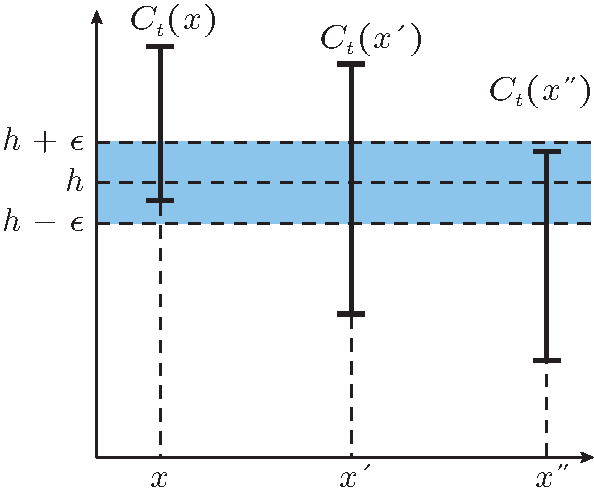
\includegraphics[height=1.5in]{figures/class}
    \caption{Confidence regions}
    \label{fig:conf}
  \end{subfigure}
  \hfill
  \begin{subfigure}[b]{0.49\linewidth}
    \centering
    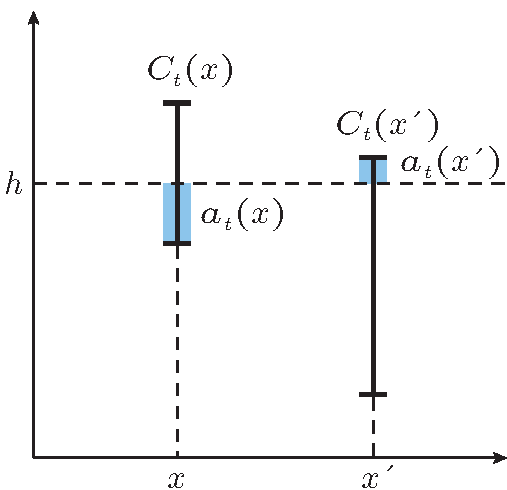
\includegraphics[height=1.5in]{figures/amb}
    \caption{Ambiguities}
    \label{fig:amb}
  \end{subfigure}
  \caption{
    (a) Example of the three possible configurations of confidence regions.
    (b) Ambiguities (shaded) of two example points.
  }
\end{figure}

\paragraph{Sample selection}
For selecting the next point to be evaluated at each iteration, we define the
following quantity
\begin{align*}
a_t(\*x) = \min\{\max(C_t(\*x)) - h, h - \min(C_t(\*x))\},
\end{align*}
which we call classification \emph{ambiguity}. As its name suggests, the
ambiguity of a point $\*x$ quantifies our uncertainty about whether $\*x$
belongs to $H_t$ or $L_t$ (see \figref{fig:amb}).
The intuition of sampling at areas of the sample space with large
classification uncertainty, expecting to gain more information about
the problem at hand when sampling at those areas, manifests itself in \acl
by choosing to evaluate at each iteration the point with the largest
ambiguity amongst the yet unclassified.

We can make an interesting observation at this point. If we use the confidence
intervals $Q_t(\*x)$ instead of the confidence regions $C_t(\*x)$
in the definition of ambiguity, we get the following quantity
\begin{align*}
a'_t(\*x) &= \min\{\max(Q_t(\*x)) - h, h - \min(Q_t(\*x))\}\\
          &= \min\{\mu_{t-1}(\*x) + \beta_t^{1/2}\sigma_{t-1}(\*x) - h,\ h - \mu_{t-1}(\*x) + \beta_t^{1/2}\sigma_{t-1}(\*x)\}\\
          &= \beta_t^{1/2}\sigma_{t-1}(\*x) - |\mu_{t-1}(\*x) - h|.
\end{align*}
For $\beta_t^{1/2} = 1.96$, this is identical to
the \emph{straddle}~\cite{bryan05} heuristic, which can thus be
intuitively explained in terms of classification ambiguity.

%\setlength\figureheight{1.5in}\setlength\figurewidth{2.5in}
%% This file was created by matlab2tikz v0.2.3.
% Copyright (c) 2008--2012, Nico Schlömer <nico.schloemer@gmail.com>
% All rights reserved.
% 
% 
%

\definecolor{locol}{rgb}{0.26, 0.45, 0.65}

\begin{tikzpicture}

\begin{axis}[%
tick label style={font=\tiny},
label style={font=\tiny},
xlabel shift={-10pt},
ylabel shift={-17pt},
legend style={font=\tiny},
view={0}{90},
width=\figurewidth,
height=\figureheight,
scale only axis,
xmin=0, xmax=1478,
xtick={0, 400, 1000, 1400},
xlabel={Length (m)},
ymin=-18, ymax=0,
ytick={0, -4, -14, -18},
ylabel={Depth (m)},
name=plot1,
axis lines*=box,
tickwidth=0.1cm,
clip=false
]

\addplot [fill=locol,draw=none,forget plot] coordinates{ (1478,0)(1478,-0.181818181818182)(1478,-0.363636363636364)(1478,-0.545454545454545)(1478,-0.727272727272727)(1478,-0.909090909090909)(1478,-1.09090909090909)(1478.0002488174,-1.27272727272727)(1478.00049762651,-1.45454545454545)(1478.00074642733,-1.63636363636364)(1478.00074642733,-1.81818181818182)(1478.00074642733,-2)(1478.00074642733,-2.18181818181818)(1478.00074642733,-2.36363636363636)(1478.00074642733,-2.54545454545455)(1478.00074642733,-2.72727272727273)(1478.00074642733,-2.90909090909091)(1478.00074642733,-3.09090909090909)(1478.00074642733,-3.27272727272727)(1478.00099521985,-3.45454545454545)(1478.00124400408,-3.63636363636364)(1478.00149278002,-3.81818181818182)(1478.00149278002,-4)(1478.00124400408,-4.18181818181818)(1478.00099521985,-4.36363636363636)(1478.00074642733,-4.54545454545455)(1478.00074642733,-4.72727272727273)(1478.00074642733,-4.90909090909091)(1478.00074642733,-5.09090909090909)(1478.00074642733,-5.27272727272727)(1478.00074642733,-5.45454545454545)(1478.00074642733,-5.63636363636364)(1478.00074642733,-5.81818181818182)(1478.00074642733,-6)(1478.00074642733,-6.18181818181818)(1478.00074642733,-6.36363636363636)(1478.00074642733,-6.54545454545455)(1478.00074642733,-6.72727272727273)(1478.00074642733,-6.90909090909091)(1478.00058056104,-7.09090909090909)(1478.00058056104,-7.27272727272727)(1478.00058056104,-7.45454545454545)(1478.00074642733,-7.63636363636364)(1478.00074642733,-7.81818181818182)(1478.00074642733,-8)(1478.00074642733,-8.18181818181818)(1478.00074642733,-8.36363636363636)(1478.00074642733,-8.54545454545455)(1478.00074642733,-8.72727272727273)(1478.00074642733,-8.90909090909091)(1478.00074642733,-9.09090909090909)(1478.00074642733,-9.27272727272727)(1478.00074642733,-9.45454545454546)(1478.00074642733,-9.63636363636364)(1478.00074642733,-9.81818181818182)(1478.00074642733,-10)(1478.00074642733,-10.1818181818182)(1478.00074642733,-10.3636363636364)(1478.00074642733,-10.5454545454545)(1478.00049762651,-10.7272727272727)(1478.0002488174,-10.9090909090909)(1478,-11.0909090909091)(1478,-11.2727272727273)(1478,-11.4545454545455)(1478,-11.6363636363636)(1478,-11.8181818181818)(1478.0002488174,-12)(1478.00049762651,-12.1818181818182)(1478.00074642733,-12.3636363636364)(1478.00074642733,-12.5454545454545)(1478.00074642733,-12.7272727272727)(1478.00074642733,-12.9090909090909)(1478.00074642733,-13.0909090909091)(1478.00074642733,-13.2727272727273)(1478.00074642733,-13.4545454545455)(1478.00074642733,-13.6363636363636)(1478.00074642733,-13.8181818181818)(1478.00074642733,-14)(1478.00074642733,-14.1818181818182)(1478.00074642733,-14.3636363636364)(1478.00074642733,-14.5454545454545)(1478.00074642733,-14.7272727272727)(1478.00074642733,-14.9090909090909)(1478.00074642733,-15.0909090909091)(1478.00074642733,-15.2727272727273)(1478.00074642733,-15.4545454545455)(1478.00074642733,-15.6363636363636)(1478.00049762651,-15.8181818181818)(1478.0002488174,-16)(1478,-16.1818181818182)(1478,-16.3636363636364)(1478,-16.5454545454545)(1478,-16.7272727272727)(1478,-16.9090909090909)(1478,-17.0909090909091)(1478,-17.2727272727273)(1478,-17.4545454545455)(1478,-17.6363636363636)(1478,-17.8181818181818)(1478,-18)(1463.07070707071,-18)(1448.14141414141,-18)(1433.21212121212,-18)(1418.28282828283,-18)(1403.35353535354,-18)(1388.42424242424,-18)(1373.49494949495,-18)(1358.56565656566,-18)(1343.63636363636,-18)(1328.70707070707,-18)(1313.77777777778,-18)(1298.84848484848,-18)(1283.91919191919,-18)(1268.9898989899,-18)(1254.06060606061,-18)(1239.13131313131,-18)(1224.20202020202,-18)(1209.27272727273,-18)(1194.34343434343,-18)(1179.41414141414,-18)(1164.48484848485,-18)(1149.55555555556,-18)(1134.62626262626,-18)(1119.69696969697,-18)(1104.76767676768,-18)(1089.83838383838,-18)(1074.90909090909,-18)(1059.9797979798,-18)(1045.05050505051,-18)(1030.12121212121,-18)(1015.19191919192,-18)(1000.26262626263,-18)(985.333333333333,-18)(970.40404040404,-18)(955.474747474747,-18)(940.545454545455,-18)(925.616161616162,-18)(910.686868686869,-18)(895.757575757576,-18)(880.828282828283,-18)(865.89898989899,-18)(850.969696969697,-18)(836.040404040404,-18)(821.111111111111,-18)(806.181818181818,-18)(791.252525252525,-18)(776.323232323232,-18)(761.393939393939,-18)(746.464646464646,-18)(731.535353535354,-18)(716.606060606061,-18)(701.676767676768,-18)(686.747474747475,-18)(671.818181818182,-18)(656.888888888889,-18)(641.959595959596,-18)(627.030303030303,-18)(612.10101010101,-18)(597.171717171717,-18)(582.242424242424,-18)(567.313131313131,-18)(552.383838383838,-18)(537.454545454546,-18)(522.525252525253,-18)(507.59595959596,-18)(492.666666666667,-18)(477.737373737374,-18)(462.808080808081,-18)(447.878787878788,-18)(432.949494949495,-18)(418.020202020202,-18)(403.090909090909,-18)(388.161616161616,-18)(373.232323232323,-18)(358.30303030303,-18)(343.373737373737,-18)(328.444444444444,-18)(313.515151515152,-18)(298.585858585859,-18)(283.656565656566,-18)(268.727272727273,-18)(253.79797979798,-18)(238.868686868687,-18)(223.939393939394,-18)(209.010101010101,-18)(194.080808080808,-18)(179.151515151515,-18)(164.222222222222,-18)(149.292929292929,-18)(134.363636363636,-18)(119.434343434343,-18)(104.505050505051,-18)(89.5757575757576,-18)(74.6464646464647,-18)(59.7171717171717,-18)(44.7878787878788,-18)(29.8585858585859,-18)(14.9292929292929,-18)(0,-18)(0,-17.8181818181818)(0,-17.6363636363636)(0,-17.4545454545455)(0,-17.2727272727273)(0,-17.0909090909091)(0,-16.9090909090909)(0,-16.7272727272727)(-0.000248817401863321,-16.5454545454545)(-0.000497626510092015,-16.3636363636364)(-0.000746427325097138,-16.1818181818182)(-0.000746427325097138,-16)(-0.000746427325097138,-15.8181818181818)(-0.000746427325097138,-15.6363636363636)(-0.000746427325097138,-15.4545454545455)(-0.000746427325097138,-15.2727272727273)(-0.000746427325097138,-15.0909090909091)(-0.000746427325097138,-14.9090909090909)(-0.000746427325097138,-14.7272727272727)(-0.000746427325097138,-14.5454545454545)(-0.000746427325097138,-14.3636363636364)(-0.000746427325097138,-14.1818181818182)(-0.000746427325097138,-14)(-0.000746427325097138,-13.8181818181818)(-0.000746427325097138,-13.6363636363636)(-0.000746427325097138,-13.4545454545455)(-0.000746427325097138,-13.2727272727273)(-0.000746427325097138,-13.0909090909091)(-0.000746427325097138,-12.9090909090909)(-0.000746427325097138,-12.7272727272727)(-0.000746427325097138,-12.5454545454545)(-0.000746427325097138,-12.3636363636364)(-0.000746427325097138,-12.1818181818182)(-0.000746427325097138,-12)(-0.000497626510092015,-11.8181818181818)(-0.000248817401863321,-11.6363636363636)(0,-11.4545454545455)(0,-11.2727272727273)(0,-11.0909090909091)(0,-10.9090909090909)(0,-10.7272727272727)(-0.000248817401863321,-10.5454545454545)(-0.000497626510092015,-10.3636363636364)(-0.000746427325097138,-10.1818181818182)(-0.000746427325097138,-10)(-0.000746427325097138,-9.81818181818182)(-0.000746427325097138,-9.63636363636364)(-0.000746427325097138,-9.45454545454546)(-0.000746427325097138,-9.27272727272727)(-0.000746427325097138,-9.09090909090909)(-0.000746427325097138,-8.90909090909091)(-0.000746427325097138,-8.72727272727273)(-0.000746427325097138,-8.54545454545455)(-0.000995219847296375,-8.36363636363636)(-0.00124400407710078,-8.18181818181818)(-0.00149278001492805,-8)(-0.00149278001492805,-7.81818181818182)(-0.00149278001492805,-7.63636363636364)(-0.00149278001492805,-7.45454545454545)(-0.00149278001492805,-7.27272727272727)(-0.00149278001492805,-7.09090909090909)(-0.00149278001492805,-6.90909090909091)(-0.00149278001492805,-6.72727272727273)(-0.00149278001492805,-6.54545454545455)(-0.00124400407710078,-6.36363636363636)(-0.000995219847296375,-6.18181818181818)(-0.000746427325097138,-6)(-0.000746427325097138,-5.81818181818182)(-0.000746427325097138,-5.63636363636364)(-0.000746427325097138,-5.45454545454545)(-0.000746427325097138,-5.27272727272727)(-0.000746427325097138,-5.09090909090909)(-0.000746427325097138,-4.90909090909091)(-0.000497626510092015,-4.72727272727273)(-0.000248817401863321,-4.54545454545455)(0,-4.36363636363636)(0,-4.18181818181818)(0,-4)(-0.000248817401863321,-3.81818181818182)(-0.000497626510092015,-3.63636363636364)(-0.000746427325097138,-3.45454545454545)(-0.000746427325097138,-3.27272727272727)(-0.000746427325097138,-3.09090909090909)(-0.000746427325097138,-2.90909090909091)(-0.000746427325097138,-2.72727272727273)(-0.000746427325097138,-2.54545454545455)(-0.000746427325097138,-2.36363636363636)(-0.000746427325097138,-2.18181818181818)(-0.000746427325097138,-2)(-0.000746427325097138,-1.81818181818182)(-0.000746427325097138,-1.63636363636364)(-0.000746427325097138,-1.45454545454545)(-0.000497626510092015,-1.27272727272727)(-0.000248817401863321,-1.09090909090909)(0,-0.909090909090909)(0,-0.727272727272727)(0,-0.545454545454545)(0,-0.363636363636364)(0,-0.181818181818182)(0,0)(14.9292929292929,0)(29.8585858585859,0)(44.7878787878788,0)(59.7171717171717,0)(74.6464646464647,0)(89.5757575757576,0)(104.505050505051,0)(119.434343434343,0)(134.363636363636,0)(149.292929292929,0)(164.222222222222,3.03025252607563e-06)(179.151515151515,6.06040404712874e-06)(194.080808080808,9.09045456816541e-06)(209.010101010101,9.09045456816541e-06)(223.939393939394,9.09045456816541e-06)(238.868686868687,9.09045456816541e-06)(253.79797979798,9.09045456816541e-06)(268.727272727273,9.09045456816541e-06)(283.656565656566,9.09045456816541e-06)(298.585858585859,9.09045456816541e-06)(313.515151515152,9.09045456816541e-06)(328.444444444444,9.09045456816541e-06)(343.373737373737,9.09045456816541e-06)(358.30303030303,9.09045456816541e-06)(373.232323232323,9.09045456816541e-06)(388.161616161616,9.09045456816541e-06)(403.090909090909,9.09045456816541e-06)(418.020202020202,9.09045456816541e-06)(432.949494949495,9.09045456816541e-06)(447.878787878788,9.09045456816541e-06)(462.808080808081,9.09045456816541e-06)(477.737373737374,9.09045456816541e-06)(492.666666666667,6.06040404712874e-06)(507.59595959596,3.03025252607563e-06)(522.525252525253,0)(537.454545454546,0)(552.383838383838,0)(567.313131313131,0)(582.242424242424,0)(597.171717171717,0)(612.10101010101,0)(627.030303030303,0)(641.959595959596,0)(656.888888888889,0)(671.818181818182,0)(686.747474747475,0)(701.676767676768,0)(716.606060606061,0)(731.535353535354,0)(746.464646464646,0)(761.393939393939,0)(776.323232323232,0)(791.252525252525,0)(806.181818181818,3.03025252607563e-06)(821.111111111111,6.06040404712874e-06)(836.040404040404,9.09045456816541e-06)(850.969696969697,9.09045456816541e-06)(865.89898989899,9.09045456816541e-06)(880.828282828283,9.09045456816541e-06)(895.757575757576,9.09045456816541e-06)(910.686868686869,9.09045456816541e-06)(925.616161616162,9.09045456816541e-06)(940.545454545455,9.09045456816541e-06)(955.474747474747,9.09045456816541e-06)(970.40404040404,9.09045456816541e-06)(985.333333333333,9.09045456816541e-06)(1000.26262626263,9.09045456816541e-06)(1015.19191919192,9.09045456816541e-06)(1030.12121212121,9.09045456816541e-06)(1045.05050505051,9.09045456816541e-06)(1059.9797979798,9.09045456816541e-06)(1074.90909090909,9.09045456816541e-06)(1089.83838383838,9.09045456816541e-06)(1104.76767676768,9.09045456816541e-06)(1119.69696969697,9.09045456816541e-06)(1134.62626262626,9.09045456816541e-06)(1149.55555555556,9.09045456816541e-06)(1164.48484848485,9.09045456816541e-06)(1179.41414141414,9.09045456816541e-06)(1194.34343434343,9.09045456816541e-06)(1209.27272727273,8.08044894971196e-06)(1224.20202020202,5.05036476259526e-06)(1239.13131313131,2.02017957376651e-06)(1254.06060606061,0)(1268.9898989899,0)(1283.91919191919,0)(1298.84848484848,0)(1313.77777777778,0)(1328.70707070707,0)(1343.63636363636,0)(1358.56565656566,0)(1373.49494949495,0)(1388.42424242424,0)(1403.35353535354,0)(1418.28282828283,0)(1433.21212121212,0)(1448.14141414141,0)(1463.07070707071,0)(1478,0)};

\addplot [fill=darkgray,draw=none,forget plot] coordinates{ (1226.69023569024,0)(1224.20202020202,-0.0909090909090909)(1221.7138047138,-0.181818181818182)(1216.73737373737,-0.363636363636364)(1221.7138047138,-0.545454545454545)(1224.20202020202,-0.636363636363636)(1226.69023569024,-0.727272727272727)(1236.6430976431,-0.909090909090909)(1239.13131313131,-0.954545454545454)(1250.32828282828,-1.09090909090909)(1254.06060606061,-1.12121212121212)(1268.9898989899,-1.24242424242424)(1276.45454545455,-1.27272727272727)(1283.91919191919,-1.3030303030303)(1298.84848484848,-1.36363636363636)(1313.77777777778,-1.36363636363636)(1328.70707070707,-1.36363636363636)(1343.63636363636,-1.36363636363636)(1358.56565656566,-1.36363636363636)(1373.49494949495,-1.36363636363636)(1388.42424242424,-1.36363636363636)(1403.35353535354,-1.36363636363636)(1418.28282828283,-1.36363636363636)(1433.21212121212,-1.36363636363636)(1448.14141414141,-1.36363636363636)(1463.07070707071,-1.36363636363636)(1478,-1.36363636363636)(1478.00012440663,-1.45454545454545)(1478.00037321366,-1.63636363636364)(1478.00037321366,-1.81818181818182)(1478.00037321366,-2)(1478.00037321366,-2.18181818181818)(1478.00037321366,-2.36363636363636)(1478.00037321366,-2.54545454545455)(1478.00037321366,-2.72727272727273)(1478.00037321366,-2.90909090909091)(1478.00037321366,-3.09090909090909)(1478.00037321366,-3.27272727272727)(1478.0006220124,-3.45454545454545)(1478.00087080285,-3.63636363636364)(1478.00111958501,-3.81818181818182)(1478.00111958501,-4)(1478.00087080285,-4.18181818181818)(1478.0006220124,-4.36363636363636)(1478.00037321366,-4.54545454545455)(1478.00037321366,-4.72727272727273)(1478.00037321366,-4.90909090909091)(1478.00037321366,-5.09090909090909)(1478.00037321366,-5.27272727272727)(1478.00037321366,-5.45454545454545)(1478.00037321366,-5.63636363636364)(1478.00037321366,-5.81818181818182)(1478.00037321366,-6)(1478.00037321366,-6.18181818181818)(1478.00037321366,-6.36363636363636)(1478.00037321366,-6.54545454545455)(1478.00037321366,-6.72727272727273)(1478.00037321366,-6.90909090909091)(1478.00020734323,-7.09090909090909)(1478.00020734323,-7.27272727272727)(1478.00020734323,-7.45454545454545)(1478.00037321366,-7.63636363636364)(1478.00037321366,-7.81818181818182)(1478.00037321366,-8)(1478.00037321366,-8.18181818181818)(1478.00037321366,-8.36363636363636)(1478.00037321366,-8.54545454545455)(1478.00037321366,-8.72727272727273)(1478.00037321366,-8.90909090909091)(1478.00037321366,-9.09090909090909)(1478.00037321366,-9.27272727272727)(1478.00037321366,-9.45454545454546)(1478.00037321366,-9.63636363636364)(1478.00037321366,-9.81818181818182)(1478.00037321366,-10)(1478.00037321366,-10.1818181818182)(1478.00037321366,-10.3636363636364)(1478.00037321366,-10.5454545454545)(1478.00012440663,-10.7272727272727)(1478,-10.8181818181818)(1463.07070707071,-10.8181818181818)(1448.14141414141,-10.8181818181818)(1433.21212121212,-10.8181818181818)(1418.28282828283,-10.8787878787879)(1410.81818181818,-10.9090909090909)(1403.35353535354,-10.9393939393939)(1390.91245791246,-11.0909090909091)(1388.42424242424,-11.1363636363636)(1380.9595959596,-11.2727272727273)(1380.9595959596,-11.4545454545455)(1385.93602693603,-11.6363636363636)(1388.42424242424,-11.6818181818182)(1399.62121212121,-11.8181818181818)(1403.35353535354,-11.8484848484849)(1418.28282828283,-11.969696969697)(1425.74747474747,-12)(1433.21212121212,-12.030303030303)(1448.14141414141,-12.0909090909091)(1463.07070707071,-12.0909090909091)(1478,-12.0909090909091)(1478.00012440663,-12.1818181818182)(1478.00037321366,-12.3636363636364)(1478.00037321366,-12.5454545454545)(1478.00037321366,-12.7272727272727)(1478.00037321366,-12.9090909090909)(1478.00037321366,-13.0909090909091)(1478.00037321366,-13.2727272727273)(1478.00037321366,-13.4545454545455)(1478.00037321366,-13.6363636363636)(1478.00037321366,-13.8181818181818)(1478.00037321366,-14)(1478.00037321366,-14.1818181818182)(1478.00037321366,-14.3636363636364)(1478.00037321366,-14.5454545454545)(1478.00037321366,-14.7272727272727)(1478.00037321366,-14.9090909090909)(1478.00037321366,-15.0909090909091)(1478.00037321366,-15.2727272727273)(1478.00037321366,-15.4545454545455)(1478.00037321366,-15.6363636363636)(1478.00012440663,-15.8181818181818)(1478,-15.9090909090909)(1463.07070707071,-15.9090909090909)(1448.14141414141,-15.9090909090909)(1433.21212121212,-15.9090909090909)(1418.28282828283,-15.9090909090909)(1403.35353535354,-15.9090909090909)(1388.42424242424,-15.9090909090909)(1373.49494949495,-15.9090909090909)(1358.56565656566,-15.969696969697)(1351.10101010101,-16)(1343.63636363636,-16.030303030303)(1328.70707070707,-16.0909090909091)(1313.77777777778,-16.0909090909091)(1298.84848484848,-16.0909090909091)(1283.91919191919,-16.1515151515152)(1276.45454545455,-16.1818181818182)(1268.9898989899,-16.2121212121212)(1254.06060606061,-16.2727272727273)(1239.13131313131,-16.3333333333333)(1231.66666666667,-16.3636363636364)(1224.20202020202,-16.3939393939394)(1209.27272727273,-16.4545454545455)(1194.34343434343,-16.5151515151515)(1186.87878787879,-16.5454545454545)(1179.41414141414,-16.5757575757576)(1164.48484848485,-16.6363636363636)(1149.55555555556,-16.6969696969697)(1142.09090909091,-16.7272727272727)(1134.62626262626,-16.7575757575758)(1119.69696969697,-16.8181818181818)(1104.76767676768,-16.8787878787879)(1097.30303030303,-16.9090909090909)(1089.83838383838,-16.9393939393939)(1074.90909090909,-17)(1059.9797979798,-17)(1045.05050505051,-17)(1030.12121212121,-17)(1015.19191919192,-16.9393939393939)(1007.72727272727,-16.9090909090909)(1000.26262626263,-16.8787878787879)(985.333333333333,-16.8181818181818)(970.40404040404,-16.7575757575758)(962.939393939394,-16.7272727272727)(955.474747474747,-16.6969696969697)(940.545454545455,-16.5757575757576)(933.080808080808,-16.5454545454545)(925.616161616162,-16.5151515151515)(910.686868686869,-16.3939393939394)(903.222222222222,-16.3636363636364)(895.757575757576,-16.3333333333333)(880.828282828283,-16.2727272727273)(865.89898989899,-16.2121212121212)(862.166666666667,-16.1818181818182)(850.969696969697,-16.0909090909091)(839.772727272727,-16)(836.040404040404,-15.969696969697)(821.111111111111,-15.8484848484849)(817.378787878788,-15.8181818181818)(806.181818181818,-15.6818181818182)(803.693602693603,-15.6363636363636)(798.717171717172,-15.4545454545455)(798.717171717172,-15.2727272727273)(798.717171717172,-15.0909090909091)(803.693602693603,-14.9090909090909)(806.181818181818,-14.8181818181818)(808.670033670034,-14.7272727272727)(818.622895622896,-14.5454545454545)(821.111111111111,-14.4545454545455)(823.599326599327,-14.3636363636364)(828.575757575758,-14.1818181818182)(828.575757575758,-14)(833.552188552189,-13.8181818181818)(833.552188552189,-13.6363636363636)(833.552188552189,-13.4545454545455)(828.575757575758,-13.2727272727273)(823.599326599327,-13.0909090909091)(821.111111111111,-13.0454545454545)(813.646464646465,-12.9090909090909)(806.181818181818,-12.8181818181818)(798.717171717172,-12.7272727272727)(791.252525252525,-12.6363636363636)(780.055555555556,-12.5454545454545)(776.323232323232,-12.5151515151515)(761.393939393939,-12.4545454545455)(746.464646464646,-12.4545454545455)(731.535353535354,-12.3939393939394)(724.070707070707,-12.3636363636364)(716.606060606061,-12.3333333333333)(701.676767676768,-12.2727272727273)(686.747474747475,-12.2727272727273)(671.818181818182,-12.2727272727273)(656.888888888889,-12.2727272727273)(641.959595959596,-12.2727272727273)(627.030303030303,-12.2727272727273)(612.10101010101,-12.2727272727273)(597.171717171717,-12.2727272727273)(582.242424242424,-12.2727272727273)(567.313131313131,-12.2727272727273)(552.383838383838,-12.2727272727273)(537.454545454546,-12.2727272727273)(522.525252525253,-12.2727272727273)(507.59595959596,-12.3333333333333)(500.131313131313,-12.3636363636364)(492.666666666667,-12.3939393939394)(477.737373737374,-12.4545454545455)(462.808080808081,-12.4545454545455)(447.878787878788,-12.5151515151515)(440.414141414141,-12.5454545454545)(432.949494949495,-12.5757575757576)(418.020202020202,-12.6969696969697)(414.287878787879,-12.7272727272727)(403.090909090909,-12.8181818181818)(395.626262626263,-12.9090909090909)(388.161616161616,-13.0454545454545)(385.673400673401,-13.0909090909091)(375.720538720539,-13.2727272727273)(373.232323232323,-13.3636363636364)(370.744107744108,-13.4545454545455)(365.767676767677,-13.6363636363636)(365.767676767677,-13.8181818181818)(365.767676767677,-14)(370.744107744108,-14.1818181818182)(373.232323232323,-14.2727272727273)(375.720538720539,-14.3636363636364)(385.673400673401,-14.5454545454545)(388.161616161616,-14.5909090909091)(395.626262626263,-14.7272727272727)(403.090909090909,-14.8181818181818)(410.555555555556,-14.9090909090909)(418.020202020202,-15)(425.484848484849,-15.0909090909091)(432.949494949495,-15.1818181818182)(440.414141414141,-15.2727272727273)(447.878787878788,-15.4090909090909)(450.367003367003,-15.4545454545455)(460.319865319865,-15.6363636363636)(462.808080808081,-15.7272727272727)(465.296296296296,-15.8181818181818)(470.272727272727,-16)(465.296296296296,-16.1818181818182)(462.808080808081,-16.2272727272727)(455.343434343434,-16.3636363636364)(447.878787878788,-16.4545454545455)(440.414141414141,-16.5454545454545)(432.949494949495,-16.6363636363636)(421.752525252525,-16.7272727272727)(418.020202020202,-16.7575757575758)(403.090909090909,-16.8787878787879)(395.626262626263,-16.9090909090909)(388.161616161616,-16.9393939393939)(373.232323232323,-17)(358.30303030303,-17.0606060606061)(350.838383838384,-17.0909090909091)(343.373737373737,-17.1212121212121)(328.444444444444,-17.1212121212121)(320.979797979798,-17.0909090909091)(313.515151515152,-17.0606060606061)(298.585858585859,-17)(283.656565656566,-17)(268.727272727273,-16.9393939393939)(261.262626262626,-16.9090909090909)(253.79797979798,-16.8787878787879)(238.868686868687,-16.8181818181818)(223.939393939394,-16.7575757575758)(216.474747474747,-16.7272727272727)(209.010101010101,-16.6969696969697)(194.080808080808,-16.6363636363636)(179.151515151515,-16.6363636363636)(164.222222222222,-16.5757575757576)(156.757575757576,-16.5454545454545)(149.292929292929,-16.5151515151515)(134.363636363636,-16.4545454545455)(119.434343434343,-16.4545454545455)(104.505050505051,-16.4545454545455)(89.5757575757576,-16.4545454545455)(74.6464646464647,-16.4545454545455)(59.7171717171717,-16.4545454545455)(44.7878787878788,-16.4545454545455)(29.8585858585859,-16.4545454545455)(14.9292929292929,-16.4545454545455)(0,-16.4545454545455)(-0.000124406627524661,-16.3636363636364)(-0.000373213662548569,-16.1818181818182)(-0.000373213662548569,-16)(-0.000373213662548569,-15.8181818181818)(-0.000373213662548569,-15.6363636363636)(-0.000373213662548569,-15.4545454545455)(-0.000373213662548569,-15.2727272727273)(-0.000373213662548569,-15.0909090909091)(-0.000373213662548569,-14.9090909090909)(-0.000373213662548569,-14.7272727272727)(-0.000373213662548569,-14.5454545454545)(-0.000373213662548569,-14.3636363636364)(-0.000373213662548569,-14.1818181818182)(-0.000373213662548569,-14)(-0.000373213662548569,-13.8181818181818)(-0.000373213662548569,-13.6363636363636)(-0.000373213662548569,-13.4545454545455)(-0.000373213662548569,-13.2727272727273)(-0.000373213662548569,-13.0909090909091)(-0.000373213662548569,-12.9090909090909)(-0.000373213662548569,-12.7272727272727)(-0.000373213662548569,-12.5454545454545)(-0.000373213662548569,-12.3636363636364)(-0.000373213662548569,-12.1818181818182)(-0.000373213662548569,-12)(-0.000124406627524661,-11.8181818181818)(0,-11.7272727272727)(14.9292929292929,-11.7272727272727)(29.8585858585859,-11.7272727272727)(44.7878787878788,-11.7272727272727)(59.7171717171717,-11.6666666666667)(67.1818181818182,-11.6363636363636)(74.6464646464647,-11.6060606060606)(89.5757575757576,-11.4848484848485)(97.040404040404,-11.4545454545455)(104.505050505051,-11.4242424242424)(119.434343434343,-11.3030303030303)(126.89898989899,-11.2727272727273)(134.363636363636,-11.2424242424242)(149.292929292929,-11.1212121212121)(153.025252525253,-11.0909090909091)(164.222222222222,-11)(175.419191919192,-10.9090909090909)(179.151515151515,-10.8787878787879)(194.080808080808,-10.7575757575758)(201.545454545455,-10.7272727272727)(209.010101010101,-10.6969696969697)(223.939393939394,-10.6363636363636)(238.868686868687,-10.5757575757576)(246.333333333333,-10.5454545454545)(253.79797979798,-10.5151515151515)(268.727272727273,-10.3939393939394)(276.191919191919,-10.3636363636364)(283.656565656566,-10.3333333333333)(298.585858585859,-10.2121212121212)(302.318181818182,-10.1818181818182)(313.515151515152,-10.0909090909091)(320.979797979798,-10)(328.444444444444,-9.86363636363636)(330.93265993266,-9.81818181818182)(328.444444444444,-9.72727272727273)(325.956228956229,-9.63636363636364)(313.515151515152,-9.48484848484848)(306.050505050505,-9.45454545454546)(298.585858585859,-9.42424242424243)(283.656565656566,-9.36363636363636)(268.727272727273,-9.36363636363636)(253.79797979798,-9.36363636363636)(238.868686868687,-9.42424242424243)(231.40404040404,-9.45454545454546)(223.939393939394,-9.48484848484848)(209.010101010101,-9.60606060606061)(201.545454545455,-9.63636363636364)(194.080808080808,-9.66666666666667)(179.151515151515,-9.78787878787879)(171.686868686869,-9.81818181818182)(164.222222222222,-9.84848484848485)(149.292929292929,-9.96969696969697)(141.828282828283,-10)(134.363636363636,-10.030303030303)(119.434343434343,-10.1515151515152)(111.969696969697,-10.1818181818182)(104.505050505051,-10.2121212121212)(89.5757575757576,-10.2727272727273)(74.6464646464647,-10.2727272727273)(59.7171717171717,-10.2727272727273)(44.7878787878788,-10.2727272727273)(29.8585858585859,-10.3333333333333)(22.3939393939394,-10.3636363636364)(14.9292929292929,-10.3939393939394)(0,-10.4545454545455)(-0.000124406627524661,-10.3636363636364)(-0.000373213662548569,-10.1818181818182)(-0.000373213662548569,-10)(-0.000373213662548569,-9.81818181818182)(-0.000373213662548569,-9.63636363636364)(-0.000373213662548569,-9.45454545454546)(-0.000373213662548569,-9.27272727272727)(-0.000373213662548569,-9.09090909090909)(-0.000373213662548569,-8.90909090909091)(-0.000373213662548569,-8.72727272727273)(-0.000373213662548569,-8.54545454545455)(-0.000622012404561063,-8.36363636363636)(-0.000870802853969885,-8.18181818181818)(-0.00111958501119604,-8)(-0.00111958501119604,-7.81818181818182)(-0.00111958501119604,-7.63636363636364)(-0.00111958501119604,-7.45454545454545)(-0.00111958501119604,-7.27272727272727)(-0.00111958501119604,-7.09090909090909)(-0.00111958501119604,-6.90909090909091)(-0.00111958501119604,-6.72727272727273)(-0.00111958501119604,-6.54545454545455)(-0.000870802853969885,-6.36363636363636)(-0.000622012404561063,-6.18181818181818)(-0.000373213662548569,-6)(-0.000373213662548569,-5.81818181818182)(-0.000373213662548569,-5.63636363636364)(-0.000373213662548569,-5.45454545454545)(-0.000373213662548569,-5.27272727272727)(-0.000373213662548569,-5.09090909090909)(-0.000373213662548569,-4.90909090909091)(-0.000124406627524661,-4.72727272727273)(0,-4.63636363636364)(14.9292929292929,-4.63636363636364)(29.8585858585859,-4.57575757575758)(37.3232323232323,-4.54545454545455)(44.7878787878788,-4.51515151515152)(59.7171717171717,-4.39393939393939)(63.4494949494949,-4.36363636363636)(74.6464646464647,-4.22727272727273)(77.1346801346801,-4.18181818181818)(77.1346801346801,-4)(74.6464646464647,-3.95454545454545)(63.4494949494949,-3.81818181818182)(59.7171717171717,-3.78787878787879)(44.7878787878788,-3.72727272727273)(29.8585858585859,-3.72727272727273)(14.9292929292929,-3.72727272727273)(0,-3.72727272727273)(-0.000124406627524661,-3.63636363636364)(-0.000373213662548569,-3.45454545454545)(-0.000373213662548569,-3.27272727272727)(-0.000373213662548569,-3.09090909090909)(-0.000373213662548569,-2.90909090909091)(-0.000373213662548569,-2.72727272727273)(-0.000373213662548569,-2.54545454545455)(-0.000373213662548569,-2.36363636363636)(-0.000373213662548569,-2.18181818181818)(-0.000373213662548569,-2)(-0.000373213662548569,-1.81818181818182)(-0.000373213662548569,-1.63636363636364)(-0.000373213662548569,-1.45454545454545)(-0.000124406627524661,-1.27272727272727)(0,-1.18181818181818)(14.9292929292929,-1.18181818181818)(29.8585858585859,-1.18181818181818)(44.7878787878788,-1.18181818181818)(59.7171717171717,-1.18181818181818)(74.6464646464647,-1.18181818181818)(89.5757575757576,-1.12121212121212)(97.040404040404,-1.09090909090909)(104.505050505051,-1.06060606060606)(119.434343434343,-1)(134.363636363636,-0.939393939393939)(138.09595959596,-0.909090909090909)(149.292929292929,-0.818181818181818)(156.757575757576,-0.727272727272727)(164.222222222222,-0.590909090909091)(166.710437710438,-0.545454545454545)(171.686868686869,-0.363636363636364)(171.686868686869,-0.181818181818182)(171.686868686869,0)(179.151515151515,1.515101011762e-06)(194.080808080808,4.54522728408271e-06)(209.010101010101,4.54522728408271e-06)(223.939393939394,4.54522728408271e-06)(238.868686868687,4.54522728408271e-06)(253.79797979798,4.54522728408271e-06)(268.727272727273,4.54522728408271e-06)(283.656565656566,4.54522728408271e-06)(298.585858585859,4.54522728408271e-06)(313.515151515152,4.54522728408271e-06)(328.444444444444,4.54522728408271e-06)(343.373737373737,4.54522728408271e-06)(358.30303030303,4.54522728408271e-06)(373.232323232323,4.54522728408271e-06)(388.161616161616,4.54522728408271e-06)(403.090909090909,4.54522728408271e-06)(418.020202020202,4.54522728408271e-06)(432.949494949495,4.54522728408271e-06)(447.878787878788,4.54522728408271e-06)(462.808080808081,4.54522728408271e-06)(477.737373737374,4.54522728408271e-06)(492.666666666667,1.515101011762e-06)(500.131313131313,0)(500.131313131313,-0.181818181818182)(500.131313131313,-0.363636363636364)(505.107744107744,-0.545454545454545)(507.59595959596,-0.636363636363636)(510.084175084175,-0.727272727272727)(515.060606060606,-0.909090909090909)(515.060606060606,-1.09090909090909)(515.060606060606,-1.27272727272727)(515.060606060606,-1.45454545454545)(515.060606060606,-1.63636363636364)(515.060606060606,-1.81818181818182)(515.060606060606,-2)(520.037037037037,-2.18181818181818)(522.525252525253,-2.22727272727273)(529.989898989899,-2.36363636363636)(537.454545454546,-2.45454545454545)(548.651515151515,-2.54545454545455)(552.383838383838,-2.57575757575758)(567.313131313131,-2.6969696969697)(574.777777777778,-2.72727272727273)(582.242424242424,-2.75757575757576)(597.171717171717,-2.81818181818182)(612.10101010101,-2.81818181818182)(627.030303030303,-2.81818181818182)(641.959595959596,-2.75757575757576)(645.691919191919,-2.72727272727273)(656.888888888889,-2.63636363636364)(668.085858585859,-2.54545454545455)(671.818181818182,-2.51515151515152)(686.747474747475,-2.39393939393939)(690.479797979798,-2.36363636363636)(701.676767676768,-2.27272727272727)(709.141414141414,-2.18181818181818)(716.606060606061,-2.09090909090909)(724.070707070707,-2)(731.535353535354,-1.86363636363636)(734.023569023569,-1.81818181818182)(743.976430976431,-1.63636363636364)(746.464646464646,-1.59090909090909)(753.929292929293,-1.45454545454545)(761.393939393939,-1.36363636363636)(768.858585858586,-1.27272727272727)(776.323232323232,-1.18181818181818)(783.787878787879,-1.09090909090909)(791.252525252525,-0.954545454545454)(793.740740740741,-0.909090909090909)(803.693602693603,-0.727272727272727)(806.181818181818,-0.636363636363636)(808.670033670034,-0.545454545454545)(813.646464646465,-0.363636363636364)(813.646464646465,-0.181818181818182)(813.646464646465,0)(821.111111111111,1.515101011762e-06)(836.040404040404,4.54522728408271e-06)(850.969696969697,4.54522728408271e-06)(865.89898989899,4.54522728408271e-06)(880.828282828283,4.54522728408271e-06)(895.757575757576,4.54522728408271e-06)(910.686868686869,4.54522728408271e-06)(925.616161616162,4.54522728408271e-06)(940.545454545455,4.54522728408271e-06)(955.474747474747,4.54522728408271e-06)(970.40404040404,4.54522728408271e-06)(985.333333333333,4.54522728408271e-06)(1000.26262626263,4.54522728408271e-06)(1015.19191919192,4.54522728408271e-06)(1030.12121212121,4.54522728408271e-06)(1045.05050505051,4.54522728408271e-06)(1059.9797979798,4.54522728408271e-06)(1074.90909090909,4.54522728408271e-06)(1089.83838383838,4.54522728408271e-06)(1104.76767676768,4.54522728408271e-06)(1119.69696969697,4.54522728408271e-06)(1134.62626262626,4.54522728408271e-06)(1149.55555555556,4.54522728408271e-06)(1164.48484848485,4.54522728408271e-06)(1179.41414141414,4.54522728408271e-06)(1194.34343434343,4.54522728408271e-06)(1209.27272727273,3.53519641552421e-06)(1224.20202020202,5.05036476275675e-07)(1226.69023569024,0)};

\addplot [fill=red!40!yellow,draw=none,forget plot] coordinates{ (604.636363636364,-3.45454545454545)(612.10101010101,-3.48484848484849)(627.030303030303,-3.60606060606061)(634.494949494949,-3.63636363636364)(641.959595959596,-3.66666666666667)(656.888888888889,-3.78787878787879)(664.353535353535,-3.81818181818182)(671.818181818182,-3.84848484848485)(686.747474747475,-3.96969696969697)(690.479797979798,-4)(701.676767676768,-4.09090909090909)(709.141414141414,-4.18181818181818)(716.606060606061,-4.27272727272727)(724.070707070707,-4.36363636363636)(731.535353535354,-4.45454545454546)(739,-4.54545454545455)(746.464646464646,-4.68181818181818)(748.952861952862,-4.72727272727273)(753.929292929293,-4.90909090909091)(746.464646464646,-5.04545454545455)(743.976430976431,-5.09090909090909)(731.535353535354,-5.24242424242424)(724.070707070707,-5.27272727272727)(716.606060606061,-5.3030303030303)(701.676767676768,-5.36363636363636)(686.747474747475,-5.42424242424242)(679.282828282828,-5.45454545454545)(671.818181818182,-5.48484848484848)(656.888888888889,-5.54545454545455)(641.959595959596,-5.54545454545455)(627.030303030303,-5.60606060606061)(619.565656565657,-5.63636363636364)(612.10101010101,-5.66666666666667)(597.171717171717,-5.72727272727273)(582.242424242424,-5.72727272727273)(567.313131313131,-5.72727272727273)(552.383838383838,-5.72727272727273)(537.454545454546,-5.72727272727273)(522.525252525253,-5.72727272727273)(507.59595959596,-5.72727272727273)(492.666666666667,-5.72727272727273)(477.737373737374,-5.72727272727273)(462.808080808081,-5.72727272727273)(447.878787878788,-5.72727272727273)(432.949494949495,-5.72727272727273)(418.020202020202,-5.78787878787879)(410.555555555556,-5.81818181818182)(403.090909090909,-5.84848484848485)(388.161616161616,-5.90909090909091)(373.232323232323,-5.90909090909091)(358.30303030303,-5.90909090909091)(343.373737373737,-5.96969696969697)(335.909090909091,-6)(328.444444444444,-6.03030303030303)(313.515151515152,-6.09090909090909)(298.585858585859,-6.09090909090909)(283.656565656566,-6.15151515151515)(276.191919191919,-6.18181818181818)(268.727272727273,-6.21212121212121)(253.79797979798,-6.27272727272727)(238.868686868687,-6.27272727272727)(223.939393939394,-6.27272727272727)(209.010101010101,-6.31818181818182)(205.277777777778,-6.36363636363636)(194.080808080808,-6.5)(191.592592592593,-6.54545454545455)(186.616161616162,-6.72727272727273)(181.639730639731,-6.90909090909091)(179.151515151515,-6.95454545454545)(171.686868686869,-7.09090909090909)(164.222222222222,-7.22727272727273)(161.734006734007,-7.27272727272727)(151.781144781145,-7.45454545454545)(149.292929292929,-7.5)(138.09595959596,-7.63636363636364)(134.363636363636,-7.66666666666667)(119.434343434343,-7.78787878787879)(115.70202020202,-7.81818181818182)(104.505050505051,-7.90909090909091)(93.3080808080808,-8)(89.5757575757576,-8.03030303030303)(74.6464646464647,-8.09090909090909)(59.7171717171717,-8.09090909090909)(44.7878787878788,-8.15151515151515)(37.3232323232323,-8.18181818181818)(29.8585858585859,-8.21212121212121)(14.9292929292929,-8.27272727272727)(0,-8.27272727272727)(-0.000124400407711404,-8.18181818181818)(-0.000373195003732012,-8)(-0.000373195003732012,-7.81818181818182)(-0.000373195003732012,-7.63636363636364)(-0.000373195003732012,-7.45454545454545)(-0.000373195003732012,-7.27272727272727)(-0.000373195003732012,-7.09090909090909)(-0.000373195003732012,-6.90909090909091)(-0.000373195003732012,-6.72727272727273)(-0.000373195003732012,-6.54545454545455)(-0.000124400407711404,-6.36363636363636)(0,-6.27272727272727)(14.9292929292929,-6.27272727272727)(29.8585858585859,-6.27272727272727)(44.7878787878788,-6.27272727272727)(59.7171717171717,-6.27272727272727)(74.6464646464647,-6.27272727272727)(89.5757575757576,-6.27272727272727)(104.505050505051,-6.27272727272727)(119.434343434343,-6.27272727272727)(134.363636363636,-6.27272727272727)(149.292929292929,-6.27272727272727)(164.222222222222,-6.21212121212121)(171.686868686869,-6.18181818181818)(179.151515151515,-6.15151515151515)(194.080808080808,-6.04545454545455)(197.813131313131,-6)(209.010101010101,-5.90909090909091)(216.474747474747,-5.81818181818182)(223.939393939394,-5.72727272727273)(235.136363636364,-5.63636363636364)(238.868686868687,-5.60606060606061)(253.79797979798,-5.48484848484848)(261.262626262626,-5.45454545454545)(268.727272727273,-5.42424242424242)(283.656565656566,-5.3030303030303)(291.121212121212,-5.27272727272727)(298.585858585859,-5.24242424242424)(313.515151515152,-5.12121212121212)(320.979797979798,-5.09090909090909)(328.444444444444,-5.06060606060606)(340.885521885522,-4.90909090909091)(343.373737373737,-4.87878787878788)(355.814814814815,-4.72727272727273)(358.30303030303,-4.68181818181818)(365.767676767677,-4.54545454545455)(373.232323232323,-4.40909090909091)(375.720538720539,-4.36363636363636)(385.673400673401,-4.18181818181818)(388.161616161616,-4.09090909090909)(390.649831649832,-4)(403.090909090909,-3.84848484848485)(405.579124579125,-3.81818181818182)(418.020202020202,-3.66666666666667)(425.484848484849,-3.63636363636364)(432.949494949495,-3.60606060606061)(447.878787878788,-3.54545454545455)(462.808080808081,-3.54545454545455)(477.737373737374,-3.48484848484849)(485.20202020202,-3.45454545454545)(492.666666666667,-3.42424242424242)(507.59595959596,-3.36363636363636)(522.525252525253,-3.36363636363636)(537.454545454546,-3.36363636363636)(552.383838383838,-3.36363636363636)(567.313131313131,-3.36363636363636)(582.242424242424,-3.36363636363636)(597.171717171717,-3.42424242424242)(604.636363636364,-3.45454545454545)};

\addplot [fill=red!40!yellow,draw=none,forget plot] coordinates{ (992.79797979798,-7.27272727272727)(1000.26262626263,-7.3030303030303)(1015.19191919192,-7.42424242424242)(1022.65656565657,-7.45454545454545)(1030.12121212121,-7.48484848484848)(1045.05050505051,-7.60606060606061)(1052.51515151515,-7.63636363636364)(1059.9797979798,-7.66666666666667)(1074.90909090909,-7.78787878787879)(1082.37373737374,-7.81818181818182)(1089.83838383838,-7.84848484848485)(1104.76767676768,-7.90909090909091)(1119.69696969697,-7.90909090909091)(1134.62626262626,-7.90909090909091)(1149.55555555556,-7.90909090909091)(1164.48484848485,-7.96969696969697)(1171.94949494949,-8)(1179.41414141414,-8.03030303030303)(1194.34343434343,-8.09090909090909)(1209.27272727273,-8.09090909090909)(1224.20202020202,-8.09090909090909)(1239.13131313131,-8.09090909090909)(1254.06060606061,-8.09090909090909)(1268.9898989899,-8.09090909090909)(1283.91919191919,-8.15151515151515)(1291.38383838384,-8.18181818181818)(1298.84848484848,-8.21212121212121)(1311.28956228956,-8.36363636363636)(1313.77777777778,-8.39393939393939)(1326.21885521886,-8.54545454545455)(1326.21885521886,-8.72727272727273)(1326.21885521886,-8.90909090909091)(1316.26599326599,-9.09090909090909)(1313.77777777778,-9.13636363636364)(1302.58080808081,-9.27272727272727)(1298.84848484848,-9.3030303030303)(1283.91919191919,-9.42424242424243)(1276.45454545455,-9.45454545454546)(1268.9898989899,-9.48484848484848)(1254.06060606061,-9.54545454545455)(1239.13131313131,-9.60606060606061)(1231.66666666667,-9.63636363636364)(1224.20202020202,-9.66666666666667)(1209.27272727273,-9.72727272727273)(1194.34343434343,-9.66666666666667)(1186.87878787879,-9.63636363636364)(1179.41414141414,-9.60606060606061)(1164.48484848485,-9.54545454545455)(1149.55555555556,-9.54545454545455)(1134.62626262626,-9.48484848484848)(1130.89393939394,-9.45454545454546)(1119.69696969697,-9.36363636363636)(1112.23232323232,-9.27272727272727)(1104.76767676768,-9.18181818181818)(1097.30303030303,-9.09090909090909)(1089.83838383838,-9)(1082.37373737374,-8.90909090909091)(1074.90909090909,-8.77272727272727)(1072.42087542088,-8.72727272727273)(1059.9797979798,-8.57575757575757)(1057.49158249158,-8.54545454545455)(1045.05050505051,-8.39393939393939)(1037.58585858586,-8.36363636363636)(1030.12121212121,-8.33333333333333)(1015.19191919192,-8.21212121212121)(1007.72727272727,-8.18181818181818)(1000.26262626263,-8.15151515151515)(985.333333333333,-8.09090909090909)(970.40404040404,-8.03030303030303)(966.671717171717,-8)(955.474747474747,-7.90909090909091)(948.010101010101,-7.81818181818182)(940.545454545455,-7.68181818181818)(938.057239057239,-7.63636363636364)(940.545454545455,-7.54545454545455)(943.03367003367,-7.45454545454545)(955.474747474747,-7.3030303030303)(962.939393939394,-7.27272727272727)(970.40404040404,-7.24242424242424)(985.333333333333,-7.24242424242424)(992.79797979798,-7.27272727272727)};

\addplot [fill=locol,draw=none,forget plot] coordinates{ (1198.07575757576,-1.81818181818182)(1194.34343434343,-1.78787878787879)(1179.41414141414,-1.72727272727273)(1164.48484848485,-1.72727272727273)(1149.55555555556,-1.72727272727273)(1134.62626262626,-1.72727272727273)(1119.69696969697,-1.72727272727273)(1104.76767676768,-1.72727272727273)(1089.83838383838,-1.72727272727273)(1074.90909090909,-1.78787878787879)(1067.44444444444,-1.81818181818182)(1059.9797979798,-1.84848484848485)(1045.05050505051,-1.90909090909091)(1030.12121212121,-1.96969696969697)(1026.38888888889,-2)(1015.19191919192,-2.09090909090909)(1007.72727272727,-2.18181818181818)(1000.26262626263,-2.31818181818182)(997.774410774411,-2.36363636363636)(992.79797979798,-2.54545454545455)(997.774410774411,-2.72727272727273)(1000.26262626263,-2.81818181818182)(1002.75084175084,-2.90909090909091)(1015.19191919192,-3.06060606060606)(1017.68013468013,-3.09090909090909)(1030.12121212121,-3.24242424242424)(1037.58585858586,-3.27272727272727)(1045.05050505051,-3.3030303030303)(1059.9797979798,-3.36363636363636)(1074.90909090909,-3.36363636363636)(1089.83838383838,-3.36363636363636)(1104.76767676768,-3.36363636363636)(1119.69696969697,-3.36363636363636)(1134.62626262626,-3.36363636363636)(1149.55555555556,-3.36363636363636)(1164.48484848485,-3.3030303030303)(1171.94949494949,-3.27272727272727)(1179.41414141414,-3.24242424242424)(1194.34343434343,-3.12121212121212)(1198.07575757576,-3.09090909090909)(1209.27272727273,-3)(1216.73737373737,-2.90909090909091)(1224.20202020202,-2.77272727272727)(1226.69023569024,-2.72727272727273)(1231.66666666667,-2.54545454545455)(1231.66666666667,-2.36363636363636)(1226.69023569024,-2.18181818181818)(1224.20202020202,-2.13636363636364)(1216.73737373737,-2)(1209.27272727273,-1.90909090909091)(1198.07575757576,-1.81818181818182)};

\addplot [fill=locol,draw=none,forget plot] coordinates{ (1067.44444444444,-11.6363636363636)(1074.90909090909,-11.6060606060606)(1089.83838383838,-11.4848484848485)(1093.57070707071,-11.4545454545455)(1104.76767676768,-11.3181818181818)(1107.25589225589,-11.2727272727273)(1112.23232323232,-11.0909090909091)(1107.25589225589,-10.9090909090909)(1104.76767676768,-10.8636363636364)(1093.57070707071,-10.7272727272727)(1089.83838383838,-10.6969696969697)(1074.90909090909,-10.6363636363636)(1059.9797979798,-10.6363636363636)(1045.05050505051,-10.6363636363636)(1030.12121212121,-10.6363636363636)(1015.19191919192,-10.6363636363636)(1000.26262626263,-10.6969696969697)(996.530303030303,-10.7272727272727)(985.333333333333,-10.8181818181818)(977.868686868687,-10.9090909090909)(970.40404040404,-11)(962.939393939394,-11.0909090909091)(955.474747474747,-11.2272727272727)(952.986531986532,-11.2727272727273)(952.986531986532,-11.4545454545455)(955.474747474747,-11.5)(966.671717171717,-11.6363636363636)(970.40404040404,-11.6666666666667)(985.333333333333,-11.7272727272727)(1000.26262626263,-11.7272727272727)(1015.19191919192,-11.7272727272727)(1030.12121212121,-11.7272727272727)(1045.05050505051,-11.7272727272727)(1059.9797979798,-11.6666666666667)(1067.44444444444,-11.6363636363636)};

\addplot [fill=locol,draw=none,forget plot] coordinates{ (339.641414141414,-2.90909090909091)(328.444444444444,-2.81818181818182)(313.515151515152,-2.81818181818182)(298.585858585859,-2.81818181818182)(287.388888888889,-2.90909090909091)(287.388888888889,-3.09090909090909)(298.585858585859,-3.18181818181818)(313.515151515152,-3.18181818181818)(328.444444444444,-3.24242424242424)(343.373737373737,-3.13636363636364)(347.106060606061,-3.09090909090909)(343.373737373737,-3)(339.641414141414,-2.90909090909091)};

\addplot [fill=red!40!yellow,draw=none,forget plot] coordinates{ (1478.00012440041,-3.63636363636364)(1478.000373195,-3.81818181818182)(1478.000373195,-4)(1478.00012440041,-4.18181818181818)(1478,-4.27272727272727)(1463.07070707071,-4.21212121212121)(1459.33838383838,-4.18181818181818)(1448.14141414141,-4.04545454545455)(1445.6531986532,-4)(1445.6531986532,-3.81818181818182)(1448.14141414141,-3.77272727272727)(1459.33838383838,-3.63636363636364)(1463.07070707071,-3.60606060606061)(1478,-3.54545454545455)(1478.00012440041,-3.63636363636364)};

\addplot [fill=red!40!yellow,draw=none,forget plot] coordinates{ (936.813131313131,-5.09090909090909)(936.813131313131,-5.27272727272727)(925.616161616162,-5.36363636363636)(910.686868686869,-5.36363636363636)(895.757575757576,-5.36363636363636)(884.560606060606,-5.27272727272727)(884.560606060606,-5.09090909090909)(895.757575757576,-5)(910.686868686869,-5)(925.616161616162,-5)(936.813131313131,-5.09090909090909)};

\addplot [
color=white,
draw=white,
only marks,
mark=x,
mark options={solid},
mark size=2.2pt,
line width=1pt,
forget plot
]
coordinates{
 (0,0)(1478,-18)(1478,-3.81818181818182)(1478,0)(1478,-7.27272727272727)(940.545454545455,-5.09090909090909)(567.313131313131,-8.72727272727273)(0,-10.9090909090909)(283.656565656566,-5.63636363636364)(0,-18)(1045.05050505051,-10.9090909090909)(612.10101010101,-2.54545454545455)(0,-7.27272727272727)(0,-4.36363636363636)(985.333333333333,-7.63636363636364)(597.171717171717,-13.6363636363636)(1478,-11.2727272727273)(1119.69696969697,-2.90909090909091)(253.79797979798,-9.63636363636364)(656.888888888889,0)(701.676767676768,-18)(537.454545454546,-4.36363636363636)(343.373737373737,-3.27272727272727)(1224.20202020202,-8.90909090909091)(1254.06060606061,-5.63636363636364) 
};

%\node at (axis cs:50, -2.5) [shape=circle,fill=white,draw=black,inner sep=0pt,anchor=south west] {\scriptsize\color{locol}$\*L_{\*t}$};
%\node at (axis cs:460, -5.9) [shape=circle,fill=white,draw=black,inner sep=0pt,anchor=south west] {\scriptsize\color{orange!50!yellow}$\*H_{\*t}$};
%\node at (axis cs:160, -5.2) [shape=circle,fill=white,draw=black,inner sep=0pt,anchor=south west] {\scriptsize\color{darkgray}$\*U_{\*t}$};

\node at (axis cs:980, -17) [shape=circle,fill=red!40!yellow,draw=black,inner sep=0.2pt,anchor=south west,minimum size=16pt]
  {\scriptsize\color{white}$\*H_{\*t}$};
\node at (axis cs:1155, -17) [shape=circle,fill=locol,draw=black,inner sep=0.2pt,anchor=south west,minimum size=16pt]
  {\scriptsize\color{white}$\*L_{\*t}$};
\node at (axis cs:1330, -17) [shape=circle,fill=darkgray,draw=black,inner sep=0.2pt,anchor=south west,minimum size=16pt]
  {\scriptsize\color{white}$\*U_{\*t}$};

\end{axis}
\end{tikzpicture}%

%% This file was created by matlab2tikz v0.2.3.
% Copyright (c) 2008--2012, Nico Schlömer <nico.schloemer@gmail.com>
% All rights reserved.
% 
% 
%

\definecolor{locol}{rgb}{0.26, 0.45, 0.65}

\begin{tikzpicture}

\begin{axis}[%
tick label style={font=\tiny},
label style={font=\tiny},
xlabel shift={-10pt},
ylabel shift={-17pt},
legend style={font=\tiny},
view={0}{90},
width=\figurewidth,
height=\figureheight,
scale only axis,
xmin=0, xmax=1478,
xtick={0, 400, 1000, 1400},
xlabel={Length (m)},
ymin=-18, ymax=0,
ytick={0, -4, -14, -18},
ylabel={Depth (m)},
name=plot1,
axis lines*=box,
tickwidth=0.1cm,
clip=false
]

\addplot [fill=locol,draw=none,forget plot] coordinates{ (1478,0)(1478,-0.181818181818182)(1478,-0.363636363636364)(1478,-0.545454545454545)(1478,-0.727272727272727)(1478,-0.909090909090909)(1478,-1.09090909090909)(1478,-1.27272727272727)(1478,-1.45454545454545)(1478,-1.63636363636364)(1478,-1.81818181818182)(1478,-2)(1478,-2.18181818181818)(1478,-2.36363636363636)(1478,-2.54545454545455)(1478.0002488174,-2.72727272727273)(1478.00049762651,-2.90909090909091)(1478.00074642733,-3.09090909090909)(1478.00099521985,-3.27272727272727)(1478.00124400408,-3.45454545454545)(1478.00149278002,-3.63636363636364)(1478.00149278002,-3.81818181818182)(1478.00149278002,-4)(1478.00149278002,-4.18181818181818)(1478.00149278002,-4.36363636363636)(1478.00149278002,-4.54545454545455)(1478.00149278002,-4.72727272727273)(1478.00149278002,-4.90909090909091)(1478.00140985562,-5.09090909090909)(1478.00116107692,-5.27272727272727)(1478.00091228993,-5.45454545454545)(1478.00074642733,-5.63636363636364)(1478.00074642733,-5.81818181818182)(1478.00074642733,-6)(1478.00074642733,-6.18181818181818)(1478.00074642733,-6.36363636363636)(1478.00074642733,-6.54545454545455)(1478.00074642733,-6.72727272727273)(1478.00066349464,-6.90909090909091)(1478.00041469106,-7.09090909090909)(1478.00016587919,-7.27272727272727)(1478,-7.45454545454545)(1478.00008294006,-7.63636363636364)(1478.00033175469,-7.81818181818182)(1478.00058056104,-8)(1478.00058056104,-8.18181818181818)(1478.00058056104,-8.36363636363636)(1478.00058056104,-8.54545454545455)(1478.00074642733,-8.72727272727273)(1478.00074642733,-8.90909090909091)(1478.00074642733,-9.09090909090909)(1478.00074642733,-9.27272727272727)(1478.00058056104,-9.45454545454546)(1478.00058056104,-9.63636363636364)(1478.00058056104,-9.81818181818182)(1478.00074642733,-10)(1478.00074642733,-10.1818181818182)(1478.00049762651,-10.3636363636364)(1478.0002488174,-10.5454545454545)(1478,-10.7272727272727)(1478,-10.9090909090909)(1478,-11.0909090909091)(1478,-11.2727272727273)(1478,-11.4545454545455)(1478,-11.6363636363636)(1478,-11.8181818181818)(1478,-12)(1478,-12.1818181818182)(1478,-12.3636363636364)(1478.00016587919,-12.5454545454545)(1478.00041469106,-12.7272727272727)(1478.00066349464,-12.9090909090909)(1478.00074642733,-13.0909090909091)(1478.00074642733,-13.2727272727273)(1478.00074642733,-13.4545454545455)(1478.00074642733,-13.6363636363636)(1478.00074642733,-13.8181818181818)(1478.00074642733,-14)(1478.00074642733,-14.1818181818182)(1478.00074642733,-14.3636363636364)(1478.00066349464,-14.5454545454545)(1478.00058056104,-14.7272727272727)(1478.00033175469,-14.9090909090909)(1478.00016587919,-15.0909090909091)(1478,-15.2727272727273)(1478,-15.4545454545455)(1478,-15.6363636363636)(1478,-15.8181818181818)(1478,-16)(1478,-16.1818181818182)(1478,-16.3636363636364)(1478,-16.5454545454545)(1478,-16.7272727272727)(1478,-16.9090909090909)(1478,-17.0909090909091)(1478,-17.2727272727273)(1478,-17.4545454545455)(1478,-17.6363636363636)(1478,-17.8181818181818)(1478,-18)(1463.07070707071,-18)(1448.14141414141,-18)(1433.21212121212,-18)(1418.28282828283,-18)(1403.35353535354,-18)(1388.42424242424,-18)(1373.49494949495,-18)(1358.56565656566,-18)(1343.63636363636,-18)(1328.70707070707,-18)(1313.77777777778,-18)(1298.84848484848,-18)(1283.91919191919,-18)(1268.9898989899,-18)(1254.06060606061,-18)(1239.13131313131,-18)(1224.20202020202,-18)(1209.27272727273,-18)(1194.34343434343,-18)(1179.41414141414,-18)(1164.48484848485,-18)(1149.55555555556,-18)(1134.62626262626,-18)(1119.69696969697,-18)(1104.76767676768,-18)(1089.83838383838,-18)(1074.90909090909,-18)(1059.9797979798,-18)(1045.05050505051,-18)(1030.12121212121,-18)(1015.19191919192,-18)(1000.26262626263,-18)(985.333333333333,-18)(970.40404040404,-18)(955.474747474747,-18)(940.545454545455,-18)(925.616161616162,-18)(910.686868686869,-18)(895.757575757576,-18)(880.828282828283,-18)(865.89898989899,-18)(850.969696969697,-18)(836.040404040404,-18)(821.111111111111,-18)(806.181818181818,-18)(791.252525252525,-18)(776.323232323232,-18)(761.393939393939,-18)(746.464646464646,-18)(731.535353535354,-18)(716.606060606061,-18)(701.676767676768,-18)(686.747474747475,-18)(671.818181818182,-18)(656.888888888889,-18)(641.959595959596,-18)(627.030303030303,-18)(612.10101010101,-18)(597.171717171717,-18)(582.242424242424,-18)(567.313131313131,-18)(552.383838383838,-18)(537.454545454546,-18)(522.525252525253,-18)(507.59595959596,-18)(492.666666666667,-18)(477.737373737374,-18)(462.808080808081,-18)(447.878787878788,-18)(432.949494949495,-18)(418.020202020202,-18)(403.090909090909,-18)(388.161616161616,-18)(373.232323232323,-18)(358.30303030303,-18)(343.373737373737,-18)(328.444444444444,-18)(313.515151515152,-18)(298.585858585859,-18)(283.656565656566,-18)(268.727272727273,-18)(253.79797979798,-18)(238.868686868687,-18)(223.939393939394,-18)(209.010101010101,-18)(194.080808080808,-18)(179.151515151515,-18)(164.222222222222,-18)(149.292929292929,-18)(134.363636363636,-18)(119.434343434343,-18)(104.505050505051,-18)(89.5757575757576,-18)(74.6464646464647,-18)(59.7171717171717,-18)(44.7878787878788,-18)(29.8585858585859,-18)(14.9292929292929,-18)(0,-18)(0,-17.8181818181818)(0,-17.6363636363636)(0,-17.4545454545455)(0,-17.2727272727273)(0,-17.0909090909091)(0,-16.9090909090909)(0,-16.7272727272727)(0,-16.5454545454545)(0,-16.3636363636364)(0,-16.1818181818182)(0,-16)(0,-15.8181818181818)(0,-15.6363636363636)(0,-15.4545454545455)(0,-15.2727272727273)(0,-15.0909090909091)(0,-14.9090909090909)(0,-14.7272727272727)(0,-14.5454545454545)(0,-14.3636363636364)(0,-14.1818181818182)(0,-14)(0,-13.8181818181818)(0,-13.6363636363636)(0,-13.4545454545455)(0,-13.2727272727273)(0,-13.0909090909091)(0,-12.9090909090909)(0,-12.7272727272727)(0,-12.5454545454545)(0,-12.3636363636364)(0,-12.1818181818182)(0,-12)(0,-11.8181818181818)(0,-11.6363636363636)(0,-11.4545454545455)(0,-11.2727272727273)(0,-11.0909090909091)(0,-10.9090909090909)(0,-10.7272727272727)(0,-10.5454545454545)(0,-10.3636363636364)(-0.000248817401863321,-10.1818181818182)(-0.000497626510092015,-10)(-0.000912289927960021,-9.81818181818182)(-0.000912289927960021,-9.63636363636364)(-0.00116107692185184,-9.45454545454546)(-0.00124400407710078,-9.27272727272727)(-0.00149278001492805,-9.09090909090909)(-0.00149278001492805,-8.90909090909091)(-0.00149278001492805,-8.72727272727273)(-0.00149278001492805,-8.54545454545455)(-0.00149278001492805,-8.36363636363636)(-0.00149278001492805,-8.18181818181818)(-0.00149278001492805,-8)(-0.00149278001492805,-7.81818181818182)(-0.00149278001492805,-7.63636363636364)(-0.00149278001492805,-7.45454545454545)(-0.00149278001492805,-7.27272727272727)(-0.00149278001492805,-7.09090909090909)(-0.00149278001492805,-6.90909090909091)(-0.00149278001492805,-6.72727272727273)(-0.00149278001492805,-6.54545454545455)(-0.00149278001492805,-6.36363636363636)(-0.00124400407710078,-6.18181818181818)(-0.000995219847296375,-6)(-0.000746427325097138,-5.81818181818182)(-0.000746427325097138,-5.63636363636364)(-0.000580561036542382,-5.45454545454545)(-0.00033175469276906,-5.27272727272727)(-8.29400554970238e-05,-5.09090909090909)(0,-4.90909090909091)(0,-4.72727272727273)(0,-4.54545454545455)(0,-4.36363636363636)(0,-4.18181818181818)(0,-4)(0,-3.81818181818182)(0,-3.63636363636364)(0,-3.45454545454545)(0,-3.27272727272727)(0,-3.09090909090909)(0,-2.90909090909091)(0,-2.72727272727273)(0,-2.54545454545455)(0,-2.36363636363636)(0,-2.18181818181818)(0,-2)(0,-1.81818181818182)(0,-1.63636363636364)(0,-1.45454545454545)(0,-1.27272727272727)(0,-1.09090909090909)(0,-0.909090909090909)(0,-0.727272727272727)(0,-0.545454545454545)(0,-0.363636363636364)(0,-0.181818181818182)(0,0)(14.9292929292929,0)(29.8585858585859,0)(44.7878787878788,0)(59.7171717171717,0)(74.6464646464647,0)(89.5757575757576,0)(104.505050505051,0)(119.434343434343,0)(134.363636363636,0)(149.292929292929,0)(164.222222222222,0)(179.151515151515,0)(194.080808080808,0)(209.010101010101,0)(223.939393939394,0)(238.868686868687,0)(253.79797979798,0)(268.727272727273,0)(283.656565656566,0)(298.585858585859,0)(313.515151515152,0)(328.444444444444,0)(343.373737373737,0)(358.30303030303,0)(373.232323232323,0)(388.161616161616,0)(403.090909090909,0)(418.020202020202,0)(432.949494949495,0)(447.878787878788,0)(462.808080808081,0)(477.737373737374,0)(492.666666666667,0)(507.59595959596,0)(522.525252525253,0)(537.454545454546,0)(552.383838383838,0)(567.313131313131,0)(582.242424242424,0)(597.171717171717,0)(612.10101010101,0)(627.030303030303,0)(641.959595959596,0)(656.888888888889,0)(671.818181818182,0)(686.747474747475,0)(701.676767676768,0)(716.606060606061,0)(731.535353535354,0)(746.464646464646,0)(761.393939393939,0)(776.323232323232,0)(791.252525252525,0)(806.181818181818,0)(821.111111111111,0)(836.040404040404,0)(850.969696969697,0)(865.89898989899,0)(880.828282828283,0)(895.757575757576,0)(910.686868686869,0)(925.616161616162,0)(940.545454545455,0)(955.474747474747,0)(970.40404040404,0)(985.333333333333,0)(1000.26262626263,0)(1015.19191919192,0)(1030.12121212121,0)(1045.05050505051,0)(1059.9797979798,0)(1074.90909090909,0)(1089.83838383838,0)(1104.76767676768,0)(1119.69696969697,0)(1134.62626262626,0)(1149.55555555556,0)(1164.48484848485,0)(1179.41414141414,0)(1194.34343434343,0)(1209.27272727273,0)(1224.20202020202,0)(1239.13131313131,0)(1254.06060606061,0)(1268.9898989899,0)(1283.91919191919,0)(1298.84848484848,0)(1313.77777777778,0)(1328.70707070707,0)(1343.63636363636,0)(1358.56565656566,0)(1373.49494949495,0)(1388.42424242424,0)(1403.35353535354,0)(1418.28282828283,0)(1433.21212121212,0)(1448.14141414141,0)(1463.07070707071,0)(1478,0)};

\addplot [fill=darkgray,draw=none,forget plot] coordinates{ (395.626262626263,-1.81818181818182)(403.090909090909,-1.84848484848485)(418.020202020202,-1.90909090909091)(432.949494949495,-1.96969696969697)(436.681818181818,-2)(447.878787878788,-2.09090909090909)(459.075757575758,-2.18181818181818)(462.808080808081,-2.21212121212121)(477.737373737374,-2.33333333333333)(485.20202020202,-2.36363636363636)(492.666666666667,-2.39393939393939)(507.59595959596,-2.45454545454545)(522.525252525253,-2.51515151515152)(529.989898989899,-2.54545454545455)(537.454545454546,-2.57575757575758)(552.383838383838,-2.63636363636364)(567.313131313131,-2.6969696969697)(574.777777777778,-2.72727272727273)(582.242424242424,-2.75757575757576)(597.171717171717,-2.81818181818182)(612.10101010101,-2.81818181818182)(627.030303030303,-2.81818181818182)(641.959595959596,-2.81818181818182)(656.888888888889,-2.81818181818182)(671.818181818182,-2.81818181818182)(686.747474747475,-2.81818181818182)(701.676767676768,-2.81818181818182)(716.606060606061,-2.81818181818182)(731.535353535354,-2.81818181818182)(746.464646464646,-2.81818181818182)(761.393939393939,-2.87878787878788)(768.858585858586,-2.90909090909091)(776.323232323232,-2.93939393939394)(791.252525252525,-3)(806.181818181818,-3.06060606060606)(813.646464646465,-3.09090909090909)(821.111111111111,-3.13636363636364)(836.040404040404,-3.22727272727273)(850.969696969697,-3.24242424242424)(858.434343434343,-3.27272727272727)(865.89898989899,-3.3030303030303)(880.828282828283,-3.36363636363636)(895.757575757576,-3.36363636363636)(910.686868686869,-3.36363636363636)(925.616161616162,-3.36363636363636)(940.545454545455,-3.36363636363636)(955.474747474747,-3.36363636363636)(970.40404040404,-3.36363636363636)(985.333333333333,-3.36363636363636)(1000.26262626263,-3.42424242424242)(1007.72727272727,-3.45454545454545)(1015.19191919192,-3.48484848484849)(1030.12121212121,-3.54545454545455)(1045.05050505051,-3.54545454545455)(1059.9797979798,-3.54545454545455)(1074.90909090909,-3.54545454545455)(1089.83838383838,-3.54545454545455)(1104.76767676768,-3.54545454545455)(1119.69696969697,-3.54545454545455)(1134.62626262626,-3.54545454545455)(1149.55555555556,-3.54545454545455)(1164.48484848485,-3.54545454545455)(1179.41414141414,-3.54545454545455)(1194.34343434343,-3.48484848484849)(1201.80808080808,-3.45454545454545)(1209.27272727273,-3.42424242424242)(1224.20202020202,-3.3030303030303)(1227.93434343434,-3.27272727272727)(1239.13131313131,-3.18181818181818)(1250.32828282828,-3.09090909090909)(1254.06060606061,-3.06060606060606)(1268.9898989899,-2.93939393939394)(1276.45454545455,-2.90909090909091)(1283.91919191919,-2.87878787878788)(1298.84848484848,-2.75757575757576)(1306.31313131313,-2.72727272727273)(1313.77777777778,-2.6969696969697)(1328.70707070707,-2.63636363636364)(1343.63636363636,-2.63636363636364)(1358.56565656566,-2.63636363636364)(1373.49494949495,-2.63636363636364)(1388.42424242424,-2.63636363636364)(1403.35353535354,-2.6969696969697)(1410.81818181818,-2.72727272727273)(1418.28282828283,-2.75757575757576)(1433.21212121212,-2.81818181818182)(1448.14141414141,-2.81818181818182)(1463.07070707071,-2.81818181818182)(1478,-2.81818181818182)(1478.00012440663,-2.90909090909091)(1478.00037321366,-3.09090909090909)(1478.0006220124,-3.27272727272727)(1478.00087080285,-3.45454545454545)(1478.00111958501,-3.63636363636364)(1478.00111958501,-3.81818181818182)(1478.00111958501,-4)(1478.00111958501,-4.18181818181818)(1478.00111958501,-4.36363636363636)(1478.00111958501,-4.54545454545455)(1478.00111958501,-4.72727272727273)(1478.00111958501,-4.90909090909091)(1478.00103665855,-5.09090909090909)(1478.00078787363,-5.27272727272727)(1478.00053908041,-5.45454545454545)(1478.00037321366,-5.63636363636364)(1478.00037321366,-5.81818181818182)(1478.00037321366,-6)(1478.00037321366,-6.18181818181818)(1478.00037321366,-6.36363636363636)(1478.00037321366,-6.54545454545455)(1478.00037321366,-6.72727272727273)(1478.00029027891,-6.90909090909091)(1478.00004146911,-7.09090909090909)(1478,-7.12121212121212)(1470.53535353535,-7.09090909090909)(1463.07070707071,-7.06060606060606)(1448.14141414141,-7)(1433.21212121212,-7)(1418.28282828283,-6.95454545454545)(1414.5505050505,-6.90909090909091)(1403.35353535354,-6.81818181818182)(1395.88888888889,-6.72727272727273)(1388.42424242424,-6.63636363636364)(1380.9595959596,-6.54545454545455)(1373.49494949495,-6.40909090909091)(1371.00673400673,-6.36363636363636)(1366.0303030303,-6.18181818181818)(1361.05387205387,-6)(1358.56565656566,-5.95454545454546)(1351.10101010101,-5.81818181818182)(1343.63636363636,-5.72727272727273)(1336.17171717172,-5.63636363636364)(1328.70707070707,-5.54545454545455)(1321.24242424242,-5.45454545454545)(1313.77777777778,-5.36363636363636)(1302.58080808081,-5.27272727272727)(1298.84848484848,-5.24242424242424)(1283.91919191919,-5.18181818181818)(1268.9898989899,-5.18181818181818)(1254.06060606061,-5.18181818181818)(1239.13131313131,-5.18181818181818)(1224.20202020202,-5.18181818181818)(1209.27272727273,-5.18181818181818)(1194.34343434343,-5.18181818181818)(1179.41414141414,-5.24242424242424)(1171.94949494949,-5.27272727272727)(1164.48484848485,-5.3030303030303)(1149.55555555556,-5.36363636363636)(1134.62626262626,-5.42424242424242)(1127.16161616162,-5.45454545454545)(1119.69696969697,-5.48484848484848)(1104.76767676768,-5.54545454545455)(1089.83838383838,-5.54545454545455)(1074.90909090909,-5.60606060606061)(1067.44444444444,-5.63636363636364)(1059.9797979798,-5.66666666666667)(1045.05050505051,-5.72727272727273)(1030.12121212121,-5.78787878787879)(1026.38888888889,-5.81818181818182)(1015.19191919192,-5.95454545454546)(1012.7037037037,-6)(1007.72727272727,-6.18181818181818)(1015.19191919192,-6.31818181818182)(1018.92424242424,-6.36363636363636)(1030.12121212121,-6.45454545454546)(1045.05050505051,-6.51515151515152)(1052.51515151515,-6.54545454545455)(1059.9797979798,-6.57575757575758)(1074.90909090909,-6.63636363636364)(1089.83838383838,-6.63636363636364)(1104.76767676768,-6.6969696969697)(1112.23232323232,-6.72727272727273)(1119.69696969697,-6.75757575757576)(1134.62626262626,-6.81818181818182)(1149.55555555556,-6.87878787878788)(1157.0202020202,-6.90909090909091)(1164.48484848485,-6.93939393939394)(1179.41414141414,-7)(1194.34343434343,-7.06060606060606)(1201.80808080808,-7.09090909090909)(1209.27272727273,-7.12121212121212)(1224.20202020202,-7.18181818181818)(1239.13131313131,-7.18181818181818)(1254.06060606061,-7.18181818181818)(1268.9898989899,-7.18181818181818)(1283.91919191919,-7.18181818181818)(1298.84848484848,-7.18181818181818)(1313.77777777778,-7.18181818181818)(1328.70707070707,-7.18181818181818)(1343.63636363636,-7.18181818181818)(1358.56565656566,-7.18181818181818)(1373.49494949495,-7.18181818181818)(1388.42424242424,-7.18181818181818)(1403.35353535354,-7.22727272727273)(1407.08585858586,-7.27272727272727)(1418.28282828283,-7.36363636363636)(1429.4797979798,-7.45454545454545)(1433.21212121212,-7.48484848484848)(1448.14141414141,-7.60606060606061)(1451.87373737374,-7.63636363636364)(1463.07070707071,-7.72727272727273)(1474.26767676768,-7.81818181818182)(1478,-7.84848484848485)(1478.00020734323,-8)(1478.00020734323,-8.18181818181818)(1478.00020734323,-8.36363636363636)(1478.00020734323,-8.54545454545455)(1478.00037321366,-8.72727272727273)(1478.00037321366,-8.90909090909091)(1478.00037321366,-9.09090909090909)(1478.00037321366,-9.27272727272727)(1478.00020734323,-9.45454545454546)(1478.00020734323,-9.63636363636364)(1478.00020734323,-9.81818181818182)(1478.00037321366,-10)(1478.00037321366,-10.1818181818182)(1478.00012440663,-10.3636363636364)(1478,-10.4545454545455)(1463.07070707071,-10.5151515151515)(1455.60606060606,-10.5454545454545)(1448.14141414141,-10.5757575757576)(1433.21212121212,-10.6363636363636)(1418.28282828283,-10.6969696969697)(1410.81818181818,-10.7272727272727)(1403.35353535354,-10.7575757575758)(1388.42424242424,-10.8787878787879)(1380.9595959596,-10.9090909090909)(1373.49494949495,-10.9393939393939)(1358.56565656566,-11)(1343.63636363636,-11.0606060606061)(1339.90404040404,-11.0909090909091)(1328.70707070707,-11.1818181818182)(1317.5101010101,-11.2727272727273)(1313.77777777778,-11.3030303030303)(1298.84848484848,-11.4242424242424)(1295.11616161616,-11.4545454545455)(1283.91919191919,-11.5454545454545)(1272.72222222222,-11.6363636363636)(1268.9898989899,-11.6666666666667)(1254.06060606061,-11.7272727272727)(1239.13131313131,-11.6666666666667)(1231.66666666667,-11.6363636363636)(1224.20202020202,-11.6060606060606)(1209.27272727273,-11.4848484848485)(1205.5404040404,-11.4545454545455)(1194.34343434343,-11.3636363636364)(1186.87878787879,-11.2727272727273)(1179.41414141414,-11.1818181818182)(1168.21717171717,-11.0909090909091)(1164.48484848485,-11.0606060606061)(1149.55555555556,-11)(1134.62626262626,-10.9393939393939)(1127.16161616162,-10.9090909090909)(1119.69696969697,-10.8787878787879)(1104.76767676768,-10.7575757575758)(1097.30303030303,-10.7272727272727)(1089.83838383838,-10.6969696969697)(1074.90909090909,-10.6363636363636)(1059.9797979798,-10.6363636363636)(1045.05050505051,-10.5757575757576)(1037.58585858586,-10.5454545454545)(1030.12121212121,-10.5151515151515)(1015.19191919192,-10.4545454545455)(1000.26262626263,-10.4545454545455)(985.333333333333,-10.4545454545455)(970.40404040404,-10.4545454545455)(955.474747474747,-10.4545454545455)(940.545454545455,-10.4545454545455)(925.616161616162,-10.4545454545455)(910.686868686869,-10.4545454545455)(895.757575757576,-10.4545454545455)(880.828282828283,-10.4545454545455)(865.89898989899,-10.3939393939394)(862.166666666667,-10.3636363636364)(850.969696969697,-10.2727272727273)(843.505050505051,-10.1818181818182)(836.040404040404,-10.0454545454545)(833.552188552189,-10)(821.111111111111,-9.84848484848485)(818.622895622896,-9.81818181818182)(809.914141414141,-9.63636363636364)(806.181818181818,-9.60606060606061)(791.252525252525,-9.54545454545455)(776.323232323232,-9.54545454545455)(761.393939393939,-9.54545454545455)(746.464646464646,-9.54545454545455)(731.535353535354,-9.54545454545455)(716.606060606061,-9.54545454545455)(701.676767676768,-9.54545454545455)(686.747474747475,-9.54545454545455)(671.818181818182,-9.54545454545455)(656.888888888889,-9.54545454545455)(641.959595959596,-9.54545454545455)(627.030303030303,-9.54545454545455)(612.10101010101,-9.54545454545455)(597.171717171717,-9.54545454545455)(582.242424242424,-9.54545454545455)(567.313131313131,-9.54545454545455)(552.383838383838,-9.54545454545455)(537.454545454546,-9.60606060606061)(529.989898989899,-9.63636363636364)(522.525252525253,-9.66666666666667)(507.59595959596,-9.72727272727273)(492.666666666667,-9.72727272727273)(477.737373737374,-9.72727272727273)(462.808080808081,-9.72727272727273)(447.878787878788,-9.72727272727273)(432.949494949495,-9.72727272727273)(418.020202020202,-9.72727272727273)(403.090909090909,-9.72727272727273)(388.161616161616,-9.66666666666667)(380.69696969697,-9.63636363636364)(373.232323232323,-9.60606060606061)(358.30303030303,-9.54545454545455)(343.373737373737,-9.54545454545455)(328.444444444444,-9.48484848484848)(320.979797979798,-9.45454545454546)(313.515151515152,-9.42424242424243)(298.585858585859,-9.36363636363636)(283.656565656566,-9.36363636363636)(268.727272727273,-9.36363636363636)(253.79797979798,-9.36363636363636)(238.868686868687,-9.42424242424243)(231.40404040404,-9.45454545454546)(223.939393939394,-9.48484848484848)(209.010101010101,-9.54545454545455)(194.080808080808,-9.60606060606061)(186.616161616162,-9.63636363636364)(179.151515151515,-9.66666666666667)(164.222222222222,-9.78787878787879)(156.757575757576,-9.81818181818182)(149.292929292929,-9.84848484848485)(134.363636363636,-9.90909090909091)(119.434343434343,-9.96969696969697)(111.969696969697,-10)(104.505050505051,-10.030303030303)(89.5757575757576,-10.0909090909091)(74.6464646464647,-10.0909090909091)(59.7171717171717,-10.0909090909091)(44.7878787878788,-10.0909090909091)(29.8585858585859,-10.0909090909091)(14.9292929292929,-10.0909090909091)(0,-10.0909090909091)(-0.000124406627524661,-10)(-0.000539080411976828,-9.81818181818182)(-0.000539080411976828,-9.63636363636364)(-0.000787873625542674,-9.45454545454546)(-0.000870802853969885,-9.27272727272727)(-0.00111958501119604,-9.09090909090909)(-0.00111958501119604,-8.90909090909091)(-0.00111958501119604,-8.72727272727273)(-0.00111958501119604,-8.54545454545455)(-0.00111958501119604,-8.36363636363636)(-0.00111958501119604,-8.18181818181818)(-0.00111958501119604,-8)(-0.00111958501119604,-7.81818181818182)(-0.00111958501119604,-7.63636363636364)(-0.00111958501119604,-7.45454545454545)(-0.00111958501119604,-7.27272727272727)(-0.00111958501119604,-7.09090909090909)(-0.00111958501119604,-6.90909090909091)(-0.00111958501119604,-6.72727272727273)(-0.00111958501119604,-6.54545454545455)(-0.00111958501119604,-6.36363636363636)(-0.000870802853969885,-6.18181818181818)(-0.000622012404561063,-6)(-0.000373213662548569,-5.81818181818182)(-0.000373213662548569,-5.63636363636364)(-0.000207343227335618,-5.45454545454545)(0,-5.3030303030303)(7.46464646464646,-5.27272727272727)(14.9292929292929,-5.24242424242424)(29.8585858585859,-5.12121212121212)(33.5909090909091,-5.09090909090909)(44.7878787878788,-5)(52.2525252525253,-4.90909090909091)(59.7171717171717,-4.81818181818182)(67.1818181818182,-4.72727272727273)(74.6464646464647,-4.59090909090909)(77.1346801346801,-4.54545454545455)(82.1111111111111,-4.36363636363636)(82.1111111111111,-4.18181818181818)(77.1346801346801,-4)(74.6464646464647,-3.90909090909091)(72.1582491582492,-3.81818181818182)(67.1818181818182,-3.63636363636364)(72.1582491582492,-3.45454545454546)(74.6464646464647,-3.40909090909091)(82.1111111111111,-3.27272727272727)(89.5757575757576,-3.18181818181818)(100.772727272727,-3.09090909090909)(104.505050505051,-3.06060606060606)(119.434343434343,-2.93939393939394)(123.166666666667,-2.90909090909091)(134.363636363636,-2.81818181818182)(145.560606060606,-2.72727272727273)(149.292929292929,-2.6969696969697)(161.734006734007,-2.54545454545455)(164.222222222222,-2.51515151515152)(176.6632996633,-2.36363636363636)(179.151515151515,-2.27272727272727)(181.639730639731,-2.18181818181818)(191.592592592593,-2)(194.080808080808,-1.95454545454545)(205.277777777778,-1.81818181818182)(209.010101010101,-1.78787878787879)(223.939393939394,-1.72727272727273)(238.868686868687,-1.72727272727273)(253.79797979798,-1.72727272727273)(268.727272727273,-1.72727272727273)(283.656565656566,-1.72727272727273)(298.585858585859,-1.72727272727273)(313.515151515152,-1.72727272727273)(328.444444444444,-1.72727272727273)(343.373737373737,-1.72727272727273)(358.30303030303,-1.72727272727273)(373.232323232323,-1.72727272727273)(388.161616161616,-1.78787878787879)(395.626262626263,-1.81818181818182)};

\addplot [fill=red!40!yellow,draw=none,forget plot] coordinates{ (634.494949494949,-3.45454545454545)(641.959595959596,-3.48484848484849)(656.888888888889,-3.54545454545455)(671.818181818182,-3.54545454545455)(686.747474747475,-3.54545454545455)(701.676767676768,-3.60606060606061)(709.141414141414,-3.63636363636364)(716.606060606061,-3.66666666666667)(731.535353535354,-3.72727272727273)(746.464646464646,-3.72727272727273)(761.393939393939,-3.78787878787879)(768.858585858586,-3.81818181818182)(776.323232323232,-3.84848484848485)(791.252525252525,-3.90909090909091)(806.181818181818,-3.90909090909091)(821.111111111111,-3.90909090909091)(836.040404040404,-3.96969696969697)(843.505050505051,-4)(850.969696969697,-4.03030303030303)(865.89898989899,-4.09090909090909)(880.828282828283,-4.09090909090909)(895.757575757576,-4.09090909090909)(910.686868686869,-4.09090909090909)(925.616161616162,-4.09090909090909)(940.545454545455,-4.09090909090909)(955.474747474747,-4.09090909090909)(970.40404040404,-4.09090909090909)(985.333333333333,-4.15151515151515)(992.79797979798,-4.18181818181818)(1000.26262626263,-4.21212121212121)(1015.19191919192,-4.27272727272727)(1030.12121212121,-4.33333333333333)(1033.85353535354,-4.36363636363636)(1042.56228956229,-4.54545454545455)(1037.58585858586,-4.72727272727273)(1030.12121212121,-4.81818181818182)(1018.92424242424,-4.90909090909091)(1015.19191919192,-4.93939393939394)(1000.26262626263,-5.06060606060606)(992.79797979798,-5.09090909090909)(985.333333333333,-5.12121212121212)(970.40404040404,-5.18181818181818)(955.474747474747,-5.24242424242424)(948.010101010101,-5.27272727272727)(940.545454545455,-5.3030303030303)(925.616161616162,-5.36363636363636)(910.686868686869,-5.36363636363636)(895.757575757576,-5.36363636363636)(880.828282828283,-5.36363636363636)(865.89898989899,-5.36363636363636)(850.969696969697,-5.36363636363636)(836.040404040404,-5.36363636363636)(821.111111111111,-5.36363636363636)(806.181818181818,-5.36363636363636)(791.252525252525,-5.36363636363636)(776.323232323232,-5.36363636363636)(761.393939393939,-5.42424242424242)(753.929292929293,-5.45454545454545)(746.464646464646,-5.48484848484848)(731.535353535354,-5.54545454545455)(716.606060606061,-5.54545454545455)(701.676767676768,-5.60606060606061)(694.212121212121,-5.63636363636364)(686.747474747475,-5.66666666666667)(671.818181818182,-5.72727272727273)(656.888888888889,-5.72727272727273)(641.959595959596,-5.72727272727273)(627.030303030303,-5.78787878787879)(619.565656565657,-5.81818181818182)(612.10101010101,-5.84848484848485)(597.171717171717,-5.90909090909091)(582.242424242424,-5.90909090909091)(567.313131313131,-5.90909090909091)(552.383838383838,-5.90909090909091)(537.454545454546,-5.90909090909091)(522.525252525253,-5.90909090909091)(507.59595959596,-5.90909090909091)(492.666666666667,-5.96969696969697)(485.20202020202,-6)(477.737373737374,-6.03030303030303)(462.808080808081,-6.09090909090909)(447.878787878788,-6.09090909090909)(432.949494949495,-6.09090909090909)(418.020202020202,-6.09090909090909)(403.090909090909,-6.15151515151515)(395.626262626263,-6.18181818181818)(388.161616161616,-6.21212121212121)(373.232323232323,-6.33333333333333)(365.767676767677,-6.36363636363636)(358.30303030303,-6.39393939393939)(343.373737373737,-6.45454545454546)(328.444444444444,-6.51515151515152)(324.712121212121,-6.54545454545455)(320.979797979798,-6.72727272727273)(328.444444444444,-6.86363636363636)(332.176767676768,-6.90909090909091)(343.373737373737,-7)(354.570707070707,-7.09090909090909)(358.30303030303,-7.12121212121212)(373.232323232323,-7.24242424242424)(376.964646464646,-7.27272727272727)(388.161616161616,-7.36363636363636)(399.358585858586,-7.45454545454545)(403.090909090909,-7.48484848484848)(418.020202020202,-7.60606060606061)(421.752525252525,-7.63636363636364)(432.949494949495,-7.72727272727273)(440.414141414141,-7.81818181818182)(447.878787878788,-7.90909090909091)(455.343434343434,-8)(455.343434343434,-8.18181818181818)(447.878787878788,-8.31818181818182)(440.414141414141,-8.36363636363636)(432.949494949495,-8.39393939393939)(418.020202020202,-8.45454545454545)(403.090909090909,-8.45454545454545)(388.161616161616,-8.45454545454545)(373.232323232323,-8.51515151515152)(365.767676767677,-8.54545454545455)(358.30303030303,-8.57575757575757)(343.373737373737,-8.63636363636364)(328.444444444444,-8.63636363636364)(313.515151515152,-8.63636363636364)(298.585858585859,-8.63636363636364)(283.656565656566,-8.63636363636364)(268.727272727273,-8.63636363636364)(253.79797979798,-8.57575757575757)(246.333333333333,-8.54545454545455)(238.868686868687,-8.51515151515152)(223.939393939394,-8.45454545454545)(209.010101010101,-8.45454545454545)(194.080808080808,-8.45454545454545)(179.151515151515,-8.45454545454545)(164.222222222222,-8.45454545454545)(149.292929292929,-8.51515151515152)(141.828282828283,-8.54545454545455)(134.363636363636,-8.57575757575757)(119.434343434343,-8.63636363636364)(104.505050505051,-8.6969696969697)(97.040404040404,-8.72727272727273)(89.5757575757576,-8.75757575757576)(74.6464646464647,-8.87878787878788)(70.9141414141414,-8.90909090909091)(59.7171717171717,-9)(48.520202020202,-9.09090909090909)(44.7878787878788,-9.12121212121212)(29.8585858585859,-9.24242424242424)(22.3939393939394,-9.27272727272727)(14.9292929292929,-9.31818181818182)(3.73232323232323,-9.45454545454546)(0,-9.48484848484848)(-4.14670329243455e-05,-9.45454545454546)(-0.000124400407711404,-9.27272727272727)(-0.000373195003732012,-9.09090909090909)(-0.000373195003732012,-8.90909090909091)(-0.000373195003732012,-8.72727272727273)(-0.000373195003732012,-8.54545454545455)(-0.000373195003732012,-8.36363636363636)(-0.000373195003732012,-8.18181818181818)(-0.000373195003732012,-8)(-0.000373195003732012,-7.81818181818182)(-0.000373195003732012,-7.63636363636364)(-0.000373195003732012,-7.45454545454545)(-0.000373195003732012,-7.27272727272727)(-0.000373195003732012,-7.09090909090909)(-0.000373195003732012,-6.90909090909091)(-0.000373195003732012,-6.72727272727273)(-0.000373195003732012,-6.54545454545455)(-0.000373195003732012,-6.36363636363636)(-0.000124400407711404,-6.18181818181818)(0,-6.09090909090909)(14.9292929292929,-6.09090909090909)(29.8585858585859,-6.15151515151515)(37.3232323232323,-6.18181818181818)(44.7878787878788,-6.21212121212121)(59.7171717171717,-6.27272727272727)(74.6464646464647,-6.27272727272727)(89.5757575757576,-6.27272727272727)(104.505050505051,-6.27272727272727)(119.434343434343,-6.27272727272727)(134.363636363636,-6.27272727272727)(149.292929292929,-6.27272727272727)(164.222222222222,-6.21212121212121)(171.686868686869,-6.18181818181818)(179.151515151515,-6.15151515151515)(194.080808080808,-6.04545454545455)(197.813131313131,-6)(209.010101010101,-5.90909090909091)(216.474747474747,-5.81818181818182)(223.939393939394,-5.68181818181818)(226.427609427609,-5.63636363636364)(231.40404040404,-5.45454545454545)(231.40404040404,-5.27272727272727)(231.40404040404,-5.09090909090909)(236.380471380471,-4.90909090909091)(238.868686868687,-4.81818181818182)(241.356902356902,-4.72727272727273)(253.79797979798,-4.57575757575758)(256.286195286195,-4.54545454545455)(268.727272727273,-4.39393939393939)(272.459595959596,-4.36363636363636)(283.656565656566,-4.27272727272727)(294.853535353535,-4.18181818181818)(298.585858585859,-4.15151515151515)(313.515151515152,-4.03030303030303)(320.979797979798,-4)(328.444444444444,-3.96969696969697)(343.373737373737,-3.84848484848485)(350.838383838384,-3.81818181818182)(358.30303030303,-3.78787878787879)(373.232323232323,-3.72727272727273)(388.161616161616,-3.66666666666667)(395.626262626263,-3.63636363636364)(403.090909090909,-3.60606060606061)(418.020202020202,-3.54545454545455)(432.949494949495,-3.54545454545455)(447.878787878788,-3.54545454545455)(462.808080808081,-3.54545454545455)(477.737373737374,-3.48484848484849)(485.20202020202,-3.45454545454545)(492.666666666667,-3.42424242424242)(507.59595959596,-3.36363636363636)(522.525252525253,-3.36363636363636)(537.454545454546,-3.36363636363636)(552.383838383838,-3.36363636363636)(567.313131313131,-3.36363636363636)(582.242424242424,-3.36363636363636)(597.171717171717,-3.36363636363636)(612.10101010101,-3.36363636363636)(627.030303030303,-3.42424242424242)(634.494949494949,-3.45454545454545)};

\addplot [fill=red!40!yellow,draw=none,forget plot] coordinates{ (992.79797979798,-7.27272727272727)(1000.26262626263,-7.3030303030303)(1015.19191919192,-7.42424242424242)(1022.65656565657,-7.45454545454545)(1030.12121212121,-7.48484848484848)(1045.05050505051,-7.60606060606061)(1052.51515151515,-7.63636363636364)(1059.9797979798,-7.66666666666667)(1074.90909090909,-7.72727272727273)(1089.83838383838,-7.72727272727273)(1104.76767676768,-7.78787878787879)(1112.23232323232,-7.81818181818182)(1119.69696969697,-7.84848484848485)(1134.62626262626,-7.90909090909091)(1149.55555555556,-7.90909090909091)(1164.48484848485,-7.90909090909091)(1179.41414141414,-7.90909090909091)(1194.34343434343,-7.90909090909091)(1209.27272727273,-7.90909090909091)(1224.20202020202,-7.96969696969697)(1231.66666666667,-8)(1239.13131313131,-8.03030303030303)(1254.06060606061,-8.09090909090909)(1268.9898989899,-8.09090909090909)(1283.91919191919,-8.15151515151515)(1291.38383838384,-8.18181818181818)(1298.84848484848,-8.21212121212121)(1313.77777777778,-8.33333333333333)(1321.24242424242,-8.36363636363636)(1328.70707070707,-8.39393939393939)(1343.63636363636,-8.51515151515152)(1347.36868686869,-8.54545454545455)(1358.56565656566,-8.63636363636364)(1366.0303030303,-8.72727272727273)(1373.49494949495,-8.86363636363636)(1375.98316498317,-8.90909090909091)(1385.93602693603,-9.09090909090909)(1388.42424242424,-9.18181818181818)(1390.91245791246,-9.27272727272727)(1390.91245791246,-9.45454545454546)(1388.42424242424,-9.5)(1377.22727272727,-9.63636363636364)(1373.49494949495,-9.66666666666667)(1358.56565656566,-9.78787878787879)(1354.83333333333,-9.81818181818182)(1343.63636363636,-9.90909090909091)(1332.43939393939,-10)(1328.70707070707,-10.030303030303)(1313.77777777778,-10.1515151515152)(1306.31313131313,-10.1818181818182)(1298.84848484848,-10.2121212121212)(1283.91919191919,-10.2727272727273)(1272.72222222222,-10.3636363636364)(1268.9898989899,-10.3939393939394)(1254.06060606061,-10.4545454545455)(1239.13131313131,-10.5151515151515)(1224.20202020202,-10.4545454545455)(1209.27272727273,-10.3939393939394)(1201.80808080808,-10.3636363636364)(1194.34343434343,-10.3333333333333)(1179.41414141414,-10.2727272727273)(1164.48484848485,-10.2727272727273)(1149.55555555556,-10.2727272727273)(1134.62626262626,-10.2121212121212)(1127.16161616162,-10.1818181818182)(1119.69696969697,-10.1515151515152)(1104.76767676768,-10.0909090909091)(1089.83838383838,-10.0909090909091)(1074.90909090909,-10.0909090909091)(1059.9797979798,-10.0909090909091)(1045.05050505051,-10.0909090909091)(1030.12121212121,-10.030303030303)(1022.65656565657,-10)(1015.19191919192,-9.96969696969697)(1000.26262626263,-9.96969696969697)(985.333333333333,-9.90909090909091)(974.136363636364,-9.81818181818182)(970.40404040404,-9.77272727272727)(962.939393939394,-9.63636363636364)(955.474747474747,-9.5)(952.986531986532,-9.45454545454546)(948.010101010101,-9.27272727272727)(948.010101010101,-9.09090909090909)(948.010101010101,-8.90909090909091)(943.03367003367,-8.72727272727273)(940.545454545455,-8.63636363636364)(938.057239057239,-8.54545454545455)(933.080808080808,-8.36363636363636)(928.104377104377,-8.18181818181818)(925.616161616162,-8.09090909090909)(923.127946127946,-8)(918.151515151515,-7.81818181818182)(923.127946127946,-7.63636363636364)(925.616161616162,-7.59090909090909)(936.813131313131,-7.45454545454545)(940.545454545455,-7.42424242424242)(955.474747474747,-7.3030303030303)(962.939393939394,-7.27272727272727)(970.40404040404,-7.24242424242424)(985.333333333333,-7.24242424242424)(992.79797979798,-7.27272727272727)};

\addplot [fill=red!40!yellow,draw=none,forget plot] coordinates{ (1478.00012440041,-3.45454545454545)(1478.000373195,-3.63636363636364)(1478.000373195,-3.81818181818182)(1478.000373195,-4)(1478.000373195,-4.18181818181818)(1478.000373195,-4.36363636363636)(1478.000373195,-4.54545454545455)(1478.000373195,-4.72727272727273)(1478.000373195,-4.90909090909091)(1478.00029026439,-5.09090909090909)(1478.00004146703,-5.27272727272727)(1478,-5.3030303030303)(1474.26767676768,-5.27272727272727)(1463.07070707071,-5.18181818181818)(1451.87373737374,-5.09090909090909)(1448.14141414141,-5.06060606060606)(1433.21212121212,-4.93939393939394)(1429.4797979798,-4.90909090909091)(1418.28282828283,-4.81818181818182)(1410.81818181818,-4.72727272727273)(1403.35353535354,-4.63636363636364)(1392.15656565657,-4.54545454545455)(1388.42424242424,-4.51515151515152)(1375.98316498317,-4.36363636363636)(1373.49494949495,-4.27272727272727)(1371.00673400673,-4.18181818181818)(1373.49494949495,-4.13636363636364)(1380.9595959596,-4)(1388.42424242424,-3.90909090909091)(1399.62121212121,-3.81818181818182)(1403.35353535354,-3.78787878787879)(1418.28282828283,-3.66666666666667)(1425.74747474747,-3.63636363636364)(1433.21212121212,-3.60606060606061)(1448.14141414141,-3.48484848484849)(1455.60606060606,-3.45454545454545)(1463.07070707071,-3.42424242424242)(1478,-3.36363636363636)(1478.00012440041,-3.45454545454545)};

\addplot [fill=locol,draw=none,forget plot] coordinates{ (354.570707070707,-2.54545454545455)(343.373737373737,-2.45454545454545)(328.444444444444,-2.45454545454545)(313.515151515152,-2.45454545454545)(298.585858585859,-2.45454545454545)(283.656565656566,-2.51515151515152)(279.924242424242,-2.54545454545455)(268.727272727273,-2.68181818181818)(266.239057239057,-2.72727272727273)(266.239057239057,-2.90909090909091)(268.727272727273,-2.95454545454545)(279.924242424242,-3.09090909090909)(283.656565656566,-3.12121212121212)(298.585858585859,-3.18181818181818)(313.515151515152,-3.18181818181818)(328.444444444444,-3.24242424242424)(343.373737373737,-3.18181818181818)(354.570707070707,-3.09090909090909)(358.30303030303,-3)(360.791245791246,-2.90909090909091)(365.767676767677,-2.72727272727273)(358.30303030303,-2.59090909090909)(354.570707070707,-2.54545454545455)};

\addplot [fill=darkgray,draw=none,forget plot] coordinates{ (1478.00020734323,-14.7272727272727)(1478,-14.8787878787879)(1465.55892255892,-14.7272727272727)(1463.07070707071,-14.6363636363636)(1460.58249158249,-14.5454545454545)(1455.60606060606,-14.3636363636364)(1455.60606060606,-14.1818181818182)(1450.62962962963,-14)(1448.14141414141,-13.9090909090909)(1445.6531986532,-13.8181818181818)(1440.67676767677,-13.6363636363636)(1440.67676767677,-13.4545454545455)(1445.6531986532,-13.2727272727273)(1448.14141414141,-13.1818181818182)(1450.62962962963,-13.0909090909091)(1460.58249158249,-12.9090909090909)(1463.07070707071,-12.8636363636364)(1474.26767676768,-12.7272727272727)(1478,-12.6969696969697)(1478.00004146911,-12.7272727272727)(1478.00029027891,-12.9090909090909)(1478.00037321366,-13.0909090909091)(1478.00037321366,-13.2727272727273)(1478.00037321366,-13.4545454545455)(1478.00037321366,-13.6363636363636)(1478.00037321366,-13.8181818181818)(1478.00037321366,-14)(1478.00037321366,-14.1818181818182)(1478.00037321366,-14.3636363636364)(1478.00029027891,-14.5454545454545)(1478.00020734323,-14.7272727272727)};

\addplot [fill=darkgray,draw=none,forget plot] coordinates{ (216.474747474747,-6.36363636363636)(209.010101010101,-6.31818181818182)(205.277777777778,-6.36363636363636)(205.277777777778,-6.54545454545455)(209.010101010101,-6.59090909090909)(216.474747474747,-6.54545454545455)(216.474747474747,-6.36363636363636)};

\addplot [
color=white,
draw=white,
only marks,
mark=x,
mark options={solid},
mark size=2.2pt,
line width=1pt,
forget plot
]
coordinates{
 (0,0)(1478,-18)(1478,-3.81818181818182)(1478,0)(1478,-7.27272727272727)(940.545454545455,-5.09090909090909)(567.313131313131,-8.72727272727273)(0,-10.9090909090909)(283.656565656566,-5.63636363636364)(0,-18)(1045.05050505051,-10.9090909090909)(612.10101010101,-2.54545454545455)(0,-7.27272727272727)(0,-4.36363636363636)(985.333333333333,-7.63636363636364)(597.171717171717,-13.6363636363636)(1478,-11.2727272727273)(1119.69696969697,-2.90909090909091)(253.79797979798,-9.63636363636364)(656.888888888889,0)(701.676767676768,-18)(537.454545454546,-4.36363636363636)(343.373737373737,-3.27272727272727)(1224.20202020202,-8.90909090909091)(1254.06060606061,-5.63636363636364)(806.181818181818,-9.45454545454546)(1478,-9.63636363636364)(0,-14.1818181818182)(821.111111111111,-3.45454545454545)(0,-9.63636363636364)(1478,-5.27272727272727)(1209.27272727273,-14)(1478,-2.72727272727273)(1254.06060606061,-10.5454545454545)(1254.06060606061,-7.09090909090909)(328.444444444444,-8.18181818181818)(1313.77777777778,-4.18181818181818)(0,-5.27272727272727)(1015.19191919192,-6.18181818181818)(253.79797979798,-4.54545454545455)(1015.19191919192,0)(716.606060606061,-7.09090909090909)(985.333333333333,-10)(1478,-8.36363636363636)(582.242424242424,-10.5454545454545)(0,-2.36363636363636)(343.373737373737,0)(985.333333333333,-4.36363636363636)(1104.76767676768,-4.54545454545455)(880.828282828283,-6.54545454545455) 
};

%\node at (axis cs:50, -2.5) [shape=circle,fill=white,draw=black,inner sep=0pt,anchor=south west] {\scriptsize\color{locol}$\*L_{\*t}$};
%\node at (axis cs:460, -5.9) [shape=circle,fill=white,draw=black,inner sep=0pt,anchor=south west] {\scriptsize\color{orange!50!yellow}$\*H_{\*t}$};
%\node at (axis cs:160, -5.2) [shape=circle,fill=white,draw=black,inner sep=0pt,anchor=south west] {\scriptsize\color{darkgray}$\*U_{\*t}$};

\node at (axis cs:980, -17) [shape=circle,fill=red!40!yellow,draw=black,inner sep=0.2pt,anchor=south west,minimum size=16pt]
  {\scriptsize\color{white}$\*H_{\*t}$};
\node at (axis cs:1155, -17) [shape=circle,fill=locol,draw=black,inner sep=0.2pt,anchor=south west,minimum size=16pt]
  {\scriptsize\color{white}$\*L_{\*t}$};
\node at (axis cs:1330, -17) [shape=circle,fill=darkgray,draw=black,inner sep=0.2pt,anchor=south west,minimum size=16pt]
  {\scriptsize\color{white}$\*U_{\*t}$};

\end{axis}
\end{tikzpicture}%

%% This file was created by matlab2tikz v0.2.3.
% Copyright (c) 2008--2012, Nico Schlömer <nico.schloemer@gmail.com>
% All rights reserved.
% 
% 
%

\definecolor{locol}{rgb}{0.26, 0.45, 0.65}

\begin{tikzpicture}

\begin{axis}[%
tick label style={font=\tiny},
label style={font=\tiny},
xlabel shift={-10pt},
ylabel shift={-17pt},
legend style={font=\tiny},
view={0}{90},
width=\figurewidth,
height=\figureheight,
scale only axis,
xmin=0, xmax=1478,
xtick={0, 400, 1000, 1400},
xlabel={Length (m)},
ymin=-18, ymax=0,
ytick={0, -4, -14, -18},
ylabel={Depth (m)},
name=plot1,
axis lines*=box,
tickwidth=0.1cm,
clip=false
]

\addplot [fill=locol,draw=none,forget plot] coordinates{ (1478,0)(1478,-0.181818181818182)(1478,-0.363636363636364)(1478,-0.545454545454545)(1478,-0.727272727272727)(1478,-0.909090909090909)(1478,-1.09090909090909)(1478,-1.27272727272727)(1478,-1.45454545454545)(1478,-1.63636363636364)(1478,-1.81818181818182)(1478,-2)(1478,-2.18181818181818)(1478,-2.36363636363636)(1478,-2.54545454545455)(1478.00016587919,-2.72727272727273)(1478.00041469106,-2.90909090909091)(1478.00066349464,-3.09090909090909)(1478.00099521985,-3.27272727272727)(1478.00124400408,-3.45454545454545)(1478.00149278002,-3.63636363636364)(1478.00149278002,-3.81818181818182)(1478.00149278002,-4)(1478.00149278002,-4.18181818181818)(1478.00149278002,-4.36363636363636)(1478.00149278002,-4.54545454545455)(1478.00149278002,-4.72727272727273)(1478.00149278002,-4.90909090909091)(1478.00149278002,-5.09090909090909)(1478.00124400408,-5.27272727272727)(1478.00099521985,-5.45454545454545)(1478.00058056104,-5.63636363636364)(1478.00058056104,-5.81818181818182)(1478.00049762651,-6)(1478.00058056104,-6.18181818181818)(1478.00049762651,-6.36363636363636)(1478.00033175469,-6.54545454545455)(1478.00016587919,-6.72727272727273)(1478,-6.90909090909091)(1478,-7.09090909090909)(1478,-7.27272727272727)(1478,-7.45454545454545)(1478,-7.63636363636364)(1478,-7.81818181818182)(1478,-8)(1478,-8.18181818181818)(1478,-8.36363636363636)(1478.00008294006,-8.54545454545455)(1478.0002488174,-8.72727272727273)(1478.00049762651,-8.90909090909091)(1478.00066349464,-9.09090909090909)(1478.00074642733,-9.27272727272727)(1478.00058056104,-9.45454545454546)(1478.00058056104,-9.63636363636364)(1478.00058056104,-9.81818181818182)(1478.00074642733,-10)(1478.00049762651,-10.1818181818182)(1478.0002488174,-10.3636363636364)(1478,-10.5454545454545)(1478,-10.7272727272727)(1478,-10.9090909090909)(1478,-11.0909090909091)(1478,-11.2727272727273)(1478,-11.4545454545455)(1478,-11.6363636363636)(1478,-11.8181818181818)(1478,-12)(1478,-12.1818181818182)(1478,-12.3636363636364)(1478,-12.5454545454545)(1478.00016587919,-12.7272727272727)(1478.00041469106,-12.9090909090909)(1478.00066349464,-13.0909090909091)(1478.00074642733,-13.2727272727273)(1478.00074642733,-13.4545454545455)(1478.00074642733,-13.6363636363636)(1478.00074642733,-13.8181818181818)(1478.00074642733,-14)(1478.00074642733,-14.1818181818182)(1478.00074642733,-14.3636363636364)(1478.00066349464,-14.5454545454545)(1478.00058056104,-14.7272727272727)(1478.00033175469,-14.9090909090909)(1478.00016587919,-15.0909090909091)(1478,-15.2727272727273)(1478,-15.4545454545455)(1478,-15.6363636363636)(1478,-15.8181818181818)(1478,-16)(1478,-16.1818181818182)(1478,-16.3636363636364)(1478,-16.5454545454545)(1478,-16.7272727272727)(1478,-16.9090909090909)(1478,-17.0909090909091)(1478,-17.2727272727273)(1478,-17.4545454545455)(1478,-17.6363636363636)(1478,-17.8181818181818)(1478,-18)(1463.07070707071,-18)(1448.14141414141,-18)(1433.21212121212,-18)(1418.28282828283,-18)(1403.35353535354,-18)(1388.42424242424,-18)(1373.49494949495,-18)(1358.56565656566,-18)(1343.63636363636,-18)(1328.70707070707,-18)(1313.77777777778,-18)(1298.84848484848,-18)(1283.91919191919,-18)(1268.9898989899,-18)(1254.06060606061,-18)(1239.13131313131,-18)(1224.20202020202,-18)(1209.27272727273,-18)(1194.34343434343,-18)(1179.41414141414,-18)(1164.48484848485,-18)(1149.55555555556,-18)(1134.62626262626,-18)(1119.69696969697,-18)(1104.76767676768,-18)(1089.83838383838,-18)(1074.90909090909,-18)(1059.9797979798,-18)(1045.05050505051,-18)(1030.12121212121,-18)(1015.19191919192,-18)(1000.26262626263,-18)(985.333333333333,-18)(970.40404040404,-18)(955.474747474747,-18)(940.545454545455,-18)(925.616161616162,-18)(910.686868686869,-18)(895.757575757576,-18)(880.828282828283,-18)(865.89898989899,-18)(850.969696969697,-18)(836.040404040404,-18)(821.111111111111,-18)(806.181818181818,-18)(791.252525252525,-18)(776.323232323232,-18)(761.393939393939,-18)(746.464646464646,-18)(731.535353535354,-18)(716.606060606061,-18)(701.676767676768,-18)(686.747474747475,-18)(671.818181818182,-18)(656.888888888889,-18)(641.959595959596,-18)(627.030303030303,-18)(612.10101010101,-18)(597.171717171717,-18)(582.242424242424,-18)(567.313131313131,-18)(552.383838383838,-18)(537.454545454546,-18)(522.525252525253,-18)(507.59595959596,-18)(492.666666666667,-18)(477.737373737374,-18)(462.808080808081,-18)(447.878787878788,-18)(432.949494949495,-18)(418.020202020202,-18)(403.090909090909,-18)(388.161616161616,-18)(373.232323232323,-18)(358.30303030303,-18)(343.373737373737,-18)(328.444444444444,-18)(313.515151515152,-18)(298.585858585859,-18)(283.656565656566,-18)(268.727272727273,-18)(253.79797979798,-18)(238.868686868687,-18)(223.939393939394,-18)(209.010101010101,-18)(194.080808080808,-18)(179.151515151515,-18)(164.222222222222,-18)(149.292929292929,-18)(134.363636363636,-18)(119.434343434343,-18)(104.505050505051,-18)(89.5757575757576,-18)(74.6464646464647,-18)(59.7171717171717,-18)(44.7878787878788,-18)(29.8585858585859,-18)(14.9292929292929,-18)(0,-18)(0,-17.8181818181818)(0,-17.6363636363636)(0,-17.4545454545455)(0,-17.2727272727273)(0,-17.0909090909091)(0,-16.9090909090909)(0,-16.7272727272727)(0,-16.5454545454545)(0,-16.3636363636364)(0,-16.1818181818182)(0,-16)(0,-15.8181818181818)(0,-15.6363636363636)(0,-15.4545454545455)(0,-15.2727272727273)(0,-15.0909090909091)(0,-14.9090909090909)(0,-14.7272727272727)(0,-14.5454545454545)(0,-14.3636363636364)(0,-14.1818181818182)(0,-14)(0,-13.8181818181818)(0,-13.6363636363636)(0,-13.4545454545455)(0,-13.2727272727273)(0,-13.0909090909091)(0,-12.9090909090909)(0,-12.7272727272727)(0,-12.5454545454545)(0,-12.3636363636364)(0,-12.1818181818182)(0,-12)(0,-11.8181818181818)(0,-11.6363636363636)(0,-11.4545454545455)(0,-11.2727272727273)(0,-11.0909090909091)(0,-10.9090909090909)(0,-10.7272727272727)(0,-10.5454545454545)(0,-10.3636363636364)(-0.000248817401863321,-10.1818181818182)(-0.000497626510092015,-10)(-0.000912289927960021,-9.81818181818182)(-0.000912289927960021,-9.63636363636364)(-0.00116107692185184,-9.45454545454546)(-0.00124400407710078,-9.27272727272727)(-0.00149278001492805,-9.09090909090909)(-0.00149278001492805,-8.90909090909091)(-0.00149278001492805,-8.72727272727273)(-0.00149278001492805,-8.54545454545455)(-0.00149278001492805,-8.36363636363636)(-0.00149278001492805,-8.18181818181818)(-0.00149278001492805,-8)(-0.00149278001492805,-7.81818181818182)(-0.00149278001492805,-7.63636363636364)(-0.00149278001492805,-7.45454545454545)(-0.00149278001492805,-7.27272727272727)(-0.00149278001492805,-7.09090909090909)(-0.00149278001492805,-6.90909090909091)(-0.00149278001492805,-6.72727272727273)(-0.00149278001492805,-6.54545454545455)(-0.00149278001492805,-6.36363636363636)(-0.00149278001492805,-6.18181818181818)(-0.00149278001492805,-6)(-0.00140985562362397,-5.81818181818182)(-0.00116107692185184,-5.63636363636364)(-0.000663494641540775,-5.45454545454545)(-0.000248817401863321,-5.27272727272727)(0,-5.09090909090909)(0,-4.90909090909091)(0,-4.72727272727273)(0,-4.54545454545455)(0,-4.36363636363636)(0,-4.18181818181818)(0,-4)(0,-3.81818181818182)(0,-3.63636363636364)(0,-3.45454545454545)(0,-3.27272727272727)(0,-3.09090909090909)(0,-2.90909090909091)(0,-2.72727272727273)(0,-2.54545454545455)(0,-2.36363636363636)(0,-2.18181818181818)(0,-2)(0,-1.81818181818182)(0,-1.63636363636364)(0,-1.45454545454545)(0,-1.27272727272727)(0,-1.09090909090909)(0,-0.909090909090909)(0,-0.727272727272727)(0,-0.545454545454545)(0,-0.363636363636364)(0,-0.181818181818182)(0,0)(14.9292929292929,0)(29.8585858585859,0)(44.7878787878788,0)(59.7171717171717,0)(74.6464646464647,0)(89.5757575757576,0)(104.505050505051,0)(119.434343434343,0)(134.363636363636,0)(149.292929292929,0)(164.222222222222,0)(179.151515151515,0)(194.080808080808,0)(209.010101010101,0)(223.939393939394,0)(238.868686868687,0)(253.79797979798,0)(268.727272727273,0)(283.656565656566,0)(298.585858585859,0)(313.515151515152,0)(328.444444444444,0)(343.373737373737,0)(358.30303030303,0)(373.232323232323,0)(388.161616161616,0)(403.090909090909,0)(418.020202020202,0)(432.949494949495,0)(447.878787878788,0)(462.808080808081,0)(477.737373737374,0)(492.666666666667,0)(507.59595959596,0)(522.525252525253,0)(537.454545454546,0)(552.383838383838,0)(567.313131313131,0)(582.242424242424,0)(597.171717171717,0)(612.10101010101,0)(627.030303030303,0)(641.959595959596,0)(656.888888888889,0)(671.818181818182,0)(686.747474747475,0)(701.676767676768,0)(716.606060606061,0)(731.535353535354,0)(746.464646464646,0)(761.393939393939,0)(776.323232323232,0)(791.252525252525,0)(806.181818181818,0)(821.111111111111,0)(836.040404040404,0)(850.969696969697,0)(865.89898989899,0)(880.828282828283,0)(895.757575757576,0)(910.686868686869,0)(925.616161616162,0)(940.545454545455,0)(955.474747474747,0)(970.40404040404,0)(985.333333333333,0)(1000.26262626263,0)(1015.19191919192,0)(1030.12121212121,0)(1045.05050505051,0)(1059.9797979798,0)(1074.90909090909,0)(1089.83838383838,0)(1104.76767676768,0)(1119.69696969697,0)(1134.62626262626,0)(1149.55555555556,0)(1164.48484848485,0)(1179.41414141414,0)(1194.34343434343,0)(1209.27272727273,0)(1224.20202020202,0)(1239.13131313131,0)(1254.06060606061,0)(1268.9898989899,0)(1283.91919191919,0)(1298.84848484848,0)(1313.77777777778,0)(1328.70707070707,0)(1343.63636363636,0)(1358.56565656566,0)(1373.49494949495,0)(1388.42424242424,0)(1403.35353535354,0)(1418.28282828283,0)(1433.21212121212,0)(1448.14141414141,0)(1463.07070707071,0)(1478,0)};

\addplot [fill=darkgray,draw=none,forget plot] coordinates{ (272.459595959596,-1.81818181818182)(281.16835016835,-2)(276.191919191919,-2.18181818181818)(268.727272727273,-2.27272727272727)(261.262626262626,-2.36363636363636)(253.79797979798,-2.5)(251.309764309764,-2.54545454545455)(246.333333333333,-2.72727272727273)(246.333333333333,-2.90909090909091)(251.309764309764,-3.09090909090909)(253.79797979798,-3.13636363636364)(264.99494949495,-3.27272727272727)(268.727272727273,-3.3030303030303)(283.656565656566,-3.36363636363636)(298.585858585859,-3.36363636363636)(313.515151515152,-3.36363636363636)(328.444444444444,-3.36363636363636)(343.373737373737,-3.29545454545455)(350.838383838384,-3.27272727272727)(358.30303030303,-3.24242424242424)(373.232323232323,-3.18181818181818)(388.161616161616,-3.18181818181818)(403.090909090909,-3.11363636363636)(410.555555555556,-3.09090909090909)(418.020202020202,-3.06060606060606)(432.949494949495,-3)(447.878787878788,-3.06060606060606)(462.808080808081,-3.06060606060606)(477.737373737374,-2.97727272727273)(488.934343434343,-2.90909090909091)(492.666666666667,-2.87878787878788)(507.59595959596,-2.81818181818182)(522.525252525253,-2.81818181818182)(537.454545454546,-2.87878787878788)(544.919191919192,-2.90909090909091)(552.383838383838,-2.92424242424242)(567.313131313131,-2.95454545454545)(582.242424242424,-2.95454545454545)(597.171717171717,-2.96363636363636)(612.10101010101,-3)(627.030303030303,-3.06818181818182)(634.494949494949,-3.09090909090909)(641.959595959596,-3.10606060606061)(656.888888888889,-3.14545454545455)(671.818181818182,-3.20454545454545)(683.015151515152,-3.27272727272727)(686.747474747475,-3.28787878787879)(701.676767676768,-3.32727272727273)(716.606060606061,-3.34090909090909)(731.535353535354,-3.36363636363636)(746.464646464646,-3.42424242424242)(753.929292929293,-3.45454545454545)(761.393939393939,-3.47272727272727)(776.323232323232,-3.52272727272727)(791.252525252525,-3.54545454545455)(806.181818181818,-3.54545454545455)(821.111111111111,-3.54545454545455)(836.040404040404,-3.54545454545455)(850.969696969697,-3.48484848484849)(858.434343434343,-3.45454545454545)(865.89898989899,-3.42424242424242)(880.828282828283,-3.36363636363636)(895.757575757576,-3.36363636363636)(910.686868686869,-3.36363636363636)(925.616161616162,-3.36363636363636)(940.545454545455,-3.36363636363636)(955.474747474747,-3.36363636363636)(970.40404040404,-3.36363636363636)(985.333333333333,-3.42424242424242)(992.79797979798,-3.45454545454545)(1000.26262626263,-3.47727272727273)(1015.19191919192,-3.52272727272727)(1030.12121212121,-3.52272727272727)(1045.05050505051,-3.54545454545455)(1059.9797979798,-3.60606060606061)(1067.44444444444,-3.63636363636364)(1074.90909090909,-3.66666666666667)(1089.83838383838,-3.66666666666667)(1097.30303030303,-3.63636363636364)(1104.76767676768,-3.60606060606061)(1119.69696969697,-3.54545454545455)(1134.62626262626,-3.54545454545455)(1149.55555555556,-3.54545454545455)(1164.48484848485,-3.54545454545455)(1179.41414141414,-3.54545454545455)(1194.34343434343,-3.54545454545455)(1209.27272727273,-3.54545454545455)(1224.20202020202,-3.48484848484849)(1231.66666666667,-3.45454545454545)(1239.13131313131,-3.42424242424242)(1254.06060606061,-3.36363636363636)(1268.9898989899,-3.36363636363636)(1283.91919191919,-3.36363636363636)(1298.84848484848,-3.3030303030303)(1306.31313131313,-3.27272727272727)(1313.77777777778,-3.24242424242424)(1328.70707070707,-3.18181818181818)(1343.63636363636,-3.18181818181818)(1358.56565656566,-3.22727272727273)(1373.49494949495,-3.13636363636364)(1380.9595959596,-3.09090909090909)(1388.42424242424,-3.06060606060606)(1403.35353535354,-3)(1418.28282828283,-3)(1433.21212121212,-3)(1448.14141414141,-3)(1463.07070707071,-2.93939393939394)(1470.53535353535,-2.90909090909091)(1478,-2.87878787878788)(1478.00004146911,-2.90909090909091)(1478.00029027891,-3.09090909090909)(1478.0006220124,-3.27272727272727)(1478.00087080285,-3.45454545454545)(1478.00111958501,-3.63636363636364)(1478.00111958501,-3.81818181818182)(1478.00111958501,-4)(1478.00111958501,-4.18181818181818)(1478.00111958501,-4.36363636363636)(1478.00111958501,-4.54545454545455)(1478.00111958501,-4.72727272727273)(1478.00111958501,-4.90909090909091)(1478.00111958501,-5.09090909090909)(1478.00087080285,-5.27272727272727)(1478.0006220124,-5.45454545454545)(1478.00020734323,-5.63636363636364)(1478.00020734323,-5.81818181818182)(1478.00012440663,-6)(1478.00020734323,-6.18181818181818)(1478.00012440663,-6.36363636363636)(1478,-6.5)(1470.53535353535,-6.36363636363636)(1465.55892255892,-6.18181818181818)(1466.80303030303,-6)(1463.07070707071,-5.95454545454546)(1448.14141414141,-5.84848484848485)(1445.6531986532,-5.81818181818182)(1433.21212121212,-5.66666666666667)(1425.74747474747,-5.63636363636364)(1418.28282828283,-5.60606060606061)(1403.35353535354,-5.54545454545455)(1388.42424242424,-5.48484848484848)(1384.69191919192,-5.45454545454545)(1373.49494949495,-5.36363636363636)(1362.29797979798,-5.27272727272727)(1358.56565656566,-5.25)(1343.63636363636,-5.20454545454546)(1328.70707070707,-5.12121212121212)(1321.24242424242,-5.09090909090909)(1313.77777777778,-5.06060606060606)(1298.84848484848,-5)(1283.91919191919,-5)(1268.9898989899,-5)(1254.06060606061,-5)(1239.13131313131,-5)(1224.20202020202,-5)(1209.27272727273,-5)(1194.34343434343,-5)(1179.41414141414,-5.06060606060606)(1171.94949494949,-5.09090909090909)(1164.48484848485,-5.12121212121212)(1149.55555555556,-5.18181818181818)(1134.62626262626,-5.24242424242424)(1127.16161616162,-5.27272727272727)(1119.69696969697,-5.3030303030303)(1104.76767676768,-5.36363636363636)(1089.83838383838,-5.43181818181818)(1082.37373737374,-5.45454545454545)(1074.90909090909,-5.48484848484848)(1059.9797979798,-5.54545454545455)(1045.05050505051,-5.60606060606061)(1037.58585858586,-5.63636363636364)(1030.12121212121,-5.66666666666667)(1015.19191919192,-5.72727272727273)(1000.26262626263,-5.72727272727273)(985.333333333333,-5.72727272727273)(970.40404040404,-5.72727272727273)(955.474747474747,-5.72727272727273)(940.545454545455,-5.78787878787879)(933.080808080808,-5.81818181818182)(925.616161616162,-5.84848484848485)(910.686868686869,-5.90909090909091)(895.757575757576,-5.90909090909091)(880.828282828283,-5.90909090909091)(865.89898989899,-5.96969696969697)(858.434343434343,-6)(850.969696969697,-6.03030303030303)(836.040404040404,-6.09090909090909)(824.843434343434,-6.18181818181818)(821.111111111111,-6.20454545454546)(806.181818181818,-6.29545454545455)(798.717171717172,-6.36363636363636)(791.252525252525,-6.45454545454546)(783.787878787879,-6.54545454545455)(776.323232323232,-6.68181818181818)(773.835016835017,-6.72727272727273)(768.858585858586,-6.90909090909091)(768.858585858586,-7.09090909090909)(768.858585858586,-7.27272727272727)(776.323232323232,-7.40909090909091)(778.811447811448,-7.45454545454545)(791.252525252525,-7.60606060606061)(798.717171717172,-7.63636363636364)(806.181818181818,-7.65909090909091)(821.111111111111,-7.65909090909091)(828.575757575758,-7.63636363636364)(836.040404040404,-7.60606060606061)(850.969696969697,-7.54545454545455)(865.89898989899,-7.48484848484848)(873.363636363636,-7.45454545454545)(880.828282828283,-7.42424242424242)(895.757575757576,-7.36363636363636)(910.686868686869,-7.29545454545455)(914.419191919192,-7.27272727272727)(925.616161616162,-7.20454545454545)(940.545454545455,-7.10909090909091)(944.277777777778,-7.09090909090909)(955.474747474748,-7.02272727272727)(970.40404040404,-6.96363636363636)(985.333333333333,-6.92727272727273)(992.79797979798,-6.90909090909091)(1000.26262626263,-6.87878787878788)(1015.19191919192,-6.81818181818182)(1030.12121212121,-6.81818181818182)(1045.05050505051,-6.81818181818182)(1059.9797979798,-6.81818181818182)(1074.90909090909,-6.81818181818182)(1089.83838383838,-6.81818181818182)(1104.76767676768,-6.81818181818182)(1119.69696969697,-6.81818181818182)(1134.62626262626,-6.87878787878788)(1142.09090909091,-6.90909090909091)(1149.55555555556,-6.93939393939394)(1164.48484848485,-7)(1179.41414141414,-7.06060606060606)(1186.87878787879,-7.09090909090909)(1194.34343434343,-7.12121212121212)(1209.27272727273,-7.18181818181818)(1224.20202020202,-7.24242424242424)(1231.66666666667,-7.27272727272727)(1239.13131313131,-7.3030303030303)(1254.06060606061,-7.36363636363636)(1268.9898989899,-7.42424242424242)(1276.45454545455,-7.45454545454545)(1283.91919191919,-7.48484848484848)(1298.84848484848,-7.54545454545455)(1313.77777777778,-7.54545454545455)(1324.97474747475,-7.63636363636364)(1328.70707070707,-7.66666666666667)(1343.63636363636,-7.72727272727273)(1358.56565656566,-7.78787878787879)(1373.49494949495,-7.78787878787879)(1380.9595959596,-7.81818181818182)(1388.42424242424,-7.84848484848485)(1403.35353535354,-7.96969696969697)(1410.81818181818,-8)(1418.28282828283,-8.03030303030303)(1433.21212121212,-8.15151515151515)(1436.94444444444,-8.18181818181818)(1448.14141414141,-8.31818181818182)(1450.62962962963,-8.36363636363636)(1460.58249158249,-8.54545454545455)(1463.07070707071,-8.63636363636364)(1466.80303030303,-8.72727272727273)(1478,-8.81818181818182)(1478.00012440663,-8.90909090909091)(1478.00029027891,-9.09090909090909)(1478.00037321366,-9.27272727272727)(1478.00020734323,-9.45454545454546)(1478.00020734323,-9.63636363636364)(1478.00020734323,-9.81818181818182)(1478.00037321366,-10)(1478.00012440663,-10.1818181818182)(1478,-10.2727272727273)(1463.07070707071,-10.3333333333333)(1455.60606060606,-10.3636363636364)(1448.14141414141,-10.3939393939394)(1433.21212121212,-10.4545454545455)(1418.28282828283,-10.4545454545455)(1403.35353535354,-10.5151515151515)(1399.62121212121,-10.5454545454545)(1388.42424242424,-10.6136363636364)(1373.49494949495,-10.7045454545455)(1366.0303030303,-10.7272727272727)(1358.56565656566,-10.7575757575758)(1343.63636363636,-10.8787878787879)(1336.17171717172,-10.9090909090909)(1328.70707070707,-10.9393939393939)(1313.77777777778,-11.0606060606061)(1310.04545454545,-11.0909090909091)(1298.84848484848,-11.1818181818182)(1287.65151515152,-11.2727272727273)(1283.91919191919,-11.3030303030303)(1268.9898989899,-11.3636363636364)(1254.06060606061,-11.3030303030303)(1250.32828282828,-11.2727272727273)(1239.13131313131,-11.1818181818182)(1231.66666666667,-11.0909090909091)(1224.20202020202,-11)(1213.00505050505,-10.9090909090909)(1209.27272727273,-10.8787878787879)(1194.34343434343,-10.8181818181818)(1179.41414141414,-10.7575757575758)(1171.94949494949,-10.7272727272727)(1164.48484848485,-10.7045454545455)(1149.55555555556,-10.6363636363636)(1134.62626262626,-10.5757575757576)(1127.16161616162,-10.5454545454545)(1119.69696969697,-10.530303030303)(1104.76767676768,-10.5)(1089.83838383838,-10.4909090909091)(1074.90909090909,-10.4772727272727)(1059.9797979798,-10.4545454545455)(1045.05050505051,-10.4545454545455)(1030.12121212121,-10.4545454545455)(1015.19191919192,-10.3939393939394)(1007.72727272727,-10.3636363636364)(1000.26262626263,-10.3484848484848)(985.333333333333,-10.3090909090909)(970.40404040404,-10.2954545454545)(955.474747474747,-10.2727272727273)(940.545454545455,-10.2121212121212)(933.080808080808,-10.1818181818182)(925.616161616162,-10.1636363636364)(910.686868686869,-10.1136363636364)(895.757575757576,-10.0681818181818)(884.560606060606,-10)(880.828282828283,-9.96969696969697)(865.89898989899,-9.84848484848485)(858.434343434343,-9.81818181818182)(850.969696969697,-9.78787878787879)(836.040404040404,-9.66666666666667)(832.308080808081,-9.63636363636364)(821.111111111111,-9.54545454545455)(806.181818181818,-9.48484848484848)(798.717171717172,-9.45454545454546)(791.252525252525,-9.42424242424243)(776.323232323232,-9.42424242424243)(761.393939393939,-9.36363636363636)(746.464646464646,-9.36363636363636)(731.535353535354,-9.36363636363636)(716.606060606061,-9.36363636363636)(701.676767676768,-9.42424242424243)(694.212121212121,-9.45454545454546)(686.747474747475,-9.48484848484848)(671.818181818182,-9.54545454545455)(656.888888888889,-9.54545454545455)(641.959595959596,-9.54545454545455)(627.030303030303,-9.54545454545455)(612.10101010101,-9.54545454545455)(597.171717171717,-9.54545454545455)(582.242424242424,-9.54545454545455)(567.313131313131,-9.54545454545455)(552.383838383838,-9.48484848484848)(544.919191919192,-9.45454545454546)(537.454545454546,-9.42424242424243)(522.525252525253,-9.36363636363636)(507.59595959596,-9.36363636363636)(492.666666666667,-9.36363636363636)(477.737373737374,-9.36363636363636)(462.808080808081,-9.36363636363636)(447.878787878788,-9.31818181818182)(432.949494949495,-9.31818181818182)(418.020202020202,-9.31818181818182)(403.090909090909,-9.3030303030303)(395.626262626263,-9.27272727272727)(388.161616161616,-9.24242424242424)(373.232323232323,-9.18181818181818)(358.30303030303,-9.18181818181818)(343.373737373737,-9.18181818181818)(328.444444444444,-9.18181818181818)(313.515151515152,-9.18181818181818)(298.585858585859,-9.12121212121212)(291.121212121212,-9.09090909090909)(283.656565656566,-9.07575757575758)(268.727272727273,-9.04545454545455)(253.79797979798,-9.07575757575758)(238.868686868687,-9.07575757575758)(223.939393939394,-9.07575757575758)(209.010101010101,-9.07272727272727)(201.545454545455,-9.09090909090909)(194.080808080808,-9.12121212121212)(179.151515151515,-9.18181818181818)(164.222222222222,-9.18181818181818)(149.292929292929,-9.24242424242424)(141.828282828283,-9.27272727272727)(134.363636363636,-9.3030303030303)(119.434343434343,-9.42424242424243)(111.969696969697,-9.45454545454546)(104.505050505051,-9.48484848484848)(89.5757575757576,-9.60606060606061)(74.6464646464647,-9.60606060606061)(70.9141414141414,-9.63636363636364)(59.7171717171717,-9.77272727272727)(52.2525252525253,-9.81818181818182)(44.7878787878788,-9.84848484848485)(29.8585858585859,-9.96969696969697)(22.3939393939394,-10)(14.9292929292929,-10.030303030303)(0,-10.0909090909091)(-0.000124406627524661,-10)(-0.000539080411976828,-9.81818181818182)(-0.000539080411976828,-9.63636363636364)(-0.000787873625542674,-9.45454545454546)(-0.000870802853969885,-9.27272727272727)(-0.00111958501119604,-9.09090909090909)(-0.00111958501119604,-8.90909090909091)(-0.00111958501119604,-8.72727272727273)(-0.00111958501119604,-8.54545454545455)(-0.00111958501119604,-8.36363636363636)(-0.00111958501119604,-8.18181818181818)(-0.00111958501119604,-8)(-0.00111958501119604,-7.81818181818182)(-0.00111958501119604,-7.63636363636364)(-0.00111958501119604,-7.45454545454545)(-0.00111958501119604,-7.27272727272727)(-0.00111958501119604,-7.09090909090909)(-0.00111958501119604,-6.90909090909091)(-0.00111958501119604,-6.72727272727273)(-0.00111958501119604,-6.54545454545455)(-0.00111958501119604,-6.36363636363636)(-0.00111958501119604,-6.18181818181818)(-0.00111958501119604,-6)(-0.00103665854678331,-5.81818181818182)(-0.000787873625542674,-5.63636363636364)(-0.00029027890567471,-5.45454545454545)(0,-5.32727272727273)(14.9292929292929,-5.34090909090909)(29.8585858585859,-5.36363636363636)(44.7878787878788,-5.36363636363636)(59.7171717171717,-5.36363636363636)(74.6464646464647,-5.3030303030303)(82.1111111111111,-5.27272727272727)(89.5757575757576,-5.24242424242424)(104.505050505051,-5.12121212121212)(111.969696969697,-5.09090909090909)(119.434343434343,-5)(121.922558922559,-4.90909090909091)(126.89898989899,-4.72727272727273)(121.922558922559,-4.54545454545455)(119.434343434343,-4.45454545454546)(116.946127946128,-4.36363636363636)(106.993265993266,-4.18181818181818)(104.505050505051,-4.09090909090909)(102.016835016835,-4)(92.0639730639731,-3.81818181818182)(89.5757575757576,-3.72727272727273)(87.0875420875421,-3.63636363636364)(87.0875420875421,-3.45454545454546)(89.5757575757576,-3.40909090909091)(97.040404040404,-3.27272727272727)(104.505050505051,-3.18181818181818)(115.70202020202,-3.09090909090909)(119.434343434343,-3.06060606060606)(134.363636363636,-2.93939393939394)(138.09595959596,-2.90909090909091)(149.292929292929,-2.81818181818182)(156.757575757576,-2.72727272727273)(164.222222222222,-2.63636363636364)(171.686868686869,-2.54545454545455)(179.151515151515,-2.40909090909091)(181.639730639731,-2.36363636363636)(186.616161616162,-2.18181818181818)(194.080808080808,-2.04545454545455)(196.569023569024,-2)(209.010101010101,-1.84848484848485)(216.474747474747,-1.81818181818182)(223.939393939394,-1.78787878787879)(238.868686868687,-1.72727272727273)(253.79797979798,-1.72727272727273)(268.727272727273,-1.78787878787879)(272.459595959596,-1.81818181818182)};

\addplot [fill=red!40!yellow,draw=none,forget plot] coordinates{ (604.636363636364,-3.27272727272727)(612.10101010101,-3.29545454545455)(627.030303030303,-3.36363636363636)(641.959595959596,-3.37878787878788)(656.888888888889,-3.43939393939394)(660.621212121212,-3.45454545454545)(671.818181818182,-3.52272727272727)(686.747474747475,-3.58181818181818)(701.676767676768,-3.62121212121212)(709.141414141414,-3.63636363636364)(716.606060606061,-3.66666666666667)(731.535353535354,-3.72727272727273)(746.464646464646,-3.75)(761.393939393939,-3.8)(768.858585858586,-3.81818181818182)(776.323232323232,-3.84848484848485)(791.252525252525,-3.90909090909091)(806.181818181818,-3.90909090909091)(821.111111111111,-3.90909090909091)(836.040404040404,-3.96969696969697)(843.505050505051,-4)(850.969696969697,-4.03030303030303)(865.89898989899,-4.09090909090909)(880.828282828283,-4.09090909090909)(895.757575757576,-4.03030303030303)(903.222222222222,-4)(910.686868686869,-3.96969696969697)(925.616161616162,-3.90909090909091)(940.545454545455,-3.90909090909091)(955.474747474747,-3.90909090909091)(970.40404040404,-3.90909090909091)(985.333333333333,-3.90909090909091)(1000.26262626263,-3.84848484848485)(1015.19191919192,-3.84848484848485)(1030.12121212121,-3.90909090909091)(1041.31818181818,-4)(1045.05050505051,-4.03030303030303)(1059.9797979798,-4.15151515151515)(1063.71212121212,-4.18181818181818)(1074.90909090909,-4.27272727272727)(1086.10606060606,-4.36363636363636)(1089.83838383838,-4.45454545454546)(1092.3265993266,-4.54545454545455)(1089.83838383838,-4.63636363636364)(1086.10606060606,-4.72727272727273)(1074.90909090909,-4.86363636363636)(1071.17676767677,-4.90909090909091)(1059.9797979798,-5)(1045.05050505051,-5)(1030.12121212121,-5.06060606060606)(1022.65656565657,-5.09090909090909)(1015.19191919192,-5.12121212121212)(1000.26262626263,-5.18181818181818)(985.333333333333,-5.18181818181818)(970.40404040404,-5.18181818181818)(955.474747474747,-5.24242424242424)(948.010101010101,-5.27272727272727)(940.545454545455,-5.3030303030303)(925.616161616162,-5.36363636363636)(910.686868686869,-5.36363636363636)(895.757575757576,-5.36363636363636)(880.828282828283,-5.36363636363636)(865.89898989899,-5.36363636363636)(850.969696969697,-5.36363636363636)(836.040404040404,-5.36363636363636)(821.111111111111,-5.42424242424242)(813.646464646465,-5.45454545454545)(806.181818181818,-5.48484848484848)(791.252525252525,-5.54545454545455)(776.323232323232,-5.60606060606061)(768.858585858586,-5.63636363636364)(761.393939393939,-5.66666666666667)(746.464646464646,-5.72727272727273)(731.535353535354,-5.78787878787879)(724.070707070707,-5.81818181818182)(716.606060606061,-5.84848484848485)(701.676767676768,-5.90909090909091)(686.747474747475,-5.96969696969697)(679.282828282828,-6)(671.818181818182,-6.03030303030303)(656.888888888889,-6.09090909090909)(641.959595959596,-6.15151515151515)(634.494949494949,-6.18181818181818)(627.030303030303,-6.21212121212121)(612.10101010101,-6.27272727272727)(597.171717171717,-6.27272727272727)(582.242424242424,-6.27272727272727)(567.313131313131,-6.27272727272727)(552.383838383838,-6.27272727272727)(537.454545454546,-6.27272727272727)(522.525252525253,-6.27272727272727)(507.59595959596,-6.27272727272727)(492.666666666667,-6.27272727272727)(477.737373737374,-6.27272727272727)(462.808080808081,-6.27272727272727)(447.878787878788,-6.27272727272727)(432.949494949495,-6.33333333333333)(425.484848484849,-6.36363636363636)(418.020202020202,-6.39393939393939)(403.090909090909,-6.45454545454546)(388.161616161616,-6.45454545454546)(373.232323232323,-6.51515151515152)(365.767676767677,-6.54545454545455)(358.30303030303,-6.59090909090909)(347.106060606061,-6.72727272727273)(350.838383838384,-6.90909090909091)(358.30303030303,-6.93939393939394)(373.232323232323,-7.06060606060606)(380.69696969697,-7.09090909090909)(388.161616161616,-7.12121212121212)(403.090909090909,-7.24242424242424)(410.555555555556,-7.27272727272727)(418.020202020202,-7.3030303030303)(432.949494949495,-7.42424242424242)(440.414141414141,-7.45454545454545)(447.878787878788,-7.48484848484848)(462.808080808081,-7.60606060606061)(470.272727272727,-7.63636363636364)(477.737373737374,-7.66666666666667)(492.666666666667,-7.78787878787879)(500.131313131313,-7.81818181818182)(507.59595959596,-7.84848484848485)(522.525252525253,-7.96969696969697)(529.989898989899,-8)(537.454545454546,-8.03030303030303)(552.383838383838,-8.09090909090909)(567.313131313131,-8.15151515151515)(574.777777777778,-8.18181818181818)(582.242424242424,-8.21212121212121)(594.683501683502,-8.36363636363636)(594.683501683502,-8.54545454545455)(582.242424242424,-8.6969696969697)(574.777777777778,-8.72727272727273)(567.313131313131,-8.75757575757576)(552.383838383838,-8.81818181818182)(537.454545454546,-8.81818181818182)(522.525252525253,-8.81818181818182)(507.59595959596,-8.81818181818182)(492.666666666667,-8.81818181818182)(477.737373737374,-8.81818181818182)(462.808080808081,-8.81818181818182)(447.878787878788,-8.79545454545455)(432.949494949495,-8.79545454545455)(418.020202020202,-8.79545454545455)(403.090909090909,-8.81818181818182)(388.161616161616,-8.81818181818182)(373.232323232323,-8.81818181818182)(358.30303030303,-8.81818181818182)(343.373737373737,-8.81818181818182)(328.444444444444,-8.81818181818182)(313.515151515152,-8.81818181818182)(298.585858585859,-8.79545454545455)(283.656565656566,-8.78181818181818)(268.727272727273,-8.77272727272727)(253.79797979798,-8.8030303030303)(238.868686868687,-8.8030303030303)(223.939393939394,-8.8030303030303)(209.010101010101,-8.74545454545454)(201.545454545455,-8.72727272727273)(194.080808080808,-8.6969696969697)(179.151515151515,-8.63636363636364)(164.222222222222,-8.63636363636364)(149.292929292929,-8.63636363636364)(134.363636363636,-8.6969696969697)(126.89898989899,-8.72727272727273)(119.434343434343,-8.75757575757576)(104.505050505051,-8.81818181818182)(89.5757575757576,-8.87878787878788)(82.1111111111111,-8.90909090909091)(74.6464646464647,-8.93939393939394)(59.7171717171717,-9.06060606060606)(52.2525252525253,-9.09090909090909)(44.7878787878788,-9.11363636363636)(29.8585858585859,-9.24242424242424)(22.3939393939394,-9.27272727272727)(14.9292929292929,-9.31818181818182)(3.73232323232323,-9.45454545454546)(0,-9.48484848484848)(-4.14670329243455e-05,-9.45454545454546)(-0.000124400407711404,-9.27272727272727)(-0.000373195003732012,-9.09090909090909)(-0.000373195003732012,-8.90909090909091)(-0.000373195003732012,-8.72727272727273)(-0.000373195003732012,-8.54545454545455)(-0.000373195003732012,-8.36363636363636)(-0.000373195003732012,-8.18181818181818)(-0.000373195003732012,-8)(-0.000373195003732012,-7.81818181818182)(-0.000373195003732012,-7.63636363636364)(-0.000373195003732012,-7.45454545454545)(-0.000373195003732012,-7.27272727272727)(-0.000373195003732012,-7.09090909090909)(-0.000373195003732012,-6.90909090909091)(-0.000373195003732012,-6.72727272727273)(-0.000373195003732012,-6.54545454545455)(-0.000373195003732012,-6.36363636363636)(-0.000373195003732012,-6.18181818181818)(-0.000373195003732012,-6)(-0.000290264393098663,-5.81818181818182)(-4.14670329243455e-05,-5.63636363636364)(0,-5.62121212121212)(3.73232323232323,-5.63636363636364)(14.9292929292929,-5.72727272727273)(26.1262626262626,-5.81818181818182)(29.8585858585859,-5.84848484848485)(44.7878787878788,-5.90909090909091)(59.7171717171717,-5.96969696969697)(67.1818181818182,-6)(74.6464646464647,-6.03030303030303)(89.5757575757576,-6.15151515151515)(97.040404040404,-6.18181818181818)(104.505050505051,-6.21212121212121)(119.434343434343,-6.27272727272727)(134.363636363636,-6.27272727272727)(149.292929292929,-6.27272727272727)(164.222222222222,-6.21212121212121)(171.686868686869,-6.18181818181818)(179.151515151515,-6.15151515151515)(194.080808080808,-6.04545454545455)(197.813131313131,-6)(209.010101010101,-5.86363636363636)(211.498316498317,-5.81818181818182)(216.474747474747,-5.63636363636364)(216.474747474747,-5.45454545454545)(216.474747474747,-5.27272727272727)(216.474747474747,-5.09090909090909)(221.451178451178,-4.90909090909091)(223.939393939394,-4.81818181818182)(226.427609427609,-4.72727272727273)(231.40404040404,-4.54545454545455)(236.380471380471,-4.36363636363636)(238.868686868687,-4.27272727272727)(242.60101010101,-4.18181818181818)(253.79797979798,-4.09090909090909)(264.99494949495,-4)(268.727272727273,-3.96969696969697)(283.656565656566,-3.96969696969697)(298.585858585859,-3.84848484848485)(306.050505050505,-3.81818181818182)(313.515151515152,-3.78787878787879)(328.444444444444,-3.72727272727273)(343.373737373737,-3.66666666666667)(350.838383838384,-3.63636363636364)(358.30303030303,-3.61363636363636)(373.232323232323,-3.54545454545455)(388.161616161616,-3.54545454545455)(403.090909090909,-3.48484848484849)(410.555555555556,-3.45454545454545)(418.020202020202,-3.43181818181818)(432.949494949495,-3.36363636363636)(447.878787878788,-3.38636363636364)(462.808080808081,-3.38636363636364)(477.737373737374,-3.34090909090909)(488.934343434343,-3.27272727272727)(492.666666666667,-3.25)(507.59595959596,-3.18181818181818)(522.525252525253,-3.18181818181818)(537.454545454546,-3.20454545454545)(552.383838383838,-3.21818181818182)(567.313131313131,-3.22727272727273)(582.242424242424,-3.22727272727273)(597.171717171717,-3.25757575757576)(604.636363636364,-3.27272727272727)};

\addplot [fill=red!40!yellow,draw=none,forget plot] coordinates{ (992.79797979798,-7.27272727272727)(1000.26262626263,-7.3030303030303)(1015.19191919192,-7.36363636363636)(1030.12121212121,-7.36363636363636)(1045.05050505051,-7.36363636363636)(1059.9797979798,-7.36363636363636)(1074.90909090909,-7.36363636363636)(1089.83838383838,-7.36363636363636)(1104.76767676768,-7.3030303030303)(1119.69696969697,-7.3030303030303)(1134.62626262626,-7.3030303030303)(1149.55555555556,-7.42424242424242)(1157.0202020202,-7.45454545454545)(1164.48484848485,-7.48484848484848)(1179.41414141414,-7.54545454545455)(1194.34343434343,-7.60606060606061)(1201.80808080808,-7.63636363636364)(1209.27272727273,-7.66666666666667)(1224.20202020202,-7.72727272727273)(1239.13131313131,-7.78787878787879)(1246.59595959596,-7.81818181818182)(1254.06060606061,-7.84848484848485)(1268.9898989899,-7.90909090909091)(1283.91919191919,-7.96969696969697)(1291.38383838384,-8)(1298.84848484848,-8.03030303030303)(1313.77777777778,-8.15151515151515)(1321.24242424242,-8.18181818181818)(1328.70707070707,-8.21212121212121)(1343.63636363636,-8.33333333333333)(1347.36868686869,-8.36363636363636)(1358.56565656566,-8.45454545454545)(1366.0303030303,-8.54545454545455)(1373.49494949495,-8.63636363636364)(1380.9595959596,-8.72727272727273)(1388.42424242424,-8.81818181818182)(1395.88888888889,-8.90909090909091)(1403.35353535354,-9.04545454545455)(1405.84175084175,-9.09090909090909)(1410.81818181818,-9.27272727272727)(1410.81818181818,-9.45454545454546)(1405.84175084175,-9.63636363636364)(1403.35353535354,-9.68181818181818)(1395.88888888889,-9.81818181818182)(1388.42424242424,-9.90909090909091)(1377.22727272727,-10)(1373.49494949495,-10.0454545454545)(1362.29797979798,-10.1818181818182)(1358.56565656566,-10.2121212121212)(1343.63636363636,-10.2121212121212)(1328.70707070707,-10.3333333333333)(1321.24242424242,-10.3636363636364)(1313.77777777778,-10.3939393939394)(1298.84848484848,-10.4545454545455)(1283.91919191919,-10.4545454545455)(1268.9898989899,-10.5151515151515)(1254.06060606061,-10.5151515151515)(1239.13131313131,-10.5151515151515)(1224.20202020202,-10.4545454545455)(1209.27272727273,-10.4545454545455)(1194.34343434343,-10.4545454545455)(1179.41414141414,-10.3863636363636)(1171.94949494949,-10.3636363636364)(1164.48484848485,-10.3333333333333)(1149.55555555556,-10.2727272727273)(1134.62626262626,-10.25)(1119.69696969697,-10.2363636363636)(1104.76767676768,-10.2272727272727)(1089.83838383838,-10.1969696969697)(1082.37373737374,-10.1818181818182)(1074.90909090909,-10.1515151515152)(1059.9797979798,-10.0909090909091)(1045.05050505051,-10.0909090909091)(1030.12121212121,-10.0909090909091)(1015.19191919192,-10.0681818181818)(1000.26262626263,-10.0545454545455)(985.333333333333,-10.0151515151515)(977.868686868687,-10)(970.40404040404,-9.96969696969697)(955.474747474747,-9.90909090909091)(940.545454545455,-9.84090909090909)(933.080808080808,-9.81818181818182)(925.616161616162,-9.78787878787879)(910.686868686869,-9.66666666666667)(906.954545454546,-9.63636363636364)(898.245791245791,-9.45454545454546)(895.757575757576,-9.40909090909091)(888.292929292929,-9.27272727272727)(888.292929292929,-9.09090909090909)(888.292929292929,-8.90909090909091)(888.292929292929,-8.72727272727273)(888.292929292929,-8.54545454545455)(888.292929292929,-8.36363636363636)(893.26936026936,-8.18181818181818)(895.757575757576,-8.13636363636364)(903.222222222222,-8)(910.686868686869,-7.86363636363636)(913.175084175084,-7.81818181818182)(923.127946127946,-7.63636363636364)(925.616161616162,-7.60606060606061)(938.057239057239,-7.45454545454545)(940.545454545455,-7.43636363636364)(955.474747474748,-7.34090909090909)(966.671717171717,-7.27272727272727)(970.40404040404,-7.25757575757576)(985.333333333333,-7.25454545454545)(992.79797979798,-7.27272727272727)};

\addplot [fill=red!40!yellow,draw=none,forget plot] coordinates{ (1478.00012440041,-3.45454545454545)(1478.000373195,-3.63636363636364)(1478.000373195,-3.81818181818182)(1478.000373195,-4)(1478.000373195,-4.18181818181818)(1478.000373195,-4.36363636363636)(1478.000373195,-4.54545454545455)(1478.000373195,-4.72727272727273)(1478.000373195,-4.90909090909091)(1478.000373195,-5.09090909090909)(1478.00012440041,-5.27272727272727)(1478,-5.36363636363636)(1463.07070707071,-5.3030303030303)(1455.60606060606,-5.27272727272727)(1448.14141414141,-5.24242424242424)(1433.21212121212,-5.12121212121212)(1429.4797979798,-5.09090909090909)(1418.28282828283,-5)(1407.08585858586,-4.90909090909091)(1403.35353535354,-4.87878787878788)(1388.42424242424,-4.75757575757576)(1373.49494949495,-4.75757575757576)(1369.76262626263,-4.72727272727273)(1358.56565656566,-4.59090909090909)(1354.83333333333,-4.54545454545455)(1343.63636363636,-4.40909090909091)(1339.90404040404,-4.36363636363636)(1339.90404040404,-4.18181818181818)(1343.63636363636,-4.13636363636364)(1351.10101010101,-4)(1358.56565656566,-3.90909090909091)(1366.0303030303,-3.81818181818182)(1373.49494949495,-3.75)(1388.42424242424,-3.65909090909091)(1392.15656565657,-3.63636363636364)(1403.35353535354,-3.54545454545455)(1418.28282828283,-3.48484848484849)(1425.74747474747,-3.45454545454545)(1433.21212121212,-3.42424242424242)(1448.14141414141,-3.36363636363636)(1463.07070707071,-3.36363636363636)(1478,-3.36363636363636)(1478.00012440041,-3.45454545454545)};

\addplot [fill=darkgray,draw=none,forget plot] coordinates{ (1478.00020734323,-14.7272727272727)(1478,-14.8787878787879)(1465.55892255892,-14.7272727272727)(1463.07070707071,-14.6363636363636)(1460.58249158249,-14.5454545454545)(1455.60606060606,-14.3636363636364)(1455.60606060606,-14.1818181818182)(1455.60606060606,-14)(1455.60606060606,-13.8181818181818)(1455.60606060606,-13.6363636363636)(1455.60606060606,-13.4545454545455)(1455.60606060606,-13.2727272727273)(1460.58249158249,-13.0909090909091)(1463.07070707071,-13.0454545454545)(1474.26767676768,-12.9090909090909)(1478,-12.8787878787879)(1478.00004146911,-12.9090909090909)(1478.00029027891,-13.0909090909091)(1478.00037321366,-13.2727272727273)(1478.00037321366,-13.4545454545455)(1478.00037321366,-13.6363636363636)(1478.00037321366,-13.8181818181818)(1478.00037321366,-14)(1478.00037321366,-14.1818181818182)(1478.00037321366,-14.3636363636364)(1478.00029027891,-14.5454545454545)(1478.00020734323,-14.7272727272727)};

\addplot [fill=darkgray,draw=none,forget plot] coordinates{ (216.474747474747,-6.36363636363636)(209.010101010101,-6.31818181818182)(205.277777777778,-6.36363636363636)(205.277777777778,-6.54545454545455)(209.010101010101,-6.59090909090909)(216.474747474747,-6.54545454545455)(216.474747474747,-6.36363636363636)};

\addplot [
color=white,
draw=white,
only marks,
mark=x,
mark options={solid},
mark size=2.2pt,
line width=1pt,
forget plot
]
coordinates{
 (0,0)(1478,-18)(1478,-3.81818181818182)(1478,0)(1478,-7.27272727272727)(940.545454545455,-5.09090909090909)(567.313131313131,-8.72727272727273)(0,-10.9090909090909)(283.656565656566,-5.63636363636364)(0,-18)(1045.05050505051,-10.9090909090909)(612.10101010101,-2.54545454545455)(0,-7.27272727272727)(0,-4.36363636363636)(985.333333333333,-7.63636363636364)(597.171717171717,-13.6363636363636)(1478,-11.2727272727273)(1119.69696969697,-2.90909090909091)(253.79797979798,-9.63636363636364)(656.888888888889,0)(701.676767676768,-18)(537.454545454546,-4.36363636363636)(343.373737373737,-3.27272727272727)(1224.20202020202,-8.90909090909091)(1254.06060606061,-5.63636363636364)(806.181818181818,-9.45454545454546)(1478,-9.63636363636364)(0,-14.1818181818182)(821.111111111111,-3.45454545454545)(0,-9.63636363636364)(1478,-5.27272727272727)(1209.27272727273,-14)(1478,-2.72727272727273)(1254.06060606061,-10.5454545454545)(1254.06060606061,-7.09090909090909)(328.444444444444,-8.18181818181818)(1313.77777777778,-4.18181818181818)(0,-5.27272727272727)(1015.19191919192,-6.18181818181818)(253.79797979798,-4.54545454545455)(1015.19191919192,0)(716.606060606061,-7.09090909090909)(985.333333333333,-10)(1478,-8.36363636363636)(582.242424242424,-10.5454545454545)(0,-2.36363636363636)(343.373737373737,0)(985.333333333333,-4.36363636363636)(1104.76767676768,-4.54545454545455)(880.828282828283,-6.54545454545455)(806.181818181818,-6)(164.222222222222,-9.27272727272727)(462.808080808081,-3.09090909090909)(432.949494949495,-9.09090909090909)(134.363636363636,-5.27272727272727)(731.535353535354,-8.90909090909091)(1343.63636363636,-7.81818181818182)(1119.69696969697,-7.27272727272727)(1373.49494949495,-3.45454545454545)(1373.49494949495,-10.3636363636364)(1478,-5.81818181818182)(821.111111111111,-7.45454545454545)(731.535353535354,-3.27272727272727)(253.79797979798,-4)(1015.19191919192,-3.81818181818182)(1358.56565656566,-4.90909090909091)(1119.69696969697,-10.5454545454545)(806.181818181818,-8)(0,-5.63636363636364)(627.030303030303,-3.27272727272727)(910.686868686869,-9.81818181818182)(238.868686868687,-8.90909090909091)(1074.90909090909,-5.09090909090909)(1463.07070707071,-8.90909090909091)(59.7171717171717,-9.45454545454546) 
};

%\node at (axis cs:50, -2.5) [shape=circle,fill=white,draw=black,inner sep=0pt,anchor=south west] {\scriptsize\color{locol}$\*L_{\*t}$};
%\node at (axis cs:460, -5.9) [shape=circle,fill=white,draw=black,inner sep=0pt,anchor=south west] {\scriptsize\color{orange!50!yellow}$\*H_{\*t}$};
%\node at (axis cs:160, -5.2) [shape=circle,fill=white,draw=black,inner sep=0pt,anchor=south west] {\scriptsize\color{darkgray}$\*U_{\*t}$};

\node at (axis cs:980, -17) [shape=circle,fill=red!40!yellow,draw=black,inner sep=0.2pt,anchor=south west,minimum size=16pt]
  {\scriptsize\color{white}$\*H_{\*t}$};
\node at (axis cs:1155, -17) [shape=circle,fill=locol,draw=black,inner sep=0.2pt,anchor=south west,minimum size=16pt]
  {\scriptsize\color{white}$\*L_{\*t}$};
\node at (axis cs:1330, -17) [shape=circle,fill=darkgray,draw=black,inner sep=0.2pt,anchor=south west,minimum size=16pt]
  {\scriptsize\color{white}$\*U_{\*t}$};

\end{axis}
\end{tikzpicture}%

%% This file was created by matlab2tikz v0.2.3.
% Copyright (c) 2008--2012, Nico Schlömer <nico.schloemer@gmail.com>
% All rights reserved.
% 
% 
%

\definecolor{locol}{rgb}{0.26, 0.45, 0.65}

\begin{tikzpicture}

\begin{axis}[%
tick label style={font=\tiny},
label style={font=\tiny},
xlabel shift={-10pt},
ylabel shift={-17pt},
legend style={font=\tiny},
view={0}{90},
width=\figurewidth,
height=\figureheight,
scale only axis,
xmin=0, xmax=1478,
xtick={0, 400, 1000, 1400},
xlabel={Length (m)},
ymin=-18, ymax=0,
ytick={0, -4, -14, -18},
ylabel={Depth (m)},
name=plot1,
axis lines*=box,
tickwidth=0.1cm,
clip=false
]

\addplot [fill=locol,draw=none,forget plot] coordinates{ (1478,0)(1478,-0.181818181818182)(1478,-0.363636363636364)(1478,-0.545454545454545)(1478,-0.727272727272727)(1478,-0.909090909090909)(1478,-1.09090909090909)(1478,-1.27272727272727)(1478,-1.45454545454545)(1478,-1.63636363636364)(1478,-1.81818181818182)(1478,-2)(1478,-2.18181818181818)(1478,-2.36363636363636)(1478,-2.54545454545455)(1478,-2.72727272727273)(1478.00008294006,-2.90909090909091)(1478.00058056104,-3.09090909090909)(1478.00107814885,-3.27272727272727)(1478.00149278002,-3.45454545454545)(1478.00149278002,-3.63636363636364)(1478.00149278002,-3.81818181818182)(1478.00149278002,-4)(1478.00149278002,-4.18181818181818)(1478.00149278002,-4.36363636363636)(1478.00149278002,-4.54545454545455)(1478.00149278002,-4.72727272727273)(1478.00149278002,-4.90909090909091)(1478.00149278002,-5.09090909090909)(1478.00124400408,-5.27272727272727)(1478.00082935909,-5.45454545454545)(1478.00041469106,-5.63636363636364)(1478.00041469106,-5.81818181818182)(1478.00049762651,-6)(1478.00058056104,-6.18181818181818)(1478.00049762651,-6.36363636363636)(1478.00033175469,-6.54545454545455)(1478.00016587919,-6.72727272727273)(1478,-6.90909090909091)(1478,-7.09090909090909)(1478,-7.27272727272727)(1478,-7.45454545454545)(1478,-7.63636363636364)(1478,-7.81818181818182)(1478,-8)(1478,-8.18181818181818)(1478,-8.36363636363636)(1478.00008294006,-8.54545454545455)(1478.0002488174,-8.72727272727273)(1478.00049762651,-8.90909090909091)(1478.00066349464,-9.09090909090909)(1478.00074642733,-9.27272727272727)(1478.00058056104,-9.45454545454546)(1478.00058056104,-9.63636363636364)(1478.00058056104,-9.81818181818182)(1478.00049762651,-10)(1478.0002488174,-10.1818181818182)(1478,-10.3636363636364)(1478,-10.5454545454545)(1478,-10.7272727272727)(1478,-10.9090909090909)(1478,-11.0909090909091)(1478,-11.2727272727273)(1478,-11.4545454545455)(1478,-11.6363636363636)(1478,-11.8181818181818)(1478,-12)(1478,-12.1818181818182)(1478,-12.3636363636364)(1478,-12.5454545454545)(1478,-12.7272727272727)(1478,-12.9090909090909)(1478,-13.0909090909091)(1478,-13.2727272727273)(1478,-13.4545454545455)(1478,-13.6363636363636)(1478,-13.8181818181818)(1478,-14)(1478,-14.1818181818182)(1478,-14.3636363636364)(1478,-14.5454545454545)(1478,-14.7272727272727)(1478,-14.9090909090909)(1478,-15.0909090909091)(1478,-15.2727272727273)(1478,-15.4545454545455)(1478,-15.6363636363636)(1478,-15.8181818181818)(1478,-16)(1478,-16.1818181818182)(1478,-16.3636363636364)(1478,-16.5454545454545)(1478,-16.7272727272727)(1478,-16.9090909090909)(1478,-17.0909090909091)(1478,-17.2727272727273)(1478,-17.4545454545455)(1478,-17.6363636363636)(1478,-17.8181818181818)(1478,-18)(1463.07070707071,-18)(1448.14141414141,-18)(1433.21212121212,-18)(1418.28282828283,-18)(1403.35353535354,-18)(1388.42424242424,-18)(1373.49494949495,-18)(1358.56565656566,-18)(1343.63636363636,-18)(1328.70707070707,-18)(1313.77777777778,-18)(1298.84848484848,-18)(1283.91919191919,-18)(1268.9898989899,-18)(1254.06060606061,-18)(1239.13131313131,-18)(1224.20202020202,-18)(1209.27272727273,-18)(1194.34343434343,-18)(1179.41414141414,-18)(1164.48484848485,-18)(1149.55555555556,-18)(1134.62626262626,-18)(1119.69696969697,-18)(1104.76767676768,-18)(1089.83838383838,-18)(1074.90909090909,-18)(1059.9797979798,-18)(1045.05050505051,-18)(1030.12121212121,-18)(1015.19191919192,-18)(1000.26262626263,-18)(985.333333333333,-18)(970.40404040404,-18)(955.474747474747,-18)(940.545454545455,-18)(925.616161616162,-18)(910.686868686869,-18)(895.757575757576,-18)(880.828282828283,-18)(865.89898989899,-18)(850.969696969697,-18)(836.040404040404,-18)(821.111111111111,-18)(806.181818181818,-18)(791.252525252525,-18)(776.323232323232,-18)(761.393939393939,-18)(746.464646464646,-18)(731.535353535354,-18)(716.606060606061,-18)(701.676767676768,-18)(686.747474747475,-18)(671.818181818182,-18)(656.888888888889,-18)(641.959595959596,-18)(627.030303030303,-18)(612.10101010101,-18)(597.171717171717,-18)(582.242424242424,-18)(567.313131313131,-18)(552.383838383838,-18)(537.454545454546,-18)(522.525252525253,-18)(507.59595959596,-18)(492.666666666667,-18)(477.737373737374,-18)(462.808080808081,-18)(447.878787878788,-18)(432.949494949495,-18)(418.020202020202,-18)(403.090909090909,-18)(388.161616161616,-18)(373.232323232323,-18)(358.30303030303,-18)(343.373737373737,-18)(328.444444444444,-18)(313.515151515152,-18)(298.585858585859,-18)(283.656565656566,-18)(268.727272727273,-18)(253.79797979798,-18)(238.868686868687,-18)(223.939393939394,-18)(209.010101010101,-18)(194.080808080808,-18)(179.151515151515,-18)(164.222222222222,-18)(149.292929292929,-18)(134.363636363636,-18)(119.434343434343,-18)(104.505050505051,-18)(89.5757575757576,-18)(74.6464646464647,-18)(59.7171717171717,-18)(44.7878787878788,-18)(29.8585858585859,-18)(14.9292929292929,-18)(0,-18)(0,-17.8181818181818)(0,-17.6363636363636)(0,-17.4545454545455)(0,-17.2727272727273)(0,-17.0909090909091)(0,-16.9090909090909)(0,-16.7272727272727)(0,-16.5454545454545)(0,-16.3636363636364)(0,-16.1818181818182)(0,-16)(0,-15.8181818181818)(0,-15.6363636363636)(0,-15.4545454545455)(0,-15.2727272727273)(0,-15.0909090909091)(0,-14.9090909090909)(0,-14.7272727272727)(0,-14.5454545454545)(0,-14.3636363636364)(0,-14.1818181818182)(0,-14)(0,-13.8181818181818)(0,-13.6363636363636)(0,-13.4545454545455)(0,-13.2727272727273)(0,-13.0909090909091)(0,-12.9090909090909)(0,-12.7272727272727)(0,-12.5454545454545)(0,-12.3636363636364)(0,-12.1818181818182)(0,-12)(0,-11.8181818181818)(0,-11.6363636363636)(0,-11.4545454545455)(0,-11.2727272727273)(0,-11.0909090909091)(0,-10.9090909090909)(0,-10.7272727272727)(0,-10.5454545454545)(0,-10.3636363636364)(0,-10.1818181818182)(-0.00033175469276906,-10)(-0.000746427325097138,-9.81818181818182)(-0.00124400407710078,-9.63636363636364)(-0.00140985562362397,-9.45454545454546)(-0.00149278001492805,-9.27272727272727)(-0.00149278001492805,-9.09090909090909)(-0.00149278001492805,-8.90909090909091)(-0.00149278001492805,-8.72727272727273)(-0.00149278001492805,-8.54545454545455)(-0.00149278001492805,-8.36363636363636)(-0.00149278001492805,-8.18181818181818)(-0.00149278001492805,-8)(-0.00149278001492805,-7.81818181818182)(-0.00149278001492805,-7.63636363636364)(-0.00149278001492805,-7.45454545454545)(-0.00149278001492805,-7.27272727272727)(-0.00149278001492805,-7.09090909090909)(-0.00149278001492805,-6.90909090909091)(-0.00149278001492805,-6.72727272727273)(-0.00149278001492805,-6.54545454545455)(-0.00149278001492805,-6.36363636363636)(-0.00149278001492805,-6.18181818181818)(-0.00149278001492805,-6)(-0.00140985562362397,-5.81818181818182)(-0.00107814884525368,-5.63636363636364)(-0.000580561036542382,-5.45454545454545)(-0.000165879189445939,-5.27272727272727)(0,-5.09090909090909)(0,-4.90909090909091)(0,-4.72727272727273)(0,-4.54545454545455)(0,-4.36363636363636)(0,-4.18181818181818)(0,-4)(0,-3.81818181818182)(0,-3.63636363636364)(0,-3.45454545454545)(0,-3.27272727272727)(0,-3.09090909090909)(0,-2.90909090909091)(0,-2.72727272727273)(0,-2.54545454545455)(0,-2.36363636363636)(0,-2.18181818181818)(0,-2)(0,-1.81818181818182)(0,-1.63636363636364)(0,-1.45454545454545)(0,-1.27272727272727)(0,-1.09090909090909)(0,-0.909090909090909)(0,-0.727272727272727)(0,-0.545454545454545)(0,-0.363636363636364)(0,-0.181818181818182)(0,0)(14.9292929292929,0)(29.8585858585859,0)(44.7878787878788,0)(59.7171717171717,0)(74.6464646464647,0)(89.5757575757576,0)(104.505050505051,0)(119.434343434343,0)(134.363636363636,0)(149.292929292929,0)(164.222222222222,0)(179.151515151515,0)(194.080808080808,0)(209.010101010101,0)(223.939393939394,0)(238.868686868687,0)(253.79797979798,0)(268.727272727273,0)(283.656565656566,0)(298.585858585859,0)(313.515151515152,0)(328.444444444444,0)(343.373737373737,0)(358.30303030303,0)(373.232323232323,0)(388.161616161616,0)(403.090909090909,0)(418.020202020202,0)(432.949494949495,0)(447.878787878788,0)(462.808080808081,0)(477.737373737374,0)(492.666666666667,0)(507.59595959596,0)(522.525252525253,0)(537.454545454546,0)(552.383838383838,0)(567.313131313131,0)(582.242424242424,0)(597.171717171717,0)(612.10101010101,0)(627.030303030303,0)(641.959595959596,0)(656.888888888889,0)(671.818181818182,0)(686.747474747475,0)(701.676767676768,0)(716.606060606061,0)(731.535353535354,0)(746.464646464646,0)(761.393939393939,0)(776.323232323232,0)(791.252525252525,0)(806.181818181818,0)(821.111111111111,0)(836.040404040404,0)(850.969696969697,0)(865.89898989899,0)(880.828282828283,0)(895.757575757576,0)(910.686868686869,0)(925.616161616162,0)(940.545454545455,0)(955.474747474747,0)(970.40404040404,0)(985.333333333333,0)(1000.26262626263,0)(1015.19191919192,0)(1030.12121212121,0)(1045.05050505051,0)(1059.9797979798,0)(1074.90909090909,0)(1089.83838383838,0)(1104.76767676768,0)(1119.69696969697,0)(1134.62626262626,0)(1149.55555555556,0)(1164.48484848485,0)(1179.41414141414,0)(1194.34343434343,0)(1209.27272727273,0)(1224.20202020202,0)(1239.13131313131,0)(1254.06060606061,0)(1268.9898989899,0)(1283.91919191919,0)(1298.84848484848,0)(1313.77777777778,0)(1328.70707070707,0)(1343.63636363636,0)(1358.56565656566,0)(1373.49494949495,0)(1388.42424242424,0)(1403.35353535354,0)(1418.28282828283,0)(1433.21212121212,0)(1448.14141414141,0)(1463.07070707071,0)(1478,0)};

\addplot [fill=darkgray,draw=none,forget plot] coordinates{ (1478.00020734323,-3.09090909090909)(1478.00070494348,-3.27272727272727)(1478.00111958501,-3.45454545454545)(1478.00111958501,-3.63636363636364)(1478.00111958501,-3.81818181818182)(1478.00111958501,-4)(1478.00111958501,-4.18181818181818)(1478.00111958501,-4.36363636363636)(1478.00111958501,-4.54545454545455)(1478.00111958501,-4.72727272727273)(1478.00111958501,-4.90909090909091)(1478.00111958501,-5.09090909090909)(1478.00087080285,-5.27272727272727)(1478.0004561475,-5.45454545454545)(1478.00004146911,-5.63636363636364)(1478.00004146911,-5.81818181818182)(1478.00012440663,-6)(1478.00020734323,-6.18181818181818)(1478.00012440663,-6.36363636363636)(1478,-6.5)(1470.53535353535,-6.36363636363636)(1465.55892255892,-6.18181818181818)(1466.80303030303,-6)(1463.07070707071,-5.90909090909091)(1448.14141414141,-5.84848484848485)(1445.6531986532,-5.81818181818182)(1433.21212121212,-5.66666666666667)(1425.74747474747,-5.63636363636364)(1418.28282828283,-5.60606060606061)(1403.35353535354,-5.54545454545455)(1388.42424242424,-5.48484848484848)(1384.69191919192,-5.45454545454545)(1373.49494949495,-5.36363636363636)(1362.29797979798,-5.27272727272727)(1358.56565656566,-5.25)(1343.63636363636,-5.15909090909091)(1332.43939393939,-5.09090909090909)(1328.70707070707,-5.06060606060606)(1313.77777777778,-5)(1298.84848484848,-5)(1283.91919191919,-5)(1268.9898989899,-5)(1254.06060606061,-5)(1239.13131313131,-5)(1224.20202020202,-5)(1209.27272727273,-5)(1194.34343434343,-5)(1179.41414141414,-5)(1164.48484848485,-5.06060606060606)(1157.0202020202,-5.09090909090909)(1149.55555555556,-5.12121212121212)(1134.62626262626,-5.18181818181818)(1119.69696969697,-5.24242424242424)(1112.23232323232,-5.27272727272727)(1104.76767676768,-5.3030303030303)(1089.83838383838,-5.43181818181818)(1082.37373737374,-5.45454545454545)(1074.90909090909,-5.48484848484848)(1059.9797979798,-5.54545454545455)(1045.05050505051,-5.54545454545455)(1030.12121212121,-5.54545454545455)(1015.19191919192,-5.60606060606061)(1007.72727272727,-5.63636363636364)(1000.26262626263,-5.66666666666667)(985.333333333333,-5.72727272727273)(970.40404040404,-5.72727272727273)(955.474747474747,-5.72727272727273)(940.545454545455,-5.72727272727273)(925.616161616162,-5.75)(910.686868686869,-5.8)(895.757575757576,-5.8030303030303)(888.292929292929,-5.81818181818182)(880.828282828283,-5.84090909090909)(865.89898989899,-5.84848484848485)(850.969696969697,-5.90909090909091)(836.040404040404,-5.96969696969697)(832.308080808081,-6)(821.111111111111,-6.09090909090909)(809.914141414141,-6.18181818181818)(806.181818181818,-6.20454545454546)(791.252525252525,-6.29545454545455)(783.787878787879,-6.36363636363636)(776.323232323232,-6.45454545454546)(765.126262626263,-6.54545454545455)(761.393939393939,-6.59090909090909)(753.929292929293,-6.72727272727273)(748.952861952862,-6.90909090909091)(748.952861952862,-7.09090909090909)(748.952861952862,-7.27272727272727)(761.393939393939,-7.42424242424242)(763.260101010101,-7.45454545454545)(773.835016835017,-7.63636363636364)(776.323232323232,-7.66666666666667)(791.252525252525,-7.70454545454546)(806.181818181818,-7.70454545454546)(821.111111111111,-7.70454545454546)(836.040404040404,-7.72727272727273)(850.969696969697,-7.66666666666667)(858.434343434343,-7.63636363636364)(865.89898989899,-7.60606060606061)(880.828282828283,-7.54545454545455)(895.757575757576,-7.47727272727273)(903.222222222222,-7.45454545454545)(910.686868686869,-7.43181818181818)(925.616161616162,-7.32727272727273)(936.813131313131,-7.27272727272727)(940.545454545455,-7.25)(955.474747474747,-7.13636363636364)(962.939393939394,-7.09090909090909)(970.40404040404,-7.03636363636364)(985.333333333333,-6.98484848484848)(1000.26262626263,-6.95454545454545)(1015.19191919192,-6.95454545454545)(1030.12121212121,-6.95454545454545)(1041.31818181818,-6.90909090909091)(1045.05050505051,-6.88636363636364)(1059.9797979798,-6.84090909090909)(1074.90909090909,-6.79545454545455)(1089.83838383838,-6.87878787878788)(1097.30303030303,-6.90909090909091)(1104.76767676768,-6.92424242424242)(1119.69696969697,-6.95454545454545)(1134.62626262626,-6.96363636363636)(1149.55555555556,-7.02272727272727)(1160.75252525253,-7.09090909090909)(1164.48484848485,-7.10606060606061)(1179.41414141414,-7.18181818181818)(1194.34343434343,-7.25)(1196.83164983165,-7.27272727272727)(1209.27272727273,-7.34848484848485)(1224.20202020202,-7.4)(1235.39898989899,-7.45454545454545)(1239.13131313131,-7.46969696969697)(1254.06060606061,-7.50909090909091)(1268.9898989899,-7.52272727272727)(1283.91919191919,-7.60606060606061)(1291.38383838384,-7.63636363636364)(1298.84848484848,-7.65454545454546)(1313.77777777778,-7.70454545454546)(1328.70707070707,-7.78787878787879)(1336.17171717172,-7.81818181818182)(1343.63636363636,-7.83636363636364)(1358.56565656566,-7.88636363636364)(1371.00673400673,-8)(1373.49494949495,-8.01818181818182)(1388.42424242424,-8.06818181818182)(1400.86531986532,-8.18181818181818)(1403.35353535354,-8.20454545454546)(1418.28282828283,-8.27272727272727)(1429.4797979798,-8.36363636363636)(1433.21212121212,-8.39393939393939)(1448.14141414141,-8.51515151515152)(1451.87373737374,-8.54545454545455)(1463.07070707071,-8.68181818181818)(1466.80303030303,-8.72727272727273)(1478,-8.81818181818182)(1478.00012440663,-8.90909090909091)(1478.00029027891,-9.09090909090909)(1478.00037321366,-9.27272727272727)(1478.00020734323,-9.45454545454546)(1478.00020734323,-9.63636363636364)(1478.00020734323,-9.81818181818182)(1478.00012440663,-10)(1478,-10.0909090909091)(1463.07070707071,-10.1515151515152)(1459.33838383838,-10.1818181818182)(1448.14141414141,-10.25)(1433.21212121212,-10.3090909090909)(1418.28282828283,-10.3484848484848)(1414.5505050505,-10.3636363636364)(1403.35353535354,-10.4318181818182)(1388.42424242424,-10.5272727272727)(1384.69191919192,-10.5454545454545)(1373.49494949495,-10.6)(1358.56565656566,-10.6515151515152)(1343.63636363636,-10.6818181818182)(1328.70707070707,-10.7121212121212)(1321.24242424242,-10.7272727272727)(1313.77777777778,-10.75)(1298.84848484848,-10.7954545454545)(1283.91919191919,-10.8409090909091)(1268.9898989899,-10.8545454545455)(1254.06060606061,-10.8181818181818)(1239.13131313131,-10.75)(1235.39898989899,-10.7272727272727)(1224.20202020202,-10.6818181818182)(1209.27272727273,-10.6818181818182)(1194.34343434343,-10.6515151515152)(1179.41414141414,-10.6515151515152)(1164.48484848485,-10.6212121212121)(1149.55555555556,-10.6)(1138.35858585859,-10.5454545454545)(1134.62626262626,-10.530303030303)(1119.69696969697,-10.5)(1104.76767676768,-10.5)(1089.83838383838,-10.5)(1074.90909090909,-10.4909090909091)(1059.9797979798,-10.4772727272727)(1045.05050505051,-10.4545454545455)(1030.12121212121,-10.3939393939394)(1022.65656565657,-10.3636363636364)(1015.19191919192,-10.3484848484848)(1000.26262626263,-10.3181818181818)(985.333333333333,-10.3090909090909)(970.40404040404,-10.2954545454545)(955.474747474747,-10.2727272727273)(940.545454545455,-10.2121212121212)(933.080808080808,-10.1818181818182)(925.616161616162,-10.1636363636364)(910.686868686869,-10.1136363636364)(895.757575757576,-10.0681818181818)(884.560606060606,-10)(880.828282828283,-9.96969696969697)(865.89898989899,-9.84848484848485)(858.434343434343,-9.81818181818182)(850.969696969697,-9.78787878787879)(836.040404040404,-9.66666666666667)(832.308080808081,-9.63636363636364)(821.111111111111,-9.54545454545455)(806.181818181818,-9.48484848484848)(798.717171717172,-9.45454545454546)(791.252525252525,-9.42424242424243)(776.323232323232,-9.42424242424243)(761.393939393939,-9.36363636363636)(746.464646464646,-9.36363636363636)(731.535353535354,-9.36363636363636)(716.606060606061,-9.36363636363636)(701.676767676768,-9.36363636363636)(686.747474747475,-9.36363636363636)(671.818181818182,-9.36363636363636)(656.888888888889,-9.36363636363636)(641.959595959596,-9.36363636363636)(627.030303030303,-9.36363636363636)(612.10101010101,-9.34090909090909)(597.171717171717,-9.29545454545455)(589.707070707071,-9.27272727272727)(582.242424242424,-9.25757575757576)(567.313131313131,-9.22727272727273)(552.383838383838,-9.22727272727273)(537.454545454546,-9.22727272727273)(522.525252525253,-9.22727272727273)(507.59595959596,-9.22727272727273)(492.666666666667,-9.1969696969697)(477.737373737374,-9.1969696969697)(462.808080808081,-9.1969696969697)(447.878787878788,-9.1969696969697)(432.949494949495,-9.18181818181818)(418.020202020202,-9.15909090909091)(403.090909090909,-9.18181818181818)(388.161616161616,-9.18181818181818)(373.232323232323,-9.18181818181818)(358.30303030303,-9.18181818181818)(343.373737373737,-9.18181818181818)(328.444444444444,-9.18181818181818)(313.515151515152,-9.12121212121212)(306.050505050505,-9.09090909090909)(298.585858585859,-9.07575757575758)(283.656565656566,-9.04545454545455)(268.727272727273,-9.04545454545455)(253.79797979798,-9.07575757575758)(238.868686868687,-9.07575757575758)(223.939393939394,-9.07575757575758)(209.010101010101,-9.03636363636364)(194.080808080808,-9.02272727272727)(179.151515151515,-9.02272727272727)(164.222222222222,-9.03636363636364)(149.292929292929,-9.04545454545455)(134.363636363636,-9.07575757575758)(130.631313131313,-9.09090909090909)(119.434343434343,-9.15909090909091)(104.505050505051,-9.25454545454546)(100.772727272727,-9.27272727272727)(89.5757575757576,-9.34090909090909)(74.6464646464647,-9.43636363636364)(70.9141414141414,-9.45454545454546)(59.7171717171717,-9.50909090909091)(44.7878787878788,-9.62121212121212)(42.2996632996633,-9.63636363636364)(29.8585858585859,-9.72727272727273)(20.5277777777778,-9.81818181818182)(14.9292929292929,-9.88636363636364)(0,-9.98181818181818)(-0.000373213662548569,-9.81818181818182)(-0.000870802853969885,-9.63636363636364)(-0.00103665854678331,-9.45454545454546)(-0.00111958501119604,-9.27272727272727)(-0.00111958501119604,-9.09090909090909)(-0.00111958501119604,-8.90909090909091)(-0.00111958501119604,-8.72727272727273)(-0.00111958501119604,-8.54545454545455)(-0.00111958501119604,-8.36363636363636)(-0.00111958501119604,-8.18181818181818)(-0.00111958501119604,-8)(-0.00111958501119604,-7.81818181818182)(-0.00111958501119604,-7.63636363636364)(-0.00111958501119604,-7.45454545454545)(-0.00111958501119604,-7.27272727272727)(-0.00111958501119604,-7.09090909090909)(-0.00111958501119604,-6.90909090909091)(-0.00111958501119604,-6.72727272727273)(-0.00111958501119604,-6.54545454545455)(-0.00111958501119604,-6.36363636363636)(-0.00111958501119604,-6.18181818181818)(-0.00111958501119604,-6)(-0.00103665854678331,-5.81818181818182)(-0.000704943475743049,-5.63636363636364)(-0.000207343227335618,-5.45454545454545)(0,-5.36363636363636)(14.9292929292929,-5.43181818181818)(18.6616161616162,-5.45454545454545)(29.8585858585859,-5.50909090909091)(44.7878787878788,-5.52272727272727)(59.7171717171717,-5.54545454545455)(74.6464646464647,-5.48484848484848)(82.1111111111111,-5.45454545454545)(89.5757575757576,-5.42424242424242)(104.505050505051,-5.36363636363636)(119.434343434343,-5.42424242424242)(134.363636363636,-5.36363636363636)(145.560606060606,-5.27272727272727)(149.292929292929,-5.18181818181818)(151.781144781145,-5.09090909090909)(156.757575757576,-4.90909090909091)(156.757575757576,-4.72727272727273)(156.757575757576,-4.54545454545455)(156.757575757576,-4.36363636363636)(151.781144781145,-4.18181818181818)(149.292929292929,-4.13636363636364)(138.09595959596,-4)(134.363636363636,-3.96969696969697)(121.922558922559,-3.81818181818182)(119.434343434343,-3.77272727272727)(111.969696969697,-3.63636363636364)(116.946127946128,-3.45454545454545)(119.434343434343,-3.40909090909091)(126.89898989899,-3.27272727272727)(134.363636363636,-3.18181818181818)(145.560606060606,-3.09090909090909)(149.292929292929,-3.06060606060606)(164.222222222222,-3)(179.151515151515,-3.06060606060606)(182.883838383838,-3.09090909090909)(194.080808080808,-3.22727272727273)(196.569023569024,-3.27272727272727)(206.521885521886,-3.45454545454545)(209.010101010101,-3.5)(220.207070707071,-3.63636363636364)(223.939393939394,-3.66666666666667)(238.868686868687,-3.70454545454545)(253.79797979798,-3.69090909090909)(264.99494949495,-3.63636363636364)(268.727272727273,-3.61363636363636)(283.656565656566,-3.58181818181818)(298.585858585859,-3.53030303030303)(313.515151515152,-3.46969696969697)(316.003367003367,-3.45454545454546)(328.444444444444,-3.36363636363636)(343.373737373737,-3.31818181818182)(358.30303030303,-3.28787878787879)(362.035353535354,-3.27272727272727)(373.232323232323,-3.20454545454545)(388.161616161616,-3.14545454545455)(403.090909090909,-3.13636363636364)(414.287878787879,-3.09090909090909)(418.020202020202,-3.06818181818182)(432.949494949495,-3)(447.878787878788,-2.98484848484848)(462.808080808081,-2.98484848484848)(477.737373737374,-2.95454545454545)(492.666666666667,-2.92424242424242)(507.59595959596,-2.92424242424242)(522.525252525253,-2.95454545454545)(537.454545454546,-2.95454545454545)(552.383838383838,-2.95454545454545)(567.313131313131,-2.95454545454545)(582.242424242424,-2.95454545454545)(597.171717171717,-2.95454545454545)(612.10101010101,-2.98484848484848)(627.030303030303,-3.03636363636364)(638.227272727273,-3.09090909090909)(641.959595959596,-3.10606060606061)(656.888888888889,-3.18181818181818)(671.818181818182,-3.25)(675.550505050505,-3.27272727272727)(686.747474747475,-3.31818181818182)(701.676767676768,-3.32727272727273)(716.606060606061,-3.38636363636364)(727.80303030303,-3.45454545454545)(731.535353535354,-3.46969696969697)(746.464646464646,-3.5)(761.393939393939,-3.50909090909091)(776.323232323232,-3.56818181818182)(791.252525252525,-3.60606060606061)(806.181818181818,-3.56818181818182)(821.111111111111,-3.50909090909091)(836.040404040404,-3.5)(850.969696969697,-3.5)(865.89898989899,-3.5)(880.828282828283,-3.5)(895.757575757576,-3.46969696969697)(899.489898989899,-3.45454545454545)(910.686868686869,-3.38636363636364)(925.616161616162,-3.34090909090909)(940.545454545455,-3.34090909090909)(955.474747474747,-3.36363636363636)(970.40404040404,-3.42424242424242)(977.868686868687,-3.45454545454545)(985.333333333333,-3.46969696969697)(1000.26262626263,-3.5)(1015.19191919192,-3.50909090909091)(1030.12121212121,-3.52272727272727)(1045.05050505051,-3.60606060606061)(1052.51515151515,-3.63636363636364)(1059.9797979798,-3.65454545454545)(1074.90909090909,-3.70454545454545)(1089.83838383838,-3.72727272727273)(1104.76767676768,-3.72727272727273)(1119.69696969697,-3.72727272727273)(1134.62626262626,-3.72727272727273)(1149.55555555556,-3.72727272727273)(1164.48484848485,-3.72727272727273)(1179.41414141414,-3.72727272727273)(1194.34343434343,-3.72727272727273)(1209.27272727273,-3.72727272727273)(1224.20202020202,-3.72727272727273)(1239.13131313131,-3.72727272727273)(1254.06060606061,-3.72727272727273)(1268.9898989899,-3.72727272727273)(1283.91919191919,-3.72727272727273)(1298.84848484848,-3.66666666666667)(1306.31313131313,-3.63636363636364)(1313.77777777778,-3.60606060606061)(1328.70707070707,-3.56818181818182)(1343.63636363636,-3.50909090909091)(1358.56565656566,-3.46969696969697)(1360.43181818182,-3.45454545454545)(1373.49494949495,-3.32727272727273)(1384.69191919192,-3.27272727272727)(1388.42424242424,-3.24242424242424)(1403.35353535354,-3.14545454545455)(1418.28282828283,-3.13636363636364)(1433.21212121212,-3.10606060606061)(1436.94444444444,-3.09090909090909)(1448.14141414141,-3.03636363636364)(1463.07070707071,-3.01515151515152)(1478,-3.01515151515152)(1478.00020734323,-3.09090909090909)};

\addplot [fill=red!40!yellow,draw=none,forget plot] coordinates{ (615.833333333333,-3.27272727272727)(627.030303030303,-3.32727272727273)(641.959595959596,-3.37878787878788)(654.400673400673,-3.45454545454545)(656.888888888889,-3.47727272727273)(671.818181818182,-3.54545454545455)(686.747474747475,-3.59090909090909)(701.676767676768,-3.62121212121212)(705.409090909091,-3.63636363636364)(716.606060606061,-3.70454545454545)(731.535353535354,-3.76363636363636)(746.464646464646,-3.77272727272727)(761.393939393939,-3.8030303030303)(765.126262626263,-3.81818181818182)(776.323232323232,-3.88636363636364)(791.252525252525,-3.93181818181818)(806.181818181818,-3.88636363636364)(817.378787878788,-3.81818181818182)(821.111111111111,-3.8030303030303)(836.040404040404,-3.77272727272727)(850.969696969697,-3.77272727272727)(865.89898989899,-3.77272727272727)(880.828282828283,-3.77272727272727)(895.757575757576,-3.76363636363636)(910.686868686869,-3.70454545454545)(925.616161616162,-3.66666666666667)(940.545454545455,-3.66666666666667)(955.474747474747,-3.72727272727273)(970.40404040404,-3.75)(985.333333333333,-3.76363636363636)(1000.26262626263,-3.77272727272727)(1015.19191919192,-3.8030303030303)(1022.65656565657,-3.81818181818182)(1030.12121212121,-3.84848484848485)(1045.05050505051,-3.93181818181818)(1059.9797979798,-3.98181818181818)(1067.44444444444,-4)(1074.90909090909,-4.03030303030303)(1089.83838383838,-4.15151515151515)(1093.57070707071,-4.18181818181818)(1104.76767676768,-4.31818181818182)(1107.25589225589,-4.36363636363636)(1107.25589225589,-4.54545454545455)(1104.76767676768,-4.59090909090909)(1093.57070707071,-4.72727272727273)(1089.83838383838,-4.77272727272727)(1078.64141414141,-4.90909090909091)(1074.90909090909,-4.93939393939394)(1059.9797979798,-5)(1045.05050505051,-5.06060606060606)(1037.58585858586,-5.09090909090909)(1030.12121212121,-5.12121212121212)(1015.19191919192,-5.18181818181818)(1000.26262626263,-5.24242424242424)(992.79797979798,-5.27272727272727)(985.333333333333,-5.3030303030303)(970.40404040404,-5.36363636363636)(955.474747474747,-5.36363636363636)(940.545454545455,-5.36363636363636)(925.616161616162,-5.42424242424242)(921.883838383838,-5.45454545454545)(910.686868686869,-5.5)(895.757575757576,-5.53030303030303)(880.828282828283,-5.54545454545455)(865.89898989899,-5.52272727272727)(850.969696969697,-5.54545454545455)(836.040404040404,-5.54545454545455)(821.111111111111,-5.60606060606061)(813.646464646465,-5.63636363636364)(806.181818181818,-5.68181818181818)(794.984848484849,-5.81818181818182)(791.252525252525,-5.84090909090909)(776.323232323232,-5.84848484848485)(761.393939393939,-5.96969696969697)(753.929292929293,-6)(746.464646464646,-6.03030303030303)(731.535353535354,-6.15151515151515)(727.80303030303,-6.18181818181818)(716.606060606061,-6.27272727272727)(709.141414141414,-6.36363636363636)(701.676767676768,-6.45454545454546)(690.479797979798,-6.54545454545455)(686.747474747475,-6.57575757575758)(671.818181818182,-6.63636363636364)(656.888888888889,-6.63636363636364)(641.959595959596,-6.57575757575758)(634.494949494949,-6.54545454545455)(627.030303030303,-6.51515151515152)(612.10101010101,-6.45454545454546)(597.171717171717,-6.45454545454546)(582.242424242424,-6.45454545454546)(567.313131313131,-6.45454545454546)(552.383838383838,-6.45454545454546)(537.454545454546,-6.39393939393939)(529.989898989899,-6.36363636363636)(522.525252525253,-6.33333333333333)(507.59595959596,-6.27272727272727)(492.666666666667,-6.27272727272727)(477.737373737374,-6.27272727272727)(462.808080808081,-6.33333333333333)(455.343434343434,-6.36363636363636)(447.878787878788,-6.39393939393939)(432.949494949495,-6.45454545454546)(418.020202020202,-6.45454545454546)(403.090909090909,-6.45454545454546)(388.161616161616,-6.45454545454546)(373.232323232323,-6.51515151515152)(365.767676767677,-6.54545454545455)(358.30303030303,-6.59090909090909)(347.106060606061,-6.72727272727273)(350.838383838384,-6.90909090909091)(358.30303030303,-6.93939393939394)(373.232323232323,-7.06060606060606)(380.69696969697,-7.09090909090909)(388.161616161616,-7.12121212121212)(403.090909090909,-7.24242424242424)(410.555555555556,-7.27272727272727)(418.020202020202,-7.3030303030303)(432.949494949495,-7.36363636363636)(447.878787878788,-7.42424242424242)(455.343434343434,-7.45454545454545)(462.808080808081,-7.48484848484848)(477.737373737374,-7.60606060606061)(485.20202020202,-7.63636363636364)(492.666666666667,-7.66666666666667)(507.59595959596,-7.72727272727273)(522.525252525253,-7.78787878787879)(529.989898989899,-7.81818181818182)(537.454545454546,-7.84848484848485)(552.383838383838,-7.90909090909091)(567.313131313131,-7.90909090909091)(582.242424242424,-7.90909090909091)(597.171717171717,-7.90909090909091)(612.10101010101,-7.90909090909091)(627.030303030303,-7.90909090909091)(641.959595959596,-7.90909090909091)(656.888888888889,-7.96969696969697)(664.353535353535,-8)(671.818181818182,-8.03030303030303)(686.747474747475,-8.09090909090909)(701.676767676768,-8.15151515151515)(705.409090909091,-8.18181818181818)(714.117845117845,-8.36363636363636)(705.409090909091,-8.54545454545455)(701.676767676768,-8.57575757575757)(686.747474747475,-8.63636363636364)(671.818181818182,-8.6969696969697)(664.353535353535,-8.72727272727273)(656.888888888889,-8.75757575757576)(641.959595959596,-8.81818181818182)(627.030303030303,-8.87878787878788)(623.29797979798,-8.90909090909091)(612.10101010101,-8.97727272727273)(597.171717171717,-9)(582.242424242424,-8.98484848484848)(567.313131313131,-8.95454545454546)(552.383838383838,-8.95454545454546)(537.454545454546,-8.95454545454546)(522.525252525253,-8.95454545454546)(507.59595959596,-8.95454545454546)(492.666666666667,-8.92424242424242)(477.737373737374,-8.92424242424242)(462.808080808081,-8.92424242424242)(447.878787878788,-8.92424242424242)(440.414141414141,-8.90909090909091)(432.949494949495,-8.88636363636364)(418.020202020202,-8.84090909090909)(403.090909090909,-8.81818181818182)(388.161616161616,-8.81818181818182)(373.232323232323,-8.81818181818182)(358.30303030303,-8.81818181818182)(343.373737373737,-8.81818181818182)(328.444444444444,-8.81818181818182)(313.515151515152,-8.79545454545455)(298.585858585859,-8.78181818181818)(283.656565656566,-8.77272727272727)(268.727272727273,-8.77272727272727)(253.79797979798,-8.8030303030303)(238.868686868687,-8.8030303030303)(223.939393939394,-8.8030303030303)(209.010101010101,-8.74242424242424)(201.545454545455,-8.72727272727273)(194.080808080808,-8.6969696969697)(179.151515151515,-8.6969696969697)(171.686868686869,-8.72727272727273)(164.222222222222,-8.74242424242424)(149.292929292929,-8.77272727272727)(134.363636363636,-8.78181818181818)(119.434343434343,-8.84090909090909)(108.237373737374,-8.90909090909091)(104.505050505051,-8.92727272727273)(89.5757575757576,-9.02272727272727)(82.1111111111111,-9.09090909090909)(74.6464646464647,-9.13636363636364)(59.7171717171717,-9.21818181818182)(52.2525252525253,-9.27272727272727)(44.7878787878788,-9.32727272727273)(29.8585858585859,-9.43181818181818)(27.3703703703704,-9.45454545454546)(14.9292929292929,-9.56818181818182)(7.46464646464646,-9.63636363636364)(0,-9.68181818181818)(-0.000124400407711404,-9.63636363636364)(-0.000290264393098663,-9.45454545454546)(-0.000373195003732012,-9.27272727272727)(-0.000373195003732012,-9.09090909090909)(-0.000373195003732012,-8.90909090909091)(-0.000373195003732012,-8.72727272727273)(-0.000373195003732012,-8.54545454545455)(-0.000373195003732012,-8.36363636363636)(-0.000373195003732012,-8.18181818181818)(-0.000373195003732012,-8)(-0.000373195003732012,-7.81818181818182)(-0.000373195003732012,-7.63636363636364)(-0.000373195003732012,-7.45454545454545)(-0.000373195003732012,-7.27272727272727)(-0.000373195003732012,-7.09090909090909)(-0.000373195003732012,-6.90909090909091)(-0.000373195003732012,-6.72727272727273)(-0.000373195003732012,-6.54545454545455)(-0.000373195003732012,-6.36363636363636)(-0.000373195003732012,-6.18181818181818)(-0.000373195003732012,-6)(-0.000290264393098663,-5.81818181818182)(0,-5.65909090909091)(14.9292929292929,-5.72727272727273)(29.8585858585859,-5.8030303030303)(37.3232323232323,-5.81818181818182)(44.7878787878788,-5.84848484848485)(59.7171717171717,-5.90909090909091)(74.6464646464647,-5.96969696969697)(82.1111111111111,-6)(89.5757575757576,-6.03030303030303)(104.505050505051,-6.15151515151515)(111.969696969697,-6.18181818181818)(119.434343434343,-6.21212121212121)(134.363636363636,-6.27272727272727)(149.292929292929,-6.27272727272727)(164.222222222222,-6.21212121212121)(171.686868686869,-6.18181818181818)(179.151515151515,-6.15151515151515)(191.592592592593,-6)(194.080808080808,-5.90909090909091)(196.569023569024,-5.81818181818182)(194.080808080808,-5.72727272727273)(191.592592592593,-5.63636363636364)(191.592592592593,-5.45454545454545)(194.080808080808,-5.36363636363636)(196.569023569024,-5.27272727272727)(201.545454545455,-5.09090909090909)(206.521885521886,-4.90909090909091)(209.010101010101,-4.81818181818182)(211.498316498317,-4.72727272727273)(211.498316498317,-4.54545454545455)(216.474747474747,-4.36363636363636)(223.939393939394,-4.22727272727273)(227.671717171717,-4.18181818181818)(238.868686868687,-4.09090909090909)(250.065656565657,-4)(253.79797979798,-3.98484848484849)(268.727272727273,-3.90909090909091)(283.656565656566,-3.87272727272727)(294.853535353535,-3.81818181818182)(298.585858585859,-3.8030303030303)(313.515151515152,-3.76363636363636)(328.444444444444,-3.65909090909091)(332.176767676768,-3.63636363636364)(343.373737373737,-3.59090909090909)(358.30303030303,-3.58181818181818)(373.232323232323,-3.52272727272727)(384.429292929293,-3.45454545454545)(388.161616161616,-3.43939393939394)(403.090909090909,-3.40909090909091)(418.020202020202,-3.36363636363636)(432.949494949495,-3.29545454545455)(440.414141414141,-3.27272727272727)(447.878787878788,-3.25757575757576)(462.808080808081,-3.25757575757576)(477.737373737374,-3.22727272727273)(492.666666666667,-3.1969696969697)(507.59595959596,-3.1969696969697)(522.525252525253,-3.22727272727273)(537.454545454546,-3.22727272727273)(552.383838383838,-3.22727272727273)(567.313131313131,-3.22727272727273)(582.242424242424,-3.22727272727273)(597.171717171717,-3.22727272727273)(612.10101010101,-3.25757575757576)(615.833333333333,-3.27272727272727)};

\addplot [fill=red!40!yellow,draw=none,forget plot] coordinates{ (1138.35858585859,-7.27272727272727)(1149.55555555556,-7.34090909090909)(1164.48484848485,-7.4)(1175.68181818182,-7.45454545454545)(1179.41414141414,-7.47727272727273)(1194.34343434343,-7.54545454545455)(1209.27272727273,-7.62121212121212)(1213.00505050505,-7.63636363636364)(1224.20202020202,-7.69090909090909)(1239.13131313131,-7.74242424242424)(1254.06060606061,-7.8030303030303)(1261.52525252525,-7.81818181818182)(1268.9898989899,-7.84848484848485)(1283.91919191919,-7.93181818181818)(1298.84848484848,-7.98181818181818)(1306.31313131313,-8)(1313.77777777778,-8.03030303030303)(1328.70707070707,-8.11363636363636)(1343.63636363636,-8.16363636363636)(1351.10101010101,-8.18181818181818)(1358.56565656566,-8.21212121212121)(1371.00673400673,-8.36363636363636)(1373.49494949495,-8.38636363636364)(1388.42424242424,-8.47727272727273)(1395.88888888889,-8.54545454545455)(1403.35353535354,-8.63636363636364)(1410.81818181818,-8.72727272727273)(1418.28282828283,-8.86363636363636)(1420.77104377104,-8.90909090909091)(1430.72390572391,-9.09090909090909)(1433.21212121212,-9.18181818181818)(1435.70033670034,-9.27272727272727)(1440.67676767677,-9.45454545454546)(1440.67676767677,-9.63636363636364)(1440.67676767677,-9.81818181818182)(1433.21212121212,-9.95454545454546)(1429.4797979798,-10)(1418.28282828283,-10.0545454545455)(1403.35353535354,-10.1136363636364)(1395.88888888889,-10.1818181818182)(1388.42424242424,-10.2272727272727)(1373.49494949495,-10.3090909090909)(1362.29797979798,-10.3636363636364)(1358.56565656566,-10.3787878787879)(1343.63636363636,-10.4090909090909)(1328.70707070707,-10.4393939393939)(1313.77777777778,-10.4545454545455)(1298.84848484848,-10.4772727272727)(1283.91919191919,-10.5151515151515)(1276.45454545455,-10.5454545454545)(1268.9898989899,-10.5606060606061)(1261.52525252525,-10.5454545454545)(1254.06060606061,-10.5227272727273)(1239.13131313131,-10.4545454545455)(1224.20202020202,-10.4090909090909)(1209.27272727273,-10.4090909090909)(1194.34343434343,-10.3787878787879)(1179.41414141414,-10.3787878787879)(1171.94949494949,-10.3636363636364)(1164.48484848485,-10.3454545454545)(1149.55555555556,-10.3090909090909)(1134.62626262626,-10.2575757575758)(1119.69696969697,-10.2272727272727)(1104.76767676768,-10.2272727272727)(1089.83838383838,-10.2272727272727)(1074.90909090909,-10.1969696969697)(1067.44444444444,-10.1818181818182)(1059.9797979798,-10.1515151515152)(1045.05050505051,-10.0909090909091)(1030.12121212121,-10.0681818181818)(1015.19191919192,-10.0545454545455)(1000.26262626263,-10.0454545454545)(985.333333333333,-10.0151515151515)(977.868686868687,-10)(970.40404040404,-9.96969696969697)(955.474747474747,-9.90909090909091)(940.545454545455,-9.84090909090909)(933.080808080808,-9.81818181818182)(925.616161616162,-9.78787878787879)(910.686868686869,-9.66666666666667)(906.954545454546,-9.63636363636364)(898.245791245791,-9.45454545454546)(895.757575757576,-9.40909090909091)(888.292929292929,-9.27272727272727)(888.292929292929,-9.09090909090909)(888.292929292929,-8.90909090909091)(888.292929292929,-8.72727272727273)(883.316498316498,-8.54545454545455)(880.828282828283,-8.45454545454545)(878.340067340067,-8.36363636363636)(878.340067340067,-8.18181818181818)(880.828282828283,-8.13636363636364)(888.292929292929,-8)(895.757575757576,-7.90909090909091)(903.222222222222,-7.81818181818182)(910.686868686869,-7.76363636363636)(923.75,-7.63636363636364)(925.616161616162,-7.62121212121212)(940.545454545455,-7.54545454545455)(949.876262626263,-7.45454545454546)(955.474747474747,-7.40909090909091)(970.40404040404,-7.32727272727273)(981.60101010101,-7.27272727272727)(985.333333333333,-7.25757575757576)(1000.26262626263,-7.22727272727273)(1015.19191919192,-7.22727272727273)(1030.12121212121,-7.22727272727273)(1045.05050505051,-7.18181818181818)(1059.9797979798,-7.15909090909091)(1074.90909090909,-7.12121212121212)(1089.83838383838,-7.20454545454545)(1104.76767676768,-7.21818181818182)(1119.69696969697,-7.22727272727273)(1134.62626262626,-7.25757575757576)(1138.35858585859,-7.27272727272727)};

\addplot [fill=red!40!yellow,draw=none,forget plot] coordinates{ (1478.000373195,-3.45454545454545)(1478.000373195,-3.63636363636364)(1478.000373195,-3.81818181818182)(1478.000373195,-4)(1478.000373195,-4.18181818181818)(1478.000373195,-4.36363636363636)(1478.000373195,-4.54545454545455)(1478.000373195,-4.72727272727273)(1478.000373195,-4.90909090909091)(1478.000373195,-5.09090909090909)(1478.00012440041,-5.27272727272727)(1478,-5.32727272727273)(1463.07070707071,-5.29545454545455)(1455.60606060606,-5.27272727272727)(1448.14141414141,-5.24242424242424)(1433.21212121212,-5.12121212121212)(1425.74747474747,-5.09090909090909)(1418.28282828283,-5.06060606060606)(1403.35353535354,-4.93939393939394)(1399.62121212121,-4.90909090909091)(1388.42424242424,-4.81818181818182)(1373.49494949495,-4.75757575757576)(1369.76262626263,-4.72727272727273)(1358.56565656566,-4.59090909090909)(1354.83333333333,-4.54545454545455)(1343.63636363636,-4.45454545454546)(1332.43939393939,-4.36363636363636)(1328.70707070707,-4.31818181818182)(1321.24242424242,-4.18181818181818)(1321.24242424242,-4)(1328.70707070707,-3.93181818181818)(1343.63636363636,-3.84090909090909)(1347.36868686869,-3.81818181818182)(1358.56565656566,-3.76363636363636)(1373.49494949495,-3.65909090909091)(1377.22727272727,-3.63636363636364)(1388.42424242424,-3.56818181818182)(1400.86531986532,-3.45454545454545)(1403.35353535354,-3.43939393939394)(1418.28282828283,-3.40909090909091)(1433.21212121212,-3.37878787878788)(1448.14141414141,-3.32727272727273)(1463.07070707071,-3.29090909090909)(1478,-3.29090909090909)(1478.000373195,-3.45454545454545)};

\addplot [fill=darkgray,draw=none,forget plot] coordinates{ (272.459595959596,-1.81818181818182)(281.16835016835,-2)(276.191919191919,-2.18181818181818)(268.727272727273,-2.27272727272727)(257.530303030303,-2.36363636363636)(253.79797979798,-2.39393939393939)(238.868686868687,-2.45454545454545)(223.939393939394,-2.45454545454545)(212.742424242424,-2.36363636363636)(209.010101010101,-2.31818181818182)(201.545454545455,-2.18181818181818)(206.521885521886,-2)(209.010101010101,-1.95454545454545)(220.207070707071,-1.81818181818182)(223.939393939394,-1.78787878787879)(238.868686868687,-1.72727272727273)(253.79797979798,-1.72727272727273)(268.727272727273,-1.78787878787879)(272.459595959596,-1.81818181818182)};

\addplot [fill=darkgray,draw=none,forget plot] coordinates{ (216.474747474747,-6.36363636363636)(209.010101010101,-6.31818181818182)(205.277777777778,-6.36363636363636)(205.277777777778,-6.54545454545455)(209.010101010101,-6.59090909090909)(216.474747474747,-6.54545454545455)(216.474747474747,-6.36363636363636)};

\addplot [
color=white,
draw=white,
only marks,
mark=x,
mark options={solid},
mark size=2.2pt,
line width=1pt,
forget plot
]
coordinates{
 (0,0)(1478,-18)(1478,-3.81818181818182)(1478,0)(1478,-7.27272727272727)(940.545454545455,-5.09090909090909)(567.313131313131,-8.72727272727273)(0,-10.9090909090909)(283.656565656566,-5.63636363636364)(0,-18)(1045.05050505051,-10.9090909090909)(612.10101010101,-2.54545454545455)(0,-7.27272727272727)(0,-4.36363636363636)(985.333333333333,-7.63636363636364)(597.171717171717,-13.6363636363636)(1478,-11.2727272727273)(1119.69696969697,-2.90909090909091)(253.79797979798,-9.63636363636364)(656.888888888889,0)(701.676767676768,-18)(537.454545454546,-4.36363636363636)(343.373737373737,-3.27272727272727)(1224.20202020202,-8.90909090909091)(1254.06060606061,-5.63636363636364)(806.181818181818,-9.45454545454546)(1478,-9.63636363636364)(0,-14.1818181818182)(821.111111111111,-3.45454545454545)(0,-9.63636363636364)(1478,-5.27272727272727)(1209.27272727273,-14)(1478,-2.72727272727273)(1254.06060606061,-10.5454545454545)(1254.06060606061,-7.09090909090909)(328.444444444444,-8.18181818181818)(1313.77777777778,-4.18181818181818)(0,-5.27272727272727)(1015.19191919192,-6.18181818181818)(253.79797979798,-4.54545454545455)(1015.19191919192,0)(716.606060606061,-7.09090909090909)(985.333333333333,-10)(1478,-8.36363636363636)(582.242424242424,-10.5454545454545)(0,-2.36363636363636)(343.373737373737,0)(985.333333333333,-4.36363636363636)(1104.76767676768,-4.54545454545455)(880.828282828283,-6.54545454545455)(806.181818181818,-6)(164.222222222222,-9.27272727272727)(462.808080808081,-3.09090909090909)(432.949494949495,-9.09090909090909)(134.363636363636,-5.27272727272727)(731.535353535354,-8.90909090909091)(1343.63636363636,-7.81818181818182)(1119.69696969697,-7.27272727272727)(1373.49494949495,-3.45454545454545)(1373.49494949495,-10.3636363636364)(1478,-5.81818181818182)(821.111111111111,-7.45454545454545)(731.535353535354,-3.27272727272727)(253.79797979798,-4)(1015.19191919192,-3.81818181818182)(1358.56565656566,-4.90909090909091)(1119.69696969697,-10.5454545454545)(806.181818181818,-8)(0,-5.63636363636364)(627.030303030303,-3.27272727272727)(910.686868686869,-9.81818181818182)(238.868686868687,-8.90909090909091)(1074.90909090909,-5.09090909090909)(1463.07070707071,-8.90909090909091)(59.7171717171717,-9.45454545454546)(746.464646464646,-6.54545454545455)(1164.48484848485,-4.18181818181818)(597.171717171717,-9.09090909090909)(134.363636363636,-5.45454545454545)(895.757575757576,-5.63636363636364)(791.252525252525,-3.63636363636364)(1478,-3.09090909090909)(1433.21212121212,-10)(1059.9797979798,-7.09090909090909)(1388.42424242424,-8.18181818181818)(492.666666666667,-3.09090909090909)(1224.20202020202,-7.45454545454545)(1179.41414141414,-10.5454545454545)(209.010101010101,-4.36363636363636)(1478,-13.8181818181818)(746.464646464646,-7.63636363636364)(298.585858585859,-3.63636363636364)(1343.63636363636,-3.63636363636364)(925.616161616162,-7.45454545454545)(1313.77777777778,-10.5454545454545)(477.737373737374,-9.09090909090909)(0,-9.81818181818182)(925.616161616162,-3.63636363636364)(134.363636363636,-9.09090909090909)(1478,-5.63636363636364) 
};

%\node at (axis cs:50, -2.5) [shape=circle,fill=white,draw=black,inner sep=0pt,anchor=south west] {\scriptsize\color{locol}$\*L_{\*t}$};
%\node at (axis cs:460, -5.9) [shape=circle,fill=white,draw=black,inner sep=0pt,anchor=south west] {\scriptsize\color{orange!50!yellow}$\*H_{\*t}$};
%\node at (axis cs:160, -5.2) [shape=circle,fill=white,draw=black,inner sep=0pt,anchor=south west] {\scriptsize\color{darkgray}$\*U_{\*t}$};

\node at (axis cs:980, -17) [shape=circle,fill=red!40!yellow,draw=black,inner sep=0.2pt,anchor=south west,minimum size=16pt]
  {\scriptsize\color{white}$\*H_{\*t}$};
\node at (axis cs:1155, -17) [shape=circle,fill=locol,draw=black,inner sep=0.2pt,anchor=south west,minimum size=16pt]
  {\scriptsize\color{white}$\*L_{\*t}$};
\node at (axis cs:1330, -17) [shape=circle,fill=darkgray,draw=black,inner sep=0.2pt,anchor=south west,minimum size=16pt]
  {\scriptsize\color{white}$\*U_{\*t}$};

\end{axis}
\end{tikzpicture}%

%% This file was created by matlab2tikz v0.2.3.
% Copyright (c) 2008--2012, Nico Schlömer <nico.schloemer@gmail.com>
% All rights reserved.
% 
% 
%

\definecolor{locol}{rgb}{0.26, 0.45, 0.65}

\begin{tikzpicture}

\begin{axis}[%
tick label style={font=\tiny},
label style={font=\tiny},
xlabel shift={-10pt},
ylabel shift={-17pt},
legend style={font=\tiny},
view={0}{90},
width=\figurewidth,
height=\figureheight,
scale only axis,
xmin=0, xmax=1478,
xtick={0, 400, 1000, 1400},
xlabel={Length (m)},
ymin=-18, ymax=0,
ytick={0, -4, -14, -18},
ylabel={Depth (m)},
name=plot1,
axis lines*=box,
tickwidth=0.1cm,
clip=false
]

\addplot [fill=locol,draw=none,forget plot] coordinates{ (1478,0)(1478,-0.181818181818182)(1478,-0.363636363636364)(1478,-0.545454545454545)(1478,-0.727272727272727)(1478,-0.909090909090909)(1478,-1.09090909090909)(1478,-1.27272727272727)(1478,-1.45454545454545)(1478,-1.63636363636364)(1478,-1.81818181818182)(1478,-2)(1478,-2.18181818181818)(1478,-2.36363636363636)(1478,-2.54545454545455)(1478,-2.72727272727273)(1478,-2.90909090909091)(1478.00049762651,-3.09090909090909)(1478.00099521985,-3.27272727272727)(1478.00149278002,-3.45454545454545)(1478.00149278002,-3.63636363636364)(1478.00149278002,-3.81818181818182)(1478.00149278002,-4)(1478.00149278002,-4.18181818181818)(1478.00149278002,-4.36363636363636)(1478.00149278002,-4.54545454545455)(1478.00149278002,-4.72727272727273)(1478.00149278002,-4.90909090909091)(1478.00149278002,-5.09090909090909)(1478.00149278002,-5.27272727272727)(1478.00099521985,-5.45454545454545)(1478.00049762651,-5.63636363636364)(1478,-5.81818181818182)(1478,-6)(1478,-6.18181818181818)(1478,-6.36363636363636)(1478,-6.54545454545455)(1478,-6.72727272727273)(1478,-6.90909090909091)(1478,-7.09090909090909)(1478,-7.27272727272727)(1478,-7.45454545454545)(1478,-7.63636363636364)(1478,-7.81818181818182)(1478,-8)(1478,-8.18181818181818)(1478,-8.36363636363636)(1478,-8.54545454545455)(1478,-8.72727272727273)(1478,-8.90909090909091)(1478.00016587919,-9.09090909090909)(1478.00033175469,-9.27272727272727)(1478.00049762651,-9.45454545454546)(1478.00033175469,-9.63636363636364)(1478.00016587919,-9.81818181818182)(1478,-10)(1478,-10.1818181818182)(1478,-10.3636363636364)(1478,-10.5454545454545)(1478,-10.7272727272727)(1478,-10.9090909090909)(1478,-11.0909090909091)(1478,-11.2727272727273)(1478,-11.4545454545455)(1478,-11.6363636363636)(1478,-11.8181818181818)(1478,-12)(1478,-12.1818181818182)(1478,-12.3636363636364)(1478,-12.5454545454545)(1478,-12.7272727272727)(1478,-12.9090909090909)(1478,-13.0909090909091)(1478,-13.2727272727273)(1478,-13.4545454545455)(1478,-13.6363636363636)(1478,-13.8181818181818)(1478,-14)(1478,-14.1818181818182)(1478,-14.3636363636364)(1478,-14.5454545454545)(1478,-14.7272727272727)(1478,-14.9090909090909)(1478,-15.0909090909091)(1478,-15.2727272727273)(1478,-15.4545454545455)(1478,-15.6363636363636)(1478,-15.8181818181818)(1478,-16)(1478,-16.1818181818182)(1478,-16.3636363636364)(1478,-16.5454545454545)(1478,-16.7272727272727)(1478,-16.9090909090909)(1478,-17.0909090909091)(1478,-17.2727272727273)(1478,-17.4545454545455)(1478,-17.6363636363636)(1478,-17.8181818181818)(1478,-18)(1463.07070707071,-18)(1448.14141414141,-18)(1433.21212121212,-18)(1418.28282828283,-18)(1403.35353535354,-18)(1388.42424242424,-18)(1373.49494949495,-18)(1358.56565656566,-18)(1343.63636363636,-18)(1328.70707070707,-18)(1313.77777777778,-18)(1298.84848484848,-18)(1283.91919191919,-18)(1268.9898989899,-18)(1254.06060606061,-18)(1239.13131313131,-18)(1224.20202020202,-18)(1209.27272727273,-18)(1194.34343434343,-18)(1179.41414141414,-18)(1164.48484848485,-18)(1149.55555555556,-18)(1134.62626262626,-18)(1119.69696969697,-18)(1104.76767676768,-18)(1089.83838383838,-18)(1074.90909090909,-18)(1059.9797979798,-18)(1045.05050505051,-18)(1030.12121212121,-18)(1015.19191919192,-18)(1000.26262626263,-18)(985.333333333333,-18)(970.40404040404,-18)(955.474747474747,-18)(940.545454545455,-18)(925.616161616162,-18)(910.686868686869,-18)(895.757575757576,-18)(880.828282828283,-18)(865.89898989899,-18)(850.969696969697,-18)(836.040404040404,-18)(821.111111111111,-18)(806.181818181818,-18)(791.252525252525,-18)(776.323232323232,-18)(761.393939393939,-18)(746.464646464646,-18)(731.535353535354,-18)(716.606060606061,-18)(701.676767676768,-18)(686.747474747475,-18)(671.818181818182,-18)(656.888888888889,-18)(641.959595959596,-18)(627.030303030303,-18)(612.10101010101,-18)(597.171717171717,-18)(582.242424242424,-18)(567.313131313131,-18)(552.383838383838,-18)(537.454545454546,-18)(522.525252525253,-18)(507.59595959596,-18)(492.666666666667,-18)(477.737373737374,-18)(462.808080808081,-18)(447.878787878788,-18)(432.949494949495,-18)(418.020202020202,-18)(403.090909090909,-18)(388.161616161616,-18)(373.232323232323,-18)(358.30303030303,-18)(343.373737373737,-18)(328.444444444444,-18)(313.515151515152,-18)(298.585858585859,-18)(283.656565656566,-18)(268.727272727273,-18)(253.79797979798,-18)(238.868686868687,-18)(223.939393939394,-18)(209.010101010101,-18)(194.080808080808,-18)(179.151515151515,-18)(164.222222222222,-18)(149.292929292929,-18)(134.363636363636,-18)(119.434343434343,-18)(104.505050505051,-18)(89.5757575757576,-18)(74.6464646464647,-18)(59.7171717171717,-18)(44.7878787878788,-18)(29.8585858585859,-18)(14.9292929292929,-18)(0,-18)(0,-17.8181818181818)(0,-17.6363636363636)(0,-17.4545454545455)(0,-17.2727272727273)(0,-17.0909090909091)(0,-16.9090909090909)(0,-16.7272727272727)(0,-16.5454545454545)(0,-16.3636363636364)(0,-16.1818181818182)(0,-16)(0,-15.8181818181818)(0,-15.6363636363636)(0,-15.4545454545455)(0,-15.2727272727273)(0,-15.0909090909091)(0,-14.9090909090909)(0,-14.7272727272727)(0,-14.5454545454545)(0,-14.3636363636364)(0,-14.1818181818182)(0,-14)(0,-13.8181818181818)(0,-13.6363636363636)(0,-13.4545454545455)(0,-13.2727272727273)(0,-13.0909090909091)(0,-12.9090909090909)(0,-12.7272727272727)(0,-12.5454545454545)(0,-12.3636363636364)(0,-12.1818181818182)(0,-12)(0,-11.8181818181818)(0,-11.6363636363636)(0,-11.4545454545455)(0,-11.2727272727273)(0,-11.0909090909091)(0,-10.9090909090909)(0,-10.7272727272727)(0,-10.5454545454545)(0,-10.3636363636364)(0,-10.1818181818182)(-0.00033175469276906,-10)(-0.000829359087234677,-9.81818181818182)(-0.00132693031102041,-9.63636363636364)(-0.00149278001492805,-9.45454545454546)(-0.00149278001492805,-9.27272727272727)(-0.00149278001492805,-9.09090909090909)(-0.00149278001492805,-8.90909090909091)(-0.00149278001492805,-8.72727272727273)(-0.00149278001492805,-8.54545454545455)(-0.00149278001492805,-8.36363636363636)(-0.00149278001492805,-8.18181818181818)(-0.00149278001492805,-8)(-0.00149278001492805,-7.81818181818182)(-0.00149278001492805,-7.63636363636364)(-0.00149278001492805,-7.45454545454545)(-0.00149278001492805,-7.27272727272727)(-0.00149278001492805,-7.09090909090909)(-0.00149278001492805,-6.90909090909091)(-0.00149278001492805,-6.72727272727273)(-0.00149278001492805,-6.54545454545455)(-0.00149278001492805,-6.36363636363636)(-0.00149278001492805,-6.18181818181818)(-0.00149278001492805,-6)(-0.00149278001492805,-5.81818181818182)(-0.000995219847296375,-5.63636363636364)(-0.000497626510092015,-5.45454545454545)(0,-5.27272727272727)(0,-5.09090909090909)(0,-4.90909090909091)(0,-4.72727272727273)(0,-4.54545454545455)(0,-4.36363636363636)(0,-4.18181818181818)(0,-4)(0,-3.81818181818182)(0,-3.63636363636364)(0,-3.45454545454545)(0,-3.27272727272727)(0,-3.09090909090909)(0,-2.90909090909091)(0,-2.72727272727273)(0,-2.54545454545455)(0,-2.36363636363636)(0,-2.18181818181818)(0,-2)(0,-1.81818181818182)(0,-1.63636363636364)(0,-1.45454545454545)(0,-1.27272727272727)(0,-1.09090909090909)(0,-0.909090909090909)(0,-0.727272727272727)(0,-0.545454545454545)(0,-0.363636363636364)(0,-0.181818181818182)(0,0)(14.9292929292929,0)(29.8585858585859,0)(44.7878787878788,0)(59.7171717171717,0)(74.6464646464647,0)(89.5757575757576,0)(104.505050505051,0)(119.434343434343,0)(134.363636363636,0)(149.292929292929,0)(164.222222222222,0)(179.151515151515,0)(194.080808080808,0)(209.010101010101,0)(223.939393939394,0)(238.868686868687,0)(253.79797979798,0)(268.727272727273,0)(283.656565656566,0)(298.585858585859,0)(313.515151515152,0)(328.444444444444,0)(343.373737373737,0)(358.30303030303,0)(373.232323232323,0)(388.161616161616,0)(403.090909090909,0)(418.020202020202,0)(432.949494949495,0)(447.878787878788,0)(462.808080808081,0)(477.737373737374,0)(492.666666666667,0)(507.59595959596,0)(522.525252525253,0)(537.454545454546,0)(552.383838383838,0)(567.313131313131,0)(582.242424242424,0)(597.171717171717,0)(612.10101010101,0)(627.030303030303,0)(641.959595959596,0)(656.888888888889,0)(671.818181818182,0)(686.747474747475,0)(701.676767676768,0)(716.606060606061,0)(731.535353535354,0)(746.464646464646,0)(761.393939393939,0)(776.323232323232,0)(791.252525252525,0)(806.181818181818,0)(821.111111111111,0)(836.040404040404,0)(850.969696969697,0)(865.89898989899,0)(880.828282828283,0)(895.757575757576,0)(910.686868686869,0)(925.616161616162,0)(940.545454545455,0)(955.474747474747,0)(970.40404040404,0)(985.333333333333,0)(1000.26262626263,0)(1015.19191919192,0)(1030.12121212121,0)(1045.05050505051,0)(1059.9797979798,0)(1074.90909090909,0)(1089.83838383838,0)(1104.76767676768,0)(1119.69696969697,0)(1134.62626262626,0)(1149.55555555556,0)(1164.48484848485,0)(1179.41414141414,0)(1194.34343434343,0)(1209.27272727273,0)(1224.20202020202,0)(1239.13131313131,0)(1254.06060606061,0)(1268.9898989899,0)(1283.91919191919,0)(1298.84848484848,0)(1313.77777777778,0)(1328.70707070707,0)(1343.63636363636,0)(1358.56565656566,0)(1373.49494949495,0)(1388.42424242424,0)(1403.35353535354,0)(1418.28282828283,0)(1433.21212121212,0)(1448.14141414141,0)(1463.07070707071,0)(1478,0)};

\addplot [fill=red!40!yellow,draw=none,forget plot] coordinates{ (589.707070707071,-3.09090909090909)(597.171717171717,-3.12121212121212)(612.10101010101,-3.18181818181818)(627.030303030303,-3.18181818181818)(641.959595959596,-3.24242424242424)(649.424242424242,-3.27272727272727)(656.888888888889,-3.3030303030303)(671.818181818182,-3.42424242424242)(679.282828282828,-3.45454545454545)(686.747474747475,-3.48484848484849)(701.676767676768,-3.54545454545455)(716.606060606061,-3.60606060606061)(724.070707070707,-3.63636363636364)(731.535353535354,-3.66666666666667)(746.464646464646,-3.72727272727273)(761.393939393939,-3.72727272727273)(776.323232323232,-3.72727272727273)(791.252525252525,-3.72727272727273)(806.181818181818,-3.72727272727273)(821.111111111111,-3.72727272727273)(836.040404040404,-3.66666666666667)(843.505050505051,-3.63636363636364)(850.969696969697,-3.60606060606061)(865.89898989899,-3.54545454545455)(880.828282828283,-3.54545454545455)(895.757575757576,-3.54545454545455)(910.686868686869,-3.54545454545455)(925.616161616162,-3.54545454545455)(940.545454545455,-3.54545454545455)(955.474747474747,-3.54545454545455)(970.40404040404,-3.54545454545455)(985.333333333333,-3.60606060606061)(992.79797979798,-3.63636363636364)(1000.26262626263,-3.66666666666667)(1015.19191919192,-3.72727272727273)(1030.12121212121,-3.72727272727273)(1045.05050505051,-3.78787878787879)(1052.51515151515,-3.81818181818182)(1059.9797979798,-3.84848484848485)(1074.90909090909,-3.90909090909091)(1089.83838383838,-3.96969696969697)(1097.30303030303,-4)(1104.76767676768,-4.03030303030303)(1119.69696969697,-4.15151515151515)(1123.42929292929,-4.18181818181818)(1132.13804713805,-4.36363636363636)(1132.13804713805,-4.54545454545455)(1119.69696969697,-4.6969696969697)(1117.20875420875,-4.72727272727273)(1104.76767676768,-4.87878787878788)(1101.03535353535,-4.90909090909091)(1089.83838383838,-5)(1078.64141414141,-5.09090909090909)(1074.90909090909,-5.12121212121212)(1059.9797979798,-5.24242424242424)(1052.51515151515,-5.27272727272727)(1045.05050505051,-5.3030303030303)(1030.12121212121,-5.36363636363636)(1015.19191919192,-5.36363636363636)(1000.26262626263,-5.42424242424242)(992.79797979798,-5.45454545454545)(985.333333333333,-5.48484848484848)(970.40404040404,-5.54545454545455)(955.474747474747,-5.54545454545455)(940.545454545455,-5.54545454545455)(925.616161616162,-5.60606060606061)(918.151515151515,-5.63636363636364)(910.686868686869,-5.66666666666667)(895.757575757576,-5.72727272727273)(880.828282828283,-5.72727272727273)(865.89898989899,-5.72727272727273)(850.969696969697,-5.78787878787879)(843.505050505051,-5.81818181818182)(836.040404040404,-5.84848484848485)(821.111111111111,-5.96969696969697)(813.646464646465,-6)(806.181818181818,-6.03030303030303)(791.252525252525,-6.15151515151515)(783.787878787879,-6.18181818181818)(776.323232323232,-6.21212121212121)(761.393939393939,-6.33333333333333)(757.661616161616,-6.36363636363636)(746.464646464646,-6.5)(743.976430976431,-6.54545454545455)(734.023569023569,-6.72727272727273)(731.535353535354,-6.81818181818182)(729.047138047138,-6.90909090909091)(729.047138047138,-7.09090909090909)(731.535353535354,-7.18181818181818)(734.023569023569,-7.27272727272727)(743.976430976431,-7.45454545454545)(746.464646464646,-7.5)(757.661616161616,-7.63636363636364)(761.393939393939,-7.66666666666667)(776.323232323232,-7.78787878787879)(783.787878787879,-7.81818181818182)(791.252525252525,-7.84848484848485)(806.181818181818,-7.90909090909091)(821.111111111111,-7.90909090909091)(836.040404040404,-7.84848484848485)(843.505050505051,-7.81818181818182)(850.969696969697,-7.78787878787879)(865.89898989899,-7.72727272727273)(880.828282828283,-7.72727272727273)(895.757575757576,-7.66666666666667)(903.222222222222,-7.63636363636364)(910.686868686869,-7.60606060606061)(925.616161616162,-7.48484848484848)(933.080808080808,-7.45454545454545)(940.545454545455,-7.42424242424242)(955.474747474747,-7.3030303030303)(962.939393939394,-7.27272727272727)(970.40404040404,-7.24242424242424)(985.333333333333,-7.18181818181818)(1000.26262626263,-7.12121212121212)(1007.72727272727,-7.09090909090909)(1015.19191919192,-7.06060606060606)(1030.12121212121,-7)(1045.05050505051,-7)(1059.9797979798,-7)(1074.90909090909,-7)(1089.83838383838,-7)(1104.76767676768,-7)(1119.69696969697,-7.06060606060606)(1127.16161616162,-7.09090909090909)(1134.62626262626,-7.12121212121212)(1149.55555555556,-7.18181818181818)(1164.48484848485,-7.24242424242424)(1171.94949494949,-7.27272727272727)(1179.41414141414,-7.3030303030303)(1194.34343434343,-7.42424242424242)(1201.80808080808,-7.45454545454545)(1209.27272727273,-7.48484848484848)(1224.20202020202,-7.54545454545455)(1239.13131313131,-7.60606060606061)(1246.59595959596,-7.63636363636364)(1254.06060606061,-7.66666666666667)(1268.9898989899,-7.72727272727273)(1283.91919191919,-7.78787878787879)(1291.38383838384,-7.81818181818182)(1298.84848484848,-7.84848484848485)(1313.77777777778,-7.90909090909091)(1328.70707070707,-7.96969696969697)(1336.17171717172,-8)(1343.63636363636,-8.03030303030303)(1358.56565656566,-8.09090909090909)(1373.49494949495,-8.15151515151515)(1380.9595959596,-8.18181818181818)(1388.42424242424,-8.21212121212121)(1403.35353535354,-8.33333333333333)(1407.08585858586,-8.36363636363636)(1418.28282828283,-8.45454545454545)(1425.74747474747,-8.54545454545455)(1433.21212121212,-8.63636363636364)(1440.67676767677,-8.72727272727273)(1448.14141414141,-8.86363636363636)(1450.62962962963,-8.90909090909091)(1460.58249158249,-9.09090909090909)(1463.07070707071,-9.18181818181818)(1465.55892255892,-9.27272727272727)(1470.53535353535,-9.45454545454546)(1465.55892255892,-9.63636363636364)(1463.07070707071,-9.68181818181818)(1455.60606060606,-9.81818181818182)(1448.14141414141,-9.90909090909091)(1440.67676767677,-10)(1433.21212121212,-10.0909090909091)(1422.01515151515,-10.1818181818182)(1418.28282828283,-10.2121212121212)(1403.35353535354,-10.2727272727273)(1388.42424242424,-10.3333333333333)(1380.9595959596,-10.3636363636364)(1373.49494949495,-10.3939393939394)(1358.56565656566,-10.4545454545455)(1343.63636363636,-10.5151515151515)(1336.17171717172,-10.5454545454545)(1328.70707070707,-10.5757575757576)(1313.77777777778,-10.6363636363636)(1298.84848484848,-10.6363636363636)(1283.91919191919,-10.6363636363636)(1268.9898989899,-10.6363636363636)(1254.06060606061,-10.6363636363636)(1239.13131313131,-10.6363636363636)(1224.20202020202,-10.6363636363636)(1209.27272727273,-10.5757575757576)(1201.80808080808,-10.5454545454545)(1194.34343434343,-10.5151515151515)(1179.41414141414,-10.4545454545455)(1164.48484848485,-10.4545454545455)(1149.55555555556,-10.4545454545455)(1134.62626262626,-10.4545454545455)(1119.69696969697,-10.4545454545455)(1104.76767676768,-10.4545454545455)(1089.83838383838,-10.3939393939394)(1082.37373737374,-10.3636363636364)(1074.90909090909,-10.3333333333333)(1059.9797979798,-10.2727272727273)(1045.05050505051,-10.2727272727273)(1030.12121212121,-10.2727272727273)(1015.19191919192,-10.2727272727273)(1000.26262626263,-10.2121212121212)(992.79797979798,-10.1818181818182)(985.333333333333,-10.1515151515152)(970.40404040404,-10.0909090909091)(955.474747474747,-10.0909090909091)(940.545454545455,-10.030303030303)(933.080808080808,-10)(925.616161616162,-9.96969696969697)(910.686868686869,-9.84848484848485)(903.222222222222,-9.81818181818182)(895.757575757576,-9.78787878787879)(880.828282828283,-9.66666666666667)(873.363636363636,-9.63636363636364)(865.89898989899,-9.60606060606061)(850.969696969697,-9.48484848484848)(843.505050505051,-9.45454545454546)(836.040404040404,-9.42424242424243)(821.111111111111,-9.3030303030303)(813.646464646465,-9.27272727272727)(806.181818181818,-9.24242424242424)(791.252525252525,-9.18181818181818)(776.323232323232,-9.12121212121212)(768.858585858586,-9.09090909090909)(761.393939393939,-9.06060606060606)(746.464646464646,-9)(731.535353535354,-9)(716.606060606061,-9)(701.676767676768,-9)(686.747474747475,-9)(671.818181818182,-9.06060606060606)(664.353535353535,-9.09090909090909)(656.888888888889,-9.12121212121212)(641.959595959596,-9.18181818181818)(627.030303030303,-9.18181818181818)(612.10101010101,-9.18181818181818)(597.171717171717,-9.18181818181818)(582.242424242424,-9.18181818181818)(567.313131313131,-9.18181818181818)(552.383838383838,-9.18181818181818)(537.454545454546,-9.18181818181818)(522.525252525253,-9.18181818181818)(507.59595959596,-9.18181818181818)(492.666666666667,-9.12121212121212)(477.737373737374,-9.12121212121212)(462.808080808081,-9.12121212121212)(447.878787878788,-9.12121212121212)(432.949494949495,-9.12121212121212)(418.020202020202,-9.12121212121212)(403.090909090909,-9.12121212121212)(388.161616161616,-9.12121212121212)(380.69696969697,-9.09090909090909)(373.232323232323,-9.06060606060606)(358.30303030303,-9.06060606060606)(343.373737373737,-9)(328.444444444444,-9)(313.515151515152,-9)(298.585858585859,-9)(283.656565656566,-9)(268.727272727273,-9)(253.79797979798,-9)(238.868686868687,-9)(223.939393939394,-8.93939393939394)(216.474747474747,-8.90909090909091)(209.010101010101,-8.87878787878788)(194.080808080808,-8.87878787878788)(186.616161616162,-8.90909090909091)(179.151515151515,-8.93939393939394)(164.222222222222,-9)(149.292929292929,-9)(134.363636363636,-9)(119.434343434343,-9.06060606060606)(111.969696969697,-9.09090909090909)(104.505050505051,-9.12121212121212)(89.5757575757576,-9.18181818181818)(74.6464646464647,-9.24242424242424)(70.9141414141414,-9.27272727272727)(59.7171717171717,-9.36363636363636)(48.520202020202,-9.45454545454546)(44.7878787878788,-9.48484848484848)(29.8585858585859,-9.60606060606061)(26.1262626262626,-9.63636363636364)(14.9292929292929,-9.72727272727273)(3.73232323232323,-9.81818181818182)(0,-9.84848484848485)(-8.29359087228047e-05,-9.81818181818182)(-0.00058053201107205,-9.63636363636364)(-0.000746390007464024,-9.45454545454546)(-0.000746390007464024,-9.27272727272727)(-0.000746390007464024,-9.09090909090909)(-0.000746390007464024,-8.90909090909091)(-0.000746390007464024,-8.72727272727273)(-0.000746390007464024,-8.54545454545455)(-0.000746390007464024,-8.36363636363636)(-0.000746390007464024,-8.18181818181818)(-0.000746390007464024,-8)(-0.000746390007464024,-7.81818181818182)(-0.000746390007464024,-7.63636363636364)(-0.000746390007464024,-7.45454545454545)(-0.000746390007464024,-7.27272727272727)(-0.000746390007464024,-7.09090909090909)(-0.000746390007464024,-6.90909090909091)(-0.000746390007464024,-6.72727272727273)(-0.000746390007464024,-6.54545454545455)(-0.000746390007464024,-6.36363636363636)(-0.000746390007464024,-6.18181818181818)(-0.000746390007464024,-6)(-0.000746390007464024,-5.81818181818182)(-0.000248804961825751,-5.63636363636364)(0,-5.54545454545455)(14.9292929292929,-5.54545454545455)(29.8585858585859,-5.60606060606061)(37.3232323232323,-5.63636363636364)(44.7878787878788,-5.66666666666667)(59.7171717171717,-5.72727272727273)(74.6464646464647,-5.72727272727273)(89.5757575757576,-5.72727272727273)(104.505050505051,-5.72727272727273)(119.434343434343,-5.72727272727273)(134.363636363636,-5.66666666666667)(138.09595959596,-5.63636363636364)(149.292929292929,-5.54545454545455)(156.757575757576,-5.45454545454545)(164.222222222222,-5.31818181818182)(166.710437710438,-5.27272727272727)(171.686868686869,-5.09090909090909)(176.6632996633,-4.90909090909091)(179.151515151515,-4.81818181818182)(181.639730639731,-4.72727272727273)(191.592592592593,-4.54545454545455)(194.080808080808,-4.5)(201.545454545455,-4.36363636363636)(209.010101010101,-4.27272727272727)(216.474747474747,-4.18181818181818)(223.939393939394,-4.09090909090909)(235.136363636364,-4)(238.868686868687,-3.96969696969697)(253.79797979798,-3.90909090909091)(268.727272727273,-3.84848484848485)(276.191919191919,-3.81818181818182)(283.656565656566,-3.78787878787879)(298.585858585859,-3.72727272727273)(313.515151515152,-3.66666666666667)(320.979797979798,-3.63636363636364)(328.444444444444,-3.60606060606061)(343.373737373737,-3.54545454545455)(358.30303030303,-3.54545454545455)(373.232323232323,-3.48484848484849)(380.69696969697,-3.45454545454545)(388.161616161616,-3.42424242424242)(403.090909090909,-3.36363636363636)(418.020202020202,-3.3030303030303)(425.484848484849,-3.27272727272727)(432.949494949495,-3.24242424242424)(447.878787878788,-3.18181818181818)(462.808080808081,-3.18181818181818)(477.737373737374,-3.12121212121212)(485.20202020202,-3.09090909090909)(492.666666666667,-3.06060606060606)(507.59595959596,-3)(522.525252525253,-3)(537.454545454546,-3)(552.383838383838,-3)(567.313131313131,-3)(582.242424242424,-3.06060606060606)(589.707070707071,-3.09090909090909)};

\addplot [fill=red!40!yellow,draw=none,forget plot] coordinates{ (1478.00024880496,-3.27272727272727)(1478.00074639001,-3.45454545454545)(1478.00074639001,-3.63636363636364)(1478.00074639001,-3.81818181818182)(1478.00074639001,-4)(1478.00074639001,-4.18181818181818)(1478.00074639001,-4.36363636363636)(1478.00074639001,-4.54545454545455)(1478.00074639001,-4.72727272727273)(1478.00074639001,-4.90909090909091)(1478.00074639001,-5.09090909090909)(1478.00074639001,-5.27272727272727)(1478.00024880496,-5.45454545454545)(1478,-5.54545454545455)(1463.07070707071,-5.48484848484848)(1455.60606060606,-5.45454545454545)(1448.14141414141,-5.42424242424242)(1433.21212121212,-5.3030303030303)(1425.74747474747,-5.27272727272727)(1418.28282828283,-5.24242424242424)(1403.35353535354,-5.12121212121212)(1395.88888888889,-5.09090909090909)(1388.42424242424,-5.06060606060606)(1373.49494949495,-5)(1358.56565656566,-4.93939393939394)(1354.83333333333,-4.90909090909091)(1343.63636363636,-4.81818181818182)(1332.43939393939,-4.72727272727273)(1328.70707070707,-4.6969696969697)(1313.77777777778,-4.57575757575758)(1310.04545454545,-4.54545454545455)(1298.84848484848,-4.40909090909091)(1296.36026936027,-4.36363636363636)(1291.38383838384,-4.18181818181818)(1298.84848484848,-4.04545454545455)(1301.3367003367,-4)(1313.77777777778,-3.84848484848485)(1321.24242424242,-3.81818181818182)(1328.70707070707,-3.78787878787879)(1343.63636363636,-3.66666666666667)(1351.10101010101,-3.63636363636364)(1358.56565656566,-3.60606060606061)(1373.49494949495,-3.54545454545455)(1388.42424242424,-3.48484848484849)(1395.88888888889,-3.45454545454545)(1403.35353535354,-3.42424242424242)(1418.28282828283,-3.3030303030303)(1425.74747474747,-3.27272727272727)(1433.21212121212,-3.24242424242424)(1448.14141414141,-3.18181818181818)(1463.07070707071,-3.18181818181818)(1478,-3.18181818181818)(1478.00024880496,-3.27272727272727)};

\addplot [
color=white,
draw=white,
only marks,
mark=x,
mark options={solid},
mark size=2.2pt,
line width=1pt,
forget plot
]
coordinates{
 (0,0)(1478,-18)(1478,-3.81818181818182)(1478,0)(1478,-7.27272727272727)(940.545454545455,-5.09090909090909)(567.313131313131,-8.72727272727273)(0,-10.9090909090909)(283.656565656566,-5.63636363636364)(0,-18)(1045.05050505051,-10.9090909090909)(612.10101010101,-2.54545454545455)(0,-7.27272727272727)(0,-4.36363636363636)(985.333333333333,-7.63636363636364)(597.171717171717,-13.6363636363636)(1478,-11.2727272727273)(1119.69696969697,-2.90909090909091)(253.79797979798,-9.63636363636364)(656.888888888889,0)(701.676767676768,-18)(537.454545454546,-4.36363636363636)(343.373737373737,-3.27272727272727)(1224.20202020202,-8.90909090909091)(1254.06060606061,-5.63636363636364)(806.181818181818,-9.45454545454546)(1478,-9.63636363636364)(0,-14.1818181818182)(821.111111111111,-3.45454545454545)(0,-9.63636363636364)(1478,-5.27272727272727)(1209.27272727273,-14)(1478,-2.72727272727273)(1254.06060606061,-10.5454545454545)(1254.06060606061,-7.09090909090909)(328.444444444444,-8.18181818181818)(1313.77777777778,-4.18181818181818)(0,-5.27272727272727)(1015.19191919192,-6.18181818181818)(253.79797979798,-4.54545454545455)(1015.19191919192,0)(716.606060606061,-7.09090909090909)(985.333333333333,-10)(1478,-8.36363636363636)(582.242424242424,-10.5454545454545)(0,-2.36363636363636)(343.373737373737,0)(985.333333333333,-4.36363636363636)(1104.76767676768,-4.54545454545455)(880.828282828283,-6.54545454545455)(806.181818181818,-6)(164.222222222222,-9.27272727272727)(462.808080808081,-3.09090909090909)(432.949494949495,-9.09090909090909)(134.363636363636,-5.27272727272727)(731.535353535354,-8.90909090909091)(1343.63636363636,-7.81818181818182)(1119.69696969697,-7.27272727272727)(1373.49494949495,-3.45454545454545)(1373.49494949495,-10.3636363636364)(1478,-5.81818181818182)(821.111111111111,-7.45454545454545)(731.535353535354,-3.27272727272727)(253.79797979798,-4)(1015.19191919192,-3.81818181818182)(1358.56565656566,-4.90909090909091)(1119.69696969697,-10.5454545454545)(806.181818181818,-8)(0,-5.63636363636364)(627.030303030303,-3.27272727272727)(910.686868686869,-9.81818181818182)(238.868686868687,-8.90909090909091)(1074.90909090909,-5.09090909090909)(1463.07070707071,-8.90909090909091)(59.7171717171717,-9.45454545454546)(746.464646464646,-6.54545454545455)(1164.48484848485,-4.18181818181818)(597.171717171717,-9.09090909090909)(134.363636363636,-5.45454545454545)(895.757575757576,-5.63636363636364)(791.252525252525,-3.63636363636364)(1478,-3.09090909090909)(1433.21212121212,-10)(1059.9797979798,-7.09090909090909)(1388.42424242424,-8.18181818181818)(492.666666666667,-3.09090909090909)(1224.20202020202,-7.45454545454545)(1179.41414141414,-10.5454545454545)(209.010101010101,-4.36363636363636)(1478,-13.8181818181818)(746.464646464646,-7.63636363636364)(298.585858585859,-3.63636363636364)(1343.63636363636,-3.63636363636364)(925.616161616162,-7.45454545454545)(1313.77777777778,-10.5454545454545)(477.737373737374,-9.09090909090909)(0,-9.81818181818182)(925.616161616162,-3.63636363636364)(134.363636363636,-9.09090909090909)(1478,-5.63636363636364)(1000.26262626263,-10.1818181818182)(1298.84848484848,-4.54545454545455)(821.111111111111,-9.27272727272727)(298.585858585859,-8.90909090909091)(507.59595959596,-6.90909090909091)(223.939393939394,-6.54545454545455)(776.323232323232,-6.18181818181818)(104.505050505051,-5.63636363636364)(1059.9797979798,-3.81818181818182)(1388.42424242424,-5.09090909090909)(1045.05050505051,-5.27272727272727)(656.888888888889,-9.09090909090909)(388.161616161616,-9.09090909090909)(1463.07070707071,-9.27272727272727)(701.676767676768,-3.45454545454545)(403.090909090909,-3.27272727272727)(179.151515151515,-4.90909090909091)(1298.84848484848,-7.81818181818182)(970.40404040404,-3.63636363636364)(567.313131313131,-3.09090909090909)(119.434343434343,-9.09090909090909)(1104.76767676768,-7.09090909090909)(940.545454545455,-10)(836.040404040404,-7.81818181818182)(1403.35353535354,-8.36363636363636)(14.9292929292929,-5.63636363636364)(1074.90909090909,-10.3636363636364)(1134.62626262626,-4.72727272727273)(731.535353535354,-7.45454545454545)(836.040404040404,-5.81818181818182)(238.868686868687,-4)(865.89898989899,-3.63636363636364)(746.464646464646,-3.63636363636364)(1388.42424242424,-10.3636363636364)(1418.28282828283,-3.27272727272727)(985.333333333333,-5.45454545454545)(1015.19191919192,-7.09090909090909)(731.535353535354,-6.72727272727273)(1298.84848484848,-4)(537.454545454546,-9.09090909090909)(358.30303030303,-6.72727272727273)(1194.34343434343,-10.5454545454545)(761.393939393939,-9.09090909090909)(1254.06060606061,-7.63636363636364)(1463.07070707071,-9.63636363636364)(865.89898989899,-9.63636363636364)(895.757575757576,-7.63636363636364)(1418.28282828283,-5.27272727272727)(194.080808080808,-8.90909090909091)(1328.70707070707,-10.5454545454545)(313.515151515152,-3.63636363636364)(1089.83838383838,-4)(74.6464646464647,-9.27272727272727)(134.363636363636,-5.63636363636364)(373.232323232323,-9.09090909090909)(910.686868686869,-5.63636363636364)(641.959595959596,-3.27272727272727)(194.080808080808,-4.36363636363636)(641.959595959596,-9.09090909090909)(1328.70707070707,-4.72727272727273)(418.020202020202,-3.27272727272727)(1209.27272727273,-7.45454545454545)(1463.07070707071,-9.09090909090909)(1119.69696969697,-7.09090909090909)(1373.49494949495,-8.18181818181818)(1104.76767676768,-4.90909090909091)(14.9292929292929,-9.63636363636364)(1388.42424242424,-3.45454545454545) 
};

%\node at (axis cs:50, -2.5) [shape=circle,fill=white,draw=black,inner sep=0pt,anchor=south west] {\scriptsize\color{locol}$\*L_{\*t}$};
%\node at (axis cs:460, -5.9) [shape=circle,fill=white,draw=black,inner sep=0pt,anchor=south west] {\scriptsize\color{orange!50!yellow}$\*H_{\*t}$};
%\node at (axis cs:160, -5.2) [shape=circle,fill=white,draw=black,inner sep=0pt,anchor=south west] {\scriptsize\color{darkgray}$\*U_{\*t}$};

\node at (axis cs:980, -17) [shape=circle,fill=red!40!yellow,draw=black,inner sep=0.2pt,anchor=south west,minimum size=16pt]
  {\scriptsize\color{white}$\*H_{\*t}$};
\node at (axis cs:1155, -17) [shape=circle,fill=locol,draw=black,inner sep=0.2pt,anchor=south west,minimum size=16pt]
  {\scriptsize\color{white}$\*L_{\*t}$};
\node at (axis cs:1330, -17) [shape=circle,fill=darkgray,draw=black,inner sep=0.2pt,anchor=south west,minimum size=16pt]
  {\scriptsize\color{white}$\*U_{\*t}$};

\end{axis}
\end{tikzpicture}%

\begin{figure}[tb]
  \begin{subfigure}[b]{0.49\linewidth}
    \centering
    \vspace{0.6em} % space of this row from above captions
    \includegraphics[width=2.4in,clip,trim=7pt 7pt 7pt 7pt]{figures/limno_chl_class25}
    \caption{$t = 25$}
    \label{fig:limno_chl_class1}
  \end{subfigure}
  \hfill
  \begin{subfigure}[b]{0.49\linewidth}
    \centering
    \includegraphics[width=2.4in,clip,trim=7pt 7pt 7pt 7pt]{figures/limno_chl_class50}
    \caption{$t = 50$}
    \label{fig:limno_chl_class2}
  \end{subfigure}
  \begin{subfigure}[b]{0.49\linewidth}
    \centering
    \vspace{0.6em} % space of this row from above captions
    \includegraphics[width=2.4in,clip,trim=7pt 7pt 7pt 7pt]{figures/limno_chl_class100}
    \caption{$t = 100$}
    \label{fig:limno_chl_class3}
  \end{subfigure}
  \hfill
  \begin{subfigure}[b]{0.49\linewidth}
    \centering
    \includegraphics[width=2.4in,clip,trim=7pt 7pt 7pt 7pt]{figures/limno_chl_class168}
    \caption{$t = 168$ (termination)}
    \label{fig:limno_chl_class4}
  \end{subfigure}
  \caption{
      Running \acl with $\epsilon = 0.1$ on a regular grid of $100\times 100$ points
      sampled from the inferred chlorophyll GP of \figref{fig:limno_chl}.
      Regions of already classified points are shown in orange ($H_t$) and blue ($L_t$),
      regions of yet unclassified points ($U_t$) in black, and observed points
      ($\{\*x_i\}_{1\leq i\leq t}$) as white marks.
  }
\end{figure}

\figsref{fig:limno_chl_class1} to \ref{fig:limno_chl_class4} present an example
of running the \acl algorithm on a fine grid of points sampled from the
inferred GP of the chlorophyll dataset shown in \figref{fig:limno_chl}.
Note how the sampling process
focuses on the ambiguous regions around the desired level set until all points
in $D$ have been successfully classified.

\section{Theoretical analysis}
The convergence analysis of \acl rests on quantifying the complexity of the GP prior for $f$ in information-theoretic terms.
The information gain~\cite{cover06} about $f$ from observing $t$ noisy
measurements $\*y_t = (y_i)_{1\leq i\leq t}$ is
\begin{align*}
I(\*y_t; f) = H(\*y_t) - H(\*y_t\mid f).
\end{align*}
\citet{srinivas10} used the \emph{maximum
information gain} over all possible sets of $t$ observations
\begin{align*}
\gamma_t = \max_{\*y_t} I(\*y_t; f)
\end{align*}
for bounding the regret of the \gpucb algorithm.
We use the same quantity to bound the number of \acl iterations
required to achieve a certain classification quality.

To quantify the quality of a solution $(\hat{H}, \hat{L})$
with respect to a single point $\*x\in D$ we use the
misclassification loss
\begin{align*}
\ell_h(\*x) = \twopartdef{\max\{0, f(\*x) - h\}}{\*x\in \hat{L}}{\max\{0, h - f(\*x)\}}{\*x\in \hat{H}}.
\end{align*}
The overall quality of a solution can then be judged by the
largest misclassification loss
among all points in the sample space, i.e. $\max_{\*x\in D} \ell_h(\*x)$.
Intuitively, having a solution with $\max_{\*x\in D} \ell_h(\*x) \leq \epsilon$
means that every point $\*x$ is correctly classified with respect to a
threshold level that deviates by at most $\epsilon$ from the true level $h$;
we call such a solution \emph{$\epsilon$-accurate}.
The following theorem establishes a convergence bound for \acl in terms
of $\gamma_t$ for any given accuracy $\epsilon$.

\begin{theorem}
\label{thm:acl}
For any $h\in\mathbb{R}$, $\delta \in (0, 1)$, and $\epsilon > 0$,
if $\beta_t = 2\log(|D|\pi^2 t^2/(6\delta))$, \acl terminates after
at most $T$ iterations, where $T$ is the smallest positive integer
satisfying
\begin{align*}
\frac{T}{\beta_T \gamma_T} \geq \frac{C_1}{4\epsilon^2},
%T/(\beta_T \gamma_T) \geq C_1/(4\epsilon^2),
\end{align*}
where $C_1 = 8 / \log(1 + \sigma^{-2})$.

Furthermore, with probability at least $1-\delta$, the algorithm returns
an $\epsilon$-accurate solution, that is
\begin{align*}
\Pr\left\{\max_{\*x\in D}\ell_h(\*x) \leq \epsilon\right\} \geq 1 - \delta.
\end{align*}
\end{theorem}

The detailed proof of \theoremref{thm:acl} can be found in
\sectref{sect:app_acl}. We outline here the main steps required.

\begin{description}
\item[Decreasing ambiguities.] We show that the ambiguities of the selected
      points, $a_t(\*x_t)$, are decreasing in $t$ due to the maximum
      ambiguity selection rule and the monotonic classification
      scheme. Furthermore, by employing the maximum information
      gain $\gamma_t$, we show that $a_t(\*x_t)$ decreases
      as $\mathcal{O}((\frac{\beta_t \gamma_t}{t})^\frac{1}{2})$.
\item[Termination.] We show that the classification rules guarantee that the
      algorithm terminates when $a_t(\*x_t)$ is sufficiently small.
      The fact that this will eventually happen is implied from
      the previous step.
\item[``Valid'' confidence regions.] We guarantee that $f(\*x)$ is included
      with high probability in the inferred
      interval $Q_t(\*x)$ and that this holds 1) for every $\*x$ and
      2) for every $t \geq 1$, which also implies that $f(\*x)$ is
      included in each confidence region $C_t(\*x)$. By suitably
      choosing the scaling parameter $\beta_t$, 1) follows from the
      fact that, for every $\*x \in D$ and every $t \geq 1$,
      $f(\*x)$ is distributed
      according to $N(\mu_{t-1}(\*x), \sigma_{t-1}(\*x))$, since
      we are assuming that it is sampled from a known GP that is
      also used by \acl,
      and 2) follows from a union bound over $t$.
\item[Solution accuracy.] We show that an $\epsilon$-accurate solution
      is obtained
      upon termination, due to the classification rules and the
      ``validity'' of the confidence regions guaranteed in the
      previous step.
\end{description}

Note that bounds on $\gamma_t$ have been established for commonly used
kernels~\cite{srinivas10} and can be plugged into \theoremref{thm:acl}
to obtain concrete bounds on $T$.
For example, for a \mbox{$d$-dimensional} sample space and a squared exponential
GP kernel, ${\gamma_t = \mathcal{O}((\log T)^{d+1})}$, and the expression in
the bound of
\theoremref{thm:acl} becomes $T/(\log T)^{d+2} \geq C / \epsilon^2$,
where, for any given sample space and kernel hyperparameters, $C$ depends
only on the choice of $\delta$.

\chapter{Extensions} \label{sect:ext} 
We now extend \acl to deal with the two problem variants introduced
in \sectref{sect:prelim}, namely implicitly defined threshold levels and
batch point selection. We highlight the key differences
in the extended versions of the algorithm and the resulting implications about
the convergence bound of \theoremref{thm:acl}.

\section{Implicit threshold level} \label{sect:iacl}
The substitution of the explicit threshold level by an implicit level
${h = \omega \max_{\*x\in D} f(\*x)}$ requires modifying the
classification rules as well as the selection rule of \acl, which results
in what we call the \iacl algorithm.

Since $h$ is now an estimated quantity that depends
on the function maximum, we have to take into account the
uncertainty associated with it when making classification decisions.
Concretely, we can obtain an \emph{optimistic estimate} of the function
maximum as ${f^{opt}_{t} = \max_{\*x\in U_t} \max(C_t(\*x))}$ and, analogously,
a \emph{pessimistic estimate} as
${f^{pes}_{t} = \max_{\*x\in U_t} \min(C_t(\*x))}$. The
corresponding estimates of the implicit level are defined as
${h^{opt}_t = \omega f^{opt}_t}$ and ${h^{pes}_t = \omega f^{pes}_t}$, and
can be used in a similar classification scheme to that of \acl.
However, for the above estimates to be correct, we have to ensure that $U_t$
always contains all points that could be maximizers of $f$,
i.e. all points that satisfy $\max(C_t(\*x)) \geq f^{pes}_{t}$.
For that purpose, points that should be classified, but are still possible
function maximizers according to the above inequality, are kept in two sets
$M^H_t$ and $M^L_t$ respectively, while a new set
$Z_t = U_t \cup M^H_t \cup M^L_t$ is used in place of $U_t$ to
obtain the optimistic and pessimistic estimates $h^{opt}_t$
and $h^{pes}_t$.
The resulting classification rules are shown in
\linesref{ln:iclass1}{ln:iclass2} of
\algoref{alg:iacl}, where the conditions are,
again, relaxed by an accuracy parameter $\epsilon$.

\begin{algorithm}[tb]
\caption{The \iacl extension}
\label{alg:iacl}
\small{
\begin{algorithmic}[1]
  \REQUIRE sample set $D$, GP prior ($\mu_0 = 0$, $k$, $\sigma_0$),\\
           \hspace{1.35em}threshold ratio $\omega$, accuracy parameter $\epsilon$
  \ENSURE predicted sets $\hat{H}$, $\hat{L}$
  \STATE $H_0 \gets \varnothing$,\enskip $L_0 \gets \varnothing$,\enskip $U_0 \gets D$\new{,\enskip $Z_0 \gets D$}
  %\LET{$H_0$}{$\varnothing$} \label{lin:init1}
  %\LET{$L_0$}{$\varnothing$}
  %\LET{$U_0$}{$D$}
  %\LET{$Z_0$}{$D$}
  \LET{$C_0(\*x)$}{$\mathbb{R}$, for all $\*x \in D$} \label{lin:init2}
  \LET{$t$}{1}
  \WHILE{$U_{t-1} \neq \varnothing$}
    \STATE $H_t \gets H_{t-1}$,\enskip $L_t \gets L_{t-1}$,\enskip $U_t \gets U_{t-1}$\new{,\enskip $Z_t \gets Z_{t-1}$}
    %\LET{$H_t$}{$H_{t-1}$}
    %\LET{$L_t$}{$L_{t-1}$}
    %\LET{$U_t$}{$U_{t-1}$}
    %\LET{$Z_t$}{$Z_{t-1}$}
    \FORALL{$\*x \in U_{t-1}$}
      \LET{$C_{t}(\*x)$}{$C_{t-1}(\*x) \cap Q_t(\*x)$}
      \new{
      \LET{$h^{opt}_{t}$}{$\omega\max_{\*x\in Z_{t-1}}\max(C_t(\*x))$}
      \LET{$f^{pes}_{t}$}{$\max_{\*x\in Z_{t-1}}\min(C_t(\*x))$}
      \LET{$h^{pes}_{t}$}{$\omega f_{pes}$}
      }
      \IF{$\min(C_t(\*x)) + \epsilon \geq h^{\new{opt}}_{\new{t}}$} \label{ln:iclass1}
        \LET{$U_t$}{$U_t \setminus \{\*x\}$}
        \new{
        \IF{$\max(C_t(\*x)) < f^{pes}_{t}$}
        \LET{$H_t$}{$H_t \cup \{\*x\}$}
        \ELSE
        \LET{$M^H_t$}{$M^H_t \cup \{\*x\}$}
        \ENDIF
        }
      \ELSIF{$\max(C_t(\*x)) - \epsilon \leq h^{\new{pes}}_{\new{t}}$}
        \LET{$U_t$}{$U_t \setminus \{\*x\}$}
        \new{
        \IF{$\max(C_t(\*x)) < f^{pes}_{t}$}
        \LET{$L_t$}{$L_t \cup \{\*x\}$}
        \ELSE
        \LET{$M^L_t$}{$M^L_t \cup \{\*x\}$}
        \ENDIF
        }
      \ENDIF \label{ln:iclass2}
    \ENDFOR
    \new{
    \LET{$Z_t$}{$U_t \cup M^H_t \cup M^L_t$}
    }
    \LET{$\*x_t$}{$\argmax_{\*x \in \new{Z_t}}(\new{w_t}(\*x))$}
    \LET{$y_t$}{$f(\*x_t) + \nu_t$} \label{lin:sel2}
    \STATE Compute $\mu_t(\*x)$ and $\sigma_t(\*x)$, for all $\*x \in U_t$ \label{lin:inf}
    \LET{$t$}{$t + 1$}
  \ENDWHILE
  \LET{$\hat{H}$}{$H_{t-1} \new{\ \cup\ M^H_{t-1}}$}
  \LET{$\hat{L}$}{$L_{t-1} \new{\ \cup\ M^L_{t-1}}$}
\end{algorithmic}
}
\end{algorithm}

In contrast to \acl, which solely focuses on sampling the most ambiguous
points, in \iacl it is also of importance to have a more exploratory
sampling policy in order to obtain more accurate estimates
$f^{opt}_{t}$ and $f^{pes}_{t}$. To this end, we select at each
iteration the point with the largest confidence region \emph{width},
defined as
\begin{align*}
w_t(\*x) = \max(C_t(\*x)) - \min(C_t(\*x)).
\end{align*}
Note that, if confidence intervals were not intersected, this would be
equivalent to maximum variance sampling (within $Z_t$).

%\setlength\figureheight{1.5in}\setlength\figurewidth{2.5in}
%% This file was created by matlab2tikz v0.2.3.
% Copyright (c) 2008--2012, Nico Schlömer <nico.schloemer@gmail.com>
% All rights reserved.
% 
% 
%

\definecolor{locol}{rgb}{0.26, 0.45, 0.65}

\begin{tikzpicture}

\begin{axis}[%
tick label style={font=\tiny},
label style={font=\tiny},
xlabel shift={-10pt},
ylabel shift={-17pt},
legend style={font=\tiny},
view={0}{90},
width=\figurewidth,
height=\figureheight,
scale only axis,
xmin=0, xmax=1478,
xtick={0, 400, 1000, 1400},
xlabel={Length (m)},
ymin=-18, ymax=0,
ytick={0, -4, -14, -18},
ylabel={Depth (m)},
name=plot1,
axis lines*=box,
tickwidth=0.1cm,
clip=false
]

\addplot [fill=locol,draw=none,forget plot] coordinates{ (1478.00014645918,0)(1478.00007323068,-0.0602006688963211)(1478,-0.120401337792642)(1478,-0.180602006688963)(1478,-0.240802675585284)(1478,-0.301003344481605)(1478,-0.361204013377926)(1478,-0.421404682274247)(1478,-0.481605351170569)(1478,-0.54180602006689)(1478,-0.602006688963211)(1478,-0.662207357859532)(1478,-0.722408026755853)(1478,-0.782608695652174)(1478,-0.842809364548495)(1478,-0.903010033444816)(1478,-0.963210702341137)(1478,-1.02341137123746)(1478,-1.08361204013378)(1478,-1.1438127090301)(1478,-1.20401337792642)(1478,-1.26421404682274)(1478,-1.32441471571906)(1478,-1.38461538461538)(1478,-1.44481605351171)(1478,-1.50501672240803)(1478,-1.56521739130435)(1478,-1.62541806020067)(1478,-1.68561872909699)(1478,-1.74581939799331)(1478,-1.80602006688963)(1478,-1.86622073578595)(1478,-1.92642140468227)(1478,-1.9866220735786)(1478,-2.04682274247492)(1478,-2.10702341137124)(1478,-2.16722408026756)(1478,-2.22742474916388)(1478,-2.2876254180602)(1478,-2.34782608695652)(1478,-2.40802675585284)(1478,-2.46822742474916)(1478,-2.52842809364549)(1478,-2.58862876254181)(1478,-2.64882943143813)(1478,-2.70903010033445)(1478,-2.76923076923077)(1478,-2.82943143812709)(1478,-2.88963210702341)(1478,-2.94983277591973)(1478,-3.01003344481605)(1478,-3.07023411371237)(1478,-3.1304347826087)(1478,-3.19063545150502)(1478,-3.25083612040134)(1478,-3.31103678929766)(1478,-3.37123745819398)(1478,-3.4314381270903)(1478,-3.49163879598662)(1478,-3.55183946488294)(1478,-3.61204013377926)(1478,-3.67224080267559)(1478,-3.73244147157191)(1478,-3.79264214046823)(1478,-3.85284280936455)(1478,-3.91304347826087)(1478,-3.97324414715719)(1478,-4.03344481605351)(1478,-4.09364548494983)(1478,-4.15384615384615)(1478,-4.21404682274247)(1478,-4.2742474916388)(1478,-4.33444816053512)(1478,-4.39464882943144)(1478,-4.45484949832776)(1478,-4.51505016722408)(1478,-4.5752508361204)(1478,-4.63545150501672)(1478,-4.69565217391304)(1478,-4.75585284280936)(1478,-4.81605351170569)(1478,-4.87625418060201)(1478,-4.93645484949833)(1478,-4.99665551839465)(1478,-5.05685618729097)(1478,-5.11705685618729)(1478,-5.17725752508361)(1478,-5.23745819397993)(1478,-5.29765886287625)(1478,-5.35785953177258)(1478,-5.4180602006689)(1478,-5.47826086956522)(1478,-5.53846153846154)(1478,-5.59866220735786)(1478,-5.65886287625418)(1478,-5.7190635451505)(1478,-5.77926421404682)(1478,-5.83946488294314)(1478,-5.89966555183946)(1478,-5.95986622073579)(1478,-6.02006688963211)(1478,-6.08026755852843)(1478,-6.14046822742475)(1478,-6.20066889632107)(1478,-6.26086956521739)(1478,-6.32107023411371)(1478,-6.38127090301003)(1478,-6.44147157190635)(1478,-6.50167224080268)(1478,-6.561872909699)(1478,-6.62207357859532)(1478,-6.68227424749164)(1478,-6.74247491638796)(1478,-6.80267558528428)(1478,-6.8628762541806)(1478,-6.92307692307692)(1478,-6.98327759197324)(1478,-7.04347826086957)(1478,-7.10367892976589)(1478,-7.16387959866221)(1478,-7.22408026755853)(1478,-7.28428093645485)(1478,-7.34448160535117)(1478,-7.40468227424749)(1478,-7.46488294314381)(1478,-7.52508361204013)(1478,-7.58528428093646)(1478,-7.64548494983278)(1478,-7.7056856187291)(1478.00001830787,-7.76588628762542)(1478.00007323068,-7.82608695652174)(1478.00012815226,-7.88628762541806)(1478.00016476597,-7.94648829431438)(1478.00016476597,-8.0066889632107)(1478.00016476597,-8.06688963210702)(1478.00016476597,-8.12709030100334)(1478.00016476597,-8.18729096989967)(1478.00016476597,-8.24749163879599)(1478.00016476597,-8.30769230769231)(1478.00016476597,-8.36789297658863)(1478.00016476597,-8.42809364548495)(1478.00016476597,-8.48829431438127)(1478.00016476597,-8.54849498327759)(1478.00016476597,-8.60869565217391)(1478.00016476597,-8.66889632107023)(1478.00016476597,-8.72909698996656)(1478.00016476597,-8.78929765886288)(1478.00016476597,-8.8494983277592)(1478.00016476597,-8.90969899665552)(1478.00016476597,-8.96989966555184)(1478.00016476597,-9.03010033444816)(1478.00016476597,-9.09030100334448)(1478.00016476597,-9.1505016722408)(1478.00020137914,-9.21070234113712)(1478.00020137914,-9.27090301003344)(1478.00020137914,-9.33110367892977)(1478.00016476597,-9.39130434782609)(1478.00016476597,-9.45150501672241)(1478.00016476597,-9.51170568561873)(1478.00016476597,-9.57190635451505)(1478.00016476597,-9.63210702341137)(1478.00016476597,-9.69230769230769)(1478.00016476597,-9.75250836120401)(1478.00016476597,-9.81270903010033)(1478.00016476597,-9.87290969899666)(1478.00016476597,-9.93311036789298)(1478.00016476597,-9.9933110367893)(1478.00016476597,-10.0535117056856)(1478.00016476597,-10.1137123745819)(1478.00016476597,-10.1739130434783)(1478.00016476597,-10.2341137123746)(1478.00016476597,-10.2943143812709)(1478.00016476597,-10.3545150501672)(1478.00016476597,-10.4147157190635)(1478.00016476597,-10.4749163879599)(1478.00016476597,-10.5351170568562)(1478.00012815226,-10.5953177257525)(1478.00012815226,-10.6555183946488)(1478.00007323068,-10.7157190635452)(1478.00005492321,-10.7759197324415)(1478,-10.8361204013378)(1478,-10.8963210702341)(1478,-10.9565217391304)(1478,-11.0167224080268)(1478,-11.0769230769231)(1478,-11.1371237458194)(1478,-11.1973244147157)(1478,-11.257525083612)(1478,-11.3177257525084)(1478,-11.3779264214047)(1478,-11.438127090301)(1478,-11.4983277591973)(1478,-11.5585284280936)(1478,-11.61872909699)(1478,-11.6789297658863)(1478,-11.7391304347826)(1478,-11.7993311036789)(1478,-11.8595317725753)(1478,-11.9197324414716)(1478,-11.9799331103679)(1478,-12.0401337792642)(1478,-12.1003344481605)(1478,-12.1605351170569)(1478,-12.2207357859532)(1478,-12.2809364548495)(1478,-12.3411371237458)(1478,-12.4013377926421)(1478,-12.4615384615385)(1478,-12.5217391304348)(1478,-12.5819397993311)(1478,-12.6421404682274)(1478,-12.7023411371237)(1478,-12.7625418060201)(1478,-12.8227424749164)(1478,-12.8829431438127)(1478,-12.943143812709)(1478,-13.0033444816054)(1478,-13.0635451505017)(1478,-13.123745819398)(1478,-13.1839464882943)(1478,-13.2441471571906)(1478,-13.304347826087)(1478,-13.3645484949833)(1478,-13.4247491638796)(1478,-13.4849498327759)(1478,-13.5451505016722)(1478,-13.6053511705686)(1478,-13.6655518394649)(1478,-13.7257525083612)(1478,-13.7859531772575)(1478,-13.8461538461538)(1478,-13.9063545150502)(1478,-13.9665551839465)(1478,-14.0267558528428)(1478,-14.0869565217391)(1478,-14.1471571906355)(1478,-14.2073578595318)(1478,-14.2675585284281)(1478,-14.3277591973244)(1478,-14.3879598662207)(1478,-14.4481605351171)(1478,-14.5083612040134)(1478,-14.5685618729097)(1478,-14.628762541806)(1478,-14.6889632107023)(1478,-14.7491638795987)(1478,-14.809364548495)(1478,-14.8695652173913)(1478,-14.9297658862876)(1478,-14.9899665551839)(1478,-15.0501672240803)(1478,-15.1103678929766)(1478,-15.1705685618729)(1478,-15.2307692307692)(1478,-15.2909698996656)(1478,-15.3511705685619)(1478,-15.4113712374582)(1478,-15.4715719063545)(1478,-15.5317725752508)(1478,-15.5919732441472)(1478,-15.6521739130435)(1478,-15.7123745819398)(1478,-15.7725752508361)(1478,-15.8327759197324)(1478,-15.8929765886288)(1478,-15.9531772575251)(1478,-16.0133779264214)(1478,-16.0735785953177)(1478,-16.133779264214)(1478,-16.1939799331104)(1478,-16.2541806020067)(1478,-16.314381270903)(1478,-16.3745819397993)(1478,-16.4347826086957)(1478,-16.494983277592)(1478,-16.5551839464883)(1478,-16.6153846153846)(1478,-16.6755852842809)(1478,-16.7357859531773)(1478,-16.7959866220736)(1478,-16.8561872909699)(1478,-16.9163879598662)(1478,-16.9765886287625)(1478,-17.0367892976589)(1478,-17.0969899665552)(1478,-17.1571906354515)(1478,-17.2173913043478)(1478,-17.2775919732441)(1478,-17.3377926421405)(1478,-17.3979933110368)(1478,-17.4581939799331)(1478,-17.5183946488294)(1478,-17.5785953177258)(1478,-17.6387959866221)(1478,-17.6989966555184)(1478,-17.7591973244147)(1478,-17.819397993311)(1478,-17.8795986622074)(1478,-17.9397993311037)(1478,-18)(1473.05685618729,-18)(1468.11371237458,-18)(1463.17056856187,-18)(1458.22742474916,-18)(1453.28428093645,-18)(1448.34113712375,-18)(1443.39799331104,-18)(1438.45484949833,-18)(1433.51170568562,-18)(1428.56856187291,-18)(1423.6254180602,-18)(1418.68227424749,-18)(1413.73913043478,-18)(1408.79598662207,-18)(1403.85284280936,-18)(1398.90969899666,-18)(1393.96655518395,-18)(1389.02341137124,-18)(1384.08026755853,-18)(1379.13712374582,-18)(1374.19397993311,-18)(1369.2508361204,-18)(1364.30769230769,-18)(1359.36454849498,-18)(1354.42140468227,-18)(1349.47826086957,-18)(1344.53511705686,-18)(1339.59197324415,-18)(1334.64882943144,-18)(1329.70568561873,-18)(1324.76254180602,-18)(1319.81939799331,-18)(1314.8762541806,-18)(1309.93311036789,-18)(1304.98996655518,-18)(1300.04682274247,-18)(1295.10367892977,-18)(1290.16053511706,-18)(1285.21739130435,-18)(1280.27424749164,-18)(1275.33110367893,-18)(1270.38795986622,-18)(1265.44481605351,-18)(1260.5016722408,-18)(1255.55852842809,-18)(1250.61538461538,-18)(1245.67224080268,-18)(1240.72909698997,-18)(1235.78595317726,-18)(1230.84280936455,-18)(1225.89966555184,-18)(1220.95652173913,-18)(1216.01337792642,-18)(1211.07023411371,-18)(1206.127090301,-18)(1201.18394648829,-18)(1196.24080267559,-18)(1191.29765886288,-18)(1186.35451505017,-18)(1181.41137123746,-18)(1176.46822742475,-18)(1171.52508361204,-18)(1166.58193979933,-18)(1161.63879598662,-18)(1156.69565217391,-18)(1151.7525083612,-18)(1146.8093645485,-18)(1141.86622073579,-18)(1136.92307692308,-18)(1131.97993311037,-18)(1127.03678929766,-18)(1122.09364548495,-18)(1117.15050167224,-18)(1112.20735785953,-18)(1107.26421404682,-18)(1102.32107023411,-18)(1097.3779264214,-18)(1092.4347826087,-18)(1087.49163879599,-18)(1082.54849498328,-18)(1077.60535117057,-18)(1072.66220735786,-18)(1067.71906354515,-18)(1062.77591973244,-18)(1057.83277591973,-18)(1052.88963210702,-18)(1047.94648829431,-18)(1043.00334448161,-18)(1038.0602006689,-18)(1033.11705685619,-18)(1028.17391304348,-18)(1023.23076923077,-18)(1018.28762541806,-18)(1013.34448160535,-18)(1008.40133779264,-18)(1003.45819397993,-18)(998.515050167224,-18)(993.571906354515,-18)(988.628762541806,-18)(983.685618729097,-18)(978.742474916388,-18)(973.799331103679,-18)(968.85618729097,-18)(963.913043478261,-18)(958.969899665552,-18)(954.026755852843,-18)(949.083612040134,-18)(944.140468227425,-18)(939.197324414716,-18)(934.254180602007,-18)(929.311036789298,-18)(924.367892976589,-18)(919.42474916388,-18)(914.481605351171,-18)(909.538461538462,-18)(904.595317725752,-18)(899.652173913044,-18)(894.709030100334,-18)(889.765886287625,-18)(884.822742474916,-18)(879.879598662207,-18)(874.936454849498,-18)(869.993311036789,-18)(865.05016722408,-18)(860.107023411371,-18)(855.163879598662,-18)(850.220735785953,-18)(845.277591973244,-18)(840.334448160535,-18)(835.391304347826,-18)(830.448160535117,-18)(825.505016722408,-18)(820.561872909699,-18)(815.61872909699,-18)(810.675585284281,-18)(805.732441471572,-18)(800.789297658863,-18)(795.846153846154,-18)(790.903010033445,-18)(785.959866220736,-18)(781.016722408027,-18)(776.073578595318,-18)(771.130434782609,-18)(766.1872909699,-18)(761.244147157191,-18)(756.301003344482,-18)(751.357859531773,-18)(746.414715719064,-18)(741.471571906354,-18)(736.528428093646,-18)(731.585284280936,-18)(726.642140468227,-18)(721.698996655518,-18)(716.755852842809,-18)(711.8127090301,-18)(706.869565217391,-18)(701.926421404682,-18)(696.983277591973,-18)(692.040133779264,-18)(687.096989966555,-18)(682.153846153846,-18)(677.210702341137,-18)(672.267558528428,-18)(667.324414715719,-18)(662.38127090301,-18)(657.438127090301,-18)(652.494983277592,-18)(647.551839464883,-18)(642.608695652174,-18)(637.665551839465,-18)(632.722408026756,-18)(627.779264214047,-18)(622.836120401338,-18)(617.892976588629,-18)(612.94983277592,-18)(608.006688963211,-18)(603.063545150502,-18)(598.120401337793,-18)(593.177257525084,-18)(588.234113712375,-18)(583.290969899666,-18)(578.347826086957,-18)(573.404682274248,-18)(568.461538461538,-18)(563.518394648829,-18)(558.57525083612,-18)(553.632107023411,-18)(548.688963210702,-18)(543.745819397993,-18)(538.802675585284,-18)(533.859531772575,-18)(528.916387959866,-18)(523.973244147157,-18)(519.030100334448,-18)(514.086956521739,-18)(509.14381270903,-18)(504.200668896321,-18)(499.257525083612,-18)(494.314381270903,-18)(489.371237458194,-18)(484.428093645485,-18)(479.484949832776,-18)(474.541806020067,-18)(469.598662207358,-18)(464.655518394649,-18)(459.71237458194,-18)(454.769230769231,-18)(449.826086956522,-18)(444.882943143813,-18)(439.939799331104,-18)(434.996655518395,-18)(430.053511705686,-18)(425.110367892977,-18)(420.167224080268,-18)(415.224080267559,-18)(410.28093645485,-18)(405.33779264214,-18)(400.394648829431,-18)(395.451505016722,-18)(390.508361204013,-18)(385.565217391304,-18)(380.622073578595,-18)(375.678929765886,-18)(370.735785953177,-18)(365.792642140468,-18)(360.849498327759,-18)(355.90635451505,-18)(350.963210702341,-18)(346.020066889632,-18)(341.076923076923,-18)(336.133779264214,-18)(331.190635451505,-18)(326.247491638796,-18)(321.304347826087,-18)(316.361204013378,-18)(311.418060200669,-18)(306.47491638796,-18)(301.531772575251,-18)(296.588628762542,-18)(291.645484949833,-18)(286.702341137124,-18)(281.759197324415,-18)(276.816053511706,-18)(271.872909698997,-18)(266.929765886288,-18)(261.986622073579,-18)(257.04347826087,-18)(252.100334448161,-18)(247.157190635452,-18)(242.214046822742,-18)(237.270903010033,-18)(232.327759197324,-18)(227.384615384615,-18)(222.441471571906,-18)(217.498327759197,-18)(212.555183946488,-18)(207.612040133779,-18)(202.66889632107,-18)(197.725752508361,-18)(192.782608695652,-18)(187.839464882943,-18)(182.896321070234,-18)(177.953177257525,-18)(173.010033444816,-18)(168.066889632107,-18)(163.123745819398,-18)(158.180602006689,-18)(153.23745819398,-18)(148.294314381271,-18)(143.351170568562,-18)(138.408026755853,-18)(133.464882943144,-18)(128.521739130435,-18)(123.578595317726,-18)(118.635451505017,-18)(113.692307692308,-18)(108.749163879599,-18)(103.80602006689,-18)(98.8628762541806,-18)(93.9197324414716,-18)(88.9765886287625,-18)(84.0334448160535,-18)(79.0903010033445,-18)(74.1471571906355,-18)(69.2040133779264,-18)(64.2608695652174,-18)(59.3177257525084,-18)(54.3745819397993,-18)(49.4314381270903,-18)(44.4882943143813,-18)(39.5451505016722,-18)(34.6020066889632,-18)(29.6588628762542,-18)(24.7157190635452,-18)(19.7725752508361,-18)(14.8294314381271,-18)(9.88628762541806,-18)(4.94314381270903,-18)(0,-18)(0,-17.9397993311037)(0,-17.8795986622074)(0,-17.819397993311)(0,-17.7591973244147)(0,-17.6989966555184)(0,-17.6387959866221)(0,-17.5785953177258)(0,-17.5183946488294)(0,-17.4581939799331)(0,-17.3979933110368)(0,-17.3377926421405)(0,-17.2775919732441)(0,-17.2173913043478)(0,-17.1571906354515)(0,-17.0969899665552)(0,-17.0367892976589)(0,-16.9765886287625)(0,-16.9163879598662)(0,-16.8561872909699)(0,-16.7959866220736)(0,-16.7357859531773)(0,-16.6755852842809)(0,-16.6153846153846)(0,-16.5551839464883)(0,-16.494983277592)(0,-16.4347826086957)(0,-16.3745819397993)(0,-16.314381270903)(0,-16.2541806020067)(0,-16.1939799331104)(0,-16.133779264214)(0,-16.0735785953177)(0,-16.0133779264214)(0,-15.9531772575251)(0,-15.8929765886288)(0,-15.8327759197324)(0,-15.7725752508361)(0,-15.7123745819398)(0,-15.6521739130435)(0,-15.5919732441472)(0,-15.5317725752508)(0,-15.4715719063545)(0,-15.4113712374582)(0,-15.3511705685619)(0,-15.2909698996656)(0,-15.2307692307692)(0,-15.1705685618729)(0,-15.1103678929766)(0,-15.0501672240803)(0,-14.9899665551839)(0,-14.9297658862876)(0,-14.8695652173913)(0,-14.809364548495)(0,-14.7491638795987)(0,-14.6889632107023)(0,-14.628762541806)(0,-14.5685618729097)(0,-14.5083612040134)(0,-14.4481605351171)(0,-14.3879598662207)(0,-14.3277591973244)(0,-14.2675585284281)(0,-14.2073578595318)(0,-14.1471571906355)(0,-14.0869565217391)(0,-14.0267558528428)(0,-13.9665551839465)(0,-13.9063545150502)(0,-13.8461538461538)(0,-13.7859531772575)(0,-13.7257525083612)(0,-13.6655518394649)(0,-13.6053511705686)(0,-13.5451505016722)(0,-13.4849498327759)(0,-13.4247491638796)(0,-13.3645484949833)(0,-13.304347826087)(0,-13.2441471571906)(0,-13.1839464882943)(0,-13.123745819398)(0,-13.0635451505017)(0,-13.0033444816054)(0,-12.943143812709)(0,-12.8829431438127)(0,-12.8227424749164)(0,-12.7625418060201)(0,-12.7023411371237)(0,-12.6421404682274)(0,-12.5819397993311)(0,-12.5217391304348)(0,-12.4615384615385)(0,-12.4013377926421)(0,-12.3411371237458)(0,-12.2809364548495)(0,-12.2207357859532)(0,-12.1605351170569)(0,-12.1003344481605)(0,-12.0401337792642)(0,-11.9799331103679)(0,-11.9197324414716)(0,-11.8595317725753)(0,-11.7993311036789)(0,-11.7391304347826)(0,-11.6789297658863)(0,-11.61872909699)(0,-11.5585284280936)(0,-11.4983277591973)(0,-11.438127090301)(0,-11.3779264214047)(0,-11.3177257525084)(0,-11.257525083612)(0,-11.1973244147157)(0,-11.1371237458194)(0,-11.0769230769231)(0,-11.0167224080268)(0,-10.9565217391304)(0,-10.8963210702341)(0,-10.8361204013378)(0,-10.7759197324415)(0,-10.7157190635452)(0,-10.6555183946488)(0,-10.5953177257525)(0,-10.5351170568562)(0,-10.4749163879599)(0,-10.4147157190635)(0,-10.3545150501672)(0,-10.2943143812709)(0,-10.2341137123746)(0,-10.1739130434783)(0,-10.1137123745819)(0,-10.0535117056856)(0,-9.9933110367893)(0,-9.93311036789298)(0,-9.87290969899666)(0,-9.81270903010033)(0,-9.75250836120401)(0,-9.69230769230769)(0,-9.63210702341137)(0,-9.57190635451505)(0,-9.51170568561873)(0,-9.45150501672241)(0,-9.39130434782609)(0,-9.33110367892977)(0,-9.27090301003344)(0,-9.21070234113712)(0,-9.1505016722408)(0,-9.09030100334448)(0,-9.03010033444816)(0,-8.96989966555184)(0,-8.90969899665552)(0,-8.8494983277592)(0,-8.78929765886288)(0,-8.72909698996656)(-1.83078722397555e-05,-8.66889632107023)(-7.32306752895604e-05,-8.60869565217391)(-0.00012815225786371,-8.54849498327759)(-0.000164765968224447,-8.48829431438127)(-0.000164765968224447,-8.42809364548495)(-0.000164765968224447,-8.36789297658863)(-0.000164765968224447,-8.30769230769231)(-0.000164765968224447,-8.24749163879599)(-0.000164765968224447,-8.18729096989967)(-0.000164765968224447,-8.12709030100334)(-0.000164765968224447,-8.06688963210702)(-0.000164765968224447,-8.0066889632107)(-0.000164765968224447,-7.94648829431438)(-0.000164765968224447,-7.88628762541806)(-0.000164765968224447,-7.82608695652174)(-0.00012815225786371,-7.76588628762542)(-0.00012815225786371,-7.7056856187291)(-0.00012815225786371,-7.64548494983278)(-0.000164765968224447,-7.58528428093646)(-0.000164765968224447,-7.52508361204013)(-0.000164765968224447,-7.46488294314381)(-0.000164765968224447,-7.40468227424749)(-0.000164765968224447,-7.34448160535117)(-0.000164765968224447,-7.28428093645485)(-0.000164765968224447,-7.22408026755853)(-0.000164765968224447,-7.16387959866221)(-0.000164765968224447,-7.10367892976589)(-0.000164765968224447,-7.04347826086957)(-0.000164765968224447,-6.98327759197324)(-0.000164765968224447,-6.92307692307692)(-0.000164765968224447,-6.8628762541806)(-0.000164765968224447,-6.80267558528428)(-0.000164765968224447,-6.74247491638796)(-0.000164765968224447,-6.68227424749164)(-0.00010984519927805,-6.62207357859532)(-5.49232098834381e-05,-6.561872909699)(0,-6.50167224080268)(-7.32306752895604e-05,-6.44147157190635)(-7.32306752895604e-05,-6.38127090301003)(-7.32306752895604e-05,-6.32107023411371)(0,-6.26086956521739)(0,-6.20066889632107)(0,-6.14046822742475)(0,-6.08026755852843)(0,-6.02006688963211)(0,-5.95986622073579)(0,-5.89966555183946)(0,-5.83946488294314)(0,-5.77926421404682)(0,-5.7190635451505)(0,-5.65886287625418)(0,-5.59866220735786)(0,-5.53846153846154)(0,-5.47826086956522)(0,-5.4180602006689)(0,-5.35785953177258)(0,-5.29765886287625)(0,-5.23745819397993)(0,-5.17725752508361)(0,-5.11705685618729)(0,-5.05685618729097)(0,-4.99665551839465)(0,-4.93645484949833)(0,-4.87625418060201)(0,-4.81605351170569)(0,-4.75585284280936)(0,-4.69565217391304)(0,-4.63545150501672)(0,-4.5752508361204)(0,-4.51505016722408)(0,-4.45484949832776)(0,-4.39464882943144)(0,-4.33444816053512)(0,-4.2742474916388)(0,-4.21404682274247)(0,-4.15384615384615)(0,-4.09364548494983)(0,-4.03344481605351)(0,-3.97324414715719)(0,-3.91304347826087)(0,-3.85284280936455)(0,-3.79264214046823)(0,-3.73244147157191)(0,-3.67224080267559)(0,-3.61204013377926)(0,-3.55183946488294)(0,-3.49163879598662)(0,-3.4314381270903)(0,-3.37123745819398)(0,-3.31103678929766)(0,-3.25083612040134)(0,-3.19063545150502)(0,-3.1304347826087)(0,-3.07023411371237)(0,-3.01003344481605)(0,-2.94983277591973)(0,-2.88963210702341)(0,-2.82943143812709)(0,-2.76923076923077)(0,-2.70903010033445)(0,-2.64882943143813)(0,-2.58862876254181)(0,-2.52842809364549)(0,-2.46822742474916)(0,-2.40802675585284)(0,-2.34782608695652)(0,-2.2876254180602)(0,-2.22742474916388)(0,-2.16722408026756)(0,-2.10702341137124)(0,-2.04682274247492)(0,-1.9866220735786)(0,-1.92642140468227)(0,-1.86622073578595)(0,-1.80602006688963)(0,-1.74581939799331)(0,-1.68561872909699)(0,-1.62541806020067)(0,-1.56521739130435)(0,-1.50501672240803)(0,-1.44481605351171)(0,-1.38461538461538)(0,-1.32441471571906)(0,-1.26421404682274)(0,-1.20401337792642)(0,-1.1438127090301)(0,-1.08361204013378)(0,-1.02341137123746)(0,-0.963210702341137)(0,-0.903010033444816)(0,-0.842809364548495)(0,-0.782608695652174)(0,-0.722408026755853)(0,-0.662207357859532)(0,-0.602006688963211)(0,-0.54180602006689)(0,-0.481605351170569)(0,-0.421404682274247)(0,-0.361204013377926)(0,-0.301003344481605)(0,-0.240802675585284)(0,-0.180602006688963)(0,-0.120401337792642)(0,-0.0602006688963211)(0,0)(4.94314381270903,0)(9.88628762541806,0)(14.8294314381271,0)(19.7725752508361,0)(24.7157190635452,0)(29.6588628762542,0)(34.6020066889632,0)(39.5451505016722,0)(44.4882943143813,0)(49.4314381270903,0)(54.3745819397993,0)(59.3177257525084,0)(64.2608695652174,0)(69.2040133779264,0)(74.1471571906355,0)(79.0903010033445,0)(84.0334448160535,0)(88.9765886287625,0)(93.9197324414716,0)(98.8628762541806,0)(103.80602006689,0)(108.749163879599,0)(113.692307692308,0)(118.635451505017,0)(123.578595317726,0)(128.521739130435,0)(133.464882943144,0)(138.408026755853,0)(143.351170568562,0)(148.294314381271,0)(153.23745819398,0)(158.180602006689,0)(163.123745819398,0)(168.066889632107,0)(173.010033444816,0)(177.953177257525,0)(182.896321070234,0)(187.839464882943,0)(192.782608695652,0)(197.725752508361,0)(202.66889632107,0)(207.612040133779,0)(212.555183946488,0)(217.498327759197,0)(222.441471571906,0)(227.384615384615,0)(232.327759197324,0)(237.270903010033,0)(242.214046822742,0)(247.157190635452,0)(252.100334448161,0)(257.04347826087,0)(261.986622073579,0)(266.929765886288,0)(271.872909698997,0)(276.816053511706,0)(281.759197324415,0)(286.702341137124,0)(291.645484949833,0)(296.588628762542,0)(301.531772575251,0)(306.47491638796,0)(311.418060200669,0)(316.361204013378,0)(321.304347826087,0)(326.247491638796,0)(331.190635451505,0)(336.133779264214,0)(341.076923076923,0)(346.020066889632,0)(350.963210702341,0)(355.90635451505,0)(360.849498327759,0)(365.792642140468,0)(370.735785953177,0)(375.678929765886,0)(380.622073578595,0)(385.565217391304,0)(390.508361204013,0)(395.451505016722,0)(400.394648829431,0)(405.33779264214,0)(410.28093645485,0)(415.224080267559,0)(420.167224080268,0)(425.110367892977,0)(430.053511705686,0)(434.996655518395,0)(439.939799331104,0)(444.882943143813,0)(449.826086956522,0)(454.769230769231,0)(459.71237458194,0)(464.655518394649,0)(469.598662207358,0)(474.541806020067,0)(479.484949832776,0)(484.428093645485,0)(489.371237458194,0)(494.314381270903,0)(499.257525083612,0)(504.200668896321,0)(509.14381270903,0)(514.086956521739,0)(519.030100334448,0)(523.973244147157,0)(528.916387959866,0)(533.859531772575,0)(538.802675585284,0)(543.745819397993,0)(548.688963210702,0)(553.632107023411,0)(558.57525083612,0)(563.518394648829,0)(568.461538461538,0)(573.404682274248,0)(578.347826086957,0)(583.290969899666,0)(588.234113712375,0)(593.177257525084,0)(598.120401337793,0)(603.063545150502,0)(608.006688963211,0)(612.94983277592,0)(617.892976588629,0)(622.836120401338,0)(627.779264214047,0)(632.722408026756,0)(637.665551839465,0)(642.608695652174,0)(647.551839464883,0)(652.494983277592,0)(657.438127090301,0)(662.38127090301,0)(667.324414715719,0)(672.267558528428,0)(677.210702341137,0)(682.153846153846,0)(687.096989966555,0)(692.040133779264,0)(696.983277591973,0)(701.926421404682,0)(706.869565217391,0)(711.8127090301,0)(716.755852842809,0)(721.698996655518,0)(726.642140468227,0)(731.585284280936,0)(736.528428093646,0)(741.471571906354,0)(746.414715719064,0)(751.357859531773,0)(756.301003344482,0)(761.244147157191,0)(766.1872909699,0)(771.130434782609,0)(776.073578595318,0)(781.016722408027,0)(785.959866220736,0)(790.903010033445,0)(795.846153846154,0)(800.789297658863,0)(805.732441471572,0)(810.675585284281,0)(815.61872909699,0)(820.561872909699,0)(825.505016722408,0)(830.448160535117,0)(835.391304347826,0)(840.334448160535,0)(845.277591973244,0)(850.220735785953,0)(855.163879598662,0)(860.107023411371,0)(865.05016722408,0)(869.993311036789,0)(874.936454849498,0)(879.879598662207,0)(884.822742474916,0)(889.765886287625,0)(894.709030100334,0)(899.652173913044,0)(904.595317725752,0)(909.538461538462,0)(914.481605351171,0)(919.42474916388,0)(924.367892976589,0)(929.311036789298,0)(934.254180602007,0)(939.197324414716,0)(944.140468227425,0)(949.083612040134,0)(954.026755852843,0)(958.969899665552,0)(963.913043478261,0)(968.85618729097,0)(973.799331103679,0)(978.742474916388,0)(983.685618729097,0)(988.628762541806,0)(993.571906354515,0)(998.515050167224,0)(1003.45819397993,0)(1008.40133779264,0)(1013.34448160535,0)(1018.28762541806,0)(1023.23076923077,0)(1028.17391304348,0)(1033.11705685619,0)(1038.0602006689,0)(1043.00334448161,0)(1047.94648829431,0)(1052.88963210702,0)(1057.83277591973,0)(1062.77591973244,0)(1067.71906354515,0)(1072.66220735786,0)(1077.60535117057,0)(1082.54849498328,0)(1087.49163879599,0)(1092.4347826087,0)(1097.3779264214,0)(1102.32107023411,0)(1107.26421404682,0)(1112.20735785953,0)(1117.15050167224,0)(1122.09364548495,0)(1127.03678929766,0)(1131.97993311037,0)(1136.92307692308,0)(1141.86622073579,0)(1146.8093645485,0)(1151.7525083612,0)(1156.69565217391,0)(1161.63879598662,0)(1166.58193979933,0)(1171.52508361204,0)(1176.46822742475,0)(1181.41137123746,0)(1186.35451505017,0)(1191.29765886288,0)(1196.24080267559,0)(1201.18394648829,0)(1206.127090301,0)(1211.07023411371,0)(1216.01337792642,0)(1220.95652173913,0)(1225.89966555184,0)(1230.84280936455,0)(1235.78595317726,0)(1240.72909698997,0)(1245.67224080268,0)(1250.61538461538,0)(1255.55852842809,0)(1260.5016722408,0)(1265.44481605351,0)(1270.38795986622,0)(1275.33110367893,0)(1280.27424749164,0)(1285.21739130435,0)(1290.16053511706,0)(1295.10367892977,0)(1300.04682274247,0)(1304.98996655518,0)(1309.93311036789,0)(1314.8762541806,0)(1319.81939799331,0)(1324.76254180602,0)(1329.70568561873,0)(1334.64882943144,0)(1339.59197324415,0)(1344.53511705686,0)(1349.47826086957,0)(1354.42140468227,0)(1359.36454849498,0)(1364.30769230769,0)(1369.2508361204,0)(1374.19397993311,0)(1379.13712374582,0)(1384.08026755853,0)(1389.02341137124,0)(1393.96655518395,0)(1398.90969899666,0)(1403.85284280936,0)(1408.79598662207,0)(1413.73913043478,0)(1418.68227424749,0)(1423.6254180602,0)(1428.56856187291,0)(1433.51170568562,0)(1438.45484949833,0)(1443.39799331104,0)(1448.34113712375,0)(1453.28428093645,0)(1458.22742474916,0)(1463.17056856187,0)(1468.11371237458,0)(1473.05685618729,8.91848548857975e-07)(1478,1.78367067334156e-06)(1478.00014645918,0)};

\addplot [fill=darkgray,draw=none,forget plot] coordinates{ (546.217391304348,-6.20066889632107)(548.688963210702,-6.21070234113712)(553.632107023411,-6.23076923076923)(558.57525083612,-6.23076923076923)(563.518394648829,-6.23076923076923)(568.461538461538,-6.23076923076923)(573.404682274248,-6.23076923076923)(578.347826086957,-6.23076923076923)(583.290969899666,-6.23076923076923)(588.234113712375,-6.23076923076923)(593.177257525084,-6.23076923076923)(598.120401337793,-6.23076923076923)(603.063545150502,-6.23076923076923)(608.006688963211,-6.23076923076923)(612.94983277592,-6.23076923076923)(617.892976588629,-6.23076923076923)(622.836120401338,-6.23076923076923)(627.779264214047,-6.25083612040134)(630.250836120401,-6.26086956521739)(632.722408026756,-6.27090301003345)(637.665551839465,-6.29096989966555)(642.608695652174,-6.29096989966555)(647.551839464883,-6.29096989966555)(652.494983277592,-6.29096989966555)(657.438127090301,-6.29096989966555)(662.38127090301,-6.29096989966555)(667.324414715719,-6.31103678929766)(669.795986622074,-6.32107023411371)(672.267558528428,-6.33110367892977)(677.210702341137,-6.35117056856187)(682.153846153846,-6.35117056856187)(687.096989966555,-6.35117056856187)(692.040133779264,-6.35117056856187)(696.983277591973,-6.35117056856187)(701.926421404682,-6.37123745819398)(704.397993311037,-6.38127090301003)(706.869565217391,-6.39130434782609)(711.8127090301,-6.41137123745819)(716.755852842809,-6.41137123745819)(721.698996655518,-6.41137123745819)(726.642140468227,-6.41137123745819)(731.585284280936,-6.4314381270903)(734.056856187291,-6.44147157190635)(736.528428093646,-6.45150501672241)(741.471571906354,-6.47157190635452)(746.414715719064,-6.47157190635452)(751.357859531773,-6.47157190635452)(756.301003344482,-6.47157190635452)(761.244147157191,-6.47157190635452)(766.1872909699,-6.49163879598662)(768.658862876254,-6.50167224080268)(771.130434782609,-6.51170568561873)(776.073578595318,-6.53177257525084)(781.016722408027,-6.53177257525084)(785.959866220736,-6.53177257525084)(790.903010033445,-6.55183946488294)(793.374581939799,-6.561872909699)(795.846153846154,-6.57190635451505)(800.789297658863,-6.59197324414716)(805.732441471572,-6.59197324414716)(810.675585284281,-6.59197324414716)(815.61872909699,-6.59197324414716)(820.561872909699,-6.59197324414716)(825.505016722408,-6.61204013377926)(827.976588628763,-6.62207357859532)(830.448160535117,-6.63210702341137)(835.391304347826,-6.65217391304348)(840.334448160535,-6.65217391304348)(845.277591973244,-6.65217391304348)(850.220735785953,-6.65217391304348)(855.163879598662,-6.65217391304348)(860.107023411371,-6.65217391304348)(865.05016722408,-6.65217391304348)(869.993311036789,-6.65217391304348)(874.936454849498,-6.65217391304348)(879.879598662207,-6.65217391304348)(884.822742474916,-6.65217391304348)(889.765886287625,-6.65217391304348)(894.709030100335,-6.67224080267559)(897.180602006689,-6.68227424749164)(899.652173913044,-6.69230769230769)(904.595317725752,-6.7123745819398)(909.538461538462,-6.7123745819398)(914.481605351171,-6.7123745819398)(919.42474916388,-6.7123745819398)(924.367892976589,-6.7123745819398)(929.311036789298,-6.7123745819398)(934.254180602007,-6.7123745819398)(939.197324414716,-6.7123745819398)(944.140468227425,-6.7123745819398)(949.083612040134,-6.7123745819398)(954.026755852843,-6.69230769230769)(956.498327759197,-6.68227424749164)(958.969899665552,-6.67224080267559)(963.913043478261,-6.65217391304348)(968.85618729097,-6.65217391304348)(973.799331103679,-6.67224080267559)(976.270903010033,-6.68227424749164)(978.742474916388,-6.69230769230769)(983.685618729097,-6.7123745819398)(988.628762541806,-6.7123745819398)(993.571906354515,-6.7123745819398)(998.515050167224,-6.7123745819398)(1003.45819397993,-6.7123745819398)(1008.40133779264,-6.7123745819398)(1013.34448160535,-6.7123745819398)(1018.28762541806,-6.7123745819398)(1023.23076923077,-6.7123745819398)(1028.17391304348,-6.7123745819398)(1033.11705685619,-6.7123745819398)(1038.0602006689,-6.7123745819398)(1043.00334448161,-6.7123745819398)(1047.94648829431,-6.7123745819398)(1052.88963210702,-6.7123745819398)(1057.83277591973,-6.7123745819398)(1062.77591973244,-6.7123745819398)(1067.71906354515,-6.7123745819398)(1072.66220735786,-6.7123745819398)(1077.60535117057,-6.7123745819398)(1082.54849498328,-6.7123745819398)(1087.49163879599,-6.7123745819398)(1092.4347826087,-6.7123745819398)(1097.3779264214,-6.7123745819398)(1102.32107023411,-6.7123745819398)(1107.26421404682,-6.7123745819398)(1112.20735785953,-6.7123745819398)(1117.15050167224,-6.7123745819398)(1122.09364548495,-6.7123745819398)(1127.03678929766,-6.7123745819398)(1131.97993311037,-6.7123745819398)(1136.92307692308,-6.7123745819398)(1141.86622073579,-6.7123745819398)(1146.8093645485,-6.73244147157191)(1149.28093645485,-6.74247491638796)(1151.7525083612,-6.75250836120401)(1156.69565217391,-6.77257525083612)(1161.63879598662,-6.77257525083612)(1166.58193979933,-6.77257525083612)(1171.52508361204,-6.77257525083612)(1176.46822742475,-6.77257525083612)(1181.41137123746,-6.77257525083612)(1186.35451505017,-6.79264214046823)(1188.82608695652,-6.80267558528428)(1191.29765886288,-6.81270903010034)(1196.24080267559,-6.83277591973244)(1201.18394648829,-6.83277591973244)(1206.127090301,-6.83277591973244)(1211.07023411371,-6.83277591973244)(1216.01337792642,-6.83277591973244)(1220.95652173913,-6.85284280936455)(1223.42809364549,-6.8628762541806)(1225.89966555184,-6.87290969899666)(1230.84280936455,-6.89297658862876)(1235.78595317726,-6.89297658862876)(1240.72909698997,-6.89297658862876)(1245.67224080268,-6.89297658862876)(1250.61538461538,-6.89297658862876)(1255.55852842809,-6.89297658862876)(1260.5016722408,-6.89297658862876)(1265.44481605351,-6.91304347826087)(1267.91638795987,-6.92307692307692)(1270.38795986622,-6.93311036789298)(1275.33110367893,-6.95317725752508)(1280.27424749164,-6.95317725752508)(1285.21739130435,-6.95317725752508)(1290.16053511706,-6.95317725752508)(1295.10367892977,-6.95317725752508)(1300.04682274247,-6.95317725752508)(1304.98996655518,-6.95317725752508)(1309.93311036789,-6.97324414715719)(1312.40468227425,-6.98327759197324)(1314.8762541806,-6.9933110367893)(1319.81939799331,-7.0133779264214)(1324.76254180602,-7.0133779264214)(1329.70568561873,-7.0133779264214)(1334.64882943144,-7.0133779264214)(1339.59197324415,-7.03344481605351)(1342.0635451505,-7.04347826086957)(1344.53511705686,-7.05351170568562)(1349.47826086957,-7.07357859531773)(1354.42140468227,-7.07357859531773)(1359.36454849498,-7.09364548494983)(1361.83612040134,-7.10367892976589)(1364.30769230769,-7.11371237458194)(1369.2508361204,-7.13377926421405)(1374.19397993311,-7.15384615384615)(1376.66555183947,-7.16387959866221)(1379.13712374582,-7.17391304347826)(1384.08026755853,-7.19397993311037)(1389.02341137124,-7.21404682274247)(1391.49498327759,-7.22408026755853)(1393.96655518395,-7.23411371237458)(1398.90969899666,-7.2742474916388)(1401.38127090301,-7.28428093645485)(1403.85284280936,-7.2943143812709)(1408.79598662207,-7.33444816053512)(1410.03177257525,-7.34448160535117)(1413.73913043478,-7.37458193979933)(1417.44648829431,-7.40468227424749)(1418.68227424749,-7.41471571906355)(1423.6254180602,-7.45484949832776)(1424.86120401338,-7.46488294314381)(1428.56856187291,-7.49498327759197)(1432.27591973244,-7.52508361204013)(1433.51170568562,-7.53511705685619)(1438.45484949833,-7.5752508361204)(1439.6906354515,-7.58528428093646)(1443.39799331104,-7.61538461538462)(1447.10535117057,-7.64548494983278)(1448.34113712375,-7.65551839464883)(1453.28428093645,-7.69565217391304)(1455.75585284281,-7.7056856187291)(1458.22742474916,-7.71571906354515)(1463.17056856187,-7.75585284280937)(1465.64214046823,-7.76588628762542)(1468.11371237458,-7.77591973244147)(1473.05685618729,-7.81605351170569)(1475.52842809365,-7.82608695652174)(1478,-7.83612040133779)(1478.00004576866,-7.88628762541806)(1478.00008238298,-7.94648829431438)(1478.00008238298,-8.0066889632107)(1478.00008238298,-8.06688963210702)(1478.00008238298,-8.12709030100334)(1478.00008238298,-8.18729096989967)(1478.00008238298,-8.24749163879599)(1478.00008238298,-8.30769230769231)(1478.00008238298,-8.36789297658863)(1478.00008238298,-8.42809364548495)(1478.00008238298,-8.48829431438127)(1478.00008238298,-8.54849498327759)(1478.00008238298,-8.60869565217391)(1478.00008238298,-8.66889632107023)(1478.00008238298,-8.72909698996656)(1478.00008238298,-8.78929765886288)(1478.00008238298,-8.8494983277592)(1478.00008238298,-8.90969899665552)(1478.00008238298,-8.96989966555184)(1478.00008238298,-9.03010033444816)(1478.00008238298,-9.09030100334448)(1478.00008238298,-9.1505016722408)(1478.00011899676,-9.21070234113712)(1478.00011899676,-9.27090301003344)(1478.00011899676,-9.33110367892977)(1478.00008238298,-9.39130434782609)(1478.00008238298,-9.45150501672241)(1478.00008238298,-9.51170568561873)(1478.00008238298,-9.57190635451505)(1478.00008238298,-9.63210702341137)(1478.00008238298,-9.69230769230769)(1478.00008238298,-9.75250836120401)(1478.00008238298,-9.81270903010033)(1478.00008238298,-9.87290969899666)(1478.00008238298,-9.93311036789298)(1478.00008238298,-9.9933110367893)(1478.00008238298,-10.0535117056856)(1478.00008238298,-10.1137123745819)(1478.00008238298,-10.1739130434783)(1478.00008238298,-10.2341137123746)(1478.00008238298,-10.2943143812709)(1478.00008238298,-10.3545150501672)(1478.00008238298,-10.4147157190635)(1478.00008238298,-10.4749163879599)(1478.00008238298,-10.5351170568562)(1478.00004576866,-10.5953177257525)(1478.00004576866,-10.6555183946488)(1478,-10.7056856187291)(1475.52842809365,-10.7157190635452)(1473.05685618729,-10.7307692307692)(1468.11371237458,-10.7458193979933)(1463.17056856187,-10.7458193979933)(1458.22742474916,-10.7658862876254)(1455.75585284281,-10.7759197324415)(1453.28428093645,-10.7859531772575)(1448.34113712375,-10.8060200668896)(1443.39799331104,-10.8260869565217)(1440.92642140468,-10.8361204013378)(1438.45484949833,-10.8461538461538)(1433.51170568562,-10.866220735786)(1428.56856187291,-10.866220735786)(1423.6254180602,-10.8862876254181)(1421.15384615385,-10.8963210702341)(1418.68227424749,-10.9063545150502)(1413.73913043478,-10.9264214046823)(1408.79598662207,-10.9264214046823)(1403.85284280936,-10.9464882943144)(1401.38127090301,-10.9565217391304)(1398.90969899666,-10.9665551839465)(1393.96655518395,-10.9866220735786)(1389.02341137124,-10.9866220735786)(1384.08026755853,-10.9866220735786)(1379.13712374582,-10.9866220735786)(1374.19397993311,-11.0066889632107)(1371.72240802676,-11.0167224080268)(1369.2508361204,-11.0267558528428)(1364.30769230769,-11.0468227424749)(1359.36454849498,-11.0468227424749)(1354.42140468227,-11.0468227424749)(1349.47826086957,-11.0468227424749)(1344.53511705686,-11.0468227424749)(1339.59197324415,-11.0468227424749)(1334.64882943144,-11.0468227424749)(1329.70568561873,-11.0468227424749)(1324.76254180602,-11.0468227424749)(1319.81939799331,-11.0468227424749)(1314.8762541806,-11.0468227424749)(1309.93311036789,-11.0468227424749)(1304.98996655518,-11.0468227424749)(1300.04682274247,-11.0468227424749)(1295.10367892977,-11.0468227424749)(1290.16053511706,-11.0468227424749)(1285.21739130435,-11.0468227424749)(1280.27424749164,-11.0468227424749)(1275.33110367893,-11.0468227424749)(1270.38795986622,-11.0468227424749)(1265.44481605351,-11.0468227424749)(1260.5016722408,-11.0468227424749)(1255.55852842809,-11.0468227424749)(1250.61538461538,-11.0468227424749)(1245.67224080268,-11.0468227424749)(1240.72909698997,-11.0468227424749)(1235.78595317726,-11.0468227424749)(1230.84280936455,-11.0267558528428)(1228.37123745819,-11.0167224080268)(1225.89966555184,-11.0066889632107)(1220.95652173913,-10.9866220735786)(1216.01337792642,-10.9866220735786)(1211.07023411371,-10.9866220735786)(1206.127090301,-10.9866220735786)(1201.18394648829,-10.9866220735786)(1196.24080267559,-10.9866220735786)(1191.29765886288,-10.9866220735786)(1186.35451505017,-10.9866220735786)(1181.41137123746,-10.9866220735786)(1176.46822742475,-10.9665551839465)(1173.99665551839,-10.9565217391304)(1171.52508361204,-10.9464882943144)(1166.58193979933,-10.9264214046823)(1161.63879598662,-10.9264214046823)(1156.69565217391,-10.9264214046823)(1151.7525083612,-10.9264214046823)(1146.8093645485,-10.9264214046823)(1141.86622073579,-10.9264214046823)(1136.92307692308,-10.9063545150502)(1134.45150501672,-10.8963210702341)(1131.97993311037,-10.8862876254181)(1127.03678929766,-10.866220735786)(1122.09364548495,-10.866220735786)(1117.15050167224,-10.866220735786)(1112.20735785953,-10.866220735786)(1107.26421404682,-10.8461538461538)(1104.79264214047,-10.8361204013378)(1102.32107023411,-10.8260869565217)(1097.3779264214,-10.8060200668896)(1092.4347826087,-10.8060200668896)(1087.49163879599,-10.8060200668896)(1082.54849498328,-10.8060200668896)(1077.60535117057,-10.8060200668896)(1072.66220735786,-10.7859531772575)(1070.1906354515,-10.7759197324415)(1067.71906354515,-10.7658862876254)(1062.77591973244,-10.7458193979933)(1057.83277591973,-10.7458193979933)(1052.88963210702,-10.7458193979933)(1047.94648829431,-10.7458193979933)(1043.00334448161,-10.7458193979933)(1038.0602006689,-10.7458193979933)(1033.11705685619,-10.7458193979933)(1028.17391304348,-10.7458193979933)(1023.23076923077,-10.7257525083612)(1020.75919732441,-10.7157190635452)(1018.28762541806,-10.7056856187291)(1013.34448160535,-10.685618729097)(1008.40133779264,-10.685618729097)(1003.45819397993,-10.685618729097)(998.515050167224,-10.685618729097)(993.571906354515,-10.685618729097)(988.628762541806,-10.685618729097)(983.685618729097,-10.685618729097)(978.742474916388,-10.685618729097)(973.799331103679,-10.6655518394649)(971.327759197324,-10.6555183946488)(968.85618729097,-10.6454849498328)(963.913043478261,-10.6254180602007)(958.969899665552,-10.6254180602007)(954.026755852843,-10.6254180602007)(949.083612040134,-10.6254180602007)(944.140468227425,-10.6254180602007)(939.197324414716,-10.6053511705686)(936.725752508361,-10.5953177257525)(934.254180602007,-10.5852842809365)(929.311036789298,-10.5652173913043)(924.367892976589,-10.5652173913043)(919.42474916388,-10.5652173913043)(914.481605351171,-10.5451505016722)(912.010033444816,-10.5351170568562)(909.538461538462,-10.5250836120401)(904.595317725752,-10.505016722408)(899.652173913044,-10.505016722408)(894.709030100334,-10.505016722408)(889.765886287625,-10.4849498327759)(887.294314381271,-10.4749163879599)(884.822742474916,-10.4648829431438)(879.879598662207,-10.4448160535117)(874.936454849498,-10.4448160535117)(869.993311036789,-10.4448160535117)(865.05016722408,-10.4247491638796)(862.578595317726,-10.4147157190635)(860.107023411371,-10.4046822742475)(855.163879598662,-10.3846153846154)(850.220735785953,-10.3846153846154)(845.277591973244,-10.3846153846154)(840.334448160535,-10.3645484949833)(837.862876254181,-10.3545150501672)(835.391304347826,-10.3444816053512)(830.448160535117,-10.3244147157191)(825.505016722408,-10.3244147157191)(820.561872909699,-10.3244147157191)(815.61872909699,-10.3244147157191)(810.675585284281,-10.304347826087)(808.204013377926,-10.2943143812709)(805.732441471572,-10.2842809364548)(800.789297658863,-10.2642140468227)(795.846153846154,-10.2642140468227)(790.903010033445,-10.2642140468227)(785.959866220736,-10.2642140468227)(781.016722408027,-10.2441471571906)(778.545150501672,-10.2341137123746)(776.073578595318,-10.2240802675585)(771.130434782609,-10.2040133779264)(766.1872909699,-10.2040133779264)(761.244147157191,-10.2040133779264)(756.301003344482,-10.2040133779264)(751.357859531772,-10.1839464882943)(748.886287625418,-10.1739130434783)(746.414715719064,-10.1638795986622)(741.471571906354,-10.1438127090301)(736.528428093646,-10.1438127090301)(731.585284280936,-10.1438127090301)(726.642140468227,-10.123745819398)(724.170568561873,-10.1137123745819)(721.698996655518,-10.1036789297659)(716.755852842809,-10.0836120401338)(711.8127090301,-10.0836120401338)(706.869565217391,-10.0836120401338)(701.926421404682,-10.0635451505017)(699.454849498328,-10.0535117056856)(696.983277591973,-10.0434782608696)(692.040133779264,-10.0234113712375)(687.096989966555,-10.0234113712375)(682.153846153846,-10.0234113712375)(677.210702341137,-10.0234113712375)(672.267558528428,-10.0033444816054)(669.795986622074,-9.9933110367893)(667.324414715719,-9.98327759197324)(662.38127090301,-9.96321070234114)(657.438127090301,-9.96321070234114)(652.494983277592,-9.96321070234114)(647.551839464883,-9.96321070234114)(642.608695652174,-9.96321070234114)(637.665551839465,-9.94314381270903)(635.19397993311,-9.93311036789298)(632.722408026756,-9.92307692307692)(627.779264214047,-9.90301003344482)(622.836120401338,-9.90301003344482)(617.892976588629,-9.90301003344482)(612.94983277592,-9.90301003344482)(608.006688963211,-9.90301003344482)(603.063545150502,-9.90301003344482)(598.120401337793,-9.90301003344482)(593.177257525084,-9.90301003344482)(588.234113712375,-9.90301003344482)(583.290969899666,-9.90301003344482)(578.347826086957,-9.90301003344482)(573.404682274248,-9.90301003344482)(568.461538461538,-9.90301003344482)(563.518394648829,-9.90301003344482)(558.57525083612,-9.90301003344482)(553.632107023411,-9.90301003344482)(548.688963210702,-9.90301003344482)(543.745819397993,-9.90301003344482)(538.802675585284,-9.90301003344482)(533.859531772575,-9.90301003344482)(528.916387959866,-9.90301003344482)(523.973244147157,-9.90301003344482)(519.030100334448,-9.90301003344482)(514.086956521739,-9.90301003344482)(509.14381270903,-9.90301003344482)(504.200668896321,-9.90301003344482)(499.257525083612,-9.90301003344482)(494.314381270903,-9.90301003344482)(489.371237458194,-9.90301003344482)(484.428093645485,-9.90301003344482)(479.484949832776,-9.90301003344482)(474.541806020067,-9.90301003344482)(469.598662207358,-9.90301003344482)(464.655518394649,-9.90301003344482)(459.71237458194,-9.90301003344482)(454.769230769231,-9.90301003344482)(449.826086956522,-9.88795986622074)(444.882943143813,-9.88795986622074)(439.939799331104,-9.88795986622074)(434.996655518395,-9.90301003344482)(430.053511705686,-9.90301003344482)(425.110367892977,-9.90301003344482)(420.167224080268,-9.90301003344482)(415.224080267559,-9.90301003344482)(410.28093645485,-9.90301003344482)(405.33779264214,-9.90301003344482)(400.394648829431,-9.90301003344482)(395.451505016722,-9.90301003344482)(390.508361204013,-9.90301003344482)(385.565217391304,-9.90301003344482)(380.622073578595,-9.90301003344482)(375.678929765886,-9.90301003344482)(370.735785953177,-9.90301003344482)(365.792642140468,-9.90301003344482)(360.849498327759,-9.90301003344482)(355.90635451505,-9.90301003344482)(350.963210702341,-9.90301003344482)(346.020066889632,-9.90301003344482)(341.076923076923,-9.90301003344482)(336.133779264214,-9.90301003344482)(331.190635451505,-9.90301003344482)(326.247491638796,-9.90301003344482)(321.304347826087,-9.90301003344482)(316.361204013378,-9.90301003344482)(311.418060200669,-9.90301003344482)(306.47491638796,-9.90301003344482)(301.531772575251,-9.88294314381271)(299.060200668896,-9.87290969899666)(296.588628762542,-9.8628762541806)(291.645484949833,-9.8428093645485)(286.702341137124,-9.8428093645485)(281.759197324415,-9.8428093645485)(276.816053511706,-9.8428093645485)(271.872909698997,-9.8428093645485)(266.929765886288,-9.8428093645485)(261.986622073579,-9.82274247491639)(259.515050167224,-9.81270903010033)(257.04347826087,-9.80267558528428)(252.100334448161,-9.78260869565217)(247.157190635452,-9.78260869565217)(242.214046822742,-9.78260869565217)(237.270903010033,-9.78260869565217)(232.327759197324,-9.78260869565217)(227.384615384615,-9.78260869565217)(222.441471571906,-9.78260869565217)(217.498327759197,-9.78260869565217)(212.555183946488,-9.76254180602007)(210.083612040134,-9.75250836120401)(207.612040133779,-9.74247491638796)(202.66889632107,-9.72240802675585)(197.725752508361,-9.72240802675585)(192.782608695652,-9.72240802675585)(187.839464882943,-9.72240802675585)(182.896321070234,-9.72240802675585)(177.953177257525,-9.72240802675585)(173.010033444816,-9.72240802675585)(168.066889632107,-9.72240802675585)(163.123745819398,-9.72240802675585)(158.180602006689,-9.72240802675585)(153.23745819398,-9.70234113712375)(150.765886287625,-9.69230769230769)(148.294314381271,-9.68227424749164)(143.351170568562,-9.66220735785953)(138.408026755853,-9.66220735785953)(133.464882943144,-9.64214046822742)(130.993311036789,-9.63210702341137)(128.521739130435,-9.62207357859532)(123.578595317726,-9.60200668896321)(118.635451505017,-9.5819397993311)(116.163879598662,-9.57190635451505)(113.692307692308,-9.561872909699)(108.749163879599,-9.52173913043478)(107.513377926421,-9.51170568561873)(103.80602006689,-9.48160535117057)(100.098662207358,-9.45150501672241)(98.8628762541806,-9.44147157190636)(93.9197324414716,-9.40133779264214)(92.6839464882943,-9.39130434782609)(88.9765886287625,-9.36120401337793)(86.505016722408,-9.33110367892977)(84.0334448160535,-9.30100334448161)(81.561872909699,-9.27090301003344)(79.0903010033445,-9.24080267558528)(76.61872909699,-9.21070234113712)(74.1471571906355,-9.18060200668896)(70.4397993311037,-9.1505016722408)(69.2040133779264,-9.14046822742475)(64.2608695652174,-9.10033444816053)(63.0250836120401,-9.09030100334448)(59.3177257525084,-9.06020066889632)(56.8461538461538,-9.03010033444816)(54.3745819397993,-9)(51.9030100334448,-8.96989966555184)(49.4314381270903,-8.93979933110368)(46.9598662207358,-8.90969899665552)(44.4882943143813,-8.87959866220736)(40.7809364548495,-8.8494983277592)(39.5451505016722,-8.83946488294314)(34.6020066889632,-8.79933110367893)(33.366220735786,-8.78929765886288)(29.6588628762542,-8.75919732441472)(25.9515050167224,-8.72909698996656)(24.7157190635452,-8.7190635451505)(19.7725752508361,-8.67892976588629)(17.3010033444816,-8.66889632107023)(14.8294314381271,-8.65886287625418)(9.88628762541806,-8.63879598662207)(4.94314381270903,-8.61872909698996)(2.47157190635452,-8.60869565217391)(0,-8.59866220735786)(-4.57686635229888e-05,-8.54849498327759)(-8.23829841122233e-05,-8.48829431438127)(-8.23829841122233e-05,-8.42809364548495)(-8.23829841122233e-05,-8.36789297658863)(-8.23829841122233e-05,-8.30769230769231)(-8.23829841122233e-05,-8.24749163879599)(-8.23829841122233e-05,-8.18729096989967)(-8.23829841122233e-05,-8.12709030100334)(-8.23829841122233e-05,-8.06688963210702)(-8.23829841122233e-05,-8.0066889632107)(-8.23829841122233e-05,-7.94648829431438)(-8.23829841122233e-05,-7.88628762541806)(-8.23829841122233e-05,-7.82608695652174)(-4.57686635229888e-05,-7.76588628762542)(-4.57686635229888e-05,-7.7056856187291)(-4.57686635229888e-05,-7.64548494983278)(-8.23829841122233e-05,-7.58528428093646)(-8.23829841122233e-05,-7.52508361204013)(-8.23829841122233e-05,-7.46488294314381)(-8.23829841122233e-05,-7.40468227424749)(-8.23829841122233e-05,-7.34448160535117)(-8.23829841122233e-05,-7.28428093645485)(-8.23829841122233e-05,-7.22408026755853)(-8.23829841122233e-05,-7.16387959866221)(-8.23829841122233e-05,-7.10367892976589)(-8.23829841122233e-05,-7.04347826086957)(-8.23829841122233e-05,-6.98327759197324)(-8.23829841122233e-05,-6.92307692307692)(-8.23829841122233e-05,-6.8628762541806)(-8.23829841122233e-05,-6.80267558528428)(-8.23829841122233e-05,-6.74247491638796)(-8.23829841122233e-05,-6.68227424749164)(-2.74612998192381e-05,-6.62207357859532)(0,-6.59197324414716)(4.94314381270903,-6.59197324414716)(9.88628762541806,-6.59197324414716)(14.8294314381271,-6.59197324414716)(19.7725752508361,-6.59197324414716)(24.7157190635452,-6.59197324414716)(29.6588628762542,-6.59197324414716)(34.6020066889632,-6.59197324414716)(39.5451505016722,-6.59197324414716)(44.4882943143813,-6.59197324414716)(49.4314381270903,-6.59197324414716)(54.3745819397993,-6.59197324414716)(59.3177257525084,-6.59197324414716)(64.2608695652174,-6.59197324414716)(69.2040133779264,-6.59197324414716)(74.1471571906355,-6.59197324414716)(79.0903010033445,-6.59197324414716)(84.0334448160535,-6.59197324414716)(88.9765886287625,-6.59197324414716)(93.9197324414716,-6.59197324414716)(98.8628762541806,-6.59197324414716)(103.80602006689,-6.59197324414716)(108.749163879599,-6.59197324414716)(113.692307692308,-6.59197324414716)(118.635451505017,-6.59197324414716)(123.578595317726,-6.59197324414716)(128.521739130435,-6.59197324414716)(133.464882943144,-6.59197324414716)(138.408026755853,-6.61204013377926)(140.879598662207,-6.62207357859532)(143.351170568562,-6.63210702341137)(148.294314381271,-6.65217391304348)(153.23745819398,-6.65217391304348)(158.180602006689,-6.65217391304348)(163.123745819398,-6.65217391304348)(168.066889632107,-6.65217391304348)(173.010033444816,-6.65217391304348)(177.953177257525,-6.65217391304348)(182.896321070234,-6.67224080267559)(185.367892976589,-6.68227424749164)(187.839464882943,-6.69230769230769)(192.782608695652,-6.7123745819398)(197.725752508361,-6.7123745819398)(202.66889632107,-6.7123745819398)(207.612040133779,-6.7123745819398)(212.555183946488,-6.7123745819398)(217.498327759197,-6.7123745819398)(222.441471571906,-6.7123745819398)(227.384615384615,-6.7123745819398)(232.327759197324,-6.7123745819398)(237.270903010033,-6.7123745819398)(242.214046822742,-6.7123745819398)(247.157190635452,-6.7123745819398)(252.100334448161,-6.7123745819398)(257.04347826087,-6.7123745819398)(261.986622073579,-6.69230769230769)(264.458193979933,-6.68227424749164)(266.929765886288,-6.67224080267559)(271.872909698997,-6.65217391304348)(276.816053511706,-6.65217391304348)(281.759197324415,-6.65217391304348)(286.702341137124,-6.65217391304348)(291.645484949833,-6.63210702341137)(294.117056856187,-6.62207357859532)(296.588628762542,-6.61204013377926)(301.531772575251,-6.59197324414716)(306.47491638796,-6.59197324414716)(311.418060200669,-6.57190635451505)(313.889632107023,-6.561872909699)(316.361204013378,-6.55183946488294)(321.304347826087,-6.53177257525084)(326.247491638796,-6.51170568561873)(328.71906354515,-6.50167224080268)(331.190635451505,-6.49163879598662)(336.133779264214,-6.47157190635452)(341.076923076923,-6.47157190635452)(346.020066889632,-6.45150501672241)(348.491638795987,-6.44147157190635)(350.963210702341,-6.4314381270903)(355.90635451505,-6.41137123745819)(360.849498327759,-6.39130434782609)(363.321070234114,-6.38127090301003)(365.792642140468,-6.37123745819398)(370.735785953177,-6.35117056856187)(375.678929765886,-6.35117056856187)(380.622073578595,-6.33110367892977)(383.09364548495,-6.32107023411371)(385.565217391304,-6.31103678929766)(390.508361204013,-6.29096989966555)(395.451505016722,-6.29096989966555)(400.394648829431,-6.29096989966555)(405.33779264214,-6.27090301003345)(407.809364548495,-6.26086956521739)(410.28093645485,-6.25083612040134)(415.224080267559,-6.23076923076923)(420.167224080268,-6.23076923076923)(425.110367892977,-6.23076923076923)(430.053511705686,-6.23076923076923)(434.996655518395,-6.23076923076923)(439.939799331104,-6.23076923076923)(444.882943143813,-6.23076923076923)(449.826086956522,-6.21070234113712)(452.297658862876,-6.20066889632107)(454.769230769231,-6.19063545150502)(459.71237458194,-6.17056856187291)(464.655518394649,-6.17056856187291)(469.598662207358,-6.17056856187291)(474.541806020067,-6.17056856187291)(479.484949832776,-6.17056856187291)(484.428093645485,-6.17056856187291)(489.371237458194,-6.17056856187291)(494.314381270903,-6.17056856187291)(499.257525083612,-6.17056856187291)(504.200668896321,-6.17056856187291)(509.14381270903,-6.17056856187291)(514.086956521739,-6.17056856187291)(519.030100334448,-6.17056856187291)(523.973244147157,-6.17056856187291)(528.916387959866,-6.17056856187291)(533.859531772575,-6.17056856187291)(538.802675585284,-6.17056856187291)(543.745819397993,-6.19063545150502)(546.217391304348,-6.20066889632107)};

\addplot [fill=green!60!black,draw=none,forget plot] coordinates{ (1241.96488294314,-9.57190635451505)(1240.72909698997,-9.57692307692308)(1235.78595317726,-9.59698996655519)(1230.84280936455,-9.61705685618729)(1225.89966555184,-9.61705685618729)(1220.95652173913,-9.61705685618729)(1216.01337792642,-9.61404682274248)(1211.07023411371,-9.61404682274248)(1206.127090301,-9.61404682274248)(1201.18394648829,-9.61705685618729)(1196.24080267559,-9.61705685618729)(1191.29765886288,-9.59698996655519)(1186.35451505017,-9.57692307692308)(1185.11872909699,-9.57190635451505)(1181.41137123746,-9.55685618729097)(1176.46822742475,-9.55685618729097)(1171.52508361204,-9.55685618729097)(1166.58193979933,-9.55685618729097)(1161.63879598662,-9.55685618729097)(1156.69565217391,-9.55685618729097)(1151.7525083612,-9.53678929765886)(1146.8093645485,-9.51672240802676)(1145.57357859532,-9.51170568561873)(1141.86622073579,-9.49665551839465)(1136.92307692308,-9.49665551839465)(1131.97993311037,-9.47658862876254)(1127.03678929766,-9.45652173913043)(1125.80100334448,-9.45150501672241)(1122.09364548495,-9.43645484949833)(1117.15050167224,-9.41638795986622)(1112.20735785953,-9.39632107023412)(1111.58946488294,-9.39130434782609)(1107.26421404682,-9.3561872909699)(1102.32107023411,-9.33612040133779)(1101.08528428094,-9.33110367892977)(1097.3779264214,-9.31605351170569)(1092.4347826087,-9.29598662207358)(1087.49163879599,-9.27591973244147)(1086.8737458194,-9.27090301003344)(1082.54849498328,-9.23578595317726)(1079.45903010033,-9.21070234113712)(1077.60535117057,-9.188127090301)(1074.51588628763,-9.1505016722408)(1072.66220735786,-9.12792642140468)(1070.60256410256,-9.09030100334448)(1070.60256410256,-9.03010033444816)(1072.2502787068,-8.96989966555184)(1072.66220735786,-8.9623745819398)(1075.54570791527,-8.90969899665552)(1077.60535117057,-8.88461538461539)(1081.93060200669,-8.8494983277592)(1082.54849498328,-8.84448160535117)(1087.49163879599,-8.811872909699)(1089.34531772575,-8.78929765886288)(1092.4347826087,-8.76421404682274)(1096.76003344482,-8.72909698996656)(1097.3779264214,-8.72408026755853)(1102.32107023411,-8.70401337792642)(1106.64632107023,-8.66889632107023)(1107.26421404682,-8.66387959866221)(1112.20735785953,-8.6438127090301)(1117.15050167224,-8.62374581939799)(1120.85785953177,-8.60869565217391)(1122.09364548495,-8.60367892976588)(1127.03678929766,-8.58361204013378)(1131.97993311037,-8.56354515050167)(1136.92307692308,-8.56354515050167)(1140.63043478261,-8.54849498327759)(1141.86622073579,-8.54347826086956)(1146.8093645485,-8.52341137123746)(1151.7525083612,-8.50334448160535)(1156.69565217391,-8.50334448160535)(1161.63879598662,-8.50334448160535)(1166.58193979933,-8.50334448160535)(1171.52508361204,-8.50334448160535)(1176.46822742475,-8.50334448160535)(1181.41137123746,-8.50334448160535)(1185.11872909699,-8.48829431438127)(1186.35451505017,-8.48327759197324)(1191.29765886288,-8.46321070234114)(1196.24080267559,-8.44314381270903)(1201.18394648829,-8.44314381270903)(1206.127090301,-8.44314381270903)(1211.07023411371,-8.44314381270903)(1216.01337792642,-8.44314381270903)(1220.95652173913,-8.46321070234114)(1225.89966555184,-8.48327759197324)(1227.13545150502,-8.48829431438127)(1230.84280936455,-8.50334448160535)(1235.78595317726,-8.52341137123746)(1240.72909698997,-8.54347826086956)(1241.34698996656,-8.54849498327759)(1245.67224080268,-8.58361204013378)(1250.61538461538,-8.60367892976588)(1251.23327759197,-8.60869565217391)(1255.55852842809,-8.6438127090301)(1260.5016722408,-8.66387959866221)(1261.11956521739,-8.66889632107023)(1265.44481605351,-8.70401337792642)(1268.53428093645,-8.72909698996656)(1270.38795986622,-8.75167224080268)(1275.33110367893,-8.78428093645485)(1275.94899665552,-8.78929765886288)(1280.27424749164,-8.82441471571907)(1283.36371237458,-8.8494983277592)(1285.21739130435,-8.87207357859532)(1288.30685618729,-8.90969899665552)(1290.16053511706,-8.93227424749164)(1292.22017837235,-8.96989966555184)(1293.86789297659,-9.03010033444816)(1295.10367892977,-9.0752508361204)(1295.51560758083,-9.09030100334448)(1295.51560758083,-9.1505016722408)(1295.51560758083,-9.21070234113712)(1295.10367892977,-9.21822742474916)(1292.22017837235,-9.27090301003344)(1290.16053511706,-9.30852842809364)(1288.30685618729,-9.33110367892977)(1285.21739130435,-9.3561872909699)(1280.89214046823,-9.39130434782609)(1280.27424749164,-9.39632107023412)(1275.33110367893,-9.41638795986622)(1271.00585284281,-9.45150501672241)(1270.38795986622,-9.45652173913043)(1265.44481605351,-9.47658862876254)(1261.11956521739,-9.51170568561873)(1260.5016722408,-9.51672240802676)(1255.55852842809,-9.53678929765886)(1250.61538461538,-9.55685618729097)(1245.67224080268,-9.55685618729097)(1241.96488294314,-9.57190635451505)};

\addplot [fill=darkgray,draw=none,forget plot] coordinates{ (1478.00006407589,0)(1478,-0.0526755852842809)(1473.67474916388,0)(1478,7.80355919588601e-07)(1478.00006407589,0)};

\addplot [
color=white,
draw=white,
only marks,
mark=x,
mark options={solid},
mark size=2.2pt,
line width=1pt,
forget plot
]
coordinates{
 (370.735785953177,-4.75585284280936)(1478,-18)(0,-15.8327759197324)(1478,0)(1478,-9.27090301003344)(0,0)(588.234113712375,-11.1973244147157)(696.983277591973,-18)(1156.69565217391,-4.63545150501672)(0,-9.03010033444816)(741.471571906354,0)(1250.61538461538,-13.7257525083612)(830.448160535117,-7.82608695652174)(0,-12.4615384615385)(608.006688963211,-14.628762541806)(0,-3.67224080267559)(1478,-5.95986622073579)(207.612040133779,-18)(1057.83277591973,-10.8361204013378)(1478,-2.82943143812709)(751.357859531773,-3.01003344481605)(1077.60535117057,-16.6153846153846)(385.565217391304,-7.88628762541806)(355.90635451505,-1.38461538461538)(0,-6.38127090301003)(1478,-12.0401337792642)(1112.20735785953,-1.02341137123746)(1478,-15.4113712374582)(286.702341137124,-13.7859531772575)(1186.35451505017,-7.64548494983278)(751.357859531773,-5.53846153846154)(884.822742474916,-13.1839464882943)(252.100334448161,-10.7157190635452)(652.494983277592,-9.39130434782609)(1211.07023411371,-9.51170568561873)(528.916387959866,-6.50167224080268)(0,-10.6555183946488)(1478,-7.64548494983278)(1018.28762541806,-6.14046822742475)(232.327759197324,-6.32107023411371)(1240.72909698997,-11.7391304347826)(914.481605351171,-9.51170568561873)(247.157190635452,-9.09030100334448)(825.505016722408,-10.9565217391304)(1478,-10.6555183946488)(1270.38795986622,-6.02006688963211)(0,-7.7056856187291)(444.882943143813,-9.81270903010033)(612.94983277592,-7.88628762541806)(1028.17391304348,-8.30769230769231) 
};

%\node at (axis cs:50, -2.5) [shape=circle,fill=white,draw=black,inner sep=0pt,anchor=south west] {\scriptsize\color{locol}$\*L_{\*t}$};
%\node at (axis cs:460, -5.9) [shape=circle,fill=white,draw=black,inner sep=0pt,anchor=south west] {\scriptsize\color{orange!50!yellow}$\*H_{\*t}$};
%\node at (axis cs:160, -5.2) [shape=circle,fill=white,draw=black,inner sep=0pt,anchor=south west] {\scriptsize\color{darkgray}$\*U_{\*t}$};

\node at (axis cs:805, -17) [shape=circle,fill=green!60!black,draw=black,inner sep=0.2pt,anchor=south west,minimum size=16pt]
  {\scriptsize\color{white}$\*M_{\*t}$};
\node at (axis cs:980, -17) [shape=circle,fill=red!40!yellow,draw=black,inner sep=0.2pt,anchor=south west,minimum size=16pt]
  {\scriptsize\color{white}$\*H_{\*t}$};
\node at (axis cs:1155, -17) [shape=circle,fill=locol,draw=black,inner sep=0.2pt,anchor=south west,minimum size=16pt]
  {\scriptsize\color{white}$\*L_{\*t}$};
\node at (axis cs:1330, -17) [shape=circle,fill=darkgray,draw=black,inner sep=0.2pt,anchor=south west,minimum size=16pt]
  {\scriptsize\color{white}$\*U_{\*t}$};

\end{axis}
\end{tikzpicture}%

%% This file was created by matlab2tikz v0.2.3.
% Copyright (c) 2008--2012, Nico Schlömer <nico.schloemer@gmail.com>
% All rights reserved.
% 
% 
%

\definecolor{locol}{rgb}{0.26, 0.45, 0.65}

\begin{tikzpicture}

\begin{axis}[%
tick label style={font=\tiny},
label style={font=\tiny},
xlabel shift={-10pt},
ylabel shift={-17pt},
legend style={font=\tiny},
view={0}{90},
width=\figurewidth,
height=\figureheight,
scale only axis,
xmin=0, xmax=1478,
xtick={0, 400, 1000, 1400},
xlabel={Length (m)},
ymin=-18, ymax=0,
ytick={0, -4, -14, -18},
ylabel={Depth (m)},
name=plot1,
axis lines*=box,
tickwidth=0.1cm,
clip=false
]

\addplot [fill=locol,draw=none,forget plot] coordinates{ (1478.00014645918,0)(1478.00007323068,-0.0602006688963211)(1478,-0.120401337792642)(1478,-0.180602006688963)(1478,-0.240802675585284)(1478,-0.301003344481605)(1478,-0.361204013377926)(1478,-0.421404682274247)(1478,-0.481605351170569)(1478,-0.54180602006689)(1478,-0.602006688963211)(1478,-0.662207357859532)(1478,-0.722408026755853)(1478,-0.782608695652174)(1478,-0.842809364548495)(1478,-0.903010033444816)(1478,-0.963210702341137)(1478,-1.02341137123746)(1478,-1.08361204013378)(1478,-1.1438127090301)(1478,-1.20401337792642)(1478,-1.26421404682274)(1478,-1.32441471571906)(1478,-1.38461538461538)(1478,-1.44481605351171)(1478,-1.50501672240803)(1478,-1.56521739130435)(1478,-1.62541806020067)(1478,-1.68561872909699)(1478,-1.74581939799331)(1478,-1.80602006688963)(1478,-1.86622073578595)(1478,-1.92642140468227)(1478,-1.9866220735786)(1478,-2.04682274247492)(1478,-2.10702341137124)(1478,-2.16722408026756)(1478,-2.22742474916388)(1478,-2.2876254180602)(1478,-2.34782608695652)(1478,-2.40802675585284)(1478,-2.46822742474916)(1478,-2.52842809364549)(1478,-2.58862876254181)(1478,-2.64882943143813)(1478,-2.70903010033445)(1478,-2.76923076923077)(1478,-2.82943143812709)(1478,-2.88963210702341)(1478,-2.94983277591973)(1478,-3.01003344481605)(1478,-3.07023411371237)(1478,-3.1304347826087)(1478,-3.19063545150502)(1478,-3.25083612040134)(1478,-3.31103678929766)(1478,-3.37123745819398)(1478,-3.4314381270903)(1478,-3.49163879598662)(1478,-3.55183946488294)(1478,-3.61204013377926)(1478,-3.67224080267559)(1478,-3.73244147157191)(1478,-3.79264214046823)(1478,-3.85284280936455)(1478,-3.91304347826087)(1478,-3.97324414715719)(1478,-4.03344481605351)(1478,-4.09364548494983)(1478,-4.15384615384615)(1478,-4.21404682274247)(1478,-4.2742474916388)(1478,-4.33444816053512)(1478,-4.39464882943144)(1478,-4.45484949832776)(1478,-4.51505016722408)(1478,-4.5752508361204)(1478,-4.63545150501672)(1478,-4.69565217391304)(1478,-4.75585284280936)(1478,-4.81605351170569)(1478,-4.87625418060201)(1478,-4.93645484949833)(1478,-4.99665551839465)(1478,-5.05685618729097)(1478,-5.11705685618729)(1478,-5.17725752508361)(1478,-5.23745819397993)(1478,-5.29765886287625)(1478,-5.35785953177258)(1478,-5.4180602006689)(1478,-5.47826086956522)(1478,-5.53846153846154)(1478,-5.59866220735786)(1478,-5.65886287625418)(1478,-5.7190635451505)(1478,-5.77926421404682)(1478,-5.83946488294314)(1478,-5.89966555183946)(1478,-5.95986622073579)(1478,-6.02006688963211)(1478,-6.08026755852843)(1478,-6.14046822742475)(1478,-6.20066889632107)(1478,-6.26086956521739)(1478,-6.32107023411371)(1478,-6.38127090301003)(1478,-6.44147157190635)(1478,-6.50167224080268)(1478,-6.561872909699)(1478,-6.62207357859532)(1478,-6.68227424749164)(1478,-6.74247491638796)(1478,-6.80267558528428)(1478,-6.8628762541806)(1478,-6.92307692307692)(1478,-6.98327759197324)(1478,-7.04347826086957)(1478,-7.10367892976589)(1478,-7.16387959866221)(1478,-7.22408026755853)(1478,-7.28428093645485)(1478,-7.34448160535117)(1478,-7.40468227424749)(1478,-7.46488294314381)(1478,-7.52508361204013)(1478,-7.58528428093646)(1478,-7.64548494983278)(1478,-7.7056856187291)(1478,-7.76588628762542)(1478,-7.82608695652174)(1478,-7.88628762541806)(1478,-7.94648829431438)(1478,-8.0066889632107)(1478,-8.06688963210702)(1478,-8.12709030100334)(1478,-8.18729096989967)(1478,-8.24749163879599)(1478,-8.30769230769231)(1478,-8.36789297658863)(1478,-8.42809364548495)(1478,-8.48829431438127)(1478,-8.54849498327759)(1478,-8.60869565217391)(1478,-8.66889632107023)(1478,-8.72909698996656)(1478,-8.78929765886288)(1478.00001830787,-8.8494983277592)(1478.00007323068,-8.90969899665552)(1478.00012815226,-8.96989966555184)(1478.00016476597,-9.03010033444816)(1478.00016476597,-9.09030100334448)(1478.00016476597,-9.1505016722408)(1478.00020137914,-9.21070234113712)(1478.00020137914,-9.27090301003344)(1478.00020137914,-9.33110367892977)(1478.00016476597,-9.39130434782609)(1478.00016476597,-9.45150501672241)(1478.00016476597,-9.51170568561873)(1478.00016476597,-9.57190635451505)(1478.00016476597,-9.63210702341137)(1478.00016476597,-9.69230769230769)(1478.00016476597,-9.75250836120401)(1478.00016476597,-9.81270903010033)(1478.00016476597,-9.87290969899666)(1478.00016476597,-9.93311036789298)(1478.00012815226,-9.9933110367893)(1478.00012815226,-10.0535117056856)(1478.00009153801,-10.1137123745819)(1478.00007323068,-10.1739130434783)(1478.00001830787,-10.2341137123746)(1478,-10.2943143812709)(1478,-10.3545150501672)(1478,-10.4147157190635)(1478,-10.4749163879599)(1478,-10.5351170568562)(1478,-10.5953177257525)(1478,-10.6555183946488)(1478,-10.7157190635452)(1478,-10.7759197324415)(1478,-10.8361204013378)(1478,-10.8963210702341)(1478,-10.9565217391304)(1478,-11.0167224080268)(1478,-11.0769230769231)(1478,-11.1371237458194)(1478,-11.1973244147157)(1478,-11.257525083612)(1478,-11.3177257525084)(1478,-11.3779264214047)(1478,-11.438127090301)(1478,-11.4983277591973)(1478,-11.5585284280936)(1478,-11.61872909699)(1478,-11.6789297658863)(1478,-11.7391304347826)(1478,-11.7993311036789)(1478,-11.8595317725753)(1478,-11.9197324414716)(1478,-11.9799331103679)(1478,-12.0401337792642)(1478,-12.1003344481605)(1478,-12.1605351170569)(1478,-12.2207357859532)(1478,-12.2809364548495)(1478,-12.3411371237458)(1478,-12.4013377926421)(1478,-12.4615384615385)(1478,-12.5217391304348)(1478,-12.5819397993311)(1478,-12.6421404682274)(1478,-12.7023411371237)(1478,-12.7625418060201)(1478,-12.8227424749164)(1478,-12.8829431438127)(1478,-12.943143812709)(1478,-13.0033444816054)(1478,-13.0635451505017)(1478,-13.123745819398)(1478,-13.1839464882943)(1478,-13.2441471571906)(1478,-13.304347826087)(1478,-13.3645484949833)(1478,-13.4247491638796)(1478,-13.4849498327759)(1478,-13.5451505016722)(1478,-13.6053511705686)(1478,-13.6655518394649)(1478,-13.7257525083612)(1478,-13.7859531772575)(1478,-13.8461538461538)(1478,-13.9063545150502)(1478,-13.9665551839465)(1478,-14.0267558528428)(1478,-14.0869565217391)(1478,-14.1471571906355)(1478,-14.2073578595318)(1478,-14.2675585284281)(1478,-14.3277591973244)(1478,-14.3879598662207)(1478,-14.4481605351171)(1478,-14.5083612040134)(1478,-14.5685618729097)(1478,-14.628762541806)(1478,-14.6889632107023)(1478,-14.7491638795987)(1478,-14.809364548495)(1478,-14.8695652173913)(1478,-14.9297658862876)(1478,-14.9899665551839)(1478,-15.0501672240803)(1478,-15.1103678929766)(1478,-15.1705685618729)(1478,-15.2307692307692)(1478,-15.2909698996656)(1478,-15.3511705685619)(1478,-15.4113712374582)(1478,-15.4715719063545)(1478,-15.5317725752508)(1478,-15.5919732441472)(1478,-15.6521739130435)(1478,-15.7123745819398)(1478,-15.7725752508361)(1478,-15.8327759197324)(1478,-15.8929765886288)(1478,-15.9531772575251)(1478,-16.0133779264214)(1478,-16.0735785953177)(1478,-16.133779264214)(1478,-16.1939799331104)(1478,-16.2541806020067)(1478,-16.314381270903)(1478,-16.3745819397993)(1478,-16.4347826086957)(1478,-16.494983277592)(1478,-16.5551839464883)(1478,-16.6153846153846)(1478,-16.6755852842809)(1478,-16.7357859531773)(1478,-16.7959866220736)(1478,-16.8561872909699)(1478,-16.9163879598662)(1478,-16.9765886287625)(1478,-17.0367892976589)(1478,-17.0969899665552)(1478,-17.1571906354515)(1478,-17.2173913043478)(1478,-17.2775919732441)(1478,-17.3377926421405)(1478,-17.3979933110368)(1478,-17.4581939799331)(1478,-17.5183946488294)(1478,-17.5785953177258)(1478,-17.6387959866221)(1478,-17.6989966555184)(1478,-17.7591973244147)(1478,-17.819397993311)(1478,-17.8795986622074)(1478,-17.9397993311037)(1478,-18)(1473.05685618729,-18)(1468.11371237458,-18)(1463.17056856187,-18)(1458.22742474916,-18)(1453.28428093645,-18)(1448.34113712375,-18)(1443.39799331104,-18)(1438.45484949833,-18)(1433.51170568562,-18)(1428.56856187291,-18)(1423.6254180602,-18)(1418.68227424749,-18)(1413.73913043478,-18)(1408.79598662207,-18)(1403.85284280936,-18)(1398.90969899666,-18)(1393.96655518395,-18)(1389.02341137124,-18)(1384.08026755853,-18)(1379.13712374582,-18)(1374.19397993311,-18)(1369.2508361204,-18)(1364.30769230769,-18)(1359.36454849498,-18)(1354.42140468227,-18)(1349.47826086957,-18)(1344.53511705686,-18)(1339.59197324415,-18)(1334.64882943144,-18)(1329.70568561873,-18)(1324.76254180602,-18)(1319.81939799331,-18)(1314.8762541806,-18)(1309.93311036789,-18)(1304.98996655518,-18)(1300.04682274247,-18)(1295.10367892977,-18)(1290.16053511706,-18)(1285.21739130435,-18)(1280.27424749164,-18)(1275.33110367893,-18)(1270.38795986622,-18)(1265.44481605351,-18)(1260.5016722408,-18)(1255.55852842809,-18)(1250.61538461538,-18)(1245.67224080268,-18)(1240.72909698997,-18)(1235.78595317726,-18)(1230.84280936455,-18)(1225.89966555184,-18)(1220.95652173913,-18)(1216.01337792642,-18)(1211.07023411371,-18)(1206.127090301,-18)(1201.18394648829,-18)(1196.24080267559,-18)(1191.29765886288,-18)(1186.35451505017,-18)(1181.41137123746,-18)(1176.46822742475,-18)(1171.52508361204,-18)(1166.58193979933,-18)(1161.63879598662,-18)(1156.69565217391,-18)(1151.7525083612,-18)(1146.8093645485,-18)(1141.86622073579,-18)(1136.92307692308,-18)(1131.97993311037,-18)(1127.03678929766,-18)(1122.09364548495,-18)(1117.15050167224,-18)(1112.20735785953,-18)(1107.26421404682,-18)(1102.32107023411,-18)(1097.3779264214,-18)(1092.4347826087,-18)(1087.49163879599,-18)(1082.54849498328,-18)(1077.60535117057,-18)(1072.66220735786,-18)(1067.71906354515,-18)(1062.77591973244,-18)(1057.83277591973,-18)(1052.88963210702,-18)(1047.94648829431,-18)(1043.00334448161,-18)(1038.0602006689,-18)(1033.11705685619,-18)(1028.17391304348,-18)(1023.23076923077,-18)(1018.28762541806,-18)(1013.34448160535,-18)(1008.40133779264,-18)(1003.45819397993,-18)(998.515050167224,-18)(993.571906354515,-18)(988.628762541806,-18)(983.685618729097,-18)(978.742474916388,-18)(973.799331103679,-18)(968.85618729097,-18)(963.913043478261,-18)(958.969899665552,-18)(954.026755852843,-18)(949.083612040134,-18)(944.140468227425,-18)(939.197324414716,-18)(934.254180602007,-18)(929.311036789298,-18)(924.367892976589,-18)(919.42474916388,-18)(914.481605351171,-18)(909.538461538462,-18)(904.595317725752,-18)(899.652173913044,-18)(894.709030100334,-18)(889.765886287625,-18)(884.822742474916,-18)(879.879598662207,-18)(874.936454849498,-18)(869.993311036789,-18)(865.05016722408,-18)(860.107023411371,-18)(855.163879598662,-18)(850.220735785953,-18)(845.277591973244,-18)(840.334448160535,-18)(835.391304347826,-18)(830.448160535117,-18)(825.505016722408,-18)(820.561872909699,-18)(815.61872909699,-18)(810.675585284281,-18)(805.732441471572,-18)(800.789297658863,-18)(795.846153846154,-18)(790.903010033445,-18)(785.959866220736,-18)(781.016722408027,-18)(776.073578595318,-18)(771.130434782609,-18)(766.1872909699,-18)(761.244147157191,-18)(756.301003344482,-18)(751.357859531773,-18)(746.414715719064,-18)(741.471571906354,-18)(736.528428093646,-18)(731.585284280936,-18)(726.642140468227,-18)(721.698996655518,-18)(716.755852842809,-18)(711.8127090301,-18)(706.869565217391,-18)(701.926421404682,-18)(696.983277591973,-18)(692.040133779264,-18)(687.096989966555,-18)(682.153846153846,-18)(677.210702341137,-18)(672.267558528428,-18)(667.324414715719,-18)(662.38127090301,-18)(657.438127090301,-18)(652.494983277592,-18)(647.551839464883,-18)(642.608695652174,-18)(637.665551839465,-18)(632.722408026756,-18)(627.779264214047,-18)(622.836120401338,-18)(617.892976588629,-18)(612.94983277592,-18)(608.006688963211,-18)(603.063545150502,-18)(598.120401337793,-18)(593.177257525084,-18)(588.234113712375,-18)(583.290969899666,-18)(578.347826086957,-18)(573.404682274248,-18)(568.461538461538,-18)(563.518394648829,-18)(558.57525083612,-18)(553.632107023411,-18)(548.688963210702,-18)(543.745819397993,-18)(538.802675585284,-18)(533.859531772575,-18)(528.916387959866,-18)(523.973244147157,-18)(519.030100334448,-18)(514.086956521739,-18)(509.14381270903,-18)(504.200668896321,-18)(499.257525083612,-18)(494.314381270903,-18)(489.371237458194,-18)(484.428093645485,-18)(479.484949832776,-18)(474.541806020067,-18)(469.598662207358,-18)(464.655518394649,-18)(459.71237458194,-18)(454.769230769231,-18)(449.826086956522,-18)(444.882943143813,-18)(439.939799331104,-18)(434.996655518395,-18)(430.053511705686,-18)(425.110367892977,-18)(420.167224080268,-18)(415.224080267559,-18)(410.28093645485,-18)(405.33779264214,-18)(400.394648829431,-18)(395.451505016722,-18)(390.508361204013,-18)(385.565217391304,-18)(380.622073578595,-18)(375.678929765886,-18)(370.735785953177,-18)(365.792642140468,-18)(360.849498327759,-18)(355.90635451505,-18)(350.963210702341,-18)(346.020066889632,-18)(341.076923076923,-18)(336.133779264214,-18)(331.190635451505,-18)(326.247491638796,-18)(321.304347826087,-18)(316.361204013378,-18)(311.418060200669,-18)(306.47491638796,-18)(301.531772575251,-18)(296.588628762542,-18)(291.645484949833,-18)(286.702341137124,-18)(281.759197324415,-18)(276.816053511706,-18)(271.872909698997,-18)(266.929765886288,-18)(261.986622073579,-18)(257.04347826087,-18)(252.100334448161,-18)(247.157190635452,-18)(242.214046822742,-18)(237.270903010033,-18)(232.327759197324,-18)(227.384615384615,-18)(222.441471571906,-18)(217.498327759197,-18)(212.555183946488,-18)(207.612040133779,-18)(202.66889632107,-18)(197.725752508361,-18)(192.782608695652,-18)(187.839464882943,-18)(182.896321070234,-18)(177.953177257525,-18)(173.010033444816,-18)(168.066889632107,-18)(163.123745819398,-18)(158.180602006689,-18)(153.23745819398,-18)(148.294314381271,-18)(143.351170568562,-18)(138.408026755853,-18)(133.464882943144,-18)(128.521739130435,-18)(123.578595317726,-18)(118.635451505017,-18)(113.692307692308,-18)(108.749163879599,-18)(103.80602006689,-18)(98.8628762541806,-18)(93.9197324414716,-18)(88.9765886287625,-18)(84.0334448160535,-18)(79.0903010033445,-18)(74.1471571906355,-18)(69.2040133779264,-18)(64.2608695652174,-18)(59.3177257525084,-18)(54.3745819397993,-18)(49.4314381270903,-18)(44.4882943143813,-18)(39.5451505016722,-18)(34.6020066889632,-18)(29.6588628762542,-18)(24.7157190635452,-18)(19.7725752508361,-18)(14.8294314381271,-18)(9.88628762541806,-18)(4.94314381270903,-18)(0,-18)(0,-17.9397993311037)(0,-17.8795986622074)(0,-17.819397993311)(0,-17.7591973244147)(0,-17.6989966555184)(0,-17.6387959866221)(0,-17.5785953177258)(0,-17.5183946488294)(0,-17.4581939799331)(0,-17.3979933110368)(0,-17.3377926421405)(0,-17.2775919732441)(0,-17.2173913043478)(0,-17.1571906354515)(0,-17.0969899665552)(0,-17.0367892976589)(0,-16.9765886287625)(0,-16.9163879598662)(0,-16.8561872909699)(0,-16.7959866220736)(0,-16.7357859531773)(0,-16.6755852842809)(0,-16.6153846153846)(0,-16.5551839464883)(0,-16.494983277592)(0,-16.4347826086957)(0,-16.3745819397993)(0,-16.314381270903)(0,-16.2541806020067)(0,-16.1939799331104)(0,-16.133779264214)(0,-16.0735785953177)(0,-16.0133779264214)(0,-15.9531772575251)(0,-15.8929765886288)(0,-15.8327759197324)(0,-15.7725752508361)(0,-15.7123745819398)(0,-15.6521739130435)(0,-15.5919732441472)(0,-15.5317725752508)(0,-15.4715719063545)(0,-15.4113712374582)(0,-15.3511705685619)(0,-15.2909698996656)(0,-15.2307692307692)(0,-15.1705685618729)(0,-15.1103678929766)(0,-15.0501672240803)(0,-14.9899665551839)(0,-14.9297658862876)(0,-14.8695652173913)(0,-14.809364548495)(0,-14.7491638795987)(0,-14.6889632107023)(0,-14.628762541806)(0,-14.5685618729097)(0,-14.5083612040134)(0,-14.4481605351171)(0,-14.3879598662207)(0,-14.3277591973244)(0,-14.2675585284281)(0,-14.2073578595318)(0,-14.1471571906355)(0,-14.0869565217391)(0,-14.0267558528428)(0,-13.9665551839465)(0,-13.9063545150502)(0,-13.8461538461538)(0,-13.7859531772575)(0,-13.7257525083612)(0,-13.6655518394649)(0,-13.6053511705686)(0,-13.5451505016722)(0,-13.4849498327759)(0,-13.4247491638796)(0,-13.3645484949833)(0,-13.304347826087)(0,-13.2441471571906)(0,-13.1839464882943)(0,-13.123745819398)(0,-13.0635451505017)(0,-13.0033444816054)(0,-12.943143812709)(0,-12.8829431438127)(0,-12.8227424749164)(0,-12.7625418060201)(0,-12.7023411371237)(0,-12.6421404682274)(0,-12.5819397993311)(0,-12.5217391304348)(0,-12.4615384615385)(0,-12.4013377926421)(0,-12.3411371237458)(0,-12.2809364548495)(0,-12.2207357859532)(0,-12.1605351170569)(0,-12.1003344481605)(0,-12.0401337792642)(0,-11.9799331103679)(0,-11.9197324414716)(0,-11.8595317725753)(0,-11.7993311036789)(0,-11.7391304347826)(0,-11.6789297658863)(0,-11.61872909699)(0,-11.5585284280936)(0,-11.4983277591973)(0,-11.438127090301)(0,-11.3779264214047)(0,-11.3177257525084)(0,-11.257525083612)(0,-11.1973244147157)(0,-11.1371237458194)(0,-11.0769230769231)(0,-11.0167224080268)(0,-10.9565217391304)(0,-10.8963210702341)(0,-10.8361204013378)(0,-10.7759197324415)(0,-10.7157190635452)(0,-10.6555183946488)(0,-10.5953177257525)(0,-10.5351170568562)(0,-10.4749163879599)(0,-10.4147157190635)(0,-10.3545150501672)(0,-10.2943143812709)(0,-10.2341137123746)(0,-10.1739130434783)(0,-10.1137123745819)(0,-10.0535117056856)(0,-9.9933110367893)(0,-9.93311036789298)(0,-9.87290969899666)(0,-9.81270903010033)(0,-9.75250836120401)(0,-9.69230769230769)(0,-9.63210702341137)(0,-9.57190635451505)(0,-9.51170568561873)(0,-9.45150501672241)(0,-9.39130434782609)(0,-9.33110367892977)(0,-9.27090301003344)(0,-9.21070234113712)(0,-9.1505016722408)(0,-9.09030100334448)(0,-9.03010033444816)(0,-8.96989966555184)(0,-8.90969899665552)(0,-8.8494983277592)(0,-8.78929765886288)(0,-8.72909698996656)(0,-8.66889632107023)(0,-8.60869565217391)(0,-8.54849498327759)(0,-8.48829431438127)(0,-8.42809364548495)(0,-8.36789297658863)(0,-8.30769230769231)(0,-8.24749163879599)(0,-8.18729096989967)(0,-8.12709030100334)(0,-8.06688963210702)(0,-8.0066889632107)(0,-7.94648829431438)(0,-7.88628762541806)(0,-7.82608695652174)(0,-7.76588628762542)(0,-7.7056856187291)(0,-7.64548494983278)(0,-7.58528428093646)(0,-7.52508361204013)(0,-7.46488294314381)(0,-7.40468227424749)(0,-7.34448160535117)(0,-7.28428093645485)(0,-7.22408026755853)(0,-7.16387959866221)(0,-7.10367892976589)(0,-7.04347826086957)(0,-6.98327759197324)(0,-6.92307692307692)(0,-6.8628762541806)(0,-6.80267558528428)(0,-6.74247491638796)(0,-6.68227424749164)(0,-6.62207357859532)(0,-6.561872909699)(0,-6.50167224080268)(-7.32306752895604e-05,-6.44147157190635)(-7.32306752895604e-05,-6.38127090301003)(-7.32306752895604e-05,-6.32107023411371)(0,-6.26086956521739)(0,-6.20066889632107)(0,-6.14046822742475)(0,-6.08026755852843)(0,-6.02006688963211)(0,-5.95986622073579)(0,-5.89966555183946)(0,-5.83946488294314)(0,-5.77926421404682)(0,-5.7190635451505)(0,-5.65886287625418)(0,-5.59866220735786)(0,-5.53846153846154)(0,-5.47826086956522)(0,-5.4180602006689)(0,-5.35785953177258)(0,-5.29765886287625)(0,-5.23745819397993)(0,-5.17725752508361)(0,-5.11705685618729)(0,-5.05685618729097)(0,-4.99665551839465)(0,-4.93645484949833)(0,-4.87625418060201)(0,-4.81605351170569)(0,-4.75585284280936)(0,-4.69565217391304)(0,-4.63545150501672)(0,-4.5752508361204)(0,-4.51505016722408)(0,-4.45484949832776)(0,-4.39464882943144)(0,-4.33444816053512)(0,-4.2742474916388)(0,-4.21404682274247)(0,-4.15384615384615)(0,-4.09364548494983)(0,-4.03344481605351)(0,-3.97324414715719)(0,-3.91304347826087)(0,-3.85284280936455)(0,-3.79264214046823)(0,-3.73244147157191)(0,-3.67224080267559)(0,-3.61204013377926)(0,-3.55183946488294)(0,-3.49163879598662)(0,-3.4314381270903)(0,-3.37123745819398)(0,-3.31103678929766)(0,-3.25083612040134)(0,-3.19063545150502)(0,-3.1304347826087)(0,-3.07023411371237)(0,-3.01003344481605)(0,-2.94983277591973)(0,-2.88963210702341)(0,-2.82943143812709)(0,-2.76923076923077)(0,-2.70903010033445)(0,-2.64882943143813)(0,-2.58862876254181)(0,-2.52842809364549)(0,-2.46822742474916)(0,-2.40802675585284)(0,-2.34782608695652)(0,-2.2876254180602)(0,-2.22742474916388)(0,-2.16722408026756)(0,-2.10702341137124)(0,-2.04682274247492)(0,-1.9866220735786)(0,-1.92642140468227)(0,-1.86622073578595)(0,-1.80602006688963)(0,-1.74581939799331)(0,-1.68561872909699)(0,-1.62541806020067)(0,-1.56521739130435)(0,-1.50501672240803)(0,-1.44481605351171)(0,-1.38461538461538)(0,-1.32441471571906)(0,-1.26421404682274)(0,-1.20401337792642)(0,-1.1438127090301)(0,-1.08361204013378)(0,-1.02341137123746)(0,-0.963210702341137)(0,-0.903010033444816)(0,-0.842809364548495)(0,-0.782608695652174)(0,-0.722408026755853)(0,-0.662207357859532)(0,-0.602006688963211)(0,-0.54180602006689)(0,-0.481605351170569)(0,-0.421404682274247)(0,-0.361204013377926)(0,-0.301003344481605)(0,-0.240802675585284)(0,-0.180602006688963)(0,-0.120401337792642)(0,-0.0602006688963211)(0,0)(4.94314381270903,0)(9.88628762541806,0)(14.8294314381271,0)(19.7725752508361,0)(24.7157190635452,0)(29.6588628762542,0)(34.6020066889632,0)(39.5451505016722,0)(44.4882943143813,0)(49.4314381270903,0)(54.3745819397993,0)(59.3177257525084,0)(64.2608695652174,0)(69.2040133779264,0)(74.1471571906355,0)(79.0903010033445,0)(84.0334448160535,0)(88.9765886287625,0)(93.9197324414716,0)(98.8628762541806,0)(103.80602006689,0)(108.749163879599,0)(113.692307692308,0)(118.635451505017,0)(123.578595317726,0)(128.521739130435,0)(133.464882943144,0)(138.408026755853,0)(143.351170568562,0)(148.294314381271,0)(153.23745819398,0)(158.180602006689,0)(163.123745819398,0)(168.066889632107,0)(173.010033444816,0)(177.953177257525,0)(182.896321070234,0)(187.839464882943,0)(192.782608695652,0)(197.725752508361,0)(202.66889632107,0)(207.612040133779,0)(212.555183946488,0)(217.498327759197,0)(222.441471571906,0)(227.384615384615,0)(232.327759197324,0)(237.270903010033,0)(242.214046822742,0)(247.157190635452,0)(252.100334448161,0)(257.04347826087,0)(261.986622073579,0)(266.929765886288,0)(271.872909698997,0)(276.816053511706,0)(281.759197324415,0)(286.702341137124,0)(291.645484949833,0)(296.588628762542,0)(301.531772575251,0)(306.47491638796,0)(311.418060200669,0)(316.361204013378,0)(321.304347826087,0)(326.247491638796,0)(331.190635451505,0)(336.133779264214,0)(341.076923076923,0)(346.020066889632,0)(350.963210702341,0)(355.90635451505,0)(360.849498327759,0)(365.792642140468,0)(370.735785953177,0)(375.678929765886,0)(380.622073578595,0)(385.565217391304,0)(390.508361204013,0)(395.451505016722,0)(400.394648829431,0)(405.33779264214,0)(410.28093645485,0)(415.224080267559,0)(420.167224080268,0)(425.110367892977,0)(430.053511705686,0)(434.996655518395,0)(439.939799331104,0)(444.882943143813,0)(449.826086956522,0)(454.769230769231,0)(459.71237458194,0)(464.655518394649,0)(469.598662207358,0)(474.541806020067,0)(479.484949832776,0)(484.428093645485,0)(489.371237458194,0)(494.314381270903,0)(499.257525083612,0)(504.200668896321,0)(509.14381270903,0)(514.086956521739,0)(519.030100334448,0)(523.973244147157,0)(528.916387959866,0)(533.859531772575,0)(538.802675585284,0)(543.745819397993,0)(548.688963210702,0)(553.632107023411,0)(558.57525083612,0)(563.518394648829,0)(568.461538461538,0)(573.404682274248,0)(578.347826086957,0)(583.290969899666,0)(588.234113712375,0)(593.177257525084,0)(598.120401337793,0)(603.063545150502,0)(608.006688963211,0)(612.94983277592,0)(617.892976588629,0)(622.836120401338,0)(627.779264214047,0)(632.722408026756,0)(637.665551839465,0)(642.608695652174,0)(647.551839464883,0)(652.494983277592,0)(657.438127090301,0)(662.38127090301,0)(667.324414715719,0)(672.267558528428,0)(677.210702341137,0)(682.153846153846,0)(687.096989966555,0)(692.040133779264,0)(696.983277591973,0)(701.926421404682,0)(706.869565217391,0)(711.8127090301,0)(716.755852842809,0)(721.698996655518,0)(726.642140468227,0)(731.585284280936,0)(736.528428093646,0)(741.471571906354,0)(746.414715719064,0)(751.357859531773,0)(756.301003344482,0)(761.244147157191,0)(766.1872909699,0)(771.130434782609,0)(776.073578595318,0)(781.016722408027,0)(785.959866220736,0)(790.903010033445,0)(795.846153846154,0)(800.789297658863,0)(805.732441471572,0)(810.675585284281,0)(815.61872909699,0)(820.561872909699,0)(825.505016722408,0)(830.448160535117,0)(835.391304347826,0)(840.334448160535,0)(845.277591973244,0)(850.220735785953,0)(855.163879598662,0)(860.107023411371,0)(865.05016722408,0)(869.993311036789,0)(874.936454849498,0)(879.879598662207,0)(884.822742474916,0)(889.765886287625,0)(894.709030100334,0)(899.652173913044,0)(904.595317725752,0)(909.538461538462,0)(914.481605351171,0)(919.42474916388,0)(924.367892976589,0)(929.311036789298,0)(934.254180602007,0)(939.197324414716,0)(944.140468227425,0)(949.083612040134,0)(954.026755852843,0)(958.969899665552,0)(963.913043478261,0)(968.85618729097,0)(973.799331103679,0)(978.742474916388,0)(983.685618729097,0)(988.628762541806,0)(993.571906354515,0)(998.515050167224,0)(1003.45819397993,0)(1008.40133779264,0)(1013.34448160535,0)(1018.28762541806,0)(1023.23076923077,0)(1028.17391304348,0)(1033.11705685619,0)(1038.0602006689,0)(1043.00334448161,0)(1047.94648829431,0)(1052.88963210702,0)(1057.83277591973,0)(1062.77591973244,0)(1067.71906354515,0)(1072.66220735786,0)(1077.60535117057,0)(1082.54849498328,0)(1087.49163879599,0)(1092.4347826087,0)(1097.3779264214,0)(1102.32107023411,0)(1107.26421404682,0)(1112.20735785953,0)(1117.15050167224,0)(1122.09364548495,0)(1127.03678929766,0)(1131.97993311037,0)(1136.92307692308,0)(1141.86622073579,0)(1146.8093645485,0)(1151.7525083612,0)(1156.69565217391,0)(1161.63879598662,0)(1166.58193979933,0)(1171.52508361204,0)(1176.46822742475,0)(1181.41137123746,0)(1186.35451505017,0)(1191.29765886288,0)(1196.24080267559,0)(1201.18394648829,0)(1206.127090301,0)(1211.07023411371,0)(1216.01337792642,0)(1220.95652173913,0)(1225.89966555184,0)(1230.84280936455,0)(1235.78595317726,0)(1240.72909698997,0)(1245.67224080268,0)(1250.61538461538,0)(1255.55852842809,0)(1260.5016722408,0)(1265.44481605351,0)(1270.38795986622,0)(1275.33110367893,0)(1280.27424749164,0)(1285.21739130435,0)(1290.16053511706,0)(1295.10367892977,0)(1300.04682274247,0)(1304.98996655518,0)(1309.93311036789,0)(1314.8762541806,0)(1319.81939799331,0)(1324.76254180602,0)(1329.70568561873,0)(1334.64882943144,0)(1339.59197324415,0)(1344.53511705686,0)(1349.47826086957,0)(1354.42140468227,0)(1359.36454849498,0)(1364.30769230769,0)(1369.2508361204,0)(1374.19397993311,0)(1379.13712374582,0)(1384.08026755853,0)(1389.02341137124,0)(1393.96655518395,0)(1398.90969899666,0)(1403.85284280936,0)(1408.79598662207,0)(1413.73913043478,0)(1418.68227424749,0)(1423.6254180602,0)(1428.56856187291,0)(1433.51170568562,0)(1438.45484949833,0)(1443.39799331104,0)(1448.34113712375,0)(1453.28428093645,0)(1458.22742474916,0)(1463.17056856187,0)(1468.11371237458,0)(1473.05685618729,8.91848548857975e-07)(1478,1.78367067334156e-06)(1478.00014645918,0)};

\addplot [fill=darkgray,draw=none,forget plot] coordinates{ (556.103678929766,-6.8628762541806)(558.57525083612,-6.87290969899666)(563.518394648829,-6.89297658862876)(568.461538461538,-6.89297658862876)(573.404682274248,-6.91304347826087)(575.876254180602,-6.92307692307692)(578.347826086957,-6.93311036789298)(583.290969899666,-6.95317725752508)(588.234113712375,-6.97324414715719)(590.705685618729,-6.98327759197324)(593.177257525084,-6.9933110367893)(598.120401337793,-7.0133779264214)(603.063545150502,-7.03344481605351)(605.535117056856,-7.04347826086957)(608.006688963211,-7.05852842809364)(612.94983277592,-7.09364548494983)(615.421404682274,-7.10367892976589)(617.892976588629,-7.11371237458194)(622.836120401338,-7.15384615384615)(625.307692307692,-7.16387959866221)(627.779264214047,-7.17391304347826)(632.722408026756,-7.21404682274247)(633.958193979933,-7.22408026755853)(637.665551839465,-7.25418060200669)(641.372909698997,-7.28428093645485)(642.608695652174,-7.2943143812709)(647.551839464883,-7.33444816053512)(648.78762541806,-7.34448160535117)(652.494983277592,-7.37458193979933)(654.966555183946,-7.40468227424749)(657.438127090301,-7.43478260869565)(661.145484949833,-7.46488294314381)(662.38127090301,-7.47491638795987)(667.324414715719,-7.51505016722408)(669.795986622074,-7.52508361204013)(672.267558528428,-7.53511705685619)(677.210702341137,-7.5752508361204)(679.682274247492,-7.58528428093646)(682.153846153846,-7.59531772575251)(687.096989966555,-7.63545150501672)(689.56856187291,-7.64548494983278)(692.040133779264,-7.65551839464883)(696.983277591973,-7.67558528428094)(701.926421404682,-7.69565217391304)(704.397993311037,-7.7056856187291)(706.869565217391,-7.71571906354515)(711.8127090301,-7.73578595317726)(716.755852842809,-7.73578595317726)(721.698996655518,-7.73578595317726)(726.642140468227,-7.73578595317726)(731.585284280936,-7.73578595317726)(736.528428093646,-7.73578595317726)(741.471571906354,-7.73578595317726)(746.414715719064,-7.73578595317726)(751.357859531773,-7.73578595317726)(756.301003344482,-7.71571906354515)(758.772575250836,-7.7056856187291)(761.244147157191,-7.69565217391304)(766.1872909699,-7.67558528428094)(771.130434782609,-7.67558528428094)(776.073578595318,-7.67558528428094)(781.016722408027,-7.67558528428094)(785.959866220736,-7.67558528428094)(790.903010033445,-7.65551839464883)(793.374581939799,-7.64548494983278)(795.846153846154,-7.63545150501672)(800.789297658863,-7.61538461538462)(805.732441471572,-7.59531772575251)(808.204013377926,-7.58528428093646)(810.675585284281,-7.5752508361204)(815.61872909699,-7.55518394648829)(820.561872909699,-7.53511705685619)(823.033444816054,-7.52508361204013)(825.505016722408,-7.51505016722408)(830.448160535117,-7.49498327759197)(835.391304347826,-7.47491638795987)(837.862876254181,-7.46488294314381)(840.334448160535,-7.45484949832776)(845.277591973244,-7.43478260869565)(850.220735785953,-7.41471571906355)(852.692307692308,-7.40468227424749)(855.163879598662,-7.39464882943144)(860.107023411371,-7.37458193979933)(865.05016722408,-7.35451505016722)(867.521739130435,-7.34448160535117)(869.993311036789,-7.33444816053512)(874.936454849498,-7.2943143812709)(877.408026755853,-7.28428093645485)(879.879598662207,-7.2742474916388)(884.822742474916,-7.25418060200669)(889.765886287625,-7.25418060200669)(894.709030100335,-7.23411371237458)(897.180602006689,-7.22408026755853)(899.652173913044,-7.21404682274247)(904.595317725752,-7.19397993311037)(909.538461538462,-7.19397993311037)(914.481605351171,-7.17391304347826)(916.953177257525,-7.16387959866221)(919.42474916388,-7.15384615384615)(924.367892976589,-7.13377926421405)(929.311036789298,-7.13377926421405)(934.254180602007,-7.11371237458194)(936.725752508361,-7.10367892976589)(939.197324414716,-7.09364548494983)(944.140468227425,-7.07357859531773)(949.083612040134,-7.07357859531773)(954.026755852843,-7.07357859531773)(958.969899665552,-7.07357859531773)(963.913043478261,-7.07357859531773)(968.85618729097,-7.07357859531773)(973.799331103679,-7.05351170568562)(976.270903010033,-7.04347826086957)(978.742474916388,-7.03344481605351)(983.685618729097,-7.0133779264214)(988.628762541806,-7.0133779264214)(993.571906354515,-7.0133779264214)(998.515050167224,-7.0133779264214)(1003.45819397993,-7.0133779264214)(1008.40133779264,-7.0133779264214)(1013.34448160535,-7.0133779264214)(1018.28762541806,-7.0133779264214)(1023.23076923077,-7.0133779264214)(1028.17391304348,-7.0133779264214)(1033.11705685619,-7.0133779264214)(1038.0602006689,-7.0133779264214)(1043.00334448161,-7.0133779264214)(1047.94648829431,-7.0133779264214)(1052.88963210702,-7.0133779264214)(1057.83277591973,-7.0133779264214)(1062.77591973244,-7.0133779264214)(1067.71906354515,-7.0133779264214)(1072.66220735786,-7.0133779264214)(1077.60535117057,-7.0133779264214)(1082.54849498328,-7.03344481605351)(1085.02006688963,-7.04347826086957)(1087.49163879599,-7.05351170568562)(1092.4347826087,-7.07357859531773)(1097.3779264214,-7.07357859531773)(1102.32107023411,-7.07357859531773)(1107.26421404682,-7.07357859531773)(1112.20735785953,-7.07357859531773)(1117.15050167224,-7.09364548494983)(1119.6220735786,-7.10367892976589)(1122.09364548495,-7.11371237458194)(1127.03678929766,-7.13377926421405)(1131.97993311037,-7.13377926421405)(1136.92307692308,-7.13377926421405)(1141.86622073579,-7.13377926421405)(1146.8093645485,-7.13377926421405)(1151.7525083612,-7.15384615384615)(1154.22408026756,-7.16387959866221)(1156.69565217391,-7.17391304347826)(1161.63879598662,-7.19397993311037)(1166.58193979933,-7.19397993311037)(1171.52508361204,-7.19397993311037)(1176.46822742475,-7.19397993311037)(1181.41137123746,-7.19397993311037)(1186.35451505017,-7.21404682274247)(1188.82608695652,-7.22408026755853)(1191.29765886288,-7.23411371237458)(1196.24080267559,-7.25418060200669)(1201.18394648829,-7.25418060200669)(1206.127090301,-7.25418060200669)(1211.07023411371,-7.25418060200669)(1216.01337792642,-7.25418060200669)(1220.95652173913,-7.2742474916388)(1223.42809364549,-7.28428093645485)(1225.89966555184,-7.2943143812709)(1230.84280936455,-7.31438127090301)(1235.78595317726,-7.31438127090301)(1240.72909698997,-7.31438127090301)(1245.67224080268,-7.31438127090301)(1250.61538461538,-7.31438127090301)(1255.55852842809,-7.33444816053512)(1258.03010033445,-7.34448160535117)(1260.5016722408,-7.35451505016722)(1265.44481605351,-7.37458193979933)(1270.38795986622,-7.37458193979933)(1275.33110367893,-7.37458193979933)(1280.27424749164,-7.37458193979933)(1285.21739130435,-7.39464882943144)(1287.6889632107,-7.40468227424749)(1290.16053511706,-7.41471571906355)(1295.10367892977,-7.43478260869565)(1300.04682274247,-7.43478260869565)(1304.98996655518,-7.45484949832776)(1307.46153846154,-7.46488294314381)(1309.93311036789,-7.47491638795987)(1314.8762541806,-7.49498327759197)(1319.81939799331,-7.51505016722408)(1322.29096989967,-7.52508361204013)(1324.76254180602,-7.53511705685619)(1329.70568561873,-7.5752508361204)(1332.17725752508,-7.58528428093646)(1334.64882943144,-7.59531772575251)(1339.59197324415,-7.61538461538462)(1344.53511705686,-7.63545150501672)(1347.00668896321,-7.64548494983278)(1349.47826086957,-7.65551839464883)(1354.42140468227,-7.69565217391304)(1356.89297658863,-7.7056856187291)(1359.36454849498,-7.71571906354515)(1364.30769230769,-7.75585284280937)(1366.77926421405,-7.76588628762542)(1369.2508361204,-7.77591973244147)(1374.19397993311,-7.81605351170569)(1375.42976588629,-7.82608695652174)(1379.13712374582,-7.8561872909699)(1382.84448160535,-7.88628762541806)(1384.08026755853,-7.89632107023411)(1389.02341137124,-7.93645484949833)(1390.25919732441,-7.94648829431438)(1393.96655518395,-7.97658862876254)(1396.4381270903,-8.0066889632107)(1398.90969899666,-8.03678929765886)(1402.61705685619,-8.06688963210702)(1403.85284280936,-8.07692307692308)(1408.79598662207,-8.11705685618729)(1410.03177257525,-8.12709030100334)(1413.73913043478,-8.1571906354515)(1416.21070234114,-8.18729096989967)(1418.68227424749,-8.21739130434783)(1421.15384615385,-8.24749163879599)(1423.6254180602,-8.27759197324415)(1426.09698996656,-8.30769230769231)(1428.56856187291,-8.33779264214047)(1431.04013377926,-8.36789297658863)(1433.51170568562,-8.39799331103679)(1437.21906354515,-8.42809364548495)(1438.45484949833,-8.438127090301)(1443.39799331104,-8.47826086956522)(1444.63377926421,-8.48829431438127)(1448.34113712375,-8.51839464882943)(1450.8127090301,-8.54849498327759)(1453.28428093645,-8.57859531772575)(1455.75585284281,-8.60869565217391)(1458.22742474916,-8.63879598662207)(1460.69899665552,-8.66889632107023)(1463.17056856187,-8.71404682274247)(1463.99442586399,-8.72909698996656)(1467.28985507246,-8.78929765886288)(1468.11371237458,-8.80434782608696)(1470.58528428094,-8.8494983277592)(1473.05685618729,-8.87959866220736)(1476.76421404682,-8.90969899665552)(1478,-8.91973244147157)(1478.00004576866,-8.96989966555184)(1478.00008238298,-9.03010033444816)(1478.00008238298,-9.09030100334448)(1478.00008238298,-9.1505016722408)(1478.00011899676,-9.21070234113712)(1478.00011899676,-9.27090301003344)(1478.00011899676,-9.33110367892977)(1478.00008238298,-9.39130434782609)(1478.00008238298,-9.45150501672241)(1478.00008238298,-9.51170568561873)(1478.00008238298,-9.57190635451505)(1478.00008238298,-9.63210702341137)(1478.00008238298,-9.69230769230769)(1478.00008238298,-9.75250836120401)(1478.00008238298,-9.81270903010033)(1478.00008238298,-9.87290969899666)(1478.00008238298,-9.93311036789298)(1478.00004576866,-9.9933110367893)(1478.00004576866,-10.0535117056856)(1478.0000091538,-10.1137123745819)(1478,-10.1438127090301)(1475.52842809365,-10.1739130434783)(1473.05685618729,-10.1839464882943)(1468.11371237458,-10.2040133779264)(1463.17056856187,-10.2240802675585)(1460.69899665552,-10.2341137123746)(1458.22742474916,-10.2441471571906)(1453.28428093645,-10.2642140468227)(1448.34113712375,-10.2842809364548)(1445.86956521739,-10.2943143812709)(1443.39799331104,-10.304347826087)(1438.45484949833,-10.3244147157191)(1433.51170568562,-10.3244147157191)(1428.56856187291,-10.3444816053512)(1426.09698996656,-10.3545150501672)(1423.6254180602,-10.3645484949833)(1418.68227424749,-10.3846153846154)(1413.73913043478,-10.3846153846154)(1408.79598662207,-10.4046822742475)(1406.32441471572,-10.4147157190635)(1403.85284280936,-10.4247491638796)(1398.90969899666,-10.4448160535117)(1393.96655518395,-10.4448160535117)(1389.02341137124,-10.4448160535117)(1384.08026755853,-10.4448160535117)(1379.13712374582,-10.4448160535117)(1374.19397993311,-10.4448160535117)(1369.2508361204,-10.4247491638796)(1364.30769230769,-10.4247491638796)(1359.36454849498,-10.4247491638796)(1354.42140468227,-10.4448160535117)(1349.47826086957,-10.4448160535117)(1344.53511705686,-10.4448160535117)(1339.59197324415,-10.4448160535117)(1334.64882943144,-10.4448160535117)(1329.70568561873,-10.4448160535117)(1324.76254180602,-10.4448160535117)(1319.81939799331,-10.4448160535117)(1314.8762541806,-10.4448160535117)(1309.93311036789,-10.4448160535117)(1304.98996655518,-10.4448160535117)(1300.04682274247,-10.4448160535117)(1295.10367892977,-10.4448160535117)(1290.16053511706,-10.4448160535117)(1285.21739130435,-10.4448160535117)(1280.27424749164,-10.4448160535117)(1275.33110367893,-10.4448160535117)(1270.38795986622,-10.4448160535117)(1265.44481605351,-10.4448160535117)(1260.5016722408,-10.4448160535117)(1255.55852842809,-10.4448160535117)(1250.61538461538,-10.4247491638796)(1248.14381270903,-10.4147157190635)(1245.67224080268,-10.4046822742475)(1240.72909698997,-10.3846153846154)(1235.78595317726,-10.3846153846154)(1230.84280936455,-10.3846153846154)(1225.89966555184,-10.3846153846154)(1220.95652173913,-10.3846153846154)(1216.01337792642,-10.3846153846154)(1211.07023411371,-10.3846153846154)(1206.127090301,-10.3846153846154)(1201.18394648829,-10.3846153846154)(1196.24080267559,-10.3846153846154)(1191.29765886288,-10.3846153846154)(1186.35451505017,-10.3846153846154)(1181.41137123746,-10.3846153846154)(1176.46822742475,-10.3846153846154)(1171.52508361204,-10.3846153846154)(1166.58193979933,-10.3846153846154)(1161.63879598662,-10.3846153846154)(1156.69565217391,-10.3846153846154)(1151.7525083612,-10.3846153846154)(1146.8093645485,-10.3846153846154)(1141.86622073579,-10.3645484949833)(1139.39464882943,-10.3545150501672)(1136.92307692308,-10.3444816053512)(1131.97993311037,-10.3244147157191)(1127.03678929766,-10.3244147157191)(1122.09364548495,-10.3244147157191)(1117.15050167224,-10.3244147157191)(1112.20735785953,-10.3244147157191)(1107.26421404682,-10.3244147157191)(1102.32107023411,-10.3244147157191)(1097.3779264214,-10.3244147157191)(1092.4347826087,-10.3244147157191)(1087.49163879599,-10.3244147157191)(1082.54849498328,-10.3244147157191)(1077.60535117057,-10.3444816053512)(1075.13377926421,-10.3545150501672)(1072.66220735786,-10.3645484949833)(1067.71906354515,-10.3846153846154)(1062.77591973244,-10.3846153846154)(1057.83277591973,-10.3645484949833)(1055.36120401338,-10.3545150501672)(1052.88963210702,-10.3444816053512)(1047.94648829431,-10.3244147157191)(1043.00334448161,-10.3244147157191)(1038.0602006689,-10.3244147157191)(1033.11705685619,-10.3244147157191)(1028.17391304348,-10.3244147157191)(1023.23076923077,-10.3244147157191)(1018.28762541806,-10.3244147157191)(1013.34448160535,-10.3244147157191)(1008.40133779264,-10.3244147157191)(1003.45819397993,-10.3244147157191)(998.515050167224,-10.3244147157191)(993.571906354515,-10.3244147157191)(988.628762541806,-10.3244147157191)(983.685618729097,-10.304347826087)(981.214046822742,-10.2943143812709)(978.742474916388,-10.2842809364548)(973.799331103679,-10.2642140468227)(968.85618729097,-10.2642140468227)(963.913043478261,-10.2642140468227)(958.969899665552,-10.2642140468227)(954.026755852843,-10.2642140468227)(949.083612040134,-10.2441471571906)(946.612040133779,-10.2341137123746)(944.140468227425,-10.2240802675585)(939.197324414716,-10.2040133779264)(934.254180602007,-10.2040133779264)(929.311036789298,-10.2040133779264)(924.367892976589,-10.1839464882943)(921.896321070234,-10.1739130434783)(919.42474916388,-10.1638795986622)(914.481605351171,-10.1438127090301)(909.538461538462,-10.1438127090301)(904.595317725752,-10.1438127090301)(899.652173913044,-10.123745819398)(897.180602006689,-10.1137123745819)(894.709030100334,-10.1036789297659)(889.765886287625,-10.0836120401338)(884.822742474916,-10.0836120401338)(879.879598662207,-10.0635451505017)(877.408026755853,-10.0535117056856)(874.936454849498,-10.0434782608696)(869.993311036789,-10.0234113712375)(865.05016722408,-10.0033444816054)(862.578595317726,-9.9933110367893)(860.107023411371,-9.98327759197324)(855.163879598662,-9.96321070234114)(850.220735785953,-9.96321070234114)(845.277591973244,-9.94314381270903)(842.80602006689,-9.93311036789298)(840.334448160535,-9.92307692307692)(835.391304347826,-9.90301003344482)(830.448160535117,-9.88294314381271)(827.976588628763,-9.87290969899666)(825.505016722408,-9.8628762541806)(820.561872909699,-9.82274247491639)(818.090301003345,-9.81270903010033)(815.61872909699,-9.79765886287625)(810.675585284281,-9.76755852842809)(805.732441471572,-9.76254180602007)(803.260869565217,-9.75250836120401)(800.789297658863,-9.74247491638796)(795.846153846154,-9.72240802675585)(790.903010033445,-9.70234113712375)(788.43143812709,-9.69230769230769)(785.959866220736,-9.68227424749164)(781.016722408027,-9.66220735785953)(776.073578595318,-9.64214046822742)(773.602006688963,-9.63210702341137)(771.130434782609,-9.62207357859532)(766.1872909699,-9.60200668896321)(761.244147157191,-9.5819397993311)(758.772575250836,-9.57190635451505)(756.301003344482,-9.561872909699)(751.357859531773,-9.54180602006689)(746.414715719064,-9.52173913043478)(743.943143812709,-9.51170568561873)(741.471571906354,-9.50167224080268)(736.528428093646,-9.48160535117057)(731.585284280936,-9.46153846153846)(729.113712374582,-9.45150501672241)(726.642140468227,-9.44147157190636)(721.698996655518,-9.42140468227425)(716.755852842809,-9.42140468227425)(711.8127090301,-9.40133779264214)(709.341137123746,-9.39130434782609)(706.869565217391,-9.38127090301004)(701.926421404682,-9.36120401337793)(696.983277591973,-9.34113712374582)(694.511705685619,-9.33110367892977)(692.040133779264,-9.32107023411371)(687.096989966555,-9.30100334448161)(682.153846153846,-9.30100334448161)(677.210702341137,-9.2809364548495)(674.739130434783,-9.27090301003344)(672.267558528428,-9.26086956521739)(667.324414715719,-9.24080267558528)(662.38127090301,-9.24080267558528)(657.438127090301,-9.24080267558528)(652.494983277592,-9.24080267558528)(647.551839464883,-9.24080267558528)(642.608695652174,-9.24080267558528)(637.665551839465,-9.22073578595318)(635.19397993311,-9.21070234113712)(632.722408026756,-9.20066889632107)(627.779264214047,-9.18060200668896)(622.836120401338,-9.18060200668896)(617.892976588629,-9.18060200668896)(612.94983277592,-9.18060200668896)(608.006688963211,-9.18060200668896)(603.063545150502,-9.20066889632107)(600.591973244147,-9.21070234113712)(598.120401337793,-9.22073578595318)(593.177257525084,-9.24080267558528)(588.234113712375,-9.24080267558528)(583.290969899666,-9.24080267558528)(578.347826086957,-9.24080267558528)(573.404682274248,-9.24080267558528)(568.461538461538,-9.24080267558528)(563.518394648829,-9.24080267558528)(558.57525083612,-9.24080267558528)(553.632107023411,-9.24080267558528)(548.688963210702,-9.24080267558528)(543.745819397993,-9.24080267558528)(538.802675585284,-9.24080267558528)(533.859531772575,-9.24080267558528)(528.916387959866,-9.24080267558528)(523.973244147157,-9.24080267558528)(519.030100334448,-9.24080267558528)(514.086956521739,-9.24080267558528)(509.14381270903,-9.24080267558528)(504.200668896321,-9.24080267558528)(499.257525083612,-9.24080267558528)(494.314381270903,-9.24080267558528)(489.371237458194,-9.24080267558528)(484.428093645485,-9.24080267558528)(479.484949832776,-9.24080267558528)(474.541806020067,-9.24080267558528)(469.598662207358,-9.24080267558528)(464.655518394649,-9.24080267558528)(459.71237458194,-9.24080267558528)(454.769230769231,-9.24080267558528)(449.826086956522,-9.24080267558528)(444.882943143813,-9.22073578595318)(442.411371237458,-9.21070234113712)(439.939799331104,-9.20066889632107)(434.996655518395,-9.18060200668896)(430.053511705686,-9.18060200668896)(425.110367892977,-9.18060200668896)(420.167224080268,-9.18060200668896)(415.224080267559,-9.16053511705686)(412.752508361204,-9.1505016722408)(410.28093645485,-9.14046822742475)(405.33779264214,-9.12040133779264)(400.394648829431,-9.12040133779264)(395.451505016722,-9.12040133779264)(390.508361204013,-9.10033444816053)(388.036789297659,-9.09030100334448)(385.565217391304,-9.08026755852843)(380.622073578595,-9.06020066889632)(375.678929765886,-9.06020066889632)(370.735785953177,-9.04013377926421)(368.264214046823,-9.03010033444816)(365.792642140468,-9.02006688963211)(360.849498327759,-9)(355.90635451505,-9)(350.963210702341,-8.97993311036789)(348.491638795987,-8.96989966555184)(346.020066889632,-8.95986622073579)(341.076923076923,-8.93979933110368)(336.133779264214,-8.93979933110368)(331.190635451505,-8.91973244147157)(328.71906354515,-8.90969899665552)(326.247491638796,-8.89966555183947)(321.304347826087,-8.87959866220736)(316.361204013378,-8.87959866220736)(311.418060200669,-8.87959866220736)(306.47491638796,-8.87959866220736)(301.531772575251,-8.87959866220736)(296.588628762542,-8.87959866220736)(291.645484949833,-8.87959866220736)(286.702341137124,-8.87959866220736)(281.759197324415,-8.87959866220736)(276.816053511706,-8.87959866220736)(271.872909698997,-8.87959866220736)(266.929765886288,-8.87959866220736)(261.986622073579,-8.89966555183947)(259.515050167224,-8.90969899665552)(257.04347826087,-8.91973244147157)(252.100334448161,-8.93979933110368)(247.157190635452,-8.93979933110368)(242.214046822742,-8.93979933110368)(237.270903010033,-8.93979933110368)(232.327759197324,-8.95986622073579)(229.85618729097,-8.96989966555184)(227.384615384615,-8.97993311036789)(222.441471571906,-9)(217.498327759197,-9)(212.555183946488,-9)(207.612040133779,-9)(202.66889632107,-9)(197.725752508361,-9)(192.782608695652,-9)(187.839464882943,-9.02006688963211)(185.367892976589,-9.03010033444816)(182.896321070234,-9.04013377926421)(177.953177257525,-9.04013377926421)(175.481605351171,-9.03010033444816)(173.010033444816,-9.02006688963211)(168.066889632107,-9)(163.123745819398,-9)(158.180602006689,-9)(153.23745819398,-9)(148.294314381271,-9)(143.351170568562,-9)(138.408026755853,-8.97993311036789)(135.936454849498,-8.96989966555184)(133.464882943144,-8.95986622073579)(128.521739130435,-8.93979933110368)(123.578595317726,-8.91973244147157)(121.107023411371,-8.90969899665552)(118.635451505017,-8.89966555183947)(113.692307692308,-8.85953177257525)(111.220735785953,-8.8494983277592)(108.749163879599,-8.83946488294314)(103.80602006689,-8.79933110367893)(102.570234113712,-8.78929765886288)(98.8628762541806,-8.75919732441472)(96.3913043478261,-8.72909698996656)(93.9197324414716,-8.69899665551839)(91.4481605351171,-8.66889632107023)(88.9765886287625,-8.63879598662207)(86.505016722408,-8.60869565217391)(84.0334448160535,-8.57859531772575)(81.561872909699,-8.54849498327759)(79.0903010033445,-8.51839464882943)(76.61872909699,-8.48829431438127)(74.1471571906355,-8.45819397993311)(71.6755852842809,-8.42809364548495)(69.2040133779264,-8.39799331103679)(66.7324414715719,-8.36789297658863)(64.2608695652174,-8.33779264214047)(61.7892976588629,-8.30769230769231)(59.3177257525084,-8.26254180602007)(58.4938684503902,-8.24749163879599)(55.1984392419175,-8.18729096989967)(54.3745819397993,-8.17224080267559)(51.9030100334448,-8.12709030100334)(49.4314381270903,-8.09698996655519)(46.9598662207358,-8.06688963210702)(44.4882943143813,-8.02173913043478)(43.6644370122631,-8.0066889632107)(40.3690078037904,-7.94648829431438)(39.5451505016722,-7.9314381270903)(37.0735785953177,-7.88628762541806)(34.6020066889632,-7.84113712374582)(33.778149386845,-7.82608695652174)(32.1304347826087,-7.76588628762542)(30.4827201783723,-7.7056856187291)(29.6588628762542,-7.67558528428094)(28.835005574136,-7.64548494983278)(27.1872909698997,-7.58528428093646)(28.835005574136,-7.52508361204013)(29.6588628762542,-7.49498327759197)(30.4827201783723,-7.46488294314381)(32.1304347826087,-7.40468227424749)(33.778149386845,-7.34448160535117)(34.6020066889632,-7.32943143812709)(37.0735785953177,-7.28428093645485)(39.5451505016722,-7.25418060200669)(42.0167224080268,-7.22408026755853)(44.4882943143813,-7.19397993311037)(46.9598662207358,-7.16387959866221)(49.4314381270903,-7.13377926421405)(53.1387959866221,-7.10367892976589)(54.3745819397993,-7.09364548494983)(59.3177257525084,-7.07357859531773)(64.2608695652174,-7.05351170568562)(66.7324414715719,-7.04347826086957)(69.2040133779264,-7.03344481605351)(74.1471571906355,-7.0133779264214)(79.0903010033445,-6.9933110367893)(81.561872909699,-6.98327759197324)(84.0334448160535,-6.97324414715719)(88.9765886287625,-6.95317725752508)(93.9197324414716,-6.95317725752508)(98.8628762541806,-6.95317725752508)(103.80602006689,-6.95317725752508)(108.749163879599,-6.95317725752508)(113.692307692308,-6.95317725752508)(118.635451505017,-6.95317725752508)(123.578595317726,-6.95317725752508)(128.521739130435,-6.95317725752508)(133.464882943144,-6.95317725752508)(138.408026755853,-6.95317725752508)(143.351170568562,-6.95317725752508)(148.294314381271,-6.97324414715719)(150.765886287625,-6.98327759197324)(153.23745819398,-6.9933110367893)(158.180602006689,-7.0133779264214)(163.123745819398,-7.0133779264214)(168.066889632107,-7.0133779264214)(173.010033444816,-7.0133779264214)(177.953177257525,-7.0133779264214)(182.896321070234,-7.03344481605351)(185.367892976589,-7.04347826086957)(187.839464882943,-7.05351170568562)(192.782608695652,-7.07357859531773)(197.725752508361,-7.07357859531773)(202.66889632107,-7.07357859531773)(207.612040133779,-7.07357859531773)(212.555183946488,-7.07357859531773)(217.498327759197,-7.07357859531773)(222.441471571906,-7.07357859531773)(227.384615384615,-7.07357859531773)(232.327759197324,-7.09364548494983)(234.799331103679,-7.10367892976589)(237.270903010033,-7.11371237458194)(242.214046822742,-7.13377926421405)(247.157190635452,-7.13377926421405)(252.100334448161,-7.13377926421405)(257.04347826087,-7.13377926421405)(261.986622073579,-7.13377926421405)(266.929765886288,-7.13377926421405)(271.872909698997,-7.13377926421405)(276.816053511706,-7.13377926421405)(281.759197324415,-7.13377926421405)(286.702341137124,-7.13377926421405)(291.645484949833,-7.13377926421405)(296.588628762542,-7.13377926421405)(301.531772575251,-7.13377926421405)(306.47491638796,-7.13377926421405)(311.418060200669,-7.13377926421405)(316.361204013378,-7.13377926421405)(321.304347826087,-7.13377926421405)(326.247491638796,-7.13377926421405)(331.190635451505,-7.13377926421405)(336.133779264214,-7.13377926421405)(341.076923076923,-7.13377926421405)(346.020066889632,-7.13377926421405)(350.963210702341,-7.11371237458194)(353.434782608696,-7.10367892976589)(355.90635451505,-7.09364548494983)(360.849498327759,-7.07357859531773)(365.792642140468,-7.07357859531773)(370.735785953177,-7.07357859531773)(375.678929765886,-7.07357859531773)(380.622073578595,-7.07357859531773)(385.565217391304,-7.05351170568562)(388.036789297659,-7.04347826086957)(390.508361204013,-7.03344481605351)(395.451505016722,-7.0133779264214)(400.394648829431,-7.0133779264214)(405.33779264214,-7.0133779264214)(410.28093645485,-7.0133779264214)(415.224080267559,-6.9933110367893)(417.695652173913,-6.98327759197324)(420.167224080268,-6.97324414715719)(425.110367892977,-6.95317725752508)(430.053511705686,-6.95317725752508)(434.996655518395,-6.95317725752508)(439.939799331104,-6.93311036789298)(442.411371237458,-6.92307692307692)(444.882943143813,-6.91304347826087)(449.826086956522,-6.89297658862876)(454.769230769231,-6.89297658862876)(459.71237458194,-6.89297658862876)(464.655518394649,-6.87290969899666)(467.127090301003,-6.8628762541806)(469.598662207358,-6.85284280936455)(474.541806020067,-6.83277591973244)(479.484949832776,-6.83277591973244)(484.428093645485,-6.83277591973244)(489.371237458194,-6.83277591973244)(494.314381270903,-6.83277591973244)(499.257525083612,-6.83277591973244)(504.200668896321,-6.83277591973244)(509.14381270903,-6.83277591973244)(514.086956521739,-6.83277591973244)(519.030100334448,-6.83277591973244)(523.973244147157,-6.83277591973244)(528.916387959866,-6.83277591973244)(533.859531772575,-6.83277591973244)(538.802675585284,-6.83277591973244)(543.745819397993,-6.83277591973244)(548.688963210702,-6.83277591973244)(553.632107023411,-6.85284280936455)(556.103678929766,-6.8628762541806)};

\addplot [fill=red!40!yellow,draw=none,forget plot] coordinates{ (1085.02006688963,-7.58528428093646)(1087.49163879599,-7.59030100334448)(1092.4347826087,-7.60033444816053)(1097.3779264214,-7.60033444816053)(1102.32107023411,-7.60033444816053)(1107.26421404682,-7.60033444816053)(1112.20735785953,-7.61036789297659)(1117.15050167224,-7.62040133779264)(1122.09364548495,-7.6304347826087)(1127.03678929766,-7.6304347826087)(1131.97993311037,-7.6304347826087)(1136.92307692308,-7.6304347826087)(1141.86622073579,-7.6304347826087)(1146.8093645485,-7.6304347826087)(1151.7525083612,-7.6304347826087)(1156.69565217391,-7.6304347826087)(1161.63879598662,-7.6304347826087)(1166.58193979933,-7.63946488294314)(1167.81772575251,-7.64548494983278)(1171.52508361204,-7.66053511705686)(1176.46822742475,-7.68060200668896)(1181.41137123746,-7.68060200668896)(1186.35451505017,-7.68060200668896)(1191.29765886288,-7.68060200668896)(1196.24080267559,-7.69966555183947)(1198.71237458194,-7.7056856187291)(1201.18394648829,-7.71070234113712)(1206.127090301,-7.72073578595318)(1211.07023411371,-7.73076923076923)(1216.01337792642,-7.74080267558528)(1220.95652173913,-7.75986622073579)(1223.42809364549,-7.76588628762542)(1225.89966555184,-7.77090301003344)(1230.84280936455,-7.7809364548495)(1235.78595317726,-7.79096989966555)(1240.72909698997,-7.80802675585284)(1244.4364548495,-7.82608695652174)(1245.67224080268,-7.83110367892977)(1250.61538461538,-7.84113712374582)(1255.55852842809,-7.84113712374582)(1260.5016722408,-7.8561872909699)(1265.44481605351,-7.87876254180602)(1266.68060200669,-7.88628762541806)(1270.38795986622,-7.90133779264214)(1275.33110367893,-7.91638795986622)(1280.27424749164,-7.93896321070234)(1281.51003344482,-7.94648829431438)(1285.21739130435,-7.9690635451505)(1290.16053511706,-7.98411371237458)(1293.86789297659,-8.0066889632107)(1295.10367892977,-8.01421404682274)(1300.04682274247,-8.0443143812709)(1303.75418060201,-8.06688963210702)(1304.98996655518,-8.07692307692308)(1309.93311036789,-8.11705685618729)(1312.40468227425,-8.12709030100334)(1314.8762541806,-8.13461538461539)(1319.81939799331,-8.16471571906354)(1323.52675585284,-8.18729096989967)(1324.76254180602,-8.19732441471572)(1329.70568561873,-8.23745819397993)(1330.94147157191,-8.24749163879599)(1334.64882943144,-8.27006688963211)(1338.76811594203,-8.30769230769231)(1339.59197324415,-8.31772575250836)(1344.53511705686,-8.35785953177258)(1345.77090301003,-8.36789297658863)(1349.47826086957,-8.39799331103679)(1351.94983277592,-8.42809364548495)(1354.42140468227,-8.45819397993311)(1356.89297658863,-8.48829431438127)(1359.36454849498,-8.51086956521739)(1362.45401337793,-8.54849498327759)(1364.30769230769,-8.57859531772575)(1366.77926421405,-8.60869565217391)(1369.2508361204,-8.63879598662207)(1371.72240802676,-8.66889632107023)(1374.19397993311,-8.69899665551839)(1376.66555183947,-8.72909698996656)(1379.13712374582,-8.7742474916388)(1379.96098104794,-8.78929765886288)(1383.25641025641,-8.8494983277592)(1384.08026755853,-8.86454849498328)(1386.55183946488,-8.90969899665552)(1389.02341137124,-8.95484949832776)(1389.84726867336,-8.96989966555184)(1393.14269788183,-9.03010033444816)(1393.96655518395,-9.06020066889632)(1394.79041248606,-9.09030100334448)(1396.4381270903,-9.1505016722408)(1396.4381270903,-9.21070234113712)(1396.4381270903,-9.27090301003344)(1396.4381270903,-9.33110367892977)(1396.4381270903,-9.39130434782609)(1396.4381270903,-9.45150501672241)(1394.79041248606,-9.51170568561873)(1393.96655518395,-9.52675585284281)(1391.49498327759,-9.57190635451505)(1389.02341137124,-9.60200668896321)(1386.55183946488,-9.63210702341137)(1384.08026755853,-9.66220735785953)(1381.60869565217,-9.69230769230769)(1379.13712374582,-9.72240802675585)(1375.42976588629,-9.75250836120401)(1374.19397993311,-9.76254180602007)(1369.2508361204,-9.78260869565217)(1364.30769230769,-9.80267558528428)(1361.83612040134,-9.81270903010033)(1359.36454849498,-9.82274247491639)(1354.42140468227,-9.8428093645485)(1349.47826086957,-9.8628762541806)(1347.00668896321,-9.87290969899666)(1344.53511705686,-9.88294314381271)(1339.59197324415,-9.90301003344482)(1334.64882943144,-9.90301003344482)(1329.70568561873,-9.90301003344482)(1324.76254180602,-9.90301003344482)(1319.81939799331,-9.91053511705686)(1314.8762541806,-9.91505016722408)(1309.93311036789,-9.91505016722408)(1304.98996655518,-9.91053511705686)(1300.04682274247,-9.90301003344482)(1295.10367892977,-9.91053511705686)(1290.16053511706,-9.91505016722408)(1285.21739130435,-9.9180602006689)(1280.27424749164,-9.9180602006689)(1275.33110367893,-9.9180602006689)(1270.38795986622,-9.92809364548495)(1267.91638795987,-9.93311036789298)(1265.44481605351,-9.93913043478261)(1260.5016722408,-9.94816053511706)(1255.55852842809,-9.94816053511706)(1250.61538461538,-9.94816053511706)(1245.67224080268,-9.94816053511706)(1240.72909698997,-9.94816053511706)(1235.78595317726,-9.94816053511706)(1230.84280936455,-9.94816053511706)(1225.89966555184,-9.94816053511706)(1220.95652173913,-9.94816053511706)(1216.01337792642,-9.94816053511706)(1211.07023411371,-9.94816053511706)(1206.127090301,-9.94816053511706)(1201.18394648829,-9.93913043478261)(1196.24080267559,-9.93913043478261)(1191.29765886288,-9.93913043478261)(1186.35451505017,-9.94816053511706)(1181.41137123746,-9.94816053511706)(1176.46822742475,-9.94816053511706)(1171.52508361204,-9.94816053511706)(1166.58193979933,-9.94816053511706)(1161.63879598662,-9.94816053511706)(1156.69565217391,-9.94816053511706)(1151.7525083612,-9.95117056856187)(1146.8093645485,-9.95117056856187)(1141.86622073579,-9.95117056856187)(1136.92307692308,-9.94816053511706)(1131.97993311037,-9.94816053511706)(1127.03678929766,-9.94816053511706)(1122.09364548495,-9.94816053511706)(1117.15050167224,-9.94816053511706)(1112.20735785953,-9.94816053511706)(1107.26421404682,-9.93913043478261)(1104.79264214047,-9.93311036789298)(1102.32107023411,-9.92809364548495)(1097.3779264214,-9.9180602006689)(1092.4347826087,-9.9180602006689)(1087.49163879599,-9.90802675585284)(1082.54849498328,-9.89799331103679)(1077.60535117057,-9.88795986622074)(1072.66220735786,-9.88795986622074)(1067.71906354515,-9.88795986622074)(1062.77591973244,-9.88795986622074)(1057.83277591973,-9.88795986622074)(1052.88963210702,-9.87892976588629)(1050.41806020067,-9.87290969899666)(1047.94648829431,-9.86789297658863)(1043.00334448161,-9.85785953177258)(1038.0602006689,-9.85785953177258)(1033.11705685619,-9.85785953177258)(1028.17391304348,-9.85785953177258)(1023.23076923077,-9.85785953177258)(1018.28762541806,-9.84782608695652)(1013.34448160535,-9.83779264214047)(1008.40133779264,-9.81872909698997)(1005.92976588629,-9.81270903010033)(1003.45819397993,-9.80769230769231)(998.515050167224,-9.79765886287625)(993.571906354515,-9.79765886287625)(988.628762541806,-9.79765886287625)(983.685618729097,-9.79765886287625)(978.742474916388,-9.7876254180602)(973.799331103679,-9.77056856187291)(970.091973244147,-9.75250836120401)(968.85618729097,-9.74749163879599)(963.913043478261,-9.73745819397993)(958.969899665552,-9.73745819397993)(954.026755852843,-9.73745819397993)(949.083612040134,-9.72240802675585)(944.140468227425,-9.69983277591973)(942.904682274248,-9.69230769230769)(939.197324414716,-9.67725752508361)(934.254180602007,-9.67725752508361)(929.311036789298,-9.66220735785953)(924.367892976589,-9.63963210702341)(923.132107023411,-9.63210702341137)(919.42474916388,-9.61404682274248)(914.481605351171,-9.60953177257525)(909.538461538462,-9.5819397993311)(907.066889632107,-9.57190635451505)(904.595317725752,-9.56588628762542)(899.652173913044,-9.54933110367893)(894.709030100334,-9.52173913043478)(892.23745819398,-9.51170568561873)(889.765886287625,-9.5056856187291)(884.822742474916,-9.47408026755853)(881.115384615385,-9.45150501672241)(879.879598662207,-9.44548494983278)(874.936454849498,-9.42892976588629)(869.993311036789,-9.40133779264214)(868.757525083612,-9.39130434782609)(865.05016722408,-9.36872909698997)(860.930880713489,-9.33110367892977)(860.107023411371,-9.32508361204013)(855.163879598662,-9.29347826086957)(852.692307692308,-9.27090301003344)(850.220735785953,-9.24832775919732)(846.101449275362,-9.21070234113712)(845.277591973244,-9.20317725752508)(840.334448160535,-9.16053511705686)(839.098662207358,-9.1505016722408)(835.391304347826,-9.10535117056856)(834.567447045708,-9.09030100334448)(831.066053511706,-9.03010033444816)(830.448160535117,-9)(829.624303232999,-8.96989966555184)(826.122909698997,-8.90969899665552)(825.505016722408,-8.87959866220736)(824.68115942029,-8.8494983277592)(823.033444816054,-8.78929765886288)(823.033444816054,-8.72909698996656)(824.68115942029,-8.66889632107023)(825.505016722408,-8.63879598662207)(826.328874024526,-8.60869565217391)(829.624303232999,-8.54849498327759)(830.448160535117,-8.53344481605351)(832.919732441472,-8.48829431438127)(835.391304347826,-8.45819397993311)(837.862876254181,-8.42809364548495)(840.334448160535,-8.39799331103679)(842.80602006689,-8.36789297658863)(845.277591973244,-8.33779264214047)(847.749163879599,-8.30769230769231)(850.220735785953,-8.27759197324415)(853.928093645485,-8.24749163879599)(855.163879598662,-8.23745819397993)(860.107023411371,-8.19481605351171)(861.342809364548,-8.18729096989967)(865.05016722408,-8.1571906354515)(868.757525083612,-8.12709030100334)(869.993311036789,-8.11705685618729)(874.936454849498,-8.07441471571907)(877.408026755853,-8.06688963210702)(879.879598662207,-8.05685618729097)(884.822742474916,-8.01421404682274)(887.294314381271,-8.0066889632107)(889.765886287625,-7.99665551839465)(894.709030100334,-7.95401337792642)(897.180602006689,-7.94648829431438)(899.652173913044,-7.93645484949833)(904.595317725752,-7.8938127090301)(907.066889632107,-7.88628762541806)(909.538461538462,-7.87625418060201)(914.481605351171,-7.84866220735786)(919.42474916388,-7.83210702341137)(920.660535117057,-7.82608695652174)(924.367892976589,-7.80351170568562)(929.311036789298,-7.78394648829432)(934.254180602007,-7.77090301003344)(935.489966555184,-7.76588628762542)(939.197324414716,-7.7433110367893)(944.140468227425,-7.72374581939799)(949.083612040134,-7.72073578595318)(952.790969899665,-7.7056856187291)(954.026755852843,-7.69816053511706)(958.969899665552,-7.67558528428094)(963.913043478261,-7.66053511705686)(968.85618729097,-7.66053511705686)(973.799331103679,-7.66053511705686)(978.742474916388,-7.6505016722408)(981.214046822742,-7.64548494983278)(983.685618729097,-7.63946488294314)(988.628762541806,-7.62040133779264)(993.571906354515,-7.61036789297659)(998.515050167224,-7.60033444816053)(1003.45819397993,-7.60033444816053)(1008.40133779264,-7.60033444816053)(1013.34448160535,-7.60033444816053)(1018.28762541806,-7.60033444816053)(1023.23076923077,-7.60033444816053)(1028.17391304348,-7.59030100334448)(1030.64548494983,-7.58528428093646)(1033.11705685619,-7.57926421404682)(1038.0602006689,-7.57023411371237)(1043.00334448161,-7.57023411371237)(1047.94648829431,-7.57023411371237)(1052.88963210702,-7.57023411371237)(1057.83277591973,-7.57023411371237)(1062.77591973244,-7.57023411371237)(1067.71906354515,-7.57023411371237)(1072.66220735786,-7.57023411371237)(1077.60535117057,-7.57023411371237)(1082.54849498328,-7.57926421404682)(1085.02006688963,-7.58528428093646)};

\addplot [fill=green!60!black,draw=none,forget plot] coordinates{ (1114.67892976589,-7.7056856187291)(1117.15050167224,-7.71170568561873)(1122.09364548495,-7.72073578595318)(1127.03678929766,-7.72073578595318)(1131.97993311037,-7.72073578595318)(1136.92307692308,-7.72073578595318)(1141.86622073579,-7.72073578595318)(1146.8093645485,-7.72073578595318)(1151.7525083612,-7.72073578595318)(1156.69565217391,-7.72073578595318)(1161.63879598662,-7.72073578595318)(1166.58193979933,-7.73076923076923)(1171.52508361204,-7.75083612040134)(1175.23244147157,-7.76588628762542)(1176.46822742475,-7.77190635451505)(1181.41137123746,-7.7809364548495)(1186.35451505017,-7.7809364548495)(1191.29765886288,-7.7809364548495)(1196.24080267559,-7.79096989966555)(1201.18394648829,-7.80100334448161)(1206.127090301,-7.81103678929766)(1211.07023411371,-7.82107023411371)(1213.54180602007,-7.82608695652174)(1216.01337792642,-7.83210702341137)(1220.95652173913,-7.85117056856187)(1225.89966555184,-7.86120401337793)(1230.84280936455,-7.87123745819398)(1235.78595317726,-7.88127090301003)(1237.02173913044,-7.88628762541806)(1240.72909698997,-7.90434782608696)(1245.67224080268,-7.92140468227425)(1250.61538461538,-7.9314381270903)(1255.55852842809,-7.9314381270903)(1259.26588628763,-7.94648829431438)(1260.5016722408,-7.95401337792642)(1265.44481605351,-7.97658862876254)(1270.38795986622,-7.99163879598662)(1272.85953177258,-8.0066889632107)(1275.33110367893,-8.02926421404682)(1280.27424749164,-8.04882943143813)(1282.74581939799,-8.06688963210702)(1285.21739130435,-8.09698996655519)(1290.16053511706,-8.10451505016722)(1292.63210702341,-8.12709030100334)(1295.10367892977,-8.1571906354515)(1300.04682274247,-8.17976588628763)(1300.87068004459,-8.18729096989967)(1304.98996655518,-8.23745819397993)(1309.93311036789,-8.23996655518395)(1311.16889632107,-8.24749163879599)(1314.8762541806,-8.27759197324415)(1318.58361204013,-8.30769230769231)(1319.81939799331,-8.32274247491639)(1323.52675585284,-8.36789297658863)(1324.76254180602,-8.37792642140468)(1329.70568561873,-8.4180602006689)(1330.94147157191,-8.42809364548495)(1334.64882943144,-8.47324414715719)(1335.88461538462,-8.48829431438127)(1339.59197324415,-8.51839464882943)(1342.0635451505,-8.54849498327759)(1344.53511705686,-8.57859531772575)(1348.24247491639,-8.60869565217391)(1349.47826086957,-8.61872909698996)(1353.59754738016,-8.66889632107023)(1354.42140468227,-8.69899665551839)(1355.65719063545,-8.72909698996656)(1359.36454849498,-8.7742474916388)(1360.60033444816,-8.78929765886288)(1364.30769230769,-8.83444816053512)(1365.54347826087,-8.8494983277592)(1368.01505016722,-8.90969899665552)(1368.01505016722,-8.96989966555184)(1369.2508361204,-9)(1370.48662207358,-9.03010033444816)(1371.72240802676,-9.09030100334448)(1374.19397993311,-9.12040133779264)(1375.01783723523,-9.1505016722408)(1374.19397993311,-9.16555183946488)(1370.48662207358,-9.21070234113712)(1369.2508361204,-9.24080267558528)(1368.42697881828,-9.27090301003344)(1365.13154960981,-9.33110367892977)(1364.30769230769,-9.36120401337793)(1363.48383500557,-9.39130434782609)(1359.36454849498,-9.44147157190636)(1358.54069119287,-9.45150501672241)(1355.65719063545,-9.51170568561873)(1354.42140468227,-9.52173913043478)(1350.30211817168,-9.57190635451505)(1349.47826086957,-9.58695652173913)(1344.53511705686,-9.60200668896321)(1342.0635451505,-9.63210702341137)(1339.59197324415,-9.66220735785953)(1334.64882943144,-9.68227424749164)(1333.41304347826,-9.69230769230769)(1329.70568561873,-9.72240802675585)(1324.76254180602,-9.74247491638796)(1323.52675585284,-9.75250836120401)(1319.81939799331,-9.78260869565217)(1316.11204013378,-9.81270903010033)(1314.8762541806,-9.81772575250836)(1309.93311036789,-9.81772575250836)(1307.46153846154,-9.81270903010033)(1304.98996655518,-9.80267558528428)(1300.04682274247,-9.78260869565217)(1295.10367892977,-9.80267558528428)(1292.63210702341,-9.81270903010033)(1290.16053511706,-9.81772575250836)(1285.21739130435,-9.82775919732441)(1280.27424749164,-9.82775919732441)(1275.33110367893,-9.82775919732441)(1270.38795986622,-9.83779264214047)(1265.44481605351,-9.84782608695652)(1260.5016722408,-9.85785953177258)(1255.55852842809,-9.85785953177258)(1250.61538461538,-9.85785953177258)(1245.67224080268,-9.85785953177258)(1240.72909698997,-9.85785953177258)(1235.78595317726,-9.85785953177258)(1230.84280936455,-9.85785953177258)(1225.89966555184,-9.85785953177258)(1220.95652173913,-9.85785953177258)(1216.01337792642,-9.85785953177258)(1211.07023411371,-9.85785953177258)(1206.127090301,-9.85785953177258)(1201.18394648829,-9.84782608695652)(1196.24080267559,-9.84782608695652)(1191.29765886288,-9.84782608695652)(1186.35451505017,-9.85785953177258)(1181.41137123746,-9.85785953177258)(1176.46822742475,-9.85785953177258)(1171.52508361204,-9.85785953177258)(1166.58193979933,-9.85785953177258)(1161.63879598662,-9.85785953177258)(1156.69565217391,-9.85785953177258)(1151.7525083612,-9.85785953177258)(1146.8093645485,-9.85785953177258)(1141.86622073579,-9.85785953177258)(1136.92307692308,-9.85785953177258)(1131.97993311037,-9.85785953177258)(1127.03678929766,-9.85785953177258)(1122.09364548495,-9.85785953177258)(1117.15050167224,-9.85785953177258)(1112.20735785953,-9.85785953177258)(1107.26421404682,-9.84782608695652)(1102.32107023411,-9.83779264214047)(1097.3779264214,-9.82775919732441)(1092.4347826087,-9.82775919732441)(1087.49163879599,-9.81772575250836)(1085.02006688963,-9.81270903010033)(1082.54849498328,-9.8066889632107)(1077.60535117057,-9.79765886287625)(1072.66220735786,-9.79765886287625)(1067.71906354515,-9.79765886287625)(1062.77591973244,-9.79765886287625)(1057.83277591973,-9.79765886287625)(1052.88963210702,-9.7876254180602)(1047.94648829431,-9.77759197324415)(1043.00334448161,-9.76755852842809)(1038.0602006689,-9.76755852842809)(1033.11705685619,-9.76755852842809)(1028.17391304348,-9.76755852842809)(1023.23076923077,-9.76755852842809)(1018.28762541806,-9.75752508361204)(1015.81605351171,-9.75250836120401)(1013.34448160535,-9.74648829431438)(1008.40133779264,-9.72742474916388)(1003.45819397993,-9.71739130434782)(998.515050167224,-9.70735785953177)(993.571906354515,-9.70735785953177)(988.628762541806,-9.70735785953177)(983.685618729097,-9.70735785953177)(978.742474916388,-9.69732441471572)(977.506688963211,-9.69230769230769)(973.799331103679,-9.67424749163879)(968.85618729097,-9.6571906354515)(963.913043478261,-9.64715719063545)(958.969899665552,-9.64715719063545)(954.026755852843,-9.64715719063545)(950.319397993311,-9.63210702341137)(949.083612040134,-9.62458193979933)(944.140468227425,-9.60200668896321)(939.197324414716,-9.58695652173913)(934.254180602007,-9.58695652173913)(930.546822742475,-9.57190635451505)(929.311036789298,-9.56438127090301)(924.367892976589,-9.54180602006689)(919.42474916388,-9.51672240802676)(916.953177257525,-9.51170568561873)(914.481605351171,-9.50167224080268)(909.538461538462,-9.47408026755853)(904.595317725752,-9.45752508361204)(902.123745819398,-9.45150501672241)(899.652173913044,-9.44147157190636)(894.709030100334,-9.41387959866221)(889.765886287625,-9.39732441471572)(888.530100334448,-9.39130434782609)(884.822742474916,-9.36872909698997)(879.879598662207,-9.3371237458194)(877.408026755853,-9.33110367892977)(874.936454849498,-9.32107023411371)(869.993311036789,-9.27842809364548)(868.757525083612,-9.27090301003344)(865.05016722408,-9.24832775919732)(860.107023411371,-9.21672240802675)(859.283166109253,-9.21070234113712)(855.163879598662,-9.17307692307692)(853.310200668896,-9.1505016722408)(850.220735785953,-9.1128762541806)(847.749163879599,-9.09030100334448)(845.277591973244,-9.06020066889632)(842.80602006689,-9.03010033444816)(840.334448160535,-8.98494983277592)(839.716555183946,-8.96989966555184)(836.215161649944,-8.90969899665552)(835.391304347826,-8.87959866220736)(834.773411371237,-8.8494983277592)(832.919732441472,-8.78929765886288)(834.567447045708,-8.72909698996656)(835.391304347826,-8.69899665551839)(836.215161649944,-8.66889632107023)(839.510590858417,-8.60869565217391)(840.334448160535,-8.59364548494983)(842.80602006689,-8.54849498327759)(845.277591973244,-8.51839464882943)(847.749163879599,-8.48829431438127)(850.220735785953,-8.45819397993311)(852.692307692308,-8.42809364548495)(855.163879598662,-8.39799331103679)(857.635451505017,-8.36789297658863)(860.107023411371,-8.33779264214047)(863.814381270903,-8.30769230769231)(865.05016722408,-8.30016722408027)(869.993311036789,-8.25752508361204)(871.229096989967,-8.24749163879599)(874.936454849498,-8.21739130434783)(878.64381270903,-8.18729096989967)(879.879598662207,-8.17976588628763)(884.822742474916,-8.1371237458194)(887.294314381271,-8.12709030100334)(889.765886287625,-8.1195652173913)(894.709030100334,-8.07692307692308)(897.180602006689,-8.06688963210702)(899.652173913044,-8.05936454849499)(904.595317725752,-8.01672240802676)(907.066889632107,-8.0066889632107)(909.538461538462,-7.99916387959866)(914.481605351171,-7.95652173913043)(916.953177257525,-7.94648829431438)(919.42474916388,-7.94046822742475)(924.367892976589,-7.90886287625418)(928.07525083612,-7.88628762541806)(929.311036789298,-7.88127090301003)(934.254180602007,-7.86822742474916)(939.197324414716,-7.84866220735786)(942.904682274248,-7.82608695652174)(944.140468227425,-7.82107023411371)(949.083612040134,-7.81103678929766)(954.026755852843,-7.79598662207358)(958.969899665552,-7.77341137123746)(960.205685618729,-7.76588628762542)(963.913043478261,-7.75083612040134)(968.85618729097,-7.75083612040134)(973.799331103679,-7.75083612040134)(978.742474916388,-7.74080267558528)(983.685618729097,-7.73076923076923)(988.628762541806,-7.71170568561873)(991.100334448161,-7.7056856187291)(993.571906354515,-7.70066889632107)(998.515050167224,-7.69063545150502)(1003.45819397993,-7.69063545150502)(1008.40133779264,-7.69063545150502)(1013.34448160535,-7.69063545150502)(1018.28762541806,-7.69063545150502)(1023.23076923077,-7.69063545150502)(1028.17391304348,-7.68060200668896)(1033.11705685619,-7.67056856187291)(1038.0602006689,-7.66053511705686)(1043.00334448161,-7.66053511705686)(1047.94648829431,-7.66053511705686)(1052.88963210702,-7.66053511705686)(1057.83277591973,-7.66053511705686)(1062.77591973244,-7.66053511705686)(1067.71906354515,-7.67056856187291)(1072.66220735786,-7.67056856187291)(1077.60535117057,-7.67056856187291)(1082.54849498328,-7.67056856187291)(1087.49163879599,-7.68060200668896)(1092.4347826087,-7.69063545150502)(1097.3779264214,-7.69063545150502)(1102.32107023411,-7.69063545150502)(1107.26421404682,-7.69063545150502)(1112.20735785953,-7.70066889632107)(1114.67892976589,-7.7056856187291)};

\addplot [fill=darkgray,draw=none,forget plot] coordinates{ (1478.00006407589,0)(1478,-0.0526755852842809)(1473.67474916388,0)(1478,7.80355919588601e-07)(1478.00006407589,0)};

\addplot [
color=white,
draw=white,
only marks,
mark=x,
mark options={solid},
mark size=2.2pt,
line width=1pt,
forget plot
]
coordinates{
 (370.735785953177,-4.75585284280936)(1478,-18)(0,-15.8327759197324)(1478,0)(1478,-9.27090301003344)(0,0)(588.234113712375,-11.1973244147157)(696.983277591973,-18)(1156.69565217391,-4.63545150501672)(0,-9.03010033444816)(741.471571906354,0)(1250.61538461538,-13.7257525083612)(830.448160535117,-7.82608695652174)(0,-12.4615384615385)(608.006688963211,-14.628762541806)(0,-3.67224080267559)(1478,-5.95986622073579)(207.612040133779,-18)(1057.83277591973,-10.8361204013378)(1478,-2.82943143812709)(751.357859531773,-3.01003344481605)(1077.60535117057,-16.6153846153846)(385.565217391304,-7.88628762541806)(355.90635451505,-1.38461538461538)(0,-6.38127090301003)(1478,-12.0401337792642)(1112.20735785953,-1.02341137123746)(1478,-15.4113712374582)(286.702341137124,-13.7859531772575)(1186.35451505017,-7.64548494983278)(751.357859531773,-5.53846153846154)(884.822742474916,-13.1839464882943)(252.100334448161,-10.7157190635452)(652.494983277592,-9.39130434782609)(1211.07023411371,-9.51170568561873)(528.916387959866,-6.50167224080268)(0,-10.6555183946488)(1478,-7.64548494983278)(1018.28762541806,-6.14046822742475)(232.327759197324,-6.32107023411371)(1240.72909698997,-11.7391304347826)(914.481605351171,-9.51170568561873)(247.157190635452,-9.09030100334448)(825.505016722408,-10.9565217391304)(1478,-10.6555183946488)(1270.38795986622,-6.02006688963211)(0,-7.7056856187291)(444.882943143813,-9.81270903010033)(612.94983277592,-7.88628762541806)(1028.17391304348,-8.30769230769231)(177.953177257525,-7.7056856187291)(790.903010033445,-6.68227424749164)(1329.70568561873,-8.42809364548495)(1304.98996655518,-10.5351170568562)(385.565217391304,-6.44147157190635)(1344.53511705686,-7.16387959866221)(1003.45819397993,-7.16387959866221)(484.428093645485,-8.72909698996656)(133.464882943144,-9.45150501672241)(741.471571906354,-10.0535117056856)(1067.71906354515,-9.63210702341137)(781.016722408027,-8.72909698996656)(647.551839464883,-6.62207357859532)(1478,-8.48829431438127)(1146.8093645485,-6.8628762541806)(118.635451505017,-6.80267558528428)(1359.36454849498,-9.63210702341137)(1166.58193979933,-8.60869565217391)(123.578595317726,-8.42809364548495)(1176.46822742475,-10.5953177257525)(341.076923076923,-9.51170568561873)(954.026755852843,-10.3545150501672)(484.428093645485,-7.40468227424749)(291.645484949833,-7.28428093645485)(1478,-10.0535117056856)(924.367892976589,-8.60869565217391)(711.8127090301,-7.58528428093646)(558.57525083612,-9.39130434782609)(914.481605351171,-7.16387959866221)(311.418060200669,-8.42809364548495)(14.8294314381271,-7.34448160535117)(647.551839464883,-8.54849498327759)(1319.81939799331,-7.76588628762542)(815.61872909699,-9.69230769230769)(1314.8762541806,-9.03010033444816)(1364.30769230769,-10.4147157190635)(1057.83277591973,-9.03010033444816)(1072.66220735786,-7.7056856187291)(49.4314381270903,-8.24749163879599)(499.257525083612,-8.18729096989967)(1478,-8.8494983277592)(395.451505016722,-6.98327759197324)(1146.8093645485,-10.0535117056856)(603.063545150502,-7.16387959866221)(182.896321070234,-6.98327759197324)(1216.01337792642,-7.22408026755853)(395.451505016722,-8.96989966555184)(909.538461538462,-7.94648829431438)(227.384615384615,-8.24749163879599)(919.42474916388,-10.1739130434783) 
};

%\node at (axis cs:50, -2.5) [shape=circle,fill=white,draw=black,inner sep=0pt,anchor=south west] {\scriptsize\color{locol}$\*L_{\*t}$};
%\node at (axis cs:460, -5.9) [shape=circle,fill=white,draw=black,inner sep=0pt,anchor=south west] {\scriptsize\color{orange!50!yellow}$\*H_{\*t}$};
%\node at (axis cs:160, -5.2) [shape=circle,fill=white,draw=black,inner sep=0pt,anchor=south west] {\scriptsize\color{darkgray}$\*U_{\*t}$};

\node at (axis cs:805, -17) [shape=circle,fill=green!60!black,draw=black,inner sep=0.2pt,anchor=south west,minimum size=16pt]
  {\scriptsize\color{white}$\*M_{\*t}$};
\node at (axis cs:980, -17) [shape=circle,fill=red!40!yellow,draw=black,inner sep=0.2pt,anchor=south west,minimum size=16pt]
  {\scriptsize\color{white}$\*H_{\*t}$};
\node at (axis cs:1155, -17) [shape=circle,fill=locol,draw=black,inner sep=0.2pt,anchor=south west,minimum size=16pt]
  {\scriptsize\color{white}$\*L_{\*t}$};
\node at (axis cs:1330, -17) [shape=circle,fill=darkgray,draw=black,inner sep=0.2pt,anchor=south west,minimum size=16pt]
  {\scriptsize\color{white}$\*U_{\*t}$};

\end{axis}
\end{tikzpicture}%

%% This file was created by matlab2tikz v0.2.3.
% Copyright (c) 2008--2012, Nico Schlömer <nico.schloemer@gmail.com>
% All rights reserved.
% 
% 
%

\definecolor{locol}{rgb}{0.26, 0.45, 0.65}

\begin{tikzpicture}

\begin{axis}[%
tick label style={font=\tiny},
label style={font=\tiny},
xlabel shift={-10pt},
ylabel shift={-17pt},
legend style={font=\tiny},
view={0}{90},
width=\figurewidth,
height=\figureheight,
scale only axis,
xmin=0, xmax=1478,
xtick={0, 400, 1000, 1400},
xlabel={Length (m)},
ymin=-18, ymax=0,
ytick={0, -4, -14, -18},
ylabel={Depth (m)},
name=plot1,
axis lines*=box,
tickwidth=0.1cm,
clip=false
]

\addplot [fill=locol,draw=none,forget plot] coordinates{ (1478.00014645918,0)(1478.00007323068,-0.0602006688963211)(1478,-0.120401337792642)(1478,-0.180602006688963)(1478,-0.240802675585284)(1478,-0.301003344481605)(1478,-0.361204013377926)(1478,-0.421404682274247)(1478,-0.481605351170569)(1478,-0.54180602006689)(1478,-0.602006688963211)(1478,-0.662207357859532)(1478,-0.722408026755853)(1478,-0.782608695652174)(1478,-0.842809364548495)(1478,-0.903010033444816)(1478,-0.963210702341137)(1478,-1.02341137123746)(1478,-1.08361204013378)(1478,-1.1438127090301)(1478,-1.20401337792642)(1478,-1.26421404682274)(1478,-1.32441471571906)(1478,-1.38461538461538)(1478,-1.44481605351171)(1478,-1.50501672240803)(1478,-1.56521739130435)(1478,-1.62541806020067)(1478,-1.68561872909699)(1478,-1.74581939799331)(1478,-1.80602006688963)(1478,-1.86622073578595)(1478,-1.92642140468227)(1478,-1.9866220735786)(1478,-2.04682274247492)(1478,-2.10702341137124)(1478,-2.16722408026756)(1478,-2.22742474916388)(1478,-2.2876254180602)(1478,-2.34782608695652)(1478,-2.40802675585284)(1478,-2.46822742474916)(1478,-2.52842809364549)(1478,-2.58862876254181)(1478,-2.64882943143813)(1478,-2.70903010033445)(1478,-2.76923076923077)(1478,-2.82943143812709)(1478,-2.88963210702341)(1478,-2.94983277591973)(1478,-3.01003344481605)(1478,-3.07023411371237)(1478,-3.1304347826087)(1478,-3.19063545150502)(1478,-3.25083612040134)(1478,-3.31103678929766)(1478,-3.37123745819398)(1478,-3.4314381270903)(1478,-3.49163879598662)(1478,-3.55183946488294)(1478,-3.61204013377926)(1478,-3.67224080267559)(1478,-3.73244147157191)(1478,-3.79264214046823)(1478,-3.85284280936455)(1478,-3.91304347826087)(1478,-3.97324414715719)(1478,-4.03344481605351)(1478,-4.09364548494983)(1478,-4.15384615384615)(1478,-4.21404682274247)(1478,-4.2742474916388)(1478,-4.33444816053512)(1478,-4.39464882943144)(1478,-4.45484949832776)(1478,-4.51505016722408)(1478,-4.5752508361204)(1478,-4.63545150501672)(1478,-4.69565217391304)(1478,-4.75585284280936)(1478,-4.81605351170569)(1478,-4.87625418060201)(1478,-4.93645484949833)(1478,-4.99665551839465)(1478,-5.05685618729097)(1478,-5.11705685618729)(1478,-5.17725752508361)(1478,-5.23745819397993)(1478,-5.29765886287625)(1478,-5.35785953177258)(1478,-5.4180602006689)(1478,-5.47826086956522)(1478,-5.53846153846154)(1478,-5.59866220735786)(1478,-5.65886287625418)(1478,-5.7190635451505)(1478,-5.77926421404682)(1478,-5.83946488294314)(1478,-5.89966555183946)(1478,-5.95986622073579)(1478,-6.02006688963211)(1478,-6.08026755852843)(1478,-6.14046822742475)(1478,-6.20066889632107)(1478,-6.26086956521739)(1478,-6.32107023411371)(1478,-6.38127090301003)(1478,-6.44147157190635)(1478,-6.50167224080268)(1478,-6.561872909699)(1478,-6.62207357859532)(1478,-6.68227424749164)(1478,-6.74247491638796)(1478,-6.80267558528428)(1478,-6.8628762541806)(1478,-6.92307692307692)(1478,-6.98327759197324)(1478,-7.04347826086957)(1478,-7.10367892976589)(1478,-7.16387959866221)(1478,-7.22408026755853)(1478,-7.28428093645485)(1478,-7.34448160535117)(1478,-7.40468227424749)(1478,-7.46488294314381)(1478,-7.52508361204013)(1478,-7.58528428093646)(1478,-7.64548494983278)(1478,-7.7056856187291)(1478,-7.76588628762542)(1478,-7.82608695652174)(1478,-7.88628762541806)(1478,-7.94648829431438)(1478,-8.0066889632107)(1478,-8.06688963210702)(1478,-8.12709030100334)(1478,-8.18729096989967)(1478,-8.24749163879599)(1478,-8.30769230769231)(1478,-8.36789297658863)(1478,-8.42809364548495)(1478,-8.48829431438127)(1478,-8.54849498327759)(1478,-8.60869565217391)(1478,-8.66889632107023)(1478,-8.72909698996656)(1478,-8.78929765886288)(1478,-8.8494983277592)(1478,-8.90969899665552)(1478,-8.96989966555184)(1478,-9.03010033444816)(1478,-9.09030100334448)(1478,-9.1505016722408)(1478.00007323068,-9.21070234113712)(1478.00007323068,-9.27090301003344)(1478.00007323068,-9.33110367892977)(1478,-9.39130434782609)(1478,-9.45150501672241)(1478,-9.51170568561873)(1478,-9.57190635451505)(1478,-9.63210702341137)(1478,-9.69230769230769)(1478,-9.75250836120401)(1478,-9.81270903010033)(1478,-9.87290969899666)(1478,-9.93311036789298)(1478,-9.9933110367893)(1478,-10.0535117056856)(1478,-10.1137123745819)(1478,-10.1739130434783)(1478,-10.2341137123746)(1478,-10.2943143812709)(1478,-10.3545150501672)(1478,-10.4147157190635)(1478,-10.4749163879599)(1478,-10.5351170568562)(1478,-10.5953177257525)(1478,-10.6555183946488)(1478,-10.7157190635452)(1478,-10.7759197324415)(1478,-10.8361204013378)(1478,-10.8963210702341)(1478,-10.9565217391304)(1478,-11.0167224080268)(1478,-11.0769230769231)(1478,-11.1371237458194)(1478,-11.1973244147157)(1478,-11.257525083612)(1478,-11.3177257525084)(1478,-11.3779264214047)(1478,-11.438127090301)(1478,-11.4983277591973)(1478,-11.5585284280936)(1478,-11.61872909699)(1478,-11.6789297658863)(1478,-11.7391304347826)(1478,-11.7993311036789)(1478,-11.8595317725753)(1478,-11.9197324414716)(1478,-11.9799331103679)(1478,-12.0401337792642)(1478,-12.1003344481605)(1478,-12.1605351170569)(1478,-12.2207357859532)(1478,-12.2809364548495)(1478,-12.3411371237458)(1478,-12.4013377926421)(1478,-12.4615384615385)(1478,-12.5217391304348)(1478,-12.5819397993311)(1478,-12.6421404682274)(1478,-12.7023411371237)(1478,-12.7625418060201)(1478,-12.8227424749164)(1478,-12.8829431438127)(1478,-12.943143812709)(1478,-13.0033444816054)(1478,-13.0635451505017)(1478,-13.123745819398)(1478,-13.1839464882943)(1478,-13.2441471571906)(1478,-13.304347826087)(1478,-13.3645484949833)(1478,-13.4247491638796)(1478,-13.4849498327759)(1478,-13.5451505016722)(1478,-13.6053511705686)(1478,-13.6655518394649)(1478,-13.7257525083612)(1478,-13.7859531772575)(1478,-13.8461538461538)(1478,-13.9063545150502)(1478,-13.9665551839465)(1478,-14.0267558528428)(1478,-14.0869565217391)(1478,-14.1471571906355)(1478,-14.2073578595318)(1478,-14.2675585284281)(1478,-14.3277591973244)(1478,-14.3879598662207)(1478,-14.4481605351171)(1478,-14.5083612040134)(1478,-14.5685618729097)(1478,-14.628762541806)(1478,-14.6889632107023)(1478,-14.7491638795987)(1478,-14.809364548495)(1478,-14.8695652173913)(1478,-14.9297658862876)(1478,-14.9899665551839)(1478,-15.0501672240803)(1478,-15.1103678929766)(1478,-15.1705685618729)(1478,-15.2307692307692)(1478,-15.2909698996656)(1478,-15.3511705685619)(1478,-15.4113712374582)(1478,-15.4715719063545)(1478,-15.5317725752508)(1478,-15.5919732441472)(1478,-15.6521739130435)(1478,-15.7123745819398)(1478,-15.7725752508361)(1478,-15.8327759197324)(1478,-15.8929765886288)(1478,-15.9531772575251)(1478,-16.0133779264214)(1478,-16.0735785953177)(1478,-16.133779264214)(1478,-16.1939799331104)(1478,-16.2541806020067)(1478,-16.314381270903)(1478,-16.3745819397993)(1478,-16.4347826086957)(1478,-16.494983277592)(1478,-16.5551839464883)(1478,-16.6153846153846)(1478,-16.6755852842809)(1478,-16.7357859531773)(1478,-16.7959866220736)(1478,-16.8561872909699)(1478,-16.9163879598662)(1478,-16.9765886287625)(1478,-17.0367892976589)(1478,-17.0969899665552)(1478,-17.1571906354515)(1478,-17.2173913043478)(1478,-17.2775919732441)(1478,-17.3377926421405)(1478,-17.3979933110368)(1478,-17.4581939799331)(1478,-17.5183946488294)(1478,-17.5785953177258)(1478,-17.6387959866221)(1478,-17.6989966555184)(1478,-17.7591973244147)(1478,-17.819397993311)(1478,-17.8795986622074)(1478,-17.9397993311037)(1478,-18)(1473.05685618729,-18)(1468.11371237458,-18)(1463.17056856187,-18)(1458.22742474916,-18)(1453.28428093645,-18)(1448.34113712375,-18)(1443.39799331104,-18)(1438.45484949833,-18)(1433.51170568562,-18)(1428.56856187291,-18)(1423.6254180602,-18)(1418.68227424749,-18)(1413.73913043478,-18)(1408.79598662207,-18)(1403.85284280936,-18)(1398.90969899666,-18)(1393.96655518395,-18)(1389.02341137124,-18)(1384.08026755853,-18)(1379.13712374582,-18)(1374.19397993311,-18)(1369.2508361204,-18)(1364.30769230769,-18)(1359.36454849498,-18)(1354.42140468227,-18)(1349.47826086957,-18)(1344.53511705686,-18)(1339.59197324415,-18)(1334.64882943144,-18)(1329.70568561873,-18)(1324.76254180602,-18)(1319.81939799331,-18)(1314.8762541806,-18)(1309.93311036789,-18)(1304.98996655518,-18)(1300.04682274247,-18)(1295.10367892977,-18)(1290.16053511706,-18)(1285.21739130435,-18)(1280.27424749164,-18)(1275.33110367893,-18)(1270.38795986622,-18)(1265.44481605351,-18)(1260.5016722408,-18)(1255.55852842809,-18)(1250.61538461538,-18)(1245.67224080268,-18)(1240.72909698997,-18)(1235.78595317726,-18)(1230.84280936455,-18)(1225.89966555184,-18)(1220.95652173913,-18)(1216.01337792642,-18)(1211.07023411371,-18)(1206.127090301,-18)(1201.18394648829,-18)(1196.24080267559,-18)(1191.29765886288,-18)(1186.35451505017,-18)(1181.41137123746,-18)(1176.46822742475,-18)(1171.52508361204,-18)(1166.58193979933,-18)(1161.63879598662,-18)(1156.69565217391,-18)(1151.7525083612,-18)(1146.8093645485,-18)(1141.86622073579,-18)(1136.92307692308,-18)(1131.97993311037,-18)(1127.03678929766,-18)(1122.09364548495,-18)(1117.15050167224,-18)(1112.20735785953,-18)(1107.26421404682,-18)(1102.32107023411,-18)(1097.3779264214,-18)(1092.4347826087,-18)(1087.49163879599,-18)(1082.54849498328,-18)(1077.60535117057,-18)(1072.66220735786,-18)(1067.71906354515,-18)(1062.77591973244,-18)(1057.83277591973,-18)(1052.88963210702,-18)(1047.94648829431,-18)(1043.00334448161,-18)(1038.0602006689,-18)(1033.11705685619,-18)(1028.17391304348,-18)(1023.23076923077,-18)(1018.28762541806,-18)(1013.34448160535,-18)(1008.40133779264,-18)(1003.45819397993,-18)(998.515050167224,-18)(993.571906354515,-18)(988.628762541806,-18)(983.685618729097,-18)(978.742474916388,-18)(973.799331103679,-18)(968.85618729097,-18)(963.913043478261,-18)(958.969899665552,-18)(954.026755852843,-18)(949.083612040134,-18)(944.140468227425,-18)(939.197324414716,-18)(934.254180602007,-18)(929.311036789298,-18)(924.367892976589,-18)(919.42474916388,-18)(914.481605351171,-18)(909.538461538462,-18)(904.595317725752,-18)(899.652173913044,-18)(894.709030100334,-18)(889.765886287625,-18)(884.822742474916,-18)(879.879598662207,-18)(874.936454849498,-18)(869.993311036789,-18)(865.05016722408,-18)(860.107023411371,-18)(855.163879598662,-18)(850.220735785953,-18)(845.277591973244,-18)(840.334448160535,-18)(835.391304347826,-18)(830.448160535117,-18)(825.505016722408,-18)(820.561872909699,-18)(815.61872909699,-18)(810.675585284281,-18)(805.732441471572,-18)(800.789297658863,-18)(795.846153846154,-18)(790.903010033445,-18)(785.959866220736,-18)(781.016722408027,-18)(776.073578595318,-18)(771.130434782609,-18)(766.1872909699,-18)(761.244147157191,-18)(756.301003344482,-18)(751.357859531773,-18)(746.414715719064,-18)(741.471571906354,-18)(736.528428093646,-18)(731.585284280936,-18)(726.642140468227,-18)(721.698996655518,-18)(716.755852842809,-18)(711.8127090301,-18)(706.869565217391,-18)(701.926421404682,-18)(696.983277591973,-18)(692.040133779264,-18)(687.096989966555,-18)(682.153846153846,-18)(677.210702341137,-18)(672.267558528428,-18)(667.324414715719,-18)(662.38127090301,-18)(657.438127090301,-18)(652.494983277592,-18)(647.551839464883,-18)(642.608695652174,-18)(637.665551839465,-18)(632.722408026756,-18)(627.779264214047,-18)(622.836120401338,-18)(617.892976588629,-18)(612.94983277592,-18)(608.006688963211,-18)(603.063545150502,-18)(598.120401337793,-18)(593.177257525084,-18)(588.234113712375,-18)(583.290969899666,-18)(578.347826086957,-18)(573.404682274248,-18)(568.461538461538,-18)(563.518394648829,-18)(558.57525083612,-18)(553.632107023411,-18)(548.688963210702,-18)(543.745819397993,-18)(538.802675585284,-18)(533.859531772575,-18)(528.916387959866,-18)(523.973244147157,-18)(519.030100334448,-18)(514.086956521739,-18)(509.14381270903,-18)(504.200668896321,-18)(499.257525083612,-18)(494.314381270903,-18)(489.371237458194,-18)(484.428093645485,-18)(479.484949832776,-18)(474.541806020067,-18)(469.598662207358,-18)(464.655518394649,-18)(459.71237458194,-18)(454.769230769231,-18)(449.826086956522,-18)(444.882943143813,-18)(439.939799331104,-18)(434.996655518395,-18)(430.053511705686,-18)(425.110367892977,-18)(420.167224080268,-18)(415.224080267559,-18)(410.28093645485,-18)(405.33779264214,-18)(400.394648829431,-18)(395.451505016722,-18)(390.508361204013,-18)(385.565217391304,-18)(380.622073578595,-18)(375.678929765886,-18)(370.735785953177,-18)(365.792642140468,-18)(360.849498327759,-18)(355.90635451505,-18)(350.963210702341,-18)(346.020066889632,-18)(341.076923076923,-18)(336.133779264214,-18)(331.190635451505,-18)(326.247491638796,-18)(321.304347826087,-18)(316.361204013378,-18)(311.418060200669,-18)(306.47491638796,-18)(301.531772575251,-18)(296.588628762542,-18)(291.645484949833,-18)(286.702341137124,-18)(281.759197324415,-18)(276.816053511706,-18)(271.872909698997,-18)(266.929765886288,-18)(261.986622073579,-18)(257.04347826087,-18)(252.100334448161,-18)(247.157190635452,-18)(242.214046822742,-18)(237.270903010033,-18)(232.327759197324,-18)(227.384615384615,-18)(222.441471571906,-18)(217.498327759197,-18)(212.555183946488,-18)(207.612040133779,-18)(202.66889632107,-18)(197.725752508361,-18)(192.782608695652,-18)(187.839464882943,-18)(182.896321070234,-18)(177.953177257525,-18)(173.010033444816,-18)(168.066889632107,-18)(163.123745819398,-18)(158.180602006689,-18)(153.23745819398,-18)(148.294314381271,-18)(143.351170568562,-18)(138.408026755853,-18)(133.464882943144,-18)(128.521739130435,-18)(123.578595317726,-18)(118.635451505017,-18)(113.692307692308,-18)(108.749163879599,-18)(103.80602006689,-18)(98.8628762541806,-18)(93.9197324414716,-18)(88.9765886287625,-18)(84.0334448160535,-18)(79.0903010033445,-18)(74.1471571906355,-18)(69.2040133779264,-18)(64.2608695652174,-18)(59.3177257525084,-18)(54.3745819397993,-18)(49.4314381270903,-18)(44.4882943143813,-18)(39.5451505016722,-18)(34.6020066889632,-18)(29.6588628762542,-18)(24.7157190635452,-18)(19.7725752508361,-18)(14.8294314381271,-18)(9.88628762541806,-18)(4.94314381270903,-18)(0,-18)(0,-17.9397993311037)(0,-17.8795986622074)(0,-17.819397993311)(0,-17.7591973244147)(0,-17.6989966555184)(0,-17.6387959866221)(0,-17.5785953177258)(0,-17.5183946488294)(0,-17.4581939799331)(0,-17.3979933110368)(0,-17.3377926421405)(0,-17.2775919732441)(0,-17.2173913043478)(0,-17.1571906354515)(0,-17.0969899665552)(0,-17.0367892976589)(0,-16.9765886287625)(0,-16.9163879598662)(0,-16.8561872909699)(0,-16.7959866220736)(0,-16.7357859531773)(0,-16.6755852842809)(0,-16.6153846153846)(0,-16.5551839464883)(0,-16.494983277592)(0,-16.4347826086957)(0,-16.3745819397993)(0,-16.314381270903)(0,-16.2541806020067)(0,-16.1939799331104)(0,-16.133779264214)(0,-16.0735785953177)(0,-16.0133779264214)(0,-15.9531772575251)(0,-15.8929765886288)(0,-15.8327759197324)(0,-15.7725752508361)(0,-15.7123745819398)(0,-15.6521739130435)(0,-15.5919732441472)(0,-15.5317725752508)(0,-15.4715719063545)(0,-15.4113712374582)(0,-15.3511705685619)(0,-15.2909698996656)(0,-15.2307692307692)(0,-15.1705685618729)(0,-15.1103678929766)(0,-15.0501672240803)(0,-14.9899665551839)(0,-14.9297658862876)(0,-14.8695652173913)(0,-14.809364548495)(0,-14.7491638795987)(0,-14.6889632107023)(0,-14.628762541806)(0,-14.5685618729097)(0,-14.5083612040134)(0,-14.4481605351171)(0,-14.3879598662207)(0,-14.3277591973244)(0,-14.2675585284281)(0,-14.2073578595318)(0,-14.1471571906355)(0,-14.0869565217391)(0,-14.0267558528428)(0,-13.9665551839465)(0,-13.9063545150502)(0,-13.8461538461538)(0,-13.7859531772575)(0,-13.7257525083612)(0,-13.6655518394649)(0,-13.6053511705686)(0,-13.5451505016722)(0,-13.4849498327759)(0,-13.4247491638796)(0,-13.3645484949833)(0,-13.304347826087)(0,-13.2441471571906)(0,-13.1839464882943)(0,-13.123745819398)(0,-13.0635451505017)(0,-13.0033444816054)(0,-12.943143812709)(0,-12.8829431438127)(0,-12.8227424749164)(0,-12.7625418060201)(0,-12.7023411371237)(0,-12.6421404682274)(0,-12.5819397993311)(0,-12.5217391304348)(0,-12.4615384615385)(0,-12.4013377926421)(0,-12.3411371237458)(0,-12.2809364548495)(0,-12.2207357859532)(0,-12.1605351170569)(0,-12.1003344481605)(0,-12.0401337792642)(0,-11.9799331103679)(0,-11.9197324414716)(0,-11.8595317725753)(0,-11.7993311036789)(0,-11.7391304347826)(0,-11.6789297658863)(0,-11.61872909699)(0,-11.5585284280936)(0,-11.4983277591973)(0,-11.438127090301)(0,-11.3779264214047)(0,-11.3177257525084)(0,-11.257525083612)(0,-11.1973244147157)(0,-11.1371237458194)(0,-11.0769230769231)(0,-11.0167224080268)(0,-10.9565217391304)(0,-10.8963210702341)(0,-10.8361204013378)(0,-10.7759197324415)(0,-10.7157190635452)(0,-10.6555183946488)(0,-10.5953177257525)(0,-10.5351170568562)(0,-10.4749163879599)(0,-10.4147157190635)(0,-10.3545150501672)(0,-10.2943143812709)(0,-10.2341137123746)(0,-10.1739130434783)(0,-10.1137123745819)(0,-10.0535117056856)(0,-9.9933110367893)(0,-9.93311036789298)(0,-9.87290969899666)(0,-9.81270903010033)(0,-9.75250836120401)(0,-9.69230769230769)(0,-9.63210702341137)(0,-9.57190635451505)(0,-9.51170568561873)(0,-9.45150501672241)(0,-9.39130434782609)(0,-9.33110367892977)(0,-9.27090301003344)(0,-9.21070234113712)(0,-9.1505016722408)(0,-9.09030100334448)(0,-9.03010033444816)(0,-8.96989966555184)(0,-8.90969899665552)(0,-8.8494983277592)(0,-8.78929765886288)(0,-8.72909698996656)(0,-8.66889632107023)(0,-8.60869565217391)(0,-8.54849498327759)(0,-8.48829431438127)(0,-8.42809364548495)(0,-8.36789297658863)(0,-8.30769230769231)(0,-8.24749163879599)(0,-8.18729096989967)(0,-8.12709030100334)(0,-8.06688963210702)(0,-8.0066889632107)(0,-7.94648829431438)(0,-7.88628762541806)(0,-7.82608695652174)(0,-7.76588628762542)(0,-7.7056856187291)(0,-7.64548494983278)(0,-7.58528428093646)(0,-7.52508361204013)(0,-7.46488294314381)(0,-7.40468227424749)(0,-7.34448160535117)(0,-7.28428093645485)(0,-7.22408026755853)(0,-7.16387959866221)(0,-7.10367892976589)(0,-7.04347826086957)(0,-6.98327759197324)(0,-6.92307692307692)(0,-6.8628762541806)(0,-6.80267558528428)(0,-6.74247491638796)(0,-6.68227424749164)(0,-6.62207357859532)(0,-6.561872909699)(0,-6.50167224080268)(-7.32306752895604e-05,-6.44147157190635)(-7.32306752895604e-05,-6.38127090301003)(-7.32306752895604e-05,-6.32107023411371)(0,-6.26086956521739)(0,-6.20066889632107)(0,-6.14046822742475)(0,-6.08026755852843)(0,-6.02006688963211)(0,-5.95986622073579)(0,-5.89966555183946)(0,-5.83946488294314)(0,-5.77926421404682)(0,-5.7190635451505)(0,-5.65886287625418)(0,-5.59866220735786)(0,-5.53846153846154)(0,-5.47826086956522)(0,-5.4180602006689)(0,-5.35785953177258)(0,-5.29765886287625)(0,-5.23745819397993)(0,-5.17725752508361)(0,-5.11705685618729)(0,-5.05685618729097)(0,-4.99665551839465)(0,-4.93645484949833)(0,-4.87625418060201)(0,-4.81605351170569)(0,-4.75585284280936)(0,-4.69565217391304)(0,-4.63545150501672)(0,-4.5752508361204)(0,-4.51505016722408)(0,-4.45484949832776)(0,-4.39464882943144)(0,-4.33444816053512)(0,-4.2742474916388)(0,-4.21404682274247)(0,-4.15384615384615)(0,-4.09364548494983)(0,-4.03344481605351)(0,-3.97324414715719)(0,-3.91304347826087)(0,-3.85284280936455)(0,-3.79264214046823)(0,-3.73244147157191)(0,-3.67224080267559)(0,-3.61204013377926)(0,-3.55183946488294)(0,-3.49163879598662)(0,-3.4314381270903)(0,-3.37123745819398)(0,-3.31103678929766)(0,-3.25083612040134)(0,-3.19063545150502)(0,-3.1304347826087)(0,-3.07023411371237)(0,-3.01003344481605)(0,-2.94983277591973)(0,-2.88963210702341)(0,-2.82943143812709)(0,-2.76923076923077)(0,-2.70903010033445)(0,-2.64882943143813)(0,-2.58862876254181)(0,-2.52842809364549)(0,-2.46822742474916)(0,-2.40802675585284)(0,-2.34782608695652)(0,-2.2876254180602)(0,-2.22742474916388)(0,-2.16722408026756)(0,-2.10702341137124)(0,-2.04682274247492)(0,-1.9866220735786)(0,-1.92642140468227)(0,-1.86622073578595)(0,-1.80602006688963)(0,-1.74581939799331)(0,-1.68561872909699)(0,-1.62541806020067)(0,-1.56521739130435)(0,-1.50501672240803)(0,-1.44481605351171)(0,-1.38461538461538)(0,-1.32441471571906)(0,-1.26421404682274)(0,-1.20401337792642)(0,-1.1438127090301)(0,-1.08361204013378)(0,-1.02341137123746)(0,-0.963210702341137)(0,-0.903010033444816)(0,-0.842809364548495)(0,-0.782608695652174)(0,-0.722408026755853)(0,-0.662207357859532)(0,-0.602006688963211)(0,-0.54180602006689)(0,-0.481605351170569)(0,-0.421404682274247)(0,-0.361204013377926)(0,-0.301003344481605)(0,-0.240802675585284)(0,-0.180602006688963)(0,-0.120401337792642)(0,-0.0602006688963211)(0,0)(4.94314381270903,0)(9.88628762541806,0)(14.8294314381271,0)(19.7725752508361,0)(24.7157190635452,0)(29.6588628762542,0)(34.6020066889632,0)(39.5451505016722,0)(44.4882943143813,0)(49.4314381270903,0)(54.3745819397993,0)(59.3177257525084,0)(64.2608695652174,0)(69.2040133779264,0)(74.1471571906355,0)(79.0903010033445,0)(84.0334448160535,0)(88.9765886287625,0)(93.9197324414716,0)(98.8628762541806,0)(103.80602006689,0)(108.749163879599,0)(113.692307692308,0)(118.635451505017,0)(123.578595317726,0)(128.521739130435,0)(133.464882943144,0)(138.408026755853,0)(143.351170568562,0)(148.294314381271,0)(153.23745819398,0)(158.180602006689,0)(163.123745819398,0)(168.066889632107,0)(173.010033444816,0)(177.953177257525,0)(182.896321070234,0)(187.839464882943,0)(192.782608695652,0)(197.725752508361,0)(202.66889632107,0)(207.612040133779,0)(212.555183946488,0)(217.498327759197,0)(222.441471571906,0)(227.384615384615,0)(232.327759197324,0)(237.270903010033,0)(242.214046822742,0)(247.157190635452,0)(252.100334448161,0)(257.04347826087,0)(261.986622073579,0)(266.929765886288,0)(271.872909698997,0)(276.816053511706,0)(281.759197324415,0)(286.702341137124,0)(291.645484949833,0)(296.588628762542,0)(301.531772575251,0)(306.47491638796,0)(311.418060200669,0)(316.361204013378,0)(321.304347826087,0)(326.247491638796,0)(331.190635451505,0)(336.133779264214,0)(341.076923076923,0)(346.020066889632,0)(350.963210702341,0)(355.90635451505,0)(360.849498327759,0)(365.792642140468,0)(370.735785953177,0)(375.678929765886,0)(380.622073578595,0)(385.565217391304,0)(390.508361204013,0)(395.451505016722,0)(400.394648829431,0)(405.33779264214,0)(410.28093645485,0)(415.224080267559,0)(420.167224080268,0)(425.110367892977,0)(430.053511705686,0)(434.996655518395,0)(439.939799331104,0)(444.882943143813,0)(449.826086956522,0)(454.769230769231,0)(459.71237458194,0)(464.655518394649,0)(469.598662207358,0)(474.541806020067,0)(479.484949832776,0)(484.428093645485,0)(489.371237458194,0)(494.314381270903,0)(499.257525083612,0)(504.200668896321,0)(509.14381270903,0)(514.086956521739,0)(519.030100334448,0)(523.973244147157,0)(528.916387959866,0)(533.859531772575,0)(538.802675585284,0)(543.745819397993,0)(548.688963210702,0)(553.632107023411,0)(558.57525083612,0)(563.518394648829,0)(568.461538461538,0)(573.404682274248,0)(578.347826086957,0)(583.290969899666,0)(588.234113712375,0)(593.177257525084,0)(598.120401337793,0)(603.063545150502,0)(608.006688963211,0)(612.94983277592,0)(617.892976588629,0)(622.836120401338,0)(627.779264214047,0)(632.722408026756,0)(637.665551839465,0)(642.608695652174,0)(647.551839464883,0)(652.494983277592,0)(657.438127090301,0)(662.38127090301,0)(667.324414715719,0)(672.267558528428,0)(677.210702341137,0)(682.153846153846,0)(687.096989966555,0)(692.040133779264,0)(696.983277591973,0)(701.926421404682,0)(706.869565217391,0)(711.8127090301,0)(716.755852842809,0)(721.698996655518,0)(726.642140468227,0)(731.585284280936,0)(736.528428093646,0)(741.471571906354,0)(746.414715719064,0)(751.357859531773,0)(756.301003344482,0)(761.244147157191,0)(766.1872909699,0)(771.130434782609,0)(776.073578595318,0)(781.016722408027,0)(785.959866220736,0)(790.903010033445,0)(795.846153846154,0)(800.789297658863,0)(805.732441471572,0)(810.675585284281,0)(815.61872909699,0)(820.561872909699,0)(825.505016722408,0)(830.448160535117,0)(835.391304347826,0)(840.334448160535,0)(845.277591973244,0)(850.220735785953,0)(855.163879598662,0)(860.107023411371,0)(865.05016722408,0)(869.993311036789,0)(874.936454849498,0)(879.879598662207,0)(884.822742474916,0)(889.765886287625,0)(894.709030100334,0)(899.652173913044,0)(904.595317725752,0)(909.538461538462,0)(914.481605351171,0)(919.42474916388,0)(924.367892976589,0)(929.311036789298,0)(934.254180602007,0)(939.197324414716,0)(944.140468227425,0)(949.083612040134,0)(954.026755852843,0)(958.969899665552,0)(963.913043478261,0)(968.85618729097,0)(973.799331103679,0)(978.742474916388,0)(983.685618729097,0)(988.628762541806,0)(993.571906354515,0)(998.515050167224,0)(1003.45819397993,0)(1008.40133779264,0)(1013.34448160535,0)(1018.28762541806,0)(1023.23076923077,0)(1028.17391304348,0)(1033.11705685619,0)(1038.0602006689,0)(1043.00334448161,0)(1047.94648829431,0)(1052.88963210702,0)(1057.83277591973,0)(1062.77591973244,0)(1067.71906354515,0)(1072.66220735786,0)(1077.60535117057,0)(1082.54849498328,0)(1087.49163879599,0)(1092.4347826087,0)(1097.3779264214,0)(1102.32107023411,0)(1107.26421404682,0)(1112.20735785953,0)(1117.15050167224,0)(1122.09364548495,0)(1127.03678929766,0)(1131.97993311037,0)(1136.92307692308,0)(1141.86622073579,0)(1146.8093645485,0)(1151.7525083612,0)(1156.69565217391,0)(1161.63879598662,0)(1166.58193979933,0)(1171.52508361204,0)(1176.46822742475,0)(1181.41137123746,0)(1186.35451505017,0)(1191.29765886288,0)(1196.24080267559,0)(1201.18394648829,0)(1206.127090301,0)(1211.07023411371,0)(1216.01337792642,0)(1220.95652173913,0)(1225.89966555184,0)(1230.84280936455,0)(1235.78595317726,0)(1240.72909698997,0)(1245.67224080268,0)(1250.61538461538,0)(1255.55852842809,0)(1260.5016722408,0)(1265.44481605351,0)(1270.38795986622,0)(1275.33110367893,0)(1280.27424749164,0)(1285.21739130435,0)(1290.16053511706,0)(1295.10367892977,0)(1300.04682274247,0)(1304.98996655518,0)(1309.93311036789,0)(1314.8762541806,0)(1319.81939799331,0)(1324.76254180602,0)(1329.70568561873,0)(1334.64882943144,0)(1339.59197324415,0)(1344.53511705686,0)(1349.47826086957,0)(1354.42140468227,0)(1359.36454849498,0)(1364.30769230769,0)(1369.2508361204,0)(1374.19397993311,0)(1379.13712374582,0)(1384.08026755853,0)(1389.02341137124,0)(1393.96655518395,0)(1398.90969899666,0)(1403.85284280936,0)(1408.79598662207,0)(1413.73913043478,0)(1418.68227424749,0)(1423.6254180602,0)(1428.56856187291,0)(1433.51170568562,0)(1438.45484949833,0)(1443.39799331104,0)(1448.34113712375,0)(1453.28428093645,0)(1458.22742474916,0)(1463.17056856187,0)(1468.11371237458,0)(1473.05685618729,8.91848548857975e-07)(1478,1.78367067334156e-06)(1478.00014645918,0)};

\addplot [fill=darkgray,draw=none,forget plot] coordinates{ (1000.98662207358,-7.16387959866221)(1003.45819397993,-7.17391304347826)(1008.40133779264,-7.21404682274247)(1009.63712374582,-7.22408026755853)(1013.34448160535,-7.25418060200669)(1018.28762541806,-7.25418060200669)(1023.23076923077,-7.25418060200669)(1028.17391304348,-7.25418060200669)(1033.11705685619,-7.25418060200669)(1038.0602006689,-7.25418060200669)(1043.00334448161,-7.25418060200669)(1047.94648829431,-7.2742474916388)(1050.41806020067,-7.28428093645485)(1052.88963210702,-7.2943143812709)(1057.83277591973,-7.31438127090301)(1062.77591973244,-7.31438127090301)(1067.71906354515,-7.31438127090301)(1072.66220735786,-7.31438127090301)(1077.60535117057,-7.33444816053512)(1080.07692307692,-7.34448160535117)(1082.54849498328,-7.35451505016722)(1087.49163879599,-7.37458193979933)(1092.4347826087,-7.37458193979933)(1097.3779264214,-7.37458193979933)(1102.32107023411,-7.37458193979933)(1107.26421404682,-7.37458193979933)(1112.20735785953,-7.39464882943144)(1114.67892976589,-7.40468227424749)(1117.15050167224,-7.41471571906355)(1122.09364548495,-7.43478260869565)(1127.03678929766,-7.43478260869565)(1131.97993311037,-7.43478260869565)(1136.92307692308,-7.43478260869565)(1141.86622073579,-7.43478260869565)(1146.8093645485,-7.45484949832776)(1149.28093645485,-7.46488294314381)(1151.7525083612,-7.47491638795987)(1156.69565217391,-7.49498327759197)(1161.63879598662,-7.49498327759197)(1166.58193979933,-7.49498327759197)(1171.52508361204,-7.49498327759197)(1176.46822742475,-7.49498327759197)(1181.41137123746,-7.49498327759197)(1186.35451505017,-7.49498327759197)(1191.29765886288,-7.51505016722408)(1193.76923076923,-7.52508361204013)(1196.24080267559,-7.53511705685619)(1201.18394648829,-7.55518394648829)(1206.127090301,-7.55518394648829)(1211.07023411371,-7.55518394648829)(1216.01337792642,-7.55518394648829)(1220.95652173913,-7.55518394648829)(1225.89966555184,-7.55518394648829)(1230.84280936455,-7.5752508361204)(1233.3143812709,-7.58528428093646)(1235.78595317726,-7.59531772575251)(1240.72909698997,-7.61538461538462)(1245.67224080268,-7.61538461538462)(1250.61538461538,-7.61538461538462)(1255.55852842809,-7.61538461538462)(1260.5016722408,-7.63545150501672)(1262.97324414716,-7.64548494983278)(1265.44481605351,-7.65551839464883)(1270.38795986622,-7.67558528428094)(1275.33110367893,-7.67558528428094)(1280.27424749164,-7.67558528428094)(1285.21739130435,-7.69565217391304)(1287.6889632107,-7.7056856187291)(1290.16053511706,-7.71571906354515)(1295.10367892977,-7.73578595317726)(1300.04682274247,-7.75585284280937)(1302.51839464883,-7.76588628762542)(1304.98996655518,-7.77591973244147)(1309.93311036789,-7.79598662207358)(1314.8762541806,-7.77591973244147)(1319.81939799331,-7.79598662207358)(1324.76254180602,-7.81605351170569)(1325.58639910814,-7.82608695652174)(1329.70568561873,-7.87625418060201)(1332.17725752508,-7.88628762541806)(1334.64882943144,-7.89632107023411)(1339.59197324415,-7.93645484949833)(1342.0635451505,-7.94648829431438)(1344.53511705686,-7.95652173913043)(1349.47826086957,-7.99665551839465)(1351.94983277592,-8.0066889632107)(1354.42140468227,-8.01672240802676)(1359.36454849498,-8.05685618729097)(1361.83612040134,-8.06688963210702)(1364.30769230769,-8.07692307692308)(1369.2508361204,-8.11705685618729)(1370.48662207358,-8.12709030100334)(1374.19397993311,-8.1571906354515)(1377.90133779264,-8.18729096989967)(1379.13712374582,-8.19732441471572)(1384.08026755853,-8.23745819397993)(1385.31605351171,-8.24749163879599)(1389.02341137124,-8.27759197324415)(1391.49498327759,-8.30769230769231)(1393.96655518395,-8.33779264214047)(1397.67391304348,-8.36789297658863)(1398.90969899666,-8.37792642140468)(1403.02898550725,-8.42809364548495)(1403.85284280936,-8.438127090301)(1408.79598662207,-8.47826086956522)(1409.61984392419,-8.48829431438127)(1413.73913043478,-8.53846153846154)(1414.97491638796,-8.54849498327759)(1418.68227424749,-8.59364548494983)(1419.50613154961,-8.60869565217391)(1422.80156075808,-8.66889632107023)(1423.6254180602,-8.68394648829431)(1426.09698996656,-8.72909698996656)(1428.56856187291,-8.75919732441472)(1431.04013377926,-8.78929765886288)(1433.51170568562,-8.83444816053512)(1434.33556298774,-8.8494983277592)(1437.63099219621,-8.90969899665552)(1438.45484949833,-8.93979933110368)(1439.27870680045,-8.96989966555184)(1442.57413600892,-9.03010033444816)(1443.39799331104,-9.06020066889632)(1444.22185061316,-9.09030100334448)(1447.51727982163,-9.1505016722408)(1448.34113712375,-9.18060200668896)(1449.16499442586,-9.21070234113712)(1452.46042363434,-9.27090301003344)(1453.28428093645,-9.30100334448161)(1454.10813823857,-9.33110367892977)(1455.75585284281,-9.39130434782609)(1455.75585284281,-9.45150501672241)(1455.75585284281,-9.51170568561873)(1455.75585284281,-9.57190635451505)(1455.75585284281,-9.63210702341137)(1454.10813823857,-9.69230769230769)(1453.28428093645,-9.70735785953177)(1450.8127090301,-9.75250836120401)(1448.34113712375,-9.78260869565217)(1445.86956521739,-9.81270903010033)(1443.39799331104,-9.8428093645485)(1439.6906354515,-9.87290969899666)(1438.45484949833,-9.88294314381271)(1433.51170568562,-9.92307692307692)(1431.04013377926,-9.93311036789298)(1428.56856187291,-9.94314381270903)(1423.6254180602,-9.98327759197324)(1421.15384615385,-9.9933110367893)(1418.68227424749,-10.0033444816054)(1413.73913043478,-10.0434782608696)(1411.26755852843,-10.0535117056856)(1408.79598662207,-10.0635451505017)(1403.85284280936,-10.0836120401338)(1398.90969899666,-10.0836120401338)(1393.96655518395,-10.1036789297659)(1391.49498327759,-10.1137123745819)(1389.02341137124,-10.123745819398)(1384.08026755853,-10.1438127090301)(1379.13712374582,-10.1438127090301)(1374.19397993311,-10.1438127090301)(1369.2508361204,-10.1438127090301)(1364.30769230769,-10.1438127090301)(1359.36454849498,-10.1638795986622)(1356.89297658863,-10.1739130434783)(1354.42140468227,-10.1839464882943)(1349.47826086957,-10.2040133779264)(1344.53511705686,-10.2040133779264)(1339.59197324415,-10.2040133779264)(1334.64882943144,-10.2040133779264)(1329.70568561873,-10.2040133779264)(1324.76254180602,-10.2040133779264)(1319.81939799331,-10.2040133779264)(1314.8762541806,-10.2040133779264)(1309.93311036789,-10.2040133779264)(1304.98996655518,-10.2040133779264)(1300.04682274247,-10.2240802675585)(1297.57525083612,-10.2341137123746)(1295.10367892977,-10.2441471571906)(1290.16053511706,-10.2642140468227)(1285.21739130435,-10.2642140468227)(1280.27424749164,-10.2642140468227)(1275.33110367893,-10.2642140468227)(1270.38795986622,-10.2642140468227)(1265.44481605351,-10.2642140468227)(1260.5016722408,-10.2642140468227)(1255.55852842809,-10.2642140468227)(1250.61538461538,-10.2642140468227)(1245.67224080268,-10.2642140468227)(1240.72909698997,-10.2642140468227)(1235.78595317726,-10.2642140468227)(1230.84280936455,-10.2642140468227)(1225.89966555184,-10.2642140468227)(1222.19230769231,-10.2943143812709)(1220.95652173913,-10.304347826087)(1216.01337792642,-10.304347826087)(1211.07023411371,-10.304347826087)(1209.83444816054,-10.2943143812709)(1206.127090301,-10.2642140468227)(1201.18394648829,-10.2642140468227)(1196.24080267559,-10.2642140468227)(1191.29765886288,-10.2642140468227)(1186.35451505017,-10.2642140468227)(1181.41137123746,-10.2642140468227)(1176.46822742475,-10.2642140468227)(1171.52508361204,-10.2642140468227)(1166.58193979933,-10.2642140468227)(1161.63879598662,-10.2642140468227)(1156.69565217391,-10.2642140468227)(1151.7525083612,-10.2642140468227)(1146.8093645485,-10.2642140468227)(1141.86622073579,-10.2642140468227)(1136.92307692308,-10.2642140468227)(1131.97993311037,-10.2642140468227)(1127.03678929766,-10.2642140468227)(1122.09364548495,-10.2642140468227)(1117.15050167224,-10.2642140468227)(1112.20735785953,-10.2441471571906)(1109.73578595318,-10.2341137123746)(1107.26421404682,-10.2240802675585)(1102.32107023411,-10.2040133779264)(1098.61371237458,-10.2341137123746)(1097.3779264214,-10.2441471571906)(1092.4347826087,-10.2441471571906)(1087.49163879599,-10.2441471571906)(1086.25585284281,-10.2341137123746)(1082.54849498328,-10.2040133779264)(1077.60535117057,-10.2040133779264)(1072.66220735786,-10.2040133779264)(1067.71906354515,-10.2040133779264)(1062.77591973244,-10.2040133779264)(1057.83277591973,-10.2040133779264)(1052.88963210702,-10.2040133779264)(1047.94648829431,-10.2040133779264)(1043.00334448161,-10.2040133779264)(1038.0602006689,-10.2040133779264)(1033.11705685619,-10.2040133779264)(1028.17391304348,-10.1839464882943)(1025.70234113712,-10.1739130434783)(1023.23076923077,-10.1638795986622)(1018.28762541806,-10.1438127090301)(1013.34448160535,-10.1438127090301)(1008.40133779264,-10.1438127090301)(1003.45819397993,-10.1438127090301)(998.515050167224,-10.1438127090301)(993.571906354515,-10.1438127090301)(988.628762541806,-10.1438127090301)(983.685618729097,-10.1438127090301)(978.742474916388,-10.123745819398)(976.270903010033,-10.1137123745819)(973.799331103679,-10.1036789297659)(968.85618729097,-10.0836120401338)(963.913043478261,-10.0836120401338)(958.969899665552,-10.0836120401338)(954.026755852843,-10.0836120401338)(949.083612040134,-10.0836120401338)(944.140468227425,-10.0635451505017)(941.66889632107,-10.0535117056856)(939.197324414716,-10.0434782608696)(934.254180602007,-10.0234113712375)(929.311036789298,-10.0234113712375)(924.367892976589,-10.0234113712375)(919.42474916388,-10.0033444816054)(916.953177257525,-9.9933110367893)(914.481605351171,-9.98327759197324)(909.538461538462,-9.96321070234114)(904.595317725752,-9.96321070234114)(899.652173913044,-9.94314381270903)(897.180602006689,-9.93311036789298)(894.709030100334,-9.92307692307692)(889.765886287625,-9.90301003344482)(884.822742474916,-9.88294314381271)(882.351170568562,-9.87290969899666)(879.879598662207,-9.8628762541806)(874.936454849498,-9.8428093645485)(869.993311036789,-9.82274247491639)(867.521739130435,-9.81270903010033)(865.05016722408,-9.80267558528428)(860.107023411371,-9.78260869565217)(855.163879598662,-9.76254180602007)(852.692307692308,-9.75250836120401)(850.220735785953,-9.74247491638796)(845.277591973244,-9.70234113712375)(842.80602006689,-9.69230769230769)(840.334448160535,-9.68227424749164)(835.391304347826,-9.64214046822742)(832.919732441472,-9.63210702341137)(830.448160535117,-9.62207357859532)(825.505016722408,-9.5819397993311)(823.033444816054,-9.57190635451505)(820.561872909699,-9.561872909699)(815.61872909699,-9.52173913043478)(814.382943143813,-9.51170568561873)(810.675585284281,-9.48160535117057)(808.204013377926,-9.45150501672241)(805.732441471572,-9.42140468227425)(802.02508361204,-9.39130434782609)(800.789297658863,-9.38127090301004)(795.846153846154,-9.34113712374582)(794.610367892977,-9.33110367892977)(790.903010033445,-9.30100334448161)(788.43143812709,-9.27090301003344)(785.959866220736,-9.24080267558528)(783.488294314381,-9.21070234113712)(781.016722408027,-9.18060200668896)(778.545150501672,-9.1505016722408)(776.073578595318,-9.10535117056856)(775.2497212932,-9.09030100334448)(771.954292084727,-9.03010033444816)(771.130434782609,-9.01505016722408)(768.658862876254,-8.96989966555184)(766.1872909699,-8.9247491638796)(765.363433667781,-8.90969899665552)(763.715719063545,-8.8494983277592)(762.068004459309,-8.78929765886288)(761.244147157191,-8.75919732441472)(760.420289855073,-8.72909698996656)(758.772575250836,-8.66889632107023)(758.772575250836,-8.60869565217391)(760.420289855073,-8.54849498327759)(761.244147157191,-8.51839464882943)(762.068004459309,-8.48829431438127)(765.363433667781,-8.42809364548495)(766.1872909699,-8.41304347826087)(768.658862876254,-8.36789297658863)(771.130434782609,-8.33779264214047)(773.602006688963,-8.30769230769231)(776.073578595318,-8.26254180602007)(776.897435897436,-8.24749163879599)(781.016722408027,-8.19732441471572)(781.840579710145,-8.18729096989967)(785.959866220736,-8.1371237458194)(787.195652173913,-8.12709030100334)(790.903010033445,-8.09698996655519)(793.374581939799,-8.06688963210702)(795.846153846154,-8.03678929765886)(798.317725752508,-8.0066889632107)(800.789297658863,-7.97658862876254)(804.496655518395,-7.94648829431438)(805.732441471572,-7.93645484949833)(810.675585284281,-7.89632107023411)(813.147157190635,-7.88628762541806)(815.61872909699,-7.87625418060201)(820.561872909699,-7.83612040133779)(821.385730211817,-7.82608695652174)(825.505016722408,-7.77591973244147)(826.740802675585,-7.76588628762542)(830.448160535117,-7.7433110367893)(835.391304347826,-7.71321070234114)(837.862876254181,-7.7056856187291)(840.334448160535,-7.69565217391304)(845.277591973244,-7.65551839464883)(847.749163879599,-7.64548494983278)(850.220735785953,-7.63545150501672)(854.340022296544,-7.58528428093645)(855.163879598662,-7.5752508361204)(860.107023411371,-7.55518394648829)(863.814381270903,-7.52508361204013)(865.05016722408,-7.51755852842809)(869.993311036789,-7.51505016722408)(874.936454849498,-7.49498327759197)(879.879598662207,-7.47491638795987)(882.351170568562,-7.46488294314381)(884.822742474916,-7.45484949832776)(889.765886287625,-7.43478260869565)(894.709030100335,-7.41471571906355)(897.180602006689,-7.40468227424749)(899.652173913044,-7.39464882943144)(904.595317725752,-7.37458193979933)(909.538461538462,-7.35451505016722)(912.010033444816,-7.34448160535117)(914.481605351171,-7.33444816053512)(919.42474916388,-7.31438127090301)(924.367892976589,-7.31438127090301)(929.311036789298,-7.2943143812709)(931.782608695652,-7.28428093645485)(934.254180602007,-7.2742474916388)(939.197324414716,-7.25418060200669)(944.140468227425,-7.25418060200669)(949.083612040134,-7.25418060200669)(954.026755852843,-7.25418060200669)(958.969899665552,-7.25418060200669)(963.913043478261,-7.25418060200669)(968.85618729097,-7.25418060200669)(973.799331103679,-7.23411371237458)(975.035117056856,-7.22408026755853)(978.742474916388,-7.19397993311037)(983.685618729097,-7.17391304347826)(988.628762541806,-7.17391304347826)(993.571906354515,-7.17391304347826)(996.04347826087,-7.16387959866221)(998.515050167224,-7.15384615384615)(1000.98662207358,-7.16387959866221)};

\addplot [fill=red!40!yellow,draw=none,forget plot] coordinates{ (1025.70234113712,-7.46488294314381)(1028.17391304348,-7.47491638795987)(1033.11705685619,-7.49498327759197)(1038.0602006689,-7.49498327759197)(1043.00334448161,-7.49498327759197)(1047.94648829431,-7.49498327759197)(1052.88963210702,-7.49498327759197)(1057.83277591973,-7.49498327759197)(1062.77591973244,-7.51505016722408)(1065.2474916388,-7.52508361204013)(1067.71906354515,-7.53010033444816)(1072.66220735786,-7.54013377926421)(1077.60535117057,-7.54013377926421)(1082.54849498328,-7.54314381270903)(1087.49163879599,-7.54765886287625)(1092.4347826087,-7.55518394648829)(1097.3779264214,-7.55518394648829)(1102.32107023411,-7.55518394648829)(1107.26421404682,-7.55518394648829)(1112.20735785953,-7.55518394648829)(1117.15050167224,-7.55518394648829)(1122.09364548495,-7.55518394648829)(1127.03678929766,-7.55518394648829)(1131.97993311037,-7.55518394648829)(1136.92307692308,-7.55518394648829)(1141.86622073579,-7.5752508361204)(1144.33779264214,-7.58528428093646)(1146.8093645485,-7.59030100334448)(1151.7525083612,-7.60033444816053)(1156.69565217391,-7.60033444816053)(1161.63879598662,-7.60033444816053)(1166.58193979933,-7.60334448160535)(1171.52508361204,-7.60785953177257)(1176.46822742475,-7.61538461538462)(1181.41137123746,-7.61538461538462)(1186.35451505017,-7.63545150501672)(1188.82608695652,-7.64548494983278)(1191.29765886288,-7.6505016722408)(1196.24080267559,-7.66354515050167)(1201.18394648829,-7.6680602006689)(1206.127090301,-7.67558528428094)(1211.07023411371,-7.67558528428094)(1216.01337792642,-7.67558528428094)(1220.95652173913,-7.69565217391304)(1223.42809364549,-7.7056856187291)(1225.89966555184,-7.71321070234114)(1230.84280936455,-7.73578595317726)(1235.78595317726,-7.73578595317726)(1240.72909698997,-7.73578595317726)(1245.67224080268,-7.75585284280937)(1248.14381270903,-7.76588628762542)(1250.61538461538,-7.77591973244147)(1255.55852842809,-7.79598662207358)(1260.5016722408,-7.79598662207358)(1265.44481605351,-7.79598662207358)(1270.38795986622,-7.81605351170569)(1272.85953177258,-7.82608695652174)(1275.33110367893,-7.83612040133779)(1280.27424749164,-7.8561872909699)(1285.21739130435,-7.87625418060201)(1287.6889632107,-7.88628762541806)(1290.16053511706,-7.89632107023411)(1295.10367892977,-7.91638795986622)(1300.04682274247,-7.93645484949833)(1302.51839464883,-7.94648829431438)(1304.98996655518,-7.95652173913043)(1309.93311036789,-7.99665551839465)(1312.40468227425,-8.0066889632107)(1314.8762541806,-8.01672240802676)(1319.81939799331,-8.05685618729097)(1322.29096989967,-8.06688963210702)(1324.76254180602,-8.07692307692308)(1329.70568561873,-8.11705685618729)(1332.17725752508,-8.12709030100334)(1334.64882943144,-8.1371237458194)(1339.59197324415,-8.17725752508361)(1340.82775919732,-8.18729096989967)(1344.53511705686,-8.21739130434783)(1348.24247491639,-8.24749163879599)(1349.47826086957,-8.25752508361204)(1354.42140468227,-8.29765886287626)(1355.65719063545,-8.30769230769231)(1359.36454849498,-8.33779264214047)(1363.07190635452,-8.36789297658863)(1364.30769230769,-8.37792642140468)(1369.2508361204,-8.4180602006689)(1370.48662207358,-8.42809364548495)(1374.19397993311,-8.45819397993311)(1376.66555183947,-8.48829431438127)(1379.13712374582,-8.51839464882943)(1381.60869565217,-8.54849498327759)(1384.08026755853,-8.57859531772575)(1386.55183946488,-8.60869565217391)(1389.02341137124,-8.63879598662207)(1391.49498327759,-8.66889632107023)(1393.96655518395,-8.69899665551839)(1396.4381270903,-8.72909698996656)(1398.90969899666,-8.75919732441472)(1401.38127090301,-8.78929765886288)(1403.85284280936,-8.81939799331104)(1406.32441471572,-8.8494983277592)(1408.79598662207,-8.89464882943144)(1409.61984392419,-8.90969899665552)(1412.91527313266,-8.96989966555184)(1413.73913043478,-9)(1414.5629877369,-9.03010033444816)(1417.85841694537,-9.09030100334448)(1418.68227424749,-9.12040133779264)(1419.50613154961,-9.1505016722408)(1421.15384615385,-9.21070234113712)(1421.15384615385,-9.27090301003344)(1421.15384615385,-9.33110367892977)(1421.15384615385,-9.39130434782609)(1421.15384615385,-9.45150501672241)(1419.50613154961,-9.51170568561873)(1418.68227424749,-9.52675585284281)(1416.21070234114,-9.57190635451505)(1413.73913043478,-9.60200668896321)(1411.26755852843,-9.63210702341137)(1408.79598662207,-9.66220735785953)(1406.32441471572,-9.69230769230769)(1403.85284280936,-9.72240802675585)(1401.38127090301,-9.75250836120401)(1398.90969899666,-9.78260869565217)(1395.20234113712,-9.81270903010033)(1393.96655518395,-9.82274247491639)(1389.02341137124,-9.8428093645485)(1384.08026755853,-9.8428093645485)(1379.13712374582,-9.8628762541806)(1376.66555183947,-9.87290969899666)(1374.19397993311,-9.88294314381271)(1369.2508361204,-9.90301003344482)(1364.30769230769,-9.90301003344482)(1359.36454849498,-9.92307692307692)(1356.89297658863,-9.93311036789298)(1354.42140468227,-9.94314381270903)(1349.47826086957,-9.96321070234114)(1344.53511705686,-9.96321070234114)(1339.59197324415,-9.96321070234114)(1334.64882943144,-9.96321070234114)(1329.70568561873,-9.96321070234114)(1324.76254180602,-9.98327759197324)(1322.29096989967,-9.9933110367893)(1319.81939799331,-10.0033444816054)(1314.8762541806,-10.0234113712375)(1309.93311036789,-10.0234113712375)(1304.98996655518,-10.0234113712375)(1300.04682274247,-10.0234113712375)(1295.10367892977,-10.0234113712375)(1290.16053511706,-10.0234113712375)(1285.21739130435,-10.0234113712375)(1280.27424749164,-10.0234113712375)(1275.33110367893,-10.0234113712375)(1270.38795986622,-10.0234113712375)(1265.44481605351,-10.0234113712375)(1260.5016722408,-10.0234113712375)(1255.55852842809,-10.0234113712375)(1250.61538461538,-10.0234113712375)(1245.67224080268,-10.0234113712375)(1240.72909698997,-10.0434782608696)(1238.25752508361,-10.0535117056856)(1235.78595317726,-10.0635451505017)(1230.84280936455,-10.0836120401338)(1225.89966555184,-10.0836120401338)(1220.95652173913,-10.0836120401338)(1216.01337792642,-10.0836120401338)(1211.07023411371,-10.0836120401338)(1206.127090301,-10.0836120401338)(1201.18394648829,-10.0836120401338)(1196.24080267559,-10.0836120401338)(1191.29765886288,-10.0836120401338)(1186.35451505017,-10.0836120401338)(1181.41137123746,-10.0836120401338)(1176.46822742475,-10.0836120401338)(1171.52508361204,-10.0836120401338)(1166.58193979933,-10.0836120401338)(1161.63879598662,-10.0836120401338)(1156.69565217391,-10.0836120401338)(1151.7525083612,-10.0836120401338)(1146.8093645485,-10.0836120401338)(1141.86622073579,-10.0836120401338)(1136.92307692308,-10.0836120401338)(1131.97993311037,-10.0836120401338)(1127.03678929766,-10.0836120401338)(1122.09364548495,-10.0836120401338)(1117.15050167224,-10.0836120401338)(1112.20735785953,-10.0836120401338)(1107.26421404682,-10.0836120401338)(1102.32107023411,-10.0836120401338)(1097.3779264214,-10.0836120401338)(1092.4347826087,-10.0836120401338)(1087.49163879599,-10.0836120401338)(1082.54849498328,-10.0836120401338)(1077.60535117057,-10.0635451505017)(1075.13377926421,-10.0535117056856)(1072.66220735786,-10.0434782608696)(1067.71906354515,-10.0234113712375)(1062.77591973244,-10.0234113712375)(1057.83277591973,-10.0234113712375)(1052.88963210702,-10.0234113712375)(1047.94648829431,-10.0234113712375)(1043.00334448161,-10.0234113712375)(1038.0602006689,-10.0234113712375)(1033.11705685619,-10.0234113712375)(1028.17391304348,-10.0234113712375)(1023.23076923077,-10.0234113712375)(1018.28762541806,-10.0234113712375)(1013.34448160535,-10.0234113712375)(1008.40133779264,-10.0234113712375)(1003.45819397993,-10.0033444816054)(1000.98662207358,-9.9933110367893)(998.515050167224,-9.98327759197324)(993.571906354515,-9.96321070234114)(988.628762541806,-9.96321070234114)(983.685618729097,-9.96321070234114)(978.742474916388,-9.96321070234114)(973.799331103679,-9.96321070234114)(968.85618729097,-9.96321070234114)(963.913043478261,-9.94314381270903)(961.441471571906,-9.93311036789298)(958.969899665552,-9.92307692307692)(954.026755852843,-9.90301003344482)(949.083612040134,-9.90301003344482)(944.140468227425,-9.90301003344482)(939.197324414716,-9.88294314381271)(936.725752508361,-9.87290969899666)(934.254180602007,-9.8628762541806)(929.311036789298,-9.8428093645485)(924.367892976589,-9.8428093645485)(919.42474916388,-9.82274247491639)(916.953177257525,-9.81270903010033)(914.481605351171,-9.80267558528428)(909.538461538462,-9.78260869565217)(904.595317725752,-9.76254180602007)(902.123745819398,-9.75250836120401)(899.652173913044,-9.74247491638796)(894.709030100334,-9.72240802675585)(889.765886287625,-9.70234113712375)(887.294314381271,-9.69230769230769)(884.822742474916,-9.68227424749164)(879.879598662207,-9.64214046822742)(877.408026755853,-9.63210702341137)(874.936454849498,-9.62207357859532)(869.993311036789,-9.5819397993311)(867.521739130435,-9.57190635451505)(865.05016722408,-9.561872909699)(860.107023411371,-9.52173913043478)(857.635451505017,-9.51170568561873)(855.163879598662,-9.50167224080268)(850.220735785953,-9.46153846153846)(848.984949832776,-9.45150501672241)(845.277591973244,-9.42140468227425)(842.80602006689,-9.39130434782609)(840.334448160535,-9.36120401337793)(836.627090301003,-9.33110367892977)(835.391304347826,-9.32107023411371)(830.448160535117,-9.2809364548495)(829.21237458194,-9.27090301003344)(825.505016722408,-9.24080267558528)(823.033444816054,-9.21070234113712)(820.561872909699,-9.16555183946488)(819.738015607581,-9.1505016722408)(816.442586399108,-9.09030100334448)(815.61872909699,-9.0752508361204)(813.147157190635,-9.03010033444816)(810.675585284281,-8.98494983277592)(809.851727982163,-8.96989966555184)(808.204013377926,-8.90969899665552)(806.55629877369,-8.8494983277592)(805.732441471572,-8.81939799331104)(804.908584169454,-8.78929765886288)(803.260869565217,-8.72909698996656)(804.908584169454,-8.66889632107023)(805.732441471572,-8.63879598662207)(806.55629877369,-8.60869565217391)(808.204013377926,-8.54849498327759)(809.851727982163,-8.48829431438127)(810.675585284281,-8.45819397993311)(811.499442586399,-8.42809364548495)(814.794871794872,-8.36789297658863)(815.61872909699,-8.35284280936455)(818.090301003345,-8.30769230769231)(820.561872909699,-8.27759197324415)(823.033444816054,-8.24749163879599)(825.505016722408,-8.21739130434783)(827.976588628763,-8.18729096989967)(830.448160535117,-8.1571906354515)(834.155518394649,-8.12709030100334)(835.391304347826,-8.11705685618729)(840.334448160535,-8.07692307692308)(841.570234113712,-8.06688963210702)(845.277591973244,-8.03678929765886)(848.984949832776,-8.0066889632107)(850.220735785953,-7.99665551839465)(855.163879598662,-7.95652173913043)(856.399665551839,-7.94648829431438)(860.107023411371,-7.91638795986622)(863.814381270903,-7.88628762541806)(865.05016722408,-7.87625418060201)(869.993311036789,-7.83612040133779)(872.464882943144,-7.82608695652174)(874.936454849498,-7.81605351170569)(879.879598662207,-7.77591973244147)(882.351170568562,-7.76588628762542)(884.822742474916,-7.75585284280937)(889.765886287625,-7.71571906354515)(892.23745819398,-7.7056856187291)(894.709030100334,-7.69565217391304)(899.652173913044,-7.65551839464883)(902.123745819398,-7.64548494983278)(904.595317725752,-7.63545150501672)(909.538461538462,-7.61538461538462)(914.481605351171,-7.59531772575251)(916.953177257525,-7.58528428093646)(919.42474916388,-7.5752508361204)(924.367892976589,-7.55518394648829)(929.311036789298,-7.55518394648829)(934.254180602007,-7.53511705685619)(936.725752508361,-7.52508361204013)(939.197324414716,-7.51505016722408)(944.140468227425,-7.49498327759197)(949.083612040134,-7.49498327759197)(954.026755852843,-7.49498327759197)(958.969899665552,-7.47491638795987)(961.441471571906,-7.46488294314381)(963.913043478261,-7.45484949832776)(968.85618729097,-7.43478260869565)(973.799331103679,-7.43478260869565)(978.742474916388,-7.43478260869565)(983.685618729097,-7.43478260869565)(988.628762541806,-7.43478260869565)(993.571906354515,-7.43478260869565)(998.515050167224,-7.43478260869565)(1003.45819397993,-7.43478260869565)(1008.40133779264,-7.43478260869565)(1013.34448160535,-7.43478260869565)(1018.28762541806,-7.43478260869565)(1023.23076923077,-7.45484949832776)(1025.70234113712,-7.46488294314381)};

\addplot [fill=green!60!black,draw=none,forget plot] coordinates{ (1085.02006688963,-7.64548494983278)(1087.49163879599,-7.65551839464883)(1092.4347826087,-7.67558528428094)(1097.3779264214,-7.67558528428094)(1102.32107023411,-7.67558528428094)(1107.26421404682,-7.67558528428094)(1112.20735785953,-7.67558528428094)(1117.15050167224,-7.67558528428094)(1122.09364548495,-7.67558528428094)(1127.03678929766,-7.67558528428094)(1131.97993311037,-7.67558528428094)(1136.92307692308,-7.67558528428094)(1141.86622073579,-7.68311036789298)(1146.8093645485,-7.6876254180602)(1151.7525083612,-7.69063545150502)(1156.69565217391,-7.69063545150502)(1161.63879598662,-7.69063545150502)(1166.58193979933,-7.70066889632107)(1169.05351170569,-7.7056856187291)(1171.52508361204,-7.71571906354515)(1176.46822742475,-7.73578595317726)(1181.41137123746,-7.73578595317726)(1186.35451505017,-7.7433110367893)(1191.29765886288,-7.74782608695652)(1196.24080267559,-7.76086956521739)(1198.71237458194,-7.76588628762542)(1201.18394648829,-7.77591973244147)(1206.127090301,-7.79598662207358)(1211.07023411371,-7.79598662207358)(1216.01337792642,-7.79598662207358)(1220.95652173913,-7.8185618729097)(1223.42809364549,-7.82608695652174)(1225.89966555184,-7.83612040133779)(1230.84280936455,-7.8561872909699)(1235.78595317726,-7.8561872909699)(1240.72909698997,-7.87625418060201)(1243.20066889632,-7.88628762541806)(1245.67224080268,-7.89632107023411)(1250.61538461538,-7.9314381270903)(1255.55852842809,-7.9314381270903)(1258.03010033445,-7.94648829431438)(1260.5016722408,-7.95652173913043)(1265.44481605351,-7.95652173913043)(1270.38795986622,-7.97658862876254)(1274.09531772575,-8.0066889632107)(1275.33110367893,-8.01672240802676)(1280.27424749164,-8.03678929765886)(1282.74581939799,-8.06688963210702)(1285.21739130435,-8.09698996655519)(1290.16053511706,-8.09698996655519)(1292.63210702341,-8.12709030100334)(1295.10367892977,-8.1571906354515)(1300.04682274247,-8.17725752508361)(1300.87068004459,-8.18729096989967)(1304.98996655518,-8.23745819397993)(1309.93311036789,-8.23745819397993)(1311.16889632107,-8.24749163879599)(1314.8762541806,-8.27759197324415)(1318.58361204013,-8.30769230769231)(1319.81939799331,-8.32274247491639)(1323.52675585284,-8.36789297658863)(1324.76254180602,-8.37792642140468)(1329.70568561873,-8.4180602006689)(1330.94147157191,-8.42809364548495)(1334.64882943144,-8.47324414715719)(1335.88461538462,-8.48829431438127)(1339.59197324415,-8.51839464882943)(1342.0635451505,-8.54849498327759)(1344.53511705686,-8.57859531772575)(1347.00668896321,-8.60869565217391)(1349.47826086957,-8.63879598662207)(1351.94983277592,-8.66889632107023)(1354.42140468227,-8.71404682274247)(1355.65719063545,-8.72909698996656)(1359.36454849498,-8.7742474916388)(1360.60033444816,-8.78929765886288)(1364.30769230769,-8.83444816053512)(1365.54347826087,-8.8494983277592)(1365.54347826087,-8.90969899665552)(1365.54347826087,-8.96989966555184)(1368.01505016722,-9.03010033444816)(1369.2508361204,-9.06020066889632)(1371.72240802676,-9.09030100334448)(1374.19397993311,-9.12040133779264)(1375.01783723523,-9.1505016722408)(1374.19397993311,-9.16555183946488)(1370.48662207358,-9.21070234113712)(1369.2508361204,-9.24080267558528)(1368.42697881828,-9.27090301003344)(1365.13154960981,-9.33110367892977)(1364.30769230769,-9.36120401337793)(1363.48383500557,-9.39130434782609)(1359.36454849498,-9.44147157190636)(1358.54069119287,-9.45150501672241)(1354.42140468227,-9.50167224080268)(1353.1856187291,-9.51170568561873)(1349.47826086957,-9.55685618729097)(1348.24247491639,-9.57190635451505)(1344.53511705686,-9.60200668896321)(1342.0635451505,-9.63210702341137)(1339.59197324415,-9.66220735785953)(1334.64882943144,-9.68227424749164)(1333.41304347826,-9.69230769230769)(1329.70568561873,-9.72240802675585)(1324.76254180602,-9.74247491638796)(1323.52675585284,-9.75250836120401)(1319.81939799331,-9.78260869565217)(1316.11204013378,-9.81270903010033)(1314.8762541806,-9.82274247491639)(1309.93311036789,-9.82274247491639)(1307.46153846154,-9.81270903010033)(1304.98996655518,-9.80267558528428)(1300.04682274247,-9.78260869565217)(1295.10367892977,-9.80267558528428)(1292.63210702341,-9.81270903010033)(1290.16053511706,-9.82274247491639)(1285.21739130435,-9.8428093645485)(1280.27424749164,-9.8428093645485)(1275.33110367893,-9.8428093645485)(1270.38795986622,-9.8428093645485)(1265.44481605351,-9.8628762541806)(1262.97324414716,-9.87290969899666)(1260.5016722408,-9.88294314381271)(1255.55852842809,-9.90301003344482)(1250.61538461538,-9.90301003344482)(1245.67224080268,-9.90301003344482)(1240.72909698997,-9.90301003344482)(1235.78595317726,-9.90301003344482)(1230.84280936455,-9.90301003344482)(1225.89966555184,-9.90301003344482)(1220.95652173913,-9.90301003344482)(1216.01337792642,-9.90301003344482)(1211.07023411371,-9.90301003344482)(1206.127090301,-9.90301003344482)(1201.18394648829,-9.88294314381271)(1196.24080267559,-9.88294314381271)(1191.29765886288,-9.88294314381271)(1186.35451505017,-9.90301003344482)(1181.41137123746,-9.90301003344482)(1176.46822742475,-9.90301003344482)(1171.52508361204,-9.90301003344482)(1166.58193979933,-9.90301003344482)(1161.63879598662,-9.90301003344482)(1156.69565217391,-9.90301003344482)(1151.7525083612,-9.90301003344482)(1146.8093645485,-9.90301003344482)(1141.86622073579,-9.90301003344482)(1136.92307692308,-9.90301003344482)(1131.97993311037,-9.90301003344482)(1127.03678929766,-9.90301003344482)(1122.09364548495,-9.90301003344482)(1117.15050167224,-9.90301003344482)(1112.20735785953,-9.90301003344482)(1107.26421404682,-9.88294314381271)(1104.79264214047,-9.87290969899666)(1102.32107023411,-9.8628762541806)(1097.3779264214,-9.8428093645485)(1092.4347826087,-9.8428093645485)(1087.49163879599,-9.8428093645485)(1082.54849498328,-9.8428093645485)(1077.60535117057,-9.8428093645485)(1072.66220735786,-9.8428093645485)(1067.71906354515,-9.8428093645485)(1062.77591973244,-9.8428093645485)(1057.83277591973,-9.8428093645485)(1052.88963210702,-9.82274247491639)(1050.41806020067,-9.81270903010033)(1047.94648829431,-9.80267558528428)(1043.00334448161,-9.78260869565217)(1038.0602006689,-9.78260869565217)(1033.11705685619,-9.78260869565217)(1028.17391304348,-9.78260869565217)(1023.23076923077,-9.78260869565217)(1018.28762541806,-9.78260869565217)(1013.34448160535,-9.78260869565217)(1008.40133779264,-9.76254180602007)(1005.92976588629,-9.75250836120401)(1003.45819397993,-9.74247491638796)(998.515050167224,-9.72240802675585)(993.571906354515,-9.72240802675585)(988.628762541806,-9.72240802675585)(983.685618729097,-9.72240802675585)(978.742474916388,-9.72240802675585)(973.799331103679,-9.70234113712375)(971.327759197324,-9.69230769230769)(968.85618729097,-9.68227424749164)(963.913043478261,-9.66220735785953)(958.969899665552,-9.66220735785953)(954.026755852843,-9.66220735785953)(949.083612040134,-9.64214046822742)(946.612040133779,-9.63210702341137)(944.140468227425,-9.62207357859532)(939.197324414716,-9.60200668896321)(934.254180602007,-9.60200668896321)(929.311036789298,-9.5819397993311)(926.839464882943,-9.57190635451505)(924.367892976589,-9.561872909699)(919.42474916388,-9.52173913043478)(916.953177257525,-9.51170568561873)(914.481605351171,-9.50167224080268)(909.538461538462,-9.48160535117057)(904.595317725752,-9.46153846153846)(902.123745819398,-9.45150501672241)(899.652173913044,-9.44147157190636)(894.709030100334,-9.42140468227425)(889.765886287625,-9.40133779264214)(887.294314381271,-9.39130434782609)(884.822742474916,-9.38127090301004)(879.879598662207,-9.34113712374582)(877.408026755853,-9.33110367892977)(874.936454849498,-9.32107023411371)(869.993311036789,-9.2809364548495)(867.521739130435,-9.27090301003344)(865.05016722408,-9.25585284280936)(861.342809364548,-9.21070234113712)(860.107023411371,-9.20066889632107)(855.163879598662,-9.16053511705686)(853.928093645485,-9.1505016722408)(850.220735785953,-9.12040133779264)(847.749163879599,-9.09030100334448)(845.277591973244,-9.06020066889632)(842.80602006689,-9.03010033444816)(840.334448160535,-8.98494983277592)(839.510590858417,-8.96989966555184)(836.215161649944,-8.90969899665552)(835.391304347826,-8.87959866220736)(834.567447045708,-8.8494983277592)(832.919732441472,-8.78929765886288)(834.567447045708,-8.72909698996656)(835.391304347826,-8.69899665551839)(836.215161649944,-8.66889632107023)(839.510590858417,-8.60869565217391)(840.334448160535,-8.59364548494983)(844.041806020067,-8.54849498327759)(845.277591973244,-8.53344481605351)(847.749163879599,-8.48829431438127)(850.220735785953,-8.45819397993311)(852.692307692308,-8.42809364548495)(855.163879598662,-8.39799331103679)(857.635451505017,-8.36789297658863)(860.107023411371,-8.33779264214047)(863.814381270903,-8.30769230769231)(865.05016722408,-8.29765886287626)(869.993311036789,-8.25752508361204)(871.229096989967,-8.24749163879599)(874.936454849498,-8.21739130434783)(878.64381270903,-8.18729096989967)(879.879598662207,-8.17725752508361)(884.822742474916,-8.1371237458194)(887.294314381271,-8.12709030100334)(889.765886287625,-8.11705685618729)(894.709030100334,-8.07692307692308)(897.180602006689,-8.06688963210702)(899.652173913044,-8.05685618729097)(904.595317725752,-8.01672240802676)(907.066889632107,-8.0066889632107)(909.538461538462,-7.99665551839465)(914.481605351171,-7.95652173913043)(916.953177257525,-7.94648829431438)(919.42474916388,-7.93645484949833)(924.367892976589,-7.89632107023411)(926.839464882943,-7.88628762541806)(929.311036789298,-7.87625418060201)(934.254180602007,-7.8561872909699)(939.197324414716,-7.83612040133779)(941.66889632107,-7.82608695652174)(944.140468227425,-7.81605351170569)(949.083612040134,-7.79598662207358)(954.026755852843,-7.77591973244147)(956.498327759197,-7.76588628762542)(958.969899665552,-7.75585284280937)(963.913043478261,-7.73578595317726)(968.85618729097,-7.73578595317726)(973.799331103679,-7.73578595317726)(978.742474916388,-7.71571906354515)(981.214046822742,-7.7056856187291)(983.685618729097,-7.69565217391304)(988.628762541806,-7.67558528428094)(993.571906354515,-7.67558528428094)(998.515050167224,-7.67558528428094)(1003.45819397993,-7.67558528428094)(1008.40133779264,-7.67558528428094)(1013.34448160535,-7.67558528428094)(1018.28762541806,-7.67558528428094)(1023.23076923077,-7.67558528428094)(1028.17391304348,-7.65551839464883)(1030.64548494983,-7.64548494983278)(1033.11705685619,-7.63545150501672)(1038.0602006689,-7.61538461538462)(1043.00334448161,-7.61538461538462)(1047.94648829431,-7.61538461538462)(1052.88963210702,-7.61538461538462)(1057.83277591973,-7.61538461538462)(1062.77591973244,-7.62290969899666)(1067.71906354515,-7.63795986622074)(1072.66220735786,-7.63946488294314)(1077.60535117057,-7.63946488294314)(1082.54849498328,-7.64046822742475)(1085.02006688963,-7.64548494983278)};

\addplot [fill=darkgray,draw=none,forget plot] coordinates{ (556.103678929766,-6.98327759197324)(558.57525083612,-6.9933110367893)(563.518394648829,-7.0133779264214)(568.461538461538,-7.0133779264214)(573.404682274248,-7.0133779264214)(578.347826086957,-7.03344481605351)(580.819397993311,-7.04347826086957)(583.290969899666,-7.05351170568562)(588.234113712375,-7.09364548494983)(590.705685618729,-7.10367892976589)(593.177257525084,-7.11371237458194)(598.120401337793,-7.15384615384615)(600.591973244147,-7.16387959866221)(603.063545150502,-7.17391304347826)(608.006688963211,-7.21404682274247)(609.242474916388,-7.22408026755853)(612.94983277592,-7.25418060200669)(615.421404682274,-7.28428093645485)(617.892976588629,-7.31438127090301)(620.364548494983,-7.34448160535117)(622.836120401338,-7.37458193979933)(625.307692307692,-7.40468227424749)(627.779264214047,-7.43478260869565)(630.250836120401,-7.46488294314381)(632.722408026756,-7.49498327759197)(635.19397993311,-7.52508361204013)(637.665551839465,-7.55518394648829)(640.137123745819,-7.58528428093646)(642.608695652174,-7.61538461538462)(645.080267558528,-7.64548494983278)(647.551839464883,-7.69063545150502)(648.375696767001,-7.7056856187291)(651.671125975474,-7.76588628762542)(652.494983277592,-7.7809364548495)(654.966555183946,-7.82608695652174)(657.438127090301,-7.87123745819398)(658.261984392419,-7.88628762541806)(661.557413600892,-7.94648829431438)(662.38127090301,-7.97658862876254)(663.205128205128,-8.0066889632107)(664.852842809365,-8.06688963210702)(664.852842809365,-8.12709030100334)(664.852842809365,-8.18729096989967)(664.852842809365,-8.24749163879599)(664.852842809365,-8.30769230769231)(664.852842809365,-8.36789297658863)(664.852842809365,-8.42809364548495)(663.205128205128,-8.48829431438127)(662.38127090301,-8.50334448160535)(659.909698996655,-8.54849498327759)(657.438127090301,-8.57859531772575)(653.730769230769,-8.60869565217391)(652.494983277592,-8.62374581939799)(650.023411371237,-8.66889632107023)(647.551839464883,-8.69899665551839)(643.844481605351,-8.72909698996656)(642.608695652174,-8.73913043478261)(637.665551839465,-8.77926421404682)(636.841694537347,-8.78929765886288)(632.722408026756,-8.83946488294314)(631.486622073579,-8.8494983277592)(627.779264214047,-8.87959866220736)(624.071906354515,-8.90969899665552)(622.836120401338,-8.91722408026756)(617.892976588629,-8.91973244147157)(612.94983277592,-8.93979933110368)(608.006688963211,-8.95986622073579)(605.535117056856,-8.96989966555184)(603.063545150502,-8.97993311036789)(598.120401337793,-9.02006688963211)(595.648829431438,-9.03010033444816)(593.177257525084,-9.04013377926421)(588.234113712375,-9.06020066889632)(583.290969899666,-9.06020066889632)(578.347826086957,-9.08026755852843)(575.876254180602,-9.09030100334448)(573.404682274248,-9.10033444816053)(568.461538461538,-9.12040133779264)(563.518394648829,-9.12040133779264)(558.57525083612,-9.14046822742475)(556.103678929766,-9.1505016722408)(553.632107023411,-9.16053511705686)(548.688963210702,-9.18060200668896)(543.745819397993,-9.18060200668896)(538.802675585284,-9.18060200668896)(533.859531772575,-9.18060200668896)(528.916387959866,-9.20066889632107)(527.680602006689,-9.21070234113712)(523.973244147157,-9.24080267558528)(519.030100334448,-9.26086956521739)(514.086956521739,-9.26086956521739)(509.14381270903,-9.24080267558528)(504.200668896321,-9.24080267558528)(499.257525083612,-9.24080267558528)(494.314381270903,-9.22073578595318)(491.842809364549,-9.21070234113712)(489.371237458194,-9.20066889632107)(484.428093645485,-9.18060200668896)(479.484949832776,-9.18060200668896)(474.541806020067,-9.18060200668896)(469.598662207358,-9.16053511705686)(464.655518394649,-9.18060200668896)(459.71237458194,-9.16053511705686)(454.769230769231,-9.16053511705686)(453.945373467113,-9.1505016722408)(449.826086956522,-9.10033444816053)(447.354515050167,-9.09030100334448)(444.882943143813,-9.08026755852843)(439.939799331104,-9.04013377926421)(437.468227424749,-9.03010033444816)(434.996655518395,-9.02006688963211)(430.053511705686,-8.97993311036789)(427.581939799331,-8.96989966555184)(425.110367892977,-8.95986622073579)(420.167224080268,-8.91973244147157)(418.93143812709,-8.90969899665552)(415.224080267559,-8.87959866220736)(412.752508361204,-8.8494983277592)(410.28093645485,-8.81939799331104)(406.573578595318,-8.78929765886288)(405.33779264214,-8.77926421404682)(400.394648829431,-8.73913043478261)(399.158862876254,-8.72909698996656)(395.451505016722,-8.69899665551839)(392.979933110368,-8.66889632107023)(390.508361204013,-8.63879598662207)(388.036789297659,-8.60869565217391)(385.565217391304,-8.57859531772575)(383.09364548495,-8.54849498327759)(380.622073578595,-8.51839464882943)(376.914715719064,-8.48829431438127)(375.678929765886,-8.47826086956522)(370.735785953177,-8.438127090301)(369.5,-8.42809364548495)(365.792642140468,-8.39799331103679)(362.085284280936,-8.36789297658863)(360.849498327759,-8.35785953177258)(355.90635451505,-8.31772575250836)(353.434782608696,-8.30769230769231)(350.963210702341,-8.29765886287626)(346.020066889632,-8.25752508361204)(343.548494983278,-8.24749163879599)(341.076923076923,-8.23745819397993)(336.133779264214,-8.21739130434783)(331.190635451505,-8.21739130434783)(326.247491638796,-8.23745819397993)(323.775919732441,-8.24749163879599)(321.304347826087,-8.25752508361204)(316.361204013378,-8.27759197324415)(311.418060200669,-8.29765886287626)(308.946488294314,-8.30769230769231)(306.47491638796,-8.31772575250836)(301.531772575251,-8.35785953177258)(299.060200668896,-8.36789297658863)(296.588628762542,-8.37792642140468)(291.645484949833,-8.4180602006689)(289.173913043478,-8.42809364548495)(286.702341137124,-8.438127090301)(281.759197324415,-8.47826086956522)(279.28762541806,-8.48829431438127)(276.816053511706,-8.49832775919732)(271.872909698997,-8.53846153846154)(269.401337792642,-8.54849498327759)(266.929765886288,-8.55852842809364)(261.986622073579,-8.57859531772575)(257.04347826087,-8.59866220735786)(254.571906354515,-8.60869565217391)(252.100334448161,-8.61872909698996)(247.98104793757,-8.66889632107023)(247.157190635452,-8.67892976588629)(242.214046822742,-8.69899665551839)(237.270903010033,-8.7190635451505)(232.327759197324,-8.69899665551839)(227.384615384615,-8.7190635451505)(224.913043478261,-8.72909698996656)(222.441471571906,-8.73913043478261)(217.498327759197,-8.75919732441472)(212.555183946488,-8.75919732441472)(207.612040133779,-8.75919732441472)(202.66889632107,-8.75919732441472)(197.725752508361,-8.75919732441472)(192.782608695652,-8.75919732441472)(187.839464882943,-8.75919732441472)(182.896321070234,-8.75919732441472)(177.953177257525,-8.73913043478261)(175.481605351171,-8.72909698996656)(173.010033444816,-8.7190635451505)(168.066889632107,-8.69899665551839)(163.123745819398,-8.69899665551839)(158.180602006689,-8.67892976588629)(155.709030100334,-8.66889632107023)(153.23745819398,-8.65886287625418)(148.294314381271,-8.61872909698996)(147.058528428094,-8.60869565217391)(143.351170568562,-8.57859531772575)(140.879598662207,-8.54849498327759)(138.408026755853,-8.51839464882943)(135.936454849498,-8.48829431438127)(133.464882943144,-8.45819397993311)(130.993311036789,-8.42809364548495)(128.521739130435,-8.39799331103679)(126.05016722408,-8.36789297658863)(123.578595317726,-8.33779264214047)(121.107023411371,-8.30769230769231)(118.635451505017,-8.26254180602007)(117.811594202899,-8.24749163879599)(114.516164994426,-8.18729096989967)(113.692307692308,-8.1571906354515)(112.86845039019,-8.12709030100334)(109.573021181717,-8.06688963210702)(108.749163879599,-8.03678929765886)(107.92530657748,-8.0066889632107)(106.277591973244,-7.94648829431438)(106.277591973244,-7.88628762541806)(106.277591973244,-7.82608695652174)(107.92530657748,-7.76588628762542)(108.749163879599,-7.73578595317726)(109.573021181717,-7.7056856187291)(113.692307692308,-7.65551839464883)(114.516164994426,-7.64548494983278)(118.635451505017,-7.59531772575251)(121.107023411371,-7.58528428093646)(123.578595317726,-7.5752508361204)(128.521739130435,-7.53511705685619)(130.993311036789,-7.52508361204013)(133.464882943144,-7.51505016722408)(138.408026755853,-7.49498327759197)(143.351170568562,-7.49498327759197)(148.294314381271,-7.47491638795987)(150.765886287625,-7.46488294314381)(153.23745819398,-7.45484949832776)(158.180602006689,-7.43478260869565)(163.123745819398,-7.43478260869565)(168.066889632107,-7.43478260869565)(173.010033444816,-7.43478260869565)(177.953177257525,-7.43478260869565)(182.896321070234,-7.43478260869565)(187.839464882943,-7.45484949832776)(190.311036789298,-7.46488294314381)(192.782608695652,-7.47491638795987)(197.725752508361,-7.49498327759197)(202.66889632107,-7.49498327759197)(207.612040133779,-7.49498327759197)(212.555183946488,-7.49498327759197)(217.498327759197,-7.49498327759197)(222.441471571906,-7.51505016722408)(224.913043478261,-7.52508361204013)(227.384615384615,-7.53511705685619)(232.327759197324,-7.55518394648829)(237.270903010033,-7.55518394648829)(242.214046822742,-7.55518394648829)(247.157190635452,-7.5752508361204)(249.628762541806,-7.58528428093646)(252.100334448161,-7.59531772575251)(257.04347826087,-7.61538461538462)(261.986622073579,-7.61538461538462)(266.929765886288,-7.63545150501672)(269.401337792642,-7.64548494983278)(271.872909698997,-7.65551839464883)(276.816053511706,-7.67558528428094)(281.759197324415,-7.69565217391304)(284.230769230769,-7.7056856187291)(286.702341137124,-7.71571906354515)(291.645484949833,-7.73578595317726)(296.588628762542,-7.75585284280937)(299.060200668896,-7.76588628762542)(301.531772575251,-7.77591973244147)(306.47491638796,-7.79598662207358)(311.418060200669,-7.79598662207358)(316.361204013378,-7.81605351170569)(318.832775919732,-7.82608695652174)(321.304347826087,-7.83612040133779)(326.247491638796,-7.83612040133779)(331.190635451505,-7.83612040133779)(333.66220735786,-7.82608695652174)(336.133779264214,-7.8185618729097)(341.076923076923,-7.81605351170569)(346.020066889632,-7.79598662207358)(350.963210702341,-7.79598662207358)(355.90635451505,-7.77591973244147)(358.377926421405,-7.76588628762542)(360.849498327759,-7.75585284280937)(365.792642140468,-7.71571906354515)(368.264214046823,-7.7056856187291)(370.735785953177,-7.69565217391304)(375.678929765886,-7.65551839464883)(378.150501672241,-7.64548494983278)(380.622073578595,-7.63545150501672)(385.565217391304,-7.59531772575251)(388.036789297659,-7.58528428093646)(390.508361204013,-7.5752508361204)(395.451505016722,-7.53511705685619)(397.923076923077,-7.52508361204013)(400.394648829431,-7.51505016722408)(405.33779264214,-7.47491638795987)(407.809364548495,-7.46488294314381)(410.28093645485,-7.45484949832776)(415.224080267559,-7.41471571906355)(417.695652173913,-7.40468227424749)(420.167224080268,-7.39464882943144)(425.110367892977,-7.35451505016722)(427.581939799331,-7.34448160535117)(430.053511705686,-7.33444816053512)(434.996655518395,-7.2943143812709)(437.468227424749,-7.28428093645485)(439.939799331104,-7.2742474916388)(444.882943143813,-7.23411371237458)(447.354515050167,-7.22408026755853)(449.826086956522,-7.21404682274247)(454.769230769231,-7.19397993311037)(459.71237458194,-7.17391304347826)(462.183946488294,-7.16387959866221)(464.655518394649,-7.15384615384615)(469.598662207358,-7.13377926421405)(474.541806020067,-7.11371237458194)(477.013377926421,-7.10367892976589)(479.484949832776,-7.09364548494983)(484.428093645485,-7.07357859531773)(489.371237458194,-7.05351170568562)(491.842809364549,-7.04347826086957)(494.314381270903,-7.03344481605351)(499.257525083612,-7.0133779264214)(504.200668896321,-7.0133779264214)(509.14381270903,-7.0133779264214)(514.086956521739,-7.0133779264214)(519.030100334448,-6.9933110367893)(521.501672240803,-6.98327759197324)(523.973244147157,-6.97324414715719)(528.916387959866,-6.95317725752508)(533.859531772575,-6.95317725752508)(538.802675585284,-6.95317725752508)(543.745819397993,-6.95317725752508)(548.688963210702,-6.95317725752508)(553.632107023411,-6.97324414715719)(556.103678929766,-6.98327759197324)};

\addplot [fill=red!40!yellow,draw=none,forget plot] coordinates{ (551.160535117057,-7.28428093645485)(553.632107023411,-7.2943143812709)(558.57525083612,-7.31438127090301)(563.518394648829,-7.33444816053512)(565.989966555184,-7.34448160535117)(568.461538461538,-7.35451505016722)(573.404682274248,-7.37458193979933)(578.347826086957,-7.39464882943144)(579.583612040134,-7.40468227424749)(583.290969899666,-7.43478260869565)(585.76254180602,-7.46488294314381)(588.234113712375,-7.49498327759197)(590.705685618729,-7.52508361204013)(593.177257525084,-7.55518394648829)(595.648829431438,-7.58528428093646)(598.120401337793,-7.61538461538462)(600.591973244147,-7.64548494983278)(603.063545150502,-7.69063545150502)(603.88740245262,-7.7056856187291)(607.182831661092,-7.76588628762542)(608.006688963211,-7.7809364548495)(610.478260869565,-7.82608695652174)(612.94983277592,-7.87123745819398)(613.773690078038,-7.88628762541806)(615.421404682274,-7.94648829431438)(615.421404682274,-8.0066889632107)(615.421404682274,-8.06688963210702)(615.421404682274,-8.12709030100334)(615.421404682274,-8.18729096989967)(613.773690078038,-8.24749163879599)(612.94983277592,-8.27759197324415)(612.125975473802,-8.30769230769231)(608.830546265329,-8.36789297658863)(608.006688963211,-8.38294314381271)(605.535117056856,-8.42809364548495)(603.063545150502,-8.45819397993311)(600.591973244147,-8.48829431438127)(598.120401337793,-8.51839464882943)(594.413043478261,-8.54849498327759)(593.177257525084,-8.55852842809364)(588.234113712375,-8.59866220735786)(586.998327759197,-8.60869565217391)(583.290969899666,-8.63879598662207)(579.583612040134,-8.66889632107023)(578.347826086957,-8.67892976588629)(573.404682274248,-8.7190635451505)(570.933110367893,-8.72909698996656)(568.461538461538,-8.73913043478261)(563.518394648829,-8.77926421404682)(561.046822742475,-8.78929765886288)(558.57525083612,-8.79933110367893)(553.632107023411,-8.81939799331104)(548.688963210702,-8.83946488294314)(546.217391304348,-8.8494983277592)(543.745819397993,-8.85953177257525)(538.802675585284,-8.87959866220736)(533.859531772575,-8.87959866220736)(528.916387959866,-8.87959866220736)(523.973244147157,-8.87959866220736)(519.030100334448,-8.87959866220736)(514.086956521739,-8.87959866220736)(509.14381270903,-8.87959866220736)(504.200668896321,-8.85953177257525)(501.729096989967,-8.8494983277592)(499.257525083612,-8.83946488294314)(494.314381270903,-8.81939799331104)(489.371237458194,-8.79933110367893)(486.899665551839,-8.78929765886288)(484.428093645485,-8.77926421404682)(479.484949832776,-8.73913043478261)(477.013377926421,-8.72909698996656)(474.541806020067,-8.7190635451505)(469.598662207358,-8.67892976588629)(468.362876254181,-8.66889632107023)(464.655518394649,-8.63879598662207)(462.183946488294,-8.60869565217391)(459.71237458194,-8.57859531772575)(457.240802675585,-8.54849498327759)(454.769230769231,-8.51839464882943)(452.297658862876,-8.48829431438127)(449.826086956522,-8.45819397993311)(447.354515050167,-8.42809364548495)(444.882943143813,-8.39799331103679)(442.411371237458,-8.36789297658863)(439.939799331104,-8.32274247491639)(439.115942028986,-8.30769230769231)(437.468227424749,-8.24749163879599)(437.468227424749,-8.18729096989967)(437.468227424749,-8.12709030100334)(437.468227424749,-8.06688963210702)(437.468227424749,-8.0066889632107)(437.468227424749,-7.94648829431438)(439.115942028986,-7.88628762541806)(439.939799331104,-7.8561872909699)(440.763656633222,-7.82608695652174)(444.059085841695,-7.76588628762542)(444.882943143813,-7.75083612040134)(447.354515050167,-7.7056856187291)(449.826086956522,-7.68311036789298)(453.945373467113,-7.64548494983278)(454.769230769231,-7.63545150501672)(458.888517279822,-7.58528428093646)(459.71237458194,-7.5752508361204)(463.831661092531,-7.52508361204013)(464.655518394649,-7.51505016722408)(469.598662207358,-7.47491638795987)(472.070234113712,-7.46488294314381)(474.541806020067,-7.45484949832776)(479.484949832776,-7.41471571906355)(481.95652173913,-7.40468227424749)(484.428093645485,-7.39464882943144)(489.371237458194,-7.35451505016722)(491.842809364549,-7.34448160535117)(494.314381270903,-7.33444816053512)(499.257525083612,-7.31438127090301)(504.200668896321,-7.31438127090301)(509.14381270903,-7.2943143812709)(511.615384615385,-7.28428093645485)(514.086956521739,-7.2742474916388)(519.030100334448,-7.25418060200669)(523.973244147157,-7.25418060200669)(528.916387959866,-7.25418060200669)(533.859531772575,-7.25418060200669)(538.802675585284,-7.25418060200669)(543.745819397993,-7.25418060200669)(548.688963210702,-7.2742474916388)(551.160535117057,-7.28428093645485)};

\addplot [fill=darkgray,draw=none,forget plot] coordinates{ (1478.00006407589,0)(1478,-0.0526755852842809)(1473.67474916388,0)(1478,7.80355919588601e-07)(1478.00006407589,0)};

\addplot [
color=white,
draw=white,
only marks,
mark=x,
mark options={solid},
mark size=2.0pt,
line width=0.3pt,
forget plot
]
coordinates{
 (370.735785953177,-4.75585284280936)(1478,-18)(0,-15.8327759197324)(1478,0)(1478,-9.27090301003344)(0,0)(588.234113712375,-11.1973244147157)(696.983277591973,-18)(1156.69565217391,-4.63545150501672)(0,-9.03010033444816)(741.471571906354,0)(1250.61538461538,-13.7257525083612)(830.448160535117,-7.82608695652174)(0,-12.4615384615385)(608.006688963211,-14.628762541806)(0,-3.67224080267559)(1478,-5.95986622073579)(207.612040133779,-18)(1057.83277591973,-10.8361204013378)(1478,-2.82943143812709)(751.357859531773,-3.01003344481605)(1077.60535117057,-16.6153846153846)(385.565217391304,-7.88628762541806)(355.90635451505,-1.38461538461538)(0,-6.38127090301003)(1478,-12.0401337792642)(1112.20735785953,-1.02341137123746)(1478,-15.4113712374582)(286.702341137124,-13.7859531772575)(1186.35451505017,-7.64548494983278)(751.357859531773,-5.53846153846154)(884.822742474916,-13.1839464882943)(252.100334448161,-10.7157190635452)(652.494983277592,-9.39130434782609)(1211.07023411371,-9.51170568561873)(528.916387959866,-6.50167224080268)(0,-10.6555183946488)(1478,-7.64548494983278)(1018.28762541806,-6.14046822742475)(232.327759197324,-6.32107023411371)(1240.72909698997,-11.7391304347826)(914.481605351171,-9.51170568561873)(247.157190635452,-9.09030100334448)(825.505016722408,-10.9565217391304)(1478,-10.6555183946488)(1270.38795986622,-6.02006688963211)(0,-7.7056856187291)(444.882943143813,-9.81270903010033)(612.94983277592,-7.88628762541806)(1028.17391304348,-8.30769230769231)(177.953177257525,-7.7056856187291)(790.903010033445,-6.68227424749164)(1329.70568561873,-8.42809364548495)(1304.98996655518,-10.5351170568562)(385.565217391304,-6.44147157190635)(1344.53511705686,-7.16387959866221)(1003.45819397993,-7.16387959866221)(484.428093645485,-8.72909698996656)(133.464882943144,-9.45150501672241)(741.471571906354,-10.0535117056856)(1067.71906354515,-9.63210702341137)(781.016722408027,-8.72909698996656)(647.551839464883,-6.62207357859532)(1478,-8.48829431438127)(1146.8093645485,-6.8628762541806)(118.635451505017,-6.80267558528428)(1359.36454849498,-9.63210702341137)(1166.58193979933,-8.60869565217391)(123.578595317726,-8.42809364548495)(1176.46822742475,-10.5953177257525)(341.076923076923,-9.51170568561873)(954.026755852843,-10.3545150501672)(484.428093645485,-7.40468227424749)(291.645484949833,-7.28428093645485)(1478,-10.0535117056856)(924.367892976589,-8.60869565217391)(711.8127090301,-7.58528428093646)(558.57525083612,-9.39130434782609)(914.481605351171,-7.16387959866221)(311.418060200669,-8.42809364548495)(14.8294314381271,-7.34448160535117)(647.551839464883,-8.54849498327759)(1319.81939799331,-7.76588628762542)(815.61872909699,-9.69230769230769)(1314.8762541806,-9.03010033444816)(1364.30769230769,-10.4147157190635)(1057.83277591973,-9.03010033444816)(1072.66220735786,-7.7056856187291)(49.4314381270903,-8.24749163879599)(499.257525083612,-8.18729096989967)(1478,-8.8494983277592)(395.451505016722,-6.98327759197324)(1146.8093645485,-10.0535117056856)(603.063545150502,-7.16387959866221)(182.896321070234,-6.98327759197324)(1216.01337792642,-7.22408026755853)(395.451505016722,-8.96989966555184)(909.538461538462,-7.94648829431438)(227.384615384615,-8.24749163879599)(919.42474916388,-10.1739130434783)(1478,-10.1137123745819)(761.244147157191,-8.96989966555184)(1216.01337792642,-8.42809364548495)(138.408026755853,-8.96989966555184)(1389.02341137124,-7.94648829431438)(1067.71906354515,-7.04347826086957)(761.244147157191,-7.7056856187291)(1265.44481605351,-9.87290969899666)(954.026755852843,-9.1505016722408)(1047.94648829431,-10.2943143812709)(69.2040133779264,-7.04347826086957)(553.632107023411,-9.21070234113712)(499.257525083612,-6.8628762541806)(919.42474916388,-7.16387959866221)(306.47491638796,-7.58528428093646)(1478,-9.45150501672241)(1146.8093645485,-9.1505016722408)(603.063545150502,-8.36789297658863)(1364.30769230769,-8.96989966555184)(1092.4347826087,-8.12709030100334)(123.578595317726,-7.76588628762542)(1374.19397993311,-10.4147157190635)(850.220735785953,-8.60869565217391)(395.451505016722,-8.42809364548495)(840.334448160535,-9.87290969899666)(222.441471571906,-8.96989966555184)(1260.5016722408,-7.40468227424749)(632.722408026756,-7.22408026755853)(711.8127090301,-9.21070234113712)(1216.01337792642,-10.2943143812709)(479.484949832776,-7.64548494983278)(444.882943143813,-9.21070234113712)(726.642140468227,-8.24749163879599)(973.799331103679,-7.94648829431438)(1013.34448160535,-9.63210702341137)(69.2040133779264,-8.30769230769231)(1413.73913043478,-8.30769230769231)(227.384615384615,-7.28428093645485)(1245.67224080268,-8.24749163879599)(860.107023411371,-7.46488294314381)(1250.61538461538,-9.21070234113712)(1102.32107023411,-7.16387959866221)(380.622073578595,-7.22408026755853)(1478,-9.9933110367893)(1092.4347826087,-10.2943143812709)(1033.11705685619,-8.72909698996656)(301.531772575251,-8.72909698996656)(553.632107023411,-6.8628762541806)(1354.42140468227,-9.57190635451505)(860.107023411371,-9.1505016722408)(1478,-9.09030100334448)(588.234113712375,-9.21070234113712)(968.85618729097,-10.2341137123746)(237.270903010033,-8.06688963210702)(84.0334448160535,-7.28428093645485)(1280.27424749164,-10.3545150501672)(603.063545150502,-7.76588628762542)(153.23745819398,-8.90969899665552)(1329.70568561873,-7.7056856187291)(1151.7525083612,-8.0066889632107)(439.939799331104,-8.18729096989967)(1136.92307692308,-9.45150501672241)(983.685618729097,-7.22408026755853)(805.732441471572,-8.18729096989967)(573.404682274248,-8.60869565217391)(459.71237458194,-9.21070234113712)(790.903010033445,-9.45150501672241)(484.428093645485,-6.8628762541806)(944.140468227425,-8.42809364548495)(1354.42140468227,-8.60869565217391)(652.494983277592,-7.40468227424749)(682.153846153846,-8.54849498327759)(879.879598662207,-9.93311036789298)(331.190635451505,-7.88628762541806)(1117.15050167224,-8.72909698996656)(1393.96655518395,-9.81270903010033)(1186.35451505017,-10.2943143812709)(1166.58193979933,-7.40468227424749)(988.628762541806,-9.39130434782609)(123.578595317726,-7.82608695652174)(1240.72909698997,-8.90969899665552)(1018.28762541806,-7.82608695652174)(860.107023411371,-7.58528428093646)(375.678929765886,-8.72909698996656)(454.769230769231,-7.58528428093646)(227.384615384615,-7.52508361204013)(1057.83277591973,-10.2341137123746)(1255.55852842809,-8.0066889632107)(128.521739130435,-8.48829431438127)(1408.79598662207,-8.48829431438127)(874.936454849498,-8.8494983277592)(1379.13712374582,-10.2341137123746)(1255.55852842809,-9.63210702341137)(519.030100334448,-9.21070234113712)(242.214046822742,-8.66889632107023)(998.515050167224,-7.22408026755853)(766.1872909699,-8.30769230769231)(1379.13712374582,-9.33110367892977)(1112.20735785953,-9.57190635451505)(627.779264214047,-8.8494983277592) 
};

%\node at (axis cs:50, -2.5) [shape=circle,fill=white,draw=black,inner sep=0pt,anchor=south west] {\scriptsize\color{locol}$\*L_{\*t}$};
%\node at (axis cs:460, -5.9) [shape=circle,fill=white,draw=black,inner sep=0pt,anchor=south west] {\scriptsize\color{orange!50!yellow}$\*H_{\*t}$};
%\node at (axis cs:160, -5.2) [shape=circle,fill=white,draw=black,inner sep=0pt,anchor=south west] {\scriptsize\color{darkgray}$\*U_{\*t}$};

\node at (axis cs:805, -17) [shape=circle,fill=green!60!black,draw=black,inner sep=0.2pt,anchor=south west,minimum size=16pt]
  {\scriptsize\color{white}$\*M_{\*t}$};
\node at (axis cs:980, -17) [shape=circle,fill=red!40!yellow,draw=black,inner sep=0.2pt,anchor=south west,minimum size=16pt]
  {\scriptsize\color{white}$\*H_{\*t}$};
\node at (axis cs:1155, -17) [shape=circle,fill=locol,draw=black,inner sep=0.2pt,anchor=south west,minimum size=16pt]
  {\scriptsize\color{white}$\*L_{\*t}$};
\node at (axis cs:1330, -17) [shape=circle,fill=darkgray,draw=black,inner sep=0.2pt,anchor=south west,minimum size=16pt]
  {\scriptsize\color{white}$\*U_{\*t}$};

\end{axis}
\end{tikzpicture}%

%% This file was created by matlab2tikz v0.2.3.
% Copyright (c) 2008--2012, Nico Schlömer <nico.schloemer@gmail.com>
% All rights reserved.
% 
% 
%

\definecolor{locol}{rgb}{0.26, 0.45, 0.65}

\begin{tikzpicture}

\begin{axis}[%
tick label style={font=\tiny},
label style={font=\tiny},
xlabel shift={-10pt},
ylabel shift={-17pt},
legend style={font=\tiny},
view={0}{90},
width=\figurewidth,
height=\figureheight,
scale only axis,
xmin=0, xmax=1478,
xtick={0, 400, 1000, 1400},
xlabel={Length (m)},
ymin=-18, ymax=0,
ytick={0, -4, -14, -18},
ylabel={Depth (m)},
name=plot1,
axis lines*=box,
tickwidth=0.1cm,
clip=false
]

\addplot [fill=locol,draw=none,forget plot] coordinates{ (1478.00014645918,0)(1478.00007323068,-0.0602006688963211)(1478,-0.120401337792642)(1478,-0.180602006688963)(1478,-0.240802675585284)(1478,-0.301003344481605)(1478,-0.361204013377926)(1478,-0.421404682274247)(1478,-0.481605351170569)(1478,-0.54180602006689)(1478,-0.602006688963211)(1478,-0.662207357859532)(1478,-0.722408026755853)(1478,-0.782608695652174)(1478,-0.842809364548495)(1478,-0.903010033444816)(1478,-0.963210702341137)(1478,-1.02341137123746)(1478,-1.08361204013378)(1478,-1.1438127090301)(1478,-1.20401337792642)(1478,-1.26421404682274)(1478,-1.32441471571906)(1478,-1.38461538461538)(1478,-1.44481605351171)(1478,-1.50501672240803)(1478,-1.56521739130435)(1478,-1.62541806020067)(1478,-1.68561872909699)(1478,-1.74581939799331)(1478,-1.80602006688963)(1478,-1.86622073578595)(1478,-1.92642140468227)(1478,-1.9866220735786)(1478,-2.04682274247492)(1478,-2.10702341137124)(1478,-2.16722408026756)(1478,-2.22742474916388)(1478,-2.2876254180602)(1478,-2.34782608695652)(1478,-2.40802675585284)(1478,-2.46822742474916)(1478,-2.52842809364549)(1478,-2.58862876254181)(1478,-2.64882943143813)(1478,-2.70903010033445)(1478,-2.76923076923077)(1478,-2.82943143812709)(1478,-2.88963210702341)(1478,-2.94983277591973)(1478,-3.01003344481605)(1478,-3.07023411371237)(1478,-3.1304347826087)(1478,-3.19063545150502)(1478,-3.25083612040134)(1478,-3.31103678929766)(1478,-3.37123745819398)(1478,-3.4314381270903)(1478,-3.49163879598662)(1478,-3.55183946488294)(1478,-3.61204013377926)(1478,-3.67224080267559)(1478,-3.73244147157191)(1478,-3.79264214046823)(1478,-3.85284280936455)(1478,-3.91304347826087)(1478,-3.97324414715719)(1478,-4.03344481605351)(1478,-4.09364548494983)(1478,-4.15384615384615)(1478,-4.21404682274247)(1478,-4.2742474916388)(1478,-4.33444816053512)(1478,-4.39464882943144)(1478,-4.45484949832776)(1478,-4.51505016722408)(1478,-4.5752508361204)(1478,-4.63545150501672)(1478,-4.69565217391304)(1478,-4.75585284280936)(1478,-4.81605351170569)(1478,-4.87625418060201)(1478,-4.93645484949833)(1478,-4.99665551839465)(1478,-5.05685618729097)(1478,-5.11705685618729)(1478,-5.17725752508361)(1478,-5.23745819397993)(1478,-5.29765886287625)(1478,-5.35785953177258)(1478,-5.4180602006689)(1478,-5.47826086956522)(1478,-5.53846153846154)(1478,-5.59866220735786)(1478,-5.65886287625418)(1478,-5.7190635451505)(1478,-5.77926421404682)(1478,-5.83946488294314)(1478,-5.89966555183946)(1478,-5.95986622073579)(1478,-6.02006688963211)(1478,-6.08026755852843)(1478,-6.14046822742475)(1478,-6.20066889632107)(1478,-6.26086956521739)(1478,-6.32107023411371)(1478,-6.38127090301003)(1478,-6.44147157190635)(1478,-6.50167224080268)(1478,-6.561872909699)(1478,-6.62207357859532)(1478,-6.68227424749164)(1478,-6.74247491638796)(1478,-6.80267558528428)(1478,-6.8628762541806)(1478,-6.92307692307692)(1478,-6.98327759197324)(1478,-7.04347826086957)(1478,-7.10367892976589)(1478,-7.16387959866221)(1478,-7.22408026755853)(1478,-7.28428093645485)(1478,-7.34448160535117)(1478,-7.40468227424749)(1478,-7.46488294314381)(1478,-7.52508361204013)(1478,-7.58528428093646)(1478,-7.64548494983278)(1478,-7.7056856187291)(1478,-7.76588628762542)(1478,-7.82608695652174)(1478,-7.88628762541806)(1478,-7.94648829431438)(1478,-8.0066889632107)(1478,-8.06688963210702)(1478,-8.12709030100334)(1478,-8.18729096989967)(1478,-8.24749163879599)(1478,-8.30769230769231)(1478,-8.36789297658863)(1478,-8.42809364548495)(1478,-8.48829431438127)(1478,-8.54849498327759)(1478,-8.60869565217391)(1478,-8.66889632107023)(1478,-8.72909698996656)(1478,-8.78929765886288)(1478,-8.8494983277592)(1478,-8.90969899665552)(1478,-8.96989966555184)(1478,-9.03010033444816)(1478,-9.09030100334448)(1478,-9.1505016722408)(1478.00007323068,-9.21070234113712)(1478.00007323068,-9.27090301003344)(1478.00007323068,-9.33110367892977)(1478,-9.39130434782609)(1478,-9.45150501672241)(1478,-9.51170568561873)(1478,-9.57190635451505)(1478,-9.63210702341137)(1478,-9.69230769230769)(1478,-9.75250836120401)(1478,-9.81270903010033)(1478,-9.87290969899666)(1478,-9.93311036789298)(1478,-9.9933110367893)(1478,-10.0535117056856)(1478,-10.1137123745819)(1478,-10.1739130434783)(1478,-10.2341137123746)(1478,-10.2943143812709)(1478,-10.3545150501672)(1478,-10.4147157190635)(1478,-10.4749163879599)(1478,-10.5351170568562)(1478,-10.5953177257525)(1478,-10.6555183946488)(1478,-10.7157190635452)(1478,-10.7759197324415)(1478,-10.8361204013378)(1478,-10.8963210702341)(1478,-10.9565217391304)(1478,-11.0167224080268)(1478,-11.0769230769231)(1478,-11.1371237458194)(1478,-11.1973244147157)(1478,-11.257525083612)(1478,-11.3177257525084)(1478,-11.3779264214047)(1478,-11.438127090301)(1478,-11.4983277591973)(1478,-11.5585284280936)(1478,-11.61872909699)(1478,-11.6789297658863)(1478,-11.7391304347826)(1478,-11.7993311036789)(1478,-11.8595317725753)(1478,-11.9197324414716)(1478,-11.9799331103679)(1478,-12.0401337792642)(1478,-12.1003344481605)(1478,-12.1605351170569)(1478,-12.2207357859532)(1478,-12.2809364548495)(1478,-12.3411371237458)(1478,-12.4013377926421)(1478,-12.4615384615385)(1478,-12.5217391304348)(1478,-12.5819397993311)(1478,-12.6421404682274)(1478,-12.7023411371237)(1478,-12.7625418060201)(1478,-12.8227424749164)(1478,-12.8829431438127)(1478,-12.943143812709)(1478,-13.0033444816054)(1478,-13.0635451505017)(1478,-13.123745819398)(1478,-13.1839464882943)(1478,-13.2441471571906)(1478,-13.304347826087)(1478,-13.3645484949833)(1478,-13.4247491638796)(1478,-13.4849498327759)(1478,-13.5451505016722)(1478,-13.6053511705686)(1478,-13.6655518394649)(1478,-13.7257525083612)(1478,-13.7859531772575)(1478,-13.8461538461538)(1478,-13.9063545150502)(1478,-13.9665551839465)(1478,-14.0267558528428)(1478,-14.0869565217391)(1478,-14.1471571906355)(1478,-14.2073578595318)(1478,-14.2675585284281)(1478,-14.3277591973244)(1478,-14.3879598662207)(1478,-14.4481605351171)(1478,-14.5083612040134)(1478,-14.5685618729097)(1478,-14.628762541806)(1478,-14.6889632107023)(1478,-14.7491638795987)(1478,-14.809364548495)(1478,-14.8695652173913)(1478,-14.9297658862876)(1478,-14.9899665551839)(1478,-15.0501672240803)(1478,-15.1103678929766)(1478,-15.1705685618729)(1478,-15.2307692307692)(1478,-15.2909698996656)(1478,-15.3511705685619)(1478,-15.4113712374582)(1478,-15.4715719063545)(1478,-15.5317725752508)(1478,-15.5919732441472)(1478,-15.6521739130435)(1478,-15.7123745819398)(1478,-15.7725752508361)(1478,-15.8327759197324)(1478,-15.8929765886288)(1478,-15.9531772575251)(1478,-16.0133779264214)(1478,-16.0735785953177)(1478,-16.133779264214)(1478,-16.1939799331104)(1478,-16.2541806020067)(1478,-16.314381270903)(1478,-16.3745819397993)(1478,-16.4347826086957)(1478,-16.494983277592)(1478,-16.5551839464883)(1478,-16.6153846153846)(1478,-16.6755852842809)(1478,-16.7357859531773)(1478,-16.7959866220736)(1478,-16.8561872909699)(1478,-16.9163879598662)(1478,-16.9765886287625)(1478,-17.0367892976589)(1478,-17.0969899665552)(1478,-17.1571906354515)(1478,-17.2173913043478)(1478,-17.2775919732441)(1478,-17.3377926421405)(1478,-17.3979933110368)(1478,-17.4581939799331)(1478,-17.5183946488294)(1478,-17.5785953177258)(1478,-17.6387959866221)(1478,-17.6989966555184)(1478,-17.7591973244147)(1478,-17.819397993311)(1478,-17.8795986622074)(1478,-17.9397993311037)(1478,-18)(1473.05685618729,-18)(1468.11371237458,-18)(1463.17056856187,-18)(1458.22742474916,-18)(1453.28428093645,-18)(1448.34113712375,-18)(1443.39799331104,-18)(1438.45484949833,-18)(1433.51170568562,-18)(1428.56856187291,-18)(1423.6254180602,-18)(1418.68227424749,-18)(1413.73913043478,-18)(1408.79598662207,-18)(1403.85284280936,-18)(1398.90969899666,-18)(1393.96655518395,-18)(1389.02341137124,-18)(1384.08026755853,-18)(1379.13712374582,-18)(1374.19397993311,-18)(1369.2508361204,-18)(1364.30769230769,-18)(1359.36454849498,-18)(1354.42140468227,-18)(1349.47826086957,-18)(1344.53511705686,-18)(1339.59197324415,-18)(1334.64882943144,-18)(1329.70568561873,-18)(1324.76254180602,-18)(1319.81939799331,-18)(1314.8762541806,-18)(1309.93311036789,-18)(1304.98996655518,-18)(1300.04682274247,-18)(1295.10367892977,-18)(1290.16053511706,-18)(1285.21739130435,-18)(1280.27424749164,-18)(1275.33110367893,-18)(1270.38795986622,-18)(1265.44481605351,-18)(1260.5016722408,-18)(1255.55852842809,-18)(1250.61538461538,-18)(1245.67224080268,-18)(1240.72909698997,-18)(1235.78595317726,-18)(1230.84280936455,-18)(1225.89966555184,-18)(1220.95652173913,-18)(1216.01337792642,-18)(1211.07023411371,-18)(1206.127090301,-18)(1201.18394648829,-18)(1196.24080267559,-18)(1191.29765886288,-18)(1186.35451505017,-18)(1181.41137123746,-18)(1176.46822742475,-18)(1171.52508361204,-18)(1166.58193979933,-18)(1161.63879598662,-18)(1156.69565217391,-18)(1151.7525083612,-18)(1146.8093645485,-18)(1141.86622073579,-18)(1136.92307692308,-18)(1131.97993311037,-18)(1127.03678929766,-18)(1122.09364548495,-18)(1117.15050167224,-18)(1112.20735785953,-18)(1107.26421404682,-18)(1102.32107023411,-18)(1097.3779264214,-18)(1092.4347826087,-18)(1087.49163879599,-18)(1082.54849498328,-18)(1077.60535117057,-18)(1072.66220735786,-18)(1067.71906354515,-18)(1062.77591973244,-18)(1057.83277591973,-18)(1052.88963210702,-18)(1047.94648829431,-18)(1043.00334448161,-18)(1038.0602006689,-18)(1033.11705685619,-18)(1028.17391304348,-18)(1023.23076923077,-18)(1018.28762541806,-18)(1013.34448160535,-18)(1008.40133779264,-18)(1003.45819397993,-18)(998.515050167224,-18)(993.571906354515,-18)(988.628762541806,-18)(983.685618729097,-18)(978.742474916388,-18)(973.799331103679,-18)(968.85618729097,-18)(963.913043478261,-18)(958.969899665552,-18)(954.026755852843,-18)(949.083612040134,-18)(944.140468227425,-18)(939.197324414716,-18)(934.254180602007,-18)(929.311036789298,-18)(924.367892976589,-18)(919.42474916388,-18)(914.481605351171,-18)(909.538461538462,-18)(904.595317725752,-18)(899.652173913044,-18)(894.709030100334,-18)(889.765886287625,-18)(884.822742474916,-18)(879.879598662207,-18)(874.936454849498,-18)(869.993311036789,-18)(865.05016722408,-18)(860.107023411371,-18)(855.163879598662,-18)(850.220735785953,-18)(845.277591973244,-18)(840.334448160535,-18)(835.391304347826,-18)(830.448160535117,-18)(825.505016722408,-18)(820.561872909699,-18)(815.61872909699,-18)(810.675585284281,-18)(805.732441471572,-18)(800.789297658863,-18)(795.846153846154,-18)(790.903010033445,-18)(785.959866220736,-18)(781.016722408027,-18)(776.073578595318,-18)(771.130434782609,-18)(766.1872909699,-18)(761.244147157191,-18)(756.301003344482,-18)(751.357859531773,-18)(746.414715719064,-18)(741.471571906354,-18)(736.528428093646,-18)(731.585284280936,-18)(726.642140468227,-18)(721.698996655518,-18)(716.755852842809,-18)(711.8127090301,-18)(706.869565217391,-18)(701.926421404682,-18)(696.983277591973,-18)(692.040133779264,-18)(687.096989966555,-18)(682.153846153846,-18)(677.210702341137,-18)(672.267558528428,-18)(667.324414715719,-18)(662.38127090301,-18)(657.438127090301,-18)(652.494983277592,-18)(647.551839464883,-18)(642.608695652174,-18)(637.665551839465,-18)(632.722408026756,-18)(627.779264214047,-18)(622.836120401338,-18)(617.892976588629,-18)(612.94983277592,-18)(608.006688963211,-18)(603.063545150502,-18)(598.120401337793,-18)(593.177257525084,-18)(588.234113712375,-18)(583.290969899666,-18)(578.347826086957,-18)(573.404682274248,-18)(568.461538461538,-18)(563.518394648829,-18)(558.57525083612,-18)(553.632107023411,-18)(548.688963210702,-18)(543.745819397993,-18)(538.802675585284,-18)(533.859531772575,-18)(528.916387959866,-18)(523.973244147157,-18)(519.030100334448,-18)(514.086956521739,-18)(509.14381270903,-18)(504.200668896321,-18)(499.257525083612,-18)(494.314381270903,-18)(489.371237458194,-18)(484.428093645485,-18)(479.484949832776,-18)(474.541806020067,-18)(469.598662207358,-18)(464.655518394649,-18)(459.71237458194,-18)(454.769230769231,-18)(449.826086956522,-18)(444.882943143813,-18)(439.939799331104,-18)(434.996655518395,-18)(430.053511705686,-18)(425.110367892977,-18)(420.167224080268,-18)(415.224080267559,-18)(410.28093645485,-18)(405.33779264214,-18)(400.394648829431,-18)(395.451505016722,-18)(390.508361204013,-18)(385.565217391304,-18)(380.622073578595,-18)(375.678929765886,-18)(370.735785953177,-18)(365.792642140468,-18)(360.849498327759,-18)(355.90635451505,-18)(350.963210702341,-18)(346.020066889632,-18)(341.076923076923,-18)(336.133779264214,-18)(331.190635451505,-18)(326.247491638796,-18)(321.304347826087,-18)(316.361204013378,-18)(311.418060200669,-18)(306.47491638796,-18)(301.531772575251,-18)(296.588628762542,-18)(291.645484949833,-18)(286.702341137124,-18)(281.759197324415,-18)(276.816053511706,-18)(271.872909698997,-18)(266.929765886288,-18)(261.986622073579,-18)(257.04347826087,-18)(252.100334448161,-18)(247.157190635452,-18)(242.214046822742,-18)(237.270903010033,-18)(232.327759197324,-18)(227.384615384615,-18)(222.441471571906,-18)(217.498327759197,-18)(212.555183946488,-18)(207.612040133779,-18)(202.66889632107,-18)(197.725752508361,-18)(192.782608695652,-18)(187.839464882943,-18)(182.896321070234,-18)(177.953177257525,-18)(173.010033444816,-18)(168.066889632107,-18)(163.123745819398,-18)(158.180602006689,-18)(153.23745819398,-18)(148.294314381271,-18)(143.351170568562,-18)(138.408026755853,-18)(133.464882943144,-18)(128.521739130435,-18)(123.578595317726,-18)(118.635451505017,-18)(113.692307692308,-18)(108.749163879599,-18)(103.80602006689,-18)(98.8628762541806,-18)(93.9197324414716,-18)(88.9765886287625,-18)(84.0334448160535,-18)(79.0903010033445,-18)(74.1471571906355,-18)(69.2040133779264,-18)(64.2608695652174,-18)(59.3177257525084,-18)(54.3745819397993,-18)(49.4314381270903,-18)(44.4882943143813,-18)(39.5451505016722,-18)(34.6020066889632,-18)(29.6588628762542,-18)(24.7157190635452,-18)(19.7725752508361,-18)(14.8294314381271,-18)(9.88628762541806,-18)(4.94314381270903,-18)(0,-18)(0,-17.9397993311037)(0,-17.8795986622074)(0,-17.819397993311)(0,-17.7591973244147)(0,-17.6989966555184)(0,-17.6387959866221)(0,-17.5785953177258)(0,-17.5183946488294)(0,-17.4581939799331)(0,-17.3979933110368)(0,-17.3377926421405)(0,-17.2775919732441)(0,-17.2173913043478)(0,-17.1571906354515)(0,-17.0969899665552)(0,-17.0367892976589)(0,-16.9765886287625)(0,-16.9163879598662)(0,-16.8561872909699)(0,-16.7959866220736)(0,-16.7357859531773)(0,-16.6755852842809)(0,-16.6153846153846)(0,-16.5551839464883)(0,-16.494983277592)(0,-16.4347826086957)(0,-16.3745819397993)(0,-16.314381270903)(0,-16.2541806020067)(0,-16.1939799331104)(0,-16.133779264214)(0,-16.0735785953177)(0,-16.0133779264214)(0,-15.9531772575251)(0,-15.8929765886288)(0,-15.8327759197324)(0,-15.7725752508361)(0,-15.7123745819398)(0,-15.6521739130435)(0,-15.5919732441472)(0,-15.5317725752508)(0,-15.4715719063545)(0,-15.4113712374582)(0,-15.3511705685619)(0,-15.2909698996656)(0,-15.2307692307692)(0,-15.1705685618729)(0,-15.1103678929766)(0,-15.0501672240803)(0,-14.9899665551839)(0,-14.9297658862876)(0,-14.8695652173913)(0,-14.809364548495)(0,-14.7491638795987)(0,-14.6889632107023)(0,-14.628762541806)(0,-14.5685618729097)(0,-14.5083612040134)(0,-14.4481605351171)(0,-14.3879598662207)(0,-14.3277591973244)(0,-14.2675585284281)(0,-14.2073578595318)(0,-14.1471571906355)(0,-14.0869565217391)(0,-14.0267558528428)(0,-13.9665551839465)(0,-13.9063545150502)(0,-13.8461538461538)(0,-13.7859531772575)(0,-13.7257525083612)(0,-13.6655518394649)(0,-13.6053511705686)(0,-13.5451505016722)(0,-13.4849498327759)(0,-13.4247491638796)(0,-13.3645484949833)(0,-13.304347826087)(0,-13.2441471571906)(0,-13.1839464882943)(0,-13.123745819398)(0,-13.0635451505017)(0,-13.0033444816054)(0,-12.943143812709)(0,-12.8829431438127)(0,-12.8227424749164)(0,-12.7625418060201)(0,-12.7023411371237)(0,-12.6421404682274)(0,-12.5819397993311)(0,-12.5217391304348)(0,-12.4615384615385)(0,-12.4013377926421)(0,-12.3411371237458)(0,-12.2809364548495)(0,-12.2207357859532)(0,-12.1605351170569)(0,-12.1003344481605)(0,-12.0401337792642)(0,-11.9799331103679)(0,-11.9197324414716)(0,-11.8595317725753)(0,-11.7993311036789)(0,-11.7391304347826)(0,-11.6789297658863)(0,-11.61872909699)(0,-11.5585284280936)(0,-11.4983277591973)(0,-11.438127090301)(0,-11.3779264214047)(0,-11.3177257525084)(0,-11.257525083612)(0,-11.1973244147157)(0,-11.1371237458194)(0,-11.0769230769231)(0,-11.0167224080268)(0,-10.9565217391304)(0,-10.8963210702341)(0,-10.8361204013378)(0,-10.7759197324415)(0,-10.7157190635452)(0,-10.6555183946488)(0,-10.5953177257525)(0,-10.5351170568562)(0,-10.4749163879599)(0,-10.4147157190635)(0,-10.3545150501672)(0,-10.2943143812709)(0,-10.2341137123746)(0,-10.1739130434783)(0,-10.1137123745819)(0,-10.0535117056856)(0,-9.9933110367893)(0,-9.93311036789298)(0,-9.87290969899666)(0,-9.81270903010033)(0,-9.75250836120401)(0,-9.69230769230769)(0,-9.63210702341137)(0,-9.57190635451505)(0,-9.51170568561873)(0,-9.45150501672241)(0,-9.39130434782609)(0,-9.33110367892977)(0,-9.27090301003344)(0,-9.21070234113712)(0,-9.1505016722408)(0,-9.09030100334448)(0,-9.03010033444816)(0,-8.96989966555184)(0,-8.90969899665552)(0,-8.8494983277592)(0,-8.78929765886288)(0,-8.72909698996656)(0,-8.66889632107023)(0,-8.60869565217391)(0,-8.54849498327759)(0,-8.48829431438127)(0,-8.42809364548495)(0,-8.36789297658863)(0,-8.30769230769231)(0,-8.24749163879599)(0,-8.18729096989967)(0,-8.12709030100334)(0,-8.06688963210702)(0,-8.0066889632107)(0,-7.94648829431438)(0,-7.88628762541806)(0,-7.82608695652174)(0,-7.76588628762542)(0,-7.7056856187291)(0,-7.64548494983278)(0,-7.58528428093646)(0,-7.52508361204013)(0,-7.46488294314381)(0,-7.40468227424749)(0,-7.34448160535117)(0,-7.28428093645485)(0,-7.22408026755853)(0,-7.16387959866221)(0,-7.10367892976589)(0,-7.04347826086957)(0,-6.98327759197324)(0,-6.92307692307692)(0,-6.8628762541806)(0,-6.80267558528428)(0,-6.74247491638796)(0,-6.68227424749164)(0,-6.62207357859532)(0,-6.561872909699)(0,-6.50167224080268)(-7.32306752895604e-05,-6.44147157190635)(-7.32306752895604e-05,-6.38127090301003)(-7.32306752895604e-05,-6.32107023411371)(0,-6.26086956521739)(0,-6.20066889632107)(0,-6.14046822742475)(0,-6.08026755852843)(0,-6.02006688963211)(0,-5.95986622073579)(0,-5.89966555183946)(0,-5.83946488294314)(0,-5.77926421404682)(0,-5.7190635451505)(0,-5.65886287625418)(0,-5.59866220735786)(0,-5.53846153846154)(0,-5.47826086956522)(0,-5.4180602006689)(0,-5.35785953177258)(0,-5.29765886287625)(0,-5.23745819397993)(0,-5.17725752508361)(0,-5.11705685618729)(0,-5.05685618729097)(0,-4.99665551839465)(0,-4.93645484949833)(0,-4.87625418060201)(0,-4.81605351170569)(0,-4.75585284280936)(0,-4.69565217391304)(0,-4.63545150501672)(0,-4.5752508361204)(0,-4.51505016722408)(0,-4.45484949832776)(0,-4.39464882943144)(0,-4.33444816053512)(0,-4.2742474916388)(0,-4.21404682274247)(0,-4.15384615384615)(0,-4.09364548494983)(0,-4.03344481605351)(0,-3.97324414715719)(0,-3.91304347826087)(0,-3.85284280936455)(0,-3.79264214046823)(0,-3.73244147157191)(0,-3.67224080267559)(0,-3.61204013377926)(0,-3.55183946488294)(0,-3.49163879598662)(0,-3.4314381270903)(0,-3.37123745819398)(0,-3.31103678929766)(0,-3.25083612040134)(0,-3.19063545150502)(0,-3.1304347826087)(0,-3.07023411371237)(0,-3.01003344481605)(0,-2.94983277591973)(0,-2.88963210702341)(0,-2.82943143812709)(0,-2.76923076923077)(0,-2.70903010033445)(0,-2.64882943143813)(0,-2.58862876254181)(0,-2.52842809364549)(0,-2.46822742474916)(0,-2.40802675585284)(0,-2.34782608695652)(0,-2.2876254180602)(0,-2.22742474916388)(0,-2.16722408026756)(0,-2.10702341137124)(0,-2.04682274247492)(0,-1.9866220735786)(0,-1.92642140468227)(0,-1.86622073578595)(0,-1.80602006688963)(0,-1.74581939799331)(0,-1.68561872909699)(0,-1.62541806020067)(0,-1.56521739130435)(0,-1.50501672240803)(0,-1.44481605351171)(0,-1.38461538461538)(0,-1.32441471571906)(0,-1.26421404682274)(0,-1.20401337792642)(0,-1.1438127090301)(0,-1.08361204013378)(0,-1.02341137123746)(0,-0.963210702341137)(0,-0.903010033444816)(0,-0.842809364548495)(0,-0.782608695652174)(0,-0.722408026755853)(0,-0.662207357859532)(0,-0.602006688963211)(0,-0.54180602006689)(0,-0.481605351170569)(0,-0.421404682274247)(0,-0.361204013377926)(0,-0.301003344481605)(0,-0.240802675585284)(0,-0.180602006688963)(0,-0.120401337792642)(0,-0.0602006688963211)(0,0)(4.94314381270903,0)(9.88628762541806,0)(14.8294314381271,0)(19.7725752508361,0)(24.7157190635452,0)(29.6588628762542,0)(34.6020066889632,0)(39.5451505016722,0)(44.4882943143813,0)(49.4314381270903,0)(54.3745819397993,0)(59.3177257525084,0)(64.2608695652174,0)(69.2040133779264,0)(74.1471571906355,0)(79.0903010033445,0)(84.0334448160535,0)(88.9765886287625,0)(93.9197324414716,0)(98.8628762541806,0)(103.80602006689,0)(108.749163879599,0)(113.692307692308,0)(118.635451505017,0)(123.578595317726,0)(128.521739130435,0)(133.464882943144,0)(138.408026755853,0)(143.351170568562,0)(148.294314381271,0)(153.23745819398,0)(158.180602006689,0)(163.123745819398,0)(168.066889632107,0)(173.010033444816,0)(177.953177257525,0)(182.896321070234,0)(187.839464882943,0)(192.782608695652,0)(197.725752508361,0)(202.66889632107,0)(207.612040133779,0)(212.555183946488,0)(217.498327759197,0)(222.441471571906,0)(227.384615384615,0)(232.327759197324,0)(237.270903010033,0)(242.214046822742,0)(247.157190635452,0)(252.100334448161,0)(257.04347826087,0)(261.986622073579,0)(266.929765886288,0)(271.872909698997,0)(276.816053511706,0)(281.759197324415,0)(286.702341137124,0)(291.645484949833,0)(296.588628762542,0)(301.531772575251,0)(306.47491638796,0)(311.418060200669,0)(316.361204013378,0)(321.304347826087,0)(326.247491638796,0)(331.190635451505,0)(336.133779264214,0)(341.076923076923,0)(346.020066889632,0)(350.963210702341,0)(355.90635451505,0)(360.849498327759,0)(365.792642140468,0)(370.735785953177,0)(375.678929765886,0)(380.622073578595,0)(385.565217391304,0)(390.508361204013,0)(395.451505016722,0)(400.394648829431,0)(405.33779264214,0)(410.28093645485,0)(415.224080267559,0)(420.167224080268,0)(425.110367892977,0)(430.053511705686,0)(434.996655518395,0)(439.939799331104,0)(444.882943143813,0)(449.826086956522,0)(454.769230769231,0)(459.71237458194,0)(464.655518394649,0)(469.598662207358,0)(474.541806020067,0)(479.484949832776,0)(484.428093645485,0)(489.371237458194,0)(494.314381270903,0)(499.257525083612,0)(504.200668896321,0)(509.14381270903,0)(514.086956521739,0)(519.030100334448,0)(523.973244147157,0)(528.916387959866,0)(533.859531772575,0)(538.802675585284,0)(543.745819397993,0)(548.688963210702,0)(553.632107023411,0)(558.57525083612,0)(563.518394648829,0)(568.461538461538,0)(573.404682274248,0)(578.347826086957,0)(583.290969899666,0)(588.234113712375,0)(593.177257525084,0)(598.120401337793,0)(603.063545150502,0)(608.006688963211,0)(612.94983277592,0)(617.892976588629,0)(622.836120401338,0)(627.779264214047,0)(632.722408026756,0)(637.665551839465,0)(642.608695652174,0)(647.551839464883,0)(652.494983277592,0)(657.438127090301,0)(662.38127090301,0)(667.324414715719,0)(672.267558528428,0)(677.210702341137,0)(682.153846153846,0)(687.096989966555,0)(692.040133779264,0)(696.983277591973,0)(701.926421404682,0)(706.869565217391,0)(711.8127090301,0)(716.755852842809,0)(721.698996655518,0)(726.642140468227,0)(731.585284280936,0)(736.528428093646,0)(741.471571906354,0)(746.414715719064,0)(751.357859531773,0)(756.301003344482,0)(761.244147157191,0)(766.1872909699,0)(771.130434782609,0)(776.073578595318,0)(781.016722408027,0)(785.959866220736,0)(790.903010033445,0)(795.846153846154,0)(800.789297658863,0)(805.732441471572,0)(810.675585284281,0)(815.61872909699,0)(820.561872909699,0)(825.505016722408,0)(830.448160535117,0)(835.391304347826,0)(840.334448160535,0)(845.277591973244,0)(850.220735785953,0)(855.163879598662,0)(860.107023411371,0)(865.05016722408,0)(869.993311036789,0)(874.936454849498,0)(879.879598662207,0)(884.822742474916,0)(889.765886287625,0)(894.709030100334,0)(899.652173913044,0)(904.595317725752,0)(909.538461538462,0)(914.481605351171,0)(919.42474916388,0)(924.367892976589,0)(929.311036789298,0)(934.254180602007,0)(939.197324414716,0)(944.140468227425,0)(949.083612040134,0)(954.026755852843,0)(958.969899665552,0)(963.913043478261,0)(968.85618729097,0)(973.799331103679,0)(978.742474916388,0)(983.685618729097,0)(988.628762541806,0)(993.571906354515,0)(998.515050167224,0)(1003.45819397993,0)(1008.40133779264,0)(1013.34448160535,0)(1018.28762541806,0)(1023.23076923077,0)(1028.17391304348,0)(1033.11705685619,0)(1038.0602006689,0)(1043.00334448161,0)(1047.94648829431,0)(1052.88963210702,0)(1057.83277591973,0)(1062.77591973244,0)(1067.71906354515,0)(1072.66220735786,0)(1077.60535117057,0)(1082.54849498328,0)(1087.49163879599,0)(1092.4347826087,0)(1097.3779264214,0)(1102.32107023411,0)(1107.26421404682,0)(1112.20735785953,0)(1117.15050167224,0)(1122.09364548495,0)(1127.03678929766,0)(1131.97993311037,0)(1136.92307692308,0)(1141.86622073579,0)(1146.8093645485,0)(1151.7525083612,0)(1156.69565217391,0)(1161.63879598662,0)(1166.58193979933,0)(1171.52508361204,0)(1176.46822742475,0)(1181.41137123746,0)(1186.35451505017,0)(1191.29765886288,0)(1196.24080267559,0)(1201.18394648829,0)(1206.127090301,0)(1211.07023411371,0)(1216.01337792642,0)(1220.95652173913,0)(1225.89966555184,0)(1230.84280936455,0)(1235.78595317726,0)(1240.72909698997,0)(1245.67224080268,0)(1250.61538461538,0)(1255.55852842809,0)(1260.5016722408,0)(1265.44481605351,0)(1270.38795986622,0)(1275.33110367893,0)(1280.27424749164,0)(1285.21739130435,0)(1290.16053511706,0)(1295.10367892977,0)(1300.04682274247,0)(1304.98996655518,0)(1309.93311036789,0)(1314.8762541806,0)(1319.81939799331,0)(1324.76254180602,0)(1329.70568561873,0)(1334.64882943144,0)(1339.59197324415,0)(1344.53511705686,0)(1349.47826086957,0)(1354.42140468227,0)(1359.36454849498,0)(1364.30769230769,0)(1369.2508361204,0)(1374.19397993311,0)(1379.13712374582,0)(1384.08026755853,0)(1389.02341137124,0)(1393.96655518395,0)(1398.90969899666,0)(1403.85284280936,0)(1408.79598662207,0)(1413.73913043478,0)(1418.68227424749,0)(1423.6254180602,0)(1428.56856187291,0)(1433.51170568562,0)(1438.45484949833,0)(1443.39799331104,0)(1448.34113712375,0)(1453.28428093645,0)(1458.22742474916,0)(1463.17056856187,0)(1468.11371237458,0)(1473.05685618729,8.91848548857975e-07)(1478,1.78367067334156e-06)(1478.00014645918,0)};

\addplot [fill=red!40!yellow,draw=none,forget plot] coordinates{ (1005.92976588629,-7.22408026755853)(1008.40133779264,-7.23913043478261)(1013.34448160535,-7.2742474916388)(1015.81605351171,-7.28428093645485)(1018.28762541806,-7.2943143812709)(1023.23076923077,-7.31438127090301)(1028.17391304348,-7.31438127090301)(1033.11705685619,-7.33444816053512)(1035.58862876254,-7.34448160535117)(1038.0602006689,-7.35451505016722)(1043.00334448161,-7.37458193979933)(1047.94648829431,-7.37458193979933)(1052.88963210702,-7.39464882943144)(1055.36120401338,-7.40468227424749)(1057.83277591973,-7.41471571906355)(1062.77591973244,-7.43478260869565)(1067.71906354515,-7.43478260869565)(1072.66220735786,-7.43478260869565)(1077.60535117057,-7.45484949832776)(1080.07692307692,-7.46488294314381)(1082.54849498328,-7.47491638795987)(1087.49163879599,-7.49498327759197)(1092.4347826087,-7.49498327759197)(1097.3779264214,-7.51505016722408)(1102.32107023411,-7.51505016722408)(1104.79264214047,-7.52508361204013)(1107.26421404682,-7.53511705685619)(1112.20735785953,-7.53511705685619)(1117.15050167224,-7.54013377926421)(1122.09364548495,-7.54013377926421)(1127.03678929766,-7.54013377926421)(1131.97993311037,-7.55518394648829)(1136.92307692308,-7.55518394648829)(1141.86622073579,-7.5752508361204)(1144.33779264214,-7.58528428093646)(1146.8093645485,-7.59197324414716)(1151.7525083612,-7.60535117056856)(1156.69565217391,-7.60535117056856)(1161.63879598662,-7.60535117056856)(1166.58193979933,-7.60785953177257)(1171.52508361204,-7.61108456760631)(1176.46822742475,-7.61538461538462)(1181.41137123746,-7.61538461538462)(1186.35451505017,-7.61538461538462)(1191.29765886288,-7.61538461538462)(1196.24080267559,-7.61538461538462)(1201.18394648829,-7.61538461538462)(1206.127090301,-7.61538461538462)(1211.07023411371,-7.61538461538462)(1216.01337792642,-7.61538461538462)(1220.95652173913,-7.59531772575251)(1225.89966555184,-7.59531772575251)(1230.84280936455,-7.61538461538462)(1234.55016722408,-7.64548494983278)(1235.78595317726,-7.65551839464883)(1240.72909698997,-7.67558528428094)(1245.67224080268,-7.67558528428094)(1250.61538461538,-7.65551839464883)(1253.08695652174,-7.64548494983278)(1255.55852842809,-7.63545150501672)(1260.5016722408,-7.63545150501672)(1262.97324414716,-7.64548494983278)(1265.44481605351,-7.65551839464883)(1270.38795986622,-7.69565217391304)(1272.85953177258,-7.7056856187291)(1275.33110367893,-7.71571906354515)(1280.27424749164,-7.71571906354515)(1285.21739130435,-7.71571906354515)(1290.16053511706,-7.73578595317726)(1293.86789297659,-7.76588628762542)(1295.10367892977,-7.77591973244147)(1300.04682274247,-7.79598662207358)(1304.98996655518,-7.81605351170569)(1307.46153846154,-7.82608695652174)(1309.93311036789,-7.83612040133779)(1314.8762541806,-7.84113712374582)(1319.81939799331,-7.87123745819398)(1324.76254180602,-7.87123745819398)(1325.9983277592,-7.88628762541806)(1329.70568561873,-7.91638795986622)(1334.64882943144,-7.93645484949833)(1335.47268673356,-7.94648829431438)(1339.59197324415,-7.99665551839465)(1342.0635451505,-8.0066889632107)(1344.53511705686,-8.01672240802676)(1349.47826086957,-8.05685618729097)(1350.71404682274,-8.06688963210702)(1354.42140468227,-8.11204013377926)(1355.65719063545,-8.12709030100334)(1359.36454849498,-8.1571906354515)(1363.07190635452,-8.18729096989967)(1364.30769230769,-8.19732441471572)(1369.2508361204,-8.23745819397993)(1371.72240802676,-8.24749163879599)(1374.19397993311,-8.25752508361204)(1378.3132664437,-8.30769230769231)(1379.13712374582,-8.32274247491639)(1381.60869565217,-8.36789297658863)(1384.08026755853,-8.39799331103679)(1386.55183946488,-8.42809364548495)(1389.02341137124,-8.45819397993311)(1391.49498327759,-8.48829431438127)(1393.96655518395,-8.51839464882943)(1396.4381270903,-8.54849498327759)(1398.90969899666,-8.57859531772575)(1402.61705685619,-8.60869565217391)(1403.85284280936,-8.62374581939799)(1406.32441471572,-8.66889632107023)(1408.79598662207,-8.69899665551839)(1411.26755852843,-8.72909698996656)(1413.73913043478,-8.75919732441472)(1417.44648829431,-8.78929765886288)(1418.68227424749,-8.81939799331104)(1419.50613154961,-8.8494983277592)(1422.80156075808,-8.90969899665552)(1423.6254180602,-8.9247491638796)(1426.09698996656,-8.96989966555184)(1428.56856187291,-9)(1431.04013377926,-9.03010033444816)(1433.51170568562,-9.06020066889632)(1435.98327759197,-9.09030100334448)(1438.45484949833,-9.13545150501672)(1439.27870680045,-9.1505016722408)(1442.57413600892,-9.21070234113712)(1443.39799331104,-9.2257525083612)(1447.10535117057,-9.27090301003344)(1448.34113712375,-9.28595317725753)(1450.8127090301,-9.33110367892977)(1453.28428093645,-9.37625418060201)(1454.10813823857,-9.39130434782609)(1453.28428093645,-9.42140468227425)(1452.46042363434,-9.45150501672241)(1453.28428093645,-9.48160535117057)(1454.10813823857,-9.51170568561873)(1454.10813823857,-9.57190635451505)(1455.75585284281,-9.63210702341137)(1453.28428093645,-9.67725752508361)(1452.46042363434,-9.69230769230769)(1448.34113712375,-9.74247491638796)(1445.86956521739,-9.75250836120401)(1443.39799331104,-9.76254180602007)(1438.45484949833,-9.80267558528428)(1437.21906354515,-9.81270903010033)(1433.51170568562,-9.8428093645485)(1429.80434782609,-9.87290969899666)(1428.56856187291,-9.88294314381271)(1423.6254180602,-9.90301003344482)(1418.68227424749,-9.92307692307692)(1416.21070234114,-9.93311036789298)(1413.73913043478,-9.94314381270903)(1408.79598662207,-9.97826086956522)(1403.85284280936,-9.97826086956522)(1401.38127090301,-9.9933110367893)(1398.90969899666,-10.0033444816054)(1393.96655518395,-10.0083612040134)(1389.02341137124,-10.0384615384615)(1384.08026755853,-10.0384615384615)(1379.13712374582,-10.0234113712375)(1374.19397993311,-10.0234113712375)(1369.2508361204,-10.0234113712375)(1364.30769230769,-10.0234113712375)(1359.36454849498,-10.0434782608696)(1356.89297658863,-10.0535117056856)(1354.42140468227,-10.0635451505017)(1349.47826086957,-10.0836120401338)(1344.53511705686,-10.0836120401338)(1339.59197324415,-10.0836120401338)(1334.64882943144,-10.0836120401338)(1329.70568561873,-10.1036789297659)(1324.76254180602,-10.1036789297659)(1319.81939799331,-10.1036789297659)(1314.8762541806,-10.0836120401338)(1309.93311036789,-10.0836120401338)(1304.98996655518,-10.0836120401338)(1300.04682274247,-10.0836120401338)(1295.10367892977,-10.0836120401338)(1290.16053511706,-10.0836120401338)(1285.21739130435,-10.1036789297659)(1280.27424749164,-10.1036789297659)(1275.33110367893,-10.1036789297659)(1270.38795986622,-10.0836120401338)(1265.44481605351,-10.0836120401338)(1260.5016722408,-10.0836120401338)(1255.55852842809,-10.0836120401338)(1250.61538461538,-10.0836120401338)(1245.67224080268,-10.0836120401338)(1240.72909698997,-10.0836120401338)(1235.78595317726,-10.1036789297659)(1233.3143812709,-10.1137123745819)(1230.84280936455,-10.123745819398)(1225.89966555184,-10.1638795986622)(1220.95652173913,-10.1638795986622)(1216.01337792642,-10.1638795986622)(1211.07023411371,-10.1438127090301)(1206.127090301,-10.1438127090301)(1201.18394648829,-10.1438127090301)(1196.24080267559,-10.1438127090301)(1191.29765886288,-10.1438127090301)(1186.35451505017,-10.1438127090301)(1181.41137123746,-10.1438127090301)(1176.46822742475,-10.1438127090301)(1171.52508361204,-10.1438127090301)(1166.58193979933,-10.1638795986622)(1161.63879598662,-10.1638795986622)(1156.69565217391,-10.1638795986622)(1151.7525083612,-10.1438127090301)(1146.8093645485,-10.1638795986622)(1144.33779264214,-10.1739130434783)(1141.86622073579,-10.1839464882943)(1136.92307692308,-10.2040133779264)(1131.97993311037,-10.2240802675585)(1127.03678929766,-10.2240802675585)(1122.09364548495,-10.2240802675585)(1117.15050167224,-10.1839464882943)(1112.20735785953,-10.1839464882943)(1107.26421404682,-10.1839464882943)(1102.32107023411,-10.2040133779264)(1097.3779264214,-10.1889632107023)(1094.90635451505,-10.1739130434783)(1092.4347826087,-10.1638795986622)(1087.49163879599,-10.1438127090301)(1082.54849498328,-10.1438127090301)(1077.60535117057,-10.1438127090301)(1072.66220735786,-10.1438127090301)(1067.71906354515,-10.1438127090301)(1062.77591973244,-10.1438127090301)(1057.83277591973,-10.1438127090301)(1052.88963210702,-10.1438127090301)(1047.94648829431,-10.1438127090301)(1043.00334448161,-10.1438127090301)(1038.0602006689,-10.1638795986622)(1033.11705685619,-10.1638795986622)(1028.17391304348,-10.1438127090301)(1024.46655518395,-10.1137123745819)(1023.23076923077,-10.0986622073579)(1018.28762541806,-10.0836120401338)(1013.34448160535,-10.0836120401338)(1008.40133779264,-10.0836120401338)(1003.45819397993,-10.0836120401338)(998.515050167224,-10.0836120401338)(993.571906354515,-10.0635451505017)(991.100334448161,-10.0535117056856)(988.628762541806,-10.0434782608696)(983.685618729097,-10.0234113712375)(978.742474916388,-10.0234113712375)(973.799331103679,-10.0234113712375)(968.85618729097,-10.0234113712375)(963.913043478261,-10.0234113712375)(958.969899665552,-10.0033444816054)(956.498327759197,-9.9933110367893)(954.026755852843,-9.98327759197324)(949.083612040134,-9.96321070234114)(944.140468227425,-9.96321070234114)(939.197324414716,-9.96321070234114)(934.254180602007,-9.94314381270903)(931.782608695652,-9.93311036789298)(929.311036789298,-9.92307692307692)(924.367892976589,-9.90301003344482)(919.42474916388,-9.90301003344482)(914.481605351171,-9.90301003344482)(909.538461538462,-9.88294314381271)(907.066889632107,-9.87290969899666)(904.595317725752,-9.8628762541806)(899.652173913044,-9.8428093645485)(894.709030100334,-9.82274247491639)(892.23745819398,-9.81270903010033)(889.765886287625,-9.80267558528428)(884.822742474916,-9.78260869565217)(879.879598662207,-9.76254180602007)(877.408026755853,-9.75250836120401)(874.936454849498,-9.74247491638796)(869.993311036789,-9.72240802675585)(865.05016722408,-9.72240802675585)(860.107023411371,-9.72240802675585)(855.163879598662,-9.70234113712375)(853.928093645485,-9.69230769230769)(850.220735785953,-9.66220735785953)(846.513377926422,-9.63210702341137)(845.277591973244,-9.62207357859532)(840.334448160535,-9.5819397993311)(837.862876254181,-9.57190635451505)(835.391304347826,-9.561872909699)(830.448160535117,-9.52173913043478)(827.976588628763,-9.51170568561873)(825.505016722408,-9.50167224080268)(820.561872909699,-9.46153846153846)(818.090301003345,-9.45150501672241)(815.61872909699,-9.44147157190636)(810.675585284281,-9.40133779264214)(808.204013377926,-9.39130434782609)(805.732441471572,-9.38127090301004)(800.789297658863,-9.36120401337793)(797.081939799331,-9.33110367892977)(795.846153846154,-9.31605351170569)(793.374581939799,-9.27090301003344)(793.374581939799,-9.21070234113712)(791.726867335563,-9.1505016722408)(790.903010033445,-9.12040133779264)(790.079152731327,-9.09030100334448)(786.783723522854,-9.03010033444816)(785.959866220736,-9)(785.136008918618,-8.96989966555184)(781.840579710145,-8.90969899665552)(781.016722408027,-8.87959866220736)(780.192865105909,-8.8494983277592)(778.545150501672,-8.78929765886288)(778.545150501672,-8.72909698996656)(778.545150501672,-8.66889632107023)(780.192865105909,-8.60869565217391)(781.016722408027,-8.57859531772575)(781.840579710145,-8.54849498327759)(785.136008918618,-8.48829431438127)(785.959866220736,-8.45819397993311)(786.783723522854,-8.42809364548495)(790.079152731327,-8.36789297658863)(790.903010033445,-8.35284280936455)(793.374581939799,-8.30769230769231)(795.846153846154,-8.26254180602007)(796.670011148272,-8.24749163879599)(799.965440356745,-8.18729096989967)(800.789297658863,-8.17224080267559)(803.260869565217,-8.12709030100334)(805.732441471572,-8.09698996655519)(808.204013377926,-8.06688963210702)(810.675585284281,-8.02173913043478)(811.499442586399,-8.0066889632107)(815.61872909699,-7.95652173913043)(818.090301003345,-7.94648829431438)(820.561872909699,-7.93645484949833)(824.68115942029,-7.88628762541806)(825.505016722408,-7.87625418060201)(830.448160535117,-7.83612040133779)(831.272017837235,-7.82608695652174)(834.567447045708,-7.76588628762542)(835.391304347826,-7.75585284280937)(840.334448160535,-7.73578595317726)(844.041806020067,-7.7056856187291)(845.277591973244,-7.69565217391304)(850.220735785953,-7.69565217391304)(854.340022296544,-7.64548494983278)(855.163879598662,-7.63545150501672)(860.107023411371,-7.59531772575251)(861.342809364548,-7.58528428093646)(865.05016722408,-7.55518394648829)(869.993311036789,-7.53511705685619)(872.464882943144,-7.52508361204013)(874.936454849498,-7.51505016722408)(879.879598662207,-7.47491638795987)(882.351170568562,-7.46488294314381)(884.822742474916,-7.45484949832776)(889.765886287625,-7.43478260869565)(894.709030100335,-7.41471571906355)(897.180602006689,-7.40468227424749)(899.652173913044,-7.39464882943144)(904.595317725752,-7.37458193979933)(909.538461538462,-7.35451505016722)(912.010033444816,-7.34448160535117)(914.481605351171,-7.33444816053512)(919.42474916388,-7.31438127090301)(924.367892976589,-7.31438127090301)(929.311036789298,-7.2943143812709)(931.782608695652,-7.28428093645485)(934.254180602007,-7.2742474916388)(939.197324414716,-7.25418060200669)(944.140468227425,-7.25418060200669)(949.083612040134,-7.25418060200669)(954.026755852843,-7.25418060200669)(958.969899665552,-7.25418060200669)(963.913043478261,-7.25418060200669)(968.85618729097,-7.25418060200669)(973.799331103679,-7.23411371237458)(976.270903010033,-7.22408026755853)(978.742474916388,-7.21404682274247)(983.685618729097,-7.21404682274247)(986.157190635452,-7.22408026755853)(988.628762541806,-7.23411371237458)(993.571906354515,-7.23411371237458)(996.04347826087,-7.22408026755853)(998.515050167224,-7.21404682274247)(1003.45819397993,-7.21404682274247)(1005.92976588629,-7.22408026755853)};

\addplot [fill=red!40!yellow,draw=none,forget plot] coordinates{ (556.103678929766,-7.22408026755853)(558.57525083612,-7.23411371237458)(563.518394648829,-7.26923076923077)(568.461538461538,-7.26923076923077)(573.404682274248,-7.26923076923077)(578.347826086957,-7.2742474916388)(583.290969899666,-7.25418060200669)(586.998327759197,-7.28428093645485)(588.234113712375,-7.29933110367893)(593.177257525084,-7.32943143812709)(594.001114827202,-7.34448160535117)(598.120401337793,-7.39464882943144)(600.591973244147,-7.40468227424749)(603.063545150502,-7.41471571906355)(608.006688963211,-7.45484949832776)(609.242474916388,-7.46488294314381)(612.94983277592,-7.49498327759197)(616.657190635452,-7.52508361204013)(617.892976588629,-7.53511705685619)(622.836120401338,-7.57023411371237)(624.071906354515,-7.58528428093646)(625.307692307692,-7.64548494983278)(627.779264214047,-7.69063545150502)(628.603121516165,-7.7056856187291)(630.250836120401,-7.76588628762542)(632.722408026756,-7.81103678929766)(633.546265328874,-7.82608695652174)(633.546265328874,-7.88628762541806)(636.841694537347,-7.94648829431438)(637.665551839465,-7.97658862876254)(638.489409141583,-8.0066889632107)(640.137123745819,-8.06688963210702)(640.137123745819,-8.12709030100334)(640.137123745819,-8.18729096989967)(638.489409141583,-8.24749163879599)(637.665551839465,-8.27759197324415)(636.841694537347,-8.30769230769231)(635.19397993311,-8.36789297658863)(635.19397993311,-8.42809364548495)(633.546265328874,-8.48829431438127)(632.722408026756,-8.50334448160535)(630.250836120401,-8.54849498327759)(627.779264214047,-8.59364548494983)(626.955406911929,-8.60869565217391)(622.836120401338,-8.65886287625418)(621.600334448161,-8.66889632107023)(617.892976588629,-8.69899665551839)(614.185618729097,-8.72909698996656)(612.94983277592,-8.73913043478261)(608.006688963211,-8.77926421404682)(607.182831661092,-8.78929765886288)(603.063545150502,-8.83946488294314)(600.591973244147,-8.8494983277592)(598.120401337793,-8.85953177257525)(593.177257525084,-8.89966555183947)(590.705685618729,-8.90969899665552)(588.234113712375,-8.91973244147157)(583.290969899666,-8.95986622073579)(580.819397993311,-8.96989966555184)(578.347826086957,-8.97993311036789)(573.404682274248,-9.01505016722408)(570.933110367893,-9.03010033444816)(568.461538461538,-9.04013377926421)(563.518394648829,-9.06020066889632)(558.57525083612,-9.06020066889632)(553.632107023411,-9.06020066889632)(548.688963210702,-9.06020066889632)(543.745819397993,-9.06020066889632)(538.802675585284,-9.08026755852843)(536.33110367893,-9.09030100334448)(533.859531772575,-9.10033444816053)(528.916387959866,-9.12040133779264)(523.973244147157,-9.13545150501672)(519.030100334448,-9.13545150501672)(514.086956521739,-9.13545150501672)(509.14381270903,-9.12040133779264)(504.200668896321,-9.10033444816053)(501.729096989967,-9.09030100334448)(499.257525083612,-9.08026755852843)(494.314381270903,-9.06020066889632)(489.371237458194,-9.0752508361204)(484.428093645485,-9.0752508361204)(479.484949832776,-9.04515050167224)(477.013377926421,-9.03010033444816)(474.541806020067,-9.02006688963211)(469.598662207358,-8.97993311036789)(467.127090301003,-8.96989966555184)(464.655518394649,-8.95986622073579)(459.71237458194,-8.91973244147157)(458.476588628763,-8.90969899665552)(454.769230769231,-8.87959866220736)(451.061872909699,-8.8494983277592)(449.826086956522,-8.83946488294314)(444.882943143813,-8.79933110367893)(443.647157190635,-8.78929765886288)(439.939799331104,-8.74414715719064)(439.115942028986,-8.72909698996656)(435.820512820513,-8.66889632107023)(434.996655518395,-8.65384615384615)(432.52508361204,-8.60869565217391)(430.053511705686,-8.56354515050167)(429.229654403567,-8.54849498327759)(427.581939799331,-8.48829431438127)(425.934225195095,-8.42809364548495)(425.110367892977,-8.41304347826087)(422.638795986622,-8.36789297658863)(420.167224080268,-8.32274247491639)(419.343366778149,-8.30769230769231)(417.695652173913,-8.24749163879599)(417.695652173913,-8.18729096989967)(417.695652173913,-8.12709030100334)(417.695652173913,-8.06688963210702)(417.695652173913,-8.0066889632107)(417.695652173913,-7.94648829431438)(419.343366778149,-7.88628762541806)(420.167224080268,-7.87123745819398)(422.638795986622,-7.82608695652174)(425.110367892977,-7.7809364548495)(425.934225195095,-7.76588628762542)(430.053511705686,-7.71571906354515)(430.877369007804,-7.7056856187291)(434.996655518395,-7.65551839464883)(436.232441471572,-7.64548494983278)(439.939799331104,-7.61538461538462)(442.411371237458,-7.58528428093646)(444.882943143813,-7.55518394648829)(449.826086956522,-7.53511705685619)(451.061872909699,-7.52508361204013)(454.769230769231,-7.47993311036789)(457.240802675585,-7.46488294314381)(459.71237458194,-7.45484949832776)(464.655518394649,-7.41471571906355)(467.127090301003,-7.40468227424749)(469.598662207358,-7.39464882943144)(474.541806020067,-7.35451505016722)(477.013377926421,-7.34448160535117)(479.484949832776,-7.33444816053512)(484.428093645485,-7.31438127090301)(489.371237458194,-7.31438127090301)(494.314381270903,-7.2943143812709)(496.785953177258,-7.28428093645485)(499.257525083612,-7.2742474916388)(504.200668896321,-7.25418060200669)(509.14381270903,-7.25418060200669)(514.086956521739,-7.23411371237458)(516.558528428094,-7.22408026755853)(519.030100334448,-7.21404682274247)(523.973244147157,-7.19397993311037)(528.916387959866,-7.19397993311037)(533.859531772575,-7.19397993311037)(538.802675585284,-7.19397993311037)(543.745819397993,-7.19397993311037)(548.688963210702,-7.19397993311037)(553.632107023411,-7.20903010033445)(556.103678929766,-7.22408026755853)};

\addplot [fill=red!40!yellow,draw=none,forget plot] coordinates{ (210.083612040134,-7.76588628762542)(212.555183946488,-7.77591973244147)(217.498327759197,-7.79598662207358)(222.441471571906,-7.79598662207358)(227.384615384615,-7.81605351170569)(229.85618729097,-7.82608695652174)(232.327759197324,-7.83612040133779)(237.270903010033,-7.8561872909699)(242.214046822742,-7.8561872909699)(245.921404682274,-7.88628762541806)(247.157190635452,-7.89632107023411)(252.100334448161,-7.93645484949833)(252.924191750279,-7.94648829431438)(256.219620958751,-8.0066889632107)(257.04347826087,-8.01672240802676)(261.16276477146,-8.06688963210702)(261.986622073579,-8.09698996655519)(262.810479375697,-8.12709030100334)(264.458193979933,-8.18729096989967)(264.458193979933,-8.24749163879599)(262.810479375697,-8.30769230769231)(261.986622073579,-8.32274247491639)(259.515050167224,-8.36789297658863)(257.04347826087,-8.39799331103679)(254.571906354515,-8.42809364548495)(252.100334448161,-8.45819397993311)(249.628762541806,-8.48829431438127)(247.157190635452,-8.51839464882943)(243.44983277592,-8.54849498327759)(242.214046822742,-8.56354515050167)(238.506688963211,-8.60869565217391)(237.270903010033,-8.61872909698996)(232.327759197324,-8.61872909698996)(227.384615384615,-8.65384615384615)(222.441471571906,-8.65384615384615)(219.969899665552,-8.66889632107023)(217.498327759197,-8.67892976588629)(212.555183946488,-8.67892976588629)(207.612040133779,-8.69899665551839)(202.66889632107,-8.67892976588629)(200.197324414716,-8.66889632107023)(197.725752508361,-8.65886287625418)(192.782608695652,-8.63879598662207)(187.839464882943,-8.63879598662207)(182.896321070234,-8.65384615384615)(177.953177257525,-8.62374581939799)(175.481605351171,-8.60869565217391)(173.010033444816,-8.59866220735786)(168.066889632107,-8.55852842809364)(166.83110367893,-8.54849498327759)(163.123745819398,-8.51839464882943)(160.652173913043,-8.48829431438127)(158.180602006689,-8.45819397993311)(155.709030100334,-8.42809364548495)(153.23745819398,-8.39799331103679)(150.765886287625,-8.36789297658863)(148.294314381271,-8.32274247491639)(147.470457079153,-8.30769230769231)(143.351170568562,-8.25752508361204)(142.527313266444,-8.24749163879599)(140.879598662207,-8.18729096989967)(139.231884057971,-8.12709030100334)(140.879598662207,-8.06688963210702)(139.231884057971,-8.0066889632107)(140.879598662207,-7.94648829431438)(143.351170568562,-7.90133779264214)(144.586956521739,-7.88628762541806)(148.294314381271,-7.8561872909699)(152.001672240803,-7.82608695652174)(153.23745819398,-7.81605351170569)(158.180602006689,-7.79598662207358)(163.123745819398,-7.77591973244147)(165.595317725753,-7.76588628762542)(168.066889632107,-7.75585284280937)(173.010033444816,-7.73578595317726)(177.953177257525,-7.73578595317726)(182.896321070234,-7.73578595317726)(187.839464882943,-7.73578595317726)(192.782608695652,-7.73578595317726)(197.725752508361,-7.73578595317726)(202.66889632107,-7.73578595317726)(207.612040133779,-7.75585284280937)(210.083612040134,-7.76588628762542)};

\addplot [
color=white,
draw=white,
only marks,
mark=x,
mark options={solid},
mark size=2.0pt,
line width=0.3pt,
forget plot
]
coordinates{
 (370.735785953177,-4.75585284280936)(1478,-18)(0,-15.8327759197324)(1478,0)(1478,-9.27090301003344)(0,0)(588.234113712375,-11.1973244147157)(696.983277591973,-18)(1156.69565217391,-4.63545150501672)(0,-9.03010033444816)(741.471571906354,0)(1250.61538461538,-13.7257525083612)(830.448160535117,-7.82608695652174)(0,-12.4615384615385)(608.006688963211,-14.628762541806)(0,-3.67224080267559)(1478,-5.95986622073579)(207.612040133779,-18)(1057.83277591973,-10.8361204013378)(1478,-2.82943143812709)(751.357859531773,-3.01003344481605)(1077.60535117057,-16.6153846153846)(385.565217391304,-7.88628762541806)(355.90635451505,-1.38461538461538)(0,-6.38127090301003)(1478,-12.0401337792642)(1112.20735785953,-1.02341137123746)(1478,-15.4113712374582)(286.702341137124,-13.7859531772575)(1186.35451505017,-7.64548494983278)(751.357859531773,-5.53846153846154)(884.822742474916,-13.1839464882943)(252.100334448161,-10.7157190635452)(652.494983277592,-9.39130434782609)(1211.07023411371,-9.51170568561873)(528.916387959866,-6.50167224080268)(0,-10.6555183946488)(1478,-7.64548494983278)(1018.28762541806,-6.14046822742475)(232.327759197324,-6.32107023411371)(1240.72909698997,-11.7391304347826)(914.481605351171,-9.51170568561873)(247.157190635452,-9.09030100334448)(825.505016722408,-10.9565217391304)(1478,-10.6555183946488)(1270.38795986622,-6.02006688963211)(0,-7.7056856187291)(444.882943143813,-9.81270903010033)(612.94983277592,-7.88628762541806)(1028.17391304348,-8.30769230769231)(177.953177257525,-7.7056856187291)(790.903010033445,-6.68227424749164)(1329.70568561873,-8.42809364548495)(1304.98996655518,-10.5351170568562)(385.565217391304,-6.44147157190635)(1344.53511705686,-7.16387959866221)(1003.45819397993,-7.16387959866221)(484.428093645485,-8.72909698996656)(133.464882943144,-9.45150501672241)(741.471571906354,-10.0535117056856)(1067.71906354515,-9.63210702341137)(781.016722408027,-8.72909698996656)(647.551839464883,-6.62207357859532)(1478,-8.48829431438127)(1146.8093645485,-6.8628762541806)(118.635451505017,-6.80267558528428)(1359.36454849498,-9.63210702341137)(1166.58193979933,-8.60869565217391)(123.578595317726,-8.42809364548495)(1176.46822742475,-10.5953177257525)(341.076923076923,-9.51170568561873)(954.026755852843,-10.3545150501672)(484.428093645485,-7.40468227424749)(291.645484949833,-7.28428093645485)(1478,-10.0535117056856)(924.367892976589,-8.60869565217391)(711.8127090301,-7.58528428093646)(558.57525083612,-9.39130434782609)(914.481605351171,-7.16387959866221)(311.418060200669,-8.42809364548495)(14.8294314381271,-7.34448160535117)(647.551839464883,-8.54849498327759)(1319.81939799331,-7.76588628762542)(815.61872909699,-9.69230769230769)(1314.8762541806,-9.03010033444816)(1364.30769230769,-10.4147157190635)(1057.83277591973,-9.03010033444816)(1072.66220735786,-7.7056856187291)(49.4314381270903,-8.24749163879599)(499.257525083612,-8.18729096989967)(1478,-8.8494983277592)(395.451505016722,-6.98327759197324)(1146.8093645485,-10.0535117056856)(603.063545150502,-7.16387959866221)(182.896321070234,-6.98327759197324)(1216.01337792642,-7.22408026755853)(395.451505016722,-8.96989966555184)(909.538461538462,-7.94648829431438)(227.384615384615,-8.24749163879599)(919.42474916388,-10.1739130434783)(1478,-10.1137123745819)(761.244147157191,-8.96989966555184)(1216.01337792642,-8.42809364548495)(138.408026755853,-8.96989966555184)(1389.02341137124,-7.94648829431438)(1067.71906354515,-7.04347826086957)(761.244147157191,-7.7056856187291)(1265.44481605351,-9.87290969899666)(954.026755852843,-9.1505016722408)(1047.94648829431,-10.2943143812709)(69.2040133779264,-7.04347826086957)(553.632107023411,-9.21070234113712)(499.257525083612,-6.8628762541806)(919.42474916388,-7.16387959866221)(306.47491638796,-7.58528428093646)(1478,-9.45150501672241)(1146.8093645485,-9.1505016722408)(603.063545150502,-8.36789297658863)(1364.30769230769,-8.96989966555184)(1092.4347826087,-8.12709030100334)(123.578595317726,-7.76588628762542)(1374.19397993311,-10.4147157190635)(850.220735785953,-8.60869565217391)(395.451505016722,-8.42809364548495)(840.334448160535,-9.87290969899666)(222.441471571906,-8.96989966555184)(1260.5016722408,-7.40468227424749)(632.722408026756,-7.22408026755853)(711.8127090301,-9.21070234113712)(1216.01337792642,-10.2943143812709)(479.484949832776,-7.64548494983278)(444.882943143813,-9.21070234113712)(726.642140468227,-8.24749163879599)(973.799331103679,-7.94648829431438)(1013.34448160535,-9.63210702341137)(69.2040133779264,-8.30769230769231)(1413.73913043478,-8.30769230769231)(227.384615384615,-7.28428093645485)(1245.67224080268,-8.24749163879599)(860.107023411371,-7.46488294314381)(1250.61538461538,-9.21070234113712)(1102.32107023411,-7.16387959866221)(380.622073578595,-7.22408026755853)(1478,-9.9933110367893)(1092.4347826087,-10.2943143812709)(1033.11705685619,-8.72909698996656)(301.531772575251,-8.72909698996656)(553.632107023411,-6.8628762541806)(1354.42140468227,-9.57190635451505)(860.107023411371,-9.1505016722408)(1478,-9.09030100334448)(588.234113712375,-9.21070234113712)(968.85618729097,-10.2341137123746)(237.270903010033,-8.06688963210702)(84.0334448160535,-7.28428093645485)(1280.27424749164,-10.3545150501672)(603.063545150502,-7.76588628762542)(153.23745819398,-8.90969899665552)(1329.70568561873,-7.7056856187291)(1151.7525083612,-8.0066889632107)(439.939799331104,-8.18729096989967)(1136.92307692308,-9.45150501672241)(983.685618729097,-7.22408026755853)(805.732441471572,-8.18729096989967)(573.404682274248,-8.60869565217391)(459.71237458194,-9.21070234113712)(790.903010033445,-9.45150501672241)(484.428093645485,-6.8628762541806)(944.140468227425,-8.42809364548495)(1354.42140468227,-8.60869565217391)(652.494983277592,-7.40468227424749)(682.153846153846,-8.54849498327759)(879.879598662207,-9.93311036789298)(331.190635451505,-7.88628762541806)(1117.15050167224,-8.72909698996656)(1393.96655518395,-9.81270903010033)(1186.35451505017,-10.2943143812709)(1166.58193979933,-7.40468227424749)(988.628762541806,-9.39130434782609)(123.578595317726,-7.82608695652174)(1240.72909698997,-8.90969899665552)(1018.28762541806,-7.82608695652174)(860.107023411371,-7.58528428093646)(375.678929765886,-8.72909698996656)(454.769230769231,-7.58528428093646)(227.384615384615,-7.52508361204013)(1057.83277591973,-10.2341137123746)(1255.55852842809,-8.0066889632107)(128.521739130435,-8.48829431438127)(1408.79598662207,-8.48829431438127)(874.936454849498,-8.8494983277592)(1379.13712374582,-10.2341137123746)(1255.55852842809,-9.63210702341137)(519.030100334448,-9.21070234113712)(242.214046822742,-8.66889632107023)(998.515050167224,-7.22408026755853)(766.1872909699,-8.30769230769231)(1379.13712374582,-9.33110367892977)(1112.20735785953,-9.57190635451505)(627.779264214047,-8.8494983277592)(568.461538461538,-7.34448160535117)(1003.45819397993,-8.78929765886288)(1122.09364548495,-8.06688963210702)(454.769230769231,-8.54849498327759)(662.38127090301,-8.0066889632107)(795.846153846154,-9.33110367892977)(390.508361204013,-7.58528428093646)(153.23745819398,-7.46488294314381)(919.42474916388,-9.9933110367893)(1349.47826086957,-8.0066889632107)(909.538461538462,-8.06688963210702)(1230.84280936455,-7.58528428093646)(1255.55852842809,-10.2341137123746)(291.645484949833,-8.12709030100334)(1245.67224080268,-8.72909698996656)(1077.60535117057,-7.34448160535117)(914.481605351171,-7.34448160535117)(1127.03678929766,-10.2341137123746)(1453.28428093645,-9.45150501672241)(988.628762541806,-9.57190635451505)(1112.20735785953,-8.78929765886288)(108.749163879599,-8.0066889632107)(464.655518394649,-7.16387959866221)(494.314381270903,-9.21070234113712)(815.61872909699,-7.88628762541806)(177.953177257525,-8.72909698996656)(1423.6254180602,-8.72909698996656)(899.652173913044,-9.09030100334448)(563.518394648829,-7.04347826086957)(766.1872909699,-8.90969899665552)(1196.24080267559,-9.57190635451505)(1008.40133779264,-8.06688963210702)(617.892976588629,-8.0066889632107)(247.157190635452,-7.58528428093646)(1028.17391304348,-10.1739130434783)(1389.02341137124,-10.1137123745819)(617.892976588629,-8.90969899665552)(400.394648829431,-8.72909698996656)(855.163879598662,-9.75250836120401)(1285.21739130435,-7.7056856187291)(1304.98996655518,-9.39130434782609)(420.167224080268,-8.0066889632107)(1122.09364548495,-7.46488294314381)(1290.16053511706,-8.54849498327759)(978.742474916388,-7.22408026755853)(869.993311036789,-8.36789297658863)(266.929765886288,-8.54849498327759)(1062.77591973244,-9.27090301003344)(1161.63879598662,-8.30769230769231)(1384.08026755853,-8.24749163879599)(1453.28428093645,-9.69230769230769)(1181.41137123746,-10.2341137123746)(182.896321070234,-8.18729096989967)(869.993311036789,-7.52508361204013)(978.742474916388,-10.1137123745819)(983.685618729097,-8.66889632107023)(622.836120401338,-7.52508361204013)(523.973244147157,-9.21070234113712)(761.244147157191,-8.54849498327759)(434.996655518395,-7.34448160535117)(1181.41137123746,-9.09030100334448)(1309.93311036789,-10.1137123745819)(1379.13712374582,-9.09030100334448)(133.464882943144,-7.64548494983278)(360.849498327759,-8.12709030100334)(1225.89966555184,-7.58528428093646)(800.789297658863,-9.33110367892977)(148.294314381271,-8.60869565217391)(1062.77591973244,-8.12709030100334)(642.608695652174,-8.72909698996656)(934.254180602007,-9.33110367892977)(1102.32107023411,-9.69230769230769)(430.053511705686,-8.90969899665552)(958.969899665552,-7.88628762541806)(558.57525083612,-7.10367892976589)(1433.51170568562,-8.8494983277592)(1339.59197324415,-7.94648829431438)(657.438127090301,-8.12709030100334)(271.872909698997,-7.82608695652174)(810.675585284281,-7.94648829431438)(1285.21739130435,-9.63210702341137)(1211.07023411371,-8.24749163879599)(1077.60535117057,-7.40468227424749)(222.441471571906,-8.72909698996656)(1403.85284280936,-10.0535117056856)(934.254180602007,-7.28428093645485)(899.652173913044,-9.87290969899666)(1077.60535117057,-8.66889632107023)(874.936454849498,-8.66889632107023)(593.177257525084,-9.03010033444816)(1033.11705685619,-10.1739130434783)(444.882943143813,-7.64548494983278)(1290.16053511706,-8.78929765886288)(118.635451505017,-8.12709030100334)(1453.28428093645,-9.33110367892977)(1181.41137123746,-9.69230769230769)(1166.58193979933,-7.52508361204013)(192.782608695652,-7.58528428093646)(425.110367892977,-8.42809364548495)(627.779264214047,-7.58528428093646)(1013.34448160535,-9.21070234113712)(776.073578595318,-9.03010033444816)(484.428093645485,-7.16387959866221)(1220.95652173913,-10.1739130434783)(1181.41137123746,-8.90969899665552)(840.334448160535,-7.7056856187291)(484.428093645485,-9.1505016722408)(1329.70568561873,-7.88628762541806)(954.026755852843,-8.24749163879599)(855.163879598662,-9.69230769230769)(1112.20735785953,-10.1739130434783)(286.702341137124,-8.24749163879599)(1408.79598662207,-8.54849498327759)(1013.34448160535,-7.28428093645485)(1324.76254180602,-10.1137123745819)(776.073578595318,-8.36789297658863)(1453.28428093645,-9.63210702341137)(1107.26421404682,-8.06688963210702)(637.665551839465,-8.30769230769231)(143.351170568562,-8.54849498327759)(1260.5016722408,-7.64548494983278)(1334.64882943144,-9.27090301003344)(924.367892976589,-9.03010033444816)(588.234113712375,-7.22408026755853)(968.85618729097,-10.0535117056856)(1072.66220735786,-9.45150501672241)(400.394648829431,-7.82608695652174)(1270.38795986622,-8.42809364548495)(568.461538461538,-9.09030100334448)(899.652173913044,-7.40468227424749)(148.294314381271,-7.64548494983278)(1013.34448160535,-7.82608695652174)(795.846153846154,-9.27090301003344)(430.053511705686,-8.8494983277592)(1062.77591973244,-8.60869565217391)(1225.89966555184,-9.27090301003344)(874.936454849498,-8.36789297658863)(1379.13712374582,-8.24749163879599)(1413.73913043478,-9.9933110367893)(1181.41137123746,-8.06688963210702)(232.327759197324,-8.60869565217391)(494.314381270903,-7.28428093645485)(642.608695652174,-7.82608695652174)(1127.03678929766,-10.1739130434783)(247.157190635452,-7.88628762541806)(1280.27424749164,-10.1137123745819)(973.799331103679,-9.57190635451505)(612.94983277592,-8.72909698996656)(1379.13712374582,-9.1505016722408)(1107.26421404682,-7.52508361204013)(1131.97993311037,-9.03010033444816)(415.224080267559,-8.18729096989967)(790.903010033445,-8.18729096989967)(973.799331103679,-8.72909698996656)(869.993311036789,-9.75250836120401)(939.197324414716,-7.28428093645485)(1255.55852842809,-7.64548494983278)(489.371237458194,-9.1505016722408)(850.220735785953,-7.64548494983278)(1052.88963210702,-10.1739130434783)(1453.28428093645,-9.57190635451505)(860.107023411371,-8.96989966555184)(1300.04682274247,-8.72909698996656)(1295.10367892977,-9.63210702341137)(954.026755852843,-7.94648829431438)(1201.18394648829,-10.1739130434783)(1433.51170568562,-8.96989966555184)(588.234113712375,-7.28428093645485)(1161.63879598662,-8.48829431438127)(138.408026755853,-8.18729096989967)(1033.11705685619,-7.34448160535117)(1151.7525083612,-9.57190635451505)(776.073578595318,-8.90969899665552)(1364.30769230769,-8.12709030100334)(637.665551839465,-8.36789297658863)(434.996655518395,-7.64548494983278)(266.929765886288,-8.30769230769231)(1033.11705685619,-9.57190635451505)(1161.63879598662,-7.58528428093646)(434.996655518395,-8.66889632107023)(1047.94648829431,-8.36789297658863)(815.61872909699,-9.45150501672241)(1354.42140468227,-10.0535117056856)(934.254180602007,-9.93311036789298)(222.441471571906,-7.76588628762542)(212.555183946488,-8.66889632107023)(558.57525083612,-9.09030100334448)(1235.78595317726,-9.03010033444816)(1300.04682274247,-7.76588628762542)(894.709030100334,-8.24749163879599)(973.799331103679,-8.96989966555184)(632.722408026756,-7.76588628762542)(1240.72909698997,-8.24749163879599)(558.57525083612,-7.22408026755853)(1087.49163879599,-9.09030100334448)(781.016722408027,-8.48829431438127)(1379.13712374582,-9.39130434782609)(1052.88963210702,-7.82608695652174)(1062.77591973244,-10.1739130434783)(884.822742474916,-7.46488294314381)(1220.95652173913,-9.69230769230769)(415.224080267559,-8.12709030100334)(1413.73913043478,-8.72909698996656)(904.595317725752,-9.27090301003344)(138.408026755853,-7.94648829431438)(608.006688963211,-8.78929765886288)(1453.28428093645,-9.51170568561873)(1161.63879598662,-10.1739130434783)(1127.03678929766,-8.42809364548495)(449.826086956522,-8.90969899665552)(1319.81939799331,-8.72909698996656)(835.391304347826,-7.76588628762542)(192.782608695652,-8.66889632107023)(1151.7525083612,-7.58528428093646)(958.969899665552,-9.9933110367893)(968.85618729097,-7.82608695652174)(1349.47826086957,-10.0535117056856)(637.665551839465,-8.06688963210702)(257.04347826087,-8.0066889632107)(810.675585284281,-9.39130434782609)(1082.54849498328,-9.63210702341137)(988.628762541806,-8.54849498327759)(1191.29765886288,-8.90969899665552)(855.163879598662,-8.60869565217391)(1290.16053511706,-9.39130434782609)(1240.72909698997,-7.64548494983278)(1240.72909698997,-10.1137123745819)(612.94983277592,-7.46488294314381)(1349.47826086957,-8.06688963210702)(1077.60535117057,-7.46488294314381)(143.351170568562,-8.30769230769231)(874.936454849498,-9.75250836120401)(543.745819397993,-9.09030100334448)(1448.34113712375,-9.69230769230769)(1028.17391304348,-9.09030100334448)(1260.5016722408,-8.30769230769231)(622.836120401338,-8.66889632107023)(1156.69565217391,-9.57190635451505)(1151.7525083612,-8.12709030100334)(1097.3779264214,-10.1739130434783) 
};

%\node at (axis cs:50, -2.5) [shape=circle,fill=white,draw=black,inner sep=0pt,anchor=south west] {\scriptsize\color{locol}$\*L_{\*t}$};
%\node at (axis cs:460, -5.9) [shape=circle,fill=white,draw=black,inner sep=0pt,anchor=south west] {\scriptsize\color{orange!50!yellow}$\*H_{\*t}$};
%\node at (axis cs:160, -5.2) [shape=circle,fill=white,draw=black,inner sep=0pt,anchor=south west] {\scriptsize\color{darkgray}$\*U_{\*t}$};

\node at (axis cs:1155, -17) [shape=circle,fill=red!40!yellow,draw=black,inner sep=0.2pt,anchor=south west,minimum size=16pt]
  {\scriptsize\color{white}$\hat{\*H}$};
\node at (axis cs:1330, -17) [shape=circle,fill=locol,draw=black,inner sep=0.2pt,anchor=south west,minimum size=16pt]
  {\scriptsize\color{white}$\hat{\*L}$};

\end{axis}
\end{tikzpicture}%

\renewcommand\trimlen{3pt}
\begin{figure}[tb]
  \begin{subfigure}[b]{0.49\linewidth}
    \centering
    \adjincludegraphics[width=\linewidth,clip=true,trim=\trimlen{} \trimlen{} \trimlen{} \trimlen{}]{figures/ch03/limno_bgape_imp_class50}
    \caption{$t = 50$}
    \label{fig:limno_bgape_imp_class1}
  \end{subfigure}
  \hfill
  \begin{subfigure}[b]{0.49\linewidth}
    \centering
    \adjincludegraphics[width=\linewidth,clip=true,trim=\trimlen{} \trimlen{} \trimlen{} \trimlen{}]{figures/ch03/limno_bgape_imp_class100}
    \caption{$t = 100$}
    \label{fig:limno_bgape_imp_class2}
  \end{subfigure}
  \begin{subfigure}[b]{0.49\linewidth}
    \centering
    \vspace{12pt} % space of this row from above captions
    \adjincludegraphics[width=\linewidth,clip=true,trim=\trimlen{} \trimlen{} \trimlen{} \trimlen{}]{figures/ch03/limno_bgape_imp_class200}
    \caption{$t = 200$}
    \label{fig:limno_bgape_imp_class3}
  \end{subfigure}
  \hfill
  \begin{subfigure}[b]{0.49\linewidth}
    \centering
    \adjincludegraphics[width=\linewidth,clip=true,trim=\trimlen{} \trimlen{} \trimlen{} \trimlen{}]{figures/ch03/limno_bgape_imp_class440}
    \caption{$t = 440$ (termination)}
    \label{fig:limno_bgape_imp_class4}
  \end{subfigure}
  \caption{
      Running \iacl with $\epsilon = 0.7$ on a regular grid of $100\times 100$ points
      sampled from the inferred algae concentration GP of \figref{fig:limno_bgape}.
      Regions of already classified points are shown in orange ($H_t$) and blue ($L_t$),
      regions of yet unclassified points ($U_t$) in black, regions of points that could
      be maximizers ($M_t = M_t^L\cup M_t^H$) in green, and observed points
      ($\{\*x_i\}_{1\leq i\leq t}$) as white marks.
  }
\end{figure}

\figsref{fig:limno_bgape_imp_class1} to \ref{fig:limno_bgape_imp_class4}
present an example of running the \iacl algorithm on a fine grid of points
sampled from the inferred GP of the algae concentration dataset shown in
\figref{fig:limno_bgape}. Note how, in contrast to the explicit threshold case,
the sampling process now also focuses on the regions of near-maximal function
value in addition to the ambiguous regions around the implied level set.

\paragraph{Theoretical analysis}
The idea of using the maximum information gain can again be used to provide
a convergence bound for the \iacl algorithm. Some modifications to the analysis
are required due to the difference in the classification rules, i.e. the use
of estimates $h_t^{opt}$ and $h_t^{pes}$ instead of $h$ and the use of the
extended set $Z_t$ instead of $U_t$.
The following theorem expresses for the \iacl algorithm a similar in form bound
to that of \theoremref{thm:acl}.

\begin{theorem}
\label{thm:iacl}
For any $\omega \in (0, 1)$, $\delta \in (0, 1)$, and $\epsilon > 0$,
if $\beta_t = 2\log(|D|\pi^2 t^2/(6\delta))$, \iacl terminates after
at most $T$ iterations, where $T$ is the smallest positive integer
satisfying
\begin{align*}
\frac{T}{\beta_T \gamma_T} \geq \frac{C_1(1+\omega)^2}{4\epsilon^2},
%T/(\beta_T \gamma_T) \geq C_1(1+\omega)^2/(4\epsilon^2),
\end{align*}
where $C_1 = 8/\log(1 + \sigma^{-2})$.

Furthermore, with probability at least $1-\delta$, the algorithm returns
an $\epsilon$-accurate solution with respect to the implicit level
$h = \omega \max_{\*x\in D} f(\*x)$, that is
\begin{align*}
\Pr\left\{\max_{\*x\in D}\ell_h(\*x) \leq \epsilon\right\} \geq 1 - \delta.
\end{align*}
\end{theorem}

The detailed proof of \theoremref{thm:iacl} can be found in
\sectref{sect:app_iacl}. Here we outline the main similarities and differences
compared to the proof of \theoremref{thm:acl}.
As in the explicit threshold case, using the maximum information gain $\gamma_t$,
we show that $w_t(\*x_t)$ decreases as
$\mathcal{O}((\frac{\beta_t \gamma_t}{t})^\frac{1}{2})$\footnote{In fact, we could
have used \iacl's selection rule in \acl without any change in the convergence bound
of \theoremref{thm:acl}. However, as we will see in the following chapter, the
ambiguity-based selection rule performs slightly better in practice.}. Furthermore,
as before, the ``validity'' of the confidence regions is guaranteed by choosing
$\beta_t$ appropriately. However, the steps of proving
termination and $\epsilon$-accuracy need to be modified as follows.
\begin{description}
\item[Termination.] Due to \iacl's classification rules, in order to prove that
      the algorithm terminates (\lemmaref{lem:isterm}), we need to show that
      the gap between the
      optimistic $h_t^{opt}$ and pessimistic $h_t^{pes}$ threshold level
      estimates gets
      small enough. This is accomplished by bounding $h_t^{opt} - h_t^{pes}$
      by a constant multiple of $w_t(\*x_t)$ (\lemmaref{lem:hdif}) and using
      the known decreasing bound on the latter (\lemmaref{lem:iwbound}).
\item[Solution accuracy.] To prove $\epsilon$-accuracy of the returned
      solution with respect to the implicit threshold level, we prove 
      that our optimistic and pessimistic estimates are valid upper and
      lower bounds of the true implicit level at each iteration, i.e.
      that $h_t^{opt} \geq h$ and $h_t^{pes} \leq h$, for all $t\geq 1$
      (\lemmasref{lem:hopt} and~\ref{lem:hpes}). This is the point
      where keeping all possible maximizers as sampling candidates in \iacl
      is formally required
      (cf. \lemmasref{lem:fpes_inc} and \lemmaref{lem:mmeq}).
\end{description}

Note that the sample complexity bound of \theoremref{thm:iacl} is a factor
$(1+\omega)^2\leq 4$ larger than that of \theoremref{thm:acl}, and that
$\omega=0$ actually reduces to an explicit threshold of $0$.

\section{Batch sample selection} \label{sect:bacl}
In the batch setting, the algorithms are only allowed to use the
observed values of previous batches when selecting samples for the
current batch.
A naive way of extending \acl (resp. \iacl) to this setting would be to
modify the selection rule so that, instead of picking the point with
the largest ambiguity (resp.~width), it chooses the $B$ highest ranked
points. However, this approach tends to select ``clusters'' of closely
located samples with high ambiguities (resp.~widths), ignoring
the decrease in the estimated variance of a point resulting from sampling
another point nearby.

Fortunately, we can handle the above issue by exploiting a key property of GPs,
namely that
the predictive variances \eqtref{eq:var} depend only on the selected points
$\*x_t$ and not on the observed values $y_t$ at those points. Therefore,
even if we do not
have available feedback for each selected point up to iteration $t$, we
can still obtain the following useful confidence intervals
\begin{align*}
Q_t^b(\*x) = \left[\mu_{\fb[t]}(\*x) \pm \eta_t^{1/2}\sigma_{t-1}(\*x)\right],
\end{align*}
which combine the most recent available mean estimate
with the always up-to-date variance estimate.
Here $\fb[t]$ is the index of the last available observation expressed
using the feedback function $\fb$ introduced in \sectref{sect:prelim}.
Confidence regions $C_t^b(\*x)$ are
defined as before by intersecting successive confidence intervals and are
used without any further changes in the algorithms.

The pseudocode of \algoref{alg:bacl} highlights the way in which
evaluation feedback is obtained in \bacl. Variable $t_{\fb}$ holds the
latest step for which there is available feedback at each iteration and
the inferred mean is updated whenever new feedback is available, as
dictated by $\fb[t+1]$. However, note that the inferred variance is
updated at each iteration, irrespectively of available feedback.
The batch extension of \iacl works in a completely analogous way.

\begin{algorithm}[tb]
  \caption{The \bacl extension}
  \label{alg:bacl}
\begin{algorithmic}[1]
  \REQUIRE sample set $D$, GP prior ($\mu_0 = 0$, $k$, $\sigma_0$),\\
           \hspace{1.6em}threshold value $h$, accuracy parameter $\epsilon$
  \ENSURE predicted sets $\hat{H}$, $\hat{L}$
  \STATE $H_0 \gets \varnothing$,\enskip $L_0 \gets \varnothing$,\enskip $U_0 \gets D$ \label{lin:binit1}
  %\LET{$H_0$}{$\varnothing$} \label{lin:init1}
  %\LET{$L_0$}{$\varnothing$}
  %\LET{$U_0$}{$D$}
  \LET{$C^{\new{b}}_0(\*x)$}{$\mathbb{R}$, for all $\*x \in D$} \label{lin:binit2}
  \LET{$t$}{1}
  \new{\LET{$t_{\fb}$}{0}}
  \WHILE{$U_{t-1} \neq \varnothing$}
    \STATE $H_t \gets H_{t-1}$,\enskip $L_t \gets L_{t-1}$,\enskip $U_t \gets U_{t-1}$
    %\LET{$H_t$}{$H_{t-1}$}
    %\LET{$L_t$}{$L_{t-1}$}
    %\LET{$U_t$}{$U_{t-1}$}
    \FORALL{$\*x \in U_{t-1}$}
      \LET{$C^{\new{b}}_{t}(\*x)$}{$C^{\new{b}}_{t-1}(\*x) \cap Q^{\new{b}}_t(\*x)$} \label{lin:bupd}
      \IF{$\min(C^{\new{b}}_t(\*x)) + \epsilon > h$} \label{lin:bclass1}
        \LET{$U_t$}{$U_t \setminus \{\*x\}$}
        \LET{$H_t$}{$H_t \cup \{\*x\}$} 
      \ELSIF{$\max(C^{\new{b}}_t(\*x)) - \epsilon \leq h$} \label{lin:bclassr2}
        \LET{$U_t$}{$U_t \setminus \{\*x\}$}
        \LET{$L_t$}{$L_t \cup \{\*x\}$}
      \ENDIF \label{lin:bclass2}
    \ENDFOR
    \LET{$\*x_t$}{$\argmax_{\*x \in U_t}(a^{\new{b}}_t(\*x))$} \label{lin:sel1}
    \new{
    \IF{$\fb[t+1] > t_{\fb}$}
      \FOR{$i = t_{\fb}+1,\ldots,\fb[t+1]$} \label{lin:bsample1}
        \LET{$y_i$}{$f(\*x_i) + \nu_i$}
      \ENDFOR \label{lin:bsample2}
      \STATE Compute $\mu_t(\*x)$ for all $\*x \in U_t$
      \LET{$t_{\fb}$}{$\fb[t+1]$}
    \ENDIF
    }
    \STATE Compute $\sigma_t(\*x)$ for all $\*x \in U_t$
    \LET{$t$}{$t + 1$}
  \ENDWHILE
  \LET{$\hat{H}$}{$H_{t-1}$} \label{lin:bret1}
  \LET{$\hat{L}$}{$L_{t-1}$} \label{lin:bret2}
\end{algorithmic}
\end{algorithm}

\paragraph{Theoretical analysis}
Intuitively, to extend the convergence guarantees of the sequential algorithms
we have to compensate for using outdated mean estimates
by employing a more conservative
(i.e. larger) scaling parameter $\eta_t$ as compared to $\beta_t$.
This ensures that the resulting confidence regions $C_t^b(\*x)$
still contain $f(\*x)$ with high probability.

To appropriately adjust the confidence interval scaling parameter,
in their analysis for extending the \gpucb algorithm to the batch
setting \citet{desautels12} utilized the
\emph{conditional information gain}
\begin{align*}
I(\*y_A; f \mid \*y_{1:\fb[t]}) = H(\*y_A\mid\*y_{1:\fb[t]}) - H(\*y_A\mid f),
\end{align*}
which quantifies the reduction in uncertainty about $f$ by obtaining
a number of observations $\*y_A$, given that we already have observations
$\*y_{1:\fb[t]}$ available.
Following a similar treatment, we extend the convergence bound of
\theoremref{thm:acl} to the batch selection setting of
\bacl via bounding the maximum conditional information gain, resulting
in the following theorem.

\begin{theorem}
\label{thm:bacl}
Assume that the feedback delay $t - \fb[t]$ is at most $B$ for all $t \geq 1$,
where $B$ is a known constant.
Also, assume that for all $t \geq 1$ the maximum conditional mutual information
acquired by any set of measurements since the last feedback is bounded
by a constant $C \geq 0$, i.e.
\begin{align*}
\max_{A\subseteq D, |A|\leq B-1} I(f; \*y_A \mid \*y_{1:\fb[t]}) \leq C
\end{align*}
Then, for any $h\in\mathbb{R}$, $\delta \in (0, 1)$, and $\epsilon \geq 0$,
if $\eta_t = e^C\beta_{fb[t]+1}$, \bacl terminates after
at most $T$ iterations, where $T$ is the smallest positive integer
satisfying
\begin{align*}
\frac{T}{\eta_T \gamma_T} \geq \frac{C_1}{4\epsilon^2},
\end{align*}
where $C_1 = 8/\log(1 + \sigma^{-2})$.

Furthermore, with probability at least $1-\delta$, the algorithm returns
an $\epsilon$-accurate solution, that is
\begin{align*}
\Pr\left\{\max_{\*x\in D}\ell_h(\*x) \leq \epsilon\right\} \geq 1 - \delta.
\end{align*}
\end{theorem}

The detailed proof of \theoremref{thm:bacl} can be found in
\sectref{sect:app_bacl} and a completely analogous theorem can be
formulated for extending \iacl to the batch setting.

Note that, as intuitively described above, the scaling parameter
$\eta_t$ has to increase by a factor of $e^C$ to compensate for the outdated
mean estimates used in the confidence regions $C_t^b(\*x)$. Normally, $C$
depends on the batch size $B$. However, \citet{desautels12} have shown that,
initializing their \gpbucb algorithm with a number of sequentially selected
maximum variance samples, results in a constant factor increase of $\eta_t$
compared to $\beta_t$, independently of $B$.
In the following chapter, we also use maximum variance initialization in our
experiments, which allows us to select a constant value of $\eta_t$
(larger than $\beta_t$)
that works well across different batch sizes.

\section{Path planning} \label{sect:pp} Up to this point, we have assumed that obtaining a sample incurs a fixed
cost independent of its location in the input space $D$. However, in practical
applications like the environmental monitoring example of \chapref{ch:intro},
obtaining a sample also involves moving a mobile sensor to the desired
location, which implies an additional traveling cost that depends on the
measurement location. In what follows, we present two practical ways for
computing appropriate sampling paths: the first is based on the batch sampling
extension of the previous section; the second is tailored to the task of
environmental monitoring in Lake Zurich.

We define a path $\mathcal{P}$ as a vector of points in $D$ and denote by
$\mathcal{P}[i]$ the point that is the $i$-th element of that vector.

\paragraph{Batch-based path planning}
Our first method is a straightforward application of batch point selection for
creating sampling paths. In particular, \bacl is used to select a batch of
$B$ points, but, instead of sampling at those points in the order in which
they were selected (\linesref{lin:bsample1}{lin:bsample2}), we first use a
Euclidean TSP solver to create a path connecting the last sampled point of
the previous batch and all points of the current batch.
\figref{fig:limno_bgape_ppbatch} shows an example of the above procedure
on the algae concentration dataset for a batch size of $B=30$.

%\setlength\figureheight{1.5in}\setlength\figurewidth{2.5in}
%% This file was created by matlab2tikz v0.2.3.
% Copyright (c) 2008--2012, Nico Schlömer <nico.schloemer@gmail.com>
% All rights reserved.
% 
% 
%

\definecolor{locol}{rgb}{0.26, 0.45, 0.65}

\begin{tikzpicture}

\begin{axis}[%
tick label style={font=\tiny},
label style={font=\tiny},
xlabel shift={-10pt},
ylabel shift={-17pt},
legend style={font=\tiny},
view={0}{90},
width=\figurewidth,
height=\figureheight,
scale only axis,
xmin=0, xmax=1478,
xtick={0, 400, 1000, 1400},
xlabel={Length (m)},
ymin=-18, ymax=0,
ytick={0, -4, -14, -18},
ylabel={Depth (m)},
name=plot1,
axis lines*=box,
tickwidth=0.1cm,
clip=false
]

\addplot [fill=locol,draw=none,forget plot] coordinates{ (1478,0)(1478,-0.181818181818182)(1478,-0.363636363636364)(1478,-0.545454545454545)(1478,-0.727272727272727)(1478,-0.909090909090909)(1478,-1.09090909090909)(1478,-1.27272727272727)(1478,-1.45454545454545)(1478,-1.63636363636364)(1478,-1.81818181818182)(1478,-2)(1478,-2.18181818181818)(1478,-2.36363636363636)(1478,-2.54545454545455)(1478,-2.72727272727273)(1478,-2.90909090909091)(1478,-3.09090909090909)(1478,-3.27272727272727)(1478,-3.45454545454545)(1478,-3.63636363636364)(1478,-3.81818181818182)(1478,-4)(1478,-4.18181818181818)(1478,-4.36363636363636)(1478,-4.54545454545455)(1478,-4.72727272727273)(1478,-4.90909090909091)(1478,-5.09090909090909)(1478,-5.27272727272727)(1478,-5.45454545454545)(1478,-5.63636363636364)(1478,-5.81818181818182)(1478.00037322299,-6)(1478.00074642733,-6.18181818181818)(1478.001119613,-6.36363636363636)(1478.001119613,-6.54545454545455)(1478.001119613,-6.72727272727273)(1478.001119613,-6.90909090909091)(1478.001119613,-7.09090909090909)(1478.00087082462,-7.27272727272727)(1478.00087082462,-7.45454545454545)(1478.00087082462,-7.63636363636364)(1478.001119613,-7.81818181818182)(1478.001119613,-8)(1478.001119613,-8.18181818181818)(1478.001119613,-8.36363636363636)(1478.001119613,-8.54545454545455)(1478.00087082462,-8.72727272727273)(1478.00087082462,-8.90909090909091)(1478.00087082462,-9.09090909090909)(1478.001119613,-9.27272727272727)(1478.001119613,-9.45454545454546)(1478.001119613,-9.63636363636364)(1478.00087082462,-9.81818181818182)(1478.00049762651,-10)(1478.00012440974,-10.1818181818182)(1478,-10.3636363636364)(1478,-10.5454545454545)(1478,-10.7272727272727)(1478,-10.9090909090909)(1478,-11.0909090909091)(1478,-11.2727272727273)(1478,-11.4545454545455)(1478,-11.6363636363636)(1478,-11.8181818181818)(1478,-12)(1478,-12.1818181818182)(1478,-12.3636363636364)(1478,-12.5454545454545)(1478,-12.7272727272727)(1478,-12.9090909090909)(1478,-13.0909090909091)(1478,-13.2727272727273)(1478,-13.4545454545455)(1478,-13.6363636363636)(1478,-13.8181818181818)(1478,-14)(1478,-14.1818181818182)(1478,-14.3636363636364)(1478,-14.5454545454545)(1478,-14.7272727272727)(1478,-14.9090909090909)(1478,-15.0909090909091)(1478,-15.2727272727273)(1478,-15.4545454545455)(1478,-15.6363636363636)(1478,-15.8181818181818)(1478,-16)(1478,-16.1818181818182)(1478,-16.3636363636364)(1478,-16.5454545454545)(1478,-16.7272727272727)(1478,-16.9090909090909)(1478,-17.0909090909091)(1478,-17.2727272727273)(1478,-17.4545454545455)(1478,-17.6363636363636)(1478,-17.8181818181818)(1478,-18)(1463.07070707071,-18)(1448.14141414141,-18)(1433.21212121212,-18)(1418.28282828283,-18)(1403.35353535354,-18)(1388.42424242424,-18)(1373.49494949495,-18)(1358.56565656566,-18)(1343.63636363636,-18)(1328.70707070707,-18)(1313.77777777778,-18)(1298.84848484848,-18)(1283.91919191919,-18)(1268.9898989899,-18)(1254.06060606061,-18)(1239.13131313131,-18)(1224.20202020202,-18)(1209.27272727273,-18)(1194.34343434343,-18)(1179.41414141414,-18)(1164.48484848485,-18)(1149.55555555556,-18)(1134.62626262626,-18)(1119.69696969697,-18)(1104.76767676768,-18)(1089.83838383838,-18)(1074.90909090909,-18)(1059.9797979798,-18)(1045.05050505051,-18)(1030.12121212121,-18)(1015.19191919192,-18)(1000.26262626263,-18)(985.333333333333,-18)(970.40404040404,-18)(955.474747474747,-18)(940.545454545455,-18)(925.616161616162,-18)(910.686868686869,-18)(895.757575757576,-18)(880.828282828283,-18)(865.89898989899,-18)(850.969696969697,-18)(836.040404040404,-18)(821.111111111111,-18)(806.181818181818,-18)(791.252525252525,-18)(776.323232323232,-18)(761.393939393939,-18)(746.464646464646,-18)(731.535353535354,-18)(716.606060606061,-18)(701.676767676768,-18)(686.747474747475,-18)(671.818181818182,-18)(656.888888888889,-18)(641.959595959596,-18)(627.030303030303,-18)(612.10101010101,-18)(597.171717171717,-18)(582.242424242424,-18)(567.313131313131,-18)(552.383838383838,-18)(537.454545454546,-18)(522.525252525253,-18)(507.59595959596,-18)(492.666666666667,-18)(477.737373737374,-18)(462.808080808081,-18)(447.878787878788,-18)(432.949494949495,-18)(418.020202020202,-18)(403.090909090909,-18)(388.161616161616,-18)(373.232323232323,-18)(358.30303030303,-18)(343.373737373737,-18)(328.444444444444,-18)(313.515151515152,-18)(298.585858585859,-18)(283.656565656566,-18)(268.727272727273,-18)(253.79797979798,-18)(238.868686868687,-18)(223.939393939394,-18)(209.010101010101,-18)(194.080808080808,-18)(179.151515151515,-18)(164.222222222222,-18)(149.292929292929,-18)(134.363636363636,-18)(119.434343434343,-18)(104.505050505051,-18)(89.5757575757576,-18)(74.6464646464647,-18)(59.7171717171717,-18)(44.7878787878788,-18)(29.8585858585859,-18)(14.9292929292929,-18)(0,-18)(0,-17.8181818181818)(0,-17.6363636363636)(0,-17.4545454545455)(0,-17.2727272727273)(0,-17.0909090909091)(0,-16.9090909090909)(0,-16.7272727272727)(0,-16.5454545454545)(0,-16.3636363636364)(0,-16.1818181818182)(0,-16)(0,-15.8181818181818)(0,-15.6363636363636)(0,-15.4545454545455)(0,-15.2727272727273)(0,-15.0909090909091)(0,-14.9090909090909)(0,-14.7272727272727)(0,-14.5454545454545)(0,-14.3636363636364)(0,-14.1818181818182)(0,-14)(0,-13.8181818181818)(0,-13.6363636363636)(0,-13.4545454545455)(0,-13.2727272727273)(0,-13.0909090909091)(0,-12.9090909090909)(0,-12.7272727272727)(0,-12.5454545454545)(0,-12.3636363636364)(0,-12.1818181818182)(0,-12)(0,-11.8181818181818)(0,-11.6363636363636)(0,-11.4545454545455)(0,-11.2727272727273)(0,-11.0909090909091)(0,-10.9090909090909)(-0.000373222992657963,-10.7272727272727)(-0.000746427325097138,-10.5454545454545)(-0.00111961299872307,-10.3636363636364)(-0.00111961299872307,-10.1818181818182)(-0.00111961299872307,-10)(-0.00111961299872307,-9.81818181818182)(-0.00111961299872307,-9.63636363636364)(-0.00111961299872307,-9.45454545454546)(-0.000746427325097138,-9.27272727272727)(-0.000373222992657963,-9.09090909090909)(0,-8.90909090909091)(0,-8.72727272727273)(0,-8.54545454545455)(0,-8.36363636363636)(0,-8.18181818181818)(0,-8)(-0.00012440973766168,-7.81818181818182)(-0.000248817401863321,-7.63636363636364)(-0.000248817401863321,-7.45454545454545)(-0.00012440973766168,-7.27272727272727)(0,-7.09090909090909)(0,-6.90909090909091)(0,-6.72727272727273)(0,-6.54545454545455)(0,-6.36363636363636)(0,-6.18181818181818)(0,-6)(0,-5.81818181818182)(0,-5.63636363636364)(0,-5.45454545454545)(0,-5.27272727272727)(0,-5.09090909090909)(0,-4.90909090909091)(0,-4.72727272727273)(0,-4.54545454545455)(0,-4.36363636363636)(0,-4.18181818181818)(0,-4)(0,-3.81818181818182)(0,-3.63636363636364)(0,-3.45454545454545)(0,-3.27272727272727)(0,-3.09090909090909)(0,-2.90909090909091)(0,-2.72727272727273)(0,-2.54545454545455)(0,-2.36363636363636)(0,-2.18181818181818)(0,-2)(0,-1.81818181818182)(0,-1.63636363636364)(0,-1.45454545454545)(0,-1.27272727272727)(0,-1.09090909090909)(0,-0.909090909090909)(0,-0.727272727272727)(0,-0.545454545454545)(0,-0.363636363636364)(0,-0.181818181818182)(0,0)(14.9292929292929,0)(29.8585858585859,0)(44.7878787878788,0)(59.7171717171717,0)(74.6464646464647,0)(89.5757575757576,0)(104.505050505051,0)(119.434343434343,0)(134.363636363636,0)(149.292929292929,0)(164.222222222222,0)(179.151515151515,0)(194.080808080808,0)(209.010101010101,0)(223.939393939394,0)(238.868686868687,0)(253.79797979798,0)(268.727272727273,0)(283.656565656566,0)(298.585858585859,0)(313.515151515152,0)(328.444444444444,0)(343.373737373737,0)(358.30303030303,0)(373.232323232323,0)(388.161616161616,0)(403.090909090909,0)(418.020202020202,0)(432.949494949495,0)(447.878787878788,0)(462.808080808081,0)(477.737373737374,0)(492.666666666667,0)(507.59595959596,0)(522.525252525253,0)(537.454545454546,0)(552.383838383838,0)(567.313131313131,0)(582.242424242424,0)(597.171717171717,0)(612.10101010101,0)(627.030303030303,0)(641.959595959596,0)(656.888888888889,0)(671.818181818182,0)(686.747474747475,0)(701.676767676768,0)(716.606060606061,0)(731.535353535354,0)(746.464646464646,0)(761.393939393939,0)(776.323232323232,0)(791.252525252525,0)(806.181818181818,0)(821.111111111111,0)(836.040404040404,0)(850.969696969697,0)(865.89898989899,0)(880.828282828283,0)(895.757575757576,0)(910.686868686869,0)(925.616161616162,0)(940.545454545455,0)(955.474747474747,0)(970.40404040404,0)(985.333333333333,0)(1000.26262626263,0)(1015.19191919192,0)(1030.12121212121,0)(1045.05050505051,0)(1059.9797979798,0)(1074.90909090909,0)(1089.83838383838,0)(1104.76767676768,0)(1119.69696969697,0)(1134.62626262626,0)(1149.55555555556,0)(1164.48484848485,0)(1179.41414141414,0)(1194.34343434343,0)(1209.27272727273,0)(1224.20202020202,0)(1239.13131313131,0)(1254.06060606061,0)(1268.9898989899,0)(1283.91919191919,0)(1298.84848484848,0)(1313.77777777778,0)(1328.70707070707,0)(1343.63636363636,0)(1358.56565656566,0)(1373.49494949495,0)(1388.42424242424,0)(1403.35353535354,0)(1418.28282828283,0)(1433.21212121212,0)(1448.14141414141,0)(1463.07070707071,0)(1478,0)};

\addplot [fill=darkgray,draw=none,forget plot] coordinates{ (694.212121212121,-5.27272727272727)(701.676767676768,-5.3030303030303)(716.606060606061,-5.42424242424242)(724.070707070707,-5.45454545454545)(731.535353535354,-5.48484848484848)(746.464646464646,-5.60606060606061)(753.929292929293,-5.63636363636364)(761.393939393939,-5.66666666666667)(776.323232323232,-5.78787878787879)(783.787878787879,-5.81818181818182)(791.252525252525,-5.84848484848485)(806.181818181818,-5.90909090909091)(821.111111111111,-5.96969696969697)(828.575757575758,-6)(836.040404040404,-6.03030303030303)(850.969696969697,-6.09090909090909)(865.89898989899,-6.09090909090909)(880.828282828283,-6.09090909090909)(895.757575757576,-6.09090909090909)(910.686868686869,-6.09090909090909)(925.616161616162,-6.15151515151515)(933.080808080808,-6.18181818181818)(940.545454545455,-6.21212121212121)(955.474747474747,-6.27272727272727)(970.40404040404,-6.27272727272727)(985.333333333333,-6.27272727272727)(1000.26262626263,-6.33333333333333)(1007.72727272727,-6.36363636363636)(1015.19191919192,-6.39393939393939)(1030.12121212121,-6.45454545454546)(1045.05050505051,-6.51515151515152)(1052.51515151515,-6.54545454545455)(1059.9797979798,-6.57575757575758)(1074.90909090909,-6.6969696969697)(1082.37373737374,-6.72727272727273)(1089.83838383838,-6.75757575757576)(1104.76767676768,-6.87878787878788)(1112.23232323232,-6.90909090909091)(1119.69696969697,-6.93939393939394)(1134.62626262626,-7.06060606060606)(1142.09090909091,-7.09090909090909)(1149.55555555556,-7.12121212121212)(1164.48484848485,-7.18181818181818)(1179.41414141414,-7.18181818181818)(1194.34343434343,-7.24242424242424)(1201.80808080808,-7.27272727272727)(1209.27272727273,-7.3030303030303)(1224.20202020202,-7.36363636363636)(1239.13131313131,-7.3030303030303)(1246.59595959596,-7.27272727272727)(1254.06060606061,-7.24242424242424)(1268.9898989899,-7.18181818181818)(1283.91919191919,-7.18181818181818)(1298.84848484848,-7.12121212121212)(1302.58080808081,-7.09090909090909)(1313.77777777778,-7)(1324.97474747475,-6.90909090909091)(1328.70707070707,-6.87878787878788)(1343.63636363636,-6.75757575757576)(1347.36868686869,-6.72727272727273)(1358.56565656566,-6.63636363636364)(1369.76262626263,-6.54545454545455)(1373.49494949495,-6.51515151515152)(1388.42424242424,-6.39393939393939)(1395.88888888889,-6.36363636363636)(1403.35353535354,-6.33333333333333)(1418.28282828283,-6.27272727272727)(1433.21212121212,-6.21212121212121)(1440.67676767677,-6.18181818181818)(1448.14141414141,-6.15151515151515)(1463.07070707071,-6.09090909090909)(1478,-6.09090909090909)(1478.00018660683,-6.18181818181818)(1478.0005598065,-6.36363636363636)(1478.0005598065,-6.54545454545455)(1478.0005598065,-6.72727272727273)(1478.0005598065,-6.90909090909091)(1478.0005598065,-7.09090909090909)(1478.00031100879,-7.27272727272727)(1478.00031100879,-7.45454545454545)(1478.00031100879,-7.63636363636364)(1478.0005598065,-7.81818181818182)(1478.0005598065,-8)(1478.0005598065,-8.18181818181818)(1478.0005598065,-8.36363636363636)(1478.0005598065,-8.54545454545455)(1478.00031100879,-8.72727272727273)(1478.00031100879,-8.90909090909091)(1478.00031100879,-9.09090909090909)(1478.0005598065,-9.27272727272727)(1478.0005598065,-9.45454545454546)(1478.0005598065,-9.63636363636364)(1478.00031100879,-9.81818181818182)(1478,-9.96969696969697)(1470.53535353535,-10)(1463.07070707071,-10.030303030303)(1448.14141414141,-10.1515151515152)(1444.40909090909,-10.1818181818182)(1433.21212121212,-10.2727272727273)(1422.01515151515,-10.3636363636364)(1418.28282828283,-10.3939393939394)(1403.35353535354,-10.5151515151515)(1395.88888888889,-10.5454545454545)(1388.42424242424,-10.5757575757576)(1373.49494949495,-10.6969696969697)(1369.76262626263,-10.7272727272727)(1358.56565656566,-10.8181818181818)(1351.10101010101,-10.9090909090909)(1343.63636363636,-11)(1336.17171717172,-11.0909090909091)(1328.70707070707,-11.1818181818182)(1317.5101010101,-11.2727272727273)(1313.77777777778,-11.3030303030303)(1298.84848484848,-11.4242424242424)(1295.11616161616,-11.4545454545455)(1283.91919191919,-11.5454545454545)(1276.45454545455,-11.6363636363636)(1268.9898989899,-11.7272727272727)(1257.79292929293,-11.8181818181818)(1254.06060606061,-11.8484848484849)(1239.13131313131,-11.969696969697)(1231.66666666667,-12)(1224.20202020202,-12.030303030303)(1209.27272727273,-12.0909090909091)(1194.34343434343,-12.0909090909091)(1179.41414141414,-12.0909090909091)(1164.48484848485,-12.0909090909091)(1149.55555555556,-12.0909090909091)(1134.62626262626,-12.0909090909091)(1119.69696969697,-12.0909090909091)(1104.76767676768,-12.0909090909091)(1089.83838383838,-12.0909090909091)(1074.90909090909,-12.030303030303)(1067.44444444444,-12)(1059.9797979798,-11.969696969697)(1045.05050505051,-11.9090909090909)(1030.12121212121,-11.9090909090909)(1015.19191919192,-11.8484848484849)(1007.72727272727,-11.8181818181818)(1000.26262626263,-11.7878787878788)(985.333333333333,-11.7272727272727)(970.40404040404,-11.7272727272727)(955.474747474747,-11.6666666666667)(948.010101010101,-11.6363636363636)(940.545454545455,-11.6060606060606)(925.616161616162,-11.5454545454545)(910.686868686869,-11.5454545454545)(895.757575757576,-11.5454545454545)(880.828282828283,-11.5454545454545)(865.89898989899,-11.4848484848485)(858.434343434343,-11.4545454545455)(850.969696969697,-11.4242424242424)(836.040404040404,-11.3636363636364)(821.111111111111,-11.3636363636364)(806.181818181818,-11.3636363636364)(791.252525252525,-11.3030303030303)(783.787878787879,-11.2727272727273)(776.323232323232,-11.2424242424242)(761.393939393939,-11.1818181818182)(746.464646464646,-11.1212121212121)(739,-11.0909090909091)(731.535353535354,-11.0606060606061)(716.606060606061,-10.9393939393939)(709.141414141414,-10.9090909090909)(701.676767676768,-10.8787878787879)(686.747474747475,-10.7575757575758)(679.282828282828,-10.7272727272727)(671.818181818182,-10.6969696969697)(656.888888888889,-10.6363636363636)(641.959595959596,-10.5757575757576)(634.494949494949,-10.5454545454545)(627.030303030303,-10.5151515151515)(612.10101010101,-10.4545454545455)(597.171717171717,-10.3939393939394)(589.707070707071,-10.3636363636364)(582.242424242424,-10.3333333333333)(567.313131313131,-10.2727272727273)(552.383838383838,-10.2727272727273)(537.454545454546,-10.2727272727273)(522.525252525253,-10.2727272727273)(507.59595959596,-10.2121212121212)(500.131313131313,-10.1818181818182)(492.666666666667,-10.1515151515152)(477.737373737374,-10.0909090909091)(462.808080808081,-10.0909090909091)(447.878787878788,-10.0909090909091)(432.949494949495,-10.0909090909091)(418.020202020202,-10.0909090909091)(403.090909090909,-10.0909090909091)(388.161616161616,-10.0909090909091)(373.232323232323,-10.0909090909091)(358.30303030303,-10.030303030303)(354.570707070707,-10)(343.373737373737,-9.90909090909091)(335.909090909091,-9.81818181818182)(328.444444444444,-9.68181818181818)(325.956228956229,-9.63636363636364)(313.515151515152,-9.48484848484848)(311.026936026936,-9.45454545454546)(298.585858585859,-9.3030303030303)(291.121212121212,-9.27272727272727)(283.656565656566,-9.24242424242424)(268.727272727273,-9.18181818181818)(253.79797979798,-9.18181818181818)(238.868686868687,-9.18181818181818)(227.671717171717,-9.27272727272727)(223.939393939394,-9.36363636363636)(221.451178451178,-9.45454545454546)(223.939393939394,-9.5)(231.40404040404,-9.63636363636364)(238.868686868687,-9.72727272727273)(250.065656565657,-9.81818181818182)(253.79797979798,-9.84848484848485)(268.727272727273,-9.96969696969697)(272.459595959596,-10)(283.656565656566,-10.1363636363636)(286.144781144781,-10.1818181818182)(286.144781144781,-10.3636363636364)(283.656565656566,-10.4090909090909)(272.459595959596,-10.5454545454545)(268.727272727273,-10.5757575757576)(253.79797979798,-10.6969696969697)(246.333333333333,-10.7272727272727)(238.868686868687,-10.7575757575758)(223.939393939394,-10.8181818181818)(209.010101010101,-10.8181818181818)(194.080808080808,-10.8181818181818)(179.151515151515,-10.8181818181818)(164.222222222222,-10.8181818181818)(149.292929292929,-10.8181818181818)(134.363636363636,-10.8181818181818)(119.434343434343,-10.8181818181818)(104.505050505051,-10.7575757575758)(97.040404040404,-10.7272727272727)(89.5757575757576,-10.6969696969697)(74.6464646464647,-10.6363636363636)(59.7171717171717,-10.6363636363636)(44.7878787878788,-10.6363636363636)(29.8585858585859,-10.6363636363636)(14.9292929292929,-10.6363636363636)(0,-10.6363636363636)(-0.000186606831274284,-10.5454545454545)(-0.000559806499359878,-10.3636363636364)(-0.000559806499359878,-10.1818181818182)(-0.000559806499359878,-10)(-0.000559806499359878,-9.81818181818182)(-0.000559806499359878,-9.63636363636364)(-0.000559806499359878,-9.45454545454546)(-0.000186606831274284,-9.27272727272727)(0,-9.18181818181818)(14.9292929292929,-9.18181818181818)(29.8585858585859,-9.18181818181818)(44.7878787878788,-9.12121212121212)(52.2525252525253,-9.09090909090909)(59.7171717171717,-9.06060606060606)(72.1582491582492,-8.90909090909091)(74.6464646464647,-8.81818181818182)(77.1346801346801,-8.72727272727273)(74.6464646464647,-8.63636363636364)(72.1582491582492,-8.54545454545455)(62.2053872053872,-8.36363636363636)(59.7171717171717,-8.31818181818182)(52.2525252525253,-8.18181818181818)(44.7878787878788,-8.09090909090909)(37.3232323232323,-8)(29.8585858585859,-7.90909090909091)(22.3939393939394,-7.81818181818182)(14.9292929292929,-7.68181818181818)(12.4410774410774,-7.63636363636364)(12.4410774410774,-7.45454545454545)(14.9292929292929,-7.40909090909091)(26.1262626262626,-7.27272727272727)(29.8585858585859,-7.24242424242424)(44.7878787878788,-7.12121212121212)(52.2525252525253,-7.09090909090909)(59.7171717171717,-7.06060606060606)(74.6464646464647,-6.93939393939394)(82.1111111111111,-6.90909090909091)(89.5757575757576,-6.87878787878788)(104.505050505051,-6.81818181818182)(119.434343434343,-6.75757575757576)(126.89898989899,-6.72727272727273)(134.363636363636,-6.6969696969697)(149.292929292929,-6.63636363636364)(164.222222222222,-6.63636363636364)(179.151515151515,-6.63636363636364)(194.080808080808,-6.63636363636364)(209.010101010101,-6.63636363636364)(223.939393939394,-6.63636363636364)(238.868686868687,-6.63636363636364)(253.79797979798,-6.63636363636364)(268.727272727273,-6.6969696969697)(276.191919191919,-6.72727272727273)(283.656565656566,-6.75757575757576)(298.585858585859,-6.81818181818182)(313.515151515152,-6.81818181818182)(328.444444444444,-6.81818181818182)(343.373737373737,-6.81818181818182)(358.30303030303,-6.81818181818182)(373.232323232323,-6.81818181818182)(388.161616161616,-6.81818181818182)(403.090909090909,-6.75757575757576)(406.823232323232,-6.72727272727273)(418.020202020202,-6.63636363636364)(425.484848484849,-6.54545454545455)(432.949494949495,-6.45454545454546)(440.414141414141,-6.36363636363636)(447.878787878788,-6.27272727272727)(455.343434343434,-6.18181818181818)(462.808080808081,-6.04545454545455)(465.296296296296,-6)(477.737373737374,-5.84848484848485)(480.225589225589,-5.81818181818182)(492.666666666667,-5.66666666666667)(500.131313131313,-5.63636363636364)(507.59595959596,-5.60606060606061)(522.525252525253,-5.48484848484848)(529.989898989899,-5.45454545454545)(537.454545454546,-5.42424242424242)(552.383838383838,-5.36363636363636)(567.313131313131,-5.3030303030303)(574.777777777778,-5.27272727272727)(582.242424242424,-5.24242424242424)(597.171717171717,-5.18181818181818)(612.10101010101,-5.18181818181818)(627.030303030303,-5.18181818181818)(641.959595959596,-5.18181818181818)(656.888888888889,-5.18181818181818)(671.818181818182,-5.18181818181818)(686.747474747475,-5.24242424242424)(694.212121212121,-5.27272727272727)};

\addplot [fill=locol,draw=none,forget plot] coordinates{ (757.661616161616,-6.90909090909091)(746.464646464646,-6.81818181818182)(731.535353535354,-6.81818181818182)(716.606060606061,-6.87878787878788)(712.873737373737,-6.90909090909091)(704.164983164983,-7.09090909090909)(712.873737373737,-7.27272727272727)(716.606060606061,-7.3030303030303)(731.535353535354,-7.36363636363636)(746.464646464646,-7.3030303030303)(750.19696969697,-7.27272727272727)(761.393939393939,-7.13636363636364)(763.882154882155,-7.09090909090909)(761.393939393939,-7)(757.661616161616,-6.90909090909091)};

\addplot [
color=white,
draw=white,
only marks,
mark=x,
mark options={solid},
mark size=2.0pt,
line width=0.3pt,
forget plot
]
coordinates{
 (731.535353535354,-1.63636363636364)(1478,-18)(0,-12.3636363636364)(1478,-8.90909090909091)(432.949494949495,-18)(0,-5.63636363636364)(1478,0)(0,0)(880.828282828283,-12.7272727272727)(731.535353535354,-7.27272727272727)(1478,-4.36363636363636)(1478,-13.6363636363636)(0,-16.5454545454545)(955.474747474747,-18)(268.727272727273,-9.27272727272727)(447.878787878788,-14.3636363636364)(388.161616161616,-3.81818181818182)(1000.26262626263,-4.36363636363636)(1030.12121212121,-9.81818181818182)(1045.05050505051,0)(432.949494949495,0)(1104.76767676768,-15.4545454545455)(0,-2.72727272727273)(552.383838383838,-11.0909090909091)(1209.27272727273,-6.90909090909091)(0,-8.54545454545455)(1478,-11.2727272727273)(1268.9898989899,-2.18181818181818)(358.30303030303,-6.54545454545455)
};

\addplot [
color=white,
draw=black,
only marks,
mark=*,
mark options={solid},
mark size=2pt,
line width=0.2pt,
forget plot
]
coordinates{
 (716.606060606061,-16)
};

\node at (axis cs:980, -17) [shape=circle,fill=red!40!yellow,draw=black,inner sep=0.2pt,anchor=south west,minimum size=16pt]
  {\scriptsize\color{white}$\*H_{\*t}$};
\node at (axis cs:1155, -17) [shape=circle,fill=locol,draw=black,inner sep=0.2pt,anchor=south west,minimum size=16pt]
  {\scriptsize\color{white}$\*L_{\*t}$};
\node at (axis cs:1330, -17) [shape=circle,fill=darkgray,draw=black,inner sep=0.2pt,anchor=south west,minimum size=16pt]
  {\scriptsize\color{white}$\*U_{\*t}$};

\end{axis}
\end{tikzpicture}%

%\input{figures/ch03/limno_bgape_ppbatch60_1.tex}
%\input{figures/ch03/limno_bgape_ppbatch60_2.tex}
%% This file was created by matlab2tikz v0.2.3.
% Copyright (c) 2008--2012, Nico Schlömer <nico.schloemer@gmail.com>
% All rights reserved.
% 
% 
%

\definecolor{locol}{rgb}{0.26, 0.45, 0.65}

\begin{tikzpicture}

\begin{axis}[%
tick label style={font=\tiny},
label style={font=\tiny},
xlabel shift={-10pt},
ylabel shift={-17pt},
legend style={font=\tiny},
view={0}{90},
width=\figurewidth,
height=\figureheight,
scale only axis,
xmin=0, xmax=1478,
xtick={0, 400, 1000, 1400},
xlabel={Length (m)},
ymin=-18, ymax=0,
ytick={0, -4, -14, -18},
ylabel={Depth (m)},
name=plot1,
axis lines*=box,
tickwidth=0.1cm,
clip=false
]

\addplot [fill=locol,draw=none,forget plot] coordinates{ (1478,0)(1478,-0.181818181818182)(1478,-0.363636363636364)(1478,-0.545454545454545)(1478,-0.727272727272727)(1478,-0.909090909090909)(1478,-1.09090909090909)(1478,-1.27272727272727)(1478,-1.45454545454545)(1478,-1.63636363636364)(1478,-1.81818181818182)(1478,-2)(1478,-2.18181818181818)(1478,-2.36363636363636)(1478,-2.54545454545455)(1478,-2.72727272727273)(1478,-2.90909090909091)(1478,-3.09090909090909)(1478,-3.27272727272727)(1478,-3.45454545454545)(1478,-3.63636363636364)(1478,-3.81818181818182)(1478,-4)(1478,-4.18181818181818)(1478,-4.36363636363636)(1478,-4.54545454545455)(1478,-4.72727272727273)(1478,-4.90909090909091)(1478,-5.09090909090909)(1478,-5.27272727272727)(1478,-5.45454545454545)(1478,-5.63636363636364)(1478,-5.81818181818182)(1478,-6)(1478,-6.18181818181818)(1478,-6.36363636363636)(1478,-6.54545454545455)(1478,-6.72727272727273)(1478,-6.90909090909091)(1478,-7.09090909090909)(1478,-7.27272727272727)(1478,-7.45454545454545)(1478,-7.63636363636364)(1478,-7.81818181818182)(1478.0002488174,-8)(1478.00049762651,-8.18181818181818)(1478.00074642733,-8.36363636363636)(1478.00074642733,-8.54545454545455)(1478.00058056104,-8.72727272727273)(1478.00058056104,-8.90909090909091)(1478.00058056104,-9.09090909090909)(1478.00074642733,-9.27272727272727)(1478.00074642733,-9.45454545454546)(1478.00074642733,-9.63636363636364)(1478.00049762651,-9.81818181818182)(1478.0002488174,-10)(1478,-10.1818181818182)(1478,-10.3636363636364)(1478,-10.5454545454545)(1478,-10.7272727272727)(1478,-10.9090909090909)(1478,-11.0909090909091)(1478,-11.2727272727273)(1478,-11.4545454545455)(1478,-11.6363636363636)(1478,-11.8181818181818)(1478,-12)(1478,-12.1818181818182)(1478,-12.3636363636364)(1478,-12.5454545454545)(1478,-12.7272727272727)(1478,-12.9090909090909)(1478,-13.0909090909091)(1478,-13.2727272727273)(1478,-13.4545454545455)(1478,-13.6363636363636)(1478,-13.8181818181818)(1478,-14)(1478,-14.1818181818182)(1478,-14.3636363636364)(1478,-14.5454545454545)(1478,-14.7272727272727)(1478,-14.9090909090909)(1478,-15.0909090909091)(1478,-15.2727272727273)(1478,-15.4545454545455)(1478,-15.6363636363636)(1478,-15.8181818181818)(1478,-16)(1478,-16.1818181818182)(1478,-16.3636363636364)(1478,-16.5454545454545)(1478,-16.7272727272727)(1478,-16.9090909090909)(1478,-17.0909090909091)(1478,-17.2727272727273)(1478,-17.4545454545455)(1478,-17.6363636363636)(1478,-17.8181818181818)(1478,-18)(1463.07070707071,-18)(1448.14141414141,-18)(1433.21212121212,-18)(1418.28282828283,-18)(1403.35353535354,-18)(1388.42424242424,-18)(1373.49494949495,-18)(1358.56565656566,-18)(1343.63636363636,-18)(1328.70707070707,-18)(1313.77777777778,-18)(1298.84848484848,-18)(1283.91919191919,-18)(1268.9898989899,-18)(1254.06060606061,-18)(1239.13131313131,-18)(1224.20202020202,-18)(1209.27272727273,-18)(1194.34343434343,-18)(1179.41414141414,-18)(1164.48484848485,-18)(1149.55555555556,-18)(1134.62626262626,-18)(1119.69696969697,-18)(1104.76767676768,-18)(1089.83838383838,-18)(1074.90909090909,-18)(1059.9797979798,-18)(1045.05050505051,-18)(1030.12121212121,-18)(1015.19191919192,-18)(1000.26262626263,-18)(985.333333333333,-18)(970.40404040404,-18)(955.474747474747,-18)(940.545454545455,-18)(925.616161616162,-18)(910.686868686869,-18)(895.757575757576,-18)(880.828282828283,-18)(865.89898989899,-18)(850.969696969697,-18)(836.040404040404,-18)(821.111111111111,-18)(806.181818181818,-18)(791.252525252525,-18)(776.323232323232,-18)(761.393939393939,-18)(746.464646464646,-18)(731.535353535354,-18)(716.606060606061,-18)(701.676767676768,-18)(686.747474747475,-18)(671.818181818182,-18)(656.888888888889,-18)(641.959595959596,-18)(627.030303030303,-18)(612.10101010101,-18)(597.171717171717,-18)(582.242424242424,-18)(567.313131313131,-18)(552.383838383838,-18)(537.454545454546,-18)(522.525252525253,-18)(507.59595959596,-18)(492.666666666667,-18)(477.737373737374,-18)(462.808080808081,-18)(447.878787878788,-18)(432.949494949495,-18)(418.020202020202,-18)(403.090909090909,-18)(388.161616161616,-18)(373.232323232323,-18)(358.30303030303,-18)(343.373737373737,-18)(328.444444444444,-18)(313.515151515152,-18)(298.585858585859,-18)(283.656565656566,-18)(268.727272727273,-18)(253.79797979798,-18)(238.868686868687,-18)(223.939393939394,-18)(209.010101010101,-18)(194.080808080808,-18)(179.151515151515,-18)(164.222222222222,-18)(149.292929292929,-18)(134.363636363636,-18)(119.434343434343,-18)(104.505050505051,-18)(89.5757575757576,-18)(74.6464646464647,-18)(59.7171717171717,-18)(44.7878787878788,-18)(29.8585858585859,-18)(14.9292929292929,-18)(0,-18)(0,-17.8181818181818)(0,-17.6363636363636)(0,-17.4545454545455)(0,-17.2727272727273)(0,-17.0909090909091)(0,-16.9090909090909)(0,-16.7272727272727)(0,-16.5454545454545)(0,-16.3636363636364)(0,-16.1818181818182)(0,-16)(0,-15.8181818181818)(0,-15.6363636363636)(0,-15.4545454545455)(0,-15.2727272727273)(0,-15.0909090909091)(0,-14.9090909090909)(0,-14.7272727272727)(0,-14.5454545454545)(0,-14.3636363636364)(0,-14.1818181818182)(0,-14)(0,-13.8181818181818)(0,-13.6363636363636)(0,-13.4545454545455)(0,-13.2727272727273)(0,-13.0909090909091)(0,-12.9090909090909)(0,-12.7272727272727)(0,-12.5454545454545)(0,-12.3636363636364)(0,-12.1818181818182)(0,-12)(0,-11.8181818181818)(0,-11.6363636363636)(0,-11.4545454545455)(0,-11.2727272727273)(0,-11.0909090909091)(0,-10.9090909090909)(0,-10.7272727272727)(0,-10.5454545454545)(0,-10.3636363636364)(-0.000248817401863321,-10.1818181818182)(-0.000497626510092015,-10)(-0.000746427325097138,-9.81818181818182)(-0.000497626510092015,-9.63636363636364)(-0.000248817401863321,-9.45454545454546)(0,-9.27272727272727)(0,-9.09090909090909)(0,-8.90909090909091)(0,-8.72727272727273)(0,-8.54545454545455)(0,-8.36363636363636)(0,-8.18181818181818)(0,-8)(-8.29400554970238e-05,-7.81818181818182)(-0.000165879189445939,-7.63636363636364)(-0.000165879189445939,-7.45454545454545)(-8.29400554970238e-05,-7.27272727272727)(0,-7.09090909090909)(0,-6.90909090909091)(0,-6.72727272727273)(0,-6.54545454545455)(0,-6.36363636363636)(0,-6.18181818181818)(0,-6)(0,-5.81818181818182)(0,-5.63636363636364)(0,-5.45454545454545)(0,-5.27272727272727)(0,-5.09090909090909)(0,-4.90909090909091)(0,-4.72727272727273)(0,-4.54545454545455)(0,-4.36363636363636)(0,-4.18181818181818)(0,-4)(0,-3.81818181818182)(0,-3.63636363636364)(0,-3.45454545454545)(0,-3.27272727272727)(0,-3.09090909090909)(0,-2.90909090909091)(0,-2.72727272727273)(0,-2.54545454545455)(0,-2.36363636363636)(0,-2.18181818181818)(0,-2)(0,-1.81818181818182)(0,-1.63636363636364)(0,-1.45454545454545)(0,-1.27272727272727)(0,-1.09090909090909)(0,-0.909090909090909)(0,-0.727272727272727)(0,-0.545454545454545)(0,-0.363636363636364)(0,-0.181818181818182)(0,0)(14.9292929292929,0)(29.8585858585859,0)(44.7878787878788,0)(59.7171717171717,0)(74.6464646464647,0)(89.5757575757576,0)(104.505050505051,0)(119.434343434343,0)(134.363636363636,0)(149.292929292929,0)(164.222222222222,0)(179.151515151515,0)(194.080808080808,0)(209.010101010101,0)(223.939393939394,0)(238.868686868687,0)(253.79797979798,0)(268.727272727273,0)(283.656565656566,0)(298.585858585859,0)(313.515151515152,0)(328.444444444444,0)(343.373737373737,0)(358.30303030303,0)(373.232323232323,0)(388.161616161616,0)(403.090909090909,0)(418.020202020202,0)(432.949494949495,0)(447.878787878788,0)(462.808080808081,0)(477.737373737374,0)(492.666666666667,0)(507.59595959596,0)(522.525252525253,0)(537.454545454546,0)(552.383838383838,0)(567.313131313131,0)(582.242424242424,0)(597.171717171717,0)(612.10101010101,0)(627.030303030303,0)(641.959595959596,0)(656.888888888889,0)(671.818181818182,0)(686.747474747475,0)(701.676767676768,0)(716.606060606061,0)(731.535353535354,0)(746.464646464646,0)(761.393939393939,0)(776.323232323232,0)(791.252525252525,0)(806.181818181818,0)(821.111111111111,0)(836.040404040404,0)(850.969696969697,0)(865.89898989899,0)(880.828282828283,0)(895.757575757576,0)(910.686868686869,0)(925.616161616162,0)(940.545454545455,0)(955.474747474747,0)(970.40404040404,0)(985.333333333333,0)(1000.26262626263,0)(1015.19191919192,0)(1030.12121212121,0)(1045.05050505051,0)(1059.9797979798,0)(1074.90909090909,0)(1089.83838383838,0)(1104.76767676768,0)(1119.69696969697,0)(1134.62626262626,0)(1149.55555555556,0)(1164.48484848485,0)(1179.41414141414,0)(1194.34343434343,0)(1209.27272727273,0)(1224.20202020202,0)(1239.13131313131,0)(1254.06060606061,0)(1268.9898989899,0)(1283.91919191919,0)(1298.84848484848,0)(1313.77777777778,0)(1328.70707070707,0)(1343.63636363636,0)(1358.56565656566,0)(1373.49494949495,0)(1388.42424242424,0)(1403.35353535354,0)(1418.28282828283,0)(1433.21212121212,0)(1448.14141414141,0)(1463.07070707071,0)(1478,0)};

\addplot [fill=darkgray,draw=none,forget plot] coordinates{ (615.833333333333,-6.18181818181818)(627.030303030303,-6.27272727272727)(634.494949494949,-6.36363636363636)(641.959595959596,-6.45454545454546)(649.424242424242,-6.54545454545455)(656.888888888889,-6.63636363636364)(664.353535353535,-6.72727272727273)(671.818181818182,-6.81818181818182)(679.282828282828,-6.90909090909091)(686.747474747475,-7)(694.212121212121,-7.09090909090909)(701.676767676768,-7.18181818181818)(712.873737373737,-7.27272727272727)(716.606060606061,-7.3030303030303)(731.535353535354,-7.36363636363636)(746.464646464646,-7.3030303030303)(750.19696969697,-7.27272727272727)(761.393939393939,-7.13636363636364)(763.882154882155,-7.09090909090909)(773.835016835017,-6.90909090909091)(776.323232323232,-6.86363636363636)(787.520202020202,-6.72727272727273)(791.252525252525,-6.6969696969697)(806.181818181818,-6.57575757575758)(813.646464646465,-6.54545454545455)(821.111111111111,-6.51515151515152)(836.040404040404,-6.45454545454546)(850.969696969697,-6.39393939393939)(858.434343434343,-6.36363636363636)(865.89898989899,-6.33333333333333)(880.828282828283,-6.27272727272727)(895.757575757576,-6.27272727272727)(910.686868686869,-6.27272727272727)(925.616161616162,-6.27272727272727)(940.545454545455,-6.27272727272727)(955.474747474747,-6.27272727272727)(970.40404040404,-6.27272727272727)(985.333333333333,-6.33333333333333)(992.79797979798,-6.36363636363636)(1000.26262626263,-6.39393939393939)(1015.19191919192,-6.45454545454546)(1030.12121212121,-6.45454545454546)(1045.05050505051,-6.51515151515152)(1052.51515151515,-6.54545454545455)(1059.9797979798,-6.57575757575758)(1074.90909090909,-6.6969696969697)(1082.37373737374,-6.72727272727273)(1089.83838383838,-6.75757575757576)(1104.76767676768,-6.87878787878788)(1112.23232323232,-6.90909090909091)(1119.69696969697,-6.93939393939394)(1134.62626262626,-7.06060606060606)(1142.09090909091,-7.09090909090909)(1149.55555555556,-7.12121212121212)(1164.48484848485,-7.18181818181818)(1179.41414141414,-7.18181818181818)(1194.34343434343,-7.24242424242424)(1201.80808080808,-7.27272727272727)(1209.27272727273,-7.3030303030303)(1224.20202020202,-7.36363636363636)(1239.13131313131,-7.36363636363636)(1254.06060606061,-7.36363636363636)(1268.9898989899,-7.36363636363636)(1283.91919191919,-7.36363636363636)(1298.84848484848,-7.36363636363636)(1313.77777777778,-7.36363636363636)(1328.70707070707,-7.36363636363636)(1343.63636363636,-7.36363636363636)(1358.56565656566,-7.36363636363636)(1373.49494949495,-7.42424242424242)(1380.9595959596,-7.45454545454545)(1388.42424242424,-7.48484848484848)(1403.35353535354,-7.60606060606061)(1410.81818181818,-7.63636363636364)(1418.28282828283,-7.66666666666667)(1433.21212121212,-7.78787878787879)(1436.94444444444,-7.81818181818182)(1448.14141414141,-7.90909090909091)(1459.33838383838,-8)(1463.07070707071,-8.03030303030303)(1478,-8.09090909090909)(1478.00012440663,-8.18181818181818)(1478.00037321366,-8.36363636363636)(1478.00037321366,-8.54545454545455)(1478.00020734323,-8.72727272727273)(1478.00020734323,-8.90909090909091)(1478.00020734323,-9.09090909090909)(1478.00037321366,-9.27272727272727)(1478.00037321366,-9.45454545454546)(1478.00037321366,-9.63636363636364)(1478.00012440663,-9.81818181818182)(1478,-9.90909090909091)(1463.07070707071,-9.96969696969697)(1455.60606060606,-10)(1448.14141414141,-10.030303030303)(1433.21212121212,-10.1515151515152)(1425.74747474747,-10.1818181818182)(1418.28282828283,-10.2121212121212)(1403.35353535354,-10.2727272727273)(1388.42424242424,-10.3333333333333)(1380.9595959596,-10.3636363636364)(1373.49494949495,-10.3939393939394)(1358.56565656566,-10.4545454545455)(1343.63636363636,-10.5151515151515)(1336.17171717172,-10.5454545454545)(1328.70707070707,-10.5757575757576)(1313.77777777778,-10.6363636363636)(1298.84848484848,-10.6969696969697)(1291.38383838384,-10.7272727272727)(1283.91919191919,-10.7575757575758)(1268.9898989899,-10.8787878787879)(1261.52525252525,-10.9090909090909)(1254.06060606061,-10.9393939393939)(1239.13131313131,-11)(1224.20202020202,-11)(1209.27272727273,-11)(1194.34343434343,-11)(1179.41414141414,-11)(1164.48484848485,-11)(1149.55555555556,-10.9393939393939)(1142.09090909091,-10.9090909090909)(1134.62626262626,-10.8787878787879)(1119.69696969697,-10.7575757575758)(1112.23232323232,-10.7272727272727)(1104.76767676768,-10.7045454545455)(1089.83838383838,-10.6363636363636)(1074.90909090909,-10.5757575757576)(1067.44444444444,-10.5454545454545)(1059.9797979798,-10.5151515151515)(1045.05050505051,-10.3939393939394)(1030.12121212121,-10.3939393939394)(1015.19191919192,-10.3939393939394)(1000.26262626263,-10.3939393939394)(992.79797979798,-10.3636363636364)(985.333333333333,-10.3333333333333)(970.40404040404,-10.2121212121212)(962.939393939394,-10.1818181818182)(955.474747474747,-10.1666666666667)(940.545454545455,-10.1636363636364)(933.080808080808,-10.1818181818182)(925.616161616162,-10.2121212121212)(910.686868686869,-10.2727272727273)(895.757575757576,-10.2727272727273)(880.828282828283,-10.2727272727273)(865.89898989899,-10.2727272727273)(850.969696969697,-10.2727272727273)(836.040404040404,-10.2727272727273)(821.111111111111,-10.2727272727273)(806.181818181818,-10.2727272727273)(791.252525252525,-10.2727272727273)(776.323232323232,-10.2727272727273)(761.393939393939,-10.2121212121212)(753.929292929293,-10.1818181818182)(746.464646464646,-10.1515151515152)(731.535353535354,-10.0909090909091)(716.606060606061,-10.030303030303)(709.141414141414,-10)(701.676767676768,-9.96969696969697)(686.747474747475,-9.90909090909091)(671.818181818182,-9.90909090909091)(656.888888888889,-9.90909090909091)(641.959595959596,-9.90909090909091)(627.030303030303,-9.90909090909091)(612.10101010101,-9.90909090909091)(597.171717171717,-9.90909090909091)(582.242424242424,-9.90909090909091)(567.313131313131,-9.90909090909091)(552.383838383838,-9.90909090909091)(537.454545454546,-9.90909090909091)(522.525252525253,-9.90909090909091)(507.59595959596,-9.96969696969697)(500.131313131313,-10)(492.666666666667,-10.030303030303)(477.737373737374,-10.0909090909091)(462.808080808081,-10.0909090909091)(447.878787878788,-10.0909090909091)(432.949494949495,-10.0909090909091)(418.020202020202,-10.0909090909091)(403.090909090909,-10.0909090909091)(388.161616161616,-10.030303030303)(380.69696969697,-10)(373.232323232323,-9.96969696969697)(358.30303030303,-9.90909090909091)(343.373737373737,-9.84848484848485)(339.641414141414,-9.81818181818182)(328.444444444444,-9.68181818181818)(325.956228956229,-9.63636363636364)(313.515151515152,-9.48484848484848)(311.026936026936,-9.45454545454546)(298.585858585859,-9.3030303030303)(291.121212121212,-9.27272727272727)(283.656565656566,-9.24242424242424)(268.727272727273,-9.18181818181818)(253.79797979798,-9.18181818181818)(238.868686868687,-9.18181818181818)(223.939393939394,-9.18181818181818)(209.010101010101,-9.18181818181818)(194.080808080808,-9.24242424242424)(186.616161616162,-9.27272727272727)(179.151515151515,-9.3030303030303)(164.222222222222,-9.36363636363636)(149.292929292929,-9.36363636363636)(134.363636363636,-9.42424242424243)(126.89898989899,-9.45454545454546)(119.434343434343,-9.48484848484848)(104.505050505051,-9.59090909090909)(97.040404040404,-9.63636363636364)(89.5757575757576,-9.68181818181818)(78.3787878787879,-9.81818181818182)(74.6464646464647,-9.84848484848485)(59.7171717171717,-9.96969696969697)(52.2525252525253,-10)(44.7878787878788,-10.030303030303)(29.8585858585859,-10.0909090909091)(14.9292929292929,-10.0909090909091)(0,-10.0909090909091)(-0.000124406627524661,-10)(-0.000373213662548569,-9.81818181818182)(-0.000124406627524661,-9.63636363636364)(0,-9.54545454545455)(14.9292929292929,-9.54545454545455)(29.8585858585859,-9.54545454545455)(44.7878787878788,-9.54545454545455)(59.7171717171717,-9.54545454545455)(74.6464646464647,-9.5)(82.1111111111111,-9.45454545454546)(89.5757575757576,-9.36363636363636)(92.0639730639731,-9.27272727272727)(97.040404040404,-9.09090909090909)(97.040404040404,-8.90909090909091)(97.040404040404,-8.72727272727273)(92.0639730639731,-8.54545454545455)(89.5757575757576,-8.5)(82.1111111111111,-8.36363636363636)(74.6464646464647,-8.27272727272727)(67.1818181818182,-8.18181818181818)(59.7171717171717,-8.09090909090909)(48.520202020202,-8)(44.7878787878788,-7.96969696969697)(29.8585858585859,-7.84848484848485)(26.1262626262626,-7.81818181818182)(14.9292929292929,-7.68181818181818)(12.4410774410774,-7.63636363636364)(14.9292929292929,-7.54545454545455)(17.4175084175084,-7.45454545454545)(29.8585858585859,-7.3030303030303)(37.3232323232323,-7.27272727272727)(44.7878787878788,-7.24242424242424)(59.7171717171717,-7.18181818181818)(74.6464646464647,-7.12121212121212)(82.1111111111111,-7.09090909090909)(89.5757575757576,-7.06060606060606)(104.505050505051,-7)(119.434343434343,-7)(134.363636363636,-6.93939393939394)(141.828282828283,-6.90909090909091)(149.292929292929,-6.87878787878788)(164.222222222222,-6.81818181818182)(179.151515151515,-6.81818181818182)(194.080808080808,-6.81818181818182)(209.010101010101,-6.81818181818182)(223.939393939394,-6.81818181818182)(238.868686868687,-6.81818181818182)(253.79797979798,-6.81818181818182)(268.727272727273,-6.81818181818182)(283.656565656566,-6.81818181818182)(298.585858585859,-6.81818181818182)(313.515151515152,-6.81818181818182)(328.444444444444,-6.81818181818182)(343.373737373737,-6.81818181818182)(358.30303030303,-6.81818181818182)(373.232323232323,-6.81818181818182)(388.161616161616,-6.81818181818182)(403.090909090909,-6.75757575757576)(410.555555555556,-6.72727272727273)(418.020202020202,-6.6969696969697)(432.949494949495,-6.57575757575758)(440.414141414141,-6.54545454545455)(447.878787878788,-6.51515151515152)(462.808080808081,-6.39393939393939)(470.272727272727,-6.36363636363636)(477.737373737374,-6.33333333333333)(492.666666666667,-6.27272727272727)(507.59595959596,-6.21212121212121)(515.060606060606,-6.18181818181818)(522.525252525253,-6.15151515151515)(537.454545454546,-6.09090909090909)(552.383838383838,-6.09090909090909)(567.313131313131,-6.09090909090909)(582.242424242424,-6.09090909090909)(597.171717171717,-6.09090909090909)(612.10101010101,-6.15151515151515)(615.833333333333,-6.18181818181818)};

\addplot [fill=red!40!yellow,draw=none,forget plot] coordinates{ (1127.16161616162,-7.81818181818182)(1134.62626262626,-7.84848484848485)(1149.55555555556,-7.90909090909091)(1164.48484848485,-7.90909090909091)(1179.41414141414,-7.90909090909091)(1194.34343434343,-7.90909090909091)(1209.27272727273,-7.96969696969697)(1216.73737373737,-8)(1224.20202020202,-8.03030303030303)(1239.13131313131,-8.09090909090909)(1254.06060606061,-8.09090909090909)(1268.9898989899,-8.15151515151515)(1276.45454545455,-8.18181818181818)(1283.91919191919,-8.21212121212121)(1298.84848484848,-8.33333333333333)(1306.31313131313,-8.36363636363636)(1313.77777777778,-8.39393939393939)(1328.70707070707,-8.51515151515152)(1332.43939393939,-8.54545454545455)(1343.63636363636,-8.68181818181818)(1346.12457912458,-8.72727272727273)(1351.10101010101,-8.90909090909091)(1346.12457912458,-9.09090909090909)(1343.63636363636,-9.13636363636364)(1336.17171717172,-9.27272727272727)(1328.70707070707,-9.36363636363636)(1317.5101010101,-9.45454545454546)(1313.77777777778,-9.48484848484848)(1298.84848484848,-9.60606060606061)(1291.38383838384,-9.63636363636364)(1283.91919191919,-9.66666666666667)(1268.9898989899,-9.72727272727273)(1254.06060606061,-9.72727272727273)(1239.13131313131,-9.66666666666667)(1224.20202020202,-9.72727272727273)(1209.27272727273,-9.78787878787879)(1201.80808080808,-9.81818181818182)(1194.34343434343,-9.84848484848485)(1179.41414141414,-9.84848484848485)(1164.48484848485,-9.84848484848485)(1149.55555555556,-9.95454545454546)(1134.62626262626,-9.95454545454546)(1119.69696969697,-9.95454545454546)(1104.76767676768,-9.90909090909091)(1089.83838383838,-9.90909090909091)(1074.90909090909,-9.90909090909091)(1059.9797979798,-9.90909090909091)(1045.05050505051,-9.90909090909091)(1030.12121212121,-9.90909090909091)(1015.19191919192,-9.90909090909091)(1000.26262626263,-9.90909090909091)(985.333333333333,-9.90909090909091)(970.40404040404,-9.88636363636364)(955.474747474747,-9.87272727272727)(940.545454545455,-9.83636363636364)(933.080808080808,-9.81818181818182)(925.616161616162,-9.78787878787879)(910.686868686869,-9.72727272727273)(895.757575757576,-9.78787878787879)(880.828282828283,-9.78787878787879)(865.89898989899,-9.72727272727273)(858.434343434343,-9.63636363636364)(850.969696969697,-9.54545454545455)(839.772727272727,-9.45454545454546)(836.040404040404,-9.42424242424243)(821.111111111111,-9.3030303030303)(817.378787878788,-9.27272727272727)(806.181818181818,-9.18181818181818)(798.717171717172,-9.09090909090909)(791.252525252525,-8.95454545454546)(788.76430976431,-8.90909090909091)(783.787878787879,-8.72727272727273)(788.76430976431,-8.54545454545455)(791.252525252525,-8.45454545454545)(793.740740740741,-8.36363636363636)(806.181818181818,-8.21212121212121)(808.670033670034,-8.18181818181818)(821.111111111111,-8.03030303030303)(828.575757575758,-8)(836.040404040404,-7.96969696969697)(850.969696969697,-7.90909090909091)(865.89898989899,-7.84848484848485)(873.363636363636,-7.81818181818182)(880.828282828283,-7.78787878787879)(895.757575757576,-7.72727272727273)(910.686868686869,-7.72727272727273)(925.616161616162,-7.72727272727273)(940.545454545455,-7.72727272727273)(955.474747474747,-7.72727272727273)(970.40404040404,-7.72727272727273)(985.333333333333,-7.72727272727273)(1000.26262626263,-7.72727272727273)(1015.19191919192,-7.72727272727273)(1030.12121212121,-7.72727272727273)(1045.05050505051,-7.72727272727273)(1059.9797979798,-7.72727272727273)(1074.90909090909,-7.72727272727273)(1089.83838383838,-7.72727272727273)(1104.76767676768,-7.72727272727273)(1119.69696969697,-7.78787878787879)(1127.16161616162,-7.81818181818182)};

\addplot [
color=white,
draw=white,
only marks,
mark=x,
mark options={solid},
mark size=2.0pt,
line width=0.3pt,
forget plot
]
coordinates{
 (731.535353535354,-1.63636363636364)(1478,-18)(0,-12.3636363636364)(1478,-8.90909090909091)(432.949494949495,-18)(0,-5.63636363636364)(1478,0)(0,0)(880.828282828283,-12.7272727272727)(731.535353535354,-7.27272727272727)(1478,-4.36363636363636)(1478,-13.6363636363636)(0,-16.5454545454545)(955.474747474747,-18)(268.727272727273,-9.27272727272727)(447.878787878788,-14.3636363636364)(388.161616161616,-3.81818181818182)(1000.26262626263,-4.36363636363636)(1030.12121212121,-9.81818181818182)(1045.05050505051,0)(432.949494949495,0)(1104.76767676768,-15.4545454545455)(0,-2.72727272727273)(552.383838383838,-11.0909090909091)(1209.27272727273,-6.90909090909091)(0,-8.54545454545455)(1478,-11.2727272727273)(1268.9898989899,-2.18181818181818)(358.30303030303,-6.54545454545455)(716.606060606061,-16)(507.59595959596,-8.36363636363636)(238.868686868687,-7.81818181818182)(507.59595959596,-7.45454545454545)(686.747474747475,-8.90909090909091)(821.111111111111,-9.09090909090909)(836.040404040404,-8.90909090909091)(850.969696969697,-9.45454545454546)(865.89898989899,-8.54545454545455)(865.89898989899,-9.63636363636364)(880.828282828283,-9.81818181818182)(895.757575757576,-8.36363636363636)(910.686868686869,-8.36363636363636)(940.545454545455,-10.1818181818182)(955.474747474747,-10.1818181818182)(1015.19191919192,-8.18181818181818)(1030.12121212121,-10.3636363636364)(1045.05050505051,-8.18181818181818)(1089.83838383838,-8.18181818181818)(1119.69696969697,-10.3636363636364)(1134.62626262626,-10.1818181818182)(1179.41414141414,-10)(1179.41414141414,-8.36363636363636)(1194.34343434343,-8.36363636363636)(1224.20202020202,-9.81818181818182)(1239.13131313131,-9.63636363636364)(1239.13131313131,-8.54545454545455)(1268.9898989899,-8.72727272727273)(1268.9898989899,-9.45454545454546)(1283.91919191919,-9.09090909090909)
};

\addplot [
color=white,
draw=black,
only marks,
mark=*,
mark options={solid},
mark size=2pt,
line width=0.2pt,
forget plot
]
coordinates{
 (1478,-7.45454545454545) 
};

\node at (axis cs:980, -17) [shape=circle,fill=red!40!yellow,draw=black,inner sep=0.2pt,anchor=south west,minimum size=16pt]
  {\scriptsize\color{white}$\*H_{\*t}$};
\node at (axis cs:1155, -17) [shape=circle,fill=locol,draw=black,inner sep=0.2pt,anchor=south west,minimum size=16pt]
  {\scriptsize\color{white}$\*L_{\*t}$};
\node at (axis cs:1330, -17) [shape=circle,fill=darkgray,draw=black,inner sep=0.2pt,anchor=south west,minimum size=16pt]
  {\scriptsize\color{white}$\*U_{\*t}$};

\end{axis}
\end{tikzpicture}%

\renewcommand\trimlen{0pt}
\begin{figure}[tb]
  \begin{subfigure}[b]{0.49\linewidth}
    \centering
    \adjincludegraphics[width=\linewidth,clip=true,trim=\trimlen{} \trimlen{} \trimlen{} \trimlen{}]{figures/ch03/limno_bgape_ppbatch60_0}
    \caption{After previous batch}
    \label{fig:limno_bgape_ppbatch1}
  \end{subfigure}
  \hfill
  \begin{subfigure}[b]{0.49\linewidth}
    \centering
    \adjincludegraphics[width=\linewidth,clip=true,trim=\trimlen{} \trimlen{} \trimlen{} \trimlen{}]{figures/ch03/limno_bgape_ppbatch60_1}
    \caption{Current batch}
    \label{fig:limno_bgape_ppbatch2}
  \end{subfigure}
  \begin{subfigure}[b]{0.49\linewidth}
    \centering
    \vspace{12pt} % space of this row from above captions
    \adjincludegraphics[width=\linewidth,clip=true,trim=\trimlen{} \trimlen{} \trimlen{} \trimlen{}]{figures/ch03/limno_bgape_ppbatch60_2}
    \caption{TSP path}
    \label{fig:limno_bgape_ppbatch3}
  \end{subfigure}
  \hfill
  \begin{subfigure}[b]{0.49\linewidth}
    \centering
    \adjincludegraphics[width=\linewidth,clip=true,trim=\trimlen{} \trimlen{} \trimlen{} \trimlen{}]{figures/ch03/limno_bgape_ppbatch60_3}
    \caption{After current batch}
    \label{fig:limno_bgape_ppbatch4}
  \end{subfigure}
  \caption{
      Path planning with \bacl using $\epsilon = 0.7$ on a regular grid of
      $100\times 100$ points sampled from the inferred algae concentration
      GP of \figref{fig:limno_bgape}. Regions of already classified points
      are shown in orange ($H_t$) and blue ($L_t$), regions of yet unclassified
      points ($U_t$) in black, and observed points
      ($\{\*x_i\}_{1\leq i\leq t}$) as white marks.
      \textbf{(a)} The current position, i.e. the last point of the previous
                   batch shown as a white circle.
      \textbf{(b)} The current batch of $B=30$ points shown as red circles.
      \textbf{(c)} TSP path connecting the points of the current batch with
                   the current position using a TSP path.
      \textbf{(d)} The situation after sampling along the TSP path.
  }
  \label{fig:limno_bgape_ppbatch}
\end{figure}

\paragraph{Graph-based path planning}
There are a number of shortcomings when applying the above batch-based method
in practice. First, since selection of the batch is decoupled from its
evaluation, there is no way to adapt the path during sampling of the points
in the TSP path.\footnote{An alternative would be to each time sample the first
point in the TSP path and then replan using a new batch. However, this fails
because it does not give enough incentive to explore areas of the input space
that lie far away from the current position.} Second, additional samples can be obtained while traveling from one location
to another, but there is no easy way to incorporate this when planning using
batches.
Finally, as can be seen in the example of \figref{fig:limno_bgape_ppbatch}
the resulting TSP path may contain several abrupt changes of direction that
are not achievable in practice due to kinematic constraints of the mobile
sensor equipment.

To deal with the above issues, we propose a graph-based algorithm that works
on a more constrained setting, which is suitable for tasks such as the
environmental lake monitoring at hand. In particular, we define a graph with
nodes on a regular grid over the input space and create edges between
adjacent columns of the grid that encode the domain constraints. For example,
in the lake sensing application the robotic vehicle travels at about constant
horizontal speed of $0.7$m/s and the sensor actuator can achieve a maximum
vertical speed of
$0.1$m/s, therefore, if $dx$ and $dy$ are the horizontal and vertical
distances between two nodes, we place an edge between the nodes only if
$dx/dy \geq 7$ (see \figref{fig:graph}).
For simplicity we assume that the sensor can travel across the length
of the transect an indefinite amount of times, but is not allowed to
change its horizontal travel direction unless it reaches the end of the
transect.
Furthermore, we assume that during the traversal of an edge the sensor
obtains $n_e$ measurements equally spaced in time.

We now come to the issue of computing an appropriate path through the graph. 
%\setlength\figureheight{1.5in}\setlength\figurewidth{5.2in}
%% This file was created by matlab2tikz v0.2.3.
% Copyright (c) 2008--2012, Nico Schlömer <nico.schloemer@gmail.com>
% All rights reserved.
% 
% 
% 
\begin{tikzpicture}

\begin{axis}[%
tick label style={font=\tiny},
label style={font=\tiny},
xlabel shift={-10pt},
ylabel shift={-17pt},
legend style={font=\tiny},
view={0}{90},
width=\figurewidth,
height=\figureheight,
scale only axis,
xmin=0, xmax=1478,
xtick={0, 400, 1000, 1400},
xlabel={Length (m)},
ymin=-18, ymax=0,
ytick={0, -4, -14, -18},
ylabel={Depth (m)},
name=plot1,
axis lines*=box,
axis line style={draw=none},
tickwidth=0.0cm,
clip=false
]

\addplot [
color=darkgray,
solid,
forget plot
]
coordinates{
 (77.7894736842105,0)(0,-2) 
};
\addplot [
color=darkgray,
solid,
forget plot
]
coordinates{
 (77.7894736842105,-2)(0,-2) 
};
\addplot [
color=darkgray,
solid,
forget plot
]
coordinates{
 (77.7894736842105,-4)(0,-2) 
};
\addplot [
color=darkgray,
solid,
forget plot
]
coordinates{
 (77.7894736842105,-6)(0,-2) 
};
\addplot [
color=darkgray,
solid,
forget plot
]
coordinates{
 (77.7894736842105,-8)(0,-2) 
};
\addplot [
color=darkgray,
solid,
forget plot
]
coordinates{
 (77.7894736842105,-10)(0,-2) 
};
\addplot [
color=darkgray,
solid,
forget plot
]
coordinates{
 (77.7894736842105,-12)(0,-2) 
};
\addplot [
color=darkgray,
solid,
forget plot
]
coordinates{
 (77.7894736842105,0)(0,-4) 
};
\addplot [
color=darkgray,
solid,
forget plot
]
coordinates{
 (77.7894736842105,-2)(0,-4) 
};
\addplot [
color=darkgray,
solid,
forget plot
]
coordinates{
 (77.7894736842105,-4)(0,-4) 
};
\addplot [
color=darkgray,
solid,
forget plot
]
coordinates{
 (77.7894736842105,-6)(0,-4) 
};
\addplot [
color=darkgray,
solid,
forget plot
]
coordinates{
 (77.7894736842105,-8)(0,-4) 
};
\addplot [
color=darkgray,
solid,
forget plot
]
coordinates{
 (77.7894736842105,-10)(0,-4) 
};
\addplot [
color=darkgray,
solid,
forget plot
]
coordinates{
 (77.7894736842105,-12)(0,-4) 
};
\addplot [
color=darkgray,
solid,
forget plot
]
coordinates{
 (77.7894736842105,-14)(0,-4) 
};
\addplot [
color=darkgray,
solid,
forget plot
]
coordinates{
 (77.7894736842105,0)(0,-6) 
};
\addplot [
color=darkgray,
solid,
forget plot
]
coordinates{
 (77.7894736842105,-2)(0,-6) 
};
\addplot [
color=darkgray,
solid,
forget plot
]
coordinates{
 (77.7894736842105,-4)(0,-6) 
};
\addplot [
color=darkgray,
solid,
forget plot
]
coordinates{
 (77.7894736842105,-6)(0,-6) 
};
\addplot [
color=darkgray,
solid,
forget plot
]
coordinates{
 (77.7894736842105,-8)(0,-6) 
};
\addplot [
color=darkgray,
solid,
forget plot
]
coordinates{
 (77.7894736842105,-10)(0,-6) 
};
\addplot [
color=darkgray,
solid,
forget plot
]
coordinates{
 (77.7894736842105,-12)(0,-6) 
};
\addplot [
color=darkgray,
solid,
forget plot
]
coordinates{
 (77.7894736842105,-14)(0,-6) 
};
\addplot [
color=darkgray,
solid,
forget plot
]
coordinates{
 (77.7894736842105,-16)(0,-6) 
};
\addplot [
color=darkgray,
solid,
forget plot
]
coordinates{
 (77.7894736842105,0)(0,-8) 
};
\addplot [
color=darkgray,
solid,
forget plot
]
coordinates{
 (77.7894736842105,-2)(0,-8) 
};
\addplot [
color=darkgray,
solid,
forget plot
]
coordinates{
 (77.7894736842105,-4)(0,-8) 
};
\addplot [
color=darkgray,
solid,
forget plot
]
coordinates{
 (77.7894736842105,-6)(0,-8) 
};
\addplot [
color=darkgray,
solid,
forget plot
]
coordinates{
 (77.7894736842105,-8)(0,-8) 
};
\addplot [
color=darkgray,
solid,
forget plot
]
coordinates{
 (77.7894736842105,-10)(0,-8) 
};
\addplot [
color=darkgray,
solid,
forget plot
]
coordinates{
 (77.7894736842105,-12)(0,-8) 
};
\addplot [
color=darkgray,
solid,
forget plot
]
coordinates{
 (77.7894736842105,-14)(0,-8) 
};
\addplot [
color=darkgray,
solid,
forget plot
]
coordinates{
 (77.7894736842105,-16)(0,-8) 
};
\addplot [
color=darkgray,
solid,
forget plot
]
coordinates{
 (77.7894736842105,-18)(0,-8) 
};
\addplot [
color=darkgray,
solid,
forget plot
]
coordinates{
 (77.7894736842105,0)(0,-10) 
};
\addplot [
color=darkgray,
solid,
forget plot
]
coordinates{
 (77.7894736842105,-2)(0,-10) 
};
\addplot [
color=darkgray,
solid,
forget plot
]
coordinates{
 (77.7894736842105,-4)(0,-10) 
};
\addplot [
color=darkgray,
solid,
forget plot
]
coordinates{
 (77.7894736842105,-6)(0,-10) 
};
\addplot [
color=darkgray,
solid,
forget plot
]
coordinates{
 (77.7894736842105,-8)(0,-10) 
};
\addplot [
color=darkgray,
solid,
forget plot
]
coordinates{
 (77.7894736842105,-10)(0,-10) 
};
\addplot [
color=darkgray,
solid,
forget plot
]
coordinates{
 (77.7894736842105,-12)(0,-10) 
};
\addplot [
color=darkgray,
solid,
forget plot
]
coordinates{
 (77.7894736842105,-14)(0,-10) 
};
\addplot [
color=darkgray,
solid,
forget plot
]
coordinates{
 (77.7894736842105,-16)(0,-10) 
};
\addplot [
color=darkgray,
solid,
forget plot
]
coordinates{
 (77.7894736842105,-18)(0,-10) 
};
\addplot [
color=darkgray,
solid,
forget plot
]
coordinates{
 (77.7894736842105,-2)(0,-12) 
};
\addplot [
color=darkgray,
solid,
forget plot
]
coordinates{
 (77.7894736842105,-4)(0,-12) 
};
\addplot [
color=darkgray,
solid,
forget plot
]
coordinates{
 (77.7894736842105,-6)(0,-12) 
};
\addplot [
color=darkgray,
solid,
forget plot
]
coordinates{
 (77.7894736842105,-8)(0,-12) 
};
\addplot [
color=darkgray,
solid,
forget plot
]
coordinates{
 (77.7894736842105,-10)(0,-12) 
};
\addplot [
color=darkgray,
solid,
forget plot
]
coordinates{
 (77.7894736842105,-12)(0,-12) 
};
\addplot [
color=darkgray,
solid,
forget plot
]
coordinates{
 (77.7894736842105,-14)(0,-12) 
};
\addplot [
color=darkgray,
solid,
forget plot
]
coordinates{
 (77.7894736842105,-16)(0,-12) 
};
\addplot [
color=darkgray,
solid,
forget plot
]
coordinates{
 (77.7894736842105,-18)(0,-12) 
};
\addplot [
color=darkgray,
solid,
forget plot
]
coordinates{
 (77.7894736842105,-4)(0,-14) 
};
\addplot [
color=darkgray,
solid,
forget plot
]
coordinates{
 (77.7894736842105,-6)(0,-14) 
};
\addplot [
color=darkgray,
solid,
forget plot
]
coordinates{
 (77.7894736842105,-8)(0,-14) 
};
\addplot [
color=darkgray,
solid,
forget plot
]
coordinates{
 (77.7894736842105,-10)(0,-14) 
};
\addplot [
color=darkgray,
solid,
forget plot
]
coordinates{
 (77.7894736842105,-12)(0,-14) 
};
\addplot [
color=darkgray,
solid,
forget plot
]
coordinates{
 (77.7894736842105,-14)(0,-14) 
};
\addplot [
color=darkgray,
solid,
forget plot
]
coordinates{
 (77.7894736842105,-16)(0,-14) 
};
\addplot [
color=darkgray,
solid,
forget plot
]
coordinates{
 (77.7894736842105,-18)(0,-14) 
};
\addplot [
color=darkgray,
solid,
forget plot
]
coordinates{
 (77.7894736842105,-6)(0,-16) 
};
\addplot [
color=darkgray,
solid,
forget plot
]
coordinates{
 (77.7894736842105,-8)(0,-16) 
};
\addplot [
color=darkgray,
solid,
forget plot
]
coordinates{
 (77.7894736842105,-10)(0,-16) 
};
\addplot [
color=darkgray,
solid,
forget plot
]
coordinates{
 (77.7894736842105,-12)(0,-16) 
};
\addplot [
color=darkgray,
solid,
forget plot
]
coordinates{
 (77.7894736842105,-14)(0,-16) 
};
\addplot [
color=darkgray,
solid,
forget plot
]
coordinates{
 (77.7894736842105,-16)(0,-16) 
};
\addplot [
color=darkgray,
solid,
forget plot
]
coordinates{
 (77.7894736842105,-18)(0,-16) 
};
\addplot [
color=darkgray,
solid,
forget plot
]
coordinates{
 (77.7894736842105,-8)(0,-18) 
};
\addplot [
color=darkgray,
solid,
forget plot
]
coordinates{
 (77.7894736842105,-10)(0,-18) 
};
\addplot [
color=darkgray,
solid,
forget plot
]
coordinates{
 (77.7894736842105,-12)(0,-18) 
};
\addplot [
color=darkgray,
solid,
forget plot
]
coordinates{
 (77.7894736842105,-14)(0,-18) 
};
\addplot [
color=darkgray,
solid,
forget plot
]
coordinates{
 (77.7894736842105,-16)(0,-18) 
};
\addplot [
color=darkgray,
solid,
forget plot
]
coordinates{
 (77.7894736842105,-18)(0,-18) 
};
\addplot [
color=darkgray,
solid,
forget plot
]
coordinates{
 (0,0)(77.7894736842105,0) 
};
\addplot [
color=darkgray,
solid,
forget plot
]
coordinates{
 (0,-2)(77.7894736842105,0) 
};
\addplot [
color=darkgray,
solid,
forget plot
]
coordinates{
 (0,-4)(77.7894736842105,0) 
};
\addplot [
color=darkgray,
solid,
forget plot
]
coordinates{
 (0,-6)(77.7894736842105,0) 
};
\addplot [
color=darkgray,
solid,
forget plot
]
coordinates{
 (0,-8)(77.7894736842105,0) 
};
\addplot [
color=darkgray,
solid,
forget plot
]
coordinates{
 (0,-10)(77.7894736842105,0) 
};
\addplot [
color=darkgray,
solid,
forget plot
]
coordinates{
 (0,0)(77.7894736842105,-2) 
};
\addplot [
color=darkgray,
solid,
forget plot
]
coordinates{
 (0,-2)(77.7894736842105,-2) 
};
\addplot [
color=darkgray,
solid,
forget plot
]
coordinates{
 (0,-4)(77.7894736842105,-2) 
};
\addplot [
color=darkgray,
solid,
forget plot
]
coordinates{
 (0,-6)(77.7894736842105,-2) 
};
\addplot [
color=darkgray,
solid,
forget plot
]
coordinates{
 (0,-8)(77.7894736842105,-2) 
};
\addplot [
color=darkgray,
solid,
forget plot
]
coordinates{
 (0,-10)(77.7894736842105,-2) 
};
\addplot [
color=darkgray,
solid,
forget plot
]
coordinates{
 (0,-12)(77.7894736842105,-2) 
};
\addplot [
color=darkgray,
solid,
forget plot
]
coordinates{
 (0,0)(77.7894736842105,-4) 
};
\addplot [
color=darkgray,
solid,
forget plot
]
coordinates{
 (0,-2)(77.7894736842105,-4) 
};
\addplot [
color=darkgray,
solid,
forget plot
]
coordinates{
 (0,-4)(77.7894736842105,-4) 
};
\addplot [
color=darkgray,
solid,
forget plot
]
coordinates{
 (0,-6)(77.7894736842105,-4) 
};
\addplot [
color=darkgray,
solid,
forget plot
]
coordinates{
 (0,-8)(77.7894736842105,-4) 
};
\addplot [
color=darkgray,
solid,
forget plot
]
coordinates{
 (0,-10)(77.7894736842105,-4) 
};
\addplot [
color=darkgray,
solid,
forget plot
]
coordinates{
 (0,-12)(77.7894736842105,-4) 
};
\addplot [
color=darkgray,
solid,
forget plot
]
coordinates{
 (0,-14)(77.7894736842105,-4) 
};
\addplot [
color=darkgray,
solid,
forget plot
]
coordinates{
 (0,0)(77.7894736842105,-6) 
};
\addplot [
color=darkgray,
solid,
forget plot
]
coordinates{
 (0,-2)(77.7894736842105,-6) 
};
\addplot [
color=darkgray,
solid,
forget plot
]
coordinates{
 (0,-4)(77.7894736842105,-6) 
};
\addplot [
color=darkgray,
solid,
forget plot
]
coordinates{
 (0,-6)(77.7894736842105,-6) 
};
\addplot [
color=darkgray,
solid,
forget plot
]
coordinates{
 (0,-8)(77.7894736842105,-6) 
};
\addplot [
color=darkgray,
solid,
forget plot
]
coordinates{
 (0,-10)(77.7894736842105,-6) 
};
\addplot [
color=darkgray,
solid,
forget plot
]
coordinates{
 (0,-12)(77.7894736842105,-6) 
};
\addplot [
color=darkgray,
solid,
forget plot
]
coordinates{
 (0,-14)(77.7894736842105,-6) 
};
\addplot [
color=darkgray,
solid,
forget plot
]
coordinates{
 (0,-16)(77.7894736842105,-6) 
};
\addplot [
color=darkgray,
solid,
forget plot
]
coordinates{
 (0,0)(77.7894736842105,-8) 
};
\addplot [
color=darkgray,
solid,
forget plot
]
coordinates{
 (0,-2)(77.7894736842105,-8) 
};
\addplot [
color=darkgray,
solid,
forget plot
]
coordinates{
 (0,-4)(77.7894736842105,-8) 
};
\addplot [
color=darkgray,
solid,
forget plot
]
coordinates{
 (0,-6)(77.7894736842105,-8) 
};
\addplot [
color=darkgray,
solid,
forget plot
]
coordinates{
 (0,-8)(77.7894736842105,-8) 
};
\addplot [
color=darkgray,
solid,
forget plot
]
coordinates{
 (0,-10)(77.7894736842105,-8) 
};
\addplot [
color=darkgray,
solid,
forget plot
]
coordinates{
 (0,-12)(77.7894736842105,-8) 
};
\addplot [
color=darkgray,
solid,
forget plot
]
coordinates{
 (0,-14)(77.7894736842105,-8) 
};
\addplot [
color=darkgray,
solid,
forget plot
]
coordinates{
 (0,-16)(77.7894736842105,-8) 
};
\addplot [
color=darkgray,
solid,
forget plot
]
coordinates{
 (0,-18)(77.7894736842105,-8) 
};
\addplot [
color=darkgray,
solid,
forget plot
]
coordinates{
 (0,0)(77.7894736842105,-10) 
};
\addplot [
color=darkgray,
solid,
forget plot
]
coordinates{
 (0,-2)(77.7894736842105,-10) 
};
\addplot [
color=darkgray,
solid,
forget plot
]
coordinates{
 (0,-4)(77.7894736842105,-10) 
};
\addplot [
color=darkgray,
solid,
forget plot
]
coordinates{
 (0,-6)(77.7894736842105,-10) 
};
\addplot [
color=darkgray,
solid,
forget plot
]
coordinates{
 (0,-8)(77.7894736842105,-10) 
};
\addplot [
color=darkgray,
solid,
forget plot
]
coordinates{
 (0,-10)(77.7894736842105,-10) 
};
\addplot [
color=darkgray,
solid,
forget plot
]
coordinates{
 (0,-12)(77.7894736842105,-10) 
};
\addplot [
color=darkgray,
solid,
forget plot
]
coordinates{
 (0,-14)(77.7894736842105,-10) 
};
\addplot [
color=darkgray,
solid,
forget plot
]
coordinates{
 (0,-16)(77.7894736842105,-10) 
};
\addplot [
color=darkgray,
solid,
forget plot
]
coordinates{
 (0,-18)(77.7894736842105,-10) 
};
\addplot [
color=darkgray,
solid,
forget plot
]
coordinates{
 (0,-2)(77.7894736842105,-12) 
};
\addplot [
color=darkgray,
solid,
forget plot
]
coordinates{
 (0,-4)(77.7894736842105,-12) 
};
\addplot [
color=darkgray,
solid,
forget plot
]
coordinates{
 (0,-6)(77.7894736842105,-12) 
};
\addplot [
color=darkgray,
solid,
forget plot
]
coordinates{
 (0,-8)(77.7894736842105,-12) 
};
\addplot [
color=darkgray,
solid,
forget plot
]
coordinates{
 (0,-10)(77.7894736842105,-12) 
};
\addplot [
color=darkgray,
solid,
forget plot
]
coordinates{
 (0,-12)(77.7894736842105,-12) 
};
\addplot [
color=darkgray,
solid,
forget plot
]
coordinates{
 (0,-14)(77.7894736842105,-12) 
};
\addplot [
color=darkgray,
solid,
forget plot
]
coordinates{
 (0,-16)(77.7894736842105,-12) 
};
\addplot [
color=darkgray,
solid,
forget plot
]
coordinates{
 (0,-18)(77.7894736842105,-12) 
};
\addplot [
color=darkgray,
solid,
forget plot
]
coordinates{
 (0,-4)(77.7894736842105,-14) 
};
\addplot [
color=darkgray,
solid,
forget plot
]
coordinates{
 (0,-6)(77.7894736842105,-14) 
};
\addplot [
color=darkgray,
solid,
forget plot
]
coordinates{
 (0,-8)(77.7894736842105,-14) 
};
\addplot [
color=darkgray,
solid,
forget plot
]
coordinates{
 (0,-10)(77.7894736842105,-14) 
};
\addplot [
color=darkgray,
solid,
forget plot
]
coordinates{
 (0,-12)(77.7894736842105,-14) 
};
\addplot [
color=darkgray,
solid,
forget plot
]
coordinates{
 (0,-14)(77.7894736842105,-14) 
};
\addplot [
color=darkgray,
solid,
forget plot
]
coordinates{
 (0,-16)(77.7894736842105,-14) 
};
\addplot [
color=darkgray,
solid,
forget plot
]
coordinates{
 (0,-18)(77.7894736842105,-14) 
};
\addplot [
color=darkgray,
solid,
forget plot
]
coordinates{
 (0,-6)(77.7894736842105,-16) 
};
\addplot [
color=darkgray,
solid,
forget plot
]
coordinates{
 (0,-8)(77.7894736842105,-16) 
};
\addplot [
color=darkgray,
solid,
forget plot
]
coordinates{
 (0,-10)(77.7894736842105,-16) 
};
\addplot [
color=darkgray,
solid,
forget plot
]
coordinates{
 (0,-12)(77.7894736842105,-16) 
};
\addplot [
color=darkgray,
solid,
forget plot
]
coordinates{
 (0,-14)(77.7894736842105,-16) 
};
\addplot [
color=darkgray,
solid,
forget plot
]
coordinates{
 (0,-16)(77.7894736842105,-16) 
};
\addplot [
color=darkgray,
solid,
forget plot
]
coordinates{
 (0,-18)(77.7894736842105,-16) 
};
\addplot [
color=darkgray,
solid,
forget plot
]
coordinates{
 (0,-8)(77.7894736842105,-18) 
};
\addplot [
color=darkgray,
solid,
forget plot
]
coordinates{
 (0,-10)(77.7894736842105,-18) 
};
\addplot [
color=darkgray,
solid,
forget plot
]
coordinates{
 (0,-12)(77.7894736842105,-18) 
};
\addplot [
color=darkgray,
solid,
forget plot
]
coordinates{
 (0,-14)(77.7894736842105,-18) 
};
\addplot [
color=darkgray,
solid,
forget plot
]
coordinates{
 (0,-16)(77.7894736842105,-18) 
};
\addplot [
color=darkgray,
solid,
forget plot
]
coordinates{
 (0,-18)(77.7894736842105,-18) 
};
\addplot [
color=darkgray,
solid,
forget plot
]
coordinates{
 (77.7894736842105,0)(155.578947368421,0) 
};
\addplot [
color=darkgray,
solid,
forget plot
]
coordinates{
 (77.7894736842105,-2)(155.578947368421,0) 
};
\addplot [
color=darkgray,
solid,
forget plot
]
coordinates{
 (77.7894736842105,-4)(155.578947368421,0) 
};
\addplot [
color=darkgray,
solid,
forget plot
]
coordinates{
 (77.7894736842105,-6)(155.578947368421,0) 
};
\addplot [
color=darkgray,
solid,
forget plot
]
coordinates{
 (77.7894736842105,-8)(155.578947368421,0) 
};
\addplot [
color=darkgray,
solid,
forget plot
]
coordinates{
 (77.7894736842105,-10)(155.578947368421,0) 
};
\addplot [
color=darkgray,
solid,
forget plot
]
coordinates{
 (77.7894736842105,0)(155.578947368421,-2) 
};
\addplot [
color=darkgray,
solid,
forget plot
]
coordinates{
 (77.7894736842105,-2)(155.578947368421,-2) 
};
\addplot [
color=darkgray,
solid,
forget plot
]
coordinates{
 (77.7894736842105,-4)(155.578947368421,-2) 
};
\addplot [
color=darkgray,
solid,
forget plot
]
coordinates{
 (77.7894736842105,-6)(155.578947368421,-2) 
};
\addplot [
color=darkgray,
solid,
forget plot
]
coordinates{
 (77.7894736842105,-8)(155.578947368421,-2) 
};
\addplot [
color=darkgray,
solid,
forget plot
]
coordinates{
 (77.7894736842105,-10)(155.578947368421,-2) 
};
\addplot [
color=darkgray,
solid,
forget plot
]
coordinates{
 (77.7894736842105,-12)(155.578947368421,-2) 
};
\addplot [
color=darkgray,
solid,
forget plot
]
coordinates{
 (77.7894736842105,0)(155.578947368421,-4) 
};
\addplot [
color=darkgray,
solid,
forget plot
]
coordinates{
 (77.7894736842105,-2)(155.578947368421,-4) 
};
\addplot [
color=darkgray,
solid,
forget plot
]
coordinates{
 (77.7894736842105,-4)(155.578947368421,-4) 
};
\addplot [
color=darkgray,
solid,
forget plot
]
coordinates{
 (77.7894736842105,-6)(155.578947368421,-4) 
};
\addplot [
color=darkgray,
solid,
forget plot
]
coordinates{
 (77.7894736842105,-8)(155.578947368421,-4) 
};
\addplot [
color=darkgray,
solid,
forget plot
]
coordinates{
 (77.7894736842105,-10)(155.578947368421,-4) 
};
\addplot [
color=darkgray,
solid,
forget plot
]
coordinates{
 (77.7894736842105,-12)(155.578947368421,-4) 
};
\addplot [
color=darkgray,
solid,
forget plot
]
coordinates{
 (77.7894736842105,-14)(155.578947368421,-4) 
};
\addplot [
color=darkgray,
solid,
forget plot
]
coordinates{
 (77.7894736842105,0)(155.578947368421,-6) 
};
\addplot [
color=darkgray,
solid,
forget plot
]
coordinates{
 (77.7894736842105,-2)(155.578947368421,-6) 
};
\addplot [
color=darkgray,
solid,
forget plot
]
coordinates{
 (77.7894736842105,-4)(155.578947368421,-6) 
};
\addplot [
color=darkgray,
solid,
forget plot
]
coordinates{
 (77.7894736842105,-6)(155.578947368421,-6) 
};
\addplot [
color=darkgray,
solid,
forget plot
]
coordinates{
 (77.7894736842105,-8)(155.578947368421,-6) 
};
\addplot [
color=darkgray,
solid,
forget plot
]
coordinates{
 (77.7894736842105,-10)(155.578947368421,-6) 
};
\addplot [
color=darkgray,
solid,
forget plot
]
coordinates{
 (77.7894736842105,-12)(155.578947368421,-6) 
};
\addplot [
color=darkgray,
solid,
forget plot
]
coordinates{
 (77.7894736842105,-14)(155.578947368421,-6) 
};
\addplot [
color=darkgray,
solid,
forget plot
]
coordinates{
 (77.7894736842105,-16)(155.578947368421,-6) 
};
\addplot [
color=darkgray,
solid,
forget plot
]
coordinates{
 (77.7894736842105,0)(155.578947368421,-8) 
};
\addplot [
color=darkgray,
solid,
forget plot
]
coordinates{
 (77.7894736842105,-2)(155.578947368421,-8) 
};
\addplot [
color=darkgray,
solid,
forget plot
]
coordinates{
 (77.7894736842105,-4)(155.578947368421,-8) 
};
\addplot [
color=darkgray,
solid,
forget plot
]
coordinates{
 (77.7894736842105,-6)(155.578947368421,-8) 
};
\addplot [
color=darkgray,
solid,
forget plot
]
coordinates{
 (77.7894736842105,-8)(155.578947368421,-8) 
};
\addplot [
color=darkgray,
solid,
forget plot
]
coordinates{
 (77.7894736842105,-10)(155.578947368421,-8) 
};
\addplot [
color=darkgray,
solid,
forget plot
]
coordinates{
 (77.7894736842105,-12)(155.578947368421,-8) 
};
\addplot [
color=darkgray,
solid,
forget plot
]
coordinates{
 (77.7894736842105,-14)(155.578947368421,-8) 
};
\addplot [
color=darkgray,
solid,
forget plot
]
coordinates{
 (77.7894736842105,-16)(155.578947368421,-8) 
};
\addplot [
color=darkgray,
solid,
forget plot
]
coordinates{
 (77.7894736842105,-18)(155.578947368421,-8) 
};
\addplot [
color=darkgray,
solid,
forget plot
]
coordinates{
 (77.7894736842105,0)(155.578947368421,-10) 
};
\addplot [
color=darkgray,
solid,
forget plot
]
coordinates{
 (77.7894736842105,-2)(155.578947368421,-10) 
};
\addplot [
color=darkgray,
solid,
forget plot
]
coordinates{
 (77.7894736842105,-4)(155.578947368421,-10) 
};
\addplot [
color=darkgray,
solid,
forget plot
]
coordinates{
 (77.7894736842105,-6)(155.578947368421,-10) 
};
\addplot [
color=darkgray,
solid,
forget plot
]
coordinates{
 (77.7894736842105,-8)(155.578947368421,-10) 
};
\addplot [
color=darkgray,
solid,
forget plot
]
coordinates{
 (77.7894736842105,-10)(155.578947368421,-10) 
};
\addplot [
color=darkgray,
solid,
forget plot
]
coordinates{
 (77.7894736842105,-12)(155.578947368421,-10) 
};
\addplot [
color=darkgray,
solid,
forget plot
]
coordinates{
 (77.7894736842105,-14)(155.578947368421,-10) 
};
\addplot [
color=darkgray,
solid,
forget plot
]
coordinates{
 (77.7894736842105,-16)(155.578947368421,-10) 
};
\addplot [
color=darkgray,
solid,
forget plot
]
coordinates{
 (77.7894736842105,-18)(155.578947368421,-10) 
};
\addplot [
color=darkgray,
solid,
forget plot
]
coordinates{
 (77.7894736842105,-2)(155.578947368421,-12) 
};
\addplot [
color=darkgray,
solid,
forget plot
]
coordinates{
 (77.7894736842105,-4)(155.578947368421,-12) 
};
\addplot [
color=darkgray,
solid,
forget plot
]
coordinates{
 (77.7894736842105,-6)(155.578947368421,-12) 
};
\addplot [
color=darkgray,
solid,
forget plot
]
coordinates{
 (77.7894736842105,-8)(155.578947368421,-12) 
};
\addplot [
color=darkgray,
solid,
forget plot
]
coordinates{
 (77.7894736842105,-10)(155.578947368421,-12) 
};
\addplot [
color=darkgray,
solid,
forget plot
]
coordinates{
 (77.7894736842105,-12)(155.578947368421,-12) 
};
\addplot [
color=darkgray,
solid,
forget plot
]
coordinates{
 (77.7894736842105,-14)(155.578947368421,-12) 
};
\addplot [
color=darkgray,
solid,
forget plot
]
coordinates{
 (77.7894736842105,-16)(155.578947368421,-12) 
};
\addplot [
color=darkgray,
solid,
forget plot
]
coordinates{
 (77.7894736842105,-18)(155.578947368421,-12) 
};
\addplot [
color=darkgray,
solid,
forget plot
]
coordinates{
 (77.7894736842105,-4)(155.578947368421,-14) 
};
\addplot [
color=darkgray,
solid,
forget plot
]
coordinates{
 (77.7894736842105,-6)(155.578947368421,-14) 
};
\addplot [
color=darkgray,
solid,
forget plot
]
coordinates{
 (77.7894736842105,-8)(155.578947368421,-14) 
};
\addplot [
color=darkgray,
solid,
forget plot
]
coordinates{
 (77.7894736842105,-10)(155.578947368421,-14) 
};
\addplot [
color=darkgray,
solid,
forget plot
]
coordinates{
 (77.7894736842105,-12)(155.578947368421,-14) 
};
\addplot [
color=darkgray,
solid,
forget plot
]
coordinates{
 (77.7894736842105,-14)(155.578947368421,-14) 
};
\addplot [
color=darkgray,
solid,
forget plot
]
coordinates{
 (77.7894736842105,-16)(155.578947368421,-14) 
};
\addplot [
color=darkgray,
solid,
forget plot
]
coordinates{
 (77.7894736842105,-18)(155.578947368421,-14) 
};
\addplot [
color=darkgray,
solid,
forget plot
]
coordinates{
 (77.7894736842105,-6)(155.578947368421,-16) 
};
\addplot [
color=darkgray,
solid,
forget plot
]
coordinates{
 (77.7894736842105,-8)(155.578947368421,-16) 
};
\addplot [
color=darkgray,
solid,
forget plot
]
coordinates{
 (77.7894736842105,-10)(155.578947368421,-16) 
};
\addplot [
color=darkgray,
solid,
forget plot
]
coordinates{
 (77.7894736842105,-12)(155.578947368421,-16) 
};
\addplot [
color=darkgray,
solid,
forget plot
]
coordinates{
 (77.7894736842105,-14)(155.578947368421,-16) 
};
\addplot [
color=darkgray,
solid,
forget plot
]
coordinates{
 (77.7894736842105,-16)(155.578947368421,-16) 
};
\addplot [
color=darkgray,
solid,
forget plot
]
coordinates{
 (77.7894736842105,-18)(155.578947368421,-16) 
};
\addplot [
color=darkgray,
solid,
forget plot
]
coordinates{
 (77.7894736842105,-8)(155.578947368421,-18) 
};
\addplot [
color=darkgray,
solid,
forget plot
]
coordinates{
 (77.7894736842105,-10)(155.578947368421,-18) 
};
\addplot [
color=darkgray,
solid,
forget plot
]
coordinates{
 (77.7894736842105,-12)(155.578947368421,-18) 
};
\addplot [
color=darkgray,
solid,
forget plot
]
coordinates{
 (77.7894736842105,-14)(155.578947368421,-18) 
};
\addplot [
color=darkgray,
solid,
forget plot
]
coordinates{
 (77.7894736842105,-16)(155.578947368421,-18) 
};
\addplot [
color=darkgray,
solid,
forget plot
]
coordinates{
 (77.7894736842105,-18)(155.578947368421,-18) 
};
\addplot [
color=darkgray,
solid,
forget plot
]
coordinates{
 (155.578947368421,0)(233.368421052632,0) 
};
\addplot [
color=darkgray,
solid,
forget plot
]
coordinates{
 (155.578947368421,-2)(233.368421052632,0) 
};
\addplot [
color=darkgray,
solid,
forget plot
]
coordinates{
 (155.578947368421,-4)(233.368421052632,0) 
};
\addplot [
color=darkgray,
solid,
forget plot
]
coordinates{
 (155.578947368421,-6)(233.368421052632,0) 
};
\addplot [
color=darkgray,
solid,
forget plot
]
coordinates{
 (155.578947368421,-8)(233.368421052632,0) 
};
\addplot [
color=darkgray,
solid,
forget plot
]
coordinates{
 (155.578947368421,-10)(233.368421052632,0) 
};
\addplot [
color=darkgray,
solid,
forget plot
]
coordinates{
 (155.578947368421,0)(233.368421052632,-2) 
};
\addplot [
color=darkgray,
solid,
forget plot
]
coordinates{
 (155.578947368421,-2)(233.368421052632,-2) 
};
\addplot [
color=darkgray,
solid,
forget plot
]
coordinates{
 (155.578947368421,-4)(233.368421052632,-2) 
};
\addplot [
color=darkgray,
solid,
forget plot
]
coordinates{
 (155.578947368421,-6)(233.368421052632,-2) 
};
\addplot [
color=darkgray,
solid,
forget plot
]
coordinates{
 (155.578947368421,-8)(233.368421052632,-2) 
};
\addplot [
color=darkgray,
solid,
forget plot
]
coordinates{
 (155.578947368421,-10)(233.368421052632,-2) 
};
\addplot [
color=darkgray,
solid,
forget plot
]
coordinates{
 (155.578947368421,-12)(233.368421052632,-2) 
};
\addplot [
color=darkgray,
solid,
forget plot
]
coordinates{
 (155.578947368421,0)(233.368421052632,-4) 
};
\addplot [
color=darkgray,
solid,
forget plot
]
coordinates{
 (155.578947368421,-2)(233.368421052632,-4) 
};
\addplot [
color=darkgray,
solid,
forget plot
]
coordinates{
 (155.578947368421,-4)(233.368421052632,-4) 
};
\addplot [
color=darkgray,
solid,
forget plot
]
coordinates{
 (155.578947368421,-6)(233.368421052632,-4) 
};
\addplot [
color=darkgray,
solid,
forget plot
]
coordinates{
 (155.578947368421,-8)(233.368421052632,-4) 
};
\addplot [
color=darkgray,
solid,
forget plot
]
coordinates{
 (155.578947368421,-10)(233.368421052632,-4) 
};
\addplot [
color=darkgray,
solid,
forget plot
]
coordinates{
 (155.578947368421,-12)(233.368421052632,-4) 
};
\addplot [
color=darkgray,
solid,
forget plot
]
coordinates{
 (155.578947368421,-14)(233.368421052632,-4) 
};
\addplot [
color=darkgray,
solid,
forget plot
]
coordinates{
 (155.578947368421,0)(233.368421052632,-6) 
};
\addplot [
color=darkgray,
solid,
forget plot
]
coordinates{
 (155.578947368421,-2)(233.368421052632,-6) 
};
\addplot [
color=darkgray,
solid,
forget plot
]
coordinates{
 (155.578947368421,-4)(233.368421052632,-6) 
};
\addplot [
color=darkgray,
solid,
forget plot
]
coordinates{
 (155.578947368421,-6)(233.368421052632,-6) 
};
\addplot [
color=darkgray,
solid,
forget plot
]
coordinates{
 (155.578947368421,-8)(233.368421052632,-6) 
};
\addplot [
color=darkgray,
solid,
forget plot
]
coordinates{
 (155.578947368421,-10)(233.368421052632,-6) 
};
\addplot [
color=darkgray,
solid,
forget plot
]
coordinates{
 (155.578947368421,-12)(233.368421052632,-6) 
};
\addplot [
color=darkgray,
solid,
forget plot
]
coordinates{
 (155.578947368421,-14)(233.368421052632,-6) 
};
\addplot [
color=darkgray,
solid,
forget plot
]
coordinates{
 (155.578947368421,-16)(233.368421052632,-6) 
};
\addplot [
color=darkgray,
solid,
forget plot
]
coordinates{
 (155.578947368421,0)(233.368421052632,-8) 
};
\addplot [
color=darkgray,
solid,
forget plot
]
coordinates{
 (155.578947368421,-2)(233.368421052632,-8) 
};
\addplot [
color=darkgray,
solid,
forget plot
]
coordinates{
 (155.578947368421,-4)(233.368421052632,-8) 
};
\addplot [
color=darkgray,
solid,
forget plot
]
coordinates{
 (155.578947368421,-6)(233.368421052632,-8) 
};
\addplot [
color=darkgray,
solid,
forget plot
]
coordinates{
 (155.578947368421,-8)(233.368421052632,-8) 
};
\addplot [
color=darkgray,
solid,
forget plot
]
coordinates{
 (155.578947368421,-10)(233.368421052632,-8) 
};
\addplot [
color=darkgray,
solid,
forget plot
]
coordinates{
 (155.578947368421,-12)(233.368421052632,-8) 
};
\addplot [
color=darkgray,
solid,
forget plot
]
coordinates{
 (155.578947368421,-14)(233.368421052632,-8) 
};
\addplot [
color=darkgray,
solid,
forget plot
]
coordinates{
 (155.578947368421,-16)(233.368421052632,-8) 
};
\addplot [
color=darkgray,
solid,
forget plot
]
coordinates{
 (155.578947368421,-18)(233.368421052632,-8) 
};
\addplot [
color=darkgray,
solid,
forget plot
]
coordinates{
 (155.578947368421,0)(233.368421052632,-10) 
};
\addplot [
color=darkgray,
solid,
forget plot
]
coordinates{
 (155.578947368421,-2)(233.368421052632,-10) 
};
\addplot [
color=darkgray,
solid,
forget plot
]
coordinates{
 (155.578947368421,-4)(233.368421052632,-10) 
};
\addplot [
color=darkgray,
solid,
forget plot
]
coordinates{
 (155.578947368421,-6)(233.368421052632,-10) 
};
\addplot [
color=darkgray,
solid,
forget plot
]
coordinates{
 (155.578947368421,-8)(233.368421052632,-10) 
};
\addplot [
color=darkgray,
solid,
forget plot
]
coordinates{
 (155.578947368421,-10)(233.368421052632,-10) 
};
\addplot [
color=darkgray,
solid,
forget plot
]
coordinates{
 (155.578947368421,-12)(233.368421052632,-10) 
};
\addplot [
color=darkgray,
solid,
forget plot
]
coordinates{
 (155.578947368421,-14)(233.368421052632,-10) 
};
\addplot [
color=darkgray,
solid,
forget plot
]
coordinates{
 (155.578947368421,-16)(233.368421052632,-10) 
};
\addplot [
color=darkgray,
solid,
forget plot
]
coordinates{
 (155.578947368421,-18)(233.368421052632,-10) 
};
\addplot [
color=darkgray,
solid,
forget plot
]
coordinates{
 (155.578947368421,-2)(233.368421052632,-12) 
};
\addplot [
color=darkgray,
solid,
forget plot
]
coordinates{
 (155.578947368421,-4)(233.368421052632,-12) 
};
\addplot [
color=darkgray,
solid,
forget plot
]
coordinates{
 (155.578947368421,-6)(233.368421052632,-12) 
};
\addplot [
color=darkgray,
solid,
forget plot
]
coordinates{
 (155.578947368421,-8)(233.368421052632,-12) 
};
\addplot [
color=darkgray,
solid,
forget plot
]
coordinates{
 (155.578947368421,-10)(233.368421052632,-12) 
};
\addplot [
color=darkgray,
solid,
forget plot
]
coordinates{
 (155.578947368421,-12)(233.368421052632,-12) 
};
\addplot [
color=darkgray,
solid,
forget plot
]
coordinates{
 (155.578947368421,-14)(233.368421052632,-12) 
};
\addplot [
color=darkgray,
solid,
forget plot
]
coordinates{
 (155.578947368421,-16)(233.368421052632,-12) 
};
\addplot [
color=darkgray,
solid,
forget plot
]
coordinates{
 (155.578947368421,-18)(233.368421052632,-12) 
};
\addplot [
color=darkgray,
solid,
forget plot
]
coordinates{
 (155.578947368421,-4)(233.368421052632,-14) 
};
\addplot [
color=darkgray,
solid,
forget plot
]
coordinates{
 (155.578947368421,-6)(233.368421052632,-14) 
};
\addplot [
color=darkgray,
solid,
forget plot
]
coordinates{
 (155.578947368421,-8)(233.368421052632,-14) 
};
\addplot [
color=darkgray,
solid,
forget plot
]
coordinates{
 (155.578947368421,-10)(233.368421052632,-14) 
};
\addplot [
color=darkgray,
solid,
forget plot
]
coordinates{
 (155.578947368421,-12)(233.368421052632,-14) 
};
\addplot [
color=darkgray,
solid,
forget plot
]
coordinates{
 (155.578947368421,-14)(233.368421052632,-14) 
};
\addplot [
color=darkgray,
solid,
forget plot
]
coordinates{
 (155.578947368421,-16)(233.368421052632,-14) 
};
\addplot [
color=darkgray,
solid,
forget plot
]
coordinates{
 (155.578947368421,-18)(233.368421052632,-14) 
};
\addplot [
color=darkgray,
solid,
forget plot
]
coordinates{
 (155.578947368421,-6)(233.368421052632,-16) 
};
\addplot [
color=darkgray,
solid,
forget plot
]
coordinates{
 (155.578947368421,-8)(233.368421052632,-16) 
};
\addplot [
color=darkgray,
solid,
forget plot
]
coordinates{
 (155.578947368421,-10)(233.368421052632,-16) 
};
\addplot [
color=darkgray,
solid,
forget plot
]
coordinates{
 (155.578947368421,-12)(233.368421052632,-16) 
};
\addplot [
color=darkgray,
solid,
forget plot
]
coordinates{
 (155.578947368421,-14)(233.368421052632,-16) 
};
\addplot [
color=darkgray,
solid,
forget plot
]
coordinates{
 (155.578947368421,-16)(233.368421052632,-16) 
};
\addplot [
color=darkgray,
solid,
forget plot
]
coordinates{
 (155.578947368421,-18)(233.368421052632,-16) 
};
\addplot [
color=darkgray,
solid,
forget plot
]
coordinates{
 (155.578947368421,-8)(233.368421052632,-18) 
};
\addplot [
color=darkgray,
solid,
forget plot
]
coordinates{
 (155.578947368421,-10)(233.368421052632,-18) 
};
\addplot [
color=darkgray,
solid,
forget plot
]
coordinates{
 (155.578947368421,-12)(233.368421052632,-18) 
};
\addplot [
color=darkgray,
solid,
forget plot
]
coordinates{
 (155.578947368421,-14)(233.368421052632,-18) 
};
\addplot [
color=darkgray,
solid,
forget plot
]
coordinates{
 (155.578947368421,-16)(233.368421052632,-18) 
};
\addplot [
color=darkgray,
solid,
forget plot
]
coordinates{
 (155.578947368421,-18)(233.368421052632,-18) 
};
\addplot [
color=darkgray,
solid,
forget plot
]
coordinates{
 (233.368421052632,0)(311.157894736842,0) 
};
\addplot [
color=darkgray,
solid,
forget plot
]
coordinates{
 (233.368421052632,-2)(311.157894736842,0) 
};
\addplot [
color=darkgray,
solid,
forget plot
]
coordinates{
 (233.368421052632,-4)(311.157894736842,0) 
};
\addplot [
color=darkgray,
solid,
forget plot
]
coordinates{
 (233.368421052632,-6)(311.157894736842,0) 
};
\addplot [
color=darkgray,
solid,
forget plot
]
coordinates{
 (233.368421052632,-8)(311.157894736842,0) 
};
\addplot [
color=darkgray,
solid,
forget plot
]
coordinates{
 (233.368421052632,-10)(311.157894736842,0) 
};
\addplot [
color=darkgray,
solid,
forget plot
]
coordinates{
 (233.368421052632,0)(311.157894736842,-2) 
};
\addplot [
color=darkgray,
solid,
forget plot
]
coordinates{
 (233.368421052632,-2)(311.157894736842,-2) 
};
\addplot [
color=darkgray,
solid,
forget plot
]
coordinates{
 (233.368421052632,-4)(311.157894736842,-2) 
};
\addplot [
color=darkgray,
solid,
forget plot
]
coordinates{
 (233.368421052632,-6)(311.157894736842,-2) 
};
\addplot [
color=darkgray,
solid,
forget plot
]
coordinates{
 (233.368421052632,-8)(311.157894736842,-2) 
};
\addplot [
color=darkgray,
solid,
forget plot
]
coordinates{
 (233.368421052632,-10)(311.157894736842,-2) 
};
\addplot [
color=darkgray,
solid,
forget plot
]
coordinates{
 (233.368421052632,-12)(311.157894736842,-2) 
};
\addplot [
color=darkgray,
solid,
forget plot
]
coordinates{
 (233.368421052632,0)(311.157894736842,-4) 
};
\addplot [
color=darkgray,
solid,
forget plot
]
coordinates{
 (233.368421052632,-2)(311.157894736842,-4) 
};
\addplot [
color=darkgray,
solid,
forget plot
]
coordinates{
 (233.368421052632,-4)(311.157894736842,-4) 
};
\addplot [
color=darkgray,
solid,
forget plot
]
coordinates{
 (233.368421052632,-6)(311.157894736842,-4) 
};
\addplot [
color=darkgray,
solid,
forget plot
]
coordinates{
 (233.368421052632,-8)(311.157894736842,-4) 
};
\addplot [
color=darkgray,
solid,
forget plot
]
coordinates{
 (233.368421052632,-10)(311.157894736842,-4) 
};
\addplot [
color=darkgray,
solid,
forget plot
]
coordinates{
 (233.368421052632,-12)(311.157894736842,-4) 
};
\addplot [
color=darkgray,
solid,
forget plot
]
coordinates{
 (233.368421052632,-14)(311.157894736842,-4) 
};
\addplot [
color=darkgray,
solid,
forget plot
]
coordinates{
 (233.368421052632,0)(311.157894736842,-6) 
};
\addplot [
color=darkgray,
solid,
forget plot
]
coordinates{
 (233.368421052632,-2)(311.157894736842,-6) 
};
\addplot [
color=darkgray,
solid,
forget plot
]
coordinates{
 (233.368421052632,-4)(311.157894736842,-6) 
};
\addplot [
color=darkgray,
solid,
forget plot
]
coordinates{
 (233.368421052632,-6)(311.157894736842,-6) 
};
\addplot [
color=darkgray,
solid,
forget plot
]
coordinates{
 (233.368421052632,-8)(311.157894736842,-6) 
};
\addplot [
color=darkgray,
solid,
forget plot
]
coordinates{
 (233.368421052632,-10)(311.157894736842,-6) 
};
\addplot [
color=darkgray,
solid,
forget plot
]
coordinates{
 (233.368421052632,-12)(311.157894736842,-6) 
};
\addplot [
color=darkgray,
solid,
forget plot
]
coordinates{
 (233.368421052632,-14)(311.157894736842,-6) 
};
\addplot [
color=darkgray,
solid,
forget plot
]
coordinates{
 (233.368421052632,-16)(311.157894736842,-6) 
};
\addplot [
color=darkgray,
solid,
forget plot
]
coordinates{
 (233.368421052632,0)(311.157894736842,-8) 
};
\addplot [
color=darkgray,
solid,
forget plot
]
coordinates{
 (233.368421052632,-2)(311.157894736842,-8) 
};
\addplot [
color=darkgray,
solid,
forget plot
]
coordinates{
 (233.368421052632,-4)(311.157894736842,-8) 
};
\addplot [
color=darkgray,
solid,
forget plot
]
coordinates{
 (233.368421052632,-6)(311.157894736842,-8) 
};
\addplot [
color=darkgray,
solid,
forget plot
]
coordinates{
 (233.368421052632,-8)(311.157894736842,-8) 
};
\addplot [
color=darkgray,
solid,
forget plot
]
coordinates{
 (233.368421052632,-10)(311.157894736842,-8) 
};
\addplot [
color=darkgray,
solid,
forget plot
]
coordinates{
 (233.368421052632,-12)(311.157894736842,-8) 
};
\addplot [
color=darkgray,
solid,
forget plot
]
coordinates{
 (233.368421052632,-14)(311.157894736842,-8) 
};
\addplot [
color=darkgray,
solid,
forget plot
]
coordinates{
 (233.368421052632,-16)(311.157894736842,-8) 
};
\addplot [
color=darkgray,
solid,
forget plot
]
coordinates{
 (233.368421052632,-18)(311.157894736842,-8) 
};
\addplot [
color=darkgray,
solid,
forget plot
]
coordinates{
 (233.368421052632,0)(311.157894736842,-10) 
};
\addplot [
color=darkgray,
solid,
forget plot
]
coordinates{
 (233.368421052632,-2)(311.157894736842,-10) 
};
\addplot [
color=darkgray,
solid,
forget plot
]
coordinates{
 (233.368421052632,-4)(311.157894736842,-10) 
};
\addplot [
color=darkgray,
solid,
forget plot
]
coordinates{
 (233.368421052632,-6)(311.157894736842,-10) 
};
\addplot [
color=darkgray,
solid,
forget plot
]
coordinates{
 (233.368421052632,-8)(311.157894736842,-10) 
};
\addplot [
color=darkgray,
solid,
forget plot
]
coordinates{
 (233.368421052632,-10)(311.157894736842,-10) 
};
\addplot [
color=darkgray,
solid,
forget plot
]
coordinates{
 (233.368421052632,-12)(311.157894736842,-10) 
};
\addplot [
color=darkgray,
solid,
forget plot
]
coordinates{
 (233.368421052632,-14)(311.157894736842,-10) 
};
\addplot [
color=darkgray,
solid,
forget plot
]
coordinates{
 (233.368421052632,-16)(311.157894736842,-10) 
};
\addplot [
color=darkgray,
solid,
forget plot
]
coordinates{
 (233.368421052632,-18)(311.157894736842,-10) 
};
\addplot [
color=darkgray,
solid,
forget plot
]
coordinates{
 (233.368421052632,-2)(311.157894736842,-12) 
};
\addplot [
color=darkgray,
solid,
forget plot
]
coordinates{
 (233.368421052632,-4)(311.157894736842,-12) 
};
\addplot [
color=darkgray,
solid,
forget plot
]
coordinates{
 (233.368421052632,-6)(311.157894736842,-12) 
};
\addplot [
color=darkgray,
solid,
forget plot
]
coordinates{
 (233.368421052632,-8)(311.157894736842,-12) 
};
\addplot [
color=darkgray,
solid,
forget plot
]
coordinates{
 (233.368421052632,-10)(311.157894736842,-12) 
};
\addplot [
color=darkgray,
solid,
forget plot
]
coordinates{
 (233.368421052632,-12)(311.157894736842,-12) 
};
\addplot [
color=darkgray,
solid,
forget plot
]
coordinates{
 (233.368421052632,-14)(311.157894736842,-12) 
};
\addplot [
color=darkgray,
solid,
forget plot
]
coordinates{
 (233.368421052632,-16)(311.157894736842,-12) 
};
\addplot [
color=darkgray,
solid,
forget plot
]
coordinates{
 (233.368421052632,-18)(311.157894736842,-12) 
};
\addplot [
color=darkgray,
solid,
forget plot
]
coordinates{
 (233.368421052632,-4)(311.157894736842,-14) 
};
\addplot [
color=darkgray,
solid,
forget plot
]
coordinates{
 (233.368421052632,-6)(311.157894736842,-14) 
};
\addplot [
color=darkgray,
solid,
forget plot
]
coordinates{
 (233.368421052632,-8)(311.157894736842,-14) 
};
\addplot [
color=darkgray,
solid,
forget plot
]
coordinates{
 (233.368421052632,-10)(311.157894736842,-14) 
};
\addplot [
color=darkgray,
solid,
forget plot
]
coordinates{
 (233.368421052632,-12)(311.157894736842,-14) 
};
\addplot [
color=darkgray,
solid,
forget plot
]
coordinates{
 (233.368421052632,-14)(311.157894736842,-14) 
};
\addplot [
color=darkgray,
solid,
forget plot
]
coordinates{
 (233.368421052632,-16)(311.157894736842,-14) 
};
\addplot [
color=darkgray,
solid,
forget plot
]
coordinates{
 (233.368421052632,-18)(311.157894736842,-14) 
};
\addplot [
color=darkgray,
solid,
forget plot
]
coordinates{
 (233.368421052632,-6)(311.157894736842,-16) 
};
\addplot [
color=darkgray,
solid,
forget plot
]
coordinates{
 (233.368421052632,-8)(311.157894736842,-16) 
};
\addplot [
color=darkgray,
solid,
forget plot
]
coordinates{
 (233.368421052632,-10)(311.157894736842,-16) 
};
\addplot [
color=darkgray,
solid,
forget plot
]
coordinates{
 (233.368421052632,-12)(311.157894736842,-16) 
};
\addplot [
color=darkgray,
solid,
forget plot
]
coordinates{
 (233.368421052632,-14)(311.157894736842,-16) 
};
\addplot [
color=darkgray,
solid,
forget plot
]
coordinates{
 (233.368421052632,-16)(311.157894736842,-16) 
};
\addplot [
color=darkgray,
solid,
forget plot
]
coordinates{
 (233.368421052632,-18)(311.157894736842,-16) 
};
\addplot [
color=darkgray,
solid,
forget plot
]
coordinates{
 (233.368421052632,-8)(311.157894736842,-18) 
};
\addplot [
color=darkgray,
solid,
forget plot
]
coordinates{
 (233.368421052632,-10)(311.157894736842,-18) 
};
\addplot [
color=darkgray,
solid,
forget plot
]
coordinates{
 (233.368421052632,-12)(311.157894736842,-18) 
};
\addplot [
color=darkgray,
solid,
forget plot
]
coordinates{
 (233.368421052632,-14)(311.157894736842,-18) 
};
\addplot [
color=darkgray,
solid,
forget plot
]
coordinates{
 (233.368421052632,-16)(311.157894736842,-18) 
};
\addplot [
color=darkgray,
solid,
forget plot
]
coordinates{
 (233.368421052632,-18)(311.157894736842,-18) 
};
\addplot [
color=darkgray,
solid,
forget plot
]
coordinates{
 (311.157894736842,0)(388.947368421053,0) 
};
\addplot [
color=darkgray,
solid,
forget plot
]
coordinates{
 (311.157894736842,-2)(388.947368421053,0) 
};
\addplot [
color=darkgray,
solid,
forget plot
]
coordinates{
 (311.157894736842,-4)(388.947368421053,0) 
};
\addplot [
color=darkgray,
solid,
forget plot
]
coordinates{
 (311.157894736842,-6)(388.947368421053,0) 
};
\addplot [
color=darkgray,
solid,
forget plot
]
coordinates{
 (311.157894736842,-8)(388.947368421053,0) 
};
\addplot [
color=darkgray,
solid,
forget plot
]
coordinates{
 (311.157894736842,-10)(388.947368421053,0) 
};
\addplot [
color=darkgray,
solid,
forget plot
]
coordinates{
 (311.157894736842,0)(388.947368421053,-2) 
};
\addplot [
color=darkgray,
solid,
forget plot
]
coordinates{
 (311.157894736842,-2)(388.947368421053,-2) 
};
\addplot [
color=darkgray,
solid,
forget plot
]
coordinates{
 (311.157894736842,-4)(388.947368421053,-2) 
};
\addplot [
color=darkgray,
solid,
forget plot
]
coordinates{
 (311.157894736842,-6)(388.947368421053,-2) 
};
\addplot [
color=darkgray,
solid,
forget plot
]
coordinates{
 (311.157894736842,-8)(388.947368421053,-2) 
};
\addplot [
color=darkgray,
solid,
forget plot
]
coordinates{
 (311.157894736842,-10)(388.947368421053,-2) 
};
\addplot [
color=darkgray,
solid,
forget plot
]
coordinates{
 (311.157894736842,-12)(388.947368421053,-2) 
};
\addplot [
color=darkgray,
solid,
forget plot
]
coordinates{
 (311.157894736842,0)(388.947368421053,-4) 
};
\addplot [
color=darkgray,
solid,
forget plot
]
coordinates{
 (311.157894736842,-2)(388.947368421053,-4) 
};
\addplot [
color=darkgray,
solid,
forget plot
]
coordinates{
 (311.157894736842,-4)(388.947368421053,-4) 
};
\addplot [
color=darkgray,
solid,
forget plot
]
coordinates{
 (311.157894736842,-6)(388.947368421053,-4) 
};
\addplot [
color=darkgray,
solid,
forget plot
]
coordinates{
 (311.157894736842,-8)(388.947368421053,-4) 
};
\addplot [
color=darkgray,
solid,
forget plot
]
coordinates{
 (311.157894736842,-10)(388.947368421053,-4) 
};
\addplot [
color=darkgray,
solid,
forget plot
]
coordinates{
 (311.157894736842,-12)(388.947368421053,-4) 
};
\addplot [
color=darkgray,
solid,
forget plot
]
coordinates{
 (311.157894736842,-14)(388.947368421053,-4) 
};
\addplot [
color=darkgray,
solid,
forget plot
]
coordinates{
 (311.157894736842,0)(388.947368421053,-6) 
};
\addplot [
color=darkgray,
solid,
forget plot
]
coordinates{
 (311.157894736842,-2)(388.947368421053,-6) 
};
\addplot [
color=darkgray,
solid,
forget plot
]
coordinates{
 (311.157894736842,-4)(388.947368421053,-6) 
};
\addplot [
color=darkgray,
solid,
forget plot
]
coordinates{
 (311.157894736842,-6)(388.947368421053,-6) 
};
\addplot [
color=darkgray,
solid,
forget plot
]
coordinates{
 (311.157894736842,-8)(388.947368421053,-6) 
};
\addplot [
color=darkgray,
solid,
forget plot
]
coordinates{
 (311.157894736842,-10)(388.947368421053,-6) 
};
\addplot [
color=darkgray,
solid,
forget plot
]
coordinates{
 (311.157894736842,-12)(388.947368421053,-6) 
};
\addplot [
color=darkgray,
solid,
forget plot
]
coordinates{
 (311.157894736842,-14)(388.947368421053,-6) 
};
\addplot [
color=darkgray,
solid,
forget plot
]
coordinates{
 (311.157894736842,-16)(388.947368421053,-6) 
};
\addplot [
color=darkgray,
solid,
forget plot
]
coordinates{
 (311.157894736842,0)(388.947368421053,-8) 
};
\addplot [
color=darkgray,
solid,
forget plot
]
coordinates{
 (311.157894736842,-2)(388.947368421053,-8) 
};
\addplot [
color=darkgray,
solid,
forget plot
]
coordinates{
 (311.157894736842,-4)(388.947368421053,-8) 
};
\addplot [
color=darkgray,
solid,
forget plot
]
coordinates{
 (311.157894736842,-6)(388.947368421053,-8) 
};
\addplot [
color=darkgray,
solid,
forget plot
]
coordinates{
 (311.157894736842,-8)(388.947368421053,-8) 
};
\addplot [
color=darkgray,
solid,
forget plot
]
coordinates{
 (311.157894736842,-10)(388.947368421053,-8) 
};
\addplot [
color=darkgray,
solid,
forget plot
]
coordinates{
 (311.157894736842,-12)(388.947368421053,-8) 
};
\addplot [
color=darkgray,
solid,
forget plot
]
coordinates{
 (311.157894736842,-14)(388.947368421053,-8) 
};
\addplot [
color=darkgray,
solid,
forget plot
]
coordinates{
 (311.157894736842,-16)(388.947368421053,-8) 
};
\addplot [
color=darkgray,
solid,
forget plot
]
coordinates{
 (311.157894736842,-18)(388.947368421053,-8) 
};
\addplot [
color=darkgray,
solid,
forget plot
]
coordinates{
 (311.157894736842,0)(388.947368421053,-10) 
};
\addplot [
color=darkgray,
solid,
forget plot
]
coordinates{
 (311.157894736842,-2)(388.947368421053,-10) 
};
\addplot [
color=darkgray,
solid,
forget plot
]
coordinates{
 (311.157894736842,-4)(388.947368421053,-10) 
};
\addplot [
color=darkgray,
solid,
forget plot
]
coordinates{
 (311.157894736842,-6)(388.947368421053,-10) 
};
\addplot [
color=darkgray,
solid,
forget plot
]
coordinates{
 (311.157894736842,-8)(388.947368421053,-10) 
};
\addplot [
color=darkgray,
solid,
forget plot
]
coordinates{
 (311.157894736842,-10)(388.947368421053,-10) 
};
\addplot [
color=darkgray,
solid,
forget plot
]
coordinates{
 (311.157894736842,-12)(388.947368421053,-10) 
};
\addplot [
color=darkgray,
solid,
forget plot
]
coordinates{
 (311.157894736842,-14)(388.947368421053,-10) 
};
\addplot [
color=darkgray,
solid,
forget plot
]
coordinates{
 (311.157894736842,-16)(388.947368421053,-10) 
};
\addplot [
color=darkgray,
solid,
forget plot
]
coordinates{
 (311.157894736842,-18)(388.947368421053,-10) 
};
\addplot [
color=darkgray,
solid,
forget plot
]
coordinates{
 (311.157894736842,-2)(388.947368421053,-12) 
};
\addplot [
color=darkgray,
solid,
forget plot
]
coordinates{
 (311.157894736842,-4)(388.947368421053,-12) 
};
\addplot [
color=darkgray,
solid,
forget plot
]
coordinates{
 (311.157894736842,-6)(388.947368421053,-12) 
};
\addplot [
color=darkgray,
solid,
forget plot
]
coordinates{
 (311.157894736842,-8)(388.947368421053,-12) 
};
\addplot [
color=darkgray,
solid,
forget plot
]
coordinates{
 (311.157894736842,-10)(388.947368421053,-12) 
};
\addplot [
color=darkgray,
solid,
forget plot
]
coordinates{
 (311.157894736842,-12)(388.947368421053,-12) 
};
\addplot [
color=darkgray,
solid,
forget plot
]
coordinates{
 (311.157894736842,-14)(388.947368421053,-12) 
};
\addplot [
color=darkgray,
solid,
forget plot
]
coordinates{
 (311.157894736842,-16)(388.947368421053,-12) 
};
\addplot [
color=darkgray,
solid,
forget plot
]
coordinates{
 (311.157894736842,-18)(388.947368421053,-12) 
};
\addplot [
color=darkgray,
solid,
forget plot
]
coordinates{
 (311.157894736842,-4)(388.947368421053,-14) 
};
\addplot [
color=darkgray,
solid,
forget plot
]
coordinates{
 (311.157894736842,-6)(388.947368421053,-14) 
};
\addplot [
color=darkgray,
solid,
forget plot
]
coordinates{
 (311.157894736842,-8)(388.947368421053,-14) 
};
\addplot [
color=darkgray,
solid,
forget plot
]
coordinates{
 (311.157894736842,-10)(388.947368421053,-14) 
};
\addplot [
color=darkgray,
solid,
forget plot
]
coordinates{
 (311.157894736842,-12)(388.947368421053,-14) 
};
\addplot [
color=darkgray,
solid,
forget plot
]
coordinates{
 (311.157894736842,-14)(388.947368421053,-14) 
};
\addplot [
color=darkgray,
solid,
forget plot
]
coordinates{
 (311.157894736842,-16)(388.947368421053,-14) 
};
\addplot [
color=darkgray,
solid,
forget plot
]
coordinates{
 (311.157894736842,-18)(388.947368421053,-14) 
};
\addplot [
color=darkgray,
solid,
forget plot
]
coordinates{
 (311.157894736842,-6)(388.947368421053,-16) 
};
\addplot [
color=darkgray,
solid,
forget plot
]
coordinates{
 (311.157894736842,-8)(388.947368421053,-16) 
};
\addplot [
color=darkgray,
solid,
forget plot
]
coordinates{
 (311.157894736842,-10)(388.947368421053,-16) 
};
\addplot [
color=darkgray,
solid,
forget plot
]
coordinates{
 (311.157894736842,-12)(388.947368421053,-16) 
};
\addplot [
color=darkgray,
solid,
forget plot
]
coordinates{
 (311.157894736842,-14)(388.947368421053,-16) 
};
\addplot [
color=darkgray,
solid,
forget plot
]
coordinates{
 (311.157894736842,-16)(388.947368421053,-16) 
};
\addplot [
color=darkgray,
solid,
forget plot
]
coordinates{
 (311.157894736842,-18)(388.947368421053,-16) 
};
\addplot [
color=darkgray,
solid,
forget plot
]
coordinates{
 (311.157894736842,-8)(388.947368421053,-18) 
};
\addplot [
color=darkgray,
solid,
forget plot
]
coordinates{
 (311.157894736842,-10)(388.947368421053,-18) 
};
\addplot [
color=darkgray,
solid,
forget plot
]
coordinates{
 (311.157894736842,-12)(388.947368421053,-18) 
};
\addplot [
color=darkgray,
solid,
forget plot
]
coordinates{
 (311.157894736842,-14)(388.947368421053,-18) 
};
\addplot [
color=darkgray,
solid,
forget plot
]
coordinates{
 (311.157894736842,-16)(388.947368421053,-18) 
};
\addplot [
color=darkgray,
solid,
forget plot
]
coordinates{
 (311.157894736842,-18)(388.947368421053,-18) 
};
\addplot [
color=darkgray,
solid,
forget plot
]
coordinates{
 (388.947368421053,0)(466.736842105263,0) 
};
\addplot [
color=darkgray,
solid,
forget plot
]
coordinates{
 (388.947368421053,-2)(466.736842105263,0) 
};
\addplot [
color=darkgray,
solid,
forget plot
]
coordinates{
 (388.947368421053,-4)(466.736842105263,0) 
};
\addplot [
color=darkgray,
solid,
forget plot
]
coordinates{
 (388.947368421053,-6)(466.736842105263,0) 
};
\addplot [
color=darkgray,
solid,
forget plot
]
coordinates{
 (388.947368421053,-8)(466.736842105263,0) 
};
\addplot [
color=darkgray,
solid,
forget plot
]
coordinates{
 (388.947368421053,-10)(466.736842105263,0) 
};
\addplot [
color=darkgray,
solid,
forget plot
]
coordinates{
 (388.947368421053,0)(466.736842105263,-2) 
};
\addplot [
color=darkgray,
solid,
forget plot
]
coordinates{
 (388.947368421053,-2)(466.736842105263,-2) 
};
\addplot [
color=darkgray,
solid,
forget plot
]
coordinates{
 (388.947368421053,-4)(466.736842105263,-2) 
};
\addplot [
color=darkgray,
solid,
forget plot
]
coordinates{
 (388.947368421053,-6)(466.736842105263,-2) 
};
\addplot [
color=darkgray,
solid,
forget plot
]
coordinates{
 (388.947368421053,-8)(466.736842105263,-2) 
};
\addplot [
color=darkgray,
solid,
forget plot
]
coordinates{
 (388.947368421053,-10)(466.736842105263,-2) 
};
\addplot [
color=darkgray,
solid,
forget plot
]
coordinates{
 (388.947368421053,-12)(466.736842105263,-2) 
};
\addplot [
color=darkgray,
solid,
forget plot
]
coordinates{
 (388.947368421053,0)(466.736842105263,-4) 
};
\addplot [
color=darkgray,
solid,
forget plot
]
coordinates{
 (388.947368421053,-2)(466.736842105263,-4) 
};
\addplot [
color=darkgray,
solid,
forget plot
]
coordinates{
 (388.947368421053,-4)(466.736842105263,-4) 
};
\addplot [
color=darkgray,
solid,
forget plot
]
coordinates{
 (388.947368421053,-6)(466.736842105263,-4) 
};
\addplot [
color=darkgray,
solid,
forget plot
]
coordinates{
 (388.947368421053,-8)(466.736842105263,-4) 
};
\addplot [
color=darkgray,
solid,
forget plot
]
coordinates{
 (388.947368421053,-10)(466.736842105263,-4) 
};
\addplot [
color=darkgray,
solid,
forget plot
]
coordinates{
 (388.947368421053,-12)(466.736842105263,-4) 
};
\addplot [
color=darkgray,
solid,
forget plot
]
coordinates{
 (388.947368421053,-14)(466.736842105263,-4) 
};
\addplot [
color=darkgray,
solid,
forget plot
]
coordinates{
 (388.947368421053,0)(466.736842105263,-6) 
};
\addplot [
color=darkgray,
solid,
forget plot
]
coordinates{
 (388.947368421053,-2)(466.736842105263,-6) 
};
\addplot [
color=darkgray,
solid,
forget plot
]
coordinates{
 (388.947368421053,-4)(466.736842105263,-6) 
};
\addplot [
color=darkgray,
solid,
forget plot
]
coordinates{
 (388.947368421053,-6)(466.736842105263,-6) 
};
\addplot [
color=darkgray,
solid,
forget plot
]
coordinates{
 (388.947368421053,-8)(466.736842105263,-6) 
};
\addplot [
color=darkgray,
solid,
forget plot
]
coordinates{
 (388.947368421053,-10)(466.736842105263,-6) 
};
\addplot [
color=darkgray,
solid,
forget plot
]
coordinates{
 (388.947368421053,-12)(466.736842105263,-6) 
};
\addplot [
color=darkgray,
solid,
forget plot
]
coordinates{
 (388.947368421053,-14)(466.736842105263,-6) 
};
\addplot [
color=darkgray,
solid,
forget plot
]
coordinates{
 (388.947368421053,-16)(466.736842105263,-6) 
};
\addplot [
color=darkgray,
solid,
forget plot
]
coordinates{
 (388.947368421053,0)(466.736842105263,-8) 
};
\addplot [
color=darkgray,
solid,
forget plot
]
coordinates{
 (388.947368421053,-2)(466.736842105263,-8) 
};
\addplot [
color=darkgray,
solid,
forget plot
]
coordinates{
 (388.947368421053,-4)(466.736842105263,-8) 
};
\addplot [
color=darkgray,
solid,
forget plot
]
coordinates{
 (388.947368421053,-6)(466.736842105263,-8) 
};
\addplot [
color=darkgray,
solid,
forget plot
]
coordinates{
 (388.947368421053,-8)(466.736842105263,-8) 
};
\addplot [
color=darkgray,
solid,
forget plot
]
coordinates{
 (388.947368421053,-10)(466.736842105263,-8) 
};
\addplot [
color=darkgray,
solid,
forget plot
]
coordinates{
 (388.947368421053,-12)(466.736842105263,-8) 
};
\addplot [
color=darkgray,
solid,
forget plot
]
coordinates{
 (388.947368421053,-14)(466.736842105263,-8) 
};
\addplot [
color=darkgray,
solid,
forget plot
]
coordinates{
 (388.947368421053,-16)(466.736842105263,-8) 
};
\addplot [
color=darkgray,
solid,
forget plot
]
coordinates{
 (388.947368421053,-18)(466.736842105263,-8) 
};
\addplot [
color=darkgray,
solid,
forget plot
]
coordinates{
 (388.947368421053,0)(466.736842105263,-10) 
};
\addplot [
color=darkgray,
solid,
forget plot
]
coordinates{
 (388.947368421053,-2)(466.736842105263,-10) 
};
\addplot [
color=darkgray,
solid,
forget plot
]
coordinates{
 (388.947368421053,-4)(466.736842105263,-10) 
};
\addplot [
color=darkgray,
solid,
forget plot
]
coordinates{
 (388.947368421053,-6)(466.736842105263,-10) 
};
\addplot [
color=darkgray,
solid,
forget plot
]
coordinates{
 (388.947368421053,-8)(466.736842105263,-10) 
};
\addplot [
color=darkgray,
solid,
forget plot
]
coordinates{
 (388.947368421053,-10)(466.736842105263,-10) 
};
\addplot [
color=darkgray,
solid,
forget plot
]
coordinates{
 (388.947368421053,-12)(466.736842105263,-10) 
};
\addplot [
color=darkgray,
solid,
forget plot
]
coordinates{
 (388.947368421053,-14)(466.736842105263,-10) 
};
\addplot [
color=darkgray,
solid,
forget plot
]
coordinates{
 (388.947368421053,-16)(466.736842105263,-10) 
};
\addplot [
color=darkgray,
solid,
forget plot
]
coordinates{
 (388.947368421053,-18)(466.736842105263,-10) 
};
\addplot [
color=darkgray,
solid,
forget plot
]
coordinates{
 (388.947368421053,-2)(466.736842105263,-12) 
};
\addplot [
color=darkgray,
solid,
forget plot
]
coordinates{
 (388.947368421053,-4)(466.736842105263,-12) 
};
\addplot [
color=darkgray,
solid,
forget plot
]
coordinates{
 (388.947368421053,-6)(466.736842105263,-12) 
};
\addplot [
color=darkgray,
solid,
forget plot
]
coordinates{
 (388.947368421053,-8)(466.736842105263,-12) 
};
\addplot [
color=darkgray,
solid,
forget plot
]
coordinates{
 (388.947368421053,-10)(466.736842105263,-12) 
};
\addplot [
color=darkgray,
solid,
forget plot
]
coordinates{
 (388.947368421053,-12)(466.736842105263,-12) 
};
\addplot [
color=darkgray,
solid,
forget plot
]
coordinates{
 (388.947368421053,-14)(466.736842105263,-12) 
};
\addplot [
color=darkgray,
solid,
forget plot
]
coordinates{
 (388.947368421053,-16)(466.736842105263,-12) 
};
\addplot [
color=darkgray,
solid,
forget plot
]
coordinates{
 (388.947368421053,-18)(466.736842105263,-12) 
};
\addplot [
color=darkgray,
solid,
forget plot
]
coordinates{
 (388.947368421053,-4)(466.736842105263,-14) 
};
\addplot [
color=darkgray,
solid,
forget plot
]
coordinates{
 (388.947368421053,-6)(466.736842105263,-14) 
};
\addplot [
color=darkgray,
solid,
forget plot
]
coordinates{
 (388.947368421053,-8)(466.736842105263,-14) 
};
\addplot [
color=darkgray,
solid,
forget plot
]
coordinates{
 (388.947368421053,-10)(466.736842105263,-14) 
};
\addplot [
color=darkgray,
solid,
forget plot
]
coordinates{
 (388.947368421053,-12)(466.736842105263,-14) 
};
\addplot [
color=darkgray,
solid,
forget plot
]
coordinates{
 (388.947368421053,-14)(466.736842105263,-14) 
};
\addplot [
color=darkgray,
solid,
forget plot
]
coordinates{
 (388.947368421053,-16)(466.736842105263,-14) 
};
\addplot [
color=darkgray,
solid,
forget plot
]
coordinates{
 (388.947368421053,-18)(466.736842105263,-14) 
};
\addplot [
color=darkgray,
solid,
forget plot
]
coordinates{
 (388.947368421053,-6)(466.736842105263,-16) 
};
\addplot [
color=darkgray,
solid,
forget plot
]
coordinates{
 (388.947368421053,-8)(466.736842105263,-16) 
};
\addplot [
color=darkgray,
solid,
forget plot
]
coordinates{
 (388.947368421053,-10)(466.736842105263,-16) 
};
\addplot [
color=darkgray,
solid,
forget plot
]
coordinates{
 (388.947368421053,-12)(466.736842105263,-16) 
};
\addplot [
color=darkgray,
solid,
forget plot
]
coordinates{
 (388.947368421053,-14)(466.736842105263,-16) 
};
\addplot [
color=darkgray,
solid,
forget plot
]
coordinates{
 (388.947368421053,-16)(466.736842105263,-16) 
};
\addplot [
color=darkgray,
solid,
forget plot
]
coordinates{
 (388.947368421053,-18)(466.736842105263,-16) 
};
\addplot [
color=darkgray,
solid,
forget plot
]
coordinates{
 (388.947368421053,-8)(466.736842105263,-18) 
};
\addplot [
color=darkgray,
solid,
forget plot
]
coordinates{
 (388.947368421053,-10)(466.736842105263,-18) 
};
\addplot [
color=darkgray,
solid,
forget plot
]
coordinates{
 (388.947368421053,-12)(466.736842105263,-18) 
};
\addplot [
color=darkgray,
solid,
forget plot
]
coordinates{
 (388.947368421053,-14)(466.736842105263,-18) 
};
\addplot [
color=darkgray,
solid,
forget plot
]
coordinates{
 (388.947368421053,-16)(466.736842105263,-18) 
};
\addplot [
color=darkgray,
solid,
forget plot
]
coordinates{
 (388.947368421053,-18)(466.736842105263,-18) 
};
\addplot [
color=darkgray,
solid,
forget plot
]
coordinates{
 (466.736842105263,0)(544.526315789474,0) 
};
\addplot [
color=darkgray,
solid,
forget plot
]
coordinates{
 (466.736842105263,-2)(544.526315789474,0) 
};
\addplot [
color=darkgray,
solid,
forget plot
]
coordinates{
 (466.736842105263,-4)(544.526315789474,0) 
};
\addplot [
color=darkgray,
solid,
forget plot
]
coordinates{
 (466.736842105263,-6)(544.526315789474,0) 
};
\addplot [
color=darkgray,
solid,
forget plot
]
coordinates{
 (466.736842105263,-8)(544.526315789474,0) 
};
\addplot [
color=darkgray,
solid,
forget plot
]
coordinates{
 (466.736842105263,-10)(544.526315789474,0) 
};
\addplot [
color=darkgray,
solid,
forget plot
]
coordinates{
 (466.736842105263,0)(544.526315789474,-2) 
};
\addplot [
color=darkgray,
solid,
forget plot
]
coordinates{
 (466.736842105263,-2)(544.526315789474,-2) 
};
\addplot [
color=darkgray,
solid,
forget plot
]
coordinates{
 (466.736842105263,-4)(544.526315789474,-2) 
};
\addplot [
color=darkgray,
solid,
forget plot
]
coordinates{
 (466.736842105263,-6)(544.526315789474,-2) 
};
\addplot [
color=darkgray,
solid,
forget plot
]
coordinates{
 (466.736842105263,-8)(544.526315789474,-2) 
};
\addplot [
color=darkgray,
solid,
forget plot
]
coordinates{
 (466.736842105263,-10)(544.526315789474,-2) 
};
\addplot [
color=darkgray,
solid,
forget plot
]
coordinates{
 (466.736842105263,-12)(544.526315789474,-2) 
};
\addplot [
color=darkgray,
solid,
forget plot
]
coordinates{
 (466.736842105263,0)(544.526315789474,-4) 
};
\addplot [
color=darkgray,
solid,
forget plot
]
coordinates{
 (466.736842105263,-2)(544.526315789474,-4) 
};
\addplot [
color=darkgray,
solid,
forget plot
]
coordinates{
 (466.736842105263,-4)(544.526315789474,-4) 
};
\addplot [
color=darkgray,
solid,
forget plot
]
coordinates{
 (466.736842105263,-6)(544.526315789474,-4) 
};
\addplot [
color=darkgray,
solid,
forget plot
]
coordinates{
 (466.736842105263,-8)(544.526315789474,-4) 
};
\addplot [
color=darkgray,
solid,
forget plot
]
coordinates{
 (466.736842105263,-10)(544.526315789474,-4) 
};
\addplot [
color=darkgray,
solid,
forget plot
]
coordinates{
 (466.736842105263,-12)(544.526315789474,-4) 
};
\addplot [
color=darkgray,
solid,
forget plot
]
coordinates{
 (466.736842105263,-14)(544.526315789474,-4) 
};
\addplot [
color=darkgray,
solid,
forget plot
]
coordinates{
 (466.736842105263,0)(544.526315789474,-6) 
};
\addplot [
color=darkgray,
solid,
forget plot
]
coordinates{
 (466.736842105263,-2)(544.526315789474,-6) 
};
\addplot [
color=darkgray,
solid,
forget plot
]
coordinates{
 (466.736842105263,-4)(544.526315789474,-6) 
};
\addplot [
color=darkgray,
solid,
forget plot
]
coordinates{
 (466.736842105263,-6)(544.526315789474,-6) 
};
\addplot [
color=darkgray,
solid,
forget plot
]
coordinates{
 (466.736842105263,-8)(544.526315789474,-6) 
};
\addplot [
color=darkgray,
solid,
forget plot
]
coordinates{
 (466.736842105263,-10)(544.526315789474,-6) 
};
\addplot [
color=darkgray,
solid,
forget plot
]
coordinates{
 (466.736842105263,-12)(544.526315789474,-6) 
};
\addplot [
color=darkgray,
solid,
forget plot
]
coordinates{
 (466.736842105263,-14)(544.526315789474,-6) 
};
\addplot [
color=darkgray,
solid,
forget plot
]
coordinates{
 (466.736842105263,-16)(544.526315789474,-6) 
};
\addplot [
color=darkgray,
solid,
forget plot
]
coordinates{
 (466.736842105263,0)(544.526315789474,-8) 
};
\addplot [
color=darkgray,
solid,
forget plot
]
coordinates{
 (466.736842105263,-2)(544.526315789474,-8) 
};
\addplot [
color=darkgray,
solid,
forget plot
]
coordinates{
 (466.736842105263,-4)(544.526315789474,-8) 
};
\addplot [
color=darkgray,
solid,
forget plot
]
coordinates{
 (466.736842105263,-6)(544.526315789474,-8) 
};
\addplot [
color=darkgray,
solid,
forget plot
]
coordinates{
 (466.736842105263,-8)(544.526315789474,-8) 
};
\addplot [
color=darkgray,
solid,
forget plot
]
coordinates{
 (466.736842105263,-10)(544.526315789474,-8) 
};
\addplot [
color=darkgray,
solid,
forget plot
]
coordinates{
 (466.736842105263,-12)(544.526315789474,-8) 
};
\addplot [
color=darkgray,
solid,
forget plot
]
coordinates{
 (466.736842105263,-14)(544.526315789474,-8) 
};
\addplot [
color=darkgray,
solid,
forget plot
]
coordinates{
 (466.736842105263,-16)(544.526315789474,-8) 
};
\addplot [
color=darkgray,
solid,
forget plot
]
coordinates{
 (466.736842105263,-18)(544.526315789474,-8) 
};
\addplot [
color=darkgray,
solid,
forget plot
]
coordinates{
 (466.736842105263,0)(544.526315789474,-10) 
};
\addplot [
color=darkgray,
solid,
forget plot
]
coordinates{
 (466.736842105263,-2)(544.526315789474,-10) 
};
\addplot [
color=darkgray,
solid,
forget plot
]
coordinates{
 (466.736842105263,-4)(544.526315789474,-10) 
};
\addplot [
color=darkgray,
solid,
forget plot
]
coordinates{
 (466.736842105263,-6)(544.526315789474,-10) 
};
\addplot [
color=darkgray,
solid,
forget plot
]
coordinates{
 (466.736842105263,-8)(544.526315789474,-10) 
};
\addplot [
color=darkgray,
solid,
forget plot
]
coordinates{
 (466.736842105263,-10)(544.526315789474,-10) 
};
\addplot [
color=darkgray,
solid,
forget plot
]
coordinates{
 (466.736842105263,-12)(544.526315789474,-10) 
};
\addplot [
color=darkgray,
solid,
forget plot
]
coordinates{
 (466.736842105263,-14)(544.526315789474,-10) 
};
\addplot [
color=darkgray,
solid,
forget plot
]
coordinates{
 (466.736842105263,-16)(544.526315789474,-10) 
};
\addplot [
color=darkgray,
solid,
forget plot
]
coordinates{
 (466.736842105263,-18)(544.526315789474,-10) 
};
\addplot [
color=darkgray,
solid,
forget plot
]
coordinates{
 (466.736842105263,-2)(544.526315789474,-12) 
};
\addplot [
color=darkgray,
solid,
forget plot
]
coordinates{
 (466.736842105263,-4)(544.526315789474,-12) 
};
\addplot [
color=darkgray,
solid,
forget plot
]
coordinates{
 (466.736842105263,-6)(544.526315789474,-12) 
};
\addplot [
color=darkgray,
solid,
forget plot
]
coordinates{
 (466.736842105263,-8)(544.526315789474,-12) 
};
\addplot [
color=darkgray,
solid,
forget plot
]
coordinates{
 (466.736842105263,-10)(544.526315789474,-12) 
};
\addplot [
color=darkgray,
solid,
forget plot
]
coordinates{
 (466.736842105263,-12)(544.526315789474,-12) 
};
\addplot [
color=darkgray,
solid,
forget plot
]
coordinates{
 (466.736842105263,-14)(544.526315789474,-12) 
};
\addplot [
color=darkgray,
solid,
forget plot
]
coordinates{
 (466.736842105263,-16)(544.526315789474,-12) 
};
\addplot [
color=darkgray,
solid,
forget plot
]
coordinates{
 (466.736842105263,-18)(544.526315789474,-12) 
};
\addplot [
color=darkgray,
solid,
forget plot
]
coordinates{
 (466.736842105263,-4)(544.526315789474,-14) 
};
\addplot [
color=darkgray,
solid,
forget plot
]
coordinates{
 (466.736842105263,-6)(544.526315789474,-14) 
};
\addplot [
color=darkgray,
solid,
forget plot
]
coordinates{
 (466.736842105263,-8)(544.526315789474,-14) 
};
\addplot [
color=darkgray,
solid,
forget plot
]
coordinates{
 (466.736842105263,-10)(544.526315789474,-14) 
};
\addplot [
color=darkgray,
solid,
forget plot
]
coordinates{
 (466.736842105263,-12)(544.526315789474,-14) 
};
\addplot [
color=darkgray,
solid,
forget plot
]
coordinates{
 (466.736842105263,-14)(544.526315789474,-14) 
};
\addplot [
color=darkgray,
solid,
forget plot
]
coordinates{
 (466.736842105263,-16)(544.526315789474,-14) 
};
\addplot [
color=darkgray,
solid,
forget plot
]
coordinates{
 (466.736842105263,-18)(544.526315789474,-14) 
};
\addplot [
color=darkgray,
solid,
forget plot
]
coordinates{
 (466.736842105263,-6)(544.526315789474,-16) 
};
\addplot [
color=darkgray,
solid,
forget plot
]
coordinates{
 (466.736842105263,-8)(544.526315789474,-16) 
};
\addplot [
color=darkgray,
solid,
forget plot
]
coordinates{
 (466.736842105263,-10)(544.526315789474,-16) 
};
\addplot [
color=darkgray,
solid,
forget plot
]
coordinates{
 (466.736842105263,-12)(544.526315789474,-16) 
};
\addplot [
color=darkgray,
solid,
forget plot
]
coordinates{
 (466.736842105263,-14)(544.526315789474,-16) 
};
\addplot [
color=darkgray,
solid,
forget plot
]
coordinates{
 (466.736842105263,-16)(544.526315789474,-16) 
};
\addplot [
color=darkgray,
solid,
forget plot
]
coordinates{
 (466.736842105263,-18)(544.526315789474,-16) 
};
\addplot [
color=darkgray,
solid,
forget plot
]
coordinates{
 (466.736842105263,-8)(544.526315789474,-18) 
};
\addplot [
color=darkgray,
solid,
forget plot
]
coordinates{
 (466.736842105263,-10)(544.526315789474,-18) 
};
\addplot [
color=darkgray,
solid,
forget plot
]
coordinates{
 (466.736842105263,-12)(544.526315789474,-18) 
};
\addplot [
color=darkgray,
solid,
forget plot
]
coordinates{
 (466.736842105263,-14)(544.526315789474,-18) 
};
\addplot [
color=darkgray,
solid,
forget plot
]
coordinates{
 (466.736842105263,-16)(544.526315789474,-18) 
};
\addplot [
color=darkgray,
solid,
forget plot
]
coordinates{
 (466.736842105263,-18)(544.526315789474,-18) 
};
\addplot [
color=darkgray,
solid,
forget plot
]
coordinates{
 (544.526315789474,0)(622.315789473684,0) 
};
\addplot [
color=darkgray,
solid,
forget plot
]
coordinates{
 (544.526315789474,-2)(622.315789473684,0) 
};
\addplot [
color=darkgray,
solid,
forget plot
]
coordinates{
 (544.526315789474,-4)(622.315789473684,0) 
};
\addplot [
color=darkgray,
solid,
forget plot
]
coordinates{
 (544.526315789474,-6)(622.315789473684,0) 
};
\addplot [
color=darkgray,
solid,
forget plot
]
coordinates{
 (544.526315789474,-8)(622.315789473684,0) 
};
\addplot [
color=darkgray,
solid,
forget plot
]
coordinates{
 (544.526315789474,-10)(622.315789473684,0) 
};
\addplot [
color=darkgray,
solid,
forget plot
]
coordinates{
 (544.526315789474,0)(622.315789473684,-2) 
};
\addplot [
color=darkgray,
solid,
forget plot
]
coordinates{
 (544.526315789474,-2)(622.315789473684,-2) 
};
\addplot [
color=darkgray,
solid,
forget plot
]
coordinates{
 (544.526315789474,-4)(622.315789473684,-2) 
};
\addplot [
color=darkgray,
solid,
forget plot
]
coordinates{
 (544.526315789474,-6)(622.315789473684,-2) 
};
\addplot [
color=darkgray,
solid,
forget plot
]
coordinates{
 (544.526315789474,-8)(622.315789473684,-2) 
};
\addplot [
color=darkgray,
solid,
forget plot
]
coordinates{
 (544.526315789474,-10)(622.315789473684,-2) 
};
\addplot [
color=darkgray,
solid,
forget plot
]
coordinates{
 (544.526315789474,-12)(622.315789473684,-2) 
};
\addplot [
color=darkgray,
solid,
forget plot
]
coordinates{
 (544.526315789474,0)(622.315789473684,-4) 
};
\addplot [
color=darkgray,
solid,
forget plot
]
coordinates{
 (544.526315789474,-2)(622.315789473684,-4) 
};
\addplot [
color=darkgray,
solid,
forget plot
]
coordinates{
 (544.526315789474,-4)(622.315789473684,-4) 
};
\addplot [
color=darkgray,
solid,
forget plot
]
coordinates{
 (544.526315789474,-6)(622.315789473684,-4) 
};
\addplot [
color=darkgray,
solid,
forget plot
]
coordinates{
 (544.526315789474,-8)(622.315789473684,-4) 
};
\addplot [
color=darkgray,
solid,
forget plot
]
coordinates{
 (544.526315789474,-10)(622.315789473684,-4) 
};
\addplot [
color=darkgray,
solid,
forget plot
]
coordinates{
 (544.526315789474,-12)(622.315789473684,-4) 
};
\addplot [
color=darkgray,
solid,
forget plot
]
coordinates{
 (544.526315789474,-14)(622.315789473684,-4) 
};
\addplot [
color=darkgray,
solid,
forget plot
]
coordinates{
 (544.526315789474,0)(622.315789473684,-6) 
};
\addplot [
color=darkgray,
solid,
forget plot
]
coordinates{
 (544.526315789474,-2)(622.315789473684,-6) 
};
\addplot [
color=darkgray,
solid,
forget plot
]
coordinates{
 (544.526315789474,-4)(622.315789473684,-6) 
};
\addplot [
color=darkgray,
solid,
forget plot
]
coordinates{
 (544.526315789474,-6)(622.315789473684,-6) 
};
\addplot [
color=darkgray,
solid,
forget plot
]
coordinates{
 (544.526315789474,-8)(622.315789473684,-6) 
};
\addplot [
color=darkgray,
solid,
forget plot
]
coordinates{
 (544.526315789474,-10)(622.315789473684,-6) 
};
\addplot [
color=darkgray,
solid,
forget plot
]
coordinates{
 (544.526315789474,-12)(622.315789473684,-6) 
};
\addplot [
color=darkgray,
solid,
forget plot
]
coordinates{
 (544.526315789474,-14)(622.315789473684,-6) 
};
\addplot [
color=darkgray,
solid,
forget plot
]
coordinates{
 (544.526315789474,-16)(622.315789473684,-6) 
};
\addplot [
color=darkgray,
solid,
forget plot
]
coordinates{
 (544.526315789474,0)(622.315789473684,-8) 
};
\addplot [
color=darkgray,
solid,
forget plot
]
coordinates{
 (544.526315789474,-2)(622.315789473684,-8) 
};
\addplot [
color=darkgray,
solid,
forget plot
]
coordinates{
 (544.526315789474,-4)(622.315789473684,-8) 
};
\addplot [
color=darkgray,
solid,
forget plot
]
coordinates{
 (544.526315789474,-6)(622.315789473684,-8) 
};
\addplot [
color=darkgray,
solid,
forget plot
]
coordinates{
 (544.526315789474,-8)(622.315789473684,-8) 
};
\addplot [
color=darkgray,
solid,
forget plot
]
coordinates{
 (544.526315789474,-10)(622.315789473684,-8) 
};
\addplot [
color=darkgray,
solid,
forget plot
]
coordinates{
 (544.526315789474,-12)(622.315789473684,-8) 
};
\addplot [
color=darkgray,
solid,
forget plot
]
coordinates{
 (544.526315789474,-14)(622.315789473684,-8) 
};
\addplot [
color=darkgray,
solid,
forget plot
]
coordinates{
 (544.526315789474,-16)(622.315789473684,-8) 
};
\addplot [
color=darkgray,
solid,
forget plot
]
coordinates{
 (544.526315789474,-18)(622.315789473684,-8) 
};
\addplot [
color=darkgray,
solid,
forget plot
]
coordinates{
 (544.526315789474,0)(622.315789473684,-10) 
};
\addplot [
color=darkgray,
solid,
forget plot
]
coordinates{
 (544.526315789474,-2)(622.315789473684,-10) 
};
\addplot [
color=darkgray,
solid,
forget plot
]
coordinates{
 (544.526315789474,-4)(622.315789473684,-10) 
};
\addplot [
color=darkgray,
solid,
forget plot
]
coordinates{
 (544.526315789474,-6)(622.315789473684,-10) 
};
\addplot [
color=darkgray,
solid,
forget plot
]
coordinates{
 (544.526315789474,-8)(622.315789473684,-10) 
};
\addplot [
color=darkgray,
solid,
forget plot
]
coordinates{
 (544.526315789474,-10)(622.315789473684,-10) 
};
\addplot [
color=darkgray,
solid,
forget plot
]
coordinates{
 (544.526315789474,-12)(622.315789473684,-10) 
};
\addplot [
color=darkgray,
solid,
forget plot
]
coordinates{
 (544.526315789474,-14)(622.315789473684,-10) 
};
\addplot [
color=darkgray,
solid,
forget plot
]
coordinates{
 (544.526315789474,-16)(622.315789473684,-10) 
};
\addplot [
color=darkgray,
solid,
forget plot
]
coordinates{
 (544.526315789474,-18)(622.315789473684,-10) 
};
\addplot [
color=darkgray,
solid,
forget plot
]
coordinates{
 (544.526315789474,-2)(622.315789473684,-12) 
};
\addplot [
color=darkgray,
solid,
forget plot
]
coordinates{
 (544.526315789474,-4)(622.315789473684,-12) 
};
\addplot [
color=darkgray,
solid,
forget plot
]
coordinates{
 (544.526315789474,-6)(622.315789473684,-12) 
};
\addplot [
color=darkgray,
solid,
forget plot
]
coordinates{
 (544.526315789474,-8)(622.315789473684,-12) 
};
\addplot [
color=darkgray,
solid,
forget plot
]
coordinates{
 (544.526315789474,-10)(622.315789473684,-12) 
};
\addplot [
color=darkgray,
solid,
forget plot
]
coordinates{
 (544.526315789474,-12)(622.315789473684,-12) 
};
\addplot [
color=darkgray,
solid,
forget plot
]
coordinates{
 (544.526315789474,-14)(622.315789473684,-12) 
};
\addplot [
color=darkgray,
solid,
forget plot
]
coordinates{
 (544.526315789474,-16)(622.315789473684,-12) 
};
\addplot [
color=darkgray,
solid,
forget plot
]
coordinates{
 (544.526315789474,-18)(622.315789473684,-12) 
};
\addplot [
color=darkgray,
solid,
forget plot
]
coordinates{
 (544.526315789474,-4)(622.315789473684,-14) 
};
\addplot [
color=darkgray,
solid,
forget plot
]
coordinates{
 (544.526315789474,-6)(622.315789473684,-14) 
};
\addplot [
color=darkgray,
solid,
forget plot
]
coordinates{
 (544.526315789474,-8)(622.315789473684,-14) 
};
\addplot [
color=darkgray,
solid,
forget plot
]
coordinates{
 (544.526315789474,-10)(622.315789473684,-14) 
};
\addplot [
color=darkgray,
solid,
forget plot
]
coordinates{
 (544.526315789474,-12)(622.315789473684,-14) 
};
\addplot [
color=darkgray,
solid,
forget plot
]
coordinates{
 (544.526315789474,-14)(622.315789473684,-14) 
};
\addplot [
color=darkgray,
solid,
forget plot
]
coordinates{
 (544.526315789474,-16)(622.315789473684,-14) 
};
\addplot [
color=darkgray,
solid,
forget plot
]
coordinates{
 (544.526315789474,-18)(622.315789473684,-14) 
};
\addplot [
color=darkgray,
solid,
forget plot
]
coordinates{
 (544.526315789474,-6)(622.315789473684,-16) 
};
\addplot [
color=darkgray,
solid,
forget plot
]
coordinates{
 (544.526315789474,-8)(622.315789473684,-16) 
};
\addplot [
color=darkgray,
solid,
forget plot
]
coordinates{
 (544.526315789474,-10)(622.315789473684,-16) 
};
\addplot [
color=darkgray,
solid,
forget plot
]
coordinates{
 (544.526315789474,-12)(622.315789473684,-16) 
};
\addplot [
color=darkgray,
solid,
forget plot
]
coordinates{
 (544.526315789474,-14)(622.315789473684,-16) 
};
\addplot [
color=darkgray,
solid,
forget plot
]
coordinates{
 (544.526315789474,-16)(622.315789473684,-16) 
};
\addplot [
color=darkgray,
solid,
forget plot
]
coordinates{
 (544.526315789474,-18)(622.315789473684,-16) 
};
\addplot [
color=darkgray,
solid,
forget plot
]
coordinates{
 (544.526315789474,-8)(622.315789473684,-18) 
};
\addplot [
color=darkgray,
solid,
forget plot
]
coordinates{
 (544.526315789474,-10)(622.315789473684,-18) 
};
\addplot [
color=darkgray,
solid,
forget plot
]
coordinates{
 (544.526315789474,-12)(622.315789473684,-18) 
};
\addplot [
color=darkgray,
solid,
forget plot
]
coordinates{
 (544.526315789474,-14)(622.315789473684,-18) 
};
\addplot [
color=darkgray,
solid,
forget plot
]
coordinates{
 (544.526315789474,-16)(622.315789473684,-18) 
};
\addplot [
color=darkgray,
solid,
forget plot
]
coordinates{
 (544.526315789474,-18)(622.315789473684,-18) 
};
\addplot [
color=darkgray,
solid,
forget plot
]
coordinates{
 (622.315789473684,0)(700.105263157895,0) 
};
\addplot [
color=darkgray,
solid,
forget plot
]
coordinates{
 (622.315789473684,-2)(700.105263157895,0) 
};
\addplot [
color=darkgray,
solid,
forget plot
]
coordinates{
 (622.315789473684,-4)(700.105263157895,0) 
};
\addplot [
color=darkgray,
solid,
forget plot
]
coordinates{
 (622.315789473684,-6)(700.105263157895,0) 
};
\addplot [
color=darkgray,
solid,
forget plot
]
coordinates{
 (622.315789473684,-8)(700.105263157895,0) 
};
\addplot [
color=darkgray,
solid,
forget plot
]
coordinates{
 (622.315789473684,-10)(700.105263157895,0) 
};
\addplot [
color=darkgray,
solid,
forget plot
]
coordinates{
 (622.315789473684,0)(700.105263157895,-2) 
};
\addplot [
color=darkgray,
solid,
forget plot
]
coordinates{
 (622.315789473684,-2)(700.105263157895,-2) 
};
\addplot [
color=darkgray,
solid,
forget plot
]
coordinates{
 (622.315789473684,-4)(700.105263157895,-2) 
};
\addplot [
color=darkgray,
solid,
forget plot
]
coordinates{
 (622.315789473684,-6)(700.105263157895,-2) 
};
\addplot [
color=darkgray,
solid,
forget plot
]
coordinates{
 (622.315789473684,-8)(700.105263157895,-2) 
};
\addplot [
color=darkgray,
solid,
forget plot
]
coordinates{
 (622.315789473684,-10)(700.105263157895,-2) 
};
\addplot [
color=darkgray,
solid,
forget plot
]
coordinates{
 (622.315789473684,-12)(700.105263157895,-2) 
};
\addplot [
color=darkgray,
solid,
forget plot
]
coordinates{
 (622.315789473684,0)(700.105263157895,-4) 
};
\addplot [
color=darkgray,
solid,
forget plot
]
coordinates{
 (622.315789473684,-2)(700.105263157895,-4) 
};
\addplot [
color=darkgray,
solid,
forget plot
]
coordinates{
 (622.315789473684,-4)(700.105263157895,-4) 
};
\addplot [
color=darkgray,
solid,
forget plot
]
coordinates{
 (622.315789473684,-6)(700.105263157895,-4) 
};
\addplot [
color=darkgray,
solid,
forget plot
]
coordinates{
 (622.315789473684,-8)(700.105263157895,-4) 
};
\addplot [
color=darkgray,
solid,
forget plot
]
coordinates{
 (622.315789473684,-10)(700.105263157895,-4) 
};
\addplot [
color=darkgray,
solid,
forget plot
]
coordinates{
 (622.315789473684,-12)(700.105263157895,-4) 
};
\addplot [
color=darkgray,
solid,
forget plot
]
coordinates{
 (622.315789473684,-14)(700.105263157895,-4) 
};
\addplot [
color=darkgray,
solid,
forget plot
]
coordinates{
 (622.315789473684,0)(700.105263157895,-6) 
};
\addplot [
color=darkgray,
solid,
forget plot
]
coordinates{
 (622.315789473684,-2)(700.105263157895,-6) 
};
\addplot [
color=darkgray,
solid,
forget plot
]
coordinates{
 (622.315789473684,-4)(700.105263157895,-6) 
};
\addplot [
color=darkgray,
solid,
forget plot
]
coordinates{
 (622.315789473684,-6)(700.105263157895,-6) 
};
\addplot [
color=darkgray,
solid,
forget plot
]
coordinates{
 (622.315789473684,-8)(700.105263157895,-6) 
};
\addplot [
color=darkgray,
solid,
forget plot
]
coordinates{
 (622.315789473684,-10)(700.105263157895,-6) 
};
\addplot [
color=darkgray,
solid,
forget plot
]
coordinates{
 (622.315789473684,-12)(700.105263157895,-6) 
};
\addplot [
color=darkgray,
solid,
forget plot
]
coordinates{
 (622.315789473684,-14)(700.105263157895,-6) 
};
\addplot [
color=darkgray,
solid,
forget plot
]
coordinates{
 (622.315789473684,-16)(700.105263157895,-6) 
};
\addplot [
color=darkgray,
solid,
forget plot
]
coordinates{
 (622.315789473684,0)(700.105263157895,-8) 
};
\addplot [
color=darkgray,
solid,
forget plot
]
coordinates{
 (622.315789473684,-2)(700.105263157895,-8) 
};
\addplot [
color=darkgray,
solid,
forget plot
]
coordinates{
 (622.315789473684,-4)(700.105263157895,-8) 
};
\addplot [
color=darkgray,
solid,
forget plot
]
coordinates{
 (622.315789473684,-6)(700.105263157895,-8) 
};
\addplot [
color=darkgray,
solid,
forget plot
]
coordinates{
 (622.315789473684,-8)(700.105263157895,-8) 
};
\addplot [
color=darkgray,
solid,
forget plot
]
coordinates{
 (622.315789473684,-10)(700.105263157895,-8) 
};
\addplot [
color=darkgray,
solid,
forget plot
]
coordinates{
 (622.315789473684,-12)(700.105263157895,-8) 
};
\addplot [
color=darkgray,
solid,
forget plot
]
coordinates{
 (622.315789473684,-14)(700.105263157895,-8) 
};
\addplot [
color=darkgray,
solid,
forget plot
]
coordinates{
 (622.315789473684,-16)(700.105263157895,-8) 
};
\addplot [
color=darkgray,
solid,
forget plot
]
coordinates{
 (622.315789473684,-18)(700.105263157895,-8) 
};
\addplot [
color=darkgray,
solid,
forget plot
]
coordinates{
 (622.315789473684,0)(700.105263157895,-10) 
};
\addplot [
color=darkgray,
solid,
forget plot
]
coordinates{
 (622.315789473684,-2)(700.105263157895,-10) 
};
\addplot [
color=darkgray,
solid,
forget plot
]
coordinates{
 (622.315789473684,-4)(700.105263157895,-10) 
};
\addplot [
color=darkgray,
solid,
forget plot
]
coordinates{
 (622.315789473684,-6)(700.105263157895,-10) 
};
\addplot [
color=darkgray,
solid,
forget plot
]
coordinates{
 (622.315789473684,-8)(700.105263157895,-10) 
};
\addplot [
color=darkgray,
solid,
forget plot
]
coordinates{
 (622.315789473684,-10)(700.105263157895,-10) 
};
\addplot [
color=darkgray,
solid,
forget plot
]
coordinates{
 (622.315789473684,-12)(700.105263157895,-10) 
};
\addplot [
color=darkgray,
solid,
forget plot
]
coordinates{
 (622.315789473684,-14)(700.105263157895,-10) 
};
\addplot [
color=darkgray,
solid,
forget plot
]
coordinates{
 (622.315789473684,-16)(700.105263157895,-10) 
};
\addplot [
color=darkgray,
solid,
forget plot
]
coordinates{
 (622.315789473684,-18)(700.105263157895,-10) 
};
\addplot [
color=darkgray,
solid,
forget plot
]
coordinates{
 (622.315789473684,-2)(700.105263157895,-12) 
};
\addplot [
color=darkgray,
solid,
forget plot
]
coordinates{
 (622.315789473684,-4)(700.105263157895,-12) 
};
\addplot [
color=darkgray,
solid,
forget plot
]
coordinates{
 (622.315789473684,-6)(700.105263157895,-12) 
};
\addplot [
color=darkgray,
solid,
forget plot
]
coordinates{
 (622.315789473684,-8)(700.105263157895,-12) 
};
\addplot [
color=darkgray,
solid,
forget plot
]
coordinates{
 (622.315789473684,-10)(700.105263157895,-12) 
};
\addplot [
color=darkgray,
solid,
forget plot
]
coordinates{
 (622.315789473684,-12)(700.105263157895,-12) 
};
\addplot [
color=darkgray,
solid,
forget plot
]
coordinates{
 (622.315789473684,-14)(700.105263157895,-12) 
};
\addplot [
color=darkgray,
solid,
forget plot
]
coordinates{
 (622.315789473684,-16)(700.105263157895,-12) 
};
\addplot [
color=darkgray,
solid,
forget plot
]
coordinates{
 (622.315789473684,-18)(700.105263157895,-12) 
};
\addplot [
color=darkgray,
solid,
forget plot
]
coordinates{
 (622.315789473684,-4)(700.105263157895,-14) 
};
\addplot [
color=darkgray,
solid,
forget plot
]
coordinates{
 (622.315789473684,-6)(700.105263157895,-14) 
};
\addplot [
color=darkgray,
solid,
forget plot
]
coordinates{
 (622.315789473684,-8)(700.105263157895,-14) 
};
\addplot [
color=darkgray,
solid,
forget plot
]
coordinates{
 (622.315789473684,-10)(700.105263157895,-14) 
};
\addplot [
color=darkgray,
solid,
forget plot
]
coordinates{
 (622.315789473684,-12)(700.105263157895,-14) 
};
\addplot [
color=darkgray,
solid,
forget plot
]
coordinates{
 (622.315789473684,-14)(700.105263157895,-14) 
};
\addplot [
color=darkgray,
solid,
forget plot
]
coordinates{
 (622.315789473684,-16)(700.105263157895,-14) 
};
\addplot [
color=darkgray,
solid,
forget plot
]
coordinates{
 (622.315789473684,-18)(700.105263157895,-14) 
};
\addplot [
color=darkgray,
solid,
forget plot
]
coordinates{
 (622.315789473684,-6)(700.105263157895,-16) 
};
\addplot [
color=darkgray,
solid,
forget plot
]
coordinates{
 (622.315789473684,-8)(700.105263157895,-16) 
};
\addplot [
color=darkgray,
solid,
forget plot
]
coordinates{
 (622.315789473684,-10)(700.105263157895,-16) 
};
\addplot [
color=darkgray,
solid,
forget plot
]
coordinates{
 (622.315789473684,-12)(700.105263157895,-16) 
};
\addplot [
color=darkgray,
solid,
forget plot
]
coordinates{
 (622.315789473684,-14)(700.105263157895,-16) 
};
\addplot [
color=darkgray,
solid,
forget plot
]
coordinates{
 (622.315789473684,-16)(700.105263157895,-16) 
};
\addplot [
color=darkgray,
solid,
forget plot
]
coordinates{
 (622.315789473684,-18)(700.105263157895,-16) 
};
\addplot [
color=darkgray,
solid,
forget plot
]
coordinates{
 (622.315789473684,-8)(700.105263157895,-18) 
};
\addplot [
color=darkgray,
solid,
forget plot
]
coordinates{
 (622.315789473684,-10)(700.105263157895,-18) 
};
\addplot [
color=darkgray,
solid,
forget plot
]
coordinates{
 (622.315789473684,-12)(700.105263157895,-18) 
};
\addplot [
color=darkgray,
solid,
forget plot
]
coordinates{
 (622.315789473684,-14)(700.105263157895,-18) 
};
\addplot [
color=darkgray,
solid,
forget plot
]
coordinates{
 (622.315789473684,-16)(700.105263157895,-18) 
};
\addplot [
color=darkgray,
solid,
forget plot
]
coordinates{
 (622.315789473684,-18)(700.105263157895,-18) 
};
\addplot [
color=darkgray,
solid,
forget plot
]
coordinates{
 (700.105263157895,0)(777.894736842105,0) 
};
\addplot [
color=darkgray,
solid,
forget plot
]
coordinates{
 (700.105263157895,-2)(777.894736842105,0) 
};
\addplot [
color=darkgray,
solid,
forget plot
]
coordinates{
 (700.105263157895,-4)(777.894736842105,0) 
};
\addplot [
color=darkgray,
solid,
forget plot
]
coordinates{
 (700.105263157895,-6)(777.894736842105,0) 
};
\addplot [
color=darkgray,
solid,
forget plot
]
coordinates{
 (700.105263157895,-8)(777.894736842105,0) 
};
\addplot [
color=darkgray,
solid,
forget plot
]
coordinates{
 (700.105263157895,-10)(777.894736842105,0) 
};
\addplot [
color=darkgray,
solid,
forget plot
]
coordinates{
 (700.105263157895,0)(777.894736842105,-2) 
};
\addplot [
color=darkgray,
solid,
forget plot
]
coordinates{
 (700.105263157895,-2)(777.894736842105,-2) 
};
\addplot [
color=darkgray,
solid,
forget plot
]
coordinates{
 (700.105263157895,-4)(777.894736842105,-2) 
};
\addplot [
color=darkgray,
solid,
forget plot
]
coordinates{
 (700.105263157895,-6)(777.894736842105,-2) 
};
\addplot [
color=darkgray,
solid,
forget plot
]
coordinates{
 (700.105263157895,-8)(777.894736842105,-2) 
};
\addplot [
color=darkgray,
solid,
forget plot
]
coordinates{
 (700.105263157895,-10)(777.894736842105,-2) 
};
\addplot [
color=darkgray,
solid,
forget plot
]
coordinates{
 (700.105263157895,-12)(777.894736842105,-2) 
};
\addplot [
color=darkgray,
solid,
forget plot
]
coordinates{
 (700.105263157895,0)(777.894736842105,-4) 
};
\addplot [
color=darkgray,
solid,
forget plot
]
coordinates{
 (700.105263157895,-2)(777.894736842105,-4) 
};
\addplot [
color=darkgray,
solid,
forget plot
]
coordinates{
 (700.105263157895,-4)(777.894736842105,-4) 
};
\addplot [
color=darkgray,
solid,
forget plot
]
coordinates{
 (700.105263157895,-6)(777.894736842105,-4) 
};
\addplot [
color=darkgray,
solid,
forget plot
]
coordinates{
 (700.105263157895,-8)(777.894736842105,-4) 
};
\addplot [
color=darkgray,
solid,
forget plot
]
coordinates{
 (700.105263157895,-10)(777.894736842105,-4) 
};
\addplot [
color=darkgray,
solid,
forget plot
]
coordinates{
 (700.105263157895,-12)(777.894736842105,-4) 
};
\addplot [
color=darkgray,
solid,
forget plot
]
coordinates{
 (700.105263157895,-14)(777.894736842105,-4) 
};
\addplot [
color=darkgray,
solid,
forget plot
]
coordinates{
 (700.105263157895,0)(777.894736842105,-6) 
};
\addplot [
color=darkgray,
solid,
forget plot
]
coordinates{
 (700.105263157895,-2)(777.894736842105,-6) 
};
\addplot [
color=darkgray,
solid,
forget plot
]
coordinates{
 (700.105263157895,-4)(777.894736842105,-6) 
};
\addplot [
color=darkgray,
solid,
forget plot
]
coordinates{
 (700.105263157895,-6)(777.894736842105,-6) 
};
\addplot [
color=darkgray,
solid,
forget plot
]
coordinates{
 (700.105263157895,-8)(777.894736842105,-6) 
};
\addplot [
color=darkgray,
solid,
forget plot
]
coordinates{
 (700.105263157895,-10)(777.894736842105,-6) 
};
\addplot [
color=darkgray,
solid,
forget plot
]
coordinates{
 (700.105263157895,-12)(777.894736842105,-6) 
};
\addplot [
color=darkgray,
solid,
forget plot
]
coordinates{
 (700.105263157895,-14)(777.894736842105,-6) 
};
\addplot [
color=darkgray,
solid,
forget plot
]
coordinates{
 (700.105263157895,-16)(777.894736842105,-6) 
};
\addplot [
color=darkgray,
solid,
forget plot
]
coordinates{
 (700.105263157895,0)(777.894736842105,-8) 
};
\addplot [
color=darkgray,
solid,
forget plot
]
coordinates{
 (700.105263157895,-2)(777.894736842105,-8) 
};
\addplot [
color=darkgray,
solid,
forget plot
]
coordinates{
 (700.105263157895,-4)(777.894736842105,-8) 
};
\addplot [
color=darkgray,
solid,
forget plot
]
coordinates{
 (700.105263157895,-6)(777.894736842105,-8) 
};
\addplot [
color=darkgray,
solid,
forget plot
]
coordinates{
 (700.105263157895,-8)(777.894736842105,-8) 
};
\addplot [
color=darkgray,
solid,
forget plot
]
coordinates{
 (700.105263157895,-10)(777.894736842105,-8) 
};
\addplot [
color=darkgray,
solid,
forget plot
]
coordinates{
 (700.105263157895,-12)(777.894736842105,-8) 
};
\addplot [
color=darkgray,
solid,
forget plot
]
coordinates{
 (700.105263157895,-14)(777.894736842105,-8) 
};
\addplot [
color=darkgray,
solid,
forget plot
]
coordinates{
 (700.105263157895,-16)(777.894736842105,-8) 
};
\addplot [
color=darkgray,
solid,
forget plot
]
coordinates{
 (700.105263157895,-18)(777.894736842105,-8) 
};
\addplot [
color=darkgray,
solid,
forget plot
]
coordinates{
 (700.105263157895,0)(777.894736842105,-10) 
};
\addplot [
color=darkgray,
solid,
forget plot
]
coordinates{
 (700.105263157895,-2)(777.894736842105,-10) 
};
\addplot [
color=darkgray,
solid,
forget plot
]
coordinates{
 (700.105263157895,-4)(777.894736842105,-10) 
};
\addplot [
color=darkgray,
solid,
forget plot
]
coordinates{
 (700.105263157895,-6)(777.894736842105,-10) 
};
\addplot [
color=darkgray,
solid,
forget plot
]
coordinates{
 (700.105263157895,-8)(777.894736842105,-10) 
};
\addplot [
color=darkgray,
solid,
forget plot
]
coordinates{
 (700.105263157895,-10)(777.894736842105,-10) 
};
\addplot [
color=darkgray,
solid,
forget plot
]
coordinates{
 (700.105263157895,-12)(777.894736842105,-10) 
};
\addplot [
color=darkgray,
solid,
forget plot
]
coordinates{
 (700.105263157895,-14)(777.894736842105,-10) 
};
\addplot [
color=darkgray,
solid,
forget plot
]
coordinates{
 (700.105263157895,-16)(777.894736842105,-10) 
};
\addplot [
color=darkgray,
solid,
forget plot
]
coordinates{
 (700.105263157895,-18)(777.894736842105,-10) 
};
\addplot [
color=darkgray,
solid,
forget plot
]
coordinates{
 (700.105263157895,-2)(777.894736842105,-12) 
};
\addplot [
color=darkgray,
solid,
forget plot
]
coordinates{
 (700.105263157895,-4)(777.894736842105,-12) 
};
\addplot [
color=darkgray,
solid,
forget plot
]
coordinates{
 (700.105263157895,-6)(777.894736842105,-12) 
};
\addplot [
color=darkgray,
solid,
forget plot
]
coordinates{
 (700.105263157895,-8)(777.894736842105,-12) 
};
\addplot [
color=darkgray,
solid,
forget plot
]
coordinates{
 (700.105263157895,-10)(777.894736842105,-12) 
};
\addplot [
color=darkgray,
solid,
forget plot
]
coordinates{
 (700.105263157895,-12)(777.894736842105,-12) 
};
\addplot [
color=darkgray,
solid,
forget plot
]
coordinates{
 (700.105263157895,-14)(777.894736842105,-12) 
};
\addplot [
color=darkgray,
solid,
forget plot
]
coordinates{
 (700.105263157895,-16)(777.894736842105,-12) 
};
\addplot [
color=darkgray,
solid,
forget plot
]
coordinates{
 (700.105263157895,-18)(777.894736842105,-12) 
};
\addplot [
color=darkgray,
solid,
forget plot
]
coordinates{
 (700.105263157895,-4)(777.894736842105,-14) 
};
\addplot [
color=darkgray,
solid,
forget plot
]
coordinates{
 (700.105263157895,-6)(777.894736842105,-14) 
};
\addplot [
color=darkgray,
solid,
forget plot
]
coordinates{
 (700.105263157895,-8)(777.894736842105,-14) 
};
\addplot [
color=darkgray,
solid,
forget plot
]
coordinates{
 (700.105263157895,-10)(777.894736842105,-14) 
};
\addplot [
color=darkgray,
solid,
forget plot
]
coordinates{
 (700.105263157895,-12)(777.894736842105,-14) 
};
\addplot [
color=darkgray,
solid,
forget plot
]
coordinates{
 (700.105263157895,-14)(777.894736842105,-14) 
};
\addplot [
color=darkgray,
solid,
forget plot
]
coordinates{
 (700.105263157895,-16)(777.894736842105,-14) 
};
\addplot [
color=darkgray,
solid,
forget plot
]
coordinates{
 (700.105263157895,-18)(777.894736842105,-14) 
};
\addplot [
color=darkgray,
solid,
forget plot
]
coordinates{
 (700.105263157895,-6)(777.894736842105,-16) 
};
\addplot [
color=darkgray,
solid,
forget plot
]
coordinates{
 (700.105263157895,-8)(777.894736842105,-16) 
};
\addplot [
color=darkgray,
solid,
forget plot
]
coordinates{
 (700.105263157895,-10)(777.894736842105,-16) 
};
\addplot [
color=darkgray,
solid,
forget plot
]
coordinates{
 (700.105263157895,-12)(777.894736842105,-16) 
};
\addplot [
color=darkgray,
solid,
forget plot
]
coordinates{
 (700.105263157895,-14)(777.894736842105,-16) 
};
\addplot [
color=darkgray,
solid,
forget plot
]
coordinates{
 (700.105263157895,-16)(777.894736842105,-16) 
};
\addplot [
color=darkgray,
solid,
forget plot
]
coordinates{
 (700.105263157895,-18)(777.894736842105,-16) 
};
\addplot [
color=darkgray,
solid,
forget plot
]
coordinates{
 (700.105263157895,-8)(777.894736842105,-18) 
};
\addplot [
color=darkgray,
solid,
forget plot
]
coordinates{
 (700.105263157895,-10)(777.894736842105,-18) 
};
\addplot [
color=darkgray,
solid,
forget plot
]
coordinates{
 (700.105263157895,-12)(777.894736842105,-18) 
};
\addplot [
color=darkgray,
solid,
forget plot
]
coordinates{
 (700.105263157895,-14)(777.894736842105,-18) 
};
\addplot [
color=darkgray,
solid,
forget plot
]
coordinates{
 (700.105263157895,-16)(777.894736842105,-18) 
};
\addplot [
color=darkgray,
solid,
forget plot
]
coordinates{
 (700.105263157895,-18)(777.894736842105,-18) 
};
\addplot [
color=darkgray,
solid,
forget plot
]
coordinates{
 (777.894736842105,0)(855.684210526316,0) 
};
\addplot [
color=darkgray,
solid,
forget plot
]
coordinates{
 (777.894736842105,-2)(855.684210526316,0) 
};
\addplot [
color=darkgray,
solid,
forget plot
]
coordinates{
 (777.894736842105,-4)(855.684210526316,0) 
};
\addplot [
color=darkgray,
solid,
forget plot
]
coordinates{
 (777.894736842105,-6)(855.684210526316,0) 
};
\addplot [
color=darkgray,
solid,
forget plot
]
coordinates{
 (777.894736842105,-8)(855.684210526316,0) 
};
\addplot [
color=darkgray,
solid,
forget plot
]
coordinates{
 (777.894736842105,-10)(855.684210526316,0) 
};
\addplot [
color=darkgray,
solid,
forget plot
]
coordinates{
 (777.894736842105,0)(855.684210526316,-2) 
};
\addplot [
color=darkgray,
solid,
forget plot
]
coordinates{
 (777.894736842105,-2)(855.684210526316,-2) 
};
\addplot [
color=darkgray,
solid,
forget plot
]
coordinates{
 (777.894736842105,-4)(855.684210526316,-2) 
};
\addplot [
color=darkgray,
solid,
forget plot
]
coordinates{
 (777.894736842105,-6)(855.684210526316,-2) 
};
\addplot [
color=darkgray,
solid,
forget plot
]
coordinates{
 (777.894736842105,-8)(855.684210526316,-2) 
};
\addplot [
color=darkgray,
solid,
forget plot
]
coordinates{
 (777.894736842105,-10)(855.684210526316,-2) 
};
\addplot [
color=darkgray,
solid,
forget plot
]
coordinates{
 (777.894736842105,-12)(855.684210526316,-2) 
};
\addplot [
color=darkgray,
solid,
forget plot
]
coordinates{
 (777.894736842105,0)(855.684210526316,-4) 
};
\addplot [
color=darkgray,
solid,
forget plot
]
coordinates{
 (777.894736842105,-2)(855.684210526316,-4) 
};
\addplot [
color=darkgray,
solid,
forget plot
]
coordinates{
 (777.894736842105,-4)(855.684210526316,-4) 
};
\addplot [
color=darkgray,
solid,
forget plot
]
coordinates{
 (777.894736842105,-6)(855.684210526316,-4) 
};
\addplot [
color=darkgray,
solid,
forget plot
]
coordinates{
 (777.894736842105,-8)(855.684210526316,-4) 
};
\addplot [
color=darkgray,
solid,
forget plot
]
coordinates{
 (777.894736842105,-10)(855.684210526316,-4) 
};
\addplot [
color=darkgray,
solid,
forget plot
]
coordinates{
 (777.894736842105,-12)(855.684210526316,-4) 
};
\addplot [
color=darkgray,
solid,
forget plot
]
coordinates{
 (777.894736842105,-14)(855.684210526316,-4) 
};
\addplot [
color=darkgray,
solid,
forget plot
]
coordinates{
 (777.894736842105,0)(855.684210526316,-6) 
};
\addplot [
color=darkgray,
solid,
forget plot
]
coordinates{
 (777.894736842105,-2)(855.684210526316,-6) 
};
\addplot [
color=darkgray,
solid,
forget plot
]
coordinates{
 (777.894736842105,-4)(855.684210526316,-6) 
};
\addplot [
color=darkgray,
solid,
forget plot
]
coordinates{
 (777.894736842105,-6)(855.684210526316,-6) 
};
\addplot [
color=darkgray,
solid,
forget plot
]
coordinates{
 (777.894736842105,-8)(855.684210526316,-6) 
};
\addplot [
color=darkgray,
solid,
forget plot
]
coordinates{
 (777.894736842105,-10)(855.684210526316,-6) 
};
\addplot [
color=darkgray,
solid,
forget plot
]
coordinates{
 (777.894736842105,-12)(855.684210526316,-6) 
};
\addplot [
color=darkgray,
solid,
forget plot
]
coordinates{
 (777.894736842105,-14)(855.684210526316,-6) 
};
\addplot [
color=darkgray,
solid,
forget plot
]
coordinates{
 (777.894736842105,-16)(855.684210526316,-6) 
};
\addplot [
color=darkgray,
solid,
forget plot
]
coordinates{
 (777.894736842105,0)(855.684210526316,-8) 
};
\addplot [
color=darkgray,
solid,
forget plot
]
coordinates{
 (777.894736842105,-2)(855.684210526316,-8) 
};
\addplot [
color=darkgray,
solid,
forget plot
]
coordinates{
 (777.894736842105,-4)(855.684210526316,-8) 
};
\addplot [
color=darkgray,
solid,
forget plot
]
coordinates{
 (777.894736842105,-6)(855.684210526316,-8) 
};
\addplot [
color=darkgray,
solid,
forget plot
]
coordinates{
 (777.894736842105,-8)(855.684210526316,-8) 
};
\addplot [
color=darkgray,
solid,
forget plot
]
coordinates{
 (777.894736842105,-10)(855.684210526316,-8) 
};
\addplot [
color=darkgray,
solid,
forget plot
]
coordinates{
 (777.894736842105,-12)(855.684210526316,-8) 
};
\addplot [
color=darkgray,
solid,
forget plot
]
coordinates{
 (777.894736842105,-14)(855.684210526316,-8) 
};
\addplot [
color=darkgray,
solid,
forget plot
]
coordinates{
 (777.894736842105,-16)(855.684210526316,-8) 
};
\addplot [
color=darkgray,
solid,
forget plot
]
coordinates{
 (777.894736842105,-18)(855.684210526316,-8) 
};
\addplot [
color=darkgray,
solid,
forget plot
]
coordinates{
 (777.894736842105,0)(855.684210526316,-10) 
};
\addplot [
color=darkgray,
solid,
forget plot
]
coordinates{
 (777.894736842105,-2)(855.684210526316,-10) 
};
\addplot [
color=darkgray,
solid,
forget plot
]
coordinates{
 (777.894736842105,-4)(855.684210526316,-10) 
};
\addplot [
color=darkgray,
solid,
forget plot
]
coordinates{
 (777.894736842105,-6)(855.684210526316,-10) 
};
\addplot [
color=darkgray,
solid,
forget plot
]
coordinates{
 (777.894736842105,-8)(855.684210526316,-10) 
};
\addplot [
color=darkgray,
solid,
forget plot
]
coordinates{
 (777.894736842105,-10)(855.684210526316,-10) 
};
\addplot [
color=darkgray,
solid,
forget plot
]
coordinates{
 (777.894736842105,-12)(855.684210526316,-10) 
};
\addplot [
color=darkgray,
solid,
forget plot
]
coordinates{
 (777.894736842105,-14)(855.684210526316,-10) 
};
\addplot [
color=darkgray,
solid,
forget plot
]
coordinates{
 (777.894736842105,-16)(855.684210526316,-10) 
};
\addplot [
color=darkgray,
solid,
forget plot
]
coordinates{
 (777.894736842105,-18)(855.684210526316,-10) 
};
\addplot [
color=darkgray,
solid,
forget plot
]
coordinates{
 (777.894736842105,-2)(855.684210526316,-12) 
};
\addplot [
color=darkgray,
solid,
forget plot
]
coordinates{
 (777.894736842105,-4)(855.684210526316,-12) 
};
\addplot [
color=darkgray,
solid,
forget plot
]
coordinates{
 (777.894736842105,-6)(855.684210526316,-12) 
};
\addplot [
color=darkgray,
solid,
forget plot
]
coordinates{
 (777.894736842105,-8)(855.684210526316,-12) 
};
\addplot [
color=darkgray,
solid,
forget plot
]
coordinates{
 (777.894736842105,-10)(855.684210526316,-12) 
};
\addplot [
color=darkgray,
solid,
forget plot
]
coordinates{
 (777.894736842105,-12)(855.684210526316,-12) 
};
\addplot [
color=darkgray,
solid,
forget plot
]
coordinates{
 (777.894736842105,-14)(855.684210526316,-12) 
};
\addplot [
color=darkgray,
solid,
forget plot
]
coordinates{
 (777.894736842105,-16)(855.684210526316,-12) 
};
\addplot [
color=darkgray,
solid,
forget plot
]
coordinates{
 (777.894736842105,-18)(855.684210526316,-12) 
};
\addplot [
color=darkgray,
solid,
forget plot
]
coordinates{
 (777.894736842105,-4)(855.684210526316,-14) 
};
\addplot [
color=darkgray,
solid,
forget plot
]
coordinates{
 (777.894736842105,-6)(855.684210526316,-14) 
};
\addplot [
color=darkgray,
solid,
forget plot
]
coordinates{
 (777.894736842105,-8)(855.684210526316,-14) 
};
\addplot [
color=darkgray,
solid,
forget plot
]
coordinates{
 (777.894736842105,-10)(855.684210526316,-14) 
};
\addplot [
color=darkgray,
solid,
forget plot
]
coordinates{
 (777.894736842105,-12)(855.684210526316,-14) 
};
\addplot [
color=darkgray,
solid,
forget plot
]
coordinates{
 (777.894736842105,-14)(855.684210526316,-14) 
};
\addplot [
color=darkgray,
solid,
forget plot
]
coordinates{
 (777.894736842105,-16)(855.684210526316,-14) 
};
\addplot [
color=darkgray,
solid,
forget plot
]
coordinates{
 (777.894736842105,-18)(855.684210526316,-14) 
};
\addplot [
color=darkgray,
solid,
forget plot
]
coordinates{
 (777.894736842105,-6)(855.684210526316,-16) 
};
\addplot [
color=darkgray,
solid,
forget plot
]
coordinates{
 (777.894736842105,-8)(855.684210526316,-16) 
};
\addplot [
color=darkgray,
solid,
forget plot
]
coordinates{
 (777.894736842105,-10)(855.684210526316,-16) 
};
\addplot [
color=darkgray,
solid,
forget plot
]
coordinates{
 (777.894736842105,-12)(855.684210526316,-16) 
};
\addplot [
color=darkgray,
solid,
forget plot
]
coordinates{
 (777.894736842105,-14)(855.684210526316,-16) 
};
\addplot [
color=darkgray,
solid,
forget plot
]
coordinates{
 (777.894736842105,-16)(855.684210526316,-16) 
};
\addplot [
color=darkgray,
solid,
forget plot
]
coordinates{
 (777.894736842105,-18)(855.684210526316,-16) 
};
\addplot [
color=darkgray,
solid,
forget plot
]
coordinates{
 (777.894736842105,-8)(855.684210526316,-18) 
};
\addplot [
color=darkgray,
solid,
forget plot
]
coordinates{
 (777.894736842105,-10)(855.684210526316,-18) 
};
\addplot [
color=darkgray,
solid,
forget plot
]
coordinates{
 (777.894736842105,-12)(855.684210526316,-18) 
};
\addplot [
color=darkgray,
solid,
forget plot
]
coordinates{
 (777.894736842105,-14)(855.684210526316,-18) 
};
\addplot [
color=darkgray,
solid,
forget plot
]
coordinates{
 (777.894736842105,-16)(855.684210526316,-18) 
};
\addplot [
color=darkgray,
solid,
forget plot
]
coordinates{
 (777.894736842105,-18)(855.684210526316,-18) 
};
\addplot [
color=darkgray,
solid,
forget plot
]
coordinates{
 (855.684210526316,0)(933.473684210526,0) 
};
\addplot [
color=darkgray,
solid,
forget plot
]
coordinates{
 (855.684210526316,-2)(933.473684210526,0) 
};
\addplot [
color=darkgray,
solid,
forget plot
]
coordinates{
 (855.684210526316,-4)(933.473684210526,0) 
};
\addplot [
color=darkgray,
solid,
forget plot
]
coordinates{
 (855.684210526316,-6)(933.473684210526,0) 
};
\addplot [
color=darkgray,
solid,
forget plot
]
coordinates{
 (855.684210526316,-8)(933.473684210526,0) 
};
\addplot [
color=darkgray,
solid,
forget plot
]
coordinates{
 (855.684210526316,-10)(933.473684210526,0) 
};
\addplot [
color=darkgray,
solid,
forget plot
]
coordinates{
 (855.684210526316,0)(933.473684210526,-2) 
};
\addplot [
color=darkgray,
solid,
forget plot
]
coordinates{
 (855.684210526316,-2)(933.473684210526,-2) 
};
\addplot [
color=darkgray,
solid,
forget plot
]
coordinates{
 (855.684210526316,-4)(933.473684210526,-2) 
};
\addplot [
color=darkgray,
solid,
forget plot
]
coordinates{
 (855.684210526316,-6)(933.473684210526,-2) 
};
\addplot [
color=darkgray,
solid,
forget plot
]
coordinates{
 (855.684210526316,-8)(933.473684210526,-2) 
};
\addplot [
color=darkgray,
solid,
forget plot
]
coordinates{
 (855.684210526316,-10)(933.473684210526,-2) 
};
\addplot [
color=darkgray,
solid,
forget plot
]
coordinates{
 (855.684210526316,-12)(933.473684210526,-2) 
};
\addplot [
color=darkgray,
solid,
forget plot
]
coordinates{
 (855.684210526316,0)(933.473684210526,-4) 
};
\addplot [
color=darkgray,
solid,
forget plot
]
coordinates{
 (855.684210526316,-2)(933.473684210526,-4) 
};
\addplot [
color=darkgray,
solid,
forget plot
]
coordinates{
 (855.684210526316,-4)(933.473684210526,-4) 
};
\addplot [
color=darkgray,
solid,
forget plot
]
coordinates{
 (855.684210526316,-6)(933.473684210526,-4) 
};
\addplot [
color=darkgray,
solid,
forget plot
]
coordinates{
 (855.684210526316,-8)(933.473684210526,-4) 
};
\addplot [
color=darkgray,
solid,
forget plot
]
coordinates{
 (855.684210526316,-10)(933.473684210526,-4) 
};
\addplot [
color=darkgray,
solid,
forget plot
]
coordinates{
 (855.684210526316,-12)(933.473684210526,-4) 
};
\addplot [
color=darkgray,
solid,
forget plot
]
coordinates{
 (855.684210526316,-14)(933.473684210526,-4) 
};
\addplot [
color=darkgray,
solid,
forget plot
]
coordinates{
 (855.684210526316,0)(933.473684210526,-6) 
};
\addplot [
color=darkgray,
solid,
forget plot
]
coordinates{
 (855.684210526316,-2)(933.473684210526,-6) 
};
\addplot [
color=darkgray,
solid,
forget plot
]
coordinates{
 (855.684210526316,-4)(933.473684210526,-6) 
};
\addplot [
color=darkgray,
solid,
forget plot
]
coordinates{
 (855.684210526316,-6)(933.473684210526,-6) 
};
\addplot [
color=darkgray,
solid,
forget plot
]
coordinates{
 (855.684210526316,-8)(933.473684210526,-6) 
};
\addplot [
color=darkgray,
solid,
forget plot
]
coordinates{
 (855.684210526316,-10)(933.473684210526,-6) 
};
\addplot [
color=darkgray,
solid,
forget plot
]
coordinates{
 (855.684210526316,-12)(933.473684210526,-6) 
};
\addplot [
color=darkgray,
solid,
forget plot
]
coordinates{
 (855.684210526316,-14)(933.473684210526,-6) 
};
\addplot [
color=darkgray,
solid,
forget plot
]
coordinates{
 (855.684210526316,-16)(933.473684210526,-6) 
};
\addplot [
color=darkgray,
solid,
forget plot
]
coordinates{
 (855.684210526316,0)(933.473684210526,-8) 
};
\addplot [
color=darkgray,
solid,
forget plot
]
coordinates{
 (855.684210526316,-2)(933.473684210526,-8) 
};
\addplot [
color=darkgray,
solid,
forget plot
]
coordinates{
 (855.684210526316,-4)(933.473684210526,-8) 
};
\addplot [
color=darkgray,
solid,
forget plot
]
coordinates{
 (855.684210526316,-6)(933.473684210526,-8) 
};
\addplot [
color=darkgray,
solid,
forget plot
]
coordinates{
 (855.684210526316,-8)(933.473684210526,-8) 
};
\addplot [
color=darkgray,
solid,
forget plot
]
coordinates{
 (855.684210526316,-10)(933.473684210526,-8) 
};
\addplot [
color=darkgray,
solid,
forget plot
]
coordinates{
 (855.684210526316,-12)(933.473684210526,-8) 
};
\addplot [
color=darkgray,
solid,
forget plot
]
coordinates{
 (855.684210526316,-14)(933.473684210526,-8) 
};
\addplot [
color=darkgray,
solid,
forget plot
]
coordinates{
 (855.684210526316,-16)(933.473684210526,-8) 
};
\addplot [
color=darkgray,
solid,
forget plot
]
coordinates{
 (855.684210526316,-18)(933.473684210526,-8) 
};
\addplot [
color=darkgray,
solid,
forget plot
]
coordinates{
 (855.684210526316,0)(933.473684210526,-10) 
};
\addplot [
color=darkgray,
solid,
forget plot
]
coordinates{
 (855.684210526316,-2)(933.473684210526,-10) 
};
\addplot [
color=darkgray,
solid,
forget plot
]
coordinates{
 (855.684210526316,-4)(933.473684210526,-10) 
};
\addplot [
color=darkgray,
solid,
forget plot
]
coordinates{
 (855.684210526316,-6)(933.473684210526,-10) 
};
\addplot [
color=darkgray,
solid,
forget plot
]
coordinates{
 (855.684210526316,-8)(933.473684210526,-10) 
};
\addplot [
color=darkgray,
solid,
forget plot
]
coordinates{
 (855.684210526316,-10)(933.473684210526,-10) 
};
\addplot [
color=darkgray,
solid,
forget plot
]
coordinates{
 (855.684210526316,-12)(933.473684210526,-10) 
};
\addplot [
color=darkgray,
solid,
forget plot
]
coordinates{
 (855.684210526316,-14)(933.473684210526,-10) 
};
\addplot [
color=darkgray,
solid,
forget plot
]
coordinates{
 (855.684210526316,-16)(933.473684210526,-10) 
};
\addplot [
color=darkgray,
solid,
forget plot
]
coordinates{
 (855.684210526316,-18)(933.473684210526,-10) 
};
\addplot [
color=darkgray,
solid,
forget plot
]
coordinates{
 (855.684210526316,-2)(933.473684210526,-12) 
};
\addplot [
color=darkgray,
solid,
forget plot
]
coordinates{
 (855.684210526316,-4)(933.473684210526,-12) 
};
\addplot [
color=darkgray,
solid,
forget plot
]
coordinates{
 (855.684210526316,-6)(933.473684210526,-12) 
};
\addplot [
color=darkgray,
solid,
forget plot
]
coordinates{
 (855.684210526316,-8)(933.473684210526,-12) 
};
\addplot [
color=darkgray,
solid,
forget plot
]
coordinates{
 (855.684210526316,-10)(933.473684210526,-12) 
};
\addplot [
color=darkgray,
solid,
forget plot
]
coordinates{
 (855.684210526316,-12)(933.473684210526,-12) 
};
\addplot [
color=darkgray,
solid,
forget plot
]
coordinates{
 (855.684210526316,-14)(933.473684210526,-12) 
};
\addplot [
color=darkgray,
solid,
forget plot
]
coordinates{
 (855.684210526316,-16)(933.473684210526,-12) 
};
\addplot [
color=darkgray,
solid,
forget plot
]
coordinates{
 (855.684210526316,-18)(933.473684210526,-12) 
};
\addplot [
color=darkgray,
solid,
forget plot
]
coordinates{
 (855.684210526316,-4)(933.473684210526,-14) 
};
\addplot [
color=darkgray,
solid,
forget plot
]
coordinates{
 (855.684210526316,-6)(933.473684210526,-14) 
};
\addplot [
color=darkgray,
solid,
forget plot
]
coordinates{
 (855.684210526316,-8)(933.473684210526,-14) 
};
\addplot [
color=darkgray,
solid,
forget plot
]
coordinates{
 (855.684210526316,-10)(933.473684210526,-14) 
};
\addplot [
color=darkgray,
solid,
forget plot
]
coordinates{
 (855.684210526316,-12)(933.473684210526,-14) 
};
\addplot [
color=darkgray,
solid,
forget plot
]
coordinates{
 (855.684210526316,-14)(933.473684210526,-14) 
};
\addplot [
color=darkgray,
solid,
forget plot
]
coordinates{
 (855.684210526316,-16)(933.473684210526,-14) 
};
\addplot [
color=darkgray,
solid,
forget plot
]
coordinates{
 (855.684210526316,-18)(933.473684210526,-14) 
};
\addplot [
color=darkgray,
solid,
forget plot
]
coordinates{
 (855.684210526316,-6)(933.473684210526,-16) 
};
\addplot [
color=darkgray,
solid,
forget plot
]
coordinates{
 (855.684210526316,-8)(933.473684210526,-16) 
};
\addplot [
color=darkgray,
solid,
forget plot
]
coordinates{
 (855.684210526316,-10)(933.473684210526,-16) 
};
\addplot [
color=darkgray,
solid,
forget plot
]
coordinates{
 (855.684210526316,-12)(933.473684210526,-16) 
};
\addplot [
color=darkgray,
solid,
forget plot
]
coordinates{
 (855.684210526316,-14)(933.473684210526,-16) 
};
\addplot [
color=darkgray,
solid,
forget plot
]
coordinates{
 (855.684210526316,-16)(933.473684210526,-16) 
};
\addplot [
color=darkgray,
solid,
forget plot
]
coordinates{
 (855.684210526316,-18)(933.473684210526,-16) 
};
\addplot [
color=darkgray,
solid,
forget plot
]
coordinates{
 (855.684210526316,-8)(933.473684210526,-18) 
};
\addplot [
color=darkgray,
solid,
forget plot
]
coordinates{
 (855.684210526316,-10)(933.473684210526,-18) 
};
\addplot [
color=darkgray,
solid,
forget plot
]
coordinates{
 (855.684210526316,-12)(933.473684210526,-18) 
};
\addplot [
color=darkgray,
solid,
forget plot
]
coordinates{
 (855.684210526316,-14)(933.473684210526,-18) 
};
\addplot [
color=darkgray,
solid,
forget plot
]
coordinates{
 (855.684210526316,-16)(933.473684210526,-18) 
};
\addplot [
color=darkgray,
solid,
forget plot
]
coordinates{
 (855.684210526316,-18)(933.473684210526,-18) 
};
\addplot [
color=darkgray,
solid,
forget plot
]
coordinates{
 (933.473684210526,0)(1011.26315789474,0) 
};
\addplot [
color=darkgray,
solid,
forget plot
]
coordinates{
 (933.473684210526,-2)(1011.26315789474,0) 
};
\addplot [
color=darkgray,
solid,
forget plot
]
coordinates{
 (933.473684210526,-4)(1011.26315789474,0) 
};
\addplot [
color=darkgray,
solid,
forget plot
]
coordinates{
 (933.473684210526,-6)(1011.26315789474,0) 
};
\addplot [
color=darkgray,
solid,
forget plot
]
coordinates{
 (933.473684210526,-8)(1011.26315789474,0) 
};
\addplot [
color=darkgray,
solid,
forget plot
]
coordinates{
 (933.473684210526,-10)(1011.26315789474,0) 
};
\addplot [
color=darkgray,
solid,
forget plot
]
coordinates{
 (933.473684210526,0)(1011.26315789474,-2) 
};
\addplot [
color=darkgray,
solid,
forget plot
]
coordinates{
 (933.473684210526,-2)(1011.26315789474,-2) 
};
\addplot [
color=darkgray,
solid,
forget plot
]
coordinates{
 (933.473684210526,-4)(1011.26315789474,-2) 
};
\addplot [
color=darkgray,
solid,
forget plot
]
coordinates{
 (933.473684210526,-6)(1011.26315789474,-2) 
};
\addplot [
color=darkgray,
solid,
forget plot
]
coordinates{
 (933.473684210526,-8)(1011.26315789474,-2) 
};
\addplot [
color=darkgray,
solid,
forget plot
]
coordinates{
 (933.473684210526,-10)(1011.26315789474,-2) 
};
\addplot [
color=darkgray,
solid,
forget plot
]
coordinates{
 (933.473684210526,-12)(1011.26315789474,-2) 
};
\addplot [
color=darkgray,
solid,
forget plot
]
coordinates{
 (933.473684210526,0)(1011.26315789474,-4) 
};
\addplot [
color=darkgray,
solid,
forget plot
]
coordinates{
 (933.473684210526,-2)(1011.26315789474,-4) 
};
\addplot [
color=darkgray,
solid,
forget plot
]
coordinates{
 (933.473684210526,-4)(1011.26315789474,-4) 
};
\addplot [
color=darkgray,
solid,
forget plot
]
coordinates{
 (933.473684210526,-6)(1011.26315789474,-4) 
};
\addplot [
color=darkgray,
solid,
forget plot
]
coordinates{
 (933.473684210526,-8)(1011.26315789474,-4) 
};
\addplot [
color=darkgray,
solid,
forget plot
]
coordinates{
 (933.473684210526,-10)(1011.26315789474,-4) 
};
\addplot [
color=darkgray,
solid,
forget plot
]
coordinates{
 (933.473684210526,-12)(1011.26315789474,-4) 
};
\addplot [
color=darkgray,
solid,
forget plot
]
coordinates{
 (933.473684210526,-14)(1011.26315789474,-4) 
};
\addplot [
color=darkgray,
solid,
forget plot
]
coordinates{
 (933.473684210526,0)(1011.26315789474,-6) 
};
\addplot [
color=darkgray,
solid,
forget plot
]
coordinates{
 (933.473684210526,-2)(1011.26315789474,-6) 
};
\addplot [
color=darkgray,
solid,
forget plot
]
coordinates{
 (933.473684210526,-4)(1011.26315789474,-6) 
};
\addplot [
color=darkgray,
solid,
forget plot
]
coordinates{
 (933.473684210526,-6)(1011.26315789474,-6) 
};
\addplot [
color=darkgray,
solid,
forget plot
]
coordinates{
 (933.473684210526,-8)(1011.26315789474,-6) 
};
\addplot [
color=darkgray,
solid,
forget plot
]
coordinates{
 (933.473684210526,-10)(1011.26315789474,-6) 
};
\addplot [
color=darkgray,
solid,
forget plot
]
coordinates{
 (933.473684210526,-12)(1011.26315789474,-6) 
};
\addplot [
color=darkgray,
solid,
forget plot
]
coordinates{
 (933.473684210526,-14)(1011.26315789474,-6) 
};
\addplot [
color=darkgray,
solid,
forget plot
]
coordinates{
 (933.473684210526,-16)(1011.26315789474,-6) 
};
\addplot [
color=darkgray,
solid,
forget plot
]
coordinates{
 (933.473684210526,0)(1011.26315789474,-8) 
};
\addplot [
color=darkgray,
solid,
forget plot
]
coordinates{
 (933.473684210526,-2)(1011.26315789474,-8) 
};
\addplot [
color=darkgray,
solid,
forget plot
]
coordinates{
 (933.473684210526,-4)(1011.26315789474,-8) 
};
\addplot [
color=darkgray,
solid,
forget plot
]
coordinates{
 (933.473684210526,-6)(1011.26315789474,-8) 
};
\addplot [
color=darkgray,
solid,
forget plot
]
coordinates{
 (933.473684210526,-8)(1011.26315789474,-8) 
};
\addplot [
color=darkgray,
solid,
forget plot
]
coordinates{
 (933.473684210526,-10)(1011.26315789474,-8) 
};
\addplot [
color=darkgray,
solid,
forget plot
]
coordinates{
 (933.473684210526,-12)(1011.26315789474,-8) 
};
\addplot [
color=darkgray,
solid,
forget plot
]
coordinates{
 (933.473684210526,-14)(1011.26315789474,-8) 
};
\addplot [
color=darkgray,
solid,
forget plot
]
coordinates{
 (933.473684210526,-16)(1011.26315789474,-8) 
};
\addplot [
color=darkgray,
solid,
forget plot
]
coordinates{
 (933.473684210526,-18)(1011.26315789474,-8) 
};
\addplot [
color=darkgray,
solid,
forget plot
]
coordinates{
 (933.473684210526,0)(1011.26315789474,-10) 
};
\addplot [
color=darkgray,
solid,
forget plot
]
coordinates{
 (933.473684210526,-2)(1011.26315789474,-10) 
};
\addplot [
color=darkgray,
solid,
forget plot
]
coordinates{
 (933.473684210526,-4)(1011.26315789474,-10) 
};
\addplot [
color=darkgray,
solid,
forget plot
]
coordinates{
 (933.473684210526,-6)(1011.26315789474,-10) 
};
\addplot [
color=darkgray,
solid,
forget plot
]
coordinates{
 (933.473684210526,-8)(1011.26315789474,-10) 
};
\addplot [
color=darkgray,
solid,
forget plot
]
coordinates{
 (933.473684210526,-10)(1011.26315789474,-10) 
};
\addplot [
color=darkgray,
solid,
forget plot
]
coordinates{
 (933.473684210526,-12)(1011.26315789474,-10) 
};
\addplot [
color=darkgray,
solid,
forget plot
]
coordinates{
 (933.473684210526,-14)(1011.26315789474,-10) 
};
\addplot [
color=darkgray,
solid,
forget plot
]
coordinates{
 (933.473684210526,-16)(1011.26315789474,-10) 
};
\addplot [
color=darkgray,
solid,
forget plot
]
coordinates{
 (933.473684210526,-18)(1011.26315789474,-10) 
};
\addplot [
color=darkgray,
solid,
forget plot
]
coordinates{
 (933.473684210526,-2)(1011.26315789474,-12) 
};
\addplot [
color=darkgray,
solid,
forget plot
]
coordinates{
 (933.473684210526,-4)(1011.26315789474,-12) 
};
\addplot [
color=darkgray,
solid,
forget plot
]
coordinates{
 (933.473684210526,-6)(1011.26315789474,-12) 
};
\addplot [
color=darkgray,
solid,
forget plot
]
coordinates{
 (933.473684210526,-8)(1011.26315789474,-12) 
};
\addplot [
color=darkgray,
solid,
forget plot
]
coordinates{
 (933.473684210526,-10)(1011.26315789474,-12) 
};
\addplot [
color=darkgray,
solid,
forget plot
]
coordinates{
 (933.473684210526,-12)(1011.26315789474,-12) 
};
\addplot [
color=darkgray,
solid,
forget plot
]
coordinates{
 (933.473684210526,-14)(1011.26315789474,-12) 
};
\addplot [
color=darkgray,
solid,
forget plot
]
coordinates{
 (933.473684210526,-16)(1011.26315789474,-12) 
};
\addplot [
color=darkgray,
solid,
forget plot
]
coordinates{
 (933.473684210526,-18)(1011.26315789474,-12) 
};
\addplot [
color=darkgray,
solid,
forget plot
]
coordinates{
 (933.473684210526,-4)(1011.26315789474,-14) 
};
\addplot [
color=darkgray,
solid,
forget plot
]
coordinates{
 (933.473684210526,-6)(1011.26315789474,-14) 
};
\addplot [
color=darkgray,
solid,
forget plot
]
coordinates{
 (933.473684210526,-8)(1011.26315789474,-14) 
};
\addplot [
color=darkgray,
solid,
forget plot
]
coordinates{
 (933.473684210526,-10)(1011.26315789474,-14) 
};
\addplot [
color=darkgray,
solid,
forget plot
]
coordinates{
 (933.473684210526,-12)(1011.26315789474,-14) 
};
\addplot [
color=darkgray,
solid,
forget plot
]
coordinates{
 (933.473684210526,-14)(1011.26315789474,-14) 
};
\addplot [
color=darkgray,
solid,
forget plot
]
coordinates{
 (933.473684210526,-16)(1011.26315789474,-14) 
};
\addplot [
color=darkgray,
solid,
forget plot
]
coordinates{
 (933.473684210526,-18)(1011.26315789474,-14) 
};
\addplot [
color=darkgray,
solid,
forget plot
]
coordinates{
 (933.473684210526,-6)(1011.26315789474,-16) 
};
\addplot [
color=darkgray,
solid,
forget plot
]
coordinates{
 (933.473684210526,-8)(1011.26315789474,-16) 
};
\addplot [
color=darkgray,
solid,
forget plot
]
coordinates{
 (933.473684210526,-10)(1011.26315789474,-16) 
};
\addplot [
color=darkgray,
solid,
forget plot
]
coordinates{
 (933.473684210526,-12)(1011.26315789474,-16) 
};
\addplot [
color=darkgray,
solid,
forget plot
]
coordinates{
 (933.473684210526,-14)(1011.26315789474,-16) 
};
\addplot [
color=darkgray,
solid,
forget plot
]
coordinates{
 (933.473684210526,-16)(1011.26315789474,-16) 
};
\addplot [
color=darkgray,
solid,
forget plot
]
coordinates{
 (933.473684210526,-18)(1011.26315789474,-16) 
};
\addplot [
color=darkgray,
solid,
forget plot
]
coordinates{
 (933.473684210526,-8)(1011.26315789474,-18) 
};
\addplot [
color=darkgray,
solid,
forget plot
]
coordinates{
 (933.473684210526,-10)(1011.26315789474,-18) 
};
\addplot [
color=darkgray,
solid,
forget plot
]
coordinates{
 (933.473684210526,-12)(1011.26315789474,-18) 
};
\addplot [
color=darkgray,
solid,
forget plot
]
coordinates{
 (933.473684210526,-14)(1011.26315789474,-18) 
};
\addplot [
color=darkgray,
solid,
forget plot
]
coordinates{
 (933.473684210526,-16)(1011.26315789474,-18) 
};
\addplot [
color=darkgray,
solid,
forget plot
]
coordinates{
 (933.473684210526,-18)(1011.26315789474,-18) 
};
\addplot [
color=darkgray,
solid,
forget plot
]
coordinates{
 (1011.26315789474,0)(1089.05263157895,0) 
};
\addplot [
color=darkgray,
solid,
forget plot
]
coordinates{
 (1011.26315789474,-2)(1089.05263157895,0) 
};
\addplot [
color=darkgray,
solid,
forget plot
]
coordinates{
 (1011.26315789474,-4)(1089.05263157895,0) 
};
\addplot [
color=darkgray,
solid,
forget plot
]
coordinates{
 (1011.26315789474,-6)(1089.05263157895,0) 
};
\addplot [
color=darkgray,
solid,
forget plot
]
coordinates{
 (1011.26315789474,-8)(1089.05263157895,0) 
};
\addplot [
color=darkgray,
solid,
forget plot
]
coordinates{
 (1011.26315789474,-10)(1089.05263157895,0) 
};
\addplot [
color=darkgray,
solid,
forget plot
]
coordinates{
 (1011.26315789474,0)(1089.05263157895,-2) 
};
\addplot [
color=darkgray,
solid,
forget plot
]
coordinates{
 (1011.26315789474,-2)(1089.05263157895,-2) 
};
\addplot [
color=darkgray,
solid,
forget plot
]
coordinates{
 (1011.26315789474,-4)(1089.05263157895,-2) 
};
\addplot [
color=darkgray,
solid,
forget plot
]
coordinates{
 (1011.26315789474,-6)(1089.05263157895,-2) 
};
\addplot [
color=darkgray,
solid,
forget plot
]
coordinates{
 (1011.26315789474,-8)(1089.05263157895,-2) 
};
\addplot [
color=darkgray,
solid,
forget plot
]
coordinates{
 (1011.26315789474,-10)(1089.05263157895,-2) 
};
\addplot [
color=darkgray,
solid,
forget plot
]
coordinates{
 (1011.26315789474,-12)(1089.05263157895,-2) 
};
\addplot [
color=darkgray,
solid,
forget plot
]
coordinates{
 (1011.26315789474,0)(1089.05263157895,-4) 
};
\addplot [
color=darkgray,
solid,
forget plot
]
coordinates{
 (1011.26315789474,-2)(1089.05263157895,-4) 
};
\addplot [
color=darkgray,
solid,
forget plot
]
coordinates{
 (1011.26315789474,-4)(1089.05263157895,-4) 
};
\addplot [
color=darkgray,
solid,
forget plot
]
coordinates{
 (1011.26315789474,-6)(1089.05263157895,-4) 
};
\addplot [
color=darkgray,
solid,
forget plot
]
coordinates{
 (1011.26315789474,-8)(1089.05263157895,-4) 
};
\addplot [
color=darkgray,
solid,
forget plot
]
coordinates{
 (1011.26315789474,-10)(1089.05263157895,-4) 
};
\addplot [
color=darkgray,
solid,
forget plot
]
coordinates{
 (1011.26315789474,-12)(1089.05263157895,-4) 
};
\addplot [
color=darkgray,
solid,
forget plot
]
coordinates{
 (1011.26315789474,-14)(1089.05263157895,-4) 
};
\addplot [
color=darkgray,
solid,
forget plot
]
coordinates{
 (1011.26315789474,0)(1089.05263157895,-6) 
};
\addplot [
color=darkgray,
solid,
forget plot
]
coordinates{
 (1011.26315789474,-2)(1089.05263157895,-6) 
};
\addplot [
color=darkgray,
solid,
forget plot
]
coordinates{
 (1011.26315789474,-4)(1089.05263157895,-6) 
};
\addplot [
color=darkgray,
solid,
forget plot
]
coordinates{
 (1011.26315789474,-6)(1089.05263157895,-6) 
};
\addplot [
color=darkgray,
solid,
forget plot
]
coordinates{
 (1011.26315789474,-8)(1089.05263157895,-6) 
};
\addplot [
color=darkgray,
solid,
forget plot
]
coordinates{
 (1011.26315789474,-10)(1089.05263157895,-6) 
};
\addplot [
color=darkgray,
solid,
forget plot
]
coordinates{
 (1011.26315789474,-12)(1089.05263157895,-6) 
};
\addplot [
color=darkgray,
solid,
forget plot
]
coordinates{
 (1011.26315789474,-14)(1089.05263157895,-6) 
};
\addplot [
color=darkgray,
solid,
forget plot
]
coordinates{
 (1011.26315789474,-16)(1089.05263157895,-6) 
};
\addplot [
color=darkgray,
solid,
forget plot
]
coordinates{
 (1011.26315789474,0)(1089.05263157895,-8) 
};
\addplot [
color=darkgray,
solid,
forget plot
]
coordinates{
 (1011.26315789474,-2)(1089.05263157895,-8) 
};
\addplot [
color=darkgray,
solid,
forget plot
]
coordinates{
 (1011.26315789474,-4)(1089.05263157895,-8) 
};
\addplot [
color=darkgray,
solid,
forget plot
]
coordinates{
 (1011.26315789474,-6)(1089.05263157895,-8) 
};
\addplot [
color=darkgray,
solid,
forget plot
]
coordinates{
 (1011.26315789474,-8)(1089.05263157895,-8) 
};
\addplot [
color=darkgray,
solid,
forget plot
]
coordinates{
 (1011.26315789474,-10)(1089.05263157895,-8) 
};
\addplot [
color=darkgray,
solid,
forget plot
]
coordinates{
 (1011.26315789474,-12)(1089.05263157895,-8) 
};
\addplot [
color=darkgray,
solid,
forget plot
]
coordinates{
 (1011.26315789474,-14)(1089.05263157895,-8) 
};
\addplot [
color=darkgray,
solid,
forget plot
]
coordinates{
 (1011.26315789474,-16)(1089.05263157895,-8) 
};
\addplot [
color=darkgray,
solid,
forget plot
]
coordinates{
 (1011.26315789474,-18)(1089.05263157895,-8) 
};
\addplot [
color=darkgray,
solid,
forget plot
]
coordinates{
 (1011.26315789474,0)(1089.05263157895,-10) 
};
\addplot [
color=darkgray,
solid,
forget plot
]
coordinates{
 (1011.26315789474,-2)(1089.05263157895,-10) 
};
\addplot [
color=darkgray,
solid,
forget plot
]
coordinates{
 (1011.26315789474,-4)(1089.05263157895,-10) 
};
\addplot [
color=darkgray,
solid,
forget plot
]
coordinates{
 (1011.26315789474,-6)(1089.05263157895,-10) 
};
\addplot [
color=darkgray,
solid,
forget plot
]
coordinates{
 (1011.26315789474,-8)(1089.05263157895,-10) 
};
\addplot [
color=darkgray,
solid,
forget plot
]
coordinates{
 (1011.26315789474,-10)(1089.05263157895,-10) 
};
\addplot [
color=darkgray,
solid,
forget plot
]
coordinates{
 (1011.26315789474,-12)(1089.05263157895,-10) 
};
\addplot [
color=darkgray,
solid,
forget plot
]
coordinates{
 (1011.26315789474,-14)(1089.05263157895,-10) 
};
\addplot [
color=darkgray,
solid,
forget plot
]
coordinates{
 (1011.26315789474,-16)(1089.05263157895,-10) 
};
\addplot [
color=darkgray,
solid,
forget plot
]
coordinates{
 (1011.26315789474,-18)(1089.05263157895,-10) 
};
\addplot [
color=darkgray,
solid,
forget plot
]
coordinates{
 (1011.26315789474,-2)(1089.05263157895,-12) 
};
\addplot [
color=darkgray,
solid,
forget plot
]
coordinates{
 (1011.26315789474,-4)(1089.05263157895,-12) 
};
\addplot [
color=darkgray,
solid,
forget plot
]
coordinates{
 (1011.26315789474,-6)(1089.05263157895,-12) 
};
\addplot [
color=darkgray,
solid,
forget plot
]
coordinates{
 (1011.26315789474,-8)(1089.05263157895,-12) 
};
\addplot [
color=darkgray,
solid,
forget plot
]
coordinates{
 (1011.26315789474,-10)(1089.05263157895,-12) 
};
\addplot [
color=darkgray,
solid,
forget plot
]
coordinates{
 (1011.26315789474,-12)(1089.05263157895,-12) 
};
\addplot [
color=darkgray,
solid,
forget plot
]
coordinates{
 (1011.26315789474,-14)(1089.05263157895,-12) 
};
\addplot [
color=darkgray,
solid,
forget plot
]
coordinates{
 (1011.26315789474,-16)(1089.05263157895,-12) 
};
\addplot [
color=darkgray,
solid,
forget plot
]
coordinates{
 (1011.26315789474,-18)(1089.05263157895,-12) 
};
\addplot [
color=darkgray,
solid,
forget plot
]
coordinates{
 (1011.26315789474,-4)(1089.05263157895,-14) 
};
\addplot [
color=darkgray,
solid,
forget plot
]
coordinates{
 (1011.26315789474,-6)(1089.05263157895,-14) 
};
\addplot [
color=darkgray,
solid,
forget plot
]
coordinates{
 (1011.26315789474,-8)(1089.05263157895,-14) 
};
\addplot [
color=darkgray,
solid,
forget plot
]
coordinates{
 (1011.26315789474,-10)(1089.05263157895,-14) 
};
\addplot [
color=darkgray,
solid,
forget plot
]
coordinates{
 (1011.26315789474,-12)(1089.05263157895,-14) 
};
\addplot [
color=darkgray,
solid,
forget plot
]
coordinates{
 (1011.26315789474,-14)(1089.05263157895,-14) 
};
\addplot [
color=darkgray,
solid,
forget plot
]
coordinates{
 (1011.26315789474,-16)(1089.05263157895,-14) 
};
\addplot [
color=darkgray,
solid,
forget plot
]
coordinates{
 (1011.26315789474,-18)(1089.05263157895,-14) 
};
\addplot [
color=darkgray,
solid,
forget plot
]
coordinates{
 (1011.26315789474,-6)(1089.05263157895,-16) 
};
\addplot [
color=darkgray,
solid,
forget plot
]
coordinates{
 (1011.26315789474,-8)(1089.05263157895,-16) 
};
\addplot [
color=darkgray,
solid,
forget plot
]
coordinates{
 (1011.26315789474,-10)(1089.05263157895,-16) 
};
\addplot [
color=darkgray,
solid,
forget plot
]
coordinates{
 (1011.26315789474,-12)(1089.05263157895,-16) 
};
\addplot [
color=darkgray,
solid,
forget plot
]
coordinates{
 (1011.26315789474,-14)(1089.05263157895,-16) 
};
\addplot [
color=darkgray,
solid,
forget plot
]
coordinates{
 (1011.26315789474,-16)(1089.05263157895,-16) 
};
\addplot [
color=darkgray,
solid,
forget plot
]
coordinates{
 (1011.26315789474,-18)(1089.05263157895,-16) 
};
\addplot [
color=darkgray,
solid,
forget plot
]
coordinates{
 (1011.26315789474,-8)(1089.05263157895,-18) 
};
\addplot [
color=darkgray,
solid,
forget plot
]
coordinates{
 (1011.26315789474,-10)(1089.05263157895,-18) 
};
\addplot [
color=darkgray,
solid,
forget plot
]
coordinates{
 (1011.26315789474,-12)(1089.05263157895,-18) 
};
\addplot [
color=darkgray,
solid,
forget plot
]
coordinates{
 (1011.26315789474,-14)(1089.05263157895,-18) 
};
\addplot [
color=darkgray,
solid,
forget plot
]
coordinates{
 (1011.26315789474,-16)(1089.05263157895,-18) 
};
\addplot [
color=darkgray,
solid,
forget plot
]
coordinates{
 (1011.26315789474,-18)(1089.05263157895,-18) 
};
\addplot [
color=darkgray,
solid,
forget plot
]
coordinates{
 (1089.05263157895,0)(1166.84210526316,0) 
};
\addplot [
color=darkgray,
solid,
forget plot
]
coordinates{
 (1089.05263157895,-2)(1166.84210526316,0) 
};
\addplot [
color=darkgray,
solid,
forget plot
]
coordinates{
 (1089.05263157895,-4)(1166.84210526316,0) 
};
\addplot [
color=darkgray,
solid,
forget plot
]
coordinates{
 (1089.05263157895,-6)(1166.84210526316,0) 
};
\addplot [
color=darkgray,
solid,
forget plot
]
coordinates{
 (1089.05263157895,-8)(1166.84210526316,0) 
};
\addplot [
color=darkgray,
solid,
forget plot
]
coordinates{
 (1089.05263157895,-10)(1166.84210526316,0) 
};
\addplot [
color=darkgray,
solid,
forget plot
]
coordinates{
 (1089.05263157895,0)(1166.84210526316,-2) 
};
\addplot [
color=darkgray,
solid,
forget plot
]
coordinates{
 (1089.05263157895,-2)(1166.84210526316,-2) 
};
\addplot [
color=darkgray,
solid,
forget plot
]
coordinates{
 (1089.05263157895,-4)(1166.84210526316,-2) 
};
\addplot [
color=darkgray,
solid,
forget plot
]
coordinates{
 (1089.05263157895,-6)(1166.84210526316,-2) 
};
\addplot [
color=darkgray,
solid,
forget plot
]
coordinates{
 (1089.05263157895,-8)(1166.84210526316,-2) 
};
\addplot [
color=darkgray,
solid,
forget plot
]
coordinates{
 (1089.05263157895,-10)(1166.84210526316,-2) 
};
\addplot [
color=darkgray,
solid,
forget plot
]
coordinates{
 (1089.05263157895,-12)(1166.84210526316,-2) 
};
\addplot [
color=darkgray,
solid,
forget plot
]
coordinates{
 (1089.05263157895,0)(1166.84210526316,-4) 
};
\addplot [
color=darkgray,
solid,
forget plot
]
coordinates{
 (1089.05263157895,-2)(1166.84210526316,-4) 
};
\addplot [
color=darkgray,
solid,
forget plot
]
coordinates{
 (1089.05263157895,-4)(1166.84210526316,-4) 
};
\addplot [
color=darkgray,
solid,
forget plot
]
coordinates{
 (1089.05263157895,-6)(1166.84210526316,-4) 
};
\addplot [
color=darkgray,
solid,
forget plot
]
coordinates{
 (1089.05263157895,-8)(1166.84210526316,-4) 
};
\addplot [
color=darkgray,
solid,
forget plot
]
coordinates{
 (1089.05263157895,-10)(1166.84210526316,-4) 
};
\addplot [
color=darkgray,
solid,
forget plot
]
coordinates{
 (1089.05263157895,-12)(1166.84210526316,-4) 
};
\addplot [
color=darkgray,
solid,
forget plot
]
coordinates{
 (1089.05263157895,-14)(1166.84210526316,-4) 
};
\addplot [
color=darkgray,
solid,
forget plot
]
coordinates{
 (1089.05263157895,0)(1166.84210526316,-6) 
};
\addplot [
color=darkgray,
solid,
forget plot
]
coordinates{
 (1089.05263157895,-2)(1166.84210526316,-6) 
};
\addplot [
color=darkgray,
solid,
forget plot
]
coordinates{
 (1089.05263157895,-4)(1166.84210526316,-6) 
};
\addplot [
color=darkgray,
solid,
forget plot
]
coordinates{
 (1089.05263157895,-6)(1166.84210526316,-6) 
};
\addplot [
color=darkgray,
solid,
forget plot
]
coordinates{
 (1089.05263157895,-8)(1166.84210526316,-6) 
};
\addplot [
color=darkgray,
solid,
forget plot
]
coordinates{
 (1089.05263157895,-10)(1166.84210526316,-6) 
};
\addplot [
color=darkgray,
solid,
forget plot
]
coordinates{
 (1089.05263157895,-12)(1166.84210526316,-6) 
};
\addplot [
color=darkgray,
solid,
forget plot
]
coordinates{
 (1089.05263157895,-14)(1166.84210526316,-6) 
};
\addplot [
color=darkgray,
solid,
forget plot
]
coordinates{
 (1089.05263157895,-16)(1166.84210526316,-6) 
};
\addplot [
color=darkgray,
solid,
forget plot
]
coordinates{
 (1089.05263157895,0)(1166.84210526316,-8) 
};
\addplot [
color=darkgray,
solid,
forget plot
]
coordinates{
 (1089.05263157895,-2)(1166.84210526316,-8) 
};
\addplot [
color=darkgray,
solid,
forget plot
]
coordinates{
 (1089.05263157895,-4)(1166.84210526316,-8) 
};
\addplot [
color=darkgray,
solid,
forget plot
]
coordinates{
 (1089.05263157895,-6)(1166.84210526316,-8) 
};
\addplot [
color=darkgray,
solid,
forget plot
]
coordinates{
 (1089.05263157895,-8)(1166.84210526316,-8) 
};
\addplot [
color=darkgray,
solid,
forget plot
]
coordinates{
 (1089.05263157895,-10)(1166.84210526316,-8) 
};
\addplot [
color=darkgray,
solid,
forget plot
]
coordinates{
 (1089.05263157895,-12)(1166.84210526316,-8) 
};
\addplot [
color=darkgray,
solid,
forget plot
]
coordinates{
 (1089.05263157895,-14)(1166.84210526316,-8) 
};
\addplot [
color=darkgray,
solid,
forget plot
]
coordinates{
 (1089.05263157895,-16)(1166.84210526316,-8) 
};
\addplot [
color=darkgray,
solid,
forget plot
]
coordinates{
 (1089.05263157895,-18)(1166.84210526316,-8) 
};
\addplot [
color=darkgray,
solid,
forget plot
]
coordinates{
 (1089.05263157895,0)(1166.84210526316,-10) 
};
\addplot [
color=darkgray,
solid,
forget plot
]
coordinates{
 (1089.05263157895,-2)(1166.84210526316,-10) 
};
\addplot [
color=darkgray,
solid,
forget plot
]
coordinates{
 (1089.05263157895,-4)(1166.84210526316,-10) 
};
\addplot [
color=darkgray,
solid,
forget plot
]
coordinates{
 (1089.05263157895,-6)(1166.84210526316,-10) 
};
\addplot [
color=darkgray,
solid,
forget plot
]
coordinates{
 (1089.05263157895,-8)(1166.84210526316,-10) 
};
\addplot [
color=darkgray,
solid,
forget plot
]
coordinates{
 (1089.05263157895,-10)(1166.84210526316,-10) 
};
\addplot [
color=darkgray,
solid,
forget plot
]
coordinates{
 (1089.05263157895,-12)(1166.84210526316,-10) 
};
\addplot [
color=darkgray,
solid,
forget plot
]
coordinates{
 (1089.05263157895,-14)(1166.84210526316,-10) 
};
\addplot [
color=darkgray,
solid,
forget plot
]
coordinates{
 (1089.05263157895,-16)(1166.84210526316,-10) 
};
\addplot [
color=darkgray,
solid,
forget plot
]
coordinates{
 (1089.05263157895,-18)(1166.84210526316,-10) 
};
\addplot [
color=darkgray,
solid,
forget plot
]
coordinates{
 (1089.05263157895,-2)(1166.84210526316,-12) 
};
\addplot [
color=darkgray,
solid,
forget plot
]
coordinates{
 (1089.05263157895,-4)(1166.84210526316,-12) 
};
\addplot [
color=darkgray,
solid,
forget plot
]
coordinates{
 (1089.05263157895,-6)(1166.84210526316,-12) 
};
\addplot [
color=darkgray,
solid,
forget plot
]
coordinates{
 (1089.05263157895,-8)(1166.84210526316,-12) 
};
\addplot [
color=darkgray,
solid,
forget plot
]
coordinates{
 (1089.05263157895,-10)(1166.84210526316,-12) 
};
\addplot [
color=darkgray,
solid,
forget plot
]
coordinates{
 (1089.05263157895,-12)(1166.84210526316,-12) 
};
\addplot [
color=darkgray,
solid,
forget plot
]
coordinates{
 (1089.05263157895,-14)(1166.84210526316,-12) 
};
\addplot [
color=darkgray,
solid,
forget plot
]
coordinates{
 (1089.05263157895,-16)(1166.84210526316,-12) 
};
\addplot [
color=darkgray,
solid,
forget plot
]
coordinates{
 (1089.05263157895,-18)(1166.84210526316,-12) 
};
\addplot [
color=darkgray,
solid,
forget plot
]
coordinates{
 (1089.05263157895,-4)(1166.84210526316,-14) 
};
\addplot [
color=darkgray,
solid,
forget plot
]
coordinates{
 (1089.05263157895,-6)(1166.84210526316,-14) 
};
\addplot [
color=darkgray,
solid,
forget plot
]
coordinates{
 (1089.05263157895,-8)(1166.84210526316,-14) 
};
\addplot [
color=darkgray,
solid,
forget plot
]
coordinates{
 (1089.05263157895,-10)(1166.84210526316,-14) 
};
\addplot [
color=darkgray,
solid,
forget plot
]
coordinates{
 (1089.05263157895,-12)(1166.84210526316,-14) 
};
\addplot [
color=darkgray,
solid,
forget plot
]
coordinates{
 (1089.05263157895,-14)(1166.84210526316,-14) 
};
\addplot [
color=darkgray,
solid,
forget plot
]
coordinates{
 (1089.05263157895,-16)(1166.84210526316,-14) 
};
\addplot [
color=darkgray,
solid,
forget plot
]
coordinates{
 (1089.05263157895,-18)(1166.84210526316,-14) 
};
\addplot [
color=darkgray,
solid,
forget plot
]
coordinates{
 (1089.05263157895,-6)(1166.84210526316,-16) 
};
\addplot [
color=darkgray,
solid,
forget plot
]
coordinates{
 (1089.05263157895,-8)(1166.84210526316,-16) 
};
\addplot [
color=darkgray,
solid,
forget plot
]
coordinates{
 (1089.05263157895,-10)(1166.84210526316,-16) 
};
\addplot [
color=darkgray,
solid,
forget plot
]
coordinates{
 (1089.05263157895,-12)(1166.84210526316,-16) 
};
\addplot [
color=darkgray,
solid,
forget plot
]
coordinates{
 (1089.05263157895,-14)(1166.84210526316,-16) 
};
\addplot [
color=darkgray,
solid,
forget plot
]
coordinates{
 (1089.05263157895,-16)(1166.84210526316,-16) 
};
\addplot [
color=darkgray,
solid,
forget plot
]
coordinates{
 (1089.05263157895,-18)(1166.84210526316,-16) 
};
\addplot [
color=darkgray,
solid,
forget plot
]
coordinates{
 (1089.05263157895,-8)(1166.84210526316,-18) 
};
\addplot [
color=darkgray,
solid,
forget plot
]
coordinates{
 (1089.05263157895,-10)(1166.84210526316,-18) 
};
\addplot [
color=darkgray,
solid,
forget plot
]
coordinates{
 (1089.05263157895,-12)(1166.84210526316,-18) 
};
\addplot [
color=darkgray,
solid,
forget plot
]
coordinates{
 (1089.05263157895,-14)(1166.84210526316,-18) 
};
\addplot [
color=darkgray,
solid,
forget plot
]
coordinates{
 (1089.05263157895,-16)(1166.84210526316,-18) 
};
\addplot [
color=darkgray,
solid,
forget plot
]
coordinates{
 (1089.05263157895,-18)(1166.84210526316,-18) 
};
\addplot [
color=darkgray,
solid,
forget plot
]
coordinates{
 (1166.84210526316,0)(1244.63157894737,0) 
};
\addplot [
color=darkgray,
solid,
forget plot
]
coordinates{
 (1166.84210526316,-2)(1244.63157894737,0) 
};
\addplot [
color=darkgray,
solid,
forget plot
]
coordinates{
 (1166.84210526316,-4)(1244.63157894737,0) 
};
\addplot [
color=darkgray,
solid,
forget plot
]
coordinates{
 (1166.84210526316,-6)(1244.63157894737,0) 
};
\addplot [
color=darkgray,
solid,
forget plot
]
coordinates{
 (1166.84210526316,-8)(1244.63157894737,0) 
};
\addplot [
color=darkgray,
solid,
forget plot
]
coordinates{
 (1166.84210526316,-10)(1244.63157894737,0) 
};
\addplot [
color=darkgray,
solid,
forget plot
]
coordinates{
 (1166.84210526316,0)(1244.63157894737,-2) 
};
\addplot [
color=darkgray,
solid,
forget plot
]
coordinates{
 (1166.84210526316,-2)(1244.63157894737,-2) 
};
\addplot [
color=darkgray,
solid,
forget plot
]
coordinates{
 (1166.84210526316,-4)(1244.63157894737,-2) 
};
\addplot [
color=darkgray,
solid,
forget plot
]
coordinates{
 (1166.84210526316,-6)(1244.63157894737,-2) 
};
\addplot [
color=darkgray,
solid,
forget plot
]
coordinates{
 (1166.84210526316,-8)(1244.63157894737,-2) 
};
\addplot [
color=darkgray,
solid,
forget plot
]
coordinates{
 (1166.84210526316,-10)(1244.63157894737,-2) 
};
\addplot [
color=darkgray,
solid,
forget plot
]
coordinates{
 (1166.84210526316,-12)(1244.63157894737,-2) 
};
\addplot [
color=darkgray,
solid,
forget plot
]
coordinates{
 (1166.84210526316,0)(1244.63157894737,-4) 
};
\addplot [
color=darkgray,
solid,
forget plot
]
coordinates{
 (1166.84210526316,-2)(1244.63157894737,-4) 
};
\addplot [
color=darkgray,
solid,
forget plot
]
coordinates{
 (1166.84210526316,-4)(1244.63157894737,-4) 
};
\addplot [
color=darkgray,
solid,
forget plot
]
coordinates{
 (1166.84210526316,-6)(1244.63157894737,-4) 
};
\addplot [
color=darkgray,
solid,
forget plot
]
coordinates{
 (1166.84210526316,-8)(1244.63157894737,-4) 
};
\addplot [
color=darkgray,
solid,
forget plot
]
coordinates{
 (1166.84210526316,-10)(1244.63157894737,-4) 
};
\addplot [
color=darkgray,
solid,
forget plot
]
coordinates{
 (1166.84210526316,-12)(1244.63157894737,-4) 
};
\addplot [
color=darkgray,
solid,
forget plot
]
coordinates{
 (1166.84210526316,-14)(1244.63157894737,-4) 
};
\addplot [
color=darkgray,
solid,
forget plot
]
coordinates{
 (1166.84210526316,0)(1244.63157894737,-6) 
};
\addplot [
color=darkgray,
solid,
forget plot
]
coordinates{
 (1166.84210526316,-2)(1244.63157894737,-6) 
};
\addplot [
color=darkgray,
solid,
forget plot
]
coordinates{
 (1166.84210526316,-4)(1244.63157894737,-6) 
};
\addplot [
color=darkgray,
solid,
forget plot
]
coordinates{
 (1166.84210526316,-6)(1244.63157894737,-6) 
};
\addplot [
color=darkgray,
solid,
forget plot
]
coordinates{
 (1166.84210526316,-8)(1244.63157894737,-6) 
};
\addplot [
color=darkgray,
solid,
forget plot
]
coordinates{
 (1166.84210526316,-10)(1244.63157894737,-6) 
};
\addplot [
color=darkgray,
solid,
forget plot
]
coordinates{
 (1166.84210526316,-12)(1244.63157894737,-6) 
};
\addplot [
color=darkgray,
solid,
forget plot
]
coordinates{
 (1166.84210526316,-14)(1244.63157894737,-6) 
};
\addplot [
color=darkgray,
solid,
forget plot
]
coordinates{
 (1166.84210526316,-16)(1244.63157894737,-6) 
};
\addplot [
color=darkgray,
solid,
forget plot
]
coordinates{
 (1166.84210526316,0)(1244.63157894737,-8) 
};
\addplot [
color=darkgray,
solid,
forget plot
]
coordinates{
 (1166.84210526316,-2)(1244.63157894737,-8) 
};
\addplot [
color=darkgray,
solid,
forget plot
]
coordinates{
 (1166.84210526316,-4)(1244.63157894737,-8) 
};
\addplot [
color=darkgray,
solid,
forget plot
]
coordinates{
 (1166.84210526316,-6)(1244.63157894737,-8) 
};
\addplot [
color=darkgray,
solid,
forget plot
]
coordinates{
 (1166.84210526316,-8)(1244.63157894737,-8) 
};
\addplot [
color=darkgray,
solid,
forget plot
]
coordinates{
 (1166.84210526316,-10)(1244.63157894737,-8) 
};
\addplot [
color=darkgray,
solid,
forget plot
]
coordinates{
 (1166.84210526316,-12)(1244.63157894737,-8) 
};
\addplot [
color=darkgray,
solid,
forget plot
]
coordinates{
 (1166.84210526316,-14)(1244.63157894737,-8) 
};
\addplot [
color=darkgray,
solid,
forget plot
]
coordinates{
 (1166.84210526316,-16)(1244.63157894737,-8) 
};
\addplot [
color=darkgray,
solid,
forget plot
]
coordinates{
 (1166.84210526316,-18)(1244.63157894737,-8) 
};
\addplot [
color=darkgray,
solid,
forget plot
]
coordinates{
 (1166.84210526316,0)(1244.63157894737,-10) 
};
\addplot [
color=darkgray,
solid,
forget plot
]
coordinates{
 (1166.84210526316,-2)(1244.63157894737,-10) 
};
\addplot [
color=darkgray,
solid,
forget plot
]
coordinates{
 (1166.84210526316,-4)(1244.63157894737,-10) 
};
\addplot [
color=darkgray,
solid,
forget plot
]
coordinates{
 (1166.84210526316,-6)(1244.63157894737,-10) 
};
\addplot [
color=darkgray,
solid,
forget plot
]
coordinates{
 (1166.84210526316,-8)(1244.63157894737,-10) 
};
\addplot [
color=darkgray,
solid,
forget plot
]
coordinates{
 (1166.84210526316,-10)(1244.63157894737,-10) 
};
\addplot [
color=darkgray,
solid,
forget plot
]
coordinates{
 (1166.84210526316,-12)(1244.63157894737,-10) 
};
\addplot [
color=darkgray,
solid,
forget plot
]
coordinates{
 (1166.84210526316,-14)(1244.63157894737,-10) 
};
\addplot [
color=darkgray,
solid,
forget plot
]
coordinates{
 (1166.84210526316,-16)(1244.63157894737,-10) 
};
\addplot [
color=darkgray,
solid,
forget plot
]
coordinates{
 (1166.84210526316,-18)(1244.63157894737,-10) 
};
\addplot [
color=darkgray,
solid,
forget plot
]
coordinates{
 (1166.84210526316,-2)(1244.63157894737,-12) 
};
\addplot [
color=darkgray,
solid,
forget plot
]
coordinates{
 (1166.84210526316,-4)(1244.63157894737,-12) 
};
\addplot [
color=darkgray,
solid,
forget plot
]
coordinates{
 (1166.84210526316,-6)(1244.63157894737,-12) 
};
\addplot [
color=darkgray,
solid,
forget plot
]
coordinates{
 (1166.84210526316,-8)(1244.63157894737,-12) 
};
\addplot [
color=darkgray,
solid,
forget plot
]
coordinates{
 (1166.84210526316,-10)(1244.63157894737,-12) 
};
\addplot [
color=darkgray,
solid,
forget plot
]
coordinates{
 (1166.84210526316,-12)(1244.63157894737,-12) 
};
\addplot [
color=darkgray,
solid,
forget plot
]
coordinates{
 (1166.84210526316,-14)(1244.63157894737,-12) 
};
\addplot [
color=darkgray,
solid,
forget plot
]
coordinates{
 (1166.84210526316,-16)(1244.63157894737,-12) 
};
\addplot [
color=darkgray,
solid,
forget plot
]
coordinates{
 (1166.84210526316,-18)(1244.63157894737,-12) 
};
\addplot [
color=darkgray,
solid,
forget plot
]
coordinates{
 (1166.84210526316,-4)(1244.63157894737,-14) 
};
\addplot [
color=darkgray,
solid,
forget plot
]
coordinates{
 (1166.84210526316,-6)(1244.63157894737,-14) 
};
\addplot [
color=darkgray,
solid,
forget plot
]
coordinates{
 (1166.84210526316,-8)(1244.63157894737,-14) 
};
\addplot [
color=darkgray,
solid,
forget plot
]
coordinates{
 (1166.84210526316,-10)(1244.63157894737,-14) 
};
\addplot [
color=darkgray,
solid,
forget plot
]
coordinates{
 (1166.84210526316,-12)(1244.63157894737,-14) 
};
\addplot [
color=darkgray,
solid,
forget plot
]
coordinates{
 (1166.84210526316,-14)(1244.63157894737,-14) 
};
\addplot [
color=darkgray,
solid,
forget plot
]
coordinates{
 (1166.84210526316,-16)(1244.63157894737,-14) 
};
\addplot [
color=darkgray,
solid,
forget plot
]
coordinates{
 (1166.84210526316,-18)(1244.63157894737,-14) 
};
\addplot [
color=darkgray,
solid,
forget plot
]
coordinates{
 (1166.84210526316,-6)(1244.63157894737,-16) 
};
\addplot [
color=darkgray,
solid,
forget plot
]
coordinates{
 (1166.84210526316,-8)(1244.63157894737,-16) 
};
\addplot [
color=darkgray,
solid,
forget plot
]
coordinates{
 (1166.84210526316,-10)(1244.63157894737,-16) 
};
\addplot [
color=darkgray,
solid,
forget plot
]
coordinates{
 (1166.84210526316,-12)(1244.63157894737,-16) 
};
\addplot [
color=darkgray,
solid,
forget plot
]
coordinates{
 (1166.84210526316,-14)(1244.63157894737,-16) 
};
\addplot [
color=darkgray,
solid,
forget plot
]
coordinates{
 (1166.84210526316,-16)(1244.63157894737,-16) 
};
\addplot [
color=darkgray,
solid,
forget plot
]
coordinates{
 (1166.84210526316,-18)(1244.63157894737,-16) 
};
\addplot [
color=darkgray,
solid,
forget plot
]
coordinates{
 (1166.84210526316,-8)(1244.63157894737,-18) 
};
\addplot [
color=darkgray,
solid,
forget plot
]
coordinates{
 (1166.84210526316,-10)(1244.63157894737,-18) 
};
\addplot [
color=darkgray,
solid,
forget plot
]
coordinates{
 (1166.84210526316,-12)(1244.63157894737,-18) 
};
\addplot [
color=darkgray,
solid,
forget plot
]
coordinates{
 (1166.84210526316,-14)(1244.63157894737,-18) 
};
\addplot [
color=darkgray,
solid,
forget plot
]
coordinates{
 (1166.84210526316,-16)(1244.63157894737,-18) 
};
\addplot [
color=darkgray,
solid,
forget plot
]
coordinates{
 (1166.84210526316,-18)(1244.63157894737,-18) 
};
\addplot [
color=darkgray,
solid,
forget plot
]
coordinates{
 (1244.63157894737,0)(1322.42105263158,0) 
};
\addplot [
color=darkgray,
solid,
forget plot
]
coordinates{
 (1244.63157894737,-2)(1322.42105263158,0) 
};
\addplot [
color=darkgray,
solid,
forget plot
]
coordinates{
 (1244.63157894737,-4)(1322.42105263158,0) 
};
\addplot [
color=darkgray,
solid,
forget plot
]
coordinates{
 (1244.63157894737,-6)(1322.42105263158,0) 
};
\addplot [
color=darkgray,
solid,
forget plot
]
coordinates{
 (1244.63157894737,-8)(1322.42105263158,0) 
};
\addplot [
color=darkgray,
solid,
forget plot
]
coordinates{
 (1244.63157894737,-10)(1322.42105263158,0) 
};
\addplot [
color=darkgray,
solid,
forget plot
]
coordinates{
 (1244.63157894737,0)(1322.42105263158,-2) 
};
\addplot [
color=darkgray,
solid,
forget plot
]
coordinates{
 (1244.63157894737,-2)(1322.42105263158,-2) 
};
\addplot [
color=darkgray,
solid,
forget plot
]
coordinates{
 (1244.63157894737,-4)(1322.42105263158,-2) 
};
\addplot [
color=darkgray,
solid,
forget plot
]
coordinates{
 (1244.63157894737,-6)(1322.42105263158,-2) 
};
\addplot [
color=darkgray,
solid,
forget plot
]
coordinates{
 (1244.63157894737,-8)(1322.42105263158,-2) 
};
\addplot [
color=darkgray,
solid,
forget plot
]
coordinates{
 (1244.63157894737,-10)(1322.42105263158,-2) 
};
\addplot [
color=darkgray,
solid,
forget plot
]
coordinates{
 (1244.63157894737,-12)(1322.42105263158,-2) 
};
\addplot [
color=darkgray,
solid,
forget plot
]
coordinates{
 (1244.63157894737,0)(1322.42105263158,-4) 
};
\addplot [
color=darkgray,
solid,
forget plot
]
coordinates{
 (1244.63157894737,-2)(1322.42105263158,-4) 
};
\addplot [
color=darkgray,
solid,
forget plot
]
coordinates{
 (1244.63157894737,-4)(1322.42105263158,-4) 
};
\addplot [
color=darkgray,
solid,
forget plot
]
coordinates{
 (1244.63157894737,-6)(1322.42105263158,-4) 
};
\addplot [
color=darkgray,
solid,
forget plot
]
coordinates{
 (1244.63157894737,-8)(1322.42105263158,-4) 
};
\addplot [
color=darkgray,
solid,
forget plot
]
coordinates{
 (1244.63157894737,-10)(1322.42105263158,-4) 
};
\addplot [
color=darkgray,
solid,
forget plot
]
coordinates{
 (1244.63157894737,-12)(1322.42105263158,-4) 
};
\addplot [
color=darkgray,
solid,
forget plot
]
coordinates{
 (1244.63157894737,-14)(1322.42105263158,-4) 
};
\addplot [
color=darkgray,
solid,
forget plot
]
coordinates{
 (1244.63157894737,0)(1322.42105263158,-6) 
};
\addplot [
color=darkgray,
solid,
forget plot
]
coordinates{
 (1244.63157894737,-2)(1322.42105263158,-6) 
};
\addplot [
color=darkgray,
solid,
forget plot
]
coordinates{
 (1244.63157894737,-4)(1322.42105263158,-6) 
};
\addplot [
color=darkgray,
solid,
forget plot
]
coordinates{
 (1244.63157894737,-6)(1322.42105263158,-6) 
};
\addplot [
color=darkgray,
solid,
forget plot
]
coordinates{
 (1244.63157894737,-8)(1322.42105263158,-6) 
};
\addplot [
color=darkgray,
solid,
forget plot
]
coordinates{
 (1244.63157894737,-10)(1322.42105263158,-6) 
};
\addplot [
color=darkgray,
solid,
forget plot
]
coordinates{
 (1244.63157894737,-12)(1322.42105263158,-6) 
};
\addplot [
color=darkgray,
solid,
forget plot
]
coordinates{
 (1244.63157894737,-14)(1322.42105263158,-6) 
};
\addplot [
color=darkgray,
solid,
forget plot
]
coordinates{
 (1244.63157894737,-16)(1322.42105263158,-6) 
};
\addplot [
color=darkgray,
solid,
forget plot
]
coordinates{
 (1244.63157894737,0)(1322.42105263158,-8) 
};
\addplot [
color=darkgray,
solid,
forget plot
]
coordinates{
 (1244.63157894737,-2)(1322.42105263158,-8) 
};
\addplot [
color=darkgray,
solid,
forget plot
]
coordinates{
 (1244.63157894737,-4)(1322.42105263158,-8) 
};
\addplot [
color=darkgray,
solid,
forget plot
]
coordinates{
 (1244.63157894737,-6)(1322.42105263158,-8) 
};
\addplot [
color=darkgray,
solid,
forget plot
]
coordinates{
 (1244.63157894737,-8)(1322.42105263158,-8) 
};
\addplot [
color=darkgray,
solid,
forget plot
]
coordinates{
 (1244.63157894737,-10)(1322.42105263158,-8) 
};
\addplot [
color=darkgray,
solid,
forget plot
]
coordinates{
 (1244.63157894737,-12)(1322.42105263158,-8) 
};
\addplot [
color=darkgray,
solid,
forget plot
]
coordinates{
 (1244.63157894737,-14)(1322.42105263158,-8) 
};
\addplot [
color=darkgray,
solid,
forget plot
]
coordinates{
 (1244.63157894737,-16)(1322.42105263158,-8) 
};
\addplot [
color=darkgray,
solid,
forget plot
]
coordinates{
 (1244.63157894737,-18)(1322.42105263158,-8) 
};
\addplot [
color=darkgray,
solid,
forget plot
]
coordinates{
 (1244.63157894737,0)(1322.42105263158,-10) 
};
\addplot [
color=darkgray,
solid,
forget plot
]
coordinates{
 (1244.63157894737,-2)(1322.42105263158,-10) 
};
\addplot [
color=darkgray,
solid,
forget plot
]
coordinates{
 (1244.63157894737,-4)(1322.42105263158,-10) 
};
\addplot [
color=darkgray,
solid,
forget plot
]
coordinates{
 (1244.63157894737,-6)(1322.42105263158,-10) 
};
\addplot [
color=darkgray,
solid,
forget plot
]
coordinates{
 (1244.63157894737,-8)(1322.42105263158,-10) 
};
\addplot [
color=darkgray,
solid,
forget plot
]
coordinates{
 (1244.63157894737,-10)(1322.42105263158,-10) 
};
\addplot [
color=darkgray,
solid,
forget plot
]
coordinates{
 (1244.63157894737,-12)(1322.42105263158,-10) 
};
\addplot [
color=darkgray,
solid,
forget plot
]
coordinates{
 (1244.63157894737,-14)(1322.42105263158,-10) 
};
\addplot [
color=darkgray,
solid,
forget plot
]
coordinates{
 (1244.63157894737,-16)(1322.42105263158,-10) 
};
\addplot [
color=darkgray,
solid,
forget plot
]
coordinates{
 (1244.63157894737,-18)(1322.42105263158,-10) 
};
\addplot [
color=darkgray,
solid,
forget plot
]
coordinates{
 (1244.63157894737,-2)(1322.42105263158,-12) 
};
\addplot [
color=darkgray,
solid,
forget plot
]
coordinates{
 (1244.63157894737,-4)(1322.42105263158,-12) 
};
\addplot [
color=darkgray,
solid,
forget plot
]
coordinates{
 (1244.63157894737,-6)(1322.42105263158,-12) 
};
\addplot [
color=darkgray,
solid,
forget plot
]
coordinates{
 (1244.63157894737,-8)(1322.42105263158,-12) 
};
\addplot [
color=darkgray,
solid,
forget plot
]
coordinates{
 (1244.63157894737,-10)(1322.42105263158,-12) 
};
\addplot [
color=darkgray,
solid,
forget plot
]
coordinates{
 (1244.63157894737,-12)(1322.42105263158,-12) 
};
\addplot [
color=darkgray,
solid,
forget plot
]
coordinates{
 (1244.63157894737,-14)(1322.42105263158,-12) 
};
\addplot [
color=darkgray,
solid,
forget plot
]
coordinates{
 (1244.63157894737,-16)(1322.42105263158,-12) 
};
\addplot [
color=darkgray,
solid,
forget plot
]
coordinates{
 (1244.63157894737,-18)(1322.42105263158,-12) 
};
\addplot [
color=darkgray,
solid,
forget plot
]
coordinates{
 (1244.63157894737,-4)(1322.42105263158,-14) 
};
\addplot [
color=darkgray,
solid,
forget plot
]
coordinates{
 (1244.63157894737,-6)(1322.42105263158,-14) 
};
\addplot [
color=darkgray,
solid,
forget plot
]
coordinates{
 (1244.63157894737,-8)(1322.42105263158,-14) 
};
\addplot [
color=darkgray,
solid,
forget plot
]
coordinates{
 (1244.63157894737,-10)(1322.42105263158,-14) 
};
\addplot [
color=darkgray,
solid,
forget plot
]
coordinates{
 (1244.63157894737,-12)(1322.42105263158,-14) 
};
\addplot [
color=darkgray,
solid,
forget plot
]
coordinates{
 (1244.63157894737,-14)(1322.42105263158,-14) 
};
\addplot [
color=darkgray,
solid,
forget plot
]
coordinates{
 (1244.63157894737,-16)(1322.42105263158,-14) 
};
\addplot [
color=darkgray,
solid,
forget plot
]
coordinates{
 (1244.63157894737,-18)(1322.42105263158,-14) 
};
\addplot [
color=darkgray,
solid,
forget plot
]
coordinates{
 (1244.63157894737,-6)(1322.42105263158,-16) 
};
\addplot [
color=darkgray,
solid,
forget plot
]
coordinates{
 (1244.63157894737,-8)(1322.42105263158,-16) 
};
\addplot [
color=darkgray,
solid,
forget plot
]
coordinates{
 (1244.63157894737,-10)(1322.42105263158,-16) 
};
\addplot [
color=darkgray,
solid,
forget plot
]
coordinates{
 (1244.63157894737,-12)(1322.42105263158,-16) 
};
\addplot [
color=darkgray,
solid,
forget plot
]
coordinates{
 (1244.63157894737,-14)(1322.42105263158,-16) 
};
\addplot [
color=darkgray,
solid,
forget plot
]
coordinates{
 (1244.63157894737,-16)(1322.42105263158,-16) 
};
\addplot [
color=darkgray,
solid,
forget plot
]
coordinates{
 (1244.63157894737,-18)(1322.42105263158,-16) 
};
\addplot [
color=darkgray,
solid,
forget plot
]
coordinates{
 (1244.63157894737,-8)(1322.42105263158,-18) 
};
\addplot [
color=darkgray,
solid,
forget plot
]
coordinates{
 (1244.63157894737,-10)(1322.42105263158,-18) 
};
\addplot [
color=darkgray,
solid,
forget plot
]
coordinates{
 (1244.63157894737,-12)(1322.42105263158,-18) 
};
\addplot [
color=darkgray,
solid,
forget plot
]
coordinates{
 (1244.63157894737,-14)(1322.42105263158,-18) 
};
\addplot [
color=darkgray,
solid,
forget plot
]
coordinates{
 (1244.63157894737,-16)(1322.42105263158,-18) 
};
\addplot [
color=darkgray,
solid,
forget plot
]
coordinates{
 (1244.63157894737,-18)(1322.42105263158,-18) 
};
\addplot [
color=darkgray,
solid,
forget plot
]
coordinates{
 (1322.42105263158,0)(1400.21052631579,0) 
};
\addplot [
color=darkgray,
solid,
forget plot
]
coordinates{
 (1322.42105263158,-2)(1400.21052631579,0) 
};
\addplot [
color=darkgray,
solid,
forget plot
]
coordinates{
 (1322.42105263158,-4)(1400.21052631579,0) 
};
\addplot [
color=darkgray,
solid,
forget plot
]
coordinates{
 (1322.42105263158,-6)(1400.21052631579,0) 
};
\addplot [
color=darkgray,
solid,
forget plot
]
coordinates{
 (1322.42105263158,-8)(1400.21052631579,0) 
};
\addplot [
color=darkgray,
solid,
forget plot
]
coordinates{
 (1322.42105263158,-10)(1400.21052631579,0) 
};
\addplot [
color=darkgray,
solid,
forget plot
]
coordinates{
 (1322.42105263158,0)(1400.21052631579,-2) 
};
\addplot [
color=darkgray,
solid,
forget plot
]
coordinates{
 (1322.42105263158,-2)(1400.21052631579,-2) 
};
\addplot [
color=darkgray,
solid,
forget plot
]
coordinates{
 (1322.42105263158,-4)(1400.21052631579,-2) 
};
\addplot [
color=darkgray,
solid,
forget plot
]
coordinates{
 (1322.42105263158,-6)(1400.21052631579,-2) 
};
\addplot [
color=darkgray,
solid,
forget plot
]
coordinates{
 (1322.42105263158,-8)(1400.21052631579,-2) 
};
\addplot [
color=darkgray,
solid,
forget plot
]
coordinates{
 (1322.42105263158,-10)(1400.21052631579,-2) 
};
\addplot [
color=darkgray,
solid,
forget plot
]
coordinates{
 (1322.42105263158,-12)(1400.21052631579,-2) 
};
\addplot [
color=darkgray,
solid,
forget plot
]
coordinates{
 (1322.42105263158,0)(1400.21052631579,-4) 
};
\addplot [
color=darkgray,
solid,
forget plot
]
coordinates{
 (1322.42105263158,-2)(1400.21052631579,-4) 
};
\addplot [
color=darkgray,
solid,
forget plot
]
coordinates{
 (1322.42105263158,-4)(1400.21052631579,-4) 
};
\addplot [
color=darkgray,
solid,
forget plot
]
coordinates{
 (1322.42105263158,-6)(1400.21052631579,-4) 
};
\addplot [
color=darkgray,
solid,
forget plot
]
coordinates{
 (1322.42105263158,-8)(1400.21052631579,-4) 
};
\addplot [
color=darkgray,
solid,
forget plot
]
coordinates{
 (1322.42105263158,-10)(1400.21052631579,-4) 
};
\addplot [
color=darkgray,
solid,
forget plot
]
coordinates{
 (1322.42105263158,-12)(1400.21052631579,-4) 
};
\addplot [
color=darkgray,
solid,
forget plot
]
coordinates{
 (1322.42105263158,-14)(1400.21052631579,-4) 
};
\addplot [
color=darkgray,
solid,
forget plot
]
coordinates{
 (1322.42105263158,0)(1400.21052631579,-6) 
};
\addplot [
color=darkgray,
solid,
forget plot
]
coordinates{
 (1322.42105263158,-2)(1400.21052631579,-6) 
};
\addplot [
color=darkgray,
solid,
forget plot
]
coordinates{
 (1322.42105263158,-4)(1400.21052631579,-6) 
};
\addplot [
color=darkgray,
solid,
forget plot
]
coordinates{
 (1322.42105263158,-6)(1400.21052631579,-6) 
};
\addplot [
color=darkgray,
solid,
forget plot
]
coordinates{
 (1322.42105263158,-8)(1400.21052631579,-6) 
};
\addplot [
color=darkgray,
solid,
forget plot
]
coordinates{
 (1322.42105263158,-10)(1400.21052631579,-6) 
};
\addplot [
color=darkgray,
solid,
forget plot
]
coordinates{
 (1322.42105263158,-12)(1400.21052631579,-6) 
};
\addplot [
color=darkgray,
solid,
forget plot
]
coordinates{
 (1322.42105263158,-14)(1400.21052631579,-6) 
};
\addplot [
color=darkgray,
solid,
forget plot
]
coordinates{
 (1322.42105263158,-16)(1400.21052631579,-6) 
};
\addplot [
color=darkgray,
solid,
forget plot
]
coordinates{
 (1322.42105263158,0)(1400.21052631579,-8) 
};
\addplot [
color=darkgray,
solid,
forget plot
]
coordinates{
 (1322.42105263158,-2)(1400.21052631579,-8) 
};
\addplot [
color=darkgray,
solid,
forget plot
]
coordinates{
 (1322.42105263158,-4)(1400.21052631579,-8) 
};
\addplot [
color=darkgray,
solid,
forget plot
]
coordinates{
 (1322.42105263158,-6)(1400.21052631579,-8) 
};
\addplot [
color=darkgray,
solid,
forget plot
]
coordinates{
 (1322.42105263158,-8)(1400.21052631579,-8) 
};
\addplot [
color=darkgray,
solid,
forget plot
]
coordinates{
 (1322.42105263158,-10)(1400.21052631579,-8) 
};
\addplot [
color=darkgray,
solid,
forget plot
]
coordinates{
 (1322.42105263158,-12)(1400.21052631579,-8) 
};
\addplot [
color=darkgray,
solid,
forget plot
]
coordinates{
 (1322.42105263158,-14)(1400.21052631579,-8) 
};
\addplot [
color=darkgray,
solid,
forget plot
]
coordinates{
 (1322.42105263158,-16)(1400.21052631579,-8) 
};
\addplot [
color=darkgray,
solid,
forget plot
]
coordinates{
 (1322.42105263158,-18)(1400.21052631579,-8) 
};
\addplot [
color=darkgray,
solid,
forget plot
]
coordinates{
 (1322.42105263158,0)(1400.21052631579,-10) 
};
\addplot [
color=darkgray,
solid,
forget plot
]
coordinates{
 (1322.42105263158,-2)(1400.21052631579,-10) 
};
\addplot [
color=darkgray,
solid,
forget plot
]
coordinates{
 (1322.42105263158,-4)(1400.21052631579,-10) 
};
\addplot [
color=darkgray,
solid,
forget plot
]
coordinates{
 (1322.42105263158,-6)(1400.21052631579,-10) 
};
\addplot [
color=darkgray,
solid,
forget plot
]
coordinates{
 (1322.42105263158,-8)(1400.21052631579,-10) 
};
\addplot [
color=darkgray,
solid,
forget plot
]
coordinates{
 (1322.42105263158,-10)(1400.21052631579,-10) 
};
\addplot [
color=darkgray,
solid,
forget plot
]
coordinates{
 (1322.42105263158,-12)(1400.21052631579,-10) 
};
\addplot [
color=darkgray,
solid,
forget plot
]
coordinates{
 (1322.42105263158,-14)(1400.21052631579,-10) 
};
\addplot [
color=darkgray,
solid,
forget plot
]
coordinates{
 (1322.42105263158,-16)(1400.21052631579,-10) 
};
\addplot [
color=darkgray,
solid,
forget plot
]
coordinates{
 (1322.42105263158,-18)(1400.21052631579,-10) 
};
\addplot [
color=darkgray,
solid,
forget plot
]
coordinates{
 (1322.42105263158,-2)(1400.21052631579,-12) 
};
\addplot [
color=darkgray,
solid,
forget plot
]
coordinates{
 (1322.42105263158,-4)(1400.21052631579,-12) 
};
\addplot [
color=darkgray,
solid,
forget plot
]
coordinates{
 (1322.42105263158,-6)(1400.21052631579,-12) 
};
\addplot [
color=darkgray,
solid,
forget plot
]
coordinates{
 (1322.42105263158,-8)(1400.21052631579,-12) 
};
\addplot [
color=darkgray,
solid,
forget plot
]
coordinates{
 (1322.42105263158,-10)(1400.21052631579,-12) 
};
\addplot [
color=darkgray,
solid,
forget plot
]
coordinates{
 (1322.42105263158,-12)(1400.21052631579,-12) 
};
\addplot [
color=darkgray,
solid,
forget plot
]
coordinates{
 (1322.42105263158,-14)(1400.21052631579,-12) 
};
\addplot [
color=darkgray,
solid,
forget plot
]
coordinates{
 (1322.42105263158,-16)(1400.21052631579,-12) 
};
\addplot [
color=darkgray,
solid,
forget plot
]
coordinates{
 (1322.42105263158,-18)(1400.21052631579,-12) 
};
\addplot [
color=darkgray,
solid,
forget plot
]
coordinates{
 (1322.42105263158,-4)(1400.21052631579,-14) 
};
\addplot [
color=darkgray,
solid,
forget plot
]
coordinates{
 (1322.42105263158,-6)(1400.21052631579,-14) 
};
\addplot [
color=darkgray,
solid,
forget plot
]
coordinates{
 (1322.42105263158,-8)(1400.21052631579,-14) 
};
\addplot [
color=darkgray,
solid,
forget plot
]
coordinates{
 (1322.42105263158,-10)(1400.21052631579,-14) 
};
\addplot [
color=darkgray,
solid,
forget plot
]
coordinates{
 (1322.42105263158,-12)(1400.21052631579,-14) 
};
\addplot [
color=darkgray,
solid,
forget plot
]
coordinates{
 (1322.42105263158,-14)(1400.21052631579,-14) 
};
\addplot [
color=darkgray,
solid,
forget plot
]
coordinates{
 (1322.42105263158,-16)(1400.21052631579,-14) 
};
\addplot [
color=darkgray,
solid,
forget plot
]
coordinates{
 (1322.42105263158,-18)(1400.21052631579,-14) 
};
\addplot [
color=darkgray,
solid,
forget plot
]
coordinates{
 (1322.42105263158,-6)(1400.21052631579,-16) 
};
\addplot [
color=darkgray,
solid,
forget plot
]
coordinates{
 (1322.42105263158,-8)(1400.21052631579,-16) 
};
\addplot [
color=darkgray,
solid,
forget plot
]
coordinates{
 (1322.42105263158,-10)(1400.21052631579,-16) 
};
\addplot [
color=darkgray,
solid,
forget plot
]
coordinates{
 (1322.42105263158,-12)(1400.21052631579,-16) 
};
\addplot [
color=darkgray,
solid,
forget plot
]
coordinates{
 (1322.42105263158,-14)(1400.21052631579,-16) 
};
\addplot [
color=darkgray,
solid,
forget plot
]
coordinates{
 (1322.42105263158,-16)(1400.21052631579,-16) 
};
\addplot [
color=darkgray,
solid,
forget plot
]
coordinates{
 (1322.42105263158,-18)(1400.21052631579,-16) 
};
\addplot [
color=darkgray,
solid,
forget plot
]
coordinates{
 (1322.42105263158,-8)(1400.21052631579,-18) 
};
\addplot [
color=darkgray,
solid,
forget plot
]
coordinates{
 (1322.42105263158,-10)(1400.21052631579,-18) 
};
\addplot [
color=darkgray,
solid,
forget plot
]
coordinates{
 (1322.42105263158,-12)(1400.21052631579,-18) 
};
\addplot [
color=darkgray,
solid,
forget plot
]
coordinates{
 (1322.42105263158,-14)(1400.21052631579,-18) 
};
\addplot [
color=darkgray,
solid,
forget plot
]
coordinates{
 (1322.42105263158,-16)(1400.21052631579,-18) 
};
\addplot [
color=darkgray,
solid,
forget plot
]
coordinates{
 (1322.42105263158,-18)(1400.21052631579,-18) 
};
\addplot [
color=darkgray,
solid,
forget plot
]
coordinates{
 (1400.21052631579,0)(1478,0) 
};
\addplot [
color=darkgray,
solid,
forget plot
]
coordinates{
 (1400.21052631579,-2)(1478,0) 
};
\addplot [
color=darkgray,
solid,
forget plot
]
coordinates{
 (1400.21052631579,-4)(1478,0) 
};
\addplot [
color=darkgray,
solid,
forget plot
]
coordinates{
 (1400.21052631579,-6)(1478,0) 
};
\addplot [
color=darkgray,
solid,
forget plot
]
coordinates{
 (1400.21052631579,-8)(1478,0) 
};
\addplot [
color=darkgray,
solid,
forget plot
]
coordinates{
 (1400.21052631579,-10)(1478,0) 
};
\addplot [
color=darkgray,
solid,
forget plot
]
coordinates{
 (1400.21052631579,0)(1478,-2) 
};
\addplot [
color=darkgray,
solid,
forget plot
]
coordinates{
 (1400.21052631579,-2)(1478,-2) 
};
\addplot [
color=darkgray,
solid,
forget plot
]
coordinates{
 (1400.21052631579,-4)(1478,-2) 
};
\addplot [
color=darkgray,
solid,
forget plot
]
coordinates{
 (1400.21052631579,-6)(1478,-2) 
};
\addplot [
color=darkgray,
solid,
forget plot
]
coordinates{
 (1400.21052631579,-8)(1478,-2) 
};
\addplot [
color=darkgray,
solid,
forget plot
]
coordinates{
 (1400.21052631579,-10)(1478,-2) 
};
\addplot [
color=darkgray,
solid,
forget plot
]
coordinates{
 (1400.21052631579,-12)(1478,-2) 
};
\addplot [
color=darkgray,
solid,
forget plot
]
coordinates{
 (1400.21052631579,0)(1478,-4) 
};
\addplot [
color=darkgray,
solid,
forget plot
]
coordinates{
 (1400.21052631579,-2)(1478,-4) 
};
\addplot [
color=darkgray,
solid,
forget plot
]
coordinates{
 (1400.21052631579,-4)(1478,-4) 
};
\addplot [
color=darkgray,
solid,
forget plot
]
coordinates{
 (1400.21052631579,-6)(1478,-4) 
};
\addplot [
color=darkgray,
solid,
forget plot
]
coordinates{
 (1400.21052631579,-8)(1478,-4) 
};
\addplot [
color=darkgray,
solid,
forget plot
]
coordinates{
 (1400.21052631579,-10)(1478,-4) 
};
\addplot [
color=darkgray,
solid,
forget plot
]
coordinates{
 (1400.21052631579,-12)(1478,-4) 
};
\addplot [
color=darkgray,
solid,
forget plot
]
coordinates{
 (1400.21052631579,-14)(1478,-4) 
};
\addplot [
color=darkgray,
solid,
forget plot
]
coordinates{
 (1400.21052631579,0)(1478,-6) 
};
\addplot [
color=darkgray,
solid,
forget plot
]
coordinates{
 (1400.21052631579,-2)(1478,-6) 
};
\addplot [
color=darkgray,
solid,
forget plot
]
coordinates{
 (1400.21052631579,-4)(1478,-6) 
};
\addplot [
color=darkgray,
solid,
forget plot
]
coordinates{
 (1400.21052631579,-6)(1478,-6) 
};
\addplot [
color=darkgray,
solid,
forget plot
]
coordinates{
 (1400.21052631579,-8)(1478,-6) 
};
\addplot [
color=darkgray,
solid,
forget plot
]
coordinates{
 (1400.21052631579,-10)(1478,-6) 
};
\addplot [
color=darkgray,
solid,
forget plot
]
coordinates{
 (1400.21052631579,-12)(1478,-6) 
};
\addplot [
color=darkgray,
solid,
forget plot
]
coordinates{
 (1400.21052631579,-14)(1478,-6) 
};
\addplot [
color=darkgray,
solid,
forget plot
]
coordinates{
 (1400.21052631579,-16)(1478,-6) 
};
\addplot [
color=darkgray,
solid,
forget plot
]
coordinates{
 (1400.21052631579,0)(1478,-8) 
};
\addplot [
color=darkgray,
solid,
forget plot
]
coordinates{
 (1400.21052631579,-2)(1478,-8) 
};
\addplot [
color=darkgray,
solid,
forget plot
]
coordinates{
 (1400.21052631579,-4)(1478,-8) 
};
\addplot [
color=darkgray,
solid,
forget plot
]
coordinates{
 (1400.21052631579,-6)(1478,-8) 
};
\addplot [
color=darkgray,
solid,
forget plot
]
coordinates{
 (1400.21052631579,-8)(1478,-8) 
};
\addplot [
color=darkgray,
solid,
forget plot
]
coordinates{
 (1400.21052631579,-10)(1478,-8) 
};
\addplot [
color=darkgray,
solid,
forget plot
]
coordinates{
 (1400.21052631579,-12)(1478,-8) 
};
\addplot [
color=darkgray,
solid,
forget plot
]
coordinates{
 (1400.21052631579,-14)(1478,-8) 
};
\addplot [
color=darkgray,
solid,
forget plot
]
coordinates{
 (1400.21052631579,-16)(1478,-8) 
};
\addplot [
color=darkgray,
solid,
forget plot
]
coordinates{
 (1400.21052631579,-18)(1478,-8) 
};
\addplot [
color=darkgray,
solid,
forget plot
]
coordinates{
 (1400.21052631579,0)(1478,-10) 
};
\addplot [
color=darkgray,
solid,
forget plot
]
coordinates{
 (1400.21052631579,-2)(1478,-10) 
};
\addplot [
color=darkgray,
solid,
forget plot
]
coordinates{
 (1400.21052631579,-4)(1478,-10) 
};
\addplot [
color=darkgray,
solid,
forget plot
]
coordinates{
 (1400.21052631579,-6)(1478,-10) 
};
\addplot [
color=darkgray,
solid,
forget plot
]
coordinates{
 (1400.21052631579,-8)(1478,-10) 
};
\addplot [
color=darkgray,
solid,
forget plot
]
coordinates{
 (1400.21052631579,-10)(1478,-10) 
};
\addplot [
color=darkgray,
solid,
forget plot
]
coordinates{
 (1400.21052631579,-12)(1478,-10) 
};
\addplot [
color=darkgray,
solid,
forget plot
]
coordinates{
 (1400.21052631579,-14)(1478,-10) 
};
\addplot [
color=darkgray,
solid,
forget plot
]
coordinates{
 (1400.21052631579,-16)(1478,-10) 
};
\addplot [
color=darkgray,
solid,
forget plot
]
coordinates{
 (1400.21052631579,-18)(1478,-10) 
};
\addplot [
color=darkgray,
solid,
forget plot
]
coordinates{
 (1400.21052631579,-2)(1478,-12) 
};
\addplot [
color=darkgray,
solid,
forget plot
]
coordinates{
 (1400.21052631579,-4)(1478,-12) 
};
\addplot [
color=darkgray,
solid,
forget plot
]
coordinates{
 (1400.21052631579,-6)(1478,-12) 
};
\addplot [
color=darkgray,
solid,
forget plot
]
coordinates{
 (1400.21052631579,-8)(1478,-12) 
};
\addplot [
color=darkgray,
solid,
forget plot
]
coordinates{
 (1400.21052631579,-10)(1478,-12) 
};
\addplot [
color=darkgray,
solid,
forget plot
]
coordinates{
 (1400.21052631579,-12)(1478,-12) 
};
\addplot [
color=darkgray,
solid,
forget plot
]
coordinates{
 (1400.21052631579,-14)(1478,-12) 
};
\addplot [
color=darkgray,
solid,
forget plot
]
coordinates{
 (1400.21052631579,-16)(1478,-12) 
};
\addplot [
color=darkgray,
solid,
forget plot
]
coordinates{
 (1400.21052631579,-18)(1478,-12) 
};
\addplot [
color=darkgray,
solid,
forget plot
]
coordinates{
 (1400.21052631579,-4)(1478,-14) 
};
\addplot [
color=darkgray,
solid,
forget plot
]
coordinates{
 (1400.21052631579,-6)(1478,-14) 
};
\addplot [
color=darkgray,
solid,
forget plot
]
coordinates{
 (1400.21052631579,-8)(1478,-14) 
};
\addplot [
color=darkgray,
solid,
forget plot
]
coordinates{
 (1400.21052631579,-10)(1478,-14) 
};
\addplot [
color=darkgray,
solid,
forget plot
]
coordinates{
 (1400.21052631579,-12)(1478,-14) 
};
\addplot [
color=darkgray,
solid,
forget plot
]
coordinates{
 (1400.21052631579,-14)(1478,-14) 
};
\addplot [
color=darkgray,
solid,
forget plot
]
coordinates{
 (1400.21052631579,-16)(1478,-14) 
};
\addplot [
color=darkgray,
solid,
forget plot
]
coordinates{
 (1400.21052631579,-18)(1478,-14) 
};
\addplot [
color=darkgray,
solid,
forget plot
]
coordinates{
 (1400.21052631579,-6)(1478,-16) 
};
\addplot [
color=darkgray,
solid,
forget plot
]
coordinates{
 (1400.21052631579,-8)(1478,-16) 
};
\addplot [
color=darkgray,
solid,
forget plot
]
coordinates{
 (1400.21052631579,-10)(1478,-16) 
};
\addplot [
color=darkgray,
solid,
forget plot
]
coordinates{
 (1400.21052631579,-12)(1478,-16) 
};
\addplot [
color=darkgray,
solid,
forget plot
]
coordinates{
 (1400.21052631579,-14)(1478,-16) 
};
\addplot [
color=darkgray,
solid,
forget plot
]
coordinates{
 (1400.21052631579,-16)(1478,-16) 
};
\addplot [
color=darkgray,
solid,
forget plot
]
coordinates{
 (1400.21052631579,-18)(1478,-16) 
};
\addplot [
color=darkgray,
solid,
forget plot
]
coordinates{
 (1400.21052631579,-8)(1478,-18) 
};
\addplot [
color=darkgray,
solid,
forget plot
]
coordinates{
 (1400.21052631579,-10)(1478,-18) 
};
\addplot [
color=darkgray,
solid,
forget plot
]
coordinates{
 (1400.21052631579,-12)(1478,-18) 
};
\addplot [
color=darkgray,
solid,
forget plot
]
coordinates{
 (1400.21052631579,-14)(1478,-18) 
};
\addplot [
color=darkgray,
solid,
forget plot
]
coordinates{
 (1400.21052631579,-16)(1478,-18) 
};
\addplot [
color=darkgray,
solid,
forget plot
]
coordinates{
 (1400.21052631579,-18)(1478,-18) 
};
\addplot [
color=darkgray,
solid,
forget plot
]
coordinates{
 (1478,0)(1400.21052631579,0) 
};
\addplot [
color=darkgray,
solid,
forget plot
]
coordinates{
 (1478,-2)(1400.21052631579,0) 
};
\addplot [
color=darkgray,
solid,
forget plot
]
coordinates{
 (1478,-4)(1400.21052631579,0) 
};
\addplot [
color=darkgray,
solid,
forget plot
]
coordinates{
 (1478,-6)(1400.21052631579,0) 
};
\addplot [
color=darkgray,
solid,
forget plot
]
coordinates{
 (1478,-8)(1400.21052631579,0) 
};
\addplot [
color=darkgray,
solid,
forget plot
]
coordinates{
 (1478,-10)(1400.21052631579,0) 
};
\addplot [
color=darkgray,
solid,
forget plot
]
coordinates{
 (1478,0)(1400.21052631579,-2) 
};
\addplot [
color=darkgray,
solid,
forget plot
]
coordinates{
 (1478,-2)(1400.21052631579,-2) 
};
\addplot [
color=darkgray,
solid,
forget plot
]
coordinates{
 (1478,-4)(1400.21052631579,-2) 
};
\addplot [
color=darkgray,
solid,
forget plot
]
coordinates{
 (1478,-6)(1400.21052631579,-2) 
};
\addplot [
color=darkgray,
solid,
forget plot
]
coordinates{
 (1478,-8)(1400.21052631579,-2) 
};
\addplot [
color=darkgray,
solid,
forget plot
]
coordinates{
 (1478,-10)(1400.21052631579,-2) 
};
\addplot [
color=darkgray,
solid,
forget plot
]
coordinates{
 (1478,-12)(1400.21052631579,-2) 
};
\addplot [
color=darkgray,
solid,
forget plot
]
coordinates{
 (1478,0)(1400.21052631579,-4) 
};
\addplot [
color=darkgray,
solid,
forget plot
]
coordinates{
 (1478,-2)(1400.21052631579,-4) 
};
\addplot [
color=darkgray,
solid,
forget plot
]
coordinates{
 (1478,-4)(1400.21052631579,-4) 
};
\addplot [
color=darkgray,
solid,
forget plot
]
coordinates{
 (1478,-6)(1400.21052631579,-4) 
};
\addplot [
color=darkgray,
solid,
forget plot
]
coordinates{
 (1478,-8)(1400.21052631579,-4) 
};
\addplot [
color=darkgray,
solid,
forget plot
]
coordinates{
 (1478,-10)(1400.21052631579,-4) 
};
\addplot [
color=darkgray,
solid,
forget plot
]
coordinates{
 (1478,-12)(1400.21052631579,-4) 
};
\addplot [
color=darkgray,
solid,
forget plot
]
coordinates{
 (1478,-14)(1400.21052631579,-4) 
};
\addplot [
color=darkgray,
solid,
forget plot
]
coordinates{
 (1478,0)(1400.21052631579,-6) 
};
\addplot [
color=darkgray,
solid,
forget plot
]
coordinates{
 (1478,-2)(1400.21052631579,-6) 
};
\addplot [
color=darkgray,
solid,
forget plot
]
coordinates{
 (1478,-4)(1400.21052631579,-6) 
};
\addplot [
color=darkgray,
solid,
forget plot
]
coordinates{
 (1478,-6)(1400.21052631579,-6) 
};
\addplot [
color=darkgray,
solid,
forget plot
]
coordinates{
 (1478,-8)(1400.21052631579,-6) 
};
\addplot [
color=darkgray,
solid,
forget plot
]
coordinates{
 (1478,-10)(1400.21052631579,-6) 
};
\addplot [
color=darkgray,
solid,
forget plot
]
coordinates{
 (1478,-12)(1400.21052631579,-6) 
};
\addplot [
color=darkgray,
solid,
forget plot
]
coordinates{
 (1478,-14)(1400.21052631579,-6) 
};
\addplot [
color=darkgray,
solid,
forget plot
]
coordinates{
 (1478,-16)(1400.21052631579,-6) 
};
\addplot [
color=darkgray,
solid,
forget plot
]
coordinates{
 (1478,0)(1400.21052631579,-8) 
};
\addplot [
color=darkgray,
solid,
forget plot
]
coordinates{
 (1478,-2)(1400.21052631579,-8) 
};
\addplot [
color=darkgray,
solid,
forget plot
]
coordinates{
 (1478,-4)(1400.21052631579,-8) 
};
\addplot [
color=darkgray,
solid,
forget plot
]
coordinates{
 (1478,-6)(1400.21052631579,-8) 
};
\addplot [
color=darkgray,
solid,
forget plot
]
coordinates{
 (1478,-8)(1400.21052631579,-8) 
};
\addplot [
color=darkgray,
solid,
forget plot
]
coordinates{
 (1478,-10)(1400.21052631579,-8) 
};
\addplot [
color=darkgray,
solid,
forget plot
]
coordinates{
 (1478,-12)(1400.21052631579,-8) 
};
\addplot [
color=darkgray,
solid,
forget plot
]
coordinates{
 (1478,-14)(1400.21052631579,-8) 
};
\addplot [
color=darkgray,
solid,
forget plot
]
coordinates{
 (1478,-16)(1400.21052631579,-8) 
};
\addplot [
color=darkgray,
solid,
forget plot
]
coordinates{
 (1478,-18)(1400.21052631579,-8) 
};
\addplot [
color=darkgray,
solid,
forget plot
]
coordinates{
 (1478,0)(1400.21052631579,-10) 
};
\addplot [
color=darkgray,
solid,
forget plot
]
coordinates{
 (1478,-2)(1400.21052631579,-10) 
};
\addplot [
color=darkgray,
solid,
forget plot
]
coordinates{
 (1478,-4)(1400.21052631579,-10) 
};
\addplot [
color=darkgray,
solid,
forget plot
]
coordinates{
 (1478,-6)(1400.21052631579,-10) 
};
\addplot [
color=darkgray,
solid,
forget plot
]
coordinates{
 (1478,-8)(1400.21052631579,-10) 
};
\addplot [
color=darkgray,
solid,
forget plot
]
coordinates{
 (1478,-10)(1400.21052631579,-10) 
};
\addplot [
color=darkgray,
solid,
forget plot
]
coordinates{
 (1478,-12)(1400.21052631579,-10) 
};
\addplot [
color=darkgray,
solid,
forget plot
]
coordinates{
 (1478,-14)(1400.21052631579,-10) 
};
\addplot [
color=darkgray,
solid,
forget plot
]
coordinates{
 (1478,-16)(1400.21052631579,-10) 
};
\addplot [
color=darkgray,
solid,
forget plot
]
coordinates{
 (1478,-18)(1400.21052631579,-10) 
};
\addplot [
color=darkgray,
solid,
forget plot
]
coordinates{
 (1478,-2)(1400.21052631579,-12) 
};
\addplot [
color=darkgray,
solid,
forget plot
]
coordinates{
 (1478,-4)(1400.21052631579,-12) 
};
\addplot [
color=darkgray,
solid,
forget plot
]
coordinates{
 (1478,-6)(1400.21052631579,-12) 
};
\addplot [
color=darkgray,
solid,
forget plot
]
coordinates{
 (1478,-8)(1400.21052631579,-12) 
};
\addplot [
color=darkgray,
solid,
forget plot
]
coordinates{
 (1478,-10)(1400.21052631579,-12) 
};
\addplot [
color=darkgray,
solid,
forget plot
]
coordinates{
 (1478,-12)(1400.21052631579,-12) 
};
\addplot [
color=darkgray,
solid,
forget plot
]
coordinates{
 (1478,-14)(1400.21052631579,-12) 
};
\addplot [
color=darkgray,
solid,
forget plot
]
coordinates{
 (1478,-16)(1400.21052631579,-12) 
};
\addplot [
color=darkgray,
solid,
forget plot
]
coordinates{
 (1478,-18)(1400.21052631579,-12) 
};
\addplot [
color=darkgray,
solid,
forget plot
]
coordinates{
 (1478,-4)(1400.21052631579,-14) 
};
\addplot [
color=darkgray,
solid,
forget plot
]
coordinates{
 (1478,-6)(1400.21052631579,-14) 
};
\addplot [
color=darkgray,
solid,
forget plot
]
coordinates{
 (1478,-8)(1400.21052631579,-14) 
};
\addplot [
color=darkgray,
solid,
forget plot
]
coordinates{
 (1478,-10)(1400.21052631579,-14) 
};
\addplot [
color=darkgray,
solid,
forget plot
]
coordinates{
 (1478,-12)(1400.21052631579,-14) 
};
\addplot [
color=darkgray,
solid,
forget plot
]
coordinates{
 (1478,-14)(1400.21052631579,-14) 
};
\addplot [
color=darkgray,
solid,
forget plot
]
coordinates{
 (1478,-16)(1400.21052631579,-14) 
};
\addplot [
color=darkgray,
solid,
forget plot
]
coordinates{
 (1478,-18)(1400.21052631579,-14) 
};
\addplot [
color=darkgray,
solid,
forget plot
]
coordinates{
 (1478,-6)(1400.21052631579,-16) 
};
\addplot [
color=darkgray,
solid,
forget plot
]
coordinates{
 (1478,-8)(1400.21052631579,-16) 
};
\addplot [
color=darkgray,
solid,
forget plot
]
coordinates{
 (1478,-10)(1400.21052631579,-16) 
};
\addplot [
color=darkgray,
solid,
forget plot
]
coordinates{
 (1478,-12)(1400.21052631579,-16) 
};
\addplot [
color=darkgray,
solid,
forget plot
]
coordinates{
 (1478,-14)(1400.21052631579,-16) 
};
\addplot [
color=darkgray,
solid,
forget plot
]
coordinates{
 (1478,-16)(1400.21052631579,-16) 
};
\addplot [
color=darkgray,
solid,
forget plot
]
coordinates{
 (1478,-18)(1400.21052631579,-16) 
};
\addplot [
color=darkgray,
solid,
forget plot
]
coordinates{
 (1478,-8)(1400.21052631579,-18) 
};
\addplot [
color=darkgray,
solid,
forget plot
]
coordinates{
 (1478,-10)(1400.21052631579,-18) 
};
\addplot [
color=darkgray,
solid,
forget plot
]
coordinates{
 (1478,-12)(1400.21052631579,-18) 
};
\addplot [
color=darkgray,
solid,
forget plot
]
coordinates{
 (1478,-14)(1400.21052631579,-18) 
};
\addplot [
color=darkgray,
solid,
forget plot
]
coordinates{
 (1478,-16)(1400.21052631579,-18) 
};
\addplot [
color=darkgray,
solid,
forget plot
]
coordinates{
 (1478,-18)(1400.21052631579,-18) 
};
\addplot [
color=darkgray,
solid,
forget plot
]
coordinates{
 (1400.21052631579,0)(1322.42105263158,0) 
};
\addplot [
color=darkgray,
solid,
forget plot
]
coordinates{
 (1400.21052631579,-2)(1322.42105263158,0) 
};
\addplot [
color=darkgray,
solid,
forget plot
]
coordinates{
 (1400.21052631579,-4)(1322.42105263158,0) 
};
\addplot [
color=darkgray,
solid,
forget plot
]
coordinates{
 (1400.21052631579,-6)(1322.42105263158,0) 
};
\addplot [
color=darkgray,
solid,
forget plot
]
coordinates{
 (1400.21052631579,-8)(1322.42105263158,0) 
};
\addplot [
color=darkgray,
solid,
forget plot
]
coordinates{
 (1400.21052631579,-10)(1322.42105263158,0) 
};
\addplot [
color=darkgray,
solid,
forget plot
]
coordinates{
 (1400.21052631579,0)(1322.42105263158,-2) 
};
\addplot [
color=darkgray,
solid,
forget plot
]
coordinates{
 (1400.21052631579,-2)(1322.42105263158,-2) 
};
\addplot [
color=darkgray,
solid,
forget plot
]
coordinates{
 (1400.21052631579,-4)(1322.42105263158,-2) 
};
\addplot [
color=darkgray,
solid,
forget plot
]
coordinates{
 (1400.21052631579,-6)(1322.42105263158,-2) 
};
\addplot [
color=darkgray,
solid,
forget plot
]
coordinates{
 (1400.21052631579,-8)(1322.42105263158,-2) 
};
\addplot [
color=darkgray,
solid,
forget plot
]
coordinates{
 (1400.21052631579,-10)(1322.42105263158,-2) 
};
\addplot [
color=darkgray,
solid,
forget plot
]
coordinates{
 (1400.21052631579,-12)(1322.42105263158,-2) 
};
\addplot [
color=darkgray,
solid,
forget plot
]
coordinates{
 (1400.21052631579,0)(1322.42105263158,-4) 
};
\addplot [
color=darkgray,
solid,
forget plot
]
coordinates{
 (1400.21052631579,-2)(1322.42105263158,-4) 
};
\addplot [
color=darkgray,
solid,
forget plot
]
coordinates{
 (1400.21052631579,-4)(1322.42105263158,-4) 
};
\addplot [
color=darkgray,
solid,
forget plot
]
coordinates{
 (1400.21052631579,-6)(1322.42105263158,-4) 
};
\addplot [
color=darkgray,
solid,
forget plot
]
coordinates{
 (1400.21052631579,-8)(1322.42105263158,-4) 
};
\addplot [
color=darkgray,
solid,
forget plot
]
coordinates{
 (1400.21052631579,-10)(1322.42105263158,-4) 
};
\addplot [
color=darkgray,
solid,
forget plot
]
coordinates{
 (1400.21052631579,-12)(1322.42105263158,-4) 
};
\addplot [
color=darkgray,
solid,
forget plot
]
coordinates{
 (1400.21052631579,-14)(1322.42105263158,-4) 
};
\addplot [
color=darkgray,
solid,
forget plot
]
coordinates{
 (1400.21052631579,0)(1322.42105263158,-6) 
};
\addplot [
color=darkgray,
solid,
forget plot
]
coordinates{
 (1400.21052631579,-2)(1322.42105263158,-6) 
};
\addplot [
color=darkgray,
solid,
forget plot
]
coordinates{
 (1400.21052631579,-4)(1322.42105263158,-6) 
};
\addplot [
color=darkgray,
solid,
forget plot
]
coordinates{
 (1400.21052631579,-6)(1322.42105263158,-6) 
};
\addplot [
color=darkgray,
solid,
forget plot
]
coordinates{
 (1400.21052631579,-8)(1322.42105263158,-6) 
};
\addplot [
color=darkgray,
solid,
forget plot
]
coordinates{
 (1400.21052631579,-10)(1322.42105263158,-6) 
};
\addplot [
color=darkgray,
solid,
forget plot
]
coordinates{
 (1400.21052631579,-12)(1322.42105263158,-6) 
};
\addplot [
color=darkgray,
solid,
forget plot
]
coordinates{
 (1400.21052631579,-14)(1322.42105263158,-6) 
};
\addplot [
color=darkgray,
solid,
forget plot
]
coordinates{
 (1400.21052631579,-16)(1322.42105263158,-6) 
};
\addplot [
color=darkgray,
solid,
forget plot
]
coordinates{
 (1400.21052631579,0)(1322.42105263158,-8) 
};
\addplot [
color=darkgray,
solid,
forget plot
]
coordinates{
 (1400.21052631579,-2)(1322.42105263158,-8) 
};
\addplot [
color=darkgray,
solid,
forget plot
]
coordinates{
 (1400.21052631579,-4)(1322.42105263158,-8) 
};
\addplot [
color=darkgray,
solid,
forget plot
]
coordinates{
 (1400.21052631579,-6)(1322.42105263158,-8) 
};
\addplot [
color=darkgray,
solid,
forget plot
]
coordinates{
 (1400.21052631579,-8)(1322.42105263158,-8) 
};
\addplot [
color=darkgray,
solid,
forget plot
]
coordinates{
 (1400.21052631579,-10)(1322.42105263158,-8) 
};
\addplot [
color=darkgray,
solid,
forget plot
]
coordinates{
 (1400.21052631579,-12)(1322.42105263158,-8) 
};
\addplot [
color=darkgray,
solid,
forget plot
]
coordinates{
 (1400.21052631579,-14)(1322.42105263158,-8) 
};
\addplot [
color=darkgray,
solid,
forget plot
]
coordinates{
 (1400.21052631579,-16)(1322.42105263158,-8) 
};
\addplot [
color=darkgray,
solid,
forget plot
]
coordinates{
 (1400.21052631579,-18)(1322.42105263158,-8) 
};
\addplot [
color=darkgray,
solid,
forget plot
]
coordinates{
 (1400.21052631579,0)(1322.42105263158,-10) 
};
\addplot [
color=darkgray,
solid,
forget plot
]
coordinates{
 (1400.21052631579,-2)(1322.42105263158,-10) 
};
\addplot [
color=darkgray,
solid,
forget plot
]
coordinates{
 (1400.21052631579,-4)(1322.42105263158,-10) 
};
\addplot [
color=darkgray,
solid,
forget plot
]
coordinates{
 (1400.21052631579,-6)(1322.42105263158,-10) 
};
\addplot [
color=darkgray,
solid,
forget plot
]
coordinates{
 (1400.21052631579,-8)(1322.42105263158,-10) 
};
\addplot [
color=darkgray,
solid,
forget plot
]
coordinates{
 (1400.21052631579,-10)(1322.42105263158,-10) 
};
\addplot [
color=darkgray,
solid,
forget plot
]
coordinates{
 (1400.21052631579,-12)(1322.42105263158,-10) 
};
\addplot [
color=darkgray,
solid,
forget plot
]
coordinates{
 (1400.21052631579,-14)(1322.42105263158,-10) 
};
\addplot [
color=darkgray,
solid,
forget plot
]
coordinates{
 (1400.21052631579,-16)(1322.42105263158,-10) 
};
\addplot [
color=darkgray,
solid,
forget plot
]
coordinates{
 (1400.21052631579,-18)(1322.42105263158,-10) 
};
\addplot [
color=darkgray,
solid,
forget plot
]
coordinates{
 (1400.21052631579,-2)(1322.42105263158,-12) 
};
\addplot [
color=darkgray,
solid,
forget plot
]
coordinates{
 (1400.21052631579,-4)(1322.42105263158,-12) 
};
\addplot [
color=darkgray,
solid,
forget plot
]
coordinates{
 (1400.21052631579,-6)(1322.42105263158,-12) 
};
\addplot [
color=darkgray,
solid,
forget plot
]
coordinates{
 (1400.21052631579,-8)(1322.42105263158,-12) 
};
\addplot [
color=darkgray,
solid,
forget plot
]
coordinates{
 (1400.21052631579,-10)(1322.42105263158,-12) 
};
\addplot [
color=darkgray,
solid,
forget plot
]
coordinates{
 (1400.21052631579,-12)(1322.42105263158,-12) 
};
\addplot [
color=darkgray,
solid,
forget plot
]
coordinates{
 (1400.21052631579,-14)(1322.42105263158,-12) 
};
\addplot [
color=darkgray,
solid,
forget plot
]
coordinates{
 (1400.21052631579,-16)(1322.42105263158,-12) 
};
\addplot [
color=darkgray,
solid,
forget plot
]
coordinates{
 (1400.21052631579,-18)(1322.42105263158,-12) 
};
\addplot [
color=darkgray,
solid,
forget plot
]
coordinates{
 (1400.21052631579,-4)(1322.42105263158,-14) 
};
\addplot [
color=darkgray,
solid,
forget plot
]
coordinates{
 (1400.21052631579,-6)(1322.42105263158,-14) 
};
\addplot [
color=darkgray,
solid,
forget plot
]
coordinates{
 (1400.21052631579,-8)(1322.42105263158,-14) 
};
\addplot [
color=darkgray,
solid,
forget plot
]
coordinates{
 (1400.21052631579,-10)(1322.42105263158,-14) 
};
\addplot [
color=darkgray,
solid,
forget plot
]
coordinates{
 (1400.21052631579,-12)(1322.42105263158,-14) 
};
\addplot [
color=darkgray,
solid,
forget plot
]
coordinates{
 (1400.21052631579,-14)(1322.42105263158,-14) 
};
\addplot [
color=darkgray,
solid,
forget plot
]
coordinates{
 (1400.21052631579,-16)(1322.42105263158,-14) 
};
\addplot [
color=darkgray,
solid,
forget plot
]
coordinates{
 (1400.21052631579,-18)(1322.42105263158,-14) 
};
\addplot [
color=darkgray,
solid,
forget plot
]
coordinates{
 (1400.21052631579,-6)(1322.42105263158,-16) 
};
\addplot [
color=darkgray,
solid,
forget plot
]
coordinates{
 (1400.21052631579,-8)(1322.42105263158,-16) 
};
\addplot [
color=darkgray,
solid,
forget plot
]
coordinates{
 (1400.21052631579,-10)(1322.42105263158,-16) 
};
\addplot [
color=darkgray,
solid,
forget plot
]
coordinates{
 (1400.21052631579,-12)(1322.42105263158,-16) 
};
\addplot [
color=darkgray,
solid,
forget plot
]
coordinates{
 (1400.21052631579,-14)(1322.42105263158,-16) 
};
\addplot [
color=darkgray,
solid,
forget plot
]
coordinates{
 (1400.21052631579,-16)(1322.42105263158,-16) 
};
\addplot [
color=darkgray,
solid,
forget plot
]
coordinates{
 (1400.21052631579,-18)(1322.42105263158,-16) 
};
\addplot [
color=darkgray,
solid,
forget plot
]
coordinates{
 (1400.21052631579,-8)(1322.42105263158,-18) 
};
\addplot [
color=darkgray,
solid,
forget plot
]
coordinates{
 (1400.21052631579,-10)(1322.42105263158,-18) 
};
\addplot [
color=darkgray,
solid,
forget plot
]
coordinates{
 (1400.21052631579,-12)(1322.42105263158,-18) 
};
\addplot [
color=darkgray,
solid,
forget plot
]
coordinates{
 (1400.21052631579,-14)(1322.42105263158,-18) 
};
\addplot [
color=darkgray,
solid,
forget plot
]
coordinates{
 (1400.21052631579,-16)(1322.42105263158,-18) 
};
\addplot [
color=darkgray,
solid,
forget plot
]
coordinates{
 (1400.21052631579,-18)(1322.42105263158,-18) 
};
\addplot [
color=darkgray,
solid,
forget plot
]
coordinates{
 (1322.42105263158,0)(1244.63157894737,0) 
};
\addplot [
color=darkgray,
solid,
forget plot
]
coordinates{
 (1322.42105263158,-2)(1244.63157894737,0) 
};
\addplot [
color=darkgray,
solid,
forget plot
]
coordinates{
 (1322.42105263158,-4)(1244.63157894737,0) 
};
\addplot [
color=darkgray,
solid,
forget plot
]
coordinates{
 (1322.42105263158,-6)(1244.63157894737,0) 
};
\addplot [
color=darkgray,
solid,
forget plot
]
coordinates{
 (1322.42105263158,-8)(1244.63157894737,0) 
};
\addplot [
color=darkgray,
solid,
forget plot
]
coordinates{
 (1322.42105263158,-10)(1244.63157894737,0) 
};
\addplot [
color=darkgray,
solid,
forget plot
]
coordinates{
 (1322.42105263158,0)(1244.63157894737,-2) 
};
\addplot [
color=darkgray,
solid,
forget plot
]
coordinates{
 (1322.42105263158,-2)(1244.63157894737,-2) 
};
\addplot [
color=darkgray,
solid,
forget plot
]
coordinates{
 (1322.42105263158,-4)(1244.63157894737,-2) 
};
\addplot [
color=darkgray,
solid,
forget plot
]
coordinates{
 (1322.42105263158,-6)(1244.63157894737,-2) 
};
\addplot [
color=darkgray,
solid,
forget plot
]
coordinates{
 (1322.42105263158,-8)(1244.63157894737,-2) 
};
\addplot [
color=darkgray,
solid,
forget plot
]
coordinates{
 (1322.42105263158,-10)(1244.63157894737,-2) 
};
\addplot [
color=darkgray,
solid,
forget plot
]
coordinates{
 (1322.42105263158,-12)(1244.63157894737,-2) 
};
\addplot [
color=darkgray,
solid,
forget plot
]
coordinates{
 (1322.42105263158,0)(1244.63157894737,-4) 
};
\addplot [
color=darkgray,
solid,
forget plot
]
coordinates{
 (1322.42105263158,-2)(1244.63157894737,-4) 
};
\addplot [
color=darkgray,
solid,
forget plot
]
coordinates{
 (1322.42105263158,-4)(1244.63157894737,-4) 
};
\addplot [
color=darkgray,
solid,
forget plot
]
coordinates{
 (1322.42105263158,-6)(1244.63157894737,-4) 
};
\addplot [
color=darkgray,
solid,
forget plot
]
coordinates{
 (1322.42105263158,-8)(1244.63157894737,-4) 
};
\addplot [
color=darkgray,
solid,
forget plot
]
coordinates{
 (1322.42105263158,-10)(1244.63157894737,-4) 
};
\addplot [
color=darkgray,
solid,
forget plot
]
coordinates{
 (1322.42105263158,-12)(1244.63157894737,-4) 
};
\addplot [
color=darkgray,
solid,
forget plot
]
coordinates{
 (1322.42105263158,-14)(1244.63157894737,-4) 
};
\addplot [
color=darkgray,
solid,
forget plot
]
coordinates{
 (1322.42105263158,0)(1244.63157894737,-6) 
};
\addplot [
color=darkgray,
solid,
forget plot
]
coordinates{
 (1322.42105263158,-2)(1244.63157894737,-6) 
};
\addplot [
color=darkgray,
solid,
forget plot
]
coordinates{
 (1322.42105263158,-4)(1244.63157894737,-6) 
};
\addplot [
color=darkgray,
solid,
forget plot
]
coordinates{
 (1322.42105263158,-6)(1244.63157894737,-6) 
};
\addplot [
color=darkgray,
solid,
forget plot
]
coordinates{
 (1322.42105263158,-8)(1244.63157894737,-6) 
};
\addplot [
color=darkgray,
solid,
forget plot
]
coordinates{
 (1322.42105263158,-10)(1244.63157894737,-6) 
};
\addplot [
color=darkgray,
solid,
forget plot
]
coordinates{
 (1322.42105263158,-12)(1244.63157894737,-6) 
};
\addplot [
color=darkgray,
solid,
forget plot
]
coordinates{
 (1322.42105263158,-14)(1244.63157894737,-6) 
};
\addplot [
color=darkgray,
solid,
forget plot
]
coordinates{
 (1322.42105263158,-16)(1244.63157894737,-6) 
};
\addplot [
color=darkgray,
solid,
forget plot
]
coordinates{
 (1322.42105263158,0)(1244.63157894737,-8) 
};
\addplot [
color=darkgray,
solid,
forget plot
]
coordinates{
 (1322.42105263158,-2)(1244.63157894737,-8) 
};
\addplot [
color=darkgray,
solid,
forget plot
]
coordinates{
 (1322.42105263158,-4)(1244.63157894737,-8) 
};
\addplot [
color=darkgray,
solid,
forget plot
]
coordinates{
 (1322.42105263158,-6)(1244.63157894737,-8) 
};
\addplot [
color=darkgray,
solid,
forget plot
]
coordinates{
 (1322.42105263158,-8)(1244.63157894737,-8) 
};
\addplot [
color=darkgray,
solid,
forget plot
]
coordinates{
 (1322.42105263158,-10)(1244.63157894737,-8) 
};
\addplot [
color=darkgray,
solid,
forget plot
]
coordinates{
 (1322.42105263158,-12)(1244.63157894737,-8) 
};
\addplot [
color=darkgray,
solid,
forget plot
]
coordinates{
 (1322.42105263158,-14)(1244.63157894737,-8) 
};
\addplot [
color=darkgray,
solid,
forget plot
]
coordinates{
 (1322.42105263158,-16)(1244.63157894737,-8) 
};
\addplot [
color=darkgray,
solid,
forget plot
]
coordinates{
 (1322.42105263158,-18)(1244.63157894737,-8) 
};
\addplot [
color=darkgray,
solid,
forget plot
]
coordinates{
 (1322.42105263158,0)(1244.63157894737,-10) 
};
\addplot [
color=darkgray,
solid,
forget plot
]
coordinates{
 (1322.42105263158,-2)(1244.63157894737,-10) 
};
\addplot [
color=darkgray,
solid,
forget plot
]
coordinates{
 (1322.42105263158,-4)(1244.63157894737,-10) 
};
\addplot [
color=darkgray,
solid,
forget plot
]
coordinates{
 (1322.42105263158,-6)(1244.63157894737,-10) 
};
\addplot [
color=darkgray,
solid,
forget plot
]
coordinates{
 (1322.42105263158,-8)(1244.63157894737,-10) 
};
\addplot [
color=darkgray,
solid,
forget plot
]
coordinates{
 (1322.42105263158,-10)(1244.63157894737,-10) 
};
\addplot [
color=darkgray,
solid,
forget plot
]
coordinates{
 (1322.42105263158,-12)(1244.63157894737,-10) 
};
\addplot [
color=darkgray,
solid,
forget plot
]
coordinates{
 (1322.42105263158,-14)(1244.63157894737,-10) 
};
\addplot [
color=darkgray,
solid,
forget plot
]
coordinates{
 (1322.42105263158,-16)(1244.63157894737,-10) 
};
\addplot [
color=darkgray,
solid,
forget plot
]
coordinates{
 (1322.42105263158,-18)(1244.63157894737,-10) 
};
\addplot [
color=darkgray,
solid,
forget plot
]
coordinates{
 (1322.42105263158,-2)(1244.63157894737,-12) 
};
\addplot [
color=darkgray,
solid,
forget plot
]
coordinates{
 (1322.42105263158,-4)(1244.63157894737,-12) 
};
\addplot [
color=darkgray,
solid,
forget plot
]
coordinates{
 (1322.42105263158,-6)(1244.63157894737,-12) 
};
\addplot [
color=darkgray,
solid,
forget plot
]
coordinates{
 (1322.42105263158,-8)(1244.63157894737,-12) 
};
\addplot [
color=darkgray,
solid,
forget plot
]
coordinates{
 (1322.42105263158,-10)(1244.63157894737,-12) 
};
\addplot [
color=darkgray,
solid,
forget plot
]
coordinates{
 (1322.42105263158,-12)(1244.63157894737,-12) 
};
\addplot [
color=darkgray,
solid,
forget plot
]
coordinates{
 (1322.42105263158,-14)(1244.63157894737,-12) 
};
\addplot [
color=darkgray,
solid,
forget plot
]
coordinates{
 (1322.42105263158,-16)(1244.63157894737,-12) 
};
\addplot [
color=darkgray,
solid,
forget plot
]
coordinates{
 (1322.42105263158,-18)(1244.63157894737,-12) 
};
\addplot [
color=darkgray,
solid,
forget plot
]
coordinates{
 (1322.42105263158,-4)(1244.63157894737,-14) 
};
\addplot [
color=darkgray,
solid,
forget plot
]
coordinates{
 (1322.42105263158,-6)(1244.63157894737,-14) 
};
\addplot [
color=darkgray,
solid,
forget plot
]
coordinates{
 (1322.42105263158,-8)(1244.63157894737,-14) 
};
\addplot [
color=darkgray,
solid,
forget plot
]
coordinates{
 (1322.42105263158,-10)(1244.63157894737,-14) 
};
\addplot [
color=darkgray,
solid,
forget plot
]
coordinates{
 (1322.42105263158,-12)(1244.63157894737,-14) 
};
\addplot [
color=darkgray,
solid,
forget plot
]
coordinates{
 (1322.42105263158,-14)(1244.63157894737,-14) 
};
\addplot [
color=darkgray,
solid,
forget plot
]
coordinates{
 (1322.42105263158,-16)(1244.63157894737,-14) 
};
\addplot [
color=darkgray,
solid,
forget plot
]
coordinates{
 (1322.42105263158,-18)(1244.63157894737,-14) 
};
\addplot [
color=darkgray,
solid,
forget plot
]
coordinates{
 (1322.42105263158,-6)(1244.63157894737,-16) 
};
\addplot [
color=darkgray,
solid,
forget plot
]
coordinates{
 (1322.42105263158,-8)(1244.63157894737,-16) 
};
\addplot [
color=darkgray,
solid,
forget plot
]
coordinates{
 (1322.42105263158,-10)(1244.63157894737,-16) 
};
\addplot [
color=darkgray,
solid,
forget plot
]
coordinates{
 (1322.42105263158,-12)(1244.63157894737,-16) 
};
\addplot [
color=darkgray,
solid,
forget plot
]
coordinates{
 (1322.42105263158,-14)(1244.63157894737,-16) 
};
\addplot [
color=darkgray,
solid,
forget plot
]
coordinates{
 (1322.42105263158,-16)(1244.63157894737,-16) 
};
\addplot [
color=darkgray,
solid,
forget plot
]
coordinates{
 (1322.42105263158,-18)(1244.63157894737,-16) 
};
\addplot [
color=darkgray,
solid,
forget plot
]
coordinates{
 (1322.42105263158,-8)(1244.63157894737,-18) 
};
\addplot [
color=darkgray,
solid,
forget plot
]
coordinates{
 (1322.42105263158,-10)(1244.63157894737,-18) 
};
\addplot [
color=darkgray,
solid,
forget plot
]
coordinates{
 (1322.42105263158,-12)(1244.63157894737,-18) 
};
\addplot [
color=darkgray,
solid,
forget plot
]
coordinates{
 (1322.42105263158,-14)(1244.63157894737,-18) 
};
\addplot [
color=darkgray,
solid,
forget plot
]
coordinates{
 (1322.42105263158,-16)(1244.63157894737,-18) 
};
\addplot [
color=darkgray,
solid,
forget plot
]
coordinates{
 (1322.42105263158,-18)(1244.63157894737,-18) 
};
\addplot [
color=darkgray,
solid,
forget plot
]
coordinates{
 (1244.63157894737,0)(1166.84210526316,0) 
};
\addplot [
color=darkgray,
solid,
forget plot
]
coordinates{
 (1244.63157894737,-2)(1166.84210526316,0) 
};
\addplot [
color=darkgray,
solid,
forget plot
]
coordinates{
 (1244.63157894737,-4)(1166.84210526316,0) 
};
\addplot [
color=darkgray,
solid,
forget plot
]
coordinates{
 (1244.63157894737,-6)(1166.84210526316,0) 
};
\addplot [
color=darkgray,
solid,
forget plot
]
coordinates{
 (1244.63157894737,-8)(1166.84210526316,0) 
};
\addplot [
color=darkgray,
solid,
forget plot
]
coordinates{
 (1244.63157894737,-10)(1166.84210526316,0) 
};
\addplot [
color=darkgray,
solid,
forget plot
]
coordinates{
 (1244.63157894737,0)(1166.84210526316,-2) 
};
\addplot [
color=darkgray,
solid,
forget plot
]
coordinates{
 (1244.63157894737,-2)(1166.84210526316,-2) 
};
\addplot [
color=darkgray,
solid,
forget plot
]
coordinates{
 (1244.63157894737,-4)(1166.84210526316,-2) 
};
\addplot [
color=darkgray,
solid,
forget plot
]
coordinates{
 (1244.63157894737,-6)(1166.84210526316,-2) 
};
\addplot [
color=darkgray,
solid,
forget plot
]
coordinates{
 (1244.63157894737,-8)(1166.84210526316,-2) 
};
\addplot [
color=darkgray,
solid,
forget plot
]
coordinates{
 (1244.63157894737,-10)(1166.84210526316,-2) 
};
\addplot [
color=darkgray,
solid,
forget plot
]
coordinates{
 (1244.63157894737,-12)(1166.84210526316,-2) 
};
\addplot [
color=darkgray,
solid,
forget plot
]
coordinates{
 (1244.63157894737,0)(1166.84210526316,-4) 
};
\addplot [
color=darkgray,
solid,
forget plot
]
coordinates{
 (1244.63157894737,-2)(1166.84210526316,-4) 
};
\addplot [
color=darkgray,
solid,
forget plot
]
coordinates{
 (1244.63157894737,-4)(1166.84210526316,-4) 
};
\addplot [
color=darkgray,
solid,
forget plot
]
coordinates{
 (1244.63157894737,-6)(1166.84210526316,-4) 
};
\addplot [
color=darkgray,
solid,
forget plot
]
coordinates{
 (1244.63157894737,-8)(1166.84210526316,-4) 
};
\addplot [
color=darkgray,
solid,
forget plot
]
coordinates{
 (1244.63157894737,-10)(1166.84210526316,-4) 
};
\addplot [
color=darkgray,
solid,
forget plot
]
coordinates{
 (1244.63157894737,-12)(1166.84210526316,-4) 
};
\addplot [
color=darkgray,
solid,
forget plot
]
coordinates{
 (1244.63157894737,-14)(1166.84210526316,-4) 
};
\addplot [
color=darkgray,
solid,
forget plot
]
coordinates{
 (1244.63157894737,0)(1166.84210526316,-6) 
};
\addplot [
color=darkgray,
solid,
forget plot
]
coordinates{
 (1244.63157894737,-2)(1166.84210526316,-6) 
};
\addplot [
color=darkgray,
solid,
forget plot
]
coordinates{
 (1244.63157894737,-4)(1166.84210526316,-6) 
};
\addplot [
color=darkgray,
solid,
forget plot
]
coordinates{
 (1244.63157894737,-6)(1166.84210526316,-6) 
};
\addplot [
color=darkgray,
solid,
forget plot
]
coordinates{
 (1244.63157894737,-8)(1166.84210526316,-6) 
};
\addplot [
color=darkgray,
solid,
forget plot
]
coordinates{
 (1244.63157894737,-10)(1166.84210526316,-6) 
};
\addplot [
color=darkgray,
solid,
forget plot
]
coordinates{
 (1244.63157894737,-12)(1166.84210526316,-6) 
};
\addplot [
color=darkgray,
solid,
forget plot
]
coordinates{
 (1244.63157894737,-14)(1166.84210526316,-6) 
};
\addplot [
color=darkgray,
solid,
forget plot
]
coordinates{
 (1244.63157894737,-16)(1166.84210526316,-6) 
};
\addplot [
color=darkgray,
solid,
forget plot
]
coordinates{
 (1244.63157894737,0)(1166.84210526316,-8) 
};
\addplot [
color=darkgray,
solid,
forget plot
]
coordinates{
 (1244.63157894737,-2)(1166.84210526316,-8) 
};
\addplot [
color=darkgray,
solid,
forget plot
]
coordinates{
 (1244.63157894737,-4)(1166.84210526316,-8) 
};
\addplot [
color=darkgray,
solid,
forget plot
]
coordinates{
 (1244.63157894737,-6)(1166.84210526316,-8) 
};
\addplot [
color=darkgray,
solid,
forget plot
]
coordinates{
 (1244.63157894737,-8)(1166.84210526316,-8) 
};
\addplot [
color=darkgray,
solid,
forget plot
]
coordinates{
 (1244.63157894737,-10)(1166.84210526316,-8) 
};
\addplot [
color=darkgray,
solid,
forget plot
]
coordinates{
 (1244.63157894737,-12)(1166.84210526316,-8) 
};
\addplot [
color=darkgray,
solid,
forget plot
]
coordinates{
 (1244.63157894737,-14)(1166.84210526316,-8) 
};
\addplot [
color=darkgray,
solid,
forget plot
]
coordinates{
 (1244.63157894737,-16)(1166.84210526316,-8) 
};
\addplot [
color=darkgray,
solid,
forget plot
]
coordinates{
 (1244.63157894737,-18)(1166.84210526316,-8) 
};
\addplot [
color=darkgray,
solid,
forget plot
]
coordinates{
 (1244.63157894737,0)(1166.84210526316,-10) 
};
\addplot [
color=darkgray,
solid,
forget plot
]
coordinates{
 (1244.63157894737,-2)(1166.84210526316,-10) 
};
\addplot [
color=darkgray,
solid,
forget plot
]
coordinates{
 (1244.63157894737,-4)(1166.84210526316,-10) 
};
\addplot [
color=darkgray,
solid,
forget plot
]
coordinates{
 (1244.63157894737,-6)(1166.84210526316,-10) 
};
\addplot [
color=darkgray,
solid,
forget plot
]
coordinates{
 (1244.63157894737,-8)(1166.84210526316,-10) 
};
\addplot [
color=darkgray,
solid,
forget plot
]
coordinates{
 (1244.63157894737,-10)(1166.84210526316,-10) 
};
\addplot [
color=darkgray,
solid,
forget plot
]
coordinates{
 (1244.63157894737,-12)(1166.84210526316,-10) 
};
\addplot [
color=darkgray,
solid,
forget plot
]
coordinates{
 (1244.63157894737,-14)(1166.84210526316,-10) 
};
\addplot [
color=darkgray,
solid,
forget plot
]
coordinates{
 (1244.63157894737,-16)(1166.84210526316,-10) 
};
\addplot [
color=darkgray,
solid,
forget plot
]
coordinates{
 (1244.63157894737,-18)(1166.84210526316,-10) 
};
\addplot [
color=darkgray,
solid,
forget plot
]
coordinates{
 (1244.63157894737,-2)(1166.84210526316,-12) 
};
\addplot [
color=darkgray,
solid,
forget plot
]
coordinates{
 (1244.63157894737,-4)(1166.84210526316,-12) 
};
\addplot [
color=darkgray,
solid,
forget plot
]
coordinates{
 (1244.63157894737,-6)(1166.84210526316,-12) 
};
\addplot [
color=darkgray,
solid,
forget plot
]
coordinates{
 (1244.63157894737,-8)(1166.84210526316,-12) 
};
\addplot [
color=darkgray,
solid,
forget plot
]
coordinates{
 (1244.63157894737,-10)(1166.84210526316,-12) 
};
\addplot [
color=darkgray,
solid,
forget plot
]
coordinates{
 (1244.63157894737,-12)(1166.84210526316,-12) 
};
\addplot [
color=darkgray,
solid,
forget plot
]
coordinates{
 (1244.63157894737,-14)(1166.84210526316,-12) 
};
\addplot [
color=darkgray,
solid,
forget plot
]
coordinates{
 (1244.63157894737,-16)(1166.84210526316,-12) 
};
\addplot [
color=darkgray,
solid,
forget plot
]
coordinates{
 (1244.63157894737,-18)(1166.84210526316,-12) 
};
\addplot [
color=darkgray,
solid,
forget plot
]
coordinates{
 (1244.63157894737,-4)(1166.84210526316,-14) 
};
\addplot [
color=darkgray,
solid,
forget plot
]
coordinates{
 (1244.63157894737,-6)(1166.84210526316,-14) 
};
\addplot [
color=darkgray,
solid,
forget plot
]
coordinates{
 (1244.63157894737,-8)(1166.84210526316,-14) 
};
\addplot [
color=darkgray,
solid,
forget plot
]
coordinates{
 (1244.63157894737,-10)(1166.84210526316,-14) 
};
\addplot [
color=darkgray,
solid,
forget plot
]
coordinates{
 (1244.63157894737,-12)(1166.84210526316,-14) 
};
\addplot [
color=darkgray,
solid,
forget plot
]
coordinates{
 (1244.63157894737,-14)(1166.84210526316,-14) 
};
\addplot [
color=darkgray,
solid,
forget plot
]
coordinates{
 (1244.63157894737,-16)(1166.84210526316,-14) 
};
\addplot [
color=darkgray,
solid,
forget plot
]
coordinates{
 (1244.63157894737,-18)(1166.84210526316,-14) 
};
\addplot [
color=darkgray,
solid,
forget plot
]
coordinates{
 (1244.63157894737,-6)(1166.84210526316,-16) 
};
\addplot [
color=darkgray,
solid,
forget plot
]
coordinates{
 (1244.63157894737,-8)(1166.84210526316,-16) 
};
\addplot [
color=darkgray,
solid,
forget plot
]
coordinates{
 (1244.63157894737,-10)(1166.84210526316,-16) 
};
\addplot [
color=darkgray,
solid,
forget plot
]
coordinates{
 (1244.63157894737,-12)(1166.84210526316,-16) 
};
\addplot [
color=darkgray,
solid,
forget plot
]
coordinates{
 (1244.63157894737,-14)(1166.84210526316,-16) 
};
\addplot [
color=darkgray,
solid,
forget plot
]
coordinates{
 (1244.63157894737,-16)(1166.84210526316,-16) 
};
\addplot [
color=darkgray,
solid,
forget plot
]
coordinates{
 (1244.63157894737,-18)(1166.84210526316,-16) 
};
\addplot [
color=darkgray,
solid,
forget plot
]
coordinates{
 (1244.63157894737,-8)(1166.84210526316,-18) 
};
\addplot [
color=darkgray,
solid,
forget plot
]
coordinates{
 (1244.63157894737,-10)(1166.84210526316,-18) 
};
\addplot [
color=darkgray,
solid,
forget plot
]
coordinates{
 (1244.63157894737,-12)(1166.84210526316,-18) 
};
\addplot [
color=darkgray,
solid,
forget plot
]
coordinates{
 (1244.63157894737,-14)(1166.84210526316,-18) 
};
\addplot [
color=darkgray,
solid,
forget plot
]
coordinates{
 (1244.63157894737,-16)(1166.84210526316,-18) 
};
\addplot [
color=darkgray,
solid,
forget plot
]
coordinates{
 (1244.63157894737,-18)(1166.84210526316,-18) 
};
\addplot [
color=darkgray,
solid,
forget plot
]
coordinates{
 (1166.84210526316,0)(1089.05263157895,0) 
};
\addplot [
color=darkgray,
solid,
forget plot
]
coordinates{
 (1166.84210526316,-2)(1089.05263157895,0) 
};
\addplot [
color=darkgray,
solid,
forget plot
]
coordinates{
 (1166.84210526316,-4)(1089.05263157895,0) 
};
\addplot [
color=darkgray,
solid,
forget plot
]
coordinates{
 (1166.84210526316,-6)(1089.05263157895,0) 
};
\addplot [
color=darkgray,
solid,
forget plot
]
coordinates{
 (1166.84210526316,-8)(1089.05263157895,0) 
};
\addplot [
color=darkgray,
solid,
forget plot
]
coordinates{
 (1166.84210526316,-10)(1089.05263157895,0) 
};
\addplot [
color=darkgray,
solid,
forget plot
]
coordinates{
 (1166.84210526316,0)(1089.05263157895,-2) 
};
\addplot [
color=darkgray,
solid,
forget plot
]
coordinates{
 (1166.84210526316,-2)(1089.05263157895,-2) 
};
\addplot [
color=darkgray,
solid,
forget plot
]
coordinates{
 (1166.84210526316,-4)(1089.05263157895,-2) 
};
\addplot [
color=darkgray,
solid,
forget plot
]
coordinates{
 (1166.84210526316,-6)(1089.05263157895,-2) 
};
\addplot [
color=darkgray,
solid,
forget plot
]
coordinates{
 (1166.84210526316,-8)(1089.05263157895,-2) 
};
\addplot [
color=darkgray,
solid,
forget plot
]
coordinates{
 (1166.84210526316,-10)(1089.05263157895,-2) 
};
\addplot [
color=darkgray,
solid,
forget plot
]
coordinates{
 (1166.84210526316,-12)(1089.05263157895,-2) 
};
\addplot [
color=darkgray,
solid,
forget plot
]
coordinates{
 (1166.84210526316,0)(1089.05263157895,-4) 
};
\addplot [
color=darkgray,
solid,
forget plot
]
coordinates{
 (1166.84210526316,-2)(1089.05263157895,-4) 
};
\addplot [
color=darkgray,
solid,
forget plot
]
coordinates{
 (1166.84210526316,-4)(1089.05263157895,-4) 
};
\addplot [
color=darkgray,
solid,
forget plot
]
coordinates{
 (1166.84210526316,-6)(1089.05263157895,-4) 
};
\addplot [
color=darkgray,
solid,
forget plot
]
coordinates{
 (1166.84210526316,-8)(1089.05263157895,-4) 
};
\addplot [
color=darkgray,
solid,
forget plot
]
coordinates{
 (1166.84210526316,-10)(1089.05263157895,-4) 
};
\addplot [
color=darkgray,
solid,
forget plot
]
coordinates{
 (1166.84210526316,-12)(1089.05263157895,-4) 
};
\addplot [
color=darkgray,
solid,
forget plot
]
coordinates{
 (1166.84210526316,-14)(1089.05263157895,-4) 
};
\addplot [
color=darkgray,
solid,
forget plot
]
coordinates{
 (1166.84210526316,0)(1089.05263157895,-6) 
};
\addplot [
color=darkgray,
solid,
forget plot
]
coordinates{
 (1166.84210526316,-2)(1089.05263157895,-6) 
};
\addplot [
color=darkgray,
solid,
forget plot
]
coordinates{
 (1166.84210526316,-4)(1089.05263157895,-6) 
};
\addplot [
color=darkgray,
solid,
forget plot
]
coordinates{
 (1166.84210526316,-6)(1089.05263157895,-6) 
};
\addplot [
color=darkgray,
solid,
forget plot
]
coordinates{
 (1166.84210526316,-8)(1089.05263157895,-6) 
};
\addplot [
color=darkgray,
solid,
forget plot
]
coordinates{
 (1166.84210526316,-10)(1089.05263157895,-6) 
};
\addplot [
color=darkgray,
solid,
forget plot
]
coordinates{
 (1166.84210526316,-12)(1089.05263157895,-6) 
};
\addplot [
color=darkgray,
solid,
forget plot
]
coordinates{
 (1166.84210526316,-14)(1089.05263157895,-6) 
};
\addplot [
color=darkgray,
solid,
forget plot
]
coordinates{
 (1166.84210526316,-16)(1089.05263157895,-6) 
};
\addplot [
color=darkgray,
solid,
forget plot
]
coordinates{
 (1166.84210526316,0)(1089.05263157895,-8) 
};
\addplot [
color=darkgray,
solid,
forget plot
]
coordinates{
 (1166.84210526316,-2)(1089.05263157895,-8) 
};
\addplot [
color=darkgray,
solid,
forget plot
]
coordinates{
 (1166.84210526316,-4)(1089.05263157895,-8) 
};
\addplot [
color=darkgray,
solid,
forget plot
]
coordinates{
 (1166.84210526316,-6)(1089.05263157895,-8) 
};
\addplot [
color=darkgray,
solid,
forget plot
]
coordinates{
 (1166.84210526316,-8)(1089.05263157895,-8) 
};
\addplot [
color=darkgray,
solid,
forget plot
]
coordinates{
 (1166.84210526316,-10)(1089.05263157895,-8) 
};
\addplot [
color=darkgray,
solid,
forget plot
]
coordinates{
 (1166.84210526316,-12)(1089.05263157895,-8) 
};
\addplot [
color=darkgray,
solid,
forget plot
]
coordinates{
 (1166.84210526316,-14)(1089.05263157895,-8) 
};
\addplot [
color=darkgray,
solid,
forget plot
]
coordinates{
 (1166.84210526316,-16)(1089.05263157895,-8) 
};
\addplot [
color=darkgray,
solid,
forget plot
]
coordinates{
 (1166.84210526316,-18)(1089.05263157895,-8) 
};
\addplot [
color=darkgray,
solid,
forget plot
]
coordinates{
 (1166.84210526316,0)(1089.05263157895,-10) 
};
\addplot [
color=darkgray,
solid,
forget plot
]
coordinates{
 (1166.84210526316,-2)(1089.05263157895,-10) 
};
\addplot [
color=darkgray,
solid,
forget plot
]
coordinates{
 (1166.84210526316,-4)(1089.05263157895,-10) 
};
\addplot [
color=darkgray,
solid,
forget plot
]
coordinates{
 (1166.84210526316,-6)(1089.05263157895,-10) 
};
\addplot [
color=darkgray,
solid,
forget plot
]
coordinates{
 (1166.84210526316,-8)(1089.05263157895,-10) 
};
\addplot [
color=darkgray,
solid,
forget plot
]
coordinates{
 (1166.84210526316,-10)(1089.05263157895,-10) 
};
\addplot [
color=darkgray,
solid,
forget plot
]
coordinates{
 (1166.84210526316,-12)(1089.05263157895,-10) 
};
\addplot [
color=darkgray,
solid,
forget plot
]
coordinates{
 (1166.84210526316,-14)(1089.05263157895,-10) 
};
\addplot [
color=darkgray,
solid,
forget plot
]
coordinates{
 (1166.84210526316,-16)(1089.05263157895,-10) 
};
\addplot [
color=darkgray,
solid,
forget plot
]
coordinates{
 (1166.84210526316,-18)(1089.05263157895,-10) 
};
\addplot [
color=darkgray,
solid,
forget plot
]
coordinates{
 (1166.84210526316,-2)(1089.05263157895,-12) 
};
\addplot [
color=darkgray,
solid,
forget plot
]
coordinates{
 (1166.84210526316,-4)(1089.05263157895,-12) 
};
\addplot [
color=darkgray,
solid,
forget plot
]
coordinates{
 (1166.84210526316,-6)(1089.05263157895,-12) 
};
\addplot [
color=darkgray,
solid,
forget plot
]
coordinates{
 (1166.84210526316,-8)(1089.05263157895,-12) 
};
\addplot [
color=darkgray,
solid,
forget plot
]
coordinates{
 (1166.84210526316,-10)(1089.05263157895,-12) 
};
\addplot [
color=darkgray,
solid,
forget plot
]
coordinates{
 (1166.84210526316,-12)(1089.05263157895,-12) 
};
\addplot [
color=darkgray,
solid,
forget plot
]
coordinates{
 (1166.84210526316,-14)(1089.05263157895,-12) 
};
\addplot [
color=darkgray,
solid,
forget plot
]
coordinates{
 (1166.84210526316,-16)(1089.05263157895,-12) 
};
\addplot [
color=darkgray,
solid,
forget plot
]
coordinates{
 (1166.84210526316,-18)(1089.05263157895,-12) 
};
\addplot [
color=darkgray,
solid,
forget plot
]
coordinates{
 (1166.84210526316,-4)(1089.05263157895,-14) 
};
\addplot [
color=darkgray,
solid,
forget plot
]
coordinates{
 (1166.84210526316,-6)(1089.05263157895,-14) 
};
\addplot [
color=darkgray,
solid,
forget plot
]
coordinates{
 (1166.84210526316,-8)(1089.05263157895,-14) 
};
\addplot [
color=darkgray,
solid,
forget plot
]
coordinates{
 (1166.84210526316,-10)(1089.05263157895,-14) 
};
\addplot [
color=darkgray,
solid,
forget plot
]
coordinates{
 (1166.84210526316,-12)(1089.05263157895,-14) 
};
\addplot [
color=darkgray,
solid,
forget plot
]
coordinates{
 (1166.84210526316,-14)(1089.05263157895,-14) 
};
\addplot [
color=darkgray,
solid,
forget plot
]
coordinates{
 (1166.84210526316,-16)(1089.05263157895,-14) 
};
\addplot [
color=darkgray,
solid,
forget plot
]
coordinates{
 (1166.84210526316,-18)(1089.05263157895,-14) 
};
\addplot [
color=darkgray,
solid,
forget plot
]
coordinates{
 (1166.84210526316,-6)(1089.05263157895,-16) 
};
\addplot [
color=darkgray,
solid,
forget plot
]
coordinates{
 (1166.84210526316,-8)(1089.05263157895,-16) 
};
\addplot [
color=darkgray,
solid,
forget plot
]
coordinates{
 (1166.84210526316,-10)(1089.05263157895,-16) 
};
\addplot [
color=darkgray,
solid,
forget plot
]
coordinates{
 (1166.84210526316,-12)(1089.05263157895,-16) 
};
\addplot [
color=darkgray,
solid,
forget plot
]
coordinates{
 (1166.84210526316,-14)(1089.05263157895,-16) 
};
\addplot [
color=darkgray,
solid,
forget plot
]
coordinates{
 (1166.84210526316,-16)(1089.05263157895,-16) 
};
\addplot [
color=darkgray,
solid,
forget plot
]
coordinates{
 (1166.84210526316,-18)(1089.05263157895,-16) 
};
\addplot [
color=darkgray,
solid,
forget plot
]
coordinates{
 (1166.84210526316,-8)(1089.05263157895,-18) 
};
\addplot [
color=darkgray,
solid,
forget plot
]
coordinates{
 (1166.84210526316,-10)(1089.05263157895,-18) 
};
\addplot [
color=darkgray,
solid,
forget plot
]
coordinates{
 (1166.84210526316,-12)(1089.05263157895,-18) 
};
\addplot [
color=darkgray,
solid,
forget plot
]
coordinates{
 (1166.84210526316,-14)(1089.05263157895,-18) 
};
\addplot [
color=darkgray,
solid,
forget plot
]
coordinates{
 (1166.84210526316,-16)(1089.05263157895,-18) 
};
\addplot [
color=darkgray,
solid,
forget plot
]
coordinates{
 (1166.84210526316,-18)(1089.05263157895,-18) 
};
\addplot [
color=darkgray,
solid,
forget plot
]
coordinates{
 (1089.05263157895,0)(1011.26315789474,0) 
};
\addplot [
color=darkgray,
solid,
forget plot
]
coordinates{
 (1089.05263157895,-2)(1011.26315789474,0) 
};
\addplot [
color=darkgray,
solid,
forget plot
]
coordinates{
 (1089.05263157895,-4)(1011.26315789474,0) 
};
\addplot [
color=darkgray,
solid,
forget plot
]
coordinates{
 (1089.05263157895,-6)(1011.26315789474,0) 
};
\addplot [
color=darkgray,
solid,
forget plot
]
coordinates{
 (1089.05263157895,-8)(1011.26315789474,0) 
};
\addplot [
color=darkgray,
solid,
forget plot
]
coordinates{
 (1089.05263157895,-10)(1011.26315789474,0) 
};
\addplot [
color=darkgray,
solid,
forget plot
]
coordinates{
 (1089.05263157895,0)(1011.26315789474,-2) 
};
\addplot [
color=darkgray,
solid,
forget plot
]
coordinates{
 (1089.05263157895,-2)(1011.26315789474,-2) 
};
\addplot [
color=darkgray,
solid,
forget plot
]
coordinates{
 (1089.05263157895,-4)(1011.26315789474,-2) 
};
\addplot [
color=darkgray,
solid,
forget plot
]
coordinates{
 (1089.05263157895,-6)(1011.26315789474,-2) 
};
\addplot [
color=darkgray,
solid,
forget plot
]
coordinates{
 (1089.05263157895,-8)(1011.26315789474,-2) 
};
\addplot [
color=darkgray,
solid,
forget plot
]
coordinates{
 (1089.05263157895,-10)(1011.26315789474,-2) 
};
\addplot [
color=darkgray,
solid,
forget plot
]
coordinates{
 (1089.05263157895,-12)(1011.26315789474,-2) 
};
\addplot [
color=darkgray,
solid,
forget plot
]
coordinates{
 (1089.05263157895,0)(1011.26315789474,-4) 
};
\addplot [
color=darkgray,
solid,
forget plot
]
coordinates{
 (1089.05263157895,-2)(1011.26315789474,-4) 
};
\addplot [
color=darkgray,
solid,
forget plot
]
coordinates{
 (1089.05263157895,-4)(1011.26315789474,-4) 
};
\addplot [
color=darkgray,
solid,
forget plot
]
coordinates{
 (1089.05263157895,-6)(1011.26315789474,-4) 
};
\addplot [
color=darkgray,
solid,
forget plot
]
coordinates{
 (1089.05263157895,-8)(1011.26315789474,-4) 
};
\addplot [
color=darkgray,
solid,
forget plot
]
coordinates{
 (1089.05263157895,-10)(1011.26315789474,-4) 
};
\addplot [
color=darkgray,
solid,
forget plot
]
coordinates{
 (1089.05263157895,-12)(1011.26315789474,-4) 
};
\addplot [
color=darkgray,
solid,
forget plot
]
coordinates{
 (1089.05263157895,-14)(1011.26315789474,-4) 
};
\addplot [
color=darkgray,
solid,
forget plot
]
coordinates{
 (1089.05263157895,0)(1011.26315789474,-6) 
};
\addplot [
color=darkgray,
solid,
forget plot
]
coordinates{
 (1089.05263157895,-2)(1011.26315789474,-6) 
};
\addplot [
color=darkgray,
solid,
forget plot
]
coordinates{
 (1089.05263157895,-4)(1011.26315789474,-6) 
};
\addplot [
color=darkgray,
solid,
forget plot
]
coordinates{
 (1089.05263157895,-6)(1011.26315789474,-6) 
};
\addplot [
color=darkgray,
solid,
forget plot
]
coordinates{
 (1089.05263157895,-8)(1011.26315789474,-6) 
};
\addplot [
color=darkgray,
solid,
forget plot
]
coordinates{
 (1089.05263157895,-10)(1011.26315789474,-6) 
};
\addplot [
color=darkgray,
solid,
forget plot
]
coordinates{
 (1089.05263157895,-12)(1011.26315789474,-6) 
};
\addplot [
color=darkgray,
solid,
forget plot
]
coordinates{
 (1089.05263157895,-14)(1011.26315789474,-6) 
};
\addplot [
color=darkgray,
solid,
forget plot
]
coordinates{
 (1089.05263157895,-16)(1011.26315789474,-6) 
};
\addplot [
color=darkgray,
solid,
forget plot
]
coordinates{
 (1089.05263157895,0)(1011.26315789474,-8) 
};
\addplot [
color=darkgray,
solid,
forget plot
]
coordinates{
 (1089.05263157895,-2)(1011.26315789474,-8) 
};
\addplot [
color=darkgray,
solid,
forget plot
]
coordinates{
 (1089.05263157895,-4)(1011.26315789474,-8) 
};
\addplot [
color=darkgray,
solid,
forget plot
]
coordinates{
 (1089.05263157895,-6)(1011.26315789474,-8) 
};
\addplot [
color=darkgray,
solid,
forget plot
]
coordinates{
 (1089.05263157895,-8)(1011.26315789474,-8) 
};
\addplot [
color=darkgray,
solid,
forget plot
]
coordinates{
 (1089.05263157895,-10)(1011.26315789474,-8) 
};
\addplot [
color=darkgray,
solid,
forget plot
]
coordinates{
 (1089.05263157895,-12)(1011.26315789474,-8) 
};
\addplot [
color=darkgray,
solid,
forget plot
]
coordinates{
 (1089.05263157895,-14)(1011.26315789474,-8) 
};
\addplot [
color=darkgray,
solid,
forget plot
]
coordinates{
 (1089.05263157895,-16)(1011.26315789474,-8) 
};
\addplot [
color=darkgray,
solid,
forget plot
]
coordinates{
 (1089.05263157895,-18)(1011.26315789474,-8) 
};
\addplot [
color=darkgray,
solid,
forget plot
]
coordinates{
 (1089.05263157895,0)(1011.26315789474,-10) 
};
\addplot [
color=darkgray,
solid,
forget plot
]
coordinates{
 (1089.05263157895,-2)(1011.26315789474,-10) 
};
\addplot [
color=darkgray,
solid,
forget plot
]
coordinates{
 (1089.05263157895,-4)(1011.26315789474,-10) 
};
\addplot [
color=darkgray,
solid,
forget plot
]
coordinates{
 (1089.05263157895,-6)(1011.26315789474,-10) 
};
\addplot [
color=darkgray,
solid,
forget plot
]
coordinates{
 (1089.05263157895,-8)(1011.26315789474,-10) 
};
\addplot [
color=darkgray,
solid,
forget plot
]
coordinates{
 (1089.05263157895,-10)(1011.26315789474,-10) 
};
\addplot [
color=darkgray,
solid,
forget plot
]
coordinates{
 (1089.05263157895,-12)(1011.26315789474,-10) 
};
\addplot [
color=darkgray,
solid,
forget plot
]
coordinates{
 (1089.05263157895,-14)(1011.26315789474,-10) 
};
\addplot [
color=darkgray,
solid,
forget plot
]
coordinates{
 (1089.05263157895,-16)(1011.26315789474,-10) 
};
\addplot [
color=darkgray,
solid,
forget plot
]
coordinates{
 (1089.05263157895,-18)(1011.26315789474,-10) 
};
\addplot [
color=darkgray,
solid,
forget plot
]
coordinates{
 (1089.05263157895,-2)(1011.26315789474,-12) 
};
\addplot [
color=darkgray,
solid,
forget plot
]
coordinates{
 (1089.05263157895,-4)(1011.26315789474,-12) 
};
\addplot [
color=darkgray,
solid,
forget plot
]
coordinates{
 (1089.05263157895,-6)(1011.26315789474,-12) 
};
\addplot [
color=darkgray,
solid,
forget plot
]
coordinates{
 (1089.05263157895,-8)(1011.26315789474,-12) 
};
\addplot [
color=darkgray,
solid,
forget plot
]
coordinates{
 (1089.05263157895,-10)(1011.26315789474,-12) 
};
\addplot [
color=darkgray,
solid,
forget plot
]
coordinates{
 (1089.05263157895,-12)(1011.26315789474,-12) 
};
\addplot [
color=darkgray,
solid,
forget plot
]
coordinates{
 (1089.05263157895,-14)(1011.26315789474,-12) 
};
\addplot [
color=darkgray,
solid,
forget plot
]
coordinates{
 (1089.05263157895,-16)(1011.26315789474,-12) 
};
\addplot [
color=darkgray,
solid,
forget plot
]
coordinates{
 (1089.05263157895,-18)(1011.26315789474,-12) 
};
\addplot [
color=darkgray,
solid,
forget plot
]
coordinates{
 (1089.05263157895,-4)(1011.26315789474,-14) 
};
\addplot [
color=darkgray,
solid,
forget plot
]
coordinates{
 (1089.05263157895,-6)(1011.26315789474,-14) 
};
\addplot [
color=darkgray,
solid,
forget plot
]
coordinates{
 (1089.05263157895,-8)(1011.26315789474,-14) 
};
\addplot [
color=darkgray,
solid,
forget plot
]
coordinates{
 (1089.05263157895,-10)(1011.26315789474,-14) 
};
\addplot [
color=darkgray,
solid,
forget plot
]
coordinates{
 (1089.05263157895,-12)(1011.26315789474,-14) 
};
\addplot [
color=darkgray,
solid,
forget plot
]
coordinates{
 (1089.05263157895,-14)(1011.26315789474,-14) 
};
\addplot [
color=darkgray,
solid,
forget plot
]
coordinates{
 (1089.05263157895,-16)(1011.26315789474,-14) 
};
\addplot [
color=darkgray,
solid,
forget plot
]
coordinates{
 (1089.05263157895,-18)(1011.26315789474,-14) 
};
\addplot [
color=darkgray,
solid,
forget plot
]
coordinates{
 (1089.05263157895,-6)(1011.26315789474,-16) 
};
\addplot [
color=darkgray,
solid,
forget plot
]
coordinates{
 (1089.05263157895,-8)(1011.26315789474,-16) 
};
\addplot [
color=darkgray,
solid,
forget plot
]
coordinates{
 (1089.05263157895,-10)(1011.26315789474,-16) 
};
\addplot [
color=darkgray,
solid,
forget plot
]
coordinates{
 (1089.05263157895,-12)(1011.26315789474,-16) 
};
\addplot [
color=darkgray,
solid,
forget plot
]
coordinates{
 (1089.05263157895,-14)(1011.26315789474,-16) 
};
\addplot [
color=darkgray,
solid,
forget plot
]
coordinates{
 (1089.05263157895,-16)(1011.26315789474,-16) 
};
\addplot [
color=darkgray,
solid,
forget plot
]
coordinates{
 (1089.05263157895,-18)(1011.26315789474,-16) 
};
\addplot [
color=darkgray,
solid,
forget plot
]
coordinates{
 (1089.05263157895,-8)(1011.26315789474,-18) 
};
\addplot [
color=darkgray,
solid,
forget plot
]
coordinates{
 (1089.05263157895,-10)(1011.26315789474,-18) 
};
\addplot [
color=darkgray,
solid,
forget plot
]
coordinates{
 (1089.05263157895,-12)(1011.26315789474,-18) 
};
\addplot [
color=darkgray,
solid,
forget plot
]
coordinates{
 (1089.05263157895,-14)(1011.26315789474,-18) 
};
\addplot [
color=darkgray,
solid,
forget plot
]
coordinates{
 (1089.05263157895,-16)(1011.26315789474,-18) 
};
\addplot [
color=darkgray,
solid,
forget plot
]
coordinates{
 (1089.05263157895,-18)(1011.26315789474,-18) 
};
\addplot [
color=darkgray,
solid,
forget plot
]
coordinates{
 (1011.26315789474,0)(933.473684210526,0) 
};
\addplot [
color=darkgray,
solid,
forget plot
]
coordinates{
 (1011.26315789474,-2)(933.473684210526,0) 
};
\addplot [
color=darkgray,
solid,
forget plot
]
coordinates{
 (1011.26315789474,-4)(933.473684210526,0) 
};
\addplot [
color=darkgray,
solid,
forget plot
]
coordinates{
 (1011.26315789474,-6)(933.473684210526,0) 
};
\addplot [
color=darkgray,
solid,
forget plot
]
coordinates{
 (1011.26315789474,-8)(933.473684210526,0) 
};
\addplot [
color=darkgray,
solid,
forget plot
]
coordinates{
 (1011.26315789474,-10)(933.473684210526,0) 
};
\addplot [
color=darkgray,
solid,
forget plot
]
coordinates{
 (1011.26315789474,0)(933.473684210526,-2) 
};
\addplot [
color=darkgray,
solid,
forget plot
]
coordinates{
 (1011.26315789474,-2)(933.473684210526,-2) 
};
\addplot [
color=darkgray,
solid,
forget plot
]
coordinates{
 (1011.26315789474,-4)(933.473684210526,-2) 
};
\addplot [
color=darkgray,
solid,
forget plot
]
coordinates{
 (1011.26315789474,-6)(933.473684210526,-2) 
};
\addplot [
color=darkgray,
solid,
forget plot
]
coordinates{
 (1011.26315789474,-8)(933.473684210526,-2) 
};
\addplot [
color=darkgray,
solid,
forget plot
]
coordinates{
 (1011.26315789474,-10)(933.473684210526,-2) 
};
\addplot [
color=darkgray,
solid,
forget plot
]
coordinates{
 (1011.26315789474,-12)(933.473684210526,-2) 
};
\addplot [
color=darkgray,
solid,
forget plot
]
coordinates{
 (1011.26315789474,0)(933.473684210526,-4) 
};
\addplot [
color=darkgray,
solid,
forget plot
]
coordinates{
 (1011.26315789474,-2)(933.473684210526,-4) 
};
\addplot [
color=darkgray,
solid,
forget plot
]
coordinates{
 (1011.26315789474,-4)(933.473684210526,-4) 
};
\addplot [
color=darkgray,
solid,
forget plot
]
coordinates{
 (1011.26315789474,-6)(933.473684210526,-4) 
};
\addplot [
color=darkgray,
solid,
forget plot
]
coordinates{
 (1011.26315789474,-8)(933.473684210526,-4) 
};
\addplot [
color=darkgray,
solid,
forget plot
]
coordinates{
 (1011.26315789474,-10)(933.473684210526,-4) 
};
\addplot [
color=darkgray,
solid,
forget plot
]
coordinates{
 (1011.26315789474,-12)(933.473684210526,-4) 
};
\addplot [
color=darkgray,
solid,
forget plot
]
coordinates{
 (1011.26315789474,-14)(933.473684210526,-4) 
};
\addplot [
color=darkgray,
solid,
forget plot
]
coordinates{
 (1011.26315789474,0)(933.473684210526,-6) 
};
\addplot [
color=darkgray,
solid,
forget plot
]
coordinates{
 (1011.26315789474,-2)(933.473684210526,-6) 
};
\addplot [
color=darkgray,
solid,
forget plot
]
coordinates{
 (1011.26315789474,-4)(933.473684210526,-6) 
};
\addplot [
color=darkgray,
solid,
forget plot
]
coordinates{
 (1011.26315789474,-6)(933.473684210526,-6) 
};
\addplot [
color=darkgray,
solid,
forget plot
]
coordinates{
 (1011.26315789474,-8)(933.473684210526,-6) 
};
\addplot [
color=darkgray,
solid,
forget plot
]
coordinates{
 (1011.26315789474,-10)(933.473684210526,-6) 
};
\addplot [
color=darkgray,
solid,
forget plot
]
coordinates{
 (1011.26315789474,-12)(933.473684210526,-6) 
};
\addplot [
color=darkgray,
solid,
forget plot
]
coordinates{
 (1011.26315789474,-14)(933.473684210526,-6) 
};
\addplot [
color=darkgray,
solid,
forget plot
]
coordinates{
 (1011.26315789474,-16)(933.473684210526,-6) 
};
\addplot [
color=darkgray,
solid,
forget plot
]
coordinates{
 (1011.26315789474,0)(933.473684210526,-8) 
};
\addplot [
color=darkgray,
solid,
forget plot
]
coordinates{
 (1011.26315789474,-2)(933.473684210526,-8) 
};
\addplot [
color=darkgray,
solid,
forget plot
]
coordinates{
 (1011.26315789474,-4)(933.473684210526,-8) 
};
\addplot [
color=darkgray,
solid,
forget plot
]
coordinates{
 (1011.26315789474,-6)(933.473684210526,-8) 
};
\addplot [
color=darkgray,
solid,
forget plot
]
coordinates{
 (1011.26315789474,-8)(933.473684210526,-8) 
};
\addplot [
color=darkgray,
solid,
forget plot
]
coordinates{
 (1011.26315789474,-10)(933.473684210526,-8) 
};
\addplot [
color=darkgray,
solid,
forget plot
]
coordinates{
 (1011.26315789474,-12)(933.473684210526,-8) 
};
\addplot [
color=darkgray,
solid,
forget plot
]
coordinates{
 (1011.26315789474,-14)(933.473684210526,-8) 
};
\addplot [
color=darkgray,
solid,
forget plot
]
coordinates{
 (1011.26315789474,-16)(933.473684210526,-8) 
};
\addplot [
color=darkgray,
solid,
forget plot
]
coordinates{
 (1011.26315789474,-18)(933.473684210526,-8) 
};
\addplot [
color=darkgray,
solid,
forget plot
]
coordinates{
 (1011.26315789474,0)(933.473684210526,-10) 
};
\addplot [
color=darkgray,
solid,
forget plot
]
coordinates{
 (1011.26315789474,-2)(933.473684210526,-10) 
};
\addplot [
color=darkgray,
solid,
forget plot
]
coordinates{
 (1011.26315789474,-4)(933.473684210526,-10) 
};
\addplot [
color=darkgray,
solid,
forget plot
]
coordinates{
 (1011.26315789474,-6)(933.473684210526,-10) 
};
\addplot [
color=darkgray,
solid,
forget plot
]
coordinates{
 (1011.26315789474,-8)(933.473684210526,-10) 
};
\addplot [
color=darkgray,
solid,
forget plot
]
coordinates{
 (1011.26315789474,-10)(933.473684210526,-10) 
};
\addplot [
color=darkgray,
solid,
forget plot
]
coordinates{
 (1011.26315789474,-12)(933.473684210526,-10) 
};
\addplot [
color=darkgray,
solid,
forget plot
]
coordinates{
 (1011.26315789474,-14)(933.473684210526,-10) 
};
\addplot [
color=darkgray,
solid,
forget plot
]
coordinates{
 (1011.26315789474,-16)(933.473684210526,-10) 
};
\addplot [
color=darkgray,
solid,
forget plot
]
coordinates{
 (1011.26315789474,-18)(933.473684210526,-10) 
};
\addplot [
color=darkgray,
solid,
forget plot
]
coordinates{
 (1011.26315789474,-2)(933.473684210526,-12) 
};
\addplot [
color=darkgray,
solid,
forget plot
]
coordinates{
 (1011.26315789474,-4)(933.473684210526,-12) 
};
\addplot [
color=darkgray,
solid,
forget plot
]
coordinates{
 (1011.26315789474,-6)(933.473684210526,-12) 
};
\addplot [
color=darkgray,
solid,
forget plot
]
coordinates{
 (1011.26315789474,-8)(933.473684210526,-12) 
};
\addplot [
color=darkgray,
solid,
forget plot
]
coordinates{
 (1011.26315789474,-10)(933.473684210526,-12) 
};
\addplot [
color=darkgray,
solid,
forget plot
]
coordinates{
 (1011.26315789474,-12)(933.473684210526,-12) 
};
\addplot [
color=darkgray,
solid,
forget plot
]
coordinates{
 (1011.26315789474,-14)(933.473684210526,-12) 
};
\addplot [
color=darkgray,
solid,
forget plot
]
coordinates{
 (1011.26315789474,-16)(933.473684210526,-12) 
};
\addplot [
color=darkgray,
solid,
forget plot
]
coordinates{
 (1011.26315789474,-18)(933.473684210526,-12) 
};
\addplot [
color=darkgray,
solid,
forget plot
]
coordinates{
 (1011.26315789474,-4)(933.473684210526,-14) 
};
\addplot [
color=darkgray,
solid,
forget plot
]
coordinates{
 (1011.26315789474,-6)(933.473684210526,-14) 
};
\addplot [
color=darkgray,
solid,
forget plot
]
coordinates{
 (1011.26315789474,-8)(933.473684210526,-14) 
};
\addplot [
color=darkgray,
solid,
forget plot
]
coordinates{
 (1011.26315789474,-10)(933.473684210526,-14) 
};
\addplot [
color=darkgray,
solid,
forget plot
]
coordinates{
 (1011.26315789474,-12)(933.473684210526,-14) 
};
\addplot [
color=darkgray,
solid,
forget plot
]
coordinates{
 (1011.26315789474,-14)(933.473684210526,-14) 
};
\addplot [
color=darkgray,
solid,
forget plot
]
coordinates{
 (1011.26315789474,-16)(933.473684210526,-14) 
};
\addplot [
color=darkgray,
solid,
forget plot
]
coordinates{
 (1011.26315789474,-18)(933.473684210526,-14) 
};
\addplot [
color=darkgray,
solid,
forget plot
]
coordinates{
 (1011.26315789474,-6)(933.473684210526,-16) 
};
\addplot [
color=darkgray,
solid,
forget plot
]
coordinates{
 (1011.26315789474,-8)(933.473684210526,-16) 
};
\addplot [
color=darkgray,
solid,
forget plot
]
coordinates{
 (1011.26315789474,-10)(933.473684210526,-16) 
};
\addplot [
color=darkgray,
solid,
forget plot
]
coordinates{
 (1011.26315789474,-12)(933.473684210526,-16) 
};
\addplot [
color=darkgray,
solid,
forget plot
]
coordinates{
 (1011.26315789474,-14)(933.473684210526,-16) 
};
\addplot [
color=darkgray,
solid,
forget plot
]
coordinates{
 (1011.26315789474,-16)(933.473684210526,-16) 
};
\addplot [
color=darkgray,
solid,
forget plot
]
coordinates{
 (1011.26315789474,-18)(933.473684210526,-16) 
};
\addplot [
color=darkgray,
solid,
forget plot
]
coordinates{
 (1011.26315789474,-8)(933.473684210526,-18) 
};
\addplot [
color=darkgray,
solid,
forget plot
]
coordinates{
 (1011.26315789474,-10)(933.473684210526,-18) 
};
\addplot [
color=darkgray,
solid,
forget plot
]
coordinates{
 (1011.26315789474,-12)(933.473684210526,-18) 
};
\addplot [
color=darkgray,
solid,
forget plot
]
coordinates{
 (1011.26315789474,-14)(933.473684210526,-18) 
};
\addplot [
color=darkgray,
solid,
forget plot
]
coordinates{
 (1011.26315789474,-16)(933.473684210526,-18) 
};
\addplot [
color=darkgray,
solid,
forget plot
]
coordinates{
 (1011.26315789474,-18)(933.473684210526,-18) 
};
\addplot [
color=darkgray,
solid,
forget plot
]
coordinates{
 (933.473684210526,0)(855.684210526316,0) 
};
\addplot [
color=darkgray,
solid,
forget plot
]
coordinates{
 (933.473684210526,-2)(855.684210526316,0) 
};
\addplot [
color=darkgray,
solid,
forget plot
]
coordinates{
 (933.473684210526,-4)(855.684210526316,0) 
};
\addplot [
color=darkgray,
solid,
forget plot
]
coordinates{
 (933.473684210526,-6)(855.684210526316,0) 
};
\addplot [
color=darkgray,
solid,
forget plot
]
coordinates{
 (933.473684210526,-8)(855.684210526316,0) 
};
\addplot [
color=darkgray,
solid,
forget plot
]
coordinates{
 (933.473684210526,-10)(855.684210526316,0) 
};
\addplot [
color=darkgray,
solid,
forget plot
]
coordinates{
 (933.473684210526,0)(855.684210526316,-2) 
};
\addplot [
color=darkgray,
solid,
forget plot
]
coordinates{
 (933.473684210526,-2)(855.684210526316,-2) 
};
\addplot [
color=darkgray,
solid,
forget plot
]
coordinates{
 (933.473684210526,-4)(855.684210526316,-2) 
};
\addplot [
color=darkgray,
solid,
forget plot
]
coordinates{
 (933.473684210526,-6)(855.684210526316,-2) 
};
\addplot [
color=darkgray,
solid,
forget plot
]
coordinates{
 (933.473684210526,-8)(855.684210526316,-2) 
};
\addplot [
color=darkgray,
solid,
forget plot
]
coordinates{
 (933.473684210526,-10)(855.684210526316,-2) 
};
\addplot [
color=darkgray,
solid,
forget plot
]
coordinates{
 (933.473684210526,-12)(855.684210526316,-2) 
};
\addplot [
color=darkgray,
solid,
forget plot
]
coordinates{
 (933.473684210526,0)(855.684210526316,-4) 
};
\addplot [
color=darkgray,
solid,
forget plot
]
coordinates{
 (933.473684210526,-2)(855.684210526316,-4) 
};
\addplot [
color=darkgray,
solid,
forget plot
]
coordinates{
 (933.473684210526,-4)(855.684210526316,-4) 
};
\addplot [
color=darkgray,
solid,
forget plot
]
coordinates{
 (933.473684210526,-6)(855.684210526316,-4) 
};
\addplot [
color=darkgray,
solid,
forget plot
]
coordinates{
 (933.473684210526,-8)(855.684210526316,-4) 
};
\addplot [
color=darkgray,
solid,
forget plot
]
coordinates{
 (933.473684210526,-10)(855.684210526316,-4) 
};
\addplot [
color=darkgray,
solid,
forget plot
]
coordinates{
 (933.473684210526,-12)(855.684210526316,-4) 
};
\addplot [
color=darkgray,
solid,
forget plot
]
coordinates{
 (933.473684210526,-14)(855.684210526316,-4) 
};
\addplot [
color=darkgray,
solid,
forget plot
]
coordinates{
 (933.473684210526,0)(855.684210526316,-6) 
};
\addplot [
color=darkgray,
solid,
forget plot
]
coordinates{
 (933.473684210526,-2)(855.684210526316,-6) 
};
\addplot [
color=darkgray,
solid,
forget plot
]
coordinates{
 (933.473684210526,-4)(855.684210526316,-6) 
};
\addplot [
color=darkgray,
solid,
forget plot
]
coordinates{
 (933.473684210526,-6)(855.684210526316,-6) 
};
\addplot [
color=darkgray,
solid,
forget plot
]
coordinates{
 (933.473684210526,-8)(855.684210526316,-6) 
};
\addplot [
color=darkgray,
solid,
forget plot
]
coordinates{
 (933.473684210526,-10)(855.684210526316,-6) 
};
\addplot [
color=darkgray,
solid,
forget plot
]
coordinates{
 (933.473684210526,-12)(855.684210526316,-6) 
};
\addplot [
color=darkgray,
solid,
forget plot
]
coordinates{
 (933.473684210526,-14)(855.684210526316,-6) 
};
\addplot [
color=darkgray,
solid,
forget plot
]
coordinates{
 (933.473684210526,-16)(855.684210526316,-6) 
};
\addplot [
color=darkgray,
solid,
forget plot
]
coordinates{
 (933.473684210526,0)(855.684210526316,-8) 
};
\addplot [
color=darkgray,
solid,
forget plot
]
coordinates{
 (933.473684210526,-2)(855.684210526316,-8) 
};
\addplot [
color=darkgray,
solid,
forget plot
]
coordinates{
 (933.473684210526,-4)(855.684210526316,-8) 
};
\addplot [
color=darkgray,
solid,
forget plot
]
coordinates{
 (933.473684210526,-6)(855.684210526316,-8) 
};
\addplot [
color=darkgray,
solid,
forget plot
]
coordinates{
 (933.473684210526,-8)(855.684210526316,-8) 
};
\addplot [
color=darkgray,
solid,
forget plot
]
coordinates{
 (933.473684210526,-10)(855.684210526316,-8) 
};
\addplot [
color=darkgray,
solid,
forget plot
]
coordinates{
 (933.473684210526,-12)(855.684210526316,-8) 
};
\addplot [
color=darkgray,
solid,
forget plot
]
coordinates{
 (933.473684210526,-14)(855.684210526316,-8) 
};
\addplot [
color=darkgray,
solid,
forget plot
]
coordinates{
 (933.473684210526,-16)(855.684210526316,-8) 
};
\addplot [
color=darkgray,
solid,
forget plot
]
coordinates{
 (933.473684210526,-18)(855.684210526316,-8) 
};
\addplot [
color=darkgray,
solid,
forget plot
]
coordinates{
 (933.473684210526,0)(855.684210526316,-10) 
};
\addplot [
color=darkgray,
solid,
forget plot
]
coordinates{
 (933.473684210526,-2)(855.684210526316,-10) 
};
\addplot [
color=darkgray,
solid,
forget plot
]
coordinates{
 (933.473684210526,-4)(855.684210526316,-10) 
};
\addplot [
color=darkgray,
solid,
forget plot
]
coordinates{
 (933.473684210526,-6)(855.684210526316,-10) 
};
\addplot [
color=darkgray,
solid,
forget plot
]
coordinates{
 (933.473684210526,-8)(855.684210526316,-10) 
};
\addplot [
color=darkgray,
solid,
forget plot
]
coordinates{
 (933.473684210526,-10)(855.684210526316,-10) 
};
\addplot [
color=darkgray,
solid,
forget plot
]
coordinates{
 (933.473684210526,-12)(855.684210526316,-10) 
};
\addplot [
color=darkgray,
solid,
forget plot
]
coordinates{
 (933.473684210526,-14)(855.684210526316,-10) 
};
\addplot [
color=darkgray,
solid,
forget plot
]
coordinates{
 (933.473684210526,-16)(855.684210526316,-10) 
};
\addplot [
color=darkgray,
solid,
forget plot
]
coordinates{
 (933.473684210526,-18)(855.684210526316,-10) 
};
\addplot [
color=darkgray,
solid,
forget plot
]
coordinates{
 (933.473684210526,-2)(855.684210526316,-12) 
};
\addplot [
color=darkgray,
solid,
forget plot
]
coordinates{
 (933.473684210526,-4)(855.684210526316,-12) 
};
\addplot [
color=darkgray,
solid,
forget plot
]
coordinates{
 (933.473684210526,-6)(855.684210526316,-12) 
};
\addplot [
color=darkgray,
solid,
forget plot
]
coordinates{
 (933.473684210526,-8)(855.684210526316,-12) 
};
\addplot [
color=darkgray,
solid,
forget plot
]
coordinates{
 (933.473684210526,-10)(855.684210526316,-12) 
};
\addplot [
color=darkgray,
solid,
forget plot
]
coordinates{
 (933.473684210526,-12)(855.684210526316,-12) 
};
\addplot [
color=darkgray,
solid,
forget plot
]
coordinates{
 (933.473684210526,-14)(855.684210526316,-12) 
};
\addplot [
color=darkgray,
solid,
forget plot
]
coordinates{
 (933.473684210526,-16)(855.684210526316,-12) 
};
\addplot [
color=darkgray,
solid,
forget plot
]
coordinates{
 (933.473684210526,-18)(855.684210526316,-12) 
};
\addplot [
color=darkgray,
solid,
forget plot
]
coordinates{
 (933.473684210526,-4)(855.684210526316,-14) 
};
\addplot [
color=darkgray,
solid,
forget plot
]
coordinates{
 (933.473684210526,-6)(855.684210526316,-14) 
};
\addplot [
color=darkgray,
solid,
forget plot
]
coordinates{
 (933.473684210526,-8)(855.684210526316,-14) 
};
\addplot [
color=darkgray,
solid,
forget plot
]
coordinates{
 (933.473684210526,-10)(855.684210526316,-14) 
};
\addplot [
color=darkgray,
solid,
forget plot
]
coordinates{
 (933.473684210526,-12)(855.684210526316,-14) 
};
\addplot [
color=darkgray,
solid,
forget plot
]
coordinates{
 (933.473684210526,-14)(855.684210526316,-14) 
};
\addplot [
color=darkgray,
solid,
forget plot
]
coordinates{
 (933.473684210526,-16)(855.684210526316,-14) 
};
\addplot [
color=darkgray,
solid,
forget plot
]
coordinates{
 (933.473684210526,-18)(855.684210526316,-14) 
};
\addplot [
color=darkgray,
solid,
forget plot
]
coordinates{
 (933.473684210526,-6)(855.684210526316,-16) 
};
\addplot [
color=darkgray,
solid,
forget plot
]
coordinates{
 (933.473684210526,-8)(855.684210526316,-16) 
};
\addplot [
color=darkgray,
solid,
forget plot
]
coordinates{
 (933.473684210526,-10)(855.684210526316,-16) 
};
\addplot [
color=darkgray,
solid,
forget plot
]
coordinates{
 (933.473684210526,-12)(855.684210526316,-16) 
};
\addplot [
color=darkgray,
solid,
forget plot
]
coordinates{
 (933.473684210526,-14)(855.684210526316,-16) 
};
\addplot [
color=darkgray,
solid,
forget plot
]
coordinates{
 (933.473684210526,-16)(855.684210526316,-16) 
};
\addplot [
color=darkgray,
solid,
forget plot
]
coordinates{
 (933.473684210526,-18)(855.684210526316,-16) 
};
\addplot [
color=darkgray,
solid,
forget plot
]
coordinates{
 (933.473684210526,-8)(855.684210526316,-18) 
};
\addplot [
color=darkgray,
solid,
forget plot
]
coordinates{
 (933.473684210526,-10)(855.684210526316,-18) 
};
\addplot [
color=darkgray,
solid,
forget plot
]
coordinates{
 (933.473684210526,-12)(855.684210526316,-18) 
};
\addplot [
color=darkgray,
solid,
forget plot
]
coordinates{
 (933.473684210526,-14)(855.684210526316,-18) 
};
\addplot [
color=darkgray,
solid,
forget plot
]
coordinates{
 (933.473684210526,-16)(855.684210526316,-18) 
};
\addplot [
color=darkgray,
solid,
forget plot
]
coordinates{
 (933.473684210526,-18)(855.684210526316,-18) 
};
\addplot [
color=darkgray,
solid,
forget plot
]
coordinates{
 (855.684210526316,0)(777.894736842105,0) 
};
\addplot [
color=darkgray,
solid,
forget plot
]
coordinates{
 (855.684210526316,-2)(777.894736842105,0) 
};
\addplot [
color=darkgray,
solid,
forget plot
]
coordinates{
 (855.684210526316,-4)(777.894736842105,0) 
};
\addplot [
color=darkgray,
solid,
forget plot
]
coordinates{
 (855.684210526316,-6)(777.894736842105,0) 
};
\addplot [
color=darkgray,
solid,
forget plot
]
coordinates{
 (855.684210526316,-8)(777.894736842105,0) 
};
\addplot [
color=darkgray,
solid,
forget plot
]
coordinates{
 (855.684210526316,-10)(777.894736842105,0) 
};
\addplot [
color=darkgray,
solid,
forget plot
]
coordinates{
 (855.684210526316,0)(777.894736842105,-2) 
};
\addplot [
color=darkgray,
solid,
forget plot
]
coordinates{
 (855.684210526316,-2)(777.894736842105,-2) 
};
\addplot [
color=darkgray,
solid,
forget plot
]
coordinates{
 (855.684210526316,-4)(777.894736842105,-2) 
};
\addplot [
color=darkgray,
solid,
forget plot
]
coordinates{
 (855.684210526316,-6)(777.894736842105,-2) 
};
\addplot [
color=darkgray,
solid,
forget plot
]
coordinates{
 (855.684210526316,-8)(777.894736842105,-2) 
};
\addplot [
color=darkgray,
solid,
forget plot
]
coordinates{
 (855.684210526316,-10)(777.894736842105,-2) 
};
\addplot [
color=darkgray,
solid,
forget plot
]
coordinates{
 (855.684210526316,-12)(777.894736842105,-2) 
};
\addplot [
color=darkgray,
solid,
forget plot
]
coordinates{
 (855.684210526316,0)(777.894736842105,-4) 
};
\addplot [
color=darkgray,
solid,
forget plot
]
coordinates{
 (855.684210526316,-2)(777.894736842105,-4) 
};
\addplot [
color=darkgray,
solid,
forget plot
]
coordinates{
 (855.684210526316,-4)(777.894736842105,-4) 
};
\addplot [
color=darkgray,
solid,
forget plot
]
coordinates{
 (855.684210526316,-6)(777.894736842105,-4) 
};
\addplot [
color=darkgray,
solid,
forget plot
]
coordinates{
 (855.684210526316,-8)(777.894736842105,-4) 
};
\addplot [
color=darkgray,
solid,
forget plot
]
coordinates{
 (855.684210526316,-10)(777.894736842105,-4) 
};
\addplot [
color=darkgray,
solid,
forget plot
]
coordinates{
 (855.684210526316,-12)(777.894736842105,-4) 
};
\addplot [
color=darkgray,
solid,
forget plot
]
coordinates{
 (855.684210526316,-14)(777.894736842105,-4) 
};
\addplot [
color=darkgray,
solid,
forget plot
]
coordinates{
 (855.684210526316,0)(777.894736842105,-6) 
};
\addplot [
color=darkgray,
solid,
forget plot
]
coordinates{
 (855.684210526316,-2)(777.894736842105,-6) 
};
\addplot [
color=darkgray,
solid,
forget plot
]
coordinates{
 (855.684210526316,-4)(777.894736842105,-6) 
};
\addplot [
color=darkgray,
solid,
forget plot
]
coordinates{
 (855.684210526316,-6)(777.894736842105,-6) 
};
\addplot [
color=darkgray,
solid,
forget plot
]
coordinates{
 (855.684210526316,-8)(777.894736842105,-6) 
};
\addplot [
color=darkgray,
solid,
forget plot
]
coordinates{
 (855.684210526316,-10)(777.894736842105,-6) 
};
\addplot [
color=darkgray,
solid,
forget plot
]
coordinates{
 (855.684210526316,-12)(777.894736842105,-6) 
};
\addplot [
color=darkgray,
solid,
forget plot
]
coordinates{
 (855.684210526316,-14)(777.894736842105,-6) 
};
\addplot [
color=darkgray,
solid,
forget plot
]
coordinates{
 (855.684210526316,-16)(777.894736842105,-6) 
};
\addplot [
color=darkgray,
solid,
forget plot
]
coordinates{
 (855.684210526316,0)(777.894736842105,-8) 
};
\addplot [
color=darkgray,
solid,
forget plot
]
coordinates{
 (855.684210526316,-2)(777.894736842105,-8) 
};
\addplot [
color=darkgray,
solid,
forget plot
]
coordinates{
 (855.684210526316,-4)(777.894736842105,-8) 
};
\addplot [
color=darkgray,
solid,
forget plot
]
coordinates{
 (855.684210526316,-6)(777.894736842105,-8) 
};
\addplot [
color=darkgray,
solid,
forget plot
]
coordinates{
 (855.684210526316,-8)(777.894736842105,-8) 
};
\addplot [
color=darkgray,
solid,
forget plot
]
coordinates{
 (855.684210526316,-10)(777.894736842105,-8) 
};
\addplot [
color=darkgray,
solid,
forget plot
]
coordinates{
 (855.684210526316,-12)(777.894736842105,-8) 
};
\addplot [
color=darkgray,
solid,
forget plot
]
coordinates{
 (855.684210526316,-14)(777.894736842105,-8) 
};
\addplot [
color=darkgray,
solid,
forget plot
]
coordinates{
 (855.684210526316,-16)(777.894736842105,-8) 
};
\addplot [
color=darkgray,
solid,
forget plot
]
coordinates{
 (855.684210526316,-18)(777.894736842105,-8) 
};
\addplot [
color=darkgray,
solid,
forget plot
]
coordinates{
 (855.684210526316,0)(777.894736842105,-10) 
};
\addplot [
color=darkgray,
solid,
forget plot
]
coordinates{
 (855.684210526316,-2)(777.894736842105,-10) 
};
\addplot [
color=darkgray,
solid,
forget plot
]
coordinates{
 (855.684210526316,-4)(777.894736842105,-10) 
};
\addplot [
color=darkgray,
solid,
forget plot
]
coordinates{
 (855.684210526316,-6)(777.894736842105,-10) 
};
\addplot [
color=darkgray,
solid,
forget plot
]
coordinates{
 (855.684210526316,-8)(777.894736842105,-10) 
};
\addplot [
color=darkgray,
solid,
forget plot
]
coordinates{
 (855.684210526316,-10)(777.894736842105,-10) 
};
\addplot [
color=darkgray,
solid,
forget plot
]
coordinates{
 (855.684210526316,-12)(777.894736842105,-10) 
};
\addplot [
color=darkgray,
solid,
forget plot
]
coordinates{
 (855.684210526316,-14)(777.894736842105,-10) 
};
\addplot [
color=darkgray,
solid,
forget plot
]
coordinates{
 (855.684210526316,-16)(777.894736842105,-10) 
};
\addplot [
color=darkgray,
solid,
forget plot
]
coordinates{
 (855.684210526316,-18)(777.894736842105,-10) 
};
\addplot [
color=darkgray,
solid,
forget plot
]
coordinates{
 (855.684210526316,-2)(777.894736842105,-12) 
};
\addplot [
color=darkgray,
solid,
forget plot
]
coordinates{
 (855.684210526316,-4)(777.894736842105,-12) 
};
\addplot [
color=darkgray,
solid,
forget plot
]
coordinates{
 (855.684210526316,-6)(777.894736842105,-12) 
};
\addplot [
color=darkgray,
solid,
forget plot
]
coordinates{
 (855.684210526316,-8)(777.894736842105,-12) 
};
\addplot [
color=darkgray,
solid,
forget plot
]
coordinates{
 (855.684210526316,-10)(777.894736842105,-12) 
};
\addplot [
color=darkgray,
solid,
forget plot
]
coordinates{
 (855.684210526316,-12)(777.894736842105,-12) 
};
\addplot [
color=darkgray,
solid,
forget plot
]
coordinates{
 (855.684210526316,-14)(777.894736842105,-12) 
};
\addplot [
color=darkgray,
solid,
forget plot
]
coordinates{
 (855.684210526316,-16)(777.894736842105,-12) 
};
\addplot [
color=darkgray,
solid,
forget plot
]
coordinates{
 (855.684210526316,-18)(777.894736842105,-12) 
};
\addplot [
color=darkgray,
solid,
forget plot
]
coordinates{
 (855.684210526316,-4)(777.894736842105,-14) 
};
\addplot [
color=darkgray,
solid,
forget plot
]
coordinates{
 (855.684210526316,-6)(777.894736842105,-14) 
};
\addplot [
color=darkgray,
solid,
forget plot
]
coordinates{
 (855.684210526316,-8)(777.894736842105,-14) 
};
\addplot [
color=darkgray,
solid,
forget plot
]
coordinates{
 (855.684210526316,-10)(777.894736842105,-14) 
};
\addplot [
color=darkgray,
solid,
forget plot
]
coordinates{
 (855.684210526316,-12)(777.894736842105,-14) 
};
\addplot [
color=darkgray,
solid,
forget plot
]
coordinates{
 (855.684210526316,-14)(777.894736842105,-14) 
};
\addplot [
color=darkgray,
solid,
forget plot
]
coordinates{
 (855.684210526316,-16)(777.894736842105,-14) 
};
\addplot [
color=darkgray,
solid,
forget plot
]
coordinates{
 (855.684210526316,-18)(777.894736842105,-14) 
};
\addplot [
color=darkgray,
solid,
forget plot
]
coordinates{
 (855.684210526316,-6)(777.894736842105,-16) 
};
\addplot [
color=darkgray,
solid,
forget plot
]
coordinates{
 (855.684210526316,-8)(777.894736842105,-16) 
};
\addplot [
color=darkgray,
solid,
forget plot
]
coordinates{
 (855.684210526316,-10)(777.894736842105,-16) 
};
\addplot [
color=darkgray,
solid,
forget plot
]
coordinates{
 (855.684210526316,-12)(777.894736842105,-16) 
};
\addplot [
color=darkgray,
solid,
forget plot
]
coordinates{
 (855.684210526316,-14)(777.894736842105,-16) 
};
\addplot [
color=darkgray,
solid,
forget plot
]
coordinates{
 (855.684210526316,-16)(777.894736842105,-16) 
};
\addplot [
color=darkgray,
solid,
forget plot
]
coordinates{
 (855.684210526316,-18)(777.894736842105,-16) 
};
\addplot [
color=darkgray,
solid,
forget plot
]
coordinates{
 (855.684210526316,-8)(777.894736842105,-18) 
};
\addplot [
color=darkgray,
solid,
forget plot
]
coordinates{
 (855.684210526316,-10)(777.894736842105,-18) 
};
\addplot [
color=darkgray,
solid,
forget plot
]
coordinates{
 (855.684210526316,-12)(777.894736842105,-18) 
};
\addplot [
color=darkgray,
solid,
forget plot
]
coordinates{
 (855.684210526316,-14)(777.894736842105,-18) 
};
\addplot [
color=darkgray,
solid,
forget plot
]
coordinates{
 (855.684210526316,-16)(777.894736842105,-18) 
};
\addplot [
color=darkgray,
solid,
forget plot
]
coordinates{
 (855.684210526316,-18)(777.894736842105,-18) 
};
\addplot [
color=darkgray,
solid,
forget plot
]
coordinates{
 (777.894736842105,0)(700.105263157895,0) 
};
\addplot [
color=darkgray,
solid,
forget plot
]
coordinates{
 (777.894736842105,-2)(700.105263157895,0) 
};
\addplot [
color=darkgray,
solid,
forget plot
]
coordinates{
 (777.894736842105,-4)(700.105263157895,0) 
};
\addplot [
color=darkgray,
solid,
forget plot
]
coordinates{
 (777.894736842105,-6)(700.105263157895,0) 
};
\addplot [
color=darkgray,
solid,
forget plot
]
coordinates{
 (777.894736842105,-8)(700.105263157895,0) 
};
\addplot [
color=darkgray,
solid,
forget plot
]
coordinates{
 (777.894736842105,-10)(700.105263157895,0) 
};
\addplot [
color=darkgray,
solid,
forget plot
]
coordinates{
 (777.894736842105,0)(700.105263157895,-2) 
};
\addplot [
color=darkgray,
solid,
forget plot
]
coordinates{
 (777.894736842105,-2)(700.105263157895,-2) 
};
\addplot [
color=darkgray,
solid,
forget plot
]
coordinates{
 (777.894736842105,-4)(700.105263157895,-2) 
};
\addplot [
color=darkgray,
solid,
forget plot
]
coordinates{
 (777.894736842105,-6)(700.105263157895,-2) 
};
\addplot [
color=darkgray,
solid,
forget plot
]
coordinates{
 (777.894736842105,-8)(700.105263157895,-2) 
};
\addplot [
color=darkgray,
solid,
forget plot
]
coordinates{
 (777.894736842105,-10)(700.105263157895,-2) 
};
\addplot [
color=darkgray,
solid,
forget plot
]
coordinates{
 (777.894736842105,-12)(700.105263157895,-2) 
};
\addplot [
color=darkgray,
solid,
forget plot
]
coordinates{
 (777.894736842105,0)(700.105263157895,-4) 
};
\addplot [
color=darkgray,
solid,
forget plot
]
coordinates{
 (777.894736842105,-2)(700.105263157895,-4) 
};
\addplot [
color=darkgray,
solid,
forget plot
]
coordinates{
 (777.894736842105,-4)(700.105263157895,-4) 
};
\addplot [
color=darkgray,
solid,
forget plot
]
coordinates{
 (777.894736842105,-6)(700.105263157895,-4) 
};
\addplot [
color=darkgray,
solid,
forget plot
]
coordinates{
 (777.894736842105,-8)(700.105263157895,-4) 
};
\addplot [
color=darkgray,
solid,
forget plot
]
coordinates{
 (777.894736842105,-10)(700.105263157895,-4) 
};
\addplot [
color=darkgray,
solid,
forget plot
]
coordinates{
 (777.894736842105,-12)(700.105263157895,-4) 
};
\addplot [
color=darkgray,
solid,
forget plot
]
coordinates{
 (777.894736842105,-14)(700.105263157895,-4) 
};
\addplot [
color=darkgray,
solid,
forget plot
]
coordinates{
 (777.894736842105,0)(700.105263157895,-6) 
};
\addplot [
color=darkgray,
solid,
forget plot
]
coordinates{
 (777.894736842105,-2)(700.105263157895,-6) 
};
\addplot [
color=darkgray,
solid,
forget plot
]
coordinates{
 (777.894736842105,-4)(700.105263157895,-6) 
};
\addplot [
color=darkgray,
solid,
forget plot
]
coordinates{
 (777.894736842105,-6)(700.105263157895,-6) 
};
\addplot [
color=darkgray,
solid,
forget plot
]
coordinates{
 (777.894736842105,-8)(700.105263157895,-6) 
};
\addplot [
color=darkgray,
solid,
forget plot
]
coordinates{
 (777.894736842105,-10)(700.105263157895,-6) 
};
\addplot [
color=darkgray,
solid,
forget plot
]
coordinates{
 (777.894736842105,-12)(700.105263157895,-6) 
};
\addplot [
color=darkgray,
solid,
forget plot
]
coordinates{
 (777.894736842105,-14)(700.105263157895,-6) 
};
\addplot [
color=darkgray,
solid,
forget plot
]
coordinates{
 (777.894736842105,-16)(700.105263157895,-6) 
};
\addplot [
color=darkgray,
solid,
forget plot
]
coordinates{
 (777.894736842105,0)(700.105263157895,-8) 
};
\addplot [
color=darkgray,
solid,
forget plot
]
coordinates{
 (777.894736842105,-2)(700.105263157895,-8) 
};
\addplot [
color=darkgray,
solid,
forget plot
]
coordinates{
 (777.894736842105,-4)(700.105263157895,-8) 
};
\addplot [
color=darkgray,
solid,
forget plot
]
coordinates{
 (777.894736842105,-6)(700.105263157895,-8) 
};
\addplot [
color=darkgray,
solid,
forget plot
]
coordinates{
 (777.894736842105,-8)(700.105263157895,-8) 
};
\addplot [
color=darkgray,
solid,
forget plot
]
coordinates{
 (777.894736842105,-10)(700.105263157895,-8) 
};
\addplot [
color=darkgray,
solid,
forget plot
]
coordinates{
 (777.894736842105,-12)(700.105263157895,-8) 
};
\addplot [
color=darkgray,
solid,
forget plot
]
coordinates{
 (777.894736842105,-14)(700.105263157895,-8) 
};
\addplot [
color=darkgray,
solid,
forget plot
]
coordinates{
 (777.894736842105,-16)(700.105263157895,-8) 
};
\addplot [
color=darkgray,
solid,
forget plot
]
coordinates{
 (777.894736842105,-18)(700.105263157895,-8) 
};
\addplot [
color=darkgray,
solid,
forget plot
]
coordinates{
 (777.894736842105,0)(700.105263157895,-10) 
};
\addplot [
color=darkgray,
solid,
forget plot
]
coordinates{
 (777.894736842105,-2)(700.105263157895,-10) 
};
\addplot [
color=darkgray,
solid,
forget plot
]
coordinates{
 (777.894736842105,-4)(700.105263157895,-10) 
};
\addplot [
color=darkgray,
solid,
forget plot
]
coordinates{
 (777.894736842105,-6)(700.105263157895,-10) 
};
\addplot [
color=darkgray,
solid,
forget plot
]
coordinates{
 (777.894736842105,-8)(700.105263157895,-10) 
};
\addplot [
color=darkgray,
solid,
forget plot
]
coordinates{
 (777.894736842105,-10)(700.105263157895,-10) 
};
\addplot [
color=darkgray,
solid,
forget plot
]
coordinates{
 (777.894736842105,-12)(700.105263157895,-10) 
};
\addplot [
color=darkgray,
solid,
forget plot
]
coordinates{
 (777.894736842105,-14)(700.105263157895,-10) 
};
\addplot [
color=darkgray,
solid,
forget plot
]
coordinates{
 (777.894736842105,-16)(700.105263157895,-10) 
};
\addplot [
color=darkgray,
solid,
forget plot
]
coordinates{
 (777.894736842105,-18)(700.105263157895,-10) 
};
\addplot [
color=darkgray,
solid,
forget plot
]
coordinates{
 (777.894736842105,-2)(700.105263157895,-12) 
};
\addplot [
color=darkgray,
solid,
forget plot
]
coordinates{
 (777.894736842105,-4)(700.105263157895,-12) 
};
\addplot [
color=darkgray,
solid,
forget plot
]
coordinates{
 (777.894736842105,-6)(700.105263157895,-12) 
};
\addplot [
color=darkgray,
solid,
forget plot
]
coordinates{
 (777.894736842105,-8)(700.105263157895,-12) 
};
\addplot [
color=darkgray,
solid,
forget plot
]
coordinates{
 (777.894736842105,-10)(700.105263157895,-12) 
};
\addplot [
color=darkgray,
solid,
forget plot
]
coordinates{
 (777.894736842105,-12)(700.105263157895,-12) 
};
\addplot [
color=darkgray,
solid,
forget plot
]
coordinates{
 (777.894736842105,-14)(700.105263157895,-12) 
};
\addplot [
color=darkgray,
solid,
forget plot
]
coordinates{
 (777.894736842105,-16)(700.105263157895,-12) 
};
\addplot [
color=darkgray,
solid,
forget plot
]
coordinates{
 (777.894736842105,-18)(700.105263157895,-12) 
};
\addplot [
color=darkgray,
solid,
forget plot
]
coordinates{
 (777.894736842105,-4)(700.105263157895,-14) 
};
\addplot [
color=darkgray,
solid,
forget plot
]
coordinates{
 (777.894736842105,-6)(700.105263157895,-14) 
};
\addplot [
color=darkgray,
solid,
forget plot
]
coordinates{
 (777.894736842105,-8)(700.105263157895,-14) 
};
\addplot [
color=darkgray,
solid,
forget plot
]
coordinates{
 (777.894736842105,-10)(700.105263157895,-14) 
};
\addplot [
color=darkgray,
solid,
forget plot
]
coordinates{
 (777.894736842105,-12)(700.105263157895,-14) 
};
\addplot [
color=darkgray,
solid,
forget plot
]
coordinates{
 (777.894736842105,-14)(700.105263157895,-14) 
};
\addplot [
color=darkgray,
solid,
forget plot
]
coordinates{
 (777.894736842105,-16)(700.105263157895,-14) 
};
\addplot [
color=darkgray,
solid,
forget plot
]
coordinates{
 (777.894736842105,-18)(700.105263157895,-14) 
};
\addplot [
color=darkgray,
solid,
forget plot
]
coordinates{
 (777.894736842105,-6)(700.105263157895,-16) 
};
\addplot [
color=darkgray,
solid,
forget plot
]
coordinates{
 (777.894736842105,-8)(700.105263157895,-16) 
};
\addplot [
color=darkgray,
solid,
forget plot
]
coordinates{
 (777.894736842105,-10)(700.105263157895,-16) 
};
\addplot [
color=darkgray,
solid,
forget plot
]
coordinates{
 (777.894736842105,-12)(700.105263157895,-16) 
};
\addplot [
color=darkgray,
solid,
forget plot
]
coordinates{
 (777.894736842105,-14)(700.105263157895,-16) 
};
\addplot [
color=darkgray,
solid,
forget plot
]
coordinates{
 (777.894736842105,-16)(700.105263157895,-16) 
};
\addplot [
color=darkgray,
solid,
forget plot
]
coordinates{
 (777.894736842105,-18)(700.105263157895,-16) 
};
\addplot [
color=darkgray,
solid,
forget plot
]
coordinates{
 (777.894736842105,-8)(700.105263157895,-18) 
};
\addplot [
color=darkgray,
solid,
forget plot
]
coordinates{
 (777.894736842105,-10)(700.105263157895,-18) 
};
\addplot [
color=darkgray,
solid,
forget plot
]
coordinates{
 (777.894736842105,-12)(700.105263157895,-18) 
};
\addplot [
color=darkgray,
solid,
forget plot
]
coordinates{
 (777.894736842105,-14)(700.105263157895,-18) 
};
\addplot [
color=darkgray,
solid,
forget plot
]
coordinates{
 (777.894736842105,-16)(700.105263157895,-18) 
};
\addplot [
color=darkgray,
solid,
forget plot
]
coordinates{
 (777.894736842105,-18)(700.105263157895,-18) 
};
\addplot [
color=darkgray,
solid,
forget plot
]
coordinates{
 (700.105263157895,0)(622.315789473684,0) 
};
\addplot [
color=darkgray,
solid,
forget plot
]
coordinates{
 (700.105263157895,-2)(622.315789473684,0) 
};
\addplot [
color=darkgray,
solid,
forget plot
]
coordinates{
 (700.105263157895,-4)(622.315789473684,0) 
};
\addplot [
color=darkgray,
solid,
forget plot
]
coordinates{
 (700.105263157895,-6)(622.315789473684,0) 
};
\addplot [
color=darkgray,
solid,
forget plot
]
coordinates{
 (700.105263157895,-8)(622.315789473684,0) 
};
\addplot [
color=darkgray,
solid,
forget plot
]
coordinates{
 (700.105263157895,-10)(622.315789473684,0) 
};
\addplot [
color=darkgray,
solid,
forget plot
]
coordinates{
 (700.105263157895,0)(622.315789473684,-2) 
};
\addplot [
color=darkgray,
solid,
forget plot
]
coordinates{
 (700.105263157895,-2)(622.315789473684,-2) 
};
\addplot [
color=darkgray,
solid,
forget plot
]
coordinates{
 (700.105263157895,-4)(622.315789473684,-2) 
};
\addplot [
color=darkgray,
solid,
forget plot
]
coordinates{
 (700.105263157895,-6)(622.315789473684,-2) 
};
\addplot [
color=darkgray,
solid,
forget plot
]
coordinates{
 (700.105263157895,-8)(622.315789473684,-2) 
};
\addplot [
color=darkgray,
solid,
forget plot
]
coordinates{
 (700.105263157895,-10)(622.315789473684,-2) 
};
\addplot [
color=darkgray,
solid,
forget plot
]
coordinates{
 (700.105263157895,-12)(622.315789473684,-2) 
};
\addplot [
color=darkgray,
solid,
forget plot
]
coordinates{
 (700.105263157895,0)(622.315789473684,-4) 
};
\addplot [
color=darkgray,
solid,
forget plot
]
coordinates{
 (700.105263157895,-2)(622.315789473684,-4) 
};
\addplot [
color=darkgray,
solid,
forget plot
]
coordinates{
 (700.105263157895,-4)(622.315789473684,-4) 
};
\addplot [
color=darkgray,
solid,
forget plot
]
coordinates{
 (700.105263157895,-6)(622.315789473684,-4) 
};
\addplot [
color=darkgray,
solid,
forget plot
]
coordinates{
 (700.105263157895,-8)(622.315789473684,-4) 
};
\addplot [
color=darkgray,
solid,
forget plot
]
coordinates{
 (700.105263157895,-10)(622.315789473684,-4) 
};
\addplot [
color=darkgray,
solid,
forget plot
]
coordinates{
 (700.105263157895,-12)(622.315789473684,-4) 
};
\addplot [
color=darkgray,
solid,
forget plot
]
coordinates{
 (700.105263157895,-14)(622.315789473684,-4) 
};
\addplot [
color=darkgray,
solid,
forget plot
]
coordinates{
 (700.105263157895,0)(622.315789473684,-6) 
};
\addplot [
color=darkgray,
solid,
forget plot
]
coordinates{
 (700.105263157895,-2)(622.315789473684,-6) 
};
\addplot [
color=darkgray,
solid,
forget plot
]
coordinates{
 (700.105263157895,-4)(622.315789473684,-6) 
};
\addplot [
color=darkgray,
solid,
forget plot
]
coordinates{
 (700.105263157895,-6)(622.315789473684,-6) 
};
\addplot [
color=darkgray,
solid,
forget plot
]
coordinates{
 (700.105263157895,-8)(622.315789473684,-6) 
};
\addplot [
color=darkgray,
solid,
forget plot
]
coordinates{
 (700.105263157895,-10)(622.315789473684,-6) 
};
\addplot [
color=darkgray,
solid,
forget plot
]
coordinates{
 (700.105263157895,-12)(622.315789473684,-6) 
};
\addplot [
color=darkgray,
solid,
forget plot
]
coordinates{
 (700.105263157895,-14)(622.315789473684,-6) 
};
\addplot [
color=darkgray,
solid,
forget plot
]
coordinates{
 (700.105263157895,-16)(622.315789473684,-6) 
};
\addplot [
color=darkgray,
solid,
forget plot
]
coordinates{
 (700.105263157895,0)(622.315789473684,-8) 
};
\addplot [
color=darkgray,
solid,
forget plot
]
coordinates{
 (700.105263157895,-2)(622.315789473684,-8) 
};
\addplot [
color=darkgray,
solid,
forget plot
]
coordinates{
 (700.105263157895,-4)(622.315789473684,-8) 
};
\addplot [
color=darkgray,
solid,
forget plot
]
coordinates{
 (700.105263157895,-6)(622.315789473684,-8) 
};
\addplot [
color=darkgray,
solid,
forget plot
]
coordinates{
 (700.105263157895,-8)(622.315789473684,-8) 
};
\addplot [
color=darkgray,
solid,
forget plot
]
coordinates{
 (700.105263157895,-10)(622.315789473684,-8) 
};
\addplot [
color=darkgray,
solid,
forget plot
]
coordinates{
 (700.105263157895,-12)(622.315789473684,-8) 
};
\addplot [
color=darkgray,
solid,
forget plot
]
coordinates{
 (700.105263157895,-14)(622.315789473684,-8) 
};
\addplot [
color=darkgray,
solid,
forget plot
]
coordinates{
 (700.105263157895,-16)(622.315789473684,-8) 
};
\addplot [
color=darkgray,
solid,
forget plot
]
coordinates{
 (700.105263157895,-18)(622.315789473684,-8) 
};
\addplot [
color=darkgray,
solid,
forget plot
]
coordinates{
 (700.105263157895,0)(622.315789473684,-10) 
};
\addplot [
color=darkgray,
solid,
forget plot
]
coordinates{
 (700.105263157895,-2)(622.315789473684,-10) 
};
\addplot [
color=darkgray,
solid,
forget plot
]
coordinates{
 (700.105263157895,-4)(622.315789473684,-10) 
};
\addplot [
color=darkgray,
solid,
forget plot
]
coordinates{
 (700.105263157895,-6)(622.315789473684,-10) 
};
\addplot [
color=darkgray,
solid,
forget plot
]
coordinates{
 (700.105263157895,-8)(622.315789473684,-10) 
};
\addplot [
color=darkgray,
solid,
forget plot
]
coordinates{
 (700.105263157895,-10)(622.315789473684,-10) 
};
\addplot [
color=darkgray,
solid,
forget plot
]
coordinates{
 (700.105263157895,-12)(622.315789473684,-10) 
};
\addplot [
color=darkgray,
solid,
forget plot
]
coordinates{
 (700.105263157895,-14)(622.315789473684,-10) 
};
\addplot [
color=darkgray,
solid,
forget plot
]
coordinates{
 (700.105263157895,-16)(622.315789473684,-10) 
};
\addplot [
color=darkgray,
solid,
forget plot
]
coordinates{
 (700.105263157895,-18)(622.315789473684,-10) 
};
\addplot [
color=darkgray,
solid,
forget plot
]
coordinates{
 (700.105263157895,-2)(622.315789473684,-12) 
};
\addplot [
color=darkgray,
solid,
forget plot
]
coordinates{
 (700.105263157895,-4)(622.315789473684,-12) 
};
\addplot [
color=darkgray,
solid,
forget plot
]
coordinates{
 (700.105263157895,-6)(622.315789473684,-12) 
};
\addplot [
color=darkgray,
solid,
forget plot
]
coordinates{
 (700.105263157895,-8)(622.315789473684,-12) 
};
\addplot [
color=darkgray,
solid,
forget plot
]
coordinates{
 (700.105263157895,-10)(622.315789473684,-12) 
};
\addplot [
color=darkgray,
solid,
forget plot
]
coordinates{
 (700.105263157895,-12)(622.315789473684,-12) 
};
\addplot [
color=darkgray,
solid,
forget plot
]
coordinates{
 (700.105263157895,-14)(622.315789473684,-12) 
};
\addplot [
color=darkgray,
solid,
forget plot
]
coordinates{
 (700.105263157895,-16)(622.315789473684,-12) 
};
\addplot [
color=darkgray,
solid,
forget plot
]
coordinates{
 (700.105263157895,-18)(622.315789473684,-12) 
};
\addplot [
color=darkgray,
solid,
forget plot
]
coordinates{
 (700.105263157895,-4)(622.315789473684,-14) 
};
\addplot [
color=darkgray,
solid,
forget plot
]
coordinates{
 (700.105263157895,-6)(622.315789473684,-14) 
};
\addplot [
color=darkgray,
solid,
forget plot
]
coordinates{
 (700.105263157895,-8)(622.315789473684,-14) 
};
\addplot [
color=darkgray,
solid,
forget plot
]
coordinates{
 (700.105263157895,-10)(622.315789473684,-14) 
};
\addplot [
color=darkgray,
solid,
forget plot
]
coordinates{
 (700.105263157895,-12)(622.315789473684,-14) 
};
\addplot [
color=darkgray,
solid,
forget plot
]
coordinates{
 (700.105263157895,-14)(622.315789473684,-14) 
};
\addplot [
color=darkgray,
solid,
forget plot
]
coordinates{
 (700.105263157895,-16)(622.315789473684,-14) 
};
\addplot [
color=darkgray,
solid,
forget plot
]
coordinates{
 (700.105263157895,-18)(622.315789473684,-14) 
};
\addplot [
color=darkgray,
solid,
forget plot
]
coordinates{
 (700.105263157895,-6)(622.315789473684,-16) 
};
\addplot [
color=darkgray,
solid,
forget plot
]
coordinates{
 (700.105263157895,-8)(622.315789473684,-16) 
};
\addplot [
color=darkgray,
solid,
forget plot
]
coordinates{
 (700.105263157895,-10)(622.315789473684,-16) 
};
\addplot [
color=darkgray,
solid,
forget plot
]
coordinates{
 (700.105263157895,-12)(622.315789473684,-16) 
};
\addplot [
color=darkgray,
solid,
forget plot
]
coordinates{
 (700.105263157895,-14)(622.315789473684,-16) 
};
\addplot [
color=darkgray,
solid,
forget plot
]
coordinates{
 (700.105263157895,-16)(622.315789473684,-16) 
};
\addplot [
color=darkgray,
solid,
forget plot
]
coordinates{
 (700.105263157895,-18)(622.315789473684,-16) 
};
\addplot [
color=darkgray,
solid,
forget plot
]
coordinates{
 (700.105263157895,-8)(622.315789473684,-18) 
};
\addplot [
color=darkgray,
solid,
forget plot
]
coordinates{
 (700.105263157895,-10)(622.315789473684,-18) 
};
\addplot [
color=darkgray,
solid,
forget plot
]
coordinates{
 (700.105263157895,-12)(622.315789473684,-18) 
};
\addplot [
color=darkgray,
solid,
forget plot
]
coordinates{
 (700.105263157895,-14)(622.315789473684,-18) 
};
\addplot [
color=darkgray,
solid,
forget plot
]
coordinates{
 (700.105263157895,-16)(622.315789473684,-18) 
};
\addplot [
color=darkgray,
solid,
forget plot
]
coordinates{
 (700.105263157895,-18)(622.315789473684,-18) 
};
\addplot [
color=darkgray,
solid,
forget plot
]
coordinates{
 (622.315789473684,0)(544.526315789474,0) 
};
\addplot [
color=darkgray,
solid,
forget plot
]
coordinates{
 (622.315789473684,-2)(544.526315789474,0) 
};
\addplot [
color=darkgray,
solid,
forget plot
]
coordinates{
 (622.315789473684,-4)(544.526315789474,0) 
};
\addplot [
color=darkgray,
solid,
forget plot
]
coordinates{
 (622.315789473684,-6)(544.526315789474,0) 
};
\addplot [
color=darkgray,
solid,
forget plot
]
coordinates{
 (622.315789473684,-8)(544.526315789474,0) 
};
\addplot [
color=darkgray,
solid,
forget plot
]
coordinates{
 (622.315789473684,-10)(544.526315789474,0) 
};
\addplot [
color=darkgray,
solid,
forget plot
]
coordinates{
 (622.315789473684,0)(544.526315789474,-2) 
};
\addplot [
color=darkgray,
solid,
forget plot
]
coordinates{
 (622.315789473684,-2)(544.526315789474,-2) 
};
\addplot [
color=darkgray,
solid,
forget plot
]
coordinates{
 (622.315789473684,-4)(544.526315789474,-2) 
};
\addplot [
color=darkgray,
solid,
forget plot
]
coordinates{
 (622.315789473684,-6)(544.526315789474,-2) 
};
\addplot [
color=darkgray,
solid,
forget plot
]
coordinates{
 (622.315789473684,-8)(544.526315789474,-2) 
};
\addplot [
color=darkgray,
solid,
forget plot
]
coordinates{
 (622.315789473684,-10)(544.526315789474,-2) 
};
\addplot [
color=darkgray,
solid,
forget plot
]
coordinates{
 (622.315789473684,-12)(544.526315789474,-2) 
};
\addplot [
color=darkgray,
solid,
forget plot
]
coordinates{
 (622.315789473684,0)(544.526315789474,-4) 
};
\addplot [
color=darkgray,
solid,
forget plot
]
coordinates{
 (622.315789473684,-2)(544.526315789474,-4) 
};
\addplot [
color=darkgray,
solid,
forget plot
]
coordinates{
 (622.315789473684,-4)(544.526315789474,-4) 
};
\addplot [
color=darkgray,
solid,
forget plot
]
coordinates{
 (622.315789473684,-6)(544.526315789474,-4) 
};
\addplot [
color=darkgray,
solid,
forget plot
]
coordinates{
 (622.315789473684,-8)(544.526315789474,-4) 
};
\addplot [
color=darkgray,
solid,
forget plot
]
coordinates{
 (622.315789473684,-10)(544.526315789474,-4) 
};
\addplot [
color=darkgray,
solid,
forget plot
]
coordinates{
 (622.315789473684,-12)(544.526315789474,-4) 
};
\addplot [
color=darkgray,
solid,
forget plot
]
coordinates{
 (622.315789473684,-14)(544.526315789474,-4) 
};
\addplot [
color=darkgray,
solid,
forget plot
]
coordinates{
 (622.315789473684,0)(544.526315789474,-6) 
};
\addplot [
color=darkgray,
solid,
forget plot
]
coordinates{
 (622.315789473684,-2)(544.526315789474,-6) 
};
\addplot [
color=darkgray,
solid,
forget plot
]
coordinates{
 (622.315789473684,-4)(544.526315789474,-6) 
};
\addplot [
color=darkgray,
solid,
forget plot
]
coordinates{
 (622.315789473684,-6)(544.526315789474,-6) 
};
\addplot [
color=darkgray,
solid,
forget plot
]
coordinates{
 (622.315789473684,-8)(544.526315789474,-6) 
};
\addplot [
color=darkgray,
solid,
forget plot
]
coordinates{
 (622.315789473684,-10)(544.526315789474,-6) 
};
\addplot [
color=darkgray,
solid,
forget plot
]
coordinates{
 (622.315789473684,-12)(544.526315789474,-6) 
};
\addplot [
color=darkgray,
solid,
forget plot
]
coordinates{
 (622.315789473684,-14)(544.526315789474,-6) 
};
\addplot [
color=darkgray,
solid,
forget plot
]
coordinates{
 (622.315789473684,-16)(544.526315789474,-6) 
};
\addplot [
color=darkgray,
solid,
forget plot
]
coordinates{
 (622.315789473684,0)(544.526315789474,-8) 
};
\addplot [
color=darkgray,
solid,
forget plot
]
coordinates{
 (622.315789473684,-2)(544.526315789474,-8) 
};
\addplot [
color=darkgray,
solid,
forget plot
]
coordinates{
 (622.315789473684,-4)(544.526315789474,-8) 
};
\addplot [
color=darkgray,
solid,
forget plot
]
coordinates{
 (622.315789473684,-6)(544.526315789474,-8) 
};
\addplot [
color=darkgray,
solid,
forget plot
]
coordinates{
 (622.315789473684,-8)(544.526315789474,-8) 
};
\addplot [
color=darkgray,
solid,
forget plot
]
coordinates{
 (622.315789473684,-10)(544.526315789474,-8) 
};
\addplot [
color=darkgray,
solid,
forget plot
]
coordinates{
 (622.315789473684,-12)(544.526315789474,-8) 
};
\addplot [
color=darkgray,
solid,
forget plot
]
coordinates{
 (622.315789473684,-14)(544.526315789474,-8) 
};
\addplot [
color=darkgray,
solid,
forget plot
]
coordinates{
 (622.315789473684,-16)(544.526315789474,-8) 
};
\addplot [
color=darkgray,
solid,
forget plot
]
coordinates{
 (622.315789473684,-18)(544.526315789474,-8) 
};
\addplot [
color=darkgray,
solid,
forget plot
]
coordinates{
 (622.315789473684,0)(544.526315789474,-10) 
};
\addplot [
color=darkgray,
solid,
forget plot
]
coordinates{
 (622.315789473684,-2)(544.526315789474,-10) 
};
\addplot [
color=darkgray,
solid,
forget plot
]
coordinates{
 (622.315789473684,-4)(544.526315789474,-10) 
};
\addplot [
color=darkgray,
solid,
forget plot
]
coordinates{
 (622.315789473684,-6)(544.526315789474,-10) 
};
\addplot [
color=darkgray,
solid,
forget plot
]
coordinates{
 (622.315789473684,-8)(544.526315789474,-10) 
};
\addplot [
color=darkgray,
solid,
forget plot
]
coordinates{
 (622.315789473684,-10)(544.526315789474,-10) 
};
\addplot [
color=darkgray,
solid,
forget plot
]
coordinates{
 (622.315789473684,-12)(544.526315789474,-10) 
};
\addplot [
color=darkgray,
solid,
forget plot
]
coordinates{
 (622.315789473684,-14)(544.526315789474,-10) 
};
\addplot [
color=darkgray,
solid,
forget plot
]
coordinates{
 (622.315789473684,-16)(544.526315789474,-10) 
};
\addplot [
color=darkgray,
solid,
forget plot
]
coordinates{
 (622.315789473684,-18)(544.526315789474,-10) 
};
\addplot [
color=darkgray,
solid,
forget plot
]
coordinates{
 (622.315789473684,-2)(544.526315789474,-12) 
};
\addplot [
color=darkgray,
solid,
forget plot
]
coordinates{
 (622.315789473684,-4)(544.526315789474,-12) 
};
\addplot [
color=darkgray,
solid,
forget plot
]
coordinates{
 (622.315789473684,-6)(544.526315789474,-12) 
};
\addplot [
color=darkgray,
solid,
forget plot
]
coordinates{
 (622.315789473684,-8)(544.526315789474,-12) 
};
\addplot [
color=darkgray,
solid,
forget plot
]
coordinates{
 (622.315789473684,-10)(544.526315789474,-12) 
};
\addplot [
color=darkgray,
solid,
forget plot
]
coordinates{
 (622.315789473684,-12)(544.526315789474,-12) 
};
\addplot [
color=darkgray,
solid,
forget plot
]
coordinates{
 (622.315789473684,-14)(544.526315789474,-12) 
};
\addplot [
color=darkgray,
solid,
forget plot
]
coordinates{
 (622.315789473684,-16)(544.526315789474,-12) 
};
\addplot [
color=darkgray,
solid,
forget plot
]
coordinates{
 (622.315789473684,-18)(544.526315789474,-12) 
};
\addplot [
color=darkgray,
solid,
forget plot
]
coordinates{
 (622.315789473684,-4)(544.526315789474,-14) 
};
\addplot [
color=darkgray,
solid,
forget plot
]
coordinates{
 (622.315789473684,-6)(544.526315789474,-14) 
};
\addplot [
color=darkgray,
solid,
forget plot
]
coordinates{
 (622.315789473684,-8)(544.526315789474,-14) 
};
\addplot [
color=darkgray,
solid,
forget plot
]
coordinates{
 (622.315789473684,-10)(544.526315789474,-14) 
};
\addplot [
color=darkgray,
solid,
forget plot
]
coordinates{
 (622.315789473684,-12)(544.526315789474,-14) 
};
\addplot [
color=darkgray,
solid,
forget plot
]
coordinates{
 (622.315789473684,-14)(544.526315789474,-14) 
};
\addplot [
color=darkgray,
solid,
forget plot
]
coordinates{
 (622.315789473684,-16)(544.526315789474,-14) 
};
\addplot [
color=darkgray,
solid,
forget plot
]
coordinates{
 (622.315789473684,-18)(544.526315789474,-14) 
};
\addplot [
color=darkgray,
solid,
forget plot
]
coordinates{
 (622.315789473684,-6)(544.526315789474,-16) 
};
\addplot [
color=darkgray,
solid,
forget plot
]
coordinates{
 (622.315789473684,-8)(544.526315789474,-16) 
};
\addplot [
color=darkgray,
solid,
forget plot
]
coordinates{
 (622.315789473684,-10)(544.526315789474,-16) 
};
\addplot [
color=darkgray,
solid,
forget plot
]
coordinates{
 (622.315789473684,-12)(544.526315789474,-16) 
};
\addplot [
color=darkgray,
solid,
forget plot
]
coordinates{
 (622.315789473684,-14)(544.526315789474,-16) 
};
\addplot [
color=darkgray,
solid,
forget plot
]
coordinates{
 (622.315789473684,-16)(544.526315789474,-16) 
};
\addplot [
color=darkgray,
solid,
forget plot
]
coordinates{
 (622.315789473684,-18)(544.526315789474,-16) 
};
\addplot [
color=darkgray,
solid,
forget plot
]
coordinates{
 (622.315789473684,-8)(544.526315789474,-18) 
};
\addplot [
color=darkgray,
solid,
forget plot
]
coordinates{
 (622.315789473684,-10)(544.526315789474,-18) 
};
\addplot [
color=darkgray,
solid,
forget plot
]
coordinates{
 (622.315789473684,-12)(544.526315789474,-18) 
};
\addplot [
color=darkgray,
solid,
forget plot
]
coordinates{
 (622.315789473684,-14)(544.526315789474,-18) 
};
\addplot [
color=darkgray,
solid,
forget plot
]
coordinates{
 (622.315789473684,-16)(544.526315789474,-18) 
};
\addplot [
color=darkgray,
solid,
forget plot
]
coordinates{
 (622.315789473684,-18)(544.526315789474,-18) 
};
\addplot [
color=darkgray,
solid,
forget plot
]
coordinates{
 (544.526315789474,0)(466.736842105263,0) 
};
\addplot [
color=darkgray,
solid,
forget plot
]
coordinates{
 (544.526315789474,-2)(466.736842105263,0) 
};
\addplot [
color=darkgray,
solid,
forget plot
]
coordinates{
 (544.526315789474,-4)(466.736842105263,0) 
};
\addplot [
color=darkgray,
solid,
forget plot
]
coordinates{
 (544.526315789474,-6)(466.736842105263,0) 
};
\addplot [
color=darkgray,
solid,
forget plot
]
coordinates{
 (544.526315789474,-8)(466.736842105263,0) 
};
\addplot [
color=darkgray,
solid,
forget plot
]
coordinates{
 (544.526315789474,-10)(466.736842105263,0) 
};
\addplot [
color=darkgray,
solid,
forget plot
]
coordinates{
 (544.526315789474,0)(466.736842105263,-2) 
};
\addplot [
color=darkgray,
solid,
forget plot
]
coordinates{
 (544.526315789474,-2)(466.736842105263,-2) 
};
\addplot [
color=darkgray,
solid,
forget plot
]
coordinates{
 (544.526315789474,-4)(466.736842105263,-2) 
};
\addplot [
color=darkgray,
solid,
forget plot
]
coordinates{
 (544.526315789474,-6)(466.736842105263,-2) 
};
\addplot [
color=darkgray,
solid,
forget plot
]
coordinates{
 (544.526315789474,-8)(466.736842105263,-2) 
};
\addplot [
color=darkgray,
solid,
forget plot
]
coordinates{
 (544.526315789474,-10)(466.736842105263,-2) 
};
\addplot [
color=darkgray,
solid,
forget plot
]
coordinates{
 (544.526315789474,-12)(466.736842105263,-2) 
};
\addplot [
color=darkgray,
solid,
forget plot
]
coordinates{
 (544.526315789474,0)(466.736842105263,-4) 
};
\addplot [
color=darkgray,
solid,
forget plot
]
coordinates{
 (544.526315789474,-2)(466.736842105263,-4) 
};
\addplot [
color=darkgray,
solid,
forget plot
]
coordinates{
 (544.526315789474,-4)(466.736842105263,-4) 
};
\addplot [
color=darkgray,
solid,
forget plot
]
coordinates{
 (544.526315789474,-6)(466.736842105263,-4) 
};
\addplot [
color=darkgray,
solid,
forget plot
]
coordinates{
 (544.526315789474,-8)(466.736842105263,-4) 
};
\addplot [
color=darkgray,
solid,
forget plot
]
coordinates{
 (544.526315789474,-10)(466.736842105263,-4) 
};
\addplot [
color=darkgray,
solid,
forget plot
]
coordinates{
 (544.526315789474,-12)(466.736842105263,-4) 
};
\addplot [
color=darkgray,
solid,
forget plot
]
coordinates{
 (544.526315789474,-14)(466.736842105263,-4) 
};
\addplot [
color=darkgray,
solid,
forget plot
]
coordinates{
 (544.526315789474,0)(466.736842105263,-6) 
};
\addplot [
color=darkgray,
solid,
forget plot
]
coordinates{
 (544.526315789474,-2)(466.736842105263,-6) 
};
\addplot [
color=darkgray,
solid,
forget plot
]
coordinates{
 (544.526315789474,-4)(466.736842105263,-6) 
};
\addplot [
color=darkgray,
solid,
forget plot
]
coordinates{
 (544.526315789474,-6)(466.736842105263,-6) 
};
\addplot [
color=darkgray,
solid,
forget plot
]
coordinates{
 (544.526315789474,-8)(466.736842105263,-6) 
};
\addplot [
color=darkgray,
solid,
forget plot
]
coordinates{
 (544.526315789474,-10)(466.736842105263,-6) 
};
\addplot [
color=darkgray,
solid,
forget plot
]
coordinates{
 (544.526315789474,-12)(466.736842105263,-6) 
};
\addplot [
color=darkgray,
solid,
forget plot
]
coordinates{
 (544.526315789474,-14)(466.736842105263,-6) 
};
\addplot [
color=darkgray,
solid,
forget plot
]
coordinates{
 (544.526315789474,-16)(466.736842105263,-6) 
};
\addplot [
color=darkgray,
solid,
forget plot
]
coordinates{
 (544.526315789474,0)(466.736842105263,-8) 
};
\addplot [
color=darkgray,
solid,
forget plot
]
coordinates{
 (544.526315789474,-2)(466.736842105263,-8) 
};
\addplot [
color=darkgray,
solid,
forget plot
]
coordinates{
 (544.526315789474,-4)(466.736842105263,-8) 
};
\addplot [
color=darkgray,
solid,
forget plot
]
coordinates{
 (544.526315789474,-6)(466.736842105263,-8) 
};
\addplot [
color=darkgray,
solid,
forget plot
]
coordinates{
 (544.526315789474,-8)(466.736842105263,-8) 
};
\addplot [
color=darkgray,
solid,
forget plot
]
coordinates{
 (544.526315789474,-10)(466.736842105263,-8) 
};
\addplot [
color=darkgray,
solid,
forget plot
]
coordinates{
 (544.526315789474,-12)(466.736842105263,-8) 
};
\addplot [
color=darkgray,
solid,
forget plot
]
coordinates{
 (544.526315789474,-14)(466.736842105263,-8) 
};
\addplot [
color=darkgray,
solid,
forget plot
]
coordinates{
 (544.526315789474,-16)(466.736842105263,-8) 
};
\addplot [
color=darkgray,
solid,
forget plot
]
coordinates{
 (544.526315789474,-18)(466.736842105263,-8) 
};
\addplot [
color=darkgray,
solid,
forget plot
]
coordinates{
 (544.526315789474,0)(466.736842105263,-10) 
};
\addplot [
color=darkgray,
solid,
forget plot
]
coordinates{
 (544.526315789474,-2)(466.736842105263,-10) 
};
\addplot [
color=darkgray,
solid,
forget plot
]
coordinates{
 (544.526315789474,-4)(466.736842105263,-10) 
};
\addplot [
color=darkgray,
solid,
forget plot
]
coordinates{
 (544.526315789474,-6)(466.736842105263,-10) 
};
\addplot [
color=darkgray,
solid,
forget plot
]
coordinates{
 (544.526315789474,-8)(466.736842105263,-10) 
};
\addplot [
color=darkgray,
solid,
forget plot
]
coordinates{
 (544.526315789474,-10)(466.736842105263,-10) 
};
\addplot [
color=darkgray,
solid,
forget plot
]
coordinates{
 (544.526315789474,-12)(466.736842105263,-10) 
};
\addplot [
color=darkgray,
solid,
forget plot
]
coordinates{
 (544.526315789474,-14)(466.736842105263,-10) 
};
\addplot [
color=darkgray,
solid,
forget plot
]
coordinates{
 (544.526315789474,-16)(466.736842105263,-10) 
};
\addplot [
color=darkgray,
solid,
forget plot
]
coordinates{
 (544.526315789474,-18)(466.736842105263,-10) 
};
\addplot [
color=darkgray,
solid,
forget plot
]
coordinates{
 (544.526315789474,-2)(466.736842105263,-12) 
};
\addplot [
color=darkgray,
solid,
forget plot
]
coordinates{
 (544.526315789474,-4)(466.736842105263,-12) 
};
\addplot [
color=darkgray,
solid,
forget plot
]
coordinates{
 (544.526315789474,-6)(466.736842105263,-12) 
};
\addplot [
color=darkgray,
solid,
forget plot
]
coordinates{
 (544.526315789474,-8)(466.736842105263,-12) 
};
\addplot [
color=darkgray,
solid,
forget plot
]
coordinates{
 (544.526315789474,-10)(466.736842105263,-12) 
};
\addplot [
color=darkgray,
solid,
forget plot
]
coordinates{
 (544.526315789474,-12)(466.736842105263,-12) 
};
\addplot [
color=darkgray,
solid,
forget plot
]
coordinates{
 (544.526315789474,-14)(466.736842105263,-12) 
};
\addplot [
color=darkgray,
solid,
forget plot
]
coordinates{
 (544.526315789474,-16)(466.736842105263,-12) 
};
\addplot [
color=darkgray,
solid,
forget plot
]
coordinates{
 (544.526315789474,-18)(466.736842105263,-12) 
};
\addplot [
color=darkgray,
solid,
forget plot
]
coordinates{
 (544.526315789474,-4)(466.736842105263,-14) 
};
\addplot [
color=darkgray,
solid,
forget plot
]
coordinates{
 (544.526315789474,-6)(466.736842105263,-14) 
};
\addplot [
color=darkgray,
solid,
forget plot
]
coordinates{
 (544.526315789474,-8)(466.736842105263,-14) 
};
\addplot [
color=darkgray,
solid,
forget plot
]
coordinates{
 (544.526315789474,-10)(466.736842105263,-14) 
};
\addplot [
color=darkgray,
solid,
forget plot
]
coordinates{
 (544.526315789474,-12)(466.736842105263,-14) 
};
\addplot [
color=darkgray,
solid,
forget plot
]
coordinates{
 (544.526315789474,-14)(466.736842105263,-14) 
};
\addplot [
color=darkgray,
solid,
forget plot
]
coordinates{
 (544.526315789474,-16)(466.736842105263,-14) 
};
\addplot [
color=darkgray,
solid,
forget plot
]
coordinates{
 (544.526315789474,-18)(466.736842105263,-14) 
};
\addplot [
color=darkgray,
solid,
forget plot
]
coordinates{
 (544.526315789474,-6)(466.736842105263,-16) 
};
\addplot [
color=darkgray,
solid,
forget plot
]
coordinates{
 (544.526315789474,-8)(466.736842105263,-16) 
};
\addplot [
color=darkgray,
solid,
forget plot
]
coordinates{
 (544.526315789474,-10)(466.736842105263,-16) 
};
\addplot [
color=darkgray,
solid,
forget plot
]
coordinates{
 (544.526315789474,-12)(466.736842105263,-16) 
};
\addplot [
color=darkgray,
solid,
forget plot
]
coordinates{
 (544.526315789474,-14)(466.736842105263,-16) 
};
\addplot [
color=darkgray,
solid,
forget plot
]
coordinates{
 (544.526315789474,-16)(466.736842105263,-16) 
};
\addplot [
color=darkgray,
solid,
forget plot
]
coordinates{
 (544.526315789474,-18)(466.736842105263,-16) 
};
\addplot [
color=darkgray,
solid,
forget plot
]
coordinates{
 (544.526315789474,-8)(466.736842105263,-18) 
};
\addplot [
color=darkgray,
solid,
forget plot
]
coordinates{
 (544.526315789474,-10)(466.736842105263,-18) 
};
\addplot [
color=darkgray,
solid,
forget plot
]
coordinates{
 (544.526315789474,-12)(466.736842105263,-18) 
};
\addplot [
color=darkgray,
solid,
forget plot
]
coordinates{
 (544.526315789474,-14)(466.736842105263,-18) 
};
\addplot [
color=darkgray,
solid,
forget plot
]
coordinates{
 (544.526315789474,-16)(466.736842105263,-18) 
};
\addplot [
color=darkgray,
solid,
forget plot
]
coordinates{
 (544.526315789474,-18)(466.736842105263,-18) 
};
\addplot [
color=darkgray,
solid,
forget plot
]
coordinates{
 (466.736842105263,0)(388.947368421053,0) 
};
\addplot [
color=darkgray,
solid,
forget plot
]
coordinates{
 (466.736842105263,-2)(388.947368421053,0) 
};
\addplot [
color=darkgray,
solid,
forget plot
]
coordinates{
 (466.736842105263,-4)(388.947368421053,0) 
};
\addplot [
color=darkgray,
solid,
forget plot
]
coordinates{
 (466.736842105263,-6)(388.947368421053,0) 
};
\addplot [
color=darkgray,
solid,
forget plot
]
coordinates{
 (466.736842105263,-8)(388.947368421053,0) 
};
\addplot [
color=darkgray,
solid,
forget plot
]
coordinates{
 (466.736842105263,-10)(388.947368421053,0) 
};
\addplot [
color=darkgray,
solid,
forget plot
]
coordinates{
 (466.736842105263,0)(388.947368421053,-2) 
};
\addplot [
color=darkgray,
solid,
forget plot
]
coordinates{
 (466.736842105263,-2)(388.947368421053,-2) 
};
\addplot [
color=darkgray,
solid,
forget plot
]
coordinates{
 (466.736842105263,-4)(388.947368421053,-2) 
};
\addplot [
color=darkgray,
solid,
forget plot
]
coordinates{
 (466.736842105263,-6)(388.947368421053,-2) 
};
\addplot [
color=darkgray,
solid,
forget plot
]
coordinates{
 (466.736842105263,-8)(388.947368421053,-2) 
};
\addplot [
color=darkgray,
solid,
forget plot
]
coordinates{
 (466.736842105263,-10)(388.947368421053,-2) 
};
\addplot [
color=darkgray,
solid,
forget plot
]
coordinates{
 (466.736842105263,-12)(388.947368421053,-2) 
};
\addplot [
color=darkgray,
solid,
forget plot
]
coordinates{
 (466.736842105263,0)(388.947368421053,-4) 
};
\addplot [
color=darkgray,
solid,
forget plot
]
coordinates{
 (466.736842105263,-2)(388.947368421053,-4) 
};
\addplot [
color=darkgray,
solid,
forget plot
]
coordinates{
 (466.736842105263,-4)(388.947368421053,-4) 
};
\addplot [
color=darkgray,
solid,
forget plot
]
coordinates{
 (466.736842105263,-6)(388.947368421053,-4) 
};
\addplot [
color=darkgray,
solid,
forget plot
]
coordinates{
 (466.736842105263,-8)(388.947368421053,-4) 
};
\addplot [
color=darkgray,
solid,
forget plot
]
coordinates{
 (466.736842105263,-10)(388.947368421053,-4) 
};
\addplot [
color=darkgray,
solid,
forget plot
]
coordinates{
 (466.736842105263,-12)(388.947368421053,-4) 
};
\addplot [
color=darkgray,
solid,
forget plot
]
coordinates{
 (466.736842105263,-14)(388.947368421053,-4) 
};
\addplot [
color=darkgray,
solid,
forget plot
]
coordinates{
 (466.736842105263,0)(388.947368421053,-6) 
};
\addplot [
color=darkgray,
solid,
forget plot
]
coordinates{
 (466.736842105263,-2)(388.947368421053,-6) 
};
\addplot [
color=darkgray,
solid,
forget plot
]
coordinates{
 (466.736842105263,-4)(388.947368421053,-6) 
};
\addplot [
color=darkgray,
solid,
forget plot
]
coordinates{
 (466.736842105263,-6)(388.947368421053,-6) 
};
\addplot [
color=darkgray,
solid,
forget plot
]
coordinates{
 (466.736842105263,-8)(388.947368421053,-6) 
};
\addplot [
color=darkgray,
solid,
forget plot
]
coordinates{
 (466.736842105263,-10)(388.947368421053,-6) 
};
\addplot [
color=darkgray,
solid,
forget plot
]
coordinates{
 (466.736842105263,-12)(388.947368421053,-6) 
};
\addplot [
color=darkgray,
solid,
forget plot
]
coordinates{
 (466.736842105263,-14)(388.947368421053,-6) 
};
\addplot [
color=darkgray,
solid,
forget plot
]
coordinates{
 (466.736842105263,-16)(388.947368421053,-6) 
};
\addplot [
color=darkgray,
solid,
forget plot
]
coordinates{
 (466.736842105263,0)(388.947368421053,-8) 
};
\addplot [
color=darkgray,
solid,
forget plot
]
coordinates{
 (466.736842105263,-2)(388.947368421053,-8) 
};
\addplot [
color=darkgray,
solid,
forget plot
]
coordinates{
 (466.736842105263,-4)(388.947368421053,-8) 
};
\addplot [
color=darkgray,
solid,
forget plot
]
coordinates{
 (466.736842105263,-6)(388.947368421053,-8) 
};
\addplot [
color=darkgray,
solid,
forget plot
]
coordinates{
 (466.736842105263,-8)(388.947368421053,-8) 
};
\addplot [
color=darkgray,
solid,
forget plot
]
coordinates{
 (466.736842105263,-10)(388.947368421053,-8) 
};
\addplot [
color=darkgray,
solid,
forget plot
]
coordinates{
 (466.736842105263,-12)(388.947368421053,-8) 
};
\addplot [
color=darkgray,
solid,
forget plot
]
coordinates{
 (466.736842105263,-14)(388.947368421053,-8) 
};
\addplot [
color=darkgray,
solid,
forget plot
]
coordinates{
 (466.736842105263,-16)(388.947368421053,-8) 
};
\addplot [
color=darkgray,
solid,
forget plot
]
coordinates{
 (466.736842105263,-18)(388.947368421053,-8) 
};
\addplot [
color=darkgray,
solid,
forget plot
]
coordinates{
 (466.736842105263,0)(388.947368421053,-10) 
};
\addplot [
color=darkgray,
solid,
forget plot
]
coordinates{
 (466.736842105263,-2)(388.947368421053,-10) 
};
\addplot [
color=darkgray,
solid,
forget plot
]
coordinates{
 (466.736842105263,-4)(388.947368421053,-10) 
};
\addplot [
color=darkgray,
solid,
forget plot
]
coordinates{
 (466.736842105263,-6)(388.947368421053,-10) 
};
\addplot [
color=darkgray,
solid,
forget plot
]
coordinates{
 (466.736842105263,-8)(388.947368421053,-10) 
};
\addplot [
color=darkgray,
solid,
forget plot
]
coordinates{
 (466.736842105263,-10)(388.947368421053,-10) 
};
\addplot [
color=darkgray,
solid,
forget plot
]
coordinates{
 (466.736842105263,-12)(388.947368421053,-10) 
};
\addplot [
color=darkgray,
solid,
forget plot
]
coordinates{
 (466.736842105263,-14)(388.947368421053,-10) 
};
\addplot [
color=darkgray,
solid,
forget plot
]
coordinates{
 (466.736842105263,-16)(388.947368421053,-10) 
};
\addplot [
color=darkgray,
solid,
forget plot
]
coordinates{
 (466.736842105263,-18)(388.947368421053,-10) 
};
\addplot [
color=darkgray,
solid,
forget plot
]
coordinates{
 (466.736842105263,-2)(388.947368421053,-12) 
};
\addplot [
color=darkgray,
solid,
forget plot
]
coordinates{
 (466.736842105263,-4)(388.947368421053,-12) 
};
\addplot [
color=darkgray,
solid,
forget plot
]
coordinates{
 (466.736842105263,-6)(388.947368421053,-12) 
};
\addplot [
color=darkgray,
solid,
forget plot
]
coordinates{
 (466.736842105263,-8)(388.947368421053,-12) 
};
\addplot [
color=darkgray,
solid,
forget plot
]
coordinates{
 (466.736842105263,-10)(388.947368421053,-12) 
};
\addplot [
color=darkgray,
solid,
forget plot
]
coordinates{
 (466.736842105263,-12)(388.947368421053,-12) 
};
\addplot [
color=darkgray,
solid,
forget plot
]
coordinates{
 (466.736842105263,-14)(388.947368421053,-12) 
};
\addplot [
color=darkgray,
solid,
forget plot
]
coordinates{
 (466.736842105263,-16)(388.947368421053,-12) 
};
\addplot [
color=darkgray,
solid,
forget plot
]
coordinates{
 (466.736842105263,-18)(388.947368421053,-12) 
};
\addplot [
color=darkgray,
solid,
forget plot
]
coordinates{
 (466.736842105263,-4)(388.947368421053,-14) 
};
\addplot [
color=darkgray,
solid,
forget plot
]
coordinates{
 (466.736842105263,-6)(388.947368421053,-14) 
};
\addplot [
color=darkgray,
solid,
forget plot
]
coordinates{
 (466.736842105263,-8)(388.947368421053,-14) 
};
\addplot [
color=darkgray,
solid,
forget plot
]
coordinates{
 (466.736842105263,-10)(388.947368421053,-14) 
};
\addplot [
color=darkgray,
solid,
forget plot
]
coordinates{
 (466.736842105263,-12)(388.947368421053,-14) 
};
\addplot [
color=darkgray,
solid,
forget plot
]
coordinates{
 (466.736842105263,-14)(388.947368421053,-14) 
};
\addplot [
color=darkgray,
solid,
forget plot
]
coordinates{
 (466.736842105263,-16)(388.947368421053,-14) 
};
\addplot [
color=darkgray,
solid,
forget plot
]
coordinates{
 (466.736842105263,-18)(388.947368421053,-14) 
};
\addplot [
color=darkgray,
solid,
forget plot
]
coordinates{
 (466.736842105263,-6)(388.947368421053,-16) 
};
\addplot [
color=darkgray,
solid,
forget plot
]
coordinates{
 (466.736842105263,-8)(388.947368421053,-16) 
};
\addplot [
color=darkgray,
solid,
forget plot
]
coordinates{
 (466.736842105263,-10)(388.947368421053,-16) 
};
\addplot [
color=darkgray,
solid,
forget plot
]
coordinates{
 (466.736842105263,-12)(388.947368421053,-16) 
};
\addplot [
color=darkgray,
solid,
forget plot
]
coordinates{
 (466.736842105263,-14)(388.947368421053,-16) 
};
\addplot [
color=darkgray,
solid,
forget plot
]
coordinates{
 (466.736842105263,-16)(388.947368421053,-16) 
};
\addplot [
color=darkgray,
solid,
forget plot
]
coordinates{
 (466.736842105263,-18)(388.947368421053,-16) 
};
\addplot [
color=darkgray,
solid,
forget plot
]
coordinates{
 (466.736842105263,-8)(388.947368421053,-18) 
};
\addplot [
color=darkgray,
solid,
forget plot
]
coordinates{
 (466.736842105263,-10)(388.947368421053,-18) 
};
\addplot [
color=darkgray,
solid,
forget plot
]
coordinates{
 (466.736842105263,-12)(388.947368421053,-18) 
};
\addplot [
color=darkgray,
solid,
forget plot
]
coordinates{
 (466.736842105263,-14)(388.947368421053,-18) 
};
\addplot [
color=darkgray,
solid,
forget plot
]
coordinates{
 (466.736842105263,-16)(388.947368421053,-18) 
};
\addplot [
color=darkgray,
solid,
forget plot
]
coordinates{
 (466.736842105263,-18)(388.947368421053,-18) 
};
\addplot [
color=darkgray,
solid,
forget plot
]
coordinates{
 (388.947368421053,0)(311.157894736842,0) 
};
\addplot [
color=darkgray,
solid,
forget plot
]
coordinates{
 (388.947368421053,-2)(311.157894736842,0) 
};
\addplot [
color=darkgray,
solid,
forget plot
]
coordinates{
 (388.947368421053,-4)(311.157894736842,0) 
};
\addplot [
color=darkgray,
solid,
forget plot
]
coordinates{
 (388.947368421053,-6)(311.157894736842,0) 
};
\addplot [
color=darkgray,
solid,
forget plot
]
coordinates{
 (388.947368421053,-8)(311.157894736842,0) 
};
\addplot [
color=darkgray,
solid,
forget plot
]
coordinates{
 (388.947368421053,-10)(311.157894736842,0) 
};
\addplot [
color=darkgray,
solid,
forget plot
]
coordinates{
 (388.947368421053,0)(311.157894736842,-2) 
};
\addplot [
color=darkgray,
solid,
forget plot
]
coordinates{
 (388.947368421053,-2)(311.157894736842,-2) 
};
\addplot [
color=darkgray,
solid,
forget plot
]
coordinates{
 (388.947368421053,-4)(311.157894736842,-2) 
};
\addplot [
color=darkgray,
solid,
forget plot
]
coordinates{
 (388.947368421053,-6)(311.157894736842,-2) 
};
\addplot [
color=darkgray,
solid,
forget plot
]
coordinates{
 (388.947368421053,-8)(311.157894736842,-2) 
};
\addplot [
color=darkgray,
solid,
forget plot
]
coordinates{
 (388.947368421053,-10)(311.157894736842,-2) 
};
\addplot [
color=darkgray,
solid,
forget plot
]
coordinates{
 (388.947368421053,-12)(311.157894736842,-2) 
};
\addplot [
color=darkgray,
solid,
forget plot
]
coordinates{
 (388.947368421053,0)(311.157894736842,-4) 
};
\addplot [
color=darkgray,
solid,
forget plot
]
coordinates{
 (388.947368421053,-2)(311.157894736842,-4) 
};
\addplot [
color=darkgray,
solid,
forget plot
]
coordinates{
 (388.947368421053,-4)(311.157894736842,-4) 
};
\addplot [
color=darkgray,
solid,
forget plot
]
coordinates{
 (388.947368421053,-6)(311.157894736842,-4) 
};
\addplot [
color=darkgray,
solid,
forget plot
]
coordinates{
 (388.947368421053,-8)(311.157894736842,-4) 
};
\addplot [
color=darkgray,
solid,
forget plot
]
coordinates{
 (388.947368421053,-10)(311.157894736842,-4) 
};
\addplot [
color=darkgray,
solid,
forget plot
]
coordinates{
 (388.947368421053,-12)(311.157894736842,-4) 
};
\addplot [
color=darkgray,
solid,
forget plot
]
coordinates{
 (388.947368421053,-14)(311.157894736842,-4) 
};
\addplot [
color=darkgray,
solid,
forget plot
]
coordinates{
 (388.947368421053,0)(311.157894736842,-6) 
};
\addplot [
color=darkgray,
solid,
forget plot
]
coordinates{
 (388.947368421053,-2)(311.157894736842,-6) 
};
\addplot [
color=darkgray,
solid,
forget plot
]
coordinates{
 (388.947368421053,-4)(311.157894736842,-6) 
};
\addplot [
color=darkgray,
solid,
forget plot
]
coordinates{
 (388.947368421053,-6)(311.157894736842,-6) 
};
\addplot [
color=darkgray,
solid,
forget plot
]
coordinates{
 (388.947368421053,-8)(311.157894736842,-6) 
};
\addplot [
color=darkgray,
solid,
forget plot
]
coordinates{
 (388.947368421053,-10)(311.157894736842,-6) 
};
\addplot [
color=darkgray,
solid,
forget plot
]
coordinates{
 (388.947368421053,-12)(311.157894736842,-6) 
};
\addplot [
color=darkgray,
solid,
forget plot
]
coordinates{
 (388.947368421053,-14)(311.157894736842,-6) 
};
\addplot [
color=darkgray,
solid,
forget plot
]
coordinates{
 (388.947368421053,-16)(311.157894736842,-6) 
};
\addplot [
color=darkgray,
solid,
forget plot
]
coordinates{
 (388.947368421053,0)(311.157894736842,-8) 
};
\addplot [
color=darkgray,
solid,
forget plot
]
coordinates{
 (388.947368421053,-2)(311.157894736842,-8) 
};
\addplot [
color=darkgray,
solid,
forget plot
]
coordinates{
 (388.947368421053,-4)(311.157894736842,-8) 
};
\addplot [
color=darkgray,
solid,
forget plot
]
coordinates{
 (388.947368421053,-6)(311.157894736842,-8) 
};
\addplot [
color=darkgray,
solid,
forget plot
]
coordinates{
 (388.947368421053,-8)(311.157894736842,-8) 
};
\addplot [
color=darkgray,
solid,
forget plot
]
coordinates{
 (388.947368421053,-10)(311.157894736842,-8) 
};
\addplot [
color=darkgray,
solid,
forget plot
]
coordinates{
 (388.947368421053,-12)(311.157894736842,-8) 
};
\addplot [
color=darkgray,
solid,
forget plot
]
coordinates{
 (388.947368421053,-14)(311.157894736842,-8) 
};
\addplot [
color=darkgray,
solid,
forget plot
]
coordinates{
 (388.947368421053,-16)(311.157894736842,-8) 
};
\addplot [
color=darkgray,
solid,
forget plot
]
coordinates{
 (388.947368421053,-18)(311.157894736842,-8) 
};
\addplot [
color=darkgray,
solid,
forget plot
]
coordinates{
 (388.947368421053,0)(311.157894736842,-10) 
};
\addplot [
color=darkgray,
solid,
forget plot
]
coordinates{
 (388.947368421053,-2)(311.157894736842,-10) 
};
\addplot [
color=darkgray,
solid,
forget plot
]
coordinates{
 (388.947368421053,-4)(311.157894736842,-10) 
};
\addplot [
color=darkgray,
solid,
forget plot
]
coordinates{
 (388.947368421053,-6)(311.157894736842,-10) 
};
\addplot [
color=darkgray,
solid,
forget plot
]
coordinates{
 (388.947368421053,-8)(311.157894736842,-10) 
};
\addplot [
color=darkgray,
solid,
forget plot
]
coordinates{
 (388.947368421053,-10)(311.157894736842,-10) 
};
\addplot [
color=darkgray,
solid,
forget plot
]
coordinates{
 (388.947368421053,-12)(311.157894736842,-10) 
};
\addplot [
color=darkgray,
solid,
forget plot
]
coordinates{
 (388.947368421053,-14)(311.157894736842,-10) 
};
\addplot [
color=darkgray,
solid,
forget plot
]
coordinates{
 (388.947368421053,-16)(311.157894736842,-10) 
};
\addplot [
color=darkgray,
solid,
forget plot
]
coordinates{
 (388.947368421053,-18)(311.157894736842,-10) 
};
\addplot [
color=darkgray,
solid,
forget plot
]
coordinates{
 (388.947368421053,-2)(311.157894736842,-12) 
};
\addplot [
color=darkgray,
solid,
forget plot
]
coordinates{
 (388.947368421053,-4)(311.157894736842,-12) 
};
\addplot [
color=darkgray,
solid,
forget plot
]
coordinates{
 (388.947368421053,-6)(311.157894736842,-12) 
};
\addplot [
color=darkgray,
solid,
forget plot
]
coordinates{
 (388.947368421053,-8)(311.157894736842,-12) 
};
\addplot [
color=darkgray,
solid,
forget plot
]
coordinates{
 (388.947368421053,-10)(311.157894736842,-12) 
};
\addplot [
color=darkgray,
solid,
forget plot
]
coordinates{
 (388.947368421053,-12)(311.157894736842,-12) 
};
\addplot [
color=darkgray,
solid,
forget plot
]
coordinates{
 (388.947368421053,-14)(311.157894736842,-12) 
};
\addplot [
color=darkgray,
solid,
forget plot
]
coordinates{
 (388.947368421053,-16)(311.157894736842,-12) 
};
\addplot [
color=darkgray,
solid,
forget plot
]
coordinates{
 (388.947368421053,-18)(311.157894736842,-12) 
};
\addplot [
color=darkgray,
solid,
forget plot
]
coordinates{
 (388.947368421053,-4)(311.157894736842,-14) 
};
\addplot [
color=darkgray,
solid,
forget plot
]
coordinates{
 (388.947368421053,-6)(311.157894736842,-14) 
};
\addplot [
color=darkgray,
solid,
forget plot
]
coordinates{
 (388.947368421053,-8)(311.157894736842,-14) 
};
\addplot [
color=darkgray,
solid,
forget plot
]
coordinates{
 (388.947368421053,-10)(311.157894736842,-14) 
};
\addplot [
color=darkgray,
solid,
forget plot
]
coordinates{
 (388.947368421053,-12)(311.157894736842,-14) 
};
\addplot [
color=darkgray,
solid,
forget plot
]
coordinates{
 (388.947368421053,-14)(311.157894736842,-14) 
};
\addplot [
color=darkgray,
solid,
forget plot
]
coordinates{
 (388.947368421053,-16)(311.157894736842,-14) 
};
\addplot [
color=darkgray,
solid,
forget plot
]
coordinates{
 (388.947368421053,-18)(311.157894736842,-14) 
};
\addplot [
color=darkgray,
solid,
forget plot
]
coordinates{
 (388.947368421053,-6)(311.157894736842,-16) 
};
\addplot [
color=darkgray,
solid,
forget plot
]
coordinates{
 (388.947368421053,-8)(311.157894736842,-16) 
};
\addplot [
color=darkgray,
solid,
forget plot
]
coordinates{
 (388.947368421053,-10)(311.157894736842,-16) 
};
\addplot [
color=darkgray,
solid,
forget plot
]
coordinates{
 (388.947368421053,-12)(311.157894736842,-16) 
};
\addplot [
color=darkgray,
solid,
forget plot
]
coordinates{
 (388.947368421053,-14)(311.157894736842,-16) 
};
\addplot [
color=darkgray,
solid,
forget plot
]
coordinates{
 (388.947368421053,-16)(311.157894736842,-16) 
};
\addplot [
color=darkgray,
solid,
forget plot
]
coordinates{
 (388.947368421053,-18)(311.157894736842,-16) 
};
\addplot [
color=darkgray,
solid,
forget plot
]
coordinates{
 (388.947368421053,-8)(311.157894736842,-18) 
};
\addplot [
color=darkgray,
solid,
forget plot
]
coordinates{
 (388.947368421053,-10)(311.157894736842,-18) 
};
\addplot [
color=darkgray,
solid,
forget plot
]
coordinates{
 (388.947368421053,-12)(311.157894736842,-18) 
};
\addplot [
color=darkgray,
solid,
forget plot
]
coordinates{
 (388.947368421053,-14)(311.157894736842,-18) 
};
\addplot [
color=darkgray,
solid,
forget plot
]
coordinates{
 (388.947368421053,-16)(311.157894736842,-18) 
};
\addplot [
color=darkgray,
solid,
forget plot
]
coordinates{
 (388.947368421053,-18)(311.157894736842,-18) 
};
\addplot [
color=darkgray,
solid,
forget plot
]
coordinates{
 (311.157894736842,0)(233.368421052632,0) 
};
\addplot [
color=darkgray,
solid,
forget plot
]
coordinates{
 (311.157894736842,-2)(233.368421052632,0) 
};
\addplot [
color=darkgray,
solid,
forget plot
]
coordinates{
 (311.157894736842,-4)(233.368421052632,0) 
};
\addplot [
color=darkgray,
solid,
forget plot
]
coordinates{
 (311.157894736842,-6)(233.368421052632,0) 
};
\addplot [
color=darkgray,
solid,
forget plot
]
coordinates{
 (311.157894736842,-8)(233.368421052632,0) 
};
\addplot [
color=darkgray,
solid,
forget plot
]
coordinates{
 (311.157894736842,-10)(233.368421052632,0) 
};
\addplot [
color=darkgray,
solid,
forget plot
]
coordinates{
 (311.157894736842,0)(233.368421052632,-2) 
};
\addplot [
color=darkgray,
solid,
forget plot
]
coordinates{
 (311.157894736842,-2)(233.368421052632,-2) 
};
\addplot [
color=darkgray,
solid,
forget plot
]
coordinates{
 (311.157894736842,-4)(233.368421052632,-2) 
};
\addplot [
color=darkgray,
solid,
forget plot
]
coordinates{
 (311.157894736842,-6)(233.368421052632,-2) 
};
\addplot [
color=darkgray,
solid,
forget plot
]
coordinates{
 (311.157894736842,-8)(233.368421052632,-2) 
};
\addplot [
color=darkgray,
solid,
forget plot
]
coordinates{
 (311.157894736842,-10)(233.368421052632,-2) 
};
\addplot [
color=darkgray,
solid,
forget plot
]
coordinates{
 (311.157894736842,-12)(233.368421052632,-2) 
};
\addplot [
color=darkgray,
solid,
forget plot
]
coordinates{
 (311.157894736842,0)(233.368421052632,-4) 
};
\addplot [
color=darkgray,
solid,
forget plot
]
coordinates{
 (311.157894736842,-2)(233.368421052632,-4) 
};
\addplot [
color=darkgray,
solid,
forget plot
]
coordinates{
 (311.157894736842,-4)(233.368421052632,-4) 
};
\addplot [
color=darkgray,
solid,
forget plot
]
coordinates{
 (311.157894736842,-6)(233.368421052632,-4) 
};
\addplot [
color=darkgray,
solid,
forget plot
]
coordinates{
 (311.157894736842,-8)(233.368421052632,-4) 
};
\addplot [
color=darkgray,
solid,
forget plot
]
coordinates{
 (311.157894736842,-10)(233.368421052632,-4) 
};
\addplot [
color=darkgray,
solid,
forget plot
]
coordinates{
 (311.157894736842,-12)(233.368421052632,-4) 
};
\addplot [
color=darkgray,
solid,
forget plot
]
coordinates{
 (311.157894736842,-14)(233.368421052632,-4) 
};
\addplot [
color=darkgray,
solid,
forget plot
]
coordinates{
 (311.157894736842,0)(233.368421052632,-6) 
};
\addplot [
color=darkgray,
solid,
forget plot
]
coordinates{
 (311.157894736842,-2)(233.368421052632,-6) 
};
\addplot [
color=darkgray,
solid,
forget plot
]
coordinates{
 (311.157894736842,-4)(233.368421052632,-6) 
};
\addplot [
color=darkgray,
solid,
forget plot
]
coordinates{
 (311.157894736842,-6)(233.368421052632,-6) 
};
\addplot [
color=darkgray,
solid,
forget plot
]
coordinates{
 (311.157894736842,-8)(233.368421052632,-6) 
};
\addplot [
color=darkgray,
solid,
forget plot
]
coordinates{
 (311.157894736842,-10)(233.368421052632,-6) 
};
\addplot [
color=darkgray,
solid,
forget plot
]
coordinates{
 (311.157894736842,-12)(233.368421052632,-6) 
};
\addplot [
color=darkgray,
solid,
forget plot
]
coordinates{
 (311.157894736842,-14)(233.368421052632,-6) 
};
\addplot [
color=darkgray,
solid,
forget plot
]
coordinates{
 (311.157894736842,-16)(233.368421052632,-6) 
};
\addplot [
color=darkgray,
solid,
forget plot
]
coordinates{
 (311.157894736842,0)(233.368421052632,-8) 
};
\addplot [
color=darkgray,
solid,
forget plot
]
coordinates{
 (311.157894736842,-2)(233.368421052632,-8) 
};
\addplot [
color=darkgray,
solid,
forget plot
]
coordinates{
 (311.157894736842,-4)(233.368421052632,-8) 
};
\addplot [
color=darkgray,
solid,
forget plot
]
coordinates{
 (311.157894736842,-6)(233.368421052632,-8) 
};
\addplot [
color=darkgray,
solid,
forget plot
]
coordinates{
 (311.157894736842,-8)(233.368421052632,-8) 
};
\addplot [
color=darkgray,
solid,
forget plot
]
coordinates{
 (311.157894736842,-10)(233.368421052632,-8) 
};
\addplot [
color=darkgray,
solid,
forget plot
]
coordinates{
 (311.157894736842,-12)(233.368421052632,-8) 
};
\addplot [
color=darkgray,
solid,
forget plot
]
coordinates{
 (311.157894736842,-14)(233.368421052632,-8) 
};
\addplot [
color=darkgray,
solid,
forget plot
]
coordinates{
 (311.157894736842,-16)(233.368421052632,-8) 
};
\addplot [
color=darkgray,
solid,
forget plot
]
coordinates{
 (311.157894736842,-18)(233.368421052632,-8) 
};
\addplot [
color=darkgray,
solid,
forget plot
]
coordinates{
 (311.157894736842,0)(233.368421052632,-10) 
};
\addplot [
color=darkgray,
solid,
forget plot
]
coordinates{
 (311.157894736842,-2)(233.368421052632,-10) 
};
\addplot [
color=darkgray,
solid,
forget plot
]
coordinates{
 (311.157894736842,-4)(233.368421052632,-10) 
};
\addplot [
color=darkgray,
solid,
forget plot
]
coordinates{
 (311.157894736842,-6)(233.368421052632,-10) 
};
\addplot [
color=darkgray,
solid,
forget plot
]
coordinates{
 (311.157894736842,-8)(233.368421052632,-10) 
};
\addplot [
color=darkgray,
solid,
forget plot
]
coordinates{
 (311.157894736842,-10)(233.368421052632,-10) 
};
\addplot [
color=darkgray,
solid,
forget plot
]
coordinates{
 (311.157894736842,-12)(233.368421052632,-10) 
};
\addplot [
color=darkgray,
solid,
forget plot
]
coordinates{
 (311.157894736842,-14)(233.368421052632,-10) 
};
\addplot [
color=darkgray,
solid,
forget plot
]
coordinates{
 (311.157894736842,-16)(233.368421052632,-10) 
};
\addplot [
color=darkgray,
solid,
forget plot
]
coordinates{
 (311.157894736842,-18)(233.368421052632,-10) 
};
\addplot [
color=darkgray,
solid,
forget plot
]
coordinates{
 (311.157894736842,-2)(233.368421052632,-12) 
};
\addplot [
color=darkgray,
solid,
forget plot
]
coordinates{
 (311.157894736842,-4)(233.368421052632,-12) 
};
\addplot [
color=darkgray,
solid,
forget plot
]
coordinates{
 (311.157894736842,-6)(233.368421052632,-12) 
};
\addplot [
color=darkgray,
solid,
forget plot
]
coordinates{
 (311.157894736842,-8)(233.368421052632,-12) 
};
\addplot [
color=darkgray,
solid,
forget plot
]
coordinates{
 (311.157894736842,-10)(233.368421052632,-12) 
};
\addplot [
color=darkgray,
solid,
forget plot
]
coordinates{
 (311.157894736842,-12)(233.368421052632,-12) 
};
\addplot [
color=darkgray,
solid,
forget plot
]
coordinates{
 (311.157894736842,-14)(233.368421052632,-12) 
};
\addplot [
color=darkgray,
solid,
forget plot
]
coordinates{
 (311.157894736842,-16)(233.368421052632,-12) 
};
\addplot [
color=darkgray,
solid,
forget plot
]
coordinates{
 (311.157894736842,-18)(233.368421052632,-12) 
};
\addplot [
color=darkgray,
solid,
forget plot
]
coordinates{
 (311.157894736842,-4)(233.368421052632,-14) 
};
\addplot [
color=darkgray,
solid,
forget plot
]
coordinates{
 (311.157894736842,-6)(233.368421052632,-14) 
};
\addplot [
color=darkgray,
solid,
forget plot
]
coordinates{
 (311.157894736842,-8)(233.368421052632,-14) 
};
\addplot [
color=darkgray,
solid,
forget plot
]
coordinates{
 (311.157894736842,-10)(233.368421052632,-14) 
};
\addplot [
color=darkgray,
solid,
forget plot
]
coordinates{
 (311.157894736842,-12)(233.368421052632,-14) 
};
\addplot [
color=darkgray,
solid,
forget plot
]
coordinates{
 (311.157894736842,-14)(233.368421052632,-14) 
};
\addplot [
color=darkgray,
solid,
forget plot
]
coordinates{
 (311.157894736842,-16)(233.368421052632,-14) 
};
\addplot [
color=darkgray,
solid,
forget plot
]
coordinates{
 (311.157894736842,-18)(233.368421052632,-14) 
};
\addplot [
color=darkgray,
solid,
forget plot
]
coordinates{
 (311.157894736842,-6)(233.368421052632,-16) 
};
\addplot [
color=darkgray,
solid,
forget plot
]
coordinates{
 (311.157894736842,-8)(233.368421052632,-16) 
};
\addplot [
color=darkgray,
solid,
forget plot
]
coordinates{
 (311.157894736842,-10)(233.368421052632,-16) 
};
\addplot [
color=darkgray,
solid,
forget plot
]
coordinates{
 (311.157894736842,-12)(233.368421052632,-16) 
};
\addplot [
color=darkgray,
solid,
forget plot
]
coordinates{
 (311.157894736842,-14)(233.368421052632,-16) 
};
\addplot [
color=darkgray,
solid,
forget plot
]
coordinates{
 (311.157894736842,-16)(233.368421052632,-16) 
};
\addplot [
color=darkgray,
solid,
forget plot
]
coordinates{
 (311.157894736842,-18)(233.368421052632,-16) 
};
\addplot [
color=darkgray,
solid,
forget plot
]
coordinates{
 (311.157894736842,-8)(233.368421052632,-18) 
};
\addplot [
color=darkgray,
solid,
forget plot
]
coordinates{
 (311.157894736842,-10)(233.368421052632,-18) 
};
\addplot [
color=darkgray,
solid,
forget plot
]
coordinates{
 (311.157894736842,-12)(233.368421052632,-18) 
};
\addplot [
color=darkgray,
solid,
forget plot
]
coordinates{
 (311.157894736842,-14)(233.368421052632,-18) 
};
\addplot [
color=darkgray,
solid,
forget plot
]
coordinates{
 (311.157894736842,-16)(233.368421052632,-18) 
};
\addplot [
color=darkgray,
solid,
forget plot
]
coordinates{
 (311.157894736842,-18)(233.368421052632,-18) 
};
\addplot [
color=darkgray,
solid,
forget plot
]
coordinates{
 (233.368421052632,0)(155.578947368421,0) 
};
\addplot [
color=darkgray,
solid,
forget plot
]
coordinates{
 (233.368421052632,-2)(155.578947368421,0) 
};
\addplot [
color=darkgray,
solid,
forget plot
]
coordinates{
 (233.368421052632,-4)(155.578947368421,0) 
};
\addplot [
color=darkgray,
solid,
forget plot
]
coordinates{
 (233.368421052632,-6)(155.578947368421,0) 
};
\addplot [
color=darkgray,
solid,
forget plot
]
coordinates{
 (233.368421052632,-8)(155.578947368421,0) 
};
\addplot [
color=darkgray,
solid,
forget plot
]
coordinates{
 (233.368421052632,-10)(155.578947368421,0) 
};
\addplot [
color=darkgray,
solid,
forget plot
]
coordinates{
 (233.368421052632,0)(155.578947368421,-2) 
};
\addplot [
color=darkgray,
solid,
forget plot
]
coordinates{
 (233.368421052632,-2)(155.578947368421,-2) 
};
\addplot [
color=darkgray,
solid,
forget plot
]
coordinates{
 (233.368421052632,-4)(155.578947368421,-2) 
};
\addplot [
color=darkgray,
solid,
forget plot
]
coordinates{
 (233.368421052632,-6)(155.578947368421,-2) 
};
\addplot [
color=darkgray,
solid,
forget plot
]
coordinates{
 (233.368421052632,-8)(155.578947368421,-2) 
};
\addplot [
color=darkgray,
solid,
forget plot
]
coordinates{
 (233.368421052632,-10)(155.578947368421,-2) 
};
\addplot [
color=darkgray,
solid,
forget plot
]
coordinates{
 (233.368421052632,-12)(155.578947368421,-2) 
};
\addplot [
color=darkgray,
solid,
forget plot
]
coordinates{
 (233.368421052632,0)(155.578947368421,-4) 
};
\addplot [
color=darkgray,
solid,
forget plot
]
coordinates{
 (233.368421052632,-2)(155.578947368421,-4) 
};
\addplot [
color=darkgray,
solid,
forget plot
]
coordinates{
 (233.368421052632,-4)(155.578947368421,-4) 
};
\addplot [
color=darkgray,
solid,
forget plot
]
coordinates{
 (233.368421052632,-6)(155.578947368421,-4) 
};
\addplot [
color=darkgray,
solid,
forget plot
]
coordinates{
 (233.368421052632,-8)(155.578947368421,-4) 
};
\addplot [
color=darkgray,
solid,
forget plot
]
coordinates{
 (233.368421052632,-10)(155.578947368421,-4) 
};
\addplot [
color=darkgray,
solid,
forget plot
]
coordinates{
 (233.368421052632,-12)(155.578947368421,-4) 
};
\addplot [
color=darkgray,
solid,
forget plot
]
coordinates{
 (233.368421052632,-14)(155.578947368421,-4) 
};
\addplot [
color=darkgray,
solid,
forget plot
]
coordinates{
 (233.368421052632,0)(155.578947368421,-6) 
};
\addplot [
color=darkgray,
solid,
forget plot
]
coordinates{
 (233.368421052632,-2)(155.578947368421,-6) 
};
\addplot [
color=darkgray,
solid,
forget plot
]
coordinates{
 (233.368421052632,-4)(155.578947368421,-6) 
};
\addplot [
color=darkgray,
solid,
forget plot
]
coordinates{
 (233.368421052632,-6)(155.578947368421,-6) 
};
\addplot [
color=darkgray,
solid,
forget plot
]
coordinates{
 (233.368421052632,-8)(155.578947368421,-6) 
};
\addplot [
color=darkgray,
solid,
forget plot
]
coordinates{
 (233.368421052632,-10)(155.578947368421,-6) 
};
\addplot [
color=darkgray,
solid,
forget plot
]
coordinates{
 (233.368421052632,-12)(155.578947368421,-6) 
};
\addplot [
color=darkgray,
solid,
forget plot
]
coordinates{
 (233.368421052632,-14)(155.578947368421,-6) 
};
\addplot [
color=darkgray,
solid,
forget plot
]
coordinates{
 (233.368421052632,-16)(155.578947368421,-6) 
};
\addplot [
color=darkgray,
solid,
forget plot
]
coordinates{
 (233.368421052632,0)(155.578947368421,-8) 
};
\addplot [
color=darkgray,
solid,
forget plot
]
coordinates{
 (233.368421052632,-2)(155.578947368421,-8) 
};
\addplot [
color=darkgray,
solid,
forget plot
]
coordinates{
 (233.368421052632,-4)(155.578947368421,-8) 
};
\addplot [
color=darkgray,
solid,
forget plot
]
coordinates{
 (233.368421052632,-6)(155.578947368421,-8) 
};
\addplot [
color=darkgray,
solid,
forget plot
]
coordinates{
 (233.368421052632,-8)(155.578947368421,-8) 
};
\addplot [
color=darkgray,
solid,
forget plot
]
coordinates{
 (233.368421052632,-10)(155.578947368421,-8) 
};
\addplot [
color=darkgray,
solid,
forget plot
]
coordinates{
 (233.368421052632,-12)(155.578947368421,-8) 
};
\addplot [
color=darkgray,
solid,
forget plot
]
coordinates{
 (233.368421052632,-14)(155.578947368421,-8) 
};
\addplot [
color=darkgray,
solid,
forget plot
]
coordinates{
 (233.368421052632,-16)(155.578947368421,-8) 
};
\addplot [
color=darkgray,
solid,
forget plot
]
coordinates{
 (233.368421052632,-18)(155.578947368421,-8) 
};
\addplot [
color=darkgray,
solid,
forget plot
]
coordinates{
 (233.368421052632,0)(155.578947368421,-10) 
};
\addplot [
color=darkgray,
solid,
forget plot
]
coordinates{
 (233.368421052632,-2)(155.578947368421,-10) 
};
\addplot [
color=darkgray,
solid,
forget plot
]
coordinates{
 (233.368421052632,-4)(155.578947368421,-10) 
};
\addplot [
color=darkgray,
solid,
forget plot
]
coordinates{
 (233.368421052632,-6)(155.578947368421,-10) 
};
\addplot [
color=darkgray,
solid,
forget plot
]
coordinates{
 (233.368421052632,-8)(155.578947368421,-10) 
};
\addplot [
color=darkgray,
solid,
forget plot
]
coordinates{
 (233.368421052632,-10)(155.578947368421,-10) 
};
\addplot [
color=darkgray,
solid,
forget plot
]
coordinates{
 (233.368421052632,-12)(155.578947368421,-10) 
};
\addplot [
color=darkgray,
solid,
forget plot
]
coordinates{
 (233.368421052632,-14)(155.578947368421,-10) 
};
\addplot [
color=darkgray,
solid,
forget plot
]
coordinates{
 (233.368421052632,-16)(155.578947368421,-10) 
};
\addplot [
color=darkgray,
solid,
forget plot
]
coordinates{
 (233.368421052632,-18)(155.578947368421,-10) 
};
\addplot [
color=darkgray,
solid,
forget plot
]
coordinates{
 (233.368421052632,-2)(155.578947368421,-12) 
};
\addplot [
color=darkgray,
solid,
forget plot
]
coordinates{
 (233.368421052632,-4)(155.578947368421,-12) 
};
\addplot [
color=darkgray,
solid,
forget plot
]
coordinates{
 (233.368421052632,-6)(155.578947368421,-12) 
};
\addplot [
color=darkgray,
solid,
forget plot
]
coordinates{
 (233.368421052632,-8)(155.578947368421,-12) 
};
\addplot [
color=darkgray,
solid,
forget plot
]
coordinates{
 (233.368421052632,-10)(155.578947368421,-12) 
};
\addplot [
color=darkgray,
solid,
forget plot
]
coordinates{
 (233.368421052632,-12)(155.578947368421,-12) 
};
\addplot [
color=darkgray,
solid,
forget plot
]
coordinates{
 (233.368421052632,-14)(155.578947368421,-12) 
};
\addplot [
color=darkgray,
solid,
forget plot
]
coordinates{
 (233.368421052632,-16)(155.578947368421,-12) 
};
\addplot [
color=darkgray,
solid,
forget plot
]
coordinates{
 (233.368421052632,-18)(155.578947368421,-12) 
};
\addplot [
color=darkgray,
solid,
forget plot
]
coordinates{
 (233.368421052632,-4)(155.578947368421,-14) 
};
\addplot [
color=darkgray,
solid,
forget plot
]
coordinates{
 (233.368421052632,-6)(155.578947368421,-14) 
};
\addplot [
color=darkgray,
solid,
forget plot
]
coordinates{
 (233.368421052632,-8)(155.578947368421,-14) 
};
\addplot [
color=darkgray,
solid,
forget plot
]
coordinates{
 (233.368421052632,-10)(155.578947368421,-14) 
};
\addplot [
color=darkgray,
solid,
forget plot
]
coordinates{
 (233.368421052632,-12)(155.578947368421,-14) 
};
\addplot [
color=darkgray,
solid,
forget plot
]
coordinates{
 (233.368421052632,-14)(155.578947368421,-14) 
};
\addplot [
color=darkgray,
solid,
forget plot
]
coordinates{
 (233.368421052632,-16)(155.578947368421,-14) 
};
\addplot [
color=darkgray,
solid,
forget plot
]
coordinates{
 (233.368421052632,-18)(155.578947368421,-14) 
};
\addplot [
color=darkgray,
solid,
forget plot
]
coordinates{
 (233.368421052632,-6)(155.578947368421,-16) 
};
\addplot [
color=darkgray,
solid,
forget plot
]
coordinates{
 (233.368421052632,-8)(155.578947368421,-16) 
};
\addplot [
color=darkgray,
solid,
forget plot
]
coordinates{
 (233.368421052632,-10)(155.578947368421,-16) 
};
\addplot [
color=darkgray,
solid,
forget plot
]
coordinates{
 (233.368421052632,-12)(155.578947368421,-16) 
};
\addplot [
color=darkgray,
solid,
forget plot
]
coordinates{
 (233.368421052632,-14)(155.578947368421,-16) 
};
\addplot [
color=darkgray,
solid,
forget plot
]
coordinates{
 (233.368421052632,-16)(155.578947368421,-16) 
};
\addplot [
color=darkgray,
solid,
forget plot
]
coordinates{
 (233.368421052632,-18)(155.578947368421,-16) 
};
\addplot [
color=darkgray,
solid,
forget plot
]
coordinates{
 (233.368421052632,-8)(155.578947368421,-18) 
};
\addplot [
color=darkgray,
solid,
forget plot
]
coordinates{
 (233.368421052632,-10)(155.578947368421,-18) 
};
\addplot [
color=darkgray,
solid,
forget plot
]
coordinates{
 (233.368421052632,-12)(155.578947368421,-18) 
};
\addplot [
color=darkgray,
solid,
forget plot
]
coordinates{
 (233.368421052632,-14)(155.578947368421,-18) 
};
\addplot [
color=darkgray,
solid,
forget plot
]
coordinates{
 (233.368421052632,-16)(155.578947368421,-18) 
};
\addplot [
color=darkgray,
solid,
forget plot
]
coordinates{
 (233.368421052632,-18)(155.578947368421,-18) 
};
\addplot [
color=darkgray,
solid,
forget plot
]
coordinates{
 (155.578947368421,0)(77.7894736842105,0) 
};
\addplot [
color=darkgray,
solid,
forget plot
]
coordinates{
 (155.578947368421,-2)(77.7894736842105,0) 
};
\addplot [
color=darkgray,
solid,
forget plot
]
coordinates{
 (155.578947368421,-4)(77.7894736842105,0) 
};
\addplot [
color=darkgray,
solid,
forget plot
]
coordinates{
 (155.578947368421,-6)(77.7894736842105,0) 
};
\addplot [
color=darkgray,
solid,
forget plot
]
coordinates{
 (155.578947368421,-8)(77.7894736842105,0) 
};
\addplot [
color=darkgray,
solid,
forget plot
]
coordinates{
 (155.578947368421,-10)(77.7894736842105,0) 
};
\addplot [
color=darkgray,
solid,
forget plot
]
coordinates{
 (155.578947368421,0)(77.7894736842105,-2) 
};
\addplot [
color=darkgray,
solid,
forget plot
]
coordinates{
 (155.578947368421,-2)(77.7894736842105,-2) 
};
\addplot [
color=darkgray,
solid,
forget plot
]
coordinates{
 (155.578947368421,-4)(77.7894736842105,-2) 
};
\addplot [
color=darkgray,
solid,
forget plot
]
coordinates{
 (155.578947368421,-6)(77.7894736842105,-2) 
};
\addplot [
color=darkgray,
solid,
forget plot
]
coordinates{
 (155.578947368421,-8)(77.7894736842105,-2) 
};
\addplot [
color=darkgray,
solid,
forget plot
]
coordinates{
 (155.578947368421,-10)(77.7894736842105,-2) 
};
\addplot [
color=darkgray,
solid,
forget plot
]
coordinates{
 (155.578947368421,-12)(77.7894736842105,-2) 
};
\addplot [
color=darkgray,
solid,
forget plot
]
coordinates{
 (155.578947368421,0)(77.7894736842105,-4) 
};
\addplot [
color=darkgray,
solid,
forget plot
]
coordinates{
 (155.578947368421,-2)(77.7894736842105,-4) 
};
\addplot [
color=darkgray,
solid,
forget plot
]
coordinates{
 (155.578947368421,-4)(77.7894736842105,-4) 
};
\addplot [
color=darkgray,
solid,
forget plot
]
coordinates{
 (155.578947368421,-6)(77.7894736842105,-4) 
};
\addplot [
color=darkgray,
solid,
forget plot
]
coordinates{
 (155.578947368421,-8)(77.7894736842105,-4) 
};
\addplot [
color=darkgray,
solid,
forget plot
]
coordinates{
 (155.578947368421,-10)(77.7894736842105,-4) 
};
\addplot [
color=darkgray,
solid,
forget plot
]
coordinates{
 (155.578947368421,-12)(77.7894736842105,-4) 
};
\addplot [
color=darkgray,
solid,
forget plot
]
coordinates{
 (155.578947368421,-14)(77.7894736842105,-4) 
};
\addplot [
color=darkgray,
solid,
forget plot
]
coordinates{
 (155.578947368421,0)(77.7894736842105,-6) 
};
\addplot [
color=darkgray,
solid,
forget plot
]
coordinates{
 (155.578947368421,-2)(77.7894736842105,-6) 
};
\addplot [
color=darkgray,
solid,
forget plot
]
coordinates{
 (155.578947368421,-4)(77.7894736842105,-6) 
};
\addplot [
color=darkgray,
solid,
forget plot
]
coordinates{
 (155.578947368421,-6)(77.7894736842105,-6) 
};
\addplot [
color=darkgray,
solid,
forget plot
]
coordinates{
 (155.578947368421,-8)(77.7894736842105,-6) 
};
\addplot [
color=darkgray,
solid,
forget plot
]
coordinates{
 (155.578947368421,-10)(77.7894736842105,-6) 
};
\addplot [
color=darkgray,
solid,
forget plot
]
coordinates{
 (155.578947368421,-12)(77.7894736842105,-6) 
};
\addplot [
color=darkgray,
solid,
forget plot
]
coordinates{
 (155.578947368421,-14)(77.7894736842105,-6) 
};
\addplot [
color=darkgray,
solid,
forget plot
]
coordinates{
 (155.578947368421,-16)(77.7894736842105,-6) 
};
\addplot [
color=darkgray,
solid,
forget plot
]
coordinates{
 (155.578947368421,0)(77.7894736842105,-8) 
};
\addplot [
color=darkgray,
solid,
forget plot
]
coordinates{
 (155.578947368421,-2)(77.7894736842105,-8) 
};
\addplot [
color=darkgray,
solid,
forget plot
]
coordinates{
 (155.578947368421,-4)(77.7894736842105,-8) 
};
\addplot [
color=darkgray,
solid,
forget plot
]
coordinates{
 (155.578947368421,-6)(77.7894736842105,-8) 
};
\addplot [
color=darkgray,
solid,
forget plot
]
coordinates{
 (155.578947368421,-8)(77.7894736842105,-8) 
};
\addplot [
color=darkgray,
solid,
forget plot
]
coordinates{
 (155.578947368421,-10)(77.7894736842105,-8) 
};
\addplot [
color=darkgray,
solid,
forget plot
]
coordinates{
 (155.578947368421,-12)(77.7894736842105,-8) 
};
\addplot [
color=darkgray,
solid,
forget plot
]
coordinates{
 (155.578947368421,-14)(77.7894736842105,-8) 
};
\addplot [
color=darkgray,
solid,
forget plot
]
coordinates{
 (155.578947368421,-16)(77.7894736842105,-8) 
};
\addplot [
color=darkgray,
solid,
forget plot
]
coordinates{
 (155.578947368421,-18)(77.7894736842105,-8) 
};
\addplot [
color=darkgray,
solid,
forget plot
]
coordinates{
 (155.578947368421,0)(77.7894736842105,-10) 
};
\addplot [
color=darkgray,
solid,
forget plot
]
coordinates{
 (155.578947368421,-2)(77.7894736842105,-10) 
};
\addplot [
color=darkgray,
solid,
forget plot
]
coordinates{
 (155.578947368421,-4)(77.7894736842105,-10) 
};
\addplot [
color=darkgray,
solid,
forget plot
]
coordinates{
 (155.578947368421,-6)(77.7894736842105,-10) 
};
\addplot [
color=darkgray,
solid,
forget plot
]
coordinates{
 (155.578947368421,-8)(77.7894736842105,-10) 
};
\addplot [
color=darkgray,
solid,
forget plot
]
coordinates{
 (155.578947368421,-10)(77.7894736842105,-10) 
};
\addplot [
color=darkgray,
solid,
forget plot
]
coordinates{
 (155.578947368421,-12)(77.7894736842105,-10) 
};
\addplot [
color=darkgray,
solid,
forget plot
]
coordinates{
 (155.578947368421,-14)(77.7894736842105,-10) 
};
\addplot [
color=darkgray,
solid,
forget plot
]
coordinates{
 (155.578947368421,-16)(77.7894736842105,-10) 
};
\addplot [
color=darkgray,
solid,
forget plot
]
coordinates{
 (155.578947368421,-18)(77.7894736842105,-10) 
};
\addplot [
color=darkgray,
solid,
forget plot
]
coordinates{
 (155.578947368421,-2)(77.7894736842105,-12) 
};
\addplot [
color=darkgray,
solid,
forget plot
]
coordinates{
 (155.578947368421,-4)(77.7894736842105,-12) 
};
\addplot [
color=darkgray,
solid,
forget plot
]
coordinates{
 (155.578947368421,-6)(77.7894736842105,-12) 
};
\addplot [
color=darkgray,
solid,
forget plot
]
coordinates{
 (155.578947368421,-8)(77.7894736842105,-12) 
};
\addplot [
color=darkgray,
solid,
forget plot
]
coordinates{
 (155.578947368421,-10)(77.7894736842105,-12) 
};
\addplot [
color=darkgray,
solid,
forget plot
]
coordinates{
 (155.578947368421,-12)(77.7894736842105,-12) 
};
\addplot [
color=darkgray,
solid,
forget plot
]
coordinates{
 (155.578947368421,-14)(77.7894736842105,-12) 
};
\addplot [
color=darkgray,
solid,
forget plot
]
coordinates{
 (155.578947368421,-16)(77.7894736842105,-12) 
};
\addplot [
color=darkgray,
solid,
forget plot
]
coordinates{
 (155.578947368421,-18)(77.7894736842105,-12) 
};
\addplot [
color=darkgray,
solid,
forget plot
]
coordinates{
 (155.578947368421,-4)(77.7894736842105,-14) 
};
\addplot [
color=darkgray,
solid,
forget plot
]
coordinates{
 (155.578947368421,-6)(77.7894736842105,-14) 
};
\addplot [
color=darkgray,
solid,
forget plot
]
coordinates{
 (155.578947368421,-8)(77.7894736842105,-14) 
};
\addplot [
color=darkgray,
solid,
forget plot
]
coordinates{
 (155.578947368421,-10)(77.7894736842105,-14) 
};
\addplot [
color=darkgray,
solid,
forget plot
]
coordinates{
 (155.578947368421,-12)(77.7894736842105,-14) 
};
\addplot [
color=darkgray,
solid,
forget plot
]
coordinates{
 (155.578947368421,-14)(77.7894736842105,-14) 
};
\addplot [
color=darkgray,
solid,
forget plot
]
coordinates{
 (155.578947368421,-16)(77.7894736842105,-14) 
};
\addplot [
color=darkgray,
solid,
forget plot
]
coordinates{
 (155.578947368421,-18)(77.7894736842105,-14) 
};
\addplot [
color=darkgray,
solid,
forget plot
]
coordinates{
 (155.578947368421,-6)(77.7894736842105,-16) 
};
\addplot [
color=darkgray,
solid,
forget plot
]
coordinates{
 (155.578947368421,-8)(77.7894736842105,-16) 
};
\addplot [
color=darkgray,
solid,
forget plot
]
coordinates{
 (155.578947368421,-10)(77.7894736842105,-16) 
};
\addplot [
color=darkgray,
solid,
forget plot
]
coordinates{
 (155.578947368421,-12)(77.7894736842105,-16) 
};
\addplot [
color=darkgray,
solid,
forget plot
]
coordinates{
 (155.578947368421,-14)(77.7894736842105,-16) 
};
\addplot [
color=darkgray,
solid,
forget plot
]
coordinates{
 (155.578947368421,-16)(77.7894736842105,-16) 
};
\addplot [
color=darkgray,
solid,
forget plot
]
coordinates{
 (155.578947368421,-18)(77.7894736842105,-16) 
};
\addplot [
color=darkgray,
solid,
forget plot
]
coordinates{
 (155.578947368421,-8)(77.7894736842105,-18) 
};
\addplot [
color=darkgray,
solid,
forget plot
]
coordinates{
 (155.578947368421,-10)(77.7894736842105,-18) 
};
\addplot [
color=darkgray,
solid,
forget plot
]
coordinates{
 (155.578947368421,-12)(77.7894736842105,-18) 
};
\addplot [
color=darkgray,
solid,
forget plot
]
coordinates{
 (155.578947368421,-14)(77.7894736842105,-18) 
};
\addplot [
color=darkgray,
solid,
forget plot
]
coordinates{
 (155.578947368421,-16)(77.7894736842105,-18) 
};
\addplot [
color=darkgray,
solid,
forget plot
]
coordinates{
 (155.578947368421,-18)(77.7894736842105,-18) 
};

\addplot [
color=red,
solid,
line width=1pt,
forget plot
]
coordinates{
 (77.7894736842105,0)(0,0) 
};
\addplot [
color=red,
solid,
line width=1pt,
forget plot
]
coordinates{
 (77.7894736842105,-2)(0,0) 
};
\addplot [
color=red,
solid,
line width=1pt,
forget plot
]
coordinates{
 (77.7894736842105,-4)(0,0) 
};
\addplot [
color=red,
solid,
line width=1pt,
forget plot
]
coordinates{
 (77.7894736842105,-6)(0,0) 
};
\addplot [
color=red,
solid,
line width=1pt,
forget plot
]
coordinates{
 (77.7894736842105,-8)(0,0) 
};
\addplot [
color=red,
solid,
line width=1pt,
forget plot
]
coordinates{
 (77.7894736842105,-10)(0,0) 
};

\addplot [
mark size=1.5pt,
only marks,
mark=*,
mark options={solid,fill=black,draw=black},
forget plot
]
coordinates{
 (0,0)(0,-2)(0,-4)(0,-6)(0,-8)(0,-10)(0,-12)(0,-14)(0,-16)(0,-18)(77.7894736842105,0)(77.7894736842105,-2)(77.7894736842105,-4)(77.7894736842105,-6)(77.7894736842105,-8)(77.7894736842105,-10)(77.7894736842105,-12)(77.7894736842105,-14)(77.7894736842105,-16)(77.7894736842105,-18)(155.578947368421,0)(155.578947368421,-2)(155.578947368421,-4)(155.578947368421,-6)(155.578947368421,-8)(155.578947368421,-10)(155.578947368421,-12)(155.578947368421,-14)(155.578947368421,-16)(155.578947368421,-18)(233.368421052632,0)(233.368421052632,-2)(233.368421052632,-4)(233.368421052632,-6)(233.368421052632,-8)(233.368421052632,-10)(233.368421052632,-12)(233.368421052632,-14)(233.368421052632,-16)(233.368421052632,-18)(311.157894736842,0)(311.157894736842,-2)(311.157894736842,-4)(311.157894736842,-6)(311.157894736842,-8)(311.157894736842,-10)(311.157894736842,-12)(311.157894736842,-14)(311.157894736842,-16)(311.157894736842,-18)(388.947368421053,0)(388.947368421053,-2)(388.947368421053,-4)(388.947368421053,-6)(388.947368421053,-8)(388.947368421053,-10)(388.947368421053,-12)(388.947368421053,-14)(388.947368421053,-16)(388.947368421053,-18)(466.736842105263,0)(466.736842105263,-2)(466.736842105263,-4)(466.736842105263,-6)(466.736842105263,-8)(466.736842105263,-10)(466.736842105263,-12)(466.736842105263,-14)(466.736842105263,-16)(466.736842105263,-18)(544.526315789474,0)(544.526315789474,-2)(544.526315789474,-4)(544.526315789474,-6)(544.526315789474,-8)(544.526315789474,-10)(544.526315789474,-12)(544.526315789474,-14)(544.526315789474,-16)(544.526315789474,-18)(622.315789473684,0)(622.315789473684,-2)(622.315789473684,-4)(622.315789473684,-6)(622.315789473684,-8)(622.315789473684,-10)(622.315789473684,-12)(622.315789473684,-14)(622.315789473684,-16)(622.315789473684,-18)(700.105263157895,0)(700.105263157895,-2)(700.105263157895,-4)(700.105263157895,-6)(700.105263157895,-8)(700.105263157895,-10)(700.105263157895,-12)(700.105263157895,-14)(700.105263157895,-16)(700.105263157895,-18)(777.894736842105,0)(777.894736842105,-2)(777.894736842105,-4)(777.894736842105,-6)(777.894736842105,-8)(777.894736842105,-10)(777.894736842105,-12)(777.894736842105,-14)(777.894736842105,-16)(777.894736842105,-18)(855.684210526316,0)(855.684210526316,-2)(855.684210526316,-4)(855.684210526316,-6)(855.684210526316,-8)(855.684210526316,-10)(855.684210526316,-12)(855.684210526316,-14)(855.684210526316,-16)(855.684210526316,-18)(933.473684210526,0)(933.473684210526,-2)(933.473684210526,-4)(933.473684210526,-6)(933.473684210526,-8)(933.473684210526,-10)(933.473684210526,-12)(933.473684210526,-14)(933.473684210526,-16)(933.473684210526,-18)(1011.26315789474,0)(1011.26315789474,-2)(1011.26315789474,-4)(1011.26315789474,-6)(1011.26315789474,-8)(1011.26315789474,-10)(1011.26315789474,-12)(1011.26315789474,-14)(1011.26315789474,-16)(1011.26315789474,-18)(1089.05263157895,0)(1089.05263157895,-2)(1089.05263157895,-4)(1089.05263157895,-6)(1089.05263157895,-8)(1089.05263157895,-10)(1089.05263157895,-12)(1089.05263157895,-14)(1089.05263157895,-16)(1089.05263157895,-18)(1166.84210526316,0)(1166.84210526316,-2)(1166.84210526316,-4)(1166.84210526316,-6)(1166.84210526316,-8)(1166.84210526316,-10)(1166.84210526316,-12)(1166.84210526316,-14)(1166.84210526316,-16)(1166.84210526316,-18)(1244.63157894737,0)(1244.63157894737,-2)(1244.63157894737,-4)(1244.63157894737,-6)(1244.63157894737,-8)(1244.63157894737,-10)(1244.63157894737,-12)(1244.63157894737,-14)(1244.63157894737,-16)(1244.63157894737,-18)(1322.42105263158,0)(1322.42105263158,-2)(1322.42105263158,-4)(1322.42105263158,-6)(1322.42105263158,-8)(1322.42105263158,-10)(1322.42105263158,-12)(1322.42105263158,-14)(1322.42105263158,-16)(1322.42105263158,-18)(1400.21052631579,0)(1400.21052631579,-2)(1400.21052631579,-4)(1400.21052631579,-6)(1400.21052631579,-8)(1400.21052631579,-10)(1400.21052631579,-12)(1400.21052631579,-14)(1400.21052631579,-16)(1400.21052631579,-18)(1478,0)(1478,-2)(1478,-4)(1478,-6)(1478,-8)(1478,-10)(1478,-12)(1478,-14)(1478,-16)(1478,-18)(1400.21052631579,0)(1400.21052631579,-2)(1400.21052631579,-4)(1400.21052631579,-6)(1400.21052631579,-8)(1400.21052631579,-10)(1400.21052631579,-12)(1400.21052631579,-14)(1400.21052631579,-16)(1400.21052631579,-18)(1322.42105263158,0)(1322.42105263158,-2)(1322.42105263158,-4)(1322.42105263158,-6)(1322.42105263158,-8)(1322.42105263158,-10)(1322.42105263158,-12)(1322.42105263158,-14)(1322.42105263158,-16)(1322.42105263158,-18)(1244.63157894737,0)(1244.63157894737,-2)(1244.63157894737,-4)(1244.63157894737,-6)(1244.63157894737,-8)(1244.63157894737,-10)(1244.63157894737,-12)(1244.63157894737,-14)(1244.63157894737,-16)(1244.63157894737,-18)(1166.84210526316,0)(1166.84210526316,-2)(1166.84210526316,-4)(1166.84210526316,-6)(1166.84210526316,-8)(1166.84210526316,-10)(1166.84210526316,-12)(1166.84210526316,-14)(1166.84210526316,-16)(1166.84210526316,-18)(1089.05263157895,0)(1089.05263157895,-2)(1089.05263157895,-4)(1089.05263157895,-6)(1089.05263157895,-8)(1089.05263157895,-10)(1089.05263157895,-12)(1089.05263157895,-14)(1089.05263157895,-16)(1089.05263157895,-18)(1011.26315789474,0)(1011.26315789474,-2)(1011.26315789474,-4)(1011.26315789474,-6)(1011.26315789474,-8)(1011.26315789474,-10)(1011.26315789474,-12)(1011.26315789474,-14)(1011.26315789474,-16)(1011.26315789474,-18)(933.473684210526,0)(933.473684210526,-2)(933.473684210526,-4)(933.473684210526,-6)(933.473684210526,-8)(933.473684210526,-10)(933.473684210526,-12)(933.473684210526,-14)(933.473684210526,-16)(933.473684210526,-18)(855.684210526316,0)(855.684210526316,-2)(855.684210526316,-4)(855.684210526316,-6)(855.684210526316,-8)(855.684210526316,-10)(855.684210526316,-12)(855.684210526316,-14)(855.684210526316,-16)(855.684210526316,-18)(777.894736842105,0)(777.894736842105,-2)(777.894736842105,-4)(777.894736842105,-6)(777.894736842105,-8)(777.894736842105,-10)(777.894736842105,-12)(777.894736842105,-14)(777.894736842105,-16)(777.894736842105,-18)(700.105263157895,0)(700.105263157895,-2)(700.105263157895,-4)(700.105263157895,-6)(700.105263157895,-8)(700.105263157895,-10)(700.105263157895,-12)(700.105263157895,-14)(700.105263157895,-16)(700.105263157895,-18)(622.315789473684,0)(622.315789473684,-2)(622.315789473684,-4)(622.315789473684,-6)(622.315789473684,-8)(622.315789473684,-10)(622.315789473684,-12)(622.315789473684,-14)(622.315789473684,-16)(622.315789473684,-18)(544.526315789474,0)(544.526315789474,-2)(544.526315789474,-4)(544.526315789474,-6)(544.526315789474,-8)(544.526315789474,-10)(544.526315789474,-12)(544.526315789474,-14)(544.526315789474,-16)(544.526315789474,-18)(466.736842105263,0)(466.736842105263,-2)(466.736842105263,-4)(466.736842105263,-6)(466.736842105263,-8)(466.736842105263,-10)(466.736842105263,-12)(466.736842105263,-14)(466.736842105263,-16)(466.736842105263,-18)(388.947368421053,0)(388.947368421053,-2)(388.947368421053,-4)(388.947368421053,-6)(388.947368421053,-8)(388.947368421053,-10)(388.947368421053,-12)(388.947368421053,-14)(388.947368421053,-16)(388.947368421053,-18)(311.157894736842,0)(311.157894736842,-2)(311.157894736842,-4)(311.157894736842,-6)(311.157894736842,-8)(311.157894736842,-10)(311.157894736842,-12)(311.157894736842,-14)(311.157894736842,-16)(311.157894736842,-18)(233.368421052632,0)(233.368421052632,-2)(233.368421052632,-4)(233.368421052632,-6)(233.368421052632,-8)(233.368421052632,-10)(233.368421052632,-12)(233.368421052632,-14)(233.368421052632,-16)(233.368421052632,-18)(155.578947368421,0)(155.578947368421,-2)(155.578947368421,-4)(155.578947368421,-6)(155.578947368421,-8)(155.578947368421,-10)(155.578947368421,-12)(155.578947368421,-14)(155.578947368421,-16)(155.578947368421,-18)(77.7894736842105,0)(77.7894736842105,-2)(77.7894736842105,-4)(77.7894736842105,-6)(77.7894736842105,-8)(77.7894736842105,-10)(77.7894736842105,-12)(77.7894736842105,-14)(77.7894736842105,-16)(77.7894736842105,-18) 
};
\end{axis}
\end{tikzpicture}%
 \renewcommand\trimlen{0pt}
\begin{figure}[tb]
  \begin{subfigure}[b]{0.99\linewidth}
    \centering
    \adjincludegraphics[width=\linewidth,clip=true,trim=\trimlen{} \trimlen{} \trimlen{} \trimlen{}]{figures/ch03/graph}
    \caption{Path planning graph}
    \label{fig:graph}
  \end{subfigure}

  \begin{subfigure}[b]{0.49\linewidth}
    \centering
    \vspace{12pt} % space of this row from above captions
    \adjincludegraphics[width=\linewidth,clip=true,trim=\trimlen{} \trimlen{} \trimlen{} \trimlen{}]{figures/ch03/limno_bgape_ppbatch60_2}
    \caption{TSP path}
    \label{fig:limno_bgape_ppbatch3}
  \end{subfigure}
  \hfill
  \begin{subfigure}[b]{0.49\linewidth}
    \centering
    \adjincludegraphics[width=\linewidth,clip=true,trim=\trimlen{} \trimlen{} \trimlen{} \trimlen{}]{figures/ch03/limno_bgape_ppbatch60_3}
    \caption{After current batch}
    \label{fig:limno_bgape_ppbatch4}
  \end{subfigure}
  \caption{
      Path planning with \bacl using $\epsilon = 0.7$ on a regular grid of
      $100\times 100$ points sampled from the inferred algae concentration
      GP of \figref{fig:limno_bgape}. Regions of already classified points
      are shown in orange ($H_t$) and blue ($L_t$), regions of yet unclassified
      points ($U_t$) in black, and observed points
      ($\{\*x_i\}_{1\leq i\leq t}$) as white marks.
      \textbf{(a)} The current position, i.e. the last point of the previous
                   batch shown as a white circle.
      \textbf{(b)} The current batch of $B=30$ points shown as red circles.
      \textbf{(c)} TSP path connecting the points of the current batch with
                   the current position using a TSP path.
      \textbf{(d)} The situation after sampling along the TSP path.
  }
  \label{fig:limno_bgape_ppbatch}
\end{figure}
\chapter{Experiments} \label{sect:exp} 
In this section, we evaluate our proposed algorithms on three real-world datasets
and compare them to the state-of-the-art.
In more detail, the algorithms and their setup are as follows.
\begin{description}[labelindent=0pt,leftmargin=7pt,itemindent=-2pt,itemsep=0pt]
\item[\acl/\iacl:] Since the bound of \theoremref{thm:acl} is fairly conservative,
  in our experiments we used a constant value of $\beta_t^{1/2} = 3$, which is
  somewhat smaller than the values suggested by the theorem.
\item[\bacl/\ibacl:] We used $\eta_t^{1/2} = 4$ and a batch size of $B = 30$.
  Furthermore, as proposed by \citet{desautels12}, we initialized the
  algorithms with $T^{init} = 30$ sequentially chosen maximum variance samples.
\item[\str:] The state-of-the-art straddle heuristic,
  as proposed by \citet{bryan05}, with the selection rule
  ${\*x_t = \argmax_{\*x \in D} \left(1.96\sigma_{t-1}(\*x) - |\mu_{t-1}(\*x) - h|\right)}$.
\item[\istr:] For the implicit threshold setting, we have defined a
  variant of the straddle heuristic that uses at each step the
  implicitly defined threshold level with respect to the maximum of the
  inferred mean, i.e.
  ${h_t = \omega \max_{\*x\in D} \mu_{t-1}(\*x)}$.
\item[\rstr/\bstr:] We have defined two batch versions of the straddle heuristic:
  \rstr selects the $B = 30$ points with
  the largest straddle score, while \bstr follows a similar approach to \bacl
  by using the following selection rule
  \begin{align*}
  {\*x_t = \argmax_{\*x \in D}\left(1.96\sigma_{t-1}(\*x) - |\mu_{\fb[t]}(\*x) - h|\right)}.
  \end{align*}
\item[\var:]  The maximum variance rule
  $\*x_t = \argmax_{\*x \in D} \sigma_{t-1}(\*x)$.
\end{description}

We assess the classification accuracy for all algorithms using the $F_1$-score, i.e.
the harmonic mean of precision and recall, by considering points in the super-
and sublevel sets as positives and negatives respectively.
Finally, in all evaluations of \acl and its extensions, the accuracy parameter
$\epsilon$ is chosen to increase exponentially from $2\%$ up to $20\%$ of the
maximum value of each dataset.

\paragraph{Dataset 1: Network latency}
Our first dataset consists of round-trip time (RTT) measurements obtained
by ``pinging'' $1768$ servers spread around the world.
The sample space consists of the longitude and latitude coordinates of each
server, as determined by a commercial geolocation
database\footnote{\url{http://www.maxmind.com}}.
Example applications for geographic RTT level set estimation, include
monitoring global networks and improving quality of service for applications
such as internet telephony or online games. Furthermore,
selecting samples in batches results in significant time savings, since
sending out and receiving multiple ICMP packets can be virtually performed in
parallel.

We used $200$ randomly selected measurements to fit suitable hyperparameters for
an anisotropic Mat\'{e}rn-5~\mbox{\cite{rasmussen06}} kernel by maximum
likelihood  and the remaining $1568$ for evaluation.
The threshold level we chose for the experiments was $h = 200$ ms.

%\setlength\figureheight{1.7in}\setlength\figurewidth{3.4in}
%% This file was created by matlab2tikz v0.2.3.
% Copyright (c) 2008--2012, Nico Schlömer <nico.schloemer@gmail.com>
% All rights reserved.
% 
% 
% 

% defining custom colors
\definecolor{mycolor1}{rgb}{1,0.98989898989899,0}
\definecolor{mycolor2}{rgb}{1,0.434343434343434,0}
\definecolor{mycolor3}{rgb}{1,0.464646464646465,0}
\definecolor{mycolor4}{rgb}{1,0.424242424242424,0}
\definecolor{mycolor5}{rgb}{1,0.282828282828283,0}
\definecolor{mycolor6}{rgb}{1,0.383838383838384,0}
\definecolor{mycolor7}{rgb}{1,0.404040404040404,0}
\definecolor{mycolor8}{rgb}{1,0.323232323232323,0}
\definecolor{mycolor9}{rgb}{1,0.373737373737374,0}
\definecolor{mycolor10}{rgb}{1,0.313131313131313,0}
\definecolor{mycolor11}{rgb}{1,0.292929292929293,0}
\definecolor{mycolor12}{rgb}{1,0.343434343434343,0}
\definecolor{mycolor13}{rgb}{1,0.202020202020202,0}
\definecolor{mycolor14}{rgb}{1,0.929292929292929,0}
\definecolor{mycolor15}{rgb}{1,0.94949494949495,0}
\definecolor{mycolor16}{rgb}{1,0.545454545454545,0}
\definecolor{mycolor17}{rgb}{1,0.595959595959596,0}
\definecolor{mycolor18}{rgb}{1,0.898989898989899,0}
\definecolor{mycolor19}{rgb}{1,0.95959595959596,0}
\definecolor{mycolor20}{rgb}{1,0.0505050505050505,0}
\definecolor{mycolor21}{rgb}{1,0.484848484848485,0}
\definecolor{mycolor22}{rgb}{1,0.494949494949495,0}
\definecolor{mycolor23}{rgb}{1,0.505050505050505,0}
\definecolor{mycolor24}{rgb}{1,0.838383838383838,0}
\definecolor{mycolor25}{rgb}{1,0.919191919191919,0}
\definecolor{mycolor26}{rgb}{1,0.909090909090909,0}
\definecolor{mycolor27}{rgb}{1,0.777777777777778,0}
\definecolor{mycolor28}{rgb}{1,0.737373737373737,0}
\definecolor{mycolor29}{rgb}{1,0.636363636363636,0}
\definecolor{mycolor30}{rgb}{1,0.747474747474748,0}
\definecolor{mycolor31}{rgb}{1,0.717171717171717,0}
\definecolor{mycolor32}{rgb}{1,0.525252525252525,0}
\definecolor{mycolor33}{rgb}{1,0.0303030303030303,0}
\definecolor{mycolor34}{rgb}{1,0.191919191919192,0}
\definecolor{mycolor35}{rgb}{1,0.262626262626263,0}
\definecolor{mycolor36}{rgb}{1,0.212121212121212,0}
\definecolor{mycolor37}{rgb}{1,0.303030303030303,0}
\definecolor{mycolor38}{rgb}{1,0.333333333333333,0}
\definecolor{mycolor39}{rgb}{1,0.181818181818182,0}
\definecolor{mycolor40}{rgb}{1,0.131313131313131,0}
\definecolor{mycolor41}{rgb}{1,0.353535353535354,0}
\definecolor{mycolor42}{rgb}{1,0.606060606060606,0}
\definecolor{mycolor43}{rgb}{1,0.939393939393939,0}
\definecolor{mycolor44}{rgb}{1,0.767676767676768,0}
\definecolor{mycolor45}{rgb}{1,0.878787878787879,0}
\definecolor{mycolor46}{rgb}{1,0.888888888888889,0}
\definecolor{mycolor47}{rgb}{1,0.414141414141414,0}
\definecolor{mycolor48}{rgb}{1,0.858585858585859,0}
\definecolor{mycolor49}{rgb}{1,0.96969696969697,0}
\definecolor{mycolor50}{rgb}{1,0.848484848484849,0}
\definecolor{mycolor51}{rgb}{1,0.868686868686869,0}
\definecolor{mycolor52}{rgb}{1,0.696969696969697,0}
\definecolor{mycolor53}{rgb}{1,0.151515151515152,0}
\definecolor{mycolor54}{rgb}{1,0.535353535353535,0}
\definecolor{mycolor55}{rgb}{1,0.161616161616162,0}
\definecolor{mycolor56}{rgb}{1,0.252525252525253,0}
\definecolor{mycolor57}{rgb}{1,0.242424242424242,0}
\definecolor{mycolor58}{rgb}{1,0.515151515151515,0}
\definecolor{mycolor59}{rgb}{1,0.808080808080808,0}
\definecolor{mycolor60}{rgb}{1,0.97979797979798,0}
\definecolor{mycolor61}{rgb}{1,0.393939393939394,0}
\definecolor{mycolor62}{rgb}{1,0.363636363636364,0}
\definecolor{mycolor63}{rgb}{1,0.626262626262626,0}
\definecolor{mycolor64}{rgb}{1,0.676767676767677,0}
\definecolor{mycolor65}{rgb}{1,0.787878787878788,0}
\definecolor{mycolor66}{rgb}{1,0.818181818181818,0}
\definecolor{mycolor67}{rgb}{1,0.232323232323232,0}
\definecolor{mycolor68}{rgb}{1,0.565656565656566,0}
\definecolor{mycolor69}{rgb}{1,0.616161616161616,0}
\definecolor{mycolor70}{rgb}{1,0.666666666666667,0}
\definecolor{mycolor71}{rgb}{1,0.0606060606060606,0}
\definecolor{mycolor72}{rgb}{1,0.272727272727273,0}
\definecolor{mycolor73}{rgb}{1,0.757575757575758,0}
\definecolor{mycolor74}{rgb}{1,0.686868686868687,0}
\definecolor{mycolor75}{rgb}{1,0.727272727272727,0}
\definecolor{mycolor76}{rgb}{1,0.707070707070707,0}
\definecolor{mycolor77}{rgb}{1,0.646464646464647,0}
\definecolor{mycolor78}{rgb}{1,0.656565656565657,0}
\definecolor{mycolor79}{rgb}{1,0.555555555555556,0}
\definecolor{mycolor80}{rgb}{1,0.585858585858586,0}
\definecolor{mycolor81}{rgb}{1,0.454545454545455,0}
\definecolor{mycolor82}{rgb}{1,0.575757575757576,0}
\definecolor{mycolor83}{rgb}{1,0.171717171717172,0}
\definecolor{mycolor84}{rgb}{1,0.444444444444444,0}
\definecolor{mycolor85}{rgb}{1,0.828282828282828,0}
\definecolor{mycolor86}{rgb}{1,0.797979797979798,0}
\definecolor{mycolor87}{rgb}{1,0.141414141414141,0}
\definecolor{mycolor88}{rgb}{1,0.474747474747475,0}
\definecolor{mycolor89}{rgb}{1,0.222222222222222,0}

\begin{tikzpicture}

\begin{axis}[%
tick label style={font=\tiny},
label style={font=\tiny},
xlabel shift={-10pt},
ylabel shift={-17pt},
legend style={font=\tiny},
view={0}{90},
width=\figurewidth,
height=\figureheight,
scale only axis,
%every outer x axis line/.append style={white},
%every x tick label/.append style={font=\color{white}},
xmin=-180, xmax=180,
xtick={-150, -100, -50, 50, 100, 150},
xlabel=Longitude (deg),
%xtick={\empty},
%every outer y axis line/.append style={white},
%every y tick label/.append style={font=\color{white}},
ymin=-90, ymax=90,
ytick={-50, 50},
ylabel=Latitude (deg),
%ytick={\empty},
name=plot1,
unbounded coords=jump,
colormap={mymap}{[1pt] rgb(0pt)=(1,1,0); rgb(63pt)=(1,0,0)},
colorbar right,
colorbar style={
  tickwidth=0.03cm,
  at={(1.04, 0)},
  anchor=south east,
  yticklabel pos=right,
  yticklabel shift={-2pt}
},
tickwidth=0.1cm,
colorbar/width=0.15cm,
point meta min=0,
point meta max=500]
\addplot [
color=black,
solid,
forget plot
]
coordinates{
 (-180,-83.83)(-178,-84.33)(-174,-84.5)(-170,-84.67)(-166,-84.92)(-163,-85.42)(-158,-85.42)(-152,-85.58)(-146,-85.33)(-147,-84.83)(-151,-84.5)(-153.5,-84)(-153,-83.5)(-154,-83)(-154,-82.5)(-154,-82)(-154.5,-81.5)(-153,-81.17)(-150,-81)(-146.5,-80.92)(-145.5,-80.67)(-148,-80.33)(-150,-80)(-152.5,-79.67)(-155,-79.25)(-157,-78.83)(-157.255422337107,-78.7478175670774)(-157.507183341852,-78.6654203423938)(-157.75535304677,-78.5828129769986)(-158,-78.5)(-157.665802438229,-78.4805682858952)(-157.332726125013,-78.4607564072689)(-157.000786850852,-78.4405663191189)(-156.67,-78.42)(-154.5,-78.5)(-154.5,-78.17)(-154.5,-78.17)(-156.67,-78.08)(-158,-77.83)(-158.33,-77.5)(-158.67,-77.17)(-157,-77)(-154,-77.17)(-153,-77.58)(-150.5,-77.83)(-148,-77.67)(-146,-77.25)(-146,-76.75)(-146.33,-76.33)(-146.67,-75.92)(-144,-75.83)(-142,-75.58)(-140.67,-75.75)(-140,-75.42)(-138.33,-75.25)(-136.67,-75)(-135.5,-74.75)(-133,-74.75)(-132,-75)(-130.83,-75.42)(-129.67,-75.75)(-128,-76)(-127,-76)(-126.83,-75.67)(-126.33,-75.17)(-125.5,-74.67)(-124.5,-74.33)(-124.5,-74.33)(-123.33,-73.83)(-123.67,-73.25)(-122.33,-73.25)(-121.33,-73.75)(-120,-74)(-120,-73.58)(-119.584192021421,-73.6037325911182)(-119.167231996011,-73.6266457352614)(-118.749155810557,-73.6487359854033)(-118.33,-73.67)(-117.91502005204,-73.6712165775355)(-117.5,-73.6716221235359)(-117.084979947959,-73.6712165775355)(-116.67,-73.67)(-116.585609443933,-73.7100506890652)(-116.500814364581,-73.7500677519198)(-116.415612107796,-73.7900509393775)(-116.33,-73.83)(-116.659817277184,-73.9157742527243)(-116.993066927812,-74.0010378330404)(-117.329783158363,-74.0857825281661)(-117.67,-74.17)(-117.67,-74.295)(-117.67,-74.4199999999999)(-117.67,-74.5449999999999)(-117.67,-74.67)(-117.343081218212,-74.7957317872771)(-117.010850320323,-74.9209838162284)(-116.673194849942,-75.0457440264729)(-116.33,-75.17)(-115.667717906718,-75.1928534787836)(-115.003517406365,-75.2138099091036)(-114.337557532468,-75.2328612112005)(-113.67,-75.25)(-112.33,-75)(-112.5,-74.5)(-112.543494166835,-74.3750124497283)(-112.586315059339,-74.250016467828)(-112.628478545448,-74.1250122535671)(-112.67,-74)(-112.499992333616,-73.9176973942665)(-112.331671740615,-73.835261848855)(-112.165015187667,-73.7526953884558)(-112,-73.67)(-111.5,-74)(-111,-74.5)(-110.33,-75)(-108.67,-75.17)(-108.5,-74.67)(-109.5,-74.5)(-109.5,-74)(-108.33,-74)(-108,-74.33)(-108.5,-74.67)(-107.5,-75.08)(-106,-75.08)(-104.5,-74.92)(-104.5,-74.92)(-104.5,-74.58)(-102.67,-74.58)(-101.33,-74.75)(-100,-75)(-99.5,-74.75)(-101.33,-74.33)(-100.67,-74)(-101.5,-73.75)(-101.5,-73.5)(-100,-73.58)(-99,-73.42)(-100,-73.08)(-101.33,-73.25)(-102.5,-72.75)(-101.33,-72.67)(-101.5,-73)(-99.67,-72.92)(-98.5,-73.33)(-98,-73.08)(-97.5,-73.42)(-97.5,-73.75)(-96.33,-73.75)(-96,-73.42)(-96,-73.08)(-97.5,-72.92)(-98.5,-72.5)(-99.67,-72.17)(-100.005859467039,-72.1083517079824)(-100.339477288113,-72.0461316628678)(-100.67085633472,-71.9833457935171)(-101,-71.92)(-100.705518400152,-71.8781650224846)(-100.412354835263,-71.8358846254382)(-100.120513927715,-71.7931619148565)(-99.83,-71.75)(-98.33,-72)(-98.33,-72)(-97,-71.83)(-95.67,-72.08)(-95.67,-72.42)(-94,-72.58)(-92.25,-72.75)(-90.5,-72.92)(-88.75,-72.92)(-87,-72.92)(-85.5,-73.08)(-84.33,-72.92)(-83,-72.83)(-81.25,-72.92)(-79.5,-73)(-78.5,-73.25)(-78.67,-72.83)(-78,-72.42)(-76.5,-72.58)(-75,-72.83)(-74,-73)(-74.5,-73.5)(-73,-73.42)(-71.5,-73.33)(-70,-73.17)(-68.5,-73.08)(-67.5,-72.83)(-67,-72.33)(-67,-71.83)(-67.5,-71.5)(-67.5,-70.92)(-68,-70.42)(-68,-70.42)(-68.5,-70)(-68.5,-69.42)(-67.33,-69.42)(-66.67,-69.08)(-67.33,-68.83)(-66.83,-68.5)(-66.83,-68.08)(-67.5,-67.75)(-67.5,-67.42)(-68.5,-67.75)(-69.25,-67.75)(-69.33,-67.33)(-68.67,-66.92)(-67.83,-66.67)(-67.67,-67.08)(-67,-67)(-66.33,-67.33)(-66.33,-66.83)(-65.5,-66.58)(-65.83,-66.25)(-65,-65.92)(-64,-65.5)(-64,-65.08)(-63,-65.17)(-62.67,-64.75)(-61.67,-64.67)(-61.5,-64.25)(-61,-64)(-59.67,-63.83)(-58.83,-63.58)(-58.83,-63.58)(-58,-63.33)(-57.17,-63.25)(-56.67,-63.58)(-57.33,-63.58)(-57.5386102377023,-63.6429574267071)(-57.7481455686199,-63.7056113601135)(-57.9586081319424,-63.7679596159831)(-58.17,-63.83)(-57.9400029854285,-63.8305481842232)(-57.7100000000004,-63.8307309148603)(-57.4799970145724,-63.8305481842232)(-57.25,-63.83)(-57.33,-64.42)(-58.17,-64.33)(-58.67,-64)(-59,-64.5)(-59.67,-64.33)(-60.5,-64.67)(-61.33,-65)(-62,-65.42)(-62.17,-65.75)(-62.33,-66.08)(-62.67,-66.5)(-63.5,-66.25)(-64,-66.5)(-63.67,-66.92)(-64.67,-66.92)(-65.33,-67.33)(-65.5,-67.83)(-65.3338510403035,-67.8927547997984)(-65.1668048745368,-67.9553406989404)(-64.9988562723319,-68.0177562517368)(-64.83,-68.08)(-64.953979428701,-68.1426406141349)(-65.0786360082278,-68.2051880244368)(-65.2039745756343,-68.2676414245381)(-65.33,-68.33)(-65.2067401949143,-68.4351385889792)(-65.0823309536829,-68.540185691339)(-64.9567563042736,-68.6451399544047)(-64.83,-68.75)(-63.67,-68.75)(-62.67,-69.08)(-62.33,-69.67)(-62,-70.17)(-62,-70.17)(-61.5,-70.58)(-61.67,-70.92)(-61,-71.17)(-60.83,-71.58)(-61.67,-72)(-60.83,-72.33)(-61,-72.67)(-60.7115780127866,-72.7531285087468)(-60.4204543154898,-72.8358420477363)(-60.1266034487312,-72.918134584303)(-59.83,-73)(-59.9137922876238,-73.0825521725768)(-59.9983820463683,-73.1650699046062)(-60.0837807286573,-73.2475526867978)(-60.17,-73.33)(-61.5,-73.42)(-61,-73.75)(-60.67,-74.33)(-61.67,-74.67)(-61.67,-75.08)(-63,-75.17)(-63,-75.67)(-63.67,-76.08)(-65.5,-76.5)(-67.33,-77)(-65,-77.17)(-62.5,-77.08)(-60,-77.08)(-57.67,-77.25)(-56,-77.58)(-53.67,-77.92)(-51.67,-78.25)(-49.33,-78.5)(-47.67,-78.75)(-44,-78.83)(-41,-78.83)(-41,-78.83)(-38.5,-78.75)(-36.33,-78.33)(-35,-77.83)(-33.33,-77.5)(-31.67,-77.17)(-30,-76.83)(-28.33,-76.5)(-27,-76.08)(-26,-75.67)(-24,-75.33)(-23.67,-74.75)(-22.33,-74.42)(-20.67,-74.08)(-19.33,-73.75)(-17.67,-73.42)(-16.33,-73.08)(-14.67,-72.92)(-13.5,-72.83)(-12.33,-72.58)(-11.33,-72.25)(-11.17,-71.92)(-12,-71.67)(-12.17,-71.33)(-11.5,-71.25)(-11,-71.58)(-10.5,-71.25)(-9.75,-71)(-9,-71.17)(-8.67,-71.42)(-8.5,-71.83)(-8.5,-71.83)(-8.20564497011808,-71.7906676054245)(-7.91252284564118,-71.7508881930406)(-7.62063937098969,-71.7106646824286)(-7.33,-71.67)(-7.41583618209822,-71.6075569886788)(-7.50111135584679,-71.5450757273537)(-7.58583086738204,-71.4825566035972)(-7.67,-71.42)(-7.58388064667478,-71.3350578316363)(-7.49851407634196,-71.2500767589533)(-7.4138904265624,-71.1650573091027)(-7.33,-71.08)(-7.41580827518496,-71.0175585331279)(-7.50107438383996,-70.9550777878001)(-7.58580331465019,-70.8925581497706)(-7.67,-70.83)(-7.45937070849571,-70.8103590976097)(-7.24915845804159,-70.7904782992163)(-7.03936699293089,-70.7703583497576)(-6.83,-70.75)(-5.83,-70.75)(-5.83,-71)(-6,-71.33)(-4.5,-71.33)(-3,-71.25)(-3,-70.67)(-3.33,-70.42)(-2.5,-70.25)(-1.67,-70.42)(-1,-70.67)(-1.5,-71)(-0.67,-71.25)(0,-71.5)(1.33,-71.25)(2.67,-70.92)(3.5,-70.58)(4.67,-70.33)(6.33,-70.33)(7.33,-70.08)(8.67,-70.08)(10,-70.17)(11.33,-70.08)(12.67,-70.08)(14.33,-70.17)(15.67,-70.17)(15.67,-70.17)(17,-70.17)(18.33,-70.17)(20,-70.33)(21.5,-70.42)(23,-70.58)(24.67,-70.42)(25.33,-70.17)(27,-70.17)(28.33,-69.92)(30,-69.83)(31.33,-69.58)(32,-69.5)(33.5,-69.5)(33.33,-69)(33.5,-68.67)(34.33,-68.58)(35,-68.92)(36,-69.33)(37,-69.5)(38.33,-69.58)(38.67,-70.08)(39.33,-69.67)(39.83,-69.5)(39.83,-69.17)(40,-68.83)(41.33,-68.5)(42,-68.17)(43.33,-67.83)(44.5,-67.75)(46,-67.75)(46,-67.75)(47,-67.58)(48.17,-67.67)(48.5,-67.42)(49.33,-67.42)(49.83,-67.83)(50.5,-67.58)(50.17,-67)(50.5,-66.5)(51.5,-66.25)(52.17,-65.92)(53.67,-65.83)(55.17,-65.92)(56,-66.25)(57.17,-66.42)(57.17,-66.67)(56.33,-66.75)(57,-66.92)(58,-67)(59,-67.17)(59.33,-67.5)(60.67,-67.33)(61.67,-67.58)(62.67,-67.67)(63.67,-67.5)(65,-67.58)(66.33,-67.75)(67.67,-67.83)(68.67,-67.83)(69.5,-67.67)(69.5,-68.17)(69.5,-68.17)(70,-68.58)(70.5,-69)(69.5,-69.17)(69.83,-69.58)(69.83,-70.08)(70.67,-70.5)(71.67,-70.42)(71,-70.08)(72.33,-69.75)(73.5,-69.58)(74.5,-69.67)(75.5,-69.83)(76.17,-69.5)(77.17,-69.17)(78,-69.08)(78.33,-68.5)(79,-68.25)(80.5,-68)(81.67,-67.83)(82.5,-67.33)(83.67,-67.17)(85,-67)(86.33,-66.83)(87.67,-66.67)(88.5,-66.75)(89.67,-66.75)(91,-66.67)(92,-66.5)(93,-66.58)(94,-66.58)(94,-66.58)(95,-66.5)(96,-66.67)(97,-66.5)(97.67,-66.67)(98.5,-66.5)(99.33,-66.58)(100,-66.42)(100.67,-66.42)(101.5,-66.08)(102.67,-65.83)(104,-65.92)(105,-66.08)(106,-66.25)(107,-66.5)(108,-66.58)(109,-66.83)(109.5,-66.58)(110.33,-66.67)(110.67,-66.42)(110.67,-66.08)(111.67,-65.92)(112.67,-65.83)(113.67,-65.75)(114.5,-66)(115.5,-66.33)(116.5,-66.5)(117.67,-66.75)(119,-66.83)(120.33,-66.83)(121.5,-66.67)(121.5,-66.67)(122.5,-66.42)(123.33,-66.75)(124.33,-66.75)(124.83,-66.5)(125.83,-66.58)(126.5,-66.25)(127,-66.25)(127.67,-66.5)(128.33,-66.92)(129,-67)(129.5,-67.17)(130,-66.92)(130,-66.33)(130.83,-66.08)(132,-66.17)(133.33,-66.08)(134.33,-66.17)(135.33,-66.08)(136.33,-66.33)(137.33,-66.33)(138.33,-66.5)(139.33,-66.58)(140.5,-66.67)(142,-66.75)(142.5,-67)(143.33,-66.83)(144.33,-67)(144.33,-67.5)(145,-67.58)(146,-67.5)(146,-67.5)(146.83,-67.83)(147,-68.25)(148.33,-68.42)(149,-68.25)(150.33,-68.5)(151,-68.33)(151.5,-68.67)(152.67,-68.58)(154.33,-68.58)(155,-69.08)(156,-69.33)(156.5,-69)(157.5,-69.08)(158.67,-69.25)(160,-69.5)(161,-69.67)(161,-70.08)(161.17,-70.5)(161.67,-70.83)(162.17,-70.58)(162.33,-70.17)(163.33,-70.08)(163.17,-70.58)(164.67,-70.58)(166,-70.5)(167.33,-70.83)(168.67,-71.17)(170,-71.5)(170.17,-71.17)(171,-71.75)(171,-71.75)(170.17,-72)(170.5,-72.5)(169.67,-72.83)(168.5,-73.17)(167,-73.25)(167,-73.67)(166.67,-74.08)(165.33,-74.17)(165.33,-74.5)(164.33,-74.83)(163,-75.17)(162.67,-75.67)(162.67,-76.08)(163,-76.5)(163.33,-76.92)(163.67,-77.33)(163.67,-77.75)(164.67,-78)(164.993808606302,-78.1055736155981)(165.323322295135,-78.2107716399456)(165.658674020009,-78.315583926681)(166,-78.42)(165.502596593669,-78.4412805859242)(165.003419554567,-78.4617104395498)(164.50253237335,-78.4812850335626)(164,-78.5)(161.5,-78.75)(160,-79.17)(160,-79.67)(160,-80)(160.33,-80.5)(160.33,-81)(161,-81.5)(162.33,-81.92)(164,-82.42)(166,-82.83)(166,-82.83)(168.5,-83.25)(171.5,-83.5)(176,-83.5)(180,-83.83) 
};
\addplot [
color=black,
solid,
forget plot
]
coordinates{
 (166.33,-77.58)(166.67,-77.08)(168.17,-77.33)(169.67,-77.42)(168.17,-77.67)(166.33,-77.58) 
};
\addplot [
color=black,
solid,
forget plot
]
coordinates{
 (-164,-78.75)(-161.67,-78.75)(-160.67,-79.08)(-160,-79.5)(-160,-79.92)(-161.67,-80.25)(-163.67,-79.83)(-163.67,-79.33)(-163,-79.08)(-164,-78.75) 
};
\addplot [
color=black,
solid,
forget plot
]
coordinates{
 (-150.17,-76.58)(-148.17,-76.17)(-147.923344089767,-76.232874883209)(-147.674473191872,-76.2955021268067)(-147.423365714669,-76.3578783192194)(-147.17,-76.42)(-147.496504185226,-76.5031490777776)(-147.826970351106,-76.5858707681257)(-148.161451276784,-76.6681571132266)(-148.5,-76.75)(-150.17,-76.58) 
};
\addplot [
color=black,
solid,
forget plot
]
coordinates{
 (-76.17,-71.08)(-74.67,-71.08)(-73,-71)(-71.83,-70.92)(-71,-70.83)(-70.67,-70.58)(-71,-70.08)(-71.5,-69.58)(-71.67,-69.08)(-71.17,-68.92)(-70.33,-68.83)(-69.67,-69.42)(-69.33,-70)(-68.83,-70.5)(-68.5,-71)(-68.33,-71.5)(-68.5,-71.92)(-68.83,-72.33)(-70,-72.58)(-71.5,-72.67)(-73,-72.58)(-73.33,-72.25)(-74.33,-72.17)(-75,-71.83)(-76,-71.67)(-76.5,-71.33)(-76.17,-71.08) 
};
\addplot [
color=black,
solid,
forget plot
]
coordinates{
 (-76.17,-70.58)(-75.67,-70.25)(-75.75,-70)(-74.5,-69.75)(-73.67,-69.92)(-73.75,-70.25)(-74,-70.5)(-75,-70.58)(-76.17,-70.58) 
};
\addplot [
color=black,
solid,
forget plot
]
coordinates{
 (-63.6633303741216,-64.7989959192451)(-64.0273318151905,-64.7633657732706)(-64.1488446695359,-64.6919374914007)(-64.0043646946572,-64.5632966594665)(-63.6482008624201,-64.4418395054606)(-63.2838262445918,-64.3347368915286)(-63.0403533092285,-64.5629349530888)(-63.4542032133668,-64.755996322801)(-63.6633303741216,-64.7989959192451) 
};
\addplot [
color=black,
solid,
forget plot
]
coordinates{
 (-62.5913662569744,-64.5413511845796)(-62.4589453073987,-64.2560344163493)(-62.478112668493,-64.0994011387612)(-62.2524988298515,-64.085095533338)(-62.1151478940334,-64.248782106647)(-62.5913662569744,-64.5413511845796) 
};
\addplot [
color=black,
solid,
forget plot
]
coordinates{
 (-56.5,-63.25)(-55.83,-63)(-55.6247526915323,-63.1054517217184)(-55.4180125484956,-63.2106046692346)(-55.2097661496206,-63.3154552935421)(-55,-63.42)(-55.2494724106988,-63.440653571045)(-55.4993010866733,-63.4608720913568)(-55.7494792360173,-63.4806545613378)(-56,-63.5)(-56.5,-63.25) 
};
\addplot [
color=black,
solid,
forget plot
]
coordinates{
 (-58.7408216907335,-62.2320263927402)(-58.752164115065,-62.1267610168571)(-58.5804285832797,-62.0074841192257)(-57.9444859664825,-61.9579892530209)(-57.8247837451924,-61.9859270938015)(-57.8207931715965,-62.0770934372158)(-58.047645458526,-62.1615061608537)(-58.7408216907335,-62.2320263927402) 
};
\addplot [
color=black,
solid,
forget plot
]
coordinates{
 (-60.2334317286292,-62.7883469405551)(-60.3025360899468,-62.6897195759722)(-60.7806802031877,-62.6687835109152)(-60.7730998755804,-62.5068976608135)(-60.3265698625862,-62.4574985682265)(-60.0342840543814,-62.4784754622075)(-59.9605193987969,-62.5699043252387)(-59.9509493286603,-62.6755087527817)(-60.2334317286292,-62.7883469405551) 
};
\addplot [
color=black,
solid,
forget plot
]
coordinates{
 (-46.33,-60.63)(-46,-60.33)(-45.7521383180011,-60.4231988159565)(-45.5028553208436,-60.5159347023893)(-45.2521446372527,-60.6082032458992)(-45,-60.7)(-45.3330339620452,-60.6837368990792)(-45.665722882662,-60.6666482197008)(-45.9980503316596,-60.6487354138707)(-46.33,-60.63) 
};
\addplot [
color=black,
solid,
forget plot
]
coordinates{
 (-80.08,0)(-80,0.67)(-79.33,1)(-78.83,1.25)(-79,1.67)(-78.58,1.75)(-78.67,2.17)(-78.33,2.67)(-77.75,2.67)(-77.5,3.25)(-77.17,3.67)(-77.5,4)(-77.33,4.5)(-77.42,5)(-77.42,5.5)(-77.5,6.17)(-77.42,6.58)(-77.75,7)(-78.17,7.42)(-78.42,8)(-78.17,8.33)(-78.5,8.33)(-78.75,8.75)(-79.17,9)(-79.5,9)(-79.75,8.58)(-80.08,8.33)(-80.08,8.33)(-80.5,8.17)(-80.42,7.83)(-80.3149387336758,7.74753829793484)(-80.2099186092594,7.66505087257074)(-80.1049391801817,7.5825380110076)(-80,7.5)(-80.1250530931188,7.43755222799571)(-80.2500705956681,7.37506943244509)(-80.3750528002957,7.31255192071402)(-80.5,7.25)(-80.92,7.17)(-81,7.75)(-81.5,7.75)(-81.75,8.08)(-82.25,8.25)(-82.75,8.33)(-83,8.17)(-83.25,8.42)(-83.75,8.5)(-83.67,9)(-84,9.33)(-84.58,9.67)(-84.83,10)(-85.17,9.67)(-85.33,9.83)(-85.67,9.92)(-85.83,10.33)(-85.75,10.75)(-85.75,11.17)(-86.17,11.5)(-86.58,11.83)(-87,12.25)(-87.33,12.58)(-87.4148942345818,12.6850407080801)(-87.4998585524282,12.7900544464804)(-87.5848935937196,12.895040961821)(-87.67,13)(-87.5850000094671,13.0000414590983)(-87.5000000000004,13.0000552788089)(-87.4149999905337,13.0000414590983)(-87.33,13)(-87.4148906288233,13.1050419535466)(-87.4998537414893,13.2100561080881)(-87.5848899830567,13.3150422087725)(-87.67,13.42)(-87.67,13.42)(-87.83,13.17)(-88.42,13.17)(-88.83,13.17)(-89.33,13.42)(-89.75,13.42)(-90,13.67)(-90.5,13.92)(-91,13.92)(-91.5,14.08)(-92,14.33)(-92.33,14.67)(-92.75,15)(-93.17,15.42)(-93.42,15.67)(-93.83,15.92)(-94.25,16.08)(-94.67,16.17)(-95.17,16.17)(-95.67,15.92)(-96.25,15.67)(-96.83,15.83)(-97.42,16)(-98,16.08)(-98.5,16.33)(-99,16.58)(-99.5,16.67)(-100,16.92)(-100.5,17.08)(-101,17.25)(-101.58,17.67)(-101.58,17.67)(-102,18)(-102.25,18)(-102.83,18.08)(-103.5,18.33)(-103.83,18.75)(-104.33,19.08)(-104.92,19.33)(-105.33,19.83)(-105.67,20.33)(-105.33,20.58)(-105.5,20.83)(-105.17,21.17)(-105.17,21.5)(-105.5,21.75)(-105.67,22.42)(-106,22.75)(-106.42,23.17)(-106.75,23.5)(-107.17,24)(-107.58,24.33)(-108,24.67)(-108.33,25.25)(-109,25.5)(-109.42,25.75)(-109.42,26)(-109.25,26.33)(-109.5,26.67)(-109.75,26.67)(-110,27)(-110.58,27.42)(-110.58,27.42)(-110.58,27.92)(-111.17,28)(-111.67,28.5)(-112.17,29)(-112.42,29.5)(-112.75,29.92)(-112.83,30.25)(-113.08,30.75)(-113.08,31.17)(-113.5,31.33)(-113.83,31.58)(-114.17,31.5)(-114.75,31.75)(-114.83,31.42)(-114.75,31)(-114.58,30.58)(-114.67,30.17)(-114.42,29.83)(-114,29.58)(-113.67,29.17)(-113.25,28.75)(-112.92,28.33)(-112.75,27.83)(-112.33,27.5)(-112,27)(-111.5,26.5)(-111.33,26)(-111,25.5)(-111,25.17)(-110.67,24.83)(-110.67,24.83)(-110.83,24.67)(-110.58,24.25)(-110.17,24.25)(-109.75,23.75)(-109.42,23.33)(-110,22.83)(-110.33,23.5)(-110.83,23.83)(-111.25,24.25)(-111.67,24.58)(-112.33,24.83)(-112.08,25.17)(-112.08,25.67)(-112.33,26.17)(-112.83,26.42)(-113.17,26.75)(-113.58,26.75)(-114,27)(-114.33,27.17)(-114.5,27.5)(-115,27.83)(-114.42,27.75)(-114,28)(-114,28.42)(-114.33,28.75)(-114.67,29.08)(-115.17,29.5)(-115.67,29.67)(-115.75,30.25)(-116,30.33)(-116,30.33)(-116,30.75)(-116.33,31)(-116.33,31.25)(-116.58,31.58)(-116.75,32)(-117.08,32.5)(-117.25,33)(-117.5,33.42)(-118,33.75)(-118.33,33.75)(-118.42,34.08)(-118.75,34.08)(-119.25,34.25)(-119.83,34.42)(-120.58,34.58)(-120.58,35.08)(-121.08,35.58)(-121.42,36)(-121.92,36.33)(-121.83,36.58)(-121.83,37)(-122.17,37)(-122.42,37.33)(-122.5,37.75)(-122.08,37.5)(-122.33,37.92)(-122.17,38.08)(-122.5,38.17)(-122.5,37.92)(-123,38)(-123,38)(-122.92,38.33)(-123.33,38.58)(-123.67,38.92)(-123.75,39.33)(-123.75,39.67)(-124,40)(-124.33,40.25)(-124.33,40.5)(-124.08,41)(-124,41.5)(-124.17,42)(-124.42,42.33)(-124.5,42.83)(-124.25,43.42)(-124.08,44)(-124,44.5)(-124,45)(-123.83,45.42)(-123.92,45.83)(-123.92,46.17)(-123.17,46.17)(-123.92,46.33)(-124,46.67)(-124.08,47)(-124.33,47.5)(-124.58,47.92)(-124.75,48.17)(-124.67,48.42)(-123.83,48.17)(-123.17,48.17)(-123.17,48.17)(-122.58,47.92)(-123,47.5)(-122.58,47.67)(-122.5,47.5)(-122.25,48)(-122.331993750491,48.1050883041792)(-122.414323374038,48.2101180446756)(-122.496991305508,48.3150887639105)(-122.58,48.42)(-122.540094608219,48.4600207671279)(-122.500126255258,48.5000277170568)(-122.460094774781,48.5400208084937)(-122.42,48.58)(-122.501983334192,48.6850880821232)(-122.584309430342,48.7901177514985)(-122.666980805992,48.8950885462286)(-122.75,49)(-123.17,49.25)(-123.17,49.75)(-123.75,49.5)(-124.33,49.75)(-124.92,50.08)(-125.5,50.42)(-126.25,50.67)(-127,50.83)(-127.75,51.17)(-127.75,51.5)(-128.17,51.83)(-128.42,52.33)(-129.17,52.58)(-129.75,53.17)(-130.33,53.42)(-130.75,53.92)(-130.17,54.17)(-130.42,54.42)(-130.08,54.92)(-130.75,54.75)(-131.33,55)(-131.75,55.33)(-131.75,55.33)(-132.08,55.75)(-132,56.08)(-132.5,56.08)(-133,56.25)(-132.58,55.83)(-132.08,55.25)(-132.08,54.67)(-132.5,55.08)(-133.08,55.33)(-133.42,55.58)(-133.67,55.92)(-133.67,56.33)(-134.17,56.25)(-134.33,56.75)(-133.83,57.08)(-133,56.92)(-133.42,57.25)(-133.75,57.58)(-134,57.25)(-134.5,57)(-134.5,57.42)(-134.75,57.92)(-134.67,58.25)(-135,58.67)(-135.17,58.25)(-135.67,58.25)(-135,57.92)(-135,57.42)(-134.75,56.83)(-134.75,56.17)(-134.75,56.17)(-135.17,56.75)(-135.5,57.25)(-136.17,57.67)(-136.5,58.17)(-137.25,58.42)(-137.92,58.75)(-138.67,59.17)(-139.5,59.42)(-139.67,59.92)(-140.25,59.67)(-141.08,59.75)(-142,60)(-143,60)(-144,60)(-145,60.25)(-146,60.58)(-146.67,60.83)(-147.5,60.83)(-148.33,61)(-148.17,60.42)(-148.67,59.92)(-149.5,59.92)(-150.17,59.58)(-150.92,59.25)(-151.92,59.17)(-151.42,59.5)(-151.92,59.67)(-151.42,60.17)(-151.33,60.75)(-150.42,60.92)(-150.42,60.92)(-150.295975194561,61.0026726290314)(-150.171303389393,61.0852308333188)(-150.045979897661,61.1676736234305)(-149.92,61.25)(-150.107498456546,61.2503881235412)(-150.295000000001,61.2505174992267)(-150.482501543455,61.2503881235412)(-150.67,61.25)(-151.67,60.92)(-152.25,60.58)(-152.5,60.08)(-153.08,59.67)(-153.83,59.42)(-154.08,59.08)(-153.33,58.92)(-153.83,58.5)(-154.33,58.17)(-155.25,57.83)(-156.17,57.42)(-156.67,57)(-157.67,56.67)(-158.42,56.42)(-158.75,56)(-159.58,55.83)(-160.5,55.58)(-161.42,55.42)(-162,55.17)(-162.83,55)(-163.67,54.67)(-164.75,54.33)(-164.92,54.58)(-163.92,55)(-162.92,55.25)(-162.33,55.67)(-161.42,55.92)(-160.5,56)(-160.5,56)(-159.92,56.5)(-159,56.83)(-158.33,57.25)(-157.67,57.58)(-157.5,58.17)(-157.42,58.75)(-158,58.67)(-158.67,58.75)(-158.92,58.42)(-159.58,58.92)(-161,58.92)(-161.58,58.75)(-161.92,59.17)(-161.67,59.5)(-162.17,60.08)(-163,59.67)(-163.83,59.67)(-164.33,60.08)(-164.92,60.58)(-165.25,61.08)(-166,61.5)(-165.5,62.17)(-164.83,62.67)(-164.67,63)(-163.92,63.25)(-163,63)(-162.25,63.42)(-161,63.5)(-160.75,64)(-161.25,64.42)(-161.25,64.42)(-161,64.83)(-161.92,64.67)(-162.67,64.42)(-163.67,64.58)(-164.92,64.5)(-166.33,64.67)(-166.67,65)(-166.33,65.33)(-167.25,65.42)(-167.394333937499,65.4602073667155)(-167.539111483918,65.5002769422319)(-167.684333292374,65.5402080471534)(-167.83,65.58)(-167.583047612547,65.6856092864369)(-167.334075929404,65.7908159197552)(-167.083066293475,65.8956146110974)(-166.83,66)(-165.75,66.25)(-164.67,66.5)(-163.83,66.5)(-163.75,66.08)(-162.17,66.08)(-161.75,66.42)(-162.5,66.83)(-163.5,67.17)(-164,67.67)(-165.25,67.98)(-166.17,68.33)(-166,68.83)(-164.83,68.92)(-163.5,69.08)(-163,69.45)(-162.67,69.92)(-161.58,70.33)(-160.42,70.42)(-159,70.83)(-159,70.83)(-157.58,70.87)(-156.33,71.33)(-154.83,71.13)(-154.33,70.87)(-152.5,70.87)(-151.5,70.48)(-150.33,70.48)(-149,70.47)(-147.5,70.22)(-146.17,70.22)(-145.08,70)(-144,70.08)(-142.83,70.08)(-141.83,69.83)(-141,69.62)(-139.5,69.58)(-138.33,69.32)(-137.33,69)(-136,68.75)(-135.92,69.17)(-135.17,69.5)(-134.17,69.58)(-133.33,69.38)(-132.58,69.67)(-131.17,69.98)(-129.83,70.25)(-129.42,69.83)(-128.5,70)(-128,70.58)(-126.67,70.08)(-126.67,70.08)(-126.17,69.58)(-125.33,69.42)(-124.42,70)(-124.33,69.42)(-123.5,69.37)(-123,69.83)(-121.33,69.83)(-120.25,69.47)(-118.83,69.22)(-117.5,69)(-116,68.97)(-114.67,68.72)(-114.08,68.3)(-115.08,68.17)(-115.33,67.83)(-114.17,67.83)(-113,67.67)(-111.58,67.83)(-110.25,68)(-109.25,67.75)(-108.17,67.58)(-107.83,68)(-109,68.25)(-108.25,68.58)(-106.92,68.75)(-105.67,68.9)(-104.58,68.35)(-103,68.03)(-101.75,67.75)(-100,67.58)(-100,67.58)(-98.75,67.67)(-98.67,68.25)(-98,68.58)(-99.58,69)(-98.58,69.33)(-97.92,69.83)(-96.42,69.33)(-95.58,68.75)(-96.92,68.38)(-96.83,67.82)(-95.83,67.5)(-95.5,67.98)(-95.17,68)(-94.25,68.5)(-94.67,69)(-94,69.42)(-95.67,69.83)(-96.75,70.42)(-96.25,70.97)(-95.83,71.5)(-95,71.75)(-95,72.25)(-95,72.67)(-95.25,73.17)(-95.58,73.58)(-95.17,74)(-93.17,74.17)(-91.17,74.02)(-90.17,73.83)(-90.67,73.58)(-90.67,73.58)(-91.33,73.17)(-91.92,72.75)(-93.08,72.75)(-94,72.58)(-93.5,72.25)(-94.17,71.92)(-93.5,71.42)(-92.67,71)(-91.92,70.67)(-91.33,70.17)(-92.42,69.75)(-91.33,69.5)(-90.67,69.08)(-89.92,68.58)(-88.92,69.25)(-88,68.75)(-88,68.33)(-88.17,67.83)(-87.25,67.25)(-86.5,67.42)(-86.5,67.83)(-85.42,68.17)(-85.42,68.75)(-85.5,69.33)(-85.5,69.83)(-84.25,69.83)(-82.92,69.67)(-82.75,69.33)(-81.33,69.2)(-81.33,68.58)(-81.33,68.58)(-82.42,68.33)(-82.42,67.83)(-81.17,67.58)(-81.42,67)(-82.67,66.58)(-83.75,66.17)(-85.08,66.33)(-85.5,66.58)(-86.75,66.5)(-86,66.17)(-87,65.5)(-87,65)(-87.75,64.5)(-88.5,64)(-90,64)(-90.67,63.42)(-90.58,62.92)(-91.58,62.75)(-92.5,62.58)(-92.5,62.08)(-93.17,61.92)(-93.67,61.5)(-94.17,61)(-94.42,60.58)(-94.67,60.17)(-94.75,59.58)(-94.75,59.08)(-94.42,58.67)(-93.75,58.75)(-93.08,58.67)(-93.08,58.67)(-92.67,58.08)(-92.67,57.67)(-92.33,57.25)(-92.33,56.92)(-91.75,57.08)(-91,57.25)(-90,56.92)(-89,56.75)(-88.08,56.42)(-87.9338056093021,56.315255209495)(-87.7884116304059,56.2103392088403)(-87.6438118252163,56.1052536080741)(-87.5,56)(-87.3319494414551,55.9578413499627)(-87.1642655368941,55.9154545589934)(-86.996948869602,55.872840488445)(-86.83,55.83)(-86,55.67)(-85,55.25)(-84,55.25)(-83,55.25)(-82.17,55)(-82.42,54.25)(-82.17,53.83)(-82.17,53.42)(-82.33,52.92)(-81.67,52.5)(-81.25,52.08)(-80.75,51.75)(-80.42,51.33)(-79.75,51)(-79.83,51.33)(-79,51.67)(-78.42,52.17)(-78.83,52.67)(-78.83,53.17)(-78.83,53.17)(-78.92,53.75)(-79.17,54.17)(-79.5,54.58)(-78.75,54.83)(-78,55.17)(-77.25,55.58)(-76.75,56)(-76.75,56.67)(-77,57.25)(-77.17,57.67)(-77.5,58.25)(-78.08,58.42)(-78.67,58.75)(-78.58,59.08)(-77.92,59.17)(-77.42,59.58)(-77.42,60)(-77.58,60.5)(-78.08,60.75)(-77.75,61.17)(-77.6881124384374,61.2725428483386)(-77.6258194511825,61.3750573369968)(-77.5631167529266,61.4775431582423)(-77.5,61.58)(-77.6441197826654,61.6427292242723)(-77.7888247246953,61.7053063119304)(-77.9341173053397,61.7677302452488)(-78.08,61.83)(-78.08,62.25)(-77.42,62.5)(-76.42,62.42)(-75.5,62.25)(-74.83,62.25)(-73.67,62.42)(-72.92,62.17)(-72.25,61.83)(-72.25,61.83)(-71.5,61.58)(-71.75,61.25)(-71,61)(-70.25,61)(-69.5,60.92)(-69.67,60.5)(-69.42,60.08)(-69.5,59.58)(-69.5,59.25)(-69,58.83)(-68.42,58.75)(-67.75,58.17)(-66.75,58.42)(-66.42,58.75)(-65.67,59)(-65.25,59.42)(-65.58,59.75)(-65.17,60)(-64.67,60.33)(-64.33,60)(-63.83,59.5)(-63.25,59)(-62.83,58.5)(-62.33,58)(-61.83,57.67)(-61.83,57.33)(-61.33,57.08)(-61.75,56.75)(-61.75,56.25)(-61.33,55.92)(-61.33,55.92)(-60.5,55.67)(-60.33,55.25)(-59.25,55.17)(-58.92,54.83)(-58,54.75)(-57.874423219653,54.6876934406893)(-57.7492318102636,54.6252574583237)(-57.6244244963679,54.5626927476577)(-57.5,54.5)(-57.7087501516841,54.4180351975872)(-57.916665356893,54.3357119210838)(-58.1237478718261,54.2530326871059)(-58.33,54.17)(-58.079595617536,54.1482774680051)(-57.829456994954,54.1260359667913)(-57.5795898865283,54.1032764770967)(-57.33,54.08)(-57.25,53.67)(-56.5,53.67)(-55.83,53.17)(-56,52.75)(-55.67,52.08)(-56.17,51.83)(-56.83,51.5)(-57.83,51.42)(-58.67,51.17)(-59.08,50.83)(-59.5,50.5)(-60,50.17)(-60.92,50.17)(-61.67,50.08)(-62.17,50.25)(-62.83,50.25)(-63.42,50.25)(-64,50.33)(-64.75,50.25)(-65.42,50.25)(-66,50.25)(-66.75,50.08)(-66.75,50.08)(-67.17,49.75)(-67.33,49.33)(-68,49.33)(-68.67,48.92)(-69.25,48.58)(-69.67,48.17)(-70,47.83)(-70.42,47.5)(-70.75,47.17)(-71.17,46.83)(-70.5,47)(-70.08,47.33)(-69.67,47.67)(-69.25,48.08)(-68.67,48.42)(-68,48.67)(-67.42,48.83)(-66.75,49.08)(-66,49.17)(-65.25,49.25)(-64.58,49.08)(-64.25,48.83)(-64.25,48.5)(-64.83,48.25)(-65.33,48.08)(-66.33,48.08)(-65.67,47.58)(-64.83,47.75)(-65,47.33)(-64.92,46.75)(-64.92,46.75)(-64.58,46.25)(-64,46.08)(-63.25,45.75)(-62.58,45.67)(-62,45.83)(-61.5,45.75)(-61.5,46.17)(-61,46.58)(-60.67,47)(-60.42,46.83)(-60.5,46.33)(-60.3317456714901,46.2478676707003)(-60.1639952032256,46.1654892673137)(-59.996747136637,46.0828662318686)(-59.83,46)(-59.9781567837507,45.9177852218078)(-60.1258746786771,45.8353795551792)(-60.2731552330809,45.7527841123611)(-60.42,45.67)(-61,45.5)(-61.17,45.17)(-62,45)(-63,44.75)(-63.67,44.5)(-64.17,44.5)(-64.5,44.17)(-65,43.83)(-65.5,43.5)(-66,43.75)(-66.17,44.17)(-65.92,44.58)(-65.33,44.92)(-64.92,45.08)(-64.25,45.42)(-64.92,45.33)(-64.83,45.67)(-64.83,45.67)(-65.58,45.33)(-66.25,45.17)(-67,45.17)(-67,44.83)(-67.5,44.58)(-68,44.42)(-68.58,44.25)(-68.83,44.42)(-69.17,44)(-69.75,43.83)(-70.25,43.67)(-70.25,43.5)(-70.58,43.17)(-70.83,42.83)(-70.75,42.58)(-71,42.33)(-70.67,42.17)(-70.5,41.75)(-70,41.79)(-70.04,42.02)(-69.93,41.67)(-70.67,41.5)(-70.67,41.67)(-71.08,41.5)(-71.33,41.75)(-71.5,41.42)(-72,41.25)(-72.5,41.25)(-73,41.25)(-73.5,41.08)(-73.5,41.08)(-74,40.83)(-74.33,40.5)(-74,40.33)(-74.17,39.83)(-74.5,39.33)(-75,39)(-75.25,39.33)(-75.58,39.5)(-75.42,39)(-75.314359267803,38.8551412854205)(-75.2091481363962,38.7101878005004)(-75.1043629286282,38.5651404175513)(-75,38.42)(-75.0626616852532,38.3575498042996)(-75.1252153336054,38.2950663179822)(-75.1876613154244,38.2325496728087)(-75.25,38.17)(-75.58,37.75)(-75.75,37.25)(-76,37.17)(-75.83,37.67)(-75.67,38)(-76,38)(-75.92,38.25)(-76.33,38.42)(-76.17,38.83)(-76.17,39.17)(-76,39.5)(-76.42,39.33)(-76.58,39)(-76.5,38.5)(-76.42,38.17)(-76.92,38.25)(-76.33,37.92)(-76.42,37.5)(-76.42,37.17)(-76.42,37.17)(-76,36.83)(-75.83,36.5)(-75.66,36.11)(-75.53,35.85)(-75.91,36.21)(-76,36.17)(-76.33,36.08)(-76.75,35.92)(-76.25,35.92)(-75.83,35.92)(-75.83,35.58)(-76,35.33)(-76.33,35.33)(-76.83,35)(-76.33,35)(-76.58,34.75)(-77.17,34.67)(-77.58,34.33)(-78,34)(-78.42,33.92)(-78.92,33.67)(-79.17,33.33)(-79.5,33)(-80,32.67)(-80.5,32.42)(-81,32)(-81.25,31.5)(-81.5,31)(-81.42,30.5)(-81.33,30)(-81.33,30)(-81.08,29.5)(-80.92,29)(-80.58,28.5)(-80.58,28.17)(-80.33,27.58)(-80.08,27)(-80.08,26.42)(-80.17,25.83)(-80.42,25.33)(-80.67,25.17)(-81.08,25.08)(-81.25,25.5)(-81.67,25.83)(-81.92,26.33)(-82.17,26.75)(-82.5,27.08)(-82.519954234216,27.1650042553486)(-82.5399388743637,27.2500056835862)(-82.5599540771468,27.3350042700481)(-82.58,27.42)(-82.5401369312649,27.5450171836611)(-82.5001830318643,27.6700229695792)(-82.4601376176982,27.7950172708601)(-82.42,27.92)(-82.5025513928908,27.8975736775494)(-82.5850685425664,27.8750981920465)(-82.6675514208719,27.8525736105052)(-82.75,27.83)(-82.75,28.17)(-82.67,28.58)(-82.83,29.08)(-83.08,29.17)(-83.5,29.75)(-83.92,30.08)(-84.42,30)(-84.83,29.75)(-85.33,29.67)(-85.5,30.08)(-86,30.25)(-86,30.25)(-86.33,30.5)(-86.83,30.42)(-87.33,30.33)(-87.83,30.33)(-88,30.67)(-88.25,30.42)(-88.75,30.5)(-89.17,30.5)(-89.67,30.25)(-90.17,30.5)(-90.42,30.08)(-90.08,30)(-89.67,30.08)(-89.25,30.08)(-89.33,29.83)(-89.58,29.67)(-89.58,29.5)(-89.08,29.17)(-89.25,29)(-89.5,29.25)(-89.83,29.33)(-90.17,29.17)(-90.75,29.08)(-91.25,29.17)(-91.33,29.5)(-91.83,29.83)(-92.25,29.58)(-92.75,29.67)(-93.25,29.83)(-93.83,29.75)(-93.83,29.75)(-94.25,29.67)(-94.75,29.42)(-94.75,29.83)(-94.8325987940275,29.7900768276896)(-94.9151316754455,29.7501023543806)(-94.9975987190326,29.7100767039162)(-95.08,29.67)(-95.0173055158737,29.5650438851623)(-94.9547412123031,29.4600583897768)(-94.8923063015243,29.3550436997799)(-94.83,29.25)(-94.9151551336428,29.187580523613)(-95.0002066434796,29.1251072295714)(-95.0851548316019,29.0625803208878)(-95.17,29)(-95.5,28.75)(-96,28.67)(-96.5,28.33)(-97,28)(-97.33,27.67)(-97.42,27.17)(-97.25,26.67)(-97.25,26.17)(-97.17,25.75)(-97.42,25.33)(-97.58,24.83)(-97.75,24.33)(-97.75,23.83)(-97.75,23.33)(-97.75,22.83)(-97.92,22.42)(-97.75,21.92)(-97.25,21.58)(-97.42,21.25)(-97.25,20.83)(-97,20.5)(-96.67,20.17)(-96.42,19.67)(-96.17,19.25)(-96.17,19.25)(-95.83,18.83)(-95.33,18.67)(-94.83,18.5)(-94.5,18.17)(-94.17,18.17)(-93.58,18.33)(-93,18.42)(-92.42,18.67)(-91.83,18.58)(-91.83,18.42)(-91.25,18.58)(-91.33,18.83)(-91,19.08)(-90.67,19.25)(-90.67,19.67)(-90.5,20)(-90.42,20.42)(-90.33,21)(-90,21.17)(-89.5,21.25)(-89,21.33)(-88.5,21.5)(-88,21.58)(-87.58,21.5)(-87.08,21.5)(-86.83,21.33)(-86.83,20.92)(-87.25,20.5)(-87.42,20)(-87.4400471300025,19.8750033398573)(-87.460062664131,19.7500044406535)(-87.4800468665453,19.6250033211481)(-87.5,19.5)(-87.5,19.5)(-87.5,19.5)(-87.5,19.5)(-87.5,19.5)(-87.5200458424419,19.375003268755)(-87.5400609500227,19.2500043459626)(-87.5600455829308,19.1250032502132)(-87.58,19)(-87.67,18.42)(-87.92,17.92)(-88.17,18.33)(-88.25,17.5)(-88.25,17)(-88.5,16.33)(-89,16)(-88.58,15.83)(-88.17,15.58)(-87.58,15.83)(-87,15.67)(-86.5,15.75)(-86,15.92)(-85.5,15.83)(-85,15.92)(-84.67,15.83)(-84.25,15.75)(-83.83,15.33)(-83.42,15.17)(-83.25,15)(-83.25,14.25)(-83.5,13.83)(-83.5,13.25)(-83.5,12.75)(-83.67,12.17)(-83.67,11.67)(-83.83,11.25)(-83.67,10.83)(-83.42,10.42)(-83.42,10.42)(-83.17,10)(-82.75,9.67)(-82.33,9.42)(-82.17,9)(-81.75,9)(-81.42,8.75)(-80.83,8.92)(-80.33,9.08)(-79.83,9.25)(-79.58,9.58)(-79.08,9.58)(-78.67,9.42)(-78.25,9.33)(-77.83,9)(-77.5,8.67)(-77.17,8.33)(-76.75,7.83)(-76.75,8.58)(-76.25,9)(-76,9.42)(-75.58,9.5)(-75.58,10)(-75.5,10.5)(-75.25,10.83)(-74.83,11)(-74.42,10.92)(-74.17,11.25)(-73.5,11.17)(-73,11.42)(-72.67,11.67)(-72.67,11.67)(-72.25,11.83)(-72,12.17)(-71.67,12.42)(-71.33,12.33)(-71.17,12.08)(-71.42,11.67)(-71.92,11.5)(-71.67,11)(-71.5,10.58)(-71.75,10.25)(-72,9.75)(-71.75,9.42)(-71.67,9)(-71.08,9.17)(-71.08,9.75)(-71.42,10.33)(-71.42,10.92)(-71,11.08)(-70.58,11.25)(-70.17,11.5)(-70.33,11.92)(-69.92,12.17)(-69.75,11.5)(-69.33,11.5)(-68.83,11.42)(-68.42,11.17)(-68.33,10.75)(-68.17,10.42)(-67.58,10.5)(-67,10.5)(-67,10.5)(-66.58,10.58)(-66.17,10.58)(-66,10.33)(-65.58,10.17)(-65,10.08)(-64.5,10.25)(-64,10.67)(-63.42,10.67)(-62.75,10.67)(-62.6050000318369,10.6701001527273)(-62.4600000000003,10.6701335370459)(-62.3149999681637,10.6701001527273)(-62.17,10.67)(-62.3775863242996,10.6277038398687)(-62.585115053832,10.5852713900106)(-62.7925862557096,10.5427032448294)(-63,10.5)(-62.67,10.17)(-62.33,9.75)(-62,9.83)(-61.58,9.67)(-61,9.5)(-60.83,9)(-61,8.42)(-60.25,8.58)(-59.67,8.25)(-59.17,7.92)(-58.67,7.58)(-58.5,7.17)(-58.58,6.75)(-58.17,6.83)(-57.67,6.5)(-57.33,6.25)(-57.08,5.92)(-56.5,5.83)(-56,5.83)(-56,5.83)(-55.5,5.92)(-55,5.92)(-54.5,5.83)(-54,5.67)(-53.67,5.58)(-53.25,5.42)(-52.75,5.17)(-52.33,4.83)(-51.83,4.5)(-51.5,4.25)(-51,3.75)(-51,3.17)(-50.67,2.5)(-50.5,1.83)(-49.92,1.75)(-50,1)(-50.42,0.5)(-50.75,0.17)(-51.17,-0.17)(-51.33,-0.67)(-51.42,-1.25)(-50.83,-1)(-50.58,-1.67)(-50.42,-1)(-50.42,-0.42)(-50,-0.17)(-49.5,-0.25)(-49,-0.17)(-48.42,-0.33)(-48.58,-1)(-48.58,-1)(-48.75,-1.42)(-48.5,-1.58)(-48.17,-0.83)(-47.83,-0.67)(-47.25,-0.67)(-46.67,-1)(-46.17,-1.17)(-45.5,-1.33)(-45.33,-1.67)(-44.83,-1.5)(-44.67,-1.92)(-44.42,-2.33)(-44.58,-2.83)(-44,-2.67)(-43.5,-2.42)(-43,-2.5)(-42.5,-2.75)(-42,-2.75)(-41.5,-3)(-41,-3)(-40.5,-2.83)(-40,-2.83)(-39.5,-3.17)(-39,-3.5)(-38.5,-3.83)(-38.17,-4.17)(-37.83,-4.5)(-37.33,-4.75)(-37,-5.08)(-36.5,-5.17)(-36.5,-5.17)(-36,-5.08)(-35.42,-5.25)(-35.17,-5.83)(-35,-6.42)(-34.83,-7)(-34.75,-7.5)(-34.83,-8.17)(-35.08,-8.67)(-35.33,-9.17)(-35.58,-9.58)(-36,-10)(-36.25,-10.42)(-36.75,-10.75)(-37,-11)(-37.33,-11.5)(-37.58,-12)(-38,-12.58)(-38.42,-13)(-38.92,-13.33)(-39,-14)(-39.08,-14.5)(-39,-15)(-39,-15.5)(-38.92,-16)(-39.08,-16.58)(-39.17,-17.17)(-39.17,-17.67)(-39.5,-18)(-39.58,-18.5)(-39.58,-19)(-39.58,-19)(-39.67,-19.5)(-40.17,-20)(-40.33,-20.5)(-40.83,-21)(-41,-21.5)(-41,-22)(-41.5,-22.25)(-42,-22.5)(-42,-22.92)(-42.5,-22.92)(-43,-23)(-43.5,-23)(-44,-22.92)(-44.67,-23)(-44.5,-23.33)(-45,-23.33)(-45.42,-23.83)(-45.75,-23.67)(-46.33,-24)(-46.83,-24.17)(-47.25,-24.58)(-47.75,-25)(-48.17,-25.42)(-48.58,-25.83)(-48.58,-26.33)(-48.58,-27)(-48.5,-27.5)(-48.58,-28)(-48.75,-28.5)(-49,-28.67)(-49,-28.67)(-49.42,-29)(-49.83,-29.5)(-50.17,-30)(-50.33,-30.5)(-50.67,-31)(-51,-31.5)(-51.5,-31.83)(-52,-32.17)(-52.42,-32.5)(-52.58,-33)(-53,-33.5)(-53.5,-33.83)(-53.58,-34.17)(-54,-34.5)(-54.5,-34.75)(-55,-34.83)(-55.67,-34.75)(-56.25,-34.83)(-56.83,-34.67)(-57.17,-34.42)(-57.83,-34.42)(-58.33,-34)(-58.5,-34.33)(-58.33,-34.67)(-57.5,-35)(-57.17,-35.33)(-57.42,-35.83)(-57.17,-36.25)(-56.75,-36.33)(-56.67,-36.83)(-56.67,-36.83)(-57,-37.33)(-57.42,-37.75)(-57.58,-38.17)(-58.17,-38.42)(-58.67,-38.58)(-59.33,-38.75)(-60,-38.83)(-60.5,-38.92)(-61.25,-39)(-62,-39)(-62.25,-38.75)(-62.33,-39.17)(-62,-39.5)(-62.17,-39.83)(-62.42,-40.33)(-62.25,-40.58)(-62.33,-40.92)(-63,-41.17)(-63.83,-41.17)(-64.33,-41)(-64.83,-40.75)(-64.9147595081485,-40.812593468583)(-64.9996790132277,-40.8751247948558)(-65.084759011538,-40.9375937239525)(-65.17,-41)(-65.1277432858537,-41.1250233770185)(-65.0853252574962,-41.2500312548644)(-65.0427446035575,-41.3750235055943)(-65,-41.5)(-65,-42.08)(-64.5,-42.33)(-63.75,-42.08)(-63.58,-42.58)(-63.67,-42.83)(-64.17,-42.83)(-64.5,-42.5)(-64.5,-42.5)(-65,-42.83)(-64.33,-43)(-65,-43.33)(-65.25,-43.67)(-65.17,-44)(-65.17,-44.5)(-65.58,-44.67)(-65.58,-45)(-66.17,-45)(-66.83,-45.25)(-67.17,-45.5)(-67.5,-46)(-67.42,-46.5)(-67,-46.83)(-66.5,-47.17)(-65.75,-47.17)(-65.67,-47.5)(-65.83,-48)(-66.33,-48.33)(-67,-48.67)(-67.5,-49)(-67.67,-49.5)(-67.83,-50)(-68.5,-50.17)(-69,-50.5)(-69.17,-51)(-69,-51.42)(-68.83,-51.83)(-68.33,-52.33)(-69,-52.25)(-69,-52.25)(-69.5,-52.25)(-69.58,-52.5)(-70,-52.5)(-70.75,-52.75)(-70.92,-53.25)(-70.92,-53.75)(-71.25,-53.83)(-72,-53.67)(-72.25,-53.42)(-71.33,-53.17)(-71.08,-52.83)(-71.5,-52.75)(-72,-53.17)(-72.5,-53.42)(-73.17,-53.17)(-73.5,-52.92)(-73.5,-52.67)(-74,-52.58)(-74.17,-52.17)(-74.5,-52.42)(-75,-52.25)(-75,-51.75)(-74.33,-51.83)(-74.17,-51.5)(-74.33,-51)(-74.5,-51.33)(-74.7066474406907,-51.3930484462007)(-74.9138635808113,-51.4557324765105)(-75.1216479425486,-51.5180502688262)(-75.33,-51.58)(-75.246944442522,-51.4775871316498)(-75.1642611280328,-51.375115860134)(-75.0819472433073,-51.2725866597267)(-75,-51.17)(-74.83,-50.67)(-74.5,-50.75)(-74.5,-50.75)(-74.67,-50.42)(-74.5,-50)(-75.33,-50.75)(-75.33,-50.17)(-75.247177316949,-50.1075878562742)(-75.164570312725,-50.0451169535423)(-75.0821781515034,-49.9825875744099)(-75,-49.92)(-75.1251744780687,-49.8977016928952)(-75.2502329677141,-49.8752687691246)(-75.3751749724113,-49.8527014605738)(-75.5,-49.83)(-75.42,-49.42)(-75.58,-49.17)(-75.42,-48.58)(-75.42,-48.17)(-75.33,-47.83)(-74.92,-47.75)(-74.5,-48.33)(-74.5,-47.83)(-74.42,-47.42)(-74,-46.83)(-74.5,-46.83)(-75,-46.67)(-75.5,-46.92)(-75.5,-46.58)(-74.75,-46.17)(-75,-45.92)(-74.5,-45.83)(-74.67,-45.58)(-74.5,-45.25)(-74.33,-45)(-74.5,-44.58)(-74.25,-44.17)(-73.83,-43.83)(-73.5,-44.17)(-73.5,-44.17)(-73.67,-44.42)(-73.58,-44.67)(-73.83,-45)(-73.67,-45.17)(-73.58,-45.5)(-73.33,-45)(-73.42,-44.67)(-73,-44.42)(-73.17,-44.17)(-72.83,-43.75)(-73,-43.42)(-72.75,-43)(-72.75,-42.33)(-72.6873810265864,-42.2900509425956)(-72.6248414650984,-42.2500678630034)(-72.562381171068,-42.2100508519644)(-72.5,-42.17)(-72.5626256885556,-42.1275509162072)(-72.6251674712363,-42.0850678242299)(-72.6876255183144,-42.0425508202015)(-72.75,-42)(-72.6872579029007,-41.9175509135654)(-72.6246777486531,-41.8350677608861)(-72.56225871897,-41.7525507280541)(-72.5,-41.67)(-72.625246803806,-41.6277032699699)(-72.7503291135976,-41.5852707729349)(-72.8752468655119,-41.5427028894544)(-73,-41.5)(-73.17,-41.83)(-73.58,-41.75)(-73.75,-41.42)(-73.83,-41)(-73.67,-40.58)(-73.67,-40)(-73.25,-39.5)(-73.33,-39)(-73.42,-38.58)(-73.42,-38.17)(-73.67,-37.75)(-73.5,-37.17)(-73.08,-37.17)(-73.08,-37.17)(-73.08,-36.67)(-72.83,-36.5)(-72.67,-36)(-72.5,-35.5)(-72.17,-35)(-71.92,-34.5)(-71.83,-34)(-71.58,-33.67)(-71.67,-33.17)(-71.33,-32.5)(-71.5,-32.17)(-71.5,-31.83)(-71.58,-31.33)(-71.67,-30.75)(-71.58,-30.25)(-71.25,-30)(-71.33,-29.33)(-71.5,-29)(-71.25,-28.5)(-71.17,-28)(-70.92,-27.5)(-70.92,-27)(-70.58,-26.33)(-70.75,-25.75)(-70.5,-25.42)(-70.5,-25)(-70.58,-24.5)(-70.5,-24)(-70.5,-23.5)(-70.5,-23)(-70.5,-23)(-70.25,-22.5)(-70.17,-22)(-70.08,-21.5)(-70.17,-21)(-70.17,-20.5)(-70.08,-20)(-70.25,-19.33)(-70.33,-18.75)(-70.33,-18.25)(-70.83,-17.83)(-71.17,-17.67)(-71.5,-17.25)(-72,-17)(-72.5,-16.67)(-72.83,-16.58)(-73.5,-16.25)(-74,-15.83)(-74.5,-15.75)(-75.17,-15.33)(-75.5,-15)(-75.83,-14.67)(-76.25,-14.17)(-76.17,-13.67)(-76.5,-13)(-76.67,-12.5)(-77,-12.17)(-77.17,-11.83)(-77.5,-11.33)(-77.67,-10.83)(-78.17,-10.17)(-78.17,-10.17)(-78.33,-9.67)(-78.5,-9.17)(-78.67,-8.67)(-79,-8.17)(-79.5,-7.83)(-79.67,-7.25)(-80,-6.83)(-80.33,-6.5)(-80.83,-6.25)(-81.17,-6)(-80.83,-5.67)(-81.17,-5.17)(-81.33,-4.67)(-81.33,-4.25)(-80.83,-3.83)(-80.33,-3.5)(-80,-3.33)(-79.83,-2.83)(-79.67,-2.5)(-80.08,-2.5)(-80.17,-3)(-80.58,-2.5)(-80.92,-2.33)(-80.75,-2.17)(-80.75,-1.67)(-80.92,-1)(-80.5,-0.83)(-80.5,-0.33)(-80.08,0) 
};
\addplot [
color=black,
solid,
forget plot
]
coordinates{
 (-125.08,66.08)(-123.58,66.13)(-122,66.25)(-121,66)(-122,65.75)(-122.75,65.58)(-123.25,65)(-121.75,65)(-121.58,65.33)(-120.67,65.67)(-120.5,65.33)(-121,64.83)(-119.33,65.37)(-120,65.82)(-118.42,65.67)(-118.08,66.08)(-117.67,66.42)(-119.08,66.33)(-119.434033315195,66.3537102142424)(-119.788725080211,66.3766151739887)(-120.144054368942,66.3987125281792)(-120.5,66.42)(-120.313912132169,66.4828351664328)(-120.126885632702,66.5454480837195)(-119.938916309916,66.6078369623189)(-119.75,66.67)(-118.92,66.92)(-120,67.08)(-121.33,66.75)(-122.67,66.58)(-123.83,66.37)(-125.08,66.08) 
};
\addplot [
color=black,
solid,
forget plot
]
coordinates{
 (-117,61.17)(-116,60.83)(-115.25,60.83)(-114.42,61)(-113.92,60.92)(-113.75,61.25)(-112.92,61.42)(-112.17,61.58)(-111.75,62.08)(-110.92,62.33)(-110.648117768157,62.3532979933177)(-110.375817924255,62.3760648675512)(-110.103109095266,62.3982993013346)(-109.83,62.42)(-109.91446570352,62.482577207951)(-109.999286169917,62.5451031795658)(-110.08446354781,62.6075775621295)(-110.17,62.67)(-109.877506016488,62.6709135608646)(-109.585000000001,62.6712180879742)(-109.292493983513,62.6709135608646)(-109,62.67)(-110,62.83)(-110.75,62.83)(-111.58,62.67)(-111.92,62.42)(-112.42,62.08)(-113.08,62)(-113.83,62.17)(-114.17,62.42)(-115.33,62.42)(-115.08,62.17)(-114.933783300335,62.0852288563474)(-114.788381715384,62.0003042106129)(-114.643789263544,61.9152274631708)(-114.5,61.83)(-114.687864740793,61.8103836669833)(-114.87548805629,61.7905111923247)(-115.062867337339,61.7703831201436)(-115.25,61.75)(-115.33,61.42)(-115.83,61.17)(-117,61.17) 
};
\addplot [
color=black,
solid,
forget plot
]
coordinates{
 (-111.25,58.67)(-110.33,58.58)(-110,58.92)(-109.25,59.08)(-108.25,59.08)(-108.043274454248,59.1229954095684)(-107.836031373306,59.1656614661962)(-107.62827259193,59.2079967889383)(-107.42,59.25)(-107.564455878864,59.292741135793)(-107.709274404741,59.3353219641819)(-107.854455731907,59.3777418107737)(-108,59.42)(-108.58,59.42)(-109.17,59.67)(-109.67,59.67)(-110.17,59.25)(-110.67,59)(-111.25,58.67) 
};
\addplot [
color=black,
solid,
forget plot
]
coordinates{
 (-103.08,56.33)(-102.17,56.58)(-102.17,57)(-102.17,57.42)(-101.58,57.67)(-102.08,58.17)(-102.5,57.75)(-102.583062559044,57.6675808404474)(-102.665748312672,57.5851075100487)(-102.748059915405,57.5025804256103)(-102.83,57.42)(-102.746793760951,57.3150813841502)(-102.664061234883,57.2101081608723)(-102.581798079174,57.1050808587671)(-102.5,57)(-102.562914115913,56.9175469483072)(-102.625550834669,56.8350624402057)(-102.687912140456,56.752546712563)(-102.75,56.67)(-103.08,56.33) 
};
\addplot [
color=black,
solid,
forget plot
]
coordinates{
 (-99.25,53.33)(-98.92,53)(-98.67,52.5)(-98.17,52.25)(-98.17,51.92)(-97.42,51.92)(-97.33,51.42)(-96.83,51.58)(-96.92,51.17)(-97,50.75)(-97,50.33)(-96.42,50.5)(-96.17,51.17)(-96.58,51.58)(-97,52.17)(-97.25,52.67)(-97.58,53.17)(-97.83,53.67)(-98.42,53.75)(-99,53.75)(-99.25,53.33) 
};
\addplot [
color=black,
solid,
forget plot
]
coordinates{
 (-92.08,46.67)(-91.58,46.67)(-90.92,46.92)(-90.5,46.5)(-89.75,46.75)(-89,47)(-88.25,47.42)(-87.75,47.42)(-88.42,47.08)(-88.42,46.75)(-87.75,46.83)(-87.33,46.42)(-86.67,46.42)(-85.83,46.67)(-85,46.75)(-85,46.5)(-84.8750003130499,46.5002042509004)(-84.7500000000005,46.5002723347555)(-84.6249996869511,46.5002042509004)(-84.5,46.5)(-84.5621361165904,46.6050509125237)(-84.624513651179,46.7100680545239)(-84.6871343563797,46.815051169856)(-84.75,46.92)(-84.67,47.33)(-85,47.58)(-85,47.92)(-85.75,47.92)(-86.17,48.25)(-86.5,48.75)(-87.33,48.75)(-88.08,49)(-88.42,48.67)(-89.08,48.42)(-89.42,48.08)(-89.83,47.83)(-89.83,47.83)(-90.5,47.67)(-91,47.33)(-91.58,47)(-92.08,46.67) 
};
\addplot [
color=black,
solid,
forget plot
]
coordinates{
 (-88,44.58)(-87.8133266122204,44.6654592705956)(-87.6261029988252,44.7506135680812)(-87.4383278802626,44.8354610832317)(-87.25,44.92)(-87.312840944691,44.8150512540212)(-87.3754535371956,44.710068172588)(-87.4378393643276,44.6050510054061)(-87.5,44.5)(-87.5200845708254,44.4175052444892)(-87.5401125486898,44.3350069793813)(-87.5600842527632,44.2525052246176)(-87.58,44.17)(-87.75,43.58)(-87.92,43.17)(-87.83,42.75)(-87.83,42.17)(-87.7470139069391,42.0450888238191)(-87.6643535676617,41.9201181039613)(-87.5820164390243,41.7950883333069)(-87.5,41.67)(-87.3950001558688,41.6701433433428)(-87.2900000000001,41.6701911245579)(-87.1849998441314,41.6701433433429)(-87.08,41.67)(-86.67,41.83)(-86.42,42.17)(-86.25,42.75)(-86.33,43.25)(-86.5,43.67)(-86.5,44.08)(-86.25,44.5)(-86.08,44.92)(-85.33,45.17)(-85,45.67)(-84.8750003044375,45.6702044753)(-84.7500000000002,45.6702726339522)(-84.6249996955629,45.6702044753)(-84.5,45.67)(-84.3947614639943,45.6276444310506)(-84.2896820294391,45.585192382409)(-84.1847615807952,45.5426441426711)(-84.08,45.5)(-83.58,45.33)(-83.33,45)(-83.33,44.42)(-83.83,43.92)(-83.83,43.58)(-83.42,43.92)(-82.92,44.08)(-82.67,43.58)(-82.67,43.58)(-82.42,43.08)(-81.75,43.33)(-81.75,43.92)(-81.5,44.42)(-81.33,44.83)(-81.5,45.17)(-80.92,44.75)(-80.08,44.5)(-79.9978516461096,44.5825889171427)(-79.915469644271,44.6651187825557)(-79.8328528217291,44.747589257237)(-79.75,44.83)(-79.8740334076097,44.977703822537)(-79.9987071713761,45.1252726986667)(-80.1240273340882,45.27270522968)(-80.25,45.42)(-80.75,45.92)(-81.67,46.08)(-82.33,46.17)(-83,46.17)(-83.67,46.25)(-84.17,46.25)(-84,45.92)(-84.83,45.92)(-85.25,46)(-85.75,45.92)(-86.75,45.75)(-87,45.75)(-87.33,45.42)(-87.67,45)(-88,44.58) 
};
\addplot [
color=black,
solid,
forget plot
]
coordinates{
 (-83.08,45.83)(-82.33,45.83)(-81.75,45.92)(-81.92,45.5)(-82.42,45.67)(-83.08,45.83) 
};
\addplot [
color=black,
solid,
forget plot
]
coordinates{
 (-83.5,41.75)(-82.83,41.5)(-82.25,41.5)(-81.67,41.58)(-81.08,41.83)(-80.5,42)(-79.83,42.25)(-79.25,42.5)(-78.83,42.83)(-79.5,42.83)(-80.17,42.83)(-80.5,42.58)(-80.92,42.67)(-81.5,42.58)(-81.83,42.25)(-82.5,42)(-83.08,42)(-83.5,41.75) 
};
\addplot [
color=black,
solid,
forget plot
]
coordinates{
 (-79.75,43.25)(-79.25,43.17)(-78.58,43.33)(-78,43.33)(-77.42,43.25)(-76.83,43.33)(-76.17,43.5)(-76.25,44)(-76.08,44.33)(-76.67,44.17)(-77,43.92)(-77.67,44)(-78.17,43.92)(-78.83,43.83)(-79.42,43.67)(-79.75,43.25) 
};
\addplot [
color=black,
solid,
forget plot
]
coordinates{
 (-91.42,0.08)(-91.08,-0.33)(-90.83,-0.75)(-91.17,-1.08)(-91.5,-0.92)(-91.17,-0.67)(-91.5,-0.42)(-91.42,0.08) 
};
\addplot [
color=black,
solid,
forget plot
]
coordinates{
 (-74,-41.83)(-73.42,-42)(-73.33,-42.33)(-73.67,-42.67)(-73.5,-43)(-73.75,-43.42)(-74.33,-43.33)(-74.17,-42.67)(-74.17,-42.33)(-74,-41.83) 
};
\addplot [
color=black,
solid,
forget plot
]
coordinates{
 (-68.75,-52.58)(-68.25,-53)(-68.17,-53.33)(-68,-53.67)(-67.42,-54)(-66.75,-54.25)(-66.33,-54.5)(-65.83,-54.67)(-65.17,-54.67)(-65.25,-54.92)(-65.67,-55)(-66.5,-55)(-67.33,-55.25)(-68.17,-55.25)(-68,-55.67)(-68.67,-55.42)(-69.33,-55.5)(-69.83,-55.33)(-70,-55)(-70.5,-55.17)(-71.17,-55)(-72,-54.67)(-72,-54.67)(-72,-54.42)(-72.5,-54.42)(-72.67,-54.08)(-73.33,-54.08)(-73.33,-53.83)(-73.83,-53.58)(-73.5,-53.33)(-74,-53.25)(-74.5,-53)(-74.67,-52.75)(-74,-53)(-73.33,-53.25)(-72.5,-53.58)(-72.08,-53.83)(-71.33,-54)(-71,-54.17)(-70.5,-53.67)(-70.33,-54.17)(-70.2476198767059,-54.1900844809197)(-70.1651597765114,-54.210112705259)(-70.0826197877533,-54.2300845769545)(-70,-54.25)(-70.0201808059418,-54.125004997185)(-70.0402402255263,-54.0000066393877)(-70.0601795367065,-53.8750049620177)(-70.08,-53.75)(-69.8916668189764,-53.6879402615448)(-69.7038892929089,-53.6255859900808)(-69.51666712907,-53.5629387244)(-69.33,-53.5)(-69.42,-53.33)(-70.17,-53.5)(-70.42,-53.33)(-70.25,-52.83)(-69.75,-52.83)(-69.5,-52.58)(-69.17,-52.67)(-68.75,-52.58) 
};
\addplot [
color=black,
solid,
forget plot
]
coordinates{
 (-61.17,-51.83)(-60.5,-52)(-60.17,-51.75)(-60.5,-51.42)(-59.67,-51.33)(-59,-51.5)(-58.33,-51.33)(-57.75,-51.5)(-57.75,-51.83)(-58.5,-52)(-58.83,-52.25)(-59.5,-52.33)(-59.67,-52.08)(-60,-52)(-60.5,-52.25)(-61.17,-51.83) 
};
\addplot [
color=black,
solid,
forget plot
]
coordinates{
 (-38,-54)(-37,-54.08)(-36.25,-54.33)(-35.83,-54.58)(-36,-54.92)(-36.58,-54.5)(-37.25,-54.25)(-38,-54) 
};
\addplot [
color=black,
solid,
forget plot
]
coordinates{
 (-61.83,10)(-61.5,10.17)(-61.5,10.58)(-61.67,10.67)(-61,10.75)(-61,10.25)(-61.25,10)(-61.83,10) 
};
\addplot [
color=black,
solid,
forget plot
]
coordinates{
 (-78.33,18.17)(-78.25,18.33)(-77.83,18.5)(-77.33,18.42)(-76.83,18.33)(-76.42,18.17)(-76.25,17.83)(-76.58,17.83)(-76.92,17.92)(-77.25,17.75)(-77.67,17.83)(-78,18.17)(-78.33,18.17) 
};
\addplot [
color=black,
solid,
forget plot
]
coordinates{
 (-83.07,21.77)(-82.87,21.98)(-82.65,21.82)(-82.6124433361097,21.7475126558478)(-82.5749245633057,21.6750168480891)(-82.5374435087201,21.6025126163181)(-82.5,21.53)(-82.5825424959051,21.5050607492187)(-82.6650566611557,21.4800809551418)(-82.7475424957677,21.4550606834863)(-82.83,21.43)(-83.05,21.47)(-82.95,21.6)(-83.07,21.77) 
};
\addplot [
color=black,
solid,
forget plot
]
coordinates{
 (-84.83,21.83)(-84.33,22)(-84.33,22.33)(-84,22.58)(-83.5,22.83)(-83,22.92)(-82.5,23)(-82,23.17)(-81.5,23.17)(-81,23)(-80.5,23)(-80.08,22.83)(-79.67,22.67)(-79.33,22.33)(-78.83,22.33)(-78.33,22.17)(-77.83,21.92)(-77.42,21.67)(-77,21.5)(-76.5,21.17)(-76,21.08)(-75.58,21)(-75.67,20.58)(-75.33,20.67)(-74.83,20.58)(-74.5,20.25)(-74.25,20.25)(-74.17,20.08)(-74.17,20.08)(-74.67,20)(-75,19.83)(-75.5,19.83)(-76,19.92)(-76.5,19.92)(-77,19.83)(-77.16749983526,19.8302343963114)(-77.3350000000001,19.830312528689)(-77.5025001647401,19.8302343963114)(-77.67,19.83)(-77.6075741663965,19.8925327601089)(-77.5450990153092,19.955043741238)(-77.4825743566357,20.0175328518024)(-77.42,20.08)(-77.08,20.33)(-77.25,20.67)(-78,20.67)(-78.5,21)(-78.58,21.42)(-78.75,21.58)(-79.25,21.5)(-79.75,21.67)(-80.17,21.75)(-80.5,22)(-81.25,22)(-81.75,22.08)(-82.08,22.33)(-81.58,22.5)(-82.25,22.58)(-82.75,22.67)(-83.08,22.42)(-83.42,22.17)(-84,22.17)(-84.0425765580477,22.0850164542984)(-84.0851018958192,22.0000218990967)(-84.1275762859245,21.9150163944045)(-84.17,21.83)(-84.3349998107833,21.8302460355041)(-84.5000000000005,21.8303280476282)(-84.6650001892177,21.8302460355041)(-84.83,21.83) 
};
\addplot [
color=black,
solid,
forget plot
]
coordinates{
 (-74.5,18.33)(-74.17,18.58)(-73.67,18.5)(-73.25,18.33)(-72.75,18.33)(-72.645114540159,18.3925865453814)(-72.5401528954061,18.4551155617534)(-72.4351148028543,18.5175867973508)(-72.33,18.58)(-72.4348040309855,18.685087801943)(-72.5397381236334,18.7901173528574)(-72.6448031539635,18.8950882277462)(-72.75,19)(-72.75,19.33)(-73,19.67)(-73,19.67)(-73.5,19.67)(-73.17,19.92)(-72.58,19.92)(-72,19.67)(-71.67,19.83)(-71,19.83)(-70.5,19.75)(-69.92,19.67)(-69.75,19.33)(-69.17,19.33)(-69.58,19.08)(-68.75,18.92)(-68.33,18.5)(-68.67,18.08)(-69,18.42)(-69.5,18.42)(-70.08,18.25)(-70.58,18.17)(-70.58,18.42)(-71.08,18.25)(-71.08,18)(-71.42,17.58)(-71.83,18.08)(-72.33,18.17)(-72.75,18.08)(-73.17,18.17)(-73.67,18.17)(-73.83,18)(-74.5,18.33) 
};
\addplot [
color=black,
solid,
forget plot
]
coordinates{
 (-67.17,18)(-67.17,18.5)(-66.58,18.5)(-66,18.5)(-65.67,18.25)(-65.92,18)(-66.33,18)(-66.75,17.92)(-67.17,18) 
};
\addplot [
color=black,
solid,
forget plot
]
coordinates{
 (-61.7519395710623,16.3688751081682)(-61.5520583856025,16.281084177942)(-61.5439566710806,16.4582246640639)(-61.4947246161506,16.5029640016532)(-61.4275619278705,16.4717323721938)(-61.3917853345298,16.3672086280307)(-61.1898210922401,16.2654349661684)(-61.4639967931012,16.177479316112)(-61.5943465512396,16.2367871833565)(-61.5661265947591,16.0384248946353)(-61.6919277799882,15.9542607522394)(-61.7601946929947,16.0688983098815)(-61.790493552906,16.3294871211233)(-61.7519395710623,16.3688751081682) 
};
\addplot [
color=black,
solid,
forget plot
]
coordinates{
 (-60.951078849822,14.5483862204799)(-61.1413264083548,14.8553121599439)(-61.1213363624138,14.9656321793812)(-60.9787423293317,14.9616208661169)(-60.8309965128035,14.7803051565814)(-60.7498614884859,14.5404253607997)(-60.951078849822,14.5483862204799) 
};
\addplot [
color=black,
solid,
forget plot
]
coordinates{
 (-78.25,25.17)(-78,25.17)(-77.75,24.67)(-77.75,24.33)(-77.6873786680155,24.247538261021)(-77.6248384847328,24.1650509272301)(-77.5623790587759,24.0825381299514)(-77.5,24)(-77.5425812417333,23.9175175094475)(-77.5851081409574,23.8350233057445)(-77.6275809699532,23.7525174492296)(-77.67,23.67)(-77.92,24.17)(-78.42,24.58)(-78.17,24.83)(-78.25,25.17) 
};
\addplot [
color=black,
solid,
forget plot
]
coordinates{
 (-73.67,20.92)(-73.5,21.17)(-73.17,21.08)(-73,21.33)(-73.17,20.92)(-73.67,20.92) 
};
\addplot [
color=black,
solid,
forget plot
]
coordinates{
 (-78.7880424535408,26.5650673955282)(-78.6800213103482,26.5914597207128)(-78.5757534204153,26.8000302870433)(-78.5222198674216,26.7467656883192)(-77.9000185082285,26.7474968925176)(-77.8692903143642,26.6033503094876)(-78.237938698261,26.6251602271793)(-78.7256702378887,26.4758950566538)(-78.7880424535408,26.5650673955282) 
};
\addplot [
color=black,
solid,
forget plot
]
coordinates{
 (-77.8707055365136,26.8874163795946)(-77.7723089030764,26.9323903835192)(-77.5532153852355,26.9096505348708)(-77.0443960488348,26.5530524821212)(-76.9677555111525,26.2887737772182)(-77.1278679435662,26.2609985668928)(-77.183795447204,25.8781082433424)(-77.2401031486272,25.8489932419356)(-77.3858997903128,25.9953657953991)(-77.2254268680678,26.119013653305)(-77.2625847993564,26.1833601730454)(-77.2208830225664,26.2706092404661)(-77.2372364598824,26.4374001221387)(-77.1452537522541,26.5537429678914)(-77.3198527587381,26.6159943541836)(-77.5773297912924,26.8522180179261)(-77.8707055365136,26.8874163795946) 
};
\addplot [
color=black,
solid,
forget plot
]
coordinates{
 (-76.7079244688259,25.564178230382)(-76.647621911446,25.5636609698507)(-76.6140248916536,25.4894184666273)(-76.2797766472629,25.2975649742391)(-76.1185422712376,25.148275251695)(-76.0972806133105,25.0494942284349)(-76.1645194220738,24.7520290310533)(-76.1316858515019,24.6403999304653)(-76.2097660214783,24.7462422045058)(-76.2899720455301,24.7971193190467)(-76.1943350699228,24.8399257713717)(-76.2046522982015,24.9190596890181)(-76.1354882632531,25.018140488891)(-76.1838375466383,25.1324038465551)(-76.2966435100082,25.2566221994092)(-76.7492810249881,25.4238879112604)(-76.7079244688259,25.564178230382) 
};
\addplot [
color=black,
solid,
forget plot
]
coordinates{
 (-75.7233610813439,24.6848056210295)(-75.6203435333992,24.6313530155198)(-75.2979296790122,24.1452191598339)(-75.3665197301533,24.1705498746618)(-75.5053198268863,24.1267989486499)(-75.4386094820872,24.2187345388334)(-75.5914101045463,24.4899899298181)(-75.6879880623594,24.5163010466313)(-75.7233610813439,24.6848056210295) 
};
\addplot [
color=black,
solid,
forget plot
]
coordinates{
 (-75.2971406109266,23.6925225741425)(-75.0780927394295,23.3716783491433)(-75.0256389485464,23.1621000298154)(-74.9373513544841,23.1307797423322)(-74.8087974668878,22.9059048553992)(-74.847202553531,22.8569565584847)(-74.9638845258824,23.0658002824714)(-75.2076689207778,23.143841548141)(-75.1493506063077,23.3546914704486)(-75.331412486647,23.6193741346449)(-75.2971406109266,23.6925225741425) 
};
\addplot [
color=black,
solid,
forget plot
]
coordinates{
 (-73.8579865322794,22.7389770200097)(-73.8081827149825,22.5610375833775)(-73.9569389271629,22.3158981592398)(-74.1653825195328,22.2507595612519)(-74.1498568455114,22.3160489656477)(-74.0363824425152,22.3806001801931)(-74.0162887022204,22.4703817896562)(-73.8946867435247,22.5600367098073)(-74.2731769248798,22.7342147386424)(-74.3477000269466,22.8546191643548)(-74.0269997071741,22.6966258309788)(-73.8579865322794,22.7389770200097) 
};
\addplot [
color=black,
solid,
forget plot
]
coordinates{
 (-74,40.58)(-73.92,40.83)(-73.33,40.92)(-72.83,41)(-72.33,41.17)(-72,41)(-72.67,40.75)(-73.33,40.67)(-74,40.58) 
};
\addplot [
color=black,
solid,
forget plot
]
coordinates{
 (-64.42,49.83)(-63.75,49.83)(-63.08,49.75)(-62.5,49.58)(-62,49.42)(-61.67,49.08)(-62.25,49.08)(-62.92,49.17)(-63.5,49.33)(-63.75,49.58)(-64.42,49.83) 
};
\addplot [
color=black,
solid,
forget plot
]
coordinates{
 (-64.25,46.67)(-64,46.92)(-63.92,46.58)(-63.33,46.42)(-62.75,46.42)(-62,46.5)(-62.5,46.25)(-62.5,45.92)(-63.33,46.17)(-63.92,46.42)(-64.25,46.67) 
};
\addplot [
color=black,
solid,
forget plot
]
coordinates{
 (-83.67,62.17)(-83.33,62.58)(-82.58,62.75)(-81.92,62.75)(-81.92,62.67)(-82.83,62.25)(-83.67,62.17) 
};
\addplot [
color=black,
solid,
forget plot
]
coordinates{
 (-80.08,62.33)(-79.25,62.33)(-79.33,61.92)(-79.75,61.5)(-80.17,61.75)(-80.08,62.33) 
};
\addplot [
color=black,
solid,
forget plot
]
coordinates{
 (-80,56.25)(-79.17,56.58)(-78.92,56.33)(-79.17,55.75)(-79.17,56.17)(-79.5,55.92)(-79.644999362922,55.9202554634611)(-79.7899999999999,55.9203406183794)(-79.9350006370777,55.9202554634611)(-80.08,55.92)(-79.9163159839294,56.0228288218997)(-79.7517587737869,56.1254397738347)(-79.586322183767,56.2278308438598)(-79.42,56.33)(-80,56.25) 
};
\addplot [
color=black,
solid,
forget plot
]
coordinates{
 (-82,53)(-81.42,53.17)(-81,53.08)(-80.75,52.67)(-81.42,52.83)(-82,53) 
};
\addplot [
color=black,
solid,
forget plot
]
coordinates{
 (-59.33,47.92)(-58.92,48.17)(-58.42,48.5)(-58.75,48.58)(-58.42,49)(-57.92,49.5)(-57.67,50.08)(-57.25,50.58)(-57,51)(-56.67,51.33)(-56,51.58)(-55.5,51.58)(-55.75,51.08)(-56.17,50.58)(-56.5,50.25)(-56.83,49.75)(-56.08,50.08)(-55.5,49.92)(-55.92,49.67)(-55.33,49.33)(-54.67,49.42)(-54,49.42)(-54,49.42)(-53.5,49.25)(-54,48.83)(-53.75,48.5)(-53,48.58)(-53.75,48.08)(-53.92,47.75)(-53.67,47.58)(-53.33,48)(-53,48.08)(-53.25,47.58)(-52.75,47.67)(-52.92,47.17)(-53.08,46.67)(-53.67,46.67)(-53.67,47.08)(-54.17,46.83)(-53.92,47.33)(-54.42,47.42)(-54.83,47.33)(-55.33,46.83)(-55.92,46.92)(-55.42,47.17)(-55.42,47.5)(-56.08,47.58)(-56.83,47.58)(-57.58,47.58)(-58.42,47.67)(-59.17,47.5)(-59.33,47.92) 
};
\addplot [
color=black,
solid,
forget plot
]
coordinates{
 (-87.17,63.67)(-86.17,64.08)(-86.42,64.67)(-86.25,65.25)(-86,65.67)(-85,66.08)(-84.67,65.58)(-83.67,65.17)(-82.5,64.83)(-81.75,64.5)(-81.25,64.08)(-80.25,63.83)(-81.17,63.42)(-82,63.75)(-82.83,64)(-83.58,64)(-84.17,63.67)(-84.83,63.25)(-85.75,63.17)(-85.83,63.67)(-87.17,63.67) 
};
\addplot [
color=black,
solid,
forget plot
]
coordinates{
 (-77.25,67.67)(-76.5,68.25)(-75.33,68.25)(-74.83,67.92)(-75,67.5)(-75.67,67.25)(-76.83,67.17)(-77.25,67.67) 
};
\addplot [
color=black,
solid,
forget plot
]
coordinates{
 (-90,71.75)(-90,72.33)(-89.58,72.75)(-89.08,73.17)(-88,73.58)(-87,73.83)(-85.42,73.83)(-85.0645320245947,73.8233835993553)(-84.7093595466696,73.8161775969027)(-84.3545073301758,73.8083827803029)(-84,73.8)(-84.379526186654,73.7334976944216)(-84.7560298480398,73.6663247720544)(-85.1295183729203,73.5984894774536)(-85.5,73.53)(-86.08,73.25)(-86.5,72.83)(-86.42,72.42)(-86.33,72)(-85.33,71.67)(-85.67,72.08)(-85.58,72.5)(-85.5,73)(-84.33,73.42)(-82.92,73.75)(-81.67,73.83)(-81.17,73.58)(-81.5,73.13)(-80.83,72.67)(-81.17,72.17)(-81.17,72.17)(-80.17,72.47)(-79,72.47)(-77.83,72.8)(-76.83,72.7)(-75.75,72.5)(-74.33,72.58)(-74,72.25)(-74,71.75)(-72.42,71.67)(-71.25,71.42)(-69.75,70.83)(-68.33,70.5)(-68.1186956623776,70.3753607284782)(-67.9099564422788,70.2504779245599)(-67.7037387893354,70.1253561849371)(-67.5,70)(-67.6065760232819,69.8950940530024)(-67.7120908492722,69.7901247516203)(-67.816560325681,69.6850930793401)(-67.92,69.58)(-67.6233148507322,69.4782420411892)(-67.3294385866509,69.3759844692327)(-67.0383430223729,69.2732346903519)(-66.75,69.17)(-67.0844303198915,69.1284670998657)(-67.4175816018666,69.086286851639)(-67.7494419795812,69.0434631707025)(-68.08,69)(-68.08,68.5)(-66.75,68.08)(-65.17,68.08)(-64.25,67.67)(-63.17,67.33)(-62.17,67)(-61.42,66.67)(-62.08,66.08)(-62.33,65.67)(-63.5,65.5)(-63.83,65)(-65,65.33)(-65.5,65.92)(-67.17,66.42)(-67.17,66.42)(-67.42,65.75)(-66.83,65.25)(-65.75,64.83)(-65.08,64.5)(-65,64)(-64.25,63.58)(-64.5,62.92)(-65.75,62.92)(-66.83,63.25)(-67.75,63.58)(-68.92,63.83)(-68.5,63.42)(-67.75,63.08)(-66.92,62.67)(-66.17,62.33)(-66.17,61.92)(-67.17,62)(-68.08,62.17)(-69,62.42)(-69.33,62.67)(-70.33,62.83)(-71.08,63)(-71.92,63.33)(-71.92,63.75)(-72.75,64)(-73.67,64.17)(-74.67,64.42)(-75.75,64.5)(-76.5,64.25)(-78,64.25)(-78,64.25)(-78.58,64.67)(-78.25,65.08)(-77.67,65.17)(-77.5,65.5)(-76,65.33)(-74.67,65.33)(-73.67,65.67)(-74.58,66.17)(-73.75,66.5)(-73,66.92)(-72.8342066980222,67.0027624632733)(-72.6672822028683,67.0853512147491)(-72.4992166244331,67.1677643646793)(-72.33,67.25)(-72.413879100483,67.3550666514849)(-72.4984986998715,67.4600892836331)(-72.5838689048446,67.5650672768093)(-72.67,67.67)(-73,68.17)(-74.25,68.5)(-75,69)(-76.17,68.67)(-75.83,69.33)(-77.5,69.83)(-78.08,70.25)(-79,69.75)(-79.83,69.58)(-81.33,70)(-82.33,69.92)(-84.33,70.08)(-85.75,70.08)(-87.33,70.42)(-88.25,70.83)(-89,71.33)(-90,71.75) 
};
\addplot [
color=black,
solid,
forget plot
]
coordinates{
 (-80.5,73.75)(-79.25,73.83)(-77.83,73.78)(-76.75,73.58)(-76.42,73.17)(-76.58,72.87)(-78.17,72.98)(-79.17,72.83)(-80.5,72.98)(-80.83,73.42)(-80.5,73.75) 
};
\addplot [
color=black,
solid,
forget plot
]
coordinates{
 (-96.58,75)(-95.67,75.55)(-94.5,75.55)(-93.75,75.2)(-93.75,74.67)(-95.33,74.82)(-96.58,75) 
};
\addplot [
color=black,
solid,
forget plot
]
coordinates{
 (-96.17,77.03)(-94.33,76.92)(-93,76.65)(-91.25,76.65)(-90.75,76.37)(-90.4771019880083,76.3204416184273)(-90.206142461367,76.2705866826931)(-89.9371117509498,76.2204384125846)(-89.67,76.17)(-89.7962576248564,76.1225958709229)(-89.9216718637893,76.0751273918633)(-90.04625018854,76.0275952188777)(-90.17,75.98)(-89.8098298919039,75.9107863949742)(-89.4531233624307,75.8410433508055)(-89.0998552797384,75.7707786550758)(-88.75,75.7)(-86.75,75.58)(-84.83,75.82)(-83.08,75.72)(-81.58,75.72)(-79.83,75.47)(-79.83,75.08)(-80.42,74.67)(-82.17,74.5)(-83.67,74.75)(-84.75,74.42)(-86.5,74.42)(-88.17,74.47)(-90,74.53)(-92,74.75)(-92.17,75.25)(-91.83,75.67)(-92.17,76.08)(-93.25,76.33)(-95.08,76.25)(-96.25,76.67)(-96.17,77.03) 
};
\addplot [
color=black,
solid,
forget plot
]
coordinates{
 (-95,80)(-95,80.45)(-93.75,80.8)(-93.58,81.25)(-92,81.25)(-91.33,80.8)(-90.25,80.5)(-88,80.42)(-87.7885064070389,80.3576884826279)(-87.5797059337473,80.2952496923913)(-87.3735522663571,80.2326860702897)(-87.17,80.17)(-87.2989220640512,80.0650709335665)(-87.4251755085079,79.9600935889943)(-87.5488420117774,79.8550694651185)(-87.67,79.75)(-87.2287357878862,79.7208848781443)(-86.789962542604,79.6911764206034)(-86.3537083932134,79.6608797425322)(-85.92,79.63)(-85.92,79.25)(-87.25,79)(-88.08,78.53)(-89.25,78.17)(-92,78.17)(-93.33,78.53)(-93.67,78.98)(-93.17,79.33)(-93.83,79.72)(-95,80) 
};
\addplot [
color=black,
solid,
forget plot
]
coordinates{
 (-90.5,81.5)(-89,81.92)(-86.67,81.92)(-86.67,81.92)(-86.67,82.13)(-85,82.33)(-82.58,82.58)(-80.75,82.92)(-76.83,83.05)(-74.5,82.98)(-72.5,83.08)(-69.75,83.08)(-67.17,82.92)(-64.42,82.8)(-62.92,82.55)(-61.17,82.42)(-61.17,82.2)(-62.5,81.95)(-64.25,81.67)(-64.33,81.42)(-66.75,80.95)(-68.83,80.58)(-70,80.2)(-71.5,79.72)(-74,79.5)(-75,79)(-75,78.5)(-75.83,78)(-78,77.92)(-77.67,77.58)(-79.25,77.25)(-77.75,76.83)(-79,76.42)(-81,76.17)(-81,76.17)(-81.58,76.5)(-82.67,76.33)(-84,76.42)(-85.17,76.25)(-87.75,76.33)(-89.5,76.42)(-89.5,76.83)(-88.17,77.13)(-87.8795232250299,77.1604831097556)(-87.5876943334351,77.1906456593506)(-87.2945181954161,77.2204853784799)(-87,77.25)(-87.2475280787676,77.2928488292626)(-87.4966990426658,77.3354666689745)(-87.7475205207071,77.3778511788585)(-88,77.42)(-88,77.83)(-87.3983760871943,77.8544640799208)(-86.7944241425026,77.8776237054737)(-86.1882594311378,77.8994713853611)(-85.58,77.92)(-86.0722757631521,77.9838192556119)(-86.5696952409989,78.0467682387755)(-87.0722678191949,78.1088331260219)(-87.1987169628735,78.1242095788564)(-87.3254886690791,78.1395296879541)(-87.4525829985504,78.1547932346599)(-87.58,78.17)(-87.4857506539161,78.2064946534432)(-87.39092475336,78.2429580988463)(-87.2955174165633,78.2793900448908)(-87.1995237133875,78.3157901968797)(-86.8095849144825,78.4610668495102)(-86.4098569400991,78.6058103116471)(-86,78.75)(-85.647824449343,78.7806263960583)(-85.2937586376395,78.8108374421294)(-84.9378133366375,78.8406297644133)(-84.58,78.87)(-84.7237359774167,78.9651051853301)(-84.8699389507124,79.060141465363)(-85.0186719251763,79.1551070283757)(-85.17,79.25)(-85.17,79.7)(-86.67,79.87)(-85.83,80.42)(-83.67,80.25)(-82.5,80.47)(-79.58,80.63)(-77.67,80.92)(-80.67,80.8)(-83.5,80.8)(-85.5,80.67)(-88.25,80.67)(-90,81)(-90.5,81.5) 
};
\addplot [
color=black,
solid,
forget plot
]
coordinates{
 (-99.5,79.9)(-98.83,80.17)(-97.67,79.75)(-99.5,79.9) 
};
\addplot [
color=black,
solid,
forget plot
]
coordinates{
 (-106.33,79.2)(-105.67,79.38)(-104.25,79.38)(-103,79.2)(-101.42,79.2)(-100,78.88)(-100,78.48)(-99.58,78.13)(-98.58,78.08)(-98.17,78.48)(-98,78.9)(-95.83,78.55)(-95.42,78.3)(-95.83,78)(-97.17,77.97)(-98.83,77.92)(-100,77.75)(-100.83,78.17)(-102.17,78.17)(-104.17,78.3)(-105,78.53)(-104.17,78.83)(-105.92,79)(-106.33,79.2) 
};
\addplot [
color=black,
solid,
forget plot
]
coordinates{
 (-97,77.67)(-95,77.83)(-92.5,77.8)(-92.33,77.57)(-93.17,77.35)(-95.17,77.47)(-97,77.67) 
};
\addplot [
color=black,
solid,
forget plot
]
coordinates{
 (-105.67,77.67)(-104.75,77.75)(-104.58,77.43)(-104,77.08)(-105.33,77.18)(-105.67,77.67) 
};
\addplot [
color=black,
solid,
forget plot
]
coordinates{
 (-105,76.58)(-104,76.63)(-103,76.37)(-102,76)(-101.92,76.42)(-101.25,76.7)(-99.5,76.67)(-98,76.38)(-98,76)(-97.83,75.58)(-98.33,75.07)(-100.58,75.07)(-101.5,75.63)(-103,75.42)(-104,75.83)(-104.25,76.17)(-105,76.58) 
};
\addplot [
color=black,
solid,
forget plot
]
coordinates{
 (-104.75,75.12)(-104.25,75.47)(-103.58,75.13)(-104.75,75.12) 
};
\addplot [
color=black,
solid,
forget plot
]
coordinates{
 (-102.92,72.92)(-102,73.07)(-100.5,73.03)(-101.42,73.5)(-101.25,73.83)(-100.17,74)(-98.83,73.92)(-97.75,74.13)(-97.5786784247043,74.0051974049157)(-97.4099423126632,73.8802611648959)(-97.2437346493732,73.755194365202)(-97.08,73.63)(-97.3350805288007,73.5154510160312)(-97.5867329862074,73.4005971885788)(-97.8350192537093,73.2854448058225)(-98.08,73.17)(-97.7246230102136,73.1234085108766)(-97.3711584137149,73.0762079564)(-97.019614770736,73.028403421827)(-96.67,72.98)(-96.25,72.42)(-96.42,71.83)(-97.83,71.67)(-99,71.33)(-99.92,71.83)(-100.92,72.25)(-102,72.25)(-102.33,72.63)(-102.92,72.92) 
};
\addplot [
color=black,
solid,
forget plot
]
coordinates{
 (-113.75,78.25)(-113,78.5)(-110.75,78.58)(-108.92,78.38)(-109.58,78.2)(-111,78.17)(-112,78.3)(-113.75,78.25) 
};
\addplot [
color=black,
solid,
forget plot
]
coordinates{
 (-115.5,77.92)(-114.25,78.08)(-114.08,77.75)(-114.83,77.7)(-115.5,77.92) 
};
\addplot [
color=black,
solid,
forget plot
]
coordinates{
 (-113.58,77.75)(-112.25,77.87)(-111.08,78.02)(-110.810172337194,78.0228872859565)(-110.540222183695,78.0255164918867)(-110.270160931175,78.0278874477296)(-110,78.03)(-110.043669155578,77.9175098512521)(-110.086544521012,77.8050130138104)(-110.128647821911,77.6925096711225)(-110.17,77.58)(-111.75,77.33)(-113.25,77.42)(-113.58,77.75) 
};
\addplot [
color=black,
solid,
forget plot
]
coordinates{
 (-119.5,75.58)(-118.92,75.9)(-117.75,76.13)(-118.08,75.75)(-118.5,75.48)(-119.5,75.58) 
};
\addplot [
color=black,
solid,
forget plot
]
coordinates{
 (-124.17,76.25)(-122.75,76.5)(-121.67,76.88)(-120.5,77.15)(-119.33,77.33)(-117.67,77.3)(-116.75,77.58)(-115.5,77.33)(-116.58,77.08)(-116.17,76.72)(-117.5,76.3)(-118.92,76.5)(-119.5,76.17)(-120.58,75.83)(-121.92,75.92)(-123.08,75.87)(-124.17,76.25) 
};
\addplot [
color=black,
solid,
forget plot
]
coordinates{
 (-117.75,75.25)(-117.17,75.67)(-117.17,75.67)(-116.42,76.13)(-115.75,76.47)(-114.33,76.42)(-112.75,76.17)(-112,75.92)(-111.42,75.57)(-110.918257495623,75.5540848932154)(-110.41763175213,75.5371106716657)(-109.918190386677,75.5190810611455)(-109.42,75.5)(-109.582225559651,75.582669974726)(-109.746281141229,75.6652279382139)(-109.912196011737,75.7476719432432)(-110.08,75.83)(-110.018379495532,75.8975239431438)(-109.956178209967,75.9650320777886)(-109.893387858289,76.0325241746385)(-109.83,76.1)(-110.058166314517,76.1378204680574)(-110.287553086216,76.1754284518073)(-110.518163344689,76.2128222118929)(-110.75,76.25)(-110.565833418844,76.332708839956)(-110.379469059478,76.4152801455265)(-110.19087034853,76.4977113927523)(-110,76.58)(-109.17,76.8)(-108.58,76.33)(-107,76.02)(-105.67,75.87)(-106,75.47)(-106.17,75.03)(-107.42,74.95)(-109.5,75)(-110.67,74.8)(-111.67,74.53)(-112.75,74.42)(-114,74.5)(-114.5,74.72)(-113.25,74.92)(-114.25,75.25)(-115.25,74.97)(-116.33,75.13)(-117.75,75.25) 
};
\addplot [
color=black,
solid,
forget plot
]
coordinates{
 (-119,71.6)(-118.83,72.03)(-118,72.3)(-118,72.58)(-117,72.83)(-115.75,73.02)(-114.83,73.3)(-113.67,73.3)(-113.25,72.72)(-111.92,73.08)(-110.83,72.85)(-109.58,73)(-108,72.67)(-107.42,73.17)(-106.58,73.67)(-105,73.7)(-104.17,73.42)(-104.67,73.05)(-105.5,72.58)(-105.17,72.17)(-104.58,71.63)(-104.58,71.63)(-104.75,71.05)(-103.75,70.67)(-102.33,70.4)(-100.67,70.22)(-100.83,69.75)(-102,69.67)(-101.5,69.3)(-102.58,69)(-103.83,68.87)(-105.08,69.15)(-106,69.5)(-107.08,69.17)(-108.42,69)(-110,68.75)(-111.67,68.65)(-113.08,68.58)(-113.75,69.25)(-115.17,69.25)(-116.42,69.5)(-116.75,70.12)(-115.5,70.17)(-114,70.17)(-112.67,70.42)(-114,70.7)(-115.42,70.67)(-117.08,70.75)(-118.08,71.03)(-117.75,71.37)(-119,71.6) 
};
\addplot [
color=black,
solid,
forget plot
]
coordinates{
 (-125.25,72.08)(-124.67,72.5)(-124,72.98)(-123.75,73.5)(-124.42,74.08)(-122.67,74.25)(-121.17,74.5)(-119.42,74.25)(-117.58,74.25)(-116.58,73.83)(-115.08,73.5)(-116.5,73.2)(-117.83,72.92)(-119.25,72.58)(-119.67,71.92)(-120.58,71.42)(-121.75,71.33)(-123.08,71.08)(-123.83,71.67)(-125.25,72.08) 
};
\addplot [
color=black,
solid,
forget plot
]
coordinates{
 (165.685937217858,55.3371386993368)(166.22918106749,55.3719686002233)(166.174899470977,55.2209096821551)(166.648854854896,54.8974859660883)(166.614361444468,54.7189660245458)(166.474906382073,54.7479519431988)(166.442504868719,54.8704087895514)(166.298243931367,54.8618051578507)(165.993324722901,55.0990342675988)(166.022596390489,55.1461222746398)(165.685937217858,55.3371386993368) 
};
\addplot [
color=black,
solid,
forget plot
]
coordinates{
 (172.5,52.92)(172.83,53)(173.33,52.83)(172.92,52.75)(172.5,52.92) 
};
\addplot [
color=black,
solid,
forget plot
]
coordinates{
 (-177.919064514333,51.71328910552)(-178.231266931886,51.7604208146286)(-178.300671889919,51.886799649729)(-178.177933421784,51.9131625290537)(-177.906814559514,51.8660775978535)(-177.804293948233,51.7468555716488)(-177.919064514333,51.71328910552) 
};
\addplot [
color=black,
solid,
forget plot
]
coordinates{
 (-176.92,51.67)(-176.75,51.92)(-176.33,51.75)(-176.92,51.67) 
};
\addplot [
color=black,
solid,
forget plot
]
coordinates{
 (-174.185733667661,52.0723019000094)(-174.379578432379,52.0906582267429)(-174.547347431368,52.2027589942188)(-174.301597749641,52.2717716876289)(-174.347587326582,52.4184671182327)(-173.983963524551,52.1743046092601)(-174.185733667661,52.0723019000094) 
};
\addplot [
color=black,
solid,
forget plot
]
coordinates{
 (-169.17,52.75)(-168.5,53.5)(-168,53.58)(-168,53.33)(-168.33,53.17)(-169.17,52.75) 
};
\addplot [
color=black,
solid,
forget plot
]
coordinates{
 (-167.67,53.33)(-167.17,53.67)(-167.17,54)(-166.42,54)(-166.42,53.7)(-167,53.5)(-167.67,53.33) 
};
\addplot [
color=black,
solid,
forget plot
]
coordinates{
 (-171.75,63.67)(-170.5,63.67)(-169.83,63.42)(-168.83,63.33)(-169.83,63.08)(-170.75,63.42)(-171.75,63.33)(-171.75,63.67) 
};
\addplot [
color=black,
solid,
forget plot
]
coordinates{
 (-167.42,60.17)(-166.75,60.25)(-166.08,60.33)(-165.5,60.25)(-165.5,60)(-166.17,59.83)(-166.83,59.92)(-167.42,60.17) 
};
\addplot [
color=black,
solid,
forget plot
]
coordinates{
 (-154.83,57.25)(-153.92,57.75)(-153.25,58.08)(-152.5,58.42)(-152.08,58.17)(-152.311206369129,58.108123124419)(-152.541608886114,58.045829193927)(-152.771206937709,57.9831206671871)(-153,57.92)(-152.874765731413,57.89768435069)(-152.749687293146,57.8752456272285)(-152.624765209886,57.852684089979)(-152.5,57.83)(-152.25,57.5)(-153.08,57.33)(-153.42,57)(-154.08,56.75)(-154.83,57.25) 
};
\addplot [
color=black,
solid,
forget plot
]
coordinates{
 (-133.08,54.17)(-132.33,54.08)(-131.67,54.08)(-132,53.58)(-131.67,53.08)(-131.83,52.75)(-131.33,52.5)(-131,52)(-131.83,52.42)(-132.25,52.83)(-132.5,53.33)(-133,53.58)(-133.08,54.17) 
};
\addplot [
color=black,
solid,
forget plot
]
coordinates{
 (-128.33,50.67)(-127.92,50.83)(-127.17,50.58)(-126.25,50.42)(-125.5,50.25)(-125,49.75)(-124.42,49.33)(-123.67,48.92)(-123.17,48.5)(-123.67,48.33)(-124.25,48.5)(-125,48.75)(-125,49)(-125.5,49)(-125.92,49.25)(-126.5,49.42)(-126.42,49.67)(-127.08,49.92)(-127.75,50.17)(-128.33,50.67) 
};
\addplot [
color=black,
solid,
forget plot
]
coordinates{
 (-73,78.17)(-72.33,78.58)(-70.33,78.75)(-68.67,79.02)(-65.67,79.2)(-64.5,79.75)(-65,80.08)(-65,80.08)(-65.6674120801586,80.0819793182335)(-66.3349999999979,80.0826391787706)(-67.0025879198373,80.0819793182335)(-67.67,80.08)(-67.4478428523179,80.1927271347789)(-67.2205738047149,80.3053063621336)(-66.9880197403059,80.417732468499)(-66.75,80.53)(-65,80.92)(-63.75,81.18)(-61.83,81.13)(-61.25,81.42)(-62,81.75)(-59.33,82.08)(-54.5,82.33)(-51.25,82)(-50.5,82.47)(-47.33,82.42)(-46.5,82.83)(-44,83.2)(-39.5,83.42)(-36,83.65)(-31.5,83.58)(-27.33,83.55)(-24.83,83.25)(-24,82.98)(-21.67,82.85)(-21.2404437936883,82.7805797074353)(-20.8190497994449,82.7107655305856)(-20.4056299552587,82.6405686792751)(-20,82.57)(-20.5559499743137,82.5085122870749)(-21.1028496865035,82.4463385782089)(-21.6408240161031,82.38349567323)(-22.17,82.32)(-25.58,82.22)(-26.2454905074185,82.2290599335615)(-26.912436464532,82.2370819906047)(-27.5806647014548,82.2440629505673)(-28.25,82.25)(-28.6517798737887,82.2055550781201)(-29.0490127849107,82.1607358643152)(-29.4417391145285,82.1155487417739)(-29.83,82.07)(-28.7054256377637,82.074526609391)(-27.5799999999992,82.0760360538405)(-26.4545743622346,82.074526609391)(-25.33,82.07)(-25.33,81.9725000000001)(-25.33,81.8750000000001)(-25.33,81.7775)(-25.33,81.68)(-23.67,81.75)(-23.67,82.03)(-23.67,82.03)(-21.67,82.08)(-21.33,81.8)(-22,81.63)(-23.67,81.37)(-24.83,80.92)(-22.5,81.08)(-20.75,81.32)(-19.5,81.58)(-18.17,81.48)(-16.42,81.8)(-13.25,81.68)(-12.8424299282934,81.5906032378728)(-12.4433923924321,81.5007958092121)(-12.0526570329995,81.4105905958431)(-11.67,81.32)(-12.3668741889116,81.1793089443701)(-13.0419433522427,81.0373736567896)(-13.6960484153323,80.8942523232038)(-14.33,80.75)(-15.83,80.42)(-17.17,79.97)(-18.08,79.53)(-18.5,79.13)(-19.5,78.83)(-19.17,78.42)(-19.67,77.92)(-18.83,77.58)(-18.17,77.08)(-18.42,76.75)(-20.33,76.92)(-21.42,76.67)(-21.5,76.3)(-20,76.2)(-19.42,75.7)(-19.42,75.2)(-20.08,74.67)(-20.08,74.67)(-18.83,74.67)(-19.25,74.25)(-21.5,74)(-20.33,73.83)(-20.33,73.47)(-21.58,73.42)(-22.17,73.25)(-22.3792964787519,73.2003136323798)(-22.5873915356806,73.1504169360371)(-22.7942908119598,73.1003117752499)(-23,73.05)(-22.7486114813021,73.0179587107631)(-22.498146355605,72.9856104479864)(-22.2486080918705,72.9529569604496)(-22,72.92)(-21.75,72.42)(-22,72.08)(-23.33,72.3)(-24.58,72.5)(-23.67,72.17)(-22.58,71.83)(-21.75,71.42)(-21.75,71)(-21.83,70.5)(-23.08,70.42)(-24,70.58)(-24.25,71)(-24.5,71.33)(-25.5,71.17)(-25.25,70.67)(-26.33,70.42)(-26.33,70.17)(-25.08,70.42)(-23.75,70.17)(-23.4364886472888,70.1483183217019)(-23.1236420709084,70.1260898661471)(-22.8114745123873,70.1033164683947)(-22.5,70.08)(-22.669485716123,69.997737864024)(-22.8376384280895,69.9153158480765)(-23.0044719616931,69.8327359151599)(-23.17,69.75)(-23.17,69.75)(-24.25,69.42)(-25.25,69.08)(-26.25,68.83)(-27.5,68.58)(-28.75,68.42)(-30,68.17)(-31.33,68.17)(-32.17,67.92)(-33,67.5)(-33.42,67.08)(-33.92,66.67)(-34.75,66.33)(-35.67,66)(-37,65.67)(-38.5,65.67)(-39.67,65.5)(-40,65.08)(-41,65.17)(-40.42,64.5)(-40.5,64)(-40.75,63.5)(-41.5,63)(-42.42,62.67)(-42,62)(-42.5,61.5)(-42.75,61)(-42.83,60.5)(-43.25,60)(-43.92,59.83)(-45.17,60.17)(-45.17,60.17)(-45.75,60.58)(-46.67,60.75)(-48,60.83)(-49,61.42)(-49.5,61.92)(-50.08,62.5)(-50.33,62.83)(-51.25,63.58)(-51.33,64)(-52,64.33)(-52,64.92)(-52.42,65.5)(-53.5,66)(-53.5,66.5)(-53.75,67)(-53.67,67.58)(-53.33,68.17)(-52.58,68.58)(-51,68.58)(-50.75,69.33)(-51.25,69.92)(-52.17,69.47)(-53.67,69.3)(-54.83,69.67)(-54.58,70.25)(-54.25,70.83)(-52.83,70.8)(-51.25,70.5)(-51.58,71)(-52.75,71.17)(-52.75,71.17)(-53.33,71.75)(-54,71.42)(-55.25,71.42)(-55.75,71.68)(-55.33,72.17)(-55.83,72.58)(-55.5,73.17)(-55.67,73.58)(-56.5,74)(-56.5,74.5)(-57.5,74.97)(-58.33,75.32)(-58.33,75.67)(-60,75.82)(-61.67,76.17)(-63.42,76.17)(-65.33,76.13)(-66.58,75.92)(-68.5,76.13)(-69.5,76.38)(-68.75,76.6)(-70.25,76.8)(-71.17,77.02)(-70,77.25)(-68.42,77.35)(-70,77.58)(-70.33,77.92)(-71.67,77.87)(-73,78.17) 
};
\addplot [
color=black,
solid,
forget plot
]
coordinates{
 (-24.33,65.5)(-23.75,65.83)(-23.67,66.17)(-23,66.17)(-23,66.42)(-22.25,66.33)(-21.5,66)(-21.42,65.42)(-21.42,65.42)(-20.33,65.58)(-20.25,66.08)(-19.67,65.83)(-19.25,66.08)(-18.25,66.17)(-17.58,66)(-16.83,66.17)(-16.25,66.5)(-15.67,66.25)(-14.75,66.33)(-14.67,65.75)(-13.67,65.5)(-13.67,64.92)(-14.5,64.42)(-15.83,64.17)(-16.75,63.83)(-17.67,63.75)(-18.75,63.42)(-20,63.58)(-21,63.83)(-21.4374794513765,63.8319834625633)(-21.8750000000006,63.8326446503042)(-22.3125205486247,63.8319834625633)(-22.75,63.83)(-22.5646103536837,63.9353607556321)(-22.377823086861,64.0404829622972)(-22.1896243065338,64.1453636980085)(-22,64.25)(-22.1430193006782,64.3752128180541)(-22.2873470703295,64.5002851541685)(-22.4330012312677,64.6252149229047)(-22.58,64.75)(-24,64.75)(-22.83,65.08)(-22.6443055925602,65.1653487174702)(-22.4574135603253,65.2504665600156)(-22.2693147564928,65.335351129173)(-22.08,65.42)(-22.246730285172,65.4602767148512)(-22.4139736078,65.5003695581766)(-22.5817301340636,65.5402776228459)(-22.75,65.58)(-23.58,65.42)(-24.33,65.5) 
};
\addplot [
color=black,
solid,
forget plot
]
coordinates{
 (-9.05404021662837,70.894810609535)(-8.50616453697261,71.0174216196454)(-8.30805216593745,71.1505287761176)(-7.9248969863564,71.1521484616041)(-8.00499903734917,70.9906688958469)(-8.25562382606616,70.922329138016)(-8.60835917376846,70.9070844189087)(-9.04743081058271,70.8064645107309)(-9.05404021662837,70.894810609535) 
};
\addplot [
color=black,
solid,
forget plot
]
coordinates{
 (-18.83,75.4)(-17.92,75.05)(-18.83,75)(-18.83,75.4) 
};
\addplot [
color=black,
solid,
forget plot
]
coordinates{
 (9.33,0)(9.33,0.5)(9.58,0.92)(9.25,1.08)(9.5,1.5)(9.67,1.92)(9.75,2.5)(9.92,3.08)(9.58,3.5)(9.33,3.92)(8.92,4)(8.83,4.5)(8.42,4.5)(8,4.42)(7.5,4.42)(7,4.33)(6.5,4.25)(6,4.25)(5.42,4.58)(5.25,5.25)(5,5.92)(4.5,6.33)(4,6.5)(3.42,6.5)(2.83,6.42)(2.33,6.42)(1.83,6.33)(1.83,6.33)(1.25,6.17)(1,5.83)(0.33,5.83)(-0.25,5.5)(-0.67,5.25)(-1.08,5.17)(-1.58,5)(-2,4.75)(-2.58,5)(-3.08,5.08)(-3.83,5.25)(-4.33,5.25)(-4.75,5.17)(-5.33,5.08)(-5.92,5)(-6.33,4.67)(-6.92,4.58)(-7.42,4.25)(-7.83,4.33)(-8.33,4.5)(-8.92,4.92)(-9.42,5.25)(-9.83,5.58)(-10.33,6.08)(-11,6.42)(-11.42,6.83)(-11.92,7.08)(-12.42,7.33)(-12.92,7.83)(-13.08,8.25)(-13.08,8.25)(-13.17,8.67)(-13.25,9.17)(-13.58,9.58)(-14,10)(-14.42,10.25)(-14.67,10.67)(-15,11.08)(-15.42,11.25)(-15.5,11.92)(-15.92,11.83)(-16.33,12.08)(-16.75,12.33)(-16.75,12.92)(-16.67,13.42)(-16.75,14)(-17,14.5)(-17.42,14.75)(-17,15)(-16.75,15.42)(-16.42,15.83)(-16.42,16.5)(-16.25,17)(-16.08,17.5)(-16,18)(-16,18.5)(-16.17,19)(-16.5,19.5)(-16.17,19.83)(-16.17,20.33)(-16.58,20.75)(-16.58,20.75)(-17,21.08)(-16.92,21.58)(-16.83,22.08)(-16.5,22.33)(-16.25,22.75)(-16,23.42)(-15.75,23.83)(-15.42,24.25)(-15,24.67)(-14.75,25.25)(-14.58,25.67)(-14.42,26.17)(-14.17,26.42)(-13.67,26.67)(-13.42,27)(-13.25,27.5)(-12.92,27.92)(-12.17,28)(-11.5,28.25)(-11.17,28.67)(-10.58,28.92)(-10.17,29.33)(-9.83,29.75)(-9.58,30.33)(-9.83,30.67)(-9.83,31.5)(-9.5,31.75)(-9.25,32.17)(-9.25,32.5)(-8.83,32.83)(-8.83,32.83)(-8.5,33.25)(-8,33.5)(-7.42,33.67)(-6.83,34)(-6.58,34.42)(-6.33,34.83)(-6.17,35.25)(-5.92,35.75)(-5.42,35.83)(-5.17,35.5)(-4.5,35.17)(-4.08,35.25)(-3.42,35.25)(-3,35.33)(-2.42,35.08)(-1.92,35.17)(-1.25,35.42)(-1,35.75)(-0.5,35.83)(0,35.92)(0.5,36.25)(1,36.5)(1.75,36.58)(2.42,36.67)(2.92,36.83)(3.42,36.83)(3.83,36.92)(4.42,36.92)(5,36.83)(5.33,36.67)(5.33,36.67)(5.83,36.75)(6.25,37)(7,36.83)(7.42,37)(8.17,36.83)(8.67,36.92)(9.08,37.17)(9.58,37.25)(10.08,37.17)(10.33,36.67)(11,36.92)(10.75,36.5)(10.42,36.33)(10.58,35.75)(10.92,35.58)(11,35.17)(10.75,34.75)(10.33,34.42)(10,34.17)(10.08,33.75)(10.5,33.58)(10.92,33.67)(11.08,33.25)(11.67,33)(12.17,32.83)(12.83,32.83)(13.58,32.75)(14.17,32.67)(14.75,32.42)(15.33,32.25)(15.33,32.25)(15.33,31.75)(15.58,31.5)(16.08,31.25)(16.67,31.17)(17.5,31)(18.17,30.67)(18.67,30.33)(19.17,30.25)(19.58,30.42)(19.92,30.67)(20.08,31.08)(20,31.5)(19.9576130490445,31.582521093001)(19.9151509747484,31.6650281708827)(19.8726134135052,31.7475211634118)(19.83,31.83)(19.8923264619019,31.9150458787878)(19.9547682458655,32.0000612768826)(20.0173259063027,32.0850460367353)(20.08,32.17)(20.67,32.58)(21.25,32.75)(21.83,32.83)(22.5,32.75)(23.08,32.58)(23.17,32.17)(23.75,32.08)(24.33,31.92)(24.92,31.92)(25.17,31.5)(25.75,31.58)(26.33,31.5)(26.92,31.42)(27.33,31.25)(27.83,31.08)(28.42,31.08)(28.42,31.08)(29,30.83)(29.5,30.92)(30,31.17)(30.58,31.42)(31.17,31.5)(31.83,31.42)(31.75,31.08)(32.15,30.92)(32.2532292582192,30.6901207470446)(32.3559679549481,30.4601602505747)(32.4582226955484,30.2301196326425)(32.56,30)(32.5174199262357,29.9575442440698)(32.454893301703,29.9150589415848)(32.392420026326,29.8725441683427)(32.33,29.83)(32.3926911221724,29.7275440345626)(32.455254327708,29.6250585915253)(32.517690370373,29.5225438529911)(32.58,29.42)(32.67,29)(32.92,28.58)(33.25,28.17)(33.58,27.83)(33.67,27.42)(33.92,27.08)(34,26.67)(34.33,26.17)(34.5,25.75)(34.75,25.25)(35,24.83)(35.25,24.33)(35.58,24)(35.5,23.58)(35.58,23.25)(35.83,22.75)(36.17,22.5)(36.58,22.25)(36.92,22.08)(36.92,21.5)(37.25,21.08)(37.25,20.75)(37.17,20.25)(37.25,19.67)(37.33,19.25)(37.58,18.67)(38.08,18.42)(38.08,18.42)(38.58,18)(38.83,17.58)(39.08,17.08)(39.17,16.5)(39.25,16)(39.5,15.58)(39.83,15.5)(40.08,15)(40.67,14.75)(41.17,14.58)(41.58,14.08)(42.08,13.67)(42.42,13.25)(42.83,12.83)(43.25,12.42)(43.42,11.92)(42.92,11.67)(43.25,11.42)(43.58,11.08)(43.92,10.67)(44.25,10.42)(44.75,10.33)(45.25,10.5)(45.75,10.75)(46.33,10.67)(46.83,10.75)(47.42,11.08)(48,11.08)(48.5,11.25)(49,11.17)(49,11.17)(49.58,11.33)(50.17,11.5)(50.58,11.92)(51.17,11.75)(51.08,11)(51,10.42)(50.75,10)(50.75,9.42)(50.42,8.92)(50.17,8.5)(49.92,8.17)(49.75,7.67)(49.5,7.25)(49.25,6.75)(49.08,6.33)(48.92,5.75)(48.5,5.42)(48.17,5.08)(47.92,4.58)(47.67,4.17)(47.25,3.75)(46.92,3.42)(46.5,3)(46.17,2.58)(45.75,2.25)(45.33,1.92)(44.83,1.75)(44.42,1.42)(44,1)(43.58,0.75)(43.58,0.75)(43.17,0.42)(42.92,0)(42.42,-0.42)(42.08,-0.92)(41.75,-1.25)(41.5,-1.75)(41.08,-2.08)(40.67,-2.5)(40.25,-2.42)(40.25,-3)(39.92,-3.58)(39.58,-4.17)(39.33,-4.58)(39.08,-5.08)(38.92,-5.58)(38.75,-6.08)(39.17,-6.58)(39.58,-7.08)(39.33,-7.58)(39.33,-8.17)(39.42,-8.83)(39.67,-9.42)(39.83,-9.92)(40.17,-10.17)(40.5,-10.5)(40.5,-11)(40.42,-12.5)(40.5,-12)(40.5,-12.42)(40.42,-13)(40.42,-13)(40.58,-13.58)(40.58,-14.08)(40.75,-14.67)(40.67,-15.17)(40.42,-15.58)(40.08,-16)(39.75,-16.33)(39.25,-16.75)(38.92,-17.08)(38.25,-17.17)(37.83,-17.33)(37.33,-17.5)(37,-17.92)(36.67,-18.33)(36.25,-18.83)(35.83,-19)(35.5,-19.42)(35.17,-19.67)(34.75,-20)(34.67,-20.5)(35,-20.83)(35.17,-21.42)(35.33,-22.08)(35.5,-22.5)(35.5,-23.08)(35.42,-23.5)(35.5,-24)(35.25,-24.5)(34.92,-24.75)(34.42,-24.92)(34.42,-24.92)(33.75,-25.17)(33.42,-25.33)(32.92,-25.5)(32.58,-26.08)(32.92,-26.25)(32.92,-26.58)(32.92,-27)(32.75,-27.5)(32.58,-28.08)(32.42,-28.58)(32,-28.83)(31.5,-29.17)(31.25,-29.58)(30.92,-30)(30.67,-30.5)(30.42,-30.92)(30,-31.33)(29.58,-31.67)(29.25,-32)(28.83,-32.42)(28.5,-32.75)(28.08,-33)(27.5,-33.33)(27.08,-33.67)(26.58,-33.75)(26,-33.75)(25.75,-34)(25.08,-34)(24.75,-34.25)(24.25,-34.17)(24.25,-34.17)(23.67,-34)(23.25,-34.17)(22.67,-34.08)(22.08,-34.17)(21.75,-34.42)(21.08,-34.42)(20.5,-34.5)(20.17,-34.75)(19.58,-34.75)(19.17,-34.42)(18.75,-34.08)(18.42,-34.25)(18.42,-33.83)(18.25,-33.42)(17.83,-32.83)(18.08,-32.83)(18.33,-32.58)(18.25,-32)(17.92,-31.42)(17.58,-31)(17.33,-30.58)(17.17,-30)(16.92,-29.58)(16.75,-29)(16.42,-28.58)(15.92,-28.25)(15.67,-27.83)(15.33,-27.5)(15.25,-27)(15.08,-26.42)(15.08,-26.42)(14.92,-25.92)(14.83,-25.5)(14.83,-25)(14.58,-24.42)(14.5,-24)(14.5,-23.5)(14.42,-22.92)(14.5,-22.5)(14.33,-22.08)(13.92,-21.67)(13.75,-21.25)(13.42,-20.83)(13.25,-20.25)(12.92,-19.75)(12.67,-19.25)(12.42,-18.83)(12.08,-18.5)(11.83,-17.92)(11.75,-17.42)(11.75,-17)(11.83,-16.5)(11.83,-16)(12.08,-15.5)(12.17,-15)(12.33,-14.5)(12.5,-13.92)(12.67,-13.33)(13,-12.92)(13.42,-12.67)(13.67,-12.25)(13.67,-12.25)(13.83,-11.83)(13.92,-11.25)(13.83,-10.67)(13.58,-10.33)(13.33,-9.92)(13.17,-9.42)(13,-9.17)(13.42,-8.67)(13.25,-8.17)(13,-7.75)(12.92,-7.25)(12.67,-6.75)(12.42,-6.42)(12.33,-6)(12.17,-5.75)(12.17,-5.33)(11.92,-4.92)(11.58,-4.5)(11.33,-4.08)(11,-3.75)(10.67,-3.42)(10.33,-3.08)(9.83,-2.75)(9.5,-2.25)(9.17,-1.83)(9,-1.33)(8.75,-0.83)(9.25,-0.5)(9.33,0) 
};
\addplot [
color=black,
solid,
forget plot
]
coordinates{
 (32.58,30)(32.17,30.92)(32.33,31.25)(32.67,31)(33.25,31.08)(34,31.17)(34.33,31.5)(34.67,32)(34.83,32.5)(35,33)(35.25,33.5)(35.5,34.08)(35.83,34.5)(35.75,35)(35.75,35.67)(35.92,36)(35.75,36.33)(36.08,36.67)(36,36.92)(35.5,36.58)(35.17,36.58)(34.5,36.83)(34.08,36.5)(33.58,36.17)(33.58,36.17)(33.17,36.17)(32.75,36)(32.25,36.17)(32,36.5)(31.25,36.75)(30.67,36.83)(30.5,36.42)(29.75,36.17)(29.25,36.33)(28.58,36.75)(28,36.75)(28.17,37)(27.67,37)(27.5450002154839,37.0001966083438)(27.4199999999998,37.0002621446377)(27.2949997845156,37.0001966083438)(27.17,37)(27.2522302417128,37.0825856342946)(27.3346397847517,37.1651143760625)(27.4172294346703,37.2475859301897)(27.5,37.33)(27.3952630209891,37.3926391581951)(27.2903509808162,37.4551857875113)(27.1852634499949,37.517639523352)(27.08,37.58)(27.17,37.92)(26.75,38.08)(26.25,38.25)(26.33,38.58)(26.67,38.33)(26.92,38.42)(26.75,38.67)(26.67,39.25)(26.83,39.5)(26,39.42)(26.17,40)(26.17,40.25)(26.58,40.58)(26.08,40.5)(25.75,40.83)(25.17,40.92)(24.75,40.83)(24.25,40.92)(24,40.67)(23.5,40.67)(23.75,40.42)(23.58,40.17)(23.08,40.17)(22.58,40.58)(22.5,40)(22.83,39.58)(23.17,39.25)(23.33,38.92)(23.67,38.67)(24.08,38.5)(24.17,38.17)(24.17,38.17)(24.58,38)(24,38.17)(24,37.58)(23.5,37.92)(22.92,38)(22.58,38.33)(21.83,38.3)(21.08,38.33)(20.67,38.75)(20.33,39.25)(20.08,39.58)(19.75,40)(19.33,40.25)(19.33,40.75)(19.42,41.33)(19.5,41.75)(19,42)(18.5,42.33)(17.92,42.58)(17.33,43)(16.58,43.42)(16,43.5)(15.75,43.75)(15.17,44)(15.17,44.33)(14.92,44.58)(14.83,45)(14.17,45.33)(14.08,45)(13.75,44.83)(13.75,44.83)(13.5,45.08)(13.42,45.42)(13.58,45.67)(13.08,45.75)(12.58,45.5)(12.17,45.5)(12.08,45.17)(12.33,44.92)(12.17,44.58)(12.25,44.25)(12.67,43.92)(13.08,43.67)(13.58,43.42)(13.83,43)(13.92,42.58)(14.17,42.33)(14.67,42.08)(15.25,41.83)(16.08,41.83)(15.83,41.5)(16.33,41.33)(16.92,41.08)(17.42,40.83)(17.92,40.58)(18.42,40.17)(18.25,39.83)(17.92,39.92)(17.83,40.25)(17.33,40.33)(16.92,40.5)(16.92,40.5)(16.67,40.17)(16.5,39.67)(17,39.42)(17,39)(16.5,38.83)(16.5,38.42)(16.17,38.17)(16,37.92)(15.67,37.92)(15.67,38.17)(15.83,38.58)(16.08,38.83)(16,39.25)(15.75,39.67)(15.67,40)(15,40.17)(14.75,40.58)(14.42,40.67)(14,40.92)(13.58,41.25)(12.92,41.25)(12.42,41.5)(12,41.92)(11.5,42.33)(11,42.33)(10.92,42.67)(10.42,43.08)(10.17,43.5)(10.08,44)(9.5,44.08)(9.5,44.08)(9.17,44.25)(8.67,44.33)(8.25,44.17)(8,43.83)(7.42,43.67)(6.83,43.42)(6.42,43.08)(5.83,43)(5.25,43.25)(4.58,43.33)(4,43.5)(3.58,43.25)(3,43)(3.08,42.5)(3.17,41.92)(2.67,41.67)(2.08,41.33)(1.5,41.17)(1,41)(0.5,40.42)(0,39.92)(-0.33,39.5)(-0.25,39.08)(-0.124563537673831,38.9977002856715)(0.000581241619058977,38.9152665786469)(0.125435400010871,38.8326995831081)(0.25,38.75)(0.104499737124542,38.6677688156289)(-0.0406663331775021,38.5853577939253)(-0.185499235797881,38.5027678761999)(-0.33,38.42)(-0.67,38.08)(-0.83,37.67)(-1.33,37.67)(-1.83,37.17)(-2.17,36.75)(-2.17,36.75)(-2.75,36.75)(-3.33,36.75)(-3.92,36.75)(-4.5,36.67)(-5,36.5)(-5.5,36.08)(-6,36.25)(-6.33,36.75)(-6.5,37)(-7,37.25)(-7.42,37.25)(-7.83,37.08)(-8.33,37.17)(-8.92,37.08)(-8.75,37.5)(-8.75,38)(-8.67,38.5)(-9.08,38.5)(-9.33,38.83)(-9.25,39.33)(-8.92,39.67)(-8.83,40.25)(-8.67,40.75)(-8.58,41.17)(-8.75,41.67)(-8.83,42)(-8.75,42.42)(-9.17,43)(-8.92,43.25)(-8.33,43.33)(-8.33,43.33)(-8,43.75)(-7.25,43.5)(-6.58,43.5)(-5.83,43.58)(-5.08,43.5)(-4.42,43.33)(-3.58,43.5)(-2.75,43.42)(-2.17,43.33)(-1.67,43.42)(-1.42,43.67)(-1.25,44.25)(-1.17,44.67)(-1.08,45.25)(-1,45.83)(-1.25,46.25)(-1.75,46.5)(-2,46.75)(-1.92,47)(-2.33,47.33)(-2.5,47.5)(-3.17,47.58)(-3.75,47.83)(-4.25,47.83)(-4.67,48)(-4.75,48.5)(-4.17,48.58)(-3.67,48.75)(-3,48.83)(-2.67,48.5)(-2.67,48.5)(-2,48.58)(-1.42,48.58)(-1.58,49.17)(-1.92,49.67)(-1.33,49.67)(-1.08,49.25)(-0.58,49.33)(0,49.25)(0.17,49.67)(0.58,49.83)(1.08,49.92)(1.5,50.08)(1.58,50.5)(1.75,50.83)(2.33,51)(3,51.25)(3.58,51.42)(4,51.75)(4.33,52.08)(4.58,52.42)(4.75,52.83)(5.08,52.92)(5.08,52.42)(5.5,52.25)(5.92,52.5)(5.92,52.75)(5.5,52.83)(5.5,53.25)(6.08,53.42)(7,53.42)(7,53.42)(7.33,53.67)(8,53.67)(8.5,53.5)(8.58,53.83)(9,54.08)(8.67,54.33)(9,54.5)(8.67,54.83)(8.67,55.33)(8.17,55.58)(8.08,56)(8.08,56.5)(8.25,56.83)(8.67,57.08)(9.42,57.17)(9.83,57.5)(10.5,57.58)(10.5,57.25)(10.25,56.83)(10.25,56.5)(10.83,56.5)(10.83,56.17)(10.17,56)(9.75,55.5)(9.42,55)(10,54.75)(10,54.5)(10.92,54.25)(10.75,53.92)(11.33,53.92)(11.33,53.92)(11.83,54.17)(12.25,54.33)(12.92,54.42)(13.33,54.67)(13.67,54.33)(13.25,54.17)(13.83,54)(14.33,53.92)(15.17,54.17)(16,54.25)(16.67,54.58)(17.5,54.75)(18.33,54.83)(18.67,54.33)(19.25,54.33)(19.75,54.5)(20,54.92)(20.75,55.17)(21.08,55.67)(21,56.17)(21,56.75)(21.33,57.08)(21.67,57.58)(22.42,57.67)(22.92,57.42)(23.25,57.08)(23.83,57)(24.33,57.25)(24.33,57.75)(24.33,58.25)(24.33,58.25)(23.75,58.33)(23.5,58.75)(23.5,59.17)(24.17,59.42)(25,59.5)(25.92,59.58)(26.83,59.42)(27.92,59.42)(28.33,59.67)(29.17,60)(29.420958103315,59.9582107326128)(29.6712804175488,59.9159462981316)(29.9209624964206,59.8732087118081)(30.17,59.83)(30.0659982174343,59.9351244367202)(29.961335306474,60.0401665016784)(29.856004761399,60.1451253187064)(29.75,60.25)(29.08,60.17)(28.33,60.58)(27.17,60.58)(26.25,60.42)(25.33,60.25)(24.42,60.08)(23.5,60)(22.58,60.17)(22.08,60.42)(21.33,60.67)(21.33,61)(21.67,61.5)(21.25,62)(21.17,62.5)(21.58,63)(22.42,63.42)(23.25,63.92)(24.08,64.33)(24.08,64.33)(24.67,64.83)(25.33,65)(25.33,65.5)(24.5,65.83)(23.83,65.75)(23.17,65.75)(22.42,65.83)(22,65.5)(21.42,65.33)(21.5,65.08)(21,64.75)(21.67,64.5)(21,64.17)(20.67,63.83)(19.83,63.58)(19.17,63.33)(18.42,63)(17.75,62.5)(17.42,62.25)(17.33,61.75)(17.17,61.25)(17.25,60.83)(17.92,60.5)(18.58,60.17)(18.83,59.83)(18.58,59.58)(18,59.33)(18.33,59.17)(17.58,58.92)(16.83,58.58)(16.83,58.58)(16.67,58.25)(16.67,57.75)(16.5,57.33)(16.33,56.75)(15.92,56.17)(15.33,56.17)(14.67,56.17)(14.17,55.75)(14.25,55.42)(13.67,55.42)(13,55.42)(13,55.75)(12.67,56.17)(12.92,56.5)(12.33,56.92)(12,57.42)(11.67,58)(11.33,58.5)(11.08,59.08)(10.58,59.33)(10.25,59)(9.75,59)(9,58.58)(8.5,58.25)(7.67,58)(6.83,58.08)(6,58.33)(5.58,58.58)(5.67,59)(6.17,59.33)(6.17,59.33)(5.42,59.25)(5.25,59.58)(5.58,59.92)(5.08,60.33)(5,60.75)(4.95791932696489,60.8550199948626)(4.91556111406005,60.9600267568599)(4.87292235478889,61.0650201409497)(4.83,61.17)(4.93417246023938,61.2526211308045)(5.03889377778098,61.3351619756325)(5.14416819734473,61.4176218344926)(5.25,61.5)(5.16815909643137,61.5825742199289)(5.08588119372288,61.6650992498179)(5.00316270307605,61.7475746559997)(4.92,61.83)(5.10593376008368,61.9153803447475)(5.292907378572,62.0005086758287)(5.48092730740793,62.0853826743128)(5.67,62.17)(6.33,62.5)(7,62.92)(8,63)(8.5,63.33)(8.92,63.75)(9.5,63.5)(10.08,63.92)(10.67,64.33)(11.33,64.92)(12.17,65.25)(12.58,65.75)(13,66.17)(13.33,66.58)(13.83,67)(14.67,67.42)(15,67.83)(16.17,68.33)(15,68.25)(14,68.17)(12.92,67.83)(13.67,68.25)(13.67,68.25)(14.0006313300639,68.2934910809463)(14.3325163877054,68.3363240488366)(14.6656433512038,68.3784949847604)(15,68.42)(14.8562046933395,68.4826868294695)(14.7116098794915,68.5452498333576)(14.5662101323322,68.6076879232048)(14.42,68.67)(14.6455835979782,68.7329555571461)(14.8724413844397,68.7956092052521)(15.1005785005263,68.8579582553937)(15.33,68.92)(16.17,69.25)(15.92,68.75)(16.58,69)(16.67,68.67)(16.8949685047713,68.7529544181381)(17.1216156187534,68.8356082590186)(17.3499549192014,68.9179579809876)(17.58,69)(17.435396825581,69.0201836935526)(17.2905285287903,69.0402451592022)(17.1453959636822,69.0601840450474)(17,69.08)(17,69.42)(18.08,69.58)(18.92,70.08)(20.17,70.08)(21.5,70.25)(22.33,70.67)(23.33,70.92)(24.25,70.67)(24.83,71)(25.67,71.17)(25.58,70.58)(26.58,70.92)(26.83,70.5)(27.75,71.08)(29.08,70.92)(30.17,70.67)(31.17,70.42)(30,70.08)(29.6885254876126,70.1033164683947)(29.3763579290915,70.1260898661471)(29.0635113527111,70.1483183217019)(28.75,70.17)(29.0663293997428,70.0858251357219)(29.3800951730363,70.0010955060012)(29.6913132883916,69.9158181417272)(30,69.83)(31.25,69.75)(31.25,69.75)(32.08,69.92)(33.08,69.75)(33.08,69.42)(34.5,69.33)(35.83,69.17)(37,68.92)(38,68.58)(39,68.25)(40,68)(40.92,67.67)(41.25,67.25)(41.25,66.75)(40.58,66.42)(39.5,66.17)(38.33,66.08)(37.25,66.25)(36.25,66.33)(35.33,66.42)(34.33,66.67)(33.17,66.83)(32.9424057968269,66.9154962486231)(32.713215457671,67.0006641187067)(32.4824173858646,67.0854999394631)(32.25,67.17)(32.3972384995999,67.0451995698219)(32.542969519732,66.9202646486918)(32.687215885292,66.795197414311)(32.83,66.67)(33.67,66.42)(34.67,66)(34.67,65.5)(34.67,65.08)(34.67,64.58)(35.75,64.33)(36.75,63.92)(38,63.92)(38,63.92)(38,64.42)(37.25,64.42)(36.5,64.83)(36.92,65.17)(37.75,65.08)(38.67,64.83)(39.5,64.67)(40.67,64.58)(40.17,65.08)(40.0464876043803,65.1851546713177)(39.9219912804442,65.2902071079409)(39.7964993577892,65.3951559958902)(39.67,65.5)(39.8755225068712,65.5829217685991)(40.0823573671648,65.6655642723538)(40.2905135443167,65.7479246472207)(40.5,65.83)(41.5,66.08)(42.17,66.42)(43.17,66.33)(43.92,66.17)(44.5,66.5)(44.5,67)(43.83,67.17)(44.17,67.67)(44.17,68.25)(43.25,68.67)(44.5,68.5)(45.67,68.5)(46.25,68.25)(46.67,67.83)(45.5,67.75)(45.3530633337134,67.6451952347854)(45.2074288100464,67.5402590937166)(45.0630798192209,67.4351934137356)(44.92,67.33)(45.14863522793,67.29048406424)(45.3765150510125,67.2506442837438)(45.6036373233695,67.2104823609391)(45.83,67.17)(46.33,66.83)(47.33,66.83)(47.33,66.83)(48.17,67.08)(48.17,67.67)(49.08,67.83)(50.17,68.08)(51,68.33)(52.08,68.5)(53,68.75)(53.92,69)(54,68.5)(54.83,68.17)(55.17,68.5)(56.17,68.58)(57.25,68.5)(58.17,68.83)(59.08,69)(59.08,68.42)(59.83,68.33)(59.83,68.67)(60.5,68.75)(61.08,69)(60.5,69.33)(60.17,69.67)(59.17,69.92)(58.58,70.17)(59.08,70.5)(60.17,70.08)(61.75,69.75)(63,69.67)(64.08,69.33)(65.08,69.25)(65.08,69.25)(66,69)(67.08,68.83)(67.75,68.5)(68.58,68.25)(69.08,68.75)(68.33,69)(67.83,69.5)(66.92,69.67)(66.92,70)(67.33,70.42)(66.83,70.83)(67,71.25)(68.25,71.58)(68.75,72)(68.92,72.5)(69.5,72.92)(70.08,73.33)(70.3504634756357,73.3730304338205)(70.622285181329,73.4157090624811)(70.8954643567124,73.4580331612014)(71.17,73.5)(71.2968122295569,73.4176129303691)(71.4224050713842,73.3351498280832)(71.5467954497506,73.2526118170136)(71.67,73.17)(71.584084402054,73.1075529550552)(71.4987834761844,73.0450703463188)(71.4140907912021,72.982552565803)(71.33,72.92)(71.7089630445262,72.858543969592)(72.0852845350576,72.7963869128146)(72.4589635429764,72.7335364061226)(72.83,72.67)(72.83,72.5849999999995)(72.83,72.4999999999997)(72.83,72.4149999999998)(72.83,72.33)(72.7257847363807,72.2275808035767)(72.6227257070869,72.1251071198396)(72.5208037222296,72.0225798813493)(72.42,71.92)(72.2700332408033,71.8151706777575)(72.1217286994251,71.7102262629782)(71.9750596768738,71.6051687273786)(71.83,71.5)(72.0434257315025,71.3953527172671)(72.2545453928567,71.290467649061)(72.4633924873939,71.1853487762415)(72.67,71.08)(72.67,70.9549999999999)(72.67,70.8299999999999)(72.67,70.705)(72.67,70.58)(72.67,70.4549999999999)(72.67,70.33)(72.67,70.205)(72.67,70.08)(72.6470326044044,69.9350043269973)(72.624381279427,69.7900057278771)(72.6020392670413,69.6450042652608)(72.58,69.5)(72.58,69.3749999999999)(72.58,69.2499999999999)(72.58,69.125)(72.58,69)(72.833555262159,68.895554571169)(73.0847224100886,68.7907357642993)(73.333528403724,68.6855490975701)(73.58,68.58)(73.58,68.58)(73.17,68.17)(73.17,67.75)(72.5,67.33)(71.83,67)(70.5,66.67)(71.58,66.25)(72.5,66.5)(73.5,66.83)(74,67.25)(74.83,67.67)(74.5,68.25)(74.58,68.75)(74.8080544486473,68.812964193789)(75.0374025173529,68.8756207617418)(75.2680493505809,68.9379669535588)(75.5,69)(75.1060951922062,69.0213631592953)(74.7114398642789,69.0418193028636)(74.3160645122796,69.0613657678273)(73.92,69.08)(73.67,69.67)(73.83,70.17)(74.33,70.58)(73.83,71)(73.17,71.33)(73.75,71.83)(74.67,72)(75.17,72.33)(75.08,72.67)(74.17,72.92)(74.5,73.08)(75.5,72.75)(75.75,72.25)(75.33,71.83)(75.33,71.33)(76.92,71.17)(76.92,71.17)(78.5,71)(78,71.25)(76.58,71.5)(76.08,71.92)(76.92,72.08)(77.75,71.83)(78.33,72)(78.0019538143979,72.0833399053044)(77.6709525103982,72.1661250676607)(77.3369748605117,72.2483477190051)(77,72.33)(77.1855643080788,72.392763594913)(77.3724122923571,72.4553527138128)(77.5605541202185,72.5177654811937)(77.75,72.58)(78.5,72.33)(79.5,72.33)(80.58,72.08)(81.58,71.67)(81.8905111066848,71.7107586857063)(82.202353454559,71.7510138073812)(82.515519166444,71.7907620221065)(82.83,71.83)(82.6677834992719,71.9352078253468)(82.5037314184487,72.0402787225106)(82.337813776374,72.1452102719074)(82.17,72.25)(80.83,72.42)(80.83,72.92)(80.33,73.5)(82,73.58)(83.75,73.67)(85.25,73.83)(87,73.92)(86.5,74.33)(86.58,74.67)(87.5,75)(88.67,75.33)(90.58,75.58)(92.17,75.75)(93.25,76.08)(94.75,76.08)(94.75,76.08)(95.3049852904074,76.1444093240076)(95.8650025320627,76.2075573637068)(96.4300195904023,76.2694267114063)(97,76.33)(96.9160443923319,76.2475416156848)(96.8330705491423,76.1650551566243)(96.7510613342105,76.0825411221531)(96.67,76)(97.351250139759,76.0453793324944)(98.0367649912682,76.0888509750881)(98.726398942127,76.1303969841282)(99.42,76.17)(99.3168547019012,76.2525658509434)(99.2124874317886,76.3350883315742)(99.1068765697524,76.4175666511415)(99,76.5)(101,76.5)(101,77)(102.5,77.42)(104.08,77.75)(104.589840932426,77.668883117166)(105.09308308458,77.5868319314625)(105.589783113029,77.5038648507254)(106.08,77.42)(105.613468631059,77.3361871980386)(105.153000991631,77.2515723987795)(104.698533166343,77.166171468631)(104.25,77.08)(104.68747576496,77.0810920166681)(105.124999999999,77.0814560427421)(105.562524235039,77.0810920166681)(106,77.08)(106.376693809735,77.0608058528436)(106.752275331407,77.0410728229314)(107.126719054197,77.0208033687306)(107.5,77)(107.222429273359,76.8754296924055)(106.949993240074,76.7505675197438)(106.682559571936,76.6254216584417)(106.42,76.5)(106.772487384239,76.5007384073147)(107.124999999998,76.5009845520647)(107.477512615757,76.5007384073147)(107.83,76.5)(108.17,76.75)(109.58,76.75)(111.17,76.67)(112.42,76.5)(113.5,76.17)(113.83,75.75)(113.67,75.25)(112.5,74.92)(111,74.5)(109.67,74.17)(108.33,73.75)(107.17,73.58)(106.5,73.17)(107.58,73.17)(108.83,73.33)(110.17,73.5)(110.17,73.5)(110.004359662467,73.562697908322)(109.837487276381,73.6252648861022)(109.669371276287,73.6876994258185)(109.5,73.75)(109.665610015687,73.8126952039305)(109.832471995465,73.8752612818421)(110.000597951257,73.9376967239291)(110.17,74)(111.17,73.83)(112,73.67)(113,73.67)(113.67,73.5)(114.83,73.67)(115.92,73.75)(117.25,73.58)(118.67,73.58)(118.5,73.17)(120,73)(122,72.92)(123.33,73)(122.83,73.33)(123,73.67)(124.83,73.67)(126.92,73.42)(128.58,73.25)(129.83,72.75)(129.5,72.25)(128.75,71.83)(129.42,71.33)(130.33,70.92)(131.25,70.75)(131.25,70.75)(132,71.08)(132.25,71.5)(132.58,71.92)(133.5,71.5)(134.42,71.33)(135,71.58)(135.83,71.67)(136.67,71.5)(138.58,71.58)(138.9787311287,71.5612437462325)(139.376662727596,71.5416565483117)(139.773762853595,71.5212410512517)(140.17,71.5)(140.047067858494,71.6051211774616)(139.92277228172,71.7101624985892)(139.797090682748,71.8151225781905)(139.67,71.92)(139.33,72.25)(139.75,72.5)(141.17,72.5)(140.67,72.83)(142.42,72.75)(143.83,72.67)(145.25,72.58)(146.83,72.33)(148.5,72.33)(149.83,72.17)(150,71.67)(150.67,71.42)(151.58,71.42)(152.42,71.17)(152.42,70.83)(153.5,70.92)(154.58,70.92)(156,71.08)(157.5,71)(157.5,71)(158.83,70.92)(159.67,70.67)(159.753784767042,70.565056462805)(159.836704010686,70.4600748787195)(159.918771317959,70.3550558584667)(160,70.25)(159.873098252544,70.1451319323723)(159.747476985979,70.0401749833618)(159.623117138198,69.9351305496535)(159.5,69.83)(159.795089686805,69.7682308950718)(160.088451262517,69.7059715269011)(160.380087132024,69.6432264003832)(160.67,69.58)(162.25,69.58)(164,69.67)(165.67,69.58)(167,69.42)(167.67,69.67)(168.25,70)(169.42,69.83)(169.17,69.58)(168.25,69.58)(168.33,69.25)(169.33,69.08)(169.58,68.75)(170.42,68.83)(171,69.08)(170.58,69.5)(170.58,70.08)(172,70)(173.33,69.92)(174.67,69.83)(176.17,69.83)(177.42,69.58)(178.67,69.42)(179.75,69.17)(180,69.08)(180,69.08)(180.92,68.75) 
};
\addplot [
color=black,
solid,
forget plot
]
coordinates{
 (180.33,65.17)(180,65.05)(180,65.05)(179.58,64.92)(178.67,64.67)(177.5,64.75)(177.5,64.33)(178.33,64.33)(178.58,64)(178.83,63.5)(179.25,63)(179.67,62.67)(179,62.25)(178.17,62.5)(177,62.5)(176.25,62.25)(175.33,62.08)(174.58,61.75)(173.83,61.67)(173.08,61.33)(172.33,61)(171.5,60.67)(170.67,60.42)(170.67,60.42)(170.33,59.92)(169.83,60.25)(169.17,60.5)(168.25,60.58)(167.5,60.42)(166.83,60.17)(166.17,59.75)(166.17,60.33)(165.33,60.17)(164.75,59.83)(164.17,60)(163.33,59.83)(163.17,59.42)(162.92,59)(162.33,58.58)(161.92,58.17)(162.08,57.75)(162.58,57.92)(163.17,57.67)(162.67,57.25)(162.67,56.83)(163.08,56.67)(163.25,56.17)(162.83,56)(162.42,56.25)(161.92,56.08)(161.58,55.67)(161.67,55.17)(162.08,54.75)(161.67,54.5)(161.67,54.5)(161.17,54.58)(160.42,54.42)(159.92,54.08)(159.83,53.58)(159.92,53.17)(159.17,53.17)(158.58,52.83)(158.42,52.25)(157.92,51.67)(157.33,51.25)(156.67,50.92)(156.5,51.25)(156.5,51.67)(156.42,52.17)(156.08,52.75)(156,53.33)(155.83,53.92)(155.67,54.33)(155.5,54.83)(155.42,55.25)(155.5,55.83)(155.75,56.33)(156,56.83)(156.67,57)(157,57.42)(156.83,57.75)(157.5,57.75)(158.25,58)(159,58.42)(159.67,58.83)(159.67,58.83)(160.08,59.25)(160.92,59.67)(161.58,60.08)(161.92,60.42)(162.67,60.67)(163.5,60.83)(163.75,61.17)(163.92,61.75)(164.08,62.25)(164.75,62.5)(164.42,62.67)(163.25,62.5)(162.92,62.08)(162.92,61.67)(162.25,61.58)(161.67,61.25)(161,60.92)(160.17,60.58)(159.92,60.92)(159.83,61.25)(159.953257654372,61.3951704892396)(160.077665570262,61.5402284845195)(160.203240623881,61.685172246128)(160.33,61.83)(160.12169214681,61.7904706487975)(159.913921572827,61.7506266396635)(159.706690227222,61.7104693099681)(159.5,61.67)(158.83,61.83)(157.92,61.75)(156.92,61.58)(156.33,61.17)(155.75,60.75)(155,60.42)(154.5,60)(154.17,59.5)(154.17,59.5)(154.83,59.42)(154.915469211237,59.3575832128528)(155.000624515934,59.2951107227724)(155.085467564864,59.2325828719225)(155.17,59.17)(154.876928839879,59.1484872585002)(154.584231514158,59.1263153841096)(154.291918455511,59.1034858081194)(154,59.08)(153.33,59.17)(152.92,59)(152,58.83)(151.33,58.83)(151.08,59.08)(151.67,59.33)(151.33,59.58)(150.83,59.5)(150.17,59.58)(149.5,59.75)(149,59.67)(148.92,59.42)(148.83,59.25)(148.17,59.33)(147.42,59.25)(146.5,59.42)(145.92,59.17)(145.58,59.33)(144.67,59.33)(143.67,59.33)(142.67,59.25)(142,59)(141.67,58.67)(141,58.42)(140.58,58.08)(140.25,57.75)(139.67,57.5)(139.67,57.5)(139,57.17)(138.5,56.83)(137.92,56.33)(137.25,55.92)(136.58,55.58)(135.92,55.17)(135.17,54.92)(135.25,54.67)(135.92,54.5)(136.67,54.58)(136.67,54.17)(136.67,53.75)(137.08,54.17)(137.67,54.25)(137.67,53.83)(137.584499756351,53.7475904895266)(137.499334386991,53.6651203739753)(137.414501820612,53.582590072302)(137.33,53.5)(137.559304583772,53.5431608127869)(137.789074869564,53.5858821331621)(138.01930773577,53.6281623847012)(138.25,53.67)(138.83,54.17)(139.5,54.17)(140.17,54)(140.25,53.75)(140.75,53.5)(141.33,53.25)(141.08,52.83)(141.08,52.42)(141.33,52.17)(141.08,51.83)(140.75,51.42)(140.5,51)(140.42,50.5)(140.42,50.5)(140.5,50)(140.5,49.42)(140.33,49)(140.17,48.5)(139.5,48)(139,47.5)(138.5,47.08)(138.25,46.5)(137.92,46.08)(137.5,45.67)(136.92,45.25)(136.33,44.75)(135.67,44.33)(135.5,43.92)(135,43.42)(134.33,43.17)(133.75,42.83)(133.08,42.67)(132.33,42.92)(132.33,43.25)(131.75,43.25)(131.5,43)(131.17,42.58)(130.83,42.58)(130.67,42.25)(130.08,42.08)(129.58,41.58)(129.67,41.33)(129.67,40.83)(129.25,40.67)(129.25,40.67)(128.75,40.33)(128.25,40.08)(127.83,39.92)(127.704877163298,39.8977013647871)(127.579835970742,39.8752683564343)(127.454876793475,39.8527011696582)(127.33,39.83)(127.372615633764,39.7675232722421)(127.415153983974,39.7050309879708)(127.457615342493,39.6425232097852)(127.468218686256,39.6268938516306)(127.478817240748,39.6112635299637)(127.489411010489,39.595632245764)(127.5,39.58)(127.489327708671,39.5593822711506)(127.478661760542,39.5387635668066)(127.4680021475,39.5181438882614)(127.457348861441,39.4975232368069)(127.414798825398,39.4150309276643)(127.372349375917,39.3325231548149)(127.33,39.25)(127.455332941058,39.1877005124886)(127.580443645881,39.1252669935001)(127.705332526918,39.0626999781093)(127.83,39)(128.25,38.67)(128.5,38.25)(128.83,37.92)(129.17,37.5)(129.33,37)(129.42,36.5)(129.42,36)(129.33,35.58)(129.08,35.17)(128.5,34.92)(127.75,34.83)(127.17,34.67)(126.58,34.33)(126.33,34.83)(126.33,35.33)(126.75,35.75)(126.5,36.33)(126.17,36.92)(126.75,37)(126.58,37.42)(126.08,37.75)(125.33,37.67)(124.75,38.08)(124.75,38.08)(125,38.5)(125.17,38.92)(125.42,39.42)(125.08,39.58)(124.67,39.67)(124.08,39.83)(123.5,39.75)(123,39.58)(122.42,39.42)(122.08,39.08)(121.58,38.83)(121.17,38.75)(121.67,39.17)(121.33,39.5)(121.5,39.75)(121.92,40)(122.25,40.42)(121.92,40.83)(121.25,40.92)(120.83,40.58)(120.42,40.17)(119.92,40)(119.42,39.75)(119.25,39.42)(119,39.17)(118.42,39.08)(118,39.25)(117.67,38.92)(117.58,38.58)(117.92,38.25)(117.92,38.25)(118.33,38)(118.83,37.75)(118.92,37.33)(119.33,37.08)(119.75,37.08)(120,37.33)(120.33,37.58)(120.83,37.75)(121.17,37.5)(121.58,37.42)(122.08,37.42)(122.205112322874,37.3976974224082)(122.330149985834,37.3752631059973)(122.455112655301,37.3526972363918)(122.58,37.33)(122.517190069358,37.2050493193052)(122.454587801513,37.080065587447)(122.392191629692,36.9550490624278)(122.33,36.83)(122,37)(121.5,36.75)(120.83,36.58)(120.67,36.17)(120.17,35.92)(119.67,35.58)(119.42,35.25)(119.17,34.83)(119.75,34.58)(120.33,34.33)(120.5,33.83)(120.67,33.42)(120.83,33)(120.92,32.58)(121.25,32.42)(121.67,32.08)(121.83,31.67)(121.83,31.67)(121.25,31.67)(121.83,31.25)(121.92,30.92)(121.5,30.83)(121.17,30.67)(120.92,30.42)(120.42,30.33)(120.75,30.17)(121.33,30.25)(121.67,30.08)(122.08,30)(122,29.75)(121.92,29.17)(121.67,29.17)(121.5,28.67)(121.58,28.42)(121.42,28.17)(121.08,28.17)(120.83,27.83)(120.58,27.42)(120.33,27)(120,26.67)(119.67,26.75)(119.75,26.33)(119.67,26)(119.42,25.58)(119.17,25.25)(118.83,25)(118.67,24.58)(118.17,24.58)(118.17,24.58)(118.17,24.25)(117.83,24)(117.42,23.67)(117,23.42)(116.5,23.08)(116,22.83)(115.5,22.75)(115,22.67)(114.5,22.67)(114.17,22.25)(113.67,22.67)(113.5,22.17)(113.08,22.5)(113,22)(112.5,21.83)(112,21.75)(111.5,21.5)(110.92,21.42)(110.42,21.25)(110.25,20.92)(110.5,20.5)(110.25,20.33)(109.92,20.33)(109.75,20.75)(109.67,21)(109.75,21.42)(109.42,21.42)(109,21.67)(108.5,21.67)(108,21.5)(108,21.5)(107.58,21.25)(107.08,21)(106.67,20.67)(106.42,20.25)(105.92,19.92)(105.75,19.5)(105.58,19)(105.92,18.42)(106.33,18.08)(106.42,17.75)(106.83,17.33)(107.17,16.92)(107.67,16.5)(108.08,16.17)(108.42,15.75)(108.83,15.33)(109,14.75)(109.17,14.25)(109.25,13.75)(109.25,13.25)(109.25,12.83)(109.17,12.17)(109.17,11.75)(109,11.42)(108.5,11.17)(108.08,10.92)(107.67,10.67)(107.25,10.42)(106.67,10.42)(106.67,9.83)(106.67,9.83)(106.33,9.42)(105.83,9.33)(105.42,9)(105,8.67)(104.83,9.08)(104.83,9.58)(104.872452022433,9.70500791829167)(104.914935737014,9.83001060621156)(104.957451582786,9.95500799107766)(105,10.08)(104.875049817224,10.122570952539)(104.750066498891,10.1650947466465)(104.625049930983,10.2075711674255)(104.5,10.25)(104.25,10.58)(103.67,10.58)(103.25,10.92)(103,11.33)(102.83,11.75)(102.58,12.08)(102.25,12.25)(101.83,12.67)(101.42,12.67)(100.92,12.75)(100.92,13.33)(100.42,13.5)(100,13.33)(99.92,12.75)(99.92,12.08)(99.75,11.67)(99.58,11.17)(99.33,10.83)(99.17,10.25)(99.17,9.67)(99.33,9.17)(99.83,9.25)(99.83,9.25)(99.92,8.58)(100.25,8.25)(100.42,7.75)(100.58,7.17)(100.92,6.92)(101.5,6.83)(101.83,6.42)(102.25,6.08)(102.67,5.75)(103.08,5.42)(103.42,4.92)(103.42,4.42)(103.42,3.92)(103.42,3.42)(103.42,2.92)(103.75,2.58)(104.08,2)(104.25,1.42)(103.5,1.42)(103.17,1.67)(102.75,1.92)(102.25,2.17)(101.92,2.5)(101.42,2.83)(101.33,3.33)(100.92,3.75)(100.58,4.25)(100.67,4.75)(100.42,5.08)(100.33,5.67)(100.33,5.67)(100.33,6.08)(100.08,6.67)(99.75,7)(99.42,7.33)(99.08,7.83)(98.67,8.25)(98.42,8.08)(98.25,8.5)(98.25,9)(98.5,9.58)(98.5,10.17)(98.5,10.67)(98.75,11)(98.75,11.42)(98.5,11.92)(98.75,12.5)(98.58,13.08)(98.25,13.67)(98.08,14.25)(97.92,14.75)(97.83,15.33)(97.75,15.83)(97.58,16.33)(97.25,16.75)(96.92,16.92)(96.75,16.58)(96.25,16.33)(95.83,16.08)(95.5,15.75)(95.08,15.75)(95.08,15.75)(94.75,15.83)(94.25,16.08)(94.42,16.58)(94.58,17.17)(94.5,17.75)(94.33,18.33)(94.17,18.83)(93.83,18.83)(93.58,19.25)(93.75,19.5)(93.5,19.92)(93.17,19.92)(92.92,20.25)(92.5,20.67)(92.17,21.08)(92,21.5)(91.92,21.92)(91.75,22.33)(91.42,22.75)(90.92,22.42)(90.58,22.17)(90.25,21.83)(89.75,21.75)(89.25,21.67)(88.75,21.58)(88.33,21.5)(88.17,22.08)(88,21.75)(87.58,21.58)(87.08,21.42)(87.08,21.42)(86.92,21.08)(87,20.75)(86.75,20.33)(86.42,19.92)(85.92,19.75)(85.5,19.67)(85.08,19.33)(84.83,19)(84.5,18.58)(84.08,18.25)(83.67,18.08)(83.33,17.83)(83,17.42)(82.58,17.17)(82.33,17)(82.25,16.58)(82,16.33)(81.5,16.25)(81.17,16.17)(81,15.75)(80.42,15.83)(80.17,15.42)(80.08,15)(80.17,14.42)(80.25,13.83)(80.33,13.25)(80.25,12.67)(80,12.17)(79.75,11.75)(79.75,11.25)(79.75,11.25)(79.83,10.83)(79.83,10.25)(79.33,10.25)(79,9.75)(79,9.25)(78.58,9.17)(78.17,8.92)(78,8.33)(77.58,8.08)(77.17,8.25)(76.83,8.58)(76.5,9)(76.33,9.58)(76.17,10.17)(76,10.67)(75.83,11.17)(75.58,11.58)(75.25,12)(75,12.42)(74.83,13)(74.67,13.5)(74.5,14)(74.42,14.5)(74.08,15)(73.75,15.5)(73.5,16)(73.33,16.42)(73.25,17)(73.17,17.5)(73,18.08)(73,18.08)(72.83,18.67)(73,19)(72.83,19.25)(72.67,19.75)(72.75,20.25)(72.83,20.83)(72.58,21.25)(72.5,21.67)(72.58,22.17)(72.33,22.25)(72.17,21.83)(72.08,21.25)(71.67,20.92)(71.17,20.75)(70.58,20.75)(70.08,21)(69.67,21.42)(69.33,21.75)(69.08,22.25)(69.67,22.25)(70.17,22.42)(70.33,22.92)(69.75,22.75)(69.17,22.75)(68.67,23.08)(68.33,23.5)(67.92,23.75)(67.42,23.92)(67.33,24.33)(67.17,24.75)(67.17,24.75)(66.83,25)(66.58,25.33)(66.08,25.42)(65.58,25.33)(65.17,25.25)(64.67,25.17)(64.25,25.25)(63.83,25.42)(63.5,25.25)(62.92,25.25)(62.42,25.17)(61.83,25.08)(61.17,25.17)(60.75,25.25)(60.17,25.33)(59.67,25.33)(59.17,25.42)(58.58,25.58)(58,25.67)(57.33,25.75)(57.17,26.25)(57.08,26.67)(56.75,27)(56.25,27)(55.75,26.83)(55.33,26.67)(54.75,26.42)(54.33,26.67)(53.83,26.58)(53.5,26.92)(53.5,26.92)(53,27)(52.58,27.42)(52.17,27.67)(51.5,27.83)(51.25,28.25)(51.08,28.75)(50.67,29.25)(50.33,29.83)(50,30.17)(49.58,30)(49.25,30.25)(48.92,30.5)(48.58,30)(48.33,29.58)(47.75,29.42)(48.17,29.25)(48.33,28.75)(48.58,28.25)(48.83,27.83)(49.25,27.42)(49.67,27)(50.08,26.67)(50.25,26.25)(50.17,25.83)(50.5,25.42)(50.67,25.17)(51,25.58)(51.08,26)(51.33,26.08)(51.58,25.75)(51.58,25.75)(51.67,25.25)(51.58,24.75)(51.25,24.25)(51.67,24.25)(51.83,24)(52.42,23.92)(52.75,24.17)(53.25,24.17)(53.83,24.08)(54.25,24.17)(54.5,24.58)(55,24.92)(55.33,25.25)(55.67,25.58)(56.08,25.83)(56.25,26.17)(56.5,26.08)(56.42,25.83)(56.42,25.33)(56.42,24.75)(56.83,24.33)(57.25,24)(57.75,23.75)(58.25,23.67)(58.83,23.5)(59.08,23.08)(59.42,22.67)(59.83,22.42)(59.58,21.92)(59.33,21.42)(59.33,21.42)(59,21.17)(58.75,20.83)(58.5,20.42)(58.08,20.42)(57.83,20)(57.75,19.5)(57.92,19.08)(57.5,18.92)(57.08,18.83)(56.75,18.58)(56.58,18.08)(56.33,17.92)(55.92,17.83)(55.42,17.67)(55.25,17.17)(54.83,16.92)(54.42,17)(53.92,16.92)(53.42,16.67)(52.92,16.5)(52.42,16.25)(52.25,15.92)(52.25,15.58)(51.75,15.42)(51.25,15.25)(50.75,15.08)(50.25,14.92)(49.67,14.75)(49.17,14.5)(48.83,14.08)(48.83,14.08)(48.33,13.92)(47.83,13.92)(47.42,13.58)(47.08,13.33)(46.58,13.25)(46.08,13.33)(45.67,13.33)(45.42,13)(44.92,12.83)(44.42,12.75)(43.92,12.67)(43.5,12.75)(43.17,13.25)(43.25,13.75)(43.08,14)(42.92,14.58)(42.75,15.17)(42.67,15.67)(42.75,16.08)(42.67,16.5)(42.42,17)(42.08,17.5)(41.75,17.75)(41.5,18.17)(41.25,18.67)(41,19.17)(40.75,19.67)(40.33,20.08)(39.67,20.25)(39.5,20.58)(39.5,20.58)(39.17,20.92)(39.08,21.5)(39,21.92)(39.08,22.25)(39,22.75)(38.75,23.25)(38.42,23.75)(38,24.08)(37.5,24.33)(37.25,24.83)(37.08,25.33)(36.75,25.83)(36.42,26.17)(36.08,26.67)(35.75,27.17)(35.5,27.58)(35.17,28)(34.67,28)(34.83,28.5)(35,29)(35,29.5)(34.67,28.92)(34.42,28.33)(34.42,27.92)(34.17,27.75)(33.75,28.08)(33.42,28.42)(33.25,28.75)(33,29.08)(32.75,29.58)(32.75,29.58)(32.58,30) 
};
\addplot [
color=black,
solid,
forget plot
]
coordinates{
 (112.83,74.08)(111.58,74.33)(112.08,74.5)(113.33,74.42)(112.83,74.08) 
};
\addplot [
color=black,
solid,
forget plot
]
coordinates{
 (26.58,40.33)(27.17,40.33)(27.75,40.33)(27.75,40.33)(28.42,40.33)(29,40.33)(28.92,40.58)(29.42,40.67)(28.83,41)(28.17,41)(27.42,40.92)(27.08,40.67)(26.58,40.33) 
};
\addplot [
color=black,
solid,
forget plot
]
coordinates{
 (13.08,14.08)(13.33,13.75)(13.5,13.33)(13.83,13.08)(13.92,12.75)(14.17,12.5)(14.58,12.75)(15.08,12.92)(15.25,13.42)(14.75,13.42)(14.17,13.5)(14.17,13.83)(13.92,14.17)(13.42,14.25)(13.08,14.08) 
};
\addplot [
color=black,
solid,
forget plot
]
coordinates{
 (31.67,-2.08)(31.83,-2.75)(32.25,-2.33)(32.75,-2.5)(33.42,-2.5)(33.83,-2.17)(33.25,-2.08)(33.58,-1.75)(33.92,-1.33)(34.08,-0.75)(34.25,-0.42)(34,0.08)(33.5,0.25)(33,0.25)(32.42,0.17)(31.83,-0.17)(31.67,-0.75)(31.83,-1.17)(31.75,-1.58)(31.67,-2.08) 
};
\addplot [
color=black,
solid,
forget plot
]
coordinates{
 (29.25,-6)(29.5,-6.5)(29.83,-7)(30.33,-7.42)(30.58,-8.08)(30.5,-8.58)(31.08,-8.75)(31,-8.25)(30.75,-7.75)(30.5,-7.17)(30.58,-6.83)(30.17,-6.5)(30.0649494233928,-6.41753179592029)(29.9599328598126,-6.33504220530285)(29.8549498663,-6.25253151210506)(29.75,-6.17)(29.8125360887731,-6.06501062509922)(29.8750478303248,-5.96001408167863)(29.9375356568483,-5.85501049746473)(30,-5.75)(29.9574688781091,-5.60500451966582)(29.9149588769091,-5.46000597204522)(29.8724694369991,-5.31500443844044)(29.83,-5.17)(29.67,-4.58)(29.42,-4)(29.33,-3.33)(29.08,-4)(29.25,-4.5)(29.08,-5)(29.33,-5.58)(29.25,-6) 
};
\addplot [
color=black,
solid,
forget plot
]
coordinates{
 (34.08,-12.17)(34.17,-12.58)(34.33,-13)(34.33,-13.42)(34.67,-13.75)(34.75,-14.17)(35.08,-14.08)(35.33,-14.5)(35.25,-13.83)(34.92,-13.42)(34.83,-12.83)(34.83,-12.25)(34.872568658504,-12.1050096299713)(34.9150911338309,-11.9600127821487)(34.9575680428381,-11.8150095433381)(35,-11.67)(34.9173712079684,-11.5225346185063)(34.8348290866225,-11.3750459380663)(34.7523724209548,-11.2275342889031)(34.67,-11.08)(34.58,-10.58)(34.5,-9.92)(34.08,-9.58)(34,-9.83)(34.25,-10.83)(34.25,-11)(34.42,-11.75)(34.08,-12.17) 
};
\addplot [
color=black,
solid,
forget plot
]
coordinates{
 (27.5,42.5)(27.92,42.08)(28.08,41.67)(28.58,41.33)(29.17,41.17)(29.83,41.08)(30.5,41.17)(31.08,41.08)(31.58,41.33)(32.08,41.58)(32.58,41.83)(33.25,42)(33.83,41.92)(34.5,41.92)(35,42)(35.33,41.67)(36,41.67)(36.33,41.25)(36.75,41.25)(37.25,41)(37.67,41.08)(38.17,40.92)(38.75,41)(39.33,41.08)(39.92,41)(40.5,41.08)(41.08,41.42)(41.58,41.67)(41.67,42)(41.42,42.33)(41.42,42.33)(41.25,42.75)(41,42.92)(40.33,43.17)(39.83,43.42)(39.5,43.67)(39,44.08)(38.5,44.33)(38,44.42)(37.67,44.58)(37.25,44.75)(37,45.08)(36.67,45.08)(36.08,45)(35.58,45.08)(35.08,44.83)(34.58,44.75)(34.25,44.5)(33.75,44.33)(33.42,44.58)(33.58,45)(33.25,45.17)(32.67,45.33)(33.08,45.75)(33.75,45.92)(33.17,46.17)(32.58,46)(31.83,46.25)(32.08,46.58)(31.42,46.58)(30.83,46.58)(30.83,46.58)(30.58,46.17)(30.17,45.83)(29.58,45.67)(29.67,45.17)(29.5,44.83)(29,44.67)(28.67,44.33)(28.67,43.92)(28.58,43.42)(28,43.33)(27.92,42.83)(27.5,42.5) 
};
\addplot [
color=black,
solid,
forget plot
]
coordinates{
 (34.42,45.92)(34.75,45.75)(35,45.42)(35.5,45.25)(36.08,45.42)(36.67,45.42)(37.33,45.33)(37.75,45.83)(38.25,46.25)(37.92,46.42)(37.67,46.67)(38.17,46.67)(38.75,47)(39.33,47.08)(39,47.25)(38.42,47.17)(37.58,47.08)(36.83,46.75)(36.08,46.67)(35.42,46.42)(35,46.08)(34.42,45.92) 
};
\addplot [
color=black,
solid,
forget plot
]
coordinates{
 (46.67,44.75)(46.67,44.42)(47.08,44.25)(47.42,43.75)(47.42,43.42)(47.42,43)(47.83,42.5)(48.25,42.08)(48.67,41.83)(49,41.42)(49.17,41)(49.67,40.58)(49.815259208616,40.5402720653442)(49.9603458344429,40.5003624390396)(50.1052595413597,40.4602715930502)(50.25,40.42)(50.1248749689283,40.397701970215)(49.9998330400221,40.3752691624447)(49.874874591782,40.352701773244)(49.75,40.33)(49.42,40)(49.25,39.5)(49.17,39.17)(48.75,39.17)(48.83,38.58)(48.92,38.08)(49,37.58)(49.5,37.42)(50.17,37.33)(50.33,37.08)(51,36.75)(51.58,36.58)(52.42,36.75)(53.17,36.92)(53.92,36.83)(54,37.17)(54,37.17)(53.75,37.83)(53.75,38.5)(54,39.08)(53.58,39.17)(53.42,39.58)(53.5,40)(52.75,40)(52.67,40.33)(52.92,40.83)(53.5,40.67)(54.17,40.67)(54.75,41)(54.33,41.33)(53.92,41.67)(53.67,42.08)(53,42)(52.67,41.67)(52.75,41.25)(52.42,41.75)(52.397610967671,41.8550065741483)(52.3751482992219,41.9600087859341)(52.3526114822422,42.0650066048179)(52.33,42.17)(52.4145846722513,42.2725939625859)(52.4994450764392,42.3751255699114)(52.5845829395797,42.4775943931191)(52.67,42.58)(52.6276281940953,42.6425235348704)(52.5851711506072,42.7050314237896)(52.542628532189,42.7675236008948)(52.5,42.83)(51.83,42.83)(51.33,43.17)(51.17,43.67)(50.75,44.17)(50.17,44.33)(50.25,44.58)(50.92,44.58)(51.42,44.5)(51.42,44.5)(51.17,45)(51.314370766348,45.0827746816596)(51.4591600264912,45.1653669478635)(51.6043692743999,45.2477757414615)(51.75,45.33)(51.9372752953093,45.3529599144958)(52.1247015905973,45.3756135436531)(52.3122770936865,45.3979603995707)(52.5,45.42)(53.08,45.17)(53.67,45.25)(54.25,45.25)(53.92,45.5)(53.83,45.92)(53.67,46.42)(53.17,46.83)(52.58,47.17)(52.08,47.17)(51.42,47.17)(50.92,47.25)(50.17,46.83)(49.5,46.75)(48.92,46.58)(49,46.33)(48.5,46.25)(48.25,45.92)(47.58,46.08)(47.33,45.67)(47,45.17)(46.67,44.75) 
};
\addplot [
color=black,
solid,
forget plot
]
coordinates{
 (58.17,45)(58.17,44.5)(58.33,44.25)(58.33,43.67)(59,43.67)(59.67,43.67)(59.83,43.5)(60.5,43.67)(61.08,44.17)(61.08,44.67)(61.5,44.75)(61.83,45)(61.5,45.33)(61,45.75)(61,46)(61.33,46.42)(61.67,46.75)(61,46.5)(60.75,46.67)(60.08,46.5)(60.08,46.17)(59.75,46.33)(59.5,45.92)(59,45.92)(58.67,45.83)(58.58,45.42)(58.17,45) 
};
\addplot [
color=black,
solid,
forget plot
]
coordinates{
 (73.42,45.58)(73.83,45.25)(74.08,44.92)(74.25,45.67)(74.17,46)(74.75,46.17)(75.17,46.42)(76,46.58)(76.83,46.42)(77.33,46.48)(78,46.33)(78.75,46.42)(79.25,46.75)(78.75,46.75)(78.33,46.58)(77.83,46.67)(77.33,46.58)(76.83,46.67)(76.08,46.75)(75.25,46.67)(74.75,46.75)(74.17,46.42)(73.67,46.17)(73.42,45.58) 
};
\addplot [
color=black,
solid,
forget plot
]
coordinates{
 (103.58,51.58)(104.5,51.33)(105.25,51.5)(105.92,51.67)(106.25,52.17)(107,52.5)(107.83,52.67)(108.33,53)(109,53.5)(109.42,54)(109.5,54.5)(109.67,55.08)(109.92,55.58)(109.5,55.75)(109.25,55.5)(109.17,55.17)(108.83,54.75)(108.5,54.33)(108.17,53.92)(107.58,53.5)(107,53.08)(106.58,52.75)(106.08,52.5)(105.67,52.17)(105.25,51.83)(104.5,51.75)(103.58,51.58) 
};
\addplot [
color=black,
solid,
forget plot
]
coordinates{
 (30,61.08)(30.58,60.75)(30.92,60.33)(31.08,59.92)(31.5,59.92)(31.75,60.17)(32.5,60.17)(32.83,60.5)(32.83,60.83)(32.5,61.17)(31.83,61.33)(31.42,61.58)(30.75,61.58)(30.17,61.33)(30,61.08) 
};
\addplot [
color=black,
solid,
forget plot
]
coordinates{
 (34.5,61.75)(34.83,61.5)(35.5,61.33)(35.5,60.92)(36,60.92)(36.42,61.08)(36.42,61.42)(36,61.67)(35.75,62)(35.83,62.42)(35.25,62.67)(34.5,62.83)(34.83,62.58)(35.33,62.5)(35.33,62.17)(34.67,62.17)(34.5,61.75) 
};
\addplot [
color=black,
solid,
forget plot
]
coordinates{
 (43.25,-21.92)(43.58,-21.33)(43.92,-20.92)(44.08,-20.5)(44.42,-20)(44.5,-19.58)(44.25,-19)(44.25,-18.58)(44,-18)(44,-18)(43.92,-17.42)(44.25,-16.92)(44.5,-16.17)(44.92,-16.17)(45.42,-15.92)(45.92,-15.75)(46.42,-15.5)(46.83,-15.25)(47.25,-14.75)(47.67,-14.75)(47.58,-14.33)(47.92,-14.08)(47.83,-13.58)(48.33,-13.5)(48.75,-13.33)(48.83,-12.92)(48.83,-12.42)(49.25,-12)(49.58,-12.5)(49.83,-13)(49.92,-13.58)(50.17,-14.17)(50.33,-14.92)(50.42,-15.42)(50.08,-15.92)(49.67,-15.5)(49.75,-16.33)(49.67,-16.75)(49.42,-17)(49.42,-17.42)(49.42,-17.42)(49.33,-18)(49.25,-18.5)(49,-19.08)(48.83,-19.58)(48.67,-20.08)(48.5,-20.5)(48.42,-20.92)(48.25,-21.33)(48.08,-21.75)(47.92,-22.17)(47.83,-22.58)(47.75,-23)(47.67,-23.42)(47.5,-23.75)(47.33,-24.25)(47.17,-24.67)(46.83,-25.17)(46.42,-25.08)(45.92,-25.25)(45.5,-25.5)(45,-25.58)(44.58,-25.33)(44.17,-25)(43.75,-24.5)(43.67,-23.92)(43.58,-23.25)(43.33,-22.83)(43.25,-22.33)(43.25,-21.92) 
};
\addplot [
color=black,
solid,
forget plot
]
coordinates{
 (55.17,-21)(55.58,-20.92)(55.83,-21.17)(55.75,-21.33)(55.33,-21.33)(55.17,-21) 
};
\addplot [
color=black,
solid,
forget plot
]
coordinates{
 (57.33,-20.5)(57.5,-20)(57.75,-20.17)(57.75,-20.5)(57.33,-20.5) 
};
\addplot [
color=black,
solid,
forget plot
]
coordinates{
 (53.33,12.42)(53.67,12.67)(54.17,12.58)(54.58,12.5)(54.08,12.25)(53.67,12.25)(53.33,12.42) 
};
\addplot [
color=black,
solid,
forget plot
]
coordinates{
 (68.83,-48.83)(69,-48.67)(69.33,-49)(69.67,-49.25)(70,-49.17)(70.58,-49.08)(70.42,-49.42)(70,-49.42)(69.83,-49.67)(69.5,-49.5)(68.92,-49.67)(69.17,-49.25)(68.83,-48.83) 
};
\addplot [
color=black,
solid,
forget plot
]
coordinates{
 (92.6807250291134,11.5628310745619)(92.5312247144373,11.8211899644143)(92.7533132170992,12.7376824229216)(92.914330048594,12.7509134105868)(92.9652278118068,12.6121693538125)(92.6807250291134,11.5628310745619) 
};
\addplot [
color=black,
solid,
forget plot
]
coordinates{
 (92.8677246456791,12.9970189100361)(92.8272477119554,13.1610567732303)(92.8831930971716,13.4075404254359)(92.979454853423,13.4899831184673)(93.06455463069,13.4713620370773)(93.0769155006349,13.1872410914329)(92.8677246456791,12.9970189100361) 
};
\addplot [
color=black,
solid,
forget plot
]
coordinates{
 (96.4070710432786,2.36634815631389)(96.0803149633811,2.51322183889086)(95.809086015527,2.7189282267963)(95.8480427695392,2.85555812834429)(95.9739957390652,2.88238737331295)(96.2558388152619,2.61840095485437)(96.4070710432786,2.36634815631389) 
};
\addplot [
color=black,
solid,
forget plot
]
coordinates{
 (97.25,1.33)(97.5,1.5)(98,1)(98,0.58)(97.58,1)(97.25,1.33) 
};
\addplot [
color=black,
solid,
forget plot
]
coordinates{
 (98.75,-1)(99,-0.92)(99.42,-1.67)(99.08,-1.75)(98.83,-1.5)(98.75,-1) 
};
\addplot [
color=black,
solid,
forget plot
]
coordinates{
 (79.75,8.08)(79.83,8.5)(79.92,9)(80.17,9.42)(80,9.83)(80.58,9.5)(80.92,9)(81.25,8.5)(81.5,8)(81.83,7.58)(81.83,7)(81.67,6.5)(81.25,6.17)(80.67,6)(80.25,6)(80,6.42)(79.83,7.08)(79.75,7.5)(79.75,8.08) 
};
\addplot [
color=black,
solid,
forget plot
]
coordinates{
 (108.67,19.33)(109.08,19.58)(109.58,19.92)(110,20)(110.5,20)(111,20)(111,19.67)(110.67,19.33)(110.5,18.83)(110.17,18.5)(109.67,18.25)(109.25,18.25)(108.75,18.5)(108.67,18.92)(108.67,19.33) 
};
\addplot [
color=black,
solid,
forget plot
]
coordinates{
 (120.17,23.67)(120.5,24.17)(120.75,24.58)(121.08,25)(121.58,25.25)(121.92,25.08)(121.92,24.58)(121.67,24.08)(121.5,23.5)(121.33,23)(121,22.58)(120.83,22)(120.67,22.42)(120.33,22.58)(120.17,23.17)(120.17,23.67) 
};
\addplot [
color=black,
solid,
forget plot
]
coordinates{
 (129.5,33.25)(130,33.5)(130.42,33.83)(130.92,33.92)(131.08,33.67)(131.58,33.67)(131.67,33.25)(131.92,32.83)(131.67,32.42)(131.42,31.92)(131.33,31.42)(130.75,31.08)(130.17,31.25)(130.17,31.67)(130.17,32.08)(130.5,32.33)(130.5,32.75)(130.25,33.08)(130.17,32.75)(129.75,32.75)(129.5,33.25) 
};
\addplot [
color=black,
solid,
forget plot
]
coordinates{
 (132.25,33.42)(132.67,33.67)(132.83,34)(133.33,33.92)(133.58,34.25)(134.08,34.33)(134.58,34.17)(134.67,33.83)(134.33,33.58)(134.08,33.25)(133.75,33.5)(133.25,33.33)(133.08,33.08)(132.92,32.75)(132.42,32.92)(132.25,33.42) 
};
\addplot [
color=black,
solid,
forget plot
]
coordinates{
 (130.92,34.33)(131.42,34.5)(131.83,34.75)(132.33,35.08)(132.75,35.5)(133.25,35.5)(134,35.58)(134.67,35.67)(135.25,35.75)(135.67,35.5)(136,35.67)(136,36.08)(136.33,36.42)(136.67,36.83)(136.75,37.25)(137.17,37.5)(137,37.08)(137,36.75)(137.58,37)(138.17,37.17)(138.17,37.17)(138.58,37.42)(138.83,37.83)(139.33,38.08)(139.5,38.58)(139.83,39)(140,39.42)(140,39.92)(140,40.33)(140,40.67)(140.33,41.17)(140.67,40.92)(141.08,40.92)(141.08,41.17)(140.75,41.17)(140.83,41.5)(141.42,41.33)(141.33,41)(141.42,40.58)(141.75,40.17)(141.92,39.67)(141.83,39.08)(141.5,38.75)(141.5,38.33)(141.08,38.33)(140.92,38.08)(141,37.58)(140.92,37)(140.67,36.75)(140.58,36.17)(140.75,35.75)(140.75,35.75)(140.42,35.5)(140.33,35.17)(139.75,34.92)(139.83,35.5)(139.58,35.25)(139.08,35.25)(138.83,34.58)(138.67,35.08)(138.08,34.58)(137.25,34.58)(136.75,35)(136.5,34.67)(136.75,34.33)(136.17,33.92)(135.75,33.42)(135.42,33.5)(135.17,33.92)(135.17,34.33)(135.5,34.75)(134.92,34.75)(134.5,34.83)(133.92,34.58)(133.5,34.5)(132.92,34.33)(132.33,34.25)(132,33.92)(131.5,34)(130.92,33.92)(130.92,34.33) 
};
\addplot [
color=black,
solid,
forget plot
]
coordinates{
 (139.83,42.58)(140.42,42.92)(140.33,43.25)(140.75,43.17)(141.25,43.17)(141.33,43.42)(141.25,43.75)(141.58,44)(141.67,44.33)(141.75,44.75)(141.5,45.25)(141.92,45.5)(142.33,45.17)(142.67,44.75)(142.67,44.75)(143,44.5)(143.58,44.17)(144.17,44)(144.67,43.92)(145.33,44.25)(145,43.75)(145.25,43.58)(145.25,43.33)(145.83,43.42)(145.33,43.17)(144.75,42.92)(144.17,43)(143.67,42.67)(143.33,42.33)(143.25,42)(142.5,42.25)(141.83,42.58)(141.33,42.5)(140.92,42.33)(140.67,42.5)(140.33,42.5)(140.25,42.25)(140.67,42.08)(141.08,41.83)(140.5,41.67)(140,41.42)(140,42)(139.75,42.25)(139.83,42.58) 
};
\addplot [
color=black,
solid,
forget plot
]
coordinates{
 (127.667993973762,26.079590772794)(127.656370237941,26.3182613929584)(127.817396903917,26.563335547369)(128.303264680748,26.8714925225757)(128.340149504718,26.8272743638904)(128.347796362212,26.738194004126)(127.96154581203,26.4189924871751)(127.792724706209,26.1224784272633)(127.667993973762,26.079590772794) 
};
\addplot [
color=black,
solid,
forget plot
]
coordinates{
 (129.295547449471,28.0781422840092)(129.24272942846,28.1157882544363)(129.231555240267,28.266503271161)(129.293335899178,28.3733150541133)(129.524954544999,28.4989357818367)(129.726385560287,28.4427377926625)(129.295547449471,28.0781422840092) 
};
\addplot [
color=black,
solid,
forget plot
]
coordinates{
 (145.442132687183,43.956452059924)(146.070049041262,44.5230760466893)(146.394907446495,44.4503364352471)(145.442132687183,43.956452059924) 
};
\addplot [
color=black,
solid,
forget plot
]
coordinates{
 (146.92,44.42)(147.42,45)(147.92,45.33)(148.33,45.25)(148.83,45.5)(148.17,45.08)(147.5,44.75)(146.92,44.42) 
};
\addplot [
color=black,
solid,
forget plot
]
coordinates{
 (149.5,45.67)(150,46.08)(150.5,46.25)(149.83,45.75)(149.5,45.67) 
};
\addplot [
color=black,
solid,
forget plot
]
coordinates{
 (155.17,50.27)(155.67,50.42)(156.08,50.75)(156.08,50.5)(155.83,50.2)(155.17,50)(155.17,50.27) 
};
\addplot [
color=black,
solid,
forget plot
]
coordinates{
 (137.25,54.83)(137.5,55.17)(138.08,55)(137.58,54.58)(137.25,54.83) 
};
\addplot [
color=black,
solid,
forget plot
]
coordinates{
 (163.33,58.5)(163.67,59)(164.25,59.17)(164.42,58.92)(163.33,58.5) 
};
\addplot [
color=black,
solid,
forget plot
]
coordinates{
 (141.75,53.33)(142.25,53.58)(142.312221952382,53.6425487044387)(142.374628684371,53.7050650530651)(142.437221073011,53.7675488754291)(142.5,53.83)(142.43797228482,53.9350484628332)(142.3756315184,54.0400648090015)(142.312975000078,54.1450487514848)(142.25,54.25)(142.354846890951,54.2701367171866)(142.459796048035,54.2901823934683)(142.564847181798,54.310136872925)(142.67,54.33)(142.92,54)(143,53.5)(143.17,53)(143.17,52.5)(143.08,52)(143.33,51.5)(143.5,51)(143.67,50.5)(143.92,50)(144.17,49.5)(144.33,49.08)(143.75,49.33)(143.25,49.33)(143.25,49.33)(142.92,49.08)(142.83,48.75)(142.58,48.33)(142.5,47.83)(142.67,47.5)(143,47.25)(143.08,46.92)(143.42,46.75)(143.42,46.25)(143,46.58)(142.58,46.67)(142.25,46.42)(142,45.92)(141.75,46.58)(142,47)(142,47.58)(142.17,48)(142,48.5)(141.83,48.75)(142,49.08)(142.08,49.5)(142.08,50)(142,50.5)(142.08,51)(142,51.42)(141.67,51.75)(141.67,52.25)(141.83,52.75)(141.75,53.33) 
};
\addplot [
color=black,
solid,
forget plot
]
coordinates{
 (180,71)(178.83,70.83)(178.67,71.12)(180,71.53)(181.75,71.53) 
};
\addplot [
color=black,
solid,
forget plot
]
coordinates{
 (180.83,70.9)(180,71) 
};
\addplot [
color=black,
solid,
forget plot
]
coordinates{
 (140.58,73.5)(141,73.83)(142.25,73.92)(143.5,73.5)(143.5,73.17)(141.58,73.25)(140.58,73.5) 
};
\addplot [
color=black,
solid,
forget plot
]
coordinates{
 (140.17,74.25)(141,74.25)(141,74)(140.33,73.92)(140.17,74.25) 
};
\addplot [
color=black,
solid,
forget plot
]
coordinates{
 (146.5,75.58)(147.33,75.42)(149.25,75.33)(151,75.17)(150.5,74.75)(149.25,74.75)(147.25,75.08)(146.5,75.58) 
};
\addplot [
color=black,
solid,
forget plot
]
coordinates{
 (137.17,75.25)(137.5,75.92)(139,76.17)(141,75.75)(142,76.17)(143.25,75.83)(144,75.83)(145,75.67)(145,75.42)(144,75.08)(142.83,74.83)(142,75)(140.5,74.83)(139.25,74.67)(138.08,74.75)(137.17,75.25) 
};
\addplot [
color=black,
solid,
forget plot
]
coordinates{
 (99.33,77.92)(99.83,78.33)(100.58,78.83)(101.25,79.25)(102.33,79.42)(103.92,79.17)(105,78.83)(105,78.33)(103.17,78.17)(101,78.17)(99.33,77.92) 
};
\addplot [
color=black,
solid,
forget plot
]
coordinates{
 (91.17,80.08)(92.67,80.5)(93.17,80.92)(95.58,81.25)(96.42,81)(96.6955331083988,80.9378008414093)(96.9673348412742,80.8753983763956)(97.2354694295564,80.8127967479608)(97.5,80.75)(97.3725062919965,80.6875661738073)(97.2466964414902,80.6250876435922)(97.1225381731421,80.5625652972709)(97,80.5)(97.14870863738,80.4175918568378)(97.2949038608617,80.3351214304415)(97.4386476437407,80.2525903018119)(97.58,80.17)(99.25,80)(99.4855830234185,79.9177424830354)(99.7173884722545,79.835320687667)(99.9455002402843,79.7527385782599)(100.17,79.67)(99.9975022036828,79.5651333681195)(99.8284007827857,79.4601760528307)(99.6625980705934,79.3551307367883)(99.5,79.25)(99.83,78.83)(98.33,78.75)(96.75,78.92)(94.67,79.08)(93.83,79.5)(91.83,79.67)(91.17,80.08) 
};
\addplot [
color=black,
solid,
forget plot
]
coordinates{
 (51.67,71.58)(51.67,71.7050000000001)(51.67,71.8300000000001)(51.67,71.955)(51.67,72.08)(51.9372513464786,72.1430533847988)(52.2063294417687,72.2057404440702)(52.47724286286,72.2680572892352)(52.75,72.33)(52.688378019499,72.4150291840309)(52.6261762942193,72.5000391012074)(52.5633864615091,72.5850294691485)(52.5,72.67)(52.5456416833647,72.7013297118346)(52.591443891652,72.7326490652087)(52.6374074470827,72.7639580036132)(52.6835331770781,72.7952564701456)(52.729821914297,72.8265444075061)(52.7762744966828,72.8578217580013)(52.8228917674847,72.8890884635299)(52.8696745753075,72.9203444655871)(53.0584783383816,73.0452602546236)(53.25,73.17)(53.517061283295,73.2330234478199)(53.7860743195746,73.2957005471722)(54.0570502371517,73.3580273821441)(54.33,73.42)(54.206824243497,73.5026103203792)(54.0824438344976,73.5851478337515)(53.9568415843733,73.6676114356024)(53.83,73.75)(54.92,74.17)(55.75,74.75)(55.75,75.08)(57.5,75.33)(57.5,75.33)(58.17,75.58)(59.25,75.92)(61.17,76.25)(63.17,76.25)(65.17,76.42)(66,76.75)(67.75,77)(69.08,76.83)(68.83,76.33)(67.25,76.08)(65.5,75.83)(63.83,75.67)(62.25,75.33)(60.75,75)(59.83,74.58)(58.67,74.17)(57.83,73.75)(57,73.33)(56.17,72.92)(55.58,72.5)(55.5,72)(55.75,71.5)(56.33,71.08)(56.6691905277101,70.9984117229016)(57.0055769432049,70.9162103789705)(57.3391747779739,70.8334038651029)(57.67,70.75)(57.4813100298068,70.7077881729807)(57.293414470616,70.6653833859811)(57.1063116882251,70.6227869073451)(56.92,70.58)(55.33,70.67)(53.83,70.83)(53.5832212433306,70.9155014003511)(53.3343086055768,71.0006715310699)(53.0832416801531,71.0855059119766)(52.83,71.17)(52.5445995091537,71.2731626159639)(52.2561576693501,71.3758883606905)(51.9646370543405,71.4781699575122)(51.67,71.58) 
};
\addplot [
color=black,
solid,
forget plot
]
coordinates{
 (48.75,68.75)(48.5,69.25)(49.17,69.58)(50.33,69.25)(50,68.92)(48.75,68.75) 
};
\addplot [
color=black,
solid,
forget plot
]
coordinates{
 (63.2489368203742,80.6666754169739)(62.9479843141808,80.6745569077346)(63.1449756880921,80.8487189631018)(63.3672238491184,80.9379945870164)(64.3083405649349,81.0590142670808)(64.7424302831953,81.2686854929056)(65.141998670896,81.1606228564974)(65.3645532056556,81.0426940893492)(65.23470514731,80.8940394356959)(64.8409013953816,80.7740079487712)(63.2489368203742,80.6666754169739) 
};
\addplot [
color=black,
solid,
forget plot
]
coordinates{
 (59.6481436751265,80.3914706656765)(59.456365590854,80.7020921969396)(59.579587420369,80.8246532008455)(59.789793960684,80.8689267222993)(60.4063904131603,80.800055202714)(61.367126445532,80.8086511883287)(61.9936147579593,80.8966716757807)(62.217430409412,80.6700442669082)(61.8583929379152,80.5571380427097)(61.2053397208823,80.4004180732853)(60.7563504534356,80.4882825276409)(59.6481436751265,80.3914706656765) 
};
\addplot [
color=black,
solid,
forget plot
]
coordinates{
 (56.6393603475741,79.8720763762114)(56.5422918291816,79.9258121962952)(56.0693506506449,79.9820451209876)(56.1000771471188,80.1152435379924)(56.2996418004118,80.2778949281676)(57.0281262321584,80.2387936307562)(57.043950303732,80.1812689407859)(56.9259888813792,79.9343604620209)(56.6393603475741,79.8720763762114) 
};
\addplot [
color=black,
solid,
forget plot
]
coordinates{
 (57.50830976225,80.4523325647651)(58.450147985325,80.427747800857)(59.0024798431139,80.3428611752054)(58.6139275050242,80.1989998792141)(57.7287372123551,80.0374961336987)(57.6403322247771,80.1042686647626)(57.50830976225,80.4523325647651) 
};
\addplot [
color=black,
solid,
forget plot
]
coordinates{
 (54.25,80.8)(54.83,81.03)(56.5,81.03)(56.5,81.42)(58.5,81.75)(58.83,81.33)(57.67,81)(58.5,80.8)(56.33,80.63)(54.25,80.8) 
};
\addplot [
color=black,
solid,
forget plot
]
coordinates{
 (53.17,80.25)(54,80.5)(54.2542719621673,80.4452708359674)(54.5056695864294,80.3903590493634)(54.7542325371929,80.3352677532055)(55,80.28)(54.5414803049968,80.2734138874779)(54.0836036130491,80.2662175967534)(53.6264252443471,80.2584124801774)(53.17,80.25) 
};
\addplot [
color=black,
solid,
forget plot
]
coordinates{
 (44.5,80.55)(47,80.9)(48,80.75)(48,80.55)(50.33,80.78)(51.17,80.67)(50,80.4)(50,80.12)(48.42,80.05)(47,80.17)(47,80.42)(45.67,80.42)(44.5,80.55) 
};
\addplot [
color=black,
solid,
forget plot
]
coordinates{
 (11,79.75)(13.83,79.83)(15.5,79.67)(16.33,80.03)(18,79.92)(18,80.25)(20,80.5)(21,80.17)(23,80.42)(24.83,80.25)(24.83,80.25)(27,80.17)(27,79.87)(25.67,79.42)(23.83,79.17)(20.92,79.33)(18.75,79.7)(19,79.17)(21.5,78.83)(22.17,78.42)(23.17,78.08)(24.83,77.75)(22.67,77.25)(20.83,77.42)(21.67,77.92)(20.67,78.18)(20.25,78.63)(19,78.42)(18.92,78.03)(18.08,77.5)(17.33,77)(17,76.5)(15.17,77.02)(14,77.5)(13.67,77.95)(14.0166161408189,78.0181533534696)(14.3671272374509,78.0858760822362)(14.7215747705073,78.153160799991)(15.08,78.22)(14.6025317847339,78.2211929291399)(14.1250000000016,78.2215905990401)(13.6474682152693,78.22119292914)(13.17,78.22)(11.67,78.7)(11,79.33)(11,79.75) 
};
\addplot [
color=black,
solid,
forget plot
]
coordinates{
 (-7.42,62.08)(-7.25,62.3)(-6.33,62.37)(-6.92,62)(-7.42,62.08) 
};
\addplot [
color=black,
solid,
forget plot
]
coordinates{
 (-1.38343958643956,59.9485027188086)(-1.44895988871044,60.0779174778201)(-1.40667454715998,60.2220852429074)(-1.48211854718674,60.3864762186728)(-1.28568358986622,60.517910131491)(-1.22755782940787,60.2983366822249)(-1.08100916185137,60.1686759484348)(-1.38343958643956,59.9485027188086) 
};
\addplot [
color=black,
solid,
forget plot
]
coordinates{
 (-3.03740021907134,58.8595972966356)(-3.28080657166615,58.9399113750031)(-3.40120235343843,59.0396805602362)(-3.33469190451689,59.1908789323131)(-3.15674380221521,59.2120648219004)(-2.92567125930044,58.9822021959451)(-2.96661614952165,58.8734798359035)(-3.03740021907134,58.8595972966356) 
};
\addplot [
color=black,
solid,
forget plot
]
coordinates{
 (-7.25,57.58)(-7,57.83)(-7,58.17)(-6.17,58.5)(-6.42,58)(-7.25,57.58) 
};
\addplot [
color=black,
solid,
forget plot
]
coordinates{
 (9.75,55.47)(10.28,55.58)(10.75,55.37)(10.7,55.05)(10.08,55.05)(9.75,55.47) 
};
\addplot [
color=black,
solid,
forget plot
]
coordinates{
 (11.08,55.7)(11.75,55.9)(12.42,56.1)(12.4603102508089,56.0000195036025)(12.5004124564284,55.9000259275303)(12.5403084389631,55.8000193880268)(12.58,55.7)(12.4770490174094,55.6426284617988)(12.3743994098077,55.5851709923572)(12.2720500970333,55.5276280272981)(12.17,55.47)(12.42,55.28)(11.83,55.13)(11.25,55.2)(11.08,55.7) 
};
\addplot [
color=black,
solid,
forget plot
]
coordinates{
 (11,54.83)(11.58,54.92)(12.08,54.83)(11.83,54.67)(11.33,54.58)(11,54.83) 
};
\addplot [
color=black,
solid,
forget plot
]
coordinates{
 (18.08,57.5)(18.42,57.78)(19.17,57.93)(18.75,57.7)(18.75,57.28)(18.25,57.08)(18.08,57.5) 
};
\addplot [
color=black,
solid,
forget plot
]
coordinates{
 (21.83,58.33)(22.33,58.62)(23.17,58.5)(22.67,58.3)(22.17,58.1)(21.83,58.33) 
};
\addplot [
color=black,
solid,
forget plot
]
coordinates{
 (22.33,58.88)(22.5,59.08)(23,58.83)(22.42,58.72)(22.33,58.88) 
};
\addplot [
color=black,
solid,
forget plot
]
coordinates{
 (-5.58,50.08)(-5,50.42)(-4.5,50.75)(-4.08,51.17)(-3.5,51.17)(-3,51.17)(-2.67,51.58)(-3.33,51.33)(-3.83,51.58)(-4.33,51.67)(-5,51.58)(-5.04232414009193,51.6425229606329)(-5.08476514799345,51.705030665266)(-5.12732358109048,51.7675230373853)(-5.17,51.83)(-5.02311639520253,51.8927759721379)(-4.87582243418472,51.9553685809607)(-4.72811725334462,52.0177769001319)(-4.58,52.08)(-4.08,52.25)(-4.08,52.75)(-4.67,52.75)(-4.33,53.08)(-4.5,53.33)(-3.58,53.25)(-3,53.33)(-3,53.75)(-2.67,54.17)(-3.17,54.17)(-3.58,54.5)(-3.25,54.92)(-4,54.75)(-4.75,54.58)(-4.83198161424289,54.6650837767226)(-4.91430727780454,54.750111975874)(-4.9969792980365,54.8350841880072)(-5.08,54.92)(-4.97861561400311,55.0651283348393)(-4.87649348347627,55.2101718368697)(-4.77362464488855,55.3551294248244)(-4.67,55.5)(-4.7718531256622,55.5826277925148)(-4.87413569662005,55.6651708051968)(-4.9768504149839,55.7476284166117)(-5.08,55.83)(-5.08,55.83)(-5.58,55.42)(-5.58,55.75)(-6.17,55.75)(-5.5,56.08)(-5.42,56.5)(-6,56.33)(-6,56.67)(-5.58,57.17)(-6.25,57.17)(-6.67,57.42)(-6.33,57.58)(-5.83,57.42)(-5.75,57.75)(-5.33,58.08)(-5,58.5)(-4.08,58.5)(-3.17,58.58)(-3,58.33)(-3.83,58)(-4.17,57.58)(-3.42,57.67)(-2.75,57.67)(-1.92,57.67)(-1.83,57.33)(-2.08,57)(-2.42,56.58)(-2.83,56.25)(-3.33,56)(-2.67,56)(-2,55.83)(-2,55.83)(-1.67,55.5)(-1.5,55)(-1.17,54.58)(-0.5,54.42)(-0.25,54)(-0.08,53.67)(0.17,53.42)(0.33,53.08)(0,52.83)(0.25,52.67)(0.58,52.92)(1,52.92)(1.58,52.75)(1.83,52.42)(1.58,52)(1,51.75)(0.58,51.33)(1.42,51.25)(0.92,50.83)(0.08,50.67)(-0.67,50.67)(-1.42,50.75)(-2.08,50.5)(-2.83,50.67)(-3.5,50.58)(-3.67,50.17)(-4.5,50.33)(-5.08,50)(-5.58,50.08) 
};
\addplot [
color=black,
solid,
forget plot
]
coordinates{
 (-10.33,52.17)(-9.75,52.17)(-9.5,52.67)(-9,53.17)(-9.5,53.17)(-10,53.5)(-9.5,53.75)(-10,53.92)(-9.75,54.25)(-9.08,54.25)(-8.5,54.25)(-8.17,54.5)(-8.67,54.67)(-8.25,55.08)(-7.5,55.25)(-6.75,55.17)(-6.08,55.08)(-5.75,54.75)(-5.58,54.25)(-6.25,53.92)(-6.08,53.5)(-6,53)(-6.17,52.58)(-6.33,52.17)(-7.25,52.08)(-8,51.75)(-8.75,51.58)(-9.58,51.5)(-10.08,51.75)(-10.33,52.17) 
};
\addplot [
color=black,
solid,
forget plot
]
coordinates{
 (8.67,42.5)(9.17,42.67)(9.42,43)(9.42,42.5)(9.5,42.17)(9.33,41.83)(9.17,41.33)(8.67,41.75)(8.58,42.08)(8.67,42.5) 
};
\addplot [
color=black,
solid,
forget plot
]
coordinates{
 (8.17,40.92)(8.42,40.83)(8.75,40.92)(9.25,41.25)(9.67,40.83)(9.75,40.42)(9.75,40)(9.67,39.58)(9.5,39.17)(9.08,39.17)(8.75,38.83)(8.33,39.17)(8.42,39.67)(8.42,40.17)(8.17,40.58)(8.17,40.92) 
};
\addplot [
color=black,
solid,
forget plot
]
coordinates{
 (12.33,37.92)(12.75,38.17)(13.25,38.17)(13.67,38)(14.25,38)(15,38.08)(15.67,38.25)(15.33,37.83)(15.17,37.33)(15.33,37)(15.17,36.67)(14.5,36.75)(14.17,37.08)(13.67,37.17)(13,37.5)(12.67,37.5)(12.33,37.92) 
};
\addplot [
color=black,
solid,
forget plot
]
coordinates{
 (21.08,37.75)(21.33,38.08)(21.83,38.25)(22.33,38.08)(22.83,37.83)(23.17,37.33)(22.67,37.42)(22.83,37)(23.08,36.42)(22.67,36.75)(22.33,36.42)(22.08,36.75)(21.67,36.75)(21.5,37)(21.58,37.42)(21.08,37.75) 
};
\addplot [
color=black,
solid,
forget plot
]
coordinates{
 (23.5,35.17)(23.58,35.58)(24.17,35.5)(24.25,35.33)(24.75,35.42)(25.17,35.3)(25.75,35.33)(25.75,35.08)(26.25,35.25)(26.17,34.97)(25.5,34.93)(24.83,34.9)(24.5,35.08)(24,35.17)(23.5,35.17) 
};
\addplot [
color=black,
solid,
forget plot
]
coordinates{
 (32.25,35)(32.75,35.08)(33,35.25)(33.42,35.33)(33.92,35.42)(34.5,35.58)(33.92,35.17)(34.08,34.92)(33.67,34.92)(33.5,34.7)(33,34.58)(32.42,34.67)(32.25,35) 
};
\addplot [
color=black,
solid,
forget plot
]
coordinates{
 (2.25,39.58)(2.92,39.92)(3.42,39.67)(3.08,39.27)(2.73,39.5)(2.25,39.58) 
};
\addplot [
color=black,
solid,
forget plot
]
coordinates{
 (27.67,36.17)(28.25,36.45)(28.08,36.08)(27.75,35.88)(27.67,36.17) 
};
\addplot [
color=black,
solid,
forget plot
]
coordinates{
 (26.4216215347702,39.0073952822487)(26.3299677129587,39.0479510917006)(26.212250985767,39.20596678632)(26.0299533870444,39.1036273472459)(25.9003374018617,39.1469304274766)(25.8589423223557,39.2177280900838)(25.8896235694489,39.2743582217914)(26.3033175689478,39.3774659437758)(26.3831308795929,39.3552741227911)(26.5096723858048,39.1366036028302)(26.4216215347702,39.0073952822487) 
};
\addplot [
color=black,
solid,
forget plot
]
coordinates{
 (26.0002418228706,38.2570834577285)(25.8130822631503,38.6004044822847)(26.0178199243303,38.5677866331395)(26.1785613169641,38.4164823190358)(26.0884004834629,38.2841471734031)(26.0002418228706,38.2570834577285) 
};
\addplot [
color=black,
solid,
forget plot
]
coordinates{
 (-28.1597661594428,38.5122903980545)(-28.0293893694369,38.4166856182679)(-28.1929632679821,38.3839155864956)(-28.4735454097547,38.39997977563)(-28.5366321878669,38.4655060432826)(-28.4901511525856,38.577908585877)(-28.1597661594428,38.5122903980545) 
};
\addplot [
color=black,
solid,
forget plot
]
coordinates{
 (-25.2548488430309,37.6972938234956)(-25.7897496335887,37.7382064684788)(-25.8258174925971,37.7829779636578)(-25.8139606469972,37.9246567674286)(-25.4882663179953,37.8627799910007)(-25.2349431796117,37.895945706446)(-25.1679281544546,37.7880436033691)(-25.2548488430309,37.6972938234956) 
};
\addplot [
color=black,
solid,
forget plot
]
coordinates{
 (-16.83,28.33)(-16.5,28.38)(-16.17,28.58)(-16.33,28.17)(-16.58,28)(-16.83,28.33) 
};
\addplot [
color=black,
solid,
forget plot
]
coordinates{
 (-15.8,28)(-15.67,28.17)(-15.37,28.08)(-15.33,27.83)(-15.67,27.75)(-15.8,28) 
};
\addplot [
color=black,
solid,
forget plot
]
coordinates{
 (-13.7387047684927,28.8331574988704)(-13.7870708634293,28.9411547621885)(-13.7669375010774,29.0434560063252)(-13.541560382708,29.1478747199861)(-13.4282554645504,29.1371633158594)(-13.412159507578,29.0418169209511)(-13.7387047684927,28.8331574988704) 
};
\addplot [
color=black,
solid,
forget plot
]
coordinates{
 (-14.2095413230737,28.1886056482134)(-14.1822604675603,28.3599452791151)(-13.9612548658688,28.641902186767)(-13.8980852355612,28.4556789848521)(-13.9338371551099,28.3387778294499)(-14.2095413230737,28.1886056482134) 
};
\addplot [
color=black,
solid,
forget plot
]
coordinates{
 (8.5,3.33)(8.67,3.75)(8.92,3.58)(8.75,3.25)(8.5,3.33) 
};
\addplot [
color=black,
solid,
forget plot
]
coordinates{
 (115.17,-34.17)(115.17,-33.58)(115.58,-33.5)(115.83,-33.25)(115.75,-32.92)(115.83,-32.33)(115.83,-31.75)(115.58,-31.42)(115.42,-31)(115.17,-30.5)(115,-30)(115,-29.5)(114.92,-29.08)(114.58,-28.58)(114.17,-28.08)(114.17,-27.67)(113.92,-27)(113.5,-26.67)(113.33,-26.17)(113.83,-26.58)(113.5,-25.67)(113.75,-26.08)(113.75,-26.08)(114.17,-26.42)(114.17,-25.83)(113.92,-25.42)(113.67,-25)(113.5,-24.42)(113.42,-23.92)(113.83,-23.5)(113.83,-23.08)(113.67,-22.67)(113.83,-22.25)(114.08,-21.83)(114.33,-22.33)(114.58,-21.92)(115.08,-21.67)(115.5,-21.5)(115.83,-21.08)(116.25,-20.83)(116.75,-20.67)(117.25,-20.67)(117.75,-20.67)(118.25,-20.33)(118.75,-20.33)(119.17,-20)(119.75,-20)(120.33,-19.83)(120.92,-19.75)(121.33,-19.42)(121.67,-19.08)(121.92,-18.58)(122.33,-18.17)(122.33,-18.17)(122.25,-17.83)(122.17,-17.42)(122.58,-17)(123,-16.5)(123.25,-17.08)(123.5,-17.5)(123.92,-17)(123.58,-16.67)(123.75,-16.17)(124.33,-16.42)(124.58,-16)(124.67,-15.5)(125.17,-15.08)(125.25,-14.67)(125.92,-14.67)(126.08,-14.33)(126.58,-14.25)(126.83,-13.92)(127.42,-14)(127.83,-14.42)(128.17,-14.75)(128.17,-15.25)(128.67,-14.92)(129.08,-14.92)(129.67,-15.25)(129.83,-14.83)(129.33,-14.5)(129.75,-14.08)(129.92,-13.67)(130.42,-13.58)(130.42,-13.58)(130.25,-13.17)(130.5,-12.75)(131.08,-12.33)(131.75,-12.33)(132.42,-12.33)(132.482587881908,-12.2050210088767)(132.545116728733,-12.0800279038991)(132.607587211711,-11.9550208471094)(132.67,-11.83)(132.584905851333,-11.7275374550532)(132.499874867265,-11.6250497773624)(132.414906449288,-11.5225372111452)(132.33,-11.42)(132.497428660869,-11.4601433154948)(132.664904834399,-11.5001913334305)(132.83242859112,-11.5401436845294)(133,-11.58)(133.5,-11.92)(134.08,-12)(134.67,-12.17)(135.25,-12.33)(135.83,-12.17)(136.08,-12.58)(136.5,-12.08)(137,-12.42)(136.67,-12.83)(136.58,-13.33)(136,-13.33)(136,-13.83)(136,-14.25)(135.75,-14.58)(135.58,-15)(136,-15.33)(136.42,-15.5)(136.58,-16)(137.33,-16)(137.75,-16.33)(138.08,-16.58)(138.67,-16.83)(138.67,-16.83)(139.17,-17)(139.42,-17.42)(140,-17.83)(140.5,-17.75)(141,-17.5)(141,-17)(141.25,-16.58)(141.5,-16.08)(141.58,-15.58)(141.67,-15.08)(141.58,-14.58)(141.58,-14.08)(141.67,-13.58)(141.75,-13)(141.75,-12.67)(141.75,-12.17)(142.08,-11.83)(142.08,-11.25)(142.42,-10.83)(142.83,-11.08)(142.92,-11.67)(143.08,-12.17)(143.33,-12.67)(143.58,-13.25)(143.58,-13.75)(143.75,-14.33)(144.08,-14.5)(144.58,-14.33)(144.92,-14.67)(145.33,-15)(145.33,-15)(145.33,-15.5)(145.5,-16)(145.5,-16.58)(145.83,-17)(146.08,-17.33)(146.17,-17.83)(146.08,-18.33)(146.33,-18.67)(146.42,-19)(147,-19.33)(147.5,-19.42)(147.83,-19.83)(148.33,-20.17)(148.83,-20.42)(148.83,-20.83)(149.17,-21.08)(149.33,-21.42)(149.5,-21.92)(149.75,-22.42)(150,-22.08)(150.42,-22.42)(150.83,-22.67)(150.83,-23.17)(151,-23.58)(151.33,-23.92)(151.83,-24.08)(152.17,-24.58)(152.58,-25.08)(152.83,-25.5)(153.08,-26.08)(153.08,-26.08)(153.08,-26.5)(153.17,-27.08)(153.33,-27.58)(153.5,-28.17)(153.67,-28.67)(153.5,-29)(153.42,-29.5)(153.33,-30)(153.08,-30.58)(153.08,-31)(152.92,-31.5)(152.75,-31.92)(152.5,-32.33)(152.25,-32.75)(151.83,-33)(151.5,-33.42)(151.33,-33.83)(151.08,-34.33)(150.83,-34.92)(150.58,-35.25)(150.25,-35.75)(150.17,-36.25)(150,-36.75)(150,-37.17)(149.92,-37.58)(149.42,-37.83)(148.75,-37.83)(148.17,-37.92)(147.83,-38.08)(147.25,-38.42)(147.25,-38.42)(146.83,-38.67)(146.42,-39.17)(146,-38.92)(145.58,-38.67)(145.5,-38.25)(145,-38.42)(144.83,-37.83)(144.42,-38.25)(144,-38.5)(143.5,-38.83)(143.08,-38.67)(142.67,-38.42)(142.25,-38.33)(141.75,-38.25)(141.42,-38.42)(141.17,-38.08)(140.67,-38)(140.25,-37.67)(139.92,-37.33)(139.75,-37)(139.92,-36.75)(139.67,-36.33)(139.33,-35.92)(138.83,-35.58)(138.17,-35.67)(138.42,-35.42)(138.58,-35)(138.42,-34.67)(138.08,-34.25)(137.92,-34.75)(137.92,-34.75)(137.75,-35.17)(137.33,-35.17)(136.92,-35.25)(137,-35)(137.42,-34.83)(137.5,-34.5)(137.58,-34)(137.92,-33.58)(137.83,-32.83)(137.5,-33.17)(137.25,-33.67)(136.75,-33.92)(136.33,-34.25)(135.92,-34.58)(135.67,-35)(135.42,-34.58)(135.25,-34.17)(135,-33.75)(134.83,-33.25)(134.17,-33)(134.33,-32.58)(133.92,-32.33)(133.42,-32.17)(132.83,-32)(132.25,-32)(131.83,-31.75)(131.33,-31.58)(130.83,-31.58)(130.33,-31.58)(129.67,-31.58)(129.67,-31.58)(129.08,-31.67)(128.58,-31.83)(128,-32.08)(127.5,-32.17)(126.92,-32.25)(126.25,-32.17)(125.83,-32.33)(125.25,-32.67)(124.75,-32.83)(124.08,-33)(124,-33.5)(123.58,-33.83)(123.08,-33.83)(122.58,-33.83)(121.92,-33.83)(121.33,-33.83)(120.75,-33.83)(120.08,-33.92)(119.75,-34)(119.42,-34.42)(119,-34.42)(118.58,-34.75)(118.33,-35)(117.75,-35)(117.17,-35)(116.67,-35)(116.08,-34.83)(115.67,-34.33)(115.17,-34.17) 
};
\addplot [
color=black,
solid,
forget plot
]
coordinates{
 (130.08,-11.83)(130.33,-11.33)(130.75,-11.5)(131.33,-11.33)(131.5,-11.58)(131,-12)(130.67,-11.83)(130.08,-11.83) 
};
\addplot [
color=black,
solid,
forget plot
]
coordinates{
 (136.58,-35.92)(136.83,-35.75)(137.42,-35.67)(138.08,-35.92)(137.58,-36.17)(136.83,-36.17)(136.58,-35.92) 
};
\addplot [
color=black,
solid,
forget plot
]
coordinates{
 (144.83,-40.67)(145.5,-40.83)(146.17,-41.17)(146.75,-41.17)(147.33,-41)(148,-40.83)(148.33,-41)(148.33,-41.5)(148.33,-42)(148.17,-42.17)(148,-42.58)(147.92,-43.08)(147.5,-42.83)(147.17,-43.17)(146.83,-43.58)(146.25,-43.5)(145.75,-43.25)(145.5,-42.92)(145.33,-42.5)(145.25,-42.17)(145,-41.75)(144.83,-41.17)(144.83,-40.67) 
};
\addplot [
color=black,
solid,
forget plot
]
coordinates{
 (175.189005765312,-36.9214313780351)(175.520126812359,-37.0138259675808)(175.533582906009,-36.9496236032213)(175.444655302468,-36.7884883281087)(175.480570269194,-36.706081429688)(175.758633229727,-36.7878838467347)(175.896899326676,-37.02490195245)(176.010263119138,-37.4262759765111)(177.028533390313,-37.8988032180634)(177.258394962553,-37.9644603486482)(177.425212056562,-37.935249852552)(177.737062876409,-37.7053778066973)(178.13822463126,-37.5651908272572)(178.467019452492,-37.6605675516206)(178.497151745077,-37.8642775226856)(178.314079918127,-38.5342748262274)(177.83993457634,-38.6129681644187)(177.827487791252,-38.9277043585977)(177.77207817333,-39.0020396345478)(177.244069923124,-39.0448125301667)(177.055653310959,-39.1462282899703)(176.934493612025,-39.2824687336338)(176.945466935341,-39.4561537125148)(177.062199303558,-39.6930788408725)(177.062588539133,-39.7913091952717)(176.703383937069,-40.1345351475686)(175.922020708825,-41.1731476974194)(175.581198253924,-41.4572471810745)(175.2737982,-41.6149175033622)(174.891908850954,-41.4290097657017)(174.764908248106,-41.3134833766605)(175.121887534503,-40.5968077518065)(175.297338198038,-40.3534366161144)(175.280404122763,-40.1813872496992)(174.80733974072,-39.8067082890437)(173.95356393105,-39.463077451295)(173.773153553097,-39.261368958778)(173.806198717872,-39.196833448992)(174.56561918852,-38.7129399625059)(174.649455525552,-38.449120117956)(174.609860198227,-38.1027760135149)(174.643901260388,-37.9430247718638)(174.811166376129,-37.7147544951605)(174.822275692258,-37.5232014721948)(174.611755278214,-37.1316936376544)(174.652394606107,-36.8796091872976)(174.600921532298,-36.7860579476267)(174.236103134326,-36.4499589263557)(174.287715187337,-36.4031112106002)(174.110270622357,-36.1374391943823)(173.838672344628,-35.9730163945766)(174.106785628447,-36.3185421108039)(174.128098805651,-36.3814171621978)(174.052673284457,-36.3777906104963)(173.23620611583,-35.3438456032304)(173.236754936069,-35.2917409583199)(173.117433772103,-35.1716989677222)(173.120762462063,-35.0382533525486)(172.980902412508,-34.7601104856269)(172.63595963751,-34.4376213707464)(172.709751594712,-34.4180645954477)(172.802409438781,-34.4633999932764)(173.024274852514,-34.4069334273684)(173.061915743281,-34.5352663973375)(172.994412982901,-34.6178608783104)(173.171146106754,-34.8603809796037)(173.352121058372,-34.9940870970795)(173.359543319682,-34.927324558089)(173.477332535099,-34.9405530224395)(174.026354682989,-35.1597334094204)(174.079259302489,-35.3418503720428)(174.163151934302,-35.3551443286381)(174.229211162641,-35.2723535279908)(174.313042363657,-35.285645520301)(174.302922354492,-35.35961356821)(174.405260995742,-35.5221075807479)(174.622422166657,-35.7385031205974)(174.545836283744,-35.7506031820566)(174.513698784614,-35.8246259400191)(174.55338610918,-35.8986890861489)(174.374120848829,-35.8648831066903)(174.789766761627,-36.2330559446755)(174.80662925115,-36.3753319067354)(174.699150994225,-36.3667340419923)(174.917332370418,-36.5628945925701)(174.6060155159,-36.553854625301)(174.595981610608,-36.5920373045209)(174.848277668433,-36.6714432777169)(174.795029032346,-36.7241100481202)(175.199667461032,-36.8036580046453)(175.123499799617,-36.8563974332845)(175.189005765312,-36.9214313780351) 
};
\addplot [
color=black,
solid,
forget plot
]
coordinates{
 (166.5,-45.92)(166.83,-45.42)(167.08,-45.08)(167.58,-44.75)(167.92,-44.42)(168.33,-44.08)(168.83,-44)(169.5,-43.67)(170,-43.33)(170.5,-43)(171.08,-42.67)(171.33,-42.25)(171.5,-41.83)(172,-41.67)(172.17,-41.33)(172.17,-40.92)(172.58,-40.67)(172.58,-40.67)(173.08,-40.92)(173.17,-41.33)(173.5,-41.17)(173.83,-40.92)(173.92,-41.25)(174.33,-41.33)(174.33,-41.83)(174,-42.17)(173.58,-42.58)(173.25,-43)(172.83,-43.17)(172.75,-43.5)(173.08,-43.75)(172.42,-43.75)(172,-44.08)(171.42,-44.33)(171.25,-44.67)(171.08,-45.08)(170.92,-45.5)(170.58,-45.92)(170.17,-46.25)(169.67,-46.5)(169,-46.67)(168.33,-46.5)(167.83,-46.42)(167.58,-46.17)(167.25,-46.25)(166.75,-46.17)(166.5,-45.92) 
};
\addplot [
color=black,
solid,
forget plot
]
coordinates{
 (167.58,-47.33)(168,-46.67)(168.25,-47)(167.58,-47.33) 
};
\addplot [
color=black,
solid,
forget plot
]
coordinates{
 (95.33,5.67)(95.92,5.67)(96.33,5.33)(96.92,5.33)(97.58,5.25)(98,4.92)(98.25,4.5)(98.58,4.08)(98.58,4.08)(99,3.75)(99.5,3.5)(100,3.17)(100.33,2.67)(100.75,2.17)(101.25,2.25)(101.75,1.75)(102.25,1.67)(102.67,1.17)(103.08,1.08)(103,0.58)(103.42,0.58)(103.83,0.17)(103.75,-0.25)(103.5,-0.67)(103.83,-1)(104.42,-1)(104.58,-1.67)(104.92,-1.92)(105.08,-2.33)(105.58,-2.33)(105.92,-2.67)(106.17,-3)(105.92,-3.5)(105.92,-4.17)(105.92,-4.67)(105.83,-5.25)(105.75,-5.75)(105.33,-5.5)(104.92,-5.5)(104.92,-5.5)(104.75,-5.75)(104.42,-5.58)(104,-5.08)(103.5,-4.75)(102.83,-4.25)(102.42,-3.83)(102.25,-3.5)(101.75,-3.17)(101.33,-2.58)(100.92,-2.08)(100.83,-1.67)(100.5,-1.08)(100.42,-0.67)(100,-0.25)(99.83,0.08)(99.25,0.33)(99.08,1)(98.83,1.5)(98.83,1.83)(98.33,2.17)(97.83,2.42)(97.67,2.92)(97.25,3.33)(96.92,3.75)(96.58,3.83)(96.08,4.33)(95.67,4.75)(95.42,5.17)(95.33,5.67) 
};
\addplot [
color=black,
solid,
forget plot
]
coordinates{
 (105.5,-6.67)(105.83,-6.33)(106.08,-5.83)(106.67,-6)(107.08,-5.83)(107.42,-5.92)(107.92,-6.17)(108.42,-6.25)(108.67,-6.67)(109.08,-6.75)(109.58,-6.75)(110.08,-6.83)(110.5,-6.83)(110.83,-6.33)(110.83,-6.33)(111.33,-6.58)(111.92,-6.75)(112.42,-6.83)(112.75,-7.08)(112.83,-7.5)(113.42,-7.67)(113.92,-7.58)(114.42,-7.67)(114.42,-8.17)(114.42,-8.58)(114,-8.5)(113.58,-8.33)(113.08,-8.17)(112.5,-8.33)(112,-8.17)(111.5,-8.17)(111,-8.08)(110.5,-8)(110,-7.75)(109.58,-7.67)(109,-7.67)(108.58,-7.75)(108,-7.67)(107.58,-7.42)(107,-7.33)(106.5,-7.25)(106.58,-7)(106,-6.75)(105.5,-6.67) 
};
\addplot [
color=black,
solid,
forget plot
]
coordinates{
 (115.25,-8.74)(114.7,-8.39)(114.66,-8.25)(115.25,-8.17)(115.66,-8.41)(115.25,-8.74) 
};
\addplot [
color=black,
solid,
forget plot
]
coordinates{
 (118.028059442558,-8.41104686737567)(117.800233775704,-8.31513720330521)(117.771133889163,-8.23850275663592)(117.78201565897,-8.14112393707432)(117.891597216745,-8.04693716012936)(118.028678971886,-8.02632336439236)(118.209863132734,-8.2045125956636)(118.341150003211,-8.13412136544481)(118.490577916196,-8.17755131869922)(118.538161387257,-8.24549682209156)(118.538011755498,-8.45229962510046)(118.683989142027,-8.24047674160013)(118.822552454983,-8.2229397160943)(118.924438381285,-8.32303393577706)(118.938166827376,-8.51660162952348)(119.01687533373,-8.49766161526527)(119.045063562893,-8.54484714508597)(119.038311667375,-8.72669262138055)(118.897912175047,-8.63484539966358)(118.762062486925,-8.61235565715134)(118.701251114399,-8.64093883774496)(118.734552731523,-8.71092798000638)(118.364386654044,-8.79437514604275)(118.301320534076,-8.75478928660519)(118.340398476142,-8.63075970987202)(118.302890396088,-8.60522193470337)(118.073807185621,-8.85261847265665)(117.944273460881,-8.83527108123706)(117.401645482742,-9.04628387252848)(117.245169969743,-9.02781109505081)(117.111221280244,-9.08827341335281)(116.939654348515,-9.06163672559732)(116.804445183712,-8.97738879499421)(116.773523336899,-8.85018716540458)(116.83315276587,-8.7288715260848)(116.795232314044,-8.61455696645733)(117.077801681411,-8.42958305171861)(117.618649472466,-8.49826401865994)(117.660887096159,-8.62511406456012)(117.917841225883,-8.69280312510885)(117.997664320666,-8.57196026340501)(118.124347818222,-8.56269505419067)(118.144375898145,-8.47663467713424)(118.028059442558,-8.41104686737567) 
};
\addplot [
color=black,
solid,
forget plot
]
coordinates{
 (123.121894797409,-8.217147185206)(122.8140789876,-8.37717688086487)(122.828746858869,-8.48047251303811)(122.153250689542,-8.78891983332545)(122.010507328041,-8.77217583443668)(121.81964078335,-8.91879755691578)(121.426605479542,-8.8424742045866)(121.280082027804,-8.96829670675575)(121.140253574465,-8.98540185961284)(120.610408669538,-8.77019179860951)(119.975495478487,-8.75374619466182)(119.877209938693,-8.4983110354637)(119.886321644487,-8.38806259951003)(120.051539281222,-8.29202678960401)(120.365265686815,-8.21220852858177)(120.668172517252,-8.26389127802245)(121.245945768375,-8.51062940649318)(121.429475067864,-8.64800035662666)(121.572101915315,-8.65237824075205)(121.709233800311,-8.518838368821)(122.085632890189,-8.4761458554594)(122.260422672658,-8.55708755566288)(122.45721336682,-8.50313307502545)(122.4264745333,-8.40506946331763)(122.843243159426,-8.1727453755201)(122.896024060187,-8.09667607028572)(122.856567018172,-8.04962935658149)(122.756753349161,-8.07446822895798)(122.822579993711,-7.97545059520764)(123.026743465421,-7.99363350175412)(123.119484876657,-8.08061928585358)(123.121894797409,-8.217147185206) 
};
\addplot [
color=black,
solid,
forget plot
]
coordinates{
 (123.556630976114,-8.48030162933665)(123.375269496328,-8.3706895723723)(123.52562619993,-8.25228615033961)(123.864887322583,-8.24990993107508)(123.886639121697,-8.35134764177375)(123.556630976114,-8.48030162933665) 
};
\addplot [
color=black,
solid,
forget plot
]
coordinates{
 (116.41458176826,-8.88506847700632)(115.958998793949,-8.8290843858457)(116.125779049575,-8.68125088548129)(116.13262296429,-8.48053453359116)(116.236062836227,-8.32834935339669)(116.441914388614,-8.28269026263688)(116.655553453564,-8.37906860233304)(116.41458176826,-8.88506847700632) 
};
\addplot [
color=black,
solid,
forget plot
]
coordinates{
 (124.33,-8.42)(124.5,-8.08)(124.667446588662,-8.1226030733851)(124.834928692729,-8.16513768314841)(125.002446450707,-8.20760345126261)(125.17,-8.25)(124.96006840228,-8.29266530041313)(124.750091288369,-8.33522079734325)(124.540068529687,-8.37766589534082)(124.33,-8.42) 
};
\addplot [
color=black,
solid,
forget plot
]
coordinates{
 (125.83,-7.92)(126,-7.58)(126.67,-7.5)(126.42,-7.92)(125.83,-7.92) 
};
\addplot [
color=black,
solid,
forget plot
]
coordinates{
 (119,-9.42)(119.5,-9.33)(120,-9.33)(120.5,-9.58)(120.92,-10)(120.42,-10.25)(120,-9.92)(119.67,-9.75)(119.17,-9.75)(119,-9.42) 
};
\addplot [
color=black,
solid,
forget plot
]
coordinates{
 (123.5,-10.33)(123.67,-9.67)(123.92,-9.33)(124.33,-9.17)(124.83,-9)(125.08,-8.67)(125.67,-8.5)(126.25,-8.42)(126.75,-8.33)(127.25,-8.33)(126.92,-8.67)(126.42,-8.92)(125.92,-9.08)(125.42,-9.25)(124.92,-9.58)(124.5,-10.08)(124,-10.25)(123.5,-10.33) 
};
\addplot [
color=black,
solid,
forget plot
]
coordinates{
 (131.17,-7.92)(131.25,-7.42)(131.58,-7.08)(131.58,-7.58)(131.17,-7.92) 
};
\addplot [
color=black,
solid,
forget plot
]
coordinates{
 (134.08,-6.92)(134.08,-6.33)(134.25,-5.83)(134.5,-5.42)(134.67,-5.92)(134.5,-6.5)(134.08,-6.92) 
};
\addplot [
color=black,
solid,
forget plot
]
coordinates{
 (105.25,-1.92)(105.5,-1.58)(106,-1.5)(106.25,-2)(106.42,-2.42)(106.75,-2.5)(106.67,-3)(106,-2.62)(106,-2.25)(105.75,-2)(105.25,-1.92) 
};
\addplot [
color=black,
solid,
forget plot
]
coordinates{
 (107.67,-3.08)(107.75,-2.5)(108.33,-2.67)(108.08,-3.17)(107.67,-3.08) 
};
\addplot [
color=black,
solid,
forget plot
]
coordinates{
 (113.058819945317,-7.17947357427633)(112.930397733542,-7.13003635652306)(112.839982106007,-6.98003584545403)(113.003180387849,-6.90380885719669)(113.142026881074,-6.92181325660225)(113.795387206126,-6.85526626130036)(113.95088824877,-6.89199111624995)(113.639357619324,-7.16353292357206)(113.058819945317,-7.17947357427633) 
};
\addplot [
color=black,
solid,
forget plot
]
coordinates{
 (108.92,1)(109.08,1.58)(109.5,2)(110,1.75)(110.58,1.67)(111.08,1.58)(111.33,2.25)(111.5,2.83)(112,2.92)(112.58,3)(113.08,3.33)(113.33,3.75)(113.75,4.08)(113.75,4.08)(114.25,4.67)(114.75,4.92)(115.42,4.92)(115.42,5.33)(116,5.83)(116.17,6.25)(116.67,6.58)(117,7)(117.25,6.75)(117.75,6.42)(117.75,5.92)(118.25,5.75)(118.75,5.42)(119.25,5.17)(118.75,5)(118.25,4.83)(118.58,4.42)(117.92,4.25)(117.83,3.67)(117.5,3.25)(117.75,2.75)(118.08,2.33)(117.83,2)(118.25,1.58)(118.67,1.25)(119,0.92)(118.42,0.83)(117.92,0.83)(117.67,0.5)(117.5,0)(117.5,0)(117.42,-0.58)(117.17,-1)(116.75,-1.33)(116.33,-1.75)(116.67,-2.25)(116.33,-2.92)(116.17,-3.42)(115.67,-3.67)(115.17,-3.92)(114.75,-4.08)(114.67,-3.67)(114.33,-3.33)(113.83,-3.42)(113.25,-3.08)(112.83,-3.33)(112.33,-3.33)(111.83,-3.5)(111.75,-2.75)(111.42,-2.92)(110.92,-3)(110.33,-2.92)(110.25,-2.33)(110.08,-1.75)(110.08,-1.25)(109.75,-0.75)(109.25,-0.42)(109.25,0.08)(109,0.42)(108.92,1) 
};
\addplot [
color=black,
solid,
forget plot
]
coordinates{
 (118.83,-2.83)(119.17,-2.42)(119.33,-1.92)(119.33,-1.33)(119.5,-0.92)(119.83,-0.58)(119.83,-0.08)(119.92,0.42)(120,0.75)(120.67,0.75)(120.92,1.33)(121.42,1.17)(122,1.08)(122.5,1)(122.92,0.83)(123.33,0.92)(123.92,0.92)(124.42,1.17)(124.75,1.5)(125,1.75)(125,1.75)(125.25,1.5)(125,1.08)(124.58,0.58)(124,0.42)(123.5,0.33)(123,0.5)(122.5,0.5)(122,0.5)(121.42,0.5)(121,0.42)(120.67,0.5)(120.33,0.42)(120.08,-0.08)(120.08,-0.67)(120.58,-0.92)(120.67,-1.33)(121.17,-1.33)(121.58,-0.92)(122.08,-0.92)(122.58,-0.75)(123.17,-0.58)(123.5,-0.92)(122.92,-0.92)(122.5,-1.33)(122.08,-1.67)(121.5,-1.92)(121.92,-2.42)(122.17,-2.75)(122.42,-3.17)(122.08,-3.5)(122.08,-3.5)(122.5,-3.83)(122.83,-4.33)(123.17,-4.75)(123.17,-5.33)(122.67,-5.67)(122.33,-5.33)(122.33,-4.58)(122,-4.83)(121.58,-4.67)(121.67,-4.08)(121.17,-3.83)(120.92,-3.42)(121.08,-3)(121.08,-2.67)(120.67,-2.67)(120.25,-3)(120.42,-3.5)(120.42,-4)(120.42,-4.5)(120.33,-5)(120.42,-5.5)(119.92,-5.58)(119.5,-5.58)(119.42,-5.17)(119.58,-4.58)(119.67,-4)(119.5,-3.5)(119,-3.5)(118.83,-2.83) 
};
\addplot [
color=black,
solid,
forget plot
]
coordinates{
 (127.33,1.08)(127.5,1.5)(127.58,1.92)(128,2.17)(127.83,1.75)(128.08,1.33)(128.67,1.58)(128.67,1.08)(128.25,0.83)(128.5,0.5)(128,0.5)(127.92,0)(128,-0.42)(128.42,-0.92)(127.92,-0.58)(127.58,-0.17)(127.67,0.25)(127.58,0.67)(127.51750492286,0.772501500511419)(127.455006830665,0.875002082026049)(127.392505323155,0.977501622534029)(127.33,1.08) 
};
\addplot [
color=black,
solid,
forget plot
]
coordinates{
 (126,-3.25)(126.5,-3.08)(127,-3.17)(127.17,-3.58)(126.83,-3.83)(126.33,-3.67)(126,-3.25) 
};
\addplot [
color=black,
solid,
forget plot
]
coordinates{
 (127.92,-3.17)(128.25,-2.83)(128.92,-2.83)(129.5,-2.75)(129.92,-3)(130.42,-3)(130.75,-3.42)(130.75,-3.83)(130.25,-3.58)(129.42,-3.42)(128.92,-3.33)(128.5,-3.42)(127.92,-3.17) 
};
\addplot [
color=black,
solid,
forget plot
]
coordinates{
 (124.615533401065,-1.97171215397888)(124.508466684028,-1.93596686941992)(124.54876487104,-1.73058441962512)(124.701538962367,-1.6838264624442)(125.190895688033,-1.78353929485945)(125.371678786335,-1.89914675908637)(124.615533401065,-1.97171215397888) 
};
\addplot [
color=black,
solid,
forget plot
]
coordinates{
 (127.33,-1.67)(127.58,-1.33)(128.17,-1.67)(127.960000002396,-1.67003363289756)(127.75,-1.67004484391371)(127.539999997604,-1.67003363289756)(127.33,-1.67) 
};
\addplot [
color=black,
solid,
forget plot
]
coordinates{
 (130.33,-0.17)(130.75,0)(131.25,-0.25)(130.75,-0.42)(130.33,-0.17) 
};
\addplot [
color=black,
solid,
forget plot
]
coordinates{
 (135.33,-0.67)(135.92,-0.67)(136.25,-1.08)(135.83,-1.17)(135.33,-0.67) 
};
\addplot [
color=black,
solid,
forget plot
]
coordinates{
 (130.83,-1.33)(131.25,-0.83)(131.25,-0.83)(131.83,-0.67)(132.17,-0.33)(132.83,-0.33)(133.25,-0.67)(133.92,-0.67)(134.17,-1.33)(134,-1.83)(134.17,-2.33)(134.58,-2.5)(134.75,-3)(135.17,-3.33)(135.58,-3.33)(135.83,-2.92)(136.08,-2.58)(136.5,-2.17)(137,-2.08)(137.25,-1.67)(137.92,-1.42)(138.42,-1.67)(139,-2)(139.5,-2.17)(140,-2.33)(140.42,-2.33)(141,-2.58)(141.5,-2.75)(142,-2.92)(142.42,-3.08)(143,-3.33)(143.5,-3.42)(144,-3.67)(144,-3.67)(144.5,-3.92)(145,-4.25)(145.42,-4.5)(145.75,-4.92)(145.75,-5.5)(146.25,-5.58)(146.83,-5.92)(147.42,-5.83)(147.83,-6.17)(147.83,-6.67)(147.42,-6.75)(147,-6.83)(147.17,-7.25)(147.67,-7.75)(148.17,-8)(148.25,-8.58)(148.58,-9.08)(149.25,-9)(149.08,-9.42)(149.58,-9.58)(149.684999990233,-9.58004736610185)(149.79,-9.58006315482112)(149.895000009767,-9.58004736610185)(150,-9.58)(149.937547649611,-9.6650170150247)(149.875063729551,-9.75002275796275)(149.812547944822,-9.83501712196827)(149.75,-9.92)(149.854961268822,-9.96004928833762)(149.959948297964,-10.0000658127392)(150.06496117819,-10.0400494307755)(150.17,-10.08)(150.75,-10.17)(150.58,-10.58)(150,-10.67)(149.75,-10.33)(149.25,-10.25)(148.67,-10.17)(148.08,-10.08)(148.08,-10.08)(147.58,-10)(147.42,-9.67)(147,-9.33)(146.5,-8.92)(146.25,-8.5)(146,-8)(145.58,-7.92)(145,-7.67)(144.67,-7.5)(144.17,-7.5)(143.83,-7.92)(143.58,-8.17)(143.17,-8.33)(143.33,-8.75)(143.17,-9)(142.58,-9.25)(142,-9.08)(141.5,-9.08)(141,-9)(140.58,-8.67)(140.25,-8.33)(140,-8)(139.42,-8.08)(138.83,-8.08)(138.25,-8.33)(137.67,-8.33)(138,-7.75)(138.25,-7.33)(138.75,-7.25)(138.58,-6.75)(138.58,-6.75)(138.42,-6.17)(138.17,-5.58)(137.83,-5.25)(137.33,-5)(136.75,-4.83)(136.17,-4.58)(135.58,-4.42)(135,-4.33)(134.58,-4.08)(134.08,-3.83)(133.67,-3.5)(133.25,-4)(132.83,-4)(132.75,-3.58)(132.67,-3.25)(132.25,-2.92)(131.92,-2.83)(132.17,-2.67)(132.67,-2.75)(133.08,-2.5)(133.67,-2.5)(133.83,-2)(133.25,-2.17)(132.75,-2.25)(132.25,-2.25)(131.83,-2)(131.83,-1.58)(131.42,-1.5)(130.83,-1.33) 
};
\addplot [
color=black,
solid,
forget plot
]
coordinates{
 (119.83,16.25)(120.33,16.08)(120.33,16.58)(120.5,17.17)(120.33,17.58)(120.5,18)(120.67,18.5)(121.08,18.58)(121.5,18.33)(121.92,18.25)(122.33,18.5)(122.17,17.92)(122.17,17.42)(122.252614230244,17.3350505669733)(122.335152014794,17.2500672843816)(122.417613792146,17.1650503597482)(122.5,17.08)(122.457415602305,16.9550131450595)(122.414887811259,16.8300174731454)(122.372416114012,16.7050130647518)(122.33,16.58)(122,16.17)(121.58,15.75)(121.58,15.75)(121.42,15.25)(121.67,14.58)(121.83,14.08)(122.25,13.92)(122.58,14.17)(122.92,14.17)(123.33,14)(123.92,13.75)(123.58,13.67)(123.75,13.33)(124.17,12.92)(123.83,12.83)(123.42,13)(123.08,13.58)(122.58,13.83)(122.67,13.5)(122.67,13.08)(122.17,13.67)(121.75,13.92)(121.25,13.58)(120.67,13.75)(120.67,14.17)(121,14.5)(120.67,14.75)(120.58,14.42)(120.08,14.75)(120,15.25)(119.92,15.67)(119.83,16.25) 
};
\addplot [
color=black,
solid,
forget plot
]
coordinates{
 (117.25,8.42)(117.5,8.92)(117.92,9.25)(118.42,9.67)(118.75,10)(119.17,10.5)(119.5,11.25)(119.67,10.5)(119.17,10.08)(118.83,9.92)(118.58,9.42)(118.17,9.08)(117.92,8.75)(117.25,8.42) 
};
\addplot [
color=black,
solid,
forget plot
]
coordinates{
 (120.42,13.42)(120.83,13.42)(121.25,13.33)(121.58,13)(121.58,12.5)(121.17,12.17)(120.92,12.5)(120.75,13)(120.42,13.42) 
};
\addplot [
color=black,
solid,
forget plot
]
coordinates{
 (124.33,12.5)(124.75,12.42)(125.25,12.5)(125.5,12.08)(125.5,11.67)(125.67,11.08)(125,11.08)(125,10.67)(125.25,10.25)(124.75,10.17)(124.75,10.75)(124.42,10.83)(124.42,11.42)(124.83,11.33)(124.872452451556,11.4350092375575)(124.914936389349,11.5400123583124)(124.957452132259,11.6450092999543)(125,11.75)(124.875085873722,11.8125822133927)(124.750114689432,11.8751098329257)(124.625086160275,11.9375825360643)(124.5,12)(124.33,12.5) 
};
\addplot [
color=black,
solid,
forget plot
]
coordinates{
 (121.92,10.5)(122,10.92)(122.08,11.42)(121.92,11.83)(122.5,11.75)(122.58,11.5)(123.17,11.5)(123.08,10.92)(123.5,10.83)(123.42,10.42)(123.83,10.67)(124,11.08)(124,10.58)(124,10.17)(124.5,10.08)(124.5,9.67)(124,9.58)(123.75,9.92)(123.5,9.58)(123.17,9.75)(123.33,9.25)(123,9)(122.67,9.33)(122.607557522328,9.43501664882601)(122.545076997148,9.5400222862546)(122.482557973615,9.64501678063041)(122.42,9.75)(122.522441731899,9.81254636686287)(122.624922144635,9.87506196364376)(122.727441485088,9.93754657865356)(122.83,10)(122.83,10.42)(122.5,10.58)(121.92,10.5) 
};
\addplot [
color=black,
solid,
forget plot
]
coordinates{
 (122,7.17)(122.08,7.75)(122.33,8)(122.83,8.17)(123.08,8.5)(123.5,8.67)(123.83,8.5)(123.92,8.08)(124.25,8.42)(124.67,8.5)(124.83,9)(125.17,8.83)(125.5,9.08)(125.42,9.75)(125.42,9.75)(126,9.33)(126.33,8.83)(126.33,8.25)(126.58,7.67)(126.58,7.25)(126.33,6.83)(126.17,6.33)(126,6.92)(125.75,7.33)(125.5,7)(125.33,6.75)(125.58,6.42)(125.75,6.08)(125.42,5.58)(125.08,5.92)(124.75,5.92)(124.33,6.17)(124,6.42)(124,7)(124.25,7.33)(124,7.58)(123.58,7.75)(123.25,7.42)(122.92,7.33)(122.83,7.75)(122.5,7.67)(122.25,7.25)(122.08,6.83)(122,7.17) 
};
\addplot [
color=black,
solid,
forget plot
]
coordinates{
 (148.25,-5.5)(148.83,-5.58)(149.42,-5.58)(150,-5.5)(150.42,-5.5)(150.83,-5.5)(151.25,-4.92)(151.67,-4.92)(151.5,-4.17)(152.25,-4.17)(152.42,-4.67)(152.08,-5)(152,-5.58)(151.58,-5.58)(151.17,-6)(150.67,-6.25)(150.17,-6.25)(149.67,-6.25)(149.17,-6.17)(148.83,-5.83)(148.33,-5.75)(148.25,-5.5) 
};
\addplot [
color=black,
solid,
forget plot
]
coordinates{
 (147.19809472474,-2.21576668400953)(146.7185549723,-2.18724679446117)(146.595908484641,-2.1378862505337)(146.756982740847,-1.9867182048445)(147.092420697003,-1.96600247905389)(147.366351090669,-2.07707403790962)(147.19809472474,-2.21576668400953) 
};
\addplot [
color=black,
solid,
forget plot
]
coordinates{
 (152.468043392879,-3.73634530808361)(153.061019328995,-4.16655953262886)(153.092343683017,-4.28377638714791)(153.048863813647,-4.60660515756206)(152.954666247085,-4.74546190406671)(152.881033736061,-4.78953628748618)(152.723341270769,-4.55772838101401)(152.720908552785,-4.25506601392839)(152.468043392879,-3.73634530808361) 
};
\addplot [
color=black,
solid,
forget plot
]
coordinates{
 (152.022494078021,-3.45722171984702)(151.938009576222,-3.45087566150437)(151.303894544589,-3.04935695015838)(151.071722959216,-2.8361616428279)(151.146382736326,-2.76105478411147)(151.621798602667,-3.10603463486951)(152.066838698159,-3.35671289773501)(152.084122496299,-3.43183068784051)(152.022494078021,-3.45722171984702) 
};
\addplot [
color=black,
solid,
forget plot
]
coordinates{
 (154.67,-5.42)(155.08,-5.5)(155.58,-6.17)(156,-6.58)(155.5,-6.83)(155.17,-6.5)(154.83,-6)(154.67,-5.42) 
};
\addplot [
color=black,
solid,
forget plot
]
coordinates{
 (157.408439343801,-7.30804153601413)(157.304967472915,-7.34627172412957)(157.033128660566,-7.26191908064289)(156.487534339115,-6.79430735124937)(156.478749495251,-6.67685911501031)(156.886237649908,-6.82916558514358)(157.139389253712,-7.11623192478533)(157.408439343801,-7.30804153601413) 
};
\addplot [
color=black,
solid,
forget plot
]
coordinates{
 (157.849108564222,-8.53102643736693)(157.698151375293,-8.51260740557505)(157.551577944195,-8.33215703657426)(157.462360681115,-8.29246350817381)(157.300027804215,-8.29963058243987)(157.362143839028,-8.02900797011925)(157.437187938194,-7.96993317813849)(157.569982053477,-7.99715261863547)(157.88452843002,-8.4167301992257)(157.849108564222,-8.53102643736693) 
};
\addplot [
color=black,
solid,
forget plot
]
coordinates{
 (159.783088995371,-8.47312000521855)(158.725924476823,-7.8870868090001)(158.553723532268,-7.67923904171745)(158.605784570939,-7.5588923447561)(159.167725792182,-7.96475955962262)(159.74144109164,-8.26925313382878)(159.839164571601,-8.35813737917717)(159.783088995371,-8.47312000521855) 
};
\addplot [
color=black,
solid,
forget plot
]
coordinates{
 (161.285080612403,-9.51514385708004)(160.889902754384,-9.16309677321365)(160.833856752539,-8.92188442739894)(160.667803074198,-8.57258054981554)(160.677589483136,-8.47112565544728)(160.802617888886,-8.45287667460012)(160.903693859702,-8.53599257033957)(161.285080612403,-9.51514385708004) 
};
\addplot [
color=black,
solid,
forget plot
]
coordinates{
 (159.5,-9.25)(160.25,-9.33)(160.83,-9.67)(160.5,-9.92)(160.08,-9.83)(159.67,-9.83)(159.42,-9.5)(159.5,-9.25) 
};
\addplot [
color=black,
solid,
forget plot
]
coordinates{
 (161.25,-10.17)(162,-10.33)(162.33,-10.75)(161.75,-10.67)(161.25,-10.17) 
};
\addplot [
color=black,
solid,
forget plot
]
coordinates{
 (166.776223660329,-15.6617954311137)(166.558845436436,-14.7995872882631)(166.57800113136,-14.7171371588901)(166.713079245306,-14.825510159286)(166.844604230259,-15.1995390237467)(166.986271541137,-15.1803320949799)(167.063028082739,-14.9902972231577)(167.237741980548,-15.4711729054563)(167.200458548863,-15.5345346103726)(166.912676157075,-15.5856162315677)(166.776223660329,-15.6617954311137) 
};
\addplot [
color=black,
solid,
forget plot
]
coordinates{
 (167.33,-15.92)(167.92,-16.42)(167.5,-16.5)(167.33,-15.92) 
};
\addplot [
color=black,
solid,
forget plot
]
coordinates{
 (164.25,-20.25)(164.75,-20.5)(165.33,-20.75)(165.67,-21.17)(166,-21.5)(166.5,-21.67)(166.83,-22)(167.17,-22.33)(166.67,-22.33)(166.17,-22)(165.75,-21.75)(165.42,-21.5)(165,-21.25)(164.58,-20.83)(164.25,-20.25) 
};
\addplot [
color=black,
solid,
forget plot
]
coordinates{
 (-176.83,-43.77)(-176.17,-43.8)(-176.58,-44.17)(-176.5,-43.9)(-176.83,-43.77) 
};
\addplot [
color=black,
solid,
forget plot
]
coordinates{
 (177.33,-18)(177.42,-17.58)(177.75,-17.33)(178.25,-17.33)(178.67,-17.58)(178.67,-18)(178.17,-18.17)(177.75,-18.17)(177.33,-18) 
};
\addplot [
color=black,
solid,
forget plot
]
coordinates{
 (178.58,-16.58)(179.17,-16.42)(179.83,-16.17)(179.67,-16.5)(179.92,-16.67)(179.33,-16.67)(178.75,-16.92)(178.58,-16.58) 
};
\addplot [
color=black,
solid,
forget plot
]
coordinates{
 (-149.58,-17.47)(-149.33,-17.53)(-149.17,-17.83)(-149.5,-17.73)(-149.58,-17.47) 
};
\addplot [
color=black,
solid,
forget plot
]
coordinates{
 (-159.82,22.03)(-159.58,22.22)(-159.3,22.22)(-159.38,21.9)(-159.62,21.9)(-159.82,22.03) 
};
\addplot [
color=black,
solid,
forget plot
]
coordinates{
 (-158.28,21.58)(-157.98,21.72)(-157.67,21.3)(-158.12,21.3)(-158.28,21.58) 
};
\addplot [
color=black,
solid,
forget plot
]
coordinates{
 (-157.212685821526,21.2134048517516)(-156.716359348044,21.1607621184613)(-156.857545274522,21.0424385030412)(-157.300456378137,21.1017003345928)(-157.212685821526,21.2134048517516) 
};
\addplot [
color=black,
solid,
forget plot
]
coordinates{
 (-156.68,20.95)(-156.47,20.9)(-156.28,20.97)(-155.98,20.73)(-156.2,20.62)(-156.43,20.57)(-156.47,20.78)(-156.68,20.95) 
};
\addplot [
color=black,
solid,
forget plot
]
coordinates{
 (-155.88,20.27)(-155.63,20.15)(-155.37,20.05)(-155.13,19.92)(-155.02,19.68)(-154.8,19.52)(-155,19.33)(-155.3,19.27)(-155.52,19.13)(-155.65,18.93)(-155.92,19.08)(-155.88,19.35)(-156.05,19.77)(-155.87,19.95)(-155.88,20.27) 
};
\addplot [
color=blue,
solid,
mark=*,mark size=1.3pt,
mark options={solid,fill=mycolor1,draw=black,line width=0.15pt},
forget plot
]
coordinates{
 (7.5733,47.558399) 
};
\addplot [
color=blue,
solid,
mark=*,mark size=1.3pt,
mark options={solid,fill=mycolor2,draw=black,line width=0.15pt},
forget plot
]
coordinates{
 (-58.672501,-34.587502) 
};
\addplot [
color=blue,
solid,
mark=*,mark size=1.3pt,
mark options={solid,fill=mycolor3,draw=black,line width=0.15pt},
forget plot
]
coordinates{
 (-57.954498,-34.921501) 
};
\addplot [
color=blue,
solid,
mark=*,mark size=1.3pt,
mark options={solid,fill=mycolor2,draw=black,line width=0.15pt},
forget plot
]
coordinates{
 (-58.672501,-34.587502) 
};
\addplot [
color=blue,
solid,
mark=*,mark size=1.3pt,
mark options={solid,fill=mycolor4,draw=black,line width=0.15pt},
forget plot
]
coordinates{
 (-64.181099,-31.4135) 
};
\addplot [
color=blue,
solid,
mark=*,mark size=1.3pt,
mark options={solid,fill=mycolor5,draw=black,line width=0.15pt},
forget plot
]
coordinates{
 (145.116699,-37.883301) 
};
\addplot [
color=blue,
solid,
mark=*,mark size=1.3pt,
mark options={solid,fill=mycolor6,draw=black,line width=0.15pt},
forget plot
]
coordinates{
 (133,-27) 
};
\addplot [
color=blue,
solid,
mark=*,mark size=1.3pt,
mark options={solid,fill=mycolor7,draw=black,line width=0.15pt},
forget plot
]
coordinates{
 (138.598602,-34.928699) 
};
\addplot [
color=blue,
solid,
mark=*,mark size=1.3pt,
mark options={solid,fill=mycolor8,draw=black,line width=0.15pt},
forget plot
]
coordinates{
 (133,-27) 
};
\addplot [
color=blue,
solid,
mark=*,mark size=1.3pt,
mark options={solid,fill=mycolor9,draw=black,line width=0.15pt},
forget plot
]
coordinates{
 (133,-27) 
};
\addplot [
color=blue,
solid,
mark=*,mark size=1.3pt,
mark options={solid,fill=mycolor10,draw=black,line width=0.15pt},
forget plot
]
coordinates{
 (133,-27) 
};
\addplot [
color=blue,
solid,
mark=*,mark size=1.3pt,
mark options={solid,fill=mycolor11,draw=black,line width=0.15pt},
forget plot
]
coordinates{
 (149.133301,-35.266701) 
};
\addplot [
color=blue,
solid,
mark=*,mark size=1.3pt,
mark options={solid,fill=mycolor12,draw=black,line width=0.15pt},
forget plot
]
coordinates{
 (151.205505,-33.8615) 
};
\addplot [
color=blue,
solid,
mark=*,mark size=1.3pt,
mark options={solid,fill=mycolor13,draw=black,line width=0.15pt},
forget plot
]
coordinates{
 (116.674202,-31.6493) 
};
\addplot [
color=blue,
solid,
mark=*,mark size=1.3pt,
mark options={solid,fill=mycolor14,draw=black,line width=0.15pt},
forget plot
]
coordinates{
 (15.45,47.0667) 
};
\addplot [
color=blue,
solid,
mark=*,mark size=1.3pt,
mark options={solid,fill=mycolor14,draw=black,line width=0.15pt},
forget plot
]
coordinates{
 (14.4167,48.349998) 
};
\addplot [
color=blue,
solid,
mark=*,mark size=1.3pt,
mark options={solid,fill=mycolor15,draw=black,line width=0.15pt},
forget plot
]
coordinates{
 (16.366699,48.200001) 
};
\addplot [
color=blue,
solid,
mark=*,mark size=1.3pt,
mark options={solid,fill=mycolor16,draw=black,line width=0.15pt},
forget plot
]
coordinates{
 (85.166702,26.6833) 
};
\addplot [
color=blue,
solid,
mark=*,mark size=1.3pt,
mark options={solid,fill=mycolor17,draw=black,line width=0.15pt},
forget plot
]
coordinates{
 (90.4086,23.723101) 
};
\addplot [
color=blue,
solid,
mark=*,mark size=1.3pt,
mark options={solid,fill=mycolor18,draw=black,line width=0.15pt},
forget plot
]
coordinates{
 (27.5667,53.900002) 
};
\addplot [
color=blue,
solid,
mark=*,mark size=1.3pt,
mark options={solid,fill=mycolor18,draw=black,line width=0.15pt},
forget plot
]
coordinates{
 (27.5667,53.900002) 
};
\addplot [
color=blue,
solid,
mark=*,mark size=1.3pt,
mark options={solid,fill=mycolor19,draw=black,line width=0.15pt},
forget plot
]
coordinates{
 (4,50.833302) 
};
\addplot [
color=blue,
solid,
mark=*,mark size=1.3pt,
mark options={solid,fill=mycolor19,draw=black,line width=0.15pt},
forget plot
]
coordinates{
 (4.4167,51.216702) 
};
\addplot [
color=blue,
solid,
mark=*,mark size=1.3pt,
mark options={solid,fill=mycolor19,draw=black,line width=0.15pt},
forget plot
]
coordinates{
 (4,50.833302) 
};
\addplot [
color=blue,
solid,
mark=*,mark size=1.3pt,
mark options={solid,fill=mycolor18,draw=black,line width=0.15pt},
forget plot
]
coordinates{
 (18.383301,43.849998) 
};
\addplot [
color=blue,
solid,
mark=*,mark size=1.3pt,
mark options={solid,fill=mycolor20,draw=black,line width=0.15pt},
forget plot
]
coordinates{
 (-55,-10) 
};
\addplot [
color=blue,
solid,
mark=*,mark size=1.3pt,
mark options={solid,fill=mycolor21,draw=black,line width=0.15pt},
forget plot
]
coordinates{
 (-49.25,-25.4167) 
};
\addplot [
color=blue,
solid,
mark=*,mark size=1.3pt,
mark options={solid,fill=mycolor3,draw=black,line width=0.15pt},
forget plot
]
coordinates{
 (-55,-10) 
};
\addplot [
color=blue,
solid,
mark=*,mark size=1.3pt,
mark options={solid,fill=mycolor2,draw=black,line width=0.15pt},
forget plot
]
coordinates{
 (-38.516701,-12.9833) 
};
\addplot [
color=blue,
solid,
mark=*,mark size=1.3pt,
mark options={solid,fill=mycolor22,draw=black,line width=0.15pt},
forget plot
]
coordinates{
 (-46.665798,-23.473301) 
};
\addplot [
color=blue,
solid,
mark=*,mark size=1.3pt,
mark options={solid,fill=mycolor21,draw=black,line width=0.15pt},
forget plot
]
coordinates{
 (-46.665798,-23.473301) 
};
\addplot [
color=blue,
solid,
mark=*,mark size=1.3pt,
mark options={solid,fill=mycolor23,draw=black,line width=0.15pt},
forget plot
]
coordinates{
 (-51.916698,-23.4167) 
};
\addplot [
color=blue,
solid,
mark=*,mark size=1.3pt,
mark options={solid,fill=mycolor21,draw=black,line width=0.15pt},
forget plot
]
coordinates{
 (-47.083302,-22.9) 
};
\addplot [
color=blue,
solid,
mark=*,mark size=1.3pt,
mark options={solid,fill=mycolor24,draw=black,line width=0.15pt},
forget plot
]
coordinates{
 (25,43) 
};
\addplot [
color=blue,
solid,
mark=*,mark size=1.3pt,
mark options={solid,fill=mycolor25,draw=black,line width=0.15pt},
forget plot
]
coordinates{
 (23.3167,42.6833) 
};
\addplot [
color=blue,
solid,
mark=*,mark size=1.3pt,
mark options={solid,fill=mycolor26,draw=black,line width=0.15pt},
forget plot
]
coordinates{
 (23.3167,42.6833) 
};
\addplot [
color=blue,
solid,
mark=*,mark size=1.3pt,
mark options={solid,fill=mycolor27,draw=black,line width=0.15pt},
forget plot
]
coordinates{
 (-77.949997,44.299999) 
};
\addplot [
color=blue,
solid,
mark=*,mark size=1.3pt,
mark options={solid,fill=mycolor28,draw=black,line width=0.15pt},
forget plot
]
coordinates{
 (-80.533302,43.466702) 
};
\addplot [
color=blue,
solid,
mark=*,mark size=1.3pt,
mark options={solid,fill=mycolor29,draw=black,line width=0.15pt},
forget plot
]
coordinates{
 (-74.020302,40.688801) 
};
\addplot [
color=blue,
solid,
mark=*,mark size=1.3pt,
mark options={solid,fill=mycolor27,draw=black,line width=0.15pt},
forget plot
]
coordinates{
 (-73.583298,45.5) 
};
\addplot [
color=blue,
solid,
mark=*,mark size=1.3pt,
mark options={solid,fill=mycolor30,draw=black,line width=0.15pt},
forget plot
]
coordinates{
 (-63.599998,44.650002) 
};
\addplot [
color=blue,
solid,
mark=*,mark size=1.3pt,
mark options={solid,fill=mycolor27,draw=black,line width=0.15pt},
forget plot
]
coordinates{
 (-73.733299,45.599998) 
};
\addplot [
color=blue,
solid,
mark=*,mark size=1.3pt,
mark options={solid,fill=mycolor31,draw=black,line width=0.15pt},
forget plot
]
coordinates{
 (-79.833298,43.25) 
};
\addplot [
color=blue,
solid,
mark=*,mark size=1.3pt,
mark options={solid,fill=mycolor32,draw=black,line width=0.15pt},
forget plot
]
coordinates{
 (-70.666702,-33.450001) 
};
\addplot [
color=blue,
solid,
mark=*,mark size=1.3pt,
mark options={solid,fill=mycolor33,draw=black,line width=0.15pt},
forget plot
]
coordinates{
 (103.792198,36.0564) 
};
\addplot [
color=blue,
solid,
mark=*,mark size=1.3pt,
mark options={solid,fill=mycolor34,draw=black,line width=0.15pt},
forget plot
]
coordinates{
 (123.4328,41.792198) 
};
\addplot [
color=blue,
solid,
mark=*,mark size=1.3pt,
mark options={solid,fill=mycolor33,draw=black,line width=0.15pt},
forget plot
]
coordinates{
 (116.9972,36.668301) 
};
\addplot [
color=blue,
solid,
mark=*,mark size=1.3pt,
mark options={solid,fill=mycolor35,draw=black,line width=0.15pt},
forget plot
]
coordinates{
 (116.388298,39.928902) 
};
\addplot [
color=blue,
solid,
mark=*,mark size=1.3pt,
mark options={solid,fill=mycolor36,draw=black,line width=0.15pt},
forget plot
]
coordinates{
 (117.2808,31.863899) 
};
\addplot [
color=blue,
solid,
mark=*,mark size=1.3pt,
mark options={solid,fill=mycolor37,draw=black,line width=0.15pt},
forget plot
]
coordinates{
 (116.388298,39.928902) 
};
\addplot [
color=blue,
solid,
mark=*,mark size=1.3pt,
mark options={solid,fill=mycolor38,draw=black,line width=0.15pt},
forget plot
]
coordinates{
 (120.1614,30.2936) 
};
\addplot [
color=blue,
solid,
mark=*,mark size=1.3pt,
mark options={solid,fill=mycolor39,draw=black,line width=0.15pt},
forget plot
]
coordinates{
 (123.4328,41.792198) 
};
\addplot [
color=blue,
solid,
mark=*,mark size=1.3pt,
mark options={solid,fill=mycolor40,draw=black,line width=0.15pt},
forget plot
]
coordinates{
 (104.066704,30.6667) 
};
\addplot [
color=blue,
solid,
mark=*,mark size=1.3pt,
mark options={solid,fill=mycolor40,draw=black,line width=0.15pt},
forget plot
]
coordinates{
 (104.066704,30.6667) 
};
\addplot [
color=blue,
solid,
mark=*,mark size=1.3pt,
mark options={solid,fill=mycolor41,draw=black,line width=0.15pt},
forget plot
]
coordinates{
 (116.388298,39.928902) 
};
\addplot [
color=blue,
solid,
mark=*,mark size=1.3pt,
mark options={solid,fill=mycolor42,draw=black,line width=0.15pt},
forget plot
]
coordinates{
 (-75.563599,6.2518) 
};
\addplot [
color=blue,
solid,
mark=*,mark size=1.3pt,
mark options={solid,fill=mycolor19,draw=black,line width=0.15pt},
forget plot
]
coordinates{
 (-2,54) 
};
\addplot [
color=blue,
solid,
mark=*,mark size=1.3pt,
mark options={solid,fill=mycolor25,draw=black,line width=0.15pt},
forget plot
]
coordinates{
 (15.5,49.75) 
};
\addplot [
color=blue,
solid,
mark=*,mark size=1.3pt,
mark options={solid,fill=mycolor43,draw=black,line width=0.15pt},
forget plot
]
coordinates{
 (14.4667,50.083302) 
};
\addplot [
color=blue,
solid,
mark=*,mark size=1.3pt,
mark options={solid,fill=mycolor43,draw=black,line width=0.15pt},
forget plot
]
coordinates{
 (14.4667,50.083302) 
};
\addplot [
color=blue,
solid,
mark=*,mark size=1.3pt,
mark options={solid,fill=mycolor15,draw=black,line width=0.15pt},
forget plot
]
coordinates{
 (14.4667,50.083302) 
};
\addplot [
color=blue,
solid,
mark=*,mark size=1.3pt,
mark options={solid,fill=mycolor25,draw=black,line width=0.15pt},
forget plot
]
coordinates{
 (12.5221,55.678501) 
};
\addplot [
color=blue,
solid,
mark=*,mark size=1.3pt,
mark options={solid,fill=mycolor44,draw=black,line width=0.15pt},
forget plot
]
coordinates{
 (10,56) 
};
\addplot [
color=blue,
solid,
mark=*,mark size=1.3pt,
mark options={solid,fill=mycolor26,draw=black,line width=0.15pt},
forget plot
]
coordinates{
 (12.5833,55.666698) 
};
\addplot [
color=blue,
solid,
mark=*,mark size=1.3pt,
mark options={solid,fill=mycolor43,draw=black,line width=0.15pt},
forget plot
]
coordinates{
 (10,56) 
};
\addplot [
color=blue,
solid,
mark=*,mark size=1.3pt,
mark options={solid,fill=mycolor14,draw=black,line width=0.15pt},
forget plot
]
coordinates{
 (8.4807,55.621601) 
};
\addplot [
color=blue,
solid,
mark=*,mark size=1.3pt,
mark options={solid,fill=mycolor18,draw=black,line width=0.15pt},
forget plot
]
coordinates{
 (24.7281,59.433899) 
};
\addplot [
color=blue,
solid,
mark=*,mark size=1.3pt,
mark options={solid,fill=mycolor45,draw=black,line width=0.15pt},
forget plot
]
coordinates{
 (24.6667,60.216702) 
};
\addplot [
color=blue,
solid,
mark=*,mark size=1.3pt,
mark options={solid,fill=mycolor46,draw=black,line width=0.15pt},
forget plot
]
coordinates{
 (24.6667,60.216702) 
};
\addplot [
color=blue,
solid,
mark=*,mark size=1.3pt,
mark options={solid,fill=mycolor46,draw=black,line width=0.15pt},
forget plot
]
coordinates{
 (23.75,61.5) 
};
\addplot [
color=blue,
solid,
mark=*,mark size=1.3pt,
mark options={solid,fill=mycolor15,draw=black,line width=0.15pt},
forget plot
]
coordinates{
 (2,46) 
};
\addplot [
color=blue,
solid,
mark=*,mark size=1.3pt,
mark options={solid,fill=mycolor15,draw=black,line width=0.15pt},
forget plot
]
coordinates{
 (2.3333,48.866699) 
};
\addplot [
color=blue,
solid,
mark=*,mark size=1.3pt,
mark options={solid,fill=mycolor15,draw=black,line width=0.15pt},
forget plot
]
coordinates{
 (2,46) 
};
\addplot [
color=blue,
solid,
mark=*,mark size=1.3pt,
mark options={solid,fill=mycolor43,draw=black,line width=0.15pt},
forget plot
]
coordinates{
 (2,46) 
};
\addplot [
color=blue,
solid,
mark=*,mark size=1.3pt,
mark options={solid,fill=mycolor14,draw=black,line width=0.15pt},
forget plot
]
coordinates{
 (2.3333,48.866699) 
};
\addplot [
color=blue,
solid,
mark=*,mark size=1.3pt,
mark options={solid,fill=mycolor43,draw=black,line width=0.15pt},
forget plot
]
coordinates{
 (2.2473,48.835701) 
};
\addplot [
color=blue,
solid,
mark=*,mark size=1.3pt,
mark options={solid,fill=mycolor14,draw=black,line width=0.15pt},
forget plot
]
coordinates{
 (2.3333,48.866699) 
};
\addplot [
color=blue,
solid,
mark=*,mark size=1.3pt,
mark options={solid,fill=mycolor43,draw=black,line width=0.15pt},
forget plot
]
coordinates{
 (2.3333,48.866699) 
};
\addplot [
color=blue,
solid,
mark=*,mark size=1.3pt,
mark options={solid,fill=mycolor25,draw=black,line width=0.15pt},
forget plot
]
coordinates{
 (2,46) 
};
\addplot [
color=blue,
solid,
mark=*,mark size=1.3pt,
mark options={solid,fill=mycolor25,draw=black,line width=0.15pt},
forget plot
]
coordinates{
 (2.3,49.900002) 
};
\addplot [
color=blue,
solid,
mark=*,mark size=1.3pt,
mark options={solid,fill=mycolor47,draw=black,line width=0.15pt},
forget plot
]
coordinates{
 (-149.566696,-17.5333) 
};
\addplot [
color=blue,
solid,
mark=*,mark size=1.3pt,
mark options={solid,fill=mycolor48,draw=black,line width=0.15pt},
forget plot
]
coordinates{
 (44.790798,41.724998) 
};
\addplot [
color=blue,
solid,
mark=*,mark size=1.3pt,
mark options={solid,fill=mycolor19,draw=black,line width=0.15pt},
forget plot
]
coordinates{
 (6.1053,50.770802) 
};
\addplot [
color=blue,
solid,
mark=*,mark size=1.3pt,
mark options={solid,fill=mycolor14,draw=black,line width=0.15pt},
forget plot
]
coordinates{
 (13.75,51.049999) 
};
\addplot [
color=blue,
solid,
mark=*,mark size=1.3pt,
mark options={solid,fill=mycolor43,draw=black,line width=0.15pt},
forget plot
]
coordinates{
 (9.3167,48.6833) 
};
\addplot [
color=blue,
solid,
mark=*,mark size=1.3pt,
mark options={solid,fill=mycolor15,draw=black,line width=0.15pt},
forget plot
]
coordinates{
 (7.75,49.450001) 
};
\addplot [
color=blue,
solid,
mark=*,mark size=1.3pt,
mark options={solid,fill=mycolor49,draw=black,line width=0.15pt},
forget plot
]
coordinates{
 (9,51) 
};
\addplot [
color=blue,
solid,
mark=*,mark size=1.3pt,
mark options={solid,fill=mycolor49,draw=black,line width=0.15pt},
forget plot
]
coordinates{
 (8.4647,49.4883) 
};
\addplot [
color=blue,
solid,
mark=*,mark size=1.3pt,
mark options={solid,fill=mycolor43,draw=black,line width=0.15pt},
forget plot
]
coordinates{
 (6.95,50.9333) 
};
\addplot [
color=blue,
solid,
mark=*,mark size=1.3pt,
mark options={solid,fill=mycolor15,draw=black,line width=0.15pt},
forget plot
]
coordinates{
 (9,51) 
};
\addplot [
color=blue,
solid,
mark=*,mark size=1.3pt,
mark options={solid,fill=mycolor15,draw=black,line width=0.15pt},
forget plot
]
coordinates{
 (9.2,52.3167) 
};
\addplot [
color=blue,
solid,
mark=*,mark size=1.3pt,
mark options={solid,fill=mycolor26,draw=black,line width=0.15pt},
forget plot
]
coordinates{
 (13.4,52.516701) 
};
\addplot [
color=blue,
solid,
mark=*,mark size=1.3pt,
mark options={solid,fill=mycolor25,draw=black,line width=0.15pt},
forget plot
]
coordinates{
 (11.0039,49.589699) 
};
\addplot [
color=blue,
solid,
mark=*,mark size=1.3pt,
mark options={solid,fill=mycolor43,draw=black,line width=0.15pt},
forget plot
]
coordinates{
 (10.5333,52.266701) 
};
\addplot [
color=blue,
solid,
mark=*,mark size=1.3pt,
mark options={solid,fill=mycolor19,draw=black,line width=0.15pt},
forget plot
]
coordinates{
 (7.1,50.733299) 
};
\addplot [
color=blue,
solid,
mark=*,mark size=1.3pt,
mark options={solid,fill=mycolor25,draw=black,line width=0.15pt},
forget plot
]
coordinates{
 (10.9,50.6833) 
};
\addplot [
color=blue,
solid,
mark=*,mark size=1.3pt,
mark options={solid,fill=mycolor26,draw=black,line width=0.15pt},
forget plot
]
coordinates{
 (11.5783,49.948101) 
};
\addplot [
color=blue,
solid,
mark=*,mark size=1.3pt,
mark options={solid,fill=mycolor25,draw=black,line width=0.15pt},
forget plot
]
coordinates{
 (11.0039,49.589699) 
};
\addplot [
color=blue,
solid,
mark=*,mark size=1.3pt,
mark options={solid,fill=mycolor15,draw=black,line width=0.15pt},
forget plot
]
coordinates{
 (8.2711,50) 
};
\addplot [
color=blue,
solid,
mark=*,mark size=1.3pt,
mark options={solid,fill=mycolor15,draw=black,line width=0.15pt},
forget plot
]
coordinates{
 (7.6333,51.966702) 
};
\addplot [
color=blue,
solid,
mark=*,mark size=1.3pt,
mark options={solid,fill=mycolor43,draw=black,line width=0.15pt},
forget plot
]
coordinates{
 (9.9333,51.533298) 
};
\addplot [
color=blue,
solid,
mark=*,mark size=1.3pt,
mark options={solid,fill=mycolor19,draw=black,line width=0.15pt},
forget plot
]
coordinates{
 (6.1053,50.770802) 
};
\addplot [
color=blue,
solid,
mark=*,mark size=1.3pt,
mark options={solid,fill=mycolor43,draw=black,line width=0.15pt},
forget plot
]
coordinates{
 (6.1053,50.770802) 
};
\addplot [
color=blue,
solid,
mark=*,mark size=1.3pt,
mark options={solid,fill=mycolor14,draw=black,line width=0.15pt},
forget plot
]
coordinates{
 (12.3333,51.299999) 
};
\addplot [
color=blue,
solid,
mark=*,mark size=1.3pt,
mark options={solid,fill=mycolor14,draw=black,line width=0.15pt},
forget plot
]
coordinates{
 (9,51) 
};
\addplot [
color=blue,
solid,
mark=*,mark size=1.3pt,
mark options={solid,fill=mycolor19,draw=black,line width=0.15pt},
forget plot
]
coordinates{
 (6.1833,51.650002) 
};
\addplot [
color=blue,
solid,
mark=*,mark size=1.3pt,
mark options={solid,fill=mycolor15,draw=black,line width=0.15pt},
forget plot
]
coordinates{
 (9.5,51.3167) 
};
\addplot [
color=blue,
solid,
mark=*,mark size=1.3pt,
mark options={solid,fill=mycolor14,draw=black,line width=0.15pt},
forget plot
]
coordinates{
 (13.75,51.049999) 
};
\addplot [
color=blue,
solid,
mark=*,mark size=1.3pt,
mark options={solid,fill=mycolor50,draw=black,line width=0.15pt},
forget plot
]
coordinates{
 (25.1306,35.325001) 
};
\addplot [
color=blue,
solid,
mark=*,mark size=1.3pt,
mark options={solid,fill=mycolor51,draw=black,line width=0.15pt},
forget plot
]
coordinates{
 (23.733299,37.983299) 
};
\addplot [
color=blue,
solid,
mark=*,mark size=1.3pt,
mark options={solid,fill=mycolor24,draw=black,line width=0.15pt},
forget plot
]
coordinates{
 (22,39) 
};
\addplot [
color=blue,
solid,
mark=*,mark size=1.3pt,
mark options={solid,fill=mycolor48,draw=black,line width=0.15pt},
forget plot
]
coordinates{
 (25.1306,35.325001) 
};
\addplot [
color=blue,
solid,
mark=*,mark size=1.3pt,
mark options={solid,fill=mycolor32,draw=black,line width=0.15pt},
forget plot
]
coordinates{
 (114.216698,22.3167) 
};
\addplot [
color=blue,
solid,
mark=*,mark size=1.3pt,
mark options={solid,fill=mycolor25,draw=black,line width=0.15pt},
forget plot
]
coordinates{
 (19.0833,47.5) 
};
\addplot [
color=blue,
solid,
mark=*,mark size=1.3pt,
mark options={solid,fill=mycolor18,draw=black,line width=0.15pt},
forget plot
]
coordinates{
 (20,47) 
};
\addplot [
color=blue,
solid,
mark=*,mark size=1.3pt,
mark options={solid,fill=mycolor45,draw=black,line width=0.15pt},
forget plot
]
coordinates{
 (-18,65) 
};
\addplot [
color=blue,
solid,
mark=*,mark size=1.3pt,
mark options={solid,fill=mycolor52,draw=black,line width=0.15pt},
forget plot
]
coordinates{
 (72.966698,19.200001) 
};
\addplot [
color=blue,
solid,
mark=*,mark size=1.3pt,
mark options={solid,fill=mycolor42,draw=black,line width=0.15pt},
forget plot
]
coordinates{
 (76.516701,31.6833) 
};
\addplot [
color=blue,
solid,
mark=*,mark size=1.3pt,
mark options={solid,fill=mycolor32,draw=black,line width=0.15pt},
forget plot
]
coordinates{
 (106.829399,-6.1744) 
};
\addplot [
color=blue,
solid,
mark=*,mark size=1.3pt,
mark options={solid,fill=mycolor53,draw=black,line width=0.15pt},
forget plot
]
coordinates{
 (120,-5) 
};
\addplot [
color=blue,
solid,
mark=*,mark size=1.3pt,
mark options={solid,fill=mycolor54,draw=black,line width=0.15pt},
forget plot
]
coordinates{
 (106.829399,-6.1744) 
};
\addplot [
color=blue,
solid,
mark=*,mark size=1.3pt,
mark options={solid,fill=mycolor55,draw=black,line width=0.15pt},
forget plot
]
coordinates{
 (112.750801,-7.2492) 
};
\addplot [
color=blue,
solid,
mark=*,mark size=1.3pt,
mark options={solid,fill=mycolor56,draw=black,line width=0.15pt},
forget plot
]
coordinates{
 (112.630402,-7.9797) 
};
\addplot [
color=blue,
solid,
mark=*,mark size=1.3pt,
mark options={solid,fill=mycolor57,draw=black,line width=0.15pt},
forget plot
]
coordinates{
 (120,-5) 
};
\addplot [
color=blue,
solid,
mark=*,mark size=1.3pt,
mark options={solid,fill=mycolor12,draw=black,line width=0.15pt},
forget plot
]
coordinates{
 (110.831703,-7.5561) 
};
\addplot [
color=blue,
solid,
mark=*,mark size=1.3pt,
mark options={solid,fill=mycolor58,draw=black,line width=0.15pt},
forget plot
]
coordinates{
 (107.618599,-6.9039) 
};
\addplot [
color=blue,
solid,
mark=*,mark size=1.3pt,
mark options={solid,fill=mycolor25,draw=black,line width=0.15pt},
forget plot
]
coordinates{
 (-8,53) 
};
\addplot [
color=blue,
solid,
mark=*,mark size=1.3pt,
mark options={solid,fill=mycolor14,draw=black,line width=0.15pt},
forget plot
]
coordinates{
 (-6.2489,53.333099) 
};
\addplot [
color=blue,
solid,
mark=*,mark size=1.3pt,
mark options={solid,fill=mycolor59,draw=black,line width=0.15pt},
forget plot
]
coordinates{
 (34.766701,32.0667) 
};
\addplot [
color=blue,
solid,
mark=*,mark size=1.3pt,
mark options={solid,fill=mycolor60,draw=black,line width=0.15pt},
forget plot
]
coordinates{
 (7.6667,45.049999) 
};
\addplot [
color=blue,
solid,
mark=*,mark size=1.3pt,
mark options={solid,fill=mycolor43,draw=black,line width=0.15pt},
forget plot
]
coordinates{
 (12.4833,41.900002) 
};
\addplot [
color=blue,
solid,
mark=*,mark size=1.3pt,
mark options={solid,fill=mycolor19,draw=black,line width=0.15pt},
forget plot
]
coordinates{
 (12.6,42.783298) 
};
\addplot [
color=blue,
solid,
mark=*,mark size=1.3pt,
mark options={solid,fill=mycolor31,draw=black,line width=0.15pt},
forget plot
]
coordinates{
 (14.0667,41.533298) 
};
\addplot [
color=blue,
solid,
mark=*,mark size=1.3pt,
mark options={solid,fill=mycolor15,draw=black,line width=0.15pt},
forget plot
]
coordinates{
 (9.15,44.366699) 
};
\addplot [
color=blue,
solid,
mark=*,mark size=1.3pt,
mark options={solid,fill=mycolor7,draw=black,line width=0.15pt},
forget plot
]
coordinates{
 (136.482498,36.438301) 
};
\addplot [
color=blue,
solid,
mark=*,mark size=1.3pt,
mark options={solid,fill=mycolor61,draw=black,line width=0.15pt},
forget plot
]
coordinates{
 (139.623306,35.789398) 
};
\addplot [
color=blue,
solid,
mark=*,mark size=1.3pt,
mark options={solid,fill=mycolor6,draw=black,line width=0.15pt},
forget plot
]
coordinates{
 (140.116699,36.083302) 
};
\addplot [
color=blue,
solid,
mark=*,mark size=1.3pt,
mark options={solid,fill=mycolor62,draw=black,line width=0.15pt},
forget plot
]
coordinates{
 (137.211395,36.695301) 
};
\addplot [
color=blue,
solid,
mark=*,mark size=1.3pt,
mark options={solid,fill=mycolor7,draw=black,line width=0.15pt},
forget plot
]
coordinates{
 (132.766098,33.841702) 
};
\addplot [
color=blue,
solid,
mark=*,mark size=1.3pt,
mark options={solid,fill=mycolor28,draw=black,line width=0.15pt},
forget plot
]
coordinates{
 (76.949997,43.25) 
};
\addplot [
color=blue,
solid,
mark=*,mark size=1.3pt,
mark options={solid,fill=mycolor17,draw=black,line width=0.15pt},
forget plot
]
coordinates{
 (36.8167,-1.2833) 
};
\addplot [
color=blue,
solid,
mark=*,mark size=1.3pt,
mark options={solid,fill=mycolor41,draw=black,line width=0.15pt},
forget plot
]
coordinates{
 (126.978302,37.598499) 
};
\addplot [
color=blue,
solid,
mark=*,mark size=1.3pt,
mark options={solid,fill=mycolor11,draw=black,line width=0.15pt},
forget plot
]
coordinates{
 (127.419701,36.3214) 
};
\addplot [
color=blue,
solid,
mark=*,mark size=1.3pt,
mark options={solid,fill=mycolor61,draw=black,line width=0.15pt},
forget plot
]
coordinates{
 (127.5,37) 
};
\addplot [
color=blue,
solid,
mark=*,mark size=1.3pt,
mark options={solid,fill=mycolor30,draw=black,line width=0.15pt},
forget plot
]
coordinates{
 (47.978298,29.369699) 
};
\addplot [
color=blue,
solid,
mark=*,mark size=1.3pt,
mark options={solid,fill=mycolor26,draw=black,line width=0.15pt},
forget plot
]
coordinates{
 (24.1,56.950001) 
};
\addplot [
color=blue,
solid,
mark=*,mark size=1.3pt,
mark options={solid,fill=mycolor45,draw=black,line width=0.15pt},
forget plot
]
coordinates{
 (24.1,56.950001) 
};
\addplot [
color=blue,
solid,
mark=*,mark size=1.3pt,
mark options={solid,fill=mycolor18,draw=black,line width=0.15pt},
forget plot
]
coordinates{
 (24.2022,56.598598) 
};
\addplot [
color=blue,
solid,
mark=*,mark size=1.3pt,
mark options={solid,fill=mycolor45,draw=black,line width=0.15pt},
forget plot
]
coordinates{
 (23.9,54.900002) 
};
\addplot [
color=blue,
solid,
mark=*,mark size=1.3pt,
mark options={solid,fill=mycolor18,draw=black,line width=0.15pt},
forget plot
]
coordinates{
 (25.3167,54.6833) 
};
\addplot [
color=blue,
solid,
mark=*,mark size=1.3pt,
mark options={solid,fill=mycolor45,draw=black,line width=0.15pt},
forget plot
]
coordinates{
 (23.9,54.900002) 
};
\addplot [
color=blue,
solid,
mark=*,mark size=1.3pt,
mark options={solid,fill=mycolor15,draw=black,line width=0.15pt},
forget plot
]
coordinates{
 (6.1667,49.75) 
};
\addplot [
color=blue,
solid,
mark=*,mark size=1.3pt,
mark options={solid,fill=mycolor50,draw=black,line width=0.15pt},
forget plot
]
coordinates{
 (21.4333,42) 
};
\addplot [
color=blue,
solid,
mark=*,mark size=1.3pt,
mark options={solid,fill=mycolor8,draw=black,line width=0.15pt},
forget plot
]
coordinates{
 (101.716698,3.0333) 
};
\addplot [
color=blue,
solid,
mark=*,mark size=1.3pt,
mark options={solid,fill=mycolor48,draw=black,line width=0.15pt},
forget plot
]
coordinates{
 (14.4611,35.897202) 
};
\addplot [
color=blue,
solid,
mark=*,mark size=1.3pt,
mark options={solid,fill=mycolor11,draw=black,line width=0.15pt},
forget plot
]
coordinates{
 (105,46) 
};
\addplot [
color=blue,
solid,
mark=*,mark size=1.3pt,
mark options={solid,fill=mycolor2,draw=black,line width=0.15pt},
forget plot
]
coordinates{
 (17.083599,-22.57) 
};
\addplot [
color=blue,
solid,
mark=*,mark size=1.3pt,
mark options={solid,fill=mycolor29,draw=black,line width=0.15pt},
forget plot
]
coordinates{
 (84,28) 
};
\addplot [
color=blue,
solid,
mark=*,mark size=1.3pt,
mark options={solid,fill=mycolor14,draw=black,line width=0.15pt},
forget plot
]
coordinates{
 (5.6777,52.035301) 
};
\addplot [
color=blue,
solid,
mark=*,mark size=1.3pt,
mark options={solid,fill=mycolor19,draw=black,line width=0.15pt},
forget plot
]
coordinates{
 (6.8912,52.219501) 
};
\addplot [
color=blue,
solid,
mark=*,mark size=1.3pt,
mark options={solid,fill=mycolor19,draw=black,line width=0.15pt},
forget plot
]
coordinates{
 (5.75,52.5) 
};
\addplot [
color=blue,
solid,
mark=*,mark size=1.3pt,
mark options={solid,fill=mycolor19,draw=black,line width=0.15pt},
forget plot
]
coordinates{
 (4.9167,52.349998) 
};
\addplot [
color=blue,
solid,
mark=*,mark size=1.3pt,
mark options={solid,fill=mycolor26,draw=black,line width=0.15pt},
forget plot
]
coordinates{
 (4.9167,52.349998) 
};
\addplot [
color=blue,
solid,
mark=*,mark size=1.3pt,
mark options={solid,fill=mycolor19,draw=black,line width=0.15pt},
forget plot
]
coordinates{
 (5.75,52.5) 
};
\addplot [
color=blue,
solid,
mark=*,mark size=1.3pt,
mark options={solid,fill=mycolor19,draw=black,line width=0.15pt},
forget plot
]
coordinates{
 (5.75,52.5) 
};
\addplot [
color=blue,
solid,
mark=*,mark size=1.3pt,
mark options={solid,fill=mycolor19,draw=black,line width=0.15pt},
forget plot
]
coordinates{
 (4.3782,52.0186) 
};
\addplot [
color=blue,
solid,
mark=*,mark size=1.3pt,
mark options={solid,fill=mycolor63,draw=black,line width=0.15pt},
forget plot
]
coordinates{
 (-122.210999,37.491402) 
};
\addplot [
color=blue,
solid,
mark=*,mark size=1.3pt,
mark options={solid,fill=mycolor15,draw=black,line width=0.15pt},
forget plot
]
coordinates{
 (5.75,52.5) 
};
\addplot [
color=blue,
solid,
mark=*,mark size=1.3pt,
mark options={solid,fill=mycolor37,draw=black,line width=0.15pt},
forget plot
]
coordinates{
 (166.449997,-22.266701) 
};
\addplot [
color=blue,
solid,
mark=*,mark size=1.3pt,
mark options={solid,fill=mycolor63,draw=black,line width=0.15pt},
forget plot
]
coordinates{
 (174.783295,-41.299999) 
};
\addplot [
color=blue,
solid,
mark=*,mark size=1.3pt,
mark options={solid,fill=mycolor7,draw=black,line width=0.15pt},
forget plot
]
coordinates{
 (174.766693,-36.866699) 
};
\addplot [
color=blue,
solid,
mark=*,mark size=1.3pt,
mark options={solid,fill=mycolor12,draw=black,line width=0.15pt},
forget plot
]
coordinates{
 (172.633301,-43.533298) 
};
\addplot [
color=blue,
solid,
mark=*,mark size=1.3pt,
mark options={solid,fill=mycolor17,draw=black,line width=0.15pt},
forget plot
]
coordinates{
 (174.783295,-41.299999) 
};
\addplot [
color=blue,
solid,
mark=*,mark size=1.3pt,
mark options={solid,fill=mycolor18,draw=black,line width=0.15pt},
forget plot
]
coordinates{
 (10,62) 
};
\addplot [
color=blue,
solid,
mark=*,mark size=1.3pt,
mark options={solid,fill=mycolor18,draw=black,line width=0.15pt},
forget plot
]
coordinates{
 (11.0333,59.983299) 
};
\addplot [
color=blue,
solid,
mark=*,mark size=1.3pt,
mark options={solid,fill=mycolor46,draw=black,line width=0.15pt},
forget plot
]
coordinates{
 (20.25,63.833302) 
};
\addplot [
color=blue,
solid,
mark=*,mark size=1.3pt,
mark options={solid,fill=mycolor46,draw=black,line width=0.15pt},
forget plot
]
coordinates{
 (5.3247,60.391102) 
};
\addplot [
color=blue,
solid,
mark=*,mark size=1.3pt,
mark options={solid,fill=mycolor16,draw=black,line width=0.15pt},
forget plot
]
coordinates{
 (58.5933,23.6133) 
};
\addplot [
color=blue,
solid,
mark=*,mark size=1.3pt,
mark options={solid,fill=mycolor64,draw=black,line width=0.15pt},
forget plot
]
coordinates{
 (67.082199,24.9056) 
};
\addplot [
color=blue,
solid,
mark=*,mark size=1.3pt,
mark options={solid,fill=mycolor63,draw=black,line width=0.15pt},
forget plot
]
coordinates{
 (67.082199,24.9056) 
};
\addplot [
color=blue,
solid,
mark=*,mark size=1.3pt,
mark options={solid,fill=mycolor37,draw=black,line width=0.15pt},
forget plot
]
coordinates{
 (121.050903,14.6488) 
};
\addplot [
color=blue,
solid,
mark=*,mark size=1.3pt,
mark options={solid,fill=mycolor46,draw=black,line width=0.15pt},
forget plot
]
coordinates{
 (21,52.25) 
};
\addplot [
color=blue,
solid,
mark=*,mark size=1.3pt,
mark options={solid,fill=mycolor45,draw=black,line width=0.15pt},
forget plot
]
coordinates{
 (16.1619,51.210098) 
};
\addplot [
color=blue,
solid,
mark=*,mark size=1.3pt,
mark options={solid,fill=mycolor45,draw=black,line width=0.15pt},
forget plot
]
coordinates{
 (18.549999,54.5) 
};
\addplot [
color=blue,
solid,
mark=*,mark size=1.3pt,
mark options={solid,fill=mycolor18,draw=black,line width=0.15pt},
forget plot
]
coordinates{
 (23.15,53.133301) 
};
\addplot [
color=blue,
solid,
mark=*,mark size=1.3pt,
mark options={solid,fill=mycolor45,draw=black,line width=0.15pt},
forget plot
]
coordinates{
 (-8.4201,41.550301) 
};
\addplot [
color=blue,
solid,
mark=*,mark size=1.3pt,
mark options={solid,fill=mycolor46,draw=black,line width=0.15pt},
forget plot
]
coordinates{
 (-8.611,41.149601) 
};
\addplot [
color=blue,
solid,
mark=*,mark size=1.3pt,
mark options={solid,fill=mycolor46,draw=black,line width=0.15pt},
forget plot
]
coordinates{
 (-8.4196,40.205601) 
};
\addplot [
color=blue,
solid,
mark=*,mark size=1.3pt,
mark options={solid,fill=mycolor46,draw=black,line width=0.15pt},
forget plot
]
coordinates{
 (-9.1333,38.716702) 
};
\addplot [
color=blue,
solid,
mark=*,mark size=1.3pt,
mark options={solid,fill=mycolor51,draw=black,line width=0.15pt},
forget plot
]
coordinates{
 (-8,39.5) 
};
\addplot [
color=blue,
solid,
mark=*,mark size=1.3pt,
mark options={solid,fill=mycolor45,draw=black,line width=0.15pt},
forget plot
]
coordinates{
 (-8.4196,40.205601) 
};
\addplot [
color=blue,
solid,
mark=*,mark size=1.3pt,
mark options={solid,fill=mycolor45,draw=black,line width=0.15pt},
forget plot
]
coordinates{
 (-8.805,39.7477) 
};
\addplot [
color=blue,
solid,
mark=*,mark size=1.3pt,
mark options={solid,fill=mycolor51,draw=black,line width=0.15pt},
forget plot
]
coordinates{
 (25,46) 
};
\addplot [
color=blue,
solid,
mark=*,mark size=1.3pt,
mark options={solid,fill=mycolor26,draw=black,line width=0.15pt},
forget plot
]
coordinates{
 (21.3167,46.1833) 
};
\addplot [
color=blue,
solid,
mark=*,mark size=1.3pt,
mark options={solid,fill=mycolor51,draw=black,line width=0.15pt},
forget plot
]
coordinates{
 (37.615601,55.752201) 
};
\addplot [
color=blue,
solid,
mark=*,mark size=1.3pt,
mark options={solid,fill=mycolor45,draw=black,line width=0.15pt},
forget plot
]
coordinates{
 (37.615601,55.752201) 
};
\addplot [
color=blue,
solid,
mark=*,mark size=1.3pt,
mark options={solid,fill=mycolor50,draw=black,line width=0.15pt},
forget plot
]
coordinates{
 (37.615601,55.752201) 
};
\addplot [
color=blue,
solid,
mark=*,mark size=1.3pt,
mark options={solid,fill=mycolor51,draw=black,line width=0.15pt},
forget plot
]
coordinates{
 (37.615601,55.752201) 
};
\addplot [
color=blue,
solid,
mark=*,mark size=1.3pt,
mark options={solid,fill=mycolor46,draw=black,line width=0.15pt},
forget plot
]
coordinates{
 (37.615601,55.752201) 
};
\addplot [
color=blue,
solid,
mark=*,mark size=1.3pt,
mark options={solid,fill=mycolor44,draw=black,line width=0.15pt},
forget plot
]
coordinates{
 (82.934601,55.0415) 
};
\addplot [
color=blue,
solid,
mark=*,mark size=1.3pt,
mark options={solid,fill=mycolor65,draw=black,line width=0.15pt},
forget plot
]
coordinates{
 (56.2841,58.0093) 
};
\addplot [
color=blue,
solid,
mark=*,mark size=1.3pt,
mark options={solid,fill=mycolor18,draw=black,line width=0.15pt},
forget plot
]
coordinates{
 (30.2642,59.894402) 
};
\addplot [
color=blue,
solid,
mark=*,mark size=1.3pt,
mark options={solid,fill=mycolor66,draw=black,line width=0.15pt},
forget plot
]
coordinates{
 (44.501801,48.719398) 
};
\addplot [
color=blue,
solid,
mark=*,mark size=1.3pt,
mark options={solid,fill=mycolor28,draw=black,line width=0.15pt},
forget plot
]
coordinates{
 (46.715199,24.6537) 
};
\addplot [
color=blue,
solid,
mark=*,mark size=1.3pt,
mark options={solid,fill=mycolor14,draw=black,line width=0.15pt},
forget plot
]
coordinates{
 (20.4681,44.8186) 
};
\addplot [
color=blue,
solid,
mark=*,mark size=1.3pt,
mark options={solid,fill=mycolor56,draw=black,line width=0.15pt},
forget plot
]
coordinates{
 (103.800003,1.3667) 
};
\addplot [
color=blue,
solid,
mark=*,mark size=1.3pt,
mark options={solid,fill=mycolor67,draw=black,line width=0.15pt},
forget plot
]
coordinates{
 (103.800003,1.3667) 
};
\addplot [
color=blue,
solid,
mark=*,mark size=1.3pt,
mark options={solid,fill=mycolor65,draw=black,line width=0.15pt},
forget plot
]
coordinates{
 (-122.113403,47.605099) 
};
\addplot [
color=blue,
solid,
mark=*,mark size=1.3pt,
mark options={solid,fill=mycolor25,draw=black,line width=0.15pt},
forget plot
]
coordinates{
 (19.5,48.666698) 
};
\addplot [
color=blue,
solid,
mark=*,mark size=1.3pt,
mark options={solid,fill=mycolor43,draw=black,line width=0.15pt},
forget plot
]
coordinates{
 (18.4,48.383301) 
};
\addplot [
color=blue,
solid,
mark=*,mark size=1.3pt,
mark options={solid,fill=mycolor43,draw=black,line width=0.15pt},
forget plot
]
coordinates{
 (17.116699,48.150002) 
};
\addplot [
color=blue,
solid,
mark=*,mark size=1.3pt,
mark options={solid,fill=mycolor43,draw=black,line width=0.15pt},
forget plot
]
coordinates{
 (14.5144,46.055302) 
};
\addplot [
color=blue,
solid,
mark=*,mark size=1.3pt,
mark options={solid,fill=mycolor43,draw=black,line width=0.15pt},
forget plot
]
coordinates{
 (14.5667,46.133301) 
};
\addplot [
color=blue,
solid,
mark=*,mark size=1.3pt,
mark options={solid,fill=mycolor29,draw=black,line width=0.15pt},
forget plot
]
coordinates{
 (24,-29) 
};
\addplot [
color=blue,
solid,
mark=*,mark size=1.3pt,
mark options={solid,fill=mycolor68,draw=black,line width=0.15pt},
forget plot
]
coordinates{
 (18.423201,-33.9258) 
};
\addplot [
color=blue,
solid,
mark=*,mark size=1.3pt,
mark options={solid,fill=mycolor69,draw=black,line width=0.15pt},
forget plot
]
coordinates{
 (28.049801,-26.2052) 
};
\addplot [
color=blue,
solid,
mark=*,mark size=1.3pt,
mark options={solid,fill=mycolor58,draw=black,line width=0.15pt},
forget plot
]
coordinates{
 (18.8668,-33.934601) 
};
\addplot [
color=blue,
solid,
mark=*,mark size=1.3pt,
mark options={solid,fill=mycolor46,draw=black,line width=0.15pt},
forget plot
]
coordinates{
 (-8.4068,43.3666) 
};
\addplot [
color=blue,
solid,
mark=*,mark size=1.3pt,
mark options={solid,fill=mycolor18,draw=black,line width=0.15pt},
forget plot
]
coordinates{
 (-5.9761,37.382401) 
};
\addplot [
color=blue,
solid,
mark=*,mark size=1.3pt,
mark options={solid,fill=mycolor26,draw=black,line width=0.15pt},
forget plot
]
coordinates{
 (-3.8986,43.4454) 
};
\addplot [
color=blue,
solid,
mark=*,mark size=1.3pt,
mark options={solid,fill=mycolor45,draw=black,line width=0.15pt},
forget plot
]
coordinates{
 (-1.13,37.987) 
};
\addplot [
color=blue,
solid,
mark=*,mark size=1.3pt,
mark options={solid,fill=mycolor30,draw=black,line width=0.15pt},
forget plot
]
coordinates{
 (2.8211,41.984402) 
};
\addplot [
color=blue,
solid,
mark=*,mark size=1.3pt,
mark options={solid,fill=mycolor70,draw=black,line width=0.15pt},
forget plot
]
coordinates{
 (80.584099,7.2622) 
};
\addplot [
color=blue,
solid,
mark=*,mark size=1.3pt,
mark options={solid,fill=mycolor18,draw=black,line width=0.15pt},
forget plot
]
coordinates{
 (15,62) 
};
\addplot [
color=blue,
solid,
mark=*,mark size=1.3pt,
mark options={solid,fill=mycolor26,draw=black,line width=0.15pt},
forget plot
]
coordinates{
 (8,47) 
};
\addplot [
color=blue,
solid,
mark=*,mark size=1.3pt,
mark options={solid,fill=mycolor25,draw=black,line width=0.15pt},
forget plot
]
coordinates{
 (15,62) 
};
\addplot [
color=blue,
solid,
mark=*,mark size=1.3pt,
mark options={solid,fill=mycolor45,draw=black,line width=0.15pt},
forget plot
]
coordinates{
 (13.1833,55.700001) 
};
\addplot [
color=blue,
solid,
mark=*,mark size=1.3pt,
mark options={solid,fill=mycolor18,draw=black,line width=0.15pt},
forget plot
]
coordinates{
 (14.1833,57.783298) 
};
\addplot [
color=blue,
solid,
mark=*,mark size=1.3pt,
mark options={solid,fill=mycolor18,draw=black,line width=0.15pt},
forget plot
]
coordinates{
 (15.6167,58.416698) 
};
\addplot [
color=blue,
solid,
mark=*,mark size=1.3pt,
mark options={solid,fill=mycolor14,draw=black,line width=0.15pt},
forget plot
]
coordinates{
 (15,62) 
};
\addplot [
color=blue,
solid,
mark=*,mark size=1.3pt,
mark options={solid,fill=mycolor14,draw=black,line width=0.15pt},
forget plot
]
coordinates{
 (13,55.599998) 
};
\addplot [
color=blue,
solid,
mark=*,mark size=1.3pt,
mark options={solid,fill=mycolor18,draw=black,line width=0.15pt},
forget plot
]
coordinates{
 (18.049999,59.333302) 
};
\addplot [
color=blue,
solid,
mark=*,mark size=1.3pt,
mark options={solid,fill=mycolor1,draw=black,line width=0.15pt},
forget plot
]
coordinates{
 (8.55,47.366699) 
};
\addplot [
color=blue,
solid,
mark=*,mark size=1.3pt,
mark options={solid,fill=mycolor1,draw=black,line width=0.15pt},
forget plot
]
coordinates{
 (8.55,47.366699) 
};
\addplot [
color=blue,
solid,
mark=*,mark size=1.3pt,
mark options={solid,fill=mycolor38,draw=black,line width=0.15pt},
forget plot
]
coordinates{
 (120.971397,24.804701) 
};
\addplot [
color=blue,
solid,
mark=*,mark size=1.3pt,
mark options={solid,fill=mycolor12,draw=black,line width=0.15pt},
forget plot
]
coordinates{
 (121.525002,25.0392) 
};
\addplot [
color=blue,
solid,
mark=*,mark size=1.3pt,
mark options={solid,fill=mycolor71,draw=black,line width=0.15pt},
forget plot
]
coordinates{
 (121.525002,25.0392) 
};
\addplot [
color=blue,
solid,
mark=*,mark size=1.3pt,
mark options={solid,fill=mycolor9,draw=black,line width=0.15pt},
forget plot
]
coordinates{
 (121.525002,25.0392) 
};
\addplot [
color=blue,
solid,
mark=*,mark size=1.3pt,
mark options={solid,fill=mycolor10,draw=black,line width=0.15pt},
forget plot
]
coordinates{
 (121.525002,25.0392) 
};
\addplot [
color=blue,
solid,
mark=*,mark size=1.3pt,
mark options={solid,fill=mycolor9,draw=black,line width=0.15pt},
forget plot
]
coordinates{
 (120.971397,24.804701) 
};
\addplot [
color=blue,
solid,
mark=*,mark size=1.3pt,
mark options={solid,fill=mycolor41,draw=black,line width=0.15pt},
forget plot
]
coordinates{
 (120.349998,22.633301) 
};
\addplot [
color=blue,
solid,
mark=*,mark size=1.3pt,
mark options={solid,fill=mycolor72,draw=black,line width=0.15pt},
forget plot
]
coordinates{
 (121.525002,25.0392) 
};
\addplot [
color=blue,
solid,
mark=*,mark size=1.3pt,
mark options={solid,fill=mycolor41,draw=black,line width=0.15pt},
forget plot
]
coordinates{
 (100.501404,13.754) 
};
\addplot [
color=blue,
solid,
mark=*,mark size=1.3pt,
mark options={solid,fill=mycolor8,draw=black,line width=0.15pt},
forget plot
]
coordinates{
 (100.501404,13.754) 
};
\addplot [
color=blue,
solid,
mark=*,mark size=1.3pt,
mark options={solid,fill=mycolor54,draw=black,line width=0.15pt},
forget plot
]
coordinates{
 (100,15) 
};
\addplot [
color=blue,
solid,
mark=*,mark size=1.3pt,
mark options={solid,fill=mycolor62,draw=black,line width=0.15pt},
forget plot
]
coordinates{
 (100,15) 
};
\addplot [
color=blue,
solid,
mark=*,mark size=1.3pt,
mark options={solid,fill=mycolor46,draw=black,line width=0.15pt},
forget plot
]
coordinates{
 (10.1711,36.806099) 
};
\addplot [
color=blue,
solid,
mark=*,mark size=1.3pt,
mark options={solid,fill=mycolor45,draw=black,line width=0.15pt},
forget plot
]
coordinates{
 (32.840302,39.911701) 
};
\addplot [
color=blue,
solid,
mark=*,mark size=1.3pt,
mark options={solid,fill=mycolor45,draw=black,line width=0.15pt},
forget plot
]
coordinates{
 (32,49) 
};
\addplot [
color=blue,
solid,
mark=*,mark size=1.3pt,
mark options={solid,fill=mycolor18,draw=black,line width=0.15pt},
forget plot
]
coordinates{
 (32,49) 
};
\addplot [
color=blue,
solid,
mark=*,mark size=1.3pt,
mark options={solid,fill=mycolor26,draw=black,line width=0.15pt},
forget plot
]
coordinates{
 (30.516701,50.4333) 
};
\addplot [
color=blue,
solid,
mark=*,mark size=1.3pt,
mark options={solid,fill=mycolor43,draw=black,line width=0.15pt},
forget plot
]
coordinates{
 (1.0833,51.266701) 
};
\addplot [
color=blue,
solid,
mark=*,mark size=1.3pt,
mark options={solid,fill=mycolor15,draw=black,line width=0.15pt},
forget plot
]
coordinates{
 (-2,54) 
};
\addplot [
color=blue,
solid,
mark=*,mark size=1.3pt,
mark options={solid,fill=mycolor43,draw=black,line width=0.15pt},
forget plot
]
coordinates{
 (-2,54) 
};
\addplot [
color=blue,
solid,
mark=*,mark size=1.3pt,
mark options={solid,fill=mycolor44,draw=black,line width=0.15pt},
forget plot
]
coordinates{
 (-2,54) 
};
\addplot [
color=blue,
solid,
mark=*,mark size=1.3pt,
mark options={solid,fill=mycolor14,draw=black,line width=0.15pt},
forget plot
]
coordinates{
 (-1.25,51.75) 
};
\addplot [
color=blue,
solid,
mark=*,mark size=1.3pt,
mark options={solid,fill=mycolor65,draw=black,line width=0.15pt},
forget plot
]
coordinates{
 (-2,54) 
};
\addplot [
color=blue,
solid,
mark=*,mark size=1.3pt,
mark options={solid,fill=mycolor14,draw=black,line width=0.15pt},
forget plot
]
coordinates{
 (-2,54) 
};
\addplot [
color=blue,
solid,
mark=*,mark size=1.3pt,
mark options={solid,fill=mycolor15,draw=black,line width=0.15pt},
forget plot
]
coordinates{
 (-2,54) 
};
\addplot [
color=blue,
solid,
mark=*,mark size=1.3pt,
mark options={solid,fill=mycolor25,draw=black,line width=0.15pt},
forget plot
]
coordinates{
 (-2.2167,53.5) 
};
\addplot [
color=blue,
solid,
mark=*,mark size=1.3pt,
mark options={solid,fill=mycolor15,draw=black,line width=0.15pt},
forget plot
]
coordinates{
 (-2,54) 
};
\addplot [
color=blue,
solid,
mark=*,mark size=1.3pt,
mark options={solid,fill=mycolor14,draw=black,line width=0.15pt},
forget plot
]
coordinates{
 (-2,54) 
};
\addplot [
color=blue,
solid,
mark=*,mark size=1.3pt,
mark options={solid,fill=mycolor19,draw=black,line width=0.15pt},
forget plot
]
coordinates{
 (-2,54) 
};
\addplot [
color=blue,
solid,
mark=*,mark size=1.3pt,
mark options={solid,fill=mycolor26,draw=black,line width=0.15pt},
forget plot
]
coordinates{
 (-0.0931,51.514198) 
};
\addplot [
color=blue,
solid,
mark=*,mark size=1.3pt,
mark options={solid,fill=mycolor43,draw=black,line width=0.15pt},
forget plot
]
coordinates{
 (-0.4667,51.75) 
};
\addplot [
color=blue,
solid,
mark=*,mark size=1.3pt,
mark options={solid,fill=mycolor14,draw=black,line width=0.15pt},
forget plot
]
coordinates{
 (-2.6,53.383301) 
};
\addplot [
color=blue,
solid,
mark=*,mark size=1.3pt,
mark options={solid,fill=mycolor73,draw=black,line width=0.15pt},
forget plot
]
coordinates{
 (-88.083298,41.786999) 
};
\addplot [
color=blue,
solid,
mark=*,mark size=1.3pt,
mark options={solid,fill=mycolor73,draw=black,line width=0.15pt},
forget plot
]
coordinates{
 (-75.514801,39.3498) 
};
\addplot [
color=blue,
solid,
mark=*,mark size=1.3pt,
mark options={solid,fill=mycolor73,draw=black,line width=0.15pt},
forget plot
]
coordinates{
 (-73.965302,40.800598) 
};
\addplot [
color=blue,
solid,
mark=*,mark size=1.3pt,
mark options={solid,fill=mycolor69,draw=black,line width=0.15pt},
forget plot
]
coordinates{
 (-122.737701,45.5508) 
};
\addplot [
color=blue,
solid,
mark=*,mark size=1.3pt,
mark options={solid,fill=mycolor63,draw=black,line width=0.15pt},
forget plot
]
coordinates{
 (-123.262001,44.564602) 
};
\addplot [
color=blue,
solid,
mark=*,mark size=1.3pt,
mark options={solid,fill=mycolor74,draw=black,line width=0.15pt},
forget plot
]
coordinates{
 (-104.999496,39.752499) 
};
\addplot [
color=blue,
solid,
mark=*,mark size=1.3pt,
mark options={solid,fill=mycolor31,draw=black,line width=0.15pt},
forget plot
]
coordinates{
 (-84.488197,42.728298) 
};
\addplot [
color=blue,
solid,
mark=*,mark size=1.3pt,
mark options={solid,fill=mycolor64,draw=black,line width=0.15pt},
forget plot
]
coordinates{
 (-82.412804,28.063101) 
};
\addplot [
color=blue,
solid,
mark=*,mark size=1.3pt,
mark options={solid,fill=mycolor74,draw=black,line width=0.15pt},
forget plot
]
coordinates{
 (-96.171097,41.291698) 
};
\addplot [
color=blue,
solid,
mark=*,mark size=1.3pt,
mark options={solid,fill=mycolor27,draw=black,line width=0.15pt},
forget plot
]
coordinates{
 (-77.076302,38.914398) 
};
\addplot [
color=blue,
solid,
mark=*,mark size=1.3pt,
mark options={solid,fill=mycolor30,draw=black,line width=0.15pt},
forget plot
]
coordinates{
 (-75.1791,40.4259) 
};
\addplot [
color=blue,
solid,
mark=*,mark size=1.3pt,
mark options={solid,fill=mycolor75,draw=black,line width=0.15pt},
forget plot
]
coordinates{
 (-70.975601,43.304501) 
};
\addplot [
color=blue,
solid,
mark=*,mark size=1.3pt,
mark options={solid,fill=mycolor28,draw=black,line width=0.15pt},
forget plot
]
coordinates{
 (-87.650299,41.8745) 
};
\addplot [
color=blue,
solid,
mark=*,mark size=1.3pt,
mark options={solid,fill=mycolor65,draw=black,line width=0.15pt},
forget plot
]
coordinates{
 (-97,38) 
};
\addplot [
color=blue,
solid,
mark=*,mark size=1.3pt,
mark options={solid,fill=mycolor28,draw=black,line width=0.15pt},
forget plot
]
coordinates{
 (-97,38) 
};
\addplot [
color=blue,
solid,
mark=*,mark size=1.3pt,
mark options={solid,fill=mycolor44,draw=black,line width=0.15pt},
forget plot
]
coordinates{
 (-76.877701,38.833599) 
};
\addplot [
color=blue,
solid,
mark=*,mark size=1.3pt,
mark options={solid,fill=mycolor42,draw=black,line width=0.15pt},
forget plot
]
coordinates{
 (-123.054703,44.0364) 
};
\addplot [
color=blue,
solid,
mark=*,mark size=1.3pt,
mark options={solid,fill=mycolor63,draw=black,line width=0.15pt},
forget plot
]
coordinates{
 (-118.449303,34.3078) 
};
\addplot [
color=blue,
solid,
mark=*,mark size=1.3pt,
mark options={solid,fill=mycolor29,draw=black,line width=0.15pt},
forget plot
]
coordinates{
 (-122.693199,45.507301) 
};
\addplot [
color=blue,
solid,
mark=*,mark size=1.3pt,
mark options={solid,fill=mycolor75,draw=black,line width=0.15pt},
forget plot
]
coordinates{
 (-71.087799,42.3424) 
};
\addplot [
color=blue,
solid,
mark=*,mark size=1.3pt,
mark options={solid,fill=mycolor70,draw=black,line width=0.15pt},
forget plot
]
coordinates{
 (-118.4925,34.015999) 
};
\addplot [
color=blue,
solid,
mark=*,mark size=1.3pt,
mark options={solid,fill=mycolor76,draw=black,line width=0.15pt},
forget plot
]
coordinates{
 (-84.636002,42.7257) 
};
\addplot [
color=blue,
solid,
mark=*,mark size=1.3pt,
mark options={solid,fill=mycolor28,draw=black,line width=0.15pt},
forget plot
]
coordinates{
 (-71.102798,42.364601) 
};
\addplot [
color=blue,
solid,
mark=*,mark size=1.3pt,
mark options={solid,fill=mycolor44,draw=black,line width=0.15pt},
forget plot
]
coordinates{
 (-77.615601,43.1548) 
};
\addplot [
color=blue,
solid,
mark=*,mark size=1.3pt,
mark options={solid,fill=mycolor70,draw=black,line width=0.15pt},
forget plot
]
coordinates{
 (-116.203499,43.613499) 
};
\addplot [
color=blue,
solid,
mark=*,mark size=1.3pt,
mark options={solid,fill=mycolor63,draw=black,line width=0.15pt},
forget plot
]
coordinates{
 (-111.891098,40.760799) 
};
\addplot [
color=blue,
solid,
mark=*,mark size=1.3pt,
mark options={solid,fill=mycolor31,draw=black,line width=0.15pt},
forget plot
]
coordinates{
 (-89.527397,43.0737) 
};
\addplot [
color=blue,
solid,
mark=*,mark size=1.3pt,
mark options={solid,fill=mycolor27,draw=black,line width=0.15pt},
forget plot
]
coordinates{
 (-74.024597,40.790401) 
};
\addplot [
color=blue,
solid,
mark=*,mark size=1.3pt,
mark options={solid,fill=mycolor30,draw=black,line width=0.15pt},
forget plot
]
coordinates{
 (-81.844299,32.372898) 
};
\addplot [
color=blue,
solid,
mark=*,mark size=1.3pt,
mark options={solid,fill=mycolor73,draw=black,line width=0.15pt},
forget plot
]
coordinates{
 (-79.929398,40.453098) 
};
\addplot [
color=blue,
solid,
mark=*,mark size=1.3pt,
mark options={solid,fill=mycolor35,draw=black,line width=0.15pt},
forget plot
]
coordinates{
 (-118.408798,46.044701) 
};
\addplot [
color=blue,
solid,
mark=*,mark size=1.3pt,
mark options={solid,fill=mycolor75,draw=black,line width=0.15pt},
forget plot
]
coordinates{
 (-122.270798,37.804401) 
};
\addplot [
color=blue,
solid,
mark=*,mark size=1.3pt,
mark options={solid,fill=mycolor28,draw=black,line width=0.15pt},
forget plot
]
coordinates{
 (-93.2323,44.973301) 
};
\addplot [
color=blue,
solid,
mark=*,mark size=1.3pt,
mark options={solid,fill=mycolor44,draw=black,line width=0.15pt},
forget plot
]
coordinates{
 (-79.9561,40.443901) 
};
\addplot [
color=blue,
solid,
mark=*,mark size=1.3pt,
mark options={solid,fill=mycolor75,draw=black,line width=0.15pt},
forget plot
]
coordinates{
 (-78.901901,35.995399) 
};
\addplot [
color=blue,
solid,
mark=*,mark size=1.3pt,
mark options={solid,fill=mycolor69,draw=black,line width=0.15pt},
forget plot
]
coordinates{
 (-122.182602,37.376202) 
};
\addplot [
color=blue,
solid,
mark=*,mark size=1.3pt,
mark options={solid,fill=mycolor73,draw=black,line width=0.15pt},
forget plot
]
coordinates{
 (-88.212303,40.109501) 
};
\addplot [
color=blue,
solid,
mark=*,mark size=1.3pt,
mark options={solid,fill=mycolor52,draw=black,line width=0.15pt},
forget plot
]
coordinates{
 (-88.647102,47.1544) 
};
\addplot [
color=blue,
solid,
mark=*,mark size=1.3pt,
mark options={solid,fill=mycolor54,draw=black,line width=0.15pt},
forget plot
]
coordinates{
 (-157.816696,21.3267) 
};
\addplot [
color=blue,
solid,
mark=*,mark size=1.3pt,
mark options={solid,fill=mycolor30,draw=black,line width=0.15pt},
forget plot
]
coordinates{
 (-74.925797,44.6609) 
};
\addplot [
color=blue,
solid,
mark=*,mark size=1.3pt,
mark options={solid,fill=mycolor69,draw=black,line width=0.15pt},
forget plot
]
coordinates{
 (-117.714302,34.122299) 
};
\addplot [
color=blue,
solid,
mark=*,mark size=1.3pt,
mark options={solid,fill=mycolor69,draw=black,line width=0.15pt},
forget plot
]
coordinates{
 (-121.639801,38.482899) 
};
\addplot [
color=blue,
solid,
mark=*,mark size=1.3pt,
mark options={solid,fill=mycolor77,draw=black,line width=0.15pt},
forget plot
]
coordinates{
 (-121.896202,37.515499) 
};
\addplot [
color=blue,
solid,
mark=*,mark size=1.3pt,
mark options={solid,fill=mycolor69,draw=black,line width=0.15pt},
forget plot
]
coordinates{
 (-120.503899,37.411499) 
};
\addplot [
color=blue,
solid,
mark=*,mark size=1.3pt,
mark options={solid,fill=mycolor78,draw=black,line width=0.15pt},
forget plot
]
coordinates{
 (-111.917099,33.435699) 
};
\addplot [
color=blue,
solid,
mark=*,mark size=1.3pt,
mark options={solid,fill=mycolor73,draw=black,line width=0.15pt},
forget plot
]
coordinates{
 (-71.059799,42.358398) 
};
\addplot [
color=blue,
solid,
mark=*,mark size=1.3pt,
mark options={solid,fill=mycolor73,draw=black,line width=0.15pt},
forget plot
]
coordinates{
 (-71.099297,42.3451) 
};
\addplot [
color=blue,
solid,
mark=*,mark size=1.3pt,
mark options={solid,fill=mycolor73,draw=black,line width=0.15pt},
forget plot
]
coordinates{
 (-73.843399,40.844898) 
};
\addplot [
color=blue,
solid,
mark=*,mark size=1.3pt,
mark options={solid,fill=mycolor28,draw=black,line width=0.15pt},
forget plot
]
coordinates{
 (-86.526398,39.165298) 
};
\addplot [
color=blue,
solid,
mark=*,mark size=1.3pt,
mark options={solid,fill=mycolor74,draw=black,line width=0.15pt},
forget plot
]
coordinates{
 (-97.7369,30.296101) 
};
\addplot [
color=blue,
solid,
mark=*,mark size=1.3pt,
mark options={solid,fill=mycolor30,draw=black,line width=0.15pt},
forget plot
]
coordinates{
 (-77.460297,37.553799) 
};
\addplot [
color=blue,
solid,
mark=*,mark size=1.3pt,
mark options={solid,fill=mycolor31,draw=black,line width=0.15pt},
forget plot
]
coordinates{
 (-85.616699,42.268299) 
};
\addplot [
color=blue,
solid,
mark=*,mark size=1.3pt,
mark options={solid,fill=mycolor31,draw=black,line width=0.15pt},
forget plot
]
coordinates{
 (64,41) 
};
\addplot [
color=blue,
solid,
mark=*,mark size=1.3pt,
mark options={solid,fill=mycolor31,draw=black,line width=0.15pt},
forget plot
]
coordinates{
 (64,41) 
};
\addplot [
color=blue,
solid,
mark=*,mark size=1.3pt,
mark options={solid,fill=mycolor56,draw=black,line width=0.15pt},
forget plot
]
coordinates{
 (106.643799,10.8142) 
};
\addplot [
color=blue,
solid,
mark=*,mark size=1.3pt,
mark options={solid,fill=mycolor24,draw=black,line width=0.15pt},
forget plot
]
coordinates{
 (-25.6667,37.733299) 
};
\addplot [
color=blue,
solid,
mark=*,mark size=1.3pt,
mark options={solid,fill=mycolor59,draw=black,line width=0.15pt},
forget plot
]
coordinates{
 (-16.9,32.633301) 
};
\addplot [
color=blue,
solid,
mark=*,mark size=1.3pt,
mark options={solid,fill=mycolor50,draw=black,line width=0.15pt},
forget plot
]
coordinates{
 (-21.950001,64.150002) 
};
\addplot [
color=blue,
solid,
mark=*,mark size=1.3pt,
mark options={solid,fill=mycolor42,draw=black,line width=0.15pt},
forget plot
]
coordinates{
 (-111.890602,33.6119) 
};
\addplot [
color=blue,
solid,
mark=*,mark size=1.3pt,
mark options={solid,fill=mycolor70,draw=black,line width=0.15pt},
forget plot
]
coordinates{
 (39.283298,-6.8) 
};
\addplot [
color=blue,
solid,
mark=*,mark size=1.3pt,
mark options={solid,fill=mycolor23,draw=black,line width=0.15pt},
forget plot
]
coordinates{
 (47.516701,-18.9167) 
};
\addplot [
color=blue,
solid,
mark=*,mark size=1.3pt,
mark options={solid,fill=mycolor79,draw=black,line width=0.15pt},
forget plot
]
coordinates{
 (39.283298,-6.8) 
};
\addplot [
color=blue,
solid,
mark=*,mark size=1.3pt,
mark options={solid,fill=mycolor80,draw=black,line width=0.15pt},
forget plot
]
coordinates{
 (-77.050003,-12.05) 
};
\addplot [
color=blue,
solid,
mark=*,mark size=1.3pt,
mark options={solid,fill=mycolor29,draw=black,line width=0.15pt},
forget plot
]
coordinates{
 (30,15) 
};
\addplot [
color=blue,
solid,
mark=*,mark size=1.3pt,
mark options={solid,fill=mycolor30,draw=black,line width=0.15pt},
forget plot
]
coordinates{
 (30,15) 
};
\addplot [
color=blue,
solid,
mark=*,mark size=1.3pt,
mark options={solid,fill=mycolor52,draw=black,line width=0.15pt},
forget plot
]
coordinates{
 (-95.366997,29.7523) 
};
\addplot [
color=blue,
solid,
mark=*,mark size=1.3pt,
mark options={solid,fill=mycolor44,draw=black,line width=0.15pt},
forget plot
]
coordinates{
 (32.299999,31.266701) 
};
\addplot [
color=blue,
solid,
mark=*,mark size=1.3pt,
mark options={solid,fill=mycolor73,draw=black,line width=0.15pt},
forget plot
]
coordinates{
 (29.919201,31.198099) 
};
\addplot [
color=blue,
solid,
mark=*,mark size=1.3pt,
mark options={solid,fill=mycolor44,draw=black,line width=0.15pt},
forget plot
]
coordinates{
 (31.25,30.049999) 
};
\addplot [
color=blue,
solid,
mark=*,mark size=1.3pt,
mark options={solid,fill=mycolor31,draw=black,line width=0.15pt},
forget plot
]
coordinates{
 (-81.370598,28.5445) 
};
\addplot [
color=blue,
solid,
mark=*,mark size=1.3pt,
mark options={solid,fill=mycolor30,draw=black,line width=0.15pt},
forget plot
]
coordinates{
 (30.84,29.3078) 
};
\addplot [
color=blue,
solid,
mark=*,mark size=1.3pt,
mark options={solid,fill=mycolor70,draw=black,line width=0.15pt},
forget plot
]
coordinates{
 (31.25,30.049999) 
};
\addplot [
color=blue,
solid,
mark=*,mark size=1.3pt,
mark options={solid,fill=mycolor44,draw=black,line width=0.15pt},
forget plot
]
coordinates{
 (30,27) 
};
\addplot [
color=blue,
solid,
mark=*,mark size=1.3pt,
mark options={solid,fill=mycolor31,draw=black,line width=0.15pt},
forget plot
]
coordinates{
 (31.376699,31.0431) 
};
\addplot [
color=blue,
solid,
mark=*,mark size=1.3pt,
mark options={solid,fill=mycolor44,draw=black,line width=0.15pt},
forget plot
]
coordinates{
 (31.25,30.049999) 
};
\addplot [
color=blue,
solid,
mark=*,mark size=1.3pt,
mark options={solid,fill=mycolor28,draw=black,line width=0.15pt},
forget plot
]
coordinates{
 (30,27) 
};
\addplot [
color=blue,
solid,
mark=*,mark size=1.3pt,
mark options={solid,fill=mycolor31,draw=black,line width=0.15pt},
forget plot
]
coordinates{
 (-2,8) 
};
\addplot [
color=blue,
solid,
mark=*,mark size=1.3pt,
mark options={solid,fill=mycolor81,draw=black,line width=0.15pt},
forget plot
]
coordinates{
 (57.498901,-20.1619) 
};
\addplot [
color=blue,
solid,
mark=*,mark size=1.3pt,
mark options={solid,fill=mycolor29,draw=black,line width=0.15pt},
forget plot
]
coordinates{
 (-118.468201,34.011902) 
};
\addplot [
color=blue,
solid,
mark=*,mark size=1.3pt,
mark options={solid,fill=mycolor76,draw=black,line width=0.15pt},
forget plot
]
coordinates{
 (-96.835297,32.929901) 
};
\addplot [
color=blue,
solid,
mark=*,mark size=1.3pt,
mark options={solid,fill=mycolor28,draw=black,line width=0.15pt},
forget plot
]
coordinates{
 (-93.605797,41.729698) 
};
\addplot [
color=blue,
solid,
mark=*,mark size=1.3pt,
mark options={solid,fill=mycolor44,draw=black,line width=0.15pt},
forget plot
]
coordinates{
 (-113.994003,46.872101) 
};
\addplot [
color=blue,
solid,
mark=*,mark size=1.3pt,
mark options={solid,fill=mycolor52,draw=black,line width=0.15pt},
forget plot
]
coordinates{
 (-84.636002,42.7257) 
};
\addplot [
color=blue,
solid,
mark=*,mark size=1.3pt,
mark options={solid,fill=mycolor19,draw=black,line width=0.15pt},
forget plot
]
coordinates{
 (9,51) 
};
\addplot [
color=blue,
solid,
mark=*,mark size=1.3pt,
mark options={solid,fill=mycolor23,draw=black,line width=0.15pt},
forget plot
]
coordinates{
 (-66.5,18.25) 
};
\addplot [
color=blue,
solid,
mark=*,mark size=1.3pt,
mark options={solid,fill=mycolor69,draw=black,line width=0.15pt},
forget plot
]
coordinates{
 (-96.835297,32.929901) 
};
\addplot [
color=blue,
solid,
mark=*,mark size=1.3pt,
mark options={solid,fill=mycolor80,draw=black,line width=0.15pt},
forget plot
]
coordinates{
 (-77.050003,-12.05) 
};
\addplot [
color=blue,
solid,
mark=*,mark size=1.3pt,
mark options={solid,fill=mycolor54,draw=black,line width=0.15pt},
forget plot
]
coordinates{
 (-77.050003,-12.05) 
};
\addplot [
color=blue,
solid,
mark=*,mark size=1.3pt,
mark options={solid,fill=mycolor80,draw=black,line width=0.15pt},
forget plot
]
coordinates{
 (-77.050003,-12.05) 
};
\addplot [
color=blue,
solid,
mark=*,mark size=1.3pt,
mark options={solid,fill=mycolor80,draw=black,line width=0.15pt},
forget plot
]
coordinates{
 (-77.050003,-12.05) 
};
\addplot [
color=blue,
solid,
mark=*,mark size=1.3pt,
mark options={solid,fill=mycolor74,draw=black,line width=0.15pt},
forget plot
]
coordinates{
 (-94.573502,39.147202) 
};
\addplot [
color=blue,
solid,
mark=*,mark size=1.3pt,
mark options={solid,fill=mycolor64,draw=black,line width=0.15pt},
forget plot
]
coordinates{
 (-98.398697,29.488899) 
};
\addplot [
color=blue,
solid,
mark=*,mark size=1.3pt,
mark options={solid,fill=mycolor76,draw=black,line width=0.15pt},
forget plot
]
coordinates{
 (-95.366997,29.7523) 
};
\addplot [
color=blue,
solid,
mark=*,mark size=1.3pt,
mark options={solid,fill=mycolor82,draw=black,line width=0.15pt},
forget plot
]
coordinates{
 (-77.050003,-12.05) 
};
\addplot [
color=blue,
solid,
mark=*,mark size=1.3pt,
mark options={solid,fill=mycolor3,draw=black,line width=0.15pt},
forget plot
]
coordinates{
 (-77.050003,-12.05) 
};
\addplot [
color=blue,
solid,
mark=*,mark size=1.3pt,
mark options={solid,fill=mycolor76,draw=black,line width=0.15pt},
forget plot
]
coordinates{
 (-95.913803,29.701799) 
};
\addplot [
color=blue,
solid,
mark=*,mark size=1.3pt,
mark options={solid,fill=mycolor16,draw=black,line width=0.15pt},
forget plot
]
coordinates{
 (-70.248299,-18.0056) 
};
\addplot [
color=blue,
solid,
mark=*,mark size=1.3pt,
mark options={solid,fill=mycolor52,draw=black,line width=0.15pt},
forget plot
]
coordinates{
 (-96.835297,32.929901) 
};
\addplot [
color=blue,
solid,
mark=*,mark size=1.3pt,
mark options={solid,fill=mycolor17,draw=black,line width=0.15pt},
forget plot
]
coordinates{
 (-79.550003,9.0167) 
};
\addplot [
color=blue,
solid,
mark=*,mark size=1.3pt,
mark options={solid,fill=mycolor42,draw=black,line width=0.15pt},
forget plot
]
coordinates{
 (-80,9) 
};
\addplot [
color=blue,
solid,
mark=*,mark size=1.3pt,
mark options={solid,fill=mycolor52,draw=black,line width=0.15pt},
forget plot
]
coordinates{
 (-82.737602,27.720699) 
};
\addplot [
color=blue,
solid,
mark=*,mark size=1.3pt,
mark options={solid,fill=mycolor52,draw=black,line width=0.15pt},
forget plot
]
coordinates{
 (-96.835297,32.929901) 
};
\addplot [
color=blue,
solid,
mark=*,mark size=1.3pt,
mark options={solid,fill=mycolor7,draw=black,line width=0.15pt},
forget plot
]
coordinates{
 (-99.138603,19.4342) 
};
\addplot [
color=blue,
solid,
mark=*,mark size=1.3pt,
mark options={solid,fill=mycolor54,draw=black,line width=0.15pt},
forget plot
]
coordinates{
 (-99.138603,19.4342) 
};
\addplot [
color=blue,
solid,
mark=*,mark size=1.3pt,
mark options={solid,fill=mycolor76,draw=black,line width=0.15pt},
forget plot
]
coordinates{
 (-96.835297,32.929901) 
};
\addplot [
color=blue,
solid,
mark=*,mark size=1.3pt,
mark options={solid,fill=mycolor80,draw=black,line width=0.15pt},
forget plot
]
coordinates{
 (-110.966698,29.0667) 
};
\addplot [
color=blue,
solid,
mark=*,mark size=1.3pt,
mark options={solid,fill=mycolor3,draw=black,line width=0.15pt},
forget plot
]
coordinates{
 (-102.266701,19.983299) 
};
\addplot [
color=blue,
solid,
mark=*,mark size=1.3pt,
mark options={solid,fill=mycolor80,draw=black,line width=0.15pt},
forget plot
]
coordinates{
 (-102,23) 
};
\addplot [
color=blue,
solid,
mark=*,mark size=1.3pt,
mark options={solid,fill=mycolor32,draw=black,line width=0.15pt},
forget plot
]
coordinates{
 (-99.138603,19.4342) 
};
\addplot [
color=blue,
solid,
mark=*,mark size=1.3pt,
mark options={solid,fill=mycolor17,draw=black,line width=0.15pt},
forget plot
]
coordinates{
 (-117.016701,32.533298) 
};
\addplot [
color=blue,
solid,
mark=*,mark size=1.3pt,
mark options={solid,fill=mycolor23,draw=black,line width=0.15pt},
forget plot
]
coordinates{
 (-99.138603,19.4342) 
};
\addplot [
color=blue,
solid,
mark=*,mark size=1.3pt,
mark options={solid,fill=mycolor42,draw=black,line width=0.15pt},
forget plot
]
coordinates{
 (-122.949997,49.25) 
};
\addplot [
color=blue,
solid,
mark=*,mark size=1.3pt,
mark options={solid,fill=mycolor68,draw=black,line width=0.15pt},
forget plot
]
coordinates{
 (-99.138603,19.4342) 
};
\addplot [
color=blue,
solid,
mark=*,mark size=1.3pt,
mark options={solid,fill=mycolor80,draw=black,line width=0.15pt},
forget plot
]
coordinates{
 (-116.616699,31.866699) 
};
\addplot [
color=blue,
solid,
mark=*,mark size=1.3pt,
mark options={solid,fill=mycolor28,draw=black,line width=0.15pt},
forget plot
]
coordinates{
 (-79.666702,43.4333) 
};
\addplot [
color=blue,
solid,
mark=*,mark size=1.3pt,
mark options={solid,fill=mycolor42,draw=black,line width=0.15pt},
forget plot
]
coordinates{
 (-103.333298,20.6667) 
};
\addplot [
color=blue,
solid,
mark=*,mark size=1.3pt,
mark options={solid,fill=mycolor19,draw=black,line width=0.15pt},
forget plot
]
coordinates{
 (9,51) 
};
\addplot [
color=blue,
solid,
mark=*,mark size=1.3pt,
mark options={solid,fill=mycolor42,draw=black,line width=0.15pt},
forget plot
]
coordinates{
 (-99.138603,19.4342) 
};
\addplot [
color=blue,
solid,
mark=*,mark size=1.3pt,
mark options={solid,fill=mycolor76,draw=black,line width=0.15pt},
forget plot
]
coordinates{
 (-122.007401,37.4249) 
};
\addplot [
color=blue,
solid,
mark=*,mark size=1.3pt,
mark options={solid,fill=mycolor70,draw=black,line width=0.15pt},
forget plot
]
coordinates{
 (-87.216698,14.1) 
};
\addplot [
color=blue,
solid,
mark=*,mark size=1.3pt,
mark options={solid,fill=mycolor31,draw=black,line width=0.15pt},
forget plot
]
coordinates{
 (-75.408302,40.054798) 
};
\addplot [
color=blue,
solid,
mark=*,mark size=1.3pt,
mark options={solid,fill=mycolor29,draw=black,line width=0.15pt},
forget plot
]
coordinates{
 (-87.216698,14.0833) 
};
\addplot [
color=blue,
solid,
mark=*,mark size=1.3pt,
mark options={solid,fill=mycolor52,draw=black,line width=0.15pt},
forget plot
]
coordinates{
 (105,46) 
};
\addplot [
color=blue,
solid,
mark=*,mark size=1.3pt,
mark options={solid,fill=mycolor5,draw=black,line width=0.15pt},
forget plot
]
coordinates{
 (106.916702,47.916698) 
};
\addplot [
color=blue,
solid,
mark=*,mark size=1.3pt,
mark options={solid,fill=mycolor72,draw=black,line width=0.15pt},
forget plot
]
coordinates{
 (106.916702,47.916698) 
};
\addplot [
color=blue,
solid,
mark=*,mark size=1.3pt,
mark options={solid,fill=mycolor11,draw=black,line width=0.15pt},
forget plot
]
coordinates{
 (106.916702,47.916698) 
};
\addplot [
color=blue,
solid,
mark=*,mark size=1.3pt,
mark options={solid,fill=mycolor75,draw=black,line width=0.15pt},
forget plot
]
coordinates{
 (-71.102798,42.364601) 
};
\addplot [
color=blue,
solid,
mark=*,mark size=1.3pt,
mark options={solid,fill=mycolor43,draw=black,line width=0.15pt},
forget plot
]
coordinates{
 (-122.007401,37.4249) 
};
\addplot [
color=blue,
solid,
mark=*,mark size=1.3pt,
mark options={solid,fill=mycolor42,draw=black,line width=0.15pt},
forget plot
]
coordinates{
 (-118.468201,34.011902) 
};
\addplot [
color=blue,
solid,
mark=*,mark size=1.3pt,
mark options={solid,fill=mycolor42,draw=black,line width=0.15pt},
forget plot
]
coordinates{
 (2.4333,6.35) 
};
\addplot [
color=blue,
solid,
mark=*,mark size=1.3pt,
mark options={solid,fill=mycolor28,draw=black,line width=0.15pt},
forget plot
]
coordinates{
 (-71.259003,42.403) 
};
\addplot [
color=blue,
solid,
mark=*,mark size=1.3pt,
mark options={solid,fill=mycolor25,draw=black,line width=0.15pt},
forget plot
]
coordinates{
 (1.4332,43.599499) 
};
\addplot [
color=blue,
solid,
mark=*,mark size=1.3pt,
mark options={solid,fill=mycolor76,draw=black,line width=0.15pt},
forget plot
]
coordinates{
 (-86.144997,39.822701) 
};
\addplot [
color=blue,
solid,
mark=*,mark size=1.3pt,
mark options={solid,fill=mycolor76,draw=black,line width=0.15pt},
forget plot
]
coordinates{
 (-122.461899,37.705799) 
};
\addplot [
color=blue,
solid,
mark=*,mark size=1.3pt,
mark options={solid,fill=mycolor52,draw=black,line width=0.15pt},
forget plot
]
coordinates{
 (12,6) 
};
\addplot [
color=blue,
solid,
mark=*,mark size=1.3pt,
mark options={solid,fill=mycolor76,draw=black,line width=0.15pt},
forget plot
]
coordinates{
 (11.5167,3.8667) 
};
\addplot [
color=blue,
solid,
mark=*,mark size=1.3pt,
mark options={solid,fill=mycolor27,draw=black,line width=0.15pt},
forget plot
]
coordinates{
 (2.3333,48.866699) 
};
\addplot [
color=blue,
solid,
mark=*,mark size=1.3pt,
mark options={solid,fill=mycolor52,draw=black,line width=0.15pt},
forget plot
]
coordinates{
 (-95.9627,36.097099) 
};
\addplot [
color=blue,
solid,
mark=*,mark size=1.3pt,
mark options={solid,fill=mycolor19,draw=black,line width=0.15pt},
forget plot
]
coordinates{
 (9,51) 
};
\addplot [
color=blue,
solid,
mark=*,mark size=1.3pt,
mark options={solid,fill=mycolor25,draw=black,line width=0.15pt},
forget plot
]
coordinates{
 (2,46) 
};
\addplot [
color=blue,
solid,
mark=*,mark size=1.3pt,
mark options={solid,fill=mycolor29,draw=black,line width=0.15pt},
forget plot
]
coordinates{
 (-118.3965,34.021099) 
};
\addplot [
color=blue,
solid,
mark=*,mark size=1.3pt,
mark options={solid,fill=mycolor77,draw=black,line width=0.15pt},
forget plot
]
coordinates{
 (-122.007401,37.4249) 
};
\addplot [
color=blue,
solid,
mark=*,mark size=1.3pt,
mark options={solid,fill=mycolor25,draw=black,line width=0.15pt},
forget plot
]
coordinates{
 (10.75,59.916698) 
};
\addplot [
color=blue,
solid,
mark=*,mark size=1.3pt,
mark options={solid,fill=mycolor29,draw=black,line width=0.15pt},
forget plot
]
coordinates{
 (-104.873802,39.623699) 
};
\addplot [
color=blue,
solid,
mark=*,mark size=1.3pt,
mark options={solid,fill=mycolor76,draw=black,line width=0.15pt},
forget plot
]
coordinates{
 (-95.366997,29.7523) 
};
\addplot [
color=blue,
solid,
mark=*,mark size=1.3pt,
mark options={solid,fill=mycolor76,draw=black,line width=0.15pt},
forget plot
]
coordinates{
 (-95.366997,29.7523) 
};
\addplot [
color=blue,
solid,
mark=*,mark size=1.3pt,
mark options={solid,fill=mycolor76,draw=black,line width=0.15pt},
forget plot
]
coordinates{
 (-95.366997,29.7523) 
};
\addplot [
color=blue,
solid,
mark=*,mark size=1.3pt,
mark options={solid,fill=mycolor30,draw=black,line width=0.15pt},
forget plot
]
coordinates{
 (-2,8) 
};
\addplot [
color=blue,
solid,
mark=*,mark size=1.3pt,
mark options={solid,fill=mycolor63,draw=black,line width=0.15pt},
forget plot
]
coordinates{
 (-112.082397,33.509102) 
};
\addplot [
color=blue,
solid,
mark=*,mark size=1.3pt,
mark options={solid,fill=mycolor65,draw=black,line width=0.15pt},
forget plot
]
coordinates{
 (-122.113403,47.605099) 
};
\addplot [
color=blue,
solid,
mark=*,mark size=1.3pt,
mark options={solid,fill=mycolor31,draw=black,line width=0.15pt},
forget plot
]
coordinates{
 (-83.138298,39.964901) 
};
\addplot [
color=blue,
solid,
mark=*,mark size=1.3pt,
mark options={solid,fill=mycolor75,draw=black,line width=0.15pt},
forget plot
]
coordinates{
 (-2,8) 
};
\addplot [
color=blue,
solid,
mark=*,mark size=1.3pt,
mark options={solid,fill=mycolor77,draw=black,line width=0.15pt},
forget plot
]
coordinates{
 (-117.791199,33.850201) 
};
\addplot [
color=blue,
solid,
mark=*,mark size=1.3pt,
mark options={solid,fill=mycolor76,draw=black,line width=0.15pt},
forget plot
]
coordinates{
 (-95.366997,29.7523) 
};
\addplot [
color=blue,
solid,
mark=*,mark size=1.3pt,
mark options={solid,fill=mycolor42,draw=black,line width=0.15pt},
forget plot
]
coordinates{
 (-112.088898,33.7248) 
};
\addplot [
color=blue,
solid,
mark=*,mark size=1.3pt,
mark options={solid,fill=mycolor17,draw=black,line width=0.15pt},
forget plot
]
coordinates{
 (-87.650002,41.849998) 
};
\addplot [
color=blue,
solid,
mark=*,mark size=1.3pt,
mark options={solid,fill=mycolor30,draw=black,line width=0.15pt},
forget plot
]
coordinates{
 (-95.913803,29.701799) 
};
\addplot [
color=blue,
solid,
mark=*,mark size=1.3pt,
mark options={solid,fill=mycolor68,draw=black,line width=0.15pt},
forget plot
]
coordinates{
 (36.8167,-1.2833) 
};
\addplot [
color=blue,
solid,
mark=*,mark size=1.3pt,
mark options={solid,fill=mycolor44,draw=black,line width=0.15pt},
forget plot
]
coordinates{
 (-77.162102,38.935799) 
};
\addplot [
color=blue,
solid,
mark=*,mark size=1.3pt,
mark options={solid,fill=mycolor17,draw=black,line width=0.15pt},
forget plot
]
coordinates{
 (36.8167,-1.2833) 
};
\addplot [
color=blue,
solid,
mark=*,mark size=1.3pt,
mark options={solid,fill=mycolor30,draw=black,line width=0.15pt},
forget plot
]
coordinates{
 (-87.650002,41.849998) 
};
\addplot [
color=blue,
solid,
mark=*,mark size=1.3pt,
mark options={solid,fill=mycolor69,draw=black,line width=0.15pt},
forget plot
]
coordinates{
 (-84.430901,33.7257) 
};
\addplot [
color=blue,
solid,
mark=*,mark size=1.3pt,
mark options={solid,fill=mycolor69,draw=black,line width=0.15pt},
forget plot
]
coordinates{
 (-122.007401,37.4249) 
};
\addplot [
color=blue,
solid,
mark=*,mark size=1.3pt,
mark options={solid,fill=mycolor4,draw=black,line width=0.15pt},
forget plot
]
coordinates{
 (-106.666702,52.133301) 
};
\addplot [
color=blue,
solid,
mark=*,mark size=1.3pt,
mark options={solid,fill=mycolor23,draw=black,line width=0.15pt},
forget plot
]
coordinates{
 (47,-20) 
};
\addplot [
color=blue,
solid,
mark=*,mark size=1.3pt,
mark options={solid,fill=mycolor18,draw=black,line width=0.15pt},
forget plot
]
coordinates{
 (15,62) 
};
\addplot [
color=blue,
solid,
mark=*,mark size=1.3pt,
mark options={solid,fill=mycolor68,draw=black,line width=0.15pt},
forget plot
]
coordinates{
 (34,-13.5) 
};
\addplot [
color=blue,
solid,
mark=*,mark size=1.3pt,
mark options={solid,fill=mycolor79,draw=black,line width=0.15pt},
forget plot
]
coordinates{
 (34,-13.5) 
};
\addplot [
color=blue,
solid,
mark=*,mark size=1.3pt,
mark options={solid,fill=mycolor27,draw=black,line width=0.15pt},
forget plot
]
coordinates{
 (-98.398697,29.488899) 
};
\addplot [
color=blue,
solid,
mark=*,mark size=1.3pt,
mark options={solid,fill=mycolor79,draw=black,line width=0.15pt},
forget plot
]
coordinates{
 (32.589199,-25.9653) 
};
\addplot [
color=blue,
solid,
mark=*,mark size=1.3pt,
mark options={solid,fill=mycolor58,draw=black,line width=0.15pt},
forget plot
]
coordinates{
 (32.589199,-25.9653) 
};
\addplot [
color=blue,
solid,
mark=*,mark size=1.3pt,
mark options={solid,fill=mycolor81,draw=black,line width=0.15pt},
forget plot
]
coordinates{
 (17.083599,-22.57) 
};
\addplot [
color=blue,
solid,
mark=*,mark size=1.3pt,
mark options={solid,fill=mycolor14,draw=black,line width=0.15pt},
forget plot
]
coordinates{
 (9,51) 
};
\addplot [
color=blue,
solid,
mark=*,mark size=1.3pt,
mark options={solid,fill=mycolor30,draw=black,line width=0.15pt},
forget plot
]
coordinates{
 (-84.769096,42.751202) 
};
\addplot [
color=blue,
solid,
mark=*,mark size=1.3pt,
mark options={solid,fill=mycolor28,draw=black,line width=0.15pt},
forget plot
]
coordinates{
 (-87.644096,41.8825) 
};
\addplot [
color=blue,
solid,
mark=*,mark size=1.3pt,
mark options={solid,fill=mycolor76,draw=black,line width=0.15pt},
forget plot
]
coordinates{
 (12.4833,9.2) 
};
\addplot [
color=blue,
solid,
mark=*,mark size=1.3pt,
mark options={solid,fill=mycolor15,draw=black,line width=0.15pt},
forget plot
]
coordinates{
 (-0.0931,51.514198) 
};
\addplot [
color=blue,
solid,
mark=*,mark size=1.3pt,
mark options={solid,fill=mycolor42,draw=black,line width=0.15pt},
forget plot
]
coordinates{
 (-117.861198,33.926899) 
};
\addplot [
color=blue,
solid,
mark=*,mark size=1.3pt,
mark options={solid,fill=mycolor74,draw=black,line width=0.15pt},
forget plot
]
coordinates{
 (-80.5,19.5) 
};
\addplot [
color=blue,
solid,
mark=*,mark size=1.3pt,
mark options={solid,fill=mycolor76,draw=black,line width=0.15pt},
forget plot
]
coordinates{
 (-95.366997,29.7523) 
};
\addplot [
color=blue,
solid,
mark=*,mark size=1.3pt,
mark options={solid,fill=mycolor75,draw=black,line width=0.15pt},
forget plot
]
coordinates{
 (-83.230698,42.465) 
};
\addplot [
color=blue,
solid,
mark=*,mark size=1.3pt,
mark options={solid,fill=mycolor69,draw=black,line width=0.15pt},
forget plot
]
coordinates{
 (-97,38) 
};
\addplot [
color=blue,
solid,
mark=*,mark size=1.3pt,
mark options={solid,fill=mycolor52,draw=black,line width=0.15pt},
forget plot
]
coordinates{
 (-95.366997,29.7523) 
};
\addplot [
color=blue,
solid,
mark=*,mark size=1.3pt,
mark options={solid,fill=mycolor52,draw=black,line width=0.15pt},
forget plot
]
coordinates{
 (-95.4739,29.830099) 
};
\addplot [
color=blue,
solid,
mark=*,mark size=1.3pt,
mark options={solid,fill=mycolor15,draw=black,line width=0.15pt},
forget plot
]
coordinates{
 (-2,54) 
};
\addplot [
color=blue,
solid,
mark=*,mark size=1.3pt,
mark options={solid,fill=mycolor76,draw=black,line width=0.15pt},
forget plot
]
coordinates{
 (-95.4739,29.830099) 
};
\addplot [
color=blue,
solid,
mark=*,mark size=1.3pt,
mark options={solid,fill=mycolor31,draw=black,line width=0.15pt},
forget plot
]
coordinates{
 (-95.4739,29.830099) 
};
\addplot [
color=blue,
solid,
mark=*,mark size=1.3pt,
mark options={solid,fill=mycolor76,draw=black,line width=0.15pt},
forget plot
]
coordinates{
 (-77.0261,38.9907) 
};
\addplot [
color=blue,
solid,
mark=*,mark size=1.3pt,
mark options={solid,fill=mycolor70,draw=black,line width=0.15pt},
forget plot
]
coordinates{
 (-97.737297,30.176001) 
};
\addplot [
color=blue,
solid,
mark=*,mark size=1.3pt,
mark options={solid,fill=mycolor27,draw=black,line width=0.15pt},
forget plot
]
coordinates{
 (-84.213501,33.9412) 
};
\addplot [
color=blue,
solid,
mark=*,mark size=1.3pt,
mark options={solid,fill=mycolor31,draw=black,line width=0.15pt},
forget plot
]
coordinates{
 (-84.636002,42.7257) 
};
\addplot [
color=blue,
solid,
mark=*,mark size=1.3pt,
mark options={solid,fill=mycolor73,draw=black,line width=0.15pt},
forget plot
]
coordinates{
 (-91.544701,41.664001) 
};
\addplot [
color=blue,
solid,
mark=*,mark size=1.3pt,
mark options={solid,fill=mycolor6,draw=black,line width=0.15pt},
forget plot
]
coordinates{
 (135.466705,34.583302) 
};
\addplot [
color=blue,
solid,
mark=*,mark size=1.3pt,
mark options={solid,fill=mycolor29,draw=black,line width=0.15pt},
forget plot
]
coordinates{
 (-112.071198,33.449902) 
};
\addplot [
color=blue,
solid,
mark=*,mark size=1.3pt,
mark options={solid,fill=mycolor54,draw=black,line width=0.15pt},
forget plot
]
coordinates{
 (30.0606,-1.9536) 
};
\addplot [
color=blue,
solid,
mark=*,mark size=1.3pt,
mark options={solid,fill=mycolor42,draw=black,line width=0.15pt},
forget plot
]
coordinates{
 (30,-2) 
};
\addplot [
color=blue,
solid,
mark=*,mark size=1.3pt,
mark options={solid,fill=mycolor73,draw=black,line width=0.15pt},
forget plot
]
coordinates{
 (-2,54) 
};
\addplot [
color=blue,
solid,
mark=*,mark size=1.3pt,
mark options={solid,fill=mycolor83,draw=black,line width=0.15pt},
forget plot
]
coordinates{
 (-17.438101,14.6708) 
};
\addplot [
color=blue,
solid,
mark=*,mark size=1.3pt,
mark options={solid,fill=mycolor74,draw=black,line width=0.15pt},
forget plot
]
coordinates{
 (-16.4953,16.0189) 
};
\addplot [
color=blue,
solid,
mark=*,mark size=1.3pt,
mark options={solid,fill=mycolor78,draw=black,line width=0.15pt},
forget plot
]
coordinates{
 (-111.843597,40.498199) 
};
\addplot [
color=blue,
solid,
mark=*,mark size=1.3pt,
mark options={solid,fill=mycolor7,draw=black,line width=0.15pt},
forget plot
]
coordinates{
 (102.280502,2.3125) 
};
\addplot [
color=blue,
solid,
mark=*,mark size=1.3pt,
mark options={solid,fill=mycolor28,draw=black,line width=0.15pt},
forget plot
]
coordinates{
 (-80.171097,26.1882) 
};
\addplot [
color=blue,
solid,
mark=*,mark size=1.3pt,
mark options={solid,fill=mycolor64,draw=black,line width=0.15pt},
forget plot
]
coordinates{
 (-118.264198,34.053001) 
};
\addplot [
color=blue,
solid,
mark=*,mark size=1.3pt,
mark options={solid,fill=mycolor29,draw=black,line width=0.15pt},
forget plot
]
coordinates{
 (24,-29) 
};
\addplot [
color=blue,
solid,
mark=*,mark size=1.3pt,
mark options={solid,fill=mycolor75,draw=black,line width=0.15pt},
forget plot
]
coordinates{
 (-84.488197,42.728298) 
};
\addplot [
color=blue,
solid,
mark=*,mark size=1.3pt,
mark options={solid,fill=mycolor79,draw=black,line width=0.15pt},
forget plot
]
coordinates{
 (24,-29) 
};
\addplot [
color=blue,
solid,
mark=*,mark size=1.3pt,
mark options={solid,fill=mycolor44,draw=black,line width=0.15pt},
forget plot
]
coordinates{
 (-122.007401,37.4249) 
};
\addplot [
color=blue,
solid,
mark=*,mark size=1.3pt,
mark options={solid,fill=mycolor79,draw=black,line width=0.15pt},
forget plot
]
coordinates{
 (27.1,-26.7167) 
};
\addplot [
color=blue,
solid,
mark=*,mark size=1.3pt,
mark options={solid,fill=mycolor23,draw=black,line width=0.15pt},
forget plot
]
coordinates{
 (18.6285,-33.9002) 
};
\addplot [
color=blue,
solid,
mark=*,mark size=1.3pt,
mark options={solid,fill=mycolor16,draw=black,line width=0.15pt},
forget plot
]
coordinates{
 (28.049801,-26.2052) 
};
\addplot [
color=blue,
solid,
mark=*,mark size=1.3pt,
mark options={solid,fill=mycolor68,draw=black,line width=0.15pt},
forget plot
]
coordinates{
 (24,-29) 
};
\addplot [
color=blue,
solid,
mark=*,mark size=1.3pt,
mark options={solid,fill=mycolor43,draw=black,line width=0.15pt},
forget plot
]
coordinates{
 (-2,54) 
};
\addplot [
color=blue,
solid,
mark=*,mark size=1.3pt,
mark options={solid,fill=mycolor28,draw=black,line width=0.15pt},
forget plot
]
coordinates{
 (-71.204697,42.5051) 
};
\addplot [
color=blue,
solid,
mark=*,mark size=1.3pt,
mark options={solid,fill=mycolor43,draw=black,line width=0.15pt},
forget plot
]
coordinates{
 (-2,54) 
};
\addplot [
color=blue,
solid,
mark=*,mark size=1.3pt,
mark options={solid,fill=mycolor16,draw=black,line width=0.15pt},
forget plot
]
coordinates{
 (31.366699,-26.483299) 
};
\addplot [
color=blue,
solid,
mark=*,mark size=1.3pt,
mark options={solid,fill=mycolor77,draw=black,line width=0.15pt},
forget plot
]
coordinates{
 (35,-6) 
};
\addplot [
color=blue,
solid,
mark=*,mark size=1.3pt,
mark options={solid,fill=mycolor74,draw=black,line width=0.15pt},
forget plot
]
coordinates{
 (-95.366997,29.7523) 
};
\addplot [
color=blue,
solid,
mark=*,mark size=1.3pt,
mark options={solid,fill=mycolor19,draw=black,line width=0.15pt},
forget plot
]
coordinates{
 (13.4,52.516701) 
};
\addplot [
color=blue,
solid,
mark=*,mark size=1.3pt,
mark options={solid,fill=mycolor29,draw=black,line width=0.15pt},
forget plot
]
coordinates{
 (-111.613297,40.218102) 
};
\addplot [
color=blue,
solid,
mark=*,mark size=1.3pt,
mark options={solid,fill=mycolor44,draw=black,line width=0.15pt},
forget plot
]
coordinates{
 (-104.8582,39.569) 
};
\addplot [
color=blue,
solid,
mark=*,mark size=1.3pt,
mark options={solid,fill=mycolor75,draw=black,line width=0.15pt},
forget plot
]
coordinates{
 (-71.204697,42.5051) 
};
\addplot [
color=blue,
solid,
mark=*,mark size=1.3pt,
mark options={solid,fill=mycolor69,draw=black,line width=0.15pt},
forget plot
]
coordinates{
 (-118.468201,34.011902) 
};
\addplot [
color=blue,
solid,
mark=*,mark size=1.3pt,
mark options={solid,fill=mycolor69,draw=black,line width=0.15pt},
forget plot
]
coordinates{
 (-97,38) 
};
\addplot [
color=blue,
solid,
mark=*,mark size=1.3pt,
mark options={solid,fill=mycolor15,draw=black,line width=0.15pt},
forget plot
]
coordinates{
 (103.855797,1.2931) 
};
\addplot [
color=blue,
solid,
mark=*,mark size=1.3pt,
mark options={solid,fill=mycolor16,draw=black,line width=0.15pt},
forget plot
]
coordinates{
 (-90.1922,38.631199) 
};
\addplot [
color=blue,
solid,
mark=*,mark size=1.3pt,
mark options={solid,fill=mycolor75,draw=black,line width=0.15pt},
forget plot
]
coordinates{
 (-75.408302,40.054798) 
};
\addplot [
color=blue,
solid,
mark=*,mark size=1.3pt,
mark options={solid,fill=mycolor23,draw=black,line width=0.15pt},
forget plot
]
coordinates{
 (30,-15) 
};
\addplot [
color=blue,
solid,
mark=*,mark size=1.3pt,
mark options={solid,fill=mycolor32,draw=black,line width=0.15pt},
forget plot
]
coordinates{
 (31.044701,-17.817801) 
};
\addplot [
color=blue,
solid,
mark=*,mark size=1.3pt,
mark options={solid,fill=mycolor63,draw=black,line width=0.15pt},
forget plot
]
coordinates{
 (-96.700302,43.549999) 
};
\addplot [
color=blue,
solid,
mark=*,mark size=1.3pt,
mark options={solid,fill=mycolor59,draw=black,line width=0.15pt},
forget plot
]
coordinates{
 (31.25,30.049999) 
};
\addplot [
color=blue,
solid,
mark=*,mark size=1.3pt,
mark options={solid,fill=mycolor31,draw=black,line width=0.15pt},
forget plot
]
coordinates{
 (-75.408302,40.054798) 
};
\addplot [
color=blue,
solid,
mark=*,mark size=1.3pt,
mark options={solid,fill=mycolor79,draw=black,line width=0.15pt},
forget plot
]
coordinates{
 (-73.583298,45.5) 
};
\addplot [
color=blue,
solid,
mark=*,mark size=1.3pt,
mark options={solid,fill=mycolor75,draw=black,line width=0.15pt},
forget plot
]
coordinates{
 (-71.102798,42.364601) 
};
\addplot [
color=blue,
solid,
mark=*,mark size=1.3pt,
mark options={solid,fill=mycolor79,draw=black,line width=0.15pt},
forget plot
]
coordinates{
 (28.049801,-26.2052) 
};
\addplot [
color=blue,
solid,
mark=*,mark size=1.3pt,
mark options={solid,fill=mycolor54,draw=black,line width=0.15pt},
forget plot
]
coordinates{
 (27.964701,-30.795401) 
};
\addplot [
color=blue,
solid,
mark=*,mark size=1.3pt,
mark options={solid,fill=mycolor19,draw=black,line width=0.15pt},
forget plot
]
coordinates{
 (9,51) 
};
\addplot [
color=blue,
solid,
mark=*,mark size=1.3pt,
mark options={solid,fill=mycolor15,draw=black,line width=0.15pt},
forget plot
]
coordinates{
 (8,47) 
};
\addplot [
color=blue,
solid,
mark=*,mark size=1.3pt,
mark options={solid,fill=mycolor43,draw=black,line width=0.15pt},
forget plot
]
coordinates{
 (-2,54) 
};
\addplot [
color=blue,
solid,
mark=*,mark size=1.3pt,
mark options={solid,fill=mycolor66,draw=black,line width=0.15pt},
forget plot
]
coordinates{
 (-1.1667,52.966702) 
};
\addplot [
color=blue,
solid,
mark=*,mark size=1.3pt,
mark options={solid,fill=mycolor1,draw=black,line width=0.15pt},
forget plot
]
coordinates{
 (-0.1833,51.8167) 
};
\addplot [
color=blue,
solid,
mark=*,mark size=1.3pt,
mark options={solid,fill=mycolor25,draw=black,line width=0.15pt},
forget plot
]
coordinates{
 (-2,54) 
};
\addplot [
color=blue,
solid,
mark=*,mark size=1.3pt,
mark options={solid,fill=mycolor14,draw=black,line width=0.15pt},
forget plot
]
coordinates{
 (-1.9167,52.1833) 
};
\addplot [
color=blue,
solid,
mark=*,mark size=1.3pt,
mark options={solid,fill=mycolor46,draw=black,line width=0.15pt},
forget plot
]
coordinates{
 (24.1,56.950001) 
};
\addplot [
color=blue,
solid,
mark=*,mark size=1.3pt,
mark options={solid,fill=mycolor14,draw=black,line width=0.15pt},
forget plot
]
coordinates{
 (4,50.833302) 
};
\addplot [
color=blue,
solid,
mark=*,mark size=1.3pt,
mark options={solid,fill=mycolor52,draw=black,line width=0.15pt},
forget plot
]
coordinates{
 (-95.366997,29.7523) 
};
\addplot [
color=blue,
solid,
mark=*,mark size=1.3pt,
mark options={solid,fill=mycolor26,draw=black,line width=0.15pt},
forget plot
]
coordinates{
 (7.7874,48.600399) 
};
\addplot [
color=blue,
solid,
mark=*,mark size=1.3pt,
mark options={solid,fill=mycolor25,draw=black,line width=0.15pt},
forget plot
]
coordinates{
 (10.75,59.916698) 
};
\addplot [
color=blue,
solid,
mark=*,mark size=1.3pt,
mark options={solid,fill=mycolor64,draw=black,line width=0.15pt},
forget plot
]
coordinates{
 (-72,4) 
};
\addplot [
color=blue,
solid,
mark=*,mark size=1.3pt,
mark options={solid,fill=mycolor77,draw=black,line width=0.15pt},
forget plot
]
coordinates{
 (-90.526901,14.6211) 
};
\addplot [
color=blue,
solid,
mark=*,mark size=1.3pt,
mark options={solid,fill=mycolor76,draw=black,line width=0.15pt},
forget plot
]
coordinates{
 (-95.366997,29.7523) 
};
\addplot [
color=blue,
solid,
mark=*,mark size=1.3pt,
mark options={solid,fill=mycolor27,draw=black,line width=0.15pt},
forget plot
]
coordinates{
 (-79.416702,43.666698) 
};
\addplot [
color=blue,
solid,
mark=*,mark size=1.3pt,
mark options={solid,fill=mycolor15,draw=black,line width=0.15pt},
forget plot
]
coordinates{
 (8,47) 
};
\addplot [
color=blue,
solid,
mark=*,mark size=1.3pt,
mark options={solid,fill=mycolor73,draw=black,line width=0.15pt},
forget plot
]
coordinates{
 (-77.0364,38.8951) 
};
\addplot [
color=blue,
solid,
mark=*,mark size=1.3pt,
mark options={solid,fill=mycolor60,draw=black,line width=0.15pt},
forget plot
]
coordinates{
 (8,47) 
};
\addplot [
color=blue,
solid,
mark=*,mark size=1.3pt,
mark options={solid,fill=mycolor1,draw=black,line width=0.15pt},
forget plot
]
coordinates{
 (8,47) 
};
\addplot [
color=blue,
solid,
mark=*,mark size=1.3pt,
mark options={solid,fill=mycolor28,draw=black,line width=0.15pt},
forget plot
]
coordinates{
 (-77.0364,38.8951) 
};
\addplot [
color=blue,
solid,
mark=*,mark size=1.3pt,
mark options={solid,fill=mycolor49,draw=black,line width=0.15pt},
forget plot
]
coordinates{
 (8,47) 
};
\addplot [
color=blue,
solid,
mark=*,mark size=1.3pt,
mark options={solid,fill=mycolor28,draw=black,line width=0.15pt},
forget plot
]
coordinates{
 (-90.533401,38.650002) 
};
\addplot [
color=blue,
solid,
mark=*,mark size=1.3pt,
mark options={solid,fill=mycolor69,draw=black,line width=0.15pt},
forget plot
]
coordinates{
 (-104.873802,39.623699) 
};
\addplot [
color=blue,
solid,
mark=*,mark size=1.3pt,
mark options={solid,fill=mycolor47,draw=black,line width=0.15pt},
forget plot
]
coordinates{
 (-48.633301,-26.983299) 
};
\addplot [
color=blue,
solid,
mark=*,mark size=1.3pt,
mark options={solid,fill=mycolor81,draw=black,line width=0.15pt},
forget plot
]
coordinates{
 (-58.672501,-34.587502) 
};
\addplot [
color=blue,
solid,
mark=*,mark size=1.3pt,
mark options={solid,fill=mycolor81,draw=black,line width=0.15pt},
forget plot
]
coordinates{
 (-58.672501,-34.587502) 
};
\addplot [
color=blue,
solid,
mark=*,mark size=1.3pt,
mark options={solid,fill=mycolor15,draw=black,line width=0.15pt},
forget plot
]
coordinates{
 (5.75,52.5) 
};
\addplot [
color=blue,
solid,
mark=*,mark size=1.3pt,
mark options={solid,fill=mycolor12,draw=black,line width=0.15pt},
forget plot
]
coordinates{
 (133,-27) 
};
\addplot [
color=blue,
solid,
mark=*,mark size=1.3pt,
mark options={solid,fill=mycolor41,draw=black,line width=0.15pt},
forget plot
]
coordinates{
 (149.134399,-35.276001) 
};
\addplot [
color=blue,
solid,
mark=*,mark size=1.3pt,
mark options={solid,fill=mycolor25,draw=black,line width=0.15pt},
forget plot
]
coordinates{
 (16.366699,48.200001) 
};
\addplot [
color=blue,
solid,
mark=*,mark size=1.3pt,
mark options={solid,fill=mycolor65,draw=black,line width=0.15pt},
forget plot
]
coordinates{
 (49.882198,40.395302) 
};
\addplot [
color=blue,
solid,
mark=*,mark size=1.3pt,
mark options={solid,fill=mycolor42,draw=black,line width=0.15pt},
forget plot
]
coordinates{
 (90,24) 
};
\addplot [
color=blue,
solid,
mark=*,mark size=1.3pt,
mark options={solid,fill=mycolor42,draw=black,line width=0.15pt},
forget plot
]
coordinates{
 (90,24) 
};
\addplot [
color=blue,
solid,
mark=*,mark size=1.3pt,
mark options={solid,fill=mycolor26,draw=black,line width=0.15pt},
forget plot
]
coordinates{
 (27.5667,53.900002) 
};
\addplot [
color=blue,
solid,
mark=*,mark size=1.3pt,
mark options={solid,fill=mycolor26,draw=black,line width=0.15pt},
forget plot
]
coordinates{
 (27.5667,53.900002) 
};
\addplot [
color=blue,
solid,
mark=*,mark size=1.3pt,
mark options={solid,fill=mycolor19,draw=black,line width=0.15pt},
forget plot
]
coordinates{
 (4.3333,50.833302) 
};
\addplot [
color=blue,
solid,
mark=*,mark size=1.3pt,
mark options={solid,fill=mycolor14,draw=black,line width=0.15pt},
forget plot
]
coordinates{
 (6.2667,50.416698) 
};
\addplot [
color=blue,
solid,
mark=*,mark size=1.3pt,
mark options={solid,fill=mycolor30,draw=black,line width=0.15pt},
forget plot
]
coordinates{
 (2.4333,6.35) 
};
\addplot [
color=blue,
solid,
mark=*,mark size=1.3pt,
mark options={solid,fill=mycolor44,draw=black,line width=0.15pt},
forget plot
]
coordinates{
 (-74.081299,40.8783) 
};
\addplot [
color=blue,
solid,
mark=*,mark size=1.3pt,
mark options={solid,fill=mycolor21,draw=black,line width=0.15pt},
forget plot
]
coordinates{
 (-68.150002,-16.5) 
};
\addplot [
color=blue,
solid,
mark=*,mark size=1.3pt,
mark options={solid,fill=mycolor18,draw=black,line width=0.15pt},
forget plot
]
coordinates{
 (18.383301,43.849998) 
};
\addplot [
color=blue,
solid,
mark=*,mark size=1.3pt,
mark options={solid,fill=mycolor14,draw=black,line width=0.15pt},
forget plot
]
coordinates{
 (18.383301,43.849998) 
};
\addplot [
color=blue,
solid,
mark=*,mark size=1.3pt,
mark options={solid,fill=mycolor26,draw=black,line width=0.15pt},
forget plot
]
coordinates{
 (18.383301,43.849998) 
};
\addplot [
color=blue,
solid,
mark=*,mark size=1.3pt,
mark options={solid,fill=mycolor26,draw=black,line width=0.15pt},
forget plot
]
coordinates{
 (17.1856,44.775799) 
};
\addplot [
color=blue,
solid,
mark=*,mark size=1.3pt,
mark options={solid,fill=mycolor82,draw=black,line width=0.15pt},
forget plot
]
coordinates{
 (25.9119,-24.6464) 
};
\addplot [
color=blue,
solid,
mark=*,mark size=1.3pt,
mark options={solid,fill=mycolor81,draw=black,line width=0.15pt},
forget plot
]
coordinates{
 (-47.916698,-15.7833) 
};
\addplot [
color=blue,
solid,
mark=*,mark size=1.3pt,
mark options={solid,fill=mycolor12,draw=black,line width=0.15pt},
forget plot
]
coordinates{
 (114.933296,4.8833) 
};
\addplot [
color=blue,
solid,
mark=*,mark size=1.3pt,
mark options={solid,fill=mycolor75,draw=black,line width=0.15pt},
forget plot
]
coordinates{
 (-87.650299,41.8745) 
};
\addplot [
color=blue,
solid,
mark=*,mark size=1.3pt,
mark options={solid,fill=mycolor52,draw=black,line width=0.15pt},
forget plot
]
coordinates{
 (-82.511703,27.8867) 
};
\addplot [
color=blue,
solid,
mark=*,mark size=1.3pt,
mark options={solid,fill=mycolor84,draw=black,line width=0.15pt},
forget plot
]
coordinates{
 (103.800003,1.3667) 
};
\addplot [
color=blue,
solid,
mark=*,mark size=1.3pt,
mark options={solid,fill=mycolor13,draw=black,line width=0.15pt},
forget plot
]
coordinates{
 (104.916702,11.55) 
};
\addplot [
color=blue,
solid,
mark=*,mark size=1.3pt,
mark options={solid,fill=mycolor31,draw=black,line width=0.15pt},
forget plot
]
coordinates{
 (-95.366997,29.7523) 
};
\addplot [
color=blue,
solid,
mark=*,mark size=1.3pt,
mark options={solid,fill=mycolor8,draw=black,line width=0.15pt},
forget plot
]
coordinates{
 (105,13) 
};
\addplot [
color=blue,
solid,
mark=*,mark size=1.3pt,
mark options={solid,fill=mycolor64,draw=black,line width=0.15pt},
forget plot
]
coordinates{
 (11.5167,3.8667) 
};
\addplot [
color=blue,
solid,
mark=*,mark size=1.3pt,
mark options={solid,fill=mycolor64,draw=black,line width=0.15pt},
forget plot
]
coordinates{
 (-81.383301,19.299999) 
};
\addplot [
color=blue,
solid,
mark=*,mark size=1.3pt,
mark options={solid,fill=mycolor27,draw=black,line width=0.15pt},
forget plot
]
coordinates{
 (-77.487503,39.043701) 
};
\addplot [
color=blue,
solid,
mark=*,mark size=1.3pt,
mark options={solid,fill=mycolor45,draw=black,line width=0.15pt},
forget plot
]
coordinates{
 (2,46) 
};
\addplot [
color=blue,
solid,
mark=*,mark size=1.3pt,
mark options={solid,fill=mycolor58,draw=black,line width=0.15pt},
forget plot
]
coordinates{
 (-70.666702,-33.450001) 
};
\addplot [
color=blue,
solid,
mark=*,mark size=1.3pt,
mark options={solid,fill=mycolor22,draw=black,line width=0.15pt},
forget plot
]
coordinates{
 (-70.666702,-33.450001) 
};
\addplot [
color=blue,
solid,
mark=*,mark size=1.3pt,
mark options={solid,fill=mycolor15,draw=black,line width=0.15pt},
forget plot
]
coordinates{
 (113.25,23.116699) 
};
\addplot [
color=blue,
solid,
mark=*,mark size=1.3pt,
mark options={solid,fill=mycolor5,draw=black,line width=0.15pt},
forget plot
]
coordinates{
 (113.550003,22.200001) 
};
\addplot [
color=blue,
solid,
mark=*,mark size=1.3pt,
mark options={solid,fill=mycolor52,draw=black,line width=0.15pt},
forget plot
]
coordinates{
 (-92.289597,34.746498) 
};
\addplot [
color=blue,
solid,
mark=*,mark size=1.3pt,
mark options={solid,fill=mycolor63,draw=black,line width=0.15pt},
forget plot
]
coordinates{
 (-74.062798,4.6492) 
};
\addplot [
color=blue,
solid,
mark=*,mark size=1.3pt,
mark options={solid,fill=mycolor14,draw=black,line width=0.15pt},
forget plot
]
coordinates{
 (6.8698,44.048302) 
};
\addplot [
color=blue,
solid,
mark=*,mark size=1.3pt,
mark options={solid,fill=mycolor14,draw=black,line width=0.15pt},
forget plot
]
coordinates{
 (4.0333,49.25) 
};
\addplot [
color=blue,
solid,
mark=*,mark size=1.3pt,
mark options={solid,fill=mycolor77,draw=black,line width=0.15pt},
forget plot
]
coordinates{
 (-159.774994,-21.2078) 
};
\addplot [
color=blue,
solid,
mark=*,mark size=1.3pt,
mark options={solid,fill=mycolor15,draw=black,line width=0.15pt},
forget plot
]
coordinates{
 (8,47) 
};
\addplot [
color=blue,
solid,
mark=*,mark size=1.3pt,
mark options={solid,fill=mycolor15,draw=black,line width=0.15pt},
forget plot
]
coordinates{
 (14.4667,50.083302) 
};
\addplot [
color=blue,
solid,
mark=*,mark size=1.3pt,
mark options={solid,fill=mycolor43,draw=black,line width=0.15pt},
forget plot
]
coordinates{
 (14.4667,50.083302) 
};
\addplot [
color=blue,
solid,
mark=*,mark size=1.3pt,
mark options={solid,fill=mycolor14,draw=black,line width=0.15pt},
forget plot
]
coordinates{
 (15.5,49.75) 
};
\addplot [
color=blue,
solid,
mark=*,mark size=1.3pt,
mark options={solid,fill=mycolor14,draw=black,line width=0.15pt},
forget plot
]
coordinates{
 (15.5,49.75) 
};
\addplot [
color=blue,
solid,
mark=*,mark size=1.3pt,
mark options={solid,fill=mycolor43,draw=black,line width=0.15pt},
forget plot
]
coordinates{
 (14.4667,50.083302) 
};
\addplot [
color=blue,
solid,
mark=*,mark size=1.3pt,
mark options={solid,fill=mycolor27,draw=black,line width=0.15pt},
forget plot
]
coordinates{
 (-75.704399,39.615501) 
};
\addplot [
color=blue,
solid,
mark=*,mark size=1.3pt,
mark options={solid,fill=mycolor78,draw=black,line width=0.15pt},
forget plot
]
coordinates{
 (-69.900002,18.4667) 
};
\addplot [
color=blue,
solid,
mark=*,mark size=1.3pt,
mark options={solid,fill=mycolor82,draw=black,line width=0.15pt},
forget plot
]
coordinates{
 (-78.5,-0.2167) 
};
\addplot [
color=blue,
solid,
mark=*,mark size=1.3pt,
mark options={solid,fill=mycolor29,draw=black,line width=0.15pt},
forget plot
]
coordinates{
 (-89.203102,13.7086) 
};
\addplot [
color=blue,
solid,
mark=*,mark size=1.3pt,
mark options={solid,fill=mycolor28,draw=black,line width=0.15pt},
forget plot
]
coordinates{
 (-87.650002,41.849998) 
};
\addplot [
color=blue,
solid,
mark=*,mark size=1.3pt,
mark options={solid,fill=mycolor46,draw=black,line width=0.15pt},
forget plot
]
coordinates{
 (24.7281,59.433899) 
};
\addplot [
color=blue,
solid,
mark=*,mark size=1.3pt,
mark options={solid,fill=mycolor18,draw=black,line width=0.15pt},
forget plot
]
coordinates{
 (26,59) 
};
\addplot [
color=blue,
solid,
mark=*,mark size=1.3pt,
mark options={solid,fill=mycolor27,draw=black,line width=0.15pt},
forget plot
]
coordinates{
 (-77.0364,38.8951) 
};
\addplot [
color=blue,
solid,
mark=*,mark size=1.3pt,
mark options={solid,fill=mycolor26,draw=black,line width=0.15pt},
forget plot
]
coordinates{
 (7.7874,48.600399) 
};
\addplot [
color=blue,
solid,
mark=*,mark size=1.3pt,
mark options={solid,fill=mycolor15,draw=black,line width=0.15pt},
forget plot
]
coordinates{
 (-2,54) 
};
\addplot [
color=blue,
solid,
mark=*,mark size=1.3pt,
mark options={solid,fill=mycolor63,draw=black,line width=0.15pt},
forget plot
]
coordinates{
 (-104.873802,39.623699) 
};
\addplot [
color=blue,
solid,
mark=*,mark size=1.3pt,
mark options={solid,fill=mycolor45,draw=black,line width=0.15pt},
forget plot
]
coordinates{
 (26,64) 
};
\addplot [
color=blue,
solid,
mark=*,mark size=1.3pt,
mark options={solid,fill=mycolor44,draw=black,line width=0.15pt},
forget plot
]
coordinates{
 (2.3333,48.866699) 
};
\addplot [
color=blue,
solid,
mark=*,mark size=1.3pt,
mark options={solid,fill=mycolor43,draw=black,line width=0.15pt},
forget plot
]
coordinates{
 (2.2667,48.883301) 
};
\addplot [
color=blue,
solid,
mark=*,mark size=1.3pt,
mark options={solid,fill=mycolor43,draw=black,line width=0.15pt},
forget plot
]
coordinates{
 (2,46) 
};
\addplot [
color=blue,
solid,
mark=*,mark size=1.3pt,
mark options={solid,fill=mycolor18,draw=black,line width=0.15pt},
forget plot
]
coordinates{
 (2,46) 
};
\addplot [
color=blue,
solid,
mark=*,mark size=1.3pt,
mark options={solid,fill=mycolor44,draw=black,line width=0.15pt},
forget plot
]
coordinates{
 (-16.5667,13.4667) 
};
\addplot [
color=blue,
solid,
mark=*,mark size=1.3pt,
mark options={solid,fill=mycolor27,draw=black,line width=0.15pt},
forget plot
]
coordinates{
 (-122.3284,47.6026) 
};
\addplot [
color=blue,
solid,
mark=*,mark size=1.3pt,
mark options={solid,fill=mycolor19,draw=black,line width=0.15pt},
forget plot
]
coordinates{
 (13.4,52.516701) 
};
\addplot [
color=blue,
solid,
mark=*,mark size=1.3pt,
mark options={solid,fill=mycolor28,draw=black,line width=0.15pt},
forget plot
]
coordinates{
 (-87.644096,41.8825) 
};
\addplot [
color=blue,
solid,
mark=*,mark size=1.3pt,
mark options={solid,fill=mycolor76,draw=black,line width=0.15pt},
forget plot
]
coordinates{
 (-71.846298,42.195499) 
};
\addplot [
color=blue,
solid,
mark=*,mark size=1.3pt,
mark options={solid,fill=mycolor76,draw=black,line width=0.15pt},
forget plot
]
coordinates{
 (-81.379204,28.5383) 
};
\addplot [
color=blue,
solid,
mark=*,mark size=1.3pt,
mark options={solid,fill=mycolor44,draw=black,line width=0.15pt},
forget plot
]
coordinates{
 (-75.662399,41.409) 
};
\addplot [
color=blue,
solid,
mark=*,mark size=1.3pt,
mark options={solid,fill=mycolor26,draw=black,line width=0.15pt},
forget plot
]
coordinates{
 (19.0833,47.5) 
};
\addplot [
color=blue,
solid,
mark=*,mark size=1.3pt,
mark options={solid,fill=mycolor50,draw=black,line width=0.15pt},
forget plot
]
coordinates{
 (-21.950001,64.150002) 
};
\addplot [
color=blue,
solid,
mark=*,mark size=1.3pt,
mark options={solid,fill=mycolor24,draw=black,line width=0.15pt},
forget plot
]
coordinates{
 (-21.950001,64.150002) 
};
\addplot [
color=blue,
solid,
mark=*,mark size=1.3pt,
mark options={solid,fill=mycolor45,draw=black,line width=0.15pt},
forget plot
]
coordinates{
 (-21.950001,64.150002) 
};
\addplot [
color=blue,
solid,
mark=*,mark size=1.3pt,
mark options={solid,fill=mycolor68,draw=black,line width=0.15pt},
forget plot
]
coordinates{
 (77.216698,28.6667) 
};
\addplot [
color=blue,
solid,
mark=*,mark size=1.3pt,
mark options={solid,fill=mycolor68,draw=black,line width=0.15pt},
forget plot
]
coordinates{
 (77.216698,28.6667) 
};
\addplot [
color=blue,
solid,
mark=*,mark size=1.3pt,
mark options={solid,fill=mycolor82,draw=black,line width=0.15pt},
forget plot
]
coordinates{
 (77.216698,28.6667) 
};
\addplot [
color=blue,
solid,
mark=*,mark size=1.3pt,
mark options={solid,fill=mycolor17,draw=black,line width=0.15pt},
forget plot
]
coordinates{
 (77.216698,28.6667) 
};
\addplot [
color=blue,
solid,
mark=*,mark size=1.3pt,
mark options={solid,fill=mycolor9,draw=black,line width=0.15pt},
forget plot
]
coordinates{
 (120,-5) 
};
\addplot [
color=blue,
solid,
mark=*,mark size=1.3pt,
mark options={solid,fill=mycolor58,draw=black,line width=0.15pt},
forget plot
]
coordinates{
 (106.829399,-6.1744) 
};
\addplot [
color=blue,
solid,
mark=*,mark size=1.3pt,
mark options={solid,fill=mycolor14,draw=black,line width=0.15pt},
forget plot
]
coordinates{
 (-2,54) 
};
\addplot [
color=blue,
solid,
mark=*,mark size=1.3pt,
mark options={solid,fill=mycolor51,draw=black,line width=0.15pt},
forget plot
]
coordinates{
 (37.615601,55.752201) 
};
\addplot [
color=blue,
solid,
mark=*,mark size=1.3pt,
mark options={solid,fill=mycolor25,draw=black,line width=0.15pt},
forget plot
]
coordinates{
 (-8,53) 
};
\addplot [
color=blue,
solid,
mark=*,mark size=1.3pt,
mark options={solid,fill=mycolor14,draw=black,line width=0.15pt},
forget plot
]
coordinates{
 (-8,53) 
};
\addplot [
color=blue,
solid,
mark=*,mark size=1.3pt,
mark options={solid,fill=mycolor19,draw=black,line width=0.15pt},
forget plot
]
coordinates{
 (5.75,52.5) 
};
\addplot [
color=blue,
solid,
mark=*,mark size=1.3pt,
mark options={solid,fill=mycolor44,draw=black,line width=0.15pt},
forget plot
]
coordinates{
 (-4.0127,5.3097) 
};
\addplot [
color=blue,
solid,
mark=*,mark size=1.3pt,
mark options={solid,fill=mycolor31,draw=black,line width=0.15pt},
forget plot
]
coordinates{
 (-95.366997,29.7523) 
};
\addplot [
color=blue,
solid,
mark=*,mark size=1.3pt,
mark options={solid,fill=mycolor64,draw=black,line width=0.15pt},
forget plot
]
coordinates{
 (-98.398697,29.488899) 
};
\addplot [
color=blue,
solid,
mark=*,mark size=1.3pt,
mark options={solid,fill=mycolor64,draw=black,line width=0.15pt},
forget plot
]
coordinates{
 (-84.2304,33.968102) 
};
\addplot [
color=blue,
solid,
mark=*,mark size=1.3pt,
mark options={solid,fill=mycolor29,draw=black,line width=0.15pt},
forget plot
]
coordinates{
 (-117.791199,33.850201) 
};
\addplot [
color=blue,
solid,
mark=*,mark size=1.3pt,
mark options={solid,fill=mycolor61,draw=black,line width=0.15pt},
forget plot
]
coordinates{
 (138,36) 
};
\addplot [
color=blue,
solid,
mark=*,mark size=1.3pt,
mark options={solid,fill=mycolor81,draw=black,line width=0.15pt},
forget plot
]
coordinates{
 (103.800003,1.3667) 
};
\addplot [
color=blue,
solid,
mark=*,mark size=1.3pt,
mark options={solid,fill=mycolor15,draw=black,line width=0.15pt},
forget plot
]
coordinates{
 (2,46) 
};
\addplot [
color=blue,
solid,
mark=*,mark size=1.3pt,
mark options={solid,fill=mycolor65,draw=black,line width=0.15pt},
forget plot
]
coordinates{
 (-74.130699,40.8326) 
};
\addplot [
color=blue,
solid,
mark=*,mark size=1.3pt,
mark options={solid,fill=mycolor75,draw=black,line width=0.15pt},
forget plot
]
coordinates{
 (47.978298,29.369699) 
};
\addplot [
color=blue,
solid,
mark=*,mark size=1.3pt,
mark options={solid,fill=mycolor44,draw=black,line width=0.15pt},
forget plot
]
coordinates{
 (-96.835297,32.929901) 
};
\addplot [
color=blue,
solid,
mark=*,mark size=1.3pt,
mark options={solid,fill=mycolor44,draw=black,line width=0.15pt},
forget plot
]
coordinates{
 (74.600304,42.8731) 
};
\addplot [
color=blue,
solid,
mark=*,mark size=1.3pt,
mark options={solid,fill=mycolor27,draw=black,line width=0.15pt},
forget plot
]
coordinates{
 (74.600304,42.8731) 
};
\addplot [
color=blue,
solid,
mark=*,mark size=1.3pt,
mark options={solid,fill=mycolor45,draw=black,line width=0.15pt},
forget plot
]
coordinates{
 (25,57) 
};
\addplot [
color=blue,
solid,
mark=*,mark size=1.3pt,
mark options={solid,fill=mycolor43,draw=black,line width=0.15pt},
forget plot
]
coordinates{
 (-0.0931,51.514198) 
};
\addplot [
color=blue,
solid,
mark=*,mark size=1.3pt,
mark options={solid,fill=mycolor14,draw=black,line width=0.15pt},
forget plot
]
coordinates{
 (11.5833,48.150002) 
};
\addplot [
color=blue,
solid,
mark=*,mark size=1.3pt,
mark options={solid,fill=mycolor19,draw=black,line width=0.15pt},
forget plot
]
coordinates{
 (8,47) 
};
\addplot [
color=blue,
solid,
mark=*,mark size=1.3pt,
mark options={solid,fill=mycolor46,draw=black,line width=0.15pt},
forget plot
]
coordinates{
 (22,41.833302) 
};
\addplot [
color=blue,
solid,
mark=*,mark size=1.3pt,
mark options={solid,fill=mycolor54,draw=black,line width=0.15pt},
forget plot
]
coordinates{
 (34,-13.5) 
};
\addplot [
color=blue,
solid,
mark=*,mark size=1.3pt,
mark options={solid,fill=mycolor31,draw=black,line width=0.15pt},
forget plot
]
coordinates{
 (-81.5401,30.143801) 
};
\addplot [
color=blue,
solid,
mark=*,mark size=1.3pt,
mark options={solid,fill=mycolor31,draw=black,line width=0.15pt},
forget plot
]
coordinates{
 (-87.637604,41.882401) 
};
\addplot [
color=blue,
solid,
mark=*,mark size=1.3pt,
mark options={solid,fill=mycolor27,draw=black,line width=0.15pt},
forget plot
]
coordinates{
 (-104.873802,39.623699) 
};
\addplot [
color=blue,
solid,
mark=*,mark size=1.3pt,
mark options={solid,fill=mycolor32,draw=black,line width=0.15pt},
forget plot
]
coordinates{
 (-157.898193,21.409401) 
};
\addplot [
color=blue,
solid,
mark=*,mark size=1.3pt,
mark options={solid,fill=mycolor79,draw=black,line width=0.15pt},
forget plot
]
coordinates{
 (-99.138603,19.4342) 
};
\addplot [
color=blue,
solid,
mark=*,mark size=1.3pt,
mark options={solid,fill=mycolor41,draw=black,line width=0.15pt},
forget plot
]
coordinates{
 (138,36) 
};
\addplot [
color=blue,
solid,
mark=*,mark size=1.3pt,
mark options={solid,fill=mycolor46,draw=black,line width=0.15pt},
forget plot
]
coordinates{
 (28.8575,47.0056) 
};
\addplot [
color=blue,
solid,
mark=*,mark size=1.3pt,
mark options={solid,fill=mycolor5,draw=black,line width=0.15pt},
forget plot
]
coordinates{
 (106.916702,47.916698) 
};
\addplot [
color=blue,
solid,
mark=*,mark size=1.3pt,
mark options={solid,fill=mycolor72,draw=black,line width=0.15pt},
forget plot
]
coordinates{
 (106.916702,47.916698) 
};
\addplot [
color=blue,
solid,
mark=*,mark size=1.3pt,
mark options={solid,fill=mycolor26,draw=black,line width=0.15pt},
forget plot
]
coordinates{
 (19.263599,42.441101) 
};
\addplot [
color=blue,
solid,
mark=*,mark size=1.3pt,
mark options={solid,fill=mycolor18,draw=black,line width=0.15pt},
forget plot
]
coordinates{
 (19.263599,42.441101) 
};
\addplot [
color=blue,
solid,
mark=*,mark size=1.3pt,
mark options={solid,fill=mycolor43,draw=black,line width=0.15pt},
forget plot
]
coordinates{
 (9,51) 
};
\addplot [
color=blue,
solid,
mark=*,mark size=1.3pt,
mark options={solid,fill=mycolor84,draw=black,line width=0.15pt},
forget plot
]
coordinates{
 (-7.6192,33.5928) 
};
\addplot [
color=blue,
solid,
mark=*,mark size=1.3pt,
mark options={solid,fill=mycolor68,draw=black,line width=0.15pt},
forget plot
]
coordinates{
 (17.083599,-22.57) 
};
\addplot [
color=blue,
solid,
mark=*,mark size=1.3pt,
mark options={solid,fill=mycolor43,draw=black,line width=0.15pt},
forget plot
]
coordinates{
 (13.4,52.516701) 
};
\addplot [
color=blue,
solid,
mark=*,mark size=1.3pt,
mark options={solid,fill=mycolor12,draw=black,line width=0.15pt},
forget plot
]
coordinates{
 (85.316704,27.7167) 
};
\addplot [
color=blue,
solid,
mark=*,mark size=1.3pt,
mark options={solid,fill=mycolor3,draw=black,line width=0.15pt},
forget plot
]
coordinates{
 (84,28) 
};
\addplot [
color=blue,
solid,
mark=*,mark size=1.3pt,
mark options={solid,fill=mycolor81,draw=black,line width=0.15pt},
forget plot
]
coordinates{
 (85.316704,27.7167) 
};
\addplot [
color=blue,
solid,
mark=*,mark size=1.3pt,
mark options={solid,fill=mycolor8,draw=black,line width=0.15pt},
forget plot
]
coordinates{
 (174,-41) 
};
\addplot [
color=blue,
solid,
mark=*,mark size=1.3pt,
mark options={solid,fill=mycolor41,draw=black,line width=0.15pt},
forget plot
]
coordinates{
 (174.783295,-41.299999) 
};
\addplot [
color=blue,
solid,
mark=*,mark size=1.3pt,
mark options={solid,fill=mycolor69,draw=black,line width=0.15pt},
forget plot
]
coordinates{
 (-86.268303,12.1508) 
};
\addplot [
color=blue,
solid,
mark=*,mark size=1.3pt,
mark options={solid,fill=mycolor63,draw=black,line width=0.15pt},
forget plot
]
coordinates{
 (-121.891502,37.333801) 
};
\addplot [
color=blue,
solid,
mark=*,mark size=1.3pt,
mark options={solid,fill=mycolor27,draw=black,line width=0.15pt},
forget plot
]
coordinates{
 (-77.382698,38.9841) 
};
\addplot [
color=blue,
solid,
mark=*,mark size=1.3pt,
mark options={solid,fill=mycolor63,draw=black,line width=0.15pt},
forget plot
]
coordinates{
 (-117.861198,33.926899) 
};
\addplot [
color=blue,
solid,
mark=*,mark size=1.3pt,
mark options={solid,fill=mycolor31,draw=black,line width=0.15pt},
forget plot
]
coordinates{
 (-81.932098,34.9496) 
};
\addplot [
color=blue,
solid,
mark=*,mark size=1.3pt,
mark options={solid,fill=mycolor27,draw=black,line width=0.15pt},
forget plot
]
coordinates{
 (-96.835297,32.929901) 
};
\addplot [
color=blue,
solid,
mark=*,mark size=1.3pt,
mark options={solid,fill=mycolor52,draw=black,line width=0.15pt},
forget plot
]
coordinates{
 (-95.4739,29.830099) 
};
\addplot [
color=blue,
solid,
mark=*,mark size=1.3pt,
mark options={solid,fill=mycolor25,draw=black,line width=0.15pt},
forget plot
]
coordinates{
 (10,62) 
};
\addplot [
color=blue,
solid,
mark=*,mark size=1.3pt,
mark options={solid,fill=mycolor41,draw=black,line width=0.15pt},
forget plot
]
coordinates{
 (57,21) 
};
\addplot [
color=blue,
solid,
mark=*,mark size=1.3pt,
mark options={solid,fill=mycolor73,draw=black,line width=0.15pt},
forget plot
]
coordinates{
 (-111.814697,41.692902) 
};
\addplot [
color=blue,
solid,
mark=*,mark size=1.3pt,
mark options={solid,fill=mycolor64,draw=black,line width=0.15pt},
forget plot
]
coordinates{
 (-118.381104,34.094299) 
};
\addplot [
color=blue,
solid,
mark=*,mark size=1.3pt,
mark options={solid,fill=mycolor29,draw=black,line width=0.15pt},
forget plot
]
coordinates{
 (67.082199,24.9056) 
};
\addplot [
color=blue,
solid,
mark=*,mark size=1.3pt,
mark options={solid,fill=mycolor42,draw=black,line width=0.15pt},
forget plot
]
coordinates{
 (-111.890602,33.6119) 
};
\addplot [
color=blue,
solid,
mark=*,mark size=1.3pt,
mark options={solid,fill=mycolor61,draw=black,line width=0.15pt},
forget plot
]
coordinates{
 (-57.666698,-25.266701) 
};
\addplot [
color=blue,
solid,
mark=*,mark size=1.3pt,
mark options={solid,fill=mycolor62,draw=black,line width=0.15pt},
forget plot
]
coordinates{
 (-57.666698,-25.266701) 
};
\addplot [
color=blue,
solid,
mark=*,mark size=1.3pt,
mark options={solid,fill=mycolor21,draw=black,line width=0.15pt},
forget plot
]
coordinates{
 (-77.050003,-12.05) 
};
\addplot [
color=blue,
solid,
mark=*,mark size=1.3pt,
mark options={solid,fill=mycolor11,draw=black,line width=0.15pt},
forget plot
]
coordinates{
 (121.050903,14.6488) 
};
\addplot [
color=blue,
solid,
mark=*,mark size=1.3pt,
mark options={solid,fill=mycolor38,draw=black,line width=0.15pt},
forget plot
]
coordinates{
 (121.050903,14.6488) 
};
\addplot [
color=blue,
solid,
mark=*,mark size=1.3pt,
mark options={solid,fill=mycolor45,draw=black,line width=0.15pt},
forget plot
]
coordinates{
 (20,52) 
};
\addplot [
color=blue,
solid,
mark=*,mark size=1.3pt,
mark options={solid,fill=mycolor25,draw=black,line width=0.15pt},
forget plot
]
coordinates{
 (21,52.25) 
};
\addplot [
color=blue,
solid,
mark=*,mark size=1.3pt,
mark options={solid,fill=mycolor45,draw=black,line width=0.15pt},
forget plot
]
coordinates{
 (-8,39.5) 
};
\addplot [
color=blue,
solid,
mark=*,mark size=1.3pt,
mark options={solid,fill=mycolor51,draw=black,line width=0.15pt},
forget plot
]
coordinates{
 (-9.1333,38.716702) 
};
\addplot [
color=blue,
solid,
mark=*,mark size=1.3pt,
mark options={solid,fill=mycolor14,draw=black,line width=0.15pt},
forget plot
]
coordinates{
 (-71.084297,42.362598) 
};
\addplot [
color=blue,
solid,
mark=*,mark size=1.3pt,
mark options={solid,fill=mycolor50,draw=black,line width=0.15pt},
forget plot
]
coordinates{
 (-7.8377,40.636299) 
};
\addplot [
color=blue,
solid,
mark=*,mark size=1.3pt,
mark options={solid,fill=mycolor26,draw=black,line width=0.15pt},
forget plot
]
coordinates{
 (25,46) 
};
\addplot [
color=blue,
solid,
mark=*,mark size=1.3pt,
mark options={solid,fill=mycolor18,draw=black,line width=0.15pt},
forget plot
]
coordinates{
 (26.1,44.4333) 
};
\addplot [
color=blue,
solid,
mark=*,mark size=1.3pt,
mark options={solid,fill=mycolor48,draw=black,line width=0.15pt},
forget plot
]
coordinates{
 (37.615601,55.752201) 
};
\addplot [
color=blue,
solid,
mark=*,mark size=1.3pt,
mark options={solid,fill=mycolor50,draw=black,line width=0.15pt},
forget plot
]
coordinates{
 (49.122101,55.7887) 
};
\addplot [
color=blue,
solid,
mark=*,mark size=1.3pt,
mark options={solid,fill=mycolor77,draw=black,line width=0.15pt},
forget plot
]
coordinates{
 (-122.208702,47.681499) 
};
\addplot [
color=blue,
solid,
mark=*,mark size=1.3pt,
mark options={solid,fill=mycolor68,draw=black,line width=0.15pt},
forget plot
]
coordinates{
 (30.0606,-1.9536) 
};
\addplot [
color=blue,
solid,
mark=*,mark size=1.3pt,
mark options={solid,fill=mycolor82,draw=black,line width=0.15pt},
forget plot
]
coordinates{
 (30.0606,-1.9536) 
};
\addplot [
color=blue,
solid,
mark=*,mark size=1.3pt,
mark options={solid,fill=mycolor30,draw=black,line width=0.15pt},
forget plot
]
coordinates{
 (-87.644096,41.8825) 
};
\addplot [
color=blue,
solid,
mark=*,mark size=1.3pt,
mark options={solid,fill=mycolor78,draw=black,line width=0.15pt},
forget plot
]
coordinates{
 (-61,14) 
};
\addplot [
color=blue,
solid,
mark=*,mark size=1.3pt,
mark options={solid,fill=mycolor2,draw=black,line width=0.15pt},
forget plot
]
coordinates{
 (-172.333298,-13.5833) 
};
\addplot [
color=blue,
solid,
mark=*,mark size=1.3pt,
mark options={solid,fill=mycolor4,draw=black,line width=0.15pt},
forget plot
]
coordinates{
 (-172.333298,-13.5833) 
};
\addplot [
color=blue,
solid,
mark=*,mark size=1.3pt,
mark options={solid,fill=mycolor75,draw=black,line width=0.15pt},
forget plot
]
coordinates{
 (-87.650002,41.849998) 
};
\addplot [
color=blue,
solid,
mark=*,mark size=1.3pt,
mark options={solid,fill=mycolor26,draw=black,line width=0.15pt},
forget plot
]
coordinates{
 (17.1667,60.666698) 
};
\addplot [
color=blue,
solid,
mark=*,mark size=1.3pt,
mark options={solid,fill=mycolor31,draw=black,line width=0.15pt},
forget plot
]
coordinates{
 (-96.835297,32.929901) 
};
\addplot [
color=blue,
solid,
mark=*,mark size=1.3pt,
mark options={solid,fill=mycolor74,draw=black,line width=0.15pt},
forget plot
]
coordinates{
 (-87.650002,41.849998) 
};
\addplot [
color=blue,
solid,
mark=*,mark size=1.3pt,
mark options={solid,fill=mycolor73,draw=black,line width=0.15pt},
forget plot
]
coordinates{
 (-77.041702,38.8979) 
};
\addplot [
color=blue,
solid,
mark=*,mark size=1.3pt,
mark options={solid,fill=mycolor14,draw=black,line width=0.15pt},
forget plot
]
coordinates{
 (-2,54) 
};
\addplot [
color=blue,
solid,
mark=*,mark size=1.3pt,
mark options={solid,fill=mycolor65,draw=black,line width=0.15pt},
forget plot
]
coordinates{
 (-122.113403,47.605099) 
};
\addplot [
color=blue,
solid,
mark=*,mark size=1.3pt,
mark options={solid,fill=mycolor25,draw=black,line width=0.15pt},
forget plot
]
coordinates{
 (18.0333,48.900002) 
};
\addplot [
color=blue,
solid,
mark=*,mark size=1.3pt,
mark options={solid,fill=mycolor14,draw=black,line width=0.15pt},
forget plot
]
coordinates{
 (19.5,48.666698) 
};
\addplot [
color=blue,
solid,
mark=*,mark size=1.3pt,
mark options={solid,fill=mycolor14,draw=black,line width=0.15pt},
forget plot
]
coordinates{
 (17.116699,48.150002) 
};
\addplot [
color=blue,
solid,
mark=*,mark size=1.3pt,
mark options={solid,fill=mycolor15,draw=black,line width=0.15pt},
forget plot
]
coordinates{
 (9,51) 
};
\addplot [
color=blue,
solid,
mark=*,mark size=1.3pt,
mark options={solid,fill=mycolor61,draw=black,line width=0.15pt},
forget plot
]
coordinates{
 (138,36) 
};
\addplot [
color=blue,
solid,
mark=*,mark size=1.3pt,
mark options={solid,fill=mycolor31,draw=black,line width=0.15pt},
forget plot
]
coordinates{
 (-122.007401,37.4249) 
};
\addplot [
color=blue,
solid,
mark=*,mark size=1.3pt,
mark options={solid,fill=mycolor15,draw=black,line width=0.15pt},
forget plot
]
coordinates{
 (5.75,52.5) 
};
\addplot [
color=blue,
solid,
mark=*,mark size=1.3pt,
mark options={solid,fill=mycolor52,draw=black,line width=0.15pt},
forget plot
]
coordinates{
 (-75.408302,40.054798) 
};
\addplot [
color=blue,
solid,
mark=*,mark size=1.3pt,
mark options={solid,fill=mycolor75,draw=black,line width=0.15pt},
forget plot
]
coordinates{
 (-83.138298,39.964901) 
};
\addplot [
color=blue,
solid,
mark=*,mark size=1.3pt,
mark options={solid,fill=mycolor14,draw=black,line width=0.15pt},
forget plot
]
coordinates{
 (-4,40) 
};
\addplot [
color=blue,
solid,
mark=*,mark size=1.3pt,
mark options={solid,fill=mycolor51,draw=black,line width=0.15pt},
forget plot
]
coordinates{
 (-8.4068,43.3666) 
};
\addplot [
color=blue,
solid,
mark=*,mark size=1.3pt,
mark options={solid,fill=mycolor74,draw=black,line width=0.15pt},
forget plot
]
coordinates{
 (-87.650002,41.849998) 
};
\addplot [
color=blue,
solid,
mark=*,mark size=1.3pt,
mark options={solid,fill=mycolor34,draw=black,line width=0.15pt},
forget plot
]
coordinates{
 (31.133301,-26.3167) 
};
\addplot [
color=blue,
solid,
mark=*,mark size=1.3pt,
mark options={solid,fill=mycolor43,draw=black,line width=0.15pt},
forget plot
]
coordinates{
 (11.0683,49.4478) 
};
\addplot [
color=blue,
solid,
mark=*,mark size=1.3pt,
mark options={solid,fill=mycolor26,draw=black,line width=0.15pt},
forget plot
]
coordinates{
 (15.4167,60.483299) 
};
\addplot [
color=blue,
solid,
mark=*,mark size=1.3pt,
mark options={solid,fill=mycolor51,draw=black,line width=0.15pt},
forget plot
]
coordinates{
 (15,62) 
};
\addplot [
color=blue,
solid,
mark=*,mark size=1.3pt,
mark options={solid,fill=mycolor85,draw=black,line width=0.15pt},
forget plot
]
coordinates{
 (32,49) 
};
\addplot [
color=blue,
solid,
mark=*,mark size=1.3pt,
mark options={solid,fill=mycolor14,draw=black,line width=0.15pt},
forget plot
]
coordinates{
 (-2,54) 
};
\addplot [
color=blue,
solid,
mark=*,mark size=1.3pt,
mark options={solid,fill=mycolor34,draw=black,line width=0.15pt},
forget plot
]
coordinates{
 (100.501404,13.754) 
};
\addplot [
color=blue,
solid,
mark=*,mark size=1.3pt,
mark options={solid,fill=mycolor15,draw=black,line width=0.15pt},
forget plot
]
coordinates{
 (2,46) 
};
\addplot [
color=blue,
solid,
mark=*,mark size=1.3pt,
mark options={solid,fill=mycolor75,draw=black,line width=0.15pt},
forget plot
]
coordinates{
 (-93.605797,41.729698) 
};
\addplot [
color=blue,
solid,
mark=*,mark size=1.3pt,
mark options={solid,fill=mycolor51,draw=black,line width=0.15pt},
forget plot
]
coordinates{
 (10.1711,36.806099) 
};
\addplot [
color=blue,
solid,
mark=*,mark size=1.3pt,
mark options={solid,fill=mycolor59,draw=black,line width=0.15pt},
forget plot
]
coordinates{
 (28.964701,41.0186) 
};
\addplot [
color=blue,
solid,
mark=*,mark size=1.3pt,
mark options={solid,fill=mycolor27,draw=black,line width=0.15pt},
forget plot
]
coordinates{
 (28.964701,41.0186) 
};
\addplot [
color=blue,
solid,
mark=*,mark size=1.3pt,
mark options={solid,fill=mycolor69,draw=black,line width=0.15pt},
forget plot
]
coordinates{
 (-118.3965,34.021099) 
};
\addplot [
color=blue,
solid,
mark=*,mark size=1.3pt,
mark options={solid,fill=mycolor52,draw=black,line width=0.15pt},
forget plot
]
coordinates{
 (55.304699,25.2582) 
};
\addplot [
color=blue,
solid,
mark=*,mark size=1.3pt,
mark options={solid,fill=mycolor19,draw=black,line width=0.15pt},
forget plot
]
coordinates{
 (-71.084297,42.362598) 
};
\addplot [
color=blue,
solid,
mark=*,mark size=1.3pt,
mark options={solid,fill=mycolor25,draw=black,line width=0.15pt},
forget plot
]
coordinates{
 (-8,53) 
};
\addplot [
color=blue,
solid,
mark=*,mark size=1.3pt,
mark options={solid,fill=mycolor19,draw=black,line width=0.15pt},
forget plot
]
coordinates{
 (-0.0931,51.514198) 
};
\addplot [
color=blue,
solid,
mark=*,mark size=1.3pt,
mark options={solid,fill=mycolor43,draw=black,line width=0.15pt},
forget plot
]
coordinates{
 (9,51) 
};
\addplot [
color=blue,
solid,
mark=*,mark size=1.3pt,
mark options={solid,fill=mycolor14,draw=black,line width=0.15pt},
forget plot
]
coordinates{
 (-2,54) 
};
\addplot [
color=blue,
solid,
mark=*,mark size=1.3pt,
mark options={solid,fill=mycolor15,draw=black,line width=0.15pt},
forget plot
]
coordinates{
 (9,51) 
};
\addplot [
color=blue,
solid,
mark=*,mark size=1.3pt,
mark options={solid,fill=mycolor14,draw=black,line width=0.15pt},
forget plot
]
coordinates{
 (-4.57,54.23) 
};
\addplot [
color=blue,
solid,
mark=*,mark size=1.3pt,
mark options={solid,fill=mycolor26,draw=black,line width=0.15pt},
forget plot
]
coordinates{
 (-2,54) 
};
\addplot [
color=blue,
solid,
mark=*,mark size=1.3pt,
mark options={solid,fill=mycolor15,draw=black,line width=0.15pt},
forget plot
]
coordinates{
 (-2,54) 
};
\addplot [
color=blue,
solid,
mark=*,mark size=1.3pt,
mark options={solid,fill=mycolor27,draw=black,line width=0.15pt},
forget plot
]
coordinates{
 (-104.873802,39.623699) 
};
\addplot [
color=blue,
solid,
mark=*,mark size=1.3pt,
mark options={solid,fill=mycolor61,draw=black,line width=0.15pt},
forget plot
]
coordinates{
 (-64.783897,32.294201) 
};
\addplot [
color=blue,
solid,
mark=*,mark size=1.3pt,
mark options={solid,fill=mycolor15,draw=black,line width=0.15pt},
forget plot
]
coordinates{
 (-2,54) 
};
\addplot [
color=blue,
solid,
mark=*,mark size=1.3pt,
mark options={solid,fill=mycolor64,draw=black,line width=0.15pt},
forget plot
]
coordinates{
 (-62.200001,16.75) 
};
\addplot [
color=blue,
solid,
mark=*,mark size=1.3pt,
mark options={solid,fill=mycolor43,draw=black,line width=0.15pt},
forget plot
]
coordinates{
 (-0.0931,51.514198) 
};
\addplot [
color=blue,
solid,
mark=*,mark size=1.3pt,
mark options={solid,fill=mycolor14,draw=black,line width=0.15pt},
forget plot
]
coordinates{
 (-2,54) 
};
\addplot [
color=blue,
solid,
mark=*,mark size=1.3pt,
mark options={solid,fill=mycolor7,draw=black,line width=0.15pt},
forget plot
]
coordinates{
 (-56.170799,-34.858101) 
};
\addplot [
color=blue,
solid,
mark=*,mark size=1.3pt,
mark options={solid,fill=mycolor2,draw=black,line width=0.15pt},
forget plot
]
coordinates{
 (-56.170799,-34.858101) 
};
\addplot [
color=blue,
solid,
mark=*,mark size=1.3pt,
mark options={solid,fill=mycolor63,draw=black,line width=0.15pt},
forget plot
]
coordinates{
 (-66.916702,10.5) 
};
\addplot [
color=blue,
solid,
mark=*,mark size=1.3pt,
mark options={solid,fill=mycolor76,draw=black,line width=0.15pt},
forget plot
]
coordinates{
 (-75.408302,40.054798) 
};
\addplot [
color=blue,
solid,
mark=*,mark size=1.3pt,
mark options={solid,fill=mycolor10,draw=black,line width=0.15pt},
forget plot
]
coordinates{
 (105.849998,21.0333) 
};
\addplot [
color=blue,
solid,
mark=*,mark size=1.3pt,
mark options={solid,fill=mycolor63,draw=black,line width=0.15pt},
forget plot
]
coordinates{
 (48,15) 
};
\addplot [
color=blue,
solid,
mark=*,mark size=1.3pt,
mark options={solid,fill=mycolor78,draw=black,line width=0.15pt},
forget plot
]
coordinates{
 (48,15) 
};
\addplot [
color=blue,
solid,
mark=*,mark size=1.3pt,
mark options={solid,fill=mycolor81,draw=black,line width=0.15pt},
forget plot
]
coordinates{
 (28.2833,-15.4167) 
};
\addplot [
color=blue,
solid,
mark=*,mark size=1.3pt,
mark options={solid,fill=mycolor69,draw=black,line width=0.15pt},
forget plot
]
coordinates{
 (-76.800003,18) 
};
\addplot [
color=blue,
solid,
mark=*,mark size=1.3pt,
mark options={solid,fill=mycolor18,draw=black,line width=0.15pt},
forget plot
]
coordinates{
 (1.5167,42.5) 
};
\addplot [
color=blue,
solid,
mark=*,mark size=1.3pt,
mark options={solid,fill=mycolor18,draw=black,line width=0.15pt},
forget plot
]
coordinates{
 (1.5167,42.583302) 
};
\addplot [
color=blue,
solid,
mark=*,mark size=1.3pt,
mark options={solid,fill=mycolor18,draw=black,line width=0.15pt},
forget plot
]
coordinates{
 (1.4833,42.5667) 
};
\addplot [
color=blue,
solid,
mark=*,mark size=1.3pt,
mark options={solid,fill=mycolor45,draw=black,line width=0.15pt},
forget plot
]
coordinates{
 (1.5167,42.5) 
};
\addplot [
color=blue,
solid,
mark=*,mark size=1.3pt,
mark options={solid,fill=mycolor48,draw=black,line width=0.15pt},
forget plot
]
coordinates{
 (1.5,42.466702) 
};
\addplot [
color=blue,
solid,
mark=*,mark size=1.3pt,
mark options={solid,fill=mycolor51,draw=black,line width=0.15pt},
forget plot
]
coordinates{
 (1.5167,42.5) 
};
\addplot [
color=blue,
solid,
mark=*,mark size=1.3pt,
mark options={solid,fill=mycolor18,draw=black,line width=0.15pt},
forget plot
]
coordinates{
 (1.5167,42.5) 
};
\addplot [
color=blue,
solid,
mark=*,mark size=1.3pt,
mark options={solid,fill=mycolor51,draw=black,line width=0.15pt},
forget plot
]
coordinates{
 (1.5167,42.5) 
};
\addplot [
color=blue,
solid,
mark=*,mark size=1.3pt,
mark options={solid,fill=mycolor18,draw=black,line width=0.15pt},
forget plot
]
coordinates{
 (1.55,42.516701) 
};
\addplot [
color=blue,
solid,
mark=*,mark size=1.3pt,
mark options={solid,fill=mycolor18,draw=black,line width=0.15pt},
forget plot
]
coordinates{
 (1.5167,42.5) 
};
\addplot [
color=blue,
solid,
mark=*,mark size=1.3pt,
mark options={solid,fill=mycolor76,draw=black,line width=0.15pt},
forget plot
]
coordinates{
 (55.304699,25.2582) 
};
\addplot [
color=blue,
solid,
mark=*,mark size=1.3pt,
mark options={solid,fill=mycolor70,draw=black,line width=0.15pt},
forget plot
]
coordinates{
 (55.304699,25.2582) 
};
\addplot [
color=blue,
solid,
mark=*,mark size=1.3pt,
mark options={solid,fill=mycolor32,draw=black,line width=0.15pt},
forget plot
]
coordinates{
 (55.304699,25.2582) 
};
\addplot [
color=blue,
solid,
mark=*,mark size=1.3pt,
mark options={solid,fill=mycolor64,draw=black,line width=0.15pt},
forget plot
]
coordinates{
 (55.304699,25.2582) 
};
\addplot [
color=blue,
solid,
mark=*,mark size=1.3pt,
mark options={solid,fill=mycolor42,draw=black,line width=0.15pt},
forget plot
]
coordinates{
 (69.183296,34.516701) 
};
\addplot [
color=blue,
solid,
mark=*,mark size=1.3pt,
mark options={solid,fill=mycolor17,draw=black,line width=0.15pt},
forget plot
]
coordinates{
 (69.183296,34.516701) 
};
\addplot [
color=blue,
solid,
mark=*,mark size=1.3pt,
mark options={solid,fill=mycolor52,draw=black,line width=0.15pt},
forget plot
]
coordinates{
 (-61.849998,17.116699) 
};
\addplot [
color=blue,
solid,
mark=*,mark size=1.3pt,
mark options={solid,fill=mycolor79,draw=black,line width=0.15pt},
forget plot
]
coordinates{
 (-61.849998,17.116699) 
};
\addplot [
color=blue,
solid,
mark=*,mark size=1.3pt,
mark options={solid,fill=mycolor23,draw=black,line width=0.15pt},
forget plot
]
coordinates{
 (-61.849998,17.116699) 
};
\addplot [
color=blue,
solid,
mark=*,mark size=1.3pt,
mark options={solid,fill=mycolor42,draw=black,line width=0.15pt},
forget plot
]
coordinates{
 (-62.616699,17.133301) 
};
\addplot [
color=blue,
solid,
mark=*,mark size=1.3pt,
mark options={solid,fill=mycolor69,draw=black,line width=0.15pt},
forget plot
]
coordinates{
 (-0.0931,51.514198) 
};
\addplot [
color=blue,
solid,
mark=*,mark size=1.3pt,
mark options={solid,fill=mycolor54,draw=black,line width=0.15pt},
forget plot
]
coordinates{
 (-61.849998,17.116699) 
};
\addplot [
color=blue,
solid,
mark=*,mark size=1.3pt,
mark options={solid,fill=mycolor77,draw=black,line width=0.15pt},
forget plot
]
coordinates{
 (-61.849998,17.116699) 
};
\addplot [
color=blue,
solid,
mark=*,mark size=1.3pt,
mark options={solid,fill=mycolor77,draw=black,line width=0.15pt},
forget plot
]
coordinates{
 (-61.849998,17.116699) 
};
\addplot [
color=blue,
solid,
mark=*,mark size=1.3pt,
mark options={solid,fill=mycolor16,draw=black,line width=0.15pt},
forget plot
]
coordinates{
 (-61.849998,17.116699) 
};
\addplot [
color=blue,
solid,
mark=*,mark size=1.3pt,
mark options={solid,fill=mycolor63,draw=black,line width=0.15pt},
forget plot
]
coordinates{
 (-63.049999,18.2167) 
};
\addplot [
color=blue,
solid,
mark=*,mark size=1.3pt,
mark options={solid,fill=mycolor29,draw=black,line width=0.15pt},
forget plot
]
coordinates{
 (-63.049999,18.2167) 
};
\addplot [
color=blue,
solid,
mark=*,mark size=1.3pt,
mark options={solid,fill=mycolor77,draw=black,line width=0.15pt},
forget plot
]
coordinates{
 (-63.049999,18.2167) 
};
\addplot [
color=blue,
solid,
mark=*,mark size=1.3pt,
mark options={solid,fill=mycolor44,draw=black,line width=0.15pt},
forget plot
]
coordinates{
 (-63.049999,18.2167) 
};
\addplot [
color=blue,
solid,
mark=*,mark size=1.3pt,
mark options={solid,fill=mycolor78,draw=black,line width=0.15pt},
forget plot
]
coordinates{
 (-63.049999,18.2167) 
};
\addplot [
color=blue,
solid,
mark=*,mark size=1.3pt,
mark options={solid,fill=mycolor69,draw=black,line width=0.15pt},
forget plot
]
coordinates{
 (-63.049999,18.2167) 
};
\addplot [
color=blue,
solid,
mark=*,mark size=1.3pt,
mark options={solid,fill=mycolor44,draw=black,line width=0.15pt},
forget plot
]
coordinates{
 (-63.049999,18.2167) 
};
\addplot [
color=blue,
solid,
mark=*,mark size=1.3pt,
mark options={solid,fill=mycolor29,draw=black,line width=0.15pt},
forget plot
]
coordinates{
 (-63.049999,18.2167) 
};
\addplot [
color=blue,
solid,
mark=*,mark size=1.3pt,
mark options={solid,fill=mycolor85,draw=black,line width=0.15pt},
forget plot
]
coordinates{
 (20,41) 
};
\addplot [
color=blue,
solid,
mark=*,mark size=1.3pt,
mark options={solid,fill=mycolor26,draw=black,line width=0.15pt},
forget plot
]
coordinates{
 (20,41) 
};
\addplot [
color=blue,
solid,
mark=*,mark size=1.3pt,
mark options={solid,fill=mycolor48,draw=black,line width=0.15pt},
forget plot
]
coordinates{
 (19.818899,41.327499) 
};
\addplot [
color=blue,
solid,
mark=*,mark size=1.3pt,
mark options={solid,fill=mycolor45,draw=black,line width=0.15pt},
forget plot
]
coordinates{
 (20,41) 
};
\addplot [
color=blue,
solid,
mark=*,mark size=1.3pt,
mark options={solid,fill=mycolor26,draw=black,line width=0.15pt},
forget plot
]
coordinates{
 (19.818899,41.327499) 
};
\addplot [
color=blue,
solid,
mark=*,mark size=1.3pt,
mark options={solid,fill=mycolor86,draw=black,line width=0.15pt},
forget plot
]
coordinates{
 (20,41) 
};
\addplot [
color=blue,
solid,
mark=*,mark size=1.3pt,
mark options={solid,fill=mycolor45,draw=black,line width=0.15pt},
forget plot
]
coordinates{
 (19.818899,41.327499) 
};
\addplot [
color=blue,
solid,
mark=*,mark size=1.3pt,
mark options={solid,fill=mycolor50,draw=black,line width=0.15pt},
forget plot
]
coordinates{
 (44.513599,40.181099) 
};
\addplot [
color=blue,
solid,
mark=*,mark size=1.3pt,
mark options={solid,fill=mycolor24,draw=black,line width=0.15pt},
forget plot
]
coordinates{
 (44.513599,40.181099) 
};
\addplot [
color=blue,
solid,
mark=*,mark size=1.3pt,
mark options={solid,fill=mycolor27,draw=black,line width=0.15pt},
forget plot
]
coordinates{
 (44.513599,40.181099) 
};
\addplot [
color=blue,
solid,
mark=*,mark size=1.3pt,
mark options={solid,fill=mycolor50,draw=black,line width=0.15pt},
forget plot
]
coordinates{
 (44.513599,40.181099) 
};
\addplot [
color=blue,
solid,
mark=*,mark size=1.3pt,
mark options={solid,fill=mycolor85,draw=black,line width=0.15pt},
forget plot
]
coordinates{
 (45,40) 
};
\addplot [
color=blue,
solid,
mark=*,mark size=1.3pt,
mark options={solid,fill=mycolor72,draw=black,line width=0.15pt},
forget plot
]
coordinates{
 (18.5,-12.5) 
};
\addplot [
color=blue,
solid,
mark=*,mark size=1.3pt,
mark options={solid,fill=mycolor64,draw=black,line width=0.15pt},
forget plot
]
coordinates{
 (13.2332,-8.8368) 
};
\addplot [
color=blue,
solid,
mark=*,mark size=1.3pt,
mark options={solid,fill=mycolor64,draw=black,line width=0.15pt},
forget plot
]
coordinates{
 (13.2332,-8.8368) 
};
\addplot [
color=blue,
solid,
mark=*,mark size=1.3pt,
mark options={solid,fill=mycolor3,draw=black,line width=0.15pt},
forget plot
]
coordinates{
 (12.2,-5.55) 
};
\addplot [
color=blue,
solid,
mark=*,mark size=1.3pt,
mark options={solid,fill=mycolor84,draw=black,line width=0.15pt},
forget plot
]
coordinates{
 (-60.639301,-32.9468) 
};
\addplot [
color=blue,
solid,
mark=*,mark size=1.3pt,
mark options={solid,fill=mycolor4,draw=black,line width=0.15pt},
forget plot
]
coordinates{
 (-58.7878,-34.4501) 
};
\addplot [
color=blue,
solid,
mark=*,mark size=1.3pt,
mark options={solid,fill=mycolor4,draw=black,line width=0.15pt},
forget plot
]
coordinates{
 (-58.672501,-34.587502) 
};
\addplot [
color=blue,
solid,
mark=*,mark size=1.3pt,
mark options={solid,fill=mycolor4,draw=black,line width=0.15pt},
forget plot
]
coordinates{
 (-60.322498,-36.8927) 
};
\addplot [
color=blue,
solid,
mark=*,mark size=1.3pt,
mark options={solid,fill=mycolor3,draw=black,line width=0.15pt},
forget plot
]
coordinates{
 (-58.672501,-34.587502) 
};
\addplot [
color=blue,
solid,
mark=*,mark size=1.3pt,
mark options={solid,fill=mycolor6,draw=black,line width=0.15pt},
forget plot
]
coordinates{
 (-57.557499,-38.0023) 
};
\addplot [
color=blue,
solid,
mark=*,mark size=1.3pt,
mark options={solid,fill=mycolor7,draw=black,line width=0.15pt},
forget plot
]
coordinates{
 (-58.252602,-34.724201) 
};
\addplot [
color=blue,
solid,
mark=*,mark size=1.3pt,
mark options={solid,fill=mycolor2,draw=black,line width=0.15pt},
forget plot
]
coordinates{
 (-58.487,-34.5075) 
};
\addplot [
color=blue,
solid,
mark=*,mark size=1.3pt,
mark options={solid,fill=mycolor7,draw=black,line width=0.15pt},
forget plot
]
coordinates{
 (-60.4739,-34.641701) 
};
\addplot [
color=blue,
solid,
mark=*,mark size=1.3pt,
mark options={solid,fill=mycolor44,draw=black,line width=0.15pt},
forget plot
]
coordinates{
 (13.0333,47.799999) 
};
\addplot [
color=blue,
solid,
mark=*,mark size=1.3pt,
mark options={solid,fill=mycolor18,draw=black,line width=0.15pt},
forget plot
]
coordinates{
 (16.366699,48.200001) 
};
\addplot [
color=blue,
solid,
mark=*,mark size=1.3pt,
mark options={solid,fill=mycolor87,draw=black,line width=0.15pt},
forget plot
]
coordinates{
 (150.983307,-33.833302) 
};
\addplot [
color=blue,
solid,
mark=*,mark size=1.3pt,
mark options={solid,fill=mycolor29,draw=black,line width=0.15pt},
forget plot
]
coordinates{
 (-70.033302,12.5167) 
};
\addplot [
color=blue,
solid,
mark=*,mark size=1.3pt,
mark options={solid,fill=mycolor42,draw=black,line width=0.15pt},
forget plot
]
coordinates{
 (-70.033302,12.5167) 
};
\addplot [
color=blue,
solid,
mark=*,mark size=1.3pt,
mark options={solid,fill=mycolor69,draw=black,line width=0.15pt},
forget plot
]
coordinates{
 (-70.033302,12.5167) 
};
\addplot [
color=blue,
solid,
mark=*,mark size=1.3pt,
mark options={solid,fill=mycolor63,draw=black,line width=0.15pt},
forget plot
]
coordinates{
 (-70.033302,12.5167) 
};
\addplot [
color=blue,
solid,
mark=*,mark size=1.3pt,
mark options={solid,fill=mycolor75,draw=black,line width=0.15pt},
forget plot
]
coordinates{
 (49.882198,40.395302) 
};
\addplot [
color=blue,
solid,
mark=*,mark size=1.3pt,
mark options={solid,fill=mycolor44,draw=black,line width=0.15pt},
forget plot
]
coordinates{
 (49.882198,40.395302) 
};
\addplot [
color=blue,
solid,
mark=*,mark size=1.3pt,
mark options={solid,fill=mycolor18,draw=black,line width=0.15pt},
forget plot
]
coordinates{
 (18.383301,43.849998) 
};
\addplot [
color=blue,
solid,
mark=*,mark size=1.3pt,
mark options={solid,fill=mycolor85,draw=black,line width=0.15pt},
forget plot
]
coordinates{
 (18.383301,43.849998) 
};
\addplot [
color=blue,
solid,
mark=*,mark size=1.3pt,
mark options={solid,fill=mycolor85,draw=black,line width=0.15pt},
forget plot
]
coordinates{
 (18.2953,44.8139) 
};
\addplot [
color=blue,
solid,
mark=*,mark size=1.3pt,
mark options={solid,fill=mycolor45,draw=black,line width=0.15pt},
forget plot
]
coordinates{
 (18.669399,44.542801) 
};
\addplot [
color=blue,
solid,
mark=*,mark size=1.3pt,
mark options={solid,fill=mycolor51,draw=black,line width=0.15pt},
forget plot
]
coordinates{
 (17.8564,44.2047) 
};
\addplot [
color=blue,
solid,
mark=*,mark size=1.3pt,
mark options={solid,fill=mycolor26,draw=black,line width=0.15pt},
forget plot
]
coordinates{
 (17.834999,43.042801) 
};
\addplot [
color=blue,
solid,
mark=*,mark size=1.3pt,
mark options={solid,fill=mycolor24,draw=black,line width=0.15pt},
forget plot
]
coordinates{
 (18.2953,44.8139) 
};
\addplot [
color=blue,
solid,
mark=*,mark size=1.3pt,
mark options={solid,fill=mycolor18,draw=black,line width=0.15pt},
forget plot
]
coordinates{
 (18,44) 
};
\addplot [
color=blue,
solid,
mark=*,mark size=1.3pt,
mark options={solid,fill=mycolor45,draw=black,line width=0.15pt},
forget plot
]
coordinates{
 (17.1856,44.775799) 
};
\addplot [
color=blue,
solid,
mark=*,mark size=1.3pt,
mark options={solid,fill=mycolor51,draw=black,line width=0.15pt},
forget plot
]
coordinates{
 (18,44) 
};
\addplot [
color=blue,
solid,
mark=*,mark size=1.3pt,
mark options={solid,fill=mycolor46,draw=black,line width=0.15pt},
forget plot
]
coordinates{
 (18.669399,44.542801) 
};
\addplot [
color=blue,
solid,
mark=*,mark size=1.3pt,
mark options={solid,fill=mycolor18,draw=black,line width=0.15pt},
forget plot
]
coordinates{
 (17.670601,44.2267) 
};
\addplot [
color=blue,
solid,
mark=*,mark size=1.3pt,
mark options={solid,fill=mycolor18,draw=black,line width=0.15pt},
forget plot
]
coordinates{
 (18.669399,44.542801) 
};
\addplot [
color=blue,
solid,
mark=*,mark size=1.3pt,
mark options={solid,fill=mycolor82,draw=black,line width=0.15pt},
forget plot
]
coordinates{
 (-59.616699,13.1) 
};
\addplot [
color=blue,
solid,
mark=*,mark size=1.3pt,
mark options={solid,fill=mycolor61,draw=black,line width=0.15pt},
forget plot
]
coordinates{
 (-111.883698,40.7561) 
};
\addplot [
color=blue,
solid,
mark=*,mark size=1.3pt,
mark options={solid,fill=mycolor77,draw=black,line width=0.15pt},
forget plot
]
coordinates{
 (-59.616699,13.1) 
};
\addplot [
color=blue,
solid,
mark=*,mark size=1.3pt,
mark options={solid,fill=mycolor69,draw=black,line width=0.15pt},
forget plot
]
coordinates{
 (-59.616699,13.1) 
};
\addplot [
color=blue,
solid,
mark=*,mark size=1.3pt,
mark options={solid,fill=mycolor80,draw=black,line width=0.15pt},
forget plot
]
coordinates{
 (-59.616699,13.1) 
};
\addplot [
color=blue,
solid,
mark=*,mark size=1.3pt,
mark options={solid,fill=mycolor79,draw=black,line width=0.15pt},
forget plot
]
coordinates{
 (-59.616699,13.1) 
};
\addplot [
color=blue,
solid,
mark=*,mark size=1.3pt,
mark options={solid,fill=mycolor80,draw=black,line width=0.15pt},
forget plot
]
coordinates{
 (-59.616699,13.1) 
};
\addplot [
color=blue,
solid,
mark=*,mark size=1.3pt,
mark options={solid,fill=mycolor42,draw=black,line width=0.15pt},
forget plot
]
coordinates{
 (-59.616699,13.1) 
};
\addplot [
color=blue,
solid,
mark=*,mark size=1.3pt,
mark options={solid,fill=mycolor79,draw=black,line width=0.15pt},
forget plot
]
coordinates{
 (-59.616699,13.1) 
};
\addplot [
color=blue,
solid,
mark=*,mark size=1.3pt,
mark options={solid,fill=mycolor29,draw=black,line width=0.15pt},
forget plot
]
coordinates{
 (-59.616699,13.1) 
};
\addplot [
color=blue,
solid,
mark=*,mark size=1.3pt,
mark options={solid,fill=mycolor17,draw=black,line width=0.15pt},
forget plot
]
coordinates{
 (-59.616699,13.1) 
};
\addplot [
color=blue,
solid,
mark=*,mark size=1.3pt,
mark options={solid,fill=mycolor80,draw=black,line width=0.15pt},
forget plot
]
coordinates{
 (-59.616699,13.1) 
};
\addplot [
color=blue,
solid,
mark=*,mark size=1.3pt,
mark options={solid,fill=mycolor79,draw=black,line width=0.15pt},
forget plot
]
coordinates{
 (-59.616699,13.1) 
};
\addplot [
color=blue,
solid,
mark=*,mark size=1.3pt,
mark options={solid,fill=mycolor17,draw=black,line width=0.15pt},
forget plot
]
coordinates{
 (90.4086,23.723101) 
};
\addplot [
color=blue,
solid,
mark=*,mark size=1.3pt,
mark options={solid,fill=mycolor43,draw=black,line width=0.15pt},
forget plot
]
coordinates{
 (3.7167,51.049999) 
};
\addplot [
color=blue,
solid,
mark=*,mark size=1.3pt,
mark options={solid,fill=mycolor26,draw=black,line width=0.15pt},
forget plot
]
coordinates{
 (4.95,51.25) 
};
\addplot [
color=blue,
solid,
mark=*,mark size=1.3pt,
mark options={solid,fill=mycolor43,draw=black,line width=0.15pt},
forget plot
]
coordinates{
 (4.2333,50.733299) 
};
\addplot [
color=blue,
solid,
mark=*,mark size=1.3pt,
mark options={solid,fill=mycolor27,draw=black,line width=0.15pt},
forget plot
]
coordinates{
 (25,43) 
};
\addplot [
color=blue,
solid,
mark=*,mark size=1.3pt,
mark options={solid,fill=mycolor46,draw=black,line width=0.15pt},
forget plot
]
coordinates{
 (23.3167,42.6833) 
};
\addplot [
color=blue,
solid,
mark=*,mark size=1.3pt,
mark options={solid,fill=mycolor44,draw=black,line width=0.15pt},
forget plot
]
coordinates{
 (24.75,42.150002) 
};
\addplot [
color=blue,
solid,
mark=*,mark size=1.3pt,
mark options={solid,fill=mycolor18,draw=black,line width=0.15pt},
forget plot
]
coordinates{
 (23.3167,42.6833) 
};
\addplot [
color=blue,
solid,
mark=*,mark size=1.3pt,
mark options={solid,fill=mycolor59,draw=black,line width=0.15pt},
forget plot
]
coordinates{
 (24.75,42.150002) 
};
\addplot [
color=blue,
solid,
mark=*,mark size=1.3pt,
mark options={solid,fill=mycolor27,draw=black,line width=0.15pt},
forget plot
]
coordinates{
 (24.75,42.150002) 
};
\addplot [
color=blue,
solid,
mark=*,mark size=1.3pt,
mark options={solid,fill=mycolor86,draw=black,line width=0.15pt},
forget plot
]
coordinates{
 (25.1136,43.025799) 
};
\addplot [
color=blue,
solid,
mark=*,mark size=1.3pt,
mark options={solid,fill=mycolor45,draw=black,line width=0.15pt},
forget plot
]
coordinates{
 (23.3167,42.6833) 
};
\addplot [
color=blue,
solid,
mark=*,mark size=1.3pt,
mark options={solid,fill=mycolor48,draw=black,line width=0.15pt},
forget plot
]
coordinates{
 (23.0333,42.599998) 
};
\addplot [
color=blue,
solid,
mark=*,mark size=1.3pt,
mark options={solid,fill=mycolor25,draw=black,line width=0.15pt},
forget plot
]
coordinates{
 (23.3167,42.6833) 
};
\addplot [
color=blue,
solid,
mark=*,mark size=1.3pt,
mark options={solid,fill=mycolor18,draw=black,line width=0.15pt},
forget plot
]
coordinates{
 (23.766701,42.950001) 
};
\addplot [
color=blue,
solid,
mark=*,mark size=1.3pt,
mark options={solid,fill=mycolor27,draw=black,line width=0.15pt},
forget plot
]
coordinates{
 (26.329201,42.685799) 
};
\addplot [
color=blue,
solid,
mark=*,mark size=1.3pt,
mark options={solid,fill=mycolor46,draw=black,line width=0.15pt},
forget plot
]
coordinates{
 (26.516701,43.533298) 
};
\addplot [
color=blue,
solid,
mark=*,mark size=1.3pt,
mark options={solid,fill=mycolor46,draw=black,line width=0.15pt},
forget plot
]
coordinates{
 (24.75,42.150002) 
};
\addplot [
color=blue,
solid,
mark=*,mark size=1.3pt,
mark options={solid,fill=mycolor18,draw=black,line width=0.15pt},
forget plot
]
coordinates{
 (23.3167,42.6833) 
};
\addplot [
color=blue,
solid,
mark=*,mark size=1.3pt,
mark options={solid,fill=mycolor45,draw=black,line width=0.15pt},
forget plot
]
coordinates{
 (25,43) 
};
\addplot [
color=blue,
solid,
mark=*,mark size=1.3pt,
mark options={solid,fill=mycolor45,draw=black,line width=0.15pt},
forget plot
]
coordinates{
 (24.1833,42.700001) 
};
\addplot [
color=blue,
solid,
mark=*,mark size=1.3pt,
mark options={solid,fill=mycolor46,draw=black,line width=0.15pt},
forget plot
]
coordinates{
 (25.883301,42.9333) 
};
\addplot [
color=blue,
solid,
mark=*,mark size=1.3pt,
mark options={solid,fill=mycolor59,draw=black,line width=0.15pt},
forget plot
]
coordinates{
 (23.3167,42.6833) 
};
\addplot [
color=blue,
solid,
mark=*,mark size=1.3pt,
mark options={solid,fill=mycolor52,draw=black,line width=0.15pt},
forget plot
]
coordinates{
 (50.583099,26.236099) 
};
\addplot [
color=blue,
solid,
mark=*,mark size=1.3pt,
mark options={solid,fill=mycolor68,draw=black,line width=0.15pt},
forget plot
]
coordinates{
 (50.581902,26.150299) 
};
\addplot [
color=blue,
solid,
mark=*,mark size=1.3pt,
mark options={solid,fill=mycolor32,draw=black,line width=0.15pt},
forget plot
]
coordinates{
 (50.583099,26.236099) 
};
\addplot [
color=blue,
solid,
mark=*,mark size=1.3pt,
mark options={solid,fill=mycolor78,draw=black,line width=0.15pt},
forget plot
]
coordinates{
 (50.583099,26.236099) 
};
\addplot [
color=blue,
solid,
mark=*,mark size=1.3pt,
mark options={solid,fill=mycolor68,draw=black,line width=0.15pt},
forget plot
]
coordinates{
 (50.583099,26.236099) 
};
\addplot [
color=blue,
solid,
mark=*,mark size=1.3pt,
mark options={solid,fill=mycolor17,draw=black,line width=0.15pt},
forget plot
]
coordinates{
 (30,-3.5) 
};
\addplot [
color=blue,
solid,
mark=*,mark size=1.3pt,
mark options={solid,fill=mycolor22,draw=black,line width=0.15pt},
forget plot
]
coordinates{
 (30,-3.5) 
};
\addplot [
color=blue,
solid,
mark=*,mark size=1.3pt,
mark options={solid,fill=mycolor79,draw=black,line width=0.15pt},
forget plot
]
coordinates{
 (30,-3.5) 
};
\addplot [
color=blue,
solid,
mark=*,mark size=1.3pt,
mark options={solid,fill=mycolor69,draw=black,line width=0.15pt},
forget plot
]
coordinates{
 (29.360001,-3.3761) 
};
\addplot [
color=blue,
solid,
mark=*,mark size=1.3pt,
mark options={solid,fill=mycolor79,draw=black,line width=0.15pt},
forget plot
]
coordinates{
 (30,-3.5) 
};
\addplot [
color=blue,
solid,
mark=*,mark size=1.3pt,
mark options={solid,fill=mycolor74,draw=black,line width=0.15pt},
forget plot
]
coordinates{
 (2.25,9.5) 
};
\addplot [
color=blue,
solid,
mark=*,mark size=1.3pt,
mark options={solid,fill=mycolor61,draw=black,line width=0.15pt},
forget plot
]
coordinates{
 (-64.783897,32.294201) 
};
\addplot [
color=blue,
solid,
mark=*,mark size=1.3pt,
mark options={solid,fill=mycolor79,draw=black,line width=0.15pt},
forget plot
]
coordinates{
 (-64.783897,32.294201) 
};
\addplot [
color=blue,
solid,
mark=*,mark size=1.3pt,
mark options={solid,fill=mycolor75,draw=black,line width=0.15pt},
forget plot
]
coordinates{
 (-64.783897,32.294201) 
};
\addplot [
color=blue,
solid,
mark=*,mark size=1.3pt,
mark options={solid,fill=mycolor79,draw=black,line width=0.15pt},
forget plot
]
coordinates{
 (-64.783897,32.294201) 
};
\addplot [
color=blue,
solid,
mark=*,mark size=1.3pt,
mark options={solid,fill=mycolor75,draw=black,line width=0.15pt},
forget plot
]
coordinates{
 (-64.783897,32.294201) 
};
\addplot [
color=blue,
solid,
mark=*,mark size=1.3pt,
mark options={solid,fill=mycolor87,draw=black,line width=0.15pt},
forget plot
]
coordinates{
 (-64.783897,32.294201) 
};
\addplot [
color=blue,
solid,
mark=*,mark size=1.3pt,
mark options={solid,fill=mycolor28,draw=black,line width=0.15pt},
forget plot
]
coordinates{
 (-64.783897,32.294201) 
};
\addplot [
color=blue,
solid,
mark=*,mark size=1.3pt,
mark options={solid,fill=mycolor57,draw=black,line width=0.15pt},
forget plot
]
coordinates{
 (114.666702,4.5) 
};
\addplot [
color=blue,
solid,
mark=*,mark size=1.3pt,
mark options={solid,fill=mycolor32,draw=black,line width=0.15pt},
forget plot
]
coordinates{
 (-66.25,-12.2833) 
};
\addplot [
color=blue,
solid,
mark=*,mark size=1.3pt,
mark options={solid,fill=mycolor58,draw=black,line width=0.15pt},
forget plot
]
coordinates{
 (-43.233299,-22.9) 
};
\addplot [
color=blue,
solid,
mark=*,mark size=1.3pt,
mark options={solid,fill=mycolor42,draw=black,line width=0.15pt},
forget plot
]
coordinates{
 (-78.699997,26.5333) 
};
\addplot [
color=blue,
solid,
mark=*,mark size=1.3pt,
mark options={solid,fill=mycolor52,draw=black,line width=0.15pt},
forget plot
]
coordinates{
 (-78.699997,26.5333) 
};
\addplot [
color=blue,
solid,
mark=*,mark size=1.3pt,
mark options={solid,fill=mycolor76,draw=black,line width=0.15pt},
forget plot
]
coordinates{
 (-77.349998,25.0833) 
};
\addplot [
color=blue,
solid,
mark=*,mark size=1.3pt,
mark options={solid,fill=mycolor76,draw=black,line width=0.15pt},
forget plot
]
coordinates{
 (-77.349998,25.0833) 
};
\addplot [
color=blue,
solid,
mark=*,mark size=1.3pt,
mark options={solid,fill=mycolor52,draw=black,line width=0.15pt},
forget plot
]
coordinates{
 (-77.349998,25.0833) 
};
\addplot [
color=blue,
solid,
mark=*,mark size=1.3pt,
mark options={solid,fill=mycolor74,draw=black,line width=0.15pt},
forget plot
]
coordinates{
 (-77.349998,25.0833) 
};
\addplot [
color=blue,
solid,
mark=*,mark size=1.3pt,
mark options={solid,fill=mycolor22,draw=black,line width=0.15pt},
forget plot
]
coordinates{
 (77,20) 
};
\addplot [
color=blue,
solid,
mark=*,mark size=1.3pt,
mark options={solid,fill=mycolor48,draw=black,line width=0.15pt},
forget plot
]
coordinates{
 (30.194401,55.192501) 
};
\addplot [
color=blue,
solid,
mark=*,mark size=1.3pt,
mark options={solid,fill=mycolor48,draw=black,line width=0.15pt},
forget plot
]
coordinates{
 (30.336399,53.913898) 
};
\addplot [
color=blue,
solid,
mark=*,mark size=1.3pt,
mark options={solid,fill=mycolor51,draw=black,line width=0.15pt},
forget plot
]
coordinates{
 (27.5667,53.900002) 
};
\addplot [
color=blue,
solid,
mark=*,mark size=1.3pt,
mark options={solid,fill=mycolor78,draw=black,line width=0.15pt},
forget plot
]
coordinates{
 (-88.183296,17.483299) 
};
\addplot [
color=blue,
solid,
mark=*,mark size=1.3pt,
mark options={solid,fill=mycolor64,draw=black,line width=0.15pt},
forget plot
]
coordinates{
 (-87.949997,17.9167) 
};
\addplot [
color=blue,
solid,
mark=*,mark size=1.3pt,
mark options={solid,fill=mycolor63,draw=black,line width=0.15pt},
forget plot
]
coordinates{
 (-88.183296,17.483299) 
};
\addplot [
color=blue,
solid,
mark=*,mark size=1.3pt,
mark options={solid,fill=mycolor73,draw=black,line width=0.15pt},
forget plot
]
coordinates{
 (-88.75,17.25) 
};
\addplot [
color=blue,
solid,
mark=*,mark size=1.3pt,
mark options={solid,fill=mycolor52,draw=black,line width=0.15pt},
forget plot
]
coordinates{
 (-75.699997,45.416698) 
};
\addplot [
color=blue,
solid,
mark=*,mark size=1.3pt,
mark options={solid,fill=mycolor75,draw=black,line width=0.15pt},
forget plot
]
coordinates{
 (-71.25,46.799999) 
};
\addplot [
color=blue,
solid,
mark=*,mark size=1.3pt,
mark options={solid,fill=mycolor42,draw=black,line width=0.15pt},
forget plot
]
coordinates{
 (-113.5,53.549999) 
};
\addplot [
color=blue,
solid,
mark=*,mark size=1.3pt,
mark options={solid,fill=mycolor28,draw=black,line width=0.15pt},
forget plot
]
coordinates{
 (-72.433296,46.333302) 
};
\addplot [
color=blue,
solid,
mark=*,mark size=1.3pt,
mark options={solid,fill=mycolor52,draw=black,line width=0.15pt},
forget plot
]
coordinates{
 (-72.216698,48.516701) 
};
\addplot [
color=blue,
solid,
mark=*,mark size=1.3pt,
mark options={solid,fill=mycolor58,draw=black,line width=0.15pt},
forget plot
]
coordinates{
 (-114.083298,51.083302) 
};
\addplot [
color=blue,
solid,
mark=*,mark size=1.3pt,
mark options={solid,fill=mycolor70,draw=black,line width=0.15pt},
forget plot
]
coordinates{
 (-79.416702,43.666698) 
};
\addplot [
color=blue,
solid,
mark=*,mark size=1.3pt,
mark options={solid,fill=mycolor65,draw=black,line width=0.15pt},
forget plot
]
coordinates{
 (-73.666702,45.549999) 
};
\addplot [
color=blue,
solid,
mark=*,mark size=1.3pt,
mark options={solid,fill=mycolor68,draw=black,line width=0.15pt},
forget plot
]
coordinates{
 (-122.821297,49.136398) 
};
\addplot [
color=blue,
solid,
mark=*,mark size=1.3pt,
mark options={solid,fill=mycolor74,draw=black,line width=0.15pt},
forget plot
]
coordinates{
 (21,7) 
};
\addplot [
color=blue,
solid,
mark=*,mark size=1.3pt,
mark options={solid,fill=mycolor19,draw=black,line width=0.15pt},
forget plot
]
coordinates{
 (8,47) 
};
\addplot [
color=blue,
solid,
mark=*,mark size=1.3pt,
mark options={solid,fill=mycolor26,draw=black,line width=0.15pt},
forget plot
]
coordinates{
 (7.6325,46.778099) 
};
\addplot [
color=blue,
solid,
mark=*,mark size=1.3pt,
mark options={solid,fill=mycolor43,draw=black,line width=0.15pt},
forget plot
]
coordinates{
 (7.5733,47.558399) 
};
\addplot [
color=blue,
solid,
mark=*,mark size=1.3pt,
mark options={solid,fill=mycolor60,draw=black,line width=0.15pt},
forget plot
]
coordinates{
 (7.4667,46.916698) 
};
\addplot [
color=blue,
solid,
mark=*,mark size=1.3pt,
mark options={solid,fill=mycolor14,draw=black,line width=0.15pt},
forget plot
]
coordinates{
 (9.3426,47.092499) 
};
\addplot [
color=blue,
solid,
mark=*,mark size=1.3pt,
mark options={solid,fill=mycolor14,draw=black,line width=0.15pt},
forget plot
]
coordinates{
 (8,47) 
};
\addplot [
color=blue,
solid,
mark=*,mark size=1.3pt,
mark options={solid,fill=mycolor74,draw=black,line width=0.15pt},
forget plot
]
coordinates{
 (-4.0127,5.3097) 
};
\addplot [
color=blue,
solid,
mark=*,mark size=1.3pt,
mark options={solid,fill=mycolor81,draw=black,line width=0.15pt},
forget plot
]
coordinates{
 (-70.304199,-18.475) 
};
\addplot [
color=blue,
solid,
mark=*,mark size=1.3pt,
mark options={solid,fill=mycolor16,draw=black,line width=0.15pt},
forget plot
]
coordinates{
 (-74.062798,4.6492) 
};
\addplot [
color=blue,
solid,
mark=*,mark size=1.3pt,
mark options={solid,fill=mycolor82,draw=black,line width=0.15pt},
forget plot
]
coordinates{
 (-74.062798,4.6492) 
};
\addplot [
color=blue,
solid,
mark=*,mark size=1.3pt,
mark options={solid,fill=mycolor63,draw=black,line width=0.15pt},
forget plot
]
coordinates{
 (-72,4) 
};
\addplot [
color=blue,
solid,
mark=*,mark size=1.3pt,
mark options={solid,fill=mycolor80,draw=black,line width=0.15pt},
forget plot
]
coordinates{
 (-74.062798,4.6492) 
};
\addplot [
color=blue,
solid,
mark=*,mark size=1.3pt,
mark options={solid,fill=mycolor63,draw=black,line width=0.15pt},
forget plot
]
coordinates{
 (-84.083298,9.9333) 
};
\addplot [
color=blue,
solid,
mark=*,mark size=1.3pt,
mark options={solid,fill=mycolor80,draw=black,line width=0.15pt},
forget plot
]
coordinates{
 (-84.083298,9.9333) 
};
\addplot [
color=blue,
solid,
mark=*,mark size=1.3pt,
mark options={solid,fill=mycolor74,draw=black,line width=0.15pt},
forget plot
]
coordinates{
 (-84,10) 
};
\addplot [
color=blue,
solid,
mark=*,mark size=1.3pt,
mark options={solid,fill=mycolor63,draw=black,line width=0.15pt},
forget plot
]
coordinates{
 (-84.083298,9.9333) 
};
\addplot [
color=blue,
solid,
mark=*,mark size=1.3pt,
mark options={solid,fill=mycolor44,draw=black,line width=0.15pt},
forget plot
]
coordinates{
 (-23.516701,14.9167) 
};
\addplot [
color=blue,
solid,
mark=*,mark size=1.3pt,
mark options={solid,fill=mycolor27,draw=black,line width=0.15pt},
forget plot
]
coordinates{
 (-23.516701,14.9167) 
};
\addplot [
color=blue,
solid,
mark=*,mark size=1.3pt,
mark options={solid,fill=mycolor44,draw=black,line width=0.15pt},
forget plot
]
coordinates{
 (33,35) 
};
\addplot [
color=blue,
solid,
mark=*,mark size=1.3pt,
mark options={solid,fill=mycolor52,draw=black,line width=0.15pt},
forget plot
]
coordinates{
 (33.366699,35.166698) 
};
\addplot [
color=blue,
solid,
mark=*,mark size=1.3pt,
mark options={solid,fill=mycolor27,draw=black,line width=0.15pt},
forget plot
]
coordinates{
 (33,35) 
};
\addplot [
color=blue,
solid,
mark=*,mark size=1.3pt,
mark options={solid,fill=mycolor27,draw=black,line width=0.15pt},
forget plot
]
coordinates{
 (33.983299,35.037498) 
};
\addplot [
color=blue,
solid,
mark=*,mark size=1.3pt,
mark options={solid,fill=mycolor27,draw=black,line width=0.15pt},
forget plot
]
coordinates{
 (33,35) 
};
\addplot [
color=blue,
solid,
mark=*,mark size=1.3pt,
mark options={solid,fill=mycolor65,draw=black,line width=0.15pt},
forget plot
]
coordinates{
 (22,39) 
};
\addplot [
color=blue,
solid,
mark=*,mark size=1.3pt,
mark options={solid,fill=mycolor44,draw=black,line width=0.15pt},
forget plot
]
coordinates{
 (23.733299,37.983299) 
};
\addplot [
color=blue,
solid,
mark=*,mark size=1.3pt,
mark options={solid,fill=mycolor27,draw=black,line width=0.15pt},
forget plot
]
coordinates{
 (33.366699,35.166698) 
};
\addplot [
color=blue,
solid,
mark=*,mark size=1.3pt,
mark options={solid,fill=mycolor30,draw=black,line width=0.15pt},
forget plot
]
coordinates{
 (33.366699,35.166698) 
};
\addplot [
color=blue,
solid,
mark=*,mark size=1.3pt,
mark options={solid,fill=mycolor44,draw=black,line width=0.15pt},
forget plot
]
coordinates{
 (33.6292,34.916698) 
};
\addplot [
color=blue,
solid,
mark=*,mark size=1.3pt,
mark options={solid,fill=mycolor28,draw=black,line width=0.15pt},
forget plot
]
coordinates{
 (33.033298,34.674999) 
};
\addplot [
color=blue,
solid,
mark=*,mark size=1.3pt,
mark options={solid,fill=mycolor44,draw=black,line width=0.15pt},
forget plot
]
coordinates{
 (33.366699,35.166698) 
};
\addplot [
color=blue,
solid,
mark=*,mark size=1.3pt,
mark options={solid,fill=mycolor73,draw=black,line width=0.15pt},
forget plot
]
coordinates{
 (33,35) 
};
\addplot [
color=blue,
solid,
mark=*,mark size=1.3pt,
mark options={solid,fill=mycolor59,draw=black,line width=0.15pt},
forget plot
]
coordinates{
 (33,35) 
};
\addplot [
color=blue,
solid,
mark=*,mark size=1.3pt,
mark options={solid,fill=mycolor44,draw=black,line width=0.15pt},
forget plot
]
coordinates{
 (33.366699,35.166698) 
};
\addplot [
color=blue,
solid,
mark=*,mark size=1.3pt,
mark options={solid,fill=mycolor66,draw=black,line width=0.15pt},
forget plot
]
coordinates{
 (37.767502,44.7244) 
};
\addplot [
color=blue,
solid,
mark=*,mark size=1.3pt,
mark options={solid,fill=mycolor76,draw=black,line width=0.15pt},
forget plot
]
coordinates{
 (32.416698,34.766701) 
};
\addplot [
color=blue,
solid,
mark=*,mark size=1.3pt,
mark options={solid,fill=mycolor27,draw=black,line width=0.15pt},
forget plot
]
coordinates{
 (33.366699,35.166698) 
};
\addplot [
color=blue,
solid,
mark=*,mark size=1.3pt,
mark options={solid,fill=mycolor65,draw=black,line width=0.15pt},
forget plot
]
coordinates{
 (33.366699,35.166698) 
};
\addplot [
color=blue,
solid,
mark=*,mark size=1.3pt,
mark options={solid,fill=mycolor29,draw=black,line width=0.15pt},
forget plot
]
coordinates{
 (33,35) 
};
\addplot [
color=blue,
solid,
mark=*,mark size=1.3pt,
mark options={solid,fill=mycolor30,draw=black,line width=0.15pt},
forget plot
]
coordinates{
 (33.366699,35.166698) 
};
\addplot [
color=blue,
solid,
mark=*,mark size=1.3pt,
mark options={solid,fill=mycolor66,draw=black,line width=0.15pt},
forget plot
]
coordinates{
 (33.033298,34.674999) 
};
\addplot [
color=blue,
solid,
mark=*,mark size=1.3pt,
mark options={solid,fill=mycolor49,draw=black,line width=0.15pt},
forget plot
]
coordinates{
 (33,35) 
};
\addplot [
color=blue,
solid,
mark=*,mark size=1.3pt,
mark options={solid,fill=mycolor25,draw=black,line width=0.15pt},
forget plot
]
coordinates{
 (13.6391,50.509602) 
};
\addplot [
color=blue,
solid,
mark=*,mark size=1.3pt,
mark options={solid,fill=mycolor46,draw=black,line width=0.15pt},
forget plot
]
coordinates{
 (16.7258,49.165401) 
};
\addplot [
color=blue,
solid,
mark=*,mark size=1.3pt,
mark options={solid,fill=mycolor14,draw=black,line width=0.15pt},
forget plot
]
coordinates{
 (16.814199,48.856998) 
};
\addplot [
color=blue,
solid,
mark=*,mark size=1.3pt,
mark options={solid,fill=mycolor15,draw=black,line width=0.15pt},
forget plot
]
coordinates{
 (16.633301,49.200001) 
};
\addplot [
color=blue,
solid,
mark=*,mark size=1.3pt,
mark options={solid,fill=mycolor18,draw=black,line width=0.15pt},
forget plot
]
coordinates{
 (16.5648,49.281399) 
};
\addplot [
color=blue,
solid,
mark=*,mark size=1.3pt,
mark options={solid,fill=mycolor25,draw=black,line width=0.15pt},
forget plot
]
coordinates{
 (18.255301,49.811901) 
};
\addplot [
color=blue,
solid,
mark=*,mark size=1.3pt,
mark options={solid,fill=mycolor26,draw=black,line width=0.15pt},
forget plot
]
coordinates{
 (15.5646,49.614101) 
};
\addplot [
color=blue,
solid,
mark=*,mark size=1.3pt,
mark options={solid,fill=mycolor15,draw=black,line width=0.15pt},
forget plot
]
coordinates{
 (15.5,49.75) 
};
\addplot [
color=blue,
solid,
mark=*,mark size=1.3pt,
mark options={solid,fill=mycolor85,draw=black,line width=0.15pt},
forget plot
]
coordinates{
 (18.3333,49.133301) 
};
\addplot [
color=blue,
solid,
mark=*,mark size=1.3pt,
mark options={solid,fill=mycolor46,draw=black,line width=0.15pt},
forget plot
]
coordinates{
 (10.1333,54.333302) 
};
\addplot [
color=blue,
solid,
mark=*,mark size=1.3pt,
mark options={solid,fill=mycolor14,draw=black,line width=0.15pt},
forget plot
]
coordinates{
 (7.05,51.516701) 
};
\addplot [
color=blue,
solid,
mark=*,mark size=1.3pt,
mark options={solid,fill=mycolor14,draw=black,line width=0.15pt},
forget plot
]
coordinates{
 (6.1833,51.650002) 
};
\addplot [
color=blue,
solid,
mark=*,mark size=1.3pt,
mark options={solid,fill=mycolor19,draw=black,line width=0.15pt},
forget plot
]
coordinates{
 (6.95,50.9333) 
};
\addplot [
color=blue,
solid,
mark=*,mark size=1.3pt,
mark options={solid,fill=mycolor15,draw=black,line width=0.15pt},
forget plot
]
coordinates{
 (9.1833,48.766701) 
};
\addplot [
color=blue,
solid,
mark=*,mark size=1.3pt,
mark options={solid,fill=mycolor43,draw=black,line width=0.15pt},
forget plot
]
coordinates{
 (6.1833,51.650002) 
};
\addplot [
color=blue,
solid,
mark=*,mark size=1.3pt,
mark options={solid,fill=mycolor45,draw=black,line width=0.15pt},
forget plot
]
coordinates{
 (8.7667,51.716702) 
};
\addplot [
color=blue,
solid,
mark=*,mark size=1.3pt,
mark options={solid,fill=mycolor48,draw=black,line width=0.15pt},
forget plot
]
coordinates{
 (11.5833,48.150002) 
};
\addplot [
color=blue,
solid,
mark=*,mark size=1.3pt,
mark options={solid,fill=mycolor26,draw=black,line width=0.15pt},
forget plot
]
coordinates{
 (13.4,52.516701) 
};
\addplot [
color=blue,
solid,
mark=*,mark size=1.3pt,
mark options={solid,fill=mycolor14,draw=black,line width=0.15pt},
forget plot
]
coordinates{
 (8.2167,50.75) 
};
\addplot [
color=blue,
solid,
mark=*,mark size=1.3pt,
mark options={solid,fill=mycolor18,draw=black,line width=0.15pt},
forget plot
]
coordinates{
 (9,51) 
};
\addplot [
color=blue,
solid,
mark=*,mark size=1.3pt,
mark options={solid,fill=mycolor14,draw=black,line width=0.15pt},
forget plot
]
coordinates{
 (7.2167,51.549999) 
};
\addplot [
color=blue,
solid,
mark=*,mark size=1.3pt,
mark options={solid,fill=mycolor25,draw=black,line width=0.15pt},
forget plot
]
coordinates{
 (9.5,51.3167) 
};
\addplot [
color=blue,
solid,
mark=*,mark size=1.3pt,
mark options={solid,fill=mycolor49,draw=black,line width=0.15pt},
forget plot
]
coordinates{
 (9,51) 
};
\addplot [
color=blue,
solid,
mark=*,mark size=1.3pt,
mark options={solid,fill=mycolor25,draw=black,line width=0.15pt},
forget plot
]
coordinates{
 (7.4,51.700001) 
};
\addplot [
color=blue,
solid,
mark=*,mark size=1.3pt,
mark options={solid,fill=mycolor15,draw=black,line width=0.15pt},
forget plot
]
coordinates{
 (7.6333,51.966702) 
};
\addplot [
color=blue,
solid,
mark=*,mark size=1.3pt,
mark options={solid,fill=mycolor18,draw=black,line width=0.15pt},
forget plot
]
coordinates{
 (9.7617,55.575802) 
};
\addplot [
color=blue,
solid,
mark=*,mark size=1.3pt,
mark options={solid,fill=mycolor46,draw=black,line width=0.15pt},
forget plot
]
coordinates{
 (10.2255,56.1534) 
};
\addplot [
color=blue,
solid,
mark=*,mark size=1.3pt,
mark options={solid,fill=mycolor45,draw=black,line width=0.15pt},
forget plot
]
coordinates{
 (10.3949,55.393501) 
};
\addplot [
color=blue,
solid,
mark=*,mark size=1.3pt,
mark options={solid,fill=mycolor43,draw=black,line width=0.15pt},
forget plot
]
coordinates{
 (10,56) 
};
\addplot [
color=blue,
solid,
mark=*,mark size=1.3pt,
mark options={solid,fill=mycolor46,draw=black,line width=0.15pt},
forget plot
]
coordinates{
 (10.3949,55.393501) 
};
\addplot [
color=blue,
solid,
mark=*,mark size=1.3pt,
mark options={solid,fill=mycolor45,draw=black,line width=0.15pt},
forget plot
]
coordinates{
 (12.3167,55.9333) 
};
\addplot [
color=blue,
solid,
mark=*,mark size=1.3pt,
mark options={solid,fill=mycolor46,draw=black,line width=0.15pt},
forget plot
]
coordinates{
 (12.3281,55.618401) 
};
\addplot [
color=blue,
solid,
mark=*,mark size=1.3pt,
mark options={solid,fill=mycolor26,draw=black,line width=0.15pt},
forget plot
]
coordinates{
 (10.2929,57.1604) 
};
\addplot [
color=blue,
solid,
mark=*,mark size=1.3pt,
mark options={solid,fill=mycolor51,draw=black,line width=0.15pt},
forget plot
]
coordinates{
 (12.5918,55.7537) 
};
\addplot [
color=blue,
solid,
mark=*,mark size=1.3pt,
mark options={solid,fill=mycolor48,draw=black,line width=0.15pt},
forget plot
]
coordinates{
 (12.2258,55.572601) 
};
\addplot [
color=blue,
solid,
mark=*,mark size=1.3pt,
mark options={solid,fill=mycolor45,draw=black,line width=0.15pt},
forget plot
]
coordinates{
 (10.0413,55.373199) 
};
\addplot [
color=blue,
solid,
mark=*,mark size=1.3pt,
mark options={solid,fill=mycolor45,draw=black,line width=0.15pt},
forget plot
]
coordinates{
 (12.4871,55.683601) 
};
\addplot [
color=blue,
solid,
mark=*,mark size=1.3pt,
mark options={solid,fill=mycolor80,draw=black,line width=0.15pt},
forget plot
]
coordinates{
 (-61.400002,15.3) 
};
\addplot [
color=blue,
solid,
mark=*,mark size=1.3pt,
mark options={solid,fill=mycolor32,draw=black,line width=0.15pt},
forget plot
]
coordinates{
 (-61.400002,15.3) 
};
\addplot [
color=blue,
solid,
mark=*,mark size=1.3pt,
mark options={solid,fill=mycolor27,draw=black,line width=0.15pt},
forget plot
]
coordinates{
 (-61.400002,15.3) 
};
\addplot [
color=blue,
solid,
mark=*,mark size=1.3pt,
mark options={solid,fill=mycolor80,draw=black,line width=0.15pt},
forget plot
]
coordinates{
 (-61.400002,15.3) 
};
\addplot [
color=blue,
solid,
mark=*,mark size=1.3pt,
mark options={solid,fill=mycolor65,draw=black,line width=0.15pt},
forget plot
]
coordinates{
 (-74.005997,40.714298) 
};
\addplot [
color=blue,
solid,
mark=*,mark size=1.3pt,
mark options={solid,fill=mycolor17,draw=black,line width=0.15pt},
forget plot
]
coordinates{
 (-61.400002,15.3) 
};
\addplot [
color=blue,
solid,
mark=*,mark size=1.3pt,
mark options={solid,fill=mycolor68,draw=black,line width=0.15pt},
forget plot
]
coordinates{
 (-61.400002,15.3) 
};
\addplot [
color=blue,
solid,
mark=*,mark size=1.3pt,
mark options={solid,fill=mycolor54,draw=black,line width=0.15pt},
forget plot
]
coordinates{
 (-61.400002,15.3) 
};
\addplot [
color=blue,
solid,
mark=*,mark size=1.3pt,
mark options={solid,fill=mycolor27,draw=black,line width=0.15pt},
forget plot
]
coordinates{
 (-61.400002,15.3) 
};
\addplot [
color=blue,
solid,
mark=*,mark size=1.3pt,
mark options={solid,fill=mycolor79,draw=black,line width=0.15pt},
forget plot
]
coordinates{
 (-61.400002,15.3) 
};
\addplot [
color=blue,
solid,
mark=*,mark size=1.3pt,
mark options={solid,fill=mycolor65,draw=black,line width=0.15pt},
forget plot
]
coordinates{
 (-61.400002,15.3) 
};
\addplot [
color=blue,
solid,
mark=*,mark size=1.3pt,
mark options={solid,fill=mycolor27,draw=black,line width=0.15pt},
forget plot
]
coordinates{
 (-61.400002,15.3) 
};
\addplot [
color=blue,
solid,
mark=*,mark size=1.3pt,
mark options={solid,fill=mycolor80,draw=black,line width=0.15pt},
forget plot
]
coordinates{
 (-61.400002,15.3) 
};
\addplot [
color=blue,
solid,
mark=*,mark size=1.3pt,
mark options={solid,fill=mycolor42,draw=black,line width=0.15pt},
forget plot
]
coordinates{
 (-61.400002,15.3) 
};
\addplot [
color=blue,
solid,
mark=*,mark size=1.3pt,
mark options={solid,fill=mycolor44,draw=black,line width=0.15pt},
forget plot
]
coordinates{
 (-61.400002,15.3) 
};
\addplot [
color=blue,
solid,
mark=*,mark size=1.3pt,
mark options={solid,fill=mycolor65,draw=black,line width=0.15pt},
forget plot
]
coordinates{
 (-61.400002,15.3) 
};
\addplot [
color=blue,
solid,
mark=*,mark size=1.3pt,
mark options={solid,fill=mycolor27,draw=black,line width=0.15pt},
forget plot
]
coordinates{
 (-61.400002,15.3) 
};
\addplot [
color=blue,
solid,
mark=*,mark size=1.3pt,
mark options={solid,fill=mycolor42,draw=black,line width=0.15pt},
forget plot
]
coordinates{
 (-61.400002,15.3) 
};
\addplot [
color=blue,
solid,
mark=*,mark size=1.3pt,
mark options={solid,fill=mycolor79,draw=black,line width=0.15pt},
forget plot
]
coordinates{
 (-61.400002,15.3) 
};
\addplot [
color=blue,
solid,
mark=*,mark size=1.3pt,
mark options={solid,fill=mycolor78,draw=black,line width=0.15pt},
forget plot
]
coordinates{
 (2,46) 
};
\addplot [
color=blue,
solid,
mark=*,mark size=1.3pt,
mark options={solid,fill=mycolor27,draw=black,line width=0.15pt},
forget plot
]
coordinates{
 (3.0506,36.7631) 
};
\addplot [
color=blue,
solid,
mark=*,mark size=1.3pt,
mark options={solid,fill=mycolor16,draw=black,line width=0.15pt},
forget plot
]
coordinates{
 (-78.5,-0.2167) 
};
\addplot [
color=blue,
solid,
mark=*,mark size=1.3pt,
mark options={solid,fill=mycolor54,draw=black,line width=0.15pt},
forget plot
]
coordinates{
 (-78.5,-0.2167) 
};
\addplot [
color=blue,
solid,
mark=*,mark size=1.3pt,
mark options={solid,fill=mycolor79,draw=black,line width=0.15pt},
forget plot
]
coordinates{
 (-78.983299,-2.8833) 
};
\addplot [
color=blue,
solid,
mark=*,mark size=1.3pt,
mark options={solid,fill=mycolor21,draw=black,line width=0.15pt},
forget plot
]
coordinates{
 (-78.5,-0.2167) 
};
\addplot [
color=blue,
solid,
mark=*,mark size=1.3pt,
mark options={solid,fill=mycolor42,draw=black,line width=0.15pt},
forget plot
]
coordinates{
 (-79.900002,-2.1667) 
};
\addplot [
color=blue,
solid,
mark=*,mark size=1.3pt,
mark options={solid,fill=mycolor48,draw=black,line width=0.15pt},
forget plot
]
coordinates{
 (-83.1763,42.3223) 
};
\addplot [
color=blue,
solid,
mark=*,mark size=1.3pt,
mark options={solid,fill=mycolor46,draw=black,line width=0.15pt},
forget plot
]
coordinates{
 (26,59) 
};
\addplot [
color=blue,
solid,
mark=*,mark size=1.3pt,
mark options={solid,fill=mycolor50,draw=black,line width=0.15pt},
forget plot
]
coordinates{
 (24.7281,59.433899) 
};
\addplot [
color=blue,
solid,
mark=*,mark size=1.3pt,
mark options={solid,fill=mycolor45,draw=black,line width=0.15pt},
forget plot
]
coordinates{
 (24.7281,59.433899) 
};
\addplot [
color=blue,
solid,
mark=*,mark size=1.3pt,
mark options={solid,fill=mycolor24,draw=black,line width=0.15pt},
forget plot
]
coordinates{
 (-110.360703,31.5273) 
};
\addplot [
color=blue,
solid,
mark=*,mark size=1.3pt,
mark options={solid,fill=mycolor24,draw=black,line width=0.15pt},
forget plot
]
coordinates{
 (114.273399,30.580099) 
};
\addplot [
color=blue,
solid,
mark=*,mark size=1.3pt,
mark options={solid,fill=mycolor46,draw=black,line width=0.15pt},
forget plot
]
coordinates{
 (4.9889,47.270901) 
};
\addplot [
color=blue,
solid,
mark=*,mark size=1.3pt,
mark options={solid,fill=mycolor18,draw=black,line width=0.15pt},
forget plot
]
coordinates{
 (26.355801,59.346401) 
};
\addplot [
color=blue,
solid,
mark=*,mark size=1.3pt,
mark options={solid,fill=mycolor51,draw=black,line width=0.15pt},
forget plot
]
coordinates{
 (-77.341103,38.9687) 
};
\addplot [
color=blue,
solid,
mark=*,mark size=1.3pt,
mark options={solid,fill=mycolor18,draw=black,line width=0.15pt},
forget plot
]
coordinates{
 (25.59,58.363899) 
};
\addplot [
color=blue,
solid,
mark=*,mark size=1.3pt,
mark options={solid,fill=mycolor76,draw=black,line width=0.15pt},
forget plot
]
coordinates{
 (31.25,30.049999) 
};
\addplot [
color=blue,
solid,
mark=*,mark size=1.3pt,
mark options={solid,fill=mycolor5,draw=black,line width=0.15pt},
forget plot
]
coordinates{
 (30,27) 
};
\addplot [
color=blue,
solid,
mark=*,mark size=1.3pt,
mark options={solid,fill=mycolor24,draw=black,line width=0.15pt},
forget plot
]
coordinates{
 (135.7556,35.0214) 
};
\addplot [
color=blue,
solid,
mark=*,mark size=1.3pt,
mark options={solid,fill=mycolor65,draw=black,line width=0.15pt},
forget plot
]
coordinates{
 (-4.7727,37.891602) 
};
\addplot [
color=blue,
solid,
mark=*,mark size=1.3pt,
mark options={solid,fill=mycolor73,draw=black,line width=0.15pt},
forget plot
]
coordinates{
 (-16.3727,28.354799) 
};
\addplot [
color=blue,
solid,
mark=*,mark size=1.3pt,
mark options={solid,fill=mycolor48,draw=black,line width=0.15pt},
forget plot
]
coordinates{
 (-3.8044,43.464699) 
};
\addplot [
color=blue,
solid,
mark=*,mark size=1.3pt,
mark options={solid,fill=mycolor48,draw=black,line width=0.15pt},
forget plot
]
coordinates{
 (2.1094,41.543301) 
};
\addplot [
color=blue,
solid,
mark=*,mark size=1.3pt,
mark options={solid,fill=mycolor85,draw=black,line width=0.15pt},
forget plot
]
coordinates{
 (2.1741,41.398399) 
};
\addplot [
color=blue,
solid,
mark=*,mark size=1.3pt,
mark options={solid,fill=mycolor86,draw=black,line width=0.15pt},
forget plot
]
coordinates{
 (-3.1618,40.628601) 
};
\addplot [
color=blue,
solid,
mark=*,mark size=1.3pt,
mark options={solid,fill=mycolor45,draw=black,line width=0.15pt},
forget plot
]
coordinates{
 (-3.6922,40.4086) 
};
\addplot [
color=blue,
solid,
mark=*,mark size=1.3pt,
mark options={solid,fill=mycolor59,draw=black,line width=0.15pt},
forget plot
]
coordinates{
 (1.8941,41.543701) 
};
\addplot [
color=blue,
solid,
mark=*,mark size=1.3pt,
mark options={solid,fill=mycolor59,draw=black,line width=0.15pt},
forget plot
]
coordinates{
 (-15.4134,28.099701) 
};
\addplot [
color=blue,
solid,
mark=*,mark size=1.3pt,
mark options={solid,fill=mycolor66,draw=black,line width=0.15pt},
forget plot
]
coordinates{
 (-1.1333,52.633301) 
};
\addplot [
color=blue,
solid,
mark=*,mark size=1.3pt,
mark options={solid,fill=mycolor18,draw=black,line width=0.15pt},
forget plot
]
coordinates{
 (-4,40) 
};
\addplot [
color=blue,
solid,
mark=*,mark size=1.3pt,
mark options={solid,fill=mycolor25,draw=black,line width=0.15pt},
forget plot
]
coordinates{
 (-4,40) 
};
\addplot [
color=blue,
solid,
mark=*,mark size=1.3pt,
mark options={solid,fill=mycolor52,draw=black,line width=0.15pt},
forget plot
]
coordinates{
 (38,8) 
};
\addplot [
color=blue,
solid,
mark=*,mark size=1.3pt,
mark options={solid,fill=mycolor48,draw=black,line width=0.15pt},
forget plot
]
coordinates{
 (24.85,60.299999) 
};
\addplot [
color=blue,
solid,
mark=*,mark size=1.3pt,
mark options={solid,fill=mycolor46,draw=black,line width=0.15pt},
forget plot
]
coordinates{
 (23.75,61.5) 
};
\addplot [
color=blue,
solid,
mark=*,mark size=1.3pt,
mark options={solid,fill=mycolor50,draw=black,line width=0.15pt},
forget plot
]
coordinates{
 (25.7167,62.283298) 
};
\addplot [
color=blue,
solid,
mark=*,mark size=1.3pt,
mark options={solid,fill=mycolor48,draw=black,line width=0.15pt},
forget plot
]
coordinates{
 (24.6667,60.216702) 
};
\addplot [
color=blue,
solid,
mark=*,mark size=1.3pt,
mark options={solid,fill=mycolor11,draw=black,line width=0.15pt},
forget plot
]
coordinates{
 (158.25,6.9167) 
};
\addplot [
color=blue,
solid,
mark=*,mark size=1.3pt,
mark options={solid,fill=mycolor37,draw=black,line width=0.15pt},
forget plot
]
coordinates{
 (158.25,6.9167) 
};
\addplot [
color=blue,
solid,
mark=*,mark size=1.3pt,
mark options={solid,fill=mycolor11,draw=black,line width=0.15pt},
forget plot
]
coordinates{
 (158.25,6.9167) 
};
\addplot [
color=blue,
solid,
mark=*,mark size=1.3pt,
mark options={solid,fill=mycolor37,draw=black,line width=0.15pt},
forget plot
]
coordinates{
 (158.25,6.9167) 
};
\addplot [
color=blue,
solid,
mark=*,mark size=1.3pt,
mark options={solid,fill=mycolor10,draw=black,line width=0.15pt},
forget plot
]
coordinates{
 (158.25,6.9167) 
};
\addplot [
color=blue,
solid,
mark=*,mark size=1.3pt,
mark options={solid,fill=mycolor57,draw=black,line width=0.15pt},
forget plot
]
coordinates{
 (158.25,6.9167) 
};
\addplot [
color=blue,
solid,
mark=*,mark size=1.3pt,
mark options={solid,fill=mycolor37,draw=black,line width=0.15pt},
forget plot
]
coordinates{
 (158.25,6.9167) 
};
\addplot [
color=blue,
solid,
mark=*,mark size=1.3pt,
mark options={solid,fill=mycolor48,draw=black,line width=0.15pt},
forget plot
]
coordinates{
 (-7.3,62.0667) 
};
\addplot [
color=blue,
solid,
mark=*,mark size=1.3pt,
mark options={solid,fill=mycolor85,draw=black,line width=0.15pt},
forget plot
]
coordinates{
 (-6.7667,62.016701) 
};
\addplot [
color=blue,
solid,
mark=*,mark size=1.3pt,
mark options={solid,fill=mycolor45,draw=black,line width=0.15pt},
forget plot
]
coordinates{
 (-6.7667,62.016701) 
};
\addplot [
color=blue,
solid,
mark=*,mark size=1.3pt,
mark options={solid,fill=mycolor24,draw=black,line width=0.15pt},
forget plot
]
coordinates{
 (-6.7667,62.016701) 
};
\addplot [
color=blue,
solid,
mark=*,mark size=1.3pt,
mark options={solid,fill=mycolor66,draw=black,line width=0.15pt},
forget plot
]
coordinates{
 (-6.7667,62.016701) 
};
\addplot [
color=blue,
solid,
mark=*,mark size=1.3pt,
mark options={solid,fill=mycolor45,draw=black,line width=0.15pt},
forget plot
]
coordinates{
 (-6.6833,62.133301) 
};
\addplot [
color=blue,
solid,
mark=*,mark size=1.3pt,
mark options={solid,fill=mycolor50,draw=black,line width=0.15pt},
forget plot
]
coordinates{
 (-6.7667,62.016701) 
};
\addplot [
color=blue,
solid,
mark=*,mark size=1.3pt,
mark options={solid,fill=mycolor48,draw=black,line width=0.15pt},
forget plot
]
coordinates{
 (-6.7667,62.016701) 
};
\addplot [
color=blue,
solid,
mark=*,mark size=1.3pt,
mark options={solid,fill=mycolor66,draw=black,line width=0.15pt},
forget plot
]
coordinates{
 (-51.950001,-22.983299) 
};
\addplot [
color=blue,
solid,
mark=*,mark size=1.3pt,
mark options={solid,fill=mycolor48,draw=black,line width=0.15pt},
forget plot
]
coordinates{
 (2,46) 
};
\addplot [
color=blue,
solid,
mark=*,mark size=1.3pt,
mark options={solid,fill=mycolor85,draw=black,line width=0.15pt},
forget plot
]
coordinates{
 (138,36) 
};
\addplot [
color=blue,
solid,
mark=*,mark size=1.3pt,
mark options={solid,fill=mycolor48,draw=black,line width=0.15pt},
forget plot
]
coordinates{
 (-86.526398,39.165298) 
};
\addplot [
color=blue,
solid,
mark=*,mark size=1.3pt,
mark options={solid,fill=mycolor28,draw=black,line width=0.15pt},
forget plot
]
coordinates{
 (2.4432,48.864201) 
};
\addplot [
color=blue,
solid,
mark=*,mark size=1.3pt,
mark options={solid,fill=mycolor26,draw=black,line width=0.15pt},
forget plot
]
coordinates{
 (4.267,45.388199) 
};
\addplot [
color=blue,
solid,
mark=*,mark size=1.3pt,
mark options={solid,fill=mycolor85,draw=black,line width=0.15pt},
forget plot
]
coordinates{
 (-82.998802,39.961201) 
};
\addplot [
color=blue,
solid,
mark=*,mark size=1.3pt,
mark options={solid,fill=mycolor50,draw=black,line width=0.15pt},
forget plot
]
coordinates{
 (-75.900002,45.333302) 
};
\addplot [
color=blue,
solid,
mark=*,mark size=1.3pt,
mark options={solid,fill=mycolor73,draw=black,line width=0.15pt},
forget plot
]
coordinates{
 (2.3366,48.796299) 
};
\addplot [
color=blue,
solid,
mark=*,mark size=1.3pt,
mark options={solid,fill=mycolor50,draw=black,line width=0.15pt},
forget plot
]
coordinates{
 (-2,54) 
};
\addplot [
color=blue,
solid,
mark=*,mark size=1.3pt,
mark options={solid,fill=mycolor45,draw=black,line width=0.15pt},
forget plot
]
coordinates{
 (2.3333,48.866699) 
};
\addplot [
color=blue,
solid,
mark=*,mark size=1.3pt,
mark options={solid,fill=mycolor46,draw=black,line width=0.15pt},
forget plot
]
coordinates{
 (2,46) 
};
\addplot [
color=blue,
solid,
mark=*,mark size=1.3pt,
mark options={solid,fill=mycolor81,draw=black,line width=0.15pt},
forget plot
]
coordinates{
 (55.466702,-20.866699) 
};
\addplot [
color=blue,
solid,
mark=*,mark size=1.3pt,
mark options={solid,fill=mycolor68,draw=black,line width=0.15pt},
forget plot
]
coordinates{
 (2.3833,48.950001) 
};
\addplot [
color=blue,
solid,
mark=*,mark size=1.3pt,
mark options={solid,fill=mycolor24,draw=black,line width=0.15pt},
forget plot
]
coordinates{
 (-97,38) 
};
\addplot [
color=blue,
solid,
mark=*,mark size=1.3pt,
mark options={solid,fill=mycolor15,draw=black,line width=0.15pt},
forget plot
]
coordinates{
 (-0.0931,51.514198) 
};
\addplot [
color=blue,
solid,
mark=*,mark size=1.3pt,
mark options={solid,fill=mycolor43,draw=black,line width=0.15pt},
forget plot
]
coordinates{
 (-2,54) 
};
\addplot [
color=blue,
solid,
mark=*,mark size=1.3pt,
mark options={solid,fill=mycolor42,draw=black,line width=0.15pt},
forget plot
]
coordinates{
 (-61.75,12.05) 
};
\addplot [
color=blue,
solid,
mark=*,mark size=1.3pt,
mark options={solid,fill=mycolor64,draw=black,line width=0.15pt},
forget plot
]
coordinates{
 (-61.666698,12.1167) 
};
\addplot [
color=blue,
solid,
mark=*,mark size=1.3pt,
mark options={solid,fill=mycolor63,draw=black,line width=0.15pt},
forget plot
]
coordinates{
 (-61.75,12.05) 
};
\addplot [
color=blue,
solid,
mark=*,mark size=1.3pt,
mark options={solid,fill=mycolor48,draw=black,line width=0.15pt},
forget plot
]
coordinates{
 (44.790798,41.724998) 
};
\addplot [
color=blue,
solid,
mark=*,mark size=1.3pt,
mark options={solid,fill=mycolor65,draw=black,line width=0.15pt},
forget plot
]
coordinates{
 (44.790798,41.724998) 
};
\addplot [
color=blue,
solid,
mark=*,mark size=1.3pt,
mark options={solid,fill=mycolor85,draw=black,line width=0.15pt},
forget plot
]
coordinates{
 (44.790798,41.724998) 
};
\addplot [
color=blue,
solid,
mark=*,mark size=1.3pt,
mark options={solid,fill=mycolor86,draw=black,line width=0.15pt},
forget plot
]
coordinates{
 (44.790798,41.724998) 
};
\addplot [
color=blue,
solid,
mark=*,mark size=1.3pt,
mark options={solid,fill=mycolor24,draw=black,line width=0.15pt},
forget plot
]
coordinates{
 (44.790798,41.724998) 
};
\addplot [
color=blue,
solid,
mark=*,mark size=1.3pt,
mark options={solid,fill=mycolor51,draw=black,line width=0.15pt},
forget plot
]
coordinates{
 (44.790798,41.724998) 
};
\addplot [
color=blue,
solid,
mark=*,mark size=1.3pt,
mark options={solid,fill=mycolor65,draw=black,line width=0.15pt},
forget plot
]
coordinates{
 (42.7164,42.262199) 
};
\addplot [
color=blue,
solid,
mark=*,mark size=1.3pt,
mark options={solid,fill=mycolor21,draw=black,line width=0.15pt},
forget plot
]
coordinates{
 (-52.333302,4.9333) 
};
\addplot [
color=blue,
solid,
mark=*,mark size=1.3pt,
mark options={solid,fill=mycolor84,draw=black,line width=0.15pt},
forget plot
]
coordinates{
 (-0.2167,5.55) 
};
\addplot [
color=blue,
solid,
mark=*,mark size=1.3pt,
mark options={solid,fill=mycolor3,draw=black,line width=0.15pt},
forget plot
]
coordinates{
 (-0.2167,5.55) 
};
\addplot [
color=blue,
solid,
mark=*,mark size=1.3pt,
mark options={solid,fill=mycolor8,draw=black,line width=0.15pt},
forget plot
]
coordinates{
 (-0.2167,5.55) 
};
\addplot [
color=blue,
solid,
mark=*,mark size=1.3pt,
mark options={solid,fill=mycolor21,draw=black,line width=0.15pt},
forget plot
]
coordinates{
 (-0.2167,5.55) 
};
\addplot [
color=blue,
solid,
mark=*,mark size=1.3pt,
mark options={solid,fill=mycolor81,draw=black,line width=0.15pt},
forget plot
]
coordinates{
 (-0.2167,5.55) 
};
\addplot [
color=blue,
solid,
mark=*,mark size=1.3pt,
mark options={solid,fill=mycolor58,draw=black,line width=0.15pt},
forget plot
]
coordinates{
 (-2,8) 
};
\addplot [
color=blue,
solid,
mark=*,mark size=1.3pt,
mark options={solid,fill=mycolor10,draw=black,line width=0.15pt},
forget plot
]
coordinates{
 (-0.2167,5.55) 
};
\addplot [
color=blue,
solid,
mark=*,mark size=1.3pt,
mark options={solid,fill=mycolor7,draw=black,line width=0.15pt},
forget plot
]
coordinates{
 (-0.2167,5.55) 
};
\addplot [
color=blue,
solid,
mark=*,mark size=1.3pt,
mark options={solid,fill=mycolor52,draw=black,line width=0.15pt},
forget plot
]
coordinates{
 (-0.2167,5.55) 
};
\addplot [
color=blue,
solid,
mark=*,mark size=1.3pt,
mark options={solid,fill=mycolor84,draw=black,line width=0.15pt},
forget plot
]
coordinates{
 (-0.2167,5.55) 
};
\addplot [
color=blue,
solid,
mark=*,mark size=1.3pt,
mark options={solid,fill=mycolor68,draw=black,line width=0.15pt},
forget plot
]
coordinates{
 (-2,8) 
};
\addplot [
color=blue,
solid,
mark=*,mark size=1.3pt,
mark options={solid,fill=mycolor45,draw=black,line width=0.15pt},
forget plot
]
coordinates{
 (-5.35,36.133301) 
};
\addplot [
color=blue,
solid,
mark=*,mark size=1.3pt,
mark options={solid,fill=mycolor85,draw=black,line width=0.15pt},
forget plot
]
coordinates{
 (138,36) 
};
\addplot [
color=blue,
solid,
mark=*,mark size=1.3pt,
mark options={solid,fill=mycolor45,draw=black,line width=0.15pt},
forget plot
]
coordinates{
 (-5.35,36.133301) 
};
\addplot [
color=blue,
solid,
mark=*,mark size=1.3pt,
mark options={solid,fill=mycolor85,draw=black,line width=0.15pt},
forget plot
]
coordinates{
 (134.616699,34.1833) 
};
\addplot [
color=blue,
solid,
mark=*,mark size=1.3pt,
mark options={solid,fill=mycolor45,draw=black,line width=0.15pt},
forget plot
]
coordinates{
 (-5.3667,36.1833) 
};
\addplot [
color=blue,
solid,
mark=*,mark size=1.3pt,
mark options={solid,fill=mycolor48,draw=black,line width=0.15pt},
forget plot
]
coordinates{
 (-102,23) 
};
\addplot [
color=blue,
solid,
mark=*,mark size=1.3pt,
mark options={solid,fill=mycolor51,draw=black,line width=0.15pt},
forget plot
]
coordinates{
 (-5.35,36.133301) 
};
\addplot [
color=blue,
solid,
mark=*,mark size=1.3pt,
mark options={solid,fill=mycolor85,draw=black,line width=0.15pt},
forget plot
]
coordinates{
 (-51.75,64.183296) 
};
\addplot [
color=blue,
solid,
mark=*,mark size=1.3pt,
mark options={solid,fill=mycolor86,draw=black,line width=0.15pt},
forget plot
]
coordinates{
 (-51.75,64.183296) 
};
\addplot [
color=blue,
solid,
mark=*,mark size=1.3pt,
mark options={solid,fill=mycolor63,draw=black,line width=0.15pt},
forget plot
]
coordinates{
 (-16.577499,13.4531) 
};
\addplot [
color=blue,
solid,
mark=*,mark size=1.3pt,
mark options={solid,fill=mycolor63,draw=black,line width=0.15pt},
forget plot
]
coordinates{
 (-61.5,16.266701) 
};
\addplot [
color=blue,
solid,
mark=*,mark size=1.3pt,
mark options={solid,fill=mycolor65,draw=black,line width=0.15pt},
forget plot
]
coordinates{
 (23.733299,38.033298) 
};
\addplot [
color=blue,
solid,
mark=*,mark size=1.3pt,
mark options={solid,fill=mycolor59,draw=black,line width=0.15pt},
forget plot
]
coordinates{
 (23.733299,37.983299) 
};
\addplot [
color=blue,
solid,
mark=*,mark size=1.3pt,
mark options={solid,fill=mycolor44,draw=black,line width=0.15pt},
forget plot
]
coordinates{
 (-122.234802,47.380901) 
};
\addplot [
color=blue,
solid,
mark=*,mark size=1.3pt,
mark options={solid,fill=mycolor50,draw=black,line width=0.15pt},
forget plot
]
coordinates{
 (23.733299,37.983299) 
};
\addplot [
color=blue,
solid,
mark=*,mark size=1.3pt,
mark options={solid,fill=mycolor86,draw=black,line width=0.15pt},
forget plot
]
coordinates{
 (126.978302,37.598499) 
};
\addplot [
color=blue,
solid,
mark=*,mark size=1.3pt,
mark options={solid,fill=mycolor85,draw=black,line width=0.15pt},
forget plot
]
coordinates{
 (23.733299,37.983299) 
};
\addplot [
color=blue,
solid,
mark=*,mark size=1.3pt,
mark options={solid,fill=mycolor69,draw=black,line width=0.15pt},
forget plot
]
coordinates{
 (139.751404,35.685001) 
};
\addplot [
color=blue,
solid,
mark=*,mark size=1.3pt,
mark options={solid,fill=mycolor77,draw=black,line width=0.15pt},
forget plot
]
coordinates{
 (8.55,47.366699) 
};
\addplot [
color=blue,
solid,
mark=*,mark size=1.3pt,
mark options={solid,fill=mycolor69,draw=black,line width=0.15pt},
forget plot
]
coordinates{
 (-71.640602,10.6317) 
};
\addplot [
color=blue,
solid,
mark=*,mark size=1.3pt,
mark options={solid,fill=mycolor78,draw=black,line width=0.15pt},
forget plot
]
coordinates{
 (126.978302,37.598499) 
};
\addplot [
color=blue,
solid,
mark=*,mark size=1.3pt,
mark options={solid,fill=mycolor63,draw=black,line width=0.15pt},
forget plot
]
coordinates{
 (9.2333,48.599998) 
};
\addplot [
color=blue,
solid,
mark=*,mark size=1.3pt,
mark options={solid,fill=mycolor35,draw=black,line width=0.15pt},
forget plot
]
coordinates{
 (144.786301,13.4443) 
};
\addplot [
color=blue,
solid,
mark=*,mark size=1.3pt,
mark options={solid,fill=mycolor61,draw=black,line width=0.15pt},
forget plot
]
coordinates{
 (144.786301,13.4443) 
};
\addplot [
color=blue,
solid,
mark=*,mark size=1.3pt,
mark options={solid,fill=mycolor12,draw=black,line width=0.15pt},
forget plot
]
coordinates{
 (144.786301,13.4443) 
};
\addplot [
color=blue,
solid,
mark=*,mark size=1.3pt,
mark options={solid,fill=mycolor41,draw=black,line width=0.15pt},
forget plot
]
coordinates{
 (144.786301,13.4443) 
};
\addplot [
color=blue,
solid,
mark=*,mark size=1.3pt,
mark options={solid,fill=mycolor36,draw=black,line width=0.15pt},
forget plot
]
coordinates{
 (120.929001,14.459) 
};
\addplot [
color=blue,
solid,
mark=*,mark size=1.3pt,
mark options={solid,fill=mycolor80,draw=black,line width=0.15pt},
forget plot
]
coordinates{
 (-78.898598,35.993999) 
};
\addplot [
color=blue,
solid,
mark=*,mark size=1.3pt,
mark options={solid,fill=mycolor21,draw=black,line width=0.15pt},
forget plot
]
coordinates{
 (-58.166698,6.8) 
};
\addplot [
color=blue,
solid,
mark=*,mark size=1.3pt,
mark options={solid,fill=mycolor80,draw=black,line width=0.15pt},
forget plot
]
coordinates{
 (-58.299999,6) 
};
\addplot [
color=blue,
solid,
mark=*,mark size=1.3pt,
mark options={solid,fill=mycolor78,draw=black,line width=0.15pt},
forget plot
]
coordinates{
 (-87.216698,14.1) 
};
\addplot [
color=blue,
solid,
mark=*,mark size=1.3pt,
mark options={solid,fill=mycolor77,draw=black,line width=0.15pt},
forget plot
]
coordinates{
 (-87.216698,14.1) 
};
\addplot [
color=blue,
solid,
mark=*,mark size=1.3pt,
mark options={solid,fill=mycolor29,draw=black,line width=0.15pt},
forget plot
]
coordinates{
 (-87.216698,14.1) 
};
\addplot [
color=blue,
solid,
mark=*,mark size=1.3pt,
mark options={solid,fill=mycolor64,draw=black,line width=0.15pt},
forget plot
]
coordinates{
 (-87.216698,14.1) 
};
\addplot [
color=blue,
solid,
mark=*,mark size=1.3pt,
mark options={solid,fill=mycolor78,draw=black,line width=0.15pt},
forget plot
]
coordinates{
 (-87.216698,14.1) 
};
\addplot [
color=blue,
solid,
mark=*,mark size=1.3pt,
mark options={solid,fill=mycolor77,draw=black,line width=0.15pt},
forget plot
]
coordinates{
 (-87.216698,14.1) 
};
\addplot [
color=blue,
solid,
mark=*,mark size=1.3pt,
mark options={solid,fill=mycolor29,draw=black,line width=0.15pt},
forget plot
]
coordinates{
 (-88.033302,15.5) 
};
\addplot [
color=blue,
solid,
mark=*,mark size=1.3pt,
mark options={solid,fill=mycolor77,draw=black,line width=0.15pt},
forget plot
]
coordinates{
 (-90.25,15.5) 
};
\addplot [
color=blue,
solid,
mark=*,mark size=1.3pt,
mark options={solid,fill=mycolor78,draw=black,line width=0.15pt},
forget plot
]
coordinates{
 (-88.033302,15.5) 
};
\addplot [
color=blue,
solid,
mark=*,mark size=1.3pt,
mark options={solid,fill=mycolor64,draw=black,line width=0.15pt},
forget plot
]
coordinates{
 (-87.216698,14.1) 
};
\addplot [
color=blue,
solid,
mark=*,mark size=1.3pt,
mark options={solid,fill=mycolor69,draw=black,line width=0.15pt},
forget plot
]
coordinates{
 (-87.216698,14.1) 
};
\addplot [
color=blue,
solid,
mark=*,mark size=1.3pt,
mark options={solid,fill=mycolor42,draw=black,line width=0.15pt},
forget plot
]
coordinates{
 (-88.033302,15.5) 
};
\addplot [
color=blue,
solid,
mark=*,mark size=1.3pt,
mark options={solid,fill=mycolor29,draw=black,line width=0.15pt},
forget plot
]
coordinates{
 (-87.216698,14.1) 
};
\addplot [
color=blue,
solid,
mark=*,mark size=1.3pt,
mark options={solid,fill=mycolor64,draw=black,line width=0.15pt},
forget plot
]
coordinates{
 (-88.033302,15.5) 
};
\addplot [
color=blue,
solid,
mark=*,mark size=1.3pt,
mark options={solid,fill=mycolor29,draw=black,line width=0.15pt},
forget plot
]
coordinates{
 (-87.216698,14.1) 
};
\addplot [
color=blue,
solid,
mark=*,mark size=1.3pt,
mark options={solid,fill=mycolor43,draw=black,line width=0.15pt},
forget plot
]
coordinates{
 (15.5,45.166698) 
};
\addplot [
color=blue,
solid,
mark=*,mark size=1.3pt,
mark options={solid,fill=mycolor46,draw=black,line width=0.15pt},
forget plot
]
coordinates{
 (15.5,45.166698) 
};
\addplot [
color=blue,
solid,
mark=*,mark size=1.3pt,
mark options={solid,fill=mycolor14,draw=black,line width=0.15pt},
forget plot
]
coordinates{
 (16,45.799999) 
};
\addplot [
color=blue,
solid,
mark=*,mark size=1.3pt,
mark options={solid,fill=mycolor88,draw=black,line width=0.15pt},
forget plot
]
coordinates{
 (-72.334999,18.5392) 
};
\addplot [
color=blue,
solid,
mark=*,mark size=1.3pt,
mark options={solid,fill=mycolor88,draw=black,line width=0.15pt},
forget plot
]
coordinates{
 (-72.334999,18.5392) 
};
\addplot [
color=blue,
solid,
mark=*,mark size=1.3pt,
mark options={solid,fill=mycolor77,draw=black,line width=0.15pt},
forget plot
]
coordinates{
 (-72.334999,18.5392) 
};
\addplot [
color=blue,
solid,
mark=*,mark size=1.3pt,
mark options={solid,fill=mycolor25,draw=black,line width=0.15pt},
forget plot
]
coordinates{
 (18.6481,47.741501) 
};
\addplot [
color=blue,
solid,
mark=*,mark size=1.3pt,
mark options={solid,fill=mycolor26,draw=black,line width=0.15pt},
forget plot
]
coordinates{
 (19.0833,47.5) 
};
\addplot [
color=blue,
solid,
mark=*,mark size=1.3pt,
mark options={solid,fill=mycolor18,draw=black,line width=0.15pt},
forget plot
]
coordinates{
 (17.269899,47.867901) 
};
\addplot [
color=blue,
solid,
mark=*,mark size=1.3pt,
mark options={solid,fill=mycolor77,draw=black,line width=0.15pt},
forget plot
]
coordinates{
 (20,47) 
};
\addplot [
color=blue,
solid,
mark=*,mark size=1.3pt,
mark options={solid,fill=mycolor26,draw=black,line width=0.15pt},
forget plot
]
coordinates{
 (19.0833,47.5) 
};
\addplot [
color=blue,
solid,
mark=*,mark size=1.3pt,
mark options={solid,fill=mycolor46,draw=black,line width=0.15pt},
forget plot
]
coordinates{
 (20,47) 
};
\addplot [
color=blue,
solid,
mark=*,mark size=1.3pt,
mark options={solid,fill=mycolor14,draw=black,line width=0.15pt},
forget plot
]
coordinates{
 (20.200001,47.1833) 
};
\addplot [
color=blue,
solid,
mark=*,mark size=1.3pt,
mark options={solid,fill=mycolor46,draw=black,line width=0.15pt},
forget plot
]
coordinates{
 (17.6376,47.687302) 
};
\addplot [
color=blue,
solid,
mark=*,mark size=1.3pt,
mark options={solid,fill=mycolor75,draw=black,line width=0.15pt},
forget plot
]
coordinates{
 (20.7833,48.166698) 
};
\addplot [
color=blue,
solid,
mark=*,mark size=1.3pt,
mark options={solid,fill=mycolor44,draw=black,line width=0.15pt},
forget plot
]
coordinates{
 (18.9111,47.617802) 
};
\addplot [
color=blue,
solid,
mark=*,mark size=1.3pt,
mark options={solid,fill=mycolor26,draw=black,line width=0.15pt},
forget plot
]
coordinates{
 (16.6,47.6833) 
};
\addplot [
color=blue,
solid,
mark=*,mark size=1.3pt,
mark options={solid,fill=mycolor18,draw=black,line width=0.15pt},
forget plot
]
coordinates{
 (19.0833,47.5) 
};
\addplot [
color=blue,
solid,
mark=*,mark size=1.3pt,
mark options={solid,fill=mycolor26,draw=black,line width=0.15pt},
forget plot
]
coordinates{
 (19.698299,47.9202) 
};
\addplot [
color=blue,
solid,
mark=*,mark size=1.3pt,
mark options={solid,fill=mycolor61,draw=black,line width=0.15pt},
forget plot
]
coordinates{
 (120,-5) 
};
\addplot [
color=blue,
solid,
mark=*,mark size=1.3pt,
mark options={solid,fill=mycolor57,draw=black,line width=0.15pt},
forget plot
]
coordinates{
 (120,-5) 
};
\addplot [
color=blue,
solid,
mark=*,mark size=1.3pt,
mark options={solid,fill=mycolor26,draw=black,line width=0.15pt},
forget plot
]
coordinates{
 (-6.2489,53.333099) 
};
\addplot [
color=blue,
solid,
mark=*,mark size=1.3pt,
mark options={solid,fill=mycolor59,draw=black,line width=0.15pt},
forget plot
]
coordinates{
 (-8.92,53.268299) 
};
\addplot [
color=blue,
solid,
mark=*,mark size=1.3pt,
mark options={solid,fill=mycolor18,draw=black,line width=0.15pt},
forget plot
]
coordinates{
 (-8.4833,54.266701) 
};
\addplot [
color=blue,
solid,
mark=*,mark size=1.3pt,
mark options={solid,fill=mycolor25,draw=black,line width=0.15pt},
forget plot
]
coordinates{
 (-8,53) 
};
\addplot [
color=blue,
solid,
mark=*,mark size=1.3pt,
mark options={solid,fill=mycolor86,draw=black,line width=0.15pt},
forget plot
]
coordinates{
 (34.766701,32.0667) 
};
\addplot [
color=blue,
solid,
mark=*,mark size=1.3pt,
mark options={solid,fill=mycolor59,draw=black,line width=0.15pt},
forget plot
]
coordinates{
 (34.830299,32.0014) 
};
\addplot [
color=blue,
solid,
mark=*,mark size=1.3pt,
mark options={solid,fill=mycolor27,draw=black,line width=0.15pt},
forget plot
]
coordinates{
 (34.766701,32.0667) 
};
\addplot [
color=blue,
solid,
mark=*,mark size=1.3pt,
mark options={solid,fill=mycolor86,draw=black,line width=0.15pt},
forget plot
]
coordinates{
 (34.75,31.5) 
};
\addplot [
color=blue,
solid,
mark=*,mark size=1.3pt,
mark options={solid,fill=mycolor86,draw=black,line width=0.15pt},
forget plot
]
coordinates{
 (34.75,31.5) 
};
\addplot [
color=blue,
solid,
mark=*,mark size=1.3pt,
mark options={solid,fill=mycolor78,draw=black,line width=0.15pt},
forget plot
]
coordinates{
 (34.766701,32.0667) 
};
\addplot [
color=blue,
solid,
mark=*,mark size=1.3pt,
mark options={solid,fill=mycolor86,draw=black,line width=0.15pt},
forget plot
]
coordinates{
 (34.766701,32.0667) 
};
\addplot [
color=blue,
solid,
mark=*,mark size=1.3pt,
mark options={solid,fill=mycolor70,draw=black,line width=0.15pt},
forget plot
]
coordinates{
 (34.772202,32.011398) 
};
\addplot [
color=blue,
solid,
mark=*,mark size=1.3pt,
mark options={solid,fill=mycolor27,draw=black,line width=0.15pt},
forget plot
]
coordinates{
 (34.8367,32.165798) 
};
\addplot [
color=blue,
solid,
mark=*,mark size=1.3pt,
mark options={solid,fill=mycolor65,draw=black,line width=0.15pt},
forget plot
]
coordinates{
 (34.75,31.5) 
};
\addplot [
color=blue,
solid,
mark=*,mark size=1.3pt,
mark options={solid,fill=mycolor74,draw=black,line width=0.15pt},
forget plot
]
coordinates{
 (34.766701,32.0667) 
};
\addplot [
color=blue,
solid,
mark=*,mark size=1.3pt,
mark options={solid,fill=mycolor74,draw=black,line width=0.15pt},
forget plot
]
coordinates{
 (34.8367,32.165798) 
};
\addplot [
color=blue,
solid,
mark=*,mark size=1.3pt,
mark options={solid,fill=mycolor79,draw=black,line width=0.15pt},
forget plot
]
coordinates{
 (44.393902,33.3386) 
};
\addplot [
color=blue,
solid,
mark=*,mark size=1.3pt,
mark options={solid,fill=mycolor44,draw=black,line width=0.15pt},
forget plot
]
coordinates{
 (55.304699,25.2582) 
};
\addplot [
color=blue,
solid,
mark=*,mark size=1.3pt,
mark options={solid,fill=mycolor54,draw=black,line width=0.15pt},
forget plot
]
coordinates{
 (44.393902,33.3386) 
};
\addplot [
color=blue,
solid,
mark=*,mark size=1.3pt,
mark options={solid,fill=mycolor84,draw=black,line width=0.15pt},
forget plot
]
coordinates{
 (53,32) 
};
\addplot [
color=blue,
solid,
mark=*,mark size=1.3pt,
mark options={solid,fill=mycolor68,draw=black,line width=0.15pt},
forget plot
]
coordinates{
 (50.004902,36.279701) 
};
\addplot [
color=blue,
solid,
mark=*,mark size=1.3pt,
mark options={solid,fill=mycolor68,draw=black,line width=0.15pt},
forget plot
]
coordinates{
 (46.291901,38.080002) 
};
\addplot [
color=blue,
solid,
mark=*,mark size=1.3pt,
mark options={solid,fill=mycolor48,draw=black,line width=0.15pt},
forget plot
]
coordinates{
 (-21.950001,64.150002) 
};
\addplot [
color=blue,
solid,
mark=*,mark size=1.3pt,
mark options={solid,fill=mycolor24,draw=black,line width=0.15pt},
forget plot
]
coordinates{
 (-21.950001,64.150002) 
};
\addplot [
color=blue,
solid,
mark=*,mark size=1.3pt,
mark options={solid,fill=mycolor48,draw=black,line width=0.15pt},
forget plot
]
coordinates{
 (-18,65) 
};
\addplot [
color=blue,
solid,
mark=*,mark size=1.3pt,
mark options={solid,fill=mycolor65,draw=black,line width=0.15pt},
forget plot
]
coordinates{
 (11.1333,46.0667) 
};
\addplot [
color=blue,
solid,
mark=*,mark size=1.3pt,
mark options={solid,fill=mycolor24,draw=black,line width=0.15pt},
forget plot
]
coordinates{
 (12.5808,44.063301) 
};
\addplot [
color=blue,
solid,
mark=*,mark size=1.3pt,
mark options={solid,fill=mycolor48,draw=black,line width=0.15pt},
forget plot
]
coordinates{
 (17.2297,40.476101) 
};
\addplot [
color=blue,
solid,
mark=*,mark size=1.3pt,
mark options={solid,fill=mycolor70,draw=black,line width=0.15pt},
forget plot
]
coordinates{
 (-76.800003,18) 
};
\addplot [
color=blue,
solid,
mark=*,mark size=1.3pt,
mark options={solid,fill=mycolor29,draw=black,line width=0.15pt},
forget plot
]
coordinates{
 (-76.800003,18) 
};
\addplot [
color=blue,
solid,
mark=*,mark size=1.3pt,
mark options={solid,fill=mycolor63,draw=black,line width=0.15pt},
forget plot
]
coordinates{
 (-76.800003,18) 
};
\addplot [
color=blue,
solid,
mark=*,mark size=1.3pt,
mark options={solid,fill=mycolor29,draw=black,line width=0.15pt},
forget plot
]
coordinates{
 (-76.866699,17.9667) 
};
\addplot [
color=blue,
solid,
mark=*,mark size=1.3pt,
mark options={solid,fill=mycolor23,draw=black,line width=0.15pt},
forget plot
]
coordinates{
 (-76.800003,18) 
};
\addplot [
color=blue,
solid,
mark=*,mark size=1.3pt,
mark options={solid,fill=mycolor70,draw=black,line width=0.15pt},
forget plot
]
coordinates{
 (-76.866699,17.9667) 
};
\addplot [
color=blue,
solid,
mark=*,mark size=1.3pt,
mark options={solid,fill=mycolor77,draw=black,line width=0.15pt},
forget plot
]
coordinates{
 (-76.800003,18) 
};
\addplot [
color=blue,
solid,
mark=*,mark size=1.3pt,
mark options={solid,fill=mycolor64,draw=black,line width=0.15pt},
forget plot
]
coordinates{
 (-76.800003,18) 
};
\addplot [
color=blue,
solid,
mark=*,mark size=1.3pt,
mark options={solid,fill=mycolor29,draw=black,line width=0.15pt},
forget plot
]
coordinates{
 (-76.800003,18) 
};
\addplot [
color=blue,
solid,
mark=*,mark size=1.3pt,
mark options={solid,fill=mycolor78,draw=black,line width=0.15pt},
forget plot
]
coordinates{
 (-76.800003,18) 
};
\addplot [
color=blue,
solid,
mark=*,mark size=1.3pt,
mark options={solid,fill=mycolor12,draw=black,line width=0.15pt},
forget plot
]
coordinates{
 (-76.800003,18) 
};
\addplot [
color=blue,
solid,
mark=*,mark size=1.3pt,
mark options={solid,fill=mycolor70,draw=black,line width=0.15pt},
forget plot
]
coordinates{
 (-76.800003,18) 
};
\addplot [
color=blue,
solid,
mark=*,mark size=1.3pt,
mark options={solid,fill=mycolor64,draw=black,line width=0.15pt},
forget plot
]
coordinates{
 (-76.800003,18) 
};
\addplot [
color=blue,
solid,
mark=*,mark size=1.3pt,
mark options={solid,fill=mycolor64,draw=black,line width=0.15pt},
forget plot
]
coordinates{
 (-76.800003,18) 
};
\addplot [
color=blue,
solid,
mark=*,mark size=1.3pt,
mark options={solid,fill=mycolor5,draw=black,line width=0.15pt},
forget plot
]
coordinates{
 (35.9333,31.950001) 
};
\addplot [
color=blue,
solid,
mark=*,mark size=1.3pt,
mark options={solid,fill=mycolor44,draw=black,line width=0.15pt},
forget plot
]
coordinates{
 (35.9333,31.950001) 
};
\addplot [
color=blue,
solid,
mark=*,mark size=1.3pt,
mark options={solid,fill=mycolor73,draw=black,line width=0.15pt},
forget plot
]
coordinates{
 (35.9333,31.950001) 
};
\addplot [
color=blue,
solid,
mark=*,mark size=1.3pt,
mark options={solid,fill=mycolor30,draw=black,line width=0.15pt},
forget plot
]
coordinates{
 (35.9333,31.950001) 
};
\addplot [
color=blue,
solid,
mark=*,mark size=1.3pt,
mark options={solid,fill=mycolor31,draw=black,line width=0.15pt},
forget plot
]
coordinates{
 (35.9333,31.950001) 
};
\addplot [
color=blue,
solid,
mark=*,mark size=1.3pt,
mark options={solid,fill=mycolor63,draw=black,line width=0.15pt},
forget plot
]
coordinates{
 (35.9333,31.950001) 
};
\addplot [
color=blue,
solid,
mark=*,mark size=1.3pt,
mark options={solid,fill=mycolor6,draw=black,line width=0.15pt},
forget plot
]
coordinates{
 (135.316696,34.25) 
};
\addplot [
color=blue,
solid,
mark=*,mark size=1.3pt,
mark options={solid,fill=mycolor6,draw=black,line width=0.15pt},
forget plot
]
coordinates{
 (139.642502,35.4478) 
};
\addplot [
color=blue,
solid,
mark=*,mark size=1.3pt,
mark options={solid,fill=mycolor76,draw=black,line width=0.15pt},
forget plot
]
coordinates{
 (74.600304,42.8731) 
};
\addplot [
color=blue,
solid,
mark=*,mark size=1.3pt,
mark options={solid,fill=mycolor64,draw=black,line width=0.15pt},
forget plot
]
coordinates{
 (74.600304,42.8731) 
};
\addplot [
color=blue,
solid,
mark=*,mark size=1.3pt,
mark options={solid,fill=mycolor63,draw=black,line width=0.15pt},
forget plot
]
coordinates{
 (75,41) 
};
\addplot [
color=blue,
solid,
mark=*,mark size=1.3pt,
mark options={solid,fill=mycolor31,draw=black,line width=0.15pt},
forget plot
]
coordinates{
 (74.600304,42.8731) 
};
\addplot [
color=blue,
solid,
mark=*,mark size=1.3pt,
mark options={solid,fill=mycolor70,draw=black,line width=0.15pt},
forget plot
]
coordinates{
 (73.8442,42.826099) 
};
\addplot [
color=blue,
solid,
mark=*,mark size=1.3pt,
mark options={solid,fill=mycolor80,draw=black,line width=0.15pt},
forget plot
]
coordinates{
 (74.600304,42.8731) 
};
\addplot [
color=blue,
solid,
mark=*,mark size=1.3pt,
mark options={solid,fill=mycolor31,draw=black,line width=0.15pt},
forget plot
]
coordinates{
 (74.600304,42.8731) 
};
\addplot [
color=blue,
solid,
mark=*,mark size=1.3pt,
mark options={solid,fill=mycolor82,draw=black,line width=0.15pt},
forget plot
]
coordinates{
 (74.600304,42.8731) 
};
\addplot [
color=blue,
solid,
mark=*,mark size=1.3pt,
mark options={solid,fill=mycolor76,draw=black,line width=0.15pt},
forget plot
]
coordinates{
 (74.600304,42.8731) 
};
\addplot [
color=blue,
solid,
mark=*,mark size=1.3pt,
mark options={solid,fill=mycolor55,draw=black,line width=0.15pt},
forget plot
]
coordinates{
 (105,13) 
};
\addplot [
color=blue,
solid,
mark=*,mark size=1.3pt,
mark options={solid,fill=mycolor34,draw=black,line width=0.15pt},
forget plot
]
coordinates{
 (104.916702,11.55) 
};
\addplot [
color=blue,
solid,
mark=*,mark size=1.3pt,
mark options={solid,fill=mycolor67,draw=black,line width=0.15pt},
forget plot
]
coordinates{
 (104.866699,11.4) 
};
\addplot [
color=blue,
solid,
mark=*,mark size=1.3pt,
mark options={solid,fill=mycolor13,draw=black,line width=0.15pt},
forget plot
]
coordinates{
 (104.916702,11.55) 
};
\addplot [
color=blue,
solid,
mark=*,mark size=1.3pt,
mark options={solid,fill=mycolor67,draw=black,line width=0.15pt},
forget plot
]
coordinates{
 (104.916702,11.55) 
};
\addplot [
color=blue,
solid,
mark=*,mark size=1.3pt,
mark options={solid,fill=mycolor67,draw=black,line width=0.15pt},
forget plot
]
coordinates{
 (105,13) 
};
\addplot [
color=blue,
solid,
mark=*,mark size=1.3pt,
mark options={solid,fill=mycolor80,draw=black,line width=0.15pt},
forget plot
]
coordinates{
 (44.25,-12.1667) 
};
\addplot [
color=blue,
solid,
mark=*,mark size=1.3pt,
mark options={solid,fill=mycolor82,draw=black,line width=0.15pt},
forget plot
]
coordinates{
 (44.25,-12.1667) 
};
\addplot [
color=blue,
solid,
mark=*,mark size=1.3pt,
mark options={solid,fill=mycolor2,draw=black,line width=0.15pt},
forget plot
]
coordinates{
 (43.240299,-11.7042) 
};
\addplot [
color=blue,
solid,
mark=*,mark size=1.3pt,
mark options={solid,fill=mycolor70,draw=black,line width=0.15pt},
forget plot
]
coordinates{
 (43.240299,-11.7042) 
};
\addplot [
color=blue,
solid,
mark=*,mark size=1.3pt,
mark options={solid,fill=mycolor29,draw=black,line width=0.15pt},
forget plot
]
coordinates{
 (44.25,-12.1667) 
};
\addplot [
color=blue,
solid,
mark=*,mark size=1.3pt,
mark options={solid,fill=mycolor20,draw=black,line width=0.15pt},
forget plot
]
coordinates{
 (44.25,-12.1667) 
};
\addplot [
color=blue,
solid,
mark=*,mark size=1.3pt,
mark options={solid,fill=mycolor19,draw=black,line width=0.15pt},
forget plot
]
coordinates{
 (-62.75,17.3333) 
};
\addplot [
color=blue,
solid,
mark=*,mark size=1.3pt,
mark options={solid,fill=mycolor42,draw=black,line width=0.15pt},
forget plot
]
coordinates{
 (-62.716702,17.299999) 
};
\addplot [
color=blue,
solid,
mark=*,mark size=1.3pt,
mark options={solid,fill=mycolor29,draw=black,line width=0.15pt},
forget plot
]
coordinates{
 (-62.716702,17.299999) 
};
\addplot [
color=blue,
solid,
mark=*,mark size=1.3pt,
mark options={solid,fill=mycolor70,draw=black,line width=0.15pt},
forget plot
]
coordinates{
 (-62.716702,17.299999) 
};
\addplot [
color=blue,
solid,
mark=*,mark size=1.3pt,
mark options={solid,fill=mycolor63,draw=black,line width=0.15pt},
forget plot
]
coordinates{
 (-62.716702,17.299999) 
};
\addplot [
color=blue,
solid,
mark=*,mark size=1.3pt,
mark options={solid,fill=mycolor42,draw=black,line width=0.15pt},
forget plot
]
coordinates{
 (-62.616699,17.133301) 
};
\addplot [
color=blue,
solid,
mark=*,mark size=1.3pt,
mark options={solid,fill=mycolor79,draw=black,line width=0.15pt},
forget plot
]
coordinates{
 (-62.716702,17.299999) 
};
\addplot [
color=blue,
solid,
mark=*,mark size=1.3pt,
mark options={solid,fill=mycolor63,draw=black,line width=0.15pt},
forget plot
]
coordinates{
 (-62.716702,17.299999) 
};
\addplot [
color=blue,
solid,
mark=*,mark size=1.3pt,
mark options={solid,fill=mycolor77,draw=black,line width=0.15pt},
forget plot
]
coordinates{
 (-62.716702,17.299999) 
};
\addplot [
color=blue,
solid,
mark=*,mark size=1.3pt,
mark options={solid,fill=mycolor77,draw=black,line width=0.15pt},
forget plot
]
coordinates{
 (-62.716702,17.299999) 
};
\addplot [
color=blue,
solid,
mark=*,mark size=1.3pt,
mark options={solid,fill=mycolor8,draw=black,line width=0.15pt},
forget plot
]
coordinates{
 (127.5,37) 
};
\addplot [
color=blue,
solid,
mark=*,mark size=1.3pt,
mark options={solid,fill=mycolor11,draw=black,line width=0.15pt},
forget plot
]
coordinates{
 (126.978302,37.598499) 
};
\addplot [
color=blue,
solid,
mark=*,mark size=1.3pt,
mark options={solid,fill=mycolor11,draw=black,line width=0.15pt},
forget plot
]
coordinates{
 (126.978302,37.598499) 
};
\addplot [
color=blue,
solid,
mark=*,mark size=1.3pt,
mark options={solid,fill=mycolor10,draw=black,line width=0.15pt},
forget plot
]
coordinates{
 (126.978302,37.598499) 
};
\addplot [
color=blue,
solid,
mark=*,mark size=1.3pt,
mark options={solid,fill=mycolor11,draw=black,line width=0.15pt},
forget plot
]
coordinates{
 (129.154694,35.16) 
};
\addplot [
color=blue,
solid,
mark=*,mark size=1.3pt,
mark options={solid,fill=mycolor37,draw=black,line width=0.15pt},
forget plot
]
coordinates{
 (127.5,37) 
};
\addplot [
color=blue,
solid,
mark=*,mark size=1.3pt,
mark options={solid,fill=mycolor41,draw=black,line width=0.15pt},
forget plot
]
coordinates{
 (126.978302,37.598499) 
};
\addplot [
color=blue,
solid,
mark=*,mark size=1.3pt,
mark options={solid,fill=mycolor12,draw=black,line width=0.15pt},
forget plot
]
coordinates{
 (126.978302,37.598499) 
};
\addplot [
color=blue,
solid,
mark=*,mark size=1.3pt,
mark options={solid,fill=mycolor52,draw=black,line width=0.15pt},
forget plot
]
coordinates{
 (47.978298,29.369699) 
};
\addplot [
color=blue,
solid,
mark=*,mark size=1.3pt,
mark options={solid,fill=mycolor70,draw=black,line width=0.15pt},
forget plot
]
coordinates{
 (-81.383301,19.299999) 
};
\addplot [
color=blue,
solid,
mark=*,mark size=1.3pt,
mark options={solid,fill=mycolor42,draw=black,line width=0.15pt},
forget plot
]
coordinates{
 (-81.383301,19.299999) 
};
\addplot [
color=blue,
solid,
mark=*,mark size=1.3pt,
mark options={solid,fill=mycolor42,draw=black,line width=0.15pt},
forget plot
]
coordinates{
 (-81.383301,19.299999) 
};
\addplot [
color=blue,
solid,
mark=*,mark size=1.3pt,
mark options={solid,fill=mycolor77,draw=black,line width=0.15pt},
forget plot
]
coordinates{
 (-81.383301,19.299999) 
};
\addplot [
color=blue,
solid,
mark=*,mark size=1.3pt,
mark options={solid,fill=mycolor78,draw=black,line width=0.15pt},
forget plot
]
coordinates{
 (-81.383301,19.299999) 
};
\addplot [
color=blue,
solid,
mark=*,mark size=1.3pt,
mark options={solid,fill=mycolor73,draw=black,line width=0.15pt},
forget plot
]
coordinates{
 (-81.383301,19.299999) 
};
\addplot [
color=blue,
solid,
mark=*,mark size=1.3pt,
mark options={solid,fill=mycolor77,draw=black,line width=0.15pt},
forget plot
]
coordinates{
 (-81.383301,19.299999) 
};
\addplot [
color=blue,
solid,
mark=*,mark size=1.3pt,
mark options={solid,fill=mycolor78,draw=black,line width=0.15pt},
forget plot
]
coordinates{
 (-81.383301,19.299999) 
};
\addplot [
color=blue,
solid,
mark=*,mark size=1.3pt,
mark options={solid,fill=mycolor77,draw=black,line width=0.15pt},
forget plot
]
coordinates{
 (-81.383301,19.299999) 
};
\addplot [
color=blue,
solid,
mark=*,mark size=1.3pt,
mark options={solid,fill=mycolor64,draw=black,line width=0.15pt},
forget plot
]
coordinates{
 (-81.383301,19.299999) 
};
\addplot [
color=blue,
solid,
mark=*,mark size=1.3pt,
mark options={solid,fill=mycolor78,draw=black,line width=0.15pt},
forget plot
]
coordinates{
 (-81.383301,19.299999) 
};
\addplot [
color=blue,
solid,
mark=*,mark size=1.3pt,
mark options={solid,fill=mycolor64,draw=black,line width=0.15pt},
forget plot
]
coordinates{
 (-81.383301,19.299999) 
};
\addplot [
color=blue,
solid,
mark=*,mark size=1.3pt,
mark options={solid,fill=mycolor31,draw=black,line width=0.15pt},
forget plot
]
coordinates{
 (73.099403,49.798901) 
};
\addplot [
color=blue,
solid,
mark=*,mark size=1.3pt,
mark options={solid,fill=mycolor74,draw=black,line width=0.15pt},
forget plot
]
coordinates{
 (73.099403,49.798901) 
};
\addplot [
color=blue,
solid,
mark=*,mark size=1.3pt,
mark options={solid,fill=mycolor31,draw=black,line width=0.15pt},
forget plot
]
coordinates{
 (76.949997,43.25) 
};
\addplot [
color=blue,
solid,
mark=*,mark size=1.3pt,
mark options={solid,fill=mycolor13,draw=black,line width=0.15pt},
forget plot
]
coordinates{
 (105,18) 
};
\addplot [
color=blue,
solid,
mark=*,mark size=1.3pt,
mark options={solid,fill=mycolor13,draw=black,line width=0.15pt},
forget plot
]
coordinates{
 (105,18) 
};
\addplot [
color=blue,
solid,
mark=*,mark size=1.3pt,
mark options={solid,fill=mycolor48,draw=black,line width=0.15pt},
forget plot
]
coordinates{
 (35.509701,33.871899) 
};
\addplot [
color=blue,
solid,
mark=*,mark size=1.3pt,
mark options={solid,fill=mycolor17,draw=black,line width=0.15pt},
forget plot
]
coordinates{
 (-61,14) 
};
\addplot [
color=blue,
solid,
mark=*,mark size=1.3pt,
mark options={solid,fill=mycolor69,draw=black,line width=0.15pt},
forget plot
]
coordinates{
 (-61,14) 
};
\addplot [
color=blue,
solid,
mark=*,mark size=1.3pt,
mark options={solid,fill=mycolor78,draw=black,line width=0.15pt},
forget plot
]
coordinates{
 (-61,14) 
};
\addplot [
color=blue,
solid,
mark=*,mark size=1.3pt,
mark options={solid,fill=mycolor39,draw=black,line width=0.15pt},
forget plot
]
coordinates{
 (-61,14) 
};
\addplot [
color=blue,
solid,
mark=*,mark size=1.3pt,
mark options={solid,fill=mycolor29,draw=black,line width=0.15pt},
forget plot
]
coordinates{
 (-61,14) 
};
\addplot [
color=blue,
solid,
mark=*,mark size=1.3pt,
mark options={solid,fill=mycolor69,draw=black,line width=0.15pt},
forget plot
]
coordinates{
 (-61,14) 
};
\addplot [
color=blue,
solid,
mark=*,mark size=1.3pt,
mark options={solid,fill=mycolor74,draw=black,line width=0.15pt},
forget plot
]
coordinates{
 (-61,14) 
};
\addplot [
color=blue,
solid,
mark=*,mark size=1.3pt,
mark options={solid,fill=mycolor29,draw=black,line width=0.15pt},
forget plot
]
coordinates{
 (-61,14) 
};
\addplot [
color=blue,
solid,
mark=*,mark size=1.3pt,
mark options={solid,fill=mycolor77,draw=black,line width=0.15pt},
forget plot
]
coordinates{
 (-61,14) 
};
\addplot [
color=blue,
solid,
mark=*,mark size=1.3pt,
mark options={solid,fill=mycolor29,draw=black,line width=0.15pt},
forget plot
]
coordinates{
 (-61,14) 
};
\addplot [
color=blue,
solid,
mark=*,mark size=1.3pt,
mark options={solid,fill=mycolor82,draw=black,line width=0.15pt},
forget plot
]
coordinates{
 (-61,14) 
};
\addplot [
color=blue,
solid,
mark=*,mark size=1.3pt,
mark options={solid,fill=mycolor54,draw=black,line width=0.15pt},
forget plot
]
coordinates{
 (-61,14) 
};
\addplot [
color=blue,
solid,
mark=*,mark size=1.3pt,
mark options={solid,fill=mycolor70,draw=black,line width=0.15pt},
forget plot
]
coordinates{
 (-61,14) 
};
\addplot [
color=blue,
solid,
mark=*,mark size=1.3pt,
mark options={solid,fill=mycolor77,draw=black,line width=0.15pt},
forget plot
]
coordinates{
 (-61,14) 
};
\addplot [
color=blue,
solid,
mark=*,mark size=1.3pt,
mark options={solid,fill=mycolor29,draw=black,line width=0.15pt},
forget plot
]
coordinates{
 (-61,14) 
};
\addplot [
color=blue,
solid,
mark=*,mark size=1.3pt,
mark options={solid,fill=mycolor78,draw=black,line width=0.15pt},
forget plot
]
coordinates{
 (-61,14) 
};
\addplot [
color=blue,
solid,
mark=*,mark size=1.3pt,
mark options={solid,fill=mycolor63,draw=black,line width=0.15pt},
forget plot
]
coordinates{
 (-61,14) 
};
\addplot [
color=blue,
solid,
mark=*,mark size=1.3pt,
mark options={solid,fill=mycolor29,draw=black,line width=0.15pt},
forget plot
]
coordinates{
 (-61,14) 
};
\addplot [
color=blue,
solid,
mark=*,mark size=1.3pt,
mark options={solid,fill=mycolor78,draw=black,line width=0.15pt},
forget plot
]
coordinates{
 (-61,14) 
};
\addplot [
color=blue,
solid,
mark=*,mark size=1.3pt,
mark options={solid,fill=mycolor70,draw=black,line width=0.15pt},
forget plot
]
coordinates{
 (-61,14) 
};
\addplot [
color=blue,
solid,
mark=*,mark size=1.3pt,
mark options={solid,fill=mycolor64,draw=black,line width=0.15pt},
forget plot
]
coordinates{
 (-61,14) 
};
\addplot [
color=blue,
solid,
mark=*,mark size=1.3pt,
mark options={solid,fill=mycolor19,draw=black,line width=0.15pt},
forget plot
]
coordinates{
 (9.5,47.0667) 
};
\addplot [
color=blue,
solid,
mark=*,mark size=1.3pt,
mark options={solid,fill=mycolor49,draw=black,line width=0.15pt},
forget plot
]
coordinates{
 (9.5167,47.216702) 
};
\addplot [
color=blue,
solid,
mark=*,mark size=1.3pt,
mark options={solid,fill=mycolor49,draw=black,line width=0.15pt},
forget plot
]
coordinates{
 (9.5333,47.099998) 
};
\addplot [
color=blue,
solid,
mark=*,mark size=1.3pt,
mark options={solid,fill=mycolor60,draw=black,line width=0.15pt},
forget plot
]
coordinates{
 (9.5333,47.166698) 
};
\addplot [
color=blue,
solid,
mark=*,mark size=1.3pt,
mark options={solid,fill=mycolor77,draw=black,line width=0.15pt},
forget plot
]
coordinates{
 (126.978302,37.598499) 
};
\addplot [
color=blue,
solid,
mark=*,mark size=1.3pt,
mark options={solid,fill=mycolor59,draw=black,line width=0.15pt},
forget plot
]
coordinates{
 (-9.5,6.5) 
};
\addplot [
color=blue,
solid,
mark=*,mark size=1.3pt,
mark options={solid,fill=mycolor52,draw=black,line width=0.15pt},
forget plot
]
coordinates{
 (25.049999,54.650002) 
};
\addplot [
color=blue,
solid,
mark=*,mark size=1.3pt,
mark options={solid,fill=mycolor51,draw=black,line width=0.15pt},
forget plot
]
coordinates{
 (24.35,55.733299) 
};
\addplot [
color=blue,
solid,
mark=*,mark size=1.3pt,
mark options={solid,fill=mycolor46,draw=black,line width=0.15pt},
forget plot
]
coordinates{
 (24,56) 
};
\addplot [
color=blue,
solid,
mark=*,mark size=1.3pt,
mark options={solid,fill=mycolor18,draw=black,line width=0.15pt},
forget plot
]
coordinates{
 (25.3167,54.6833) 
};
\addplot [
color=blue,
solid,
mark=*,mark size=1.3pt,
mark options={solid,fill=mycolor18,draw=black,line width=0.15pt},
forget plot
]
coordinates{
 (6.1667,49.75) 
};
\addplot [
color=blue,
solid,
mark=*,mark size=1.3pt,
mark options={solid,fill=mycolor63,draw=black,line width=0.15pt},
forget plot
]
coordinates{
 (6.1667,49.75) 
};
\addplot [
color=blue,
solid,
mark=*,mark size=1.3pt,
mark options={solid,fill=mycolor51,draw=black,line width=0.15pt},
forget plot
]
coordinates{
 (23.712799,56.650002) 
};
\addplot [
color=blue,
solid,
mark=*,mark size=1.3pt,
mark options={solid,fill=mycolor65,draw=black,line width=0.15pt},
forget plot
]
coordinates{
 (24.1,56.950001) 
};
\addplot [
color=blue,
solid,
mark=*,mark size=1.3pt,
mark options={solid,fill=mycolor50,draw=black,line width=0.15pt},
forget plot
]
coordinates{
 (24.1,56.950001) 
};
\addplot [
color=blue,
solid,
mark=*,mark size=1.3pt,
mark options={solid,fill=mycolor46,draw=black,line width=0.15pt},
forget plot
]
coordinates{
 (24.1,56.950001) 
};
\addplot [
color=blue,
solid,
mark=*,mark size=1.3pt,
mark options={solid,fill=mycolor24,draw=black,line width=0.15pt},
forget plot
]
coordinates{
 (26.950001,56.549999) 
};
\addplot [
color=blue,
solid,
mark=*,mark size=1.3pt,
mark options={solid,fill=mycolor45,draw=black,line width=0.15pt},
forget plot
]
coordinates{
 (25.4,57.549999) 
};
\addplot [
color=blue,
solid,
mark=*,mark size=1.3pt,
mark options={solid,fill=mycolor64,draw=black,line width=0.15pt},
forget plot
]
coordinates{
 (24.1,56.950001) 
};
\addplot [
color=blue,
solid,
mark=*,mark size=1.3pt,
mark options={solid,fill=mycolor45,draw=black,line width=0.15pt},
forget plot
]
coordinates{
 (24.1,56.950001) 
};
\addplot [
color=blue,
solid,
mark=*,mark size=1.3pt,
mark options={solid,fill=mycolor46,draw=black,line width=0.15pt},
forget plot
]
coordinates{
 (24.1,56.950001) 
};
\addplot [
color=blue,
solid,
mark=*,mark size=1.3pt,
mark options={solid,fill=mycolor18,draw=black,line width=0.15pt},
forget plot
]
coordinates{
 (24.1,56.950001) 
};
\addplot [
color=blue,
solid,
mark=*,mark size=1.3pt,
mark options={solid,fill=mycolor46,draw=black,line width=0.15pt},
forget plot
]
coordinates{
 (24.1,56.950001) 
};
\addplot [
color=blue,
solid,
mark=*,mark size=1.3pt,
mark options={solid,fill=mycolor51,draw=black,line width=0.15pt},
forget plot
]
coordinates{
 (25,57) 
};
\addplot [
color=blue,
solid,
mark=*,mark size=1.3pt,
mark options={solid,fill=mycolor45,draw=black,line width=0.15pt},
forget plot
]
coordinates{
 (24.1,56.950001) 
};
\addplot [
color=blue,
solid,
mark=*,mark size=1.3pt,
mark options={solid,fill=mycolor85,draw=black,line width=0.15pt},
forget plot
]
coordinates{
 (25.25,57.299999) 
};
\addplot [
color=blue,
solid,
mark=*,mark size=1.3pt,
mark options={solid,fill=mycolor46,draw=black,line width=0.15pt},
forget plot
]
coordinates{
 (24.1,56.950001) 
};
\addplot [
color=blue,
solid,
mark=*,mark size=1.3pt,
mark options={solid,fill=mycolor46,draw=black,line width=0.15pt},
forget plot
]
coordinates{
 (24.1,56.950001) 
};
\addplot [
color=blue,
solid,
mark=*,mark size=1.3pt,
mark options={solid,fill=mycolor48,draw=black,line width=0.15pt},
forget plot
]
coordinates{
 (25,57) 
};
\addplot [
color=blue,
solid,
mark=*,mark size=1.3pt,
mark options={solid,fill=mycolor45,draw=black,line width=0.15pt},
forget plot
]
coordinates{
 (25.4,57.549999) 
};
\addplot [
color=blue,
solid,
mark=*,mark size=1.3pt,
mark options={solid,fill=mycolor27,draw=black,line width=0.15pt},
forget plot
]
coordinates{
 (17,25) 
};
\addplot [
color=blue,
solid,
mark=*,mark size=1.3pt,
mark options={solid,fill=mycolor73,draw=black,line width=0.15pt},
forget plot
]
coordinates{
 (17,25) 
};
\addplot [
color=blue,
solid,
mark=*,mark size=1.3pt,
mark options={solid,fill=mycolor66,draw=black,line width=0.15pt},
forget plot
]
coordinates{
 (-7.6192,33.5928) 
};
\addplot [
color=blue,
solid,
mark=*,mark size=1.3pt,
mark options={solid,fill=mycolor50,draw=black,line width=0.15pt},
forget plot
]
coordinates{
 (120.1614,30.2936) 
};
\addplot [
color=blue,
solid,
mark=*,mark size=1.3pt,
mark options={solid,fill=mycolor66,draw=black,line width=0.15pt},
forget plot
]
coordinates{
 (28.8575,47.0056) 
};
\addplot [
color=blue,
solid,
mark=*,mark size=1.3pt,
mark options={solid,fill=mycolor45,draw=black,line width=0.15pt},
forget plot
]
coordinates{
 (28.8575,47.0056) 
};
\addplot [
color=blue,
solid,
mark=*,mark size=1.3pt,
mark options={solid,fill=mycolor59,draw=black,line width=0.15pt},
forget plot
]
coordinates{
 (28.8575,47.0056) 
};
\addplot [
color=blue,
solid,
mark=*,mark size=1.3pt,
mark options={solid,fill=mycolor45,draw=black,line width=0.15pt},
forget plot
]
coordinates{
 (28.8575,47.0056) 
};
\addplot [
color=blue,
solid,
mark=*,mark size=1.3pt,
mark options={solid,fill=mycolor18,draw=black,line width=0.15pt},
forget plot
]
coordinates{
 (29,47) 
};
\addplot [
color=blue,
solid,
mark=*,mark size=1.3pt,
mark options={solid,fill=mycolor45,draw=black,line width=0.15pt},
forget plot
]
coordinates{
 (27.9289,47.7617) 
};
\addplot [
color=blue,
solid,
mark=*,mark size=1.3pt,
mark options={solid,fill=mycolor85,draw=black,line width=0.15pt},
forget plot
]
coordinates{
 (29,47) 
};
\addplot [
color=blue,
solid,
mark=*,mark size=1.3pt,
mark options={solid,fill=mycolor86,draw=black,line width=0.15pt},
forget plot
]
coordinates{
 (28.8575,47.0056) 
};
\addplot [
color=blue,
solid,
mark=*,mark size=1.3pt,
mark options={solid,fill=mycolor66,draw=black,line width=0.15pt},
forget plot
]
coordinates{
 (28.8575,47.0056) 
};
\addplot [
color=blue,
solid,
mark=*,mark size=1.3pt,
mark options={solid,fill=mycolor45,draw=black,line width=0.15pt},
forget plot
]
coordinates{
 (28.725,46.9408) 
};
\addplot [
color=blue,
solid,
mark=*,mark size=1.3pt,
mark options={solid,fill=mycolor52,draw=black,line width=0.15pt},
forget plot
]
coordinates{
 (28.8575,47.0056) 
};
\addplot [
color=blue,
solid,
mark=*,mark size=1.3pt,
mark options={solid,fill=mycolor86,draw=black,line width=0.15pt},
forget plot
]
coordinates{
 (20,41) 
};
\addplot [
color=blue,
solid,
mark=*,mark size=1.3pt,
mark options={solid,fill=mycolor51,draw=black,line width=0.15pt},
forget plot
]
coordinates{
 (19.263599,42.441101) 
};
\addplot [
color=blue,
solid,
mark=*,mark size=1.3pt,
mark options={solid,fill=mycolor48,draw=black,line width=0.15pt},
forget plot
]
coordinates{
 (19.263599,42.441101) 
};
\addplot [
color=blue,
solid,
mark=*,mark size=1.3pt,
mark options={solid,fill=mycolor85,draw=black,line width=0.15pt},
forget plot
]
coordinates{
 (20,41) 
};
\addplot [
color=blue,
solid,
mark=*,mark size=1.3pt,
mark options={solid,fill=mycolor65,draw=black,line width=0.15pt},
forget plot
]
coordinates{
 (21.0986,42.408901) 
};
\addplot [
color=blue,
solid,
mark=*,mark size=1.3pt,
mark options={solid,fill=mycolor48,draw=black,line width=0.15pt},
forget plot
]
coordinates{
 (20,41) 
};
\addplot [
color=blue,
solid,
mark=*,mark size=1.3pt,
mark options={solid,fill=mycolor66,draw=black,line width=0.15pt},
forget plot
]
coordinates{
 (20,41) 
};
\addplot [
color=blue,
solid,
mark=*,mark size=1.3pt,
mark options={solid,fill=mycolor45,draw=black,line width=0.15pt},
forget plot
]
coordinates{
 (19.263599,42.441101) 
};
\addplot [
color=blue,
solid,
mark=*,mark size=1.3pt,
mark options={solid,fill=mycolor32,draw=black,line width=0.15pt},
forget plot
]
coordinates{
 (19.263599,42.441101) 
};
\addplot [
color=blue,
solid,
mark=*,mark size=1.3pt,
mark options={solid,fill=mycolor48,draw=black,line width=0.15pt},
forget plot
]
coordinates{
 (19.263599,42.441101) 
};
\addplot [
color=blue,
solid,
mark=*,mark size=1.3pt,
mark options={solid,fill=mycolor44,draw=black,line width=0.15pt},
forget plot
]
coordinates{
 (21,44) 
};
\addplot [
color=blue,
solid,
mark=*,mark size=1.3pt,
mark options={solid,fill=mycolor66,draw=black,line width=0.15pt},
forget plot
]
coordinates{
 (19.263599,42.441101) 
};
\addplot [
color=blue,
solid,
mark=*,mark size=1.3pt,
mark options={solid,fill=mycolor48,draw=black,line width=0.15pt},
forget plot
]
coordinates{
 (19.263599,42.441101) 
};
\addplot [
color=blue,
solid,
mark=*,mark size=1.3pt,
mark options={solid,fill=mycolor48,draw=black,line width=0.15pt},
forget plot
]
coordinates{
 (19.263599,42.441101) 
};
\addplot [
color=blue,
solid,
mark=*,mark size=1.3pt,
mark options={solid,fill=mycolor66,draw=black,line width=0.15pt},
forget plot
]
coordinates{
 (18.84,42.2864) 
};
\addplot [
color=blue,
solid,
mark=*,mark size=1.3pt,
mark options={solid,fill=mycolor46,draw=black,line width=0.15pt},
forget plot
]
coordinates{
 (19.263599,42.441101) 
};
\addplot [
color=blue,
solid,
mark=*,mark size=1.3pt,
mark options={solid,fill=mycolor76,draw=black,line width=0.15pt},
forget plot
]
coordinates{
 (21.1667,42.666698) 
};
\addplot [
color=blue,
solid,
mark=*,mark size=1.3pt,
mark options={solid,fill=mycolor2,draw=black,line width=0.15pt},
forget plot
]
coordinates{
 (47,-20) 
};
\addplot [
color=blue,
solid,
mark=*,mark size=1.3pt,
mark options={solid,fill=mycolor58,draw=black,line width=0.15pt},
forget plot
]
coordinates{
 (47,-20) 
};
\addplot [
color=blue,
solid,
mark=*,mark size=1.3pt,
mark options={solid,fill=mycolor58,draw=black,line width=0.15pt},
forget plot
]
coordinates{
 (47.516701,-18.9167) 
};
\addplot [
color=blue,
solid,
mark=*,mark size=1.3pt,
mark options={solid,fill=mycolor10,draw=black,line width=0.15pt},
forget plot
]
coordinates{
 (46.3167,-15.7167) 
};
\addplot [
color=blue,
solid,
mark=*,mark size=1.3pt,
mark options={solid,fill=mycolor3,draw=black,line width=0.15pt},
forget plot
]
coordinates{
 (47,-20) 
};
\addplot [
color=blue,
solid,
mark=*,mark size=1.3pt,
mark options={solid,fill=mycolor59,draw=black,line width=0.15pt},
forget plot
]
coordinates{
 (22,41.833302) 
};
\addplot [
color=blue,
solid,
mark=*,mark size=1.3pt,
mark options={solid,fill=mycolor45,draw=black,line width=0.15pt},
forget plot
]
coordinates{
 (20.9083,41.797199) 
};
\addplot [
color=blue,
solid,
mark=*,mark size=1.3pt,
mark options={solid,fill=mycolor45,draw=black,line width=0.15pt},
forget plot
]
coordinates{
 (21.4333,42) 
};
\addplot [
color=blue,
solid,
mark=*,mark size=1.3pt,
mark options={solid,fill=mycolor48,draw=black,line width=0.15pt},
forget plot
]
coordinates{
 (21.714399,42.132198) 
};
\addplot [
color=blue,
solid,
mark=*,mark size=1.3pt,
mark options={solid,fill=mycolor24,draw=black,line width=0.15pt},
forget plot
]
coordinates{
 (22.1786,42.003101) 
};
\addplot [
color=blue,
solid,
mark=*,mark size=1.3pt,
mark options={solid,fill=mycolor48,draw=black,line width=0.15pt},
forget plot
]
coordinates{
 (21.4333,42) 
};
\addplot [
color=blue,
solid,
mark=*,mark size=1.3pt,
mark options={solid,fill=mycolor24,draw=black,line width=0.15pt},
forget plot
]
coordinates{
 (22.195801,41.7458) 
};
\addplot [
color=blue,
solid,
mark=*,mark size=1.3pt,
mark options={solid,fill=mycolor45,draw=black,line width=0.15pt},
forget plot
]
coordinates{
 (21.4333,42) 
};
\addplot [
color=blue,
solid,
mark=*,mark size=1.3pt,
mark options={solid,fill=mycolor85,draw=black,line width=0.15pt},
forget plot
]
coordinates{
 (22.509199,41.882801) 
};
\addplot [
color=blue,
solid,
mark=*,mark size=1.3pt,
mark options={solid,fill=mycolor51,draw=black,line width=0.15pt},
forget plot
]
coordinates{
 (21.4333,42) 
};
\addplot [
color=blue,
solid,
mark=*,mark size=1.3pt,
mark options={solid,fill=mycolor45,draw=black,line width=0.15pt},
forget plot
]
coordinates{
 (21.714399,42.132198) 
};
\addplot [
color=blue,
solid,
mark=*,mark size=1.3pt,
mark options={solid,fill=mycolor48,draw=black,line width=0.15pt},
forget plot
]
coordinates{
 (22,41.833302) 
};
\addplot [
color=blue,
solid,
mark=*,mark size=1.3pt,
mark options={solid,fill=mycolor48,draw=black,line width=0.15pt},
forget plot
]
coordinates{
 (20.801901,41.117199) 
};
\addplot [
color=blue,
solid,
mark=*,mark size=1.3pt,
mark options={solid,fill=mycolor45,draw=black,line width=0.15pt},
forget plot
]
coordinates{
 (21.714399,42.132198) 
};
\addplot [
color=blue,
solid,
mark=*,mark size=1.3pt,
mark options={solid,fill=mycolor25,draw=black,line width=0.15pt},
forget plot
]
coordinates{
 (21.4333,42) 
};
\addplot [
color=blue,
solid,
mark=*,mark size=1.3pt,
mark options={solid,fill=mycolor45,draw=black,line width=0.15pt},
forget plot
]
coordinates{
 (22.464701,41.638302) 
};
\addplot [
color=blue,
solid,
mark=*,mark size=1.3pt,
mark options={solid,fill=mycolor45,draw=black,line width=0.15pt},
forget plot
]
coordinates{
 (22.464701,41.638302) 
};
\addplot [
color=blue,
solid,
mark=*,mark size=1.3pt,
mark options={solid,fill=mycolor45,draw=black,line width=0.15pt},
forget plot
]
coordinates{
 (21.4333,42) 
};
\addplot [
color=blue,
solid,
mark=*,mark size=1.3pt,
mark options={solid,fill=mycolor51,draw=black,line width=0.15pt},
forget plot
]
coordinates{
 (21.4333,42) 
};
\addplot [
color=blue,
solid,
mark=*,mark size=1.3pt,
mark options={solid,fill=mycolor45,draw=black,line width=0.15pt},
forget plot
]
coordinates{
 (21.554399,41.346401) 
};
\addplot [
color=blue,
solid,
mark=*,mark size=1.3pt,
mark options={solid,fill=mycolor18,draw=black,line width=0.15pt},
forget plot
]
coordinates{
 (21.4333,42) 
};
\addplot [
color=blue,
solid,
mark=*,mark size=1.3pt,
mark options={solid,fill=mycolor73,draw=black,line width=0.15pt},
forget plot
]
coordinates{
 (21.4333,42) 
};
\addplot [
color=blue,
solid,
mark=*,mark size=1.3pt,
mark options={solid,fill=mycolor51,draw=black,line width=0.15pt},
forget plot
]
coordinates{
 (21.714399,42.132198) 
};
\addplot [
color=blue,
solid,
mark=*,mark size=1.3pt,
mark options={solid,fill=mycolor50,draw=black,line width=0.15pt},
forget plot
]
coordinates{
 (22,41.833302) 
};
\addplot [
color=blue,
solid,
mark=*,mark size=1.3pt,
mark options={solid,fill=mycolor47,draw=black,line width=0.15pt},
forget plot
]
coordinates{
 (-8,12.65) 
};
\addplot [
color=blue,
solid,
mark=*,mark size=1.3pt,
mark options={solid,fill=mycolor69,draw=black,line width=0.15pt},
forget plot
]
coordinates{
 (-4,17) 
};
\addplot [
color=blue,
solid,
mark=*,mark size=1.3pt,
mark options={solid,fill=mycolor22,draw=black,line width=0.15pt},
forget plot
]
coordinates{
 (-8,12.65) 
};
\addplot [
color=blue,
solid,
mark=*,mark size=1.3pt,
mark options={solid,fill=mycolor69,draw=black,line width=0.15pt},
forget plot
]
coordinates{
 (-8,12.65) 
};
\addplot [
color=blue,
solid,
mark=*,mark size=1.3pt,
mark options={solid,fill=mycolor37,draw=black,line width=0.15pt},
forget plot
]
coordinates{
 (113.550003,22.200001) 
};
\addplot [
color=blue,
solid,
mark=*,mark size=1.3pt,
mark options={solid,fill=mycolor5,draw=black,line width=0.15pt},
forget plot
]
coordinates{
 (113.550003,22.200001) 
};
\addplot [
color=blue,
solid,
mark=*,mark size=1.3pt,
mark options={solid,fill=mycolor11,draw=black,line width=0.15pt},
forget plot
]
coordinates{
 (113.550003,22.200001) 
};
\addplot [
color=blue,
solid,
mark=*,mark size=1.3pt,
mark options={solid,fill=mycolor5,draw=black,line width=0.15pt},
forget plot
]
coordinates{
 (113.550003,22.200001) 
};
\addplot [
color=blue,
solid,
mark=*,mark size=1.3pt,
mark options={solid,fill=mycolor11,draw=black,line width=0.15pt},
forget plot
]
coordinates{
 (113.550003,22.200001) 
};
\addplot [
color=blue,
solid,
mark=*,mark size=1.3pt,
mark options={solid,fill=mycolor11,draw=black,line width=0.15pt},
forget plot
]
coordinates{
 (113.550003,22.200001) 
};
\addplot [
color=blue,
solid,
mark=*,mark size=1.3pt,
mark options={solid,fill=mycolor55,draw=black,line width=0.15pt},
forget plot
]
coordinates{
 (145.756699,15.1819) 
};
\addplot [
color=blue,
solid,
mark=*,mark size=1.3pt,
mark options={solid,fill=mycolor89,draw=black,line width=0.15pt},
forget plot
]
coordinates{
 (145.75,15.2) 
};
\addplot [
color=blue,
solid,
mark=*,mark size=1.3pt,
mark options={solid,fill=mycolor32,draw=black,line width=0.15pt},
forget plot
]
coordinates{
 (-61.083302,14.6) 
};
\addplot [
color=blue,
solid,
mark=*,mark size=1.3pt,
mark options={solid,fill=mycolor32,draw=black,line width=0.15pt},
forget plot
]
coordinates{
 (-61.083302,14.6) 
};
\addplot [
color=blue,
solid,
mark=*,mark size=1.3pt,
mark options={solid,fill=mycolor21,draw=black,line width=0.15pt},
forget plot
]
coordinates{
 (-61.083302,14.6) 
};
\addplot [
color=blue,
solid,
mark=*,mark size=1.3pt,
mark options={solid,fill=mycolor58,draw=black,line width=0.15pt},
forget plot
]
coordinates{
 (-61.083302,14.6) 
};
\addplot [
color=blue,
solid,
mark=*,mark size=1.3pt,
mark options={solid,fill=mycolor52,draw=black,line width=0.15pt},
forget plot
]
coordinates{
 (-61.083302,14.6) 
};
\addplot [
color=blue,
solid,
mark=*,mark size=1.3pt,
mark options={solid,fill=mycolor54,draw=black,line width=0.15pt},
forget plot
]
coordinates{
 (-61,14.6667) 
};
\addplot [
color=blue,
solid,
mark=*,mark size=1.3pt,
mark options={solid,fill=mycolor54,draw=black,line width=0.15pt},
forget plot
]
coordinates{
 (-61.083302,14.6) 
};
\addplot [
color=blue,
solid,
mark=*,mark size=1.3pt,
mark options={solid,fill=mycolor21,draw=black,line width=0.15pt},
forget plot
]
coordinates{
 (-61,14.6667) 
};
\addplot [
color=blue,
solid,
mark=*,mark size=1.3pt,
mark options={solid,fill=mycolor32,draw=black,line width=0.15pt},
forget plot
]
coordinates{
 (-61,14.6667) 
};
\addplot [
color=blue,
solid,
mark=*,mark size=1.3pt,
mark options={solid,fill=mycolor32,draw=black,line width=0.15pt},
forget plot
]
coordinates{
 (-61.083302,14.6) 
};
\addplot [
color=blue,
solid,
mark=*,mark size=1.3pt,
mark options={solid,fill=mycolor64,draw=black,line width=0.15pt},
forget plot
]
coordinates{
 (-61.083302,14.6) 
};
\addplot [
color=blue,
solid,
mark=*,mark size=1.3pt,
mark options={solid,fill=mycolor64,draw=black,line width=0.15pt},
forget plot
]
coordinates{
 (-61,14.6) 
};
\addplot [
color=blue,
solid,
mark=*,mark size=1.3pt,
mark options={solid,fill=mycolor52,draw=black,line width=0.15pt},
forget plot
]
coordinates{
 (-15.9753,18.086399) 
};
\addplot [
color=blue,
solid,
mark=*,mark size=1.3pt,
mark options={solid,fill=mycolor5,draw=black,line width=0.15pt},
forget plot
]
coordinates{
 (-15.9753,18.086399) 
};
\addplot [
color=blue,
solid,
mark=*,mark size=1.3pt,
mark options={solid,fill=mycolor81,draw=black,line width=0.15pt},
forget plot
]
coordinates{
 (-15.9753,18.086399) 
};
\addplot [
color=blue,
solid,
mark=*,mark size=1.3pt,
mark options={solid,fill=mycolor64,draw=black,line width=0.15pt},
forget plot
]
coordinates{
 (-62.200001,16.75) 
};
\addplot [
color=blue,
solid,
mark=*,mark size=1.3pt,
mark options={solid,fill=mycolor70,draw=black,line width=0.15pt},
forget plot
]
coordinates{
 (-62.200001,16.75) 
};
\addplot [
color=blue,
solid,
mark=*,mark size=1.3pt,
mark options={solid,fill=mycolor78,draw=black,line width=0.15pt},
forget plot
]
coordinates{
 (-62.200001,16.75) 
};
\addplot [
color=blue,
solid,
mark=*,mark size=1.3pt,
mark options={solid,fill=mycolor29,draw=black,line width=0.15pt},
forget plot
]
coordinates{
 (-62.216702,16.75) 
};
\addplot [
color=blue,
solid,
mark=*,mark size=1.3pt,
mark options={solid,fill=mycolor78,draw=black,line width=0.15pt},
forget plot
]
coordinates{
 (-62.216702,16.733299) 
};
\addplot [
color=blue,
solid,
mark=*,mark size=1.3pt,
mark options={solid,fill=mycolor77,draw=black,line width=0.15pt},
forget plot
]
coordinates{
 (-62.216702,16.75) 
};
\addplot [
color=blue,
solid,
mark=*,mark size=1.3pt,
mark options={solid,fill=mycolor77,draw=black,line width=0.15pt},
forget plot
]
coordinates{
 (-62.216702,16.75) 
};
\addplot [
color=blue,
solid,
mark=*,mark size=1.3pt,
mark options={solid,fill=mycolor70,draw=black,line width=0.15pt},
forget plot
]
coordinates{
 (-62.216702,16.75) 
};
\addplot [
color=blue,
solid,
mark=*,mark size=1.3pt,
mark options={solid,fill=mycolor45,draw=black,line width=0.15pt},
forget plot
]
coordinates{
 (14.4025,35.886902) 
};
\addplot [
color=blue,
solid,
mark=*,mark size=1.3pt,
mark options={solid,fill=mycolor45,draw=black,line width=0.15pt},
forget plot
]
coordinates{
 (14.4025,35.886902) 
};
\addplot [
color=blue,
solid,
mark=*,mark size=1.3pt,
mark options={solid,fill=mycolor45,draw=black,line width=0.15pt},
forget plot
]
coordinates{
 (14.4847,35.833099) 
};
\addplot [
color=blue,
solid,
mark=*,mark size=1.3pt,
mark options={solid,fill=mycolor45,draw=black,line width=0.15pt},
forget plot
]
coordinates{
 (14.4025,35.886902) 
};
\addplot [
color=blue,
solid,
mark=*,mark size=1.3pt,
mark options={solid,fill=mycolor74,draw=black,line width=0.15pt},
forget plot
]
coordinates{
 (-90.816803,35.074501) 
};
\addplot [
color=blue,
solid,
mark=*,mark size=1.3pt,
mark options={solid,fill=mycolor46,draw=black,line width=0.15pt},
forget plot
]
coordinates{
 (14.4025,35.886902) 
};
\addplot [
color=blue,
solid,
mark=*,mark size=1.3pt,
mark options={solid,fill=mycolor18,draw=black,line width=0.15pt},
forget plot
]
coordinates{
 (14.4025,35.886902) 
};
\addplot [
color=blue,
solid,
mark=*,mark size=1.3pt,
mark options={solid,fill=mycolor46,draw=black,line width=0.15pt},
forget plot
]
coordinates{
 (14.5019,35.912498) 
};
\addplot [
color=blue,
solid,
mark=*,mark size=1.3pt,
mark options={solid,fill=mycolor51,draw=black,line width=0.15pt},
forget plot
]
coordinates{
 (14.4761,35.905602) 
};
\addplot [
color=blue,
solid,
mark=*,mark size=1.3pt,
mark options={solid,fill=mycolor46,draw=black,line width=0.15pt},
forget plot
]
coordinates{
 (14.4025,35.886902) 
};
\addplot [
color=blue,
solid,
mark=*,mark size=1.3pt,
mark options={solid,fill=mycolor46,draw=black,line width=0.15pt},
forget plot
]
coordinates{
 (14.4025,35.886902) 
};
\addplot [
color=blue,
solid,
mark=*,mark size=1.3pt,
mark options={solid,fill=mycolor14,draw=black,line width=0.15pt},
forget plot
]
coordinates{
 (-2,54) 
};
\addplot [
color=blue,
solid,
mark=*,mark size=1.3pt,
mark options={solid,fill=mycolor45,draw=black,line width=0.15pt},
forget plot
]
coordinates{
 (14.4025,35.886902) 
};
\addplot [
color=blue,
solid,
mark=*,mark size=1.3pt,
mark options={solid,fill=mycolor45,draw=black,line width=0.15pt},
forget plot
]
coordinates{
 (14.4025,35.886902) 
};
\addplot [
color=blue,
solid,
mark=*,mark size=1.3pt,
mark options={solid,fill=mycolor46,draw=black,line width=0.15pt},
forget plot
]
coordinates{
 (14.48,35.922501) 
};
\addplot [
color=blue,
solid,
mark=*,mark size=1.3pt,
mark options={solid,fill=mycolor46,draw=black,line width=0.15pt},
forget plot
]
coordinates{
 (14.4989,35.8731) 
};
\addplot [
color=blue,
solid,
mark=*,mark size=1.3pt,
mark options={solid,fill=mycolor46,draw=black,line width=0.15pt},
forget plot
]
coordinates{
 (14.4025,35.886902) 
};
\addplot [
color=blue,
solid,
mark=*,mark size=1.3pt,
mark options={solid,fill=mycolor45,draw=black,line width=0.15pt},
forget plot
]
coordinates{
 (14.5833,35.833302) 
};
\addplot [
color=blue,
solid,
mark=*,mark size=1.3pt,
mark options={solid,fill=mycolor46,draw=black,line width=0.15pt},
forget plot
]
coordinates{
 (14.4025,35.886902) 
};
\addplot [
color=blue,
solid,
mark=*,mark size=1.3pt,
mark options={solid,fill=mycolor46,draw=black,line width=0.15pt},
forget plot
]
coordinates{
 (14.4436,35.913601) 
};
\addplot [
color=blue,
solid,
mark=*,mark size=1.3pt,
mark options={solid,fill=mycolor46,draw=black,line width=0.15pt},
forget plot
]
coordinates{
 (14.2333,36.029999) 
};
\addplot [
color=blue,
solid,
mark=*,mark size=1.3pt,
mark options={solid,fill=mycolor45,draw=black,line width=0.15pt},
forget plot
]
coordinates{
 (14.4436,35.913601) 
};
\addplot [
color=blue,
solid,
mark=*,mark size=1.3pt,
mark options={solid,fill=mycolor85,draw=black,line width=0.15pt},
forget plot
]
coordinates{
 (14.4425,35.889702) 
};
\addplot [
color=blue,
solid,
mark=*,mark size=1.3pt,
mark options={solid,fill=mycolor5,draw=black,line width=0.15pt},
forget plot
]
coordinates{
 (57.498901,-20.1619) 
};
\addplot [
color=blue,
solid,
mark=*,mark size=1.3pt,
mark options={solid,fill=mycolor80,draw=black,line width=0.15pt},
forget plot
]
coordinates{
 (73.5,4.1667) 
};
\addplot [
color=blue,
solid,
mark=*,mark size=1.3pt,
mark options={solid,fill=mycolor81,draw=black,line width=0.15pt},
forget plot
]
coordinates{
 (73.5,4.1667) 
};
\addplot [
color=blue,
solid,
mark=*,mark size=1.3pt,
mark options={solid,fill=mycolor80,draw=black,line width=0.15pt},
forget plot
]
coordinates{
 (73.5,4.1667) 
};
\addplot [
color=blue,
solid,
mark=*,mark size=1.3pt,
mark options={solid,fill=mycolor84,draw=black,line width=0.15pt},
forget plot
]
coordinates{
 (73.5,4.1667) 
};
\addplot [
color=blue,
solid,
mark=*,mark size=1.3pt,
mark options={solid,fill=mycolor42,draw=black,line width=0.15pt},
forget plot
]
coordinates{
 (-100.25,25.6833) 
};
\addplot [
color=blue,
solid,
mark=*,mark size=1.3pt,
mark options={solid,fill=mycolor32,draw=black,line width=0.15pt},
forget plot
]
coordinates{
 (-99.75,25.1833) 
};
\addplot [
color=blue,
solid,
mark=*,mark size=1.3pt,
mark options={solid,fill=mycolor69,draw=black,line width=0.15pt},
forget plot
]
coordinates{
 (-100.300003,25.75) 
};
\addplot [
color=blue,
solid,
mark=*,mark size=1.3pt,
mark options={solid,fill=mycolor58,draw=black,line width=0.15pt},
forget plot
]
coordinates{
 (-99.138603,19.4342) 
};
\addplot [
color=blue,
solid,
mark=*,mark size=1.3pt,
mark options={solid,fill=mycolor21,draw=black,line width=0.15pt},
forget plot
]
coordinates{
 (-101.666702,21.116699) 
};
\addplot [
color=blue,
solid,
mark=*,mark size=1.3pt,
mark options={solid,fill=mycolor58,draw=black,line width=0.15pt},
forget plot
]
coordinates{
 (-99.221703,19.526899) 
};
\addplot [
color=blue,
solid,
mark=*,mark size=1.3pt,
mark options={solid,fill=mycolor58,draw=black,line width=0.15pt},
forget plot
]
coordinates{
 (-110.966698,29.0667) 
};
\addplot [
color=blue,
solid,
mark=*,mark size=1.3pt,
mark options={solid,fill=mycolor80,draw=black,line width=0.15pt},
forget plot
]
coordinates{
 (-103.316704,20.65) 
};
\addplot [
color=blue,
solid,
mark=*,mark size=1.3pt,
mark options={solid,fill=mycolor61,draw=black,line width=0.15pt},
forget plot
]
coordinates{
 (101.533302,3.0833) 
};
\addplot [
color=blue,
solid,
mark=*,mark size=1.3pt,
mark options={solid,fill=mycolor9,draw=black,line width=0.15pt},
forget plot
]
coordinates{
 (100.3601,6.121) 
};
\addplot [
color=blue,
solid,
mark=*,mark size=1.3pt,
mark options={solid,fill=mycolor20,draw=black,line width=0.15pt},
forget plot
]
coordinates{
 (101.699997,3.1667) 
};
\addplot [
color=blue,
solid,
mark=*,mark size=1.3pt,
mark options={solid,fill=mycolor7,draw=black,line width=0.15pt},
forget plot
]
coordinates{
 (101.650002,3.0833) 
};
\addplot [
color=blue,
solid,
mark=*,mark size=1.3pt,
mark options={solid,fill=mycolor61,draw=black,line width=0.15pt},
forget plot
]
coordinates{
 (101.699997,3.1667) 
};
\addplot [
color=blue,
solid,
mark=*,mark size=1.3pt,
mark options={solid,fill=mycolor12,draw=black,line width=0.15pt},
forget plot
]
coordinates{
 (101.699997,3.1667) 
};
\addplot [
color=blue,
solid,
mark=*,mark size=1.3pt,
mark options={solid,fill=mycolor61,draw=black,line width=0.15pt},
forget plot
]
coordinates{
 (101.650002,3.0833) 
};
\addplot [
color=blue,
solid,
mark=*,mark size=1.3pt,
mark options={solid,fill=mycolor5,draw=black,line width=0.15pt},
forget plot
]
coordinates{
 (102.279404,6.0912) 
};
\addplot [
color=blue,
solid,
mark=*,mark size=1.3pt,
mark options={solid,fill=mycolor7,draw=black,line width=0.15pt},
forget plot
]
coordinates{
 (101.790901,2.9927) 
};
\addplot [
color=blue,
solid,
mark=*,mark size=1.3pt,
mark options={solid,fill=mycolor62,draw=black,line width=0.15pt},
forget plot
]
coordinates{
 (101.533302,3.0833) 
};
\addplot [
color=blue,
solid,
mark=*,mark size=1.3pt,
mark options={solid,fill=mycolor7,draw=black,line width=0.15pt},
forget plot
]
coordinates{
 (101.716698,3.0333) 
};
\addplot [
color=blue,
solid,
mark=*,mark size=1.3pt,
mark options={solid,fill=mycolor9,draw=black,line width=0.15pt},
forget plot
]
coordinates{
 (100.306503,5.3451) 
};
\addplot [
color=blue,
solid,
mark=*,mark size=1.3pt,
mark options={solid,fill=mycolor88,draw=black,line width=0.15pt},
forget plot
]
coordinates{
 (17.083599,-22.57) 
};
\addplot [
color=blue,
solid,
mark=*,mark size=1.3pt,
mark options={solid,fill=mycolor21,draw=black,line width=0.15pt},
forget plot
]
coordinates{
 (17.7167,-19.233299) 
};
\addplot [
color=blue,
solid,
mark=*,mark size=1.3pt,
mark options={solid,fill=mycolor21,draw=black,line width=0.15pt},
forget plot
]
coordinates{
 (17.083599,-22.57) 
};
\addplot [
color=blue,
solid,
mark=*,mark size=1.3pt,
mark options={solid,fill=mycolor35,draw=black,line width=0.15pt},
forget plot
]
coordinates{
 (166.449997,-22.266701) 
};
\addplot [
color=blue,
solid,
mark=*,mark size=1.3pt,
mark options={solid,fill=mycolor5,draw=black,line width=0.15pt},
forget plot
]
coordinates{
 (166.449997,-22.266701) 
};
\addplot [
color=blue,
solid,
mark=*,mark size=1.3pt,
mark options={solid,fill=mycolor28,draw=black,line width=0.15pt},
forget plot
]
coordinates{
 (8,10) 
};
\addplot [
color=blue,
solid,
mark=*,mark size=1.3pt,
mark options={solid,fill=mycolor42,draw=black,line width=0.15pt},
forget plot
]
coordinates{
 (-86.199997,11.9167) 
};
\addplot [
color=blue,
solid,
mark=*,mark size=1.3pt,
mark options={solid,fill=mycolor42,draw=black,line width=0.15pt},
forget plot
]
coordinates{
 (-86.268303,12.1508) 
};
\addplot [
color=blue,
solid,
mark=*,mark size=1.3pt,
mark options={solid,fill=mycolor63,draw=black,line width=0.15pt},
forget plot
]
coordinates{
 (-86.268303,12.1508) 
};
\addplot [
color=blue,
solid,
mark=*,mark size=1.3pt,
mark options={solid,fill=mycolor42,draw=black,line width=0.15pt},
forget plot
]
coordinates{
 (-86.268303,12.1508) 
};
\addplot [
color=blue,
solid,
mark=*,mark size=1.3pt,
mark options={solid,fill=mycolor69,draw=black,line width=0.15pt},
forget plot
]
coordinates{
 (-86.268303,12.1508) 
};
\addplot [
color=blue,
solid,
mark=*,mark size=1.3pt,
mark options={solid,fill=mycolor46,draw=black,line width=0.15pt},
forget plot
]
coordinates{
 (5.1191,52.0938) 
};
\addplot [
color=blue,
solid,
mark=*,mark size=1.3pt,
mark options={solid,fill=mycolor18,draw=black,line width=0.15pt},
forget plot
]
coordinates{
 (6.8912,52.219501) 
};
\addplot [
color=blue,
solid,
mark=*,mark size=1.3pt,
mark options={solid,fill=mycolor18,draw=black,line width=0.15pt},
forget plot
]
coordinates{
 (4.9167,52.349998) 
};
\addplot [
color=blue,
solid,
mark=*,mark size=1.3pt,
mark options={solid,fill=mycolor43,draw=black,line width=0.15pt},
forget plot
]
coordinates{
 (5.4667,51.450001) 
};
\addplot [
color=blue,
solid,
mark=*,mark size=1.3pt,
mark options={solid,fill=mycolor46,draw=black,line width=0.15pt},
forget plot
]
coordinates{
 (10.2333,59.133301) 
};
\addplot [
color=blue,
solid,
mark=*,mark size=1.3pt,
mark options={solid,fill=mycolor18,draw=black,line width=0.15pt},
forget plot
]
coordinates{
 (8.5886,58.340599) 
};
\addplot [
color=blue,
solid,
mark=*,mark size=1.3pt,
mark options={solid,fill=mycolor46,draw=black,line width=0.15pt},
forget plot
]
coordinates{
 (5.3247,60.391102) 
};
\addplot [
color=blue,
solid,
mark=*,mark size=1.3pt,
mark options={solid,fill=mycolor24,draw=black,line width=0.15pt},
forget plot
]
coordinates{
 (12,60.200001) 
};
\addplot [
color=blue,
solid,
mark=*,mark size=1.3pt,
mark options={solid,fill=mycolor48,draw=black,line width=0.15pt},
forget plot
]
coordinates{
 (-110.360703,31.5273) 
};
\addplot [
color=blue,
solid,
mark=*,mark size=1.3pt,
mark options={solid,fill=mycolor46,draw=black,line width=0.15pt},
forget plot
]
coordinates{
 (10.6311,59.6633) 
};
\addplot [
color=blue,
solid,
mark=*,mark size=1.3pt,
mark options={solid,fill=mycolor46,draw=black,line width=0.15pt},
forget plot
]
coordinates{
 (5.3247,60.391102) 
};
\addplot [
color=blue,
solid,
mark=*,mark size=1.3pt,
mark options={solid,fill=mycolor26,draw=black,line width=0.15pt},
forget plot
]
coordinates{
 (10.75,59.916698) 
};
\addplot [
color=blue,
solid,
mark=*,mark size=1.3pt,
mark options={solid,fill=mycolor23,draw=black,line width=0.15pt},
forget plot
]
coordinates{
 (85.316704,27.7167) 
};
\addplot [
color=blue,
solid,
mark=*,mark size=1.3pt,
mark options={solid,fill=mycolor22,draw=black,line width=0.15pt},
forget plot
]
coordinates{
 (58.5933,23.6133) 
};
\addplot [
color=blue,
solid,
mark=*,mark size=1.3pt,
mark options={solid,fill=mycolor21,draw=black,line width=0.15pt},
forget plot
]
coordinates{
 (58.5933,23.6133) 
};
\addplot [
color=blue,
solid,
mark=*,mark size=1.3pt,
mark options={solid,fill=mycolor77,draw=black,line width=0.15pt},
forget plot
]
coordinates{
 (-80.233299,7.75) 
};
\addplot [
color=blue,
solid,
mark=*,mark size=1.3pt,
mark options={solid,fill=mycolor16,draw=black,line width=0.15pt},
forget plot
]
coordinates{
 (-77.050003,-12.05) 
};
\addplot [
color=blue,
solid,
mark=*,mark size=1.3pt,
mark options={solid,fill=mycolor16,draw=black,line width=0.15pt},
forget plot
]
coordinates{
 (-77.050003,-12.05) 
};
\addplot [
color=blue,
solid,
mark=*,mark size=1.3pt,
mark options={solid,fill=mycolor16,draw=black,line width=0.15pt},
forget plot
]
coordinates{
 (-77.050003,-12.05) 
};
\addplot [
color=blue,
solid,
mark=*,mark size=1.3pt,
mark options={solid,fill=mycolor32,draw=black,line width=0.15pt},
forget plot
]
coordinates{
 (-77.050003,-12.05) 
};
\addplot [
color=blue,
solid,
mark=*,mark size=1.3pt,
mark options={solid,fill=mycolor79,draw=black,line width=0.15pt},
forget plot
]
coordinates{
 (-77.050003,-12.05) 
};
\addplot [
color=blue,
solid,
mark=*,mark size=1.3pt,
mark options={solid,fill=mycolor58,draw=black,line width=0.15pt},
forget plot
]
coordinates{
 (-75.233299,-12.0667) 
};
\addplot [
color=blue,
solid,
mark=*,mark size=1.3pt,
mark options={solid,fill=mycolor17,draw=black,line width=0.15pt},
forget plot
]
coordinates{
 (-77.150002,-12.0667) 
};
\addplot [
color=blue,
solid,
mark=*,mark size=1.3pt,
mark options={solid,fill=mycolor82,draw=black,line width=0.15pt},
forget plot
]
coordinates{
 (-77.050003,-12.05) 
};
\addplot [
color=blue,
solid,
mark=*,mark size=1.3pt,
mark options={solid,fill=mycolor32,draw=black,line width=0.15pt},
forget plot
]
coordinates{
 (-77.050003,-12.05) 
};
\addplot [
color=blue,
solid,
mark=*,mark size=1.3pt,
mark options={solid,fill=mycolor82,draw=black,line width=0.15pt},
forget plot
]
coordinates{
 (-77.050003,-12.05) 
};
\addplot [
color=blue,
solid,
mark=*,mark size=1.3pt,
mark options={solid,fill=mycolor58,draw=black,line width=0.15pt},
forget plot
]
coordinates{
 (-77.050003,-12.05) 
};
\addplot [
color=blue,
solid,
mark=*,mark size=1.3pt,
mark options={solid,fill=mycolor68,draw=black,line width=0.15pt},
forget plot
]
coordinates{
 (-77.050003,-12.05) 
};
\addplot [
color=blue,
solid,
mark=*,mark size=1.3pt,
mark options={solid,fill=mycolor54,draw=black,line width=0.15pt},
forget plot
]
coordinates{
 (-77.050003,-12.05) 
};
\addplot [
color=blue,
solid,
mark=*,mark size=1.3pt,
mark options={solid,fill=mycolor68,draw=black,line width=0.15pt},
forget plot
]
coordinates{
 (-77.050003,-12.05) 
};
\addplot [
color=blue,
solid,
mark=*,mark size=1.3pt,
mark options={solid,fill=mycolor56,draw=black,line width=0.15pt},
forget plot
]
coordinates{
 (147.199997,-9.4667) 
};
\addplot [
color=blue,
solid,
mark=*,mark size=1.3pt,
mark options={solid,fill=mycolor67,draw=black,line width=0.15pt},
forget plot
]
coordinates{
 (147,-6) 
};
\addplot [
color=blue,
solid,
mark=*,mark size=1.3pt,
mark options={solid,fill=mycolor56,draw=black,line width=0.15pt},
forget plot
]
coordinates{
 (147.192505,-9.4647) 
};
\addplot [
color=blue,
solid,
mark=*,mark size=1.3pt,
mark options={solid,fill=mycolor56,draw=black,line width=0.15pt},
forget plot
]
coordinates{
 (147,-6) 
};
\addplot [
color=blue,
solid,
mark=*,mark size=1.3pt,
mark options={solid,fill=mycolor67,draw=black,line width=0.15pt},
forget plot
]
coordinates{
 (147,-6) 
};
\addplot [
color=blue,
solid,
mark=*,mark size=1.3pt,
mark options={solid,fill=mycolor67,draw=black,line width=0.15pt},
forget plot
]
coordinates{
 (121.360199,14.5402) 
};
\addplot [
color=blue,
solid,
mark=*,mark size=1.3pt,
mark options={solid,fill=mycolor41,draw=black,line width=0.15pt},
forget plot
]
coordinates{
 (73.055099,33.689999) 
};
\addplot [
color=blue,
solid,
mark=*,mark size=1.3pt,
mark options={solid,fill=mycolor69,draw=black,line width=0.15pt},
forget plot
]
coordinates{
 (67.082199,24.9056) 
};
\addplot [
color=blue,
solid,
mark=*,mark size=1.3pt,
mark options={solid,fill=mycolor63,draw=black,line width=0.15pt},
forget plot
]
coordinates{
 (67.082199,24.9056) 
};
\addplot [
color=blue,
solid,
mark=*,mark size=1.3pt,
mark options={solid,fill=mycolor46,draw=black,line width=0.15pt},
forget plot
]
coordinates{
 (20,52) 
};
\addplot [
color=blue,
solid,
mark=*,mark size=1.3pt,
mark options={solid,fill=mycolor46,draw=black,line width=0.15pt},
forget plot
]
coordinates{
 (16.075701,51.662998) 
};
\addplot [
color=blue,
solid,
mark=*,mark size=1.3pt,
mark options={solid,fill=mycolor26,draw=black,line width=0.15pt},
forget plot
]
coordinates{
 (18.9328,50.348) 
};
\addplot [
color=blue,
solid,
mark=*,mark size=1.3pt,
mark options={solid,fill=mycolor46,draw=black,line width=0.15pt},
forget plot
]
coordinates{
 (16.746099,53.154999) 
};
\addplot [
color=blue,
solid,
mark=*,mark size=1.3pt,
mark options={solid,fill=mycolor46,draw=black,line width=0.15pt},
forget plot
]
coordinates{
 (20,52) 
};
\addplot [
color=blue,
solid,
mark=*,mark size=1.3pt,
mark options={solid,fill=mycolor51,draw=black,line width=0.15pt},
forget plot
]
coordinates{
 (22.065399,53.173599) 
};
\addplot [
color=blue,
solid,
mark=*,mark size=1.3pt,
mark options={solid,fill=mycolor45,draw=black,line width=0.15pt},
forget plot
]
coordinates{
 (17.2407,54.058498) 
};
\addplot [
color=blue,
solid,
mark=*,mark size=1.3pt,
mark options={solid,fill=mycolor46,draw=black,line width=0.15pt},
forget plot
]
coordinates{
 (18.6766,50.2976) 
};
\addplot [
color=blue,
solid,
mark=*,mark size=1.3pt,
mark options={solid,fill=mycolor82,draw=black,line width=0.15pt},
forget plot
]
coordinates{
 (-66.057999,18.227301) 
};
\addplot [
color=blue,
solid,
mark=*,mark size=1.3pt,
mark options={solid,fill=mycolor42,draw=black,line width=0.15pt},
forget plot
]
coordinates{
 (-66.0616,18.420799) 
};
\addplot [
color=blue,
solid,
mark=*,mark size=1.3pt,
mark options={solid,fill=mycolor78,draw=black,line width=0.15pt},
forget plot
]
coordinates{
 (-67.127502,18.184299) 
};
\addplot [
color=blue,
solid,
mark=*,mark size=1.3pt,
mark options={solid,fill=mycolor42,draw=black,line width=0.15pt},
forget plot
]
coordinates{
 (-66.636597,18.023899) 
};
\addplot [
color=blue,
solid,
mark=*,mark size=1.3pt,
mark options={solid,fill=mycolor64,draw=black,line width=0.15pt},
forget plot
]
coordinates{
 (-66.0616,18.420799) 
};
\addplot [
color=blue,
solid,
mark=*,mark size=1.3pt,
mark options={solid,fill=mycolor75,draw=black,line width=0.15pt},
forget plot
]
coordinates{
 (35.25,32) 
};
\addplot [
color=blue,
solid,
mark=*,mark size=1.3pt,
mark options={solid,fill=mycolor85,draw=black,line width=0.15pt},
forget plot
]
coordinates{
 (34.466702,31.5) 
};
\addplot [
color=blue,
solid,
mark=*,mark size=1.3pt,
mark options={solid,fill=mycolor65,draw=black,line width=0.15pt},
forget plot
]
coordinates{
 (35.25,32) 
};
\addplot [
color=blue,
solid,
mark=*,mark size=1.3pt,
mark options={solid,fill=mycolor32,draw=black,line width=0.15pt},
forget plot
]
coordinates{
 (35.200001,31.9) 
};
\addplot [
color=blue,
solid,
mark=*,mark size=1.3pt,
mark options={solid,fill=mycolor73,draw=black,line width=0.15pt},
forget plot
]
coordinates{
 (35.25,32) 
};
\addplot [
color=blue,
solid,
mark=*,mark size=1.3pt,
mark options={solid,fill=mycolor30,draw=black,line width=0.15pt},
forget plot
]
coordinates{
 (34.466702,31.5) 
};
\addplot [
color=blue,
solid,
mark=*,mark size=1.3pt,
mark options={solid,fill=mycolor75,draw=black,line width=0.15pt},
forget plot
]
coordinates{
 (35.25,32) 
};
\addplot [
color=blue,
solid,
mark=*,mark size=1.3pt,
mark options={solid,fill=mycolor24,draw=black,line width=0.15pt},
forget plot
]
coordinates{
 (-9.1569,38.679001) 
};
\addplot [
color=blue,
solid,
mark=*,mark size=1.3pt,
mark options={solid,fill=mycolor85,draw=black,line width=0.15pt},
forget plot
]
coordinates{
 (-7.9097,40.660999) 
};
\addplot [
color=blue,
solid,
mark=*,mark size=1.3pt,
mark options={solid,fill=mycolor24,draw=black,line width=0.15pt},
forget plot
]
coordinates{
 (-8.2962,41.444401) 
};
\addplot [
color=blue,
solid,
mark=*,mark size=1.3pt,
mark options={solid,fill=mycolor24,draw=black,line width=0.15pt},
forget plot
]
coordinates{
 (-7.8632,38.015099) 
};
\addplot [
color=blue,
solid,
mark=*,mark size=1.3pt,
mark options={solid,fill=mycolor48,draw=black,line width=0.15pt},
forget plot
]
coordinates{
 (-8.4196,40.205601) 
};
\addplot [
color=blue,
solid,
mark=*,mark size=1.3pt,
mark options={solid,fill=mycolor50,draw=black,line width=0.15pt},
forget plot
]
coordinates{
 (-8.611,41.149601) 
};
\addplot [
color=blue,
solid,
mark=*,mark size=1.3pt,
mark options={solid,fill=mycolor24,draw=black,line width=0.15pt},
forget plot
]
coordinates{
 (-8.6135,41.2146) 
};
\addplot [
color=blue,
solid,
mark=*,mark size=1.3pt,
mark options={solid,fill=mycolor50,draw=black,line width=0.15pt},
forget plot
]
coordinates{
 (-9.1874,38.7952) 
};
\addplot [
color=blue,
solid,
mark=*,mark size=1.3pt,
mark options={solid,fill=mycolor63,draw=black,line width=0.15pt},
forget plot
]
coordinates{
 (51.533298,25.286699) 
};
\addplot [
color=blue,
solid,
mark=*,mark size=1.3pt,
mark options={solid,fill=mycolor70,draw=black,line width=0.15pt},
forget plot
]
coordinates{
 (51.533298,25.286699) 
};
\addplot [
color=blue,
solid,
mark=*,mark size=1.3pt,
mark options={solid,fill=mycolor17,draw=black,line width=0.15pt},
forget plot
]
coordinates{
 (51.533298,25.286699) 
};
\addplot [
color=blue,
solid,
mark=*,mark size=1.3pt,
mark options={solid,fill=mycolor29,draw=black,line width=0.15pt},
forget plot
]
coordinates{
 (51.533298,25.286699) 
};
\addplot [
color=blue,
solid,
mark=*,mark size=1.3pt,
mark options={solid,fill=mycolor23,draw=black,line width=0.15pt},
forget plot
]
coordinates{
 (55.599998,-21.1) 
};
\addplot [
color=blue,
solid,
mark=*,mark size=1.3pt,
mark options={solid,fill=mycolor67,draw=black,line width=0.15pt},
forget plot
]
coordinates{
 (9,51) 
};
\addplot [
color=blue,
solid,
mark=*,mark size=1.3pt,
mark options={solid,fill=mycolor58,draw=black,line width=0.15pt},
forget plot
]
coordinates{
 (138,36) 
};
\addplot [
color=blue,
solid,
mark=*,mark size=1.3pt,
mark options={solid,fill=mycolor53,draw=black,line width=0.15pt},
forget plot
]
coordinates{
 (-110.360703,31.5273) 
};
\addplot [
color=blue,
solid,
mark=*,mark size=1.3pt,
mark options={solid,fill=mycolor23,draw=black,line width=0.15pt},
forget plot
]
coordinates{
 (55.599998,-21.1) 
};
\addplot [
color=blue,
solid,
mark=*,mark size=1.3pt,
mark options={solid,fill=mycolor21,draw=black,line width=0.15pt},
forget plot
]
coordinates{
 (55.466702,-20.866699) 
};
\addplot [
color=blue,
solid,
mark=*,mark size=1.3pt,
mark options={solid,fill=mycolor22,draw=black,line width=0.15pt},
forget plot
]
coordinates{
 (55.483299,-20.883301) 
};
\addplot [
color=blue,
solid,
mark=*,mark size=1.3pt,
mark options={solid,fill=mycolor81,draw=black,line width=0.15pt},
forget plot
]
coordinates{
 (135.616699,34.849998) 
};
\addplot [
color=blue,
solid,
mark=*,mark size=1.3pt,
mark options={solid,fill=mycolor54,draw=black,line width=0.15pt},
forget plot
]
coordinates{
 (55.466702,-20.866699) 
};
\addplot [
color=blue,
solid,
mark=*,mark size=1.3pt,
mark options={solid,fill=mycolor84,draw=black,line width=0.15pt},
forget plot
]
coordinates{
 (55.599998,-21.1) 
};
\addplot [
color=blue,
solid,
mark=*,mark size=1.3pt,
mark options={solid,fill=mycolor62,draw=black,line width=0.15pt},
forget plot
]
coordinates{
 (55.233299,-21.0333) 
};
\addplot [
color=blue,
solid,
mark=*,mark size=1.3pt,
mark options={solid,fill=mycolor88,draw=black,line width=0.15pt},
forget plot
]
coordinates{
 (55.599998,-21.1) 
};
\addplot [
color=blue,
solid,
mark=*,mark size=1.3pt,
mark options={solid,fill=mycolor21,draw=black,line width=0.15pt},
forget plot
]
coordinates{
 (-2,54) 
};
\addplot [
color=blue,
solid,
mark=*,mark size=1.3pt,
mark options={solid,fill=mycolor3,draw=black,line width=0.15pt},
forget plot
]
coordinates{
 (10,53.549999) 
};
\addplot [
color=blue,
solid,
mark=*,mark size=1.3pt,
mark options={solid,fill=mycolor54,draw=black,line width=0.15pt},
forget plot
]
coordinates{
 (55.599998,-21.1) 
};
\addplot [
color=blue,
solid,
mark=*,mark size=1.3pt,
mark options={solid,fill=mycolor81,draw=black,line width=0.15pt},
forget plot
]
coordinates{
 (55.483299,-21.3167) 
};
\addplot [
color=blue,
solid,
mark=*,mark size=1.3pt,
mark options={solid,fill=mycolor81,draw=black,line width=0.15pt},
forget plot
]
coordinates{
 (55.466702,-20.866699) 
};
\addplot [
color=blue,
solid,
mark=*,mark size=1.3pt,
mark options={solid,fill=mycolor32,draw=black,line width=0.15pt},
forget plot
]
coordinates{
 (55.599998,-21.1) 
};
\addplot [
color=blue,
solid,
mark=*,mark size=1.3pt,
mark options={solid,fill=mycolor23,draw=black,line width=0.15pt},
forget plot
]
coordinates{
 (55.599998,-21.1) 
};
\addplot [
color=blue,
solid,
mark=*,mark size=1.3pt,
mark options={solid,fill=mycolor47,draw=black,line width=0.15pt},
forget plot
]
coordinates{
 (55.466702,-20.866699) 
};
\addplot [
color=blue,
solid,
mark=*,mark size=1.3pt,
mark options={solid,fill=mycolor22,draw=black,line width=0.15pt},
forget plot
]
coordinates{
 (55.483299,-21.3167) 
};
\addplot [
color=blue,
solid,
mark=*,mark size=1.3pt,
mark options={solid,fill=mycolor76,draw=black,line width=0.15pt},
forget plot
]
coordinates{
 (4.7283,45.987202) 
};
\addplot [
color=blue,
solid,
mark=*,mark size=1.3pt,
mark options={solid,fill=mycolor88,draw=black,line width=0.15pt},
forget plot
]
coordinates{
 (55.650002,-20.950001) 
};
\addplot [
color=blue,
solid,
mark=*,mark size=1.3pt,
mark options={solid,fill=mycolor23,draw=black,line width=0.15pt},
forget plot
]
coordinates{
 (-82.998802,39.961201) 
};
\addplot [
color=blue,
solid,
mark=*,mark size=1.3pt,
mark options={solid,fill=mycolor23,draw=black,line width=0.15pt},
forget plot
]
coordinates{
 (55.483299,-20.9) 
};
\addplot [
color=blue,
solid,
mark=*,mark size=1.3pt,
mark options={solid,fill=mycolor7,draw=black,line width=0.15pt},
forget plot
]
coordinates{
 (55.516701,-21.266701) 
};
\addplot [
color=blue,
solid,
mark=*,mark size=1.3pt,
mark options={solid,fill=mycolor3,draw=black,line width=0.15pt},
forget plot
]
coordinates{
 (55.599998,-21.1) 
};
\addplot [
color=blue,
solid,
mark=*,mark size=1.3pt,
mark options={solid,fill=mycolor6,draw=black,line width=0.15pt},
forget plot
]
coordinates{
 (55.483299,-21.3167) 
};
\addplot [
color=blue,
solid,
mark=*,mark size=1.3pt,
mark options={solid,fill=mycolor28,draw=black,line width=0.15pt},
forget plot
]
coordinates{
 (25,46) 
};
\addplot [
color=blue,
solid,
mark=*,mark size=1.3pt,
mark options={solid,fill=mycolor30,draw=black,line width=0.15pt},
forget plot
]
coordinates{
 (25,46) 
};
\addplot [
color=blue,
solid,
mark=*,mark size=1.3pt,
mark options={solid,fill=mycolor26,draw=black,line width=0.15pt},
forget plot
]
coordinates{
 (25,46) 
};
\addplot [
color=blue,
solid,
mark=*,mark size=1.3pt,
mark options={solid,fill=mycolor18,draw=black,line width=0.15pt},
forget plot
]
coordinates{
 (26.1,44.4333) 
};
\addplot [
color=blue,
solid,
mark=*,mark size=1.3pt,
mark options={solid,fill=mycolor25,draw=black,line width=0.15pt},
forget plot
]
coordinates{
 (24.2833,44.900002) 
};
\addplot [
color=blue,
solid,
mark=*,mark size=1.3pt,
mark options={solid,fill=mycolor51,draw=black,line width=0.15pt},
forget plot
]
coordinates{
 (26.1,44.4333) 
};
\addplot [
color=blue,
solid,
mark=*,mark size=1.3pt,
mark options={solid,fill=mycolor26,draw=black,line width=0.15pt},
forget plot
]
coordinates{
 (20.4681,44.8186) 
};
\addplot [
color=blue,
solid,
mark=*,mark size=1.3pt,
mark options={solid,fill=mycolor18,draw=black,line width=0.15pt},
forget plot
]
coordinates{
 (22.083099,44.040001) 
};
\addplot [
color=blue,
solid,
mark=*,mark size=1.3pt,
mark options={solid,fill=mycolor18,draw=black,line width=0.15pt},
forget plot
]
coordinates{
 (21.903299,43.324699) 
};
\addplot [
color=blue,
solid,
mark=*,mark size=1.3pt,
mark options={solid,fill=mycolor25,draw=black,line width=0.15pt},
forget plot
]
coordinates{
 (21.1667,42.666698) 
};
\addplot [
color=blue,
solid,
mark=*,mark size=1.3pt,
mark options={solid,fill=mycolor51,draw=black,line width=0.15pt},
forget plot
]
coordinates{
 (21,44) 
};
\addplot [
color=blue,
solid,
mark=*,mark size=1.3pt,
mark options={solid,fill=mycolor59,draw=black,line width=0.15pt},
forget plot
]
coordinates{
 (20.4681,44.8186) 
};
\addplot [
color=blue,
solid,
mark=*,mark size=1.3pt,
mark options={solid,fill=mycolor65,draw=black,line width=0.15pt},
forget plot
]
coordinates{
 (20.9167,44.016701) 
};
\addplot [
color=blue,
solid,
mark=*,mark size=1.3pt,
mark options={solid,fill=mycolor48,draw=black,line width=0.15pt},
forget plot
]
coordinates{
 (20.4681,44.8186) 
};
\addplot [
color=blue,
solid,
mark=*,mark size=1.3pt,
mark options={solid,fill=mycolor18,draw=black,line width=0.15pt},
forget plot
]
coordinates{
 (20.9167,44.016701) 
};
\addplot [
color=blue,
solid,
mark=*,mark size=1.3pt,
mark options={solid,fill=mycolor64,draw=black,line width=0.15pt},
forget plot
]
coordinates{
 (20.4681,44.8186) 
};
\addplot [
color=blue,
solid,
mark=*,mark size=1.3pt,
mark options={solid,fill=mycolor48,draw=black,line width=0.15pt},
forget plot
]
coordinates{
 (21.903299,43.324699) 
};
\addplot [
color=blue,
solid,
mark=*,mark size=1.3pt,
mark options={solid,fill=mycolor51,draw=black,line width=0.15pt},
forget plot
]
coordinates{
 (20.0361,45.6189) 
};
\addplot [
color=blue,
solid,
mark=*,mark size=1.3pt,
mark options={solid,fill=mycolor26,draw=black,line width=0.15pt},
forget plot
]
coordinates{
 (20.4681,44.8186) 
};
\addplot [
color=blue,
solid,
mark=*,mark size=1.3pt,
mark options={solid,fill=mycolor18,draw=black,line width=0.15pt},
forget plot
]
coordinates{
 (20.4681,44.8186) 
};
\addplot [
color=blue,
solid,
mark=*,mark size=1.3pt,
mark options={solid,fill=mycolor25,draw=black,line width=0.15pt},
forget plot
]
coordinates{
 (20.4681,44.8186) 
};
\addplot [
color=blue,
solid,
mark=*,mark size=1.3pt,
mark options={solid,fill=mycolor25,draw=black,line width=0.15pt},
forget plot
]
coordinates{
 (20.4681,44.8186) 
};
\addplot [
color=blue,
solid,
mark=*,mark size=1.3pt,
mark options={solid,fill=mycolor46,draw=black,line width=0.15pt},
forget plot
]
coordinates{
 (20.9167,44.016701) 
};
\addplot [
color=blue,
solid,
mark=*,mark size=1.3pt,
mark options={solid,fill=mycolor26,draw=black,line width=0.15pt},
forget plot
]
coordinates{
 (20.4681,44.8186) 
};
\addplot [
color=blue,
solid,
mark=*,mark size=1.3pt,
mark options={solid,fill=mycolor50,draw=black,line width=0.15pt},
forget plot
]
coordinates{
 (37.615601,55.752201) 
};
\addplot [
color=blue,
solid,
mark=*,mark size=1.3pt,
mark options={solid,fill=mycolor66,draw=black,line width=0.15pt},
forget plot
]
coordinates{
 (56.2841,58.0093) 
};
\addplot [
color=blue,
solid,
mark=*,mark size=1.3pt,
mark options={solid,fill=mycolor45,draw=black,line width=0.15pt},
forget plot
]
coordinates{
 (37.900002,59.133301) 
};
\addplot [
color=blue,
solid,
mark=*,mark size=1.3pt,
mark options={solid,fill=mycolor5,draw=black,line width=0.15pt},
forget plot
]
coordinates{
 (58.326698,51.202999) 
};
\addplot [
color=blue,
solid,
mark=*,mark size=1.3pt,
mark options={solid,fill=mycolor59,draw=black,line width=0.15pt},
forget plot
]
coordinates{
 (56.045601,54.785198) 
};
\addplot [
color=blue,
solid,
mark=*,mark size=1.3pt,
mark options={solid,fill=mycolor54,draw=black,line width=0.15pt},
forget plot
]
coordinates{
 (39.826099,21.426701) 
};
\addplot [
color=blue,
solid,
mark=*,mark size=1.3pt,
mark options={solid,fill=mycolor23,draw=black,line width=0.15pt},
forget plot
]
coordinates{
 (46.715199,24.6537) 
};
\addplot [
color=blue,
solid,
mark=*,mark size=1.3pt,
mark options={solid,fill=mycolor28,draw=black,line width=0.15pt},
forget plot
]
coordinates{
 (30,15) 
};
\addplot [
color=blue,
solid,
mark=*,mark size=1.3pt,
mark options={solid,fill=mycolor76,draw=black,line width=0.15pt},
forget plot
]
coordinates{
 (32.534199,15.5881) 
};
\addplot [
color=blue,
solid,
mark=*,mark size=1.3pt,
mark options={solid,fill=mycolor46,draw=black,line width=0.15pt},
forget plot
]
coordinates{
 (-2,54) 
};
\addplot [
color=blue,
solid,
mark=*,mark size=1.3pt,
mark options={solid,fill=mycolor46,draw=black,line width=0.15pt},
forget plot
]
coordinates{
 (15,62) 
};
\addplot [
color=blue,
solid,
mark=*,mark size=1.3pt,
mark options={solid,fill=mycolor50,draw=black,line width=0.15pt},
forget plot
]
coordinates{
 (21.700001,65.833298) 
};
\addplot [
color=blue,
solid,
mark=*,mark size=1.3pt,
mark options={solid,fill=mycolor48,draw=black,line width=0.15pt},
forget plot
]
coordinates{
 (11.9667,57.716702) 
};
\addplot [
color=blue,
solid,
mark=*,mark size=1.3pt,
mark options={solid,fill=mycolor26,draw=black,line width=0.15pt},
forget plot
]
coordinates{
 (17.9464,58.9044) 
};
\addplot [
color=blue,
solid,
mark=*,mark size=1.3pt,
mark options={solid,fill=mycolor25,draw=black,line width=0.15pt},
forget plot
]
coordinates{
 (2.4786,48.838799) 
};
\addplot [
color=blue,
solid,
mark=*,mark size=1.3pt,
mark options={solid,fill=mycolor43,draw=black,line width=0.15pt},
forget plot
]
coordinates{
 (14.5144,46.055302) 
};
\addplot [
color=blue,
solid,
mark=*,mark size=1.3pt,
mark options={solid,fill=mycolor43,draw=black,line width=0.15pt},
forget plot
]
coordinates{
 (15.6467,46.554699) 
};
\addplot [
color=blue,
solid,
mark=*,mark size=1.3pt,
mark options={solid,fill=mycolor43,draw=black,line width=0.15pt},
forget plot
]
coordinates{
 (14.5144,46.055302) 
};
\addplot [
color=blue,
solid,
mark=*,mark size=1.3pt,
mark options={solid,fill=mycolor46,draw=black,line width=0.15pt},
forget plot
]
coordinates{
 (13.7361,46.186401) 
};
\addplot [
color=blue,
solid,
mark=*,mark size=1.3pt,
mark options={solid,fill=mycolor45,draw=black,line width=0.15pt},
forget plot
]
coordinates{
 (14.6094,46.2197) 
};
\addplot [
color=blue,
solid,
mark=*,mark size=1.3pt,
mark options={solid,fill=mycolor25,draw=black,line width=0.15pt},
forget plot
]
coordinates{
 (15.6467,46.554699) 
};
\addplot [
color=blue,
solid,
mark=*,mark size=1.3pt,
mark options={solid,fill=mycolor18,draw=black,line width=0.15pt},
forget plot
]
coordinates{
 (14.4333,46.133301) 
};
\addplot [
color=blue,
solid,
mark=*,mark size=1.3pt,
mark options={solid,fill=mycolor18,draw=black,line width=0.15pt},
forget plot
]
coordinates{
 (19.5,48.666698) 
};
\addplot [
color=blue,
solid,
mark=*,mark size=1.3pt,
mark options={solid,fill=mycolor18,draw=black,line width=0.15pt},
forget plot
]
coordinates{
 (17.116699,48.150002) 
};
\addplot [
color=blue,
solid,
mark=*,mark size=1.3pt,
mark options={solid,fill=mycolor14,draw=black,line width=0.15pt},
forget plot
]
coordinates{
 (21.25,48.716702) 
};
\addplot [
color=blue,
solid,
mark=*,mark size=1.3pt,
mark options={solid,fill=mycolor46,draw=black,line width=0.15pt},
forget plot
]
coordinates{
 (19.5,48.666698) 
};
\addplot [
color=blue,
solid,
mark=*,mark size=1.3pt,
mark options={solid,fill=mycolor43,draw=black,line width=0.15pt},
forget plot
]
coordinates{
 (17.116699,48.150002) 
};
\addplot [
color=blue,
solid,
mark=*,mark size=1.3pt,
mark options={solid,fill=mycolor26,draw=black,line width=0.15pt},
forget plot
]
coordinates{
 (19.5,48.666698) 
};
\addplot [
color=blue,
solid,
mark=*,mark size=1.3pt,
mark options={solid,fill=mycolor18,draw=black,line width=0.15pt},
forget plot
]
coordinates{
 (19.5,48.666698) 
};
\addplot [
color=blue,
solid,
mark=*,mark size=1.3pt,
mark options={solid,fill=mycolor46,draw=black,line width=0.15pt},
forget plot
]
coordinates{
 (19.5,48.666698) 
};
\addplot [
color=blue,
solid,
mark=*,mark size=1.3pt,
mark options={solid,fill=mycolor43,draw=black,line width=0.15pt},
forget plot
]
coordinates{
 (17.6,48.366699) 
};
\addplot [
color=blue,
solid,
mark=*,mark size=1.3pt,
mark options={solid,fill=mycolor45,draw=black,line width=0.15pt},
forget plot
]
coordinates{
 (17.116699,48.150002) 
};
\addplot [
color=blue,
solid,
mark=*,mark size=1.3pt,
mark options={solid,fill=mycolor26,draw=black,line width=0.15pt},
forget plot
]
coordinates{
 (21.25,48.716702) 
};
\addplot [
color=blue,
solid,
mark=*,mark size=1.3pt,
mark options={solid,fill=mycolor14,draw=black,line width=0.15pt},
forget plot
]
coordinates{
 (21.25,48.716702) 
};
\addplot [
color=blue,
solid,
mark=*,mark size=1.3pt,
mark options={solid,fill=mycolor50,draw=black,line width=0.15pt},
forget plot
]
coordinates{
 (12.4667,43.9333) 
};
\addplot [
color=blue,
solid,
mark=*,mark size=1.3pt,
mark options={solid,fill=mycolor50,draw=black,line width=0.15pt},
forget plot
]
coordinates{
 (12.4667,43.9333) 
};
\addplot [
color=blue,
solid,
mark=*,mark size=1.3pt,
mark options={solid,fill=mycolor58,draw=black,line width=0.15pt},
forget plot
]
coordinates{
 (12.2833,43.883301) 
};
\addplot [
color=blue,
solid,
mark=*,mark size=1.3pt,
mark options={solid,fill=mycolor25,draw=black,line width=0.15pt},
forget plot
]
coordinates{
 (12.5,43.983299) 
};
\addplot [
color=blue,
solid,
mark=*,mark size=1.3pt,
mark options={solid,fill=mycolor85,draw=black,line width=0.15pt},
forget plot
]
coordinates{
 (-17.438101,14.6708) 
};
\addplot [
color=blue,
solid,
mark=*,mark size=1.3pt,
mark options={solid,fill=mycolor70,draw=black,line width=0.15pt},
forget plot
]
coordinates{
 (-14,14) 
};
\addplot [
color=blue,
solid,
mark=*,mark size=1.3pt,
mark options={solid,fill=mycolor71,draw=black,line width=0.15pt},
forget plot
]
coordinates{
 (-14,14) 
};
\addplot [
color=blue,
solid,
mark=*,mark size=1.3pt,
mark options={solid,fill=mycolor85,draw=black,line width=0.15pt},
forget plot
]
coordinates{
 (-14,14) 
};
\addplot [
color=blue,
solid,
mark=*,mark size=1.3pt,
mark options={solid,fill=mycolor69,draw=black,line width=0.15pt},
forget plot
]
coordinates{
 (-89.203102,13.7086) 
};
\addplot [
color=blue,
solid,
mark=*,mark size=1.3pt,
mark options={solid,fill=mycolor69,draw=black,line width=0.15pt},
forget plot
]
coordinates{
 (-89.724197,13.7189) 
};
\addplot [
color=blue,
solid,
mark=*,mark size=1.3pt,
mark options={solid,fill=mycolor69,draw=black,line width=0.15pt},
forget plot
]
coordinates{
 (-89.724197,13.7189) 
};
\addplot [
color=blue,
solid,
mark=*,mark size=1.3pt,
mark options={solid,fill=mycolor63,draw=black,line width=0.15pt},
forget plot
]
coordinates{
 (-89.203102,13.7086) 
};
\addplot [
color=blue,
solid,
mark=*,mark size=1.3pt,
mark options={solid,fill=mycolor63,draw=black,line width=0.15pt},
forget plot
]
coordinates{
 (-89.566704,14.15) 
};
\addplot [
color=blue,
solid,
mark=*,mark size=1.3pt,
mark options={solid,fill=mycolor77,draw=black,line width=0.15pt},
forget plot
]
coordinates{
 (-89.203102,13.7086) 
};
\addplot [
color=blue,
solid,
mark=*,mark size=1.3pt,
mark options={solid,fill=mycolor29,draw=black,line width=0.15pt},
forget plot
]
coordinates{
 (-89.566704,14.15) 
};
\addplot [
color=blue,
solid,
mark=*,mark size=1.3pt,
mark options={solid,fill=mycolor63,draw=black,line width=0.15pt},
forget plot
]
coordinates{
 (-89.203102,13.7086) 
};
\addplot [
color=blue,
solid,
mark=*,mark size=1.3pt,
mark options={solid,fill=mycolor77,draw=black,line width=0.15pt},
forget plot
]
coordinates{
 (-89.279701,13.6769) 
};
\addplot [
color=blue,
solid,
mark=*,mark size=1.3pt,
mark options={solid,fill=mycolor82,draw=black,line width=0.15pt},
forget plot
]
coordinates{
 (31.5,-26.5) 
};
\addplot [
color=blue,
solid,
mark=*,mark size=1.3pt,
mark options={solid,fill=mycolor80,draw=black,line width=0.15pt},
forget plot
]
coordinates{
 (31.5,-26.5) 
};
\addplot [
color=blue,
solid,
mark=*,mark size=1.3pt,
mark options={solid,fill=mycolor68,draw=black,line width=0.15pt},
forget plot
]
coordinates{
 (31.5,-26.5) 
};
\addplot [
color=blue,
solid,
mark=*,mark size=1.3pt,
mark options={solid,fill=mycolor71,draw=black,line width=0.15pt},
forget plot
]
coordinates{
 (31.133301,-26.3167) 
};
\addplot [
color=blue,
solid,
mark=*,mark size=1.3pt,
mark options={solid,fill=mycolor77,draw=black,line width=0.15pt},
forget plot
]
coordinates{
 (-71.133301,21.4667) 
};
\addplot [
color=blue,
solid,
mark=*,mark size=1.3pt,
mark options={solid,fill=mycolor29,draw=black,line width=0.15pt},
forget plot
]
coordinates{
 (-71.133301,21.4667) 
};
\addplot [
color=blue,
solid,
mark=*,mark size=1.3pt,
mark options={solid,fill=mycolor54,draw=black,line width=0.15pt},
forget plot
]
coordinates{
 (1.1667,8) 
};
\addplot [
color=blue,
solid,
mark=*,mark size=1.3pt,
mark options={solid,fill=mycolor87,draw=black,line width=0.15pt},
forget plot
]
coordinates{
 (99.832497,19.9086) 
};
\addplot [
color=blue,
solid,
mark=*,mark size=1.3pt,
mark options={solid,fill=mycolor80,draw=black,line width=0.15pt},
forget plot
]
coordinates{
 (71,39) 
};
\addplot [
color=blue,
solid,
mark=*,mark size=1.3pt,
mark options={solid,fill=mycolor76,draw=black,line width=0.15pt},
forget plot
]
coordinates{
 (58.383301,37.950001) 
};
\addplot [
color=blue,
solid,
mark=*,mark size=1.3pt,
mark options={solid,fill=mycolor70,draw=black,line width=0.15pt},
forget plot
]
coordinates{
 (58.383301,37.950001) 
};
\addplot [
color=blue,
solid,
mark=*,mark size=1.3pt,
mark options={solid,fill=mycolor44,draw=black,line width=0.15pt},
forget plot
]
coordinates{
 (10.1711,36.806099) 
};
\addplot [
color=blue,
solid,
mark=*,mark size=1.3pt,
mark options={solid,fill=mycolor65,draw=black,line width=0.15pt},
forget plot
]
coordinates{
 (10.1711,36.806099) 
};
\addplot [
color=blue,
solid,
mark=*,mark size=1.3pt,
mark options={solid,fill=mycolor86,draw=black,line width=0.15pt},
forget plot
]
coordinates{
 (9,34) 
};
\addplot [
color=blue,
solid,
mark=*,mark size=1.3pt,
mark options={solid,fill=mycolor50,draw=black,line width=0.15pt},
forget plot
]
coordinates{
 (28.964701,41.0186) 
};
\addplot [
color=blue,
solid,
mark=*,mark size=1.3pt,
mark options={solid,fill=mycolor66,draw=black,line width=0.15pt},
forget plot
]
coordinates{
 (28.964701,41.0186) 
};
\addplot [
color=blue,
solid,
mark=*,mark size=1.3pt,
mark options={solid,fill=mycolor30,draw=black,line width=0.15pt},
forget plot
]
coordinates{
 (29.916901,40.766899) 
};
\addplot [
color=blue,
solid,
mark=*,mark size=1.3pt,
mark options={solid,fill=mycolor69,draw=black,line width=0.15pt},
forget plot
]
coordinates{
 (-61.516701,10.65) 
};
\addplot [
color=blue,
solid,
mark=*,mark size=1.3pt,
mark options={solid,fill=mycolor79,draw=black,line width=0.15pt},
forget plot
]
coordinates{
 (-61.450001,10.65) 
};
\addplot [
color=blue,
solid,
mark=*,mark size=1.3pt,
mark options={solid,fill=mycolor79,draw=black,line width=0.15pt},
forget plot
]
coordinates{
 (-61.466702,10.2833) 
};
\addplot [
color=blue,
solid,
mark=*,mark size=1.3pt,
mark options={solid,fill=mycolor42,draw=black,line width=0.15pt},
forget plot
]
coordinates{
 (-61.283298,10.6333) 
};
\addplot [
color=blue,
solid,
mark=*,mark size=1.3pt,
mark options={solid,fill=mycolor47,draw=black,line width=0.15pt},
forget plot
]
coordinates{
 (-61.466702,10.2833) 
};
\addplot [
color=blue,
solid,
mark=*,mark size=1.3pt,
mark options={solid,fill=mycolor17,draw=black,line width=0.15pt},
forget plot
]
coordinates{
 (-61.466702,10.2833) 
};
\addplot [
color=blue,
solid,
mark=*,mark size=1.3pt,
mark options={solid,fill=mycolor17,draw=black,line width=0.15pt},
forget plot
]
coordinates{
 (-61.466702,10.2833) 
};
\addplot [
color=blue,
solid,
mark=*,mark size=1.3pt,
mark options={solid,fill=mycolor22,draw=black,line width=0.15pt},
forget plot
]
coordinates{
 (-61.516701,10.65) 
};
\addplot [
color=blue,
solid,
mark=*,mark size=1.3pt,
mark options={solid,fill=mycolor80,draw=black,line width=0.15pt},
forget plot
]
coordinates{
 (-61.516701,10.65) 
};
\addplot [
color=blue,
solid,
mark=*,mark size=1.3pt,
mark options={solid,fill=mycolor29,draw=black,line width=0.15pt},
forget plot
]
coordinates{
 (-61.516701,10.65) 
};
\addplot [
color=blue,
solid,
mark=*,mark size=1.3pt,
mark options={solid,fill=mycolor42,draw=black,line width=0.15pt},
forget plot
]
coordinates{
 (-61.416698,10.65) 
};
\addplot [
color=blue,
solid,
mark=*,mark size=1.3pt,
mark options={solid,fill=mycolor80,draw=black,line width=0.15pt},
forget plot
]
coordinates{
 (-61.516701,10.65) 
};
\addplot [
color=blue,
solid,
mark=*,mark size=1.3pt,
mark options={solid,fill=mycolor69,draw=black,line width=0.15pt},
forget plot
]
coordinates{
 (-60.733299,11.1833) 
};
\addplot [
color=blue,
solid,
mark=*,mark size=1.3pt,
mark options={solid,fill=mycolor62,draw=black,line width=0.15pt},
forget plot
]
coordinates{
 (121.525002,25.0392) 
};
\addplot [
color=blue,
solid,
mark=*,mark size=1.3pt,
mark options={solid,fill=mycolor37,draw=black,line width=0.15pt},
forget plot
]
coordinates{
 (121.525002,25.0392) 
};
\addplot [
color=blue,
solid,
mark=*,mark size=1.3pt,
mark options={solid,fill=mycolor41,draw=black,line width=0.15pt},
forget plot
]
coordinates{
 (120.681396,24.143299) 
};
\addplot [
color=blue,
solid,
mark=*,mark size=1.3pt,
mark options={solid,fill=mycolor72,draw=black,line width=0.15pt},
forget plot
]
coordinates{
 (121.525002,25.0392) 
};
\addplot [
color=blue,
solid,
mark=*,mark size=1.3pt,
mark options={solid,fill=mycolor78,draw=black,line width=0.15pt},
forget plot
]
coordinates{
 (35,-6) 
};
\addplot [
color=blue,
solid,
mark=*,mark size=1.3pt,
mark options={solid,fill=mycolor18,draw=black,line width=0.15pt},
forget plot
]
coordinates{
 (31.9974,46.9659) 
};
\addplot [
color=blue,
solid,
mark=*,mark size=1.3pt,
mark options={solid,fill=mycolor48,draw=black,line width=0.15pt},
forget plot
]
coordinates{
 (30.7386,46.463902) 
};
\addplot [
color=blue,
solid,
mark=*,mark size=1.3pt,
mark options={solid,fill=mycolor41,draw=black,line width=0.15pt},
forget plot
]
coordinates{
 (30.7386,46.463902) 
};
\addplot [
color=blue,
solid,
mark=*,mark size=1.3pt,
mark options={solid,fill=mycolor42,draw=black,line width=0.15pt},
forget plot
]
coordinates{
 (32,49) 
};
\addplot [
color=blue,
solid,
mark=*,mark size=1.3pt,
mark options={solid,fill=mycolor50,draw=black,line width=0.15pt},
forget plot
]
coordinates{
 (30.516701,50.4333) 
};
\addplot [
color=blue,
solid,
mark=*,mark size=1.3pt,
mark options={solid,fill=mycolor74,draw=black,line width=0.15pt},
forget plot
]
coordinates{
 (-96.891502,32.9478) 
};
\addplot [
color=blue,
solid,
mark=*,mark size=1.3pt,
mark options={solid,fill=mycolor74,draw=black,line width=0.15pt},
forget plot
]
coordinates{
 (-96.891502,32.9478) 
};
\addplot [
color=blue,
solid,
mark=*,mark size=1.3pt,
mark options={solid,fill=mycolor52,draw=black,line width=0.15pt},
forget plot
]
coordinates{
 (-96.891502,32.9478) 
};
\addplot [
color=blue,
solid,
mark=*,mark size=1.3pt,
mark options={solid,fill=mycolor42,draw=black,line width=0.15pt},
forget plot
]
coordinates{
 (-105.115303,41.982601) 
};
\addplot [
color=blue,
solid,
mark=*,mark size=1.3pt,
mark options={solid,fill=mycolor70,draw=black,line width=0.15pt},
forget plot
]
coordinates{
 (-92.003197,34.228401) 
};
\addplot [
color=blue,
solid,
mark=*,mark size=1.3pt,
mark options={solid,fill=mycolor31,draw=black,line width=0.15pt},
forget plot
]
coordinates{
 (-71.471901,42.076599) 
};
\addplot [
color=blue,
solid,
mark=*,mark size=1.3pt,
mark options={solid,fill=mycolor16,draw=black,line width=0.15pt},
forget plot
]
coordinates{
 (64,41) 
};
\addplot [
color=blue,
solid,
mark=*,mark size=1.3pt,
mark options={solid,fill=mycolor75,draw=black,line width=0.15pt},
forget plot
]
coordinates{
 (69.25,41.3167) 
};
\addplot [
color=blue,
solid,
mark=*,mark size=1.3pt,
mark options={solid,fill=mycolor31,draw=black,line width=0.15pt},
forget plot
]
coordinates{
 (64,41) 
};
\addplot [
color=blue,
solid,
mark=*,mark size=1.3pt,
mark options={solid,fill=mycolor75,draw=black,line width=0.15pt},
forget plot
]
coordinates{
 (64,41) 
};
\addplot [
color=blue,
solid,
mark=*,mark size=1.3pt,
mark options={solid,fill=mycolor31,draw=black,line width=0.15pt},
forget plot
]
coordinates{
 (64,41) 
};
\addplot [
color=blue,
solid,
mark=*,mark size=1.3pt,
mark options={solid,fill=mycolor76,draw=black,line width=0.15pt},
forget plot
]
coordinates{
 (64,41) 
};
\addplot [
color=blue,
solid,
mark=*,mark size=1.3pt,
mark options={solid,fill=mycolor65,draw=black,line width=0.15pt},
forget plot
]
coordinates{
 (-76.266701,-10.6833) 
};
\addplot [
color=blue,
solid,
mark=*,mark size=1.3pt,
mark options={solid,fill=mycolor86,draw=black,line width=0.15pt},
forget plot
]
coordinates{
 (-74.005997,40.714298) 
};
\addplot [
color=blue,
solid,
mark=*,mark size=1.3pt,
mark options={solid,fill=mycolor86,draw=black,line width=0.15pt},
forget plot
]
coordinates{
 (12.5,43.950001) 
};
\addplot [
color=blue,
solid,
mark=*,mark size=1.3pt,
mark options={solid,fill=mycolor80,draw=black,line width=0.15pt},
forget plot
]
coordinates{
 (-61.216702,13.1333) 
};
\addplot [
color=blue,
solid,
mark=*,mark size=1.3pt,
mark options={solid,fill=mycolor78,draw=black,line width=0.15pt},
forget plot
]
coordinates{
 (-61.216702,13.1333) 
};
\addplot [
color=blue,
solid,
mark=*,mark size=1.3pt,
mark options={solid,fill=mycolor17,draw=black,line width=0.15pt},
forget plot
]
coordinates{
 (-61.216702,13.1333) 
};
\addplot [
color=blue,
solid,
mark=*,mark size=1.3pt,
mark options={solid,fill=mycolor80,draw=black,line width=0.15pt},
forget plot
]
coordinates{
 (-61.216702,13.1333) 
};
\addplot [
color=blue,
solid,
mark=*,mark size=1.3pt,
mark options={solid,fill=mycolor78,draw=black,line width=0.15pt},
forget plot
]
coordinates{
 (-61.216702,13.1333) 
};
\addplot [
color=blue,
solid,
mark=*,mark size=1.3pt,
mark options={solid,fill=mycolor42,draw=black,line width=0.15pt},
forget plot
]
coordinates{
 (-61.216702,13.1333) 
};
\addplot [
color=blue,
solid,
mark=*,mark size=1.3pt,
mark options={solid,fill=mycolor78,draw=black,line width=0.15pt},
forget plot
]
coordinates{
 (-61.216702,13.1333) 
};
\addplot [
color=blue,
solid,
mark=*,mark size=1.3pt,
mark options={solid,fill=mycolor63,draw=black,line width=0.15pt},
forget plot
]
coordinates{
 (-61.216702,13.1333) 
};
\addplot [
color=blue,
solid,
mark=*,mark size=1.3pt,
mark options={solid,fill=mycolor16,draw=black,line width=0.15pt},
forget plot
]
coordinates{
 (-61.216702,13.1333) 
};
\addplot [
color=blue,
solid,
mark=*,mark size=1.3pt,
mark options={solid,fill=mycolor69,draw=black,line width=0.15pt},
forget plot
]
coordinates{
 (-61.216702,13.1333) 
};
\addplot [
color=blue,
solid,
mark=*,mark size=1.3pt,
mark options={solid,fill=mycolor29,draw=black,line width=0.15pt},
forget plot
]
coordinates{
 (-61.216702,13.1333) 
};
\addplot [
color=blue,
solid,
mark=*,mark size=1.3pt,
mark options={solid,fill=mycolor63,draw=black,line width=0.15pt},
forget plot
]
coordinates{
 (-61.216702,13.1333) 
};
\addplot [
color=blue,
solid,
mark=*,mark size=1.3pt,
mark options={solid,fill=mycolor78,draw=black,line width=0.15pt},
forget plot
]
coordinates{
 (-61.216702,13.1333) 
};
\addplot [
color=blue,
solid,
mark=*,mark size=1.3pt,
mark options={solid,fill=mycolor23,draw=black,line width=0.15pt},
forget plot
]
coordinates{
 (-61.216702,13.1333) 
};
\addplot [
color=blue,
solid,
mark=*,mark size=1.3pt,
mark options={solid,fill=mycolor63,draw=black,line width=0.15pt},
forget plot
]
coordinates{
 (-61.216702,13.1333) 
};
\addplot [
color=blue,
solid,
mark=*,mark size=1.3pt,
mark options={solid,fill=mycolor42,draw=black,line width=0.15pt},
forget plot
]
coordinates{
 (-61.216702,13.1333) 
};
\addplot [
color=blue,
solid,
mark=*,mark size=1.3pt,
mark options={solid,fill=mycolor63,draw=black,line width=0.15pt},
forget plot
]
coordinates{
 (-61.216702,13.1333) 
};
\addplot [
color=blue,
solid,
mark=*,mark size=1.3pt,
mark options={solid,fill=mycolor68,draw=black,line width=0.15pt},
forget plot
]
coordinates{
 (-64.166702,10.4667) 
};
\addplot [
color=blue,
solid,
mark=*,mark size=1.3pt,
mark options={solid,fill=mycolor23,draw=black,line width=0.15pt},
forget plot
]
coordinates{
 (-71.640602,10.6317) 
};
\addplot [
color=blue,
solid,
mark=*,mark size=1.3pt,
mark options={solid,fill=mycolor74,draw=black,line width=0.15pt},
forget plot
]
coordinates{
 (-64.616699,18.4167) 
};
\addplot [
color=blue,
solid,
mark=*,mark size=1.3pt,
mark options={solid,fill=mycolor79,draw=black,line width=0.15pt},
forget plot
]
coordinates{
 (-64.616699,18.4167) 
};
\addplot [
color=blue,
solid,
mark=*,mark size=1.3pt,
mark options={solid,fill=mycolor54,draw=black,line width=0.15pt},
forget plot
]
coordinates{
 (-64.616699,18.4167) 
};
\addplot [
color=blue,
solid,
mark=*,mark size=1.3pt,
mark options={solid,fill=mycolor79,draw=black,line width=0.15pt},
forget plot
]
coordinates{
 (-64.616699,18.4167) 
};
\addplot [
color=blue,
solid,
mark=*,mark size=1.3pt,
mark options={solid,fill=mycolor58,draw=black,line width=0.15pt},
forget plot
]
coordinates{
 (-64.616699,18.4167) 
};
\addplot [
color=blue,
solid,
mark=*,mark size=1.3pt,
mark options={solid,fill=mycolor86,draw=black,line width=0.15pt},
forget plot
]
coordinates{
 (-64.616699,18.4167) 
};
\addplot [
color=blue,
solid,
mark=*,mark size=1.3pt,
mark options={solid,fill=mycolor64,draw=black,line width=0.15pt},
forget plot
]
coordinates{
 (-64.616699,18.4167) 
};
\addplot [
color=blue,
solid,
mark=*,mark size=1.3pt,
mark options={solid,fill=mycolor63,draw=black,line width=0.15pt},
forget plot
]
coordinates{
 (-64.616699,18.4167) 
};
\addplot [
color=blue,
solid,
mark=*,mark size=1.3pt,
mark options={solid,fill=mycolor39,draw=black,line width=0.15pt},
forget plot
]
coordinates{
 (106.643799,10.8142) 
};
\addplot [
color=blue,
solid,
mark=*,mark size=1.3pt,
mark options={solid,fill=mycolor35,draw=black,line width=0.15pt},
forget plot
]
coordinates{
 (106.643799,10.8142) 
};
\addplot [
color=blue,
solid,
mark=*,mark size=1.3pt,
mark options={solid,fill=mycolor67,draw=black,line width=0.15pt},
forget plot
]
coordinates{
 (106.643799,10.8142) 
};
\addplot [
color=blue,
solid,
mark=*,mark size=1.3pt,
mark options={solid,fill=mycolor57,draw=black,line width=0.15pt},
forget plot
]
coordinates{
 (105.783302,10.0333) 
};
\addplot [
color=blue,
solid,
mark=*,mark size=1.3pt,
mark options={solid,fill=mycolor38,draw=black,line width=0.15pt},
forget plot
]
coordinates{
 (-172.333298,-13.5833) 
};
\addplot [
color=blue,
solid,
mark=*,mark size=1.3pt,
mark options={solid,fill=mycolor82,draw=black,line width=0.15pt},
forget plot
]
coordinates{
 (48,15) 
};
\addplot [
color=blue,
solid,
mark=*,mark size=1.3pt,
mark options={solid,fill=mycolor16,draw=black,line width=0.15pt},
forget plot
]
coordinates{
 (48,15) 
};
\addplot [
color=blue,
solid,
mark=*,mark size=1.3pt,
mark options={solid,fill=mycolor23,draw=black,line width=0.15pt},
forget plot
]
coordinates{
 (48,15) 
};
\addplot [
color=blue,
solid,
mark=*,mark size=1.3pt,
mark options={solid,fill=mycolor16,draw=black,line width=0.15pt},
forget plot
]
coordinates{
 (48,15) 
};
\addplot [
color=blue,
solid,
mark=*,mark size=1.3pt,
mark options={solid,fill=mycolor29,draw=black,line width=0.15pt},
forget plot
]
coordinates{
 (24,-29) 
};
\addplot [
color=blue,
solid,
mark=*,mark size=1.3pt,
mark options={solid,fill=mycolor82,draw=black,line width=0.15pt},
forget plot
]
coordinates{
 (28.2833,-15.4167) 
};
\addplot [
color=blue,
solid,
mark=*,mark size=1.3pt,
mark options={solid,fill=mycolor68,draw=black,line width=0.15pt},
forget plot
]
coordinates{
 (30,-15) 
};
\addplot [
color=blue,
solid,
mark=*,mark size=1.3pt,
mark options={solid,fill=mycolor14,draw=black,line width=0.15pt},
forget plot
]
coordinates{
 (8.7842,47.202202) 
};
\addplot [
color=blue,
solid,
mark=*,mark size=1.3pt,
mark options={solid,fill=mycolor43,draw=black,line width=0.15pt},
forget plot
]
coordinates{
 (6.1481,46.195599) 
};
\addplot [
color=blue,
solid,
mark=*,mark size=1.3pt,
mark options={solid,fill=mycolor43,draw=black,line width=0.15pt},
forget plot
]
coordinates{
 (7.4667,46.916698) 
};
\addplot [
color=blue,
solid,
mark=*,mark size=1.3pt,
mark options={solid,fill=mycolor14,draw=black,line width=0.15pt},
forget plot
]
coordinates{
 (8.6437,47.270401) 
};
\addplot [
color=blue,
solid,
mark=*,mark size=1.3pt,
mark options={solid,fill=mycolor14,draw=black,line width=0.15pt},
forget plot
]
coordinates{
 (9.3776,47.4254) 
};
\addplot [
color=blue,
solid,
mark=*,mark size=1.3pt,
mark options={solid,fill=mycolor49,draw=black,line width=0.15pt},
forget plot
]
coordinates{
 (8,47) 
};
\addplot [
color=blue,
solid,
mark=*,mark size=1.3pt,
mark options={solid,fill=mycolor43,draw=black,line width=0.15pt},
forget plot
]
coordinates{
 (6.6667,46.533298) 
};
\addplot [
color=blue,
solid,
mark=*,mark size=1.3pt,
mark options={solid,fill=mycolor43,draw=black,line width=0.15pt},
forget plot
]
coordinates{
 (7.4667,46.916698) 
};
\addplot [
color=blue,
solid,
mark=*,mark size=1.3pt,
mark options={solid,fill=mycolor43,draw=black,line width=0.15pt},
forget plot
]
coordinates{
 (8,47) 
};
\addplot [
color=blue,
solid,
mark=*,mark size=1.3pt,
mark options={solid,fill=mycolor75,draw=black,line width=0.15pt},
forget plot
]
coordinates{
 (4.7963,43.968399) 
};
\addplot [
color=blue,
solid,
mark=*,mark size=1.3pt,
mark options={solid,fill=mycolor85,draw=black,line width=0.15pt},
forget plot
]
coordinates{
 (139.751404,35.685001) 
};
\addplot [
color=blue,
solid,
mark=*,mark size=1.3pt,
mark options={solid,fill=mycolor24,draw=black,line width=0.15pt},
forget plot
]
coordinates{
 (-0.6338,44.8325) 
};
\addplot [
color=blue,
solid,
mark=*,mark size=1.3pt,
mark options={solid,fill=mycolor29,draw=black,line width=0.15pt},
forget plot
]
coordinates{
 (2.3056,48.758301) 
};
\addplot [
color=blue,
solid,
mark=*,mark size=1.3pt,
mark options={solid,fill=mycolor43,draw=black,line width=0.15pt},
forget plot
]
coordinates{
 (-8,53) 
};
\addplot [
color=blue,
solid,
mark=*,mark size=1.3pt,
mark options={solid,fill=mycolor66,draw=black,line width=0.15pt},
forget plot
]
coordinates{
 (120.595398,31.3041) 
};
\addplot [
color=blue,
solid,
mark=*,mark size=1.3pt,
mark options={solid,fill=mycolor46,draw=black,line width=0.15pt},
forget plot
]
coordinates{
 (2,46) 
};
\addplot [
color=blue,
solid,
mark=*,mark size=1.3pt,
mark options={solid,fill=mycolor24,draw=black,line width=0.15pt},
forget plot
]
coordinates{
 (2,46) 
};
\addplot [
color=blue,
solid,
mark=*,mark size=1.3pt,
mark options={solid,fill=mycolor85,draw=black,line width=0.15pt},
forget plot
]
coordinates{
 (-73.263702,41.141201) 
};
\addplot [
color=blue,
solid,
mark=*,mark size=1.3pt,
mark options={solid,fill=mycolor50,draw=black,line width=0.15pt},
forget plot
]
coordinates{
 (23.733299,37.983299) 
};
\addplot [
color=blue,
solid,
mark=*,mark size=1.3pt,
mark options={solid,fill=mycolor17,draw=black,line width=0.15pt},
forget plot
]
coordinates{
 (22,39) 
};
\addplot [
color=blue,
solid,
mark=*,mark size=1.3pt,
mark options={solid,fill=mycolor66,draw=black,line width=0.15pt},
forget plot
]
coordinates{
 (23.733299,37.983299) 
};
\addplot [
color=blue,
solid,
mark=*,mark size=1.3pt,
mark options={solid,fill=mycolor27,draw=black,line width=0.15pt},
forget plot
]
coordinates{
 (116.388298,39.928902) 
};
\addplot [
color=blue,
solid,
mark=*,mark size=1.3pt,
mark options={solid,fill=mycolor65,draw=black,line width=0.15pt},
forget plot
]
coordinates{
 (23.733299,37.983299) 
};
\addplot [
color=blue,
solid,
mark=*,mark size=1.3pt,
mark options={solid,fill=mycolor86,draw=black,line width=0.15pt},
forget plot
]
coordinates{
 (23.733299,37.983299) 
};
\addplot [
color=blue,
solid,
mark=*,mark size=1.3pt,
mark options={solid,fill=mycolor27,draw=black,line width=0.15pt},
forget plot
]
coordinates{
 (23.700001,37.950001) 
};
\addplot [
color=blue,
solid,
mark=*,mark size=1.3pt,
mark options={solid,fill=mycolor59,draw=black,line width=0.15pt},
forget plot
]
coordinates{
 (23.733299,37.983299) 
};
\addplot [
color=blue,
solid,
mark=*,mark size=1.3pt,
mark options={solid,fill=mycolor27,draw=black,line width=0.15pt},
forget plot
]
coordinates{
 (13.3333,47.333302) 
};
\addplot [
color=blue,
solid,
mark=*,mark size=1.3pt,
mark options={solid,fill=mycolor86,draw=black,line width=0.15pt},
forget plot
]
coordinates{
 (112.453598,34.683601) 
};
\end{axis}
\end{tikzpicture}%

\begin{figure}[tb]
  \centering
  \adjincludegraphics[width=4in]{figures/map}
  \caption{Round-trip times in milliseconds obtained by pinging from Zurich
           1768 servers around the world.}
  \label{fig:map}
\end{figure}

\paragraph{Datasets 2 \& 3: Environmental monitoring}
Our second and third datasets come from the domain of environmental monitoring
of inland
waters and consist of $2024$ \emph{in situ} measurements of chlorophyll
and \emph{Planktothrix rubescens}\footnote{Planktothrix rubescens is a genus of
blue-green algae that can produce toxins.}
concentration respectively, which where collected by an autonomous surface
vessel within a vertical transect plane of Lake Zurich \cite{hitz12}.
Monitoring chlorophyll and algae concentration is useful in analyzing
limnological phenomena such as algal bloom. Since the concentration levels can
vary throughout the year, in addition to having a fixed threshold
concentration, it can also be useful to be able to detect
relative ``hotspots'' of chlorophyll or algae, i.e. regions of high
concentration with respect to the current maximum. Furthermore, selecting
batches of points can be used to plan sampling paths and reduce the required
traveling distances.

%\setlength\figureheight{1.5in}\setlength\figurewidth{3.4in}
%% This file was created by matlab2tikz v0.2.3.
% Copyright (c) 2008--2012, Nico Schlömer <nico.schloemer@gmail.com>
% All rights reserved.
% 
% 
% 

% defining custom colors
\definecolor{mycolor1}{rgb}{0,0.00339619480979491,0.0058879486639771}
\definecolor{mycolor2}{rgb}{0,0.00679238961958982,0.0117758973279542}
\definecolor{mycolor3}{rgb}{0,0.0101885844293847,0.0176638459919313}
\definecolor{mycolor4}{rgb}{0,0.0135847792391796,0.0235517946559084}
\definecolor{mycolor5}{rgb}{0,0.0169809740489745,0.0294397433198855}
\definecolor{mycolor6}{rgb}{0,0.0203771688587695,0.0353276919838626}
\definecolor{mycolor7}{rgb}{0,0.0237733636685644,0.0412156406478397}
\definecolor{mycolor8}{rgb}{0,0.0271695584783593,0.0471035893118168}
\definecolor{mycolor9}{rgb}{0,0.0305657532881542,0.0529915379757939}
\definecolor{mycolor10}{rgb}{0,0.0339619480979491,0.058879486639771}
\definecolor{mycolor11}{rgb}{0,0.037358142907744,0.0647674353037481}
\definecolor{mycolor12}{rgb}{0,0.0407543377175389,0.0706553839677252}
\definecolor{mycolor13}{rgb}{0,0.0441505325273338,0.0765433326317023}
\definecolor{mycolor14}{rgb}{0,0.0475467273371287,0.0824312812956794}
\definecolor{mycolor15}{rgb}{0,0.0509429221469237,0.0883192299596565}
\definecolor{mycolor16}{rgb}{0,0.0543391169567186,0.0942071786236336}
\definecolor{mycolor17}{rgb}{0,0.0577353117665135,0.100095127287611}
\definecolor{mycolor18}{rgb}{0,0.0611315065763084,0.105983075951588}
\definecolor{mycolor19}{rgb}{0,0.0645277013861033,0.111871024615565}
\definecolor{mycolor20}{rgb}{0,0.0679238961958982,0.117758973279542}
\definecolor{mycolor21}{rgb}{0,0.0713200910056931,0.123646921943519}
\definecolor{mycolor22}{rgb}{0,0.074716285815488,0.129534870607496}
\definecolor{mycolor23}{rgb}{0,0.078112480625283,0.135422819271473}
\definecolor{mycolor24}{rgb}{0,0.0815086754350779,0.14131076793545}
\definecolor{mycolor25}{rgb}{0,0.0849048702448728,0.147198716599428}
\definecolor{mycolor26}{rgb}{0,0.0883010650546677,0.153086665263405}
\definecolor{mycolor27}{rgb}{0,0.0916972598644626,0.158974613927382}
\definecolor{mycolor28}{rgb}{0,0.0950934546742575,0.164862562591359}
\definecolor{mycolor29}{rgb}{0,0.0984896494840524,0.170750511255336}
\definecolor{mycolor30}{rgb}{0,0.101885844293847,0.176638459919313}
\definecolor{mycolor31}{rgb}{0,0.105282039103642,0.18252640858329}
\definecolor{mycolor32}{rgb}{0,0.108678233913437,0.188414357247267}
\definecolor{mycolor33}{rgb}{0,0.112074428723232,0.194302305911244}
\definecolor{mycolor34}{rgb}{0,0.115470623533027,0.200190254575221}
\definecolor{mycolor35}{rgb}{0,0.118866818342822,0.206078203239198}
\definecolor{mycolor36}{rgb}{0,0.122263013152617,0.211966151903176}
\definecolor{mycolor37}{rgb}{0,0.125659207962412,0.217854100567153}
\definecolor{mycolor38}{rgb}{0,0.129055402772207,0.22374204923113}
\definecolor{mycolor39}{rgb}{0,0.132451597582001,0.229629997895107}
\definecolor{mycolor40}{rgb}{0,0.135847792391796,0.235517946559084}
\definecolor{mycolor41}{rgb}{0,0.139243987201591,0.241405895223061}
\definecolor{mycolor42}{rgb}{0,0.142640182011386,0.247293843887038}
\definecolor{mycolor43}{rgb}{0,0.146036376821181,0.253181792551015}
\definecolor{mycolor44}{rgb}{0,0.149432571630976,0.259069741214992}
\definecolor{mycolor45}{rgb}{0,0.152828766440771,0.26495768987897}
\definecolor{mycolor46}{rgb}{0,0.156224961250566,0.270845638542947}
\definecolor{mycolor47}{rgb}{0,0.159621156060361,0.276733587206924}
\definecolor{mycolor48}{rgb}{0,0.163017350870156,0.282621535870901}
\definecolor{mycolor49}{rgb}{0,0.166413545679951,0.288509484534878}
\definecolor{mycolor50}{rgb}{0,0.169809740489746,0.294397433198855}
\definecolor{mycolor51}{rgb}{0,0.17320593529954,0.300285381862832}
\definecolor{mycolor52}{rgb}{0,0.176602130109335,0.306173330526809}
\definecolor{mycolor53}{rgb}{0,0.17999832491913,0.312061279190786}
\definecolor{mycolor54}{rgb}{0,0.183394519728925,0.317949227854763}
\definecolor{mycolor55}{rgb}{0,0.18679071453872,0.323837176518741}
\definecolor{mycolor56}{rgb}{0,0.190186909348515,0.329725125182718}
\definecolor{mycolor57}{rgb}{0,0.19358310415831,0.335613073846695}
\definecolor{mycolor58}{rgb}{0,0.196979298968105,0.341501022510672}
\definecolor{mycolor59}{rgb}{0,0.2003754937779,0.347388971174649}
\definecolor{mycolor60}{rgb}{0,0.203771688587695,0.353276919838626}
\definecolor{mycolor61}{rgb}{0,0.20716788339749,0.359164868502603}
\definecolor{mycolor62}{rgb}{0,0.210564078207284,0.36505281716658}
\definecolor{mycolor63}{rgb}{0,0.213960273017079,0.370940765830557}
\definecolor{mycolor64}{rgb}{0.00114687086756733,0.217331566325784,0.376839825612142}
\definecolor{mycolor65}{rgb}{0.00589467531327412,0.220609284890974,0.382746726527364}
\definecolor{mycolor66}{rgb}{0.0109031310722425,0.223854384934609,0.388609019198614}
\definecolor{mycolor67}{rgb}{0.01617757787124,0.227063474288124,0.394421378356332}
\definecolor{mycolor68}{rgb}{0.0217231150275151,0.230232961719259,0.400178197035101}
\definecolor{mycolor69}{rgb}{0.0275445763349709,0.23335904980623,0.405873591660525}
\definecolor{mycolor70}{rgb}{0.0336465064954589,0.236437726729104,0.411501409489532}
\definecolor{mycolor71}{rgb}{0.0400331394919285,0.239464756672225,0.417055238442081}
\definecolor{mycolor72}{rgb}{0.04670837926678,0.242435668518912,0.422528419308399}
\definecolor{mycolor73}{rgb}{0.0536757830141145,0.245345742524733,0.427914060253624}
\definecolor{mycolor74}{rgb}{0.0609385473168856,0.2481899946839,0.433205053471941}
\definecolor{mycolor75}{rgb}{0.0684994972582121,0.250963158560778,0.438394093765768}
\definecolor{mycolor76}{rgb}{0.0763610785105323,0.253659664450803,0.443473698744118}
\definecolor{mycolor77}{rgb}{0.0845253522584157,0.256273615867589,0.44843623024992}
\definecolor{mycolor78}{rgb}{0.0929939926439704,0.258798763529538,0.453273916541811}
\definecolor{mycolor79}{rgb}{0.101768286242904,0.261228477242014,0.457978874675338}
\definecolor{mycolor80}{rgb}{0.110849132891327,0.263555716339367,0.462543132456073}
\definecolor{mycolor81}{rgb}{0.120237046996937,0.265772999660498,0.466958649278455}
\definecolor{mycolor82}{rgb}{0.129932158293424,0.267872376373624,0.471217335125709}
\definecolor{mycolor83}{rgb}{0.139934210844868,0.269845399326578,0.475311066995945}
\definecolor{mycolor84}{rgb}{0.150242558989037,0.271683102959393,0.479231702046391}
\definecolor{mycolor85}{rgb}{0.160856158836011,0.273375988151345,0.482971086822161}
\definecolor{mycolor86}{rgb}{0.171773553921388,0.274914016655998,0.486521062069064}
\definecolor{mycolor87}{rgb}{0.182992853659658,0.276286617972321,0.489873462833258}
\definecolor{mycolor88}{rgb}{0.194511703358994,0.277482711573642,0.493020113834754}
\definecolor{mycolor89}{rgb}{0.206327244746973,0.278490747336476,0.495952820475259}
\definecolor{mycolor90}{rgb}{0.218436066218701,0.279298766750373,0.498663356306966}
\definecolor{mycolor91}{rgb}{0.23083414235377,0.279894487028429,0.501143448343991}
\definecolor{mycolor92}{rgb}{0.243516762654961,0.280265409568782,0.503384762227052}
\definecolor{mycolor93}{rgb}{0.256478449938527,0.280398953347492,0.505378889925825}
\definecolor{mycolor94}{rgb}{0.26971286935275,0.28028261277661,0.507117343336282}
\definecolor{mycolor95}{rgb}{0.283212729618892,0.279904138378015,0.508591557737771}
\definecolor{mycolor96}{rgb}{0.296969678776572,0.279251737358459,0.509792909534999}
\definecolor{mycolor97}{rgb}{0.31097419747091,0.278314289889528,0.510712752927615}
\definecolor{mycolor98}{rgb}{0.325215493630489,0.27708157566938,0.511342480023176}
\definecolor{mycolor99}{rgb}{0.339681403228997,0.27554450424315,0.5116736083412}
\definecolor{mycolor100}{rgb}{0.354358302655196,0.273695341654088,0.511697898571032}
\definecolor{mycolor101}{rgb}{0.369231038966574,0.271527925349034,0.511407503806452}
\definecolor{mycolor102}{rgb}{0.384282884875438,0.269037858923007,0.510795149304188}
\definecolor{mycolor103}{rgb}{0.399495525591587,0.266222678303998,0.509854339192543}
\definecolor{mycolor104}{rgb}{0.414849084488264,0.26308198138957,0.508579583662785}
\definecolor{mycolor105}{rgb}{0.430322193836393,0.259617513982971,0.506966637262845}
\definecolor{mycolor106}{rgb}{0.445892115464066,0.255833206158424,0.505012736298983}
\definecolor{mycolor107}{rgb}{0.461534914099824,0.251735154913861,0.502716821389661}
\definecolor{mycolor108}{rgb}{0.477225683392037,0.247331551113686,0.500079730247976}
\definecolor{mycolor109}{rgb}{0.492938821310675,0.242632551209087,0.497104346066827}
\definecolor{mycolor110}{rgb}{0.508648348088727,0.237650096919936,0.493795688589826}
\definecolor{mycolor111}{rgb}{0.524328256394957,0.232397688787127,0.490160938042747}
\definecolor{mycolor112}{rgb}{0.539952880442683,0.226890122031776,0.486209386351752}
\definecolor{mycolor113}{rgb}{0.555497268614924,0.221143195246012,0.481952315080515}
\definecolor{mycolor114}{rgb}{0.570937543231798,0.215173403866508,0.477402804741208}
\definecolor{mycolor115}{rgb}{0.586251231472693,0.208997630981954,0.472575484985542}
\definecolor{mycolor116}{rgb}{0.601417553192269,0.202632847725434,0.467486239117131}
\definecolor{mycolor117}{rgb}{0.616417654256436,0.196095834335444,0.46215187897362}
\definecolor{mycolor118}{rgb}{0.631234777743736,0.189402931072934,0.456589807290666}
\definecolor{mycolor119}{rgb}{0.645854369487184,0.182569825775652,0.450817684182387}
\definecolor{mycolor120}{rgb}{0.660264118526756,0.175611382179289,0.444853112556484}
\definecolor{mycolor121}{rgb}{0.674453936703748,0.168541510504207,0.438713354474504}
\definecolor{mycolor122}{rgb}{0.688415884554414,0.161373079428137,0.432415087089746}
\definecolor{mycolor123}{rgb}{0.702144052678125,0.154117866608356,0.425974203268205}
\definecolor{mycolor124}{rgb}{0.715634408822509,0.146786543476311,0.419405658682886}
\definecolor{mycolor125}{rgb}{0.72888462111453,0.139388689125924,0.412723364332803}
\definecolor{mycolor126}{rgb}{0.741893867322848,0.131932827716794,0.405940121228407}
\definecolor{mycolor127}{rgb}{0.754662638957042,0.124426483836602,0.399067592455062}
\definecolor{mycolor128}{rgb}{0.7651688903227,0.126990850920058,0.392926803310428}
\definecolor{mycolor129}{rgb}{0.773420391310381,0.139679648842285,0.387501040814428}
\definecolor{mycolor130}{rgb}{0.781442645937964,0.152391485958873,0.381981051755152}
\definecolor{mycolor131}{rgb}{0.789235736782792,0.165122518421044,0.37637627725966}
\definecolor{mycolor132}{rgb}{0.796800273386518,0.1778695018102,0.370695362765688}
\definecolor{mycolor133}{rgb}{0.804137311784021,0.19062971624078,0.364946176692339}
\definecolor{mycolor134}{rgb}{0.811248280666273,0.203400894416841,0.35913583909055}
\definecolor{mycolor135}{rgb}{0.818134914792787,0.216181153361671,0.353270757886519}
\definecolor{mycolor136}{rgb}{0.824799195944655,0.228968930309379,0.347356670612009}
\definecolor{mycolor137}{rgb}{0.831243301446463,0.241762923058669,0.341398689806361}
\definecolor{mycolor138}{rgb}{0.837469560080968,0.254562034939144,0.335401350559577}
\definecolor{mycolor139}{rgb}{0.843480415067985,0.267365324424942,0.329368658932557}
\definecolor{mycolor140}{rgb}{0.849278393671272,0.280171959344638,0.32330414023271}
\definecolor{mycolor141}{rgb}{0.854866082926423,0.292981175575123,0.31721088633716}
\definecolor{mycolor142}{rgb}{0.860246110941588,0.305792240065905,0.31109160144087}
\definecolor{mycolor143}{rgb}{0.865421133204493,0.318604418014739,0.304948645763972}
\definecolor{mycolor144}{rgb}{0.870393823327896,0.331416944002,0.298784076883486}
\definecolor{mycolor145}{rgb}{0.875166867676467,0.344228996886527,0.292599688462083}
\definecolor{mycolor146}{rgb}{0.879742963337229,0.357039678267244,0.286397046233439}
\definecolor{mycolor147}{rgb}{0.884124818920163,0.369847994320508,0.280177521173116}
\definecolor{mycolor148}{rgb}{0.888315157703034,0.38265284083115,0.273942319838436}
\definecolor{mycolor149}{rgb}{0.892316722663513,0.395452991244196,0.26769251190323}
\definecolor{mycolor150}{rgb}{0.896132282971024,0.408247087573264,0.26142905494575}
\definecolor{mycolor151}{rgb}{0.89976464154006,0.421033634009773,0.255152816572578}
\definecolor{mycolor152}{rgb}{0.903216643275462,0.433810993083899,0.248864593979588}
\definecolor{mycolor153}{rgb}{0.906491183668513,0.446577384233201,0.242565131064434}
\definecolor{mycolor154}{rgb}{0.909591217430669,0.459330884637829,0.236255133214674}
\definecolor{mycolor155}{rgb}{0.912519766879568,0.472069432182164,0.229935279902544}
\definecolor{mycolor156}{rgb}{0.915279929819911,0.484790830401623,0.223606235222132}
\definecolor{mycolor157}{rgb}{0.917874886690081,0.497492755270376,0.217268656507986}
\definecolor{mycolor158}{rgb}{0.920307906774172,0.510172763681135,0.210923201176207}
\definecolor{mycolor159}{rgb}{0.922582353308539,0.522828303462324,0.204570531930313}
\definecolor{mycolor160}{rgb}{0.92470168734212,0.535456724771193,0.198211320474617}
\definecolor{mycolor161}{rgb}{0.926669470240368,0.548055292694359,0.191846249877706}
\definecolor{mycolor162}{rgb}{0.928489364753721,0.560621200880235,0.185476015727853}
\definecolor{mycolor163}{rgb}{0.930165134602536,0.573151586021407,0.179101326220803}
\definecolor{mycolor164}{rgb}{0.931700642561228,0.585643542999746,0.172722901318302}
\definecolor{mycolor165}{rgb}{0.93309984705424,0.598094140503296,0.166341471112927}
\definecolor{mycolor166}{rgb}{0.934366797305192,0.610500436922252,0.159957773531157}
\definecolor{mycolor167}{rgb}{0.935505627107402,0.622859496331868,0.153572551502117}
\definecolor{mycolor168}{rgb}{0.93652054730853,0.635168404373272,0.147186549714071}
\definecolor{mycolor169}{rgb}{0.937415837123905,0.64742428384894,0.140800511074374}
\definecolor{mycolor170}{rgb}{0.938195834411664,0.659624309858133,0.134415172981457}
\definecolor{mycolor171}{rgb}{0.938864925057938,0.671765724308773,0.128031263509345}
\definecolor{mycolor172}{rgb}{0.939427531631687,0.683845849655923,0.121649497596428}
\definecolor{mycolor173}{rgb}{0.939888101476274,0.69586210173293,0.11527057332082}
\definecolor{mycolor174}{rgb}{0.940251094408487,0.707812001559027,0.108895168334707}
\definecolor{mycolor175}{rgb}{0.940520970195662,0.719693186026424,0.102523936519915}
\definecolor{mycolor176}{rgb}{0.940702175977849,0.731503417390084,0.0961575049165353}
\definecolor{mycolor177}{rgb}{0.940799133795091,0.743240591504101,0.0897964709661834}
\definecolor{mycolor178}{rgb}{0.940816228370129,0.754902744769317,0.083441400101342}
\definecolor{mycolor179}{rgb}{0.940757795284664,0.766488059777063,0.0770928237026046}
\definecolor{mycolor180}{rgb}{0.940628109673151,0.77799486965334,0.0707512374364805}
\definecolor{mycolor181}{rgb}{0.940431375542563,0.789421661125817,0.0644170999780102}
\definecolor{mycolor182}{rgb}{0.94017171580998,0.800767076352568,0.0580908321147991}
\definecolor{mycolor183}{rgb}{0.939853163132868,0.812029913566111,0.05177281622234}
\definecolor{mycolor184}{rgb}{0.939479651589846,0.823209126598932,0.0454633960946815}
\definecolor{mycolor185}{rgb}{0.939055009253071,0.834303823367103,0.0391628771096531}
\definecolor{mycolor186}{rgb}{0.9385829516774,0.845313263396868,0.0328715267039785}
\definecolor{mycolor187}{rgb}{0.938067076316548,0.856236854485136,0.0265895751306541}
\definecolor{mycolor188}{rgb}{0.937510857862731,0.867074148588745,0.0203172164689177}
\definecolor{mycolor189}{rgb}{0.936917644494014,0.877824837039367,0.0140546098558932}
\definecolor{mycolor190}{rgb}{0.936290655002778,0.888488745181058,0.00780188090851719}
\definecolor{mycolor191}{rgb}{0.935632976769518,0.899065826526001,0.0015591233045316}
\definecolor{mycolor192}{rgb}{0.939756873348903,0.904485741752899,0.0115854080159247}
\definecolor{mycolor193}{rgb}{0.945336987044876,0.908123266684849,0.0270716423499699}
\definecolor{mycolor194}{rgb}{0.950752014165243,0.911670528445349,0.0426002726956617}
\definecolor{mycolor195}{rgb}{0.956000990278986,0.915130436368479,0.0581690328664881}
\definecolor{mycolor196}{rgb}{0.96108309222155,0.918505757095853,0.073775789050577}
\definecolor{mycolor197}{rgb}{0.965997635555138,0.921799108091892,0.0894185264583068}
\definecolor{mycolor198}{rgb}{0.970744072149695,0.925012952512119,0.105095336530608}
\definecolor{mycolor199}{rgb}{0.975321987869246,0.92814959535769,0.120804404700358}
\definecolor{mycolor200}{rgb}{0.979731100351237,0.93121118084933,0.136543998698309}
\definecolor{mycolor201}{rgb}{0.983971256868933,0.934199690954011,0.15231245739472}
\definecolor{mycolor202}{rgb}{0.988042432268808,0.937116944998134,0.168108180168163}
\definecolor{mycolor203}{rgb}{0.991944726976137,0.939964600301539,0.183929616793617}
\definecolor{mycolor204}{rgb}{0.99567836506287,0.942744153767438,0.199775257842864}
\definecolor{mycolor205}{rgb}{0.999243692372222,0.945456944364232,0.215643625591224}
\definecolor{mycolor206}{rgb}{0.993857378011838,0.947511183806065,0.269472506971445}
\definecolor{mycolor207}{rgb}{0.996134790374965,0.950662799535916,0.284679964237084}
\definecolor{mycolor208}{rgb}{0.998292042000149,0.953723890071764,0.299911008944567}
\definecolor{mycolor209}{rgb}{0.991889375119392,0.954834209027313,0.34860190068455}
\definecolor{mycolor210}{rgb}{0.993233230301878,0.957982166616237,0.363166947995708}
\definecolor{mycolor211}{rgb}{0.994497483368354,0.96102509033956,0.377750278678173}
\definecolor{mycolor212}{rgb}{0.995683619373057,0.963963069284924,0.392349425545533}
\definecolor{mycolor213}{rgb}{0.996793205030848,0.966796196966255,0.406961912678923}
\definecolor{mycolor214}{rgb}{0.997827883440849,0.969524578355546,0.421585253567788}
\definecolor{mycolor215}{rgb}{0.998789368642727,0.972148336937664,0.436216949794417}
\definecolor{mycolor216}{rgb}{0.999679440046028,0.974667621707219,0.450854490245852}
\definecolor{mycolor217}{rgb}{0.993935842661424,0.974927139040537,0.491285019005511}
\definecolor{mycolor218}{rgb}{0.994454242660814,0.977292604038131,0.505218138618493}
\definecolor{mycolor219}{rgb}{0.994938114697643,0.979550933849597,0.519149446047629}
\definecolor{mycolor220}{rgb}{0.995388884047214,0.981702720852788,0.533076425345101}
\definecolor{mycolor221}{rgb}{0.995807973022682,0.983748628894654,0.546996564682533}
\definecolor{mycolor222}{rgb}{0.996196797629551,0.985689396211595,0.560907358219077}
\definecolor{mycolor223}{rgb}{0.996556764406024,0.98752583790594,0.574806308275384}
\definecolor{mycolor224}{rgb}{0.996889267456269,0.98925884796053,0.588690927789299}
\definecolor{mycolor225}{rgb}{0.997195685681046,0.990889400778737,0.602558743028354}
\definecolor{mycolor226}{rgb}{0.99747738020779,0.99241855224229,0.616407296533353}
\definecolor{mycolor227}{rgb}{0.997735692020012,0.993847440284166,0.630234150266644}
\definecolor{mycolor228}{rgb}{0.997971939784031,0.995177284978346,0.644036888937982}
\definecolor{mycolor229}{rgb}{0.998187417869346,0.996409388152534,0.657813123480356}
\definecolor{mycolor230}{rgb}{0.99838339455756,0.997545132533875,0.671560494647585}
\definecolor{mycolor231}{rgb}{0.998561110433655,0.998585980441402,0.68527667670518}
\definecolor{mycolor232}{rgb}{0.994604092834653,0.996743159520608,0.712917058811356}
\definecolor{mycolor233}{rgb}{0.995200814243806,0.997090280126595,0.725975281094827}
\definecolor{mycolor234}{rgb}{0.995751120966083,0.997412299377958,0.738994750483115}
\definecolor{mycolor235}{rgb}{0.996257042840915,0.997710118608721,0.751973121062628}
\definecolor{mycolor236}{rgb}{0.993505014551113,0.995984916554015,0.774806886673158}
\definecolor{mycolor237}{rgb}{0.994068818141652,0.99631805504997,0.787149374507523}
\definecolor{mycolor238}{rgb}{0.994598189574674,0.996632624838474,0.799446917856041}
\definecolor{mycolor239}{rgb}{0.99509497909444,0.996929535458625,0.811697452032932}
\definecolor{mycolor240}{rgb}{0.99556101526379,0.997209696530497,0.823899000062673}
\definecolor{mycolor241}{rgb}{0.995998101162356,0.997474015965586,0.836049676370603}
\definecolor{mycolor242}{rgb}{0.996408010785565,0.997723398142788,0.848147690097494}
\definecolor{mycolor243}{rgb}{0.996792485657745,0.997958742066196,0.86019134801929}
\definecolor{mycolor244}{rgb}{0.997153231670787,0.998180939520778,0.872179057057212}
\definecolor{mycolor245}{rgb}{0.99749191615783,0.998390873241611,0.884109326367527}
\definecolor{mycolor246}{rgb}{0.997810165209539,0.99858941511174,0.895980769004334}
\definecolor{mycolor247}{rgb}{0.998109561238513,0.998777424402989,0.907792103152644}
\definecolor{mycolor248}{rgb}{0.99839164079543,0.998955746073155,0.919542152932942}
\definecolor{mycolor249}{rgb}{0.998657892638643,0.999125209131954,0.931229848782057}
\definecolor{mycolor250}{rgb}{0.998909756057062,0.999286625086968,0.942854227418654}
\definecolor{mycolor251}{rgb}{0.999148619444402,0.999440786479606,0.954414431404895}
\definecolor{mycolor252}{rgb}{0.999375819121232,0.999588465519798,0.96590970831877}
\definecolor{mycolor253}{rgb}{0.999592638399649,0.999730412826822,0.977339409554265}
\definecolor{mycolor254}{rgb}{0.999659103718661,0.999773515364951,0.98906658779236}

\begin{tikzpicture}

\begin{axis}[%
tick label style={font=\tiny},
label style={font=\tiny},
xlabel shift={-10pt},
ylabel shift={-17pt},
legend style={font=\tiny},
view={0}{90},
width=\figurewidth,
height=\figureheight,
scale only axis,
xmin=0, xmax=1478,
xtick={0, 400, 1000, 1400},
xlabel={Length (m)},
ymin=-18, ymax=0,
ytick={0, -4, -14, -18},
ylabel={Depth (m)},
name=plot1,
axis lines*=box,
unbounded coords=jump,
colormap={mymap}{[1pt] rgb(0pt)=(0,0,0); rgb(63pt)=(0,0.21396,0.370941); rgb(64pt)=(0.00114687,0.217332,0.37684); rgb(65pt)=(0.00589468,0.220609,0.382747); rgb(66pt)=(0.0109031,0.223854,0.388609); rgb(67pt)=(0.0161776,0.227063,0.394421); rgb(68pt)=(0.0217231,0.230233,0.400178); rgb(69pt)=(0.0275446,0.233359,0.405874); rgb(70pt)=(0.0336465,0.236438,0.411501); rgb(71pt)=(0.0400331,0.239465,0.417055); rgb(72pt)=(0.0467084,0.242436,0.422528); rgb(73pt)=(0.0536758,0.245346,0.427914); rgb(74pt)=(0.0609385,0.24819,0.433205); rgb(75pt)=(0.0684995,0.250963,0.438394); rgb(76pt)=(0.0763611,0.25366,0.443474); rgb(77pt)=(0.0845254,0.256274,0.448436); rgb(78pt)=(0.092994,0.258799,0.453274); rgb(79pt)=(0.101768,0.261228,0.457979); rgb(80pt)=(0.110849,0.263556,0.462543); rgb(81pt)=(0.120237,0.265773,0.466959); rgb(82pt)=(0.129932,0.267872,0.471217); rgb(83pt)=(0.139934,0.269845,0.475311); rgb(84pt)=(0.150243,0.271683,0.479232); rgb(85pt)=(0.160856,0.273376,0.482971); rgb(86pt)=(0.171774,0.274914,0.486521); rgb(87pt)=(0.182993,0.276287,0.489873); rgb(88pt)=(0.194512,0.277483,0.49302); rgb(89pt)=(0.206327,0.278491,0.495953); rgb(90pt)=(0.218436,0.279299,0.498663); rgb(91pt)=(0.230834,0.279894,0.501143); rgb(92pt)=(0.243517,0.280265,0.503385); rgb(93pt)=(0.256478,0.280399,0.505379); rgb(94pt)=(0.269713,0.280283,0.507117); rgb(95pt)=(0.283213,0.279904,0.508592); rgb(96pt)=(0.29697,0.279252,0.509793); rgb(97pt)=(0.310974,0.278314,0.510713); rgb(98pt)=(0.325215,0.277082,0.511342); rgb(99pt)=(0.339681,0.275545,0.511674); rgb(100pt)=(0.354358,0.273695,0.511698); rgb(101pt)=(0.369231,0.271528,0.511408); rgb(102pt)=(0.384283,0.269038,0.510795); rgb(103pt)=(0.399496,0.266223,0.509854); rgb(104pt)=(0.414849,0.263082,0.50858); rgb(105pt)=(0.430322,0.259618,0.506967); rgb(106pt)=(0.445892,0.255833,0.505013); rgb(107pt)=(0.461535,0.251735,0.502717); rgb(108pt)=(0.477226,0.247332,0.50008); rgb(109pt)=(0.492939,0.242633,0.497104); rgb(110pt)=(0.508648,0.23765,0.493796); rgb(111pt)=(0.524328,0.232398,0.490161); rgb(112pt)=(0.539953,0.22689,0.486209); rgb(113pt)=(0.555497,0.221143,0.481952); rgb(114pt)=(0.570938,0.215173,0.477403); rgb(115pt)=(0.586251,0.208998,0.472575); rgb(116pt)=(0.601418,0.202633,0.467486); rgb(117pt)=(0.616418,0.196096,0.462152); rgb(118pt)=(0.631235,0.189403,0.45659); rgb(119pt)=(0.645854,0.18257,0.450818); rgb(120pt)=(0.660264,0.175611,0.444853); rgb(121pt)=(0.674454,0.168542,0.438713); rgb(122pt)=(0.688416,0.161373,0.432415); rgb(123pt)=(0.702144,0.154118,0.425974); rgb(124pt)=(0.715634,0.146787,0.419406); rgb(125pt)=(0.728885,0.139389,0.412723); rgb(126pt)=(0.741894,0.131933,0.40594); rgb(127pt)=(0.754663,0.124426,0.399068); rgb(128pt)=(0.765169,0.126991,0.392927); rgb(129pt)=(0.77342,0.13968,0.387501); rgb(130pt)=(0.781443,0.152391,0.381981); rgb(131pt)=(0.789236,0.165123,0.376376); rgb(132pt)=(0.7968,0.17787,0.370695); rgb(133pt)=(0.804137,0.19063,0.364946); rgb(134pt)=(0.811248,0.203401,0.359136); rgb(135pt)=(0.818135,0.216181,0.353271); rgb(136pt)=(0.824799,0.228969,0.347357); rgb(137pt)=(0.831243,0.241763,0.341399); rgb(138pt)=(0.83747,0.254562,0.335401); rgb(139pt)=(0.84348,0.267365,0.329369); rgb(140pt)=(0.849278,0.280172,0.323304); rgb(141pt)=(0.854866,0.292981,0.317211); rgb(142pt)=(0.860246,0.305792,0.311092); rgb(143pt)=(0.865421,0.318604,0.304949); rgb(144pt)=(0.870394,0.331417,0.298784); rgb(145pt)=(0.875167,0.344229,0.2926); rgb(146pt)=(0.879743,0.35704,0.286397); rgb(147pt)=(0.884125,0.369848,0.280178); rgb(148pt)=(0.888315,0.382653,0.273942); rgb(149pt)=(0.892317,0.395453,0.267693); rgb(150pt)=(0.896132,0.408247,0.261429); rgb(151pt)=(0.899765,0.421034,0.255153); rgb(152pt)=(0.903217,0.433811,0.248865); rgb(153pt)=(0.906491,0.446577,0.242565); rgb(154pt)=(0.909591,0.459331,0.236255); rgb(155pt)=(0.91252,0.472069,0.229935); rgb(156pt)=(0.91528,0.484791,0.223606); rgb(157pt)=(0.917875,0.497493,0.217269); rgb(158pt)=(0.920308,0.510173,0.210923); rgb(159pt)=(0.922582,0.522828,0.204571); rgb(160pt)=(0.924702,0.535457,0.198211); rgb(161pt)=(0.926669,0.548055,0.191846); rgb(162pt)=(0.928489,0.560621,0.185476); rgb(163pt)=(0.930165,0.573152,0.179101); rgb(164pt)=(0.931701,0.585644,0.172723); rgb(165pt)=(0.9331,0.598094,0.166341); rgb(166pt)=(0.934367,0.6105,0.159958); rgb(167pt)=(0.935506,0.622859,0.153573); rgb(168pt)=(0.936521,0.635168,0.147187); rgb(169pt)=(0.937416,0.647424,0.140801); rgb(170pt)=(0.938196,0.659624,0.134415); rgb(171pt)=(0.938865,0.671766,0.128031); rgb(172pt)=(0.939428,0.683846,0.121649); rgb(173pt)=(0.939888,0.695862,0.115271); rgb(174pt)=(0.940251,0.707812,0.108895); rgb(175pt)=(0.940521,0.719693,0.102524); rgb(176pt)=(0.940702,0.731503,0.0961575); rgb(177pt)=(0.940799,0.743241,0.0897965); rgb(178pt)=(0.940816,0.754903,0.0834414); rgb(179pt)=(0.940758,0.766488,0.0770928); rgb(180pt)=(0.940628,0.777995,0.0707512); rgb(181pt)=(0.940431,0.789422,0.0644171); rgb(182pt)=(0.940172,0.800767,0.0580908); rgb(183pt)=(0.939853,0.81203,0.0517728); rgb(184pt)=(0.93948,0.823209,0.0454634); rgb(185pt)=(0.939055,0.834304,0.0391629); rgb(186pt)=(0.938583,0.845313,0.0328715); rgb(187pt)=(0.938067,0.856237,0.0265896); rgb(188pt)=(0.937511,0.867074,0.0203172); rgb(189pt)=(0.936918,0.877825,0.0140546); rgb(190pt)=(0.936291,0.888489,0.00780188); rgb(191pt)=(0.935633,0.899066,0.00155912); rgb(192pt)=(0.939757,0.904486,0.0115854); rgb(193pt)=(0.945337,0.908123,0.0270716); rgb(194pt)=(0.950752,0.911671,0.0426003); rgb(195pt)=(0.956001,0.91513,0.058169); rgb(196pt)=(0.961083,0.918506,0.0737758); rgb(197pt)=(0.965998,0.921799,0.0894185); rgb(198pt)=(0.970744,0.925013,0.105095); rgb(199pt)=(0.975322,0.92815,0.120804); rgb(200pt)=(0.979731,0.931211,0.136544); rgb(201pt)=(0.983971,0.9342,0.152312); rgb(202pt)=(0.988042,0.937117,0.168108); rgb(203pt)=(0.991945,0.939965,0.18393); rgb(204pt)=(0.995678,0.942744,0.199775); rgb(205pt)=(0.999244,0.945457,0.215644); rgb(206pt)=(0.993857,0.947511,0.269473); rgb(207pt)=(0.996135,0.950663,0.28468); rgb(208pt)=(0.998292,0.953724,0.299911); rgb(209pt)=(0.991889,0.954834,0.348602); rgb(210pt)=(0.993233,0.957982,0.363167); rgb(211pt)=(0.994497,0.961025,0.37775); rgb(212pt)=(0.995684,0.963963,0.392349); rgb(213pt)=(0.996793,0.966796,0.406962); rgb(214pt)=(0.997828,0.969525,0.421585); rgb(215pt)=(0.998789,0.972148,0.436217); rgb(216pt)=(0.999679,0.974668,0.450854); rgb(217pt)=(0.993936,0.974927,0.491285); rgb(218pt)=(0.994454,0.977293,0.505218); rgb(219pt)=(0.994938,0.979551,0.519149); rgb(220pt)=(0.995389,0.981703,0.533076); rgb(221pt)=(0.995808,0.983749,0.546997); rgb(222pt)=(0.996197,0.985689,0.560907); rgb(223pt)=(0.996557,0.987526,0.574806); rgb(224pt)=(0.996889,0.989259,0.588691); rgb(225pt)=(0.997196,0.990889,0.602559); rgb(226pt)=(0.997477,0.992419,0.616407); rgb(227pt)=(0.997736,0.993847,0.630234); rgb(228pt)=(0.997972,0.995177,0.644037); rgb(229pt)=(0.998187,0.996409,0.657813); rgb(230pt)=(0.998383,0.997545,0.67156); rgb(231pt)=(0.998561,0.998586,0.685277); rgb(232pt)=(0.994604,0.996743,0.712917); rgb(233pt)=(0.995201,0.99709,0.725975); rgb(234pt)=(0.995751,0.997412,0.738995); rgb(235pt)=(0.996257,0.99771,0.751973); rgb(236pt)=(0.993505,0.995985,0.774807); rgb(237pt)=(0.994069,0.996318,0.787149); rgb(238pt)=(0.994598,0.996633,0.799447); rgb(239pt)=(0.995095,0.99693,0.811697); rgb(240pt)=(0.995561,0.99721,0.823899); rgb(241pt)=(0.995998,0.997474,0.83605); rgb(242pt)=(0.996408,0.997723,0.848148); rgb(243pt)=(0.996792,0.997959,0.860191); rgb(244pt)=(0.997153,0.998181,0.872179); rgb(245pt)=(0.997492,0.998391,0.884109); rgb(246pt)=(0.99781,0.998589,0.895981); rgb(247pt)=(0.99811,0.998777,0.907792); rgb(248pt)=(0.998392,0.998956,0.919542); rgb(249pt)=(0.998658,0.999125,0.93123); rgb(250pt)=(0.99891,0.999287,0.942854); rgb(251pt)=(0.999149,0.999441,0.954414); rgb(252pt)=(0.999376,0.999588,0.96591); rgb(253pt)=(0.999593,0.99973,0.977339); rgb(254pt)=(0.999659,0.999774,0.989067); rgb(255pt)=(1,1,1)},
colorbar right,
colorbar style={
  tickwidth=0.03cm,
  at={(1.04, 0)},
  anchor=south east,
  yticklabel pos=right,
  yticklabel shift={-2pt}
},
colorbar/width=0.15cm,
tickwidth=0.1cm,
point meta min=0.852053577393589,
point meta max=9.12247915642182]

\addplot [fill=black,draw=none,forget plot] coordinates{ (0,7.65045017074464e-07)(14.9292929292929,8.36344637181445e-07)(29.8585858585859,9.11122844565241e-07)(44.7878787878788,9.88032098803169e-07)(59.7171717171717,1.06560675176711e-06)(74.6464646464647,1.14230591789652e-06)(89.5757575757576,1.21656438781513e-06)(104.505050505051,1.28684919270035e-06)(119.434343434343,1.35171892814222e-06)(134.363636363636,1.40988232870273e-06)(149.292929292929,1.46025208313074e-06)(164.222222222222,1.50198996028519e-06)(179.151515151515,1.53453988166969e-06)(194.080808080808,1.55764715259467e-06)(209.010101010101,1.5713635264092e-06)(223.939393939394,1.57603907072455e-06)(238.868686868687,1.5723023859044e-06)(253.79797979798,1.56103076485373e-06)(268.727272727273,1.54331181854354e-06)(283.656565656566,1.52039797802157e-06)(298.585858585859,1.49365545418981e-06)(313.515151515152,1.464509536349e-06)(328.444444444444,1.43438847482521e-06)(343.373737373737,1.40466861673553e-06)(358.30303030303,1.37662362414466e-06)(373.232323232323,1.35138053926975e-06)(388.161616161616,1.3298853037792e-06)(403.090909090909,1.31287977079742e-06)(418.020202020202,1.30089155835447e-06)(432.949494949495,1.29423682437847e-06)(447.878787878788,1.29303452922615e-06)(462.808080808081,1.29722924539652e-06)(477.737373737374,1.30661877568112e-06)(492.666666666667,1.32088300378284e-06)(507.59595959596,1.33961116623803e-06)(522.525252525253,1.36232574990656e-06)(537.454545454546,1.38850190399933e-06)(552.383838383838,1.41758177237122e-06)(567.313131313131,1.448983813258e-06)(582.242424242424,1.4821078505892e-06)(597.171717171717,1.51633744074142e-06)(612.10101010101,1.5510417096142e-06)(627.030303030303,1.58557883299762e-06)(641.959595959596,1.61930275443081e-06)(656.888888888889,1.65157366764521e-06)(671.818181818182,1.68177171841226e-06)(686.747474747475,1.7093128948628e-06)(701.676767676768,1.73366581954974e-06)(716.606060606061,1.75436846658077e-06)(731.535353535354,1.77104394858611e-06)(746.464646464646,1.78341451311844e-06)(761.393939393939,1.79131258577897e-06)(776.323232323232,1.79468746482187e-06)(791.252525252525,1.79360616088659e-06)(806.181818181818,1.78824740776857e-06)(821.111111111111,1.77888877704971e-06)(836.040404040404,1.76588780608325e-06)(850.969696969697,1.74965886530615e-06)(865.89898989899,1.73064779573908e-06)(880.828282828283,1.70930630102622e-06)(895.757575757576,1.68606786649601e-06)(910.686868686869,1.66132676068547e-06)(925.616161616162,1.63542189956059e-06)(940.545454545455,1.60862771539626e-06)(955.474747474747,1.58115432472271e-06)(970.40404040404,1.55315867480321e-06)(985.333333333333,1.52476681850287e-06)(1000.26262626263,1.49610562258122e-06)(1015.19191919192,1.46734020941868e-06)(1030.12121212121,1.43871195425826e-06)(1045.05050505051,1.41057128127449e-06)(1059.9797979798,1.38339961030067e-06)(1074.90909090909,1.35781614444982e-06)(1089.83838383838,1.33456714737888e-06)(1104.76767676768,1.31449755258474e-06)(1119.69696969697,1.29850694851155e-06)(1134.62626262626,1.28749354385864e-06)(1149.55555555556,1.28229100679082e-06)(1164.48484848485,1.28360390631729e-06)(1179.41414141414,1.29194808612904e-06)(1194.34343434343,1.30760234769283e-06)(1209.27272727273,1.3305770055054e-06)(1224.20202020202,1.3606030429194e-06)(1239.13131313131,1.39714282971166e-06)(1254.06060606061,1.43942053589607e-06)(1268.9898989899,1.4864682834121e-06)(1283.91919191919,1.53718302830055e-06)(1298.84848484848,1.59038896444229e-06)(1313.77777777778,1.64490042080121e-06)(1328.70707070707,1.69958053933526e-06)(1343.63636363636,1.75339155300044e-06)(1358.56565656566,1.80543339793491e-06)(1373.49494949495,1.85496892093151e-06)(1388.42424242424,1.90143576487987e-06)(1403.35353535354,1.94444648762082e-06)(1418.28282828283,1.98377942307493e-06)(1433.21212121212,2.01936296145341e-06)(1448.14141414141,2.05125569023454e-06)(1463.07070707071,2.07962440867961e-06)(1478,2.10472156616315e-06)(1478.00017282103,0)(1478.00016824733,-0.181818181818183)(1478.00016392356,-0.363636363636363)(1478.00015993198,-0.545454545454547)(1478.00015638424,-0.727272727272727)(1478.0001534315,-0.90909090909091)(1478.00015127035,-1.09090909090909)(1478.00015014126,-1.27272727272727)(1478.00015031771,-1.45454545454545)(1478.00015208485,-1.63636363636364)(1478.00015570613,-1.81818181818182)(1478.00016137412,-2)(1478.00016915129,-2.18181818181818)(1478.00017896071,-2.36363636363636)(1478.00019064694,-2.54545454545455)(1478.00020407524,-2.72727272727273)(1478.00021923495,-2.90909090909091)(1478.00023627764,-3.09090909090909)(1478.00025545297,-3.27272727272727)(1478.00027697938,-3.45454545454546)(1478.00030093332,-3.63636363636364)(1478.00032720313,-3.81818181818182)(1478.00035547605,-4)(1478.00038526299,-4.18181818181818)(1478.00041595594,-4.36363636363636)(1478.00044688653,-4.54545454545455)(1478.00047737371,-4.72727272727273)(1478.00050676036,-4.90909090909091)(1478.00053443506,-5.09090909090909)(1478.0005598623,-5.27272727272727)(1478.00058263515,-5.45454545454546)(1478.00060252842,-5.63636363636364)(1478.00061953748,-5.81818181818182)(1478.00063390909,-6)(1478.00064615383,-6.18181818181818)(1478.00065701065,-6.36363636363636)(1478.00066735627,-6.54545454545455)(1478.00067811077,-6.72727272727273)(1478.00069016846,-6.90909090909091)(1478.00070435008,-7.09090909090909)(1478.00072136951,-7.27272727272727)(1478.00074182087,-7.45454545454546)(1478.00076616536,-7.63636363636364)(1478.00079468074,-7.81818181818182)(1478.00082736265,-8)(1478.0008637867,-8.18181818181818)(1478.00090296057,-8.36363636363636)(1478.00094322257,-8.54545454545455)(1478.00098226057,-8.72727272727273)(1478.00101728933,-8.90909090909091)(1478.0010453407,-9.09090909090909)(1478.00106358866,-9.27272727272727)(1478.00106965188,-9.45454545454546)(1478.00106186227,-9.63636363636364)(1478.00103949992,-9.81818181818182)(1478.00100294623,-10)(1478.00095366248,-10.1818181818182)(1478.00089394294,-10.3636363636364)(1478.00082655002,-10.5454545454545)(1478.00075442939,-10.7272727272727)(1478.00068059132,-10.9090909090909)(1478.00060806296,-11.0909090909091)(1478.00053972879,-11.2727272727273)(1478.00047792263,-11.4545454545455)(1478.00042385622,-11.6363636363636)(1478.00037729397,-11.8181818181818)(1478.00033682378,-12)(1478.00030059602,-12.1818181818182)(1478.00026709568,-12.3636363636364)(1478.00023559022,-12.5454545454545)(1478.00020620148,-12.7272727272727)(1478.00017968726,-12.9090909090909)(1478.00015701138,-13.0909090909091)(1478.000138885,-13.2727272727273)(1478.00012550754,-13.4545454545455)(1478.00011657854,-13.6363636363636)(1478.00011146433,-13.8181818181818)(1478.00010936487,-14)(1478.00010942431,-14.1818181818182)(1478.0001108149,-14.3636363636364)(1478.00011281868,-14.5454545454545)(1478.00011488662,-14.7272727272727)(1478.00011665274,-14.9090909090909)(1478.0001178881,-15.0909090909091)(1478.0001184217,-15.2727272727273)(1478.00011807569,-15.4545454545455)(1478.00011666392,-15.6363636363636)(1478.00011404942,-15.8181818181818)(1478.00011020616,-16)(1478.0001052478,-16.1818181818182)(1478.00009942182,-16.3636363636364)(1478.00009306712,-16.5454545454545)(1478.00008654498,-16.7272727272727)(1478.00008017455,-16.9090909090909)(1478.00007420514,-17.0909090909091)(1478.00006881311,-17.2727272727273)(1478.00006411037,-17.4545454545455)(1478.00006014819,-17.6363636363636)(1478.00005692136,-17.8181818181818)(1478.00005440032,-18)(1478,-18.0000006625209)(1463.07070707071,-18.0000006828632)(1448.14141414141,-18.0000007107924)(1433.21212121212,-18.0000007461442)(1418.28282828283,-18.0000007886308)(1403.35353535354,-18.0000008378355)(1388.42424242424,-18.0000008932089)(1373.49494949495,-18.0000009540655)(1358.56565656566,-18.0000010195812)(1343.63636363636,-18.0000010887947)(1328.70707070707,-18.0000011606124)(1313.77777777778,-18.0000012338031)(1298.84848484848,-18.0000013069623)(1283.91919191919,-18.0000013784873)(1268.9898989899,-18.0000014466085)(1254.06060606061,-18.000001509467)(1239.13131313131,-18.0000015652194)(1224.20202020202,-18.0000016121586)(1209.27272727273,-18.0000016488417)(1194.34343434343,-18.0000016742193)(1179.41414141414,-18.0000016877548)(1164.48484848485,-18.0000016895126)(1149.55555555556,-18.0000016801844)(1134.62626262626,-18.0000016610377)(1119.69696969697,-18.0000016338114)(1104.76767676768,-18.0000016005804)(1089.83838383838,-18.0000015636046)(1074.90909090909,-18.0000015251748)(1059.9797979798,-18.0000014874615)(1045.05050505051,-18.0000014523719)(1030.12121212121,-18.0000014214133)(1015.19191919192,-18.0000013955573)(1000.26262626263,-18.0000013751654)(985.333333333333,-18.0000013600545)(970.40404040404,-18.0000013496191)(955.474747474747,-18.0000013429583)(940.545454545455,-18.0000013389943)(925.616161616162,-18.0000013365839)(910.686868686869,-18.0000013346237)(895.757575757576,-18.000001332152)(880.828282828283,-18.000001328445)(865.89898989899,-18.0000013230893)(850.969696969697,-18.0000013159952)(836.040404040404,-18.0000013073452)(821.111111111111,-18.0000012975176)(806.181818181818,-18.0000012870108)(791.252525252525,-18.0000012763787)(776.323232323232,-18.0000012661747)(761.393939393939,-18.0000012569018)(746.464646464646,-18.0000012489608)(731.535353535354,-18.0000012425929)(716.606060606061,-18.0000012378356)(701.676767676768,-18.0000012345344)(686.747474747475,-18.0000012324098)(671.818181818182,-18.0000012311272)(656.888888888889,-18.0000012303458)(641.959595959596,-18.0000012297518)(627.030303030303,-18.0000012290781)(612.10101010101,-18.0000012281174)(597.171717171717,-18.0000012267307)(582.242424242424,-18.0000012248525)(567.313131313131,-18.000001222476)(552.383838383838,-18.0000012196248)(537.454545454546,-18.0000012163349)(522.525252525253,-18.0000012126452)(507.59595959596,-18.0000012085952)(492.666666666667,-18.0000012042335)(477.737373737374,-18.0000011996394)(462.808080808081,-18.0000011949579)(447.878787878788,-18.0000011904483)(432.949494949495,-18.0000011865429)(418.020202020202,-18.0000011839132)(403.090909090909,-18.0000011834965)(388.161616161616,-18.0000011864575)(373.232323232323,-18.0000011941179)(358.30303030303,-18.0000012078577)(343.373737373737,-18.0000012289922)(328.444444444444,-18.000001258625)(313.515151515152,-18.0000012974884)(298.585858585859,-18.0000013457797)(283.656565656566,-18.0000014030141)(268.727272727273,-18.0000014679347)(253.79797979798,-18.0000015385441)(238.868686868687,-18.0000016122166)(223.939393939394,-18.0000016858467)(209.010101010101,-18.000001756021)(194.080808080808,-18.0000018192096)(179.151515151515,-18.0000018719731)(164.222222222222,-18.0000019111774)(149.292929292929,-18.0000019342064)(134.363636363636,-18.0000019391536)(119.434343434343,-18.0000019249537)(104.505050505051,-18.0000018914156)(89.5757575757576,-18.0000018391684)(74.6464646464647,-18.0000017695571)(59.7171717171717,-18.0000016845103)(44.7878787878788,-18.0000015863905)(29.8585858585859,-18.0000014778396)(14.9292929292929,-18.0000013616279)(0,-18.0000012405166)(-0.000101860194351377,-18)(-9.436056284705e-05,-17.8181818181818)(-8.74179062267596e-05,-17.6363636363636)(-8.14573902553945e-05,-17.4545454545455)(-7.69428578494482e-05,-17.2727272727273)(-7.42771327151416e-05,-17.0909090909091)(-7.37116026852069e-05,-16.9090909090909)(-7.52711681356543e-05,-16.7272727272727)(-7.87193364168858e-05,-16.5454545454545)(-8.36123430378978e-05,-16.3636363636364)(-8.94247562608094e-05,-16.1818181818182)(-9.56720562757176e-05,-16)(-0.000101971503646182,-15.8181818181818)(-0.000108061370335832,-15.6363636363636)(-0.00011381880294895,-15.4545454545455)(-0.000119260376535816,-15.2727272727273)(-0.000124540270537672,-15.0909090909091)(-0.000129960799720411,-14.9090909090909)(-0.000135974594671653,-14.7272727272727)(-0.000143173445948992,-14.5454545454545)(-0.000152224663428747,-14.3636363636364)(-0.000163745824636282,-14.1818181818182)(-0.000178160075267338,-14)(-0.000195589784891283,-13.8181818181818)(-0.000215837828027541,-13.6363636363636)(-0.000238441724917946,-13.4545454545455)(-0.000262766994158506,-13.2727272727273)(-0.000288157231736215,-13.0909090909091)(-0.000314115768963952,-12.9090909090909)(-0.000340434534691684,-12.7272727272727)(-0.000367190209607669,-12.5454545454545)(-0.000394596177805772,-12.3636363636364)(-0.000422782627166538,-12.1818181818182)(-0.000451588101785799,-12)(-0.000480426972052,-11.8181818181818)(-0.000508294865708997,-11.6363636363636)(-0.000533941456869996,-11.4545454545455)(-0.000556173965613018,-11.2727272727273)(-0.000574198328651469,-11.0909090909091)(-0.000587874465004288,-10.9090909090909)(-0.000597793550388519,-10.7272727272727)(-0.000605177642889929,-10.5454545454545)(-0.000611663820498902,-10.3636363636364)(-0.000619030504696122,-10.1818181818182)(-0.000628905777567804,-10)(-0.000642503209765372,-9.81818181818182)(-0.000660453723404024,-9.63636363636364)(-0.000682790478777848,-9.45454545454546)(-0.000709065075067008,-9.27272727272727)(-0.00073850491159226,-9.09090909090909)(-0.00077013083082203,-8.90909090909091)(-0.00080281071739929,-8.72727272727273)(-0.00083526658638054,-8.54545454545455)(-0.000866066175818185,-8.36363636363636)(-0.000893629317196044,-8.18181818181818)(-0.000916273009327356,-8)(-0.000932306338386745,-7.81818181818182)(-0.000940168361315488,-7.63636363636364)(-0.000938588700208341,-7.45454545454546)(-0.000926742075806732,-7.27272727272727)(-0.000904362218417653,-7.09090909090909)(-0.000871785904345739,-6.90909090909091)(-0.000829919758302463,-6.72727272727273)(-0.000780149120918465,-6.54545454545455)(-0.000724217168858251,-6.36363636363636)(-0.00066409310323139,-6.18181818181818)(-0.000601839416203668,-6)(-0.000539483318142901,-5.81818181818182)(-0.000478892263740422,-5.63636363636364)(-0.000421655051994297,-5.45454545454546)(-0.000368979810937162,-5.27272727272727)(-0.000321624965655382,-5.09090909090909)(-0.000279872067146051,-4.90909090909091)(-0.00024354241108508,-4.72727272727273)(-0.000212061637396206,-4.54545454545455)(-0.000184579892753814,-4.36363636363636)(-0.000160151698696485,-4.18181818181818)(-0.000137947046406625,-4)(-0.000117383784371249,-3.81818181818182)(-9.81486486278792e-05,-3.63636363636364)(-8.01729515281286e-05,-3.45454545454546)(-6.3571707630252e-05,-3.27272727272727)(-4.85657716520855e-05,-3.09090909090909)(-3.54081341309745e-05,-2.90909090909091)(-2.43070142634659e-05,-2.72727272727273)(-1.5366631998177e-05,-2.54545454545455)(-8.57581932405305e-06,-2.36363636363636)(-3.84391044138671e-06,-2.18181818181818)(-1.03581850244087e-06,-2)(0,-1.81818181818182)(-5.97508918813985e-07,-1.63636363636364)(-2.71709414509801e-06,-1.45454545454545)(-6.2745587957434e-06,-1.27272727272727)(-1.12019654329872e-05,-1.09090909090909)(-1.74298136841356e-05,-0.90909090909091)(-2.48591866525352e-05,-0.727272727272727)(-3.33268006695348e-05,-0.545454545454547)(-4.26180496310057e-05,-0.363636363636363)(-5.25142027329781e-05,-0.181818181818183)(-6.28186964152626e-05,0)(0,7.65045017074464e-07)};

\addplot [fill=mycolor1,draw=none,forget plot] coordinates{ (0,6.94022588731975e-07)(14.9292929292929,7.65322234676873e-07)(29.8585858585859,8.4010047306617e-07)(44.7878787878788,9.17009758309599e-07)(59.7171717171717,9.94584442279046e-07)(74.6464646464647,1.07128363683016e-06)(89.5757575757576,1.14554213517048e-06)(104.505050505051,1.21582696847741e-06)(119.434343434343,1.2806967297572e-06)(134.363636363636,1.33886015098804e-06)(149.292929292929,1.38922992608639e-06)(164.222222222222,1.43096781874359e-06)(179.151515151515,1.46351775304705e-06)(194.080808080808,1.48662503430719e-06)(209.010101010101,1.50034141070551e-06)(223.939393939394,1.50501695760466e-06)(238.868686868687,1.5012802727845e-06)(253.79797979798,1.49000864915005e-06)(268.727272727273,1.47228969508848e-06)(283.656565656566,1.44937584423134e-06)(298.585858585859,1.42263331006442e-06)(313.515151515152,1.39348738188843e-06)(328.444444444444,1.36336630744568e-06)(343.373737373737,1.33364643643705e-06)(358.30303030303,1.30560143351102e-06)(373.232323232323,1.28035834088472e-06)(388.161616161616,1.2588630976428e-06)(403.090909090909,1.24185755690964e-06)(418.020202020202,1.22986933929911e-06)(432.949494949495,1.22321460273932e-06)(447.878787878788,1.222012307587e-06)(462.808080808081,1.22620702375737e-06)(477.737373737374,1.23559655920955e-06)(492.666666666667,1.24986079247886e-06)(507.59595959596,1.26858896268543e-06)(522.525252525253,1.29130355668912e-06)(537.454545454546,1.31747971853327e-06)(552.383838383838,1.34655959982412e-06)(567.313131313131,1.37796165362985e-06)(582.242424242424,1.41108570388002e-06)(597.171717171717,1.44531530695119e-06)(612.10101010101,1.48001958874293e-06)(627.030303030303,1.51455672504531e-06)(641.959595959596,1.54828065939746e-06)(656.888888888889,1.58055158553082e-06)(671.818181818182,1.61074964921683e-06)(686.747474747475,1.63829083600254e-06)(701.676767676768,1.66264376844085e-06)(716.606060606061,1.68334642322325e-06)(731.535353535354,1.70002191556376e-06)(746.464646464646,1.71239248267988e-06)(761.393939393939,1.72029055792421e-06)(776.323232323232,1.7236654369671e-06)(791.252525252525,1.72258413303182e-06)(806.181818181818,1.71722537991381e-06)(821.111111111111,1.70786674402736e-06)(836.040404040404,1.69486576789331e-06)(850.969696969697,1.67863682194863e-06)(865.89898989899,1.65962574463018e-06)(880.828282828283,1.63828423958216e-06)(895.757575757576,1.61504579730058e-06)(910.686868686869,1.59030468373866e-06)(925.616161616162,1.56439981227861e-06)(940.545454545455,1.53760561519532e-06)(955.474747474747,1.5101322167704e-06)(970.40404040404,1.48213655393194e-06)(985.333333333333,1.45374468729643e-06)(1000.26262626263,1.42508348103962e-06)(1015.19191919192,1.39631805495811e-06)(1030.12121212121,1.36768978946253e-06)(1045.05050505051,1.3395491061436e-06)(1059.9797979798,1.31237742225082e-06)(1074.90909090909,1.28679394864859e-06)(1089.83838383838,1.26354494124248e-06)(1104.76767676768,1.24347533869696e-06)(1119.69696969697,1.2274847268724e-06)(1134.62626262626,1.2164713196357e-06)(1149.55555555556,1.21126877998409e-06)(1164.48484848485,1.21258167951056e-06)(1179.41414141414,1.22092586448989e-06)(1194.34343434343,1.23658013122127e-06)(1209.27272727273,1.25955479678521e-06)(1224.20202020202,1.28958084711817e-06)(1239.13131313131,1.32612064941318e-06)(1254.06060606061,1.36839837110034e-06)(1268.9898989899,1.41544613670291e-06)(1283.91919191919,1.4661609022617e-06)(1298.84848484848,1.51936685907377e-06)(1313.77777777778,1.57387833610302e-06)(1328.70707070707,1.62855847530741e-06)(1343.63636363636,1.68236951222671e-06)(1358.56565656566,1.73441137524772e-06)(1373.49494949495,1.78394691633087e-06)(1388.42424242424,1.83041377836577e-06)(1403.35353535354,1.87342451919326e-06)(1418.28282828283,1.91275747015013e-06)(1433.21212121212,1.94834102144756e-06)(1448.14141414141,1.98023376573145e-06)(1463.07070707071,2.00860249451168e-06)(1478,2.03369965974659e-06)(1478.00016698934,0)(1478.00016241564,-0.181818181818183)(1478.00015809187,-0.363636363636363)(1478.00015410029,-0.545454545454547)(1478.00015055255,-0.727272727272727)(1478.0001475998,-0.90909090909091)(1478.00014543865,-1.09090909090909)(1478.00014430957,-1.27272727272727)(1478.00014448601,-1.45454545454545)(1478.00014625315,-1.63636363636364)(1478.00014987443,-1.81818181818182)(1478.00015554242,-2)(1478.0001633196,-2.18181818181818)(1478.00017312902,-2.36363636363636)(1478.00018481526,-2.54545454545455)(1478.00019824356,-2.72727272727273)(1478.00021340328,-2.90909090909091)(1478.00023044598,-3.09090909090909)(1478.00024962132,-3.27272727272727)(1478.00027114773,-3.45454545454546)(1478.00029510168,-3.63636363636364)(1478.0003213715,-3.81818181818182)(1478.00034964444,-4)(1478.00037943138,-4.18181818181818)(1478.00041012434,-4.36363636363636)(1478.00044105495,-4.54545454545455)(1478.00047154214,-4.72727272727273)(1478.00050092881,-4.90909090909091)(1478.00052860352,-5.09090909090909)(1478.00055403076,-5.27272727272727)(1478.00057680362,-5.45454545454546)(1478.0005966969,-5.63636363636364)(1478.00061370596,-5.81818181818182)(1478.00062807758,-6)(1478.00064032233,-6.18181818181818)(1478.00065117915,-6.36363636363636)(1478.00066152478,-6.54545454545455)(1478.00067227928,-6.72727272727273)(1478.00068433697,-6.90909090909091)(1478.0006985186,-7.09090909090909)(1478.00071553803,-7.27272727272727)(1478.0007359894,-7.45454545454546)(1478.0007603339,-7.63636363636364)(1478.00078884929,-7.81818181818182)(1478.00082153122,-8)(1478.00085795529,-8.18181818181818)(1478.00089712917,-8.36363636363636)(1478.00093739118,-8.54545454545455)(1478.0009764292,-8.72727272727273)(1478.00101145797,-8.90909090909091)(1478.00103950936,-9.09090909090909)(1478.00105775733,-9.27272727272727)(1478.00106382054,-9.45454545454546)(1478.00105603093,-9.63636363636364)(1478.00103366857,-9.81818181818182)(1478.00099711487,-10)(1478.0009478311,-10.1818181818182)(1478.00088811153,-10.3636363636364)(1478.00082071859,-10.5454545454545)(1478.00074859793,-10.7272727272727)(1478.00067475983,-10.9090909090909)(1478.00060223144,-11.0909090909091)(1478.00053389725,-11.2727272727273)(1478.00047209106,-11.4545454545455)(1478.00041802463,-11.6363636363636)(1478.00037146236,-11.8181818181818)(1478.00033099216,-12)(1478.00029476438,-12.1818181818182)(1478.00026126403,-12.3636363636364)(1478.00022975856,-12.5454545454545)(1478.0002003698,-12.7272727272727)(1478.00017385557,-12.9090909090909)(1478.00015117968,-13.0909090909091)(1478.0001330533,-13.2727272727273)(1478.00011967584,-13.4545454545455)(1478.00011074683,-13.6363636363636)(1478.00010563262,-13.8181818181818)(1478.00010353315,-14)(1478.0001035926,-14.1818181818182)(1478.00010498318,-14.3636363636364)(1478.00010698697,-14.5454545454545)(1478.00010905491,-14.7272727272727)(1478.00011082103,-14.9090909090909)(1478.0001120564,-15.0909090909091)(1478.00011258999,-15.2727272727273)(1478.00011224398,-15.4545454545455)(1478.00011083221,-15.6363636363636)(1478.00010821771,-15.8181818181818)(1478.00010437445,-16)(1478.00009941608,-16.1818181818182)(1478.00009359011,-16.3636363636364)(1478.0000872354,-16.5454545454545)(1478.00008071326,-16.7272727272727)(1478.00007434283,-16.9090909090909)(1478.00006837342,-17.0909090909091)(1478.00006298138,-17.2727272727273)(1478.00005827864,-17.4545454545455)(1478.00005431646,-17.6363636363636)(1478.00005108962,-17.8181818181818)(1478.00004856859,-18)(1478,-18.0000005914984)(1463.07070707071,-18.0000006118407)(1448.14141414141,-18.0000006397699)(1433.21212121212,-18.0000006751217)(1418.28282828283,-18.0000007176084)(1403.35353535354,-18.0000007668131)(1388.42424242424,-18.0000008221865)(1373.49494949495,-18.0000008830431)(1358.56565656566,-18.0000009485589)(1343.63636363636,-18.0000010177724)(1328.70707070707,-18.0000010895901)(1313.77777777778,-18.0000011627809)(1298.84848484848,-18.0000012359401)(1283.91919191919,-18.0000013074651)(1268.9898989899,-18.0000013755864)(1254.06060606061,-18.0000014384449)(1239.13131313131,-18.0000014941973)(1224.20202020202,-18.0000015411365)(1209.27272727273,-18.0000015778196)(1194.34343434343,-18.0000016031972)(1179.41414141414,-18.0000016167327)(1164.48484848485,-18.0000016184905)(1149.55555555556,-18.0000016091623)(1134.62626262626,-18.0000015900156)(1119.69696969697,-18.0000015627894)(1104.76767676768,-18.0000015295583)(1089.83838383838,-18.0000014925824)(1074.90909090909,-18.0000014541526)(1059.9797979798,-18.0000014164394)(1045.05050505051,-18.0000013813498)(1030.12121212121,-18.0000013503911)(1015.19191919192,-18.0000013245351)(1000.26262626263,-18.0000013041432)(985.333333333333,-18.0000012890323)(970.40404040404,-18.0000012785969)(955.474747474747,-18.0000012719361)(940.545454545455,-18.0000012679721)(925.616161616162,-18.0000012655617)(910.686868686869,-18.0000012636015)(895.757575757576,-18.0000012611298)(880.828282828283,-18.0000012574228)(865.89898989899,-18.0000012520671)(850.969696969697,-18.000001244973)(836.040404040404,-18.000001236323)(821.111111111111,-18.0000012264953)(806.181818181818,-18.0000012159886)(791.252525252525,-18.0000012053565)(776.323232323232,-18.0000011951525)(761.393939393939,-18.0000011858796)(746.464646464646,-18.0000011779385)(731.535353535354,-18.0000011715706)(716.606060606061,-18.0000011668134)(701.676767676768,-18.0000011635121)(686.747474747475,-18.0000011613876)(671.818181818182,-18.0000011601049)(656.888888888889,-18.0000011593236)(641.959595959596,-18.0000011587296)(627.030303030303,-18.0000011580559)(612.10101010101,-18.0000011570951)(597.171717171717,-18.0000011557085)(582.242424242424,-18.0000011538302)(567.313131313131,-18.0000011514537)(552.383838383838,-18.0000011486025)(537.454545454546,-18.0000011453126)(522.525252525253,-18.0000011416229)(507.59595959596,-18.0000011375729)(492.666666666667,-18.0000011332113)(477.737373737374,-18.0000011286171)(462.808080808081,-18.0000011239357)(447.878787878788,-18.000001119426)(432.949494949495,-18.0000011155206)(418.020202020202,-18.000001112891)(403.090909090909,-18.0000011124742)(388.161616161616,-18.0000011154353)(373.232323232323,-18.0000011230956)(358.30303030303,-18.0000011368355)(343.373737373737,-18.00000115797)(328.444444444444,-18.0000011876028)(313.515151515152,-18.0000012264662)(298.585858585859,-18.0000012747575)(283.656565656566,-18.0000013319919)(268.727272727273,-18.0000013969126)(253.79797979798,-18.000001467522)(238.868686868687,-18.0000015411945)(223.939393939394,-18.0000016148247)(209.010101010101,-18.0000016849989)(194.080808080808,-18.0000017481876)(179.151515151515,-18.0000018009511)(164.222222222222,-18.0000018401554)(149.292929292929,-18.0000018631844)(134.363636363636,-18.0000018681316)(119.434343434343,-18.0000018539317)(104.505050505051,-18.0000018203936)(89.5757575757576,-18.0000017681464)(74.6464646464647,-18.0000016985351)(59.7171717171717,-18.0000016134882)(44.7878787878788,-18.0000015153684)(29.8585858585859,-18.0000014068175)(14.9292929292929,-18.0000012906057)(0,-18.0000011694943)(-9.60284790919081e-05,-18)(-8.85288446604635e-05,-17.8181818181818)(-8.15861853252136e-05,-17.6363636363636)(-7.56256670267403e-05,-17.4545454545455)(-7.11111328572305e-05,-17.2727272727273)(-6.84454066820237e-05,-17.0909090909091)(-6.7879876429986e-05,-16.9090909090909)(-6.94394424903878e-05,-16.7272727272727)(-7.28876121174966e-05,-16.5454545454545)(-7.77806206545607e-05,-16.3636363636364)(-8.35930361415961e-05,-16.1818181818182)(-8.98403385996364e-05,-16)(-9.61397884331225e-05,-15.8181818181818)(-0.000102229657499605,-15.6363636363636)(-0.000107987092360272,-15.4545454545455)(-0.000113428668072034,-15.2727272727273)(-0.000118708564139115,-15.0909090909091)(-0.000124129095436805,-14.9090909090909)(-0.000130142892741674,-14.7272727272727)(-0.000137341746826792,-14.5454545454545)(-0.000146392967843619,-14.3636363636364)(-0.000157914133552882,-14.1818181818182)(-0.000172328389812755,-14)(-0.000189758106245646,-13.8181818181818)(-0.000210006157291421,-13.6363636363636)(-0.000232610063009588,-13.4545454545455)(-0.000256935341754164,-13.2727272727273)(-0.00028232558925026,-13.0909090909091)(-0.000308284136618487,-12.9090909090909)(-0.000334602912625937,-12.7272727272727)(-0.000361358597990704,-12.5454545454545)(-0.000388764576896158,-12.3636363636364)(-0.000416951037265935,-12.1818181818182)(-0.000445756523139516,-12)(-0.000474595404673296,-11.8181818181818)(-0.000502463309213336,-11.6363636363636)(-0.000528109910392171,-11.4545454545455)(-0.000550342427820412,-11.2727272727273)(-0.000568366797899856,-11.0909090909091)(-0.000582042939596406,-10.9090909090909)(-0.000591962028855836,-10.7272727272727)(-0.000599346124237954,-10.5454545454545)(-0.000605832304386193,-10.3636363636364)(-0.000613198991457491,-10.1818181818182)(-0.000623074268184482,-10)(-0.00063667170569263,-9.81818181818182)(-0.000654622226345756,-9.63636363636364)(-0.000676958990444579,-9.45454545454546)(-0.000703233596996883,-9.27272727272727)(-0.000732673445021762,-9.09090909090909)(-0.000764299376606421,-8.90909090909091)(-0.000796979275949627,-8.72727272727273)(-0.000829435157610632,-8.54545454545455)(-0.0008602347590783,-8.36363636363636)(-0.000887797911223178,-8.18181818181818)(-0.000910441612195512,-8)(-0.000926474947523508,-7.81818181818182)(-0.000934336973521911,-7.63636363636364)(-0.000932757311794866,-7.45454545454546)(-0.00092091068276556,-7.27272727272727)(-0.000898530816638223,-7.09090909090909)(-0.000865954489840144,-6.90909090909091)(-0.000824088327444125,-6.72727272727273)(-0.000774317670614519,-6.54545454545455)(-0.00071838569670866,-6.36363636363636)(-0.000658261607591929,-6.18181818181818)(-0.000596007896252225,-6)(-0.000533651773826436,-5.81818181818182)(-0.000473060695758394,-5.63636363636364)(-0.000415823461659433,-5.45454545454546)(-0.000363148200022971,-5.27272727272727)(-0.000315793336243664,-5.09090909090909)(-0.00027404042142137,-4.90909090909091)(-0.000237710751169017,-4.72727272727273)(-0.000206229965181609,-4.54545454545455)(-0.000178748209808662,-4.36363636363636)(-0.000154320006207538,-4.18181818181818)(-0.000132115345242404,-4)(-0.000111552075174859,-3.81818181818182)(-9.23169319197689e-05,-3.63636363636364)(-7.43412277989141e-05,-3.45454545454546)(-5.77399774103283e-05,-3.27272727272727)(-4.27340355746117e-05,-3.09090909090909)(-2.95763929119838e-05,-2.90909090909091)(-1.84752687118108e-05,-2.72727272727273)(-9.53488295585954e-06,-2.54545454545455)(-2.74406762313053e-06,-2.36363636363636)(0,-2.25819873365276)(3.04291313922057,-2.18181818181818)(7.20236096951441,-2)(8.69684622248064,-1.81818181818182)(7.84129029710484,-1.63636363636364)(4.73777303628405,-1.45454545454545)(0,-1.29535861586703)(-4.42806199779263e-07,-1.27272727272727)(-5.37021475970502e-06,-1.09090909090909)(-1.15980654440406e-05,-0.90909090909091)(-1.9027441313038e-05,-0.727272727272727)(-2.74950586383767e-05,-0.545454545454547)(-3.67863112297386e-05,-0.363636363636363)(-4.66824682002798e-05,-0.181818181818183)(-5.69869659069365e-05,0)(0,6.94022588731975e-07)};

\addplot [fill=mycolor2,draw=none,forget plot] coordinates{ (0,6.23000160389485e-07)(14.9292929292929,6.94299834756093e-07)(29.8585858585859,7.69078101567099e-07)(44.7878787878788,8.45987417816029e-07)(59.7171717171717,9.23562130207186e-07)(74.6464646464647,1.0002613557638e-06)(89.5757575757576,1.07451988510962e-06)(104.505050505051,1.14480474425447e-06)(119.434343434343,1.20967453137218e-06)(134.363636363636,1.26783797327336e-06)(149.292929292929,1.31820776904203e-06)(164.222222222222,1.35994567978577e-06)(179.151515151515,1.39249562700819e-06)(194.080808080808,1.41560291601971e-06)(209.010101010101,1.42931929758562e-06)(223.939393939394,1.43399484706855e-06)(238.868686868687,1.43025815966461e-06)(253.79797979798,1.41898653086257e-06)(268.727272727273,1.40126756904962e-06)(283.656565656566,1.37835371044111e-06)(298.585858585859,1.35161116593902e-06)(313.515151515152,1.32246522742787e-06)(328.444444444444,1.29234414006616e-06)(343.373737373737,1.26262425872236e-06)(358.30303030303,1.23457924287737e-06)(373.232323232323,1.20933613991591e-06)(388.161616161616,1.18784088892261e-06)(403.090909090909,1.17083534043808e-06)(418.020202020202,1.15884712024375e-06)(432.949494949495,1.15219238110017e-06)(447.878787878788,1.15099008594785e-06)(462.808080808081,1.15518480470201e-06)(477.737373737374,1.16457434273799e-06)(492.666666666667,1.17883858117488e-06)(507.59595959596,1.19756675913282e-06)(522.525252525253,1.22028136088789e-06)(537.454545454546,1.24645753565099e-06)(552.383838383838,1.27553742727701e-06)(567.313131313131,1.30693949141791e-06)(582.242424242424,1.34006355458704e-06)(597.171717171717,1.37429317057717e-06)(612.10101010101,1.40899746787166e-06)(627.030303030303,1.44353461709299e-06)(641.959595959596,1.4772585669479e-06)(656.888888888889,1.50952950341642e-06)(671.818181818182,1.5397275774376e-06)(686.747474747475,1.56726877714227e-06)(701.676767676768,1.59162171991574e-06)(716.606060606061,1.61232438244953e-06)(731.535353535354,1.62899987995762e-06)(746.464646464646,1.64137045224133e-06)(761.393939393939,1.64926853006944e-06)(776.323232323232,1.65264341169613e-06)(791.252525252525,1.65156210776085e-06)(806.181818181818,1.64620334947525e-06)(821.111111111111,1.63684471100501e-06)(836.040404040404,1.62384372970338e-06)(850.969696969697,1.60761477859111e-06)(865.89898989899,1.58860369352129e-06)(880.828282828283,1.56726218072189e-06)(895.757575757576,1.54402372810514e-06)(910.686868686869,1.51928260420806e-06)(925.616161616162,1.49337772499663e-06)(940.545454545455,1.46658351757818e-06)(955.474747474747,1.43911010623429e-06)(970.40404040404,1.41111443306067e-06)(985.333333333333,1.38272255350621e-06)(1000.26262626263,1.35406133691422e-06)(1015.19191919192,1.32529590049755e-06)(1030.12121212121,1.29666762208301e-06)(1045.05050505051,1.26852692842891e-06)(1059.9797979798,1.24135523678475e-06)(1074.90909090909,1.21577175026357e-06)(1089.83838383838,1.19252273510608e-06)(1104.76767676768,1.17245312480919e-06)(1119.69696969697,1.15646250781704e-06)(1134.62626262626,1.14544909541276e-06)(1149.55555555556,1.14024655576115e-06)(1164.48484848485,1.14155945528762e-06)(1179.41414141414,1.14990364285075e-06)(1194.34343434343,1.1655579147497e-06)(1209.27272727273,1.18853259064881e-06)(1224.20202020202,1.21855865131694e-06)(1239.13131313131,1.25509846653091e-06)(1254.06060606061,1.29737620630461e-06)(1268.9898989899,1.34442398999372e-06)(1283.91919191919,1.39513877622284e-06)(1298.84848484848,1.44834475370525e-06)(1313.77777777778,1.50285625140484e-06)(1328.70707070707,1.55753641127956e-06)(1343.63636363636,1.6113474688692e-06)(1358.56565656566,1.66338935256054e-06)(1373.49494949495,1.71292491431402e-06)(1388.42424242424,1.75939179443546e-06)(1403.35353535354,1.80240255076571e-06)(1418.28282828283,1.84173551722533e-06)(1433.21212121212,1.87731908402551e-06)(1448.14141414141,1.90921183864456e-06)(1463.07070707071,1.93758057775996e-06)(1478,1.96267775591383e-06)(1478.00016115765,0)(1478.00015658395,-0.181818181818183)(1478.00015226018,-0.363636363636363)(1478.00014826859,-0.545454545454547)(1478.00014472085,-0.727272727272727)(1478.00014176811,-0.90909090909091)(1478.00013960696,-1.09090909090909)(1478.00013847787,-1.27272727272727)(1478.00013865432,-1.45454545454545)(1478.00014042146,-1.63636363636364)(1478.00014404274,-1.81818181818182)(1478.00014971073,-2)(1478.00015748791,-2.18181818181818)(1478.00016729734,-2.36363636363636)(1478.00017898358,-2.54545454545455)(1478.00019241189,-2.72727272727273)(1478.00020757161,-2.90909090909091)(1478.00022461432,-3.09090909090909)(1478.00024378966,-3.27272727272727)(1478.00026531608,-3.45454545454546)(1478.00028927004,-3.63636363636364)(1478.00031553987,-3.81818181818182)(1478.00034381282,-4)(1478.00037359978,-4.18181818181818)(1478.00040429275,-4.36363636363636)(1478.00043522336,-4.54545454545455)(1478.00046571058,-4.72727272727273)(1478.00049509725,-4.90909090909091)(1478.00052277197,-5.09090909090909)(1478.00054819923,-5.27272727272727)(1478.0005709721,-5.45454545454546)(1478.00059086538,-5.63636363636364)(1478.00060787445,-5.81818181818182)(1478.00062224607,-6)(1478.00063449082,-6.18181818181818)(1478.00064534765,-6.36363636363636)(1478.00065569328,-6.54545454545455)(1478.00066644779,-6.72727272727273)(1478.00067850549,-6.90909090909091)(1478.00069268712,-7.09090909090909)(1478.00070970656,-7.27272727272727)(1478.00073015794,-7.45454545454546)(1478.00075450245,-7.63636363636364)(1478.00078301785,-7.81818181818182)(1478.00081569978,-8)(1478.00085212387,-8.18181818181818)(1478.00089129777,-8.36363636363636)(1478.0009315598,-8.54545454545455)(1478.00097059783,-8.72727272727273)(1478.00100562661,-8.90909090909091)(1478.00103367801,-9.09090909090909)(1478.00105192599,-9.27272727272727)(1478.00105798921,-9.45454545454546)(1478.00105019959,-9.63636363636364)(1478.00102783722,-9.81818181818182)(1478.0009912835,-10)(1478.00094199972,-10.1818181818182)(1478.00088228012,-10.3636363636364)(1478.00081488716,-10.5454545454545)(1478.00074276647,-10.7272727272727)(1478.00066892834,-10.9090909090909)(1478.00059639992,-11.0909090909091)(1478.0005280657,-11.2727272727273)(1478.0004662595,-11.4545454545455)(1478.00041219305,-11.6363636363636)(1478.00036563076,-11.8181818181818)(1478.00032516054,-12)(1478.00028893275,-12.1818181818182)(1478.00025543238,-12.3636363636364)(1478.0002239269,-12.5454545454545)(1478.00019453813,-12.7272727272727)(1478.00016802389,-12.9090909090909)(1478.00014534799,-13.0909090909091)(1478.0001272216,-13.2727272727273)(1478.00011384413,-13.4545454545455)(1478.00010491512,-13.6363636363636)(1478.00009980091,-13.8181818181818)(1478.00009770144,-14)(1478.00009776089,-14.1818181818182)(1478.00009915147,-14.3636363636364)(1478.00010115526,-14.5454545454545)(1478.0001032232,-14.7272727272727)(1478.00010498932,-14.9090909090909)(1478.00010622469,-15.0909090909091)(1478.00010675828,-15.2727272727273)(1478.00010641227,-15.4545454545455)(1478.0001050005,-15.6363636363636)(1478.000102386,-15.8181818181818)(1478.00009854273,-16)(1478.00009358437,-16.1818181818182)(1478.00008775839,-16.3636363636364)(1478.00008140368,-16.5454545454545)(1478.00007488154,-16.7272727272727)(1478.0000685111,-16.9090909090909)(1478.00006254169,-17.0909090909091)(1478.00005714965,-17.2727272727273)(1478.00005244691,-17.4545454545455)(1478.00004848472,-17.6363636363636)(1478.00004525789,-17.8181818181818)(1478.00004273686,-18)(1478,-18.0000005204759)(1463.07070707071,-18.0000005408183)(1448.14141414141,-18.0000005687475)(1433.21212121212,-18.0000006040993)(1418.28282828283,-18.000000646586)(1403.35353535354,-18.0000006957907)(1388.42424242424,-18.0000007511641)(1373.49494949495,-18.0000008120208)(1358.56565656566,-18.0000008775366)(1343.63636363636,-18.0000009467501)(1328.70707070707,-18.0000010185678)(1313.77777777778,-18.0000010917587)(1298.84848484848,-18.0000011649179)(1283.91919191919,-18.0000012364429)(1268.9898989899,-18.0000013045642)(1254.06060606061,-18.0000013674227)(1239.13131313131,-18.0000014231752)(1224.20202020202,-18.0000014701144)(1209.27272727273,-18.0000015067975)(1194.34343434343,-18.0000015321752)(1179.41414141414,-18.0000015457106)(1164.48484848485,-18.0000015474685)(1149.55555555556,-18.0000015381403)(1134.62626262626,-18.0000015189936)(1119.69696969697,-18.0000014917673)(1104.76767676768,-18.0000014585362)(1089.83838383838,-18.0000014215603)(1074.90909090909,-18.0000013831305)(1059.9797979798,-18.0000013454172)(1045.05050505051,-18.0000013103276)(1030.12121212121,-18.0000012793689)(1015.19191919192,-18.0000012535129)(1000.26262626263,-18.000001233121)(985.333333333333,-18.0000012180101)(970.40404040404,-18.0000012075747)(955.474747474747,-18.0000012009139)(940.545454545455,-18.0000011969499)(925.616161616162,-18.0000011945395)(910.686868686869,-18.0000011925793)(895.757575757576,-18.0000011901076)(880.828282828283,-18.0000011864006)(865.89898989899,-18.0000011810449)(850.969696969697,-18.0000011739508)(836.040404040404,-18.0000011653008)(821.111111111111,-18.0000011554731)(806.181818181818,-18.0000011449664)(791.252525252525,-18.0000011343342)(776.323232323232,-18.0000011241302)(761.393939393939,-18.0000011148574)(746.464646464646,-18.0000011069163)(731.535353535354,-18.0000011005484)(716.606060606061,-18.0000010957911)(701.676767676768,-18.0000010924899)(686.747474747475,-18.0000010903653)(671.818181818182,-18.0000010890827)(656.888888888889,-18.0000010883013)(641.959595959596,-18.0000010877073)(627.030303030303,-18.0000010870336)(612.10101010101,-18.0000010860729)(597.171717171717,-18.0000010846862)(582.242424242424,-18.000001082808)(567.313131313131,-18.0000010804315)(552.383838383838,-18.0000010775803)(537.454545454546,-18.0000010742904)(522.525252525253,-18.0000010706007)(507.59595959596,-18.0000010665507)(492.666666666667,-18.000001062189)(477.737373737374,-18.0000010575949)(462.808080808081,-18.0000010529134)(447.878787878788,-18.0000010484038)(432.949494949495,-18.0000010444984)(418.020202020202,-18.0000010418687)(403.090909090909,-18.0000010414519)(388.161616161616,-18.000001044413)(373.232323232323,-18.0000010520733)(358.30303030303,-18.0000010658132)(343.373737373737,-18.0000010869477)(328.444444444444,-18.0000011165806)(313.515151515152,-18.000001155444)(298.585858585859,-18.0000012037353)(283.656565656566,-18.0000012609697)(268.727272727273,-18.0000013258904)(253.79797979798,-18.0000013964998)(238.868686868687,-18.0000014701724)(223.939393939394,-18.0000015438026)(209.010101010101,-18.0000016139769)(194.080808080808,-18.0000016771656)(179.151515151515,-18.0000017299291)(164.222222222222,-18.0000017691334)(149.292929292929,-18.0000017921625)(134.363636363636,-18.0000017971096)(119.434343434343,-18.0000017829097)(104.505050505051,-18.0000017493717)(89.5757575757576,-18.0000016971244)(74.6464646464647,-18.000001627513)(59.7171717171717,-18.0000015424661)(44.7878787878788,-18.0000014443463)(29.8585858585859,-18.0000013357953)(14.9292929292929,-18.0000012195835)(0,-18.0000010984721)(-9.01967638291243e-05,-18)(-8.26971264672472e-05,-17.8181818181818)(-7.57544644236676e-05,-17.6363636363636)(-6.97939437947711e-05,-17.4545454545455)(-6.52794078616978e-05,-17.2727272727273)(-6.26136806455908e-05,-17.0909090909091)(-6.20481501747652e-05,-16.9090909090909)(-6.36077168451212e-05,-16.7272727272727)(-6.70558878181074e-05,-16.5454545454545)(-7.19488982645936e-05,-16.3636363636364)(-7.77613160256977e-05,-16.1818181818182)(-8.40086209202402e-05,-16)(-9.03080732134333e-05,-15.8181818181818)(-9.63979446600634e-05,-15.6363636363636)(-0.000102155381771595,-15.4545454545455)(-0.000107596959608251,-15.2727272727273)(-0.000112876857737243,-15.0909090909091)(-0.000118297391153198,-14.9090909090909)(-0.000124311190805066,-14.7272727272727)(-0.000131510047704592,-14.5454545454545)(-0.00014056127225849,-14.3636363636364)(-0.000152082442462852,-14.1818181818182)(-0.000166496704354857,-14)(-0.00018392642760001,-13.8181818181818)(-0.0002041744865553,-13.6363636363636)(-0.000226778401101229,-13.4545454545455)(-0.000251103689346506,-13.2727272727273)(-0.000276493946760989,-13.0909090909091)(-0.000302452504269706,-12.9090909090909)(-0.000328771290556875,-12.7272727272727)(-0.00035552698637374,-12.5454545454545)(-0.000382932975983228,-12.3636363636364)(-0.000411119447365332,-12.1818181818182)(-0.000439924944493232,-12)(-0.000468763837287962,-11.8181818181818)(-0.000496631752717675,-11.6363636363636)(-0.000522278363914347,-11.4545454545455)(-0.000544510890024491,-11.2727272727273)(-0.000562535267141614,-11.0909090909091)(-0.000576211414181894,-10.9090909090909)(-0.000586130507316523,-10.7272727272727)(-0.000593514605585978,-10.5454545454545)(-0.000600000788266854,-10.3636363636364)(-0.000607367478215545,-10.1818181818182)(-0.00061724275880116,-10)(-0.000630840201619888,-9.81818181818182)(-0.000648790729284174,-9.63636363636364)(-0.000671127502107995,-9.45454545454546)(-0.000697402118926758,-9.27272727272727)(-0.000726841978451263,-9.09090909090909)(-0.000758467922387498,-8.90909090909091)(-0.000791147834496648,-8.72727272727273)(-0.000823603728834095,-8.54545454545455)(-0.0008544033423351,-8.36363636363636)(-0.000881966505246997,-8.18181818181818)(-0.000904610215063669,-8)(-0.000920643556653641,-7.81818181818182)(-0.00092850558572502,-7.63636363636364)(-0.000926925923381391,-7.45454545454546)(-0.000915079289724388,-7.27272727272727)(-0.000892699414852163,-7.09090909090909)(-0.000860123075331233,-6.90909090909091)(-0.000818256896579158,-6.72727272727273)(-0.000768486220310574,-6.54545454545455)(-0.000712554224555754,-6.36363636363636)(-0.000652430111952468,-6.18181818181818)(-0.000590176376294152,-6)(-0.000527820229513286,-5.81818181818182)(-0.000467229127776366,-5.63636363636364)(-0.000409991871317939,-5.45454545454546)(-0.000357316589105465,-5.27272727272727)(-0.000309961706825316,-5.09090909090909)(-0.000268208775700005,-4.90909090909091)(-0.000231879091252955,-4.72727272727273)(-0.000200398292967012,-4.54545454545455)(-0.000172916526856881,-4.36363636363636)(-0.000148488313718591,-4.18181818181818)(-0.000126283644078183,-4)(-0.000105720365978468,-3.81818181818182)(-8.64852152083436e-05,-3.63636363636364)(-6.85095040663846e-05,-3.45454545454546)(-5.19082471937195e-05,-3.27272727272727)(-3.69022994938228e-05,-3.09090909090909)(-2.37446516929931e-05,-2.90909090909091)(-1.26435231535257e-05,-2.72727272727273)(-3.70313390691218e-06,-2.54545454545455)(0,-2.44630636996398)(4.87643353427303,-2.36363636363636)(11.9699353213637,-2.18181818181818)(14.9292929292929,-2.04764568191501)(15.8592159490834,-2)(17.166669289133,-1.81818181818182)(16.4350485343779,-1.63636363636364)(14.9292929292929,-1.53473664328786)(13.6085737663634,-1.45454545454545)(8.40805932110948,-1.27272727272727)(0.746096969482728,-1.09090909090909)(0,-1.07743485080692)(-5.76631720063072e-06,-0.90909090909091)(-1.31956959735409e-05,-0.727272727272727)(-2.16633166072186e-05,-0.545454545454547)(-3.09545728284715e-05,-0.363636363636363)(-4.08507336609515e-05,-0.181818181818183)(-5.11552353919806e-05,0)(0,6.23000160389485e-07)};

\addplot [fill=mycolor3,draw=none,forget plot] coordinates{ (0,5.51977732046995e-07)(14.9292929292929,6.23277434835313e-07)(29.8585858585859,6.98055730068028e-07)(44.7878787878788,7.7496507732246e-07)(59.7171717171717,8.52539818135325e-07)(74.6464646464647,9.29239074697439e-07)(89.5757575757576,1.00349763246497e-06)(104.505050505051,1.07378252003153e-06)(119.434343434343,1.13865233040336e-06)(134.363636363636,1.19681579814246e-06)(149.292929292929,1.24718561199768e-06)(164.222222222222,1.28892353824417e-06)(179.151515151515,1.32147349838555e-06)(194.080808080808,1.34458079514844e-06)(209.010101010101,1.35829718446573e-06)(223.939393939394,1.36297273394866e-06)(238.868686868687,1.35923604654472e-06)(253.79797979798,1.34796441257509e-06)(268.727272727273,1.33024544559456e-06)(283.656565656566,1.30733157665088e-06)(298.585858585859,1.28058902439742e-06)(313.515151515152,1.25144307296731e-06)(328.444444444444,1.22132197268664e-06)(343.373737373737,1.19160208100767e-06)(358.30303030303,1.16355705482751e-06)(373.232323232323,1.13831394153089e-06)(388.161616161616,1.11681868020242e-06)(403.090909090909,1.09981312655031e-06)(418.020202020202,1.0878249011884e-06)(432.949494949495,1.08117015946102e-06)(447.878787878788,1.0799678643087e-06)(462.808080808081,1.08416258306286e-06)(477.737373737374,1.09355212368263e-06)(492.666666666667,1.1078163698709e-06)(507.59595959596,1.12654455299642e-06)(522.525252525253,1.14925916508666e-06)(537.454545454546,1.17543535018493e-06)(552.383838383838,1.20451525214611e-06)(567.313131313131,1.23591733178977e-06)(582.242424242424,1.26904140529406e-06)(597.171717171717,1.30327103678694e-06)(612.10101010101,1.3379753444166e-06)(627.030303030303,1.37251250914068e-06)(641.959595959596,1.40623647191455e-06)(656.888888888889,1.43850742130203e-06)(671.818181818182,1.46870550824217e-06)(686.747474747475,1.496246718282e-06)(701.676767676768,1.52059966880685e-06)(716.606060606061,1.54130233909201e-06)(731.535353535354,1.55797784435147e-06)(746.464646464646,1.57034842180277e-06)(761.393939393939,1.57824650221467e-06)(776.323232323232,1.58162138642515e-06)(791.252525252525,1.58054007990608e-06)(806.181818181818,1.57518132162048e-06)(821.111111111111,1.56582268056645e-06)(836.040404040404,1.55282169409724e-06)(850.969696969697,1.5365927352336e-06)(865.89898989899,1.5175816424124e-06)(880.828282828283,1.49624012186162e-06)(895.757575757576,1.47300165890971e-06)(910.686868686869,1.44826052726125e-06)(925.616161616162,1.42235563513087e-06)(940.545454545455,1.39556141737724e-06)(955.474747474747,1.36808799828198e-06)(970.40404040404,1.34009231477319e-06)(985.333333333333,1.31170042229977e-06)(1000.26262626263,1.28303919537262e-06)(1015.19191919192,1.25427374603699e-06)(1030.12121212121,1.22564545728728e-06)(1045.05050505051,1.19750475329801e-06)(1059.9797979798,1.1703330487349e-06)(1074.90909090909,1.14474955446234e-06)(1089.83838383838,1.12150052896968e-06)(1104.76767676768,1.10143091092142e-06)(1119.69696969697,1.08544028617789e-06)(1134.62626262626,1.07442687118982e-06)(1149.55555555556,1.06922432895442e-06)(1164.48484848485,1.07053722848089e-06)(1179.41414141414,1.0788814186278e-06)(1194.34343434343,1.09453569827814e-06)(1209.27272727273,1.11751038192862e-06)(1224.20202020202,1.14753645551571e-06)(1239.13131313131,1.18407628623243e-06)(1254.06060606061,1.22635404150888e-06)(1268.9898989899,1.27340184328454e-06)(1283.91919191919,1.3241166476002e-06)(1298.84848484848,1.37732264833673e-06)(1313.77777777778,1.43183416670665e-06)(1328.70707070707,1.4865143498355e-06)(1343.63636363636,1.54032542809547e-06)(1358.56565656566,1.59236733245715e-06)(1373.49494949495,1.64190291229717e-06)(1388.42424242424,1.68836981050516e-06)(1403.35353535354,1.73138058233815e-06)(1418.28282828283,1.77071356430052e-06)(1433.21212121212,1.80629714660345e-06)(1448.14141414141,1.83818991155767e-06)(1463.07070707071,1.86655866359203e-06)(1478,1.89165584949728e-06)(1478.00015532596,0)(1478.00015075226,-0.181818181818183)(1478.00014642849,-0.363636363636363)(1478.0001424369,-0.545454545454547)(1478.00013888916,-0.727272727272727)(1478.00013593641,-0.90909090909091)(1478.00013377526,-1.09090909090909)(1478.00013264618,-1.27272727272727)(1478.00013282262,-1.45454545454545)(1478.00013458976,-1.63636363636364)(1478.00013821104,-1.81818181818182)(1478.00014387904,-2)(1478.00015165622,-2.18181818181818)(1478.00016146565,-2.36363636363636)(1478.0001731519,-2.54545454545455)(1478.00018658021,-2.72727272727273)(1478.00020173994,-2.90909090909091)(1478.00021878265,-3.09090909090909)(1478.000237958,-3.27272727272727)(1478.00025948444,-3.45454545454546)(1478.0002834384,-3.63636363636364)(1478.00030970824,-3.81818181818182)(1478.0003379812,-4)(1478.00036776817,-4.18181818181818)(1478.00039846116,-4.36363636363636)(1478.00042939178,-4.54545454545455)(1478.00045987901,-4.72727272727273)(1478.00048926569,-4.90909090909091)(1478.00051694043,-5.09090909090909)(1478.00054236769,-5.27272727272727)(1478.00056514057,-5.45454545454546)(1478.00058503386,-5.63636363636364)(1478.00060204294,-5.81818181818182)(1478.00061641457,-6)(1478.00062865932,-6.18181818181818)(1478.00063951615,-6.36363636363636)(1478.00064986179,-6.54545454545455)(1478.0006606163,-6.72727272727273)(1478.000672674,-6.90909090909091)(1478.00068685564,-7.09090909090909)(1478.00070387509,-7.27272727272727)(1478.00072432647,-7.45454545454546)(1478.00074867099,-7.63636363636364)(1478.0007771864,-7.81818181818182)(1478.00080986835,-8)(1478.00084629245,-8.18181818181818)(1478.00088546637,-8.36363636363636)(1478.00092572841,-8.54545454545455)(1478.00096476646,-8.72727272727273)(1478.00099979526,-8.90909090909091)(1478.00102784666,-9.09090909090909)(1478.00104609465,-9.27272727272727)(1478.00105215787,-9.45454545454546)(1478.00104436825,-9.63636363636364)(1478.00102200588,-9.81818181818182)(1478.00098545214,-10)(1478.00093616833,-10.1818181818182)(1478.00087644872,-10.3636363636364)(1478.00080905573,-10.5454545454545)(1478.000736935,-10.7272727272727)(1478.00066309685,-10.9090909090909)(1478.0005905684,-11.0909090909091)(1478.00052223416,-11.2727272727273)(1478.00046042793,-11.4545454545455)(1478.00040636146,-11.6363636363636)(1478.00035979915,-11.8181818181818)(1478.00031932891,-12)(1478.00028310111,-12.1818181818182)(1478.00024960073,-12.3636363636364)(1478.00021809523,-12.5454545454545)(1478.00018870645,-12.7272727272727)(1478.0001621922,-12.9090909090909)(1478.00013951629,-13.0909090909091)(1478.00012138989,-13.2727272727273)(1478.00010801243,-13.4545454545455)(1478.00009908341,-13.6363636363636)(1478.0000939692,-13.8181818181818)(1478.00009186973,-14)(1478.00009192917,-14.1818181818182)(1478.00009331976,-14.3636363636364)(1478.00009532355,-14.5454545454545)(1478.00009739149,-14.7272727272727)(1478.00009915761,-14.9090909090909)(1478.00010039298,-15.0909090909091)(1478.00010092657,-15.2727272727273)(1478.00010058056,-15.4545454545455)(1478.00009916879,-15.6363636363636)(1478.00009655429,-15.8181818181818)(1478.00009271102,-16)(1478.00008775265,-16.1818181818182)(1478.00008192667,-16.3636363636364)(1478.00007557196,-16.5454545454545)(1478.00006904981,-16.7272727272727)(1478.00006267938,-16.9090909090909)(1478.00005670996,-17.0909090909091)(1478.00005131792,-17.2727272727273)(1478.00004661518,-17.4545454545455)(1478.00004265299,-17.6363636363636)(1478.00003942616,-17.8181818181818)(1478.00003690512,-18)(1478,-18.0000004494534)(1463.07070707071,-18.0000004697958)(1448.14141414141,-18.000000497725)(1433.21212121212,-18.0000005330769)(1418.28282828283,-18.0000005755636)(1403.35353535354,-18.0000006247683)(1388.42424242424,-18.0000006801418)(1373.49494949495,-18.0000007409984)(1358.56565656566,-18.0000008065143)(1343.63636363636,-18.0000008757278)(1328.70707070707,-18.0000009475455)(1313.77777777778,-18.0000010207364)(1298.84848484848,-18.0000010938957)(1283.91919191919,-18.0000011654207)(1268.9898989899,-18.0000012335421)(1254.06060606061,-18.0000012964006)(1239.13131313131,-18.0000013521531)(1224.20202020202,-18.0000013990923)(1209.27272727273,-18.0000014357754)(1194.34343434343,-18.0000014611531)(1179.41414141414,-18.0000014746886)(1164.48484848485,-18.0000014764464)(1149.55555555556,-18.0000014671182)(1134.62626262626,-18.0000014479715)(1119.69696969697,-18.0000014207452)(1104.76767676768,-18.0000013875141)(1089.83838383838,-18.0000013505382)(1074.90909090909,-18.0000013121084)(1059.9797979798,-18.0000012743951)(1045.05050505051,-18.0000012393054)(1030.12121212121,-18.0000012083468)(1015.19191919192,-18.0000011824907)(1000.26262626263,-18.0000011620988)(985.333333333333,-18.0000011469879)(970.40404040404,-18.0000011365525)(955.474747474747,-18.0000011298917)(940.545454545455,-18.0000011259277)(925.616161616162,-18.0000011235173)(910.686868686869,-18.0000011215571)(895.757575757576,-18.0000011190854)(880.828282828283,-18.0000011153784)(865.89898989899,-18.0000011100227)(850.969696969697,-18.0000011029286)(836.040404040404,-18.0000010942786)(821.111111111111,-18.0000010844509)(806.181818181818,-18.0000010739441)(791.252525252525,-18.000001063312)(776.323232323232,-18.000001053108)(761.393939393939,-18.0000010438351)(746.464646464646,-18.000001035894)(731.535353535354,-18.0000010295262)(716.606060606061,-18.0000010247689)(701.676767676768,-18.0000010214676)(686.747474747475,-18.0000010193431)(671.818181818182,-18.0000010180604)(656.888888888889,-18.0000010172791)(641.959595959596,-18.0000010166851)(627.030303030303,-18.0000010160114)(612.10101010101,-18.0000010150506)(597.171717171717,-18.000001013664)(582.242424242424,-18.0000010117857)(567.313131313131,-18.0000010094092)(552.383838383838,-18.000001006558)(537.454545454546,-18.0000010032681)(522.525252525253,-18.0000009995784)(507.59595959596,-18.0000009955284)(492.666666666667,-18.0000009911668)(477.737373737374,-18.0000009865726)(462.808080808081,-18.0000009818912)(447.878787878788,-18.0000009773815)(432.949494949495,-18.0000009734761)(418.020202020202,-18.0000009708464)(403.090909090909,-18.0000009704297)(388.161616161616,-18.0000009733907)(373.232323232323,-18.0000009810511)(358.30303030303,-18.000000994791)(343.373737373737,-18.0000010159255)(328.444444444444,-18.0000010455583)(313.515151515152,-18.0000010844217)(298.585858585859,-18.0000011327131)(283.656565656566,-18.0000011899476)(268.727272727273,-18.0000012548682)(253.79797979798,-18.0000013254777)(238.868686868687,-18.0000013991503)(223.939393939394,-18.0000014727805)(209.010101010101,-18.0000015429548)(194.080808080808,-18.0000016061436)(179.151515151515,-18.0000016589071)(164.222222222222,-18.0000016981114)(149.292929292929,-18.0000017211405)(134.363636363636,-18.0000017260877)(119.434343434343,-18.0000017118877)(104.505050505051,-18.0000016783497)(89.5757575757576,-18.0000016261024)(74.6464646464647,-18.000001556491)(59.7171717171717,-18.0000014714441)(44.7878787878788,-18.0000013733242)(29.8585858585859,-18.0000012647732)(14.9292929292929,-18.0000011485613)(0,-18.0000010274498)(-8.43650485696554e-05,-18)(-7.68654082773457e-05,-17.8181818181818)(-6.99227435221216e-05,-17.6363636363636)(-6.39622205628019e-05,-17.4545454545455)(-5.94476828694802e-05,-17.2727272727273)(-5.67819546091579e-05,-17.0909090909091)(-5.62164239195443e-05,-16.9090909090909)(-5.77759911932247e-05,-16.7272727272727)(-6.12241635154033e-05,-16.5454545454545)(-6.61171758746265e-05,-16.3636363636364)(-7.19295959031694e-05,-16.1818181818182)(-7.8176903240844e-05,-16)(-8.4476357997059e-05,-15.8181818181818)(-9.05662318205219e-05,-15.6363636363636)(-9.63236711829171e-05,-15.4545454545455)(-0.000101765251144469,-15.2727272727273)(-0.000107045151332057,-15.0909090909091)(-0.000112465686869591,-14.9090909090909)(-0.000118479488868457,-14.7272727272727)(-0.000125678348582392,-14.5454545454545)(-0.000134729576666732,-14.3636363636364)(-0.000146250751376136,-14.1818181818182)(-0.000160665018900274,-14)(-0.000178094748947743,-13.8181818181818)(-0.000198342815812549,-13.6363636363636)(-0.00022094673919287,-13.4545454545455)(-0.000245272036938849,-13.2727272727273)(-0.000270662304271719,-13.0909090909091)(-0.000296620871920926,-12.9090909090909)(-0.000322939668487814,-12.7272727272727)(-0.000349695374756775,-12.5454545454545)(-0.000377101375073613,-12.3636363636364)(-0.000405287857464729,-12.1818181818182)(-0.000434093365843634,-12)(-0.000462932269905943,-11.8181818181818)(-0.000490800196215384,-11.6363636363636)(-0.000516446817436522,-11.4545454545455)(-0.00053867935222857,-11.2727272727273)(-0.000556703736390002,-11.0909090909091)(-0.000570379888767381,-10.9090909090909)(-0.000580298985780524,-10.7272727272727)(-0.000587683086930688,-10.5454545454545)(-0.000594169272147515,-10.3636363636364)(-0.000601535964973599,-10.1818181818182)(-0.000611411249414523,-10)(-0.000625008697547146,-9.81818181818182)(-0.000642959232222591,-9.63636363636364)(-0.00066529601377141,-9.45454545454546)(-0.000691570640850002,-9.27272727272727)(-0.00072101051187745,-9.09090909090909)(-0.000752636468168574,-8.90909090909091)(-0.00078531639304367,-8.72727272727273)(-0.000817772300057558,-8.54545454545455)(-0.000848571925588586,-8.36363636363636)(-0.000876135099267502,-8.18181818181818)(-0.000898778817931825,-8)(-0.000914812165787088,-7.81818181818182)(-0.000922674197928129,-7.63636363636364)(-0.000921094534967916,-7.45454545454546)(-0.000909247896683216,-7.27272727272727)(-0.000886868013069418,-7.09090909090909)(-0.000854291660819007,-6.90909090909091)(-0.00081242546571419,-6.72727272727273)(-0.000762654770006628,-6.54545454545455)(-0.000706722752402848,-6.36363636363636)(-0.000646598616313007,-6.18181818181818)(-0.000584344856336079,-6)(-0.000521988685200136,-5.81818181818182)(-0.000461397559794337,-5.63636363636364)(-0.00040416028097313,-5.45454545454546)(-0.000351484978187958,-5.27272727272727)(-0.000304130077406968,-5.09090909090909)(-0.00026237712997201,-4.90909090909091)(-0.000226047431336893,-4.72727272727273)(-0.000194566620752415,-4.54545454545455)(-0.000167084843908414,-4.36363636363636)(-0.000142656621226329,-4.18181818181818)(-0.000120451942910648,-4)(-9.98886567820774e-05,-3.81818181818182)(-8.06534984969184e-05,-3.63636363636364)(-6.26777803338551e-05,-3.45454545454546)(-4.60765169771108e-05,-3.27272727272727)(-3.1070563413034e-05,-3.09090909090909)(-1.79129104740024e-05,-2.90909090909091)(-6.81177759855564e-06,-2.72727272727273)(0,-2.58874355630494)(3.50739885743324,-2.54545454545455)(14.086621122421,-2.36363636363636)(14.9292929292929,-2.34174763000284)(20.2762623713496,-2.18181818181818)(23.7586527474778,-2)(25.0623526065621,-1.81818181818182)(24.4154439096483,-1.63636363636364)(21.8645195641225,-1.45454545454545)(17.3087517917104,-1.27272727272727)(14.9292929292929,-1.20734218392059)(10.1734272836733,-1.09090909090909)(0.110762983880531,-0.90909090909091)(0,-0.907489625455971)(-7.36395063072887e-06,-0.727272727272727)(-1.58315745727455e-05,-0.545454545454547)(-2.51228344238894e-05,-0.363636363636363)(-3.50189991216233e-05,-0.181818181818183)(-4.53235048803396e-05,0)(0,5.51977732046995e-07)};

\addplot [fill=mycolor4,draw=none,forget plot] coordinates{ (0,4.80955303704505e-07)(14.9292929292929,5.52255034914532e-07)(29.8585858585859,6.27033358568957e-07)(44.7878787878788,7.03942734245098e-07)(59.7171717171717,7.81517508647257e-07)(74.6464646464647,8.5821679363108e-07)(89.5757575757576,9.32475379820318e-07)(104.505050505051,1.0027602932248e-06)(119.434343434343,1.06763013201834e-06)(134.363636363636,1.12579362042777e-06)(149.292929292929,1.17616345495333e-06)(164.222222222222,1.21790139670257e-06)(179.151515151515,1.2504513697629e-06)(194.080808080808,1.27355867686097e-06)(209.010101010101,1.28727507134583e-06)(223.939393939394,1.29195062341256e-06)(238.868686868687,1.28821393342482e-06)(253.79797979798,1.27694229428761e-06)(268.727272727273,1.2592233221395e-06)(283.656565656566,1.23630944286065e-06)(298.585858585859,1.20956688027202e-06)(313.515151515152,1.18042091592295e-06)(328.444444444444,1.15029980530712e-06)(343.373737373737,1.12057990070919e-06)(358.30303030303,1.09253486419387e-06)(373.232323232323,1.06729174314586e-06)(388.161616161616,1.04579647406603e-06)(403.090909090909,1.02879091266253e-06)(418.020202020202,1.01680268213304e-06)(432.949494949495,1.01014793782188e-06)(447.878787878788,1.00894564266955e-06)(462.808080808081,1.01314036142372e-06)(477.737373737374,1.02252990721107e-06)(492.666666666667,1.03679415856691e-06)(507.59595959596,1.05552234944382e-06)(522.525252525253,1.07823696928543e-06)(537.454545454546,1.10441316471887e-06)(552.383838383838,1.13349307959901e-06)(567.313131313131,1.16489516957783e-06)(582.242424242424,1.19801925858487e-06)(597.171717171717,1.23224890299671e-06)(612.10101010101,1.26695322354533e-06)(627.030303030303,1.30149040118837e-06)(641.959595959596,1.33521437688119e-06)(656.888888888889,1.36748533918764e-06)(671.818181818182,1.39768343904673e-06)(686.747474747475,1.42522465683794e-06)(701.676767676768,1.44957762028175e-06)(716.606060606061,1.47028029831829e-06)(731.535353535354,1.48695580874533e-06)(746.464646464646,1.49932639136421e-06)(761.393939393939,1.50722447435991e-06)(776.323232323232,1.51059935857039e-06)(791.252525252525,1.50951805205131e-06)(806.181818181818,1.50415929376572e-06)(821.111111111111,1.4948006475441e-06)(836.040404040404,1.48179965590731e-06)(850.969696969697,1.46557069187608e-06)(865.89898989899,1.44655959130351e-06)(880.828282828283,1.42521806041756e-06)(895.757575757576,1.40197959229806e-06)(910.686868686869,1.37723844773065e-06)(925.616161616162,1.35133354784889e-06)(940.545454545455,1.3245393197601e-06)(955.474747474747,1.29706588774588e-06)(970.40404040404,1.26907019390192e-06)(985.333333333333,1.24067829109333e-06)(1000.26262626263,1.21201705124722e-06)(1015.19191919192,1.18325159157643e-06)(1030.12121212121,1.15462329249155e-06)(1045.05050505051,1.12648257558332e-06)(1059.9797979798,1.09931086068504e-06)(1074.90909090909,1.07372735607732e-06)(1089.83838383838,1.05047832283329e-06)(1104.76767676768,1.03040869703364e-06)(1119.69696969697,1.01441806712254e-06)(1134.62626262626,1.00340464696688e-06)(1149.55555555556,9.98202102147687e-07)(1164.48484848485,9.99515004257948e-07)(1179.41414141414,1.00785919698866e-06)(1194.34343434343,1.02351348180657e-06)(1209.27272727273,1.04648817579223e-06)(1224.20202020202,1.07651425971447e-06)(1239.13131313131,1.11305410335015e-06)(1254.06060606061,1.15533187671315e-06)(1268.9898989899,1.20237969657535e-06)(1283.91919191919,1.25309452156135e-06)(1298.84848484848,1.30630054038442e-06)(1313.77777777778,1.36081208200847e-06)(1328.70707070707,1.41549228580765e-06)(1343.63636363636,1.46930338473795e-06)(1358.56565656566,1.52134530976997e-06)(1373.49494949495,1.57088091028032e-06)(1388.42424242424,1.61734782657485e-06)(1403.35353535354,1.66035861649439e-06)(1418.28282828283,1.69969161395951e-06)(1433.21212121212,1.73527520659761e-06)(1448.14141414141,1.76716798705458e-06)(1463.07070707071,1.79553674942411e-06)(1478,1.82063394566452e-06)(1478.00014949428,0)(1478.00014492057,-0.181818181818183)(1478.00014059679,-0.363636363636363)(1478.00013660521,-0.545454545454547)(1478.00013305746,-0.727272727272727)(1478.00013010472,-0.90909090909091)(1478.00012794357,-1.09090909090909)(1478.00012681448,-1.27272727272727)(1478.00012699092,-1.45454545454545)(1478.00012875807,-1.63636363636364)(1478.00013237935,-1.81818181818182)(1478.00013804735,-2)(1478.00014582453,-2.18181818181818)(1478.00015563397,-2.36363636363636)(1478.00016732022,-2.54545454545455)(1478.00018074854,-2.72727272727273)(1478.00019590827,-2.90909090909091)(1478.00021295099,-3.09090909090909)(1478.00023212635,-3.27272727272727)(1478.00025365279,-3.45454545454546)(1478.00027760677,-3.63636363636364)(1478.00030387662,-3.81818181818182)(1478.00033214959,-4)(1478.00036193657,-4.18181818181818)(1478.00039262956,-4.36363636363636)(1478.0004235602,-4.54545454545455)(1478.00045404744,-4.72727272727273)(1478.00048343414,-4.90909090909091)(1478.00051110888,-5.09090909090909)(1478.00053653615,-5.27272727272727)(1478.00055930904,-5.45454545454546)(1478.00057920234,-5.63636363636364)(1478.00059621142,-5.81818181818182)(1478.00061058306,-6)(1478.00062282782,-6.18181818181818)(1478.00063368465,-6.36363636363636)(1478.0006440303,-6.54545454545455)(1478.00065478481,-6.72727272727273)(1478.00066684252,-6.90909090909091)(1478.00068102416,-7.09090909090909)(1478.00069804361,-7.27272727272727)(1478.00071849501,-7.45454545454546)(1478.00074283954,-7.63636363636364)(1478.00077135496,-7.81818181818182)(1478.00080403692,-8)(1478.00084046103,-8.18181818181818)(1478.00087963497,-8.36363636363636)(1478.00091989702,-8.54545454545455)(1478.00095893509,-8.72727272727273)(1478.0009939639,-8.90909090909091)(1478.00102201532,-9.09090909090909)(1478.00104026331,-9.27272727272727)(1478.00104632653,-9.45454545454546)(1478.00103853691,-9.63636363636364)(1478.00101617453,-9.81818181818182)(1478.00097962078,-10)(1478.00093033695,-10.1818181818182)(1478.00087061731,-10.3636363636364)(1478.0008032243,-10.5454545454545)(1478.00073110354,-10.7272727272727)(1478.00065726536,-10.9090909090909)(1478.00058473689,-11.0909090909091)(1478.00051640261,-11.2727272727273)(1478.00045459636,-11.4545454545455)(1478.00040052987,-11.6363636363636)(1478.00035396754,-11.8181818181818)(1478.00031349729,-12)(1478.00027726947,-12.1818181818182)(1478.00024376908,-12.3636363636364)(1478.00021226357,-12.5454545454545)(1478.00018287478,-12.7272727272727)(1478.00015636052,-12.9090909090909)(1478.0001336846,-13.0909090909091)(1478.00011555819,-13.2727272727273)(1478.00010218072,-13.4545454545455)(1478.0000932517,-13.6363636363636)(1478.00008813748,-13.8181818181818)(1478.00008603802,-14)(1478.00008609746,-14.1818181818182)(1478.00008748805,-14.3636363636364)(1478.00008949184,-14.5454545454545)(1478.00009155978,-14.7272727272727)(1478.0000933259,-14.9090909090909)(1478.00009456127,-15.0909090909091)(1478.00009509486,-15.2727272727273)(1478.00009474885,-15.4545454545455)(1478.00009333708,-15.6363636363636)(1478.00009072258,-15.8181818181818)(1478.00008687931,-16)(1478.00008192094,-16.1818181818182)(1478.00007609496,-16.3636363636364)(1478.00006974024,-16.5454545454545)(1478.00006321809,-16.7272727272727)(1478.00005684765,-16.9090909090909)(1478.00005087824,-17.0909090909091)(1478.0000454862,-17.2727272727273)(1478.00004078345,-17.4545454545455)(1478.00003682126,-17.6363636363636)(1478.00003359443,-17.8181818181818)(1478.00003107339,-18)(1478,-18.000000378431)(1463.07070707071,-18.0000003987734)(1448.14141414141,-18.0000004267026)(1433.21212121212,-18.0000004620544)(1418.28282828283,-18.0000005045412)(1403.35353535354,-18.0000005537459)(1388.42424242424,-18.0000006091194)(1373.49494949495,-18.000000669976)(1358.56565656566,-18.0000007354919)(1343.63636363636,-18.0000008047055)(1328.70707070707,-18.0000008765233)(1313.77777777778,-18.0000009497142)(1298.84848484848,-18.0000010228734)(1283.91919191919,-18.0000010943985)(1268.9898989899,-18.0000011625199)(1254.06060606061,-18.0000012253785)(1239.13131313131,-18.000001281131)(1224.20202020202,-18.0000013280702)(1209.27272727273,-18.0000013647533)(1194.34343434343,-18.000001390131)(1179.41414141414,-18.0000014036665)(1164.48484848485,-18.0000014054243)(1149.55555555556,-18.0000013960961)(1134.62626262626,-18.0000013769494)(1119.69696969697,-18.0000013497231)(1104.76767676768,-18.000001316492)(1089.83838383838,-18.0000012795161)(1074.90909090909,-18.0000012410862)(1059.9797979798,-18.0000012033729)(1045.05050505051,-18.0000011682833)(1030.12121212121,-18.0000011373246)(1015.19191919192,-18.0000011114686)(1000.26262626263,-18.0000010910766)(985.333333333333,-18.0000010759657)(970.40404040404,-18.0000010655303)(955.474747474747,-18.0000010588695)(940.545454545455,-18.0000010549055)(925.616161616162,-18.0000010524951)(910.686868686869,-18.0000010505349)(895.757575757576,-18.0000010480632)(880.828282828283,-18.0000010443562)(865.89898989899,-18.0000010390005)(850.969696969697,-18.0000010319063)(836.040404040404,-18.0000010232564)(821.111111111111,-18.0000010134287)(806.181818181818,-18.0000010029219)(791.252525252525,-18.0000009922898)(776.323232323232,-18.0000009820858)(761.393939393939,-18.0000009728129)(746.464646464646,-18.0000009648718)(731.535353535354,-18.0000009585039)(716.606060606061,-18.0000009537467)(701.676767676768,-18.0000009504454)(686.747474747475,-18.0000009483209)(671.818181818182,-18.0000009470382)(656.888888888889,-18.0000009462568)(641.959595959596,-18.0000009456628)(627.030303030303,-18.0000009449891)(612.10101010101,-18.0000009440284)(597.171717171717,-18.0000009426417)(582.242424242424,-18.0000009407635)(567.313131313131,-18.000000938387)(552.383838383838,-18.0000009355358)(537.454545454546,-18.0000009322459)(522.525252525253,-18.0000009285562)(507.59595959596,-18.0000009245062)(492.666666666667,-18.0000009201445)(477.737373737374,-18.0000009155504)(462.808080808081,-18.0000009108689)(447.878787878788,-18.0000009063592)(432.949494949495,-18.0000009024539)(418.020202020202,-18.0000008998242)(403.090909090909,-18.0000008994074)(388.161616161616,-18.0000009023685)(373.232323232323,-18.0000009100288)(358.30303030303,-18.0000009237687)(343.373737373737,-18.0000009449032)(328.444444444444,-18.0000009745361)(313.515151515152,-18.0000010133995)(298.585858585859,-18.0000010616909)(283.656565656566,-18.0000011189254)(268.727272727273,-18.0000011838461)(253.79797979798,-18.0000012544556)(238.868686868687,-18.0000013281282)(223.939393939394,-18.0000014017585)(209.010101010101,-18.0000014719328)(194.080808080808,-18.0000015351215)(179.151515151515,-18.0000015878852)(164.222222222222,-18.0000016270895)(149.292929292929,-18.0000016501185)(134.363636363636,-18.0000016550657)(119.434343434343,-18.0000016408658)(104.505050505051,-18.0000016073277)(89.5757575757576,-18.0000015550804)(74.6464646464647,-18.000001485469)(59.7171717171717,-18.000001400422)(44.7878787878788,-18.0000013023021)(29.8585858585859,-18.000001193751)(14.9292929292929,-18.0000010775391)(0,-18.0000009564276)(-7.85333333101866e-05,-18)(-7.10336900874444e-05,-17.8181818181818)(-6.40910226172606e-05,-17.6363636363636)(-5.81304973341477e-05,-17.4545454545455)(-5.36159578739475e-05,-17.2727272727273)(-5.09502285727249e-05,-17.0909090909091)(-5.03846976610085e-05,-16.9090909090909)(-5.19442655479581e-05,-16.7272727272727)(-5.53924392126991e-05,-16.5454545454545)(-6.02854534846595e-05,-16.3636363636364)(-6.60978757872711e-05,-16.1818181818182)(-7.23451855647628e-05,-16)(-7.86446427806848e-05,-15.8181818181818)(-8.47345189809804e-05,-15.6363636363636)(-9.04919605909245e-05,-15.4545454545455)(-9.59335426773714e-05,-15.2727272727273)(-0.0001012134449335,-15.0909090909091)(-0.00010663398258267,-14.9090909090909)(-0.000112647786931848,-14.7272727272727)(-0.000119846649456878,-14.5454545454545)(-0.000128897881081604,-14.3636363636364)(-0.000140419060289421,-14.1818181818182)(-0.000154833333442376,-14)(-0.000172263070302106,-13.8181818181818)(-0.000192511145076428,-13.6363636363636)(-0.000215115077281197,-13.4545454545455)(-0.000239440384531191,-13.2727272727273)(-0.000264830661782449,-13.0909090909091)(-0.000290789239568831,-12.9090909090909)(-0.000317108046418752,-12.7272727272727)(-0.00034386376313981,-12.5454545454545)(-0.000371269774160683,-12.3636363636364)(-0.000399456267564126,-12.1818181818182)(-0.000428261787194035,-12)(-0.000457100702520609,-11.8181818181818)(-0.000484968639719723,-11.6363636363636)(-0.000510615270952067,-11.4545454545455)(-0.000532847814435964,-11.2727272727273)(-0.00055087220563176,-11.0909090909091)(-0.000564548363359499,-10.9090909090909)(-0.000574467464244526,-10.7272727272727)(-0.000581851568275398,-10.5454545454545)(-0.000588337756024861,-10.3636363636364)(-0.000595704451731653,-10.1818181818182)(-0.0006055797400312,-10)(-0.000619177193474404,-9.81818181818182)(-0.000637127735164323,-9.63636363636364)(-0.000659464525438141,-9.45454545454546)(-0.000685739162779877,-9.27272727272727)(-0.000715179045303637,-9.09090909090909)(-0.00074680501394965,-8.90909090909091)(-0.000779484951590692,-8.72727272727273)(-0.000811940871284336,-8.54545454545455)(-0.000842740508845386,-8.36363636363636)(-0.000870303693291321,-8.18181818181818)(-0.000892947420803297,-8)(-0.000908980774917221,-7.81818181818182)(-0.000916842810127923,-7.63636363636364)(-0.00091526314655444,-7.45454545454546)(-0.000903416503642044,-7.27272727272727)(-0.000881036611286673,-7.09090909090909)(-0.000848460246310096,-6.90909090909091)(-0.000806594034852537,-6.72727272727273)(-0.000756823319699368,-6.54545454545455)(-0.000700891280246627,-6.36363636363636)(-0.000640767120673546,-6.18181818181818)(-0.000578513336378006,-6)(-0.000516157140883671,-5.81818181818182)(-0.000455565991808994,-5.63636363636364)(-0.000398328690631637,-5.45454545454546)(-0.000345653367270452,-5.27272727272727)(-0.00029829844799525,-5.09090909090909)(-0.00025654548424733,-4.90909090909091)(-0.000220215771420831,-4.72727272727273)(-0.000188734948537818,-4.54545454545455)(-0.000161253160956633,-4.36363636363636)(-0.000136824928734067,-4.18181818181818)(-0.000114620241746427,-4)(-9.40569475856867e-05,-3.81818181818182)(-7.48217817854931e-05,-3.63636363636364)(-5.68460565980106e-05,-3.45454545454546)(-4.02447867571871e-05,-3.27272727272727)(-2.52388273355601e-05,-3.09090909090909)(-1.20811692550117e-05,-2.90909090909091)(-9.8003204358555e-07,-2.72727272727273)(0,-2.70734209617149)(13.1165900828633,-2.54545454545455)(14.9292929292929,-2.51419292992343)(22.3780623983351,-2.36363636363636)(28.2747874598294,-2.18181818181818)(29.8585858585859,-2.09726916478959)(31.5149784600741,-2)(32.7299067628301,-1.81818181818182)(32.2235202602098,-1.63636363636364)(30.0032468789365,-1.45454545454545)(29.8585858585859,-1.44783454411013)(25.7078965117765,-1.27272727272727)(19.2602721284546,-1.09090909090909)(14.9292929292929,-1.00050424899931)(9.98286364171146,-0.90909090909091)(0,-0.764770165650547)(-1.53220529454673e-06,-0.727272727272727)(-9.99983254158745e-06,-0.545454545454547)(-1.92910960193074e-05,-0.363636363636363)(-2.918726458561e-05,-0.181818181818183)(-3.94917743686986e-05,0)(0,4.80955303704505e-07)};

\addplot [fill=mycolor5,draw=none,forget plot] coordinates{ (0,4.09932875362016e-07)(14.9292929292929,4.8123263240996e-07)(29.8585858585859,5.56010987069886e-07)(44.7878787878788,6.32920393751528e-07)(59.7171717171717,7.10495196575397e-07)(74.6464646464647,7.87194512564721e-07)(89.5757575757576,8.61453127175668e-07)(104.505050505051,9.31738069001858e-07)(119.434343434343,9.96607933633319e-07)(134.363636363636,1.05477144529687e-06)(149.292929292929,1.10514129790897e-06)(164.222222222222,1.14687925774475e-06)(179.151515151515,1.17942924372405e-06)(194.080808080808,1.20253655857349e-06)(209.010101010101,1.21625295822594e-06)(223.939393939394,1.22092851287645e-06)(238.868686868687,1.21719182030493e-06)(253.79797979798,1.20592017858393e-06)(268.727272727273,1.18820119610065e-06)(283.656565656566,1.16528730907043e-06)(298.585858585859,1.13854473614663e-06)(313.515151515152,1.10939876146239e-06)(328.444444444444,1.07927764051139e-06)(343.373737373737,1.0495577229945e-06)(358.30303030303,1.02151267614401e-06)(373.232323232323,9.96269542177049e-07)(388.161616161616,9.74774265345836e-07)(403.090909090909,9.57768698774759e-07)(418.020202020202,9.45780463077683e-07)(432.949494949495,9.39125716182728e-07)(447.878787878788,9.37923418446611e-07)(462.808080808081,9.4211814236836e-07)(477.737373737374,9.51507690739502e-07)(492.666666666667,9.65771947262932e-07)(507.59595959596,9.84500145891211e-07)(522.525252525253,1.00721477606799e-06)(537.454545454546,1.0333909792528e-06)(552.383838383838,1.06247090446811e-06)(567.313131313131,1.09387300736589e-06)(582.242424242424,1.12699710929189e-06)(597.171717171717,1.16122676662269e-06)(612.10101010101,1.19593110267406e-06)(627.030303030303,1.23046829323606e-06)(641.959595959596,1.26419228184784e-06)(656.888888888889,1.29646325707324e-06)(671.818181818182,1.32666136726751e-06)(686.747474747475,1.35420259797768e-06)(701.676767676768,1.37855556917286e-06)(716.606060606061,1.39925825496077e-06)(731.535353535354,1.41593377313919e-06)(746.464646464646,1.42830436092565e-06)(761.393939393939,1.43620244908893e-06)(776.323232323232,1.43957733329941e-06)(791.252525252525,1.43849602678034e-06)(806.181818181818,1.43313726332716e-06)(821.111111111111,1.42377861452175e-06)(836.040404040404,1.41077761771737e-06)(850.969696969697,1.39454864851856e-06)(865.89898989899,1.37553754019462e-06)(880.828282828283,1.3541960015573e-06)(895.757575757576,1.33095752310263e-06)(910.686868686869,1.30621637078384e-06)(925.616161616162,1.28031145798312e-06)(940.545454545455,1.25351721955916e-06)(955.474747474747,1.22604377720978e-06)(970.40404040404,1.19804807303065e-06)(985.333333333333,1.1696561598869e-06)(1000.26262626263,1.14099490970562e-06)(1015.19191919192,1.11222943711586e-06)(1030.12121212121,1.08360112769582e-06)(1045.05050505051,1.05546040045243e-06)(1059.9797979798,1.02828867521898e-06)(1074.90909090909,1.00270516027609e-06)(1089.83838383838,9.79456116696888e-07)(1104.76767676768,9.59386483145872e-07)(1119.69696969697,9.43395848067179e-07)(1134.62626262626,9.32382422743938e-07)(1149.55555555556,9.27179875340955e-07)(1164.48484848485,9.28492777451216e-07)(1179.41414141414,9.36836972765716e-07)(1194.34343434343,9.5249126533501e-07)(1209.27272727273,9.75465967072036e-07)(1224.20202020202,1.00549206391324e-06)(1239.13131313131,1.04203192305167e-06)(1254.06060606061,1.08430971191742e-06)(1268.9898989899,1.13135754986616e-06)(1283.91919191919,1.18207239552249e-06)(1298.84848484848,1.2352784350159e-06)(1313.77777777778,1.28978999731028e-06)(1328.70707070707,1.3444702217798e-06)(1343.63636363636,1.39828134138044e-06)(1358.56565656566,1.45032328708279e-06)(1373.49494949495,1.49985890567968e-06)(1388.42424242424,1.54632584006075e-06)(1403.35353535354,1.58933664806683e-06)(1418.28282828283,1.6286696610347e-06)(1433.21212121212,1.66425326917555e-06)(1448.14141414141,1.69614605996769e-06)(1463.07070707071,1.72451483267239e-06)(1478,1.74961203924797e-06)(1478.00014366259,0)(1478.00013908889,-0.181818181818183)(1478.0001347651,-0.363636363636363)(1478.00013077351,-0.545454545454547)(1478.00012722577,-0.727272727272727)(1478.00012427302,-0.90909090909091)(1478.00012211187,-1.09090909090909)(1478.00012098278,-1.27272727272727)(1478.00012115923,-1.45454545454545)(1478.00012292637,-1.63636363636364)(1478.00012654766,-1.81818181818182)(1478.00013221566,-2)(1478.00013999284,-2.18181818181818)(1478.00014980228,-2.36363636363636)(1478.00016148854,-2.54545454545455)(1478.00017491686,-2.72727272727273)(1478.0001900766,-2.90909090909091)(1478.00020711933,-3.09090909090909)(1478.00022629469,-3.27272727272727)(1478.00024782114,-3.45454545454546)(1478.00027177513,-3.63636363636364)(1478.00029804499,-3.81818181818182)(1478.00032631797,-4)(1478.00035610496,-4.18181818181818)(1478.00038679797,-4.36363636363636)(1478.00041772862,-4.54545454545455)(1478.00044821587,-4.72727272727273)(1478.00047760258,-4.90909090909091)(1478.00050527733,-5.09090909090909)(1478.00053070462,-5.27272727272727)(1478.00055347751,-5.45454545454546)(1478.00057337082,-5.63636363636364)(1478.00059037991,-5.81818181818182)(1478.00060475155,-6)(1478.00061699631,-6.18181818181818)(1478.00062785316,-6.36363636363636)(1478.0006381988,-6.54545454545455)(1478.00064895332,-6.72727272727273)(1478.00066101103,-6.90909090909091)(1478.00067519268,-7.09090909090909)(1478.00069221214,-7.27272727272727)(1478.00071266354,-7.45454545454546)(1478.00073700808,-7.63636363636364)(1478.00076552351,-7.81818181818182)(1478.00079820549,-8)(1478.00083462961,-8.18181818181818)(1478.00087380356,-8.36363636363636)(1478.00091406564,-8.54545454545455)(1478.00095310371,-8.72727272727273)(1478.00098813254,-8.90909090909091)(1478.00101618397,-9.09090909090909)(1478.00103443197,-9.27272727272727)(1478.00104049519,-9.45454545454546)(1478.00103270557,-9.63636363636364)(1478.00101034318,-9.81818181818182)(1478.00097378941,-10)(1478.00092450557,-10.1818181818182)(1478.00086478591,-10.3636363636364)(1478.00079739286,-10.5454545454545)(1478.00072527208,-10.7272727272727)(1478.00065143387,-10.9090909090909)(1478.00057890537,-11.0909090909091)(1478.00051057107,-11.2727272727273)(1478.00044876479,-11.4545454545455)(1478.00039469828,-11.6363636363636)(1478.00034813593,-11.8181818181818)(1478.00030766567,-12)(1478.00027143783,-12.1818181818182)(1478.00023793743,-12.3636363636364)(1478.00020643191,-12.5454545454545)(1478.0001770431,-12.7272727272727)(1478.00015052883,-12.9090909090909)(1478.00012785291,-13.0909090909091)(1478.00010972649,-13.2727272727273)(1478.00009634901,-13.4545454545455)(1478.00008741999,-13.6363636363636)(1478.00008230577,-13.8181818181818)(1478.0000802063,-14)(1478.00008026575,-14.1818181818182)(1478.00008165634,-14.3636363636364)(1478.00008366013,-14.5454545454545)(1478.00008572807,-14.7272727272727)(1478.00008749419,-14.9090909090909)(1478.00008872956,-15.0909090909091)(1478.00008926315,-15.2727272727273)(1478.00008891714,-15.4545454545455)(1478.00008750537,-15.6363636363636)(1478.00008489087,-15.8181818181818)(1478.0000810476,-16)(1478.00007608923,-16.1818181818182)(1478.00007026324,-16.3636363636364)(1478.00006390852,-16.5454545454545)(1478.00005738637,-16.7272727272727)(1478.00005101593,-16.9090909090909)(1478.00004504651,-17.0909090909091)(1478.00003965447,-17.2727272727273)(1478.00003495172,-17.4545454545455)(1478.00003098953,-17.6363636363636)(1478.00002776269,-17.8181818181818)(1478.00002524165,-18)(1478,-18.0000003074085)(1463.07070707071,-18.0000003277509)(1448.14141414141,-18.0000003556801)(1433.21212121212,-18.000000391032)(1418.28282828283,-18.0000004335187)(1403.35353535354,-18.0000004827235)(1388.42424242424,-18.000000538097)(1373.49494949495,-18.0000005989537)(1358.56565656566,-18.0000006644696)(1343.63636363636,-18.0000007336832)(1328.70707070707,-18.000000805501)(1313.77777777778,-18.0000008786919)(1298.84848484848,-18.0000009518512)(1283.91919191919,-18.0000010233764)(1268.9898989899,-18.0000010914977)(1254.06060606061,-18.0000011543563)(1239.13131313131,-18.0000012101088)(1224.20202020202,-18.0000012570481)(1209.27272727273,-18.0000012937312)(1194.34343434343,-18.0000013191089)(1179.41414141414,-18.0000013326444)(1164.48484848485,-18.0000013344023)(1149.55555555556,-18.000001325074)(1134.62626262626,-18.0000013059273)(1119.69696969697,-18.000001278701)(1104.76767676768,-18.0000012454699)(1089.83838383838,-18.000001208494)(1074.90909090909,-18.0000011700641)(1059.9797979798,-18.0000011323508)(1045.05050505051,-18.0000010972611)(1030.12121212121,-18.0000010663024)(1015.19191919192,-18.0000010404464)(1000.26262626263,-18.0000010200545)(985.333333333333,-18.0000010049435)(970.40404040404,-18.0000009945081)(955.474747474747,-18.0000009878473)(940.545454545455,-18.0000009838833)(925.616161616162,-18.0000009814729)(910.686868686869,-18.0000009795127)(895.757575757576,-18.000000977041)(880.828282828283,-18.000000973334)(865.89898989899,-18.0000009679782)(850.969696969697,-18.0000009608841)(836.040404040404,-18.0000009522341)(821.111111111111,-18.0000009424065)(806.181818181818,-18.0000009318997)(791.252525252525,-18.0000009212676)(776.323232323232,-18.0000009110635)(761.393939393939,-18.0000009017907)(746.464646464646,-18.0000008938496)(731.535353535354,-18.0000008874817)(716.606060606061,-18.0000008827244)(701.676767676768,-18.0000008794232)(686.747474747475,-18.0000008772986)(671.818181818182,-18.0000008760159)(656.888888888889,-18.0000008752346)(641.959595959596,-18.0000008746406)(627.030303030303,-18.0000008739669)(612.10101010101,-18.0000008730061)(597.171717171717,-18.0000008716195)(582.242424242424,-18.0000008697412)(567.313131313131,-18.0000008673647)(552.383838383838,-18.0000008645135)(537.454545454546,-18.0000008612236)(522.525252525253,-18.0000008575339)(507.59595959596,-18.0000008534839)(492.666666666667,-18.0000008491222)(477.737373737374,-18.0000008445281)(462.808080808081,-18.0000008398466)(447.878787878788,-18.000000835337)(432.949494949495,-18.0000008314316)(418.020202020202,-18.0000008288019)(403.090909090909,-18.0000008283852)(388.161616161616,-18.0000008313462)(373.232323232323,-18.0000008390066)(358.30303030303,-18.0000008527465)(343.373737373737,-18.000000873881)(328.444444444444,-18.0000009035139)(313.515151515152,-18.0000009423773)(298.585858585859,-18.0000009906687)(283.656565656566,-18.0000010479032)(268.727272727273,-18.0000011128239)(253.79797979798,-18.0000011834335)(238.868686868687,-18.0000012571062)(223.939393939394,-18.0000013307364)(209.010101010101,-18.0000014009108)(194.080808080808,-18.0000014640995)(179.151515151515,-18.0000015168632)(164.222222222222,-18.0000015560675)(149.292929292929,-18.0000015790966)(134.363636363636,-18.0000015840437)(119.434343434343,-18.0000015698438)(104.505050505051,-18.0000015363057)(89.5757575757576,-18.0000014840584)(74.6464646464647,-18.0000014144469)(59.7171717171717,-18.0000013293999)(44.7878787878788,-18.00000123128)(29.8585858585859,-18.0000011227289)(14.9292929292929,-18.0000010065169)(0,-18.0000008854054)(-7.27016180474027e-05,-18)(-6.5201971894228e-05,-17.8181818181818)(-5.82593017123996e-05,-17.6363636363636)(-5.22987741021785e-05,-17.4545454545455)(-4.77842328784149e-05,-17.2727272727273)(-4.5118502536292e-05,-17.0909090909091)(-4.45529714024727e-05,-16.9090909090909)(-4.61125398993766e-05,-16.7272727272727)(-4.95607149133099e-05,-16.5454545454545)(-5.44537310946924e-05,-16.3636363636364)(-6.02661556647428e-05,-16.1818181818182)(-6.65134678820517e-05,-16)(-7.28129275609956e-05,-15.8181818181818)(-7.89028061414389e-05,-15.6363636363636)(-8.46602499989319e-05,-15.4545454545455)(-9.01018342169039e-05,-15.2727272727273)(-9.5381738528313e-05,-15.0909090909091)(-0.000100802278299063,-14.9090909090909)(-0.00010681608499524,-14.7272727272727)(-0.000114014950331363,-14.5454545454545)(-0.000123066185493161,-14.3636363636364)(-0.000134587369199391,-14.1818181818182)(-0.000149001647984478,-14)(-0.000166431391653154,-13.8181818181818)(-0.000186679474333677,-13.6363636363636)(-0.000209283415372838,-13.4545454545455)(-0.000233608732123534,-13.2727272727273)(-0.000258999019293178,-13.0909090909091)(-0.00028495760722005,-12.9090909090909)(-0.000311276424353005,-12.7272727272727)(-0.000338032151522846,-12.5454545454545)(-0.000365438173247753,-12.3636363636364)(-0.000393624677660208,-12.1818181818182)(-0.000422430208544437,-12)(-0.000451269135135275,-11.8181818181818)(-0.000479137083220747,-11.6363636363636)(-0.000504783724474242,-11.4545454545455)(-0.000527016276636728,-11.2727272727273)(-0.000545040674880148,-11.0909090909091)(-0.000558716837944987,-10.9090909090909)(-0.000568635942705213,-10.7272727272727)(-0.000576020049623422,-10.5454545454545)(-0.000582506239905521,-10.3636363636364)(-0.000589872938489706,-10.1818181818182)(-0.000599748230647878,-10)(-0.000613345689401662,-9.81818181818182)(-0.000631296238099426,-9.63636363636364)(-0.000653633037101557,-9.45454545454546)(-0.000679907684709751,-9.27272727272727)(-0.000709347578733139,-9.09090909090909)(-0.000740973559734041,-8.90909090909091)(-0.000773653510137713,-8.72727272727273)(-0.000806109442511113,-8.54545454545455)(-0.000836909092102186,-8.36363636363636)(-0.000864472287311825,-8.18181818181818)(-0.000887116023671453,-8)(-0.000903149384047354,-7.81818181818182)(-0.000911011422331032,-7.63636363636364)(-0.00090943175813765,-7.45454545454546)(-0.000897585110597557,-7.27272727272727)(-0.000875205209500613,-7.09090909090909)(-0.000842628831801185,-6.90909090909091)(-0.000800762603990885,-6.72727272727273)(-0.000750991869395422,-6.54545454545455)(-0.000695059808097036,-6.36363636363636)(-0.000634935625034085,-6.18181818181818)(-0.000572681816419932,-6)(-0.000510325596567206,-5.81818181818182)(-0.000449734423823651,-5.63636363636364)(-0.000392497100290143,-5.45454545454546)(-0.000339821756352946,-5.27272727272727)(-0.000292466818576902,-5.09090909090909)(-0.00025071383852265,-4.90909090909091)(-0.000214384111501454,-4.72727272727273)(-0.000182903276323221,-4.54545454545455)(-0.000155421478008166,-4.36363636363636)(-0.00013099323624512,-4.18181818181818)(-0.000108788540582206,-4)(-8.82252383859811e-05,-3.81818181818182)(-6.89900650740679e-05,-3.63636363636364)(-5.10143328687961e-05,-3.45454545454546)(-3.44130565405783e-05,-3.27272727272727)(-1.94070912547713e-05,-3.09090909090909)(-6.24942803602103e-06,-2.90909090909091)(0,-2.80673566866426)(8.41561186909608,-2.72727272727273)(14.9292929292929,-2.64682264649138)(21.8276969952218,-2.54545454545455)(29.8585858585859,-2.37907075601685)(30.5113407187076,-2.36363636363636)(35.7247810383394,-2.18181818181818)(38.7861881615198,-2)(40.044443240017,-1.81818181818182)(39.6619224969213,-1.63636363636364)(37.6414129376264,-1.45454545454545)(33.8614859769818,-1.27272727272727)(29.8585858585859,-1.14471276488474)(28.0004798344193,-1.09090909090909)(19.5147659930624,-0.90909090909091)(14.9292929292929,-0.832798924470961)(7.71108595806881,-0.727272727272727)(0,-0.634952410431029)(-4.16809051042936e-06,-0.545454545454547)(-1.34593576180403e-05,-0.363636363636363)(-2.33555300495967e-05,-0.181818181818183)(-3.36600438570576e-05,0)(0,4.09932875362016e-07)};

\addplot [fill=mycolor6,draw=none,forget plot] coordinates{ (0,3.38910447019526e-07)(14.9292929292929,4.1021023248918e-07)(29.8585858585859,4.84988618154607e-07)(44.7878787878788,5.61898053257959e-07)(59.7171717171717,6.39472887087328e-07)(74.6464646464647,7.16172231498362e-07)(89.5757575757576,7.90430877114811e-07)(104.505050505051,8.60715844778918e-07)(119.434343434343,9.25585732664504e-07)(134.363636363636,9.83749267582186e-07)(149.292929292929,1.03411914344841e-06)(164.222222222222,1.07585711620315e-06)(179.151515151515,1.10840711510141e-06)(194.080808080808,1.13151444028601e-06)(209.010101010101,1.14523084510604e-06)(223.939393939394,1.14990639975656e-06)(238.868686868687,1.14616970718503e-06)(253.79797979798,1.13489806029645e-06)(268.727272727273,1.11717907264558e-06)(283.656565656566,1.09426517786399e-06)(298.585858585859,1.06752259202123e-06)(313.515151515152,1.03837660700183e-06)(328.444444444444,1.00825547313187e-06)(343.373737373737,9.78535545279812e-07)(358.30303030303,9.50490485510363e-07)(373.232323232323,9.25247343792026e-07)(388.161616161616,9.03752056625647e-07)(403.090909090909,8.86746484886986e-07)(418.020202020202,8.74758241438534e-07)(432.949494949495,8.68103494543579e-07)(447.878787878788,8.66901196807463e-07)(462.808080808081,8.71095920729211e-07)(477.737373737374,8.80485474267937e-07)(492.666666666667,8.94749735958951e-07)(507.59595959596,9.13477942338605e-07)(522.525252525253,9.36192580266759e-07)(537.454545454546,9.62368793786738e-07)(552.383838383838,9.91448731921008e-07)(567.313131313131,1.02285084773775e-06)(582.242424242424,1.0559749625827e-06)(597.171717171717,1.09020463283246e-06)(612.10101010101,1.12490898180279e-06)(627.030303030303,1.15944618528375e-06)(641.959595959596,1.19317018681449e-06)(656.888888888889,1.22544117495885e-06)(671.818181818182,1.25563929807207e-06)(686.747474747475,1.28318053911741e-06)(701.676767676768,1.30753351806397e-06)(716.606060606061,1.32823621418705e-06)(731.535353535354,1.34491173753305e-06)(746.464646464646,1.35728233048709e-06)(761.393939393939,1.36518042123417e-06)(776.323232323232,1.36855530802844e-06)(791.252525252525,1.36747399892557e-06)(806.181818181818,1.36211523547239e-06)(821.111111111111,1.3527565814994e-06)(836.040404040404,1.33975558211123e-06)(850.969696969697,1.32352660257726e-06)(865.89898989899,1.30451548908572e-06)(880.828282828283,1.28317394269703e-06)(895.757575757576,1.2599354539072e-06)(910.686868686869,1.23519429125323e-06)(925.616161616162,1.20928937070114e-06)(940.545454545455,1.18249512194202e-06)(955.474747474747,1.15502166925747e-06)(970.40404040404,1.12702595215938e-06)(985.333333333333,1.09863402868046e-06)(1000.26262626263,1.06997276558022e-06)(1015.19191919192,1.0412072826553e-06)(1030.12121212121,1.01257896290009e-06)(1045.05050505051,9.84438222737738e-07)(1059.9797979798,9.57266487169124e-07)(1074.90909090909,9.31682964474856e-07)(1089.83838383838,9.0843391056049e-07)(1104.76767676768,8.88364269258099e-07)(1119.69696969697,8.7237362642803e-07)(1134.62626262626,8.61360198520998e-07)(1149.55555555556,8.56157648534223e-07)(1164.48484848485,8.57470550644484e-07)(1179.41414141414,8.65814751126568e-07)(1194.34343434343,8.81469048863445e-07)(1209.27272727273,9.04443760935638e-07)(1224.20202020202,9.34469868112013e-07)(1239.13131313131,9.71009740169402e-07)(1254.06060606061,1.01328754712169e-06)(1268.9898989899,1.06033540315697e-06)(1283.91919191919,1.11105026948364e-06)(1298.84848484848,1.16425632964738e-06)(1313.77777777778,1.2187679126121e-06)(1328.70707070707,1.27344815775195e-06)(1343.63636363636,1.32725930060671e-06)(1358.56565656566,1.3793012643956e-06)(1373.49494949495,1.42883690366283e-06)(1388.42424242424,1.47530385613045e-06)(1403.35353535354,1.51831467963928e-06)(1418.28282828283,1.5576477081099e-06)(1433.21212121212,1.59323132916971e-06)(1448.14141414141,1.6251241354646e-06)(1463.07070707071,1.65349291850446e-06)(1478,1.6785901354152e-06)(1478.0001378309,0)(1478.0001332572,-0.181818181818183)(1478.00012893341,-0.363636363636363)(1478.00012494182,-0.545454545454547)(1478.00012139408,-0.727272727272727)(1478.00011844133,-0.90909090909091)(1478.00011628018,-1.09090909090909)(1478.00011515109,-1.27272727272727)(1478.00011532753,-1.45454545454545)(1478.00011709467,-1.63636363636364)(1478.00012071596,-1.81818181818182)(1478.00012638396,-2)(1478.00013416115,-2.18181818181818)(1478.0001439706,-2.36363636363636)(1478.00015565686,-2.54545454545455)(1478.00016908519,-2.72727272727273)(1478.00018424493,-2.90909090909091)(1478.00020128766,-3.09090909090909)(1478.00022046304,-3.27272727272727)(1478.00024198949,-3.45454545454546)(1478.00026594349,-3.63636363636364)(1478.00029221336,-3.81818181818182)(1478.00032048636,-4)(1478.00035027336,-4.18181818181818)(1478.00038096638,-4.36363636363636)(1478.00041189704,-4.54545454545455)(1478.0004423843,-4.72727272727273)(1478.00047177102,-4.90909090909091)(1478.00049944579,-5.09090909090909)(1478.00052487308,-5.27272727272727)(1478.00054764599,-5.45454545454546)(1478.0005675393,-5.63636363636364)(1478.0005845484,-5.81818181818182)(1478.00059892004,-6)(1478.00061116481,-6.18181818181818)(1478.00062202166,-6.36363636363636)(1478.00063236731,-6.54545454545455)(1478.00064312183,-6.72727272727273)(1478.00065517954,-6.90909090909091)(1478.0006693612,-7.09090909090909)(1478.00068638067,-7.27272727272727)(1478.00070683208,-7.45454545454546)(1478.00073117663,-7.63636363636364)(1478.00075969207,-7.81818181818182)(1478.00079237406,-8)(1478.0008287982,-8.18181818181818)(1478.00086797216,-8.36363636363636)(1478.00090823425,-8.54545454545455)(1478.00094727234,-8.72727272727273)(1478.00098230118,-8.90909090909091)(1478.00101035262,-9.09090909090909)(1478.00102860063,-9.27272727272727)(1478.00103466386,-9.45454545454546)(1478.00102687423,-9.63636363636364)(1478.00100451183,-9.81818181818182)(1478.00096795805,-10)(1478.00091867418,-10.1818181818182)(1478.0008589545,-10.3636363636364)(1478.00079156143,-10.5454545454545)(1478.00071944062,-10.7272727272727)(1478.00064560238,-10.9090909090909)(1478.00057307385,-11.0909090909091)(1478.00050473952,-11.2727272727273)(1478.00044293322,-11.4545454545455)(1478.00038886669,-11.6363636363636)(1478.00034230433,-11.8181818181818)(1478.00030183404,-12)(1478.0002656062,-12.1818181818182)(1478.00023210578,-12.3636363636364)(1478.00020060025,-12.5454545454545)(1478.00017121143,-12.7272727272727)(1478.00014469715,-12.9090909090909)(1478.00012202121,-13.0909090909091)(1478.00010389479,-13.2727272727273)(1478.00009051731,-13.4545454545455)(1478.00008158828,-13.6363636363636)(1478.00007647406,-13.8181818181818)(1478.00007437459,-14)(1478.00007443404,-14.1818181818182)(1478.00007582463,-14.3636363636364)(1478.00007782842,-14.5454545454545)(1478.00007989636,-14.7272727272727)(1478.00008166248,-14.9090909090909)(1478.00008289785,-15.0909090909091)(1478.00008343144,-15.2727272727273)(1478.00008308543,-15.4545454545455)(1478.00008167366,-15.6363636363636)(1478.00007905916,-15.8181818181818)(1478.00007521589,-16)(1478.00007025751,-16.1818181818182)(1478.00006443153,-16.3636363636364)(1478.0000580768,-16.5454545454545)(1478.00005155465,-16.7272727272727)(1478.00004518421,-16.9090909090909)(1478.00003921478,-17.0909090909091)(1478.00003382274,-17.2727272727273)(1478.00002911999,-17.4545454545455)(1478.0000251578,-17.6363636363636)(1478.00002193096,-17.8181818181818)(1478.00001940992,-18)(1478,-18.000000236386)(1463.07070707071,-18.0000002567284)(1448.14141414141,-18.0000002846577)(1433.21212121212,-18.0000003200096)(1418.28282828283,-18.0000003624963)(1403.35353535354,-18.0000004117011)(1388.42424242424,-18.0000004670746)(1373.49494949495,-18.0000005279313)(1358.56565656566,-18.0000005934473)(1343.63636363636,-18.0000006626609)(1328.70707070707,-18.0000007344787)(1313.77777777778,-18.0000008076697)(1298.84848484848,-18.000000880829)(1283.91919191919,-18.0000009523542)(1268.9898989899,-18.0000010204756)(1254.06060606061,-18.0000010833342)(1239.13131313131,-18.0000011390867)(1224.20202020202,-18.000001186026)(1209.27272727273,-18.0000012227092)(1194.34343434343,-18.0000012480869)(1179.41414141414,-18.0000012616223)(1164.48484848485,-18.0000012633802)(1149.55555555556,-18.000001254052)(1134.62626262626,-18.0000012349052)(1119.69696969697,-18.0000012076789)(1104.76767676768,-18.0000011744478)(1089.83838383838,-18.0000011374719)(1074.90909090909,-18.000001099042)(1059.9797979798,-18.0000010613286)(1045.05050505051,-18.000001026239)(1030.12121212121,-18.0000009952803)(1015.19191919192,-18.0000009694242)(1000.26262626263,-18.0000009490323)(985.333333333333,-18.0000009339213)(970.40404040404,-18.0000009234859)(955.474747474747,-18.0000009168251)(940.545454545455,-18.0000009128611)(925.616161616162,-18.0000009104507)(910.686868686869,-18.0000009084905)(895.757575757576,-18.0000009060188)(880.828282828283,-18.0000009023118)(865.89898989899,-18.000000896956)(850.969696969697,-18.0000008898619)(836.040404040404,-18.0000008812119)(821.111111111111,-18.0000008713842)(806.181818181818,-18.0000008608775)(791.252525252525,-18.0000008502453)(776.323232323232,-18.0000008400413)(761.393939393939,-18.0000008307684)(746.464646464646,-18.0000008228273)(731.535353535354,-18.0000008164594)(716.606060606061,-18.0000008117022)(701.676767676768,-18.0000008084009)(686.747474747475,-18.0000008062764)(671.818181818182,-18.0000008049937)(656.888888888889,-18.0000008042123)(641.959595959596,-18.0000008036183)(627.030303030303,-18.0000008029446)(612.10101010101,-18.0000008019839)(597.171717171717,-18.0000008005972)(582.242424242424,-18.000000798719)(567.313131313131,-18.0000007963425)(552.383838383838,-18.0000007934913)(537.454545454546,-18.0000007902014)(522.525252525253,-18.0000007865116)(507.59595959596,-18.0000007824617)(492.666666666667,-18.0000007781)(477.737373737374,-18.0000007735059)(462.808080808081,-18.0000007688244)(447.878787878788,-18.0000007643147)(432.949494949495,-18.0000007604093)(418.020202020202,-18.0000007577796)(403.090909090909,-18.0000007573629)(388.161616161616,-18.000000760324)(373.232323232323,-18.0000007679843)(358.30303030303,-18.0000007817242)(343.373737373737,-18.0000008028587)(328.444444444444,-18.0000008324916)(313.515151515152,-18.0000008713551)(298.585858585859,-18.0000009196465)(283.656565656566,-18.000000976881)(268.727272727273,-18.0000010418018)(253.79797979798,-18.0000011124113)(238.868686868687,-18.0000011860841)(223.939393939394,-18.0000012597143)(209.010101010101,-18.0000013298887)(194.080808080808,-18.0000013930775)(179.151515151515,-18.0000014458412)(164.222222222222,-18.0000014850455)(149.292929292929,-18.0000015080746)(134.363636363636,-18.0000015130217)(119.434343434343,-18.0000014988218)(104.505050505051,-18.0000014652837)(89.5757575757576,-18.0000014130363)(74.6464646464647,-18.0000013434249)(59.7171717171717,-18.0000012583779)(44.7878787878788,-18.0000011602578)(29.8585858585859,-18.0000010517067)(14.9292929292929,-18.0000009354947)(0,-18.0000008143831)(-6.68699027846189e-05,-18)(-5.93702537010116e-05,-17.8181818181818)(-5.24275808108536e-05,-17.6363636363636)(-4.64670508702094e-05,-17.4545454545455)(-4.19525078828822e-05,-17.2727272727273)(-3.92867764998591e-05,-17.0909090909091)(-3.87212451472518e-05,-16.9090909090909)(-4.0280814250795e-05,-16.7272727272727)(-4.37289906139208e-05,-16.5454545454545)(-4.86220087047253e-05,-16.3636363636364)(-5.44344355488444e-05,-16.1818181818182)(-6.06817502059704e-05,-16)(-6.69812123413063e-05,-15.8181818181818)(-7.30710933018974e-05,-15.6363636363636)(-7.88285394102543e-05,-15.4545454545455)(-8.42701257498064e-05,-15.2727272727273)(-8.95500321297562e-05,-15.0909090909091)(-9.49705740121415e-05,-14.9090909090909)(-0.000100984383058631,-14.7272727272727)(-0.000108183251209163,-14.5454545454545)(-0.000117234489904718,-14.3636363636364)(-0.00012875567811599,-14.1818181818182)(-0.000143169962529895,-14)(-0.000160599713004203,-13.8181818181818)(-0.000180847803597556,-13.6363636363636)(-0.00020345175346448,-13.4545454545455)(-0.000227777079715876,-13.2727272727273)(-0.000253167376803908,-13.0909090909091)(-0.00027912597487127,-12.9090909090909)(-0.000305444802280628,-12.7272727272727)(-0.000332200539905881,-12.5454545454545)(-0.000359606572338138,-12.3636363636364)(-0.000387793087759605,-12.1818181818182)(-0.000416598629894839,-12)(-0.000445437567753256,-11.8181818181818)(-0.000473305526721771,-11.6363636363636)(-0.000498952177996418,-11.4545454545455)(-0.000521184738844122,-11.2727272727273)(-0.000539209144125221,-11.0909090909091)(-0.000552885312530475,-10.9090909090909)(-0.000562804421165899,-10.7272727272727)(-0.000570188530971447,-10.5454545454545)(-0.000576674723786182,-10.3636363636364)(-0.00058404142524776,-10.1818181818182)(-0.000593916721264556,-10)(-0.00060751418532892,-9.81818181818182)(-0.000625464741041158,-9.63636363636364)(-0.000647801548764972,-9.45454545454546)(-0.000674076206636311,-9.27272727272727)(-0.000703516112162641,-9.09090909090909)(-0.000735142105511802,-8.90909090909091)(-0.000767822068684735,-8.72727272727273)(-0.000800278013734576,-8.54545454545455)(-0.000831077675358986,-8.36363636363636)(-0.000858640881335644,-8.18181818181818)(-0.000881284626539609,-8)(-0.000897317993180802,-7.81818181818182)(-0.000905180034530826,-7.63636363636364)(-0.000903600369724175,-7.45454545454546)(-0.000891753717556385,-7.27272727272727)(-0.000869373807714553,-7.09090909090909)(-0.000836797417292274,-6.90909090909091)(-0.000794931173125917,-6.72727272727273)(-0.000745160419088162,-6.54545454545455)(-0.000689228335940815,-6.36363636363636)(-0.000629104129394624,-6.18181818181818)(-0.000566850296461859,-6)(-0.000504494052254056,-5.81818181818182)(-0.000443902855841623,-5.63636363636364)(-0.000386665509948649,-5.45454545454546)(-0.000333990145432125,-5.27272727272727)(-0.000286635189161869,-5.09090909090909)(-0.000244882192794655,-4.90909090909091)(-0.000208552451585391,-4.72727272727273)(-0.000177071604111939,-4.54545454545455)(-0.0001495897950597,-4.36363636363636)(-0.000125161543749542,-4.18181818181818)(-0.00010295683941467,-4)(-8.23935291862755e-05,-3.81818181818182)(-6.31583483626426e-05,-3.63636363636364)(-4.51826091329517e-05,-3.45454545454546)(-2.85813263239696e-05,-3.27272727272727)(-1.35753551772975e-05,-3.09090909090909)(-4.17686817030328e-07,-2.90909090909091)(0,-2.90224989350664)(14.9292929292929,-2.76279812627433)(18.0990609084409,-2.72727272727273)(29.8585858585859,-2.55277848218644)(30.2842921090268,-2.54545454545455)(37.9611370832349,-2.36363636363636)(43.0393419836011,-2.18181818181818)(44.7878787878788,-2.07674375808893)(45.9795045138941,-2)(47.2165983153846,-1.81818181818182)(46.9857489576878,-1.63636363636364)(45.257949261938,-1.45454545454545)(44.7878787878788,-1.42824760636206)(41.7751709378771,-1.27272727272727)(36.3729619532729,-1.09090909090909)(29.8585858585859,-0.93408917236916)(28.7050363636599,-0.90909090909091)(17.9594878038645,-0.727272727272727)(14.9292929292929,-0.685705942579607)(3.20034565346218,-0.545454545454547)(0,-0.512899048035963)(-7.6276192167732e-06,-0.363636363636363)(-1.75237955135834e-05,-0.181818181818183)(-2.78283133454166e-05,0)(0,3.38910447019526e-07)};

\addplot [fill=mycolor7,draw=none,forget plot] coordinates{ (0,2.67888018677036e-07)(14.9292929292929,3.39187832568399e-07)(29.8585858585859,4.13966246655536e-07)(44.7878787878788,4.90875710180597e-07)(59.7171717171717,5.68450575015468e-07)(74.6464646464647,6.45149950432003e-07)(89.5757575757576,7.19408624470161e-07)(104.505050505051,7.89693620555978e-07)(119.434343434343,8.54563534279482e-07)(134.363636363636,9.12727092451289e-07)(149.292929292929,9.63096986404054e-07)(164.222222222222,1.00483497724534e-06)(179.151515151515,1.03738498647876e-06)(194.080808080808,1.06049232199853e-06)(209.010101010101,1.07420873198615e-06)(223.939393939394,1.07888428922046e-06)(238.868686868687,1.07514759406514e-06)(253.79797979798,1.06387594200897e-06)(268.727272727273,1.04615694660673e-06)(283.656565656566,1.02324304407376e-06)(298.585858585859,9.96500447895837e-07)(313.515151515152,9.67354449957475e-07)(328.444444444444,9.37233305752348e-07)(343.373737373737,9.07513364981332e-07)(358.30303030303,8.79468297460508e-07)(373.232323232323,8.54225145407004e-07)(388.161616161616,8.32729850489249e-07)(403.090909090909,8.15724268415421e-07)(418.020202020202,8.03736022383178e-07)(432.949494949495,7.97081272904431e-07)(447.878787878788,7.95878975168314e-07)(462.808080808081,8.00073701673855e-07)(477.737373737374,8.09463257796372e-07)(492.666666666667,8.2372752465497e-07)(507.59595959596,8.42455738785999e-07)(522.525252525253,8.65170384465529e-07)(537.454545454546,8.91346610904466e-07)(552.383838383838,9.20426559373903e-07)(567.313131313131,9.51828685525809e-07)(582.242424242424,9.84952813289726e-07)(597.171717171717,1.01918249645844e-06)(612.10101010101,1.05388686093152e-06)(627.030303030303,1.08842407733144e-06)(641.959595959596,1.12214809178114e-06)(656.888888888889,1.15441909284446e-06)(671.818181818182,1.18461722629285e-06)(686.747474747475,1.21215848025714e-06)(701.676767676768,1.23651146953887e-06)(716.606060606061,1.25721417082953e-06)(731.535353535354,1.27388970192691e-06)(746.464646464646,1.28626030004854e-06)(761.393939393939,1.2941583933794e-06)(776.323232323232,1.29753328017367e-06)(791.252525252525,1.2964519736546e-06)(806.181818181818,1.29109320761763e-06)(821.111111111111,1.28173455106084e-06)(836.040404040404,1.2687335439213e-06)(850.969696969697,1.25250455921974e-06)(865.89898989899,1.23349343797683e-06)(880.828282828283,1.21215188383676e-06)(895.757575757576,1.18891338471176e-06)(910.686868686869,1.16417221430643e-06)(925.616161616162,1.13826728083538e-06)(940.545454545455,1.11147302174108e-06)(955.474747474747,1.08399955872136e-06)(970.40404040404,1.05600383128811e-06)(985.333333333333,1.02761189747402e-06)(1000.26262626263,9.98950624038621e-07)(1015.19191919192,9.7018513077853e-07)(1030.12121212121,9.41556795520567e-07)(1045.05050505051,9.13416047606841e-07)(1059.9797979798,8.8624430170306e-07)(1074.90909090909,8.60660766089834e-07)(1089.83838383838,8.37411704424092e-07)(1104.76767676768,8.17342055370325e-07)(1119.69696969697,8.01351407372674e-07)(1134.62626262626,7.90337974298058e-07)(1149.55555555556,7.85135421727491e-07)(1164.48484848485,7.86448326421543e-07)(1179.41414141414,7.94792529487419e-07)(1194.34343434343,8.1044683239188e-07)(1209.27272727273,8.33421552215448e-07)(1224.20202020202,8.63447672310782e-07)(1239.13131313131,8.99987559870921e-07)(1254.06060606061,9.4226538232596e-07)(1268.9898989899,9.89313256447788e-07)(1283.91919191919,1.04002814086099e-06)(1298.84848484848,1.09323422427886e-06)(1313.77777777778,1.14774582791391e-06)(1328.70707070707,1.20242609630789e-06)(1343.63636363636,1.2562372572492e-06)(1358.56565656566,1.30827924429221e-06)(1373.49494949495,1.35781490164598e-06)(1388.42424242424,1.40428187220014e-06)(1403.35353535354,1.44729271379551e-06)(1418.28282828283,1.48662575518509e-06)(1433.21212121212,1.52220939174765e-06)(1448.14141414141,1.55410220837771e-06)(1463.07070707071,1.58247100433653e-06)(1478,1.60756822899865e-06)(1478.00013199921,0)(1478.00012742551,-0.181818181818183)(1478.00012310172,-0.363636363636363)(1478.00011911013,-0.545454545454547)(1478.00011556238,-0.727272727272727)(1478.00011260963,-0.90909090909091)(1478.00011044848,-1.09090909090909)(1478.00010931939,-1.27272727272727)(1478.00010949583,-1.45454545454545)(1478.00011126298,-1.63636363636364)(1478.00011488427,-1.81818181818182)(1478.00012055227,-2)(1478.00012832946,-2.18181818181818)(1478.00013813891,-2.36363636363636)(1478.00014982518,-2.54545454545455)(1478.00016325351,-2.72727272727273)(1478.00017841326,-2.90909090909091)(1478.000195456,-3.09090909090909)(1478.00021463138,-3.27272727272727)(1478.00023615785,-3.45454545454546)(1478.00026011185,-3.63636363636364)(1478.00028638174,-3.81818181818182)(1478.00031465474,-4)(1478.00034444175,-4.18181818181818)(1478.00037513479,-4.36363636363636)(1478.00040606546,-4.54545454545455)(1478.00043655273,-4.72727272727273)(1478.00046593947,-4.90909090909091)(1478.00049361424,-5.09090909090909)(1478.00051904154,-5.27272727272727)(1478.00054181446,-5.45454545454546)(1478.00056170778,-5.63636363636364)(1478.00057871688,-5.81818181818182)(1478.00059308854,-6)(1478.00060533331,-6.18181818181818)(1478.00061619016,-6.36363636363636)(1478.00062653581,-6.54545454545455)(1478.00063729033,-6.72727272727273)(1478.00064934806,-6.90909090909091)(1478.00066352972,-7.09090909090909)(1478.00068054919,-7.27272727272727)(1478.00070100061,-7.45454545454546)(1478.00072534517,-7.63636363636364)(1478.00075386063,-7.81818181818182)(1478.00078654263,-8)(1478.00082296678,-8.18181818181818)(1478.00086214076,-8.36363636363636)(1478.00090240286,-8.54545454545455)(1478.00094144097,-8.72727272727273)(1478.00097646982,-8.90909090909091)(1478.00100452128,-9.09090909090909)(1478.00102276929,-9.27272727272727)(1478.00102883252,-9.45454545454546)(1478.00102104289,-9.63636363636364)(1478.00099868048,-9.81818181818182)(1478.00096212669,-10)(1478.0009128428,-10.1818181818182)(1478.00085312309,-10.3636363636364)(1478.00078573,-10.5454545454545)(1478.00071360916,-10.7272727272727)(1478.00063977089,-10.9090909090909)(1478.00056724233,-11.0909090909091)(1478.00049890798,-11.2727272727273)(1478.00043710165,-11.4545454545455)(1478.0003830351,-11.6363636363636)(1478.00033647272,-11.8181818181818)(1478.00029600242,-12)(1478.00025977456,-12.1818181818182)(1478.00022627413,-12.3636363636364)(1478.00019476858,-12.5454545454545)(1478.00016537976,-12.7272727272727)(1478.00013886546,-12.9090909090909)(1478.00011618952,-13.0909090909091)(1478.00009806309,-13.2727272727273)(1478.0000846856,-13.4545454545455)(1478.00007575657,-13.6363636363636)(1478.00007064235,-13.8181818181818)(1478.00006854288,-14)(1478.00006860232,-14.1818181818182)(1478.00006999291,-14.3636363636364)(1478.0000719967,-14.5454545454545)(1478.00007406465,-14.7272727272727)(1478.00007583077,-14.9090909090909)(1478.00007706614,-15.0909090909091)(1478.00007759973,-15.2727272727273)(1478.00007725373,-15.4545454545455)(1478.00007584195,-15.6363636363636)(1478.00007322745,-15.8181818181818)(1478.00006938417,-16)(1478.0000644258,-16.1818181818182)(1478.00005859981,-16.3636363636364)(1478.00005224509,-16.5454545454545)(1478.00004572293,-16.7272727272727)(1478.00003935248,-16.9090909090909)(1478.00003338306,-17.0909090909091)(1478.00002799101,-17.2727272727273)(1478.00002328826,-17.4545454545455)(1478.00001932607,-17.6363636363636)(1478.00001609923,-17.8181818181818)(1478.00001357819,-18)(1478,-18.0000001653636)(1463.07070707071,-18.000000185706)(1448.14141414141,-18.0000002136352)(1433.21212121212,-18.0000002489871)(1418.28282828283,-18.0000002914739)(1403.35353535354,-18.0000003406787)(1388.42424242424,-18.0000003960522)(1373.49494949495,-18.000000456909)(1358.56565656566,-18.0000005224249)(1343.63636363636,-18.0000005916386)(1328.70707070707,-18.0000006634564)(1313.77777777778,-18.0000007366474)(1298.84848484848,-18.0000008098068)(1283.91919191919,-18.000000881332)(1268.9898989899,-18.0000009494534)(1254.06060606061,-18.0000010123121)(1239.13131313131,-18.0000010680646)(1224.20202020202,-18.0000011150039)(1209.27272727273,-18.0000011516871)(1194.34343434343,-18.0000011770648)(1179.41414141414,-18.0000011906003)(1164.48484848485,-18.0000011923581)(1149.55555555556,-18.0000011830299)(1134.62626262626,-18.0000011638832)(1119.69696969697,-18.0000011366568)(1104.76767676768,-18.0000011034257)(1089.83838383838,-18.0000010664497)(1074.90909090909,-18.0000010280198)(1059.9797979798,-18.0000009903065)(1045.05050505051,-18.0000009552168)(1030.12121212121,-18.0000009242581)(1015.19191919192,-18.000000898402)(1000.26262626263,-18.0000008780101)(985.333333333333,-18.0000008628991)(970.40404040404,-18.0000008524637)(955.474747474747,-18.0000008458029)(940.545454545455,-18.0000008418389)(925.616161616162,-18.0000008394285)(910.686868686869,-18.0000008374683)(895.757575757576,-18.0000008349966)(880.828282828283,-18.0000008312896)(865.89898989899,-18.0000008259338)(850.969696969697,-18.0000008188397)(836.040404040404,-18.0000008101897)(821.111111111111,-18.000000800362)(806.181818181818,-18.0000007898553)(791.252525252525,-18.0000007792231)(776.323232323232,-18.0000007690191)(761.393939393939,-18.0000007597462)(746.464646464646,-18.0000007518051)(731.535353535354,-18.0000007454372)(716.606060606061,-18.0000007406799)(701.676767676768,-18.0000007373787)(686.747474747475,-18.0000007352541)(671.818181818182,-18.0000007339714)(656.888888888889,-18.0000007331901)(641.959595959596,-18.0000007325961)(627.030303030303,-18.0000007319224)(612.10101010101,-18.0000007309616)(597.171717171717,-18.000000729575)(582.242424242424,-18.0000007276967)(567.313131313131,-18.0000007253202)(552.383838383838,-18.000000722469)(537.454545454546,-18.0000007191791)(522.525252525253,-18.0000007154894)(507.59595959596,-18.0000007114394)(492.666666666667,-18.0000007070777)(477.737373737374,-18.0000007024836)(462.808080808081,-18.0000006978021)(447.878787878788,-18.0000006932924)(432.949494949495,-18.0000006893871)(418.020202020202,-18.0000006867574)(403.090909090909,-18.0000006863406)(388.161616161616,-18.0000006893017)(373.232323232323,-18.000000696962)(358.30303030303,-18.000000710702)(343.373737373737,-18.0000007318365)(328.444444444444,-18.0000007614694)(313.515151515152,-18.0000008003329)(298.585858585859,-18.0000008486243)(283.656565656566,-18.0000009058588)(268.727272727273,-18.0000009707796)(253.79797979798,-18.0000010413892)(238.868686868687,-18.000001115062)(223.939393939394,-18.0000011886923)(209.010101010101,-18.0000012588667)(194.080808080808,-18.0000013220555)(179.151515151515,-18.0000013748192)(164.222222222222,-18.0000014140235)(149.292929292929,-18.0000014370526)(134.363636363636,-18.0000014419998)(119.434343434343,-18.0000014277998)(104.505050505051,-18.0000013942617)(89.5757575757576,-18.0000013420143)(74.6464646464647,-18.0000012724029)(59.7171717171717,-18.0000011873558)(44.7878787878788,-18.0000010892357)(29.8585858585859,-18.0000009806846)(14.9292929292929,-18.0000008644725)(0,-18.0000007433609)(-6.10381875218351e-05,-18)(-5.35385355144252e-05,-17.8181818181818)(-4.65958599093076e-05,-17.6363636363636)(-4.06353276382402e-05,-17.4545454545455)(-3.61207828873495e-05,-17.2727272727273)(-3.34550504634262e-05,-17.0909090909091)(-3.2889518888716e-05,-16.9090909090909)(-3.44490886055284e-05,-16.7272727272727)(-3.78972663112166e-05,-16.5454545454545)(-4.27902863147583e-05,-16.3636363636364)(-4.86027154263161e-05,-16.1818181818182)(-5.48500325265743e-05,-16)(-6.11494971249321e-05,-15.8181818181818)(-6.72393804656708e-05,-15.6363636363636)(-7.29968288215767e-05,-15.4545454545455)(-7.84384172860239e-05,-15.2727272727273)(-8.37183257245694e-05,-15.0909090909091)(-8.91388697285348e-05,-14.9090909090909)(-9.51526811253375e-05,-14.7272727272727)(-0.000102351552086963,-14.5454545454545)(-0.000111402794316275,-14.3636363636364)(-0.00012292398702596,-14.1818181818182)(-0.000137338277071997,-14)(-0.000154768034355251,-13.8181818181818)(-0.00017501613285812,-13.6363636363636)(-0.000197620091552806,-13.4545454545455)(-0.000221945427311534,-13.2727272727273)(-0.000247335734311322,-13.0909090909091)(-0.000273294342522489,-12.9090909090909)(-0.000299613180214882,-12.7272727272727)(-0.000326368928288917,-12.5454545454545)(-0.000353774971428523,-12.3636363636364)(-0.000381961497859002,-12.1818181818182)(-0.000410767051248555,-12)(-0.000439606000371237,-11.8181818181818)(-0.00046747397022611,-11.6363636363636)(-0.000493120631515278,-11.4545454545455)(-0.000515353201048201,-11.2727272727273)(-0.000533377613370294,-11.0909090909091)(-0.000547053787122593,-10.9090909090909)(-0.000556972899629901,-10.7272727272727)(-0.000564357012319472,-10.5454545454545)(-0.000570843207666843,-10.3636363636364)(-0.000578209912005814,-10.1818181818182)(-0.000588085211877919,-10)(-0.000601682681256178,-9.81818181818182)(-0.000619633243979575,-9.63636363636364)(-0.000641970060431703,-9.45454545454546)(-0.00066824472856287,-9.27272727272727)(-0.000697684645588827,-9.09090909090909)(-0.000729310651296193,-8.90909090909091)(-0.000761990627235071,-8.72727272727273)(-0.000794446584958039,-8.54545454545455)(-0.000825246258615786,-8.36363636363636)(-0.000852809475359464,-8.18181818181818)(-0.000875453229407766,-8)(-0.000891486602310934,-7.81818181818182)(-0.000899348646733935,-7.63636363636364)(-0.000897768981307385,-7.45454545454546)(-0.000885922324511899,-7.27272727272727)(-0.000863542405935123,-7.09090909090909)(-0.000830966002780049,-6.90909090909091)(-0.000789099742260949,-6.72727272727273)(-0.000739328968784216,-6.54545454545455)(-0.000683396863787909,-6.36363636363636)(-0.000623272633755163,-6.18181818181818)(-0.000561018776507101,-6)(-0.000498662507937591,-5.81818181818182)(-0.000438071287859594,-5.63636363636364)(-0.000380833919607155,-5.45454545454546)(-0.000328158534517934,-5.27272727272727)(-0.000280803559746836,-5.09090909090909)(-0.000239050547069975,-4.90909090909091)(-0.000202720791666014,-4.72727272727273)(-0.000171239931897342,-4.54545454545455)(-0.000143758112111233,-4.36363636363636)(-0.000119329851260595,-4.18181818181818)(-9.7125138253764e-05,-4)(-7.65618199898849e-05,-3.81818181818182)(-5.73266316512174e-05,-3.63636363636364)(-3.93508854004222e-05,-3.45454545454546)(-2.27495961040458e-05,-3.27272727272727)(-7.74361909650864e-06,-3.09090909090909)(0,-2.98390451631739)(9.93782220236615,-2.90909090909091)(14.9292929292929,-2.86256842107374)(27.0011054909955,-2.72727272727273)(29.8585858585859,-2.68487187505247)(37.9622643585822,-2.54545454545455)(44.7878787878788,-2.37927056463107)(45.3652412273848,-2.36363636363636)(49.9789245043032,-2.18181818181818)(52.8045776534234,-2)(54.1260733088303,-1.81818181818182)(54.055597408471,-1.63636363636364)(52.5601148468616,-1.45454545454545)(49.4986883097058,-1.27272727272727)(44.7878787878788,-1.09580274896458)(44.6461614459401,-1.09090909090909)(37.4990589628796,-0.90909090909091)(29.8585858585859,-0.76338988746451)(27.7387281315258,-0.727272727272727)(14.9292929292929,-0.551558934222714)(14.4187949557921,-0.545454545454547)(0,-0.39877943820338)(-1.79588081219114e-06,-0.363636363636363)(-1.16920609742551e-05,-0.181818181818183)(-2.19965828337756e-05,0)(0,2.67888018677036e-07)};

\addplot [fill=mycolor8,draw=none,forget plot] coordinates{ (0,1.96865590334546e-07)(14.9292929292929,2.68165432647619e-07)(29.8585858585859,3.42943875156465e-07)(44.7878787878788,4.19853369687028e-07)(59.7171717171717,4.97428262943607e-07)(74.6464646464647,5.74127669365644e-07)(89.5757575757576,6.48386371825511e-07)(104.505050505051,7.18671396333037e-07)(119.434343434343,7.83541335894459e-07)(134.363636363636,8.41704914736601e-07)(149.292929292929,8.920748293597e-07)(164.222222222222,9.33812835703735e-07)(179.151515151515,9.66362857856116e-07)(194.080808080808,9.89470201127262e-07)(209.010101010101,1.00318661886625e-06)(223.939393939394,1.00786217610056e-06)(238.868686868687,1.00412548094524e-06)(253.79797979798,9.92853826305286e-07)(268.727272727273,9.7513482315167e-07)(283.656565656566,9.52220910283532e-07)(298.585858585859,9.25478303770441e-07)(313.515151515152,8.96332295496912e-07)(328.444444444444,8.66211138372827e-07)(343.373737373737,8.36491187266644e-07)(358.30303030303,8.08446106826861e-07)(373.232323232323,7.83202944438189e-07)(388.161616161616,7.61707641769059e-07)(403.090909090909,7.44702054527648e-07)(418.020202020202,7.32713803327821e-07)(432.949494949495,7.26059051265282e-07)(447.878787878788,7.24856753529166e-07)(462.808080808081,7.29051480034706e-07)(477.737373737374,7.38441041324807e-07)(492.666666666667,7.52705313350988e-07)(507.59595959596,7.71433535233393e-07)(522.525252525253,7.94148188664298e-07)(537.454545454546,8.20324425438402e-07)(552.383838383838,8.49404384243007e-07)(567.313131313131,8.80806523313871e-07)(582.242424242424,9.13930663996747e-07)(597.171717171717,9.48160362668213e-07)(612.10101010101,9.8286473747646e-07)(627.030303030303,1.01740196937913e-06)(641.959595959596,1.05112599674779e-06)(656.888888888889,1.08339701073006e-06)(671.818181818182,1.11359515709741e-06)(686.747474747475,1.14113641881308e-06)(701.676767676768,1.16548941842998e-06)(716.606060606061,1.18619213005581e-06)(731.535353535354,1.20286766632077e-06)(746.464646464646,1.21523826960998e-06)(761.393939393939,1.22313636552463e-06)(776.323232323232,1.2265112549027e-06)(791.252525252525,1.22542994579983e-06)(806.181818181818,1.22007117717907e-06)(821.111111111111,1.21071251803849e-06)(836.040404040404,1.19771150573137e-06)(850.969696969697,1.18148251586222e-06)(865.89898989899,1.16247138686794e-06)(880.828282828283,1.1411298223927e-06)(895.757575757576,1.11789131551633e-06)(910.686868686869,1.09315013477582e-06)(925.616161616162,1.0672451935534e-06)(940.545454545455,1.04045092412394e-06)(955.474747474747,1.01297744818526e-06)(970.40404040404,9.84981710416841e-07)(985.333333333333,9.56589763683794e-07)(1000.26262626263,9.27928479913226e-07)(1015.19191919192,8.99162976317968e-07)(1030.12121212121,8.70534630724837e-07)(1045.05050505051,8.42393869892153e-07)(1059.9797979798,8.15222113653205e-07)(1074.90909090909,7.89638570288603e-07)(1089.83838383838,7.66389498287694e-07)(1104.76767676768,7.46319841482552e-07)(1119.69696969697,7.30329185733525e-07)(1134.62626262626,7.19315750075118e-07)(1149.55555555556,7.1411319750455e-07)(1164.48484848485,7.15426099614811e-07)(1179.41414141414,7.23770305264479e-07)(1194.34343434343,7.39424615920315e-07)(1209.27272727273,7.6239934607905e-07)(1224.20202020202,7.92425476509552e-07)(1239.13131313131,8.28965376988649e-07)(1254.06060606061,8.71243214946438e-07)(1268.9898989899,9.182911097386e-07)(1283.91919191919,9.69006014822142e-07)(1298.84848484848,1.02221211632655e-06)(1313.77777777778,1.07672374321573e-06)(1328.70707070707,1.13140403228004e-06)(1343.63636363636,1.18521521389168e-06)(1358.56565656566,1.23725722160503e-06)(1373.49494949495,1.28679289962914e-06)(1388.42424242424,1.33325988826983e-06)(1403.35353535354,1.37627074536796e-06)(1418.28282828283,1.41560380484408e-06)(1433.21212121212,1.4511874543256e-06)(1448.14141414141,1.48308028387461e-06)(1463.07070707071,1.5114490901686e-06)(1478,1.53654632516589e-06)(1478.00012616753,0)(1478.00012159382,-0.181818181818183)(1478.00011727003,-0.363636363636363)(1478.00011327844,-0.545454545454547)(1478.00010973069,-0.727272727272727)(1478.00010677794,-0.90909090909091)(1478.00010461678,-1.09090909090909)(1478.00010348769,-1.27272727272727)(1478.00010366414,-1.45454545454545)(1478.00010543128,-1.63636363636364)(1478.00010905257,-1.81818181818182)(1478.00011472058,-2)(1478.00012249777,-2.18181818181818)(1478.00013230723,-2.36363636363636)(1478.0001439935,-2.54545454545455)(1478.00015742184,-2.72727272727273)(1478.00017258159,-2.90909090909091)(1478.00018962434,-3.09090909090909)(1478.00020879973,-3.27272727272727)(1478.0002303262,-3.45454545454546)(1478.00025428022,-3.63636363636364)(1478.00028055011,-3.81818181818182)(1478.00030882312,-4)(1478.00033861015,-4.18181818181818)(1478.00036930319,-4.36363636363636)(1478.00040023388,-4.54545454545455)(1478.00043072116,-4.72727272727273)(1478.00046010791,-4.90909090909091)(1478.00048778269,-5.09090909090909)(1478.00051321001,-5.27272727272727)(1478.00053598293,-5.45454545454546)(1478.00055587626,-5.63636363636364)(1478.00057288537,-5.81818181818182)(1478.00058725703,-6)(1478.00059950181,-6.18181818181818)(1478.00061035866,-6.36363636363636)(1478.00062070432,-6.54545454545455)(1478.00063145884,-6.72727272727273)(1478.00064351657,-6.90909090909091)(1478.00065769824,-7.09090909090909)(1478.00067471772,-7.27272727272727)(1478.00069516915,-7.45454545454546)(1478.00071951371,-7.63636363636364)(1478.00074802918,-7.81818181818182)(1478.00078071119,-8)(1478.00081713536,-8.18181818181818)(1478.00085630936,-8.36363636363636)(1478.00089657148,-8.54545454545455)(1478.0009356096,-8.72727272727273)(1478.00097063847,-8.90909090909091)(1478.00099868993,-9.09090909090909)(1478.00101693795,-9.27272727272727)(1478.00102300118,-9.45454545454546)(1478.00101521155,-9.63636363636364)(1478.00099284913,-9.81818181818182)(1478.00095629532,-10)(1478.00090701142,-10.1818181818182)(1478.00084729169,-10.3636363636364)(1478.00077989857,-10.5454545454545)(1478.0007077777,-10.7272727272727)(1478.0006339394,-10.9090909090909)(1478.00056141082,-11.0909090909091)(1478.00049307644,-11.2727272727273)(1478.00043127009,-11.4545454545455)(1478.00037720351,-11.6363636363636)(1478.00033064111,-11.8181818181818)(1478.0002901708,-12)(1478.00025394292,-12.1818181818182)(1478.00022044248,-12.3636363636364)(1478.00018893692,-12.5454545454545)(1478.00015954808,-12.7272727272727)(1478.00013303378,-12.9090909090909)(1478.00011035783,-13.0909090909091)(1478.00009223139,-13.2727272727273)(1478.0000788539,-13.4545454545455)(1478.00006992486,-13.6363636363636)(1478.00006481064,-13.8181818181818)(1478.00006271117,-14)(1478.00006277061,-14.1818181818182)(1478.0000641612,-14.3636363636364)(1478.00006616499,-14.5454545454545)(1478.00006823294,-14.7272727272727)(1478.00006999906,-14.9090909090909)(1478.00007123443,-15.0909090909091)(1478.00007176803,-15.2727272727273)(1478.00007142202,-15.4545454545455)(1478.00007001025,-15.6363636363636)(1478.00006739574,-15.8181818181818)(1478.00006355246,-16)(1478.00005859408,-16.1818181818182)(1478.00005276809,-16.3636363636364)(1478.00004641337,-16.5454545454545)(1478.00003989121,-16.7272727272727)(1478.00003352076,-16.9090909090909)(1478.00002755133,-17.0909090909091)(1478.00002215928,-17.2727272727273)(1478.00001745653,-17.4545454545455)(1478.00001349433,-17.6363636363636)(1478.00001026749,-17.8181818181818)(1478.00000774645,-18)(1478,-18.0000000943411)(1463.07070707071,-18.0000001146835)(1448.14141414141,-18.0000001426128)(1433.21212121212,-18.0000001779647)(1418.28282828283,-18.0000002204515)(1403.35353535354,-18.0000002696563)(1388.42424242424,-18.0000003250299)(1373.49494949495,-18.0000003858866)(1358.56565656566,-18.0000004514026)(1343.63636363636,-18.0000005206163)(1328.70707070707,-18.0000005924342)(1313.77777777778,-18.0000006656252)(1298.84848484848,-18.0000007387846)(1283.91919191919,-18.0000008103098)(1268.9898989899,-18.0000008784312)(1254.06060606061,-18.0000009412899)(1239.13131313131,-18.0000009970425)(1224.20202020202,-18.0000010439818)(1209.27272727273,-18.000001080665)(1194.34343434343,-18.0000011060427)(1179.41414141414,-18.0000011195782)(1164.48484848485,-18.0000011213361)(1149.55555555556,-18.0000011120078)(1134.62626262626,-18.0000010928611)(1119.69696969697,-18.0000010656347)(1104.76767676768,-18.0000010324036)(1089.83838383838,-18.0000009954276)(1074.90909090909,-18.0000009569977)(1059.9797979798,-18.0000009192843)(1045.05050505051,-18.0000008841946)(1030.12121212121,-18.0000008532359)(1015.19191919192,-18.0000008273798)(1000.26262626263,-18.0000008069879)(985.333333333333,-18.0000007918769)(970.40404040404,-18.0000007814415)(955.474747474747,-18.0000007747807)(940.545454545455,-18.0000007708167)(925.616161616162,-18.0000007684063)(910.686868686869,-18.0000007664461)(895.757575757576,-18.0000007639744)(880.828282828283,-18.0000007602674)(865.89898989899,-18.0000007549116)(850.969696969697,-18.0000007478175)(836.040404040404,-18.0000007391675)(821.111111111111,-18.0000007293398)(806.181818181818,-18.000000718833)(791.252525252525,-18.0000007082009)(776.323232323232,-18.0000006979968)(761.393939393939,-18.000000688724)(746.464646464646,-18.0000006807828)(731.535353535354,-18.0000006744149)(716.606060606061,-18.0000006696577)(701.676767676768,-18.0000006663564)(686.747474747475,-18.0000006642319)(671.818181818182,-18.0000006629492)(656.888888888889,-18.0000006621678)(641.959595959596,-18.0000006615738)(627.030303030303,-18.0000006609001)(612.10101010101,-18.0000006599394)(597.171717171717,-18.0000006585527)(582.242424242424,-18.0000006566745)(567.313131313131,-18.000000654298)(552.383838383838,-18.0000006514468)(537.454545454546,-18.0000006481569)(522.525252525253,-18.0000006444671)(507.59595959596,-18.0000006404171)(492.666666666667,-18.0000006360555)(477.737373737374,-18.0000006314613)(462.808080808081,-18.0000006267798)(447.878787878788,-18.0000006222702)(432.949494949495,-18.0000006183648)(418.020202020202,-18.0000006157351)(403.090909090909,-18.0000006153184)(388.161616161616,-18.0000006182794)(373.232323232323,-18.0000006259398)(358.30303030303,-18.0000006396797)(343.373737373737,-18.0000006608142)(328.444444444444,-18.0000006904472)(313.515151515152,-18.0000007293106)(298.585858585859,-18.0000007776021)(283.656565656566,-18.0000008348367)(268.727272727273,-18.0000008997575)(253.79797979798,-18.0000009703671)(238.868686868687,-18.0000010440399)(223.939393939394,-18.0000011176702)(209.010101010101,-18.0000011878446)(194.080808080808,-18.0000012510335)(179.151515151515,-18.0000013037972)(164.222222222222,-18.0000013430015)(149.292929292929,-18.0000013660306)(134.363636363636,-18.0000013709778)(119.434343434343,-18.0000013567779)(104.505050505051,-18.0000013232397)(89.5757575757576,-18.0000012709923)(74.6464646464647,-18.0000012013808)(59.7171717171717,-18.0000011163337)(44.7878787878788,-18.0000010182136)(29.8585858585859,-18.0000009096624)(14.9292929292929,-18.0000007934503)(0,-18.0000006723386)(-5.52064722590513e-05,-18)(-4.77068173212088e-05,-17.8181818181818)(-4.07641390044467e-05,-17.6363636363636)(-3.4803604406271e-05,-17.4545454545455)(-3.02890578918169e-05,-17.2727272727273)(-2.76233244303083e-05,-17.0909090909091)(-2.70577926301801e-05,-16.9090909090909)(-2.86173629536319e-05,-16.7272727272727)(-3.20655420085125e-05,-16.5454545454545)(-3.69585639247912e-05,-16.3636363636364)(-4.27709953104178e-05,-16.1818181818182)(-4.90183148471781e-05,-16)(-5.53177819052429e-05,-15.8181818181818)(-6.14076676228143e-05,-15.6363636363636)(-6.71651182328991e-05,-15.4545454545455)(-7.26067088222414e-05,-15.2727272727273)(-7.78866193226976e-05,-15.0909090909091)(-8.33071654449282e-05,-14.9090909090909)(-8.93209791920439e-05,-14.7272727272727)(-9.65198529614476e-05,-14.5454545454545)(-0.000105571098727832,-14.3636363636364)(-0.000117092295939245,-14.1818181818182)(-0.000131506591614099,-14)(-0.000148936355706299,-13.8181818181818)(-0.000169184462118685,-13.6363636363636)(-0.000191788429644448,-13.4545454545455)(-0.000216113774900561,-13.2727272727273)(-0.000241504091825367,-13.0909090909091)(-0.000267462710173709,-12.9090909090909)(-0.00029378155814582,-12.7272727272727)(-0.000320537316671952,-12.5454545454545)(-0.000347943370512278,-12.3636363636364)(-0.000376129907958399,-12.1818181818182)(-0.000404935472595642,-12)(-0.000433774432982588,-11.8181818181818)(-0.000461642413727135,-11.6363636363636)(-0.000487289085034138,-11.4545454545455)(-0.00050952166325228,-11.2727272727273)(-0.000527546082615367,-11.0909090909091)(-0.000541222261708081,-10.9090909090909)(-0.000551141378093903,-10.7272727272727)(-0.000558525493664181,-10.5454545454545)(-0.000565011691547504,-10.3636363636364)(-0.000572378398763868,-10.1818181818182)(-0.000582253702494597,-10)(-0.000595851177183436,-9.81818181818182)(-0.000613801746917993,-9.63636363636364)(-0.000636138572091804,-9.45454545454546)(-0.000662413250492745,-9.27272727272727)(-0.000691853179015014,-9.09090909090909)(-0.000723479197077269,-8.90909090909091)(-0.000756159185782093,-8.72727272727273)(-0.000788615156184817,-8.54545454545455)(-0.000819414841872586,-8.36363636363636)(-0.000846978069383283,-8.18181818181818)(-0.000869621832275922,-8)(-0.000885655211441067,-7.81818181818182)(-0.000893517258937044,-7.63636363636364)(-0.000891937592893909,-7.45454545454546)(-0.000880090931470727,-7.27272727272727)(-0.000857711004149063,-7.09090909090909)(-0.000825134588271138,-6.90909090909091)(-0.000783268311399297,-6.72727272727273)(-0.00073349751848027,-6.54545454545455)(-0.000677565391635003,-6.36363636363636)(-0.000617441138115702,-6.18181818181818)(-0.000555187256549028,-6)(-0.000492830963624441,-5.81818181818182)(-0.000432239719874251,-5.63636363636364)(-0.000375002329265661,-5.45454545454546)(-0.000322326923597113,-5.27272727272727)(-0.000274971930328489,-5.09090909090909)(-0.000233218901345294,-4.90909090909091)(-0.000196889131749952,-4.72727272727273)(-0.000165408259682745,-4.54545454545455)(-0.000137926429162767,-4.36363636363636)(-0.000113498158768333,-4.18181818181818)(-9.12934370862282e-05,-4)(-7.07301107934942e-05,-3.81818181818182)(-5.14949149397921e-05,-3.63636363636364)(-3.35191616678927e-05,-3.45454545454546)(-1.69178658841221e-05,-3.27272727272727)(-1.91188301571981e-06,-3.09090909090909)(0,-3.06448988997968)(14.9292929292929,-2.95363758069462)(19.9346448611756,-2.90909090909091)(29.8585858585859,-2.79834028481991)(35.2859707793554,-2.72727272727273)(44.7878787878788,-2.56098356147586)(45.5727663970537,-2.54545454545455)(52.2687007146328,-2.36363636363636)(56.8007095524208,-2.18181818181818)(59.6296507929527,-2)(59.7171717171717,-1.98855016908681)(60.9871229675215,-1.81818181818182)(61.0821365082365,-1.63636363636364)(59.8586644498582,-1.45454545454545)(59.7171717171717,-1.44459859187573)(57.1053066682493,-1.27272727272727)(52.6428021733744,-1.09090909090909)(46.1934584509282,-0.90909090909091)(44.7878787878788,-0.878378782347289)(37.1721669019193,-0.727272727272727)(29.8585858585859,-0.612909237373624)(24.9895050129377,-0.545454545454547)(14.9292929292929,-0.428820078974225)(8.43076535811137,-0.363636363636363)(0,-0.289487378618581)(-5.86032643492686e-06,-0.181818181818183)(-1.61648523221346e-05,0)(0,1.96865590334546e-07)};

\addplot [fill=mycolor9,draw=none,forget plot] coordinates{ (0,1.25843161992056e-07)(14.9292929292929,1.97143030143047e-07)(29.8585858585859,2.71921503657394e-07)(44.7878787878788,3.48831029193458e-07)(59.7171717171717,4.26405953455539e-07)(74.6464646464647,5.03105388299285e-07)(89.5757575757576,5.77364119180862e-07)(104.505050505051,6.47649172110097e-07)(119.434343434343,7.12519134925645e-07)(134.363636363636,7.70682739605704e-07)(149.292929292929,8.21052672315346e-07)(164.222222222222,8.62790694162132e-07)(179.151515151515,8.95340731817263e-07)(194.080808080808,9.18448082839785e-07)(209.010101010101,9.32164503162568e-07)(223.939393939394,9.36840065564461e-07)(238.868686868687,9.3310336782535e-07)(253.79797979798,9.21831708017808e-07)(268.727272727273,9.04112699696609e-07)(283.656565656566,8.81198776493304e-07)(298.585858585859,8.54456159645046e-07)(313.515151515152,8.2531014103635e-07)(328.444444444444,7.95188970993305e-07)(343.373737373737,7.65469009551955e-07)(358.30303030303,7.37423916193213e-07)(373.232323232323,7.12180746053167e-07)(388.161616161616,6.90685435632661e-07)(403.090909090909,6.73679840639875e-07)(418.020202020202,6.61691584272464e-07)(432.949494949495,6.55036829626134e-07)(447.878787878788,6.53834531890017e-07)(462.808080808081,6.58029260979349e-07)(477.737373737374,6.67418822269451e-07)(492.666666666667,6.81683102047007e-07)(507.59595959596,7.00411329096995e-07)(522.525252525253,7.23125995446859e-07)(537.454545454546,7.49302239972339e-07)(552.383838383838,7.78382211695902e-07)(567.313131313131,8.09784363685725e-07)(582.242424242424,8.42908517287559e-07)(597.171717171717,8.77138226294193e-07)(612.10101010101,9.1184261660519e-07)(627.030303030303,9.46379861426819e-07)(641.959595959596,9.80103901714434e-07)(656.888888888889,1.01237492861567e-06)(671.818181818182,1.04257308531819e-06)(686.747474747475,1.07011435995282e-06)(701.676767676768,1.09446736990488e-06)(716.606060606061,1.11517008928208e-06)(731.535353535354,1.13184563071463e-06)(746.464646464646,1.14421623917142e-06)(761.393939393939,1.15211433766987e-06)(776.323232323232,1.15548922704793e-06)(791.252525252525,1.15440792052886e-06)(806.181818181818,1.1490491493243e-06)(821.111111111111,1.13969048501614e-06)(836.040404040404,1.12668946754143e-06)(850.969696969697,1.11046047250471e-06)(865.89898989899,1.09144933317526e-06)(880.828282828283,1.07010776353244e-06)(895.757575757576,1.04686924890468e-06)(910.686868686869,1.02212805782901e-06)(925.616161616162,9.96223103687631e-07)(940.545454545455,9.69428823923004e-07)(955.474747474747,9.41955340232951e-07)(970.40404040404,9.13959589545571e-07)(985.333333333333,8.85567632477357e-07)(1000.26262626263,8.56906338371622e-07)(1015.19191919192,8.28140821857405e-07)(1030.12121212121,7.99512465929108e-07)(1045.05050505051,7.71371694761256e-07)(1059.9797979798,7.44199928187141e-07)(1074.90909090909,7.1861637190358e-07)(1089.83838383838,6.95367292151296e-07)(1104.76767676768,6.75297627594779e-07)(1119.69696969697,6.59306966678169e-07)(1134.62626262626,6.48293525852177e-07)(1149.55555555556,6.43090970697818e-07)(1164.48484848485,6.44403872808079e-07)(1179.41414141414,6.52748083625331e-07)(1194.34343434343,6.6840239944875e-07)(1209.27272727273,6.91377137358861e-07)(1224.20202020202,7.21403280708321e-07)(1239.13131313131,7.57943196690169e-07)(1254.06060606061,8.00221050150709e-07)(1268.9898989899,8.47268963029413e-07)(1283.91919191919,8.97983888783288e-07)(1298.84848484848,9.51190010958032e-07)(1313.77777777778,1.00570165851754e-06)(1328.70707070707,1.06038196825219e-06)(1343.63636363636,1.11419317311795e-06)(1358.56565656566,1.16623519891785e-06)(1373.49494949495,1.2157708950285e-06)(1388.42424242424,1.26223790175574e-06)(1403.35353535354,1.3052487769404e-06)(1418.28282828283,1.34458185191928e-06)(1433.21212121212,1.38016551431975e-06)(1448.14141414141,1.41205835678773e-06)(1463.07070707071,1.44042717341688e-06)(1478,1.46552441874934e-06)(1478.00012033584,0)(1478.00011576213,-0.181818181818183)(1478.00011143834,-0.363636363636363)(1478.00010744674,-0.545454545454547)(1478.00010389899,-0.727272727272727)(1478.00010094624,-0.90909090909091)(1478.00009878509,-1.09090909090909)(1478.000097656,-1.27272727272727)(1478.00009783244,-1.45454545454545)(1478.00009959959,-1.63636363636364)(1478.00010322088,-1.81818181818182)(1478.00010888889,-2)(1478.00011666609,-2.18181818181818)(1478.00012647554,-2.36363636363636)(1478.00013816182,-2.54545454545455)(1478.00015159016,-2.72727272727273)(1478.00016674992,-2.90909090909091)(1478.00018379268,-3.09090909090909)(1478.00020296807,-3.27272727272727)(1478.00022449455,-3.45454545454546)(1478.00024844858,-3.63636363636364)(1478.00027471848,-3.81818181818182)(1478.00030299151,-4)(1478.00033277854,-4.18181818181818)(1478.0003634716,-4.36363636363636)(1478.0003944023,-4.54545454545455)(1478.0004248896,-4.72727272727273)(1478.00045427635,-4.90909090909091)(1478.00048195115,-5.09090909090909)(1478.00050737847,-5.27272727272727)(1478.0005301514,-5.45454545454546)(1478.00055004474,-5.63636363636364)(1478.00056705386,-5.81818181818182)(1478.00058142552,-6)(1478.0005936703,-6.18181818181818)(1478.00060452716,-6.36363636363636)(1478.00061487282,-6.54545454545455)(1478.00062562735,-6.72727272727273)(1478.00063768509,-6.90909090909091)(1478.00065186676,-7.09090909090909)(1478.00066888625,-7.27272727272727)(1478.00068933768,-7.45454545454546)(1478.00071368226,-7.63636363636364)(1478.00074219774,-7.81818181818182)(1478.00077487976,-8)(1478.00081130394,-8.18181818181818)(1478.00085047795,-8.36363636363636)(1478.00089074009,-8.54545454545455)(1478.00092977823,-8.72727272727273)(1478.00096480711,-8.90909090909091)(1478.00099285858,-9.09090909090909)(1478.00101110661,-9.27272727272727)(1478.00101716985,-9.45454545454546)(1478.00100938021,-9.63636363636364)(1478.00098701778,-9.81818181818182)(1478.00095046396,-10)(1478.00090118004,-10.1818181818182)(1478.00084146028,-10.3636363636364)(1478.00077406713,-10.5454545454545)(1478.00070194624,-10.7272727272727)(1478.00062810791,-10.9090909090909)(1478.0005555793,-11.0909090909091)(1478.00048724489,-11.2727272727273)(1478.00042543852,-11.4545454545455)(1478.00037137192,-11.6363636363636)(1478.0003248095,-11.8181818181818)(1478.00028433917,-12)(1478.00024811128,-12.1818181818182)(1478.00021461083,-12.3636363636364)(1478.00018310526,-12.5454545454545)(1478.00015371641,-12.7272727272727)(1478.00012720209,-12.9090909090909)(1478.00010452613,-13.0909090909091)(1478.00008639969,-13.2727272727273)(1478.00007302219,-13.4545454545455)(1478.00006409315,-13.6363636363636)(1478.00005897893,-13.8181818181818)(1478.00005687945,-14)(1478.0000569389,-14.1818181818182)(1478.00005832949,-14.3636363636364)(1478.00006033328,-14.5454545454545)(1478.00006240123,-14.7272727272727)(1478.00006416735,-14.9090909090909)(1478.00006540272,-15.0909090909091)(1478.00006593632,-15.2727272727273)(1478.00006559031,-15.4545454545455)(1478.00006417854,-15.6363636363636)(1478.00006156402,-15.8181818181818)(1478.00005772075,-16)(1478.00005276237,-16.1818181818182)(1478.00004693638,-16.3636363636364)(1478.00004058165,-16.5454545454545)(1478.00003405949,-16.7272727272727)(1478.00002768903,-16.9090909090909)(1478.00002171961,-17.0909090909091)(1478.00001632755,-17.2727272727273)(1478.0000116248,-17.4545454545455)(1478.0000076626,-17.6363636363636)(1478.00000443576,-17.8181818181818)(1478.00000191472,-18)(1478,-18.0000000233186)(1463.07070707071,-18.0000000436611)(1448.14141414141,-18.0000000715903)(1433.21212121212,-18.0000001069423)(1418.28282828283,-18.0000001494291)(1403.35353535354,-18.0000001986339)(1388.42424242424,-18.0000002540075)(1373.49494949495,-18.0000003148643)(1358.56565656566,-18.0000003803803)(1343.63636363636,-18.000000449594)(1328.70707070707,-18.0000005214119)(1313.77777777778,-18.0000005946029)(1298.84848484848,-18.0000006677624)(1283.91919191919,-18.0000007392876)(1268.9898989899,-18.0000008074091)(1254.06060606061,-18.0000008702678)(1239.13131313131,-18.0000009260204)(1224.20202020202,-18.0000009729597)(1209.27272727273,-18.0000010096429)(1194.34343434343,-18.0000010350206)(1179.41414141414,-18.0000010485561)(1164.48484848485,-18.000001050314)(1149.55555555556,-18.0000010409858)(1134.62626262626,-18.000001021839)(1119.69696969697,-18.0000009946126)(1104.76767676768,-18.0000009613815)(1089.83838383838,-18.0000009244055)(1074.90909090909,-18.0000008859756)(1059.9797979798,-18.0000008482622)(1045.05050505051,-18.0000008131725)(1030.12121212121,-18.0000007822137)(1015.19191919192,-18.0000007563577)(1000.26262626263,-18.0000007359657)(985.333333333333,-18.0000007208547)(970.40404040404,-18.0000007104193)(955.474747474747,-18.0000007037585)(940.545454545455,-18.0000006997945)(925.616161616162,-18.0000006973841)(910.686868686869,-18.0000006954238)(895.757575757576,-18.0000006929521)(880.828282828283,-18.0000006892452)(865.89898989899,-18.0000006838894)(850.969696969697,-18.0000006767953)(836.040404040404,-18.0000006681453)(821.111111111111,-18.0000006583176)(806.181818181818,-18.0000006478108)(791.252525252525,-18.0000006371786)(776.323232323232,-18.0000006269746)(761.393939393939,-18.0000006177017)(746.464646464646,-18.0000006097606)(731.535353535354,-18.0000006033927)(716.606060606061,-18.0000005986354)(701.676767676768,-18.0000005953342)(686.747474747475,-18.0000005932096)(671.818181818182,-18.0000005919269)(656.888888888889,-18.0000005911456)(641.959595959596,-18.0000005905516)(627.030303030303,-18.0000005898779)(612.10101010101,-18.0000005889171)(597.171717171717,-18.0000005875305)(582.242424242424,-18.0000005856522)(567.313131313131,-18.0000005832757)(552.383838383838,-18.0000005804245)(537.454545454546,-18.0000005771346)(522.525252525253,-18.0000005734449)(507.59595959596,-18.0000005693949)(492.666666666667,-18.0000005650332)(477.737373737374,-18.0000005604391)(462.808080808081,-18.0000005557576)(447.878787878788,-18.0000005512479)(432.949494949495,-18.0000005473425)(418.020202020202,-18.0000005447129)(403.090909090909,-18.0000005442961)(388.161616161616,-18.0000005472572)(373.232323232323,-18.0000005549175)(358.30303030303,-18.0000005686574)(343.373737373737,-18.000000589792)(328.444444444444,-18.0000006194249)(313.515151515152,-18.0000006582884)(298.585858585859,-18.0000007065799)(283.656565656566,-18.0000007638145)(268.727272727273,-18.0000008287353)(253.79797979798,-18.0000008993449)(238.868686868687,-18.0000009730178)(223.939393939394,-18.0000010466481)(209.010101010101,-18.0000011168226)(194.080808080808,-18.0000011800115)(179.151515151515,-18.0000012327752)(164.222222222222,-18.0000012719796)(149.292929292929,-18.0000012950087)(134.363636363636,-18.0000012999558)(119.434343434343,-18.0000012857559)(104.505050505051,-18.0000012522177)(89.5757575757576,-18.0000011999703)(74.6464646464647,-18.0000011303588)(59.7171717171717,-18.0000010453116)(44.7878787878788,-18.0000009471915)(29.8585858585859,-18.0000008386403)(14.9292929292929,-18.0000007224281)(0,-18.0000006013164)(-4.93747569995824e-05,-18)(-4.18750991279924e-05,-17.8181818181818)(-3.49324180995857e-05,-17.6363636363636)(-2.89718811743018e-05,-17.4545454545455)(-2.44573328962842e-05,-17.2727272727273)(-2.17915983938754e-05,-17.0909090909091)(-2.12260663749593e-05,-16.9090909090909)(-2.27856373083654e-05,-16.7272727272727)(-2.62338177091233e-05,-16.5454545454545)(-3.11268415348242e-05,-16.3636363636364)(-3.69392751878895e-05,-16.1818181818182)(-4.31865971710969e-05,-16)(-4.94860666855536e-05,-15.8181818181818)(-5.55759547865878e-05,-15.6363636363636)(-6.13334076409065e-05,-15.4545454545455)(-6.67750003551439e-05,-15.2727272727273)(-7.20549129208258e-05,-15.0909090909091)(-7.74754611613215e-05,-14.9090909090909)(-8.34892772554352e-05,-14.7272727272727)(-9.06881538392476e-05,-14.5454545454545)(-9.97394031427038e-05,-14.3636363636364)(-0.00011126060485253,-14.1818181818182)(-0.000125674906159516,-14)(-0.000143104677060662,-13.8181818181818)(-0.000163352791379249,-13.6363636363636)(-0.000185956767736089,-13.4545454545455)(-0.000210282122496218,-13.2727272727273)(-0.000235672449332781,-13.0909090909091)(-0.000261631077824928,-12.9090909090909)(-0.000287949936076758,-12.7272727272727)(-0.000314705705054987,-12.5454545454545)(-0.000342111769602663,-12.3636363636364)(-0.000370298318057796,-12.1818181818182)(-0.000399103893949358,-12)(-0.000427942865600569,-11.8181818181818)(-0.000455810857228159,-11.6363636363636)(-0.000481457538556313,-11.4545454545455)(-0.000503690125459673,-11.2727272727273)(-0.00052171455186044,-11.0909090909091)(-0.000535390736293569,-10.9090909090909)(-0.000545309856554589,-10.7272727272727)(-0.000552693975008891,-10.5454545454545)(-0.000559180175428165,-10.3636363636364)(-0.000566546885521922,-10.1818181818182)(-0.00057642219310796,-10)(-0.000590019673110695,-9.81818181818182)(-0.00060797024985641,-9.63636363636364)(-0.000630307083758534,-9.45454545454546)(-0.000656581772419304,-9.27272727272727)(-0.000686021712444516,-9.09090909090909)(-0.000717647742858345,-8.90909090909091)(-0.000750327744329114,-8.72727272727273)(-0.000782783727411595,-8.54545454545455)(-0.000813583425129386,-8.36363636363636)(-0.000841146663407102,-8.18181818181818)(-0.000863790435144079,-8)(-0.000879823820574515,-7.81818181818182)(-0.000887685871140153,-7.63636363636364)(-0.000886106204480434,-7.45454545454546)(-0.000874259538429555,-7.27272727272727)(-0.000851879602363003,-7.09090909090909)(-0.000819303173762227,-6.90909090909091)(-0.000777436880537644,-6.72727272727273)(-0.000727666068176325,-6.54545454545455)(-0.000671733919478782,-6.36363636363636)(-0.000611609642476241,-6.18181818181818)(-0.00054935573659427,-6)(-0.000486999419307976,-5.81818181818182)(-0.000426408151892223,-5.63636363636364)(-0.000369170738920852,-5.45454545454546)(-0.000316495312679606,-5.27272727272727)(-0.000269140300913456,-5.09090909090909)(-0.000227387255617299,-4.90909090909091)(-0.00019105747183389,-4.72727272727273)(-0.000159576587468148,-4.54545454545455)(-0.0001320947462143,-4.36363636363636)(-0.000107666466276071,-4.18181818181818)(-8.54617359186923e-05,-4)(-6.48984015971036e-05,-3.81818181818182)(-4.56631982283669e-05,-3.63636363636364)(-2.76874379320482e-05,-3.45454545454546)(-1.10861356675134e-05,-3.27272727272727)(0,-3.13840346401706)(7.62075947686774,-3.09090909090909)(14.9292929292929,-3.03710457824458)(29.3131614235748,-2.90909090909091)(29.8585858585859,-2.90300400302346)(43.279073476778,-2.72727272727273)(44.7878787878788,-2.70086771721498)(52.6429722883234,-2.54545454545455)(59.1721602018808,-2.36363636363636)(59.7171717171717,-2.34160145313491)(63.4318481820006,-2.18181818181818)(66.1665721205204,-2)(67.6428058022499,-1.81818181818182)(67.9345624138999,-1.63636363636364)(66.9788664714339,-1.45454545454545)(64.6154149588098,-1.27272727272727)(60.621723428365,-1.09090909090909)(59.7171717171717,-1.06149934717149)(54.6727265864567,-0.90909090909091)(46.4665648269487,-0.727272727272727)(44.7878787878788,-0.697417376065919)(35.2980255971187,-0.545454545454547)(29.8585858585859,-0.474014026341978)(20.2962481443589,-0.363636363636363)(14.9292929292929,-0.31017496637719)(0,-0.182343488205343)(-2.85918989135612e-08,-0.181818181818183)(-1.03331218104936e-05,0)(0,1.25843161992056e-07)};

\addplot [fill=mycolor10,draw=none,forget plot] coordinates{ (0,5.48207336495667e-08)(14.9292929292929,1.26120630222267e-07)(29.8585858585859,2.00899132158323e-07)(44.7878787878788,2.77808686116096e-07)(59.7171717171717,3.55383641383679e-07)(74.6464646464647,4.32083107232926e-07)(89.5757575757576,5.06341866536212e-07)(104.505050505051,5.76626947887157e-07)(119.434343434343,6.41496936540623e-07)(134.363636363636,6.99660561891016e-07)(149.292929292929,7.50030515270992e-07)(164.222222222222,7.9176855520432e-07)(179.151515151515,8.24318603194618e-07)(194.080808080808,8.47425964552307e-07)(209.010101010101,8.61142390042674e-07)(223.939393939394,8.65817952444566e-07)(238.868686868687,8.62081254705456e-07)(253.79797979798,8.50809589730331e-07)(268.727272727273,8.33090573657756e-07)(283.656565656566,8.10176642703076e-07)(298.585858585859,7.8343401551965e-07)(313.515151515152,7.54287983991996e-07)(328.444444444444,7.24166803613784e-07)(343.373737373737,6.94446829253475e-07)(358.30303030303,6.66401728143358e-07)(373.232323232323,6.41158545084352e-07)(388.161616161616,6.19663226912472e-07)(403.090909090909,6.02657626752101e-07)(418.020202020202,5.90669365217108e-07)(432.949494949495,5.84014607986986e-07)(447.878787878788,5.82812307667077e-07)(462.808080808081,5.87007039340201e-07)(477.737373737374,5.96396605797886e-07)(492.666666666667,6.10660890743025e-07)(507.59595959596,6.29389125544389e-07)(522.525252525253,6.52103799645628e-07)(537.454545454546,6.78280054506275e-07)(552.383838383838,7.07360039148797e-07)(567.313131313131,7.38762201473788e-07)(582.242424242424,7.7188636799458e-07)(597.171717171717,8.06116092503964e-07)(612.10101010101,8.40820495733921e-07)(627.030303030303,8.75357753474509e-07)(641.959595959596,9.09081806681082e-07)(656.888888888889,9.41352846501278e-07)(671.818181818182,9.71551016122753e-07)(686.747474747475,9.99092301092548e-07)(701.676767676768,1.02344531879599e-06)(716.606060606061,1.04414804592456e-06)(731.535353535354,1.06082359510849e-06)(746.464646464646,1.07319420614907e-06)(761.393939393939,1.0810923098151e-06)(776.323232323232,1.08446720177696e-06)(791.252525252525,1.08338589267409e-06)(806.181818181818,1.07802712146954e-06)(821.111111111111,1.0686684519938e-06)(836.040404040404,1.05566743193529e-06)(850.969696969697,1.03943842914719e-06)(865.89898989899,1.02042728206636e-06)(880.828282828283,9.99085704672168e-07)(895.757575757576,9.75847179709251e-07)(910.686868686869,9.51105978298413e-07)(925.616161616162,9.25201016405654e-07)(940.545454545455,8.9840672630586e-07)(955.474747474747,8.70933229696848e-07)(970.40404040404,8.42937468674302e-07)(985.333333333333,8.14545501270921e-07)(1000.26262626263,7.85884194246226e-07)(1015.19191919192,7.57118667396843e-07)(1030.12121212121,7.28490301133378e-07)(1045.05050505051,7.00349519630359e-07)(1059.9797979798,6.73177740137285e-07)(1074.90909090909,6.47594176102349e-07)(1089.83838383838,6.24345086014899e-07)(1104.76767676768,6.04275413707006e-07)(1119.69696969697,5.88284747622812e-07)(1134.62626262626,5.77271301629237e-07)(1149.55555555556,5.72068743891087e-07)(1164.48484848485,5.73381648585139e-07)(1179.41414141414,5.81725861986182e-07)(1194.34343434343,5.97380182977185e-07)(1209.27272727273,6.20354931222463e-07)(1224.20202020202,6.5038108490709e-07)(1239.13131313131,6.86921013807897e-07)(1254.06060606061,7.29198885354979e-07)(1268.9898989899,7.76246816320226e-07)(1283.91919191919,8.26961760160644e-07)(1298.84848484848,8.80167905589513e-07)(1313.77777777778,9.34679573819358e-07)(1328.70707070707,9.89359904224338e-07)(1343.63636363636,1.04317112976044e-06)(1358.56565656566,1.09521317623066e-06)(1373.49494949495,1.14474889301165e-06)(1388.42424242424,1.19121591782543e-06)(1403.35353535354,1.23422680851285e-06)(1418.28282828283,1.27355989899447e-06)(1433.21212121212,1.3091435768977e-06)(1448.14141414141,1.34103642970084e-06)(1463.07070707071,1.36940525924895e-06)(1478,1.39450251491658e-06)(1478.00011450415,0)(1478.00010993044,-0.181818181818183)(1478.00010560665,-0.363636363636363)(1478.00010161505,-0.545454545454547)(1478.0000980673,-0.727272727272727)(1478.00009511455,-0.90909090909091)(1478.00009295339,-1.09090909090909)(1478.0000918243,-1.27272727272727)(1478.00009200074,-1.45454545454545)(1478.00009376789,-1.63636363636364)(1478.00009738918,-1.81818181818182)(1478.0001030572,-2)(1478.0001108344,-2.18181818181818)(1478.00012064386,-2.36363636363636)(1478.00013233014,-2.54545454545455)(1478.00014575848,-2.72727272727273)(1478.00016091825,-2.90909090909091)(1478.00017796101,-3.09090909090909)(1478.00019713642,-3.27272727272727)(1478.00021866291,-3.45454545454546)(1478.00024261694,-3.63636363636364)(1478.00026888685,-3.81818181818182)(1478.00029715989,-4)(1478.00032694694,-4.18181818181818)(1478.00035764001,-4.36363636363636)(1478.00038857072,-4.54545454545455)(1478.00041905803,-4.72727272727273)(1478.00044844479,-4.90909090909091)(1478.0004761196,-5.09090909090909)(1478.00050154693,-5.27272727272727)(1478.00052431988,-5.45454545454546)(1478.00054421322,-5.63636363636364)(1478.00056122235,-5.81818181818182)(1478.00057559401,-6)(1478.0005878388,-6.18181818181818)(1478.00059869566,-6.36363636363636)(1478.00060904133,-6.54545454545455)(1478.00061979586,-6.72727272727273)(1478.0006318536,-6.90909090909091)(1478.00064603528,-7.09090909090909)(1478.00066305477,-7.27272727272727)(1478.00068350622,-7.45454545454546)(1478.0007078508,-7.63636363636364)(1478.00073636629,-7.81818181818182)(1478.00076904833,-8)(1478.00080547253,-8.18181818181818)(1478.00084464655,-8.36363636363636)(1478.0008849087,-8.54545454545455)(1478.00092394686,-8.72727272727273)(1478.00095897575,-8.90909090909091)(1478.00098702724,-9.09090909090909)(1478.00100527527,-9.27272727272727)(1478.00101133851,-9.45454545454546)(1478.00100354886,-9.63636363636364)(1478.00098118643,-9.81818181818182)(1478.0009446326,-10)(1478.00089534865,-10.1818181818182)(1478.00083562888,-10.3636363636364)(1478.0007682357,-10.5454545454545)(1478.00069611478,-10.7272727272727)(1478.00062227642,-10.9090909090909)(1478.00054974778,-11.0909090909091)(1478.00048141335,-11.2727272727273)(1478.00041960695,-11.4545454545455)(1478.00036554033,-11.6363636363636)(1478.00031897789,-11.8181818181818)(1478.00027850755,-12)(1478.00024227965,-12.1818181818182)(1478.00020877918,-12.3636363636364)(1478.00017727359,-12.5454545454545)(1478.00014788473,-12.7272727272727)(1478.00012137041,-12.9090909090909)(1478.00009869444,-13.0909090909091)(1478.00008056799,-13.2727272727273)(1478.00006719048,-13.4545454545455)(1478.00005826144,-13.6363636363636)(1478.00005314721,-13.8181818181818)(1478.00005104774,-14)(1478.00005110719,-14.1818181818182)(1478.00005249778,-14.3636363636364)(1478.00005450157,-14.5454545454545)(1478.00005656952,-14.7272727272727)(1478.00005833564,-14.9090909090909)(1478.00005957101,-15.0909090909091)(1478.00006010461,-15.2727272727273)(1478.0000597586,-15.4545454545455)(1478.00005834683,-15.6363636363636)(1478.00005573231,-15.8181818181818)(1478.00005188904,-16)(1478.00004693066,-16.1818181818182)(1478.00004110466,-16.3636363636364)(1478.00003474993,-16.5454545454545)(1478.00002822777,-16.7272727272727)(1478.00002185731,-16.9090909090909)(1478.00001588788,-17.0909090909091)(1478.00001049583,-17.2727272727273)(1478.00000579307,-17.4545454545455)(1478.00000183087,-17.6363636363636)(1478,-17.7395250977617)(1463.74824664372,-17.8181818181818)(1463.07070707071,-17.8233985304361)(1448.44495750225,-18)(1448.14141414141,-18.0000000005679)(1433.21212121212,-18.0000000359198)(1418.28282828283,-18.0000000784066)(1403.35353535354,-18.0000001276115)(1388.42424242424,-18.0000001829851)(1373.49494949495,-18.0000002438419)(1358.56565656566,-18.000000309358)(1343.63636363636,-18.0000003785717)(1328.70707070707,-18.0000004503896)(1313.77777777778,-18.0000005235807)(1298.84848484848,-18.0000005967401)(1283.91919191919,-18.0000006682654)(1268.9898989899,-18.0000007363869)(1254.06060606061,-18.0000007992456)(1239.13131313131,-18.0000008549983)(1224.20202020202,-18.0000009019376)(1209.27272727273,-18.0000009386208)(1194.34343434343,-18.0000009639986)(1179.41414141414,-18.0000009775341)(1164.48484848485,-18.0000009792919)(1149.55555555556,-18.0000009699637)(1134.62626262626,-18.0000009508169)(1119.69696969697,-18.0000009235906)(1104.76767676768,-18.0000008903594)(1089.83838383838,-18.0000008533834)(1074.90909090909,-18.0000008149534)(1059.9797979798,-18.00000077724)(1045.05050505051,-18.0000007421503)(1030.12121212121,-18.0000007111916)(1015.19191919192,-18.0000006853355)(1000.26262626263,-18.0000006649435)(985.333333333333,-18.0000006498325)(970.40404040404,-18.0000006393971)(955.474747474747,-18.0000006327363)(940.545454545455,-18.0000006287723)(925.616161616162,-18.0000006263619)(910.686868686869,-18.0000006244016)(895.757575757576,-18.0000006219299)(880.828282828283,-18.0000006182229)(865.89898989899,-18.0000006128672)(850.969696969697,-18.0000006057731)(836.040404040404,-18.0000005971231)(821.111111111111,-18.0000005872954)(806.181818181818,-18.0000005767886)(791.252525252525,-18.0000005661564)(776.323232323232,-18.0000005559524)(761.393939393939,-18.0000005466795)(746.464646464646,-18.0000005387384)(731.535353535354,-18.0000005323705)(716.606060606061,-18.0000005276132)(701.676767676768,-18.0000005243119)(686.747474747475,-18.0000005221874)(671.818181818182,-18.0000005209047)(656.888888888889,-18.0000005201233)(641.959595959596,-18.0000005195293)(627.030303030303,-18.0000005188556)(612.10101010101,-18.0000005178949)(597.171717171717,-18.0000005165082)(582.242424242424,-18.00000051463)(567.313131313131,-18.0000005122535)(552.383838383838,-18.0000005094023)(537.454545454546,-18.0000005061124)(522.525252525253,-18.0000005024226)(507.59595959596,-18.0000004983726)(492.666666666667,-18.000000494011)(477.737373737374,-18.0000004894168)(462.808080808081,-18.0000004847353)(447.878787878788,-18.0000004802257)(432.949494949495,-18.0000004763203)(418.020202020202,-18.0000004736906)(403.090909090909,-18.0000004732738)(388.161616161616,-18.0000004762349)(373.232323232323,-18.0000004838953)(358.30303030303,-18.0000004976352)(343.373737373737,-18.0000005187697)(328.444444444444,-18.0000005484027)(313.515151515152,-18.0000005872662)(298.585858585859,-18.0000006355577)(283.656565656566,-18.0000006927923)(268.727272727273,-18.0000007577132)(253.79797979798,-18.0000008283228)(238.868686868687,-18.0000009019957)(223.939393939394,-18.0000009756261)(209.010101010101,-18.0000010458006)(194.080808080808,-18.0000011089894)(179.151515151515,-18.0000011617532)(164.222222222222,-18.0000012009576)(149.292929292929,-18.0000012239867)(134.363636363636,-18.0000012289339)(119.434343434343,-18.0000012147339)(104.505050505051,-18.0000011811957)(89.5757575757576,-18.0000011289483)(74.6464646464647,-18.0000010593368)(59.7171717171717,-18.0000009742896)(44.7878787878788,-18.0000008761694)(29.8585858585859,-18.0000007676181)(14.9292929292929,-18.0000006514059)(0,-18.0000005302941)(-4.35430417401136e-05,-18)(-3.6043380938091e-05,-17.8181818181818)(-2.91006971980397e-05,-17.6363636363636)(-2.31401579423327e-05,-17.4545454545455)(-1.86256079007516e-05,-17.2727272727273)(-1.59598723574425e-05,-17.0909090909091)(-1.53943401197384e-05,-16.9090909090909)(-1.69539116597838e-05,-16.7272727272727)(-2.04020934097341e-05,-16.5454545454545)(-2.52951191448571e-05,-16.3636363636364)(-3.11075550719911e-05,-16.1818181818182)(-3.73548794883857e-05,-16)(-4.36543514691794e-05,-15.8181818181818)(-4.97442419437313e-05,-15.6363636363636)(-5.5501697048914e-05,-15.4545454545455)(-6.09432918913614e-05,-15.2727272727273)(-6.62232065189539e-05,-15.0909090909091)(-7.16437568743999e-05,-14.9090909090909)(-7.76575753188266e-05,-14.7272727272727)(-8.48564547170476e-05,-14.5454545454545)(-9.39077075509457e-05,-14.3636363636364)(-0.000105428913762499,-14.1818181818182)(-0.000119843220698303,-14)(-0.000137272998408396,-13.8181818181818)(-0.000157521120639813,-13.6363636363636)(-0.000180125105824416,-13.4545454545455)(-0.000204450470085246,-13.2727272727273)(-0.000229840806846826,-13.0909090909091)(-0.000255799445476148,-12.9090909090909)(-0.000282118314011011,-12.7272727272727)(-0.000308874093438023,-12.5454545454545)(-0.000336280168693049,-12.3636363636364)(-0.000364466728153878,-12.1818181818182)(-0.00039327231529976,-12)(-0.00042211129821855,-11.8181818181818)(-0.000449979300732498,-11.6363636363636)(-0.000475625992075174,-11.4545454545455)(-0.000497858587660437,-11.2727272727273)(-0.000515883021108828,-11.0909090909091)(-0.000529559210885687,-10.9090909090909)(-0.000539478335015276,-10.7272727272727)(-0.000546862456356916,-10.5454545454545)(-0.000553348659308826,-10.3636363636364)(-0.000560715372279976,-10.1818181818182)(-0.000570590683724637,-10)(-0.000584188169037953,-9.81818181818182)(-0.000602138752794828,-9.63636363636364)(-0.00062447559542195,-9.45454545454546)(-0.000650750294345864,-9.27272727272727)(-0.000680190245874018,-9.09090909090909)(-0.000711816288642736,-8.90909090909091)(-0.000744496302876136,-8.72727272727273)(-0.000776952298635057,-8.54545454545455)(-0.000807752008386186,-8.36363636363636)(-0.000835315257430921,-8.18181818181818)(-0.000857959038012235,-8)(-0.000873992429707962,-7.81818181818182)(-0.000881854483343262,-7.63636363636364)(-0.000880274816066959,-7.45454545454546)(-0.000868428145388383,-7.27272727272727)(-0.000846048200580258,-7.09090909090909)(-0.000813471759253316,-6.90909090909091)(-0.000771605449672676,-6.72727272727273)(-0.000721834617869064,-6.54545454545455)(-0.000665902447329192,-6.36363636363636)(-0.00060577814683678,-6.18181818181818)(-0.000543524216636197,-6)(-0.000481167874991511,-5.81818181818182)(-0.000420576583910194,-5.63636363636364)(-0.000363339148579358,-5.45454545454546)(-0.0003106637017621,-5.27272727272727)(-0.000263308671498423,-5.09090909090909)(-0.000221555609892619,-4.90909090909091)(-0.000185225811917827,-4.72727272727273)(-0.000153744915256866,-4.54545454545455)(-0.000126263063262519,-4.36363636363636)(-0.000101834773787124,-4.18181818181818)(-7.96300347577864e-05,-4)(-5.9066692397398e-05,-3.81818181818182)(-3.98314815169416e-05,-3.63636363636364)(-2.18557142028337e-05,-3.45454545454546)(-5.2544054509046e-06,-3.27272727272727)(0,-3.20906291087583)(14.9292929292929,-3.11671765644952)(18.4463659634743,-3.09090909090909)(29.8585858585859,-2.99083110600661)(37.7494386022411,-2.90909090909091)(44.7878787878788,-2.81659282327471)(50.7227891358017,-2.72727272727273)(59.7131781795931,-2.54545454545455)(59.7171717171717,-2.54534311281149)(65.7266493506244,-2.36363636363636)(69.9206136754489,-2.18181818181818)(72.6997503508784,-2)(74.2984886369783,-1.81818181818182)(74.6464646464647,-1.68758753467674)(74.7854667141631,-1.63636363636364)(74.6464646464647,-1.59807728761763)(74.0990684930097,-1.45454545454545)(72.0750560375165,-1.27272727272727)(68.5011776748822,-1.09090909090909)(63.1205820364882,-0.90909090909091)(59.7171717171717,-0.823524496845843)(55.5693132164117,-0.727272727272727)(45.3950225170339,-0.545454545454547)(44.7878787878788,-0.536456566626298)(31.7290722969028,-0.363636363636363)(29.8585858585859,-0.342683391222028)(14.9292929292929,-0.195588582628314)(13.3206042865011,-0.181818181818183)(0,-0.0794247565718543)(-4.50139129885266e-06,0)(0,5.48207336495667e-08)};

\addplot [fill=mycolor11,draw=none,forget plot] coordinates{ (0,-3.27905014685477)(1.1849973132434,-3.27272727272727)(14.9292929292929,-3.18934014526156)(28.3430259183182,-3.09090909090909)(29.8585858585859,-3.07761858422284)(44.7878787878788,-2.92355812914863)(46.0069258815669,-2.90909090909091)(58.0386701148284,-2.72727272727273)(59.7171717171717,-2.69332683031459)(66.3528617403595,-2.54545454545455)(72.2512266633636,-2.36363636363636)(74.6464646464647,-2.25914736832972)(76.3581747071483,-2.18181818181818)(79.1274834236052,-2)(80.8474240435221,-1.81818181818182)(81.5636938173502,-1.63636363636364)(81.1881568285114,-1.45454545454545)(79.5409998646695,-1.27272727272727)(76.3928935344009,-1.09090909090909)(74.6464646464647,-1.02330729297762)(71.5223042306935,-0.90909090909091)(64.649737966482,-0.727272727272727)(59.7171717171717,-0.627415828008662)(55.2943612851724,-0.545454545454547)(44.7878787878788,-0.389746592740333)(42.8149125292774,-0.363636363636363)(29.8585858585859,-0.218501093066642)(26.1060584884475,-0.181818181818183)(14.9292929292929,-0.085196371242128)(3.39242688118798,0)(14.9292929292929,5.50982303014863e-08)(29.8585858585859,1.29876760659252e-07)(44.7878787878788,2.06786345622527e-07)(59.7171717171717,2.8436133189561e-07)(74.6464646464647,3.61060826166567e-07)(89.5757575757576,4.35319616475354e-07)(104.505050505051,5.05604721080425e-07)(119.434343434343,5.704747381556e-07)(134.363636363636,6.28638386760119e-07)(149.292929292929,6.79008358226637e-07)(164.222222222222,7.20746413662716e-07)(179.151515151515,7.53296474571974e-07)(194.080808080808,7.76403846264829e-07)(209.010101010101,7.9012027692278e-07)(223.939393939394,7.94795841908464e-07)(238.868686868687,7.91059141585561e-07)(253.79797979798,7.79787474026645e-07)(268.727272727273,7.62068450202695e-07)(283.656565656566,7.39154508912847e-07)(298.585858585859,7.12411873978046e-07)(313.515151515152,6.83265829531433e-07)(328.444444444444,6.53144638818054e-07)(343.373737373737,6.23424651538787e-07)(358.30303030303,5.95379537509711e-07)(373.232323232323,5.7013634669933e-07)(388.161616161616,5.48641018192282e-07)(403.090909090909,5.31635412864328e-07)(418.020202020202,5.19647146161751e-07)(432.949494949495,5.12992386347837e-07)(447.878787878788,5.11790086027929e-07)(462.808080808081,5.15984817701053e-07)(477.737373737374,5.25374389326321e-07)(492.666666666667,5.39638679439044e-07)(507.59595959596,5.58366921991783e-07)(522.525252525253,5.81081603844397e-07)(537.454545454546,6.07257871624003e-07)(552.383838383838,6.363378640179e-07)(567.313131313131,6.67740041845641e-07)(582.242424242424,7.00864218701601e-07)(597.171717171717,7.35093956129944e-07)(612.10101010101,7.69798374862651e-07)(627.030303030303,8.04335645522198e-07)(641.959595959596,8.38059714231522e-07)(656.888888888889,8.70330764386885e-07)(671.818181818182,9.00528946927319e-07)(686.747474747475,9.28070239648489e-07)(701.676767676768,9.52423267687093e-07)(716.606060606061,9.73126005150839e-07)(731.535353535354,9.89801559502344e-07)(746.464646464646,1.00217217571051e-06)(761.393939393939,1.01007028196034e-06)(776.323232323232,1.01344517650598e-06)(791.252525252525,1.01236386740312e-06)(806.181818181818,1.00700509103098e-06)(821.111111111111,9.97646418971446e-07)(836.040404040404,9.84645393745359e-07)(850.969696969697,9.68416383205882e-07)(865.89898989899,9.49405230957473e-07)(880.828282828283,9.28063645811901e-07)(895.757575757576,9.04825110513816e-07)(910.686868686869,8.80083901351603e-07)(925.616161616162,8.54178929123678e-07)(940.545454545455,8.27384626104924e-07)(955.474747474747,7.99911119160746e-07)(970.40404040404,7.71915347803032e-07)(985.333333333333,7.43523370064484e-07)(1000.26262626263,7.14862052704623e-07)(1015.19191919192,6.8609651293628e-07)(1030.12121212121,6.57468136337648e-07)(1045.05050505051,6.29327341915671e-07)(1059.9797979798,6.02155554671222e-07)(1074.90909090909,5.76571980301119e-07)(1089.83838383838,5.53322879878501e-07)(1104.76767676768,5.33253199819233e-07)(1119.69696969697,5.17262525983663e-07)(1134.62626262626,5.06249077406297e-07)(1149.55555555556,5.01046517084354e-07)(1164.48484848485,5.02359421778407e-07)(1179.41414141414,5.10703637763242e-07)(1194.34343434343,5.2635796650562e-07)(1209.27272727273,5.49332722502273e-07)(1224.20202020202,5.79358889105859e-07)(1239.13131313131,6.15898833509417e-07)(1254.06060606061,6.5817672055925e-07)(1268.9898989899,7.05224672194831e-07)(1283.91919191919,7.55939634121791e-07)(1298.84848484848,8.09145800220994e-07)(1313.77777777778,8.63657489121173e-07)(1328.70707070707,9.18337842780279e-07)(1343.63636363636,9.72149088986714e-07)(1358.56565656566,1.02419115612727e-06)(1373.49494949495,1.0737268909948e-06)(1388.42424242424,1.12019393389512e-06)(1403.35353535354,1.16320484266908e-06)(1418.28282828283,1.20253794606967e-06)(1433.21212121212,1.23812163689185e-06)(1448.14141414141,1.27001450519774e-06)(1463.07070707071,1.29838334508102e-06)(1478,1.32348060850002e-06)(1478.00010867246,0)(1478.00010409875,-0.181818181818183)(1478.00009977496,-0.363636363636363)(1478.00009578336,-0.545454545454547)(1478.00009223561,-0.727272727272727)(1478.00008928285,-0.90909090909091)(1478.0000871217,-1.09090909090909)(1478.0000859926,-1.27272727272727)(1478.00008616905,-1.45454545454545)(1478.0000879362,-1.63636363636364)(1478.00009155749,-1.81818181818182)(1478.0000972255,-2)(1478.00010500271,-2.18181818181818)(1478.00011481217,-2.36363636363636)(1478.00012649846,-2.54545454545455)(1478.00013992681,-2.72727272727273)(1478.00015508658,-2.90909090909091)(1478.00017212935,-3.09090909090909)(1478.00019130476,-3.27272727272727)(1478.00021283126,-3.45454545454546)(1478.0002367853,-3.63636363636364)(1478.00026305523,-3.81818181818182)(1478.00029132828,-4)(1478.00032111534,-4.18181818181818)(1478.00035180842,-4.36363636363636)(1478.00038273914,-4.54545454545455)(1478.00041322646,-4.72727272727273)(1478.00044261324,-4.90909090909091)(1478.00047028806,-5.09090909090909)(1478.0004957154,-5.27272727272727)(1478.00051848835,-5.45454545454546)(1478.0005383817,-5.63636363636364)(1478.00055539083,-5.81818181818182)(1478.00056976251,-6)(1478.0005820073,-6.18181818181818)(1478.00059286417,-6.36363636363636)(1478.00060320983,-6.54545454545455)(1478.00061396437,-6.72727272727273)(1478.00062602212,-6.90909090909091)(1478.0006402038,-7.09090909090909)(1478.0006572233,-7.27272727272727)(1478.00067767475,-7.45454545454546)(1478.00070201935,-7.63636363636364)(1478.00073053485,-7.81818181818182)(1478.0007632169,-8)(1478.00079964111,-8.18181818181818)(1478.00083881515,-8.36363636363636)(1478.00087907732,-8.54545454545455)(1478.00091811549,-8.72727272727273)(1478.00095314439,-8.90909090909091)(1478.00098119589,-9.09090909090909)(1478.00099944393,-9.27272727272727)(1478.00100550717,-9.45454545454546)(1478.00099771752,-9.63636363636364)(1478.00097535508,-9.81818181818182)(1478.00093880123,-10)(1478.00088951727,-10.1818181818182)(1478.00082979747,-10.3636363636364)(1478.00076240427,-10.5454545454545)(1478.00069028332,-10.7272727272727)(1478.00061644494,-10.9090909090909)(1478.00054391626,-11.0909090909091)(1478.0004755818,-11.2727272727273)(1478.00041377538,-11.4545454545455)(1478.00035970874,-11.6363636363636)(1478.00031314629,-11.8181818181818)(1478.00027267593,-12)(1478.00023644801,-12.1818181818182)(1478.00020294753,-12.3636363636364)(1478.00017144193,-12.5454545454545)(1478.00014205306,-12.7272727272727)(1478.00011553872,-12.9090909090909)(1478.00009286274,-13.0909090909091)(1478.00007473629,-13.2727272727273)(1478.00006135878,-13.4545454545455)(1478.00005242973,-13.6363636363636)(1478.0000473155,-13.8181818181818)(1478.00004521603,-14)(1478.00004527547,-14.1818181818182)(1478.00004666607,-14.3636363636364)(1478.00004866986,-14.5454545454545)(1478.00005073781,-14.7272727272727)(1478.00005250393,-14.9090909090909)(1478.0000537393,-15.0909090909091)(1478.0000542729,-15.2727272727273)(1478.00005392689,-15.4545454545455)(1478.00005251512,-15.6363636363636)(1478.0000499006,-15.8181818181818)(1478.00004605733,-16)(1478.00004109894,-16.1818181818182)(1478.00003527295,-16.3636363636364)(1478.00002891821,-16.5454545454545)(1478.00002239604,-16.7272727272727)(1478.00001602559,-16.9090909090909)(1478.00001005615,-17.0909090909091)(1478.0000046641,-17.2727272727273)(1478,-17.4530507687807)(1477.42696633074,-17.4545454545455)(1463.07070707071,-17.5016287000549)(1448.14141414141,-17.5855170443998)(1441.96757558558,-17.6363636363636)(1433.21212121212,-17.7393485713224)(1428.30228146907,-17.8181818181818)(1420.87754366718,-18)(1418.28282828283,-18.0000000073842)(1403.35353535354,-18.0000000565891)(1388.42424242424,-18.0000001119627)(1373.49494949495,-18.0000001728196)(1358.56565656566,-18.0000002383356)(1343.63636363636,-18.0000003075494)(1328.70707070707,-18.0000003793673)(1313.77777777778,-18.0000004525584)(1298.84848484848,-18.0000005257179)(1283.91919191919,-18.0000005972432)(1268.9898989899,-18.0000006653648)(1254.06060606061,-18.0000007282235)(1239.13131313131,-18.0000007839761)(1224.20202020202,-18.0000008309155)(1209.27272727273,-18.0000008675987)(1194.34343434343,-18.0000008929765)(1179.41414141414,-18.000000906512)(1164.48484848485,-18.0000009082699)(1149.55555555556,-18.0000008989416)(1134.62626262626,-18.0000008797948)(1119.69696969697,-18.0000008525685)(1104.76767676768,-18.0000008193373)(1089.83838383838,-18.0000007823613)(1074.90909090909,-18.0000007439313)(1059.9797979798,-18.0000007062179)(1045.05050505051,-18.0000006711282)(1030.12121212121,-18.0000006401694)(1015.19191919192,-18.0000006143133)(1000.26262626263,-18.0000005939213)(985.333333333333,-18.0000005788103)(970.40404040404,-18.0000005683749)(955.474747474747,-18.0000005617141)(940.545454545455,-18.0000005577501)(925.616161616162,-18.0000005553397)(910.686868686869,-18.0000005533794)(895.757575757576,-18.0000005509077)(880.828282828283,-18.0000005472007)(865.89898989899,-18.000000541845)(850.969696969697,-18.0000005347509)(836.040404040404,-18.0000005261008)(821.111111111111,-18.0000005162731)(806.181818181818,-18.0000005057664)(791.252525252525,-18.0000004951342)(776.323232323232,-18.0000004849301)(761.393939393939,-18.0000004756572)(746.464646464646,-18.0000004677161)(731.535353535354,-18.0000004613482)(716.606060606061,-18.000000456591)(701.676767676768,-18.0000004532897)(686.747474747475,-18.0000004511651)(671.818181818182,-18.0000004498825)(656.888888888889,-18.0000004491011)(641.959595959596,-18.0000004485071)(627.030303030303,-18.0000004478334)(612.10101010101,-18.0000004468726)(597.171717171717,-18.000000445486)(582.242424242424,-18.0000004436077)(567.313131313131,-18.0000004412312)(552.383838383838,-18.00000043838)(537.454545454546,-18.0000004350901)(522.525252525253,-18.0000004314004)(507.59595959596,-18.0000004273504)(492.666666666667,-18.0000004229887)(477.737373737374,-18.0000004183946)(462.808080808081,-18.0000004137131)(447.878787878788,-18.0000004092034)(432.949494949495,-18.000000405298)(418.020202020202,-18.0000004026683)(403.090909090909,-18.0000004022516)(388.161616161616,-18.0000004052126)(373.232323232323,-18.000000412873)(358.30303030303,-18.0000004266129)(343.373737373737,-18.0000004477475)(328.444444444444,-18.0000004773804)(313.515151515152,-18.000000516244)(298.585858585859,-18.0000005645355)(283.656565656566,-18.0000006217701)(268.727272727273,-18.000000686691)(253.79797979798,-18.0000007573007)(238.868686868687,-18.0000008309736)(223.939393939394,-18.000000904604)(209.010101010101,-18.0000009747785)(194.080808080808,-18.0000010379674)(179.151515151515,-18.0000010907312)(164.222222222222,-18.0000011299356)(149.292929292929,-18.0000011529647)(134.363636363636,-18.0000011579119)(119.434343434343,-18.0000011437119)(104.505050505051,-18.0000011101738)(89.5757575757576,-18.0000010579263)(74.6464646464647,-18.0000009883147)(59.7171717171717,-18.0000009032675)(44.7878787878788,-18.0000008051473)(29.8585858585859,-18.000000696596)(14.9292929292929,-18.0000005803837)(0,-18.0000004592719)(-3.77113264773298e-05,-18)(-3.02116627481896e-05,-17.8181818181818)(-2.32689762964937e-05,-17.6363636363636)(-1.73084347136785e-05,-17.4545454545455)(-1.27938829118489e-05,-17.2727272727273)(-1.01281463210096e-05,-17.0909090909091)(-9.56261386451758e-06,-16.9090909090909)(-1.11221860145173e-05,-16.7272727272727)(-1.45703691103449e-05,-16.5454545454545)(-1.9463396758205e-05,-16.3636363636364)(-2.52758349560927e-05,-16.1818181818182)(-3.15231618123045e-05,-16)(-3.78226362528051e-05,-15.8181818181818)(-4.39125291075048e-05,-15.6363636363636)(-4.96699864602364e-05,-15.4545454545455)(-5.51115834275789e-05,-15.2727272727273)(-6.03915001170821e-05,-15.0909090909091)(-6.58120525941082e-05,-14.9090909090909)(-7.18258733855329e-05,-14.7272727272727)(-7.90247555915326e-05,-14.5454545454545)(-8.80760119658176e-05,-14.3636363636364)(-9.95972226790992e-05,-14.1818181818182)(-0.00011401153524372,-14)(-0.000131441319762759,-13.8181818181818)(-0.000151689449903692,-13.6363636363636)(-0.000174293443919372,-13.4545454545455)(-0.000198618817680903,-13.2727272727273)(-0.00022400916436087,-13.0909090909091)(-0.000249967813127368,-12.9090909090909)(-0.000276286691945265,-12.7272727272727)(-0.000303042481824373,-12.5454545454545)(-0.000330448567783434,-12.3636363636364)(-0.00035863513825659,-12.1818181818182)(-0.000387440736650162,-12)(-0.000416279730836531,-11.8181818181818)(-0.000444147744236837,-11.6363636363636)(-0.000469794445597349,-11.4545454545455)(-0.000492027049867831,-11.2727272727273)(-0.000510051490353901,-11.0909090909091)(-0.00052372768547449,-10.9090909090909)(-0.000533646813479278,-10.7272727272727)(-0.00054103093770494,-10.5454545454545)(-0.000547517143192802,-10.3636363636364)(-0.00055488385903803,-10.1818181818182)(-0.000564759174341315,-10)(-0.000578356664965211,-9.81818181818182)(-0.00059630725573656,-9.63636363636364)(-0.000618644107088681,-9.45454545454546)(-0.000644918816275738,-9.27272727272727)(-0.000674358779300205,-9.09090909090909)(-0.000705984834423812,-8.90909090909091)(-0.000738664861423157,-8.72727272727273)(-0.00077112086986515,-8.54545454545455)(-0.000801920591642986,-8.36363636363636)(-0.000829483851454741,-8.18181818181818)(-0.000852127640883706,-8)(-0.00086816103884141,-7.81818181818182)(-0.000876023095546371,-7.63636363636364)(-0.000874443427653484,-7.45454545454546)(-0.000862596752347211,-7.27272727272727)(-0.000840216798797513,-7.09090909090909)(-0.00080764034474772,-6.90909090909091)(-0.000765774018811024,-6.72727272727273)(-0.000716003167568434,-6.54545454545455)(-0.000660070975176286,-6.36363636363636)(-0.000599946651203949,-6.18181818181818)(-0.000537692696678123,-6)(-0.000475336330681676,-5.81818181818182)(-0.000414745015924851,-5.63636363636364)(-0.000357507558244494,-5.45454545454546)(-0.000304832090847909,-5.27272727272727)(-0.00025747704208339,-5.09090909090909)(-0.000215723964167939,-4.90909090909091)(-0.000179394152001765,-4.72727272727273)(-0.000147913243042269,-4.54545454545455)(-0.000120431380317367,-4.36363636363636)(-9.60030812981769e-05,-4.18181818181818)(-7.37983335935656e-05,-4)(-5.32349832043223e-05,-3.81818181818182)(-3.39997648088313e-05,-3.63636363636364)(-1.60239904703042e-05,-3.45454545454546)(0,-3.27905014685477)};

\addplot [fill=mycolor12,draw=none,forget plot] coordinates{ (0,-3.3429193904648)(13.1550097712978,-3.27272727272727)(14.9292929292929,-3.2619626340736)(29.8585858585859,-3.15429924538604)(37.3109357055851,-3.09090909090909)(44.7878787878788,-3.01403492399569)(53.6307453413156,-2.90909090909091)(59.7171717171717,-2.81657236019566)(64.9773838698839,-2.72727272727273)(72.9923019873081,-2.54545454545455)(74.6464646464647,-2.49409752704778)(78.6306026657943,-2.36363636363636)(82.6584717636535,-2.18181818181818)(85.5104605364727,-2)(87.3904705358992,-1.81818181818182)(88.3419209205372,-1.63636363636364)(88.2746539552631,-1.45454545454545)(87.0102591932261,-1.27272727272727)(84.3280602949472,-1.09090909090909)(79.9898982479501,-0.90909090909091)(74.6464646464647,-0.752924527903815)(73.7114750565835,-0.727272727272727)(65.1933372462723,-0.545454545454547)(59.7171717171717,-0.454054324199495)(53.7503122617033,-0.363636363636363)(44.7878787878788,-0.251371982328323)(38.5242822200437,-0.181818181818183)(29.8585858585859,-0.0982652601940591)(18.1085000557347,0)(29.8585858585859,5.88543891601815e-08)(44.7878787878788,1.35764005128957e-07)(59.7171717171717,2.1333901982375e-07)(74.6464646464647,2.90038545100207e-07)(89.5757575757576,3.64297363830704e-07)(104.505050505051,4.34582496857485e-07)(119.434343434343,4.99452537186786e-07)(134.363636363636,5.57616209045431e-07)(149.292929292929,6.07986201182283e-07)(164.222222222222,6.49724272121112e-07)(179.151515151515,6.8227434853312e-07)(194.080808080808,7.05381727977351e-07)(209.010101010101,7.19098163802886e-07)(223.939393939394,7.23773731372361e-07)(238.868686868687,7.20037028465667e-07)(253.79797979798,7.08765355739167e-07)(268.727272727273,6.91046326747633e-07)(283.656565656566,6.68132377706411e-07)(298.585858585859,6.41389729852651e-07)(313.515151515152,6.1224367507087e-07)(328.444444444444,5.82122471438533e-07)(343.373737373737,5.52402473824098e-07)(358.30303030303,5.24357349459855e-07)(373.232323232323,4.99114148314307e-07)(388.161616161616,4.77618812055884e-07)(403.090909090909,4.60613196392763e-07)(418.020202020202,4.48624927106394e-07)(432.949494949495,4.41970164708689e-07)(447.878787878788,4.4076786438878e-07)(462.808080808081,4.44962598645696e-07)(477.737373737374,4.54352172854756e-07)(492.666666666667,4.68616468135063e-07)(507.59595959596,4.87344718439177e-07)(522.525252525253,5.10059408043167e-07)(537.454545454546,5.36235686157939e-07)(552.383838383838,5.65315691470795e-07)(567.313131313131,5.96717879633704e-07)(582.242424242424,6.29842071992414e-07)(597.171717171717,6.64071822339716e-07)(612.10101010101,6.98776253991382e-07)(627.030303030303,7.33313537569887e-07)(641.959595959596,7.6703761919817e-07)(656.888888888889,7.99308682272492e-07)(671.818181818182,8.29506875148093e-07)(686.747474747475,8.57048180788222e-07)(701.676767676768,8.81401219161993e-07)(716.606060606061,9.02103961793322e-07)(731.535353535354,9.18779523896203e-07)(746.464646464646,9.31150145271956e-07)(761.393939393939,9.39048254105571e-07)(776.323232323232,9.42423148651216e-07)(791.252525252525,9.41341839548353e-07)(806.181818181818,9.35983063176214e-07)(821.111111111111,9.26624388532888e-07)(836.040404040404,9.13623355555426e-07)(850.969696969697,8.97394339848365e-07)(865.89898989899,8.78383179848581e-07)(880.828282828283,8.57041584367842e-07)(895.757575757576,8.33803041318382e-07)(910.686868686869,8.09061821821002e-07)(925.616161616162,7.8315683925791e-07)(940.545454545455,7.56362528487781e-07)(955.474747474747,7.28889011208435e-07)(970.40404040404,7.00893229515555e-07)(985.333333333333,6.72501238858048e-07)(1000.26262626263,6.43839908579227e-07)(1015.19191919192,6.15074358475718e-07)(1030.12121212121,5.86445968958127e-07)(1045.05050505051,5.58305166784774e-07)(1059.9797979798,5.31133366621366e-07)(1074.90909090909,5.05549781916096e-07)(1089.83838383838,4.82300676325895e-07)(1104.76767676768,4.6223098593146e-07)(1119.69696969697,4.46240306928307e-07)(1134.62626262626,4.35226850599565e-07)(1149.55555555556,4.30024290277622e-07)(1164.48484848485,4.31337194971675e-07)(1179.41414141414,4.39681416124093e-07)(1194.34343434343,4.55335750034055e-07)(1209.27272727273,4.78310516365876e-07)(1224.20202020202,5.08336693304629e-07)(1239.13131313131,5.44876650627145e-07)(1254.06060606061,5.8715455576352e-07)(1268.9898989899,6.34202525485643e-07)(1283.91919191919,6.84917508082937e-07)(1298.84848484848,7.38123692268683e-07)(1313.77777777778,7.92635404422988e-07)(1328.70707070707,8.47315778752429e-07)(1343.63636363636,9.01127045629197e-07)(1358.56565656566,9.53169133440092e-07)(1373.49494949495,1.00270488897795e-06)(1388.42424242424,1.04917194996482e-06)(1403.35353535354,1.09218287424153e-06)(1418.28282828283,1.13151599314486e-06)(1433.21212121212,1.1670996994698e-06)(1448.14141414141,1.19899257811086e-06)(1463.07070707071,1.2273614283293e-06)(1478,1.25245870466726e-06)(1478.00010284078,0)(1478.00009826706,-0.181818181818183)(1478.00009394327,-0.363636363636363)(1478.00008995167,-0.545454545454547)(1478.00008640391,-0.727272727272727)(1478.00008345116,-0.90909090909091)(1478.00008129,-1.09090909090909)(1478.00008016091,-1.27272727272727)(1478.00008033735,-1.45454545454545)(1478.0000821045,-1.63636363636364)(1478.0000857258,-1.81818181818182)(1478.00009139381,-2)(1478.00009917102,-2.18181818181818)(1478.00010898049,-2.36363636363636)(1478.00012066678,-2.54545454545455)(1478.00013409513,-2.72727272727273)(1478.00014925491,-2.90909090909091)(1478.00016629769,-3.09090909090909)(1478.00018547311,-3.27272727272727)(1478.00020699961,-3.45454545454546)(1478.00023095367,-3.63636363636364)(1478.0002572236,-3.81818181818182)(1478.00028549666,-4)(1478.00031528373,-4.18181818181818)(1478.00034597682,-4.36363636363636)(1478.00037690756,-4.54545454545455)(1478.00040739489,-4.72727272727273)(1478.00043678168,-4.90909090909091)(1478.00046445651,-5.09090909090909)(1478.00048988386,-5.27272727272727)(1478.00051265682,-5.45454545454546)(1478.00053255018,-5.63636363636364)(1478.00054955932,-5.81818181818182)(1478.000563931,-6)(1478.0005761758,-6.18181818181818)(1478.00058703267,-6.36363636363636)(1478.00059737834,-6.54545454545455)(1478.00060813288,-6.72727272727273)(1478.00062019063,-6.90909090909091)(1478.00063437232,-7.09090909090909)(1478.00065139183,-7.27272727272727)(1478.00067184328,-7.45454545454546)(1478.00069618789,-7.63636363636364)(1478.0007247034,-7.81818181818182)(1478.00075738547,-8)(1478.00079380969,-8.18181818181818)(1478.00083298375,-8.36363636363636)(1478.00087324593,-8.54545454545455)(1478.00091228411,-8.72727272727273)(1478.00094731304,-8.90909090909091)(1478.00097536454,-9.09090909090909)(1478.00099361259,-9.27272727272727)(1478.00099967583,-9.45454545454546)(1478.00099188618,-9.63636363636364)(1478.00096952373,-9.81818181818182)(1478.00093296987,-10)(1478.00088368589,-10.1818181818182)(1478.00082396607,-10.3636363636364)(1478.00075657284,-10.5454545454545)(1478.00068445186,-10.7272727272727)(1478.00061061345,-10.9090909090909)(1478.00053808475,-11.0909090909091)(1478.00046975026,-11.2727272727273)(1478.00040794381,-11.4545454545455)(1478.00035387715,-11.6363636363636)(1478.00030731468,-11.8181818181818)(1478.0002668443,-12)(1478.00023061637,-12.1818181818182)(1478.00019711587,-12.3636363636364)(1478.00016561027,-12.5454545454545)(1478.00013622138,-12.7272727272727)(1478.00010970704,-12.9090909090909)(1478.00008703105,-13.0909090909091)(1478.00006890459,-13.2727272727273)(1478.00005552707,-13.4545454545455)(1478.00004659803,-13.6363636363636)(1478.00004148379,-13.8181818181818)(1478.00003938432,-14)(1478.00003944376,-14.1818181818182)(1478.00004083436,-14.3636363636364)(1478.00004283815,-14.5454545454545)(1478.0000449061,-14.7272727272727)(1478.00004667222,-14.9090909090909)(1478.0000479076,-15.0909090909091)(1478.00004844119,-15.2727272727273)(1478.00004809518,-15.4545454545455)(1478.00004668341,-15.6363636363636)(1478.00004406889,-15.8181818181818)(1478.00004022561,-16)(1478.00003526723,-16.1818181818182)(1478.00002944123,-16.3636363636364)(1478.00002308649,-16.5454545454545)(1478.00001656432,-16.7272727272727)(1478.00001019386,-16.9090909090909)(1478.00000422443,-17.0909090909091)(1478,-17.233355234675)(1463.07070707071,-17.2608375580529)(1459.22378564932,-17.2727272727273)(1448.14141414141,-17.3145409103473)(1433.21212121212,-17.3994180641718)(1426.16822267002,-17.4545454545455)(1418.28282828283,-17.5407881634982)(1411.66683793055,-17.6363636363636)(1403.75586489449,-17.8181818181818)(1403.35353535354,-17.8325436301765)(1399.46218036434,-18)(1388.42424242424,-18.0000000409404)(1373.49494949495,-18.0000001017972)(1358.56565656566,-18.0000001673133)(1343.63636363636,-18.0000002365271)(1328.70707070707,-18.0000003083451)(1313.77777777778,-18.0000003815362)(1298.84848484848,-18.0000004546957)(1283.91919191919,-18.000000526221)(1268.9898989899,-18.0000005943426)(1254.06060606061,-18.0000006572014)(1239.13131313131,-18.000000712954)(1224.20202020202,-18.0000007598934)(1209.27272727273,-18.0000007965767)(1194.34343434343,-18.0000008219544)(1179.41414141414,-18.0000008354899)(1164.48484848485,-18.0000008372478)(1149.55555555556,-18.0000008279195)(1134.62626262626,-18.0000008087728)(1119.69696969697,-18.0000007815464)(1104.76767676768,-18.0000007483152)(1089.83838383838,-18.0000007113392)(1074.90909090909,-18.0000006729092)(1059.9797979798,-18.0000006351958)(1045.05050505051,-18.000000600106)(1030.12121212121,-18.0000005691472)(1015.19191919192,-18.0000005432911)(1000.26262626263,-18.0000005228991)(985.333333333333,-18.0000005077881)(970.40404040404,-18.0000004973527)(955.474747474747,-18.0000004906919)(940.545454545455,-18.0000004867279)(925.616161616162,-18.0000004843175)(910.686868686869,-18.0000004823572)(895.757575757576,-18.0000004798855)(880.828282828283,-18.0000004761785)(865.89898989899,-18.0000004708228)(850.969696969697,-18.0000004637286)(836.040404040404,-18.0000004550786)(821.111111111111,-18.0000004452509)(806.181818181818,-18.0000004347441)(791.252525252525,-18.000000424112)(776.323232323232,-18.0000004139079)(761.393939393939,-18.000000404635)(746.464646464646,-18.0000003966939)(731.535353535354,-18.000000390326)(716.606060606061,-18.0000003855687)(701.676767676768,-18.0000003822674)(686.747474747475,-18.0000003801429)(671.818181818182,-18.0000003788602)(656.888888888889,-18.0000003780788)(641.959595959596,-18.0000003774849)(627.030303030303,-18.0000003768112)(612.10101010101,-18.0000003758504)(597.171717171717,-18.0000003744638)(582.242424242424,-18.0000003725855)(567.313131313131,-18.000000370209)(552.383838383838,-18.0000003673578)(537.454545454546,-18.0000003640678)(522.525252525253,-18.0000003603781)(507.59595959596,-18.0000003563281)(492.666666666667,-18.0000003519664)(477.737373737374,-18.0000003473723)(462.808080808081,-18.0000003426908)(447.878787878788,-18.0000003381811)(432.949494949495,-18.0000003342757)(418.020202020202,-18.0000003316461)(403.090909090909,-18.0000003312293)(388.161616161616,-18.0000003341904)(373.232323232323,-18.0000003418507)(358.30303030303,-18.0000003555907)(343.373737373737,-18.0000003767252)(328.444444444444,-18.0000004063582)(313.515151515152,-18.0000004452218)(298.585858585859,-18.0000004935133)(283.656565656566,-18.0000005507479)(268.727272727273,-18.0000006156689)(253.79797979798,-18.0000006862786)(238.868686868687,-18.0000007599515)(223.939393939394,-18.0000008335819)(209.010101010101,-18.0000009037565)(194.080808080808,-18.0000009669454)(179.151515151515,-18.0000010197092)(164.222222222222,-18.0000010589136)(149.292929292929,-18.0000010819428)(134.363636363636,-18.0000010868899)(119.434343434343,-18.00000107269)(104.505050505051,-18.0000010391518)(89.5757575757576,-18.0000009869043)(74.6464646464647,-18.0000009172927)(59.7171717171717,-18.0000008322454)(44.7878787878788,-18.0000007341252)(29.8585858585859,-18.0000006255738)(14.9292929292929,-18.0000005093615)(0,-18.0000003882497)(-3.18796112178609e-05,-18)(-2.43799445582882e-05,-17.8181818181818)(-1.74372553949477e-05,-17.6363636363636)(-1.14767114850243e-05,-17.4545454545455)(-6.96215791631619e-06,-17.2727272727273)(-4.29642028457666e-06,-17.0909090909091)(-3.73088760598175e-06,-16.9090909090909)(-5.29046036593572e-06,-16.7272727272727)(-8.73864481095575e-06,-16.5454545454545)(-1.36316743682379e-05,-16.3636363636364)(-1.94441148335644e-05,-16.1818181818182)(-2.56914441362233e-05,-16)(-3.19909210364309e-05,-15.8181818181818)(-3.80808162712782e-05,-15.6363636363636)(-4.38382758715588e-05,-15.4545454545455)(-4.92798749671114e-05,-15.2727272727273)(-5.45597937185253e-05,-15.0909090909091)(-5.99803483071866e-05,-14.9090909090909)(-6.59941714489243e-05,-14.7272727272727)(-7.31930564693326e-05,-14.5454545454545)(-8.22443163806894e-05,-14.3636363636364)(-9.37655315890689e-05,-14.1818181818182)(-0.000108179849789137,-14)(-0.000125609641117122,-13.8181818181818)(-0.000145857779164256,-13.6363636363636)(-0.000168461782007698,-13.4545454545455)(-0.000192787165276561,-13.2727272727273)(-0.000218177521868285,-13.0909090909091)(-0.000244136180778587,-12.9090909090909)(-0.000270455069872888,-12.7272727272727)(-0.000297210870207408,-12.5454545454545)(-0.000324616966870504,-12.3636363636364)(-0.000352803548352672,-12.1818181818182)(-0.000381609158003878,-12)(-0.000410448163451197,-11.8181818181818)(-0.000438316187737861,-11.6363636363636)(-0.000463962899116209,-11.4545454545455)(-0.000486195512075225,-11.2727272727273)(-0.000504219959598974,-11.0909090909091)(-0.000517896160063293,-10.9090909090909)(-0.000527815291943279,-10.7272727272727)(-0.000535199419052965,-10.5454545454545)(-0.000541685627073463,-10.3636363636364)(-0.000549052345796084,-10.1818181818182)(-0.000558927664957993,-10)(-0.000572525160892469,-9.81818181818182)(-0.000590475758678292,-9.63636363636364)(-0.000612812618752096,-9.45454545454546)(-0.000639087338205613,-9.27272727272727)(-0.000668527312729706,-9.09090909090909)(-0.000700153380204889,-8.90909090909091)(-0.000732833419970179,-8.72727272727273)(-0.000765289441088613,-8.54545454545455)(-0.000796089174899786,-8.36363636363636)(-0.00082365244547856,-8.18181818181818)(-0.000846296243751863,-8)(-0.000862329647971543,-7.81818181818182)(-0.00087019170774948,-7.63636363636364)(-0.000868612039240008,-7.45454545454546)(-0.000856765359306039,-7.27272727272727)(-0.000834385397014768,-7.09090909090909)(-0.000801808930235495,-6.90909090909091)(-0.000759942587949371,-6.72727272727273)(-0.000710171717264488,-6.54545454545455)(-0.00065423950302338,-6.36363636363636)(-0.000594115155564488,-6.18181818181818)(-0.000531861176723365,-6)(-0.000469504786365211,-5.81818181818182)(-0.000408913447942823,-5.63636363636364)(-0.000351675967903,-5.45454545454546)(-0.000299000479927088,-5.27272727272727)(-0.000251645412668357,-5.09090909090909)(-0.000209892318443259,-4.90909090909091)(-0.000173562492085703,-4.72727272727273)(-0.000142081570827672,-4.54545454545455)(-0.000114599697368901,-4.36363636363636)(-9.01713888059148e-05,-4.18181818181818)(-6.79666324293447e-05,-4)(-4.74032740046167e-05,-3.81818181818182)(-2.81680480974061e-05,-3.63636363636364)(-1.01922667377747e-05,-3.45454545454546)(0,-3.3429193904648)};

\addplot [fill=mycolor13,draw=none,forget plot] coordinates{ (0,-3.40678863407484)(14.9292929292929,-3.32827566538351)(23.7975866887265,-3.27272727272727)(29.8585858585859,-3.22915228403876)(44.7878787878788,-3.10252833652988)(45.9849811958083,-3.09090909090909)(59.7171717171717,-2.92812492196566)(61.1425294673422,-2.90909090909091)(71.8037979644968,-2.72727272727273)(74.6464646464647,-2.66240993208296)(79.4254895169177,-2.54545454545455)(84.9257541311057,-2.36363636363636)(88.9587688201587,-2.18181818181818)(89.5757575757576,-2.14319739339517)(91.8908854713331,-2)(93.9549900275375,-1.81818181818182)(95.1815367692892,-1.63636363636364)(95.4616891623309,-1.45454545454545)(94.5963805128093,-1.27272727272727)(92.3443918101661,-1.09090909090909)(89.5757575757576,-0.958640859090408)(88.4964864353807,-0.90909090909091)(82.9155475809395,-0.727272727272727)(75.1018921637596,-0.545454545454547)(74.6464646464647,-0.536893422822998)(64.6735976358464,-0.363636363636363)(59.7171717171717,-0.29453013629171)(50.7482934980986,-0.181818181818183)(44.7878787878788,-0.118193165044086)(32.2205693311531,0)(44.7878787878788,6.47416620515954e-08)(59.7171717171717,1.4231670775189e-07)(74.6464646464647,2.19016264033848e-07)(89.5757575757576,2.93275111186055e-07)(104.505050505051,3.63560272634545e-07)(119.434343434343,4.28430338801763e-07)(134.363636363636,4.86594031330742e-07)(149.292929292929,5.36964044137929e-07)(164.222222222222,5.787021331633e-07)(179.151515151515,6.11252219910476e-07)(194.080808080808,6.34359607106082e-07)(209.010101010101,6.48076050682991e-07)(223.939393939394,6.52751618252467e-07)(238.868686868687,6.49014915345773e-07)(253.79797979798,6.37743237451689e-07)(268.727272727273,6.2002420070878e-07)(283.656565656566,5.97110243916182e-07)(298.585858585859,5.70367585727256e-07)(313.515151515152,5.41221520610308e-07)(328.444444444444,5.11100304059012e-07)(343.373737373737,4.81380293525618e-07)(358.30303030303,4.53335158826208e-07)(373.232323232323,4.28091947345493e-07)(388.161616161616,4.06596603335695e-07)(403.090909090909,3.8959098250499e-07)(418.020202020202,3.77602708051037e-07)(432.949494949495,3.7094794306954e-07)(447.878787878788,3.69745642749632e-07)(462.808080808081,3.73940377006547e-07)(477.737373737374,3.83329956383191e-07)(492.666666666667,3.97594256831081e-07)(507.59595959596,4.16322514886571e-07)(522.525252525253,4.39037214825727e-07)(537.454545454546,4.65213500691876e-07)(552.383838383838,4.94293516339899e-07)(567.313131313131,5.25695717421766e-07)(582.242424242424,5.58819922699435e-07)(597.171717171717,5.93049688549487e-07)(612.10101010101,6.2775413053632e-07)(627.030303030303,6.62291429617576e-07)(641.959595959596,6.96015524164818e-07)(656.888888888889,7.28286600158099e-07)(671.818181818182,7.58484805952659e-07)(686.747474747475,7.86026121927955e-07)(701.676767676768,8.10379168053101e-07)(716.606060606061,8.31081921019597e-07)(731.535353535354,8.47757488290062e-07)(746.464646464646,8.60128114833398e-07)(761.393939393939,8.68026226250805e-07)(776.323232323232,8.71401123380242e-07)(791.252525252525,8.70319814277379e-07)(806.181818181818,8.64961035321448e-07)(821.111111111111,8.55602355510539e-07)(836.040404040404,8.42601319949285e-07)(850.969696969697,8.26372296490849e-07)(865.89898989899,8.07361128739689e-07)(880.828282828283,7.86019525507575e-07)(895.757575757576,7.62780972122948e-07)(910.686868686869,7.38039742290401e-07)(925.616161616162,7.12134751975933e-07)(940.545454545455,6.85340428286845e-07)(955.474747474747,6.57866900672332e-07)(970.40404040404,6.29871108644285e-07)(985.333333333333,6.01479105067819e-07)(1000.26262626263,5.72817767037624e-07)(1015.19191919192,5.44052204015155e-07)(1030.12121212121,5.15423804162398e-07)(1045.05050505051,4.87282989070086e-07)(1059.9797979798,4.60111181155302e-07)(1074.90909090909,4.34527586114865e-07)(1089.83838383838,4.11278470189497e-07)(1104.76767676768,3.91208772043686e-07)(1119.69696969697,3.7521808787295e-07)(1134.62626262626,3.64204626376625e-07)(1149.55555555556,3.5900206347089e-07)(1164.48484848485,3.60314970748735e-07)(1179.41414141414,3.68659191901153e-07)(1194.34343434343,3.8431353356249e-07)(1209.27272727273,4.07288307645686e-07)(1224.20202020202,4.37314497503398e-07)(1239.13131313131,4.73854470328665e-07)(1254.06060606061,5.16132390967791e-07)(1268.9898989899,5.63180378776456e-07)(1283.91919191919,6.13895379460293e-07)(1298.84848484848,6.67101586900164e-07)(1313.77777777778,7.21613319724803e-07)(1328.70707070707,7.76293714724578e-07)(1343.63636363636,8.3010500227168e-07)(1358.56565656566,8.82147110752909e-07)(1373.49494949495,9.31682884377311e-07)(1388.42424242424,9.78149966034513e-07)(1403.35353535354,1.02116090581397e-06)(1418.28282828283,1.06049404280385e-06)(1433.21212121212,1.09607776204775e-06)(1448.14141414141,1.12797065360776e-06)(1463.07070707071,1.15633951416138e-06)(1478,1.18143679825071e-06)(1478.00009700909,0)(1478.00009243537,-0.181818181818183)(1478.00008811158,-0.363636363636363)(1478.00008411997,-0.545454545454547)(1478.00008057222,-0.727272727272727)(1478.00007761946,-0.90909090909091)(1478.0000754583,-1.09090909090909)(1478.00007432921,-1.27272727272727)(1478.00007450566,-1.45454545454545)(1478.00007627281,-1.63636363636364)(1478.0000798941,-1.81818181818182)(1478.00008556212,-2)(1478.00009333933,-2.18181818181818)(1478.0001031488,-2.36363636363636)(1478.0001148351,-2.54545454545455)(1478.00012826346,-2.72727272727273)(1478.00014342324,-2.90909090909091)(1478.00016046602,-3.09090909090909)(1478.00017964145,-3.27272727272727)(1478.00020116797,-3.45454545454546)(1478.00022512203,-3.63636363636364)(1478.00025139197,-3.81818181818182)(1478.00027966504,-4)(1478.00030945213,-4.18181818181818)(1478.00034014523,-4.36363636363636)(1478.00037107598,-4.54545454545455)(1478.00040156332,-4.72727272727273)(1478.00043095012,-4.90909090909091)(1478.00045862496,-5.09090909090909)(1478.00048405233,-5.27272727272727)(1478.00050682529,-5.45454545454546)(1478.00052671866,-5.63636363636364)(1478.00054372781,-5.81818181818182)(1478.00055809949,-6)(1478.00057034429,-6.18181818181818)(1478.00058120117,-6.36363636363636)(1478.00059154685,-6.54545454545455)(1478.00060230139,-6.72727272727273)(1478.00061435915,-6.90909090909091)(1478.00062854084,-7.09090909090909)(1478.00064556035,-7.27272727272727)(1478.00066601182,-7.45454545454546)(1478.00069035644,-7.63636363636364)(1478.00071887196,-7.81818181818182)(1478.00075155403,-8)(1478.00078797827,-8.18181818181818)(1478.00082715234,-8.36363636363636)(1478.00086741454,-8.54545454545455)(1478.00090645274,-8.72727272727273)(1478.00094148168,-8.90909090909091)(1478.0009695332,-9.09090909090909)(1478.00098778125,-9.27272727272727)(1478.0009938445,-9.45454545454546)(1478.00098605484,-9.63636363636364)(1478.00096369239,-9.81818181818182)(1478.00092713851,-10)(1478.00087785451,-10.1818181818182)(1478.00081813466,-10.3636363636364)(1478.00075074141,-10.5454545454545)(1478.0006786204,-10.7272727272727)(1478.00060478196,-10.9090909090909)(1478.00053225323,-11.0909090909091)(1478.00046391872,-11.2727272727273)(1478.00040211224,-11.4545454545455)(1478.00034804556,-11.6363636363636)(1478.00030148307,-11.8181818181818)(1478.00026101268,-12)(1478.00022478473,-12.1818181818182)(1478.00019128422,-12.3636363636364)(1478.0001597786,-12.5454545454545)(1478.00013038971,-12.7272727272727)(1478.00010387535,-12.9090909090909)(1478.00008119936,-13.0909090909091)(1478.00006307289,-13.2727272727273)(1478.00004969537,-13.4545454545455)(1478.00004076632,-13.6363636363636)(1478.00003565208,-13.8181818181818)(1478.0000335526,-14)(1478.00003361205,-14.1818181818182)(1478.00003500264,-14.3636363636364)(1478.00003700644,-14.5454545454545)(1478.00003907439,-14.7272727272727)(1478.00004084052,-14.9090909090909)(1478.00004207589,-15.0909090909091)(1478.00004260948,-15.2727272727273)(1478.00004226347,-15.4545454545455)(1478.0000408517,-15.6363636363636)(1478.00003823718,-15.8181818181818)(1478.0000343939,-16)(1478.00002943552,-16.1818181818182)(1478.00002360951,-16.3636363636364)(1478.00001725477,-16.5454545454545)(1478.0000107326,-16.7272727272727)(1478.00000436214,-16.9090909090909)(1478,-17.0419537547848)(1463.07070707071,-17.0626740064435)(1451.50371656293,-17.0909090909091)(1448.14141414141,-17.1003808702479)(1433.21212121212,-17.1623105734349)(1418.28282828283,-17.2482929109382)(1414.97437367188,-17.2727272727273)(1403.35353535354,-17.3874720720709)(1398.04212904757,-17.4545454545455)(1388.70470177165,-17.6363636363636)(1388.42424242424,-17.6453444585275)(1383.91928162957,-17.8181818181818)(1381.04457864437,-18)(1373.49494949495,-18.0000000307749)(1358.56565656566,-18.000000096291)(1343.63636363636,-18.0000001655048)(1328.70707070707,-18.0000002373228)(1313.77777777778,-18.000000310514)(1298.84848484848,-18.0000003836735)(1283.91919191919,-18.0000004551988)(1268.9898989899,-18.0000005233204)(1254.06060606061,-18.0000005861792)(1239.13131313131,-18.0000006419319)(1224.20202020202,-18.0000006888713)(1209.27272727273,-18.0000007255546)(1194.34343434343,-18.0000007509324)(1179.41414141414,-18.0000007644679)(1164.48484848485,-18.0000007662257)(1149.55555555556,-18.0000007568975)(1134.62626262626,-18.0000007377507)(1119.69696969697,-18.0000007105243)(1104.76767676768,-18.000000677293)(1089.83838383838,-18.000000640317)(1074.90909090909,-18.000000601887)(1059.9797979798,-18.0000005641736)(1045.05050505051,-18.0000005290838)(1030.12121212121,-18.0000004981251)(1015.19191919192,-18.0000004722689)(1000.26262626263,-18.0000004518769)(985.333333333333,-18.0000004367659)(970.40404040404,-18.0000004263305)(955.474747474747,-18.0000004196697)(940.545454545455,-18.0000004157057)(925.616161616162,-18.0000004132953)(910.686868686869,-18.000000411335)(895.757575757576,-18.0000004088633)(880.828282828283,-18.0000004051563)(865.89898989899,-18.0000003998006)(850.969696969697,-18.0000003927064)(836.040404040404,-18.0000003840564)(821.111111111111,-18.0000003742287)(806.181818181818,-18.0000003637219)(791.252525252525,-18.0000003530897)(776.323232323232,-18.0000003428857)(761.393939393939,-18.0000003336128)(746.464646464646,-18.0000003256717)(731.535353535354,-18.0000003193037)(716.606060606061,-18.0000003145465)(701.676767676768,-18.0000003112452)(686.747474747475,-18.0000003091206)(671.818181818182,-18.000000307838)(656.888888888889,-18.0000003070566)(641.959595959596,-18.0000003064626)(627.030303030303,-18.0000003057889)(612.10101010101,-18.0000003048281)(597.171717171717,-18.0000003034415)(582.242424242424,-18.0000003015632)(567.313131313131,-18.0000002991867)(552.383838383838,-18.0000002963355)(537.454545454546,-18.0000002930456)(522.525252525253,-18.0000002893559)(507.59595959596,-18.0000002853059)(492.666666666667,-18.0000002809442)(477.737373737374,-18.00000027635)(462.808080808081,-18.0000002716685)(447.878787878788,-18.0000002671589)(432.949494949495,-18.0000002632535)(418.020202020202,-18.0000002606238)(403.090909090909,-18.000000260207)(388.161616161616,-18.0000002631681)(373.232323232323,-18.0000002708285)(358.30303030303,-18.0000002845684)(343.373737373737,-18.000000305703)(328.444444444444,-18.000000335336)(313.515151515152,-18.0000003741995)(298.585858585859,-18.0000004224911)(283.656565656566,-18.0000004797258)(268.727272727273,-18.0000005446467)(253.79797979798,-18.0000006152564)(238.868686868687,-18.0000006889294)(223.939393939394,-18.0000007625598)(209.010101010101,-18.0000008327344)(194.080808080808,-18.0000008959234)(179.151515151515,-18.0000009486872)(164.222222222222,-18.0000009878916)(149.292929292929,-18.0000010109208)(134.363636363636,-18.000001015868)(119.434343434343,-18.000001001668)(104.505050505051,-18.0000009681298)(89.5757575757576,-18.0000009158823)(74.6464646464647,-18.0000008462706)(59.7171717171717,-18.0000007612234)(44.7878787878788,-18.0000006631031)(29.8585858585859,-18.0000005545517)(14.9292929292929,-18.0000004383393)(0,-18.0000003172274)(-2.60478959550771e-05,-18)(-1.85482263683868e-05,-17.8181818181818)(-1.16055344934017e-05,-17.6363636363636)(-5.64498825305508e-06,-17.4545454545455)(-1.13043292078354e-06,-17.2727272727273)(0,-17.19562546173)(1.64579075705725,-17.0909090909091)(2.18728031685427,-16.9090909090909)(0.550964088615634,-16.7272727272727)(0,-16.6987325451869)(-2.9069205082516e-06,-16.5454545454545)(-7.79995197827088e-06,-16.3636363636364)(-1.36123947176661e-05,-16.1818181818182)(-1.98597264535121e-05,-16)(-2.61592058200566e-05,-15.8181818181818)(-3.22491034284217e-05,-15.6363636363636)(-3.80065652828812e-05,-15.4545454545455)(-4.34481665000139e-05,-15.2727272727273)(-4.87280873133385e-05,-15.0909090909091)(-5.41486440202649e-05,-14.9090909090909)(-6.01624695156306e-05,-14.7272727272727)(-6.73613573471326e-05,-14.5454545454545)(-7.64126207922463e-05,-14.3636363636364)(-8.79338405056686e-05,-14.1818181818182)(-0.000102348164334554,-14)(-0.000119777962464855,-13.8181818181818)(-0.00014002610842482,-13.6363636363636)(-0.00016263012009934,-13.4545454545455)(-0.000186955512865588,-13.2727272727273)(-0.000212345879382329,-13.0909090909091)(-0.000238304548429807,-12.9090909090909)(-0.000264623447807141,-12.7272727272727)(-0.000291379258590444,-12.5454545454545)(-0.000318785365957574,-12.3636363636364)(-0.000346971958455384,-12.1818181818182)(-0.00037577757935428,-12)(-0.000404616596065864,-11.8181818181818)(-0.000432484631238885,-11.6363636363636)(-0.000458131352638385,-11.4545454545455)(-0.000480363974279304,-11.2727272727273)(-0.000498388428847362,-11.0909090909091)(-0.000512064634648781,-10.9090909090909)(-0.000521983770407281,-10.7272727272727)(-0.000529367900400989,-10.5454545454545)(-0.000535854110954124,-10.3636363636364)(-0.000543220832554138,-10.1818181818182)(-0.000553096155574671,-10)(-0.000566693656819727,-9.81818181818182)(-0.000584644261613395,-9.63636363636364)(-0.000606981130418827,-9.45454545454546)(-0.000633255860132172,-9.27272727272727)(-0.000662695846159208,-9.09090909090909)(-0.00069432192598928,-8.90909090909091)(-0.0007270019785172,-8.72727272727273)(-0.000759458012312076,-8.54545454545455)(-0.000790257758156586,-8.36363636363636)(-0.000817821039502379,-8.18181818181818)(-0.000840464846620019,-8)(-0.000856498257101676,-7.81818181818182)(-0.000864360319952589,-7.63636363636364)(-0.000862780650826533,-7.45454545454546)(-0.000850933966264867,-7.27272727272727)(-0.000828553995232023,-7.09090909090909)(-0.000795977515726584,-6.90909090909091)(-0.000754111157084403,-6.72727272727273)(-0.000704340266957228,-6.54545454545455)(-0.000648408030870474,-6.36363636363636)(-0.000588283659925027,-6.18181818181818)(-0.000526029656765292,-6)(-0.000463673242048746,-5.81818181818182)(-0.000403081879960794,-5.63636363636364)(-0.000345844377558192,-5.45454545454546)(-0.000293168869012897,-5.27272727272727)(-0.000245813783250009,-5.09090909090909)(-0.000204060672718579,-4.90909090909091)(-0.000167730832169641,-4.72727272727273)(-0.000136249898613075,-4.54545454545455)(-0.000108768014420434,-4.36363636363636)(-8.43396963136527e-05,-4.18181818181818)(-6.21349312618089e-05,-4)(-4.15715648049111e-05,-3.81818181818182)(-2.23363313859808e-05,-3.63636363636364)(-4.36054300193029e-06,-3.45454545454546)(0,-3.40678863407484)};

\addplot [fill=mycolor14,draw=none,forget plot] coordinates{ (0,-3.46942585920611)(3.16896193674885,-3.45454545454546)(14.9292929292929,-3.39349071107095)(29.8585858585859,-3.30059787240686)(33.7091819740212,-3.27272727272727)(44.7878787878788,-3.17981282210401)(53.9474123893541,-3.09090909090909)(59.7171717171717,-3.02251319473206)(68.2107739304558,-2.90909090909091)(74.6464646464647,-2.79828949133319)(78.4402590965799,-2.72727272727273)(85.7902404274298,-2.54545454545455)(89.5757575757576,-2.41913883828235)(91.1992272709819,-2.36363636363636)(95.2187620438281,-2.18181818181818)(98.2668337910585,-2)(100.530277591049,-1.81818181818182)(102.034813936667,-1.63636363636364)(102.671334838359,-1.45454545454545)(102.243640467056,-1.27272727272727)(100.519209985645,-1.09090909090909)(97.2721819382832,-0.90909090909091)(92.2429694527476,-0.727272727272727)(89.5757575757576,-0.655983380237692)(85.2198954117832,-0.545454545454547)(75.647266922304,-0.363636363636363)(74.6464646464647,-0.348165714677683)(62.920257138604,-0.181818181818183)(59.7171717171717,-0.144230185349338)(45.9965924112266,0)(59.7171717171717,7.12943982638211e-08)(74.6464646464647,1.47993982967489e-07)(89.5757575757576,2.22252858541405e-07)(104.505050505051,2.92538048411604e-07)(119.434343434343,3.5740814041674e-07)(134.363636363636,4.15571856199845e-07)(149.292929292929,4.65941887093575e-07)(164.222222222222,5.07679991621697e-07)(179.151515151515,5.40230091287831e-07)(194.080808080808,5.63337488818604e-07)(209.010101010101,5.77053937563097e-07)(223.939393939394,5.81729507716365e-07)(238.868686868687,5.77992802225879e-07)(253.79797979798,5.66721119164211e-07)(268.727272727273,5.49002077253719e-07)(283.656565656566,5.26088110125954e-07)(298.585858585859,4.9934544160186e-07)(313.515151515152,4.70199363565954e-07)(328.444444444444,4.4007813667949e-07)(343.373737373737,4.1035811581093e-07)(358.30303030303,3.82312970776352e-07)(373.232323232323,3.5706974896047e-07)(388.161616161616,3.35574394615505e-07)(403.090909090909,3.18568768617217e-07)(418.020202020202,3.06580488995681e-07)(432.949494949495,2.99925721430392e-07)(447.878787878788,2.98723421110483e-07)(462.808080808081,3.02918157951191e-07)(477.737373737374,3.12307739911626e-07)(492.666666666667,3.265720455271e-07)(507.59595959596,3.45300311333965e-07)(522.525252525253,3.68015019024497e-07)(537.454545454546,3.94191315225812e-07)(552.383838383838,4.23271343792794e-07)(567.313131313131,4.5467355779362e-07)(582.242424242424,4.87797775990248e-07)(597.171717171717,5.22027552175467e-07)(612.10101010101,5.56732009665051e-07)(627.030303030303,5.91269321665266e-07)(641.959595959596,6.24993429131466e-07)(656.888888888889,6.57264518043706e-07)(671.818181818182,6.87462734173433e-07)(686.747474747475,7.15004063067688e-07)(701.676767676768,7.39357119528001e-07)(716.606060606061,7.60059877662081e-07)(731.535353535354,7.76735452683921e-07)(746.464646464646,7.89106084394841e-07)(761.393939393939,7.97004200979831e-07)(776.323232323232,8.00379098109268e-07)(791.252525252525,7.99297786422613e-07)(806.181818181818,7.9393900488289e-07)(821.111111111111,7.84580322488189e-07)(836.040404040404,7.71579281759352e-07)(850.969696969697,7.55350253133332e-07)(865.89898989899,7.36339077630797e-07)(880.828282828283,7.14997466647308e-07)(895.757575757576,6.91758905511305e-07)(910.686868686869,6.67017665343591e-07)(925.616161616162,6.41112662110165e-07)(940.545454545455,6.14318330669702e-07)(955.474747474747,5.8684479013623e-07)(970.40404040404,5.58848987773015e-07)(985.333333333333,5.30456973861382e-07)(1000.26262626263,5.01795622912228e-07)(1015.19191919192,4.73030052138384e-07)(1030.12121212121,4.44401639366668e-07)(1045.05050505051,4.16260813939189e-07)(1059.9797979798,3.89088993105447e-07)(1074.90909090909,3.63505387729843e-07)(1089.83838383838,3.40256264053099e-07)(1104.76767676768,3.20186558155913e-07)(1119.69696969697,3.04195866233802e-07)(1134.62626262626,2.93182402153685e-07)(1149.55555555556,2.8797983924795e-07)(1164.48484848485,2.89292743942003e-07)(1179.41414141414,2.97636970262005e-07)(1194.34343434343,3.13291317090925e-07)(1209.27272727273,3.36266098925496e-07)(1224.20202020202,3.66292301702167e-07)(1239.13131313131,4.02832287446393e-07)(1254.06060606061,4.45110226172061e-07)(1268.9898989899,4.92158232067269e-07)(1283.91919191919,5.42873253421439e-07)(1298.84848484848,5.96079481531645e-07)(1313.77777777778,6.50591235026618e-07)(1328.70707070707,7.05271650696727e-07)(1343.63636363636,7.59082961497956e-07)(1358.56565656566,8.11125088065727e-07)(1373.49494949495,8.60660882360463e-07)(1388.42424242424,9.07127979520415e-07)(1403.35353535354,9.50138937386419e-07)(1418.28282828283,9.89472089879044e-07)(1433.21212121212,1.0250558220419e-06)(1448.14141414141,1.05694872652088e-06)(1463.07070707071,1.08531759999345e-06)(1478,1.11041489441795e-06)(1478.0000911774,0)(1478.00008660368,-0.181818181818183)(1478.00008227988,-0.363636363636363)(1478.00007828828,-0.545454545454547)(1478.00007474052,-0.727272727272727)(1478.00007178777,-0.90909090909091)(1478.00006962661,-1.09090909090909)(1478.00006849752,-1.27272727272727)(1478.00006867396,-1.45454545454545)(1478.00007044111,-1.63636363636364)(1478.00007406241,-1.81818181818182)(1478.00007973043,-2)(1478.00008750764,-2.18181818181818)(1478.00009731712,-2.36363636363636)(1478.00010900342,-2.54545454545455)(1478.00012243178,-2.72727272727273)(1478.00013759158,-2.90909090909091)(1478.00015463436,-3.09090909090909)(1478.0001738098,-3.27272727272727)(1478.00019533632,-3.45454545454546)(1478.00021929039,-3.63636363636364)(1478.00024556034,-3.81818181818182)(1478.00027383343,-4)(1478.00030362052,-4.18181818181818)(1478.00033431364,-4.36363636363636)(1478.0003652444,-4.54545454545455)(1478.00039573175,-4.72727272727273)(1478.00042511857,-4.90909090909091)(1478.00045279342,-5.09090909090909)(1478.00047822079,-5.27272727272727)(1478.00050099377,-5.45454545454546)(1478.00052088714,-5.63636363636364)(1478.00053789629,-5.81818181818182)(1478.00055226799,-6)(1478.00056451279,-6.18181818181818)(1478.00057536967,-6.36363636363636)(1478.00058571535,-6.54545454545455)(1478.0005964699,-6.72727272727273)(1478.00060852766,-6.90909090909091)(1478.00062270936,-7.09090909090909)(1478.00063972888,-7.27272727272727)(1478.00066018035,-7.45454545454546)(1478.00068452498,-7.63636363636364)(1478.00071304051,-7.81818181818182)(1478.0007457226,-8)(1478.00078214686,-8.18181818181818)(1478.00082132094,-8.36363636363636)(1478.00086158316,-8.54545454545455)(1478.00090062137,-8.72727272727273)(1478.00093565032,-8.90909090909091)(1478.00096370185,-9.09090909090909)(1478.00098194991,-9.27272727272727)(1478.00098801316,-9.45454545454546)(1478.0009802235,-9.63636363636364)(1478.00095786104,-9.81818181818182)(1478.00092130714,-10)(1478.00087202312,-10.1818181818182)(1478.00081230325,-10.3636363636364)(1478.00074490997,-10.5454545454545)(1478.00067278894,-10.7272727272727)(1478.00059895047,-10.9090909090909)(1478.00052642171,-11.0909090909091)(1478.00045808717,-11.2727272727273)(1478.00039628068,-11.4545454545455)(1478.00034221397,-11.6363636363636)(1478.00029565146,-11.8181818181818)(1478.00025518106,-12)(1478.00021895309,-12.1818181818182)(1478.00018545257,-12.3636363636364)(1478.00015394694,-12.5454545454545)(1478.00012455803,-12.7272727272727)(1478.00009804367,-12.9090909090909)(1478.00007536766,-13.0909090909091)(1478.00005724119,-13.2727272727273)(1478.00004386366,-13.4545454545455)(1478.00003493461,-13.6363636363636)(1478.00002982037,-13.8181818181818)(1478.00002772089,-14)(1478.00002778034,-14.1818181818182)(1478.00002917093,-14.3636363636364)(1478.00003117473,-14.5454545454545)(1478.00003324268,-14.7272727272727)(1478.00003500881,-14.9090909090909)(1478.00003624418,-15.0909090909091)(1478.00003677777,-15.2727272727273)(1478.00003643176,-15.4545454545455)(1478.00003501999,-15.6363636363636)(1478.00003240547,-15.8181818181818)(1478.00002856219,-16)(1478.0000236038,-16.1818181818182)(1478.0000177778,-16.3636363636364)(1478.00001142305,-16.5454545454545)(1478.00000490088,-16.7272727272727)(1478,-16.8671478187923)(1463.07070707071,-16.8846378438438)(1451.3492679283,-16.9090909090909)(1448.14141414141,-16.9164139707477)(1433.21212121212,-16.9662363193593)(1418.28282828283,-17.0336173152981)(1408.36510660014,-17.0909090909091)(1403.35353535354,-17.1266432451468)(1388.42424242424,-17.2622301125337)(1387.4800699634,-17.2727272727273)(1375.97120767345,-17.4545454545455)(1373.49494949495,-17.5182923814187)(1369.63142206624,-17.6363636363636)(1366.31217183792,-17.8181818181818)(1364.32367186057,-18)(1358.56565656566,-18.0000000252686)(1343.63636363636,-18.0000000944825)(1328.70707070707,-18.0000001663005)(1313.77777777778,-18.0000002394917)(1298.84848484848,-18.0000003126513)(1283.91919191919,-18.0000003841767)(1268.9898989899,-18.0000004522983)(1254.06060606061,-18.0000005151571)(1239.13131313131,-18.0000005709098)(1224.20202020202,-18.0000006178492)(1209.27272727273,-18.0000006545325)(1194.34343434343,-18.0000006799103)(1179.41414141414,-18.0000006934458)(1164.48484848485,-18.0000006952037)(1149.55555555556,-18.0000006858754)(1134.62626262626,-18.0000006667286)(1119.69696969697,-18.0000006395022)(1104.76767676768,-18.0000006062709)(1089.83838383838,-18.0000005692949)(1074.90909090909,-18.0000005308649)(1059.9797979798,-18.0000004931515)(1045.05050505051,-18.0000004580617)(1030.12121212121,-18.0000004271029)(1015.19191919192,-18.0000004012467)(1000.26262626263,-18.0000003808547)(985.333333333333,-18.0000003657437)(970.40404040404,-18.0000003553083)(955.474747474747,-18.0000003486475)(940.545454545455,-18.0000003446835)(925.616161616162,-18.0000003422731)(910.686868686869,-18.0000003403128)(895.757575757576,-18.0000003378411)(880.828282828283,-18.0000003341341)(865.89898989899,-18.0000003287784)(850.969696969697,-18.0000003216842)(836.040404040404,-18.0000003130342)(821.111111111111,-18.0000003032065)(806.181818181818,-18.0000002926997)(791.252525252525,-18.0000002820675)(776.323232323232,-18.0000002718634)(761.393939393939,-18.0000002625905)(746.464646464646,-18.0000002546494)(731.535353535354,-18.0000002482815)(716.606060606061,-18.0000002435242)(701.676767676768,-18.0000002402229)(686.747474747475,-18.0000002380984)(671.818181818182,-18.0000002368157)(656.888888888889,-18.0000002360343)(641.959595959596,-18.0000002354404)(627.030303030303,-18.0000002347667)(612.10101010101,-18.0000002338059)(597.171717171717,-18.0000002324193)(582.242424242424,-18.000000230541)(567.313131313131,-18.0000002281645)(552.383838383838,-18.0000002253133)(537.454545454546,-18.0000002220233)(522.525252525253,-18.0000002183336)(507.59595959596,-18.0000002142836)(492.666666666667,-18.0000002099219)(477.737373737374,-18.0000002053278)(462.808080808081,-18.0000002006463)(447.878787878788,-18.0000001961366)(432.949494949495,-18.0000001922312)(418.020202020202,-18.0000001896015)(403.090909090909,-18.0000001891848)(388.161616161616,-18.0000001921458)(373.232323232323,-18.0000001998062)(358.30303030303,-18.0000002135462)(343.373737373737,-18.0000002346807)(328.444444444444,-18.0000002643137)(313.515151515152,-18.0000003031773)(298.585858585859,-18.0000003514689)(283.656565656566,-18.0000004087036)(268.727272727273,-18.0000004736246)(253.79797979798,-18.0000005442343)(238.868686868687,-18.0000006179073)(223.939393939394,-18.0000006915378)(209.010101010101,-18.0000007617124)(194.080808080808,-18.0000008249014)(179.151515151515,-18.0000008776652)(164.222222222222,-18.0000009168697)(149.292929292929,-18.0000009398988)(134.363636363636,-18.000000944846)(119.434343434343,-18.000000930646)(104.505050505051,-18.0000008971078)(89.5757575757576,-18.0000008448603)(74.6464646464647,-18.0000007752486)(59.7171717171717,-18.0000006902013)(44.7878787878788,-18.000000592081)(29.8585858585859,-18.0000004835295)(14.9292929292929,-18.0000003673171)(0,-18.0000002462052)(-2.02161806956083e-05,-18)(-1.27165081751705e-05,-17.8181818181818)(-5.7738135885407e-06,-17.6363636363636)(0,-17.4602415412463)(0.219215932706101,-17.4545454545455)(5.24067284943165,-17.2727272727273)(7.89718451836962,-17.0909090909091)(8.25896033025869,-16.9090909090909)(6.48718706911992,-16.7272727272727)(2.91952157529581,-16.5454545454545)(0,-16.4367729984165)(-1.96822959161878e-06,-16.3636363636364)(-7.78067459513777e-06,-16.1818181818182)(-1.40280087774309e-05,-16)(-2.03274906003674e-05,-15.8181818181818)(-2.64173905921952e-05,-15.6363636363636)(-3.21748546908886e-05,-15.4545454545455)(-3.76164580362314e-05,-15.2727272727273)(-4.28963809114667e-05,-15.0909090909091)(-4.83169397366583e-05,-14.9090909090909)(-5.4330767579022e-05,-14.7272727272727)(-6.15296582216176e-05,-14.5454545454545)(-7.05809252038032e-05,-14.3636363636364)(-8.21021494156384e-05,-14.1818181818182)(-9.6516478873341e-05,-14)(-0.000113946283819218,-13.8181818181818)(-0.000134194437688699,-13.6363636363636)(-0.000156798458190981,-13.4545454545455)(-0.000181123860461246,-13.2727272727273)(-0.000206514236889744,-13.0909090909091)(-0.000232472916081026,-12.9090909090909)(-0.00025879182573808,-12.7272727272727)(-0.000285547646973479,-12.5454545454545)(-0.000312953765047959,-12.3636363636364)(-0.000341140368551466,-12.1818181818182)(-0.000369946000704681,-12)(-0.000398785028683845,-11.8181818181818)(-0.000426653074743224,-11.6363636363636)(-0.000452299806157245,-11.4545454545455)(-0.000474532436483383,-11.2727272727273)(-0.00049255689808912,-11.0909090909091)(-0.000506233109237584,-10.9090909090909)(-0.000516152248867968,-10.7272727272727)(-0.000523536381749014,-10.5454545454545)(-0.000530022594834785,-10.3636363636364)(-0.000537389319312192,-10.1818181818182)(-0.000547264646191349,-10)(-0.000560862152746985,-9.81818181818182)(-0.000578812764555127,-9.63636363636364)(-0.000601149642082243,-9.45454545454546)(-0.000627424382058732,-9.27272727272727)(-0.000656864379585395,-9.09090909090909)(-0.000688490471767041,-8.90909090909091)(-0.000721170537064222,-8.72727272727273)(-0.000753626583538853,-8.54545454545455)(-0.000784426341413387,-8.36363636363636)(-0.000811989633526198,-8.18181818181818)(-0.000834633449488176,-8)(-0.000850666866235123,-7.81818181818182)(-0.000858528932155698,-7.63636363636364)(-0.000856949262409743,-7.45454545454546)(-0.000845102573223695,-7.27272727272727)(-0.000822722593445963,-7.09090909090909)(-0.000790146101217673,-6.90909090909091)(-0.000748279726219436,-6.72727272727273)(-0.000698508816649967,-6.54545454545455)(-0.000642576558717568,-6.36363636363636)(-0.000582452164285567,-6.18181818181818)(-0.000520198136810534,-6)(-0.000457841697735596,-5.81818181818182)(-0.000397250311975451,-5.63636363636364)(-0.000340012787216698,-5.45454545454546)(-0.000287337258092076,-5.27272727272727)(-0.000239982153834976,-5.09090909090909)(-0.000198229026990584,-4.90909090909091)(-0.000161899172253579,-4.72727272727273)(-0.000130418226398478,-4.54545454545455)(-0.000102936331468653,-4.36363636363636)(-7.85080038213906e-05,-4.18181818181818)(-5.6303230097588e-05,-4)(-3.57398556085205e-05,-3.81818181818182)(-1.65046146745556e-05,-3.63636363636364)(0,-3.46942585920611)};

\addplot [fill=mycolor15,draw=none,forget plot] coordinates{ (0,-3.52841141228295)(14.9292929292929,-3.45836796179926)(15.6235051168227,-3.45454545454546)(29.8585858585859,-3.36729637431084)(42.9242327906321,-3.27272727272727)(44.7878787878788,-3.25709730767815)(59.7171717171717,-3.11288427685986)(61.736889843641,-3.09090909090909)(74.6464646464647,-2.91788793658524)(75.2447613796171,-2.90909090909091)(84.9411762541602,-2.72727272727273)(89.5757575757576,-2.61134869886175)(92.1048317945578,-2.54545454545455)(97.4114267219971,-2.36363636363636)(101.474379820953,-2.18181818181818)(104.505050505051,-2.00776090665632)(104.646103320216,-2)(107.183538670853,-1.81818181818182)(109.046166490072,-1.63636363636364)(110.109491001633,-1.45454545454545)(110.156852909898,-1.27272727272727)(108.930451035658,-1.09090909090909)(106.187097017333,-0.90909090909091)(104.505050505051,-0.837535413750955)(101.848672509224,-0.727272727272727)(95.6069975678217,-0.545454545454547)(89.5757575757576,-0.417482946616748)(86.8833111718999,-0.363636363636363)(75.1794875899069,-0.181818181818183)(74.6464646464647,-0.174992823919557)(59.7171717171717,-0.00055043787494666)(59.6648087080144,0)(59.7171717171717,2.72086191960793e-10)(74.6464646464647,7.69717019011303e-08)(89.5757575757576,1.51230608480547e-07)(104.505050505051,2.21515824188664e-07)(119.434343434343,2.86385939447926e-07)(134.363636363636,3.44549678485157e-07)(149.292929292929,3.9491973004922e-07)(164.222222222222,4.36657852663885e-07)(179.151515151515,4.69207965248978e-07)(194.080808080808,4.92315370531126e-07)(209.010101010101,5.06031824443203e-07)(223.939393939394,5.1070739459647e-07)(238.868686868687,5.06970689105984e-07)(253.79797979798,4.95699003460525e-07)(268.727272727273,4.77979951214866e-07)(283.656565656566,4.55065976335725e-07)(298.585858585859,4.28323297476465e-07)(313.515151515152,3.99177209105391e-07)(328.444444444444,3.69055969299969e-07)(343.373737373737,3.39335938096241e-07)(358.30303030303,3.11290780142705e-07)(373.232323232323,2.86047547991656e-07)(388.161616161616,2.64552188479107e-07)(403.090909090909,2.47546554729444e-07)(418.020202020202,2.35558269940324e-07)(432.949494949495,2.28903499791243e-07)(447.878787878788,2.27701196887543e-07)(462.808080808081,2.31895936312042e-07)(477.737373737374,2.41285523440061e-07)(492.666666666667,2.55549834223119e-07)(507.59595959596,2.74278105197567e-07)(522.525252525253,2.96992823223266e-07)(537.454545454546,3.23169129759748e-07)(552.383838383838,3.52249171245689e-07)(567.313131313131,3.83651395581682e-07)(582.242424242424,4.16775626697269e-07)(597.171717171717,4.51005418385239e-07)(612.10101010101,4.85709888793781e-07)(627.030303030303,5.20247213712955e-07)(641.959595959596,5.53971334098114e-07)(656.888888888889,5.86242435929312e-07)(671.818181818182,6.16440664977998e-07)(686.747474747475,6.43982001623629e-07)(701.676767676768,6.68335068419109e-07)(716.606060606061,6.89037836888356e-07)(731.535353535354,7.05713417077779e-07)(746.464646464646,7.18084053956283e-07)(761.393939393939,7.25982173125065e-07)(776.323232323232,7.29357070254502e-07)(791.252525252525,7.28275761151639e-07)(806.181818181818,7.22916977028124e-07)(821.111111111111,7.13558289465839e-07)(836.040404040404,7.00557243569419e-07)(850.969696969697,6.84328209775816e-07)(865.89898989899,6.65317026521905e-07)(880.828282828283,6.43975405203249e-07)(895.757575757576,6.20736836315871e-07)(910.686868686869,5.9599558581299e-07)(925.616161616162,5.70090574828188e-07)(940.545454545455,5.43296230468766e-07)(955.474747474747,5.15822682183919e-07)(970.40404040404,4.87826866901746e-07)(985.333333333333,4.59434842654946e-07)(1000.26262626263,4.30773481370624e-07)(1015.19191919192,4.02007897677822e-07)(1030.12121212121,3.73379474570938e-07)(1045.05050505051,3.45238636224501e-07)(1059.9797979798,3.18066805055591e-07)(1074.90909090909,2.92483191928612e-07)(1089.83838383838,2.69234057916701e-07)(1104.76767676768,2.4916434426814e-07)(1119.69696969697,2.33173647178445e-07)(1134.62626262626,2.22160177930744e-07)(1149.55555555556,2.16957612441218e-07)(1164.48484848485,2.18270519719063e-07)(1179.41414141414,2.26614748622856e-07)(1194.34343434343,2.4226910061936e-07)(1209.27272727273,2.65243892789098e-07)(1224.20202020202,2.95270105900936e-07)(1239.13131313131,3.31810107147913e-07)(1254.06060606061,3.74088061376331e-07)(1268.9898989899,4.21136085358082e-07)(1283.91919191919,4.71851127382586e-07)(1298.84848484848,5.25057376163126e-07)(1313.77777777778,5.79569150328434e-07)(1328.70707070707,6.34249589252668e-07)(1343.63636363636,6.88060918140439e-07)(1358.56565656566,7.40103067962336e-07)(1373.49494949495,7.89638880343615e-07)(1388.42424242424,8.36105995590109e-07)(1403.35353535354,8.79116971542655e-07)(1418.28282828283,9.18450136954239e-07)(1433.21212121212,9.54033884619846e-07)(1448.14141414141,9.85926799433988e-07)(1463.07070707071,1.01429568582552e-06)(1478,1.03939298800139e-06)(1478.00008534571,0)(1478.00008077199,-0.181818181818183)(1478.00007644819,-0.363636363636363)(1478.00007245659,-0.545454545454547)(1478.00006890883,-0.727272727272727)(1478.00006595607,-0.90909090909091)(1478.00006379491,-1.09090909090909)(1478.00006266582,-1.27272727272727)(1478.00006284226,-1.45454545454545)(1478.00006460941,-1.63636363636364)(1478.00006823071,-1.81818181818182)(1478.00007389874,-2)(1478.00008167595,-2.18181818181818)(1478.00009148543,-2.36363636363636)(1478.00010317174,-2.54545454545455)(1478.00011660011,-2.72727272727273)(1478.00013175991,-2.90909090909091)(1478.0001488027,-3.09090909090909)(1478.00016797814,-3.27272727272727)(1478.00018950467,-3.45454545454546)(1478.00021345875,-3.63636363636364)(1478.00023972872,-3.81818181818182)(1478.00026800181,-4)(1478.00029778892,-4.18181818181818)(1478.00032848205,-4.36363636363636)(1478.00035941282,-4.54545454545455)(1478.00038990018,-4.72727272727273)(1478.00041928701,-4.90909090909091)(1478.00044696187,-5.09090909090909)(1478.00047238925,-5.27272727272727)(1478.00049516224,-5.45454545454546)(1478.00051505562,-5.63636363636364)(1478.00053206478,-5.81818181818182)(1478.00054643648,-6)(1478.00055868129,-6.18181818181818)(1478.00056953817,-6.36363636363636)(1478.00057988386,-6.54545454545455)(1478.00059063841,-6.72727272727273)(1478.00060269618,-6.90909090909091)(1478.00061687788,-7.09090909090909)(1478.00063389741,-7.27272727272727)(1478.00065434889,-7.45454545454546)(1478.00067869352,-7.63636363636364)(1478.00070720907,-7.81818181818182)(1478.00073989117,-8)(1478.00077631544,-8.18181818181818)(1478.00081548954,-8.36363636363636)(1478.00085575177,-8.54545454545455)(1478.00089479,-8.72727272727273)(1478.00092981896,-8.90909090909091)(1478.0009578705,-9.09090909090909)(1478.00097611857,-9.27272727272727)(1478.00098218182,-9.45454545454546)(1478.00097439216,-9.63636363636364)(1478.00095202969,-9.81818181818182)(1478.00091547578,-10)(1478.00086619174,-10.1818181818182)(1478.00080647185,-10.3636363636364)(1478.00073907854,-10.5454545454545)(1478.00066695748,-10.7272727272727)(1478.00059311898,-10.9090909090909)(1478.00052059019,-11.0909090909091)(1478.00045225563,-11.2727272727273)(1478.00039044911,-11.4545454545455)(1478.00033638238,-11.6363636363636)(1478.00028981986,-11.8181818181818)(1478.00024934943,-12)(1478.00021312146,-12.1818181818182)(1478.00017962092,-12.3636363636364)(1478.00014811528,-12.5454545454545)(1478.00011872636,-12.7272727272727)(1478.00009221199,-12.9090909090909)(1478.00006953597,-13.0909090909091)(1478.00005140948,-13.2727272727273)(1478.00003803195,-13.4545454545455)(1478.0000291029,-13.6363636363636)(1478.00002398866,-13.8181818181818)(1478.00002188918,-14)(1478.00002194863,-14.1818181818182)(1478.00002333922,-14.3636363636364)(1478.00002534302,-14.5454545454545)(1478.00002741097,-14.7272727272727)(1478.0000291771,-14.9090909090909)(1478.00003041247,-15.0909090909091)(1478.00003094606,-15.2727272727273)(1478.00003060005,-15.4545454545455)(1478.00002918828,-15.6363636363636)(1478.00002657376,-15.8181818181818)(1478.00002273048,-16)(1478.00001777209,-16.1818181818182)(1478.00001194608,-16.3636363636364)(1478.00000559134,-16.5454545454545)(1478,-16.7013237659743)(1463.07070707071,-16.7178399833488)(1458.2362224649,-16.7272727272727)(1448.14141414141,-16.7476942098675)(1433.21212121212,-16.7913199210946)(1418.28282828283,-16.8487977164065)(1405.77902766508,-16.9090909090909)(1403.35353535354,-16.9225562005222)(1388.42424242424,-17.0244305793122)(1380.50767739199,-17.0909090909091)(1373.49494949495,-17.1682640760807)(1365.74061122296,-17.2727272727273)(1358.56565656566,-17.4189854590289)(1357.08898021709,-17.4545454545455)(1352.52549633926,-17.6363636363636)(1350.16175198376,-17.8181818181818)(1348.69667736444,-18)(1343.63636363636,-18.0000000234602)(1328.70707070707,-18.0000000952782)(1313.77777777778,-18.0000001684695)(1298.84848484848,-18.0000002416291)(1283.91919191919,-18.0000003131545)(1268.9898989899,-18.0000003812761)(1254.06060606061,-18.000000444135)(1239.13131313131,-18.0000004998877)(1224.20202020202,-18.0000005468271)(1209.27272727273,-18.0000005835104)(1194.34343434343,-18.0000006088882)(1179.41414141414,-18.0000006224237)(1164.48484848485,-18.0000006241816)(1149.55555555556,-18.0000006148533)(1134.62626262626,-18.0000005957065)(1119.69696969697,-18.0000005684801)(1104.76767676768,-18.0000005352488)(1089.83838383838,-18.0000004982728)(1074.90909090909,-18.0000004598428)(1059.9797979798,-18.0000004221293)(1045.05050505051,-18.0000003870395)(1030.12121212121,-18.0000003560807)(1015.19191919192,-18.0000003302246)(1000.26262626263,-18.0000003098326)(985.333333333333,-18.0000002947215)(970.40404040404,-18.0000002842861)(955.474747474747,-18.0000002776252)(940.545454545455,-18.0000002736612)(925.616161616162,-18.0000002712509)(910.686868686869,-18.0000002692906)(895.757575757576,-18.0000002668189)(880.828282828283,-18.0000002631119)(865.89898989899,-18.0000002577561)(850.969696969697,-18.000000250662)(836.040404040404,-18.000000242012)(821.111111111111,-18.0000002321843)(806.181818181818,-18.0000002216775)(791.252525252525,-18.0000002110453)(776.323232323232,-18.0000002008412)(761.393939393939,-18.0000001915683)(746.464646464646,-18.0000001836272)(731.535353535354,-18.0000001772592)(716.606060606061,-18.000000172502)(701.676767676768,-18.0000001692007)(686.747474747475,-18.0000001670761)(671.818181818182,-18.0000001657935)(656.888888888889,-18.0000001650121)(641.959595959596,-18.0000001644181)(627.030303030303,-18.0000001637444)(612.10101010101,-18.0000001627836)(597.171717171717,-18.000000161397)(582.242424242424,-18.0000001595187)(567.313131313131,-18.0000001571422)(552.383838383838,-18.000000154291)(537.454545454546,-18.0000001510011)(522.525252525253,-18.0000001473114)(507.59595959596,-18.0000001432614)(492.666666666667,-18.0000001388997)(477.737373737374,-18.0000001343055)(462.808080808081,-18.000000129624)(447.878787878788,-18.0000001251143)(432.949494949495,-18.0000001212089)(418.020202020202,-18.0000001185793)(403.090909090909,-18.0000001181625)(388.161616161616,-18.0000001211236)(373.232323232323,-18.000000128784)(358.30303030303,-18.0000001425239)(343.373737373737,-18.0000001636585)(328.444444444444,-18.0000001932915)(313.515151515152,-18.0000002321551)(298.585858585859,-18.0000002804467)(283.656565656566,-18.0000003376814)(268.727272727273,-18.0000004026024)(253.79797979798,-18.0000004732122)(238.868686868687,-18.0000005468852)(223.939393939394,-18.0000006205157)(209.010101010101,-18.0000006906904)(194.080808080808,-18.0000007538794)(179.151515151515,-18.0000008066432)(164.222222222222,-18.0000008458477)(149.292929292929,-18.0000008688768)(134.363636363636,-18.000000873824)(119.434343434343,-18.000000859624)(104.505050505051,-18.0000008260858)(89.5757575757576,-18.0000007738383)(74.6464646464647,-18.0000007042266)(59.7171717171717,-18.0000006191792)(44.7878787878788,-18.0000005210589)(29.8585858585859,-18.0000004125074)(14.9292929292929,-18.0000002962949)(0,-18.0000001751829)(-1.43844654328244e-05,-18)(-6.88478998526905e-06,-17.8181818181818)(0,-17.6378801360143)(0.0726377824091183,-17.6363636363636)(7.06531754221159,-17.4545454545455)(11.7414735573518,-17.2727272727273)(14.1485782796819,-17.0909090909091)(14.3306403436631,-16.9090909090909)(12.4234100496242,-16.7272727272727)(8.74071373885925,-16.5454545454545)(3.78067409005599,-16.3636363636364)(0,-16.2427831134803)(-1.94895447923941e-06,-16.1818181818182)(-8.19629109803472e-06,-16)(-1.44957753806782e-05,-15.8181818181818)(-2.05856777493387e-05,-15.6363636363636)(-2.63431440988961e-05,-15.4545454545455)(-3.17847495724489e-05,-15.2727272727273)(-3.70646745095949e-05,-15.0909090909091)(-4.24852354530516e-05,-14.9090909090909)(-4.84990656424133e-05,-14.7272727272727)(-5.56979590994176e-05,-14.5454545454545)(-6.47492296153601e-05,-14.3636363636364)(-7.62704583289231e-05,-14.1818181818182)(-9.0684793418758e-05,-14)(-0.000108114605170267,-13.8181818181818)(-0.000128362766945949,-13.6363636363636)(-0.000150966796279308,-13.4545454545455)(-0.000175292208050273,-13.2727272727273)(-0.000200682594403789,-13.0909090909091)(-0.000226641283732246,-12.9090909090909)(-0.000252960203669018,-12.7272727272727)(-0.000279716035356515,-12.5454545454545)(-0.000307122164135029,-12.3636363636364)(-0.000335308778650863,-12.1818181818182)(-0.000364114422058398,-12)(-0.000392953461301826,-11.8181818181818)(-0.000420821518240933,-11.6363636363636)(-0.000446468259676105,-11.4545454545455)(-0.000468700898687462,-11.2727272727273)(-0.000486725367337508,-11.0909090909091)(-0.000500401583826387,-10.9090909090909)(-0.000510320727328654,-10.7272727272727)(-0.000517704863093724,-10.5454545454545)(-0.00052419107871213,-10.3636363636364)(-0.000531557806070246,-10.1818181818182)(-0.000541433136808026,-10)(-0.000555030648674243,-9.81818181818182)(-0.000572981267493545,-9.63636363636364)(-0.000595318153745658,-9.45454545454546)(-0.000621592903988606,-9.27272727272727)(-0.000651032913011582,-9.09090909090909)(-0.000682659017551432,-8.90909090909091)(-0.000715339095611243,-8.72727272727273)(-0.000747795154765631,-8.54545454545455)(-0.000778594924670187,-8.36363636363636)(-0.000806158227550018,-8.18181818181818)(-0.000828802052356332,-8)(-0.000844835475365256,-7.81818181818182)(-0.000852697544358807,-7.63636363636364)(-0.000851117873992953,-7.45454545454546)(-0.000839271180179208,-7.27272727272727)(-0.000816891191659903,-7.09090909090909)(-0.000784314686708762,-6.90909090909091)(-0.000742448295357783,-6.72727272727273)(-0.000692677366346021,-6.54545454545455)(-0.000636745086561347,-6.36363636363636)(-0.000576620668646106,-6.18181818181818)(-0.000514366616852461,-6)(-0.000452010153422446,-5.81818181818182)(-0.000391418743993423,-5.63636363636364)(-0.000334181196875204,-5.45454545454546)(-0.000281505647174569,-5.27272727272727)(-0.000234150524419943,-5.09090909090909)(-0.000192397381265903,-4.90909090909091)(-0.000156067512334201,-4.72727272727273)(-0.000124586554183881,-4.54545454545455)(-9.71046485201864e-05,-4.36363636363636)(-7.26763113291285e-05,-4.18181818181818)(-5.04715289333671e-05,-4)(-2.99081464121298e-05,-3.81818181818182)(-1.06728979631304e-05,-3.63636363636364)(0,-3.52841141228295)};

\addplot [fill=mycolor16,draw=none,forget plot] coordinates{ (0,-3.58739696535979)(14.9292929292929,-3.51828788406418)(26.5056663660272,-3.45454545454546)(29.8585858585859,-3.43399487621483)(44.7878787878788,-3.32718065204749)(51.4016154014043,-3.27272727272727)(59.7171717171717,-3.19268459209776)(69.0712597800327,-3.09090909090909)(74.6464646464647,-3.01618715805573)(81.9302131546799,-2.90909090909091)(89.5757575757576,-2.76375691736405)(91.3936473716178,-2.72727272727273)(98.3458044713536,-2.54545454545455)(103.623626173012,-2.36363636363636)(104.50505050505,-2.32439556094946)(107.789013950927,-2.18181818181818)(111.175798919537,-2)(113.955978860311,-1.81818181818182)(116.146608704025,-1.63636363636364)(117.62559149449,-1.45454545454545)(118.181733452797,-1.27272727272727)(117.566650046875,-1.09090909090909)(115.559756972928,-0.90909090909091)(111.93745864129,-0.727272727272727)(106.324035427941,-0.545454545454547)(104.505050505051,-0.501688086389607)(98.5533817673297,-0.363636363636363)(89.5757575757576,-0.210375829430178)(87.7891725547726,-0.181818181818183)(74.6464646464647,-0.0135258290500067)(73.4884320120648,0)(74.6464646464647,5.94942083477117e-09)(89.5757575757576,8.02083558358976e-08)(104.505050505051,1.50493599965724e-07)(119.434343434343,2.15363741062904e-07)(134.363636363636,2.7352750335426e-07)(149.292929292929,3.23897573004866e-07)(164.222222222222,3.65635711122281e-07)(179.151515151515,3.98185836626333e-07)(194.080808080808,4.21293252243648e-07)(209.010101010101,4.35009708739517e-07)(223.939393939394,4.39685284060368e-07)(238.868686868687,4.3594857598609e-07)(253.79797979798,4.24676885173047e-07)(268.727272727273,4.06957827759804e-07)(283.656565656566,3.84043842545497e-07)(298.585858585859,3.57301153351069e-07)(313.515151515152,3.28155054644829e-07)(328.444444444444,2.98033801920447e-07)(343.373737373737,2.68313757797761e-07)(358.30303030303,2.40268589509058e-07)(373.232323232323,2.15025349606633e-07)(388.161616161616,1.93529979758918e-07)(403.090909090909,1.76524340841671e-07)(418.020202020202,1.64536050884967e-07)(432.949494949495,1.57881278152095e-07)(447.878787878788,1.56678975248395e-07)(462.808080808081,1.60873717256686e-07)(477.737373737374,1.70263304384705e-07)(492.666666666667,1.84527622919137e-07)(507.59595959596,2.03255901644961e-07)(522.525252525253,2.25970630005827e-07)(537.454545454546,2.52146946877476e-07)(552.383838383838,2.81226996114792e-07)(567.313131313131,3.12629233369744e-07)(582.242424242424,3.4575347740429e-07)(597.171717171717,3.79983282011219e-07)(612.10101010101,4.14687767922512e-07)(627.030303030303,4.49225105760644e-07)(641.959595959596,4.82949239064762e-07)(656.888888888889,5.15220353814919e-07)(671.818181818182,5.45418593198772e-07)(686.747474747475,5.72959942763362e-07)(701.676767676768,5.97313019894009e-07)(716.606060606061,6.1801579353084e-07)(731.535353535354,6.34691381471638e-07)(746.464646464646,6.47062023517725e-07)(761.393939393939,6.54960145270299e-07)(776.323232323232,6.58335044983528e-07)(791.252525252525,6.57253733296873e-07)(806.181818181818,6.51894946589566e-07)(821.111111111111,6.42536259027282e-07)(836.040404040404,6.29535205379486e-07)(850.969696969697,6.13306166418299e-07)(865.89898989899,5.94294975413013e-07)(880.828282828283,5.72953346342982e-07)(895.757575757576,5.49714767120437e-07)(910.686868686869,5.2497350886618e-07)(925.616161616162,4.9906848496242e-07)(940.545454545455,4.72274132851623e-07)(955.474747474747,4.44800571647817e-07)(970.40404040404,4.16804746030476e-07)(985.333333333333,3.88412711448509e-07)(1000.26262626263,3.59751337245229e-07)(1015.19191919192,3.30985743217259e-07)(1030.12121212121,3.02357309775209e-07)(1045.05050505051,2.74216461093604e-07)(1059.9797979798,2.47044619589528e-07)(1074.90909090909,2.21460993543589e-07)(1089.83838383838,1.98211851780303e-07)(1104.76767676768,1.78142130380367e-07)(1119.69696969697,1.62151425539296e-07)(1134.62626262626,1.51137953707804e-07)(1149.55555555556,1.45935385634486e-07)(1164.48484848485,1.47248292912331e-07)(1179.41414141414,1.55592524399916e-07)(1194.34343434343,1.71246884147796e-07)(1209.27272727273,1.94221684068909e-07)(1224.20202020202,2.24247910099705e-07)(1239.13131313131,2.60787924265641e-07)(1254.06060606061,3.03065896580602e-07)(1268.9898989899,3.50113938648894e-07)(1283.91919191919,4.00829001343733e-07)(1298.84848484848,4.54035268210815e-07)(1313.77777777778,5.08547065630249e-07)(1328.70707070707,5.63227525224818e-07)(1343.63636363636,6.17038877366714e-07)(1358.56565656566,6.69081045275154e-07)(1373.49494949495,7.18616878326766e-07)(1388.42424242424,7.65084011659803e-07)(1403.35353535354,8.080950031151e-07)(1418.28282828283,8.47428184029434e-07)(1433.21212121212,8.83011944614e-07)(1448.14141414141,9.14904874930893e-07)(1463.07070707071,9.432737690738e-07)(1478,9.68371084168633e-07)(1478.00007951403,0)(1478.0000749403,-0.181818181818183)(1478.0000706165,-0.363636363636363)(1478.0000666249,-0.545454545454547)(1478.00006307714,-0.727272727272727)(1478.00006012438,-0.90909090909091)(1478.00005796322,-1.09090909090909)(1478.00005683412,-1.27272727272727)(1478.00005701057,-1.45454545454545)(1478.00005877772,-1.63636363636364)(1478.00006239902,-1.81818181818182)(1478.00006806704,-2)(1478.00007584426,-2.18181818181818)(1478.00008565375,-2.36363636363636)(1478.00009734006,-2.54545454545455)(1478.00011076843,-2.72727272727273)(1478.00012592824,-2.90909090909091)(1478.00014297104,-3.09090909090909)(1478.00016214649,-3.27272727272727)(1478.00018367303,-3.45454545454546)(1478.00020762712,-3.63636363636364)(1478.00023389709,-3.81818181818182)(1478.00026217019,-4)(1478.00029195731,-4.18181818181818)(1478.00032265045,-4.36363636363636)(1478.00035358124,-4.54545454545455)(1478.00038406862,-4.72727272727273)(1478.00041345545,-4.90909090909091)(1478.00044113032,-5.09090909090909)(1478.00046655772,-5.27272727272727)(1478.00048933071,-5.45454545454546)(1478.0005092241,-5.63636363636364)(1478.00052623327,-5.81818181818182)(1478.00054060497,-6)(1478.00055284979,-6.18181818181818)(1478.00056370667,-6.36363636363636)(1478.00057405236,-6.54545454545455)(1478.00058480692,-6.72727272727273)(1478.00059686469,-6.90909090909091)(1478.0006110464,-7.09090909090909)(1478.00062806593,-7.27272727272727)(1478.00064851742,-7.45454545454546)(1478.00067286207,-7.63636363636364)(1478.00070137762,-7.81818181818182)(1478.00073405974,-8)(1478.00077048402,-8.18181818181818)(1478.00080965814,-8.36363636363636)(1478.00084992038,-8.54545454545455)(1478.00088895863,-8.72727272727273)(1478.00092398761,-8.90909090909091)(1478.00095203916,-9.09090909090909)(1478.00097028723,-9.27272727272727)(1478.00097635048,-9.45454545454546)(1478.00096856082,-9.63636363636364)(1478.00094619834,-9.81818181818182)(1478.00090964442,-10)(1478.00086036036,-10.1818181818182)(1478.00080064044,-10.3636363636364)(1478.00073324711,-10.5454545454545)(1478.00066112602,-10.7272727272727)(1478.00058728749,-10.9090909090909)(1478.00051475868,-11.0909090909091)(1478.00044642408,-11.2727272727273)(1478.00038461754,-11.4545454545455)(1478.00033055079,-11.6363636363636)(1478.00028398825,-11.8181818181818)(1478.00024351781,-12)(1478.00020728982,-12.1818181818182)(1478.00017378927,-12.3636363636364)(1478.00014228361,-12.5454545454545)(1478.00011289468,-12.7272727272727)(1478.0000863803,-12.9090909090909)(1478.00006370428,-13.0909090909091)(1478.00004557778,-13.2727272727273)(1478.00003220025,-13.4545454545455)(1478.00002327119,-13.6363636363636)(1478.00001815695,-13.8181818181818)(1478.00001605747,-14)(1478.00001611691,-14.1818181818182)(1478.00001750751,-14.3636363636364)(1478.00001951131,-14.5454545454545)(1478.00002157926,-14.7272727272727)(1478.00002334539,-14.9090909090909)(1478.00002458076,-15.0909090909091)(1478.00002511436,-15.2727272727273)(1478.00002476835,-15.4545454545455)(1478.00002335657,-15.6363636363636)(1478.00002074205,-15.8181818181818)(1478.00001689877,-16)(1478.00001194037,-16.1818181818182)(1478.00000611436,-16.3636363636364)(1478,-16.5385768625688)(1472.09829961743,-16.5454545454545)(1463.07070707071,-16.5556791705033)(1448.14141414141,-16.5849056480648)(1433.21212121212,-16.6261628454161)(1418.28282828283,-16.6791652238492)(1407.15295322429,-16.7272727272727)(1403.35353535354,-16.7449748768488)(1388.42424242424,-16.8282798742875)(1376.40299782078,-16.9090909090909)(1373.49494949495,-16.9328191148237)(1358.56565656566,-17.080889593928)(1357.7204602204,-17.0909090909091)(1346.67827579375,-17.2727272727273)(1343.63636363636,-17.3517303902017)(1340.21497565312,-17.4545454545455)(1336.74848384939,-17.6363636363636)(1334.98248110027,-17.8181818181818)(1333.74931823106,-18)(1328.70707070707,-18.000000024256)(1313.77777777778,-18.0000000974472)(1298.84848484848,-18.0000001706068)(1283.91919191919,-18.0000002421323)(1268.9898989899,-18.0000003102539)(1254.06060606061,-18.0000003731128)(1239.13131313131,-18.0000004288656)(1224.20202020202,-18.000000475805)(1209.27272727273,-18.0000005124883)(1194.34343434343,-18.0000005378661)(1179.41414141414,-18.0000005514017)(1164.48484848485,-18.0000005531595)(1149.55555555556,-18.0000005438313)(1134.62626262626,-18.0000005246845)(1119.69696969697,-18.000000497458)(1104.76767676768,-18.0000004642267)(1089.83838383838,-18.0000004272507)(1074.90909090909,-18.0000003888207)(1059.9797979798,-18.0000003511072)(1045.05050505051,-18.0000003160174)(1030.12121212121,-18.0000002850585)(1015.19191919192,-18.0000002592024)(1000.26262626263,-18.0000002388104)(985.333333333333,-18.0000002236993)(970.40404040404,-18.0000002132639)(955.474747474747,-18.000000206603)(940.545454545455,-18.000000202639)(925.616161616162,-18.0000002002287)(910.686868686869,-18.0000001982684)(895.757575757576,-18.0000001957967)(880.828282828283,-18.0000001920897)(865.89898989899,-18.0000001867339)(850.969696969697,-18.0000001796398)(836.040404040404,-18.0000001709898)(821.111111111111,-18.000000161162)(806.181818181818,-18.0000001506552)(791.252525252525,-18.000000140023)(776.323232323232,-18.000000129819)(761.393939393939,-18.0000001205461)(746.464646464646,-18.0000001126049)(731.535353535354,-18.000000106237)(716.606060606061,-18.0000001014797)(701.676767676768,-18.0000000981785)(686.747474747475,-18.0000000960539)(671.818181818182,-18.0000000947712)(656.888888888889,-18.0000000939899)(641.959595959596,-18.0000000933959)(627.030303030303,-18.0000000927222)(612.10101010101,-18.0000000917614)(597.171717171717,-18.0000000903748)(582.242424242424,-18.0000000884965)(567.313131313131,-18.00000008612)(552.383838383838,-18.0000000832688)(537.454545454546,-18.0000000799788)(522.525252525253,-18.0000000762891)(507.59595959596,-18.0000000722391)(492.666666666667,-18.0000000678774)(477.737373737374,-18.0000000632833)(462.808080808081,-18.0000000586018)(447.878787878788,-18.0000000540921)(432.949494949495,-18.0000000501867)(418.020202020202,-18.000000047557)(403.090909090909,-18.0000000471402)(388.161616161616,-18.0000000501013)(373.232323232323,-18.0000000577617)(358.30303030303,-18.0000000715017)(343.373737373737,-18.0000000926362)(328.444444444444,-18.0000001222693)(313.515151515152,-18.0000001611329)(298.585858585859,-18.0000002094245)(283.656565656566,-18.0000002666592)(268.727272727273,-18.0000003315802)(253.79797979798,-18.0000004021901)(238.868686868687,-18.0000004758631)(223.939393939394,-18.0000005494936)(209.010101010101,-18.0000006196683)(194.080808080808,-18.0000006828573)(179.151515151515,-18.0000007356212)(164.222222222222,-18.0000007748257)(149.292929292929,-18.0000007978549)(134.363636363636,-18.000000802802)(119.434343434343,-18.0000007886021)(104.505050505051,-18.0000007550638)(89.5757575757576,-18.0000007028163)(74.6464646464647,-18.0000006332045)(59.7171717171717,-18.0000005481572)(44.7878787878788,-18.0000004500368)(29.8585858585859,-18.0000003414852)(14.9292929292929,-18.0000002252728)(0,-18.0000001041607)(-8.55275017004062e-06,-18)(-1.05307179536765e-06,-17.8181818181818)(0,-17.7906035454613)(7.38783220364622,-17.6363636363636)(13.9114191517171,-17.4545454545455)(14.9292929292929,-17.4134815640485)(18.3418874945388,-17.2727272727273)(20.5810806746848,-17.0909090909091)(20.6157330913034,-16.9090909090909)(18.5223057674585,-16.7272727272727)(14.9292929292929,-16.5633567380488)(14.5619059024227,-16.5454545454545)(9.48738635217192,-16.3636363636364)(3.71439265261075,-16.1818181818182)(0,-16.0688169070831)(-2.36457341863854e-06,-16)(-8.66406016430393e-06,-15.8181818181818)(-1.47539649131122e-05,-15.6363636363636)(-2.05114335102185e-05,-15.4545454545455)(-2.59530411053514e-05,-15.2727272727273)(-3.12329681077231e-05,-15.0909090909091)(-3.6653531169445e-05,-14.9090909090909)(-4.26673637058047e-05,-14.7272727272727)(-4.98662599772176e-05,-14.5454545454545)(-5.8917534026917e-05,-14.3636363636364)(-7.04387672422079e-05,-14.1818181818182)(-8.485310796086e-05,-14)(-0.000102282926521315,-13.8181818181818)(-0.000122531096209828,-13.6363636363636)(-0.000145135134370949,-13.4545454545455)(-0.000169460555645931,-13.2727272727273)(-0.000194850951911203,-13.0909090909091)(-0.000220809651383465,-12.9090909090909)(-0.000247128581599956,-12.7272727272727)(-0.00027388442373955,-12.5454545454545)(-0.000301290563222099,-12.3636363636364)(-0.00032947718875026,-12.1818181818182)(-0.000358282843405485,-12)(-0.000387121893916492,-11.8181818181818)(-0.000414989961745272,-11.6363636363636)(-0.00044063671319828,-11.4545454545455)(-0.000462869360891541,-11.2727272727273)(-0.000480893836582581,-11.0909090909091)(-0.000494570058411875,-10.9090909090909)(-0.000504489205792656,-10.7272727272727)(-0.000511873344441748,-10.5454545454545)(-0.000518359562592791,-10.3636363636364)(-0.0005257262928283,-10.1818181818182)(-0.000535601627421389,-10)(-0.000549199144601501,-9.81818181818182)(-0.000567149770431962,-9.63636363636364)(-0.000589486665412389,-9.45454545454546)(-0.000615761425918481,-9.27272727272727)(-0.000645201446441084,-9.09090909090909)(-0.000676827563332508,-8.90909090909091)(-0.000709507654158265,-8.72727272727273)(-0.000741963725989094,-8.54545454545455)(-0.000772763507926987,-8.36363636363636)(-0.000800326821573837,-8.18181818181818)(-0.000822970655224488,-8)(-0.000839004084495389,-7.81818181818182)(-0.000846866156561916,-7.63636363636364)(-0.000845286485579477,-7.45454545454546)(-0.000833439787134721,-7.27272727272727)(-0.000811059789877158,-7.09090909090909)(-0.000778483272199851,-6.90909090909091)(-0.00073661686449613,-6.72727272727273)(-0.000686845916042076,-6.54545454545455)(-0.000630913614411756,-6.36363636363636)(-0.000570789173006645,-6.18181818181818)(-0.000508535096894388,-6)(-0.000446178609105981,-5.81818181818182)(-0.000385587176011394,-5.63636363636364)(-0.00032834960653371,-5.45454545454546)(-0.000275674036257063,-5.27272727272727)(-0.000228318895001595,-5.09090909090909)(-0.000186565735541223,-4.90909090909091)(-0.000150235852414824,-4.72727272727273)(-0.000118754881972599,-4.54545454545455)(-9.1272965568405e-05,-4.36363636363636)(-6.68446188401814e-05,-4.18181818181818)(-4.46398277658313e-05,-4)(-2.40764372157392e-05,-3.81818181818182)(-4.8411812517051e-06,-3.63636363636364)(0,-3.58739696535979)};

\addplot [fill=mycolor17,draw=none,forget plot] coordinates{ (0,-3.64572649935104)(2.22357072366301,-3.63636363636364)(14.9292929292929,-3.5782078063291)(29.8585858585859,-3.49668485882079)(36.4892383557652,-3.45454545454546)(44.7878787878788,-3.39543844357194)(59.6919926121355,-3.27272727272727)(59.7171717171717,-3.27248490733566)(74.6464646464647,-3.11063506393018)(76.298755944222,-3.09090909090909)(88.6156649297427,-2.90909090909091)(89.5757575757576,-2.89084052834781)(97.7258147857817,-2.72727272727273)(104.505050505051,-2.54765159805892)(104.587283336755,-2.54545454545455)(109.901792449001,-2.36363636363636)(114.159109186248,-2.18181818181818)(117.705494518858,-2)(119.434343434343,-1.89439548487977)(120.805915825097,-1.81818181818182)(123.49770708588,-1.63636363636364)(125.553981274675,-1.45454545454545)(126.745093351618,-1.27272727272727)(126.794419480675,-1.09090909090909)(125.456693753786,-0.90909090909091)(122.495418000878,-0.727272727272727)(119.434343434343,-0.610855245548527)(117.706199263161,-0.545454545454547)(110.821332687555,-0.363636363636363)(104.505050505051,-0.245127071702023)(100.983890542954,-0.181818181818183)(89.5757575757576,-0.0238104589296134)(87.7289491807939,0)(89.5757575757576,9.18610319124797e-09)(104.505050505051,7.94713757427837e-08)(119.434343434343,1.44341542677881e-07)(134.363636363636,2.02505325639572e-07)(149.292929292929,2.52875415960512e-07)(164.222222222222,2.94613569580677e-07)(179.151515151515,3.27163708003688e-07)(194.080808080808,3.5027113395617e-07)(209.010101010101,3.63987595619622e-07)(223.939393939394,3.68663170940474e-07)(238.868686868687,3.64926462866196e-07)(253.79797979798,3.5365476688557e-07)(268.727272727273,3.35935704304743e-07)(283.656565656566,3.13021708755269e-07)(298.585858585859,2.86279009225674e-07)(313.515151515152,2.57132900184266e-07)(328.444444444444,2.27011634540926e-07)(343.373737373737,1.97291580083073e-07)(358.30303030303,1.69246401459202e-07)(373.232323232323,1.44003151221611e-07)(388.161616161616,1.22507771038728e-07)(403.090909090909,1.05502124370106e-07)(418.020202020202,9.35138318296107e-08)(432.949494949495,8.68590565129463e-08)(447.878787878788,8.56567536092461e-08)(462.808080808081,8.98514956175371e-08)(477.737373737374,9.92410879131397e-08)(492.666666666667,1.13505411615156e-07)(507.59595959596,1.32233698092355e-07)(522.525252525253,1.54948434204596e-07)(537.454545454546,1.81124761411412e-07)(552.383838383838,2.10204823567687e-07)(567.313131313131,2.41607073741598e-07)(582.242424242424,2.74731330695103e-07)(597.171717171717,3.0896114822099e-07)(612.10101010101,3.43665647051242e-07)(627.030303030303,3.78202997808333e-07)(641.959595959596,4.11927144031411e-07)(656.888888888889,4.44198271700526e-07)(671.818181818182,4.74396524003338e-07)(686.747474747475,5.01937883903094e-07)(701.676767676768,5.26290968785117e-07)(716.606060606061,5.46993752757115e-07)(731.535353535354,5.63669345865497e-07)(746.464646464646,5.76039993079167e-07)(761.393939393939,5.83938117415533e-07)(776.323232323232,5.87313017128762e-07)(791.252525252525,5.86231708025898e-07)(806.181818181818,5.808729187348e-07)(821.111111111111,5.71514226004932e-07)(836.040404040404,5.58513169773345e-07)(850.969696969697,5.42284120476991e-07)(865.89898989899,5.23272924304122e-07)(880.828282828283,5.01931287482715e-07)(895.757575757576,4.78692697925003e-07)(910.686868686869,4.53951429335579e-07)(925.616161616162,4.28046397680443e-07)(940.545454545455,4.01252032650687e-07)(955.474747474747,3.73778461111714e-07)(970.40404040404,3.45782625159207e-07)(985.333333333333,3.17390580242073e-07)(1000.26262626263,2.88729195703625e-07)(1015.19191919192,2.59963588756697e-07)(1030.12121212121,2.31335144979479e-07)(1045.05050505051,2.03194285962707e-07)(1059.9797979798,1.76022431539672e-07)(1074.90909090909,1.50438797742359e-07)(1089.83838383838,1.27189645643905e-07)(1104.76767676768,1.07119916492594e-07)(1119.69696969697,9.11292064839397e-08)(1134.62626262626,8.01157294848639e-08)(1149.55555555556,7.49131588277543e-08)(1164.48484848485,7.62260661055989e-08)(1179.41414141414,8.45703027607677e-08)(1194.34343434343,1.00224667676231e-07)(1209.27272727273,1.23199477932511e-07)(1224.20202020202,1.53225714298475e-07)(1239.13131313131,1.89765743967161e-07)(1254.06060606061,2.32043731784872e-07)(1268.9898989899,2.79091791939707e-07)(1283.91919191919,3.29806872721088e-07)(1298.84848484848,3.83013162842296e-07)(1313.77777777778,4.37524980932064e-07)(1328.70707070707,4.92205461196967e-07)(1343.63636363636,5.46016834009198e-07)(1358.56565656566,5.98059022587971e-07)(1373.49494949495,6.47594873726126e-07)(1388.42424242424,6.94062027729497e-07)(1403.35353535354,7.37073034687544e-07)(1418.28282828283,7.76406231104629e-07)(1433.21212121212,8.11990007191946e-07)(1448.14141414141,8.43882947844006e-07)(1463.07070707071,8.72251854905872e-07)(1478,8.9734917775208e-07)(1478.00007368234,0)(1478.00006910861,-0.181818181818183)(1478.00006478481,-0.363636363636363)(1478.0000607932,-0.545454545454547)(1478.00005724544,-0.727272727272727)(1478.00005429268,-0.90909090909091)(1478.00005213152,-1.09090909090909)(1478.00005100243,-1.27272727272727)(1478.00005117887,-1.45454545454545)(1478.00005294602,-1.63636363636364)(1478.00005656732,-1.81818181818182)(1478.00006223535,-2)(1478.00007001257,-2.18181818181818)(1478.00007982206,-2.36363636363636)(1478.00009150837,-2.54545454545455)(1478.00010493676,-2.72727272727273)(1478.00012009657,-2.90909090909091)(1478.00013713937,-3.09090909090909)(1478.00015631483,-3.27272727272727)(1478.00017784138,-3.45454545454546)(1478.00020179548,-3.63636363636364)(1478.00022806546,-3.81818181818182)(1478.00025633858,-4)(1478.00028612571,-4.18181818181818)(1478.00031681886,-4.36363636363636)(1478.00034774966,-4.54545454545455)(1478.00037823705,-4.72727272727273)(1478.00040762389,-4.90909090909091)(1478.00043529878,-5.09090909090909)(1478.00046072618,-5.27272727272727)(1478.00048349918,-5.45454545454546)(1478.00050339258,-5.63636363636364)(1478.00052040175,-5.81818181818182)(1478.00053477346,-6)(1478.00054701828,-6.18181818181818)(1478.00055787517,-6.36363636363636)(1478.00056822087,-6.54545454545455)(1478.00057897543,-6.72727272727273)(1478.0005910332,-6.90909090909091)(1478.00060521492,-7.09090909090909)(1478.00062223446,-7.27272727272727)(1478.00064268596,-7.45454545454546)(1478.00066703061,-7.63636363636364)(1478.00069554618,-7.81818181818182)(1478.00072822831,-8)(1478.0007646526,-8.18181818181818)(1478.00080382673,-8.36363636363636)(1478.000844089,-8.54545454545455)(1478.00088312726,-8.72727272727273)(1478.00091815625,-8.90909090909091)(1478.00094620781,-9.09090909090909)(1478.00096445589,-9.27272727272727)(1478.00097051915,-9.45454545454546)(1478.00096272948,-9.63636363636364)(1478.00094036699,-9.81818181818182)(1478.00090381305,-10)(1478.00085452898,-10.1818181818182)(1478.00079480904,-10.3636363636364)(1478.00072741568,-10.5454545454545)(1478.00065529456,-10.7272727272727)(1478.000581456,-10.9090909090909)(1478.00050892716,-11.0909090909091)(1478.00044059254,-11.2727272727273)(1478.00037878597,-11.4545454545455)(1478.0003247192,-11.6363636363636)(1478.00027815664,-11.8181818181818)(1478.00023768619,-12)(1478.00020145818,-12.1818181818182)(1478.00016795762,-12.3636363636364)(1478.00013645195,-12.5454545454545)(1478.00010706301,-12.7272727272727)(1478.00008054862,-12.9090909090909)(1478.00005787258,-13.0909090909091)(1478.00003974608,-13.2727272727273)(1478.00002636854,-13.4545454545455)(1478.00001743948,-13.6363636363636)(1478.00001232523,-13.8181818181818)(1478.00001022576,-14)(1478.0000102852,-14.1818181818182)(1478.0000116758,-14.3636363636364)(1478.0000136796,-14.5454545454545)(1478.00001574755,-14.7272727272727)(1478.00001751368,-14.9090909090909)(1478.00001874905,-15.0909090909091)(1478.00001928265,-15.2727272727273)(1478.00001893664,-15.4545454545455)(1478.00001752486,-15.6363636363636)(1478.00001491034,-15.8181818181818)(1478.00001106705,-16)(1478.00000610866,-16.1818181818182)(1478.00000028265,-16.3636363636364)(1478,-16.371723308686)(1463.07070707071,-16.3901613314386)(1448.14141414141,-16.4207308784889)(1433.21212121212,-16.4628347104907)(1418.28282828283,-16.5156818768427)(1411.19158530279,-16.5454545454545)(1403.35353535354,-16.5785984785)(1388.42424242424,-16.6523024845078)(1375.33592013337,-16.7272727272727)(1373.49494949495,-16.7391747698653)(1358.56565656566,-16.8517440903766)(1352.19384788972,-16.9090909090909)(1343.63636363636,-17.0102198347384)(1337.96534861179,-17.0909090909091)(1329.40854144512,-17.2727272727273)(1328.70707070707,-17.2962580851415)(1324.53977843398,-17.4545454545455)(1321.86189395318,-17.6363636363636)(1320.4158362183,-17.8181818181818)(1319.16785052175,-18)(1313.77777777778,-18.000000026425)(1298.84848484848,-18.0000000995846)(1283.91919191919,-18.0000001711101)(1268.9898989899,-18.0000002392318)(1254.06060606061,-18.0000003020907)(1239.13131313131,-18.0000003578434)(1224.20202020202,-18.0000004047829)(1209.27272727273,-18.0000004414662)(1194.34343434343,-18.0000004668441)(1179.41414141414,-18.0000004803796)(1164.48484848485,-18.0000004821375)(1149.55555555556,-18.0000004728092)(1134.62626262626,-18.0000004536624)(1119.69696969697,-18.0000004264359)(1104.76767676768,-18.0000003932046)(1089.83838383838,-18.0000003562286)(1074.90909090909,-18.0000003177985)(1059.9797979798,-18.000000280085)(1045.05050505051,-18.0000002449952)(1030.12121212121,-18.0000002140364)(1015.19191919192,-18.0000001881802)(1000.26262626263,-18.0000001677882)(985.333333333333,-18.0000001526771)(970.40404040404,-18.0000001422417)(955.474747474747,-18.0000001355808)(940.545454545455,-18.0000001316168)(925.616161616162,-18.0000001292065)(910.686868686869,-18.0000001272462)(895.757575757576,-18.0000001247745)(880.828282828283,-18.0000001210675)(865.89898989899,-18.0000001157117)(850.969696969697,-18.0000001086176)(836.040404040404,-18.0000000999675)(821.111111111111,-18.0000000901398)(806.181818181818,-18.000000079633)(791.252525252525,-18.0000000690008)(776.323232323232,-18.0000000587967)(761.393939393939,-18.0000000495238)(746.464646464646,-18.0000000415827)(731.535353535354,-18.0000000352148)(716.606060606061,-18.0000000304575)(701.676767676768,-18.0000000271562)(686.747474747475,-18.0000000250317)(671.818181818182,-18.000000023749)(656.888888888889,-18.0000000229676)(641.959595959596,-18.0000000223736)(627.030303030303,-18.0000000216999)(612.10101010101,-18.0000000207391)(597.171717171717,-18.0000000193525)(582.242424242424,-18.0000000174742)(567.313131313131,-18.0000000150977)(552.383838383838,-18.0000000122465)(537.454545454546,-18.0000000089566)(522.525252525253,-18.0000000052669)(507.59595959596,-18.0000000012169)(503.43089244813,-18)(492.666666666667,-17.9776311678843)(477.737373737374,-17.9434127171927)(462.808080808081,-17.9070694020868)(447.878787878788,-17.8700327987114)(432.949494949495,-17.8340931950374)(425.28293906011,-17.8181818181818)(418.020202020202,-17.8101272222397)(403.090909090909,-17.8002523325596)(388.161616161616,-17.8018730198853)(376.853038214399,-17.8181818181818)(373.232323232323,-17.8325871726051)(358.823929794252,-18)(358.30303030303,-18.0000000004794)(343.373737373737,-18.000000021614)(328.444444444444,-18.000000051247)(313.515151515152,-18.0000000901107)(298.585858585859,-18.0000001384023)(283.656565656566,-18.000000195637)(268.727272727273,-18.0000002605581)(253.79797979798,-18.0000003311679)(238.868686868687,-18.000000404841)(223.939393939394,-18.0000004784716)(209.010101010101,-18.0000005486463)(194.080808080808,-18.0000006118353)(179.151515151515,-18.0000006645992)(164.222222222222,-18.0000007038037)(149.292929292929,-18.0000007268329)(134.363636363636,-18.0000007317801)(119.434343434343,-18.0000007175801)(104.505050505051,-18.0000006840418)(89.5757575757576,-18.0000006317942)(74.6464646464647,-18.0000005621825)(59.7171717171717,-18.0000004771351)(44.7878787878788,-18.0000003790147)(29.8585858585859,-18.0000002704631)(14.9292929292929,-18.0000001542506)(0,-18.0000000331385)(-2.7210349072568e-06,-18)(0,-17.9340326931194)(6.50554102873671,-17.8181818181818)(14.7030266248833,-17.6363636363636)(14.9292929292929,-17.6299892434667)(20.9312590787815,-17.4545454545455)(25.0381513474828,-17.2727272727273)(27.0394288852813,-17.0909090909091)(26.9241694247091,-16.9090909090909)(24.7400348416019,-16.7272727272727)(20.6960473388305,-16.5454545454545)(15.211926586254,-16.3636363636364)(14.9292929292929,-16.3556519582766)(9.29322494755205,-16.1818181818182)(3.22846958385814,-16)(0,-15.8999300220711)(-2.83234494461471e-06,-15.8181818181818)(-8.92225207357064e-06,-15.6363636363636)(-1.46797229215409e-05,-15.4545454545455)(-2.01213326415689e-05,-15.2727272727273)(-2.54012617058512e-05,-15.0909090909091)(-3.08218268825234e-05,-14.9090909090909)(-3.68356617691961e-05,-14.7272727272727)(-4.40345608517027e-05,-14.5454545454545)(-5.30858384417889e-05,-14.3636363636364)(-6.46070761521776e-05,-14.1818181818182)(-7.9021422502962e-05,-14)(-9.64512478756781e-05,-13.8181818181818)(-0.000116699425467077,-13.6363636363636)(-0.000139303472462591,-13.4545454545455)(-0.000163628903238273,-13.2727272727273)(-0.000189019309425248,-13.0909090909091)(-0.000214978019034685,-12.9090909090909)(-0.000241296959530894,-12.7272727272727)(-0.000268052812122585,-12.5454545454545)(-0.000295458962312484,-12.3636363636364)(-0.000323645598846342,-12.1818181818182)(-0.000352451264759201,-12)(-0.000381290326531158,-11.8181818181818)(-0.000409158405246297,-11.6363636363636)(-0.000434805166720456,-11.4545454545455)(-0.000457037823098935,-11.2727272727273)(-0.000475062305827654,-11.0909090909091)(-0.000488738533000678,-10.9090909090909)(-0.000498657684256658,-10.7272727272727)(-0.000506041825786458,-10.5454545454545)(-0.000512528046473452,-10.3636363636364)(-0.000519894779586354,-10.1818181818182)(-0.000529770118034752,-10)(-0.000543367640528759,-9.81818181818182)(-0.000561318273370379,-9.63636363636364)(-0.00058365517707249,-9.45454545454546)(-0.000609929947841726,-9.27272727272727)(-0.000639369979870585,-9.09090909090909)(-0.000670996109113584,-8.90909090909091)(-0.000703676212705287,-8.72727272727273)(-0.000736132297215872,-8.54545454545455)(-0.000766932091183787,-8.36363636363636)(-0.000794495415594341,-8.18181818181818)(-0.000817139258092645,-8)(-0.000833172693628837,-7.81818181818182)(-0.000841034768765025,-7.63636363636364)(-0.000839455097166002,-7.45454545454546)(-0.000827608394093549,-7.27272727272727)(-0.000805228388094413,-7.09090909090909)(-0.00077265185769094,-6.90909090909091)(-0.000730785433631163,-6.72727272727273)(-0.00068101446573813,-6.54545454545455)(-0.000625082142255535,-6.36363636363636)(-0.000564957677367184,-6.18181818181818)(-0.000502703576936315,-6)(-0.000440347064789516,-5.81818181818182)(-0.000379755608026051,-5.63636363636364)(-0.000322518016192216,-5.45454545454546)(-0.000269842425336242,-5.27272727272727)(-0.000222487265589877,-5.09090909090909)(-0.000180734089813228,-4.90909090909091)(-0.000144404192498762,-4.72727272727273)(-0.000112923209758002,-4.54545454545455)(-8.54412826199385e-05,-4.36363636363636)(-6.10129263479193e-05,-4.18181818181818)(-3.88081266016104e-05,-4)(-1.82447280160336e-05,-3.81818181818182)(0,-3.64572649935104)};

\addplot [fill=mycolor18,draw=none,forget plot] coordinates{ (0,-3.70084978033905)(14.9292929292929,-3.63800640904518)(15.2615579496976,-3.63636363636364)(29.8585858585859,-3.55758976891548)(44.7878787878788,-3.46284231407393)(45.9369287174373,-3.45454545454546)(59.7171717171717,-3.3423182799388)(67.2806312232987,-3.27272727272727)(74.6464646464647,-3.19287725141021)(83.1875441695986,-3.09090909090909)(89.5757575757576,-2.99638427413422)(95.1136690090589,-2.90909090909091)(104.057982199946,-2.72727272727273)(104.505050505051,-2.71542730440737)(110.866910595917,-2.54545454545455)(116.190866100247,-2.36363636363636)(119.434343434343,-2.22726567261168)(120.582723829685,-2.18181818181818)(124.496122149047,-2)(127.983929127544,-1.81818181818182)(131.064948718199,-1.63636363636364)(133.613032261428,-1.45454545454545)(134.363636363636,-1.37530229330057)(135.529933344171,-1.27272727272727)(136.414327001765,-1.09090909090909)(135.906721699983,-0.90909090909091)(134.363636363636,-0.775540244962798)(133.821585170835,-0.727272727272727)(130.131222311592,-0.545454545454547)(124.019206332375,-0.363636363636363)(119.434343434343,-0.26977906133137)(115.072401728652,-0.181818181818183)(104.505050505051,-0.0253265813647299)(102.710366816943,0)(104.505050505051,8.44914893605172e-09)(119.434343434343,7.33193417090667e-08)(134.363636363636,1.31483150508675e-07)(149.292929292929,1.81853258916157e-07)(164.222222222222,2.23591430622865e-07)(179.151515151515,2.56141581964835e-07)(194.080808080808,2.79249013084901e-07)(209.010101010101,2.92965482499728e-07)(223.939393939394,2.97641060404371e-07)(238.868686868687,2.93904349746302e-07)(253.79797979798,2.82632651181884e-07)(268.727272727273,2.6491357826589e-07)(283.656565656566,2.4199957496504e-07)(298.585858585859,2.15256865100278e-07)(313.515151515152,1.86110743139912e-07)(328.444444444444,1.55989469745196e-07)(343.373737373737,1.26269402368384e-07)(358.30303030303,9.82242108255551e-08)(373.232323232323,7.29809502527966e-08)(388.161616161616,5.148556490233e-08)(403.090909090909,3.44799104823326e-08)(418.020202020202,2.2491612774254e-08)(432.949494949495,1.58368348737979e-08)(447.878787878788,1.46345319700976e-08)(462.808080808081,1.88292739783886e-08)(477.737373737374,2.82188714415748e-08)(492.666666666667,4.24832003111743e-08)(507.59595959596,6.12114945397485e-08)(522.525252525253,8.39262384033653e-08)(537.454545454546,1.10102575945349e-07)(552.383838383838,1.39182648436791e-07)(567.313131313131,1.7058491152966e-07)(582.242424242424,2.03709181402124e-07)(597.171717171717,2.3793901184697e-07)(612.10101010101,2.72643523596181e-07)(627.030303030303,3.07180889856023e-07)(641.959595959596,3.40905048998059e-07)(656.888888888889,3.73176189586133e-07)(671.818181818182,4.03374452224112e-07)(686.747474747475,4.30915825042827e-07)(701.676767676768,4.55268917676225e-07)(716.606060606061,4.75971709399598e-07)(731.535353535354,4.92647310259356e-07)(746.464646464646,5.0501796264061e-07)(761.393939393939,5.12916089560767e-07)(776.323232323232,5.16290991857787e-07)(791.252525252525,5.15209680171132e-07)(806.181818181818,5.09850890880034e-07)(821.111111111111,5.00492192982583e-07)(836.040404040404,4.87491131583412e-07)(850.969696969697,4.71262077119474e-07)(865.89898989899,4.5225087319523e-07)(880.828282828283,4.30909228622448e-07)(895.757575757576,4.07670628729568e-07)(910.686868686869,3.8292935238877e-07)(925.616161616162,3.57024307814675e-07)(940.545454545455,3.30229935033544e-07)(955.474747474747,3.02756353159403e-07)(970.40404040404,2.74760504287937e-07)(985.333333333333,2.46368449035636e-07)(1000.26262626263,2.1770705157823e-07)(1015.19191919192,1.88941434296134e-07)(1030.12121212121,1.60312977599958e-07)(1045.05050505051,1.32172108248019e-07)(1059.9797979798,1.05000246073608e-07)(1074.90909090909,7.94166019411278e-08)(1089.83838383838,5.61674395075076e-08)(1104.76767676768,3.60977026048207e-08)(1119.69696969697,2.01069874285831e-08)(1134.62626262626,9.09350526192371e-09)(1149.55555555556,3.89093202102234e-09)(1164.48484848485,5.20384188265867e-09)(1179.41414141414,1.35480811216192e-08)(1194.34343434343,2.92024512046657e-08)(1209.27272727273,5.21772692123213e-08)(1224.20202020202,8.22035184972437e-08)(1239.13131313131,1.1874356366868e-07)(1254.06060606061,1.61021566989143e-07)(1268.9898989899,2.0806964523052e-07)(1283.91919191919,2.58784746682235e-07)(1298.84848484848,3.11991057473777e-07)(1313.77777777778,3.66502896233879e-07)(1328.70707070707,4.21183397169116e-07)(1343.63636363636,4.74994790651681e-07)(1358.56565656566,5.27036999900789e-07)(1373.49494949495,5.76572871709278e-07)(1388.42424242424,6.23040041215399e-07)(1403.35353535354,6.66051068843781e-07)(1418.28282828283,7.05384280763616e-07)(1433.21212121212,7.40968069769892e-07)(1448.14141414141,7.7286102334091e-07)(1463.07070707071,8.01229940737943e-07)(1478,8.26327273919319e-07)(1478.00006785065,0)(1478.00006327692,-0.181818181818183)(1478.00005895312,-0.363636363636363)(1478.00005496151,-0.545454545454547)(1478.00005141375,-0.727272727272727)(1478.00004846099,-0.90909090909091)(1478.00004629982,-1.09090909090909)(1478.00004517073,-1.27272727272727)(1478.00004534717,-1.45454545454545)(1478.00004711433,-1.63636363636364)(1478.00005073563,-1.81818181818182)(1478.00005640366,-2)(1478.00006418088,-2.18181818181818)(1478.00007399038,-2.36363636363636)(1478.00008567669,-2.54545454545455)(1478.00009910508,-2.72727272727273)(1478.0001142649,-2.90909090909091)(1478.00013130771,-3.09090909090909)(1478.00015048318,-3.27272727272727)(1478.00017200973,-3.45454545454546)(1478.00019596384,-3.63636363636364)(1478.00022223384,-3.81818181818182)(1478.00025050696,-4)(1478.0002802941,-4.18181818181818)(1478.00031098727,-4.36363636363636)(1478.00034191808,-4.54545454545455)(1478.00037240548,-4.72727272727273)(1478.00040179234,-4.90909090909091)(1478.00042946723,-5.09090909090909)(1478.00045489464,-5.27272727272727)(1478.00047766766,-5.45454545454546)(1478.00049756106,-5.63636363636364)(1478.00051457024,-5.81818181818182)(1478.00052894196,-6)(1478.00054118678,-6.18181818181818)(1478.00055204368,-6.36363636363636)(1478.00056238937,-6.54545454545455)(1478.00057314394,-6.72727272727273)(1478.00058520172,-6.90909090909091)(1478.00059938344,-7.09090909090909)(1478.00061640299,-7.27272727272727)(1478.00063685449,-7.45454545454546)(1478.00066119916,-7.63636363636364)(1478.00068971473,-7.81818181818182)(1478.00072239687,-8)(1478.00075882119,-8.18181818181818)(1478.00079799533,-8.36363636363636)(1478.00083825761,-8.54545454545455)(1478.00087729589,-8.72727272727273)(1478.00091232489,-8.90909090909091)(1478.00094037646,-9.09090909090909)(1478.00095862455,-9.27272727272727)(1478.00096468781,-9.45454545454546)(1478.00095689814,-9.63636363636364)(1478.00093453564,-9.81818181818182)(1478.00089798169,-10)(1478.00084869759,-10.1818181818182)(1478.00078897763,-10.3636363636364)(1478.00072158425,-10.5454545454545)(1478.0006494631,-10.7272727272727)(1478.00057562451,-10.9090909090909)(1478.00050309564,-11.0909090909091)(1478.00043476099,-11.2727272727273)(1478.0003729544,-11.4545454545455)(1478.00031888761,-11.6363636363636)(1478.00027232503,-11.8181818181818)(1478.00023185456,-12)(1478.00019562654,-12.1818181818182)(1478.00016212597,-12.3636363636364)(1478.00013062029,-12.5454545454545)(1478.00010123134,-12.7272727272727)(1478.00007471693,-12.9090909090909)(1478.00005204089,-13.0909090909091)(1478.00003391438,-13.2727272727273)(1478.00002053684,-13.4545454545455)(1478.00001160777,-13.6363636363636)(1478.00000649352,-13.8181818181818)(1478.00000439404,-14)(1478.00000445349,-14.1818181818182)(1478.00000584408,-14.3636363636364)(1478.00000784788,-14.5454545454545)(1478.00000991584,-14.7272727272727)(1478.00001168197,-14.9090909090909)(1478.00001291734,-15.0909090909091)(1478.00001345094,-15.2727272727273)(1478.00001310493,-15.4545454545455)(1478.00001169315,-15.6363636363636)(1478.00000907863,-15.8181818181818)(1478.00000523534,-16)(1478.00000027695,-16.1818181818182)(1478,-16.1904610918764)(1463.07070707071,-16.2121004602224)(1448.14141414141,-16.2467119779724)(1433.21212121212,-16.2933670410304)(1418.28282828283,-16.3506936269624)(1415.38329766252,-16.3636363636364)(1403.35353535354,-16.4138644849979)(1388.42424242424,-16.4845901729868)(1376.85373395649,-16.5454545454545)(1373.49494949495,-16.5639884130644)(1358.56565656566,-16.6564980483538)(1348.67362041779,-16.7272727272727)(1343.63636363636,-16.7711025302075)(1330.48416111919,-16.9090909090909)(1328.70707070707,-16.9349414800713)(1319.73913998913,-17.0909090909091)(1313.77777777778,-17.2579272591375)(1313.31655074343,-17.2727272727273)(1309.63251806747,-17.4545454545455)(1307.51011676587,-17.6363636363636)(1306.16058227756,-17.8181818181818)(1304.67706012352,-18)(1298.84848484848,-18.0000000285624)(1283.91919191919,-18.0000001000879)(1268.9898989899,-18.0000001682096)(1254.06060606061,-18.0000002310685)(1239.13131313131,-18.0000002868213)(1224.20202020202,-18.0000003337608)(1209.27272727273,-18.0000003704442)(1194.34343434343,-18.000000395822)(1179.41414141414,-18.0000004093575)(1164.48484848485,-18.0000004111154)(1149.55555555556,-18.0000004017871)(1134.62626262626,-18.0000003826403)(1119.69696969697,-18.0000003554138)(1104.76767676768,-18.0000003221825)(1089.83838383838,-18.0000002852065)(1074.90909090909,-18.0000002467764)(1059.9797979798,-18.0000002090629)(1045.05050505051,-18.000000173973)(1030.12121212121,-18.0000001430142)(1015.19191919192,-18.000000117158)(1000.26262626263,-18.000000096766)(985.333333333333,-18.0000000816549)(970.40404040404,-18.0000000712195)(955.474747474747,-18.0000000645586)(940.545454545455,-18.0000000605946)(925.616161616162,-18.0000000581842)(910.686868686869,-18.000000056224)(895.757575757576,-18.0000000537523)(880.828282828283,-18.0000000500453)(865.89898989899,-18.0000000446895)(850.969696969697,-18.0000000375954)(836.040404040404,-18.0000000289453)(821.111111111111,-18.0000000191176)(806.181818181818,-18.0000000086108)(794.090909980768,-18)(791.252525252525,-17.9946934685565)(776.323232323232,-17.9688973958)(761.393939393939,-17.9465586289699)(746.464646464646,-17.9277611769256)(731.535353535354,-17.9122416887273)(716.606060606061,-17.8994226263031)(701.676767676768,-17.8884979271404)(686.747474747475,-17.8785528285523)(671.818181818182,-17.8686302645457)(656.888888888889,-17.8577435523972)(641.959595959596,-17.8448639148278)(627.030303030303,-17.8289105739409)(618.735157595181,-17.8181818181818)(612.10101010101,-17.8098262552936)(597.171717171717,-17.7875431580358)(582.242424242424,-17.7607619930157)(567.313131313131,-17.730165563531)(552.383838383838,-17.6973857978853)(537.454545454546,-17.6647883946523)(523.294481298734,-17.6363636363636)(522.525252525253,-17.6350703326344)(507.59595959596,-17.6147823020656)(492.666666666667,-17.5995347398541)(477.737373737374,-17.587983744411)(462.808080808081,-17.5785062952934)(447.878787878788,-17.5696911476633)(432.949494949495,-17.5606130490303)(418.020202020202,-17.551041660533)(403.090909090909,-17.541705497066)(388.161616161616,-17.5346452495426)(373.232323232323,-17.5338179093852)(358.30303030303,-17.546235237167)(343.373737373737,-17.5841097634891)(333.65466943837,-17.6363636363636)(328.444444444444,-17.6946276566025)(321.892738652562,-17.8181818181818)(320.847888200916,-18)(313.515151515152,-18.0000000190884)(298.585858585859,-18.0000000673801)(283.656565656566,-18.0000001246149)(268.727272727273,-18.0000001895359)(253.79797979798,-18.0000002601458)(238.868686868687,-18.0000003338189)(223.939393939394,-18.0000004074495)(209.010101010101,-18.0000004776242)(194.080808080808,-18.0000005408133)(179.151515151515,-18.0000005935772)(164.222222222222,-18.0000006327817)(149.292929292929,-18.0000006558109)(134.363636363636,-18.0000006607581)(119.434343434343,-18.0000006465581)(104.505050505051,-18.0000006130198)(89.5757575757576,-18.0000005607722)(74.6464646464647,-18.0000004911605)(59.7171717171717,-18.000000406113)(44.7878787878788,-18.0000003079926)(29.8585858585859,-18.0000001994409)(14.9292929292929,-18.0000000832284)(4.66986960685483,-18)(14.444710158234,-17.8181818181818)(14.9292929292929,-17.8074085287884)(22.2454416239138,-17.6363636363636)(27.981441621595,-17.4545454545455)(29.8585858585859,-17.365945096657)(31.8437798380594,-17.2727272727273)(33.7231318309481,-17.0909090909091)(33.4644527641556,-16.9090909090909)(31.0439466965118,-16.7272727272727)(29.8585858585859,-16.6789650268194)(26.8512701120353,-16.5454545454545)(21.3028417261516,-16.3636363636364)(14.9292929292929,-16.1835835075057)(14.8720572424933,-16.1818181818182)(8.65873776489597,-16)(2.70581741754661,-15.8181818181818)(0,-15.7286336999483)(-3.09053923402913e-06,-15.6363636363636)(-8.84801232954829e-06,-15.4545454545455)(-1.42896241777864e-05,-15.2727272727273)(-1.95695553039794e-05,-15.0909090909091)(-2.49901225989167e-05,-14.9090909090909)(-3.10039598359024e-05,-14.7272727272727)(-3.82028617261877e-05,-14.5454545454545)(-4.72541428500308e-05,-14.3636363636364)(-5.87753850654624e-05,-14.1818181818182)(-7.3189737048379e-05,-14)(-9.06195692234114e-05,-13.8181818181818)(-0.000110867754730956,-13.6363636363636)(-0.000133471810550917,-13.4545454545455)(-0.000157797250830615,-13.2727272727273)(-0.000183187666932662,-13.0909090909091)(-0.000209146386685905,-12.9090909090909)(-0.000235465337465148,-12.7272727272727)(-0.000262221200505621,-12.5454545454545)(-0.000289627361402869,-12.3636363636364)(-0.000317814008949054,-12.1818181818182)(-0.000346619686106288,-12)(-0.000375458759149139,-11.8181818181818)(-0.000403326848747321,-11.6363636363636)(-0.000428973620239316,-11.4545454545455)(-0.000451206285303014,-11.2727272727273)(-0.000469230775072727,-11.0909090909091)(-0.000482907007589481,-10.9090909090909)(-0.000492826162717344,-10.7272727272727)(-0.000500210307134483,-10.5454545454545)(-0.000506696530354113,-10.3636363636364)(-0.000514063266344408,-10.1818181818182)(-0.00052393860865143,-10)(-0.000537536136456017,-9.81818181818182)(-0.000555486776308797,-9.63636363636364)(-0.00057782368873922,-9.45454545454546)(-0.0006040984697716,-9.27272727272727)(-0.000633538513296772,-9.09090909090909)(-0.000665164654897975,-8.90909090909091)(-0.000697844771252308,-8.72727272727273)(-0.00073030086844265,-8.54545454545455)(-0.000761100674440587,-8.36363636363636)(-0.00078866400961816,-8.18181818181818)(-0.000811307860960801,-8)(-0.000827341302758969,-7.81818181818182)(-0.000835203380968134,-7.63636363636364)(-0.000833623708752527,-7.45454545454546)(-0.000821777001052378,-7.27272727272727)(-0.000799396986308353,-7.09090909090909)(-0.000766820443182029,-6.90909090909091)(-0.000724954002766195,-6.72727272727273)(-0.000675183015434185,-6.54545454545455)(-0.000619250670102629,-6.36363636363636)(-0.000559126181727723,-6.18181818181818)(-0.000496872056978241,-6)(-0.000434515520473051,-5.81818181818182)(-0.000373924040040708,-5.63636363636364)(-0.000316686425850722,-5.45454545454546)(-0.000264010814422051,-5.27272727272727)(-0.00021665563617153,-5.09090909090909)(-0.000174902444088548,-4.90909090909091)(-0.0001385725325827,-4.72727272727273)(-0.000107091537543405,-4.54545454545455)(-7.9609599671472e-05,-4.36363636363636)(-5.51812338556572e-05,-4.18181818181818)(-3.29764254373895e-05,-4)(-1.2413018816328e-05,-3.81818181818182)(0,-3.70084978033905)};

\addplot [fill=mycolor19,draw=none,forget plot] coordinates{ (0,-3.75597306132706)(14.9292929292929,-3.69380553886497)(26.5474158266848,-3.63636363636364)(29.8585858585859,-3.61849467901017)(44.7878787878788,-3.52473051091679)(54.5079582713007,-3.45454545454546)(59.7171717171717,-3.41212128924123)(74.6464646464647,-3.27479896132991)(74.852283668271,-3.27272727272727)(89.5757575757576,-3.09704436821617)(90.0564996862381,-3.09090909090909)(101.58023974941,-2.90909090909091)(104.505050505051,-2.84957280590515)(110.38806242014,-2.72727272727273)(117.14653785508,-2.54545454545455)(119.434343434343,-2.46739522275486)(122.611817181779,-2.36363636363636)(127.264204465174,-2.18181818181818)(131.38071488337,-2)(134.363636363636,-1.85531928315417)(135.239359232621,-1.81818181818182)(139.069583900118,-1.63636363636364)(142.468597446366,-1.45454545454545)(145.203849095073,-1.27272727272727)(146.985277381762,-1.09090909090909)(147.559822940553,-0.90909090909091)(146.693570465422,-0.727272727272727)(143.993685243856,-0.545454545454547)(138.764019943442,-0.363636363636363)(134.363636363636,-0.266602047029283)(130.591613836449,-0.181818181818183)(119.434343434343,-0.00806770844187623)(118.905676485038,0)(119.434343434343,2.29714332404416e-09)(134.363636363636,6.04609727939869e-08)(149.292929292929,1.10831101871803e-07)(164.222222222222,1.52569289081262e-07)(179.151515151515,1.8511945334219e-07)(194.080808080808,2.08226894797423e-07)(209.010101010101,2.21943369379834e-07)(223.939393939394,2.26618949868269e-07)(238.868686868687,2.22882236626407e-07)(253.79797979798,2.11610532894406e-07)(268.727272727273,1.93891454810829e-07)(283.656565656566,1.70977443758604e-07)(298.585858585859,1.44234720974883e-07)(313.515151515152,1.15088588679349e-07)(328.444444444444,8.49673023656751e-08)(343.373737373737,5.52472220699041e-08)(358.30303030303,2.72020227756997e-08)(373.232323232323,1.958751867774e-09)(374.59274385384,0)(373.232323232323,-0.00641147064366852)(358.30303030303,-0.0934381524397305)(346.082811392457,-0.181818181818183)(343.373737373737,-0.208433380523056)(330.22549412674,-0.363636363636363)(328.444444444444,-0.400480165597344)(322.349592936623,-0.545454545454547)(320.537005643632,-0.727272727272727)(323.685569550526,-0.90909090909091)(328.444444444444,-1.02484299987912)(331.148000120771,-1.09090909090909)(342.587979564183,-1.27272727272727)(343.373737373737,-1.28243608623663)(358.30303030303,-1.44265892107166)(359.751480020626,-1.45454545454545)(373.232323232323,-1.54433220462347)(388.161616161616,-1.59980832387752)(403.090909090909,-1.61233744154826)(418.020202020202,-1.58887154450454)(432.949494949495,-1.53844560395997)(447.878787878788,-1.46930580019687)(450.486896135946,-1.45454545454545)(462.808080808081,-1.37661838487027)(477.737373737374,-1.27387311110874)(477.891809292724,-1.27272727272727)(492.666666666667,-1.14373251486233)(498.671699480528,-1.09090909090909)(507.59595959596,-0.993308844628419)(515.526780026098,-0.90909090909091)(522.525252525253,-0.809301990641111)(528.60953257989,-0.727272727272727)(537.193806178206,-0.545454545454547)(537.454545454546,-0.524345588318783)(539.577441603003,-0.363636363636363)(537.454545454546,-0.29036812422056)(533.545981887146,-0.181818181818183)(522.525252525253,-0.0661782857486737)(514.044057339366,0)(522.525252525253,1.29040426021345e-08)(537.454545454546,3.9080390479285e-08)(552.383838383838,6.81604758896858e-08)(567.313131313131,9.95627493177224e-08)(582.242424242424,1.32687032109145e-07)(597.171717171717,1.66916878056742e-07)(612.10101010101,2.01621402724911e-07)(627.030303030303,2.36158781903712e-07)(641.959595959596,2.69882956548498e-07)(656.888888888889,3.0215410747174e-07)(671.818181818182,3.32352383028678e-07)(686.747474747475,3.59893763598768e-07)(701.676767676768,3.84246869151125e-07)(716.606060606061,4.04949668625873e-07)(731.535353535354,4.21625277237006e-07)(746.464646464646,4.33995932202052e-07)(761.393939393939,4.41894061706001e-07)(776.323232323232,4.45268966586813e-07)(791.252525252525,4.44187654900158e-07)(806.181818181818,4.38828860441477e-07)(821.111111111111,4.29470159960233e-07)(836.040404040404,4.16469093393479e-07)(850.969696969697,4.00240033761958e-07)(865.89898989899,3.81228822086338e-07)(880.828282828283,3.59887167178389e-07)(895.757575757576,3.36648562117926e-07)(910.686868686869,3.11907272858168e-07)(925.616161616162,2.86002220532698e-07)(940.545454545455,2.59207834832608e-07)(955.474747474747,2.31734242623301e-07)(970.40404040404,2.03738383416668e-07)(985.333333333333,1.75346315245408e-07)(1000.26262626263,1.46684910036626e-07)(1015.19191919192,1.17919279835572e-07)(1030.12121212121,8.92908128042282e-08)(1045.0505050505,6.11499331171222e-08)(1059.9797979798,3.39780580237529e-08)(1074.90909090909,8.39440355610523e-09)(1080.29949948308,0)(1074.90909090909,-0.0156457949534804)(1059.9797979798,-0.0643399631615999)(1045.05050505051,-0.117411419388406)(1030.12121212121,-0.173516366270094)(1027.96951516436,-0.181818181818183)(1015.19191919192,-0.234380239256132)(1000.26262626263,-0.295843565921088)(985.333333333333,-0.357684876812623)(983.924833606076,-0.363636363636363)(970.40404040404,-0.423384427735453)(955.474747474747,-0.491934505610263)(944.707531543159,-0.545454545454547)(940.545454545455,-0.56796326974869)(925.616161616162,-0.658984247127612)(916.152769728523,-0.727272727272727)(910.686868686869,-0.776978986253575)(899.000567588443,-0.90909090909091)(895.757575757576,-0.974318432632941)(891.109572588504,-1.09090909090909)(890.544726136279,-1.27272727272727)(895.757575757576,-1.44524670415431)(896.036429206074,-1.45454545454545)(907.424600524275,-1.63636363636364)(910.686868686869,-1.67267031818808)(924.308617740748,-1.81818181818182)(925.616161616162,-1.82926289581378)(940.545454545455,-1.94270184798391)(949.178006782627,-2)(955.474747474747,-2.03512048022704)(970.40404040404,-2.10035602303303)(985.333333333333,-2.14670193230384)(1000.26262626263,-2.1735693626004)(1013.61524363796,-2.18181818181818)(1015.19191919192,-2.18263498228297)(1018.49645028263,-2.18181818181818)(1030.12121212121,-2.17843343200642)(1045.05050505051,-2.16582740049648)(1059.9797979798,-2.1501150691865)(1074.90909090909,-2.13506137213209)(1089.83838383838,-2.12270455891187)(1104.76767676768,-2.11355264063428)(1119.69696969697,-2.10692383480422)(1134.62626262626,-2.10124966182589)(1149.55555555556,-2.09429352702875)(1164.48484848485,-2.08330749745578)(1179.41414141414,-2.0651865090075)(1194.34343434343,-2.03669927109478)(1207.48867521221,-2)(1209.27272727273,-1.99436827349378)(1224.20202020202,-1.93189300532657)(1239.13131313131,-1.85180708763069)(1244.38323827241,-1.81818181818182)(1254.06060606061,-1.74500146754342)(1266.63353081605,-1.63636363636364)(1268.9898989899,-1.61024612269543)(1281.92867194204,-1.45454545454545)(1283.91919191919,-1.41947527695654)(1291.92654526571,-1.27272727272727)(1297.17781886922,-1.09090909090909)(1298.03774109914,-0.90909090909091)(1294.67600034176,-0.727272727272727)(1286.96167352449,-0.545454545454547)(1283.91919191919,-0.49929441746282)(1274.02171512967,-0.363636363636363)(1268.9898989899,-0.312684272707155)(1254.06060606061,-0.18320932814809)(1253.87068088321,-0.181818181818183)(1239.13131313131,-0.0923820772325462)(1224.20202020202,-0.0207790871908614)(1218.64257793314,0)(1224.20202020202,1.11813226960129e-08)(1239.13131313131,4.77213807864084e-08)(1254.06060606061,8.99994021934129e-08)(1268.9898989899,1.37047498521333e-07)(1283.91919191919,1.87762620643382e-07)(1298.84848484848,2.40968952105258e-07)(1313.77777777778,2.95480811535694e-07)(1328.70707070707,3.50161335725057e-07)(1343.63636363636,4.03972749877956e-07)(1358.56565656566,4.56014979797398e-07)(1373.49494949495,5.0555086969243e-07)(1388.42424242424,5.52018057285093e-07)(1403.35353535354,5.95029100416226e-07)(1418.28282828283,6.34362327838812e-07)(1433.21212121212,6.69946129764046e-07)(1448.14141414141,7.01839096254023e-07)(1463.07070707071,7.30208023986223e-07)(1478,7.55305367502766e-07)(1478.00006201896,0)(1478.00005744523,-0.181818181818183)(1478.00005312143,-0.363636363636363)(1478.00004912982,-0.545454545454547)(1478.00004558205,-0.727272727272727)(1478.00004262929,-0.90909090909091)(1478.00004046813,-1.09090909090909)(1478.00003933903,-1.27272727272727)(1478.00003951548,-1.45454545454545)(1478.00004128263,-1.63636363636364)(1478.00004490394,-1.81818181818182)(1478.00005057197,-2)(1478.0000583492,-2.18181818181818)(1478.00006815869,-2.36363636363636)(1478.00007984501,-2.54545454545455)(1478.00009327341,-2.72727272727273)(1478.00010843323,-2.90909090909091)(1478.00012547605,-3.09090909090909)(1478.00014465152,-3.27272727272727)(1478.00016617809,-3.45454545454546)(1478.0001901322,-3.63636363636364)(1478.00021640221,-3.81818181818182)(1478.00024467535,-4)(1478.0002744625,-4.18181818181818)(1478.00030515568,-4.36363636363636)(1478.0003360865,-4.54545454545455)(1478.00036657391,-4.72727272727273)(1478.00039596078,-4.90909090909091)(1478.00042363569,-5.09090909090909)(1478.00044906311,-5.27272727272727)(1478.00047183613,-5.45454545454546)(1478.00049172954,-5.63636363636364)(1478.00050873873,-5.81818181818182)(1478.00052311045,-6)(1478.00053535528,-6.18181818181818)(1478.00054621218,-6.36363636363636)(1478.00055655788,-6.54545454545455)(1478.00056731245,-6.72727272727273)(1478.00057937023,-6.90909090909091)(1478.00059355196,-7.09090909090909)(1478.00061057151,-7.27272727272727)(1478.00063102303,-7.45454545454546)(1478.0006553677,-7.63636363636364)(1478.00068388329,-7.81818181818182)(1478.00071656544,-8)(1478.00075298977,-8.18181818181818)(1478.00079216393,-8.36363636363636)(1478.00083242622,-8.54545454545455)(1478.00087146451,-8.72727272727273)(1478.00090649353,-8.90909090909091)(1478.00093454512,-9.09090909090909)(1478.00095279321,-9.27272727272727)(1478.00095885647,-9.45454545454546)(1478.0009510668,-9.63636363636364)(1478.00092870429,-9.81818181818182)(1478.00089215033,-10)(1478.00084286621,-10.1818181818182)(1478.00078314622,-10.3636363636364)(1478.00071575281,-10.5454545454545)(1478.00064363164,-10.7272727272727)(1478.00056979302,-10.9090909090909)(1478.00049726412,-11.0909090909091)(1478.00042892945,-11.2727272727273)(1478.00036712283,-11.4545454545455)(1478.00031305602,-11.6363636363636)(1478.00026649343,-11.8181818181818)(1478.00022602294,-12)(1478.00018979491,-12.1818181818182)(1478.00015629432,-12.3636363636364)(1478.00012478863,-12.5454545454545)(1478.00009539966,-12.7272727272727)(1478.00006888525,-12.9090909090909)(1478.0000462092,-13.0909090909091)(1478.00002808268,-13.2727272727273)(1478.00001470513,-13.4545454545455)(1478.00000577606,-13.6363636363636)(1478.00000066181,-13.8181818181818)(1478,-13.8754956603344)(1471.97781228199,-14)(1471.70394261044,-14.1818181818182)(1478,-14.362018629573)(1478.00000001237,-14.3636363636364)(1478.00000201617,-14.5454545454545)(1478.00000408413,-14.7272727272727)(1478.00000585026,-14.9090909090909)(1478.00000708563,-15.0909090909091)(1478.00000761923,-15.2727272727273)(1478.00000727322,-15.4545454545455)(1478.00000586144,-15.6363636363636)(1478.00000324692,-15.8181818181818)(1478,-15.9717869659735)(1466.13390649149,-16)(1463.07070707071,-16.0055906423066)(1448.14141414141,-16.0484437398339)(1433.21212121212,-16.1052519390914)(1418.28282828283,-16.1736561180744)(1416.72522579121,-16.1818181818182)(1403.35353535354,-16.2422355600283)(1388.42424242424,-16.3164211128829)(1379.49764328938,-16.3636363636364)(1373.49494949495,-16.3944844678358)(1358.56565656566,-16.4771553515425)(1347.24574910333,-16.5454545454545)(1343.63636363636,-16.5699694403073)(1328.70707070707,-16.6855468798733)(1324.1094266461,-16.7272727272727)(1313.77777777778,-16.8562696752482)(1310.29367218168,-16.9090909090909)(1302.44730602296,-17.0909090909091)(1298.84848484848,-17.2299905172112)(1297.86095988831,-17.2727272727273)(1295.12404376675,-17.4545454545455)(1293.37099768611,-17.6363636363636)(1291.92412623503,-17.8181818181818)(1289.98598726234,-18)(1283.91919191919,-18.0000000290657)(1268.9898989899,-18.0000000971875)(1254.06060606061,-18.0000001600464)(1239.13131313131,-18.0000002157992)(1224.20202020202,-18.0000002627387)(1209.27272727273,-18.0000002994221)(1194.34343434343,-18.0000003247999)(1179.41414141414,-18.0000003383355)(1164.48484848485,-18.0000003400933)(1149.55555555556,-18.000000330765)(1134.62626262626,-18.0000003116182)(1119.69696969697,-18.0000002843918)(1104.76767676768,-18.0000002511604)(1089.83838383838,-18.0000002141843)(1074.90909090909,-18.0000001757543)(1059.9797979798,-18.0000001380407)(1045.05050505051,-18.0000001029509)(1030.12121212121,-18.000000071992)(1015.19191919192,-18.0000000461358)(1000.26262626263,-18.0000000257438)(985.333333333333,-18.0000000106327)(970.40404040404,-18.0000000001973)(969.961779141735,-18)(955.474747474747,-17.973874413867)(940.545454545455,-17.9593569051805)(925.616161616162,-17.9517528012094)(910.686868686869,-17.9464062962226)(895.757575757576,-17.9397778116657)(880.828282828283,-17.9296372890922)(865.89898989899,-17.915139625993)(850.969696969697,-17.8966519417135)(836.040404040404,-17.8753290259268)(821.111111111111,-17.8526303505585)(806.181818181818,-17.8299249891487)(798.232479740975,-17.8181818181818)(791.252525252525,-17.8091455831913)(776.323232323232,-17.7911568547757)(761.393939393939,-17.7750831863371)(746.464646464646,-17.7606583953719)(731.535353535354,-17.7473422264556)(716.606060606061,-17.7343712180024)(701.676767676768,-17.7208282781228)(686.747474747475,-17.7057132219942)(671.818181818182,-17.6879748883871)(656.888888888889,-17.6665284448137)(641.959595959596,-17.6402953166038)(639.984145325795,-17.6363636363636)(627.030303030303,-17.6094666500945)(612.10101010101,-17.5727183469364)(597.171717171717,-17.5304404307103)(582.242424242424,-17.4847456605548)(572.106863340308,-17.4545454545455)(567.313131313131,-17.4398770370258)(552.383838383838,-17.4025382334515)(537.454545454546,-17.3767051618733)(522.525252525253,-17.3632358598835)(507.59595959596,-17.3599177425023)(492.666666666667,-17.3630280486377)(477.737373737374,-17.3688620158879)(462.808080808081,-17.3745146566135)(447.878787878788,-17.3780167875187)(432.949494949495,-17.378201727232)(418.020202020202,-17.3746319393314)(403.090909090909,-17.3676594474447)(388.161616161616,-17.3585262507797)(373.232323232323,-17.3496307968537)(358.30303030303,-17.345130131902)(343.373737373737,-17.3521230695534)(328.444444444444,-17.3829454727941)(314.382449541384,-17.4545454545455)(313.515151515152,-17.4618639390926)(301.631603078346,-17.6363636363636)(298.585858585859,-17.7496605418701)(297.22117301879,-17.8181818181818)(297.635842128502,-18)(283.656565656566,-18.0000000535927)(268.727272727273,-18.0000001185138)(253.79797979798,-18.0000001891237)(238.868686868687,-18.0000002627968)(223.939393939394,-18.0000003364274)(209.010101010101,-18.0000004066022)(194.080808080808,-18.0000004697913)(179.151515151515,-18.0000005225552)(164.222222222222,-18.0000005617598)(149.292929292929,-18.000000584789)(134.363636363636,-18.0000005897361)(119.434343434343,-18.0000005755361)(104.505050505051,-18.0000005419979)(89.5757575757576,-18.0000004897502)(74.6464646464647,-18.0000004201384)(59.7171717171717,-18.000000335091)(44.7878787878788,-18.0000002369704)(29.8585858585859,-18.0000001284188)(14.9292929292929,-18.0000000122062)(13.4246585196695,-18)(14.9292929292929,-17.9718695863823)(22.6546203721993,-17.8181818181818)(29.7951091101435,-17.6363636363636)(29.8585858585859,-17.6343038100498)(35.3301511489743,-17.4545454545455)(38.9304493923296,-17.2727272727273)(40.5814093816342,-17.0909090909091)(40.2063755974198,-16.9090909090909)(37.7491865776369,-16.7272727272727)(33.2900174134117,-16.5454545454545)(29.8585858585859,-16.4439523048127)(27.3937568660492,-16.3636363636364)(20.869077132808,-16.1818181818182)(14.9292929292929,-16.0245829919189)(14.0890059459338,-16)(7.96677394421653,-15.8181818181818)(2.38665936747959,-15.6363636363636)(0,-15.5497987671994)(-3.01630173755572e-06,-15.4545454545455)(-8.45791571068897e-06,-15.2727272727273)(-1.37378489021076e-05,-15.0909090909091)(-1.91584183119951e-05,-14.9090909090909)(-2.51722578992937e-05,-14.7272727272727)(-3.23711626039877e-05,-14.5454545454545)(-4.14224472649027e-05,-14.3636363636364)(-5.29436939787471e-05,-14.1818181818182)(-6.7358051590481e-05,-14)(-8.47878905777746e-05,-13.8181818181818)(-0.00010503608399152,-13.6363636363636)(-0.000127640148642559,-13.4545454545455)(-0.000151965598422958,-13.2727272727273)(-0.000177356024446707,-13.0909090909091)(-0.000203314754333809,-12.9090909090909)(-0.000229633715392771,-12.7272727272727)(-0.000256389588888656,-12.5454545454545)(-0.00028379576048994,-12.3636363636364)(-0.000311982419045135,-12.1818181818182)(-0.000340788107460004,-12)(-0.000369627191763805,-11.8181818181818)(-0.00039749529225166,-11.6363636363636)(-0.000423142073758176,-11.4545454545455)(-0.000445374747507093,-11.2727272727273)(-0.0004633992443178,-11.0909090909091)(-0.000477075482174969,-10.9090909090909)(-0.000486994641178031,-10.7272727272727)(-0.000494378788482507,-10.5454545454545)(-0.000500865014234774,-10.3636363636364)(-0.000508231753102462,-10.1818181818182)(-0.000518107099268108,-10)(-0.000531704632383275,-9.81818181818182)(-0.000549655279250529,-9.63636363636364)(-0.000571992200402636,-9.45454545454546)(-0.000598266991701474,-9.27272727272727)(-0.000627707046722959,-9.09090909090909)(-0.000659333200675736,-8.90909090909091)(-0.00069201332979933,-8.72727272727273)(-0.000724469439666112,-8.54545454545455)(-0.000755269257694072,-8.36363636363636)(-0.00078283260364198,-8.18181818181818)(-0.000805476463828958,-8)(-0.000821509911889102,-7.81818181818182)(-0.000829371993167928,-7.63636363636364)(-0.000827792320339052,-7.45454545454546)(-0.000815945608011206,-7.27272727272727)(-0.000793565584522293,-7.09090909090909)(-0.000760989028673119,-6.90909090909091)(-0.000719122571904542,-6.72727272727273)(-0.000669351565126924,-6.54545454545455)(-0.000613419197949723,-6.36363636363636)(-0.000553294686088262,-6.18181818181818)(-0.000491040537020168,-6)(-0.000428683976159901,-5.81818181818182)(-0.000368092472058679,-5.63636363636364)(-0.000310854835505913,-5.45454545454546)(-0.00025817920350123,-5.27272727272727)(-0.000210824006756497,-5.09090909090909)(-0.000169070798363868,-4.90909090909091)(-0.000132740872666637,-4.72727272727273)(-0.000101259865328808,-4.54545454545455)(-7.37779167230055e-05,-4.36363636363636)(-4.934954136671e-05,-4.18181818181818)(-2.71447242698537e-05,-4)(-6.58130961993732e-06,-3.81818181818182)(0,-3.75597306132706)};

\addplot [fill=mycolor20,draw=none,forget plot] coordinates{ (0,-3.81109634231506)(14.9292929292929,-3.74960466868476)(29.8585858585859,-3.67626546483812)(36.8429608515091,-3.63636363636364)(44.7878787878788,-3.58661870775965)(59.7171717171717,-3.47917804172109)(62.7735509077011,-3.45454545454546)(74.6464646464647,-3.34602319528785)(81.9282998917117,-3.27272727272727)(89.5757575757576,-3.18147655387513)(96.6723550248999,-3.09090909090909)(104.505050505051,-2.96659875425294)(108.021231948116,-2.90909090909091)(116.717984084251,-2.72727272727273)(119.434343434343,-2.6539978942844)(123.57540407834,-2.54545454545455)(129.173214143679,-2.36363636363636)(133.945685100663,-2.18181818181818)(134.363636363636,-2.16374447761874)(138.62427891684,-2)(143.113470012631,-1.81818181818182)(147.412231604003,-1.63636363636364)(149.292929292929,-1.54761883112644)(151.736392016704,-1.45454545454545)(155.798846069578,-1.27272727272727)(159.006125174238,-1.09090909090909)(161.066447548478,-0.90909090909091)(161.67983321014,-0.727272727272727)(160.35943996052,-0.545454545454547)(156.291510245113,-0.363636363636363)(149.292929292929,-0.201364554962149)(148.50189895969,-0.181818181818183)(137.493888393436,0)(149.292929292929,3.98089448274487e-08)(164.222222222222,8.15471501234497e-08)(179.151515151515,1.14097324719545e-07)(194.080808080808,1.37204776509945e-07)(209.010101010101,1.5092125625994e-07)(223.939393939394,1.55596836748374e-07)(238.868686868687,1.51860123506513e-07)(253.79797979798,1.40588414606928e-07)(268.727272727273,1.22869331355767e-07)(283.656565656566,9.99553099683751e-08)(298.585858585859,7.3212579433279e-08)(313.515151515152,4.40664342187867e-08)(328.444444444444,1.39451349861537e-08)(335.449504665145,0)(328.444444444444,-0.0556411324302716)(314.742744486887,-0.181818181818183)(313.515151515152,-0.198758235981533)(302.735454722468,-0.363636363636363)(298.585858585859,-0.510394815637861)(297.634836561794,-0.545454545454547)(298.10056090045,-0.727272727272727)(298.585858585859,-0.742937731247715)(303.011965219743,-0.90909090909091)(311.602826139368,-1.09090909090909)(313.515151515152,-1.1198449801327)(323.132621068307,-1.27272727272727)(328.444444444444,-1.34164609665552)(337.5833887974,-1.45454545454545)(343.373737373737,-1.51675570411476)(356.751634124334,-1.63636363636364)(358.30303030303,-1.64889223085341)(373.232323232323,-1.73291003869919)(388.161616161616,-1.77345397255151)(403.090909090909,-1.77426599014848)(418.020202020202,-1.74317538841413)(432.949494949495,-1.68891279375292)(444.023812186067,-1.63636363636364)(447.878787878788,-1.61727239844896)(462.808080808081,-1.5300398186635)(474.671464601432,-1.45454545454545)(477.737373737374,-1.43282542060915)(492.666666666667,-1.32088975831495)(498.895580841663,-1.27272727272727)(507.59595959596,-1.19498365889851)(519.330145952453,-1.09090909090909)(522.525252525253,-1.05664385868557)(536.844015717191,-0.90909090909091)(537.454545454546,-0.900939362549395)(551.300531155621,-0.727272727272727)(552.383838383838,-0.70713778058803)(561.739164674737,-0.545454545454547)(566.831430141041,-0.363636363636363)(564.875750615536,-0.181818181818183)(553.744347970431,0)(567.313131313131,2.85405896895763e-08)(582.242424242424,6.16648853999576e-08)(597.171717171717,9.58947416827216e-08)(612.10101010101,1.30599281853642e-07)(627.030303030303,1.65136673951401e-07)(641.959595959596,1.98860861515147e-07)(656.888888888889,2.31132025357347e-07)(671.818181818182,2.61330313833244e-07)(686.747474747475,2.88871704738501e-07)(701.676767676768,3.13224818042234e-07)(716.606060606061,3.33927625268357e-07)(731.535353535354,3.50603241630865e-07)(746.464646464646,3.62973901763494e-07)(761.393939393939,3.70872033851235e-07)(776.323232323232,3.74246938732047e-07)(791.252525252525,3.73165627045392e-07)(806.181818181818,3.67806832586711e-07)(821.111111111111,3.58448129521675e-07)(836.040404040404,3.45447055203546e-07)(850.969696969697,3.29217990404441e-07)(865.89898989899,3.10206770977446e-07)(880.828282828283,2.88865108318121e-07)(895.757575757576,2.65626492922492e-07)(910.686868686869,2.40885195911359e-07)(925.616161616162,2.1498013066693e-07)(940.545454545455,1.88185737215464e-07)(955.474747474747,1.60712132087198e-07)(970.40404040404,1.32716262545398e-07)(985.333333333333,1.04324184038971e-07)(1000.26262626263,7.56627659112306e-08)(1015.19191919192,4.68971253750091e-08)(1030.12121212121,1.82686480084986e-08)(1039.81308724025,0)(1030.12121212121,-0.035500958027138)(1015.19191919192,-0.0921312391142969)(1000.26262626263,-0.150298758694231)(992.326002810813,-0.181818181818183)(985.333333333333,-0.210742637271829)(970.40404040404,-0.273234864329182)(955.474747474747,-0.338095397840215)(949.900952247007,-0.363636363636363)(940.545454545455,-0.408708818884143)(925.616161616162,-0.48776472349689)(916.043113984588,-0.545454545454547)(910.686868686869,-0.58226474634469)(895.757575757576,-0.705050800803953)(893.484020227129,-0.727272727272727)(880.828282828283,-0.907305683408461)(880.726208160258,-0.90909090909091)(875.762061321116,-1.09090909090909)(876.943753142263,-1.27272727272727)(880.828282828283,-1.37809777304877)(883.526358724041,-1.45454545454545)(894.977772021211,-1.63636363636364)(895.757575757576,-1.64517218913646)(910.686868686869,-1.81196526875303)(911.268817717038,-1.81818181818182)(925.616161616162,-1.93977164361569)(933.339930103574,-2)(940.545454545455,-2.04816668867483)(955.474747474748,-2.13307136019436)(966.254936051653,-2.18181818181818)(970.40404040404,-2.19833033162946)(985.333333333333,-2.23913357725173)(1000.26262626263,-2.26220679458992)(1015.19191919192,-2.269660506897)(1030.12121212121,-2.26522723125062)(1045.05050505051,-2.25351689482762)(1059.9797979798,-2.23894893750667)(1074.90909090909,-2.22484853809064)(1089.83838383838,-2.21314673644263)(1104.76767676768,-2.20448979317722)(1119.69696969697,-2.19846376457602)(1134.62626262626,-2.19379943620646)(1149.55555555556,-2.18852024173654)(1161.44164690143,-2.18181818181818)(1164.48484848485,-2.17991113238011)(1179.41414141414,-2.16423388699869)(1194.34343434343,-2.13876395973777)(1209.27272727273,-2.10034915551849)(1224.20202020202,-2.04650941997846)(1234.1588091274,-2)(1239.13131313131,-1.97399476028098)(1254.06060606061,-1.88013871213912)(1262.62677251373,-1.81818181818182)(1268.9898989899,-1.76383969551352)(1282.62480654209,-1.63636363636364)(1283.91919191919,-1.6207933673586)(1297.11057384575,-1.45454545454545)(1298.84848484848,-1.42229638884839)(1306.83499507103,-1.27272727272727)(1311.94315386585,-1.09090909090909)(1312.82888127096,-0.90909090909091)(1309.76195797185,-0.727272727272727)(1302.71576513478,-0.545454545454547)(1298.84848484848,-0.481568202959593)(1291.20077004169,-0.363636363636363)(1283.91919191919,-0.281541728485337)(1273.92536081385,-0.181818181818183)(1268.9898989899,-0.142097611073791)(1254.06060606061,-0.0385933847946431)(1247.35933098934,0)(1254.06060606061,1.89772373976833e-08)(1268.9898989899,6.60253518121455e-08)(1283.91919191919,1.16740492020737e-07)(1298.84848484848,1.69946844152948e-07)(1313.77777777778,2.24458726837509e-07)(1328.70707070707,2.79139271697207e-07)(1343.63636363636,3.3295070652044e-07)(1358.56565656566,3.84992957110216e-07)(1373.49494949495,4.3452886509179e-07)(1388.42424242424,4.80996073354787e-07)(1403.35353535354,5.2400713198867e-07)(1418.28282828283,5.63340374914007e-07)(1433.21212121212,5.98924192341992e-07)(1448.14141414141,6.30817171750928e-07)(1463.07070707071,6.59186109818295e-07)(1478,6.84283463670005e-07)(1478.00005618728,0)(1478.00005161355,-0.181818181818183)(1478.00004728974,-0.363636363636363)(1478.00004329813,-0.545454545454547)(1478.00003975036,-0.727272727272727)(1478.0000367976,-0.90909090909091)(1478.00003463643,-1.09090909090909)(1478.00003350734,-1.27272727272727)(1478.00003368378,-1.45454545454545)(1478.00003545094,-1.63636363636364)(1478.00003907224,-1.81818181818182)(1478.00004474028,-2)(1478.00005251751,-2.18181818181818)(1478.00006232701,-2.36363636363636)(1478.00007401333,-2.54545454545455)(1478.00008744173,-2.72727272727273)(1478.00010260156,-2.90909090909091)(1478.00011964439,-3.09090909090909)(1478.00013881987,-3.27272727272727)(1478.00016034644,-3.45454545454546)(1478.00018430057,-3.63636363636364)(1478.00021057058,-3.81818181818182)(1478.00023884373,-4)(1478.00026863089,-4.18181818181818)(1478.00029932408,-4.36363636363636)(1478.00033025492,-4.54545454545455)(1478.00036074234,-4.72727272727273)(1478.00039012922,-4.90909090909091)(1478.00041780414,-5.09090909090909)(1478.00044323157,-5.27272727272727)(1478.0004660046,-5.45454545454546)(1478.00048589802,-5.63636363636364)(1478.00050290721,-5.81818181818182)(1478.00051727894,-6)(1478.00052952377,-6.18181818181818)(1478.00054038068,-6.36363636363636)(1478.00055072639,-6.54545454545455)(1478.00056148096,-6.72727272727273)(1478.00057353875,-6.90909090909091)(1478.00058772048,-7.09090909090909)(1478.00060474004,-7.27272727272727)(1478.00062519156,-7.45454545454546)(1478.00064953624,-7.63636363636364)(1478.00067805185,-7.81818181818182)(1478.00071073401,-8)(1478.00074715835,-8.18181818181818)(1478.00078633253,-8.36363636363636)(1478.00082659484,-8.54545454545455)(1478.00086563314,-8.72727272727273)(1478.00090066217,-8.90909090909091)(1478.00092871377,-9.09090909090909)(1478.00094696187,-9.27272727272727)(1478.00095302514,-9.45454545454546)(1478.00094523546,-9.63636363636364)(1478.00092287294,-9.81818181818182)(1478.00088631896,-10)(1478.00083703483,-10.1818181818182)(1478.00077731482,-10.3636363636364)(1478.00070992138,-10.5454545454545)(1478.00063780018,-10.7272727272727)(1478.00056396153,-10.9090909090909)(1478.00049143261,-11.0909090909091)(1478.00042309791,-11.2727272727273)(1478.00036129127,-11.4545454545455)(1478.00030722443,-11.6363636363636)(1478.00026066182,-11.8181818181818)(1478.00022019132,-12)(1478.00018396327,-12.1818181818182)(1478.00015046267,-12.3636363636364)(1478.00011895696,-12.5454545454545)(1478.00008956799,-12.7272727272727)(1478.00006305356,-12.9090909090909)(1478.0000403775,-13.0909090909091)(1478.00002225098,-13.2727272727273)(1478.00000887342,-13.4545454545455)(1478,-13.6352304489691)(1477.80795058557,-13.6363636363636)(1463.07070707071,-13.7763045514502)(1459.60233098829,-13.8181818181818)(1452.29793646856,-14)(1450.70829362744,-14.1818181818182)(1453.1778479061,-14.3636363636364)(1458.26223753324,-14.5454545454545)(1463.07070707071,-14.680400943006)(1466.00704384563,-14.7272727272727)(1478,-14.9071813429238)(1478.00000001855,-14.9090909090909)(1478.00000125392,-15.0909090909091)(1478.00000178752,-15.2727272727273)(1478.00000144151,-15.4545454545455)(1478.00000002973,-15.6363636363636)(1478,-15.6384312084635)(1463.07070707071,-15.6965842494247)(1448.14141414141,-15.7840750737547)(1443.64998843493,-15.8181818181818)(1433.21212121212,-15.8723081157786)(1418.28282828283,-15.9640480043584)(1413.01859589909,-16)(1403.35353535354,-16.0520695084893)(1388.42424242424,-16.1380749080338)(1380.99832991058,-16.1818181818182)(1373.49494949495,-16.2215092392262)(1358.56565656566,-16.3026636026325)(1347.49708693273,-16.3636363636364)(1343.63636363636,-16.385779309859)(1328.70707070707,-16.4763836965647)(1318.55005784994,-16.5454545454545)(1313.77777777778,-16.5865695914931)(1300.42709064488,-16.7272727272727)(1298.84848484848,-16.752442030318)(1290.74622139666,-16.9090909090909)(1285.57213320741,-17.0909090909091)(1283.91919191919,-17.1880212560022)(1282.59602179547,-17.2727272727273)(1280.65886814715,-17.4545454545455)(1279.11247995751,-17.6363636363636)(1277.37146473638,-17.8181818181818)(1274.72418205159,-18)(1268.9898989899,-18.0000000261653)(1254.06060606061,-18.0000000890243)(1239.13131313131,-18.0000001447771)(1224.20202020202,-18.0000001917166)(1209.27272727273,-18.0000002284)(1194.34343434343,-18.0000002537778)(1179.41414141414,-18.0000002673134)(1164.48484848485,-18.0000002690713)(1149.55555555556,-18.000000259743)(1134.62626262626,-18.0000002405961)(1119.69696969697,-18.0000002133697)(1104.76767676768,-18.0000001801383)(1089.83838383838,-18.0000001431622)(1074.90909090909,-18.0000001047321)(1059.9797979798,-18.0000000670186)(1045.05050505051,-18.0000000319287)(1030.12121212121,-18.0000000009698)(1029.56122683003,-18)(1015.19191919192,-17.8837319483566)(1004.18263789888,-17.8181818181818)(1000.26262626263,-17.8014619952372)(985.333333333333,-17.7574610561098)(970.40404040404,-17.7299186388784)(955.474747474747,-17.7145055297392)(940.545454545455,-17.7074674055979)(925.616161616162,-17.7054731638322)(910.686868686869,-17.7055126512896)(895.757575757576,-17.7049863991064)(880.828282828283,-17.7020215923534)(865.89898989899,-17.6958302945161)(850.969696969697,-17.686699928639)(836.040404040404,-17.6755595483477)(821.111111111111,-17.6634785137554)(806.181818181818,-17.6513117922286)(791.252525252525,-17.6395357363905)(787.184066558827,-17.6363636363636)(776.323232323232,-17.628585136938)(761.393939393939,-17.618035393096)(746.464646464646,-17.6072349383557)(731.535353535354,-17.5954603984412)(716.606060606061,-17.5818265451227)(701.676767676768,-17.5653174235823)(686.747474747475,-17.5448121431982)(671.818181818182,-17.5191016503872)(656.888888888889,-17.486939252326)(644.549818413316,-17.4545454545455)(641.959595959596,-17.4471285560798)(627.030303030303,-17.3985193731301)(612.10101010101,-17.3416930406037)(597.171717171717,-17.2794141360831)(595.471509702232,-17.2727272727273)(582.242424242424,-17.2155848344145)(567.313131313131,-17.1623484104486)(552.383838383838,-17.128430764724)(537.454545454546,-17.1166238602352)(522.525252525253,-17.1233758294804)(507.59595959596,-17.1417383441721)(492.666666666667,-17.1648010688946)(477.737373737374,-17.1874417346657)(462.808080808081,-17.2064857304072)(447.878787878788,-17.2201822370563)(432.949494949495,-17.2276506385631)(418.020202020202,-17.2286211593763)(403.090909090909,-17.2234216169477)(388.161616161616,-17.2129806582652)(373.232323232323,-17.1989479730942)(358.30303030303,-17.1840614519918)(343.373737373737,-17.1729096861487)(328.444444444444,-17.173452599498)(313.515151515152,-17.2002060474801)(299.898534400752,-17.2727272727273)(298.585858585859,-17.2831085792917)(286.721287090917,-17.4545454545455)(283.656565656566,-17.5369832011622)(280.94016414887,-17.6363636363636)(278.888467587122,-17.8181818181818)(279.6484714987,-18)(268.727272727273,-18.0000000474916)(253.79797979798,-18.0000001181016)(238.868686868687,-18.0000001917747)(223.939393939394,-18.0000002654054)(209.010101010101,-18.0000003355801)(194.080808080808,-18.0000003987693)(179.151515151515,-18.0000004515332)(164.222222222222,-18.0000004907378)(149.292929292929,-18.000000513767)(134.363636363636,-18.0000005187142)(119.434343434343,-18.0000005045142)(104.505050505051,-18.0000004709759)(89.5757575757576,-18.0000004187282)(74.6464646464647,-18.0000003491164)(59.7171717171717,-18.0000002640689)(44.7878787878788,-18.0000001659483)(29.8585858585859,-18.0000000573966)(22.4851084225318,-18)(29.8585858585859,-17.8424367723493)(30.9478856647694,-17.8181818181818)(37.7925761825291,-17.6363636363636)(42.7871873840899,-17.4545454545455)(44.7878787878788,-17.3441195934279)(46.1320425549041,-17.2727272727273)(47.6995729057849,-17.0909090909091)(47.177658668569,-16.9090909090909)(44.7878787878788,-16.7516985276016)(44.4544264587621,-16.7272727272727)(39.9996265194363,-16.5454545454545)(33.8550994674421,-16.3636363636364)(29.8585858585859,-16.2646267705667)(26.8704318660913,-16.1818181818182)(19.8940288239591,-16)(14.9292929292929,-15.8684995279457)(13.2277304708865,-15.8181818181818)(7.46416049965807,-15.6363636363636)(2.36093778105429,-15.4545454545455)(0,-15.360475527765)(-2.62620724690647e-06,-15.2727272727273)(-7.90614249692083e-06,-15.0909090909091)(-1.33267140283884e-05,-14.9090909090909)(-1.93405559660001e-05,-14.7272727272727)(-2.65394634817877e-05,-14.5454545454545)(-3.55907516731447e-05,-14.3636363636364)(-4.71120028887169e-05,-14.1818181818182)(-6.1526366132583e-05,-14)(-7.89562119255078e-05,-13.8181818181818)(-9.92044132520844e-05,-13.6363636363636)(-0.0001218084867342,-13.4545454545455)(-0.0001461339460153,-13.2727272727273)(-0.000171524381954121,-13.0909090909091)(-0.000197483121985029,-12.9090909090909)(-0.000223802093327024,-12.7272727272727)(-0.000250557977271691,-12.5454545454545)(-0.00027796415957701,-12.3636363636364)(-0.000306150829144532,-12.1818181818182)(-0.000334956528810406,-12)(-0.000363795624378471,-11.8181818181818)(-0.000391663735752684,-11.6363636363636)(-0.000417310527280351,-11.4545454545455)(-0.000439543209711172,-11.2727272727273)(-0.000457567713566188,-11.0909090909091)(-0.000471243956763771,-10.9090909090909)(-0.000481163119642032,-10.7272727272727)(-0.000488547269830532,-10.5454545454545)(-0.000495033498115435,-10.3636363636364)(-0.000502400239860516,-10.1818181818182)(-0.000512275589884786,-10)(-0.000525873128310533,-9.81818181818182)(-0.000543823782185632,-9.63636363636364)(-0.000566160712066052,-9.45454545454546)(-0.000592435513624719,-9.27272727272727)(-0.000621875580149146,-9.09090909090909)(-0.000653501746460127,-8.90909090909091)(-0.000686181888346351,-8.72727272727273)(-0.000718638010889575,-8.54545454545455)(-0.000749437840950872,-8.36363636363636)(-0.000777001197662484,-8.18181818181818)(-0.000799645066697114,-8)(-0.00081567852102255,-7.81818181818182)(-0.000823540605371037,-7.63636363636364)(-0.000821960931922261,-7.45454545454546)(-0.000810114214970034,-7.27272727272727)(-0.000787734182739547,-7.09090909090909)(-0.000755157614164208,-6.90909090909091)(-0.00071329114104289,-6.72727272727273)(-0.000663520114819664,-6.54545454545455)(-0.000607587725793502,-6.36363636363636)(-0.000547463190448801,-6.18181818181818)(-0.00048520901706541,-6)(-0.000422852431846751,-5.81818181818182)(-0.000362260904076651,-5.63636363636364)(-0.000305023245164419,-5.45454545454546)(-0.000252347592583724,-5.27272727272727)(-0.000204992377341464,-5.09090909090909)(-0.000163239152635873,-4.90909090909091)(-0.000126909212750575,-4.72727272727273)(-9.54281931175254e-05,-4.54545454545455)(-6.7946233774539e-05,-4.36363636363636)(-4.3517848871133e-05,-4.18181818181818)(-2.13130231089478e-05,-4)(-7.49600423546685e-07,-3.81818181818182)(0,-3.81109634231506)};

\addplot [fill=mycolor21,draw=none,forget plot] coordinates{ (0,-3.86311686971195)(11.8225847230998,-3.81818181818182)(14.9292929292929,-3.80540379850455)(29.8585858585859,-3.73273493097182)(44.7878787878788,-3.64756594657954)(46.5119074336032,-3.63636363636364)(59.7171717171717,-3.54197940440375)(70.5658618278497,-3.45454545454546)(74.6464646464647,-3.4172474292458)(89.0043161151524,-3.27272727272727)(89.5757575757576,-3.26590873953409)(103.288210363562,-3.09090909090909)(104.505050505051,-3.07159698972649)(114.441101203981,-2.90909090909091)(119.434343434343,-2.80423456945916)(123.159864588077,-2.72727272727273)(130.089802612931,-2.54545454545455)(134.363636363636,-2.40755529357801)(135.847139789893,-2.36363636363636)(141.17285293204,-2.18181818181818)(146.14228513913,-2)(149.292929292929,-1.87987297623532)(151.232328163495,-1.81818181818182)(156.721837981966,-1.63636363636364)(162.071335413281,-1.45454545454545)(164.222222222222,-1.3724035626802)(167.727417552237,-1.27272727272727)(173.199354972555,-1.09090909090909)(177.671484046744,-0.90909090909091)(179.151515151515,-0.815004722636195)(181.337744691996,-0.727272727272727)(182.658288063639,-0.545454545454547)(179.460046993319,-0.363636363636363)(179.151515151515,-0.357119560807317)(172.524416051595,-0.181818181818183)(164.222222222222,-0.061631063010308)(160.457544128529,0)(164.222222222222,1.05250085818461e-08)(179.151515151515,4.30751960969002e-08)(194.080808080808,6.61826582224675e-08)(209.010101010101,7.98991431400454e-08)(223.939393939394,8.45747262122718e-08)(238.868686868687,8.08380103866188e-08)(253.79797979798,6.95662989032419e-08)(268.727272727273,5.18472053169143e-08)(283.656565656566,2.89331761781468e-08)(298.585858585859,2.19043530788359e-09)(299.707846829764,0)(298.585858585859,-0.0108247901380569)(283.656565656566,-0.161805371827914)(281.660353357166,-0.181818181818183)(271.514858522979,-0.363636363636363)(269.054279447304,-0.545454545454547)(272.42024239895,-0.727272727272727)(280.567299346732,-0.90909090909091)(283.656565656566,-0.952913189179844)(291.544747177653,-1.09090909090909)(298.585858585859,-1.18451466295575)(304.475770974576,-1.27272727272727)(313.515151515152,-1.38645333585601)(318.771190654169,-1.45454545454545)(328.444444444444,-1.56686041440174)(334.91808639955,-1.63636363636364)(343.373737373737,-1.72070816434953)(355.655495005426,-1.81818181818182)(358.30303030303,-1.83795338054884)(373.232323232323,-1.91031540529162)(388.161616161616,-1.93876684604585)(403.090909090909,-1.92898530882745)(418.020202020202,-1.88980455838797)(432.949494949495,-1.83016239025074)(435.321499645392,-1.81818181818182)(447.878787878788,-1.75472236770277)(462.808080808081,-1.67021860532358)(468.340704965034,-1.63636363636364)(477.737373737374,-1.5755714244423)(492.666666666667,-1.4740029199313)(495.416916740837,-1.45454545454545)(507.59595959596,-1.35994335512899)(518.636048303682,-1.27272727272727)(522.525252525253,-1.23788918160555)(537.454545454546,-1.10597459275671)(539.185364644612,-1.09090909090909)(552.383838383838,-0.95866803326953)(557.576056811685,-0.90909090909091)(567.313131313131,-0.794725102599857)(573.454792886837,-0.727272727272727)(582.242424242424,-0.59351894716142)(585.651973755579,-0.545454545454547)(592.768034317148,-0.363636363636363)(593.462096110998,-0.181818181818183)(586.323576264805,0)(597.171717171717,2.48726078924932e-08)(612.10101010101,5.9577160982372e-08)(627.030303030303,9.41145659990905e-08)(641.959595959596,1.27838766481795e-07)(656.888888888889,1.60109943242954e-07)(671.818181818182,1.90308242054018e-07)(686.747474747475,2.17849645878234e-07)(701.676767676768,2.42202769517133e-07)(716.606060606061,2.62905584494632e-07)(731.535353535354,2.79581206024723e-07)(746.464646464646,2.91951871324936e-07)(761.393939393939,2.99850005996469e-07)(776.323232323232,3.03224913461073e-07)(791.252525252525,3.02143599190626e-07)(806.181818181818,2.96784804731945e-07)(821.111111111111,2.87426096499326e-07)(836.040404040404,2.74425019597404e-07)(850.969696969697,2.58195947046924e-07)(865.89898989899,2.39184719868554e-07)(880.828282828283,2.17843049457854e-07)(895.757575757576,1.94604423727057e-07)(910.686868686869,1.69863116380757e-07)(925.616161616162,1.43958043384953e-07)(940.545454545455,1.17163637014529e-07)(955.474747474747,8.96900241348877e-08)(970.40404040404,6.16941442579203e-08)(985.333333333333,3.33020528325343e-08)(1000.26262626263,4.64062436962695e-09)(1002.67109735746,0)(1000.26262626263,-0.0092182722428205)(985.333333333333,-0.0670206907669504)(970.40404040404,-0.12629051831116)(956.914042857575,-0.181818181818183)(955.474747474747,-0.187937123124692)(940.545454545455,-0.253495384919578)(925.616161616162,-0.324538612856062)(918.097216167923,-0.363636363636363)(910.686868686869,-0.405490511983797)(895.757575757576,-0.502394292447577)(890.045679725616,-0.545454545454547)(880.828282828283,-0.632310209125398)(872.6118370897,-0.727272727272727)(865.89898989899,-0.85537574563802)(863.574459312403,-0.90909090909091)(861.096975804757,-1.09090909090909)(863.944495591785,-1.27272727272727)(865.89898989899,-1.31684479291378)(871.552385183916,-1.45454545454545)(880.828282828283,-1.59499277798741)(883.48259263816,-1.63636363636364)(895.757575757576,-1.77502011048744)(899.611147384943,-1.81818181818182)(910.686868686869,-1.91853984196276)(920.095724583053,-2)(925.616161616162,-2.04163925238721)(940.545454545455,-2.14290073536497)(947.261899402734,-2.18181818181818)(955.474747474747,-2.22446705706932)(970.40404040404,-2.28453636421083)(985.333333333333,-2.32618915995491)(1000.26262626263,-2.34953697836934)(1015.19191919192,-2.35668603151104)(1030.12121212121,-2.35148426821369)(1045.05050505051,-2.3387471189703)(1059.9797979798,-2.3231351290473)(1074.90909090909,-2.30819783331034)(1089.83838383838,-2.29604417945709)(1104.76767676768,-2.28744832020535)(1119.69696969697,-2.28208255078286)(1134.62626262626,-2.27873112256649)(1149.55555555556,-2.27544259592528)(1164.48484848485,-2.26963514813337)(1179.41414141414,-2.25820432195662)(1194.34343434343,-2.23771375313278)(1209.27272727273,-2.20477421561586)(1216.54471534961,-2.18181818181818)(1224.20202020202,-2.15564422969733)(1239.13131313131,-2.08873840187419)(1254.06060606061,-2.00538430107587)(1254.90356963164,-2)(1268.9898989899,-1.89995915996638)(1279.42016532905,-1.81818181818182)(1283.91919191919,-1.77647392084156)(1298.28602022018,-1.63636363636364)(1298.84848484848,-1.62926702665506)(1312.51331073738,-1.45454545454545)(1313.77777777778,-1.43050135249973)(1322.23280765982,-1.27272727272727)(1327.26234444024,-1.09090909090909)(1328.10690368324,-0.90909090909091)(1325.15857205406,-0.727272727272727)(1318.50022974078,-0.545454545454547)(1313.77777777778,-0.462750327368761)(1307.90382226897,-0.363636363636363)(1298.84848484848,-0.252533975843741)(1292.53791749773,-0.181818181818183)(1283.91919191919,-0.104731794776663)(1270.46083192611,0)(1283.91919191919,4.57183659818842e-08)(1298.84848484848,9.89247387844287e-08)(1313.77777777778,1.53436642139325e-07)(1328.70707070707,2.08117207669356e-07)(1343.63636363636,2.61928665746715e-07)(1358.56565656566,3.13970934423033e-07)(1373.49494949495,3.63506863074941e-07)(1388.42424242424,4.09974089424481e-07)(1403.35353535354,4.52985163561115e-07)(1418.28282828283,4.92318421989202e-07)(1433.21212121212,5.27902252336146e-07)(1448.14141414141,5.59795244664041e-07)(1463.07070707071,5.88164195650367e-07)(1478,6.13261557253452e-07)(1478.00005035559,0)(1478.00004578186,-0.181818181818183)(1478.00004145805,-0.363636363636363)(1478.00003746643,-0.545454545454547)(1478.00003391867,-0.727272727272727)(1478.0000309659,-0.90909090909091)(1478.00002880474,-1.09090909090909)(1478.00002767564,-1.27272727272727)(1478.00002785208,-1.45454545454545)(1478.00002961924,-1.63636363636364)(1478.00003324055,-1.81818181818182)(1478.00003890858,-2)(1478.00004668582,-2.18181818181818)(1478.00005649532,-2.36363636363636)(1478.00006818165,-2.54545454545455)(1478.00008161006,-2.72727272727273)(1478.00009676989,-2.90909090909091)(1478.00011381272,-3.09090909090909)(1478.00013298821,-3.27272727272727)(1478.00015451479,-3.45454545454546)(1478.00017846893,-3.63636363636364)(1478.00020473895,-3.81818181818182)(1478.00023301211,-4)(1478.00026279929,-4.18181818181818)(1478.00029349249,-4.36363636363636)(1478.00032442334,-4.54545454545455)(1478.00035491077,-4.72727272727273)(1478.00038429767,-4.90909090909091)(1478.00041197259,-5.09090909090909)(1478.00043740003,-5.27272727272727)(1478.00046017307,-5.45454545454546)(1478.0004800665,-5.63636363636364)(1478.0004970757,-5.81818181818182)(1478.00051144743,-6)(1478.00052369227,-6.18181818181818)(1478.00053454918,-6.36363636363636)(1478.00054489489,-6.54545454545455)(1478.00055564947,-6.72727272727273)(1478.00056770726,-6.90909090909091)(1478.000581889,-7.09090909090909)(1478.00059890857,-7.27272727272727)(1478.0006193601,-7.45454545454546)(1478.00064370479,-7.63636363636364)(1478.0006722204,-7.81818181818182)(1478.00070490258,-8)(1478.00074132693,-8.18181818181818)(1478.00078050113,-8.36363636363636)(1478.00082076345,-8.54545454545455)(1478.00085980177,-8.72727272727273)(1478.00089483082,-8.90909090909091)(1478.00092288242,-9.09090909090909)(1478.00094113053,-9.27272727272727)(1478.0009471938,-9.45454545454546)(1478.00093940412,-9.63636363636364)(1478.00091704159,-9.81818181818182)(1478.0008804876,-10)(1478.00083120345,-10.1818181818182)(1478.00077148341,-10.3636363636364)(1478.00070408995,-10.5454545454545)(1478.00063196872,-10.7272727272727)(1478.00055813004,-10.9090909090909)(1478.00048560109,-11.0909090909091)(1478.00041726636,-11.2727272727273)(1478.0003554597,-11.4545454545455)(1478.00030139285,-11.6363636363636)(1478.00025483021,-11.8181818181818)(1478.00021435969,-12)(1478.00017813163,-12.1818181818182)(1478.00014463102,-12.3636363636364)(1478.0001131253,-12.5454545454545)(1478.00008373631,-12.7272727272727)(1478.00005722188,-12.9090909090909)(1478.00003454581,-13.0909090909091)(1478.00001641928,-13.2727272727273)(1478.00000304172,-13.4545454545455)(1478,-13.516482389863)(1463.07070707071,-13.6066885877453)(1459.13791294258,-13.6363636363636)(1448.14141414141,-13.7692176601596)(1444.86140979929,-13.8181818181818)(1438.61440384371,-14)(1436.48383358998,-14.1818181818182)(1436.99197844798,-14.3636363636364)(1438.81669655203,-14.5454545454545)(1440.95099478192,-14.7272727272727)(1442.68931589499,-14.9090909090909)(1443.32487045056,-15.0909090909091)(1441.56352122304,-15.2727272727273)(1434.92146748784,-15.4545454545455)(1433.21212121212,-15.4776627445514)(1422.76046193936,-15.6363636363636)(1418.28282828283,-15.6777293268761)(1404.03663339505,-15.8181818181818)(1403.35353535354,-15.8230130775009)(1388.42424242424,-15.9348712826069)(1379.45117834663,-16)(1373.49494949495,-16.0359868634406)(1358.56565656566,-16.1243521205448)(1348.20650055391,-16.1818181818182)(1343.63636363636,-16.2063473886042)(1328.70707070707,-16.284500050649)(1313.81766396226,-16.3636363636364)(1313.77777777778,-16.3638840250959)(1298.84848484848,-16.4623546927829)(1288.73977624161,-16.5454545454545)(1283.91919191919,-16.6075805504438)(1276.59874707814,-16.7272727272727)(1271.16433859251,-16.9090909090909)(1268.9898989899,-17.059882037086)(1268.5886454257,-17.0909090909091)(1267.07833822623,-17.2727272727273)(1265.8297901651,-17.4545454545455)(1264.32240385135,-17.6363636363636)(1262.04187390307,-17.8181818181818)(1258.33619334264,-18)(1254.06060606061,-18.0000000180021)(1239.13131313131,-18.000000073755)(1224.20202020202,-18.0000001206945)(1209.27272727273,-18.0000001573779)(1194.34343434343,-18.0000001827558)(1179.41414141414,-18.0000001962913)(1164.48484848485,-18.0000001980492)(1149.55555555556,-18.0000001887209)(1134.62626262626,-18.0000001695741)(1119.69696969697,-18.0000001423476)(1104.76767676768,-18.0000001091162)(1089.83838383838,-18.0000000721401)(1074.90909090909,-18.00000003371)(1061.56464858993,-18)(1059.9797979798,-17.9799734081484)(1046.00240244648,-17.8181818181818)(1045.05050505051,-17.8097424820256)(1030.12121212121,-17.7009642051492)(1018.24147138585,-17.6363636363636)(1015.19191919192,-17.6235874400914)(1000.26262626263,-17.5782297048493)(985.333333333333,-17.5475096337855)(970.40404040404,-17.5270711422516)(955.474747474748,-17.5137601931534)(940.545454545455,-17.5053332986902)(925.616161616162,-17.5001692964557)(910.686868686869,-17.4970157092056)(895.757575757576,-17.4948279796845)(880.828282828283,-17.4927840354499)(865.89898989899,-17.4904531350832)(850.969696969697,-17.4878253178408)(836.040404040404,-17.4850882760789)(821.111111111111,-17.4823793604448)(806.181818181818,-17.4796451503465)(791.252525252525,-17.4766076038144)(776.323232323232,-17.472785393561)(761.393939393939,-17.4675246255251)(746.464646464646,-17.4600218939926)(738.832923239402,-17.4545454545455)(731.535353535354,-17.4493926630004)(716.606060606061,-17.4346233259641)(701.676767676768,-17.4145080504742)(686.747474747475,-17.3877332251848)(671.818181818182,-17.3528270006565)(656.888888888889,-17.3082634170813)(647.045574215193,-17.2727272727273)(641.959595959596,-17.2519831887313)(627.030303030303,-17.1820962851858)(612.10101010101,-17.101720864753)(610.062594969342,-17.0909090909091)(597.171717171717,-17.0122177834227)(582.242424242424,-16.9301825071602)(576.797037234342,-16.9090909090909)(567.313131313131,-16.8699159135816)(552.383838383838,-16.8456006435311)(537.454545454546,-16.8569508698938)(522.525252525253,-16.8921078009208)(517.403214811618,-16.9090909090909)(507.59595959596,-16.9368656088235)(492.666666666667,-16.982044982338)(477.737373737374,-17.0223237340963)(462.808080808081,-17.0548221319374)(447.878787878788,-17.0783697126201)(434.803759570055,-17.0909090909091)(432.949494949495,-17.0927173000713)(418.020202020202,-17.0980298121687)(403.090909090909,-17.0937516107193)(399.781565992736,-17.0909090909091)(388.161616161616,-17.0814814022032)(373.232323232323,-17.0625157108838)(358.30303030303,-17.0384579172943)(343.373737373737,-17.0122258158429)(328.444444444444,-16.9888399377893)(313.515151515152,-16.977598738505)(298.585858585859,-16.9972575493728)(283.656565656566,-17.0900820368839)(283.590194009289,-17.0909090909091)(272.866589526601,-17.2727272727273)(268.727272727273,-17.390417459996)(267.079559162633,-17.4545454545455)(264.099701342705,-17.6363636363636)(262.961626023584,-17.8181818181818)(263.752139031798,-18)(253.79797979798,-18.0000000470794)(238.868686868687,-18.0000001207526)(223.939393939394,-18.0000001943833)(209.010101010101,-18.0000002645581)(194.080808080808,-18.0000003277473)(179.151515151515,-18.0000003805112)(164.222222222222,-18.0000004197158)(149.292929292929,-18.000000442745)(134.363636363636,-18.0000004476922)(119.434343434343,-18.0000004334922)(104.505050505051,-18.0000003999539)(89.5757575757576,-18.0000003477062)(74.6464646464647,-18.0000002780944)(59.7171717171717,-18.0000001930468)(44.7878787878788,-18.0000000949262)(31.7325238347421,-18)(39.7039560308541,-17.8181818181818)(44.7878787878788,-17.6687263444734)(45.8888037613932,-17.6363636363636)(50.7484315621992,-17.4545454545455)(53.8812560638753,-17.2727272727273)(55.2299843517097,-17.0909090909091)(54.6353355128603,-16.9090909090909)(51.9102097684537,-16.7272727272727)(46.9629904880976,-16.5454545454545)(44.7878787878788,-16.4885478272067)(40.5682398225618,-16.3636363636364)(33.2121898516203,-16.1818181818182)(29.8585858585859,-16.1056541397543)(25.7676579729622,-16)(18.7898600510637,-15.8181818181818)(14.9292929292929,-15.7109165881591)(12.5416616318365,-15.6363636363636)(7.25127755070738,-15.4545454545455)(2.58989084445162,-15.2727272727273)(0,-15.1623437042939)(-2.07443609836399e-06,-15.0909090909091)(-7.49500974478176e-06,-14.9090909090909)(-1.35088540293914e-05,-14.7272727272727)(-2.07077643595877e-05,-14.5454545454545)(-2.97590560880165e-05,-14.3636363636364)(-4.12803118053166e-05,-14.1818181818182)(-5.5694680678e-05,-14)(-7.3124533279871e-05,-13.8181818181818)(-9.33727425159635e-05,-13.6363636363636)(-0.000115976824829156,-13.4545454545455)(-0.000140302293610958,-13.2727272727273)(-0.000165692739468166,-13.0909090909091)(-0.000191651489639563,-12.9090909090909)(-0.000217970471261277,-12.7272727272727)(-0.000244726365658042,-12.5454545454545)(-0.000272132558667395,-12.3636363636364)(-0.000300319239243929,-12.1818181818182)(-0.000329124950164122,-12)(-0.000357964056996452,-11.8181818181818)(-0.000385832179257023,-11.6363636363636)(-0.000411478980802527,-11.4545454545455)(-0.000433711671918566,-11.2727272727273)(-0.000451736182811261,-11.0909090909091)(-0.000465412431352574,-10.9090909090909)(-0.000475331598106034,-10.7272727272727)(-0.000482715751178557,-10.5454545454545)(-0.000489201981999411,-10.3636363636364)(-0.000496568726621885,-10.1818181818182)(-0.000506444080501463,-10)(-0.000520041624237791,-9.81818181818182)(-0.000537992285127364,-9.63636363636364)(-0.000560329223732782,-9.45454545454546)(-0.000586604035557909,-9.27272727272727)(-0.000616044113581963,-9.09090909090909)(-0.000647670292244518,-8.90909090909091)(-0.000680350446900003,-8.72727272727273)(-0.000712806582119668,-8.54545454545455)(-0.000743606424210987,-8.36363636363636)(-0.000771169791692933,-8.18181818181818)(-0.0007938136695719,-8)(-0.000809847130155998,-7.81818181818182)(-0.000817709217577461,-7.63636363636364)(-0.000816129543512101,-7.45454545454546)(-0.000804282821928862,-7.27272727272727)(-0.000781902780956802,-7.09090909090909)(-0.000749326199655297,-6.90909090909091)(-0.000707459710181237,-6.72727272727273)(-0.000657688664519033,-6.54545454545455)(-0.000601756253643912,-6.36363636363636)(-0.00054163169480934,-6.18181818181818)(-0.000479377497110652,-6)(-0.000417020887530286,-5.81818181818182)(-0.000356429336094623,-5.63636363636364)(-0.000299191654829555,-5.45454545454546)(-0.000246515981669532,-5.27272727272727)(-0.000199160747926431,-5.09090909090909)(-0.000157407506914508,-4.90909090909091)(-0.000121077552834513,-4.72727272727273)(-8.95965209029284e-05,-4.54545454545455)(-6.21145508260725e-05,-4.36363636363636)(-3.76861563821858e-05,-4.18181818181818)(-1.54813219447269e-05,-4)(0,-3.86311686971195)};

\addplot [fill=mycolor22,draw=none,forget plot] coordinates{ (0,-3.91467974743823)(14.9292929292929,-3.85834096547692)(23.8927821191011,-3.81818181818182)(29.8585858585859,-3.78920439710553)(44.7878787878788,-3.70465854851328)(55.2984237231592,-3.63636363636364)(59.7171717171717,-3.60478076708641)(74.6464646464647,-3.48482569381688)(78.0852539220958,-3.45454545454546)(89.5757575757576,-3.33929188739734)(95.7793675791083,-3.27272727272727)(104.50505050505,-3.16126210353364)(109.828100876241,-3.09090909090909)(119.434343434343,-2.93292869615368)(120.895639066271,-2.90909090909091)(129.685905932275,-2.72727272727273)(134.363636363636,-2.60440944695478)(136.775815998457,-2.54545454545455)(142.947091799377,-2.36363636363636)(148.436433245765,-2.18181818181818)(149.292929292929,-2.15113953587723)(154.272316858085,-2)(160.24364497764,-1.81818181818182)(164.222222222222,-1.69645964743754)(166.758424270765,-1.63636363636364)(174.214309100439,-1.45454545454545)(179.151515151515,-1.32933827321166)(182.428920992143,-1.27272727272727)(192.055654957357,-1.09090909090909)(194.080808080808,-1.04590111282736)(205.535600188656,-0.90909090909091)(209.010101010101,-0.855853795217563)(223.939393939394,-0.782309022060221)(238.868686868687,-0.824176915912918)(248.024068120128,-0.90909090909091)(253.79797979798,-0.944509795054354)(268.000899348823,-1.09090909090909)(268.727272727273,-1.09666635839207)(283.656565656566,-1.25866287426817)(284.718391278401,-1.27272727272727)(298.585858585859,-1.42942329245996)(300.584503295241,-1.45454545454545)(313.515151515152,-1.60332988935)(316.359108460088,-1.63636363636364)(328.444444444444,-1.77010415206477)(333.2827351459,-1.81818181818182)(343.373737373737,-1.91488428004898)(355.085814003846,-2)(358.30303030303,-2.02224165800387)(373.232323232323,-2.08357624930256)(388.161616161616,-2.10029589039257)(403.090909090909,-2.07989837243286)(418.020202020202,-2.03230857429423)(425.188666485191,-2)(432.949494949495,-1.96597986948525)(447.878787878788,-1.88784628516268)(460.140552185823,-1.81818181818182)(462.808080808081,-1.80280726293511)(477.737373737374,-1.71116930215999)(489.411627335928,-1.63636363636364)(492.666666666667,-1.61422224076033)(507.59595959596,-1.50965801330446)(515.195401716283,-1.45454545454545)(522.525252525253,-1.39687446825296)(537.454545454546,-1.27780965843136)(538.088304031025,-1.27272727272727)(552.383838383838,-1.14825032447342)(559.09755077032,-1.09090909090909)(567.313131313131,-1.01195797618142)(578.559200523816,-0.90909090909091)(582.242424242424,-0.868452422851479)(595.940367330893,-0.727272727272727)(597.171717171717,-0.710063127374005)(609.930924762788,-0.545454545454547)(612.10101010101,-0.498954670695193)(619.014418271572,-0.363636363636363)(621.722602150663,-0.181818181818183)(617.048257372241,0)(627.030303030303,2.30924580467798e-08)(641.959595959596,5.68166714484427e-08)(656.888888888889,8.9087861128561e-08)(671.818181818182,1.19286172858583e-07)(686.747474747475,1.46827584434175e-07)(701.676767676768,1.71180718408242e-07)(716.606060606061,1.91883541137115e-07)(731.535353535354,2.08559170418582e-07)(746.464646464646,2.20929840886379e-07)(761.393939393939,2.28827980725495e-07)(776.323232323232,2.32202888190099e-07)(791.252525252525,2.31121573919652e-07)(806.181818181818,2.25762774293387e-07)(821.111111111111,2.16404063476976e-07)(836.040404040404,2.03402981407471e-07)(850.969696969697,1.87173903689408e-07)(865.89898989899,1.68162668759662e-07)(880.828282828283,1.46820990597587e-07)(895.757575757576,1.23582354531623e-07)(910.686868686869,9.88410394339479e-08)(925.616161616162,7.29359561029765e-08)(940.545454545455,4.61415393973853e-08)(955.474747474747,1.86679135987852e-08)(965.429735776656,0)(955.474747474747,-0.0391051546342493)(940.545454545455,-0.0997076259137821)(925.616161616162,-0.164193786891661)(921.724170839057,-0.181818181818183)(910.686868686869,-0.234819485889753)(895.757575757576,-0.314867172424324)(887.671328166219,-0.363636363636363)(880.828282828283,-0.411501728922435)(865.89898989899,-0.53734606771889)(865.059557332126,-0.545454545454547)(852.17706016679,-0.727272727272727)(850.969696969697,-0.761528762237968)(846.587386995995,-0.90909090909091)(846.589100473158,-1.09090909090909)(850.969696969697,-1.26342498102384)(851.175664426796,-1.27272727272727)(859.80204248875,-1.45454545454545)(865.89898989899,-1.54030045001641)(872.348904175419,-1.63636363636364)(880.828282828283,-1.73062746049656)(888.545469684422,-1.81818181818182)(895.757575757576,-1.88534224371033)(908.229824773088,-2)(910.686868686869,-2.01990950364355)(925.616161616162,-2.13315607457146)(932.698132740987,-2.18181818181818)(940.545454545455,-2.23092601642408)(955.474747474747,-2.30936848595763)(968.698658494757,-2.36363636363636)(970.40404040404,-2.37006390475574)(985.333333333333,-2.40807974514088)(1000.26262626263,-2.4287972795281)(1015.19191919192,-2.43462819525588)(1030.12121212121,-2.42930943212)(1045.05050505051,-2.41725325228249)(1059.9797979798,-2.40265825084704)(1074.90909090909,-2.38875200801709)(1089.83838383838,-2.37753273199326)(1104.76767676768,-2.36984625068415)(1119.69696969697,-2.36555130630209)(1134.62626262626,-2.3636611732227)(1134.93744464652,-2.36363636363636)(1149.55555555556,-2.36236495011403)(1164.48484848485,-2.35922061851239)(1179.41414141414,-2.35107886832794)(1194.34343434343,-2.33439090915385)(1209.27272727273,-2.30556332945949)(1224.20202020202,-2.2615817634677)(1239.13131313131,-2.20077968307245)(1242.87669735195,-2.18181818181818)(1254.06060606061,-2.12141903270843)(1268.9898989899,-2.02668763711308)(1272.82115595006,-2)(1283.91919191919,-1.9141088461758)(1295.67283513498,-1.81818181818182)(1298.84848484848,-1.78742102847652)(1313.77777777778,-1.64105148253604)(1314.27005955499,-1.63636363636364)(1328.70630538035,-1.45454545454545)(1328.70707070707,-1.45453091152036)(1338.71308696852,-1.27272727272727)(1343.63636363636,-1.09187397325161)(1343.66447815955,-1.09090909090909)(1344.40860888162,-0.90909090909091)(1343.63636363636,-0.866511032816797)(1341.311194297,-0.727272727272727)(1334.76377537751,-0.545454545454547)(1328.70707070707,-0.436325480907083)(1324.64830025922,-0.363636363636363)(1313.77777777778,-0.221872283931732)(1310.51501849136,-0.181818181818183)(1298.84848484848,-0.0682927170245845)(1291.01922583572,0)(1298.84848484848,2.79026334159097e-08)(1313.77777777778,8.24145574411398e-08)(1328.70707070707,1.37095143641505e-07)(1343.63636363636,1.90906622389198e-07)(1358.56565656566,2.42948911735851e-07)(1373.49494949495,2.92484861058093e-07)(1388.42424242424,3.38952102910384e-07)(1403.35353535354,3.81963197717351e-07)(1418.28282828283,4.21296471648189e-07)(1433.21212121212,4.56880314914092e-07)(1448.14141414141,4.88773317577154e-07)(1463.07070707071,5.17142281482439e-07)(1478,5.42239653420691e-07)(1478.0000445239,0)(1478.00003995017,-0.181818181818183)(1478.00003562636,-0.363636363636363)(1478.00003163474,-0.545454545454547)(1478.00002808697,-0.727272727272727)(1478.00002513421,-0.90909090909091)(1478.00002297304,-1.09090909090909)(1478.00002184394,-1.27272727272727)(1478.00002202039,-1.45454545454545)(1478.00002378754,-1.63636363636364)(1478.00002740885,-1.81818181818182)(1478.00003307689,-2)(1478.00004085413,-2.18181818181818)(1478.00005066364,-2.36363636363636)(1478.00006234997,-2.54545454545455)(1478.00007577838,-2.72727272727273)(1478.00009093822,-2.90909090909091)(1478.00010798106,-3.09090909090909)(1478.00012715655,-3.27272727272727)(1478.00014868314,-3.45454545454546)(1478.00017263729,-3.63636363636364)(1478.00019890733,-3.81818181818182)(1478.0002271805,-4)(1478.00025696769,-4.18181818181818)(1478.0002876609,-4.36363636363636)(1478.00031859175,-4.54545454545455)(1478.0003490792,-4.72727272727273)(1478.00037846611,-4.90909090909091)(1478.00040614105,-5.09090909090909)(1478.0004315685,-5.27272727272727)(1478.00045434155,-5.45454545454546)(1478.00047423498,-5.63636363636364)(1478.00049124419,-5.81818181818182)(1478.00050561593,-6)(1478.00051786077,-6.18181818181818)(1478.00052871768,-6.36363636363636)(1478.0005390634,-6.54545454545455)(1478.00054981798,-6.72727272727273)(1478.00056187578,-6.90909090909091)(1478.00057605752,-7.09090909090909)(1478.00059307709,-7.27272727272727)(1478.00061352863,-7.45454545454546)(1478.00063787333,-7.63636363636364)(1478.00066638896,-7.81818181818182)(1478.00069907115,-8)(1478.00073549551,-8.18181818181818)(1478.00077466972,-8.36363636363636)(1478.00081493206,-8.54545454545455)(1478.0008539704,-8.72727272727273)(1478.00088899946,-8.90909090909091)(1478.00091705108,-9.09090909090909)(1478.00093529919,-9.27272727272727)(1478.00094136246,-9.45454545454546)(1478.00093357278,-9.63636363636364)(1478.00091121024,-9.81818181818182)(1478.00087465624,-10)(1478.00082537206,-10.1818181818182)(1478.00076565201,-10.3636363636364)(1478.00069825852,-10.5454545454545)(1478.00062613726,-10.7272727272727)(1478.00055229855,-10.9090909090909)(1478.00047976957,-11.0909090909091)(1478.00041143482,-11.2727272727273)(1478.00034962813,-11.4545454545455)(1478.00029556126,-11.6363636363636)(1478.0002489986,-11.8181818181818)(1478.00020852807,-12)(1478.00017229999,-12.1818181818182)(1478.00013879937,-12.3636363636364)(1478.00010729364,-12.5454545454545)(1478.00007790464,-12.7272727272727)(1478.00005139019,-12.9090909090909)(1478.00002871411,-13.0909090909091)(1478.00001058758,-13.2727272727273)(1478,-13.4166259795969)(1469.60700109888,-13.4545454545455)(1463.07070707071,-13.4958440700251)(1448.14141414141,-13.6100953875839)(1445.31814484165,-13.6363636363636)(1433.21212121212,-13.8148458140665)(1433.02415915375,-13.8181818181818)(1427.56821973975,-14)(1425.17029236705,-14.1818181818182)(1424.53636719594,-14.3636363636364)(1424.47151137743,-14.5454545454545)(1423.9839540449,-14.7272727272727)(1422.32663062043,-14.9090909090909)(1418.89900273974,-15.0909090909091)(1418.28282828283,-15.1130898706886)(1413.91054215574,-15.2727272727273)(1405.63483607164,-15.4545454545455)(1403.35353535354,-15.4884460742214)(1393.21797283108,-15.6363636363636)(1388.42424242424,-15.6856750950192)(1374.69033059489,-15.8181818181818)(1373.49494949495,-15.8272098842971)(1358.56565656566,-15.9342920950186)(1347.94205667135,-16)(1343.63636363636,-16.0242616065241)(1328.70707070707,-16.099893735077)(1313.77777777778,-16.1661281934034)(1309.64211266629,-16.1818181818182)(1298.84848484848,-16.2300903694538)(1283.91919191919,-16.298634580038)(1271.70333540205,-16.3636363636364)(1268.9898989899,-16.3874716326572)(1256.10972719112,-16.5454545454545)(1254.06060606061,-16.617470834562)(1251.61008246806,-16.7272727272727)(1250.66498087918,-16.9090909090909)(1250.7322464999,-17.0909090909091)(1250.71621926809,-17.2727272727273)(1250.0597857411,-17.4545454545455)(1248.37208029824,-17.6363636363636)(1245.18050245278,-17.8181818181818)(1239.86311020861,-18)(1239.13131313131,-18.0000000027329)(1224.20202020202,-18.0000000496724)(1209.27272727273,-18.0000000863558)(1194.34343434343,-18.0000001117337)(1179.41414141414,-18.0000001252693)(1164.48484848485,-18.0000001270271)(1149.55555555556,-18.0000001176988)(1134.62626262626,-18.000000098552)(1119.69696969697,-18.0000000713255)(1104.76767676768,-18.0000000380941)(1089.83838383838,-18.000000001118)(1089.40406562146,-18)(1075.36351626295,-17.8181818181818)(1074.90909090909,-17.8131151618506)(1059.9797979798,-17.6609391313606)(1057.14308888343,-17.6363636363636)(1045.05050505051,-17.5529509604448)(1030.12121212121,-17.4777786777821)(1023.78731784951,-17.4545454545455)(1015.19191919192,-17.4291335526445)(1000.26262626263,-17.3980122384476)(985.333333333333,-17.3760105253938)(970.40404040404,-17.3594229054895)(955.474747474747,-17.3458546964269)(940.545454545455,-17.3339144265354)(925.616161616162,-17.3230301171595)(910.686868686869,-17.3133149054158)(895.757575757576,-17.3053752261104)(880.828282828283,-17.2999693513716)(865.89898989899,-17.2976045535025)(850.969696969697,-17.2983005587105)(836.040404040404,-17.3015363602128)(821.111111111111,-17.3063694756128)(806.181818181818,-17.3116489677072)(791.252525252525,-17.3161918270044)(776.323232323232,-17.3188611938214)(761.393939393939,-17.3185588948209)(746.464646464646,-17.3141749485989)(731.535353535354,-17.3045371804319)(716.606060606061,-17.2883906783139)(706.777529952874,-17.2727272727273)(701.676767676768,-17.2642327386653)(686.747474747475,-17.2300719059397)(671.818181818182,-17.1842300670543)(656.888888888889,-17.1247228403553)(649.801383082581,-17.0909090909091)(641.959595959596,-17.0479327161504)(627.030303030303,-16.9524655521793)(620.732614916412,-16.9090909090909)(612.10101010101,-16.8397199007567)(597.931841533529,-16.7272727272727)(597.171717171717,-16.7204798551602)(582.242424242424,-16.6141363860261)(567.313131313131,-16.5489872780203)(562.014626493186,-16.5454545454545)(552.383838383838,-16.5392501679466)(550.270731824869,-16.5454545454545)(537.454545454546,-16.5793463788116)(522.525252525253,-16.6495422940933)(508.126098278777,-16.7272727272727)(507.59595959596,-16.7296222927299)(492.666666666667,-16.8011518604018)(477.737373737374,-16.8623644643802)(463.38930229409,-16.9090909090909)(462.808080808081,-16.9107821153219)(447.878787878788,-16.9456682594098)(432.949494949495,-16.967494138329)(418.020202020202,-16.9765728438753)(403.090909090909,-16.9734857163405)(388.161616161616,-16.9589975581354)(373.232323232323,-16.9340013223658)(362.195078475385,-16.9090909090909)(358.30303030303,-16.8995483528868)(343.373737373737,-16.8570300953346)(328.444444444444,-16.8090261270821)(313.515151515152,-16.7601638724825)(300.696178745896,-16.7272727272727)(298.585858585859,-16.719828614992)(283.656565656566,-16.7126124839292)(280.635286650443,-16.7272727272727)(268.727272727273,-16.808503246884)(263.605587869054,-16.9090909090909)(257.230271254619,-17.0909090909091)(253.79797979798,-17.236876060635)(253.176634103421,-17.2727272727273)(250.606121150304,-17.4545454545455)(248.93068987183,-17.6363636363636)(248.279245360044,-17.8181818181818)(248.946182278802,-18)(238.868686868687,-18.0000000497305)(223.939393939394,-18.0000001233612)(209.010101010101,-18.0000001935361)(194.080808080808,-18.0000002567252)(179.151515151515,-18.0000003094892)(164.222222222222,-18.0000003486938)(149.292929292929,-18.000000371723)(134.363636363636,-18.0000003766702)(119.434343434343,-18.0000003624702)(104.505050505051,-18.0000003289319)(89.5757575757576,-18.0000002766842)(74.6464646464647,-18.0000002070723)(59.7171717171717,-18.0000001220247)(44.7878787878788,-18.0000000239041)(41.5003068968862,-18)(44.7878787878788,-17.9190494100313)(48.8241346416926,-17.8181818181818)(54.6453932877363,-17.6363636363636)(58.8945549091394,-17.4545454545455)(59.7171717171717,-17.4017679999187)(61.8963100398312,-17.2727272727273)(63.2009482441583,-17.0909090909091)(62.4615168207454,-16.9090909090909)(59.7171717171717,-16.7482788578423)(59.4052709812952,-16.7272727272727)(54.558742086627,-16.5454545454545)(47.6492906688703,-16.3636363636364)(44.7878787878788,-16.3024919602147)(39.8915215419101,-16.1818181818182)(31.8572815884471,-16)(29.8585858585859,-15.9556157667048)(24.495964912287,-15.8181818181818)(17.8465876158865,-15.6363636363636)(14.9292929292929,-15.548783637192)(12.1416173203605,-15.4545454545455)(7.30163086423079,-15.2727272727273)(2.93422859616013,-15.0909090909091)(0,-14.9648818921719)(-1.66330546117511e-06,-14.9090909090909)(-7.6771520927828e-06,-14.7272727272727)(-1.48760652373877e-05,-14.5454545454545)(-2.39273605028884e-05,-14.3636363636364)(-3.54486207186013e-05,-14.1818181818182)(-4.9862995223417e-05,-14)(-6.72928546342343e-05,-13.8181818181818)(-8.75410717765277e-05,-13.6363636363636)(-0.000110145162917483,-13.4545454545455)(-0.0001344706412033,-13.2727272727273)(-0.000159861096978895,-13.0909090909091)(-0.000185819857290783,-12.9090909090909)(-0.000212138849192216,-12.7272727272727)(-0.000238894754041077,-12.5454545454545)(-0.00026630095775778,-12.3636363636364)(-0.000294487649346641,-12.1818181818182)(-0.000323293371514524,-12)(-0.000352132489614433,-11.8181818181818)(-0.000380000622758047,-11.6363636363636)(-0.000405647434321387,-11.4545454545455)(-0.000427880134122645,-11.2727272727273)(-0.000445904652056334,-11.0909090909091)(-0.000459580905941377,-10.9090909090909)(-0.000469500076570036,-10.7272727272727)(-0.000476884232526581,-10.5454545454545)(-0.000483370465880072,-10.3636363636364)(-0.000490737213379939,-10.1818181818182)(-0.000500612571118141,-10)(-0.000514210120165049,-9.81818181818182)(-0.000532160788069096,-9.63636363636364)(-0.000554497735399513,-9.45454545454546)(-0.000580772557484468,-9.27272727272727)(-0.00061021264700815,-9.09090909090909)(-0.00064183883802228,-8.90909090909091)(-0.000674519005447024,-8.72727272727273)(-0.000706975153343131,-8.54545454545455)(-0.000737775007467787,-8.36363636363636)(-0.000765338385713437,-8.18181818181818)(-0.000787982272440057,-8)(-0.000804015739289445,-7.81818181818182)(-0.00081187782978057,-7.63636363636364)(-0.000810298155095311,-7.45454545454546)(-0.00079845142888769,-7.27272727272727)(-0.000776071379174057,-7.09090909090909)(-0.000743494785146386,-6.90909090909091)(-0.000701628279319584,-6.72727272727273)(-0.000651857214215088,-6.54545454545455)(-0.000595924781491006,-6.36363636363636)(-0.000535800199169879,-6.18181818181818)(-0.000473545977152579,-6)(-0.000411189343217136,-5.81818181818182)(-0.000350597768112594,-5.63636363636364)(-0.000293360064488061,-5.45454545454546)(-0.000240684370752026,-5.27272727272727)(-0.000193329118511398,-5.09090909090909)(-0.000151575861186512,-4.90909090909091)(-0.000115245892918451,-4.72727272727273)(-8.37648486883314e-05,-4.54545454545455)(-5.6282867877606e-05,-4.36363636363636)(-3.18544638932387e-05,-4.18181818181818)(-9.64962078050603e-06,-4)(0,-3.91467974743823)};

\addplot [fill=mycolor23,draw=none,forget plot] coordinates{ (0,-3.96624262516451)(14.9292929292929,-3.91042807959247)(29.8585858585859,-3.84377785526096)(34.7853959836311,-3.81818181818182)(44.7878787878788,-3.76175115044702)(59.7171717171717,-3.66500647630797)(63.662806483821,-3.63636363636364)(74.6464646464647,-3.54839562784318)(85.3046026670897,-3.45454545454546)(89.5757575757576,-3.41170435254474)(102.527978614901,-3.27272727272727)(104.505050505051,-3.24747140970613)(116.350870294384,-3.09090909090909)(119.434343434343,-3.04019953398065)(127.471518208783,-2.90909090909091)(134.363636363636,-2.76595240098096)(136.342355959813,-2.72727272727273)(143.789181374572,-2.54545454545455)(149.292929292929,-2.38531132693404)(150.146318061253,-2.36363636363636)(156.571448746967,-2.18181818181818)(162.843867856367,-2)(164.222222222222,-1.95935279457051)(170.300059004798,-1.81818181818182)(178.393476998371,-1.63636363636364)(179.151515151515,-1.61878513328073)(189.279543097592,-1.45454545454545)(194.080808080808,-1.37500270584058)(204.599154976151,-1.27272727272727)(209.010101010101,-1.22610560158889)(223.939393939394,-1.16116587941252)(238.868686868687,-1.17012087408953)(253.79797979798,-1.23752380149536)(258.220038716266,-1.27272727272727)(268.727272727273,-1.34367873800739)(280.580403507079,-1.45454545454545)(283.656565656566,-1.48114411891854)(298.437673575974,-1.63636363636364)(298.585858585859,-1.63788706627875)(313.515151515152,-1.80472035973985)(314.731874976485,-1.81818181818182)(328.444444444444,-1.96784983494729)(331.822584645885,-2)(343.373737373737,-2.10701227895799)(354.616067622063,-2.18181818181818)(358.30303030303,-2.20475346963814)(373.232323232323,-2.25378233560989)(388.161616161616,-2.25837066146478)(403.090909090909,-2.22759396108949)(415.299644263199,-2.18181818181818)(418.020202020202,-2.17195165843129)(432.949494949495,-2.09907710222365)(447.878787878788,-2.01806710005488)(451.021154282738,-2)(462.808080808081,-1.93167347428412)(477.737373737374,-1.84270747380713)(481.795534575099,-1.81818181818182)(492.666666666667,-1.74972266829911)(507.59595959596,-1.65234221417742)(509.988453744106,-1.63636363636364)(522.525252525253,-1.54785364802144)(535.146005939734,-1.45454545454545)(537.454545454546,-1.43633091175781)(552.383838383838,-1.31814423192088)(558.037849847256,-1.27272727272727)(567.313131313131,-1.19382794084359)(579.650307089331,-1.09090909090909)(582.242424242424,-1.06710280795964)(597.171717171717,-0.936673161666183)(600.500742093649,-0.90909090909091)(612.10101010101,-0.796614460062404)(619.821930038919,-0.727272727272727)(627.030303030303,-0.642095245957122)(636.032043929501,-0.545454545454547)(641.959595959596,-0.444617674318866)(647.26911832879,-0.363636363636363)(651.736628622931,-0.181818181818183)(648.531303793008,0)(656.888888888889,1.80657790141679e-08)(671.818181818182,4.82641010793573e-08)(686.747474747475,7.58055255739078e-08)(701.676767676768,1.0015866729935e-07)(716.606060606061,1.20861500363391e-07)(731.535353535354,1.37537134812441e-07)(746.464646464646,1.49907810447821e-07)(761.393939393939,1.57805952870729e-07)(776.323232323232,1.61180860335333e-07)(791.252525252525,1.60099546064886e-07)(806.181818181818,1.54740746438621e-07)(821.111111111111,1.45382030454627e-07)(836.040404040404,1.32380943217538e-07)(850.969696969697,1.161518577481e-07)(865.89898989899,9.71406176507704e-08)(880.828282828283,7.57989291535282e-08)(895.757575757576,5.25602879199807e-08)(910.686868686869,2.78189599033466e-08)(925.616161616162,1.9138662372081e-09)(926.682528147441,0)(925.616161616162,-0.00430850614060581)(910.686868686869,-0.0659975202522008)(895.757575757576,-0.13312188130466)(885.770366282112,-0.181818181818183)(880.828282828283,-0.208650192411298)(865.89898989899,-0.298676663050709)(856.637240659742,-0.363636363636363)(850.969696969697,-0.415498285254252)(839.263581867647,-0.545454545454547)(836.040404040404,-0.608630607806473)(830.938592035733,-0.727272727272727)(829.036437784551,-0.90909090909091)(831.737501094136,-1.09090909090909)(836.040404040404,-1.20491518264317)(838.199329500514,-1.27272727272727)(848.053497943347,-1.45454545454545)(850.969696969697,-1.49196991696857)(861.324365403751,-1.63636363636364)(865.89898989899,-1.68513148870007)(877.820471871516,-1.81818181818182)(880.828282828283,-1.84601794452786)(895.757575757576,-1.98594234243503)(897.286740564203,-2)(910.686868686869,-2.10858165708224)(920.214382716399,-2.18181818181818)(925.616161616162,-2.22012123870866)(940.545454545455,-2.31427369214527)(949.822777394917,-2.36363636363636)(955.474747474747,-2.39167209695158)(970.40404040404,-2.44803888840744)(985.333333333333,-2.48607149876141)(1000.26262626263,-2.50650385757527)(1015.19191919192,-2.51178194534983)(1030.12121212121,-2.50575189571175)(1045.05050505051,-2.49298585517987)(1059.9797979798,-2.47785814344707)(1074.90909090909,-2.46375429713732)(1089.83838383838,-2.45279924113099)(1104.76767676768,-2.44593580545606)(1119.69696969697,-2.44309476762805)(1134.62626262626,-2.44333963363144)(1149.55555555556,-2.44495006150467)(1164.48484848485,-2.44545617745832)(1179.41414141414,-2.44167311885349)(1194.34343434343,-2.42982781908854)(1209.27272727273,-2.40592828140723)(1224.20202020202,-2.36649995395884)(1224.98157017106,-2.36363636363636)(1239.13131313131,-2.30955419361581)(1254.06060606061,-2.23552280016734)(1263.17949072684,-2.18181818181818)(1268.9898989899,-2.14551491473685)(1283.91919191919,-2.04226675158723)(1289.74161070664,-2)(1298.84848484848,-1.9264047179792)(1312.1146036883,-1.81818181818182)(1313.77777777778,-1.80196815229726)(1328.70707070707,-1.66045499591018)(1331.41135526291,-1.63636363636364)(1343.63636363636,-1.48970648986506)(1346.79892333229,-1.45454545454545)(1357.12257483955,-1.27272727272727)(1358.56565656566,-1.21902379599587)(1362.31120800188,-1.09090909090909)(1362.58278113237,-0.90909090909091)(1358.7786745713,-0.727272727272727)(1358.56565656566,-0.722016949684705)(1352.00200449978,-0.545454545454547)(1343.63636363636,-0.39550415447341)(1341.9021337096,-0.363636363636363)(1328.70707070707,-0.185301658367958)(1328.44122135108,-0.181818181818183)(1313.77777777778,-0.0298283753575806)(1310.6576985951,0)(1313.77777777778,1.13924701591632e-08)(1328.70707070707,6.60730821974462e-08)(1343.63636363636,1.19884579031682e-07)(1358.56565656566,1.7192689163246e-07)(1373.49494949495,2.21462859041245e-07)(1388.42424242424,2.67930118980078e-07)(1403.35353535354,3.10941229289796e-07)(1418.28282828283,3.50274518723384e-07)(1433.21212121212,3.85858377492038e-07)(1448.14141414141,4.17751393074058e-07)(1463.07070707071,4.46120364730719e-07)(1478,4.71217747004138e-07)(1478.00003869221,0)(1478.00003411848,-0.181818181818183)(1478.00002979466,-0.363636363636363)(1478.00002580305,-0.545454545454547)(1478.00002225528,-0.727272727272727)(1478.00001930251,-0.90909090909091)(1478.00001714134,-1.09090909090909)(1478.00001601225,-1.27272727272727)(1478.00001618869,-1.45454545454545)(1478.00001795585,-1.63636363636364)(1478.00002157716,-1.81818181818182)(1478.0000272452,-2)(1478.00003502244,-2.18181818181818)(1478.00004483195,-2.36363636363636)(1478.00005651829,-2.54545454545455)(1478.00006994671,-2.72727272727273)(1478.00008510655,-2.90909090909091)(1478.0001021494,-3.09090909090909)(1478.0001213249,-3.27272727272727)(1478.0001428515,-3.45454545454546)(1478.00016680565,-3.63636363636364)(1478.0001930757,-3.81818181818182)(1478.00022134888,-4)(1478.00025113608,-4.18181818181818)(1478.00028182931,-4.36363636363636)(1478.00031276017,-4.54545454545455)(1478.00034324764,-4.72727272727273)(1478.00037263455,-4.90909090909091)(1478.0004003095,-5.09090909090909)(1478.00042573696,-5.27272727272727)(1478.00044851002,-5.45454545454546)(1478.00046840346,-5.63636363636364)(1478.00048541268,-5.81818181818182)(1478.00049978442,-6)(1478.00051202927,-6.18181818181818)(1478.00052288618,-6.36363636363636)(1478.0005332319,-6.54545454545455)(1478.00054398649,-6.72727272727273)(1478.00055604429,-6.90909090909091)(1478.00057022604,-7.09090909090909)(1478.00058724562,-7.27272727272727)(1478.00060769717,-7.45454545454546)(1478.00063204188,-7.63636363636364)(1478.00066055751,-7.81818181818182)(1478.00069323972,-8)(1478.0007296641,-8.18181818181818)(1478.00076883832,-8.36363636363636)(1478.00080910068,-8.54545454545455)(1478.00084813903,-8.72727272727273)(1478.0008831681,-8.90909090909091)(1478.00091121973,-9.09090909090909)(1478.00092946785,-9.27272727272727)(1478.00093553112,-9.45454545454546)(1478.00092774144,-9.63636363636364)(1478.00090537889,-9.81818181818182)(1478.00086882487,-10)(1478.00081954068,-10.1818181818182)(1478.0007598206,-10.3636363636364)(1478.00069242708,-10.5454545454545)(1478.0006203058,-10.7272727272727)(1478.00054646707,-10.9090909090909)(1478.00047393805,-11.0909090909091)(1478.00040560327,-11.2727272727273)(1478.00034379656,-11.4545454545455)(1478.00028972967,-11.6363636363636)(1478.00024316699,-11.8181818181818)(1478.00020269645,-12)(1478.00016646836,-12.1818181818182)(1478.00013296772,-12.3636363636364)(1478.00010146197,-12.5454545454545)(1478.00007207296,-12.7272727272727)(1478.00004555851,-12.9090909090909)(1478.00002288242,-13.0909090909091)(1478.00000475588,-13.2727272727273)(1478,-13.3373657264602)(1463.07070707071,-13.4081234609923)(1454.67971024605,-13.4545454545455)(1448.14141414141,-13.5056214088883)(1434.08944896817,-13.6363636363636)(1433.21212121212,-13.6492983020516)(1423.696637352,-13.8181818181818)(1418.28282828283,-13.9832229513813)(1417.80897988978,-14)(1415.25670693219,-14.1818181818182)(1413.88944210746,-14.3636363636364)(1412.61566237166,-14.5454545454545)(1410.47591748969,-14.7272727272727)(1406.71337900638,-14.9090909090909)(1403.35353535354,-15.0203523943255)(1401.15821836016,-15.0909090909091)(1393.73015650575,-15.2727272727273)(1388.42424242424,-15.3698401283953)(1383.37636501534,-15.4545454545455)(1373.49494949495,-15.5820751648313)(1368.61445925561,-15.6363636363636)(1358.56565656566,-15.7278450126887)(1346.385734674,-15.8181818181818)(1343.63636363636,-15.8361257287084)(1328.70707070707,-15.9184588262222)(1313.77777777778,-15.9813151971539)(1307.68843544327,-16)(1298.84848484849,-16.030259347289)(1283.91919191919,-16.0696299392986)(1268.9898989899,-16.1007956871848)(1254.06060606061,-16.1275156106629)(1239.13131313131,-16.1556098189438)(1228.55096024708,-16.1818181818182)(1224.20202020202,-16.2160854541493)(1215.45436821975,-16.3636363636364)(1218.61533022187,-16.5454545454545)(1223.74970368093,-16.7272727272727)(1224.20202020202,-16.7421549549989)(1227.9754775217,-16.9090909090909)(1231.00018272938,-17.0909090909091)(1232.54637991876,-17.2727272727273)(1232.35006740461,-17.4545454545455)(1230.10927506817,-17.6363636363636)(1225.33997804235,-17.8181818181818)(1224.20202020202,-17.846065531988)(1215.51320230119,-18)(1209.27272727273,-18.0000000153337)(1194.34343434343,-18.0000000407116)(1179.41414141414,-18.0000000542472)(1164.48484848485,-18.0000000560051)(1149.55555555556,-18.0000000466768)(1134.62626262626,-18.0000000275299)(1119.69696969697,-18.0000000003034)(1119.56066769364,-18)(1104.76767676768,-17.8358343021404)(1103.34776380233,-17.8181818181818)(1089.83838383838,-17.6634571286744)(1087.3942794809,-17.6363636363636)(1074.90909090909,-17.5154839695708)(1067.18324353111,-17.4545454545455)(1059.9797979798,-17.406901653074)(1045.05050505051,-17.3358716327581)(1030.12121212121,-17.2894992110471)(1022.33275413595,-17.2727272727273)(1015.19191919192,-17.2598514984995)(1000.26262626263,-17.2403454020004)(985.333333333333,-17.2251980203472)(970.40404040404,-17.2115247841)(955.474747474747,-17.1976213116858)(940.545454545455,-17.1827196054051)(925.616161616162,-17.1669212311419)(910.686868686869,-17.1511932861461)(895.757575757576,-17.137233705862)(880.828282828283,-17.1269930769312)(865.89898989899,-17.1219560240861)(850.969696969697,-17.1226212843305)(836.040404040404,-17.1283467562648)(821.111111111111,-17.1375851420254)(806.181818181818,-17.1483359584027)(791.252525252525,-17.1585490307532)(776.323232323232,-17.1663376597497)(761.393939393939,-17.170006577057)(746.464646464646,-17.1679694875629)(731.535353535354,-17.15864007472)(716.606060606061,-17.1403733210076)(701.676767676768,-17.1114229325131)(694.134998703991,-17.0909090909091)(686.747474747475,-17.0692498630288)(671.818181818182,-17.010727704446)(656.888888888889,-16.9335876866372)(652.872887781667,-16.9090909090909)(641.959595959596,-16.8325983722822)(629.159458066852,-16.7272727272727)(627.030303030303,-16.7072394736158)(612.10101010101,-16.5609034702092)(610.42479920364,-16.5454545454545)(597.171717171717,-16.4149894404233)(590.667274524762,-16.3636363636364)(582.242424242424,-16.2990031880288)(567.313131313131,-16.2335636360774)(552.383838383838,-16.2293302271536)(537.454545454546,-16.285983234318)(526.252684432624,-16.3636363636364)(522.525252525253,-16.387452879475)(507.59595959596,-16.5047504070977)(502.605031393351,-16.5454545454545)(492.666666666667,-16.6113815662662)(477.737373737374,-16.6991999252869)(472.057153478667,-16.7272727272727)(462.808080808081,-16.7655832504777)(447.878787878788,-16.8123259523294)(432.949494949495,-16.8420012097719)(418.020202020202,-16.8553359677242)(403.090909090909,-16.8531220807797)(388.161616161616,-16.8361279450369)(373.232323232323,-16.8049506116006)(358.30303030303,-16.7599378747683)(349.601690456195,-16.7272727272727)(343.373737373737,-16.6993018371983)(328.444444444444,-16.6214016561366)(315.882515976963,-16.5454545454545)(313.515151515152,-16.5263316296495)(298.585858585859,-16.4074825279901)(292.38448500698,-16.3636363636364)(283.656565656566,-16.2779256845763)(268.727272727273,-16.1830508692747)(253.79797979798,-16.2321314631958)(247.5878938576,-16.3636363636364)(242.697269232981,-16.5454545454545)(240.062259227695,-16.7272727272727)(238.868686868687,-16.8584087571012)(238.540662736759,-16.9090909090909)(237.457639279982,-17.0909090909091)(236.401996269265,-17.2727272727273)(235.368029083447,-17.4545454545455)(234.507342021447,-17.6363636363636)(234.10199249091,-17.8181818181818)(234.551625844023,-18)(223.939393939394,-18.0000000523392)(209.010101010101,-18.000000122514)(194.080808080808,-18.0000001857032)(179.151515151515,-18.0000002384672)(164.222222222222,-18.0000002776718)(149.292929292929,-18.0000003007011)(134.363636363636,-18.0000003056483)(119.434343434343,-18.0000002914482)(104.505050505051,-18.0000002579099)(89.5757575757576,-18.0000002056622)(74.6464646464647,-18.0000001360503)(59.7171717171717,-18.0000000510027)(51.9569907137003,-18)(58.4484046967193,-17.8181818181818)(59.7171717171717,-17.7748094092019)(63.9155243289087,-17.6363636363636)(68.0460069528643,-17.4545454545455)(70.7222270698349,-17.2727272727273)(71.8214999814704,-17.0909090909091)(71.0759156938275,-16.9090909090909)(68.1214658978236,-16.7272727272727)(62.6148448812315,-16.5454545454545)(59.7171717171717,-16.4797095486523)(55.3529397020973,-16.3636363636364)(46.8603652550604,-16.1818181818182)(44.7878787878788,-16.142375312573)(38.4425674913953,-16)(30.2453032118704,-15.8181818181818)(29.8585858585859,-15.809366108254)(23.3533845927771,-15.6363636363636)(17.2040472531112,-15.4545454545455)(14.9292929292929,-15.3800096770122)(12.0133708840099,-15.2727272727273)(7.48848163276178,-15.0909090909091)(3.16587397702689,-14.9090909090909)(0,-14.7830666933489)(-1.84545015948913e-06,-14.7272727272727)(-9.04436611187272e-06,-14.5454545454545)(-1.80956649144453e-05,-14.3636363636364)(-2.9616929631886e-05,-14.1818181818182)(-4.4031309765519e-05,-14)(-6.14611759852825e-05,-13.8181818181818)(-8.17094010370918e-05,-13.6363636363636)(-0.000104313501005809,-13.4545454545455)(-0.000128638988795643,-13.2727272727273)(-0.000154029454489625,-13.0909090909091)(-0.000179988224942002,-12.9090909090909)(-0.000206307227123154,-12.7272727272727)(-0.000233063142424113,-12.5454545454545)(-0.00026046935684485,-12.3636363636364)(-0.000288656059442723,-12.1818181818182)(-0.000317461792864926,-12)(-0.000346300922232414,-11.8181818181818)(-0.000374169066262386,-11.6363636363636)(-0.000399815887840247,-11.4545454545455)(-0.000422048596330038,-11.2727272727273)(-0.000440073121304722,-11.0909090909091)(-0.00045374938053018,-10.9090909090909)(-0.000463668555034037,-10.7272727272727)(-0.000471052713871291,-10.5454545454545)(-0.000477538949760733,-10.3636363636364)(-0.000484905700137993,-10.1818181818182)(-0.000494781061734819,-10)(-0.000508378616092307,-9.81818181818182)(-0.000526329291007514,-9.63636363636364)(-0.000548666247062929,-9.45454545454546)(-0.000574941079414343,-9.27272727272727)(-0.000604381180437651,-9.09090909090909)(-0.000636007383806671,-8.90909090909091)(-0.000668687563994046,-8.72727272727273)(-0.000701143724569909,-8.54545454545455)(-0.000731943590724587,-8.36363636363636)(-0.000759506979737257,-8.18181818181818)(-0.000782150875308213,-8)(-0.000798184348419578,-7.81818181818182)(-0.000806046441980364,-7.63636363636364)(-0.000804466766681836,-7.45454545454546)(-0.000792620035846518,-7.27272727272727)(-0.000770239977391312,-7.09090909090909)(-0.000737663370637475,-6.90909090909091)(-0.000695796848454617,-6.72727272727273)(-0.000646025763907827,-6.54545454545455)(-0.0005900933093381,-6.36363636363636)(-0.000529968703530418,-6.18181818181818)(-0.000467714457194506,-6)(-0.000405357798903986,-5.81818181818182)(-0.000344766200127251,-5.63636363636364)(-0.000287528474143253,-5.45454545454546)(-0.000234852759831205,-5.27272727272727)(-0.00018749748909305,-5.09090909090909)(-0.000145744215465147,-4.90909090909091)(-0.000109414233002389,-4.72727272727273)(-7.79331764737343e-05,-4.54545454545455)(-5.04511849291395e-05,-4.36363636363636)(-2.60227714009766e-05,-4.18181818181818)(-3.81791961297018e-06,-4)(0,-3.96624262516451)};

\addplot [fill=mycolor24,draw=none,forget plot] coordinates{ (0,-4.01648925494763)(4.84080961106479,-4)(14.9292929292929,-3.96251519370802)(29.8585858585859,-3.89635286544952)(44.7878787878788,-3.81879624064912)(44.8915281752495,-3.81818181818182)(59.7171717171717,-3.72262646956788)(71.6001286593527,-3.63636363636364)(74.6464646464647,-3.61196556186949)(89.5757575757576,-3.48073467967187)(92.3695899882321,-3.45454545454546)(104.505050505051,-3.32454471685768)(109.179176108299,-3.27272727272727)(119.434343434343,-3.13703193060431)(122.934941036787,-3.09090909090909)(134.047397351296,-2.90909090909091)(134.363636363636,-2.90252311970955)(143.328846059252,-2.72727272727273)(149.292929292929,-2.58206772024376)(150.993899127895,-2.54545454545455)(158.180932397044,-2.36363636363636)(164.222222222222,-2.19786855712428)(164.943277871634,-2.18181818181818)(172.880813074137,-2)(179.151515151515,-1.86089937156567)(181.792579720825,-1.81818181818182)(193.372252672549,-1.63636363636364)(194.080808080808,-1.62519101050891)(209.010101010101,-1.47928823078744)(214.55258719194,-1.45454545454545)(223.939393939394,-1.41055360517432)(238.868686868687,-1.40826220230787)(251.807498724093,-1.45454545454545)(253.79797979798,-1.46093601679817)(268.727272727273,-1.55334054056366)(278.280944278518,-1.63636363636364)(283.656565656566,-1.68206202714475)(296.865151404142,-1.81818181818182)(298.585858585859,-1.8361379098798)(313.183171194709,-2)(313.515151515152,-2.00377221187024)(328.444444444444,-2.1656917193192)(330.20244147246,-2.18181818181818)(343.373737373737,-2.29729156429899)(354.623161520608,-2.36363636363636)(358.30303030303,-2.38318429085245)(373.232323232323,-2.41857326748047)(388.161616161616,-2.41130675473142)(403.090909090909,-2.37147385434365)(404.889166533193,-2.36363636363636)(418.020202020202,-2.30692985389857)(432.949494949495,-2.22935757608498)(441.409696553881,-2.18181818181818)(447.878787878788,-2.14539785261487)(462.808080808081,-2.05867913880597)(472.998538730306,-2)(477.737373737374,-1.9718977764182)(492.666666666667,-1.88382787132572)(503.590052670631,-1.81818181818182)(507.59595959596,-1.79285720037158)(522.525252525253,-1.69712269435948)(531.449930393372,-1.63636363636364)(537.454545454546,-1.593635103558)(552.383838383838,-1.48305332639866)(556.073545980265,-1.45454545454545)(567.313131313131,-1.36638950188977)(578.979278262716,-1.27272727272727)(582.242424242424,-1.24572679515638)(597.171717171717,-1.12553271151803)(601.606069241857,-1.09090909090909)(612.10101010101,-1.00413789509455)(624.317867155367,-0.90909090909091)(627.030303030303,-0.884671852882538)(641.959595959596,-0.761655058841577)(646.602772239907,-0.727272727272727)(656.888888888889,-0.628097179099751)(666.636955669354,-0.545454545454547)(671.818181818182,-0.475761712615625)(681.390705937248,-0.363636363636363)(686.747474747475,-0.196603897856011)(687.291511307705,-0.181818181818183)(686.747474747475,-0.154111852537556)(684.154516900827,0)(686.747474747475,4.78346671364063e-09)(701.676767676768,2.91366187742496e-08)(716.606060606061,4.98394595896658e-08)(731.535353535354,6.65150992062997e-08)(746.464646464646,7.88857774254714e-08)(761.393939393939,8.6783925015963e-08)(776.323232323232,9.01588350643587e-08)(791.252525252525,8.90775207939119e-08)(806.181818181818,8.37187185838551e-08)(821.111111111111,7.43600000160692e-08)(836.040404040404,6.13589076113969e-08)(850.969696969697,4.5129814390583e-08)(865.89898989899,2.61185665418785e-08)(880.828282828283,4.77687029326101e-09)(883.897105459027,0)(880.828282828283,-0.013102885554774)(865.89898989899,-0.0788149456813954)(850.969696969697,-0.152387497251054)(845.27089163195,-0.181818181818183)(836.040404040404,-0.243223317337164)(821.111111111111,-0.363401276810004)(821.083524075405,-0.363636363636363)(809.602442605292,-0.545454545454547)(807.340592502829,-0.727272727272727)(809.969084362393,-0.90909090909091)(815.909980347614,-1.09090909090909)(821.111111111111,-1.19044142174921)(824.616421728852,-1.27272727272727)(836.040404040404,-1.45391643926654)(836.075071552514,-1.45454545454545)(850.272720085065,-1.63636363636364)(850.969696969697,-1.64332304662397)(865.89898989899,-1.80264945069007)(867.290710158269,-1.81818181818182)(880.828282828283,-1.94346681404016)(886.841192245081,-2)(895.757575757576,-2.07442551997062)(908.850758155479,-2.18181818181818)(910.686868686869,-2.19583330288736)(925.616161616162,-2.30191793369706)(935.307995159014,-2.36363636363636)(940.545454545455,-2.39514981835916)(955.474747474747,-2.46937362760698)(970.40404040404,-2.52601387205913)(978.032706886615,-2.54545454545455)(985.333333333333,-2.56280711113534)(1000.26262626263,-2.58137005757659)(1015.19191919192,-2.58559518589143)(1030.12121212121,-2.5793260972132)(1045.05050505051,-2.56692466418632)(1059.9797979798,-2.55249440371106)(1067.90730504881,-2.54545454545455)(1074.90909090909,-2.53875658625756)(1089.83838383838,-2.52806575026871)(1104.76767676768,-2.52202536022797)(1119.69696969697,-2.52063822895402)(1134.62626262626,-2.52301809404018)(1149.55555555556,-2.52747079030826)(1164.48484848485,-2.5315180554979)(1179.41414141414,-2.53191084727064)(1194.34343434343,-2.52472682830831)(1209.27272727273,-2.50571658005559)(1224.20202020202,-2.47104140087902)(1239.13131313131,-2.41830575169704)(1250.74053789982,-2.36363636363636)(1254.06060606061,-2.34753027263372)(1268.9898989899,-2.26124389625343)(1281.21409196226,-2.18181818181818)(1283.91919191919,-2.16322837392467)(1298.84848484848,-2.0555007941313)(1306.52651302533,-2)(1313.77777777778,-1.9413442528695)(1328.70707070707,-1.82463802279211)(1329.60528595018,-1.81818181818182)(1343.63636363636,-1.694579662106)(1350.89225048745,-1.63636363636364)(1358.56565656566,-1.55149722828453)(1368.27289656194,-1.45454545454545)(1373.49494949495,-1.36754134595724)(1379.81682727235,-1.27272727272727)(1384.54944174234,-1.09090909090909)(1383.7250660701,-0.90909090909091)(1378.81462298107,-0.727272727272727)(1373.49494949495,-0.611144224552143)(1370.82751229101,-0.545454545454547)(1360.27758708918,-0.363636363636363)(1358.56565656566,-0.340804220681362)(1346.96202221627,-0.181818181818183)(1343.63636363636,-0.145246595001178)(1330.08009978287,0)(1343.63636363636,4.88625382579568e-08)(1358.56565656566,1.00904868945278e-07)(1373.49494949495,1.50440854440605e-07)(1388.42424242424,1.96908135049772e-07)(1403.35353535354,2.39919260862241e-07)(1418.28282828283,2.7925256579858e-07)(1433.21212121212,3.14836437486192e-07)(1448.14141414141,3.46729465987171e-07)(1463.07070707071,3.7509845056279e-07)(1478,4.00195843171377e-07)(1478.00003286053,0)(1478.00002828679,-0.181818181818183)(1478.00002396297,-0.363636363636363)(1478.00001997136,-0.545454545454547)(1478.00001642358,-0.727272727272727)(1478.00001347082,-0.90909090909091)(1478.00001130965,-1.09090909090909)(1478.00001018055,-1.27272727272727)(1478.000010357,-1.45454545454545)(1478.00001212415,-1.63636363636364)(1478.00001574547,-1.81818181818182)(1478.00002141351,-2)(1478.00002919075,-2.18181818181818)(1478.00003900027,-2.36363636363636)(1478.00005068661,-2.54545454545455)(1478.00006411503,-2.72727272727273)(1478.00007927488,-2.90909090909091)(1478.00009631773,-3.09090909090909)(1478.00011549324,-3.27272727272727)(1478.00013701985,-3.45454545454546)(1478.00016097402,-3.63636363636364)(1478.00018724407,-3.81818181818182)(1478.00021551726,-4)(1478.00024530448,-4.18181818181818)(1478.00027599771,-4.36363636363636)(1478.00030692859,-4.54545454545455)(1478.00033741607,-4.72727272727273)(1478.00036680299,-4.90909090909091)(1478.00039447795,-5.09090909090909)(1478.00041990543,-5.27272727272727)(1478.00044267849,-5.45454545454546)(1478.00046257194,-5.63636363636364)(1478.00047958116,-5.81818181818182)(1478.00049395291,-6)(1478.00050619776,-6.18181818181818)(1478.00051705469,-6.36363636363636)(1478.00052740041,-6.54545454545455)(1478.000538155,-6.72727272727273)(1478.00055021281,-6.90909090909091)(1478.00056439456,-7.09090909090909)(1478.00058141415,-7.27272727272727)(1478.0006018657,-7.45454545454546)(1478.00062621042,-7.63636363636364)(1478.00065472607,-7.81818181818182)(1478.00068740828,-8)(1478.00072383268,-8.18181818181818)(1478.00076300692,-8.36363636363636)(1478.00080326929,-8.54545454545455)(1478.00084230766,-8.72727272727273)(1478.00087733674,-8.90909090909091)(1478.00090538838,-9.09090909090909)(1478.00092363651,-9.27272727272727)(1478.00092969979,-9.45454545454546)(1478.0009219101,-9.63636363636364)(1478.00089954755,-9.81818181818182)(1478.00086299351,-10)(1478.0008137093,-10.1818181818182)(1478.00075398919,-10.3636363636364)(1478.00068659565,-10.5454545454545)(1478.00061447434,-10.7272727272727)(1478.00054063558,-10.9090909090909)(1478.00046810654,-11.0909090909091)(1478.00039977173,-11.2727272727273)(1478.00033796499,-11.4545454545455)(1478.00028389808,-11.6363636363636)(1478.00023733539,-11.8181818181818)(1478.00019686482,-12)(1478.00016063672,-12.1818181818182)(1478.00012713607,-12.3636363636364)(1478.00009563031,-12.5454545454545)(1478.00006624129,-12.7272727272727)(1478.00003972682,-12.9090909090909)(1478.00001705073,-13.0909090909091)(1478,-13.2619362580341)(1475.2850497673,-13.2727272727273)(1463.07070707071,-13.3341345799621)(1448.14141414141,-13.4188826643106)(1442.76922568184,-13.4545454545455)(1433.21212121212,-13.5448290595968)(1425.01457064053,-13.6363636363636)(1418.28282828283,-13.7533444388119)(1415.09683470038,-13.8181818181818)(1409.77779944949,-14)(1406.61496914959,-14.1818181818182)(1404.38717648633,-14.3636363636364)(1403.35353535354,-14.4442549097173)(1402.10655373274,-14.5454545454545)(1398.80815227752,-14.7272727272727)(1393.5742176271,-14.9090909090909)(1388.42424242424,-15.0377155980938)(1386.13412864359,-15.0909090909091)(1376.5158404035,-15.2727272727273)(1373.49494949495,-15.3201686346424)(1363.5674799146,-15.4545454545455)(1358.56565656566,-15.5110716062989)(1344.69225337544,-15.6363636363636)(1343.63636363636,-15.6447364580791)(1328.70707070707,-15.7414627587016)(1313.77777777778,-15.8080771267585)(1310.36084251765,-15.8181818181818)(1298.84848484848,-15.8549289492672)(1283.91919191919,-15.884494499792)(1268.9898989899,-15.8988539386428)(1254.06060606061,-15.9010580114418)(1239.13131313131,-15.8941979803647)(1224.20202020202,-15.8816203940718)(1209.27272727273,-15.8671902052176)(1194.34343434343,-15.8555797649024)(1179.41414141414,-15.8530925234215)(1164.48484848485,-15.8707514788328)(1149.55555555556,-15.9325960310633)(1142.23067872778,-16)(1143.89339014418,-16.1818181818182)(1149.55555555556,-16.2743099179017)(1155.35305891522,-16.3636363636364)(1164.48484848485,-16.4591591580197)(1172.15975240779,-16.5454545454545)(1179.41414141414,-16.6182495062138)(1188.13373215996,-16.7272727272727)(1194.34343434343,-16.8114805989736)(1199.70811237129,-16.9090909090909)(1207.11847754998,-17.0909090909091)(1209.27272727273,-17.1884821982882)(1210.69555187045,-17.2727272727273)(1210.6337679814,-17.4545454545455)(1209.27272727273,-17.5249587578727)(1206.1764640937,-17.6363636363636)(1195.07742817812,-17.8181818181818)(1194.34343434343,-17.8261797388045)(1179.41414141414,-17.9103647826169)(1164.48484848485,-17.9233286072449)(1149.55555555556,-17.8787188290156)(1139.92304857536,-17.8181818181818)(1134.62626262626,-17.7816263051561)(1119.69696969697,-17.6428775902624)(1119.09678763267,-17.6363636363636)(1104.76767676768,-17.4797233125099)(1102.35419808259,-17.4545454545455)(1089.83838383838,-17.3325446709453)(1081.66423424789,-17.2727272727273)(1074.90909090909,-17.2299968377443)(1059.9797979798,-17.1684583364331)(1045.05050505051,-17.1345870656053)(1030.12121212121,-17.1159061739089)(1015.19191919192,-17.1046097398457)(1000.26262626263,-17.0957433026828)(992.836240994939,-17.0909090909091)(985.333333333333,-17.0865034151154)(970.40404040404,-17.0753842994444)(955.474747474747,-17.0613126188681)(940.545454545455,-17.0442369807804)(925.616161616162,-17.0249083904158)(910.686868686869,-17.0049058942025)(895.757575757576,-16.9864950484638)(880.828282828283,-16.972143343846)(865.89898989899,-16.9638286889717)(850.969696969697,-16.9624978028977)(836.040404040404,-16.9678097198971)(821.111111111111,-16.9782410362538)(806.181818181818,-16.9914837783113)(791.252525252525,-17.0049228423707)(776.323232323232,-17.0159899768987)(761.393939393939,-17.022309605169)(746.464646464646,-17.0216636273831)(731.535353535354,-17.011867833576)(716.606060606061,-16.9906913110355)(701.676767676768,-16.9557885628825)(688.009740661255,-16.9090909090909)(686.747474747475,-16.9044408652119)(671.818181818182,-16.8318557429128)(656.888888888889,-16.7351159844352)(655.846162097247,-16.7272727272727)(641.959595959596,-16.6087725464074)(635.434210774197,-16.5454545454545)(627.030303030303,-16.4553763359464)(618.647322465903,-16.3636363636364)(612.10101010101,-16.2896223979944)(601.547773397483,-16.1818181818182)(597.171717171717,-16.1385756308251)(582.242424242424,-16.0251174935604)(576.570746383041,-16)(567.313131313131,-15.9609181984963)(552.383838383838,-15.9528556259604)(538.772243637435,-16)(537.454545454546,-16.0048925127856)(522.525252525253,-16.115268810949)(515.863828019492,-16.1818181818182)(507.59595959596,-16.2594966490897)(497.345421240538,-16.3636363636364)(492.666666666667,-16.4038223434136)(477.737373737374,-16.5237844145757)(474.610400613356,-16.5454545454545)(462.808080808081,-16.6120179498735)(447.878787878788,-16.6748140454197)(432.949494949495,-16.7152410672485)(423.614940674679,-16.7272727272727)(418.020202020202,-16.7337118624582)(403.090909090909,-16.7324015214534)(399.088014347375,-16.7272727272727)(388.161616161616,-16.7118860262046)(373.232323232323,-16.6719186916595)(358.30303030303,-16.6125562893258)(345.608849863247,-16.5454545454545)(343.373737373737,-16.5308319151218)(328.444444444444,-16.4154073112938)(322.550414185782,-16.3636363636364)(313.515151515152,-16.2599683886566)(306.847300513958,-16.1818181818182)(298.585858585859,-16.0638556544008)(293.43618388942,-16)(283.656565656566,-15.8790148695897)(275.917151077997,-15.8181818181818)(268.727272727273,-15.7742655139995)(253.79797979798,-15.7671984647968)(244.422110219785,-15.8181818181818)(238.868686868687,-15.8638324644997)(230.12990351591,-16)(223.939393939394,-16.1498871038477)(222.927306167384,-16.1818181818182)(219.680012862559,-16.3636363636364)(218.317576400124,-16.5454545454545)(218.357377458719,-16.7272727272727)(219.116880068717,-16.9090909090909)(219.945706360668,-17.0909090909091)(220.430072985699,-17.2727272727273)(220.443503940134,-17.4545454545455)(220.128207082548,-17.6363636363636)(219.814739586675,-17.8181818181818)(219.964716617668,-18)(209.010101010101,-18.000000051492)(194.080808080808,-18.0000001146812)(179.151515151515,-18.0000001674452)(164.222222222222,-18.0000002066499)(149.292929292929,-18.0000002296791)(134.363636363636,-18.0000002346263)(119.434343434343,-18.0000002204263)(104.505050505051,-18.0000001868879)(89.5757575757576,-18.0000001346402)(74.6464646464647,-18.0000000650282)(63.2313816968891,-18)(69.2837737895443,-17.8181818181818)(73.8924945292762,-17.6363636363636)(74.6464646464647,-17.5985238936531)(77.8408132046468,-17.4545454545455)(80.5354102940617,-17.2727272727273)(81.6550100315147,-17.0909090909091)(80.8171950256692,-16.9090909090909)(77.4391367319019,-16.7272727272727)(74.6464646464647,-16.6481742213479)(71.6452503250072,-16.5454545454545)(63.7594406669898,-16.3636363636364)(59.7171717171717,-16.2912926906843)(54.6242592256294,-16.1818181818182)(45.0697592055112,-16)(44.7878787878788,-15.9949038122996)(36.6696208396167,-15.8181818181818)(29.8585858585859,-15.6629156833905)(28.8601815696678,-15.6363636363636)(22.4946313339023,-15.4545454545455)(16.8636378426547,-15.2727272727273)(14.9292929292929,-15.2044505865144)(12.0427346693634,-15.0909090909091)(7.59501850354102,-14.9090909090909)(2.97115580973533,-14.7272727272727)(0,-14.6265947063065)(-3.21266698967272e-06,-14.5454545454545)(-1.22639693260022e-05,-14.3636363636364)(-2.37852385418558e-05,-14.1818181818182)(-3.8199624307621e-05,-14)(-5.56294973363307e-05,-13.8181818181818)(-7.5877730297656e-05,-13.6363636363636)(-9.84818391007657e-05,-13.4545454545455)(-0.000122807336387985,-13.2727272727273)(-0.000148197812000354,-13.0909090909091)(-0.000174156592589907,-12.9090909090909)(-0.000200475605054092,-12.7272727272727)(-0.000227231530807148,-12.5454545454545)(-0.00025463775593192,-12.3636363636364)(-0.00028282446954212,-12.1818181818182)(-0.000311630214215327,-12)(-0.00034046935484708,-11.8181818181818)(-0.00036833750976341,-11.6363636363636)(-0.000393984341362422,-11.4545454545455)(-0.000416217058530802,-11.2727272727273)(-0.00043424159054648,-11.0909090909091)(-0.000447917855115668,-10.9090909090909)(-0.000457837033494724,-10.7272727272727)(-0.000465221195216,-10.5454545454545)(-0.000471707433641393,-10.3636363636364)(-0.000479074186896047,-10.1818181818182)(-0.000488949552348182,-10)(-0.000502547112019566,-9.81818181818182)(-0.000520497793945931,-9.63636363636364)(-0.000542834758726344,-9.45454545454546)(-0.000569109601340902,-9.27272727272727)(-0.000598549713867153,-9.09090909090909)(-0.000630175929587747,-8.90909090909091)(-0.000662856122541067,-8.72727272727273)(-0.000695312295796686,-8.54545454545455)(-0.000726112173981387,-8.36363636363636)(-0.000753675573757761,-8.18181818181818)(-0.00077631947817637,-8)(-0.000792352957549711,-7.81818181818182)(-0.000800215054183473,-7.63636363636364)(-0.000798635378265045,-7.45454545454546)(-0.000786788642802031,-7.27272727272727)(-0.000764408575605252,-7.09090909090909)(-0.000731831956128565,-6.90909090909091)(-0.000689965417589649,-6.72727272727273)(-0.000640194313603882,-6.54545454545455)(-0.000584261837185194,-6.36363636363636)(-0.000524137207890957,-6.18181818181818)(-0.000461882937236433,-6)(-0.000399526254587521,-5.81818181818182)(-0.000338934632145223,-5.63636363636364)(-0.000281696883801759,-5.45454545454546)(-0.000229021148917014,-5.27272727272727)(-0.000181665859678017,-5.09090909090909)(-0.000139912569737152,-4.90909090909091)(-0.000103582573083011,-4.72727272727273)(-7.21015042591373e-05,-4.54545454545455)(-4.4619501980673e-05,-4.36363636363636)(-2.01910789087145e-05,-4.18181818181818)(0,-4.01648925494763)};

\addplot [fill=mycolor25,draw=none,forget plot] coordinates{ (0,-4.0642404160284)(14.9292929292929,-4.01350895752395)(18.2728591311227,-4)(29.8585858585859,-3.94892787563809)(44.7878787878788,-3.87179089993884)(53.8314095461043,-3.81818181818182)(59.7171717171717,-3.78024646282778)(74.6464646464647,-3.67210610386229)(79.1494739060358,-3.63636363636364)(89.5757575757576,-3.54486518127564)(99.2109483386235,-3.45454545454546)(104.50505050505,-3.39783255221463)(115.790010613884,-3.27272727272727)(119.434343434343,-3.22450582756116)(129.573970983491,-3.09090909090909)(134.363636363636,-3.01252081300425)(141.026108824436,-2.90909090909091)(149.292929292929,-2.7473163537754)(150.439395815325,-2.72727272727273)(158.896247424851,-2.54545454545455)(164.222222222222,-2.41255657960705)(166.607570628953,-2.36363636363636)(174.847472061705,-2.18181818181818)(179.151515151515,-2.08625518139066)(184.395810113334,-2)(194.080808080808,-1.84613524746294)(196.803414080431,-1.81818181818182)(209.010101010101,-1.69602262445855)(221.338823785155,-1.63636363636364)(223.939393939394,-1.62367380808319)(238.868686868687,-1.61466224590429)(245.882010280398,-1.63636363636364)(253.79797979798,-1.65967520583613)(268.727272727273,-1.74946770680919)(276.769243142264,-1.81818181818182)(283.656565656566,-1.87778710275407)(295.345508430026,-2)(298.585858585859,-2.03463265649363)(311.537539169676,-2.18181818181818)(313.515151515152,-2.20415483334664)(328.444444444444,-2.36173503826268)(328.664334278995,-2.36363636363636)(343.373737373737,-2.48051944356124)(356.556198721423,-2.54545454545455)(358.30303030303,-2.55290035323067)(373.232323232323,-2.57484524586025)(388.161616161616,-2.55729196461038)(391.723787618073,-2.54545454545455)(403.090909090909,-2.50734030491873)(418.020202020202,-2.43668132752906)(431.620040099396,-2.36363636363636)(432.949494949495,-2.35644590010755)(447.878787878788,-2.26903838911997)(462.808080808081,-2.18402666242558)(463.218658649189,-2.18181818181818)(477.737373737374,-2.09932840482054)(492.666666666667,-2.01725759169433)(495.971899935876,-2)(507.59595959596,-1.93480754080086)(522.525252525253,-1.84866690270976)(527.637106437517,-1.81818181818182)(537.454545454546,-1.75647002245263)(552.383838383838,-1.65360206006108)(554.721297748757,-1.63636363636364)(567.313131313131,-1.54414195643012)(578.561170907062,-1.45454545454545)(582.242424242424,-1.42579954796297)(597.171717171717,-1.30829825232422)(601.669683210449,-1.27272727272727)(612.10101010101,-1.19245726966184)(625.777681636265,-1.09090909090909)(627.030303030303,-1.08121662668827)(641.959595959596,-0.974899196456301)(652.185112832842,-0.90909090909091)(656.888888888889,-0.874463148325104)(671.818181818182,-0.779241302294247)(681.601229845769,-0.727272727272727)(686.747474747475,-0.690960920107949)(701.676767676768,-0.60736398351488)(716.373526892514,-0.545454545454547)(716.606060606061,-0.543686352999687)(731.535353535354,-0.47323800718895)(746.464646464646,-0.447551068345555)(761.393502040318,-0.545454545454547)(761.393939393939,-0.545456352286228)(775.9939213597,-0.727272727272727)(776.323232323232,-0.730398468176185)(787.124195894813,-0.90909090909091)(791.252525252525,-0.963016248210044)(798.097712531746,-1.09090909090909)(806.181818181818,-1.20549538939533)(809.904075817861,-1.27272727272727)(821.111111111111,-1.42069627935181)(823.288345634997,-1.45454545454545)(836.040404040404,-1.60118054987817)(838.788024578918,-1.63636363636364)(850.969696969697,-1.75799931423714)(856.595689629713,-1.81818181818182)(865.89898989899,-1.90129063446831)(876.507082053105,-2)(880.828282828283,-2.03581422100077)(895.757575757576,-2.16094046635238)(898.30296137278,-2.18181818181818)(910.686868686869,-2.27634514920346)(922.860117443618,-2.36363636363636)(925.616161616162,-2.38251140184008)(940.545454545455,-2.47243605870526)(955.152288013869,-2.54545454545455)(955.474747474747,-2.54699368750858)(970.40404040404,-2.60049425034301)(985.333333333333,-2.6355341970388)(1000.26262626263,-2.65338160301459)(1015.19191919192,-2.65682147456237)(1030.12121212121,-2.64980072925002)(1045.05050505051,-2.63681780737522)(1059.9797979798,-2.62211987090483)(1074.90909090909,-2.60902284075028)(1089.83838383838,-2.59968932928183)(1104.76767676768,-2.5952110541351)(1119.69696969697,-2.5957497998459)(1134.62626262626,-2.60063222320468)(1149.55555555556,-2.60836482925499)(1164.48484848485,-2.61657668855978)(1179.41414141414,-2.62194090746865)(1194.34343434343,-2.62019686622552)(1209.27272727273,-2.60649400508028)(1224.20202020202,-2.57626616549714)(1233.60430237756,-2.54545454545455)(1239.13131313131,-2.52703461338333)(1254.06060606061,-2.45947283737881)(1268.9898989899,-2.37555423649499)(1270.87342708227,-2.36363636363636)(1283.91919191919,-2.27973724124342)(1298.30343241023,-2.18181818181818)(1298.84848484848,-2.17789319149104)(1313.77777777778,-2.0704296439872)(1324.02786086666,-2)(1328.70707070707,-1.96370367773376)(1343.63636363636,-1.85697212903187)(1349.78519557693,-1.81818181818182)(1358.56565656566,-1.74899450370812)(1373.49494949495,-1.64582117583848)(1375.14989058332,-1.63636363636364)(1388.42424242424,-1.52473641066928)(1398.08810209072,-1.45454545454545)(1403.35353535354,-1.381294805405)(1412.18085407671,-1.27272727272727)(1415.05513593775,-1.09090909090909)(1410.84593979949,-0.90909090909091)(1403.35353535354,-0.749448919080562)(1402.53745392008,-0.727272727272727)(1392.51917028163,-0.545454545454547)(1388.42424242424,-0.487742367664789)(1380.60562566965,-0.363636363636363)(1373.49494949495,-0.273653014622426)(1366.63142356405,-0.181818181818183)(1358.56565656566,-0.0937123250881828)(1349.99321869308,0)(1358.56565656566,2.98828462580954e-08)(1373.49494949495,7.94188524237563e-08)(1388.42424242424,1.25886151119466e-07)(1403.35353535354,1.68897292434685e-07)(1418.28282828283,2.08230612873775e-07)(1433.21212121212,2.43814500064137e-07)(1448.14141414141,2.75707541484076e-07)(1463.07070707071,3.04076536394862e-07)(1478,3.29173936754824e-07)(1478.00002702884,0)(1478.0000224551,-0.181818181818183)(1478.00001813128,-0.363636363636363)(1478.00001413966,-0.545454545454547)(1478.00001059189,-0.727272727272727)(1478.00000763912,-0.90909090909091)(1478.00000547795,-1.09090909090909)(1478.00000434885,-1.27272727272727)(1478.0000045253,-1.45454545454545)(1478.00000629246,-1.63636363636364)(1478.00000991377,-1.81818181818182)(1478.00001558182,-2)(1478.00002335906,-2.18181818181818)(1478.00003316858,-2.36363636363636)(1478.00004485493,-2.54545454545455)(1478.00005828335,-2.72727272727273)(1478.00007344321,-2.90909090909091)(1478.00009048607,-3.09090909090909)(1478.00010966159,-3.27272727272727)(1478.0001311882,-3.45454545454546)(1478.00015514238,-3.63636363636364)(1478.00018141245,-3.81818181818182)(1478.00020968565,-4)(1478.00023947287,-4.18181818181818)(1478.00027016612,-4.36363636363636)(1478.00030109701,-4.54545454545455)(1478.0003315845,-4.72727272727273)(1478.00036097144,-4.90909090909091)(1478.00038864641,-5.09090909090909)(1478.00041407389,-5.27272727272727)(1478.00043684696,-5.45454545454546)(1478.00045674042,-5.63636363636364)(1478.00047374965,-5.81818181818182)(1478.0004881214,-6)(1478.00050036626,-6.18181818181818)(1478.00051122319,-6.36363636363636)(1478.00052156891,-6.54545454545455)(1478.00053232351,-6.72727272727273)(1478.00054438132,-6.90909090909091)(1478.00055856308,-7.09090909090909)(1478.00057558267,-7.27272727272727)(1478.00059603424,-7.45454545454546)(1478.00062037897,-7.63636363636364)(1478.00064889462,-7.81818181818182)(1478.00068157685,-8)(1478.00071800126,-8.18181818181818)(1478.00075717552,-8.36363636363636)(1478.00079743791,-8.54545454545455)(1478.00083647629,-8.72727272727273)(1478.00087150539,-8.90909090909091)(1478.00089955704,-9.09090909090909)(1478.00091780518,-9.27272727272727)(1478.00092386845,-9.45454545454546)(1478.00091607876,-9.63636363636364)(1478.0008937162,-9.81818181818182)(1478.00085716215,-10)(1478.00080787792,-10.1818181818182)(1478.00074815779,-10.3636363636364)(1478.00068076422,-10.5454545454545)(1478.00060864288,-10.7272727272727)(1478.00053480409,-10.9090909090909)(1478.00046227502,-11.0909090909091)(1478.00039394018,-11.2727272727273)(1478.00033213342,-11.4545454545455)(1478.00027806649,-11.6363636363636)(1478.00023150378,-11.8181818181818)(1478.0001910332,-12)(1478.00015480508,-12.1818181818182)(1478.00012130442,-12.3636363636364)(1478.00008979865,-12.5454545454545)(1478.00006040961,-12.7272727272727)(1478.00003389514,-12.9090909090909)(1478.00001121903,-13.0909090909091)(1478,-13.2034415042374)(1463.07070707071,-13.2634780808627)(1461.06340441417,-13.2727272727273)(1448.14141414141,-13.34910791829)(1433.21212121212,-13.4485154402364)(1432.44344719322,-13.4545454545455)(1418.28282828283,-13.61328808439)(1416.51653814656,-13.6363636363636)(1407.50368041668,-13.8181818181818)(1403.35353535354,-13.9512769060109)(1401.99589460594,-14)(1398.79430683111,-14.1818181818182)(1396.15580837197,-14.3636363636364)(1392.97439508322,-14.5454545454545)(1388.42424242424,-14.7198969737282)(1388.22618503922,-14.7272727272727)(1381.79331789365,-14.9090909090909)(1373.49494949495,-15.0752812776992)(1372.61619270568,-15.0909090909091)(1360.74393053641,-15.2727272727273)(1358.56565656566,-15.3015899907424)(1344.20211097642,-15.4545454545455)(1343.63636363636,-15.4599302641596)(1328.70707070707,-15.5737689450993)(1316.26718386401,-15.6363636363636)(1313.77777777778,-15.6488850565554)(1298.84848484848,-15.7007709396648)(1283.91919191919,-15.7297845662837)(1268.9898989899,-15.7411248124484)(1254.06060606061,-15.7392120549559)(1239.13131313131,-15.7277981239138)(1224.20202020202,-15.7101162723187)(1209.27272727273,-15.6889314440706)(1194.34343434343,-15.6664947063216)(1179.41414141414,-15.6446941255622)(1172.33344469941,-15.6363636363636)(1164.48484848485,-15.6298582053509)(1149.55555555556,-15.6236018665419)(1134.62626262626,-15.6279833005293)(1128.91507207935,-15.6363636363636)(1119.69696969697,-15.6654004529253)(1104.76767676768,-15.7812057194955)(1102.03358955187,-15.8181818181818)(1099.09117861244,-16)(1101.25259807557,-16.1818181818182)(1104.76767676768,-16.3383190642729)(1105.54630984614,-16.3636363636364)(1111.27656575207,-16.5454545454545)(1118.10290490832,-16.7272727272727)(1119.69696969697,-16.7883077219666)(1134.62626262626,-16.8992453838209)(1136.31327565667,-16.9090909090909)(1149.55555555556,-16.9921096983974)(1162.82789009949,-17.0909090909091)(1164.48484848485,-17.1157587574392)(1169.91685680312,-17.2727272727273)(1164.48484848485,-17.3891822051885)(1149.55555555556,-17.3709066454825)(1137.65355170344,-17.2727272727273)(1134.62626262626,-17.2250067608771)(1125.53780040879,-17.0909090909091)(1119.69696969697,-16.9842635099021)(1104.76767676768,-16.9244676114046)(1089.83838383838,-16.9115451567699)(1074.90909090909,-16.9129355457577)(1059.9797979798,-16.9216697130009)(1045.05050505051,-16.9335067630377)(1030.12121212121,-16.9450766524107)(1015.19191919192,-16.953763530434)(1000.26262626263,-16.9577778966508)(985.333333333333,-16.9560638519945)(970.40404040404,-16.9481553163703)(955.474747474747,-16.9341095521194)(940.545454545455,-16.9145651328552)(937.003645968233,-16.9090909090909)(925.616161616162,-16.8920088215937)(910.686868686869,-16.8687276133483)(895.757575757576,-16.8470669618671)(880.828282828283,-16.8295887303328)(865.89898989899,-16.8183364085872)(850.969696969697,-16.8144618929609)(836.040404040404,-16.8179622712704)(821.111111111111,-16.8276144538519)(806.181818181818,-16.8411797326446)(791.252525252525,-16.855799718701)(776.323232323232,-16.8684062181892)(761.393939393939,-16.875987832922)(746.464646464646,-16.8756506772599)(731.535353535354,-16.864525180258)(716.606060606061,-16.8396822288065)(701.676767676768,-16.7980431765068)(686.747474747475,-16.7361691391161)(685.094065277472,-16.7272727272727)(671.818181818182,-16.6486628945893)(658.484325747768,-16.5454545454545)(656.888888888889,-16.5317722786343)(641.959595959596,-16.3829847779167)(640.177932853418,-16.3636363636364)(627.030303030303,-16.2124601782192)(624.335544457678,-16.1818181818182)(612.10101010101,-16.0434761330905)(607.750171215188,-16)(597.171717171717,-15.8971555139956)(586.714802649874,-15.8181818181818)(582.242424242424,-15.7839568019833)(567.313131313131,-15.7143077630007)(552.383838383838,-15.6979490524828)(537.454545454546,-15.7431636188564)(526.933161484025,-15.8181818181818)(522.525252525253,-15.8498942862185)(507.908871222319,-16)(507.59595959596,-16.0031548513756)(492.666666666667,-16.1748951021247)(492.073411959478,-16.1818181818182)(477.737373737374,-16.3279893692233)(473.763428115369,-16.3636363636364)(462.808080808081,-16.4446337303475)(447.878787878788,-16.528510226643)(443.446030712316,-16.5454545454545)(432.949494949495,-16.5790326688983)(418.020202020202,-16.6026363857081)(403.090909090909,-16.6024108032965)(388.161616161616,-16.5792050581696)(377.106765186165,-16.5454545454545)(373.232323232323,-16.5316041010774)(358.30303030303,-16.4533793254311)(345.672743483563,-16.3636363636364)(343.373737373737,-16.3435851347864)(328.444444444444,-16.1859717017089)(328.086006191467,-16.1818181818182)(314.912646777794,-16)(313.515151515152,-15.9793124130982)(302.287920039328,-15.8181818181818)(298.585858585859,-15.7696847702855)(286.032840178695,-15.6363636363636)(283.656565656566,-15.6164958501553)(268.727272727273,-15.5469319869773)(253.79797979798,-15.5435536192699)(238.868686868687,-15.6051289764104)(234.893369411686,-15.6363636363636)(223.939393939394,-15.7532859321942)(219.293002549476,-15.8181818181818)(209.84850230056,-16)(209.010101010101,-16.0241300904399)(203.96252106329,-16.1818181818182)(200.243745806228,-16.3636363636364)(198.597648818173,-16.5454545454545)(198.888348025805,-16.7272727272727)(200.474011410911,-16.9090909090909)(202.45196819046,-17.0909090909091)(204.060922641402,-17.2727272727273)(204.897084986667,-17.4545454545455)(204.983161128671,-17.6363636363636)(204.645435307054,-17.8181818181818)(204.395868260448,-18)(194.080808080808,-18.0000000436592)(179.151515151515,-18.0000000964232)(164.222222222222,-18.0000001356279)(149.292929292929,-18.0000001586571)(134.363636363636,-18.0000001636043)(119.434343434343,-18.0000001494043)(104.505050505051,-18.0000001158659)(89.5757575757576,-18.0000000636182)(75.9319184061456,-18)(81.488152388963,-17.8181818181818)(85.7315895566683,-17.6363636363636)(88.9498795070055,-17.4545454545455)(89.5757575757576,-17.4042740107159)(91.6023513893228,-17.2727272727273)(92.8510132845909,-17.0909090909091)(91.9433514611526,-16.9090909090909)(89.5757575757576,-16.7998343191029)(88.351417797195,-16.7272727272727)(82.3173513521145,-16.5454545454545)(74.6464646464647,-16.4001027102289)(73.0844878587712,-16.3636363636364)(63.0099397176738,-16.1818181818182)(59.7171717171717,-16.1312774427829)(52.8050073965493,-16)(44.7878787878788,-15.8550562946109)(43.093938467363,-15.8181818181818)(34.9384335988974,-15.6363636363636)(29.8585858585859,-15.5134043350735)(27.7852154146934,-15.4545454545455)(21.9388350340071,-15.2727272727273)(16.7155677499153,-15.0909090909091)(14.9292929292929,-15.0257695138009)(12.0241630300551,-14.9090909090909)(7.31781930596523,-14.7272727272727)(1.93814205290189,-14.5454545454545)(0,-14.4928447383798)(-6.43227373755909e-06,-14.3636363636364)(-1.79535474551405e-05,-14.1818181818182)(-3.2367938853038e-05,-14)(-4.9797818687379e-05,-13.8181818181818)(-7.00460595582201e-05,-13.6363636363636)(-9.26501771890922e-05,-13.4545454545455)(-0.000116975683980328,-13.2727272727273)(-0.000142366169511084,-13.0909090909091)(-0.000168324960241127,-12.9090909090909)(-0.000194643982985031,-12.7272727272727)(-0.000221399919190183,-12.5454545454545)(-0.000248806155022305,-12.3636363636364)(-0.000276992879641517,-12.1818181818182)(-0.000305798635569044,-12)(-0.000334637787461746,-11.8181818181818)(-0.000362505953264434,-11.6363636363636)(-0.000388152794881283,-11.4545454545455)(-0.000410385520738196,-11.2727272727273)(-0.000428410059794868,-11.0909090909091)(-0.000442086329704471,-10.9090909090909)(-0.000452005511955411,-10.7272727272727)(-0.000459389676564025,-10.5454545454545)(-0.000465875917522054,-10.3636363636364)(-0.000473242673654101,-10.1818181818182)(-0.000483118042961545,-10)(-0.000496715607946824,-9.81818181818182)(-0.000514666296887663,-9.63636363636364)(-0.000537003270393075,-9.45454545454546)(-0.000563278123267462,-9.27272727272727)(-0.00059271824729334,-9.09090909090909)(-0.000624344475368823,-8.90909090909091)(-0.000657024681088089,-8.72727272727273)(-0.000689480867020149,-8.54545454545455)(-0.000720280757234873,-8.36363636363636)(-0.00074784416778158,-8.18181818181818)(-0.000770488081044526,-8)(-0.000786521566683159,-7.81818181818182)(-0.000794383666386582,-7.63636363636364)(-0.00079280398985157,-7.45454545454546)(-0.000780957249760859,-7.27272727272727)(-0.000758577173819192,-7.09090909090909)(-0.000726000541619654,-6.90909090909091)(-0.000684133986727996,-6.72727272727273)(-0.000634362863299936,-6.54545454545455)(-0.000578430365032288,-6.36363636363636)(-0.000518305712251496,-6.18181818181818)(-0.000456051417281674,-6)(-0.000393694710271056,-5.81818181818182)(-0.000333103064163195,-5.63636363636364)(-0.000275865293460265,-5.45454545454546)(-0.000223189537996193,-5.27272727272727)(-0.000175834230262984,-5.09090909090909)(-0.000134080924009157,-4.90909090909091)(-9.77509131669492e-05,-4.72727272727273)(-6.62698320478553e-05,-4.54545454545455)(-3.87878190322065e-05,-4.36363636363636)(-1.43593864197674e-05,-4.18181818181818)(0,-4.0642404160284)};

\addplot [fill=mycolor26,draw=none,forget plot] coordinates{ (0,-4.11199157710917)(14.9292929292929,-4.06169604004773)(29.8585858585859,-4.00138870621864)(30.1533377519667,-4)(44.7878787878788,-3.92478555922856)(59.7171717171717,-3.83639552290527)(62.459287269264,-3.81818181818182)(74.6464646464647,-3.73011065937646)(86.4571688934482,-3.63636363636364)(89.5757575757576,-3.60899568287942)(104.505050505051,-3.46912171874747)(106.0122662462,-3.45454545454546)(119.434343434343,-3.30585597081478)(122.437137141776,-3.27272727272727)(134.363636363636,-3.11548508926736)(136.321546963731,-3.09090909090909)(148.025171515174,-2.90909090909091)(149.292929292929,-2.88428198145957)(158.273632141661,-2.72727272727273)(164.222222222222,-2.60007142109211)(167.294740649444,-2.54545454545455)(176.222339525103,-2.36363636363636)(179.151515151515,-2.29997416035912)(186.390676293214,-2.18181818181818)(194.080808080808,-2.05718853514198)(199.441526386788,-2)(209.010101010101,-1.90082593487596)(223.939393939394,-1.82257973274026)(228.885873167285,-1.81818181818182)(238.868686868687,-1.80936701708152)(241.930417949407,-1.81818181818182)(253.79797979798,-1.85199876952008)(268.727272727273,-1.94283008008536)(275.299212355001,-2)(283.656565656566,-2.07444464271713)(293.687390602729,-2.18181818181818)(298.585858585859,-2.23449443662133)(310.01933388725,-2.36363636363636)(313.515151515152,-2.40128754455482)(328.138950239162,-2.54545454545455)(328.444444444444,-2.54814805363487)(343.373737373737,-2.650367839379)(358.30303030303,-2.70866089816402)(373.232323232323,-2.7203803839566)(388.161616161616,-2.69194547105021)(403.090909090909,-2.63482302682838)(418.020202020202,-2.56134252778825)(420.855513248524,-2.54545454545455)(432.949494949495,-2.47555790696916)(447.878787878788,-2.38924109167227)(452.556401190145,-2.36363636363636)(462.808080808081,-2.30420593452911)(477.737373737374,-2.22437967046425)(486.558587918359,-2.18181818181818)(492.666666666667,-2.14970375007123)(507.59595959596,-2.07750168210687)(522.525252525253,-2.00530853986712)(523.681570829051,-2)(537.454545454546,-1.92983900327355)(552.383838383838,-1.8421085253881)(556.020736920985,-1.81818181818182)(567.313131313131,-1.74313124088659)(580.749855074778,-1.63636363636364)(582.242424242424,-1.62510756613429)(597.171717171717,-1.50678019692013)(603.276594912575,-1.45454545454545)(612.10101010101,-1.38677492394711)(626.886179116134,-1.27272727272727)(627.030303030303,-1.27167447608825)(641.959595959596,-1.1701798374349)(654.703910318387,-1.09090909090909)(656.888888888889,-1.07702455729613)(671.818181818182,-0.995819418142025)(686.747474747475,-0.930075632311985)(693.462563073352,-0.90909090909091)(701.676767676768,-0.878721369477102)(716.606060606061,-0.847680423410584)(731.535353535354,-0.845366953842875)(746.464646464646,-0.881835148156215)(751.185169238092,-0.90909090909091)(761.393939393939,-0.959252211851069)(776.323232323232,-1.09014660626639)(776.382273872453,-1.09090909090909)(791.252525252525,-1.2462810011526)(793.148222378152,-1.27272727272727)(806.181818181818,-1.41371129352474)(809.288572796594,-1.45454545454545)(821.111111111111,-1.57383572934941)(826.541630492928,-1.63636363636364)(836.040404040404,-1.72310629389856)(845.550177002131,-1.81818181818182)(850.969696969697,-1.86364850020092)(865.89898989899,-1.99705689206029)(866.215279645923,-2)(880.828282828283,-2.12111293889985)(888.054308975308,-2.18181818181818)(895.757575757576,-2.24232124264529)(910.686868686869,-2.35685699551956)(911.63228954091,-2.36363636363636)(925.616161616162,-2.45940627991193)(939.843396610002,-2.54545454545455)(940.545454545455,-2.54955286584102)(955.474747474748,-2.62078904005501)(970.40404040404,-2.67381398487275)(985.333333333333,-2.70826128294226)(1000.26262626263,-2.72539314845259)(1010.79927783665,-2.72727272727273)(1015.19191919192,-2.72800987086283)(1016.66645593172,-2.72727272727273)(1030.12121212121,-2.72027536128684)(1045.05050505051,-2.70671095056412)(1059.9797979798,-2.69174533809859)(1074.90909090909,-2.67882467714935)(1089.83838383838,-2.67021842543638)(1104.76767676768,-2.66710478798458)(1119.69696969697,-2.6697167883238)(1134.62626262626,-2.67743722165419)(1149.55555555556,-2.68880557777878)(1164.48484848485,-2.70144146875062)(1179.41414141414,-2.71193429472518)(1194.34343434343,-2.71582648234329)(1209.27272727273,-2.70792597884085)(1224.20202020202,-2.68317863950117)(1239.13131313131,-2.63805936894656)(1254.06060606061,-2.57202922379385)(1258.83884979797,-2.54545454545455)(1268.9898989899,-2.48938855423011)(1283.91919191919,-2.39505380262364)(1288.61289357482,-2.36363636363636)(1298.84848484848,-2.29410404805051)(1313.77777777778,-2.1928713318058)(1315.50238333738,-2.18181818181818)(1328.70707070707,-2.0912660683693)(1343.37473967327,-2)(1343.63636363636,-1.99813922631361)(1358.56565656566,-1.90537105573694)(1373.49494949495,-1.82698727934394)(1375.63103234876,-1.81818181818182)(1388.42424242424,-1.7489513452833)(1403.35353535354,-1.68539815644316)(1418.28282828283,-1.63882175079955)(1419.59445928981,-1.63636363636364)(1433.21212121212,-1.59241805485814)(1448.14141414141,-1.56620688713253)(1463.07070707071,-1.5638301321502)(1478,-1.58895708076311)(1478.00000046076,-1.63636363636364)(1478.00000408208,-1.81818181818182)(1478.00000975012,-2)(1478.00001752737,-2.18181818181818)(1478.0000273369,-2.36363636363636)(1478.00003902325,-2.54545454545455)(1478.00005245168,-2.72727272727273)(1478.00006761154,-2.90909090909091)(1478.00008465441,-3.09090909090909)(1478.00010382993,-3.27272727272727)(1478.00012535656,-3.45454545454546)(1478.00014931074,-3.63636363636364)(1478.00017558082,-3.81818181818182)(1478.00020385403,-4)(1478.00023364127,-4.18181818181818)(1478.00026433453,-4.36363636363636)(1478.00029526543,-4.54545454545455)(1478.00032575293,-4.72727272727273)(1478.00035513988,-4.90909090909091)(1478.00038281486,-5.09090909090909)(1478.00040824235,-5.27272727272727)(1478.00043101544,-5.45454545454546)(1478.0004509089,-5.63636363636364)(1478.00046791814,-5.81818181818182)(1478.0004822899,-6)(1478.00049453476,-6.18181818181818)(1478.00050539169,-6.36363636363636)(1478.00051573742,-6.54545454545455)(1478.00052649202,-6.72727272727273)(1478.00053854984,-6.90909090909091)(1478.0005527316,-7.09090909090909)(1478.0005697512,-7.27272727272727)(1478.00059020277,-7.45454545454546)(1478.00061454751,-7.63636363636364)(1478.00064306318,-7.81818181818182)(1478.00067574542,-8)(1478.00071216984,-8.18181818181818)(1478.00075134411,-8.36363636363636)(1478.00079160652,-8.54545454545455)(1478.00083064492,-8.72727272727273)(1478.00086567403,-8.90909090909091)(1478.00089372569,-9.09090909090909)(1478.00091197384,-9.27272727272727)(1478.00091803711,-9.45454545454546)(1478.00091024742,-9.63636363636364)(1478.00088788485,-9.81818181818182)(1478.00085133078,-10)(1478.00080204653,-10.1818181818182)(1478.00074232638,-10.3636363636364)(1478.00067493279,-10.5454545454545)(1478.00060281142,-10.7272727272727)(1478.0005289726,-10.9090909090909)(1478.0004564435,-11.0909090909091)(1478.00038810864,-11.2727272727273)(1478.00032630186,-11.4545454545455)(1478.0002722349,-11.6363636363636)(1478.00022567217,-11.8181818181818)(1478.00018520157,-12)(1478.00014897344,-12.1818181818182)(1478.00011547276,-12.3636363636364)(1478.00008396698,-12.5454545454545)(1478.00005457794,-12.7272727272727)(1478.00002806345,-12.9090909090909)(1478.00000538734,-13.0909090909091)(1478,-13.1449467504408)(1463.07070707071,-13.2090860494979)(1449.25899267191,-13.2727272727273)(1448.14141414141,-13.2793331722694)(1433.21212121212,-13.3820554493209)(1423.97148250208,-13.4545454545455)(1418.28282828283,-13.5183161086924)(1409.24702346332,-13.6363636363636)(1403.35353535354,-13.7529656750031)(1400.44928531253,-13.8181818181818)(1395.21056451986,-14)(1391.47136420924,-14.1818181818182)(1388.42424242424,-14.3467226999394)(1388.11963885904,-14.3636363636364)(1384.3652961723,-14.5454545454545)(1378.82496435001,-14.7272727272727)(1373.49494949495,-14.852134853502)(1370.81677208063,-14.9090909090909)(1360.01149564919,-15.0909090909091)(1358.56565656566,-15.1123022642563)(1345.34692823319,-15.2727272727273)(1343.63636363636,-15.2914295658116)(1328.70707070707,-15.4191028267201)(1322.67237877387,-15.4545454545455)(1313.77777777778,-15.5066879624001)(1298.84848484848,-15.5638594677775)(1283.91919191919,-15.5952422355208)(1268.9898989899,-15.6078775178902)(1254.06060606061,-15.6071252424646)(1239.13131313131,-15.5971083117479)(1224.20202020202,-15.5810256922212)(1209.27272727273,-15.5613001990179)(1194.34343434343,-15.5396201085736)(1179.41414141414,-15.5171011775505)(1164.48484848485,-15.4948463539901)(1149.55555555556,-15.474920167486)(1134.62626262626,-15.4616865730061)(1119.69696969697,-15.4633341653655)(1104.76767676768,-15.4931544720451)(1089.83838383838,-15.5692324680904)(1082.27634574544,-15.6363636363636)(1074.90909090909,-15.8006318062524)(1074.30876897744,-15.8181818181818)(1072.91094025133,-16)(1073.17654067811,-16.1818181818182)(1072.20420862162,-16.3636363636364)(1065.69193329682,-16.5454545454545)(1059.9797979798,-16.6036715520348)(1045.05050505051,-16.7089750327296)(1041.40016141531,-16.7272727272727)(1030.12121212121,-16.764206473268)(1015.19191919192,-16.7977175486276)(1000.26262626263,-16.8171022820306)(985.333333333333,-16.8244417017243)(970.40404040404,-16.8213267542021)(955.474747474747,-16.8093226417962)(940.545454545455,-16.7902055957362)(925.616161616162,-16.766156454476)(910.686868686869,-16.7398629146306)(903.191891730631,-16.7272727272727)(895.757575757576,-16.7148657231656)(880.828282828283,-16.69446970255)(865.89898989899,-16.6803854863737)(850.969696969697,-16.6738336003264)(836.040404040404,-16.6750576932432)(821.111111111111,-16.6831344737983)(806.181818181818,-16.6959914085868)(791.252525252525,-16.7106641741493)(776.323232323232,-16.7236896797)(769.41757013,-16.7272727272727)(761.393939393939,-16.7314677027426)(746.464646464646,-16.7303831019966)(742.947453250249,-16.7272727272727)(731.535353535354,-16.716936271999)(716.606060606061,-16.6874732312518)(701.676767676768,-16.6382453148518)(686.747474747475,-16.5651244045878)(683.67098689025,-16.5454545454545)(671.818181818182,-16.4619526837786)(660.729194316707,-16.3636363636364)(656.888888888889,-16.3263517126216)(643.71530713489,-16.1818181818182)(641.959595959596,-16.1615843509437)(628.293190366489,-16)(627.030303030303,-15.9849544917501)(612.192942682643,-15.8181818181818)(612.10101010101,-15.81713266473)(597.171717171717,-15.668856690707)(593.003628240217,-15.6363636363636)(582.242424242424,-15.5443231628425)(567.313131313131,-15.4607678223552)(563.841809637655,-15.4545454545455)(552.383838383838,-15.4294679767504)(544.180547582142,-15.4545454545455)(537.454545454546,-15.4726435943043)(522.525252525253,-15.582248746866)(517.749765490287,-15.6363636363636)(507.59595959596,-15.7434813612464)(501.798381653663,-15.8181818181818)(492.666666666667,-15.9296651470399)(487.162867988071,-16)(477.737373737374,-16.1102895812882)(471.054912327284,-16.1818181818182)(462.808080808081,-16.2578014032682)(448.230822411501,-16.3636363636364)(447.878787878788,-16.3657517455716)(432.949494949495,-16.4293886215446)(418.020202020202,-16.4612656450882)(403.090909090909,-16.4625648365707)(388.161616161616,-16.4342464713755)(373.232323232323,-16.3762453583559)(371.001779915523,-16.3636363636364)(358.30303030303,-16.2778226841699)(347.687004533025,-16.1818181818182)(343.373737373737,-16.1363559256616)(332.508263103083,-16)(328.444444444444,-15.9448667421341)(319.721024722317,-15.8181818181818)(313.515151515152,-15.7321477006469)(306.169241320255,-15.6363636363636)(298.585858585859,-15.5535227238918)(286.780789748069,-15.4545454545455)(283.656565656566,-15.4336359081674)(268.727272727273,-15.3812464280148)(253.79797979798,-15.3825583556605)(238.868686868687,-15.4347102908738)(235.818574954733,-15.4545454545455)(223.939393939394,-15.5503881078159)(215.817220105149,-15.6363636363636)(209.010101010101,-15.7303869131301)(203.268800177171,-15.8181818181818)(194.080808080808,-15.9992329262547)(194.040400839139,-16)(187.096034898603,-16.1818181818182)(181.935718967951,-16.3636363636364)(179.151515151515,-16.5339764454001)(178.912697637864,-16.5454545454545)(178.326847482794,-16.7272727272727)(179.151515151515,-16.8009399734244)(180.146416581777,-16.9090909090909)(182.87071483083,-17.0909090909091)(185.472585968204,-17.2727272727273)(187.108516218708,-17.4545454545455)(187.563451857116,-17.6363636363636)(187.115190357948,-17.8181818181818)(186.338653418655,-18)(179.151515151515,-18.0000000254012)(164.222222222222,-18.0000000646059)(149.292929292929,-18.0000000876351)(134.363636363636,-18.0000000925824)(119.434343434343,-18.0000000783823)(104.505050505051,-18.0000000448439)(91.6913312985586,-18)(96.4489296921543,-17.8181818181818)(100.156570101995,-17.6363636363636)(103.136566879862,-17.4545454545455)(104.505050505051,-17.3439951852673)(105.74425375379,-17.2727272727273)(107.455201576583,-17.0909090909091)(106.72918581248,-16.9090909090909)(104.505050505051,-16.8229921491958)(102.789645674837,-16.7272727272727)(95.5545298889967,-16.5454545454545)(89.5757575757576,-16.45748613214)(84.7892399977966,-16.3636363636364)(74.6464646464647,-16.2192435164619)(72.5812159793486,-16.1818181818182)(60.7484972931139,-16)(59.7171717171717,-15.9855089095753)(50.3821947775537,-15.8181818181818)(44.7878787878788,-15.7170443911473)(41.1432369768374,-15.6363636363636)(33.4753368204511,-15.4545454545455)(29.8585858585859,-15.359931769838)(27.0140322253596,-15.2727272727273)(21.5936471441905,-15.0909090909091)(16.5515516112541,-14.9090909090909)(14.9292929292929,-14.8519673642876)(11.6644828021952,-14.7272727272727)(6.25372915860172,-14.5454545454545)(0,-14.3757004843221)(-6.00578149115995e-07,-14.3636363636364)(-1.21218563684253e-05,-14.1818181818182)(-2.6536253391825e-05,-14)(-4.39661400384272e-05,-13.8181818181818)(-6.42143888187843e-05,-13.6363636363636)(-8.68185152774187e-05,-13.4545454545455)(-0.000111144031575985,-13.2727272727273)(-0.000136534527021814,-13.0909090909091)(-0.000162493327892346,-12.9090909090909)(-0.000188812360919284,-12.7272727272727)(-0.000215568307573219,-12.5454545454545)(-0.00024297455411269,-12.3636363636364)(-0.000271161289737599,-12.1818181818182)(-0.00029996705691613,-12)(-0.000328806220079727,-11.8181818181818)(-0.000356674396768773,-11.6363636363636)(-0.000382321248400143,-11.4545454545455)(-0.000404553982942275,-11.2727272727273)(-0.000422578529039941,-11.0909090909091)(-0.000436254804293274,-10.9090909090909)(-0.000446173990419412,-10.7272727272727)(-0.00045355815791205,-10.5454545454545)(-0.0004600444013994,-10.3636363636364)(-0.000467411160412154,-10.1818181818182)(-0.000477286533578222,-10)(-0.000490884103874082,-9.81818181818182)(-0.000508834799822766,-9.63636363636364)(-0.000531171782053176,-9.45454545454546)(-0.000557446645197336,-9.27272727272727)(-0.000586886780719527,-9.09090909090909)(-0.000618513021153214,-8.90909090909091)(-0.00065119323963511,-8.72727272727273)(-0.000683649438243612,-8.54545454545455)(-0.000714449340491673,-8.36363636363636)(-0.000742012761805399,-8.18181818181818)(-0.000764656683912682,-8)(-0.000780690175813291,-7.81818181818182)(-0.000788552278586376,-7.63636363636364)(-0.000786972601438095,-7.45454545454546)(-0.000775125856716372,-7.27272727272727)(-0.000752745772036447,-7.09090909090909)(-0.000720169127110743,-6.90909090909091)(-0.000678302555866344,-6.72727272727273)(-0.00062853141299599,-6.54545454545455)(-0.000572598892876067,-6.36363636363636)(-0.000512474216612035,-6.18181818181818)(-0.000450219897323601,-6)(-0.000387863165954591,-5.81818181818182)(-0.000327271496177851,-5.63636363636364)(-0.000270033703118771,-5.45454545454546)(-0.000217357927078687,-5.27272727272727)(-0.000170002600844636,-5.09090909090909)(-0.000128249278287792,-4.90909090909091)(-9.1919253247572e-05,-4.72727272727273)(-6.04381598332582e-05,-4.54545454545455)(-3.29561360804251e-05,-4.36363636363636)(-8.52769392419031e-06,-4.18181818181818)(0,-4.11199157710917)};

\addplot [fill=mycolor27,draw=none,forget plot] coordinates{ (0,-4.15974273818993)(14.9292929292929,-4.10988312257151)(29.8585858585859,-4.04996940496475)(40.464556024748,-4)(44.7878787878788,-3.97778021851827)(59.7171717171717,-3.88970986622322)(70.4858854919488,-3.81818181818182)(74.6464646464647,-3.78811521489063)(89.5757575757576,-3.66973395282098)(93.5230008507688,-3.63636363636364)(104.505050505051,-3.53357222658805)(112.676581505313,-3.45454545454546)(119.434343434343,-3.37968311257577)(129.128848241682,-3.27272727272727)(134.363636363636,-3.20371041380379)(143.350246086691,-3.09090909090909)(149.292929292929,-2.99854593729461)(155.688928124183,-2.90909090909091)(164.222222222222,-2.76009792819265)(166.46272701964,-2.72727272727273)(176.718883059168,-2.54545454545455)(179.151515151515,-2.49623211135303)(187.774197263121,-2.36363636363636)(194.080808080808,-2.26179005016149)(201.497922563487,-2.18181818181818)(209.010101010101,-2.1012273627613)(223.939393939394,-2.0176675008443)(238.868686868687,-2.00159559665684)(253.79797979798,-2.04413268836078)(268.727272727273,-2.13753588879911)(273.673483052366,-2.18181818181818)(283.656565656566,-2.27187397074179)(292.177491380555,-2.36363636363636)(298.585858585859,-2.43013450018405)(309.292423947172,-2.54545454545455)(313.515151515152,-2.58670142542612)(328.444444444444,-2.71778001041897)(329.866818042769,-2.72727272727273)(343.373737373737,-2.8042534994777)(358.30303030303,-2.84923245032011)(373.232323232323,-2.85130591659708)(388.161616161616,-2.81647525455971)(403.090909090909,-2.75583560698382)(408.55817916455,-2.72727272727273)(418.020202020202,-2.67636665245906)(432.949494949495,-2.58965756595144)(440.738566676463,-2.54545454545455)(447.878787878788,-2.50271906715178)(462.808080808081,-2.41973747777237)(474.396397136459,-2.36363636363636)(477.737373737374,-2.34592329814379)(492.666666666667,-2.27795692408334)(507.59595959596,-2.21904615725263)(518.5617227844,-2.18181818181818)(522.525252525253,-2.16608169703318)(537.454545454546,-2.1148846061234)(552.383838383838,-2.05994268765707)(565.080671933212,-2)(567.313131313131,-1.98830554209762)(582.242424242424,-1.89327926213291)(590.280958615965,-1.81818181818182)(597.171717171717,-1.76192118343646)(609.77517031763,-1.63636363636364)(612.10101010101,-1.6172782480593)(627.030303030303,-1.48865723263143)(630.917546193295,-1.45454545454545)(641.959595959596,-1.37516289053689)(656.888888888889,-1.27484163919031)(657.253906737118,-1.27272727272727)(671.818181818182,-1.19626349346766)(686.747474747475,-1.13414054609619)(701.676767676768,-1.09245144335299)(702.967119093282,-1.09090909090909)(716.606060606061,-1.0733019431809)(731.535353535354,-1.08259828580739)(734.418682053961,-1.09090909090909)(746.464646464646,-1.12237306715762)(761.393939393939,-1.19606204746975)(771.373566836319,-1.27272727272727)(776.323232323232,-1.30499540576526)(791.252525252525,-1.43390950088678)(793.152254752744,-1.45454545454545)(806.181818181818,-1.56682580584113)(813.071782827976,-1.63636363636364)(821.111111111111,-1.70169832105009)(833.926701919459,-1.81818181818182)(836.040404040404,-1.83435640168781)(850.969696969697,-1.95932824488552)(855.521048176066,-2)(865.89898989899,-2.08261586636587)(877.864171252033,-2.18181818181818)(880.828282828283,-2.20481077192108)(895.757575757576,-2.32206895580052)(901.172684754019,-2.36363636363636)(910.686868686869,-2.4339009584911)(925.616161616162,-2.53630115798378)(927.129584271633,-2.54545454545455)(940.545454545455,-2.62377078100863)(955.474747474748,-2.69458439260144)(964.738808608436,-2.72727272727273)(970.40404040404,-2.74645447849769)(985.333333333333,-2.77880679055658)(1000.26262626263,-2.7942091508817)(1015.19191919192,-2.79575382702756)(1030.12121212121,-2.78754370321558)(1045.05050505051,-2.77411641535972)(1059.9797979798,-2.75971005208048)(1074.90909090909,-2.7476561945456)(1089.83838383838,-2.74019868401086)(1104.76767676768,-2.73859210811852)(1119.69696969697,-2.7432357419716)(1134.62626262626,-2.75373679147893)(1149.55555555556,-2.76886329678231)(1164.48484848485,-2.78638154929343)(1179.41414141414,-2.8028224587086)(1194.34343434343,-2.81332724412)(1209.27272727273,-2.81189475539154)(1224.20202020202,-2.79240055624219)(1239.13131313131,-2.75041448804135)(1244.51467891751,-2.72727272727273)(1254.06060606061,-2.68665554483808)(1268.9898989899,-2.60429429113847)(1278.19255208791,-2.54545454545455)(1283.91919191919,-2.509358004172)(1298.84848484848,-2.40907530134816)(1305.64426850074,-2.36363636363636)(1313.77777777778,-2.30829410508993)(1328.70707070707,-2.21228374377457)(1334.00664827187,-2.18181818181818)(1343.63636363636,-2.12192431995369)(1358.56565656566,-2.04208163742423)(1368.27838479453,-2)(1373.49494949495,-1.97324886835979)(1388.42424242424,-1.91386894929497)(1403.35353535354,-1.87111238332433)(1418.28282828283,-1.84459711513615)(1433.21212121212,-1.83334901926347)(1448.14141414141,-1.83589871642009)(1463.07070707071,-1.85032689310473)(1478,-1.8743055745198)(1478.00000391843,-2)(1478.00001169568,-2.18181818181818)(1478.00002150521,-2.36363636363636)(1478.00003319157,-2.54545454545455)(1478.00004662,-2.72727272727273)(1478.00006177987,-2.90909090909091)(1478.00007882275,-3.09090909090909)(1478.00009799828,-3.27272727272727)(1478.00011952491,-3.45454545454546)(1478.0001434791,-3.63636363636364)(1478.00016974919,-3.81818181818182)(1478.00019802242,-4)(1478.00022780966,-4.18181818181818)(1478.00025850294,-4.36363636363636)(1478.00028943385,-4.54545454545455)(1478.00031992136,-4.72727272727273)(1478.00034930832,-4.90909090909091)(1478.00037698331,-5.09090909090909)(1478.00040241082,-5.27272727272727)(1478.00042518391,-5.45454545454546)(1478.00044507739,-5.63636363636364)(1478.00046208662,-5.81818181818182)(1478.00047645839,-6)(1478.00048870326,-6.18181818181818)(1478.00049956019,-6.36363636363636)(1478.00050990593,-6.54545454545455)(1478.00052066053,-6.72727272727273)(1478.00053271835,-6.90909090909091)(1478.00054690012,-7.09090909090909)(1478.00056391973,-7.27272727272727)(1478.00058437131,-7.45454545454546)(1478.00060871605,-7.63636363636364)(1478.00063723173,-7.81818181818182)(1478.00066991399,-8)(1478.00070633843,-8.18181818181818)(1478.00074551271,-8.36363636363636)(1478.00078577513,-8.54545454545455)(1478.00082481354,-8.72727272727273)(1478.00085984267,-8.90909090909091)(1478.00088789434,-9.09090909090909)(1478.0009061425,-9.27272727272727)(1478.00091220578,-9.45454545454546)(1478.00090441608,-9.63636363636364)(1478.0008820535,-9.81818181818182)(1478.00084549942,-10)(1478.00079621515,-10.1818181818182)(1478.00073649498,-10.3636363636364)(1478.00066910136,-10.5454545454545)(1478.00059697996,-10.7272727272727)(1478.00052314111,-10.9090909090909)(1478.00045061198,-11.0909090909091)(1478.0003822771,-11.2727272727273)(1478.00032047029,-11.4545454545455)(1478.00026640331,-11.6363636363636)(1478.00021984056,-11.8181818181818)(1478.00017936995,-12)(1478.00014314181,-12.1818181818182)(1478.00010964111,-12.3636363636364)(1478.00007813532,-12.5454545454545)(1478.00004874627,-12.7272727272727)(1478.00002223177,-12.9090909090909)(1478,-13.0873462412388)(1477.0891400914,-13.0909090909091)(1463.07070707071,-13.1546940181332)(1448.14141414141,-13.2264893987783)(1439.42345587361,-13.2727272727273)(1433.21212121212,-13.3155954584054)(1418.28282828283,-13.4335527673418)(1415.98304170639,-13.4545454545455)(1403.35353535354,-13.6190991851471)(1402.1914062495,-13.6363636363636)(1394.0443014083,-13.8181818181818)(1388.42523443377,-14)(1388.42424242424,-14.0000455134315)(1384.65941710378,-14.1818181818182)(1380.98247504189,-14.3636363636364)(1376.27562077706,-14.5454545454545)(1373.49494949495,-14.6259102621156)(1369.73085889588,-14.7272727272727)(1360.4609163321,-14.9090909090909)(1358.56565656566,-14.9402384668725)(1347.67843370088,-15.0909090909091)(1343.63636363636,-15.1399985863496)(1329.32033841138,-15.2727272727273)(1328.70707070707,-15.2780953656191)(1313.77777777778,-15.3777995416951)(1298.84848484848,-15.4390966053505)(1292.43740952832,-15.4545454545455)(1283.91919191919,-15.4769431200382)(1268.9898989899,-15.4955198141591)(1254.06060606061,-15.4980662885946)(1239.13131313131,-15.4890922293472)(1224.20202020202,-15.4720046518964)(1212.6645612915,-15.4545454545455)(1209.27272727273,-15.450477361758)(1194.34343434343,-15.43027311875)(1179.41414141414,-15.4085337837913)(1164.48484848485,-15.3860394561715)(1149.55555555556,-15.3641586154787)(1134.62626262626,-15.3457065318237)(1119.69696969697,-15.3357594527524)(1104.76767676768,-15.3420860891586)(1089.83838383838,-15.374626869563)(1074.90909090909,-15.443201784986)(1073.27465647205,-15.4545454545455)(1059.9797979798,-15.6228080643526)(1059.14168359399,-15.6363636363636)(1054.08657422049,-15.8181818181818)(1052.22125199751,-16)(1050.51241340299,-16.1818181818182)(1045.45471430935,-16.3636363636364)(1045.05050505051,-16.3701773932866)(1030.69190438169,-16.5454545454545)(1030.12121212121,-16.5491609872565)(1015.19191919192,-16.6234290653791)(1000.26262626263,-16.6669569168432)(985.333333333333,-16.6879551621495)(970.40404040404,-16.6917833554294)(955.474747474747,-16.6826722663776)(940.545454545455,-16.6642838277462)(925.616161616162,-16.6400135759206)(910.686868686869,-16.6131453440745)(895.757575757576,-16.5868397805451)(880.828282828283,-16.5639753817512)(865.89898989899,-16.5469569184232)(863.491591206749,-16.5454545454545)(850.969696969697,-16.5373853167599)(836.040404040404,-16.5360257375321)(821.111111111111,-16.5422315847634)(817.002744480593,-16.5454545454545)(806.181818181818,-16.5538791795939)(791.252525252525,-16.5678035069021)(776.323232323232,-16.5802672431737)(761.393939393939,-16.5872134432095)(746.464646464646,-16.5845445074432)(731.535353535354,-16.5681515724873)(721.545153667221,-16.5454545454545)(716.606060606061,-16.5334394511082)(701.676767676768,-16.4751196452996)(686.747474747475,-16.3898537420449)(683.201871034827,-16.3636363636364)(671.818181818182,-16.2705256512214)(662.815561166734,-16.1818181818182)(656.888888888889,-16.1188951067306)(646.592305720285,-16)(641.959595959596,-15.944891266941)(631.326890326086,-15.8181818181818)(627.030303030303,-15.7659377323518)(615.682281044401,-15.6363636363636)(612.10101010101,-15.592249153959)(599.447276617739,-15.4545454545455)(597.171717171717,-15.4245535395255)(582.87860361476,-15.2727272727273)(582.242424242424,-15.2633664081252)(567.313131313131,-15.1193653057196)(559.045495361352,-15.0909090909091)(552.383838383838,-15.0608294153502)(545.879350175288,-15.0909090909091)(537.454545454546,-15.1208502531624)(522.829829733698,-15.2727272727273)(522.525252525253,-15.2752678923816)(508.871623635065,-15.4545454545455)(507.59595959596,-15.4690038504097)(495.749422860388,-15.6363636363636)(492.666666666667,-15.6760316186746)(482.348346415288,-15.8181818181818)(477.737373737374,-15.8769774592544)(467.475479014426,-16)(462.808080808081,-16.0503893971377)(447.912602819867,-16.1818181818182)(447.878787878788,-16.1820744259789)(432.949494949495,-16.2634952281116)(418.020202020202,-16.3054986707566)(403.090909090909,-16.3090346383309)(388.161616161616,-16.2751232470453)(373.232323232323,-16.2036605811339)(370.154485865415,-16.1818181818182)(358.30303030303,-16.0857868151227)(350.265910112548,-16)(343.373737373737,-15.9209008123184)(335.734737456859,-15.8181818181818)(328.444444444444,-15.7221635035443)(322.207872257201,-15.6363636363636)(313.515151515152,-15.5309036902258)(306.536038874543,-15.4545454545455)(298.585858585859,-15.3820870244928)(283.656565656566,-15.2842430474643)(280.141402206118,-15.2727272727273)(268.727272727273,-15.2408736949896)(253.79797979798,-15.2463598402659)(246.000736014678,-15.2727272727273)(238.868686868687,-15.2994266563844)(223.939393939394,-15.398599582289)(217.581402186696,-15.4545454545455)(209.010101010101,-15.5460561767441)(201.481442432591,-15.6363636363636)(194.080808080808,-15.7472954061327)(189.272098966461,-15.8181818181818)(179.173834027989,-16)(179.151515151515,-16.0005232961358)(169.815910357247,-16.1818181818182)(164.222222222222,-16.3124963726459)(160.87696535125,-16.3636363636364)(151.805137437298,-16.5454545454545)(149.292929292929,-16.6306998202695)(134.363636363636,-16.724969742997)(119.434343434343,-16.5900100452342)(117.075641160479,-16.5454545454545)(104.505050505051,-16.4235877459782)(100.524347154833,-16.3636363636364)(89.5757575757576,-16.2512668075526)(84.7442339534211,-16.1818181818182)(74.6464646464647,-16.0647663045831)(70.4407772446676,-16)(59.7171717171717,-15.8493232971208)(57.9798261066057,-15.8181818181818)(47.8230249107752,-15.6363636363636)(44.7878787878788,-15.5792987182897)(39.4229446645718,-15.4545454545455)(32.3545717031731,-15.2727272727273)(29.8585858585859,-15.2022465578279)(26.4717265384657,-15.0909090909091)(21.2662164400554,-14.9090909090909)(16.0737708697317,-14.7272727272727)(14.9292929292929,-14.691334030429)(10.5693162643016,-14.5454545454545)(3.89684377056034,-14.3636363636364)(0,-14.2810837621547)(-6.29016527839505e-06,-14.1818181818182)(-2.0704567937242e-05,-14)(-3.81344613927904e-05,-13.8181818181818)(-5.83827180793484e-05,-13.6363636363636)(-8.09868533723751e-05,-13.4545454545455)(-0.000105312379165012,-13.2727272727273)(-0.000130702884532543,-13.0909090909091)(-0.000156661695540251,-12.9090909090909)(-0.000182980738846907,-12.7272727272727)(-0.000209736695956254,-12.5454545454545)(-0.000237142953196445,-12.3636363636364)(-0.000265329699840311,-12.1818181818182)(-0.000294135478269847,-12)(-0.000322974652694394,-11.8181818181818)(-0.000350842840266483,-11.6363636363636)(-0.000376489701922318,-11.4545454545455)(-0.000398722445146354,-11.2727272727273)(-0.000416746998285014,-11.0909090909091)(-0.000430423278878762,-10.9090909090909)(-0.000440342468883414,-10.7272727272727)(-0.000447726639260074,-10.5454545454545)(-0.000454212885280061,-10.3636363636364)(-0.000461579647170208,-10.1818181818182)(-0.0004714550241949,-10)(-0.00048505259980134,-9.81818181818182)(-0.000503003302764498,-9.63636363636364)(-0.000525340293719906,-9.45454545454546)(-0.000551615167123896,-9.27272727272727)(-0.000581055314145714,-9.09090909090909)(-0.000612681566930975,-8.90909090909091)(-0.000645361798182132,-8.72727272727273)(-0.00067781800947039,-8.54545454545455)(-0.000708617923748473,-8.36363636363636)(-0.000736181355829219,-8.18181818181818)(-0.000758825286780839,-8)(-0.000774858784943424,-7.81818181818182)(-0.000782720890789485,-7.63636363636364)(-0.00078114121302462,-7.45454545454546)(-0.0007692944636752,-7.27272727272727)(-0.000746914370253702,-7.09090909090909)(-0.000714337712601832,-6.90909090909091)(-0.000672471125001376,-6.72727272727273)(-0.000622699962692045,-6.54545454545455)(-0.000566767420726476,-6.36363636363636)(-0.000506642720972574,-6.18181818181818)(-0.000444388377368843,-6)(-0.000382031621641441,-5.81818181818182)(-0.000321439928192508,-5.63636363636364)(-0.000264202112777277,-5.45454545454546)(-0.00021152631616118,-5.27272727272727)(-0.000164170971429603,-5.09090909090909)(-0.000122417632559797,-4.90909090909091)(-8.60875933315097e-05,-4.72727272727273)(-5.46064876186612e-05,-4.54545454545455)(-2.71244531319586e-05,-4.36363636363636)(-2.69600143524318e-06,-4.18181818181818)(0,-4.15974273818993)};

\addplot [fill=mycolor28,draw=none,forget plot] coordinates{ (0,-4.20515673055894)(7.78966044477632,-4.18181818181818)(14.9292929292929,-4.1580702050953)(29.8585858585859,-4.09855010371086)(44.7878787878788,-4.02840217022328)(50.0441683114169,-4)(59.7171717171717,-3.94302420954116)(74.6464646464647,-3.84395371437522)(78.18565971804,-3.81818181818182)(89.5757575757576,-3.72794686902381)(100.408777384957,-3.63636363636364)(104.505050505051,-3.59802273442862)(119.340896764427,-3.45454545454546)(119.434343434343,-3.45351025433676)(134.363636363636,-3.288856049279)(135.899759251307,-3.27272727272727)(149.292929292929,-3.10459447074041)(150.500209407266,-3.09090909090909)(163.499714231275,-2.90909090909091)(164.222222222222,-2.89647577851445)(175.771283230851,-2.72727272727273)(179.151515151515,-2.66752276638564)(188.147565241354,-2.54545454545455)(194.080808080808,-2.45474306660857)(202.906504295397,-2.36363636363636)(209.010101010101,-2.29757656455899)(223.939393939394,-2.21167107681518)(238.868686868687,-2.19415443823078)(253.79797979798,-2.23681880657689)(268.727272727273,-2.33171295656266)(272.247973278149,-2.36363636363636)(283.656565656566,-2.46363404490975)(291.525739007579,-2.54545454545455)(298.585858585859,-2.61259295017788)(310.317316165621,-2.72727272727273)(313.515151515152,-2.75453687805562)(328.444444444444,-2.86752203677732)(335.956177959015,-2.90909090909091)(343.373737373737,-2.94399228899901)(358.30303030303,-2.97844736002322)(373.232323232323,-2.97356356772234)(388.161616161616,-2.93447471128543)(393.927596801305,-2.90909090909091)(403.090909090909,-2.8675308767598)(418.020202020202,-2.78484619255514)(427.969862061997,-2.72727272727273)(432.949494949495,-2.69725475360382)(447.878787878788,-2.60918363039432)(460.18722006161,-2.54545454545455)(462.808080808081,-2.53072216041852)(477.737373737374,-2.45884971285487)(492.666666666667,-2.4011251440976)(505.544015103148,-2.36363636363636)(507.59595959596,-2.35651949946574)(522.525252525253,-2.32207495339602)(537.454545454546,-2.30164440549415)(552.383838383838,-2.29638489803233)(567.313131313131,-2.30966248188569)(582.242424242424,-2.35094329972117)(585.773830034522,-2.36363636363636)(597.171717171717,-2.4247203293428)(609.58041440322,-2.54545454545455)(612.10101010101,-2.56369633325297)(627.030303030303,-2.56494861491037)(628.001991381408,-2.54545454545455)(627.030303030303,-2.51100683266016)(619.964983682742,-2.36363636363636)(615.380430589626,-2.18181818181818)(617.862572311014,-2)(626.713285266191,-1.81818181818182)(627.030303030303,-1.81462697861596)(641.229949118749,-1.63636363636364)(641.959595959596,-1.63007689953935)(656.888888888889,-1.50565418867783)(663.781916240362,-1.45454545454545)(671.818181818182,-1.40780597667623)(686.747474747475,-1.33865507583007)(701.676767676768,-1.29318546931314)(716.606060606061,-1.27461498354242)(731.535353535354,-1.28401797494718)(746.464646464646,-1.32152935860051)(761.393939393939,-1.38757675403546)(771.740774215632,-1.45454545454545)(776.323232323232,-1.47961510691414)(791.252525252525,-1.58432120235503)(797.342368487859,-1.63636363636364)(806.181818181818,-1.69808793298313)(821.111111111111,-1.81732082056686)(821.205838633824,-1.81818181818182)(836.040404040404,-1.93169966658923)(844.246077891738,-2)(850.969696969697,-2.04974854184521)(865.89898989899,-2.16785120226232)(867.583602224601,-2.18181818181818)(880.828282828283,-2.2845570647281)(890.896582754556,-2.36363636363636)(895.757575757576,-2.40049852497227)(910.686868686869,-2.51062606526313)(915.763636001064,-2.54545454545455)(925.616161616162,-2.61126401424337)(940.545454545455,-2.69798869617625)(946.73562805851,-2.72727272727273)(955.474747474747,-2.7672870974154)(970.40404040404,-2.81726669666081)(985.333333333333,-2.84858017755607)(1000.26262626263,-2.86293951083922)(1015.19191919192,-2.86349778319229)(1030.12121212121,-2.85445860230187)(1045.05050505051,-2.84048499244481)(1059.9797979798,-2.82594439798571)(1074.90909090909,-2.8142862258411)(1089.83838383838,-2.80785508188568)(1104.76767676768,-2.80799401940144)(1119.69696969697,-2.81518337226908)(1134.62626262626,-2.82910240636326)(1149.55555555556,-2.84856998432423)(1164.48484848485,-2.8713545789608)(1179.41414141414,-2.89389446142748)(1192.71901923626,-2.90909090909091)(1194.34343434343,-2.9111260231937)(1209.27272727273,-2.91667787940221)(1217.81144514738,-2.90909090909091)(1224.20202020202,-2.90324353931197)(1239.13131313131,-2.86622158776977)(1254.06060606061,-2.8039528555381)(1267.70780502332,-2.72727272727273)(1268.9898989899,-2.72023987430156)(1283.91919191919,-2.62439484691956)(1295.44040177942,-2.54545454545455)(1298.84848484848,-2.52249832424269)(1313.77777777778,-2.42165184673809)(1322.96456018904,-2.36363636363636)(1328.70707070707,-2.32648005352797)(1343.63636363636,-2.23984343103604)(1355.54299148469,-2.18181818181818)(1358.56565656566,-2.16565478826162)(1373.49494949495,-2.10112357445395)(1388.42424242424,-2.0527372049776)(1403.35353535354,-2.02025386492252)(1418.28282828283,-2.00265954091794)(1427.63905160573,-2)(1433.21212121212,-1.9979388755573)(1436.63460883518,-2)(1448.14141414141,-2.00549754250838)(1463.07070707071,-2.02173809855032)(1478,-2.04472855459082)(1478.00000586399,-2.18181818181818)(1478.00001567353,-2.36363636363636)(1478.00002735989,-2.54545454545455)(1478.00004078833,-2.72727272727273)(1478.0000559482,-2.90909090909091)(1478.00007299108,-3.09090909090909)(1478.00009216662,-3.27272727272727)(1478.00011369326,-3.45454545454546)(1478.00013764747,-3.63636363636364)(1478.00016391756,-3.81818181818182)(1478.0001921908,-4)(1478.00022197806,-4.18181818181818)(1478.00025267134,-4.36363636363636)(1478.00028360227,-4.54545454545455)(1478.00031408979,-4.72727272727273)(1478.00034347677,-4.90909090909091)(1478.00037115177,-5.09090909090909)(1478.00039657928,-5.27272727272727)(1478.00041935238,-5.45454545454546)(1478.00043924587,-5.63636363636364)(1478.00045625511,-5.81818181818182)(1478.00047062688,-6)(1478.00048287175,-6.18181818181818)(1478.00049372869,-6.36363636363636)(1478.00050407443,-6.54545454545455)(1478.00051482904,-6.72727272727273)(1478.00052688686,-6.90909090909091)(1478.00054106864,-7.09090909090909)(1478.00055808825,-7.27272727272727)(1478.00057853984,-7.45454545454546)(1478.0006028846,-7.63636363636364)(1478.00063140029,-7.81818181818182)(1478.00066408256,-8)(1478.00070050701,-8.18181818181818)(1478.00073968131,-8.36363636363636)(1478.00077994375,-8.54545454545455)(1478.00081898217,-8.72727272727273)(1478.00085401131,-8.90909090909091)(1478.000882063,-9.09090909090909)(1478.00090031116,-9.27272727272727)(1478.00090637444,-9.45454545454546)(1478.00089858474,-9.63636363636364)(1478.00087622215,-9.81818181818182)(1478.00083966806,-10)(1478.00079038377,-10.1818181818182)(1478.00073066357,-10.3636363636364)(1478.00066326992,-10.5454545454545)(1478.0005911485,-10.7272727272727)(1478.00051730962,-10.9090909090909)(1478.00044478047,-11.0909090909091)(1478.00037644555,-11.2727272727273)(1478.00031463872,-11.4545454545455)(1478.00026057172,-11.6363636363636)(1478.00021400896,-11.8181818181818)(1478.00017353833,-12)(1478.00013731017,-12.1818181818182)(1478.00010380946,-12.3636363636364)(1478.00007230366,-12.5454545454545)(1478.00004291459,-12.7272727272727)(1478.00001640008,-12.9090909090909)(1478,-13.0405875231388)(1465.13504557832,-13.0909090909091)(1463.07070707071,-13.1003019867684)(1448.14141414141,-13.1754161864089)(1433.21212121212,-13.2555244951997)(1430.3809585148,-13.2727272727273)(1418.28282828283,-13.3696542886929)(1408.98284863789,-13.4545454545455)(1403.35353535354,-13.5278915122445)(1396.05190665801,-13.6363636363636)(1388.42424242424,-13.8018575572637)(1387.7372570152,-13.8181818181818)(1382.47212802022,-14)(1378.21162594158,-14.1818181818182)(1373.84531122474,-14.3636363636364)(1373.49494949495,-14.3762900820556)(1368.59405376825,-14.5454545454545)(1361.03882811739,-14.7272727272727)(1358.56565656566,-14.7742381197806)(1350.35380513514,-14.9090909090909)(1343.63636363636,-14.999795758072)(1335.1071993782,-15.0909090909091)(1328.70707070707,-15.1533991157263)(1313.77777777778,-15.2580245742142)(1310.71236597516,-15.2727272727273)(1298.84848484848,-15.3306807680239)(1283.91919191919,-15.3743064778969)(1268.9898989899,-15.395740174153)(1254.06060606061,-15.4013835605303)(1239.13131313131,-15.3958891917319)(1224.20202020202,-15.3826540590108)(1209.27272727273,-15.3640696561273)(1194.34343434343,-15.3416391399712)(1179.41414141414,-15.3161926743136)(1164.48484848485,-15.2883831505104)(1156.15646827484,-15.2727272727273)(1149.55555555556,-15.2621757380396)(1134.62626262626,-15.2409766593618)(1119.69696969697,-15.2256974662642)(1104.76767676768,-15.2221240037123)(1089.83838383838,-15.2372379295655)(1076.61050309737,-15.2727272727273)(1074.90909090909,-15.2795280127632)(1059.9797979798,-15.3782157352433)(1051.6610149655,-15.4545454545455)(1045.05050505051,-15.5626458124806)(1041.08667709023,-15.6363636363636)(1036.15415798643,-15.8181818181818)(1033.21350522828,-16)(1030.12121212121,-16.1435734346899)(1029.14595788954,-16.1818181818182)(1019.11408345936,-16.3636363636364)(1015.19191919192,-16.3994962671618)(1000.26262626263,-16.4913645671698)(985.333333333333,-16.5385385798541)(979.630341259332,-16.5454545454545)(970.40404040404,-16.5538947876949)(955.474747474747,-16.5512423644929)(949.708025263472,-16.5454545454545)(940.545454545455,-16.5355562891)(925.616161616162,-16.5113325269919)(910.686868686869,-16.4836622874969)(895.757575757576,-16.4560129610904)(880.828282828283,-16.4312786721108)(865.89898989899,-16.411869930943)(850.969696969697,-16.3996069357716)(836.040404040404,-16.3954243238579)(821.111111111111,-16.3990356607172)(806.181818181818,-16.4087325388593)(791.252525252525,-16.4214525284029)(776.323232323232,-16.4331129692843)(761.393939393939,-16.4390613573156)(746.464646464646,-16.434443507481)(731.535353535354,-16.414395643465)(716.606060606061,-16.374129299636)(714.116924496032,-16.3636363636364)(701.676767676768,-16.3050742753868)(686.747474747475,-16.2062222547342)(683.833142458837,-16.1818181818182)(671.818181818182,-16.0708234018923)(665.17271688054,-16)(656.888888888889,-15.9067635555435)(649.442525163636,-15.8181818181818)(641.959595959596,-15.7265595900283)(634.541736959963,-15.6363636363636)(627.030303030303,-15.5386417833336)(620.203179303638,-15.4545454545455)(612.10101010101,-15.3353026272016)(607.348051571218,-15.2727272727273)(597.41706018993,-15.0909090909091)(597.171717171717,-15.0838073507909)(589.413388224532,-14.9090909090909)(582.925307978482,-14.7272727272727)(582.242424242424,-14.7135284062603)(567.313131313131,-14.5760651787471)(552.383838383838,-14.5803661687521)(537.454545454546,-14.669090592659)(531.853932750654,-14.7272727272727)(522.525252525253,-14.8495488725058)(519.320516718334,-14.9090909090909)(509.771438723813,-15.0909090909091)(507.59595959596,-15.1258851844269)(500.324798131058,-15.2727272727273)(492.666666666667,-15.3977989740313)(489.496605713478,-15.4545454545455)(477.737373737374,-15.6326557166593)(477.484834023891,-15.6363636363636)(463.618976073437,-15.8181818181818)(462.808080808081,-15.8279113791803)(447.878787878788,-15.979163771257)(445.019752516039,-16)(432.949494949495,-16.0794716345721)(418.020202020202,-16.1321404669407)(403.090909090909,-16.1387341336235)(388.161616161616,-16.1004011286285)(373.232323232323,-16.0172742628617)(371.156381213106,-16)(358.30303030303,-15.8862162715698)(352.397919259393,-15.8181818181818)(343.373737373737,-15.7151225985459)(337.370222449856,-15.6363636363636)(328.444444444444,-15.5291261141182)(322.297376491534,-15.4545454545455)(313.515151515152,-15.3620256189546)(303.631280522058,-15.2727272727273)(298.585858585859,-15.2324836155481)(283.656565656566,-15.1499736689558)(268.727272727273,-15.1136120213477)(253.79797979798,-15.1241559355147)(238.868686868687,-15.1781788720839)(223.939393939394,-15.2687547458618)(223.448884978339,-15.2727272727273)(209.010101010101,-15.4015992843017)(203.792690646393,-15.4545454545455)(194.080808080808,-15.5711502066926)(188.68128803593,-15.6363636363636)(179.151515151515,-15.7744295651297)(175.72332142427,-15.8181818181818)(164.222222222222,-15.9899046576854)(163.304292292864,-16)(149.292929292929,-16.1755540648531)(148.310464275029,-16.1818181818182)(134.363636363636,-16.2830405188649)(119.434343434343,-16.2829787684764)(104.505050505051,-16.2052603573236)(102.178396571028,-16.1818181818182)(89.5757575757576,-16.08485398005)(82.2408385392148,-16)(74.6464646464647,-15.9234533881409)(67.147259304894,-15.8181818181818)(59.7171717171717,-15.7171624243309)(55.1790000802263,-15.6363636363636)(45.4774615250964,-15.4545454545455)(44.7878787878788,-15.440709044333)(38.0334800621338,-15.2727272727273)(31.5167927514547,-15.0909090909091)(29.8585858585859,-15.0416423831536)(25.9808812688566,-14.9090909090909)(20.6720469650734,-14.7272727272727)(14.9292929292929,-14.5469397657998)(14.8849033700014,-14.5454545454545)(8.24107937469409,-14.3636363636364)(0,-14.1890533981765)(-4.58474194994757e-07,-14.1818181818182)(-1.4872882479344e-05,-14)(-3.23027827405237e-05,-13.8181818181818)(-5.25510473432275e-05,-13.6363636363636)(-7.51551914607015e-05,-13.4545454545455)(-9.94807267606699e-05,-13.2727272727273)(-0.000124871242043273,-13.0909090909091)(-0.00015083006319147,-12.9090909090909)(-0.00017714911678116,-12.7272727272727)(-0.00020390508433929,-12.5454545454545)(-0.00023131135228683,-12.3636363636364)(-0.000259498109936393,-12.1818181818182)(-0.000288303899620249,-12)(-0.00031714308530906,-11.8181818181818)(-0.000345011283770822,-11.6363636363636)(-0.000370658155444494,-11.4545454545455)(-0.000392890907353748,-11.2727272727273)(-0.000410915467530087,-11.0909090909091)(-0.000424591753467565,-10.9090909090909)(-0.000434510947344101,-10.7272727272727)(-0.000441895120604784,-10.5454545454545)(-0.000448381369160722,-10.3636363636364)(-0.000455748133928262,-10.1818181818182)(-0.000465623514811578,-10)(-0.000479221095728598,-9.81818181818182)(-0.000497171805702916,-9.63636363636364)(-0.000519508805383322,-9.45454545454546)(-0.000545783689050455,-9.27272727272727)(-0.000575223847575216,-9.09090909090909)(-0.000606850112715366,-8.90909090909091)(-0.000639530356729153,-8.72727272727273)(-0.000671986580697168,-8.54545454545455)(-0.000702786507005273,-8.36363636363636)(-0.000730349949853038,-8.18181818181818)(-0.000752993889648995,-8)(-0.000769027394076872,-7.81818181818182)(-0.000776889502992594,-7.63636363636364)(-0.000775309824611144,-7.45454545454546)(-0.000763463070634029,-7.27272727272727)(-0.000741082968467642,-7.09090909090909)(-0.000708506298089606,-6.90909090909091)(-0.000666639694136409,-6.72727272727273)(-0.000616868512384784,-6.54545454545455)(-0.000560935948570255,-6.36363636363636)(-0.000500811225333114,-6.18181818181818)(-0.00043855685741077,-6)(-0.000376200077328291,-5.81818181818182)(-0.00031560836021048,-5.63636363636364)(-0.000258370522435783,-5.45454545454546)(-0.000205694705240359,-5.27272727272727)(-0.00015833934201457,-5.09090909090909)(-0.000116585986831802,-4.90909090909091)(-8.02559334154475e-05,-4.72727272727273)(-4.87748154040642e-05,-4.54545454545455)(-2.12927701801771e-05,-4.36363636363636)(0,-4.20515673055894)};

\addplot [fill=mycolor29,draw=none,forget plot] coordinates{ (0,-4.2485612742634)(14.9292929292929,-4.20402111246905)(21.1295794412366,-4.18181818181818)(29.8585858585859,-4.14713080245697)(44.7878787878788,-4.07731100240328)(59.0955534758347,-4)(59.7171717171717,-3.99633855285911)(74.6464646464647,-3.89746112148667)(85.5337085430284,-3.81818181818182)(89.5757575757576,-3.78615978522665)(104.505050505051,-3.65995652554261)(107.209820329208,-3.63636363636364)(119.434343434343,-3.51818533980763)(126.057195208135,-3.45454545454546)(134.363636363636,-3.36293622696339)(142.955239008174,-3.27272727272727)(149.292929292929,-3.19316630079984)(158.313730876104,-3.09090909090909)(164.222222222222,-3.0082680919952)(172.616914964098,-2.90909090909091)(179.151515151515,-2.81347508862472)(186.763637310429,-2.72727272727273)(194.080808080808,-2.62814750288147)(203.041636145557,-2.54545454545455)(209.010101010101,-2.48362584643817)(223.939393939394,-2.40053767818737)(238.868686868687,-2.38333921116058)(253.79797979798,-2.42494315336072)(268.727272727273,-2.51765685416864)(271.878949061904,-2.54545454545455)(283.656565656566,-2.64064274510727)(292.730260439941,-2.72727272727273)(298.585858585859,-2.77627196616117)(313.515151515152,-2.90401765057533)(314.187033583572,-2.90909090909091)(328.444444444444,-3.00132553177459)(343.373737373737,-3.07030996727033)(353.4207997262,-3.09090909090909)(358.30303030303,-3.09951304531135)(371.227278054469,-3.09090909090909)(373.232323232323,-3.08948399964753)(388.161616161616,-3.04289108760014)(403.090909090909,-2.97220248410499)(414.373548972623,-2.90909090909091)(418.020202020202,-2.88812970574884)(432.949494949495,-2.79664462999224)(445.235036735382,-2.72727272727273)(447.878787878788,-2.71141139767344)(462.808080808081,-2.63139836395139)(477.737373737374,-2.5673910522667)(484.763692820285,-2.54545454545455)(492.666666666667,-2.51651570602207)(507.59595959596,-2.48092421953196)(522.525252525253,-2.46477784277667)(537.454545454546,-2.47124277667122)(552.383838383838,-2.50771065463189)(560.208529263084,-2.54545454545455)(567.313131313131,-2.57786600228426)(582.242424242424,-2.68310454008901)(587.098471359639,-2.72727272727273)(597.171717171717,-2.79817360410253)(611.730789023378,-2.90909090909091)(612.10101010101,-2.91117314482526)(627.030303030303,-2.96509307505689)(641.959595959596,-2.97342059440943)(655.442478115782,-2.90909090909091)(656.888888888889,-2.89021790736861)(663.021685262413,-2.72727272727273)(663.225331597539,-2.54545454545455)(659.985531718742,-2.36363636363636)(656.888888888889,-2.21534406555297)(655.931537392917,-2.18181818181818)(654.724653870824,-2)(656.888888888889,-1.93139080495085)(660.500784523696,-1.81818181818182)(671.818181818182,-1.68201135643307)(676.4882479545,-1.63636363636364)(686.747474747475,-1.57159397436704)(701.676767676768,-1.50654500983415)(716.606060606061,-1.47524773909644)(731.535353535354,-1.47550333462177)(746.464646464646,-1.50360090766664)(761.393939393939,-1.55638897497219)(776.323232323232,-1.63213890603897)(776.938228509661,-1.63636363636364)(791.252525252525,-1.71798444822691)(806.181818181818,-1.81777416296465)(806.232874138638,-1.81818181818182)(821.111111111111,-1.91843419599285)(832.012703503811,-2)(836.040404040404,-2.02668472955204)(850.969696969697,-2.13628011333835)(856.736510919545,-2.18181818181818)(865.89898989899,-2.24933289576435)(880.740592014144,-2.36363636363636)(880.828282828283,-2.36428822277336)(895.757575757576,-2.4774930132014)(904.980931480504,-2.54545454545455)(910.686868686869,-2.58662904701229)(925.616161616162,-2.68596581123053)(932.742664233373,-2.72727272727273)(940.545454545455,-2.77139369337429)(955.474747474747,-2.83912092784724)(970.40404040404,-2.88807891482394)(980.718668204556,-2.90909090909091)(985.333333333333,-2.91814845517099)(1000.26262626263,-2.93108469354828)(1015.19191919192,-2.93060632788164)(1030.12121212121,-2.9210003716423)(1042.73409000394,-2.90909090909091)(1045.05050505051,-2.9068535695299)(1059.9797979798,-2.89217874389094)(1074.90909090909,-2.88091625713659)(1089.83838383838,-2.8755114797605)(1104.76767676768,-2.87739593068437)(1119.69696969697,-2.88713100256655)(1134.62626262626,-2.90446802124759)(1137.65812219753,-2.90909090909091)(1149.55555555556,-2.9282007715353)(1164.48484848485,-2.95653025346891)(1179.41414141414,-2.98596425459752)(1194.34343434343,-3.01102141237186)(1209.27272727273,-3.02431530609457)(1224.20202020202,-3.01767559597962)(1239.13131313131,-2.98459399728957)(1254.06060606061,-2.92314901827255)(1256.51025621471,-2.90909090909091)(1268.9898989899,-2.83935371594497)(1283.91919191919,-2.74000160068261)(1285.68135090688,-2.72727272727273)(1298.84848484848,-2.63569840088021)(1311.95710021274,-2.54545454545455)(1313.77777777778,-2.5331074156901)(1328.70707070707,-2.43701847057389)(1341.72212361459,-2.36363636363636)(1343.63636363636,-2.35246195644698)(1358.56565656566,-2.27826727515926)(1373.49494949495,-2.21989981577213)(1386.92548700951,-2.18181818181818)(1388.42424242424,-2.1769931938429)(1403.35353535354,-2.14540895279359)(1418.28282828283,-2.12916213079088)(1433.21212121212,-2.12670506623318)(1448.14141414141,-2.13607089952182)(1463.07070707071,-2.15499908679854)(1478,-2.18106293773092)(1478.00000003231,-2.18181818181818)(1478.00000984184,-2.36363636363636)(1478.00002152821,-2.54545454545455)(1478.00003495665,-2.72727272727273)(1478.00005011653,-2.90909090909091)(1478.00006715942,-3.09090909090909)(1478.00008633497,-3.27272727272727)(1478.00010786162,-3.45454545454546)(1478.00013181583,-3.63636363636364)(1478.00015808594,-3.81818181818182)(1478.00018635918,-4)(1478.00021614645,-4.18181818181818)(1478.00024683975,-4.36363636363636)(1478.00027777069,-4.54545454545455)(1478.00030825822,-4.72727272727273)(1478.00033764521,-4.90909090909091)(1478.00036532022,-5.09090909090909)(1478.00039074774,-5.27272727272727)(1478.00041352085,-5.45454545454546)(1478.00043341435,-5.63636363636364)(1478.0004504236,-5.81818181818182)(1478.00046479537,-6)(1478.00047704025,-6.18181818181818)(1478.00048789719,-6.36363636363636)(1478.00049824294,-6.54545454545455)(1478.00050899755,-6.72727272727273)(1478.00052105538,-6.90909090909091)(1478.00053523716,-7.09090909090909)(1478.00055225678,-7.27272727272727)(1478.00057270837,-7.45454545454546)(1478.00059705314,-7.63636363636364)(1478.00062556884,-7.81818181818182)(1478.00065825112,-8)(1478.00069467559,-8.18181818181818)(1478.00073384991,-8.36363636363636)(1478.00077411236,-8.54545454545455)(1478.0008131508,-8.72727272727273)(1478.00084817996,-8.90909090909091)(1478.00087623165,-9.09090909090909)(1478.00089447982,-9.27272727272727)(1478.0009005431,-9.45454545454546)(1478.0008927534,-9.63636363636364)(1478.0008703908,-9.81818181818182)(1478.00083383669,-10)(1478.00078455239,-10.1818181818182)(1478.00072483217,-10.3636363636364)(1478.00065743849,-10.5454545454545)(1478.00058531704,-10.7272727272727)(1478.00051147813,-10.9090909090909)(1478.00043894895,-11.0909090909091)(1478.00037061401,-11.2727272727273)(1478.00030880715,-11.4545454545455)(1478.00025474013,-11.6363636363636)(1478.00020817735,-11.8181818181818)(1478.0001677067,-12)(1478.00013147853,-12.1818181818182)(1478.00009797781,-12.3636363636364)(1478.000066472,-12.5454545454545)(1478.00003708292,-12.7272727272727)(1478.0000105684,-12.9090909090909)(1478,-12.9938288050387)(1463.07070707071,-13.0550720886718)(1454.73623369597,-13.0909090909091)(1448.14141414141,-13.1243429740396)(1433.21212121212,-13.207062903274)(1422.40534811744,-13.2727272727273)(1418.28282828283,-13.3057558100439)(1403.35353535354,-13.4424124986523)(1402.18865985621,-13.4545454545455)(1389.91240706652,-13.6363636363636)(1388.42424242424,-13.6686516598067)(1382.13145909203,-13.8181818181818)(1376.51914329486,-14)(1373.49494949495,-14.1189525020003)(1371.90844141893,-14.1818181818182)(1367.24958184033,-14.3636363636364)(1361.12623970557,-14.5454545454545)(1358.56565656566,-14.6043597486295)(1352.54731597753,-14.7272727272727)(1343.63636363636,-14.8657365903118)(1340.22342012452,-14.9090909090909)(1328.70707070707,-15.0350570058107)(1321.75797272995,-15.0909090909091)(1313.77777777778,-15.1515739757908)(1298.84848484848,-15.2289415534151)(1284.71688219496,-15.2727272727273)(1283.91919191919,-15.275327787108)(1268.9898989899,-15.3031803991264)(1254.06060606061,-15.312919311588)(1239.13131313131,-15.309651551492)(1224.20202020202,-15.2970542668155)(1209.27272727273,-15.2776619504966)(1206.22359941933,-15.2727272727273)(1194.34343434343,-15.2564883848715)(1179.41414141414,-15.2329123426727)(1164.48484848485,-15.2067549749843)(1149.55555555556,-15.1791342633988)(1134.62626262626,-15.1523542240776)(1119.69696969697,-15.1305193174774)(1104.76767676768,-15.1197087843444)(1089.83838383838,-15.1273777895419)(1074.90909090909,-15.1606869994407)(1059.9797979798,-15.2239287097952)(1051.94346055007,-15.2727272727273)(1045.05050505051,-15.3350329871591)(1034.10488908981,-15.4545454545455)(1030.12121212121,-15.5285998667107)(1024.49949744779,-15.6363636363636)(1018.86471168939,-15.8181818181818)(1015.19191919192,-15.9637631559107)(1014.08879874299,-16)(1005.93015647362,-16.1818181818182)(1000.26262626263,-16.2484097129555)(985.333333333333,-16.3532072465269)(982.338453980447,-16.3636363636364)(970.40404040404,-16.3917825464248)(955.474747474748,-16.4016618921465)(940.545454545455,-16.3940910854975)(925.616161616162,-16.3754708398865)(918.556700661454,-16.3636363636364)(910.686868686869,-16.3492449527448)(895.757575757576,-16.319966775831)(880.828282828283,-16.2925846183971)(865.89898989899,-16.2698284420654)(850.969696969697,-16.2538830875131)(836.040404040404,-16.246129279248)(821.111111111111,-16.2467475872583)(806.181818181818,-16.254360245822)(791.252525252525,-16.2659058310963)(776.323232323232,-16.2768594894281)(761.393939393939,-16.2817357408944)(746.464646464646,-16.2746678444455)(731.535353535354,-16.24990299946)(716.606060606061,-16.2022117334474)(712.462356732411,-16.1818181818182)(701.676767676768,-16.1208784301602)(686.747474747475,-16.0077670415957)(685.911400846067,-16)(671.818181818182,-15.857915415364)(668.285202902522,-15.8181818181818)(656.888888888889,-15.6845202724669)(652.956341939802,-15.6363636363636)(641.959595959596,-15.4932189346676)(638.990006822166,-15.4545454545455)(627.109592018383,-15.2727272727273)(627.030303030303,-15.2710659296651)(618.185916815616,-15.0909090909091)(612.790732082981,-14.9090909090909)(612.10101010101,-14.8673986063219)(609.349248604207,-14.7272727272727)(605.198553018621,-14.5454545454545)(597.171717171717,-14.4065889502582)(592.420987747935,-14.3636363636364)(582.242424242424,-14.3210903140286)(567.313131313131,-14.3101883355399)(552.383838383838,-14.3389467670665)(546.439157568391,-14.3636363636364)(537.454545454546,-14.4132706172935)(522.525252525253,-14.5294181886384)(520.912961215428,-14.5454545454545)(507.762093392695,-14.7272727272727)(507.59595959596,-14.7302468913463)(499.368594077264,-14.9090909090909)(492.666666666667,-15.0583618724029)(491.336961223171,-15.0909090909091)(482.851592882208,-15.2727272727273)(477.737373737374,-15.3623935467423)(472.364917834009,-15.4545454545455)(462.808080808081,-15.5933397351991)(459.367599847023,-15.6363636363636)(447.878787878788,-15.7649039434326)(441.344445951248,-15.8181818181818)(432.949494949495,-15.8813882137906)(418.020202020202,-15.9440317212054)(403.090909090909,-15.9546013093092)(388.161616161616,-15.914735939261)(373.232323232323,-15.8254807853037)(372.420006816048,-15.8181818181818)(358.30303030303,-15.6921239874504)(353.43260826578,-15.6363636363636)(343.373737373737,-15.5282280371766)(337.241963181106,-15.4545454545455)(328.444444444444,-15.3594266136637)(320.185573810511,-15.2727272727273)(313.515151515152,-15.2094326533318)(298.585858585859,-15.0931939112077)(298.157974578892,-15.0909090909091)(283.656565656566,-15.0169410438407)(268.727272727273,-14.9870142580251)(253.79797979798,-15.0031099100586)(238.868686868687,-15.0609623489627)(234.151802756292,-15.0909090909091)(223.939393939394,-15.1548296689385)(209.381951509496,-15.2727272727273)(209.010101010101,-15.2760461894704)(194.080808080808,-15.4285517696545)(191.598897377396,-15.4545454545455)(179.151515151515,-15.6049571369955)(176.289628870301,-15.6363636363636)(164.222222222222,-15.7897142145562)(161.325852627199,-15.8181818181818)(149.292929292929,-15.952248842383)(141.872363158103,-16)(134.363636363636,-16.0539452516229)(119.434343434343,-16.0801579253565)(104.505050505051,-16.0354300068134)(99.7153183617235,-16)(89.5757575757576,-15.9378539732184)(77.6682026171248,-15.8181818181818)(74.6464646464647,-15.7900216867392)(63.31018062976,-15.6363636363636)(59.7171717171717,-15.5868300184078)(52.5163368862815,-15.4545454545455)(44.7878787878788,-15.2994746982929)(43.7123884210944,-15.2727272727273)(36.9411194593235,-15.0909090909091)(30.7828583163777,-14.9090909090909)(29.8585858585859,-14.8816293048909)(25.2703230604151,-14.7272727272727)(19.4231376554123,-14.5454545454545)(14.9292929292929,-14.4277856717235)(12.5853149788278,-14.3636363636364)(4.09321116781809,-14.1818181818182)(0,-14.1140424165141)(-9.04119702144605e-06,-14)(-2.64711040948869e-05,-13.8181818181818)(-4.67193766004767e-05,-13.6363636363636)(-6.9323529549028e-05,-13.4545454545455)(-9.36490743496973e-05,-13.2727272727273)(-0.000119039599554002,-13.0909090909091)(-0.00014499843084269,-12.9090909090909)(-0.000171317494712099,-12.7272727272727)(-0.000198073472722325,-12.5454545454545)(-0.000225479751377216,-12.3636363636364)(-0.00025366652003579,-12.1818181818182)(-0.00028247232097065,-12)(-0.000311311517927041,-11.8181818181818)(-0.000339179727275161,-11.6363636363636)(-0.000364826608960039,-11.4545454545455)(-0.000387059369554512,-11.2727272727273)(-0.00040508393677516,-11.0909090909091)(-0.000418760228056368,-10.9090909090909)(-0.000428679425804787,-10.7272727272727)(-0.000436063601949494,-10.5454545454545)(-0.000442549853041383,-10.3636363636364)(-0.000449916620686316,-10.1818181818182)(-0.000459792005428256,-10)(-0.000473389591655856,-9.81818181818182)(-0.000491340308641333,-9.63636363636364)(-0.000513677317046738,-9.45454545454546)(-0.00053995221098033,-9.27272727272727)(-0.000569392381004717,-9.09090909090909)(-0.000601018658496442,-8.90909090909091)(-0.000633698915276175,-8.72727272727273)(-0.00066615515192063,-8.54545454545455)(-0.000696955090258758,-8.36363636363636)(-0.000724518543876857,-8.18181818181818)(-0.000747162492517152,-8)(-0.000763196003207004,-7.81818181818182)(-0.000771058115195703,-7.63636363636364)(-0.000769478436194354,-7.45454545454546)(-0.000757631677592857,-7.27272727272727)(-0.000735251566681582,-7.09090909090909)(-0.000702674883580695,-6.90909090909091)(-0.000660808263274756,-6.72727272727273)(-0.000611037062077524,-6.54545454545455)(-0.000555104476417349,-6.36363636363636)(-0.000494979729693653,-6.18181818181818)(-0.000432725337452697,-6)(-0.000370368533011826,-5.81818181818182)(-0.000309776792228451,-5.63636363636364)(-0.000252538932090974,-5.45454545454546)(-0.000199863094326168,-5.27272727272727)(-0.000152507712596223,-5.09090909090909)(-0.000110754341110436,-4.90909090909091)(-7.44242734993853e-05,-4.72727272727273)(-4.29431431927821e-05,-4.54545454545455)(-1.54610872317106e-05,-4.36363636363636)(0,-4.2485612742634)};

\addplot [fill=mycolor30,draw=none,forget plot] coordinates{ (0,-4.29196581796786)(14.9292929292929,-4.24779908291771)(29.8585858585859,-4.19443713704713)(32.8594752978389,-4.18181818181818)(44.7878787878788,-4.12621983458329)(59.7171717171717,-4.04577583360506)(67.2423142705623,-4)(74.6464646464647,-3.95096852859812)(89.5757575757576,-3.84227944099484)(92.6757046151702,-3.81818181818182)(104.505050505051,-3.71819461977168)(113.886435418281,-3.63636363636364)(119.434343434343,-3.58273027061604)(132.774232923285,-3.45454545454546)(134.363636363636,-3.43701640464778)(149.292929292929,-3.28027204118145)(150.089113923358,-3.27272727272727)(164.222222222222,-3.11253621952288)(166.474260812069,-3.09090909090909)(179.151515151515,-2.94112998269481)(182.635334685925,-2.90909090909091)(194.080808080808,-2.77941292723457)(200.791147553919,-2.72727272727273)(209.010101010101,-2.65117094691631)(223.939393939394,-2.57658471033454)(238.868686868687,-2.56144853325573)(253.79797979798,-2.60025066545061)(268.727272727273,-2.68622929170441)(273.75737725701,-2.72727272727273)(283.656565656566,-2.79803828621345)(296.812128986986,-2.90909090909091)(298.585858585859,-2.92200139936181)(313.515151515152,-3.03228228604602)(322.543331952097,-3.09090909090909)(328.444444444444,-3.12426586285622)(343.373737373737,-3.18369949324419)(358.30303030303,-3.20808916125292)(373.232323232323,-3.19385467337555)(388.161616161616,-3.14569639089898)(399.429141923539,-3.09090909090909)(403.090909090909,-3.07271208033649)(418.020202020202,-2.98319698748086)(430.341508437231,-2.90909090909091)(432.949494949495,-2.89285882515415)(447.878787878788,-2.80397624503754)(462.808080808081,-2.73010851416974)(463.54664573563,-2.72727272727273)(477.737373737374,-2.66577388564381)(492.666666666667,-2.62063517065992)(507.59595959596,-2.59590237404844)(522.525252525253,-2.59309938163241)(537.454545454546,-2.61549750174684)(552.383838383838,-2.66963620521579)(561.888975458406,-2.72727272727273)(567.313131313131,-2.75551890104648)(582.242424242424,-2.85742630063451)(588.658779338666,-2.90909090909091)(597.171717171717,-2.96292291392162)(612.10101010101,-3.05609038696895)(619.186660488926,-3.09090909090909)(627.030303030303,-3.1204821142074)(641.959595959596,-3.14347758080853)(656.888888888889,-3.11746593071069)(661.518257177342,-3.09090909090909)(671.818181818182,-2.98159801415375)(676.052310508373,-2.90909090909091)(680.777074142899,-2.72727272727273)(681.775374186855,-2.54545454545455)(680.95320376528,-2.36363636363636)(680.434864594548,-2.18181818181818)(683.251007084339,-2)(686.747474747475,-1.93109501743052)(694.465331749414,-1.81818181818182)(701.676767676768,-1.76247374782991)(716.606060606061,-1.69289862579353)(731.535353535354,-1.66852307312957)(746.464646464646,-1.67793950964215)(761.393939393939,-1.71320965712116)(776.323232323232,-1.76956974718127)(785.725779664357,-1.81818181818182)(791.252525252525,-1.84242171474426)(806.181818181818,-1.92489146754329)(817.896935598381,-2)(821.111111111111,-2.01815283744881)(836.040404040404,-2.11612400321639)(845.116108696695,-2.18181818181818)(850.969696969697,-2.22114269271054)(865.89898989899,-2.33007896059084)(870.256212241336,-2.36363636363636)(880.828282828283,-2.44222499206623)(894.542817951139,-2.54545454545455)(895.757575757576,-2.5544308526182)(910.686868686869,-2.66203172942694)(920.5303229504,-2.72727272727273)(925.616161616162,-2.76036316908049)(940.545454545455,-2.84426890073574)(955.051600625626,-2.90909090909091)(955.474747474747,-2.91093228145334)(970.40404040404,-2.95802098691208)(985.333333333333,-2.98637680181764)(1000.26262626263,-2.99803377394786)(1015.19191919192,-2.99640700306695)(1030.12121212121,-2.98588248003697)(1045.05050505051,-2.9712355742956)(1059.9797979798,-2.95691022815882)(1074.90909090909,-2.94643655644515)(1089.83838383838,-2.94227700180928)(1104.76767676768,-2.9459564100365)(1119.69696969697,-2.95821152971994)(1134.62626262626,-2.97904011842459)(1149.55555555556,-3.00759213338355)(1164.48484848485,-3.04186781635375)(1179.41414141414,-3.07823388644233)(1185.48791225267,-3.09090909090909)(1194.34343434343,-3.11102819615251)(1209.27272727273,-3.1323934011882)(1224.20202020202,-3.13289894563958)(1239.13131313131,-3.10467977059662)(1242.63462457359,-3.09090909090909)(1254.06060606061,-3.04568624717586)(1268.9898989899,-2.95987524659948)(1276.25062202444,-2.90909090909091)(1283.91919191919,-2.85751625322021)(1298.84848484849,-2.7489655871186)(1301.81672272144,-2.72727272727273)(1313.77777777778,-2.64300147170915)(1328.70707070707,-2.54578274405615)(1328.76357708701,-2.54545454545455)(1343.63636363636,-2.45891134910613)(1358.56565656566,-2.38734045843189)(1364.89511728897,-2.36363636363636)(1373.49494949495,-2.32933930052228)(1388.42424242424,-2.28580016450291)(1403.35353535354,-2.25787876337205)(1418.28282828283,-2.24411401454633)(1433.21212121212,-2.24259413811808)(1448.14141414141,-2.25114518238656)(1463.07070707071,-2.2674763845094)(1478,-2.28930877080142)(1478.00000401016,-2.36363636363636)(1478.00001569653,-2.54545454545455)(1478.00002912498,-2.72727272727273)(1478.00004428486,-2.90909090909091)(1478.00006132776,-3.09090909090909)(1478.00008050331,-3.27272727272727)(1478.00010202997,-3.45454545454546)(1478.00012598419,-3.63636363636364)(1478.00015225431,-3.81818181818182)(1478.00018052757,-4)(1478.00021031485,-4.18181818181818)(1478.00024100816,-4.36363636363636)(1478.00027193911,-4.54545454545455)(1478.00030242666,-4.72727272727273)(1478.00033181365,-4.90909090909091)(1478.00035948868,-5.09090909090909)(1478.00038491621,-5.27272727272727)(1478.00040768933,-5.45454545454546)(1478.00042758283,-5.63636363636364)(1478.00044459208,-5.81818181818182)(1478.00045896387,-6)(1478.00047120875,-6.18181818181818)(1478.0004820657,-6.36363636363636)(1478.00049241144,-6.54545454545455)(1478.00050316606,-6.72727272727273)(1478.00051522389,-6.90909090909091)(1478.00052940568,-7.09090909090909)(1478.00054642531,-7.27272727272727)(1478.00056687691,-7.45454545454546)(1478.00059122169,-7.63636363636364)(1478.0006197374,-7.81818181818182)(1478.00065241969,-8)(1478.00068884417,-8.18181818181818)(1478.0007280185,-8.36363636363636)(1478.00076828097,-8.54545454545455)(1478.00080731943,-8.72727272727273)(1478.0008423486,-8.90909090909091)(1478.0008704003,-9.09090909090909)(1478.00088864848,-9.27272727272727)(1478.00089471176,-9.45454545454546)(1478.00088692206,-9.63636363636364)(1478.00086455945,-9.81818181818182)(1478.00082800533,-10)(1478.000778721,-10.1818181818182)(1478.00071900076,-10.3636363636364)(1478.00065160706,-10.5454545454545)(1478.00057948557,-10.7272727272727)(1478.00050564664,-10.9090909090909)(1478.00043311743,-11.0909090909091)(1478.00036478246,-11.2727272727273)(1478.00030297558,-11.4545454545455)(1478.00024890854,-11.6363636363636)(1478.00020234574,-11.8181818181818)(1478.00016187508,-12)(1478.00012564689,-12.1818181818182)(1478.00009214616,-12.3636363636364)(1478.00006064033,-12.5454545454545)(1478.00003125124,-12.7272727272727)(1478.00000473671,-12.9090909090909)(1478,-12.9470700869387)(1463.07070707071,-13.0117546487295)(1448.14141414141,-13.0769285811396)(1445.18182617006,-13.0909090909091)(1433.21212121212,-13.1586013113484)(1418.28282828283,-13.2502680222272)(1415.03681512191,-13.2727272727273)(1403.35353535354,-13.3804573697445)(1396.24039694042,-13.4545454545455)(1388.42424242424,-13.56987161912)(1384.35426811086,-13.6363636363636)(1376.52566116886,-13.8181818181818)(1373.49494949495,-13.913374058638)(1370.82113171615,-14)(1365.99925893705,-14.1818181818182)(1360.68180345582,-14.3636363636364)(1358.56565656566,-14.4234555568696)(1353.83206619865,-14.5454545454545)(1344.13554788309,-14.7272727272727)(1343.63636363636,-14.735029359395)(1329.93387093375,-14.9090909090909)(1328.70707070707,-14.9225096783909)(1313.77777777778,-15.0494238560861)(1306.62257858452,-15.0909090909091)(1298.84848484848,-15.1348701086265)(1283.91919191919,-15.1896079075561)(1268.9898989899,-15.2195038229109)(1254.06060606061,-15.2316408050906)(1239.13131313131,-15.2310613938454)(1224.20202020202,-15.22136248321)(1209.27272727273,-15.2050083332125)(1194.34343434343,-15.1835085095144)(1179.41414141414,-15.1576898042456)(1164.48484848485,-15.1281869596668)(1149.55555555556,-15.0960927887581)(1147.03059132508,-15.0909090909091)(1134.62626262626,-15.0675343661017)(1119.69696969697,-15.0437024817793)(1104.76767676768,-15.0292670980385)(1089.83838383838,-15.0304106969932)(1074.90909090909,-15.052668289909)(1062.51540569665,-15.0909090909091)(1059.9797979798,-15.1010430406405)(1045.05050505051,-15.1887792047437)(1033.74955396544,-15.2727272727273)(1030.12121212121,-15.3122502668735)(1018.05933372427,-15.4545454545455)(1015.19191919192,-15.50870414707)(1008.02569836651,-15.6363636363636)(1000.80761258224,-15.8181818181818)(1000.26262626263,-15.8330070468431)(992.032050339602,-16)(985.333333333333,-16.0880905809756)(972.698111146315,-16.1818181818182)(970.40404040404,-16.1927198976244)(955.474747474747,-16.2275444054312)(940.545454545455,-16.2336938123722)(925.616161616162,-16.2223862521774)(910.686868686869,-16.2010418096313)(899.767334344872,-16.1818181818182)(895.757575757576,-16.1739262157975)(880.828282828283,-16.1434560304185)(865.89898989899,-16.1160918114239)(850.969696969697,-16.0947642401024)(836.040404040404,-16.0816257880624)(821.111111111111,-16.0776194116112)(806.181818181818,-16.0819387374177)(791.252525252525,-16.0916238120286)(776.323232323232,-16.1015752573755)(761.393939393939,-16.1051144327774)(746.464646464646,-16.0949473033725)(731.535353535354,-16.0642695867592)(716.606060606061,-16.0078145040779)(715.231798628762,-16)(701.676767676768,-15.9112753921519)(690.567205467917,-15.8181818181818)(686.747474747475,-15.7833709471746)(672.866488525981,-15.6363636363636)(671.818181818182,-15.6246015877365)(658.119459693362,-15.4545454545455)(656.888888888889,-15.4372606220786)(646.016050568085,-15.2727272727273)(641.959595959596,-15.1906323022166)(637.217521452944,-15.0909090909091)(632.160760341922,-14.9090909090909)(629.920045103083,-14.7272727272727)(628.461587157966,-14.5454545454545)(627.030303030303,-14.4799091291773)(623.858595451596,-14.3636363636364)(612.10101010101,-14.225859157447)(605.478562138951,-14.1818181818182)(597.171717171717,-14.153225431533)(582.242424242424,-14.1342691586995)(567.313131313131,-14.1451918741097)(552.383838383838,-14.1807529228906)(552.119244730286,-14.1818181818182)(537.454545454546,-14.2543429926353)(522.525252525253,-14.3468686835119)(520.316260378987,-14.3636363636364)(507.59595959596,-14.492320676165)(502.985268668398,-14.5454545454545)(492.666666666667,-14.7102558386162)(491.687429514129,-14.7272727272727)(483.650641375927,-14.9090909090909)(477.737373737374,-15.0461976622223)(475.796290598261,-15.0909090909091)(466.790843725664,-15.2727272727273)(462.808080808081,-15.3394458398404)(454.919188223739,-15.4545454545455)(447.878787878788,-15.5424238043297)(437.697725582088,-15.6363636363636)(432.949494949495,-15.6761630246341)(418.020202020202,-15.7488104410507)(403.090909090909,-15.7647224427825)(388.161616161616,-15.7268486884581)(373.232323232323,-15.6381763303047)(373.030803227314,-15.6363636363636)(358.30303030303,-15.510166411598)(353.133235181943,-15.4545454545455)(343.373737373737,-15.3574614030216)(335.515392178639,-15.2727272727273)(328.444444444444,-15.2022141826984)(316.562397042395,-15.0909090909091)(313.515151515152,-15.0632193212171)(298.585858585859,-14.9529419003927)(289.289440691627,-14.9090909090909)(283.656565656566,-14.8811791393743)(268.727272727273,-14.8554950300853)(253.79797979798,-14.8798966879503)(247.642024042333,-14.9090909090909)(238.868686868687,-14.9454040334081)(223.939393939394,-15.0420787870857)(218.038337772979,-15.0909090909091)(209.010101010101,-15.1651272390147)(197.498241032886,-15.2727272727273)(194.080808080808,-15.3076652409438)(180.05649502989,-15.4545454545455)(179.151515151515,-15.4654810507712)(164.222222222222,-15.6297158836332)(163.475514281007,-15.6363636363636)(149.292929292929,-15.7785229573772)(143.03000344013,-15.8181818181818)(134.363636363636,-15.8790556882076)(119.434343434343,-15.9157734616541)(104.50505050505,-15.8882594773648)(92.6378284634591,-15.8181818181818)(89.5757575757576,-15.8021805534042)(74.6464646464647,-15.662884545953)(72.6898566929503,-15.6363636363636)(59.7171717171717,-15.4575207675913)(59.5552122474665,-15.4545454545455)(50.2082281910461,-15.2727272727273)(44.7878787878788,-15.1554949735473)(42.3654461671923,-15.0909090909091)(35.9893599463869,-14.9090909090909)(29.8695687034429,-14.7272727272727)(29.8585858585859,-14.7269682720818)(23.9636858610007,-14.5454545454545)(17.0257897641324,-14.3636363636364)(14.9292929292929,-14.3195668806961)(8.5356789762673,-14.1818181818182)(0,-14.0404836277755)(-3.20951156686303e-06,-14)(-2.06394254459351e-05,-13.8181818181818)(-4.08877058643559e-05,-13.6363636363636)(-6.34918676439844e-05,-13.4545454545455)(-8.78174219453548e-05,-13.2727272727273)(-0.000113207957064732,-13.0909090909091)(-0.000139166798493909,-12.9090909090909)(-0.000165485872643037,-12.7272727272727)(-0.000192241861102045,-12.5454545454545)(-0.000219648150464286,-12.3636363636364)(-0.000247834930135187,-12.1818181818182)(-0.000276640742321052,-12)(-0.000305479950545022,-11.8181818181818)(-0.00033334817077287,-11.6363636363636)(-0.000358995062482214,-11.4545454545455)(-0.000381227831761906,-11.2727272727273)(-0.000399252406020233,-11.0909090909091)(-0.000412928702641856,-10.9090909090909)(-0.000422847904268789,-10.7272727272727)(-0.000430232083297518,-10.5454545454545)(-0.000436718336922044,-10.3636363636364)(-0.00044408510744437,-10.1818181818182)(-0.000453960496041619,-10)(-0.000467558087583114,-9.81818181818182)(-0.00048550881157975,-9.63636363636364)(-0.000507845828713468,-9.45454545454546)(-0.000534120732906889,-9.27272727272727)(-0.000563560914430904,-9.09090909090909)(-0.000595187204277518,-8.90909090909091)(-0.000627867473823196,-8.72727272727273)(-0.000660323723144093,-8.54545454545455)(-0.000691123673515558,-8.36363636363636)(-0.000718687137900676,-8.18181818181818)(-0.000741331095385308,-8)(-0.000757364612337137,-7.81818181818182)(-0.000765226727398812,-7.63636363636364)(-0.000763647047777564,-7.45454545454546)(-0.000751800284551685,-7.27272727272727)(-0.000729420164902152,-7.09090909090909)(-0.000696843469071785,-6.90909090909091)(-0.000654976832413103,-6.72727272727273)(-0.000605205611773578,-6.54545454545455)(-0.000549273004264443,-6.36363636363636)(-0.000489148234054192,-6.18181818181818)(-0.000426893817494624,-6)(-0.000364536988695361,-5.81818181818182)(-0.000303945224243108,-5.63636363636364)(-0.00024670734174948,-5.45454545454546)(-0.000194031483405347,-5.27272727272727)(-0.000146676083184505,-5.09090909090909)(-0.000104922695382441,-4.90909090909091)(-6.85926135833231e-05,-4.72727272727273)(-3.71114709781851e-05,-4.54545454545455)(-9.62940428324414e-06,-4.36363636363636)(0,-4.29196581796786)};

\addplot [fill=mycolor31,draw=none,forget plot] coordinates{ (0,-4.33537036167232)(14.9292929292929,-4.29157705336636)(29.8585858585859,-4.23856177317508)(43.3526700326572,-4.18181818181818)(44.7878787878788,-4.1751286667633)(59.7171717171717,-4.09492721643241)(74.6464646464647,-4.00412362267041)(75.2621524364516,-4)(89.5757575757576,-3.89583979190922)(99.5657722594018,-3.81818181818182)(104.505050505051,-3.77643271400075)(119.434343434343,-3.64618719126494)(120.56848403673,-3.63636363636364)(134.363636363636,-3.50376964564956)(139.756443807153,-3.45454545454546)(149.292929292929,-3.35443300782548)(157.915175409321,-3.27272727272727)(164.222222222222,-3.20124034641191)(175.711044871576,-3.09090909090909)(179.151515151515,-3.05026065422327)(194.080808080808,-2.91296272761414)(194.692304821665,-2.90909090909091)(209.010101010101,-2.79768072087927)(223.939393939394,-2.73491566520551)(233.463396322513,-2.72727272727273)(238.868686868687,-2.72209684126079)(240.778505858132,-2.72727272727273)(253.79797979798,-2.75772170610972)(268.727272727273,-2.83398015807912)(279.06376257538,-2.90909090909091)(283.656565656566,-2.93778725156174)(298.585858585859,-3.04722489141245)(304.443550910277,-3.09090909090909)(313.515151515152,-3.14995507671116)(328.444444444444,-3.23526765178266)(337.870748438151,-3.27272727272727)(343.373737373737,-3.29219213027507)(358.30303030303,-3.31233725485562)(373.232323232323,-3.29583568339231)(380.021137527193,-3.27272727272727)(388.161616161616,-3.24404077067896)(403.090909090909,-3.16598940855926)(415.599283984196,-3.09090909090909)(418.020202020202,-3.07617222273503)(432.949494949495,-2.98089023651993)(445.497282587706,-2.90909090909091)(447.878787878788,-2.8947664822431)(462.808080808081,-2.81727348261231)(477.737373737374,-2.75929897946051)(490.527807194583,-2.72727272727273)(492.666666666667,-2.72098174951594)(507.59595959596,-2.70137665439851)(522.525252525253,-2.70774909482652)(530.808212360291,-2.72727272727273)(537.454545454546,-2.74108450533787)(552.383838383838,-2.7978366223806)(567.313131313131,-2.88677691882036)(570.32677898354,-2.90909090909091)(582.242424242424,-2.98137872012382)(597.171717171717,-3.08668721074419)(597.813241935987,-3.09090909090909)(612.10101010101,-3.16596793660695)(627.030303030303,-3.23167195578148)(641.959595959596,-3.26885565414132)(656.888888888889,-3.25786198880812)(671.818181818182,-3.18037796916023)(680.873346704464,-3.09090909090909)(686.747474747475,-2.98904160467828)(690.356394782466,-2.90909090909091)(694.738895025502,-2.72727272727273)(696.929176669474,-2.54545454545455)(698.5702757117,-2.36363636363636)(701.676767676768,-2.19206694519147)(701.910087039228,-2.18181818181818)(711.453903550071,-2)(716.606060606061,-1.95132243034491)(731.535353535354,-1.87340700130007)(746.464646464646,-1.85112612340593)(761.393939393939,-1.86407856171438)(776.323232323232,-1.90174714127232)(791.252525252525,-1.95864309612017)(799.370884671934,-2)(806.181818181818,-2.03037684919753)(821.111111111111,-2.11247586647356)(832.079409083307,-2.18181818181818)(836.040404040404,-2.20487924380694)(850.969696969697,-2.304151254448)(859.192878199003,-2.36363636363636)(865.89898989899,-2.4102769004261)(880.828282828283,-2.5201617613591)(884.188548996702,-2.54545454545455)(895.757575757576,-2.63094248160103)(909.24335849939,-2.72727272727273)(910.686868686869,-2.73743376770068)(925.616161616162,-2.83438395897979)(939.072136512761,-2.90909090909091)(940.545454545455,-2.9170948890519)(955.474747474747,-2.98189984196392)(970.40404040404,-3.02759592200949)(985.333333333333,-3.05460514846428)(1000.26262626263,-3.06498285434745)(1015.19191919192,-3.06220767825225)(1030.12121212121,-3.05076458843165)(1045.05050505051,-3.03554827372724)(1059.9797979798,-3.02112639368124)(1074.90909090909,-3.01114380142866)(1089.83838383838,-3.00816465522359)(1104.76767676768,-3.01380961449664)(1119.69696969697,-3.02891113326741)(1134.62626262626,-3.05356036089488)(1149.55555555556,-3.08698349523181)(1151.11039766112,-3.09090909090909)(1164.48484848485,-3.12700159581529)(1179.41414141414,-3.17049188466014)(1194.34343434343,-3.21147976126543)(1209.27272727273,-3.2411864858721)(1224.20202020202,-3.24916849789959)(1239.13131313131,-3.22637689921267)(1254.06060606061,-3.16920299953)(1267.45751752915,-3.09090909090909)(1268.9898989899,-3.08208897207471)(1283.91919191919,-2.9759289825243)(1292.5706472272,-2.90909090909091)(1298.84848484848,-2.86275788270215)(1313.77777777778,-2.75249655964821)(1317.41720454915,-2.72727272727273)(1328.70707070707,-2.65135760331864)(1343.63636363636,-2.5638606251438)(1347.40392884788,-2.54545454545455)(1358.56565656566,-2.49010984180944)(1373.49494949495,-2.43229327566136)(1388.42424242424,-2.39100397177744)(1403.35353535354,-2.36497919315532)(1404.91897377969,-2.36363636363636)(1418.28282828283,-2.35082970226294)(1433.21212121212,-2.34912977229415)(1448.14141414141,-2.35786070855085)(1453.27331195377,-2.36363636363636)(1463.07070707071,-2.37304473419654)(1478,-2.3919759481549)(1478.00000986485,-2.54545454545455)(1478.0000232933,-2.72727272727273)(1478.0000384532,-2.90909090909091)(1478.0000554961,-3.09090909090909)(1478.00007467166,-3.27272727272727)(1478.00009619832,-3.45454545454546)(1478.00012015255,-3.63636363636364)(1478.00014642268,-3.81818181818182)(1478.00017469595,-4)(1478.00020448324,-4.18181818181818)(1478.00023517657,-4.36363636363636)(1478.00026610753,-4.54545454545455)(1478.00029659509,-4.72727272727273)(1478.00032598209,-4.90909090909091)(1478.00035365713,-5.09090909090909)(1478.00037908467,-5.27272727272727)(1478.0004018578,-5.45454545454546)(1478.00042175131,-5.63636363636364)(1478.00043876057,-5.81818181818182)(1478.00045313236,-6)(1478.00046537725,-6.18181818181818)(1478.0004762342,-6.36363636363636)(1478.00048657995,-6.54545454545455)(1478.00049733457,-6.72727272727273)(1478.00050939241,-6.90909090909091)(1478.0005235742,-7.09090909090909)(1478.00054059383,-7.27272727272727)(1478.00056104544,-7.45454545454546)(1478.00058539023,-7.63636363636364)(1478.00061390595,-7.81818181818182)(1478.00064658826,-8)(1478.00068301276,-8.18181818181818)(1478.0007221871,-8.36363636363636)(1478.00076244959,-8.54545454545455)(1478.00080148806,-8.72727272727273)(1478.00083651724,-8.90909090909091)(1478.00086456896,-9.09090909090909)(1478.00088281714,-9.27272727272727)(1478.00088888043,-9.45454545454546)(1478.00088109072,-9.63636363636364)(1478.0008587281,-9.81818181818182)(1478.00082217397,-10)(1478.00077288962,-10.1818181818182)(1478.00071316935,-10.3636363636364)(1478.00064577563,-10.5454545454545)(1478.00057365411,-10.7272727272727)(1478.00049981515,-10.9090909090909)(1478.00042728591,-11.0909090909091)(1478.00035895092,-11.2727272727273)(1478.00029714401,-11.4545454545455)(1478.00024307695,-11.6363636363636)(1478.00019651413,-11.8181818181818)(1478.00015604346,-12)(1478.00011981525,-12.1818181818182)(1478.00008631451,-12.3636363636364)(1478.00005480867,-12.5454545454545)(1478.00002541957,-12.7272727272727)(1478,-12.9015823655977)(1476.20055706409,-12.9090909090909)(1463.07070707071,-12.9684372087873)(1448.14141414141,-13.0364491765761)(1436.61258507592,-13.0909090909091)(1433.21212121212,-13.1101397194227)(1418.28282828283,-13.2037790469778)(1408.31780971713,-13.2727272727273)(1403.35353535354,-13.3185022408366)(1390.29213402462,-13.4545454545455)(1388.42424242424,-13.4821059094555)(1378.98213174416,-13.6363636363636)(1373.49494949495,-13.7617788277887)(1371.15036831975,-13.8181818181818)(1365.38639881757,-14)(1360.09007645518,-14.1818181818182)(1358.56565656566,-14.2319419607657)(1354.28924177708,-14.3636363636364)(1346.62849798147,-14.5454545454545)(1343.63636363636,-14.6011478634396)(1335.58792482957,-14.7272727272727)(1328.70707070707,-14.814050284178)(1318.86272627449,-14.9090909090909)(1313.77777777778,-14.9529717593285)(1298.84848484848,-15.0455908083122)(1287.30492285153,-15.0909090909091)(1283.91919191919,-15.1042457825351)(1268.9898989899,-15.140182998973)(1254.06060606061,-15.1563452365838)(1239.13131313131,-15.1581974282628)(1224.20202020202,-15.1496044528169)(1209.27272727273,-15.1331877768295)(1194.34343434343,-15.1105286341573)(1183.81092037737,-15.0909090909091)(1179.41414141414,-15.0834801596022)(1164.48484848485,-15.0547734581229)(1149.55555555556,-15.0232797356206)(1134.62626262626,-14.9913117510787)(1119.69696969697,-14.9628458024563)(1104.76767676768,-14.9435096692605)(1089.83838383838,-14.9398502460627)(1074.90909090909,-14.9577978144583)(1059.9797979798,-15.0006692858129)(1045.05050505051,-15.067598998866)(1040.95142967034,-15.0909090909091)(1030.12121212121,-15.1702994596371)(1017.6687010127,-15.2727272727273)(1015.19191919192,-15.3019477308578)(1002.09418218467,-15.4545454545455)(1000.26262626263,-15.4864839017534)(990.310264233091,-15.6363636363636)(985.333333333333,-15.7305165253429)(978.956782500437,-15.8181818181818)(970.40404040404,-15.9214497824537)(958.458933122815,-16)(955.474747474747,-16.0142658914245)(940.545454545455,-16.0459453668488)(925.616161616162,-16.0482136733341)(910.686868686869,-16.0330828836389)(895.757575757576,-16.0082374115043)(891.548879194307,-16)(880.828282828283,-15.9761133909994)(865.89898989899,-15.9426628882337)(850.969696969697,-15.9131413761597)(836.040404040404,-15.8909019727763)(821.111111111111,-15.8781954416063)(806.181818181818,-15.8754373768797)(791.252525252525,-15.8803677404018)(776.323232323232,-15.8875941736855)(761.393939393939,-15.8890787874944)(746.464646464646,-15.8757500942279)(731.535353535354,-15.8397348405742)(726.539879196852,-15.8181818181818)(716.606060606061,-15.7684909264506)(701.676767676768,-15.6641693223432)(698.566298011031,-15.6363636363636)(686.747474747475,-15.5237173631879)(680.548807626958,-15.4545454545455)(671.818181818182,-15.3463329040918)(666.608402506521,-15.2727272727273)(656.888888888889,-15.0938044485752)(656.746792727283,-15.0909090909091)(651.583904490472,-14.9090909090909)(649.78627246024,-14.7272727272727)(649.714403345974,-14.5454545454545)(648.27478019862,-14.3636363636364)(641.959595959596,-14.2263812303878)(639.448205825366,-14.1818181818182)(627.030303030303,-14.0942296493866)(612.10101010101,-14.0259296449877)(600.461659080053,-14)(597.171717171717,-13.9952803374282)(582.242424242424,-13.9941817827573)(578.068904871075,-14)(567.313131313131,-14.0175784624973)(552.383838383838,-14.0644022000935)(537.454545454546,-14.1288076312983)(527.597209964095,-14.1818181818182)(522.525252525253,-14.2151909698719)(507.59595959596,-14.3305782393634)(503.769456370921,-14.3636363636364)(492.666666666667,-14.4919853145215)(488.358034064659,-14.5454545454545)(477.737373737374,-14.726524919016)(477.693963166203,-14.7272727272727)(469.362277182054,-14.9090909090909)(462.808080808081,-15.0522212862682)(460.830754456033,-15.0909090909091)(450.175476089782,-15.2727272727273)(447.878787878788,-15.3057505481024)(434.120374820938,-15.4545454545455)(432.949494949495,-15.4655904619726)(418.020202020202,-15.5513364071269)(403.090909090909,-15.5750733310632)(388.161616161616,-15.5422584350613)(373.232323232323,-15.458975855176)(372.714196681946,-15.4545454545455)(358.30303030303,-15.3384652217162)(351.65909370152,-15.2727272727273)(343.373737373737,-15.1954609533509)(332.787717093793,-15.0909090909091)(328.444444444444,-15.048951092181)(313.515151515152,-14.9153704978589)(312.646353524723,-14.9090909090909)(298.585858585859,-14.8023875513893)(283.656565656566,-14.7338284177793)(278.399267218198,-14.7272727272727)(268.727272727273,-14.7135147051538)(263.517602716536,-14.7272727272727)(253.79797979798,-14.7474918633974)(238.868686868687,-14.8228329124679)(227.249982480739,-14.9090909090909)(223.939393939394,-14.9308288747312)(209.010101010101,-15.0555463506314)(205.258324409353,-15.0909090909091)(194.080808080808,-15.1962177326414)(186.204750599816,-15.2727272727273)(179.151515151515,-15.3470164583724)(168.171477553347,-15.4545454545455)(164.222222222222,-15.4981547591505)(149.292929292929,-15.6313236867476)(148.467172226008,-15.6363636363636)(134.363636363636,-15.7312878334836)(119.434343434343,-15.7718183652336)(104.505050505051,-15.753731341876)(89.5757575757576,-15.6763580215712)(85.2977115561622,-15.6363636363636)(74.6464646464647,-15.5390647166934)(68.480325841799,-15.4545454545455)(59.7171717171717,-15.327578228489)(56.8949265500588,-15.2727272727273)(48.2969869254328,-15.0909090909091)(44.7878787878788,-15.0099803440506)(41.1958615763961,-14.9090909090909)(34.9130775599574,-14.7272727272727)(29.8585858585859,-14.5871572785001)(28.5042340665892,-14.5454545454545)(21.5790412800853,-14.3636363636364)(14.9292929292929,-14.2238551025192)(12.9781467847165,-14.1818181818182)(2.07932055033131,-14)(0,-13.9726471264774)(-1.48077467969834e-05,-13.8181818181818)(-3.5056035128235e-05,-13.6363636363636)(-5.76602057356258e-05,-13.4545454545455)(-8.19857695410122e-05,-13.2727272727273)(-0.000107376314575461,-13.0909090909091)(-0.000133335166148444,-12.9090909090909)(-0.00015965425057729,-12.7272727272727)(-0.000186410249488396,-12.5454545454545)(-0.000213816549554671,-12.3636363636364)(-0.000242003340237899,-12.1818181818182)(-0.000270809163674768,-12)(-0.000299648383163003,-11.8181818181818)(-0.000327516614277209,-11.6363636363636)(-0.000353163516004389,-11.4545454545455)(-0.0003753962939693,-11.2727272727273)(-0.000393420875268621,-11.0909090909091)(-0.000407097177233974,-10.9090909090909)(-0.000417016382732791,-10.7272727272727)(-0.000424400564645543,-10.5454545454545)(-0.00043088682080602,-10.3636363636364)(-0.000438253594205739,-10.1818181818182)(-0.000448128986661611,-10)(-0.000461726583510372,-9.81818181818182)(-0.000479677314521483,-9.63636363636364)(-0.000502014340380199,-9.45454545454546)(-0.000528289254840079,-9.27272727272727)(-0.000557729447863721,-9.09090909090909)(-0.000589355750061909,-8.90909090909091)(-0.000622036032373533,-8.72727272727273)(-0.000654492294374186,-8.54545454545455)(-0.000685292256775673,-8.36363636363636)(-0.000712855731924496,-8.18181818181818)(-0.000735499698256779,-8)(-0.000751533221470585,-7.81818181818182)(-0.000759395339601921,-7.63636363636364)(-0.000757815659367404,-7.45454545454546)(-0.000745968891510513,-7.27272727272727)(-0.000723588763116092,-7.09090909090909)(-0.000691012054566189,-6.90909090909091)(-0.000649145401548136,-6.72727272727273)(-0.000599374161472948,-6.54545454545455)(-0.000543441532114852,-6.36363636363636)(-0.000483316738421361,-6.18181818181818)(-0.00042106229754318,-6)(-0.000358705444385526,-5.81818181818182)(-0.000298113656264395,-5.63636363636364)(-0.000240875751414616,-5.45454545454546)(-0.000188199872491156,-5.27272727272727)(-0.000140844453769472,-5.09090909090909)(-9.90910496610761e-05,-4.90909090909091)(-6.27609536672608e-05,-4.72727272727273)(-3.1279798763588e-05,-4.54545454545455)(-3.79772133477765e-06,-4.36363636363636)(0,-4.33537036167232)};

\addplot [fill=mycolor32,draw=none,forget plot] coordinates{ (0,-4.37709278550223)(5.23424816790781,-4.36363636363636)(14.9292929292929,-4.33535502381502)(29.8585858585859,-4.28268640930304)(44.7878787878788,-4.22016857620695)(52.6891387440234,-4.18181818181818)(59.7171717171717,-4.14407859925976)(74.6464646464647,-4.05341931664736)(82.6223692424989,-4)(89.5757575757576,-3.94940014282361)(104.505050505051,-3.83332374205926)(106.389561839921,-3.81818181818182)(119.434343434343,-3.70429624050428)(127.277239957627,-3.63636363636364)(134.363636363636,-3.56825176945645)(146.820849934297,-3.45454545454546)(149.292929292929,-3.42859397446952)(164.222222222222,-3.28713371569219)(166.018814486514,-3.27272727272727)(179.151515151515,-3.14666518647015)(186.597686052869,-3.09090909090909)(194.080808080808,-3.02208948558505)(209.010101010101,-2.92763649116603)(214.468230744569,-2.90909090909091)(223.939393939394,-2.86954860624473)(238.868686868687,-2.85903948262601)(253.79797979798,-2.89635353586993)(256.237544335918,-2.90909090909091)(268.727272727273,-2.96478987524585)(283.656565656566,-3.05973258948482)(287.865626720573,-3.09090909090909)(298.585858585859,-3.16015589315798)(313.515151515152,-3.25924860387001)(315.858022610615,-3.27272727272727)(328.444444444444,-3.33754795994289)(343.373737373737,-3.39099296895107)(358.30303030303,-3.41021830485233)(373.232323232323,-3.39083009119734)(388.161616161616,-3.33679668661244)(400.280435233089,-3.27272727272727)(403.090909090909,-3.25766788459722)(418.020202020202,-3.16241766690394)(429.284448886691,-3.09090909090909)(432.949494949495,-3.06726098112685)(447.878787878788,-2.9773340776194)(461.918335980684,-2.90909090909091)(462.808080808081,-2.90443845105488)(477.737373737374,-2.84472447934117)(492.666666666667,-2.80757204528043)(507.59595959596,-2.79373031115831)(522.525252525253,-2.8044499863888)(537.454545454546,-2.84216454259271)(551.990598882347,-2.90909090909091)(552.383838383838,-2.91064263101579)(567.313131313131,-2.98830445749863)(582.242424242424,-3.08892331492381)(582.522470837124,-3.09090909090909)(597.171717171717,-3.17643089852613)(612.10101010101,-3.26476417036723)(613.792574836213,-3.27272727272727)(627.030303030303,-3.32464780699391)(641.959595959596,-3.36039159588475)(656.888888888889,-3.36150956664234)(671.818181818182,-3.31623634477666)(678.657813136156,-3.27272727272727)(686.747474747475,-3.19409777035376)(694.283711304642,-3.09090909090909)(701.676767676768,-2.92894635339623)(702.49343130792,-2.90909090909091)(707.205178028299,-2.72727272727273)(710.826404258382,-2.54545454545455)(715.189882304119,-2.36363636363636)(716.606060606061,-2.32464365535098)(724.081409074667,-2.18181818181818)(731.535353535354,-2.10422433815278)(746.464646464646,-2.02973168588652)(761.393939393939,-2.01311001421432)(776.323232323232,-2.03103618849213)(791.252525252525,-2.07256173422211)(806.181818181818,-2.13212871318029)(815.861507261359,-2.18181818181818)(821.111111111111,-2.206389325941)(836.040404040404,-2.29174200972847)(847.161857752777,-2.36363636363636)(850.969696969697,-2.38713241337852)(865.89898989899,-2.4900850506264)(873.463466445591,-2.54545454545455)(880.828282828283,-2.59831125273651)(895.757575757576,-2.70745411058386)(898.532089172815,-2.72727272727273)(910.686868686869,-2.81283167040067)(925.616161616162,-2.90840474887909)(925.739750580396,-2.90909090909091)(940.545454545455,-2.98952470221299)(955.474747474747,-3.05286740247451)(968.257798572262,-3.09090909090909)(970.40404040404,-3.09711431042811)(985.333333333333,-3.12245527920001)(1000.26262626263,-3.13134371987847)(1015.19191919192,-3.12739851424243)(1030.12121212121,-3.11519809666973)(1045.05050505051,-3.09968726325947)(1054.25042785836,-3.09090909090909)(1059.9797979798,-3.08534255920367)(1074.90909090909,-3.07585104641218)(1089.83838383838,-3.07405230863791)(1104.76767676768,-3.08166281895679)(1112.61195189697,-3.09090909090909)(1119.69696969697,-3.09946199298073)(1134.62626262626,-3.12755209757161)(1149.55555555556,-3.16559192314179)(1164.48484848485,-3.21186003586139)(1179.41414141414,-3.26274803025327)(1182.65397338536,-3.27272727272727)(1194.34343434343,-3.31111354140039)(1209.27272727273,-3.34860351583041)(1224.20202020202,-3.36407495838871)(1239.13131313131,-3.34714368491338)(1254.06060606061,-3.29305273209397)(1257.51847624304,-3.27272727272727)(1268.9898989899,-3.20507539165226)(1283.91919191919,-3.09503695581186)(1284.41856930422,-3.09090909090909)(1298.84848484848,-2.97662921328497)(1307.42553724196,-2.90909090909091)(1313.77777777778,-2.86131414514072)(1328.70707070707,-2.75628732457205)(1333.39438908978,-2.72727272727273)(1343.63636363636,-2.66511635964681)(1358.56565656566,-2.590264652948)(1370.18055841969,-2.54545454545455)(1373.49494949495,-2.53228708625403)(1388.42424242424,-2.48856686326177)(1403.35353535354,-2.46050241661474)(1418.28282828283,-2.44624701073966)(1433.21212121212,-2.44362889427036)(1448.14141414141,-2.45034573459482)(1463.07070707071,-2.46410064681804)(1478,-2.48270600925217)(1478.00000403317,-2.54545454545455)(1478.00001746163,-2.72727272727273)(1478.00003262153,-2.90909090909091)(1478.00004966443,-3.09090909090909)(1478.00006884,-3.27272727272727)(1478.00009036668,-3.45454545454546)(1478.00011432092,-3.63636363636364)(1478.00014059105,-3.81818181818182)(1478.00016886434,-4)(1478.00019865164,-4.18181818181818)(1478.00022934497,-4.36363636363636)(1478.00026027595,-4.54545454545455)(1478.00029076352,-4.72727272727273)(1478.00032015054,-4.90909090909091)(1478.00034782558,-5.09090909090909)(1478.00037325313,-5.27272727272727)(1478.00039602627,-5.45454545454546)(1478.00041591979,-5.63636363636364)(1478.00043292906,-5.81818181818182)(1478.00044730085,-6)(1478.00045954574,-6.18181818181818)(1478.0004704027,-6.36363636363636)(1478.00048074845,-6.54545454545455)(1478.00049150308,-6.72727272727273)(1478.00050356092,-6.90909090909091)(1478.00051774272,-7.09090909090909)(1478.00053476236,-7.27272727272727)(1478.00055521398,-7.45454545454546)(1478.00057955878,-7.63636363636364)(1478.00060807451,-7.81818181818182)(1478.00064075683,-8)(1478.00067718134,-8.18181818181818)(1478.0007163557,-8.36363636363636)(1478.0007566182,-8.54545454545455)(1478.00079565669,-8.72727272727273)(1478.00083068588,-8.90909090909091)(1478.00085873761,-9.09090909090909)(1478.0008769858,-9.27272727272727)(1478.00088304909,-9.45454545454546)(1478.00087525938,-9.63636363636364)(1478.00085289675,-9.81818181818182)(1478.0008163426,-10)(1478.00076705824,-10.1818181818182)(1478.00070733795,-10.3636363636364)(1478.00063994419,-10.5454545454545)(1478.00056782265,-10.7272727272727)(1478.00049398366,-10.9090909090909)(1478.0004214544,-11.0909090909091)(1478.00035311937,-11.2727272727273)(1478.00029131245,-11.4545454545455)(1478.00023724536,-11.6363636363636)(1478.00019068253,-11.8181818181818)(1478.00015021183,-12)(1478.00011398362,-12.1818181818182)(1478.00008048286,-12.3636363636364)(1478.00004897701,-12.5454545454545)(1478.00001958789,-12.7272727272727)(1478,-12.8615928150683)(1466.61695216456,-12.9090909090909)(1463.07070707071,-12.925119768845)(1448.14141414141,-12.9959697720126)(1433.21212121212,-13.0678613893124)(1428.77847550248,-13.0909090909091)(1418.28282828283,-13.1572900717283)(1403.35353535354,-13.2609509195701)(1401.84212696711,-13.2727272727273)(1388.42424242424,-13.4130330940831)(1384.84120121383,-13.4545454545455)(1373.60999537745,-13.6363636363636)(1373.49494949495,-13.6389931282816)(1366.04636518726,-13.8181818181818)(1359.95166591899,-14)(1358.56565656566,-14.0465057755553)(1354.3723723053,-14.1818181818182)(1347.97997187293,-14.3636363636364)(1343.63636363636,-14.4619588981356)(1339.37699040152,-14.5454545454545)(1328.70707070707,-14.7058307677299)(1326.90697950974,-14.7272727272727)(1313.77777777778,-14.85886725063)(1306.69893005304,-14.9090909090909)(1298.84848484848,-14.9605155741064)(1283.91919191919,-15.0259408961907)(1268.9898989899,-15.0638917302405)(1254.06060606061,-15.0820744651736)(1239.13131313131,-15.0859307002761)(1224.20202020202,-15.0792859800136)(1209.27272727273,-15.0647109011147)(1194.34343434343,-15.0437539986277)(1179.41414141414,-15.0172832099251)(1164.48484848485,-14.9860135919854)(1149.55555555556,-14.9511476812057)(1134.62626262626,-14.9150891360557)(1131.78764127314,-14.9090909090909)(1119.69696969697,-14.8841574255925)(1104.76767676768,-14.8623171714439)(1089.83838383838,-14.8552139288368)(1074.90909090909,-14.8679964228776)(1059.9797979798,-14.9031341039281)(1058.37700506242,-14.9090909090909)(1045.05050505051,-14.9667995026006)(1030.12121212121,-15.051149755917)(1023.90808238602,-15.0909090909091)(1015.19191919192,-15.1623468176166)(1001.95970556126,-15.2727272727273)(1000.26262626263,-15.2925157024608)(985.333333333333,-15.45040389628)(984.863048446766,-15.4545454545455)(970.40404040404,-15.6236085594424)(968.848131813999,-15.6363636363636)(955.474747474747,-15.7570070102988)(942.287984740453,-15.8181818181818)(940.545454545455,-15.8252557177433)(925.616161616162,-15.847918329724)(910.686868686869,-15.8425584821533)(895.757575757576,-15.8199389319252)(894.952525782253,-15.8181818181818)(880.828282828283,-15.7843748587856)(865.89898989899,-15.7429747868958)(850.969696969697,-15.7010576366853)(836.040404040404,-15.663286850026)(822.38724671838,-15.6363636363636)(821.111111111111,-15.6333871140073)(806.181818181818,-15.6119700090096)(791.252525252525,-15.6022368074359)(776.323232323232,-15.600606366652)(761.393939393939,-15.5978018970331)(746.464646464646,-15.5811912827352)(731.535353535354,-15.5399868782216)(716.606060606061,-15.4692018156218)(714.538572116668,-15.4545454545455)(701.676767676768,-15.3557696047184)(693.44442930842,-15.2727272727273)(686.747474747475,-15.18983989688)(680.488463729621,-15.0909090909091)(673.568387319929,-14.9090909090909)(671.818181818182,-14.7485674353702)(671.623634187063,-14.7272727272727)(671.818181818182,-14.6953959379177)(672.96306058467,-14.5454545454545)(674.396502760932,-14.3636363636364)(671.818181818182,-14.2618295726917)(669.768462046113,-14.1818181818182)(656.888888888889,-14.0645803986485)(648.456721410922,-14)(641.959595959596,-13.9745526794649)(627.030303030303,-13.9248418780689)(612.10101010101,-13.8916966576513)(597.171717171717,-13.8781761266681)(582.242424242424,-13.8853277351676)(567.313131313131,-13.9124159695188)(552.383838383838,-13.9574408002349)(542.022849796324,-14)(537.454545454546,-14.0211863485965)(522.525252525253,-14.1063356782526)(510.75379490555,-14.1818181818182)(507.59595959596,-14.2066397127256)(492.666666666667,-14.3367031191428)(489.750833584445,-14.3636363636364)(477.737373737374,-14.5126223340384)(475.122205836206,-14.5454545454545)(464.46800751918,-14.7272727272727)(462.808080808081,-14.76205480004)(455.127483620859,-14.9090909090909)(447.878787878788,-15.0450607233078)(444.783739863928,-15.0909090909091)(432.949494949495,-15.2427570242402)(429.180367158399,-15.2727272727273)(418.020202020202,-15.3498321132218)(403.090909090909,-15.3854686557577)(388.161616161616,-15.3605287880813)(373.232323232323,-15.2849734720324)(371.687901125463,-15.2727272727273)(358.30303030303,-15.17137565509)(349.556647675808,-15.0909090909091)(343.373737373737,-15.0349587050339)(330.172880196364,-14.9090909090909)(328.444444444444,-14.8919129863233)(313.515151515152,-14.7530491157787)(310.013068855123,-14.7272727272727)(298.585858585859,-14.632508122068)(283.656565656566,-14.5586523754457)(268.760129921707,-14.5454545454545)(268.727272727273,-14.5454193470172)(268.71896365036,-14.5454545454545)(253.79797979798,-14.5925539066082)(238.868686868687,-14.6912866249734)(235.100222862104,-14.7272727272727)(223.939393939394,-14.8126083709663)(213.628388047678,-14.9090909090909)(209.010101010101,-14.9478886416604)(194.080808080808,-15.088667324567)(193.85019188612,-15.0909090909091)(179.151515151515,-15.2344731447756)(174.982731263804,-15.2727272727273)(164.222222222222,-15.3788727455512)(154.987691982733,-15.4545454545455)(149.292929292929,-15.5061502661509)(134.363636363636,-15.5987067041149)(120.872744412314,-15.6363636363636)(119.434343434343,-15.6407287925516)(114.906042909818,-15.6363636363636)(104.505050505051,-15.6273858581762)(89.5757575757576,-15.5551786725584)(78.6755903808798,-15.4545454545455)(74.6464646464647,-15.4165900426405)(64.6123304598343,-15.2727272727273)(59.7171717171717,-15.1965272621366)(54.6378332173152,-15.0909090909091)(46.6600785246098,-14.9090909090909)(44.7878787878788,-14.8646276304169)(39.9565864164719,-14.7272727272727)(33.3329727325309,-14.5454545454545)(29.8585858585859,-14.4615222641978)(26.1322927960381,-14.3636363636364)(17.5372265218307,-14.1818181818182)(14.9292929292929,-14.1382356283942)(6.70370624121752,-14)(0,-13.9118146411244)(-8.97606815134656e-06,-13.8181818181818)(-2.92243643854842e-05,-13.6363636363636)(-5.18285438272673e-05,-13.4545454545455)(-7.61541171300397e-05,-13.2727272727273)(-0.000101544672089506,-13.0909090909091)(-0.000127503533796349,-12.9090909090909)(-0.000153822628511543,-12.7272727272727)(-0.000180578637871431,-12.5454545454545)(-0.000207984948641741,-12.3636363636364)(-0.000236171750333981,-12.1818181818182)(-0.00026497758502517,-12)(-0.000293816815777669,-11.8181818181818)(-0.000321685057781548,-11.6363636363636)(-0.000347331969526565,-11.4545454545455)(-0.000369564756173379,-11.2727272727273)(-0.000387589344513694,-11.0909090909091)(-0.000401265651819462,-10.9090909090909)(-0.000411184861196792,-10.7272727272727)(-0.000418569045993568,-10.5454545454545)(-0.000425055304686681,-10.3636363636364)(-0.000432422080963793,-10.1818181818182)(-0.000442297477274974,-10)(-0.00045589507943763,-9.81818181818182)(-0.0004738458174599,-9.63636363636364)(-0.000496182852043615,-9.45454545454546)(-0.000522457776763323,-9.27272727272727)(-0.000551897981289908,-9.09090909090909)(-0.000583524295842986,-8.90909090909091)(-0.000616204590920554,-8.72727272727273)(-0.000648660865597649,-8.54545454545455)(-0.000679460840032473,-8.36363636363636)(-0.000707024325948315,-8.18181818181818)(-0.000729668301124936,-8)(-0.000745701830604033,-7.81818181818182)(-0.00075356395180503,-7.63636363636364)(-0.000751984270953928,-7.45454545454546)(-0.000740137498469341,-7.27272727272727)(-0.000717757361333347,-7.09090909090909)(-0.000685180640057278,-6.90909090909091)(-0.000643313970686483,-6.72727272727273)(-0.000593542711165687,-6.54545454545455)(-0.000537610059958632,-6.36363636363636)(-0.0004774852427819,-6.18181818181818)(-0.000415230777585107,-6)(-0.000352873900069061,-5.81818181818182)(-0.000292282088279051,-5.63636363636364)(-0.000235044161069808,-5.45454545454546)(-0.000182368261573649,-5.27272727272727)(-0.000135012824354439,-5.09090909090909)(-9.3259403933081e-05,-4.90909090909091)(-5.69292937511986e-05,-4.72727272727273)(-2.5448126548991e-05,-4.54545454545455)(0,-4.37709278550223)};

\addplot [fill=mycolor33,draw=none,forget plot] coordinates{ (0,-4.41567443101323)(14.9292929292929,-4.3773981169446)(19.3756131828456,-4.36363636363636)(29.8585858585859,-4.32681104543099)(44.7878787878788,-4.26459546728238)(59.7171717171717,-4.19219092030483)(61.6042307869537,-4.18181818181818)(74.6464646464647,-4.1027150106243)(89.5757575757576,-4.00272728377723)(89.9557084755237,-4)(104.505050505051,-3.88680408179003)(113.045539457499,-3.81818181818182)(119.434343434343,-3.76240528974361)(133.985995878525,-3.63636363636364)(134.363636363636,-3.63273389326334)(149.292929292929,-3.49639242983378)(154.385845518607,-3.45454545454546)(164.222222222222,-3.36135663824641)(175.274973610513,-3.27272727272727)(179.151515151515,-3.23551596893021)(194.080808080808,-3.12386801463924)(200.496583055101,-3.09090909090909)(209.010101010101,-3.03720589771782)(223.939393939394,-2.98725528301075)(238.868686868687,-2.98025605689794)(253.79797979798,-3.01367291908059)(268.727272727273,-3.08320018927238)(269.928031003224,-3.09090909090909)(283.656565656566,-3.16743774013769)(298.585858585859,-3.26650126505588)(299.520438885909,-3.27272727272727)(313.515151515152,-3.35637672059534)(328.444444444444,-3.43538587304537)(333.735153423654,-3.45454545454546)(343.373737373737,-3.48628950945026)(358.30303030303,-3.50317664088322)(373.232323232323,-3.48319580420051)(381.022592520331,-3.45454545454546)(388.161616161616,-3.42725116177856)(403.090909090909,-3.34365137830556)(414.095116196598,-3.27272727272727)(418.020202020202,-3.24739549714168)(432.949494949495,-3.1481565933843)(442.561843293925,-3.09090909090909)(447.878787878788,-3.05836131619013)(462.808080808081,-2.9820776889291)(477.737373737374,-2.92749376012471)(486.266293075418,-2.90909090909091)(492.666666666667,-2.89324224197658)(507.59595959596,-2.88181429867792)(522.525252525253,-2.89746707017064)(526.555985219481,-2.90909090909091)(537.454545454546,-2.93627751894765)(552.383838383838,-2.99727324973371)(567.313131313131,-3.08374257910207)(568.374103231294,-3.09090909090909)(582.242424242424,-3.1698252364925)(597.171717171717,-3.26497308027765)(598.470112418186,-3.27272727272727)(612.10101010101,-3.34189423785106)(627.030303030303,-3.40696156060022)(641.959595959596,-3.45084920951858)(647.830675773143,-3.45454545454546)(656.888888888889,-3.4594276637398)(659.644026873517,-3.45454545454546)(671.818181818182,-3.42441111765361)(686.747474747475,-3.33363218696589)(693.257305325838,-3.27272727272727)(701.676767676768,-3.15703378750571)(705.715584881443,-3.09090909090909)(713.370483167739,-2.90909090909091)(716.606060606061,-2.80200145768664)(719.032147017721,-2.72727272727273)(724.53646118755,-2.54545454545455)(731.535353535354,-2.38139061958768)(732.642871494429,-2.36363636363636)(746.464646464646,-2.22180792439639)(756.019598236397,-2.18181818181818)(761.393939393939,-2.16527266576827)(776.323232323232,-2.15958522410117)(789.039762172838,-2.18181818181818)(791.252525252525,-2.18525269207943)(806.181818181818,-2.23373684365494)(821.111111111111,-2.29916588829007)(833.073861832214,-2.36363636363636)(836.040404040404,-2.37873865222816)(850.969696969697,-2.47004427725297)(862.138639525905,-2.54545454545455)(865.89898989899,-2.57022353959373)(880.828282828283,-2.6765629463643)(887.793471117633,-2.72727272727273)(895.757575757576,-2.78445603890979)(910.686868686869,-2.88822957310066)(913.946014523912,-2.90909090909091)(925.616161616162,-2.98243348812802)(940.545454545455,-3.06195451537407)(947.455287532012,-3.09090909090909)(955.474747474747,-3.12363767590622)(970.40404040404,-3.16606095130597)(985.333333333333,-3.18987530860715)(1000.26262626263,-3.19733283649097)(1015.19191919192,-3.19211755523722)(1030.12121212121,-3.17890361085057)(1045.05050505051,-3.16275198464167)(1059.9797979798,-3.14837354472025)(1074.90909090909,-3.13954139035911)(1089.83838383838,-3.1389529251345)(1104.76767676768,-3.14840029281349)(1119.69696969697,-3.16895307457522)(1134.62626262626,-3.20101280876969)(1149.55555555556,-3.24415962421311)(1157.95437405842,-3.27272727272727)(1164.48484848485,-3.29611424160167)(1179.41414141414,-3.3530806839879)(1194.34343434343,-3.40946971653928)(1208.99940335848,-3.45454545454546)(1209.27272727273,-3.45541716880843)(1224.20202020202,-3.47763756746308)(1239.13131313131,-3.46687527640878)(1242.88582687145,-3.45454545454546)(1254.06060606061,-3.41569450958581)(1268.9898989899,-3.32738553911332)(1276.10558827665,-3.27272727272727)(1283.91919191919,-3.21394521071738)(1298.80375263562,-3.09090909090909)(1298.84848484848,-3.09055482744882)(1313.77777777778,-2.96940819913761)(1321.82652639235,-2.90909090909091)(1328.70707070707,-2.85956579265626)(1343.63636363636,-2.76501374682669)(1350.86873647731,-2.72727272727273)(1358.56565656566,-2.68736825263839)(1373.49494949495,-2.6264972850198)(1388.42424242424,-2.58299185766909)(1403.35353535354,-2.55510743925647)(1413.21991680185,-2.54545454545455)(1418.28282828283,-2.54012352465563)(1433.21212121212,-2.53623069385472)(1448.14141414141,-2.54201650895101)(1452.02821926898,-2.54545454545455)(1463.07070707071,-2.55397959530308)(1478,-2.56980597456181)(1478.00001162995,-2.72727272727273)(1478.00002678986,-2.90909090909091)(1478.00004383277,-3.09090909090909)(1478.00006300835,-3.27272727272727)(1478.00008453503,-3.45454545454546)(1478.00010848928,-3.63636363636364)(1478.00013475943,-3.81818181818182)(1478.00016303272,-4)(1478.00019282004,-4.18181818181818)(1478.00022351338,-4.36363636363636)(1478.00025444437,-4.54545454545455)(1478.00028493195,-4.72727272727273)(1478.00031431898,-4.90909090909091)(1478.00034199404,-5.09090909090909)(1478.0003674216,-5.27272727272727)(1478.00039019474,-5.45454545454546)(1478.00041008827,-5.63636363636364)(1478.00042709755,-5.81818181818182)(1478.00044146934,-6)(1478.00045371424,-6.18181818181818)(1478.0004645712,-6.36363636363636)(1478.00047491696,-6.54545454545455)(1478.00048567159,-6.72727272727273)(1478.00049772944,-6.90909090909091)(1478.00051191124,-7.09090909090909)(1478.00052893089,-7.27272727272727)(1478.00054938251,-7.45454545454546)(1478.00057372732,-7.63636363636364)(1478.00060224307,-7.81818181818182)(1478.0006349254,-8)(1478.00067134992,-8.18181818181818)(1478.0007105243,-8.36363636363636)(1478.00075078681,-8.54545454545455)(1478.00078982532,-8.72727272727273)(1478.00082485452,-8.90909090909091)(1478.00085290626,-9.09090909090909)(1478.00087115446,-9.27272727272727)(1478.00087721775,-9.45454545454546)(1478.00086942804,-9.63636363636364)(1478.00084706541,-9.81818181818182)(1478.00081051124,-10)(1478.00076122686,-10.1818181818182)(1478.00070150654,-10.3636363636364)(1478.00063411276,-10.5454545454545)(1478.00056199119,-10.7272727272727)(1478.00048815217,-10.9090909090909)(1478.00041562288,-11.0909090909091)(1478.00034728783,-11.2727272727273)(1478.00028548088,-11.4545454545455)(1478.00023141377,-11.6363636363636)(1478.00018485092,-11.8181818181818)(1478.00014438021,-12)(1478.00010815198,-12.1818181818182)(1478.00007465121,-12.3636363636364)(1478.00004314534,-12.5454545454545)(1478.00001375622,-12.7272727272727)(1478,-12.8216032645389)(1463.07070707071,-12.885771379444)(1457.77576021641,-12.9090909090909)(1448.14141414141,-12.9554903674491)(1433.21212121212,-13.0296509378176)(1421.42799833569,-13.0909090909091)(1418.28282828283,-13.1108010964789)(1403.35353535354,-13.2158583220979)(1396.05482345515,-13.2727272727273)(1388.42424242424,-13.3525174166611)(1379.61793364572,-13.4545454545455)(1373.49494949495,-13.5536402392712)(1368.71216936291,-13.6363636363636)(1360.94236205478,-13.8181818181818)(1358.56565656566,-13.8881162977249)(1354.70934084955,-14)(1348.72123809428,-14.1818181818182)(1343.63636363636,-14.3168738486538)(1341.65936905735,-14.3636363636364)(1332.09142292222,-14.5454545454545)(1328.70707070707,-14.5963236839915)(1317.7136622157,-14.7272727272727)(1313.77777777778,-14.7667222571963)(1298.84848484848,-14.8770536430965)(1292.38143464233,-14.9090909090909)(1283.91919191919,-14.9489427734648)(1268.9898989899,-14.9925686261372)(1254.06060606061,-15.0146051844027)(1239.13131313131,-15.0208716129694)(1224.20202020202,-15.0154359676027)(1209.27272727273,-15.0010193156534)(1194.34343434343,-14.9792609075778)(1179.41414141414,-14.9510862602481)(1164.48484848485,-14.9172537258478)(1161.17618103763,-14.9090909090909)(1149.55555555556,-14.8810515704148)(1134.62626262626,-14.8439810009248)(1119.69696969697,-14.8097697567212)(1104.76767676768,-14.7841851204252)(1089.83838383838,-14.7736247525891)(1074.90909090909,-14.7835433912245)(1059.9797979798,-14.8166233779085)(1045.05050505051,-14.8715960290536)(1037.24262543649,-14.9090909090909)(1030.12121212121,-14.948942260978)(1015.19191919192,-15.0442202413589)(1008.07886623459,-15.0909090909091)(1000.26262626263,-15.1561560935532)(985.333333333333,-15.2724824211036)(985.29674924754,-15.2727272727273)(970.40404040404,-15.4053083225648)(963.023004380827,-15.4545454545455)(955.474747474747,-15.5185318873029)(940.545454545455,-15.5963445031557)(925.616161616162,-15.6321824130641)(910.686868686869,-15.6358030731543)(895.757575757576,-15.6150389117917)(880.828282828283,-15.576352462431)(865.89898989899,-15.5253490381269)(850.969696969697,-15.4671920091881)(847.617769576392,-15.4545454545455)(836.040404040404,-15.4079362957648)(821.111111111111,-15.3494051272028)(806.181818181818,-15.2967802538882)(797.07170071317,-15.2727272727273)(791.252525252525,-15.2552044922995)(776.323232323232,-15.2260026744921)(761.393939393939,-15.2061966259933)(746.464646464646,-15.1838044999032)(731.535353535354,-15.1410369673288)(722.153596276433,-15.0909090909091)(716.606060606061,-15.0461780977053)(706.503955709846,-14.9090909090909)(702.739630456933,-14.7272727272727)(706.895492225035,-14.5454545454545)(714.603566971414,-14.3636363636364)(716.606060606061,-14.253107536224)(718.682359439002,-14.1818181818182)(716.606060606061,-14.1644590364127)(701.676767676768,-14.0480461756076)(695.47634420188,-14)(686.747474747475,-13.9762592954612)(671.818181818182,-13.9268470136948)(656.888888888889,-13.8748312960437)(641.959595959596,-13.8265011149883)(638.910704505707,-13.8181818181818)(627.030303030303,-13.7956107924697)(612.10101010101,-13.7764368964081)(597.171717171717,-13.7710906104234)(582.242424242424,-13.7824950064726)(567.313131313131,-13.811700310473)(565.289469616345,-13.8181818181818)(552.383838383838,-13.8621196361936)(537.454545454546,-13.9276007424318)(523.428316218417,-14)(522.525252525253,-14.0052281963023)(507.59595959596,-14.1045715532911)(496.739873194106,-14.1818181818182)(492.666666666667,-14.2175661579493)(477.737373737374,-14.355617634798)(476.87848374056,-14.3636363636364)(462.808080808081,-14.5401912656029)(462.364643163433,-14.5454545454545)(450.855635308344,-14.7272727272727)(447.878787878788,-14.7824966450867)(439.512719932973,-14.9090909090909)(432.949494949495,-15.004540793453)(423.863614206803,-15.0909090909091)(418.020202020202,-15.139628149576)(403.090909090909,-15.1920629465123)(388.161616161616,-15.1779513969535)(373.232323232323,-15.110904172435)(370.511505027174,-15.0909090909091)(358.30303030303,-15.0026025885808)(347.790704889076,-14.9090909090909)(343.373737373737,-14.8685245550946)(329.034313275547,-14.7272727272727)(328.444444444444,-14.7209475544506)(313.515151515152,-14.5681164330758)(310.743928511792,-14.5454545454545)(298.585858585859,-14.4296236687765)(287.25282364124,-14.3636363636364)(283.656565656566,-14.338810401578)(268.727272727273,-14.324009090692)(262.156556332331,-14.3636363636364)(253.79797979798,-14.4020235204751)(238.868686868687,-14.5404295644622)(238.487612848749,-14.5454545454545)(223.939393939394,-14.686641554805)(220.443164852665,-14.7272727272727)(209.010101010101,-14.835606565199)(201.953227093077,-14.9090909090909)(194.080808080808,-14.9838687533746)(183.06929681969,-15.0909090909091)(179.151515151515,-15.129174618385)(164.222222222222,-15.2662675963073)(163.390033300914,-15.2727272727273)(149.292929292929,-15.389486271263)(138.091906712043,-15.4545454545455)(134.363636363636,-15.4781330000603)(119.434343434343,-15.5223555742226)(104.505050505051,-15.5100048883264)(93.2538407765005,-15.4545454545455)(89.5757575757576,-15.4367236576994)(74.6464646464647,-15.2951508211894)(73.0824679686231,-15.2727272727273)(61.3004657775136,-15.0909090909091)(59.7171717171717,-15.0643424210963)(52.6976784352294,-14.9090909090909)(45.0321051357278,-14.7272727272727)(44.7878787878788,-14.7216292657829)(38.2842120907561,-14.5454545454545)(30.7569389428954,-14.3636363636364)(29.8585858585859,-14.34560297336)(22.1876340542778,-14.1818181818182)(14.9292929292929,-14.0605202159673)(11.3280919321037,-14)(0,-13.8509821557713)(-3.1443895023948e-06,-13.8181818181818)(-2.33926936493633e-05,-13.6363636363636)(-4.59968819155938e-05,-13.4545454545455)(-7.03224647256971e-05,-13.2727272727273)(-9.57130295969204e-05,-13.0909090909091)(-0.000121671901447568,-12.9090909090909)(-0.000147991006439167,-12.7272727272727)(-0.000174747026254466,-12.5454545454545)(-0.000202153347732126,-12.3636363636364)(-0.000230340160433378,-12.1818181818182)(-0.000259146006375571,-12)(-0.000287985248392335,-11.8181818181818)(-0.000315853501282572,-11.6363636363636)(-0.000341500423045425,-11.4545454545455)(-0.000363733218377458,-11.2727272727273)(-0.000381757813762082,-11.0909090909091)(-0.000395434126408265,-10.9090909090909)(-0.000405353339657479,-10.7272727272727)(-0.000412737527341592,-10.5454545454545)(-0.000419223788567342,-10.3636363636364)(-0.000426590567721847,-10.1818181818182)(-0.000436465967891652,-10)(-0.000450063575364888,-9.81818181818182)(-0.000468014320401633,-9.63636363636364)(-0.00049035136370703,-9.45454545454546)(-0.000516626298693198,-9.27272727272727)(-0.000546066514716095,-9.09090909090909)(-0.000577692841624062,-8.90909090909091)(-0.000610373149467576,-8.72727272727273)(-0.000642829436824426,-8.54545454545455)(-0.000673629423289273,-8.36363636363636)(-0.000701192919972134,-8.18181818181818)(-0.000723836903993092,-8)(-0.00073987043973748,-7.81818181818182)(-0.000747732564008139,-7.63636363636364)(-0.000746152882537138,-7.45454545454546)(-0.000734306105428169,-7.27272727272727)(-0.000711925959550602,-7.09090909090909)(-0.000679349225545052,-6.90909090909091)(-0.00063748253982483,-6.72727272727273)(-0.000587711260861742,-6.54545454545455)(-0.000531778587805726,-6.36363636363636)(-0.000471653747142439,-6.18181818181818)(-0.000409399257627034,-6)(-0.000347042355752596,-5.81818181818182)(-0.000286450520293708,-5.63636363636364)(-0.000229212570728314,-5.45454545454546)(-0.000176536650656143,-5.27272727272727)(-0.000129181194936091,-5.09090909090909)(-8.74277582084009e-05,-4.90909090909091)(-5.10976338351364e-05,-4.72727272727273)(-1.9616454334394e-05,-4.54545454545455)(0,-4.41567443101323)};

\addplot [fill=mycolor34,draw=none,forget plot] coordinates{ (0,-4.45425607652424)(14.9292929292929,-4.41627506020657)(29.8585858585859,-4.37011786770378)(31.6293128198229,-4.36363636363636)(44.7878787878788,-4.30902235835782)(59.7171717171717,-4.23686699492147)(69.7319197204154,-4.18181818181818)(74.6464646464647,-4.15201070460125)(89.5757575757576,-4.05206847111938)(96.8296644176003,-4)(104.505050505051,-3.9402844215208)(119.434343434343,-3.82032130955513)(119.702237388143,-3.81818181818182)(134.363636363636,-3.69099887598243)(141.015402869878,-3.63636363636364)(149.292929292929,-3.56076590400733)(162.220311662524,-3.45454545454546)(164.222222222222,-3.43557956080063)(179.151515151515,-3.3159861451522)(186.096210732131,-3.27272727272727)(194.080808080808,-3.21310032842713)(209.010101010101,-3.13681501177763)(223.939393939394,-3.09670179219227)(238.868686868687,-3.09246988489309)(253.79797979798,-3.12253806834406)(268.727272727273,-3.18369909370762)(283.656565656566,-3.27025179340696)(284.028853927704,-3.27272727272727)(298.585858585859,-3.35945505180439)(313.515151515152,-3.45179347916963)(314.03205322135,-3.45454545454546)(328.444444444444,-3.52489203844293)(343.373737373737,-3.57526782966592)(358.30303030303,-3.59206039266121)(373.232323232323,-3.57020687011203)(388.161616161616,-3.51286242741863)(398.534411665555,-3.45454545454546)(403.090909090909,-3.42851553019403)(418.020202020202,-3.32811623644893)(426.193305010603,-3.27272727272727)(432.949494949495,-3.22698793440642)(447.878787878788,-3.13495152408093)(456.72416411642,-3.09090909090909)(462.808080808081,-3.0591798196239)(477.737373737374,-3.00214438520068)(492.666666666667,-2.96914738734513)(507.59595959596,-2.96034990102694)(522.525252525253,-2.97598163943949)(537.454545454546,-3.01673808076346)(552.383838383838,-3.08390386845164)(553.58413895973,-3.09090909090909)(567.313131313131,-3.15951373246162)(582.242424242424,-3.25022595521257)(585.746761898347,-3.27272727272727)(597.171717171717,-3.33600748712704)(612.10101010101,-3.41712488937126)(620.178613903378,-3.45454545454546)(627.030303030303,-3.48247329560915)(641.959595959596,-3.52315876744171)(656.888888888889,-3.53686960081794)(671.818181818182,-3.51484930729083)(685.947571492167,-3.45454545454546)(686.747474747475,-3.44980088435325)(701.676767676768,-3.31208127371296)(705.015928099767,-3.27272727272727)(716.136875801649,-3.09090909090909)(716.606060606061,-3.07995900720097)(723.953495687692,-2.90909090909091)(730.719731306373,-2.72727272727273)(731.535353535354,-2.70470011292462)(739.016191750212,-2.54545454545455)(746.464646464646,-2.43467893000103)(754.975209820816,-2.36363636363636)(761.393939393939,-2.32543146450014)(776.323232323232,-2.2916166485282)(791.252525252525,-2.29937488218117)(806.181818181818,-2.33520779178144)(813.328436919792,-2.36363636363636)(821.111111111111,-2.39248259581439)(836.040404040404,-2.46637831351173)(849.609099117968,-2.54545454545455)(850.969696969697,-2.55312169923444)(865.89898989899,-2.65111046133591)(876.766144904471,-2.72727272727273)(880.828282828283,-2.75527275741176)(895.757575757576,-2.86162936498566)(902.618066522485,-2.90909090909091)(910.686868686869,-2.96396946582665)(925.616161616162,-3.05646230175556)(932.135614012275,-3.09090909090909)(940.545454545455,-3.13425985097402)(955.474747474747,-3.19418000902493)(970.40404040404,-3.23500759218382)(985.333333333333,-3.2572953380143)(1000.26262626263,-3.26332195310347)(1015.19191919192,-3.25683659623201)(1030.12121212121,-3.24260912503142)(1045.05050505051,-3.22581670602388)(1059.9797979798,-3.21129204288356)(1074.90909090909,-3.20292331965066)(1089.83838383838,-3.20351419896742)(1104.76767676768,-3.21496174059028)(1119.69696969697,-3.23844415616971)(1133.93998276758,-3.27272727272727)(1134.62626262626,-3.27442722783695)(1149.55555555556,-3.32141596413655)(1164.48484848485,-3.37883546575953)(1179.41414141414,-3.44318004027301)(1182.2339682017,-3.45454545454546)(1194.34343434343,-3.50527182230849)(1209.27272727273,-3.55741004620657)(1224.20202020202,-3.58745407222332)(1239.13131313131,-3.58272070595579)(1254.06060606061,-3.53574434781749)(1268.02224657213,-3.45454545454546)(1268.9898989899,-3.44879637328971)(1283.91919191919,-3.3318136919011)(1290.63558777238,-3.27272727272727)(1298.84848484848,-3.20312545552487)(1312.05610414636,-3.09090909090909)(1313.77777777778,-3.0769359436943)(1328.70707070707,-2.9615223117835)(1336.51961864646,-2.90909090909091)(1343.63636363636,-2.86275176565043)(1358.56565656566,-2.78180154468597)(1371.71494074017,-2.72727272727273)(1373.49494949495,-2.7198303828647)(1388.42424242424,-2.67302824056637)(1403.35353535354,-2.64233355583678)(1418.28282828283,-2.62550579568451)(1433.21212121212,-2.62011438914373)(1448.14141414141,-2.62372055315747)(1463.07070707071,-2.63398939484598)(1478,-2.64876545439742)(1478.00000579828,-2.72727272727273)(1478.00002095819,-2.90909090909091)(1478.00003800111,-3.09090909090909)(1478.00005717669,-3.27272727272727)(1478.00007870338,-3.45454545454546)(1478.00010265764,-3.63636363636364)(1478.0001289278,-3.81818181818182)(1478.0001572011,-4)(1478.00018698843,-4.18181818181818)(1478.00021768179,-4.36363636363636)(1478.00024861279,-4.54545454545455)(1478.00027910038,-4.72727272727273)(1478.00030848742,-4.90909090909091)(1478.00033616249,-5.09090909090909)(1478.00036159006,-5.27272727272727)(1478.00038436322,-5.45454545454546)(1478.00040425675,-5.63636363636364)(1478.00042126603,-5.81818181818182)(1478.00043563784,-6)(1478.00044788274,-6.18181818181818)(1478.0004587397,-6.36363636363636)(1478.00046908546,-6.54545454545455)(1478.0004798401,-6.72727272727273)(1478.00049189795,-6.90909090909091)(1478.00050607976,-7.09090909090909)(1478.00052309941,-7.27272727272727)(1478.00054355105,-7.45454545454546)(1478.00056789586,-7.63636363636364)(1478.00059641162,-7.81818181818182)(1478.00062909396,-8)(1478.0006655185,-8.18181818181818)(1478.00070469289,-8.36363636363636)(1478.00074495543,-8.54545454545455)(1478.00078399394,-8.72727272727273)(1478.00081902317,-8.90909090909091)(1478.00084707492,-9.09090909090909)(1478.00086532312,-9.27272727272727)(1478.00087138641,-9.45454545454546)(1478.0008635967,-9.63636363636364)(1478.00084123406,-9.81818181818182)(1478.00080467988,-10)(1478.00075539547,-10.1818181818182)(1478.00069567514,-10.3636363636364)(1478.00062828133,-10.5454545454545)(1478.00055615973,-10.7272727272727)(1478.00048232068,-10.9090909090909)(1478.00040979136,-11.0909090909091)(1478.00034145629,-11.2727272727273)(1478.00027964931,-11.4545454545455)(1478.00022558218,-11.6363636363636)(1478.00017901931,-11.8181818181818)(1478.00013854859,-12)(1478.00010232034,-12.1818181818182)(1478.00006881956,-12.3636363636364)(1478.00003731368,-12.5454545454545)(1478.00000792454,-12.7272727272727)(1478,-12.7816137140096)(1463.07070707071,-12.8487543445526)(1449.37064933205,-12.9090909090909)(1448.14141414141,-12.9150109628855)(1433.21212121212,-12.9914404863227)(1418.28282828283,-13.0700372937512)(1414.6374904175,-13.0909090909091)(1403.35353535354,-13.1707657246258)(1390.26751994318,-13.2727272727273)(1388.42424242424,-13.2920017392391)(1374.39466607761,-13.4545454545455)(1373.49494949495,-13.4691065278518)(1363.82472313034,-13.6363636363636)(1358.56565656566,-13.7578522231521)(1355.97536097775,-13.8181818181818)(1349.53288321902,-14)(1343.63636363636,-14.1671174550599)(1343.06979284013,-14.1818181818182)(1335.31372341355,-14.3636363636364)(1328.70707070707,-14.4837024947014)(1324.55254755136,-14.5454545454545)(1313.77777777778,-14.6742399140547)(1307.76998101496,-14.7272727272727)(1298.84848484848,-14.7960571555667)(1283.91919191919,-14.8738479503848)(1272.88697417303,-14.9090909090909)(1268.9898989899,-14.9212455220338)(1254.06060606061,-14.9471359036318)(1239.13131313131,-14.9558125256628)(1224.20202020202,-14.9515859551918)(1209.27272727273,-14.9373277301921)(1194.34343434343,-14.9147678165279)(1191.44647494724,-14.9090909090909)(1179.41414141414,-14.8864143917256)(1164.48484848485,-14.8524073240744)(1149.55555555556,-14.8138024891604)(1134.62626262626,-14.7733097198848)(1119.69696969697,-14.7353820878499)(1115.42081033367,-14.7272727272727)(1104.76767676768,-14.7067285833543)(1089.83838383838,-14.6934510822436)(1074.90909090909,-14.7004896197189)(1061.31689872061,-14.7272727272727)(1059.9797979798,-14.7301126518889)(1045.05050505051,-14.7838869123121)(1030.12121212121,-14.8553018867703)(1020.2732619091,-14.9090909090909)(1015.19191919192,-14.9414443454391)(1000.26262626263,-15.0393858043779)(991.929990235909,-15.0909090909091)(985.333333333333,-15.1424598744562)(970.40404040404,-15.2424863138287)(964.600163173375,-15.2727272727273)(955.474747474748,-15.3347477457704)(940.545454545455,-15.4014211904328)(925.616161616162,-15.4350851384565)(910.686868686869,-15.4394235678489)(895.757575757576,-15.4183223329485)(880.828282828283,-15.3756253860014)(865.89898989899,-15.3150114322464)(857.119402880125,-15.2727272727273)(850.969696969697,-15.2429322040138)(836.040404040404,-15.1622198516695)(823.903703152444,-15.0909090909091)(821.111111111111,-15.0718787250026)(806.181818181818,-14.9726452972977)(796.43407956036,-14.9090909090909)(791.252525252525,-14.855253469007)(778.663755277694,-14.7272727272727)(776.323232323232,-14.6361231676729)(773.842844809059,-14.5454545454545)(776.107614750267,-14.3636363636364)(776.323232323232,-14.3466956672163)(777.549047328647,-14.1818181818182)(776.323232323232,-14.1102604313961)(773.553155827637,-14)(761.393939393939,-13.8915049693303)(746.464646464646,-13.8332115581119)(732.869054290696,-13.8181818181818)(731.535353535354,-13.81751469799)(716.606060606061,-13.8151815416015)(701.676767676768,-13.8095854146137)(686.747474747475,-13.796288625521)(671.818181818182,-13.7746548881673)(656.888888888889,-13.7470369064193)(641.959595959596,-13.7178423065878)(627.030303030303,-13.6925274425262)(612.10101010101,-13.6765685369919)(597.171717171717,-13.6745297952455)(582.242424242424,-13.6893559987088)(567.313131313131,-13.7220259613425)(552.383838383838,-13.7716565453896)(541.694343030392,-13.8181818181818)(537.454545454546,-13.837455466719)(522.525252525253,-13.9183567484228)(508.792426624423,-14)(507.59595959596,-14.0079803152612)(492.666666666667,-14.1160660876811)(483.857795114439,-14.1818181818182)(477.737373737374,-14.2386850019366)(464.353771820441,-14.3636363636364)(462.808080808081,-14.3830316379911)(449.123755909485,-14.5454545454545)(447.878787878788,-14.564964794279)(435.597051322585,-14.7272727272727)(432.949494949495,-14.7667328777622)(419.136713035952,-14.9090909090909)(418.020202020202,-14.9199771998386)(403.090909090909,-14.9916522886093)(388.161616161616,-14.9903788647831)(373.232323232323,-14.9314154065656)(370.032995396386,-14.9090909090909)(358.30303030303,-14.8258831966105)(347.440488814434,-14.7272727272727)(343.373737373737,-14.6881251064931)(330.053000749234,-14.5454545454545)(328.444444444444,-14.5267174373172)(314.315656101154,-14.3636363636364)(313.515151515152,-14.3535806533418)(298.585858585859,-14.1902792665242)(297.407223720763,-14.1818181818182)(283.656565656566,-14.0731908777127)(268.727272727273,-14.041658644654)(253.79797979798,-14.1423703702786)(251.36826377277,-14.1818181818182)(238.868686868687,-14.3442784073188)(237.829935377886,-14.3636363636364)(223.968297236699,-14.5454545454545)(223.939393939394,-14.5457350450904)(209.010101010101,-14.7196931244037)(208.406768457837,-14.7272727272727)(194.080808080808,-14.8773513209672)(191.068109502639,-14.9090909090909)(179.151515151515,-15.0255045489601)(171.989103560046,-15.0909090909091)(164.222222222222,-15.1625251321826)(150.025071389487,-15.2727272727273)(149.292929292929,-15.2787912258578)(134.363636363636,-15.3665263022965)(119.434343434343,-15.4079527972502)(104.505050505051,-15.3957106263176)(89.5757575757576,-15.3213381083232)(84.4897517949076,-15.2727272727273)(74.6464646464647,-15.1733900402681)(69.2587394678849,-15.0909090909091)(59.7171717171717,-14.9308076376927)(58.7352783458491,-14.9090909090909)(50.8363561473616,-14.7272727272727)(44.7878787878788,-14.5875075080366)(43.2354514489813,-14.5454545454545)(35.7032908740599,-14.3636363636364)(29.8585858585859,-14.2463107280537)(26.8380415867248,-14.1818181818182)(16.0026217415475,-14)(14.9292929292929,-13.9856277810131)(2.26403886803452,-13.8181818181818)(0,-13.7940515375746)(-1.75610229099274e-05,-13.6363636363636)(-4.01652200072352e-05,-13.4545454545455)(-6.44908123147246e-05,-13.2727272727273)(-8.98813871109649e-05,-13.0909090909091)(-0.000115840269098788,-12.9090909090909)(-0.00014215938437342,-12.7272727272727)(-0.000168915414637502,-12.5454545454545)(-0.000196321746822511,-12.3636363636364)(-0.000224508570532775,-12.1818181818182)(-0.000253314427725973,-12)(-0.000282153681010316,-11.8181818181818)(-0.000310021944783596,-11.6363636363636)(-0.000335668876564285,-11.4545454545455)(-0.000357901680584852,-11.2727272727273)(-0.00037592628300384,-11.0909090909091)(-0.000389602600997068,-10.9090909090909)(-0.000399521818118166,-10.7272727272727)(-0.000406906008689617,-10.5454545454545)(-0.000413392272448003,-10.3636363636364)(-0.000420759054479901,-10.1818181818182)(-0.000430634458505015,-10)(-0.000444232071292146,-9.81818181818182)(-0.000462182823336735,-9.63636363636364)(-0.000484519875373761,-9.45454545454546)(-0.000510794820623072,-9.27272727272727)(-0.000540235048142281,-9.09090909090909)(-0.000571861387408453,-8.90909090909091)(-0.000604541708014598,-8.72727272727273)(-0.000636998008051204,-8.54545454545455)(-0.000667798006542758,-8.36363636363636)(-0.000695361513995953,-8.18181818181818)(-0.000718005506861248,-8)(-0.000734039048867613,-7.81818181818182)(-0.000741901176211248,-7.63636363636364)(-0.000740321494123663,-7.45454545454546)(-0.000728474712383682,-7.27272727272727)(-0.000706094557764542,-7.09090909090909)(-0.000673517811036141,-6.90909090909091)(-0.000631651108959863,-6.72727272727273)(-0.000581879810557796,-6.54545454545455)(-0.00052594711565282,-6.36363636363636)(-0.000465822251502978,-6.18181818181818)(-0.000403567737668961,-6)(-0.000341210811439446,-5.81818181818182)(-0.00028061895231168,-5.63636363636364)(-0.00022338098038682,-5.45454545454546)(-0.000170705039735322,-5.27272727272727)(-0.000123349565521058,-5.09090909090909)(-8.15961124837207e-05,-4.90909090909091)(-4.52659739157592e-05,-4.72727272727273)(-1.37847821197969e-05,-4.54545454545455)(0,-4.45425607652424)};

\addplot [fill=mycolor35,draw=none,forget plot] coordinates{ (0,-4.49283772203524)(14.9292929292929,-4.45515200346854)(29.8585858585859,-4.40929879002692)(42.333420200159,-4.36363636363636)(44.7878787878788,-4.35344924943326)(59.7171717171717,-4.28154306953812)(74.6464646464647,-4.19955748624823)(77.5610880920102,-4.18181818181818)(89.5757575757576,-4.10140965846154)(103.703620359677,-4)(104.505050505051,-3.99376476125157)(119.434343434343,-3.87362150284767)(126.376159843507,-3.81818181818182)(134.363636363636,-3.74889301659633)(148.063936163228,-3.63636363636364)(149.292929292929,-3.62513937818088)(164.222222222222,-3.50245278113477)(171.142591869864,-3.45454545454546)(179.151515151515,-3.39041727348286)(194.080808080808,-3.29758942993357)(199.968128922436,-3.27272727272727)(209.010101010101,-3.2268494745453)(223.939393939394,-3.18809631581639)(238.868686868687,-3.18586267569019)(253.79797979798,-3.21857778244607)(266.421142801371,-3.27272727272727)(268.727272727273,-3.28148273112316)(283.656565656566,-3.35910181436762)(298.585858585859,-3.45157607146018)(299.065455253693,-3.45454545454546)(313.515151515152,-3.53691115398581)(328.444444444444,-3.61236927419824)(335.412802953365,-3.63636363636364)(343.373737373737,-3.6613892096143)(358.30303030303,-3.67653086647168)(373.232323232323,-3.65525436690148)(378.21302082112,-3.63636363636364)(388.161616161616,-3.5963807292053)(403.090909090909,-3.50921647551424)(411.080714019066,-3.45454545454546)(418.020202020202,-3.40702898237376)(432.949494949495,-3.30345366958767)(437.802229100293,-3.27272727272727)(447.878787878788,-3.2085628319692)(462.808080808081,-3.1318115256045)(474.107158528836,-3.09090909090909)(477.737373737374,-3.07679501027664)(492.666666666667,-3.04283598075941)(507.59595959596,-3.03460234572693)(522.525252525253,-3.05242509220569)(535.447989651474,-3.09090909090909)(537.454545454546,-3.09611123730506)(552.383838383838,-3.15490657540208)(567.313131313131,-3.23368818264046)(573.617037878415,-3.27272727272727)(582.242424242424,-3.31931342796892)(597.171717171717,-3.40536146279937)(605.908956834866,-3.45454545454546)(612.10101010101,-3.48550184103062)(627.030303030303,-3.54866548442036)(641.959595959596,-3.59469517411393)(656.888888888889,-3.61431153789607)(671.818181818182,-3.59843873746241)(686.747474747475,-3.5404094113712)(699.481083903339,-3.45454545454546)(701.676767676768,-3.4343272346032)(715.388415375574,-3.27272727272727)(716.606060606061,-3.25282372536294)(725.95517016592,-3.09090909090909)(731.535353535354,-2.96827058886364)(734.517446474013,-2.90909090909091)(743.109589194634,-2.72727272727273)(746.464646464646,-2.66437450184465)(755.974392992947,-2.54545454545455)(761.393939393939,-2.49530929236454)(776.323232323232,-2.42770350821744)(791.252525252525,-2.41555871769352)(806.181818181818,-2.43884799718807)(821.111111111111,-2.48702954813382)(834.002046789534,-2.54545454545455)(836.040404040404,-2.55427203051102)(850.969696969697,-2.63786340462945)(865.115841006552,-2.72727272727273)(865.89898989899,-2.73210850387804)(880.828282828283,-2.83482604778535)(891.398317023898,-2.90909090909091)(895.757575757576,-2.93915809481561)(910.686868686869,-3.03984017663064)(919.007012296797,-3.09090909090909)(925.616161616162,-3.13049838201314)(940.545454545455,-3.20648228432562)(955.474747474748,-3.26472234214364)(958.465840928536,-3.27272727272727)(970.40404040404,-3.30367977603748)(985.333333333333,-3.32419518934882)(1000.26262626263,-3.3286598864863)(1015.19191919192,-3.32090951454106)(1030.12121212121,-3.30580707284289)(1045.05050505051,-3.28860460168901)(1059.9797979798,-3.27418190935033)(1062.79771606226,-3.27272727272727)(1074.90909090909,-3.2663052489422)(1089.83838383838,-3.26807547280034)(1095.10622782408,-3.27272727272727)(1104.76767676768,-3.28130309217308)(1119.69696969697,-3.30701696770065)(1134.62626262626,-3.34594053274888)(1149.55555555556,-3.3979230547606)(1162.9507918652,-3.45454545454546)(1164.48484848485,-3.46121842219884)(1179.41414141414,-3.52944084792955)(1194.34343434343,-3.5989131619888)(1203.88402053115,-3.63636363636364)(1209.27272727273,-3.65786320250921)(1224.20202020202,-3.69356097347131)(1239.13131313131,-3.695302220383)(1254.06060606061,-3.65381568128701)(1257.15606071191,-3.63636363636364)(1268.9898989899,-3.56709095623685)(1283.17019446851,-3.45454545454546)(1283.91919191919,-3.44866564367478)(1298.84848484848,-3.31469368798386)(1303.43697706409,-3.27272727272727)(1313.77777777778,-3.18233715763419)(1325.02940191076,-3.09090909090909)(1328.70707070707,-3.06226086637446)(1343.63636363636,-2.95860916935579)(1352.35069007642,-2.90909090909091)(1358.56565656566,-2.87437191971352)(1373.49494949495,-2.8082232396892)(1388.42424242424,-2.76065562914154)(1403.35353535354,-2.72938543648518)(1405.09089797858,-2.72727272727273)(1418.28282828283,-2.71037665744896)(1433.21212121212,-2.70303362677701)(1448.14141414141,-2.70503623831592)(1463.07070707071,-2.71399919438889)(1477.50181650367,-2.72727272727273)(1478,-2.72767328616629)(1478.00001512652,-2.90909090909091)(1478.00003216944,-3.09090909090909)(1478.00005134504,-3.27272727272727)(1478.00007287174,-3.45454545454546)(1478.000096826,-3.63636363636364)(1478.00012309617,-3.81818181818182)(1478.00015136949,-4)(1478.00018115683,-4.18181818181818)(1478.0002118502,-4.36363636363636)(1478.00024278121,-4.54545454545455)(1478.00027326881,-4.72727272727273)(1478.00030265587,-4.90909090909091)(1478.00033033094,-5.09090909090909)(1478.00035575853,-5.27272727272727)(1478.00037853169,-5.45454545454546)(1478.00039842523,-5.63636363636364)(1478.00041543452,-5.81818181818182)(1478.00042980633,-6)(1478.00044205124,-6.18181818181818)(1478.0004529082,-6.36363636363636)(1478.00046325397,-6.54545454545455)(1478.00047400861,-6.72727272727273)(1478.00048606647,-6.90909090909091)(1478.00050024828,-7.09090909090909)(1478.00051726794,-7.27272727272727)(1478.00053771958,-7.45454545454546)(1478.00056206441,-7.63636363636364)(1478.00059058018,-7.81818181818182)(1478.00062326253,-8)(1478.00065968709,-8.18181818181818)(1478.00069886149,-8.36363636363636)(1478.00073912404,-8.54545454545455)(1478.00077816257,-8.72727272727273)(1478.00081319181,-8.90909090909091)(1478.00084124357,-9.09090909090909)(1478.00085949178,-9.27272727272727)(1478.00086555508,-9.45454545454546)(1478.00085776536,-9.63636363636364)(1478.00083540271,-9.81818181818182)(1478.00079884851,-10)(1478.00074956409,-10.1818181818182)(1478.00068984373,-10.3636363636364)(1478.0006224499,-10.5454545454545)(1478.00055032827,-10.7272727272727)(1478.00047648919,-10.9090909090909)(1478.00040395984,-11.0909090909091)(1478.00033562474,-11.2727272727273)(1478.00027381774,-11.4545454545455)(1478.00021975059,-11.6363636363636)(1478.0001731877,-11.8181818181818)(1478.00013271696,-12)(1478.0000964887,-12.1818181818182)(1478.00006298791,-12.3636363636364)(1478.00003148202,-12.5454545454545)(1478.00000209287,-12.7272727272727)(1478,-12.7416241634802)(1463.07070707071,-12.8117373096613)(1448.14141414141,-12.8796299096991)(1441.79672660347,-12.9090909090909)(1433.21212121212,-12.9532300348278)(1418.28282828283,-13.0335553759549)(1408.26578627833,-13.0909090909091)(1403.35353535354,-13.1256731271537)(1388.42424242424,-13.2425916086402)(1384.92681255071,-13.2727272727273)(1373.49494949495,-13.4052871964986)(1369.55164569872,-13.4545454545455)(1358.93727689778,-13.6363636363636)(1358.56565656566,-13.6449483592258)(1351.12775044029,-13.8181818181818)(1344.3564255885,-14)(1343.63636363636,-14.0204077878891)(1337.41555449459,-14.1818181818182)(1328.96807776975,-14.3636363636364)(1328.70707070707,-14.368379780551)(1316.79392446964,-14.5454545454545)(1313.77777777778,-14.5815050200008)(1298.84848484848,-14.7150640517436)(1296.90333067828,-14.7272727272727)(1283.91919191919,-14.8007950567673)(1268.9898989899,-14.8531386835471)(1254.06060606061,-14.881346339223)(1239.13131313131,-14.8918399980056)(1224.20202020202,-14.8890336885712)(1209.27272727273,-14.8758232878442)(1194.34343434343,-14.8539374125815)(1179.41414141414,-14.8243888904903)(1164.48484848485,-14.7880880914093)(1149.55555555556,-14.746553407906)(1142.81789267113,-14.7272727272727)(1134.62626262626,-14.7031380242786)(1119.69696969697,-14.662659214763)(1104.76767676768,-14.6310838151449)(1089.83838383838,-14.6151394116251)(1074.90909090909,-14.6202296978421)(1059.9797979798,-14.6485859037132)(1045.05050505051,-14.6983248150287)(1038.48926524476,-14.7272727272727)(1030.12121212121,-14.7671366963409)(1015.19191919192,-14.8487014995778)(1004.44298172572,-14.9090909090909)(1000.26262626263,-14.9365064004018)(985.333333333333,-15.0287550240698)(973.683609261048,-15.0909090909091)(970.40404040404,-15.112922165348)(955.474747474747,-15.1904444843023)(940.545454545455,-15.2424542610715)(925.616161616162,-15.2684237439873)(910.686868686869,-15.2688707718001)(895.757575757576,-15.24478009683)(880.828282828283,-15.1972811310298)(865.89898989899,-15.1274289947689)(859.479752924508,-15.0909090909091)(850.969696969697,-15.039909456838)(836.040404040404,-14.931108295398)(833.189723650389,-14.9090909090909)(821.111111111111,-14.7859540406799)(815.780407673316,-14.7272727272727)(806.645448049837,-14.5454545454545)(806.181818181818,-14.5257036055858)(802.226322016407,-14.3636363636364)(799.925206837382,-14.1818181818182)(796.252498729473,-14)(791.252525252525,-13.8914514712815)(786.396283021046,-13.8181818181818)(776.323232323232,-13.7469838681648)(761.393939393939,-13.6940973094757)(746.464646464646,-13.6774825060337)(731.535353535354,-13.679055976565)(716.606060606061,-13.6848751890177)(701.676767676768,-13.6860276570395)(686.747474747475,-13.6782276499783)(671.818181818182,-13.6611032277916)(656.888888888889,-13.6373087911643)(656.357972375221,-13.6363636363636)(641.959595959596,-13.616411133725)(627.030303030303,-13.5971578859354)(612.10101010101,-13.5845401895948)(597.171717171717,-13.5837226044787)(582.242424242424,-13.5989110117284)(567.313131313131,-13.6325070345115)(566.222235710385,-13.6363636363636)(552.383838383838,-13.6853475853358)(537.454545454546,-13.7527570617883)(525.095975058186,-13.8181818181818)(522.525252525253,-13.8322615764634)(507.59595959596,-13.9236604199983)(495.716732328848,-14)(492.666666666667,-14.0221267660581)(477.737373737374,-14.1340001951286)(471.28921379419,-14.1818181818182)(462.808080808081,-14.2609577658981)(451.212171779127,-14.3636363636364)(447.878787878788,-14.4032021316213)(434.045126667962,-14.5454545454545)(432.949494949495,-14.5598998983236)(418.020202020202,-14.7039381427618)(413.652600029433,-14.7272727272727)(403.090909090909,-14.786271029181)(388.161616161616,-14.7960632826376)(373.232323232323,-14.7429841765036)(370.960385170095,-14.7272727272727)(358.30303030303,-14.6374524244741)(348.741965502235,-14.5454545454545)(343.373737373737,-14.4915521770356)(332.411765845465,-14.3636363636364)(328.444444444444,-14.3154913790514)(317.776567199896,-14.1818181818182)(313.515151515152,-14.1276768883883)(302.55623623507,-14)(298.585858585859,-13.9551500349626)(283.656565656566,-13.8242824357635)(281.9977705744,-13.8181818181818)(268.727272727273,-13.7732660069933)(256.046370136925,-13.8181818181818)(253.79797979798,-13.829373262064)(243.100104706762,-14)(238.868686868687,-14.068744083946)(234.261705381279,-14.1818181818182)(224.267531652698,-14.3636363636364)(223.939393939394,-14.367939838024)(212.559992154698,-14.5454545454545)(209.010101010101,-14.5868221462413)(197.830305843442,-14.7272727272727)(194.080808080808,-14.7665524220692)(180.551158751047,-14.9090909090909)(179.151515151515,-14.9227640778789)(164.222222222222,-15.0594484138403)(160.122253808222,-15.0909090909091)(149.292929292929,-15.1752561621461)(134.363636363636,-15.2579286618557)(128.698597636213,-15.2727272727273)(119.434343434343,-15.29832873389)(104.505050505051,-15.2841809447759)(102.255023286085,-15.2727272727273)(89.5757575757576,-15.2065824493073)(78.25848767496,-15.0909090909091)(74.6464646464647,-15.0511180789353)(65.9983873849159,-14.9090909090909)(59.7171717171717,-14.7977507943676)(56.6406071589954,-14.7272727272727)(48.6758081188034,-14.5454545454545)(44.7878787878788,-14.463508570118)(40.6496428052244,-14.3636363636364)(31.6281641973063,-14.1818181818182)(29.8585858585859,-14.1529420675671)(20.8536387979808,-14)(14.9292929292929,-13.9206710979833)(7.17722327474323,-13.8181818181818)(0,-13.7416864832097)(-1.17293521704916e-05,-13.6363636363636)(-3.43335580988766e-05,-13.4545454545455)(-5.8659159910382e-05,-13.2727272727273)(-8.40497446183795e-05,-13.0909090909091)(-0.000110008636750007,-12.9090909090909)(-0.000136327762304358,-12.7272727272727)(-0.000163083803020537,-12.5454545454545)(-0.000190490145906266,-12.3636363636364)(-0.000218676980628857,-12.1818181818182)(-0.00024748284907969,-12)(-0.000276322113624982,-11.8181818181818)(-0.000304190388287935,-11.6363636363636)(-0.00032983733008646,-11.4545454545455)(-0.000352070142785616,-11.2727272727273)(-0.000370094752252228,-11.0909090909091)(-0.000383771075582556,-10.9090909090909)(-0.000393690296582167,-10.7272727272727)(-0.000401074490034326,-10.5454545454545)(-0.000407560756328663,-10.3636363636364)(-0.000414927541237955,-10.1818181818182)(-0.000424802949121693,-10)(-0.000438400567219404,-9.81818181818182)(-0.000456351326278467,-9.63636363636364)(-0.000478688387037177,-9.45454545454546)(-0.000504963342549632,-9.27272727272727)(-0.000534403581571783,-9.09090909090909)(-0.000566029933186214,-8.90909090909091)(-0.000598710266561619,-8.72727272727273)(-0.000631166579274667,-8.54545454545455)(-0.000661966589799559,-8.36363636363636)(-0.000689530108019773,-8.18181818181818)(-0.00071217410973272,-8)(-0.000728207657997746,-7.81818181818182)(-0.000736069788414356,-7.63636363636364)(-0.000734490105710188,-7.45454545454546)(-0.000722643319339195,-7.27272727272727)(-0.000700263155981797,-7.09090909090909)(-0.00066768639652723,-6.90909090909091)(-0.000625819678094895,-6.72727272727273)(-0.000576048360253851,-6.54545454545455)(-0.000520115643499914,-6.36363636363636)(-0.000459990755863517,-6.18181818181818)(-0.000397736217710888,-6)(-0.000335379267122981,-5.81818181818182)(-0.000274787384329651,-5.63636363636364)(-0.000217549390045326,-5.45454545454546)(-0.000164873428821131,-5.27272727272727)(-0.000117517936106025,-5.09090909090909)(-7.57644667557256e-05,-4.90909090909091)(-3.9434313999697e-05,-4.72727272727273)(-7.95310990851489e-06,-4.54545454545455)(0,-4.49283772203524)};

\addplot [fill=mycolor36,draw=none,forget plot] coordinates{ (0,-4.53141936754625)(14.9292929292929,-4.49402894673051)(29.8585858585859,-4.44847971235006)(44.7878787878788,-4.39406619248228)(51.9423619901844,-4.36363636363636)(59.7171717171717,-4.32621914415477)(74.6464646464647,-4.24442928407952)(84.9336654395923,-4.18181818181818)(89.5757575757576,-4.1507508458037)(104.505050505051,-4.04355381035555)(110.355043225502,-4)(119.434343434343,-3.92692169614021)(133.05008229887,-3.81818181818182)(134.363636363636,-3.80678715721023)(149.292929292929,-3.68399866747912)(155.757956548735,-3.63636363636364)(164.222222222222,-3.56680336001739)(179.151515151515,-3.46347960784134)(180.827608376215,-3.45454545454546)(194.080808080808,-3.3725254247096)(209.010101010101,-3.30993233378819)(223.939393939394,-3.27844745111618)(238.868686868687,-3.27827027037617)(253.79797979798,-3.30844273243709)(268.727272727273,-3.36648290089563)(283.656565656566,-3.44760732501837)(284.77526611887,-3.45454545454546)(298.585858585859,-3.53341914260842)(313.515151515152,-3.62172296476263)(316.383993798453,-3.63636363636364)(328.444444444444,-3.69321719847815)(343.373737373737,-3.74125049862059)(358.30303030303,-3.75661551029139)(373.232323232323,-3.73407277014445)(388.161616161616,-3.67604683381295)(395.026595231696,-3.63636363636364)(403.090909090909,-3.5880755006365)(418.020202020202,-3.48383888831187)(422.082788160945,-3.45454545454546)(432.949494949495,-3.37664969495818)(447.878787878788,-3.28147022143828)(449.536553893003,-3.27272727272727)(462.808080808081,-3.20131706055769)(477.737373737374,-3.14489862263404)(492.666666666667,-3.11344223469708)(507.59595959596,-3.10643035587762)(522.525252525253,-3.12307739264534)(537.454545454546,-3.16266091264242)(552.383838383838,-3.22453438183563)(561.247276388938,-3.27272727272727)(567.313131313131,-3.30170564158556)(582.242424242424,-3.38400425871772)(594.028334636171,-3.45454545454546)(597.171717171717,-3.47136157536098)(612.10101010101,-3.54709569994642)(627.030303030303,-3.61485767323157)(633.563716437931,-3.63636363636364)(641.959595959596,-3.66140015322352)(656.888888888889,-3.68231538256629)(671.818181818182,-3.67394226231272)(685.011681288546,-3.63636363636364)(686.747474747475,-3.62992955631701)(701.676767676768,-3.53357017910797)(710.577756072085,-3.45454545454546)(716.606060606061,-3.38356284869894)(725.003410947612,-3.27272727272727)(731.535353535354,-3.16093080027048)(735.801875912667,-3.09090909090909)(745.359304134095,-2.90909090909091)(746.464646464646,-2.88681955226441)(757.05284403105,-2.72727272727273)(761.393939393939,-2.67330935587648)(776.323232323232,-2.56878578759246)(785.744526025184,-2.54545454545455)(791.252525252525,-2.53439964316541)(806.181818181818,-2.54333249175405)(806.935392179003,-2.54545454545455)(821.111111111111,-2.5828867115056)(836.040404040404,-2.64451174324429)(850.969696969697,-2.72260511002446)(851.708196982345,-2.72727272727273)(865.89898989899,-2.8148978328686)(880.004141529316,-2.90909090909091)(880.828282828283,-2.9144675622631)(895.757575757576,-3.0172545459275)(906.844153201455,-3.09090909090909)(910.686868686869,-3.11578317550337)(925.616161616162,-3.20454078615325)(939.314365952773,-3.27272727272727)(940.545454545455,-3.27866002930996)(955.474747474747,-3.33476937864064)(970.40404040404,-3.37202043766917)(985.333333333333,-3.39094063313863)(1000.26262626263,-3.39388958064279)(1015.19191919192,-3.38477215903322)(1030.12121212121,-3.36854988050858)(1045.05050505051,-3.35058861429591)(1059.9797979798,-3.3358858846104)(1074.90909090909,-3.32846397183196)(1089.83838383838,-3.33123242271468)(1104.76767676768,-3.34619900313456)(1119.69696969697,-3.37469563043354)(1134.62626262626,-3.41745383766082)(1144.57180183066,-3.45454545454546)(1149.55555555556,-3.47350107100377)(1164.48484848485,-3.53994863503158)(1179.41414141414,-3.61514755281601)(1183.77422501288,-3.63636363636364)(1194.34343434343,-3.68862191765138)(1209.27272727273,-3.75303987143364)(1224.20202020202,-3.79668898448002)(1239.13131313131,-3.80506896090157)(1254.06060606061,-3.76759971613739)(1268.9898989899,-3.68361464070455)(1274.81488082399,-3.63636363636364)(1283.91919191919,-3.56272158440397)(1295.52510227059,-3.45454545454546)(1298.84848484848,-3.42464490545702)(1313.77777777778,-3.28697318643343)(1315.3941989018,-3.27272727272727)(1328.70707070707,-3.16059102922711)(1338.24058286744,-3.09090909090909)(1343.63636363636,-3.05277108667012)(1358.56565656566,-2.96418343309459)(1370.65696868586,-2.90909090909091)(1373.49494949495,-2.89618802977006)(1388.42424242424,-2.84463206109276)(1403.35353535354,-2.8099660400561)(1418.28282828283,-2.78951362299018)(1433.21212121212,-2.78055285974091)(1448.14141414141,-2.7804775330895)(1463.07070707071,-2.78688230864918)(1478,-2.79761454018428)(1478.00000929485,-2.90909090909091)(1478.00002633778,-3.09090909090909)(1478.00004551338,-3.27272727272727)(1478.00006704009,-3.45454545454546)(1478.00009099437,-3.63636363636364)(1478.00011726455,-3.81818181818182)(1478.00014553787,-4)(1478.00017532522,-4.18181818181818)(1478.0002060186,-4.36363636363636)(1478.00023694963,-4.54545454545455)(1478.00026743724,-4.72727272727273)(1478.00029682431,-4.90909090909091)(1478.0003244994,-5.09090909090909)(1478.00034992699,-5.27272727272727)(1478.00037270016,-5.45454545454546)(1478.00039259371,-5.63636363636364)(1478.00040960301,-5.81818181818182)(1478.00042397482,-6)(1478.00043621973,-6.18181818181818)(1478.00044707671,-6.36363636363636)(1478.00045742248,-6.54545454545455)(1478.00046817712,-6.72727272727273)(1478.00048023498,-6.90909090909091)(1478.0004944168,-7.09090909090909)(1478.00051143647,-7.27272727272727)(1478.00053188812,-7.45454545454546)(1478.00055623295,-7.63636363636364)(1478.00058474873,-7.81818181818182)(1478.0006174311,-8)(1478.00065385567,-8.18181818181818)(1478.00069303009,-8.36363636363636)(1478.00073329265,-8.54545454545455)(1478.0007723312,-8.72727272727273)(1478.00080736045,-8.90909090909091)(1478.00083541222,-9.09090909090909)(1478.00085366044,-9.27272727272727)(1478.00085972374,-9.45454545454546)(1478.00085193402,-9.63636363636364)(1478.00082957136,-9.81818181818182)(1478.00079301715,-10)(1478.00074373271,-10.1818181818182)(1478.00068401232,-10.3636363636364)(1478.00061661847,-10.5454545454545)(1478.00054449681,-10.7272727272727)(1478.00047065771,-10.9090909090909)(1478.00039812833,-11.0909090909091)(1478.0003297932,-11.2727272727273)(1478.00026798617,-11.4545454545455)(1478.000213919,-11.6363636363636)(1478.0001673561,-11.8181818181818)(1478.00012688534,-12)(1478.00009065707,-12.1818181818182)(1478.00005715626,-12.3636363636364)(1478.00002565035,-12.5454545454545)(1478,-12.7041423759209)(1473.02236646677,-12.7272727272727)(1463.07070707071,-12.7747202747699)(1448.14141414141,-12.8451222095631)(1434.36518729606,-12.9090909090909)(1433.21212121212,-12.915019583333)(1418.28282828283,-12.9970734581586)(1403.35353535354,-13.0828308268137)(1402.06760991146,-13.0909090909091)(1388.42424242424,-13.1983717594518)(1379.79482604106,-13.2727272727273)(1373.49494949495,-13.3457784587542)(1364.78775349545,-13.4545454545455)(1358.56565656566,-13.5610322349051)(1354.28043433325,-13.6363636363636)(1346.28013990284,-13.8181818181818)(1343.63636363636,-13.8886940318801)(1339.19692605754,-14)(1331.76131614906,-14.1818181818182)(1328.70707070707,-14.2473352761274)(1322.27634191976,-14.3636363636364)(1313.77777777778,-14.4862904515736)(1308.42826371161,-14.5454545454545)(1298.84848484848,-14.6340900066497)(1284.00209490402,-14.7272727272727)(1283.91919191919,-14.7277421631498)(1268.9898989899,-14.7856925423829)(1254.06060606061,-14.8177286133877)(1239.13131313131,-14.8306358904897)(1224.20202020202,-14.8290638548322)(1209.27272727273,-14.8160607261697)(1194.34343434343,-14.7934605292884)(1179.41414141414,-14.7623633892551)(1165.79613942958,-14.7272727272727)(1164.48484848485,-14.7238250432037)(1149.55555555556,-14.6801360799745)(1134.62626262626,-14.6338999627405)(1119.69696969697,-14.590140034704)(1104.76767676768,-14.5554390469355)(1096.63002794046,-14.5454545454545)(1089.83838383838,-14.5367645335879)(1074.90909090909,-14.5399763038158)(1071.87239852306,-14.5454545454545)(1059.9797979798,-14.5672283199428)(1045.05050505051,-14.6166717714152)(1030.12121212121,-14.6827040695598)(1021.285085869,-14.7272727272727)(1015.19191919192,-14.7605680304469)(1000.26262626263,-14.8445739337432)(988.033433889002,-14.9090909090909)(985.333333333333,-14.9257698261382)(970.40404040404,-15.0049306424456)(955.474747474747,-15.0662827877033)(946.355459868866,-15.0909090909091)(940.545454545455,-15.110589439388)(925.616161616162,-15.1326927083595)(910.686868686869,-15.1267632114314)(895.757575757576,-15.0931954174413)(895.148971149901,-15.0909090909091)(880.828282828283,-15.0391946741262)(865.89898989899,-14.9582483922189)(858.731245018174,-14.9090909090909)(850.969696969697,-14.8479147459166)(838.648014515522,-14.7272727272727)(836.040404040404,-14.6918732708866)(826.481570790065,-14.5454545454545)(821.111111111111,-14.3961146096557)(819.970596135812,-14.3636363636364)(815.54641042286,-14.1818181818182)(811.231795288988,-14)(806.181818181818,-13.8651997252701)(803.949027163979,-13.8181818181818)(791.252525252525,-13.6769365469377)(785.294469902527,-13.6363636363636)(776.323232323232,-13.6008168371316)(761.393939393939,-13.5741853477223)(746.464646464646,-13.5689563912415)(731.535353535354,-13.5742385871765)(716.606060606061,-13.5815963120883)(701.676767676768,-13.5851871464445)(686.747474747475,-13.5817026345299)(671.818181818182,-13.5702848903759)(656.888888888889,-13.5523030959924)(641.959595959596,-13.5309979200088)(627.030303030303,-13.5110219228481)(612.10101010101,-13.49779492351)(597.171717171717,-13.4966759246447)(582.242424242424,-13.512022051012)(567.313131313131,-13.5463065910771)(552.383838383838,-13.5995985307307)(544.615744482887,-13.6363636363636)(537.454545454546,-13.6695399417845)(522.525252525253,-13.7507862059549)(511.213942943224,-13.8181818181818)(507.59595959596,-13.8404456840194)(492.666666666667,-13.9376585978586)(483.187103210152,-14)(477.737373737374,-14.0409109181105)(462.808080808081,-14.15132092433)(458.391830215836,-14.1818181818182)(447.878787878788,-14.2741719226764)(436.270463843218,-14.3636363636364)(432.949494949495,-14.3976994646257)(418.020202020202,-14.5133390232437)(410.945054090942,-14.5454545454545)(403.090909090909,-14.5880287769809)(388.161616161616,-14.6008955604246)(373.232323232323,-14.5490993153295)(372.71924117753,-14.5454545454545)(358.30303030303,-14.4432619185506)(350.448436163617,-14.3636363636364)(343.373737373737,-14.2922204330037)(334.278967993528,-14.1818181818182)(328.444444444444,-14.1124135060419)(319.553611359685,-14)(313.515151515152,-13.927265294123)(303.956852282142,-13.8181818181818)(298.585858585859,-13.7617594553905)(284.088728589695,-13.6363636363636)(283.656565656566,-13.6330207786324)(268.727272727273,-13.571895379994)(253.79797979798,-13.5877199558069)(248.010267553319,-13.6363636363636)(238.868686868687,-13.7498083180964)(235.860205995708,-13.8181818181818)(229.027554022541,-14)(223.939393939394,-14.1217640060005)(221.912083055859,-14.1818181818182)(213.478358824234,-14.3636363636364)(209.010101010101,-14.432188353229)(202.093619008239,-14.5454545454545)(194.080808080808,-14.6459587894286)(187.507909590872,-14.7272727272727)(179.151515151515,-14.8156885857454)(169.54259920336,-14.9090909090909)(164.222222222222,-14.9578557722542)(149.292929292929,-15.0724325463171)(145.869044771461,-15.0909090909091)(134.363636363636,-15.1543024377815)(119.434343434343,-15.1918791409783)(104.505050505051,-15.1749708452653)(89.5757575757576,-15.092285339569)(89.4411079230625,-15.0909090909091)(74.6464646464647,-14.9279273426967)(73.4995085159354,-14.9090909090909)(63.0755676407192,-14.7272727272727)(59.7171717171717,-14.6670757923435)(54.3395719915342,-14.5454545454545)(45.7093410998719,-14.3636363636364)(44.7878787878788,-14.3468516525201)(36.6772137922286,-14.1818181818182)(29.8585858585859,-14.070551291317)(25.7046558544141,-14)(14.9292929292929,-13.8557144149535)(12.0904076814519,-13.8181818181818)(0,-13.6893214288448)(-5.89768143105574e-06,-13.6363636363636)(-2.85018961872031e-05,-13.4545454545455)(-5.28275075027244e-05,-13.2727272727273)(-7.8218102132424e-05,-13.0909090909091)(-0.000104177004401227,-12.9090909090909)(-0.000130496140235297,-12.7272727272727)(-0.000157252191403573,-12.5454545454545)(-0.000184658544996651,-12.3636363636364)(-0.000212845390728254,-12.1818181818182)(-0.000241651270426776,-12)(-0.000270490546239648,-11.8181818181818)(-0.00029835883178896,-11.6363636363636)(-0.000324005783605321,-11.4545454545455)(-0.000346238604993009,-11.2727272727273)(-0.000364263221493986,-11.0909090909091)(-0.000377939550171358,-10.9090909090909)(-0.000387858775046169,-10.7272727272727)(-0.000395242971379036,-10.5454545454545)(-0.000401729240206009,-10.3636363636364)(-0.000409096027996009,-10.1818181818182)(-0.000418971439738371,-10)(-0.000432569063146662,-9.81818181818182)(-0.000450519829216885,-9.63636363636364)(-0.000472856898700592,-9.45454545454546)(-0.000499131864476192,-9.27272727272727)(-0.000528572115001285,-9.09090909090909)(-0.000560198478970605,-8.90909090909091)(-0.000592878825108641,-8.72727272727273)(-0.00062533515049813,-8.54545454545455)(-0.000656135173056359,-8.36363636363636)(-0.000683698702040277,-8.18181818181818)(-0.000706342712600876,-8)(-0.000722376267131194,-7.81818181818182)(-0.000730238400617465,-7.63636363636364)(-0.000728658717296712,-7.45454545454546)(-0.000716811926298023,-7.27272727272727)(-0.000694431754199052,-7.09090909090909)(-0.00066185498201832,-6.90909090909091)(-0.000619988247233242,-6.72727272727273)(-0.00057021690994659,-6.54545454545455)(-0.000514284171347008,-6.36363636363636)(-0.000454159260224056,-6.18181818181818)(-0.000391904697752815,-6)(-0.000329547722809831,-5.81818181818182)(-0.000268955816344308,-5.63636363636364)(-0.000211717799703832,-5.45454545454546)(-0.00015904181790031,-5.27272727272727)(-0.000111686306687677,-5.09090909090909)(-6.99328210310454e-05,-4.90909090909091)(-3.36026540803198e-05,-4.72727272727273)(-2.12143769391786e-06,-4.54545454545455)(0,-4.53141936754625)};

\addplot [fill=mycolor37,draw=none,forget plot] coordinates{ (0,-4.56688277008525)(9.90441391512606,-4.54545454545455)(14.9292929292929,-4.53290588999248)(29.8585858585859,-4.4876606346732)(44.7878787878788,-4.4335495891359)(59.7171717171717,-4.37010029347353)(61.0506245221073,-4.36363636363636)(74.6464646464647,-4.28930108191082)(89.5757575757576,-4.19849178371236)(92.118136290708,-4.18181818181818)(104.505050505051,-4.09285569617976)(116.977096975144,-4)(119.434343434343,-3.98022188943275)(134.363636363636,-3.86081479030079)(139.996027985363,-3.81818181818182)(149.292929292929,-3.74169344976529)(163.588293409301,-3.63636363636364)(164.222222222222,-3.63115393890001)(179.151515151515,-3.52802221814401)(192.936134864398,-3.45454545454546)(194.080808080808,-3.44746141948563)(209.010101010101,-3.38579263067173)(223.939393939394,-3.35574290794598)(238.868686868687,-3.35756877756553)(253.79797979798,-3.39032585997124)(268.727272727273,-3.4514830706681)(269.288939396335,-3.45454545454546)(283.656565656566,-3.52644116456668)(298.585858585859,-3.6149198850275)(302.187980853846,-3.63636363636364)(313.515151515152,-3.69915901393364)(328.444444444444,-3.77155946900527)(342.50680164354,-3.81818181818182)(343.373737373737,-3.82076510601848)(358.30303030303,-3.83449438957999)(369.873547331982,-3.81818181818182)(373.232323232323,-3.81289117338743)(388.161616161616,-3.75217508046665)(403.090909090909,-3.6644038612154)(407.057055146229,-3.63636363636364)(418.020202020202,-3.55746626569593)(432.293867043838,-3.45454545454546)(432.949494949495,-3.44984572032869)(447.878787878788,-3.34959649870544)(462.45409817487,-3.27272727272727)(462.808080808081,-3.27082259551087)(477.737373737374,-3.2114758005664)(492.666666666667,-3.17826379803779)(507.59595959596,-3.17065141717448)(522.525252525253,-3.18785851542638)(537.454545454546,-3.22921058797979)(547.60505723278,-3.27272727272727)(552.383838383838,-3.29080605792922)(567.313131313131,-3.3628820340151)(582.242424242424,-3.44869508946652)(583.219893900855,-3.45454545454546)(597.171717171717,-3.52918337820462)(612.10101010101,-3.60868955886222)(618.066623685516,-3.63636363636364)(627.030303030303,-3.6742602169453)(641.959595959596,-3.72136485740295)(656.888888888889,-3.7465616834641)(671.818181818182,-3.74273035325179)(686.747474747475,-3.70441173621835)(700.415572326425,-3.63636363636364)(701.676767676768,-3.62825475507203)(716.606060606061,-3.49739209706415)(720.750340184681,-3.45454545454546)(731.535353535354,-3.31217245126676)(734.495707594691,-3.27272727272727)(745.723925394015,-3.09090909090909)(746.464646464646,-3.07695471182512)(757.416401490046,-2.90909090909091)(761.393939393939,-2.85133234006366)(774.778724499409,-2.72727272727273)(776.323232323232,-2.71541898532444)(791.252525252525,-2.65816290096156)(806.181818181818,-2.65208935930766)(821.111111111111,-2.68086305910273)(833.817307071941,-2.72727272727273)(836.040404040404,-2.73499413440165)(850.969696969697,-2.80966364719195)(865.89898989899,-2.89768716185917)(867.606669383605,-2.90909090909091)(880.828282828283,-2.99534799869181)(895.071897053364,-3.09090909090909)(895.757575757576,-3.09537305287786)(910.686868686869,-3.1918750213833)(924.581923123424,-3.27272727272727)(925.616161616162,-3.27853885797075)(940.545454545455,-3.35034251580255)(955.474747474747,-3.40475301603704)(970.40404040404,-3.44036109930087)(982.57426597194,-3.45454545454546)(985.333333333333,-3.45763545800101)(1000.26262626263,-3.45904145335444)(1006.69782870966,-3.45454545454546)(1015.19191919192,-3.44863480352538)(1030.12121212121,-3.43129268817427)(1045.05050505051,-3.41257262690282)(1059.9797979798,-3.39758985987048)(1074.90909090909,-3.3904847826143)(1089.83838383838,-3.39428033087859)(1104.76767676768,-3.41109491409604)(1119.69696969697,-3.44237429316643)(1123.75771975762,-3.45454545454546)(1134.62626262626,-3.48743791185663)(1149.55555555556,-3.54643351324982)(1164.48484848485,-3.61867884786433)(1167.91700062836,-3.63636363636364)(1179.41414141414,-3.6962962318)(1194.34343434343,-3.77570965767052)(1203.40763133502,-3.81818181818182)(1209.27272727273,-3.84572639653423)(1224.20202020202,-3.8936296709362)(1239.13131313131,-3.90853052521214)(1254.06060606061,-3.87809625024109)(1265.36664034628,-3.81818181818182)(1268.9898989899,-3.7978475198264)(1283.91919191919,-3.67559474786144)(1287.90717814959,-3.63636363636364)(1298.84848484848,-3.5325091447631)(1306.76607057981,-3.45454545454546)(1313.77777777778,-3.38885589043421)(1326.95438088214,-3.27272727272727)(1328.70707070707,-3.25796411299257)(1343.63636363636,-3.1444888433752)(1352.23936777495,-3.09090909090909)(1358.56565656566,-3.05233924044338)(1373.49494949495,-2.97981064752994)(1388.42424242424,-2.92729867207073)(1395.92575267553,-2.90909090909091)(1403.35353535354,-2.89054664362702)(1418.28282828283,-2.86722534973061)(1433.21212121212,-2.85584150391883)(1448.14141414141,-2.85370779884916)(1463.07070707071,-2.85834795837052)(1478,-2.86755579420226)(1478.00000346318,-2.90909090909091)(1478.00002050612,-3.09090909090909)(1478.00003968173,-3.27272727272727)(1478.00006120844,-3.45454545454546)(1478.00008516273,-3.63636363636364)(1478.00011143292,-3.81818181818182)(1478.00013970625,-4)(1478.00016949362,-4.18181818181818)(1478.00020018701,-4.36363636363636)(1478.00023111805,-4.54545454545455)(1478.00026160568,-4.72727272727273)(1478.00029099275,-4.90909090909091)(1478.00031866785,-5.09090909090909)(1478.00034409545,-5.27272727272727)(1478.00036686863,-5.45454545454546)(1478.00038676219,-5.63636363636364)(1478.00040377149,-5.81818181818182)(1478.00041814331,-6)(1478.00043038823,-6.18181818181818)(1478.00044124521,-6.36363636363636)(1478.00045159098,-6.54545454545455)(1478.00046234563,-6.72727272727273)(1478.0004744035,-6.90909090909091)(1478.00048858532,-7.09090909090909)(1478.00050560499,-7.27272727272727)(1478.00052605665,-7.45454545454546)(1478.0005504015,-7.63636363636364)(1478.00057891729,-7.81818181818182)(1478.00061159967,-8)(1478.00064802425,-8.18181818181818)(1478.00068719869,-8.36363636363636)(1478.00072746127,-8.54545454545455)(1478.00076649983,-8.72727272727273)(1478.00080152909,-8.90909090909091)(1478.00082958088,-9.09090909090909)(1478.0008478291,-9.27272727272727)(1478.0008538924,-9.45454545454546)(1478.00084610268,-9.63636363636364)(1478.00082374001,-9.81818181818182)(1478.00078718579,-10)(1478.00073790133,-10.1818181818182)(1478.00067818092,-10.3636363636364)(1478.00061078703,-10.5454545454545)(1478.00053866535,-10.7272727272727)(1478.00046482622,-10.9090909090909)(1478.00039229681,-11.0909090909091)(1478.00032396165,-11.2727272727273)(1478.0002621546,-11.4545454545455)(1478.00020808741,-11.6363636363636)(1478.00016152449,-11.8181818181818)(1478.00012105372,-12)(1478.00008482543,-12.1818181818182)(1478.00005132461,-12.3636363636364)(1478.00001981869,-12.5454545454545)(1478,-12.6680643577588)(1465.25840515532,-12.7272727272727)(1463.07070707071,-12.7377032398785)(1448.14141414141,-12.8106145094272)(1433.21212121212,-12.8816724248949)(1427.62258367248,-12.9090909090909)(1418.28282828283,-12.9605915403623)(1403.35353535354,-13.0475626124805)(1396.45349609047,-13.0909090909091)(1388.42424242424,-13.1541519102635)(1374.66283953141,-13.2727272727273)(1373.49494949495,-13.2862697210098)(1360.02386129218,-13.4545454545455)(1358.56565656566,-13.4795015952461)(1349.64256880937,-13.6363636363636)(1343.63636363636,-13.7709390833294)(1341.44736397764,-13.8181818181818)(1334.04016660694,-14)(1328.70707070707,-14.1258582461551)(1325.97651943196,-14.1818181818182)(1315.56976016118,-14.3636363636364)(1313.77777777778,-14.3894988459526)(1299.67653573285,-14.5454545454545)(1298.84848484848,-14.5531159615558)(1283.91919191919,-14.6550966172456)(1268.9898989899,-14.7183349126163)(1265.3944286005,-14.7272727272727)(1254.06060606061,-14.7541108875523)(1239.13131313131,-14.7694317829738)(1224.20202020202,-14.7690940210931)(1209.27272727273,-14.7562981644952)(1194.34343434343,-14.7329836459953)(1191.67683206973,-14.7272727272727)(1179.41414141414,-14.7007644423018)(1164.48484848485,-14.6605371681056)(1149.55555555556,-14.6140530715111)(1134.62626262626,-14.5646619012025)(1128.36279618047,-14.5454545454545)(1119.69696969697,-14.5170755692531)(1104.76767676768,-14.478846911109)(1089.83838383838,-14.4578790840469)(1074.90909090909,-14.4598119055102)(1059.9797979798,-14.4864847794677)(1045.05050505051,-14.535218952516)(1042.70906836326,-14.5454545454545)(1030.12121212121,-14.6013520025994)(1015.19191919192,-14.6770231020328)(1005.473688379,-14.7272727272727)(1000.26262626263,-14.7566184098949)(985.333333333333,-14.8353276064995)(970.40404040404,-14.9024632395993)(968.447569960154,-14.9090909090909)(955.474747474747,-14.9611565777211)(940.545454545455,-14.998936760289)(925.616161616162,-15.0126850114533)(910.686868686869,-15.0008739791759)(895.757575757576,-14.9618741160043)(883.964104381272,-14.9090909090909)(880.828282828283,-14.8946118000473)(865.89898989899,-14.7978384376244)(857.704401047516,-14.7272727272727)(850.969696969697,-14.6536998012253)(842.793911210823,-14.5454545454545)(836.040404040404,-14.407952644215)(834.04740312919,-14.3636363636364)(828.186977122323,-14.1818181818182)(823.308247426146,-14)(821.111111111111,-13.9370906502052)(816.331183579598,-13.8181818181818)(806.181818181818,-13.6618091048752)(803.888966270371,-13.6363636363636)(791.252525252525,-13.5522845408397)(776.323232323232,-13.497650293913)(761.393939393939,-13.4763508273065)(746.464646464646,-13.4756084644843)(731.535353535354,-13.4844183938163)(716.606060606061,-13.4943471193129)(701.676767676768,-13.499614909874)(686.747474747475,-13.4970098720188)(671.818181818182,-13.4857991733854)(656.888888888889,-13.4675122002149)(648.034140073108,-13.4545454545455)(641.959595959596,-13.4467809513275)(627.030303030303,-13.4280162605245)(612.10101010101,-13.4143055566206)(597.171717171717,-13.411531872683)(582.242424242424,-13.4254174504778)(569.702804267273,-13.4545454545455)(567.313131313131,-13.4601061476427)(552.383838383838,-13.5145842751016)(537.454545454546,-13.5861749878364)(528.665693287885,-13.6363636363636)(522.525252525253,-13.6702140544159)(507.59595959596,-13.7606606920536)(498.46464655538,-13.8181818181818)(492.666666666667,-13.8561086658152)(477.737373737374,-13.954516080549)(470.584908557114,-14)(462.808080808081,-14.0573006050293)(447.878787878788,-14.1597847974899)(444.123608467935,-14.1818181818182)(432.949494949495,-14.2660165295847)(418.020202020202,-14.3527340686425)(414.716593647691,-14.3636363636364)(403.090909090909,-14.4132472114608)(388.161616161616,-14.419444684847)(373.232323232323,-14.3641760578968)(373.158676503658,-14.3636363636364)(358.30303030303,-14.2595820888725)(350.732755964888,-14.1818181818182)(343.373737373737,-14.1098075679771)(334.167008837108,-14)(328.444444444444,-13.9358249243334)(318.690889859844,-13.8181818181818)(313.515151515152,-13.7606369842468)(301.909209184757,-13.6363636363636)(298.585858585859,-13.6042492578385)(283.656565656566,-13.4846737995512)(277.708101279507,-13.4545454545455)(268.727272727273,-13.4141317876772)(253.79797979798,-13.4074116714578)(244.891075613045,-13.4545454545455)(238.868686868687,-13.5018806802722)(230.926078834549,-13.6363636363636)(223.939393939394,-13.8008899722235)(223.404537541882,-13.8181818181818)(218.129661967587,-14)(211.756260580525,-14.1818181818182)(209.010101010101,-14.2394141184099)(203.481624788564,-14.3636363636364)(194.080808080808,-14.5146644638445)(192.111699177655,-14.5454545454545)(179.151515151515,-14.7056759455234)(177.207910447817,-14.7272727272727)(164.222222222222,-14.8540714270534)(157.348555919171,-14.9090909090909)(149.292929292929,-14.9709410447752)(134.363636363636,-15.0510770572573)(119.434343434343,-15.0864138477837)(104.505050505051,-15.0659722407477)(89.5757575757576,-14.977160198703)(83.4391179925249,-14.9090909090909)(74.6464646464647,-14.8040479277713)(70.221906954026,-14.7272727272727)(60.0673324270615,-14.5454545454545)(59.7171717171717,-14.5394664873399)(51.3494684786537,-14.3636363636364)(44.7878787878788,-14.2441150484509)(41.726263387151,-14.1818181818182)(30.6182271815232,-14)(29.8585858585859,-13.9899545948751)(17.1182967319039,-13.8181818181818)(14.9292929292929,-13.794379518315)(0,-13.6369563744799)(-6.60106916198929e-08,-13.6363636363636)(-2.26702342788445e-05,-13.4545454545455)(-4.69958550950669e-05,-13.2727272727273)(-7.23864596398386e-05,-13.0909090909091)(-9.83453720524463e-05,-12.9090909090909)(-0.000124664518166235,-12.7272727272727)(-0.000151420579786608,-12.5454545454545)(-0.000178826944087036,-12.3636363636364)(-0.000207013800827651,-12.1818181818182)(-0.000235819691780493,-12)(-0.000264658978857629,-11.8181818181818)(-0.000292527275289984,-11.6363636363636)(-0.000318174237124181,-11.4545454545455)(-0.000340407067197088,-11.2727272727273)(-0.000358431690742374,-11.0909090909091)(-0.000372108024760161,-10.9090909090909)(-0.000382027253506855,-10.7272727272727)(-0.000389411452727061,-10.5454545454545)(-0.00039589772408667,-10.3636363636364)(-0.000403264514754063,-10.1818181818182)(-0.000413139930355048,-10)(-0.00042673755907392,-9.81818181818182)(-0.000444688332155302,-9.63636363636364)(-0.000467025410367323,-9.45454545454546)(-0.000493300386406066,-9.27272727272727)(-0.000522740648427472,-9.09090909090909)(-0.000554367024751681,-8.90909090909091)(-0.000587047383655662,-8.72727272727273)(-0.000619503721724908,-8.54545454545455)(-0.000650303756313159,-8.36363636363636)(-0.000677867296064096,-8.18181818181818)(-0.000700511315469033,-8)(-0.000716544876261326,-7.81818181818182)(-0.000724407012820574,-7.63636363636364)(-0.000722827328879922,-7.45454545454546)(-0.000710980533256851,-7.27272727272727)(-0.000688600352412992,-7.09090909090909)(-0.000656023567506094,-6.90909090909091)(-0.00061415681637159,-6.72727272727273)(-0.000564385459642644,-6.54545454545455)(-0.000508452699190787,-6.36363636363636)(-0.000448327764584595,-6.18181818181818)(-0.000386073177798057,-6)(-0.000323716178493366,-5.81818181818182)(-0.00026312424836228,-5.63636363636364)(-0.000205886209362338,-5.45454545454546)(-0.000153210206982804,-5.27272727272727)(-0.000105854677272644,-5.09090909090909)(-6.41011753063653e-05,-4.90909090909091)(-2.77709941642576e-05,-4.72727272727273)(0,-4.56688277008525)};

\addplot [fill=mycolor38,draw=none,forget plot] coordinates{ (0,-4.60056322382764)(14.9292929292929,-4.56839649758907)(23.7036273479297,-4.54545454545455)(29.8585858585859,-4.52684155699634)(44.7878787878788,-4.47303298578952)(59.7171717171717,-4.40988384147787)(69.2576263016818,-4.36363636363636)(74.6464646464647,-4.33417287974211)(89.5757575757576,-4.24351214094179)(98.9828076848047,-4.18181818181818)(104.505050505051,-4.14215758200397)(119.434343434343,-4.03094823831415)(123.605404571599,-4)(134.363636363636,-3.91389493875901)(147.008632751032,-3.81818181818182)(149.292929292929,-3.79938823205145)(164.222222222222,-3.68932308588682)(172.810267156253,-3.63636363636364)(179.151515151515,-3.59256482844667)(194.080808080808,-3.51345487052942)(209.010101010101,-3.46072795445845)(212.770818977916,-3.45454545454546)(223.939393939394,-3.43303836477577)(238.868686868687,-3.43686728475488)(246.456122993878,-3.45454545454546)(253.79797979798,-3.47002351075855)(268.727272727273,-3.52654387354419)(283.656565656566,-3.60445233081192)(288.98575946043,-3.63636363636364)(298.585858585859,-3.69011804375599)(313.515151515152,-3.77505616684693)(322.232645242626,-3.81818181818182)(328.444444444444,-3.84624369723442)(343.373737373737,-3.89117699951395)(358.30303030303,-3.90503995453759)(373.232323232323,-3.88307972349952)(388.161616161616,-3.82715679673344)(389.738206574595,-3.81818181818182)(403.090909090909,-3.73673491993729)(417.287912592753,-3.63636363636364)(418.020202020202,-3.63109364307999)(432.949494949495,-3.51854362186317)(442.412837198718,-3.45454545454546)(447.878787878788,-3.4177227759726)(462.808080808081,-3.33490548224995)(477.737373737374,-3.27758271210474)(479.960131896402,-3.27272727272727)(492.666666666667,-3.2430853613785)(507.59595959596,-3.23487247847135)(522.525252525253,-3.25263963820742)(529.580171015821,-3.27272727272727)(537.454545454546,-3.2925464785069)(552.383838383838,-3.34953202557461)(567.313131313131,-3.42405842644464)(572.597528027908,-3.45454545454546)(582.242424242424,-3.50446823721236)(597.171717171717,-3.58700518104826)(606.246570628432,-3.63636363636364)(612.10101010101,-3.66548077498159)(627.030303030303,-3.73039513501091)(641.959595959596,-3.78132956158238)(656.888888888889,-3.81080798436191)(671.818181818182,-3.81151844419086)(686.747474747475,-3.77772939507813)(701.676767676768,-3.70722787566824)(711.98345204026,-3.63636363636364)(716.606060606061,-3.59594680481148)(730.282901867106,-3.45454545454546)(731.535353535354,-3.43801183519127)(743.939932334416,-3.27272727272727)(746.464646464646,-3.23197412622021)(756.521935936028,-3.09090909090909)(761.393939393939,-3.01827573077568)(771.624982368387,-2.90909090909091)(776.323232323232,-2.86329775603793)(791.252525252525,-2.78375079005644)(806.181818181818,-2.76198335777836)(821.111111111111,-2.78056627409477)(836.040404040404,-2.82816204952598)(850.969696969697,-2.89685723533777)(853.05899773295,-2.90909090909091)(865.89898989899,-2.98189381542009)(880.828282828283,-3.07622843512052)(883.01647043447,-3.09090909090909)(895.757575757576,-3.17385728406868)(910.686868686869,-3.26796686726323)(911.504979400713,-3.27272727272727)(925.616161616162,-3.35202072284261)(940.545454545455,-3.42202500229514)(949.671225404837,-3.45454545454546)(955.474747474747,-3.47439716149109)(970.40404040404,-3.50783299677877)(985.333333333333,-3.52330513324458)(1000.26262626263,-3.52316129431065)(1015.19191919192,-3.51141342798058)(1030.12121212121,-3.49320165250762)(1045.05050505051,-3.47407433455138)(1059.9797979798,-3.459163374987)(1070.43890635332,-3.45454545454546)(1074.90909090909,-3.45250559339664)(1081.28373935946,-3.45454545454546)(1089.83838383838,-3.45723164891817)(1104.76767676768,-3.47517036877907)(1119.69696969697,-3.5077466585472)(1134.62626262626,-3.55577414008377)(1149.55555555556,-3.61936595549587)(1153.00588092488,-3.63636363636364)(1164.48484848485,-3.69316989155959)(1179.41414141414,-3.77594541432463)(1187.0074795491,-3.81818181818182)(1194.34343434343,-3.85893192814625)(1209.27272727273,-3.93301207872321)(1224.20202020202,-3.98894136432771)(1231.91556908867,-4)(1239.13131313131,-4.01024278861011)(1245.92018374166,-4)(1254.06060606061,-3.98596171452055)(1268.9898989899,-3.90851601786154)(1280.07769476724,-3.81818181818182)(1283.91919191919,-3.78657567228048)(1298.84848484848,-3.63952366121782)(1299.14602173901,-3.63636363636364)(1313.77777777778,-3.48967432175415)(1317.4387021915,-3.45454545454546)(1328.70707070707,-3.35216370880058)(1338.66129606641,-3.27272727272727)(1343.63636363636,-3.23454274972495)(1358.56565656566,-3.13785293328638)(1367.86498837231,-3.09090909090909)(1373.49494949495,-3.06268686108988)(1388.42424242424,-3.00563946325345)(1403.35353535354,-2.96643800930293)(1418.28282828283,-2.94194683258605)(1433.21212121212,-2.92913054573287)(1448.14141414141,-2.92519560804402)(1463.07070707071,-2.92765407549797)(1478,-2.93435850312656)(1478.00001467446,-3.09090909090909)(1478.00003385007,-3.27272727272727)(1478.0000553768,-3.45454545454546)(1478.00007933109,-3.63636363636364)(1478.00010560129,-3.81818181818182)(1478.00013387464,-4)(1478.00016366201,-4.18181818181818)(1478.00019435542,-4.36363636363636)(1478.00022528647,-4.54545454545455)(1478.00025577411,-4.72727272727273)(1478.0002851612,-4.90909090909091)(1478.00031283631,-5.09090909090909)(1478.00033826392,-5.27272727272727)(1478.00036103711,-5.45454545454546)(1478.00038093067,-5.63636363636364)(1478.00039793998,-5.81818181818182)(1478.00041231181,-6)(1478.00042455673,-6.18181818181818)(1478.00043541371,-6.36363636363636)(1478.00044575949,-6.54545454545455)(1478.00045651414,-6.72727272727273)(1478.00046857201,-6.90909090909091)(1478.00048275384,-7.09090909090909)(1478.00049977352,-7.27272727272727)(1478.00052022519,-7.45454545454546)(1478.00054457004,-7.63636363636364)(1478.00057308584,-7.81818181818182)(1478.00060576824,-8)(1478.00064219283,-8.18181818181818)(1478.00068136729,-8.36363636363636)(1478.00072162988,-8.54545454545455)(1478.00076066846,-8.72727272727273)(1478.00079569774,-8.90909090909091)(1478.00082374953,-9.09090909090909)(1478.00084199776,-9.27272727272727)(1478.00084806107,-9.45454545454546)(1478.00084027134,-9.63636363636364)(1478.00081790866,-9.81818181818182)(1478.00078135442,-10)(1478.00073206994,-10.1818181818182)(1478.00067234951,-10.3636363636364)(1478.0006049556,-10.5454545454545)(1478.00053283389,-10.7272727272727)(1478.00045899473,-10.9090909090909)(1478.00038646529,-11.0909090909091)(1478.00031813011,-11.2727272727273)(1478.00025632304,-11.4545454545455)(1478.00020225582,-11.6363636363636)(1478.00015569288,-11.8181818181818)(1478.00011522209,-12)(1478.00007899379,-12.1818181818182)(1478.00004549296,-12.3636363636364)(1478.00001398703,-12.5454545454545)(1478,-12.6319863395967)(1463.07070707071,-12.7031936901217)(1458.04463005739,-12.7272727272727)(1448.14141414141,-12.7761068092912)(1433.21212121212,-12.8492184291861)(1421.00650577302,-12.9090909090909)(1418.28282828283,-12.924109622566)(1403.35353535354,-13.0122943981473)(1390.83938226949,-13.0909090909091)(1388.42424242424,-13.1099320610751)(1373.49494949495,-13.2388645924746)(1369.85092885979,-13.2727272727273)(1358.56565656566,-13.4136634318833)(1355.42154104416,-13.4545454545455)(1345.00470328549,-13.6363636363636)(1343.63636363636,-13.6670227488279)(1336.63238403478,-13.8181818181818)(1328.88340715634,-14)(1328.70707070707,-14.0041614470571)(1320.03835409961,-14.1818181818182)(1313.77777777778,-14.2890814882417)(1308.29061010666,-14.3636363636364)(1298.84848484848,-14.4694676593611)(1289.29407907761,-14.5454545454545)(1283.91919191919,-14.5824537058759)(1268.9898989899,-14.6515501426662)(1254.06060606061,-14.6909685992509)(1239.13131313131,-14.70851329949)(1224.20202020202,-14.7094160868)(1209.27272727273,-14.6970384081708)(1194.34343434343,-14.6733901207048)(1179.41414141414,-14.6397212095292)(1164.48484848485,-14.5972492930076)(1149.55555555556,-14.5479700630477)(1148.80843843526,-14.5454545454545)(1134.62626262626,-14.4942868398615)(1119.69696969697,-14.4431356775182)(1104.76767676768,-14.4021107156579)(1089.83838383838,-14.378993634506)(1074.90909090909,-14.3796475072047)(1059.9797979798,-14.4059656294839)(1045.05050505051,-14.4551325285849)(1030.12121212121,-14.5206897552843)(1025.16254176354,-14.5454545454545)(1015.19191919192,-14.5962641321137)(1000.26262626263,-14.6738152664046)(989.13482283093,-14.7272727272727)(985.333333333333,-14.7473093505902)(970.40404040404,-14.8137309711684)(955.474747474747,-14.8634034186552)(940.545454545455,-14.8932425376549)(925.616161616162,-14.9008247862101)(910.686868686869,-14.8836019765855)(895.757575757576,-14.8381682131221)(880.828282828283,-14.7594530653546)(876.339767696102,-14.7272727272727)(865.89898989899,-14.6388478405674)(857.545852614747,-14.5454545454545)(850.969696969697,-14.4442693923974)(846.49126702838,-14.3636363636364)(839.372165906071,-14.1818181818182)(836.040404040404,-14.0773909130199)(833.562921594639,-14)(826.756617211526,-13.8181818181818)(821.111111111111,-13.7106858886912)(816.280610500563,-13.6363636363636)(806.181818181818,-13.5376086250448)(793.121803542412,-13.4545454545455)(791.252525252525,-13.4464199379573)(776.323232323232,-13.4111217623361)(761.393939393939,-13.3990026031151)(746.464646464646,-13.4009795480841)(731.535353535354,-13.4093734866051)(716.606060606061,-13.4181257864121)(701.676767676768,-13.4228268786308)(686.747474747475,-13.4207479448191)(671.818181818182,-13.4109122023089)(656.888888888889,-13.3940976204875)(641.959595959596,-13.3727702600283)(627.030303030303,-13.3509711964225)(612.10101010101,-13.3340536499119)(597.171717171717,-13.3281724460751)(582.242424242424,-13.3393685365014)(567.313131313131,-13.3722195680699)(552.383838383838,-13.4284039495775)(547.347649617957,-13.4545454545455)(537.454545454546,-13.5027120222125)(522.525252525253,-13.5889626711403)(515.079087353409,-13.6363636363636)(507.59595959596,-13.6821285018999)(492.666666666667,-13.7768674672734)(486.093978390264,-13.8181818181818)(477.737373737374,-13.8733700792892)(462.808080808081,-13.9679609842667)(457.216472026533,-14)(447.878787878788,-14.0630744011482)(432.949494949495,-14.1492491016053)(425.303244146469,-14.1818181818182)(418.020202020202,-14.2219407247005)(403.090909090909,-14.2651946860194)(388.161616161616,-14.2612918274498)(373.232323232323,-14.201984505242)(370.517401977207,-14.1818181818182)(358.30303030303,-14.0973910334822)(348.595123977867,-14)(343.373737373737,-13.9511814711039)(331.626142133748,-13.8181818181818)(328.444444444444,-13.7848891769873)(315.222662578142,-13.6363636363636)(313.515151515152,-13.6188963159535)(298.585858585859,-13.4726780897746)(296.384672423047,-13.4545454545455)(283.656565656566,-13.3608409844453)(268.727272727273,-13.2823303499545)(262.454180448126,-13.2727272727273)(253.79797979798,-13.2606638681963)(249.774688927823,-13.2727272727273)(238.868686868687,-13.3194872436148)(227.65152753785,-13.4545454545455)(223.939393939394,-13.5195518016319)(219.439515676475,-13.6363636363636)(213.836976459752,-13.8181818181818)(209.010101010101,-13.9790717517469)(208.451237105823,-14)(202.47870193029,-14.1818181818182)(194.080808080808,-14.3620409391084)(194.00429703797,-14.3636363636364)(182.372162035225,-14.5454545454545)(179.151515151515,-14.5852700721318)(166.37197088085,-14.7272727272727)(164.222222222222,-14.7482639392927)(149.292929292929,-14.8680430313242)(141.764448350909,-14.9090909090909)(134.363636363636,-14.9484832699962)(119.434343434343,-14.9813300119926)(104.505050505051,-14.9567912738697)(96.7923332368535,-14.9090909090909)(89.5757575757576,-14.8613452126028)(78.3658278162022,-14.7272727272727)(74.6464646464647,-14.6806259641261)(66.9977169579925,-14.5454545454545)(59.7171717171717,-14.4209507768221)(56.9895958574355,-14.3636363636364)(47.0564450547452,-14.1818181818182)(44.7878787878788,-14.1473117824544)(35.9045583540575,-14)(29.8585858585859,-13.9200487897948)(22.3031705256554,-13.8181818181818)(14.9292929292929,-13.7380013975173)(5.28764910000948,-13.6363636363636)(0,-13.5899873372278)(-1.6838572370486e-05,-13.4545454545455)(-4.11642026874093e-05,-13.2727272727273)(-6.65548171538831e-05,-13.0909090909091)(-9.25137397036659e-05,-12.9090909090909)(-0.000118832896097173,-12.7272727272727)(-0.000145588968169643,-12.5454545454545)(-0.000172995343174107,-12.3636363636364)(-0.000201182210927048,-12.1818181818182)(-0.000229988113130894,-12)(-0.00025882741147561,-11.8181818181818)(-0.000286695718794323,-11.6363636363636)(-0.000312342690646356,-11.4545454545455)(-0.000334575529401167,-11.2727272727273)(-0.000352600159987447,-11.0909090909091)(-0.000366276499345649,-10.9090909090909)(-0.000376195731967542,-10.7272727272727)(-0.000383579934075085,-10.5454545454545)(-0.000390066207967331,-10.3636363636364)(-0.000397433001512117,-10.1818181818182)(-0.000407308420968411,-10)(-0.000420906055001179,-9.81818181818182)(-0.000438856835097035,-9.63636363636364)(-0.000461193922027424,-9.45454545454546)(-0.000487468908332626,-9.27272727272727)(-0.000516909181853659,-9.09090909090909)(-0.000548535570532757,-8.90909090909091)(-0.000581215942202684,-8.72727272727273)(-0.000613672292951685,-8.54545454545455)(-0.000644472339569959,-8.36363636363636)(-0.000672035890087915,-8.18181818181818)(-0.000694679918337189,-8)(-0.000710713485391459,-7.81818181818182)(-0.000718575625023683,-7.63636363636364)(-0.000716995940466447,-7.45454545454546)(-0.000705149140215679,-7.27272727272727)(-0.000682768950626932,-7.09090909090909)(-0.000650192152997183,-6.90909090909091)(-0.000608325385506622,-6.72727272727273)(-0.000558554009335384,-6.54545454545455)(-0.000502621227041196,-6.36363636363636)(-0.000442496268945134,-6.18181818181818)(-0.000380241657839983,-6)(-0.000317884634176901,-5.81818181818182)(-0.000257292680380251,-5.63636363636364)(-0.000200054619020844,-5.45454545454546)(-0.000147378596065297,-5.27272727272727)(-0.000100023047857611,-5.09090909090909)(-5.82695295783702e-05,-4.90909090909091)(-2.19393342481953e-05,-4.72727272727273)(0,-4.60056322382764)};

\addplot [fill=mycolor39,draw=none,forget plot] coordinates{ (0,-4.63424367757003)(14.9292929292929,-4.60227310127221)(29.8585858585859,-4.56336739611068)(35.6246516736598,-4.54545454545455)(44.7878787878788,-4.51251638244314)(59.7171717171717,-4.4496673894822)(74.6464646464647,-4.37740149721647)(77.1949262845903,-4.36363636363636)(89.5757575757576,-4.28853249817121)(104.505050505051,-4.19064442590535)(105.795994994172,-4.18181818181818)(119.434343434343,-4.08015601271546)(130.237401952926,-4)(134.363636363636,-3.96697508721723)(149.292929292929,-3.85385057406603)(154.561997337342,-3.81818181818182)(164.222222222222,-3.74694771291896)(179.151515151515,-3.65493677270588)(183.115151247135,-3.63636363636364)(194.080808080808,-3.5785146817257)(209.010101010101,-3.52671572229584)(223.939393939394,-3.5031844199174)(238.868686868687,-3.50840193691743)(253.79797979798,-3.54177538812944)(268.727272727273,-3.60123319754026)(275.343779930112,-3.63636363636364)(283.656565656566,-3.67765112226841)(298.585858585859,-3.76306582272021)(308.085973095311,-3.81818181818182)(313.515151515152,-3.84732224477186)(328.444444444444,-3.91555128775271)(343.373737373737,-3.96158889300942)(358.30303030303,-3.97558551949518)(373.232323232323,-3.95264731781877)(388.161616161616,-3.89466149243035)(401.596425004273,-3.81818181818182)(403.090909090909,-3.80906597865918)(418.020202020202,-3.69939994301179)(426.414481582177,-3.63636363636364)(432.949494949495,-3.58693289374564)(447.878787878788,-3.48375700545275)(453.033084892887,-3.45454545454546)(462.808080808081,-3.39883558402665)(477.737373737374,-3.3382810430385)(492.666666666667,-3.30444344872407)(507.59595959596,-3.29618170172757)(522.525252525253,-3.31187226962306)(537.454545454546,-3.34981050181867)(552.383838383838,-3.40825799322)(561.506760102609,-3.45454545454546)(567.313131313131,-3.48101423342627)(582.242424242424,-3.55935472132236)(595.761394270057,-3.63636363636364)(597.171717171717,-3.64371653191009)(612.10101010101,-3.71835366664787)(627.030303030303,-3.78653005307652)(635.897923216822,-3.81818181818182)(641.959595959596,-3.83824946836526)(656.888888888889,-3.86717402975968)(671.818181818182,-3.87133719653305)(686.747474747475,-3.8461615155017)(694.353143442369,-3.81818181818182)(701.676767676768,-3.7847294247457)(716.606060606061,-3.684144513085)(722.378689241636,-3.63636363636364)(731.535353535354,-3.54207350576335)(739.588219700319,-3.45454545454546)(746.464646464646,-3.36307854247283)(753.880750555771,-3.27272727272727)(761.393939393939,-3.1684331101315)(768.583629853633,-3.09090909090909)(776.323232323232,-3.0068383602518)(791.252525252525,-2.91096254854979)(791.937597802286,-2.90909090909091)(806.181818181818,-2.87421929095053)(821.111111111111,-2.8818236582453)(831.145396779311,-2.90909090909091)(836.040404040404,-2.9215621252)(850.969696969697,-2.98561426947602)(865.89898989899,-3.06632688460653)(869.816118979181,-3.09090909090909)(880.828282828283,-3.15748972858445)(895.757575757576,-3.25234151525949)(898.996669291442,-3.27272727272727)(910.686868686869,-3.34346043135468)(925.616161616162,-3.42550258771447)(931.882996706234,-3.45454545454546)(940.545454545455,-3.492983841007)(955.474747474747,-3.54320410397582)(970.40404040404,-3.57507735179295)(985.333333333333,-3.58897480848815)(1000.26262626263,-3.58728113526686)(1015.19191919192,-3.57408149085275)(1030.12121212121,-3.55461962813696)(1045.05050505051,-3.53456442280191)(1059.9797979798,-3.51917205448757)(1074.90909090909,-3.51266321909656)(1089.83838383838,-3.51809117156565)(1104.76767676768,-3.53758349411726)(1119.69696969697,-3.57261332079639)(1134.62626262626,-3.6241103683109)(1137.45527758559,-3.63636363636364)(1149.55555555556,-3.68856112129772)(1164.48484848485,-3.76643285288131)(1173.45139247545,-3.81818181818182)(1179.41414141414,-3.85232180682949)(1194.34343434343,-3.93847443373468)(1205.82184265172,-4)(1209.27272727273,-4.0183401525837)(1224.20202020202,-4.07664468664839)(1239.13131313131,-4.10461322470254)(1254.06060606061,-4.08758169544765)(1268.9898989899,-4.01748119261237)(1271.19661571405,-4)(1283.91919191919,-3.89553160859141)(1291.43517053667,-3.81818181818182)(1298.84848484848,-3.74428137145997)(1309.00964142642,-3.63636363636364)(1313.77777777778,-3.58856112711643)(1327.7441048051,-3.45454545454546)(1328.70707070707,-3.44579617287254)(1343.63636363636,-3.32217313834709)(1350.85001347776,-3.27272727272727)(1358.56565656566,-3.2213114885903)(1373.49494949495,-3.14215298701587)(1386.65876480487,-3.09090909090909)(1388.42424242424,-3.08398025443618)(1403.35353535354,-3.04092764052769)(1418.28282828283,-3.01317594116502)(1433.21212121212,-2.99758831200109)(1448.14141414141,-2.99127624387038)(1463.07070707071,-2.99167222043677)(1478,-2.99657206917384)(1478.00000884279,-3.09090909090909)(1478.00002801842,-3.27272727272727)(1478.00004954515,-3.45454545454546)(1478.00007349945,-3.63636363636364)(1478.00009976966,-3.81818181818182)(1478.00012804302,-4)(1478.00015783041,-4.18181818181818)(1478.00018852382,-4.36363636363636)(1478.00021945489,-4.54545454545455)(1478.00024994254,-4.72727272727273)(1478.00027932964,-4.90909090909091)(1478.00030700476,-5.09090909090909)(1478.00033243238,-5.27272727272727)(1478.00035520558,-5.45454545454546)(1478.00037509915,-5.63636363636364)(1478.00039210847,-5.81818181818182)(1478.0004064803,-6)(1478.00041872522,-6.18181818181818)(1478.00042958221,-6.36363636363636)(1478.00043992799,-6.54545454545455)(1478.00045068265,-6.72727272727273)(1478.00046274052,-6.90909090909091)(1478.00047692236,-7.09090909090909)(1478.00049394205,-7.27272727272727)(1478.00051439372,-7.45454545454546)(1478.00053873859,-7.63636363636364)(1478.0005672544,-7.81818181818182)(1478.00059993681,-8)(1478.00063636142,-8.18181818181818)(1478.00067553588,-8.36363636363636)(1478.00071579849,-8.54545454545455)(1478.00075483709,-8.72727272727273)(1478.00078986638,-8.90909090909091)(1478.00081791818,-9.09090909090909)(1478.00083616642,-9.27272727272727)(1478.00084222973,-9.45454545454546)(1478.00083444,-9.63636363636364)(1478.00081207731,-9.81818181818182)(1478.00077552306,-10)(1478.00072623856,-10.1818181818182)(1478.00066651811,-10.3636363636364)(1478.00059912417,-10.5454545454545)(1478.00052700243,-10.7272727272727)(1478.00045316324,-10.9090909090909)(1478.00038063377,-11.0909090909091)(1478.00031229857,-11.2727272727273)(1478.00025049147,-11.4545454545455)(1478.00019642423,-11.6363636363636)(1478.00014986127,-11.8181818181818)(1478.00010939047,-12)(1478.00007316215,-12.1818181818182)(1478.00003966131,-12.3636363636364)(1478.00000815537,-12.5454545454545)(1478,-12.5959083214347)(1463.07070707071,-12.6696678852497)(1451.04670583961,-12.7272727272727)(1448.14141414141,-12.7415991091552)(1433.21212121212,-12.8167644334773)(1418.28282828283,-12.8909404805971)(1414.78987929585,-12.9090909090909)(1403.35353535354,-12.9770261838142)(1388.42424242424,-13.0712242266498)(1385.53544149379,-13.0909090909091)(1373.49494949495,-13.195025392442)(1365.13331795729,-13.2727272727273)(1358.56565656566,-13.3547475330319)(1350.89049341053,-13.4545454545455)(1343.63636363636,-13.5807790048753)(1340.39120298763,-13.6363636363636)(1331.81740409193,-13.8181818181818)(1328.70707070707,-13.8910512470957)(1323.50189642753,-14)(1314.10018876727,-14.1818181818182)(1313.77777777778,-14.1873420931934)(1300.80268773496,-14.3636363636364)(1298.84848484848,-14.3855398883122)(1283.91919191919,-14.5087095531846)(1277.13198494605,-14.5454545454545)(1268.9898989899,-14.5847653727161)(1254.06060606061,-14.6281732391568)(1239.13131313131,-14.6482270872962)(1224.20202020202,-14.6504108023479)(1209.27272727273,-14.6382534570007)(1194.34343434343,-14.6138887107599)(1179.41414141414,-14.5786779767565)(1168.2199569125,-14.5454545454545)(1164.48484848485,-14.5336820686855)(1149.55555555556,-14.480353211538)(1134.62626262626,-14.4234752713925)(1119.69696969697,-14.3691957857833)(1117.74070906645,-14.3636363636364)(1104.76767676768,-14.3230841093772)(1089.83838383838,-14.2966937518993)(1074.90909090909,-14.2965467113635)(1059.9797979798,-14.3240395380122)(1048.49906232447,-14.3636363636364)(1045.05050505051,-14.3750461046537)(1030.12121212121,-14.4415423284412)(1015.19191919192,-14.5165071735817)(1009.48940858834,-14.5454545454545)(1000.26262626263,-14.5935918964741)(985.333333333333,-14.665398644023)(970.40404040404,-14.7252021079399)(969.681499179229,-14.7272727272727)(955.474747474748,-14.7728850675279)(940.545454545455,-14.7994188599544)(925.616161616162,-14.8016593966748)(910.686868686869,-14.77640958134)(897.645373591026,-14.7272727272727)(895.757575757576,-14.7197397069889)(880.828282828283,-14.6265159927578)(871.926487396504,-14.5454545454545)(865.89898989899,-14.4758682027301)(858.225796521518,-14.3636363636364)(850.969696969697,-14.2137306481952)(849.592410356711,-14.1818181818182)(842.819991288992,-14)(836.216533848539,-13.8181818181818)(836.040404040404,-13.8144511759742)(826.549825184302,-13.6363636363636)(821.111111111111,-13.5659240978484)(809.602111911907,-13.4545454545455)(806.181818181818,-13.4316002048653)(791.252525252525,-13.3679441038339)(776.323232323232,-13.3365339312926)(761.393939393939,-13.3275299061319)(746.464646464646,-13.3318051402943)(731.535353535354,-13.3416914058077)(716.606060606061,-13.3511552448647)(701.676767676768,-13.3558134687211)(686.747474747475,-13.3529639844919)(671.818181818182,-13.3416608736361)(656.888888888889,-13.3227368596589)(641.959595959596,-13.298759568729)(627.030303030303,-13.2739261323205)(626.106201138821,-13.2727272727273)(612.10101010101,-13.2545126210869)(597.171717171717,-13.2450896278188)(582.242424242424,-13.2529435977215)(572.786691651295,-13.2727272727273)(567.313131313131,-13.2842167172346)(552.383838383838,-13.3394204912559)(537.454545454546,-13.416945081912)(531.538947739799,-13.4545454545455)(522.525252525253,-13.5072191768806)(507.59595959596,-13.6029510017272)(502.557965519502,-13.6363636363636)(492.666666666667,-13.6996335312838)(477.737373737374,-13.7936194814532)(473.568895601366,-13.8181818181818)(462.808080808081,-13.8859255286784)(447.878787878788,-13.9707058908016)(441.574697064944,-14)(432.949494949495,-14.0481221373905)(418.020202020202,-14.1074693753254)(403.090909090909,-14.1356095053244)(388.161616161616,-14.1232697119774)(373.232323232323,-14.0622363052443)(364.834727664717,-14)(358.30303030303,-13.9551288644885)(344.084587768426,-13.8181818181818)(343.373737373737,-13.811826353986)(328.444444444444,-13.6549362675415)(326.791104035204,-13.6363636363636)(313.515151515152,-13.5005546677169)(308.875336535476,-13.4545454545455)(298.585858585859,-13.362708947627)(287.072527786434,-13.2727272727273)(283.656565656566,-13.2485764719671)(268.727272727273,-13.1739165628238)(253.79797979798,-13.1406769277954)(238.868686868687,-13.1728757961834)(226.989378709376,-13.2727272727273)(223.939393939394,-13.309389312736)(216.583077643202,-13.4545454545455)(209.826444537837,-13.6363636363636)(209.010101010101,-13.6629653012321)(204.942133591058,-13.8181818181818)(199.935206660234,-14)(194.080808080808,-14.1667984486843)(193.544323577002,-14.1818181818182)(184.791108116653,-14.3636363636364)(179.151515151515,-14.4504874846613)(172.171125740269,-14.5454545454545)(164.222222222222,-14.6340720168052)(153.734557357027,-14.7272727272727)(149.292929292929,-14.7629505185029)(134.363636363636,-14.8439749809413)(119.434343434343,-14.8754100081586)(104.50505050505,-14.8463551513533)(89.5757575757576,-14.7445471306766)(88.1314280526693,-14.7272727272727)(74.6464646464647,-14.558149717407)(73.9281014889234,-14.5454545454545)(63.2750186723714,-14.3636363636364)(59.7171717171717,-14.3088320538718)(52.8197068644869,-14.1818181818182)(44.7878787878788,-14.0596487432258)(41.1908895265918,-14)(29.8585858585859,-13.8501429847144)(27.488044319407,-13.8181818181818)(14.9292929292929,-13.6816232767195)(10.6358361746404,-13.6363636363636)(0,-13.543080078649)(-1.10069104588124e-05,-13.4545454545455)(-3.53325502797518e-05,-13.2727272727273)(-6.07231746612977e-05,-13.0909090909091)(-8.66821073548855e-05,-12.9090909090909)(-0.000113001274031426,-12.7272727272727)(-0.000139757356552679,-12.5454545454545)(-0.000167163742261177,-12.3636363636364)(-0.000195350621026445,-12.1818181818182)(-0.000224156534481296,-12)(-0.000252995844086961,-11.8181818181818)(-0.000280864162292032,-11.6363636363636)(-0.000306511144168532,-11.4545454545455)(-0.000328743991605246,-11.2727272727273)(-0.00034676862923252,-11.0909090909091)(-0.000360444973934452,-10.9090909090909)(-0.000370364210431544,-10.7272727272727)(-0.00037774841542311,-10.5454545454545)(-0.000384234691847992,-10.3636363636364)(-0.000391601488270171,-10.1818181818182)(-0.000401476911581774,-10)(-0.000415074550928437,-9.81818181818182)(-0.000433025338032137,-9.63636363636364)(-0.000455362433694154,-9.45454545454546)(-0.000481637430259185,-9.27272727272727)(-0.00051107771528316,-9.09090909090909)(-0.000542704116313833,-8.90909090909091)(-0.000575384500749705,-8.72727272727273)(-0.000607840864175148,-8.54545454545455)(-0.000638640922826759,-8.36363636363636)(-0.00066620448410842,-8.18181818181818)(-0.000688848521205345,-8)(-0.000704882094524907,-7.81818181818182)(-0.000712744237223477,-7.63636363636364)(-0.000711164552049657,-7.45454545454546)(-0.000699317747174508,-7.27272727272727)(-0.000676937548844187,-7.09090909090909)(-0.000644360738488272,-6.90909090909091)(-0.000602493954641654,-6.72727272727273)(-0.000552722559031438,-6.54545454545455)(-0.000496789754884975,-6.36363636363636)(-0.000436664773305673,-6.18181818181818)(-0.000374410137885225,-6)(-0.000312053089863751,-5.81818181818182)(-0.000251461112394908,-5.63636363636364)(-0.000194223028676035,-5.45454545454546)(-0.000141546985147791,-5.27272727272727)(-9.41914184392635e-05,-5.09090909090909)(-5.243788385369e-05,-4.90909090909091)(-1.61076743321331e-05,-4.72727272727273)(0,-4.63424367757003)};

\addplot [fill=mycolor40,draw=none,forget plot] coordinates{ (0,-4.66792413131242)(14.9292929292929,-4.63614970495534)(29.8585858585859,-4.59749051293674)(44.7878787878788,-4.55116021078501)(46.3607341615478,-4.54545454545455)(59.7171717171717,-4.48945093748654)(74.6464646464647,-4.4174880565669)(84.6165076382711,-4.36363636363636)(89.5757575757576,-4.33355285540063)(104.505050505051,-4.23577849596518)(112.397396274252,-4.18181818181818)(119.434343434343,-4.12936378711677)(134.363636363636,-4.01855279187024)(136.998822675309,-4)(149.292929292929,-3.90675128943006)(162.37660880728,-3.81818181818182)(164.222222222222,-3.80457233995111)(179.151515151515,-3.71272553673029)(194.080808080808,-3.64282198100163)(196.222856482106,-3.63636363636364)(209.010101010101,-3.59270349013322)(223.939393939394,-3.57057429429932)(238.868686868687,-3.57770922790042)(253.79797979798,-3.61352726550034)(259.401759434534,-3.63636363636364)(268.727272727273,-3.67181530636474)(283.656565656566,-3.74751868538706)(295.679895037388,-3.81818181818182)(298.585858585859,-3.8341316661807)(313.515151515152,-3.91481001024921)(328.444444444444,-3.984858878271)(333.291059398075,-4)(343.373737373737,-4.02751353462168)(358.30303030303,-4.03947466396161)(373.232323232323,-4.01899460933546)(378.651054900853,-4)(388.161616161616,-3.96216618812726)(403.090909090909,-3.87460200248704)(411.128033956815,-3.81818181818182)(418.020202020202,-3.76729601597538)(432.949494949495,-3.65391417568425)(435.416343366,-3.63636363636364)(447.878787878788,-3.54733034205051)(462.808080808081,-3.46218802120019)(464.646758781361,-3.45454545454546)(477.737373737374,-3.39897937397225)(492.666666666667,-3.36288325682031)(507.59595959596,-3.3533103168695)(522.525252525253,-3.36861111344187)(537.454545454546,-3.40707452513045)(549.345651831605,-3.45454545454546)(552.383838383838,-3.46543643168703)(567.313131313131,-3.53377728145158)(582.242424242424,-3.61424120543235)(586.126032790059,-3.63636363636364)(597.171717171717,-3.69395169892847)(612.10101010101,-3.77122655831414)(622.113178457142,-3.81818181818182)(627.030303030303,-3.83961869841673)(641.959595959596,-3.89031451697862)(656.888888888889,-3.92251835590556)(671.818181818182,-3.93019391539712)(686.747474747475,-3.90858023412351)(701.676767676768,-3.85558377086123)(708.613753963607,-3.81818181818182)(716.606060606061,-3.76514214577073)(731.535353535354,-3.64173301635996)(732.134346456064,-3.63636363636364)(746.464646464646,-3.48069062232322)(748.982114546697,-3.45454545454546)(761.393939393939,-3.30333279961746)(764.436475973763,-3.27272727272727)(776.323232323232,-3.14315888714578)(783.516681834121,-3.09090909090909)(791.252525252525,-3.03621439366695)(806.181818181818,-2.98663783564323)(821.111111111111,-2.98406124320147)(836.040404040404,-3.01649732655678)(850.969696969697,-3.0746264624996)(854.032053693099,-3.09090909090909)(865.89898989899,-3.15103490732953)(880.828282828283,-3.23883548201161)(886.20484642789,-3.27272727272727)(895.757575757576,-3.33023187493996)(910.686868686869,-3.41891406825724)(917.232928724655,-3.45454545454546)(925.616161616162,-3.49804639777262)(940.545454545455,-3.56334175707645)(955.474747474747,-3.61201104646056)(967.414897437239,-3.63636363636364)(970.40404040404,-3.64215194436976)(985.333333333333,-3.65413274676008)(1000.26262626263,-3.65097005866024)(1015.19191919192,-3.63673782170248)(1015.46464311981,-3.63636363636364)(1030.12121212121,-3.61603760376629)(1045.05050505051,-3.59505451105244)(1059.9797979798,-3.57918073398814)(1074.90909090909,-3.57275748069695)(1089.83838383838,-3.57895069421314)(1104.76767676768,-3.59999661945544)(1119.26867405293,-3.63636363636364)(1119.69696969697,-3.63741410638753)(1134.62626262626,-3.68890069301971)(1149.55555555556,-3.75662058846158)(1160.82590784058,-3.81818181818182)(1164.48484848485,-3.83784384248758)(1179.41414141414,-3.92500344887908)(1191.65612845968,-4)(1194.34343434343,-4.01623061450509)(1209.27272727273,-4.0972076068139)(1224.20202020202,-4.16334937217167)(1232.25478997812,-4.18181818181818)(1239.13131313131,-4.19728737267523)(1254.06060606061,-4.18769363560937)(1255.5568242079,-4.18181818181818)(1268.9898989899,-4.12181848867635)(1283.91919191919,-4.00355309847571)(1284.25689605765,-4)(1298.84848484848,-3.84852025899663)(1301.5023807051,-3.81818181818182)(1313.77777777778,-3.68634955597752)(1318.53330321467,-3.63636363636364)(1328.70707070707,-3.53647897715472)(1338.05053688804,-3.45454545454546)(1343.63636363636,-3.40801941344322)(1358.56565656566,-3.30300258545138)(1363.95117879631,-3.27272727272727)(1373.49494949495,-3.21985821153411)(1388.42424242424,-3.15725016265568)(1403.35353535354,-3.11347741834457)(1415.03959248385,-3.09090909090909)(1418.28282828283,-3.08440504974399)(1433.21212121212,-3.06604607826931)(1448.14141414141,-3.05735687969673)(1463.07070707071,-3.05569036537557)(1478,-3.05878563522112)(1478.00000301113,-3.09090909090909)(1478.00002218676,-3.27272727272727)(1478.0000437135,-3.45454545454546)(1478.00006766782,-3.63636363636364)(1478.00009393804,-3.81818181818182)(1478.00012221141,-4)(1478.0001519988,-4.18181818181818)(1478.00018269223,-4.36363636363636)(1478.00021362331,-4.54545454545455)(1478.00024411097,-4.72727272727273)(1478.00027349808,-4.90909090909091)(1478.00030117321,-5.09090909090909)(1478.00032660084,-5.27272727272727)(1478.00034937405,-5.45454545454546)(1478.00036926763,-5.63636363636364)(1478.00038627695,-5.81818181818182)(1478.00040064879,-6)(1478.00041289372,-6.18181818181818)(1478.00042375071,-6.36363636363636)(1478.0004340965,-6.54545454545455)(1478.00044485116,-6.72727272727273)(1478.00045690904,-6.90909090909091)(1478.00047109088,-7.09090909090909)(1478.00048811058,-7.27272727272727)(1478.00050856226,-7.45454545454546)(1478.00053290713,-7.63636363636364)(1478.00056142295,-7.81818181818182)(1478.00059410537,-8)(1478.00063053,-8.18181818181818)(1478.00066970448,-8.36363636363636)(1478.00070996711,-8.54545454545455)(1478.00074900572,-8.72727272727273)(1478.00078403502,-8.90909090909091)(1478.00081208684,-9.09090909090909)(1478.00083033508,-9.27272727272727)(1478.00083639839,-9.45454545454546)(1478.00082860866,-9.63636363636364)(1478.00080624596,-9.81818181818182)(1478.0007696917,-10)(1478.00072040718,-10.1818181818182)(1478.0006606867,-10.3636363636364)(1478.00059329274,-10.5454545454545)(1478.00052117097,-10.7272727272727)(1478.00044733175,-10.9090909090909)(1478.00037480226,-11.0909090909091)(1478.00030646702,-11.2727272727273)(1478.0002446599,-11.4545454545455)(1478.00019059264,-11.6363636363636)(1478.00014402966,-11.8181818181818)(1478.00010355885,-12)(1478.00006733052,-12.1818181818182)(1478.00003382966,-12.3636363636364)(1478.0000023237,-12.5454545454545)(1478,-12.5598303032726)(1463.07070707071,-12.6361420803777)(1448.14141414141,-12.7089610765962)(1444.4138530023,-12.7272727272727)(1433.21212121212,-12.7843104377684)(1418.28282828283,-12.8600894282393)(1408.8527659039,-12.9090909090909)(1403.35353535354,-12.941757969481)(1388.42424242424,-13.036677816038)(1380.46567307658,-13.0909090909091)(1373.49494949495,-13.1511861924094)(1360.41570705479,-13.2727272727273)(1358.56565656566,-13.2958316341806)(1346.35944577689,-13.4545454545455)(1343.63636363636,-13.5019314728744)(1335.78789985782,-13.6363636363636)(1328.70707070707,-13.7841643585359)(1326.93073526525,-13.8181818181818)(1318.11242817336,-14)(1313.77777777778,-14.0835623534285)(1307.55697496738,-14.1818181818182)(1298.84848484848,-14.2985016131256)(1292.26647134999,-14.3636363636364)(1283.91919191919,-14.433822282745)(1268.9898989899,-14.5172447986252)(1260.56118651284,-14.5454545454545)(1254.06060606061,-14.5653778790627)(1239.13131313131,-14.5879408751025)(1224.20202020202,-14.5914055178959)(1209.27272727273,-14.5794685058307)(1194.34343434343,-14.554387300815)(1190.64412401173,-14.5454545454545)(1179.41414141414,-14.5169741293332)(1164.48484848485,-14.4688559335506)(1149.55555555556,-14.4126756621917)(1137.25642481097,-14.3636363636364)(1134.62626262626,-14.3519503488555)(1119.69696969697,-14.2909065722442)(1104.76767676768,-14.2417543711867)(1089.83838383838,-14.2135684659117)(1074.90909090909,-14.2127130597582)(1059.9797979798,-14.2405540073955)(1045.05050505051,-14.2930430440206)(1030.12121212121,-14.3623703181933)(1029.88082209815,-14.3636363636364)(1015.19191919192,-14.4384501426899)(1000.26262626263,-14.5145830968397)(993.607293489346,-14.5454545454545)(985.333333333333,-14.5852880511174)(970.40404040404,-14.6444066953965)(955.474747474747,-14.6862583043092)(940.545454545455,-14.7073569189453)(925.616161616162,-14.7042995858413)(910.686868686869,-14.6727480228409)(895.757575757576,-14.6062130985802)(887.09363511226,-14.5454545454545)(880.828282828283,-14.4932355286211)(869.721584173172,-14.3636363636364)(865.89898989899,-14.3051209032045)(859.240294343488,-14.1818181818182)(851.70384692022,-14)(850.969696969697,-13.9819682639844)(844.402345107992,-13.8181818181818)(836.040404040404,-13.6410658000865)(835.78981797636,-13.6363636363636)(821.766121798679,-13.4545454545455)(821.111111111111,-13.4484710845342)(806.181818181818,-13.3486424620363)(791.252525252525,-13.2894682697105)(782.353156411661,-13.2727272727273)(776.323232323232,-13.2638503169795)(761.393939393939,-13.2588926140824)(746.464646464646,-13.2642763921487)(733.250300092253,-13.2727272727273)(731.535353535354,-13.2740093250102)(716.606060606061,-13.2841847033172)(701.676767676768,-13.2888000588114)(686.747474747475,-13.2851800241647)(672.181941911376,-13.2727272727273)(671.818181818182,-13.2724464010819)(656.888888888889,-13.2535373454142)(641.959595959596,-13.2287520374674)(627.030303030303,-13.2016017419063)(612.10101010101,-13.1772751243867)(597.171717171717,-13.1625562277344)(582.242424242424,-13.165227479028)(567.313131313131,-13.19254855877)(552.383838383838,-13.2488238099948)(548.097793316485,-13.2727272727273)(537.454545454546,-13.3280340657683)(522.525252525253,-13.4232869192362)(518.133382989397,-13.4545454545455)(507.59595959596,-13.522872221801)(492.666666666667,-13.6221375449766)(490.470077760037,-13.6363636363636)(477.737373737374,-13.7168356244831)(462.808080808081,-13.8047247751038)(460.167825261889,-13.8181818181818)(447.878787878788,-13.8864793086904)(432.949494949495,-13.9540273338198)(418.078570128984,-14)(418.020202020202,-14.0002206369704)(403.090909090909,-14.0205135643493)(389.112740066482,-14)(388.161616161616,-13.9987133301165)(373.232323232323,-13.9372455197253)(358.30303030303,-13.8285371186514)(357.22789762492,-13.8181818181818)(343.373737373737,-13.6943166278454)(337.920874991779,-13.6363636363636)(328.444444444444,-13.5437989780211)(319.862385482426,-13.4545454545455)(313.515151515152,-13.3946545262577)(300.241716944764,-13.2727272727273)(298.585858585859,-13.2589643076427)(283.656565656566,-13.1522200013997)(272.577702112295,-13.0909090909091)(268.727272727273,-13.0710226836234)(253.79797979798,-13.031963480709)(238.868686868687,-13.0445320890313)(230.691465654929,-13.0909090909091)(223.939393939394,-13.1436886119958)(215.261620190142,-13.2727272727273)(209.010101010101,-13.4019076827236)(207.07541146423,-13.4545454545455)(201.631841216628,-13.6363636363636)(196.732239542156,-13.8181818181818)(194.080808080808,-13.9105803464325)(191.529484938687,-14)(184.877860491564,-14.1818181818182)(179.151515151515,-14.2963832842139)(175.323464808326,-14.3636363636364)(164.222222222222,-14.5137234514485)(161.208030458748,-14.5454545454545)(149.292929292929,-14.652241706316)(136.395771792341,-14.7272727272727)(134.363636363636,-14.7382734158805)(119.434343434343,-14.7676509262146)(104.505050505051,-14.7349452032762)(103.388684573367,-14.7272727272727)(89.5757575757576,-14.6268582534725)(83.0779481872162,-14.5454545454545)(74.6464646464647,-14.4400963216556)(70.1647543183567,-14.3636363636364)(59.7171717171717,-14.2027040468796)(58.5829686742286,-14.1818181818182)(46.7291143779119,-14)(44.7878787878788,-13.9757526649891)(32.9521387758437,-13.8181818181818)(29.8585858585859,-13.7848772821487)(16.0540446542584,-13.6363636363636)(14.9292929292929,-13.626329002403)(0,-13.4961728200703)(-5.17524855045387e-06,-13.4545454545455)(-2.95008978720942e-05,-13.2727272727273)(-5.48915321753422e-05,-13.0909090909091)(-8.0850475006105e-05,-12.9090909090909)(-0.00010716965195905,-12.7272727272727)(-0.000133925744935714,-12.5454545454545)(-0.000161332141351562,-12.3636363636364)(-0.000189519031122527,-12.1818181818182)(-0.000218324955831698,-12)(-0.000247164276704942,-11.8181818181818)(-0.000275032605796371,-11.6363636363636)(-0.000300679597684077,-11.4545454545455)(-0.000322912453809325,-11.2727272727273)(-0.000340937098477593,-11.0909090909091)(-0.000354613448523255,-10.9090909090909)(-0.000364532688895545,-10.7272727272727)(-0.00037191689676782,-10.5454545454545)(-0.000378403175728653,-10.3636363636364)(-0.000385769975028225,-10.1818181818182)(-0.000395645402198452,-10)(-0.000409243046855695,-9.81818181818182)(-0.000427193840973869,-9.63636363636364)(-0.00044953094535757,-9.45454545454546)(-0.00047580595218906,-9.27272727272727)(-0.000505246248712662,-9.09090909090909)(-0.000536872662094909,-8.90909090909091)(-0.000569553059296727,-8.72727272727273)(-0.000602009435401926,-8.54545454545455)(-0.000632809506083559,-8.36363636363636)(-0.000660373078132239,-8.18181818181818)(-0.000683017124073502,-8)(-0.00069905070365504,-7.81818181818182)(-0.000706912849426586,-7.63636363636364)(-0.000705333163636181,-7.45454545454546)(-0.000693486354130021,-7.27272727272727)(-0.000671106147061442,-7.09090909090909)(-0.000638529323979361,-6.90909090909091)(-0.000596662523780002,-6.72727272727273)(-0.000546891108727493,-6.54545454545455)(-0.000490958282732069,-6.36363636363636)(-0.000430833277666212,-6.18181818181818)(-0.000368578617927152,-6)(-0.000306221545550601,-5.81818181818182)(-0.000245629544409565,-5.63636363636364)(-0.000188391438334541,-5.45454545454546)(-0.000135715374230285,-5.27272727272727)(-8.83597890242306e-05,-5.09090909090909)(-4.66062381290099e-05,-4.90909090909091)(-1.02760144160709e-05,-4.72727272727273)(0,-4.66792413131242)};

\addplot [fill=mycolor41,draw=none,forget plot] coordinates{ (0,-4.70160458505481)(14.9292929292929,-4.67002630863848)(29.8585858585859,-4.6316136297628)(44.7878787878788,-4.58557900463253)(55.848809911322,-4.54545454545455)(59.7171717171717,-4.52923448549088)(74.6464646464647,-4.45757461591733)(89.5757575757576,-4.3770399251223)(91.8640232982591,-4.36363636363636)(104.505050505051,-4.28091256602501)(118.998797554332,-4.18181818181818)(119.434343434343,-4.17857156151808)(134.363636363636,-4.06765642559082)(143.973364530726,-4)(149.292929292929,-3.95965200479408)(164.222222222222,-3.85854919337431)(171.400098775632,-3.81818181818182)(179.151515151515,-3.7705143007547)(194.080808080808,-3.70109226822609)(209.010101010101,-3.65637092559211)(223.939393939394,-3.63779844621711)(238.868686868687,-3.64591540214177)(253.79797979798,-3.68021844134373)(268.727272727273,-3.73874998501795)(283.656565656566,-3.8173862485057)(283.791931806961,-3.81818181818182)(298.585858585859,-3.89938066307241)(313.515151515152,-3.98229777572655)(317.266678521687,-4)(328.444444444444,-4.04694657875141)(343.373737373737,-4.08805204886007)(358.30303030303,-4.09984095501496)(373.232323232323,-4.07847759393122)(388.161616161616,-4.02545181668692)(392.909795535427,-4)(403.090909090909,-3.93915816025686)(418.020202020202,-3.83347516653626)(420.047263560853,-3.81818181818182)(432.949494949495,-3.71722439287132)(444.315027683531,-3.63636363636364)(447.878787878788,-3.61090367864827)(462.808080808081,-3.52162552955529)(477.737373737374,-3.45928909146686)(479.670360703735,-3.45454545454546)(492.666666666667,-3.42132306491655)(507.59595959596,-3.41043893201143)(522.525252525253,-3.42534995726068)(533.730441142749,-3.45454545454546)(537.454545454546,-3.46323852266422)(552.383838383838,-3.51685604388097)(567.313131313131,-3.5865403294769)(576.460065017423,-3.63636363636364)(582.242424242424,-3.6651579451385)(597.171717171717,-3.74418686594686)(611.046734474966,-3.81818181818182)(612.10101010101,-3.82340670305586)(627.030303030303,-3.88876912922603)(641.959595959596,-3.94237956559198)(656.888888888889,-3.97786268205144)(671.818181818182,-3.98905063426119)(686.747474747475,-3.97099895274532)(701.676767676768,-3.92139001002683)(716.606060606061,-3.8419241748405)(720.14148634062,-3.81818181818182)(731.535353535354,-3.72526286725368)(741.452701533846,-3.63636363636364)(746.464646464646,-3.58191784157114)(758.729089423948,-3.45454545454546)(761.393939393939,-3.4220797177254)(776.241266767956,-3.27272727272727)(776.323232323232,-3.27183382927153)(791.252525252525,-3.15732517729641)(806.181818181818,-3.09885183990467)(815.714350229026,-3.09090909090909)(821.111111111111,-3.08666005714929)(823.511298233954,-3.09090909090909)(836.040404040404,-3.11130106227728)(850.969696969697,-3.16369602855465)(865.89898989899,-3.23585586016303)(872.273594249474,-3.27272727272727)(880.828282828283,-3.31954230364773)(895.757575757576,-3.4079138552982)(903.702087433506,-3.45454545454546)(910.686868686869,-3.49337990024515)(925.616161616162,-3.56997714718052)(940.545454545455,-3.63369967314589)(941.371946452094,-3.63636363636364)(955.474747474748,-3.67947647592771)(970.40404040404,-3.70748031572524)(985.333333333333,-3.7179641264334)(1000.26262626263,-3.7132524492527)(1015.19191919192,-3.69750075359437)(1030.12121212121,-3.67609570039328)(1045.05050505051,-3.65484336371156)(1059.9797979798,-3.63907467749578)(1066.64157821214,-3.63636363636364)(1074.90909090909,-3.63285174229733)(1082.49102298621,-3.63636363636364)(1089.83838383838,-3.63963887411779)(1104.76767676768,-3.66099195825201)(1119.69696969697,-3.69845292644656)(1134.62626262626,-3.75291629210484)(1148.27714667056,-3.81818181818182)(1149.55555555556,-3.82414013816779)(1164.48484848485,-3.90480016825804)(1179.41414141414,-3.99768509092867)(1179.7920132821,-4)(1194.34343434343,-4.08788672222802)(1209.27272727273,-4.1760750610441)(1210.53713172225,-4.18181818181818)(1224.20202020202,-4.24290090317917)(1239.13131313131,-4.28233214708263)(1254.06060606061,-4.27942386466538)(1268.9898989899,-4.2228007726461)(1274.59078876997,-4.18181818181818)(1283.91919191919,-4.10793873286226)(1294.17822555901,-4)(1298.84848484848,-3.95151661154047)(1310.51212497411,-3.81818181818182)(1313.77777777778,-3.78311017087529)(1327.73884687556,-3.63636363636364)(1328.70707070707,-3.62685774707332)(1343.63636363636,-3.49223082991299)(1348.59213206349,-3.45454545454546)(1358.56565656566,-3.38185762105873)(1373.49494949495,-3.29598427966981)(1378.75983699813,-3.27272727272727)(1388.42424242424,-3.23002806195359)(1403.35353535354,-3.18207110135896)(1418.28282828283,-3.15001560528082)(1433.21212121212,-3.13040920648826)(1448.14141414141,-3.12017073723828)(1463.07070707071,-3.11664941268596)(1478,-3.11765258351167)(1478.0000163551,-3.27272727272727)(1478.00003788185,-3.45454545454546)(1478.00006183618,-3.63636363636364)(1478.00008810641,-3.81818181818182)(1478.00011637979,-4)(1478.0001461672,-4.18181818181818)(1478.00017686064,-4.36363636363636)(1478.00020779173,-4.54545454545455)(1478.0002382794,-4.72727272727273)(1478.00026766652,-4.90909090909091)(1478.00029534167,-5.09090909090909)(1478.00032076931,-5.27272727272727)(1478.00034354252,-5.45454545454546)(1478.00036343611,-5.63636363636364)(1478.00038044544,-5.81818181818182)(1478.00039481728,-6)(1478.00040706222,-6.18181818181818)(1478.00041791921,-6.36363636363636)(1478.000428265,-6.54545454545455)(1478.00043901967,-6.72727272727273)(1478.00045107755,-6.90909090909091)(1478.0004652594,-7.09090909090909)(1478.0004822791,-7.27272727272727)(1478.00050273079,-7.45454545454546)(1478.00052707567,-7.63636363636364)(1478.00055559151,-7.81818181818182)(1478.00058827394,-8)(1478.00062469858,-8.18181818181818)(1478.00066387308,-8.36363636363636)(1478.00070413572,-8.54545454545455)(1478.00074317435,-8.72727272727273)(1478.00077820366,-8.90909090909091)(1478.00080625549,-9.09090909090909)(1478.00082450374,-9.27272727272727)(1478.00083056705,-9.45454545454546)(1478.00082277732,-9.63636363636364)(1478.00080041461,-9.81818181818182)(1478.00076386033,-10)(1478.0007145758,-10.1818181818182)(1478.0006548553,-10.3636363636364)(1478.00058746131,-10.5454545454545)(1478.00051533951,-10.7272727272727)(1478.00044150026,-10.9090909090909)(1478.00036897074,-11.0909090909091)(1478.00030063548,-11.2727272727273)(1478.00023882833,-11.4545454545455)(1478.00018476106,-11.6363636363636)(1478.00013819806,-11.8181818181818)(1478.00009772722,-12)(1478.00006149888,-12.1818181818182)(1478.000027998,-12.3636363636364)(1478,-12.5252104476238)(1474.10650325725,-12.5454545454545)(1463.07070707071,-12.6026162755057)(1448.14141414141,-12.677650289927)(1438.04015826087,-12.7272727272727)(1433.21212121212,-12.7518564420596)(1418.28282828283,-12.8292383758815)(1403.35353535354,-12.9069007342019)(1402.95559361303,-12.9090909090909)(1388.42424242424,-13.0021314054262)(1375.39590465936,-13.0909090909091)(1373.49494949495,-13.1073469923767)(1358.56565656566,-13.2460183288496)(1355.81885747808,-13.2727272727273)(1343.63636363636,-13.4311040680027)(1341.83731198279,-13.4545454545455)(1331.18459672801,-13.6363636363636)(1328.70707070707,-13.6880779380788)(1321.91326141764,-13.8181818181818)(1313.77777777778,-13.9804170356782)(1312.61569802249,-14)(1300.97902420018,-14.1818181818182)(1298.84848484848,-14.2103648803499)(1283.91919191919,-14.3587029052456)(1283.19980330388,-14.3636363636364)(1268.9898989899,-14.4486714062401)(1254.06060606061,-14.501553513775)(1239.13131313131,-14.52725551141)(1224.20202020202,-14.5321145577706)(1209.27272727273,-14.5201350338442)(1194.34343434343,-14.4937284391189)(1179.41414141414,-14.4544813515687)(1164.48484848485,-14.4040297984156)(1154.1314997233,-14.3636363636364)(1149.55555555556,-14.3437952525162)(1134.62626262626,-14.2765351822488)(1119.69696969697,-14.21226375312)(1110.80766586076,-14.1818181818182)(1104.76767676768,-14.1580553583266)(1089.83838383838,-14.1250539217673)(1074.90909090909,-14.1237873572881)(1059.9797979798,-14.1549453735503)(1053.14510670369,-14.1818181818182)(1045.05050505051,-14.2107215590335)(1030.12121212121,-14.2816556156858)(1015.19191919192,-14.3603504500195)(1014.56984193553,-14.3636363636364)(1000.26262626263,-14.4373964676917)(985.333333333333,-14.5067917606298)(975.015742908249,-14.5454545454545)(970.40404040404,-14.5636112828532)(955.474747474747,-14.6035843400227)(940.545454545455,-14.6211583028182)(925.616161616162,-14.6123601916092)(910.686868686869,-14.5720748820952)(905.273421585728,-14.5454545454545)(895.757575757576,-14.4927079582514)(881.328922897271,-14.3636363636364)(880.828282828283,-14.3580969349623)(868.803843207532,-14.1818181818182)(865.89898989899,-14.1272678607862)(860.015676564224,-14)(852.462009506353,-13.8181818181818)(850.969696969697,-13.7862678850609)(843.678495063881,-13.6363636363636)(836.040404040404,-13.5170935756519)(831.218023908157,-13.4545454545455)(821.111111111111,-13.36081701749)(807.344712601495,-13.2727272727273)(806.181818181818,-13.2669947238762)(791.252525252525,-13.2222390122909)(776.323232323232,-13.2024365072258)(761.393939393939,-13.1995766816306)(746.464646464646,-13.2063768893065)(731.535353535354,-13.2166514832147)(716.606060606061,-13.2254003898167)(701.676767676768,-13.2288457833787)(686.747474747475,-13.2244936674388)(671.818181818182,-13.211228160701)(656.888888888889,-13.189399990723)(641.959595959596,-13.1609165556542)(627.030303030303,-13.1293519686068)(612.10101010101,-13.1000376276865)(605.045680801891,-13.0909090909091)(597.171717171717,-13.0800478953284)(582.242424242424,-13.0773211684884)(573.296520926044,-13.0909090909091)(567.313131313131,-13.1003300085423)(552.383838383838,-13.153400306275)(537.454545454546,-13.23612056958)(532.281851169311,-13.2727272727273)(522.525252525253,-13.3353886753749)(507.59595959596,-13.4418930311134)(505.879866587937,-13.4545454545455)(492.666666666667,-13.5434542307337)(478.320929374786,-13.6363636363636)(477.737373737374,-13.6400517675129)(462.808080808081,-13.7274805580618)(447.878787878788,-13.8033106653362)(444.052537853513,-13.8181818181818)(432.949494949495,-13.8663169035403)(418.020202020202,-13.9077079992763)(403.090909090909,-13.9189956346453)(388.161616161616,-13.8926172823373)(373.232323232323,-13.8219490347744)(372.719318869021,-13.8181818181818)(358.30303030303,-13.7193097357306)(349.298400897964,-13.6363636363636)(343.373737373737,-13.5857062068226)(330.188506029327,-13.4545454545455)(328.444444444444,-13.4386672748469)(313.515151515152,-13.296668178064)(310.908859391438,-13.2727272727273)(298.585858585859,-13.1703024313079)(287.96884818633,-13.0909090909091)(283.656565656566,-13.0611153932509)(268.727272727273,-12.9810966375893)(253.79797979798,-12.9312401295983)(238.868686868687,-12.9294049230315)(223.939393939394,-13.0015028220914)(215.939142763772,-13.0909090909091)(209.010101010101,-13.1968328097225)(205.540465956638,-13.2727272727273)(198.970978313478,-13.4545454545455)(194.080808080808,-13.6190533064899)(193.606912828532,-13.6363636363636)(188.832950997174,-13.8181818181818)(183.366393028398,-14)(179.151515151515,-14.1097246074481)(176.02239295064,-14.1818181818182)(165.454259826957,-14.3636363636364)(164.222222222222,-14.3802933220566)(149.292929292929,-14.5378495473847)(148.147975788385,-14.5454545454545)(134.363636363636,-14.6265639931003)(119.434343434343,-14.6567907473251)(104.505050505051,-14.6206200313136)(94.3574021410682,-14.5454545454545)(89.5757575757576,-14.5092737134778)(77.9195147721698,-14.3636363636364)(74.6464646464647,-14.3252916543906)(65.397657021372,-14.1818181818182)(59.7171717171717,-14.1065922646927)(52.8036775817859,-14)(44.7878787878788,-13.8998772947838)(38.651423721398,-13.8181818181818)(29.8585858585859,-13.7235199865378)(21.7572870126956,-13.6363636363636)(14.9292929292929,-13.5754467070615)(0.675241742897128,-13.4545454545455)(0,-13.4496392073908)(-2.36692454677516e-05,-13.2727272727273)(-4.90598896860717e-05,-13.0909090909091)(-7.50188426573246e-05,-12.9090909090909)(-0.000101338029893303,-12.7272727272727)(-0.000128094133318749,-12.5454545454545)(-0.000155500540441947,-12.3636363636364)(-0.000183687441225239,-12.1818181818182)(-0.000212493377185414,-12)(-0.000241332709322923,-11.8181818181818)(-0.00026920104930071,-11.6363636363636)(-0.000294848051209567,-11.4545454545455)(-0.000317080916016719,-11.2727272727273)(-0.000335105567725981,-11.0909090909091)(-0.000348781923112058,-10.9090909090909)(-0.000358701167359547,-10.7272727272727)(-0.000366085378119159,-10.5454545454545)(-0.000372571659612629,-10.3636363636364)(-0.000379938461786279,-10.1818181818182)(-0.000389813892818445,-10)(-0.000403411542786268,-9.81818181818182)(-0.000421362343915602,-9.63636363636364)(-0.000443699457024301,-9.45454545454546)(-0.000469974474118934,-9.27272727272727)(-0.000499414782142164,-9.09090909090909)(-0.0005310412078793,-8.90909090909091)(-0.000563721617847063,-8.72727272727273)(-0.000596178006628704,-8.54545454545455)(-0.000626978089340359,-8.36363636363636)(-0.000654541672159373,-8.18181818181818)(-0.000677185726941658,-8)(-0.000693219312791802,-7.81818181818182)(-0.00070108146163301,-7.63636363636364)(-0.000699501775222706,-7.45454545454546)(-0.000687654961092164,-7.27272727272727)(-0.000665274745278697,-7.09090909090909)(-0.000632697909473765,-6.90909090909091)(-0.000590831092918349,-6.72727272727273)(-0.000541059658423547,-6.54545454545455)(-0.000485126810582478,-6.36363636363636)(-0.000425001782026751,-6.18181818181818)(-0.000362747097969079,-6)(-0.000300390001234136,-5.81818181818182)(-0.000239797976430851,-5.63636363636364)(-0.000182559847999677,-5.45454545454546)(-0.000129883763316094,-5.27272727272727)(-8.25281596091977e-05,-5.09090909090909)(-4.07745924043297e-05,-4.90909090909091)(-4.44435450000867e-06,-4.72727272727273)(0,-4.70160458505481)};

\addplot [fill=mycolor42,draw=none,forget plot] coordinates{ (0,-4.73421561216335)(3.82817117450772,-4.72727272727273)(14.9292929292929,-4.70390291232161)(29.8585858585859,-4.66573674658887)(44.7878787878788,-4.61999779848005)(59.7171717171717,-4.56604660319154)(64.6722147999486,-4.54545454545455)(74.6464646464647,-4.49766117526776)(89.5757575757576,-4.41743888252614)(98.760962559438,-4.36363636363636)(104.505050505051,-4.32604663608484)(119.434343434343,-4.22406486459969)(125.60728768691,-4.18181818181818)(134.363636363636,-4.1167600593114)(149.292929292929,-4.01163722566554)(151.143983976646,-4)(164.222222222222,-3.91139815567654)(179.151515151515,-3.82746522089654)(181.358866991013,-3.81818181818182)(194.080808080808,-3.75936255545055)(209.010101010101,-3.71550110882003)(223.939393939394,-3.69821063204083)(238.868686868687,-3.70805886509254)(253.79797979798,-3.74454701143771)(268.727272727273,-3.80568466367117)(271.098881821764,-3.81818181818182)(283.656565656566,-3.88033213584754)(298.585858585859,-3.96462965996413)(304.909531325187,-4)(313.515151515152,-4.04359343873981)(328.444444444444,-4.10701610754042)(343.373737373737,-4.14859056309845)(358.30303030303,-4.1602072460683)(373.232323232323,-4.13796057852698)(388.161616161616,-4.08335764620536)(403.090909090909,-4.00320726461572)(403.571985515863,-4)(418.020202020202,-3.89451818640086)(428.138229320931,-3.81818181818182)(432.949494949495,-3.7805346100584)(447.878787878788,-3.67171596645172)(453.729028499114,-3.63636363636364)(462.808080808081,-3.5810630379104)(477.737373737374,-3.51539135138351)(492.666666666667,-3.4776731696245)(507.59595959596,-3.46637653840628)(522.525252525253,-3.47929814362303)(537.454545454546,-3.51407026804026)(552.383838383838,-3.56827565607492)(566.71032571203,-3.63636363636364)(567.313131313131,-3.63897501536125)(582.242424242424,-3.71339429619097)(597.171717171717,-3.79442203296524)(601.626986362982,-3.81818181818182)(612.10101010101,-3.87009003539497)(627.030303030303,-3.93791956003532)(641.959595959596,-3.99444461420535)(644.213663790731,-4)(656.888888888889,-4.02917872439595)(671.818181818182,-4.04186848472261)(686.747474747475,-4.02907728494294)(697.69736039418,-4)(701.676767676768,-3.98719624919243)(716.606060606061,-3.91070868790374)(730.384047393801,-3.81818181818182)(731.535353535354,-3.8087927181474)(746.464646464646,-3.67562493719728)(750.911528165658,-3.63636363636364)(761.393939393939,-3.52729314933059)(769.475545464646,-3.45454545454546)(776.323232323232,-3.38496326359574)(791.252525252525,-3.2749933194334)(791.760733292098,-3.27272727272727)(806.181818181818,-3.20743135526252)(821.111111111111,-3.18749836836232)(836.040404040404,-3.20562814343232)(850.969696969697,-3.25277843923152)(855.205695265868,-3.27272727272727)(865.89898989899,-3.31978473866748)(880.828282828283,-3.39979279790238)(890.242324659537,-3.45454545454546)(895.757575757576,-3.48467445470435)(910.686868686869,-3.56696188318013)(924.488303893006,-3.63636363636364)(925.616161616162,-3.64170271061507)(940.545454545455,-3.70182198845061)(955.474747474747,-3.74620700960919)(970.40404040404,-3.77280868708073)(985.333333333333,-3.78179550610671)(1000.26262626263,-3.77553483984517)(1015.19191919192,-3.75826368548626)(1030.12121212121,-3.73548113608262)(1045.05050505051,-3.71312199871319)(1059.9797979798,-3.69664680410424)(1074.90909090909,-3.69039726639108)(1089.83838383838,-3.69747283634475)(1104.76767676768,-3.72000770507731)(1119.69696969697,-3.7594917465056)(1134.62626262626,-3.81693189118996)(1134.88769633339,-3.81818181818182)(1149.55555555556,-3.88654476510777)(1164.48484848485,-3.9717564940285)(1169.01550202547,-4)(1179.41414141414,-4.06339153222887)(1194.34343434343,-4.15954282995095)(1198.09207881763,-4.18181818181818)(1209.27272727273,-4.2470945674678)(1224.20202020202,-4.32051635221473)(1238.03607736972,-4.36363636363636)(1239.13131313131,-4.36693618428654)(1254.06060606061,-4.37028427031566)(1256.31692520001,-4.36363636363636)(1268.9898989899,-4.3192428992128)(1283.91919191919,-4.21047729688417)(1286.70200277844,-4.18181818181818)(1298.84848484848,-4.05331746628127)(1303.24956420207,-4)(1313.77777777778,-3.87907340275436)(1319.05027100058,-3.81818181818182)(1328.70707070707,-3.71524569314084)(1336.82007642653,-3.63636363636364)(1343.63636363636,-3.5745077843534)(1358.56565656566,-3.46040803863876)(1359.49431405002,-3.45454545454546)(1373.49494949495,-3.36874877724694)(1388.42424242424,-3.30064419028642)(1396.81980849963,-3.27272727272727)(1403.35353535354,-3.25066478437335)(1418.28282828283,-3.21506156812221)(1433.21212121212,-3.19243707578035)(1448.14141414141,-3.17961499922467)(1463.07070707071,-3.17386749847769)(1478,-3.17294676566981)(1478.00001052345,-3.27272727272727)(1478.00003205021,-3.45454545454546)(1478.00005600454,-3.63636363636364)(1478.00008227478,-3.81818181818182)(1478.00011054817,-4)(1478.00014033559,-4.18181818181818)(1478.00017102905,-4.36363636363636)(1478.00020196015,-4.54545454545455)(1478.00023244783,-4.72727272727273)(1478.00026183497,-4.90909090909091)(1478.00028951012,-5.09090909090909)(1478.00031493777,-5.27272727272727)(1478.000337711,-5.45454545454546)(1478.00035760459,-5.63636363636364)(1478.00037461393,-5.81818181818182)(1478.00038898578,-6)(1478.00040123072,-6.18181818181818)(1478.00041208771,-6.36363636363636)(1478.00042243351,-6.54545454545455)(1478.00043318818,-6.72727272727273)(1478.00044524607,-6.90909090909091)(1478.00045942792,-7.09090909090909)(1478.00047644763,-7.27272727272727)(1478.00049689933,-7.45454545454546)(1478.00052124422,-7.63636363636364)(1478.00054976006,-7.81818181818182)(1478.00058244251,-8)(1478.00061886716,-8.18181818181818)(1478.00065804168,-8.36363636363636)(1478.00069830433,-8.54545454545455)(1478.00073734297,-8.72727272727273)(1478.00077237231,-8.90909090909091)(1478.00080042414,-9.09090909090909)(1478.0008186724,-9.27272727272727)(1478.00082473572,-9.45454545454546)(1478.00081694598,-9.63636363636364)(1478.00079458326,-9.81818181818182)(1478.00075802897,-10)(1478.00070874441,-10.1818181818182)(1478.00064902389,-10.3636363636364)(1478.00058162987,-10.5454545454545)(1478.00050950805,-10.7272727272727)(1478.00043566877,-10.9090909090909)(1478.00036313922,-11.0909090909091)(1478.00029480393,-11.2727272727273)(1478.00023299676,-11.4545454545455)(1478.00017892947,-11.6363636363636)(1478.00013236645,-11.8181818181818)(1478.0000918956,-12)(1478.00005566724,-12.1818181818182)(1478.00002216635,-12.3636363636364)(1478,-12.491556490956)(1467.63392187761,-12.5454545454545)(1463.07070707071,-12.5690904706337)(1448.14141414141,-12.6463395032577)(1433.21212121212,-12.7201318243258)(1431.79100371597,-12.7272727272727)(1418.28282828283,-12.7983873235238)(1403.35353535354,-12.8772048534119)(1397.56002883548,-12.9090909090909)(1388.42424242424,-12.9675849948144)(1373.49494949495,-13.0694706527165)(1370.53730178202,-13.0909090909091)(1358.56565656566,-13.202077701045)(1351.29991891899,-13.2727272727273)(1343.63636363636,-13.3723562437613)(1337.32860384162,-13.4545454545455)(1328.70707070707,-13.6009959520916)(1326.49260564274,-13.6363636363636)(1316.89578757002,-13.8181818181818)(1313.77777777778,-13.8803601740355)(1306.67818767513,-14)(1298.84848484848,-14.1201933048583)(1293.61036686694,-14.1818181818182)(1283.91919191919,-14.2801184288445)(1271.74074696144,-14.3636363636364)(1268.9898989899,-14.380098013855)(1254.06060606061,-14.437250952903)(1239.13131313131,-14.4656174177146)(1224.20202020202,-14.4718180237794)(1209.27272727273,-14.4600483677095)(1194.34343434343,-14.4328651180909)(1179.41414141414,-14.3919885738043)(1171.25934796388,-14.3636363636364)(1164.48484848485,-14.3376694401319)(1149.55555555556,-14.2717499843208)(1134.62626262626,-14.2011200156422)(1130.22823991691,-14.1818181818182)(1119.69696969697,-14.1281684862663)(1104.76767676768,-14.0677185830068)(1089.83838383838,-14.033208760178)(1074.90909090909,-14.0318899522447)(1059.9797979798,-14.0642982060858)(1045.05050505051,-14.1243907747266)(1034.11416358665,-14.1818181818182)(1030.12121212121,-14.2009409131783)(1015.19191919192,-14.2812666558849)(1000.26262626263,-14.3601811739365)(999.531093292994,-14.3636363636364)(985.333333333333,-14.4298919938462)(970.40404040404,-14.4853255638265)(955.474747474747,-14.521837522733)(940.545454545455,-14.5353069143771)(925.616161616162,-14.5210646210552)(910.686868686869,-14.4725235341407)(895.757575757576,-14.3792275368453)(894.014669995955,-14.3636363636364)(880.828282828283,-14.2177330376575)(878.378435595848,-14.1818181818182)(868.314624431311,-14)(865.89898989899,-13.9504649307151)(860.009797719126,-13.8181818181818)(851.479810778316,-13.6363636363636)(850.969696969697,-13.6276011011713)(839.893035502118,-13.4545454545455)(836.040404040404,-13.4094808225865)(821.111111111111,-13.2731629504457)(821.043024716836,-13.2727272727273)(806.181818181818,-13.1994681780006)(791.252525252525,-13.1580595548771)(776.323232323232,-13.141022697472)(761.393939393939,-13.1402607491787)(746.464646464646,-13.1484773864643)(731.535353535354,-13.1594929819085)(716.606060606061,-13.1683056436638)(701.676767676768,-13.1711188061191)(686.747474747475,-13.1654046857789)(671.818181818182,-13.1500099203202)(656.888888888889,-13.1252626360318)(641.959595959596,-13.093081073841)(641.003448509765,-13.0909090909091)(627.030303030303,-13.0581148125871)(612.10101010101,-13.0239737681804)(597.171717171717,-12.997704543995)(582.242424242424,-12.9883598470758)(567.313131313131,-13.0055581168445)(552.383838383838,-13.0564831880886)(546.281920434516,-13.0909090909091)(537.454545454546,-13.1392655057226)(522.525252525253,-13.2450533300352)(519.094119097493,-13.2727272727273)(507.59595959596,-13.3556788089244)(494.186326240939,-13.4545454545455)(492.666666666667,-13.4647709164908)(477.737373737374,-13.5623663914928)(465.177575630464,-13.6363636363636)(462.808080808081,-13.6502363410197)(447.878787878788,-13.7246780347076)(432.949494949495,-13.7816602532167)(418.020202020202,-13.8154915948062)(409.295647692469,-13.8181818181818)(403.090909090909,-13.8204225813325)(402.034154895325,-13.8181818181818)(388.161616161616,-13.79028699259)(373.232323232323,-13.7216169830293)(361.467399651036,-13.6363636363636)(358.30303030303,-13.6148418982547)(343.373737373737,-13.4857554505152)(340.236281923273,-13.4545454545455)(328.444444444444,-13.3471909229807)(320.702316557569,-13.2727272727273)(313.515151515152,-13.2100476724974)(299.598705022296,-13.0909090909091)(298.585858585859,-13.082959618995)(283.656565656566,-12.9791987240579)(271.546934261666,-12.9090909090909)(268.727272727273,-12.8932886013684)(253.79797979798,-12.8399546543614)(238.868686868687,-12.8257161090309)(223.939393939394,-12.8724500434443)(219.495699522395,-12.9090909090909)(209.010101010101,-13.0244191680192)(205.230130379316,-13.0909090909091)(197.162703041179,-13.2727272727273)(194.080808080808,-13.3602187422023)(191.175325147394,-13.4545454545455)(186.143072984553,-13.6363636363636)(181.08182378137,-13.8181818181818)(179.151515151515,-13.879979418631)(175.0028056927,-14)(166.798809274023,-14.1818181818182)(164.222222222222,-14.2258112552945)(153.754124168466,-14.3636363636364)(149.292929292929,-14.4109616126556)(134.363636363636,-14.5114483799028)(119.434343434343,-14.5439949358905)(104.505050505051,-14.5051015605074)(89.5757575757576,-14.3922676553408)(87.2842211790138,-14.3636363636364)(74.6464646464647,-14.2155814664769)(72.4699638689987,-14.1818181818182)(59.7171717171717,-14.012934638572)(58.87824078566,-14)(44.7878787878788,-13.8240019245785)(44.3507086669523,-13.8181818181818)(29.8585858585859,-13.6621626909268)(27.4605293711327,-13.6363636363636)(14.9292929292929,-13.5245644117201)(6.67417746262666,-13.4545454545455)(0,-13.4060514677172)(-1.78375930600941e-05,-13.2727272727273)(-4.32282471968013e-05,-13.0909090909091)(-6.91872103085442e-05,-12.9090909090909)(-9.55064078275562e-05,-12.7272727272727)(-0.000122262521701785,-12.5454545454545)(-0.000149668939529017,-12.3636363636364)(-0.000177855851324636,-12.1818181818182)(-0.000206661798535816,-12)(-0.000235501141940905,-11.8181818181818)(-0.000263369492805049,-11.6363636363636)(-0.000289016504728427,-11.4545454545455)(-0.000311249378224113,-11.2727272727273)(-0.000329274036971054,-11.0909090909091)(-0.000342950397700861,-10.9090909090909)(-0.000352869645823549,-10.7272727272727)(-0.000360253859463869,-10.5454545454545)(-0.00036674014349329,-10.3636363636364)(-0.000374106948544333,-10.1818181818182)(-0.000383982383431808,-10)(-0.000397580038710211,-9.81818181818182)(-0.000415530846854019,-9.63636363636364)(-0.000437867968687716,-9.45454545454546)(-0.000464142996045494,-9.27272727272727)(-0.000493583315568351,-9.09090909090909)(-0.000525209753663692,-8.90909090909091)(-0.000557890176394085,-8.72727272727273)(-0.000590346577852167,-8.54545454545455)(-0.000621146672597159,-8.36363636363636)(-0.000648710266183192,-8.18181818181818)(-0.000671354329809815,-8)(-0.00068738792191862,-7.81818181818182)(-0.000695250073836119,-7.63636363636364)(-0.000693670386809231,-7.45454545454546)(-0.000681823568050992,-7.27272727272727)(-0.000659443343495952,-7.09090909090909)(-0.00062686649496154,-6.90909090909091)(-0.000584999662053381,-6.72727272727273)(-0.000535228208119602,-6.54545454545455)(-0.000479295338429572,-6.36363636363636)(-0.000419170286387291,-6.18181818181818)(-0.000356915578014321,-6)(-0.000294558456920986,-5.81818181818182)(-0.000233966408445508,-5.63636363636364)(-0.000176728257654869,-5.45454545454546)(-0.000124052152395273,-5.27272727272727)(-7.66965301974798e-05,-5.09090909090909)(-3.49429466796496e-05,-4.90909090909091)(0,-4.73421561216335)};

\addplot [fill=mycolor43,draw=none,forget plot] coordinates{ (0,-4.76340063731905)(14.9292929292929,-4.7363552161319)(19.0876229277001,-4.72727272727273)(29.8585858585859,-4.69985986341493)(44.7878787878788,-4.65441659232757)(59.7171717171717,-4.60081332007463)(73.038089750507,-4.54545454545455)(74.6464646464647,-4.53774773461819)(89.5757575757576,-4.45783783992997)(104.505050505051,-4.37044390082419)(105.612726205724,-4.36363636363636)(119.434343434343,-4.26929578353916)(132.216278564365,-4.18181818181818)(134.363636363636,-4.16586369303198)(149.292929292929,-4.06067978813849)(158.944852291495,-4)(164.222222222222,-3.96424711797877)(179.151515151515,-3.88047019055787)(193.962070889401,-3.81818181818182)(194.080808080808,-3.81763284267501)(209.010101010101,-3.77463129204795)(223.939393939394,-3.75862281786456)(238.868686868687,-3.77020232804332)(253.79797979798,-3.80887558153168)(256.052539936379,-3.81818181818182)(268.727272727273,-3.86743209159612)(283.656565656566,-3.94319829948254)(293.564463661345,-4)(298.585858585859,-4.02645828675838)(313.515151515152,-4.1026873784436)(328.444444444444,-4.16708563632943)(333.702313770953,-4.18181818181818)(343.373737373737,-4.20481095712606)(358.30303030303,-4.21422530581794)(373.232323232323,-4.19485160041254)(377.304546126159,-4.18181818181818)(388.161616161616,-4.14126347572379)(403.090909090909,-4.05895065520723)(411.93326351241,-4)(418.020202020202,-3.95556120626546)(432.949494949495,-3.84141799975395)(436.152814966083,-3.81818181818182)(447.878787878788,-3.73068385767806)(462.808080808081,-3.64020082523869)(463.655709671417,-3.63636363636364)(477.737373737374,-3.57149361130015)(492.666666666667,-3.53127021932547)(507.59595959596,-3.5182801346214)(522.525252525253,-3.53028827867918)(537.454545454546,-3.5649020134163)(552.383838383838,-3.61969526826887)(555.891053068115,-3.63636363636364)(567.313131313131,-3.68584455555826)(582.242424242424,-3.76163064724343)(592.541763902869,-3.81818181818182)(597.171717171717,-3.8417446077292)(612.10101010101,-3.91677336773406)(627.030303030303,-3.98706999084462)(630.426666895061,-4)(641.959595959596,-4.0411122952424)(656.888888888889,-4.07780932760761)(671.818181818182,-4.09330613414024)(686.747474747475,-4.08338887497566)(701.676767676768,-4.04598393822548)(712.572866974584,-4)(716.606060606061,-3.97949320096698)(731.535353535354,-3.88133701370425)(739.999177384652,-3.81818181818182)(746.464646464646,-3.7605798600905)(760.533840315362,-3.63636363636364)(761.393939393939,-3.62741422354686)(776.323232323232,-3.49214847028273)(781.718343506539,-3.45454545454546)(791.252525252525,-3.3819202572493)(806.181818181818,-3.31299739250617)(821.111111111111,-3.28746758969209)(836.040404040404,-3.29895333664125)(850.969696969697,-3.34005029768698)(865.89898989899,-3.40302764520139)(875.763806859845,-3.45454545454546)(880.828282828283,-3.47912981091493)(895.757575757576,-3.56005132013449)(909.893636194203,-3.63636363636364)(910.686868686869,-3.64036783251762)(925.616161616162,-3.71097139507058)(940.545454545455,-3.76985632605634)(955.474747474747,-3.81293754329068)(958.529760143221,-3.81818181818182)(970.40404040404,-3.83729416870981)(985.333333333333,-3.84448640191368)(1000.26262626263,-3.83699004681671)(1015.19191919192,-3.81898957581313)(1015.70251895443,-3.81818181818182)(1030.12121212121,-3.79486657177196)(1045.05050505051,-3.77140063371482)(1059.9797979798,-3.75421893071268)(1074.90909090909,-3.74778459816245)(1089.83838383838,-3.75530679857171)(1104.76767676768,-3.77902345190261)(1118.87863633873,-3.81818181818182)(1119.69696969697,-3.82035605275023)(1134.62626262626,-3.87598760980681)(1149.55555555556,-3.94894939204776)(1158.30265052915,-4)(1164.48484848485,-4.03495352667094)(1179.41414141414,-4.1288685049321)(1187.47454445155,-4.18181818181818)(1194.34343434343,-4.22590993855481)(1209.27272727273,-4.31749770297977)(1218.16888567089,-4.36363636363636)(1224.20202020202,-4.39409725565992)(1239.13131313131,-4.4419604223165)(1254.06060606061,-4.45140104300345)(1268.9898989899,-4.40996327455263)(1276.30465516072,-4.36363636363636)(1283.91919191919,-4.3085426519881)(1296.22418566756,-4.18181818181818)(1298.84848484848,-4.15405505496489)(1311.56492786446,-4)(1313.77777777778,-3.97458330339624)(1327.32030219421,-3.81818181818182)(1328.70707070707,-3.8033996355352)(1343.63636363636,-3.65616522439467)(1345.95876576663,-3.63636363636364)(1358.56565656566,-3.53536816940577)(1371.36830772889,-3.45454545454546)(1373.49494949495,-3.44151327482406)(1388.42424242424,-3.36819150416587)(1403.35353535354,-3.31554196862338)(1418.28282828283,-3.27946245038114)(1422.43575512414,-3.27272727272727)(1433.21212121212,-3.25446494507245)(1448.14141414141,-3.23905926121107)(1463.07070707071,-3.23108558426942)(1478,-3.22824094782794)(1478.00000469179,-3.27272727272727)(1478.00002621856,-3.45454545454546)(1478.0000501729,-3.63636363636364)(1478.00007644316,-3.81818181818182)(1478.00010471656,-4)(1478.00013450399,-4.18181818181818)(1478.00016519745,-4.36363636363636)(1478.00019612857,-4.54545454545455)(1478.00022661626,-4.72727272727273)(1478.00025600341,-4.90909090909091)(1478.00028367857,-5.09090909090909)(1478.00030910623,-5.27272727272727)(1478.00033187947,-5.45454545454546)(1478.00035177307,-5.63636363636364)(1478.00036878242,-5.81818181818182)(1478.00038315427,-6)(1478.00039539921,-6.18181818181818)(1478.00040625622,-6.36363636363636)(1478.00041660202,-6.54545454545455)(1478.00042735669,-6.72727272727273)(1478.00043941458,-6.90909090909091)(1478.00045359644,-7.09090909090909)(1478.00047061616,-7.27272727272727)(1478.00049106786,-7.45454545454546)(1478.00051541276,-7.63636363636364)(1478.00054392862,-7.81818181818182)(1478.00057661108,-8)(1478.00061303574,-8.18181818181818)(1478.00065221027,-8.36363636363636)(1478.00069247295,-8.54545454545455)(1478.0007315116,-8.72727272727273)(1478.00076654095,-8.90909090909091)(1478.0007945928,-9.09090909090909)(1478.00081284106,-9.27272727272727)(1478.00081890438,-9.45454545454546)(1478.00081111464,-9.63636363636364)(1478.00078875192,-9.81818181818182)(1478.00075219761,-10)(1478.00070291303,-10.1818181818182)(1478.00064319248,-10.3636363636364)(1478.00057579844,-10.5454545454545)(1478.00050367659,-10.7272727272727)(1478.00042983728,-10.9090909090909)(1478.0003573077,-11.0909090909091)(1478.00028897239,-11.2727272727273)(1478.00022716519,-11.4545454545455)(1478.00017309788,-11.6363636363636)(1478.00012653484,-11.8181818181818)(1478.00008606398,-12)(1478.0000498356,-12.1818181818182)(1478.0000163347,-12.3636363636364)(1478,-12.4579025342881)(1463.07070707071,-12.5361448418616)(1461.32102080461,-12.5454545454545)(1448.14141414141,-12.6150287165884)(1433.21212121212,-12.6906855013935)(1425.93086459524,-12.7272727272727)(1418.28282828283,-12.767536271166)(1403.35353535354,-12.8475089726218)(1392.16446405794,-12.9090909090909)(1388.42424242424,-12.9330385842026)(1373.49494949495,-13.0351714030631)(1365.80537605209,-13.0909090909091)(1358.56565656566,-13.1581370732403)(1346.78098035989,-13.2727272727273)(1343.63636363636,-13.3136084195198)(1332.81989570046,-13.4545454545455)(1328.70707070707,-13.5244083498335)(1321.69725154896,-13.6363636363636)(1313.77777777778,-13.7842759639863)(1311.69095271106,-13.8181818181818)(1300.74067732778,-14)(1298.84848484848,-14.0290469348006)(1285.86292032415,-14.1818181818182)(1283.91919191919,-14.2015339524435)(1268.9898989899,-14.3089661040651)(1256.450195694,-14.3636363636364)(1254.06060606061,-14.3729483920309)(1239.13131313131,-14.4039793240192)(1224.20202020202,-14.4115214897882)(1209.27272727273,-14.3999617015747)(1194.34343434343,-14.3720017970628)(1191.34241118964,-14.3636363636364)(1179.41414141414,-14.3274357910121)(1164.48484848485,-14.2687726228489)(1149.55555555556,-14.1997047161255)(1145.82043026151,-14.1818181818182)(1134.62626262626,-14.119410924689)(1119.69696969697,-14.0406289794691)(1109.99924067544,-14)(1104.76767676768,-13.9736619907972)(1089.83838383838,-13.9321721638486)(1074.90909090909,-13.931316382658)(1059.9797979798,-13.9702243222515)(1053.74672333473,-14)(1045.05050505051,-14.0358906456893)(1030.12121212121,-14.1162134922278)(1018.95876636485,-14.1818181818182)(1015.19191919192,-14.2021828617502)(1000.26262626263,-14.2823488397804)(985.333333333333,-14.3529325327774)(982.412226118679,-14.3636363636364)(970.40404040404,-14.4077673162228)(955.474747474747,-14.442286537084)(940.545454545455,-14.4519602228632)(925.616161616162,-14.4314897452634)(910.686868686869,-14.3733754457535)(909.160627013371,-14.3636363636364)(895.757575757576,-14.2629091060926)(888.550730239213,-14.1818181818182)(880.828282828283,-14.0742422197967)(876.582364960147,-14)(867.535648423403,-13.8181818181818)(865.89898989899,-13.7858373602439)(858.633906197237,-13.6363636363636)(850.969696969697,-13.5047108523321)(847.758792618966,-13.4545454545455)(836.040404040404,-13.317474241352)(831.139017101259,-13.2727272727273)(821.111111111111,-13.2018360991901)(806.181818181818,-13.131941632125)(791.252525252525,-13.0938800974632)(788.251527153451,-13.0909090909091)(776.323232323232,-13.0805604877302)(761.393939393939,-13.0817296933997)(746.464646464646,-13.0906024888123)(746.049290833692,-13.0909090909091)(731.535353535354,-13.1023344806023)(716.606060606061,-13.111210897511)(701.676767676768,-13.1133918288595)(686.747474747475,-13.106315704119)(673.566680193338,-13.0909090909091)(671.818181818182,-13.088908233714)(656.888888888889,-13.0625728853326)(641.959595959596,-13.027895159858)(627.030303030303,-12.9880291353276)(612.10101010101,-12.9480672094215)(597.171717171717,-12.9153611926615)(591.029928818926,-12.9090909090909)(582.242424242424,-12.8996179804484)(569.096222929154,-12.9090909090909)(567.313131313131,-12.9104956996941)(552.383838383838,-12.9567318367537)(537.454545454546,-13.0397401755078)(530.658319890751,-13.0909090909091)(522.525252525253,-13.1486668233895)(507.59595959596,-13.2691587331764)(507.170278663393,-13.2727272727273)(492.666666666667,-13.3812906986242)(482.334456826908,-13.4545454545455)(477.737373737374,-13.4846355282645)(462.808080808081,-13.5729163738767)(449.826993641132,-13.6363636363636)(447.878787878788,-13.646045404079)(432.949494949495,-13.7007178840736)(418.020202020202,-13.7313267289153)(403.090909090909,-13.7318726689348)(388.161616161616,-13.6968101703066)(375.981970893521,-13.6363636363636)(373.232323232323,-13.6233963127263)(358.30303030303,-13.5211474054091)(350.71511733583,-13.4545454545455)(343.373737373737,-13.3950031351906)(330.181591765428,-13.2727272727273)(328.444444444444,-13.2580734416709)(313.515151515152,-13.1271020529455)(309.287491483588,-13.0909090909091)(298.585858585859,-13.0069157755403)(285.160958734181,-12.9090909090909)(283.656565656566,-12.8986481305159)(268.727272727273,-12.8139909522688)(253.79797979798,-12.7513296170096)(240.246814260142,-12.7272727272727)(238.868686868687,-12.7247075060932)(237.262766148109,-12.7272727272727)(223.939393939394,-12.7543262186359)(209.010101010101,-12.8715292541768)(206.33894931867,-12.9090909090909)(196.272542689519,-13.0909090909091)(194.080808080808,-13.141646375492)(189.42698001045,-13.2727272727273)(183.849448949762,-13.4545454545455)(179.151515151515,-13.6200345749632)(178.674456592373,-13.6363636363636)(173.143224044362,-13.8181818181818)(166.425181396029,-14)(164.222222222222,-14.0477715691175)(156.268238861951,-14.1818181818182)(149.292929292929,-14.2730847439518)(138.112429553826,-14.3636363636364)(134.363636363636,-14.3893141104106)(119.434343434343,-14.4249738880043)(104.505050505051,-14.3877167330356)(101.316306524097,-14.3636363636364)(89.5757575757576,-14.2776427681811)(81.384071243645,-14.1818181818182)(74.6464646464647,-14.1121858298203)(66.2251316486539,-14)(59.7171717171717,-13.9283634368185)(50.9170365961685,-13.8181818181818)(44.7878787878788,-13.7557955709057)(33.5448460167873,-13.6363636363636)(29.8585858585859,-13.6039630646681)(14.9292929292929,-13.4736821163786)(12.6731131823562,-13.4545454545455)(0,-13.3624637280436)(-1.20059406524365e-05,-13.2727272727273)(-3.73966047075308e-05,-13.0909090909091)(-6.33555779597637e-05,-12.9090909090909)(-8.96747857584945e-05,-12.7272727272727)(-0.00011643091008482,-12.5454545454545)(-0.000143837338616087,-12.3636363636364)(-0.000172024261424033,-12.1818181818182)(-0.000200830219889532,-12)(-0.000229669574555571,-11.8181818181818)(-0.000257537936302758,-11.6363636363636)(-0.000283184958250603,-11.4545454545455)(-0.000305417840424877,-11.2727272727273)(-0.000323442506219442,-11.0909090909091)(-0.000337118872286349,-10.9090909090909)(-0.000347038124284235,-10.7272727272727)(-0.000354422340811893,-10.5454545454545)(-0.000360908627373951,-10.3636363636364)(-0.000368275435302387,-10.1818181818182)(-0.000378150874048485,-10)(-0.000391748534637469,-9.81818181818182)(-0.000409699349792436,-9.63636363636364)(-0.000432036480354447,-9.45454545454546)(-0.000458311517972053,-9.27272727272727)(-0.000487751848997853,-9.09090909090909)(-0.000519378299441453,-8.90909090909091)(-0.000552058734941106,-8.72727272727273)(-0.000584515149078944,-8.54545454545455)(-0.000615315255853959,-8.36363636363636)(-0.000642878860203697,-8.18181818181818)(-0.000665522932677971,-8)(-0.000681556531052068,-7.81818181818182)(-0.000689418686035913,-7.63636363636364)(-0.000687838998395756,-7.45454545454546)(-0.000675992175006505,-7.27272727272727)(-0.000653611941709892,-7.09090909090909)(-0.000621035080452629,-6.90909090909091)(-0.000579168231191729,-6.72727272727273)(-0.000529396757815656,-6.54545454545455)(-0.000473463866273352,-6.36363636363636)(-0.00041333879074783,-6.18181818181818)(-0.000351084058056248,-6)(-0.000288726912607836,-5.81818181818182)(-0.00022813484046348,-5.63636363636364)(-0.000170896667313375,-5.45454545454546)(-0.000118220541477767,-5.27272727272727)(-7.08649007791319e-05,-5.09090909090909)(-2.91113009516545e-05,-4.90909090909091)(0,-4.76340063731905)};

\addplot [fill=mycolor44,draw=none,forget plot] coordinates{ (0,-4.79258566247475)(14.9292929292929,-4.76563950873416)(29.8585858585859,-4.73306702876732)(32.0938637281615,-4.72727272727273)(44.7878787878788,-4.6888353861751)(59.7171717171717,-4.63558003695772)(74.6464646464647,-4.57386475667965)(80.747591624308,-4.54545454545455)(89.5757575757576,-4.4982367973338)(104.505050505051,-4.41117002904965)(112.239402105277,-4.36363636363636)(119.434343434343,-4.31452670247862)(134.363636363636,-4.21242196126758)(139.061927021474,-4.18181818181818)(149.292929292929,-4.10972235061145)(164.222222222222,-4.01587653936774)(167.2816411332,-4)(179.151515151515,-3.9334751602192)(194.080808080808,-3.87110969734141)(209.010101010101,-3.83245494635824)(223.939393939394,-3.81896214433447)(238.868686868687,-3.83110245738562)(253.79797979798,-3.86819230865555)(268.727272727273,-3.9279886888421)(282.536351986876,-4)(283.656565656566,-4.00543054658091)(298.585858585859,-4.0842378810282)(313.515151515152,-4.16178131814738)(318.143054394115,-4.18181818181818)(328.444444444444,-4.22038569072399)(343.373737373737,-4.25577773902468)(358.30303030303,-4.26470343624024)(373.232323232323,-4.24446745441109)(388.161616161616,-4.19631953290634)(391.136379801103,-4.18181818181818)(403.090909090909,-4.11469404579873)(418.020202020202,-4.01446459502237)(420.012342071322,-4)(432.949494949495,-3.89874127382057)(444.055352251048,-3.81818181818182)(447.878787878788,-3.78965174890439)(462.808080808081,-3.69533205875139)(475.834110661923,-3.63636363636364)(477.737373737374,-3.6275958712168)(492.666666666667,-3.58486726902644)(507.59595959596,-3.57018373083652)(522.525252525253,-3.58127841373532)(537.454545454546,-3.61573375879234)(543.056002136764,-3.63636363636364)(552.383838383838,-3.66753660581107)(567.313131313131,-3.73271409575527)(582.242424242424,-3.8098669982959)(583.756754587835,-3.81818181818182)(597.171717171717,-3.88645333666058)(612.10101010101,-3.96345670007316)(619.79092038097,-4)(627.030303030303,-4.03221260023769)(641.959595959596,-4.08713528316957)(656.888888888889,-4.12643993081926)(671.818181818182,-4.14474378355786)(686.747474747475,-4.13770046500837)(701.676767676768,-4.10307616408855)(716.606060606061,-4.0418401713649)(724.256864394043,-4)(731.535353535354,-3.95249011107662)(746.464646464646,-3.84161838195067)(749.579779443803,-3.81818181818182)(761.393939393939,-3.71403267784389)(771.212241791856,-3.63636363636364)(776.323232323232,-3.5899860066341)(791.252525252525,-3.4849666266853)(797.8859919946,-3.45454545454546)(806.181818181818,-3.41401741629892)(821.111111111111,-3.3830855846693)(836.040404040404,-3.38980953000838)(850.969696969697,-3.42679971239987)(857.781787765548,-3.45454545454546)(865.89898989899,-3.48489280312519)(880.828282828283,-3.55650526445876)(895.757575757576,-3.63542818556463)(895.930858258797,-3.63636363636364)(910.686868686869,-3.71085120558255)(925.616161616162,-3.78024007952608)(935.381051835672,-3.81818181818182)(940.545454545455,-3.83695876746163)(955.474747474747,-3.87695158399484)(970.40404040404,-3.89986313389651)(985.333333333333,-3.9056652591101)(1000.26262626263,-3.89664865886565)(1015.19191919192,-3.87708826026892)(1030.12121212121,-3.85257301592874)(1045.05050505051,-3.82910355380088)(1054.60425778744,-3.81818181818182)(1059.9797979798,-3.81179105732113)(1074.90909090909,-3.80517192993382)(1089.83838383838,-3.81314076079866)(1092.91009721956,-3.81818181818182)(1104.76767676768,-3.83666433539052)(1119.69696969697,-3.87685964145245)(1134.62626262626,-3.93494455646333)(1147.44235884657,-4)(1149.55555555556,-4.01028990994287)(1164.48484848485,-4.09540791182706)(1177.6517055971,-4.18181818181818)(1179.41414141414,-4.19302946476695)(1194.34343434343,-4.28989121254836)(1205.83618132867,-4.36363636363636)(1209.27272727273,-4.38513382636513)(1224.20202020202,-4.46263489356127)(1239.13131313131,-4.51698466034646)(1254.06060606061,-4.53251781569124)(1268.9898989899,-4.49580344069837)(1283.91919191919,-4.40228856169155)(1287.993919732,-4.36363636363636)(1298.84848484848,-4.25144322370571)(1304.47871248101,-4.18181818181818)(1313.77777777778,-4.06912473589727)(1319.27611446786,-4)(1328.70707070707,-3.8905503392075)(1335.37658661843,-3.81818181818182)(1343.63636363636,-3.7359461452263)(1355.31576179156,-3.63636363636364)(1358.56565656566,-3.61032830017279)(1373.49494949495,-3.51083014028298)(1384.64314549815,-3.45454545454546)(1388.42424242424,-3.43573881804531)(1403.35353535354,-3.37865699715606)(1418.28282828283,-3.33882299053774)(1433.21212121212,-3.31236643241013)(1448.14141414141,-3.29591780746114)(1463.07070707071,-3.28666303695829)(1478,-3.28235468889878)(1478.00002038691,-3.45454545454546)(1478.00004434127,-3.63636363636364)(1478.00007061153,-3.81818181818182)(1478.00009888494,-4)(1478.00012867239,-4.18181818181818)(1478.00015936586,-4.36363636363636)(1478.00019029698,-4.54545454545455)(1478.0002207847,-4.72727272727273)(1478.00025017185,-4.90909090909091)(1478.00027784703,-5.09090909090909)(1478.0003032747,-5.27272727272727)(1478.00032604794,-5.45454545454546)(1478.00034594155,-5.63636363636364)(1478.0003629509,-5.81818181818182)(1478.00037732276,-6)(1478.00038956771,-6.18181818181818)(1478.00040042472,-6.36363636363636)(1478.00041077052,-6.54545454545455)(1478.0004215252,-6.72727272727273)(1478.0004335831,-6.90909090909091)(1478.00044776496,-7.09090909090909)(1478.00046478468,-7.27272727272727)(1478.0004852364,-7.45454545454546)(1478.00050958131,-7.63636363636364)(1478.00053809717,-7.81818181818182)(1478.00057077965,-8)(1478.00060720433,-8.18181818181818)(1478.00064637887,-8.36363636363636)(1478.00068664156,-8.54545454545455)(1478.00072568023,-8.72727272727273)(1478.00076070959,-8.90909090909091)(1478.00078876145,-9.09090909090909)(1478.00080700972,-9.27272727272727)(1478.00081307304,-9.45454545454546)(1478.0008052833,-9.63636363636364)(1478.00078292057,-9.81818181818182)(1478.00074636624,-10)(1478.00069708165,-10.1818181818182)(1478.00063736108,-10.3636363636364)(1478.00056996701,-10.5454545454545)(1478.00049784513,-10.7272727272727)(1478.00042400579,-10.9090909090909)(1478.00035147619,-11.0909090909091)(1478.00028314084,-11.2727272727273)(1478.00022133363,-11.4545454545455)(1478.00016726629,-11.6363636363636)(1478.00012070323,-11.8181818181818)(1478.00008023235,-12)(1478.00004400397,-12.1818181818182)(1478.00001050305,-12.3636363636364)(1478,-12.4242485776203)(1463.07070707071,-12.5045857819171)(1455.38974133852,-12.5454545454545)(1448.14141414141,-12.5837179299191)(1433.21212121212,-12.6612391784611)(1420.0707254745,-12.7272727272727)(1418.28282828283,-12.7366852188082)(1403.35353535354,-12.8178130918318)(1388.42424242424,-12.9001982013088)(1386.88862962176,-12.9090909090909)(1373.49494949495,-13.0008721534097)(1361.07345032217,-13.0909090909091)(1358.56565656566,-13.1141964454356)(1343.63636363636,-13.2591867473747)(1342.25917155821,-13.2727272727273)(1328.70707070707,-13.4493630716268)(1328.29335141746,-13.4545454545455)(1316.90189745518,-13.6363636363636)(1313.77777777778,-13.6947129442353)(1306.17856085126,-13.8181818181818)(1298.84848484848,-13.9384028771199)(1294.11310681298,-14)(1283.91919191919,-14.1203491727324)(1276.5446192626,-14.1818181818182)(1268.9898989899,-14.237025980678)(1254.06060606061,-14.3059229127359)(1239.13131313131,-14.3412619355883)(1224.20202020202,-14.3505729520332)(1209.27272727273,-14.3385702719123)(1194.34343434343,-14.3081145267008)(1179.41414141414,-14.2611722664367)(1164.48484848485,-14.1998758055658)(1160.62530334034,-14.1818181818182)(1149.55555555556,-14.1217824405681)(1134.62626262626,-14.0355368530473)(1128.03432295717,-14)(1119.69696969697,-13.9452813640767)(1104.76767676768,-13.8684683136543)(1089.83838383838,-13.8259299930871)(1074.90909090909,-13.8261320112451)(1059.9797979798,-13.8677883738876)(1045.05050505051,-13.9413270647414)(1035.67104005041,-14)(1030.12121212121,-14.0302402248563)(1015.19191919192,-14.119762903014)(1004.47280567959,-14.1818181818182)(1000.26262626263,-14.2045165056244)(985.333333333333,-14.2756014978886)(970.40404040404,-14.3300460711992)(955.474747474747,-14.3627300770462)(953.095037281438,-14.3636363636364)(940.545454545455,-14.3686135313493)(937.595456737854,-14.3636363636364)(925.616161616162,-14.3416132684163)(910.686868686869,-14.2724018271414)(899.556158257293,-14.1818181818182)(895.757575757576,-14.1448228439558)(885.144484849009,-14)(880.828282828283,-13.9304230767278)(874.983605414606,-13.8181818181818)(865.89898989899,-13.6386471381955)(865.788001616159,-13.6363636363636)(855.145882333191,-13.4545454545455)(850.969696969697,-13.398081669393)(840.236638596544,-13.2727272727273)(836.040404040404,-13.2341999194888)(821.111111111111,-13.1305908064702)(812.352007354974,-13.0909090909091)(806.181818181818,-13.0670113593376)(791.252525252525,-13.0352519618402)(776.323232323232,-13.0243183887066)(761.393939393939,-13.0270860221541)(746.464646464646,-13.0370043052331)(731.535353535354,-13.0484025329196)(716.606060606061,-13.0565901041347)(701.676767676768,-13.0579173518846)(686.747474747475,-13.0498484779287)(671.818181818182,-13.0310597770418)(656.888888888889,-13.0015528447805)(641.959595959596,-12.9627968868962)(627.030303030303,-12.9179434580682)(623.953241717666,-12.9090909090909)(612.10101010101,-12.8727292773677)(597.171717171717,-12.8344884310416)(582.242424242424,-12.8126709198039)(567.313131313131,-12.8177906455873)(552.383838383838,-12.858385275948)(542.646207317998,-12.9090909090909)(537.454545454546,-12.9375524101495)(522.525252525253,-13.0500462645193)(517.891009985123,-13.0909090909091)(507.59595959596,-13.1748625420913)(495.921954247646,-13.2727272727273)(492.666666666667,-13.2970939733913)(477.737373737374,-13.4041886178172)(469.735480686279,-13.4545454545455)(462.808080808081,-13.4955798242229)(447.878787878788,-13.5683535142663)(432.949494949495,-13.6202918655646)(423.768099412191,-13.6363636363636)(418.020202020202,-13.6471618630243)(403.090909090909,-13.6435559025029)(400.29461774119,-13.6363636363636)(388.161616161616,-13.606314861359)(373.232323232323,-13.5345702361555)(361.930477171859,-13.4545454545455)(358.30303030303,-13.4305533332206)(343.373737373737,-13.308427138321)(339.522136447587,-13.2727272727273)(328.444444444444,-13.1792806057996)(318.508534867218,-13.0909090909091)(313.515151515152,-13.0504218525919)(298.585858585859,-12.9308719320857)(295.596761202086,-12.9090909090909)(283.656565656566,-12.8262077716454)(268.727272727273,-12.7346933031692)(267.027955536177,-12.7272727272727)(253.79797979798,-12.6678595620142)(238.868686868687,-12.6317832578519)(223.939393939394,-12.643975738765)(209.559933267177,-12.7272727272727)(209.010101010101,-12.7314036266296)(196.374084674351,-12.9090909090909)(194.080808080808,-12.9515513603283)(188.336644322668,-13.0909090909091)(182.064887799427,-13.2727272727273)(179.151515151515,-13.3680954559751)(176.561244804487,-13.4545454545455)(171.135129243168,-13.6363636363636)(165.142454387403,-13.8181818181818)(164.222222222222,-13.8425497485748)(156.75231165361,-14)(149.292929292929,-14.1215445872482)(143.424563866391,-14.1818181818182)(134.363636363636,-14.257897373851)(119.434343434343,-14.3027938683157)(104.505050505051,-14.2690567684468)(92.227504296492,-14.1818181818182)(89.5757575757576,-14.1645927110965)(74.6464646464647,-14.011597417454)(73.775893786926,-14)(59.7171717171717,-13.8452481972224)(57.5553974054431,-13.8181818181818)(44.7878787878788,-13.68822634983)(39.9056486763408,-13.6363636363636)(29.8585858585859,-13.5480544652294)(18.9853309952089,-13.4545454545455)(14.9292929292929,-13.4248063988092)(0,-13.31887598837)(-6.17428824477898e-06,-13.2727272727273)(-3.15649622182604e-05,-13.0909090909091)(-5.75239456109833e-05,-12.9090909090909)(-8.38431636894328e-05,-12.7272727272727)(-0.000110599298467856,-12.5454545454545)(-0.000138005737706472,-12.3636363636364)(-0.000166192671520115,-12.1818181818182)(-0.000194998641236619,-12)(-0.000223838007170237,-11.8181818181818)(-0.000251706379807097,-11.6363636363636)(-0.000277353411769463,-11.4545454545455)(-0.000299586302632271,-11.2727272727273)(-0.0003176109754612,-11.0909090909091)(-0.000331287346875152,-10.9090909090909)(-0.000341206602744922,-10.7272727272727)(-0.000348590822156603,-10.5454545454545)(-0.000355077111254612,-10.3636363636364)(-0.000362443922060441,-10.1818181818182)(-0.000372319364665163,-10)(-0.000385917030564727,-9.81818181818182)(-0.000403867852730854,-9.63636363636364)(-0.000426204992017863,-9.45454545454546)(-0.000452480039901928,-9.27272727272727)(-0.00048192038242404,-9.09090909090909)(-0.000513546845225844,-8.90909090909091)(-0.000546227293488128,-8.72727272727273)(-0.000578683720305722,-8.54545454545455)(-0.000609483839110759,-8.36363636363636)(-0.000637047454227516,-8.18181818181818)(-0.000659691535546128,-8)(-0.000675725140185516,-7.81818181818182)(-0.000683587298239022,-7.63636363636364)(-0.00068200760998228,-7.45454545454546)(-0.000670160781965333,-7.27272727272727)(-0.000647780539923832,-7.09090909090909)(-0.000615203665943718,-6.90909090909091)(-0.000573336800330076,-6.72727272727273)(-0.00052356530751171,-6.54545454545455)(-0.000467632394123761,-6.36363636363636)(-0.000407507295108369,-6.18181818181818)(-0.000345252538101489,-6)(-0.000282895368291371,-5.81818181818182)(-0.000222303272481452,-5.63636363636364)(-0.000165065076971881,-5.45454545454546)(-0.00011238893056026,-5.27272727272727)(-6.5033271364099e-05,-5.09090909090909)(-2.32796552269743e-05,-4.90909090909091)(0,-4.79258566247475)};

\addplot [fill=mycolor45,draw=none,forget plot] coordinates{ (0,-4.82177068763045)(14.9292929292929,-4.79492380133643)(29.8585858585859,-4.76253233026348)(43.4607448640866,-4.72727272727273)(44.7878787878788,-4.72325418002262)(59.7171717171717,-4.67034675384081)(74.6464646464647,-4.60903697606667)(88.3008679752811,-4.54545454545455)(89.5757575757576,-4.53863575473764)(104.505050505051,-4.45189615727512)(118.86607800483,-4.36363636363636)(119.434343434343,-4.35975762141809)(134.363636363636,-4.2577551600431)(146.021477381882,-4.18181818181818)(149.292929292929,-4.1587649130844)(164.222222222222,-4.06495554559285)(176.739195849569,-4)(179.151515151515,-3.98648012988053)(194.080808080808,-3.92454096265805)(209.010101010101,-3.88662640078835)(223.939393939394,-3.87421531985152)(238.868686868687,-3.88779087908086)(253.79797979798,-3.9266613545959)(268.727272727273,-3.98854528608807)(270.923858926891,-4)(283.656565656566,-4.06172532871852)(298.585858585859,-4.14201747529802)(306.204826951194,-4.18181818181818)(313.515151515152,-4.21547641856872)(328.444444444444,-4.27148596069992)(343.373737373737,-4.30674452092331)(358.30303030303,-4.31518156666255)(373.232323232323,-4.29408330840964)(388.161616161616,-4.2447148294745)(401.064045690852,-4.18181818181818)(403.090909090909,-4.17043743639023)(418.020202020202,-4.06764157264047)(427.336154922406,-4)(432.949494949495,-3.95606454788719)(447.878787878788,-3.84590630764999)(452.29620499987,-3.81818181818182)(462.808080808081,-3.7504632922641)(477.737373737374,-3.6801864436107)(492.666666666667,-3.63830151573823)(494.528692770575,-3.63636363636364)(507.59595959596,-3.62208732705164)(522.525252525253,-3.63226854879147)(524.302945805792,-3.63636363636364)(537.454545454546,-3.66369404983484)(552.383838383838,-3.71366163072662)(567.313131313131,-3.77958363595228)(574.759244153429,-3.81818181818182)(582.242424242424,-3.85397226451154)(597.171717171717,-3.93116206559196)(610.255280684451,-4)(612.10101010101,-4.00907085334941)(627.030303030303,-4.07592449277993)(641.959595959596,-4.13315827109674)(656.888888888889,-4.17507053403092)(661.84472411517,-4.18181818181818)(671.818181818182,-4.19447513514479)(686.747474747475,-4.19076923235708)(691.690350279281,-4.18181818181818)(701.676767676768,-4.16016838995163)(716.606060606061,-4.10145268350695)(731.535353535354,-4.02051143116468)(734.824736711369,-4)(746.464646464646,-3.91440944801186)(759.254996882312,-3.81818181818182)(761.393939393939,-3.79932571459439)(776.323232323232,-3.68091834268255)(783.318828489775,-3.63636363636364)(791.252525252525,-3.57979688113877)(806.181818181818,-3.50934153294686)(821.111111111111,-3.47682371371836)(836.040404040404,-3.47899171696824)(850.969696969697,-3.51043735541442)(865.89898989899,-3.56452066009462)(880.828282828283,-3.63388071800258)(881.298106652657,-3.63636363636364)(895.757575757576,-3.70721128610532)(910.686868686869,-3.78133457864749)(918.691451991409,-3.81818181818182)(925.616161616162,-3.84789895310141)(940.545454545455,-3.90177622761108)(955.474747474747,-3.9407339300701)(970.40404040404,-3.9624320990832)(985.333333333333,-3.96684411630652)(1000.26262626263,-3.95630727091459)(1015.19191919192,-3.93518694472472)(1030.12121212121,-3.90919418434722)(1045.05050505051,-3.88446398712564)(1059.9797979798,-3.86658471304048)(1074.90909090909,-3.85993995093502)(1089.83838383838,-3.86759200627348)(1104.76767676768,-3.8915940152519)(1119.69696969697,-3.93336323015467)(1134.62626262626,-3.99390150311985)(1135.82768280828,-4)(1149.55555555556,-4.06684591816553)(1164.48484848485,-4.15586229698318)(1168.4399041383,-4.18181818181818)(1179.41414141414,-4.25162797463841)(1194.34343434343,-4.35387248654192)(1195.8650770194,-4.36363636363636)(1209.27272727273,-4.4475085033642)(1224.20202020202,-4.53117253146262)(1227.95515496967,-4.54545454545455)(1239.13131313131,-4.5857297074678)(1254.06060606061,-4.6040082457602)(1268.9898989899,-4.57642330138659)(1275.01494849817,-4.54545454545455)(1283.91919191919,-4.4904965338102)(1297.29283403411,-4.36363636363636)(1298.84848484848,-4.34755710595748)(1312.25095966469,-4.18181818181818)(1313.77777777778,-4.16331498940394)(1326.76821870496,-4)(1328.70707070707,-3.97749892072709)(1343.38980755615,-3.81818181818182)(1343.63636363636,-3.81572706605793)(1358.56565656566,-3.68343933258951)(1365.13367469507,-3.63636363636364)(1373.49494949495,-3.57939481391358)(1388.42424242424,-3.50006350716771)(1400.08344306541,-3.45454545454546)(1403.35353535354,-3.44177202568874)(1418.28282828283,-3.39818353069434)(1433.21212121212,-3.36854607794119)(1448.14141414141,-3.34939898479214)(1463.07070707071,-3.33785444767102)(1478,-3.33160960509098)(1478.00001455527,-3.45454545454546)(1478.00003850963,-3.63636363636364)(1478.0000647799,-3.81818181818182)(1478.00009305332,-4)(1478.00012284078,-4.18181818181818)(1478.00015353427,-4.36363636363636)(1478.0001844654,-4.54545454545455)(1478.00021495313,-4.72727272727273)(1478.0002443403,-4.90909090909091)(1478.00027201548,-5.09090909090909)(1478.00029744316,-5.27272727272727)(1478.00032021641,-5.45454545454546)(1478.00034011003,-5.63636363636364)(1478.00035711939,-5.81818181818182)(1478.00037149126,-6)(1478.00038373621,-6.18181818181818)(1478.00039459322,-6.36363636363636)(1478.00040493903,-6.54545454545455)(1478.00041569371,-6.72727272727273)(1478.00042775161,-6.90909090909091)(1478.00044193348,-7.09090909090909)(1478.00045895321,-7.27272727272727)(1478.00047940493,-7.45454545454546)(1478.00050374985,-7.63636363636364)(1478.00053226573,-7.81818181818182)(1478.00056494821,-8)(1478.00060137291,-8.18181818181818)(1478.00064054747,-8.36363636363636)(1478.00068081017,-8.54545454545455)(1478.00071984886,-8.72727272727273)(1478.00075487823,-8.90909090909091)(1478.0007829301,-9.09090909090909)(1478.00080117838,-9.27272727272727)(1478.00080724171,-9.45454545454546)(1478.00079945196,-9.63636363636364)(1478.00077708922,-9.81818181818182)(1478.00074053488,-10)(1478.00069125027,-10.1818181818182)(1478.00063152967,-10.3636363636364)(1478.00056413558,-10.5454545454545)(1478.00049201367,-10.7272727272727)(1478.0004181743,-10.9090909090909)(1478.00034564467,-11.0909090909091)(1478.0002773093,-11.2727272727273)(1478.00021550206,-11.4545454545455)(1478.0001614347,-11.6363636363636)(1478.00011487163,-11.8181818181818)(1478.00007440073,-12)(1478.00003817233,-12.1818181818182)(1478.0000046714,-12.3636363636364)(1478,-12.3905946209525)(1463.07070707071,-12.4730267219726)(1449.45846187243,-12.5454545454545)(1448.14141414141,-12.5524071432498)(1433.21212121212,-12.6317928555287)(1418.28282828283,-12.707853331272)(1414.50181307332,-12.7272727272727)(1403.35353535354,-12.7881172110417)(1388.42424242424,-12.8712125610417)(1381.88332399687,-12.9090909090909)(1373.49494949495,-12.9665729037562)(1358.56565656566,-13.0746855541729)(1356.40626328957,-13.0909090909091)(1343.63636363636,-13.214663841209)(1337.73079528987,-13.2727272727273)(1328.70707070707,-13.3903409783984)(1323.58150768357,-13.4545454545455)(1313.77777777778,-13.6102782995975)(1311.94073616881,-13.6363636363636)(1300.66616899146,-13.8181818181818)(1298.84848484848,-13.8479937754385)(1287.16276149985,-14)(1283.91919191919,-14.0382935231262)(1268.9898989899,-14.164206825952)(1265.7493732458,-14.1818181818182)(1254.06060606061,-14.2384363378209)(1239.13131313131,-14.2764998572222)(1224.20202020202,-14.2871088831729)(1209.27272727273,-14.2751841736153)(1194.34343434343,-14.2437453960583)(1179.41414141414,-14.1949087418612)(1176.26131990721,-14.1818181818182)(1164.48484848485,-14.1257422922281)(1149.55555555556,-14.0419192168708)(1142.43946499332,-14)(1134.62626262626,-13.9437960551215)(1119.69696969697,-13.8431711838216)(1114.93151446324,-13.8181818181818)(1104.76767676768,-13.7522736162402)(1089.83838383838,-13.7012167964456)(1074.90909090909,-13.7045357156638)(1059.9797979798,-13.7575466555741)(1049.89402100962,-13.8181818181818)(1045.05050505051,-13.8426269443272)(1030.12121212121,-13.9385948404051)(1021.17019423839,-14)(1015.19191919192,-14.0361859117641)(1000.26262626263,-14.1239051043104)(988.781555053938,-14.1818181818182)(985.333333333333,-14.1982704629998)(970.40404040404,-14.2521096358228)(955.474747474748,-14.2826956465332)(940.545454545455,-14.284553111073)(925.616161616162,-14.2507946532731)(912.495005765892,-14.1818181818182)(910.686868686869,-14.1708067626748)(895.757575757576,-14.0237460610877)(894.017386860852,-14)(882.533239505858,-13.8181818181818)(880.828282828283,-13.7895413357151)(872.78062598641,-13.6363636363636)(865.89898989899,-13.5176852650574)(862.202788618883,-13.4545454545455)(850.969696969697,-13.3026693239929)(848.406007202172,-13.2727272727273)(836.040404040404,-13.1591935904112)(825.998083622332,-13.0909090909091)(821.111111111111,-13.0626763156767)(806.181818181818,-13.006102059743)(791.252525252525,-12.9768932826924)(776.323232323232,-12.9680762896829)(761.393939393939,-12.9724423509086)(746.464646464646,-12.9834061216538)(731.535353535354,-12.9952766671152)(716.606060606061,-13.0033344017629)(701.676767676768,-13.0038797728148)(686.747474747475,-12.9943059354009)(671.818181818182,-12.9732113203696)(656.888888888889,-12.9405328042285)(645.744545042961,-12.9090909090909)(641.959595959596,-12.8977760695216)(627.030303030303,-12.8485382397618)(612.10101010101,-12.7979914755641)(597.171717171717,-12.7537368820241)(583.012093398575,-12.7272727272727)(582.242424242424,-12.725843543133)(567.313131313131,-12.7253243172586)(566.386314334359,-12.7272727272727)(552.383838383838,-12.7613230171929)(537.454545454546,-12.8374545073515)(527.697380931138,-12.9090909090909)(522.525252525253,-12.9480853513789)(507.59595959596,-13.0800174320849)(506.42165888871,-13.0909090909091)(492.666666666667,-13.2079772149209)(484.572214059771,-13.2727272727273)(477.737373737374,-13.3220262433339)(462.808080808081,-13.4168261439732)(455.32712856415,-13.4545454545455)(447.878787878788,-13.4907937190159)(432.949494949495,-13.5418690489703)(418.020202020202,-13.5666840505916)(403.090909090909,-13.5609318762091)(388.161616161616,-13.5212758216752)(374.906100127052,-13.4545454545455)(373.232323232323,-13.4465761586928)(358.30303030303,-13.3475810657486)(349.262545841018,-13.2727272727273)(343.373737373737,-13.2281235822644)(328.444444444444,-13.1004877699282)(327.367481027883,-13.0909090909091)(313.515151515152,-12.9785919450609)(304.922671324382,-12.9090909090909)(298.585858585859,-12.8609566264841)(283.656565656566,-12.7537674127749)(279.364428282778,-12.7272727272727)(268.727272727273,-12.661044308857)(253.79797979798,-12.5863101574746)(240.721310662583,-12.5454545454545)(238.868686868687,-12.5391946290719)(223.939393939394,-12.5365297505632)(221.512819233991,-12.5454545454545)(209.010101010101,-12.6034013974313)(197.772086683566,-12.7272727272727)(194.080808080808,-12.7805133436562)(187.850610495498,-12.9090909090909)(180.731712623526,-13.0909090909091)(179.151515151515,-13.1374318427051)(174.884137206134,-13.2727272727273)(169.340386430587,-13.4545454545455)(164.222222222222,-13.617286823519)(163.528185178105,-13.6363636363636)(156.142040909823,-13.8181818181818)(149.292929292929,-13.9534870371239)(145.712645348146,-14)(134.363636363636,-14.1189748438875)(119.434343434343,-14.177066406566)(104.505050505051,-14.1501562038531)(89.5757575757576,-14.0558127155148)(84.0957195469442,-14)(74.6464646464647,-13.9186440240556)(65.4152922309602,-13.8181818181818)(59.7171717171717,-13.7673619823943)(46.5488149746297,-13.6363636363636)(44.7878787878788,-13.6218802247204)(29.8585858585859,-13.4921458657906)(25.486399141538,-13.4545454545455)(14.9292929292929,-13.3771402712219)(0,-13.2752882486964)(-3.42635840436396e-07,-13.2727272727273)(-2.57333197289899e-05,-13.0909090909091)(-5.16923132622029e-05,-12.9090909090909)(-7.80115416203711e-05,-12.7272727272727)(-0.000104767686850891,-12.5454545454545)(-0.000132174136796857,-12.3636363636364)(-0.000160361081619512,-12.1818181818182)(-0.000189167062590335,-12)(-0.000218006439788218,-11.8181818181818)(-0.000245874823308121,-11.6363636363636)(-0.000271521865288323,-11.4545454545455)(-0.00029375476483635,-11.2727272727273)(-0.000311779444709588,-11.0909090909091)(-0.000325455821463955,-10.9090909090909)(-0.000335375081208924,-10.7272727272727)(-0.000342759303504628,-10.5454545454545)(-0.000349245595135272,-10.3636363636364)(-0.000356612408818494,-10.1818181818182)(-0.000366487855281841,-10)(-0.000380085526491985,-9.81818181818182)(-0.000398036355669271,-9.63636363636364)(-0.000420373503681278,-9.45454545454546)(-0.000446648561831802,-9.27272727272727)(-0.000476088915850226,-9.09090909090909)(-0.00050771539100692,-8.90909090909091)(-0.000540395852035149,-8.72727272727273)(-0.000572852291529185,-8.54545454545455)(-0.00060365242236756,-8.36363636363636)(-0.000631216048251335,-8.18181818181818)(-0.000653860138414284,-8)(-0.000669893749315648,-7.81818181818182)(-0.000677755910442131,-7.63636363636364)(-0.000676176221568805,-7.45454545454546)(-0.000664329388920846,-7.27272727272727)(-0.000641949138141087,-7.09090909090909)(-0.000609372251434807,-6.90909090909091)(-0.000567505369465109,-6.72727272727273)(-0.00051773385720445,-6.54545454545455)(-0.00046180092196754,-6.36363636363636)(-0.000401675799468908,-6.18181818181818)(-0.000339421018143416,-6)(-0.000277063823974906,-5.81818181818182)(-0.000216471704496108,-5.63636363636364)(-0.000159233486630387,-5.45454545454546)(-0.000106557319639439,-5.27272727272727)(-5.9201641949066e-05,-5.09090909090909)(-1.74480095022942e-05,-4.90909090909091)(0,-4.82177068763045)};

\addplot [fill=mycolor46,draw=none,forget plot] coordinates{ (0,-4.85095571278616)(14.9292929292929,-4.82420809393869)(29.8585858585859,-4.79199763175964)(44.7878787878788,-4.7535339207619)(53.4595203518219,-4.72727272727273)(59.7171717171717,-4.70511347072391)(74.6464646464647,-4.64420919545369)(89.5757575757576,-4.5750784351703)(95.4059679963421,-4.54545454545455)(104.50505050505,-4.49262228550058)(119.434343434343,-4.40118546832083)(125.500942051431,-4.36363636363636)(134.363636363636,-4.30308835881862)(149.292929292929,-4.20591144881581)(153.432825297459,-4.18181818181818)(164.222222222222,-4.11403455181795)(179.151515151515,-4.03669822572519)(188.762083207556,-4)(194.080808080808,-3.97797222797469)(209.010101010101,-3.94079785521846)(223.939393939394,-3.92946849536857)(238.868686868687,-3.9444793007761)(253.79797979798,-3.98513040053625)(257.362476577212,-4)(268.727272727273,-4.04442193119368)(283.656565656566,-4.11802011085612)(295.369789489134,-4.18181818181818)(298.585858585859,-4.19753460661165)(313.515151515152,-4.26640183375833)(328.444444444444,-4.32258623067585)(343.373737373737,-4.35771130282194)(354.475290936803,-4.36363636363636)(358.30303030303,-4.36531492412243)(359.657174958972,-4.36363636363636)(373.232323232323,-4.34369916240819)(388.161616161616,-4.29311012604267)(403.090909090909,-4.21911725970423)(409.206004762778,-4.18181818181818)(418.020202020202,-4.12081855025857)(432.949494949495,-4.01177678054449)(434.607887460548,-4)(447.878787878788,-3.89961759757111)(460.854168599715,-3.81818181818182)(462.808080808081,-3.8055945257768)(477.737373737374,-3.73212654637102)(492.666666666667,-3.68774479138307)(507.59595959596,-3.67089783036495)(522.525252525253,-3.67912656503635)(537.454545454546,-3.70969294723984)(552.383838383838,-3.75978665564217)(565.486667977239,-3.81818181818182)(567.313131313131,-3.82564583808347)(582.242424242424,-3.89721711216738)(597.171717171717,-3.97587079452334)(601.757793077109,-4)(612.10101010101,-4.05083183046398)(627.030303030303,-4.11963638532217)(641.959595959596,-4.17918125902392)(642.890837869173,-4.18181818181818)(656.888888888889,-4.21888661979866)(671.818181818182,-4.2398021938155)(686.747474747475,-4.23845922973098)(701.676767676768,-4.21286495337588)(711.242012223227,-4.18181818181818)(716.606060606061,-4.161065195649)(731.535353535354,-4.08223959559956)(744.723976991002,-4)(746.464646464646,-3.98720051407304)(761.393939393939,-3.87557273078367)(769.704175650286,-3.81818181818182)(776.323232323232,-3.7656274489609)(791.252525252525,-3.67003536393081)(798.862358570166,-3.63636363636364)(806.181818181818,-3.60084954171656)(821.111111111111,-3.56500118878254)(836.040404040404,-3.56402508167974)(850.969696969697,-3.59261172654432)(863.5829167527,-3.63636363636364)(865.89898989899,-3.6436549268522)(880.828282828283,-3.7071073307357)(895.757575757576,-3.7789492264317)(903.730018068287,-3.81818181818182)(910.686868686869,-3.84992381358856)(925.616161616162,-3.91360809866652)(940.545454545455,-3.96659368776054)(953.671419525731,-4)(955.474747474747,-4.0042631081433)(970.40404040404,-4.02363758404384)(985.333333333333,-4.02650897197331)(1000.26262626263,-4.01509433452308)(1010.68930149169,-4)(1015.19191919192,-3.99328562918052)(1030.12121212121,-3.96581535276569)(1045.05050505051,-3.9398244204504)(1059.9797979798,-3.92103143501253)(1074.90909090909,-3.91394008316884)(1089.83838383838,-3.92172024491037)(1104.76767676768,-3.94652369511328)(1119.69696969697,-3.98986681885689)(1122.18547328904,-4)(1134.62626262626,-4.04812875793481)(1149.55555555556,-4.12340192638819)(1159.17196423752,-4.18181818181818)(1164.48484848485,-4.21280368675117)(1179.41414141414,-4.31022648450988)(1187.15066091295,-4.36363636363636)(1194.34343434343,-4.41189285588027)(1209.27272727273,-4.50988318036327)(1215.52424099706,-4.54545454545455)(1224.20202020202,-4.59283115125885)(1239.13131313131,-4.65063477330876)(1254.06060606061,-4.6736721385064)(1268.9898989899,-4.64988094445495)(1283.91919191919,-4.57395658643064)(1287.39444004035,-4.54545454545455)(1298.84848484848,-4.4365975391864)(1304.98074545376,-4.36363636363636)(1313.77777777778,-4.25493761775935)(1319.28990759229,-4.18181818181818)(1328.70707070707,-4.06374808815799)(1333.99455774476,-4)(1343.63636363636,-3.8941127225611)(1351.51176580001,-3.81818181818182)(1358.56565656566,-3.75556636706375)(1373.49494949495,-3.64742430778212)(1375.39360021659,-3.63636363636364)(1388.42424242424,-3.56314474347738)(1403.35353535354,-3.50115064793543)(1418.28282828283,-3.45729904396624)(1419.58017536224,-3.45454545454546)(1433.21212121212,-3.42472572347225)(1448.14141414141,-3.40288016212314)(1463.07070707071,-3.38904585838376)(1478,-3.38086452128318)(1478.00000872362,-3.45454545454546)(1478.00003267799,-3.63636363636364)(1478.00005894827,-3.81818181818182)(1478.00008722171,-4)(1478.00011700918,-4.18181818181818)(1478.00014770268,-4.36363636363636)(1478.00017863382,-4.54545454545455)(1478.00020912156,-4.72727272727273)(1478.00023850874,-4.90909090909091)(1478.00026618394,-5.09090909090909)(1478.00029161163,-5.27272727272727)(1478.00031438489,-5.45454545454546)(1478.00033427851,-5.63636363636364)(1478.00035128788,-5.81818181818182)(1478.00036565975,-6)(1478.00037790471,-6.18181818181818)(1478.00038876172,-6.36363636363636)(1478.00039910753,-6.54545454545455)(1478.00040986222,-6.72727272727273)(1478.00042192013,-6.90909090909091)(1478.000436102,-7.09090909090909)(1478.00045312174,-7.27272727272727)(1478.00047357346,-7.45454545454546)(1478.0004979184,-7.63636363636364)(1478.00052643428,-7.81818181818182)(1478.00055911678,-8)(1478.00059554149,-8.18181818181818)(1478.00063471607,-8.36363636363636)(1478.00067497879,-8.54545454545455)(1478.00071401749,-8.72727272727273)(1478.00074904688,-8.90909090909091)(1478.00077709876,-9.09090909090909)(1478.00079534704,-9.27272727272727)(1478.00080141037,-9.45454545454546)(1478.00079362062,-9.63636363636364)(1478.00077125787,-9.81818181818182)(1478.00073470352,-10)(1478.00068541888,-10.1818181818182)(1478.00062569827,-10.3636363636364)(1478.00055830414,-10.5454545454545)(1478.00048618221,-10.7272727272727)(1478.00041234281,-10.9090909090909)(1478.00033981315,-11.0909090909091)(1478.00027147776,-11.2727272727273)(1478.00020967049,-11.4545454545455)(1478.00015560311,-11.6363636363636)(1478.00010904002,-11.8181818181818)(1478.00006856911,-12)(1478.00003234069,-12.1818181818182)(1478,-12.3573394070768)(1476.8855144774,-12.3636363636364)(1463.07070707071,-12.441467662028)(1448.14141414141,-12.5223693419616)(1443.85573193275,-12.5454545454545)(1433.21212121212,-12.6023465325963)(1418.28282828283,-12.679907947823)(1409.0607622882,-12.7272727272727)(1403.35353535354,-12.7584213302516)(1388.42424242424,-12.8422269207746)(1376.87801837198,-12.9090909090909)(1373.49494949495,-12.9322736541028)(1358.56565656566,-13.0401693600665)(1351.81207161106,-13.0909090909091)(1343.63636363636,-13.1701409350434)(1333.20241902152,-13.2727272727273)(1328.70707070707,-13.33131888517)(1318.86966394968,-13.4545454545455)(1313.77777777778,-13.5354303756777)(1306.66962344299,-13.6363636363636)(1298.84848484848,-13.761606651565)(1294.53312927598,-13.8181818181818)(1283.91919191919,-13.9555573940823)(1279.24093351094,-14)(1268.9898989899,-14.0884873339016)(1254.06060606061,-14.1702970149784)(1250.20161690472,-14.1818181818182)(1239.13131313131,-14.211737778856)(1224.20202020202,-14.2236448143126)(1209.27272727273,-14.2117980753183)(1195.45196824003,-14.1818181818182)(1194.34343434343,-14.1791584615078)(1179.41414141414,-14.1235204472645)(1164.48484848485,-14.049748751607)(1155.8339790181,-14)(1149.55555555556,-13.9561963147755)(1134.62626262626,-13.8462717490824)(1130.50464619024,-13.8181818181818)(1119.69696969697,-13.7252821492487)(1106.28937362507,-13.6363636363636)(1104.76767676768,-13.6242838069376)(1089.83838383838,-13.566028660901)(1074.90909090909,-13.5748115754526)(1060.9428859461,-13.6363636363636)(1059.9797979798,-13.6399753553302)(1045.05050505051,-13.7344496587304)(1034.07708671682,-13.8181818181818)(1030.12121212121,-13.8438718185567)(1015.19191919192,-13.948323265123)(1007.37231873766,-14)(1000.26262626263,-14.0421495786014)(985.333333333333,-14.1181424884621)(970.40404040404,-14.1738429307204)(966.319306924558,-14.1818181818182)(955.474747474747,-14.2026612160203)(940.545454545455,-14.2004473626183)(933.387889708455,-14.1818181818182)(925.616161616162,-14.1590815298741)(910.686868686869,-14.0655965406343)(904.165635609545,-14)(895.757575757576,-13.9008117055708)(890.453532500564,-13.8181818181818)(880.828282828283,-13.6564933728961)(879.770705827085,-13.6363636363636)(869.143418272499,-13.4545454545455)(865.89898989899,-13.4081379401846)(855.904879722242,-13.2727272727273)(850.969696969697,-13.2189144539976)(836.817426481326,-13.0909090909091)(836.040404040404,-13.0849438697937)(821.111111111111,-12.9989493076255)(806.181818181818,-12.9451927601484)(791.252525252525,-12.9185346035446)(776.323232323232,-12.9118341906592)(761.393939393939,-12.917798679663)(746.464646464646,-12.9298079380746)(731.535353535354,-12.9421508013109)(716.606060606061,-12.9500786993912)(701.676767676768,-12.9498421937451)(686.747474747475,-12.9387633928732)(671.818181818182,-12.9153628636974)(669.089287578254,-12.9090909090909)(656.888888888889,-12.8795948046257)(641.959595959596,-12.8331203961316)(627.030303030303,-12.7792313962465)(613.10021688384,-12.7272727272727)(612.10101010101,-12.7234014294758)(597.171717171717,-12.6761081485436)(582.242424242424,-12.6456150465945)(567.313131313131,-12.6414129520764)(552.383838383838,-12.6710468987606)(539.612351159267,-12.7272727272727)(537.454545454546,-12.738163381162)(522.525252525253,-12.8480156219909)(515.639031930357,-12.9090909090909)(507.59595959596,-12.9807166712257)(495.715396822499,-13.0909090909091)(492.666666666667,-13.116856697)(477.737373737374,-13.2377517603256)(472.733016136932,-13.2727272727273)(462.808080808081,-13.3364706023257)(447.878787878788,-13.412498753558)(435.571896825031,-13.4545454545455)(432.949494949495,-13.4634462323759)(418.020202020202,-13.4867489049536)(403.090909090909,-13.4788125519719)(394.454076988511,-13.4545454545455)(388.161616161616,-13.4375860985799)(373.232323232323,-13.3661469392675)(359.462958028827,-13.2727272727273)(358.30303030303,-13.2654800561048)(343.373737373737,-13.1522214083166)(336.221855193332,-13.0909090909091)(328.444444444444,-13.0303516820513)(313.785351963732,-12.9090909090909)(313.515151515152,-12.9070182965345)(298.585858585859,-12.7935013077165)(289.515832821127,-12.7272727272727)(283.656565656566,-12.6849228394757)(268.727272727273,-12.5879784806322)(260.689576247621,-12.5454545454545)(253.79797979798,-12.5065598101308)(238.868686868687,-12.4509989103807)(223.939393939394,-12.4352446715689)(209.010101010101,-12.4813634005615)(201.352355014454,-12.5454545454545)(194.080808080808,-12.6240297525855)(188.049014276978,-12.7272727272727)(179.758012817667,-12.9090909090909)(179.151515151515,-12.9248046587315)(173.546859697852,-13.0909090909091)(167.822143415002,-13.2727272727273)(164.222222222222,-13.3884433464591)(161.963648077317,-13.4545454545455)(155.175051935112,-13.6363636363636)(149.292929292929,-13.7705655831014)(146.297702411351,-13.8181818181818)(134.363636363636,-13.9718221040873)(129.288863491711,-14)(119.434343434343,-14.0463454541219)(104.505050505051,-14.031498783288)(99.2376021433229,-14)(89.5757575757576,-13.9499166762534)(74.6464646464647,-13.8266856358522)(73.8650742079181,-13.8181818181818)(59.7171717171717,-13.6920008994776)(54.1243428680858,-13.6363636363636)(44.7878787878788,-13.5595727488896)(32.2871054710151,-13.4545454545455)(29.8585858585859,-13.4372238560396)(14.9292929292929,-13.3294741436346)(6.59181966812666,-13.2727272727273)(0,-13.2334214668393)(-1.99016772397195e-05,-13.0909090909091)(-4.58606809134224e-05,-12.9090909090909)(-7.21799195513093e-05,-12.7272727272727)(-9.89360752339264e-05,-12.5454545454545)(-0.000126342535880612,-12.3636363636364)(-0.000154529491718909,-12.1818181818182)(-0.000183335483937422,-12)(-0.000212174872406199,-11.8181818181818)(-0.000240043266809146,-11.6363636363636)(-0.000265690318810498,-11.4545454545455)(-0.000287923227040429,-11.2727272727273)(-0.000305947913951346,-11.0909090909091)(-0.000319624296049443,-10.9090909090909)(-0.000329543559672925,-10.7272727272727)(-0.000336927784852652,-10.5454545454545)(-0.000343414079015933,-10.3636363636364)(-0.000350780895576548,-10.1818181818182)(-0.000360656345895204,-10)(-0.000374254022419243,-9.81818181818182)(-0.000392204858611004,-9.63636363636364)(-0.000414542015348009,-9.45454545454546)(-0.000440817083755047,-9.27272727272727)(-0.000470257449279728,-9.09090909090909)(-0.000501883936787996,-8.90909090909091)(-0.000534564410582171,-8.72727272727273)(-0.000567020862755963,-8.54545454545455)(-0.00059782100562436,-8.36363636363636)(-0.000625384642275154,-8.18181818181818)(-0.000648028741285755,-8)(-0.000664062358445781,-7.81818181818182)(-0.000671924522641925,-7.63636363636364)(-0.000670344833152015,-7.45454545454546)(-0.000658497995879674,-7.27272727272727)(-0.000636117736358342,-7.09090909090909)(-0.000603540836925896,-6.90909090909091)(-0.000561673938600141,-6.72727272727273)(-0.000511902406897189,-6.54545454545455)(-0.000455969449814634,-6.36363636363636)(-0.000395844303829447,-6.18181818181818)(-0.000333589498185343,-6)(-0.000271232279658441,-5.81818181818182)(-0.00021064013651408,-5.63636363636364)(-0.000153401896288893,-5.45454545454546)(-0.000100725708725248,-5.27272727272727)(-5.33700125307182e-05,-5.09090909090909)(-1.16163637742991e-05,-4.90909090909091)(0,-4.85095571278616)};

\addplot [fill=mycolor47,draw=none,forget plot] coordinates{ (0,-4.88014073794186)(14.9292929292929,-4.85349238654095)(29.8585858585859,-4.8214629332558)(44.7878787878788,-4.7832665284234)(59.7171717171717,-4.73818511361626)(62.8569723182638,-4.72727272727273)(74.6464646464647,-4.67938141484071)(89.5757575757576,-4.61071775375739)(102.420061304231,-4.54545454545455)(104.505050505051,-4.53334841372605)(119.434343434343,-4.44225659552371)(132.136574128017,-4.36363636363636)(134.363636363636,-4.34842155759414)(149.292929292929,-4.2513761530039)(161.244930946473,-4.18181818181818)(164.222222222222,-4.16311355804305)(179.151515151515,-4.08596208383264)(194.080808080808,-4.02917448657021)(206.973045422165,-4)(209.010101010101,-3.99496930964857)(223.939393939394,-3.98472167088562)(237.833636398152,-4)(238.868686868687,-4.00107328087002)(253.79797979798,-4.03979139693718)(268.727272727273,-4.09920681546958)(283.656565656566,-4.17431489299372)(285.034157488983,-4.18181818181818)(298.585858585859,-4.2480432176327)(313.515151515152,-4.31732724894793)(325.789701542744,-4.36363636363636)(328.444444444444,-4.37211795074877)(343.373737373737,-4.40125917912434)(358.30303030303,-4.40719165739185)(373.232323232323,-4.38818768146654)(381.693280783256,-4.36363636363636)(388.161616161616,-4.34150542261084)(403.090909090909,-4.26598500304189)(416.88986052216,-4.18181818181818)(418.020202020202,-4.17399552787667)(432.949494949495,-4.06220198197785)(441.708705558453,-4)(447.878787878788,-3.95332888749222)(462.808080808081,-3.85710240244152)(470.872967442342,-3.81818181818182)(477.737373737374,-3.78406664913133)(492.666666666667,-3.73718806702791)(507.59595959596,-3.71853477176)(522.525252525253,-3.72562374598415)(537.454545454546,-3.75569184464484)(552.383838383838,-3.80591168055772)(555.137037713783,-3.81818181818182)(567.313131313131,-3.8679406078405)(582.242424242424,-3.94046195982322)(593.430982176886,-4)(597.171717171717,-4.01850740551484)(612.10101010101,-4.09259280757855)(627.030303030303,-4.1633482778644)(631.650864853181,-4.18181818181818)(641.959595959596,-4.22040016307756)(656.888888888889,-4.26192705189898)(671.818181818182,-4.28512925248622)(686.747474747475,-4.28614922710489)(701.676767676768,-4.2628764535529)(716.606060606061,-4.21582462506688)(724.299001540951,-4.18181818181818)(731.535353535354,-4.14396776003443)(746.464646464646,-4.05220639315569)(754.597342828069,-4)(761.393939393939,-3.94925230906401)(776.323232323232,-3.84623172431039)(781.230343913433,-3.81818181818182)(791.252525252525,-3.75348561175068)(806.181818181818,-3.68640226164646)(821.111111111111,-3.6516021628984)(836.040404040404,-3.64801207310161)(850.969696969697,-3.67200596124793)(865.89898989899,-3.7182340833592)(880.828282828283,-3.78019639660916)(888.803974858369,-3.81818181818182)(895.757575757576,-3.84867403420304)(910.686868686869,-3.91643808467868)(925.616161616162,-3.97931724423163)(931.494750991939,-4)(940.545454545455,-4.02957506960583)(955.474747474747,-4.06447001981124)(970.40404040404,-4.0827942326237)(985.333333333333,-4.0843825095766)(1000.26262626263,-4.07149629171558)(1015.19191919192,-4.04849654502127)(1030.12121212121,-4.02111827595272)(1042.36336092409,-4)(1045.05050505051,-3.99518485377517)(1059.9797979798,-3.97547815698458)(1074.90909090909,-3.96794021540266)(1089.83838383838,-3.97584848354726)(1103.93193785348,-4)(1104.76767676768,-4.00133726601671)(1119.69696969697,-4.04243949168263)(1134.62626262626,-4.10181032873781)(1149.55555555556,-4.17995793461084)(1149.86178705334,-4.18181818181818)(1164.48484848485,-4.26710197890994)(1178.7058678112,-4.36363636363636)(1179.41414141414,-4.36827824917451)(1194.34343434343,-4.46883974062227)(1205.6586321904,-4.54545454545455)(1209.27272727273,-4.56908974357262)(1224.20202020202,-4.65267896830784)(1239.13131313131,-4.71553983914972)(1245.6920254888,-4.72727272727273)(1254.06060606061,-4.7407695573733)(1266.17592275588,-4.72727272727273)(1268.9898989899,-4.72333858752331)(1283.91919191919,-4.64956892400581)(1296.6138371465,-4.54545454545455)(1298.84848484848,-4.52421688985106)(1312.34500032341,-4.36363636363636)(1313.77777777778,-4.34593253958824)(1326.14958607757,-4.18181818181818)(1328.70707070707,-4.1497530634743)(1341.12810802527,-4)(1343.63636363636,-3.97245408580455)(1358.56565656566,-3.8274579091472)(1359.69529069876,-3.81818181818182)(1373.49494949495,-3.7128245370655)(1386.62006087401,-3.63636363636364)(1388.42424242424,-3.62622597978704)(1403.35353535354,-3.5595812129058)(1418.28282828283,-3.51180903748859)(1433.21212121212,-3.47857693903398)(1448.14141414141,-3.45619087142438)(1449.75855605431,-3.45454545454546)(1463.07070707071,-3.4402372690965)(1478,-3.43011943747538)(1478.00000289197,-3.45454545454546)(1478.00002684635,-3.63636363636364)(1478.00005311665,-3.81818181818182)(1478.00008139009,-4)(1478.00011117757,-4.18181818181818)(1478.00014187108,-4.36363636363636)(1478.00017280224,-4.54545454545455)(1478.00020328999,-4.72727272727273)(1478.00023267718,-4.90909090909091)(1478.00026035239,-5.09090909090909)(1478.00028578009,-5.27272727272727)(1478.00030855336,-5.45454545454546)(1478.00032844699,-5.63636363636364)(1478.00034545636,-5.81818181818182)(1478.00035982824,-6)(1478.0003720732,-6.18181818181818)(1478.00038293022,-6.36363636363636)(1478.00039327604,-6.54545454545455)(1478.00040403073,-6.72727272727273)(1478.00041608864,-6.90909090909091)(1478.00043027052,-7.09090909090909)(1478.00044729026,-7.27272727272727)(1478.000467742,-7.45454545454546)(1478.00049208694,-7.63636363636364)(1478.00052060284,-7.81818181818182)(1478.00055328535,-8)(1478.00058971007,-8.18181818181818)(1478.00062888466,-8.36363636363636)(1478.0006691474,-8.54545454545455)(1478.00070818612,-8.72727272727273)(1478.00074321552,-8.90909090909091)(1478.00077126741,-9.09090909090909)(1478.0007895157,-9.27272727272727)(1478.00079557903,-9.45454545454546)(1478.00078778928,-9.63636363636364)(1478.00076542652,-9.81818181818182)(1478.00072887215,-10)(1478.0006795875,-10.1818181818182)(1478.00061986686,-10.3636363636364)(1478.00055247271,-10.5454545454545)(1478.00048035075,-10.7272727272727)(1478.00040651132,-10.9090909090909)(1478.00033398163,-11.0909090909091)(1478.00026564621,-11.2727272727273)(1478.00020383892,-11.4545454545455)(1478.00014977152,-11.6363636363636)(1478.00010320841,-11.8181818181818)(1478.00006273748,-12)(1478.00002650905,-12.1818181818182)(1478,-12.3256896133716)(1471.28388191982,-12.3636363636364)(1463.07070707071,-12.4099086020835)(1448.14141414141,-12.4926948909783)(1438.34678042319,-12.5454545454545)(1433.21212121212,-12.5729002096639)(1418.28282828283,-12.6519625643739)(1403.61971150309,-12.7272727272727)(1403.35353535354,-12.7287254494616)(1388.42424242424,-12.8132412805075)(1373.49494949495,-12.8997855073317)(1371.9449475964,-12.9090909090909)(1358.56565656566,-13.0056531659602)(1347.21787993255,-13.0909090909091)(1343.63636363636,-13.1256180288778)(1328.70707070707,-13.2723947788462)(1328.67228677634,-13.2727272727273)(1314.1578202158,-13.4545454545455)(1313.77777777778,-13.4605824517579)(1301.39851071716,-13.6363636363636)(1298.84848484848,-13.6771982187937)(1288.09474963863,-13.8181818181818)(1283.91919191919,-13.8722258196801)(1270.4690212756,-14)(1268.9898989899,-14.0127678418512)(1254.06060606061,-14.0987572541983)(1239.13131313131,-14.1446314154999)(1224.20202020202,-14.158568607074)(1209.27272727273,-14.1456783444415)(1194.34343434343,-14.1090480007371)(1179.41414141414,-14.0508704944123)(1169.4160510457,-14)(1164.48484848485,-13.970004928019)(1149.55555555556,-13.8639998441221)(1143.41850195895,-13.8181818181818)(1134.62626262626,-13.7348900286477)(1123.39292760463,-13.6363636363636)(1119.69696969697,-13.5962864000112)(1104.76767676768,-13.4770515444623)(1098.80265923347,-13.4545454545455)(1089.83838383838,-13.4211494417844)(1074.90909090909,-13.4368271635084)(1071.48513248876,-13.4545454545455)(1059.9797979798,-13.5109061591042)(1045.05050505051,-13.6220821212035)(1043.46642776129,-13.6363636363636)(1030.12121212121,-13.7415352354217)(1020.71566691489,-13.8181818181818)(1015.19191919192,-13.8571882653405)(1000.26262626263,-13.9571716988968)(992.610000872217,-14)(985.333333333333,-14.0372586502652)(970.40404040404,-14.0925395747597)(955.474747474747,-14.1201519980397)(940.545454545455,-14.1136386722271)(925.616161616162,-14.0645435911065)(915.993630499225,-14)(910.686868686869,-13.9588896187752)(898.803525045512,-13.8181818181818)(895.757575757576,-13.7783771999868)(887.078498969871,-13.6363636363636)(880.828282828283,-13.5376907605483)(875.95616349841,-13.4545454545455)(865.89898989899,-13.3106900894353)(863.097108925178,-13.2727272727273)(850.969696969697,-13.1404909901128)(845.487923144549,-13.0909090909091)(836.040404040404,-13.0183802455635)(821.111111111111,-12.9352222995742)(813.621194135451,-12.9090909090909)(806.181818181818,-12.8848194389182)(791.252525252525,-12.8607450001672)(776.323232323232,-12.8558072225247)(761.393939393939,-12.8630947065183)(746.464646464646,-12.8760562503493)(731.535353535354,-12.8888973478771)(716.606060606061,-12.896741884583)(701.676767676768,-12.8957302150811)(686.747474747475,-12.8831291116825)(671.818181818182,-12.8574774812631)(656.888888888889,-12.8187440154577)(641.959595959596,-12.7684647227416)(631.241385534687,-12.7272727272727)(627.030303030303,-12.7102059419944)(612.10101010101,-12.6514112739368)(597.171717171717,-12.6000017329925)(582.242424242424,-12.5653865500559)(567.313131313131,-12.5575015868942)(552.383838383838,-12.5844378621495)(537.454545454546,-12.6491010665717)(525.492811329708,-12.7272727272727)(522.525252525253,-12.7491170818835)(507.59595959596,-12.8823242816794)(504.782529075665,-12.9090909090909)(492.666666666667,-13.0230168250926)(485.009637601718,-13.0909090909091)(477.737373737374,-13.1503088661423)(462.808080808081,-13.2554138113205)(459.650122089576,-13.2727272727273)(447.878787878788,-13.3335587225796)(432.949494949495,-13.385384864188)(418.020202020202,-13.4081829092317)(403.090909090909,-13.3996846963913)(388.161616161616,-13.3588142848006)(373.232323232323,-13.2857177198422)(371.317627782141,-13.2727272727273)(358.30303030303,-13.1914122001695)(345.226200430883,-13.0909090909091)(343.373737373737,-13.0780035084522)(328.444444444444,-12.9614136180203)(322.119204960051,-12.9090909090909)(313.515151515152,-12.843092242917)(298.734224303887,-12.7272727272727)(298.585858585859,-12.7261424748566)(283.656565656566,-12.6181517847662)(272.868958049583,-12.5454545454545)(268.727272727273,-12.5161712094697)(253.79797979798,-12.4286156739616)(239.035965744158,-12.3636363636364)(238.868686868687,-12.3628314757984)(223.939393939394,-12.3356052502118)(209.157199832433,-12.3636363636364)(209.010101010101,-12.3639786213601)(194.080808080808,-12.4800951194296)(189.327160361823,-12.5454545454545)(179.194608614697,-12.7272727272727)(179.151515151515,-12.7282243015637)(172.433437926986,-12.9090909090909)(166.47218713713,-13.0909090909091)(164.222222222222,-13.1624492132018)(160.620109833246,-13.2727272727273)(154.207482537585,-13.4545454545455)(149.292929292929,-13.578495916146)(146.20926909946,-13.6363636363636)(134.363636363636,-13.8174640578906)(134.270662210753,-13.8181818181818)(119.434343434343,-13.9139708022575)(104.505050505051,-13.9145025599056)(89.5757575757576,-13.8470595212514)(86.0484096151731,-13.8181818181818)(74.6464646464647,-13.7408645552962)(62.3425146405733,-13.6363636363636)(59.7171717171717,-13.6179101762133)(44.7878787878788,-13.4972652730587)(39.7031932239293,-13.4545454545455)(29.8585858585859,-13.3843280532291)(14.9292929292929,-13.2818080160473)(13.5951144378324,-13.2727272727273)(0,-13.1916621107505)(-1.4070034750449e-05,-13.0909090909091)(-4.0029048561327e-05,-12.9090909090909)(-6.63482974855626e-05,-12.7272727272727)(-9.31044636169617e-05,-12.5454545454545)(-0.000120510934970998,-12.3636363636364)(-0.000148697901814991,-12.1818181818182)(-0.000177503905291139,-12)(-0.000206343305020865,-11.8181818181818)(-0.000234211710313485,-11.6363636363636)(-0.000259858772329359,-11.4545454545455)(-0.000282091689247823,-11.2727272727273)(-0.000300116383199734,-11.0909090909091)(-0.000313792770638246,-10.9090909090909)(-0.000323712038133612,-10.7272727272727)(-0.000331096266200677,-10.5454545454545)(-0.000337582562893279,-10.3636363636364)(-0.000344949382334602,-10.1818181818182)(-0.000354824836511882,-10)(-0.000368422518346501,-9.81818181818182)(-0.000386373361546106,-9.63636363636364)(-0.00040871052700811,-9.45454545454546)(-0.000434985605684921,-9.27272727272727)(-0.00046442598270923,-9.09090909090909)(-0.000496052482569072,-8.90909090909091)(-0.000528732969129192,-8.72727272727273)(-0.00056118943398274,-8.54545454545455)(-0.00059198958888116,-8.36363636363636)(-0.000619553236298974,-8.18181818181818)(-0.000642197344153912,-8)(-0.000658230967579229,-7.81818181818182)(-0.000666093134845034,-7.63636363636364)(-0.000664513444735225,-7.45454545454546)(-0.000652666602838502,-7.27272727272727)(-0.000630286334572282,-7.09090909090909)(-0.000597709422416985,-6.90909090909091)(-0.000555842507738488,-6.72727272727273)(-0.000506070956593244,-6.54545454545455)(-0.000450137977661728,-6.36363636363636)(-0.000390012808189986,-6.18181818181818)(-0.00032775797822727,-6)(-0.000265400735345291,-5.81818181818182)(-0.000204808568532052,-5.63636363636364)(-0.000147570305947399,-5.45454545454546)(-9.4894097804427e-05,-5.27272727272727)(-4.75383831156852e-05,-5.09090909090909)(-5.7847180496189e-06,-4.90909090909091)(0,-4.88014073794186)};

\addplot [fill=mycolor48,draw=none,forget plot] coordinates{ (0,-4.9092952570755)(0.132510188271034,-4.90909090909091)(14.9292929292929,-4.88277667914322)(29.8585858585859,-4.85092823475196)(44.7878787878788,-4.8129991360849)(59.7171717171717,-4.76827744279799)(71.5153821544467,-4.72727272727273)(74.6464646464647,-4.71455363422773)(89.5757575757576,-4.64635707234447)(104.505050505051,-4.57087080878088)(109.240728425762,-4.54545454545455)(119.434343434343,-4.48332772272661)(134.363636363636,-4.39116406177845)(139.012551548326,-4.36363636363636)(149.292929292929,-4.29684085719198)(164.222222222222,-4.21006926058541)(170.127385039291,-4.18181818181818)(179.151515151515,-4.13522594194008)(194.080808080808,-4.07881322318937)(209.010101010101,-4.0455662274691)(223.939393939394,-4.03693629118229)(238.868686868687,-4.0531769271136)(253.79797979798,-4.09315365732272)(268.727272727273,-4.15399169974547)(274.243584291544,-4.18181818181818)(283.656565656566,-4.22508842275242)(298.585858585859,-4.29855182865376)(312.533942216174,-4.36363636363636)(313.515151515152,-4.36758281886281)(328.444444444444,-4.41524287437952)(343.373737373737,-4.44383112764742)(358.30303030303,-4.44906839066127)(373.232323232323,-4.42923181545601)(388.161616161616,-4.38539109045151)(393.143732252631,-4.36363636363636)(403.090909090909,-4.31285274637955)(418.020202020202,-4.2202990942469)(423.74282930172,-4.18181818181818)(432.949494949495,-4.1126271834112)(447.878787878788,-4.00625215801209)(448.874979873103,-4)(462.808080808081,-3.90753825213963)(477.737373737374,-3.83452999023465)(482.958495878421,-3.81818181818182)(492.666666666667,-3.78663134267275)(507.59595959596,-3.76617171315505)(522.525252525253,-3.77212092693194)(537.454545454546,-3.80169074204984)(542.353719717563,-3.81818181818182)(552.383838383838,-3.84890502780477)(567.313131313131,-3.91023537759753)(582.242424242424,-3.98370680747906)(585.304287345688,-4)(597.171717171717,-4.05871448699593)(612.10101010101,-4.13435378469312)(622.00058848947,-4.18181818181818)(627.030303030303,-4.20437246786296)(641.959595959596,-4.26132708402019)(656.888888888889,-4.3049674839993)(671.818181818182,-4.33045631115693)(686.747474747475,-4.33383922447879)(701.676767676768,-4.31288795372992)(716.606060606061,-4.26799225862182)(731.535353535354,-4.20272606295873)(735.565474753054,-4.18181818181818)(746.464646464646,-4.11555126596134)(761.393939393939,-4.02005486853599)(764.731668802654,-4)(776.323232323232,-3.92012697884473)(791.252525252525,-3.83471665820959)(795.264798231815,-3.81818181818182)(806.181818181818,-3.7681778444567)(821.111111111111,-3.73151251659158)(836.040404040404,-3.7260365387931)(850.969696969697,-3.74823443628754)(865.89898989899,-3.79281323986621)(872.088693843395,-3.81818181818182)(880.828282828283,-3.85089177252991)(895.757575757576,-3.91596907545499)(910.686868686869,-3.98295235576881)(914.750841245904,-4)(925.616161616162,-4.04225491341303)(940.545454545455,-4.09060374964917)(955.474747474748,-4.12467693147918)(970.40404040404,-4.14195088120356)(985.333333333333,-4.14225604717989)(1000.26262626263,-4.12789824890808)(1015.19191919192,-4.1033301171174)(1030.12121212121,-4.07441269934447)(1045.05050505051,-4.04740699111284)(1059.9797979798,-4.0279494065228)(1074.90909090909,-4.02039640435777)(1089.83838383838,-4.02772736139735)(1104.76767676768,-4.05187865792742)(1119.69696969697,-4.09415315367083)(1134.62626262626,-4.15549189954081)(1139.64954954627,-4.18181818181818)(1149.55555555556,-4.23115783096324)(1164.48484848485,-4.32140027106871)(1170.70688315546,-4.36363636363636)(1179.41414141414,-4.42070201738981)(1194.34343434343,-4.52578662536428)(1197.24817850544,-4.54545454545455)(1209.27272727273,-4.62409182143133)(1224.20202020202,-4.71252678535683)(1227.65394095358,-4.72727272727273)(1239.13131313131,-4.77259741718757)(1254.06060606061,-4.79930307735884)(1268.9898989899,-4.78505230248424)(1283.49526393935,-4.72727272727273)(1283.91919191919,-4.72518126158098)(1298.84848484848,-4.60279159734257)(1304.20250705484,-4.54545454545455)(1313.77777777778,-4.43142258839667)(1318.89809820332,-4.36363636363636)(1328.70707070707,-4.23436342344875)(1332.72851137003,-4.18181818181818)(1343.63636363636,-4.05017507290788)(1348.24297898952,-4)(1358.56565656566,-3.89779918754352)(1368.26138921365,-3.81818181818182)(1373.49494949495,-3.77822476634888)(1388.42424242424,-3.68641140484939)(1399.28807367906,-3.63636363636364)(1403.35353535354,-3.61801177787617)(1418.28282828283,-3.56631903101093)(1433.21212121212,-3.5297941113169)(1448.14141414141,-3.50465144921981)(1463.07070707071,-3.48780589282315)(1478,-3.47685807966195)(1478.00002101472,-3.63636363636364)(1478.00004728502,-3.81818181818182)(1478.00007555848,-4)(1478.00010534597,-4.18181818181818)(1478.00013603949,-4.36363636363636)(1478.00016697066,-4.54545454545455)(1478.00019745842,-4.72727272727273)(1478.00022684562,-4.90909090909091)(1478.00025452084,-5.09090909090909)(1478.00027994855,-5.27272727272727)(1478.00030272183,-5.45454545454546)(1478.00032261547,-5.63636363636364)(1478.00033962485,-5.81818181818182)(1478.00035399673,-6)(1478.0003662417,-6.18181818181818)(1478.00037709872,-6.36363636363636)(1478.00038744454,-6.54545454545455)(1478.00039819924,-6.72727272727273)(1478.00041025716,-6.90909090909091)(1478.00042443904,-7.09090909090909)(1478.00044145879,-7.27272727272727)(1478.00046191053,-7.45454545454546)(1478.00048625548,-7.63636363636364)(1478.0005147714,-7.81818181818182)(1478.00054745392,-8)(1478.00058387866,-8.18181818181818)(1478.00062305326,-8.36363636363636)(1478.00066331601,-8.54545454545455)(1478.00070235475,-8.72727272727273)(1478.00073738416,-8.90909090909091)(1478.00076543606,-9.09090909090909)(1478.00078368436,-9.27272727272727)(1478.00078974769,-9.45454545454546)(1478.00078195793,-9.63636363636364)(1478.00075959517,-9.81818181818182)(1478.00072304079,-10)(1478.00067375612,-10.1818181818182)(1478.00061403545,-10.3636363636364)(1478.00054664128,-10.5454545454545)(1478.00047451929,-10.7272727272727)(1478.00040067984,-10.9090909090909)(1478.00032815012,-11.0909090909091)(1478.00025981467,-11.2727272727273)(1478.00019800735,-11.4545454545455)(1478.00014393993,-11.6363636363636)(1478.0000973768,-11.8181818181818)(1478.00005690586,-12)(1478.00002067742,-12.1818181818182)(1478,-12.2940398196664)(1465.68224936223,-12.3636363636364)(1463.07070707071,-12.378349542139)(1448.14141414141,-12.463020439995)(1433.21212121212,-12.5435502460236)(1432.85982812629,-12.5454545454545)(1418.28282828283,-12.6240171809249)(1403.35353535354,-12.7017655628964)(1398.48584862321,-12.7272727272727)(1388.42424242424,-12.7842556402405)(1373.49494949495,-12.8710742974364)(1367.1625178853,-12.9090909090909)(1358.56565656566,-12.9711369718538)(1343.63636363636,-13.0831527952988)(1342.60846585795,-13.0909090909091)(1328.70707070707,-13.2268074135082)(1323.90315312214,-13.2727272727273)(1313.77777777778,-13.3996050747919)(1308.99426219292,-13.4545454545455)(1298.84848484848,-13.5983044604978)(1295.66317542586,-13.6363636363636)(1283.91919191919,-13.7898408989156)(1281.06586657128,-13.8181818181818)(1268.9898989899,-13.934812165276)(1258.74763164002,-14)(1254.06060606061,-14.0272174934183)(1239.13131313131,-14.0755119905142)(1224.20202020202,-14.0903760269742)(1209.27272727273,-14.0771053563297)(1194.34343434343,-14.0389375399663)(1184.6477756707,-14)(1179.41414141414,-13.975402947989)(1164.48484848485,-13.8831521924226)(1155.55833083972,-13.8181818181818)(1149.55555555556,-13.7631522540438)(1136.41538095091,-13.6363636363636)(1134.62626262626,-13.6146861392444)(1119.94872379312,-13.4545454545455)(1119.69696969697,-13.4515559140663)(1104.76767676768,-13.3272751170565)(1089.83838383838,-13.275772981921)(1074.90909090909,-13.3000973529475)(1059.9797979798,-13.3830818694418)(1051.17311217412,-13.4545454545455)(1045.05050505051,-13.501768029874)(1030.12142777276,-13.6363636363636)(1030.12121212121,-13.6363653358804)(1015.19191919192,-13.7610333295566)(1007.72833791548,-13.8181818181818)(1000.26262626263,-13.8687645144304)(985.333333333333,-13.9531368278231)(973.449164350261,-14)(970.40404040404,-14.011236218799)(955.474747474747,-14.0367713344936)(940.545454545455,-14.0260609495573)(933.319954620019,-14)(925.616161616162,-13.9685185895496)(910.686868686869,-13.8497043024074)(908.024667224672,-13.8181818181818)(895.757575757576,-13.6578748511075)(894.442930312482,-13.6363636363636)(882.85255854264,-13.4545454545455)(880.828282828283,-13.426625019189)(870.078361493781,-13.2727272727273)(865.89898989899,-13.22319321424)(853.717749605455,-13.0909090909091)(850.969696969697,-13.0654842238995)(836.040404040404,-12.9518166213333)(828.261071876515,-12.9090909090909)(821.111111111111,-12.8727601320244)(806.181818181818,-12.8252261177374)(791.252525252525,-12.8030652645067)(776.323232323232,-12.799791285748)(761.393939393939,-12.808379302334)(746.464646464646,-12.8222078461346)(731.535353535354,-12.8354336861891)(716.606060606061,-12.8431340685223)(701.676767676768,-12.8413900404321)(686.747474747475,-12.8273896079249)(671.818181818182,-12.7995876084757)(656.888888888889,-12.7578932262898)(648.215015804152,-12.7272727272727)(641.959595959596,-12.7037350938009)(627.030303030303,-12.6420232629601)(612.10101010101,-12.5794211183979)(602.772474790415,-12.5454545454545)(597.171717171717,-12.5261363595147)(582.242424242424,-12.4928839914337)(567.313131313131,-12.4842398131319)(552.383838383838,-12.5055641794803)(541.143291108384,-12.5454545454545)(537.454545454546,-12.5612989086743)(522.525252525253,-12.6593395352052)(514.178377605687,-12.7272727272727)(507.59595959596,-12.7862828511423)(494.687649069641,-12.9090909090909)(492.666666666667,-12.9280942836515)(477.737373737374,-13.0621460978745)(474.011399663671,-13.0909090909091)(462.808080808081,-13.171666230623)(447.878787878788,-13.2542899268291)(442.793400923541,-13.2727272727273)(432.949494949495,-13.30736977157)(418.020202020202,-13.3305406467068)(403.090909090909,-13.3218116630595)(388.161616161616,-13.2800424710214)(386.673006594345,-13.2727272727273)(373.232323232323,-13.2113828206043)(358.30303030303,-13.1173443442342)(354.863442086279,-13.0909090909091)(343.373737373737,-13.0108635909458)(330.492565017587,-12.9090909090909)(328.444444444444,-12.8942509574072)(313.515151515152,-12.7791661892995)(306.892489689193,-12.7272727272727)(298.585858585859,-12.6639926784935)(283.656565656566,-12.5513807300567)(282.777173884609,-12.5454545454545)(268.727272727273,-12.4461162461569)(255.646064880576,-12.3636363636364)(253.79797979798,-12.3509345537451)(238.868686868687,-12.2776297817085)(223.939393939394,-12.2399367042102)(209.010101010101,-12.2566490215581)(194.080808080808,-12.3467630619075)(192.517430437664,-12.3636363636364)(179.455476812122,-12.5454545454545)(179.151515151515,-12.5509114900726)(171.581712079554,-12.7272727272727)(165.171085559011,-12.9090909090909)(164.222222222222,-12.9383239465973)(159.366189424862,-13.0909090909091)(153.272460526869,-13.2727272727273)(149.292929292929,-13.3811817008259)(145.91338444994,-13.4545454545455)(135.785103187863,-13.6363636363636)(134.363636363636,-13.6580955477604)(119.434343434343,-13.7805204736239)(104.505050505051,-13.7985865701403)(89.5757575757576,-13.7479209508451)(74.6464646464647,-13.6556688514557)(72.3734664396318,-13.6363636363636)(59.7171717171717,-13.5474029035655)(47.6648216919264,-13.4545454545455)(44.7878787878788,-13.4357918015689)(29.8585858585859,-13.3314322504186)(21.2258881683893,-13.2727272727273)(14.9292929292929,-13.2354216679644)(0,-13.1499027546618)(-8.23839226117856e-06,-13.0909090909091)(-3.41974162125466e-05,-12.9090909090909)(-6.05166754131859e-05,-12.7272727272727)(-8.72728519999971e-05,-12.5454545454545)(-0.000114679334061383,-12.3636363636364)(-0.000142866311917703,-12.1818181818182)(-0.00017167232664154,-12)(-0.000200511737635531,-11.8181818181818)(-0.000228380153814509,-11.6363636363636)(-0.000254027225848219,-11.4545454545455)(-0.000276260151448587,-11.2727272727273)(-0.000294284852444807,-11.0909090909091)(-0.000307961245227049,-10.9090909090909)(-0.000317880516594299,-10.7272727272727)(-0.000325264747545387,-10.5454545454545)(-0.00033175104677394,-10.3636363636364)(-0.000339117869092656,-10.1818181818182)(-0.000348993327125244,-10)(-0.000362591014273759,-9.81818181818182)(-0.000380541864487838,-9.63636363636364)(-0.00040287903867484,-9.45454545454546)(-0.000429154127614796,-9.27272727272727)(-0.000458594516135417,-9.09090909090909)(-0.000490221028350148,-8.90909090909091)(-0.000522901527676214,-8.72727272727273)(-0.000555358005206203,-8.54545454545455)(-0.00058615817213796,-8.36363636363636)(-0.000613721830322793,-8.18181818181818)(-0.000636365947022068,-8)(-0.000652399576709361,-7.81818181818182)(-0.000660261747048143,-7.63636363636364)(-0.000658682056321749,-7.45454545454546)(-0.00064683520979733,-7.27272727272727)(-0.000624454932786222,-7.09090909090909)(-0.000591878007908074,-6.90909090909091)(-0.000550011076876836,-6.72727272727273)(-0.000500239506289298,-6.54545454545455)(-0.000444306505505507,-6.36363636363636)(-0.000384181312550525,-6.18181818181818)(-0.000321926458269197,-6)(-0.000259569191032141,-5.81818181818182)(-0.000198977000546708,-5.63636363636364)(-0.000141738715605905,-5.45454545454546)(-8.90624868869208e-05,-5.27272727272727)(-4.17067537006523e-05,-5.09090909090909)(0,-4.9092952570755)};

\addplot [fill=mycolor49,draw=none,forget plot] coordinates{ (0,-4.93468933553284)(14.9292929292929,-4.91166822134284)(16.3373375298173,-4.90909090909091)(29.8585858585859,-4.88039353624812)(44.7878787878788,-4.8427317437464)(59.7171717171717,-4.79836977197972)(74.6464646464647,-4.74677549084549)(79.6394492004439,-4.72727272727273)(89.5757575757576,-4.68199639093155)(104.505050505051,-4.60703803889743)(115.979577127363,-4.54545454545455)(119.434343434343,-4.5243988499295)(134.363636363636,-4.43259783358553)(146.009943408651,-4.36363636363636)(149.292929292929,-4.34230556138007)(164.222222222222,-4.25571742719312)(179.151515151515,-4.18430765406542)(179.868429080865,-4.18181818181818)(194.080808080808,-4.12845195980852)(209.010101010101,-4.0957972090416)(223.939393939394,-4.08798958002013)(238.868686868687,-4.10528057335717)(253.79797979798,-4.14651591770827)(262.359261291989,-4.18181818181818)(268.727272727273,-4.20605124522068)(283.656565656566,-4.27501287927195)(298.585858585859,-4.34906043967482)(301.709583852684,-4.36363636363636)(313.515151515152,-4.41111873488095)(328.444444444444,-4.45836779801027)(343.373737373737,-4.48640307617051)(358.30303030303,-4.49094512393069)(373.232323232323,-4.47027594944549)(388.161616161616,-4.42547684295624)(402.323892236769,-4.36363636363636)(403.090909090909,-4.35972048971721)(418.020202020202,-4.26541714370869)(430.452487790645,-4.18181818181818)(432.949494949495,-4.16305238484455)(447.878787878788,-4.05395144908168)(456.475179964998,-4)(462.808080808081,-3.95797410183774)(477.737373737374,-3.8821669548478)(492.666666666667,-3.8346045402361)(504.575072967239,-3.81818181818182)(507.59595959596,-3.81380865455009)(521.140822267313,-3.81818181818182)(522.525252525253,-3.81858100214598)(537.454545454546,-3.84508475260482)(552.383838383838,-3.89076335086298)(567.313131313131,-3.95253014735456)(576.912172616549,-4)(582.242424242424,-4.02434792667127)(597.171717171717,-4.09892156847702)(612.10101010101,-4.1761147618077)(613.290563890713,-4.18181818181818)(627.030303030303,-4.24343002961176)(641.959595959596,-4.30225400496283)(656.888888888889,-4.34800791609963)(665.478680249838,-4.36363636363636)(671.818181818182,-4.37434128187558)(686.747474747475,-4.37935843408523)(701.112608495612,-4.36363636363636)(701.676767676768,-4.36289945390694)(716.606060606061,-4.32015989217675)(731.535353535354,-4.25677661304153)(745.98404692939,-4.18181818181818)(746.464646464646,-4.17889613876698)(761.393939393939,-4.08449065761913)(775.455709591583,-4)(776.323232323232,-3.99402223337907)(791.252525252525,-3.90829207960158)(806.181818181818,-3.84649733439798)(818.442046731061,-3.81818181818182)(821.111111111111,-3.81142287028477)(836.040404040404,-3.80406100448459)(846.299034616195,-3.81818181818182)(850.969696969697,-3.82394454030506)(865.89898989899,-3.86369908288295)(880.828282828283,-3.91899695236762)(895.757575757576,-3.98326411670695)(899.498861320289,-4)(910.686868686869,-4.04624057678608)(925.616161616162,-4.10391951208133)(940.545454545455,-4.15163242969252)(954.081286662266,-4.18181818181818)(955.474747474747,-4.18468005365109)(970.40404040404,-4.1998367256148)(985.333333333333,-4.19892364686902)(1000.26262626263,-4.18413528455068)(1001.64459516864,-4.18181818181818)(1015.19191919192,-4.15816368921353)(1030.12121212121,-4.12770712273621)(1045.05050505051,-4.09933016182193)(1059.9797979798,-4.07880186171355)(1074.90909090909,-4.07059654478683)(1089.83838383838,-4.07779398393425)(1104.76767676768,-4.10242004983813)(1119.69696969697,-4.14586681565903)(1128.3116631728,-4.18181818181818)(1134.62626262626,-4.20661015509215)(1149.55555555556,-4.28217556160547)(1162.66145784506,-4.36363636363636)(1164.48484848485,-4.37448279047619)(1179.41414141414,-4.47312578560511)(1189.53931667292,-4.54545454545455)(1194.34343434343,-4.57863262533164)(1209.27272727273,-4.67909389929005)(1217.29777015619,-4.72727272727273)(1224.20202020202,-4.76632151459761)(1239.13131313131,-4.82792338105439)(1254.06060606061,-4.85783659734439)(1268.9898989899,-4.84610146154427)(1283.91919191919,-4.78805727981915)(1292.89567618975,-4.72727272727273)(1298.84848484848,-4.67847263035665)(1311.26945448262,-4.54545454545455)(1313.77777777778,-4.51558290813415)(1325.25525713488,-4.36363636363636)(1328.70707070707,-4.31814473958641)(1339.14053995829,-4.18181818181818)(1343.63636363636,-4.12755963562194)(1355.34772032891,-4)(1358.56565656566,-3.96814046593984)(1373.49494949495,-3.84279417778076)(1377.12770411761,-3.81818181818182)(1388.42424242424,-3.74604233888405)(1403.35353535354,-3.67392226992813)(1413.90069071069,-3.63636363636364)(1418.28282828283,-3.62082902453328)(1433.21212121212,-3.58101128359981)(1448.14141414141,-3.55311202701523)(1463.07070707071,-3.53396912134186)(1478,-3.52112127774959)(1478.00001518308,-3.63636363636364)(1478.00004145339,-3.81818181818182)(1478.00006972686,-4)(1478.00009951436,-4.18181818181818)(1478.0001302079,-4.36363636363636)(1478.00016113908,-4.54545454545455)(1478.00019162685,-4.72727272727273)(1478.00022101407,-4.90909090909091)(1478.0002486893,-5.09090909090909)(1478.00027411702,-5.27272727272727)(1478.00029689031,-5.45454545454546)(1478.00031678395,-5.63636363636364)(1478.00033379334,-5.81818181818182)(1478.00034816523,-6)(1478.0003604102,-6.18181818181818)(1478.00037126723,-6.36363636363636)(1478.00038161305,-6.54545454545455)(1478.00039236775,-6.72727272727273)(1478.00040442567,-6.90909090909091)(1478.00041860756,-7.09090909090909)(1478.00043562732,-7.27272727272727)(1478.00045607907,-7.45454545454546)(1478.00048042403,-7.63636363636364)(1478.00050893995,-7.81818181818182)(1478.00054162249,-8)(1478.00057804724,-8.18181818181818)(1478.00061722186,-8.36363636363636)(1478.00065748463,-8.54545454545455)(1478.00069652337,-8.72727272727273)(1478.0007315528,-8.90909090909091)(1478.00075960472,-9.09090909090909)(1478.00077785303,-9.27272727272727)(1478.00078391636,-9.45454545454546)(1478.00077612659,-9.63636363636364)(1478.00075376382,-9.81818181818182)(1478.00071720943,-10)(1478.00066792474,-10.1818181818182)(1478.00060820405,-10.3636363636364)(1478.00054080985,-10.5454545454545)(1478.00046868783,-10.7272727272727)(1478.00039484835,-10.9090909090909)(1478.0003223186,-11.0909090909091)(1478.00025398312,-11.2727272727273)(1478.00019217578,-11.4545454545455)(1478.00013810834,-11.6363636363636)(1478.0000915452,-11.8181818181818)(1478.00005107423,-12)(1478.00001484578,-12.1818181818182)(1478,-12.2623900259611)(1463.07070707071,-12.347573019335)(1460.30647805998,-12.3636363636364)(1448.14141414141,-12.4333459890117)(1433.21212121212,-12.5155221693923)(1427.67466793247,-12.5454545454545)(1418.28282828283,-12.5960717974758)(1403.35353535354,-12.6749464056163)(1393.36778633746,-12.7272727272727)(1388.42424242424,-12.7552699999734)(1373.49494949495,-12.8423630875412)(1362.3800881742,-12.9090909090909)(1358.56565656566,-12.9366207777475)(1343.63636363636,-13.0479649064939)(1337.94521492644,-13.0909090909091)(1328.70707070707,-13.1812200481703)(1319.13401946794,-13.2727272727273)(1313.77777777778,-13.3398446041705)(1303.79107386664,-13.4545454545455)(1298.84848484848,-13.5245786969437)(1289.49280089733,-13.6363636363636)(1283.91919191919,-13.7092028265766)(1272.94733471809,-13.8181818181818)(1268.9898989899,-13.856402946176)(1254.06060606061,-13.953326034692)(1241.07047521975,-14)(1239.13131313131,-14.0063925655285)(1224.20202020202,-14.0221834468743)(1209.27272727273,-14.008532368218)(1206.00833180928,-14)(1194.34343434343,-13.9652487522011)(1179.41414141414,-13.8933543206626)(1167.70483565823,-13.8181818181818)(1164.48484848485,-13.7926268235688)(1149.55555555556,-13.6537580812443)(1147.75282241543,-13.6363636363636)(1134.62626262626,-13.4773182797234)(1132.53904146496,-13.4545454545455)(1119.69696969697,-13.3020478627528)(1116.1822886783,-13.2727272727273)(1104.76767676768,-13.192690187156)(1089.83838383838,-13.1542223368007)(1074.90909090909,-13.1814980984424)(1059.9797979798,-13.2590933082164)(1058.2045913943,-13.2727272727273)(1045.05050505051,-13.3836261443323)(1037.67843723709,-13.4545454545455)(1030.12121212121,-13.5243220503914)(1018.15680357071,-13.6363636363636)(1015.19191919192,-13.6611221055482)(1000.26262626263,-13.7771305291869)(993.751928806643,-13.8181818181818)(985.333333333333,-13.8662495634821)(970.40404040404,-13.9251386943222)(955.474747474748,-13.950447217312)(940.545454545455,-13.9349550727893)(925.616161616162,-13.8692936393321)(919.345605842781,-13.8181818181818)(910.686868686869,-13.7397612488058)(902.72854254932,-13.6363636363636)(895.757575757576,-13.5451482236808)(889.958964129143,-13.4545454545455)(880.828282828283,-13.3286077696675)(876.924970661266,-13.2727272727273)(865.89898989899,-13.1420469626446)(861.190014339223,-13.0909090909091)(850.969696969697,-12.9963511459356)(839.340049673188,-12.9090909090909)(836.040404040404,-12.8863781191712)(821.111111111111,-12.8111771105874)(806.181818181818,-12.7656327965567)(791.252525252525,-12.7453855288462)(776.323232323232,-12.7437753489713)(761.393939393939,-12.7536638981497)(746.464646464646,-12.7683594419199)(731.535353535354,-12.7819700245011)(716.606060606061,-12.7895262524617)(701.676767676768,-12.7870498657832)(686.747474747475,-12.7716501041672)(671.818181818182,-12.7416977356884)(666.831299846489,-12.7272727272727)(656.888888888889,-12.6964202860215)(641.959595959596,-12.6388756311351)(627.030303030303,-12.5738405839258)(620.449670847196,-12.5454545454545)(612.10101010101,-12.5103741462717)(597.171717171717,-12.4579410657898)(582.242424242424,-12.4229353696186)(567.313131313131,-12.4127632933382)(552.383838383838,-12.4330221544323)(537.454545454546,-12.4857012837596)(526.58543852271,-12.5454545454545)(522.525252525253,-12.5721477301526)(507.59595959596,-12.6945564365988)(503.941428993434,-12.7272727272727)(492.666666666667,-12.8359928544893)(484.739851325577,-12.9090909090909)(477.737373737374,-12.9724585220814)(462.808080808081,-13.0878977081056)(462.309157646135,-13.0909090909091)(447.878787878788,-13.1739167244107)(432.949494949495,-13.2296254781792)(418.020202020202,-13.2534893345751)(403.090909090909,-13.2454301301974)(388.161616161616,-13.2064138179527)(373.232323232323,-13.1382218446362)(365.746843292347,-13.0909090909091)(358.30303030303,-13.0482756973019)(343.373737373737,-12.9437236734393)(338.990335083344,-12.9090909090909)(328.444444444444,-12.8326791442782)(314.994028001886,-12.7272727272727)(313.515151515152,-12.7161968957471)(298.585858585859,-12.6018428821304)(291.137421720694,-12.5454545454545)(283.656565656566,-12.4870908297066)(268.727272727273,-12.3760612828441)(266.756695834247,-12.3636363636364)(253.79797979798,-12.274571661433)(238.868686868687,-12.1924280876186)(235.272946535999,-12.1818181818182)(223.939393939394,-12.1467071124214)(209.010101010101,-12.1526509017562)(202.467372717798,-12.1818181818182)(194.080808080808,-12.2279164939124)(181.505829367872,-12.3636363636364)(179.151515151515,-12.3964959570839)(171.353438523058,-12.5454545454545)(164.222222222222,-12.7208387585614)(163.991244551459,-12.7272727272727)(158.090256117183,-12.9090909090909)(152.245583471617,-13.0909090909091)(149.292929292929,-13.1772646296629)(145.463409704566,-13.2727272727273)(136.688934901843,-13.4545454545455)(134.363636363636,-13.4956246008752)(120.653223619585,-13.6363636363636)(119.434343434343,-13.6466426304037)(104.50505050505,-13.68497306807)(89.5757575757576,-13.6502339210895)(87.2600577865811,-13.6363636363636)(74.6464646464647,-13.5736596662393)(59.7171717171717,-13.4768956309177)(56.8162504490625,-13.4545454545455)(44.7878787878788,-13.3761372568404)(29.8585858585859,-13.2785364476081)(29.0043337568377,-13.2727272727273)(14.9292929292929,-13.1893365051465)(0,-13.108143398573)(-2.40674977190811e-06,-13.0909090909091)(-2.83657838637662e-05,-12.9090909090909)(-5.46850533474391e-05,-12.7272727272727)(-8.14412403830325e-05,-12.5454545454545)(-0.000108847733148453,-12.3636363636364)(-0.000137034722013785,-12.1818181818182)(-0.000165840747991942,-12)(-0.000194680170253512,-11.8181818181818)(-0.000222548597315533,-11.6363636363636)(-0.000248195679370394,-11.4545454545455)(-0.000270428613655981,-11.2727272727273)(-0.00028845332168988,-11.0909090909091)(-0.000302129719812537,-10.9090909090909)(-0.0003120489950583,-10.7272727272727)(-0.000319433228890096,-10.5454545454545)(-0.000325919530654601,-10.3636363636364)(-0.00033328635585071,-10.1818181818182)(-0.000343161817741922,-10)(-0.000356759510201017,-9.81818181818182)(-0.000374710367426256,-9.63636363636364)(-0.000397047550338256,-9.45454545454546)(-0.000423322649541355,-9.27272727272727)(-0.000452763049561604,-9.09090909090909)(-0.000484389574134539,-8.90909090909091)(-0.000517070086223236,-8.72727272727273)(-0.000549526576429666,-8.54545454545455)(-0.00058032675539476,-8.36363636363636)(-0.000607890424346612,-8.18181818181818)(-0.000630534549890224,-8)(-0.000646568185839494,-7.81818181818182)(-0.000654430359251252,-7.63636363636364)(-0.000652850667908274,-7.45454545454546)(-0.000641003816756158,-7.27272727272727)(-0.000618623531003477,-7.09090909090909)(-0.000586046593399164,-6.90909090909091)(-0.000544179646011868,-6.72727272727273)(-0.000494408055985353,-6.54545454545455)(-0.000438475033355916,-6.36363636363636)(-0.000378349816911064,-6.18181818181818)(-0.000316094938311124,-6)(-0.000253737646715676,-5.81818181818182)(-0.000193145432561365,-5.63636363636364)(-0.000135907125261096,-5.45454545454546)(-8.32308759694146e-05,-5.27272727272727)(-3.58751242823045e-05,-5.09090909090909)(0,-4.93468933553284)};

\addplot [fill=mycolor50,draw=none,forget plot] coordinates{ (0,-4.96008341399017)(14.9292929292929,-4.93708006442192)(29.8585858585859,-4.90975625040947)(30.1678957080552,-4.90909090909091)(44.7878787878788,-4.8724643514079)(59.7171717171717,-4.82846210116145)(74.6464646464647,-4.7773260461929)(87.4608254067439,-4.72727272727273)(89.5757575757576,-4.71763570951864)(104.505050505051,-4.64320526901398)(119.434343434343,-4.56336310632912)(122.724791050899,-4.54545454545455)(134.363636363636,-4.47403160539261)(149.292929292929,-4.38582988412554)(153.474980148055,-4.36363636363636)(164.222222222222,-4.30136559380083)(179.151515151515,-4.23021279358098)(193.08811208151,-4.18181818181818)(194.080808080808,-4.17809069642767)(209.010101010101,-4.1460281906141)(223.939393939394,-4.13904286885798)(238.868686868687,-4.15738421960074)(247.539929949042,-4.18181818181818)(253.79797979798,-4.19824620505127)(268.727272727273,-4.25529769403282)(283.656565656566,-4.32493733579147)(291.441248917722,-4.36363636363636)(298.585858585859,-4.39480368153655)(313.515151515152,-4.45465465089909)(328.444444444444,-4.50149272164102)(343.373737373737,-4.5289750246936)(358.30303030303,-4.53282185720011)(373.232323232323,-4.51132008343496)(388.161616161616,-4.46556259546097)(403.090909090909,-4.3993979047856)(409.62669406957,-4.36363636363636)(418.020202020202,-4.31053519317048)(432.949494949495,-4.20897584633263)(437.009796191281,-4.18181818181818)(447.878787878788,-4.10165074015126)(462.808080808081,-4.00753150283517)(464.325717386246,-4)(477.737373737374,-3.92980391946096)(492.666666666667,-3.87998554081771)(507.59595959596,-3.85785670150887)(522.525252525253,-3.86112367299398)(537.454545454546,-3.88702296650977)(552.383838383838,-3.93262167392119)(567.313131313131,-3.99482491711158)(568.359602528569,-4)(582.242424242424,-4.06341500341905)(597.171717171717,-4.13912864995811)(605.405308309164,-4.18181818181818)(612.10101010101,-4.21417925829327)(627.030303030303,-4.28248759136057)(641.959595959596,-4.34318092590546)(648.524006110896,-4.36363636363636)(656.888888888889,-4.38788615788073)(671.818181818182,-4.4142871293917)(686.747474747475,-4.42126261112356)(701.676767676768,-4.40685415165109)(716.606060606061,-4.37125545332886)(718.78090814503,-4.36363636363636)(731.535353535354,-4.31082716312433)(746.464646464646,-4.23484290181656)(756.189662720981,-4.18181818181818)(761.393939393939,-4.14892644670228)(776.323232323232,-4.05977812409399)(788.095832952847,-4)(791.252525252525,-3.98186750099357)(806.181818181818,-3.91937742790995)(821.111111111111,-3.8840575839883)(836.040404040404,-3.87629155363207)(850.969696969697,-3.89388197147633)(865.89898989899,-3.93268098337422)(880.828282828283,-3.98710213220533)(883.833886196541,-4)(895.757575757576,-4.04705071865108)(910.686868686869,-4.10841700673519)(925.616161616162,-4.16558411074962)(930.729483870068,-4.18181818181818)(940.545454545455,-4.21057637826335)(955.474747474747,-4.24088471755893)(970.40404040404,-4.25509606694754)(985.333333333333,-4.25298579474124)(1000.26262626263,-4.23678953537972)(1015.19191919192,-4.21088756457292)(1029.72945171854,-4.18181818181818)(1030.12121212121,-4.18100154612796)(1045.05050505051,-4.15125333253103)(1059.9797979798,-4.1296543169043)(1074.90909090909,-4.12079668521588)(1089.83838383838,-4.12786060647114)(1104.76767676768,-4.15296144174884)(1114.50093253736,-4.18181818181818)(1119.69696969697,-4.19617074176219)(1134.62626262626,-4.25526151796869)(1149.55555555556,-4.3331932922477)(1154.45341942462,-4.36363636363636)(1164.48484848485,-4.42330825128698)(1179.41414141414,-4.5255495538204)(1182.20060601328,-4.54545454545455)(1194.34343434343,-4.62931504927697)(1208.37229027723,-4.72727272727273)(1209.27272727273,-4.73326932772714)(1224.20202020202,-4.81813720236908)(1239.13131313131,-4.88324934492121)(1250.92147492875,-4.90909090909091)(1254.06060606061,-4.91514486136473)(1265.95107190537,-4.90909090909091)(1268.9898989899,-4.90715062060431)(1283.91919191919,-4.85057098495833)(1298.84848484848,-4.74954463575222)(1301.28176935906,-4.72727272727273)(1313.77777777778,-4.59295514053043)(1317.6260859932,-4.54545454545455)(1328.70707070707,-4.39953896585726)(1331.37237505858,-4.36363636363636)(1343.63636363636,-4.20444148275551)(1345.51093648996,-4.18181818181818)(1358.56565656566,-4.03784540345912)(1362.58511742365,-4)(1373.49494949495,-3.90605883739773)(1386.46549165281,-3.81818181818182)(1388.42424242424,-3.80567327291871)(1403.35353535354,-3.72867883198496)(1418.28282828283,-3.67259919235389)(1431.69737264174,-3.63636363636364)(1433.21212121212,-3.63222845588273)(1448.14141414141,-3.60157260481066)(1463.07070707071,-3.58013234986056)(1478,-3.56538447583723)(1478.00000935144,-3.63636363636364)(1478.00003562176,-3.81818181818182)(1478.00006389524,-4)(1478.00009368276,-4.18181818181818)(1478.00012437631,-4.36363636363636)(1478.0001553075,-4.54545454545455)(1478.00018579528,-4.72727272727273)(1478.00021518251,-4.90909090909091)(1478.00024285775,-5.09090909090909)(1478.00026828548,-5.27272727272727)(1478.00029105878,-5.45454545454546)(1478.00031095243,-5.63636363636364)(1478.00032796182,-5.81818181818182)(1478.00034233372,-6)(1478.0003545787,-6.18181818181818)(1478.00036543573,-6.36363636363636)(1478.00037578155,-6.54545454545455)(1478.00038653626,-6.72727272727273)(1478.00039859418,-6.90909090909091)(1478.00041277608,-7.09090909090909)(1478.00042979584,-7.27272727272727)(1478.0004502476,-7.45454545454546)(1478.00047459257,-7.63636363636364)(1478.00050310851,-7.81818181818182)(1478.00053579106,-8)(1478.00057221582,-8.18181818181818)(1478.00061139046,-8.36363636363636)(1478.00065165324,-8.54545454545455)(1478.000690692,-8.72727272727273)(1478.00072572144,-8.90909090909091)(1478.00075377337,-9.09090909090909)(1478.00077202169,-9.27272727272727)(1478.00077808502,-9.45454545454546)(1478.00077029525,-9.63636363636364)(1478.00074793247,-9.81818181818182)(1478.00071137806,-10)(1478.00066209335,-10.1818181818182)(1478.00060237264,-10.3636363636364)(1478.00053497842,-10.5454545454545)(1478.00046285637,-10.7272727272727)(1478.00038901686,-10.9090909090909)(1478.00031648708,-11.0909090909091)(1478.00024815158,-11.2727272727273)(1478.00018634422,-11.4545454545455)(1478.00013227675,-11.6363636363636)(1478.00008571359,-11.8181818181818)(1478.00004524261,-12)(1478.00000901414,-12.1818181818182)(1478,-12.2307402322559)(1463.07070707071,-12.3174799638031)(1455.12797378577,-12.3636363636364)(1448.14141414141,-12.4036715380284)(1433.21212121212,-12.487494092761)(1422.48950773866,-12.5454545454545)(1418.28282828283,-12.5681264140268)(1403.35353535354,-12.6481272483362)(1388.42424242424,-12.726383704595)(1388.25693206116,-12.7272727272727)(1373.49494949495,-12.813651877646)(1358.56565656566,-12.9032509638647)(1357.60606655946,-12.9090909090909)(1343.63636363636,-13.012777017689)(1333.28196399494,-13.0909090909091)(1328.70707070707,-13.1356326828323)(1314.36488581374,-13.2727272727273)(1313.77777777778,-13.2800841335491)(1298.84848484848,-13.4514903405045)(1298.54112126458,-13.4545454545455)(1283.91919191919,-13.6292712362444)(1283.16233381401,-13.6363636363636)(1268.9898989899,-13.7780753961579)(1263.13282933677,-13.8181818181818)(1254.06060606061,-13.8779904412861)(1239.13131313131,-13.9329356469891)(1224.20202020202,-13.9501000810701)(1209.27272727273,-13.9339695675508)(1194.34343434343,-13.8870903399425)(1180.71006236993,-13.8181818181818)(1179.41414141414,-13.8103020581295)(1164.48484848485,-13.6911971307573)(1158.6431642576,-13.6363636363636)(1149.55555555556,-13.5294868389899)(1143.37276624937,-13.4545454545455)(1134.62626262626,-13.3352593061302)(1129.36620304394,-13.2727272727273)(1119.69696969697,-13.1710772094385)(1108.21078550692,-13.0909090909091)(1104.76767676768,-13.073553527667)(1089.83838383838,-13.048703075659)(1074.90909090909,-13.0734882190228)(1071.00664722834,-13.0909090909091)(1059.9797979798,-13.1527473843698)(1045.05050505051,-13.2677705248463)(1044.49838601866,-13.2727272727273)(1030.12121212121,-13.4137150133792)(1025.9559204256,-13.4545454545455)(1015.19191919192,-13.5571751299326)(1005.98187850641,-13.6363636363636)(1000.26262626263,-13.6811813425687)(985.333333333333,-13.7763961167188)(975.496297891649,-13.8181818181818)(970.40404040404,-13.8382723596929)(955.474747474747,-13.8618009315776)(940.545454545455,-13.8423545297487)(935.320871156417,-13.8181818181818)(925.616161616162,-13.7684956502844)(911.373427465517,-13.6363636363636)(910.686868686869,-13.6297868224276)(897.250539532579,-13.4545454545455)(895.757575757576,-13.4366307147593)(883.864795174275,-13.2727272727273)(880.828282828283,-13.2370713127092)(868.488512025197,-13.0909090909091)(865.89898989899,-13.0645902658236)(850.969696969697,-12.9272180679717)(848.553791720132,-12.9090909090909)(836.040404040404,-12.8229562215569)(821.111111111111,-12.7495940891504)(813.582520265837,-12.7272727272727)(806.181818181818,-12.7053781314581)(791.252525252525,-12.6859886367228)(776.323232323232,-12.6856925004701)(761.393939393939,-12.6973045640969)(746.464646464646,-12.7137331412762)(732.859944717335,-12.7272727272727)(731.535353535354,-12.7285063628131)(716.606060606061,-12.735918436401)(701.676767676768,-12.7327096911342)(696.761497048345,-12.7272727272727)(686.747474747475,-12.7153780441522)(671.818181818182,-12.6822704256559)(656.888888888889,-12.6343171640029)(641.959595959596,-12.5740161684694)(635.539632768076,-12.5454545454545)(627.030303030303,-12.5076517878396)(612.10101010101,-12.4439563281402)(597.171717171717,-12.3897457720649)(586.490084624433,-12.3636363636364)(582.242424242424,-12.3546567018692)(567.313131313131,-12.3451149080047)(552.383838383838,-12.3610499682256)(551.47876658094,-12.3636363636364)(537.454545454546,-12.4127909709613)(522.525252525253,-12.4952095955225)(515.386627315547,-12.5454545454545)(507.59595959596,-12.6097060858832)(494.463331173128,-12.7272727272727)(492.666666666667,-12.7445975797217)(477.737373737374,-12.8839033596565)(474.63824145837,-12.9090909090909)(462.808080808081,-13.0035636497729)(448.336767621774,-13.0909090909091)(447.878787878788,-13.0935435219923)(432.949494949495,-13.1520974771773)(418.020202020202,-13.1781610053538)(403.090909090909,-13.1715915928921)(388.161616161616,-13.1333116835303)(378.883578832133,-13.0909090909091)(373.232323232323,-13.0674739782489)(358.30303030303,-12.9819815230874)(347.938013435453,-12.9090909090909)(343.373737373737,-12.8799380511025)(328.444444444444,-12.7711073311491)(322.850917091152,-12.7272727272727)(313.515151515152,-12.6573538614242)(299.279808889146,-12.5454545454545)(298.585858585859,-12.5399356739783)(283.656565656566,-12.4230425894789)(275.744582391107,-12.3636363636364)(268.727272727273,-12.3067356010707)(253.79797979798,-12.1982087691209)(250.858438621691,-12.1818181818182)(238.868686868687,-12.1098741130872)(223.939393939394,-12.0572524427607)(209.010101010101,-12.056262946793)(194.080808080808,-12.1194519542451)(186.742063037419,-12.1818181818182)(179.151515151515,-12.2629226247596)(172.503548383588,-12.3636363636364)(164.222222222222,-12.5265456926829)(163.403886263527,-12.5454545454545)(156.887487132833,-12.7272727272727)(151.036708016711,-12.9090909090909)(149.292929292929,-12.9630801481897)(144.752186300093,-13.0909090909091)(137.109199328909,-13.2727272727273)(134.363636363636,-13.3282311520049)(124.83379968045,-13.4545454545455)(119.434343434343,-13.5117454023033)(104.50505050505,-13.5720435019612)(89.5757575757576,-13.5550672930664)(74.6464646464647,-13.4925840972186)(68.5671814260689,-13.4545454545455)(59.7171717171717,-13.4077912356752)(44.7878787878788,-13.3164827121119)(38.0436335757984,-13.2727272727273)(29.8585858585859,-13.2266956858634)(14.9292929292929,-13.1432513423287)(5.08853955614424,-13.0909090909091)(0,-13.0669210418552)(-2.25341515116708e-05,-12.9090909090909)(-4.88534312783774e-05,-12.7272727272727)(-7.56096287660679e-05,-12.5454545454545)(-0.000103016132235523,-12.3636363636364)(-0.000131203132113182,-12.1818181818182)(-0.000160009169342343,-12)(-0.000188848602868178,-11.8181818181818)(-0.000216717040819872,-11.6363636363636)(-0.00024236413289257,-11.4545454545455)(-0.000264597075860059,-11.2727272727273)(-0.000282621790934953,-11.0909090909091)(-0.00029629819440134,-10.9090909090909)(-0.000306217473522302,-10.7272727272727)(-0.000313601710238121,-10.5454545454545)(-0.000320088014535262,-10.3636363636364)(-0.000327454842608764,-10.1818181818182)(-0.0003373303083586,-10)(-0.000350928006128275,-9.81818181818182)(-0.000368878870364673,-9.63636363636364)(-0.000391216062001672,-9.45454545454546)(-0.000417491171467915,-9.27272727272727)(-0.000446931582991105,-9.09090909090909)(-0.0004785581199123,-8.90909090909091)(-0.000511238644770257,-8.72727272727273)(-0.000543695147656444,-8.54545454545455)(-0.00057449533865156,-8.36363636363636)(-0.000602059018370431,-8.18181818181818)(-0.000624703152758381,-8)(-0.000640736794972942,-7.81818181818182)(-0.000648598971454361,-7.63636363636364)(-0.000647019279494799,-7.45454545454546)(-0.000635172423711672,-7.27272727272727)(-0.000612792129220732,-7.09090909090909)(-0.000580215178890253,-6.90909090909091)(-0.0005383482151469,-6.72727272727273)(-0.000488576605681407,-6.54545454545455)(-0.000432643561199695,-6.36363636363636)(-0.000372518321271603,-6.18181818181818)(-0.000310263418356366,-6)(-0.000247906102399211,-5.81818181818182)(-0.000187313864579337,-5.63636363636364)(-0.000130075534919602,-5.45454545454546)(-7.73992650519085e-05,-5.27272727272727)(-3.00434948672715e-05,-5.09090909090909)(0,-4.96008341399017)};

\addplot [fill=mycolor51,draw=none,forget plot] coordinates{ (0,-4.9854774924475)(14.9292929292929,-4.96249190750101)(29.8585858585859,-4.93528529202445)(42.0360659219276,-4.90909090909091)(44.7878787878788,-4.9021969590694)(59.7171717171717,-4.85855443034318)(74.6464646464647,-4.8078766015403)(89.5757575757576,-4.74997098548106)(94.8787378943167,-4.72727272727273)(104.505050505051,-4.67937249913054)(119.434343434343,-4.60011099133801)(129.476701016628,-4.54545454545455)(134.363636363636,-4.51546537719969)(149.292929292929,-4.42763919646899)(161.353345841473,-4.36363636363636)(164.222222222222,-4.34701376040854)(179.151515151515,-4.27611793309653)(194.080808080808,-4.22459694037451)(209.010101010101,-4.19524286621095)(223.939393939394,-4.18947705890004)(238.868686868687,-4.20723298591363)(253.79797979798,-4.24678643950116)(268.727272727273,-4.30454414284496)(281.300529364298,-4.36363636363636)(283.656565656566,-4.37351998471221)(298.585858585859,-4.43861387401624)(313.515151515152,-4.49819056691723)(328.444444444444,-4.54461764527176)(328.902645068136,-4.54545454545455)(343.373737373737,-4.56740347454735)(358.30303030303,-4.56992080891853)(373.232323232323,-4.55122309118445)(375.396405076778,-4.54545454545455)(388.161616161616,-4.5056483479657)(403.090909090909,-4.43841978566372)(416.758339258405,-4.36363636363636)(418.020202020202,-4.35565324263227)(432.949494949495,-4.25223094626172)(443.47680059301,-4.18181818181818)(447.878787878788,-4.14935003122085)(462.808080808081,-4.0526991525388)(473.427231232837,-4)(477.737373737374,-3.97744088407412)(492.666666666667,-3.92536654139933)(507.59595959596,-3.90154197795989)(522.525252525253,-3.90366634384199)(537.454545454546,-3.92896118041473)(552.383838383838,-3.97447999697939)(558.503596302424,-4)(567.313131313131,-4.03365419662417)(582.242424242424,-4.10248208016682)(597.171717171717,-4.1793357314392)(597.650510930958,-4.18181818181818)(612.10101010101,-4.25165906232376)(627.030303030303,-4.32154515310937)(637.22689555282,-4.36363636363636)(641.959595959596,-4.38182438333568)(656.888888888889,-4.42596153400685)(671.818181818182,-4.45423297690781)(686.747474747475,-4.46316678816188)(701.676767676768,-4.45071826890331)(716.606060606061,-4.41698810389291)(731.535353535354,-4.36472560269132)(731.7912566791,-4.36363636363636)(746.464646464646,-4.29043189289001)(761.393939393939,-4.20960418813418)(766.74447821991,-4.18181818181818)(776.323232323232,-4.12481762763309)(791.252525252525,-4.04916162779558)(804.337147204871,-4)(806.181818181818,-3.99225752142191)(821.111111111111,-3.95602005262597)(836.040404040404,-3.94724181889056)(850.969696969697,-3.9638194026476)(865.23429807125,-4)(865.89898989899,-4.00153078655945)(880.828282828283,-4.05111596825165)(895.757575757576,-4.10967597153074)(910.686868686869,-4.1705934366843)(913.625156989369,-4.18181818181818)(925.616161616162,-4.22410525430022)(940.545454545455,-4.26748001510872)(955.474747474747,-4.29708938146678)(970.40404040404,-4.31035540828027)(985.333333333333,-4.30704794261346)(1000.26262626263,-4.28944378620876)(1015.19191919192,-4.26201088575716)(1030.12121212121,-4.23064979611238)(1045.05050505051,-4.20164222639882)(1059.09904952248,-4.18181818181818)(1059.9797979798,-4.18050677209505)(1074.90909090909,-4.17099682564494)(1089.83838383838,-4.17792722900803)(1092.12789153478,-4.18181818181818)(1104.76767676768,-4.20165302952429)(1119.69696969697,-4.24325927770008)(1134.62626262626,-4.30391288084522)(1145.86380248386,-4.36363636363636)(1149.55555555556,-4.38222615381858)(1164.48484848485,-4.47213371209777)(1175.0499869393,-4.54545454545455)(1179.41414141414,-4.57463206840814)(1194.34343434343,-4.6799974732223)(1201.11388605153,-4.72727272727273)(1209.27272727273,-4.78160780148581)(1224.20202020202,-4.86995289014055)(1232.95539730888,-4.90909090909091)(1239.13131313131,-4.9340402231098)(1254.06060606061,-4.96382586138221)(1268.9898989899,-4.95758297118829)(1283.91919191919,-4.91234185952177)(1284.51223052332,-4.90909090909091)(1298.84848484848,-4.81224933601928)(1308.13247889931,-4.72727272727273)(1313.77777777778,-4.66659231666585)(1323.59187546236,-4.54545454545455)(1328.70707070707,-4.47809711304589)(1337.20430251221,-4.36363636363636)(1343.63636363636,-4.28014385237183)(1351.78365537517,-4.18181818181818)(1358.56565656566,-4.10702350613254)(1369.93234193471,-4)(1373.49494949495,-3.9693234970147)(1388.42424242424,-3.86338055895225)(1396.70447059851,-3.81818181818182)(1403.35353535354,-3.78343539404178)(1418.28282828283,-3.72327733421064)(1433.21212121212,-3.6798359995522)(1448.14141414141,-3.64891489487438)(1456.56088751285,-3.63636363636364)(1463.07070707071,-3.62629557837927)(1478,-3.60964767392487)(1478.0000035198,-3.63636363636364)(1478.00002979014,-3.81818181818182)(1478.00005806363,-4)(1478.00008785115,-4.18181818181818)(1478.00011854471,-4.36363636363636)(1478.00014947592,-4.54545454545455)(1478.00017996372,-4.72727272727273)(1478.00020935095,-4.90909090909091)(1478.0002370262,-5.09090909090909)(1478.00026245394,-5.27272727272727)(1478.00028522725,-5.45454545454546)(1478.00030512091,-5.63636363636364)(1478.00032213031,-5.81818181818182)(1478.00033650221,-6)(1478.00034874719,-6.18181818181818)(1478.00035960423,-6.36363636363636)(1478.00036995006,-6.54545454545455)(1478.00038070477,-6.72727272727273)(1478.0003927627,-6.90909090909091)(1478.0004069446,-7.09090909090909)(1478.00042396437,-7.27272727272727)(1478.00044441614,-7.45454545454546)(1478.00046876112,-7.63636363636364)(1478.00049727706,-7.81818181818182)(1478.00052995962,-8)(1478.0005663844,-8.18181818181818)(1478.00060555906,-8.36363636363636)(1478.00064582185,-8.54545454545455)(1478.00068486063,-8.72727272727273)(1478.00071989009,-8.90909090909091)(1478.00074794202,-9.09090909090909)(1478.00076619035,-9.27272727272727)(1478.00077225368,-9.45454545454546)(1478.00076446391,-9.63636363636364)(1478.00074210112,-9.81818181818182)(1478.0007055467,-10)(1478.00065626197,-10.1818181818182)(1478.00059654124,-10.3636363636364)(1478.00052914698,-10.5454545454545)(1478.00045702491,-10.7272727272727)(1478.00038318537,-10.9090909090909)(1478.00031065556,-11.0909090909091)(1478.00024232003,-11.2727272727273)(1478.00018051265,-11.4545454545455)(1478.00012644516,-11.6363636363636)(1478.00007988198,-11.8181818181818)(1478.00003941099,-12)(1478.0000031825,-12.1818181818182)(1478,-12.1990904385507)(1463.07070707071,-12.2873869082711)(1449.94946951156,-12.3636363636364)(1448.14141414141,-12.3739970870452)(1433.21212121212,-12.4594660161297)(1418.28282828283,-12.54042599311)(1417.34904103493,-12.5454545454545)(1403.35353535354,-12.6213080910561)(1388.42424242424,-12.7003115302343)(1383.35025749795,-12.7272727272727)(1373.49494949495,-12.7849406677507)(1358.56565656566,-12.8743985028035)(1352.86517735316,-12.9090909090909)(1343.63636363636,-12.9775891288841)(1328.70707070707,-13.0902211435265)(1328.61275141336,-13.0909090909091)(1313.77777777778,-13.231391389533)(1309.11472710601,-13.2727272727273)(1298.84848484848,-13.3904912003775)(1292.4042261854,-13.4545454545455)(1283.91919191919,-13.5559379732676)(1275.33665089557,-13.6363636363636)(1268.9898989899,-13.6998255180158)(1254.06060606061,-13.8022609329211)(1250.00634635395,-13.8181818181818)(1239.13131313131,-13.8590366895527)(1224.20202020202,-13.8761407608211)(1209.27272727273,-13.8585555550479)(1197.04624430419,-13.8181818181818)(1194.34343434343,-13.80779689587)(1179.41414141414,-13.7162776605994)(1169.72299850114,-13.6363636363636)(1164.48484848485,-13.5831825834644)(1153.58149700879,-13.4545454545455)(1149.55555555556,-13.4002915879398)(1140.12611828061,-13.2727272727273)(1134.62626262626,-13.2036212286628)(1123.95337676496,-13.0909090909091)(1119.69696969697,-13.057101586534)(1104.76767676768,-12.982231587134)(1089.83838383838,-12.9602072111544)(1074.90909090909,-12.988834112074)(1059.9797979798,-13.0571903079503)(1054.78763399059,-13.0909090909091)(1045.05050505051,-13.1686811134427)(1033.46107865426,-13.2727272727273)(1030.12121212121,-13.3054792057519)(1015.19191919192,-13.4519933357622)(1014.90439168044,-13.4545454545455)(1000.26262626263,-13.5829270555959)(992.539662500621,-13.6363636363636)(985.333333333333,-13.6828698346216)(970.40404040404,-13.746842018013)(955.474747474747,-13.7704701777805)(940.545454545455,-13.7464391116583)(925.616161616162,-13.6660265814104)(922.418742399648,-13.6363636363636)(910.686868686869,-13.5239794488328)(905.363137121561,-13.4545454545455)(895.757575757576,-13.339284029441)(890.928239081546,-13.2727272727273)(880.828282828283,-13.1541294883889)(875.490889859201,-13.0909090909091)(865.89898989899,-12.9934210120333)(856.698431134738,-12.9090909090909)(850.969696969697,-12.8612272352939)(836.040404040404,-12.7595343239425)(829.414931045528,-12.7272727272727)(821.111111111111,-12.6873922826265)(806.181818181818,-12.6439286800577)(791.252525252525,-12.6258056712026)(776.323232323232,-12.6267464122683)(761.393939393939,-12.6394134945301)(746.464646464646,-12.6566023753394)(731.535353535354,-12.6718366359075)(716.606060606061,-12.6796395570947)(701.676767676768,-12.6756917349183)(686.747474747475,-12.6570259642572)(671.818181818182,-12.6223328748689)(656.888888888889,-12.5722140419843)(650.394509052113,-12.5454545454545)(641.959595959596,-12.5100069779569)(627.030303030303,-12.442885183106)(612.10101010101,-12.3775385100087)(608.319900337821,-12.3636363636364)(597.171717171717,-12.3273737379204)(582.242424242424,-12.2956766433548)(567.313131313131,-12.285881195681)(552.383838383838,-12.301604963299)(537.454545454546,-12.3442425413252)(533.198013219489,-12.3636363636364)(522.525252525253,-12.422795582547)(507.59595959596,-12.5282111622578)(505.427968174799,-12.5454545454545)(492.666666666667,-12.6614731784679)(485.268111629131,-12.7272727272727)(477.737373737374,-12.7980745814823)(464.077677097004,-12.9090909090909)(462.808080808081,-12.9192295914402)(447.878787878788,-13.0141420942937)(432.949494949495,-13.0750855288623)(424.423556061205,-13.0909090909091)(418.020202020202,-13.1028326761325)(403.090909090909,-13.0977530555869)(400.391619835547,-13.0909090909091)(388.161616161616,-13.06267680561)(373.232323232323,-13.0011430832979)(358.30303030303,-12.9156873488729)(357.365019140034,-12.9090909090909)(343.373737373737,-12.8197260580404)(330.802901369815,-12.7272727272727)(328.444444444444,-12.7109650693869)(313.515151515152,-12.5985108271012)(306.765562912596,-12.5454545454545)(298.585858585859,-12.4804027158364)(284.188575389282,-12.3636363636364)(283.656565656566,-12.3590378216735)(268.727272727273,-12.2375671509001)(261.165859689347,-12.1818181818182)(253.79797979798,-12.1226820340583)(238.868686868687,-12.0276967491151)(231.649793853598,-12)(223.939393939394,-11.9705213609918)(209.010101010101,-11.9646496228704)(198.453120872426,-12)(194.080808080808,-12.0175661837332)(179.151515151515,-12.1433932343678)(175.966472803832,-12.1818181818182)(164.222222222222,-12.3609040053525)(164.072741250906,-12.3636363636364)(156.204921940558,-12.5454545454545)(149.783729714207,-12.7272727272727)(149.292929292929,-12.7425572152033)(143.745336885758,-12.9090909090909)(136.994696929819,-13.0909090909091)(134.363636363636,-13.1519333028375)(127.202691884933,-13.2727272727273)(119.434343434343,-13.3742329922814)(105.590648869496,-13.4545454545455)(104.505050505051,-13.4596253767242)(89.5757575757576,-13.4603177498352)(88.0387536200838,-13.4545454545455)(74.6464646464647,-13.4120976651787)(59.7171717171717,-13.3393379294696)(47.9977409440962,-13.2727272727273)(44.7878787878788,-13.2569785685904)(29.8585858585859,-13.1749850867217)(14.9292929292929,-13.0971661795108)(13.7529112473172,-13.0909090909091)(0,-13.0260760467723)(-1.67025191695203e-05,-12.9090909090909)(-4.30218092126307e-05,-12.7272727272727)(-6.97780171524182e-05,-12.5454545454545)(-9.7184531325908e-05,-12.3636363636364)(-0.000125371542212579,-12.1818181818182)(-0.00015417759069606,-12)(-0.000183017035486159,-11.8181818181818)(-0.000210885484324211,-11.6363636363636)(-0.000236532586414745,-11.4545454545455)(-0.000258765538067453,-11.2727272727273)(-0.00027679026018334,-11.0909090909091)(-0.000290466668990143,-10.9090909090909)(-0.000300385951986304,-10.7272727272727)(-0.000307770191586146,-10.5454545454545)(-0.000314256498419238,-10.3636363636364)(-0.000321623329373448,-10.1818181818182)(-0.000331498798975278,-10)(-0.000345096502058848,-9.81818181818182)(-0.000363047373306406,-9.63636363636364)(-0.000385384573668402,-9.45454545454546)(-0.000411659693397789,-9.27272727272727)(-0.000441100116420607,-9.09090909090909)(-0.000472726665696692,-8.90909090909091)(-0.000505407203320594,-8.72727272727273)(-0.000537863718883222,-8.54545454545455)(-0.00056866392190836,-8.36363636363636)(-0.000596227612394251,-8.18181818181818)(-0.000618871755629852,-8)(-0.00063490540410639,-7.81818181818182)(-0.00064276758365747,-7.63636363636364)(-0.000641187891081324,-7.45454545454546)(-0.000629341030673815,-7.27272727272727)(-0.000606960727437987,-7.09090909090909)(-0.000574383764381342,-6.90909090909091)(-0.000532516784288563,-6.72727272727273)(-0.000482745155377462,-6.54545454545455)(-0.000426812089050104,-6.36363636363636)(-0.000366686825638772,-6.18181818181818)(-0.000304431898401607,-6)(-0.000242074558089376,-5.81818181818182)(-0.000181482296597308,-5.63636363636364)(-0.000124243944584738,-5.45454545454546)(-7.15676541344023e-05,-5.27272727272727)(-2.42118654522386e-05,-5.09090909090909)(0,-4.9854774924475)};

\addplot [fill=mycolor52,draw=none,forget plot] coordinates{ (0,-5.01087157090483)(14.9292929292929,-4.98790375058009)(29.8585858585859,-4.96081433363944)(44.7878787878788,-4.92887271936121)(52.710219230827,-4.90909090909091)(59.7171717171717,-4.88864675952491)(74.6464646464647,-4.83842715688771)(89.5757575757576,-4.78108171144544)(102.147117959914,-4.72727272727273)(104.505050505051,-4.71553972924708)(119.434343434343,-4.6368588763469)(134.363636363636,-4.55577509634758)(136.332795071816,-4.54545454545455)(149.292929292929,-4.46944850881244)(164.222222222222,-4.39046218081622)(170.376977658414,-4.36363636363636)(179.151515151515,-4.32202307261208)(194.080808080808,-4.27084886059111)(209.010101010101,-4.24193876844108)(223.939393939394,-4.23671214023068)(238.868686868687,-4.25509056031487)(253.79797979798,-4.29532667395104)(268.727272727273,-4.3537905916571)(270.82219175768,-4.36363636363636)(283.656565656566,-4.41747682813966)(298.585858585859,-4.48242406649593)(313.515151515152,-4.54172648293538)(314.714169472226,-4.54545454545455)(328.444444444444,-4.58132928435839)(343.373737373737,-4.60321496315216)(358.30303030303,-4.60495587977331)(373.232323232323,-4.58548882259608)(388.161616161616,-4.54568823923357)(388.221113738665,-4.54545454545455)(403.090909090909,-4.47744166654184)(418.020202020202,-4.39481650359147)(423.143064243978,-4.36363636363636)(432.949494949495,-4.2954860461908)(447.878787878788,-4.19503534140934)(450.067589193157,-4.18181818181818)(462.808080808081,-4.09786680224243)(477.737373737374,-4.02260981950259)(484.448818432425,-4)(492.666666666667,-3.97074754198094)(507.59595959596,-3.9452272544109)(522.525252525253,-3.94620901469)(537.454545454546,-3.97089939431968)(547.009206211796,-4)(552.383838383838,-4.01485030474557)(567.313131313131,-4.07200033091714)(582.242424242424,-4.14154915691459)(590.057771591733,-4.18181818181818)(597.171717171717,-4.21580341783382)(612.10101010101,-4.28913886635424)(627.030303030303,-4.36060271485817)(627.765204214194,-4.36363636363636)(641.959595959596,-4.41818616702463)(656.888888888889,-4.46403691013296)(671.818181818182,-4.49417882442393)(686.747474747475,-4.50507096520021)(701.676767676768,-4.49458238615554)(716.606060606061,-4.46272075445695)(731.535353535354,-4.41215299258882)(742.933730977319,-4.36363636363636)(746.464646464646,-4.34602088396346)(761.393939393939,-4.26636332392249)(776.323232323232,-4.18893538216101)(777.918155922724,-4.18181818181818)(791.252525252525,-4.11440146952364)(806.181818181818,-4.05821883905432)(821.111111111111,-4.02521204669676)(836.040404040404,-4.01651856627918)(850.969696969697,-4.03087341448869)(865.89898989899,-4.06503285565043)(880.828282828283,-4.11417395969386)(895.757575757576,-4.1723012244104)(898.093041927177,-4.18181818181818)(910.686868686869,-4.2291393116507)(925.616161616162,-4.28150312069606)(940.545454545455,-4.32438365195409)(955.474747474747,-4.35329404537462)(967.972452154018,-4.36363636363636)(970.40404040404,-4.36546009522989)(976.880356092425,-4.36363636363636)(985.333333333333,-4.36111009048568)(1000.26262626263,-4.3420980370378)(1015.19191919192,-4.31313420694141)(1030.12121212121,-4.28024130598889)(1045.05050505051,-4.24983549171076)(1059.9797979798,-4.22766108436582)(1074.90909090909,-4.21813107118974)(1089.83838383838,-4.22423414582958)(1104.76767676768,-4.24788299986169)(1119.69696969697,-4.29034781363797)(1134.62626262626,-4.35256424372175)(1136.70958702453,-4.36363636363636)(1149.55555555556,-4.42832212539816)(1164.48484848485,-4.52095917290856)(1168.01450016219,-4.54545454545455)(1179.41414141414,-4.62166937611861)(1193.9093970495,-4.72727272727273)(1194.34343434343,-4.73030697529522)(1209.27272727273,-4.82994627524448)(1222.26111299515,-4.90909090909091)(1224.20202020202,-4.92002005542876)(1239.13131313131,-4.98085633129212)(1254.06060606061,-5.01250686139968)(1268.9898989899,-5.00766681788359)(1283.91919191919,-4.96322821416192)(1293.79492288259,-4.90909090909091)(1298.84848484848,-4.87495403628634)(1313.77777777778,-4.73811406481252)(1314.77466444568,-4.72727272727273)(1328.70707070707,-4.55541856879156)(1329.47359900806,-4.54545454545455)(1343.03622996583,-4.36363636363636)(1343.63636363636,-4.35584622198814)(1358.05637426038,-4.18181818181818)(1358.56565656566,-4.17620160880596)(1373.49494949495,-4.03185605972915)(1377.53455923054,-4)(1388.42424242424,-3.92057721641369)(1403.35353535354,-3.83721948684352)(1407.75996970834,-3.81818181818182)(1418.28282828283,-3.77395547606739)(1433.21212121212,-3.72712651190643)(1448.14141414141,-3.69341097606848)(1463.07070707071,-3.66936773276349)(1478,-3.65236390651053)(1478.00002395851,-3.81818181818182)(1478.00005223201,-4)(1478.00008201955,-4.18181818181818)(1478.00011271312,-4.36363636363636)(1478.00014364434,-4.54545454545455)(1478.00017413215,-4.72727272727273)(1478.0002035194,-4.90909090909091)(1478.00023119466,-5.09090909090909)(1478.00025662241,-5.27272727272727)(1478.00027939572,-5.45454545454546)(1478.00029928939,-5.63636363636364)(1478.0003162988,-5.81818181818182)(1478.0003306707,-6)(1478.00034291569,-6.18181818181818)(1478.00035377273,-6.36363636363636)(1478.00036411857,-6.54545454545455)(1478.00037487328,-6.72727272727273)(1478.00038693121,-6.90909090909091)(1478.00040111312,-7.09090909090909)(1478.0004181329,-7.27272727272727)(1478.00043858467,-7.45454545454546)(1478.00046292966,-7.63636363636364)(1478.00049144562,-7.81818181818182)(1478.00052412819,-8)(1478.00056055299,-8.18181818181818)(1478.00059972765,-8.36363636363636)(1478.00063999047,-8.54545454545455)(1478.00067902926,-8.72727272727273)(1478.00071405873,-8.90909090909091)(1478.00074211068,-9.09090909090909)(1478.00076035901,-9.27272727272727)(1478.00076642234,-9.45454545454546)(1478.00075863257,-9.63636363636364)(1478.00073626977,-9.81818181818182)(1478.00069971534,-10)(1478.00065043059,-10.1818181818182)(1478.00059070983,-10.3636363636364)(1478.00052331555,-10.5454545454545)(1478.00045119345,-10.7272727272727)(1478.00037735388,-10.9090909090909)(1478.00030482405,-11.0909090909091)(1478.00023648849,-11.2727272727273)(1478.00017468108,-11.4545454545455)(1478.00012061357,-11.6363636363636)(1478.00007405037,-11.8181818181818)(1478.00003357936,-12)(1478,-12.1685231271538)(1475.71062396521,-12.1818181818182)(1463.07070707071,-12.2572938527391)(1448.14141414141,-12.3450036306379)(1444.97624741427,-12.3636363636364)(1433.21212121212,-12.4314379394984)(1418.28282828283,-12.5137787138765)(1412.40072035846,-12.5454545454545)(1403.35353535354,-12.594488933776)(1388.42424242424,-12.6742393558735)(1378.44358293474,-12.7272727272727)(1373.49494949495,-12.7562294578555)(1358.56565656566,-12.8455460417424)(1348.12428814687,-12.9090909090909)(1343.63636363636,-12.9424012400792)(1328.70707070707,-13.0539133478395)(1323.63486250531,-13.0909090909091)(1313.77777777778,-13.1842524263453)(1303.79703804333,-13.2727272727273)(1298.84848484848,-13.3294920602506)(1286.26733110622,-13.4545454545455)(1283.91919191919,-13.4826047102907)(1268.9898989899,-13.6224151001216)(1266.87903529805,-13.6363636363636)(1254.06060606061,-13.7250140962647)(1239.13131313131,-13.783458578507)(1224.20202020202,-13.8009788632964)(1209.27272727273,-13.7796715420074)(1194.34343434343,-13.7200478528408)(1181.4440067117,-13.6363636363636)(1179.41414141414,-13.6206100942067)(1164.48484848485,-13.4674191082857)(1163.39367074565,-13.4545454545455)(1149.8715112007,-13.2727272727273)(1149.55555555556,-13.2686551281808)(1135.38326055457,-13.0909090909091)(1134.62626262626,-13.0834101393875)(1119.69696969697,-12.9647315915225)(1108.47625790617,-12.9090909090909)(1104.76767676768,-12.8962968813698)(1089.83838383838,-12.8825363582288)(1074.90909090909,-12.9055403931136)(1073.94273405863,-12.9090909090909)(1059.9797979798,-12.9766231087163)(1045.05050505051,-13.0743853622053)(1042.87125856886,-13.0909090909091)(1030.12121212121,-13.2079033218292)(1023.00654817735,-13.2727272727273)(1015.19191919192,-13.3504845279737)(1003.46817833181,-13.4545454545455)(1000.26262626263,-13.4826523047202)(985.333333333333,-13.587552561191)(974.505813122043,-13.6363636363636)(970.40404040404,-13.6540385234461)(955.474747474747,-13.6765389027702)(940.545454545455,-13.6493526858547)(938.179764057428,-13.6363636363636)(925.616161616162,-13.5644052524336)(914.279548592206,-13.4545454545455)(910.686868686869,-13.4215858854005)(898.284208887122,-13.2727272727273)(895.757575757576,-13.2462353130001)(882.524935857377,-13.0909090909091)(880.828282828283,-13.0736757045954)(865.89898989899,-12.922251758243)(864.463118700134,-12.9090909090909)(850.969696969697,-12.7963531353515)(840.753959237339,-12.7272727272727)(836.040404040404,-12.696178185243)(821.111111111111,-12.6248386793115)(806.181818181818,-12.5824792286573)(791.252525252525,-12.5656227056824)(776.323232323232,-12.5678003240666)(761.393939393939,-12.5815224249633)(746.464646464646,-12.5994716094027)(731.535353535354,-12.6150911840542)(716.606060606061,-12.6228470622695)(701.676767676768,-12.6183760681559)(686.747474747475,-12.5986738843623)(671.818181818182,-12.5623953240818)(666.864133288797,-12.5454545454545)(656.888888888889,-12.5100610416572)(641.959595959596,-12.4466668397333)(627.030303030303,-12.3781185783724)(623.739061216369,-12.3636363636364)(612.10101010101,-12.3172796289156)(597.171717171717,-12.2686143606488)(582.242424242424,-12.2366965848403)(567.313131313131,-12.2266474833572)(552.383838383838,-12.2421599583724)(537.454545454546,-12.2847195920848)(522.525252525253,-12.3527691943231)(520.703534666972,-12.3636363636364)(507.59595959596,-12.4571824430558)(496.497606184403,-12.5454545454545)(492.666666666667,-12.580283310038)(477.737373737374,-12.713830181088)(476.067037680065,-12.7272727272727)(462.808080808081,-12.8386099740502)(451.893305080064,-12.9090909090909)(447.878787878788,-12.9347735983419)(432.949494949495,-13.0000060882388)(418.020202020202,-13.0306409374879)(403.090909090909,-13.0283205345191)(388.161616161616,-12.9954497333511)(373.232323232323,-12.9348121883469)(368.738570596316,-12.9090909090909)(358.30303030303,-12.8552933073546)(343.373737373737,-12.7595140649783)(338.989897814053,-12.7272727272727)(328.444444444444,-12.6543557093901)(314.241227870636,-12.5454545454545)(313.515151515152,-12.5399259923459)(298.585858585859,-12.4208697576945)(291.528985034268,-12.3636363636364)(283.656565656566,-12.2955893926292)(270.184872687491,-12.1818181818182)(268.727272727273,-12.1683914185542)(253.79797979798,-12.0473838229518)(246.527894665932,-12)(238.868686868687,-11.9483915212632)(223.939393939394,-11.8886325548941)(209.010101010101,-11.879731246175)(194.080808080808,-11.9285221467475)(183.756277959037,-12)(179.151515151515,-12.038658346624)(167.285002173975,-12.1818181818182)(164.222222222222,-12.2285219255907)(156.830425342058,-12.3636363636364)(149.292929292929,-12.5387474718014)(149.017199804312,-12.5454545454545)(142.667909637821,-12.7272727272727)(136.375862411485,-12.9090909090909)(134.363636363636,-12.9622508176212)(128.23508977288,-13.0909090909091)(119.434343434343,-13.2322580891825)(114.943321053907,-13.2727272727273)(104.505050505051,-13.3451075835456)(89.5757575757576,-13.3652949586759)(74.6464646464647,-13.3321319480923)(60.2392220470908,-13.2727272727273)(59.7171717171717,-13.2708739992185)(44.7878787878788,-13.1978883396103)(29.8585858585859,-13.1232744875799)(23.5878483315221,-13.0909090909091)(14.9292929292929,-13.0516035535812)(0,-12.9852310516895)(-1.08708868174249e-05,-12.9090909090909)(-3.7190187143569e-05,-12.7272727272727)(-6.39464055354536e-05,-12.5454545454545)(-9.1352930416293e-05,-12.3636363636364)(-0.000119539952315291,-12.1818181818182)(-0.000148346012046462,-12)(-0.000177185468100825,-11.8181818181818)(-0.000205053927825235,-11.6363636363636)(-0.000230701039933605,-11.4545454545455)(-0.000252934000271532,-11.2727272727273)(-0.000270958729428413,-11.0909090909091)(-0.000284635143582261,-10.9090909090909)(-0.000294554430450305,-10.7272727272727)(-0.00030193867293417,-10.5454545454545)(-0.000308424982299899,-10.3636363636364)(-0.000315791816131502,-10.1818181818182)(-0.000325667289591956,-10)(-0.000339264997986106,-9.81818181818182)(-0.000357215876248138,-9.63636363636364)(-0.000379553085335133,-9.45454545454546)(-0.000405828215327664,-9.27272727272727)(-0.000435268649846794,-9.09090909090909)(-0.000466895211481083,-8.90909090909091)(-0.00049957576187093,-8.72727272727273)(-0.000532032290109999,-8.54545454545455)(-0.00056283250516516,-8.36363636363636)(-0.00059039620641807,-8.18181818181818)(-0.000613040358498009,-8)(-0.000629074013239837,-7.81818181818182)(-0.000636936195860579,-7.63636363636364)(-0.000635356502667848,-7.45454545454546)(-0.000623509637632643,-7.27272727272727)(-0.000601129325655242,-7.09090909090909)(-0.000568552349872431,-6.90909090909091)(-0.000526685353423595,-6.72727272727273)(-0.000476913705073516,-6.54545454545455)(-0.000420980616897198,-6.36363636363636)(-0.000360855329999311,-6.18181818181818)(-0.000298600378443534,-6)(-0.000236243013772911,-5.81818181818182)(-0.00017565072861528,-5.63636363636364)(-0.00011841235423993,-5.45454545454546)(-6.57360432202111e-05,-5.27272727272727)(-1.83802360372057e-05,-5.09090909090909)(0,-5.01087157090483)};

\addplot [fill=mycolor53,draw=none,forget plot] coordinates{ (0,-5.03626564936216)(14.9292929292929,-5.01331559365917)(29.8585858585859,-4.98634337525442)(44.7878787878788,-4.95462575672762)(59.7171717171717,-4.91745647222813)(62.6472229362816,-4.90909090909091)(74.6464646464647,-4.86897771223511)(89.5757575757576,-4.81219243740982)(104.505050505051,-4.7487363966593)(109.22706120365,-4.72727272727273)(119.434343434343,-4.67360676135579)(134.363636363636,-4.59313937451362)(143.461890648988,-4.54545454545455)(149.292929292929,-4.51125782115589)(164.222222222222,-4.4326508321091)(179.151515151515,-4.36761560884318)(180.420852257489,-4.36363636363636)(194.080808080808,-4.31710078080771)(209.010101010101,-4.2886346706712)(223.939393939394,-4.28394722156133)(238.868686868687,-4.30294813471611)(253.79797979798,-4.34386690840093)(258.834127458095,-4.36363636363636)(268.727272727273,-4.39882952492951)(283.656565656566,-4.4614336715671)(298.585858585859,-4.52623425897563)(303.426453529515,-4.54545454545455)(313.515151515152,-4.57959587443462)(328.444444444444,-4.6179140014806)(343.373737373737,-4.63902645175697)(358.30303030303,-4.6399909506281)(373.232323232323,-4.61975455400771)(388.161616161616,-4.5791978901266)(396.752547669907,-4.54545454545455)(403.090909090909,-4.51646354741996)(418.020202020202,-4.43269962751677)(429.367219259156,-4.36363636363636)(432.949494949495,-4.33874114611988)(447.878787878788,-4.23642745801416)(456.922247987603,-4.18181818181818)(462.808080808081,-4.14303445194605)(477.737373737374,-4.06555860609851)(492.666666666667,-4.01461243712869)(501.376220344468,-4)(507.59595959596,-3.98891253086192)(522.525252525253,-3.98875168553801)(529.444197626827,-4)(537.454545454546,-4.01168396262631)(552.383838383838,-4.05289637387157)(567.313131313131,-4.11034646521012)(582.242424242424,-4.18061623366237)(582.475696400268,-4.18181818181818)(597.171717171717,-4.25202503521521)(612.10101010101,-4.32661867038472)(619.821024316314,-4.36363636363636)(627.030303030303,-4.39578307689019)(641.959595959596,-4.45454795071358)(656.888888888889,-4.50211228625906)(671.818181818182,-4.53412467194005)(685.054085049126,-4.54545454545455)(686.747474747475,-4.54678749071489)(689.510717553623,-4.54545454545455)(701.676767676768,-4.53844650340776)(716.606060606061,-4.508453405021)(731.535353535354,-4.45958038248632)(746.464646464646,-4.39703565835224)(753.765377259083,-4.36363636363636)(761.393939393939,-4.3231224597108)(776.323232323232,-4.24651743131964)(790.821961448259,-4.18181818181818)(791.252525252525,-4.1796413112517)(806.181818181818,-4.12335776744068)(821.111111111111,-4.09004970384042)(836.040404040404,-4.08094200724367)(850.969696969697,-4.0948369755386)(865.89898989899,-4.12853492474141)(880.828282828283,-4.17723195113606)(882.007535481963,-4.18181818181818)(895.757575757576,-4.23100505699505)(910.686868686869,-4.28688536901493)(925.616161616162,-4.3389009870919)(934.29705246645,-4.36363636363636)(940.545454545455,-4.37991923951529)(955.474747474748,-4.40593090697485)(970.40404040404,-4.41639970348426)(985.333333333333,-4.41112542228827)(1000.26262626263,-4.39229981615765)(1015.19191919192,-4.36420839847189)(1015.45337523266,-4.36363636363636)(1030.12121212121,-4.3298328158654)(1045.05050505051,-4.29802875702269)(1059.9797979798,-4.27471750244528)(1074.90909090909,-4.26442280366158)(1089.83838383838,-4.27022425430585)(1104.76767676768,-4.29411297019909)(1119.69696969697,-4.33743634957585)(1125.94812136181,-4.36363636363636)(1134.62626262626,-4.39773715291478)(1149.55555555556,-4.47441809697773)(1160.83695567102,-4.54545454545455)(1164.48484848485,-4.56743200181375)(1179.41414141414,-4.66870668382908)(1187.45299398832,-4.72727272727273)(1194.34343434343,-4.77544210191796)(1209.27272727273,-4.87828474900315)(1214.32831058142,-4.90909090909091)(1224.20202020202,-4.96468924834124)(1239.13131313131,-5.02767243947444)(1254.06060606061,-5.06118786141715)(1268.9898989899,-5.05775066457888)(1283.91919191919,-5.01411456880207)(1298.84848484848,-4.93233736110397)(1301.89783507023,-4.90909090909091)(1313.77777777778,-4.79972863059301)(1320.44026972271,-4.72727272727273)(1328.70707070707,-4.62530296699978)(1334.84977760703,-4.54545454545455)(1343.63636363636,-4.4280690715974)(1348.66687015746,-4.36363636363636)(1358.56565656566,-4.24405811715202)(1364.41850070198,-4.18181818181818)(1373.49494949495,-4.09369947107279)(1385.37681118104,-4)(1388.42424242424,-3.97777387387514)(1403.35353535354,-3.88931494414757)(1418.28282828283,-3.82427536942728)(1420.08822304936,-3.81818181818182)(1433.21212121212,-3.77441702426065)(1448.14141414141,-3.73790705726258)(1463.07070707071,-3.71157769109324)(1478,-3.69272485800966)(1478.00001812688,-3.81818181818182)(1478.0000464004,-4)(1478.00007618794,-4.18181818181818)(1478.00010688153,-4.36363636363636)(1478.00013781276,-4.54545454545455)(1478.00016830058,-4.72727272727273)(1478.00019768784,-4.90909090909091)(1478.00022536311,-5.09090909090909)(1478.00025079087,-5.27272727272727)(1478.0002735642,-5.45454545454546)(1478.00029345787,-5.63636363636364)(1478.00031046728,-5.81818181818182)(1478.0003248392,-6)(1478.00033708419,-6.18181818181818)(1478.00034794123,-6.36363636363636)(1478.00035828707,-6.54545454545455)(1478.00036904179,-6.72727272727273)(1478.00038109973,-6.90909090909091)(1478.00039528164,-7.09090909090909)(1478.00041230142,-7.27272727272727)(1478.00043275321,-7.45454545454546)(1478.0004570982,-7.63636363636364)(1478.00048561417,-7.81818181818182)(1478.00051829676,-8)(1478.00055472157,-8.18181818181818)(1478.00059389625,-8.36363636363636)(1478.00063415908,-8.54545454545455)(1478.00067319789,-8.72727272727273)(1478.00070822737,-8.90909090909091)(1478.00073627933,-9.09090909090909)(1478.00075452767,-9.27272727272727)(1478.00076059101,-9.45454545454546)(1478.00075280123,-9.63636363636364)(1478.00073043843,-9.81818181818182)(1478.00069388397,-10)(1478.00064459921,-10.1818181818182)(1478.00058487843,-10.3636363636364)(1478.00051748412,-10.5454545454545)(1478.00044536199,-10.7272727272727)(1478.00037152239,-10.9090909090909)(1478.00029899253,-11.0909090909091)(1478.00023065695,-11.2727272727273)(1478.00016884951,-11.4545454545455)(1478.00011478198,-11.6363636363636)(1478.00006821876,-11.8181818181818)(1478.00002774774,-12)(1478,-12.1392562410226)(1470.67093744922,-12.1818181818182)(1463.07070707071,-12.2272007972072)(1448.14141414141,-12.316375489337)(1440.11314760425,-12.3636363636364)(1433.21212121212,-12.4034098628671)(1418.28282828283,-12.487131434643)(1407.45239968198,-12.5454545454545)(1403.35353535354,-12.5676697764959)(1388.42424242424,-12.6481671815127)(1373.53690837153,-12.7272727272727)(1373.49494949495,-12.7275182479603)(1358.56565656566,-12.8166935806812)(1343.63636363636,-12.9075227617605)(1343.37450565487,-12.9090909090909)(1328.70707070707,-13.0176055521524)(1318.65697359725,-13.0909090909091)(1313.77777777778,-13.1371134631576)(1298.84848484848,-13.2693124944964)(1298.40690732789,-13.2727272727273)(1283.91919191919,-13.4157699610624)(1279.04710296381,-13.4545454545455)(1268.9898989899,-13.5486071801683)(1255.7095150203,-13.6363636363636)(1254.06060606061,-13.6477672596082)(1239.13131313131,-13.7058044044532)(1224.20202020202,-13.7214608118708)(1209.27272727273,-13.6967893615413)(1195.23535214641,-13.6363636363636)(1194.34343434343,-13.6319346449414)(1179.41414141414,-13.5156364496849)(1173.50676314571,-13.4545454545455)(1164.48484848485,-13.348271931582)(1158.82686007176,-13.2727272727273)(1149.55555555556,-13.1532355253744)(1144.58605733686,-13.0909090909091)(1134.62626262626,-12.9922456535255)(1124.2293397138,-12.9090909090909)(1119.69696969697,-12.8832285279064)(1104.76767676768,-12.8320342681778)(1089.83838383838,-12.8196686363612)(1074.90909090909,-12.8443366389041)(1059.9797979798,-12.8994512278995)(1058.14139038402,-12.9090909090909)(1045.05050505051,-12.9975782747404)(1032.74148833823,-13.0909090909091)(1030.12121212121,-13.1149527053435)(1015.19191919192,-13.252092456797)(1012.6892463065,-13.2727272727273)(1000.26262626263,-13.3849979436245)(990.40205252753,-13.4545454545455)(985.333333333333,-13.4904638702888)(970.40404040404,-13.5589052693933)(955.474747474747,-13.581431911968)(940.545454545455,-13.5515565861898)(925.616161616162,-13.4631293128369)(924.730379177331,-13.4545454545455)(910.686868686869,-13.3257090240131)(906.272514522251,-13.2727272727273)(895.757575757576,-13.1624772601592)(889.660499557218,-13.0909090909091)(880.828282828283,-13.0011977590776)(871.732684803536,-12.9090909090909)(865.89898989899,-12.8555008368292)(850.969696969697,-12.7314790354092)(850.347660390316,-12.7272727272727)(836.040404040404,-12.6328901295699)(821.111111111111,-12.5622850759965)(815.084659559908,-12.5454545454545)(806.181818181818,-12.5199453261579)(791.252525252525,-12.5031501012931)(776.323232323232,-12.506434644503)(761.393939393939,-12.5220801689936)(746.464646464646,-12.5421155059854)(743.575996950696,-12.5454545454545)(731.535353535354,-12.558345732201)(716.606060606061,-12.5660545674442)(701.676767676768,-12.5610604013935)(690.392827364079,-12.5454545454545)(686.747474747475,-12.5401096480394)(671.818181818182,-12.5014555516562)(656.888888888889,-12.4478702772807)(641.959595959596,-12.3833267015097)(637.691051544603,-12.3636363636364)(627.030303030303,-12.3181203304546)(612.10101010101,-12.2586511648262)(597.171717171717,-12.2098549833772)(584.141546035654,-12.1818181818182)(582.242424242424,-12.1783657282438)(567.313131313131,-12.169793789551)(553.255885943832,-12.1818181818182)(552.383838383838,-12.1827149534457)(537.454545454546,-12.2251966428444)(522.525252525253,-12.2933993289141)(510.751067659088,-12.3636363636364)(507.59595959596,-12.3861537238537)(492.666666666667,-12.5061185115021)(487.833940985656,-12.5454545454545)(477.737373737374,-12.6370508403992)(466.526635181442,-12.7272727272727)(462.808080808081,-12.7584979292188)(447.878787878788,-12.8585081147761)(436.498204690744,-12.9090909090909)(432.949494949495,-12.9249266476153)(418.020202020202,-12.9590390506855)(403.090909090909,-12.9593381188602)(388.161616161616,-12.9282226610922)(383.424124426294,-12.9090909090909)(373.232323232323,-12.8722860198006)(358.30303030303,-12.7955512146984)(347.688217820409,-12.7272727272727)(343.373737373737,-12.7015867573177)(328.444444444444,-12.5977463493933)(321.624390465807,-12.5454545454545)(313.515151515152,-12.4837084799465)(298.851058104586,-12.3636363636364)(298.585858585859,-12.3613578161036)(283.656565656566,-12.232140963585)(277.697825651257,-12.1818181818182)(268.727272727273,-12.0991854336399)(256.866068972426,-12)(253.79797979798,-11.972804026638)(238.868686868687,-11.8705464243909)(226.50636834353,-11.8181818181818)(223.939393939394,-11.8079570396759)(209.010101010101,-11.7978922599882)(201.577276407435,-11.8181818181818)(194.080808080808,-11.8421534104742)(179.151515151515,-11.9458305970108)(173.710449920785,-12)(164.222222222222,-12.114474829308)(159.594941624004,-12.1818181818182)(149.58810943321,-12.3636363636364)(149.292929292929,-12.3704939886535)(142.10025669837,-12.5454545454545)(135.55119429514,-12.7272727272727)(134.363636363636,-12.7612166814041)(128.317407154557,-12.9090909090909)(119.434343434343,-13.0826191489841)(118.789706401708,-13.0909090909091)(104.505050505051,-13.2280342494173)(89.5757575757576,-13.2701522918357)(74.6464646464647,-13.2516928718269)(59.7171717171717,-13.2020260161857)(44.7878787878788,-13.1387981106302)(34.573586207368,-13.0909090909091)(29.8585858585859,-13.0716054517256)(14.9292929292929,-13.0061230194843)(0,-12.9443860566067)(-5.03925446864442e-06,-12.9090909090909)(-3.13585650778222e-05,-12.7272727272727)(-5.8114793918489e-05,-12.5454545454545)(-8.55213295066781e-05,-12.3636363636364)(-0.000113708362411373,-12.1818181818182)(-0.000142514433400178,-12)(-0.000171353900718806,-11.8181818181818)(-0.000199222371326259,-11.6363636363636)(-0.000224869493452465,-11.4545454545455)(-0.000247102462478926,-11.2727272727273)(-0.000265127198676801,-11.0909090909091)(-0.000278803618167748,-10.9090909090909)(-0.000288722908910992,-10.7272727272727)(-0.000296107154282195,-10.5454545454545)(-0.00030259346618056,-10.3636363636364)(-0.000309960302889556,-10.1818181818182)(-0.000319835780208633,-10)(-0.000333433493913364,-9.81818181818182)(-0.00035138437918324,-9.63636363636364)(-0.000373721596998549,-9.45454545454546)(-0.000399996737254224,-9.27272727272727)(-0.000429437183276296,-9.09090909090909)(-0.000461063757262159,-8.90909090909091)(-0.000493744320417952,-8.72727272727273)(-0.000526200861336777,-8.54545454545455)(-0.00055700108842196,-8.36363636363636)(-0.000584564800441889,-8.18181818181818)(-0.000607208961366165,-8)(-0.000623242622366655,-7.81818181818182)(-0.000631104808063688,-7.63636363636364)(-0.000629525114254373,-7.45454545454546)(-0.000617678244588156,-7.27272727272727)(-0.000595297923869182,-7.09090909090909)(-0.00056272093536352,-6.90909090909091)(-0.000520853922561942,-6.72727272727273)(-0.000471082254769571,-6.54545454545455)(-0.000415149144744292,-6.36363636363636)(-0.00035502383435985,-6.18181818181818)(-0.000292768858485461,-6)(-0.000230411469456446,-5.81818181818182)(-0.000169819160633252,-5.63636363636364)(-0.000112580763898436,-5.45454545454546)(-5.990443229939e-05,-5.27272727272727)(-1.25486066221728e-05,-5.09090909090909)(0,-5.03626564936216)};

\addplot [fill=mycolor54,draw=none,forget plot] coordinates{ (0,-5.06165972781949)(14.9292929292929,-5.03872743673825)(29.8585858585859,-5.01187241686941)(44.7878787878788,-4.98037879409402)(59.7171717171717,-4.94354836621664)(71.7859485111023,-4.90909090909091)(74.6464646464647,-4.89952826758252)(89.5757575757576,-4.8433031633742)(104.505050505051,-4.78050663879179)(116.2165195551,-4.72727272727273)(119.434343434343,-4.71035464636468)(134.363636363636,-4.63050365267965)(149.292929292929,-4.55237143304395)(150.757635824406,-4.54545454545455)(164.222222222222,-4.47483948340199)(179.151515151515,-4.41017717800318)(193.997542362107,-4.36363636363636)(194.080808080808,-4.36335270102431)(209.010101010101,-4.33533057290133)(223.939393939394,-4.33118230289198)(238.868686868687,-4.35080570911734)(243.518382131602,-4.36363636363636)(253.79797979798,-4.38966664494068)(268.727272727273,-4.44281704888784)(283.656565656566,-4.50539051499455)(292.896020442494,-4.54545454545455)(298.585858585859,-4.56681127007315)(313.515151515152,-4.61693458779334)(328.444444444444,-4.65449871860282)(343.373737373737,-4.67483794036178)(358.30303030303,-4.67502602148288)(373.232323232323,-4.65402028541934)(388.161616161616,-4.61270754101962)(403.090909090909,-4.55387854099994)(404.809191496011,-4.54545454545455)(418.020202020202,-4.47058275144208)(432.949494949495,-4.37921786218552)(435.486539334409,-4.36363636363636)(447.878787878788,-4.27781957461898)(462.808080808081,-4.18741948196704)(463.949730765999,-4.18181818181818)(477.737373737374,-4.10850739269444)(492.666666666667,-4.05572756053579)(507.59595959596,-4.02962532435213)(522.525252525253,-4.02848240670054)(537.454545454546,-4.04985341875127)(552.383838383838,-4.09094244299756)(567.313131313131,-4.14869259950309)(574.348667071318,-4.18181818181818)(582.242424242424,-4.21602776316035)(597.171717171717,-4.28824665259661)(612.013091923156,-4.36363636363636)(612.10101010101,-4.36405042201811)(627.030303030303,-4.43063693185471)(641.959595959596,-4.49090973440253)(656.888888888889,-4.54018766238518)(659.305109274327,-4.54545454545455)(671.818181818182,-4.57060907650467)(686.747474747475,-4.58352042002283)(701.676767676768,-4.57771246416961)(716.606060606061,-4.55309589593105)(719.451968996919,-4.54545454545455)(731.535353535354,-4.50700777238382)(746.464646464646,-4.44592850569092)(761.393939393939,-4.37797766986216)(764.630636728683,-4.36363636363636)(776.323232323232,-4.30409948047826)(791.252525252525,-4.23798797784983)(806.181818181818,-4.18780602297266)(809.137414977876,-4.18181818181818)(821.111111111111,-4.15488736098409)(836.040404040404,-4.14536544820816)(850.969696969697,-4.1588005365885)(861.285810169359,-4.18181818181818)(865.89898989899,-4.19120819076611)(880.828282828283,-4.23578279929835)(895.757575757576,-4.28900617469131)(910.686868686869,-4.34463142637916)(916.157362774244,-4.36363636363636)(925.616161616162,-4.39376754406634)(940.545454545455,-4.43241251379134)(955.474747474747,-4.45776320120197)(970.40404040404,-4.46733931173864)(985.333333333333,-4.46094238037861)(1000.26262626263,-4.44080400351533)(1015.19191919192,-4.41128823180067)(1030.12121212121,-4.37817007071052)(1037.11380302164,-4.36363636363636)(1045.05050505051,-4.34622202233462)(1059.9797979798,-4.32177392052473)(1074.90909090909,-4.31071453613343)(1089.83838383838,-4.31621436278212)(1104.76767676768,-4.34034294053649)(1112.7070769318,-4.36363636363636)(1119.69696969697,-4.38266261683766)(1134.62626262626,-4.44188519164035)(1149.55555555556,-4.52051406855731)(1153.51638840941,-4.54545454545455)(1164.48484848485,-4.61153621641865)(1179.41414141414,-4.71574399153956)(1180.99659092714,-4.72727272727273)(1194.34343434343,-4.8205772285407)(1206.94254246497,-4.90909090909091)(1209.27272727273,-4.92447897954485)(1224.20202020202,-5.00935844125372)(1239.13131313131,-5.07448854765675)(1246.20544988839,-5.09090909090909)(1254.06060606061,-5.1066987004442)(1268.9898989899,-5.10482448591388)(1274.94592855913,-5.09090909090909)(1283.91919191919,-5.06500092344221)(1298.84848484848,-4.98336195538457)(1308.59097937443,-4.90909090909091)(1313.77777777778,-4.86134319637351)(1326.10587499973,-4.72727272727273)(1328.70707070707,-4.69518736520799)(1340.22595620601,-4.54545454545455)(1343.63636363636,-4.49989278905426)(1354.27442089481,-4.36363636363636)(1358.56565656566,-4.31179784367941)(1370.78852758384,-4.18181818181818)(1373.49494949495,-4.15554288241642)(1388.42424242424,-4.03395971502593)(1393.68204532879,-4)(1403.35353535354,-3.94141040145161)(1418.28282828283,-3.87213951071535)(1433.21212121212,-3.82149134342018)(1434.47890240866,-3.81818181818182)(1448.14141414141,-3.78240313845668)(1463.07070707071,-3.75378764942298)(1478,-3.73308580950879)(1478.00001229526,-3.81818181818182)(1478.00004056878,-4)(1478.00007035634,-4.18181818181818)(1478.00010104994,-4.36363636363636)(1478.00013198118,-4.54545454545455)(1478.00016246901,-4.72727272727273)(1478.00019185628,-4.90909090909091)(1478.00021953157,-5.09090909090909)(1478.00024495933,-5.27272727272727)(1478.00026773267,-5.45454545454546)(1478.00028762635,-5.63636363636364)(1478.00030463577,-5.81818181818182)(1478.00031900769,-6)(1478.00033125268,-6.18181818181818)(1478.00034210973,-6.36363636363636)(1478.00035245558,-6.54545454545455)(1478.0003632103,-6.72727272727273)(1478.00037526824,-6.90909090909091)(1478.00038945016,-7.09090909090909)(1478.00040646995,-7.27272727272727)(1478.00042692174,-7.45454545454546)(1478.00045126675,-7.63636363636364)(1478.00047978273,-7.81818181818182)(1478.00051246533,-8)(1478.00054889015,-8.18181818181818)(1478.00058806485,-8.36363636363636)(1478.00062832769,-8.54545454545455)(1478.00066736652,-8.72727272727273)(1478.00070239601,-8.90909090909091)(1478.00073044798,-9.09090909090909)(1478.00074869633,-9.27272727272727)(1478.00075475967,-9.45454545454546)(1478.00074696989,-9.63636363636364)(1478.00072460708,-9.81818181818182)(1478.00068805261,-10)(1478.00063876782,-10.1818181818182)(1478.00057904702,-10.3636363636364)(1478.00051165269,-10.5454545454545)(1478.00043953053,-10.7272727272727)(1478.0003656909,-10.9090909090909)(1478.00029316101,-11.0909090909091)(1478.0002248254,-11.2727272727273)(1478.00016301794,-11.4545454545455)(1478.00010895039,-11.6363636363636)(1478.00006238716,-11.8181818181818)(1478.00002191612,-12)(1478,-12.1099893548914)(1465.63125093323,-12.1818181818182)(1463.07070707071,-12.1971077416752)(1448.14141414141,-12.2877473480362)(1435.25004779422,-12.3636363636364)(1433.21212121212,-12.3753817862358)(1418.28282828283,-12.4604841554096)(1403.35353535354,-12.5410676224198)(1402.52979118007,-12.5454545454545)(1388.42424242424,-12.622095007152)(1373.49494949495,-12.7017949484586)(1368.70585444659,-12.7272727272727)(1358.56565656566,-12.7878411196201)(1343.63636363636,-12.8781336300893)(1338.46694464455,-12.9090909090909)(1328.70707070707,-12.9812977564654)(1313.77777777778,-13.090158170129)(1313.66593315473,-13.0909090909091)(1298.84848484848,-13.2201199601696)(1292.04563995676,-13.2727272727273)(1283.91919191919,-13.3529627647366)(1271.15546265055,-13.4545454545455)(1268.9898989899,-13.474799260215)(1254.06060606061,-13.572167819579)(1239.13131313131,-13.6281089883129)(1230.15586861607,-13.6363636363636)(1224.20202020202,-13.6419427604451)(1221.13123019109,-13.6363636363636)(1209.27272727273,-13.6125156597345)(1194.34343434343,-13.5363242286291)(1184.31528912974,-13.4545454545455)(1179.41414141414,-13.4097952982859)(1167.81912205126,-13.2727272727273)(1164.48484848485,-13.2337817122562)(1153.34817705598,-13.0909090909091)(1149.55555555556,-13.0505594983252)(1135.39754786085,-12.9090909090909)(1134.62626262626,-12.9033884943096)(1119.69696969697,-12.8181876149897)(1104.76767676768,-12.7677716549857)(1089.83838383838,-12.7568009144936)(1074.90909090909,-12.7831328846946)(1059.9797979798,-12.8398699361139)(1046.77849391373,-12.9090909090909)(1045.05050505051,-12.9207711872755)(1030.12121212121,-13.0362677263131)(1023.06753089523,-13.0909090909091)(1015.19191919192,-13.1639038821634)(1001.99338377565,-13.2727272727273)(1000.26262626263,-13.2883641318621)(985.333333333333,-13.3956287531074)(972.282801792861,-13.4545454545455)(970.40404040404,-13.463223912065)(955.474747474747,-13.4854462343662)(940.95748780713,-13.4545454545455)(940.545454545455,-13.4536993210803)(925.616161616162,-13.3683958619461)(915.249974412594,-13.2727272727273)(910.686868686869,-13.2352650288384)(896.919774559087,-13.0909090909091)(895.757575757576,-13.0802867729939)(880.828282828283,-12.9287198135599)(878.889918583477,-12.9090909090909)(865.89898989899,-12.7897523392241)(858.37448199558,-12.7272727272727)(850.969696969697,-12.6679071381096)(836.040404040404,-12.5696020738969)(830.920128288723,-12.5454545454545)(821.111111111111,-12.4984436805513)(806.181818181818,-12.4557675407741)(791.252525252525,-12.4395234789536)(776.323232323232,-12.4435917191591)(761.393939393939,-12.4600742179763)(746.464646464646,-12.4808502072958)(731.535353535354,-12.4985228548545)(716.606060606061,-12.5069283955037)(701.676767676768,-12.501450431373)(686.747474747475,-12.479345646549)(671.818181818182,-12.4401209027302)(656.888888888889,-12.3856795129041)(651.818254350525,-12.3636363636364)(641.959595959596,-12.3231378195949)(627.030303030303,-12.2594953987358)(612.10101010101,-12.2000227007369)(606.538420528997,-12.1818181818182)(597.171717171717,-12.1556600412379)(582.242424242424,-12.1287209167235)(567.313131313131,-12.1203471719096)(552.383838383838,-12.1331428543585)(537.454545454546,-12.1683825065706)(533.935427306339,-12.1818181818182)(522.525252525253,-12.2340294635051)(507.59595959596,-12.3234052939458)(501.773818117098,-12.3636363636364)(492.666666666667,-12.4372312944996)(479.370631667178,-12.5454545454545)(477.737373737374,-12.5602714997104)(462.808080808081,-12.6832377983369)(456.13463713628,-12.7272727272727)(447.878787878788,-12.783727077617)(432.949494949495,-12.8537441804317)(418.020202020202,-12.8890311566878)(403.090909090909,-12.8918732518559)(388.161616161616,-12.8652150643076)(373.232323232323,-12.8121696851982)(358.30303030303,-12.7358091220422)(356.975932513193,-12.7272727272727)(343.373737373737,-12.6462929708472)(329.043746714843,-12.5454545454545)(328.444444444444,-12.5413439972665)(313.515151515152,-12.4274909675472)(305.716755807492,-12.3636363636364)(298.585858585859,-12.3023689512804)(285.028906442297,-12.1818181818182)(283.656565656566,-12.1685707227573)(268.727272727273,-12.0299794487255)(265.142145993011,-12)(253.79797979798,-11.8994437175347)(242.273976649758,-11.8181818181818)(238.868686868687,-11.7946975943598)(223.939393939394,-11.7347545719992)(209.010101010101,-11.724163810856)(194.080808080808,-11.7653145884238)(185.160642958464,-11.8181818181818)(179.151515151515,-11.8599691665383)(165.086067553169,-12)(164.222222222222,-12.0104222358432)(152.445304295492,-12.1818181818182)(149.292929292929,-12.2390733457655)(142.874538312348,-12.3636363636364)(135.183313592428,-12.5454545454545)(134.363636363636,-12.5680955677315)(128.011811479399,-12.7272727272727)(120.000165116249,-12.9090909090909)(119.434343434343,-12.9201440821455)(106.155426703274,-13.0909090909091)(104.505050505051,-13.1067518314985)(89.5757575757576,-13.1711857902888)(74.6464646464647,-13.1698861728146)(59.7171717171717,-13.1331780331529)(48.3099551413321,-13.0909090909091)(44.7878787878788,-13.0795814677789)(29.8585858585859,-13.0200059531265)(14.9292929292929,-12.9606424853874)(1.59807001912348,-12.9090909090909)(0,-12.9036170422043)(-2.55269430054455e-05,-12.7272727272727)(-5.22831822982094e-05,-12.5454545454545)(-7.96897285904333e-05,-12.3636363636364)(-0.00010787677251077,-12.1818181818182)(-0.000136682854747265,-12)(-0.000165522333336787,-11.8181818181818)(-0.000193390814830598,-11.6363636363636)(-0.000219037946974641,-11.4545454545455)(-0.00024127092467969,-11.2727272727273)(-0.000259295667918559,-11.0909090909091)(-0.000272972092753236,-10.9090909090909)(-0.000282891387371679,-10.7272727272727)(-0.000290275635630219,-10.5454545454545)(-0.000296761950061221,-10.3636363636364)(-0.00030412878964761,-10.1818181818182)(-0.000314004270821996,-10)(-0.000327601989840623,-9.81818181818182)(-0.000345552882124973,-9.63636363636364)(-0.000367890108661964,-9.45454545454546)(-0.000394165259180783,-9.27272727272727)(-0.000423605716705798,-9.09090909090909)(-0.000455232303043235,-8.90909090909091)(-0.000487912878964973,-8.72727272727273)(-0.00052036943256024,-8.54545454545455)(-0.00055116967167876,-8.36363636363636)(-0.000578733394465708,-8.18181818181818)(-0.000601377564234321,-8)(-0.000617411231500103,-7.81818181818182)(-0.000625273420266797,-7.63636363636364)(-0.000623693725837583,-7.45454545454546)(-0.000611846851543669,-7.27272727272727)(-0.000589466522083122,-7.09090909090909)(-0.00055688952085461,-6.90909090909091)(-0.00051502249170029,-6.72727272727273)(-0.00046525080446231,-6.54545454545455)(-0.000409317672588072,-6.36363636363636)(-0.000349192338720389,-6.18181818181818)(-0.000286937338527388,-6)(-0.000224579925139981,-5.81818181818182)(-0.000163987592647908,-5.63636363636364)(-0.000106749173556942,-5.45454545454546)(-5.40728213818838e-05,-5.27272727272727)(-6.71697720382492e-06,-5.09090909090909)(0,-5.06165972781949)};

\addplot [fill=mycolor55,draw=none,forget plot] coordinates{ (0,-5.08705380627683)(14.9292929292929,-5.06413927981733)(29.8585858585859,-5.03740145848439)(44.7878787878788,-5.00613183146042)(59.7171717171717,-4.96964026020515)(74.6464646464647,-4.9273325820531)(80.3392623651118,-4.90909090909091)(89.5757575757576,-4.87441388933859)(104.505050505051,-4.81227688092428)(119.434343434343,-4.74481929340826)(123.217442747912,-4.72727272727273)(134.363636363636,-4.66786793084569)(149.292929292929,-4.59035986903554)(158.801992422404,-4.54545454545455)(164.222222222222,-4.51702813469488)(179.151515151515,-4.45273874716318)(194.080808080808,-4.40629101381185)(209.010101010101,-4.38066761487949)(223.939393939394,-4.37725823137557)(238.868686868687,-4.39566385605229)(253.79797979798,-4.43358328508065)(268.727272727273,-4.48680457284617)(282.726722478345,-4.54545454545455)(283.656565656566,-4.54888070632503)(298.585858585859,-4.60486111931809)(313.515151515152,-4.65427330115207)(328.444444444444,-4.69108343572503)(343.373737373737,-4.71064942896659)(358.30303030303,-4.71006109233767)(373.232323232323,-4.68828601683097)(388.161616161616,-4.64621719191265)(403.090909090909,-4.58664935049079)(411.493609245945,-4.54545454545455)(418.020202020202,-4.50846587536738)(432.949494949495,-4.41592720822828)(441.463707702255,-4.36363636363636)(447.878787878788,-4.31921169122379)(462.808080808081,-4.22704992371544)(472.027157604753,-4.18181818181818)(477.737373737374,-4.15145617929037)(492.666666666667,-4.09684268394288)(507.59595959596,-4.06932708931594)(522.525252525253,-4.06720241225917)(537.454545454546,-4.08802287487623)(552.383838383838,-4.12898851212355)(565.98008352435,-4.18181818181818)(567.313131313131,-4.1865430565942)(582.242424242424,-4.2513232550681)(597.171717171717,-4.324468269978)(604.882429260489,-4.36363636363636)(612.10101010101,-4.39763290421912)(627.030303030303,-4.46549078681924)(641.959595959596,-4.52727151809148)(647.441973647608,-4.54545454545455)(656.888888888889,-4.57440272363218)(671.818181818182,-4.60572299789734)(686.747474747475,-4.62025334933077)(701.676767676768,-4.61610410302272)(716.606060606061,-4.59311866472549)(731.535353535354,-4.55332495044982)(733.843151382842,-4.54545454545455)(746.464646464646,-4.49482135302959)(761.393939393939,-4.428084689222)(775.939317643827,-4.36363636363636)(776.323232323232,-4.36168152963688)(791.252525252525,-4.29609669895041)(806.181818181818,-4.24620846933013)(821.111111111111,-4.21603499218205)(836.040404040404,-4.20723185798204)(850.969696969697,-4.21924570663867)(865.89898989899,-4.24955988528274)(880.828282828283,-4.29398012982186)(895.757575757576,-4.34700729238757)(900.227407021404,-4.36363636363636)(910.686868686869,-4.39935546561441)(925.616161616162,-4.44671713476007)(940.545454545455,-4.48490578806739)(955.474747474748,-4.5095954954291)(970.40404040404,-4.51827891999301)(985.333333333333,-4.51075933846895)(1000.26262626263,-4.489308190873)(1015.19191919192,-4.45836806512944)(1030.12121212121,-4.42382184470721)(1045.05050505051,-4.39195349596385)(1059.9797979798,-4.36841042270902)(1066.47762170806,-4.36363636363636)(1074.90909090909,-4.35700626860528)(1089.83838383838,-4.36220447125839)(1090.71993597326,-4.36363636363636)(1104.76767676768,-4.38459394106563)(1119.69696969697,-4.42555308141393)(1134.62626262626,-4.48603323036591)(1145.75938086798,-4.54545454545455)(1149.55555555556,-4.56466531007559)(1164.48484848485,-4.65564043102355)(1174.67691442173,-4.72727272727273)(1179.41414141414,-4.75924144598814)(1194.34343434343,-4.86571235516344)(1200.51797242264,-4.90909090909091)(1209.27272727273,-4.96690554421834)(1224.20202020202,-5.0540276341662)(1232.55945696376,-5.09090909090909)(1239.13131313131,-5.11665193062271)(1254.06060606061,-5.1472400129574)(1268.9898989899,-5.14600139585709)(1283.91919191919,-5.11129911067757)(1288.503306309,-5.09090909090909)(1298.84848484848,-5.03438654966517)(1313.77777777778,-4.92046229611242)(1315.00294237652,-4.90909090909091)(1328.70707070707,-4.75942866932328)(1331.42652624983,-4.72727272727273)(1343.63636363636,-4.56924792424133)(1345.49715316218,-4.54545454545455)(1358.56565656566,-4.37886453386604)(1359.88043274338,-4.36363636363636)(1373.49494949495,-4.21660665875673)(1377.33297867303,-4.18181818181818)(1388.42424242424,-4.08950311438499)(1402.28153582085,-4)(1403.35353535354,-3.99350585875565)(1418.28282828283,-3.92000365200342)(1433.21212121212,-3.86588205332594)(1448.14141414141,-3.82632544378567)(1452.19536960184,-3.81818181818182)(1463.07070707071,-3.79599760775273)(1478,-3.77344676100791)(1478.00000646363,-3.81818181818182)(1478.00003473716,-4)(1478.00006452474,-4.18181818181818)(1478.00009521834,-4.36363636363636)(1478.0001261496,-4.54545454545455)(1478.00015663744,-4.72727272727273)(1478.00018602472,-4.90909090909091)(1478.00021370002,-5.09090909090909)(1478.0002391278,-5.27272727272727)(1478.00026190114,-5.45454545454546)(1478.00028179483,-5.63636363636364)(1478.00029880426,-5.81818181818182)(1478.00031317618,-6)(1478.00032542118,-6.18181818181818)(1478.00033627824,-6.36363636363636)(1478.00034662408,-6.54545454545455)(1478.00035737881,-6.72727272727273)(1478.00036943676,-6.90909090909091)(1478.00038361868,-7.09090909090909)(1478.00040063848,-7.27272727272727)(1478.00042109028,-7.45454545454546)(1478.00044543529,-7.63636363636364)(1478.00047395128,-7.81818181818182)(1478.0005066339,-8)(1478.00054305873,-8.18181818181818)(1478.00058223345,-8.36363636363636)(1478.00062249631,-8.54545454545455)(1478.00066153515,-8.72727272727273)(1478.00069656466,-8.90909090909091)(1478.00072461663,-9.09090909090909)(1478.00074286499,-9.27272727272727)(1478.00074892833,-9.45454545454546)(1478.00074113855,-9.63636363636364)(1478.00071877573,-9.81818181818182)(1478.00068222125,-10)(1478.00063293644,-10.1818181818182)(1478.00057321561,-10.3636363636364)(1478.00050582125,-10.5454545454545)(1478.00043369907,-10.7272727272727)(1478.00035985941,-10.9090909090909)(1478.00028732949,-11.0909090909091)(1478.00021899386,-11.2727272727273)(1478.00015718637,-11.4545454545455)(1478.0001031188,-11.6363636363636)(1478.00005655555,-11.8181818181818)(1478.00001608449,-12)(1478,-12.0807224687602)(1463.07070707071,-12.1679008281728)(1460.77000318803,-12.1818181818182)(1448.14141414141,-12.2591192067354)(1433.21212121212,-12.3477864376428)(1430.51475781763,-12.3636363636364)(1418.28282828283,-12.4338368761761)(1403.35353535354,-12.5155125694622)(1397.73125110775,-12.5454545454545)(1388.42424242424,-12.5960228327912)(1373.49494949495,-12.6760974201162)(1363.87545276061,-12.7272727272727)(1358.56565656566,-12.7589886585589)(1343.63636363636,-12.848744498418)(1333.55938363423,-12.9090909090909)(1328.70707070707,-12.9449899607784)(1313.77777777778,-13.0522831752796)(1308.02470623154,-13.0909090909091)(1298.84848484848,-13.1709274258427)(1285.68437258562,-13.2727272727273)(1283.91919191919,-13.2901555684109)(1268.9898989899,-13.4071598739848)(1260.5752840463,-13.4545454545455)(1254.06060606061,-13.4968536981043)(1239.13131313131,-13.5500648883048)(1224.20202020202,-13.5599211324068)(1209.27272727273,-13.5244976587922)(1196.64249294994,-13.4545454545455)(1194.34343434343,-13.4406753823245)(1179.41414141414,-13.3027464518374)(1176.87472376644,-13.2727272727273)(1164.48484848485,-13.1280089023246)(1161.59298294817,-13.0909090909091)(1149.55555555556,-12.9628432422615)(1144.17608615703,-12.9090909090909)(1134.62626262626,-12.8384853115514)(1119.69696969697,-12.753146702073)(1111.95983341605,-12.7272727272727)(1104.76767676768,-12.7099167431909)(1089.83838383838,-12.702701616711)(1074.90909090909,-12.7232752503421)(1073.57511330189,-12.7272727272727)(1059.9797979798,-12.7802886443283)(1045.05050505051,-12.8597214176351)(1037.00468565226,-12.9090909090909)(1030.12121212121,-12.9625604342582)(1015.19191919192,-13.0786045160178)(1013.45097459101,-13.0909090909091)(1000.26262626263,-13.2016242969773)(989.404663420888,-13.2727272727273)(985.333333333333,-13.3021169060536)(970.40404040404,-13.3709236630395)(955.474747474747,-13.3923276866322)(940.545454545455,-13.3610956430218)(925.616161616162,-13.2742682858521)(925.449184861664,-13.2727272727273)(910.686868686869,-13.1515314201336)(904.905372444661,-13.0909090909091)(895.757575757576,-13.0072996391465)(886.07524055649,-12.9090909090909)(880.828282828283,-12.8610126270747)(866.256174716371,-12.7272727272727)(865.89898989899,-12.7241385128851)(850.969696969697,-12.6044255270296)(842.007219267811,-12.5454545454545)(836.040404040404,-12.5059384404029)(821.111111111111,-12.4341282525562)(806.181818181818,-12.3915897553903)(791.252525252525,-12.3758968566142)(776.323232323232,-12.3807487938151)(761.393939393939,-12.3980682669589)(746.464646464646,-12.4195849086062)(731.535353535354,-12.4377953524587)(716.606060606061,-12.4464739418481)(701.676767676768,-12.4409820406255)(686.747474747475,-12.4185816450585)(671.818181818182,-12.3787862538042)(667.686702590894,-12.3636363636364)(656.888888888889,-12.3255121868672)(641.959595959596,-12.2643704631156)(627.030303030303,-12.2008704670169)(622.247740431901,-12.1818181818182)(612.10101010101,-12.146928638718)(597.171717171717,-12.1056305103332)(582.242424242424,-12.0790761052031)(567.313131313131,-12.0709005542683)(552.383838383838,-12.0837219766036)(537.454545454546,-12.1188466522804)(522.525252525253,-12.1758213808111)(521.344251381274,-12.1818181818182)(507.59595959596,-12.2645002990734)(493.249232104421,-12.3636363636364)(492.666666666667,-12.3683440774971)(477.737373737374,-12.4920092052947)(470.717913786393,-12.5454545454545)(462.808080808081,-12.61107670155)(447.878787878788,-12.7106684844369)(444.38821928883,-12.7272727272727)(432.949494949495,-12.7836033674702)(418.020202020202,-12.8227000852233)(403.090909090909,-12.8284784007368)(388.161616161616,-12.8038859251759)(373.232323232323,-12.7520533505958)(368.384055647335,-12.7272727272727)(358.30303030303,-12.6802990315659)(343.373737373737,-12.5909991843767)(336.90146008682,-12.5454545454545)(328.444444444444,-12.4874488077124)(313.515151515152,-12.3712734551478)(312.582453510399,-12.3636363636364)(298.585858585859,-12.2433800864571)(291.662702485077,-12.1818181818182)(283.656565656566,-12.1045334643674)(272.575069285752,-12)(268.727272727273,-11.9609524871896)(253.79797979798,-11.8260834084315)(252.677430664402,-11.8181818181818)(238.868686868687,-11.7229512648816)(223.939393939394,-11.6615521043224)(209.010101010101,-11.6504353617238)(194.080808080808,-11.6921369470583)(179.151515151515,-11.7814602531796)(174.882290648933,-11.8181818181818)(164.222222222222,-11.9250049170931)(158.013506657106,-12)(149.292929292929,-12.1260564313847)(145.718989370422,-12.1818181818182)(136.183433279079,-12.3636363636364)(134.363636363636,-12.4065066301027)(128.13290053337,-12.5454545454545)(120.38777209693,-12.7272727272727)(119.434343434343,-12.7487834435323)(109.825931291181,-12.9090909090909)(104.505050505051,-12.9768196580889)(89.5757575757576,-13.071006976031)(74.6464646464647,-13.0879505587279)(59.7171717171717,-13.0636048275508)(44.7878787878788,-13.0198243621762)(29.8585858585859,-12.9684064545275)(14.9292929292929,-12.9151619512905)(13.3593231500016,-12.9090909090909)(0,-12.8633312391496)(-1.96953209396988e-05,-12.7272727272727)(-4.64515706812448e-05,-12.5454545454545)(-7.38581276808184e-05,-12.3636363636364)(-0.000102045182610167,-12.1818181818182)(-0.000130851276100981,-12)(-0.000159690765951453,-11.8181818181818)(-0.000187559258328308,-11.6363636363636)(-0.000213206400493501,-11.4545454545455)(-0.000235439386887084,-11.2727272727273)(-0.000253464137166947,-11.0909090909091)(-0.000267140567345354,-10.9090909090909)(-0.00027705986583568,-10.7272727272727)(-0.000284444116974929,-10.5454545454545)(-0.000290930433941881,-10.3636363636364)(-0.000298297276405664,-10.1818181818182)(-0.000308172761438674,-10)(-0.000321770485764566,-9.81818181818182)(-0.00033972138506339,-9.63636363636364)(-0.000362058620328695,-9.45454545454546)(-0.000388333781110658,-9.27272727272727)(-0.000417774250131985,-9.09090909090909)(-0.000449400848824311,-8.90909090909091)(-0.000482081437511995,-8.72727272727273)(-0.000514538003783703,-8.54545454545455)(-0.00054533825493556,-8.36363636363636)(-0.000572901988486213,-8.18181818181818)(-0.000595546167102478,-8)(-0.000611579840633551,-7.81818181818182)(-0.000619442032469906,-7.63636363636364)(-0.000617862337424108,-7.45454545454546)(-0.000606015458502497,-7.27272727272727)(-0.000583635120300377,-7.09090909090909)(-0.000551058106345699,-6.90909090909091)(-0.000509191060835322,-6.72727272727273)(-0.000459419354155049,-6.54545454545455)(-0.000403486200438481,-6.36363636363636)(-0.000343360843080928,-6.18181818181818)(-0.00028110581857263,-6)(-0.000218748380826831,-5.81818181818182)(-0.000158156024662565,-5.63636363636364)(-0.000100917583215448,-5.45454545454546)(-4.82412104643776e-05,-5.27272727272727)(-8.85347792106975e-07,-5.09090909090909)(0,-5.08705380627683)};

\addplot [fill=mycolor56,draw=none,forget plot] coordinates{ (0,-5.10989979184939)(14.0444442409676,-5.09090909090909)(14.9292929292929,-5.08955112289642)(29.8585858585859,-5.06293050009937)(44.7878787878788,-5.03188486882682)(59.7171717171717,-4.99573215419366)(74.6464646464647,-4.95388563747991)(88.6258473548872,-4.90909090909091)(89.5757575757576,-4.90552461530297)(104.505050505051,-4.84404712305677)(119.434343434343,-4.77733596333453)(130.228147334064,-4.72727272727273)(134.363636363636,-4.70523220901173)(149.292929292929,-4.62834830502712)(164.222222222222,-4.5580406126718)(167.458992010356,-4.54545454545455)(179.151515151515,-4.49530031632318)(194.080808080808,-4.449208878869)(209.010101010101,-4.42391311902544)(223.939393939394,-4.42078905705717)(238.868686868687,-4.43942328755053)(253.79797979798,-4.47749992522063)(268.727272727273,-4.5307920968045)(272.227124542628,-4.54545454545455)(283.656565656566,-4.58756821024584)(298.585858585859,-4.64291096856303)(313.515151515152,-4.69161201451079)(328.277379134884,-4.72727272727273)(328.444444444444,-4.72761346232115)(343.373737373737,-4.74370702708417)(358.30303030303,-4.74248285587135)(370.05077716543,-4.72727272727273)(373.232323232323,-4.7225517482426)(388.161616161616,-4.67972684280568)(403.090909090909,-4.61942015998163)(418.020202020202,-4.54621133667503)(418.15832286311,-4.54545454545455)(432.949494949495,-4.45263655427103)(447.4408760701,-4.36363636363636)(447.878787878788,-4.36060380782861)(462.808080808081,-4.26668036546385)(477.737373737374,-4.19297012697611)(480.954861972803,-4.18181818181818)(492.666666666667,-4.13795780734997)(507.59595959596,-4.10902885427974)(522.525252525253,-4.1059224178178)(537.454545454546,-4.12619233100119)(552.383838383838,-4.16703458124954)(556.188546203374,-4.18181818181818)(567.313131313131,-4.22124832980019)(582.242424242424,-4.28661874697586)(597.171717171717,-4.36068988735939)(597.751766597822,-4.36363636363636)(612.10101010101,-4.43121538642013)(627.030303030303,-4.50034464178376)(637.799652834344,-4.54545454545455)(641.959595959596,-4.56156478183928)(656.888888888889,-4.60799807256738)(671.818181818182,-4.64083691929002)(686.747474747475,-4.6569862786387)(701.676767676768,-4.65449574187583)(716.606060606061,-4.63314143351994)(731.535353535354,-4.5948892186468)(746.03082517282,-4.54545454545455)(746.464646464646,-4.54371420036827)(761.393939393939,-4.47819170858184)(776.323232323232,-4.41298069330338)(789.105142805912,-4.36363636363636)(791.252525252525,-4.354205420051)(806.181818181818,-4.30461091568759)(821.111111111111,-4.27456105330739)(836.040404040404,-4.26576582515292)(850.969696969697,-4.277713021897)(865.89898989899,-4.30791157979937)(880.828282828283,-4.35217746034538)(884.05785413189,-4.36363636363636)(895.757575757576,-4.40173102515556)(910.686868686869,-4.45259701635234)(925.616161616162,-4.49966672545379)(940.545454545455,-4.53739906234344)(945.508337080046,-4.54545454545455)(955.474747474747,-4.55996836934091)(970.40404040404,-4.56702580557582)(985.333333333333,-4.55917736154623)(995.161354143602,-4.54545454545455)(1000.26262626263,-4.53781237823068)(1015.19191919192,-4.50544789845822)(1030.12121212121,-4.4694736187039)(1045.05050505051,-4.43629211776491)(1059.9797979798,-4.41166248323119)(1074.90909090909,-4.40003975411031)(1089.83838383838,-4.40445383491525)(1104.76767676768,-4.42683518046691)(1119.69696969697,-4.46844354599021)(1134.62626262626,-4.53018126909148)(1137.48784842986,-4.54545454545455)(1149.55555555556,-4.60652388503638)(1164.48484848485,-4.69974464562844)(1168.40162957278,-4.72727272727273)(1179.41414141414,-4.80158959956322)(1194.11800847329,-4.90909090909091)(1194.34343434343,-4.91065738604319)(1209.27272727273,-5.00933210889182)(1222.96088692481,-5.09090909090909)(1224.20202020202,-5.09762984735048)(1239.13131313131,-5.15630177992571)(1254.06060606061,-5.1877813254706)(1268.9898989899,-5.18717830580029)(1283.91919191919,-5.15283830525005)(1297.84220944606,-5.09090909090909)(1298.84848484848,-5.08541114394576)(1313.77777777778,-4.9709887616677)(1320.44671425596,-4.90909090909091)(1328.70707070707,-4.81887988523501)(1336.45436646614,-4.72727272727273)(1343.63636363636,-4.63432032731299)(1350.58621794529,-4.54545454545455)(1358.56565656566,-4.44373710075598)(1365.48142775774,-4.36363636363636)(1373.49494949495,-4.27709449383905)(1384.0062824907,-4.18181818181818)(1388.42424242424,-4.14504651374406)(1403.35353535354,-4.04400157567857)(1411.80284416266,-4)(1418.28282828283,-3.96786779329149)(1433.21212121212,-3.91027276323171)(1448.14141414141,-3.86789281077836)(1463.07070707071,-3.83682616665693)(1475.22385139874,-3.81818181818182)(1478,-3.81380771250704)(1478.000000632,-3.81818181818182)(1478.00002890555,-4)(1478.00005869313,-4.18181818181818)(1478.00008938675,-4.36363636363636)(1478.00012031802,-4.54545454545455)(1478.00015080587,-4.72727272727273)(1478.00018019317,-4.90909090909091)(1478.00020786847,-5.09090909090909)(1478.00023329626,-5.27272727272727)(1478.00025606961,-5.45454545454546)(1478.00027596331,-5.63636363636364)(1478.00029297275,-5.81818181818182)(1478.00030734467,-6)(1478.00031958968,-6.18181818181818)(1478.00033044674,-6.36363636363636)(1478.00034079259,-6.54545454545455)(1478.00035154732,-6.72727272727273)(1478.00036360527,-6.90909090909091)(1478.0003777872,-7.09090909090909)(1478.000394807,-7.27272727272727)(1478.00041525881,-7.45454545454546)(1478.00043960384,-7.63636363636364)(1478.00046811984,-7.81818181818182)(1478.00050080246,-8)(1478.00053722732,-8.18181818181818)(1478.00057640204,-8.36363636363636)(1478.00061666492,-8.54545454545455)(1478.00065570377,-8.72727272727273)(1478.0006907333,-8.90909090909091)(1478.00071878529,-9.09090909090909)(1478.00073703365,-9.27272727272727)(1478.000743097,-9.45454545454546)(1478.00073530721,-9.63636363636364)(1478.00071294438,-9.81818181818182)(1478.00067638988,-10)(1478.00062710506,-10.1818181818182)(1478.00056738421,-10.3636363636364)(1478.00049998982,-10.5454545454545)(1478.00042786761,-10.7272727272727)(1478.00035402792,-10.9090909090909)(1478.00028149798,-11.0909090909091)(1478.00021316231,-11.2727272727273)(1478.00015135481,-11.4545454545455)(1478.00009728721,-11.6363636363636)(1478.00005072394,-11.8181818181818)(1478.00001025287,-12)(1478,-12.051455582629)(1463.07070707071,-12.1396091526586)(1456.09305314702,-12.1818181818182)(1448.14141414141,-12.2304910654345)(1433.21212121212,-12.3205032355629)(1425.87166291582,-12.3636363636364)(1418.28282828283,-12.4071895969427)(1403.35353535354,-12.4899575165046)(1392.93271103543,-12.5454545454545)(1388.42424242424,-12.5699506584304)(1373.49494949495,-12.6503998917739)(1359.04505107462,-12.7272727272727)(1358.56565656566,-12.7301361974978)(1343.63636363636,-12.8193553667468)(1328.70707070707,-12.9087497139402)(1328.64687174583,-12.9090909090909)(1313.77777777778,-13.0144081804301)(1302.38347930835,-13.0909090909091)(1298.84848484848,-13.1217348915159)(1283.91919191919,-13.2353119512476)(1277.86271361632,-13.2727272727273)(1268.9898989899,-13.341853385702)(1254.06060606061,-13.4244474505521)(1244.17981286166,-13.4545454545455)(1239.13131313131,-13.4720207882967)(1224.20202020202,-13.4777105948851)(1215.56445155023,-13.4545454545455)(1209.27272727273,-13.4367858937904)(1194.34343434343,-13.3447993209431)(1186.7156942949,-13.2727272727273)(1179.41414141414,-13.2040194668439)(1169.77035927055,-13.0909090909091)(1164.48484848485,-13.037333173616)(1152.53330539309,-12.9090909090909)(1149.55555555556,-12.8844310911633)(1134.62626262626,-12.7735821287933)(1126.53000904528,-12.7272727272727)(1119.69696969697,-12.6987188067289)(1104.76767676768,-12.6629820666399)(1089.83838383838,-12.656368344182)(1074.90909090909,-12.6774894986767)(1059.9797979798,-12.7222678257372)(1058.79202195889,-12.7272727272727)(1045.05050505051,-12.8014976709131)(1030.12121212121,-12.893366998037)(1027.63400167484,-12.9090909090909)(1015.19191919192,-13.0071856406757)(1003.3460903079,-13.0909090909091)(1000.26262626263,-13.1167945428759)(985.333333333333,-13.2159657182658)(971.747027104138,-13.2727272727273)(970.40404040404,-13.2789606763907)(955.474747474747,-13.3005703847752)(942.500910482795,-13.2727272727273)(940.545454545455,-13.2689591855211)(925.616161616162,-13.1909345516473)(913.473142892241,-13.0909090909091)(910.686868686869,-13.0708242143552)(895.757575757576,-12.9343125052991)(893.270994893981,-12.9090909090909)(880.828282828283,-12.7950773700594)(873.440385972967,-12.7272727272727)(865.89898989899,-12.6610987161519)(851.526389785668,-12.5454545454545)(850.969696969697,-12.5409887955)(836.040404040404,-12.4420430962819)(821.111111111111,-12.3698128245611)(818.940363648951,-12.3636363636364)(806.181818181818,-12.3271796158101)(791.252525252525,-12.3113975982841)(776.323232323232,-12.3167929375338)(761.393939393939,-12.3352918115863)(746.464646464646,-12.3581729738565)(742.257587421973,-12.3636363636364)(731.535353535354,-12.377067850063)(716.606060606061,-12.3860194881925)(701.676767676768,-12.3805136498781)(690.561128982338,-12.3636363636364)(686.747474747475,-12.3578896113601)(671.818181818182,-12.318849544158)(656.888888888889,-12.2664558347508)(641.959595959596,-12.2056031066363)(636.363514821098,-12.1818181818182)(627.030303030303,-12.1471556834899)(612.10101010101,-12.0963269392523)(597.171717171717,-12.0556009794284)(582.242424242424,-12.0294312936828)(567.313131313131,-12.0214539366269)(552.383838383838,-12.0343010988486)(537.454545454546,-12.0693107979902)(522.525252525253,-12.1260867849051)(511.549593431005,-12.1818181818182)(507.59595959596,-12.2055953042009)(492.666666666667,-12.309509971371)(485.228986830096,-12.3636363636364)(477.737373737374,-12.4257835768676)(462.808080808081,-12.5397171129947)(461.923357672212,-12.5454545454545)(447.878787878788,-12.64291578516)(432.949494949495,-12.7147055323638)(428.324390397847,-12.7272727272727)(418.020202020202,-12.7563690137589)(403.090909090909,-12.7650835496178)(388.161616161616,-12.7425567860442)(383.716487739063,-12.7272727272727)(373.232323232323,-12.6948877889153)(358.30303030303,-12.6254944493194)(344.98193878036,-12.5454545454545)(343.373737373737,-12.5362111644312)(328.444444444444,-12.4335536181583)(319.483952840395,-12.3636363636364)(313.515151515152,-12.3155955421717)(298.585858585859,-12.1843912216338)(298.296498527857,-12.1818181818182)(283.656565656566,-12.0404962059774)(279.363600123601,-12)(268.727272727273,-11.8920623468648)(260.578181408839,-11.8181818181818)(253.79797979798,-11.7560712733056)(238.868686868687,-11.6512049354034)(235.289214216003,-11.6363636363636)(223.939393939394,-11.5944287340972)(209.010101010101,-11.585130023104)(194.080808080808,-11.6215672778593)(191.276310561544,-11.6363636363636)(179.151515151515,-11.7099223799239)(166.565345514714,-11.8181818181818)(164.222222222222,-11.8416619386854)(151.113682998986,-12)(149.292929292929,-12.0263190962056)(139.326520676551,-12.1818181818182)(134.363636363636,-12.2756482253277)(129.584283048398,-12.3636363636364)(121.064544631816,-12.5454545454545)(119.434343434343,-12.5833834821107)(111.758450884378,-12.7272727272727)(104.505050505051,-12.8419643784073)(97.4245720871601,-12.9090909090909)(89.5757575757576,-12.9656210192802)(74.6464646464647,-13.0024168124541)(59.7171717171717,-12.9928782924838)(44.7878787878788,-12.9600672565736)(29.8585858585859,-12.9168069559284)(27.6613672896084,-12.9090909090909)(14.9292929292929,-12.8699928402816)(0,-12.8230454360949)(-1.3863698870637e-05,-12.7272727272727)(-4.06199590642802e-05,-12.5454545454545)(-6.80265267712035e-05,-12.3636363636364)(-9.62135927062487e-05,-12.1818181818182)(-0.000125019697451383,-12)(-0.00015385919856612,-11.8181818181818)(-0.000181727701832647,-11.6363636363636)(-0.000207374854012361,-11.4545454545455)(-0.000229607849091163,-11.2727272727273)(-0.000247632606408705,-11.0909090909091)(-0.000261309041930842,-10.9090909090909)(-0.000271228344299682,-10.7272727272727)(-0.000278612598319639,-10.5454545454545)(-0.000285098917822542,-10.3636363636364)(-0.000292465763163718,-10.1818181818182)(-0.000302341252052037,-10)(-0.000315938981691824,-9.81818181818182)(-0.000333889888001808,-9.63636363636364)(-0.00035622713199211,-9.45454545454546)(-0.000382502303037217,-9.27272727272727)(-0.000411942783558171,-9.09090909090909)(-0.000443569394605387,-8.90909090909091)(-0.000476249996059016,-8.72727272727273)(-0.00050870657501048,-8.54545454545455)(-0.000539506838189046,-8.36363636363636)(-0.000567070582510032,-8.18181818181818)(-0.000589714769970634,-8)(-0.000605748449763683,-7.81818181818182)(-0.000613610644673015,-7.63636363636364)(-0.000612030949007317,-7.45454545454546)(-0.000600184065461325,-7.27272727272727)(-0.000577803718517632,-7.09090909090909)(-0.000545226691836788,-6.90909090909091)(-0.000503359629970354,-6.72727272727273)(-0.000453587903851104,-6.54545454545455)(-0.00039765472828226,-6.36363636363636)(-0.000337529347441468,-6.18181818181818)(-0.000275274298614557,-6)(-0.000212916836513681,-5.81818181818182)(-0.000152324456680537,-5.63636363636364)(-9.5085992873954e-05,-5.45454545454546)(-4.24095995435565e-05,-5.27272727272727)(0,-5.10989979184939)};

\addplot [fill=mycolor57,draw=none,forget plot] coordinates{ (0,-5.13228968766039)(14.9292929292929,-5.11205767377123)(28.4845142064386,-5.09090909090909)(29.8585858585859,-5.08845954171436)(44.7878787878788,-5.05763790619323)(59.7171717171717,-5.02182404818216)(74.6464646464647,-4.98043869290672)(89.5757575757576,-4.93312088187817)(96.4149008290107,-4.90909090909091)(104.505050505051,-4.87581736518926)(119.434343434343,-4.8098526332608)(134.363636363636,-4.74093957286492)(137.403462192255,-4.72727272727273)(149.292929292929,-4.6663367410187)(164.222222222222,-4.59662366168155)(177.381428082973,-4.54545454545455)(179.151515151515,-4.53786188548318)(194.080808080808,-4.49212674392614)(209.010101010101,-4.46715862317139)(223.939393939394,-4.46431988273878)(238.868686868687,-4.48318271904877)(253.79797979798,-4.5214165653606)(260.529006062297,-4.54545454545455)(268.727272727273,-4.57160037577332)(283.656565656566,-4.62625571416664)(298.585858585859,-4.68096081780798)(312.983550394104,-4.72727272727273)(313.515151515152,-4.72873039917078)(328.444444444444,-4.75913821985731)(343.373737373737,-4.77437884820251)(358.30303030303,-4.77238101555074)(373.232323232323,-4.75246139164565)(383.280284721218,-4.72727272727273)(388.161616161616,-4.71323649369871)(403.090909090909,-4.65219096947247)(418.020202020202,-4.57826398642488)(424.008204417038,-4.54545454545455)(432.949494949495,-4.48934590031379)(447.878787878788,-4.39657662775022)(453.708589201176,-4.36363636363636)(462.808080808081,-4.30631080721225)(477.737373737374,-4.23102293777555)(491.933616740548,-4.18181818181818)(492.666666666667,-4.17907293075706)(507.59595959596,-4.14873061924355)(522.525252525253,-4.14464242337643)(537.454545454546,-4.16436178712615)(543.842977021053,-4.18181818181818)(552.383838383838,-4.20288262376361)(567.313131313131,-4.25595360300619)(582.242424242424,-4.32191423888361)(590.643117693754,-4.36363636363636)(597.171717171717,-4.39355281378106)(612.10101010101,-4.46479786862113)(627.030303030303,-4.53519849674829)(629.478789219301,-4.54545454545455)(641.959595959596,-4.59378903965419)(656.888888888889,-4.64159342150258)(671.818181818182,-4.67595084068269)(686.747474747475,-4.69371920794664)(701.676767676768,-4.69288738072894)(716.606060606061,-4.67316420231438)(731.535353535354,-4.63645348684378)(746.464646464646,-4.58689501325579)(757.482408119091,-4.54545454545455)(761.393939393939,-4.52829872794168)(776.323232323232,-4.46405906579528)(791.252525252525,-4.40705713424171)(805.994097339975,-4.36363636363636)(806.181818181818,-4.36301336204506)(821.111111111111,-4.33308711443273)(836.040404040404,-4.3242997923238)(850.969696969697,-4.33618033715533)(864.592972833735,-4.36363636363636)(865.89898989899,-4.36604225372606)(880.828282828283,-4.40657758407713)(895.757575757576,-4.45513744654638)(910.686868686869,-4.50583856709028)(923.319791182465,-4.54545454545455)(925.616161616162,-4.55198130665249)(940.545454545455,-4.58589101689232)(955.474747474747,-4.60706492534043)(970.40404040404,-4.61326517334974)(985.333333333333,-4.6043856809654)(1000.26262626263,-4.58255710336771)(1015.19191919192,-4.55188526799262)(1017.9453661152,-4.54545454545455)(1030.12121212121,-4.51512539270059)(1045.05050505051,-4.48063073956598)(1059.9797979798,-4.45491454375337)(1074.90909090909,-4.44252857004497)(1089.83838383838,-4.44658298855331)(1104.76767676768,-4.46907641986818)(1119.69696969697,-4.51133401056648)(1127.89019174398,-4.54545454545455)(1134.62626262626,-4.57177707416928)(1149.55555555556,-4.64838245999718)(1162.00267087502,-4.72727272727273)(1164.48484848485,-4.74232231539142)(1179.41414141414,-4.8439377531383)(1188.32569186706,-4.90909090909091)(1194.34343434343,-4.95090800350015)(1209.27272727273,-5.0517586735653)(1215.84194753309,-5.09090909090909)(1224.20202020202,-5.13617901741232)(1239.13131313131,-5.1959516292287)(1254.06060606061,-5.22832263798381)(1268.9898989899,-5.2283552157435)(1283.91919191919,-5.19437749982254)(1298.84848484848,-5.12806363966138)(1304.72783883244,-5.09090909090909)(1313.77777777778,-5.02151522722299)(1325.89048613541,-4.90909090909091)(1328.70707070707,-4.87833110114674)(1341.48220668245,-4.72727272727273)(1343.63636363636,-4.69939273038466)(1355.67528272841,-4.54545454545455)(1358.56565656566,-4.50860966764592)(1371.08242277211,-4.36363636363636)(1373.49494949495,-4.33758232892136)(1388.42424242424,-4.20013773395758)(1390.85045967751,-4.18181818181818)(1403.35353535354,-4.09426947154528)(1418.28282828283,-4.01509492907132)(1421.9176404536,-4)(1433.21212121212,-3.95466347313747)(1448.14141414141,-3.90946017777105)(1463.07070707071,-3.87612443287518)(1478,-3.851618897576)(1478.00002307393,-4)(1478.00005286153,-4.18181818181818)(1478.00008355516,-4.36363636363636)(1478.00011448644,-4.54545454545455)(1478.0001449743,-4.72727272727273)(1478.00017436161,-4.90909090909091)(1478.00020203693,-5.09090909090909)(1478.00022746473,-5.27272727272727)(1478.00025023809,-5.45454545454546)(1478.00027013179,-5.63636363636364)(1478.00028714123,-5.81818181818182)(1478.00030151317,-6)(1478.00031375818,-6.18181818181818)(1478.00032461524,-6.36363636363636)(1478.00033496109,-6.54545454545455)(1478.00034571583,-6.72727272727273)(1478.00035777379,-6.90909090909091)(1478.00037195572,-7.09090909090909)(1478.00038897553,-7.27272727272727)(1478.00040942735,-7.45454545454546)(1478.00043377238,-7.63636363636364)(1478.00046228839,-7.81818181818182)(1478.00049497103,-8)(1478.0005313959,-8.18181818181818)(1478.00057057064,-8.36363636363636)(1478.00061083353,-8.54545454545455)(1478.0006498724,-8.72727272727273)(1478.00068490194,-8.90909090909091)(1478.00071295394,-9.09090909090909)(1478.00073120231,-9.27272727272727)(1478.00073726566,-9.45454545454546)(1478.00072947587,-9.63636363636364)(1478.00070711303,-9.81818181818182)(1478.00067055852,-10)(1478.00062127368,-10.1818181818182)(1478.0005615528,-10.3636363636364)(1478.00049415839,-10.5454545454545)(1478.00042203615,-10.7272727272727)(1478.00034819643,-10.9090909090909)(1478.00027566646,-11.0909090909091)(1478.00020733077,-11.2727272727273)(1478.00014552324,-11.4545454545455)(1478.00009145562,-11.6363636363636)(1478.00004489233,-11.8181818181818)(1478.00000442125,-12)(1478,-12.0221886964978)(1463.07070707071,-12.1113174771444)(1451.416103106,-12.1818181818182)(1448.14141414141,-12.2018629241337)(1433.21212121212,-12.2932200334831)(1421.22856801401,-12.3636363636364)(1418.28282828283,-12.3805423177092)(1403.35353535354,-12.464402463547)(1388.42424242424,-12.5439575920066)(1388.13722485173,-12.5454545454545)(1373.49494949495,-12.6247023634316)(1358.56565656566,-12.7041435446415)(1354.13330996735,-12.7272727272727)(1343.63636363636,-12.7899662350756)(1328.70707070707,-12.8784421281794)(1323.29953554641,-12.9090909090909)(1313.77777777778,-12.9765331855806)(1298.84848484848,-13.0760132950909)(1296.27012662171,-13.0909090909091)(1283.91919191919,-13.1835268394774)(1269.48017423286,-13.2727272727273)(1268.9898989899,-13.2765468974192)(1254.06060606061,-13.3557686311406)(1239.13131313131,-13.397767522181)(1224.20202020202,-13.3977923247308)(1209.27272727273,-13.3502598987503)(1197.58253100368,-13.2727272727273)(1194.34343434343,-13.251443927027)(1179.41414141414,-13.1085355888011)(1177.9113075298,-13.0909090909091)(1164.48484848485,-12.954813472435)(1160.22373232243,-12.9090909090909)(1149.55555555556,-12.8207438984135)(1137.0644967143,-12.7272727272727)(1134.62626262626,-12.7136393431292)(1119.69696969697,-12.6513019508592)(1104.76767676768,-12.6160473900889)(1089.83838383838,-12.610035071653)(1074.90909090909,-12.6317037470113)(1059.9797979798,-12.6768479508619)(1048.01286119689,-12.7272727272727)(1045.05050505051,-12.7432739241911)(1030.12121212121,-12.8360994689298)(1018.57541592321,-12.9090909090909)(1015.19191919192,-12.9357667653335)(1000.26262626263,-13.0422851970807)(991.658118801187,-13.0909090909091)(985.333333333333,-13.1331881987325)(970.40404040404,-13.1964172979186)(955.474747474747,-13.2157266502119)(940.545454545455,-13.1865711386575)(925.616161616162,-13.1077804704232)(923.567988322815,-13.0909090909091)(910.686868686869,-12.9980554524319)(900.962838776433,-12.9090909090909)(895.757575757576,-12.8662700257931)(880.828282828283,-12.7291421130441)(880.624597229562,-12.7272727272727)(865.89898989899,-12.5980589194187)(859.361162469908,-12.5454545454545)(850.969696969697,-12.4781388093769)(836.040404040404,-12.3781477521608)(833.042715795207,-12.3636363636364)(821.111111111111,-12.30587385013)(806.181818181818,-12.2625901747366)(791.252525252525,-12.2466900519718)(776.323232323232,-12.2524206205758)(761.393939393939,-12.271553222117)(746.464646464646,-12.295217978316)(731.535353535354,-12.3152433458781)(716.606060606061,-12.3249989768941)(701.676767676768,-12.3199207282917)(686.747474747475,-12.2978771584867)(671.818181818182,-12.2593713976205)(656.888888888889,-12.2073994826344)(650.600818804844,-12.1818181818182)(641.959595959596,-12.1507118447962)(627.030303030303,-12.0958048950944)(612.10101010101,-12.0457252397866)(597.171717171717,-12.0055714485237)(593.965370772537,-12)(582.242424242424,-11.98260560858)(567.313131313131,-11.9759355977034)(552.383838383838,-11.9869842850105)(545.906500383593,-12)(537.454545454546,-12.0197749437)(522.525252525253,-12.076352188999)(507.59595959596,-12.1520393291954)(502.634013905122,-12.1818181818182)(492.666666666667,-12.2514132840016)(477.737373737374,-12.3601275588575)(477.238396153051,-12.3636363636364)(462.808080808081,-12.4764011358997)(452.159912054626,-12.5454545454545)(447.878787878788,-12.5751630858831)(432.949494949495,-12.6508777090181)(418.020202020202,-12.6932875326301)(403.090909090909,-12.7038767632441)(388.161616161616,-12.6851132350053)(373.232323232323,-12.6397915783146)(358.30303030303,-12.570689867073)(354.103099860208,-12.5454545454545)(343.373737373737,-12.4837859104244)(328.444444444444,-12.3796584286043)(326.391080369926,-12.3636363636364)(313.515151515152,-12.2600024569944)(304.628861051684,-12.1818181818182)(298.585858585859,-12.124639450321)(285.894508780605,-12)(283.656565656566,-11.9762034911955)(268.727272727273,-11.8231722065401)(268.176828230316,-11.8181818181818)(253.79797979798,-11.686463299754)(246.695501690941,-11.6363636363636)(238.868686868687,-11.585565134082)(223.939393939394,-11.53049449938)(209.010101010101,-11.5218115132993)(194.080808080808,-11.5593550252527)(179.484618162876,-11.6363636363636)(179.151515151515,-11.6383845066681)(164.222222222222,-11.7686689178835)(159.519650329226,-11.8181818181818)(149.292929292929,-11.9417620742863)(144.855857308397,-12)(134.363636363636,-12.1611182563247)(133.004929487504,-12.1818181818182)(123.019484795063,-12.3636363636364)(119.434343434343,-12.4391172875982)(113.541534161004,-12.5454545454545)(104.505050505051,-12.7039963212666)(102.600551005508,-12.7272727272727)(89.5757575757576,-12.8579505924609)(77.0984000498318,-12.9090909090909)(74.6464646464647,-12.9168830661804)(59.7171717171717,-12.9221517574167)(51.4032938411895,-12.9090909090909)(44.7878787878788,-12.9002313879694)(29.8585858585859,-12.8652264301784)(14.9292929292929,-12.8248717040781)(0,-12.7827596330401)(-8.03207680157533e-06,-12.7272727272727)(-3.47883474473155e-05,-12.5454545454545)(-6.21949258582736e-05,-12.3636363636364)(-9.03820028089607e-05,-12.1818181818182)(-0.000119188118801785,-12)(-0.000148027631184101,-11.8181818181818)(-0.000175896145333671,-11.6363636363636)(-0.000201543307534536,-11.4545454545455)(-0.000223776311295242,-11.2727272727273)(-0.000241801075657093,-11.0909090909091)(-0.00025547751651633,-10.9090909090909)(-0.000265396822760369,-10.7272727272727)(-0.000272781079667663,-10.5454545454545)(-0.000279267401703203,-10.3636363636364)(-0.000286634249921772,-10.1818181818182)(-0.000296509742668715,-10)(-0.000310107477619082,-9.81818181818182)(-0.000328058390940225,-9.63636363636364)(-0.000350395643655526,-9.45454545454546)(-0.000376670824963777,-9.27272727272727)(-0.000406111316987673,-9.09090909090909)(-0.000437737940389778,-8.90909090909091)(-0.000470418554606038,-8.72727272727273)(-0.000502875146237258,-8.54545454545455)(-0.000533675421445846,-8.36363636363636)(-0.000561239176533851,-8.18181818181818)(-0.000583883372838791,-8)(-0.000599917058893816,-7.81818181818182)(-0.000607779256876124,-7.63636363636364)(-0.000606199560593842,-7.45454545454546)(-0.000594352672420153,-7.27272727272727)(-0.000571972316731572,-7.09090909090909)(-0.000539395277327877,-6.90909090909091)(-0.000497528199105387,-6.72727272727273)(-0.000447756453547158,-6.54545454545455)(-0.000391823256129354,-6.36363636363636)(-0.000331697851802007,-6.18181818181818)(-0.000269442778659798,-6)(-0.000207085292197216,-5.81818181818182)(-0.000146492888698508,-5.63636363636364)(-8.92544025324601e-05,-5.45454545454546)(-3.65779886293653e-05,-5.27272727272727)(0,-5.13228968766039)};

\addplot [fill=mycolor58,draw=none,forget plot] coordinates{ (0,-5.15467958347138)(14.9292929292929,-5.13440020559008)(29.8585858585859,-5.11116172986127)(41.1437195773091,-5.09090909090909)(44.7878787878788,-5.08339094355963)(59.7171717171717,-5.04791594217067)(74.6464646464647,-5.00699174833352)(89.5757575757576,-4.96026211657588)(104.139536799727,-4.90909090909091)(104.505050505051,-4.90758760732175)(119.434343434343,-4.84236930318706)(134.363636363636,-4.77426375854281)(144.81553981163,-4.72727272727273)(149.292929292929,-4.70432517701029)(164.222222222222,-4.6352067106913)(179.151515151515,-4.57758533536625)(190.677970095428,-4.54545454545455)(194.080808080808,-4.53504460898328)(209.010101010101,-4.51040412731735)(223.939393939394,-4.50785070842038)(238.868686868687,-4.52694215054702)(246.081049139801,-4.54545454545455)(253.79797979798,-4.56338531522979)(268.727272727273,-4.61081904189667)(283.656565656566,-4.66494321808745)(298.585858585859,-4.71901066705292)(301.154411645337,-4.72727272727273)(313.515151515152,-4.76116637879834)(328.444444444444,-4.79066297739346)(343.373737373737,-4.80505066932085)(358.30303030303,-4.80227917523013)(373.232323232323,-4.78167497234773)(388.161616161616,-4.74390419988204)(392.795537843034,-4.72727272727273)(403.090909090909,-4.68496177896331)(418.020202020202,-4.61031663617474)(429.858085970965,-4.54545454545455)(432.949494949495,-4.52605524635654)(447.878787878788,-4.4321210194185)(459.999271656999,-4.36363636363636)(462.808080808081,-4.34594124896065)(477.737373737374,-4.26907574857499)(492.666666666667,-4.21608747415328)(507.59595959596,-4.18776172723679)(522.525252525253,-4.18321174495269)(537.454545454546,-4.20055691357045)(552.383838383838,-4.23733379184926)(567.313131313131,-4.29065887621219)(582.242424242424,-4.35720973079137)(583.536418083222,-4.36363636363636)(597.171717171717,-4.42611833190013)(612.10101010101,-4.49838035082215)(622.030886711947,-4.54545454545455)(627.030303030303,-4.56735516032128)(641.959595959596,-4.62601329746909)(656.888888888889,-4.67518877043777)(671.818181818182,-4.71106476207536)(684.390032685457,-4.72727272727273)(686.747474747475,-4.73005925395629)(701.676767676768,-4.73077774226171)(705.091037013996,-4.72727272727273)(716.606060606061,-4.71318697110883)(731.535353535354,-4.67801775504076)(746.464646464646,-4.62986500146562)(761.393939393939,-4.57453062718416)(769.240872666167,-4.54545454545455)(776.323232323232,-4.51513743828718)(791.252525252525,-4.45889034392943)(806.181818181818,-4.4154821246474)(821.111111111111,-4.38888871142098)(836.040404040404,-4.38106067017129)(850.969696969697,-4.39192234323111)(865.89898989899,-4.41948440714325)(880.828282828283,-4.46004674311925)(895.757575757576,-4.5085438679372)(906.652539658341,-4.54545454545455)(910.686868686869,-4.55788595639785)(925.616161616162,-4.60023603984657)(940.545454545455,-4.63365763018009)(955.474747474747,-4.65416148133996)(970.40404040404,-4.65950454112366)(985.333333333333,-4.64959400038457)(1000.26262626263,-4.62659871987556)(1015.19191919192,-4.59468879826115)(1030.12121212121,-4.55941023342863)(1036.40321183168,-4.54545454545455)(1045.05050505051,-4.52496936136704)(1059.9797979798,-4.49816660427554)(1074.90909090909,-4.48501738597963)(1089.83838383838,-4.48871214219136)(1104.76767676768,-4.51131765926946)(1116.68236267014,-4.54545454545455)(1119.69696969697,-4.55347025693153)(1134.62626262626,-4.61202287783908)(1149.55555555556,-4.69024103495797)(1155.39832628806,-4.72727272727273)(1164.48484848485,-4.78236484314379)(1179.41414141414,-4.88628590671338)(1182.53337526084,-4.90909090909091)(1194.34343434343,-4.99115862095712)(1208.82160240659,-5.09090909090909)(1209.27272727273,-5.09379005045702)(1224.20202020202,-5.17472818747415)(1239.13131313131,-5.23560147853169)(1254.06060606061,-5.26886395049701)(1268.9898989899,-5.26953212568671)(1283.91919191919,-5.23591669439502)(1298.84848484848,-5.16970509334788)(1311.3172028498,-5.09090909090909)(1313.77777777778,-5.07204169277827)(1328.70707070707,-4.9329814745704)(1331.01206952095,-4.90909090909091)(1343.63636363636,-4.75959850852232)(1346.32230671655,-4.72727272727273)(1358.56565656566,-4.57131684221391)(1360.73057029851,-4.54545454545455)(1373.49494949495,-4.39684670431585)(1376.78198293238,-4.36363636363636)(1388.42424242424,-4.25434318709947)(1398.02935819168,-4.18181818181818)(1403.35353535354,-4.14453736741199)(1418.28282828283,-4.06102099201987)(1432.97649417674,-4)(1433.21212121212,-3.99905418304324)(1448.14141414141,-3.95102754476375)(1463.07070707071,-3.91542269909344)(1478,-3.88912016529721)(1478.00001724231,-4)(1478.00004702992,-4.18181818181818)(1478.00007772357,-4.36363636363636)(1478.00010865486,-4.54545454545455)(1478.00013914274,-4.72727272727273)(1478.00016853005,-4.90909090909091)(1478.00019620538,-5.09090909090909)(1478.00022163319,-5.27272727272727)(1478.00024440656,-5.45454545454546)(1478.00026430027,-5.63636363636364)(1478.00028130972,-5.81818181818182)(1478.00029568166,-6)(1478.00030792667,-6.18181818181818)(1478.00031878374,-6.36363636363636)(1478.0003291296,-6.54545454545455)(1478.00033988434,-6.72727272727273)(1478.0003519423,-6.90909090909091)(1478.00036612424,-7.09090909090909)(1478.00038314406,-7.27272727272727)(1478.00040359588,-7.45454545454546)(1478.00042794093,-7.63636363636364)(1478.00045645695,-7.81818181818182)(1478.0004891396,-8)(1478.00052556448,-8.18181818181818)(1478.00056473924,-8.36363636363636)(1478.00060500215,-8.54545454545455)(1478.00064404103,-8.72727272727273)(1478.00067907058,-8.90909090909091)(1478.00070712259,-9.09090909090909)(1478.00072537097,-9.27272727272727)(1478.00073143432,-9.45454545454546)(1478.00072364453,-9.63636363636364)(1478.00070128168,-9.81818181818182)(1478.00066472716,-10)(1478.00061544229,-10.1818181818182)(1478.0005557214,-10.3636363636364)(1478.00048832696,-10.5454545454545)(1478.00041620469,-10.7272727272727)(1478.00034236494,-10.9090909090909)(1478.00026983494,-11.0909090909091)(1478.00020149923,-11.2727272727273)(1478.00013969167,-11.4545454545455)(1478.00008562403,-11.6363636363636)(1478.00003906073,-11.8181818181818)(1478,-11.9936638378537)(1476.86332097525,-12)(1463.07070707071,-12.0830258016303)(1448.14141414141,-12.1736217127793)(1446.81827762549,-12.1818181818182)(1433.21212121212,-12.2659368314032)(1418.28282828283,-12.3540978997953)(1416.63333064224,-12.3636363636364)(1403.35353535354,-12.4388474105894)(1388.42424242424,-12.5191940696721)(1383.38920407865,-12.5454545454545)(1373.49494949495,-12.5990048350893)(1358.56565656566,-12.678465985807)(1349.21260687258,-12.7272727272727)(1343.63636363636,-12.7605771034043)(1328.70707070707,-12.8481345424186)(1317.95219934699,-12.9090909090909)(1313.77777777778,-12.9386581907312)(1298.84848484848,-13.0361171459835)(1289.3643818382,-13.0909090909091)(1283.91919191919,-13.1317417277072)(1268.9898989899,-13.2209494955625)(1256.77397430062,-13.2727272727273)(1254.06060606061,-13.2870898117291)(1239.13131313131,-13.3246079895449)(1224.20202020202,-13.3187733743847)(1211.53254241476,-13.2727272727273)(1209.27272727273,-13.264712989785)(1194.34343434343,-13.1657204255077)(1186.62538175022,-13.0909090909091)(1179.41414141414,-13.0286708869524)(1167.79269543466,-12.9090909090909)(1164.48484848485,-12.8816990005452)(1149.55555555556,-12.7570567056638)(1145.57536121254,-12.7272727272727)(1134.62626262626,-12.6660508504299)(1119.69696969697,-12.6038850949895)(1104.76767676768,-12.5691127135379)(1089.83838383838,-12.5637017991241)(1074.90909090909,-12.5859179953459)(1059.9797979798,-12.6314280759866)(1045.05050505051,-12.6944109432935)(1038.39015998017,-12.7272727272727)(1030.12121212121,-12.7788319398226)(1015.19191919192,-12.8735163976915)(1009.07837869961,-12.9090909090909)(1000.26262626263,-12.9723080693934)(985.333333333333,-13.0569828542838)(975.946929204105,-13.0909090909091)(970.40404040404,-13.1145588197816)(955.474747474747,-13.1338946917407)(940.545454545455,-13.104183091794)(938.035242266844,-13.0909090909091)(925.616161616162,-13.0335019931189)(910.686868686869,-12.9252866905085)(908.916632399314,-12.9090909090909)(895.757575757576,-12.8008384679127)(887.749212589529,-12.7272727272727)(880.828282828283,-12.6670711922366)(867.060109794605,-12.5454545454545)(865.89898989899,-12.5353239175349)(850.969696969697,-12.4152888232538)(843.275927951831,-12.3636363636364)(836.040404040404,-12.3152634009658)(821.111111111111,-12.241974868682)(806.181818181818,-12.198000733663)(791.252525252525,-12.1819825056596)(776.323232323232,-12.1880483036178)(761.393939393939,-12.2078146326476)(746.464646464646,-12.2322629827756)(731.535353535354,-12.2531073066866)(716.606060606061,-12.2636456655851)(701.676767676768,-12.2592795917625)(686.747474747475,-12.2378647056133)(671.818181818182,-12.1998932510829)(666.607675268936,-12.1818181818182)(656.888888888889,-12.151612898873)(641.959595959596,-12.0984559806458)(627.030303030303,-12.0444541066989)(613.596469805328,-12)(612.10101010101,-11.9957734711505)(597.171717171717,-11.9616317650505)(582.242424242424,-11.9398846289613)(567.313131313131,-11.9334279401299)(552.383838383838,-11.9444408018437)(537.454545454546,-11.974272658062)(529.558820093051,-12)(522.525252525253,-12.026617593093)(507.59595959596,-12.102103963438)(494.313459178615,-12.1818181818182)(492.666666666667,-12.1933165966323)(477.737373737374,-12.3031513094198)(469.13595868505,-12.3636363636364)(462.808080808081,-12.4130851588046)(447.878787878788,-12.511530651065)(440.968918059791,-12.5454545454545)(432.949494949495,-12.5870498856724)(418.020202020202,-12.6327453708883)(403.090909090909,-12.645903733684)(388.161616161616,-12.6289594538247)(373.232323232323,-12.5846953677138)(364.73791149292,-12.5454545454545)(358.30303030303,-12.5175523484409)(343.373737373737,-12.4313606564175)(333.704335963321,-12.3636363636364)(328.444444444444,-12.3263213101947)(313.515151515152,-12.2044093718172)(310.947475652017,-12.1818181818182)(298.585858585859,-12.0648528840056)(291.982246048454,-12)(283.656565656566,-11.9114713306961)(274.573386490901,-11.8181818181818)(268.727272727273,-11.7559710120474)(255.825542857584,-11.6363636363636)(253.79797979798,-11.6185115012063)(238.868686868687,-11.521517965429)(223.939393939394,-11.4665602646627)(209.010101010101,-11.4584930034947)(194.080808080808,-11.497142772646)(179.151515151515,-11.5774089347826)(171.479904441475,-11.6363636363636)(164.222222222222,-11.6997354802739)(152.972579884208,-11.8181818181818)(149.292929292929,-11.8626469170959)(138.828176150114,-12)(134.363636363636,-12.0685573502004)(126.929393628606,-12.1818181818182)(119.434343434343,-12.3147338571834)(116.353971146384,-12.3636363636364)(105.882231424971,-12.5454545454545)(104.505050505051,-12.5696166772053)(91.6054702015449,-12.7272727272727)(89.5757575757576,-12.747636851611)(74.6464646464647,-12.8287496471055)(59.7171717171717,-12.8502498460649)(44.7878787878788,-12.8399382638434)(29.8585858585859,-12.8136492404328)(14.9292929292929,-12.7797505678747)(0,-12.7424738299854)(-2.20045473251361e-06,-12.7272727272727)(-2.89567358303509e-05,-12.5454545454545)(-5.63633249453437e-05,-12.3636363636364)(-8.45504129050427e-05,-12.1818181818182)(-0.000113356540152186,-12)(-0.000142196063798767,-11.8181818181818)(-0.000170064588834695,-11.6363636363636)(-0.000195711761053397,-11.4545454545455)(-0.000217944773502636,-11.2727272727273)(-0.000235969544902166,-11.0909090909091)(-0.000249645991108448,-10.9090909090909)(-0.000259565301221055,-10.7272727272727)(-0.000266949561015688,-10.5454545454545)(-0.000273435885580549,-10.3636363636364)(-0.000280802736679826,-10.1818181818182)(-0.000290678233285393,-10)(-0.00030427597354634,-9.81818181818182)(-0.000322226893878642,-9.63636363636364)(-0.000344564155322257,-9.45454545454546)(-0.000370839346893651,-9.27272727272727)(-0.000400279850417175,-9.09090909090909)(-0.000431906486167539,-8.90909090909091)(-0.000464587113153059,-8.72727272727273)(-0.000497043717460721,-8.54545454545455)(-0.000527844004702646,-8.36363636363636)(-0.000555407770554355,-8.18181818181818)(-0.000578051975706947,-8)(-0.000594085668027264,-7.81818181818182)(-0.000601947869075918,-7.63636363636364)(-0.000600368172180367,-7.45454545454546)(-0.000588521279378981,-7.27272727272727)(-0.000566140914945512,-7.09090909090909)(-0.000533563862815651,-6.90909090909091)(-0.000491696768243734,-6.72727272727273)(-0.000441925003243213,-6.54545454545455)(-0.000385991783976448,-6.36363636363636)(-0.000325866356162546,-6.18181818181818)(-0.000263611258701725,-6)(-0.000201253747880751,-5.81818181818182)(-0.000140661320713165,-5.63636363636364)(-8.34228121909662e-05,-5.45454545454546)(-3.07463777085441e-05,-5.27272727272727)(0,-5.15467958347138)};

\addplot [fill=mycolor59,draw=none,forget plot] coordinates{ (0,-5.17706947928238)(14.9292929292929,-5.15674273740892)(29.8585858585859,-5.1335638890253)(44.7878787878788,-5.10689523289607)(52.5845613129147,-5.09090909090909)(59.7171717171717,-5.07400783615918)(74.6464646464647,-5.03354480376033)(89.5757575757576,-4.98740335127359)(104.505050505051,-4.93562822894052)(111.600159237385,-4.90909090909091)(119.434343434343,-4.87488597311333)(134.363636363636,-4.8075879442207)(149.292929292929,-4.74079415431726)(152.609784087126,-4.72727272727273)(164.222222222222,-4.67378975970105)(179.151515151515,-4.61669255571493)(194.080808080808,-4.5753910323942)(209.010101010101,-4.55299641501217)(223.939393939394,-4.55088864240319)(238.868686868687,-4.56844517646355)(253.79797979798,-4.60299860716339)(268.727272727273,-4.65003770802002)(283.656565656566,-4.70363072200826)(290.201439235376,-4.72727272727273)(298.585858585859,-4.75339716336957)(313.515151515152,-4.7936023584259)(328.444444444444,-4.82218773492961)(343.373737373737,-4.83572249043919)(358.30303030303,-4.83217733490953)(373.232323232323,-4.81088855304982)(388.161616161616,-4.77252346232813)(400.769541340529,-4.72727272727273)(403.090909090909,-4.71773258845416)(418.020202020202,-4.6423692859246)(432.949494949495,-4.56024126434466)(435.595989820165,-4.54545454545455)(447.878787878788,-4.46766541108679)(462.808080808081,-4.38269500086645)(466.861745787232,-4.36363636363636)(477.737373737374,-4.30712855937443)(492.666666666667,-4.25280863315862)(507.59595959596,-4.22343787220132)(522.525252525253,-4.2181535439205)(537.454545454546,-4.23508812962324)(552.383838383838,-4.27178495993491)(567.313131313131,-4.32536414941818)(575.884860680803,-4.36363636363636)(582.242424242424,-4.38965495349477)(597.171717171717,-4.45868385001921)(612.10101010101,-4.53196283302315)(614.946965103749,-4.54545454545455)(627.030303030303,-4.59838723066872)(641.959595959596,-4.658237555284)(656.888888888889,-4.70878411937297)(664.435224354823,-4.72727272727273)(671.818181818182,-4.74389451515459)(686.747474747475,-4.76225305351856)(701.676767676768,-4.76436572317828)(716.606060606061,-4.74995934847979)(728.219507986255,-4.72727272727273)(731.535353535354,-4.71958202323774)(746.464646464646,-4.67283498967546)(761.393939393939,-4.61874497168365)(776.323232323232,-4.56386355872748)(781.960091281323,-4.54545454545455)(791.252525252525,-4.51072355361715)(806.181818181818,-4.46788690784605)(821.111111111111,-4.44171533277217)(836.040404040404,-4.43418838573321)(850.969696969697,-4.44525148083107)(865.89898989899,-4.47292656056044)(880.828282828283,-4.51351590216137)(890.669032269411,-4.54545454545455)(895.757575757576,-4.56051020286774)(910.686868686869,-4.60646135406414)(925.616161616162,-4.64849077304065)(940.545454545455,-4.68142424346787)(955.474747474747,-4.70125803733949)(970.40404040404,-4.70574390889758)(985.333333333333,-4.69480231980375)(1000.26262626263,-4.6706403363834)(1015.19191919192,-4.63749232852968)(1030.12121212121,-4.60098940603027)(1045.05050505051,-4.56722218155767)(1057.77311936095,-4.54545454545455)(1059.9797979798,-4.54141866479771)(1074.90909090909,-4.5275062019143)(1089.83838383838,-4.53084129582942)(1099.45085036722,-4.54545454545455)(1104.76767676768,-4.55287275374628)(1119.69696969697,-4.59267212072975)(1134.62626262626,-4.65226868150887)(1148.68562640596,-4.72727272727273)(1149.55555555556,-4.73168130924698)(1164.48484848485,-4.82240737089616)(1176.79077335033,-4.90909090909091)(1179.41414141414,-4.92674872289303)(1194.34343434343,-5.03140923841409)(1202.97947249514,-5.09090909090909)(1209.27272727273,-5.13109887826038)(1224.20202020202,-5.21327735753599)(1238.53948782084,-5.27272727272727)(1239.13131313131,-5.27488155255334)(1254.06060606061,-5.30358054866106)(1268.9898989899,-5.30434840553816)(1283.91919191919,-5.27664441827465)(1284.98948278911,-5.27272727272727)(1298.84848484848,-5.21134654703438)(1313.77777777778,-5.11692848338942)(1317.09870540729,-5.09090909090909)(1328.70707070707,-4.98248490668431)(1335.78823743557,-4.90909090909091)(1343.63636363636,-4.81615619012798)(1351.02167383678,-4.72727272727273)(1358.56565656566,-4.63117741693276)(1365.74145473274,-4.54545454545455)(1373.49494949495,-4.45518535960861)(1382.55612155062,-4.36363636363636)(1388.42424242424,-4.30854864024136)(1403.35353535354,-4.19446137176292)(1405.39582625258,-4.18181818181818)(1418.28282828283,-4.10694705496842)(1433.21212121212,-4.04149663492358)(1445.84238936107,-4)(1448.14141414141,-3.99259491175644)(1463.07070707071,-3.95472096531169)(1478,-3.92662143301843)(1478.0000114107,-4)(1478.00004119832,-4.18181818181818)(1478.00007189197,-4.36363636363636)(1478.00010282328,-4.54545454545455)(1478.00013331117,-4.72727272727273)(1478.0001626985,-4.90909090909091)(1478.00019037383,-5.09090909090909)(1478.00021580165,-5.27272727272727)(1478.00023857503,-5.45454545454546)(1478.00025846876,-5.63636363636364)(1478.00027547821,-5.81818181818182)(1478.00028985015,-6)(1478.00030209517,-6.18181818181818)(1478.00031295224,-6.36363636363636)(1478.00032329811,-6.54545454545455)(1478.00033405285,-6.72727272727273)(1478.00034611082,-6.90909090909091)(1478.00036029276,-7.09090909090909)(1478.00037731258,-7.27272727272727)(1478.00039776442,-7.45454545454546)(1478.00042210947,-7.63636363636364)(1478.0004506255,-7.81818181818182)(1478.00048330817,-8)(1478.00051973306,-8.18181818181818)(1478.00055890784,-8.36363636363636)(1478.00059917076,-8.54545454545455)(1478.00063820966,-8.72727272727273)(1478.00067323923,-8.90909090909091)(1478.00070129125,-9.09090909090909)(1478.00071953963,-9.27272727272727)(1478.00072560298,-9.45454545454546)(1478.00071781319,-9.63636363636364)(1478.00069545033,-9.81818181818182)(1478.0006588958,-10)(1478.00060961091,-10.1818181818182)(1478.00054988999,-10.3636363636364)(1478.00048249553,-10.5454545454545)(1478.00041037322,-10.7272727272727)(1478.00033653345,-10.9090909090909)(1478.00026400342,-11.0909090909091)(1478.00019566768,-11.2727272727273)(1478.0001338601,-11.4545454545455)(1478.00007979244,-11.6363636363636)(1478.00003322912,-11.8181818181818)(1478,-11.9674650856801)(1472.1633825294,-12)(1463.07070707071,-12.0547341261161)(1448.14141414141,-12.1462840958035)(1442.40523109196,-12.1818181818182)(1433.21212121212,-12.2386536293233)(1418.28282828283,-12.3280055452909)(1412.12114944523,-12.3636363636364)(1403.35353535354,-12.4132923576318)(1388.42424242424,-12.4944305473377)(1378.64118330556,-12.5454545454545)(1373.49494949495,-12.573307306747)(1358.56565656566,-12.6527884269725)(1344.29190377782,-12.7272727272727)(1343.63636363636,-12.7311879717331)(1328.70707070707,-12.8178269566578)(1313.77777777778,-12.9021593702702)(1312.41518533117,-12.9090909090909)(1298.84848484848,-12.9962209968761)(1283.91919191919,-13.0819438011376)(1281.91583479444,-13.0909090909091)(1268.9898989899,-13.1659552317436)(1254.06060606061,-13.2261055264492)(1239.13131313131,-13.2541627681551)(1224.20202020202,-13.243591080618)(1209.27272727273,-13.1876068680647)(1195.7191750871,-13.0909090909091)(1194.34343434343,-13.0820145212638)(1179.41414141414,-12.9523422837461)(1175.21073275759,-12.9090909090909)(1164.48484848485,-12.8202710678078)(1153.43940660065,-12.7272727272727)(1149.55555555556,-12.7021006576395)(1134.62626262626,-12.6184623577306)(1119.69696969697,-12.5564682391199)(1114.93502810463,-12.5454545454545)(1104.76767676768,-12.5273519542954)(1089.83838383838,-12.5234459686714)(1074.90909090909,-12.5412364924396)(1073.18931447785,-12.5454545454545)(1059.9797979798,-12.5860082011113)(1045.05050505051,-12.6490954378079)(1030.12121212121,-12.7227355290611)(1029.23283984968,-12.7272727272727)(1015.19191919192,-12.8167323083268)(1000.26262626263,-12.9036038028682)(999.089456422981,-12.9090909090909)(985.333333333333,-12.9876386603668)(970.40404040404,-13.0415428415511)(955.474747474747,-13.0576533747546)(940.545454545455,-13.0313366485981)(925.616161616162,-12.9614826826602)(918.399360099095,-12.9090909090909)(910.686868686869,-12.8590677503284)(895.757575757576,-12.7354069100324)(894.872088993653,-12.7272727272727)(880.828282828283,-12.6051130293606)(874.074369189989,-12.5454545454545)(865.89898989899,-12.4741253691894)(852.310626968475,-12.3636363636364)(850.969696969697,-12.3528233746738)(836.040404040404,-12.2526761282644)(821.845416180431,-12.1818181818182)(821.111111111111,-12.1783541816228)(806.181818181818,-12.136646579633)(791.252525252525,-12.121109732936)(776.323232323232,-12.1267663510616)(761.393939393939,-12.1459277625969)(746.464646464646,-12.1699072426042)(737.890965829918,-12.1818181818182)(731.535353535354,-12.1909712674952)(716.606060606061,-12.2022923542761)(701.676767676768,-12.1986384552332)(689.620026088682,-12.1818181818182)(686.747474747475,-12.1781441371385)(671.818181818182,-12.1439408012168)(656.888888888889,-12.098325039524)(641.959595959596,-12.0462001164955)(628.999122506303,-12)(627.030303030303,-11.9939914399434)(612.10101010101,-11.9519159276256)(597.171717171717,-11.9184552560027)(582.242424242424,-11.8971636493426)(567.313131313131,-11.8909202825563)(552.383838383838,-11.9018973186769)(537.454545454546,-11.9314505186771)(522.525252525253,-11.9798666085017)(517.928294932036,-12)(507.59595959596,-12.0521685976806)(492.666666666667,-12.1416712766484)(486.467462037057,-12.1818181818182)(477.737373737374,-12.2461750599822)(462.808080808081,-12.3514518793534)(460.846614478226,-12.3636363636364)(447.878787878788,-12.4511157152522)(432.949494949495,-12.5253449177666)(426.368159740594,-12.5454545454545)(418.020202020202,-12.5722032091465)(403.090909090909,-12.5879307041239)(388.161616161616,-12.5728056726441)(378.776993663406,-12.5454545454545)(373.232323232323,-12.530575853315)(358.30303030303,-12.4658375534609)(343.373737373737,-12.3789354024107)(341.189402314227,-12.3636363636364)(328.444444444444,-12.2732202814194)(317.343587393664,-12.1818181818182)(313.515151515152,-12.148346662196)(298.585858585859,-12.0050663176902)(298.069983316304,-12)(283.656565656566,-11.8467391701966)(280.876065063769,-11.8181818181818)(268.727272727273,-11.6889017194066)(263.060129280504,-11.6363636363636)(253.79797979798,-11.5548129572732)(238.868686868687,-11.457470796776)(238.073708870495,-11.4545454545455)(223.939393939394,-11.4103016684747)(209.010101010101,-11.4042367482394)(194.080808080808,-11.4379048099053)(190.569254347083,-11.4545454545455)(179.151515151515,-11.5167404106735)(164.222222222222,-11.631622003246)(163.723324029869,-11.6363636363636)(149.292929292929,-11.7894509987908)(146.820446803723,-11.8181818181818)(134.363636363636,-11.9808790193203)(132.9096271249,-12)(120.853857769708,-12.1818181818182)(119.434343434343,-12.2069915564702)(109.56727611927,-12.3636363636364)(104.505050505051,-12.4502330258713)(97.2728721173191,-12.5454545454545)(89.5757575757576,-12.6394611129033)(76.9400379246503,-12.7272727272727)(74.6464646464647,-12.740355658893)(59.7171717171717,-12.7780817207435)(44.7878787878788,-12.7796451397173)(29.8585858585859,-12.7620720506872)(14.9292929292929,-12.7346294316712)(11.8313088692575,-12.7272727272727)(0,-12.7025977375147)(-2.31251242133863e-05,-12.5454545454545)(-5.05317240357288e-05,-12.3636363636364)(-7.87188230044396e-05,-12.1818181818182)(-0.000107524961502588,-12)(-0.000136364496413433,-11.8181818181818)(-0.000164233032339034,-11.6363636363636)(-0.000189880214572257,-11.4545454545455)(-0.0002121132357034,-11.2727272727273)(-0.000230138014147239,-11.0909090909091)(-0.000243814465693936,-10.9090909090909)(-0.000253733779685057,-10.7272727272727)(-0.000261118042363713,-10.5454545454545)(-0.00026760436946121,-10.3636363636364)(-0.00027497122343788,-10.1818181818182)(-0.00028484672390207,-10)(-0.000298444469473598,-9.81818181818182)(-0.000316395396820375,-9.63636363636364)(-0.000338732666982357,-9.45454545454546)(-0.000365007868823526,-9.27272727272727)(-0.000394448383843362,-9.09090909090909)(-0.00042607503195193,-8.90909090909091)(-0.000458755671700081,-8.72727272727273)(-0.000491212288684184,-8.54545454545455)(-0.000522012587959446,-8.36363636363636)(-0.000549576364578175,-8.18181818181818)(-0.000572220578575103,-8)(-0.000588254277157397,-7.81818181818182)(-0.000596116481279027,-7.63636363636364)(-0.000594536783766892,-7.45454545454546)(-0.000582689886337809,-7.27272727272727)(-0.000560309513166082,-7.09090909090909)(-0.00052773244830674,-6.90909090909091)(-0.000485865337382081,-6.72727272727273)(-0.000436093552939267,-6.54545454545455)(-0.000380160311820227,-6.36363636363636)(-0.000320034860523085,-6.18181818181818)(-0.000257779738743652,-6)(-0.000195422203564286,-5.81818181818182)(-0.000134829752731137,-5.63636363636364)(-7.75912218461574e-05,-5.45454545454546)(-2.4914766791038e-05,-5.27272727272727)(0,-5.17706947928238)};

\addplot [fill=mycolor60,draw=none,forget plot] coordinates{ (0,-5.19945937509337)(14.9292929292929,-5.17908526922777)(29.8585858585859,-5.15596604818934)(44.7878787878788,-5.12947237548113)(59.7171717171717,-5.09896715884827)(63.1937621754555,-5.09090909090909)(74.6464646464647,-5.06009785918715)(89.5757575757576,-5.0145445859713)(104.505050505051,-4.96348360735171)(119.047668621442,-4.90909090909091)(119.434343434343,-4.9074026430396)(134.363636363636,-4.8409121298986)(149.292929292929,-4.77494492675489)(160.987091668061,-4.72727272727273)(164.222222222222,-4.7123728087108)(179.151515151515,-4.6557997760636)(194.080808080808,-4.61491400917714)(209.010101010101,-4.59279489313357)(223.939393939394,-4.59079942021621)(238.868686868687,-4.60829369251118)(253.79797979798,-4.64261189909698)(268.727272727273,-4.68925637414337)(279.381939681613,-4.72727272727273)(283.656565656566,-4.74060359695247)(298.585858585859,-4.78676757747636)(313.515151515152,-4.82603833805346)(328.444444444444,-4.85371249246576)(343.373737373737,-4.86639431155753)(358.30303030303,-4.86207549458892)(373.232323232323,-4.8401021337519)(388.161616161616,-4.80114272477422)(403.090909090909,-4.74719929508393)(407.579548396643,-4.72727272727273)(418.020202020202,-4.67442193567445)(432.949494949495,-4.5915993988608)(441.208400711822,-4.54545454545455)(447.878787878788,-4.50320980275507)(462.808080808081,-4.41712814198388)(474.185481298057,-4.36363636363636)(477.737373737374,-4.34518137017387)(492.666666666667,-4.28952979216396)(507.59595959596,-4.25911401716586)(522.525252525253,-4.25309534288831)(537.454545454546,-4.26961934567603)(552.383838383838,-4.30623612802055)(567.313131313131,-4.36006942262418)(568.112009916093,-4.36363636363636)(582.242424242424,-4.42146566433035)(597.171717171717,-4.49124936813828)(608.153830234314,-4.54545454545455)(612.10101010101,-4.56342398864588)(627.030303030303,-4.62941930101616)(641.959595959596,-4.6904618130989)(652.672050612711,-4.72727272727273)(656.888888888889,-4.74061097844827)(671.818181818182,-4.77476606415533)(686.747474747475,-4.79444685308084)(701.676767676768,-4.79795370409485)(716.606060606061,-4.78496651789558)(731.535353535354,-4.75694214164152)(742.781775031557,-4.72727272727273)(746.464646464646,-4.71580497788529)(761.393939393939,-4.66295931618313)(776.323232323232,-4.60915474991765)(791.252525252525,-4.56070024602741)(797.33302603972,-4.54545454545455)(806.181818181818,-4.5202916910447)(821.111111111111,-4.49454195412336)(836.040404040404,-4.48731610129514)(850.969696969697,-4.49858061843103)(865.89898989899,-4.52636871397763)(872.916220560019,-4.54545454545455)(880.828282828283,-4.56509379422513)(895.757575757576,-4.60925421770531)(910.686868686869,-4.65503675173043)(925.616161616162,-4.69674550623473)(939.654372139415,-4.72727272727273)(940.545454545455,-4.72899151081627)(955.474747474747,-4.74612385290193)(970.40404040404,-4.7493467396421)(985.333333333333,-4.73865639661469)(992.743758584232,-4.72727272727273)(1000.26262626263,-4.71468195289125)(1015.19191919192,-4.68029585879821)(1030.12121212121,-4.6425685786319)(1045.05050505051,-4.60768372828606)(1059.9797979798,-4.58130387055761)(1074.90909090909,-4.56791574168485)(1089.83838383838,-4.57065141658489)(1104.76767676768,-4.59153769146816)(1119.69696969697,-4.63187398452797)(1134.62626262626,-4.69251448517866)(1141.14162809711,-4.72727272727273)(1149.55555555556,-4.76991239389773)(1164.48484848485,-4.86244989864852)(1171.10618377073,-4.90909090909091)(1179.41414141414,-4.96501152929174)(1194.34343434343,-5.07165985587106)(1197.13734258369,-5.09090909090909)(1209.27272727273,-5.16840770606374)(1224.20202020202,-5.25182652759783)(1229.24262884778,-5.27272727272727)(1239.13131313131,-5.30872267995546)(1254.06060606061,-5.33768362497573)(1268.9898989899,-5.33862960889868)(1283.91919191919,-5.31105513439001)(1294.39160350179,-5.27272727272727)(1298.84848484848,-5.25298800072088)(1313.77777777778,-5.15845427820519)(1322.39875841373,-5.09090909090909)(1328.70707070707,-5.03198833879822)(1340.5644053502,-4.90909090909091)(1343.63636363636,-4.87271387173364)(1355.72104095701,-4.72727272727273)(1358.56565656566,-4.69103799165162)(1370.75233916698,-4.54545454545455)(1373.49494949495,-4.51352401490136)(1388.33026016886,-4.36363636363636)(1388.42424242424,-4.36275409338325)(1403.35353535354,-4.24339819852398)(1413.30073287495,-4.18181818181818)(1418.28282828283,-4.15287311791698)(1433.21212121212,-4.0838966722564)(1448.14141414141,-4.03252215426238)(1460.73808189658,-4)(1463.07070707071,-3.99401923152994)(1478,-3.96412270073964)(1478.00000557908,-4)(1478.00003536671,-4.18181818181818)(1478.00006606038,-4.36363636363636)(1478.0000969917,-4.54545454545455)(1478.0001274796,-4.72727272727273)(1478.00015686694,-4.90909090909091)(1478.00018454229,-5.09090909090909)(1478.00020997012,-5.27272727272727)(1478.0002327435,-5.45454545454546)(1478.00025263724,-5.63636363636364)(1478.00026964669,-5.81818181818182)(1478.00028401864,-6)(1478.00029626367,-6.18181818181818)(1478.00030712074,-6.36363636363636)(1478.00031746661,-6.54545454545455)(1478.00032822136,-6.72727272727273)(1478.00034027933,-6.90909090909091)(1478.00035446128,-7.09090909090909)(1478.00037148111,-7.27272727272727)(1478.00039193295,-7.45454545454546)(1478.00041627801,-7.63636363636364)(1478.00044479406,-7.81818181818182)(1478.00047747674,-8)(1478.00051390164,-8.18181818181818)(1478.00055307643,-8.36363636363636)(1478.00059333937,-8.54545454545455)(1478.00063237829,-8.72727272727273)(1478.00066740787,-8.90909090909091)(1478.0006954599,-9.09090909090909)(1478.00071370829,-9.27272727272727)(1478.00071977165,-9.45454545454546)(1478.00071198185,-9.63636363636364)(1478.00068961898,-9.81818181818182)(1478.00065306443,-10)(1478.00060377953,-10.1818181818182)(1478.00054405858,-10.3636363636364)(1478.00047666409,-10.5454545454545)(1478.00040454176,-10.7272727272727)(1478.00033070197,-10.9090909090909)(1478.00025817191,-11.0909090909091)(1478.00018983614,-11.2727272727273)(1478.00012802853,-11.4545454545455)(1478.00007396086,-11.6363636363636)(1478.00002739751,-11.8181818181818)(1478,-11.9412663335064)(1467.46344408355,-12)(1463.07070707071,-12.0264424506019)(1448.14141414141,-12.1189464788276)(1437.99218455843,-12.1818181818182)(1433.21212121212,-12.2113704272435)(1418.28282828283,-12.3019131907866)(1407.60896824822,-12.3636363636364)(1403.35353535354,-12.3877373046742)(1388.42424242424,-12.4696670250032)(1373.89316253247,-12.5454545454545)(1373.49494949495,-12.5476097784046)(1358.56565656566,-12.627110868138)(1343.63636363636,-12.7047434604101)(1339.10322014653,-12.7272727272727)(1328.70707070707,-12.787519370897)(1313.77777777778,-12.8705583760471)(1306.20310499116,-12.9090909090909)(1298.84848484848,-12.9563248477686)(1283.91919191919,-13.0395544294157)(1272.44363121625,-13.0909090909091)(1268.9898989899,-13.1109609679246)(1254.06060606061,-13.1671558622024)(1239.13131313131,-13.1903354156507)(1224.20202020202,-13.1737666217338)(1209.27272727273,-13.1105007463443)(1206.52668147772,-13.0909090909091)(1194.34343434343,-13.0121408050671)(1182.80466985822,-12.9090909090909)(1179.41414141414,-12.8838083865523)(1164.48484848485,-12.7588431350704)(1160.73522131319,-12.7272727272727)(1149.55555555556,-12.6548149214352)(1134.62626262626,-12.5708738650313)(1128.50089662529,-12.5454545454545)(1119.69696969697,-12.5172263475611)(1104.76767676768,-12.4908499479069)(1089.83838383838,-12.4871386019644)(1074.90909090909,-12.50495017572)(1059.9797979798,-12.5415441667034)(1058.83257122273,-12.5454545454545)(1045.05050505051,-12.6037799323224)(1030.12121212121,-12.6772170074375)(1020.32042505858,-12.7272727272727)(1015.19191919192,-12.7599482189622)(1000.26262626263,-12.8468029470472)(986.945158825909,-12.9090909090909)(985.333333333333,-12.9182944664498)(970.40404040404,-12.9721194972113)(955.474747474747,-12.9875984056755)(940.545454545455,-12.9603227598958)(929.709565808475,-12.9090909090909)(925.616161616162,-12.891959203928)(910.686868686869,-12.7947239010543)(902.5525360295,-12.7272727272727)(895.757575757576,-12.6744503704)(881.082983090184,-12.5454545454545)(880.828282828283,-12.5432634311486)(865.89898989899,-12.412926820844)(859.837059861739,-12.3636363636364)(850.969696969697,-12.2921317383642)(836.040404040404,-12.1900888555631)(834.383538165924,-12.1818181818182)(821.111111111111,-12.1192070249134)(806.181818181818,-12.0763739906683)(791.252525252525,-12.0602467233556)(776.323232323232,-12.0658155409153)(761.393939393939,-12.085316340482)(746.464646464646,-12.1099678771432)(731.535353535354,-12.1314860595501)(716.606060606061,-12.1432027261362)(701.676767676768,-12.1407781661249)(686.747474747475,-12.122548480019)(671.818181818182,-12.089527541569)(656.888888888889,-12.045037180175)(643.759809753021,-12)(641.959595959596,-11.9946944099897)(627.030303030303,-11.9492533601533)(612.10101010101,-11.9080583841006)(597.171717171717,-11.875278746955)(582.242424242424,-11.8544426697239)(567.313131313131,-11.8484126249828)(552.383838383838,-11.8593538355101)(537.454545454546,-11.8886283792922)(522.525252525253,-11.9365510412336)(508.038265928489,-12)(507.59595959596,-12.0022332319232)(492.666666666667,-12.0916178718632)(478.738564943756,-12.1818181818182)(477.737373737374,-12.1891988105445)(462.808080808081,-12.2958189085131)(451.890782077016,-12.3636363636364)(447.878787878788,-12.3907007794393)(432.949494949495,-12.4676116562038)(418.020202020202,-12.5145162259277)(403.090909090909,-12.5311251993877)(388.161616161616,-12.5186052944532)(373.232323232323,-12.4788735841602)(358.30303030303,-12.4141227584809)(349.650399539275,-12.3636363636364)(343.373737373737,-12.3272436726662)(328.444444444444,-12.2201192526442)(323.792749199084,-12.1818181818182)(313.515151515152,-12.0919624748236)(303.952237834143,-12)(298.585858585859,-11.9441287746106)(286.838449377344,-11.8181818181818)(283.656565656566,-11.7822025956352)(270.030555978475,-11.6363636363636)(268.727272727273,-11.6227203261293)(253.79797979798,-11.4911144133401)(248.190343777511,-11.4545454545455)(238.868686868687,-11.4018281185761)(223.939393939394,-11.3558193119151)(209.010101010101,-11.3505830382842)(194.080808080808,-11.3851260464804)(179.431737275277,-11.4545454545455)(179.151515151515,-11.4560718865645)(164.222222222222,-11.5728516060626)(157.539706657673,-11.6363636363636)(149.292929292929,-11.723851014104)(141.175121787996,-11.8181818181818)(134.363636363636,-11.9071459731289)(127.30277399544,-12)(119.434343434343,-12.1175989698896)(114.78182395609,-12.1818181818182)(104.505050505051,-12.3399063705347)(102.633075794072,-12.3636363636364)(89.5757575757576,-12.5332904427137)(88.1952368476748,-12.5454545454545)(74.6464646464647,-12.6534775168585)(59.7171717171717,-12.7063107000108)(44.7878787878788,-12.7194935544047)(29.8585858585859,-12.7107861735723)(14.9292929292929,-12.6901455850943)(0,-12.6629699259717)(-1.72935125964217e-05,-12.5454545454545)(-4.47001231227989e-05,-12.3636363636364)(-7.28872331038366e-05,-12.1818181818182)(-0.000101693382856304,-12)(-0.000130532929031414,-11.8181818181818)(-0.000158401475840058,-11.6363636363636)(-0.000184048668094432,-11.4545454545455)(-0.000206281697910794,-11.2727272727273)(-0.000224306483392312,-11.0909090909091)(-0.000237982940279424,-10.9090909090909)(-0.000247902258149058,-10.7272727272727)(-0.000255286523708422,-10.5454545454545)(-0.000261772853341871,-10.3636363636364)(-0.000269139710195934,-10.1818181818182)(-0.000279015214515433,-10)(-0.000292612965400856,-9.81818181818182)(-0.000310563899755477,-9.63636363636364)(-0.000332901178649088,-9.45454545454546)(-0.00035917639074677,-9.27272727272727)(-0.000388616917269549,-9.09090909090909)(-0.000420243577733007,-8.90909090909091)(-0.000452924230247102,-8.72727272727273)(-0.000485380859910962,-8.54545454545455)(-0.000516181171212931,-8.36363636363636)(-0.000543744958601994,-8.18181818181818)(-0.00056638918144326,-8)(-0.000582422886287529,-7.81818181818182)(-0.000590285093482136,-7.63636363636364)(-0.000588705395350101,-7.45454545454546)(-0.000576858493293323,-7.27272727272727)(-0.000554478111380022,-7.09090909090909)(-0.00052190103379783,-6.90909090909091)(-0.000480033906517114,-6.72727272727273)(-0.000430262102632007,-6.54545454545455)(-0.000374328839670636,-6.36363636363636)(-0.000314203364883624,-6.18181818181818)(-0.000251948218785579,-6)(-0.000189590659251136,-5.81818181818182)(-0.000128998184749109,-5.63636363636364)(-7.17596315046635e-05,-5.45454545454546)(-1.90831558735318e-05,-5.27272727272727)(0,-5.19945937509337)};

\addplot [fill=mycolor61,draw=none,forget plot] coordinates{ (0,-5.22184927090437)(14.9292929292929,-5.20142780104661)(29.8585858585859,-5.17836820735337)(44.7878787878788,-5.15204951806618)(59.7171717171717,-5.12184372368375)(73.0636773493707,-5.09090909090909)(74.6464646464647,-5.08665091461395)(89.5757575757576,-5.04168582066901)(104.505050505051,-4.99133898576289)(119.434343434343,-4.93628604028724)(126.532703296294,-4.90909090909091)(134.363636363636,-4.87423631557649)(149.292929292929,-4.80909569919252)(164.222222222222,-4.74871905687741)(170.579717135466,-4.72727272727273)(179.151515151515,-4.69490699641227)(194.080808080808,-4.65443698596007)(209.010101010101,-4.63259337125497)(223.939393939394,-4.63071019802922)(238.868686868687,-4.6481422085588)(253.79797979798,-4.68222519103058)(268.3353675615,-4.72727272727273)(268.727272727273,-4.7283488045724)(283.656565656566,-4.77488215991557)(298.585858585859,-4.82013799158314)(313.515151515152,-4.85847431768102)(328.444444444444,-4.88523725000192)(343.373737373737,-4.89706613267587)(358.30303030303,-4.89197365426831)(373.232323232323,-4.86931571445399)(388.161616161616,-4.82976198722031)(403.090909090909,-4.77530910589222)(413.91153706957,-4.72727272727273)(418.020202020202,-4.70647458542431)(432.949494949495,-4.62295753337695)(446.820811603478,-4.54545454545455)(447.878787878788,-4.53875419442336)(462.808080808081,-4.45156128310132)(477.737373737374,-4.38084844565585)(482.752572938871,-4.36363636363636)(492.666666666667,-4.32625095116931)(507.59595959596,-4.2947901621304)(522.525252525253,-4.28803714185612)(537.454545454546,-4.30415056172883)(552.383838383838,-4.3406872961062)(558.745091598675,-4.36363636363636)(567.313131313131,-4.39173569101212)(582.242424242424,-4.45327637516593)(597.171717171717,-4.52381488625736)(601.555969667618,-4.54545454545455)(612.10101010101,-4.59346059316901)(627.030303030303,-4.66045137136359)(641.959595959596,-4.72268607091381)(643.294372597369,-4.72727272727273)(656.888888888889,-4.7702734451164)(671.818181818182,-4.80563761315607)(686.747474747475,-4.82664065264311)(701.676767676768,-4.83154168501143)(716.606060606061,-4.81997368731138)(731.535353535354,-4.79334774366717)(746.464646464646,-4.75494376180006)(755.679895360374,-4.72727272727273)(761.393939393939,-4.70717366068262)(776.323232323232,-4.65444594110783)(791.252525252525,-4.60690674401178)(806.181818181818,-4.5698712644044)(821.111111111111,-4.54717888606789)(825.254617361521,-4.54545454545455)(836.040404040404,-4.54044381685706)(842.578555083307,-4.54545454545455)(850.969696969697,-4.55131751463995)(865.89898989899,-4.57674184602772)(880.828282828283,-4.61386615658872)(895.757575757576,-4.65799823254287)(910.686868686869,-4.70361214939672)(919.197363624244,-4.72727272727273)(925.616161616162,-4.74320172429382)(940.545454545455,-4.77179387091816)(955.474747474747,-4.78823696997886)(970.40404040404,-4.79065251393802)(985.333333333333,-4.77905835274265)(1000.26262626263,-4.75543374978915)(1013.39845597474,-4.72727272727273)(1015.19191919192,-4.72309938906674)(1030.12121212121,-4.68414775123354)(1045.05050505051,-4.64814527501445)(1059.9797979798,-4.62084258096646)(1074.90909090909,-4.60680454614482)(1089.83838383838,-4.60922993664914)(1104.76767676768,-4.63020262919004)(1119.69696969697,-4.67107584832619)(1133.32958368183,-4.72727272727273)(1134.62626262626,-4.73230343536053)(1149.55555555556,-4.80814347854848)(1164.48484848485,-4.90249242640089)(1165.42159419113,-4.90909090909091)(1179.41414141414,-5.00327433569045)(1191.57341184639,-5.09090909090909)(1194.34343434343,-5.10969827252654)(1209.27272727273,-5.2057165338671)(1221.16959136641,-5.27272727272727)(1224.20202020202,-5.28805095039009)(1239.13131313131,-5.34256380735758)(1254.06060606061,-5.3717867012904)(1268.9898989899,-5.37291081225919)(1283.91919191919,-5.34546585050536)(1298.84848484848,-5.2908900641836)(1302.29579317529,-5.27272727272727)(1313.77777777778,-5.19998007302096)(1327.69881142017,-5.09090909090909)(1328.70707070707,-5.08149177091213)(1343.63636363636,-4.92625986130556)(1345.2156265671,-4.90909090909091)(1358.56565656566,-4.7483108641981)(1360.37207344353,-4.72727272727273)(1373.49494949495,-4.57024576903961)(1375.80307465648,-4.54545454545455)(1388.42424242424,-4.41534481490357)(1394.44141321088,-4.36363636363636)(1403.35353535354,-4.29233502528505)(1418.28282828283,-4.19831453515306)(1421.57011221469,-4.18181818181818)(1433.21212121212,-4.12629670958922)(1448.14141414141,-4.07209387989415)(1463.07070707071,-4.03165233877984)(1478,-4.00154141967292)(1478.00002953511,-4.18181818181818)(1478.00006022879,-4.36363636363636)(1478.00009116012,-4.54545454545455)(1478.00012164803,-4.72727272727273)(1478.00015103538,-4.90909090909091)(1478.00017871074,-5.09090909090909)(1478.00020413858,-5.27272727272727)(1478.00022691198,-5.45454545454546)(1478.00024680572,-5.63636363636364)(1478.00026381518,-5.81818181818182)(1478.00027818714,-6)(1478.00029043217,-6.18181818181818)(1478.00030128924,-6.36363636363636)(1478.00031163512,-6.54545454545455)(1478.00032238987,-6.72727272727273)(1478.00033444784,-6.90909090909091)(1478.0003486298,-7.09090909090909)(1478.00036564964,-7.27272727272727)(1478.00038610149,-7.45454545454546)(1478.00041044656,-7.63636363636364)(1478.00043896262,-7.81818181818182)(1478.0004716453,-8)(1478.00050807023,-8.18181818181818)(1478.00054724503,-8.36363636363636)(1478.00058750799,-8.54545454545455)(1478.00062654692,-8.72727272727273)(1478.00066157651,-8.90909090909091)(1478.00068962855,-9.09090909090909)(1478.00070787695,-9.27272727272727)(1478.00071394031,-9.45454545454546)(1478.00070615051,-9.63636363636364)(1478.00068378763,-9.81818181818182)(1478.00064723307,-10)(1478.00059794815,-10.1818181818182)(1478.00053822718,-10.3636363636364)(1478.00047083266,-10.5454545454545)(1478.0003987103,-10.7272727272727)(1478.00032487048,-10.9090909090909)(1478.00025234039,-11.0909090909091)(1478.00018400459,-11.2727272727273)(1478.00012219696,-11.4545454545455)(1478.00006812927,-11.6363636363636)(1478.0000215659,-11.8181818181818)(1478,-11.9150675813328)(1463.07070707071,-11.9983196385536)(1462.78507698184,-12)(1448.14141414141,-12.0916088618517)(1433.5791380249,-12.1818181818182)(1433.21212121212,-12.1840872251636)(1418.28282828283,-12.2758208362823)(1403.35353535354,-12.362208735226)(1403.09909139881,-12.3636363636364)(1388.42424242424,-12.4449035026687)(1373.49494949495,-12.5232183325693)(1369.07753458564,-12.5454545454545)(1358.56565656566,-12.6014333093036)(1343.63636363636,-12.6787515265994)(1333.87334887464,-12.7272727272727)(1328.70707070707,-12.7572117851362)(1313.77777777778,-12.838957381824)(1299.99102465116,-12.9090909090909)(1298.84848484848,-12.9164286986612)(1283.91919191919,-12.9971650576937)(1268.9898989899,-13.0620681716402)(1258.77696974145,-13.0909090909091)(1254.06060606061,-13.1082061979557)(1239.13131313131,-13.1265080631464)(1224.20202020202,-13.1039421628497)(1221.21390057256,-13.0909090909091)(1209.27272727273,-13.0434019126046)(1194.34343434343,-12.9422670888704)(1190.62861133107,-12.9090909090909)(1179.41414141414,-12.8254667504649)(1167.83017637659,-12.7272727272727)(1164.48484848485,-12.7047090561233)(1149.55555555556,-12.6075291852309)(1138.53653151912,-12.5454545454545)(1134.62626262626,-12.5282305421442)(1119.69696969697,-12.4804577728022)(1104.76767676768,-12.4543479415183)(1089.83838383838,-12.4508312352574)(1074.90909090909,-12.4686638590003)(1059.9797979798,-12.5050458287512)(1048.1246903364,-12.5454545454545)(1045.05050505051,-12.5584644268368)(1030.12121212121,-12.6316984858138)(1015.19191919192,-12.7077196322708)(1011.04625440461,-12.7272727272727)(1000.26262626263,-12.7900020912261)(985.333333333333,-12.8593854084074)(970.40404040404,-12.9037226663768)(963.940787649999,-12.9090909090909)(955.474747474747,-12.9175434365964)(950.962706166981,-12.9090909090909)(940.545454545455,-12.8920391262623)(925.616161616162,-12.8290978474689)(910.686868686869,-12.7303800517802)(910.312138199599,-12.7272727272727)(895.757575757576,-12.6141291236794)(887.945141033581,-12.5454545454545)(880.828282828283,-12.4842302274626)(867.197357065121,-12.3636363636364)(865.89898989899,-12.3522887655423)(850.969696969697,-12.2314401020547)(843.727584590819,-12.1818181818182)(836.040404040404,-12.1319040685784)(821.111111111111,-12.0600598682039)(806.181818181818,-12.0161014017037)(791.797739562986,-12)(791.252525252525,-11.9994625093081)(789.571724743389,-12)(776.323232323232,-12.0048647307691)(761.393939393939,-12.024704918367)(746.464646464646,-12.0500285116823)(731.535353535354,-12.0724587967346)(716.606060606061,-12.0852468557245)(701.676767676768,-12.0839852821433)(686.747474747475,-12.0669528228995)(671.818181818182,-12.0351142819211)(659.777738076606,-12)(656.888888888889,-11.9927308925122)(641.959595959596,-11.9489117574391)(627.030303030303,-11.9045152803632)(612.10101010101,-11.8642008405756)(597.171717171717,-11.8321022379072)(587.008988495225,-11.8181818181818)(582.242424242424,-11.8124394645839)(567.313131313131,-11.807232473859)(552.383838383838,-11.8169530373721)(551.673298240942,-11.8181818181818)(537.454545454546,-11.8458062399073)(522.525252525253,-11.8932354739654)(507.59595959596,-11.9580022488841)(499.609299707384,-12)(492.666666666667,-12.0415644670781)(477.737373737374,-12.1382669273514)(470.967607297914,-12.1818181818182)(462.808080808081,-12.2401859376728)(447.878787878788,-12.3337204748368)(441.787561406396,-12.3636363636364)(432.949494949495,-12.409878394641)(418.020202020202,-12.4590892102913)(403.090909090909,-12.4775198226014)(388.161616161616,-12.4662598763516)(373.232323232323,-12.4271713150054)(358.586134672167,-12.3636363636364)(358.30303030303,-12.3624400648797)(343.373737373737,-12.2758542149432)(330.417803068957,-12.1818181818182)(328.444444444444,-12.1668401305007)(313.515151515152,-12.0355782874513)(309.815467568331,-12)(298.585858585859,-11.8830846674329)(292.532196388932,-11.8181818181818)(283.656565656566,-11.7178204217939)(276.045904197084,-11.6363636363636)(268.727272727273,-11.5597491632312)(256.830776963013,-11.4545454545455)(253.79797979798,-11.4307324814023)(238.868686868687,-11.3465876863869)(223.939393939394,-11.3013369553556)(209.010101010101,-11.296929328329)(194.080808080808,-11.3323472830555)(179.151515151515,-11.4039653721773)(171.830250239057,-11.4545454545455)(164.222222222222,-11.5140812088793)(151.356089285477,-11.6363636363636)(149.292929292929,-11.6582510294171)(135.529796772269,-11.8181818181818)(134.363636363636,-11.8334129269376)(121.695920865979,-12)(119.434343434343,-12.0338007909228)(108.710857835877,-12.1818181818182)(104.505050505051,-12.2465163544683)(95.2658697613709,-12.3636363636364)(89.5757575757576,-12.4375681409398)(77.3315813398361,-12.5454545454545)(74.6464646464647,-12.566862705506)(59.7171717171717,-12.6354843096402)(44.7878787878788,-12.6602778356415)(29.8585858585859,-12.6601045140766)(14.9292929292929,-12.6457858857949)(0,-12.6233421144287)(-1.14619009794571e-05,-12.5454545454545)(-3.8868522209869e-05,-12.3636363636364)(-6.70556431999186e-05,-12.1818181818182)(-9.58618042033909e-05,-12)(-0.000124701361649395,-11.8181818181818)(-0.000152569919341082,-11.6363636363636)(-0.000178217121613293,-11.4545454545455)(-0.000200450160114873,-11.2727272727273)(-0.000218474952637385,-11.0909090909091)(-0.000232151414871542,-10.9090909090909)(-0.000242070736609745,-10.7272727272727)(-0.000249455005053132,-10.5454545454545)(-0.000255941337222532,-10.3636363636364)(-0.000263308196953988,-10.1818181818182)(-0.000273183705132111,-10)(-0.000286781461328114,-9.81818181818182)(-0.00030473240269721,-9.63636363636364)(-0.000327069690312504,-9.45454545454546)(-0.000353344912676645,-9.27272727272727)(-0.00038278545069905,-9.09090909090909)(-0.000414412123514083,-8.90909090909091)(-0.000447092788794124,-8.72727272727273)(-0.000479549431137739,-8.54545454545455)(-0.000510349754469731,-8.36363636363636)(-0.000537913552625813,-8.18181818181818)(-0.000560557784311416,-8)(-0.000576591495420977,-7.81818181818182)(-0.00058445370568193,-7.63636363636364)(-0.000582874006936626,-7.45454545454546)(-0.000571027100248836,-7.27272727272727)(-0.000548646709593962,-7.09090909090909)(-0.000516069619285604,-6.90909090909091)(-0.000474202475652146,-6.72727272727273)(-0.000424430652324746,-6.54545454545455)(-0.000368497367514415,-6.36363636363636)(-0.000308371869244163,-6.18181818181818)(-0.000246116698827506,-6)(-0.000183759114937986,-5.81818181818182)(-0.000123166616763765,-5.63636363636364)(-6.59280411631696e-05,-5.45454545454546)(-1.32515449560256e-05,-5.27272727272727)(0,-5.22184927090437)};

\addplot [fill=mycolor62,draw=none,forget plot] coordinates{ (0,-5.24423916671537)(14.9292929292929,-5.22377033286545)(29.8585858585859,-5.2007703665174)(44.7878787878788,-5.17462666065124)(59.7171717171717,-5.14472028851922)(74.6464646464647,-5.11048026657376)(82.2286767894991,-5.09090909090909)(89.5757575757576,-5.06882705536673)(104.505050505051,-5.01919436417408)(119.434343434343,-4.96497046742461)(134.019792981025,-4.90909090909091)(134.363636363636,-4.90756050125438)(149.292929292929,-4.84324647163014)(164.222222222222,-4.78365805229611)(179.151515151515,-4.73341354660088)(181.686426365674,-4.72727272727273)(194.080808080808,-4.69395996274301)(209.010101010101,-4.67239184937636)(223.939393939394,-4.67062097584223)(238.868686868687,-4.68799072460643)(253.79797979798,-4.72183848296417)(255.551676521603,-4.72727272727273)(268.727272727273,-4.76344974463524)(283.656565656566,-4.80916072287867)(298.585858585859,-4.85350840568992)(313.515151515152,-4.89091029730858)(323.925118395729,-4.90909090909091)(328.444444444444,-4.91583762783407)(343.373737373737,-4.92543107062861)(358.30303030303,-4.92027090970995)(366.391616519702,-4.90909090909091)(373.232323232323,-4.89852929515607)(388.161616161616,-4.8583812496664)(403.090909090909,-4.80341891670051)(418.020202020202,-4.73698998993989)(419.977873197112,-4.72727272727273)(432.949494949495,-4.65431566789309)(447.878787878788,-4.57035939372985)(452.651635724289,-4.54545454545455)(462.808080808081,-4.48599442421875)(477.737373737374,-4.41426890719454)(492.49051584623,-4.36363636363636)(492.666666666667,-4.36297211017465)(507.59595959596,-4.33046630709494)(522.525252525253,-4.32297894082394)(537.454545454546,-4.33868177778162)(547.66615407633,-4.36363636363636)(552.383838383838,-4.37401434193192)(567.313131313131,-4.42305383700049)(582.242424242424,-4.48508708600151)(594.928833327964,-4.54545454545455)(597.171717171717,-4.55526656692721)(612.10101010101,-4.62349719769214)(627.030303030303,-4.69148344171103)(635.59234051579,-4.72727272727273)(641.959595959596,-4.75179939282578)(656.888888888889,-4.79993591178452)(671.818181818182,-4.83650916215682)(686.747474747475,-4.85883445220539)(701.676767676768,-4.865129665928)(716.606060606061,-4.85498085672718)(731.535353535354,-4.82975334569283)(746.464646464646,-4.79268787370578)(761.393939393939,-4.74854052824711)(768.45376261657,-4.72727272727273)(776.323232323232,-4.69973713229801)(791.252525252525,-4.65311324199614)(806.181818181818,-4.61684124486758)(821.111111111111,-4.594770139972)(836.040404040404,-4.58899828713688)(850.969696969697,-4.59975390362062)(865.89898989899,-4.62541005679103)(880.828282828283,-4.6626385189523)(895.757575757576,-4.70674224738044)(902.489258849223,-4.72727272727273)(910.686868686869,-4.74972391532258)(925.616161616162,-4.78656085413305)(940.545454545455,-4.81459623102006)(955.474747474747,-4.8303500870558)(970.40404040404,-4.83195828823394)(985.333333333333,-4.8194603088706)(1000.26262626263,-4.79486852705691)(1015.19191919192,-4.76197481717131)(1029.53055037908,-4.72727272727273)(1030.12121212121,-4.72572692383518)(1045.05050505051,-4.68860682174283)(1059.9797979798,-4.66038129137531)(1074.90909090909,-4.64569335060479)(1089.83838383838,-4.64780845671338)(1104.76767676768,-4.66886756691191)(1119.69696969697,-4.71027771212441)(1123.81973390607,-4.72727272727273)(1134.62626262626,-4.76919867329599)(1149.55555555556,-4.84637456319923)(1159.44816967673,-4.90909090909091)(1164.48484848485,-4.93961052707422)(1179.41414141414,-5.04153714208915)(1186.26447009904,-5.09090909090909)(1194.34343434343,-5.14570905250889)(1209.27272727273,-5.24302536167046)(1214.54590594791,-5.27272727272727)(1224.20202020202,-5.32152221246927)(1239.13131313131,-5.3764049347597)(1254.06060606061,-5.40588977760507)(1268.9898989899,-5.4071920156197)(1283.91919191919,-5.37987656662072)(1298.84848484848,-5.32542201402733)(1308.84997723469,-5.27272727272727)(1313.77777777778,-5.24150586783673)(1328.70707070707,-5.12431773455039)(1332.44800491014,-5.09090909090909)(1343.63636363636,-4.9743770631603)(1349.64162253177,-4.90909090909091)(1358.56565656566,-4.80161500134035)(1364.94897553975,-4.72727272727273)(1373.49494949495,-4.62501249940298)(1380.90199476154,-4.54545454545455)(1388.42424242424,-4.46790881953267)(1400.55814239792,-4.36363636363636)(1403.35353535354,-4.34127185204611)(1418.28282828283,-4.24292984662953)(1430.46075571356,-4.18181818181818)(1433.21212121212,-4.16869674692204)(1448.14141414141,-4.11166560552593)(1463.07070707071,-4.06898653611968)(1478,-4.03713644089318)(1478.0000237035,-4.18181818181818)(1478.0000543972,-4.36363636363636)(1478.00008532854,-4.54545454545455)(1478.00011581646,-4.72727272727273)(1478.00014520382,-4.90909090909091)(1478.00017287919,-5.09090909090909)(1478.00019830704,-5.27272727272727)(1478.00022108045,-5.45454545454546)(1478.0002409742,-5.63636363636364)(1478.00025798367,-5.81818181818182)(1478.00027235563,-6)(1478.00028460066,-6.18181818181818)(1478.00029545775,-6.36363636363636)(1478.00030580362,-6.54545454545455)(1478.00031655838,-6.72727272727273)(1478.00032861636,-6.90909090909091)(1478.00034279832,-7.09090909090909)(1478.00035981816,-7.27272727272727)(1478.00038027002,-7.45454545454546)(1478.0004046151,-7.63636363636364)(1478.00043313117,-7.81818181818182)(1478.00046581387,-8)(1478.00050223881,-8.18181818181818)(1478.00054141363,-8.36363636363636)(1478.0005816766,-8.54545454545455)(1478.00062071555,-8.72727272727273)(1478.00065574515,-8.90909090909091)(1478.00068379721,-9.09090909090909)(1478.00070204561,-9.27272727272727)(1478.00070810897,-9.45454545454546)(1478.00070031917,-9.63636363636364)(1478.00067795628,-9.81818181818182)(1478.00064140171,-10)(1478.00059211676,-10.1818181818182)(1478.00053239577,-10.3636363636364)(1478.00046500123,-10.5454545454545)(1478.00039287884,-10.7272727272727)(1478.00031903899,-10.9090909090909)(1478.00024650887,-11.0909090909091)(1478.00017817305,-11.2727272727273)(1478.00011636539,-11.4545454545455)(1478.00006229768,-11.6363636363636)(1478.0000157343,-11.8181818181818)(1478,-11.8888688291591)(1463.07070707071,-11.9726114402303)(1458.41516300449,-12)(1448.14141414141,-12.0642712448758)(1433.21212121212,-12.1576017496816)(1429.3230494492,-12.1818181818182)(1418.28282828283,-12.2497284817779)(1403.35353535354,-12.3371191123887)(1398.62740758339,-12.3636363636364)(1388.42424242424,-12.4201399803343)(1373.49494949495,-12.4989464550262)(1364.25571738641,-12.5454545454545)(1358.56565656566,-12.5757557504691)(1343.63636363636,-12.6527595927888)(1328.70707070707,-12.7269489909137)(1328.63577945191,-12.7272727272727)(1313.77777777778,-12.8073563876009)(1298.84848484848,-12.8819419303396)(1292.41520722081,-12.9090909090909)(1283.91919191919,-12.9547756859718)(1268.9898989899,-13.0166767353891)(1254.06060606061,-13.0563139257599)(1239.13131313131,-13.0673930649474)(1224.20202020202,-13.0436680530637)(1209.27272727273,-12.9797119488522)(1199.14191861531,-12.9090909090909)(1194.34343434343,-12.8803402162138)(1179.41414141414,-12.7671251143775)(1174.71274876439,-12.7272727272727)(1164.48484848485,-12.658287268769)(1149.55555555556,-12.5602434490266)(1146.93034041906,-12.5454545454545)(1134.62626262626,-12.4912573834587)(1119.69696969697,-12.4436891980432)(1104.76767676768,-12.4178459351298)(1089.83838383838,-12.4145238685504)(1074.90909090909,-12.4323775422806)(1059.9797979798,-12.468547490799)(1045.05050505051,-12.5190958858558)(1038.42999620683,-12.5454545454545)(1030.12121212121,-12.5861799641902)(1015.19191919192,-12.6616653279557)(1001.28177938497,-12.7272727272727)(1000.26262626263,-12.7332012354051)(985.333333333333,-12.8020732801129)(970.40404040404,-12.8454434529624)(955.474747474747,-12.8566616576222)(940.545454545455,-12.8308263526217)(925.616161616162,-12.7662364910098)(919.727862795624,-12.7272727272727)(910.686868686869,-12.6718044437017)(895.757575757576,-12.5538078769587)(894.807298976978,-12.5454545454545)(880.828282828283,-12.4251970237767)(873.869978635354,-12.3636363636364)(865.89898989899,-12.2939707259398)(852.262966810065,-12.1818181818182)(850.969696969697,-12.171702519986)(836.040404040404,-12.0743896387907)(821.111111111111,-12.0009127114945)(820.803239243904,-12)(806.181818181818,-11.9617371274047)(791.252525252525,-11.9463811652523)(776.323232323232,-11.9507080180225)(761.393939393939,-11.968213122511)(746.464646464646,-11.9911762090918)(740.181739931427,-12)(731.535353535354,-12.0134315339191)(716.606060606061,-12.0272909853128)(701.676767676768,-12.0271923981618)(686.747474747475,-12.01135716578)(681.291266359344,-12)(671.818181818182,-11.9829083556456)(656.888888888889,-11.9457826147726)(641.959595959596,-11.9031291048885)(627.030303030303,-11.8597772005731)(612.10101010101,-11.8203432970506)(611.088766348521,-11.8181818181818)(597.171717171717,-11.7922354886156)(582.242424242424,-11.7744651445528)(567.313131313131,-11.7693212059164)(552.383838383838,-11.7788357075594)(537.454545454546,-11.8044834967322)(532.582945448077,-11.8181818181818)(522.525252525253,-11.8499199066973)(507.59595959596,-11.9140383232817)(492.666666666667,-11.9924214749438)(491.356899053838,-12)(477.737373737374,-12.0882345433984)(463.19039036309,-12.1818181818182)(462.808080808081,-12.1845529668324)(447.878787878788,-12.2795274217428)(432.949494949495,-12.353128177984)(429.723697029895,-12.3636363636364)(418.020202020202,-12.4036621946548)(403.090909090909,-12.4239144458151)(388.161616161616,-12.41391445825)(373.232323232323,-12.3754690458505)(370.504632549523,-12.3636363636364)(358.30303030303,-12.3120767157164)(343.373737373737,-12.2244647572202)(337.498051098266,-12.1818181818182)(328.444444444444,-12.113100117405)(315.742264074752,-12)(313.515151515152,-11.9786405971849)(298.585858585859,-11.8220405602552)(298.225943400521,-11.8181818181818)(283.656565656566,-11.6534382479526)(282.061252415694,-11.6363636363636)(268.727272727273,-11.496778000333)(263.951592208478,-11.4545454545455)(253.79797979798,-11.3748211319217)(238.868686868687,-11.2913472541978)(232.670989574823,-11.2727272727273)(223.939393939394,-11.2512285501108)(209.010101010101,-11.2482090317397)(196.932734742805,-11.2727272727273)(194.080808080808,-11.2795685196305)(179.151515151515,-11.3520798395871)(164.32002662075,-11.4545454545455)(164.222222222222,-11.4553108116959)(149.292929292929,-11.5986323761451)(145.756987786738,-11.6363636363636)(134.363636363636,-11.7691224297479)(130.24700041055,-11.8181818181818)(119.434343434343,-11.9595320485034)(116.163661896215,-12)(104.50505050505,-12.1588686003947)(102.557135308167,-12.1818181818182)(89.5757575757576,-12.3454436792026)(87.6644597429436,-12.3636363636364)(74.6464646464647,-12.4860279351687)(63.6702491309241,-12.5454545454545)(59.7171717171717,-12.5646579192696)(44.7878787878788,-12.6010621168784)(29.8585858585859,-12.6094228545809)(14.9292929292929,-12.6014261864956)(0,-12.5837143028857)(-5.63028936580742e-06,-12.5454545454545)(-3.30369213002541e-05,-12.3636363636364)(-6.12240533026306e-05,-12.1818181818182)(-9.00302255571074e-05,-12)(-0.000118869794267376,-11.8181818181818)(-0.000146738362845421,-11.6363636363636)(-0.000172385575138783,-11.4545454545455)(-0.000194618622322267,-11.2727272727273)(-0.000212643421885773,-11.0909090909091)(-0.000226319889460345,-10.9090909090909)(-0.000236239215073747,-10.7272727272727)(-0.000243623486404471,-10.5454545454545)(-0.000250109821106508,-10.3636363636364)(-0.000257476683712042,-10.1818181818182)(-0.000267352195752104,-10)(-0.000280949957258687,-9.81818181818182)(-0.000298900905638942,-9.63636363636364)(-0.000321238201979234,-9.45454545454546)(-0.000347513434606519,-9.27272727272727)(-0.000376953984128552,-9.09090909090909)(-0.000408580669298474,-8.90909090909091)(-0.000441261347341146,-8.72727272727273)(-0.000473718002364517,-8.54545454545455)(-0.000504518337729846,-8.36363636363636)(-0.000532082146649632,-8.18181818181818)(-0.000554726387186203,-8)(-0.000570760104554425,-7.81818181818182)(-0.000578622317888354,-7.63636363636364)(-0.000577042618526466,-7.45454545454546)(-0.000565195707210979,-7.27272727272727)(-0.000542815307814532,-7.09090909090909)(-0.000510238204783323,-6.90909090909091)(-0.000468371044793808,-6.72727272727273)(-0.000418599202024116,-6.54545454545455)(-0.000362665895364824,-6.36363636363636)(-0.000302540373604702,-6.18181818181818)(-0.000240285178876063,-6)(-0.000177927570621521,-5.81818181818182)(-0.000117335048785052,-5.63636363636364)(-6.00964508249906e-05,-5.45454545454546)(-7.41993403851946e-06,-5.27272727272727)(0,-5.24423916671537)};

\addplot [fill=mycolor63,draw=none,forget plot] coordinates{ (0,-5.26662906252636)(14.9292929292929,-5.2461128646843)(29.8585858585859,-5.22317252568143)(44.7878787878788,-5.19720380323629)(59.7171717171717,-5.1675968533547)(74.6464646464647,-5.13378940896123)(89.5757575757576,-5.09536063909615)(91.1560836903532,-5.09090909090909)(104.505050505051,-5.04704974258527)(119.434343434343,-4.99365489456198)(134.363636363636,-4.93733289710529)(141.931495741469,-4.90909090909091)(149.292929292929,-4.87739724406777)(164.222222222222,-4.8185970477148)(179.151515151515,-4.7690362936225)(194.080808080808,-4.73295106597264)(198.456548061483,-4.72727272727273)(209.010101010101,-4.71219032749776)(223.939393939394,-4.71053175365525)(238.379278686056,-4.72727272727273)(238.868686868687,-4.72778802407436)(253.79797979798,-4.7581404635957)(268.727272727273,-4.79855068469808)(283.656565656566,-4.84343928584177)(298.585858585859,-4.88687881979671)(307.577929263365,-4.90909090909091)(313.515151515152,-4.92169462614917)(328.444444444444,-4.94356360137071)(343.373737373737,-4.95230838656278)(358.30303030303,-4.94642410054181)(373.232323232323,-4.92541093971687)(379.990896857649,-4.90909090909091)(388.161616161616,-4.88700051211249)(403.090909090909,-4.8315287275088)(418.020202020202,-4.76466459104424)(425.553287876137,-4.72727272727273)(432.949494949495,-4.68567380240923)(447.878787878788,-4.60104953498552)(458.53319633253,-4.54545454545455)(462.808080808081,-4.52042756533618)(477.737373737374,-4.44768936873324)(492.666666666667,-4.39559623765409)(507.59595959596,-4.3658739483446)(512.081080163835,-4.36363636363636)(522.525252525253,-4.35792073979175)(528.063974234467,-4.36363636363636)(537.454545454546,-4.37226222589939)(552.383838383838,-4.40509853154797)(567.313131313131,-4.45437198298887)(582.242424242424,-4.51689779683709)(588.243713652256,-4.54545454545455)(597.171717171717,-4.58451219103213)(612.10101010101,-4.65353380221527)(627.030303030303,-4.72251551205847)(628.168393784331,-4.72727272727273)(641.959595959596,-4.78039643281783)(656.888888888889,-4.82959837845265)(671.818181818182,-4.86738071115756)(686.747474747475,-4.89102825176767)(701.676767676768,-4.89871764684457)(716.606060606061,-4.88998802614298)(731.535353535354,-4.86615894771848)(746.464646464646,-4.83043198561151)(761.393939393939,-4.78753414393596)(776.323232323232,-4.74300696956527)(782.193663297495,-4.72727272727273)(791.252525252525,-4.69931973998051)(806.181818181818,-4.66381122533077)(821.111111111111,-4.6423613938761)(836.040404040404,-4.63707651623113)(850.969696969697,-4.64819029260129)(865.89898989899,-4.67407826755434)(880.828282828283,-4.71141088131589)(886.199036690933,-4.72727272727273)(895.757575757576,-4.7527582370108)(910.686868686869,-4.79349607168502)(925.616161616162,-4.82991998397227)(940.545454545455,-4.85739859112195)(955.474747474747,-4.87246320413273)(970.40404040404,-4.87326406252986)(985.333333333333,-4.85986226499856)(1000.26262626263,-4.83430330432467)(1015.19191919192,-4.80042588034362)(1030.12121212121,-4.76338728558781)(1045.05050505051,-4.72890014675191)(1045.95048995399,-4.72727272727273)(1059.9797979798,-4.69992000178416)(1074.90909090909,-4.68458215506477)(1089.83838383838,-4.68638697677762)(1104.76767676768,-4.70753250463379)(1111.84469229175,-4.72727272727273)(1119.69696969697,-4.74766573603402)(1134.62626262626,-4.80609391123145)(1149.55555555556,-4.88460564784998)(1153.41775826633,-4.90909090909091)(1164.48484848485,-4.97615164068086)(1179.41414141414,-5.07979994848786)(1180.9555283517,-5.09090909090909)(1194.34343434343,-5.18171983249124)(1208.15818691539,-5.27272727272727)(1209.27272727273,-5.27945294400595)(1224.20202020202,-5.35499347454845)(1239.13131313131,-5.41024606216182)(1254.06060606061,-5.43999285391974)(1268.9898989899,-5.44147321898021)(1283.91919191919,-5.41428728273609)(1298.84848484848,-5.35995396387107)(1313.77777777778,-5.28133466299874)(1315.07978238223,-5.27272727272727)(1328.70707070707,-5.165574978897)(1337.06778648996,-5.09090909090909)(1343.63636363636,-5.02249426501505)(1354.06761849645,-4.90909090909091)(1358.56565656566,-4.85491913848259)(1369.52587763597,-4.72727272727273)(1373.49494949495,-4.67977922976635)(1386.00091486659,-4.54545454545455)(1388.42424242424,-4.52047282416178)(1403.35353535354,-4.38951860183565)(1406.95884313428,-4.36363636363636)(1418.28282828283,-4.287545158106)(1433.21212121212,-4.21021964203793)(1440.25713222035,-4.18181818181818)(1448.14141414141,-4.15123733115771)(1463.07070707071,-4.10632073345951)(1478,-4.07273146211343)(1478.0000178719,-4.18181818181818)(1478.0000485656,-4.36363636363636)(1478.00007949696,-4.54545454545455)(1478.00010998489,-4.72727272727273)(1478.00013937227,-4.90909090909091)(1478.00016704765,-5.09090909090909)(1478.00019247551,-5.27272727272727)(1478.00021524892,-5.45454545454546)(1478.00023514268,-5.63636363636364)(1478.00025215215,-5.81818181818182)(1478.00026652412,-6)(1478.00027876916,-6.18181818181818)(1478.00028962625,-6.36363636363636)(1478.00029997213,-6.54545454545455)(1478.00031072689,-6.72727272727273)(1478.00032278487,-6.90909090909091)(1478.00033696684,-7.09090909090909)(1478.00035398669,-7.27272727272727)(1478.00037443856,-7.45454545454546)(1478.00039878365,-7.63636363636364)(1478.00042729973,-7.81818181818182)(1478.00045998244,-8)(1478.00049640739,-8.18181818181818)(1478.00053558223,-8.36363636363636)(1478.00057584521,-8.54545454545455)(1478.00061488418,-8.72727272727273)(1478.00064991379,-8.90909090909091)(1478.00067796586,-9.09090909090909)(1478.00069621427,-9.27272727272727)(1478.00070227764,-9.45454545454546)(1478.00069448783,-9.63636363636364)(1478.00067212494,-9.81818181818182)(1478.00063557034,-10)(1478.00058628538,-10.1818181818182)(1478.00052656437,-10.3636363636364)(1478.0004591698,-10.5454545454545)(1478.00038704738,-10.7272727272727)(1478.0003132075,-10.9090909090909)(1478.00024067735,-11.0909090909091)(1478.0001723415,-11.2727272727273)(1478.00011053383,-11.4545454545455)(1478.00005646609,-11.6363636363636)(1478.00000990269,-11.8181818181818)(1478,-11.8626700769854)(1463.07070707071,-11.946903241907)(1454.04524902713,-12)(1448.14141414141,-12.0369336279)(1433.21212121212,-12.1311886362665)(1425.08119858638,-12.1818181818182)(1418.28282828283,-12.2236361272736)(1403.35353535354,-12.3120294895513)(1394.15572376797,-12.3636363636364)(1388.42424242424,-12.3953764579998)(1373.49494949495,-12.4746745774831)(1359.43390018717,-12.5454545454545)(1358.56565656566,-12.5500781916346)(1343.63636363636,-12.6267676589782)(1328.70707070707,-12.7003250432093)(1322.77281535728,-12.7272727272727)(1313.77777777778,-12.7757553933778)(1298.84848484848,-12.8486742927873)(1284.53203966777,-12.9090909090909)(1283.91919191919,-12.9123863142499)(1268.9898989899,-12.9712852991379)(1254.06060606061,-13.007352385168)(1239.13131313131,-13.0142208437872)(1224.20202020202,-12.9855856556755)(1209.27272727273,-12.9160219850998)(1208.27844277799,-12.9090909090909)(1194.34343434343,-12.8255976380824)(1181.65322864987,-12.7272727272727)(1179.41414141414,-12.7130091465324)(1164.48484848485,-12.6118654814147)(1154.40013965215,-12.5454545454545)(1149.55555555556,-12.5200382763186)(1134.62626262626,-12.4542842247732)(1119.69696969697,-12.4069206232842)(1104.76767676768,-12.3813439287413)(1089.83838383838,-12.3782165018434)(1074.90909090909,-12.396091225561)(1059.9797979798,-12.4320491528468)(1045.05050505051,-12.4821222623213)(1030.12121212121,-12.5414819156456)(1029.15595710075,-12.5454545454545)(1015.19191919192,-12.6156110236407)(1000.26262626263,-12.6852356013236)(989.127213246461,-12.7272727272727)(985.333333333333,-12.7447611518184)(970.40404040404,-12.787164239548)(955.474747474747,-12.7970385404753)(940.545454545455,-12.769613578981)(930.911214788934,-12.7272727272727)(925.616161616162,-12.7059711205984)(910.686868686869,-12.6135215334421)(902.095373983761,-12.5454545454545)(895.757575757576,-12.4967810069105)(880.828282828283,-12.3661638200907)(880.542600205587,-12.3636363636364)(865.89898989899,-12.2356526863374)(859.353542781814,-12.1818181818182)(850.969696969697,-12.1162416513516)(836.040404040404,-12.016875209003)(832.612816770688,-12)(821.111111111111,-11.9497968902548)(806.181818181818,-11.9095265680888)(791.252525252525,-11.8932998211966)(776.323232323232,-11.8971406039939)(761.393939393939,-11.9145557722235)(746.464646464646,-11.9378112377374)(731.535353535354,-11.959268948591)(716.606060606061,-11.9725853290696)(701.676767676768,-11.9735781475321)(686.747474747475,-11.9606442743469)(671.818181818182,-11.9347186486448)(656.888888888889,-11.8988343370331)(641.959595959596,-11.8573464523379)(628.163217690669,-11.8181818181818)(627.030303030303,-11.8154004323284)(612.10101010101,-11.7812540583937)(597.171717171717,-11.7539435651487)(582.242424242424,-11.7364908245217)(567.313131313131,-11.7314099379738)(552.383838383838,-11.7407183777467)(537.454545454546,-11.7658861597108)(522.525252525253,-11.8076669022077)(519.768786532593,-11.8181818181818)(507.59595959596,-11.8700743976794)(492.666666666667,-11.947736145)(483.63410372168,-12)(477.737373737374,-12.0382021594453)(462.808080808081,-12.1344056244843)(454.714121400223,-12.1818181818182)(447.878787878788,-12.2253343686488)(432.949494949495,-12.3003338468853)(418.020202020202,-12.3493077503171)(407.709791632273,-12.3636363636364)(403.090909090909,-12.3703090690289)(391.757443931386,-12.3636363636364)(388.161616161616,-12.3616594791624)(373.232323232323,-12.3251230217278)(358.30303030303,-12.2617133665532)(344.819744207293,-12.1818181818182)(343.373737373737,-12.1730115889472)(328.444444444444,-12.0593601043093)(321.777760368421,-12)(313.515151515152,-11.9207564116864)(303.748772226346,-11.8181818181818)(298.585858585859,-11.7603494570009)(287.655586428778,-11.6363636363636)(283.656565656566,-11.5908337495418)(270.671532232886,-11.4545454545455)(268.727272727273,-11.4359440220751)(253.79797979798,-11.3189097824412)(245.515805483322,-11.2727272727273)(238.868686868687,-11.2421672808821)(223.939393939394,-11.2059568060971)(209.010101010101,-11.203542794157)(194.080808080808,-11.2341744055046)(184.797663647047,-11.2727272727273)(179.151515151515,-11.3001943069969)(164.222222222222,-11.4042110726069)(158.401879016824,-11.4545454545455)(149.292929292929,-11.5420086437132)(140.450560050645,-11.6363636363636)(134.363636363636,-11.7072903210677)(125.058589185433,-11.8181818181818)(119.434343434343,-11.8917056924757)(110.681832392761,-12)(104.505050505051,-12.0841692600019)(96.2168026605557,-12.1818181818182)(89.5757575757576,-12.2655261154098)(79.2684329203256,-12.3636363636364)(74.6464646464647,-12.4070908246665)(59.7171717171717,-12.4974333565006)(44.7878787878788,-12.5420426742488)(41.9723408264464,-12.5454545454545)(29.8585858585859,-12.5587411950852)(14.9292929292929,-12.5570664871963)(1.7395016860064,-12.5454545454545)(0,-12.5441189575993)(-2.72053203906392e-05,-12.3636363636364)(-5.53924634020275e-05,-12.1818181818182)(-8.4198646910824e-05,-12)(-0.000113038226882042,-11.8181818181818)(-0.00014090680634976,-11.6363636363636)(-0.000166554028657643,-11.4545454545455)(-0.000188787084526346,-11.2727272727273)(-0.000206811891130846,-11.0909090909091)(-0.000220488364049148,-10.9090909090909)(-0.000230407693534433,-10.7272727272727)(-0.000237791967752496,-10.5454545454545)(-0.000244278304987169,-10.3636363636364)(-0.000251645170470096,-10.1818181818182)(-0.000261520686365467,-10)(-0.000275118453185945,-9.81818181818182)(-0.000293069408577359,-9.63636363636364)(-0.00031540671364265,-9.45454545454546)(-0.000341681956536394,-9.27272727272727)(-0.000371122517554739,-9.09090909090909)(-0.000402749215082865,-8.90909090909091)(-0.000435429905888167,-8.72727272727273)(-0.000467886573591295,-8.54545454545455)(-0.000498686920986646,-8.36363636363636)(-0.000526250740673452,-8.18181818181818)(-0.000548894990054359,-8)(-0.000564928713687872,-7.81818181818182)(-0.000572790930091463,-7.63636363636364)(-0.000571211230109676,-7.45454545454546)(-0.000559364314169807,-7.27272727272727)(-0.000536983906028472,-7.09090909090909)(-0.000504406790271097,-6.90909090909091)(-0.000462539613928841,-6.72727272727273)(-0.00041276775172017,-6.54545454545455)(-0.000356834423211918,-6.36363636363636)(-0.000296708877965241,-6.18181818181818)(-0.00023445365891799,-6)(-0.000172096026308371,-5.81818181818182)(-0.000111503480799709,-5.63636363636364)(-5.42648604834967e-05,-5.45454545454546)(-1.58832312432826e-06,-5.27272727272727)(0,-5.26662906252636)};

\addplot [fill=mycolor64,draw=none,forget plot] coordinates{ (0,-5.28737333920314)(11.8226736722556,-5.27272727272727)(14.9292929292929,-5.26845539650314)(29.8585858585859,-5.24557468484546)(44.7878787878788,-5.21978094582135)(59.7171717171717,-5.19047341819018)(74.6464646464647,-5.15709855134871)(89.5757575757576,-5.11924199074952)(99.6341057365625,-5.09090909090909)(104.505050505051,-5.07490512099645)(119.434343434343,-5.02233932169935)(134.363636363636,-4.96693432595089)(149.292929292929,-4.91128954754572)(149.939225002157,-4.90909090909091)(164.222222222222,-4.8535360431335)(179.151515151515,-4.80465904064411)(194.080808080808,-4.7690890978871)(209.010101010101,-4.74989814257279)(223.939393939394,-4.74844553525732)(238.868686868687,-4.76403396908812)(253.79797979798,-4.79391596745718)(268.727272727273,-4.83365162476092)(283.656565656566,-4.87771784880487)(294.591013224049,-4.90909090909091)(298.585858585859,-4.91902014894553)(313.515151515152,-4.95037251886802)(328.444444444444,-4.97128957490735)(343.373737373737,-4.97918570249695)(358.30303030303,-4.97257729137368)(373.232323232323,-4.95097213322002)(388.161616161616,-4.91481665344973)(389.875322953808,-4.90909090909091)(403.090909090909,-4.85963853831709)(418.020202020202,-4.79233919214859)(431.128702555162,-4.72727272727273)(432.949494949495,-4.71703193692537)(447.878787878788,-4.63173967624119)(462.808080808081,-4.55366483183603)(464.66311680431,-4.54545454545455)(477.737373737374,-4.48110983027194)(492.666666666667,-4.42814488812483)(507.59595959596,-4.39772773119017)(522.525252525253,-4.3898704991861)(537.454545454546,-4.40336518250168)(552.383838383838,-4.43618272116402)(567.313131313131,-4.48569012897724)(581.482877402927,-4.54545454545455)(582.242424242424,-4.54838615818304)(597.171717171717,-4.61375781513704)(612.10101010101,-4.6835704067384)(621.538360389677,-4.72727272727273)(627.030303030303,-4.7507209131671)(641.959595959596,-4.80899347280989)(656.888888888889,-4.85926084512078)(671.818181818182,-4.8982522601583)(678.452758605247,-4.90909090909091)(686.747474747475,-4.92153502900461)(701.676767676768,-4.92948629427928)(716.606060606061,-4.92305328033112)(727.311212527509,-4.90909090909091)(731.535353535354,-4.90256454974414)(746.464646464646,-4.86817609751723)(761.393939393939,-4.8265277596248)(776.323232323232,-4.78314206653734)(791.252525252525,-4.74353107775225)(799.156700912035,-4.72727272727273)(806.181818181818,-4.71078120579395)(821.111111111111,-4.6899526477802)(836.040404040404,-4.68515474532538)(850.969696969697,-4.69662668158195)(865.89898989899,-4.72274647831764)(867.707393724851,-4.72727272727273)(880.828282828283,-4.75704760912047)(895.757575757576,-4.79678909196128)(910.686868686869,-4.83726822804746)(925.616161616162,-4.8732791138115)(940.545454545455,-4.90020095122384)(949.720666303793,-4.90909090909091)(955.474747474747,-4.91392842439354)(970.40404040404,-4.91391979446458)(976.04398365968,-4.90909090909091)(985.333333333333,-4.90026422112652)(1000.26262626263,-4.87373808159243)(1015.19191919192,-4.83887694351592)(1030.12121212121,-4.80089633079107)(1045.05050505051,-4.76557111941542)(1059.9797979798,-4.7383673491647)(1071.31397532475,-4.72727272727273)(1074.90909090909,-4.72347095952474)(1089.83838383838,-4.72496549684187)(1091.46395680249,-4.72727272727273)(1104.76767676768,-4.74465040888693)(1119.69696969697,-4.7836656189755)(1134.62626262626,-4.84298914916691)(1147.06025898574,-4.90909090909091)(1149.55555555556,-4.92172035323384)(1164.48484848485,-5.0126927542875)(1175.69689843287,-5.09090909090909)(1179.41414141414,-5.11555877608578)(1194.34343434343,-5.21773061247358)(1202.69182049426,-5.27272727272727)(1209.27272727273,-5.31243962178343)(1224.20202020202,-5.38846473662763)(1239.13131313131,-5.44408718956394)(1244.36044811186,-5.45454545454546)(1254.06060606061,-5.47124288955516)(1268.9898989899,-5.47252611873141)(1280.70218831797,-5.45454545454546)(1283.91919191919,-5.44869799885144)(1298.84848484848,-5.3944859137148)(1313.77777777778,-5.31602169686546)(1320.32674765103,-5.27272727272727)(1328.70707070707,-5.20683222324362)(1341.68756806978,-5.09090909090909)(1343.63636363636,-5.0706114668698)(1358.49361446113,-4.90909090909091)(1358.56565656566,-4.90822327562483)(1373.49494949495,-4.73391395240961)(1374.10770628283,-4.72727272727273)(1388.42424242424,-4.57175489204001)(1391.2259155617,-4.54545454545455)(1403.35353535354,-4.43718455035406)(1413.59854769719,-4.36363636363636)(1418.28282828283,-4.33216046958248)(1433.21212121212,-4.2513494390024)(1448.14141414141,-4.19053398484061)(1450.8562961038,-4.18181818181818)(1463.07070707071,-4.14365493079934)(1478,-4.10832648333369)(1478.00001204029,-4.18181818181818)(1478.00004273401,-4.36363636363636)(1478.00007366537,-4.54545454545455)(1478.00010415332,-4.72727272727273)(1478.00013354071,-4.90909090909091)(1478.0001612161,-5.09090909090909)(1478.00018664397,-5.27272727272727)(1478.00020941739,-5.45454545454546)(1478.00022931116,-5.63636363636364)(1478.00024632064,-5.81818181818182)(1478.00026069261,-6)(1478.00027293766,-6.18181818181818)(1478.00028379475,-6.36363636363636)(1478.00029414063,-6.54545454545455)(1478.0003048954,-6.72727272727273)(1478.00031695339,-6.90909090909091)(1478.00033113536,-7.09090909090909)(1478.00034815522,-7.27272727272727)(1478.00036860709,-7.45454545454546)(1478.00039295219,-7.63636363636364)(1478.00042146828,-7.81818181818182)(1478.00045415101,-8)(1478.00049057597,-8.18181818181818)(1478.00052975083,-8.36363636363636)(1478.00057001383,-8.54545454545455)(1478.0006090528,-8.72727272727273)(1478.00064408244,-8.90909090909091)(1478.00067213451,-9.09090909090909)(1478.00069038293,-9.27272727272727)(1478.0006964463,-9.45454545454546)(1478.00068865649,-9.63636363636364)(1478.00066629359,-9.81818181818182)(1478.00062973898,-10)(1478.000580454,-10.1818181818182)(1478.00052073296,-10.3636363636364)(1478.00045333837,-10.5454545454545)(1478.00038121592,-10.7272727272727)(1478.00030737601,-10.9090909090909)(1478.00023484584,-11.0909090909091)(1478.00016650996,-11.2727272727273)(1478.00010470226,-11.4545454545455)(1478.0000506345,-11.6363636363636)(1478.00000407108,-11.8181818181818)(1478,-11.8364713248118)(1463.07070707071,-11.9211950435837)(1449.67533504978,-12)(1448.14141414141,-12.0095960109241)(1433.21212121212,-12.1047755228514)(1420.83934772355,-12.1818181818182)(1418.28282828283,-12.1975437727693)(1403.35353535354,-12.286939866714)(1389.68403995255,-12.3636363636364)(1388.42424242424,-12.3706129356653)(1373.49494949495,-12.45040269994)(1358.56565656566,-12.5257187491731)(1354.41380435349,-12.5454545454545)(1343.63636363636,-12.6007757251676)(1328.70707070707,-12.6737010955048)(1316.90985126264,-12.7272727272727)(1313.77777777778,-12.7441543991547)(1298.84848484848,-12.815406655235)(1283.91919191919,-12.8765265152632)(1273.26593498534,-12.9090909090909)(1268.9898989899,-12.9258938628867)(1254.06060606061,-12.9583908445762)(1239.13131313131,-12.961048622627)(1224.20202020202,-12.9275032582874)(1220.28484737179,-12.9090909090909)(1209.27272727273,-12.8636876416919)(1194.34343434343,-12.7708550599509)(1188.71852442247,-12.7272727272727)(1179.41414141414,-12.6680013348228)(1164.48484848485,-12.5654436940604)(1161.4494336004,-12.5454545454545)(1149.55555555556,-12.4830553798235)(1134.62626262626,-12.4173110660877)(1119.69696969697,-12.3701520485253)(1115.87439259222,-12.3636363636364)(1104.76767676768,-12.3480492976888)(1089.83838383838,-12.3455165575398)(1074.90909090909,-12.3604174105429)(1073.30053956137,-12.3636363636364)(1059.9797979798,-12.3955508148946)(1045.05050505051,-12.4451486387869)(1030.12121212121,-12.5037551569914)(1019.98924765427,-12.5454545454545)(1015.19191919192,-12.5695567193256)(1000.26262626263,-12.6382995970177)(985.333333333333,-12.6938032764104)(970.975677358021,-12.7272727272727)(970.40404040404,-12.7288850261335)(955.474747474747,-12.7374154233285)(950.166218279117,-12.7272727272727)(940.545454545455,-12.7106984026001)(925.616161616162,-12.6499383684346)(910.686868686869,-12.5552386231825)(909.451910971535,-12.5454545454545)(895.757575757576,-12.4402836755272)(887.004211549648,-12.3636363636364)(880.828282828283,-12.3104134918784)(866.379310827355,-12.1818181818182)(865.89898989899,-12.1777357655119)(850.969696969697,-12.0607807827172)(841.892739671042,-12)(836.040404040404,-11.9650413376809)(821.111111111111,-11.8988069445545)(806.181818181818,-11.8573160087729)(791.252525252525,-11.8402184771408)(776.323232323232,-11.8435731899652)(761.393939393939,-11.860898421936)(746.464646464646,-11.884446266383)(731.535353535354,-11.9065393939931)(716.606060606061,-11.920772282626)(701.676767676768,-11.9228839389667)(686.747474747475,-11.9111849152493)(671.818181818182,-11.8865289416441)(656.888888888889,-11.8518860592935)(644.461842274514,-11.8181818181818)(641.959595959596,-11.8123260364373)(627.030303030303,-11.7758058272966)(612.10101010101,-11.7424120035009)(597.171717171717,-11.7156516416819)(582.242424242424,-11.6985165044907)(567.313131313131,-11.6934986700313)(552.383838383838,-11.702601047934)(537.454545454546,-11.7272888226895)(522.525252525253,-11.7683267695307)(509.455842697582,-11.8181818181818)(507.59595959596,-11.8261104720771)(492.666666666667,-11.9030508150563)(477.737373737374,-11.9892643987854)(475.910139350299,-12)(462.808080808081,-12.0845418838204)(447.878787878788,-12.172049199995)(445.838868854308,-12.1818181818182)(432.949494949495,-12.2475395157866)(418.020202020202,-12.2977407900998)(403.090909090909,-12.3193146923776)(388.161616161616,-12.3116040113401)(373.232323232323,-12.2751795103397)(358.30303030303,-12.21135001739)(353.319173149841,-12.1818181818182)(343.373737373737,-12.121247649389)(328.444444444444,-12.0056200912136)(327.813256662089,-12)(313.515151515152,-11.862872226188)(309.260067870678,-11.8181818181818)(298.585858585859,-11.6986146958811)(293.097964735618,-11.6363636363636)(283.656565656566,-11.5288708635088)(276.575121724467,-11.4545454545455)(268.727272727273,-11.3794622505094)(255.056753422983,-11.2727272727273)(253.79797979798,-11.2645264380551)(238.868686868687,-11.1960687997302)(223.939393939394,-11.1606850620834)(209.010101010101,-11.1588765565742)(194.080808080808,-11.1898800506381)(179.151515151515,-11.251942249474)(175.722178758636,-11.2727272727273)(164.222222222222,-11.3532125452922)(152.504738324728,-11.4545454545455)(149.292929292929,-11.4853849112813)(135.144132314551,-11.6363636363636)(134.363636363636,-11.6454582123876)(119.870177960315,-11.8181818181818)(119.434343434343,-11.823879336448)(105.200002889306,-12)(104.505050505051,-12.0094699196091)(89.8764700129444,-12.1818181818182)(89.5757575757576,-12.185608551617)(74.6464646464647,-12.3329104298705)(70.1130000794703,-12.3636363636364)(59.7171717171717,-12.431548646504)(44.7878787878788,-12.4860481743631)(29.8585858585859,-12.5096292339595)(14.9292929292929,-12.5137522516149)(0,-12.5054315815884)(-2.13737194810243e-05,-12.3636363636364)(-4.95608735014245e-05,-12.1818181818182)(-7.83670682579106e-05,-12)(-0.000107206659496708,-11.8181818181818)(-0.000135075249850785,-11.6363636363636)(-0.000160722482176503,-11.4545454545455)(-0.000182955546730424,-11.2727272727273)(-0.000200980360375919,-11.0909090909091)(-0.000214656838634636,-10.9090909090909)(-0.000224576171998435,-10.7272727272727)(-0.000231960449097206,-10.5454545454545)(-0.00023844678886783,-10.3636363636364)(-0.000245813657228149,-10.1818181818182)(-0.000255689176978829,-10)(-0.000269286949113203,-9.81818181818182)(-0.000287237911515777,-9.63636363636364)(-0.000309575225309381,-9.45454545454546)(-0.000335850478462953,-9.27272727272727)(-0.000365291050984241,-9.09090909090909)(-0.000396917760860626,-8.90909090909091)(-0.000429598464435189,-8.72727272727273)(-0.000462055144814758,-8.54545454545455)(-0.000492855504243446,-8.36363636363636)(-0.000520419334697271,-8.18181818181818)(-0.000543063592922515,-8)(-0.00055909732281469,-7.81818181818182)(-0.000566959542294572,-7.63636363636364)(-0.000565379841692885,-7.45454545454546)(-0.00055353292112532,-7.27272727272727)(-0.000531152504245726,-7.09090909090909)(-0.000498575375762186,-6.90909090909091)(-0.000456708183067188,-6.72727272727273)(-0.000406936301412909,-6.54545454545455)(-0.000351002951059012,-6.36363636363636)(-0.00029087738232578,-6.18181818181818)(-0.000228622138959916,-6)(-0.000166264481995221,-5.81818181818182)(-0.000105671912814365,-5.63636363636364)(-4.84332701420028e-05,-5.45454545454546)(0,-5.28737333920314)};

\addplot [fill=mycolor65,draw=none,forget plot] coordinates{ (0,-5.30750163717574)(14.9292929292929,-5.28892540373723)(26.7574630474291,-5.27272727272727)(29.8585858585859,-5.26797684400949)(44.7878787878788,-5.24235808840641)(59.7171717171717,-5.21334998302565)(74.6464646464647,-5.18040769373618)(89.5757575757576,-5.14312334240289)(104.505050505051,-5.10137309133852)(108.002861257947,-5.09090909090909)(119.434343434343,-5.05102374883673)(134.363636363636,-4.99653575479648)(149.292929292929,-4.94184791919047)(158.92194084238,-4.90909090909091)(164.222222222222,-4.88847503855219)(179.151515151515,-4.84028178766572)(194.080808080808,-4.80522712980156)(209.010101010101,-4.78633018017948)(223.939393939394,-4.78491641899978)(238.868686868687,-4.80027991410188)(253.79797979798,-4.82969147131866)(268.727272727273,-4.86875256482376)(282.631072300016,-4.90909090909091)(283.656565656566,-4.91169466299729)(298.585858585859,-4.94871482545653)(313.515151515152,-4.97905041158687)(328.444444444444,-4.99901554844399)(343.373737373737,-5.00606301843112)(358.30303030303,-4.99873048220555)(373.232323232323,-4.97653332672317)(388.161616161616,-4.93991543689314)(397.387351603226,-4.90909090909091)(403.090909090909,-4.88774834912538)(418.020202020202,-4.82001379325294)(432.949494949495,-4.74565646399834)(436.557841271187,-4.72727272727273)(447.878787878788,-4.66242981749686)(462.808080808081,-4.58372023378118)(471.453848564307,-4.54545454545455)(477.737373737374,-4.51453029181063)(492.666666666667,-4.46069353859556)(507.59595959596,-4.42958151403574)(522.525252525253,-4.42123511965419)(537.454545454546,-4.43446813910398)(552.383838383838,-4.46726691078006)(567.313131313131,-4.51700827496562)(574.057553057512,-4.54545454545455)(582.242424242424,-4.57704558276657)(597.171717171717,-4.64300343924196)(612.10101010101,-4.71360701126153)(615.052069618361,-4.72727272727273)(627.030303030303,-4.77841452938329)(641.959595959596,-4.83759051280195)(656.888888888889,-4.8889233117889)(664.527630892606,-4.90909090909091)(671.818181818182,-4.92680018403832)(686.747474747475,-4.94988542669035)(701.676767676768,-4.95899515106208)(716.606060606061,-4.95378607028934)(731.535353535354,-4.93534459368022)(745.078456623271,-4.90909090909091)(746.464646464646,-4.90592020942295)(761.393939393939,-4.86552137531365)(776.323232323232,-4.8232771635094)(791.252525252525,-4.7846870751563)(806.181818181818,-4.75455535554928)(821.111111111111,-4.73650759690188)(836.040404040404,-4.73265024112189)(850.969696969697,-4.74335989353435)(865.89898989899,-4.76722511158956)(880.828282828283,-4.80117305853193)(895.757575757576,-4.84081994691176)(910.686868686869,-4.8810403844099)(922.427193891402,-4.90909090909091)(925.616161616162,-4.91578687342189)(940.545454545455,-4.93906830641373)(955.474747474747,-4.95106744765939)(970.40404040404,-4.95032488301433)(985.333333333333,-4.93695887575623)(1000.26262626263,-4.91270584563715)(1001.92506072204,-4.90909090909091)(1015.19191919192,-4.87732800668823)(1030.12121212121,-4.83840537599433)(1045.05050505051,-4.80224209207893)(1059.9797979798,-4.77436501738375)(1074.90909090909,-4.75934381882567)(1089.83838383838,-4.76052438160132)(1104.76767676768,-4.78015461459988)(1119.69696969697,-4.81966550191699)(1134.62626262626,-4.87988438710237)(1140.12012222238,-4.90909090909091)(1149.55555555556,-4.95684646636108)(1164.48484848485,-5.04923386789414)(1170.45885215494,-5.09090909090909)(1179.41414141414,-5.15029317261094)(1194.34343434343,-5.25374139245593)(1197.22545407313,-5.27272727272727)(1209.27272727273,-5.34542629956091)(1224.20202020202,-5.4219359987068)(1232.93658159605,-5.45454545454546)(1239.13131313131,-5.47474788101145)(1254.06060606061,-5.50036923458405)(1268.9898989899,-5.50158924011789)(1283.91919191919,-5.47869901460583)(1291.8158506165,-5.45454545454546)(1298.84848484848,-5.42901786355854)(1313.77777777778,-5.35070873073218)(1325.57371291983,-5.27272727272727)(1328.70707070707,-5.24808946759023)(1343.63636363636,-5.11456264685237)(1346.10164800423,-5.09090909090909)(1358.56565656566,-4.95487224608773)(1362.77772379732,-4.90909090909091)(1373.49494949495,-4.78392172660099)(1378.72170482237,-4.72727272727273)(1388.42424242424,-4.62187588901506)(1396.56510949176,-4.54545454545455)(1403.35353535354,-4.48485049887248)(1418.28282828283,-4.37648472935704)(1420.45452506225,-4.36363636363636)(1433.21212121212,-4.29247923596686)(1448.14141414141,-4.22889503056363)(1462.8053627387,-4.18181818181818)(1463.07070707071,-4.18098912813918)(1478,-4.14392150455394)(1478.00000620869,-4.18181818181818)(1478.00003690242,-4.36363636363636)(1478.00006783379,-4.54545454545455)(1478.00009832176,-4.72727272727273)(1478.00012770915,-4.90909090909091)(1478.00015538456,-5.09090909090909)(1478.00018081244,-5.27272727272727)(1478.00020358587,-5.45454545454546)(1478.00022347964,-5.63636363636364)(1478.00024048913,-5.81818181818182)(1478.00025486111,-6)(1478.00026710616,-6.18181818181818)(1478.00027796325,-6.36363636363636)(1478.00028830914,-6.54545454545455)(1478.00029906391,-6.72727272727273)(1478.0003111219,-6.90909090909091)(1478.00032530388,-7.09090909090909)(1478.00034232374,-7.27272727272727)(1478.00036277562,-7.45454545454546)(1478.00038712074,-7.63636363636364)(1478.00041563684,-7.81818181818182)(1478.00044831958,-8)(1478.00048474456,-8.18181818181818)(1478.00052391942,-8.36363636363636)(1478.00056418244,-8.54545454545455)(1478.00060322143,-8.72727272727273)(1478.00063825108,-8.90909090909091)(1478.00066630317,-9.09090909090909)(1478.00068455159,-9.27272727272727)(1478.00069061496,-9.45454545454546)(1478.00068282515,-9.63636363636364)(1478.00066046224,-9.81818181818182)(1478.00062390762,-10)(1478.00057462262,-10.1818181818182)(1478.00051490155,-10.3636363636364)(1478.00044750693,-10.5454545454545)(1478.00037538446,-10.7272727272727)(1478.00030154452,-10.9090909090909)(1478.00022901432,-11.0909090909091)(1478.00016067842,-11.2727272727273)(1478.00009887069,-11.4545454545455)(1478.00004480291,-11.6363636363636)(1478,-11.8113074348633)(1476.63790181093,-11.8181818181818)(1463.07070707071,-11.8954868452604)(1448.14141414141,-11.9836201790745)(1445.46181755623,-12)(1433.21212121212,-12.0783624094363)(1418.28282828283,-12.1716715006387)(1416.6292730307,-12.1818181818182)(1403.35353535354,-12.2618502438767)(1388.42424242424,-12.3461836525148)(1385.16789113975,-12.3636363636364)(1373.49494949495,-12.4261308223969)(1358.56565656566,-12.5016487780243)(1349.35016458261,-12.5454545454545)(1343.63636363636,-12.574783791357)(1328.70707070707,-12.6470771478003)(1313.77777777778,-12.7144349858684)(1310.48993810478,-12.7272727272727)(1298.84848484848,-12.7821390176828)(1283.91919191919,-12.8412171231441)(1268.9898989899,-12.8853274182632)(1254.22265677374,-12.9090909090909)(1254.06060606061,-12.9094293039844)(1250.59255820173,-12.9090909090909)(1239.13131313131,-12.9080925605787)(1224.20202020202,-12.8768450941026)(1209.27272727273,-12.8127399827464)(1195.96115100675,-12.7272727272727)(1194.34343434343,-12.7184777955405)(1179.41414141414,-12.6229935231133)(1168.19342392608,-12.5454545454545)(1164.48484848485,-12.5245582717479)(1149.55555555556,-12.4460724833283)(1134.62626262626,-12.3803379074022)(1129.33492952319,-12.3636363636364)(1119.69696969697,-12.3386265858219)(1104.76767676768,-12.3177765605422)(1089.83838383838,-12.3152373875754)(1074.90909090909,-12.3299318749684)(1059.9797979798,-12.3597516224551)(1058.57023715231,-12.3636363636364)(1045.05050505051,-12.4081750152525)(1030.12121212121,-12.4660283983371)(1015.19191919192,-12.5269769507135)(1010.30033999629,-12.5454545454545)(1000.26262626263,-12.5913635927119)(985.333333333333,-12.6456358464329)(970.40404040404,-12.6789083677267)(955.474747474747,-12.68442917119)(940.545454545455,-12.6569380920145)(925.616161616162,-12.5939056162708)(918.008259119621,-12.5454545454545)(910.686868686869,-12.5007207984493)(895.757575757576,-12.3837863441439)(893.456384576648,-12.3636363636364)(880.828282828283,-12.2548100040356)(872.626920002359,-12.1818181818182)(865.89898989899,-12.1246351403573)(850.969696969697,-12.0053199140828)(850.175224921078,-12)(836.040404040404,-11.9155662864716)(821.111111111111,-11.8478169988541)(810.677824556719,-11.8181818181818)(806.181818181818,-11.8072967821838)(791.252525252525,-11.7921452222071)(776.323232323232,-11.7943270302481)(761.393939393939,-11.8088238727188)(754.562844567353,-11.8181818181818)(746.464646464646,-11.8310812950285)(731.535353535354,-11.8538098393952)(716.606060606061,-11.8689592361823)(701.676767676768,-11.8721897304013)(686.747474747475,-11.8617255561516)(671.818181818182,-11.8383392346433)(662.901998447704,-11.8181818181818)(656.888888888889,-11.8064644500412)(641.959595959596,-11.7718164450405)(627.030303030303,-11.7362112222648)(612.10101010101,-11.7035699486081)(597.171717171717,-11.677359718215)(582.242424242424,-11.6605421844596)(567.313131313131,-11.6555874020887)(552.383838383838,-11.6644837181213)(537.454545454546,-11.6886914856681)(522.525252525253,-11.7289866368538)(507.59595959596,-11.7851407110545)(500.477001873634,-11.8181818181818)(492.666666666667,-11.8583654851126)(477.737373737374,-11.9438613955218)(468.182399917609,-12)(462.808080808081,-12.0346781431565)(447.878787878788,-12.1224643370246)(435.48475957966,-12.1818181818182)(432.949494949495,-12.194745184688)(418.020202020202,-12.2461738298824)(403.090909090909,-12.2686915376101)(388.161616161616,-12.2615485435178)(373.232323232323,-12.2252359989516)(363.116201868097,-12.1818181818182)(358.30303030303,-12.1609830335977)(343.373737373737,-12.0694837098308)(334.418329316058,-12)(328.444444444444,-11.9505285944182)(314.812293052117,-11.8181818181818)(313.515151515152,-11.8046776164341)(298.585858585859,-11.6368799347613)(298.540343042458,-11.6363636363636)(283.656565656566,-11.4669079774758)(282.478711216047,-11.4545454545455)(268.727272727273,-11.3229804789438)(262.29088758006,-11.2727272727273)(253.79797979798,-11.2173964878878)(238.868686868687,-11.1499703185784)(223.939393939394,-11.1154133180697)(209.010101010101,-11.1142103189915)(194.080808080808,-11.1455856957715)(179.151515151515,-11.2077772894818)(168.435369273491,-11.2727272727273)(164.222222222222,-11.3022140179774)(149.292929292929,-11.4317143542318)(146.986849368698,-11.4545454545455)(134.363636363636,-11.5900103510401)(130.223774222689,-11.6363636363636)(119.434343434343,-11.7651232085615)(114.842444726406,-11.8181818181818)(104.505050505051,-11.9459114890995)(99.6206014386959,-12)(89.5757575757576,-12.1188005880942)(83.0009209226685,-12.1818181818182)(74.6464646464647,-12.2645554320039)(60.0275470818192,-12.3636363636364)(59.7171717171717,-12.3656639365074)(44.7878787878788,-12.4300536744773)(29.8585858585859,-12.4610749951701)(14.9292929292929,-12.4708087242803)(0,-12.4667442055775)(-1.55421185680944e-05,-12.3636363636364)(-4.37292835975065e-05,-12.1818181818182)(-7.25354896116272e-05,-12)(-0.000101375092114689,-11.8181818181818)(-0.000129243693351809,-11.6363636363636)(-0.000154890935698679,-11.4545454545455)(-0.000177124008934503,-11.2727272727273)(-0.000195148829624307,-11.0909090909091)(-0.000208825313223439,-10.9090909090909)(-0.000218744650462437,-10.7272727272727)(-0.00022612893044523,-10.5454545454545)(-0.00023261527274849,-10.3636363636364)(-0.000239982143986203,-10.1818181818182)(-0.000249857667595507,-10)(-0.000263455445040461,-9.81818181818182)(-0.000281406414454194,-9.63636363636364)(-0.000303743736972796,-9.45454545454546)(-0.000330019000389513,-9.27272727272727)(-0.000359459584413743,-9.09090909090909)(-0.000391086306645017,-8.90909090909091)(-0.00042376702298221,-8.72727272727273)(-0.000456223716038221,-8.54545454545455)(-0.000487024087496931,-8.36363636363636)(-0.00051458792872109,-8.18181818181818)(-0.000537232195790672,-8)(-0.000553265931948138,-7.81818181818182)(-0.000561128154494366,-7.63636363636364)(-0.00055954845327941,-7.45454545454546)(-0.000547701528084148,-7.27272727272727)(-0.000525321102462981,-7.09090909090909)(-0.000492743961253275,-6.90909090909091)(-0.000450876752205535,-6.72727272727273)(-0.000401104851108964,-6.54545454545455)(-0.000345171478902792,-6.36363636363636)(-0.000285045886686319,-6.18181818181818)(-0.000222790619001843,-6)(-0.000160432937678756,-5.81818181818182)(-9.9840344832337e-05,-5.63636363636364)(-4.26016798005089e-05,-5.45454545454546)(0,-5.30750163717574)};

\addplot [fill=mycolor66,draw=none,forget plot] coordinates{ (0,-5.32762993514834)(14.9292929292929,-5.30895274893227)(29.8585858585859,-5.2885137124841)(40.2404913550295,-5.27272727272727)(44.7878787878788,-5.26493523099146)(59.7171717171717,-5.23622654786113)(74.6464646464647,-5.20371683612366)(89.5757575757576,-5.16700469405626)(104.505050505051,-5.12596752597405)(116.224064851138,-5.09090909090909)(119.434343434343,-5.0797081759741)(134.363636363636,-5.02613718364208)(149.292929292929,-4.97240629083521)(164.222222222222,-4.92199885172612)(168.784259071773,-4.90909090909091)(179.151515151515,-4.87590453468734)(194.080808080808,-4.84136516171602)(209.010101010101,-4.82276221778617)(223.939393939394,-4.82138730274223)(238.868686868687,-4.83652585911564)(253.79797979798,-4.86546697518013)(268.727272727273,-4.9038535048866)(270.532498491024,-4.90909090909091)(283.656565656566,-4.94241325187511)(298.585858585859,-4.97840950196754)(313.515151515152,-5.00772830430572)(328.444444444444,-5.02674152198063)(343.373737373737,-5.03294033436529)(358.30303030303,-5.02488367303742)(373.232323232323,-5.00209452022632)(388.161616161616,-4.96501422033656)(403.090909090909,-4.91505071274989)(404.552248732217,-4.90909090909091)(418.020202020202,-4.84768839435729)(432.949494949495,-4.77295533664745)(441.916043914099,-4.72727272727273)(447.878787878788,-4.69311995875252)(462.808080808081,-4.61377563572634)(477.737373737374,-4.54765555685774)(478.401579196894,-4.54545454545455)(492.666666666667,-4.49324218906629)(507.59595959596,-4.46143529688131)(522.525252525253,-4.45259974012229)(537.454545454546,-4.46557109570627)(552.383838383838,-4.49835110039611)(566.461249704456,-4.54545454545455)(567.313131313131,-4.54804720085465)(582.242424242424,-4.60570500735011)(597.171717171717,-4.67224906334688)(608.747598465701,-4.72727272727273)(612.10101010101,-4.74196649586782)(627.030303030303,-4.80610814559947)(641.959595959596,-4.86618755279401)(654.263695104239,-4.90909090909091)(656.888888888889,-4.9175277647614)(671.818181818182,-4.95409092813664)(686.747474747475,-4.97823582437609)(701.676767676768,-4.98850400784489)(716.606060606061,-4.98451886024757)(731.535353535354,-4.96733272681792)(746.464646464646,-4.93954144759967)(759.698514689218,-4.90909090909091)(761.393939393939,-4.90451499100249)(776.323232323232,-4.86341226048147)(791.252525252525,-4.82584307256036)(806.181818181818,-4.79660028038587)(821.111111111111,-4.77929715607797)(836.040404040404,-4.77602786228853)(850.969696969697,-4.78715917441091)(865.89898989899,-4.81127415202133)(880.828282828283,-4.8452985079434)(895.757575757576,-4.88485080186224)(904.792422169943,-4.90909090909091)(910.686868686869,-4.92309982203909)(925.616161616162,-4.95425491595064)(940.545454545455,-4.976904120764)(955.474747474747,-4.98820647092524)(970.40404040404,-4.98672997156409)(985.333333333333,-4.97261717518079)(1000.26262626263,-4.94762891563928)(1015.19191919192,-4.91504441965044)(1017.64535332192,-4.90909090909091)(1030.12121212121,-4.87591442119759)(1045.05050505051,-4.83891306474244)(1059.9797979798,-4.8103626856028)(1074.90909090909,-4.79488989296292)(1089.83838383838,-4.79589118621871)(1104.76767676768,-4.81565882031283)(1119.69696969697,-4.85566538485848)(1132.78799232474,-4.90909090909091)(1134.62626262626,-4.91618229882451)(1149.55555555556,-4.99197257948833)(1164.48484848485,-5.08577498150077)(1165.22080587701,-5.09090909090909)(1179.41414141414,-5.18502756913611)(1191.98886212974,-5.27272727272727)(1194.34343434343,-5.28804448828174)(1209.27272727273,-5.37841297733838)(1224.03730743409,-5.45454545454546)(1224.20202020202,-5.45530105692955)(1239.13131313131,-5.50398608442597)(1254.06060606061,-5.52949557961294)(1268.9898989899,-5.53065236150437)(1283.91919191919,-5.50779727881489)(1298.84848484848,-5.46217932074506)(1300.57536404993,-5.45454545454546)(1313.77777777778,-5.3853957645989)(1328.70707070707,-5.28679321125693)(1330.54683541218,-5.27272727272727)(1343.63636363636,-5.15547422838158)(1350.36564461643,-5.09090909090909)(1358.56565656566,-5.00141109774162)(1367.05948542573,-4.90909090909091)(1373.49494949495,-4.83392950079238)(1383.33570336192,-4.72727272727273)(1388.42424242424,-4.67199688599012)(1401.90430342183,-4.54545454545455)(1403.35353535354,-4.53251644739089)(1418.28282828283,-4.4201117654847)(1427.82859083168,-4.36363636363636)(1433.21212121212,-4.33360903293133)(1448.14141414141,-4.26725607628665)(1463.07070707071,-4.2172125298647)(1477.07395377715,-4.18181818181818)(1478,-4.17951652577419)(1478.00000037708,-4.18181818181818)(1478.00003107083,-4.36363636363636)(1478.00006200221,-4.54545454545455)(1478.00009249019,-4.72727272727273)(1478.0001218776,-4.90909090909091)(1478.00014955301,-5.09090909090909)(1478.0001749809,-5.27272727272727)(1478.00019775434,-5.45454545454546)(1478.00021764812,-5.63636363636364)(1478.00023465762,-5.81818181818182)(1478.0002490296,-6)(1478.00026127465,-6.18181818181818)(1478.00027213175,-6.36363636363636)(1478.00028247765,-6.54545454545455)(1478.00029323242,-6.72727272727273)(1478.00030529042,-6.90909090909091)(1478.0003194724,-7.09090909090909)(1478.00033649227,-7.27272727272727)(1478.00035694416,-7.45454545454546)(1478.00038128928,-7.63636363636364)(1478.00040980539,-7.81818181818182)(1478.00044248815,-8)(1478.00047891314,-8.18181818181818)(1478.00051808802,-8.36363636363636)(1478.00055835105,-8.54545454545455)(1478.00059739006,-8.72727272727273)(1478.00063241972,-8.90909090909091)(1478.00066047182,-9.09090909090909)(1478.00067872025,-9.27272727272727)(1478.00068478362,-9.45454545454546)(1478.00067699381,-9.63636363636364)(1478.00065463089,-9.81818181818182)(1478.00061807625,-10)(1478.00056879123,-10.1818181818182)(1478.00050907015,-10.3636363636364)(1478.0004416755,-10.5454545454545)(1478.000369553,-10.7272727272727)(1478.00029571303,-10.9090909090909)(1478.0002231828,-11.0909090909091)(1478.00015484687,-11.2727272727273)(1478.00009303912,-11.4545454545455)(1478.00003897132,-11.6363636363636)(1478,-11.7885365822055)(1472.12605896896,-11.8181818181818)(1463.07070707071,-11.8697786469371)(1448.14141414141,-11.9583809042711)(1441.33289118496,-12)(1433.21212121212,-12.0519492960212)(1418.28282828283,-12.1461330767112)(1412.46740036817,-12.1818181818182)(1403.35353535354,-12.2367606210394)(1388.42424242424,-12.3218854679339)(1380.63430182976,-12.3636363636364)(1373.49494949495,-12.4018589448538)(1358.56565656566,-12.4775788068754)(1344.28652481172,-12.5454545454545)(1343.63636363636,-12.5487918575464)(1328.70707070707,-12.6204532000959)(1313.77777777778,-12.686873568124)(1303.43125699808,-12.7272727272727)(1298.84848484848,-12.7488713801305)(1283.91919191919,-12.805907731025)(1268.9898989899,-12.8475968748285)(1254.06060606061,-12.8688373194035)(1239.13131313131,-12.8643839770893)(1224.20202020202,-12.8296327934973)(1209.27272727273,-12.7617923238008)(1203.89627942369,-12.7272727272727)(1194.34343434343,-12.6753374148445)(1179.41414141414,-12.5779857114038)(1174.7065345602,-12.5454545454545)(1164.48484848485,-12.4878596135571)(1149.55555555556,-12.4090895868332)(1139.23176649771,-12.3636363636364)(1134.62626262626,-12.3468834495553)(1119.69696969697,-12.3082303529587)(1104.76767676768,-12.2875038233956)(1089.83838383838,-12.2849582176109)(1074.90909090909,-12.299446339394)(1059.9797979798,-12.3288200995018)(1047.34687346975,-12.3636363636364)(1045.05050505051,-12.3712013917181)(1030.12121212121,-12.4283016396829)(1015.19191919192,-12.4882120220253)(1000.26262626263,-12.5445773258731)(999.96613764302,-12.5454545454545)(985.333333333333,-12.5974684164554)(970.40404040404,-12.6291679353451)(955.474747474747,-12.6328033703787)(940.545454545455,-12.6031777814288)(927.286976537366,-12.5454545454545)(925.616161616162,-12.5385564621039)(910.686868686869,-12.446962536112)(900.1365628644,-12.3636363636364)(895.757575757576,-12.329737451562)(880.828282828283,-12.1992065161928)(878.874529177364,-12.1818181818182)(865.89898989899,-12.0715345152026)(856.965200280672,-12)(850.969696969697,-11.9568384803063)(836.040404040404,-11.8660912352624)(825.618482999738,-11.8181818181818)(821.111111111111,-11.8004882045719)(806.181818181818,-11.7638356478591)(791.252525252525,-11.7476268930738)(776.323232323232,-11.7489750503394)(761.393939393939,-11.7629291473313)(746.464646464646,-11.7832284207174)(731.535353535354,-11.8032836442627)(716.606060606061,-11.8172736477587)(713.110002479572,-11.8181818181818)(701.676767676768,-11.8214955218358)(696.400970726765,-11.8181818181818)(686.747474747475,-11.8129568450995)(671.818181818182,-11.793391289103)(656.888888888889,-11.764928000898)(641.959595959596,-11.7313068536437)(627.030303030303,-11.6966166172331)(612.10101010101,-11.6647278937153)(597.171717171717,-11.6390677947481)(594.741960219047,-11.6363636363636)(582.242424242424,-11.6237087468971)(567.313131313131,-11.619140310185)(552.383838383838,-11.6270997052254)(546.048064721287,-11.6363636363636)(537.454545454546,-11.6500941486467)(522.525252525253,-11.6896465041768)(507.59595959596,-11.7448297405318)(492.666666666667,-11.814005841749)(491.861886546007,-11.8181818181818)(477.737373737374,-11.8984583922582)(462.808080808081,-11.9859711389782)(460.245658363537,-12)(447.878787878788,-12.0728794740543)(432.949494949495,-12.1446142191569)(421.711079944791,-12.1818181818182)(418.020202020202,-12.1946068696651)(403.090909090909,-12.2180683828426)(388.161616161616,-12.2114930756955)(375.928493573527,-12.1818181818182)(373.232323232323,-12.1753524643342)(358.30303030303,-12.1106108971666)(343.373737373737,-12.0177197702726)(341.089924752541,-12)(328.444444444444,-11.8952792531924)(320.503156141762,-11.8181818181818)(313.515151515152,-11.7454315271746)(303.812368204937,-11.6363636363636)(298.585858585859,-11.5761076663175)(287.923074672816,-11.4545454545455)(283.656565656566,-11.4089697710924)(269.384960705968,-11.2727272727273)(268.727272727273,-11.2673967195143)(253.79797979798,-11.1702665377205)(238.868686868687,-11.1038718374265)(233.195060224761,-11.0909090909091)(223.939393939394,-11.0739815845416)(209.010101010101,-11.0734016594882)(198.990618129022,-11.0909090909091)(194.080808080808,-11.101291340905)(179.151515151515,-11.1636123294897)(164.222222222222,-11.2540492389423)(161.793415983892,-11.2727272727273)(149.292929292929,-11.3815759625032)(141.922567007797,-11.4545454545455)(134.363636363636,-11.5356634517551)(125.369993756914,-11.6363636363636)(119.434343434343,-11.7071988649538)(109.829446450093,-11.8181818181818)(104.505050505051,-11.8839704809079)(94.027034623982,-12)(89.5757575757576,-12.0526453510194)(76.0987234281406,-12.1818181818182)(74.6464646464647,-12.1962004341374)(59.7171717171717,-12.3065145215677)(47.1931241858549,-12.3636363636364)(44.7878787878788,-12.3740591745916)(29.8585858585859,-12.4125207563808)(14.9292929292929,-12.4278651969456)(0,-12.4280568295666)(-9.71051765516456e-06,-12.3636363636364)(-3.78976937002185e-05,-12.1818181818182)(-6.67039109620288e-05,-12)(-9.55435247293552e-05,-11.8181818181818)(-0.000123412136856148,-11.6363636363636)(-0.000149059389217539,-11.4545454545455)(-0.000171292471141897,-11.2727272727273)(-0.000189317298866065,-11.0909090909091)(-0.000202993787812242,-10.9090909090909)(-0.000212913128923123,-10.7272727272727)(-0.000220297411793255,-10.5454545454545)(-0.000226783756629151,-10.3636363636364)(-0.000234150630744257,-10.1818181818182)(-0.000244026158212185,-10)(-0.000257623940967719,-9.81818181818182)(-0.000275574917392611,-9.63636363636364)(-0.000297912248636212,-9.45454545454546)(-0.000324187522319387,-9.27272727272727)(-0.000353628117839929,-9.09090909090909)(-0.000385254852422778,-8.90909090909091)(-0.000417935581529232,-8.72727272727273)(-0.000450392287264998,-8.54545454545455)(-0.000481192670753732,-8.36363636363636)(-0.000508756522744909,-8.18181818181818)(-0.000531400798658828,-8)(-0.000547434541081586,-7.81818181818182)(-0.000555296766697475,-7.63636363636364)(-0.000553717064865935,-7.45454545454546)(-0.000541870135042976,-7.27272727272727)(-0.000519489700676921,-7.09090909090909)(-0.000486912546744365,-6.90909090909091)(-0.000445045321340568,-6.72727272727273)(-0.000395273400805018,-6.54545454545455)(-0.000339340006753201,-6.36363636363636)(-0.000279214391046858,-6.18181818181818)(-0.00021695909904377,-6)(-0.000154601393362291,-5.81818181818182)(-9.40087768503086e-05,-5.63636363636364)(-3.67700894590151e-05,-5.45454545454546)(0,-5.32762993514834)};

\addplot [fill=mycolor67,draw=none,forget plot] coordinates{ (0,-5.34775823312094)(14.9292929292929,-5.3289800941273)(29.8585858585859,-5.30854859445461)(44.7878787878788,-5.28592888210074)(52.6066444444947,-5.27272727272727)(59.7171717171717,-5.25910311269661)(74.6464646464647,-5.22702597851113)(89.5757575757576,-5.19088604570963)(104.505050505051,-5.15056196060959)(119.434343434343,-5.10641499191057)(124.496287807878,-5.09090909090909)(134.363636363636,-5.05573861248768)(149.292929292929,-5.00296466247996)(164.222222222222,-4.95348573411915)(179.151515151515,-4.91130037756937)(180.234902937289,-4.90909090909091)(194.080808080808,-4.87750319363048)(209.010101010101,-4.85919425539286)(223.939393939394,-4.85785818648469)(238.868686868687,-4.8727718041294)(253.79797979798,-4.90124247904161)(256.85841661745,-4.90909090909091)(268.727272727273,-4.9360392654389)(283.656565656566,-4.97313184075293)(298.585858585859,-5.00810417847854)(313.515151515152,-5.03640619702457)(328.444444444444,-5.05446749551727)(343.373737373737,-5.05981765029946)(358.30303030303,-5.05103686386929)(373.232323232323,-5.02765571372946)(388.161616161616,-4.99011300377997)(403.090909090909,-4.9398065489382)(410.62236225369,-4.90909090909091)(418.020202020202,-4.87536299546164)(432.949494949495,-4.80025420929655)(447.27424655701,-4.72727272727273)(447.878787878788,-4.72381010000819)(462.808080808081,-4.6438310376715)(477.737373737374,-4.57712378228102)(487.294289239234,-4.54545454545455)(492.666666666667,-4.52579083953702)(507.59595959596,-4.49328907972688)(522.525252525253,-4.48396436059038)(537.454545454546,-4.49667405230857)(552.383838383838,-4.52943529001216)(557.171378820271,-4.54545454545455)(567.313131313131,-4.57632041824648)(582.242424242424,-4.63436443193364)(597.171717171717,-4.7014946874518)(602.594902537214,-4.72727272727273)(612.10101010101,-4.76892599265527)(627.030303030303,-4.83380176181566)(641.959595959596,-4.89478459278606)(646.062452924708,-4.90909090909091)(656.888888888889,-4.94388494151231)(671.818181818182,-4.98138167223496)(686.747474747475,-5.00658622206184)(701.676767676768,-5.0180128646277)(716.606060606061,-5.01525165020579)(731.535353535354,-4.99932085995562)(746.464646464646,-4.97278458036192)(761.393939393939,-4.93951405152385)(774.303125501724,-4.90909090909091)(776.323232323232,-4.90354735745353)(791.252525252525,-4.86699906996441)(806.181818181818,-4.83864520522245)(821.111111111111,-4.82208671525406)(836.040404040404,-4.81940548345516)(850.969696969697,-4.83095845528748)(865.89898989899,-4.8553231924531)(880.828282828283,-4.88942395735486)(888.261499753957,-4.90909090909091)(895.757575757576,-4.92680320205568)(910.686868686869,-4.96210342805536)(925.616161616162,-4.99272295847938)(940.545454545455,-5.01473993511428)(955.474747474747,-5.02534549419109)(970.40404040404,-5.02313506011384)(985.333333333333,-5.00827547460536)(1000.26262626263,-4.9825519856414)(1015.19191919192,-4.94927188793458)(1030.12121212121,-4.91297241436675)(1031.79668678547,-4.90909090909091)(1045.05050505051,-4.87558403740595)(1059.9797979798,-4.84636035382186)(1074.90909090909,-4.83043596710016)(1089.83838383838,-4.83125799083611)(1104.76767676768,-4.85116302602579)(1119.69696969697,-4.89166526779997)(1123.96682886486,-4.90909090909091)(1134.62626262626,-4.95021119432805)(1149.55555555556,-5.02709869261557)(1159.68993680199,-5.09090909090909)(1164.48484848485,-5.11974183737946)(1179.41414141414,-5.21976196566127)(1187.00851079851,-5.27272727272727)(1194.34343434343,-5.32044320361266)(1209.27272727273,-5.41139965511586)(1217.64011051933,-5.45454545454546)(1224.20202020202,-5.48464752048075)(1239.13131313131,-5.5332242878405)(1254.06060606061,-5.55862192464183)(1268.9898989899,-5.55971548289085)(1283.91919191919,-5.53689554302396)(1298.84848484848,-5.49145539568945)(1307.19799059322,-5.45454545454546)(1313.77777777778,-5.42008279846562)(1328.70707070707,-5.3217114690612)(1335.11399444938,-5.27272727272727)(1343.63636363636,-5.19638580991079)(1354.62964122864,-5.09090909090909)(1358.56565656566,-5.04794994939551)(1371.34124705415,-4.90909090909091)(1373.49494949495,-4.88393727498377)(1387.94970190147,-4.72727272727273)(1388.42424242424,-4.72211788296517)(1403.35353535354,-4.57902959030835)(1407.5343895314,-4.54545454545455)(1418.28282828283,-4.46373880161236)(1433.21212121212,-4.374532954238)(1435.47311600271,-4.36363636363636)(1448.14141414141,-4.30561712200968)(1463.07070707071,-4.25341070475645)(1478,-4.21412863827446)(1478.00002523923,-4.36363636363636)(1478.00005617063,-4.54545454545455)(1478.00008665862,-4.72727272727273)(1478.00011604604,-4.90909090909091)(1478.00014372146,-5.09090909090909)(1478.00016914936,-5.27272727272727)(1478.00019192281,-5.45454545454546)(1478.0002118166,-5.63636363636364)(1478.0002288261,-5.81818181818182)(1478.00024319809,-6)(1478.00025544315,-6.18181818181818)(1478.00026630025,-6.36363636363636)(1478.00027664615,-6.54545454545455)(1478.00028740093,-6.72727272727273)(1478.00029945893,-6.90909090909091)(1478.00031364092,-7.09090909090909)(1478.0003306608,-7.27272727272727)(1478.00035111269,-7.45454545454546)(1478.00037545782,-7.63636363636364)(1478.00040397395,-7.81818181818182)(1478.00043665671,-8)(1478.00047308172,-8.18181818181818)(1478.00051225662,-8.36363636363636)(1478.00055251967,-8.54545454545455)(1478.00059155869,-8.72727272727273)(1478.00062658836,-8.90909090909091)(1478.00065464047,-9.09090909090909)(1478.00067288891,-9.27272727272727)(1478.00067895229,-9.45454545454546)(1478.00067116247,-9.63636363636364)(1478.00064879954,-9.81818181818182)(1478.00061224489,-10)(1478.00056295985,-10.1818181818182)(1478.00050323874,-10.3636363636364)(1478.00043584407,-10.5454545454545)(1478.00036372154,-10.7272727272727)(1478.00028988154,-10.9090909090909)(1478.00021735128,-11.0909090909091)(1478.00014901533,-11.2727272727273)(1478.00008720755,-11.4545454545455)(1478.00003313973,-11.6363636363636)(1478,-11.7657657295478)(1467.614216127,-11.8181818181818)(1463.07070707071,-11.8440704486138)(1448.14141414141,-11.9331416294678)(1437.2039648137,-12)(1433.21212121212,-12.0255361826061)(1418.28282828283,-12.1205946527837)(1408.30552770564,-12.1818181818182)(1403.35353535354,-12.211670998202)(1388.42424242424,-12.297587283353)(1376.10071251977,-12.3636363636364)(1373.49494949495,-12.3775870673107)(1358.56565656566,-12.4535088357266)(1343.63636363636,-12.5244110156216)(1338.79645629811,-12.5454545454545)(1328.70707070707,-12.5938292523914)(1313.77777777778,-12.6593121503797)(1298.84848484848,-12.7171728024955)(1295.52952899381,-12.7272727272727)(1283.91919191919,-12.7705983389059)(1268.9898989899,-12.8098663313939)(1254.06060606061,-12.828303583111)(1239.13131313131,-12.8206753935999)(1224.20202020202,-12.782420492892)(1212.50241516082,-12.7272727272727)(1209.27272727273,-12.7140628486852)(1194.34343434343,-12.6321970341485)(1181.22302063931,-12.5454545454545)(1179.41414141414,-12.53545454576)(1164.48484848485,-12.4511609553663)(1149.55555555556,-12.372106690338)(1147.63169053634,-12.3636363636364)(1134.62626262626,-12.3163280077113)(1119.69696969697,-12.2778341200955)(1104.76767676768,-12.2572310862489)(1089.83838383838,-12.2546790476464)(1074.90909090909,-12.2689608038196)(1059.9797979798,-12.2978885765485)(1045.05050505051,-12.3384726977339)(1037.18355090117,-12.3636363636364)(1030.12121212121,-12.3905748810286)(1015.19191919192,-12.4494470933372)(1000.26262626263,-12.504484916837)(986.415433505848,-12.5454545454545)(985.333333333333,-12.5493009864779)(970.40404040404,-12.5794275029634)(955.474747474747,-12.5811775695675)(940.545454545455,-12.5494174708432)(939.635208294948,-12.5454545454545)(925.616161616162,-12.4875758712462)(910.686868686869,-12.3932042737748)(906.943141053357,-12.3636363636364)(895.757575757576,-12.2770459067079)(884.941494352694,-12.1818181818182)(880.828282828283,-12.1470787502014)(865.89898989899,-12.0184338900479)(863.596821567117,-12)(850.969696969697,-11.909097558834)(836.284430862482,-11.8181818181818)(836.040404040404,-11.8168863159911)(821.111111111111,-11.7582401912584)(806.181818181818,-11.7203745135344)(791.252525252525,-11.7031085639406)(776.323232323232,-11.7036230704307)(761.393939393939,-11.7170344219438)(746.464646464646,-11.737132677242)(731.535353535354,-11.7573477590169)(716.606060606061,-11.77183739442)(701.676767676768,-11.776444053396)(686.747474747475,-11.7692718601475)(671.818181818182,-11.7507744244188)(656.888888888889,-11.7233915517548)(641.959595959596,-11.6907972622469)(627.030303030303,-11.6570220122013)(617.189108195871,-11.6363636363636)(612.10101010101,-11.6268242779673)(597.171717171717,-11.6038514633036)(582.242424242424,-11.5888748264159)(567.313131313131,-11.5841994108599)(552.383838383838,-11.5917783531279)(537.454545454546,-11.6131789615232)(527.823424119859,-11.6363636363636)(522.525252525253,-11.6503063714998)(507.59595959596,-11.7045187700091)(492.666666666667,-11.7725534086818)(483.873313185397,-11.8181818181818)(477.737373737374,-11.8530553889946)(462.808080808081,-11.9399056820573)(451.831635261488,-12)(447.878787878788,-12.023294611084)(432.949494949495,-12.0953468513603)(418.020202020202,-12.1449683264752)(403.090909090909,-12.167937858458)(388.161616161616,-12.1618597451039)(373.232323232323,-12.1258679769845)(358.30303030303,-12.0602387607355)(348.670969290258,-12)(343.373737373737,-11.9650749657011)(328.444444444444,-11.8400299119665)(326.194019231407,-11.8181818181818)(313.515151515152,-11.6861854379152)(309.082956659412,-11.6363636363636)(298.585858585859,-11.5153435152521)(293.252979443591,-11.4545454545455)(283.656565656566,-11.352034686286)(275.348995775323,-11.2727272727273)(268.727272727273,-11.2190582865018)(253.79797979798,-11.1231365875532)(246.519615792503,-11.0909090909091)(238.868686868687,-11.0639134613174)(223.939393939394,-11.0370807966198)(209.010101010101,-11.0368001737133)(194.080808080808,-11.0628333180318)(185.984671791249,-11.0909090909091)(179.151515151515,-11.1194473694975)(164.222222222222,-11.2097687505425)(156.035383436147,-11.2727272727273)(149.292929292929,-11.3314375707746)(136.858284646897,-11.4545454545455)(134.363636363636,-11.4813165524701)(120.516213291139,-11.6363636363636)(119.434343434343,-11.6492745213461)(104.81644817378,-11.8181818181818)(104.505050505051,-11.8220294727164)(89.5757575757576,-11.9884702938739)(88.3636910995706,-12)(74.6464646464647,-12.135518699333)(68.4597991220955,-12.1818181818182)(59.7171717171717,-12.2475789637182)(44.7878787878788,-12.3217402397898)(29.9822846454442,-12.3636363636364)(29.8585858585859,-12.3639665175915)(14.9292929292929,-12.3849216696109)(0,-12.3893694535557)(-3.87891674554965e-06,-12.3636363636364)(-3.20661037963005e-05,-12.1818181818182)(-6.08723323124304e-05,-12)(-8.97119573440213e-05,-11.8181818181818)(-0.000117580580353857,-11.6363636363636)(-0.000143227842736399,-11.4545454545455)(-0.000165460933345976,-11.2727272727273)(-0.000183485768114453,-11.0909090909091)(-0.00019716226239773,-10.9090909090909)(-0.00020708160738381,-10.7272727272727)(-0.000214465893137965,-10.5454545454545)(-0.000220952240509812,-10.3636363636364)(-0.000228319117502311,-10.1818181818182)(-0.000238194648828863,-10)(-0.000251792436894977,-9.81818181818182)(-0.000269743420334344,-9.63636363636364)(-0.000292080760302943,-9.45454545454546)(-0.000318356044245947,-9.27272727272727)(-0.000347796651266116,-9.09090909090909)(-0.000379423398207169,-8.90909090909091)(-0.000412104140079568,-8.72727272727273)(-0.000444560858491776,-8.54545454545455)(-0.000475361254010532,-8.36363636363636)(-0.000502925116768729,-8.18181818181818)(-0.000525569401526985,-8)(-0.000541603150211718,-7.81818181818182)(-0.000549465378900584,-7.63636363636364)(-0.00054788567645246,-7.45454545454546)(-0.000536038742001804,-7.27272727272727)(-0.000513658298890861,-7.09090909090909)(-0.000481081132232139,-6.90909090909091)(-0.0004392138904756,-6.72727272727273)(-0.000389441950501073,-6.54545454545455)(-0.00033350853459698,-6.36363636363636)(-0.000273382895407397,-6.18181818181818)(-0.000211127579085697,-6)(-0.000148769849049141,-5.81818181818182)(-8.81772088649653e-05,-5.63636363636364)(-3.09384991175212e-05,-5.45454545454546)(0,-5.34775823312094)};

\addplot [fill=mycolor68,draw=none,forget plot] coordinates{ (0,-5.36788653109354)(14.9292929292929,-5.34900743932233)(29.8585858585859,-5.32858347642511)(44.7878787878788,-5.30608800175885)(59.7171717171717,-5.28098176264576)(64.1403641208854,-5.27272727272727)(74.6464646464647,-5.25033512089861)(89.5757575757576,-5.214767397363)(104.505050505051,-5.17515639524512)(119.434343434343,-5.13185483959838)(132.801196619984,-5.09090909090909)(134.363636363636,-5.08534004133327)(149.292929292929,-5.03352303412471)(164.222222222222,-4.98497261651217)(179.151515151515,-4.94360550859804)(194.080808080808,-4.91323715346748)(197.874618535657,-4.90909090909091)(209.010101010101,-4.89562629299956)(223.939393939394,-4.89432907022714)(238.868686868687,-4.90901774914317)(238.907189643469,-4.90909090909091)(253.79797979798,-4.93444411975812)(268.727272727273,-4.96771376793062)(283.656565656566,-5.00385042963075)(298.585858585859,-5.03779885498955)(313.515151515152,-5.06508408974342)(328.444444444444,-5.08219346905391)(343.373737373737,-5.08669496623363)(358.30303030303,-5.07719005470116)(373.232323232323,-5.05321690723261)(388.161616161616,-5.01521178722338)(403.090909090909,-4.9645623851265)(416.692475775163,-4.90909090909091)(418.020202020202,-4.90303759656598)(432.949494949495,-4.82755308194566)(447.878787878788,-4.7511957014633)(452.851643758395,-4.72727272727273)(462.808080808081,-4.67388643961666)(477.737373737374,-4.6065920077043)(492.666666666667,-4.55691497729589)(498.385000687379,-4.54545454545455)(507.59595959596,-4.52514286257245)(522.525252525253,-4.51532898105848)(537.454545454546,-4.52777700891086)(545.512576032756,-4.54545454545455)(552.383838383838,-4.55906328370111)(567.313131313131,-4.60459363563831)(582.242424242424,-4.66302385651718)(596.421780461938,-4.72727272727273)(597.171717171717,-4.73040207052618)(612.10101010101,-4.79588548944273)(627.030303030303,-4.86149537803185)(638.596512259199,-4.90909090909091)(641.959595959596,-4.92186783185058)(656.888888888889,-4.97024211826322)(671.818181818182,-5.00867241633328)(686.747474747475,-5.03493661974759)(701.676767676768,-5.0475217214105)(716.606060606061,-5.04598444016402)(731.535353535354,-5.03130899309332)(746.464646464646,-5.00602771312418)(761.393939393939,-4.97398202604815)(776.323232323232,-4.9398029445405)(790.868770799256,-4.90909090909091)(791.252525252525,-4.90815506736847)(806.181818181818,-4.88069013005903)(821.111111111111,-4.86487627443015)(836.040404040404,-4.86278310462179)(850.969696969697,-4.87475773616404)(865.89898989899,-4.89937223288488)(870.149575095393,-4.90909090909091)(880.828282828283,-4.93106383540306)(895.757575757576,-4.96620986891509)(910.686868686869,-5.00110703407163)(925.616161616162,-5.03119100100813)(940.545454545455,-5.05257574946456)(955.474747474747,-5.06248451745694)(970.40404040404,-5.0595401486636)(985.333333333333,-5.04393377402993)(1000.26262626263,-5.01747505564354)(1015.19191919192,-4.98349935621873)(1030.12121212121,-4.94657648384185)(1045.05050505051,-4.91194575403948)(1046.60453294024,-4.90909090909091)(1059.9797979798,-4.88235802204091)(1074.90909090909,-4.8659820412374)(1089.83838383838,-4.8666247954535)(1104.76767676768,-4.88666723173874)(1112.98446108855,-4.90909090909091)(1119.69696969697,-4.92624137510067)(1134.62626262626,-4.9842400898316)(1149.55555555556,-5.06222480574281)(1154.11119992435,-5.09090909090909)(1164.48484848485,-5.15328787882016)(1179.41414141414,-5.25449636218644)(1182.02815946728,-5.27272727272727)(1194.34343434343,-5.35284191894358)(1209.27272727273,-5.44438633289333)(1211.24291360456,-5.45454545454546)(1224.20202020202,-5.51399398403195)(1239.13131313131,-5.56246249125503)(1254.06060606061,-5.58774826967072)(1268.9898989899,-5.58877860427733)(1283.91919191919,-5.56599380723303)(1298.84848484848,-5.52073147063385)(1313.77777777778,-5.45473715325313)(1313.812137636,-5.45454545454546)(1328.70707070707,-5.35662972686547)(1339.68115348658,-5.27272727272727)(1343.63636363636,-5.23729739144001)(1358.56565656566,-5.09402904654775)(1358.88220826159,-5.09090909090909)(1373.49494949495,-4.9314155764517)(1375.62907011452,-4.90909090909091)(1388.42424242424,-4.7693465462128)(1392.72544243669,-4.72727272727273)(1403.35353535354,-4.62511324761935)(1413.27284951079,-4.54545454545455)(1418.28282828283,-4.50736583774001)(1433.21212121212,-4.41490007164937)(1443.84911593836,-4.36363636363636)(1448.14141414141,-4.3439781677327)(1463.07070707071,-4.28960887964821)(1478,-4.24867279976454)(1478.00001940764,-4.36363636363636)(1478.00005033905,-4.54545454545455)(1478.00008082705,-4.72727272727273)(1478.00011021448,-4.90909090909091)(1478.00013788992,-5.09090909090909)(1478.00016331783,-5.27272727272727)(1478.00018609128,-5.45454545454546)(1478.00020598508,-5.63636363636364)(1478.00022299459,-5.81818181818182)(1478.00023736658,-6)(1478.00024961165,-6.18181818181818)(1478.00026046876,-6.36363636363636)(1478.00027081466,-6.54545454545455)(1478.00028156943,-6.72727272727273)(1478.00029362745,-6.90909090909091)(1478.00030780944,-7.09090909090909)(1478.00032482932,-7.27272727272727)(1478.00034528123,-7.45454545454546)(1478.00036962637,-7.63636363636364)(1478.0003981425,-7.81818181818182)(1478.00043082528,-8)(1478.0004672503,-8.18181818181818)(1478.00050642522,-8.36363636363636)(1478.00054668828,-8.54545454545455)(1478.00058572732,-8.72727272727273)(1478.00062075701,-8.90909090909091)(1478.00064880913,-9.09090909090909)(1478.00066705757,-9.27272727272727)(1478.00067312095,-9.45454545454546)(1478.00066533113,-9.63636363636364)(1478.00064296819,-9.81818181818182)(1478.00060641353,-10)(1478.00055712847,-10.1818181818182)(1478.00049740734,-10.3636363636364)(1478.00043001264,-10.5454545454545)(1478.00035789008,-10.7272727272727)(1478.00028405005,-10.9090909090909)(1478.00021151977,-11.0909090909091)(1478.00014318378,-11.2727272727273)(1478.00008137598,-11.4545454545455)(1478.00002730814,-11.6363636363636)(1478,-11.74299487689)(1463.10237328503,-11.8181818181818)(1463.07070707071,-11.8183622502905)(1448.14141414141,-11.9079023546644)(1433.21212121212,-11.9991773326544)(1433.08013097742,-12)(1418.28282828283,-12.0950562288562)(1404.14365504311,-12.1818181818182)(1403.35353535354,-12.1865813753647)(1388.42424242424,-12.2732890987721)(1373.49494949495,-12.353546552188)(1371.48534364433,-12.3636363636364)(1358.56565656566,-12.4294388645778)(1343.63636363636,-12.5002675078927)(1333.24356944142,-12.5454545454545)(1328.70707070707,-12.567205304687)(1313.77777777778,-12.6317507326354)(1298.84848484848,-12.6883784690045)(1286.06736726201,-12.7272727272727)(1283.91919191919,-12.7352889467868)(1268.9898989899,-12.7721357879592)(1254.06060606061,-12.7877698468186)(1239.13131313131,-12.7769668101105)(1224.20202020202,-12.7352081922867)(1222.51851035463,-12.7272727272727)(1209.27272727273,-12.6730956078817)(1194.34343434343,-12.5890566534525)(1187.74830773456,-12.5454545454545)(1179.41414141414,-12.4993808996858)(1164.48484848485,-12.4144622971754)(1154.89433611521,-12.3636363636364)(1149.55555555556,-12.3400047491171)(1134.62626262626,-12.2857725658673)(1119.69696969697,-12.2474378872323)(1104.76767676768,-12.2269583491023)(1089.83838383838,-12.2243998776819)(1074.90909090909,-12.2384752682451)(1059.9797979798,-12.2669570535952)(1045.05050505051,-12.306835963796)(1030.12121212121,-12.354311370413)(1027.27431200842,-12.3636363636364)(1015.19191919192,-12.4106821646491)(1000.26262626263,-12.464392507801)(985.333333333333,-12.5070728738649)(970.40404040404,-12.5316247383983)(955.474747474747,-12.5313360584277)(940.545454545455,-12.5007106229398)(925.616161616162,-12.4365952803884)(914.258160658775,-12.3636363636364)(910.686868686869,-12.3412643094675)(895.757575757576,-12.2243543618539)(890.926264430424,-12.1818181818182)(880.828282828283,-12.0965324776299)(869.702336798193,-12)(865.89898989899,-11.9700580808203)(850.969696969697,-11.8613566373616)(843.995836291242,-11.8181818181818)(836.040404040404,-11.7759476087553)(821.111111111111,-11.7159921779449)(806.181818181818,-11.6769133792096)(791.252525252525,-11.6585902348073)(776.323232323232,-11.658271090522)(761.393939393939,-11.6711396965563)(746.464646464646,-11.6910369337667)(731.535353535354,-11.7114118737711)(716.606060606061,-11.7264011410812)(701.676767676768,-11.7317872276178)(686.747474747475,-11.7255868751955)(671.818181818182,-11.7081575597345)(656.888888888889,-11.6818551026116)(641.959595959596,-11.6502876708501)(635.716672259144,-11.6363636363636)(627.030303030303,-11.6191732522245)(612.10101010101,-11.5914610939565)(597.171717171717,-11.5688688326248)(582.242424242424,-11.5540409059348)(567.313131313131,-11.5492585115347)(552.383838383838,-11.5564570010304)(537.454545454546,-11.5771925934217)(522.525252525253,-11.6125174253534)(515.312808304479,-11.6363636363636)(507.59595959596,-11.6642077994864)(492.666666666667,-11.7311009756146)(477.737373737374,-11.8082797655719)(475.890166721659,-11.8181818181818)(462.808080808081,-11.8938402251363)(447.878787878788,-11.9752631864989)(442.477483806278,-12)(432.949494949495,-12.0460794835636)(418.020202020202,-12.0959657560066)(403.090909090909,-12.1190498031396)(388.161616161616,-12.1128410624393)(373.232323232323,-12.0763834896348)(358.30303030303,-12.0098666243043)(356.725376212388,-12)(343.373737373737,-11.9119716765785)(332.251526574502,-11.8181818181818)(328.444444444444,-11.7837362458166)(314.38009840253,-11.6363636363636)(313.515151515152,-11.6269076572917)(298.585858585859,-11.4545793641867)(298.582884214365,-11.4545454545455)(283.656565656566,-11.2950996014795)(281.313030844677,-11.2727272727273)(268.727272727273,-11.1707198534892)(256.197549550748,-11.0909090909091)(253.79797979798,-11.0787182786285)(238.868686868687,-11.026357103034)(223.939393939394,-11.000180008698)(209.010101010101,-11.0001986879385)(194.080808080808,-11.0261620983679)(179.151515151515,-11.077773828769)(176.559669792532,-11.0909090909091)(164.222222222222,-11.1654882621426)(150.277350888403,-11.2727272727273)(149.292929292929,-11.2812991790461)(134.363636363636,-11.4295174947578)(132.013153897213,-11.4545454545455)(119.434343434343,-11.5959079526698)(115.807012327416,-11.6363636363636)(104.50505050505,-11.7674182117582)(99.7651343734146,-11.8181818181818)(89.5757575757576,-11.93201160584)(82.4284415531604,-12)(74.6464646464647,-12.0768816781031)(60.6245573823887,-12.1818181818182)(59.7171717171717,-12.1886434058688)(44.7878787878788,-12.2702619523487)(29.8585858585859,-12.3182919037563)(14.9292929292929,-12.3428929091466)(0,-12.3510408278857)(-2.62345138956974e-05,-12.1818181818182)(-5.50407536628319e-05,-12)(-8.38803899620023e-05,-11.8181818181818)(-0.000111749023858196,-11.6363636363636)(-0.000137396296258574,-11.4545454545455)(-0.000159629395550055,-11.2727272727273)(-0.000177654237359526,-11.0909090909091)(-0.000191330736986533,-10.9090909090909)(-0.000201250085847812,-10.7272727272727)(-0.000208634374485989,-10.5454545454545)(-0.000215120724387158,-10.3636363636364)(-0.000222487604260365,-10.1818181818182)(-0.000232363139445541,-10)(-0.000245960932818921,-9.81818181818182)(-0.000263911923269446,-9.63636363636364)(-0.000286249271963043,-9.45454545454546)(-0.000312524566172507,-9.27272727272727)(-0.000341965184695618,-9.09090909090909)(-0.000373591943988245,-8.90909090909091)(-0.00040627269862659,-8.72727272727273)(-0.000438729429715239,-8.54545454545455)(-0.000469529837267332,-8.36363636363636)(-0.000497093710792548,-8.18181818181818)(-0.000519738004395141,-8)(-0.000535771759341851,-7.81818181818182)(-0.000543633991103693,-7.63636363636364)(-0.000542054288038984,-7.45454545454546)(-0.000530207348960632,-7.27272727272727)(-0.000507826897108116,-7.09090909090909)(-0.000475249717723228,-6.90909090909091)(-0.000433382459613947,-6.72727272727273)(-0.000383610500193812,-6.54545454545455)(-0.000327677062444074,-6.36363636363636)(-0.000267551399767936,-6.18181818181818)(-0.000205296059130939,-6)(-0.000142938304732676,-5.81818181818182)(-8.2345640882937e-05,-5.63636363636364)(-2.51069087727123e-05,-5.45454545454546)(0,-5.36788653109354)};

\addplot [fill=mycolor69,draw=none,forget plot] coordinates{ (0,-5.38801482906614)(14.9292929292929,-5.36903478451736)(29.8585858585859,-5.34861835839562)(44.7878787878788,-5.32624712141696)(59.7171717171717,-5.30139098357669)(74.6464646464647,-5.27354533396927)(75.0470038792609,-5.27272727272727)(89.5757575757576,-5.23864874901636)(104.505050505051,-5.19975082988065)(119.434343434343,-5.15729468728619)(134.363636363636,-5.11233674384083)(141.536503137045,-5.09090909090909)(149.292929292929,-5.06408140576946)(164.222222222222,-5.01645949890519)(179.151515151515,-4.97591063962671)(194.080808080808,-4.94616609656841)(209.010101010101,-4.93007481356533)(223.939393939394,-4.92892989137739)(238.868686868687,-4.94207443295249)(253.79797979798,-4.96692241992755)(268.727272727273,-4.99938827042234)(283.656565656566,-5.03456901850858)(298.585858585859,-5.06749353150055)(311.842704743274,-5.09090909090909)(313.515151515152,-5.09347949309834)(328.444444444444,-5.1079908411683)(343.373737373737,-5.11124388937538)(358.30303030303,-5.10206570352123)(365.774349640269,-5.09090909090909)(373.232323232323,-5.07877810073576)(388.161616161616,-5.04031057066679)(403.090909090909,-4.98931822131481)(418.020202020202,-4.92824436337338)(422.233805927757,-4.90909090909091)(432.949494949495,-4.85485195459477)(447.878787878788,-4.77816105193208)(458.456916771529,-4.72727272727273)(462.808080808081,-4.70394184156182)(477.737373737374,-4.63606023312759)(492.666666666667,-4.58586516708577)(507.59595959596,-4.55579111298577)(522.525252525253,-4.54656955100689)(537.454545454546,-4.55757011491884)(552.383838383838,-4.58714283554086)(567.313131313131,-4.63286685303014)(582.242424242424,-4.69168328110071)(590.096810303904,-4.72727272727273)(597.171717171717,-4.75679496799902)(612.10101010101,-4.82284498623018)(627.030303030303,-4.88918899424803)(631.866675395657,-4.90909090909091)(641.959595959596,-4.9474356182784)(656.888888888889,-4.99659929501413)(671.818181818182,-5.0359631604316)(686.747474747475,-5.06328701743333)(701.676767676768,-5.07703057819331)(716.606060606061,-5.07671723012224)(731.535353535354,-5.06329712623102)(746.464646464646,-5.03927084588643)(761.393939393939,-5.00845000057246)(776.323232323232,-4.97543681140168)(791.252525252525,-4.94496777013554)(806.181818181818,-4.92131506875392)(819.721550880673,-4.90909090909091)(821.111111111111,-4.90766583360624)(836.040404040404,-4.90616072578842)(839.595462592497,-4.90909090909091)(850.969696969697,-4.91762646088404)(865.89898989899,-4.94001361007764)(880.828282828283,-4.97070507834756)(895.757575757576,-5.00561653577451)(910.686868686869,-5.0401106400879)(925.616161616162,-5.06965904353687)(940.545454545455,-5.09041156381483)(941.337705382018,-5.09090909090909)(955.474747474747,-5.09852910931419)(970.40404040404,-5.09531207397956)(974.936006005653,-5.09090909090909)(985.333333333333,-5.07959207345449)(1000.26262626263,-5.05239812564566)(1015.19191919192,-5.01772682450287)(1030.12121212121,-4.98018055331696)(1045.05050505051,-4.94503254291805)(1059.9797979798,-4.91750929646827)(1068.15277375487,-4.90909090909091)(1074.90909090909,-4.90152811537464)(1089.83838383838,-4.90199160007089)(1095.10374861936,-4.90909090909091)(1104.76767676768,-4.92115326902823)(1119.69696969697,-4.95948175068957)(1134.62626262626,-5.01826898533514)(1148.37443211043,-5.09090909090909)(1149.55555555556,-5.09686822326549)(1164.48484848485,-5.18683392026086)(1177.07739665655,-5.27272727272727)(1179.41414141414,-5.28780489491209)(1194.34343434343,-5.3852406342745)(1205.62352599815,-5.45454545454546)(1209.27272727273,-5.47489283116524)(1224.20202020202,-5.54334044758315)(1239.13131313131,-5.59170069466956)(1254.06060606061,-5.61687461469961)(1268.9898989899,-5.61784172566381)(1283.91919191919,-5.5950920714421)(1298.84848484848,-5.55000754557824)(1313.77777777778,-5.48437225955069)(1319.12390036581,-5.45454545454546)(1328.70707070707,-5.39154798466974)(1343.63636363636,-5.27745253101303)(1344.20150451055,-5.27272727272727)(1358.56565656566,-5.13459075320653)(1362.99761197876,-5.09090909090909)(1373.49494949495,-4.97633392488346)(1379.92302764752,-4.90909090909091)(1388.42424242424,-4.81624363717404)(1397.51972480296,-4.72727272727273)(1403.35353535354,-4.67119690493034)(1418.28282828283,-4.55087464228805)(1419.08550947226,-4.54545454545455)(1433.21212121212,-4.45526718906074)(1448.14141414141,-4.38205907431434)(1452.89066556955,-4.36363636363636)(1463.07070707071,-4.32580705453996)(1478,-4.28321696125462)(1478.00001357605,-4.36363636363636)(1478.00004450747,-4.54545454545455)(1478.00007499548,-4.72727272727273)(1478.00010438293,-4.90909090909091)(1478.00013205837,-5.09090909090909)(1478.00015748629,-5.27272727272727)(1478.00018025976,-5.45454545454546)(1478.00020015356,-5.63636363636364)(1478.00021716308,-5.81818181818182)(1478.00023153508,-6)(1478.00024378015,-6.18181818181818)(1478.00025463726,-6.36363636363636)(1478.00026498316,-6.54545454545455)(1478.00027573795,-6.72727272727273)(1478.00028779596,-6.90909090909091)(1478.00030197796,-7.09090909090909)(1478.00031899785,-7.27272727272727)(1478.00033944976,-7.45454545454546)(1478.00036379491,-7.63636363636364)(1478.00039231106,-7.81818181818182)(1478.00042499385,-8)(1478.00046141889,-8.18181818181818)(1478.00050059381,-8.36363636363636)(1478.00054085689,-8.54545454545455)(1478.00057989595,-8.72727272727273)(1478.00061492565,-8.90909090909091)(1478.00064297778,-9.09090909090909)(1478.00066122623,-9.27272727272727)(1478.00066728961,-9.45454545454546)(1478.00065949979,-9.63636363636364)(1478.00063713684,-9.81818181818182)(1478.00060058216,-10)(1478.00055129709,-10.1818181818182)(1478.00049157593,-10.3636363636364)(1478.0004241812,-10.5454545454545)(1478.00035205862,-10.7272727272727)(1478.00027821856,-10.9090909090909)(1478.00020568825,-11.0909090909091)(1478.00013735224,-11.2727272727273)(1478.00007554442,-11.4545454545455)(1478.00002147655,-11.6363636363636)(1478,-11.7202240242323)(1463.07070707071,-11.7957843507304)(1458.89217514071,-11.8181818181818)(1448.14141414141,-11.882663079861)(1433.21212121212,-11.9743986321224)(1429.10459151257,-12)(1418.28282828283,-12.0695178049287)(1403.35353535354,-12.1617715991198)(1399.9700030785,-12.1818181818182)(1388.42424242424,-12.2489909141911)(1373.49494949495,-12.3298187600762)(1366.75943671395,-12.3636363636364)(1358.56565656566,-12.4053688934289)(1343.63636363636,-12.4761240001639)(1328.70707070707,-12.5409741212522)(1327.52620612571,-12.5454545454545)(1313.77777777778,-12.6041893148911)(1298.84848484848,-12.6595841355135)(1283.91919191919,-12.7038430824904)(1271.92355561335,-12.7272727272727)(1268.9898989899,-12.7344052445246)(1254.06060606061,-12.7472361105261)(1239.13131313131,-12.7332582266211)(1237.0211715162,-12.7272727272727)(1224.20202020202,-12.6951203685039)(1209.27272727273,-12.6321283670782)(1194.34343434343,-12.5459162727565)(1194.27359482982,-12.5454545454545)(1179.41414141414,-12.4633072536117)(1164.48484848485,-12.3777636389846)(1161.81912648935,-12.3636363636364)(1149.55555555556,-12.3093528099861)(1134.62626262626,-12.2552171240233)(1119.69696969697,-12.2170416543691)(1104.76767676768,-12.1966856119557)(1089.83838383838,-12.1941207077175)(1074.90909090909,-12.2079897326707)(1059.9797979798,-12.2360255306419)(1045.05050505051,-12.2751992298581)(1030.12121212121,-12.3217016279864)(1017.31862869915,-12.3636363636364)(1015.19191919192,-12.3719172359609)(1000.26262626263,-12.4243000987649)(985.333333333333,-12.4653602108052)(970.40404040404,-12.4879969166779)(955.474747474747,-12.4855026663838)(940.545454545455,-12.4524059346174)(925.616161616162,-12.3856146895307)(922.194649103879,-12.3636363636364)(910.686868686869,-12.2915468540477)(896.956585879292,-12.1818181818182)(895.757575757576,-12.1725873277346)(880.828282828283,-12.0459862050583)(875.528097355276,-12)(865.89898989899,-11.9241946725161)(851.562886873577,-11.8181818181818)(850.969696969697,-11.8143961548884)(836.040404040404,-11.7350089015196)(821.111111111111,-11.6737441646314)(807.232579159097,-11.6363636363636)(806.181818181818,-11.6339447817902)(791.252525252525,-11.617687218288)(776.323232323232,-11.6165143977027)(761.393939393939,-11.6268392608548)(752.950204459533,-11.6363636363636)(746.464646464646,-11.6449411902914)(731.535353535354,-11.6654759885253)(716.606060606061,-11.6809648877424)(701.676767676768,-11.6871304018397)(686.747474747475,-11.6819018902435)(671.818181818182,-11.6655406950503)(656.888888888889,-11.6403186534684)(654.997279218814,-11.6363636363636)(641.959595959596,-11.6122891032409)(627.030303030303,-11.5832291123773)(612.10101010101,-11.5560979099457)(597.171717171717,-11.5338862019461)(582.242424242424,-11.5192069854537)(567.313131313131,-11.5143176122096)(552.383838383838,-11.5211356489329)(537.454545454546,-11.5412062253203)(522.525252525253,-11.5755800539759)(507.59595959596,-11.6245615730059)(504.700691845564,-11.6363636363636)(492.666666666667,-11.6896485425473)(477.737373737374,-11.7655820295767)(467.92499418702,-11.8181818181818)(462.808080808081,-11.8477747682153)(447.878787878788,-11.9286081938776)(432.949494949495,-11.9969465892801)(432.005283021983,-12)(418.020202020202,-12.0469631855379)(403.090909090909,-12.0701617478212)(388.161616161616,-12.0638223797746)(373.232323232323,-12.026899002285)(367.210750745754,-12)(358.30303030303,-11.958671999816)(343.373737373737,-11.8588683874558)(338.548859632165,-11.8181818181818)(328.444444444444,-11.7267594761712)(319.817614964243,-11.6363636363636)(313.515151515152,-11.5674623392486)(303.732880603779,-11.4545454545455)(298.585858585859,-11.3973313828646)(286.912274299683,-11.2727272727273)(283.656565656566,-11.2425704414882)(268.727272727273,-11.1223814204767)(263.786340396162,-11.0909090909091)(253.79797979798,-11.0401640650966)(238.868686868687,-10.9888007447506)(223.939393939394,-10.9632792207762)(209.010101010101,-10.9635972021636)(194.080808080808,-10.9894908787039)(179.151515151515,-11.0406502507094)(169.234458275905,-11.0909090909091)(164.222222222222,-11.1212077737428)(149.292929292929,-11.2357212826687)(145.177876993755,-11.2727272727273)(134.363636363636,-11.380191928762)(127.380779584508,-11.4545454545455)(119.434343434343,-11.5438486576336)(111.139280057253,-11.6363636363636)(104.505050505051,-11.7132924165789)(94.7112828490135,-11.8181818181818)(89.5757575757576,-11.8755529178061)(76.4931920067502,-12)(74.6464646464647,-12.0182446568732)(59.7171717171717,-12.1355807705419)(51.4786410773557,-12.1818181818182)(44.7878787878788,-12.2187836649077)(29.8585858585859,-12.2726370045424)(14.9292929292929,-12.3017631649221)(0,-12.3134248431686)(-2.04029239950944e-05,-12.1818181818182)(-4.92091750132335e-05,-12)(-7.80488225799834e-05,-11.8181818181818)(-0.00010591746735922,-11.6363636363636)(-0.000131564749777435,-11.4545454545455)(-0.000153797857754134,-11.2727272727273)(-0.000171822706604599,-11.0909090909091)(-0.000185499211575336,-10.9090909090909)(-0.000195418564311813,-10.7272727272727)(-0.000202802855830699,-10.5454545454545)(-0.000209289208267819,-10.3636363636364)(-0.000216656091018419,-10.1818181818182)(-0.000226531630058904,-10)(-0.000240129428746179,-9.81818181818182)(-0.000258080426211179,-9.63636363636364)(-0.000280417783629774,-9.45454545454546)(-0.000306693088102381,-9.27272727272727)(-0.00033613371812512,-9.09090909090909)(-0.000367760489769321,-8.90909090909091)(-0.000400441257173611,-8.72727272727273)(-0.000432898000942017,-8.54545454545455)(-0.000463698420524132,-8.36363636363636)(-0.000491262304816367,-8.18181818181818)(-0.000513906607263297,-8)(-0.000529940368475299,-7.81818181818182)(-0.000537802603306802,-7.63636363636364)(-0.000536222899622194,-7.45454545454546)(-0.000524375955916145,-7.27272727272727)(-0.000501995495325371,-7.09090909090909)(-0.000469418303214317,-6.90909090909091)(-0.000427551028752295,-6.72727272727273)(-0.000377779049889867,-6.54545454545455)(-0.000321845590291168,-6.36363636363636)(-0.000261719904128476,-6.18181818181818)(-0.000199464539172866,-6)(-0.000137106760419526,-5.81818181818182)(-7.65140729009087e-05,-5.63636363636364)(-1.92753184312184e-05,-5.45454545454546)(0,-5.38801482906614)};

\addplot [fill=mycolor70,draw=none,forget plot] coordinates{ (0,-5.40814312703874)(14.9292929292929,-5.38906212971239)(29.8585858585859,-5.36865324036613)(44.7878787878788,-5.34640624107507)(59.7171717171717,-5.32180020450764)(74.6464646464647,-5.2943397748588)(85.2283802515051,-5.27272727272727)(89.5757575757576,-5.26253010066973)(104.505050505051,-5.22434526451619)(119.434343434343,-5.18273453497399)(134.363636363636,-5.13872985026059)(149.292929292929,-5.09425513860738)(150.519009665289,-5.09090909090909)(164.222222222222,-5.04794638129822)(179.151515151515,-5.00821577065539)(194.080808080808,-4.97909503966933)(209.010101010101,-4.96336050026885)(223.939393939394,-4.96225909681143)(238.868686868687,-4.97512466643784)(253.79797979798,-4.99940072009698)(268.727272727273,-5.03106277291407)(283.656565656566,-5.0652876073864)(295.566435404312,-5.09090909090909)(298.585858585859,-5.09658716154893)(313.515151515152,-5.11931774066352)(328.444444444444,-5.13290401287507)(343.373737373737,-5.13535985771351)(358.30303030303,-5.12553179570901)(373.232323232323,-5.10297711786885)(378.321276963692,-5.09090909090909)(388.161616161616,-5.06540935411021)(403.090909090909,-5.01407405750311)(418.020202020202,-4.95276021057142)(427.62709259173,-4.90909090909091)(432.949494949495,-4.88215082724387)(447.878787878788,-4.80512640240085)(462.808080808081,-4.73323728042723)(464.248447943487,-4.72727272727273)(477.737373737374,-4.66552845855087)(492.666666666667,-4.61481535687565)(507.59595959596,-4.58431787835346)(522.525252525253,-4.57479404121252)(537.454545454546,-4.58563851275032)(552.383838383838,-4.6152223873806)(567.313131313131,-4.66114007042197)(582.242424242424,-4.72034270568424)(583.771840145871,-4.72727272727273)(597.171717171717,-4.78318786547186)(612.10101010101,-4.84980448301764)(625.336893245112,-4.90909090909091)(627.030303030303,-4.9161052929481)(641.959595959596,-4.97300340470623)(656.888888888889,-5.02295647176504)(671.818181818182,-5.06325390452992)(686.378351983519,-5.09090909090909)(686.747474747475,-5.09155704453441)(701.676767676768,-5.10477500561348)(716.606060606061,-5.10556583725983)(731.535353535354,-5.09478875342193)(734.494705645145,-5.09090909090909)(746.464646464646,-5.07251397864868)(761.393939393939,-5.04291797509676)(776.323232323232,-5.01107067826287)(791.252525252525,-4.98167941321587)(806.181818181818,-4.95898425534705)(821.111111111111,-4.94628171633184)(836.040404040404,-4.94553873891637)(850.969696969697,-4.9571200978054)(865.89898989899,-4.97969030261336)(880.828282828283,-5.01034632129206)(895.757575757576,-5.04502320263393)(910.686868686869,-5.07911424610417)(916.706469341037,-5.09090909090909)(925.616161616162,-5.10606125219473)(940.545454545455,-5.12363381851787)(955.474747474747,-5.13100391230039)(970.40404040404,-5.12714017802566)(985.333333333333,-5.11223690929439)(998.309653936774,-5.09090909090909)(1000.26262626263,-5.08732119564779)(1015.19191919192,-5.05195429278702)(1030.12121212121,-5.01378462279206)(1045.05050505051,-4.97811933179661)(1059.9797979798,-4.95021835998742)(1074.90909090909,-4.93467942014314)(1089.83838383838,-4.9350706512584)(1104.76767676768,-4.95389388139389)(1119.69696969697,-4.99272212627848)(1134.62626262626,-5.05229788083869)(1141.93398135605,-5.09090909090909)(1149.55555555556,-5.12936228528632)(1164.48484848485,-5.22037996170156)(1172.15931940514,-5.27272727272727)(1179.41414141414,-5.31953831827012)(1194.34343434343,-5.41763934960542)(1200.3502928089,-5.45454545454546)(1209.27272727273,-5.50429555620896)(1224.20202020202,-5.57268691113435)(1239.13131313131,-5.62093889808408)(1248.30617122301,-5.63636363636364)(1254.06060606061,-5.64474318270448)(1268.9898989899,-5.6454859868378)(1275.92268066013,-5.63636363636364)(1283.91919191919,-5.62419033565116)(1298.84848484848,-5.57928362052263)(1313.77777777778,-5.51400736584825)(1324.43566309563,-5.45454545454546)(1328.70707070707,-5.42646624247402)(1343.63636363636,-5.31271855817101)(1348.41932123333,-5.27272727272727)(1358.56565656566,-5.17515245986531)(1367.11301569594,-5.09090909090909)(1373.49494949495,-5.02125227331522)(1384.21698518051,-4.90909090909091)(1388.42424242424,-4.86314072813528)(1402.31400716923,-4.72727272727273)(1403.35353535354,-4.71728056224134)(1418.28282828283,-4.59357033361071)(1425.40846445763,-4.54545454545455)(1433.21212121212,-4.4956343064721)(1448.14141414141,-4.41984553217964)(1462.63176133541,-4.36363636363636)(1463.07070707071,-4.36200522943172)(1478,-4.31776112274471)(1478.00000774446,-4.36363636363636)(1478.00003867589,-4.54545454545455)(1478.00006916391,-4.72727272727273)(1478.00009855137,-4.90909090909091)(1478.00012622682,-5.09090909090909)(1478.00015165475,-5.27272727272727)(1478.00017442823,-5.45454545454546)(1478.00019432204,-5.63636363636364)(1478.00021133156,-5.81818181818182)(1478.00022570357,-6)(1478.00023794864,-6.18181818181818)(1478.00024880576,-6.36363636363636)(1478.00025915167,-6.54545454545455)(1478.00026990645,-6.72727272727273)(1478.00028196448,-6.90909090909091)(1478.00029614648,-7.09090909090909)(1478.00031316638,-7.27272727272727)(1478.0003336183,-7.45454545454546)(1478.00035796346,-7.63636363636364)(1478.00038647961,-7.81818181818182)(1478.00041916242,-8)(1478.00045558747,-8.18181818181818)(1478.00049476241,-8.36363636363636)(1478.00053502551,-8.54545454545455)(1478.00057406458,-8.72727272727273)(1478.00060909429,-8.90909090909091)(1478.00063714643,-9.09090909090909)(1478.00065539489,-9.27272727272727)(1478.00066145827,-9.45454545454546)(1478.00065366845,-9.63636363636364)(1478.00063130549,-9.81818181818182)(1478.0005947508,-10)(1478.0005454657,-10.1818181818182)(1478.00048574453,-10.3636363636364)(1478.00041834977,-10.5454545454545)(1478.00034622716,-10.7272727272727)(1478.00027238707,-10.9090909090909)(1478.00019985673,-11.0909090909091)(1478.00013152069,-11.2727272727273)(1478.00006971285,-11.4545454545455)(1478.00001564496,-11.6363636363636)(1478,-11.6974531715745)(1463.07070707071,-11.7732285763496)(1454.68410904305,-11.8181818181818)(1448.14141414141,-11.8574238050577)(1433.21212121212,-11.9496199315904)(1425.12905204772,-12)(1418.28282828283,-12.0439793810012)(1403.35353535354,-12.1370274007224)(1395.79359081129,-12.1818181818182)(1388.42424242424,-12.2246927296102)(1373.49494949495,-12.3060909679644)(1362.03352978356,-12.3636363636364)(1358.56565656566,-12.3812989222801)(1343.63636363636,-12.4519804924351)(1328.70707070707,-12.5164959833058)(1321.07472635214,-12.5454545454545)(1313.77777777778,-12.5766278971468)(1298.84848484848,-12.6307898020225)(1283.91919191919,-12.6735319667105)(1268.9898989899,-12.7012452847925)(1254.06060606061,-12.7099591869476)(1239.13131313131,-12.6959202505889)(1224.20202020202,-12.6564719691482)(1209.27272727273,-12.5911611262747)(1201.35988284956,-12.5454545454545)(1194.34343434343,-12.5107122669384)(1179.41414141414,-12.4272336075376)(1168.34611588685,-12.3636363636364)(1164.48484848485,-12.3448150739827)(1149.55555555556,-12.2787008708551)(1134.62626262626,-12.2246616821792)(1119.69696969697,-12.1866454215059)(1116.14605151315,-12.1818181818182)(1104.76767676768,-12.1683877982104)(1089.83838383838,-12.1660980753527)(1074.90909090909,-12.1780319416465)(1072.54597899854,-12.1818181818182)(1059.9797979798,-12.2050940076887)(1045.05050505051,-12.2435624959202)(1030.12121212121,-12.2890918855598)(1015.19191919192,-12.3370152088169)(1006.15743510885,-12.3636363636364)(1000.26262626263,-12.3842076897289)(985.333333333333,-12.4236475477455)(970.40404040404,-12.4443690949576)(955.474747474747,-12.4396692743398)(940.545454545455,-12.404101246295)(931.654243259129,-12.3636363636364)(925.616161616162,-12.3370129679842)(910.686868686869,-12.2418293986279)(903.177701195069,-12.1818181818182)(895.757575757576,-12.1246926463826)(881.328286866877,-12)(880.828282828283,-11.9960395728525)(865.89898989899,-11.8783312642119)(857.764988974063,-11.8181818181818)(850.969696969697,-11.7748151200285)(836.040404040404,-11.6940701942838)(822.239154241833,-11.6363636363636)(821.111111111111,-11.6323424262927)(806.181818181818,-11.5978362184811)(791.252525252525,-11.5803889511188)(776.323232323232,-11.5781172775161)(761.393939393939,-11.5875253152684)(746.464646464646,-11.6038394841297)(731.535353535354,-11.6216150234104)(716.606060606061,-11.6356244488109)(714.838232135387,-11.6363636363636)(701.676767676768,-11.6424735760616)(686.747474747475,-11.6382169052914)(684.977280613591,-11.6363636363636)(671.818181818182,-11.6242554394655)(656.888888888889,-11.6024119297955)(641.959595959596,-11.5756056700836)(627.030303030303,-11.5472849725301)(612.10101010101,-11.5207347259349)(597.171717171717,-11.4989035712674)(582.242424242424,-11.4843730649726)(567.313131313131,-11.4793767128845)(552.383838383838,-11.4858142968354)(537.454545454546,-11.5052198572188)(522.525252525253,-11.5386426825983)(507.59595959596,-11.5864000282846)(495.338948361621,-11.6363636363636)(492.666666666667,-11.6481961094801)(477.737373737374,-11.7228842935815)(462.808080808081,-11.8024537147328)(459.712299661219,-11.8181818181818)(447.878787878788,-11.8819532012562)(432.949494949495,-11.9497574512893)(418.020202020202,-11.9980141021394)(416.717000640294,-12)(403.090909090909,-12.0212736925028)(388.161616161616,-12.01480369711)(382.21677883672,-12)(373.232323232323,-11.9771473909575)(358.30303030303,-11.9072770277642)(345.148092482386,-11.8181818181818)(343.373737373737,-11.8053343895396)(328.444444444444,-11.6697827065258)(325.255131525955,-11.6363636363636)(313.515151515152,-11.5080170212054)(308.882776538649,-11.4545454545455)(298.585858585859,-11.3400853648485)(292.275389654559,-11.2727272727273)(283.656565656566,-11.1928932183699)(270.896050810885,-11.0909090909091)(268.727272727273,-11.0769966222547)(253.79797979798,-11.0016098515647)(238.868686868687,-10.9512443864671)(223.939393939394,-10.9263784328545)(209.010101010101,-10.9269957163887)(194.080808080808,-10.95281965904)(179.151515151515,-11.0035266726498)(164.222222222222,-11.078918174305)(162.380773054324,-11.0909090909091)(149.292929292929,-11.1910838588507)(140.21421210543,-11.2727272727273)(134.363636363636,-11.3308663627662)(122.748405271803,-11.4545454545455)(119.434343434343,-11.4917893625974)(106.471547787091,-11.6363636363636)(104.505050505051,-11.6591666213996)(89.6574313246123,-11.8181818181818)(89.5757575757576,-11.8190942297722)(74.6464646464647,-11.9644613983003)(70.1389494826544,-12)(59.7171717171717,-12.0832873494787)(44.7878787878788,-12.1685450552638)(41.4768424984504,-12.1818181818182)(29.8585858585859,-12.2269821053284)(14.9292929292929,-12.2606334206977)(0,-12.2758088584515)(-1.45713340911764e-05,-12.1818181818182)(-4.33775963669501e-05,-12)(-7.22172551946495e-05,-11.8181818181818)(-0.000100085910860244,-11.6363636363636)(-0.000125733203296295,-11.4545454545455)(-0.000147966319958213,-11.2727272727273)(-0.000165991175849672,-11.0909090909091)(-0.000179667686160824,-10.9090909090909)(-0.0001895870427725,-10.7272727272727)(-0.000196971337178724,-10.5454545454545)(-0.00020345769214848,-10.3636363636364)(-0.000210824577776473,-10.1818181818182)(-0.000220700120672266,-10)(-0.000234297924673437,-9.81818181818182)(-0.000252248929149596,-9.63636363636364)(-0.00027458629529319,-9.45454545454546)(-0.000300861610028941,-9.27272727272727)(-0.000330302251551307,-9.09090909090909)(-0.000361929035553713,-8.90909090909091)(-0.000394609815720633,-8.72727272727273)(-0.000427066572168794,-8.54545454545455)(-0.000457867003780932,-8.36363636363636)(-0.000485430898836871,-8.18181818181818)(-0.000508075210131454,-8)(-0.000524108977605432,-7.81818181818182)(-0.00053197121550991,-7.63636363636364)(-0.000530391511208719,-7.45454545454546)(-0.000518544562874973,-7.27272727272727)(-0.000496164093539311,-7.09090909090909)(-0.000463586888705406,-6.90909090909091)(-0.000421719597887327,-6.72727272727273)(-0.000371947599582606,-6.54545454545455)(-0.000316014118134947,-6.36363636363636)(-0.000255888408489015,-6.18181818181818)(-0.000193633019218107,-6)(-0.000131275216103061,-5.81818181818182)(-7.06825049155654e-05,-5.63636363636364)(-1.34437280897245e-05,-5.45454545454546)(0,-5.40814312703874)};

\addplot [fill=mycolor71,draw=none,forget plot] coordinates{ (0,-5.42827142501134)(14.9292929292929,-5.40908947490743)(29.8585858585859,-5.38868812233664)(44.7878787878788,-5.36656536073317)(59.7171717171717,-5.34220942543858)(74.6464646464647,-5.31513421574833)(89.5757575757576,-5.28494518624268)(95.1299626192926,-5.27272727272727)(104.505050505051,-5.24893969915172)(119.434343434343,-5.2081743826618)(134.363636363636,-5.16512295668034)(149.292929292929,-5.12166290094963)(160.56193866336,-5.09090909090909)(164.222222222222,-5.07943326369124)(179.151515151515,-5.04052090168406)(194.080808080808,-5.01202398277025)(209.010101010101,-4.99664618697237)(223.939393939394,-4.99558830224548)(238.868686868687,-5.00817489992318)(253.79797979798,-5.03187902026642)(268.727272727273,-5.06273727540579)(281.30927406774,-5.09090909090909)(283.656565656566,-5.09553736312938)(298.585858585859,-5.12343941929556)(313.515151515152,-5.1451559882287)(328.444444444444,-5.15781718458185)(343.373737373737,-5.15947582605164)(358.30303030303,-5.14899788789679)(373.232323232323,-5.1259457330673)(388.006888406913,-5.09090909090909)(388.161616161616,-5.09050813755362)(403.090909090909,-5.03882989369142)(418.020202020202,-4.97727605776945)(432.949494949495,-4.90941102579776)(433.017895810982,-4.90909090909091)(447.878787878788,-4.83209175286963)(462.808080808081,-4.75989600742511)(470.686206690015,-4.72727272727273)(477.737373737374,-4.69499668397415)(492.666666666667,-4.64376554666554)(507.59595959596,-4.61284464372115)(522.525252525253,-4.60301853141815)(537.454545454546,-4.6137069105818)(552.383838383838,-4.64330193922034)(567.313131313131,-4.6894132878138)(576.845215221926,-4.72727272727273)(582.242424242424,-4.74697478819798)(597.171717171717,-4.80958076294469)(612.10101010101,-4.87676397980509)(619.318099859564,-4.90909090909091)(627.030303030303,-4.94103613221252)(641.959595959596,-4.99857119113406)(656.888888888889,-5.04931364851595)(671.818181818182,-5.09054464862824)(672.01005691719,-5.09090909090909)(686.747474747475,-5.11677897552045)(701.676767676768,-5.13095275892589)(716.606060606061,-5.13279784474874)(731.535353535354,-5.12314761623425)(746.464646464646,-5.10409878569339)(754.412499223671,-5.09090909090909)(761.393939393939,-5.07738594962107)(776.323232323232,-5.04670454512405)(791.252525252525,-5.0183910562962)(806.181818181818,-4.99665344194019)(821.111111111111,-4.98475380893945)(836.040404040404,-4.98462700353835)(850.969696969697,-4.99661373472677)(865.89898989899,-5.01936699514909)(880.828282828283,-5.04998756423656)(895.757575757576,-5.08442986949334)(898.605164719832,-5.09090909090909)(910.686868686869,-5.11497992797211)(925.616161616162,-5.13991385695153)(940.545454545455,-5.1567945982285)(955.474747474747,-5.16347871528658)(970.40404040404,-5.15896828207176)(985.333333333333,-5.14348069238659)(1000.26262626263,-5.11848880593612)(1013.20041399693,-5.09090909090909)(1015.19191919192,-5.08618176107116)(1030.12121212121,-5.04738869226716)(1045.05050505051,-5.01120612067517)(1059.9797979798,-4.98292742350657)(1074.90909090909,-4.9671835117736)(1089.83838383838,-4.96757513903953)(1104.76767676768,-4.98663449375954)(1119.69696969697,-5.02596250186739)(1134.62626262626,-5.08632677634223)(1135.49353060168,-5.09090909090909)(1149.55555555556,-5.16185634730716)(1164.48484848485,-5.25392600314227)(1167.24124215374,-5.27272727272727)(1179.41414141414,-5.35127174162815)(1194.34343434343,-5.45003806493633)(1195.07705961965,-5.45454545454546)(1209.27272727273,-5.53369828125268)(1224.20202020202,-5.60203337468554)(1234.83648175224,-5.63636363636364)(1239.13131313131,-5.64847704997886)(1254.06060606061,-5.67006821836729)(1268.9898989899,-5.67063717554292)(1283.91919191919,-5.65100109848251)(1289.58969327881,-5.63636363636364)(1298.84848484848,-5.60855969546702)(1313.77777777778,-5.54364247214581)(1328.70707070707,-5.46046216797854)(1329.61586419911,-5.45454545454546)(1343.63636363636,-5.347984585329)(1352.63713795611,-5.27272727272727)(1358.56565656566,-5.21571416652409)(1371.22841941311,-5.09090909090909)(1373.49494949495,-5.06617062174699)(1388.42424242424,-4.90996660788293)(1388.51398732396,-4.90909090909091)(1403.35353535354,-4.76181918824251)(1407.36501258616,-4.72727272727273)(1418.28282828283,-4.63626602493337)(1431.73141944301,-4.54545454545455)(1433.21212121212,-4.53600142388347)(1448.14141414141,-4.45763199004493)(1463.07070707071,-4.39781047010718)(1474.18298284692,-4.36363636363636)(1478,-4.35230528423479)(1478.00000191286,-4.36363636363636)(1478.00003284431,-4.54545454545455)(1478.00006333234,-4.72727272727273)(1478.00009271981,-4.90909090909091)(1478.00012039528,-5.09090909090909)(1478.00014582322,-5.27272727272727)(1478.0001685967,-5.45454545454546)(1478.00018849052,-5.63636363636364)(1478.00020550005,-5.81818181818182)(1478.00021987206,-6)(1478.00023211714,-6.18181818181818)(1478.00024297426,-6.36363636363636)(1478.00025332017,-6.54545454545455)(1478.00026407496,-6.72727272727273)(1478.00027613299,-6.90909090909091)(1478.000290315,-7.09090909090909)(1478.0003073349,-7.27272727272727)(1478.00032778683,-7.45454545454546)(1478.000352132,-7.63636363636364)(1478.00038064817,-7.81818181818182)(1478.00041333099,-8)(1478.00044975605,-8.18181818181818)(1478.00048893101,-8.36363636363636)(1478.00052919412,-8.54545454545455)(1478.0005682332,-8.72727272727273)(1478.00060326293,-8.90909090909091)(1478.00063131509,-9.09090909090909)(1478.00064956355,-9.27272727272727)(1478.00065562694,-9.45454545454546)(1478.00064783711,-9.63636363636364)(1478.00062547414,-9.81818181818182)(1478.00058891944,-10)(1478.00053963432,-10.1818181818182)(1478.00047991312,-10.3636363636364)(1478.00041251834,-10.5454545454545)(1478.0003403957,-10.7272727272727)(1478.00026655558,-10.9090909090909)(1478.00019402521,-11.0909090909091)(1478.00012568915,-11.2727272727273)(1478.00006388128,-11.4545454545455)(1478.00000981337,-11.6363636363636)(1478,-11.6746823189168)(1463.07070707071,-11.7506728019689)(1450.47604294539,-11.8181818181818)(1448.14141414141,-11.8321845302543)(1433.21212121212,-11.9248412310584)(1421.15351258286,-12)(1418.28282828283,-12.0184409570737)(1403.35353535354,-12.112283202325)(1391.61717854408,-12.1818181818182)(1388.42424242424,-12.2003945450293)(1373.49494949495,-12.2823631758526)(1358.56565656566,-12.3574127941349)(1357.2071172293,-12.3636363636364)(1343.63636363636,-12.4278369847063)(1328.70707070707,-12.4920178453594)(1314.62324657857,-12.5454545454545)(1313.77777777778,-12.5490664794025)(1298.84848484848,-12.6019954685315)(1283.91919191919,-12.6432208509305)(1268.9898989899,-12.6691507456504)(1254.06060606061,-12.6758429772503)(1239.13131313131,-12.6595930950571)(1224.20202020202,-12.6178235697925)(1209.27272727273,-12.5501938854712)(1208.45224016677,-12.5454545454545)(1194.34343434343,-12.4755941223335)(1179.41414141414,-12.3911599614635)(1174.62412435261,-12.3636363636364)(1164.48484848485,-12.3142136668589)(1149.55555555556,-12.2480489317241)(1134.62626262626,-12.1941062403352)(1129.79743111298,-12.1818181818182)(1119.69696969697,-12.1595723182987)(1104.76767676768,-12.1419959533419)(1089.83838383838,-12.1396197307962)(1074.90909090909,-12.1512758062197)(1059.9797979798,-12.1750712392254)(1056.89844150032,-12.1818181818182)(1045.05050505051,-12.2119257619823)(1030.12121212121,-12.2564821431332)(1015.19191919192,-12.30316252347)(1000.26262626263,-12.3464176325743)(992.409078708211,-12.3636363636364)(985.333333333333,-12.3819348846859)(970.40404040404,-12.4007412732372)(955.474747474747,-12.3938358822959)(943.496038659919,-12.3636363636364)(940.545454545455,-12.3564902340588)(925.616161616162,-12.2902139871909)(910.686868686869,-12.1921119432081)(909.398816510846,-12.1818181818182)(895.757575757576,-12.0767979650307)(886.870604025133,-12)(880.828282828283,-11.9521400407702)(865.89898989899,-11.8324678559078)(863.967091074549,-11.8181818181818)(850.969696969697,-11.7352340851686)(836.040404040404,-11.6531314870481)(832.030161457556,-11.6363636363636)(821.111111111111,-11.5974397743031)(806.181818181818,-11.5617276551719)(791.252525252525,-11.5430906839497)(776.323232323232,-11.5397201573294)(761.393939393939,-11.5482113696819)(746.464646464646,-11.5638795341373)(731.535353535354,-11.5813446123876)(716.606060606061,-11.5954018930329)(701.676767676768,-11.601972018524)(686.747474747475,-11.5988253520636)(671.818181818182,-11.5858610319221)(656.888888888889,-11.5648871933313)(641.959595959596,-11.5389222369263)(627.030303030303,-11.5113408326828)(612.10101010101,-11.4853715419241)(597.171717171717,-11.4639209405887)(587.453759893044,-11.4545454545455)(582.242424242424,-11.4498453506637)(567.313131313131,-11.4450214717394)(552.383838383838,-11.4507126367384)(549.1080394145,-11.4545454545455)(537.454545454546,-11.4692334891173)(522.525252525253,-11.5017053112208)(507.59595959596,-11.5482384835634)(492.666666666667,-11.6080466382129)(486.538952130457,-11.6363636363636)(477.737373737374,-11.6801865575863)(462.808080808081,-11.7584699861585)(451.05493050473,-11.8181818181818)(447.878787878788,-11.8352982086348)(432.949494949495,-11.9025683132985)(418.020202020202,-11.9502967250078)(403.090909090909,-11.9727098608414)(388.161616161616,-11.9657504905294)(373.232323232323,-11.927077638644)(358.30303030303,-11.8558820557125)(352.736577484024,-11.8181818181818)(343.373737373737,-11.7503890637216)(330.924716375321,-11.6363636363636)(328.444444444444,-11.6123608593793)(314.047359159498,-11.4545454545455)(313.515151515152,-11.4487793902784)(298.585858585859,-11.2828393468325)(297.638505009436,-11.2727272727273)(283.656565656566,-11.1432159952515)(277.111792013726,-11.0909090909091)(268.727272727273,-11.0371233381682)(253.79797979798,-10.9630556380327)(238.868686868687,-10.9136880281837)(236.074101621851,-10.9090909090909)(223.939393939394,-10.8932158818119)(209.010101010101,-10.8938729582699)(198.166292039986,-10.9090909090909)(194.080808080808,-10.916148439376)(179.151515151515,-10.9664030945902)(164.222222222222,-11.0409428469355)(156.548889029577,-11.0909090909091)(149.292929292929,-11.1464464350327)(135.250547217104,-11.2727272727273)(134.363636363636,-11.2815407967704)(119.434343434343,-11.4407191230863)(118.166719345881,-11.4545454545455)(104.505050505051,-11.6075033665306)(101.794076191181,-11.6363636363636)(89.5757575757576,-11.7683829753198)(84.3657893054093,-11.8181818181818)(74.6464646464647,-11.912870515332)(63.5954537857899,-12)(59.7171717171717,-12.0309939284155)(44.7878787878788,-12.1214640220289)(29.8585858585859,-12.1813571873076)(29.6853945715853,-12.1818181818182)(14.9292929292929,-12.2195036764733)(0,-12.2381928737343)(-8.73974419388836e-06,-12.1818181818182)(-3.75460177140367e-05,-12)(-6.63856878093156e-05,-11.8181818181818)(-9.42543543645833e-05,-11.6363636363636)(-0.00011990165681847,-11.4545454545455)(-0.000142134782165607,-11.2727272727273)(-0.000160159645094745,-11.0909090909091)(-0.000173836160749626,-10.9090909090909)(-0.000183755521233187,-10.7272727272727)(-0.000191139818526748,-10.5454545454545)(-0.000197626176029141,-10.3636363636364)(-0.000204993064534527,-10.1818181818182)(-0.000214868611288944,-10)(-0.000228466420600695,-9.81818181818182)(-0.000246417432088013,-9.63636363636364)(-0.000268754806956605,-9.45454545454546)(-0.0002950301319555,-9.27272727272727)(-0.000324470784977494,-9.09090909090909)(-0.000356097581331474,-8.90909090909091)(-0.000388778374267654,-8.72727272727273)(-0.000421235143392257,-8.54545454545455)(-0.000452035587037732,-8.36363636363636)(-0.000479599492860691,-8.18181818181818)(-0.00050224381299961,-8)(-0.000518277586735564,-7.81818181818182)(-0.000526139827713019,-7.63636363636364)(-0.000524560122791929,-7.45454545454546)(-0.000512713169830487,-7.27272727272727)(-0.000490332691753251,-7.09090909090909)(-0.000457755474196495,-6.90909090909091)(-0.00041588816702236,-6.72727272727273)(-0.000366116149278661,-6.54545454545455)(-0.000310182645985356,-6.36363636363636)(-0.000250056912849554,-6.18181818181818)(-0.000187801499260034,-6)(-0.000125443671786596,-5.81818181818182)(-6.48509369302221e-05,-5.63636363636364)(-7.61213774823061e-06,-5.45454545454546)(0,-5.42827142501134)};

\addplot [fill=mycolor72,draw=none,forget plot] coordinates{ (0,-5.44839972298394)(14.9292929292929,-5.42911682010246)(29.8585858585859,-5.40872300430714)(44.7878787878788,-5.38672448039128)(59.7171717171717,-5.36261864636952)(74.6464646464647,-5.33592865663786)(89.5757575757576,-5.30626764018219)(104.505050505051,-5.2734489021568)(104.816957092189,-5.27272727272727)(119.434343434343,-5.2336142303496)(134.363636363636,-5.19151606310009)(149.292929292929,-5.14907066329188)(164.222222222222,-5.10896679997628)(172.160105461138,-5.09090909090909)(179.151515151515,-5.07282603271273)(194.080808080808,-5.04495292587117)(209.010101010101,-5.02993187367588)(223.939393939394,-5.02891750767952)(238.868686868687,-5.04122513340852)(253.79797979798,-5.06435732043585)(266.948450198581,-5.09090909090909)(268.727272727273,-5.09410240411259)(283.656565656566,-5.12343044785965)(298.585858585859,-5.15029167704218)(313.515151515152,-5.17099423579387)(328.444444444444,-5.18273035628862)(343.373737373737,-5.18359179438978)(358.30303030303,-5.17246398008457)(373.232323232323,-5.14891434826576)(388.161616161616,-5.11316635600564)(395.198318517034,-5.09090909090909)(403.090909090909,-5.06358572987972)(418.020202020202,-5.00179190496749)(432.949494949495,-4.93376735032635)(438.222227683599,-4.90909090909091)(447.878787878788,-4.8590571033384)(462.808080808081,-4.786554734423)(477.123965436544,-4.72727272727273)(477.737373737374,-4.72446490939743)(492.666666666667,-4.67271573645542)(507.59595959596,-4.64137140908884)(522.525252525253,-4.63124302162378)(537.454545454546,-4.64177530841328)(552.383838383838,-4.67138149106008)(567.313131313131,-4.71768650520563)(569.726708334287,-4.72727272727273)(582.242424242424,-4.77296030327892)(597.171717171717,-4.83597366041753)(612.10101010101,-4.90372347659255)(613.299306474017,-4.90909090909091)(627.030303030303,-4.96596697147692)(641.959595959596,-5.02413897756189)(656.888888888889,-5.07567082526686)(662.404829906926,-5.09090909090909)(671.818181818182,-5.11497090890415)(686.747474747475,-5.14200090650649)(701.676767676768,-5.15713051223829)(716.606060606061,-5.16002985223765)(731.535353535354,-5.15150647904656)(746.464646464646,-5.13362910421319)(761.393939393939,-5.10957319962055)(772.089700536519,-5.09090909090909)(776.323232323232,-5.08233841198524)(791.252525252525,-5.05510269937652)(806.181818181818,-5.03432262853333)(821.111111111111,-5.02322590154706)(836.040404040404,-5.02371526816032)(850.969696969697,-5.03610737164813)(865.89898989899,-5.05904368768481)(880.828282828283,-5.08962880718106)(881.383854193857,-5.09090909090909)(895.757575757576,-5.12020834507489)(910.686868686869,-5.14948533738767)(925.616161616162,-5.17376646170833)(940.545454545455,-5.18995537793913)(955.474747474747,-5.19595351827278)(970.40404040404,-5.19079638611785)(985.333333333333,-5.17472447547879)(1000.26262626263,-5.14922641395949)(1015.19191919192,-5.11704327146668)(1026.31342032703,-5.09090909090909)(1030.12121212121,-5.08099276174227)(1045.05050505051,-5.04429290955373)(1059.9797979798,-5.01563648702573)(1074.90909090909,-4.99968760340407)(1089.83838383838,-5.00007962682065)(1104.76767676768,-5.0193751061252)(1119.69696969697,-5.0592028774563)(1127.52478146134,-5.09090909090909)(1134.62626262626,-5.11826038512313)(1149.55555555556,-5.194350409328)(1162.18366503384,-5.27272727272727)(1164.48484848485,-5.28636404182753)(1179.41414141414,-5.38300516498619)(1190.21788443655,-5.45454545454546)(1194.34343434343,-5.47982876884276)(1209.27272727273,-5.5631010062964)(1224.20202020202,-5.63137983823674)(1225.7458479203,-5.63636363636364)(1239.13131313131,-5.67411684765928)(1254.06060606061,-5.69539325403011)(1268.9898989899,-5.69578836424805)(1283.91919191919,-5.67616657314784)(1298.84848484848,-5.63764129498753)(1299.19299929923,-5.63636363636364)(1313.77777777778,-5.57327757844337)(1328.70707070707,-5.49067125460867)(1334.25591000165,-5.45454545454546)(1343.63636363636,-5.38325061248698)(1356.85495467889,-5.27272727272727)(1358.56565656566,-5.25627587318287)(1373.49494949495,-5.10899948443646)(1375.34707210722,-5.09090909090909)(1388.42424242424,-4.95333686024122)(1392.9587336043,-4.90909090909091)(1403.35353535354,-4.80593006224864)(1412.48709345406,-4.72727272727273)(1418.28282828283,-4.67896171625604)(1433.21212121212,-4.57603459620278)(1438.6825322614,-4.54545454545455)(1448.14141414141,-4.49541844791022)(1463.07070707071,-4.43359716917688)(1478,-4.38667100317915)(1478.00002701273,-4.54545454545455)(1478.00005750077,-4.72727272727273)(1478.00008688825,-4.90909090909091)(1478.00011456373,-5.09090909090909)(1478.00013999168,-5.27272727272727)(1478.00016276517,-5.45454545454546)(1478.000182659,-5.63636363636364)(1478.00019966854,-5.81818181818182)(1478.00021404055,-6)(1478.00022628564,-6.18181818181818)(1478.00023714276,-6.36363636363636)(1478.00024748868,-6.54545454545455)(1478.00025824347,-6.72727272727273)(1478.0002703015,-6.90909090909091)(1478.00028448352,-7.09090909090909)(1478.00030150343,-7.27272727272727)(1478.00032195537,-7.45454545454546)(1478.00034630054,-7.63636363636364)(1478.00037481672,-7.81818181818182)(1478.00040749955,-8)(1478.00044392463,-8.18181818181818)(1478.00048309961,-8.36363636363636)(1478.00052336273,-8.54545454545455)(1478.00056240183,-8.72727272727273)(1478.00059743158,-8.90909090909091)(1478.00062548374,-9.09090909090909)(1478.00064373221,-9.27272727272727)(1478.0006497956,-9.45454545454546)(1478.00064200577,-9.63636363636364)(1478.00061964279,-9.81818181818182)(1478.00058308807,-10)(1478.00053380294,-10.1818181818182)(1478.00047408171,-10.3636363636364)(1478.00040668691,-10.5454545454545)(1478.00033456424,-10.7272727272727)(1478.00026072409,-10.9090909090909)(1478.0001881937,-11.0909090909091)(1478.00011985761,-11.2727272727273)(1478.00005804971,-11.4545454545455)(1478.00000398178,-11.6363636363636)(1478,-11.651911466259)(1463.07070707071,-11.7281170275881)(1448.14141414141,-11.8082089723364)(1446.3688518487,-11.8181818181818)(1433.21212121212,-11.9000625305264)(1418.28282828283,-11.9932410203685)(1417.19545793548,-12)(1403.35353535354,-12.0875390039277)(1388.42424242424,-12.1761520491427)(1387.41195223881,-12.1818181818182)(1373.49494949495,-12.2586353837408)(1358.56565656566,-12.3340334443234)(1352.10365267091,-12.3636363636364)(1343.63636363636,-12.4036934769774)(1328.70707070707,-12.467539707413)(1313.77777777778,-12.5236780010611)(1306.69872657812,-12.5454545454545)(1298.84848484848,-12.5732011350406)(1283.91919191919,-12.6129097351506)(1268.9898989899,-12.6370562065083)(1254.06060606061,-12.641726767553)(1239.13131313131,-12.6232659395252)(1224.20202020202,-12.5791751704368)(1216.78758210444,-12.5454545454545)(1209.27272727273,-12.5154841934828)(1194.34343434343,-12.4404759777286)(1180.87328285828,-12.3636363636364)(1179.41414141414,-12.3564436201021)(1164.48484848485,-12.2836122597351)(1149.55555555556,-12.2173969925932)(1139.7015998727,-12.1818181818182)(1134.62626262626,-12.1659303761742)(1119.69696969697,-12.1331265977677)(1104.76767676768,-12.1156041084734)(1089.83838383838,-12.1131413862397)(1074.90909090909,-12.1245196707929)(1059.9797979798,-12.1478113819696)(1045.05050505051,-12.1804643028635)(1044.51117216209,-12.1818181818182)(1030.12121212121,-12.2238724007065)(1015.19191919192,-12.2693098381232)(1000.26262626263,-12.3110537948805)(985.333333333333,-12.3427889594896)(970.40404040404,-12.3577786251511)(955.474747474747,-12.3494877782815)(940.545454545455,-12.3124596066732)(925.616161616162,-12.2434150063975)(916.299663724764,-12.1818181818182)(910.686868686869,-12.1459564527957)(895.757575757576,-12.0289032836788)(892.412921183388,-12)(880.828282828283,-11.9082405086879)(869.65045762953,-11.8181818181818)(865.89898989899,-11.7918785664806)(850.969696969697,-11.6956530503087)(840.261214387045,-11.6363636363636)(836.040404040404,-11.616449280629)(821.111111111111,-11.5625371223135)(806.181818181818,-11.5256190918628)(791.252525252525,-11.5057924167806)(776.323232323232,-11.5013230371427)(761.393939393939,-11.5088974240955)(746.464646464646,-11.5239195841449)(731.535353535354,-11.5410742013648)(716.606060606061,-11.5551793372549)(701.676767676768,-11.5621290988417)(686.747474747475,-11.5596240105786)(671.818181818182,-11.5474666243787)(656.888888888889,-11.5273624568671)(641.959595959596,-11.5022388037689)(627.030303030303,-11.4753966928356)(614.804885183707,-11.4545454545455)(612.10101010101,-11.4503092510643)(597.171717171717,-11.4305757316718)(582.242424242424,-11.4171420136546)(567.313131313131,-11.4121047217919)(552.383838383838,-11.4173061025858)(537.454545454546,-11.4343109602532)(527.2820182527,-11.4545454545455)(522.525252525253,-11.4647679398433)(507.59595959596,-11.5100769388421)(492.666666666667,-11.5684176693534)(477.963360634405,-11.6363636363636)(477.737373737374,-11.6374888215911)(462.808080808081,-11.7144862575841)(447.878787878788,-11.789526171891)(441.22884411284,-11.8181818181818)(432.949494949495,-11.8553791753076)(418.020202020202,-11.9025793478762)(403.090909090909,-11.9243958062408)(388.161616161616,-11.9166823465878)(373.232323232323,-11.8770078863305)(361.06300371745,-11.8181818181818)(358.30303030303,-11.8040207028094)(343.373737373737,-11.6954437379037)(336.923514456778,-11.6363636363636)(328.444444444444,-11.5543076230666)(319.343403580138,-11.4545454545455)(313.515151515152,-11.3914007847378)(302.836826503847,-11.2727272727273)(298.585858585859,-11.230675546073)(283.656565656566,-11.0935387721332)(283.327533216567,-11.0909090909091)(268.727272727273,-10.9972500540817)(253.79797979798,-10.9245014245008)(249.12611627222,-10.9090909090909)(238.868686868687,-10.8824813532857)(223.939393939394,-10.8633482876089)(209.010101010101,-10.8640815912534)(194.080808080808,-10.8847743502879)(185.159409742495,-10.9090909090909)(179.151515151515,-10.9292795165306)(164.222222222222,-11.002967519566)(150.717005004831,-11.0909090909091)(149.292929292929,-11.1018090112147)(134.363636363636,-11.2355802858625)(130.624268534567,-11.2727272727273)(119.434343434343,-11.3921352373285)(113.71245726779,-11.4545454545455)(104.505050505051,-11.5576328393763)(97.1095143725787,-11.6363636363636)(89.5757575757576,-11.7177661290861)(79.0702413033494,-11.8181818181818)(74.6464646464647,-11.8612796323636)(59.7171717171717,-11.9806880183569)(56.6571829973966,-12)(44.7878787878788,-12.0743829887939)(29.8585858585859,-12.1384901823555)(14.9292929292929,-12.1785110203468)(12.7827802519324,-12.1818181818182)(0,-12.2005768890172)(-2.90815429328534e-06,-12.1818181818182)(-3.17144390677533e-05,-12)(-6.05541204272966e-05,-11.8181818181818)(-8.84227978689223e-05,-11.6363636363636)(-0.000114070110340646,-11.4545454545455)(-0.000136303244373001,-11.2727272727273)(-0.000154328114343133,-11.0909090909091)(-0.000168004635338429,-10.9090909090909)(-0.000177923999700503,-10.7272727272727)(-0.000185308299874773,-10.5454545454545)(-0.000191794659913117,-10.3636363636364)(-0.000199161551295896,-10.1818181818182)(-0.000209037101905622,-10)(-0.000222634916531268,-9.81818181818182)(-0.000240585935029746,-9.63636363636364)(-0.000262923318623336,-9.45454545454546)(-0.000289198653885375,-9.27272727272727)(-0.00031863931841031,-9.09090909090909)(-0.000350266127115865,-8.90909090909091)(-0.000382946932817991,-8.72727272727273)(-0.000415403714619035,-8.54545454545455)(-0.000446204170294532,-8.36363636363636)(-0.000473768086887825,-8.18181818181818)(-0.000496412415871082,-8)(-0.000512446195869012,-7.81818181818182)(-0.000520308439916128,-7.63636363636364)(-0.000518728734381768,-7.45454545454546)(-0.00050688177679263,-7.27272727272727)(-0.000484501289973821,-7.09090909090909)(-0.000451924059687585,-6.90909090909091)(-0.000410056736164022,-6.72727272727273)(-0.000360284698974715,-6.54545454545455)(-0.00030435117383245,-6.36363636363636)(-0.000244225417216723,-6.18181818181818)(-0.000181969979301961,-6)(-0.000119612127476761,-5.81818181818182)(-5.90193689515087e-05,-5.63636363636364)(-1.78054741005168e-06,-5.45454545454546)(0,-5.44839972298394)};

\addplot [fill=mycolor73,draw=none,forget plot] coordinates{ (0,-5.46741347538764)(10.7541572283957,-5.45454545454546)(14.9292929292929,-5.44914416529749)(29.8585858585859,-5.42875788627765)(44.7878787878788,-5.40688360004938)(59.7171717171717,-5.38302786730046)(74.6464646464647,-5.35672309752739)(89.5757575757576,-5.32759009412169)(104.505050505051,-5.29544533836575)(114.324376089349,-5.27272727272727)(119.434343434343,-5.25905407803741)(134.363636363636,-5.21790916951984)(149.292929292929,-5.17647842563412)(164.222222222222,-5.13738014233673)(179.151515151515,-5.10381701885281)(187.014692817831,-5.09090909090909)(194.080808080808,-5.0778818689721)(209.010101010101,-5.0632175603794)(223.939393939394,-5.06224671311357)(238.868686868687,-5.07427536689386)(249.825400836309,-5.09090909090909)(253.79797979798,-5.0963299107285)(268.727272727273,-5.12297926560648)(283.656565656566,-5.15132353258992)(298.585858585859,-5.17714393478881)(313.515151515152,-5.19683248335905)(328.444444444444,-5.2076435279954)(343.373737373737,-5.20770776272791)(358.30303030303,-5.19593007227236)(373.232323232323,-5.17188296346421)(388.161616161616,-5.13578495345779)(402.349257200536,-5.09090909090909)(403.090909090909,-5.08834156606803)(418.020202020202,-5.02630775216552)(432.949494949495,-4.95812367485495)(443.426559556216,-4.90909090909091)(447.878787878788,-4.88602245380717)(462.808080808081,-4.81321346142089)(477.737373737374,-4.75113131964828)(485.28631412998,-4.72727272727273)(492.666666666667,-4.7016659262453)(507.59595959596,-4.66989817445653)(522.525252525253,-4.65946751182941)(537.454545454546,-4.66984370624476)(552.383838383838,-4.69946104289983)(561.337962048305,-4.72727272727273)(567.313131313131,-4.74427623871456)(582.242424242424,-4.79894581835985)(597.171717171717,-4.86236655789037)(607.450741283054,-4.90909090909091)(612.10101010101,-4.92866931220805)(627.030303030303,-4.99089781074134)(641.959595959596,-5.04970676398971)(653.791535845941,-5.09090909090909)(656.888888888889,-5.10090338006666)(671.818181818182,-5.13935839894622)(686.747474747475,-5.16722283749254)(701.676767676768,-5.18330826555069)(716.606060606061,-5.18726185972655)(731.535353535354,-5.17986534185888)(746.464646464646,-5.16315942273298)(761.393939393939,-5.14028788788414)(776.323232323232,-5.1151175065591)(791.252525252525,-5.09172200083943)(791.9512641334,-5.09090909090909)(806.181818181818,-5.07199181512646)(821.111111111111,-5.06169799415467)(836.040404040404,-5.0628035327823)(850.969696969697,-5.0756010085695)(860.870296978483,-5.09090909090909)(865.89898989899,-5.09793138962139)(880.828282828283,-5.12523429028144)(895.757575757576,-5.15527289176486)(910.686868686869,-5.18399074680323)(925.616161616162,-5.20761906646513)(940.545454545455,-5.22311615764976)(955.474747474747,-5.22842832125898)(970.40404040404,-5.22262449016395)(985.333333333333,-5.20596825857099)(1000.26262626263,-5.17996402198286)(1015.19191919192,-5.14736539479496)(1030.12121212121,-5.11206307079706)(1039.56962115617,-5.09090909090909)(1045.05050505051,-5.0773796984323)(1059.9797979798,-5.04834555054488)(1074.90909090909,-5.03219169503453)(1089.83838383838,-5.03258411460178)(1104.76767676768,-5.05211571849085)(1119.13724022536,-5.09090909090909)(1119.69696969697,-5.09233514837844)(1134.62626262626,-5.14986793693695)(1149.55555555556,-5.22684447134884)(1156.94820963544,-5.27272727272727)(1164.48484848485,-5.31738925034425)(1179.41414141414,-5.41473858834422)(1185.42562327443,-5.45454545454546)(1194.34343434343,-5.50919800394873)(1209.27272727273,-5.59250373134011)(1218.86411883532,-5.63636363636364)(1224.20202020202,-5.65798184247381)(1239.13131313131,-5.6997566453397)(1254.06060606061,-5.72071828969292)(1268.9898989899,-5.72093955295318)(1283.91919191919,-5.70133204781317)(1298.84848484848,-5.6630498708458)(1306.04429853692,-5.63636363636364)(1313.77777777778,-5.60291268474093)(1328.70707070707,-5.52088034123879)(1338.89595580419,-5.45454545454546)(1343.63636363636,-5.41851663964496)(1358.56565656566,-5.29398752170195)(1360.98999905117,-5.27272727272727)(1373.49494949495,-5.14926685119677)(1379.46970771492,-5.09090909090909)(1388.42424242424,-4.99670711259953)(1397.40347988464,-4.90909090909091)(1403.35353535354,-4.85004093625477)(1417.60917432195,-4.72727272727273)(1418.28282828283,-4.7216574075787)(1433.21212121212,-4.61596565220011)(1445.8257280571,-4.54545454545455)(1448.14141414141,-4.53320490577551)(1463.07070707071,-4.46938386824659)(1478,-4.42094961836682)(1478.00002118115,-4.54545454545455)(1478.00005166921,-4.72727272727273)(1478.0000810567,-4.90909090909091)(1478.00010873219,-5.09090909090909)(1478.00013416014,-5.27272727272727)(1478.00015693365,-5.45454545454546)(1478.00017682748,-5.63636363636364)(1478.00019383702,-5.81818181818182)(1478.00020820905,-6)(1478.00022045413,-6.18181818181818)(1478.00023131126,-6.36363636363636)(1478.00024165718,-6.54545454545455)(1478.00025241198,-6.72727272727273)(1478.00026447002,-6.90909090909091)(1478.00027865204,-7.09090909090909)(1478.00029567196,-7.27272727272727)(1478.0003161239,-7.45454545454546)(1478.00034046909,-7.63636363636364)(1478.00036898528,-7.81818181818182)(1478.00040166812,-8)(1478.00043809322,-8.18181818181818)(1478.0004772682,-8.36363636363636)(1478.00051753135,-8.54545454545455)(1478.00055657046,-8.72727272727273)(1478.00059160022,-8.90909090909091)(1478.00061965239,-9.09090909090909)(1478.00063790087,-9.27272727272727)(1478.00064396426,-9.45454545454546)(1478.00063617443,-9.63636363636364)(1478.00061381145,-9.81818181818182)(1478.00057725671,-10)(1478.00052797156,-10.1818181818182)(1478.00046825031,-10.3636363636364)(1478.00040085548,-10.5454545454545)(1478.00032873278,-10.7272727272727)(1478.00025489261,-10.9090909090909)(1478.00018236218,-11.0909090909091)(1478.00011402606,-11.2727272727273)(1478.00005221814,-11.4545454545455)(1478,-11.6301431761668)(1476.60101232262,-11.6363636363636)(1463.07070707071,-11.7055612532073)(1448.14141414141,-11.7858082255162)(1442.38736855319,-11.8181818181818)(1433.21212121212,-11.8752838299944)(1418.28282828283,-11.9689205563632)(1413.28283312596,-12)(1403.35353535354,-12.0627948055303)(1388.42424242424,-12.1520903511782)(1383.11317879144,-12.1818181818182)(1373.49494949495,-12.234907591629)(1358.56565656566,-12.3106540945118)(1347.00018811252,-12.3636363636364)(1343.63636363636,-12.3795499692486)(1328.70707070707,-12.4430615694666)(1313.77777777778,-12.4986172338998)(1298.84848484848,-12.5445129179934)(1298.41796637148,-12.5454545454545)(1283.91919191919,-12.5825986193707)(1268.9898989899,-12.6049616673662)(1254.06060606061,-12.6076105578556)(1239.13131313131,-12.5869387839933)(1225.70149044567,-12.5454545454545)(1224.20202020202,-12.5413129615803)(1209.27272727273,-12.481593115073)(1194.34343434343,-12.4053578331238)(1187.02956999342,-12.3636363636364)(1179.41414141414,-12.3260966001718)(1164.48484848485,-12.2530108526113)(1149.55555555556,-12.1867450534622)(1148.1910025034,-12.1818181818182)(1134.62626262626,-12.1393552004802)(1119.69696969697,-12.1066808772366)(1104.76767676768,-12.0892122636049)(1089.83838383838,-12.0866630416832)(1074.90909090909,-12.0977635353661)(1059.9797979798,-12.1205515247138)(1045.05050505051,-12.1524538378538)(1033.35288881106,-12.1818181818182)(1030.12121212121,-12.1912626582799)(1015.19191919192,-12.2354571527763)(1000.26262626263,-12.2756899571866)(985.333333333333,-12.3056489803921)(970.40404040404,-12.3185997483488)(955.474747474747,-12.3080087638689)(940.545454545455,-12.2684289792875)(925.616161616162,-12.1966160256042)(923.377992986999,-12.1818181818182)(910.686868686869,-12.1007310126682)(898.013750471996,-12)(895.757575757576,-11.9833905958627)(880.828282828283,-11.8643409766056)(875.099141073247,-11.8181818181818)(865.89898989899,-11.7536753611341)(850.969696969697,-11.6560720154489)(847.410092984373,-11.6363636363636)(836.040404040404,-11.5827199017184)(821.111111111111,-11.5276344703239)(806.181818181818,-11.4895105285536)(791.252525252525,-11.4684941496114)(776.323232323232,-11.4629259169561)(761.393939393939,-11.469583478509)(746.464646464646,-11.4839596341525)(731.535353535354,-11.500803790342)(716.606060606061,-11.5149567814769)(701.676767676768,-11.5222861791594)(686.747474747475,-11.5204226690935)(671.818181818182,-11.5090722168352)(656.888888888889,-11.4898377204028)(641.959595959596,-11.4655553706116)(635.736572024937,-11.4545454545455)(627.030303030303,-11.4404846988938)(612.10101010101,-11.4172912980965)(597.171717171717,-11.3978300282872)(582.242424242424,-11.3844386766455)(567.313131313131,-11.3791879718444)(552.383838383838,-11.3838995684332)(537.454545454546,-11.4001220900801)(522.525252525253,-11.4290330441464)(513.362464458927,-11.4545454545455)(507.59595959596,-11.4719153941209)(492.666666666667,-11.5287887004939)(477.737373737374,-11.5961579074939)(469.430300650216,-11.6363636363636)(462.808080808081,-11.6705025290098)(447.878787878788,-11.7442657713265)(432.949494949495,-11.808335991819)(429.725299725142,-11.8181818181818)(418.020202020202,-11.8548619707445)(403.090909090909,-11.8760817516402)(388.161616161616,-11.8676142026461)(373.232323232323,-11.826938134017)(371.420908522403,-11.8181818181818)(358.30303030303,-11.7508754499627)(343.373737373737,-11.6404984120857)(342.922312538235,-11.6363636363636)(328.444444444444,-11.4962543867539)(324.639448000777,-11.4545454545455)(313.515151515152,-11.3340221791972)(307.999793271053,-11.2727272727273)(298.585858585859,-11.1796020796512)(288.925155622857,-11.0909090909091)(283.656565656566,-11.0516288542888)(268.727272727273,-10.9573767699952)(258.745827805829,-10.9090909090909)(253.79797979798,-10.8904001119842)(238.868686868687,-10.8521603253698)(223.939393939394,-10.8334806934059)(209.010101010101,-10.8342902242369)(194.080808080808,-10.8546626726132)(179.151515151515,-10.8950146271507)(175.619543802854,-10.9090909090909)(164.222222222222,-10.9649921921965)(149.292929292929,-11.0612454121198)(145.473745876184,-11.0909090909091)(134.363636363636,-11.1903518534305)(126.071389298051,-11.2727272727273)(119.434343434343,-11.3435513515707)(109.258195189698,-11.4545454545455)(104.505050505051,-11.507762312222)(92.4249525539765,-11.6363636363636)(89.5757575757576,-11.6671492828524)(74.6464646464647,-11.8103613348804)(73.6982834811265,-11.8181818181818)(59.7171717171717,-11.9332742322948)(49.1444557592886,-12)(44.7878787878788,-12.027301955559)(29.8585858585859,-12.0956231774034)(14.9292929292929,-12.1390183231166)(0,-12.1633662147628)(-2.58828604214698e-05,-12)(-5.47225530452777e-05,-11.8181818181818)(-8.25912413699465e-05,-11.6363636363636)(-0.000108238563862821,-11.4545454545455)(-0.000130471706573765,-11.2727272727273)(-0.000148496583588206,-11.0909090909091)(-0.000162173109927232,-10.9090909090909)(-0.00017209247816119,-10.7272727272727)(-0.000179476781222797,-10.5454545454545)(-0.000185963143793778,-10.3636363636364)(-0.00019333003805395,-10.1818181818182)(-0.0002032055925223,-10)(-0.000216803412458526,-9.81818181818182)(-0.000234754437971478,-9.63636363636364)(-0.000257091830290067,-9.45454545454546)(-0.000283367175815249,-9.27272727272727)(-0.000312807851836497,-9.09090909090909)(-0.000344434672900256,-8.90909090909091)(-0.000377115491365012,-8.72727272727273)(-0.000409572285845813,-8.54545454545455)(-0.000440372753551332,-8.36363636363636)(-0.000467936680911644,-8.18181818181818)(-0.000490581018739238,-8)(-0.00050661480500246,-7.81818181818182)(-0.000514477052119237,-7.63636363636364)(-0.000512897345964978,-7.45454545454546)(-0.000501050383751458,-7.27272727272727)(-0.000478669888187761,-7.09090909090909)(-0.000446092645178674,-6.90909090909091)(-0.000404225305299054,-6.72727272727273)(-0.00035445324867077,-6.54545454545455)(-0.000298519701679544,-6.36363636363636)(-0.000238393921577262,-6.18181818181818)(-0.000176138459347203,-6)(-0.000113780583160296,-5.81818181818182)(-5.31878009661654e-05,-5.63636363636364)(0,-5.46741347538764)};

\addplot [fill=mycolor74,draw=none,forget plot] coordinates{ (0,-5.48593735363819)(14.9292929292929,-5.46796481338596)(25.6453548543184,-5.45454545454546)(29.8585858585859,-5.44879276824816)(44.7878787878788,-5.42704271970749)(59.7171717171717,-5.4034370882314)(74.6464646464647,-5.37751753841692)(89.5757575757576,-5.3489125480612)(104.505050505051,-5.31744177457471)(119.434343434343,-5.28327783052476)(123.919669421783,-5.27272727272727)(134.363636363636,-5.24430227593959)(149.292929292929,-5.20388618797637)(164.222222222222,-5.16579348469717)(179.151515151515,-5.13313709817227)(194.080808080808,-5.10905955298488)(209.010101010101,-5.09602851874666)(223.939393939394,-5.09518700942982)(238.868686868687,-5.10595420821161)(253.79797979798,-5.12603684248867)(268.727272727273,-5.15185612710038)(283.656565656566,-5.17921661732019)(298.585858585859,-5.20399619253544)(313.515151515152,-5.22267073092423)(328.444444444444,-5.23255669970217)(343.373737373737,-5.23182373106604)(358.30303030303,-5.21939616446014)(373.232323232323,-5.19485157866267)(388.161616161616,-5.15840355090995)(403.090909090909,-5.11098934312467)(408.376944814618,-5.09090909090909)(418.020202020202,-5.05082359936356)(432.949494949495,-4.98247999938354)(447.878787878788,-4.91259542764037)(448.665914214727,-4.90909090909091)(462.808080808081,-4.83987218841878)(477.737373737374,-4.7775026486364)(492.666666666667,-4.73028767925756)(494.196875158465,-4.72727272727273)(507.59595959596,-4.69842493982422)(522.525252525253,-4.68769200203504)(537.454545454546,-4.69791210407624)(552.248917650496,-4.72727272727273)(552.383838383838,-4.72751696695951)(567.313131313131,-4.77000236359795)(582.242424242424,-4.82493133344079)(597.171717171717,-4.88875945536321)(601.644492024996,-4.90909090909091)(612.10101010101,-4.95311458473379)(627.030303030303,-5.01582865000574)(641.959595959596,-5.07527455041754)(646.449316736984,-5.09090909090909)(656.888888888889,-5.124594660917)(671.818181818182,-5.16374588898829)(686.747474747475,-5.19244476847858)(701.676767676768,-5.20948601886309)(716.606060606061,-5.21449386721546)(731.535353535354,-5.20822420467119)(746.464646464646,-5.19268974125278)(761.393939393939,-5.17100257614773)(776.323232323232,-5.1469925192956)(791.252525252525,-5.12468881464148)(806.181818181818,-5.1078034451435)(821.111111111111,-5.09926998232812)(836.040404040404,-5.1008285638564)(850.969696969697,-5.11272198328482)(865.89898989899,-5.13360048031728)(880.828282828283,-5.16070508129474)(895.757575757576,-5.19033743845484)(910.686868686869,-5.21849615621879)(925.616161616162,-5.24147167122193)(940.545454545455,-5.25627693736039)(955.474747474747,-5.26090312424518)(970.40404040404,-5.25445259421005)(985.333333333333,-5.23721204166319)(1000.26262626263,-5.21070163000624)(1015.19191919192,-5.17768751812323)(1030.12121212121,-5.14207267916741)(1045.05050505051,-5.10853030307612)(1054.93946165701,-5.09090909090909)(1059.9797979798,-5.08105461406404)(1074.90909090909,-5.06469578666499)(1089.83838383838,-5.06508860238291)(1104.76767676768,-5.08485633085651)(1107.0096968409,-5.09090909090909)(1119.69696969697,-5.12323324237836)(1134.62626262626,-5.18147548875077)(1149.55555555556,-5.25933853336967)(1151.71275423704,-5.27272727272727)(1164.48484848485,-5.34841445886096)(1179.41414141414,-5.44647201170225)(1180.63336211232,-5.45454545454546)(1194.34343434343,-5.53856723905469)(1209.27272727273,-5.62190645638383)(1212.43425883562,-5.63636363636364)(1224.20202020202,-5.68402242081798)(1239.13131313131,-5.72539644302013)(1254.06060606061,-5.74604332535573)(1268.9898989899,-5.7460907416583)(1283.91919191919,-5.7264975224785)(1298.84848484848,-5.68845844670406)(1312.89559777462,-5.63636363636364)(1313.77777777778,-5.6325477910385)(1328.70707070707,-5.55108942786891)(1343.53600160673,-5.45454545454546)(1343.63636363636,-5.45378266680294)(1358.56565656566,-5.32975446479034)(1365.06856463192,-5.27272727272727)(1373.49494949495,-5.18953421795708)(1383.59234332261,-5.09090909090909)(1388.42424242424,-5.04007736495783)(1401.84822616499,-4.90909090909091)(1403.35353535354,-4.8941518102609)(1418.28282828283,-4.7635024822748)(1423.16459974602,-4.72727272727273)(1433.21212121212,-4.65589670819742)(1448.14141414141,-4.57095558900104)(1453.74206356303,-4.54545454545455)(1463.07070707071,-4.5051705673163)(1478,-4.45522823355449)(1478.00001534957,-4.54545454545455)(1478.00004583764,-4.72727272727273)(1478.00007522514,-4.90909090909091)(1478.00010290064,-5.09090909090909)(1478.00012832861,-5.27272727272727)(1478.00015110212,-5.45454545454546)(1478.00017099596,-5.63636363636364)(1478.00018800551,-5.81818181818182)(1478.00020237754,-6)(1478.00021462263,-6.18181818181818)(1478.00022547977,-6.36363636363636)(1478.00023582569,-6.54545454545455)(1478.00024658049,-6.72727272727273)(1478.00025863853,-6.90909090909091)(1478.00027282056,-7.09090909090909)(1478.00028984048,-7.27272727272727)(1478.00031029244,-7.45454545454546)(1478.00033463763,-7.63636363636364)(1478.00036315384,-7.81818181818182)(1478.00039583669,-8)(1478.0004322618,-8.18181818181818)(1478.0004714368,-8.36363636363636)(1478.00051169996,-8.54545454545455)(1478.00055073909,-8.72727272727273)(1478.00058576886,-8.90909090909091)(1478.00061382105,-9.09090909090909)(1478.00063206954,-9.27272727272727)(1478.00063813293,-9.45454545454546)(1478.00063034309,-9.63636363636364)(1478.0006079801,-9.81818181818182)(1478.00057142535,-10)(1478.00052214017,-10.1818181818182)(1478.0004624189,-10.3636363636364)(1478.00039502404,-10.5454545454545)(1478.00032290132,-10.7272727272727)(1478.00024906112,-10.9090909090909)(1478.00017653066,-11.0909090909091)(1478.00010819452,-11.2727272727273)(1478.00004638657,-11.4545454545455)(1478,-11.610532939945)(1472.19065071647,-11.6363636363636)(1463.07070707071,-11.6830054788266)(1448.14141414141,-11.763407478696)(1438.40588525769,-11.8181818181818)(1433.21212121212,-11.8505051294624)(1418.28282828283,-11.9446000923578)(1409.37020831643,-12)(1403.35353535354,-12.038050607133)(1388.42424242424,-12.1280286532137)(1378.81440534408,-12.1818181818182)(1373.49494949495,-12.2111797995172)(1358.56565656566,-12.2872747447003)(1343.63636363636,-12.3557115979892)(1341.66816145282,-12.3636363636364)(1328.70707070707,-12.4185834315202)(1313.77777777778,-12.4735564667385)(1298.84848484848,-12.5186349004642)(1286.58636082165,-12.5454545454545)(1283.91919191919,-12.5522875035908)(1268.9898989899,-12.5728671282241)(1254.06060606061,-12.5734943481583)(1239.13131313131,-12.5506116284615)(1237.46179447079,-12.5454545454545)(1224.20202020202,-12.5088306327626)(1209.27272727273,-12.4477020366632)(1194.34343434343,-12.3702396885189)(1193.18585712856,-12.3636363636364)(1179.41414141414,-12.2957495802414)(1164.48484848485,-12.2224094454875)(1155.34099744511,-12.1818181818182)(1149.55555555556,-12.1594007024812)(1134.62626262626,-12.1127800247863)(1119.69696969697,-12.0802351567055)(1104.76767676768,-12.0628204187363)(1089.83838383838,-12.0601846971267)(1074.90909090909,-12.0710073999393)(1059.9797979798,-12.0932916674579)(1045.05050505051,-12.1244433728441)(1030.12121212121,-12.1612041472343)(1021.93079324769,-12.1818181818182)(1015.19191919192,-12.2016044674294)(1000.26262626263,-12.2403261194928)(985.333333333333,-12.2685090012946)(970.40404040404,-12.2794208715465)(955.474747474747,-12.2665297494563)(940.545454545455,-12.2243983519019)(931.800006274741,-12.1818181818182)(925.616161616162,-12.1526851849415)(910.686868686869,-12.0555055725407)(903.703630220781,-12)(895.757575757576,-11.941503098571)(880.828282828283,-11.8204414445232)(880.547824516964,-11.8181818181818)(865.89898989899,-11.7154721557876)(853.883103694254,-11.6363636363636)(850.969696969697,-11.6199891260651)(836.040404040404,-11.5489905228079)(821.111111111111,-11.4927318183343)(806.601789024214,-11.4545454545455)(806.181818181818,-11.4535761888685)(791.252525252525,-11.4345772839223)(776.323232323232,-11.4285993307722)(761.393939393939,-11.4333102567934)(746.464646464646,-11.4452061872864)(736.915558273513,-11.4545454545455)(731.535353535354,-11.4605333793192)(716.606060606061,-11.4747342256989)(701.676767676768,-11.4824432594771)(686.747474747475,-11.4812213276085)(671.818181818182,-11.4706778092918)(658.740572059465,-11.4545454545455)(656.888888888889,-11.4524749100562)(641.959595959596,-11.4306778432935)(627.030303030303,-11.4069986415183)(612.10101010101,-11.3842733451287)(597.171717171717,-11.3650843249025)(582.242424242424,-11.3517353396363)(567.313131313131,-11.3462712218969)(552.383838383838,-11.3504930342806)(537.454545454546,-11.3659332199071)(522.525252525253,-11.3937582773054)(507.59595959596,-11.4345674331725)(501.860923054854,-11.4545454545455)(492.666666666667,-11.4891597316344)(477.737373737374,-11.5548639872252)(462.808080808081,-11.6267171449461)(460.72978284009,-11.6363636363636)(447.878787878788,-11.699005370762)(432.949494949495,-11.7618361670987)(418.020202020202,-11.8071478536702)(409.98410231003,-11.8181818181818)(403.090909090909,-11.8277676970396)(388.161616161616,-11.8185460587045)(388.028502589284,-11.8181818181818)(373.232323232323,-11.7756382739758)(358.30303030303,-11.6977301971161)(350.012932997253,-11.6363636363636)(343.373737373737,-11.5840101067717)(330.080984177087,-11.4545454545455)(328.444444444444,-11.4384165673862)(313.515151515152,-11.2766435736566)(313.162760038258,-11.2727272727273)(298.585858585859,-11.1285286132295)(294.488228819387,-11.0909090909091)(283.656565656566,-11.0101530831822)(268.727272727273,-10.9175034859087)(266.988261128815,-10.9090909090909)(253.79797979798,-10.8592638182539)(238.868686868687,-10.8218392974539)(223.939393939394,-10.8036130992029)(209.010101010101,-10.8044988572205)(194.080808080808,-10.8245509949385)(179.151515151515,-10.8641576529566)(167.877019944454,-10.9090909090909)(164.222222222222,-10.927016864827)(149.292929292929,-11.0219979852428)(140.420659812803,-11.0909090909091)(134.363636363636,-11.1451234209984)(121.518510061535,-11.2727272727273)(119.434343434343,-11.2949674658129)(104.803933111607,-11.4545454545455)(104.505050505051,-11.4578917850677)(89.5757575757576,-11.6176081557355)(87.6608224073085,-11.6363636363636)(74.6464646464647,-11.7628560515842)(67.9385863960057,-11.8181818181818)(59.7171717171717,-11.8858604462328)(44.7878787878788,-11.9815517049458)(40.9885708737666,-12)(29.8585858585859,-12.0527561724513)(14.9292929292929,-12.0995256258865)(0,-12.1265587323417)(-2.00512817718714e-05,-12)(-4.88909856599438e-05,-11.8181818181818)(-7.67596848709706e-05,-11.6363636363636)(-0.000102407017378366,-11.4545454545455)(-0.000124640168781159,-11.2727272727273)(-0.000142665052833279,-11.0909090909091)(-0.000156341584516035,-10.9090909090909)(-0.000166260956625192,-10.7272727272727)(-0.000173645262570822,-10.5454545454545)(-0.000180131627674439,-10.3636363636364)(-0.000187498524812004,-10.1818181818182)(-0.000197374083138978,-10)(-0.000210971908385784,-9.81818181818182)(-0.000228922940906581,-9.63636363636364)(-0.000251260341953482,-9.45454545454546)(-0.000277535697745124,-9.27272727272727)(-0.000306976385262684,-9.09090909090909)(-0.000338603218681332,-8.90909090909091)(-0.000371284049912034,-8.72727272727273)(-0.000403740857069276,-8.54545454545455)(-0.000434541336808132,-8.36363636363636)(-0.000462105274932148,-8.18181818181818)(-0.000484749621607394,-8)(-0.000500783414135908,-7.81818181818182)(-0.000508645664322346,-7.63636363636364)(-0.000507065957551503,-7.45454545454546)(-0.000495218990706971,-7.27272727272727)(-0.000472838486405016,-7.09090909090909)(-0.000440261230669763,-6.90909090909091)(-0.000398393874434087,-6.72727272727273)(-0.000348621798366824,-6.54545454545455)(-0.000292688229526638,-6.36363636363636)(-0.000232562425937801,-6.18181818181818)(-0.00017030693938913,-6)(-0.000107949038843831,-5.81818181818182)(-4.73562329841371e-05,-5.63636363636364)(0,-5.48593735363819)};

\addplot [fill=mycolor75,draw=none,forget plot] coordinates{ (0,-5.50446123188873)(14.9292929292929,-5.48633983757343)(29.8585858585859,-5.46761461873285)(39.7389202768878,-5.45454545454546)(44.7878787878788,-5.4472018393656)(59.7171717171717,-5.42384630916234)(74.6464646464647,-5.39831197930645)(89.5757575757576,-5.37023500200071)(104.505050505051,-5.33943821078367)(119.434343434343,-5.30608844484615)(133.617075300125,-5.27272727272727)(134.363636363636,-5.27069538235935)(149.292929292929,-5.23129395031862)(164.222222222222,-5.19420682705762)(179.151515151515,-5.16245717749174)(194.080808080808,-5.13909090193334)(209.010101010101,-5.12648953302789)(223.939393939394,-5.12573873240983)(238.868686868687,-5.13624351182806)(253.79797979798,-5.15574377424884)(268.727272727273,-5.18073298859427)(283.656565656566,-5.20710970205046)(298.585858585859,-5.23084845028207)(313.515151515152,-5.24850897848941)(328.444444444444,-5.25746987140895)(343.373737373737,-5.25593969940417)(358.30303030303,-5.24286225664792)(373.232323232323,-5.21782019386112)(388.161616161616,-5.18102214836211)(403.090909090909,-5.13339318570147)(414.274655208786,-5.09090909090909)(418.020202020202,-5.07533944656159)(432.949494949495,-5.00683632391214)(447.878787878788,-4.93684564901488)(454.112593302552,-4.90909090909091)(462.808080808081,-4.86653091541667)(477.737373737374,-4.80387397762451)(492.666666666667,-4.75639395596352)(507.446852771918,-4.72727272727273)(507.59595959596,-4.72695170519192)(522.525252525253,-4.71591649224067)(537.454545454546,-4.72598050190772)(538.105678193894,-4.72727272727273)(552.383838383838,-4.75311970635626)(567.313131313131,-4.79572848848134)(582.242424242424,-4.85091684852172)(595.782668515771,-4.90909090909091)(597.171717171717,-4.91462604085596)(612.10101010101,-4.97755985725953)(627.030303030303,-5.04075948927015)(639.542933068139,-5.09090909090909)(641.959595959596,-5.09989995045122)(656.888888888889,-5.14828594176733)(671.818181818182,-5.18813337903036)(686.747474747475,-5.21766669946462)(701.676767676768,-5.2356637721755)(716.606060606061,-5.24172587470436)(731.535353535354,-5.23658306748351)(746.464646464646,-5.22222005977258)(761.393939393939,-5.20171726441132)(776.323232323232,-5.17886753203209)(791.252525252525,-5.15765562844353)(806.181818181818,-5.14174113759826)(821.111111111111,-5.13400285491049)(836.040404040404,-5.13613270165201)(850.969696969697,-5.1483411975881)(865.89898989899,-5.16926957101317)(880.828282828283,-5.19617587230805)(895.757575757576,-5.22540198514481)(910.686868686869,-5.25300156563434)(923.849771298271,-5.27272727272727)(925.616161616162,-5.27500928032936)(940.545454545455,-5.28735172376756)(955.474747474747,-5.29076359026729)(970.40404040404,-5.28456832668293)(981.705117971259,-5.27272727272727)(985.333333333333,-5.26845582475539)(1000.26262626263,-5.24143923802961)(1015.19191919192,-5.2080096414515)(1030.12121212121,-5.17208228753777)(1045.05050505051,-5.13834149648742)(1059.9797979798,-5.11168672677863)(1074.90909090909,-5.09667574036633)(1089.83838383838,-5.09707835104012)(1104.76767676768,-5.11566060093567)(1119.69696969697,-5.15413133637828)(1134.62626262626,-5.21308304056459)(1146.00892075932,-5.27272727272727)(1149.55555555556,-5.29054852381671)(1164.48484848485,-5.37943966737768)(1175.89875496974,-5.45454545454546)(1179.41414141414,-5.47633242194958)(1194.34343434343,-5.56793647416066)(1206.59897706969,-5.63636363636364)(1209.27272727273,-5.64981626864963)(1224.20202020202,-5.71006299916215)(1239.13131313131,-5.75103624070055)(1254.06060606061,-5.77136836101854)(1268.9898989899,-5.77124193036343)(1283.91919191919,-5.75166299714383)(1298.84848484848,-5.71386702256232)(1313.77777777778,-5.65894329051394)(1318.60583804149,-5.63636363636364)(1328.70707070707,-5.58129851449904)(1343.63636363636,-5.4849031462531)(1347.8488827949,-5.45454545454546)(1358.56565656566,-5.36552140787873)(1369.14713021267,-5.27272727272727)(1373.49494949495,-5.2298015847174)(1387.71497893031,-5.09090909090909)(1388.42424242424,-5.08344761731613)(1403.35353535354,-4.93684867065454)(1406.48658396322,-4.90909090909091)(1418.28282828283,-4.80521874261211)(1428.78564932955,-4.72727272727273)(1433.21212121212,-4.69582776419475)(1448.14141414141,-4.60868911165303)(1462.02926292532,-4.54545454545455)(1463.07070707071,-4.54095726638601)(1478,-4.48950684874217)(1478.00000951799,-4.54545454545455)(1478.00004000607,-4.72727272727273)(1478.00006939358,-4.90909090909091)(1478.00009706909,-5.09090909090909)(1478.00012249707,-5.27272727272727)(1478.00014527059,-5.45454545454546)(1478.00016516444,-5.63636363636364)(1478.000182174,-5.81818181818182)(1478.00019654603,-6)(1478.00020879113,-6.18181818181818)(1478.00021964827,-6.36363636363636)(1478.0002299942,-6.54545454545455)(1478.000240749,-6.72727272727273)(1478.00025280705,-6.90909090909091)(1478.00026698908,-7.09090909090909)(1478.00028400901,-7.27272727272727)(1478.00030446097,-7.45454545454546)(1478.00032880618,-7.63636363636364)(1478.00035732239,-7.81818181818182)(1478.00039000526,-8)(1478.00042643038,-8.18181818181818)(1478.0004656054,-8.36363636363636)(1478.00050586857,-8.54545454545455)(1478.00054490772,-8.72727272727273)(1478.0005799375,-8.90909090909091)(1478.0006079897,-9.09090909090909)(1478.0006262382,-9.27272727272727)(1478.00063230159,-9.45454545454546)(1478.00062451175,-9.63636363636364)(1478.00060214875,-9.81818181818182)(1478.00056559398,-10)(1478.00051630879,-10.1818181818182)(1478.0004565875,-10.3636363636364)(1478.00038919261,-10.5454545454545)(1478.00031706986,-10.7272727272727)(1478.00024322963,-10.9090909090909)(1478.00017069914,-11.0909090909091)(1478.00010236297,-11.2727272727273)(1478.00004055501,-11.4545454545455)(1478,-11.5909227037232)(1467.78028911031,-11.6363636363636)(1463.07070707071,-11.6604497044458)(1448.14141414141,-11.7410067318758)(1434.42440196218,-11.8181818181818)(1433.21212121212,-11.8257264289304)(1418.28282828283,-11.9202796283524)(1405.45758350691,-12)(1403.35353535354,-12.0133064087356)(1388.42424242424,-12.1039669552492)(1374.51563189672,-12.1818181818182)(1373.49494949495,-12.1874520074054)(1358.56565656566,-12.2638953948888)(1343.63636363636,-12.3324632485021)(1335.89417970222,-12.3636363636364)(1328.70707070707,-12.3941052935738)(1313.77777777778,-12.4484956995772)(1298.84848484848,-12.4927568829351)(1283.91919191919,-12.5246087600413)(1268.9898989899,-12.5413496144573)(1254.06060606061,-12.5401970294903)(1239.13131313131,-12.5188615053804)(1224.20202020202,-12.4763483039449)(1209.27272727273,-12.4138109582534)(1199.63131179524,-12.3636363636364)(1194.34343434343,-12.3393848570836)(1179.41414141414,-12.2654025603111)(1164.48484848485,-12.1918080383637)(1162.2344686764,-12.1818181818182)(1149.55555555556,-12.1326898216467)(1134.62626262626,-12.0862048490923)(1119.69696969697,-12.0537894361745)(1104.76767676768,-12.0364285738678)(1089.83838383838,-12.0337063525703)(1074.90909090909,-12.0442512645125)(1059.9797979798,-12.0660318102021)(1045.05050505051,-12.0964329078344)(1030.12121212121,-12.1321857729505)(1015.19191919192,-12.1692341278386)(1009.39422142745,-12.1818181818182)(1000.26262626263,-12.204962281799)(985.333333333333,-12.2313690221971)(970.40404040404,-12.2402419947442)(955.474747474747,-12.2250507350437)(941.002851277622,-12.1818181818182)(940.545454545455,-12.1804975984754)(925.616161616162,-12.1100806187046)(910.686868686869,-12.0102801324132)(909.393509969565,-12)(895.757575757576,-11.8996156012793)(885.723765612741,-11.8181818181818)(880.828282828283,-11.7832617323908)(865.89898989899,-11.6772689504412)(859.685833557508,-11.6363636363636)(850.969696969697,-11.5873754648468)(836.040404040404,-11.5152611438974)(821.111111111111,-11.4578291663447)(819.863429284174,-11.4545454545455)(806.181818181818,-11.4229691766037)(791.252525252525,-11.4026804183398)(776.323232323232,-11.3954092121277)(761.393939393939,-11.398920649597)(746.464646464646,-11.4098179094271)(731.535353535354,-11.4238212471419)(716.606060606061,-11.4363978128602)(701.676767676768,-11.4436284106768)(686.747474747475,-11.4430203711888)(671.818181818182,-11.4339641980496)(656.888888888889,-11.417671927183)(641.959595959596,-11.3965747666143)(627.030303030303,-11.3735125841429)(612.10101010101,-11.3512553921609)(597.171717171717,-11.3323386215179)(582.242424242424,-11.3190320026272)(567.313131313131,-11.3133544719494)(552.383838383838,-11.317086500128)(537.454545454546,-11.331744349734)(522.525252525253,-11.3584835104643)(507.59595959596,-11.3978991648633)(492.666666666667,-11.4496909495557)(491.452484725166,-11.4545454545455)(477.737373737374,-11.5135700669565)(462.808080808081,-11.5836195592372)(451.444580487579,-11.6363636363636)(447.878787878788,-11.6537449701975)(432.949494949495,-11.7153363423783)(418.020202020202,-11.7594445707869)(403.090909090909,-11.7789803754763)(388.161616161616,-11.7683886726121)(373.232323232323,-11.7240776945974)(358.30303030303,-11.6445849442694)(357.192401946419,-11.6363636363636)(343.373737373737,-11.5273962394602)(335.893799897355,-11.4545454545455)(328.444444444444,-11.3811284692365)(318.440973635144,-11.2727272727273)(313.515151515152,-11.2238824760269)(299.990414427648,-11.0909090909091)(298.585858585859,-11.0795043126639)(283.656565656566,-10.9686773120757)(274.019815480027,-10.9090909090909)(268.727272727273,-10.8836081864707)(253.79797979798,-10.8281275245237)(238.868686868687,-10.791518269538)(223.939393939394,-10.7737455049999)(209.010101010101,-10.774707490204)(194.080808080808,-10.7944393172637)(179.151515151515,-10.8333006787626)(164.222222222222,-10.8921596413722)(160.944540575779,-10.9090909090909)(149.292929292929,-10.9827505583658)(135.367573749422,-11.0909090909091)(134.363636363636,-11.0998949885664)(119.434343434343,-11.2477604739472)(117.054670395332,-11.2727272727273)(104.505050505051,-11.4098202414267)(100.334106269321,-11.4545454545455)(89.5757575757576,-11.5697369582686)(82.7731716239142,-11.6363636363636)(74.6464646464647,-11.7153507682881)(62.178889310885,-11.8181818181818)(59.7171717171717,-11.8384466601707)(44.7878787878788,-11.937638393779)(31.9449063963554,-12)(29.8585858585859,-12.0098891674993)(14.9292929292929,-12.0600329286564)(0,-12.0897512499207)(-1.4219703122273e-05,-12)(-4.30594182746098e-05,-11.8181818181818)(-7.09281283753097e-05,-11.6363636363636)(-9.65754709005413e-05,-11.4545454545455)(-0.000118808630985238,-11.2727272727273)(-0.000136833522081667,-11.0909090909091)(-0.000150510059101523,-10.9090909090909)(-0.000160429435089193,-10.7272727272727)(-0.000167813743915532,-10.5454545454545)(-0.000174300111555099,-10.3636363636364)(-0.000181667011566743,-10.1818181818182)(-0.000191542573755655,-10)(-0.000205140404313042,-9.81818181818182)(-0.000223091443848313,-9.63636363636364)(-0.000245428853616898,-9.45454545454546)(-0.000271704219668368,-9.27272727272727)(-0.000301144918692186,-9.09090909090909)(-0.000332771764462408,-8.90909090909091)(-0.000365452608459055,-8.72727272727273)(-0.000397909428296053,-8.54545454545455)(-0.000428709920064932,-8.36363636363636)(-0.000456273868955968,-8.18181818181818)(-0.000478918224475551,-8)(-0.000494952023262725,-7.81818181818182)(-0.000502814276525455,-7.63636363636364)(-0.000501234569138028,-7.45454545454546)(-0.000489387597665799,-7.27272727272727)(-0.000467007084622271,-7.09090909090909)(-0.000434429816160852,-6.90909090909091)(-0.000392562443572434,-6.72727272727273)(-0.000342790348062878,-6.54545454545455)(-0.000286856757373733,-6.36363636363636)(-0.00022673093029834,-6.18181818181818)(-0.000164475419434372,-6)(-0.000102117494530681,-5.81818181818182)(-4.15246650021088e-05,-5.63636363636364)(0,-5.50446123188873)};

\addplot [fill=mycolor76,draw=none,forget plot] coordinates{ (0,-5.52298511013928)(14.9292929292929,-5.50471486176091)(29.8585858585859,-5.48594787560307)(44.7878787878788,-5.46624639418478)(53.1139003403952,-5.45454545454546)(59.7171717171717,-5.44425553009328)(74.6464646464647,-5.41910642019598)(89.5757575757576,-5.39155745594021)(104.505050505051,-5.36143464699263)(119.434343434343,-5.32889905916753)(134.363636363636,-5.29464375212111)(143.968055786439,-5.27272727272727)(149.292929292929,-5.25870171266086)(164.222222222222,-5.22262016941807)(179.151515151515,-5.1917772568112)(194.080808080808,-5.1691222508818)(209.010101010101,-5.15695054730912)(223.939393939394,-5.15629045538984)(238.868686868687,-5.16653281544451)(253.79797979798,-5.18545070600901)(268.727272727273,-5.20960985008816)(283.656565656566,-5.23500278678074)(298.585858585859,-5.2577007080287)(312.011037895779,-5.27272727272727)(313.515151515152,-5.27421466225121)(328.444444444444,-5.28158809743857)(343.373737373737,-5.27945487990969)(351.242233255736,-5.27272727272727)(358.30303030303,-5.2663283488357)(373.232323232323,-5.24078880905958)(388.161616161616,-5.20364074581426)(403.090909090909,-5.15579702827827)(418.020202020202,-5.09904885389751)(419.954354224943,-5.09090909090909)(432.949494949495,-5.03119264844073)(447.878787878788,-4.9610958703894)(459.559272390377,-4.90909090909091)(462.808080808081,-4.89318964241456)(477.737373737374,-4.83024530661262)(492.666666666667,-4.78250023266948)(507.59595959596,-4.75285763679215)(522.525252525253,-4.74263217623465)(537.454545454546,-4.75169490467353)(552.383838383838,-4.778722445753)(567.313131313131,-4.82145461336473)(582.242424242424,-4.87690236360266)(589.734436394409,-4.90909090909091)(597.171717171717,-4.938727256889)(612.10101010101,-5.00200512978526)(627.030303030303,-5.06569032853456)(633.322537331115,-5.09090909090909)(641.959595959596,-5.12304207116892)(656.888888888889,-5.17197722261767)(671.818181818182,-5.21252086907243)(686.747474747475,-5.24288863045067)(701.676767676768,-5.2618415254879)(716.606060606061,-5.26895788219327)(731.535353535354,-5.26494193029582)(746.464646464646,-5.25175037829237)(761.393939393939,-5.23243195267492)(776.323232323232,-5.21074254476859)(791.252525252525,-5.19062244224558)(806.181818181818,-5.17567883005303)(821.111111111111,-5.16873572749286)(836.040404040404,-5.17143683944762)(850.969696969697,-5.18396041189137)(865.89898989899,-5.20493866170907)(880.828282828283,-5.23164666332135)(895.757575757576,-5.26046653183478)(902.467421983546,-5.27272727272727)(910.686868686869,-5.28578737059008)(925.616161616162,-5.30475583584951)(940.545454545455,-5.31637298671904)(955.474747474748,-5.31912713964498)(970.40404040404,-5.31237519340554)(985.333333333333,-5.29635668843399)(999.959239071337,-5.27272727272727)(1000.26262626263,-5.27217684605299)(1015.19191919192,-5.23833176477977)(1030.12121212121,-5.20209189590813)(1045.05050505051,-5.16815268989872)(1059.9797979798,-5.14142329655894)(1074.90909090909,-5.12647164521048)(1089.83838383838,-5.12707964710542)(1104.76767676768,-5.14602571183851)(1119.69696969697,-5.18502943037819)(1134.62626262626,-5.24469059237841)(1139.97685456156,-5.27272727272727)(1149.55555555556,-5.32085865510297)(1164.48484848485,-5.4104648758944)(1171.18382098079,-5.45454545454546)(1179.41414141414,-5.50555370807404)(1194.34343434343,-5.59730570926662)(1201.33884492201,-5.63636363636364)(1209.27272727273,-5.67628195100032)(1224.20202020202,-5.73610357750632)(1239.13131313131,-5.77667603838097)(1254.06060606061,-5.79669339668135)(1268.9898989899,-5.79639311906855)(1283.91919191919,-5.77682847180916)(1298.84848484848,-5.73927559842059)(1313.77777777778,-5.68486000639597)(1324.147440463,-5.63636363636364)(1328.70707070707,-5.61150760112916)(1343.63636363636,-5.51593197712096)(1352.15453112141,-5.45454545454546)(1358.56565656566,-5.40128835096713)(1373.22569579342,-5.27272727272727)(1373.49494949495,-5.27006895147771)(1388.42424242424,-5.12408525772797)(1391.95747833778,-5.09090909090909)(1403.35353535354,-4.97882140339478)(1411.2240917646,-4.90909090909091)(1418.28282828283,-4.84693500294943)(1433.21212121212,-4.73571654755951)(1434.55926036353,-4.72727272727273)(1448.14141414141,-4.64642263430501)(1463.07070707071,-4.57696311174932)(1471.73539000916,-4.54545454545455)(1478,-4.52378546392984)(1478.00000368641,-4.54545454545455)(1478.0000341745,-4.72727272727273)(1478.00006356203,-4.90909090909091)(1478.00009123755,-5.09090909090909)(1478.00011666554,-5.27272727272727)(1478.00013943906,-5.45454545454546)(1478.00015933292,-5.63636363636364)(1478.00017634248,-5.81818181818182)(1478.00019071452,-6)(1478.00020295963,-6.18181818181818)(1478.00021381677,-6.36363636363636)(1478.0002241627,-6.54545454545455)(1478.00023491751,-6.72727272727273)(1478.00024697556,-6.90909090909091)(1478.0002611576,-7.09090909090909)(1478.00027817754,-7.27272727272727)(1478.00029862951,-7.45454545454546)(1478.00032297472,-7.63636363636364)(1478.00035149095,-7.81818181818182)(1478.00038417383,-8)(1478.00042059896,-8.18181818181818)(1478.000459774,-8.36363636363636)(1478.00050003719,-8.54545454545455)(1478.00053907635,-8.72727272727273)(1478.00057410615,-8.90909090909091)(1478.00060215835,-9.09090909090909)(1478.00062040686,-9.27272727272727)(1478.00062647025,-9.45454545454546)(1478.00061868041,-9.63636363636364)(1478.0005963174,-9.81818181818182)(1478.00055976262,-10)(1478.00051047741,-10.1818181818182)(1478.00045075609,-10.3636363636364)(1478.00038336118,-10.5454545454545)(1478.0003112384,-10.7272727272727)(1478.00023739814,-10.9090909090909)(1478.00016486763,-11.0909090909091)(1478.00009653143,-11.2727272727273)(1478.00003472344,-11.4545454545455)(1478,-11.5713124675014)(1463.36992750415,-11.6363636363636)(1463.07070707071,-11.637893930065)(1448.14141414141,-11.7186059850555)(1433.21212121212,-11.8026779240081)(1430.54523605566,-11.8181818181818)(1418.28282828283,-11.8959591643471)(1403.35353535354,-11.9889650376748)(1401.5293822281,-12)(1388.42424242424,-12.0799052572847)(1373.49494949495,-12.1638861497967)(1370.01687862393,-12.1818181818182)(1358.56565656566,-12.2405160450773)(1343.63636363636,-12.309214899015)(1330.12019795161,-12.3636363636364)(1328.70707070707,-12.3696271556274)(1313.77777777778,-12.4234349324159)(1298.84848484848,-12.4668788654059)(1283.91919191919,-12.4976961281058)(1268.9898989899,-12.5132105507658)(1254.06060606061,-12.5106785134803)(1239.13131313131,-12.4878686515119)(1224.20202020202,-12.4438659751271)(1209.27272727273,-12.3799198798436)(1206.14373048887,-12.3636363636364)(1194.34343434343,-12.3095173032187)(1179.41414141414,-12.2350555403808)(1168.62664999038,-12.1818181818182)(1164.48484848485,-12.1637755003331)(1149.55555555556,-12.1059789408121)(1134.62626262626,-12.0596296733983)(1119.69696969697,-12.0273437156434)(1104.76767676768,-12.0100367289993)(1089.83838383838,-12.0072280080138)(1074.90909090909,-12.0174951290858)(1059.9797979798,-12.0387719529462)(1045.05050505051,-12.0684224428247)(1030.12121212121,-12.1031673986666)(1015.19191919192,-12.1389489071876)(1000.26262626263,-12.1708283673854)(992.67301567575,-12.1818181818182)(985.333333333333,-12.1942290430996)(970.40404040404,-12.2010631179419)(955.474747474747,-12.1835717206312)(954.88775850959,-12.1818181818182)(940.545454545455,-12.1404094738412)(925.616161616162,-12.0674760524677)(915.582221918627,-12)(910.686868686869,-11.9692056181046)(895.757575757576,-11.8577281039875)(890.884906103596,-11.8181818181818)(880.828282828283,-11.7464466772358)(865.89898989899,-11.6390657450947)(865.488563420762,-11.6363636363636)(850.969696969697,-11.5547618036286)(836.040404040404,-11.4815317649869)(829.038839913923,-11.4545454545455)(821.111111111111,-11.4279186052725)(806.181818181818,-11.3923621643389)(791.252525252525,-11.3707835527573)(776.323232323232,-11.3622190934832)(761.393939393939,-11.3645310424005)(746.464646464646,-11.3744296315679)(731.535353535354,-11.3877306190729)(716.606060606061,-11.3999621346494)(701.676767676768,-11.4072146205117)(686.747474747475,-11.4069499654295)(671.818181818182,-11.3984685877901)(656.888888888889,-11.3828689443097)(641.959595959596,-11.3624716899351)(627.030303030303,-11.3400265267675)(612.10101010101,-11.318237439193)(597.171717171717,-11.2995929181333)(582.242424242424,-11.2863286656181)(567.313131313131,-11.2804377220018)(552.383838383838,-11.2836799659754)(537.454545454546,-11.2975554795609)(522.525252525253,-11.3232087436233)(507.59595959596,-11.3612308965541)(492.666666666667,-11.4113278684594)(481.857323037983,-11.4545454545455)(477.737373737374,-11.4722761466877)(462.808080808081,-11.5405219735283)(447.878787878788,-11.6086615446724)(440.881983062073,-11.6363636363636)(432.949494949495,-11.6688365176579)(418.020202020202,-11.7117412879036)(403.090909090909,-11.730075912331)(388.161616161616,-11.7182231404349)(373.232323232323,-11.6725171152191)(366.463322118469,-11.6363636363636)(358.30303030303,-11.5897557030509)(343.373737373737,-11.4707823721487)(341.706615617623,-11.4545454545455)(328.444444444444,-11.3238403710868)(323.727629465664,-11.2727272727273)(313.515151515152,-11.1714596270129)(305.322347954532,-11.0909090909091)(298.585858585859,-11.0362098293242)(283.656565656566,-10.9272015409692)(280.727581421776,-10.9090909090909)(268.727272727273,-10.8513113970293)(253.79797979798,-10.7969912307934)(238.868686868687,-10.7611972416221)(223.939393939394,-10.743877910797)(209.010101010101,-10.7449161231875)(194.080808080808,-10.764327639589)(179.151515151515,-10.8024437045685)(164.222222222222,-10.8600902854765)(154.736314412268,-10.9090909090909)(149.292929292929,-10.9435031314887)(134.363636363636,-11.0580833191864)(130.634275402272,-11.0909090909091)(119.434343434343,-11.2017159002132)(112.666000799652,-11.2727272727273)(104.505050505051,-11.3618780926786)(95.8631599053832,-11.4545454545455)(89.5757575757576,-11.5218657608017)(77.8855208405199,-11.6363636363636)(74.6464646464647,-11.6678454849919)(59.7171717171717,-11.7925098645018)(55.9889076793868,-11.8181818181818)(44.7878787878788,-11.8937250826123)(29.8585858585859,-11.9684386944565)(20.951247333521,-12)(14.9292929292929,-12.0205402314262)(0,-12.0529437674997)(-8.38812447267462e-06,-12)(-3.72278508925909e-05,-11.8181818181818)(-6.50965718763338e-05,-11.6363636363636)(-9.07439244227166e-05,-11.4545454545455)(-0.000112977093189317,-11.2727272727273)(-0.000131001991323425,-11.0909090909091)(-0.000144678533690326,-10.9090909090909)(-0.00015459791354988,-10.7272727272727)(-0.000161982225260241,-10.5454545454545)(-0.00016846859543576,-10.3636363636364)(-0.000175835498324797,-10.1818181818182)(-0.000185711064372333,-10)(-0.0001993089002403,-9.81818181818182)(-0.00021725994678673,-9.63636363636364)(-0.000239597365283629,-9.45454545454546)(-0.000265872741598243,-9.27272727272727)(-0.000295313452121688,-9.09090909090909)(-0.000326940310243484,-8.90909090909091)(-0.000359621167006077,-8.72727272727273)(-0.000392077999522831,-8.54545454545455)(-0.000422878503321733,-8.36363636363636)(-0.000450442462979787,-8.18181818181818)(-0.000473086827343707,-8)(-0.000489120632396173,-7.81818181818182)(-0.000496982888728564,-7.63636363636364)(-0.000495403180724552,-7.45454545454546)(-0.000483556204624627,-7.27272727272727)(-0.000461175682836211,-7.09090909090909)(-0.000428598401651941,-6.90909090909091)(-0.000386731012710781,-6.72727272727273)(-0.000336958897758933,-6.54545454545455)(-0.000281025285217512,-6.36363636363636)(-0.000220899434658879,-6.18181818181818)(-0.000158643899476299,-6)(-9.6285950217531e-05,-5.81818181818182)(-3.56930970167655e-05,-5.63636363636364)(0,-5.52298511013928)};

\addplot [fill=mycolor77,draw=none,forget plot] coordinates{ (0,-5.54150898838982)(14.9292929292929,-5.52308988594838)(29.8585858585859,-5.50428113247328)(44.7878787878788,-5.48465227455428)(59.7171717171717,-5.46376834161046)(65.8853188828865,-5.45454545454546)(74.6464646464647,-5.43990086108551)(89.5757575757576,-5.41287990987972)(104.505050505051,-5.38343108320159)(119.434343434343,-5.35170967348892)(134.363636363636,-5.31838821429236)(149.292929292929,-5.28481488293996)(155.11622625726,-5.27272727272727)(164.222222222222,-5.25103351177851)(179.151515151515,-5.22109733613066)(194.080808080808,-5.19915359983026)(209.010101010101,-5.18741156159036)(223.939393939394,-5.18684217836985)(238.868686868687,-5.19682211906096)(253.79797979798,-5.21515763776918)(268.727272727273,-5.23848671158205)(283.656565656566,-5.26289587151101)(290.293361059309,-5.27272727272727)(298.585858585859,-5.28359863845125)(313.515151515152,-5.29793851780758)(328.444444444444,-5.30445020357981)(343.373737373737,-5.30159380138839)(358.30303030303,-5.28841708729443)(368.016647518232,-5.27272727272727)(373.232323232323,-5.26375742425803)(388.161616161616,-5.22625934326642)(403.090909090909,-5.17820087085507)(418.020202020202,-5.12135476278266)(425.2546342098,-5.09090909090909)(432.949494949495,-5.05554897296932)(447.878787878788,-4.98534609176391)(462.808080808081,-4.91884430678625)(465.325199965481,-4.90909090909091)(477.737373737374,-4.85661663560074)(492.666666666667,-4.80860650937544)(507.59595959596,-4.77873373952028)(522.525252525253,-4.76833208486947)(537.454545454546,-4.7772957029973)(552.383838383838,-4.80432518514975)(567.313131313131,-4.84718073824813)(582.242424242424,-4.90288787868359)(583.686204273047,-4.90909090909091)(597.171717171717,-4.96282847292204)(612.10101010101,-5.026450402311)(627.030303030303,-5.09062116779897)(627.10214159409,-5.09090909090909)(641.959595959596,-5.14618419188662)(656.888888888889,-5.195668503468)(671.818181818182,-5.2369083591145)(686.747474747475,-5.26811056143671)(690.309383753379,-5.27272727272727)(701.676767676768,-5.2865141545419)(716.606060606061,-5.29385809168903)(731.535353535354,-5.29126664197986)(746.464646464646,-5.28044969413957)(753.652897659783,-5.27272727272727)(761.393939393939,-5.26314664093851)(776.323232323232,-5.24261755750508)(791.252525252525,-5.22358925604764)(806.181818181818,-5.2096165225078)(821.111111111111,-5.20346860007523)(836.040404040404,-5.20674097724323)(850.969696969697,-5.21957962619465)(865.89898989899,-5.24060775240496)(880.828282828283,-5.26711745433466)(883.748679887821,-5.27272727272727)(895.757575757576,-5.29301143364378)(910.686868686869,-5.31627810808438)(925.616161616162,-5.33450239136966)(940.545454545455,-5.34539424967052)(955.474747474747,-5.34749068902267)(970.40404040404,-5.34018206012815)(985.333333333333,-5.32372815388712)(1000.26262626263,-5.29931001673111)(1013.39551675118,-5.27272727272727)(1015.19191919192,-5.26865388810804)(1030.12121212121,-5.23210150427848)(1045.05050505051,-5.19796388331003)(1059.9797979798,-5.17115986633924)(1074.90909090909,-5.15626755005463)(1089.83838383838,-5.15708094317073)(1104.76767676768,-5.17639082274134)(1119.69696969697,-5.21592752437811)(1133.76188079594,-5.27272727272727)(1134.62626262626,-5.27607353567558)(1149.55555555556,-5.35116878638923)(1164.48484848485,-5.44149008441112)(1166.46888699184,-5.45454545454546)(1179.41414141414,-5.5347749941985)(1194.34343434343,-5.62667494437259)(1196.07871277432,-5.63636363636364)(1209.27272727273,-5.702747633351)(1224.20202020202,-5.7621441558505)(1239.13131313131,-5.80231583606139)(1251.12445354018,-5.81818181818182)(1254.06060606061,-5.82158343896127)(1268.9898989899,-5.82115459070571)(1271.5588131125,-5.81818181818182)(1283.91919191919,-5.80199394647449)(1298.84848484848,-5.76468417427885)(1313.77777777778,-5.710776722278)(1328.70707070707,-5.64109914379498)(1329.57203274584,-5.63636363636364)(1343.63636363636,-5.54696080798881)(1356.46017944792,-5.45454545454546)(1358.56565656566,-5.43705529405552)(1373.49494949495,-5.30677151667019)(1377.32189870953,-5.27272727272727)(1388.42424242424,-5.16415508958214)(1396.22488420565,-5.09090909090909)(1403.35353535354,-5.02079413613501)(1415.96159956598,-4.90909090909091)(1418.28282828283,-4.88865126328673)(1433.21212121212,-4.7754486909508)(1440.89818328159,-4.72727272727273)(1448.14141414141,-4.684156156957)(1463.07070707071,-4.61300045536473)(1478,-4.55824741894038)(1478.00002834293,-4.72727272727273)(1478.00005773047,-4.90909090909091)(1478.000085406,-5.09090909090909)(1478.000110834,-5.27272727272727)(1478.00013360754,-5.45454545454546)(1478.0001535014,-5.63636363636364)(1478.00017051097,-5.81818181818182)(1478.00018488302,-6)(1478.00019712812,-6.18181818181818)(1478.00020798527,-6.36363636363636)(1478.00021833121,-6.54545454545455)(1478.00022908602,-6.72727272727273)(1478.00024114408,-6.90909090909091)(1478.00025532612,-7.09090909090909)(1478.00027234606,-7.27272727272727)(1478.00029279804,-7.45454545454546)(1478.00031714327,-7.63636363636364)(1478.0003456595,-7.81818181818182)(1478.0003783424,-8)(1478.00041476755,-8.18181818181818)(1478.00045394259,-8.36363636363636)(1478.0004942058,-8.54545454545455)(1478.00053324498,-8.72727272727273)(1478.00056827479,-8.90909090909091)(1478.00059632701,-9.09090909090909)(1478.00061457552,-9.27272727272727)(1478.00062063891,-9.45454545454546)(1478.00061284907,-9.63636363636364)(1478.00059048605,-9.81818181818182)(1478.00055393126,-10)(1478.00050464603,-10.1818181818182)(1478.00044492468,-10.3636363636364)(1478.00037752975,-10.5454545454545)(1478.00030540694,-10.7272727272727)(1478.00023156665,-10.9090909090909)(1478.00015903611,-11.0909090909091)(1478.00009069989,-11.2727272727273)(1478.00002889187,-11.4545454545455)(1478,-11.5517022312796)(1463.07070707071,-11.6181906884678)(1459.20886123254,-11.6363636363636)(1448.14141414141,-11.6962052382353)(1433.21212121212,-11.7803868511612)(1426.71086188938,-11.8181818181818)(1418.28282828283,-11.8716387003417)(1403.35353535354,-11.9650923048168)(1397.58305971493,-12)(1388.42424242424,-12.0558435593202)(1373.49494949495,-12.140370712904)(1365.45585865821,-12.1818181818182)(1358.56565656566,-12.2171366952657)(1343.63636363636,-12.2859665495278)(1328.70707070707,-12.3460182013149)(1323.44160037549,-12.3636363636364)(1313.77777777778,-12.3983741652546)(1298.84848484848,-12.4410008478767)(1283.91919191919,-12.4707834961704)(1268.9898989899,-12.4850714870742)(1254.06060606061,-12.4811599974702)(1239.13131313131,-12.4568757976433)(1224.20202020202,-12.4113836463094)(1213.17137010176,-12.3636363636364)(1209.27272727273,-12.3484769426949)(1194.34343434343,-12.2796497493539)(1179.41414141414,-12.2047085204505)(1174.77586975022,-12.1818181818182)(1164.48484848485,-12.136988023106)(1149.55555555556,-12.0792680599775)(1134.62626262626,-12.0330544977044)(1119.69696969697,-12.0008979951123)(1118.92142613987,-12)(1104.76767676768,-11.9853275053387)(1089.83838383838,-11.9827276543835)(1074.90909090909,-11.9916874244739)(1068.18449211746,-12)(1059.9797979798,-12.0115120956904)(1045.05050505051,-12.040411977815)(1030.12121212121,-12.0741490243828)(1015.19191919192,-12.1086636865366)(1000.26262626263,-12.1390239192855)(985.333333333333,-12.159471197406)(970.40404040404,-12.1637351870495)(955.474747474747,-12.1456901949011)(940.545454545455,-12.1003213492071)(925.616161616162,-12.0248714862308)(921.917679207944,-12)(910.686868686869,-11.9293522138633)(896.050837779286,-11.8181818181818)(895.757575757576,-11.8162024428498)(880.828282828283,-11.7096316220809)(870.651057119227,-11.6363636363636)(865.89898989899,-11.6070389244801)(850.969696969697,-11.5221481424103)(837.353621827896,-11.4545454545455)(836.040404040404,-11.4488896360585)(821.111111111111,-11.3985264862401)(806.181818181818,-11.3617551520741)(791.252525252525,-11.3388866871748)(776.323232323232,-11.3290289748387)(761.393939393939,-11.3301414352041)(746.464646464646,-11.3390413537086)(731.535353535354,-11.351639991004)(716.606060606061,-11.3635264564387)(701.676767676768,-11.3708008303467)(686.747474747475,-11.3708795596702)(671.818181818182,-11.3629729775307)(656.888888888889,-11.3480659614364)(641.959595959596,-11.3283686132559)(627.030303030303,-11.306540469392)(612.10101010101,-11.2852194862252)(601.976787262056,-11.2727272727273)(597.171717171717,-11.2671448202496)(582.242424242424,-11.2546016512938)(567.313131313131,-11.2488146721871)(552.383838383838,-11.2514212647704)(537.454545454546,-11.2638381516932)(531.65568805621,-11.2727272727273)(522.525252525253,-11.2879339767823)(507.59595959596,-11.3245626282449)(492.666666666667,-11.3729647873631)(477.737373737374,-11.4315286691281)(472.295840241819,-11.4545454545455)(462.808080808081,-11.4974243878195)(447.878787878788,-11.5636884550589)(432.949494949495,-11.6222301010718)(427.842268267292,-11.6363636363636)(418.020202020202,-11.6640380050203)(403.090909090909,-11.6811714491857)(388.161616161616,-11.6680576082577)(378.026099601214,-11.6363636363636)(373.232323232323,-11.620340223995)(358.30303030303,-11.5346182834894)(348.290777526417,-11.4545454545455)(343.373737373737,-11.4139461372812)(329.066108201438,-11.2727272727273)(328.444444444444,-11.266951022356)(313.515151515152,-11.1190367779988)(310.654281481417,-11.0909090909091)(298.585858585859,-10.9929153459845)(287.021384623918,-10.9090909090909)(283.656565656566,-10.8900638017036)(268.727272727273,-10.819014607588)(253.79797979798,-10.7658549370631)(238.868686868687,-10.7308762137063)(235.716595206095,-10.7272727272727)(223.939393939394,-10.7164728321328)(209.010101010101,-10.7173399497191)(199.473512484935,-10.7272727272727)(194.080808080808,-10.7342159619143)(179.151515151515,-10.7715867303744)(164.222222222222,-10.8280209295807)(149.292929292929,-10.9049258572205)(148.626605034868,-10.9090909090909)(134.363636363636,-11.0171187948337)(125.980264547234,-11.0909090909091)(119.434343434343,-11.1556713264791)(108.277331203972,-11.2727272727273)(104.505050505051,-11.3139359439304)(91.3922135414452,-11.4545454545455)(89.5757575757576,-11.4739945633348)(74.6464646464647,-11.6208056210692)(72.8608070012555,-11.6363636363636)(59.7171717171717,-11.7476755418006)(49.4777478717114,-11.8181818181818)(44.7878787878788,-11.8498117714456)(29.8585858585859,-11.9274130012782)(14.9292929292929,-11.9814425508855)(7.12729169477786,-12)(0,-12.0161362850786)(-2.55654582307621e-06,-12)(-3.1396283510572e-05,-11.8181818181818)(-5.92650153773579e-05,-11.6363636363636)(-8.49123779415769e-05,-11.4545454545455)(-0.000107145555396711,-11.2727272727273)(-0.000125170460571813,-11.0909090909091)(-0.000138847008279129,-10.9090909090909)(-0.000148766392010567,-10.7272727272727)(-0.000156150706608266,-10.5454545454545)(-0.000162637079316421,-10.3636363636364)(-0.000170003985082851,-10.1818181818182)(-0.000179879554985696,-10)(-0.000193477396167558,-9.81818181818182)(-0.000211428449725148,-9.63636363636364)(-0.000233765876947044,-9.45454545454546)(-0.000260041263528117,-9.27272727272727)(-0.000289481985547874,-9.09090909090909)(-0.00032110885602456,-8.90909090909091)(-0.000353789725553098,-8.72727272727273)(-0.000386246570746294,-8.54545454545455)(-0.000417047086578533,-8.36363636363636)(-0.000444611057000291,-8.18181818181818)(-0.000467255430215179,-8)(-0.000483289241529621,-7.81818181818182)(-0.000491151500931673,-7.63636363636364)(-0.000489571792311077,-7.45454545454546)(-0.000477724811583455,-7.27272727272727)(-0.000455344281050151,-7.09090909090909)(-0.00042276698714303,-6.90909090909091)(-0.000380899581845814,-6.72727272727273)(-0.000331127447451672,-6.54545454545455)(-0.000275193813067921,-6.36363636363636)(-0.000215067939019418,-6.18181818181818)(-0.000152812379518225,-6)(-9.0454405901066e-05,-5.81818181818182)(-2.98615290314222e-05,-5.63636363636364)(0,-5.54150898838982)};

\addplot [fill=mycolor78,draw=none,forget plot] coordinates{ (0,-5.56003286664037)(14.9292929292929,-5.54146491013586)(29.8585858585859,-5.5226143893435)(44.7878787878788,-5.50305815492378)(59.7171717171717,-5.48236962877759)(74.6464646464647,-5.46014340827035)(78.179199547733,-5.45454545454546)(89.5757575757576,-5.43420236381922)(104.505050505051,-5.40542751941054)(119.434343434343,-5.3745202878103)(134.363636363636,-5.3421326764636)(149.292929292929,-5.30957122282831)(164.222222222222,-5.27882399474129)(167.762108711009,-5.27272727272727)(179.151515151515,-5.25041741545013)(194.080808080808,-5.22918494877872)(209.010101010101,-5.21787257587159)(223.939393939394,-5.21739390134986)(238.868686868687,-5.22711142267741)(253.79797979798,-5.24486456952935)(268.727272727273,-5.26736357307594)(272.055128946358,-5.27272727272727)(283.656565656566,-5.2893573397097)(298.585858585859,-5.30828393285996)(313.515151515152,-5.32166237336395)(328.444444444444,-5.32731230972105)(343.373737373737,-5.3237327228671)(358.30303030303,-5.30998942012974)(373.232323232323,-5.28562729378367)(378.700853053998,-5.27272727272727)(388.161616161616,-5.24887794071858)(403.090909090909,-5.20060471343187)(418.020202020202,-5.14366067166781)(430.554914194658,-5.09090909090909)(432.949494949495,-5.07990529749792)(447.878787878788,-5.00959631313843)(462.808080808081,-4.94301480416111)(471.563028452187,-4.90909090909091)(477.737373737374,-4.88298796458885)(492.666666666667,-4.8347127860814)(507.59595959596,-4.8046098422484)(522.525252525253,-4.79403199350429)(537.454545454546,-4.80289650132107)(552.383838383838,-4.8299279245465)(567.313131313131,-4.87290686313151)(576.9995456783,-4.90909090909091)(582.242424242424,-4.92727196085614)(597.171717171717,-4.98692968895507)(612.10101010101,-5.05089567483673)(621.409295682081,-5.09090909090909)(627.030303030303,-5.11338693775958)(641.959595959596,-5.16932631260431)(656.888888888889,-5.21935978431834)(671.818181818182,-5.26129584915658)(677.261122031128,-5.27272727272727)(686.747474747475,-5.29135589946442)(701.676767676768,-5.31011534782989)(716.606060606061,-5.31838368579983)(731.535353535354,-5.31682159900851)(746.464646464646,-5.3071110126695)(761.393939393939,-5.29186061370646)(776.323232323232,-5.27433021127255)(777.837785242261,-5.27272727272727)(791.252525252525,-5.25655606984969)(806.181818181818,-5.24355421496257)(821.111111111111,-5.23820147265761)(836.040404040404,-5.24204511503884)(850.969696969697,-5.25519884049793)(863.387796549631,-5.27272727272727)(865.89898989899,-5.27592732426465)(880.828282828283,-5.29947330851564)(895.757575757576,-5.32420161802969)(910.686868686869,-5.34676884557869)(925.616161616162,-5.36424894688982)(940.545454545455,-5.374415512622)(955.474747474747,-5.37585423840036)(970.40404040404,-5.36798892685075)(985.333333333333,-5.35109961934026)(1000.26262626263,-5.32637746486172)(1015.19191919192,-5.29601196333891)(1025.79016938992,-5.27272727272727)(1030.12121212121,-5.26211111264884)(1045.05050505051,-5.22777507672133)(1059.9797979798,-5.20089643611955)(1074.90909090909,-5.18606345489877)(1089.83838383838,-5.18708223923603)(1104.76767676768,-5.20675593364418)(1119.69696969697,-5.24682561837802)(1126.11080912983,-5.27272727272727)(1134.62626262626,-5.30569296627094)(1149.55555555556,-5.38147891767549)(1161.59269118408,-5.45454545454546)(1164.48484848485,-5.47131229285823)(1179.41414141414,-5.56399628032295)(1191.16409309279,-5.63636363636364)(1194.34343434343,-5.65435577384895)(1209.27272727273,-5.72921331570168)(1224.20202020202,-5.78818473419467)(1235.41930526189,-5.81818181818182)(1239.13131313131,-5.82689977781701)(1254.06060606061,-5.84403713482579)(1268.9898989899,-5.84339072279869)(1283.91919191919,-5.82612193636914)(1287.5614969964,-5.81818181818182)(1298.84848484848,-5.79009275013711)(1313.77777777778,-5.73669343816004)(1328.70707070707,-5.66782322015024)(1334.45330722456,-5.63636363636364)(1343.63636363636,-5.57798963885666)(1358.56565656566,-5.4709609265193)(1360.70552593992,-5.45454545454546)(1373.49494949495,-5.34322211089054)(1381.41934828592,-5.27272727272727)(1388.42424242424,-5.20422492143631)(1400.49229007352,-5.09090909090909)(1403.35353535354,-5.06276686887525)(1418.28282828283,-4.9298869495893)(1420.93259968792,-4.90909090909091)(1433.21212121212,-4.81518083434209)(1447.23710619966,-4.72727272727273)(1448.14141414141,-4.72188967960898)(1463.07070707071,-4.64903779898013)(1478,-4.59302443759044)(1478.00002251136,-4.72727272727273)(1478.00005189891,-4.90909090909091)(1478.00007957445,-5.09090909090909)(1478.00010500246,-5.27272727272727)(1478.00012777601,-5.45454545454546)(1478.00014766988,-5.63636363636364)(1478.00016467946,-5.81818181818182)(1478.00017905151,-6)(1478.00019129662,-6.18181818181818)(1478.00020215377,-6.36363636363636)(1478.00021249971,-6.54545454545455)(1478.00022325453,-6.72727272727273)(1478.00023531259,-6.90909090909091)(1478.00024949465,-7.09090909090909)(1478.00026651459,-7.27272727272727)(1478.00028696658,-7.45454545454546)(1478.00031131181,-7.63636363636364)(1478.00033982806,-7.81818181818182)(1478.00037251096,-8)(1478.00040893613,-8.18181818181818)(1478.00044811119,-8.36363636363636)(1478.00048837442,-8.54545454545455)(1478.0005274136,-8.72727272727273)(1478.00056244343,-8.90909090909091)(1478.00059049566,-9.09090909090909)(1478.00060874418,-9.27272727272727)(1478.00061480758,-9.45454545454546)(1478.00060701773,-9.63636363636364)(1478.0005846547,-9.81818181818182)(1478.00054809989,-10)(1478.00049881464,-10.1818181818182)(1478.00043909328,-10.3636363636364)(1478.00037169831,-10.5454545454545)(1478.00029957548,-10.7272727272727)(1478.00022573516,-10.9090909090909)(1478.00015320459,-11.0909090909091)(1478.00008486834,-11.2727272727273)(1478.0000230603,-11.4545454545455)(1478,-11.5320919950578)(1463.07070707071,-11.5986950622406)(1455.0659393775,-11.6363636363636)(1448.14141414141,-11.6738044914151)(1433.21212121212,-11.7580957783144)(1422.87648772309,-11.8181818181818)(1418.28282828283,-11.8473182363363)(1403.35353535354,-11.9412195719587)(1393.63673720177,-12)(1388.42424242424,-12.0317818613557)(1373.49494949495,-12.1168552760113)(1360.89483869248,-12.1818181818182)(1358.56565656566,-12.1937573454542)(1343.63636363636,-12.2627182000407)(1328.70707070707,-12.3226909044327)(1316.46986362972,-12.3636363636364)(1313.77777777778,-12.3733133980933)(1298.84848484848,-12.4151228303475)(1283.91919191919,-12.443870864235)(1268.9898989899,-12.4569324233827)(1254.06060606061,-12.4516414814601)(1239.13131313131,-12.4258829437748)(1224.20202020202,-12.3789013174917)(1220.67548726971,-12.3636363636364)(1209.27272727273,-12.3192980525191)(1194.34343434343,-12.249782195489)(1180.86912073175,-12.1818181818182)(1179.41414141414,-12.1752450362197)(1164.48484848485,-12.110200545879)(1149.55555555556,-12.052557179143)(1134.62626262626,-12.0064793220104)(1131.61769784068,-12)(1119.69696969697,-11.9770696291905)(1104.76767676768,-11.9616508645842)(1089.83838383838,-11.958969985653)(1074.90909090909,-11.967671417106)(1059.9797979798,-11.9858581819792)(1051.52800944659,-12)(1045.05050505051,-12.0124015128053)(1030.12121212121,-12.045130650099)(1015.19191919192,-12.0783784658856)(1000.26262626263,-12.1072194711857)(985.333333333333,-12.1259088786798)(970.40404040404,-12.1281942252455)(955.474747474747,-12.1079674674217)(940.545454545455,-12.0602332245729)(928.854706687787,-12)(925.616161616162,-11.9842589365491)(910.686868686869,-11.889498809622)(901.297699164215,-11.8181818181818)(895.757575757576,-11.780788692596)(880.828282828283,-11.6728165669259)(875.764820274252,-11.6363636363636)(865.89898989899,-11.5754822094313)(850.969696969697,-11.489534481192)(843.92244439727,-11.4545454545455)(836.040404040404,-11.4205987703091)(821.111111111111,-11.3691343672076)(806.181818181818,-11.3311481398094)(791.252525252525,-11.3069898215923)(776.323232323232,-11.2958388561942)(761.393939393939,-11.2957518280077)(746.464646464646,-11.3036530758493)(731.535353535354,-11.315549362935)(716.606060606061,-11.327090778228)(701.676767676768,-11.3343870401817)(686.747474747475,-11.3348091539109)(671.818181818182,-11.3274773672713)(656.888888888889,-11.3132629785632)(641.959595959596,-11.2942655365767)(627.030303030303,-11.2730544120166)(626.799316153156,-11.2727272727273)(612.10101010101,-11.2532278107556)(597.171717171717,-11.2360564647167)(582.242424242424,-11.2235698200536)(567.313131313131,-11.2175873571284)(552.383838383838,-11.2197224616348)(537.454545454546,-11.2313715417996)(522.525252525253,-11.2536413691242)(513.880914996782,-11.2727272727273)(507.59595959596,-11.2878943599357)(492.666666666667,-11.3346017062668)(477.737373737374,-11.3911923749342)(462.808080808081,-11.4543296193756)(462.755185100624,-11.4545454545455)(447.878787878788,-11.5187153654454)(432.949494949495,-11.5753769204616)(418.020202020202,-11.6159244311744)(403.090909090909,-11.6321401605122)(388.161616161616,-11.6171947604876)(373.232323232323,-11.5667171283244)(358.30303030303,-11.479480863928)(355.185123453497,-11.4545454545455)(343.373737373737,-11.3570204810059)(334.833547154788,-11.2727272727273)(328.444444444444,-11.2133622920809)(316.032495107576,-11.0909090909091)(313.515151515152,-11.0699528102985)(298.585858585859,-10.9496208626448)(292.994319770658,-10.9090909090909)(283.656565656566,-10.8562885289305)(268.727272727273,-10.7867178181467)(253.79797979798,-10.7347186433328)(250.611155862576,-10.7272727272727)(238.868686868687,-10.7055722617301)(223.939393939394,-10.6921509427503)(209.010101010101,-10.6929810654973)(194.080808080808,-10.7082197822379)(184.552315728835,-10.7272727272727)(179.151515151515,-10.7407297561804)(164.222222222222,-10.795951573685)(149.292929292929,-10.8711180690643)(143.218041093637,-10.9090909090909)(134.363636363636,-10.9761542704809)(121.326253692196,-11.0909090909091)(119.434343434343,-11.1096267527451)(104.505050505051,-11.2661153305106)(103.884676404313,-11.2727272727273)(89.5757575757576,-11.4263838294102)(86.804291484172,-11.4545454545455)(74.6464646464647,-11.574680184207)(67.5668001878649,-11.6363636363636)(59.7171717171717,-11.7028412190993)(44.7878787878788,-11.8062667870227)(42.6377691107626,-11.8181818181818)(29.8585858585859,-11.8863873080998)(14.9292929292929,-11.9427729800325)(0,-11.9793528197933)(-2.5564716125238e-05,-11.8181818181818)(-5.3433458881697e-05,-11.6363636363636)(-7.90808314604371e-05,-11.4545454545455)(-0.000101314017597474,-11.2727272727273)(-0.000119338929816886,-11.0909090909091)(-0.000133015482864617,-10.9090909090909)(-0.000142934870474568,-10.7272727272727)(-0.000150319187956291,-10.5454545454545)(-0.000156805563197082,-10.3636363636364)(-0.000164172471840905,-10.1818181818182)(-0.000174048045599059,-10)(-0.000187645892094816,-9.81818181818182)(-0.000205596952663565,-9.63636363636364)(-0.00022793438861046,-9.45454545454546)(-0.000254209785454677,-9.27272727272727)(-0.000283650518974061,-9.09090909090909)(-0.000315277401808951,-8.90909090909091)(-0.00034795828410012,-8.72727272727273)(-0.000380415141969757,-8.54545454545455)(-0.000411215669835333,-8.36363636363636)(-0.00043877965102411,-8.18181818181818)(-0.000461424033083335,-8)(-0.000477457850659754,-7.81818181818182)(-0.000485320113131467,-7.63636363636364)(-0.000483740403894287,-7.45454545454546)(-0.000471893418542283,-7.27272727272727)(-0.000449512879267406,-7.09090909090909)(-0.00041693557263412,-6.90909090909091)(-0.000375068150980846,-6.72727272727273)(-0.000325295997147727,-6.54545454545455)(-0.0002693623409117,-6.36363636363636)(-0.000209236443379957,-6.18181818181818)(-0.000146980859560152,-6)(-8.4622861584601e-05,-5.81818181818182)(-2.40299610493939e-05,-5.63636363636364)(0,-5.56003286664037)};

\addplot [fill=mycolor79,draw=none,forget plot] coordinates{ (0,-5.57855674489091)(14.9292929292929,-5.55983993432334)(29.8585858585859,-5.54094764621372)(44.7878787878788,-5.52146403529328)(59.7171717171717,-5.50097091594472)(74.6464646464647,-5.47907173440646)(89.5757575757576,-5.45543628632513)(90.1119249117514,-5.45454545454546)(104.505050505051,-5.4274239556195)(119.434343434343,-5.39733090213169)(134.363636363636,-5.36587713863484)(149.292929292929,-5.33432756271665)(164.222222222222,-5.30460361392401)(179.151515151515,-5.27911706794542)(184.332279608283,-5.27272727272727)(194.080808080808,-5.25921629772718)(209.010101010101,-5.24833359015283)(223.939393939394,-5.24794562432987)(238.868686868687,-5.25740072629386)(252.166498481795,-5.27272727272727)(253.79797979798,-5.27442910660214)(268.727272727273,-5.29440764727915)(283.656565656566,-5.31503954519466)(298.585858585859,-5.33296922726866)(313.515151515152,-5.34538622892033)(328.444444444444,-5.35017441586229)(343.373737373737,-5.3458716443458)(358.30303030303,-5.33156175296506)(373.232323232323,-5.30679313113405)(387.673397536308,-5.27272727272727)(388.161616161616,-5.27149653817073)(403.090909090909,-5.22300855600868)(418.020202020202,-5.16596658055297)(432.949494949495,-5.10313402849887)(435.7704747356,-5.09090909090909)(447.878787878788,-5.03384653451294)(462.808080808081,-4.96718530153598)(477.737373737374,-4.90933613496407)(477.819094397444,-4.90909090909091)(492.666666666667,-4.86081906278736)(507.59595959596,-4.83048594497652)(522.525252525253,-4.81973190213911)(537.454545454546,-4.82849729964484)(552.383838383838,-4.85553066394324)(567.313131313131,-4.89863298801491)(570.112700964741,-4.90909090909091)(582.242424242424,-4.95115389493202)(597.171717171717,-5.01103090498811)(612.10101010101,-5.07534094736247)(615.722613561135,-5.09090909090909)(627.030303030303,-5.13612741146533)(641.959595959596,-5.19246843332201)(656.888888888889,-5.24305106516868)(667.372077823589,-5.27272727272727)(671.818181818182,-5.28449174505927)(686.747474747475,-5.31415837111348)(701.676767676768,-5.33371654111787)(716.606060606061,-5.34290927991064)(731.535353535354,-5.34237655603717)(746.464646464646,-5.33377233119944)(761.393939393939,-5.31966760874865)(776.323232323232,-5.30327359681097)(791.252525252525,-5.28801678474317)(806.181818181818,-5.27707104424661)(821.111111111111,-5.27291604026128)(836.040404040404,-5.27693261430816)(850.969696969697,-5.28912508666285)(865.89898989899,-5.30808415354401)(880.828282828283,-5.33124397646857)(895.757575757576,-5.3553918024156)(910.686868686869,-5.37725958307299)(925.616161616162,-5.39399550240997)(940.545454545455,-5.40343677557348)(955.474747474747,-5.40421778777806)(970.40404040404,-5.39579579357336)(985.333333333333,-5.37847108479339)(1000.26262626263,-5.35344491299232)(1015.19191919192,-5.32291006569016)(1030.12121212121,-5.29008661180874)(1038.48063433102,-5.27272727272727)(1045.05050505051,-5.25758627013264)(1059.9797979798,-5.23063300589986)(1074.90909090909,-5.21585935974292)(1089.83838383838,-5.21708353530133)(1104.76767676768,-5.23712104454702)(1117.88766649394,-5.27272727272727)(1119.69696969697,-5.27741289627078)(1134.62626262626,-5.33531239686631)(1149.55555555556,-5.41178904896176)(1156.59933612935,-5.45454545454546)(1164.48484848485,-5.50026050283936)(1179.41414141414,-5.59321756644741)(1186.41956850691,-5.63636363636364)(1194.34343434343,-5.68120540461266)(1209.27272727273,-5.75567899805237)(1224.20202020202,-5.81422531253884)(1225.6815390665,-5.81818181818182)(1239.13131313131,-5.84976973273484)(1254.06060606061,-5.86649083069031)(1268.9898989899,-5.86562685489166)(1283.91919191919,-5.84837919635466)(1297.77138671558,-5.81818181818182)(1298.84848484848,-5.81550132599538)(1313.77777777778,-5.76261015404207)(1328.70707070707,-5.6945472965055)(1339.33458170328,-5.63636363636364)(1343.63636363636,-5.60901846972451)(1358.56565656566,-5.50308535808677)(1364.89316595334,-5.45454545454546)(1373.49494949495,-5.37967270511089)(1385.51679786231,-5.27272727272727)(1388.42424242424,-5.24429475329048)(1403.35353535354,-5.10408726709385)(1404.85396429653,-5.09090909090909)(1418.28282828283,-4.97066096643606)(1426.12790712731,-4.90909090909091)(1433.21212121212,-4.85491297773338)(1448.14141414141,-4.75997941858828)(1454.45192390202,-4.72727272727273)(1463.07070707071,-4.68507514259554)(1478,-4.62780145624051)(1478.00001667979,-4.72727272727273)(1478.00004606735,-4.90909090909091)(1478.00007374291,-5.09090909090909)(1478.00009917093,-5.27272727272727)(1478.00012194448,-5.45454545454546)(1478.00014183836,-5.63636363636364)(1478.00015884795,-5.81818181818182)(1478.00017322,-6)(1478.00018546512,-6.18181818181818)(1478.00019632227,-6.36363636363636)(1478.00020666822,-6.54545454545455)(1478.00021742304,-6.72727272727273)(1478.00022948111,-6.90909090909091)(1478.00024366317,-7.09090909090909)(1478.00026068312,-7.27272727272727)(1478.00028113511,-7.45454545454546)(1478.00030548035,-7.63636363636364)(1478.00033399661,-7.81818181818182)(1478.00036667953,-8)(1478.00040310471,-8.18181818181818)(1478.00044227979,-8.36363636363636)(1478.00048254303,-8.54545454545455)(1478.00052158223,-8.72727272727273)(1478.00055661207,-8.90909090909091)(1478.00058466431,-9.09090909090909)(1478.00060291284,-9.27272727272727)(1478.00060897624,-9.45454545454546)(1478.00060118639,-9.63636363636364)(1478.00057882335,-9.81818181818182)(1478.00054226853,-10)(1478.00049298326,-10.1818181818182)(1478.00043326187,-10.3636363636364)(1478.00036586688,-10.5454545454545)(1478.00029374402,-10.7272727272727)(1478.00021990367,-10.9090909090909)(1478.00014737307,-11.0909090909091)(1478.0000790368,-11.2727272727273)(1478.00001722873,-11.4545454545455)(1478,-11.512481758836)(1463.07070707071,-11.5791994360134)(1450.92301752247,-11.6363636363636)(1448.14141414141,-11.6514037445949)(1433.21212121212,-11.7358047054676)(1419.0421135568,-11.8181818181818)(1418.28282828283,-11.822997772331)(1403.35353535354,-11.9173468391006)(1389.6904146886,-12)(1388.42424242424,-12.0077201633912)(1373.49494949495,-12.0933398391186)(1358.56565656566,-12.1705041591568)(1356.10524197579,-12.1818181818182)(1343.63636363636,-12.2394698505536)(1328.70707070707,-12.2993636075504)(1313.77777777778,-12.3491449485217)(1308.06228341241,-12.3636363636364)(1298.84848484848,-12.3892448128183)(1283.91919191919,-12.4169582322995)(1268.9898989899,-12.4287933596911)(1254.06060606061,-12.4221229654501)(1239.13131313131,-12.3948900899062)(1229.34565078677,-12.3636363636364)(1224.20202020202,-12.3486207657682)(1209.27272727273,-12.2901191623432)(1194.34343434343,-12.2199146416241)(1186.79056012082,-12.1818181818182)(1179.41414141414,-12.1484938083597)(1164.48484848485,-12.0834130686519)(1149.55555555556,-12.0258462983084)(1141.17529971815,-12)(1134.62626262626,-11.9819313656986)(1119.69696969697,-11.9533332625213)(1104.76767676768,-11.9379742238297)(1089.83838383838,-11.9352123169225)(1074.90909090909,-11.943655409738)(1059.9797979798,-11.9613782621516)(1045.05050505051,-11.9859747130701)(1037.57236927852,-12)(1030.12121212121,-12.0161122758152)(1015.19191919192,-12.0480932452346)(1000.26262626263,-12.0754150230859)(985.333333333333,-12.0923465599536)(970.40404040404,-12.0926532634415)(955.474747474747,-12.0702447399423)(940.545454545455,-12.0201450999387)(936.635464907323,-12)(925.616161616162,-11.946440284617)(910.686868686869,-11.8496454053806)(906.544560549144,-11.8181818181818)(895.757575757576,-11.7453749423422)(880.87583678134,-11.6363636363636)(880.828282828283,-11.6360632177479)(865.89898989899,-11.5439254943825)(850.969696969697,-11.4569208199738)(850.491266966645,-11.4545454545455)(836.040404040404,-11.3923079045598)(821.111111111111,-11.3397422481752)(806.181818181818,-11.3005411275446)(791.252525252525,-11.2750929560099)(788.321939487195,-11.2727272727273)(776.323232323232,-11.2637892982294)(761.393939393939,-11.2625335377445)(746.464646464646,-11.2686764679699)(740.442593862876,-11.2727272727273)(731.535353535354,-11.2794587348661)(716.606060606061,-11.2906551000172)(701.676767676768,-11.2979732500166)(686.747474747475,-11.2987387481516)(671.818181818182,-11.2919817570119)(656.888888888889,-11.2784599956899)(652.276459643229,-11.2727272727273)(641.959595959596,-11.2607835527192)(627.030303030303,-11.2412097373013)(612.10101010101,-11.221860740194)(597.171717171717,-11.2049681091838)(582.242424242424,-11.1925379888134)(567.313131313131,-11.1863600420698)(552.383838383838,-11.1880236584992)(537.454545454546,-11.198904931906)(522.525252525253,-11.2200929989238)(507.59595959596,-11.2522285202193)(500.296224035038,-11.2727272727273)(492.666666666667,-11.2962386251705)(477.737373737374,-11.3508560807403)(462.808080808081,-11.4117873319421)(452.32915308654,-11.4545454545455)(447.878787878788,-11.4737422758319)(432.949494949495,-11.5285237398514)(418.020202020202,-11.5672439497455)(403.090909090909,-11.5817216959551)(388.161616161616,-11.5651354409273)(373.232323232323,-11.5130940326539)(363.290581900162,-11.4545454545455)(358.30303030303,-11.4237381577998)(343.373737373737,-11.3000948247307)(340.600986108137,-11.2727272727273)(328.444444444444,-11.1597735618058)(321.464289448894,-11.0909090909091)(313.515151515152,-11.0247344274054)(298.949531877838,-10.9090909090909)(298.585858585859,-10.9068228227735)(283.656565656566,-10.8225132561574)(268.727272727273,-10.7544210287053)(260.891000890101,-10.7272727272727)(253.79797979798,-10.70805401626)(238.868686868687,-10.6809449799893)(223.939393939394,-10.6678290533678)(209.010101010101,-10.6686221812756)(194.080808080808,-10.683456955542)(179.151515151515,-10.7128530443681)(174.215328266856,-10.7272727272727)(164.222222222222,-10.7638822177893)(149.292929292929,-10.8373102809082)(137.809477152406,-10.9090909090909)(134.363636363636,-10.9351897461281)(119.434343434343,-11.0652982230877)(116.761694354097,-11.0909090909091)(104.505050505051,-11.2190385094854)(99.4676322813993,-11.2727272727273)(89.5757575757576,-11.3789513295284)(82.1363234805509,-11.4545454545455)(74.6464646464647,-11.5285547473449)(62.2727933744742,-11.6363636363636)(59.7171717171717,-11.658006896398)(44.7878787878788,-11.7636702531609)(34.9510733359145,-11.8181818181818)(29.8585858585859,-11.8453616149214)(14.9292929292929,-11.9041034091795)(0,-11.9425881026888)(-1.97331487399041e-05,-11.8181818181818)(-4.76019023794061e-05,-11.6363636363636)(-7.32492849826124e-05,-11.4545454545455)(-9.54824798048684e-05,-11.2727272727273)(-0.000113507399061959,-11.0909090909091)(-0.00012718395745342,-10.9090909090909)(-0.00013710334893857,-10.7272727272727)(-0.000144487669304315,-10.5454545454545)(-0.000150974047074428,-10.3636363636364)(-0.000158340958598959,-10.1818181818182)(-0.000168216536215737,-10)(-0.000181814388022074,-9.81818181818182)(-0.000199765455601983,-9.63636363636364)(-0.000222102900277191,-9.45454545454546)(-0.000248378307381236,-9.27272727272727)(-0.000277819052400248,-9.09090909090909)(-0.000309445947586712,-8.90909090909091)(-0.000342126842647142,-8.72727272727273)(-0.000374583713196535,-8.54545454545455)(-0.000405384253092133,-8.36363636363636)(-0.00043294824504793,-8.18181818181818)(-0.000455592635951491,-8)(-0.000471626459789886,-7.81818181818182)(-0.000479488725334576,-7.63636363636364)(-0.000477909015477497,-7.45454545454546)(-0.000466062025497796,-7.27272727272727)(-0.000443681477484661,-7.09090909090909)(-0.000411104158125209,-6.90909090909091)(-0.000369236720119193,-6.72727272727273)(-0.000319464546840466,-6.54545454545455)(-0.000263530868758794,-6.36363636363636)(-0.000203404947740496,-6.18181818181818)(-0.000141149339602079,-6)(-7.87913172681361e-05,-5.81818181818182)(-1.81983930673655e-05,-5.63636363636364)(0,-5.57855674489091)};

\addplot [fill=mycolor80,draw=none,forget plot] coordinates{ (0,-5.59708062314146)(14.9292929292929,-5.57821495851081)(29.8585858585859,-5.55928090308394)(44.7878787878788,-5.53986991566278)(59.7171717171717,-5.51957220311185)(74.6464646464647,-5.49800006054257)(89.5757575757576,-5.47483125576288)(101.785227697299,-5.45454545454546)(104.505050505051,-5.44942039182846)(119.434343434343,-5.42014151645307)(134.363636363636,-5.38962160080608)(149.292929292929,-5.359083902605)(164.222222222222,-5.33038323310674)(179.151515151515,-5.30584222750529)(194.080808080808,-5.28785104177961)(209.010101010101,-5.27830206116122)(223.939393939394,-5.27804299710934)(238.868686868687,-5.28653167897828)(253.79797979798,-5.30184233716531)(268.727272727273,-5.32103363561973)(283.656565656566,-5.34072175067963)(298.585858585859,-5.35765452167737)(313.515151515152,-5.3691100844767)(328.444444444444,-5.37303652200353)(343.373737373737,-5.3680105658245)(358.30303030303,-5.35313408580038)(373.232323232323,-5.32795896848442)(388.161616161616,-5.29250266514611)(394.68277397779,-5.27272727272727)(403.090909090909,-5.24541239858548)(418.020202020202,-5.18827248943812)(432.949494949495,-5.12543351199455)(440.916218157183,-5.09090909090909)(447.878787878788,-5.05809675588746)(462.808080808081,-4.99135579891084)(477.737373737374,-4.93343190991934)(485.84892668591,-4.90909090909091)(492.666666666667,-4.88692533949332)(507.59595959596,-4.85636204770464)(522.525252525253,-4.84543181077392)(537.454545454546,-4.85409809796861)(552.383838383838,-4.88113340333999)(562.056185804865,-4.90909090909091)(567.313131313131,-4.9231965812762)(582.242424242424,-4.97503582900791)(597.171717171717,-5.03513212102114)(610.07612749876,-5.09090909090909)(612.10101010101,-5.09907200467209)(627.030303030303,-5.15886788517108)(641.959595959596,-5.2156105540397)(656.888888888889,-5.26674234601901)(659.003078086384,-5.27272727272727)(671.818181818182,-5.30663627113753)(686.747474747475,-5.33696084276255)(701.676767676768,-5.35731773440586)(716.606060606061,-5.36743487402145)(731.535353535354,-5.36793151306582)(746.464646464646,-5.36043364972938)(761.393939393939,-5.34747460379084)(776.323232323232,-5.33221698234938)(791.252525252525,-5.31802739275374)(806.181818181818,-5.30801099903982)(821.111111111111,-5.30457856572447)(836.040404040404,-5.30905433599596)(850.969696969697,-5.32141099040595)(865.89898989899,-5.34024098282338)(880.828282828283,-5.3630146444215)(895.757575757576,-5.38658198680151)(910.686868686869,-5.40775032056729)(925.616161616162,-5.42374205793013)(940.545454545455,-5.43245803852496)(955.474747474747,-5.43258133715575)(970.40404040404,-5.42360266029597)(985.333333333333,-5.40584255024652)(1000.26262626263,-5.38051236112292)(1015.19191919192,-5.3498081680414)(1030.12121212121,-5.31694862002725)(1045.05050505051,-5.28599102120144)(1053.14453625723,-5.27272727272727)(1059.9797979798,-5.26036957568017)(1074.90909090909,-5.24565526458707)(1089.83838383838,-5.24708483136663)(1104.76767676768,-5.26748615544985)(1106.69889521872,-5.27272727272727)(1119.69696969697,-5.30638889654658)(1134.62626262626,-5.36493182746167)(1149.55555555556,-5.44209918024801)(1151.60598107462,-5.45454545454546)(1164.48484848485,-5.52920871282048)(1179.41414141414,-5.62243885257187)(1181.67504392103,-5.63636363636364)(1194.34343434343,-5.70805503537637)(1209.27272727273,-5.78214468040305)(1218.47233584702,-5.81818181818182)(1224.20202020202,-5.83805808922288)(1239.13131313131,-5.87263968765268)(1254.06060606061,-5.88894452655483)(1268.9898989899,-5.88786298698464)(1283.91919191919,-5.87063645634017)(1298.84848484848,-5.8383557917088)(1305.39875036191,-5.81818181818182)(1313.77777777778,-5.7885268699241)(1328.70707070707,-5.72127137286076)(1343.63636363636,-5.63967178913266)(1344.17878169471,-5.63636363636364)(1358.56565656566,-5.53520978965425)(1369.08080596675,-5.45454545454546)(1373.49494949495,-5.41612329933124)(1388.42424242424,-5.28356996382346)(1389.66052794629,-5.27272727272727)(1403.35353535354,-5.14408029979875)(1409.40745507911,-5.09090909090909)(1418.28282828283,-5.01143498328283)(1431.3232145667,-4.90909090909091)(1433.21212121212,-4.89464512112467)(1448.14141414141,-4.79812843117853)(1461.81248856402,-4.72727272727273)(1463.07070707071,-4.72111248621095)(1478,-4.66257847489057)(1478.00001084823,-4.72727272727273)(1478.0000402358,-4.90909090909091)(1478.00006791136,-5.09090909090909)(1478.00009333939,-5.27272727272727)(1478.00011611295,-5.45454545454546)(1478.00013600684,-5.63636363636364)(1478.00015301643,-5.81818181818182)(1478.00016738849,-6)(1478.00017963362,-6.18181818181818)(1478.00019049078,-6.36363636363636)(1478.00020083672,-6.54545454545455)(1478.00021159155,-6.72727272727273)(1478.00022364962,-6.90909090909091)(1478.00023783169,-7.09090909090909)(1478.00025485164,-7.27272727272727)(1478.00027530365,-7.45454545454546)(1478.0002996489,-7.63636363636364)(1478.00032816517,-7.81818181818182)(1478.0003608481,-8)(1478.00039727329,-8.18181818181818)(1478.00043644839,-8.36363636363636)(1478.00047671164,-8.54545454545455)(1478.00051575086,-8.72727272727273)(1478.00055078071,-8.90909090909091)(1478.00057883297,-9.09090909090909)(1478.0005970815,-9.27272727272727)(1478.0006031449,-9.45454545454546)(1478.00059535505,-9.63636363636364)(1478.000572992,-9.81818181818182)(1478.00053643717,-10)(1478.00048715188,-10.1818181818182)(1478.00042743047,-10.3636363636364)(1478.00036003545,-10.5454545454545)(1478.00028791256,-10.7272727272727)(1478.00021407218,-10.9090909090909)(1478.00014154156,-11.0909090909091)(1478.00007320525,-11.2727272727273)(1478.00001139716,-11.4545454545455)(1478,-11.4928715226142)(1463.07070707071,-11.5597038097862)(1448.14141414141,-11.6299644730726)(1446.84692897651,-11.6363636363636)(1433.21212121212,-11.7135136326208)(1418.28282828283,-11.8003680406017)(1415.25620033775,-11.8181818181818)(1403.35353535354,-11.8934741062426)(1388.42424242424,-11.9840667509724)(1385.64518725644,-12)(1373.49494949495,-12.0698244022259)(1358.56565656566,-12.1473826391467)(1351.07709885858,-12.1818181818182)(1343.63636363636,-12.2162215010665)(1328.70707070707,-12.2760363106681)(1313.77777777778,-12.3255378053787)(1298.84848484848,-12.3633855563956)(1298.69166843253,-12.3636363636364)(1283.91919191919,-12.3900456003641)(1268.9898989899,-12.4006542959996)(1254.06060606061,-12.39260444944)(1239.13131313131,-12.3638972360376)(1239.04963297542,-12.3636363636364)(1224.20202020202,-12.3202923133524)(1209.27272727273,-12.2609402721674)(1194.34343434343,-12.1900470877592)(1192.71199950989,-12.1818181818182)(1179.41414141414,-12.1217425804998)(1164.48484848485,-12.0566255914248)(1149.78070814544,-12)(1149.55555555556,-11.9992198063982)(1134.62626262626,-11.9580370271613)(1119.69696969697,-11.9295968958521)(1104.76767676768,-11.9142975830752)(1089.83838383838,-11.9114546481921)(1074.90909090909,-11.9196394023701)(1059.9797979798,-11.936898342324)(1045.05050505051,-11.9608061557154)(1030.12121212121,-11.9883953981483)(1023.69198152809,-12)(1015.19191919192,-12.0178080245837)(1000.26262626263,-12.043610574986)(985.333333333333,-12.0587842412274)(970.40404040404,-12.0571123016376)(955.474747474747,-12.0325220124629)(946.008053357827,-12)(940.545454545455,-11.9821872923589)(925.616161616162,-11.908621632685)(911.894770391596,-11.8181818181818)(910.686868686869,-11.8110259991764)(895.757575757576,-11.7099611920884)(885.710364564633,-11.6363636363636)(880.828282828283,-11.605521442542)(865.89898989899,-11.5123687793337)(855.985749854206,-11.4545454545455)(850.969696969697,-11.4292231722503)(836.040404040404,-11.3640170388104)(821.111111111111,-11.3103501291428)(807.17535539228,-11.2727272727273)(806.181818181818,-11.2702958120329)(791.252525252525,-11.2468012168282)(776.323232323232,-11.2343552159149)(761.393939393939,-11.2316882284126)(746.464646464646,-11.2365528117589)(731.535353535354,-11.2457588757957)(716.606060606061,-11.2555413562299)(701.676767676768,-11.2622629241477)(686.747474747475,-11.263237897121)(671.818181818182,-11.2573379903145)(656.888888888889,-11.2451172053561)(641.959595959596,-11.228366229454)(627.030303030303,-11.2093812561407)(612.10101010101,-11.1904936696325)(597.171717171717,-11.1738797536508)(582.242424242424,-11.1615061575732)(567.313131313131,-11.1551327270112)(552.383838383838,-11.1563248553636)(537.454545454546,-11.1664383220124)(522.525252525253,-11.1865446287235)(507.59595959596,-11.2172698008149)(492.666666666667,-11.2585170566383)(488.301596055139,-11.2727272727273)(477.737373737374,-11.3105197865464)(462.808080808081,-11.3692450445086)(447.878787878788,-11.4288060350568)(440.451654089314,-11.4545454545455)(432.949494949495,-11.4816705592412)(418.020202020202,-11.5185634683165)(403.090909090909,-11.531303231398)(388.161616161616,-11.513076121367)(373.232323232323,-11.4594709369834)(372.395960097372,-11.4545454545455)(358.30303030303,-11.3674957144606)(346.890548647864,-11.2727272727273)(343.373737373737,-11.2444759213265)(328.444444444444,-11.1061848315308)(326.896083790213,-11.0909090909091)(313.515151515152,-10.9795160445124)(304.644911743775,-10.9090909090909)(298.585858585859,-10.8713029937642)(283.656565656566,-10.7887379833842)(269.929705315935,-10.7272727272727)(268.727272727273,-10.7230956551794)(253.79797979798,-10.6827948397479)(238.868686868687,-10.6563176982486)(223.939393939394,-10.6435071639853)(209.010101010101,-10.6442632970538)(194.080808080808,-10.6586941288462)(179.151515151515,-10.6872812522762)(165.4615196307,-10.7272727272727)(164.222222222222,-10.7318128618936)(149.292929292929,-10.803502492752)(134.363636363636,-10.895972023738)(132.547274519128,-10.9090909090909)(119.434343434343,-11.0221451036941)(112.258405138691,-11.0909090909091)(104.505050505051,-11.1719616884602)(95.0505881584858,-11.2727272727273)(89.5757575757576,-11.3315188296467)(77.4683554769299,-11.4545454545455)(74.6464646464647,-11.4824293104827)(59.7171717171717,-11.6132601198465)(56.6355339069012,-11.6363636363636)(44.7878787878788,-11.7210737192991)(29.8585858585859,-11.8044280452785)(26.6275878568593,-11.8181818181818)(14.9292929292929,-11.8654338383265)(0,-11.9058233855843)(-1.39015813578852e-05,-11.8181818181818)(-4.17703458837452e-05,-11.6363636363636)(-6.74177385014727e-05,-11.4545454545455)(-8.96509420089473e-05,-11.2727272727273)(-0.000107675868307032,-11.0909090909091)(-0.000121352432042223,-10.9090909090909)(-0.000131271827399256,-10.7272727272727)(-0.000138656150649025,-10.5454545454545)(-0.000145142530955089,-10.3636363636364)(-0.000152509445357013,-10.1818181818182)(-0.000162385026832415,-10)(-0.000175982883946017,-9.81818181818182)(-0.000193933958543715,-9.63636363636364)(-0.000216271411937291,-9.45454545454546)(-0.000242546829311111,-9.27272727272727)(-0.00027198758582975,-9.09090909090909)(-0.000303614493371104,-8.90909090909091)(-0.000336295401194163,-8.72727272727273)(-0.000368752284423312,-8.54545454545455)(-0.000399552836348933,-8.36363636363636)(-0.000427116839071749,-8.18181818181818)(-0.000449761238819648,-8)(-0.000465795068923334,-7.81818181818182)(-0.00047365733753437,-7.63636363636364)(-0.000472077627064021,-7.45454545454546)(-0.000460230632453309,-7.27272727272727)(-0.000437850075698601,-7.09090909090909)(-0.000405272743616298,-6.90909090909091)(-0.000363405289257541,-6.72727272727273)(-0.000313633096536521,-6.54545454545455)(-0.000257699396605888,-6.36363636363636)(-0.000197573452101035,-6.18181818181818)(-0.000135317819644006,-6)(-7.2959772954986e-05,-5.81818181818182)(-1.23668250820223e-05,-5.63636363636364)(0,-5.59708062314146)};

\addplot [fill=mycolor81,draw=none,forget plot] coordinates{ (0,-5.61560450139201)(14.9292929292929,-5.59658998269829)(29.8585858585859,-5.57761415995415)(44.7878787878788,-5.55827579603228)(59.7171717171717,-5.53817349027897)(74.6464646464647,-5.51692838667868)(89.5757575757576,-5.49422622520064)(104.505050505051,-5.46989001309497)(113.484359577921,-5.45454545454546)(119.434343434343,-5.44295213077445)(134.363636363636,-5.41336606297732)(149.292929292929,-5.38384024249334)(164.222222222222,-5.35616285228947)(179.151515151515,-5.33256738706516)(194.080808080808,-5.3153435905104)(209.010101010101,-5.30629026393435)(223.939393939394,-5.3061890004987)(238.868686868687,-5.31447611776496)(253.79797979798,-5.32925556772848)(268.727272727273,-5.3476596239603)(283.656565656566,-5.36640395616459)(298.585858585859,-5.38233981608607)(313.515151515152,-5.39283394003308)(328.444444444444,-5.39589862814478)(343.373737373737,-5.3901494873032)(358.30303030303,-5.37470641863569)(373.232323232323,-5.3491248058348)(388.161616161616,-5.3134160047707)(401.579182669293,-5.27272727272727)(403.090909090909,-5.26781624116228)(418.020202020202,-5.21057839832328)(432.949494949495,-5.14773299549023)(446.061961578768,-5.09090909090909)(447.878787878788,-5.08234697726197)(462.808080808081,-5.0155262962857)(477.737373737374,-4.95752768487462)(492.666666666667,-4.91271587283824)(494.562495173166,-4.90909090909091)(507.59595959596,-4.88223815043276)(522.525252525253,-4.87113171940875)(537.454545454546,-4.87969889629238)(552.383838383838,-4.90673614273673)(553.198507563409,-4.90909090909091)(567.313131313131,-4.94696390117715)(582.242424242424,-4.99891776308379)(597.171717171717,-5.05923333705418)(604.500134724398,-5.09090909090909)(612.10101010101,-5.12155051681382)(627.030303030303,-5.18160835887682)(641.959595959596,-5.2387526747574)(651.852546316056,-5.27272727272727)(656.888888888889,-5.28889764684287)(671.818181818182,-5.32878079721578)(686.747474747475,-5.35976331441162)(701.676767676768,-5.38091892769384)(716.606060606061,-5.39196046813225)(731.535353535354,-5.39348647009447)(746.464646464646,-5.38709496825931)(761.393939393939,-5.37528159883303)(776.323232323232,-5.3611603678878)(791.252525252525,-5.34803800076431)(806.181818181818,-5.33895095383303)(821.111111111111,-5.33624109118766)(836.040404040404,-5.34117605768376)(850.969696969697,-5.35369689414905)(865.89898989899,-5.37239781210274)(880.828282828283,-5.39478531237443)(895.757575757576,-5.41777217118742)(910.686868686869,-5.4382410580616)(925.616161616162,-5.45348861345028)(927.548784663085,-5.45454545454546)(940.545454545455,-5.46064888322585)(955.474747474747,-5.46017057460487)(965.428655114001,-5.45454545454546)(970.40404040404,-5.45140952701857)(985.333333333333,-5.43321401569966)(1000.26262626263,-5.40757980925353)(1015.19191919192,-5.37670627039264)(1030.12121212121,-5.34381062824576)(1045.05050505051,-5.31294419284477)(1059.9797979798,-5.28860167562437)(1074.90909090909,-5.275239373711)(1089.83838383838,-5.27677993705855)(1104.76767676768,-5.29622241604256)(1119.69696969697,-5.33536489682237)(1134.62626262626,-5.39455125805704)(1146.19062220187,-5.45454545454546)(1149.55555555556,-5.47137431793735)(1164.48484848485,-5.55815692280161)(1176.99092795429,-5.63636363636364)(1179.41414141414,-5.65056399291085)(1194.34343434343,-5.73490466614008)(1209.27272727273,-5.80861036275374)(1211.71614117439,-5.81818181818182)(1224.20202020202,-5.8614953238416)(1239.13131313131,-5.89550964257051)(1254.06060606061,-5.91139822241935)(1268.9898989899,-5.91009911907761)(1283.91919191919,-5.89289371632568)(1298.84848484848,-5.8609090321898)(1312.72153747378,-5.81818181818182)(1313.77777777778,-5.81444358580614)(1328.70707070707,-5.74799544921603)(1343.63636363636,-5.66753755169448)(1348.74776441061,-5.63636363636364)(1358.56565656566,-5.56733422122172)(1373.26844598017,-5.45454545454546)(1373.49494949495,-5.4525738935516)(1388.42424242424,-5.3209037393112)(1393.9173315119,-5.27272727272727)(1403.35353535354,-5.18407333250365)(1413.96094586169,-5.09090909090909)(1418.28282828283,-5.05220900012959)(1433.21212121212,-4.93442097870882)(1436.94532819059,-4.90909090909091)(1448.14141414141,-4.83627744376878)(1463.07070707071,-4.75789995972925)(1470.39749254332,-4.72727272727273)(1478,-4.69735549354063)(1478.00000501666,-4.72727272727273)(1478.00003440424,-4.90909090909091)(1478.00006207982,-5.09090909090909)(1478.00008750785,-5.27272727272727)(1478.00011028143,-5.45454545454546)(1478.00013017532,-5.63636363636364)(1478.00014718492,-5.81818181818182)(1478.00016155699,-6)(1478.00017380211,-6.18181818181818)(1478.00018465928,-6.36363636363636)(1478.00019500523,-6.54545454545455)(1478.00020576006,-6.72727272727273)(1478.00021781814,-6.90909090909091)(1478.00023200021,-7.09090909090909)(1478.00024902017,-7.27272727272727)(1478.00026947218,-7.45454545454546)(1478.00029381744,-7.63636363636364)(1478.00032233372,-7.81818181818182)(1478.00035501667,-8)(1478.00039144187,-8.18181818181818)(1478.00043061699,-8.36363636363636)(1478.00047088026,-8.54545454545455)(1478.00050991949,-8.72727272727273)(1478.00054494936,-8.90909090909091)(1478.00057300162,-9.09090909090909)(1478.00059125016,-9.27272727272727)(1478.00059731357,-9.45454545454546)(1478.00058952371,-9.63636363636364)(1478.00056716065,-9.81818181818182)(1478.0005306058,-10)(1478.0004813205,-10.1818181818182)(1478.00042159906,-10.3636363636364)(1478.00035420402,-10.5454545454545)(1478.0002820811,-10.7272727272727)(1478.00020824069,-10.9090909090909)(1478.00013571004,-11.0909090909091)(1478.00006737371,-11.2727272727273)(1478.0000055656,-11.4545454545455)(1478,-11.4732612863924)(1463.07070707071,-11.540208183559)(1448.14141414141,-11.6104897991009)(1442.9074019788,-11.6363636363636)(1433.21212121212,-11.6912225597739)(1418.28282828283,-11.7781557758675)(1411.48225284876,-11.8181818181818)(1403.35353535354,-11.8696013733845)(1388.42424242424,-11.9606062232004)(1381.55323458369,-12)(1373.49494949495,-12.0463089653332)(1358.56565656566,-12.1242611191367)(1346.04895574138,-12.1818181818182)(1343.63636363636,-12.1929731515793)(1328.70707070707,-12.2527090137859)(1313.77777777778,-12.3019306622357)(1298.84848484848,-12.3393085672456)(1283.91919191919,-12.3631739527822)(1283.08371671439,-12.3636363636364)(1268.9898989899,-12.372515232308)(1254.8936416726,-12.3636363636364)(1254.06060606061,-12.363143654487)(1239.13131313131,-12.3364824558682)(1224.20202020202,-12.2919638609366)(1209.27272727273,-12.2317613819915)(1198.78333458245,-12.1818181818182)(1194.34343434343,-12.1625701099123)(1179.41414141414,-12.0949913526398)(1164.48484848485,-12.0298381141978)(1156.73669420359,-12)(1149.55555555556,-11.9751160827)(1134.62626262626,-11.9341426886241)(1119.69696969697,-11.9058605291829)(1104.76767676768,-11.8906209423206)(1089.83838383838,-11.8876969794616)(1074.90909090909,-11.8956233950021)(1059.9797979798,-11.9124184224964)(1045.05050505051,-11.9356375983608)(1030.12121212121,-11.9623033393619)(1015.19191919192,-11.9887729461448)(1007.33860310529,-12)(1000.26262626263,-12.0118061268862)(985.333333333333,-12.0252219225012)(970.40404040404,-12.0215713398336)(958.238211059518,-12)(955.474747474747,-11.9953341157739)(940.545454545455,-11.9463813875428)(925.616161616162,-11.8708029807529)(917.632558793707,-11.8181818181818)(910.686868686869,-11.7770343464317)(895.757575757576,-11.6745474418346)(890.544892347927,-11.6363636363636)(880.828282828283,-11.574979667336)(865.89898989899,-11.4808120642848)(861.395838126535,-11.4545454545455)(850.969696969697,-11.4019117013333)(836.040404040404,-11.3357261730611)(821.111111111111,-11.2809580101103)(818.062391357107,-11.2727272727273)(806.181818181818,-11.2436522200787)(791.252525252525,-11.2187982770305)(776.323232323232,-11.2049211336004)(761.393939393939,-11.2008429190808)(746.464646464646,-11.2044291555479)(731.535353535354,-11.2126071716365)(716.606060606061,-11.2217081183281)(701.676767676768,-11.2281428508949)(686.747474747475,-11.229209862616)(671.818181818182,-11.2237041171738)(656.888888888889,-11.212062368392)(641.959595959596,-11.1959489061887)(627.030303030303,-11.1775527749802)(612.10101010101,-11.1591265990709)(597.171717171717,-11.1427913981179)(582.242424242424,-11.130474326333)(567.313131313131,-11.1239054119526)(552.383838383838,-11.124626052228)(537.454545454546,-11.1339717121188)(522.525252525253,-11.1529962585231)(507.59595959596,-11.1823110814105)(492.666666666667,-11.2218110485398)(477.737373737374,-11.2702813354745)(477.030438696717,-11.2727272727273)(462.808080808081,-11.3267027570752)(447.878787878788,-11.383897237376)(432.949494949495,-11.4346141549616)(424.410000277553,-11.4545454545455)(418.020202020202,-11.4698829868875)(403.090909090909,-11.4808847668408)(388.161616161616,-11.4610168018067)(386.364132358873,-11.4545454545455)(373.232323232323,-11.4044254879208)(358.30303030303,-11.3112532711214)(353.663540174476,-11.2727272727273)(343.373737373737,-11.1900669272867)(332.650967094216,-11.0909090909091)(328.444444444444,-11.0572489521896)(313.515151515152,-10.9342976616193)(310.340291609712,-10.9090909090909)(298.585858585859,-10.8357831647549)(283.656565656566,-10.7549627106111)(277.472640652967,-10.7272727272727)(268.727272727273,-10.6968926189381)(253.79797979798,-10.6575356632358)(238.868686868687,-10.6316904165078)(223.939393939394,-10.6191852746028)(209.010101010101,-10.6199044128321)(194.080808080808,-10.6339313021504)(179.151515151515,-10.6617094601842)(164.222222222222,-10.7042309556659)(158.157696226012,-10.7272727272727)(149.292929292929,-10.7696947045959)(134.363636363636,-10.8598210616527)(127.542030063681,-10.9090909090909)(119.434343434343,-10.9789919843004)(107.755115923285,-11.0909090909091)(104.505050505051,-11.124884867435)(90.6335440355723,-11.2727272727273)(89.5757575757576,-11.2840863297649)(74.6464646464647,-11.4359246230428)(72.6443057182071,-11.4545454545455)(59.7171717171717,-11.5685950464975)(50.6779309277501,-11.6363636363636)(44.7878787878788,-11.6784771854373)(29.8585858585859,-11.7636753161454)(17.0540702977018,-11.8181818181818)(14.9292929292929,-11.8267642674735)(0,-11.8690586684798)(-8.07001397255126e-06,-11.8181818181818)(-3.59387893847693e-05,-11.6363636363636)(-6.1586192020333e-05,-11.4545454545455)(-8.38194042130263e-05,-11.2727272727273)(-0.000101844337552105,-11.0909090909091)(-0.000115520906627711,-10.9090909090909)(-0.000125440305859943,-10.7272727272727)(-0.000132824631993735,-10.5454545454545)(-0.00013931101483575,-10.3636363636364)(-0.000146677932115067,-10.1818181818182)(-0.000156553517449092,-10)(-0.000170151379873275,-9.81818181818182)(-0.000188102461478817,-9.63636363636364)(-0.000210439923604022,-9.45454545454546)(-0.00023671535123767,-9.27272727272727)(-0.000266156119259252,-9.09090909090909)(-0.00029778303915218,-8.90909090909091)(-0.000330463959741185,-8.72727272727273)(-0.000362920855646775,-8.54545454545455)(-0.000393721419605733,-8.36363636363636)(-0.000421285433095568,-8.18181818181818)(-0.000443929841687804,-8)(-0.000459963678053467,-7.81818181818182)(-0.000467825949737479,-7.63636363636364)(-0.000466246238650546,-7.45454545454546)(-0.000454399239412138,-7.27272727272727)(-0.000432018673912541,-7.09090909090909)(-0.000399441329107387,-6.90909090909091)(-0.000357573858392573,-6.72727272727273)(-0.000307801646232575,-6.54545454545455)(-0.000251867924452982,-6.36363636363636)(-0.000191741956461574,-6.18181818181818)(-0.000129486299689248,-6)(-6.7128228641836e-05,-5.81818181818182)(-6.53525709999392e-06,-5.63636363636364)(0,-5.61560450139201)};

\addplot [fill=mycolor82,draw=none,forget plot] coordinates{ (0,-5.63412837964255)(14.9292929292929,-5.61496500688577)(29.8585858585859,-5.59594741682437)(44.7878787878788,-5.57668167640178)(59.7171717171717,-5.5567747774461)(74.6464646464647,-5.53585671281479)(89.5757575757576,-5.51362119463839)(104.505050505051,-5.48989582966052)(119.434343434343,-5.46475332648367)(125.422439744007,-5.45454545454546)(134.363636363636,-5.43711052514856)(149.292929292929,-5.40859658238168)(164.222222222222,-5.3819424714722)(179.151515151515,-5.35929254662503)(194.080808080808,-5.3428361392412)(209.010101010101,-5.33427846670748)(223.939393939394,-5.33433500388807)(238.868686868687,-5.34242055655164)(253.79797979798,-5.35666879829165)(268.727272727273,-5.37428561230088)(283.656565656566,-5.39208616164955)(298.585858585859,-5.40702511049477)(313.515151515152,-5.41655779558945)(328.444444444444,-5.41876073428601)(343.373737373737,-5.4122884087819)(358.30303030303,-5.396278751471)(373.232323232323,-5.37029064318517)(388.161616161616,-5.33432934439529)(403.090909090909,-5.28896926843094)(407.631894870928,-5.27272727272727)(418.020202020202,-5.23288430720843)(432.949494949495,-5.1700324789859)(447.878787878788,-5.10537001881306)(451.370881475486,-5.09090909090909)(462.808080808081,-5.03969679366057)(477.737373737374,-4.9816234598299)(492.666666666667,-4.93673042252041)(507.121922254793,-4.90909090909091)(507.59595959596,-4.90811425316088)(522.525252525253,-4.89683162804357)(537.454545454546,-4.90529969461615)(539.547945677086,-4.90909090909091)(552.383838383838,-4.93064431318621)(567.313131313131,-4.9707312210781)(582.242424242424,-5.02279969715968)(597.171717171717,-5.08333455308722)(598.924141950036,-5.09090909090909)(612.10101010101,-5.14402902895554)(627.030303030303,-5.20434883258257)(641.959595959596,-5.2618947954751)(645.113869037037,-5.27272727272727)(656.888888888889,-5.31053377088928)(671.818181818182,-5.35092532329404)(686.747474747475,-5.38256578606069)(701.676767676768,-5.40452012098183)(716.606060606061,-5.41648606224306)(731.535353535354,-5.41904142712312)(746.464646464646,-5.41375628678925)(761.393939393939,-5.40308859387522)(776.323232323232,-5.39010375342622)(791.252525252525,-5.37804860877488)(806.181818181818,-5.36989090862625)(821.111111111111,-5.36790361665085)(836.040404040404,-5.37329777937155)(850.969696969697,-5.38598279789215)(865.89898989899,-5.4045546413821)(880.828282828283,-5.42655598032736)(895.757575757576,-5.44896235557333)(899.90548620674,-5.45454545454546)(910.686868686869,-5.46714509793276)(925.616161616162,-5.47988890744452)(940.545454545455,-5.48619447291108)(955.474747474747,-5.48510222023532)(970.40404040404,-5.47625108817641)(985.333333333333,-5.45987708685131)(988.780099685189,-5.45454545454546)(1000.26262626263,-5.43464725738414)(1015.19191919192,-5.40360437274388)(1030.12121212121,-5.37067263646428)(1045.05050505051,-5.33989736448811)(1059.9797979798,-5.31576398337107)(1074.90909090909,-5.30271850746868)(1089.83838383838,-5.30467377401671)(1104.76767676768,-5.32461888210937)(1119.69696969697,-5.36434089709816)(1134.62626262626,-5.4241706886524)(1140.4812408637,-5.45454545454546)(1149.55555555556,-5.49992834516261)(1164.48484848485,-5.58710513278273)(1172.36180344524,-5.63636363636364)(1179.41414141414,-5.67769128467407)(1194.34343434343,-5.76175429690379)(1205.79455823024,-5.81818181818182)(1209.27272727273,-5.83356332294734)(1224.20202020202,-5.88493255846033)(1239.13131313131,-5.91837959748835)(1254.06060606061,-5.93385191828387)(1268.9898989899,-5.93233525117059)(1283.91919191919,-5.91515097631119)(1298.84848484848,-5.8834622726708)(1313.77777777778,-5.8380009714225)(1318.92499868884,-5.81818181818182)(1328.70707070707,-5.77471952557129)(1343.63636363636,-5.69540331425629)(1353.3167471265,-5.63636363636364)(1358.56565656566,-5.59945865278919)(1373.49494949495,-5.4862576563315)(1377.50049679811,-5.45454545454546)(1388.42424242424,-5.35823751479893)(1398.1741350775,-5.27272727272727)(1403.35353535354,-5.22406636520855)(1418.28282828283,-5.09294614972155)(1418.53742195216,-5.09090909090909)(1433.21212121212,-4.97422180968082)(1442.81127100776,-4.90909090909091)(1448.14141414141,-4.87442645635903)(1463.07070707071,-4.79484209955167)(1478,-4.73231449160759)(1478.00002857268,-4.90909090909091)(1478.00005624827,-5.09090909090909)(1478.00008167632,-5.27272727272727)(1478.0001044499,-5.45454545454546)(1478.0001243438,-5.63636363636364)(1478.00014135341,-5.81818181818182)(1478.00015572548,-6)(1478.00016797061,-6.18181818181818)(1478.00017882778,-6.36363636363636)(1478.00018917374,-6.54545454545455)(1478.00019992857,-6.72727272727273)(1478.00021198665,-6.90909090909091)(1478.00022616873,-7.09090909090909)(1478.0002431887,-7.27272727272727)(1478.00026364072,-7.45454545454546)(1478.00028798599,-7.63636363636364)(1478.00031650228,-7.81818181818182)(1478.00034918524,-8)(1478.00038561046,-8.18181818181818)(1478.00042478558,-8.36363636363636)(1478.00046504887,-8.54545454545455)(1478.00050408812,-8.72727272727273)(1478.000539118,-8.90909090909091)(1478.00056717027,-9.09090909090909)(1478.00058541882,-9.27272727272727)(1478.00059148223,-9.45454545454546)(1478.00058369237,-9.63636363636364)(1478.0005613293,-9.81818181818182)(1478.00052477444,-10)(1478.00047548911,-10.1818181818182)(1478.00041576766,-10.3636363636364)(1478.00034837259,-10.5454545454545)(1478.00027624964,-10.7272727272727)(1478.0002024092,-10.9090909090909)(1478.00012987852,-11.0909090909091)(1478.00006154216,-11.2727272727273)(1478,-11.4537630590664)(1477.80203516023,-11.4545454545455)(1463.07070707071,-11.5207125573318)(1448.14141414141,-11.5910151251291)(1438.96787498108,-11.6363636363636)(1433.21212121212,-11.6689314869271)(1418.28282828283,-11.7559435111334)(1407.70830535977,-11.8181818181818)(1403.35353535354,-11.8457286405264)(1388.42424242424,-11.9371456954285)(1377.46128191093,-12)(1373.49494949495,-12.0227935284405)(1358.56565656566,-12.1011395991266)(1343.63636363636,-12.1699124894451)(1340.60177679356,-12.1818181818182)(1328.70707070707,-12.2293817169036)(1313.77777777778,-12.2783235190927)(1298.84848484848,-12.3152315780955)(1283.91919191919,-12.3384524359087)(1268.9898989899,-12.3461712786479)(1254.06060606061,-12.3367206080351)(1239.13131313131,-12.3090980486404)(1224.20202020202,-12.2636354085207)(1209.27272727273,-12.2025824918157)(1204.91167310018,-12.1818181818182)(1194.34343434343,-12.1360022380903)(1179.41414141414,-12.0682401247798)(1164.48484848485,-12.0030506369707)(1163.69268026174,-12)(1149.55555555556,-11.9510123590018)(1134.62626262626,-11.9102483500869)(1119.69696969697,-11.8821241625137)(1104.76767676768,-11.8669443015661)(1089.83838383838,-11.8639393107311)(1074.90909090909,-11.8716073876342)(1059.9797979798,-11.8879385026689)(1045.05050505051,-11.9104690410062)(1030.12121212121,-11.9362112805755)(1015.19191919192,-11.9615221278174)(1000.26262626263,-11.9819953392362)(985.333333333333,-11.9924908235157)(970.40404040404,-11.9874350646928)(955.474747474747,-11.9614907156737)(940.545454545455,-11.9105754827267)(925.616161616162,-11.8329843288209)(923.370347195819,-11.8181818181818)(910.686868686869,-11.7430426936871)(895.757575757576,-11.6391336915808)(895.37942013122,-11.6363636363636)(880.828282828283,-11.5444378921301)(866.703489355218,-11.4545454545455)(865.89898989899,-11.4501134507783)(850.969696969697,-11.3746002304163)(836.040404040404,-11.3074353073117)(826.632290742687,-11.2727272727273)(821.111111111111,-11.2544266722006)(806.181818181818,-11.2170086281245)(791.252525252525,-11.1907953372328)(776.323232323232,-11.1754870512859)(761.393939393939,-11.1699976097489)(746.464646464646,-11.172305499337)(731.535353535354,-11.1794554674774)(716.606060606061,-11.1878748804263)(701.676767676768,-11.1940227776422)(686.747474747475,-11.195181828111)(671.818181818182,-11.1900702440332)(656.888888888889,-11.1790075314278)(641.959595959596,-11.1635315829235)(627.030303030303,-11.1457242938196)(612.10101010101,-11.1277595285094)(597.171717171717,-11.111703042585)(582.242424242424,-11.0994424950928)(567.313131313131,-11.092678096894)(552.383838383838,-11.0929272490924)(537.454545454546,-11.1015051022252)(522.525252525253,-11.1194478883227)(507.59595959596,-11.1473523620061)(492.666666666667,-11.1851050404413)(477.737373737374,-11.2314965230807)(465.820689593209,-11.2727272727273)(462.808080808081,-11.2841604696417)(447.878787878788,-11.3389884396952)(432.949494949495,-11.3872783284345)(418.020202020202,-11.4205038465221)(403.090909090909,-11.4297727148837)(388.161616161616,-11.4074970528019)(373.232323232323,-11.3492361760242)(361.067237410022,-11.2727272727273)(358.30303030303,-11.2554924512024)(343.373737373737,-11.1356579332469)(338.534668933038,-11.0909090909091)(328.444444444444,-11.010168207221)(316.066674835244,-10.9090909090909)(313.515151515152,-10.8925232366222)(298.585858585859,-10.8002633357456)(284.860008599927,-10.7272727272727)(283.656565656566,-10.7223294780396)(268.727272727273,-10.6706895826969)(253.79797979798,-10.6322764867238)(238.868686868687,-10.6070631347671)(223.939393939394,-10.5948633852203)(209.010101010101,-10.5955455286103)(194.080808080808,-10.6091684754545)(179.151515151515,-10.6361376680923)(164.222222222222,-10.6773891221556)(151.093005199365,-10.7272727272727)(149.292929292929,-10.7358869164397)(134.363636363636,-10.8236700995674)(122.536785608234,-10.9090909090909)(119.434343434343,-10.9358388649068)(104.505050505051,-11.0781528245686)(103.238711350919,-11.0909090909091)(89.5757575757576,-11.2359817929843)(86.0568470380413,-11.2727272727273)(74.6464646464647,-11.3888402178408)(67.5816713109497,-11.4545454545455)(59.7171717171717,-11.5239299731484)(44.7878787878788,-11.6358705495211)(44.7086047622372,-11.6363636363636)(29.8585858585859,-11.7229225870122)(14.9292929292929,-11.7876413804246)(4.93207224100853,-11.8181818181818)(0,-11.8322939513754)(-2.23844659384729e-06,-11.8181818181818)(-3.01072328924234e-05,-11.6363636363636)(-5.57546455425082e-05,-11.4545454545455)(-7.79878664204202e-05,-11.2727272727273)(-9.60128068004928e-05,-11.0909090909091)(-0.000109689381219829,-10.9090909090909)(-0.000119608784323945,-10.7272727272727)(-0.000126993113345074,-10.5454545454545)(-0.000133479498719726,-10.3636363636364)(-0.00014084641887975,-10.1818181818182)(-0.00015072200806577,-10)(-0.000164319875807163,-9.81818181818182)(-0.00018227096442055,-9.63636363636364)(-0.000204608435270753,-9.45454545454546)(-0.000230883873167545,-9.27272727272727)(-0.000260324652688754,-9.09090909090909)(-0.000291951584936571,-8.90909090909091)(-0.000324632518291521,-8.72727272727273)(-0.000357089426876868,-8.54545454545455)(-0.000387890002862533,-8.36363636363636)(-0.000415454027119387,-8.18181818181818)(-0.000438098444555961,-8)(-0.000454132287186914,-7.81818181818182)(-0.000461994561943903,-7.63636363636364)(-0.000460414850237071,-7.45454545454546)(-0.000448567846374281,-7.27272727272727)(-0.000426187272133111,-7.09090909090909)(-0.000393609914598476,-6.90909090909091)(-0.000351742427534235,-6.72727272727273)(-0.00030197019592863,-6.54545454545455)(-0.000246036452300076,-6.36363636363636)(-0.000185910460822113,-6.18181818181818)(-0.00012365477973449,-6)(-6.1296684325371e-05,-5.81818181818182)(-7.03689117965599e-07,-5.63636363636364)(0,-5.63412837964255)};

\addplot [fill=mycolor83,draw=none,forget plot] coordinates{ (0,-5.65175052689149)(12.5759484144334,-5.63636363636364)(14.9292929292929,-5.63334003107324)(29.8585858585859,-5.61428067369459)(44.7878787878788,-5.59508755677128)(59.7171717171717,-5.57537606461323)(74.6464646464647,-5.5547850389509)(89.5757575757576,-5.53301616407614)(104.505050505051,-5.50990164622607)(119.434343434343,-5.48551126520149)(134.363636363636,-5.4602944176602)(137.90010522174,-5.45454545454546)(149.292929292929,-5.43335292227003)(164.222222222222,-5.40772209065493)(179.151515151515,-5.38601770618491)(194.080808080808,-5.37032868797199)(209.010101010101,-5.36226666948062)(223.939393939394,-5.36248100727743)(238.868686868687,-5.37036499533833)(253.79797979798,-5.38408202885482)(268.727272727273,-5.40091160064146)(283.656565656566,-5.41776836713452)(298.585858585859,-5.43171040490348)(313.515151515152,-5.44028165114582)(328.444444444444,-5.44162284042726)(343.373737373737,-5.4344273302606)(358.30303030303,-5.41785108430632)(373.232323232323,-5.39145648053555)(388.161616161616,-5.35524268401988)(403.090909090909,-5.30977113467374)(413.447742906464,-5.27272727272727)(418.020202020202,-5.25519021609358)(432.949494949495,-5.19233196248158)(447.878787878788,-5.12772330125131)(456.768858354023,-5.09090909090909)(462.808080808081,-5.06386729103543)(477.737373737374,-5.00571923478518)(492.666666666667,-4.96074497220258)(507.59595959596,-4.93211376438077)(522.525252525253,-4.92155795746296)(537.454545454546,-4.9293391084245)(552.383838383838,-4.95438084226573)(567.313131313131,-4.99449854097905)(582.242424242424,-5.04668163123556)(593.137533242251,-5.09090909090909)(597.171717171717,-5.10622813160797)(612.10101010101,-5.16650754109727)(627.030303030303,-5.22708930628831)(638.831719002579,-5.27272727272727)(641.959595959596,-5.28404596727637)(656.888888888889,-5.33216989493569)(671.818181818182,-5.37306984937229)(686.747474747475,-5.40536825770976)(701.676767676768,-5.42812131426981)(716.606060606061,-5.44101165635387)(731.535353535354,-5.44459638415177)(746.464646464646,-5.44041760531918)(761.393939393939,-5.43089558891741)(776.323232323232,-5.41904713896464)(791.252525252525,-5.40805921678545)(806.181818181818,-5.40083086341946)(821.111111111111,-5.39956614211404)(836.040404040404,-5.40541950105935)(850.969696969697,-5.41826870163526)(865.89898989899,-5.43671147066146)(878.190531804504,-5.45454545454546)(880.828282828283,-5.45795314433821)(895.757575757576,-5.47744493655644)(910.686868686869,-5.4942255423378)(925.616161616162,-5.50616593542629)(940.545454545455,-5.51174006259632)(955.474747474747,-5.51003386586577)(970.40404040404,-5.50071572880955)(985.333333333333,-5.48403833628872)(1000.26262626263,-5.46090976178554)(1003.67523976788,-5.45454545454546)(1015.19191919192,-5.43050247509513)(1030.12121212121,-5.39753464468279)(1045.05050505051,-5.36685053613144)(1059.9797979798,-5.34292629111779)(1074.90909090909,-5.33019764122637)(1089.83838383838,-5.33256761097485)(1104.76767676768,-5.35301534817618)(1119.69696969697,-5.39331689737396)(1134.62626262626,-5.45379011924777)(1134.77185952553,-5.45454545454546)(1149.55555555556,-5.52848237238788)(1164.48484848485,-5.61605334276386)(1167.7326789362,-5.63636363636364)(1179.41414141414,-5.70481857643728)(1194.34343434343,-5.7886039276675)(1200.34582610048,-5.81818181818182)(1209.27272727273,-5.8576592476123)(1224.20202020202,-5.90836979307905)(1239.13131313131,-5.94124955240618)(1254.06060606061,-5.9563056141484)(1268.9898989899,-5.95457138326356)(1283.91919191919,-5.9374082362967)(1298.84848484848,-5.9060155131518)(1313.77777777778,-5.86116068671206)(1324.93979505199,-5.81818181818182)(1328.70707070707,-5.80144360192655)(1343.63636363636,-5.7232690768181)(1357.8857298424,-5.63636363636364)(1358.56565656566,-5.63158308435666)(1373.49494949495,-5.5197832076874)(1381.73508709009,-5.45454545454546)(1388.42424242424,-5.39557129028666)(1402.4309386431,-5.27272727272727)(1403.35353535354,-5.26405939791345)(1418.28282828283,-5.13299534513327)(1423.54281087426,-5.09090909090909)(1433.21212121212,-5.01402264065282)(1448.14141414141,-4.9126591832972)(1448.76580233242,-4.90909090909091)(1463.07070707071,-4.83178423937409)(1478,-4.76839376986013)(1478.00002274113,-4.90909090909091)(1478.00005041672,-5.09090909090909)(1478.00007584478,-5.27272727272727)(1478.00009861837,-5.45454545454546)(1478.00011851228,-5.63636363636364)(1478.00013552189,-5.81818181818182)(1478.00014989397,-6)(1478.00016213911,-6.18181818181818)(1478.00017299628,-6.36363636363636)(1478.00018334224,-6.54545454545455)(1478.00019409708,-6.72727272727273)(1478.00020615516,-6.90909090909091)(1478.00022033725,-7.09090909090909)(1478.00023735722,-7.27272727272727)(1478.00025780925,-7.45454545454546)(1478.00028215453,-7.63636363636364)(1478.00031067083,-7.81818181818182)(1478.0003433538,-8)(1478.00037977904,-8.18181818181818)(1478.00041895418,-8.36363636363636)(1478.00045921748,-8.54545454545455)(1478.00049825675,-8.72727272727273)(1478.00053328664,-8.90909090909091)(1478.00056133893,-9.09090909090909)(1478.00057958748,-9.27272727272727)(1478.00058565089,-9.45454545454546)(1478.00057786103,-9.63636363636364)(1478.00055549796,-9.81818181818182)(1478.00051894308,-10)(1478.00046965773,-10.1818181818182)(1478.00040993625,-10.3636363636364)(1478.00034254115,-10.5454545454545)(1478.00027041818,-10.7272727272727)(1478.00019657771,-10.9090909090909)(1478.000124047,-11.0909090909091)(1478.00005571062,-11.2727272727273)(1478,-11.4366086705222)(1473.4615630197,-11.4545454545455)(1463.07070707071,-11.5012169311046)(1448.14141414141,-11.5715404511574)(1435.02834798337,-11.6363636363636)(1433.21212121212,-11.6466404140803)(1418.28282828283,-11.7337312463992)(1403.93435787078,-11.8181818181818)(1403.35353535354,-11.8218559076684)(1388.42424242424,-11.9136851676565)(1373.49494949495,-11.9992904100689)(1373.36034608623,-12)(1358.56565656566,-12.0780180791165)(1343.63636363636,-12.1470249506886)(1334.76807793774,-12.1818181818182)(1328.70707070707,-12.2060544200213)(1313.77777777778,-12.2547163759497)(1298.84848484848,-12.2911545889455)(1283.91919191919,-12.3137309190352)(1268.9898989899,-12.320654863141)(1254.06060606061,-12.3102975615832)(1239.13131313131,-12.2817136414126)(1224.20202020202,-12.2353069561049)(1211.25076965317,-12.1818181818182)(1209.27272727273,-12.1742544026995)(1194.34343434343,-12.1094343662683)(1179.41414141414,-12.0414888969199)(1169.91321274213,-12)(1164.48484848485,-11.9784537792455)(1149.55555555556,-11.9269086353036)(1134.62626262626,-11.8863540115496)(1119.69696969697,-11.8583877958445)(1104.76767676768,-11.8432676608116)(1089.83838383838,-11.8401816420006)(1074.90909090909,-11.8475913802662)(1059.9797979798,-11.8634585828413)(1045.05050505051,-11.8853004836516)(1030.12121212121,-11.9101192217891)(1015.19191919192,-11.93427130949)(1000.26262626263,-11.9533615207922)(985.333333333333,-11.9622733892669)(970.40404040404,-11.9554678513515)(955.474747474747,-11.9276473155735)(940.545454545455,-11.8747695779107)(929.766857118841,-11.8181818181818)(925.616161616162,-11.7983760240259)(910.686868686869,-11.7090510409424)(900.254556921412,-11.6363636363636)(895.757575757576,-11.6091303921581)(880.828282828283,-11.5138961169241)(871.502516711424,-11.4545454545455)(865.89898989899,-11.4236755120614)(850.969696969697,-11.3472887594993)(836.040404040404,-11.2791444415624)(834.300937885836,-11.2727272727273)(821.111111111111,-11.2290080375406)(806.181818181818,-11.1903650361703)(791.252525252525,-11.1627923974352)(776.323232323232,-11.1460529689713)(761.393939393939,-11.1391523004171)(746.464646464646,-11.140181843126)(731.535353535354,-11.1463037633183)(716.606060606061,-11.1540416425245)(701.676767676768,-11.1599027043895)(686.747474747475,-11.1611537936059)(671.818181818182,-11.1564363708926)(656.888888888889,-11.1459526944637)(641.959595959596,-11.1311142596583)(627.030303030303,-11.1138958126591)(612.10101010101,-11.0963924579478)(606.942694501541,-11.0909090909091)(597.171717171717,-11.0811164550836)(582.242424242424,-11.0696314895875)(567.313131313131,-11.0632062938864)(552.383838383838,-11.0631411142979)(537.454545454546,-11.0705390082086)(522.525252525253,-11.0862600248037)(519.606912195777,-11.0909090909091)(507.59595959596,-11.1123936426017)(492.666666666667,-11.1483990323427)(477.737373737374,-11.1927117106869)(462.808080808081,-11.2426261418602)(453.761130951197,-11.2727272727273)(447.878787878788,-11.2940796420145)(432.949494949495,-11.3399425019075)(418.020202020202,-11.3708033277444)(403.090909090909,-11.3779019727977)(388.161616161616,-11.3537699915256)(373.232323232323,-11.2940468641275)(369.842460773128,-11.2727272727273)(358.30303030303,-11.200778964604)(344.586493530337,-11.0909090909091)(343.373737373737,-11.0822698923627)(328.444444444444,-10.9630874622524)(321.832110051973,-10.9090909090909)(313.515151515152,-10.8550868387033)(298.585858585859,-10.7647435067363)(291.53949592998,-10.7272727272727)(283.656565656566,-10.6948928880425)(268.727272727273,-10.6444865464556)(253.79797979798,-10.6070173102117)(238.868686868687,-10.5824358530264)(223.939393939394,-10.5705414958378)(209.010101010101,-10.5711866443886)(194.080808080808,-10.5844056487587)(179.151515151515,-10.6105658760004)(164.222222222222,-10.6505472886453)(149.292929292929,-10.7059202853311)(144.679912045504,-10.7272727272727)(134.363636363636,-10.787519137482)(119.434343434343,-10.8941886934283)(117.584677925527,-10.9090909090909)(104.505050505051,-11.0323149169501)(98.6882938846076,-11.0909090909091)(89.5757575757576,-11.1876656405424)(81.4298774309109,-11.2727272727273)(74.6464646464647,-11.3417558126388)(62.5190369036923,-11.4545454545455)(59.7171717171717,-11.4792648997993)(44.7878787878788,-11.5923830714483)(37.7170828749202,-11.6363636363636)(29.8585858585859,-11.6821698578791)(14.9292929292929,-11.7483891834562)(0,-11.7947400591742)(-2.42756763901325e-05,-11.6363636363636)(-4.99230990646835e-05,-11.4545454545455)(-7.21563286278141e-05,-11.2727272727273)(-9.01812760455658e-05,-11.0909090909091)(-0.000103857855805317,-10.9090909090909)(-0.000113777262787946,-10.7272727272727)(-0.000121161594689784,-10.5454545454545)(-0.000127647982600387,-10.3636363636364)(-0.000135014905637804,-10.1818181818182)(-0.000144890498682448,-10)(-0.000158488371734421,-9.81818181818182)(-0.000176439467362282,-9.63636363636364)(-0.000198776946934168,-9.45454545454546)(-0.000225052395094104,-9.27272727272727)(-0.000254493186118255,-9.09090909090909)(-0.000286120130717647,-8.90909090909091)(-0.000318801076838543,-8.72727272727273)(-0.000351257998100331,-8.54545454545455)(-0.000382058586119333,-8.36363636363636)(-0.000409622621143206,-8.18181818181818)(-0.000432267047424117,-8)(-0.000448300896317047,-7.81818181818182)(-0.000456163174147012,-7.63636363636364)(-0.000454583461823596,-7.45454545454546)(-0.000442736453329794,-7.27272727272727)(-0.000420355870347051,-7.09090909090909)(-0.000387778500089565,-6.90909090909091)(-0.000345910996669268,-6.72727272727273)(-0.000296138745624684,-6.54545454545455)(-0.00024020498014717,-6.36363636363636)(-0.000180078965182653,-6.18181818181818)(-0.000117823259776417,-6)(-5.5465140012221e-05,-5.81818181818182)(0,-5.65175052689149)};

\addplot [fill=mycolor84,draw=none,forget plot] coordinates{ (0,-5.66924893130078)(14.9292929292929,-5.65081845552929)(26.922480727027,-5.63636363636364)(29.8585858585859,-5.6326139305648)(44.7878787878788,-5.61349343714078)(59.7171717171717,-5.59397735178036)(74.6464646464647,-5.57371336508702)(89.5757575757576,-5.5524111335139)(104.505050505051,-5.52990746279162)(119.434343434343,-5.5062692039193)(134.363636363636,-5.4819293060242)(149.292929292929,-5.45779889856748)(151.531047897259,-5.45454545454546)(164.222222222222,-5.43350170983766)(179.151515151515,-5.41274286574478)(194.080808080808,-5.39782123670279)(209.010101010101,-5.39025487225375)(223.939393939394,-5.39062701066679)(238.868686868687,-5.39830943412501)(253.79797979798,-5.41149525941799)(268.727272727273,-5.42753758898204)(283.656565656566,-5.44345057261948)(296.378583308971,-5.45454545454546)(298.585858585859,-5.45627405876599)(313.515151515152,-5.4633916482722)(328.444444444444,-5.46385168377986)(343.373737373737,-5.45644084147988)(345.093752087305,-5.45454545454546)(358.30303030303,-5.43942341714163)(373.232323232323,-5.41262231788592)(388.161616161616,-5.37615602364447)(403.090909090909,-5.33057300091653)(418.020202020202,-5.27717680240595)(419.152421896678,-5.27272727272727)(432.949494949495,-5.21463144597726)(447.878787878788,-5.15007658368957)(462.166835232559,-5.09090909090909)(462.808080808081,-5.0880377884103)(477.737373737374,-5.02981500974046)(492.666666666667,-4.98475952188475)(507.59595959596,-4.95603966817317)(522.525252525253,-4.94539627915011)(537.454545454546,-4.95310710285975)(552.383838383838,-4.97811737134525)(567.313131313131,-5.01826586087999)(582.242424242424,-5.07056356531145)(587.254394649076,-5.09090909090909)(597.171717171717,-5.1285682234634)(612.10101010101,-5.18898605323899)(627.030303030303,-5.24982977999406)(632.951312609646,-5.27272727272727)(641.959595959596,-5.30532510475551)(656.888888888889,-5.3538060189821)(671.818181818182,-5.39521437545054)(686.747474747475,-5.42817072935882)(701.676767676768,-5.4517225075578)(704.821782085923,-5.45454545454546)(716.606060606061,-5.46468198295554)(731.535353535354,-5.46894720930576)(746.464646464646,-5.46613089407174)(761.393939393939,-5.45839583760095)(767.33031485732,-5.45454545454546)(776.323232323232,-5.44799052450306)(791.252525252525,-5.43806982479602)(806.181818181818,-5.43177081821267)(821.111111111111,-5.43122866757723)(836.040404040404,-5.43754122274715)(850.969696969697,-5.45055460537836)(854.212849543084,-5.45454545454546)(865.89898989899,-5.46755669159326)(880.828282828283,-5.48658552566658)(895.757575757576,-5.50533718023522)(910.686868686869,-5.52130598674284)(925.616161616162,-5.53244296340806)(940.545454545455,-5.53728565228156)(955.474747474747,-5.53496551149622)(970.40404040404,-5.5251803694427)(985.333333333333,-5.50819958572614)(1000.26262626263,-5.48493815148012)(1015.19191919192,-5.45709985654071)(1016.48184791996,-5.45454545454546)(1030.12121212121,-5.4243966529013)(1045.05050505051,-5.39380370777477)(1059.9797979798,-5.37008859886449)(1074.90909090909,-5.35767677498405)(1089.83838383838,-5.360461447933)(1104.76767676768,-5.38141181424299)(1119.69696969697,-5.42229289764975)(1127.65714184429,-5.45454545454546)(1134.62626262626,-5.48188581714525)(1149.55555555556,-5.55703639961314)(1163.03686261233,-5.63636363636364)(1164.48484848485,-5.64449243772578)(1179.41414141414,-5.7319458682005)(1194.34343434343,-5.81545355843121)(1194.89709397072,-5.81818181818182)(1209.27272727273,-5.88175517227726)(1224.20202020202,-5.93180702769777)(1239.13131313131,-5.96411950732402)(1254.06060606061,-5.97875931001292)(1268.9898989899,-5.97680751535654)(1283.91919191919,-5.95966549628221)(1298.84848484848,-5.9285687536328)(1313.77777777778,-5.88432040200161)(1328.70707070707,-5.82719277148856)(1330.71393751745,-5.81818181818182)(1343.63636363636,-5.75113483937992)(1358.56565656566,-5.6613722919321)(1362.38342194958,-5.63636363636364)(1373.49494949495,-5.55330875904332)(1385.96967738207,-5.45454545454546)(1388.42424242424,-5.4329050657744)(1403.35353535354,-5.30281985963437)(1406.92707585517,-5.27272727272727)(1418.28282828283,-5.17304454054498)(1428.54819979637,-5.09090909090909)(1433.21212121212,-5.05382347162482)(1448.14141414141,-4.95172470180004)(1455.60161343286,-4.90909090909091)(1463.07070707071,-4.86872637919651)(1478,-4.80447304811267)(1478.00001690957,-4.90909090909091)(1478.00004458518,-5.09090909090909)(1478.00007001324,-5.27272727272727)(1478.00009278684,-5.45454545454546)(1478.00011268076,-5.63636363636364)(1478.00012969038,-5.81818181818182)(1478.00014406247,-6)(1478.00015630761,-6.18181818181818)(1478.00016716478,-6.36363636363636)(1478.00017751075,-6.54545454545455)(1478.00018826559,-6.72727272727273)(1478.00020032368,-6.90909090909091)(1478.00021450577,-7.09090909090909)(1478.00023152575,-7.27272727272727)(1478.00025197778,-7.45454545454546)(1478.00027632308,-7.63636363636364)(1478.00030483939,-7.81818181818182)(1478.00033752237,-8)(1478.00037394762,-8.18181818181818)(1478.00041312278,-8.36363636363636)(1478.0004533861,-8.54545454545455)(1478.00049242538,-8.72727272727273)(1478.00052745528,-8.90909090909091)(1478.00055550758,-9.09090909090909)(1478.00057375614,-9.27272727272727)(1478.00057981955,-9.45454545454546)(1478.00057202969,-9.63636363636364)(1478.00054966661,-9.81818181818182)(1478.00051311171,-10)(1478.00046382635,-10.1818181818182)(1478.00040410484,-10.3636363636364)(1478.00033670972,-10.5454545454545)(1478.00026458672,-10.7272727272727)(1478.00019074622,-10.9090909090909)(1478.00011821548,-11.0909090909091)(1478.00004987908,-11.2727272727273)(1478,-11.4194542819781)(1469.12109087917,-11.4545454545455)(1463.07070707071,-11.4817213048774)(1448.14141414141,-11.5520657771856)(1433.21212121212,-11.6258290386836)(1431.16074260238,-11.6363636363636)(1418.28282828283,-11.7115189816651)(1403.35353535354,-11.7994346982849)(1400.12863670817,-11.8181818181818)(1388.42424242424,-11.8902246398845)(1373.49494949495,-11.9761762365305)(1368.97577633437,-12)(1358.56565656566,-12.0548965591065)(1343.63636363636,-12.1241374119321)(1328.93437908191,-12.1818181818182)(1328.70707070707,-12.1827271231391)(1313.77777777778,-12.2311092328067)(1298.84848484848,-12.2670775997955)(1283.91919191919,-12.2890094021617)(1268.9898989899,-12.2951384476341)(1254.06060606061,-12.2838745151313)(1239.13131313131,-12.2543292341848)(1224.20202020202,-12.2069785036891)(1218.10994505569,-12.1818181818182)(1209.27272727273,-12.1480258000193)(1194.34343434343,-12.0828664944463)(1179.41414141414,-12.0147376690599)(1176.03922540227,-12)(1164.48484848485,-11.9541384579324)(1149.55555555556,-11.9028049116054)(1134.62626262626,-11.8624596730124)(1119.69696969697,-11.8346514291754)(1104.76767676768,-11.8195910200571)(1098.11217376403,-11.8181818181818)(1089.83838383838,-11.8165917790076)(1086.13868411443,-11.8181818181818)(1074.90909090909,-11.8235753728982)(1059.9797979798,-11.8389786630137)(1045.05050505051,-11.860131926297)(1030.12121212121,-11.8840271630027)(1015.19191919192,-11.9070204911625)(1000.26262626263,-11.9247277023482)(985.333333333333,-11.9320559550181)(970.40404040404,-11.9235006380102)(955.474747474747,-11.8938039154732)(940.545454545455,-11.8389636730946)(936.587014611512,-11.8181818181818)(925.616161616162,-11.7658324092694)(910.686868686869,-11.6750593881977)(905.133139681532,-11.6363636363636)(895.757575757576,-11.5795862088843)(880.828282828283,-11.4833543417182)(876.301544067631,-11.4545454545455)(865.89898989899,-11.3972375733445)(850.969696969697,-11.3199772885823)(840.651637504516,-11.2727272727273)(836.040404040404,-11.2538945738664)(821.111111111111,-11.2035894028806)(806.181818181818,-11.1637214442161)(791.252525252525,-11.1347894576375)(776.323232323232,-11.1166188866568)(761.393939393939,-11.1083069910852)(746.464646464646,-11.1080581869151)(731.535353535354,-11.1131520591592)(716.606060606061,-11.1202084046227)(701.676767676768,-11.1257826311368)(686.747474747475,-11.1271257591009)(671.818181818182,-11.122802497752)(656.888888888889,-11.1128978574996)(641.959595959596,-11.098696936393)(635.036129708614,-11.0909090909091)(627.030303030303,-11.08241041729)(612.10101010101,-11.0661494043894)(597.171717171717,-11.0515434027363)(582.242424242424,-11.0402835297613)(567.313131313131,-11.0338399114349)(552.383838383838,-11.033485032852)(537.454545454546,-11.0402998939844)(522.525252525253,-11.055125914685)(507.59595959596,-11.0784374414259)(501.549448580978,-11.0909090909091)(492.666666666667,-11.1116930242442)(477.737373737374,-11.1539268982931)(462.808080808081,-11.2014622588904)(447.878787878788,-11.2497670820692)(439.587667785072,-11.2727272727273)(432.949494949495,-11.2926066753805)(418.020202020202,-11.3211028089667)(403.090909090909,-11.3260312307116)(388.161616161616,-11.3000429302494)(381.397359677365,-11.2727272727273)(373.232323232323,-11.2393698467434)(358.30303030303,-11.1460654780055)(351.417115298176,-11.0909090909091)(343.373737373737,-11.0336112256339)(328.444444444444,-10.9160067172838)(327.597545268703,-10.9090909090909)(313.515151515152,-10.8176504407844)(298.585858585859,-10.729223677727)(298.218983260032,-10.7272727272727)(283.656565656566,-10.6674562980454)(268.727272727273,-10.6182835102143)(253.79797979798,-10.5817581336996)(238.868686868687,-10.5578085712856)(223.939393939394,-10.5462196064553)(209.010101010101,-10.5468277601668)(194.080808080808,-10.5596428220628)(179.151515151515,-10.5849940839085)(164.222222222222,-10.6237054551351)(149.292929292929,-10.6772670216951)(138.489613075967,-10.7272727272727)(134.363636363636,-10.7513681753967)(119.434343434343,-10.8549890177489)(112.71920760201,-10.9090909090909)(104.505050505051,-10.9864770093316)(94.1378764182962,-11.0909090909091)(89.5757575757576,-11.1393494881004)(76.8029078237805,-11.2727272727273)(74.6464646464647,-11.2946714074368)(59.7171717171717,-11.4335955300935)(57.1688412258531,-11.4545454545455)(44.7878787878788,-11.5488955933756)(30.7255609876032,-11.6363636363636)(29.8585858585859,-11.6414171287459)(14.9292929292929,-11.7091369864878)(0,-11.7566945257493)(-1.84441198944716e-05,-11.6363636363636)(-4.40915525868587e-05,-11.4545454545455)(-6.6324790828578e-05,-11.2727272727273)(-8.43497452906388e-05,-11.0909090909091)(-9.80263303941197e-05,-10.9090909090909)(-0.000107945741251948,-10.7272727272727)(-0.000115330076037808,-10.5454545454545)(-0.000121816466481048,-10.3636363636364)(-0.000129183392395858,-10.1818181818182)(-0.000139058989299126,-10)(-0.000152656867661679,-9.81818181818182)(-0.000170607970300699,-9.63636363636364)(-0.000192945458597584,-9.45454545454546)(-0.000219220917023979,-9.27272727272727)(-0.000248661719544442,-9.09090909090909)(-0.000280288676498723,-8.90909090909091)(-0.000312969635385564,-8.72727272727273)(-0.000345426569323793,-8.54545454545455)(-0.000376227169376133,-8.36363636363636)(-0.000403791215167026,-8.18181818181818)(-0.000426435650292273,-8)(-0.000442469505450495,-7.81818181818182)(-0.000450331786350121,-7.63636363636364)(-0.00044875207341012,-7.45454545454546)(-0.000436905060288622,-7.27272727272727)(-0.000414524468564306,-7.09090909090909)(-0.000381947085580655,-6.90909090909091)(-0.0003400795658043,-6.72727272727273)(-0.000290307295320738,-6.54545454545455)(-0.000234373507994264,-6.36363636363636)(-0.000174247469543192,-6.18181818181818)(-0.000111991739818343,-6)(-4.9633595699071e-05,-5.81818181818182)(0,-5.66924893130078)};

\addplot [fill=mycolor85,draw=none,forget plot] coordinates{ (0,-5.68674733571007)(14.9292929292929,-5.66812028629654)(29.8585858585859,-5.65005397554309)(41.2994259087559,-5.63636363636364)(44.7878787878788,-5.63189931751028)(59.7171717171717,-5.61257863894748)(74.6464646464647,-5.59264169122313)(89.5757575757576,-5.57180610295165)(104.505050505051,-5.54991327935717)(119.434343434343,-5.52702714263711)(134.363636363636,-5.5035641943882)(149.292929292929,-5.48039926726442)(164.222222222222,-5.45887987142176)(167.889429889293,-5.45454545454546)(179.151515151515,-5.43946802530465)(194.080808080808,-5.42531378543358)(209.010101010101,-5.41824307502688)(223.939393939394,-5.41877301405616)(238.868686868687,-5.42625387291169)(253.79797979798,-5.43890848998116)(268.727272727273,-5.45416357732262)(269.094964448409,-5.45454545454546)(283.656565656566,-5.46816278800896)(298.585858585859,-5.4793364691386)(313.515151515152,-5.48557607376158)(328.444444444444,-5.48525720430732)(343.373737373737,-5.47720582603182)(358.30303030303,-5.46060954772269)(361.791311775586,-5.45454545454546)(373.232323232323,-5.4337881552363)(388.161616161616,-5.39706936326906)(403.090909090909,-5.35137486715933)(418.020202020202,-5.29798910657495)(424.44828598953,-5.27272727272727)(432.949494949495,-5.23693092947294)(447.878787878788,-5.17242986612782)(462.808080808081,-5.11067816211145)(468.251836202072,-5.09090909090909)(477.737373737374,-5.05391078469574)(492.666666666667,-5.00877407156692)(507.59595959596,-4.97996557196557)(522.525252525253,-4.96923460083727)(537.454545454546,-4.97687509729501)(552.383838383838,-5.00185390042477)(567.313131313131,-5.04203318078094)(581.239611922395,-5.09090909090909)(582.242424242424,-5.09421149014387)(597.171717171717,-5.15090831531883)(612.10101010101,-5.21146456538071)(627.030303030303,-5.27257025369981)(627.070906216713,-5.27272727272727)(641.959595959596,-5.32660424223465)(656.888888888889,-5.37544214302851)(671.818181818182,-5.41735890152879)(686.747474747475,-5.45097320100789)(689.002750777616,-5.45454545454546)(701.676767676768,-5.47371891390538)(716.606060606061,-5.4872992498067)(731.535353535354,-5.49253037587907)(746.464646464646,-5.49077555438374)(761.393939393939,-5.48415100946795)(776.323232323232,-5.47531649247786)(791.252525252525,-5.46711108315876)(806.181818181818,-5.46211969853983)(821.111111111111,-5.46226652163503)(836.040404040404,-5.46846781710771)(850.969696969697,-5.4804414009476)(865.89898989899,-5.49676877319508)(880.828282828283,-5.51521790699495)(895.757575757576,-5.533229423914)(910.686868686869,-5.54838643114788)(925.616161616162,-5.55871999138984)(940.545454545455,-5.5628312419668)(955.474747474748,-5.55989715712667)(970.40404040404,-5.54964501007585)(985.333333333333,-5.53236083516356)(1000.26262626263,-5.50896654117469)(1015.19191919192,-5.48116486834549)(1028.63426172379,-5.45454545454546)(1030.12121212121,-5.45125866111981)(1045.05050505051,-5.42075687941811)(1059.9797979798,-5.3972509066112)(1074.90909090909,-5.38515590874174)(1089.83838383838,-5.38835528489115)(1104.76767676768,-5.40980828030979)(1119.69696969697,-5.45126889792554)(1120.50564836481,-5.45454545454546)(1134.62626262626,-5.50994164096807)(1149.55555555556,-5.5855904268384)(1158.18423412683,-5.63636363636364)(1164.48484848485,-5.67173445285278)(1179.41414141414,-5.75907315996372)(1189.98500878664,-5.81818181818182)(1194.34343434343,-5.84043573870335)(1209.27272727273,-5.90585109694222)(1224.20202020202,-5.95524426231649)(1239.13131313131,-5.98698946224185)(1252.76585662031,-6)(1254.06060606061,-6.00109681617897)(1262.37253072719,-6)(1268.9898989899,-5.99904364744951)(1283.91919191919,-5.98192275626772)(1298.84848484848,-5.95112199411381)(1313.77777777778,-5.90748011729117)(1328.70707070707,-5.85130781033265)(1336.08469790646,-5.81818181818182)(1343.63636363636,-5.77900060194173)(1358.56565656566,-5.69075323045717)(1366.86865026349,-5.63636363636364)(1373.49494949495,-5.58683431039923)(1388.42424242424,-5.46936646951232)(1390.28668400365,-5.45454545454546)(1403.35353535354,-5.34123926095184)(1411.48943824298,-5.27272727272727)(1418.28282828283,-5.21309373595669)(1433.21212121212,-5.09365456811685)(1433.59921768431,-5.09090909090909)(1448.14141414141,-4.99079022030287)(1462.4374245333,-4.90909090909091)(1463.07070707071,-4.90566851901893)(1478,-4.84055232636521)(1478.00001107801,-4.90909090909091)(1478.00003875363,-5.09090909090909)(1478.00006418171,-5.27272727272727)(1478.00008695532,-5.45454545454546)(1478.00010684924,-5.63636363636364)(1478.00012385887,-5.81818181818182)(1478.00013823096,-6)(1478.0001504761,-6.18181818181818)(1478.00016133328,-6.36363636363636)(1478.00017167925,-6.54545454545455)(1478.0001824341,-6.72727272727273)(1478.00019449219,-6.90909090909091)(1478.00020867429,-7.09090909090909)(1478.00022569428,-7.27272727272727)(1478.00024614632,-7.45454545454546)(1478.00027049162,-7.63636363636364)(1478.00029900794,-7.81818181818182)(1478.00033169094,-8)(1478.0003681162,-8.18181818181818)(1478.00040729138,-8.36363636363636)(1478.00044755471,-8.54545454545455)(1478.00048659401,-8.72727272727273)(1478.00052162393,-8.90909090909091)(1478.00054967623,-9.09090909090909)(1478.0005679248,-9.27272727272727)(1478.00057398822,-9.45454545454546)(1478.00056619835,-9.63636363636364)(1478.00054383526,-9.81818181818182)(1478.00050728035,-10)(1478.00045799497,-10.1818181818182)(1478.00039827344,-10.3636363636364)(1478.00033087829,-10.5454545454545)(1478.00025875526,-10.7272727272727)(1478.00018491474,-10.9090909090909)(1478.00011238397,-11.0909090909091)(1478.00004404753,-11.2727272727273)(1478,-11.4022998934339)(1464.78061873865,-11.4545454545455)(1463.07070707071,-11.4622256786502)(1448.14141414141,-11.5325911032139)(1433.21212121212,-11.6062833656537)(1427.35465747374,-11.6363636363636)(1418.28282828283,-11.6893067169309)(1403.35353535354,-11.7772775178781)(1396.31713598315,-11.8181818181818)(1388.42424242424,-11.8667641121125)(1373.49494949495,-11.953062062992)(1364.59120658251,-12)(1358.56565656566,-12.0317750390964)(1343.63636363636,-12.1012498731756)(1328.70707070707,-12.1598928611589)(1321.70486124647,-12.1818181818182)(1313.77777777778,-12.2075020896637)(1298.84848484848,-12.2430006106454)(1283.91919191919,-12.2642878852881)(1268.9898989899,-12.2696220321273)(1254.06060606061,-12.2574514686794)(1239.13131313131,-12.2269448269569)(1225.15081677282,-12.1818181818182)(1224.20202020202,-12.1789381853391)(1209.27272727273,-12.1217971973391)(1194.34343434343,-12.0562986226243)(1182.02479722101,-12)(1179.41414141414,-11.9890059538016)(1164.48484848485,-11.9298231366193)(1149.55555555556,-11.8787011879072)(1134.62626262626,-11.8385653344752)(1123.63974669231,-11.8181818181818)(1119.69696969697,-11.811572053279)(1104.76767676768,-11.7979912661228)(1089.83838383838,-11.7951020425022)(1074.90909090909,-11.8013736708166)(1059.9797979798,-11.8148651212959)(1057.23126378706,-11.8181818181818)(1045.05050505051,-11.8349633689423)(1030.12121212121,-11.8579351042163)(1015.19191919192,-11.8797696728351)(1000.26262626263,-11.8960938839042)(985.333333333333,-11.9018385207693)(970.40404040404,-11.891533424669)(955.474747474747,-11.859960515373)(944.33265451687,-11.8181818181818)(940.545454545455,-11.8051439011313)(925.616161616162,-11.7332887945129)(910.686868686869,-11.641067735453)(910.011722441652,-11.6363636363636)(895.757575757576,-11.5500420256104)(881.085821517429,-11.4545454545455)(880.828282828283,-11.4530906492737)(865.89898989899,-11.3707996346276)(850.969696969697,-11.2926658176653)(846.615685894852,-11.2727272727273)(836.040404040404,-11.229536855221)(821.111111111111,-11.1781707682207)(806.181818181818,-11.1370778522619)(791.252525252525,-11.1067865178398)(779.047012850946,-11.0909090909091)(776.323232323232,-11.0875440675105)(761.393939393939,-11.0786264161229)(746.464646464646,-11.077066332988)(731.535353535354,-11.0807000523277)(716.606060606061,-11.0866170924957)(703.788876111733,-11.0909090909091)(701.676767676768,-11.0916625578841)(686.747474747475,-11.0930977245959)(678.474331378643,-11.0909090909091)(671.818181818182,-11.0892286982669)(656.888888888889,-11.0802172254949)(641.959595959596,-11.067151925701)(627.030303030303,-11.0518169730878)(612.10101010101,-11.0361444696836)(597.171717171717,-11.021970350389)(582.242424242424,-11.0109355699351)(567.313131313131,-11.0044735289835)(552.383838383838,-11.0038289514062)(537.454545454546,-11.0100607797601)(522.525252525253,-11.0239918045663)(507.59595959596,-11.0460797549165)(492.666666666667,-11.0761939532445)(486.549105056955,-11.0909090909091)(477.737373737374,-11.1151420858992)(462.808080808081,-11.1602983759207)(447.878787878788,-11.2059949728278)(432.949494949495,-11.2457640682699)(418.020202020202,-11.2714177143029)(410.689091279227,-11.2727272727273)(403.090909090909,-11.2741604886256)(402.29643280757,-11.2727272727273)(388.161616161616,-11.2465483900527)(373.232323232323,-11.1850152976147)(358.30303030303,-11.0913519914071)(358.247737066015,-11.0909090909091)(343.373737373737,-10.984952558905)(333.72446999227,-10.9090909090909)(328.444444444444,-10.8755025018824)(313.515151515152,-10.7802140428655)(304.566294665564,-10.7272727272727)(298.585858585859,-10.6999434229964)(283.656565656566,-10.6400197080483)(268.727272727273,-10.5920804739731)(253.79797979798,-10.5564989571875)(246.820947825991,-10.5454545454545)(238.868686868687,-10.5352998489989)(223.939393939394,-10.5259351834221)(209.010101010101,-10.5263676982306)(194.080808080808,-10.5366482006908)(187.530278354539,-10.5454545454545)(179.151515151515,-10.5594222918165)(164.222222222222,-10.5968636216248)(149.292929292929,-10.648613758059)(134.363636363636,-10.7168953151651)(132.442572803702,-10.7272727272727)(119.434343434343,-10.8157893420695)(107.853737278493,-10.9090909090909)(104.505050505051,-10.9406391017132)(89.5874589519848,-11.0909090909091)(89.5757575757576,-11.0910333356584)(74.6464646464647,-11.2461631601122)(71.9561128105243,-11.2727272727273)(59.7171717171717,-11.3866814942037)(51.4622589227695,-11.4545454545455)(44.7878787878788,-11.5054081153028)(29.8585858585859,-11.5990768639248)(22.2990045173095,-11.6363636363636)(14.9292929292929,-11.6698847895195)(0,-11.7186489923243)(-1.26125633954957e-05,-11.6363636363636)(-3.82600061024041e-05,-11.4545454545455)(-6.04932530359719e-05,-11.2727272727273)(-7.85182145390268e-05,-11.0909090909091)(-9.21948049829226e-05,-10.9090909090909)(-0.000102114219712635,-10.7272727272727)(-0.000109498557385833,-10.5454545454545)(-0.000115984950361708,-10.3636363636364)(-0.000123351879153912,-10.1818181818182)(-0.000133227479912489,-10)(-0.000146825363585623,-9.81818181818182)(-0.000164776473239117,-9.63636363636364)(-0.000187113970264315,-9.45454545454546)(-0.000213389438950539,-9.27272727272727)(-0.000242830252970629,-9.09090909090909)(-0.000274457222279799,-8.90909090909091)(-0.000307138193932586,-8.72727272727273)(-0.000339595140550571,-8.54545454545455)(-0.000370395752632933,-8.36363636363636)(-0.000397959809190845,-8.18181818181818)(-0.00042060425316043,-8)(-0.000436638114583943,-7.81818181818182)(-0.000444500398549915,-7.63636363636364)(-0.000442920684996645,-7.45454545454546)(-0.00043107366724745,-7.27272727272727)(-0.000408693066781561,-7.09090909090909)(-0.000376115671071744,-6.90909090909091)(-0.000334248134939332,-6.72727272727273)(-0.000284475845016793,-6.54545454545455)(-0.000228542035841358,-6.36363636363636)(-0.000168415973903731,-6.18181818181818)(-0.000106160219863585,-6)(-4.3802051382606e-05,-5.81818181818182)(0,-5.68674733571007)};

\addplot [fill=mycolor86,draw=none,forget plot] coordinates{ (0,-5.70424574011937)(14.9292929292929,-5.68542211706379)(29.8585858585859,-5.66726435891191)(44.7878787878788,-5.64941463098574)(55.70181382364,-5.63636363636364)(59.7171717171717,-5.63117992611461)(74.6464646464647,-5.61157001735924)(89.5757575757576,-5.59120107238941)(104.505050505051,-5.56991909592272)(119.434343434343,-5.54778508135492)(134.363636363636,-5.5251990827522)(149.292929292929,-5.50299963596136)(164.222222222222,-5.48247416578952)(179.151515151515,-5.46523808884733)(192.188580061713,-5.45454545454546)(194.080808080808,-5.45280633416438)(209.010101010101,-5.44623127780001)(223.939393939394,-5.44691901744552)(238.868686868687,-5.45419831169838)(239.288275772479,-5.45454545454546)(253.79797979798,-5.4655124548339)(268.727272727273,-5.47902052823535)(283.656565656566,-5.49213724464954)(298.585858585859,-5.50239887951121)(313.515151515152,-5.50776049925097)(328.444444444444,-5.50666272483478)(343.373737373737,-5.49797081058377)(358.30303030303,-5.48089026784675)(373.232323232323,-5.45493064247041)(373.395347527255,-5.45454545454546)(388.161616161616,-5.41798270289365)(403.090909090909,-5.37217673340212)(418.020202020202,-5.31880141074394)(429.744150082382,-5.27272727272727)(432.949494949495,-5.25923041296861)(447.878787878788,-5.19478314856608)(462.808080808081,-5.13311226285472)(474.429453535754,-5.09090909090909)(477.737373737374,-5.07800655965102)(492.666666666667,-5.03278862124909)(507.59595959596,-5.00389147575797)(522.525252525253,-4.99307292252443)(537.454545454546,-5.00064309173027)(552.383838383838,-5.02559042950429)(567.313131313131,-5.06580050068189)(574.467459365709,-5.09090909090909)(582.242424242424,-5.1165131222383)(597.171717171717,-5.17324840717427)(612.10101010101,-5.23394307752244)(621.576453189757,-5.27272727272727)(627.030303030303,-5.29365005708238)(641.959595959596,-5.34788337971379)(656.888888888889,-5.39707826707492)(671.818181818182,-5.43950342760705)(678.478452217799,-5.45454545454546)(686.747474747475,-5.47232760103576)(701.676767676768,-5.49549729278356)(716.606060606061,-5.50991651665785)(731.535353535354,-5.51611354245239)(746.464646464646,-5.51542021469573)(761.393939393939,-5.50990618133495)(776.323232323232,-5.50216891019007)(791.252525252525,-5.49497238795325)(806.181818181818,-5.49081995902745)(821.111111111111,-5.49155913408318)(836.040404040404,-5.49805012599169)(850.969696969697,-5.50998981657727)(865.89898989899,-5.5259808547969)(880.828282828283,-5.54385028832332)(895.757575757576,-5.56112166759278)(910.686868686869,-5.57546687555292)(925.616161616162,-5.58499701937161)(940.545454545455,-5.58837683165203)(955.474747474748,-5.58482880275712)(970.40404040404,-5.57410965070899)(985.333333333333,-5.55652208460097)(1000.26262626263,-5.53299493086927)(1015.19191919192,-5.50522988015028)(1030.12121212121,-5.4758387762431)(1041.70364896221,-5.45454545454546)(1045.05050505051,-5.44771005106144)(1059.9797979798,-5.42441321435792)(1074.90909090909,-5.41263504249942)(1089.83838383838,-5.4162491218493)(1104.76767676768,-5.4382047463766)(1110.64241393555,-5.45454545454546)(1119.69696969697,-5.47891761284951)(1134.62626262626,-5.53799746479089)(1149.55555555556,-5.61414445406366)(1153.33160564133,-5.63636363636364)(1164.48484848485,-5.69897646797977)(1179.41414141414,-5.78620045172694)(1185.13362132415,-5.81818181818182)(1194.34343434343,-5.86520670005225)(1209.27272727273,-5.92994702160718)(1224.20202020202,-5.97868149693522)(1234.33076203333,-6)(1239.13131313131,-6.00894905747565)(1254.06060606061,-6.02139974905006)(1268.9898989899,-6.01921365081306)(1283.91919191919,-6.0037775448039)(1285.9883605223,-6)(1298.84848484848,-5.97367523459481)(1313.77777777778,-5.93063983258073)(1328.70707070707,-5.87542284917673)(1341.45545829547,-5.81818181818182)(1343.63636363636,-5.80686636450354)(1358.56565656566,-5.72013416898223)(1371.35387857739,-5.63636363636364)(1373.49494949495,-5.62035986175514)(1388.42424242424,-5.50462491660617)(1394.71733858699,-5.45454545454546)(1403.35353535354,-5.37965866226931)(1416.05180063078,-5.27272727272727)(1418.28282828283,-5.2531429313684)(1433.21212121212,-5.13389904510446)(1439.27345712915,-5.09090909090909)(1448.14141414141,-5.02985573880571)(1463.07070707071,-4.9440882118506)(1470.5671283507,-4.90909090909091)(1478,-4.87663160461775)(1478.00000524645,-4.90909090909091)(1478.00003292208,-5.09090909090909)(1478.00005835017,-5.27272727272727)(1478.00008112379,-5.45454545454546)(1478.00010101772,-5.63636363636364)(1478.00011802735,-5.81818181818182)(1478.00013239945,-6)(1478.0001446446,-6.18181818181818)(1478.00015550178,-6.36363636363636)(1478.00016584776,-6.54545454545455)(1478.00017660261,-6.72727272727273)(1478.00018866071,-6.90909090909091)(1478.00020284281,-7.09090909090909)(1478.0002198628,-7.27272727272727)(1478.00024031485,-7.45454545454546)(1478.00026466016,-7.63636363636364)(1478.0002931765,-7.81818181818182)(1478.00032585951,-8)(1478.00036228479,-8.18181818181818)(1478.00040145997,-8.36363636363636)(1478.00044172332,-8.54545454545455)(1478.00048076263,-8.72727272727273)(1478.00051579257,-8.90909090909091)(1478.00054384489,-9.09090909090909)(1478.00056209346,-9.27272727272727)(1478.00056815688,-9.45454545454546)(1478.000560367,-9.63636363636364)(1478.00053800391,-9.81818181818182)(1478.00050144899,-10)(1478.00045216358,-10.1818181818182)(1478.00039244203,-10.3636363636364)(1478.00032504686,-10.5454545454545)(1478.0002529238,-10.7272727272727)(1478.00017908325,-10.9090909090909)(1478.00010655245,-11.0909090909091)(1478.00003821599,-11.2727272727273)(1478,-11.3851455048897)(1463.07070707071,-11.4442044347384)(1460.56684443773,-11.4545454545455)(1448.14141414141,-11.5131164292421)(1433.21212121212,-11.5867376926239)(1423.54857234509,-11.6363636363636)(1418.28282828283,-11.6670944521967)(1403.35353535354,-11.7551203374712)(1392.50563525812,-11.8181818181818)(1388.42424242424,-11.8433035843405)(1373.49494949495,-11.9299478894535)(1360.20663683065,-12)(1358.56565656566,-12.0086535190863)(1343.63636363636,-12.0783623344191)(1328.70707070707,-12.137078589039)(1314.4187506095,-12.1818181818182)(1313.77777777778,-12.1838949465207)(1298.84848484848,-12.2189236214954)(1283.91919191919,-12.2395663684146)(1268.9898989899,-12.2441056166204)(1254.06060606061,-12.2310284222275)(1239.13131313131,-12.1995604197291)(1233.63466493727,-12.1818181818182)(1224.20202020202,-12.1531861394371)(1209.27272727273,-12.0955685946589)(1194.34343434343,-12.0297307508023)(1187.83808281904,-12)(1179.41414141414,-11.9645249286656)(1164.48484848485,-11.9055078153062)(1149.55555555556,-11.854597464209)(1135.94951230544,-11.8181818181818)(1134.62626262626,-11.8149742674357)(1119.69696969697,-11.7899817026007)(1104.76767676768,-11.7765229486244)(1089.83838383838,-11.7736123059968)(1074.90909090909,-11.7796974395211)(1059.9797979798,-11.7928203695721)(1045.05050505051,-11.8106485128478)(1039.24416288266,-11.8181818181818)(1030.12121212121,-11.8318430454299)(1015.19191919192,-11.8525188545077)(1000.26262626263,-11.8674600654602)(985.333333333333,-11.8716210865206)(970.40404040404,-11.8595662113277)(955.474747474747,-11.8261171152727)(953.358457983221,-11.8181818181818)(940.545454545455,-11.7740714260053)(925.616161616162,-11.7007451797564)(915.216293495659,-11.6363636363636)(910.686868686869,-11.6117729828342)(895.757575757576,-11.5204978423366)(885.624884976834,-11.4545454545455)(880.828282828283,-11.4274500223394)(865.89898989899,-11.3443616959107)(852.322368399,-11.2727272727273)(850.969696969697,-11.2663944705473)(836.040404040404,-11.2051791365756)(821.111111111111,-11.1527521335607)(806.181818181818,-11.1104342603078)(796.797480780197,-11.0909090909091)(791.252525252525,-11.080053549302)(776.323232323232,-11.0609493428757)(761.393939393939,-11.0504527434983)(746.464646464646,-11.0473706363945)(731.535353535354,-11.0496747319221)(716.606060606061,-11.0545891631861)(701.676767676768,-11.0590224591536)(686.747474747475,-11.0602785737346)(671.818181818182,-11.0567557264962)(656.888888888889,-11.0482801551368)(641.959595959596,-11.0358827404079)(627.030303030303,-11.0212235288857)(612.10101010101,-11.0061395349778)(597.171717171717,-10.9923972980417)(582.242424242424,-10.9815876101089)(567.313131313131,-10.975107146532)(552.383838383838,-10.9741728699603)(537.454545454546,-10.9798216655359)(522.525252525253,-10.9928576944475)(507.59595959596,-11.013722068407)(492.666666666667,-11.0422703616074)(477.737373737374,-11.0774641956033)(472.45742632381,-11.0909090909091)(462.808080808081,-11.119134492951)(447.878787878788,-11.1622228635865)(432.949494949495,-11.1992785691142)(418.020202020202,-11.2222957589666)(403.090909090909,-11.2226942981387)(388.161616161616,-11.1932943318172)(373.232323232323,-11.1306607484861)(366.896376372069,-11.0909090909091)(358.30303030303,-11.0416153942915)(343.373737373737,-10.9362938921762)(339.91363786356,-10.9090909090909)(328.444444444444,-10.8361306676253)(313.515151515152,-10.7427776449465)(310.894300726422,-10.7272727272727)(298.585858585859,-10.6710257987973)(283.656565656566,-10.6125831180513)(268.727272727273,-10.5658774377318)(260.05768019081,-10.5454545454545)(253.79797979798,-10.5337044318949)(238.868686868687,-10.5149236283412)(223.939393939394,-10.5057818861922)(209.010101010101,-10.5061405605572)(194.080808080808,-10.516026047748)(179.151515151515,-10.5357547266262)(174.20304942768,-10.5454545454545)(164.222222222222,-10.5700217881145)(149.292929292929,-10.6199604944229)(134.363636363636,-10.685776489966)(126.681864787325,-10.7272727272727)(119.434343434343,-10.7765896663901)(104.505050505051,-10.8956615907199)(102.965066430714,-10.9090909090909)(89.5757575757576,-11.0419994928547)(84.8000415013916,-11.0909090909091)(74.6464646464647,-11.1964120867266)(66.9174392601598,-11.2727272727273)(59.7171717171717,-11.339767458314)(45.7556766196859,-11.4545454545455)(44.7878787878788,-11.46192063723)(29.8585858585859,-11.5565118716238)(14.9292929292929,-11.6302516742618)(13.2638503159371,-11.6363636363636)(0,-11.6806034588994)(-6.78100689651987e-06,-11.6363636363636)(-3.24284596245793e-05,-11.4545454545455)(-5.46617152400509e-05,-11.2727272727273)(-7.26866837807848e-05,-11.0909090909091)(-8.63632795684106e-05,-10.9090909090909)(-9.62826981733213e-05,-10.7272727272727)(-0.000103667038733858,-10.5454545454545)(-0.000110153434242369,-10.3636363636364)(-0.000117520365911966,-10.1818181818182)(-0.000127395970529166,-10)(-0.000140993859512881,-9.81818181818182)(-0.000158944976180849,-9.63636363636364)(-0.00018128248192773,-9.45454545454546)(-0.000207557960877098,-9.27272727272727)(-0.000236998786396816,-9.09090909090909)(-0.00026862576806419,-8.90909090909091)(-0.000301306752479607,-8.72727272727273)(-0.000333763711777349,-8.54545454545455)(-0.000364564335889733,-8.36363636363636)(-0.000392128403214664,-8.18181818181818)(-0.000414772856028586,-8)(-0.00043080672371076,-7.81818181818182)(-0.000438669010753024,-7.63636363636364)(-0.000437089296579855,-7.45454545454546)(-0.000425242274206278,-7.27272727272727)(-0.000402861664995501,-7.09090909090909)(-0.000370284256562833,-6.90909090909091)(-0.00032841670407768,-6.72727272727273)(-0.000278644394709532,-6.54545454545455)(-0.000222710563688453,-6.36363636363636)(-0.00016258447826427,-6.18181818181818)(-0.000100328699905512,-6)(-3.7970507066141e-05,-5.81818181818182)(0,-5.70424574011937)};

\addplot [fill=mycolor87,draw=none,forget plot] coordinates{ (0,-5.72174414452866)(14.9292929292929,-5.70272394783104)(29.8585858585859,-5.68447474228073)(44.7878787878788,-5.66664477019499)(59.7171717171717,-5.64889180506208)(70.1602869916979,-5.63636363636364)(74.6464646464647,-5.63049834349535)(89.5757575757576,-5.61059604182716)(104.50505050505,-5.58992491248827)(119.434343434343,-5.56854302007274)(134.363636363636,-5.5468339711162)(149.292929292929,-5.5256000046583)(164.222222222222,-5.50606846015728)(179.151515151515,-5.4897718263228)(194.080808080808,-5.47826550477044)(209.010101010101,-5.47272669580025)(223.939393939394,-5.47356682048911)(238.868686868687,-5.48019477136787)(253.79797979798,-5.49104184653769)(268.727272727273,-5.50385173794097)(283.656565656566,-5.51611170129012)(298.585858585859,-5.52546128988382)(313.515151515152,-5.52994492474036)(328.444444444444,-5.52806824536224)(343.373737373737,-5.51873579513571)(358.30303030303,-5.50117098797081)(373.232323232323,-5.47488673993612)(381.841429317793,-5.45454545454546)(388.161616161616,-5.43889604251823)(403.090909090909,-5.39297859964492)(418.020202020202,-5.33961371491293)(432.949494949495,-5.28098485930617)(434.994587069164,-5.27272727272727)(447.878787878788,-5.21713643100433)(462.808080808081,-5.15554636359798)(477.737373737374,-5.10136652655603)(481.416972443024,-5.09090909090909)(492.666666666667,-5.05680317093126)(507.59595959596,-5.02781737955037)(522.525252525253,-5.01691124421158)(537.454545454546,-5.02441108616553)(552.383838383838,-5.0493269585838)(567.313131313131,-5.08956782058284)(567.695306809023,-5.09090909090909)(582.242424242424,-5.13881475433272)(597.171717171717,-5.1955884990297)(612.10101010101,-5.25642158966416)(616.084683632759,-5.27272727272727)(627.030303030303,-5.3147183140987)(641.959595959596,-5.36916251719292)(656.888888888889,-5.41871439112133)(669.395930694433,-5.45454545454546)(671.818181818182,-5.46113601331854)(686.747474747475,-5.49341300364813)(701.676767676768,-5.51727567166175)(716.606060606061,-5.53253378350901)(731.535353535354,-5.5396967090257)(746.464646464646,-5.54006487500773)(761.393939393939,-5.53566135320195)(776.323232323232,-5.52902132790229)(791.252525252525,-5.52283369274774)(806.181818181818,-5.51952021951507)(821.111111111111,-5.52085174653134)(836.040404040404,-5.52763243487566)(850.969696969697,-5.53953823220695)(865.89898989899,-5.55519293639872)(880.828282828283,-5.57248266965169)(895.757575757576,-5.58901391127156)(910.686868686869,-5.60254731995796)(925.616161616162,-5.61127404735338)(940.545454545455,-5.61392242133727)(955.474747474747,-5.60976044838757)(970.40404040404,-5.59857429134214)(985.333333333333,-5.58068333403839)(1000.26262626263,-5.55702332056385)(1015.19191919192,-5.52929489195506)(1030.12121212121,-5.50010075593097)(1045.05050505051,-5.47290833229153)(1058.07223583566,-5.45454545454546)(1059.9797979798,-5.45157552210462)(1074.90909090909,-5.44011417625711)(1089.83838383838,-5.44414295880745)(1096.81985702827,-5.45454545454546)(1104.76767676768,-5.46594743000499)(1119.69696969697,-5.50639710521503)(1134.62626262626,-5.56605328861372)(1148.34140454832,-5.63636363636364)(1149.55555555556,-5.64238828362268)(1164.48484848485,-5.72621848310676)(1179.41414141414,-5.81332774349015)(1180.28223386166,-5.81818181818182)(1194.34343434343,-5.88997766140115)(1209.27272727273,-5.95404294627214)(1223.52642206952,-6)(1224.20202020202,-6.00193493734611)(1239.13131313131,-6.02970733737298)(1254.06060606061,-6.04170268192115)(1268.9898989899,-6.03929079853983)(1283.91919191919,-6.0238917720494)(1297.00602666594,-6)(1298.84848484848,-5.99622847507581)(1313.77777777778,-5.95379954787028)(1328.70707070707,-5.89953788802082)(1343.63636363636,-5.83330564428725)(1346.66154591059,-5.81818181818182)(1358.56565656566,-5.7495151075073)(1373.49494949495,-5.6527303904944)(1375.88912173845,-5.63636363636364)(1388.42424242424,-5.53988336370002)(1399.14799317034,-5.45454545454546)(1403.35353535354,-5.41807806358678)(1418.28282828283,-5.2930144795567)(1420.85957776344,-5.27272727272727)(1433.21212121212,-5.17414352209207)(1444.947696574,-5.09090909090909)(1448.14141414141,-5.06892125730854)(1463.07070707071,-4.98265876388579)(1478,-4.91293479916635)(1478.00002709054,-5.09090909090909)(1478.00005251864,-5.27272727272727)(1478.00007529226,-5.45454545454546)(1478.0000951862,-5.63636363636364)(1478.00011219584,-5.81818181818182)(1478.00012656794,-6)(1478.0001388131,-6.18181818181818)(1478.00014967029,-6.36363636363636)(1478.00016001626,-6.54545454545455)(1478.00017077112,-6.72727272727273)(1478.00018282922,-6.90909090909091)(1478.00019701133,-7.09090909090909)(1478.00021403133,-7.27272727272727)(1478.00023448339,-7.45454545454546)(1478.00025882871,-7.63636363636364)(1478.00028734506,-7.81818181818182)(1478.00032002808,-8)(1478.00035645337,-8.18181818181818)(1478.00039562857,-8.36363636363636)(1478.00043589194,-8.54545454545455)(1478.00047493126,-8.72727272727273)(1478.00050996121,-8.90909090909091)(1478.00053801354,-9.09090909090909)(1478.00055626212,-9.27272727272727)(1478.00056232554,-9.45454545454546)(1478.00055453566,-9.63636363636364)(1478.00053217256,-9.81818181818182)(1478.00049561762,-10)(1478.0004463322,-10.1818181818182)(1478.00038661063,-10.3636363636364)(1478.00031921543,-10.5454545454545)(1478.00024709234,-10.7272727272727)(1478.00017325176,-10.9090909090909)(1478.00010072093,-11.0909090909091)(1478.00003238444,-11.2727272727273)(1478,-11.3679911163455)(1463.07070707071,-11.4271415658764)(1456.43542601363,-11.4545454545455)(1448.14141414141,-11.4936417552704)(1433.21212121212,-11.567192019594)(1419.74248721645,-11.6363636363636)(1418.28282828283,-11.6448821874626)(1403.35353535354,-11.7329631570643)(1388.6941345331,-11.8181818181818)(1388.42424242424,-11.8198430565685)(1373.49494949495,-11.9068337159151)(1358.56565656566,-11.9856972393991)(1355.50230004116,-12)(1343.63636363636,-12.0554747956626)(1328.70707070707,-12.1142643169191)(1313.77777777778,-12.1609346026411)(1304.40779700725,-12.1818181818182)(1298.84848484848,-12.1948466323453)(1283.91919191919,-12.2148448515411)(1268.9898989899,-12.2185892011136)(1254.06060606061,-12.2046053757756)(1243.45956103515,-12.1818181818182)(1239.13131313131,-12.1729518182512)(1224.20202020202,-12.1274340935351)(1209.27272727273,-12.0693399919787)(1194.34343434343,-12.0031628789803)(1193.65136841706,-12)(1179.41414141414,-11.9400439035296)(1164.48484848485,-11.8811924939931)(1149.55555555556,-11.8304937405108)(1144.95542989596,-11.8181818181818)(1134.62626262626,-11.793143967273)(1119.69696969697,-11.7683913519224)(1104.76767676768,-11.7550546311259)(1089.83838383838,-11.7521225694915)(1074.90909090909,-11.7580212082256)(1059.9797979798,-11.7707756178482)(1045.05050505051,-11.7880418265119)(1030.12121212121,-11.8070493781707)(1020.46331559379,-11.8181818181818)(1015.19191919192,-11.8252680361803)(1000.26262626263,-11.8388262470162)(985.333333333333,-11.8414036522718)(970.40404040404,-11.8275989979864)(966.255443374897,-11.8181818181818)(955.474747474747,-11.7955274248358)(940.545454545455,-11.7429989508793)(925.616161616162,-11.6682015649999)(920.473224035012,-11.6363636363636)(910.686868686869,-11.5832326354437)(895.757575757576,-11.4909536590628)(890.163948436238,-11.4545454545455)(880.828282828283,-11.4018093954051)(865.89898989899,-11.3179237571938)(857.333058389203,-11.2727272727273)(850.969696969697,-11.2429359219257)(836.040404040404,-11.1808214179302)(821.111111111111,-11.1273334989007)(808.527895615371,-11.0909090909091)(806.181818181818,-11.0845832638014)(791.252525252525,-11.0549835104978)(776.323232323232,-11.0343546182408)(761.393939393939,-11.0222790708738)(746.464646464646,-11.017674939801)(731.535353535354,-11.0186494115164)(716.606060606061,-11.0225612338766)(701.676767676768,-11.0264157804216)(686.747474747475,-11.0275425212796)(671.818181818182,-11.0242827547256)(656.888888888889,-11.0163430847788)(641.959595959596,-11.0046135551148)(627.030303030303,-10.9906300846836)(612.10101010101,-10.976134600272)(597.171717171717,-10.9628242456944)(582.242424242424,-10.9522396502827)(567.313131313131,-10.9457407640806)(552.383838383838,-10.9445167885144)(537.454545454546,-10.9495825513116)(522.525252525253,-10.9617235843288)(507.59595959596,-10.9813643818976)(492.666666666667,-11.0083467699703)(477.737373737374,-11.0416296515307)(462.808080808081,-11.0789439589181)(457.834672483507,-11.0909090909091)(447.878787878788,-11.1184507543452)(432.949494949495,-11.1527930699585)(418.020202020202,-11.1731738036304)(403.090909090909,-11.1712396032549)(388.161616161616,-11.1400402735817)(376.599319055048,-11.0909090909091)(373.232323232323,-11.0774871896846)(358.30303030303,-10.99191941341)(346.49710799468,-10.9090909090909)(343.373737373737,-10.8909648175165)(328.444444444444,-10.7967588333681)(317.23577436803,-10.7272727272727)(313.515151515152,-10.7093646603719)(298.585858585859,-10.6421081745982)(283.656565656566,-10.5851465280542)(270.70251341536,-10.5454545454545)(268.727272727273,-10.5406789615507)(253.79797979798,-10.5128248607552)(238.868686868687,-10.4945474076834)(223.939393939394,-10.4856285889623)(209.010101010101,-10.4859134228837)(194.080808080808,-10.4954038948051)(179.151515151515,-10.5143792722216)(164.222222222222,-10.5435443128578)(163.471411981427,-10.5454545454545)(149.292929292929,-10.5913072307868)(134.363636363636,-10.6546576647669)(120.921156770948,-10.7272727272727)(119.434343434343,-10.7373899907107)(104.505050505051,-10.852583624852)(98.0251745048019,-10.9090909090909)(89.5757575757576,-10.9929637997557)(80.0120130352763,-11.0909090909091)(74.6464646464647,-11.1466610133411)(61.8787657097954,-11.2727272727273)(59.7171717171717,-11.2928534224243)(44.7878787878788,-11.4155864951866)(39.21840611502,-11.4545454545455)(29.8585858585859,-11.5139468793229)(14.9292929292929,-11.5883905494597)(1.85715310030256,-11.6363636363636)(0,-11.6425579254744)(-9.49450400858954e-07,-11.6363636363636)(-2.65969131467546e-05,-11.4545454545455)(-4.88301774441298e-05,-11.2727272727273)(-6.68551530291727e-05,-11.0909090909091)(-8.05317541572135e-05,-10.9090909090909)(-9.0451176637323e-05,-10.7272727272727)(-9.78355200785673e-05,-10.5454545454545)(-0.00010432191812303,-10.3636363636364)(-0.00011168885267002,-10.1818181818182)(-0.000121564461142529,-10)(-0.000135162355440139,-9.81818181818182)(-0.000153113479115952,-9.63636363636364)(-0.000175450993591146,-9.45454545454546)(-0.000201726482806973,-9.27272727272727)(-0.000231167319826318,-9.09090909090909)(-0.000262794313841951,-8.90909090909091)(-0.000295475311029944,-8.72727272727273)(-0.000327932283000812,-8.54545454545455)(-0.000358732919143219,-8.36363636363636)(-0.000386296997238483,-8.18181818181818)(-0.000408941458896743,-8)(-0.000424975332844208,-7.81818181818182)(-0.000432837622956133,-7.63636363636364)(-0.00043125790816638,-7.45454545454546)(-0.000419410881165106,-7.27272727272727)(-0.000397030263212756,-7.09090909090909)(-0.000364452842053922,-6.90909090909091)(-0.000322585273216027,-6.72727272727273)(-0.000272812944402272,-6.54545454545455)(-0.000216879091532232,-6.36363636363636)(-0.000156752982624809,-6.18181818181818)(-9.44971799507539e-05,-6)(-3.2138962749676e-05,-5.81818181818182)(0,-5.72174414452866)};

\addplot [fill=mycolor88,draw=none,forget plot] coordinates{ (0,-5.73924254893796)(14.9292929292929,-5.72002577859829)(29.8585858585859,-5.70168512564955)(44.7878787878788,-5.68387490940423)(59.7171717171717,-5.66626007245198)(74.6464646464647,-5.64853241003872)(84.7604820349617,-5.63636363636364)(89.5757575757576,-5.62999101126491)(104.505050505051,-5.60993072905382)(119.434343434343,-5.58930095879055)(134.363636363636,-5.5684688594802)(149.292929292929,-5.54820037335524)(164.222222222222,-5.52966275452504)(179.151515151515,-5.51430556379826)(194.080808080808,-5.50358736203355)(209.010101010101,-5.49859126801288)(223.939393939394,-5.49965779252861)(238.868686868687,-5.50616672765782)(253.79797979798,-5.51657123824149)(268.727272727273,-5.52868294764659)(283.656565656566,-5.5400861579307)(298.585858585859,-5.54852370025644)(313.515151515152,-5.55212935022974)(328.444444444444,-5.54947376588969)(343.373737373737,-5.53950077968766)(358.30303030303,-5.52145170809488)(373.232323232323,-5.49484283740182)(388.161616161616,-5.45952544944167)(389.860885111889,-5.45454545454546)(403.090909090909,-5.41378046588771)(418.020202020202,-5.36042601908193)(432.949494949495,-5.30190361275191)(440.17537172294,-5.27272727272727)(447.878787878788,-5.23948971344258)(462.808080808081,-5.17798046434125)(477.737373737374,-5.12387832231195)(489.33807062828,-5.09090909090909)(492.666666666667,-5.08081772061343)(507.59595959596,-5.05174328334277)(522.525252525253,-5.04074956589874)(537.454545454546,-5.04817908060079)(552.383838383838,-5.07306348766332)(559.00424165823,-5.09090909090909)(567.313131313131,-5.1119828773269)(582.242424242424,-5.16111638642714)(597.171717171717,-5.21792859088513)(610.597920866112,-5.27272727272727)(612.10101010101,-5.2784914767076)(627.030303030303,-5.33578657111502)(641.959595959596,-5.39044165467206)(656.888888888889,-5.44035051516774)(661.843715323225,-5.45454545454546)(671.818181818182,-5.48168438618662)(686.747474747475,-5.5144984062605)(701.676767676768,-5.53905405053994)(716.606060606061,-5.55515105036016)(731.535353535354,-5.56327987559902)(746.464646464646,-5.56470953531972)(761.393939393939,-5.56141652506896)(776.323232323232,-5.55587374561451)(791.252525252525,-5.55069499754223)(806.181818181818,-5.54822048000269)(821.111111111111,-5.55014435897949)(836.040404040404,-5.55721474375964)(850.969696969697,-5.56908664783663)(865.89898989899,-5.58440501800054)(880.828282828283,-5.60111505098005)(895.757575757576,-5.61690615495034)(910.686868686869,-5.629627764363)(923.320869716731,-5.63636363636364)(925.616161616162,-5.63742345144474)(940.545454545455,-5.6391266608141)(950.166662693612,-5.63636363636364)(955.474747474747,-5.63469209401802)(970.40404040404,-5.62303893197528)(985.333333333333,-5.6048445834758)(1000.26262626263,-5.58105171025843)(1015.19191919192,-5.55335990375984)(1030.12121212121,-5.52436273561883)(1045.05050505051,-5.49751035533087)(1059.9797979798,-5.4768666933374)(1074.90909090909,-5.46670676205526)(1089.83838383838,-5.47098842994311)(1104.76767676768,-5.49280395880823)(1119.69696969697,-5.53387659758055)(1134.62626262626,-5.59410911243654)(1142.86867375144,-5.63636363636364)(1149.55555555556,-5.66954410888535)(1164.48484848485,-5.75346049823375)(1175.57978029273,-5.81818181818182)(1179.41414141414,-5.83901526457239)(1194.34343434343,-5.91474862275006)(1209.27272727273,-5.9781388709371)(1216.05301095717,-6)(1224.20202020202,-6.02333905551717)(1239.13131313131,-6.0504656172703)(1254.06060606061,-6.06200561479225)(1268.9898989899,-6.05936794626659)(1283.91919191919,-6.0440059992949)(1298.84848484848,-6.01702778997063)(1305.65110254995,-6)(1313.77777777778,-5.97695926315984)(1328.70707070707,-5.9236529268649)(1343.63636363636,-5.85876963714961)(1351.75504667561,-5.81818181818182)(1358.56565656566,-5.77889604603236)(1373.49494949495,-5.68404596219986)(1380.47004670179,-5.63636363636364)(1388.42424242424,-5.57514181079387)(1403.35353535354,-5.4564427782975)(1403.59669647225,-5.45454545454546)(1418.28282828283,-5.33271602390055)(1425.90221052346,-5.27272727272727)(1433.21212121212,-5.21438799907968)(1448.14141414141,-5.10864992428996)(1451.05017603717,-5.09090909090909)(1463.07070707071,-5.02122931592098)(1478,-4.95124578926082)(1478.00002125899,-5.09090909090909)(1478.0000466871,-5.27272727272727)(1478.00006946073,-5.45454545454546)(1478.00008935468,-5.63636363636364)(1478.00010636433,-5.81818181818182)(1478.00012073644,-6)(1478.00013298159,-6.18181818181818)(1478.00014383879,-6.36363636363636)(1478.00015418477,-6.54545454545455)(1478.00016493963,-6.72727272727273)(1478.00017699774,-6.90909090909091)(1478.00019117985,-7.09090909090909)(1478.00020819986,-7.27272727272727)(1478.00022865192,-7.45454545454546)(1478.00025299725,-7.63636363636364)(1478.00028151361,-7.81818181818182)(1478.00031419664,-8)(1478.00035062195,-8.18181818181818)(1478.00038979717,-8.36363636363636)(1478.00043006055,-8.54545454545455)(1478.00046909989,-8.72727272727273)(1478.00050412985,-8.90909090909091)(1478.00053218219,-9.09090909090909)(1478.00055043078,-9.27272727272727)(1478.0005564942,-9.45454545454546)(1478.00054870432,-9.63636363636364)(1478.00052634121,-9.81818181818182)(1478.00048978626,-10)(1478.00044050082,-10.1818181818182)(1478.00038077922,-10.3636363636364)(1478.00031338399,-10.5454545454545)(1478.00024126087,-10.7272727272727)(1478.00016742027,-10.9090909090909)(1478.00009488941,-11.0909090909091)(1478.0000265529,-11.2727272727273)(1478,-11.3508367278013)(1463.07070707071,-11.4100786970144)(1452.30400758953,-11.4545454545455)(1448.14141414141,-11.4741670812987)(1433.21212121212,-11.5476463465642)(1418.28282828283,-11.6242156160378)(1415.96812195355,-11.6363636363636)(1403.35353535354,-11.7108059766575)(1388.42424242424,-11.7976166086156)(1384.73933041736,-11.8181818181818)(1373.49494949495,-11.8837195423766)(1358.56565656566,-11.9628397923215)(1350.60670599519,-12)(1343.63636363636,-12.0325872569061)(1328.70707070707,-12.0914500447993)(1313.77777777778,-12.1380366473482)(1298.84848484848,-12.1712034145044)(1290.22929371244,-12.1818181818182)(1283.91919191919,-12.1901233346676)(1268.9898989899,-12.1930727856067)(1257.61060448246,-12.1818181818182)(1254.06060606061,-12.178436637242)(1239.13131313131,-12.1477707513597)(1224.20202020202,-12.1016820476331)(1209.27272727273,-12.0431113892985)(1199.55290194538,-12)(1194.34343434343,-11.9783643224602)(1179.41414141414,-11.9155628783936)(1164.48484848485,-11.85687717268)(1153.06586030213,-11.8181818181818)(1149.55555555556,-11.8073413933089)(1134.62626262626,-11.7713136671102)(1119.69696969697,-11.7468010012441)(1104.76767676768,-11.7335863136275)(1089.83838383838,-11.7306328329861)(1074.90909090909,-11.73634497693)(1059.9797979798,-11.7487308661244)(1045.05050505051,-11.765435140176)(1030.12121212121,-11.783682616397)(1015.19191919192,-11.8001849791433)(1000.26262626263,-11.8110792867865)(985.333333333333,-11.811991171066)(970.40404040404,-11.7983349187)(955.474747474747,-11.7659343011031)(940.545454545455,-11.7119264757533)(925.748107915126,-11.6363636363636)(925.616161616162,-11.6357670019534)(910.686868686869,-11.5546922880533)(895.757575757576,-11.4614094757889)(894.703011895642,-11.4545454545455)(880.828282828283,-11.3761687684708)(865.89898989899,-11.2914858184769)(862.343748379407,-11.2727272727273)(850.969696969697,-11.2194773733042)(836.040404040404,-11.1564636992849)(821.111111111111,-11.1019148642408)(817.309044717566,-11.0909090909091)(806.181818181818,-11.0609062827127)(791.252525252525,-11.0299134716936)(776.323232323232,-11.007759893606)(761.393939393939,-10.9941053982492)(746.464646464646,-10.9879792432076)(731.535353535354,-10.9876240911107)(716.606060606061,-10.9905333045671)(701.676767676768,-10.9938091016895)(686.747474747475,-10.9948064688246)(671.818181818182,-10.991809782955)(656.888888888889,-10.9844060144207)(641.959595959596,-10.9733443698217)(627.030303030303,-10.9600366404814)(612.10101010101,-10.9461296655662)(597.171717171717,-10.9332511933472)(582.242424242424,-10.9228916904565)(567.313131313131,-10.9163743816291)(552.383838383838,-10.9148607070685)(537.454545454546,-10.9193434370874)(522.525252525253,-10.9305894742101)(507.59595959596,-10.9490066953882)(492.666666666667,-10.9744231783332)(477.737373737374,-11.0057951074581)(462.808080808081,-11.0408767935576)(447.878787878788,-11.0758722759592)(439.993716496157,-11.0909090909091)(432.949494949495,-11.1063075708028)(418.020202020202,-11.1240518482942)(403.090909090909,-11.1197849083711)(389.971506629466,-11.0909090909091)(388.161616161616,-11.0870909155094)(373.232323232323,-11.0275284957555)(358.30303030303,-10.9422234325285)(353.580501497283,-10.9090909090909)(343.373737373737,-10.8498572273943)(328.444444444444,-10.757386999111)(323.586769196921,-10.7272727272727)(313.515151515152,-10.6787961118306)(298.585858585859,-10.6131905503992)(283.656565656566,-10.5577099380571)(279.656841137609,-10.5454545454545)(268.727272727273,-10.5190298817204)(253.79797979798,-10.4919452896155)(238.868686868687,-10.4741711870257)(223.939393939394,-10.4654752917325)(209.010101010101,-10.4656862852102)(194.080808080808,-10.4747817418623)(179.151515151515,-10.493003817817)(164.222222222222,-10.5210021728845)(154.61130270999,-10.5454545454545)(149.292929292929,-10.5626539671508)(134.363636363636,-10.6235388395679)(119.434343434343,-10.7017553660828)(115.255999621095,-10.7272727272727)(104.505050505051,-10.809505658984)(93.0852825788893,-10.9090909090909)(89.5757575757576,-10.9439281066567)(75.223984569161,-11.0909090909091)(74.6464646464647,-11.0969099399556)(59.7171717171717,-11.2433997578519)(56.4585646026219,-11.2727272727273)(44.7878787878788,-11.368670981436)(32.5114848812965,-11.4545454545455)(29.8585858585859,-11.471381887022)(14.9292929292929,-11.5465294246575)(0,-11.6017538162151)(-2.07653666656148e-05,-11.4545454545455)(-4.29986396482087e-05,-11.2727272727273)(-6.10236222709307e-05,-11.0909090909091)(-7.47002287460164e-05,-10.9090909090909)(-8.46196551013246e-05,-10.7272727272727)(-9.2004001423277e-05,-10.5454545454545)(-9.84904020036912e-05,-10.3636363636364)(-0.000105857339428074,-10.1818181818182)(-0.000115732951759207,-10)(-0.000129330851367397,-9.81818181818182)(-0.000147281982057684,-9.63636363636364)(-0.000169619505257877,-9.45454545454546)(-0.000195895004736847,-9.27272727272727)(-0.000225335853255819,-9.09090909090909)(-0.000256962859626342,-8.90909090909091)(-0.000289643869576965,-8.72727272727273)(-0.000322100854224275,-8.54545454545455)(-0.000352901502400019,-8.36363636363636)(-0.000380465591262303,-8.18181818181818)(-0.000403110061768214,-8)(-0.000419143941977656,-7.81818181818182)(-0.000427006235159242,-7.63636363636364)(-0.000425426519749589,-7.45454545454546)(-0.000413579488120619,-7.27272727272727)(-0.000391198861430011,-7.09090909090909)(-0.000358621427541696,-6.90909090909091)(-0.000316753842351059,-6.72727272727273)(-0.000266981494098326,-6.54545454545455)(-0.000211047619382641,-6.36363636363636)(-0.000150921486985348,-6.18181818181818)(-8.86656599926807e-05,-6)(-2.6307418436526e-05,-5.81818181818182)(0,-5.73924254893796)};

\addplot [fill=mycolor89,draw=none,forget plot] coordinates{ (0,-5.75674095334725)(14.9292929292929,-5.73732760936555)(29.8585858585859,-5.71889550901837)(44.7878787878788,-5.70110504861348)(59.7171717171717,-5.68362833984187)(74.6464646464647,-5.66616495464579)(89.5757575757576,-5.64846970565498)(99.6735313113169,-5.63636363636364)(104.505050505051,-5.62993654561937)(119.434343434343,-5.61005889750836)(134.363636363636,-5.5901037478442)(149.292929292929,-5.57080074205218)(164.222222222222,-5.5532570488928)(179.151515151515,-5.53883930127373)(194.080808080808,-5.52890921929665)(209.010101010101,-5.52445584022552)(223.939393939394,-5.52574876456812)(238.868686868687,-5.53213868394777)(253.79797979798,-5.54210062994528)(268.727272727273,-5.5535141573522)(283.656565656566,-5.56406061457128)(298.585858585859,-5.57158611062905)(313.515151515152,-5.57431377571913)(328.444444444444,-5.57087928641715)(343.373737373737,-5.56026576423961)(358.30303030303,-5.54173242821894)(373.232323232323,-5.51479893486753)(388.161616161616,-5.4793107376446)(396.612001652388,-5.45454545454546)(403.090909090909,-5.43458233213051)(418.020202020202,-5.38123832325092)(432.949494949495,-5.32282236619765)(445.356156376715,-5.27272727272727)(447.878787878788,-5.26184299588084)(462.808080808081,-5.20041456508451)(477.737373737374,-5.14639011806788)(492.666666666667,-5.1039910471717)(499.7805080159,-5.09090909090909)(507.59595959596,-5.07566918713517)(522.525252525253,-5.06458788758589)(537.454545454546,-5.07194707503605)(548.841550300355,-5.09090909090909)(552.383838383838,-5.09646974817304)(567.313131313131,-5.13431705712295)(582.242424242424,-5.18341801852156)(597.171717171717,-5.24026868274057)(605.12438366194,-5.27272727272727)(612.10101010101,-5.29948197028992)(627.030303030303,-5.35685482813134)(641.959595959596,-5.4117207921512)(654.709950486867,-5.45454545454546)(656.888888888889,-5.46148265925966)(671.818181818182,-5.50223275905471)(686.747474747475,-5.53558380887286)(701.676767676768,-5.56083242941813)(716.606060606061,-5.57776831721132)(731.535353535354,-5.58686304217234)(746.464646464646,-5.58935419563172)(761.393939393939,-5.58717169693596)(776.323232323232,-5.58272616332673)(791.252525252525,-5.57855630233672)(806.181818181818,-5.57692074049031)(821.111111111111,-5.57943697142765)(836.040404040404,-5.58679705264361)(850.969696969697,-5.5986350634663)(865.89898989899,-5.61361709960236)(880.828282828283,-5.62974743230842)(887.29483734141,-5.63636363636364)(895.757575757576,-5.64397933272953)(910.686868686869,-5.65460997219218)(925.616161616162,-5.66087626982909)(940.545454545455,-5.66186331365337)(955.474747474747,-5.65705391671061)(970.40404040404,-5.64628919318869)(979.350258703614,-5.63636363636364)(985.333333333333,-5.62900583291322)(1000.26262626263,-5.605080099953)(1015.19191919192,-5.57742491556462)(1030.12121212121,-5.5486247153067)(1045.05050505051,-5.5221123783702)(1059.9797979798,-5.50192815793891)(1074.90909090909,-5.49231880201964)(1089.83838383838,-5.49721041424244)(1104.76767676768,-5.51966048761148)(1119.69696969697,-5.56135608994607)(1134.62626262626,-5.62216493625936)(1137.39594295456,-5.63636363636364)(1149.55555555556,-5.69669993414802)(1164.48484848485,-5.78070251336074)(1170.90978437197,-5.81818181818182)(1179.41414141414,-5.86438901174393)(1194.34343434343,-5.93951958409896)(1208.7263783468,-6)(1209.27272727273,-6.00205788320054)(1224.20202020202,-6.04474317368823)(1239.13131313131,-6.07122389716762)(1254.06060606061,-6.08230854766334)(1268.9898989899,-6.07944509399336)(1283.91919191919,-6.0641202265404)(1298.84848484848,-6.0374749019986)(1313.77777777778,-6.00010845833698)(1313.81310394285,-6)(1328.70707070707,-5.94776796570899)(1343.63636363636,-5.88423363001197)(1356.84854744063,-5.81818181818182)(1358.56565656566,-5.80827698455743)(1373.49494949495,-5.71536153390532)(1385.05097166514,-5.63636363636364)(1388.42424242424,-5.61040025788773)(1403.35353535354,-5.49378583968587)(1408.3825853189,-5.45454545454546)(1418.28282828283,-5.3724175682444)(1430.94484328348,-5.27272727272727)(1433.21212121212,-5.25463247606729)(1448.14141414141,-5.1492324071418)(1457.70402240505,-5.09090909090909)(1463.07070707071,-5.05979986795617)(1478,-4.98955677935529)(1478.00001542745,-5.09090909090909)(1478.00004085556,-5.27272727272727)(1478.00006362921,-5.45454545454546)(1478.00008352316,-5.63636363636364)(1478.00010053282,-5.81818181818182)(1478.00011490493,-6)(1478.00012715009,-6.18181818181818)(1478.00013800729,-6.36363636363636)(1478.00014835327,-6.54545454545455)(1478.00015910814,-6.72727272727273)(1478.00017116625,-6.90909090909091)(1478.00018534837,-7.09090909090909)(1478.00020236838,-7.27272727272727)(1478.00022282046,-7.45454545454546)(1478.0002471658,-7.63636363636364)(1478.00027568217,-7.81818181818182)(1478.00030836521,-8)(1478.00034479053,-8.18181818181818)(1478.00038396577,-8.36363636363636)(1478.00042422916,-8.54545454545455)(1478.00046326852,-8.72727272727273)(1478.0004982985,-8.90909090909091)(1478.00052635085,-9.09090909090909)(1478.00054459944,-9.27272727272727)(1478.00055066287,-9.45454545454546)(1478.00054287298,-9.63636363636364)(1478.00052050986,-9.81818181818182)(1478.0004839549,-10)(1478.00043466944,-10.1818181818182)(1478.00037494781,-10.3636363636364)(1478.00030755256,-10.5454545454545)(1478.00023542941,-10.7272727272727)(1478.00016158878,-10.9090909090909)(1478.0000890579,-11.0909090909091)(1478.00002072135,-11.2727272727273)(1478,-11.3336823392571)(1463.07070707071,-11.3930158281524)(1448.17258916543,-11.4545454545455)(1448.14141414141,-11.4546924073269)(1433.21212121212,-11.5281006735343)(1418.28282828283,-11.6045105856376)(1412.21348890532,-11.6363636363636)(1403.35353535354,-11.6886487962506)(1388.42424242424,-11.7754842050479)(1380.77360571199,-11.8181818181818)(1373.49494949495,-11.8606053688382)(1358.56565656566,-11.9399823452439)(1345.71111194922,-12)(1343.63636363636,-12.0096997181496)(1328.70707070707,-12.0686357726794)(1313.77777777778,-12.1151386920553)(1298.84848484848,-12.1480717003322)(1283.91919191919,-12.1662098050391)(1268.9898989899,-12.1684051812757)(1254.06060606061,-12.1538617378056)(1239.13131313131,-12.1225896844683)(1224.20202020202,-12.0759300017311)(1209.27272727273,-12.0168827866183)(1205.46636102847,-12)(1194.34343434343,-11.9538048657859)(1179.41414141414,-11.8910818532576)(1164.48484848485,-11.8325618513669)(1160.24130475363,-11.8181818181818)(1149.55555555556,-11.7851823865783)(1134.62626262626,-11.7494833669475)(1119.69696969697,-11.7252106505658)(1104.76767676768,-11.7121179961291)(1089.83838383838,-11.7091430964807)(1074.90909090909,-11.7146687456345)(1059.9797979798,-11.7266861144006)(1045.05050505051,-11.7428284538401)(1030.12121212121,-11.7603158546232)(1015.19191919192,-11.775863714)(1000.26262626263,-11.7856239510967)(985.333333333333,-11.7852507245094)(970.40404040404,-11.7701997024544)(955.474747474747,-11.7363411773703)(940.545454545455,-11.6808540006273)(931.832979643285,-11.6363636363636)(925.616161616162,-11.6082524457783)(910.686868686869,-11.5261519406629)(899.255308138649,-11.4545454545455)(895.757575757576,-11.4354412365341)(880.828282828283,-11.3505281415365)(867.203296160469,-11.2727272727273)(865.89898989899,-11.266134416344)(850.969696969697,-11.1960188246826)(836.040404040404,-11.1321059806395)(824.859515823608,-11.0909090909091)(821.111111111111,-11.0781734844839)(806.181818181818,-11.0372293016239)(791.252525252525,-11.0048434328894)(776.323232323232,-10.9811651689712)(761.393939393939,-10.9659317256246)(746.464646464646,-10.9582835466141)(731.535353535354,-10.956598770705)(716.606060606061,-10.9585053752575)(701.676767676768,-10.9612024229574)(686.747474747475,-10.9620704163695)(671.818181818182,-10.9593368111844)(656.888888888889,-10.9524689440626)(641.959595959596,-10.9420751845286)(627.030303030303,-10.9294431962793)(612.10101010101,-10.9161247308604)(603.717406003202,-10.9090909090909)(597.171717171717,-10.90398962699)(582.242424242424,-10.8946083975009)(567.313131313131,-10.8887515467476)(552.383838383838,-10.8873206465561)(537.454545454546,-10.8910463451103)(522.525252525253,-10.9004632249922)(514.017255310817,-10.9090909090909)(507.59595959596,-10.9166490088787)(492.666666666667,-10.9404995866961)(477.737373737374,-10.9699605633855)(462.808080808081,-11.002809628197)(447.878787878788,-11.0353192859472)(432.949494949495,-11.0620470936102)(418.020202020202,-11.0760519921422)(403.090909090909,-11.0699248218911)(388.161616161616,-11.0377725861086)(373.232323232323,-10.9775698018265)(361.223131241363,-10.9090909090909)(358.30303030303,-10.8949657113435)(343.373737373737,-10.808749637272)(330.027699297192,-10.7272727272727)(328.444444444444,-10.7196871470692)(313.515151515152,-10.6482275632892)(298.585858585859,-10.5842729262001)(288.01415333355,-10.5454545454545)(283.656565656566,-10.5329138417994)(268.727272727273,-10.4973808018902)(253.79797979798,-10.4710657184758)(238.868686868687,-10.4537949663679)(223.939393939394,-10.4453219945026)(209.010101010101,-10.4454591475367)(194.080808080808,-10.4541595889194)(179.151515151515,-10.4716283634124)(164.222222222222,-10.4984600329112)(149.292929292929,-10.5357798983481)(146.166725377615,-10.5454545454545)(134.363636363636,-10.5924200143688)(119.434343434343,-10.6673609604697)(109.624082949382,-10.7272727272727)(104.505050505051,-10.7664276931161)(89.5757575757576,-10.895211979835)(88.0627450014358,-10.9090909090909)(74.6464646464647,-11.0445236333363)(70.0372643425048,-11.0909090909091)(59.7171717171717,-11.1920380313043)(50.7517159911764,-11.2727272727273)(44.7878787878788,-11.3217554676853)(29.8585858585859,-11.4260965534626)(24.8502636385996,-11.4545454545455)(14.9292929292929,-11.5046682998554)(0,-11.5604132313292)(-1.49338201844751e-05,-11.4545454545455)(-3.71671018522877e-05,-11.2727272727273)(-5.51920915193187e-05,-11.0909090909091)(-6.88687033315044e-05,-10.9090909090909)(-7.87881335620113e-05,-10.7272727272727)(-8.61724827713016e-05,-10.5454545454545)(-9.26588858843521e-05,-10.3636363636364)(-0.000100025826186128,-10.1818181818182)(-0.000109901442375885,-10)(-0.000123499347294655,-9.81818181818182)(-0.000141450484996101,-9.63636363636364)(-0.000163788016917977,-9.45454545454546)(-0.000190063526660092,-9.27272727272727)(-0.000219504386682006,-9.09090909090909)(-0.000251131405407418,-8.90909090909091)(-0.000283812428123987,-8.72727272727273)(-0.000316269425451052,-8.54545454545455)(-0.000347070085656819,-8.36363636363636)(-0.000374634185282807,-8.18181818181818)(-0.00039727866463637,-8)(-0.000413312551107789,-7.81818181818182)(-0.000421174847362351,-7.63636363636364)(-0.000419595131336114,-7.45454545454546)(-0.000407748095079447,-7.27272727272727)(-0.000385367459643951,-7.09090909090909)(-0.000352790013032785,-6.90909090909091)(-0.000310922411486092,-6.72727272727273)(-0.000261150043794381,-6.54545454545455)(-0.00020521614722642,-6.36363636363636)(-0.000145089991345887,-6.18181818181818)(-8.28341400346076e-05,-6)(-2.0475874123376e-05,-5.81818181818182)(0,-5.75674095334725)};

\addplot [fill=mycolor90,draw=none,forget plot] coordinates{ (0,-5.77423935775654)(14.9292929292929,-5.7546294401328)(29.8585858585859,-5.73610589238718)(44.7878787878788,-5.71833518782273)(59.7171717171717,-5.70099660723177)(74.6464646464647,-5.68379749925286)(89.5757575757576,-5.66650001093673)(104.505050505051,-5.64896537017523)(115.217103795547,-5.63636363636364)(119.434343434343,-5.63081683622617)(134.363636363636,-5.6117386362082)(149.292929292929,-5.59340111074912)(164.222222222222,-5.57685134326056)(179.151515151515,-5.5633730387492)(194.080808080808,-5.55423107655976)(209.010101010101,-5.55032041243815)(223.939393939394,-5.55183973660763)(238.868686868687,-5.55811064023772)(253.79797979798,-5.56763002164907)(268.727272727273,-5.57834536705782)(283.656565656566,-5.58803507121185)(298.585858585859,-5.59464852100166)(313.515151515152,-5.59649820120852)(328.444444444444,-5.59228480694461)(343.373737373737,-5.58103074879155)(358.30303030303,-5.562013148343)(373.232323232323,-5.53475503233324)(388.161616161616,-5.49909602584754)(403.090909090909,-5.45534202497116)(403.325808731199,-5.45454545454546)(418.020202020202,-5.40205062741992)(432.949494949495,-5.34374111964338)(447.878787878788,-5.2835473621505)(450.678035053528,-5.27272727272727)(462.808080808081,-5.22284866582778)(477.737373737374,-5.1689019138238)(492.666666666667,-5.12655466428006)(507.59595959596,-5.09910518044113)(519.196943214345,-5.09090909090909)(522.525252525253,-5.08842620927305)(527.600873226304,-5.09090909090909)(537.454545454546,-5.09545568820084)(552.383838383838,-5.11887551367951)(567.313131313131,-5.156651236919)(582.242424242424,-5.20571965061598)(597.171717171717,-5.262608774596)(599.650846457768,-5.27272727272727)(612.10101010101,-5.32047246387223)(627.030303030303,-5.37792308514766)(641.959595959596,-5.43299992963033)(648.374429510759,-5.45454545454546)(656.888888888889,-5.48165340201294)(671.818181818182,-5.52278113192279)(686.747474747475,-5.55666921148523)(701.676767676768,-5.58261080829632)(716.606060606061,-5.60038558406248)(731.535353535354,-5.61044620874565)(746.464646464646,-5.61399885594371)(761.393939393939,-5.61292686880296)(776.323232323232,-5.60957858103895)(791.252525252525,-5.60641760713121)(806.181818181818,-5.60562100097794)(821.111111111111,-5.60872958387581)(836.040404040404,-5.61637936152759)(850.969696969697,-5.62818347909597)(859.266081142465,-5.63636363636364)(865.89898989899,-5.64230288094753)(880.828282828283,-5.65640492437992)(895.757575757576,-5.66916307260684)(910.686868686869,-5.67889747616025)(925.616161616162,-5.68432908821344)(940.545454545455,-5.68459996649264)(955.474747474748,-5.6792310640469)(970.40404040404,-5.66808691047116)(985.333333333333,-5.65139356202569)(995.743167861485,-5.63636363636364)(1000.26262626263,-5.62910848964758)(1015.19191919192,-5.6014899273694)(1030.12121212121,-5.57288669499456)(1045.05050505051,-5.54671440140954)(1059.9797979798,-5.52698962254041)(1074.90909090909,-5.51793084198403)(1089.83838383838,-5.52343239854178)(1104.76767676768,-5.54651701641472)(1119.69696969697,-5.58883558231159)(1131.30996802094,-5.63636363636364)(1134.62626262626,-5.64962897609208)(1149.55555555556,-5.72385575941069)(1164.48484848485,-5.80794452848774)(1166.23978845122,-5.81818181818182)(1179.41414141414,-5.88976275891547)(1194.34343434343,-5.96429054544786)(1202.83555658768,-6)(1209.27272727273,-6.02424630997373)(1224.20202020202,-6.06614729185929)(1239.13131313131,-6.09198217706495)(1254.06060606061,-6.10261148053443)(1268.9898989899,-6.09952224172013)(1283.91919191919,-6.0842344537859)(1298.84848484848,-6.05792201402658)(1313.77777777778,-6.02122038421977)(1320.68950827856,-6)(1328.70707070707,-5.97188300455307)(1343.63636363636,-5.90969762287432)(1358.56565656566,-5.83625351218769)(1361.92463540894,-5.81818181818182)(1373.49494949495,-5.74667710561078)(1388.42424242424,-5.64525443745402)(1389.70139012221,-5.63636363636364)(1403.35353535354,-5.53112890107423)(1413.16847416555,-5.45454545454546)(1418.28282828283,-5.41211911258825)(1433.21212121212,-5.29538603599765)(1436.38041020224,-5.27272727272727)(1448.14141414141,-5.18981488999365)(1463.07070707071,-5.09885313141077)(1464.64116722326,-5.09090909090909)(1478,-5.02786776944976)(1478.0000095959,-5.09090909090909)(1478.00003502403,-5.27272727272727)(1478.00005779768,-5.45454545454546)(1478.00007769165,-5.63636363636364)(1478.0000947013,-5.81818181818182)(1478.00010907342,-6)(1478.00012131859,-6.18181818181818)(1478.00013217579,-6.36363636363636)(1478.00014252178,-6.54545454545455)(1478.00015327665,-6.72727272727273)(1478.00016533477,-6.90909090909091)(1478.00017951689,-7.09090909090909)(1478.00019653691,-7.27272727272727)(1478.00021698899,-7.45454545454546)(1478.00024133434,-7.63636363636364)(1478.00026985072,-7.81818181818182)(1478.00030253378,-8)(1478.00033895912,-8.18181818181818)(1478.00037813436,-8.36363636363636)(1478.00041839778,-8.54545454545455)(1478.00045743715,-8.72727272727273)(1478.00049246714,-8.90909090909091)(1478.0005205195,-9.09090909090909)(1478.0005387681,-9.27272727272727)(1478.00054483153,-9.45454545454546)(1478.00053704164,-9.63636363636364)(1478.00051467851,-9.81818181818182)(1478.00047812353,-10)(1478.00042883805,-10.1818181818182)(1478.00036911641,-10.3636363636364)(1478.00030172113,-10.5454545454545)(1478.00022959795,-10.7272727272727)(1478.00015575729,-10.9090909090909)(1478.00008322638,-11.0909090909091)(1478.00001488981,-11.2727272727273)(1478,-11.3165279507129)(1463.07070707071,-11.3759529592904)(1448.14141414141,-11.4375937037866)(1444.19630949242,-11.4545454545455)(1433.21212121212,-11.5085550005045)(1418.28282828283,-11.5848055552375)(1408.4588558571,-11.6363636363636)(1403.35353535354,-11.6664916158438)(1388.42424242424,-11.7533518014802)(1376.80788100662,-11.8181818181818)(1373.49494949495,-11.8374911952997)(1358.56565656566,-11.9171248981664)(1343.63636363636,-11.9869179651869)(1340.30815924433,-12)(1328.70707070707,-12.0458215005595)(1313.77777777778,-12.0922407367624)(1298.84848484848,-12.1249399861601)(1283.91919191919,-12.142705041783)(1268.9898989899,-12.144407410039)(1254.06060606061,-12.1292868383692)(1239.13131313131,-12.0974086175768)(1224.20202020202,-12.0501779558291)(1211.58076721325,-12)(1209.27272727273,-11.9912618702637)(1194.34343434343,-11.9292454091116)(1179.41414141414,-11.8666008281216)(1167.04103674173,-11.8181818181818)(1164.48484848485,-11.808971273762)(1149.55555555556,-11.7630233798476)(1134.62626262626,-11.7276530667848)(1119.69696969697,-11.7036202998875)(1104.76767676768,-11.6906496786307)(1089.83838383838,-11.6876533599753)(1074.90909090909,-11.692992514339)(1059.9797979798,-11.7046413626768)(1045.05050505051,-11.7202217675041)(1030.12121212121,-11.7369490928495)(1015.19191919192,-11.7515424488567)(1000.26262626263,-11.760168615407)(985.333333333333,-11.7585102779528)(970.40404040404,-11.7420644862089)(955.474747474747,-11.7067480536376)(940.545454545455,-11.6497815255013)(937.917851371443,-11.6363636363636)(925.616161616162,-11.5807378896033)(910.686868686869,-11.4976115932724)(903.811609207884,-11.4545454545455)(895.757575757576,-11.410555236272)(880.828282828283,-11.3248875146022)(871.693647045766,-11.2727272727273)(865.89898989899,-11.2434371102193)(850.969696969697,-11.1725602760611)(836.040404040404,-11.1077482619941)(831.470231612408,-11.0909090909091)(821.111111111111,-11.0557128696536)(806.181818181818,-11.0135523205352)(791.252525252525,-10.9797733940852)(776.323232323232,-10.9545704443364)(761.393939393939,-10.9377580530001)(746.464646464646,-10.9285878500206)(731.535353535354,-10.9255734502993)(716.606060606061,-10.926477445948)(701.676767676768,-10.9285957442254)(686.747474747475,-10.9293343639145)(671.818181818182,-10.9268638394138)(656.888888888889,-10.9205318737046)(641.959595959596,-10.9108059992355)(639.85779542131,-10.9090909090909)(627.030303030303,-10.8992278806365)(612.10101010101,-10.8871937579106)(597.171717171717,-10.8761184010161)(582.242424242424,-10.8672701785819)(567.313131313131,-10.8617037756098)(552.383838383838,-10.8602917167651)(537.454545454546,-10.8637454531461)(522.525252525253,-10.8725856875191)(507.59595959596,-10.8870403416326)(492.666666666667,-10.9068675439065)(491.234436072706,-10.9090909090909)(477.737373737374,-10.9341260193129)(462.808080808081,-10.9647424628365)(447.878787878788,-10.9947662959351)(432.949494949495,-11.0188887470423)(418.020202020202,-11.0303795031797)(403.090909090909,-11.0221040582849)(388.161616161616,-10.9884542567078)(373.232323232323,-10.9276111078974)(369.984422831295,-10.9090909090909)(358.30303030303,-10.8525853351703)(343.373737373737,-10.7676420471497)(336.761183213208,-10.7272727272727)(328.444444444444,-10.6874261486549)(313.515151515152,-10.6176590147479)(298.585858585859,-10.555355302001)(295.889510155713,-10.5454545454545)(283.656565656566,-10.5102493486427)(268.727272727273,-10.47573172206)(253.79797979798,-10.4501861473361)(238.868686868687,-10.4334187457102)(223.939393939394,-10.4251686972727)(209.010101010101,-10.4252320098632)(194.080808080808,-10.4335374359766)(179.151515151515,-10.4502529090078)(164.222222222222,-10.4759178929379)(149.292929292929,-10.5115775201782)(138.346122872704,-10.5454545454545)(134.363636363636,-10.5613011891697)(119.434343434343,-10.6329665548566)(104.505050505051,-10.7237490161634)(103.981082463846,-10.7272727272727)(89.5757575757576,-10.8472799356306)(82.8374293983836,-10.9090909090909)(74.6464646464647,-10.9917758740141)(64.7958589317781,-11.0909090909091)(59.7171717171717,-11.1406763047567)(45.0448673797308,-11.2727272727273)(44.7878787878788,-11.2748399539347)(29.8585858585859,-11.3790310642231)(16.5645609724164,-11.4545454545455)(14.9292929292929,-11.4628071750532)(0,-11.5190726464433)(-9.10227370665039e-06,-11.4545454545455)(-3.13355640596816e-05,-11.2727272727273)(-4.93605607643917e-05,-11.0909090909091)(-6.30371779203074e-05,-10.9090909090909)(-7.2956612022698e-05,-10.7272727272727)(-8.03409641193262e-05,-10.5454545454545)(-8.6827369761698e-05,-10.3636363636364)(-9.41943129441821e-05,-10.1818181818182)(-0.000104069932992563,-10)(-0.000117667843221913,-9.81818181818182)(-0.000135618987934519,-9.63636363636364)(-0.000157956528584708,-9.45454545454546)(-0.000184232048589966,-9.27272727272727)(-0.000213672920108193,-9.09090909090909)(-0.000245299951188495,-8.90909090909091)(-0.000277980986671008,-8.72727272727273)(-0.00031043799667783,-8.54545454545455)(-0.000341238668913619,-8.36363636363636)(-0.000368802779306626,-8.18181818181818)(-0.000391447267504527,-8)(-0.000407481160237921,-7.81818181818182)(-0.00041534345956546,-7.63636363636364)(-0.000413763742922639,-7.45454545454546)(-0.00040191670203496,-7.27272727272727)(-0.000379536057857891,-7.09090909090909)(-0.000346958598523875,-6.90909090909091)(-0.000305090980624439,-6.72727272727273)(-0.000255318593490435,-6.54545454545455)(-0.000199384675073514,-6.36363636363636)(-0.000139258495706426,-6.18181818181818)(-7.70026200765344e-05,-6)(-1.4644329806911e-05,-5.81818181818182)(0,-5.77423935775654)};

\addplot [fill=mycolor91,draw=none,forget plot] coordinates{ (0,-5.79173776216584)(14.9292929292929,-5.77193127090005)(29.8585858585859,-5.753316275756)(44.7878787878788,-5.73556532703198)(59.7171717171717,-5.71836487462166)(74.6464646464647,-5.70143004385993)(89.5757575757576,-5.68453031621848)(104.505050505051,-5.66753176428031)(119.434343434343,-5.65046202162175)(131.994682361789,-5.63636363636364)(134.363636363636,-5.6333735245722)(149.292929292929,-5.61600147944607)(164.222222222222,-5.60044563762832)(179.151515151515,-5.58790677622467)(194.080808080808,-5.57955293382288)(209.010101010101,-5.57618498465079)(223.939393939394,-5.57793070864714)(238.868686868687,-5.58408259652767)(253.79797979798,-5.59315941335287)(268.727272727273,-5.60317657676343)(283.656565656566,-5.61200952785243)(298.585858585859,-5.61771093137427)(313.515151515152,-5.6186826266979)(328.444444444444,-5.61369032747207)(343.373737373737,-5.6017957333435)(358.30303030303,-5.58229386846706)(373.232323232323,-5.55471112979894)(388.161616161616,-5.51888131405047)(403.090909090909,-5.47509793958802)(409.151605280223,-5.45454545454546)(418.020202020202,-5.42286293158891)(432.949494949495,-5.36465987308912)(447.878787878788,-5.30463589619544)(456.133814302263,-5.27272727272727)(462.808080808081,-5.24528276657104)(477.737373737374,-5.19141370957973)(492.666666666667,-5.14911828138842)(507.59595959596,-5.12168160793369)(522.525252525253,-5.11110833254114)(537.454545454546,-5.11794091108121)(552.383838383838,-5.14128127918599)(567.313131313131,-5.17898541671505)(582.242424242424,-5.2280212827104)(593.970931702214,-5.27272727272727)(597.171717171717,-5.28422918328001)(612.10101010101,-5.34146295745454)(627.030303030303,-5.39899134216398)(641.959595959596,-5.45427906710947)(642.038908534652,-5.45454545454546)(656.888888888889,-5.50182414476621)(671.818181818182,-5.54332950479087)(686.747474747475,-5.5777546140976)(701.676767676768,-5.6043891871745)(716.606060606061,-5.62300285091363)(731.535353535354,-5.63402937531897)(739.252207855207,-5.63636363636364)(746.464646464646,-5.63853489693718)(761.393939393939,-5.63857287578034)(776.323232323232,-5.63642780679871)(776.807521248441,-5.63636363636364)(791.252525252525,-5.6342789119257)(806.181818181818,-5.63432126146555)(814.495950632905,-5.63636363636364)(821.111111111111,-5.63792630122525)(836.040404040404,-5.64534011918074)(850.969696969697,-5.65617533697518)(865.89898989899,-5.66913707693825)(880.828282828283,-5.68246893148135)(895.757575757576,-5.69434681248415)(910.686868686869,-5.70318498012831)(925.616161616162,-5.7077819065978)(940.545454545455,-5.70733661933192)(955.474747474747,-5.70140821138321)(970.40404040404,-5.68988462775363)(985.333333333333,-5.67300471150227)(1000.26262626263,-5.6514572749997)(1009.34690679384,-5.63636363636364)(1015.19191919192,-5.62555493917419)(1030.12121212121,-5.59714867468243)(1045.05050505051,-5.57131642444887)(1059.9797979798,-5.55205108714192)(1074.90909090909,-5.54354288194842)(1089.83838383838,-5.54965438284111)(1104.76767676768,-5.57337354521797)(1119.69696969697,-5.61631507467711)(1124.59563255846,-5.63636363636364)(1134.62626262626,-5.67648664453253)(1149.55555555556,-5.75101158467336)(1161.47650518547,-5.81818181818182)(1164.48484848485,-5.83429387570621)(1179.41414141414,-5.91513650608701)(1194.34343434343,-5.98906150679677)(1196.94473482855,-6)(1209.27272727273,-6.04643473674693)(1224.20202020202,-6.08755141003035)(1239.13131313131,-6.11274045696227)(1254.06060606061,-6.12291441340552)(1268.9898989899,-6.11959938944689)(1283.91919191919,-6.1043486810314)(1298.84848484848,-6.07836912605455)(1313.77777777778,-6.04233231010256)(1327.56591261427,-6)(1328.70707070707,-5.99599804339716)(1343.63636363636,-5.93516161573668)(1358.56565656566,-5.86351580787453)(1366.99186786659,-5.81818181818182)(1373.49494949495,-5.77799267731624)(1388.42424242424,-5.67897939987788)(1394.54592074277,-5.63636363636364)(1403.35353535354,-5.5684719624626)(1417.9543630122,-5.45454545454546)(1418.28282828283,-5.4518206569321)(1433.21212121212,-5.33655548239659)(1442.13697785771,-5.27272727272727)(1448.14141414141,-5.23039737284549)(1463.07070707071,-5.13991900910645)(1472.75949498569,-5.09090909090909)(1478,-5.06617875954423)(1478.00000376435,-5.09090909090909)(1478.00002919249,-5.27272727272727)(1478.00005196615,-5.45454545454546)(1478.00007186013,-5.63636363636364)(1478.00008886979,-5.81818181818182)(1478.00010324191,-6)(1478.00011548709,-6.18181818181818)(1478.00012634429,-6.36363636363636)(1478.00013669029,-6.54545454545455)(1478.00014744516,-6.72727272727273)(1478.00015950328,-6.90909090909091)(1478.00017368541,-7.09090909090909)(1478.00019070544,-7.27272727272727)(1478.00021115753,-7.45454545454546)(1478.00023550289,-7.63636363636364)(1478.00026401928,-7.81818181818182)(1478.00029670235,-8)(1478.0003331277,-8.18181818181818)(1478.00037230296,-8.36363636363636)(1478.00041256639,-8.54545454545455)(1478.00045160578,-8.72727272727273)(1478.00048663578,-8.90909090909091)(1478.00051468815,-9.09090909090909)(1478.00053293676,-9.27272727272727)(1478.00053900019,-9.45454545454546)(1478.0005312103,-9.63636363636364)(1478.00050884716,-9.81818181818182)(1478.00047229217,-10)(1478.00042300667,-10.1818181818182)(1478.000363285,-10.3636363636364)(1478.0002958897,-10.5454545454545)(1478.00022376649,-10.7272727272727)(1478.0001499258,-10.9090909090909)(1478.00007739486,-11.0909090909091)(1478.00000905827,-11.2727272727273)(1478,-11.2993735621687)(1463.07070707071,-11.3588900904284)(1448.14141414141,-11.4205130652556)(1440.22120937238,-11.4545454545455)(1433.21212121212,-11.4890093274746)(1418.28282828283,-11.5651005248373)(1404.70422280887,-11.6363636363636)(1403.35353535354,-11.6443344354369)(1388.42424242424,-11.7312193979125)(1373.49494949495,-11.8145353838558)(1372.79146415663,-11.8181818181818)(1358.56565656566,-11.8942674510888)(1343.63636363636,-11.9642140182861)(1334.53204131837,-12)(1328.70707070707,-12.0230072284396)(1313.77777777778,-12.0693427814694)(1298.84848484848,-12.1018082719879)(1283.91919191919,-12.1192002785269)(1268.9898989899,-12.1204096388024)(1254.06060606061,-12.1047119389328)(1239.13131313131,-12.0722275506854)(1224.20202020202,-12.0244259099272)(1218.05817508961,-12)(1209.27272727273,-11.9667387112902)(1194.34343434343,-11.9046859524373)(1179.41414141414,-11.8421198029856)(1173.29697396292,-11.8181818181818)(1164.48484848485,-11.7864296681082)(1149.55555555556,-11.7408643731169)(1134.62626262626,-11.705822766622)(1119.69696969697,-11.6820299492091)(1104.76767676768,-11.6691813611322)(1089.83838383838,-11.6661636234699)(1074.90909090909,-11.6713162830434)(1059.9797979798,-11.682596610953)(1045.05050505051,-11.6976150811682)(1030.12121212121,-11.7135823310758)(1015.19191919192,-11.7272211837135)(1000.26262626263,-11.7347132797173)(985.333333333333,-11.7317698313962)(970.40404040404,-11.7139292699633)(955.474747474747,-11.6771549299049)(944.903070166553,-11.6363636363636)(940.545454545455,-11.6213278289396)(925.616161616162,-11.5532233334282)(910.686868686869,-11.469071245882)(908.367910277119,-11.4545454545455)(895.757575757576,-11.38566923601)(880.828282828283,-11.2992468876679)(876.183997931062,-11.2727272727273)(865.89898989899,-11.2207398040946)(850.969696969697,-11.1491017274395)(837.692505329663,-11.0909090909091)(836.040404040404,-11.0842917242282)(821.111111111111,-11.0332522548234)(806.181818181818,-10.9898753394464)(791.252525252525,-10.954703355281)(776.323232323232,-10.9279757197016)(761.393939393939,-10.9095843803755)(760.669500867268,-10.9090909090909)(746.464646464646,-10.8995996688527)(731.535353535354,-10.8953708437933)(716.606060606061,-10.8950940803278)(701.676767676768,-10.8964259391166)(686.747474747475,-10.8969235051411)(671.818181818182,-10.8947281912843)(656.888888888889,-10.8890892458498)(641.959595959596,-10.8803952919937)(627.030303030303,-10.8697640212035)(612.10101010101,-10.8585916351824)(597.171717171717,-10.8482471750423)(582.242424242424,-10.839931959663)(567.313131313131,-10.834656004472)(552.383838383838,-10.8332627869742)(537.454545454546,-10.836444561182)(522.525252525253,-10.8447081500459)(507.59595959596,-10.8582694851994)(492.666666666667,-10.8768766449662)(477.737373737374,-10.8995862819669)(471.842926240578,-10.9090909090909)(462.808080808081,-10.9266752974759)(447.878787878788,-10.9542133059231)(432.949494949495,-10.9757304004744)(418.020202020202,-10.9847070142171)(403.090909090909,-10.9742832946787)(388.161616161616,-10.939135927307)(380.818018853887,-10.9090909090909)(373.232323232323,-10.882067366454)(358.30303030303,-10.810204958997)(343.509508177186,-10.7272727272727)(343.373737373737,-10.7266655300658)(328.444444444444,-10.6551651502406)(313.515151515152,-10.5870904662065)(303.446958533406,-10.5454545454545)(298.585858585859,-10.5297444767155)(283.656565656566,-10.4875848554859)(268.727272727273,-10.4540826422298)(253.79797979798,-10.4293065761964)(238.868686868687,-10.4130425250524)(223.939393939394,-10.4050154000428)(209.010101010101,-10.4050048721897)(194.080808080808,-10.4129152830337)(179.151515151515,-10.4288774546033)(164.222222222222,-10.4533757529646)(149.292929292929,-10.4873751420083)(134.363636363636,-10.5324632087152)(130.763463235901,-10.5454545454545)(119.434343434343,-10.5985721492435)(104.505050505051,-10.6850555912476)(98.2274558378761,-10.7272727272727)(89.5757575757576,-10.7993478914261)(77.6121137953313,-10.9090909090909)(74.6464646464647,-10.9390281146919)(59.7171717171717,-11.0891409215273)(59.5317099729603,-11.0909090909091)(44.7878787878788,-11.2220020481913)(38.3472495644738,-11.2727272727273)(29.8585858585859,-11.3319655749837)(14.9292929292929,-11.4165536610825)(6.14104434455603,-11.4545454545455)(0,-11.4777320615574)(-3.27072722551067e-06,-11.4545454545455)(-2.55040262637605e-05,-11.2727272727273)(-4.35290300094647e-05,-11.0909090909091)(-5.72056525091103e-05,-10.9090909090909)(-6.71250904866996e-05,-10.7272727272727)(-7.45094454673508e-05,-10.5454545454545)(-8.09958536423589e-05,-10.3636363636364)(-8.83627997022361e-05,-10.1818181818182)(-9.82384236059255e-05,-10)(-0.000111836339149171,-9.81818181818182)(-0.000129787490872936,-9.63636363636364)(-0.000152125040248124,-9.45454545454546)(-0.000178400570519841,-9.27272727272727)(-0.000207841453537695,-9.09090909090909)(-0.000239468496969571,-8.90909090909091)(-0.00027214954521803,-8.72727272727273)(-0.000304606567901293,-8.54545454545455)(-0.000335407252167104,-8.36363636363636)(-0.000362971373327131,-8.18181818181818)(-0.000385615870372683,-8)(-0.000401649769371369,-7.81818181818182)(-0.000409512071768569,-7.63636363636364)(-0.000407932354509164,-7.45454545454546)(-0.000396085308993788,-7.27272727272727)(-0.000373704656075146,-7.09090909090909)(-0.000341127184011649,-6.90909090909091)(-0.000299259549762786,-6.72727272727273)(-0.00024948714318649,-6.54545454545455)(-0.000193553202920608,-6.36363636363636)(-0.000133427000066965,-6.18181818181818)(-7.11711001184613e-05,-6)(-8.81278549044599e-06,-5.81818181818182)(0,-5.79173776216584)};

\addplot [fill=mycolor92,draw=none,forget plot] coordinates{ (0,-5.80923616657513)(14.9292929292929,-5.7892331016673)(29.8585858585859,-5.77052665912482)(44.7878787878788,-5.75279546624123)(59.7171717171717,-5.73573314201155)(74.6464646464647,-5.719062588467)(89.5757575757576,-5.70256062150023)(104.505050505051,-5.68609815838539)(119.434343434343,-5.66970143724222)(134.363636363636,-5.65363042204165)(149.292929292929,-5.63843589480462)(151.672439544055,-5.63636363636364)(164.222222222222,-5.62403993199608)(179.151515151515,-5.61244051370013)(194.080808080808,-5.60487479108599)(209.010101010101,-5.60204955686342)(223.939393939394,-5.60402168068665)(238.868686868687,-5.61005455281762)(253.79797979798,-5.61868880505666)(268.727272727273,-5.62800778646905)(283.656565656566,-5.63598398449301)(284.79843159352,-5.63636363636364)(298.585858585859,-5.64054801849425)(313.515151515152,-5.64064886035374)(325.072470530243,-5.63636363636364)(328.444444444444,-5.63509584799952)(343.373737373737,-5.62256071789544)(358.30303030303,-5.60257458859112)(373.232323232323,-5.57466722726465)(388.161616161616,-5.5386666022534)(403.090909090909,-5.49485385420488)(414.977401829246,-5.45454545454546)(418.020202020202,-5.4436752357579)(432.949494949495,-5.38557862653485)(447.878787878788,-5.32572443024037)(461.589593550997,-5.27272727272727)(462.808080808081,-5.26771686731431)(477.737373737374,-5.21392550533565)(492.666666666667,-5.17168189849679)(507.59595959596,-5.14425803542624)(522.525252525253,-5.13365603086574)(537.454545454546,-5.14042613396159)(552.383838383838,-5.16368704469246)(567.313131313131,-5.2013195965111)(582.242424242424,-5.25032291480482)(588.120152907556,-5.27272727272727)(597.171717171717,-5.30525375209325)(612.10101010101,-5.36245345103685)(627.030303030303,-5.4200595991803)(636.342041840786,-5.45454545454546)(641.959595959596,-5.47424576354797)(656.888888888889,-5.52199488751949)(671.818181818182,-5.56387787765896)(686.747474747475,-5.59884001670997)(701.676767676768,-5.62616756605269)(709.642560855447,-5.63636363636364)(716.606060606061,-5.64516635257742)(731.535353535354,-5.65658266550363)(746.464646464646,-5.66200542249863)(761.393939393939,-5.66311533402074)(776.323232323232,-5.66200782838524)(791.252525252525,-5.66087528387028)(806.181818181818,-5.66162149476801)(821.111111111111,-5.66552526494832)(836.040404040404,-5.67300673153709)(850.969696969697,-5.68357131628631)(865.89898989899,-5.69597127292896)(880.828282828283,-5.70853293858279)(895.757575757576,-5.71953055236146)(910.686868686869,-5.72747248409638)(925.616161616162,-5.73123472498215)(940.545454545455,-5.73007327217119)(955.474747474747,-5.72358535871951)(970.40404040404,-5.7116823450361)(985.333333333333,-5.69461586097885)(1000.26262626263,-5.67307955946316)(1015.19191919192,-5.64838788711493)(1022.23792068093,-5.63636363636364)(1030.12121212121,-5.62141065437029)(1045.05050505051,-5.59591844748821)(1059.9797979798,-5.57711255174343)(1074.90909090909,-5.5691549219128)(1089.83838383838,-5.57587636714044)(1104.76767676768,-5.60023007402121)(1117.19850283477,-5.63636363636364)(1119.69696969697,-5.64349309347112)(1134.62626262626,-5.70334431297298)(1149.55555555556,-5.77816740993603)(1156.65706049686,-5.81818181818182)(1164.48484848485,-5.86010581348422)(1179.41414141414,-5.94051025325855)(1191.47162296827,-6)(1194.34343434343,-6.01286510113867)(1209.27272727273,-6.06862316352013)(1224.20202020202,-6.10895552820141)(1239.13131313131,-6.13349873685959)(1254.06060606061,-6.14321734627661)(1268.9898989899,-6.13967653717366)(1283.91919191919,-6.1244629082769)(1298.84848484848,-6.09881623808252)(1313.77777777778,-6.06344423598536)(1328.70707070707,-6.01847514302048)(1333.93817939668,-6)(1343.63636363636,-5.96062560859904)(1358.56565656566,-5.89077810356138)(1372.05910032425,-5.81818181818182)(1373.49494949495,-5.8093082490217)(1388.42424242424,-5.71270436230173)(1399.39045136333,-5.63636363636364)(1403.35353535354,-5.60581502385097)(1418.28282828283,-5.49160760340176)(1423.25352429539,-5.45454545454546)(1433.21212121212,-5.37772492879553)(1447.89354551317,-5.27272727272727)(1448.14141414141,-5.27097985569733)(1463.07070707071,-5.18098488680213)(1478,-5.10569006656536)(1478.00002336095,-5.27272727272727)(1478.00004613462,-5.45454545454546)(1478.00006602861,-5.63636363636364)(1478.00008303828,-5.81818181818182)(1478.00009741041,-6)(1478.00010965558,-6.18181818181818)(1478.00012051279,-6.36363636363636)(1478.00013085879,-6.54545454545455)(1478.00014161367,-6.72727272727273)(1478.0001536718,-6.90909090909091)(1478.00016785393,-7.09090909090909)(1478.00018487397,-7.27272727272727)(1478.00020532606,-7.45454545454546)(1478.00022967143,-7.63636363636364)(1478.00025818783,-7.81818181818182)(1478.00029087092,-8)(1478.00032729628,-8.18181818181818)(1478.00036647156,-8.36363636363636)(1478.000406735,-8.54545454545455)(1478.00044577441,-8.72727272727273)(1478.00048080442,-8.90909090909091)(1478.00050885681,-9.09090909090909)(1478.00052710542,-9.27272727272727)(1478.00053316886,-9.45454545454546)(1478.00052537896,-9.63636363636364)(1478.00050301581,-9.81818181818182)(1478.00046646081,-10)(1478.00041717529,-10.1818181818182)(1478.0003574536,-10.3636363636364)(1478.00029005826,-10.5454545454545)(1478.00021793503,-10.7272727272727)(1478.00014409431,-10.9090909090909)(1478.00007156334,-11.0909090909091)(1478.00000322672,-11.2727272727273)(1478,-11.2822191736245)(1463.07070707071,-11.3418272215664)(1448.14141414141,-11.4034324267245)(1436.24610925234,-11.4545454545455)(1433.21212121212,-11.4694636544448)(1418.28282828283,-11.5453954944371)(1403.35353535354,-11.6235918922137)(1400.91888955282,-11.6363636363636)(1388.42424242424,-11.7090869943449)(1373.49494949495,-11.7923832615104)(1368.51778420257,-11.8181818181818)(1358.56565656566,-11.8714100040112)(1343.63636363636,-11.9415100713853)(1328.75592339241,-12)(1328.70707070707,-12.0001929563197)(1313.77777777778,-12.0464448261765)(1298.84848484848,-12.0786765578158)(1283.91919191919,-12.0956955152708)(1268.9898989899,-12.0964118675657)(1254.06060606061,-12.0801370394964)(1239.13131313131,-12.0470464837939)(1224.60247559135,-12)(1224.20202020202,-11.9987452801969)(1209.27272727273,-11.9422155523167)(1194.34343434343,-11.880126495763)(1179.5442942769,-11.8181818181818)(1179.41414141414,-11.8176730350618)(1164.48484848485,-11.7638880624545)(1149.55555555556,-11.7187053663863)(1134.62626262626,-11.6839924664593)(1119.69696969697,-11.6604395985308)(1104.76767676768,-11.6477130436338)(1089.83838383838,-11.6446738869645)(1074.90909090909,-11.6496400517479)(1059.9797979798,-11.6605518592291)(1045.05050505051,-11.6750083948323)(1030.12121212121,-11.690215569302)(1015.19191919192,-11.7028999185702)(1000.26262626263,-11.7092579440276)(985.333333333333,-11.7050293848396)(970.40404040404,-11.6857940537178)(955.474747474747,-11.6475618061721)(952.572573324818,-11.6363636363636)(940.545454545455,-11.5948644639821)(925.616161616162,-11.5257087772532)(913.069028480662,-11.4545454545455)(910.686868686869,-11.4426896445955)(895.757575757576,-11.3607832357479)(880.828282828283,-11.2736062607336)(880.674348816359,-11.2727272727273)(865.89898989899,-11.19804249797)(850.969696969697,-11.125643178818)(843.04479153313,-11.0909090909091)(836.040404040404,-11.0628535469082)(821.111111111111,-11.0107916399931)(806.181818181818,-10.9661983583576)(791.252525252525,-10.9296333164768)(780.224829851941,-10.9090909090909)(776.323232323232,-10.9020830950269)(761.393939393939,-10.8836564177135)(746.464646464646,-10.8719640435176)(731.535353535354,-10.8661006873762)(716.606060606061,-10.8644761289519)(701.676767676768,-10.8649065117911)(686.747474747475,-10.8650396019135)(671.818181818182,-10.8630003807513)(656.888888888889,-10.8579226167264)(641.959595959596,-10.8500344041505)(627.030303030303,-10.8403001617706)(612.10101010101,-10.8299895124542)(597.171717171717,-10.8203759490685)(582.242424242424,-10.812593740744)(567.313131313131,-10.8076082333341)(552.383838383838,-10.8062338571833)(537.454545454546,-10.8091436692178)(522.525252525253,-10.8168306125728)(507.59595959596,-10.8294986287662)(492.666666666667,-10.8468857460258)(477.737373737374,-10.8680481491094)(462.808080808081,-10.891124982961)(450.463809134067,-10.9090909090909)(447.878787878788,-10.913660315911)(432.949494949495,-10.9325720539066)(418.020202020202,-10.9390345252545)(403.090909090909,-10.9264625310724)(395.898778228152,-10.9090909090909)(388.161616161616,-10.8924225857819)(373.232323232323,-10.8391244428118)(358.30303030303,-10.7678245828238)(351.069355773049,-10.7272727272727)(343.373737373737,-10.6928562115044)(328.444444444444,-10.6229041518262)(313.515151515152,-10.5565219176652)(310.838894158409,-10.5454545454545)(298.585858585859,-10.5058552709726)(283.656565656566,-10.4649203623292)(268.727272727273,-10.4324335623995)(253.79797979798,-10.4084270050567)(238.868686868687,-10.3926663043947)(223.939393939394,-10.3848621028129)(209.010101010101,-10.3847777345162)(194.080808080808,-10.3922931300909)(179.151515151515,-10.4075020001987)(164.222222222222,-10.4308336129914)(149.292929292929,-10.4631727638383)(134.363636363636,-10.5059918668496)(123.427696674554,-10.5454545454545)(119.434343434343,-10.5641777436304)(104.505050505051,-10.6463621663319)(92.4738292119059,-10.7272727272727)(89.5757575757576,-10.7514158472216)(74.6464646464647,-10.8857705048249)(72.1573010866202,-10.9090909090909)(59.7171717171717,-11.0321854439842)(53.5576996116739,-11.0909090909091)(44.7878787878788,-11.1688848715725)(31.6029119469426,-11.2727272727273)(29.8585858585859,-11.2849000857443)(14.9292929292929,-11.3692201073781)(0,-11.4336037713263)(-1.96724884711544e-05,-11.2727272727273)(-3.76974992578526e-05,-11.0909090909091)(-5.13741270979132e-05,-10.9090909090909)(-6.12935689507012e-05,-10.7272727272727)(-6.86779268153754e-05,-10.5454545454545)(-7.51643375263348e-05,-10.3636363636364)(-8.253128646029e-05,-10.1818181818182)(-9.24069142259183e-05,-10)(-0.000106004835079744,-9.81818181818182)(-0.000123955993814669,-9.63636363636364)(-0.000146293551914854,-9.45454545454546)(-0.000172569092449715,-9.27272727272727)(-0.000202009986967197,-9.09090909090909)(-0.000233637042753962,-8.90909090909091)(-0.000266318103765051,-8.72727272727273)(-0.000298775139131386,-8.54545454545455)(-0.000329575835430534,-8.36363636363636)(-0.00035713996735758,-8.18181818181818)(-0.000379784473244155,-8)(-0.000395818378504817,-7.81818181818182)(-0.000403680683971678,-7.63636363636364)(-0.000402100966095688,-7.45454545454546)(-0.000390253915955932,-7.27272727272727)(-0.000367873254292401,-7.09090909090909)(-0.000335295769509368,-6.90909090909091)(-0.000293428118901134,-6.72727272727273)(-0.000243655692882544,-6.54545454545455)(-0.000187721730771017,-6.36363636363636)(-0.000127595504434134,-6.18181818181818)(-6.53395801670181e-05,-6)(-2.98124118061094e-06,-5.81818181818182)(0,-5.80923616657513)};

\addplot [fill=mycolor93,draw=none,forget plot] coordinates{ (0,-5.82649240942482)(6.28008944897149,-5.81818181818182)(14.9292929292929,-5.80653493243455)(29.8585858585859,-5.78773704249364)(44.7878787878788,-5.77002560545047)(59.7171717171717,-5.75310140940145)(74.6464646464647,-5.73669513307406)(89.5757575757576,-5.72059092678199)(104.505050505051,-5.70466455249047)(119.434343434343,-5.6889408528627)(134.363636363636,-5.6736663274919)(149.292929292929,-5.65936054779469)(164.222222222222,-5.64680260543515)(179.151515151515,-5.63692982313799)(180.535741805517,-5.63636363636364)(194.080808080808,-5.6301966483491)(209.010101010101,-5.62791412907606)(223.939393939394,-5.63011265272615)(238.868686868687,-5.63602650910757)(239.473053105105,-5.63636363636364)(253.79797979798,-5.64374840901087)(268.727272727273,-5.65190373258672)(283.656565656566,-5.65868768037232)(298.585858585859,-5.66243200607735)(313.515151515152,-5.66175844384244)(328.444444444444,-5.6555781674583)(343.373737373737,-5.64302494770259)(348.372486537072,-5.63636363636364)(358.30303030303,-5.62285530871519)(373.232323232323,-5.59462332473035)(388.161616161616,-5.55845189045634)(403.090909090909,-5.51460976882175)(418.020202020202,-5.46402757836103)(420.590582391136,-5.45454545454546)(432.949494949495,-5.40649737998059)(447.878787878788,-5.3468129642853)(462.808080808081,-5.28925818807341)(467.662179041982,-5.27272727272727)(477.737373737374,-5.23643730109158)(492.666666666667,-5.19424551560515)(507.59595959596,-5.1668344629188)(522.525252525253,-5.15620372919033)(537.454545454546,-5.16291135684196)(552.383838383838,-5.18609281019893)(567.313131313131,-5.22365377630714)(582.242424242424,-5.27262454689924)(582.269374112899,-5.27272727272727)(597.171717171717,-5.32627832090649)(612.10101010101,-5.38344394461916)(627.030303030303,-5.44112785619662)(630.653271634833,-5.45454545454546)(641.959595959596,-5.49419582162153)(656.888888888889,-5.54216563027277)(671.818181818182,-5.58442625052704)(686.747474747475,-5.61992541932234)(695.622460647376,-5.63636363636364)(701.676767676768,-5.64737953184346)(716.606060606061,-5.66667489054058)(731.535353535354,-5.6790228204338)(746.464646464646,-5.68547594806007)(761.393939393939,-5.68765779226115)(776.323232323232,-5.68758784997178)(791.252525252525,-5.68736935223588)(806.181818181818,-5.68881446598585)(821.111111111111,-5.69312422867138)(836.040404040404,-5.70067334389345)(850.969696969697,-5.71096729559745)(865.89898989899,-5.72280546891968)(880.828282828283,-5.73459694568422)(895.757575757576,-5.74471429223877)(910.686868686869,-5.75175998806445)(925.616161616162,-5.75468754336651)(940.545454545455,-5.75280992501046)(955.474747474747,-5.74576250605581)(970.40404040404,-5.73348006231857)(985.333333333333,-5.71622701045542)(1000.26262626263,-5.69470184392663)(1015.19191919192,-5.67021625681422)(1030.12121212121,-5.64488801220903)(1035.69517968351,-5.63636363636364)(1045.05050505051,-5.62052047052755)(1059.9797979798,-5.60217401634493)(1074.90909090909,-5.59476696187719)(1089.83838383838,-5.60209835143978)(1104.76767676768,-5.62708660282445)(1107.95920239837,-5.63636363636364)(1119.69696969697,-5.66985774019153)(1134.62626262626,-5.73020198141343)(1149.55555555556,-5.8053232351987)(1151.83761580825,-5.81818181818182)(1164.48484848485,-5.88591775126223)(1179.41414141414,-5.96588400043009)(1186.32882937378,-6)(1194.34343434343,-6.0359037172193)(1209.27272727273,-6.09081159029333)(1224.20202020202,-6.13035964637247)(1239.13131313131,-6.15425701675692)(1254.06060606061,-6.1635202791477)(1268.9898989899,-6.15975368490043)(1283.91919191919,-6.1445771355224)(1298.84848484848,-6.11926335011049)(1313.77777777778,-6.08455616186815)(1328.70707070707,-6.04062633726535)(1340.21013651069,-6)(1343.63636363636,-5.98608960146139)(1358.56565656566,-5.91804039924822)(1373.49494949495,-5.83938158399965)(1377.25659220153,-5.81818181818182)(1388.42424242424,-5.74642932472559)(1403.35353535354,-5.64303641383193)(1404.31689447627,-5.63636363636364)(1418.28282828283,-5.53140084311053)(1428.59050836273,-5.45454545454546)(1433.21212121212,-5.41889437519448)(1448.14141414141,-5.31369378897467)(1454.66202083574,-5.27272727272727)(1463.07070707071,-5.22205076449781)(1478,-5.14738714645145)(1478.00001752942,-5.27272727272727)(1478.0000403031,-5.45454545454546)(1478.00006019709,-5.63636363636364)(1478.00007720676,-5.81818181818182)(1478.0000915789,-6)(1478.00010382408,-6.18181818181818)(1478.0001146813,-6.36363636363636)(1478.0001250273,-6.54545454545455)(1478.00013578218,-6.72727272727273)(1478.00014784031,-6.90909090909091)(1478.00016202245,-7.09090909090909)(1478.00017904249,-7.27272727272727)(1478.0001994946,-7.45454545454546)(1478.00022383997,-7.63636363636364)(1478.00025235639,-7.81818181818182)(1478.00028503949,-8)(1478.00032146486,-8.18181818181818)(1478.00036064016,-8.36363636363636)(1478.00040090362,-8.54545454545455)(1478.00043994303,-8.72727272727273)(1478.00047497306,-8.90909090909091)(1478.00050302546,-9.09090909090909)(1478.00052127408,-9.27272727272727)(1478.00052733752,-9.45454545454546)(1478.00051954762,-9.63636363636364)(1478.00049718447,-9.81818181818182)(1478.00046062944,-10)(1478.0004113439,-10.1818181818182)(1478.00035162219,-10.3636363636364)(1478.00028422683,-10.5454545454545)(1478.00021210357,-10.7272727272727)(1478.00013826282,-10.9090909090909)(1478.00006573183,-11.0909090909091)(1478,-11.2657968482634)(1476.09273016322,-11.2727272727273)(1463.07070707071,-11.3247643527044)(1448.14141414141,-11.3863517881935)(1433.21212121212,-11.4504694287068)(1432.29340385617,-11.4545454545455)(1418.28282828283,-11.5256904640369)(1403.35353535354,-11.6036441809131)(1397.1163069939,-11.6363636363636)(1388.42424242424,-11.6869545907772)(1373.49494949495,-11.7702311391649)(1364.2441042485,-11.8181818181818)(1358.56565656566,-11.8485525569336)(1343.63636363636,-11.9188061244844)(1328.70707070707,-11.9775336198727)(1321.37841129937,-12)(1313.77777777778,-12.0235468708836)(1298.84848484848,-12.0555448436436)(1283.91919191919,-12.0721907520147)(1268.9898989899,-12.0724140963291)(1254.06060606061,-12.05556214006)(1239.13131313131,-12.0218654169024)(1232.37886184695,-12)(1224.20202020202,-11.974380054778)(1209.27272727273,-11.9176923933432)(1194.34343434343,-11.8555670390887)(1185.41176915082,-11.8181818181818)(1179.41414141414,-11.7947363734349)(1164.48484848485,-11.7413464568007)(1149.55555555556,-11.6965463596556)(1134.62626262626,-11.6621621662965)(1119.69696969697,-11.6388492478525)(1116.76628719887,-11.6363636363636)(1104.76767676768,-11.6271700037975)(1089.83838383838,-11.624432922569)(1074.90909090909,-11.6287858565956)(1062.97439173017,-11.6363636363636)(1059.9797979798,-11.6385071075053)(1045.05050505051,-11.6524017084964)(1030.12121212121,-11.6668488075283)(1015.19191919192,-11.6785786534269)(1000.26262626263,-11.6838026083379)(985.333333333333,-11.678288938283)(970.40404040404,-11.6576588374723)(962.206770910438,-11.6363636363636)(955.474747474747,-11.6205769914335)(940.545454545455,-11.5684010990246)(925.616161616162,-11.4981942210781)(917.920246585111,-11.4545454545455)(910.686868686869,-11.4185455380491)(895.757575757576,-11.3358972354858)(884.942757908209,-11.2727272727273)(880.828282828283,-11.2514427125829)(865.89898989899,-11.1753451918453)(850.969696969697,-11.1021846301965)(848.397077736597,-11.0909090909091)(836.040404040404,-11.0414153695882)(821.111111111111,-10.9883310251629)(806.181818181818,-10.9425213772689)(792.945557530502,-10.9090909090909)(791.252525252525,-10.9050109350809)(776.323232323232,-10.8779102073991)(761.393939393939,-10.8577684906482)(746.464646464646,-10.8443284181824)(731.535353535354,-10.8368305309591)(716.606060606061,-10.8338581775761)(701.676767676768,-10.8333870844657)(686.747474747475,-10.8331556986858)(671.818181818182,-10.8312725702183)(656.888888888889,-10.826755987603)(641.959595959596,-10.8196735163073)(627.030303030303,-10.8108363023376)(612.10101010101,-10.801387389726)(597.171717171717,-10.7925047230946)(582.242424242424,-10.7852555218251)(567.313131313131,-10.7805604621963)(552.383838383838,-10.7792049273924)(537.454545454546,-10.7818427772537)(522.525252525253,-10.7889530750997)(507.59595959596,-10.800727772333)(492.666666666667,-10.8168948470855)(477.737373737374,-10.8365100162518)(462.808080808081,-10.8577353756017)(447.878787878788,-10.8776086814584)(432.949494949495,-10.891910960703)(418.020202020202,-10.8953882318517)(403.090909090909,-10.8826426154617)(388.161616161616,-10.8497701400432)(373.232323232323,-10.7961815191696)(358.693932722381,-10.7272727272727)(358.30303030303,-10.7257631889667)(343.373737373737,-10.659046892943)(328.444444444444,-10.5906431534119)(318.186891027345,-10.5454545454545)(313.515151515152,-10.5293414873593)(298.585858585859,-10.4819660652297)(283.656565656566,-10.4422558691724)(268.727272727273,-10.4107844825693)(253.79797979798,-10.387547433917)(238.868686868687,-10.3722900837369)(223.939393939394,-10.364708805583)(209.010101010101,-10.3645505968427)(194.080808080808,-10.371670977148)(179.151515151515,-10.3861265457941)(164.222222222222,-10.4082914730181)(149.292929292929,-10.4389703856684)(134.363636363636,-10.479520524984)(119.434343434343,-10.5320072443021)(116.137883368717,-10.5454545454545)(104.50505050505,-10.6076687414161)(89.5757575757576,-10.7052830407449)(86.5333922356959,-10.7272727272727)(74.6464646464647,-10.8318437529119)(66.4012899887381,-10.9090909090909)(59.7171717171717,-10.9752299664411)(47.5836892503874,-11.0909090909091)(44.7878787878788,-11.1157676949537)(29.8585858585859,-11.2319684706043)(23.6403586800562,-11.2727272727273)(14.9292929292929,-11.3218865536736)(0,-11.3859149706244)(-1.38409506752334e-05,-11.2727272727273)(-3.18659685029256e-05,-11.0909090909091)(-4.55426016867161e-05,-10.9090909090909)(-5.54620474147029e-05,-10.7272727272727)(-6.28464081634001e-05,-10.5454545454545)(-6.93328214069957e-05,-10.3636363636364)(-7.66997732183439e-05,-10.1818181818182)(-8.65754048392811e-05,-10)(-0.000100173331007002,-9.81818181818182)(-0.000118124496753086,-9.63636363636364)(-0.00014046206357827,-9.45454545454546)(-0.000166737614376275,-9.27272727272727)(-0.000196178520393384,-9.09090909090909)(-0.000227805588535038,-8.90909090909091)(-0.000260486662312073,-8.72727272727273)(-0.000292943710354849,-8.54545454545455)(-0.000323744418684019,-8.36363636363636)(-0.000351308561378084,-8.18181818181818)(-0.000373953076112311,-8)(-0.00038998698763495,-7.81818181818182)(-0.000397849296174787,-7.63636363636364)(-0.000396269577682213,-7.45454545454546)(-0.000384422522911445,-7.27272727272727)(-0.000362041852509656,-7.09090909090909)(-0.000329464354997142,-6.90909090909091)(-0.000287596688039481,-6.72727272727273)(-0.000237824242578598,-6.54545454545455)(-0.000181890258614796,-6.36363636363636)(-0.000121764008794673,-6.18181818181818)(-5.95080602089449e-05,-6)(0,-5.82649240942482)};

\addplot [fill=mycolor94,draw=none,forget plot] coordinates{ (0,-5.84349536622792)(14.9292929292929,-5.82365726095604)(19.3821332364414,-5.81818181818182)(29.8585858585859,-5.80494742586246)(44.7878787878788,-5.78725574465972)(59.7171717171717,-5.77046967679134)(74.6464646464647,-5.75432767768113)(89.5757575757576,-5.73862123206374)(104.505050505051,-5.72323094659555)(119.434343434343,-5.70818026848317)(134.363636363636,-5.69370223294215)(149.292929292929,-5.68028520078475)(164.222222222222,-5.66865595199153)(179.151515151515,-5.6596784977723)(194.080808080808,-5.65415754950106)(209.010101010101,-5.65258173138972)(223.939393939394,-5.6548950620997)(238.868686868687,-5.66038555364561)(253.79797979798,-5.66775086669532)(268.727272727273,-5.67532533870561)(283.656565656566,-5.68137092909367)(298.585858585859,-5.68431599366045)(313.515151515152,-5.68286802733114)(328.444444444444,-5.67600236599447)(343.373737373737,-5.66289290433861)(358.30303030303,-5.6428620453769)(361.800216376192,-5.63636363636364)(373.232323232323,-5.61457942219606)(388.161616161616,-5.57823717865927)(403.090909090909,-5.53436568343861)(418.020202020202,-5.48387702014777)(425.971298413725,-5.45454545454546)(432.949494949495,-5.42741613342633)(447.878787878788,-5.36790149833024)(462.808080808081,-5.31054277858211)(473.912135020475,-5.27272727272727)(477.737373737374,-5.2589490968475)(492.666666666667,-5.21680913271351)(507.59595959596,-5.18941089041135)(522.525252525253,-5.17875142751492)(537.454545454546,-5.18539657972233)(552.383838383838,-5.2084985757054)(567.313131313131,-5.24598795610319)(575.464939175514,-5.27272727272727)(582.242424242424,-5.29377079067458)(597.171717171717,-5.34730288971973)(612.10101010101,-5.40443443820148)(625.059220985046,-5.45454545454546)(627.030303030303,-5.46176373815279)(641.959595959596,-5.51414587969509)(656.888888888889,-5.56233637302604)(671.818181818182,-5.60497462339512)(684.865063082741,-5.63636363636364)(686.747474747475,-5.64078820413233)(701.676767676768,-5.66809287616935)(716.606060606061,-5.68818342850375)(731.535353535354,-5.70146297536397)(746.464646464646,-5.70894647362152)(761.393939393939,-5.71220025050155)(776.323232323232,-5.71316787155832)(791.252525252525,-5.71386342060148)(806.181818181818,-5.71600743720369)(821.111111111111,-5.72072319239445)(836.040404040404,-5.72833995624981)(850.969696969697,-5.73836327490858)(865.89898989899,-5.7496396649104)(880.828282828283,-5.76066095278565)(895.757575757576,-5.76989803211608)(910.686868686869,-5.77604749203252)(925.616161616162,-5.77814036175086)(940.545454545455,-5.77554657784973)(955.474747474747,-5.76793965339211)(970.40404040404,-5.75527777960104)(985.333333333333,-5.737838159932)(1000.26262626263,-5.71632412839009)(1015.19191919192,-5.69204462651351)(1030.12121212121,-5.66710503711328)(1045.05050505051,-5.64446841908869)(1052.43007508455,-5.63636363636364)(1059.9797979798,-5.62723548094644)(1074.90909090909,-5.62037900184158)(1089.83838383838,-5.62832033573911)(1094.60208785234,-5.63636363636364)(1104.76767676768,-5.6531973615986)(1119.69696969697,-5.69622238691195)(1134.62626262626,-5.75705964985388)(1146.75064796601,-5.81818181818182)(1149.55555555556,-5.83187384862921)(1164.48484848485,-5.91172968904024)(1179.41414141414,-5.99125774760163)(1181.18603577928,-6)(1194.34343434343,-6.05894233329993)(1209.27272727273,-6.11300001706653)(1224.20202020202,-6.15176376454353)(1239.13131313131,-6.17501529665424)(1250.60353748139,-6.18181818181818)(1254.06060606061,-6.18366353243498)(1261.51657235687,-6.18181818181818)(1268.9898989899,-6.17983083262719)(1283.91919191919,-6.1646913627679)(1298.84848484848,-6.13971046213846)(1313.77777777778,-6.10566808775094)(1328.70707070707,-6.06277753151023)(1343.63636363636,-6.01071655852516)(1346.38985990201,-6)(1358.56565656566,-5.94530269493506)(1373.49494949495,-5.86896373850062)(1382.50558866119,-5.81818181818182)(1388.42424242424,-5.78015428714944)(1403.35353535354,-5.67971075536988)(1409.61162544233,-5.63636363636364)(1418.28282828283,-5.5711940828193)(1433.21212121212,-5.46025779961328)(1434.03759717401,-5.45454545454546)(1448.14141414141,-5.35650362868846)(1461.47602781,-5.27272727272727)(1463.07070707071,-5.26311664219349)(1478,-5.18908422633753)(1478.00001169788,-5.27272727272727)(1478.00003447157,-5.45454545454546)(1478.00005436557,-5.63636363636364)(1478.00007137525,-5.81818181818182)(1478.00008574739,-6)(1478.00009799258,-6.18181818181818)(1478.0001088498,-6.36363636363636)(1478.0001191958,-6.54545454545455)(1478.00012995069,-6.72727272727273)(1478.00014200882,-6.90909090909091)(1478.00015619097,-7.09090909090909)(1478.00017321102,-7.27272727272727)(1478.00019366313,-7.45454545454546)(1478.00021800852,-7.63636363636364)(1478.00024652494,-7.81818181818182)(1478.00027920805,-8)(1478.00031563345,-8.18181818181818)(1478.00035480876,-8.36363636363636)(1478.00039507223,-8.54545454545455)(1478.00043411166,-8.72727272727273)(1478.00046914171,-8.90909090909091)(1478.00049719411,-9.09090909090909)(1478.00051544274,-9.27272727272727)(1478.00052150618,-9.45454545454546)(1478.00051371628,-9.63636363636364)(1478.00049135312,-9.81818181818182)(1478.00045479808,-10)(1478.00040551252,-10.1818181818182)(1478.00034579079,-10.3636363636364)(1478.0002783954,-10.5454545454545)(1478.00020627211,-10.7272727272727)(1478.00013243133,-10.9090909090909)(1478.00005990031,-11.0909090909091)(1478,-11.250281365628)(1471.82283122879,-11.2727272727273)(1463.07070707071,-11.3077014838425)(1448.14141414141,-11.3692711496625)(1433.21212121212,-11.4332529768643)(1428.41289530652,-11.4545454545455)(1418.28282828283,-11.5059854336368)(1403.35353535354,-11.5836964696126)(1393.31372443498,-11.6363636363636)(1388.42424242424,-11.6648221872095)(1373.49494949495,-11.7480790168194)(1359.97042429444,-11.8181818181818)(1358.56565656566,-11.825695109856)(1343.63636363636,-11.8961021775836)(1328.70707070707,-11.9548756050031)(1313.98723956213,-12)(1313.77777777778,-12.0006489155907)(1298.84848484848,-12.0324131294715)(1283.91919191919,-12.0486859887587)(1268.9898989899,-12.0484163250925)(1254.06060606061,-12.0309872406236)(1240.54289642635,-12)(1239.13131313131,-11.9968263581024)(1224.20202020202,-11.950014829359)(1209.27272727273,-11.8931692343697)(1194.34343434343,-11.8310075824144)(1191.27924402474,-11.8181818181818)(1179.41414141414,-11.7717997118079)(1164.48484848485,-11.7188048511469)(1149.55555555556,-11.6743873529249)(1134.62626262626,-11.6403318661338)(1132.08204460518,-11.6363636363636)(1119.69696969697,-11.6189288990765)(1104.76767676768,-11.6076647588212)(1089.83838383838,-11.6049793643932)(1074.90909090909,-11.6092309391197)(1059.9797979798,-11.6184768204545)(1045.05050505051,-11.6304857712176)(1037.76241142198,-11.6363636363636)(1030.12121212121,-11.6434820457546)(1015.19191919192,-11.6542573882837)(1000.26262626263,-11.6583472726482)(985.333333333333,-11.6515484917263)(974.879519716958,-11.6363636363636)(970.40404040404,-11.6304469931198)(955.474747474747,-11.5951800190537)(940.545454545455,-11.5419377340671)(925.616161616162,-11.4706796649031)(922.771464689559,-11.4545454545455)(910.686868686869,-11.3944014315027)(895.757575757576,-11.3110112352237)(889.203288516124,-11.2727272727273)(880.828282828283,-11.2294025936832)(865.89898989899,-11.1526478857206)(853.363141362585,-11.0909090909091)(850.969696969697,-11.0802089974706)(836.040404040404,-11.0199771922683)(821.111111111111,-10.9658704103326)(806.181818181818,-10.9188443961801)(802.320080539238,-10.9090909090909)(791.252525252525,-10.8824196290975)(776.323232323232,-10.8537373197714)(761.393939393939,-10.831880563583)(746.464646464646,-10.8166927928473)(731.535353535354,-10.807560374542)(716.606060606061,-10.8032402262002)(701.676767676768,-10.8018676571403)(686.747474747475,-10.8012717954582)(671.818181818182,-10.7995447596852)(656.888888888889,-10.7955893584796)(641.959595959596,-10.789312628464)(627.030303030303,-10.7813724429046)(612.10101010101,-10.7727852669979)(597.171717171717,-10.7646334971208)(582.242424242424,-10.7579173029061)(567.313131313131,-10.7535126910584)(552.383838383838,-10.7521759976014)(537.454545454546,-10.7545418852895)(522.525252525253,-10.7610755376265)(507.59595959596,-10.7719569158998)(492.666666666667,-10.7869039481451)(477.737373737374,-10.8049718833943)(462.808080808081,-10.8243457682423)(447.878787878788,-10.8421286555831)(432.949494949495,-10.8542298830842)(418.020202020202,-10.8555992792061)(403.090909090909,-10.8411052344407)(388.161616161616,-10.8071176943044)(373.232323232323,-10.7532385955274)(367.754039224947,-10.7272727272727)(358.30303030303,-10.6907759974192)(343.373737373737,-10.6252375743816)(328.444444444444,-10.5583821549976)(325.509951627841,-10.5454545454545)(313.515151515152,-10.5040838931414)(298.585858585859,-10.4580768594868)(283.656565656566,-10.4195913760156)(268.727272727273,-10.3891354027391)(253.79797979798,-10.3666678627773)(250.789510902737,-10.3636363636364)(238.868686868687,-10.3536468375487)(223.939393939394,-10.3473728433932)(209.010101010101,-10.3471682870096)(194.080808080808,-10.3528965383913)(180.326632359423,-10.3636363636364)(179.151515151515,-10.3647510913895)(164.222222222222,-10.3857493330448)(149.292929292929,-10.4147680074985)(134.363636363636,-10.4530491831185)(119.434343434343,-10.5024937602844)(108.902972782607,-10.5454545454545)(104.505050505051,-10.5689753165003)(89.5757575757576,-10.660976261028)(80.403363471095,-10.7272727272727)(74.6464646464647,-10.7779170009989)(60.645278890856,-10.9090909090909)(59.7171717171717,-10.9182744888981)(44.7878787878788,-11.0581274510714)(41.0016890571796,-11.0909090909091)(29.8585858585859,-11.1769903728941)(15.2528133254486,-11.2727272727273)(14.9292929292929,-11.2745529999691)(0,-11.3382261699225)(-8.00941287931229e-06,-11.2727272727273)(-2.60344377479986e-05,-11.0909090909091)(-3.97110762722041e-05,-10.9090909090909)(-4.96305258787045e-05,-10.7272727272727)(-5.70148895081097e-05,-10.5454545454545)(-6.35013052876566e-05,-10.3636363636364)(-7.08682599763979e-05,-10.1818181818182)(-8.07438954559589e-05,-10)(-9.43418269342602e-05,-9.81818181818182)(-0.000112292999694818,-9.63636363636364)(-0.000134630575245001,-9.45454545454546)(-0.000160906136302834,-9.27272727272727)(-0.000190347053822885,-9.09090909090909)(-0.000221974134319429,-8.90909090909091)(-0.000254655220859095,-8.72727272727273)(-0.000287112281578311,-8.54545454545455)(-0.000317913001940819,-8.36363636363636)(-0.000345477155401903,-8.18181818181818)(-0.000368121678980467,-8)(-0.000384155596765082,-7.81818181818182)(-0.000392017908377896,-7.63636363636364)(-0.000390438189268738,-7.45454545454546)(-0.000378591129870273,-7.27272727272727)(-0.000356210450726911,-7.09090909090909)(-0.000323632940488231,-6.90909090909091)(-0.000281765257174513,-6.72727272727273)(-0.000231992792271338,-6.54545454545455)(-0.000176058786465205,-6.36363636363636)(-0.000115932513155212,-6.18181818181818)(-5.36765402508718e-05,-6)(0,-5.84349536622792)};

\addplot [fill=mycolor95,draw=none,forget plot] coordinates{ (0,-5.86049832303103)(14.9292929292929,-5.84040988789064)(29.8585858585859,-5.82201825535612)(33.2205018879093,-5.81818181818182)(44.7878787878788,-5.80448588386897)(59.7171717171717,-5.78783794418123)(74.6464646464647,-5.7719602222882)(89.5757575757576,-5.75665153734549)(104.505050505051,-5.74179734070063)(119.434343434343,-5.72741968410365)(134.363636363636,-5.71373813839241)(149.292929292929,-5.70120985377482)(164.222222222222,-5.69050929854791)(179.151515151515,-5.68242717240661)(194.080808080808,-5.67768028530108)(209.010101010101,-5.6766685833055)(223.939393939394,-5.67926518273356)(238.868686868687,-5.68472338655348)(253.79797979798,-5.69175332437976)(268.727272727273,-5.69874694482449)(283.656565656566,-5.70405417781502)(298.585858585859,-5.70619998124354)(313.515151515152,-5.70397761081983)(328.444444444444,-5.69642656453063)(343.373737373737,-5.68276086097462)(358.30303030303,-5.66232229002812)(372.27294846119,-5.63636363636364)(373.232323232323,-5.63453551966176)(388.161616161616,-5.5980224668622)(403.090909090909,-5.55412159805547)(418.020202020202,-5.50372646193452)(431.352014436315,-5.45454545454546)(432.949494949495,-5.44833488687206)(447.878787878788,-5.38899003237517)(462.808080808081,-5.3318273690908)(477.737373737374,-5.28105665731888)(480.840968013046,-5.27272727272727)(492.666666666667,-5.23937274982188)(507.59595959596,-5.2119873179039)(522.525252525253,-5.20129912583951)(537.454545454546,-5.2078818026027)(552.383838383838,-5.23090434121188)(567.313131313131,-5.26832213589924)(568.656091177606,-5.27272727272727)(582.242424242424,-5.3149116878702)(597.171717171717,-5.36832745853297)(612.10101010101,-5.42542493178379)(619.631287922733,-5.45454545454546)(627.030303030303,-5.48164132789579)(641.959595959596,-5.53409593776864)(656.888888888889,-5.58250711577932)(671.818181818182,-5.62552299626321)(676.32410700812,-5.63636363636364)(686.747474747475,-5.66086353604278)(701.676767676768,-5.68880622049525)(716.606060606061,-5.70969196646692)(731.535353535354,-5.72390313029413)(746.464646464646,-5.73241699918297)(761.393939393939,-5.73674270874195)(776.323232323232,-5.73874789314486)(791.252525252525,-5.74035748896708)(806.181818181818,-5.74320040842153)(821.111111111111,-5.74832215611752)(836.040404040404,-5.75600656860616)(850.969696969697,-5.76575925421971)(865.89898989899,-5.77647386090112)(880.828282828283,-5.78672495988709)(895.757575757576,-5.7950817719934)(910.686868686869,-5.80033499600059)(925.616161616162,-5.80159318013521)(940.545454545455,-5.79828323068901)(955.474747474747,-5.79011680072841)(970.40404040404,-5.77707549688352)(985.333333333333,-5.75944930940858)(1000.26262626263,-5.73794641285356)(1015.19191919192,-5.7138729962128)(1030.12121212121,-5.68932206201753)(1045.05050505051,-5.66723326691114)(1059.9797979798,-5.65126461864914)(1074.90909090909,-5.64545699997109)(1089.83838383838,-5.65367552490213)(1104.76767676768,-5.67891456336395)(1119.69696969697,-5.72258703363236)(1134.62626262626,-5.78391731829433)(1141.42307647424,-5.81818181818182)(1149.55555555556,-5.85788014963819)(1164.48484848485,-5.93754162681825)(1176.23205931751,-6)(1179.41414141414,-6.01563831244203)(1194.34343434343,-6.08198094938057)(1209.27272727273,-6.13518844383972)(1224.20202020202,-6.17316788271459)(1229.80720813291,-6.18181818181818)(1239.13131313131,-6.19467907995144)(1254.06060606061,-6.2023495500746)(1268.9898989899,-6.19847057542515)(1283.91919191919,-6.18457270465312)(1285.75492781644,-6.18181818181818)(1298.84848484849,-6.16015757416643)(1313.77777777778,-6.12678001363373)(1328.70707070707,-6.0849287257551)(1343.63636363636,-6.03433573383519)(1352.45853492125,-6)(1358.56565656566,-5.97256499062191)(1373.49494949495,-5.89854589300159)(1387.75458512086,-5.81818181818182)(1388.42424242424,-5.8138792495733)(1403.35353535354,-5.71638509690784)(1414.90635640839,-5.63636363636364)(1418.28282828283,-5.61098732252806)(1433.21212121212,-5.50287440739561)(1440.19601108001,-5.45454545454546)(1448.14141414141,-5.39931346840225)(1463.07070707071,-5.30689658648945)(1469.5243121218,-5.27272727272727)(1478,-5.23078130622361)(1478.00000586634,-5.27272727272727)(1478.00002864004,-5.45454545454546)(1478.00004853405,-5.63636363636364)(1478.00006554374,-5.81818181818182)(1478.00007991588,-6)(1478.00009216108,-6.18181818181818)(1478.0001030183,-6.36363636363636)(1478.00011336431,-6.54545454545455)(1478.0001241192,-6.72727272727273)(1478.00013617734,-6.90909090909091)(1478.00015035949,-7.09090909090909)(1478.00016737955,-7.27272727272727)(1478.00018783167,-7.45454545454546)(1478.00021217706,-7.63636363636364)(1478.0002406935,-7.81818181818182)(1478.00027337662,-8)(1478.00030980203,-8.18181818181818)(1478.00034897735,-8.36363636363636)(1478.00038924084,-8.54545454545455)(1478.00042828029,-8.72727272727273)(1478.00046331035,-8.90909090909091)(1478.00049136277,-9.09090909090909)(1478.0005096114,-9.27272727272727)(1478.00051567484,-9.45454545454546)(1478.00050788494,-9.63636363636364)(1478.00048552177,-9.81818181818182)(1478.00044896672,-10)(1478.00039968114,-10.1818181818182)(1478.00033995938,-10.3636363636364)(1478.00027256397,-10.5454545454545)(1478.00020044065,-10.7272727272727)(1478.00012659984,-10.9090909090909)(1478.00005406879,-11.0909090909091)(1478,-11.2347658829927)(1467.55293229436,-11.2727272727273)(1463.07070707071,-11.2906386149805)(1448.14141414141,-11.3521905111315)(1433.21212121212,-11.4160365250218)(1424.53238675687,-11.4545454545455)(1418.28282828283,-11.4862804032366)(1403.35353535354,-11.5637487583121)(1389.51114187606,-11.6363636363636)(1388.42424242424,-11.6426897836418)(1373.49494949495,-11.725926894474)(1358.56565656566,-11.8032601268911)(1355.33620710287,-11.8181818181818)(1343.63636363636,-11.8733982306828)(1328.70707070707,-11.9322175901334)(1313.77777777778,-11.977926616892)(1303.21169285443,-12)(1298.84848484848,-12.0092814152993)(1283.91919191919,-12.0251812255026)(1268.9898989899,-12.0244185538558)(1254.06060606061,-12.0064123411872)(1251.26332032298,-12)(1239.13131313131,-11.9727237872107)(1224.20202020202,-11.92564960394)(1209.27272727273,-11.8686460753962)(1197.15647905935,-11.8181818181818)(1194.34343434343,-11.8070504905469)(1179.41414141414,-11.7488630501809)(1164.48484848485,-11.6962632454932)(1149.55555555556,-11.6522283461943)(1142.58853763162,-11.6363636363636)(1134.62626262626,-11.6199685689122)(1119.69696969697,-11.599225824971)(1104.76767676768,-11.588159513845)(1089.83838383838,-11.5855258062175)(1074.90909090909,-11.5896760216437)(1059.9797979798,-11.5986635016974)(1045.05050505051,-11.6102563819474)(1030.12121212121,-11.6219002809002)(1015.19191919192,-11.6306775289291)(1000.26262626263,-11.6333138217996)(985.333333333333,-11.6262889528195)(970.40404040404,-11.606109907049)(955.474747474747,-11.5697830466739)(940.545454545455,-11.5154743691096)(927.889701441629,-11.4545454545455)(925.616161616162,-11.4448692436242)(910.686868686869,-11.3702573249563)(895.757575757576,-11.2861252349617)(893.463819124038,-11.2727272727273)(880.828282828283,-11.2073624747836)(865.89898989899,-11.1299505795959)(857.971750789321,-11.0909090909091)(850.969696969697,-11.0596058233864)(836.040404040404,-10.9985390149483)(821.111111111111,-10.9434097955024)(810.330800831451,-10.9090909090909)(806.181818181818,-10.8966235635797)(791.252525252525,-10.859828323114)(776.323232323232,-10.8295644321436)(761.393939393939,-10.8059926365177)(746.464646464646,-10.7890571675122)(731.535353535354,-10.7782902181249)(716.606060606061,-10.7726222748244)(701.676767676768,-10.7703482298149)(686.747474747475,-10.7693878922305)(671.818181818182,-10.7678169491522)(656.888888888889,-10.7644227293561)(641.959595959596,-10.7589517406208)(627.030303030303,-10.7519085834717)(612.10101010101,-10.7441831442697)(597.171717171717,-10.7367622711469)(582.242424242424,-10.7305790839872)(570.269710021849,-10.7272727272727)(567.313131313131,-10.7265465872564)(552.383838383838,-10.7253872618991)(537.454545454546,-10.7272449091599)(537.373343974239,-10.7272727272727)(522.525252525253,-10.7331980001534)(507.59595959596,-10.7431860594666)(492.666666666667,-10.7569130492048)(477.737373737374,-10.7734337505367)(462.808080808081,-10.790956160883)(447.878787878788,-10.8066486297077)(432.949494949495,-10.8165488054654)(418.020202020202,-10.8158103265605)(403.090909090909,-10.7995678534196)(388.161616161616,-10.7644652485657)(377.889472517421,-10.7272727272727)(373.232323232323,-10.7132070627699)(358.30303030303,-10.6557888058716)(343.373737373737,-10.5914282558201)(333.011312320076,-10.5454545454545)(328.444444444444,-10.5294760745418)(313.515151515152,-10.4788262989235)(298.585858585859,-10.4341876537439)(283.656565656566,-10.3969268828589)(268.727272727273,-10.3674863229088)(266.156256228503,-10.3636363636364)(253.79797979798,-10.3484279043888)(238.868686868687,-10.3362828982734)(223.939393939394,-10.3301952298847)(209.010101010101,-10.3299206454798)(194.080808080808,-10.3353014937049)(179.151515151515,-10.3463372219217)(164.222222222222,-10.363269652944)(163.971068670462,-10.3636363636364)(149.292929292929,-10.3905656293285)(134.363636363636,-10.4265778412529)(119.434343434343,-10.4729802762666)(104.505050505051,-10.5322933481267)(101.577156511836,-10.5454545454545)(89.5757575757576,-10.6166694813111)(74.6464646464647,-10.7241299385338)(74.231718032112,-10.7272727272727)(59.7171717171717,-10.8577253848023)(54.1701298036039,-10.9090909090909)(44.7878787878788,-10.9965083389049)(33.8848501542234,-11.0909090909091)(29.8585858585859,-11.1220122751839)(14.9292929292929,-11.2180244850463)(4.17678874708425,-11.2727272727273)(0,-11.2905373692207)(-2.17787508339122e-06,-11.2727272727273)(-2.02029069963866e-05,-11.0909090909091)(-3.3879550861007e-05,-10.9090909090909)(-4.37990043393912e-05,-10.7272727272727)(-5.11833708561343e-05,-10.5454545454545)(-5.76697891683175e-05,-10.3636363636364)(-6.50367467344519e-05,-10.1818181818182)(-7.49123860693218e-05,-10)(-8.85103228615182e-05,-9.81818181818182)(-0.000106461502629921,-9.63636363636364)(-0.000128799086908416,-9.45454545454546)(-0.000155074658232709,-9.27272727272727)(-0.000184515587252387,-9.09090909090909)(-0.00021614268009719,-8.90909090909091)(-0.000248823779406116,-8.72727272727273)(-0.000281280852805089,-8.54545454545455)(-0.000312081585197619,-8.36363636363636)(-0.000339645749422408,-8.18181818181818)(-0.000362290281848624,-8)(-0.00037832420589853,-7.81818181818182)(-0.000386186520581005,-7.63636363636364)(-0.000384606800851948,-7.45454545454546)(-0.000372759736829101,-7.27272727272727)(-0.000350379048940851,-7.09090909090909)(-0.00031780152597932,-6.90909090909091)(-0.000275933826309546,-6.72727272727273)(-0.000226161341967392,-6.54545454545455)(-0.000170227314308984,-6.36363636363636)(-0.000110101017515751,-6.18181818181818)(-4.78450202927987e-05,-6)(0,-5.86049832303103)};

\addplot [fill=mycolor96,draw=none,forget plot] coordinates{ (0,-5.87750127983414)(14.9292929292929,-5.85716251482523)(29.8585858585859,-5.83862456903205)(44.7878787878788,-5.8215803708803)(48.0038481610656,-5.81818181818182)(59.7171717171717,-5.80520621157113)(74.6464646464647,-5.78959276689527)(89.5757575757576,-5.77468184262724)(104.50505050505,-5.76036373480571)(119.434343434343,-5.74665909972412)(134.363636363636,-5.73377404384266)(149.292929292929,-5.72213450676489)(164.222222222222,-5.71236264510429)(179.151515151515,-5.70517584704092)(194.080808080808,-5.70120302110111)(209.010101010101,-5.70075543522128)(223.939393939394,-5.70363530336742)(238.868686868687,-5.70906121946134)(253.79797979798,-5.71575578206421)(268.727272727273,-5.72216855094338)(283.656565656566,-5.72673742653637)(298.585858585859,-5.72808396882664)(313.515151515152,-5.72508719430853)(328.444444444444,-5.7168507630668)(343.373737373737,-5.70262881761064)(358.30303030303,-5.68178253467935)(373.232323232323,-5.65381022506856)(380.577820772592,-5.63636363636364)(388.161616161616,-5.61780775506513)(403.090909090909,-5.57387751267234)(418.020202020202,-5.52357590372126)(432.949494949495,-5.4686359486165)(436.682812251613,-5.45454545454546)(447.878787878788,-5.41007856642011)(462.808080808081,-5.3531119595995)(477.737373737374,-5.30252649541095)(488.840798717145,-5.27272727272727)(492.666666666667,-5.26193636693024)(507.59595959596,-5.23456374539646)(522.525252525253,-5.2238468241641)(537.454545454546,-5.23036702548307)(552.383838383838,-5.25331010671835)(560.134000817044,-5.27272727272727)(567.313131313131,-5.28982868498682)(582.242424242424,-5.33605258506583)(597.171717171717,-5.38935202734621)(612.10101010101,-5.4464154253661)(614.203354860419,-5.45454545454546)(627.030303030303,-5.50151891763879)(641.959595959596,-5.5540459958422)(656.888888888889,-5.60267785853259)(668.526135580707,-5.63636363636364)(671.818181818182,-5.64562490990016)(686.747474747475,-5.68093886795323)(701.676767676768,-5.70951956482114)(716.606060606061,-5.73120050443009)(731.535353535354,-5.7463432852243)(746.464646464646,-5.75588752474441)(761.393939393939,-5.76128516698236)(776.323232323232,-5.76432791473139)(791.252525252525,-5.76685155733267)(806.181818181818,-5.77039337963937)(821.111111111111,-5.77592111984058)(836.040404040404,-5.78367318096252)(850.969696969697,-5.79315523353084)(865.89898989899,-5.80330805689183)(880.828282828283,-5.81278896698852)(891.492930495103,-5.81818181818182)(895.757575757576,-5.8200853768687)(910.686868686869,-5.82402851460555)(925.616161616162,-5.82438664118311)(940.545454545455,-5.82074193850677)(945.319853558378,-5.81818181818182)(955.474747474747,-5.81229394806471)(970.40404040404,-5.79887321416599)(985.333333333333,-5.78106045888516)(1000.26262626263,-5.75956869731702)(1015.19191919192,-5.73570136591209)(1030.12121212121,-5.71153908692178)(1045.05050505051,-5.6899981147336)(1059.9797979798,-5.67470233869561)(1074.90909090909,-5.66964831439324)(1089.83838383838,-5.67864719378469)(1104.76767676768,-5.7046317651293)(1119.69696969697,-5.74895168035277)(1134.62626262626,-5.81077498673477)(1136.09550498247,-5.81818181818182)(1149.55555555556,-5.88388645064718)(1164.48484848485,-5.96335356459626)(1171.37733352765,-6)(1179.41414141414,-6.03949681653356)(1194.34343434343,-6.1050195654612)(1209.27272727273,-6.15737687061292)(1218.96119231141,-6.18181818181818)(1224.20202020202,-6.19360561060941)(1239.13131313131,-6.21380932515638)(1254.06060606061,-6.22103556771422)(1268.9898989899,-6.21695240460585)(1283.91919191919,-6.20311891415455)(1298.11494244684,-6.18181818181818)(1298.84848484848,-6.18060468619441)(1313.77777777778,-6.14789193951652)(1328.70707070707,-6.10707991999997)(1343.63636363636,-6.05795490914522)(1358.52720994049,-6)(1358.56565656566,-5.99982728630875)(1373.49494949495,-5.92812804750256)(1388.42424242424,-5.84655269364032)(1393.34269985873,-5.81818181818182)(1403.35353535354,-5.75305943844579)(1418.28282828283,-5.65094163225154)(1420.45101855718,-5.63636363636364)(1433.21212121212,-5.54549101517794)(1446.35442498601,-5.45454545454546)(1448.14141414141,-5.44212330811604)(1463.07070707071,-5.35150576894733)(1477.94970946044,-5.27272727272727)(1478,-5.2724783861097)(1478.00000003481,-5.27272727272727)(1478.00002280851,-5.45454545454546)(1478.00004270253,-5.63636363636364)(1478.00005971222,-5.81818181818182)(1478.00007408438,-6)(1478.00008632957,-6.18181818181818)(1478.0000971868,-6.36363636363636)(1478.00010753281,-6.54545454545455)(1478.00011828771,-6.72727272727273)(1478.00013034585,-6.90909090909091)(1478.00014452801,-7.09090909090909)(1478.00016154807,-7.27272727272727)(1478.0001820002,-7.45454545454546)(1478.00020634561,-7.63636363636364)(1478.00023486205,-7.81818181818182)(1478.00026754519,-8)(1478.00030397061,-8.18181818181818)(1478.00034314595,-8.36363636363636)(1478.00038340946,-8.54545454545455)(1478.00042244892,-8.72727272727273)(1478.00045747899,-8.90909090909091)(1478.00048553142,-9.09090909090909)(1478.00050378006,-9.27272727272727)(1478.00050984351,-9.45454545454546)(1478.0005020536,-9.63636363636364)(1478.00047969042,-9.81818181818182)(1478.00044313535,-10)(1478.00039384976,-10.1818181818182)(1478.00033412797,-10.3636363636364)(1478.00026673254,-10.5454545454545)(1478.00019460919,-10.7272727272727)(1478.00012076835,-10.9090909090909)(1478.00004823727,-11.0909090909091)(1478,-11.2192504003573)(1463.28303335993,-11.2727272727273)(1463.07070707071,-11.2735757461185)(1448.14141414141,-11.3351098726005)(1433.21212121212,-11.3988200731793)(1420.65187820723,-11.4545454545455)(1418.28282828283,-11.4665753728364)(1403.35353535354,-11.5438010470116)(1388.42424242424,-11.6218870388334)(1385.58653621325,-11.6363636363636)(1373.49494949495,-11.7037747721285)(1358.56565656566,-11.7810320041943)(1350.52545224249,-11.8181818181818)(1343.63636363636,-11.8506942837819)(1328.70707070707,-11.9095595752637)(1313.77777777778,-11.9552094413944)(1298.84848484848,-11.9863038323254)(1285.50828358671,-12)(1283.91919191919,-12.0016764622465)(1268.9898989899,-12.0004207826192)(1268.64391368777,-12)(1254.06060606061,-11.9824296921794)(1239.13131313131,-11.948621216319)(1224.20202020202,-11.901284378521)(1209.27272727273,-11.8441229164227)(1203.04438264697,-11.8181818181818)(1194.34343434343,-11.7837518264532)(1179.41414141414,-11.725926388554)(1164.48484848485,-11.6737216398394)(1151.73996478019,-11.6363636363636)(1149.55555555556,-11.6305422887596)(1134.62626262626,-11.5999311804244)(1119.69696969697,-11.5795227508656)(1104.76767676768,-11.5686542688687)(1089.83838383838,-11.5660722480418)(1074.90909090909,-11.5701211041677)(1059.9797979798,-11.5788501829404)(1045.05050505051,-11.5900269926772)(1030.12121212121,-11.6011005238787)(1015.19191919192,-11.6091616919725)(1000.26262626263,-11.6109518473143)(985.333333333333,-11.6029754301822)(970.40404040404,-11.5817728209781)(955.474747474747,-11.5443860742941)(940.545454545455,-11.4890110041521)(933.386497430761,-11.4545454545455)(925.616161616162,-11.4214748184262)(910.686868686869,-11.3461132184099)(897.726017362832,-11.2727272727273)(895.757575757576,-11.2628251571477)(880.828282828283,-11.1853223558839)(865.89898989899,-11.1072532734712)(862.580360216057,-11.0909090909091)(850.969696969697,-11.0390026493022)(836.040404040404,-10.9771008376284)(821.111111111111,-10.9209491806722)(817.38616952957,-10.9090909090909)(806.181818181818,-10.8754227713141)(791.252525252525,-10.8372370171306)(776.323232323232,-10.8053915445159)(761.393939393939,-10.7801047094525)(746.464646464646,-10.761421542177)(731.535353535354,-10.7490200617078)(716.606060606061,-10.7420043234485)(701.676767676768,-10.7388288024894)(686.747474747475,-10.7375039890029)(671.818181818182,-10.7360891386191)(656.888888888889,-10.7332561002327)(641.959595959596,-10.7285908527775)(638.832579533672,-10.7272727272727)(627.030303030303,-10.7226612781348)(612.10101010101,-10.7162699762651)(597.171717171717,-10.7102437388354)(582.242424242424,-10.7053520450693)(567.313131313131,-10.7022332792346)(552.383838383838,-10.7014125321215)(537.454545454546,-10.7033128314992)(522.525252525253,-10.7082242049627)(507.59595959596,-10.7162117467696)(492.666666666667,-10.7269732942869)(492.29953443043,-10.7272727272727)(477.737373737374,-10.7418956176792)(462.808080808081,-10.7575665535237)(447.878787878788,-10.7711686038324)(432.949494949495,-10.7788677278466)(418.020202020202,-10.7760213739149)(403.090909090909,-10.7580304723986)(390.362086608175,-10.7272727272727)(388.161616161616,-10.7227341111705)(373.232323232323,-10.6776284101157)(358.30303030303,-10.6208016143241)(343.373737373737,-10.5576189372587)(340.631896495726,-10.5454545454545)(328.444444444444,-10.5028133188186)(313.515151515152,-10.4535687047056)(298.585858585859,-10.410298448001)(283.656565656566,-10.3742623897021)(278.234858829689,-10.3636363636364)(268.727272727273,-10.3484699264165)(253.79797979798,-10.3306362848341)(238.868686868687,-10.3189189589981)(223.939393939394,-10.3130176163763)(209.010101010101,-10.31267300395)(194.080808080808,-10.3177064490185)(179.151515151515,-10.3280862963096)(164.222222222222,-10.3440082113758)(150.779254080834,-10.3636363636364)(149.292929292929,-10.3663632511586)(134.363636363636,-10.4001064993873)(119.434343434343,-10.4434667922488)(104.505050505051,-10.4987295559935)(94.1104175116594,-10.5454545454545)(89.5757575757576,-10.5723627015942)(74.6464646464647,-10.6724980985049)(67.4179826449086,-10.7272727272727)(59.7171717171717,-10.7964854486943)(47.5567349812912,-10.9090909090909)(44.7878787878788,-10.9348892267385)(29.8585858585859,-11.061955248241)(25.972638835356,-11.0909090909091)(14.9292929292929,-11.1611270777265)(0,-11.2358728906953)(-1.43713762381446e-05,-11.0909090909091)(-2.804802544981e-05,-10.9090909090909)(-3.79674828000778e-05,-10.7272727272727)(-4.5351852200844e-05,-10.5454545454545)(-5.18382730489784e-05,-10.3636363636364)(-5.92052334925058e-05,-10.1818181818182)(-6.90808766859996e-05,-10)(-8.26788187887763e-05,-9.81818181818182)(-0.000100630005571653,-9.63636363636364)(-0.000122967598571832,-9.45454545454546)(-0.000149243180159268,-9.27272727272727)(-0.000178684120678574,-9.09090909090909)(-0.000210311225881581,-8.90909090909091)(-0.000242992337953138,-8.72727272727273)(-0.000275449424031867,-8.54545454545455)(-0.000306250168454419,-8.36363636363636)(-0.000333814343446227,-8.18181818181818)(-0.00035645888471678,-8)(-0.000372492815031978,-7.81818181818182)(-0.000380355132784114,-7.63636363636364)(-0.000378775412435157,-7.45454545454546)(-0.000366928343787929,-7.27272727272727)(-0.000344547647154791,-7.09090909090909)(-0.000311970111467095,-6.90909090909091)(-0.000270102395447893,-6.72727272727273)(-0.000220329891660132,-6.54545454545455)(-0.000164395842156078,-6.36363636363636)(-0.00010426952187629,-6.18181818181818)(-4.20135003347255e-05,-6)(0,-5.87750127983414)};

\addplot [fill=mycolor97,draw=none,forget plot] coordinates{ (0,-5.89450423663725)(14.9292929292929,-5.87391514175983)(29.8585858585859,-5.85523088270799)(44.7878787878788,-5.83814917145111)(59.7171717171717,-5.82239177810934)(64.0358764513479,-5.81818181818182)(74.6464646464647,-5.80722531150234)(89.5757575757576,-5.79271214790899)(104.505050505051,-5.77893012891079)(119.434343434343,-5.76589851534459)(134.363636363636,-5.75380994929291)(149.292929292929,-5.74305915975495)(164.222222222222,-5.73421599166067)(179.151515151515,-5.72792452167523)(194.080808080808,-5.72472575690113)(209.010101010101,-5.72484228713705)(223.939393939394,-5.72800542400129)(238.868686868687,-5.7333990523692)(253.79797979798,-5.73975823974866)(268.727272727273,-5.74559015706227)(283.656565656566,-5.74942067525772)(298.585858585859,-5.74996795640974)(313.515151515152,-5.74619677779723)(328.444444444444,-5.73727496160297)(343.373737373737,-5.72249677424665)(358.30303030303,-5.70124277933058)(373.232323232323,-5.67301621547507)(388.161616161616,-5.63755051916621)(388.578537179459,-5.63636363636364)(403.090909090909,-5.5936334272892)(418.020202020202,-5.543425345508)(432.949494949495,-5.48867618851849)(441.992531980917,-5.45454545454546)(447.878787878788,-5.43116710046504)(462.808080808081,-5.37439655010819)(477.737373737374,-5.32399633350303)(492.666666666667,-5.28400355753955)(499.092701177813,-5.27272727272727)(507.59595959596,-5.25714017288901)(522.525252525253,-5.2463945224887)(537.454545454546,-5.25285224836345)(550.426355238217,-5.27272727272727)(552.383838383838,-5.27559130213594)(567.313131313131,-5.31113188654935)(582.242424242424,-5.35719348226146)(597.171717171717,-5.41037659615945)(608.730131077634,-5.45454545454546)(612.10101010101,-5.46676056938238)(627.030303030303,-5.52139650738179)(641.959595959596,-5.57399605391576)(656.888888888889,-5.62284860128587)(661.557856250647,-5.63636363636364)(671.818181818182,-5.66522826182759)(686.747474747475,-5.70101419986367)(701.676767676768,-5.73023290914704)(716.606060606061,-5.75270904239326)(731.535353535354,-5.76878344015446)(746.464646464646,-5.77935805030586)(761.393939393939,-5.78582762522277)(776.323232323232,-5.78990793631793)(791.252525252525,-5.79334562569827)(806.181818181818,-5.79758635085722)(821.111111111111,-5.80352008356365)(836.040404040404,-5.81133979331888)(847.101424159243,-5.81818181818182)(850.969696969697,-5.82041011131777)(865.89898989899,-5.82930839436677)(880.828282828283,-5.83722300287542)(895.757575757576,-5.84309198626964)(910.686868686869,-5.84607612808675)(925.616161616162,-5.84558663590877)(940.545454545455,-5.84125188452607)(955.474747474747,-5.83287663529061)(970.40404040404,-5.82043209911596)(972.453356374175,-5.81818181818182)(985.333333333333,-5.80267160836174)(1000.26262626263,-5.78119098178048)(1015.19191919192,-5.75752973561138)(1030.12121212121,-5.73375611182603)(1045.05050505051,-5.71276296255606)(1059.9797979798,-5.69814005874208)(1074.90909090909,-5.6938396288154)(1089.83838383838,-5.70361886266725)(1104.76767676768,-5.73034896689465)(1119.69696969697,-5.77531632707318)(1130.02555247543,-5.81818181818182)(1134.62626262626,-5.83694600091898)(1149.55555555556,-5.90989275165616)(1164.48484848485,-5.98916550237427)(1166.5226077378,-6)(1179.41414141414,-6.06335532062508)(1194.34343434343,-6.12805818154183)(1209.27272727273,-6.17956529738612)(1210.16576414268,-6.18181818181818)(1224.20202020202,-6.21338788268383)(1239.13131313131,-6.23293957036131)(1254.06060606061,-6.23972158535384)(1268.9898989899,-6.23543423378654)(1283.91919191919,-6.22166512365598)(1298.84848484848,-6.19960563204387)(1307.92257691055,-6.18181818181818)(1313.77777777778,-6.16900386539931)(1328.70707070707,-6.12923111424485)(1343.63636363636,-6.08157408445526)(1358.56565656566,-6.02542623720707)(1364.68751674211,-6)(1373.49494949495,-5.95771020200352)(1388.42424242424,-5.8790723694619)(1398.98040538339,-5.81818181818182)(1403.35353535354,-5.78973377998374)(1418.28282828283,-5.69117945340309)(1426.43560334873,-5.63636363636364)(1433.21212121212,-5.58810762296027)(1448.14141414141,-5.48706531181985)(1453.38846055944,-5.45454545454546)(1463.07070707071,-5.39611495140521)(1478,-5.31900647679201)(1478.00001697699,-5.45454545454546)(1478.00003687101,-5.63636363636364)(1478.00005388071,-5.81818181818182)(1478.00006825287,-6)(1478.00008049807,-6.18181818181818)(1478.0000913553,-6.36363636363636)(1478.00010170132,-6.54545454545455)(1478.00011245622,-6.72727272727273)(1478.00012451437,-6.90909090909091)(1478.00013869653,-7.09090909090909)(1478.0001557166,-7.27272727272727)(1478.00017616874,-7.45454545454546)(1478.00020051415,-7.63636363636364)(1478.00022903061,-7.81818181818182)(1478.00026171376,-8)(1478.00029813919,-8.18181818181818)(1478.00033731455,-8.36363636363636)(1478.00037757807,-8.54545454545455)(1478.00041661755,-8.72727272727273)(1478.00045164763,-8.90909090909091)(1478.00047970007,-9.09090909090909)(1478.00049794872,-9.27272727272727)(1478.00050401217,-9.45454545454546)(1478.00049622226,-9.63636363636364)(1478.00047385907,-9.81818181818182)(1478.00043730399,-10)(1478.00038801837,-10.1818181818182)(1478.00032829657,-10.3636363636364)(1478.0002609011,-10.5454545454545)(1478.00018877773,-10.7272727272727)(1478.00011493686,-10.9090909090909)(1478.00004240576,-11.0909090909091)(1478,-11.203734917722)(1463.07070707071,-11.2580635416666)(1459.13264781758,-11.2727272727273)(1448.14141414141,-11.3180292340695)(1433.21212121212,-11.3816036213368)(1418.28282828283,-11.4477370932077)(1416.77791244206,-11.4545454545455)(1403.35353535354,-11.5238533357111)(1388.42424242424,-11.6016164641345)(1381.6130931716,-11.6363636363636)(1373.49494949495,-11.681622649783)(1358.56565656566,-11.7588038814976)(1345.71469738211,-11.8181818181818)(1343.63636363636,-11.8279903368811)(1328.70707070707,-11.886901560394)(1313.77777777778,-11.9324922658967)(1298.84848484848,-11.96342953634)(1283.91919191919,-11.978530908193)(1268.9898989899,-11.9769817587247)(1254.06060606061,-11.9586561388156)(1239.13131313131,-11.9245186454274)(1224.20202020202,-11.8769191531021)(1209.27272727273,-11.8195997574492)(1208.93228623459,-11.8181818181818)(1194.34343434343,-11.7604531623596)(1179.41414141414,-11.702989726927)(1164.48484848485,-11.6511800341857)(1159.43015472194,-11.6363636363636)(1149.55555555556,-11.6100482951034)(1134.62626262626,-11.5798937919366)(1119.69696969697,-11.5598196767601)(1104.76767676768,-11.5491490238925)(1089.83838383838,-11.5466186898661)(1074.90909090909,-11.5505661866917)(1059.9797979798,-11.5590368641834)(1045.05050505051,-11.5697976034071)(1030.12121212121,-11.5803007668572)(1015.19191919192,-11.5876458550158)(1000.26262626263,-11.588589872829)(985.333333333333,-11.5796619075449)(970.40404040404,-11.5574357349073)(955.474747474747,-11.5189891019142)(940.545454545455,-11.4625476391946)(938.883293419894,-11.4545454545455)(925.616161616162,-11.3980803932281)(910.686868686869,-11.3219691118635)(901.99016048164,-11.2727272727273)(895.757575757576,-11.2413746666189)(880.828282828283,-11.1632822369843)(867.071623788942,-11.0909090909091)(865.89898989899,-11.0853301667851)(850.969696969697,-11.0183994752179)(836.040404040404,-10.9556626603084)(823.776064792357,-10.9090909090909)(821.111111111111,-10.8996376304826)(806.181818181818,-10.8542219790485)(791.252525252525,-10.8146457111471)(776.323232323232,-10.7812186568881)(761.393939393939,-10.7542167823872)(746.464646464646,-10.7337859168419)(739.323201055967,-10.7272727272727)(731.535353535354,-10.7201999048809)(716.606060606061,-10.7121182625891)(701.676767676768,-10.7079827670278)(686.747474747475,-10.706161604973)(671.818181818182,-10.7048589576624)(656.888888888889,-10.7027078599527)(641.959595959596,-10.6991828048224)(627.030303030303,-10.6945189835676)(612.10101010101,-10.6893532849028)(597.171717171717,-10.684423534663)(582.242424242424,-10.6804154669619)(567.313131313131,-10.6779199712128)(552.383838383838,-10.6774378023439)(537.454545454546,-10.6793807538385)(522.525252525253,-10.6840341769923)(507.59595959596,-10.6914609567931)(492.666666666667,-10.7013576258177)(477.737373737374,-10.7129099112952)(462.808080808081,-10.7246566149304)(458.612481294147,-10.7272727272727)(447.878787878788,-10.7356885779571)(432.949494949495,-10.7411866502278)(418.020202020202,-10.7362324212693)(411.084353092137,-10.7272727272727)(403.090909090909,-10.7182841522406)(388.161616161616,-10.6872788445361)(373.232323232323,-10.6420497574616)(358.30303030303,-10.5858144227765)(348.702088100233,-10.5454545454545)(343.373737373737,-10.5275595907588)(328.444444444444,-10.4761505630953)(313.515151515152,-10.4283111104877)(298.585858585859,-10.3864092422581)(288.998574117473,-10.3636363636364)(283.656565656566,-10.3533791043264)(268.727272727273,-10.3300229807347)(253.79797979798,-10.3128446652795)(238.868686868687,-10.3015550197229)(223.939393939394,-10.2958400028678)(209.010101010101,-10.2954253624202)(194.080808080808,-10.3001114043321)(179.151515151515,-10.3098353706976)(164.222222222222,-10.3247467698076)(149.292929292929,-10.3452737517143)(138.821253719181,-10.3636363636364)(134.363636363636,-10.3736351575217)(119.434343434343,-10.4139533082311)(104.505050505051,-10.4651657638602)(89.5757575757576,-10.5301551474043)(86.4123903878887,-10.5454545454545)(74.6464646464647,-10.6208662584759)(60.6042472577051,-10.7272727272727)(59.7171717171717,-10.7352455125862)(44.7878787878788,-10.8683664807337)(40.1568500490631,-10.9090909090909)(29.8585858585859,-10.9952816162883)(17.0242514111341,-11.0909090909091)(14.9292929292929,-11.1042296704067)(0,-11.1770503504857)(-8.53984548653253e-06,-11.0909090909091)(-2.22165000352979e-05,-10.9090909090909)(-3.21359612640795e-05,-10.7272727272727)(-3.95203335488686e-05,-10.5454545454545)(-4.60067569296393e-05,-10.3636363636364)(-5.33737202505597e-05,-10.1818181818182)(-6.32493673026774e-05,-10)(-7.68473147160344e-05,-9.81818181818182)(-9.47985085100705e-05,-9.63636363636364)(-0.000117136110238563,-9.45454545454546)(-0.000143411702085828,-9.27272727272727)(-0.000172852654104761,-9.09090909090909)(-0.000204479771662657,-8.90909090909091)(-0.000237160896500159,-8.72727272727273)(-0.00026961799525533,-8.54545454545455)(-0.000300418751707905,-8.36363636363636)(-0.000327982937470046,-8.18181818181818)(-0.000350627487584937,-8)(-0.000366661424158795,-7.81818181818182)(-0.000374523744983908,-7.63636363636364)(-0.000372944024021682,-7.45454545454546)(-0.000361096950746757,-7.27272727272727)(-0.000338716245372046,-7.09090909090909)(-0.000306138696958184,-6.90909090909091)(-0.000264270964586241,-6.72727272727273)(-0.000214498441356186,-6.54545454545455)(-0.000158564370003173,-6.36363636363636)(-9.84380262368296e-05,-6.18181818181818)(-3.61819803766524e-05,-6)(0,-5.89450423663725)};

\addplot [fill=mycolor98,draw=none,forget plot] coordinates{ (0,-5.91150719344035)(14.9292929292929,-5.89066776869443)(29.8585858585859,-5.87183719638392)(44.7878787878788,-5.85471797202192)(59.7171717171717,-5.83903765936383)(74.6464646464647,-5.82455926041257)(81.7905035022578,-5.81818181818182)(89.5757575757576,-5.81074245319074)(104.505050505051,-5.79749652301587)(119.434343434343,-5.78513793096507)(134.363636363636,-5.77384585474316)(149.292929292929,-5.76398381274502)(164.222222222222,-5.75606933821705)(179.151515151515,-5.75067319630953)(194.080808080808,-5.74824849270116)(209.010101010101,-5.74892913905283)(223.939393939394,-5.75237554463515)(238.868686868687,-5.75773688527706)(253.79797979798,-5.76376069743311)(268.727272727273,-5.76901176318115)(283.656565656566,-5.77210392397907)(298.585858585859,-5.77185194399283)(313.515151515152,-5.76730636128593)(328.444444444444,-5.75769916013913)(343.373737373737,-5.74236473088267)(358.30303030303,-5.72070302398181)(373.232323232323,-5.69222220588159)(388.161616161616,-5.65665145167872)(395.28819731408,-5.63636363636364)(403.090909090909,-5.61338934190606)(418.020202020202,-5.56327478729474)(432.949494949495,-5.50871642842047)(447.302251710222,-5.45454545454546)(447.878787878788,-5.45225563450998)(462.808080808081,-5.39568114061689)(477.737373737374,-5.3454661715951)(492.666666666667,-5.30561572199177)(507.59595959596,-5.27944165232457)(517.276241779368,-5.27272727272727)(522.525252525253,-5.26894222081329)(531.351199141866,-5.27272727272727)(537.454545454546,-5.2752357866388)(552.383838383838,-5.29706315588777)(567.313131313131,-5.33243508811189)(582.242424242424,-5.37833437945708)(597.171717171717,-5.43140116497269)(603.228275756559,-5.45454545454546)(612.10101010101,-5.48669774128828)(627.030303030303,-5.54127409712479)(641.959595959596,-5.59394611198932)(654.883234903034,-5.63636363636364)(656.888888888889,-5.64273159376256)(671.818181818182,-5.68483161375503)(686.747474747475,-5.72108953177412)(701.676767676768,-5.75094625347294)(716.606060606061,-5.77421758035643)(731.535353535354,-5.79122359508463)(746.464646464646,-5.80282857586731)(761.393939393939,-5.81037008346317)(776.323232323232,-5.81548795790447)(785.688015339346,-5.81818181818182)(791.252525252525,-5.8198010272795)(806.181818181818,-5.82457946914482)(821.111111111111,-5.83061378361101)(836.040404040404,-5.83798472981893)(850.969696969697,-5.84617461297643)(865.89898989899,-5.8542717617964)(880.828282828283,-5.86123179925234)(895.757575757576,-5.86609859567058)(910.686868686869,-5.86812374156794)(925.616161616162,-5.86678663063443)(940.545454545455,-5.86176183054536)(955.474747474747,-5.85288299405757)(970.40404040404,-5.84013830865892)(985.333333333333,-5.82372028230933)(989.577323171059,-5.81818181818182)(1000.26262626263,-5.80281326624395)(1015.19191919192,-5.77935810531067)(1030.12121212121,-5.75597313673028)(1045.05050505051,-5.73552781037852)(1059.9797979798,-5.72157777878856)(1074.90909090909,-5.71803094323755)(1089.83838383838,-5.72859053154982)(1104.76767676768,-5.75606616866)(1119.69696969697,-5.80168097379359)(1123.67290308232,-5.81818181818182)(1134.62626262626,-5.86285553883149)(1149.55555555556,-5.93589905266514)(1161.6400070582,-6)(1164.48484848485,-6.01423634008166)(1179.41414141414,-6.0872138247166)(1194.34343434343,-6.15109679762247)(1203.26294960508,-6.18181818181818)(1209.27272727273,-6.20032494412894)(1224.20202020202,-6.23317015475824)(1239.13131313131,-6.25206981556624)(1254.06060606061,-6.25840760299346)(1268.9898989899,-6.25391606296724)(1283.91919191919,-6.24021133315741)(1298.84848484848,-6.2185153357529)(1313.77777777778,-6.18952490619831)(1317.09839725068,-6.18181818181818)(1328.70707070707,-6.15138230848972)(1343.63636363636,-6.10519325976529)(1358.56565656566,-6.05101458320133)(1370.8484077559,-6)(1373.49494949495,-5.98729235650449)(1388.42424242424,-5.91159204528349)(1403.35353535354,-5.82630236724031)(1404.76021496652,-5.81818181818182)(1418.28282828283,-5.73141727455463)(1432.42018814027,-5.63636363636364)(1433.21212121212,-5.6307242307426)(1448.14141414141,-5.53287892012516)(1460.78044039892,-5.45454545454546)(1463.07070707071,-5.44072413386309)(1478,-5.36556357655389)(1478.00001114546,-5.45454545454546)(1478.00003103949,-5.63636363636364)(1478.0000480492,-5.81818181818182)(1478.00006242136,-6)(1478.00007466657,-6.18181818181818)(1478.0000855238,-6.36363636363636)(1478.00009586983,-6.54545454545455)(1478.00010662473,-6.72727272727273)(1478.00011868288,-6.90909090909091)(1478.00013286505,-7.09090909090909)(1478.00014988513,-7.27272727272727)(1478.00017033727,-7.45454545454546)(1478.0001946827,-7.63636363636364)(1478.00022319916,-7.81818181818182)(1478.00025588233,-8)(1478.00029230778,-8.18181818181818)(1478.00033148315,-8.36363636363636)(1478.00037174668,-8.54545454545455)(1478.00041078618,-8.72727272727273)(1478.00044581628,-8.90909090909091)(1478.00047386873,-9.09090909090909)(1478.00049211739,-9.27272727272727)(1478.00049818083,-9.45454545454546)(1478.00049039092,-9.63636363636364)(1478.00046802772,-9.81818181818182)(1478.00043147263,-10)(1478.00038218699,-10.1818181818182)(1478.00032246516,-10.3636363636364)(1478.00025506967,-10.5454545454545)(1478.00018294627,-10.7272727272727)(1478.00010910538,-10.9090909090909)(1478.00003657424,-11.0909090909091)(1478,-11.1882194350866)(1463.07070707071,-11.2426324810042)(1454.98851621996,-11.2727272727273)(1448.14141414141,-11.3009485955384)(1433.21212121212,-11.3643871694944)(1418.28282828283,-11.4302573528172)(1412.91420179261,-11.4545454545455)(1403.35353535354,-11.5039056244106)(1388.42424242424,-11.5813458894356)(1377.63965012995,-11.6363636363636)(1373.49494949495,-11.6594705274376)(1358.56565656566,-11.7365757588008)(1343.63636363636,-11.805479044364)(1340.37611142671,-11.8181818181818)(1328.70707070707,-11.8642435455243)(1313.77777777778,-11.909775090399)(1298.84848484848,-11.9405552403547)(1283.91919191919,-11.9554129422081)(1268.9898989899,-11.9535527068913)(1254.06060606061,-11.9348825854519)(1239.13131313131,-11.9004160745357)(1224.20202020202,-11.8525539276831)(1215.25095666898,-11.8181818181818)(1209.27272727273,-11.795961659698)(1194.34343434343,-11.7371544982659)(1179.41414141414,-11.6800530653)(1166.76133919896,-11.6363636363636)(1164.48484848485,-11.6291494846577)(1149.55555555556,-11.5895543014473)(1134.62626262626,-11.5598564034488)(1119.69696969697,-11.5401166026546)(1104.76767676768,-11.5296437789162)(1089.83838383838,-11.5271651316904)(1074.90909090909,-11.5310112692158)(1059.9797979798,-11.5392235454264)(1045.05050505051,-11.5495682141369)(1030.12121212121,-11.5595010098357)(1015.19191919192,-11.5661300180592)(1000.26262626263,-11.5662278983438)(985.333333333333,-11.5563483849076)(970.40404040404,-11.5330986488365)(955.474747474747,-11.4935921295344)(945.205210336484,-11.4545454545455)(940.545454545455,-11.4387585999234)(925.616161616162,-11.37468596803)(910.686868686869,-11.2978250053171)(906.254303600448,-11.2727272727273)(895.757575757576,-11.21992417609)(880.828282828283,-11.1412421180846)(871.261000889862,-11.0909090909091)(865.89898989899,-11.0653987822557)(850.969696969697,-10.9977963011337)(836.040404040404,-10.9342244829885)(829.421656221458,-10.9090909090909)(821.111111111111,-10.8796112603947)(806.181818181818,-10.8330211867828)(791.252525252525,-10.7920544051637)(776.323232323232,-10.7570457692604)(761.393939393939,-10.728328855322)(760.637454097433,-10.7272727272727)(746.464646464646,-10.7076935510358)(731.535353535354,-10.6926806284426)(716.606060606061,-10.6829108920522)(701.676767676768,-10.6775265341898)(686.747474747475,-10.6750750984834)(671.818181818182,-10.6738202668459)(656.888888888889,-10.6723065447192)(641.959595959596,-10.669818002153)(627.030303030303,-10.6663766890005)(612.10101010101,-10.6624365935405)(597.171717171717,-10.6586033304907)(582.242424242424,-10.6554788888544)(567.313131313131,-10.6536066631911)(552.383838383838,-10.6534630725662)(537.454545454546,-10.6554486761778)(522.525252525253,-10.659844149022)(507.59595959596,-10.6667101668167)(492.666666666667,-10.6757419573485)(477.737373737374,-10.6861307267923)(462.808080808081,-10.6964404843766)(447.878787878788,-10.7044915887984)(432.949494949495,-10.7073338951289)(418.020202020202,-10.7014884554995)(403.090909090909,-10.6836483009396)(388.161616161616,-10.6518235779018)(373.232323232323,-10.6064711048074)(358.30303030303,-10.550827231229)(357.024957895063,-10.5454545454545)(343.373737373737,-10.4996077186763)(328.444444444444,-10.449487807372)(313.515151515152,-10.4030535162698)(299.019891347935,-10.3636363636364)(298.585858585859,-10.3626853619916)(283.656565656566,-10.3340680424046)(268.727272727273,-10.3115760350529)(253.79797979798,-10.2950530457249)(238.868686868687,-10.2841910804476)(223.939393939394,-10.2786623893594)(209.010101010101,-10.2781777208904)(194.080808080808,-10.2825163596457)(179.151515151515,-10.2915844450855)(164.222222222222,-10.3054853282394)(149.292929292929,-10.3245795154235)(134.363636363636,-10.3495435565614)(127.363583778675,-10.3636363636364)(119.434343434343,-10.3844398242133)(104.505050505051,-10.4316019717269)(89.5757575757576,-10.4911941884409)(78.3566604311723,-10.5454545454545)(74.6464646464647,-10.569234418447)(59.7171717171717,-10.6740253718028)(52.8241013051298,-10.7272727272727)(44.7878787878788,-10.7983121128013)(32.1905309560423,-10.9090909090909)(29.8585858585859,-10.9286079843356)(14.9292929292929,-11.0357494731112)(5.63561280031286,-11.0909090909091)(0,-11.1182278102761)(-2.70831472829054e-06,-11.0909090909091)(-1.63849746241009e-05,-10.9090909090909)(-2.63044397280811e-05,-10.7272727272727)(-3.36888148968932e-05,-10.5454545454545)(-4.01752408103002e-05,-10.3636363636364)(-4.75422070086137e-05,-10.1818181818182)(-5.74178579193552e-05,-10)(-7.10158106399775e-05,-9.81818181818182)(-8.89670114484879e-05,-9.63636363636364)(-0.000111304621901978,-9.45454545454546)(-0.000137580224015702,-9.27272727272727)(-0.000167021187534263,-9.09090909090909)(-0.000198648317443733,-8.90909090909091)(-0.000231329455047181,-8.72727272727273)(-0.000263786566478792,-8.54545454545455)(-0.000294587334964705,-8.36363636363636)(-0.000322151531493865,-8.18181818181818)(-0.000344796090453093,-8)(-0.000360830033292243,-7.81818181818182)(-0.000368692357187017,-7.63636363636364)(-0.000367112635608207,-7.45454545454546)(-0.00035526555770227,-7.27272727272727)(-0.000332884843589301,-7.09090909090909)(-0.000300307282449273,-6.90909090909091)(-0.000258439533721273,-6.72727272727273)(-0.000208666991052241,-6.54545454545455)(-0.000152732897846952,-6.36363636363636)(-9.26065305973686e-05,-6.18181818181818)(-3.03504604218942e-05,-6)(0,-5.91150719344035)};

\addplot [fill=mycolor99,draw=none,forget plot] coordinates{ (0,-5.92851015024346)(14.9292929292929,-5.90742039562902)(29.8585858585859,-5.88844351005985)(44.7878787878788,-5.87128677259274)(59.7171717171717,-5.85568354061832)(74.6464646464647,-5.84140316331311)(89.5757575757576,-5.82826670597389)(102.076311105107,-5.81818181818182)(104.505050505051,-5.81606291712095)(119.434343434343,-5.80437734658554)(134.363636363636,-5.79388176019341)(149.292929292929,-5.78490846573509)(164.222222222222,-5.77792268477343)(179.151515151515,-5.77342187094384)(194.080808080808,-5.77177122850118)(209.010101010101,-5.77301599096861)(223.939393939394,-5.77674566526902)(238.868686868687,-5.78207471818493)(253.79797979798,-5.78776315511756)(268.727272727273,-5.79243336930004)(283.656565656566,-5.79478717270043)(298.585858585859,-5.79373593157593)(313.515151515152,-5.78841594477463)(328.444444444444,-5.7781233586753)(343.373737373737,-5.76223268751868)(358.30303030303,-5.74016326863304)(373.232323232323,-5.7114281962881)(388.161616161616,-5.67575238419124)(401.997857448701,-5.63636363636364)(403.090909090909,-5.63314525652292)(418.020202020202,-5.58312422908149)(432.949494949495,-5.52875666832246)(447.878787878788,-5.47263668470161)(452.887534467841,-5.45454545454546)(462.808080808081,-5.41696573112558)(477.737373737374,-5.36693600968717)(492.666666666667,-5.327227886444)(507.59595959596,-5.30112996222124)(522.525252525253,-5.29077346547742)(537.454545454546,-5.29684506043218)(552.383838383838,-5.31853500963961)(567.313131313131,-5.35373828967442)(582.242424242424,-5.39947527665271)(597.171717171717,-5.45242573378593)(597.726420435484,-5.45454545454546)(612.10101010101,-5.50663491319419)(627.030303030303,-5.56115168686779)(641.959595959596,-5.61389617006287)(648.804913472296,-5.63636363636364)(656.888888888889,-5.66203028247002)(671.818181818182,-5.70443496568246)(686.747474747475,-5.74116486368457)(701.676767676768,-5.77165959779883)(716.606060606061,-5.7957261183196)(731.535353535354,-5.81366375001479)(737.028600223303,-5.81818181818182)(746.464646464646,-5.82618579476374)(761.393939393939,-5.83465511274444)(776.323232323232,-5.84064719848801)(791.252525252525,-5.84567717216864)(806.181818181818,-5.85094870534595)(821.111111111111,-5.85713486939411)(836.040404040404,-5.86429398948442)(850.969696969697,-5.87193911463509)(865.89898989899,-5.87923512922603)(880.828282828283,-5.88524059562925)(895.757575757576,-5.88910520507151)(910.686868686869,-5.89017135504914)(925.616161616162,-5.88798662536009)(940.545454545455,-5.88227177656466)(955.474747474747,-5.87288935282453)(970.40404040404,-5.85984451820188)(985.333333333333,-5.84333899399467)(1000.26262626263,-5.82389325913743)(1004.30634153603,-5.81818181818182)(1015.19191919192,-5.80118647500996)(1030.12121212121,-5.77819016163453)(1045.05050505051,-5.75829265820098)(1059.9797979798,-5.74501549883503)(1074.90909090909,-5.7422222576597)(1089.83838383838,-5.75356220043238)(1104.76767676768,-5.78178337042535)(1116.57564795222,-5.81818181818182)(1119.69696969697,-5.82772880514179)(1134.62626262626,-5.888765076744)(1149.55555555556,-5.96190535367413)(1156.73724202316,-6)(1164.48484848485,-6.03877107503224)(1179.41414141414,-6.11107232880813)(1194.34343434343,-6.1741354137031)(1196.57401637117,-6.18181818181818)(1209.27272727273,-6.2209231266772)(1224.20202020202,-6.25295242683265)(1239.13131313131,-6.27120006077117)(1254.06060606061,-6.27709362063308)(1268.9898989899,-6.27239789214793)(1283.91919191919,-6.25875754265885)(1298.84848484848,-6.23742503946194)(1313.77777777778,-6.20913342050832)(1325.54717668548,-6.18181818181818)(1328.70707070707,-6.1735335027346)(1343.63636363636,-6.12881243507533)(1358.56565656566,-6.07660292919559)(1373.49494949495,-6.01606196153038)(1377.21534919045,-6)(1388.42424242424,-5.94411172110508)(1403.35353535354,-5.86250523714946)(1411.03144597145,-5.81818181818182)(1418.28282828283,-5.77165509570618)(1433.21212121212,-5.67497252264178)(1439.3037121063,-5.63636363636364)(1448.14141414141,-5.57869252843046)(1463.07070707071,-5.4886242181872)(1469.50486643184,-5.45454545454546)(1478,-5.41212067631577)(1478.00000531393,-5.45454545454546)(1478.00002520797,-5.63636363636364)(1478.00004221768,-5.81818181818182)(1478.00005658985,-6)(1478.00006883507,-6.18181818181818)(1478.00007969231,-6.36363636363636)(1478.00009003833,-6.54545454545455)(1478.00010079324,-6.72727272727273)(1478.0001128514,-6.90909090909091)(1478.00012703357,-7.09090909090909)(1478.00014405365,-7.27272727272727)(1478.00016450581,-7.45454545454546)(1478.00018885124,-7.63636363636364)(1478.00021736772,-7.81818181818182)(1478.00025005089,-8)(1478.00028647636,-8.18181818181818)(1478.00032565174,-8.36363636363636)(1478.0003659153,-8.54545454545455)(1478.00040495481,-8.72727272727273)(1478.00043998492,-8.90909090909091)(1478.00046803738,-9.09090909090909)(1478.00048628605,-9.27272727272727)(1478.0004923495,-9.45454545454546)(1478.00048455958,-9.63636363636364)(1478.00046219637,-9.81818181818182)(1478.00042564126,-10)(1478.00037635561,-10.1818181818182)(1478.00031663376,-10.3636363636364)(1478.00024923824,-10.5454545454545)(1478.00017711481,-10.7272727272727)(1478.00010327389,-10.9090909090909)(1478.00003074272,-11.0909090909091)(1478,-11.1727039524513)(1463.07070707071,-11.2272014203417)(1450.84438462233,-11.2727272727273)(1448.14141414141,-11.2838679570074)(1433.21212121212,-11.3471707176519)(1418.28282828283,-11.4127776124267)(1409.05049114315,-11.4545454545455)(1403.35353535354,-11.4839579131101)(1388.42424242424,-11.5610753147367)(1373.6662070883,-11.6363636363636)(1373.49494949495,-11.6373184050921)(1358.56565656566,-11.714347636104)(1343.63636363636,-11.783114288596)(1334.63604666156,-11.8181818181818)(1328.70707070707,-11.8415855306546)(1313.77777777778,-11.8870579149014)(1298.84848484848,-11.9176809443693)(1283.91919191919,-11.9322949762232)(1268.9898989899,-11.9301236550579)(1254.06060606061,-11.9111090320881)(1239.13131313131,-11.876313503644)(1224.20202020202,-11.8281887022641)(1221.59606274151,-11.8181818181818)(1209.27272727273,-11.7723778770789)(1194.34343434343,-11.7138558341722)(1179.41414141414,-11.6571164036731)(1173.40397679134,-11.6363636363636)(1164.48484848485,-11.6080991043412)(1149.55555555556,-11.5690603077911)(1134.62626262626,-11.539819014961)(1119.69696969697,-11.5204135285492)(1104.76767676768,-11.51013853394)(1089.83838383838,-11.5077115735147)(1074.90909090909,-11.5114563517398)(1059.9797979798,-11.5194102266693)(1045.05050505051,-11.5293388248667)(1030.12121212121,-11.5387012528142)(1015.19191919192,-11.5446141811025)(1000.26262626263,-11.5438659238585)(985.333333333333,-11.5330348622702)(970.40404040404,-11.5087615627656)(955.474747474747,-11.4681951571546)(951.884784234325,-11.4545454545455)(940.545454545455,-11.4161287740717)(925.616161616162,-11.351291542832)(910.686868686869,-11.2736808987707)(910.518446719256,-11.2727272727273)(895.757575757576,-11.1984736855612)(880.828282828283,-11.119201999185)(875.450377990783,-11.0909090909091)(865.89898989899,-11.0454673977263)(850.969696969697,-10.9771931270495)(836.040404040404,-10.9127863056685)(835.067247650559,-10.9090909090909)(821.111111111111,-10.8595848903069)(806.181818181818,-10.8118203945172)(791.252525252525,-10.7694630991802)(776.323232323232,-10.7328728816326)(773.418911254456,-10.7272727272727)(761.393939393939,-10.7045404416348)(746.464646464646,-10.6820770556255)(731.535353535354,-10.6651613520044)(716.606060606061,-10.6537035215153)(701.676767676768,-10.6470703013517)(686.747474747475,-10.6439885919937)(671.818181818182,-10.6427815760294)(656.888888888889,-10.6419052294857)(641.959595959596,-10.6404531994836)(627.030303030303,-10.6382343944334)(612.10101010101,-10.6355199021781)(597.171717171717,-10.6327831263183)(582.242424242424,-10.630542310747)(567.313131313131,-10.6292933551693)(552.383838383838,-10.6294883427886)(537.454545454546,-10.631516598517)(522.525252525253,-10.6356541210516)(507.59595959596,-10.6419593768402)(492.666666666667,-10.6501262888794)(477.737373737374,-10.6593515422894)(462.808080808081,-10.6682243538229)(447.878787878788,-10.6746264487438)(432.949494949495,-10.6757223416101)(418.020202020202,-10.6682106793368)(403.090909090909,-10.6490124496386)(388.161616161616,-10.6163683112674)(373.232323232323,-10.5708924521533)(366.396155374295,-10.5454545454545)(358.30303030303,-10.5209582519305)(343.373737373737,-10.4716558465938)(328.444444444444,-10.4228250516487)(313.515151515152,-10.3777959220519)(308.308116775875,-10.3636363636364)(298.585858585859,-10.3423340926169)(283.656565656566,-10.3147569804828)(268.727272727273,-10.2931290893711)(253.79797979798,-10.2772614261702)(238.868686868687,-10.2668271411723)(223.939393939394,-10.2614847758509)(209.010101010101,-10.2609300793606)(194.080808080808,-10.2649213149593)(179.151515151515,-10.2733335194734)(164.222222222222,-10.2862238866712)(149.292929292929,-10.3038852791327)(134.363636363636,-10.3268964521563)(119.434343434343,-10.3561814985935)(116.096736994035,-10.3636363636364)(104.505050505051,-10.3980381795937)(89.5757575757576,-10.4522332294774)(74.6464646464647,-10.5205313024926)(69.7349012717933,-10.5454545454545)(59.7171717171717,-10.6128081938937)(44.8993074063531,-10.7272727272727)(44.7878787878788,-10.728257744869)(29.8585858585859,-10.8521269722532)(22.655490165515,-10.9090909090909)(14.9292929292929,-10.9637286446504)(0,-11.0493889507619)(-1.05534492129038e-05,-10.9090909090909)(-2.04729181887678e-05,-10.7272727272727)(-2.78572962449179e-05,-10.5454545454545)(-3.43437246909611e-05,-10.3636363636364)(-4.17106937666676e-05,-10.1818181818182)(-5.15863485327181e-05,-10)(-6.51843065672355e-05,-9.81818181818182)(-8.31355143902203e-05,-9.63636363636364)(-0.000105473133565394,-9.45454545454546)(-0.000131748745942262,-9.27272727272727)(-0.000161189720963764,-9.09090909090909)(-0.00019281686322481,-8.90909090909091)(-0.000225498013594202,-8.72727272727273)(-0.000257955137708885,-8.54545454545455)(-0.000288755918221505,-8.36363636363636)(-0.000316320125517685,-8.18181818181818)(-0.000338964693321249,-8)(-0.000354998642425691,-7.81818181818182)(-0.000362860969390126,-7.63636363636364)(-0.000361281247194732,-7.45454545454546)(-0.000349434164661098,-7.27272727272727)(-0.000327053441803241,-7.09090909090909)(-0.000294475867940362,-6.90909090909091)(-0.000252608102856305,-6.72727272727273)(-0.000202835540748295,-6.54545454545455)(-0.000146901425697361,-6.36363636363636)(-8.67750349579077e-05,-6.18181818181818)(-2.4518940463821e-05,-6)(0,-5.92851015024346)};

\addplot [fill=mycolor100,draw=none,forget plot] coordinates{ (0,-5.94551310704657)(14.9292929292929,-5.92417302256362)(29.8585858585859,-5.90504982373578)(44.7878787878788,-5.88785557316355)(59.7171717171717,-5.8723294218728)(74.6464646464647,-5.85824706621365)(89.5757575757576,-5.84543549369555)(104.505050505051,-5.83379461971435)(119.434343434343,-5.82332545624969)(127.948868138179,-5.81818181818182)(134.363636363636,-5.81391766564366)(149.292929292929,-5.80583311872515)(164.222222222222,-5.79977603132981)(179.151515151515,-5.79617054557815)(194.080808080808,-5.7952939643012)(209.010101010101,-5.79710284288439)(223.939393939394,-5.80111578590288)(238.868686868687,-5.80641255109279)(253.79797979798,-5.811765612802)(268.727272727273,-5.81585497541893)(283.656565656566,-5.81747042142177)(298.585858585859,-5.81561991915903)(313.515151515152,-5.80952552826333)(328.444444444444,-5.79854755721147)(343.373737373737,-5.7821006441547)(358.30303030303,-5.75962351328427)(373.232323232323,-5.73063418669461)(388.161616161616,-5.69485331670375)(403.090909090909,-5.65238072882413)(408.05158510895,-5.63636363636364)(418.020202020202,-5.60297367086823)(432.949494949495,-5.54879690822445)(447.878787878788,-5.49293155821641)(458.506382805689,-5.45454545454546)(462.808080808081,-5.43825032163428)(477.737373737374,-5.38840584777924)(492.666666666667,-5.34884005089622)(507.59595959596,-5.32281827211791)(522.525252525253,-5.31246017752929)(537.454545454546,-5.31845433422557)(552.383838383838,-5.34000686339144)(567.313131313131,-5.37504149123696)(582.242424242424,-5.42061617384834)(591.810847627997,-5.45454545454546)(597.171717171717,-5.47262227517921)(612.10101010101,-5.5265720851001)(627.030303030303,-5.58102927661079)(641.959595959596,-5.63384622813643)(642.726592041558,-5.63636363636364)(656.888888888889,-5.68132897117748)(671.818181818182,-5.72403831760989)(686.747474747475,-5.76124019559502)(701.676767676768,-5.79237294212473)(716.606060606061,-5.81723465628277)(717.38621507627,-5.81818181818182)(731.535353535354,-5.83586022357788)(746.464646464646,-5.8493287024638)(761.393939393939,-5.85881994598427)(776.323232323232,-5.86575691022247)(791.252525252525,-5.87155331705778)(806.181818181818,-5.87731794154708)(821.111111111111,-5.88365595517721)(836.040404040404,-5.89060324914991)(850.969696969697,-5.89770361629375)(865.89898989899,-5.90419849665566)(880.828282828283,-5.90924939200617)(895.757575757576,-5.91211181447246)(910.686868686869,-5.91221896853033)(925.616161616162,-5.90918662008575)(940.545454545455,-5.90278172258396)(955.474747474747,-5.8928957115915)(970.40404040404,-5.87955072774484)(985.333333333333,-5.86295770568001)(1000.26262626263,-5.84364057012859)(1015.19191919192,-5.82262974147921)(1018.42798623276,-5.81818181818182)(1030.12121212121,-5.80040718653878)(1045.05050505051,-5.78105750602343)(1059.9797979798,-5.7684532188815)(1074.90909090909,-5.76641357208185)(1089.83838383838,-5.77853386931494)(1104.76767676768,-5.8075005721907)(1108.23276532645,-5.81818181818182)(1119.69696969697,-5.85324664602784)(1134.62626262626,-5.91467461465651)(1149.55555555556,-5.98791165468312)(1151.83447698812,-6)(1164.48484848485,-6.06330580998281)(1179.41414141414,-6.13493083289965)(1190.56239115792,-6.18181818181818)(1194.34343434343,-6.1961570800139)(1209.27272727273,-6.24152130922547)(1224.20202020202,-6.27273469890706)(1239.13131313131,-6.2903303059761)(1254.06060606061,-6.2957796382727)(1268.9898989899,-6.29087972132863)(1283.91919191919,-6.27730375216028)(1298.84848484848,-6.25633474317098)(1313.77777777778,-6.22874193481834)(1328.70707070707,-6.19476891045493)(1333.70427100365,-6.18181818181818)(1343.63636363636,-6.15243161038536)(1358.56565656566,-6.10219127518985)(1373.49494949495,-6.04421966206621)(1383.73746047191,-6)(1388.42424242424,-5.97663139692667)(1403.35353535354,-5.89870810705862)(1417.30267697637,-5.81818181818182)(1418.28282828283,-5.81189291685773)(1433.21212121212,-5.71946966323806)(1446.3243335902,-5.63636363636364)(1448.14141414141,-5.62450613673577)(1463.07070707071,-5.5380016577872)(1478,-5.459275923477)(1478.00001937645,-5.63636363636364)(1478.00003638617,-5.81818181818182)(1478.00005075835,-6)(1478.00006300356,-6.18181818181818)(1478.00007386081,-6.36363636363636)(1478.00008420684,-6.54545454545455)(1478.00009496175,-6.72727272727273)(1478.00010701991,-6.90909090909091)(1478.00012120209,-7.09090909090909)(1478.00013822218,-7.27272727272727)(1478.00015867434,-7.45454545454546)(1478.00018301978,-7.63636363636364)(1478.00021153628,-7.81818181818182)(1478.00024421946,-8)(1478.00028064494,-8.18181818181818)(1478.00031982034,-8.36363636363636)(1478.00036008391,-8.54545454545455)(1478.00039912344,-8.72727272727273)(1478.00043415356,-8.90909090909091)(1478.00046220603,-9.09090909090909)(1478.00048045471,-9.27272727272727)(1478.00048651816,-9.45454545454546)(1478.00047872824,-9.63636363636364)(1478.00045636502,-9.81818181818182)(1478.0004198099,-10)(1478.00037052423,-10.1818181818182)(1478.00031080235,-10.3636363636364)(1478.00024340681,-10.5454545454545)(1478.00017128335,-10.7272727272727)(1478.0000974424,-10.9090909090909)(1478.0000249112,-11.0909090909091)(1478,-11.1571884698159)(1463.07070707071,-11.2117703596792)(1448.14141414141,-11.2673506371095)(1446.72742069472,-11.2727272727273)(1433.21212121212,-11.3299542658094)(1418.28282828283,-11.3952978720361)(1405.1867804937,-11.4545454545455)(1403.35353535354,-11.4640102018096)(1388.42424242424,-11.5408047400378)(1373.49494949495,-11.6165840113079)(1369.37234915493,-11.6363636363636)(1358.56565656566,-11.6921195134072)(1343.63636363636,-11.760749532828)(1328.89598189641,-11.8181818181818)(1328.70707070707,-11.8189275157849)(1313.77777777778,-11.8643407394037)(1298.84848484848,-11.8948066483839)(1283.91919191919,-11.9091770102384)(1268.9898989899,-11.9066946032244)(1254.06060606061,-11.8873354787244)(1239.13131313131,-11.8522109327523)(1228.59839898984,-11.8181818181818)(1224.20202020202,-11.8041813712593)(1209.27272727273,-11.7487940944599)(1194.34343434343,-11.6905571700785)(1180.00122640175,-11.6363636363636)(1179.41414141414,-11.6343000749984)(1164.48484848485,-11.5870487240247)(1149.55555555556,-11.5485663141349)(1134.62626262626,-11.5197816264733)(1119.69696969697,-11.5007104544437)(1104.76767676768,-11.4906332889638)(1089.83838383838,-11.488258015339)(1074.90909090909,-11.4919014342638)(1059.9797979798,-11.4995969079123)(1045.05050505051,-11.5091094355965)(1030.12121212121,-11.5179014957927)(1015.19191919192,-11.5230983441459)(1000.26262626263,-11.5215039493732)(985.333333333333,-11.5097213396329)(970.40404040404,-11.4844244766948)(959.5602009729,-11.4545454545455)(955.474747474747,-11.4444353135045)(940.545454545455,-11.39349894822)(925.616161616162,-11.3278971176339)(915.007659858583,-11.2727272727273)(910.686868686869,-11.2526575865562)(895.757575757576,-11.1770231950324)(880.828282828283,-11.0971618802853)(879.639755091703,-11.0909090909091)(865.89898989899,-11.0255360131969)(850.969696969697,-10.9565899529653)(839.984122236851,-10.9090909090909)(836.040404040404,-10.8933072191773)(821.111111111111,-10.839558520219)(806.181818181818,-10.7906196022516)(791.252525252525,-10.7468717931967)(783.33513007768,-10.7272727272727)(776.323232323232,-10.7104399567965)(761.393939393939,-10.6808413229265)(746.464646464646,-10.6564605602152)(731.535353535354,-10.6376420755662)(716.606060606061,-10.6244961509784)(701.676767676768,-10.6166140685137)(686.747474747475,-10.6129020855041)(671.818181818182,-10.6117428852129)(656.888888888889,-10.6115039142522)(641.959595959596,-10.6110883968143)(627.030303030303,-10.6100920998662)(612.10101010101,-10.6086032108158)(597.171717171717,-10.606962922146)(582.242424242424,-10.6056057326396)(567.313131313131,-10.6049800471475)(552.383838383838,-10.605513613011)(537.454545454546,-10.6075845208563)(522.525252525253,-10.6114640930812)(507.59595959596,-10.6172085868637)(492.666666666667,-10.6245106204102)(477.737373737374,-10.6325723577864)(462.808080808081,-10.6400082232691)(447.878787878788,-10.6447613086892)(432.949494949495,-10.6441107880913)(418.020202020202,-10.6349329031742)(403.090909090909,-10.6143765983376)(388.161616161616,-10.580913044633)(376.543465347768,-10.5454545454545)(373.232323232323,-10.5370595817949)(358.30303030303,-10.4920178225241)(343.373737373737,-10.4437039745114)(328.444444444444,-10.3961622959255)(317.468541636572,-10.3636363636364)(313.515151515152,-10.3541847858193)(298.585858585859,-10.3219828232422)(283.656565656566,-10.2954459185611)(268.727272727273,-10.2746821436892)(253.79797979798,-10.2594698066156)(238.868686868687,-10.2494632018971)(223.939393939394,-10.2443071623425)(209.010101010101,-10.2436824378308)(194.080808080808,-10.2473262702729)(179.151515151515,-10.2550825938614)(164.222222222222,-10.266962445103)(149.292929292929,-10.2831910428419)(134.363636363636,-10.3042493477512)(119.434343434343,-10.3309210567829)(104.787422501069,-10.3636363636364)(104.505050505051,-10.3644743874604)(89.5757575757576,-10.4132722705139)(74.6464646464647,-10.4743287168036)(60.6298691524942,-10.5454545454545)(59.7171717171717,-10.5515910159846)(44.7878787878788,-10.6544768320233)(35.2058996967122,-10.7272727272727)(29.8585858585859,-10.7715868984133)(14.9292929292929,-10.8866886078026)(11.5010619254711,-10.9090909090909)(0,-10.9718643823766)(-4.72192379839178e-06,-10.9090909090909)(-1.46413966494544e-05,-10.7272727272727)(-2.20257775896275e-05,-10.5454545454545)(-2.8512208571622e-05,-10.3636363636364)(-3.58791805247216e-05,-10.1818181818182)(-4.57548391493959e-05,-10)(-5.93528024944936e-05,-9.81818181818182)(-7.73040173253227e-05,-9.63636363636364)(-9.96416452321247e-05,-9.45454545454546)(-0.000125917267868821,-9.27272727272727)(-0.000155358254389951,-9.09090909090909)(-0.000186985409005886,-8.90909090909091)(-0.000219666572141224,-8.72727272727273)(-0.000252123708932348,-8.54545454545455)(-0.000282924501478305,-8.36363636363636)(-0.000310488719541504,-8.18181818181818)(-0.000333133296189406,-8)(-0.000349167251555824,-7.81818181818182)(-0.00035702958158992,-7.63636363636364)(-0.000355449858781256,-7.45454545454546)(-0.000343602771616611,-7.27272727272727)(-0.000321222040017181,-7.09090909090909)(-0.000288644453431451,-6.90909090909091)(-0.000246776671994653,-6.72727272727273)(-0.00019700409044435,-6.54545454545455)(-0.00014106995354114,-6.36363636363636)(-8.09435393184468e-05,-6.18181818181818)(-1.86874205090629e-05,-6)(0,-5.94551310704657)};

\addplot [fill=mycolor101,draw=none,forget plot] coordinates{ (0,-5.96251606384968)(14.9292929292929,-5.94092564949821)(29.8585858585859,-5.92165613741171)(44.7878787878788,-5.90442437373436)(59.7171717171717,-5.88897530312729)(74.6464646464647,-5.87509096911419)(89.5757575757576,-5.8626042814172)(104.505050505051,-5.85141879049578)(119.434343434343,-5.84153366412607)(134.363636363636,-5.83306655707527)(149.292929292929,-5.82625603186659)(164.222222222222,-5.8214219281207)(179.151515151515,-5.81887422836121)(194.080808080808,-5.81877806981043)(209.010101010101,-5.82101047007359)(223.939393939394,-5.82506763678993)(238.868686868687,-5.83007122899501)(253.79797979798,-5.83488646677498)(268.727272727273,-5.83831006484206)(283.656565656566,-5.8392448909936)(298.585858585859,-5.83678919575532)(313.515151515152,-5.83022571522824)(328.444444444444,-5.81894876018172)(329.119999144983,-5.81818181818182)(343.373737373737,-5.80196860079071)(358.30303030303,-5.7790837579355)(373.232323232323,-5.74984017710112)(388.161616161616,-5.71395424921627)(403.090909090909,-5.67151491752536)(413.97766134588,-5.63636363636364)(418.020202020202,-5.62282311265497)(432.949494949495,-5.56883714812643)(447.878787878788,-5.51322643173122)(462.808080808081,-5.45936822727108)(464.319818666636,-5.45454545454546)(477.737373737374,-5.40987568587131)(492.666666666667,-5.37045221534845)(507.59595959596,-5.34450658201459)(522.525252525253,-5.33414688958116)(537.454545454546,-5.34006360801895)(552.383838383838,-5.36147871714328)(567.313131313131,-5.39634469279949)(582.242424242424,-5.44175707104396)(585.848886426273,-5.45454545454546)(597.171717171717,-5.49272597335541)(612.10101010101,-5.54650925700601)(627.030303030303,-5.60090686635379)(637.050814597465,-5.63636363636364)(641.959595959596,-5.65310332347587)(656.888888888889,-5.70062765988495)(671.818181818182,-5.74364166953732)(686.747474747475,-5.78131552750546)(701.676767676768,-5.81308628645062)(704.732296676407,-5.81818181818182)(716.606060606061,-5.83845982462192)(731.535353535354,-5.85799526629076)(746.464646464646,-5.87247161016386)(761.393939393939,-5.8829847792241)(776.323232323232,-5.89086662195693)(791.252525252525,-5.89742946194692)(806.181818181818,-5.90368717774821)(821.111111111111,-5.91017704096032)(836.040404040404,-5.9169125088154)(850.969696969697,-5.92346811795242)(865.89898989899,-5.92916186408529)(880.828282828283,-5.93325818838308)(895.757575757576,-5.93511842387339)(910.686868686869,-5.93426658201153)(925.616161616162,-5.93038661481141)(940.545454545455,-5.92329166860326)(955.474747474747,-5.91290207035846)(970.40404040404,-5.8992569372878)(985.333333333333,-5.88257641736534)(1000.26262626263,-5.86338788111975)(1015.19191919192,-5.84271879201071)(1030.12121212121,-5.82230715477056)(1033.71466102342,-5.81818181818182)(1045.05050505051,-5.80382235384589)(1059.9797979798,-5.79189093892798)(1074.90909090909,-5.790604886504)(1089.83838383838,-5.8035055381975)(1097.32246207553,-5.81818181818182)(1104.76767676768,-5.8327231087873)(1119.69696969697,-5.87876448691389)(1134.62626262626,-5.94058415256902)(1146.73068629623,-6)(1149.55555555556,-6.01335550632825)(1164.48484848485,-6.08784054493339)(1179.41414141414,-6.15878933699117)(1184.88963361756,-6.18181818181818)(1194.34343434343,-6.21766995063436)(1209.27272727273,-6.26211949177373)(1224.20202020202,-6.29251697098148)(1239.13131313131,-6.30946055118104)(1254.06060606061,-6.31446565591232)(1268.9898989899,-6.30936155050932)(1283.91919191919,-6.29584996166171)(1298.84848484848,-6.27524444688001)(1313.77777777778,-6.24835044912836)(1328.70707070707,-6.21545717295696)(1341.6870953227,-6.18181818181818)(1343.63636363636,-6.17605078569539)(1358.56565656566,-6.12777962118411)(1373.49494949495,-6.07237736260204)(1388.42424242424,-6.00885442694474)(1390.44469345432,-6)(1403.35353535354,-5.93491097696777)(1418.28282828283,-5.85260481670244)(1424.39113781392,-5.81818181818182)(1433.21212121212,-5.76396680383433)(1448.14141414141,-5.67308141220026)(1454.52564160608,-5.63636363636364)(1463.07070707071,-5.58737909738719)(1478,-5.51257209422531)(1478.00001354493,-5.63636363636364)(1478.00003055466,-5.81818181818182)(1478.00004492684,-6)(1478.00005717206,-6.18181818181818)(1478.00006802931,-6.36363636363636)(1478.00007837534,-6.54545454545455)(1478.00008913026,-6.72727272727273)(1478.00010118843,-6.90909090909091)(1478.00011537061,-7.09090909090909)(1478.00013239071,-7.27272727272727)(1478.00015284288,-7.45454545454546)(1478.00017718833,-7.63636363636364)(1478.00020570483,-7.81818181818182)(1478.00023838803,-8)(1478.00027481352,-8.18181818181818)(1478.00031398894,-8.36363636363636)(1478.00035425252,-8.54545454545455)(1478.00039329206,-8.72727272727273)(1478.0004283222,-8.90909090909091)(1478.00045637469,-9.09090909090909)(1478.00047462337,-9.27272727272727)(1478.00048068682,-9.45454545454546)(1478.0004728969,-9.63636363636364)(1478.00045053367,-9.81818181818182)(1478.00041397854,-10)(1478.00036469284,-10.1818181818182)(1478.00030497094,-10.3636363636364)(1478.00023757537,-10.5454545454545)(1478.00016545189,-10.7272727272727)(1478.00009161091,-10.9090909090909)(1478.00001907969,-11.0909090909091)(1478,-11.1416729871806)(1463.07070707071,-11.1963392990167)(1448.14141414141,-11.2518898497665)(1442.66141110472,-11.2727272727273)(1433.21212121212,-11.3127378139669)(1418.28282828283,-11.3778181316456)(1403.35353535354,-11.4451509229987)(1401.27846323243,-11.4545454545455)(1388.42424242424,-11.5205341653389)(1373.49494949495,-11.5959134746882)(1365.06405913138,-11.6363636363636)(1358.56565656566,-11.6698913907104)(1343.63636363636,-11.7383847770599)(1328.70707070707,-11.7963663950122)(1321.48442500322,-11.8181818181818)(1313.77777777778,-11.8416235639061)(1298.84848484848,-11.8719323523986)(1283.91919191919,-11.8860590442535)(1268.9898989899,-11.883265551391)(1254.06060606061,-11.8635619253606)(1239.13131313131,-11.8281083618606)(1236.05878439791,-11.8181818181818)(1224.20202020202,-11.7804234707307)(1209.27272727273,-11.7252103118408)(1194.34343434343,-11.6672585059849)(1186.16717023839,-11.6363636363636)(1179.41414141414,-11.6126272273701)(1164.48484848485,-11.5659983437082)(1149.55555555556,-11.5280723204788)(1134.62626262626,-11.4997442379855)(1119.69696969697,-11.4810073803383)(1104.76767676768,-11.4711280439875)(1089.83838383838,-11.4688044571633)(1074.90909090909,-11.4723465167878)(1059.9797979798,-11.4797835891553)(1045.05050505051,-11.4888800463263)(1030.12121212121,-11.4971017387711)(1015.19191919192,-11.5015825071893)(1000.26262626263,-11.4991419748879)(985.333333333333,-11.4864078169956)(970.40404040404,-11.460087390624)(968.392734121235,-11.4545454545455)(955.474747474747,-11.4225777263557)(940.545454545455,-11.3708691223682)(925.616161616162,-11.3045026924358)(919.506128202136,-11.2727272727273)(910.686868686869,-11.2317626059109)(895.757575757576,-11.1555727045035)(883.694611774139,-11.0909090909091)(880.828282828283,-11.0770210018328)(865.89898989899,-11.0056046286676)(850.969696969697,-10.9359867788811)(844.749222545704,-10.9090909090909)(836.040404040404,-10.8742361644174)(821.111111111111,-10.8195321501311)(806.181818181818,-10.769418809986)(792.185084976803,-10.7272727272727)(791.252525252525,-10.7245807204387)(776.323232323232,-10.6885316752681)(761.393939393939,-10.6571422042182)(746.464646464646,-10.6308440648048)(731.535353535354,-10.6101227991279)(716.606060606061,-10.5952887804414)(701.676767676768,-10.5861578356757)(686.747474747475,-10.5818155790144)(671.818181818182,-10.5807041943965)(656.888888888889,-10.5811025990187)(641.959595959596,-10.5817235941449)(627.030303030303,-10.5819498052991)(612.10101010101,-10.5816865194534)(597.171717171717,-10.5811427179736)(582.242424242424,-10.5806691545321)(567.313131313131,-10.5806667391257)(552.383838383838,-10.5815388832333)(537.454545454546,-10.5836524431956)(522.525252525253,-10.5872740651109)(507.59595959596,-10.5924577968873)(492.666666666667,-10.598894951941)(477.737373737374,-10.6057931732835)(462.808080808081,-10.6117920927154)(447.878787878788,-10.6148961686346)(432.949494949495,-10.6124992345725)(418.020202020202,-10.6016551270115)(403.090909090909,-10.5797407470366)(388.161616161616,-10.5454577779987)(388.160557002717,-10.5454545454545)(373.232323232323,-10.5076059797224)(358.30303030303,-10.4630773931177)(343.373737373737,-10.4157521024289)(328.444444444444,-10.3694995402022)(326.465910653008,-10.3636363636364)(313.515151515152,-10.3326743022101)(298.585858585859,-10.3016315538674)(283.656565656566,-10.2761348566393)(268.727272727273,-10.2562351980074)(253.79797979798,-10.241678187061)(238.868686868687,-10.2320992626218)(223.939393939394,-10.227129548834)(209.010101010101,-10.226434796301)(194.080808080808,-10.2297312255865)(179.151515151515,-10.2368316682493)(164.222222222222,-10.2477010035348)(149.292929292929,-10.2624968065511)(134.363636363636,-10.2816022433461)(119.434343434343,-10.3056606149723)(104.505050505051,-10.3356179320404)(92.8507100333474,-10.3636363636364)(89.5757575757576,-10.3743113115504)(74.6464646464647,-10.4281261311145)(59.7171717171717,-10.49502853737)(49.9574295441604,-10.5454545454545)(44.7878787878788,-10.5806427738636)(29.8585858585859,-10.6865286144603)(24.1061434735555,-10.7272727272727)(14.9292929292929,-10.7938724267369)(0,-10.8887525753379)(-8.80987511345608e-06,-10.7272727272727)(-1.61942589343372e-05,-10.5454545454545)(-2.26806924489679e-05,-10.3636363636364)(-3.00476672827755e-05,-10.1818181818182)(-3.99233297627587e-05,-10)(-5.35212984217517e-05,-9.81818181818182)(-7.14725202670551e-05,-9.63636363636364)(-9.38101568922254e-05,-9.45454545454546)(-0.000120085789798696,-9.27272727272727)(-0.000149526787816138,-9.09090909090909)(-0.000181153954790277,-8.90909090909091)(-0.000213835130688245,-8.72727272727273)(-0.000246292280155811,-8.54545454545455)(-0.000277093084735105,-8.36363636363636)(-0.000304657313565323,-8.18181818181818)(-0.000327301899057562,-8)(-0.000343335860685956,-7.81818181818182)(-0.000351198193793029,-7.63636363636364)(-0.000349618470364466,-7.45454545454546)(-0.000337771378575439,-7.27272727272727)(-0.000315390638234436,-7.09090909090909)(-0.00028281303892254,-6.90909090909091)(-0.000240945241133,-6.72727272727273)(-0.000191172640137089,-6.54545454545455)(-0.000135238481388234,-6.36363636363636)(-7.51120436789859e-05,-6.18181818181818)(-1.28559005509897e-05,-6)(0,-5.96251606384968)};

\addplot [fill=mycolor102,draw=none,forget plot] coordinates{ (0,-5.97951902065279)(14.9292929292929,-5.95767827643281)(29.8585858585859,-5.93826245108765)(44.7878787878788,-5.92099317430517)(59.7171717171717,-5.90562118438178)(74.6464646464647,-5.89193487201474)(89.5757575757576,-5.87977306913885)(104.505050505051,-5.8690429612772)(119.434343434343,-5.85974187200245)(134.363636363636,-5.85197562969282)(149.292929292929,-5.84595647903709)(164.222222222222,-5.84196029480525)(179.151515151515,-5.84023491524581)(194.080808080808,-5.84086953138982)(209.010101010101,-5.84366210372861)(223.939393939394,-5.84804219870491)(238.868686868687,-5.85309394279667)(253.79797979798,-5.85768567459059)(268.727272727273,-5.86065854333334)(283.656565656566,-5.86098993643933)(298.585858585859,-5.85786370943957)(313.515151515152,-5.85064133048676)(328.444444444444,-5.8387783978007)(343.373737373737,-5.82174260572613)(345.675572609198,-5.81818181818182)(358.30303030303,-5.79854400258672)(373.232323232323,-5.76904616750764)(388.161616161616,-5.73305518172878)(403.090909090909,-5.69064910622659)(418.020202020202,-5.64249426044437)(419.785899058062,-5.63636363636364)(432.949494949495,-5.58887738802842)(447.878787878788,-5.53352130524603)(462.808080808081,-5.47994175466863)(470.768760389654,-5.45454545454546)(477.737373737374,-5.43134552396339)(492.666666666667,-5.39206437980068)(507.59595959596,-5.36619489191126)(522.525252525253,-5.35583360163303)(537.454545454546,-5.36167288181233)(552.383838383838,-5.38295057089511)(567.313131313131,-5.41764789436203)(579.469464296746,-5.45454545454546)(582.242424242424,-5.46258255581812)(597.171717171717,-5.51282967153162)(612.10101010101,-5.56644642891192)(627.030303030303,-5.62078445609679)(631.433167589807,-5.63636363636364)(641.959595959596,-5.67226034968621)(656.888888888889,-5.71992634859241)(671.818181818182,-5.76324502146475)(686.747474747475,-5.80139085941591)(694.598871860775,-5.81818181818182)(701.676767676768,-5.83357994103947)(716.606060606061,-5.85967193951026)(731.535353535354,-5.88013030900364)(746.464646464646,-5.89561451786392)(761.393939393939,-5.90714961246393)(776.323232323232,-5.9159763336914)(791.252525252525,-5.92330560683605)(806.181818181818,-5.93005641394934)(821.111111111111,-5.93669812674342)(836.040404040404,-5.94322176848089)(850.969696969697,-5.94923261961108)(865.89898989899,-5.95412523151492)(880.828282828283,-5.95726698475999)(895.757575757576,-5.95812503327434)(910.686868686869,-5.95631419549273)(925.616161616162,-5.95158660953707)(940.545454545455,-5.94380161462256)(955.474747474748,-5.93290842912542)(970.40404040404,-5.91896314683076)(985.333333333333,-5.90219512905068)(1000.26262626263,-5.88313519211092)(1015.19191919192,-5.8628078425422)(1030.12121212121,-5.84293853527686)(1045.05050505051,-5.82606425722743)(1056.27807681303,-5.81818181818182)(1059.9797979798,-5.81532865897445)(1074.90909090909,-5.81479620092615)(1078.69259374953,-5.81818181818182)(1089.83838383838,-5.82809422662119)(1104.76767676768,-5.85759424501868)(1119.69696969697,-5.90428232779993)(1134.62626262626,-5.96649369048152)(1141.45229614366,-6)(1149.55555555556,-6.03831084642156)(1164.48484848485,-6.11237527988397)(1179.23294646783,-6.18181818181818)(1179.41414141414,-6.18259827579062)(1194.34343434343,-6.23918282125482)(1209.27272727273,-6.28271767432199)(1224.20202020202,-6.31229924305589)(1239.13131313131,-6.32859079638597)(1254.06060606061,-6.33315167355194)(1268.9898989899,-6.32784337969002)(1283.91919191919,-6.31439617116314)(1298.84848484848,-6.29415415058905)(1313.77777777778,-6.26795896343837)(1328.70707070707,-6.236145435459)(1343.63636363636,-6.1986050354778)(1349.67805073337,-6.18181818181818)(1358.56565656566,-6.15336796717837)(1373.49494949495,-6.10053506313787)(1388.42424242424,-6.04031992850399)(1397.6246617836,-6)(1403.35353535354,-5.97111384687693)(1418.28282828283,-5.89340453772485)(1431.63098720235,-5.81818181818182)(1433.21212121212,-5.80846394443061)(1448.14141414141,-5.72262106399018)(1463.07070707071,-5.63680489944572)(1463.15998086969,-5.63636363636364)(1478,-5.56586826497362)(1478.00000771341,-5.63636363636364)(1478.00002472315,-5.81818181818182)(1478.00003909533,-6)(1478.00005134056,-6.18181818181818)(1478.00006219781,-6.36363636363636)(1478.00007254385,-6.54545454545455)(1478.00008329877,-6.72727272727273)(1478.00009535694,-6.90909090909091)(1478.00010953913,-7.09090909090909)(1478.00012655923,-7.27272727272727)(1478.00014701141,-7.45454545454546)(1478.00017135687,-7.63636363636364)(1478.00019987339,-7.81818181818182)(1478.0002325566,-8)(1478.0002689821,-8.18181818181818)(1478.00030815754,-8.36363636363636)(1478.00034842114,-8.54545454545455)(1478.00038746069,-8.72727272727273)(1478.00042249085,-8.90909090909091)(1478.00045054334,-9.09090909090909)(1478.00046879203,-9.27272727272727)(1478.00047485548,-9.45454545454546)(1478.00046706556,-9.63636363636364)(1478.00044470232,-9.81818181818182)(1478.00040814717,-10)(1478.00035886146,-10.1818181818182)(1478.00029913954,-10.3636363636364)(1478.00023174394,-10.5454545454545)(1478.00015962043,-10.7272727272727)(1478.00008577942,-10.9090909090909)(1478.00001324817,-11.0909090909091)(1478,-11.1261575045452)(1463.07070707071,-11.1809082383543)(1448.14141414141,-11.2364290624234)(1438.59540151472,-11.2727272727273)(1433.21212121212,-11.2955213621244)(1418.28282828283,-11.3603383912551)(1403.35353535354,-11.4272743565573)(1397.32987202712,-11.4545454545455)(1388.42424242424,-11.50026359064)(1373.49494949495,-11.5752429380684)(1360.75576910784,-11.6363636363636)(1358.56565656566,-11.6476632680136)(1343.63636363636,-11.7160200212919)(1328.70707070707,-11.7738085716404)(1314.01598559694,-11.8181818181818)(1313.77777777778,-11.8189063884084)(1298.84848484848,-11.8490580564132)(1283.91919191919,-11.8629410782687)(1268.9898989899,-11.8598364995576)(1254.06060606061,-11.8397883719969)(1244.99685167737,-11.8181818181818)(1239.13131313131,-11.8041810717797)(1224.20202020202,-11.756665570202)(1209.27272727273,-11.7016265292218)(1194.34343434343,-11.6439598418912)(1192.33311407502,-11.6363636363636)(1179.41414141414,-11.5909543797418)(1164.48484848485,-11.5449479633917)(1149.55555555556,-11.5075783268226)(1134.62626262626,-11.4797068494977)(1119.69696969697,-11.4613043062328)(1109.3063487673,-11.4545454545455)(1104.76767676768,-11.4518821401624)(1089.83838383838,-11.4498267782838)(1074.90909090909,-11.4529571857465)(1071.22533924463,-11.4545454545455)(1059.9797979798,-11.4599702703982)(1045.05050505051,-11.4686506570561)(1030.12121212121,-11.4763019817496)(1015.19191919192,-11.4800666702326)(1000.26262626263,-11.4767800004026)(985.333333333333,-11.4630942943583)(980.526882348926,-11.4545454545455)(970.40404040404,-11.4382531939612)(955.474747474747,-11.4007201392068)(940.545454545455,-11.3482392965165)(925.616161616162,-11.2811082672378)(924.00459654569,-11.2727272727273)(910.686868686869,-11.2108676252655)(895.757575757576,-11.1341222139747)(887.696189791405,-11.0909090909091)(880.828282828283,-11.0576323437273)(865.89898989899,-10.9856732441382)(850.969696969697,-10.9153836047969)(849.514322854556,-10.9090909090909)(836.040404040404,-10.8551651096575)(821.111111111111,-10.7995057800432)(806.181818181818,-10.7482180177204)(799.225877714192,-10.7272727272727)(791.252525252525,-10.7042561646242)(776.323232323232,-10.6666233937397)(761.393939393939,-10.6334430855099)(746.464646464646,-10.6052275693945)(731.535353535354,-10.5826035226897)(716.606060606061,-10.5660814099045)(701.676767676768,-10.5557016028377)(686.747474747475,-10.5507290725248)(671.818181818182,-10.54966550358)(656.888888888889,-10.5507012837852)(641.959595959596,-10.5523587914756)(627.030303030303,-10.553807510732)(612.10101010101,-10.5547698280911)(597.171717171717,-10.5553225138013)(582.242424242424,-10.5557325764247)(567.313131313131,-10.5563534311039)(552.383838383838,-10.5575641534557)(537.454545454546,-10.5597203655349)(522.525252525253,-10.5630840371405)(507.59595959596,-10.5677070069108)(492.666666666667,-10.5732792834719)(477.737373737374,-10.5790139887806)(462.808080808081,-10.5835759621617)(447.878787878788,-10.58503102858)(432.949494949495,-10.5808876810537)(418.020202020202,-10.5683773508488)(403.306541765428,-10.5454545454545)(403.090909090909,-10.5451643042998)(388.161616161616,-10.5160708089572)(373.232323232323,-10.4781523776499)(358.30303030303,-10.4341369637113)(343.373737373737,-10.3878002303465)(335.526083802492,-10.3636363636364)(328.444444444444,-10.3459301575607)(313.515151515152,-10.3111638186009)(298.585858585859,-10.2812802844927)(283.656565656566,-10.2568237947175)(268.727272727273,-10.2377882523256)(253.79797979798,-10.2238865675063)(238.868686868687,-10.2147353233465)(223.939393939394,-10.2099519353256)(209.010101010101,-10.2091871547712)(194.080808080808,-10.2121361809001)(179.151515151515,-10.2185807426373)(164.222222222222,-10.2284395619666)(149.292929292929,-10.2418025702603)(134.363636363636,-10.2589551389411)(119.434343434343,-10.2804001731616)(104.505050505051,-10.30688201956)(89.5757575757576,-10.3394125298641)(79.9138988159296,-10.3636363636364)(74.6464646464647,-10.3819235454254)(59.7171717171717,-10.4389846327972)(44.7878787878788,-10.5089805039559)(37.5576964620321,-10.5454545454545)(29.8585858585859,-10.5959433257597)(14.9292929292929,-10.6953369168017)(9.61294970703161,-10.7272727272727)(0,-10.7818642029683)(-2.97835357745772e-06,-10.7272727272727)(-1.03627402856768e-05,-10.5454545454545)(-1.68491763329438e-05,-10.3636363636364)(-2.42161540441445e-05,-10.1818181818182)(-3.40918203827515e-05,-10)(-4.76897943523247e-05,-9.81818181818182)(-6.56410232087874e-05,-9.63636363636364)(-8.7978668558956e-05,-9.45454545454546)(-0.000114254311728571,-9.27272727272727)(-0.000143695321248955,-9.09090909090909)(-0.000175322500574668,-8.90909090909091)(-0.000208003689241897,-8.72727272727273)(-0.000240460851385904,-8.54545454545455)(-0.000271261667991905,-8.36363636363636)(-0.000298825907589142,-8.18181818181818)(-0.000321470501932349,-8)(-0.000337504469819404,-7.81818181818182)(-0.000345366805999453,-7.63636363636364)(-0.000343787081954306,-7.45454545454546)(-0.000331939985534267,-7.27272727272727)(-0.000309559236451691,-7.09090909090909)(-0.00027698162441363,-6.90909090909091)(-0.000235113810268032,-6.72727272727273)(-0.000185341189836458,-6.54545454545455)(-0.000129407009238643,-6.36363636363636)(-6.92805480395249e-05,-6.18181818181818)(-7.02438059291659e-06,-6)(0,-5.97951902065279)};

\addplot [fill=mycolor103,draw=none,forget plot] coordinates{ (0,-5.99652197745589)(14.9292929292929,-5.9744309033674)(29.8585858585859,-5.95486876476358)(44.7878787878788,-5.93756197487598)(59.7171717171717,-5.92226706563627)(74.6464646464647,-5.90877877491528)(89.5757575757576,-5.89694185686051)(104.505050505051,-5.88666713205862)(119.434343434343,-5.87795007987883)(134.363636363636,-5.87088470231037)(149.292929292929,-5.86565692620759)(164.222222222222,-5.8624986614898)(179.151515151515,-5.8615956021304)(194.080808080808,-5.86296099296922)(209.010101010101,-5.86631373738363)(223.939393939394,-5.87101676061988)(238.868686868687,-5.87611665659833)(253.79797979798,-5.88048488240619)(268.727272727273,-5.88300702182462)(283.656565656566,-5.88273498188507)(298.585858585859,-5.87893822312382)(313.515151515152,-5.87105694574528)(328.444444444444,-5.85860803541969)(343.373737373737,-5.84109982050392)(358.188849091253,-5.81818181818182)(358.30303030303,-5.81800424723795)(373.232323232323,-5.78825215791415)(388.161616161616,-5.7521561142413)(403.090909090909,-5.70978329492782)(418.020202020202,-5.66178274450788)(425.34122568178,-5.63636363636364)(432.949494949495,-5.6089176279304)(447.878787878788,-5.55381617876083)(462.808080808081,-5.50051528206618)(477.217702112671,-5.45454545454546)(477.737373737374,-5.45281536205546)(492.666666666667,-5.4136765442529)(507.59595959596,-5.38788320180794)(522.525252525253,-5.3775203136849)(537.454545454546,-5.38328215560572)(552.383838383838,-5.40442242464695)(567.313131313131,-5.43895109592456)(572.450875248477,-5.45454545454546)(582.242424242424,-5.48292511830627)(597.171717171717,-5.53293336970782)(612.10101010101,-5.58638360081782)(625.844762571307,-5.63636363636364)(627.030303030303,-5.64050865496726)(641.959595959596,-5.69141737589654)(656.888888888889,-5.73922503729987)(671.818181818182,-5.78284837339219)(685.505133647845,-5.81818181818182)(686.747474747475,-5.82141973609448)(701.676767676768,-5.85400191875171)(716.606060606061,-5.88088405439859)(731.535353535354,-5.90226535171652)(746.464646464646,-5.91875742556398)(761.393939393939,-5.93131444570376)(776.323232323232,-5.94108604542586)(791.252525252525,-5.94918175172519)(806.181818181818,-5.95642565015047)(821.111111111111,-5.96321921252652)(836.040404040404,-5.96953102814638)(850.969696969697,-5.97499712126974)(865.89898989899,-5.97908859894456)(880.828282828283,-5.98127578113691)(895.757575757576,-5.98113164267528)(910.686868686869,-5.97836180897392)(925.616161616162,-5.97278660426273)(940.545454545455,-5.96431156064185)(955.474747474747,-5.95291478789238)(970.40404040404,-5.93866935637372)(985.333333333333,-5.92181384073602)(1000.26262626263,-5.90288250310208)(1015.19191919192,-5.8828968930737)(1030.12121212121,-5.86356991578315)(1045.05050505051,-5.84741278054355)(1059.9797979798,-5.8376781781853)(1074.90909090909,-5.83806811273381)(1089.83838383838,-5.85213696884523)(1104.76767676768,-5.88246538125006)(1119.69696969697,-5.92980016868598)(1134.62626262626,-5.99240322839403)(1136.1739059911,-6)(1149.55555555556,-6.06326618651488)(1164.48484848485,-6.13691001483454)(1174.0223250082,-6.18181818181818)(1179.41414141414,-6.20503143121888)(1194.34343434343,-6.26069569187528)(1209.27272727273,-6.30331585687025)(1224.20202020202,-6.3320815151303)(1239.13131313131,-6.3477210415909)(1254.06060606061,-6.35183769119156)(1268.9898989899,-6.34632520887071)(1283.91919191919,-6.33294238066458)(1298.84848484848,-6.31306385429809)(1313.77777777778,-6.28756747774839)(1328.70707070707,-6.25683369796103)(1343.63636363636,-6.2208152384683)(1357.67163306575,-6.18181818181818)(1358.56565656566,-6.17895631317263)(1373.49494949495,-6.1286927636737)(1388.42424242424,-6.07178543006324)(1403.35353535354,-6.00721662966957)(1405.01616105694,-6)(1418.28282828283,-5.93420425874727)(1433.21212121212,-5.85454867128676)(1440.03368105753,-5.81818181818182)(1448.14141414141,-5.7721607157801)(1463.07070707071,-5.69226024840063)(1474.37938688007,-5.63636363636364)(1478,-5.61916443572192)(1478.00000188189,-5.63636363636364)(1478.00001889163,-5.81818181818182)(1478.00003326382,-6)(1478.00004550906,-6.18181818181818)(1478.00005636631,-6.36363636363636)(1478.00006671235,-6.54545454545455)(1478.00007746728,-6.72727272727273)(1478.00008952546,-6.90909090909091)(1478.00010370765,-7.09090909090909)(1478.00012072776,-7.27272727272727)(1478.00014117994,-7.45454545454546)(1478.00016552542,-7.63636363636364)(1478.00019404194,-7.81818181818182)(1478.00022672517,-8)(1478.00026315069,-8.18181818181818)(1478.00030232613,-8.36363636363636)(1478.00034258975,-8.54545454545455)(1478.00038162932,-8.72727272727273)(1478.00041665949,-8.90909090909091)(1478.00044471199,-9.09090909090909)(1478.00046296069,-9.27272727272727)(1478.00046902415,-9.45454545454546)(1478.00046123422,-9.63636363636364)(1478.00043887098,-9.81818181818182)(1478.00040231581,-10)(1478.00035303008,-10.1818181818182)(1478.00029330813,-10.3636363636364)(1478.00022591251,-10.5454545454545)(1478.00015378897,-10.7272727272727)(1478.00007994793,-10.9090909090909)(1478.00000741665,-11.0909090909091)(1478,-11.1106420219098)(1463.07070707071,-11.1654771776918)(1448.14141414141,-11.2209682750804)(1434.52939192472,-11.2727272727273)(1433.21212121212,-11.278304910282)(1418.28282828283,-11.3428586508646)(1403.35353535354,-11.4093977901159)(1393.38128082181,-11.4545454545455)(1388.42424242424,-11.4799930159411)(1373.49494949495,-11.5545724014487)(1358.56565656566,-11.6259700836693)(1356.16173165312,-11.6363636363636)(1343.63636363636,-11.6936552655239)(1328.70707070707,-11.7512507482686)(1313.77777777778,-11.7961136316635)(1302.81122411194,-11.8181818181818)(1298.84848484848,-11.8261837604279)(1283.91919191919,-11.8398231122838)(1268.9898989899,-11.8364074477242)(1255.6264725295,-11.8181818181818)(1254.06060606061,-11.8160188567818)(1239.13131313131,-11.7803765193741)(1224.20202020202,-11.7329076696734)(1209.27272727273,-11.6780427466027)(1198.46502620675,-11.6363636363636)(1194.34343434343,-11.6213237248398)(1179.41414141414,-11.5692815321135)(1164.48484848485,-11.5238975830752)(1149.55555555556,-11.4870843331664)(1134.62626262626,-11.4596694610099)(1130.44328075832,-11.4545454545455)(1119.69696969697,-11.4427046840732)(1104.76767676768,-11.4341076885095)(1089.83838383838,-11.4321553832732)(1074.90909090909,-11.435248503354)(1059.9797979798,-11.4415616869952)(1045.05050505051,-11.4490436280185)(1032.090420011,-11.4545454545455)(1030.12121212121,-11.4555022247281)(1015.19191919192,-11.458550833276)(1000.70604716513,-11.4545454545455)(1000.26262626263,-11.4544332250051)(985.333333333333,-11.4416460874853)(970.40404040404,-11.4171569990231)(955.474747474747,-11.378862552058)(940.545454545455,-11.3256094706648)(928.832755681649,-11.2727272727273)(925.616161616162,-11.2596687967206)(910.686868686869,-11.1899726446202)(895.757575757576,-11.1126717234458)(891.697767808672,-11.0909090909091)(880.828282828283,-11.0382436856217)(865.89898989899,-10.9657418596088)(853.90153195449,-10.9090909090909)(850.969696969697,-10.8963654667739)(836.040404040404,-10.8360940548976)(821.111111111111,-10.7794794099553)(806.250517779408,-10.7272727272727)(806.181818181818,-10.7270439565157)(791.252525252525,-10.6839316088098)(776.323232323232,-10.6447151122112)(761.393939393939,-10.6097439668016)(746.464646464646,-10.5796110739842)(731.535353535354,-10.5550842462515)(723.419606304339,-10.5454545454545)(716.606060606061,-10.5373771533029)(701.676767676768,-10.526213564013)(686.747474747475,-10.5206800685305)(671.818181818182,-10.5196349843487)(656.888888888889,-10.5213335055935)(641.959595959596,-10.5241170186442)(627.030303030303,-10.5269001969602)(612.10101010101,-10.5291975628696)(597.171717171717,-10.5309463288191)(582.242424242424,-10.5323200048149)(567.313131313131,-10.5335995674145)(552.383838383838,-10.5350978780609)(537.454545454546,-10.5371076486826)(522.525252525253,-10.5398405838849)(507.59595959596,-10.5433323760687)(499.545065279029,-10.5454545454545)(492.666666666667,-10.5476636150027)(477.737373737374,-10.5522348042777)(462.808080808081,-10.5553598316079)(447.878787878788,-10.5551658885255)(432.949494949495,-10.5492761275349)(428.772222134847,-10.5454545454545)(418.020202020202,-10.5368435349355)(403.090909090909,-10.5164133889284)(388.161616161616,-10.4866843932278)(373.232323232323,-10.4486987755774)(358.30303030303,-10.4051965343048)(344.661106132415,-10.3636363636364)(343.373737373737,-10.360413272198)(328.444444444444,-10.3232327633583)(313.515151515152,-10.2896533349917)(298.585858585859,-10.260929015118)(283.656565656566,-10.2375127327957)(268.727272727273,-10.2193413066438)(253.79797979798,-10.2060949479517)(238.868686868687,-10.1973713840713)(223.939393939394,-10.1927743218171)(209.010101010101,-10.1919395132414)(194.080808080808,-10.1945411362137)(179.151515151515,-10.2003298170252)(164.222222222222,-10.2091781203984)(149.292929292929,-10.2211083339695)(134.363636363636,-10.236308034536)(119.434343434343,-10.255139731351)(104.505050505051,-10.2781461070796)(89.5757575757576,-10.3060467862147)(74.6464646464647,-10.3397209905775)(65.1379541887616,-10.3636363636364)(59.7171717171717,-10.3829407282244)(44.7878787878788,-10.4392957147121)(29.8585858585859,-10.5059981051499)(21.2570987401464,-10.5454545454545)(14.9292929292929,-10.5822721656958)(0,-10.6570221470489)(-4.53122163038642e-06,-10.5454545454545)(-1.10176602136047e-05,-10.3636363636364)(-1.83846408021984e-05,-10.1818181818182)(-2.82603109961143e-05,-10)(-4.18582902795828e-05,-9.81818181818182)(-5.98095261472048e-05,-9.63636363636364)(-8.21471802256867e-05,-9.45454545454546)(-0.000108422833658445,-9.27272727272727)(-0.000137863854675142,-9.09090909090909)(-0.000169491046352429,-8.90909090909091)(-0.000202172247788918,-8.72727272727273)(-0.000234629422609366,-8.54545454545455)(-0.000265430251248705,-8.36363636363636)(-0.000292994501612961,-8.18181818181818)(-0.000315639104800505,-8)(-0.000331673078952852,-7.81818181818182)(-0.000339535418202561,-7.63636363636364)(-0.000337955693537516,-7.45454545454546)(-0.000326108592493096,-7.27272727272727)(-0.000303727834668946,-7.09090909090909)(-0.000271150209904719,-6.90909090909091)(-0.00022928237940638,-6.72727272727273)(-0.000179509739529198,-6.54545454545455)(-0.000123575537085737,-6.36363636363636)(-6.3449052400064e-05,-6.18181818181818)(-1.19286063815841e-06,-6)(0,-5.99652197745589)};

\addplot [fill=mycolor104,draw=none,forget plot] coordinates{ (0,-6.0135470705067)(8.98484374133819,-6)(14.9292929292929,-5.991183530302)(29.8585858585859,-5.97147507843951)(44.7878787878788,-5.95413077544679)(59.7171717171717,-5.93891294689076)(74.6464646464647,-5.92562267781582)(89.5757575757576,-5.91411064458216)(104.505050505051,-5.90429130284004)(119.434343434343,-5.8961582877552)(134.363636363636,-5.88979377492792)(149.292929292929,-5.88535737337809)(164.222222222222,-5.88303702817435)(179.151515151515,-5.88295628901499)(194.080808080808,-5.88505245454861)(209.010101010101,-5.88896537103865)(223.939393939394,-5.89399132253486)(238.868686868687,-5.8991393704)(253.79797979798,-5.9032840902218)(268.727272727273,-5.9053555003159)(283.656565656566,-5.9044800273308)(298.585858585859,-5.90001273680807)(313.515151515152,-5.8914725610038)(328.444444444444,-5.87843767303867)(343.373737373737,-5.8604570352817)(358.30303030303,-5.83702835857173)(367.851715377475,-5.81818181818182)(373.232323232323,-5.80745814832066)(388.161616161616,-5.77125704675382)(403.090909090909,-5.72891748362905)(418.020202020202,-5.68107122857138)(430.896552305498,-5.63636363636364)(432.949494949495,-5.62895786783239)(447.878787878788,-5.57411105227563)(462.808080808081,-5.52108880946373)(477.737373737374,-5.47370036839297)(485.319130777327,-5.45454545454546)(492.666666666667,-5.43528870870513)(507.59595959596,-5.40957151170461)(522.525252525253,-5.39920702573677)(537.454545454546,-5.4048914293991)(552.383838383838,-5.42589427839878)(564.816308478049,-5.45454545454546)(567.313131313131,-5.46006885037952)(582.242424242424,-5.50326768079443)(597.171717171717,-5.55303706788403)(612.10101010101,-5.60632077272373)(620.362342388124,-5.63636363636364)(627.030303030303,-5.65967690306859)(641.959595959596,-5.71057440210688)(656.888888888889,-5.75852372600733)(671.818181818182,-5.80245172531962)(677.911474577008,-5.81818181818182)(686.747474747475,-5.84121111604275)(701.676767676768,-5.87442389646394)(716.606060606061,-5.90209616928692)(731.535353535354,-5.92440039442939)(746.464646464646,-5.94190033326404)(761.393939393939,-5.95547927894359)(776.323232323232,-5.96619575716032)(791.252525252525,-5.97505789661433)(806.181818181818,-5.9827948863516)(821.111111111111,-5.98974029830962)(836.040404040404,-5.99584028781187)(848.618091750865,-6)(850.969696969697,-6.00072598852658)(865.89898989899,-6.00381607187093)(880.828282828283,-6.00492609359371)(895.757575757576,-6.00382628929393)(910.686868686869,-6.00037632907888)(911.604196785851,-6)(925.616161616162,-5.99398659898839)(940.545454545455,-5.98482150666115)(955.474747474747,-5.97292114665935)(970.40404040404,-5.95837556591668)(985.333333333333,-5.94143255242136)(1000.26262626263,-5.92262981409324)(1015.19191919192,-5.90298594360519)(1030.12121212121,-5.88420129628945)(1045.05050505051,-5.86876130385968)(1059.9797979798,-5.85987686540815)(1074.90909090909,-5.86119041430098)(1089.83838383838,-5.87617971106926)(1104.76767676768,-5.90733651748145)(1119.69696969697,-5.95531800957202)(1130.33301542483,-6)(1134.62626262626,-6.01769616068155)(1149.55555555556,-6.08822152660819)(1164.48484848485,-6.16144474978512)(1168.81170354857,-6.18181818181818)(1179.41414141414,-6.22746458664714)(1194.34343434343,-6.28220856249574)(1209.27272727273,-6.32391403941851)(1224.20202020202,-6.35186378720472)(1235.84376106066,-6.36363636363636)(1239.13131313131,-6.36663192954353)(1254.06060606061,-6.37006419814343)(1268.9898989899,-6.36473144357629)(1270.30633272795,-6.36363636363636)(1283.91919191919,-6.35148859016601)(1298.84848484848,-6.33197355800712)(1313.77777777778,-6.3071759920584)(1328.70707070707,-6.27752196046306)(1343.63636363636,-6.2430254414588)(1358.56565656566,-6.20336400810013)(1366.03638974137,-6.18181818181818)(1373.49494949495,-6.15685046420953)(1388.42424242424,-6.10325093162249)(1403.35353535354,-6.04292427187421)(1413.24277742158,-6)(1418.28282828283,-5.97500397976968)(1433.21212121212,-5.90107699469459)(1448.14141414141,-5.82199378826672)(1448.93171355388,-5.81818181818182)(1463.07070707071,-5.74771559735554)(1478,-5.67858142521991)(1478.00001306012,-5.81818181818182)(1478.00002743232,-6)(1478.00003967755,-6.18181818181818)(1478.00005053481,-6.36363636363636)(1478.00006088086,-6.54545454545455)(1478.00007163579,-6.72727272727273)(1478.00008369397,-6.90909090909091)(1478.00009787617,-7.09090909090909)(1478.00011489629,-7.27272727272727)(1478.00013534848,-7.45454545454546)(1478.00015969396,-7.63636363636364)(1478.0001882105,-7.81818181818182)(1478.00022089373,-8)(1478.00025731927,-8.18181818181818)(1478.00029649473,-8.36363636363636)(1478.00033675836,-8.54545454545455)(1478.00037579795,-8.72727272727273)(1478.00041082813,-8.90909090909091)(1478.00043888065,-9.09090909090909)(1478.00045712935,-9.27272727272727)(1478.00046319281,-9.45454545454546)(1478.00045540288,-9.63636363636364)(1478.00043303963,-9.81818181818182)(1478.00039648445,-10)(1478.0003471987,-10.1818181818182)(1478.00028747673,-10.3636363636364)(1478.00022008108,-10.5454545454545)(1478.00014795751,-10.7272727272727)(1478.00007411644,-10.9090909090909)(1478.00000158513,-11.0909090909091)(1478,-11.0951265392745)(1463.07070707071,-11.1500461170293)(1448.14141414141,-11.2055074877373)(1433.21212121212,-11.2621702725976)(1430.47564217846,-11.2727272727273)(1418.28282828283,-11.3253789104741)(1403.35353535354,-11.3915212236745)(1389.4326896165,-11.4545454545455)(1388.42424242424,-11.4597224412422)(1373.49494949495,-11.5339018648289)(1358.56565656566,-11.6048300046267)(1351.2722425479,-11.6363636363636)(1343.63636363636,-11.6712905097559)(1328.70707070707,-11.7286929248968)(1313.77777777778,-11.7733183848125)(1298.84848484848,-11.8031898962127)(1283.91919191919,-11.8166921123083)(1268.9898989899,-11.8129499928385)(1254.06060606061,-11.792289604832)(1239.13131313131,-11.7565719669685)(1224.20202020202,-11.7091497691447)(1209.27272727273,-11.6544589639836)(1204.58047519522,-11.6363636363636)(1194.34343434343,-11.5990081208777)(1179.41414141414,-11.5476086844852)(1164.48484848485,-11.5028472027587)(1149.55555555556,-11.4665903395103)(1142.96822665961,-11.4545454545455)(1134.62626262626,-11.4408351649408)(1119.69696969697,-11.4246812315594)(1104.76767676768,-11.4163332368567)(1089.83838383838,-11.4144839882625)(1074.90909090909,-11.4175398209616)(1059.9797979798,-11.4236827230159)(1045.05050505051,-11.4308700165856)(1030.12121212121,-11.4368176209969)(1015.19191919192,-11.4390057836256)(1000.26262626263,-11.4347384817267)(985.333333333333,-11.4212779096152)(970.40404040404,-11.396060804085)(955.474747474748,-11.3570049649091)(940.545454545455,-11.3029796448131)(933.844959142908,-11.2727272727273)(925.616161616162,-11.2393206466878)(910.686868686869,-11.1690776639748)(895.757575757576,-11.091221232917)(895.699345825939,-11.0909090909091)(880.828282828283,-11.0188550275161)(865.89898989899,-10.9458104750794)(858.122572298579,-10.9090909090909)(850.969696969697,-10.8780443110148)(836.040404040404,-10.8170230001377)(821.111111111111,-10.7594530398674)(811.951009105319,-10.7272727272727)(806.181818181818,-10.7080612293736)(791.252525252525,-10.6636070529954)(776.323232323232,-10.6228068306828)(761.393939393939,-10.5860448480933)(746.464646464646,-10.5539945785738)(741.403781198819,-10.5454545454545)(731.535353535354,-10.5288197588591)(716.606060606061,-10.5098823431887)(701.676767676768,-10.4972164477219)(686.747474747475,-10.4908430721048)(671.818181818182,-10.4897627106307)(656.888888888889,-10.4921813024216)(641.959595959596,-10.4962204587304)(627.030303030303,-10.5005141616791)(612.10101010101,-10.5043368150999)(597.171717171717,-10.5074634064375)(582.242424242424,-10.5099760101818)(567.313131313131,-10.5121127135883)(552.383838383838,-10.5141711394369)(537.454545454546,-10.5164420932583)(522.525252525253,-10.5191407688838)(507.59595959596,-10.522308171951)(492.666666666667,-10.5256877058755)(477.737373737374,-10.528642107416)(462.808080808081,-10.5301159577749)(447.878787878788,-10.5286203636904)(432.949494949495,-10.5222972670922)(418.020202020202,-10.5091703249385)(403.090909090909,-10.4876624735571)(388.161616161616,-10.4572979774984)(373.232323232323,-10.4192451735048)(358.30303030303,-10.3762561048984)(354.160661525881,-10.3636363636364)(343.373737373737,-10.3366299269441)(328.444444444444,-10.3005353691559)(313.515151515152,-10.2681428513825)(298.585858585859,-10.2405777457432)(283.656565656566,-10.2182016708739)(268.727272727273,-10.200894360962)(253.79797979798,-10.1883033283971)(242.189700501189,-10.1818181818182)(238.868686868687,-10.1802145189311)(223.939393939394,-10.1763125508269)(209.010101010101,-10.1755173886379)(194.080808080808,-10.177515042064)(179.883902542405,-10.1818181818182)(179.151515151515,-10.1820788914132)(164.222222222222,-10.1899166788302)(149.292929292929,-10.2004140976787)(134.363636363636,-10.2136609301309)(119.434343434343,-10.2298792895404)(104.50505050505,-10.2494101945992)(89.5757575757576,-10.2726810425653)(74.6464646464647,-10.3001388273747)(59.7171717171717,-10.3321378173214)(46.5145966632588,-10.3636363636364)(44.7878787878788,-10.3696109254683)(29.8585858585859,-10.4168588464183)(14.9292929292929,-10.4658624556571)(0,-10.5090065836333)(-5.1861440942656e-06,-10.3636363636364)(-1.25531275602524e-05,-10.1818181818182)(-2.24288016127921e-05,-10)(-3.60267862068408e-05,-9.81818181818182)(-5.39780290856222e-05,-9.63636363636364)(-7.63156918891023e-05,-9.45454545454546)(-0.000102591355585005,-9.27272727272727)(-0.000132032388101329,-9.09090909090909)(-0.00016365959213682,-8.90909090909091)(-0.00019634080633594,-8.72727272727273)(-0.000228797993836144,-8.54545454545455)(-0.000259598834505505,-8.36363636363636)(-0.000287163095636781,-8.18181818181818)(-0.000309807707668661,-8)(-0.000325841688082985,-7.81818181818182)(-0.000333704030402355,-7.63636363636364)(-0.00033212430512404,-7.45454545454546)(-0.000320277199451924,-7.27272727272727)(-0.000297896432886201,-7.09090909090909)(-0.000265318795395808,-6.90909090909091)(-0.000223450948544727,-6.72727272727273)(-0.000173678289225252,-6.54545454545455)(-0.000117744064929516,-6.36363636363636)(-5.76175567606031e-05,-6.18181818181818)(0,-6.0135470705067)};

\addplot [fill=mycolor105,draw=none,forget plot] coordinates{ (0,-6.03057785603387)(14.9292929292929,-6.00791697931559)(20.8652920958138,-6)(29.8585858585859,-5.98808139211544)(44.7878787878788,-5.9706995760176)(59.7171717171717,-5.95555882814525)(74.6464646464647,-5.94246658071637)(89.5757575757576,-5.93127943230381)(104.505050505051,-5.92191547362146)(119.434343434343,-5.91436649563158)(134.363636363636,-5.90870284754547)(149.292929292929,-5.90505782054859)(164.222222222222,-5.9035753948589)(179.151515151515,-5.90431697589958)(194.080808080808,-5.90714391612801)(209.010101010101,-5.91161700469367)(223.939393939394,-5.91696588444983)(238.868686868687,-5.92216208420166)(253.79797979798,-5.9260832980374)(268.727272727273,-5.92770397880718)(283.656565656566,-5.92622507277653)(298.585858585859,-5.92108725049232)(313.515151515152,-5.91188817626232)(328.444444444444,-5.89826731065765)(343.373737373737,-5.87981425005948)(358.30303030303,-5.85604845362612)(373.232323232323,-5.82649628797667)(376.705659643652,-5.81818181818182)(388.161616161616,-5.79035797926633)(403.090909090909,-5.74805167233028)(418.020202020202,-5.70035971263488)(432.949494949495,-5.6486820789708)(436.438278876132,-5.63636363636364)(447.878787878788,-5.59440592579044)(462.808080808081,-5.54166233686128)(477.737373737374,-5.49453411707768)(492.666666666667,-5.45683808949869)(494.042476531526,-5.45454545454546)(507.59595959596,-5.43125982160129)(522.525252525253,-5.42089373778863)(537.454545454546,-5.42650070319249)(552.383838383838,-5.44736613215062)(555.499127980104,-5.45454545454546)(567.313131313131,-5.48068003481137)(582.242424242424,-5.52361024328258)(597.171717171717,-5.57314076606023)(612.10101010101,-5.62625794462964)(614.879922204941,-5.63636363636364)(627.030303030303,-5.67884515116992)(641.959595959596,-5.72973142831721)(656.888888888889,-5.7778224147148)(670.52945283002,-5.81818181818182)(671.818181818182,-5.82200133771228)(686.747474747475,-5.86100249599102)(701.676767676768,-5.89484587417618)(716.606060606061,-5.92330828417526)(731.535353535354,-5.94653543714227)(746.464646464646,-5.96504324096411)(761.393939393939,-5.97964411218342)(776.323232323232,-5.99130546889478)(789.843121883201,-6)(791.252525252525,-6.00093679235285)(806.181818181818,-6.00908817906833)(821.111111111111,-6.01592088983549)(836.040404040404,-6.02139443607124)(850.969696969697,-6.02528503461045)(865.89898989899,-6.02732613968858)(880.828282828283,-6.02730623234951)(895.757575757576,-6.02509854183414)(910.686868686869,-6.0206418469302)(925.616161616162,-6.01390698417951)(940.545454545455,-6.00487396281275)(946.871555223138,-6)(955.474747474747,-5.99292750542631)(970.40404040404,-5.97808177545964)(985.333333333333,-5.96105126410669)(1000.26262626263,-5.9423771250844)(1015.19191919192,-5.92307499413669)(1030.12121212121,-5.90483267679574)(1045.05050505051,-5.8901098271758)(1059.9797979798,-5.882075552631)(1074.90909090909,-5.88431271586816)(1089.83838383838,-5.9002224532933)(1104.76767676768,-5.93220765371283)(1119.69696969697,-5.98083585045807)(1124.25878014702,-6)(1134.62626262626,-6.0427333035364)(1149.55555555556,-6.1131768667015)(1163.617730199,-6.18181818181818)(1164.48484848485,-6.18575979867318)(1179.41414141414,-6.2498977420754)(1194.34343434343,-6.3037214331162)(1209.27272727273,-6.34451222196678)(1219.66844174189,-6.36363636363636)(1224.20202020202,-6.37109335639442)(1239.13131313131,-6.38445689999824)(1254.06060606061,-6.38750351991202)(1268.9898989899,-6.3820198374533)(1283.91919191919,-6.36963871165535)(1288.97167030066,-6.36363636363636)(1298.84848484848,-6.35088326171616)(1313.77777777778,-6.32678450636842)(1328.70707070707,-6.2982102229651)(1343.63636363636,-6.26523564444931)(1358.56565656566,-6.22762302762066)(1373.49494949495,-6.18487173766398)(1374.54532456765,-6.18181818181818)(1388.42424242424,-6.13471643318173)(1403.35353535354,-6.07863191407885)(1418.28282828283,-6.01594423173741)(1422.10384194355,-6)(1433.21212121212,-5.94760531810242)(1448.14141414141,-5.87566467640971)(1460.0587870673,-5.81818181818182)(1463.07070707071,-5.80317094631044)(1478,-5.74091481433418)(1478.00000722861,-5.81818181818182)(1478.00002160081,-6)(1478.00003384605,-6.18181818181818)(1478.00004470332,-6.36363636363636)(1478.00005504936,-6.54545454545455)(1478.0000658043,-6.72727272727273)(1478.00007786248,-6.90909090909091)(1478.00009204469,-7.09090909090909)(1478.00010906481,-7.27272727272727)(1478.00012951701,-7.45454545454546)(1478.0001538625,-7.63636363636364)(1478.00018237905,-7.81818181818182)(1478.0002150623,-8)(1478.00025148785,-8.18181818181818)(1478.00029066333,-8.36363636363636)(1478.00033092698,-8.54545454545455)(1478.00036996658,-8.72727272727273)(1478.00040499677,-8.90909090909091)(1478.0004330493,-9.09090909090909)(1478.00045129801,-9.27272727272727)(1478.00045736147,-9.45454545454546)(1478.00044957154,-9.63636363636364)(1478.00042720828,-9.81818181818182)(1478.00039065308,-10)(1478.00034136731,-10.1818181818182)(1478.00028164532,-10.3636363636364)(1478.00021424965,-10.5454545454545)(1478.00014212605,-10.7272727272727)(1478.00006828495,-10.9090909090909)(1478,-11.0802645033256)(1474.94673852651,-11.0909090909091)(1463.07070707071,-11.1346150563668)(1448.14141414141,-11.1900467003943)(1433.21212121212,-11.2465540697922)(1426.42776768403,-11.2727272727273)(1418.28282828283,-11.3078991700836)(1403.35353535354,-11.3736446572331)(1388.42424242424,-11.4408412575653)(1385.32230938559,-11.4545454545455)(1373.49494949495,-11.5132313282092)(1358.56565656566,-11.5836899255841)(1346.38275344268,-11.6363636363636)(1343.63636363636,-11.6489257539878)(1328.70707070707,-11.7061351015251)(1313.77777777778,-11.7505231379615)(1298.84848484848,-11.780131699338)(1283.91919191919,-11.7933700933068)(1268.9898989899,-11.7893930527529)(1254.06060606061,-11.7685603528821)(1239.13131313131,-11.7327674145629)(1224.20202020202,-11.6853918686161)(1210.78570245699,-11.6363636363636)(1209.27272727273,-11.6310290541892)(1194.34343434343,-11.5766925169155)(1179.41414141414,-11.5259358368568)(1164.48484848485,-11.4817968224422)(1153.1615741934,-11.4545454545455)(1149.55555555556,-11.4467273750606)(1134.62626262626,-11.4224142327432)(1119.69696969697,-11.4066577790455)(1104.76767676768,-11.3985587852038)(1089.83838383838,-11.3968125932519)(1074.90909090909,-11.3998311385691)(1059.9797979798,-11.4058037590366)(1045.05050505051,-11.4126964051526)(1030.12121212121,-11.4182350037064)(1015.19191919192,-11.4199115359734)(1000.26262626263,-11.4150437384483)(985.333333333333,-11.4009097317451)(970.40404040404,-11.3749646091469)(955.474747474747,-11.3351473777603)(940.545454545455,-11.2803498189614)(938.857162604166,-11.2727272727273)(925.616161616162,-11.218972496655)(910.686868686869,-11.1481826833294)(899.705560427103,-11.0909090909091)(895.757575757576,-11.0722473798204)(880.828282828283,-10.9994663694105)(865.89898989899,-10.92587909055)(862.343612642667,-10.9090909090909)(850.969696969697,-10.8597231552557)(836.040404040404,-10.7979519453778)(821.111111111111,-10.7394266697795)(817.65150043123,-10.7272727272727)(806.181818181818,-10.6890785022315)(791.252525252525,-10.643282497181)(776.323232323232,-10.6008985491544)(761.393939393939,-10.562345729385)(753.679733043294,-10.5454545454545)(746.464646464646,-10.5297564556882)(731.535353535354,-10.5032307063299)(716.606060606061,-10.4823875330744)(701.676767676768,-10.4682193314307)(686.747474747475,-10.4610060756791)(671.818181818182,-10.4598904369127)(656.888888888889,-10.4630290992497)(641.959595959596,-10.4683238988166)(627.030303030303,-10.474128126398)(612.10101010101,-10.4794760673303)(597.171717171717,-10.483980484056)(582.242424242424,-10.4876320155487)(567.313131313131,-10.4906258597621)(552.383838383838,-10.4932444008129)(537.454545454546,-10.4957765378341)(522.525252525253,-10.4984409538828)(507.59595959596,-10.5012839678333)(492.666666666667,-10.5040553101972)(477.737373737374,-10.506129729132)(462.808080808081,-10.506479931876)(447.878787878788,-10.5036744343205)(432.949494949495,-10.4959554787992)(418.020202020202,-10.4814971149415)(403.090909090909,-10.4589115581857)(388.161616161616,-10.4279115617691)(373.232323232323,-10.3897915714323)(364.101583939011,-10.3636363636364)(358.30303030303,-10.3497551043655)(343.373737373737,-10.3128465816902)(328.444444444444,-10.2778379749534)(313.515151515152,-10.2466323677733)(298.585858585859,-10.2202264763685)(283.656565656566,-10.1988906089521)(268.727272727273,-10.1824474152802)(267.966757254459,-10.1818181818182)(253.79797979798,-10.1717976087754)(238.868686868687,-10.1648363029623)(223.939393939394,-10.161111392911)(209.010101010101,-10.1602677264003)(194.080808080808,-10.1619747027544)(179.151515151515,-10.165951031197)(164.222222222222,-10.1719917457825)(149.292929292929,-10.1799761290903)(146.309748745252,-10.1818181818182)(134.363636363636,-10.1910138257258)(119.434343434343,-10.2046188477298)(104.505050505051,-10.2206742821188)(89.5757575757576,-10.2393152989159)(74.6464646464647,-10.2605566641719)(59.7171717171717,-10.2840887256727)(44.7878787878788,-10.3089248571071)(29.8585858585859,-10.3326844998749)(14.9292929292929,-10.3499240554215)(0,-10.3477085052181)(-6.72161431830632e-06,-10.1818181818182)(-1.65972922294699e-05,-10)(-3.01952821340989e-05,-9.81818181818182)(-4.81465320240396e-05,-9.63636363636364)(-7.0484203552518e-05,-9.45454545454546)(-9.67598775115641e-05,-9.27272727272727)(-0.00012620092153083,-9.09090909090909)(-0.000157828137917896,-8.90909090909091)(-0.000190509364882961,-8.72727272727273)(-0.000222966565062922,-8.54545454545455)(-0.000253767417762305,-8.36363636363636)(-0.0002813316896606,-8.18181818181818)(-0.000303976310536818,-8)(-0.000320010297213117,-7.81818181818182)(-0.000327872642605464,-7.63636363636364)(-0.00032629291670725,-7.45454545454546)(-0.000314445806410752,-7.27272727272727)(-0.000292065031100141,-7.09090909090909)(-0.000259487380886897,-6.90909090909091)(-0.000217619517679759,-6.72727272727273)(-0.000167846838917992,-6.54545454545455)(-0.000111912592779925,-6.36363636363636)(-5.17860611211422e-05,-6.18181818181818)(0,-6.03057785603387)};

\addplot [fill=mycolor106,draw=none,forget plot] coordinates{ (0,-6.04760864156104)(14.9292929292929,-6.02462912311126)(29.8585858585859,-6.00465709090935)(33.86956205726,-6)(44.7878787878788,-5.98726837658841)(59.7171717171717,-5.97220470939974)(74.6464646464647,-5.95931048361691)(89.5757575757576,-5.94844822002547)(104.505050505051,-5.93953964440288)(119.434343434343,-5.93257470350796)(134.363636363636,-5.92761192016302)(149.292929292929,-5.92475826771909)(164.222222222222,-5.92411376154345)(179.151515151515,-5.92567766278417)(194.080808080808,-5.92923537770741)(209.010101010101,-5.93426863834869)(223.939393939394,-5.93994044636481)(238.868686868687,-5.94518479800332)(253.79797979798,-5.94888250585301)(268.727272727273,-5.95005245729846)(283.656565656566,-5.94797011822227)(298.585858585859,-5.94216176417657)(313.515151515152,-5.93230379152084)(328.444444444444,-5.91809694827664)(343.373737373737,-5.89917146483726)(358.30303030303,-5.87506854868051)(373.232323232323,-5.84532222437714)(384.57011907287,-5.81818181818182)(388.161616161616,-5.80945891177885)(403.090909090909,-5.76718586103151)(418.020202020202,-5.71964819669838)(432.949494949495,-5.66822104802003)(441.972033696925,-5.63636363636364)(447.878787878788,-5.61470079930524)(462.808080808081,-5.56223586425883)(477.737373737374,-5.51536786576238)(492.666666666667,-5.47787418193166)(506.666232200334,-5.45454545454546)(507.59595959596,-5.45294813149796)(522.525252525253,-5.4425804498405)(537.454545454546,-5.44810997698587)(542.069316040825,-5.45454545454546)(552.383838383838,-5.46843285928141)(567.313131313131,-5.50129121924322)(582.242424242424,-5.54395280577074)(597.171717171717,-5.59324446423644)(609.31022603158,-5.63636363636364)(612.10101010101,-5.64588808502752)(627.030303030303,-5.69801339927125)(641.959595959596,-5.74888845452755)(656.888888888889,-5.79712110342226)(664.006933300978,-5.81818181818182)(671.818181818182,-5.84133270292391)(686.747474747475,-5.88079387593929)(701.676767676768,-5.91526785188842)(716.606060606061,-5.94452039906359)(731.535353535354,-5.96867047985515)(746.464646464646,-5.98818614866417)(757.871687736606,-6)(761.393939393939,-6.00388059740647)(776.323232323232,-6.01661348876425)(791.252525252525,-6.02688914518021)(806.181818181818,-6.03523889225578)(821.111111111111,-6.04188665527481)(836.040404040404,-6.0468067734822)(850.969696969697,-6.04984408069432)(865.89898989899,-6.05083620750623)(880.828282828283,-6.0496863711053)(895.757575757576,-6.04637079437436)(910.686868686869,-6.04090736478153)(925.616161616162,-6.03332068529028)(940.545454545455,-6.02362395839205)(955.474747474747,-6.01182658322397)(968.195360551335,-6)(970.40404040404,-5.9977879850026)(985.333333333333,-5.98066997579203)(1000.26262626263,-5.96212443607556)(1015.19191919192,-5.94316404466818)(1030.12121212121,-5.92546405730203)(1045.05050505051,-5.91145835049192)(1059.9797979798,-5.90427423985384)(1074.90909090909,-5.90743501743533)(1089.83838383838,-5.92426519551733)(1104.76767676768,-5.95707878994421)(1117.81456575188,-6)(1119.69696969697,-6.0061624378581)(1134.62626262626,-6.06777044639126)(1149.55555555556,-6.13813220679481)(1158.50526476791,-6.18181818181818)(1164.48484848485,-6.20899928080918)(1179.41414141414,-6.27233089750366)(1194.34343434343,-6.32523430373666)(1208.69729629909,-6.36363636363636)(1209.27272727273,-6.36500879057047)(1224.20202020202,-6.38951056800596)(1239.13131313131,-6.40228187045294)(1254.06060606061,-6.4049428416806)(1268.9898989899,-6.3993082313303)(1283.91919191919,-6.38703683884142)(1298.84848484848,-6.36943088385392)(1302.88236676828,-6.36363636363636)(1313.77777777778,-6.34639302067844)(1328.70707070707,-6.31889848546713)(1343.63636363636,-6.28744584743981)(1358.56565656566,-6.25188204714117)(1373.49494949495,-6.21182520827436)(1383.81689354544,-6.18181818181818)(1388.42424242424,-6.16618193474098)(1403.35353535354,-6.11433955628349)(1418.28282828283,-6.05710675533622)(1431.96838528257,-6)(1433.21212121212,-5.99413364151025)(1448.14141414141,-5.9293355645527)(1463.07070707071,-5.86383222608371)(1474.30845794496,-5.81818181818182)(1478,-5.80324820344845)(1478.00000139709,-5.81818181818182)(1478.0000157693,-6)(1478.00002801455,-6.18181818181818)(1478.00003887182,-6.36363636363636)(1478.00004921787,-6.54545454545455)(1478.00005997281,-6.72727272727273)(1478.000072031,-6.90909090909091)(1478.00008621321,-7.09090909090909)(1478.00010323334,-7.27272727272727)(1478.00012368555,-7.45454545454546)(1478.00014803105,-7.63636363636364)(1478.00017654761,-7.81818181818182)(1478.00020923087,-8)(1478.00024565643,-8.18181818181818)(1478.00028483193,-8.36363636363636)(1478.00032509559,-8.54545454545455)(1478.00036413521,-8.72727272727273)(1478.00039916541,-8.90909090909091)(1478.00042721795,-9.09090909090909)(1478.00044546667,-9.27272727272727)(1478.00045153013,-9.45454545454546)(1478.0004437402,-9.63636363636364)(1478.00042137693,-9.81818181818182)(1478.00038482172,-10)(1478.00033553593,-10.1818181818182)(1478.00027581391,-10.3636363636364)(1478.00020841821,-10.5454545454545)(1478.00013629459,-10.7272727272727)(1478.00006245346,-10.9090909090909)(1478,-11.0656463927884)(1470.75372368507,-11.0909090909091)(1463.07070707071,-11.1191839957044)(1448.14141414141,-11.1745859130512)(1433.21212121212,-11.2309378669867)(1422.3798931896,-11.2727272727273)(1418.28282828283,-11.2904194296931)(1403.35353535354,-11.3557680907917)(1388.42424242424,-11.4224366245163)(1381.15643674075,-11.4545454545455)(1373.49494949495,-11.4925607915894)(1358.56565656566,-11.5625498465415)(1343.63636363636,-11.6268679612093)(1341.05129387702,-11.6363636363636)(1328.70707070707,-11.6835772781533)(1313.77777777778,-11.7277278911105)(1298.84848484848,-11.7570735024633)(1283.91919191919,-11.7700480743054)(1268.9898989899,-11.7658361126672)(1254.06060606061,-11.7448311009322)(1239.13131313131,-11.7089628621572)(1224.20202020202,-11.6616339680875)(1217.2869269108,-11.6363636363636)(1209.27272727273,-11.6081064600554)(1194.34343434343,-11.5543769129534)(1179.41414141414,-11.5042629892285)(1164.48484848485,-11.4607464421257)(1161.9082628428,-11.4545454545455)(1149.55555555556,-11.4277639935705)(1134.62626262626,-11.4039933005456)(1119.69696969697,-11.3886343265317)(1104.76767676768,-11.380784333551)(1089.83838383838,-11.3791411982412)(1074.90909090909,-11.3821224561767)(1059.9797979798,-11.3879247950574)(1045.05050505051,-11.3945227937197)(1030.12121212121,-11.3996523864159)(1015.19191919192,-11.4008172883212)(1000.26262626263,-11.3953489951698)(985.333333333333,-11.3805415538751)(970.40404040404,-11.3538684142088)(955.474747474748,-11.3132897906114)(944.475923213257,-11.2727272727273)(940.545454545455,-11.2595989845397)(925.616161616162,-11.1986243466222)(910.686868686869,-11.1272877026841)(903.71184349495,-11.0909090909091)(895.757575757576,-11.0533100982932)(880.828282828283,-10.9800777113049)(866.515485025698,-10.9090909090909)(865.89898989899,-10.9062916603)(850.969696969697,-10.8414019994966)(836.040404040404,-10.7788808906178)(823.00474394007,-10.7272727272727)(821.111111111111,-10.7202405897607)(806.181818181818,-10.6700957750894)(791.252525252525,-10.6229579413666)(776.323232323232,-10.5789902676259)(763.75294532836,-10.5454545454545)(761.393939393939,-10.5392551759183)(746.464646464646,-10.5062076645161)(731.535353535354,-10.4776416538007)(716.606060606061,-10.4548927229602)(701.676767676768,-10.4392222151395)(686.747474747475,-10.4311690792534)(671.818181818182,-10.4300181631947)(656.888888888889,-10.4338768960778)(641.959595959596,-10.4404273389028)(627.030303030303,-10.4477420911168)(612.10101010101,-10.4546153195606)(597.171717171717,-10.4604975616744)(582.242424242424,-10.4652880209155)(567.313131313131,-10.4691390059359)(552.383838383838,-10.4723176621889)(537.454545454546,-10.4751109824099)(522.525252525253,-10.4777411388817)(507.59595959596,-10.4802597637156)(492.666666666667,-10.482422914519)(477.737373737374,-10.4836173508479)(462.808080808081,-10.4828439059772)(447.878787878788,-10.4787285049506)(432.949494949495,-10.4696136905062)(418.020202020202,-10.4538239049445)(403.090909090909,-10.4301606428144)(388.161616161616,-10.3985251460397)(374.519143927656,-10.3636363636364)(373.232323232323,-10.3608314662506)(358.30303030303,-10.3251403577049)(343.373737373737,-10.2890632364362)(328.444444444444,-10.255140580751)(313.515151515152,-10.2251218841641)(298.585858585859,-10.1998752069938)(285.381735841609,-10.1818181818182)(283.656565656566,-10.1798320188102)(268.727272727273,-10.1660173653772)(253.79797979798,-10.156029453341)(238.868686868687,-10.1494580869935)(223.939393939394,-10.145910234995)(209.010101010101,-10.1450180641627)(194.080808080808,-10.1464343634448)(179.151515151515,-10.1498539378998)(164.222222222222,-10.1550364234147)(149.292929292929,-10.1618092781839)(134.363636363636,-10.1700540645081)(119.434343434343,-10.1796778776477)(116.200564472174,-10.1818181818182)(104.505050505051,-10.1919383696384)(89.5757575757576,-10.2059495552665)(74.6464646464647,-10.2209745009692)(59.7171717171717,-10.236039634024)(44.7878787878788,-10.2490826629009)(29.8585858585859,-10.2558672990236)(14.9292929292929,-10.2474863266485)(0,-10.2037859931702)(-8.90101076360268e-07,-10.1818181818182)(-1.07657828461477e-05,-10)(-2.4363778061357e-05,-9.81818181818182)(-4.2315034962457e-05,-9.63636363636364)(-6.46527152192486e-05,-9.45454545454546)(-9.09283994414386e-05,-9.27272727272727)(-0.000120369454960332,-9.09090909090909)(-0.000151996683698972,-8.90909090909091)(-0.000184677923429983,-8.72727272727273)(-0.000217135136286385,-8.54545454545455)(-0.000247936001019105,-8.36363636363636)(-0.000275500283684419,-8.18181818181818)(-0.000298144913404974,-8)(-0.000314178906346565,-7.81818181818182)(-0.000322041254808573,-7.63636363636364)(-0.000320461528293775,-7.45454545454546)(-0.00030861441336958,-7.27272727272727)(-0.000286233629314081,-7.09090909090909)(-0.000253655966377986,-6.90909090909091)(-0.000211788086814792,-6.72727272727273)(-0.000162015388614046,-6.54545454545455)(-0.000106081120623704,-6.36363636363636)(-4.59545654816813e-05,-6.18181818181818)(0,-6.04760864156104)};

\addplot [fill=mycolor107,draw=none,forget plot] coordinates{ (0,-6.06463942708821)(14.9292929292929,-6.04134126690692)(29.8585858585859,-6.02115495060873)(44.7878787878788,-6.00379607219325)(48.6236004767365,-6)(59.7171717171717,-5.98885059065423)(74.6464646464647,-5.97615438651745)(89.5757575757576,-5.96561700774712)(104.505050505051,-5.95716381518431)(119.434343434343,-5.95078291138434)(134.363636363636,-5.94652099278057)(149.292929292929,-5.94445871488959)(164.222222222222,-5.944652128228)(179.151515151515,-5.94703834966876)(194.080808080808,-5.9513268392868)(209.010101010101,-5.95692027200371)(223.939393939394,-5.96291500827978)(238.868686868687,-5.96820751180499)(253.79797979798,-5.97168171366862)(268.727272727273,-5.97240093578974)(283.656565656566,-5.969715163668)(298.585858585859,-5.96323627786082)(313.515151515152,-5.95271940677936)(328.444444444444,-5.93792658589562)(343.373737373737,-5.91852867961505)(358.30303030303,-5.8940886437349)(373.232323232323,-5.8641481607776)(388.161616161616,-5.82838156788306)(391.834455615871,-5.81818181818182)(403.090909090909,-5.78632004973274)(418.020202020202,-5.73893668076188)(432.949494949495,-5.68776001706927)(447.505788517718,-5.63636363636364)(447.878787878788,-5.63499567282004)(462.808080808081,-5.58280939165638)(477.737373737374,-5.53620161444709)(492.666666666667,-5.49891027436464)(507.59595959596,-5.47413748001871)(522.525252525253,-5.46402956042513)(537.454545454546,-5.46933057654983)(552.383838383838,-5.48929608609791)(567.313131313131,-5.52190240367507)(582.242424242424,-5.5642953682589)(597.171717171717,-5.61334816241264)(603.650819637876,-5.63636363636364)(612.10101010101,-5.66520263044698)(627.030303030303,-5.71718164737258)(641.959595959596,-5.76804548073788)(656.888888888889,-5.81641979212972)(657.484413771936,-5.81818181818182)(671.818181818182,-5.86066406813554)(686.747474747475,-5.90058525588756)(701.676767676768,-5.93568982960066)(716.606060606061,-5.96573251395193)(731.535353535354,-5.99080552256802)(738.388372343301,-6)(746.464646464646,-6.01159169377933)(761.393939393939,-6.02850000744729)(776.323232323232,-6.04202654532428)(791.252525252525,-6.05284149800758)(806.181818181818,-6.06138960544323)(821.111111111111,-6.06785242071413)(836.040404040404,-6.07221911089317)(850.969696969697,-6.07440312677818)(865.89898989899,-6.07434627532388)(880.828282828283,-6.0720665098611)(895.757575757576,-6.06764304691458)(910.686868686869,-6.06117288263285)(925.616161616162,-6.05273438640105)(940.545454545455,-6.04237395397134)(955.474747474747,-6.03012017773141)(970.40404040404,-6.01602870465341)(985.333333333333,-6.00026548355808)(985.568861342845,-6)(1000.26262626263,-5.98187174706672)(1015.19191919192,-5.96325309519967)(1030.12121212121,-5.94609543780833)(1045.05050505051,-5.93280687380804)(1059.9797979798,-5.92647292707669)(1074.90909090909,-5.93055731900251)(1089.83838383838,-5.94830793774137)(1104.76767676768,-5.98194992617559)(1110.25441185827,-6)(1119.69696969697,-6.03091216210758)(1134.62626262626,-6.09280758924611)(1149.55555555556,-6.16308754688812)(1153.39279933682,-6.18181818181818)(1164.48484848485,-6.23223876294517)(1179.41414141414,-6.29476405293192)(1194.34343434343,-6.34674717435711)(1200.65624912708,-6.36363636363636)(1209.27272727273,-6.38418702431684)(1224.20202020202,-6.4079277796175)(1239.13131313131,-6.42010684090764)(1254.06060606061,-6.42238216344919)(1268.9898989899,-6.41659662520731)(1283.91919191919,-6.4044349660275)(1298.84848484848,-6.38722847158304)(1313.77777777778,-6.36587056677882)(1315.18123127125,-6.36363636363636)(1328.70707070707,-6.33958674796917)(1343.63636363636,-6.30965605043031)(1358.56565656566,-6.2761410666617)(1373.49494949495,-6.23877867888474)(1388.42424242424,-6.1971434398384)(1393.81649272997,-6.18181818181818)(1403.35353535354,-6.15004719848813)(1418.28282828283,-6.09826927893503)(1433.21212121212,-6.04214825142045)(1444.17096900022,-6)(1448.14141414141,-5.9830064526957)(1463.07070707071,-5.92642567474928)(1478,-5.87428017410704)(1478.00000993779,-6)(1478.00002218304,-6.18181818181818)(1478.00003304032,-6.36363636363636)(1478.00004338638,-6.54545454545455)(1478.00005414132,-6.72727272727273)(1478.00006619951,-6.90909090909091)(1478.00008038173,-7.09090909090909)(1478.00009740187,-7.27272727272727)(1478.00011785408,-7.45454545454546)(1478.00014219959,-7.63636363636364)(1478.00017071616,-7.81818181818182)(1478.00020339944,-8)(1478.00023982502,-8.18181818181818)(1478.00027900052,-8.36363636363636)(1478.0003192642,-8.54545454545455)(1478.00035830384,-8.72727272727273)(1478.00039333406,-8.90909090909091)(1478.00042138661,-9.09090909090909)(1478.00043963533,-9.27272727272727)(1478.0004456988,-9.45454545454546)(1478.00043790886,-9.63636363636364)(1478.00041554558,-9.81818181818182)(1478.00037899036,-10)(1478.00032970455,-10.1818181818182)(1478.00026998251,-10.3636363636364)(1478.00020258678,-10.5454545454545)(1478.00013046313,-10.7272727272727)(1478.00005662197,-10.9090909090909)(1478,-11.0510282822512)(1466.56070884362,-11.0909090909091)(1463.07070707071,-11.1037529350419)(1448.14141414141,-11.1591251257082)(1433.21212121212,-11.2153216641812)(1418.33201869517,-11.2727272727273)(1418.28282828283,-11.2729396893026)(1403.35353535354,-11.3378915243503)(1388.42424242424,-11.4040319914672)(1376.99056409591,-11.4545454545455)(1373.49494949495,-11.4718902549697)(1358.56565656566,-11.5414097674988)(1343.63636363636,-11.6052035426555)(1335.1534475052,-11.6363636363636)(1328.70707070707,-11.6610194547815)(1313.77777777778,-11.7049326442595)(1298.84848484848,-11.7340153055886)(1283.91919191919,-11.7467260553039)(1268.9898989899,-11.7422791725815)(1254.06060606061,-11.7211018489823)(1239.13131313131,-11.6851583097516)(1224.20202020202,-11.6378760675588)(1223.78815136462,-11.6363636363636)(1209.27272727273,-11.5851838659216)(1194.34343434343,-11.5320613089913)(1179.41414141414,-11.4825901416002)(1169.75209187145,-11.4545454545455)(1164.48484848485,-11.440692660055)(1149.55555555556,-11.4088006120803)(1134.62626262626,-11.3855723683481)(1119.69696969697,-11.3706108740179)(1104.76767676768,-11.3630098818981)(1089.83838383838,-11.3614698032305)(1074.90909090909,-11.3644137737842)(1059.9797979798,-11.3700458310781)(1045.05050505051,-11.3763491822868)(1030.12121212121,-11.3810697691253)(1015.19191919192,-11.3817230406691)(1000.26262626263,-11.3756542518914)(985.333333333333,-11.360173376005)(970.40404040404,-11.3327722192707)(955.474747474747,-11.2914322034626)(950.402768300067,-11.2727272727273)(940.545454545455,-11.2398025335516)(925.616161616162,-11.1782761965893)(910.686868686869,-11.1063927220387)(907.718126562797,-11.0909090909091)(895.757575757576,-11.034372816766)(880.828282828283,-10.9606890531993)(870.424746106259,-10.9090909090909)(865.89898989899,-10.8885413263898)(850.969696969697,-10.8230808437374)(836.040404040404,-10.7598098358579)(827.821884707949,-10.7272727272727)(821.111111111111,-10.7023518017251)(806.181818181818,-10.6511130479473)(791.252525252525,-10.6026333855522)(776.323232323232,-10.5570819860975)(771.964886761127,-10.5454545454545)(761.393939393939,-10.517674535188)(746.464646464646,-10.4826588733439)(731.535353535354,-10.4520526012716)(716.606060606061,-10.4273979128459)(701.676767676768,-10.4102250988484)(686.747474747475,-10.4013320828277)(671.818181818182,-10.4001458894767)(656.888888888889,-10.404724692906)(641.959595959596,-10.412530778989)(627.030303030303,-10.4213560558357)(612.10101010101,-10.429754571791)(597.171717171717,-10.4370146392928)(582.242424242424,-10.4429440262824)(567.313131313131,-10.4476521521097)(552.383838383838,-10.4513909235648)(537.454545454546,-10.4544454269856)(522.525252525253,-10.4570413238807)(507.59595959596,-10.4592355595979)(492.666666666667,-10.4607905188408)(477.737373737374,-10.4611049725639)(462.808080808081,-10.4592078800783)(447.878787878788,-10.4537825755807)(432.949494949495,-10.4432719022132)(418.020202020202,-10.4261506949475)(403.090909090909,-10.401409727443)(388.161616161616,-10.3691387303103)(386.010039654789,-10.3636363636364)(373.232323232323,-10.3357846329957)(358.30303030303,-10.3005256110442)(343.373737373737,-10.2652798911823)(328.444444444444,-10.2324431865486)(313.515151515152,-10.2036114005549)(300.080705436338,-10.1818181818182)(298.585858585859,-10.1797820428641)(283.656565656566,-10.1626988459305)(268.727272727273,-10.1496585422567)(253.79797979798,-10.1402612979066)(238.868686868687,-10.1340798710246)(223.939393939394,-10.130709077079)(209.010101010101,-10.1297684019251)(194.080808080808,-10.1308940241353)(179.151515151515,-10.1337568446026)(164.222222222222,-10.1380811010469)(149.292929292929,-10.1436424272775)(134.363636363636,-10.1502477993814)(119.434343434343,-10.1576982212989)(104.50505050505,-10.165728061983)(89.5757575757576,-10.1739047830704)(74.6464646464647,-10.1814571952304)(73.4927588543519,-10.1818181818182)(59.7171717171717,-10.1879905423754)(44.7878787878788,-10.1892404686948)(33.2195335044177,-10.1818181818182)(29.8585858585859,-10.1795944607138)(14.9292929292929,-10.1531653267523)(0,-10.090843406741)(-4.93427345951058e-06,-10)(-1.8532273988615e-05,-9.81818181818182)(-3.64835379041894e-05,-9.63636363636364)(-5.88212268826643e-05,-9.45454545454546)(-8.50969213679982e-05,-9.27272727272727)(-0.000114537988386519,-9.09090909090909)(-0.000146165229483363,-8.90909090909091)(-0.000178846481977005,-8.72727272727273)(-0.000211303707509848,-8.54545454545455)(-0.000242104584275905,-8.36363636363636)(-0.000269668877704923,-8.18181818181818)(-0.000292313516273131,-8)(-0.000308347515480013,-7.81818181818182)(-0.000316209867011682,-7.63636363636364)(-0.0003146301398803,-7.45454545454546)(-0.000302783020325093,-7.27272727272727)(-0.000280402227531336,-7.09090909090909)(-0.000247824551869075,-6.90909090909091)(-0.000205956655953139,-6.72727272727273)(-0.000156183938310101,-6.54545454545455)(-0.000100249648470798,-6.36363636363636)(-4.01230698422203e-05,-6.18181818181818)(0,-6.06463942708821)};

\addplot [fill=mycolor108,draw=none,forget plot] coordinates{ (0,-6.08167021261538)(14.9292929292929,-6.05805341070259)(29.8585858585859,-6.0376528103081)(44.7878787878788,-6.02018738291794)(59.7171717171717,-6.00541420698546)(66.3263299687552,-6)(74.6464646464647,-5.992998289418)(89.5757575757576,-5.98278579546877)(104.50505050505,-5.97478798596573)(119.434343434343,-5.96899111926072)(134.363636363636,-5.96543006539812)(149.292929292929,-5.96415916206009)(164.222222222222,-5.96519049491255)(179.151515151515,-5.96839903655335)(194.080808080808,-5.9734183008662)(209.010101010101,-5.97957190565873)(223.939393939394,-5.98588957019476)(238.868686868687,-5.99123022560665)(253.79797979798,-5.99448092148422)(268.727272727273,-5.99474941428102)(283.656565656566,-5.99146020911373)(298.585858585859,-5.98431079154507)(313.515151515152,-5.97313502203787)(328.444444444444,-5.95775622351461)(343.373737373737,-5.93788589439283)(358.30303030303,-5.91310873878929)(373.232323232323,-5.88297409717807)(388.161616161616,-5.84715437965203)(398.594378726924,-5.81818181818182)(403.090909090909,-5.80545423843396)(418.020202020202,-5.75822516482538)(432.949494949495,-5.70729898611851)(447.878787878788,-5.65487776403687)(453.369660291531,-5.63636363636364)(462.808080808081,-5.60338291905392)(477.737373737374,-5.5570353631318)(492.666666666667,-5.51994636679761)(507.59595959596,-5.49528715888502)(522.525252525253,-5.48518624267675)(537.454545454546,-5.49038633244231)(552.383838383838,-5.51015931291441)(567.313131313131,-5.54251358810692)(582.242424242424,-5.58463793074706)(597.171717171717,-5.63345186058885)(597.991413244172,-5.63636363636364)(612.10101010101,-5.68451717586644)(627.030303030303,-5.7363498954739)(641.959595959596,-5.78720250694822)(651.51788361456,-5.81818181818182)(656.888888888889,-5.83548675282617)(671.818181818182,-5.87999543334717)(686.747474747475,-5.92037663583583)(701.676767676768,-5.9561118073129)(716.606060606061,-5.98694462884026)(724.262588986718,-6)(731.535353535354,-6.01327052999503)(746.464646464646,-6.03527111513605)(761.393939393939,-6.05311941748812)(776.323232323232,-6.06743960188431)(791.252525252525,-6.07879385083494)(806.181818181818,-6.08754031863068)(821.111111111111,-6.09381818615345)(836.040404040404,-6.09763144830413)(850.969696969697,-6.09896217286205)(865.89898989899,-6.09785634314152)(880.828282828283,-6.09444664861689)(895.757575757576,-6.0889152994548)(910.686868686869,-6.08143840048418)(925.616161616162,-6.07214808751182)(940.545454545455,-6.06112394955063)(955.474747474747,-6.04841377223885)(970.40404040404,-6.03408412365426)(985.333333333333,-6.01830729621529)(1000.26262626263,-6.00149676430565)(1001.6059633588,-6)(1015.19191919192,-5.98334214573117)(1030.12121212121,-5.96672681831462)(1045.05050505051,-5.95415539712417)(1059.9797979798,-5.94867161429953)(1074.90909090909,-5.95367962056968)(1089.83838383838,-5.9723506799654)(1101.8928914566,-6)(1104.76767676768,-6.00661631160496)(1119.69696969697,-6.05566188635706)(1134.62626262626,-6.11784473210097)(1148.22777169562,-6.18181818181818)(1149.55555555556,-6.18775521521228)(1164.48484848485,-6.25547824508117)(1179.41414141414,-6.31719720836018)(1192.93921421081,-6.36363636363636)(1194.34343434343,-6.36794587873181)(1209.27272727273,-6.40336525806321)(1224.20202020202,-6.42634499122904)(1239.13131313131,-6.43793181136234)(1254.06060606061,-6.43982148521778)(1268.9898989899,-6.43388501908431)(1283.91919191919,-6.42183309321357)(1298.84848484848,-6.40502605931217)(1313.77777777778,-6.38439328575711)(1326.81659878319,-6.36363636363636)(1328.70707070707,-6.3602750104712)(1343.63636363636,-6.33186625342081)(1358.56565656566,-6.30040008618221)(1373.49494949495,-6.26573214949511)(1388.42424242424,-6.22760709374439)(1403.35353535354,-6.18568109381304)(1404.79734156886,-6.18181818181818)(1418.28282828283,-6.13943180253384)(1433.21212121212,-6.09037728996091)(1448.14141414141,-6.03928657431906)(1460.02104333149,-6)(1463.07070707071,-5.98901912341484)(1478,-5.948052690838)(1478.00000410629,-6)(1478.00001635154,-6.18181818181818)(1478.00002720882,-6.36363636363636)(1478.00003755488,-6.54545454545455)(1478.00004830983,-6.72727272727273)(1478.00006036803,-6.90909090909091)(1478.00007455025,-7.09090909090909)(1478.00009157039,-7.27272727272727)(1478.00011202262,-7.45454545454546)(1478.00013636814,-7.63636363636364)(1478.00016488472,-7.81818181818182)(1478.00019756801,-8)(1478.0002339936,-8.18181818181818)(1478.00027316912,-8.36363636363636)(1478.00031343282,-8.54545454545455)(1478.00035247246,-8.72727272727273)(1478.0003875027,-8.90909090909091)(1478.00041555526,-9.09090909090909)(1478.00043380399,-9.27272727272727)(1478.00043986746,-9.45454545454546)(1478.00043207752,-9.63636363636364)(1478.00040971423,-9.81818181818182)(1478.00037315899,-10)(1478.00032387317,-10.1818181818182)(1478.0002641511,-10.3636363636364)(1478.00019675535,-10.5454545454545)(1478.00012463167,-10.7272727272727)(1478.00005079048,-10.9090909090909)(1478,-11.036410171714)(1463.07070707071,-11.0884719661797)(1462.37149286434,-11.0909090909091)(1448.14141414141,-11.1436643383651)(1433.21212121212,-11.1997054613758)(1418.28282828283,-11.2570106086404)(1414.223499561,-11.2727272727273)(1403.35353535354,-11.3200149579089)(1388.42424242424,-11.3856273584182)(1373.49494949495,-11.4514798440966)(1372.76036204258,-11.4545454545455)(1358.56565656566,-11.5202696884562)(1343.63636363636,-11.5835391241016)(1329.25560113337,-11.6363636363636)(1328.70707070707,-11.6384616314097)(1313.77777777778,-11.6821373974085)(1298.84848484848,-11.7109571087139)(1283.91919191919,-11.7234040363025)(1268.9898989899,-11.7187222324958)(1254.06060606061,-11.6973725970324)(1239.13131313131,-11.661353757346)(1231.24022644333,-11.6363636363636)(1224.20202020202,-11.6144224160717)(1209.27272727273,-11.5622612717877)(1194.34343434343,-11.5097457050292)(1179.41414141414,-11.4609172939719)(1177.21889394727,-11.4545454545455)(1164.48484848485,-11.4210550494368)(1149.55555555556,-11.3898372305902)(1134.62626262626,-11.3671514361505)(1119.69696969697,-11.352587421504)(1104.76767676768,-11.3452354302452)(1089.83838383838,-11.3437984082199)(1074.90909090909,-11.3467050913918)(1059.9797979798,-11.3521668670988)(1045.05050505051,-11.3581755708538)(1030.12121212121,-11.3624871518348)(1015.19191919192,-11.3626287930169)(1000.26262626263,-11.355959508613)(985.333333333333,-11.3398051981349)(970.40404040404,-11.3116760243326)(956.556568700026,-11.2727272727273)(955.474747474747,-11.2699521604786)(940.545454545455,-11.2200060825635)(925.616161616162,-11.1579280465565)(911.775190769956,-11.0909090909091)(910.686868686869,-11.0861074159758)(895.757575757576,-11.0154355352388)(880.828282828283,-10.9413003950937)(874.33400718682,-10.9090909090909)(865.89898989899,-10.8707909924796)(850.969696969697,-10.8047596879783)(836.040404040404,-10.740738781098)(832.639025475827,-10.7272727272727)(821.111111111111,-10.6844630136895)(806.181818181818,-10.6321303208052)(791.252525252525,-10.5823088297378)(779.392523883774,-10.5454545454545)(776.323232323232,-10.5361585553452)(761.393939393939,-10.4960938944577)(746.464646464646,-10.4591100821718)(731.535353535354,-10.4264635487424)(716.606060606061,-10.3999031027317)(701.676767676768,-10.3812279825572)(686.747474747475,-10.371495086402)(671.818181818182,-10.3702736157587)(656.888888888889,-10.3755724897341)(641.959595959596,-10.3846342190752)(627.030303030303,-10.3949700205546)(612.10101010101,-10.4048938240213)(597.171717171717,-10.4135317169113)(582.242424242424,-10.4206000316492)(567.313131313131,-10.4261652982835)(552.383838383838,-10.4304641849408)(537.454545454546,-10.4337798715614)(522.525252525253,-10.4363415088796)(507.59595959596,-10.4382113554802)(492.666666666667,-10.4391581231625)(477.737373737374,-10.4385925942798)(462.808080808081,-10.4355718541794)(447.878787878788,-10.4288366462108)(432.949494949495,-10.4169301139202)(418.020202020202,-10.3984774849506)(403.090909090909,-10.3726588120717)(398.932254575724,-10.3636363636364)(388.161616161616,-10.3433237349918)(373.232323232323,-10.3107377997407)(358.30303030303,-10.2759108643835)(343.373737373737,-10.2414965459284)(328.444444444444,-10.2097457923462)(313.515151515152,-10.1821009169457)(313.340859233194,-10.1818181818182)(298.585858585859,-10.1617203158887)(283.656565656566,-10.1455656730509)(268.727272727273,-10.1332997191362)(253.79797979798,-10.1244931424722)(238.868686868687,-10.1187016550558)(223.939393939394,-10.115507919163)(209.010101010101,-10.1145187396875)(194.080808080808,-10.1153536848257)(179.151515151515,-10.1176597513054)(164.222222222222,-10.121125778679)(149.292929292929,-10.1254755763711)(134.363636363636,-10.1304415342548)(119.434343434343,-10.1357185649502)(104.505050505051,-10.1408907653522)(89.5757575757576,-10.1453119902471)(74.6464646464647,-10.1479035269997)(59.7171717171717,-10.1468030051682)(44.7878787878788,-10.138744680907)(29.8585858585859,-10.1178838866993)(14.9292929292929,-10.0733402898308)(2.14149871996589,-10)(0,-9.98800311844922)(-1.27007699158731e-05,-9.81818181818182)(-3.06520408392918e-05,-9.63636363636364)(-5.298973854608e-05,-9.45454545454546)(-7.92654432945577e-05,-9.27272727272727)(-0.000108706521812706,-9.09090909090909)(-0.000140333775261124,-8.90909090909091)(-0.000173015040524026,-8.72727272727273)(-0.000205472278736625,-8.54545454545455)(-0.000236273167532706,-8.36363636363636)(-0.000263837471728743,-8.18181818181818)(-0.000286482119141287,-8)(-0.000302516124606831,-7.81818181818182)(-0.000310378479214791,-7.63636363636364)(-0.000308798751466824,-7.45454545454546)(-0.000296951627283921,-7.27272727272727)(-0.000274570825748591,-7.09090909090909)(-0.000241993137360165,-6.90909090909091)(-0.000200125225091486,-6.72727272727273)(-0.000150352488006155,-6.54545454545455)(-9.44181763178925e-05,-6.36363636363636)(-3.42915742027594e-05,-6.18181818181818)(0,-6.08167021261538)};

\addplot [fill=mycolor109,draw=none,forget plot] coordinates{ (0,-6.09870099814254)(14.9292929292929,-6.07476555449825)(29.8585858585859,-6.05415067000748)(44.7878787878788,-6.03657869364261)(59.7171717171717,-6.02181095167259)(74.6464646464647,-6.00965223109048)(89.508474564394,-6)(89.5757575757576,-5.99995458319043)(104.505050505051,-5.99241215674715)(119.434343434343,-5.98719932713709)(134.363636363636,-5.98433913801568)(149.292929292929,-5.98385960923059)(164.222222222222,-5.98572886159709)(179.151515151515,-5.98975972343794)(194.080808080808,-5.99550976244559)(204.148114852145,-6)(209.010101010101,-6.00211505887837)(223.939393939394,-6.00844609699925)(238.868686868687,-6.01362428916874)(253.79797979798,-6.01659112436524)(268.727272727273,-6.01650276920621)(283.656565656566,-6.01281817029309)(298.585858585859,-6.00525720866457)(305.261938162977,-6)(313.515151515152,-5.99355063729639)(328.444444444444,-5.97758586113359)(343.373737373737,-5.95724310917061)(358.30303030303,-5.93212883384369)(373.232323232323,-5.90180003357853)(388.161616161616,-5.86592719142101)(403.090909090909,-5.82449382748569)(405.136839530414,-5.81818181818182)(418.020202020202,-5.77751364888888)(432.949494949495,-5.72683795516774)(447.878787878788,-5.67473002095238)(459.257391636587,-5.63636363636364)(462.808080808081,-5.62395644645147)(477.737373737374,-5.57786911181651)(492.666666666667,-5.54098245923059)(507.59595959596,-5.51643683775133)(522.525252525253,-5.50634292492836)(537.454545454546,-5.51144208833479)(552.383838383838,-5.53102253973091)(567.313131313131,-5.56312477253877)(582.242424242424,-5.60498049323521)(591.847478381776,-5.63636363636364)(597.171717171717,-5.65309748546596)(612.10101010101,-5.70383172128589)(627.030303030303,-5.75551814357523)(641.959595959596,-5.80635953315856)(645.607217436369,-5.81818181818182)(656.888888888889,-5.854530430256)(671.818181818182,-5.89932679855881)(686.747474747475,-5.9401680157841)(701.676767676768,-5.97653378502514)(712.862712129937,-6)(716.606060606061,-6.0083703750545)(731.535353535354,-6.035969982599)(746.464646464646,-6.05895053649277)(761.393939393939,-6.07773882752894)(776.323232323232,-6.09285265844434)(791.252525252525,-6.1047462036623)(806.181818181818,-6.11369103181813)(821.111111111111,-6.11978395159277)(836.040404040404,-6.1230437857151)(850.969696969697,-6.12352121894592)(865.89898989899,-6.12136641095917)(880.828282828283,-6.11682678737268)(895.757575757576,-6.11018755199501)(910.686868686869,-6.1017039183355)(925.616161616162,-6.0915617886226)(940.545454545455,-6.07987394512992)(955.474747474747,-6.06670736674629)(970.40404040404,-6.05213954265511)(985.333333333333,-6.03634910887251)(1000.26262626263,-6.019752484093)(1015.19191919192,-6.00319311035736)(1018.44624569114,-6)(1030.12121212121,-5.98735819882092)(1045.05050505051,-5.97550392044029)(1059.9797979798,-5.97087030152238)(1074.90909090909,-5.97680192213685)(1089.83838383838,-5.99639342218944)(1091.41077403238,-6)(1104.76767676768,-6.03074088010445)(1119.69696969697,-6.08041161060654)(1134.62626262626,-6.14288187495582)(1142.90458016669,-6.18181818181818)(1149.55555555556,-6.21155725621012)(1164.48484848485,-6.27871772721716)(1179.41414141414,-6.33963036378844)(1186.40571767278,-6.36363636363636)(1194.34343434343,-6.38799700982058)(1209.27272727273,-6.42254349180958)(1224.20202020202,-6.44476220284058)(1239.13131313131,-6.45575678181705)(1254.06060606061,-6.45726080698636)(1268.9898989899,-6.45117341296132)(1283.91919191919,-6.43923122039964)(1298.84848484848,-6.4228236470413)(1313.77777777778,-6.40291600473539)(1328.70707070707,-6.38006909289327)(1338.56835347352,-6.36363636363636)(1343.63636363636,-6.35407645641132)(1358.56565656566,-6.32465910570274)(1373.49494949495,-6.29268562010549)(1388.42424242424,-6.25807074765038)(1403.35353535354,-6.22071981161282)(1417.89345108511,-6.18181818181818)(1418.28282828283,-6.18059432613264)(1433.21212121212,-6.13860632850138)(1448.14141414141,-6.09677562035085)(1463.07070707071,-6.05756910296269)(1478,-6.02561613573994)(1478.00001052004,-6.18181818181818)(1478.00002137732,-6.36363636363636)(1478.00003172339,-6.54545454545455)(1478.00004247834,-6.72727272727273)(1478.00005453654,-6.90909090909091)(1478.00006871877,-7.09090909090909)(1478.00008573892,-7.27272727272727)(1478.00010619115,-7.45454545454546)(1478.00013053668,-7.63636363636364)(1478.00015905327,-7.81818181818182)(1478.00019173658,-8)(1478.00022816218,-8.18181818181818)(1478.00026733772,-8.36363636363636)(1478.00030760143,-8.54545454545455)(1478.00034664109,-8.72727272727273)(1478.00038167134,-8.90909090909091)(1478.00040972391,-9.09090909090909)(1478.00042797265,-9.27272727272727)(1478.00043403612,-9.45454545454546)(1478.00042624618,-9.63636363636364)(1478.00040388288,-9.81818181818182)(1478.00036732763,-10)(1478.00031804178,-10.1818181818182)(1478.0002583197,-10.3636363636364)(1478.00019092392,-10.5454545454545)(1478.00011880021,-10.7272727272727)(1478.00004495899,-10.9090909090909)(1478,-11.0217920611768)(1463.07070707071,-11.0739361052998)(1458.20113576018,-11.0909090909091)(1448.14141414141,-11.1282035510221)(1433.21212121212,-11.1840892585703)(1418.28282828283,-11.2411006036516)(1410.11423439769,-11.2727272727273)(1403.35353535354,-11.3021383914675)(1388.42424242424,-11.3672227253691)(1373.49494949495,-11.4324260739477)(1368.19466111442,-11.4545454545455)(1358.56565656566,-11.4991296094136)(1343.63636363636,-11.5618747055478)(1328.70707070707,-11.6162107975717)(1321.63628902056,-11.6363636363636)(1313.77777777778,-11.6593421505575)(1298.84848484848,-11.6878989118392)(1283.91919191919,-11.7000820173011)(1268.9898989899,-11.6951652924101)(1254.06060606061,-11.6736433450826)(1239.13131313131,-11.6375492049404)(1238.75694822046,-11.6363636363636)(1224.20202020202,-11.5909894499535)(1209.27272727273,-11.5393386776539)(1194.34343434343,-11.487430101067)(1184.2498863825,-11.4545454545455)(1179.41414141414,-11.4401306406906)(1164.48484848485,-11.4014174388186)(1149.55555555556,-11.3708738491001)(1134.62626262626,-11.3487305039529)(1119.69696969697,-11.3345639689902)(1104.76767676768,-11.3274609785924)(1089.83838383838,-11.3261270132092)(1074.90909090909,-11.3289964089993)(1059.9797979798,-11.3342879031196)(1045.05050505051,-11.3400019594209)(1030.12121212121,-11.3439045345443)(1015.19191919192,-11.3435345453648)(1000.26262626263,-11.3362647653346)(985.333333333333,-11.3194370202649)(970.40404040404,-11.2905798293945)(964.056910827226,-11.2727272727273)(955.474747474747,-11.2507121133989)(940.545454545455,-11.2002096315753)(925.616161616162,-11.1375798965237)(915.977556334413,-11.0909090909091)(910.686868686869,-11.0675665872038)(895.757575757576,-10.9964982537116)(880.828282828283,-10.9219117369882)(878.243268267382,-10.9090909090909)(865.89898989899,-10.8530406585694)(850.969696969697,-10.7864385322192)(837.285761648938,-10.7272727272727)(836.040404040404,-10.7222671046436)(821.111111111111,-10.666574225654)(806.181818181818,-10.6131475936631)(791.252525252525,-10.5619842739233)(785.93312735679,-10.5454545454545)(776.323232323232,-10.5163489725817)(761.393939393939,-10.4745132537274)(746.464646464646,-10.4355612909996)(731.535353535354,-10.4008744962132)(716.606060606061,-10.3724082926174)(709.919896338174,-10.3636363636364)(701.676767676768,-10.3529966428842)(686.747474747475,-10.3430593186346)(671.818181818182,-10.3418744015934)(656.888888888889,-10.347564759425)(641.959595959596,-10.3572383754696)(633.46854166021,-10.3636363636364)(627.030303030303,-10.3685839852734)(612.10101010101,-10.3800330762517)(597.171717171717,-10.3900487945297)(582.242424242424,-10.3982560370161)(567.313131313131,-10.4046784444572)(552.383838383838,-10.4095374463168)(537.454545454546,-10.4131143161372)(522.525252525253,-10.4156416938786)(507.59595959596,-10.4171871513625)(492.666666666667,-10.4175257274843)(477.737373737374,-10.4160802159957)(462.808080808081,-10.4119358282805)(447.878787878788,-10.4038907168409)(432.949494949495,-10.3905883256272)(418.020202020202,-10.3708042749536)(413.92904590758,-10.3636363636364)(403.090909090909,-10.3468519432184)(388.161616161616,-10.3183315174443)(373.232323232323,-10.2856909664858)(358.30303030303,-10.2512961177229)(343.373737373737,-10.2177132006744)(328.444444444444,-10.1870483981437)(325.618332184495,-10.1818181818182)(313.515151515152,-10.1629757026894)(298.585858585859,-10.1436585889132)(283.656565656566,-10.1284325001712)(268.727272727273,-10.1169408960158)(253.79797979798,-10.1087249870378)(238.868686868687,-10.103323439087)(223.939393939394,-10.100306761247)(209.010101010101,-10.0992690774499)(194.080808080808,-10.0998133455161)(179.151515151515,-10.1015626580083)(164.222222222222,-10.1041704563112)(149.292929292929,-10.1073087254647)(134.363636363636,-10.1106352691281)(119.434343434343,-10.1137389086015)(104.505050505051,-10.1160534687215)(89.5757575757576,-10.1167191974237)(74.6464646464647,-10.1143498587691)(59.7171717171717,-10.1066268169104)(44.7878787878788,-10.0895722779408)(29.8585858585859,-10.0561733126849)(16.1524920619991,-10)(14.9292929292929,-9.99502260711021)(0,-9.91003039625207)(-6.86926584313115e-06,-9.81818181818182)(-2.48205437810242e-05,-9.63636363636364)(-4.71582502128106e-05,-9.45454545454546)(-7.34339652244322e-05,-9.27272727272727)(-0.000102875055242208,-9.09090909090909)(-0.000134502321045516,-8.90909090909091)(-0.000167183599071048,-8.72727272727273)(-0.000199640849963403,-8.54545454545455)(-0.000230441750789506,-8.36363636363636)(-0.000258006065752562,-8.18181818181818)(-0.000280650722009443,-8)(-0.000296684733740278,-7.81818181818182)(-0.0003045470914179,-7.63636363636364)(-0.000302967363053349,-7.45454545454546)(-0.000291120234239434,-7.27272727272727)(-0.00026873942396253,-7.09090909090909)(-0.000236161722851254,-6.90909090909091)(-0.000194293794226519,-6.72727272727273)(-0.000144521037698895,-6.54545454545455)(-8.85867041616717e-05,-6.36363636363636)(-2.84600785632985e-05,-6.18181818181818)(0,-6.09870099814254)};

\addplot [fill=mycolor110,draw=none,forget plot] coordinates{ (0,-6.11573178366971)(14.9292929292929,-6.09147769829392)(29.8585858585859,-6.07064852970686)(44.7878787878788,-6.05297000436729)(59.7171717171717,-6.03820769635973)(74.6464646464647,-6.02617103482847)(89.5757575757576,-6.01671722650045)(104.505050505051,-6.00975313175004)(119.434343434343,-6.00523040326561)(134.363636363636,-6.00312732618347)(149.292929292929,-6.00341277098522)(164.222222222222,-6.00598568409712)(179.151515151515,-6.01059182475191)(194.080808080808,-6.01674069698568)(209.010101010101,-6.02366158093693)(223.939393939394,-6.03033717173132)(238.868686868687,-6.03563154685063)(253.79797979798,-6.03848126683666)(268.727272727273,-6.03807336785035)(283.656565656566,-6.03392580546205)(298.585858585859,-6.0258304373349)(313.515151515152,-6.01370711074284)(326.055277721104,-6)(328.444444444444,-5.99741549875257)(343.373737373737,-5.97660032394839)(358.30303030303,-5.95114892889808)(373.232323232323,-5.92062596997899)(388.161616161616,-5.88470000318998)(403.090909090909,-5.84334548176695)(411.247282571964,-5.81818181818182)(418.020202020202,-5.79680213295239)(432.949494949495,-5.74637692421698)(447.878787878788,-5.69458227786788)(462.808080808081,-5.64437668924426)(465.496054158951,-5.63636363636364)(477.737373737374,-5.59870286050121)(492.666666666667,-5.56201855166356)(507.59595959596,-5.53758651661764)(522.525252525253,-5.52749960717998)(537.454545454546,-5.53249784422727)(552.383838383838,-5.55188576654741)(567.313131313131,-5.58373595697063)(582.242424242424,-5.62532305572337)(585.621479499755,-5.63636363636364)(597.171717171717,-5.67266552700455)(612.10101010101,-5.72314626670535)(627.030303030303,-5.77468639167656)(639.804234509594,-5.81818181818182)(641.959595959596,-5.82542740588092)(656.888888888889,-5.87357410768582)(671.818181818182,-5.91865816377044)(686.747474747475,-5.95995939573237)(701.676767676768,-5.99695576273738)(703.127903659217,-6)(716.606060606061,-6.03013805137513)(731.535353535354,-6.05866943520298)(746.464646464646,-6.08262995784948)(761.393939393939,-6.10235823756977)(776.323232323232,-6.11826571500436)(791.252525252525,-6.13069855648966)(806.181818181818,-6.13984174500559)(821.111111111111,-6.14574971703208)(836.040404040404,-6.14845612312606)(850.969696969697,-6.14808026502979)(865.89898989899,-6.14487647877682)(880.828282828283,-6.13920692612848)(895.757575757576,-6.13145980453523)(910.686868686869,-6.12196943618682)(925.616161616162,-6.11097548973337)(940.545454545455,-6.09862394070921)(955.474747474747,-6.08500096125373)(970.40404040404,-6.07019496165596)(985.333333333333,-6.05439092152972)(1000.26262626263,-6.03800820388036)(1015.19191919192,-6.0218882097953)(1030.12121212121,-6.00749284319328)(1040.93386911328,-6)(1045.05050505051,-5.99685244375641)(1059.9797979798,-5.99306898874523)(1074.90909090909,-5.99992422370403)(1074.96643054573,-6)(1089.83838383838,-6.01975830150177)(1104.76767676768,-6.05486544860395)(1119.69696969697,-6.10516133485602)(1134.62626262626,-6.16791901781067)(1137.58138863776,-6.18181818181818)(1149.55555555556,-6.23535929720796)(1164.48484848485,-6.30195720935316)(1179.41414141414,-6.3620635192167)(1179.87222113474,-6.36363636363636)(1194.34343434343,-6.40804814090936)(1209.27272727273,-6.44172172555595)(1224.20202020202,-6.46317941445211)(1239.13131313131,-6.47358175227175)(1254.06060606061,-6.47470012875495)(1268.9898989899,-6.46846180683832)(1283.91919191919,-6.45662934758572)(1298.84848484848,-6.44062123477042)(1313.77777777778,-6.42143872371368)(1328.70707070707,-6.39968970785017)(1343.63636363636,-6.37568612961849)(1350.8653171373,-6.36363636363636)(1358.56565656566,-6.34891812522326)(1373.49494949495,-6.31963909071587)(1388.42424242424,-6.28853440155638)(1403.35353535354,-6.2557585294126)(1418.28282828283,-6.22164742258552)(1433.21212121212,-6.18692208878337)(1435.87462641874,-6.18181818181818)(1448.14141414141,-6.15426466638266)(1463.07070707071,-6.1273863692947)(1478,-6.11220256551323)(1478.00000468854,-6.18181818181818)(1478.00001554582,-6.36363636363636)(1478.00002589189,-6.54545454545455)(1478.00003664685,-6.72727272727273)(1478.00004870506,-6.90909090909091)(1478.00006288729,-7.09090909090909)(1478.00007990745,-7.27272727272727)(1478.00010035969,-7.45454545454546)(1478.00012470523,-7.63636363636364)(1478.00015322183,-7.81818181818182)(1478.00018590514,-8)(1478.00022233076,-8.18181818181818)(1478.00026150632,-8.36363636363636)(1478.00030177004,-8.54545454545455)(1478.00034080972,-8.72727272727273)(1478.00037583998,-8.90909090909091)(1478.00040389257,-9.09090909090909)(1478.00042214131,-9.27272727272727)(1478.00042820479,-9.45454545454546)(1478.00042041484,-9.63636363636364)(1478.00039805153,-9.81818181818182)(1478.00036149627,-10)(1478.0003122104,-10.1818181818182)(1478.00025248829,-10.3636363636364)(1478.00018509249,-10.5454545454545)(1478.00011296875,-10.7272727272727)(1478.00003912751,-10.9090909090909)(1478,-11.0071739506396)(1463.07070707071,-11.05940024442)(1454.03077865602,-11.0909090909091)(1448.14141414141,-11.1127427636791)(1433.21212121212,-11.1684730557649)(1418.28282828283,-11.2251905986628)(1406.00496923438,-11.2727272727273)(1403.35353535354,-11.2842618250261)(1388.42424242424,-11.3488180923201)(1373.49494949495,-11.4133723037989)(1363.62896018627,-11.4545454545455)(1358.56565656566,-11.477989530371)(1343.63636363636,-11.540210286994)(1328.70707070707,-11.5939914431044)(1313.84045408756,-11.6363636363636)(1313.77777777778,-11.6365469037065)(1298.84848484848,-11.6648407149645)(1283.91919191919,-11.6767599982996)(1268.9898989899,-11.6716083523244)(1254.06060606061,-11.6499140931327)(1248.45643540029,-11.6363636363636)(1239.13131313131,-11.6137581914315)(1224.20202020202,-11.5675564838354)(1209.27272727273,-11.5164160835201)(1194.34343434343,-11.4651144971049)(1191.09939345326,-11.4545454545455)(1179.41414141414,-11.4197130276715)(1164.48484848485,-11.3817798282005)(1149.55555555556,-11.3519104676099)(1134.62626262626,-11.3303095717553)(1119.69696969697,-11.3165405164763)(1104.76767676768,-11.3096865269395)(1089.83838383838,-11.3084556181986)(1074.90909090909,-11.3112877266069)(1059.9797979798,-11.3164089391403)(1045.05050505051,-11.3218283479879)(1030.12121212121,-11.3253219172537)(1015.19191919192,-11.3244402977126)(1000.26262626263,-11.3165700220561)(985.333333333333,-11.2990688423948)(971.990362426469,-11.2727272727273)(970.40404040404,-11.2698533953573)(955.474747474747,-11.2314720663191)(940.545454545455,-11.1804131805872)(925.616161616162,-11.1172317464909)(920.17992189887,-11.0909090909091)(910.686868686869,-11.0490257584318)(895.757575757576,-10.9775609721844)(882.107181851832,-10.9090909090909)(880.828282828283,-10.9032222668908)(865.89898989899,-10.8352903246592)(850.969696969697,-10.7681173764601)(841.523099595004,-10.7272727272727)(836.040404040404,-10.705235438747)(821.111111111111,-10.6486854376184)(806.181818181818,-10.594164866521)(792.265139799802,-10.5454545454545)(791.252525252525,-10.5420389834966)(776.323232323232,-10.4965393898181)(761.393939393939,-10.4529326129971)(746.464646464646,-10.4120124998275)(731.535353535354,-10.375285443684)(725.553677821707,-10.3636363636364)(716.606060606061,-10.3462687007446)(701.676767676768,-10.3259464222812)(686.747474747475,-10.3151245851035)(671.818181818182,-10.3138959775532)(656.888888888889,-10.3203505067676)(641.959595959596,-10.3313665815886)(627.030303030303,-10.3439298497668)(612.10101010101,-10.3559343271699)(601.175166458957,-10.3636363636364)(597.171717171717,-10.3665658721482)(582.242424242424,-10.375912042383)(567.313131313131,-10.383191590631)(552.383838383838,-10.3886107076928)(537.454545454546,-10.3924487607129)(522.525252525253,-10.3949418788775)(507.59595959596,-10.3961629472448)(492.666666666667,-10.3958933318061)(477.737373737374,-10.3935678377117)(462.808080808081,-10.3882998023816)(447.878787878788,-10.3789447874709)(432.949494949495,-10.3642465373342)(432.496938926864,-10.3636363636364)(418.020202020202,-10.3461813950232)(403.090909090909,-10.3223914794348)(388.161616161616,-10.2933392998968)(373.232323232323,-10.2606441332308)(358.30303030303,-10.2266813710622)(343.373737373737,-10.1939298554205)(337.428601283179,-10.1818181818182)(328.444444444444,-10.166313526504)(313.515151515152,-10.1438822581442)(298.585858585859,-10.1255968619378)(283.656565656566,-10.1112993272915)(268.727272727273,-10.1005820728953)(253.79797979798,-10.0929568316034)(238.868686868687,-10.0879452231182)(223.939393939394,-10.085105603331)(209.010101010101,-10.0840194152123)(194.080808080808,-10.0842730062065)(179.151515151515,-10.0854655647111)(164.222222222222,-10.0872151339434)(149.292929292929,-10.0891418745583)(134.363636363636,-10.0908290040014)(119.434343434343,-10.0917592522527)(104.505050505051,-10.0912161720907)(89.5757575757576,-10.0881264046004)(74.6464646464647,-10.0807961905384)(59.7171717171717,-10.0664506286526)(44.7878787878788,-10.0403998749745)(31.3285301866563,-10)(29.8585858585859,-9.9955735352833)(14.9292929292929,-9.93375258907476)(0,-9.83205767405492)(-1.03776177038922e-06,-9.81818181818182)(-1.89890467194416e-05,-9.63636363636364)(-4.13267618729113e-05,-9.45454545454546)(-6.76024871509918e-05,-9.27272727272727)(-9.70435886717094e-05,-9.09090909090909)(-0.000128670866823277,-8.90909090909091)(-0.000161352157618069,-8.72727272727273)(-0.000193809421186866,-8.54545454545455)(-0.000224610334046306,-8.36363636363636)(-0.000252174659773066,-8.18181818181818)(-0.0002748193248776,-8)(-0.000290853342873726,-7.81818181818182)(-0.000298715703621009,-7.63636363636364)(-0.000297135974636559,-7.45454545454546)(-0.000285288841198262,-7.27272727272727)(-0.000262908022176471,-7.09090909090909)(-0.000230330308342343,-6.90909090909091)(-0.000188462363361551,-6.72727272727273)(-0.000138689587394949,-6.54545454545455)(-8.27552320120807e-05,-6.36363636363636)(-2.26285829238376e-05,-6.18181818181818)(0,-6.11573178366971)};

\addplot [fill=mycolor111,draw=none,forget plot] coordinates{ (0,-6.13276256919688)(14.9292929292929,-6.10818984208959)(29.8585858585859,-6.08714638940623)(44.7878787878788,-6.06936131509197)(59.7171717171717,-6.05460444104686)(74.6464646464647,-6.04268983856647)(89.5757575757576,-6.03347879258195)(104.505050505051,-6.02688000003199)(119.434343434343,-6.02284217456257)(134.363636363636,-6.02133268432652)(149.292929292929,-6.02229817810372)(164.222222222222,-6.02560140085735)(179.151515151515,-6.0309371758226)(194.080808080808,-6.03775210299621)(209.010101010101,-6.04520810299549)(223.939393939394,-6.05222824646339)(238.868686868687,-6.05763880453252)(253.79797979798,-6.06037140930808)(268.727272727273,-6.05964396649448)(283.656565656566,-6.05503344063101)(298.585858585859,-6.04640366600524)(313.515151515152,-6.03374391718978)(328.444444444444,-6.01700624843199)(340.482909356048,-6)(343.373737373737,-5.99595753872618)(358.30303030303,-5.97016902395247)(373.232323232323,-5.93945190637946)(388.161616161616,-5.90347281495896)(403.090909090909,-5.86219713604822)(417.357725613514,-5.81818181818182)(418.020202020202,-5.81609061701589)(432.949494949495,-5.76591589326621)(447.878787878788,-5.71443453478339)(462.808080808081,-5.66456404535984)(472.267889571946,-5.63636363636364)(477.737373737374,-5.61953660918592)(492.666666666667,-5.58305464409654)(507.59595959596,-5.55873619548396)(522.525252525253,-5.5486562894316)(537.454545454546,-5.55355360011975)(552.383838383838,-5.57274899336391)(567.313131313131,-5.60434714140247)(578.847121099079,-5.63636363636364)(582.242424242424,-5.64545866825842)(597.171717171717,-5.69223356854315)(612.10101010101,-5.74246081212481)(627.030303030303,-5.79385463977789)(634.174817637574,-5.81818181818182)(641.959595959596,-5.84435157919811)(656.888888888889,-5.89261778511564)(671.818181818182,-5.93798952898207)(686.747474747475,-5.97975077568065)(694.8980166958,-6)(701.676767676768,-6.01782457494501)(716.606060606061,-6.05190572769577)(731.535353535354,-6.08136888780696)(746.464646464646,-6.1063093792062)(761.393939393939,-6.12697764761059)(776.323232323232,-6.14367877156439)(791.252525252525,-6.15665090931703)(806.181818181818,-6.16599245819303)(821.111111111111,-6.1717154824714)(836.040404040404,-6.17386846053703)(850.969696969697,-6.17263931111366)(865.89898989899,-6.16838654659446)(880.828282828283,-6.16158706488427)(895.757575757576,-6.15273205707545)(910.686868686869,-6.14223495403815)(925.616161616162,-6.13038919084414)(940.545454545455,-6.11737393628851)(955.474747474747,-6.10329455576117)(970.40404040404,-6.08825038065681)(985.333333333333,-6.07243273418693)(1000.26262626263,-6.05626392366771)(1015.19191919192,-6.04058330923325)(1030.12121212121,-6.02684150883179)(1045.05050505051,-6.01721343130046)(1059.9797979798,-6.01456197800887)(1074.90909090909,-6.02215057145974)(1089.83838383838,-6.04300355145086)(1104.76767676768,-6.07899001710344)(1119.69696969697,-6.1299110591055)(1132.0137310076,-6.18181818181818)(1134.62626262626,-6.19250010069766)(1149.55555555556,-6.25916133820581)(1164.48484848485,-6.32519669148915)(1174.04153896824,-6.36363636363636)(1179.41414141414,-6.38311914942741)(1194.34343434343,-6.42809927199812)(1209.27272727273,-6.46089995930232)(1224.20202020202,-6.48159662606365)(1239.13131313131,-6.49140672272645)(1254.06060606061,-6.49213945052353)(1268.9898989899,-6.48575020071533)(1283.91919191919,-6.47402747477179)(1298.84848484848,-6.45841882249955)(1313.77777777778,-6.43996144269197)(1328.70707070707,-6.41931032280707)(1343.63636363636,-6.39684197873167)(1358.56565656566,-6.37276796823901)(1364.29044391663,-6.36363636363636)(1373.49494949495,-6.34659256132625)(1388.42424242424,-6.31899805546237)(1403.35353535354,-6.29079724721237)(1418.28282828283,-6.26269716582103)(1433.21212121212,-6.23598476332255)(1448.14141414141,-6.21304726861917)(1463.07070707071,-6.19840666766865)(1478,-6.20095848752716)(1478.00000971432,-6.36363636363636)(1478.0000200604,-6.54545454545455)(1478.00003081536,-6.72727272727273)(1478.00004287357,-6.90909090909091)(1478.00005705581,-7.09090909090909)(1478.00007407597,-7.27272727272727)(1478.00009452822,-7.45454545454546)(1478.00011887377,-7.63636363636364)(1478.00014739038,-7.81818181818182)(1478.00018007371,-8)(1478.00021649935,-8.18181818181818)(1478.00025567492,-8.36363636363636)(1478.00029593866,-8.54545454545455)(1478.00033497835,-8.72727272727273)(1478.00037000863,-8.90909090909091)(1478.00039806122,-9.09090909090909)(1478.00041630997,-9.27272727272727)(1478.00042237345,-9.45454545454546)(1478.0004145835,-9.63636363636364)(1478.00039222018,-9.81818181818182)(1478.0003556649,-10)(1478.00030637902,-10.1818181818182)(1478.00024665689,-10.3636363636364)(1478.00017926105,-10.5454545454545)(1478.00010713729,-10.7272727272727)(1478.00003329602,-10.9090909090909)(1478,-10.9925558401023)(1463.07070707071,-11.0448643835402)(1449.86042155187,-11.0909090909091)(1448.14141414141,-11.097281976336)(1433.21212121212,-11.1528568529594)(1418.28282828283,-11.209280593674)(1403.35353535354,-11.2669261384708)(1401.83554380435,-11.2727272727273)(1388.42424242424,-11.330413459271)(1373.49494949495,-11.39431853365)(1359.06325925811,-11.4545454545455)(1358.56565656566,-11.4568494513284)(1343.63636363636,-11.5185458684402)(1328.70707070707,-11.5717720886371)(1313.77777777778,-11.6137768378878)(1301.70798359213,-11.6363636363636)(1298.84848484848,-11.6417825180898)(1283.91919191919,-11.6534379792982)(1268.9898989899,-11.6480514122387)(1260.98306300024,-11.6363636363636)(1254.06060606061,-11.626088476685)(1239.13131313131,-11.5899678875606)(1224.20202020202,-11.5441235177172)(1209.27272727273,-11.4934934893863)(1197.87457351198,-11.4545454545455)(1194.34343434343,-11.4433538971119)(1179.41414141414,-11.3992954146524)(1164.48484848485,-11.3621422175823)(1149.55555555556,-11.3329470861198)(1134.62626262626,-11.3118886395578)(1119.69696969697,-11.2985170639625)(1104.76767676768,-11.2919120752867)(1089.83838383838,-11.2907842231879)(1074.90909090909,-11.2935790442144)(1059.9797979798,-11.298529975161)(1045.05050505051,-11.303654736555)(1030.12121212121,-11.3067392999632)(1015.19191919192,-11.3053460500604)(1000.26262626263,-11.2968752787777)(985.333333333333,-11.2787006645247)(982.307591360673,-11.2727272727273)(970.40404040404,-11.2511620764851)(955.474747474747,-11.2122320192393)(940.545454545455,-11.1606167295991)(925.616161616162,-11.096883596458)(924.382287463327,-11.0909090909091)(910.686868686869,-11.0304849296597)(895.757575757576,-10.9586236906573)(885.882574200995,-10.9090909090909)(880.828282828283,-10.8858976568516)(865.89898989899,-10.817539990749)(850.969696969697,-10.749796220701)(845.760437541071,-10.7272727272727)(836.040404040404,-10.6882037728505)(821.111111111111,-10.6307966495828)(806.181818181818,-10.5751821393789)(797.688559368104,-10.5454545454545)(791.252525252525,-10.5237457191847)(776.323232323232,-10.4767298070546)(761.393939393939,-10.4313519722668)(746.464646464646,-10.3884637086554)(736.621431546396,-10.3636363636364)(731.535353535354,-10.3507851930523)(716.606060606061,-10.3207640473774)(701.676767676768,-10.2988962016782)(686.747474747475,-10.2871898515724)(671.818181818182,-10.2859175535129)(656.888888888889,-10.2931362541101)(641.959595959596,-10.3054947877076)(627.030303030303,-10.3196754073037)(612.10101010101,-10.3333117384858)(597.171717171717,-10.345127223642)(582.242424242424,-10.3546608271606)(567.313131313131,-10.3619306013869)(562.575965313706,-10.3636363636364)(552.383838383838,-10.3676839690688)(537.454545454546,-10.3717832052887)(522.525252525253,-10.3742420638765)(507.59595959596,-10.3751387431271)(492.666666666667,-10.3742609361278)(477.737373737374,-10.3710554594276)(462.808080808081,-10.3646637764827)(461.298211224704,-10.3636363636364)(447.878787878788,-10.3554194437044)(432.949494949495,-10.3417170176423)(418.020202020202,-10.3226248002393)(403.090909090909,-10.2979310156511)(388.161616161616,-10.2683470823493)(373.232323232323,-10.2355972999759)(358.30303030303,-10.2020666244015)(348.952196091645,-10.1818181818182)(343.373737373737,-10.171458760264)(328.444444444444,-10.1461662951586)(313.515151515152,-10.124788813599)(298.585858585859,-10.1075351349624)(283.656565656566,-10.0941661544119)(268.727272727273,-10.0842232497748)(253.79797979798,-10.077188676169)(238.868686868687,-10.0725670071494)(223.939393939394,-10.0699044454151)(209.010101010101,-10.0687697529747)(194.080808080808,-10.068732666897)(179.151515151515,-10.0693684714139)(164.222222222222,-10.0702598115756)(149.292929292929,-10.070975023652)(134.363636363636,-10.0710227388747)(119.434343434343,-10.069779595904)(104.505050505051,-10.0663788754599)(89.5757575757576,-10.0595336117771)(74.6464646464647,-10.0472425223077)(59.7171717171717,-10.0262744403948)(47.9876497855386,-10)(44.7878787878788,-9.99276502733574)(29.8585858585859,-9.94624234748747)(14.9292929292929,-9.87248257103931)(7.18406678381538,-9.81818181818182)(0,-9.7696288369513)(-1.3157549657859e-05,-9.63636363636364)(-3.5495273539642e-05,-9.45454545454546)(-6.17710090775513e-05,-9.27272727272727)(-9.12121220978962e-05,-9.09090909090909)(-0.000122839412607668,-8.90909090909091)(-0.000155520716165091,-8.72727272727273)(-0.000187977992410329,-8.54545454545455)(-0.000218778917303106,-8.36363636363636)(-0.000246343253796885,-8.18181818181818)(-0.000268987927745756,-8)(-0.000285021952003859,-7.81818181818182)(-0.000292884315824118,-7.63636363636364)(-0.000291304586219769,-7.45454545454546)(-0.00027945744815709,-7.27272727272727)(-0.00025707662039704,-7.09090909090909)(-0.000224498893833432,-6.90909090909091)(-0.000182630932499898,-6.72727272727273)(-0.000132858137087689,-6.54545454545455)(-7.69237598558598e-05,-6.36363636363636)(-1.67970872843766e-05,-6.18181818181818)(0,-6.13276256919688)};

\addplot [fill=mycolor112,draw=none,forget plot] coordinates{ (0,-6.14979335472405)(14.9292929292929,-6.12490198588525)(29.8585858585859,-6.1036442491056)(44.7878787878788,-6.08575262581665)(59.7171717171717,-6.07100118573399)(74.6464646464647,-6.05920864230446)(89.5757575757576,-6.05024035866346)(104.50505050505,-6.04400686831394)(119.434343434343,-6.04045394585953)(134.363636363636,-6.03953804246957)(149.292929292929,-6.04118358522223)(164.222222222222,-6.04521711761759)(179.151515151515,-6.05128252689328)(194.080808080808,-6.05876350900675)(209.010101010101,-6.06675462505405)(223.939393939394,-6.07411932119546)(238.868686868687,-6.07964606221442)(253.79797979798,-6.0822615517795)(268.727272727273,-6.08121456513861)(283.656565656566,-6.07614107579997)(298.585858585859,-6.06697689467557)(313.515151515152,-6.05378072363671)(328.444444444444,-6.03656119635464)(343.373737373737,-6.01516469886237)(352.061515687673,-6)(358.30303030303,-5.98918911900686)(373.232323232323,-5.95827784277992)(388.161616161616,-5.92224562672793)(403.090909090909,-5.88104879032948)(418.020202020202,-5.8351635294817)(423.206443770091,-5.81818181818182)(432.949494949495,-5.78545486231545)(447.878787878788,-5.7342867916989)(462.808080808081,-5.68475140147543)(477.737373737374,-5.64030595322462)(479.40039466376,-5.63636363636364)(492.666666666667,-5.60409073652951)(507.59595959596,-5.57988587435027)(522.525252525253,-5.56981297168322)(537.454545454546,-5.57460935601223)(552.383838383838,-5.59361222018041)(567.313131313131,-5.62495832583433)(571.421911343868,-5.63636363636364)(582.242424242424,-5.66534865059519)(597.171717171717,-5.71180161008174)(612.10101010101,-5.76177535754427)(627.030303030303,-5.81302288787922)(628.545400765553,-5.81818181818182)(641.959595959596,-5.86327575251531)(656.888888888889,-5.91166146254546)(671.818181818182,-5.9573208941937)(686.747474747475,-5.99954215562892)(686.931762288245,-6)(701.676767676768,-6.03877166374016)(716.606060606061,-6.07367340401641)(731.535353535354,-6.10406834041093)(746.464646464646,-6.12998880056291)(761.393939393939,-6.15159705765142)(776.323232323232,-6.16909182812442)(790.402059648683,-6.18181818181818)(791.252525252525,-6.18262374937803)(806.181818181818,-6.19224961178695)(821.111111111111,-6.19758498920549)(836.040404040404,-6.19889933100229)(850.969696969697,-6.19664405650353)(865.89898989899,-6.19141251321636)(880.828282828283,-6.18384345620781)(883.922192063992,-6.18181818181818)(895.757575757576,-6.17400430961567)(910.686868686869,-6.16250047188947)(925.616161616162,-6.14980289195491)(940.545454545455,-6.1361239318678)(955.474747474747,-6.12158815026861)(970.40404040404,-6.10630579965765)(985.333333333333,-6.09047454684415)(1000.26262626263,-6.07451964345506)(1015.19191919192,-6.05927840867119)(1030.12121212121,-6.04619017447031)(1045.05050505051,-6.03740364086482)(1059.9797979798,-6.03573460414011)(1074.90909090909,-6.04437397334573)(1089.83838383838,-6.06624880139995)(1104.76767676768,-6.10311458560294)(1119.69696969697,-6.15466078335498)(1126.14100236933,-6.18181818181818)(1134.62626262626,-6.21651206306668)(1149.55555555556,-6.28296337920365)(1164.48484848485,-6.34843617362515)(1168.26384822943,-6.36363636363636)(1179.41414141414,-6.40407091575754)(1194.34343434343,-6.44815040308689)(1209.27272727273,-6.48007819304869)(1224.20202020202,-6.50001383767519)(1239.13131313131,-6.50923169318115)(1254.06060606061,-6.50957877229212)(1268.9898989899,-6.50303859459233)(1283.91919191919,-6.49142560195787)(1298.84848484848,-6.47621641022868)(1313.77777777778,-6.45848416167026)(1328.70707070707,-6.43893093776396)(1343.63636363636,-6.41799782784484)(1358.56565656566,-6.39598658858207)(1373.49494949495,-6.37317212310545)(1380.08459143909,-6.36363636363636)(1388.42424242424,-6.34946170936836)(1403.35353535354,-6.32583596501215)(1418.28282828283,-6.30374690905654)(1433.21212121212,-6.28504743786173)(1448.14141414141,-6.27302049684905)(1463.07070707071,-6.27368314303816)(1478,-6.29861383794403)(1478.00000388283,-6.36363636363636)(1478.0000142289,-6.54545454545455)(1478.00002498387,-6.72727272727273)(1478.00003704209,-6.90909090909091)(1478.00005122433,-7.09090909090909)(1478.0000682445,-7.27272727272727)(1478.00008869676,-7.45454545454546)(1478.00011304231,-7.63636363636364)(1478.00014155894,-7.81818181818182)(1478.00017424228,-8)(1478.00021066793,-8.18181818181818)(1478.00024984351,-8.36363636363636)(1478.00029010727,-8.54545454545455)(1478.00032914698,-8.72727272727273)(1478.00036417727,-8.90909090909091)(1478.00039222987,-9.09090909090909)(1478.00041047863,-9.27272727272727)(1478.00041654211,-9.45454545454546)(1478.00040875216,-9.63636363636364)(1478.00038638883,-9.81818181818182)(1478.00034983354,-10)(1478.00030054764,-10.1818181818182)(1478.00024082548,-10.3636363636364)(1478.00017342962,-10.5454545454545)(1478.00010130583,-10.7272727272727)(1478.00002746453,-10.9090909090909)(1478,-10.9779377295651)(1463.07070707071,-11.0303285226603)(1448.14141414141,-11.0823466257988)(1445.67270968101,-11.0909090909091)(1433.21212121212,-11.1372406501539)(1418.28282828283,-11.1933705886852)(1403.35353535354,-11.2505741784089)(1397.55670175567,-11.2727272727273)(1388.42424242424,-11.312008826222)(1373.49494949495,-11.3752647635012)(1358.56565656566,-11.4368977288558)(1353.89032133587,-11.4545454545455)(1343.63636363636,-11.4968814498863)(1328.70707070707,-11.5495527341699)(1313.77777777778,-11.5910069761584)(1298.84848484848,-11.6185620934862)(1283.91919191919,-11.6300234446857)(1268.9898989899,-11.6243174081083)(1254.06060606061,-11.6021345756086)(1239.13131313131,-11.5661775836897)(1224.20202020202,-11.5206905515991)(1209.27272727273,-11.4705708952525)(1204.58287737379,-11.4545454545455)(1194.34343434343,-11.4220926654336)(1179.41414141414,-11.3788778016334)(1164.48484848485,-11.3425046069641)(1149.55555555556,-11.3139837046297)(1134.62626262626,-11.2934677073602)(1119.69696969697,-11.2804936114487)(1104.76767676768,-11.2741376236338)(1089.83838383838,-11.2731128281773)(1074.90909090909,-11.275870361822)(1059.9797979798,-11.2806510111817)(1045.05050505051,-11.2854811251221)(1030.12121212121,-11.2881566826727)(1015.19191919192,-11.2862518024083)(1000.26262626263,-11.2771805354993)(996.643877315136,-11.2727272727273)(985.333333333333,-11.2598875461059)(970.40404040404,-11.232470757613)(955.474747474747,-11.1929919721595)(940.545454545455,-11.1408202786109)(928.883550727322,-11.0909090909091)(925.616161616162,-11.0780751899441)(910.686868686869,-11.0119441008877)(895.757575757576,-10.9396864091301)(889.657966550157,-10.9090909090909)(880.828282828283,-10.8685730468125)(865.89898989899,-10.7997896568388)(850.969696969697,-10.7314750649419)(849.997775487137,-10.7272727272727)(836.040404040404,-10.671172106954)(821.111111111111,-10.6129078615472)(806.181818181818,-10.5561994122368)(803.111978936406,-10.5454545454545)(791.252525252525,-10.5054524548728)(776.323232323232,-10.456920224291)(761.393939393939,-10.4097713315365)(746.464646464646,-10.3649149174832)(745.957742472715,-10.3636363636364)(731.535353535354,-10.3271948108208)(716.606060606061,-10.2952593940102)(701.676767676768,-10.2718459810752)(686.747474747475,-10.2592551180412)(671.818181818182,-10.2579391294727)(656.888888888889,-10.2659220014527)(641.959595959596,-10.2796229938266)(627.030303030303,-10.2954209648406)(612.10101010101,-10.3106891498016)(597.171717171717,-10.3239799485182)(582.242424242424,-10.3347419707098)(567.313131313131,-10.3429561993345)(552.383838383838,-10.3488576590756)(537.454545454546,-10.352756413517)(522.525252525253,-10.3549168789483)(507.59595959596,-10.3554494367132)(492.666666666667,-10.3542033017581)(477.737373737374,-10.3507322272747)(462.808080808081,-10.3443379914124)(447.878787878788,-10.3341505890708)(432.949494949495,-10.3192778982641)(418.020202020202,-10.2990682054554)(403.090909090909,-10.2734705518675)(388.161616161616,-10.2433548648019)(373.232323232323,-10.2105504667209)(360.302416381126,-10.1818181818182)(358.30303030303,-10.1779432751148)(343.373737373737,-10.1503493847771)(328.444444444444,-10.1260190638131)(313.515151515152,-10.1056953690537)(298.585858585859,-10.089473407987)(283.656565656566,-10.0770329815322)(268.727272727273,-10.0678644266544)(253.79797979798,-10.0614205207346)(238.868686868687,-10.0571887911806)(223.939393939394,-10.0547032874991)(209.010101010101,-10.0535200907371)(194.080808080808,-10.0531923275874)(179.151515151515,-10.0532713781167)(164.222222222222,-10.0533044892078)(149.292929292929,-10.0528081727456)(134.363636363636,-10.051216473748)(119.434343434343,-10.0477999395553)(104.505050505051,-10.0415415788292)(89.5757575757576,-10.0309408189538)(74.6464646464647,-10.013688854077)(66.568506486591,-10)(59.7171717171717,-9.9882479071762)(44.7878787878788,-9.95221103974732)(29.8585858585859,-9.89691115969164)(15.922553255067,-9.81818181818182)(14.9292929292929,-9.81264197916198)(0,-9.71056498040969)(-7.32605259959133e-06,-9.63636363636364)(-2.96637852063726e-05,-9.45454545454546)(-5.59395310074258e-05,-9.27272727272727)(-8.5380655527398e-05,-9.09090909090909)(-0.000117007958392059,-8.90909090909091)(-0.000149689274715427,-8.72727272727273)(-0.000182146563640421,-8.54545454545455)(-0.000212947500559906,-8.36363636363636)(-0.00024051184782402,-8.18181818181818)(-0.000263156530617228,-8)(-0.000279190561137307,-7.81818181818182)(-0.000287052928027227,-7.63636363636364)(-0.000285473197809608,-7.45454545454546)(-0.000273626055115918,-7.27272727272727)(-0.00025124521861098,-7.09090909090909)(-0.000218667479324521,-6.90909090909091)(-0.000176799501638246,-6.72727272727273)(-0.000127026686787058,-6.54545454545455)(-7.10922877062689e-05,-6.36363636363636)(-1.09655916515456e-05,-6.18181818181818)(0,-6.14979335472405)};

\addplot [fill=mycolor113,draw=none,forget plot] coordinates{ (0,-6.16682414025122)(14.9292929292929,-6.14161412968092)(29.8585858585859,-6.12014210880498)(44.7878787878788,-6.10214393654133)(59.7171717171717,-6.08739793042112)(74.6464646464647,-6.07572744604246)(89.5757575757576,-6.06700192474496)(104.50505050505,-6.06113373659589)(119.434343434343,-6.05806571715649)(134.363636363636,-6.05774340061263)(149.292929292929,-6.06006899234073)(164.222222222222,-6.06483283437782)(179.151515151515,-6.07162787796397)(194.080808080808,-6.07977491501728)(209.010101010101,-6.08830114711261)(223.939393939394,-6.09601039592753)(238.868686868687,-6.1016533198963)(253.79797979798,-6.10415169425091)(268.727272727273,-6.10278516378274)(283.656565656566,-6.09724871096893)(298.585858585859,-6.0875501233459)(313.515151515152,-6.07381753008365)(328.444444444444,-6.05611614427729)(343.373737373737,-6.03433225078171)(358.30303030303,-6.00815675612178)(362.213420058115,-6)(373.232323232323,-5.97710377918039)(388.161616161616,-5.94101843849691)(403.090909090909,-5.89990044461074)(418.020202020202,-5.85421022829625)(429.023336004639,-5.81818181818182)(432.949494949495,-5.80499383136468)(447.878787878788,-5.75413904861441)(462.808080808081,-5.70493875759101)(477.737373737374,-5.66080481708975)(488.047604103523,-5.63636363636364)(492.666666666667,-5.62512682896249)(507.59595959596,-5.60103555321658)(522.525252525253,-5.59096965393484)(537.454545454546,-5.59566511190471)(552.383838383838,-5.61447544699692)(562.855174803897,-5.63636363636364)(567.313131313131,-5.64540039502854)(582.242424242424,-5.68523863293195)(597.171717171717,-5.73136965162033)(612.10101010101,-5.78108990296372)(622.914835694811,-5.81818181818182)(627.030303030303,-5.83204103005801)(641.959595959596,-5.8821999258325)(656.888888888889,-5.93070513997528)(671.818181818182,-5.97665225940534)(680.07178234729,-6)(686.747474747475,-6.01980663919973)(701.676767676768,-6.0597187525353)(716.606060606061,-6.09544108033704)(731.535353535354,-6.12676779301491)(746.464646464646,-6.15366822191963)(761.393939393939,-6.17621646769224)(766.06801921088,-6.18181818181818)(776.323232323232,-6.19501401668218)(791.252525252525,-6.2092533474481)(806.181818181818,-6.21866991290224)(821.111111111111,-6.2233931917281)(836.040404040404,-6.22375654158328)(850.969696969697,-6.22031799588657)(865.89898989899,-6.21379331298199)(880.828282828283,-6.20493487621888)(895.757575757576,-6.19440515598762)(910.686868686869,-6.18269987562423)(911.690257092953,-6.18181818181818)(925.616161616162,-6.16921659306569)(940.545454545455,-6.15487392744709)(955.474747474747,-6.13988174477605)(970.40404040404,-6.1243612186585)(985.333333333333,-6.10851635950136)(1000.26262626263,-6.09277536324241)(1015.19191919192,-6.07797350810914)(1030.12121212121,-6.06553884010882)(1045.05050505051,-6.05759385042918)(1059.9797979798,-6.05690723027134)(1074.90909090909,-6.06659737523171)(1089.83838383838,-6.08949405134904)(1104.76767676768,-6.12723915410243)(1119.69696969697,-6.17941050760447)(1120.26827373107,-6.18181818181818)(1134.62626262626,-6.24052402543571)(1149.55555555556,-6.30676542020149)(1162.59672016331,-6.36363636363636)(1164.48484848485,-6.37116641902717)(1179.41414141414,-6.42502268208768)(1194.34343434343,-6.46820153417567)(1209.27272727273,-6.49925642679505)(1224.20202020202,-6.51843104928673)(1239.13131313131,-6.52705666363586)(1254.06060606061,-6.52701809406071)(1268.9898989899,-6.52032698846934)(1283.91919191919,-6.50882372914394)(1298.84848484848,-6.4940139979578)(1313.77777777778,-6.47700688064855)(1328.70707070707,-6.45855155272086)(1343.63636363636,-6.43915367695802)(1358.56565656566,-6.41920520892513)(1373.49494949495,-6.39910859290544)(1388.42424242424,-6.37940653875774)(1401.43559420408,-6.36363636363636)(1403.35353535354,-6.36087468281193)(1418.28282828283,-6.34479665229205)(1433.21212121212,-6.33411011240091)(1448.14141414141,-6.33299372507892)(1463.07070707071,-6.34895961840767)(1468.57173327644,-6.36363636363636)(1478,-6.39788158149251)(1478.00000839741,-6.54545454545455)(1478.00001915238,-6.72727272727273)(1478.0000312106,-6.90909090909091)(1478.00004539285,-7.09090909090909)(1478.00006241303,-7.27272727272727)(1478.00008286529,-7.45454545454546)(1478.00010721086,-7.63636363636364)(1478.0001357275,-7.81818181818182)(1478.00016841085,-8)(1478.00020483651,-8.18181818181818)(1478.00024401211,-8.36363636363636)(1478.00028427588,-8.54545454545455)(1478.00032331561,-8.72727272727273)(1478.00035834591,-8.90909090909091)(1478.00038639853,-9.09090909090909)(1478.00040464729,-9.27272727272727)(1478.00041071077,-9.45454545454546)(1478.00040292082,-9.63636363636364)(1478.00038055749,-9.81818181818182)(1478.00034400218,-10)(1478.00029471625,-10.1818181818182)(1478.00023499407,-10.3636363636364)(1478.00016759819,-10.5454545454545)(1478.00009547437,-10.7272727272727)(1478.00002163304,-10.9090909090909)(1478,-10.9633196190279)(1463.07070707071,-11.0157926617805)(1448.14141414141,-11.0677797374869)(1441.47282779106,-11.0909090909091)(1433.21212121212,-11.1216244473485)(1418.28282828283,-11.1774605836964)(1403.35353535354,-11.234222218347)(1393.277859707,-11.2727272727273)(1388.42424242424,-11.2936041931729)(1373.49494949495,-11.3562109933523)(1358.56565656566,-11.4170913640895)(1348.64310724189,-11.4545454545455)(1343.63636363636,-11.4752170313325)(1328.70707070707,-11.5273333797026)(1313.77777777778,-11.568237114429)(1298.84848484848,-11.5952918317506)(1283.91919191919,-11.6063560731378)(1268.9898989899,-11.6004090458821)(1254.06060606061,-11.5781806745322)(1239.13131313131,-11.5423872798188)(1224.20202020202,-11.4972575854809)(1211.38800494067,-11.4545454545455)(1209.27272727273,-11.4478935465734)(1194.34343434343,-11.4008314337553)(1179.41414141414,-11.3584601886143)(1164.48484848485,-11.3228669963459)(1149.55555555556,-11.2950203231395)(1134.62626262626,-11.2750467751626)(1131.92150476071,-11.2727272727273)(1119.69696969697,-11.2632729513879)(1104.76767676768,-11.257671450672)(1089.83838383838,-11.2568486295117)(1074.90909090909,-11.2593712924522)(1059.9797979798,-11.2636203499435)(1045.05050505051,-11.2677852584133)(1030.12121212121,-11.2698640931109)(1015.19191919192,-11.2676961007737)(1000.26262626263,-11.2590425218806)(985.333333333333,-11.2417197293487)(970.40404040404,-11.2137794387408)(955.474747474747,-11.1737519250798)(940.545454545455,-11.1210238276228)(933.509052904172,-11.0909090909091)(925.616161616162,-11.0599067885595)(910.686868686869,-10.9934032721157)(895.757575757576,-10.9207491276029)(893.433358899319,-10.9090909090909)(880.828282828283,-10.8512484367734)(865.89898989899,-10.7820393229286)(853.953335480272,-10.7272727272727)(850.969696969697,-10.7146430934908)(836.040404040404,-10.6541404410574)(821.111111111111,-10.5950190735116)(808.203495293031,-10.5454545454545)(806.181818181818,-10.5380571892359)(791.252525252525,-10.4871591905609)(776.323232323232,-10.4371106415275)(761.393939393939,-10.3881906908062)(753.241091014812,-10.3636363636364)(746.464646464646,-10.3432198806637)(731.535353535354,-10.3036044285893)(716.606060606061,-10.2697547406431)(701.676767676768,-10.2447957604723)(686.747474747475,-10.2313203845101)(671.818181818182,-10.2299607054324)(656.888888888889,-10.2387077487953)(641.959595959596,-10.2537511999457)(627.030303030303,-10.2711665223774)(612.10101010101,-10.2880665611174)(597.171717171717,-10.3028326733944)(582.242424242424,-10.3148231142591)(567.313131313131,-10.3239817972822)(552.383838383838,-10.3305350305357)(537.454545454546,-10.33479608498)(522.525252525253,-10.3370359924891)(507.59595959596,-10.3373726888761)(492.666666666667,-10.3356656014747)(477.737373737374,-10.3314850688555)(462.808080808081,-10.324162635028)(447.878787878788,-10.3128817344372)(432.949494949495,-10.296838778886)(418.020202020202,-10.2755116106715)(403.090909090909,-10.2490100880839)(388.161616161616,-10.2183626472544)(373.232323232323,-10.185503633466)(371.573821422538,-10.1818181818182)(358.30303030303,-10.1560987482225)(343.373737373737,-10.1292400092901)(328.444444444444,-10.1058718324676)(313.515151515152,-10.0866019245085)(298.585858585859,-10.0714116810116)(283.656565656566,-10.0598998086525)(268.727272727273,-10.0515056035339)(253.79797979798,-10.0456523653002)(238.868686868687,-10.0418105752117)(223.939393939394,-10.0395021295831)(209.010101010101,-10.0382704284995)(194.080808080808,-10.0376519882778)(179.151515151515,-10.0371742848196)(164.222222222222,-10.0363491668399)(149.292929292929,-10.0346413218392)(134.363636363636,-10.0314102086213)(119.434343434343,-10.0258202832065)(104.505050505051,-10.0167042821984)(89.5757575757576,-10.0023480261304)(87.7571932206989,-10)(74.6464646464646,-9.98286759003269)(59.7171717171717,-9.95428424315596)(44.7878787878788,-9.91165705215889)(29.8585858585859,-9.84757997189582)(24.6547619628865,-9.81818181818182)(14.9292929292929,-9.76393870442758)(0,-9.65150112386807)(-1.49455553800873e-06,-9.63636363636364)(-2.38322968697883e-05,-9.45454545454546)(-5.01080529373003e-05,-9.27272727272727)(-7.95491889568998e-05,-9.09090909090909)(-0.000111176504173135,-8.90909090909091)(-0.000143857833262449,-8.72727272727273)(-0.000176315134863884,-8.54545454545455)(-0.000207116083816706,-8.36363636363636)(-0.000234680441847839,-8.18181818181818)(-0.000257325133485384,-8)(-0.000273359170267439,-7.81818181818182)(-0.000281221540230336,-7.63636363636364)(-0.000279641809396133,-7.45454545454546)(-0.000267794662074747,-7.27272727272727)(-0.000245413816828235,-7.09090909090909)(-0.00021283606481561,-6.90909090909091)(-0.000170968070773278,-6.72727272727273)(-0.000121195236479797,-6.54545454545455)(-6.5260815553363e-05,-6.36363636363636)(-5.13409601208472e-06,-6.18181818181818)(0,-6.16682414025122)};

\addplot [fill=mycolor114,draw=none,forget plot] coordinates{ (0,-6.18392705087627)(1.17056095531195,-6.18181818181818)(14.9292929292929,-6.15832627347659)(29.8585858585859,-6.13663996850436)(44.7878787878788,-6.11853524726601)(59.7171717171717,-6.10379467510825)(74.6464646464647,-6.09224624978045)(89.5757575757576,-6.08376349082647)(104.505050505051,-6.07826060487784)(119.434343434343,-6.07567748845345)(134.363636363636,-6.07594875875568)(149.292929292929,-6.07895439945923)(164.222222222222,-6.08444855113806)(179.151515151515,-6.09197322903466)(194.080808080808,-6.10078632102782)(209.010101010101,-6.10984766917116)(223.939393939394,-6.1179014706596)(238.868686868687,-6.1236605775782)(253.79797979798,-6.12604183672233)(268.727272727273,-6.12435576242687)(283.656565656566,-6.11835634613789)(298.585858585859,-6.10812335201624)(313.515151515152,-6.09385433653059)(328.444444444444,-6.07567109219994)(343.373737373737,-6.05349980270106)(358.30303030303,-6.02705531030907)(371.273481628748,-6)(373.232323232323,-5.99592971558085)(388.161616161616,-5.95979125026588)(403.090909090909,-5.918752098892)(418.020202020202,-5.87325692711081)(432.949494949495,-5.82446629305724)(434.851738648722,-5.81818181818182)(447.878787878788,-5.77399130552991)(462.808080808081,-5.7251261137066)(477.737373737374,-5.68130368095487)(492.666666666667,-5.64602618680317)(498.787459704445,-5.63636363636364)(507.59595959596,-5.62218523208289)(522.525252525253,-5.61212633618646)(537.454545454546,-5.61672086779719)(552.383838383838,-5.63533867381342)(552.874181714732,-5.63636363636364)(567.313131313131,-5.66563294453771)(582.242424242424,-5.70512861526872)(597.171717171717,-5.75093769315893)(612.10101010101,-5.80040444838318)(617.28384779997,-5.81818181818182)(627.030303030303,-5.85100389574129)(641.959595959596,-5.9011240991497)(656.888888888889,-5.9497488174051)(671.818181818182,-5.99598362461697)(673.238000487662,-6)(686.747474747475,-6.04008232650663)(701.676767676768,-6.08066584133045)(716.606060606061,-6.11720875665768)(731.535353535354,-6.14946724561889)(746.464646464646,-6.17734764327634)(749.396797277212,-6.18181818181818)(761.393939393939,-6.20181593871116)(776.323232323232,-6.22144692847104)(791.252525252525,-6.23588294551818)(806.181818181818,-6.24509021401754)(821.111111111111,-6.24920139425071)(836.040404040404,-6.24861375216427)(850.969696969697,-6.24399193526961)(865.89898989899,-6.23617411274763)(880.828282828283,-6.22602629622995)(895.757575757576,-6.21430006804473)(910.686868686869,-6.20155177709016)(925.616161616162,-6.18813383299211)(932.264773778134,-6.18181818181818)(940.545454545455,-6.17362392302638)(955.474747474747,-6.15817533928349)(970.40404040404,-6.14241663765935)(985.333333333333,-6.12655817215858)(1000.26262626263,-6.11103108302976)(1015.19191919192,-6.09666860754708)(1030.12121212121,-6.08488750574733)(1045.05050505051,-6.07778405999353)(1059.9797979798,-6.07807985640258)(1074.90909090909,-6.08882077711769)(1089.83838383838,-6.11273930129814)(1104.76767676768,-6.15136372260193)(1113.47234191444,-6.18181818181818)(1119.69696969697,-6.20331682625883)(1134.62626262626,-6.26453598780473)(1149.55555555556,-6.33056746119933)(1157.13863707368,-6.36363636363636)(1164.48484848485,-6.39293383150848)(1179.41414141414,-6.44597444841781)(1194.34343434343,-6.48825266526444)(1209.27272727273,-6.51843466054142)(1224.20202020202,-6.53684826089827)(1239.13131313131,-6.54488163409056)(1254.06060606061,-6.54445741582929)(1268.9898989899,-6.53761538234634)(1283.91919191919,-6.52622185633001)(1298.84848484848,-6.51181158568693)(1313.77777777778,-6.49552959962684)(1328.70707070707,-6.47817216767776)(1343.63636363636,-6.4603095260712)(1358.56565656566,-6.44242382926818)(1373.49494949495,-6.42504506270542)(1388.42424242424,-6.40889988811077)(1403.35353535354,-6.39510525038476)(1418.28282828283,-6.38546988058016)(1433.21212121212,-6.38303595750545)(1448.14141414141,-6.39313848690663)(1463.07070707071,-6.42565825104018)(1478,-6.50036209852015)(1478.00000256592,-6.54545454545455)(1478.00001332089,-6.72727272727273)(1478.00002537912,-6.90909090909091)(1478.00003956137,-7.09090909090909)(1478.00005658155,-7.27272727272727)(1478.00007703383,-7.45454545454546)(1478.0001013794,-7.63636363636364)(1478.00012989605,-7.81818181818182)(1478.00016257942,-8)(1478.00019900509,-8.18181818181818)(1478.00023818071,-8.36363636363636)(1478.0002784445,-8.54545454545455)(1478.00031748424,-8.72727272727273)(1478.00035251455,-8.90909090909091)(1478.00038056718,-9.09090909090909)(1478.00039881595,-9.27272727272727)(1478.00040487944,-9.45454545454546)(1478.00039708948,-9.63636363636364)(1478.00037472614,-9.81818181818182)(1478.00033817082,-10)(1478.00028888487,-10.1818181818182)(1478.00022916267,-10.3636363636364)(1478.00016176676,-10.5454545454545)(1478.00008964291,-10.7272727272727)(1478.00001580155,-10.9090909090909)(1478,-10.9487015084907)(1463.07070707071,-11.0012568009006)(1448.14141414141,-11.053212849175)(1437.27294590111,-11.0909090909091)(1433.21212121212,-11.106008244543)(1418.28282828283,-11.1615505787076)(1403.35353535354,-11.2178702582851)(1388.99901765832,-11.2727272727273)(1388.42424242424,-11.2751995601238)(1373.49494949495,-11.3371572232034)(1358.56565656566,-11.3972849993233)(1343.63636363636,-11.453599809949)(1343.34167409887,-11.4545454545455)(1328.70707070707,-11.5051140252353)(1313.77777777778,-11.5454672526996)(1298.84848484848,-11.572021570015)(1283.91919191919,-11.5826887015899)(1268.9898989899,-11.5765006836559)(1254.06060606061,-11.5542267734558)(1239.13131313131,-11.5185969759479)(1224.20202020202,-11.4738246193627)(1218.41810104874,-11.4545454545455)(1209.27272727273,-11.4257860223205)(1194.34343434343,-11.379570202077)(1179.41414141414,-11.3380425755952)(1164.48484848485,-11.3032293857278)(1149.55555555556,-11.2760569416494)(1147.05824372777,-11.2727272727273)(1134.62626262626,-11.2578502887298)(1119.69696969697,-11.246660138548)(1104.76767676768,-11.2413180325793)(1089.83838383838,-11.2406158179372)(1074.90909090909,-11.2431332437922)(1059.9797979798,-11.2472648847653)(1045.05050505051,-11.2512136272384)(1030.12121212121,-11.2529906797188)(1015.19191919192,-11.2504481101647)(1000.26262626263,-11.2413593542487)(985.333333333333,-11.2235519125915)(970.40404040404,-11.1950881198687)(955.474747474747,-11.154511878)(940.545454545455,-11.1012273766347)(938.134555081022,-11.0909090909091)(925.616161616162,-11.041738387175)(910.686868686869,-10.9748624433437)(897.217093446728,-10.9090909090909)(895.757575757576,-10.9025539841729)(880.828282828283,-10.8339238267343)(865.89898989899,-10.7642889890184)(857.825026830976,-10.7272727272727)(850.969696969697,-10.6982543641917)(836.040404040404,-10.6371087751609)(821.111111111111,-10.577130285476)(812.862101204672,-10.5454545454545)(806.181818181818,-10.5210112587956)(791.252525252525,-10.468865926249)(776.323232323232,-10.4173010587639)(761.393939393939,-10.3666100500759)(760.406577186812,-10.3636363636364)(746.464646464646,-10.3216312695066)(731.535353535354,-10.2800140463578)(716.606060606061,-10.2442500872759)(701.676767676768,-10.2177455398693)(686.747474747475,-10.203385650979)(671.818181818182,-10.2019822813922)(656.888888888889,-10.2114934961378)(641.959595959596,-10.2278794060647)(627.030303030303,-10.2469120799143)(612.10101010101,-10.2654439724333)(597.171717171717,-10.2816853982706)(582.242424242424,-10.2949042578084)(567.313131313131,-10.3050073952298)(552.383838383838,-10.3122124019958)(537.454545454546,-10.316835756443)(522.525252525253,-10.3191551060298)(507.59595959596,-10.3192959410391)(492.666666666667,-10.3171279011914)(477.737373737374,-10.3122379104364)(462.808080808081,-10.3039872786436)(447.878787878788,-10.2916128798036)(432.949494949495,-10.2743996595078)(418.020202020202,-10.2519550158876)(403.090909090909,-10.2245496243003)(388.161616161616,-10.1933704297069)(382.91420599474,-10.1818181818182)(373.232323232323,-10.1628633137881)(358.30303030303,-10.1342542213301)(343.373737373737,-10.1081306338032)(328.444444444444,-10.0857246011221)(313.515151515152,-10.0675084799633)(298.585858585859,-10.0533499540362)(283.656565656566,-10.0427666357729)(268.727272727273,-10.0351467804134)(253.79797979798,-10.0298842098658)(238.868686868687,-10.0264323592429)(223.939393939394,-10.0243009716671)(209.010101010101,-10.0230207662619)(194.080808080808,-10.0221116489682)(179.151515151515,-10.0210771915224)(164.222222222222,-10.0193938444721)(149.292929292929,-10.0164744709328)(134.363636363636,-10.0116039434946)(119.434343434343,-10.0038406268578)(114.239711119548,-10)(104.505050505051,-9.99277494596588)(89.5757575757576,-9.97699220989514)(74.6464646464647,-9.95392922717724)(59.7171717171717,-9.92032057913572)(44.7878787878788,-9.87110306457047)(33.3883285864093,-9.81818181818182)(29.8585858585859,-9.80171777765288)(14.9292929292929,-9.71523542969318)(4.69842598513035,-9.63636363636364)(0,-9.6010631307395)(-1.8000808533204e-05,-9.45454545454546)(-4.42765748671748e-05,-9.27272727272727)(-7.37177223830866e-05,-9.09090909090909)(-0.000105345049954211,-8.90909090909091)(-0.00013802639180947,-8.72727272727273)(-0.000170483706090662,-8.54545454545455)(-0.000201284667073506,-8.36363636363636)(-0.000228849035868343,-8.18181818181818)(-0.00025149373635354,-8)(-0.000267527779400887,-7.81818181818182)(-0.000275390152433445,-7.63636363636364)(-0.000273810420979343,-7.45454545454546)(-0.000261963269033575,-7.27272727272727)(-0.00023958241504549,-7.09090909090909)(-0.0002070046503067,-6.90909090909091)(-0.000165136639911625,-6.72727272727273)(-0.000115363786175852,-6.54545454545455)(-5.94293434004571e-05,-6.36363636363636)(0,-6.18392705087627)};

\addplot [fill=mycolor115,draw=none,forget plot] coordinates{ (0,-6.20156092991801)(10.9585229995906,-6.18181818181818)(14.9292929292929,-6.17503841727225)(29.8585858585859,-6.15313782820373)(44.7878787878788,-6.13492655799069)(59.7171717171717,-6.12019141979538)(74.6464646464647,-6.10876505351845)(89.5757575757576,-6.10052505690797)(104.505050505051,-6.09538747315979)(119.434343434343,-6.0932892597504)(134.363636363636,-6.09415411689873)(149.292929292929,-6.09783980657773)(164.222222222222,-6.1040642678983)(179.151515151515,-6.11231858010534)(194.080808080808,-6.12179772703835)(209.010101010101,-6.13139419122972)(223.939393939394,-6.13979254539167)(238.868686868687,-6.14566783526009)(253.79797979798,-6.14793197919375)(268.727272727273,-6.145926361071)(283.656565656566,-6.13946398130686)(298.585858585859,-6.12869658068657)(313.515151515152,-6.11389114297752)(328.444444444444,-6.09522604012259)(343.373737373737,-6.07266735462041)(358.30303030303,-6.04595386449637)(373.232323232323,-6.01470283936276)(379.308951453702,-6)(388.161616161616,-5.97856406203485)(403.090909090909,-5.93760375317327)(418.020202020202,-5.89230362592536)(432.949494949495,-5.84380065042025)(440.704042970317,-5.81818181818182)(447.878787878788,-5.79384356244542)(462.808080808081,-5.74531346982218)(477.737373737374,-5.70180254481999)(492.666666666667,-5.66676875154379)(507.59595959596,-5.64324668027502)(517.950901197888,-5.63636363636364)(522.525252525253,-5.63328301843808)(532.744715486677,-5.63636363636364)(537.454545454546,-5.6377578708177)(552.383838383838,-5.65589827027215)(567.313131313131,-5.68586549404689)(582.242424242424,-5.72501859760549)(597.171717171717,-5.77050573469752)(611.628767165612,-5.81818181818182)(612.10101010101,-5.81970521211208)(627.030303030303,-5.86996676142456)(641.959595959596,-5.92004827246689)(656.888888888889,-5.96879249483492)(666.952831590258,-6)(671.818181818182,-6.01566376208704)(686.747474747475,-6.06035801381354)(701.676767676768,-6.10161293012559)(716.606060606061,-6.13897643297832)(731.535353535354,-6.17216669822287)(736.669425162166,-6.18181818181818)(746.464646464646,-6.20217690418757)(761.393939393939,-6.22770408936034)(776.323232323232,-6.24787984025991)(791.252525252525,-6.26251254358825)(806.181818181818,-6.27151051513283)(821.111111111111,-6.27500959677332)(836.040404040404,-6.27347096274526)(850.969696969697,-6.26766587465265)(865.89898989899,-6.25855491251326)(880.828282828283,-6.24711771624102)(895.757575757576,-6.23419498010183)(910.686868686869,-6.22040367855609)(925.616161616162,-6.20613267942358)(940.545454545455,-6.19158879761206)(950.371202674337,-6.18181818181818)(955.474747474747,-6.17646893379094)(970.40404040404,-6.16047205666019)(985.333333333333,-6.14459998481579)(1000.26262626263,-6.12928680281712)(1015.19191919192,-6.11536370698503)(1030.12121212121,-6.10423617138585)(1045.05050505051,-6.09797426955789)(1059.9797979798,-6.09925248253381)(1074.90909090909,-6.11104417900368)(1089.83838383838,-6.13598455124722)(1104.76767676768,-6.17548829110142)(1106.57692180184,-6.18181818181818)(1119.69696969697,-6.22713225594374)(1134.62626262626,-6.28854795017376)(1149.55555555556,-6.35436950219718)(1151.68055398404,-6.36363636363636)(1164.48484848485,-6.41470124398979)(1179.41414141414,-6.46692621474795)(1194.34343434343,-6.50830379635321)(1209.27272727273,-6.53761289428779)(1215.75575143056,-6.54545454545455)(1224.20202020202,-6.55461638393866)(1239.13131313131,-6.56163937031211)(1254.06060606061,-6.56095214530553)(1268.9898989899,-6.55440219633251)(1281.50476402011,-6.54545454545455)(1283.91919191919,-6.54361998351609)(1298.84848484848,-6.52960917341606)(1313.77777777778,-6.51405231860512)(1328.70707070707,-6.49779278263465)(1343.63636363636,-6.48146537518438)(1358.56565656566,-6.46564244961124)(1373.49494949495,-6.45098153250541)(1388.42424242424,-6.43839323746379)(1403.35353535354,-6.42926667118347)(1418.28282828283,-6.42582372918613)(1433.21212121212,-6.43175500629927)(1448.14141414141,-6.45346245556577)(1463.07070707071,-6.5027013182069)(1470.50145070078,-6.54545454545455)(1478,-6.60066074008984)(1478.0000074894,-6.72727272727273)(1478.00001954763,-6.90909090909091)(1478.00003372989,-7.09090909090909)(1478.00005075008,-7.27272727272727)(1478.00007120236,-7.45454545454546)(1478.00009554795,-7.63636363636364)(1478.00012406461,-7.81818181818182)(1478.00015674798,-8)(1478.00019317368,-8.18181818181818)(1478.00023234931,-8.36363636363636)(1478.00027261311,-8.54545454545455)(1478.00031165286,-8.72727272727273)(1478.0003466832,-8.90909090909091)(1478.00037473583,-9.09090909090909)(1478.00039298461,-9.27272727272727)(1478.0003990481,-9.45454545454546)(1478.00039125814,-9.63636363636364)(1478.00036889479,-9.81818181818182)(1478.00033233945,-10)(1478.00028305349,-10.1818181818182)(1478.00022333126,-10.3636363636364)(1478.00015593532,-10.5454545454545)(1478.00008381145,-10.7272727272727)(1478.00000997006,-10.9090909090909)(1478,-10.9340833979535)(1463.07070707071,-10.9867209400208)(1448.14141414141,-11.038645960863)(1433.21212121212,-11.0904217030146)(1433.06980028698,-11.0909090909091)(1418.28282828283,-11.1456405737188)(1403.35353535354,-11.2015182982232)(1388.42424242424,-11.2580598576707)(1384.44418498206,-11.2727272727273)(1373.49494949495,-11.3181034530546)(1358.56565656566,-11.3774786345571)(1343.63636363636,-11.4329652627071)(1336.91136697699,-11.4545454545455)(1328.70707070707,-11.482894670768)(1313.77777777778,-11.5226973909702)(1298.84848484848,-11.5487513082795)(1283.91919191919,-11.559021330042)(1268.9898989899,-11.5525923214297)(1254.06060606061,-11.5302728723793)(1239.13131313131,-11.494806672077)(1225.61751702991,-11.4545454545455)(1224.20202020202,-11.4504901422422)(1209.27272727273,-11.4036784980675)(1194.34343434343,-11.3583089703987)(1179.41414141414,-11.3176249625762)(1164.48484848485,-11.2835917751096)(1158.48946968575,-11.2727272727273)(1149.55555555556,-11.258236924893)(1134.62626262626,-11.2408301906659)(1119.69696969697,-11.2300473257082)(1104.76767676768,-11.2249646144866)(1089.83838383838,-11.2243830063627)(1074.90909090909,-11.2268951951322)(1059.9797979798,-11.230909419587)(1045.05050505051,-11.2346419960634)(1030.12121212121,-11.2361172663268)(1015.19191919192,-11.2332001195557)(1000.26262626263,-11.2236761866167)(985.333333333333,-11.2053840958343)(970.40404040404,-11.1763968009965)(955.474747474747,-11.1352718309202)(943.11244410923,-11.0909090909091)(940.545454545455,-11.0823875596307)(925.616161616162,-11.0235699857904)(910.686868686869,-10.9563216145716)(901.014188940431,-10.9090909090909)(895.757575757576,-10.8855474563772)(880.828282828283,-10.8165992166952)(865.89898989899,-10.7465386551081)(861.696718181679,-10.7272727272727)(850.969696969697,-10.6818656348926)(836.040404040404,-10.6200771092644)(821.111111111111,-10.5592414974404)(817.520707116314,-10.5454545454545)(806.181818181818,-10.5039653283552)(791.252525252525,-10.4505726619371)(776.323232323232,-10.3974914760003)(766.400146193477,-10.3636363636364)(761.393939393939,-10.3466513778717)(746.464646464646,-10.3000426583495)(731.535353535354,-10.2564236641263)(716.606060606061,-10.2187454339087)(701.676767676768,-10.1906953192663)(692.866608709197,-10.1818181818182)(686.747474747475,-10.1759363786432)(671.818181818182,-10.1746146634587)(660.540456862307,-10.1818181818182)(656.888888888889,-10.1842792434804)(641.959595959596,-10.2020076121837)(627.030303030303,-10.2226576374512)(612.10101010101,-10.2428213837491)(597.171717171717,-10.2605381231468)(582.242424242424,-10.2749854013577)(567.313131313131,-10.2860329931775)(552.383838383838,-10.2938897734559)(537.454545454546,-10.2988754279061)(522.525252525253,-10.3012742195706)(507.59595959596,-10.3012191932021)(492.666666666667,-10.298590200908)(477.737373737374,-10.2929907520173)(462.808080808081,-10.2838119222592)(447.878787878788,-10.27034402517)(432.949494949495,-10.2519605401296)(418.020202020202,-10.2283984211037)(403.090909090909,-10.2000891605167)(394.410785393782,-10.1818181818182)(388.161616161616,-10.1698937637)(373.232323232323,-10.1406381867973)(358.30303030303,-10.1124096944378)(343.373737373737,-10.0870212583162)(328.444444444444,-10.0655773697767)(313.515151515152,-10.048415035418)(298.585858585859,-10.0352882270608)(283.656565656566,-10.0256334628932)(268.727272727273,-10.018787957293)(253.79797979798,-10.0141160544314)(238.868686868687,-10.0110541432741)(223.939393939394,-10.0090998137511)(209.010101010101,-10.0077711040243)(194.080808080808,-10.0065713096587)(179.151515151515,-10.0049800982252)(164.222222222222,-10.0024385221043)(155.161730083312,-10)(149.292929292929,-9.998457942685)(134.363636363636,-9.99257420925898)(119.434343434343,-9.98371440055596)(104.505050505051,-9.97071045662914)(89.5757575757576,-9.95192599446678)(74.6464646464647,-9.92499086432179)(59.7171717171717,-9.88635691511548)(44.7878787878788,-9.83054907698204)(42.1238979263484,-9.81818181818182)(29.8585858585859,-9.76097181435012)(14.9292929292929,-9.66653215495877)(11.0159788455146,-9.63636363636364)(0,-9.55359770061788)(-1.21693201999346e-05,-9.45454545454546)(-3.84450967904194e-05,-9.27272727272727)(-6.78862558092735e-05,-9.09090909090909)(-9.95135957386021e-05,-8.90909090909091)(-0.000132194950356492,-8.72727272727273)(-0.00016465227731744,-8.54545454545455)(-0.000195453250330306,-8.36363636363636)(-0.000223017629892162,-8.18181818181818)(-0.000245662339221697,-8)(-0.00026169638853102,-7.81818181818182)(-0.000269558764636554,-7.63636363636364)(-0.000267979032565868,-7.45454545454546)(-0.000256131875992403,-7.27272727272727)(-0.00023375101325943,-7.09090909090909)(-0.000201173235797789,-6.90909090909091)(-0.000159305209049973,-6.72727272727273)(-0.000109532335871906,-6.54545454545455)(-5.35978712442362e-05,-6.36363636363636)(0,-6.20156092991801)};

\addplot [fill=mycolor116,draw=none,forget plot] coordinates{ (0,-6.21919480895974)(14.9292929292929,-6.19205222766598)(21.5868015241615,-6.18181818181818)(29.8585858585859,-6.16963568790311)(44.7878787878788,-6.15131786871537)(59.7171717171717,-6.13658816448252)(74.6464646464647,-6.12528385725644)(89.5757575757576,-6.11728662298948)(104.505050505051,-6.11251434144174)(119.434343434343,-6.11090103104736)(134.363636363636,-6.11235947504178)(149.292929292929,-6.11672521369623)(164.222222222222,-6.12367998465853)(179.151515151515,-6.13266393117603)(194.080808080808,-6.14280913304889)(209.010101010101,-6.15294071328828)(223.939393939394,-6.16168362012375)(238.868686868687,-6.16767509294198)(253.79797979798,-6.16982212166517)(268.727272727273,-6.16749695971513)(283.656565656566,-6.16057161647582)(298.585858585859,-6.1492698093569)(313.515151515152,-6.13392794942446)(328.444444444444,-6.11478098804523)(343.373737373737,-6.09183490653976)(358.30303030303,-6.06485241868366)(373.232323232323,-6.0334613950064)(387.061791963211,-6)(388.161616161616,-5.99733687380383)(403.090909090909,-5.95645540745453)(418.020202020202,-5.91135032473991)(432.949494949495,-5.86313500778326)(446.556347291912,-5.81818181818182)(447.878787878788,-5.81369581936093)(462.808080808081,-5.76550082593776)(477.737373737374,-5.72230140868512)(492.666666666667,-5.6875113162844)(507.59595959596,-5.66412868206129)(522.525252525253,-5.65421574755833)(537.454545454546,-5.65853417912612)(552.383838383838,-5.67644217938336)(567.313131313131,-5.70609804355606)(582.242424242424,-5.74490857994225)(597.171717171717,-5.79007377623612)(605.695055037197,-5.81818181818182)(612.10101010101,-5.83884659118364)(627.030303030303,-5.88892962710784)(641.959595959596,-5.93897244578409)(656.888888888889,-5.98783617226474)(660.811537133579,-6)(671.818181818182,-6.03543536552142)(686.747474747475,-6.08063370112045)(701.676767676768,-6.12256001892073)(716.606060606061,-6.16074410929895)(725.973560452738,-6.18181818181818)(731.535353535354,-6.19571483743238)(746.464646464646,-6.22727377056522)(761.393939393939,-6.25359224000952)(776.323232323232,-6.27431275204877)(791.252525252525,-6.28914214165831)(806.181818181818,-6.29793081624812)(821.111111111111,-6.30081779929593)(836.040404040404,-6.29832817332625)(850.969696969697,-6.29133981403569)(865.89898989899,-6.2809357122789)(880.828282828283,-6.26820913625209)(895.757575757576,-6.25408989215893)(910.686868686869,-6.23925558002202)(925.616161616162,-6.22413152585506)(940.545454545455,-6.2089441946469)(955.474747474747,-6.19379868247358)(967.346258803788,-6.18181818181818)(970.40404040404,-6.17852747566104)(985.333333333333,-6.16264179747301)(1000.26262626263,-6.14754252260447)(1015.19191919192,-6.13405880642298)(1030.12121212121,-6.12358483702436)(1045.05050505051,-6.11816447912225)(1059.9797979798,-6.12042510866505)(1074.90909090909,-6.13326758088966)(1089.83838383838,-6.15922980119632)(1098.32543922895,-6.18181818181818)(1104.76767676768,-6.19895441082246)(1119.69696969697,-6.25094768562865)(1134.62626262626,-6.31255991254278)(1146.22555302257,-6.36363636363636)(1149.55555555556,-6.37729646829786)(1164.48484848485,-6.4364686564711)(1179.41414141414,-6.48787798107808)(1194.34343434343,-6.52835492744198)(1203.16091063432,-6.54545454545455)(1209.27272727273,-6.5559959024829)(1224.20202020202,-6.57181511726552)(1239.13131313131,-6.57836166551082)(1254.06060606061,-6.57738959039109)(1268.9898989899,-6.5707728953277)(1283.91919191919,-6.5602571795305)(1298.84848484848,-6.54731890614864)(1300.88269679089,-6.54545454545455)(1313.77777777778,-6.53257503758341)(1328.70707070707,-6.51741339759155)(1343.63636363636,-6.50262122429755)(1358.56565656566,-6.4888610699543)(1373.49494949495,-6.47691800230539)(1388.42424242424,-6.46788658681682)(1403.35353535354,-6.46342809198218)(1418.28282828283,-6.4661775777921)(1433.21212121212,-6.48047405509309)(1448.14141414141,-6.5137864242249)(1456.22085829506,-6.54545454545455)(1463.07070707071,-6.57857036527267)(1478,-6.69924498173031)(1478.00000165791,-6.72727272727273)(1478.00001371614,-6.90909090909091)(1478.00002789841,-7.09090909090909)(1478.00004491861,-7.27272727272727)(1478.0000653709,-7.45454545454546)(1478.00008971649,-7.63636363636364)(1478.00011823316,-7.81818181818182)(1478.00015091655,-8)(1478.00018734226,-8.18181818181818)(1478.0002265179,-8.36363636363636)(1478.00026678172,-8.54545454545455)(1478.00030582149,-8.72727272727273)(1478.00034085184,-8.90909090909091)(1478.00036890449,-9.09090909090909)(1478.00038715327,-9.27272727272727)(1478.00039321676,-9.45454545454546)(1478.0003854268,-9.63636363636364)(1478.00036306344,-9.81818181818182)(1478.00032650809,-10)(1478.00027722211,-10.1818181818182)(1478.00021749986,-10.3636363636364)(1478.00015010389,-10.5454545454545)(1478.00007797998,-10.7272727272727)(1478.00000413857,-10.9090909090909)(1478,-10.9194652874162)(1463.07070707071,-10.972185079141)(1448.14141414141,-11.0240790725511)(1433.21212121212,-11.0757013463738)(1428.77134560828,-11.0909090909091)(1418.28282828283,-11.12973056873)(1403.35353535354,-11.1851663381613)(1388.42424242424,-11.2411164396843)(1379.84652570858,-11.2727272727273)(1373.49494949495,-11.2990496829057)(1358.56565656566,-11.3576722697908)(1343.63636363636,-11.4123307154651)(1330.48105985511,-11.4545454545455)(1328.70707070707,-11.4606753163008)(1313.77777777778,-11.4999275292408)(1298.84848484848,-11.5254810465439)(1283.91919191919,-11.5353539584941)(1268.9898989899,-11.5286839592035)(1254.06060606061,-11.5063189713029)(1239.13131313131,-11.4710163682061)(1233.60280250842,-11.4545454545455)(1224.20202020202,-11.427612785114)(1209.27272727273,-11.3815709738146)(1194.34343434343,-11.3370477387204)(1179.41414141414,-11.2972073495571)(1168.53758555798,-11.2727272727273)(1164.48484848485,-11.2645634773829)(1149.55555555556,-11.2406604220176)(1134.62626262626,-11.223810092602)(1119.69696969697,-11.2134345128683)(1104.76767676768,-11.2086111963938)(1089.83838383838,-11.2081501947881)(1074.90909090909,-11.2106571464722)(1059.9797979798,-11.2145539544087)(1045.05050505051,-11.2180703648885)(1030.12121212121,-11.2192438529347)(1015.19191919192,-11.2159521289467)(1000.26262626263,-11.2059930189848)(985.333333333333,-11.1872162790771)(970.40404040404,-11.1577054821244)(955.474747474747,-11.1160317838404)(948.473954663073,-11.0909090909091)(940.545454545455,-11.0645891702143)(925.616161616162,-11.0054015844059)(910.686868686869,-10.9377807857996)(904.811284434135,-10.9090909090909)(895.757575757576,-10.8685409285815)(880.828282828283,-10.7992746066561)(865.89898989899,-10.7287883211979)(865.568409532383,-10.7272727272727)(850.969696969697,-10.6654769055935)(836.040404040404,-10.6030454433678)(822.059192181703,-10.5454545454545)(821.111111111111,-10.5417723401571)(806.181818181818,-10.4869193979148)(791.252525252525,-10.4322793976252)(776.323232323232,-10.3776818932368)(772.206424248145,-10.3636363636364)(761.393939393939,-10.3269519219655)(746.464646464646,-10.2784540471924)(731.535353535354,-10.2328332818947)(716.606060606061,-10.1932407805415)(710.634517089676,-10.1818181818182)(701.676767676768,-10.1650048685824)(686.747474747475,-10.1501314811522)(671.818181818182,-10.14882317091)(656.888888888889,-10.1590590459166)(641.959595959596,-10.1766094596806)(638.330085648035,-10.1818181818182)(627.030303030303,-10.1984031949881)(612.10101010101,-10.220198795065)(597.171717171717,-10.239390848023)(582.242424242424,-10.2550665449069)(567.313131313131,-10.2670585911251)(552.383838383838,-10.275567144916)(537.454545454546,-10.2809150993691)(522.525252525253,-10.2833933331114)(507.59595959596,-10.283142445365)(492.666666666667,-10.2800525006247)(477.737373737374,-10.2737435935982)(462.808080808081,-10.2636365658748)(447.878787878788,-10.2490751705364)(432.949494949495,-10.2295214207514)(418.020202020202,-10.2048418263198)(406.161182537064,-10.1818181818182)(403.090909090909,-10.1763273098477)(388.161616161616,-10.1477197812206)(373.232323232323,-10.1184130598065)(358.30303030303,-10.0905651675454)(343.373737373737,-10.0659118828293)(328.444444444444,-10.0454301384312)(313.515151515152,-10.0293215908728)(298.585858585859,-10.0172265000854)(283.656565656566,-10.0085002900136)(268.727272727273,-10.0024291341725)(259.974150146473,-10)(253.79797979798,-9.99846738326535)(238.868686868687,-9.9959934165729)(223.939393939394,-9.99435466344449)(209.010101010101,-9.99309239772758)(194.080808080808,-9.9917337417295)(179.151515151515,-9.98978282970374)(164.222222222222,-9.98670755898684)(149.292929292929,-9.98190473018665)(134.363636363636,-9.97464304454859)(119.434343434343,-9.96398060612162)(104.505050505051,-9.9486459672924)(89.5757575757576,-9.92685977903842)(74.6464646464647,-9.89605250146635)(59.7171717171717,-9.85239325109523)(50.8833145376792,-9.81818181818182)(44.7878787878788,-9.79416220054552)(29.8585858585859,-9.72022585104735)(17.2590087278837,-9.63636363636364)(14.9292929292929,-9.62086792356502)(0,-9.50613227049627)(-6.33783186335029e-06,-9.45454545454546)(-3.26136187202939e-05,-9.27272727272727)(-6.20547892387753e-05,-9.09090909090909)(-9.36821415163633e-05,-8.90909090909091)(-0.000126363508903513,-8.72727272727273)(-0.000158820848540903,-8.54545454545455)(-0.000189621833587106,-8.36363636363636)(-0.000217186223915982,-8.18181818181818)(-0.000239830942089853,-8)(-0.000255864997661152,-7.81818181818182)(-0.000263727376839663,-7.63636363636364)(-0.000262147644152392,-7.45454545454546)(-0.000250300482951231,-7.27272727272727)(-0.000227919611476685,-7.09090909090909)(-0.000195341821288878,-6.90909090909091)(-0.000153473778185005,-6.72727272727273)(-0.000103700885567961,-6.54545454545455)(-4.77663990946452e-05,-6.36363636363636)(0,-6.21919480895974)};

\addplot [fill=mycolor117,draw=none,forget plot] coordinates{ (0,-6.23682868800148)(14.9292929292929,-6.20927195332479)(29.8585858585859,-6.1862419292764)(33.3380132056518,-6.18181818181818)(44.7878787878788,-6.16770917944005)(59.7171717171717,-6.15298490916965)(74.6464646464647,-6.14180266099444)(89.5757575757576,-6.13404818907099)(104.505050505051,-6.12964120972369)(119.434343434343,-6.12851280234432)(134.363636363636,-6.13056483318483)(149.292929292929,-6.13561062081473)(164.222222222222,-6.14329570141877)(179.151515151515,-6.15300928224671)(194.080808080808,-6.16382053905942)(209.010101010101,-6.17448723534683)(221.090465916822,-6.18181818181818)(223.939393939394,-6.18351139394417)(238.868686868687,-6.18942028778832)(253.79797979798,-6.19142533619152)(268.727272727273,-6.18889725628867)(283.369795180436,-6.18181818181818)(283.656565656566,-6.18167925164478)(298.585858585859,-6.16984303802724)(313.515151515152,-6.1539647558714)(328.444444444444,-6.13433593596788)(343.373737373737,-6.1110024584591)(358.30303030303,-6.08375097287096)(373.232323232323,-6.05221995065003)(388.161616161616,-6.01608833094043)(394.070953920194,-6)(403.090909090909,-5.97530706173579)(418.020202020202,-5.93039702355447)(432.949494949495,-5.88246936514628)(447.878787878788,-5.83341666045093)(452.726735044163,-5.81818181818182)(462.808080808081,-5.78568818205335)(477.737373737374,-5.74280027255024)(492.666666666667,-5.70825388102502)(507.59595959596,-5.68501068384756)(522.525252525253,-5.67511030940839)(537.454545454546,-5.67931048743454)(552.383838383838,-5.69698608849457)(567.313131313131,-5.72633059306524)(582.242424242424,-5.76479856227902)(597.171717171717,-5.80964181777471)(599.761342908783,-5.81818181818182)(612.10101010101,-5.85798797025521)(627.030303030303,-5.90789249279113)(641.959595959596,-5.95789661910128)(654.803342699484,-6)(656.888888888889,-6.00702329758475)(671.818181818182,-6.05520696895579)(686.747474747475,-6.10090938842736)(701.676767676768,-6.14350710771588)(716.350415877499,-6.18181818181818)(716.606060606061,-6.18255845407825)(731.535353535354,-6.21989074367945)(746.464646464646,-6.25237063694287)(761.393939393939,-6.2794803906587)(776.323232323232,-6.30074566383764)(791.252525252525,-6.31577173972838)(806.181818181818,-6.32435111736341)(821.111111111111,-6.32662600181854)(836.040404040404,-6.32318538390723)(850.969696969697,-6.31501375341873)(865.89898989899,-6.30331651204453)(880.828282828283,-6.28930055626316)(895.757575757576,-6.27398480421603)(910.686868686869,-6.25810748148795)(925.616161616162,-6.24213037228653)(940.545454545455,-6.22629959168174)(955.474747474747,-6.21073012210411)(970.40404040404,-6.19550093772931)(984.267234100612,-6.18181818181818)(985.333333333333,-6.18068361013022)(1000.26262626263,-6.16579824239182)(1015.19191919192,-6.15275390586092)(1030.12121212121,-6.14293350266288)(1045.05050505051,-6.13835468868661)(1059.9797979798,-6.14159773479629)(1074.90909090909,-6.15549098277564)(1089.49056580115,-6.18181818181818)(1089.83838383838,-6.18244966651882)(1104.76767676768,-6.22218630833048)(1119.69696969697,-6.27476311531357)(1134.62626262626,-6.33657187491181)(1140.77251706294,-6.36363636363636)(1149.55555555556,-6.39966553294378)(1164.48484848485,-6.45823606895241)(1179.41414141414,-6.50882974740821)(1193.18391490197,-6.54545454545455)(1194.34343434343,-6.54818890756847)(1209.27272727273,-6.57382884355432)(1224.20202020202,-6.58901385059237)(1239.13131313131,-6.59508396070954)(1254.06060606061,-6.59382703547665)(1268.9898989899,-6.58714359432289)(1283.91919191919,-6.57680468045621)(1298.84848484848,-6.56431555419893)(1313.77777777778,-6.55086348677704)(1319.97595792976,-6.54545454545455)(1328.70707070707,-6.53703401254844)(1343.63636363636,-6.52377707341073)(1358.56565656566,-6.51207969029735)(1373.49494949495,-6.50285447210538)(1388.42424242424,-6.49737993616984)(1403.35353535354,-6.49758951278089)(1418.28282828283,-6.50653142639806)(1433.21212121212,-6.52919310388691)(1439.37312732227,-6.54545454545455)(1448.14141414141,-6.57319760990299)(1463.07070707071,-6.65297562165618)(1471.7670145401,-6.72727272727273)(1478,-6.79020336475734)(1478.00000788466,-6.90909090909091)(1478.00002206693,-7.09090909090909)(1478.00003908713,-7.27272727272727)(1478.00005953943,-7.45454545454546)(1478.00008388504,-7.63636363636364)(1478.00011240172,-7.81818181818182)(1478.00014508512,-8)(1478.00018151084,-8.18181818181818)(1478.0002206865,-8.36363636363636)(1478.00026095034,-8.54545454545455)(1478.00029999012,-8.72727272727273)(1478.00033502048,-8.90909090909091)(1478.00036307314,-9.09090909090909)(1478.00038132193,-9.27272727272727)(1478.00038738543,-9.45454545454546)(1478.00037959546,-9.63636363636364)(1478.00035723209,-9.81818181818182)(1478.00032067673,-10)(1478.00027139072,-10.1818181818182)(1478.00021166845,-10.3636363636364)(1478.00014427246,-10.5454545454545)(1478.00007214852,-10.7272727272727)(1478,-10.9049224913238)(1476.80633502592,-10.9090909090909)(1463.07070707071,-10.9576492182611)(1448.14141414141,-11.0095121842392)(1433.21212121212,-11.0609809897329)(1424.47289092958,-11.0909090909091)(1418.28282828283,-11.1138205637412)(1403.35353535354,-11.1688143780994)(1388.42424242424,-11.2241730216979)(1375.24886643509,-11.2727272727273)(1373.49494949495,-11.2799959127569)(1358.56565656566,-11.3378659050246)(1343.63636363636,-11.3916961682231)(1328.70707070707,-11.4389796854829)(1322.41157372095,-11.4545454545455)(1313.77777777778,-11.4771576675113)(1298.84848484848,-11.5022107848083)(1283.91919191919,-11.5116865869463)(1268.9898989899,-11.5047755969773)(1254.06060606061,-11.4823650702265)(1242.25796334162,-11.4545454545455)(1239.13131313131,-11.4473213656268)(1224.20202020202,-11.4047354279857)(1209.27272727273,-11.3594634495617)(1194.34343434343,-11.3157865070421)(1179.41414141414,-11.276789736538)(1177.60917916429,-11.2727272727273)(1164.48484848485,-11.2462897447639)(1149.55555555556,-11.2230839191422)(1134.62626262626,-11.2067899945381)(1119.69696969697,-11.1968217000284)(1104.76767676768,-11.1922577783011)(1089.83838383838,-11.1919173832136)(1074.90909090909,-11.1944190978122)(1059.9797979798,-11.1981984892305)(1045.05050505051,-11.2014987337135)(1030.12121212121,-11.2023704395426)(1015.19191919192,-11.1987041383377)(1000.26262626263,-11.1883098513528)(985.333333333333,-11.1690484623199)(970.40404040404,-11.1390141632522)(955.474747474747,-11.0967917367607)(953.835465216916,-11.0909090909091)(940.545454545455,-11.0467907807979)(925.616161616162,-10.9872331830213)(910.686868686869,-10.9192399570276)(908.608379927838,-10.9090909090909)(895.757575757576,-10.8515344007857)(880.828282828283,-10.781949996617)(869.253375489775,-10.7272727272727)(865.89898989899,-10.7127027736191)(850.969696969697,-10.6490881762945)(836.040404040404,-10.5860137774713)(826.193931139316,-10.5454545454545)(821.111111111111,-10.5257136315027)(806.181818181818,-10.4698734674745)(791.252525252525,-10.4139861333133)(777.750618465028,-10.3636363636364)(776.323232323232,-10.3583891372422)(761.393939393939,-10.3072524660594)(746.464646464646,-10.2568654360352)(731.535353535354,-10.2092428996632)(721.41339223078,-10.1818181818182)(716.606060606061,-10.1687755563829)(701.676767676768,-10.1399786345516)(686.747474747475,-10.1243265836611)(671.818181818182,-10.1230316783613)(656.888888888889,-10.1340371053187)(641.959595959596,-10.1528941543929)(627.030303030303,-10.1748122313024)(622.36907105963,-10.1818181818182)(612.10101010101,-10.1975762063808)(597.171717171717,-10.2182435728992)(582.242424242424,-10.2351476884562)(567.313131313131,-10.2480841890728)(552.383838383838,-10.2572445163762)(537.454545454546,-10.2629547708321)(522.525252525253,-10.2655124466521)(507.59595959596,-10.265065697528)(492.666666666667,-10.2615148003413)(477.737373737374,-10.2544964351791)(462.808080808081,-10.2434612094905)(447.878787878788,-10.2278063159028)(432.949494949495,-10.2070823013732)(418.314288248197,-10.1818181818182)(418.020202020202,-10.181345444298)(403.090909090909,-10.1546277220586)(388.161616161616,-10.1255457987412)(373.232323232323,-10.0961879328157)(358.30303030303,-10.0687206406531)(343.373737373737,-10.0448025073423)(328.444444444444,-10.0252829070857)(313.515151515152,-10.0102281463275)(299.772207215,-10)(298.585858585859,-9.99922324983928)(283.656565656566,-9.99197691361305)(268.727272727273,-9.98706487613365)(253.79797979798,-9.98383962209935)(238.868686868687,-9.98174432559104)(223.939393939394,-9.98028962299595)(209.010101010101,-9.97900698199352)(194.080808080808,-9.97741107101213)(179.151515151515,-9.97498865713939)(164.222222222222,-9.97118226289253)(149.292929292929,-9.9653515176883)(134.363636363636,-9.9567118798382)(119.434343434343,-9.94424681168727)(104.505050505051,-9.92658147795566)(89.5757575757576,-9.90179356361006)(74.6464646464647,-9.8671141386109)(59.7171717171717,-9.81842958707499)(59.653194419835,-9.81818181818182)(44.7878787878788,-9.75960369314224)(29.8585858585859,-9.67947988774459)(23.3807395852685,-9.63636363636364)(14.9292929292929,-9.58015026038315)(0,-9.45866684037465)(-5.06343526765961e-07,-9.45454545454546)(-2.67821406501684e-05,-9.27272727272727)(-5.62233226682771e-05,-9.09090909090909)(-8.78506873007543e-05,-8.90909090909091)(-0.000120532067450535,-8.72727272727273)(-0.000152989419764365,-8.54545454545455)(-0.000183790416843906,-8.36363636363636)(-0.000211354817939801,-8.18181818181818)(-0.00023399954495801,-8)(-0.0002500336067946,-7.81818181818182)(-0.000257895989039457,-7.63636363636364)(-0.000256316255738917,-7.45454545454546)(-0.000244469089906744,-7.27272727272727)(-0.00022208820969394,-7.09090909090909)(-0.000189510406779967,-6.90909090909091)(-0.000147642347320038,-6.72727272727273)(-9.78694352640152e-05,-6.54545454545455)(-4.19349269384244e-05,-6.36363636363636)(0,-6.23682868800148)};

\addplot [fill=mycolor118,draw=none,forget plot] coordinates{ (0,-6.25446256704321)(14.9292929292929,-6.2264916789836)(29.8585858585859,-6.20315413754777)(44.7878787878788,-6.18414529140091)(47.1034690230817,-6.18181818181818)(59.7171717171717,-6.16938165385678)(74.6464646464647,-6.15832146473244)(89.5757575757576,-6.15080975515249)(104.505050505051,-6.14676807800564)(119.434343434343,-6.14612457364128)(134.363636363636,-6.14877019132789)(149.292929292929,-6.15449602793324)(164.222222222222,-6.16291141817901)(179.151515151515,-6.1733546333174)(190.253015502073,-6.18181818181818)(194.080808080808,-6.18472401394195)(209.010101010101,-6.19550944381999)(223.939393939394,-6.20461356192876)(238.868686868687,-6.21069418324299)(253.79797979798,-6.21268066550953)(268.727272727273,-6.20996111927187)(283.656565656566,-6.20242409490998)(298.585858585859,-6.1903222599092)(306.307439545992,-6.18181818181818)(313.515151515152,-6.17400156231833)(328.444444444444,-6.15389088389053)(343.373737373737,-6.13017001037845)(358.30303030303,-6.10264952705825)(373.232323232323,-6.07097850629367)(388.161616161616,-6.03483625789758)(400.957176802679,-6)(403.090909090909,-5.99415871601705)(418.020202020202,-5.94944372236902)(432.949494949495,-5.90180372250929)(447.878787878788,-5.85309913623204)(458.989983523216,-5.81818181818182)(462.808080808081,-5.80587553816893)(477.737373737374,-5.76329913641536)(492.666666666667,-5.72899644576563)(507.59595959596,-5.70589268563384)(522.525252525253,-5.69600487125846)(537.454545454546,-5.70008679574296)(552.383838383838,-5.71752999760578)(567.313131313131,-5.74656314257441)(582.242424242424,-5.78468854461579)(593.428108965313,-5.81818181818182)(597.171717171717,-5.82913200462297)(612.10101010101,-5.87712934932677)(627.030303030303,-5.9268553584744)(641.959595959596,-5.97682079241848)(649.030474009141,-6)(656.888888888889,-6.02646404405966)(671.818181818182,-6.07497857239017)(686.747474747475,-6.12118507573427)(701.676767676768,-6.16445419651102)(708.327403758636,-6.18181818181818)(716.606060606061,-6.20579074737525)(731.535353535354,-6.24406664992653)(746.464646464646,-6.27746750332052)(761.393939393939,-6.30536854130788)(776.323232323232,-6.3271785756265)(791.252525252525,-6.34240133779845)(806.181818181818,-6.35077141847871)(821.111111111111,-6.35243420434115)(836.040404040404,-6.34804259448822)(850.969696969697,-6.33868769280177)(865.89898989899,-6.32569731181017)(880.828282828283,-6.31039197627424)(895.757575757576,-6.29387971627314)(910.686868686869,-6.27695938295388)(925.616161616162,-6.260129218718)(940.545454545455,-6.24365498871659)(955.474747474747,-6.22766156173464)(970.40404040404,-6.21223325712332)(985.333333333333,-6.1975258700197)(1000.26262626263,-6.18390290357972)(1002.96288737839,-6.18181818181818)(1015.19191919192,-6.17144900529887)(1030.12121212121,-6.16228216830139)(1045.05050505051,-6.15854489825096)(1059.9797979798,-6.16277036092752)(1074.90909090909,-6.17771438466163)(1077.18200323462,-6.18181818181818)(1089.83838383838,-6.20479660691756)(1104.76767676768,-6.2454182058385)(1119.69696969697,-6.29857854499848)(1134.62626262626,-6.36058383728083)(1135.31948110331,-6.36363636363636)(1149.55555555556,-6.42203459758971)(1164.48484848485,-6.48000348143372)(1179.41414141414,-6.52978151373835)(1185.30670896705,-6.54545454545455)(1194.34343434343,-6.56676482160813)(1209.27272727273,-6.59166178462575)(1224.20202020202,-6.60621258391923)(1239.13131313131,-6.61180625590825)(1254.06060606061,-6.6102644805622)(1268.9898989899,-6.60351429331808)(1283.91919191919,-6.59335218138192)(1298.84848484848,-6.58131220224921)(1313.77777777778,-6.56861726174386)(1328.70707070707,-6.55622370380784)(1343.01821626928,-6.54545454545455)(1343.63636363636,-6.54493292252391)(1358.56565656566,-6.53529831064041)(1373.49494949495,-6.52879094190536)(1388.42424242424,-6.52687328552287)(1403.35353535354,-6.5317509335796)(1417.07047116064,-6.54545454545455)(1418.28282828283,-6.54684242052291)(1433.21212121212,-6.57692250388327)(1448.14141414141,-6.63160006177307)(1463.05747209177,-6.72727272727273)(1463.07070707071,-6.7273720339128)(1478,-6.8781324643508)(1478.00000205317,-6.90909090909091)(1478.00001623545,-7.09090909090909)(1478.00003325566,-7.27272727272727)(1478.00005370797,-7.45454545454546)(1478.00007805358,-7.63636363636364)(1478.00010657027,-7.81818181818182)(1478.00013925369,-8)(1478.00017567942,-8.18181818181818)(1478.0002148551,-8.36363636363636)(1478.00025511895,-8.54545454545455)(1478.00029415875,-8.72727272727273)(1478.00032918912,-8.90909090909091)(1478.00035724179,-9.09090909090909)(1478.00037549059,-9.27272727272727)(1478.00038155409,-9.45454545454546)(1478.00037376412,-9.63636363636364)(1478.00035140074,-9.81818181818182)(1478.00031484536,-10)(1478.00026555934,-10.1818181818182)(1478.00020583704,-10.3636363636364)(1478.00013844103,-10.5454545454545)(1478.00006631706,-10.7272727272727)(1478,-10.8905638115949)(1472.69459430706,-10.9090909090909)(1463.07070707071,-10.9431133573813)(1448.14141414141,-10.9949452959272)(1433.21212121212,-11.0462606330921)(1420.17443625088,-11.0909090909091)(1418.28282828283,-11.0979105587524)(1403.35353535354,-11.1524624180375)(1388.42424242424,-11.2072296037115)(1373.49494949495,-11.261794317508)(1370.31877759991,-11.2727272727273)(1358.56565656566,-11.3180595402583)(1343.63636363636,-11.3710616209812)(1328.70707070707,-11.4174835857271)(1313.77777777778,-11.4543908432185)(1313.67982655943,-11.4545454545455)(1298.84848484849,-11.4789405230728)(1283.91919191919,-11.4880192153984)(1268.9898989899,-11.4808672347511)(1254.06060606061,-11.4584111691501)(1252.42055291051,-11.4545454545455)(1239.13131313131,-11.4238408207142)(1224.20202020202,-11.3818580708574)(1209.27272727273,-11.3373559253088)(1194.34343434343,-11.2945252753639)(1185.9623412624,-11.2727272727273)(1179.41414141414,-11.2574342719044)(1164.48484848485,-11.228016012145)(1149.55555555556,-11.2055074162668)(1134.62626262626,-11.1897698964742)(1119.69696969697,-11.1802088871886)(1104.76767676768,-11.1759043602084)(1089.83838383838,-11.1756845716391)(1074.90909090909,-11.1781810491522)(1059.9797979798,-11.1818430240522)(1045.05050505051,-11.1849271025385)(1030.12121212121,-11.1854970261506)(1015.19191919192,-11.1814561477287)(1000.26262626263,-11.1706266837209)(985.333333333333,-11.1508806455627)(970.40404040404,-11.1203228443801)(960.044888056879,-11.0909090909091)(955.474747474747,-11.0788146030289)(940.545454545455,-11.0289923913815)(925.616161616162,-10.9690647816367)(912.487045278572,-10.9090909090909)(910.686868686869,-10.9015059041032)(895.757575757576,-10.83452787299)(880.828282828283,-10.7646253865778)(872.920909700675,-10.7272727272727)(865.89898989899,-10.6967726421451)(850.969696969697,-10.6326994469954)(836.040404040404,-10.5689821115748)(830.328670096929,-10.5454545454545)(821.111111111111,-10.5096549228483)(806.181818181818,-10.4528275370341)(791.252525252525,-10.3956928690013)(782.656181115334,-10.3636363636364)(776.323232323232,-10.3403557564607)(761.393939393939,-10.2875530101532)(746.464646464646,-10.2352768248781)(731.535353535354,-10.1856525174317)(730.120170453869,-10.1818181818182)(716.606060606061,-10.1451534608054)(701.676767676768,-10.1149524005208)(686.747474747475,-10.09852168617)(671.818181818182,-10.0972401858127)(656.888888888889,-10.1090151647208)(641.959595959596,-10.1291788491051)(627.030303030303,-10.1526560294276)(612.10101010101,-10.1755711811861)(607.685260852676,-10.1818181818182)(597.171717171717,-10.1970962977755)(582.242424242424,-10.2152288320055)(567.313131313131,-10.2291097870204)(552.383838383838,-10.2389218878363)(537.454545454546,-10.2449944422951)(522.525252525253,-10.2476315601929)(507.59595959596,-10.2469889496909)(492.666666666667,-10.242977100058)(477.737373737374,-10.2352492767599)(462.808080808081,-10.2232858531061)(447.878787878788,-10.2065374612692)(432.949494949495,-10.184643181995)(431.313005641858,-10.1818181818182)(418.020202020202,-10.1604502753243)(403.090909090909,-10.1329281342695)(388.161616161616,-10.1033718162617)(373.232323232323,-10.0739628058249)(358.30303030303,-10.0468761137607)(343.373737373737,-10.0236931318554)(328.444444444444,-10.0051356757402)(323.153165093973,-10)(313.515151515152,-9.99175077136692)(298.585858585859,-9.98242607831813)(283.656565656566,-9.97605396779901)(268.727272727273,-9.97187405570966)(253.79797979798,-9.96921186093336)(238.868686868687,-9.96749523460919)(223.939393939394,-9.96622458254741)(209.010101010101,-9.96492156625945)(194.080808080808,-9.96308840029476)(179.151515151515,-9.96019448457504)(164.222222222222,-9.95565696679821)(149.292929292929,-9.94879830518996)(134.363636363636,-9.93878071512781)(119.434343434343,-9.92451301725293)(104.505050505051,-9.90451698861893)(89.5757575757576,-9.87672734818171)(74.6464646464647,-9.83817577575545)(68.5198590253932,-9.81818181818182)(59.7171717171717,-9.78869731480687)(44.7878787878788,-9.72504518573896)(29.8585858585859,-9.63873392444182)(29.5024704426533,-9.63636363636364)(14.9292929292929,-9.53943259720128)(4.54744608577959,-9.45454545454546)(0,-9.41769761295998)(-2.0950662576728e-05,-9.27272727272727)(-5.03918560944639e-05,-9.09090909090909)(-8.20192330818305e-05,-8.90909090909091)(-0.000114700625997556,-8.72727272727273)(-0.000147157990991143,-8.54545454545455)(-0.000177959000100706,-8.36363636363636)(-0.00020552341196362,-8.18181818181818)(-0.000228168147826166,-8)(-0.000244202215928048,-7.81818181818182)(-0.000252064601242566,-7.63636363636364)(-0.000250484867322127,-7.45454545454546)(-0.000238637696865572,-7.27272727272727)(-0.00021625680790788,-7.09090909090909)(-0.000183678992267741,-6.90909090909091)(-0.000141810916458385,-6.72727272727273)(-9.20379849567547e-05,-6.54545454545455)(-3.61034547855185e-05,-6.36363636363636)(0,-6.25446256704321)};

\addplot [fill=mycolor119,draw=none,forget plot] coordinates{ (0,-6.27209644608495)(14.9292929292929,-6.24371140464242)(29.8585858585859,-6.22006634581913)(44.7878787878788,-6.20085836013179)(59.7171717171717,-6.18583347449641)(65.1480133669892,-6.18181818181818)(74.6464646464647,-6.17484026847043)(89.5757575757576,-6.167571321234)(104.505050505051,-6.16389494628759)(119.434343434343,-6.16373634493824)(134.363636363636,-6.16697554947094)(149.292929292929,-6.17338143505174)(163.10480029769,-6.18181818181818)(164.222222222222,-6.18250677965658)(179.151515151515,-6.19330805160651)(194.080808080808,-6.2049829438745)(209.010101010101,-6.21626126473091)(223.939393939394,-6.22571572991335)(238.868686868687,-6.23196807869765)(253.79797979798,-6.23393599482753)(268.727272727273,-6.23102498225506)(283.656565656566,-6.2231665344625)(298.585858585859,-6.21067055207553)(313.515151515152,-6.19397941100874)(322.286733553306,-6.18181818181818)(328.444444444444,-6.17344583181318)(343.373737373737,-6.1493375622978)(358.30303030303,-6.12154808124555)(373.232323232323,-6.0897370619373)(388.161616161616,-6.05358418485473)(403.090909090909,-6.01301549357205)(407.485650733694,-6)(418.020202020202,-5.96849042118358)(432.949494949495,-5.9211380798723)(447.878787878788,-5.87278161201315)(462.808080808081,-5.82600963916675)(465.626771969215,-5.81818181818182)(477.737373737374,-5.78379800028049)(492.666666666667,-5.74973901050625)(507.59595959596,-5.72677468742011)(522.525252525253,-5.71689943310852)(537.454545454546,-5.72086310405138)(552.383838383838,-5.73807390671699)(567.313131313131,-5.76679569208359)(582.242424242424,-5.80457852695255)(586.785489481605,-5.81818181818182)(597.171717171717,-5.84856190160839)(612.10101010101,-5.89627072839834)(627.030303030303,-5.94581822415768)(641.959595959596,-5.99574496573568)(643.257605318797,-6)(656.888888888889,-6.04590479053458)(671.818181818182,-6.09475017582455)(686.747474747475,-6.14146076304118)(700.49529989906,-6.18181818181818)(701.676767676768,-6.18564114436019)(716.606060606061,-6.22902304067224)(731.535353535354,-6.26824255617361)(746.464646464646,-6.30256436969818)(761.393939393939,-6.33125669195706)(776.323232323232,-6.35361148741536)(786.054582521372,-6.36363636363636)(791.252525252525,-6.36925713799959)(806.181818181818,-6.37749408116186)(821.111111111111,-6.37829157942331)(836.040404040404,-6.37277297994052)(849.084934396165,-6.36363636363636)(850.969696969697,-6.36236163218481)(865.89898989899,-6.3480781115758)(880.828282828283,-6.33148339628531)(895.757575757576,-6.31377462833024)(910.686868686869,-6.29581128441981)(925.616161616162,-6.27812806514948)(940.545454545455,-6.26101038575143)(955.474747474747,-6.24459300136517)(970.40404040404,-6.22896557651734)(985.333333333333,-6.2142876331202)(1000.26262626263,-6.20092519117886)(1015.19191919192,-6.1896175120922)(1029.80353109181,-6.18181818181818)(1030.12121212121,-6.1816308339399)(1045.05050505051,-6.17873510781532)(1054.05921985711,-6.18181818181818)(1059.9797979798,-6.18384275651207)(1074.90909090909,-6.19917220036637)(1089.83838383838,-6.22714354731631)(1104.76767676768,-6.26865010334652)(1119.69696969697,-6.32239397468339)(1129.62308545959,-6.36363636363636)(1134.62626262626,-6.38339878429828)(1149.55555555556,-6.44440366223563)(1164.48484848485,-6.50177089391503)(1177.74891343455,-6.54545454545455)(1179.41414141414,-6.55033127038529)(1194.34343434343,-6.58534073564779)(1209.27272727273,-6.60949472569718)(1224.20202020202,-6.62341131724608)(1239.13131313131,-6.62852855110696)(1254.06060606061,-6.62670192564776)(1268.9898989899,-6.61988499231327)(1283.91919191919,-6.60989968230764)(1298.84848484848,-6.5983088502995)(1313.77777777778,-6.58637103671067)(1328.70707070707,-6.57508941465722)(1343.63636363636,-6.56534799268942)(1358.56565656566,-6.55807569598447)(1373.49494949495,-6.5544298125815)(1388.42424242424,-6.55602997088359)(1403.35353535354,-6.56529638366533)(1418.28282828283,-6.58598755484467)(1433.21212121212,-6.62415608433322)(1448.14141414141,-6.69000251364314)(1453.95210900831,-6.72727272727273)(1463.07070707071,-6.79569273308716)(1473.80842799533,-6.90909090909091)(1478,-6.95752919053075)(1478.00001040397,-7.09090909090909)(1478.00002742419,-7.27272727272727)(1478.0000478765,-7.45454545454546)(1478.00007222212,-7.63636363636364)(1478.00010073883,-7.81818181818182)(1478.00013342226,-8)(1478.000169848,-8.18181818181818)(1478.0002090237,-8.36363636363636)(1478.00024928756,-8.54545454545455)(1478.00028832738,-8.72727272727273)(1478.00032335777,-8.90909090909091)(1478.00035141045,-9.09090909090909)(1478.00036965925,-9.27272727272727)(1478.00037572275,-9.45454545454546)(1478.00036793278,-9.63636363636364)(1478.00034556939,-9.81818181818182)(1478.000309014,-10)(1478.00025972796,-10.1818181818182)(1478.00020000564,-10.3636363636364)(1478.0001326096,-10.5454545454545)(1478.0000604856,-10.7272727272727)(1478,-10.876205131866)(1468.5828535882,-10.9090909090909)(1463.07070707071,-10.9285774965014)(1448.14141414141,-10.9803784076153)(1433.21212121212,-11.0315402764513)(1418.28282828283,-11.0825071204226)(1415.76812525288,-11.0909090909091)(1403.35353535354,-11.1361104579756)(1388.42424242424,-11.1902861857251)(1373.49494949495,-11.2441183127726)(1365.18365829032,-11.2727272727273)(1358.56565656566,-11.2982531754921)(1343.63636363636,-11.3504270737392)(1328.70707070707,-11.3959874859714)(1313.77777777778,-11.4320596909937)(1299.53232772717,-11.4545454545455)(1298.84848484848,-11.4556702613372)(1283.91919191919,-11.4643518438505)(1268.9898989899,-11.4569588725249)(1267.38592985092,-11.4545454545455)(1254.06060606061,-11.4345595260206)(1239.13131313131,-11.4003602758016)(1224.20202020202,-11.3589807137291)(1209.27272727273,-11.3152484010559)(1194.34343434343,-11.2732640436856)(1194.13705179364,-11.2727272727273)(1179.41414141414,-11.2383426348471)(1164.48484848485,-11.209742279526)(1149.55555555556,-11.1879309133914)(1134.62626262626,-11.1727497984103)(1119.69696969697,-11.1635960743487)(1104.76767676768,-11.1595509421157)(1089.83838383838,-11.1594517600646)(1074.90909090909,-11.1619430004922)(1059.9797979798,-11.1654875588739)(1045.05050505051,-11.1683554713636)(1030.12121212121,-11.1686236127585)(1015.19191919192,-11.1642081571197)(1000.26262626263,-11.1529435160889)(985.333333333333,-11.1327128288055)(970.40404040404,-11.1016315255079)(966.627734409935,-11.0909090909091)(955.474747474747,-11.061393660718)(940.545454545455,-11.0111940019651)(925.616161616162,-10.9508963802522)(916.464361488454,-10.9090909090909)(910.686868686869,-10.8847475685994)(895.757575757576,-10.8175213451943)(880.828282828283,-10.7473007765387)(876.588443911575,-10.7272727272727)(865.89898989899,-10.680842510671)(850.969696969697,-10.6163107176963)(836.040404040404,-10.5519504456783)(834.463409054542,-10.5454545454545)(821.111111111111,-10.493596214194)(806.181818181818,-10.4357816065937)(791.252525252525,-10.3773996046894)(787.561743765639,-10.3636363636364)(776.323232323232,-10.3223223756793)(761.393939393939,-10.2678535542471)(746.464646464646,-10.213688213721)(736.939117511944,-10.1818181818182)(731.535353535354,-10.1635044598276)(716.606060606061,-10.1215313652279)(701.676767676768,-10.08992616649)(686.747474747475,-10.0727167886789)(671.818181818182,-10.071448693264)(656.888888888889,-10.0839932241229)(641.959595959596,-10.1054635438173)(627.030303030303,-10.1304998275529)(612.10101010101,-10.1549838105524)(597.171717171717,-10.176498370448)(592.832472635063,-10.1818181818182)(582.242424242424,-10.1953099755548)(567.313131313131,-10.2101353849681)(552.383838383838,-10.2205992592964)(537.454545454546,-10.2270341137581)(522.525252525253,-10.2297506737336)(507.59595959596,-10.2289122018539)(492.666666666667,-10.2244393997746)(477.737373737374,-10.2160021183408)(462.808080808081,-10.2031104967217)(447.878787878788,-10.1852686066356)(445.541735363844,-10.1818181818182)(432.949494949495,-10.1644220653769)(418.020202020202,-10.1395551063507)(403.090909090909,-10.1112285464805)(388.161616161616,-10.0811978337823)(373.232323232323,-10.0517376788341)(358.30303030303,-10.0250315868683)(343.373737373737,-10.0025837563685)(341.267291470102,-10)(328.444444444444,-9.98602477370815)(313.515151515152,-9.9739841733824)(298.585858585859,-9.96562890679697)(283.656565656566,-9.96013102198497)(268.727272727273,-9.95668323528567)(253.79797979798,-9.95458409976736)(238.868686868687,-9.95324614362734)(223.939393939394,-9.95215954209886)(209.010101010101,-9.95083615052539)(194.080808080808,-9.94876572957739)(179.151515151515,-9.94540031201069)(164.222222222222,-9.94013167070389)(149.292929292929,-9.93224509269161)(134.363636363636,-9.92084955041742)(119.434343434343,-9.90477922281858)(104.505050505051,-9.88245249928219)(89.5757575757576,-9.85166113275335)(77.4520588567817,-9.81818181818182)(74.6464646464647,-9.81018845041636)(59.7171717171717,-9.7589961378796)(44.7878787878788,-9.69048667833569)(35.4650732081536,-9.63636363636364)(29.8585858585859,-9.6031778026033)(14.9292929292929,-9.49871493401941)(9.52728790580447,-9.45454545454546)(0,-9.37734607958417)(-1.51191845032875e-05,-9.27272727272727)(-4.45603895206507e-05,-9.09090909090909)(-7.61877788629066e-05,-8.90909090909091)(-0.000108869184544578,-8.72727272727273)(-0.000141326562217921,-8.54545454545455)(-0.000172127583354192,-8.36363636363636)(-0.000199692005987439,-8.18181818181818)(-0.000222336750697637,-8)(-0.000238370825054866,-7.81818181818182)(-0.000246233213445675,-7.63636363636364)(-0.000244653478908652,-7.45454545454546)(-0.000232806303821085,-7.27272727272727)(-0.00021042540612182,-7.09090909090909)(-0.00017784757775883,-6.90909090909091)(-0.000135979485596732,-6.72727272727273)(-8.62065346528091e-05,-6.54545454545455)(-3.02719826326125e-05,-6.36363636363636)(0,-6.27209644608495)};

\addplot [fill=mycolor120,draw=none,forget plot] coordinates{ (0,-6.28973032512669)(14.9292929292929,-6.26093113030123)(29.8585858585859,-6.2369785540905)(44.7878787878788,-6.21757142886268)(59.7171717171717,-6.2024582537569)(74.6464646464647,-6.19143490454549)(89.5757575757576,-6.18433733709608)(100.972777867249,-6.18181818181818)(104.505050505051,-6.18102181456954)(119.434343434343,-6.1813481162352)(121.319238681673,-6.18181818181818)(134.363636363636,-6.18512253167059)(149.292929292929,-6.19202262907659)(164.222222222222,-6.20155929491955)(179.151515151515,-6.21298229153978)(194.080808080808,-6.22524187380705)(209.010101010101,-6.23701308564182)(223.939393939394,-6.24681789789794)(238.868686868687,-6.25324197415232)(253.79797979798,-6.25519132414554)(268.727272727273,-6.25208884523826)(283.656565656566,-6.24390897401502)(298.585858585859,-6.23101884424187)(313.515151515152,-6.21391954748153)(328.444444444444,-6.19300866336881)(335.185815628277,-6.18181818181818)(343.373737373737,-6.16850511421715)(358.30303030303,-6.14044663543285)(373.232323232323,-6.10849561758094)(388.161616161616,-6.07233211181189)(403.090909090909,-6.03187457133036)(413.853505622189,-6)(418.020202020202,-5.98753711999813)(432.949494949495,-5.94047243723531)(447.878787878788,-5.89246408779425)(462.808080808081,-5.8460605824355)(472.846842110426,-5.81818181818182)(477.737373737374,-5.80429686414561)(492.666666666667,-5.77048157524686)(507.59595959596,-5.74765668920638)(522.525252525253,-5.73779399495859)(537.454545454546,-5.7416394123598)(552.383838383838,-5.7586178158282)(567.313131313131,-5.78702824159276)(579.699786586575,-5.81818181818182)(582.242424242424,-5.82443582395213)(597.171717171717,-5.8679917985938)(612.10101010101,-5.9154121074699)(627.030303030303,-5.96478108984097)(637.563437106552,-6)(641.959595959596,-6.01494598554554)(656.888888888889,-6.0653455370095)(671.818181818182,-6.11452177925893)(686.747474747475,-6.16173645034809)(693.588351626083,-6.18181818181818)(701.676767676768,-6.20799046697856)(716.606060606061,-6.25225533396924)(731.535353535354,-6.29241846242069)(746.464646464646,-6.32766123607583)(761.393939393939,-6.35714484260624)(765.68949811227,-6.36363636363636)(776.323232323232,-6.38104174706971)(791.252525252525,-6.39700335321253)(806.181818181818,-6.40450370532362)(821.111111111111,-6.40418666758329)(836.040404040404,-6.39728987219019)(850.969696969697,-6.38540595977279)(865.89898989899,-6.37018867521264)(871.386816382934,-6.36363636363636)(880.828282828283,-6.35257481629638)(895.757575757576,-6.33366954038734)(910.686868686869,-6.31466318588574)(925.616161616162,-6.29612691158095)(940.545454545455,-6.27836578278627)(955.474747474747,-6.2615244409957)(970.40404040404,-6.24569789591135)(985.333333333333,-6.2310493962207)(1000.26262626263,-6.217947478778)(1015.19191919192,-6.20713019584476)(1030.12121212121,-6.19986447136681)(1045.05050505051,-6.19802398009845)(1059.9797979798,-6.20401663515745)(1074.90909090909,-6.22045662319413)(1089.83838383838,-6.24949048771506)(1104.76767676768,-6.29188200085454)(1119.69696969697,-6.34620940436831)(1123.89124698004,-6.36363636363636)(1134.62626262626,-6.40603939833719)(1149.55555555556,-6.46677272688156)(1164.48484848485,-6.52353830639634)(1171.13947574416,-6.54545454545455)(1179.41414141414,-6.56968742459229)(1194.34343434343,-6.60391664968746)(1209.27272727273,-6.62732766676861)(1224.20202020202,-6.64061005057294)(1239.13131313131,-6.64525084630568)(1254.06060606061,-6.64313937073332)(1268.9898989899,-6.63625569130846)(1283.91919191919,-6.62644718323335)(1298.84848484848,-6.61530549834978)(1313.77777777778,-6.60412481167749)(1328.70707070707,-6.59395512550661)(1343.63636363636,-6.58574433633317)(1358.56565656566,-6.58051001334542)(1373.49494949495,-6.57953388919478)(1388.42424242424,-6.58461338004493)(1403.35353535354,-6.59842922731756)(1418.28282828283,-6.62513268916644)(1433.21212121212,-6.67138966478316)(1444.64489014225,-6.72727272727273)(1448.14141414141,-6.74706934293185)(1463.07070707071,-6.86401343226153)(1467.33911228883,-6.90909090909091)(1478,-7.03228933650106)(1478.00000457249,-7.09090909090909)(1478.00002159271,-7.27272727272727)(1478.00004204503,-7.45454545454546)(1478.00006639067,-7.63636363636364)(1478.00009490738,-7.81818181818182)(1478.00012759082,-8)(1478.00016401659,-8.18181818181818)(1478.00020319229,-8.36363636363636)(1478.00024345618,-8.54545454545455)(1478.00028249601,-8.72727272727273)(1478.00031752641,-8.90909090909091)(1478.0003455791,-9.09090909090909)(1478.00036382791,-9.27272727272727)(1478.00036989141,-9.45454545454546)(1478.00036210144,-9.63636363636364)(1478.00033973804,-9.81818181818182)(1478.00030318264,-10)(1478.00025389658,-10.1818181818182)(1478.00019417423,-10.3636363636364)(1478.00012677816,-10.5454545454545)(1478.00005465414,-10.7272727272727)(1478,-10.8618464521372)(1464.47111286934,-10.9090909090909)(1463.07070707071,-10.9140416356216)(1448.14141414141,-10.9658115193034)(1433.21212121212,-11.0168199198105)(1418.28282828283,-11.0675018069608)(1411.27704696491,-11.0909090909091)(1403.35353535354,-11.1197584979137)(1388.42424242424,-11.1733427677387)(1373.49494949495,-11.2264423080372)(1360.04853898073,-11.2727272727273)(1358.56565656566,-11.2784468107259)(1343.63636363636,-11.3297925264972)(1328.70707070707,-11.3744913862156)(1313.77777777778,-11.4097285387689)(1298.84848484848,-11.4325976793559)(1283.91919191919,-11.4407218938959)(1268.9898989899,-11.4330803505155)(1254.06060606061,-11.4107275611254)(1239.13131313131,-11.3768797308891)(1224.20202020202,-11.3361033566008)(1209.27272727273,-11.293140876803)(1202.01012124096,-11.2727272727273)(1194.34343434343,-11.2532383243314)(1179.41414141414,-11.2192509977899)(1164.48484848485,-11.1914685469071)(1149.55555555556,-11.170354410516)(1134.62626262626,-11.1557297003464)(1119.69696969697,-11.1469832615089)(1104.76767676768,-11.143197524023)(1089.83838383838,-11.1432189484901)(1074.90909090909,-11.1457049518322)(1059.9797979798,-11.1491320936957)(1045.05050505051,-11.1517838401886)(1030.12121212121,-11.1517501993664)(1015.19191919192,-11.1469601665107)(1000.26262626263,-11.135260348457)(985.333333333333,-11.1145450120482)(974.08892819012,-11.0909090909091)(970.40404040404,-11.0836451550616)(955.474747474747,-11.043972718407)(940.545454545455,-10.9933956125487)(925.616161616162,-10.9327279788676)(920.441677698337,-10.9090909090909)(910.686868686869,-10.8679892330957)(895.757575757576,-10.8005148173986)(880.828282828283,-10.7299761664996)(880.255978122475,-10.7272727272727)(865.89898989899,-10.664912379197)(850.969696969697,-10.5999219883972)(838.383143959117,-10.5454545454545)(836.040404040404,-10.5359830756641)(821.111111111111,-10.4775375055396)(806.181818181818,-10.4187356761534)(792.314868118608,-10.3636363636364)(791.252525252525,-10.3595172663093)(776.323232323232,-10.3042889948979)(761.393939393939,-10.248154098341)(746.464646464646,-10.1920996025639)(743.39166645362,-10.1818181818182)(731.535353535354,-10.1416363345799)(716.606060606061,-10.0979092696504)(701.676767676768,-10.0648999324592)(686.747474747475,-10.0469118911878)(671.818181818182,-10.0456572007153)(656.888888888889,-10.0589712835249)(641.959595959596,-10.0817482385295)(627.030303030303,-10.1083436256782)(612.10101010101,-10.1343964399187)(597.171717171717,-10.1573304604526)(582.242424242424,-10.1760162979236)(576.332225757569,-10.1818181818182)(567.313131313131,-10.1911609829157)(552.383838383838,-10.2022766307565)(537.454545454546,-10.2090737852211)(522.525252525253,-10.2118697872744)(507.59595959596,-10.2108354540169)(492.666666666667,-10.2059016994913)(477.737373737374,-10.1967549599217)(462.808080808081,-10.1829351403373)(461.882661243262,-10.1818181818182)(447.878787878788,-10.1660157984891)(432.949494949495,-10.144520405275)(418.020202020202,-10.1186599373771)(403.090909090909,-10.0895289586914)(388.161616161616,-10.0590238513029)(373.232323232323,-10.0295125518433)(358.30303030303,-10.003187059976)(356.174893922397,-10)(343.373737373737,-9.98274569682571)(328.444444444444,-9.96726841529921)(313.515151515152,-9.95621757539788)(298.585858585859,-9.94883173527581)(283.656565656566,-9.94420807617093)(268.727272727273,-9.94149241486167)(253.79797979798,-9.93995633860136)(238.868686868687,-9.93899705264548)(223.939393939394,-9.93809450165032)(209.010101010101,-9.93675073479133)(194.080808080808,-9.93444305886002)(179.151515151515,-9.93060613944634)(164.222222222222,-9.92460637460957)(149.292929292929,-9.91569188019326)(134.363636363636,-9.90291838570703)(119.434343434343,-9.88504542838423)(104.505050505051,-9.86038800994545)(89.5757575757576,-9.82659491732499)(86.5291635636019,-9.81818181818182)(74.6464646464647,-9.78432703542613)(59.7171717171717,-9.72929496095233)(44.7878787878788,-9.65592817093241)(41.4178473669418,-9.63636363636364)(29.8585858585859,-9.56794223328349)(14.9292929292929,-9.45799727083755)(14.5071297258295,-9.45454545454546)(0,-9.33699454620836)(-9.28770643316205e-06,-9.27272727272727)(-3.87289229501525e-05,-9.09090909090909)(-7.03563246439827e-05,-8.90909090909091)(-0.000103037743091599,-8.72727272727273)(-0.000135495133441384,-8.54545454545455)(-0.000166296166610992,-8.36363636363636)(-0.000193860600011259,-8.18181818181818)(-0.000216505353565794,-8)(-0.000232539434188313,-7.81818181818182)(-0.000240401825645469,-7.63636363636364)(-0.000238822090491861,-7.45454545454546)(-0.000226974910779913,-7.27272727272727)(-0.000204594004339075,-7.09090909090909)(-0.00017201616324992,-6.90909090909091)(-0.000130148054731765,-6.72727272727273)(-8.03750843455486e-05,-6.54545454545455)(-2.44405104797066e-05,-6.36363636363636)(0,-6.28973032512669)};

\addplot [fill=mycolor121,draw=none,forget plot] coordinates{ (0,-6.30736420416842)(14.9292929292929,-6.27815085596005)(29.8585858585859,-6.25389076236186)(44.7878787878788,-6.23428449759356)(59.7171717171717,-6.21908303301739)(74.6464646464647,-6.20808500205604)(89.5757575757576,-6.20112856283009)(104.505050505051,-6.19807386140253)(119.434343434343,-6.19877112074122)(134.363636363636,-6.20301185008246)(149.292929292929,-6.21046663380073)(164.222222222222,-6.22061181018252)(179.151515151515,-6.23265653147305)(194.080808080808,-6.24550080373961)(209.010101010101,-6.25776490655274)(223.939393939394,-6.26792006588253)(238.868686868687,-6.27451586960698)(253.79797979798,-6.27644665346355)(268.727272727273,-6.27315270822145)(283.656565656566,-6.26465141356753)(298.585858585859,-6.2513671364082)(313.515151515152,-6.23385968395433)(328.444444444444,-6.21257739735739)(343.373737373737,-6.18770461200737)(346.424745766231,-6.18181818181818)(358.30303030303,-6.15934518962014)(373.232323232323,-6.12725417322458)(388.161616161616,-6.09108003876904)(403.090909090909,-6.05073364908868)(418.020202020202,-6.00659443632587)(420.14869560347,-6)(432.949494949495,-5.95980679459833)(447.878787878788,-5.91214656357536)(462.808080808081,-5.86611152570426)(477.737373737374,-5.82476196586796)(480.706593182375,-5.81818181818182)(492.666666666667,-5.79122413998748)(507.59595959596,-5.76853869099265)(522.525252525253,-5.75868855680865)(537.454545454546,-5.76241572066821)(552.383838383838,-5.77916172493941)(567.313131313131,-5.80726079110194)(571.655329303905,-5.81818181818182)(582.242424242424,-5.84422239564439)(597.171717171717,-5.88742169557922)(612.10101010101,-5.93455348654147)(627.030303030303,-5.98374395552425)(631.892097311824,-6)(641.959595959596,-6.03422730940788)(656.888888888889,-6.08478628348441)(671.818181818182,-6.13429338269331)(686.688296352312,-6.18181818181818)(686.747474747475,-6.18202464687448)(701.676767676768,-6.23033978959692)(716.606060606061,-6.27548762726624)(731.535353535354,-6.31659436866777)(746.464646464646,-6.35275810245348)(751.936131582742,-6.36363636363636)(761.393939393939,-6.38453432338338)(776.323232323232,-6.40908135991929)(791.252525252525,-6.42474956842547)(806.181818181818,-6.43151332948537)(821.111111111111,-6.43008175574327)(836.040404040404,-6.42180676443986)(850.969696969697,-6.40841445636352)(865.89898989899,-6.3916829878551)(880.828282828283,-6.37318145344851)(888.059418535347,-6.36363636363636)(895.757575757576,-6.35356445244445)(910.686868686869,-6.33351508735167)(925.616161616162,-6.31412575801242)(940.545454545455,-6.29572117982111)(955.474747474747,-6.27845588062622)(970.40404040404,-6.26243021530536)(985.333333333333,-6.24781115932119)(1000.26262626263,-6.23496976637713)(1015.19191919192,-6.22464287959732)(1030.12121212121,-6.2180872067163)(1045.05050505051,-6.21715041200518)(1059.9797979798,-6.22419051380283)(1074.90909090909,-6.24174104602189)(1089.83838383838,-6.27183742811381)(1104.76767676768,-6.31511389836256)(1117.99777424968,-6.36363636363636)(1119.69696969697,-6.36967622141373)(1134.62626262626,-6.42868001237611)(1149.55555555556,-6.48914179152748)(1164.48484848485,-6.54530571887764)(1164.53003805378,-6.54545454545455)(1179.41414141414,-6.5890435787993)(1194.34343434343,-6.62249256372712)(1209.27272727273,-6.64516060784003)(1224.20202020202,-6.65780878389979)(1239.13131313131,-6.66197314150439)(1254.06060606061,-6.65957681581887)(1268.9898989899,-6.65262639030365)(1283.91919191919,-6.64299468415907)(1298.84848484848,-6.63230214640007)(1313.77777777778,-6.62187858664431)(1328.70707070707,-6.612820836356)(1343.63636363636,-6.60614067997693)(1358.56565656566,-6.60294433070638)(1373.49494949495,-6.60463796580807)(1388.42424242424,-6.61319678920628)(1403.35353535354,-6.6315620709698)(1418.28282828283,-6.66427782348821)(1433.21212121212,-6.71862324523311)(1434.9816650617,-6.72727272727273)(1448.14141414141,-6.80178057986116)(1460.86395780454,-6.90909090909091)(1463.07070707071,-6.92970116292663)(1476.87964152451,-7.09090909090909)(1478,-7.1043582177727)(1478.00001576124,-7.27272727272727)(1478.00003621357,-7.45454545454546)(1478.00006055921,-7.63636363636364)(1478.00008907594,-7.81818181818182)(1478.00012175939,-8)(1478.00015818517,-8.18181818181818)(1478.00019736089,-8.36363636363636)(1478.00023762479,-8.54545454545455)(1478.00027666464,-8.72727272727273)(1478.00031169505,-8.90909090909091)(1478.00033974775,-9.09090909090909)(1478.00035799657,-9.27272727272727)(1478.00036406008,-9.45454545454546)(1478.0003562701,-9.63636363636364)(1478.00033390669,-9.81818181818182)(1478.00029735127,-10)(1478.00024806519,-10.1818181818182)(1478.00018834283,-10.3636363636364)(1478.00012094673,-10.5454545454545)(1478.00004882268,-10.7272727272727)(1478,-10.8474877724083)(1463.07070707071,-10.8996856637047)(1460.30009994442,-10.9090909090909)(1448.14141414141,-10.9512446309915)(1433.21212121212,-11.0020995631697)(1418.28282828283,-11.0524964934989)(1406.78596867694,-11.0909090909091)(1403.35353535354,-11.1034065378518)(1388.42424242424,-11.1563993497523)(1373.49494949495,-11.2087663033018)(1358.56565656566,-11.2595473994179)(1354.27853359016,-11.2727272727273)(1343.63636363636,-11.3091579792553)(1328.70707070707,-11.3529952864598)(1313.77777777778,-11.3873973865441)(1298.84848484848,-11.4095351378787)(1283.91919191919,-11.4171184190285)(1268.9898989899,-11.4092051789179)(1254.06060606061,-11.3868955962301)(1239.13131313131,-11.3533991859765)(1224.20202020202,-11.3132259994725)(1209.89210334518,-11.2727272727273)(1209.27272727273,-11.2711241926151)(1194.34343434343,-11.2332446051892)(1179.41414141414,-11.2001593607327)(1164.48484848485,-11.1731948142881)(1149.55555555556,-11.1527779076405)(1134.62626262626,-11.1387096022825)(1119.69696969697,-11.130370448669)(1104.76767676768,-11.1268441059303)(1089.83838383838,-11.1269861369155)(1074.90909090909,-11.1294669031722)(1059.9797979798,-11.1327766285174)(1045.05050505051,-11.1352122090137)(1030.12121212121,-11.1348767859744)(1015.19191919192,-11.1297121759017)(1000.26262626263,-11.1175771808251)(985.333333333333,-11.096377195291)(982.731971589319,-11.0909090909091)(970.40404040404,-11.0666073193326)(955.474747474747,-11.0265517760961)(940.545454545455,-10.9755972231323)(925.616161616162,-10.9145595774831)(924.418993908219,-10.9090909090909)(910.686868686869,-10.8512308975919)(895.757575757576,-10.7835082896029)(883.863857611527,-10.7272727272727)(880.828282828283,-10.7140883243901)(865.89898989899,-10.6489822477229)(850.969696969697,-10.5835332590981)(842.170316606748,-10.5454545454545)(836.040404040404,-10.5206719047412)(821.111111111111,-10.4614787968852)(806.181818181818,-10.401689745713)(796.604850250865,-10.3636363636364)(791.252525252525,-10.3428834143783)(776.323232323232,-10.2862556141165)(761.393939393939,-10.2284546424348)(749.169213650137,-10.1818181818182)(746.464646464646,-10.1713270493375)(731.535353535354,-10.1197682093323)(716.606060606061,-10.0742871740729)(701.676767676768,-10.0398736984285)(686.747474747475,-10.0211069936968)(671.818181818182,-10.0198657081667)(656.888888888889,-10.033949342927)(641.959595959596,-10.0580329332417)(627.030303030303,-10.0861874238035)(612.10101010101,-10.1138090692849)(597.171717171717,-10.1381625504573)(582.242424242424,-10.1580350057563)(567.313131313131,-10.1731578508389)(555.171936213745,-10.1818181818182)(552.383838383838,-10.1839540022166)(537.454545454546,-10.1911134566841)(522.525252525253,-10.1939889008152)(507.59595959596,-10.1927587061798)(492.666666666667,-10.1873639992079)(484.128722958915,-10.1818181818182)(477.737373737374,-10.1779942466776)(462.808080808081,-10.1649153247353)(447.878787878788,-10.1471533848332)(432.949494949495,-10.1246187451732)(418.020202020202,-10.0977647684035)(403.090909090909,-10.0678293709023)(388.161616161616,-10.0368498688235)(373.232323232323,-10.0072874248525)(369.090859497041,-10)(358.30303030303,-9.98261647417204)(343.373737373737,-9.96308494691273)(328.444444444444,-9.94851205689028)(313.515151515152,-9.93845097741336)(298.585858585859,-9.93203456375465)(283.656565656566,-9.92828513035689)(268.727272727273,-9.92630159443768)(253.79797979798,-9.92532857743537)(238.868686868687,-9.92474796166363)(223.939393939394,-9.92402946120178)(209.010101010101,-9.92266531905726)(194.080808080808,-9.92012038814265)(179.151515151515,-9.91581196688199)(164.222222222222,-9.90908107851526)(149.292929292929,-9.89913866769492)(134.363636363636,-9.88498722099664)(119.434343434343,-9.86531163394989)(104.505050505051,-9.83832352060871)(95.8643496318998,-9.81818181818182)(89.5757575757576,-9.80302609674799)(74.6464646464647,-9.75846562043591)(59.7171717171717,-9.69959378402506)(47.315400625946,-9.63636363636364)(44.7878787878788,-9.62301474077085)(29.8585858585859,-9.53270666396367)(19.2898446047449,-9.45454545454546)(14.9292929292929,-9.42180441810551)(0,-9.29664301283256)(-3.45622835972159e-06,-9.27272727272727)(-3.28974563763394e-05,-9.09090909090909)(-6.45248704250588e-05,-8.90909090909091)(-9.7206301638621e-05,-8.72727272727273)(-0.000129663704664847,-8.54545454545455)(-0.000160464749867792,-8.36363636363636)(-0.000188029194035078,-8.18181818181818)(-0.00021067395643395,-8)(-0.000226708043321761,-7.81818181818182)(-0.000234570437848578,-7.63636363636364)(-0.000232990702078386,-7.45454545454546)(-0.000221143517738741,-7.27272727272727)(-0.00019876260255633,-7.09090909090909)(-0.000166184748737694,-6.90909090909091)(-0.000124316623866797,-6.72727272727273)(-7.4543634041603e-05,-6.54545454545455)(-1.86090383268007e-05,-6.36363636363636)(0,-6.30736420416842)};

\addplot [fill=mycolor122,draw=none,forget plot] coordinates{ (0,-6.32499808321015)(14.9292929292929,-6.29537058161886)(29.8585858585859,-6.27080297063322)(44.7878787878788,-6.25099756632445)(59.7171717171717,-6.23570781227788)(74.6464646464647,-6.2247350995666)(89.5757575757576,-6.2179197885641)(104.50505050505,-6.21512225952007)(119.434343434343,-6.2161889488212)(134.363636363636,-6.22090116849434)(149.292929292929,-6.22891063852488)(164.222222222222,-6.23966432544549)(179.151515151515,-6.25233077140632)(194.080808080808,-6.26575973367216)(209.010101010101,-6.27851672746366)(223.939393939394,-6.28902223386712)(238.868686868687,-6.29578976506164)(253.79797979798,-6.29770198278156)(268.727272727273,-6.29421657120465)(283.656565656566,-6.28539385312005)(298.585858585859,-6.27171542857454)(313.515151515152,-6.25379982042712)(328.444444444444,-6.23214613134598)(343.373737373737,-6.20697675454571)(356.413731745161,-6.18181818181818)(358.30303030303,-6.17824374380744)(373.232323232323,-6.14601272886821)(388.161616161616,-6.10982796572619)(403.090909090909,-6.06959272684699)(418.020202020202,-6.02567185113999)(426.306334105174,-6)(432.949494949495,-5.97914115196134)(447.878787878788,-5.93182903935648)(462.808080808081,-5.88616246897302)(477.737373737374,-5.84515618881924)(489.90926252066,-5.81818181818182)(492.666666666667,-5.81196670472809)(507.59595959596,-5.78942069277893)(522.525252525253,-5.77958311865872)(537.454545454546,-5.78319202897663)(552.383838383838,-5.79970563405062)(562.259472819958,-5.81818181818182)(567.313131313131,-5.82745985483188)(582.242424242424,-5.86400896733664)(597.171717171717,-5.90685159256464)(612.10101010101,-5.95369486561303)(626.198462072226,-6)(627.030303030303,-6.00275271468782)(641.959595959596,-6.05350863327022)(656.888888888889,-6.10422702995933)(671.818181818182,-6.15406498612769)(680.501926015004,-6.18181818181818)(686.747474747475,-6.20360801858388)(701.676767676768,-6.25268911221529)(716.606060606061,-6.29871992056324)(731.535353535354,-6.34077027491485)(740.871984509391,-6.36363636363636)(746.464646464646,-6.37914279080584)(761.393939393939,-6.41242625826157)(776.323232323232,-6.43712097276886)(791.252525252525,-6.4524957836384)(806.181818181818,-6.45852295364713)(821.111111111111,-6.45597684390326)(836.040404040404,-6.44632365668953)(850.969696969697,-6.43142295295427)(865.89898989899,-6.41317730049755)(880.828282828283,-6.39325344288181)(895.757575757576,-6.37292253099188)(902.510722134228,-6.36363636363636)(910.686868686869,-6.3523669888176)(925.616161616162,-6.3321246044439)(940.545454545455,-6.31307657685595)(955.474747474747,-6.29538732025675)(970.40404040404,-6.27916253469938)(985.333333333333,-6.26457292242169)(1000.26262626263,-6.25199205397627)(1015.19191919192,-6.24215556334987)(1030.12121212121,-6.23630994206579)(1045.05050505051,-6.23627684391192)(1059.9797979798,-6.24436439244821)(1074.90909090909,-6.26302546884966)(1089.83838383838,-6.29418436851256)(1104.76767676768,-6.33834579587058)(1111.66338322093,-6.36363636363636)(1119.69696969697,-6.39219206618061)(1134.62626262626,-6.45132062641502)(1149.55555555556,-6.51151085617341)(1158.57900571133,-6.54545454545455)(1164.48484848485,-6.56539477602828)(1179.41414141414,-6.60839973300631)(1194.34343434343,-6.64106847776678)(1209.27272727273,-6.66299354891146)(1224.20202020202,-6.67500751722665)(1239.13131313131,-6.67869543670311)(1254.06060606061,-6.67601426090443)(1268.9898989899,-6.66899708929884)(1283.91919191919,-6.65954218508478)(1298.84848484848,-6.64929879445035)(1313.77777777778,-6.63963236161112)(1328.70707070707,-6.63168654720539)(1343.63636363636,-6.62653702362068)(1358.56565656566,-6.62537864806733)(1373.49494949495,-6.62974204242136)(1388.42424242424,-6.64178019836763)(1403.35353535354,-6.66469491462203)(1418.28282828283,-6.70342295780998)(1424.66079612956,-6.72727272727273)(1433.21212121212,-6.76393592620142)(1448.14141414141,-6.85649181679047)(1454.37747970226,-6.90909090909091)(1463.07070707071,-6.99028256301472)(1471.69029014827,-7.09090909090909)(1478,-7.16665278377607)(1478.00000992977,-7.27272727272727)(1478.0000303821,-7.45454545454546)(1478.00005472776,-7.63636363636364)(1478.00008324449,-7.81818181818182)(1478.00011592796,-8)(1478.00015235375,-8.18181818181818)(1478.00019152949,-8.36363636363636)(1478.0002317934,-8.54545454545455)(1478.00027083327,-8.72727272727273)(1478.00030586369,-8.90909090909091)(1478.00033391641,-9.09090909090909)(1478.00035216524,-9.27272727272727)(1478.00035822874,-9.45454545454546)(1478.00035043876,-9.63636363636364)(1478.00032807534,-9.81818181818182)(1478.00029151991,-10)(1478.00024223381,-10.1818181818182)(1478.00018251142,-10.3636363636364)(1478.0001151153,-10.5454545454545)(1478.00004299122,-10.7272727272727)(1478,-10.8331290926795)(1463.07070707071,-10.8854226045242)(1456.0984728964,-10.9090909090909)(1448.14141414141,-10.9366777426795)(1433.21212121212,-10.9873792065289)(1418.28282828283,-11.037491180037)(1403.35353535354,-11.0872723105098)(1402.21867215561,-11.0909090909091)(1388.42424242424,-11.1394559317659)(1373.49494949495,-11.1910902985664)(1358.56565656566,-11.2410162296488)(1348.25075154591,-11.2727272727273)(1343.63636363636,-11.2885234320133)(1328.70707070707,-11.331499186704)(1313.77777777778,-11.3650662343193)(1298.84848484848,-11.3864725964014)(1283.91919191919,-11.393514944161)(1268.9898989899,-11.3853300073203)(1254.06060606061,-11.3630636313349)(1239.13131313131,-11.3299186410639)(1224.20202020202,-11.2903486423443)(1217.97564336532,-11.2727272727273)(1209.27272727273,-11.2502022312765)(1194.34343434343,-11.213250886047)(1179.41414141414,-11.1810677236754)(1164.48484848485,-11.1549210816692)(1149.55555555556,-11.1352014047651)(1134.62626262626,-11.1216895042186)(1119.69696969697,-11.1137576358291)(1104.76767676768,-11.1104906878376)(1089.83838383838,-11.110753325341)(1074.90909090909,-11.1132288545122)(1059.9797979798,-11.1164211633392)(1045.05050505051,-11.1186405778387)(1030.12121212121,-11.1180033725823)(1015.19191919192,-11.1124641852926)(1000.26262626263,-11.0998940131931)(993.978570512453,-11.0909090909091)(985.333333333333,-11.079264219911)(970.40404040404,-11.0495694836035)(955.474747474747,-11.0091308337851)(940.545454545455,-10.9577988337159)(928.653605934473,-10.9090909090909)(925.616161616162,-10.8975259386817)(910.686868686869,-10.8344725620882)(895.757575757576,-10.7665017618072)(887.460707004756,-10.7272727272727)(880.828282828283,-10.6984661391715)(865.89898989899,-10.6330521162489)(850.969696969697,-10.5671445297991)(845.957489254379,-10.5454545454545)(836.040404040404,-10.5053607338183)(821.111111111111,-10.4454200882309)(806.181818181818,-10.3846438152726)(800.894832383122,-10.3636363636364)(791.252525252525,-10.3262495624474)(776.323232323232,-10.268222233335)(761.393939393939,-10.2087551865287)(754.332994146565,-10.1818181818182)(746.464646464646,-10.1512965226122)(731.535353535354,-10.0979000840846)(716.606060606061,-10.0506650784954)(701.676767676768,-10.0148474643977)(690.25300896829,-10)(686.747474747475,-9.99561766952766)(671.818181818182,-9.99449659937424)(665.97013618173,-10)(656.888888888889,-10.0089274023291)(641.959595959596,-10.0343176279539)(627.030303030303,-10.0640312219288)(612.10101010101,-10.0932216986512)(597.171717171717,-10.118994640462)(582.242424242424,-10.140053713589)(567.313131313131,-10.1560968655801)(552.383838383838,-10.1673174366677)(537.454545454546,-10.1740810163055)(522.525252525253,-10.1767330141237)(507.59595959596,-10.1754753085458)(492.666666666667,-10.1702848108533)(477.737373737374,-10.1609192138391)(462.808080808081,-10.1470218392506)(447.878787878788,-10.1282909711772)(432.949494949495,-10.1047170850713)(418.020202020202,-10.0768695994299)(403.090909090909,-10.0461297831132)(388.161616161616,-10.0146758863441)(380.754367015616,-10)(373.232323232323,-9.98607875631837)(358.30303030303,-9.96226350240287)(343.373737373737,-9.94342419699974)(328.444444444444,-9.92975569848135)(313.515151515152,-9.92068437942883)(298.585858585859,-9.91523739223349)(283.656565656566,-9.91236218454285)(268.727272727273,-9.91111077401369)(253.79797979798,-9.91070081626937)(238.868686868687,-9.91049887068177)(223.939393939394,-9.90996442075323)(209.010101010101,-9.9085799033232)(194.080808080808,-9.90579771742528)(179.151515151515,-9.90101779431764)(164.222222222222,-9.89355578242094)(149.292929292929,-9.88258545519657)(134.363636363636,-9.86705605628626)(119.434343434343,-9.84557783951554)(105.386829696414,-9.81818181818182)(104.505050505051,-9.81640518771087)(89.5757575757576,-9.78021375508612)(74.6464646464647,-9.73260420544568)(59.7171717171717,-9.6698926070978)(53.1409001861295,-9.63636363636364)(44.7878787878788,-9.59224785115055)(29.8585858585859,-9.49747109464386)(24.0543002451423,-9.45454545454546)(14.9292929292929,-9.38603068410369)(1.70117840484512,-9.27272727272727)(0,-9.25805863756705)(-2.70659898058412e-05,-9.09090909090909)(-5.86934162094499e-05,-8.90909090909091)(-9.13748601889575e-05,-8.72727272727273)(-0.000123832275894939,-8.54545454545455)(-0.000154633333127907,-8.36363636363636)(-0.000182197788058897,-8.18181818181818)(-0.000204842559302107,-8)(-0.000220876652455209,-7.81818181818182)(-0.000228739050055002,-7.63636363636364)(-0.000227159313664911,-7.45454545454546)(-0.000215312124697569,-7.27272727272727)(-0.000192931200773585,-7.09090909090909)(-0.000160353334235413,-6.90909090909091)(-0.000118485193008459,-6.72727272727273)(-6.87121837376575e-05,-6.54545454545455)(-1.27775661738948e-05,-6.36363636363636)(0,-6.32499808321015)};

\addplot [fill=mycolor123,draw=none,forget plot] coordinates{ (0,-6.34263196225189)(14.9292929292929,-6.31259030727767)(29.8585858585859,-6.28771517890459)(44.7878787878788,-6.26771063505533)(59.7171717171717,-6.25233259153837)(74.6464646464647,-6.24138519707715)(89.5757575757576,-6.23471101429812)(104.505050505051,-6.2321706576376)(119.434343434343,-6.23360677690119)(134.363636363636,-6.23879048690621)(149.292929292929,-6.24735464324902)(164.222222222222,-6.25871684070846)(179.151515151515,-6.27200501133959)(194.080808080808,-6.28601866360471)(209.010101010101,-6.29926854837457)(223.939393939394,-6.3101244018517)(238.868686868687,-6.31706366051631)(253.79797979798,-6.31895731209957)(268.727272727273,-6.31528043418784)(283.656565656566,-6.30613629267257)(298.585858585859,-6.29206372074087)(313.515151515152,-6.27373995689991)(328.444444444444,-6.25171486533457)(343.373737373737,-6.22624889708404)(358.30303030303,-6.19728507136743)(365.342741873065,-6.18181818181818)(373.232323232323,-6.16477128451185)(388.161616161616,-6.12857589268334)(403.090909090909,-6.0884518046053)(418.020202020202,-6.04474926595411)(432.463972606878,-6)(432.949494949495,-5.99847550932435)(447.878787878788,-5.95151151513758)(462.808080808081,-5.90621341224177)(477.737373737374,-5.86555041177052)(492.666666666667,-5.83265598814648)(502.368954163129,-5.81818181818182)(507.59595959596,-5.8103026945652)(522.525252525253,-5.80047768050878)(537.454545454546,-5.80396833728505)(550.469109665728,-5.81818181818182)(552.383838383838,-5.82024449563152)(567.313131313131,-5.84761964473688)(582.242424242424,-5.88379553902889)(597.171717171717,-5.92628148955006)(612.10101010101,-5.9728362446846)(620.370929646358,-6)(627.030303030303,-6.02203709104203)(641.959595959596,-6.07278995713257)(656.888888888889,-6.12366777643425)(671.818181818182,-6.17383658956207)(674.315555677697,-6.18181818181818)(686.747474747475,-6.22519139029327)(701.676767676768,-6.27503843483366)(716.606060606061,-6.32195221386023)(731.097762359438,-6.36363636363636)(731.535353535354,-6.36507657336026)(746.464646464646,-6.40651275609684)(761.393939393939,-6.44031819313976)(776.323232323232,-6.46516058561844)(791.252525252525,-6.48024199885134)(806.181818181818,-6.48553257780888)(821.111111111111,-6.48187193206324)(836.040404040404,-6.4708405489392)(850.969696969697,-6.45443144954501)(865.89898989899,-6.43467161314001)(880.828282828283,-6.41332543231511)(895.757575757576,-6.39173017291527)(910.686868686869,-6.37077160998918)(915.894927539171,-6.36363636363636)(925.616161616162,-6.35012345087537)(940.545454545455,-6.33043197389079)(955.474747474747,-6.31231875988728)(970.40404040404,-6.29589485409339)(985.333333333333,-6.28133468552219)(1000.26262626263,-6.2690143415754)(1015.19191919192,-6.25966824710243)(1030.12121212121,-6.25453267741528)(1045.05050505051,-6.25540327581865)(1059.9797979798,-6.26453827109358)(1074.90909090909,-6.28430989167743)(1089.83838383838,-6.3165313089113)(1104.76767676768,-6.3615776933786)(1105.32899219219,-6.36363636363636)(1119.69696969697,-6.41470791094749)(1134.62626262626,-6.47396124045393)(1149.55555555556,-6.53387992081933)(1152.63250596017,-6.54545454545455)(1164.48484848485,-6.58547227905231)(1179.41414141414,-6.62775588721332)(1194.34343434343,-6.65964439180644)(1209.27272727273,-6.68082648998289)(1224.20202020202,-6.69220625055351)(1239.13131313131,-6.69541773190182)(1254.06060606061,-6.69245170598998)(1268.9898989899,-6.68536778829404)(1283.91919191919,-6.6760896860105)(1298.84848484848,-6.66629544250064)(1313.77777777778,-6.65738613657794)(1328.70707070707,-6.65055225805478)(1343.63636363636,-6.64693336726443)(1358.56565656566,-6.64781296542828)(1373.49494949495,-6.65484611903464)(1388.42424242424,-6.67036360752898)(1403.35353535354,-6.69782775827426)(1413.72345569653,-6.72727272727273)(1418.28282828283,-6.74195522113066)(1433.21212121212,-6.80881799491621)(1447.88782234052,-6.90909090909091)(1448.14141414141,-6.91102254280811)(1463.07070707071,-7.05086396310281)(1466.50093877204,-7.09090909090909)(1478,-7.22894734977945)(1478.00000409829,-7.27272727272727)(1478.00002455064,-7.45454545454546)(1478.0000488963,-7.63636363636364)(1478.00007741305,-7.81818181818182)(1478.00011009653,-8)(1478.00014652233,-8.18181818181818)(1478.00018569809,-8.36363636363636)(1478.00022596202,-8.54545454545455)(1478.00026500189,-8.72727272727273)(1478.00030003233,-8.90909090909091)(1478.00032808506,-9.09090909090909)(1478.0003463339,-9.27272727272727)(1478.0003523974,-9.45454545454546)(1478.00034460742,-9.63636363636364)(1478.000322244,-9.81818181818182)(1478.00028568855,-10)(1478.00023640243,-10.1818181818182)(1478.00017668002,-10.3636363636364)(1478.00010928387,-10.5454545454545)(1478.00003715976,-10.7272727272727)(1478,-10.8187704129506)(1463.07070707071,-10.8711595453438)(1451.89684584837,-10.9090909090909)(1448.14141414141,-10.9221108543676)(1433.21212121212,-10.9726588498881)(1418.28282828283,-11.0224858665752)(1403.35353535354,-11.0718440356524)(1397.40425406583,-11.0909090909091)(1388.42424242424,-11.1225125137795)(1373.49494949495,-11.173414293831)(1358.56565656566,-11.2224850598797)(1343.63636363636,-11.2681604110521)(1341.85809324812,-11.2727272727273)(1328.70707070707,-11.3100030869482)(1313.77777777778,-11.3427350820945)(1298.84848484848,-11.3634100549242)(1283.91919191919,-11.3699114692935)(1268.9898989899,-11.3614548357228)(1254.06060606061,-11.3392316664396)(1239.13131313131,-11.3064380961513)(1226.26150812783,-11.2727272727273)(1224.20202020202,-11.2677201704188)(1209.27272727273,-11.2292802699378)(1194.34343434343,-11.1932571669047)(1179.41414141414,-11.1619760866182)(1164.48484848485,-11.1366473490502)(1149.55555555556,-11.1176249018897)(1134.62626262626,-11.1046694061547)(1119.69696969697,-11.0971448229893)(1104.76767676768,-11.0941372697449)(1089.83838383838,-11.0945205137665)(1074.90909090909,-11.0969908058522)(1059.9797979798,-11.1000656981609)(1045.05050505051,-11.1020689466638)(1030.12121212121,-11.1011299591902)(1015.19191919192,-11.0952161946836)(1010.16490288969,-11.0909090909091)(1000.26262626263,-11.0828932028761)(985.333333333333,-11.0626054266878)(970.40404040404,-11.0325316478745)(955.474747474747,-10.9917098914742)(940.545454545455,-10.9400004442995)(932.999012849034,-10.9090909090909)(925.616161616162,-10.8809809432459)(910.686868686869,-10.8177142265844)(895.757575757576,-10.7494952340115)(891.057556397985,-10.7272727272727)(880.828282828283,-10.6828439539529)(865.89898989899,-10.6171219847748)(850.969696969697,-10.5507558005)(849.744661902009,-10.5454545454545)(836.040404040404,-10.4900495628954)(821.111111111111,-10.4293613795765)(806.181818181818,-10.3675978848322)(805.184814515379,-10.3636363636364)(791.252525252525,-10.3096157105164)(776.323232323232,-10.2501888525536)(761.393939393939,-10.1890557306225)(759.496774642994,-10.1818181818182)(746.464646464646,-10.1312659958869)(731.535353535354,-10.076031958837)(716.606060606061,-10.0270429829179)(705.590361016282,-10)(701.676767676768,-9.99044833285264)(686.747474747475,-9.97154617007555)(671.818181818182,-9.9705434976275)(656.888888888889,-9.98508968278227)(648.081295591764,-10)(641.959595959596,-10.0106023226661)(627.030303030303,-10.041875020054)(612.10101010101,-10.0726343280175)(597.171717171717,-10.0998267304666)(582.242424242424,-10.1220724214217)(567.313131313131,-10.1390358803214)(552.383838383838,-10.1509033441164)(537.454545454546,-10.158043950659)(522.525252525253,-10.1608092593877)(507.59595959596,-10.1594081939013)(492.666666666667,-10.1538282143804)(477.737373737374,-10.1438441810006)(462.808080808081,-10.129128353766)(447.878787878788,-10.1094285575213)(432.949494949495,-10.0848154249695)(418.020202020202,-10.0559744304563)(403.090909090909,-10.0244301953241)(391.609954363304,-10)(388.161616161616,-9.99301141320636)(373.232323232323,-9.96536597159224)(358.30303030303,-9.9419105306337)(343.373737373737,-9.92376344708676)(328.444444444444,-9.91099934007242)(313.515151515152,-9.90291778144431)(298.585858585859,-9.89844022071233)(283.656565656566,-9.89643923872881)(268.727272727273,-9.8959199535897)(253.79797979798,-9.89607305510337)(238.868686868687,-9.89624977969992)(223.939393939394,-9.89589938030469)(209.010101010101,-9.89449448758914)(194.080808080808,-9.89147504670791)(179.151515151515,-9.88622362175328)(164.222222222222,-9.87803048632663)(149.292929292929,-9.86603224269822)(134.363636363636,-9.84912489157587)(119.434343434343,-9.8258440450812)(115.505479592366,-9.81818181818182)(104.505050505051,-9.7960178822425)(89.5757575757576,-9.75740141342425)(74.6464646464647,-9.70674279045546)(59.7171717171717,-9.64019143017052)(58.9663997463131,-9.63636363636364)(44.7878787878788,-9.56148096153025)(29.8585858585859,-9.46223552532404)(28.8187558855398,-9.45454545454546)(14.9292929292929,-9.35025695010188)(5.8777432990033,-9.27272727272727)(0,-9.22204565592979)(-2.1234523235343e-05,-9.09090909090909)(-5.28619619938409e-05,-8.90909090909091)(-8.5543418735979e-05,-8.72727272727273)(-0.000118000847118402,-8.54545454545455)(-0.000148801916384707,-8.36363636363636)(-0.000176366382082716,-8.18181818181818)(-0.000199011162170263,-8)(-0.000215045261585342,-7.81818181818182)(-0.000222907662258111,-7.63636363636364)(-0.000221327925251436,-7.45454545454546)(-0.000209480731656397,-7.27272727272727)(-0.00018709979899084,-7.09090909090909)(-0.000154521919723187,-6.90909090909091)(-0.000112653762143492,-6.72727272727273)(-6.28807334337119e-05,-6.54545454545455)(-6.9460940209889e-06,-6.36363636363636)(0,-6.34263196225189)};

\addplot [fill=mycolor124,draw=none,forget plot] coordinates{ (0,-6.36026584129362)(14.9292929292929,-6.32981003293649)(29.8585858585859,-6.30462738717595)(44.7878787878788,-6.28442370378621)(59.7171717171717,-6.26895737079886)(74.6464646464647,-6.25803529458771)(89.5757575757576,-6.25150224003213)(104.505050505051,-6.24921905575514)(119.434343434343,-6.25102460498118)(134.363636363636,-6.25667980531808)(149.292929292929,-6.26579864797317)(164.222222222222,-6.27776935597143)(179.151515151515,-6.29167925127286)(194.080808080808,-6.30627759353726)(209.010101010101,-6.32002036928549)(223.939393939394,-6.33122656983629)(238.868686868687,-6.33833755597097)(253.79797979798,-6.34021264141758)(268.727272727273,-6.33634429717104)(283.656565656566,-6.32687873222509)(298.585858585859,-6.31241201290721)(313.515151515152,-6.29368009337271)(328.444444444444,-6.27128359932316)(343.373737373737,-6.24552103962238)(358.30303030303,-6.21635970163568)(373.232323232323,-6.18355077249491)(373.937732265045,-6.18181818181818)(388.161616161616,-6.14732381964049)(403.090909090909,-6.10731088236361)(418.020202020202,-6.06382668076824)(432.949494949495,-6.01785288725256)(438.716346472322,-6)(447.878787878788,-5.97119399091869)(462.808080808081,-5.92626435551053)(477.737373737374,-5.8859446347218)(492.666666666667,-5.85332247682573)(507.59595959596,-5.83115137771857)(522.525252525253,-5.82136610189062)(537.454545454546,-5.82473238344626)(552.383838383838,-5.84073825493808)(567.313131313131,-5.86777943464189)(582.242424242424,-5.90358211072114)(597.171717171717,-5.94571138653547)(612.10101010101,-5.99197762375616)(614.54339722049,-6)(627.030303030303,-6.04132146739624)(641.959595959596,-6.09207128099491)(656.888888888889,-6.14310852290916)(668.377567462914,-6.18181818181818)(671.818181818182,-6.19432147730379)(686.747474747475,-6.24677476200267)(701.676767676768,-6.29738775745203)(716.606060606061,-6.34518450715723)(723.020940178459,-6.36363636363636)(731.535353535354,-6.39165918855781)(746.464646464646,-6.43388272138784)(761.393939393939,-6.46821012801795)(776.323232323232,-6.49320019846801)(791.252525252525,-6.50798821406427)(806.181818181818,-6.51254220197063)(821.111111111111,-6.50776702022323)(836.040404040404,-6.49535744118887)(850.969696969697,-6.47743994613575)(865.89898989899,-6.45616592578246)(880.828282828283,-6.43339742174841)(895.757575757576,-6.41053781483866)(910.686868686869,-6.38851146999068)(925.616161616162,-6.36784529519032)(928.817104839113,-6.36363636363636)(940.545454545455,-6.34778737092564)(955.474747474747,-6.32925019951781)(970.40404040404,-6.3126271734874)(985.333333333333,-6.29809644862269)(1000.26262626263,-6.28603662917454)(1015.19191919192,-6.27718093085499)(1030.12121212121,-6.27275541276476)(1045.05050505051,-6.27452970772539)(1059.9797979798,-6.28471214973897)(1074.90909090909,-6.30559431450519)(1089.83838383838,-6.33887824931005)(1098.02946963317,-6.36363636363636)(1104.76767676768,-6.38368874256991)(1119.69696969697,-6.43722375571437)(1134.62626262626,-6.49660185449284)(1146.82697288607,-6.54545454545455)(1149.55555555556,-6.55540876127928)(1164.48484848485,-6.60554978207634)(1179.41414141414,-6.64711204142033)(1194.34343434343,-6.6782203058461)(1209.27272727273,-6.69865943105431)(1224.20202020202,-6.70940498388036)(1239.13131313131,-6.71214002710054)(1254.06060606061,-6.70888915107554)(1268.9898989899,-6.70173848728922)(1283.91919191919,-6.69263718693621)(1298.84848484848,-6.68329209055092)(1313.77777777778,-6.67513991154475)(1328.70707070707,-6.66941796890417)(1343.63636363636,-6.66732971090818)(1358.56565656566,-6.67024728278923)(1373.49494949495,-6.67995019564793)(1388.42424242424,-6.69894701669033)(1401.84602328754,-6.72727272727273)(1403.35353535354,-6.73083825124724)(1418.28282828283,-6.77953184643808)(1433.21212121212,-6.853700063631)(1441.31899134659,-6.90909090909091)(1448.14141414141,-6.96105797528642)(1461.34591667663,-7.09090909090909)(1463.07070707071,-7.10878767715247)(1476.69709449681,-7.27272727272727)(1478,-7.28813494248211)(1478.00001871917,-7.45454545454546)(1478.00004306485,-7.63636363636364)(1478.0000715816,-7.81818181818182)(1478.0001042651,-8)(1478.00014069092,-8.18181818181818)(1478.00017986669,-8.36363636363636)(1478.00022013063,-8.54545454545455)(1478.00025917052,-8.72727272727273)(1478.00029420098,-8.90909090909091)(1478.00032225371,-9.09090909090909)(1478.00034050256,-9.27272727272727)(1478.00034656607,-9.45454545454546)(1478.00033877608,-9.63636363636364)(1478.00031641265,-9.81818181818182)(1478.00027985718,-10)(1478.00023057105,-10.1818181818182)(1478.00017084861,-10.3636363636364)(1478.00010345243,-10.5454545454545)(1478.0000313283,-10.7272727272727)(1478,-10.8044117332217)(1463.07070707071,-10.8568964861633)(1448.14141414141,-10.9075748843348)(1447.67845645539,-10.9090909090909)(1433.21212121212,-10.9579384932472)(1418.28282828283,-11.0074805531133)(1403.35353535354,-11.0564157607951)(1392.58983597605,-11.0909090909091)(1388.42424242424,-11.1055690957931)(1373.49494949495,-11.1557382890956)(1358.56565656566,-11.2039538901106)(1343.63636363636,-11.2486838573234)(1334.27420277273,-11.2727272727273)(1328.70707070707,-11.2885069871925)(1313.77777777778,-11.3204039298697)(1298.84848484848,-11.340347513447)(1283.91919191919,-11.3463079944261)(1268.9898989899,-11.3375796641252)(1254.06060606061,-11.3153997015444)(1239.13131313131,-11.2829575512387)(1235.22569243741,-11.2727272727273)(1224.20202020202,-11.2459261179323)(1209.27272727273,-11.2083583085992)(1194.34343434343,-11.1732634477625)(1179.41414141414,-11.1428844495609)(1164.48484848485,-11.1183736164312)(1149.55555555556,-11.1000483990143)(1138.64502027815,-11.0909090909091)(1134.62626262626,-11.0878687019199)(1119.69696969697,-11.0812214886393)(1104.76767676768,-11.0786492217424)(1089.83838383838,-11.079118926461)(1074.90909090909,-11.0814261952492)(1059.9797979798,-11.0841951144263)(1045.05050505051,-11.0858710666244)(1030.12121212121,-11.0847319900179)(1015.19191919192,-11.0789334924512)(1000.26262626263,-11.0665972390196)(985.333333333333,-11.0459466334646)(970.40404040404,-11.0154938121455)(955.474747474748,-10.9742889491633)(940.545454545455,-10.9222020548831)(937.344419763595,-10.9090909090909)(925.616161616162,-10.8644359478102)(910.686868686869,-10.8009558910806)(895.757575757576,-10.7324887062158)(894.654405791214,-10.7272727272727)(880.828282828283,-10.6672217687344)(865.89898989899,-10.6011918533008)(853.388661147211,-10.5454545454545)(850.969696969697,-10.5354583127482)(836.040404040404,-10.4747383919725)(821.111111111111,-10.4133026709221)(809.150345965567,-10.3636363636364)(806.181818181818,-10.3517350980502)(791.252525252525,-10.2929818585855)(776.323232323232,-10.2321554717722)(764.152250327286,-10.1818181818182)(761.393939393939,-10.1702424331845)(746.464646464646,-10.1112354691617)(731.535353535354,-10.0541638335893)(716.606060606061,-10.0034208873404)(715.212594974452,-10)(701.676767676768,-9.96696393679786)(686.747474747475,-9.94747467062344)(671.818181818182,-9.94659039588075)(656.888888888889,-9.96190883313702)(641.959595959596,-9.98786109063603)(636.238641658509,-10)(627.030303030303,-10.0197188181793)(612.10101010101,-10.0520469573837)(597.171717171717,-10.0806588204713)(582.242424242424,-10.1040911292544)(567.313131313131,-10.1219748950626)(552.383838383838,-10.1344892515651)(537.454545454546,-10.1420068850125)(522.525252525253,-10.1448855046517)(507.59595959596,-10.1433410792569)(492.666666666667,-10.1373716179076)(477.737373737374,-10.126769148162)(462.808080808081,-10.1112348682814)(447.878787878788,-10.0905661438654)(432.949494949495,-10.0649137648676)(418.020202020202,-10.0350792614826)(403.090909090909,-10.002730607535)(401.807661819558,-10)(388.161616161616,-9.97234419337875)(373.232323232323,-9.9446531868661)(358.30303030303,-9.92155755886453)(343.373737373737,-9.90410269717378)(328.444444444444,-9.89224298166349)(313.515151515152,-9.88515118345979)(298.585858585859,-9.88164304919117)(283.656565656566,-9.88051629291476)(268.727272727273,-9.8807291331657)(253.79797979798,-9.88144529393738)(238.868686868687,-9.88200068871807)(223.939393939394,-9.88183433985615)(209.010101010101,-9.88040907185508)(194.080808080808,-9.87715237599054)(179.151515151515,-9.87142944918893)(164.222222222222,-9.86250519023231)(149.292929292929,-9.84947903019988)(134.363636363636,-9.83119372686548)(126.263037774291,-9.81818181818182)(119.434343434343,-9.80688754970074)(104.505050505051,-9.77563057677413)(89.5757575757576,-9.73458907176237)(74.6464646464647,-9.68088137546523)(64.7336254045906,-9.63636363636364)(59.7171717171717,-9.61274220369357)(44.7878787878788,-9.53071407190995)(33.4414858425374,-9.45454545454546)(29.8585858585859,-9.42961043447244)(14.9292929292929,-9.31448321610007)(10.0543081931616,-9.27272727272727)(0,-9.18603267429252)(-1.54030566648448e-05,-9.09090909090909)(-4.70305077716021e-05,-8.90909090909091)(-7.97119772830006e-05,-8.72727272727273)(-0.00011216941834518,-8.54545454545455)(-0.000142970499638192,-8.36363636363636)(-0.000170534976106536,-8.18181818181818)(-0.000193179765038419,-8)(-0.000209213870715474,-7.81818181818182)(-0.000217076274457905,-7.63636363636364)(-0.00021549653683796,-7.45454545454546)(-0.000203649338615226,-7.27272727272727)(-0.00018126839720478,-7.09090909090909)(-0.000148690505214276,-6.90909090909091)(-0.000106822331281839,-6.72727272727273)(-5.70492831297664e-05,-6.54545454545455)(-1.11462186808299e-06,-6.36363636363636)(0,-6.36026584129362)};

\addplot [fill=mycolor125,draw=none,forget plot] coordinates{ (0,-6.37896864323512)(6.80991775115467,-6.36363636363636)(14.9292929292929,-6.3470297585953)(29.8585858585859,-6.32153959544731)(44.7878787878788,-6.30113677251709)(59.7171717171717,-6.28558215005935)(74.6464646464647,-6.27468539209827)(89.5757575757576,-6.26829346576614)(104.505050505051,-6.26626745387268)(119.434343434343,-6.26844243306117)(134.363636363636,-6.27456912372995)(149.292929292929,-6.28424265269731)(164.222222222222,-6.2968218712344)(179.151515151515,-6.31135349120613)(194.080808080808,-6.32653652346981)(209.010101010101,-6.34077219019641)(223.939393939394,-6.35232873782088)(238.868686868687,-6.35961145142564)(253.79797979798,-6.36146797073559)(268.727272727273,-6.35740816015423)(283.656565656566,-6.34762117177761)(298.585858585859,-6.33276030507354)(313.515151515152,-6.3136202298455)(328.444444444444,-6.29085233331176)(343.373737373737,-6.26479318216071)(358.30303030303,-6.23543433190393)(373.232323232323,-6.20253873166221)(381.66851258695,-6.18181818181818)(388.161616161616,-6.16607174659765)(403.090909090909,-6.12616996012192)(418.020202020202,-6.08290409558236)(432.949494949495,-6.03723394765923)(444.97682950451,-6)(447.878787878788,-5.9908764666998)(462.808080808081,-5.94631529877928)(477.737373737374,-5.90633885767309)(492.666666666667,-5.87398896550498)(507.59595959596,-5.85197987137052)(522.525252525253,-5.84222044890212)(537.454545454546,-5.84546987279221)(552.383838383838,-5.86123201424464)(567.313131313131,-5.88793922454689)(582.242424242424,-5.92336868241339)(597.171717171717,-5.96514128352089)(608.449481303902,-6)(612.10101010101,-6.01128750211784)(627.030303030303,-6.06060584375045)(641.959595959596,-6.11135260485725)(656.888888888889,-6.16254926938408)(662.607728777061,-6.18181818181818)(671.818181818182,-6.21528924368046)(686.747474747475,-6.26835813371206)(701.676767676768,-6.31973708007039)(715.190413618773,-6.36363636363636)(716.606060606061,-6.36891440110808)(731.535353535354,-6.41824180375536)(746.464646464646,-6.46125268667883)(761.393939393939,-6.49610206289614)(776.323232323232,-6.52123981131759)(791.252525252525,-6.53573442927721)(806.181818181818,-6.53955182613238)(821.111111111111,-6.53366210838321)(836.040404040404,-6.51987433343854)(850.969696969697,-6.50044844272649)(865.89898989899,-6.47766023842492)(880.828282828283,-6.4534694111817)(895.757575757576,-6.42934545676205)(910.686868686869,-6.40625132999217)(925.616161616162,-6.38473273005782)(940.545454545455,-6.36504745776833)(941.704817995405,-6.36363636363636)(955.474747474747,-6.34618163914833)(970.40404040404,-6.32935949288142)(985.333333333333,-6.31485821172319)(1000.26262626263,-6.30305891677367)(1015.19191919192,-6.29469361460755)(1030.12121212121,-6.29097814811425)(1045.05050505051,-6.29365613963212)(1059.9797979798,-6.30488602838434)(1074.90909090909,-6.32687873733296)(1089.83838383838,-6.3612251897088)(1090.63610745524,-6.36363636363636)(1104.76767676768,-6.4056908118185)(1119.69696969697,-6.45973960048124)(1134.62626262626,-6.51924246853175)(1141.17259507074,-6.54545454545455)(1149.55555555556,-6.576036649068)(1164.48484848485,-6.62562728510037)(1179.41414141414,-6.66646819562734)(1194.34343434343,-6.69679621988576)(1209.27272727273,-6.71649237212574)(1224.20202020202,-6.72660371720722)(1228.5372217599,-6.72727272727273)(1239.13131313131,-6.72877099596772)(1245.77982230709,-6.72727272727273)(1254.06060606061,-6.7253265961611)(1268.9898989899,-6.71810918628442)(1283.91919191919,-6.70918468786193)(1298.84848484848,-6.70028873860121)(1313.77777777778,-6.69289368651157)(1328.70707070707,-6.68828367975356)(1343.63636363636,-6.68772605455193)(1358.56565656566,-6.69268160015018)(1373.49494949495,-6.70505427226122)(1388.2736975277,-6.72727272727273)(1388.42424242424,-6.72752307116083)(1403.35353535354,-6.76287186395832)(1418.28282828283,-6.81710847174549)(1433.21212121212,-6.8985821323458)(1434.75016035266,-6.90909090909091)(1448.14141414141,-7.01109340776472)(1456.25783567061,-7.09090909090909)(1463.07070707071,-7.16152898148248)(1472.31332470868,-7.27272727272727)(1478,-7.33997575289478)(1478.00001288771,-7.45454545454546)(1478.00003723339,-7.63636363636364)(1478.00006575016,-7.81818181818182)(1478.00009843367,-8)(1478.0001348595,-8.18181818181818)(1478.00017403528,-8.36363636363636)(1478.00021429924,-8.54545454545455)(1478.00025333915,-8.72727272727273)(1478.00028836962,-8.90909090909091)(1478.00031642236,-9.09090909090909)(1478.00033467122,-9.27272727272727)(1478.00034073473,-9.45454545454546)(1478.00033294474,-9.63636363636364)(1478.0003105813,-9.81818181818182)(1478.00027402582,-10)(1478.00022473966,-10.1818181818182)(1478.0001650172,-10.3636363636364)(1478.000097621,-10.5454545454545)(1478.00002549684,-10.7272727272727)(1478,-10.7900530534929)(1463.07070707071,-10.8426334269828)(1448.14141414141,-10.8932991399818)(1443.31898571094,-10.9090909090909)(1433.21212121212,-10.9432181366064)(1418.28282828283,-10.9924752396514)(1403.35353535354,-11.0409874859377)(1388.42424242424,-11.0887540914944)(1387.70629654396,-11.0909090909091)(1373.49494949495,-11.1380622843602)(1358.56565656566,-11.1854227203415)(1343.63636363636,-11.2292073035947)(1328.70707070707,-11.2672862298226)(1325.87313122097,-11.2727272727273)(1313.77777777778,-11.2980727776449)(1298.84848484848,-11.3172849719697)(1283.91919191919,-11.3227045195586)(1268.9898989899,-11.3137044925276)(1254.06060606061,-11.2915677366491)(1245.34945178496,-11.2727272727273)(1239.13131313131,-11.2600259069606)(1224.20202020202,-11.2241320654458)(1209.27272727273,-11.1874363472606)(1194.34343434343,-11.1532697286203)(1179.41414141414,-11.1237928125037)(1164.48484848485,-11.1000998838123)(1156.84611837935,-11.0909090909091)(1149.55555555556,-11.0830489286268)(1134.62626262626,-11.0719941109938)(1119.69696969697,-11.0657124714985)(1104.76767676768,-11.0633740132436)(1089.83838383838,-11.0639551816299)(1074.90909090909,-11.0662648461389)(1059.9797979798,-11.068941276985)(1045.05050505051,-11.0704439149388)(1030.12121212121,-11.0690644860531)(1015.19191919192,-11.0629720662847)(1000.26262626263,-11.050301275163)(985.333333333333,-11.0292878402414)(970.40404040404,-10.9984559764165)(955.474747474747,-10.9568680068523)(941.853452591233,-10.9090909090909)(940.545454545455,-10.9047883880581)(925.616161616162,-10.8478909523744)(910.686868686869,-10.7841975555769)(898.288175374256,-10.7272727272727)(895.757575757576,-10.7165757745401)(880.828282828283,-10.6515995835158)(865.89898989899,-10.5852617218267)(856.964204880847,-10.5454545454545)(850.969696969697,-10.5206825804139)(836.040404040404,-10.4594272210496)(821.111111111111,-10.3972439622678)(813.017644608294,-10.3636363636364)(806.181818181818,-10.3362305275691)(791.252525252525,-10.2763480066546)(776.323232323232,-10.2141220909908)(768.512515908078,-10.1818181818182)(761.393939393939,-10.1519437933434)(746.464646464646,-10.0912049424364)(731.535353535354,-10.0322957083417)(722.080825831662,-10)(716.606060606061,-9.98091585054036)(701.676767676768,-9.94347954074309)(686.747474747475,-9.92340317117133)(671.818181818182,-9.92263729413401)(656.888888888889,-9.93872798349178)(641.959595959596,-9.96590743220962)(627.030303030303,-9.99774283741437)(626.02771001325,-10)(612.10101010101,-10.03145958675)(597.171717171717,-10.061490910476)(582.242424242424,-10.0861098370871)(567.313131313131,-10.1049139098039)(552.383838383838,-10.1180751590137)(537.454545454546,-10.1259698193661)(522.525252525253,-10.1289617499156)(507.59595959596,-10.1272739646124)(492.666666666667,-10.1209150214347)(477.737373737374,-10.1096941153235)(462.808080808081,-10.0933413827968)(447.878787878788,-10.0717037302095)(432.949494949495,-10.0450121047658)(418.020202020202,-10.014184092509)(411.494492973785,-10)(403.090909090909,-9.98232082377818)(388.161616161616,-9.95167697355115)(373.232323232323,-9.92394040213997)(358.30303030303,-9.90120458709536)(343.373737373737,-9.8844419472608)(328.444444444444,-9.87348662325456)(313.515151515152,-9.86738458547526)(298.585858585859,-9.86484587767001)(283.656565656566,-9.86459334710072)(268.727272727273,-9.86553831274171)(253.79797979798,-9.86681753277138)(238.868686868687,-9.86775159773621)(223.939393939394,-9.8677692994076)(209.010101010101,-9.86632365612101)(194.080808080808,-9.86282970527317)(179.151515151515,-9.85663527662458)(164.222222222222,-9.84697989413799)(149.292929292929,-9.83292581770153)(137.879141287644,-9.81818181818182)(134.363636363636,-9.81353224271064)(119.434343434343,-9.78842443197836)(104.505050505051,-9.75524327130576)(89.5757575757576,-9.7117767301005)(74.6464646464647,-9.65501996047501)(70.4922298292325,-9.63636363636364)(59.7171717171717,-9.58562613820864)(44.7878787878788,-9.49994718228965)(38.0246492425942,-9.45454545454546)(29.8585858585859,-9.39771412927548)(14.9292929292929,-9.27870948209825)(14.2308730873198,-9.27272727272727)(0,-9.15001969265526)(-9.57159009103162e-06,-9.09090909090909)(-4.11990535559932e-05,-8.90909090909091)(-7.38805358300221e-05,-8.72727272727273)(-0.000106337989571958,-8.54545454545455)(-0.000137139082894992,-8.36363636363636)(-0.000164703570130355,-8.18181818181818)(-0.000187348367906576,-8)(-0.000203382479848922,-7.81818181818182)(-0.000211244886661014,-7.63636363636364)(-0.000209665148424485,-7.45454545454546)(-0.000197817945574054,-7.27272727272727)(-0.00017543699541872,-7.09090909090909)(-0.000142859090705365,-6.90909090909091)(-0.000100990900420186,-6.72727272727273)(-5.12178328258208e-05,-6.54545454545455)(0,-6.37896864323512)};

\addplot [fill=mycolor126,draw=none,forget plot] coordinates{ (0,-6.39792403848914)(14.9292929292929,-6.36429142275205)(15.2779214858306,-6.36363636363636)(29.8585858585859,-6.33845180371868)(44.7878787878788,-6.31784984124798)(59.7171717171717,-6.30220692931984)(74.6464646464647,-6.29133548960882)(89.5757575757576,-6.28508469150016)(104.505050505051,-6.28331585199022)(119.434343434343,-6.28586026114115)(134.363636363636,-6.29245844214183)(149.292929292929,-6.30268665742145)(164.222222222222,-6.31587438649737)(179.151515151515,-6.3310277311394)(194.080808080808,-6.34679545340236)(209.010101010101,-6.36152401110732)(211.695316741879,-6.36363636363636)(223.939393939394,-6.37319435934717)(238.868686868687,-6.38051074992641)(253.79797979798,-6.38239464117516)(268.727272727273,-6.37830711962678)(283.656565656566,-6.36834467355918)(288.221851330896,-6.36363636363636)(298.585858585859,-6.35310859723988)(313.515151515152,-6.3335603663183)(328.444444444444,-6.31042106730035)(343.373737373737,-6.28406532469905)(358.30303030303,-6.25450896217218)(373.232323232323,-6.22152669082951)(388.161616161616,-6.18486223958575)(389.2939344801,-6.18181818181818)(403.090909090909,-6.14502903788023)(418.020202020202,-6.10198151039648)(432.949494949495,-6.05661500806591)(447.878787878788,-6.01058991934613)(451.496433158666,-6)(462.808080808081,-5.96636624204804)(477.737373737374,-5.92673308062437)(492.666666666667,-5.89465545418422)(507.59595959596,-5.87280836502247)(522.525252525253,-5.86307479591362)(537.454545454546,-5.86620736213816)(552.383838383838,-5.8817257735512)(567.313131313131,-5.90809901445189)(582.242424242424,-5.94315525410564)(597.171717171717,-5.98457118050631)(602.163369322541,-6)(612.10101010101,-6.03071895295531)(627.030303030303,-6.07989022010466)(641.959595959596,-6.1306339287196)(656.839344743158,-6.18181818181818)(656.888888888889,-6.1819995469204)(671.818181818182,-6.23625701005714)(686.747474747475,-6.28994150542146)(701.676767676768,-6.34208640268876)(708.310555717348,-6.36363636363636)(716.606060606061,-6.39456496804311)(731.535353535354,-6.44482441895291)(746.464646464646,-6.48862265196983)(761.393939393939,-6.52399399777433)(774.075009289415,-6.54545454545455)(776.323232323232,-6.54954573544375)(791.252525252525,-6.56432723561142)(806.181818181818,-6.56709337286293)(821.111111111111,-6.55963860088672)(834.939177763645,-6.54545454545455)(836.040404040404,-6.54439122568821)(850.969696969697,-6.52345693931723)(865.89898989899,-6.49915455106737)(880.828282828283,-6.473541400615)(895.757575757576,-6.44815309868544)(910.686868686869,-6.42399118999367)(925.616161616162,-6.40162016492532)(940.545454545455,-6.38130477894159)(955.061931128643,-6.36363636363636)(955.474747474747,-6.36311307877886)(970.40404040404,-6.34609181227543)(985.333333333333,-6.33161997482368)(1000.26262626263,-6.32008120437281)(1015.19191919192,-6.3122062983601)(1030.12121212121,-6.30920088346374)(1045.05050505051,-6.31278257153885)(1059.9797979798,-6.32505990702972)(1074.90909090909,-6.34816316016072)(1081.61241784661,-6.36363636363636)(1089.83838383838,-6.38252809695791)(1104.76767676768,-6.42769288106708)(1119.69696969697,-6.48225544524812)(1134.62626262626,-6.54188308257066)(1135.51821725542,-6.54545454545455)(1149.55555555556,-6.59666453685672)(1164.48484848485,-6.6457047881244)(1179.41414141414,-6.68582434983435)(1194.34343434343,-6.71537213392543)(1203.57434535445,-6.72727272727273)(1209.27272727273,-6.73381677999615)(1224.20202020202,-6.74273154223424)(1239.13131313131,-6.74453255220481)(1254.06060606061,-6.74103345575885)(1268.9898989899,-6.73416347866182)(1281.31321332402,-6.72727272727273)(1283.91919191919,-6.72573218878764)(1298.84848484848,-6.71728538665149)(1313.77777777778,-6.71064746147838)(1328.70707070707,-6.70714939060295)(1343.63636363636,-6.70812239819568)(1358.56565656566,-6.71511591751113)(1370.88230205357,-6.72727272727273)(1373.49494949495,-6.73008399021475)(1388.42424242424,-6.75529071277481)(1403.35353535354,-6.79490547666939)(1418.28282828283,-6.85468509705291)(1428.04718956704,-6.90909090909091)(1433.21212121212,-6.94126452822606)(1448.14141414141,-7.06112884024303)(1451.16975466459,-7.09090909090909)(1463.07070707071,-7.21427028581249)(1467.92955492055,-7.27272727272727)(1478,-7.39181656330744)(1478.00000705624,-7.45454545454546)(1478.00003140193,-7.63636363636364)(1478.00005991871,-7.81818181818182)(1478.00009260223,-8)(1478.00012902808,-8.18181818181818)(1478.00016820388,-8.36363636363636)(1478.00020846786,-8.54545454545455)(1478.00024750778,-8.72727272727273)(1478.00028253826,-8.90909090909091)(1478.00031059102,-9.09090909090909)(1478.00032883988,-9.27272727272727)(1478.00033490339,-9.45454545454546)(1478.00032711339,-9.63636363636364)(1478.00030474995,-9.81818181818182)(1478.00026819446,-10)(1478.00021890828,-10.1818181818182)(1478.0001591858,-10.3636363636364)(1478.00009178957,-10.5454545454545)(1478.00001966538,-10.7272727272727)(1478,-10.775694373764)(1463.07070707071,-10.8283703678024)(1448.14141414141,-10.8790233956287)(1438.95951496649,-10.9090909090909)(1433.21212121212,-10.9284977799656)(1418.28282828283,-10.9774699261896)(1403.35353535354,-11.0255592110804)(1388.42424242424,-11.072763530783)(1382.37898317768,-11.0909090909091)(1373.49494949495,-11.1203862796248)(1358.56565656566,-11.1668915505724)(1343.63636363636,-11.209730749866)(1328.70707070707,-11.2468255374255)(1315.21628379062,-11.2727272727273)(1313.77777777778,-11.2757416254201)(1298.84848484848,-11.2942224304925)(1283.91919191919,-11.2991010446911)(1268.9898989899,-11.28982932093)(1257.43824881657,-11.2727272727273)(1254.06060606061,-11.2679188033127)(1239.13131313131,-11.2375180584158)(1224.20202020202,-11.2023380129593)(1209.27272727273,-11.1665143859219)(1194.34343434343,-11.133276009478)(1179.41414141414,-11.1047011754465)(1170.56997266429,-11.0909090909091)(1164.48484848485,-11.0824578003512)(1149.55555555556,-11.0666745093183)(1134.62626262626,-11.0561195200678)(1119.69696969697,-11.0502034543576)(1104.76767676768,-11.0480988047449)(1089.83838383838,-11.0487914367989)(1074.90909090909,-11.0511034970286)(1059.9797979798,-11.0536874395438)(1045.05050505051,-11.0550167632533)(1030.12121212121,-11.0533969820882)(1015.19191919192,-11.0470106401181)(1000.26262626263,-11.0340053113064)(985.333333333333,-11.0126290470182)(970.40404040404,-10.9814181406875)(955.474747474747,-10.9394470645414)(946.820179401451,-10.9090909090909)(940.545454545455,-10.8884508662748)(925.616161616162,-10.8313459569386)(910.686868686869,-10.7674392200731)(901.938277948666,-10.7272727272727)(895.757575757576,-10.7011466349597)(880.828282828283,-10.6359773982973)(865.89898989899,-10.5693315903527)(860.539748614483,-10.5454545454545)(850.969696969697,-10.5059068480797)(836.040404040404,-10.4441160501267)(821.111111111111,-10.3811852536134)(816.884943251022,-10.3636363636364)(806.181818181818,-10.320725957088)(791.252525252525,-10.2597141547236)(776.323232323232,-10.1960887102093)(772.87278148887,-10.1818181818182)(761.393939393939,-10.1336451535023)(746.464646464646,-10.0711744157111)(731.535353535354,-10.010427583094)(728.482691794609,-10)(716.606060606061,-9.95859997728863)(701.676767676768,-9.91999514468832)(686.747474747475,-9.89933167171922)(671.818181818182,-9.89868419238726)(656.888888888889,-9.91554713384654)(641.959595959596,-9.9439537737832)(627.030303030303,-9.97722487382682)(616.913981499387,-10)(612.10101010101,-10.0108722161163)(597.171717171717,-10.0423230004806)(582.242424242424,-10.0681285449198)(567.313131313131,-10.0878529245451)(552.383838383838,-10.1016610664624)(537.454545454546,-10.1099327537196)(522.525252525253,-10.1130379951796)(507.59595959596,-10.1112068499679)(492.666666666667,-10.1044584249618)(477.737373737374,-10.092619082485)(462.808080808081,-10.0754478973122)(447.878787878788,-10.0528413165536)(432.949494949495,-10.0251104446639)(421.049422066417,-10)(418.020202020202,-9.9937462656749)(403.090909090909,-9.96209670886395)(388.161616161616,-9.93100975372355)(373.232323232323,-9.90322761741383)(358.30303030303,-9.8808516153262)(343.373737373737,-9.86478119734781)(328.444444444444,-9.85473026484563)(313.515151515152,-9.84961798749074)(298.585858585859,-9.84804870614885)(283.656565656566,-9.84867040128668)(268.727272727273,-9.85034749231772)(253.79797979798,-9.85218977160538)(238.868686868687,-9.85350250675436)(223.939393939394,-9.85370425895906)(209.010101010101,-9.85223824038695)(194.080808080808,-9.8485070345558)(179.151515151515,-9.84184110406023)(164.222222222222,-9.83145459804368)(150.985220265236,-9.81818181818182)(149.292929292929,-9.81645775683007)(134.363636363636,-9.79658408974728)(119.434343434343,-9.76996131425598)(104.505050505051,-9.73485596583739)(89.5757575757576,-9.68896438843863)(76.255870697848,-9.63636363636364)(74.6464646464647,-9.62964080683514)(59.7171717171717,-9.5585100727237)(44.7878787878788,-9.46918029266935)(42.6078126426511,-9.45454545454546)(29.8585858585859,-9.36581782407851)(18.2435357220387,-9.27272727272727)(14.9292929292929,-9.2453811935146)(0,-9.114006711018)(-3.74012351721845e-06,-9.09090909090909)(-3.53675993370693e-05,-8.90909090909091)(-6.80490943770437e-05,-8.72727272727273)(-0.00010050656079542,-8.54545454545455)(-0.000131307666151792,-8.36363636363636)(-0.000158872164150859,-8.18181818181818)(-0.000181516970774732,-8)(-0.000197551088979055,-7.81818181818182)(-0.000205413498864123,-7.63636363636364)(-0.00020383376001101,-7.45454545454546)(-0.000191986552529567,-7.27272727272727)(-0.000169605593635975,-7.09090909090909)(-0.00013702767619314,-6.90909090909091)(-9.51594695552186e-05,-6.72727272727273)(-4.53863825218752e-05,-6.54545454545455)(0,-6.39792403848914)};

\addplot [fill=mycolor127,draw=none,forget plot] coordinates{ (0,-6.41687943374315)(14.9292929292929,-6.3826890070704)(25.0692870452389,-6.36363636363636)(29.8585858585859,-6.35536401199004)(44.7878787878788,-6.33456290997886)(59.7171717171717,-6.31883170858033)(74.6464646464647,-6.30798558711937)(89.5757575757576,-6.30187591723417)(104.505050505051,-6.30036425010775)(119.434343434343,-6.30327808922114)(134.363636363636,-6.3103477605537)(149.292929292929,-6.3211306621456)(164.222222222222,-6.33492690176034)(179.151515151515,-6.35070197107267)(191.0319214392,-6.36363636363636)(194.080808080808,-6.36697897893987)(209.010101010101,-6.38182347985131)(223.939393939394,-6.39378689216832)(238.868686868687,-6.40132263922558)(253.79797979798,-6.40328397395283)(268.727272727273,-6.39913685045336)(283.656565656566,-6.38900401707048)(298.585858585859,-6.37349097911633)(305.856962427201,-6.36363636363636)(313.515151515152,-6.35350050279109)(328.444444444444,-6.32998980128894)(343.373737373737,-6.30333746723738)(358.30303030303,-6.27358359244043)(373.232323232323,-6.24051464999681)(388.161616161616,-6.2038760426169)(396.366624658854,-6.18181818181818)(403.090909090909,-6.16388811563855)(418.020202020202,-6.1210589252106)(432.949494949495,-6.07599606847258)(447.878787878788,-6.03033013778477)(458.23993192614,-6)(462.808080808081,-5.9864171853168)(477.737373737374,-5.94712730357565)(492.666666666667,-5.91532194286347)(507.59595959596,-5.89363685867442)(522.525252525253,-5.88392914292513)(537.454545454546,-5.88694485148411)(552.383838383838,-5.90221953285776)(567.313131313131,-5.9282588043569)(582.242424242424,-5.96294182579789)(595.692850422283,-6)(597.171717171717,-6.00405502105638)(612.10101010101,-6.05015040379278)(627.030303030303,-6.09917459645887)(641.959595959596,-6.14991525258194)(651.234080664506,-6.18181818181818)(656.888888888889,-6.20251860679336)(671.818181818182,-6.25722477643382)(686.747474747475,-6.31152487713086)(701.458837343194,-6.36363636363636)(701.676767676768,-6.3645191726849)(716.606060606061,-6.42021553497815)(731.535353535354,-6.47140703415046)(746.464646464646,-6.51599261726082)(758.760128179391,-6.54545454545455)(761.393939393939,-6.55247291548481)(776.323232323232,-6.57953763636675)(791.252525252525,-6.5933765447107)(806.181818181818,-6.59478367610935)(821.111111111111,-6.58568316254917)(836.040404040404,-6.56866148629708)(850.969696969697,-6.54644174380916)(851.517217803808,-6.54545454545455)(865.89898989899,-6.52064886370983)(880.828282828283,-6.4936133900483)(895.757575757576,-6.46696074060883)(910.686868686869,-6.44173104999517)(925.616161616162,-6.41850759979282)(940.545454545455,-6.39756210011484)(955.474747474747,-6.37899745560997)(969.69189208209,-6.36363636363636)(970.40404040404,-6.36282413166944)(985.333333333333,-6.34838173792418)(1000.26262626263,-6.33710349197194)(1015.19191919192,-6.32971898211266)(1030.12121212121,-6.32742361881323)(1045.05050505051,-6.33190900344559)(1059.9797979798,-6.3452337856751)(1071.4699991648,-6.36363636363636)(1074.90909090909,-6.36914068019897)(1089.83838383838,-6.40370473138408)(1104.76767676768,-6.44969495031567)(1119.69696969697,-6.504771290015)(1129.8796945261,-6.54545454545455)(1134.62626262626,-6.5630599543548)(1149.55555555556,-6.61729242464544)(1164.48484848485,-6.66578229114842)(1179.41414141414,-6.70518050404135)(1190.76852423956,-6.72727272727273)(1194.34343434343,-6.73342075904192)(1209.27272727273,-6.75036386043379)(1224.20202020202,-6.75881602422276)(1239.13131313131,-6.7602941084419)(1254.06060606061,-6.7566422003651)(1268.9898989899,-6.74981547584767)(1283.91919191919,-6.74170803231122)(1298.84848484848,-6.7340496852607)(1313.77777777778,-6.72836826588066)(1321.06487244481,-6.72727272727273)(1328.70707070707,-6.72601510145234)(1336.49728700504,-6.72727272727273)(1343.63636363636,-6.72848778216197)(1358.56565656566,-6.73729747105977)(1373.49494949495,-6.75454116791026)(1388.42424242424,-6.7830583543888)(1403.35353535354,-6.82693908938047)(1418.28282828283,-6.89226172236032)(1421.30320888559,-6.90909090909091)(1433.21212121212,-6.9832744289973)(1446.10442577308,-7.09090909090909)(1448.14141414141,-7.10916625000789)(1463.07070707071,-7.26701159014251)(1463.54578513243,-7.27272727272727)(1478,-7.44365737372011)(1478.00000122478,-7.45454545454546)(1478.00002557048,-7.63636363636364)(1478.00005408727,-7.81818181818182)(1478.0000867708,-8)(1478.00012319666,-8.18181818181818)(1478.00016237248,-8.36363636363636)(1478.00020263647,-8.54545454545455)(1478.00024167641,-8.72727272727273)(1478.0002767069,-8.90909090909091)(1478.00030475967,-9.09090909090909)(1478.00032300854,-9.27272727272727)(1478.00032907205,-9.45454545454546)(1478.00032128205,-9.63636363636364)(1478.0002989186,-9.81818181818182)(1478.00026236309,-10)(1478.0002130769,-10.1818181818182)(1478.00015335439,-10.3636363636364)(1478.00008595814,-10.5454545454545)(1478.00001383392,-10.7272727272727)(1478,-10.7613356940352)(1463.07070707071,-10.8141073086219)(1448.14141414141,-10.8647476512756)(1434.60004422205,-10.9090909090909)(1433.21212121212,-10.9137774233248)(1418.28282828283,-10.9624646127277)(1403.35353535354,-11.010130936223)(1388.42424242424,-11.0567729700716)(1377.0516698114,-11.0909090909091)(1373.49494949495,-11.1027102748894)(1358.56565656566,-11.1483603808034)(1343.63636363636,-11.1902541961373)(1328.70707070707,-11.2263648450284)(1313.77777777778,-11.2542080595824)(1298.84848484848,-11.2712167305537)(1293.37378268686,-11.2727272727273)(1283.91919191919,-11.2754975698237)(1279.55017884498,-11.2727272727273)(1268.9898989899,-11.2661838025849)(1254.06060606061,-11.24496072419)(1239.13131313131,-11.215010209871)(1224.20202020202,-11.1805439604729)(1209.27272727273,-11.1455924245833)(1194.34343434343,-11.1132822903358)(1182.38146117165,-11.0909090909091)(1179.41414141414,-11.0859834978489)(1164.48484848485,-11.0654548664143)(1149.55555555556,-11.0503000900098)(1134.62626262626,-11.0402449291417)(1119.69696969697,-11.0346944372167)(1104.76767676768,-11.0328235962461)(1089.83838383838,-11.0336276919679)(1074.90909090909,-11.0359421479183)(1059.9797979798,-11.0384336021026)(1045.05050505051,-11.0395896115678)(1030.12121212121,-11.0377294781234)(1015.19191919192,-11.0310492139516)(1000.26262626263,-11.0177093474498)(985.333333333333,-10.995970253795)(970.40404040404,-10.9643803049585)(955.474747474747,-10.9220261222304)(951.786906211669,-10.9090909090909)(940.545454545455,-10.8721133444915)(925.616161616162,-10.8148009615029)(910.686868686869,-10.7506808845694)(905.588380523077,-10.7272727272727)(895.757575757576,-10.6857174953793)(880.828282828283,-10.6203552130787)(865.89898989899,-10.5534014588786)(864.11529234812,-10.5454545454545)(850.969696969697,-10.4911311157454)(836.040404040404,-10.4288048792038)(821.111111111111,-10.365126544959)(820.752241893749,-10.3636363636364)(806.181818181818,-10.3052213866069)(791.252525252525,-10.2430803027927)(777.123705382629,-10.1818181818182)(776.323232323232,-10.1783175456962)(761.393939393939,-10.1153465136611)(746.464646464646,-10.0511438889859)(734.074123302448,-10)(731.535353535354,-9.98911936774136)(716.606060606061,-9.9362841040369)(701.676767676768,-9.89651074863355)(686.747474747475,-9.87526017226711)(671.818181818182,-9.87473109064051)(656.888888888889,-9.8923662842013)(641.959595959596,-9.92200011535679)(627.030303030303,-9.95670691023926)(612.10101010101,-9.99099513761299)(607.907269936566,-10)(597.171717171717,-10.0231550904853)(582.242424242424,-10.0501472527525)(567.313131313131,-10.0707919392864)(552.383838383838,-10.0852469739111)(537.454545454546,-10.0938956880731)(522.525252525253,-10.0971142404436)(507.59595959596,-10.0951397353235)(492.666666666667,-10.0880018284889)(477.737373737374,-10.0755440496465)(462.808080808081,-10.0575544118275)(447.878787878788,-10.0339789028977)(432.949494949495,-10.0052087845621)(430.48100358064,-10)(418.020202020202,-9.97427504729009)(403.090909090909,-9.94187259394973)(388.161616161616,-9.91034253389595)(373.232323232323,-9.8825148326877)(358.30303030303,-9.86049864355703)(343.373737373737,-9.84512044743483)(328.444444444444,-9.8359739064367)(313.515151515152,-9.83185138950622)(298.585858585859,-9.83125153462769)(283.656565656566,-9.83274745547264)(268.727272727273,-9.83515667189373)(253.79797979798,-9.83756201043938)(238.868686868687,-9.83925341577251)(223.939393939394,-9.83963921851052)(209.010101010101,-9.83815282465289)(194.080808080808,-9.83418436383844)(179.151515151515,-9.82704693149588)(167.132332041395,-9.81818181818182)(164.222222222222,-9.81602139632279)(149.292929292929,-9.80068363059248)(134.363636363636,-9.77963593678391)(119.434343434343,-9.7514981965336)(104.505050505051,-9.71446866036901)(89.5757575757576,-9.66615204677676)(82.0325525582737,-9.63636363636364)(74.6464646464647,-9.60551038471165)(59.7171717171717,-9.53139400723877)(47.1187266808422,-9.45454545454546)(44.7878787878788,-9.43954155465288)(29.8585858585859,-9.33392151888155)(22.2232863912073,-9.27272727272727)(14.9292929292929,-9.21254395621746)(1.3178339715375,-9.09090909090909)(0,-9.07888652884555)(-2.95361451181454e-05,-8.90909090909091)(-6.22176529240652e-05,-8.72727272727273)(-9.46751320188832e-05,-8.54545454545455)(-0.000125476249408592,-8.36363636363636)(-0.000153040758174678,-8.18181818181818)(-0.000175685573642889,-8)(-0.000191719698109188,-7.81818181818182)(-0.000199582111067232,-7.63636363636364)(-0.00019800237159422,-7.45454545454546)(-0.000186155159488395,-7.27272727272727)(-0.00016377419185323,-7.09090909090909)(-0.000131196261684229,-6.90909090909091)(-8.9328038690251e-05,-6.72727272727273)(-3.95549322146147e-05,-6.54545454545455)(0,-6.41687943374315)};

\addplot [fill=mycolor128,draw=none,forget plot] coordinates{ (0,-6.43583482899717)(14.9292929292929,-6.40108659138876)(29.8585858585859,-6.37280730702618)(35.9579754149836,-6.36363636363636)(44.7878787878788,-6.35127597870974)(59.7171717171717,-6.33545648784082)(74.6464646464647,-6.32463568462993)(89.5757575757576,-6.31866714296818)(104.505050505051,-6.31741264822529)(119.434343434343,-6.32069591730113)(134.363636363636,-6.32823707896557)(149.292929292929,-6.33957466686974)(164.222222222222,-6.35397941702331)(173.130594169864,-6.36363636363636)(179.151515151515,-6.37025663358034)(194.080808080808,-6.38679097980514)(209.010101010101,-6.40207168494204)(223.939393939394,-6.41437942498946)(238.868686868687,-6.42213452852476)(253.79797979798,-6.4241733067305)(268.727272727273,-6.41996658127993)(283.656565656566,-6.40966336058178)(298.585858585859,-6.39390990572706)(313.515151515152,-6.37354597509313)(319.576236036158,-6.36363636363636)(328.444444444444,-6.34955853527752)(343.373737373737,-6.32260960977571)(358.30303030303,-6.29265822270868)(373.232323232323,-6.25950260916411)(388.161616161616,-6.22288984564805)(403.090909090909,-6.18276132066054)(403.420086179191,-6.18181818181818)(418.020202020202,-6.14013634002472)(432.949494949495,-6.09537712887925)(447.878787878788,-6.05007035622341)(462.808080808081,-6.00648967091093)(465.322788958968,-6)(477.737373737374,-5.96752152652693)(492.666666666667,-5.93598843154271)(507.59595959596,-5.91446535232636)(522.525252525253,-5.90478348993663)(537.454545454546,-5.90768234083006)(552.383838383838,-5.92271329216432)(567.313131313131,-5.9484185942619)(582.242424242424,-5.98272839749014)(588.511227807859,-6)(597.171717171717,-6.0237468769532)(612.10101010101,-6.06958185463025)(627.030303030303,-6.11845897281309)(641.959595959596,-6.16919657644428)(645.628816585854,-6.18181818181818)(656.888888888889,-6.22303766666631)(671.818181818182,-6.2781925428105)(686.747474747475,-6.33310824884025)(695.365731416892,-6.36363636363636)(701.676767676768,-6.3892015973718)(716.606060606061,-6.44586610191319)(731.535353535354,-6.49798964934801)(746.464646464646,-6.54336258255182)(747.33769494434,-6.54545454545455)(761.393939393939,-6.58291050442316)(776.323232323232,-6.60952953728974)(791.252525252525,-6.62242585380998)(806.181818181818,-6.62247397935577)(821.111111111111,-6.61172772421161)(836.040404040404,-6.59292056531309)(850.969696969697,-6.56891099346892)(863.979133140289,-6.54545454545455)(865.89898989899,-6.54214317635228)(880.828282828283,-6.5136853794816)(895.757575757576,-6.48576838253222)(910.686868686869,-6.45947090999666)(925.616161616162,-6.43539503466033)(940.545454545455,-6.41381942128809)(955.474747474747,-6.39484843977047)(970.40404040404,-6.37854431898761)(985.333333333333,-6.36504899317472)(987.402884335536,-6.36363636363636)(1000.26262626263,-6.35412577957108)(1015.19191919192,-6.34723166586522)(1030.12121212121,-6.34564635416272)(1045.05050505051,-6.35103543535232)(1058.22413994648,-6.36363636363636)(1059.9797979798,-6.3653119404469)(1074.90909090909,-6.38930102762306)(1089.83838383838,-6.42488136581025)(1104.76767676768,-6.47169701956425)(1119.69696969697,-6.52728713478188)(1124.24414129715,-6.54545454545455)(1134.62626262626,-6.58396268173199)(1149.55555555556,-6.63792031243416)(1164.48484848485,-6.68585979417245)(1179.41414141414,-6.72453665824836)(1180.82035457857,-6.72727272727273)(1194.34343434343,-6.75052934676689)(1209.27272727273,-6.76691094087143)(1224.20202020202,-6.77490050621128)(1239.13131313131,-6.77605566467898)(1254.06060606061,-6.77225094497135)(1268.9898989899,-6.76546747303351)(1283.91919191919,-6.75762519239158)(1298.84848484848,-6.7504829164949)(1313.77777777778,-6.74560334591998)(1328.70707070707,-6.74441565777719)(1343.63636363636,-6.74837733861591)(1358.56565656566,-6.7591800414599)(1373.49494949495,-6.77899834560576)(1388.42424242424,-6.81082599600279)(1403.35353535354,-6.85897270209154)(1414.3885298541,-6.90909090909091)(1418.28282828283,-6.9288541174954)(1433.21212121212,-7.02528432976855)(1441.07254825613,-7.09090909090909)(1448.14141414141,-7.15426606001212)(1459.28721064633,-7.27272727272727)(1463.07070707071,-7.31343180414867)(1474.96120632125,-7.45454545454546)(1478,-7.48894898904729)(1478.00001973902,-7.63636363636364)(1478.00004825583,-7.81818181818182)(1478.00008093937,-8)(1478.00011736525,-8.18181818181818)(1478.00015654108,-8.36363636363636)(1478.00019680508,-8.54545454545455)(1478.00023584504,-8.72727272727273)(1478.00027087555,-8.90909090909091)(1478.00029892832,-9.09090909090909)(1478.0003171772,-9.27272727272727)(1478.00032324072,-9.45454545454546)(1478.00031545071,-9.63636363636364)(1478.00029308725,-9.81818181818182)(1478.00025653173,-10)(1478.00020724552,-10.1818181818182)(1478.00014752299,-10.3636363636364)(1478.00008012671,-10.5454545454545)(1478.00000800246,-10.7272727272727)(1478,-10.7469770143063)(1463.07070707071,-10.7998442494414)(1448.14141414141,-10.8504719069226)(1433.21212121212,-10.8992742341812)(1430.06995936369,-10.9090909090909)(1418.28282828283,-10.9474592992658)(1403.35353535354,-10.9947026613657)(1388.42424242424,-11.0407824093602)(1373.49494949495,-11.0853634382603)(1371.4552005107,-11.0909090909091)(1358.56565656566,-11.1298292110343)(1343.63636363636,-11.1707776424086)(1328.70707070707,-11.2059041526313)(1313.77777777778,-11.2327989557018)(1298.84848484848,-11.2489905575603)(1283.91919191919,-11.2525964704687)(1268.9898989899,-11.2431181557058)(1254.06060606061,-11.2220026450673)(1239.13131313131,-11.1925023613262)(1224.20202020202,-11.1587499079864)(1209.27272727273,-11.1246704632446)(1194.34343434343,-11.0932885711936)(1193.07123009662,-11.0909090909091)(1179.41414141414,-11.0682390496819)(1164.48484848485,-11.0484519324774)(1149.55555555556,-11.0339256707012)(1134.62626262626,-11.0243703382157)(1119.69696969697,-11.0191854200758)(1104.76767676768,-11.0175483877473)(1089.83838383838,-11.0184639471369)(1074.90909090909,-11.020780798808)(1059.9797979798,-11.0231797646614)(1045.05050505051,-11.0241624598822)(1030.12121212121,-11.0220619741586)(1015.19191919192,-11.015087787785)(1000.26262626263,-11.0014133835933)(985.333333333333,-10.9793114605718)(970.40404040404,-10.9473424692294)(957.010819919856,-10.9090909090909)(955.474747474747,-10.9049411051577)(940.545454545455,-10.8557758227083)(925.616161616162,-10.7982559660671)(910.686868686869,-10.7339225490656)(909.238483097487,-10.7272727272727)(895.757575757576,-10.6702883557989)(880.828282828283,-10.6047330278602)(867.640674022956,-10.5454545454545)(865.89898989899,-10.5382274795364)(850.969696969697,-10.4763553834111)(836.040404040404,-10.4134937082809)(824.364141648028,-10.3636363636364)(821.111111111111,-10.3503641377279)(806.181818181818,-10.2897168161258)(791.252525252525,-10.2264464508618)(780.95995352318,-10.1818181818182)(776.323232323232,-10.161540830158)(761.393939393939,-10.09704787382)(746.464646464646,-10.0311133622606)(738.926877175137,-10)(731.535353535354,-9.968321487203)(716.606060606061,-9.91396823078517)(701.676767676768,-9.87302635257877)(686.747474747475,-9.85118867281501)(671.818181818182,-9.85077798889377)(656.888888888889,-9.86918543455606)(641.959595959596,-9.90004645693037)(627.030303030303,-9.9361889466517)(612.10101010101,-9.97191294606015)(599.020320897107,-10)(597.171717171717,-10.00398718049)(582.242424242424,-10.0321659605852)(567.313131313131,-10.0537309540276)(552.383838383838,-10.0688328813598)(537.454545454546,-10.0778586224266)(522.525252525253,-10.0811904857075)(507.59595959596,-10.079072620679)(492.666666666667,-10.071545232016)(477.737373737374,-10.058469016808)(462.808080808081,-10.0396609263429)(447.878787878788,-10.0151164892418)(440.108056100957,-10)(432.949494949495,-9.98631167569987)(418.020202020202,-9.95480382890528)(403.090909090909,-9.92164847903551)(388.161616161616,-9.88967531406835)(373.232323232323,-9.86180204796156)(358.30303030303,-9.84014567178786)(343.373737373737,-9.82545969752185)(330.265008672155,-9.81818181818182)(328.444444444444,-9.81723852212709)(313.515151515152,-9.81417494252594)(298.585858585859,-9.81453735118195)(283.656565656566,-9.8168552573881)(277.377785416218,-9.81818181818182)(268.727272727273,-9.81996585146974)(253.79797979798,-9.82293424927339)(238.868686868687,-9.82500432479065)(223.939393939394,-9.82557417806197)(209.010101010101,-9.82406740891882)(194.080808080808,-9.81986169312106)(190.700828972939,-9.81818181818182)(179.151515151515,-9.81246648218684)(164.222222222222,-9.80113085366352)(149.292929292929,-9.78490950435489)(134.363636363636,-9.76268778382054)(119.434343434343,-9.73303507881121)(104.505050505051,-9.69408135490064)(89.5757575757576,-9.64333970511488)(87.8092344186994,-9.63636363636364)(74.6464646464647,-9.58137996258816)(59.7171717171717,-9.50427794175383)(51.5640968100211,-9.45454545454546)(44.7878787878788,-9.41092626465263)(29.8585858585859,-9.30202521368458)(26.2030370603759,-9.27272727272727)(14.9292929292929,-9.17970671892031)(4.99246054035141,-9.09090909090909)(0,-9.04536301455008)(-2.37046908992215e-05,-8.90909090909091)(-5.63862114710867e-05,-8.72727272727273)(-8.8843703248976e-05,-8.54545454545455)(-0.000119644832662077,-8.36363636363636)(-0.000147209352198498,-8.18181818181818)(-0.000169854176511045,-8)(-0.000185888307242635,-7.81818181818182)(-0.000193750723270341,-7.63636363636364)(-0.000192170983177429,-7.45454545454546)(-0.000180323766443908,-7.27272727272727)(-0.00015794279006717,-7.09090909090909)(-0.000125364847175318,-6.90909090909091)(-8.34966078285983e-05,-6.72727272727273)(-3.37234819073542e-05,-6.54545454545455)(0,-6.43583482899717)};

\addplot [fill=mycolor129,draw=none,forget plot] coordinates{ (0,-6.45479022425118)(14.9292929292929,-6.41948417570712)(29.8585858585859,-6.39075909851817)(44.7878787878788,-6.36822468450612)(48.8571315118134,-6.36363636363636)(59.7171717171717,-6.35208126710131)(74.6464646464647,-6.34128578214048)(89.5757575757576,-6.33545836870219)(104.505050505051,-6.33446104634282)(119.434343434343,-6.33811374538112)(134.363636363636,-6.34612639737744)(149.292929292929,-6.35801867159389)(154.993136403224,-6.36363636363636)(164.222222222222,-6.3729221398343)(179.151515151515,-6.38958181591146)(194.080808080808,-6.4066029806704)(209.010101010101,-6.42231989003277)(223.939393939394,-6.43497195781061)(238.868686868687,-6.44294641782393)(253.79797979798,-6.44506263950817)(268.727272727273,-6.44079631210651)(283.656565656566,-6.43032270409309)(298.585858585859,-6.41432883233779)(313.515151515152,-6.39370034573174)(328.444444444444,-6.36922260754687)(331.416685529304,-6.36363636363636)(343.373737373737,-6.34188175231405)(358.30303030303,-6.31173285297693)(373.232323232323,-6.2784905683314)(388.161616161616,-6.24190364867919)(403.090909090909,-6.20190718404187)(410.102431638238,-6.18181818181818)(418.020202020202,-6.15921375483885)(432.949494949495,-6.11475818928593)(447.878787878788,-6.06981057466205)(462.808080808081,-6.02660739453792)(473.118284951977,-6)(477.737373737374,-5.98791574947821)(492.666666666667,-5.95665492022196)(507.59595959596,-5.93529384597831)(522.525252525253,-5.92563783694814)(537.454545454546,-5.92841983017601)(552.383838383838,-5.94320705147087)(567.313131313131,-5.9685783841669)(581.116750414437,-6)(582.242424242424,-6.00254496924284)(597.171717171717,-6.04343873285002)(612.10101010101,-6.08901330546771)(627.030303030303,-6.1377433491673)(639.999618789188,-6.18181818181818)(641.959595959596,-6.18880958581051)(656.888888888889,-6.24355672653927)(671.818181818182,-6.29916030918717)(686.747474747475,-6.35469162054965)(689.272625490589,-6.36363636363636)(701.676767676768,-6.4138840220587)(716.606060606061,-6.47151666884823)(731.535353535354,-6.52457226454556)(738.397258236157,-6.54545454545455)(746.464646464646,-6.57350950722135)(761.393939393939,-6.6133480933615)(776.323232323232,-6.63952143821274)(791.252525252525,-6.65147516290927)(806.181818181818,-6.65016428260218)(821.111111111111,-6.63777228587406)(836.040404040404,-6.6171796443291)(850.969696969697,-6.59138024312868)(865.89898989899,-6.56303396964087)(874.738696041575,-6.54545454545455)(880.828282828283,-6.5337573689149)(895.757575757576,-6.50457602445561)(910.686868686869,-6.47721076999816)(925.616161616162,-6.45228246952783)(940.545454545455,-6.43007674246134)(955.474747474747,-6.41069942393096)(970.40404040404,-6.39421286801984)(985.333333333333,-6.38075967877922)(1000.26262626263,-6.37068729302023)(1015.19191919192,-6.36467829177598)(1030.12121212121,-6.36385566145633)(1045.05050505051,-6.3697979849061)(1059.9797979798,-6.38439559097552)(1074.90909090909,-6.40946137504716)(1089.83838383838,-6.44605800023642)(1104.76767676768,-6.49369908881284)(1118.56424805527,-6.54545454545455)(1119.69696969697,-6.54947870310906)(1134.62626262626,-6.60486540910918)(1149.55555555556,-6.65854820022287)(1164.48484848485,-6.70593729719648)(1172.74210637094,-6.72727272727273)(1179.41414141414,-6.74248123759914)(1194.34343434343,-6.76763793449187)(1209.27272727273,-6.78345802130907)(1224.20202020202,-6.79098498819979)(1239.13131313131,-6.79181722091607)(1254.06060606061,-6.7878596895776)(1268.9898989899,-6.78111947021936)(1283.91919191919,-6.77354235247194)(1298.84848484848,-6.7669161477291)(1313.77777777778,-6.7628384259593)(1328.70707070707,-6.76278299127631)(1343.63636363636,-6.76826689506985)(1358.56565656566,-6.78106261186003)(1373.49494949495,-6.80345552330127)(1388.42424242424,-6.83859363761677)(1403.35353535354,-6.89100631480262)(1407.33538966286,-6.90909090909091)(1418.28282828283,-6.96464815897854)(1433.21212121212,-7.06729423053979)(1436.04067073918,-7.09090909090909)(1448.14141414141,-7.19936587001636)(1455.04385289913,-7.27272727272727)(1463.07070707071,-7.35908372749669)(1471.11449015432,-7.45454545454546)(1478,-7.53249937329779)(1478.00001390757,-7.63636363636364)(1478.00004242438,-7.81818181818182)(1478.00007510794,-8)(1478.00011153383,-8.18181818181818)(1478.00015070967,-8.36363636363636)(1478.0001909737,-8.54545454545455)(1478.00023001367,-8.72727272727273)(1478.00026504419,-8.90909090909091)(1478.00029309698,-9.09090909090909)(1478.00031134586,-9.27272727272727)(1478.00031740938,-9.45454545454546)(1478.00030961937,-9.63636363636364)(1478.0002872559,-9.81818181818182)(1478.00025070037,-10)(1478.00020141413,-10.1818181818182)(1478.00014169158,-10.3636363636364)(1478.00007429527,-10.5454545454545)(1478.000002171,-10.7272727272727)(1478,-10.7326183345774)(1463.07070707071,-10.7855811902609)(1448.14141414141,-10.8361961625695)(1433.21212121212,-10.8848724776219)(1425.46018564428,-10.9090909090909)(1418.28282828283,-10.932453985804)(1403.35353535354,-10.9792743865083)(1388.42424242424,-11.0247918486487)(1373.49494949495,-11.068677825785)(1365.31805791393,-11.0909090909091)(1358.56565656566,-11.1112980412652)(1343.63636363636,-11.1513010886799)(1328.70707070707,-11.1854434602343)(1313.77777777778,-11.2113898518211)(1298.84848484848,-11.2267643845668)(1283.91919191919,-11.2297887696755)(1268.9898989899,-11.2200525088268)(1254.06060606061,-11.1990445659446)(1239.13131313131,-11.1699945127814)(1224.20202020202,-11.1369558554999)(1209.27272727273,-11.103748501906)(1203.14306242929,-11.0909090909091)(1194.34343434343,-11.0745499679255)(1179.41414141414,-11.0504946015148)(1164.48484848485,-11.0314489985405)(1149.55555555556,-11.0175512513927)(1134.62626262626,-11.0084957472896)(1119.69696969697,-11.0036764029349)(1104.76767676768,-11.0022731792486)(1089.83838383838,-11.0033002023059)(1074.90909090909,-11.0056194496977)(1059.9797979798,-11.0079259272202)(1045.05050505051,-11.0087353081967)(1030.12121212121,-11.0063944701937)(1015.19191919192,-10.9991263616185)(1000.26262626263,-10.9851174197367)(985.333333333333,-10.9626526673486)(970.40404040404,-10.9303046335004)(962.976367198597,-10.9090909090909)(955.474747474747,-10.888824774421)(940.545454545455,-10.839438300925)(925.616161616162,-10.7817109706313)(912.999756638347,-10.7272727272727)(910.686868686869,-10.7180352610519)(895.757575757576,-10.6548592162185)(880.828282828283,-10.5891108426416)(871.116121756873,-10.5454545454545)(865.89898989899,-10.5238062136348)(850.969696969697,-10.4615796510768)(836.040404040404,-10.398182537358)(827.949917234452,-10.3636363636364)(821.111111111111,-10.335734326203)(806.181818181818,-10.2742122456447)(791.252525252525,-10.2098125989308)(784.796201663731,-10.1818181818182)(776.323232323232,-10.1447641146198)(761.393939393939,-10.0787492339789)(746.464646464646,-10.0110828355353)(743.779631047827,-10)(731.535353535354,-9.94752360666465)(716.606060606061,-9.89165235753344)(701.676767676768,-9.849541956524)(686.747474747475,-9.8271171733629)(671.818181818182,-9.82682488714702)(656.888888888889,-9.84600458491082)(641.959595959596,-9.87809279850396)(627.030303030303,-9.91567098306414)(612.10101010101,-9.95283075450731)(597.171717171717,-9.98591518425934)(589.692292583536,-10)(582.242424242424,-10.0141846684179)(567.313131313131,-10.0366699687689)(552.383838383838,-10.0524187888085)(537.454545454546,-10.0618215567802)(522.525252525253,-10.0652667309715)(507.59595959596,-10.0630055060345)(492.666666666667,-10.0550886355431)(477.737373737374,-10.0413939839694)(462.808080808081,-10.0217674408583)(449.97394230625,-10)(447.878787878788,-9.99651117705398)(432.949494949495,-9.96777069120384)(418.020202020202,-9.93533261052047)(403.090909090909,-9.90142436412129)(388.161616161616,-9.86900809424074)(373.232323232323,-9.84108926323542)(358.30303030303,-9.8197927000187)(356.636379381021,-9.81818181818182)(343.373737373737,-9.80606407419019)(328.444444444444,-9.79889013831174)(313.515151515152,-9.7967992808919)(298.585858585859,-9.79811415195792)(283.656565656566,-9.8012930213334)(268.727272727273,-9.80508715321955)(253.79797979798,-9.80854571881473)(238.868686868687,-9.81094488473932)(223.939393939394,-9.81169100950186)(209.010101010101,-9.81022357880871)(194.080808080808,-9.80594761266769)(179.151515151515,-9.7982055913096)(164.222222222222,-9.78624031100426)(149.292929292929,-9.7691353781173)(134.363636363636,-9.74573963085717)(119.434343434343,-9.71457196108883)(104.505050505051,-9.67369404943227)(93.6798428822157,-9.63636363636364)(89.5757575757576,-9.62130663791745)(74.6464646464647,-9.55724954046466)(59.7171717171717,-9.47716187626889)(56.0094669392001,-9.45454545454546)(44.7878787878788,-9.38231097465238)(30.1695494744681,-9.27272727272727)(29.8585858585859,-9.27027726668341)(14.9292929292929,-9.14686948162316)(8.66708710916533,-9.09090909090909)(0,-9.0118395002546)(-1.78732366802976e-05,-8.90909090909091)(-5.05547700181083e-05,-8.72727272727273)(-8.30122744724388e-05,-8.54545454545455)(-0.000113813415918878,-8.36363636363636)(-0.000141377946219002,-8.18181818181818)(-0.000164022779382516,-8)(-0.000180056916376083,-7.81818181818182)(-0.00018791933547345,-7.63636363636364)(-0.000186339594763954,-7.45454545454546)(-0.000174492373402736,-7.27272727272727)(-0.00015211138828111,-7.09090909090909)(-0.000119533432666407,-6.90909090909091)(-7.76651769636307e-05,-6.72727272727273)(-2.78920316034086e-05,-6.54545454545455)(0,-6.45479022425118)};

\addplot [fill=mycolor130,draw=none,forget plot] coordinates{ (0,-6.4737456195052)(14.9292929292929,-6.43788176002548)(29.8585858585859,-6.40871089001017)(44.7878787878788,-6.38584253259805)(59.7171717171717,-6.36894129607095)(66.7502794530793,-6.36363636363636)(74.6464646464647,-6.35793587965104)(89.5757575757576,-6.3522495944362)(104.505050505051,-6.35150944446036)(119.434343434343,-6.35553157346111)(133.712928355455,-6.36363636363636)(134.363636363636,-6.36401716691355)(149.292929292929,-6.37640693693142)(164.222222222222,-6.39175201584625)(179.151515151515,-6.40890699824257)(194.080808080808,-6.42641498153567)(209.010101010101,-6.44256809512351)(223.939393939394,-6.45556449063175)(238.868686868687,-6.4637583071231)(253.79797979798,-6.46595197228584)(268.727272727273,-6.46162604293309)(283.656565656566,-6.45098204760439)(298.585858585859,-6.43474775894852)(313.515151515152,-6.41385471637035)(328.444444444444,-6.38913111234577)(342.009290658856,-6.36363636363636)(343.373737373737,-6.36115389485238)(358.30303030303,-6.33080748324518)(373.232323232323,-6.2974785274987)(388.161616161616,-6.26091745171034)(403.090909090909,-6.2210530474232)(416.784777097284,-6.18181818181818)(418.020202020202,-6.17829116965297)(432.949494949495,-6.1341392496926)(447.878787878788,-6.08955079310068)(462.808080808081,-6.04672511816491)(477.737373737374,-6.0083413975024)(481.779826073944,-6)(492.666666666667,-5.97732140890121)(507.59595959596,-5.95612233963026)(522.525252525253,-5.94649218395964)(537.454545454546,-5.94915731952195)(552.383838383838,-5.96370081077744)(567.313131313131,-5.9887381740719)(572.260488454863,-6)(582.242424242424,-6.02256756702678)(597.171717171717,-6.06313058874684)(612.10101010101,-6.10844475630518)(627.030303030303,-6.15702772552151)(634.325061425987,-6.18181818181818)(641.959595959596,-6.20905121086757)(656.888888888889,-6.26407578641222)(671.818181818182,-6.32012807556385)(683.461657077658,-6.36363636363636)(686.747474747475,-6.37755147099575)(701.676767676768,-6.43856644674561)(716.606060606061,-6.49716723578326)(730.008648166861,-6.54545454545455)(731.535353535354,-6.55185987520766)(746.464646464646,-6.60388624815219)(761.393939393939,-6.64378568229984)(776.323232323232,-6.66951333913573)(791.252525252525,-6.68052447200855)(806.181818181818,-6.6778545858486)(821.111111111111,-6.6638168475365)(836.040404040404,-6.64143872334511)(850.969696969697,-6.61384949278844)(865.89898989899,-6.58381485358852)(880.828282828283,-6.55349247830741)(884.744109334681,-6.54545454545455)(895.757575757576,-6.523383666379)(910.686868686869,-6.49495062999966)(925.616161616162,-6.46916990439533)(940.545454545455,-6.4463340636346)(955.474747474747,-6.42655040809146)(970.40404040404,-6.40988141705207)(985.333333333333,-6.39647036438372)(1000.26262626263,-6.38666541932308)(1015.19191919192,-6.3811468737871)(1030.12121212121,-6.38102696276321)(1045.05050505051,-6.38785786755499)(1059.9797979798,-6.40347924150415)(1074.90909090909,-6.42962172247125)(1089.83838383838,-6.46723463466259)(1104.76767676768,-6.51570115806143)(1112.69910577734,-6.54545454545455)(1119.69696969697,-6.57031547034611)(1134.62626262626,-6.62576813648636)(1149.55555555556,-6.67917608801159)(1164.48484848485,-6.72601480022051)(1164.97169257634,-6.72727272727273)(1179.41414141414,-6.76019343750076)(1194.34343434343,-6.78474652221684)(1209.27272727273,-6.80000510174671)(1224.20202020202,-6.80706947018831)(1239.13131313131,-6.80757877715315)(1254.06060606061,-6.80346843418384)(1268.9898989899,-6.7967714674052)(1283.91919191919,-6.7894595125523)(1298.84848484848,-6.7833493789633)(1313.77777777778,-6.78007350599862)(1328.70707070707,-6.78115032477542)(1343.63636363636,-6.78815645152379)(1358.56565656566,-6.80294518226016)(1373.49494949495,-6.82791270099677)(1388.42424242424,-6.86636127923076)(1400.06070965387,-6.90909090909091)(1403.35353535354,-6.92255332931102)(1418.28282828283,-7.00044220046168)(1431.00757454979,-7.09090909090909)(1433.21212121212,-7.1079552846773)(1448.14141414141,-7.2444656800206)(1450.80049515193,-7.27272727272727)(1463.07070707071,-7.4047356508447)(1467.2677739874,-7.45454545454546)(1478,-7.5760497575483)(1478.00000807611,-7.63636363636364)(1478.00003659294,-7.81818181818182)(1478.00006927651,-8)(1478.00010570241,-8.18181818181818)(1478.00014487827,-8.36363636363636)(1478.00018514231,-8.54545454545455)(1478.00022418229,-8.72727272727273)(1478.00025921283,-8.90909090909091)(1478.00028726563,-9.09090909090909)(1478.00030551452,-9.27272727272727)(1478.00031157804,-9.45454545454546)(1478.00030378803,-9.63636363636364)(1478.00028142455,-9.81818181818182)(1478.000244869,-10)(1478.00019558275,-10.1818181818182)(1478.00013586017,-10.3636363636364)(1478.00006846384,-10.5454545454545)(1478,-10.7180451141423)(1475.47798844628,-10.7272727272727)(1463.07070707071,-10.7713181310805)(1448.14141414141,-10.8219204182164)(1433.21212121212,-10.8704707210627)(1420.85041192487,-10.9090909090909)(1418.28282828283,-10.9174486723421)(1403.35353535354,-10.963846111651)(1388.42424242424,-11.0088012879373)(1373.49494949495,-11.0519922133098)(1359.18091531717,-11.0909090909091)(1358.56565656566,-11.0927668714961)(1343.63636363636,-11.1318245349512)(1328.70707070707,-11.1649827678372)(1313.77777777778,-11.1899807479405)(1298.84848484848,-11.2045382115733)(1283.91919191919,-11.2069810688823)(1268.9898989899,-11.1969868619477)(1254.06060606061,-11.1760864868219)(1239.13131313131,-11.1474866642366)(1224.20202020202,-11.1151618030134)(1213.11993205747,-11.0909090909091)(1209.27272727273,-11.0834038224342)(1194.34343434343,-11.0559809163197)(1179.41414141414,-11.0327501533478)(1164.48484848485,-11.0144460646035)(1149.55555555556,-11.0011768320842)(1134.62626262626,-10.9926211563636)(1119.69696969697,-10.988167385794)(1104.76767676768,-10.9869979707498)(1089.83838383838,-10.9881364574749)(1074.90909090909,-10.9904581005874)(1059.9797979798,-10.992672089779)(1045.05050505051,-10.9933081565112)(1030.12121212121,-10.9907269662289)(1015.19191919192,-10.9831649354519)(1000.26262626263,-10.9688214558801)(985.333333333333,-10.9459938741254)(970.40404040404,-10.9132667977714)(968.941914477337,-10.9090909090909)(955.474747474747,-10.8727084436843)(940.545454545455,-10.8231007791418)(925.616161616162,-10.7651659751955)(916.834163296159,-10.7272727272727)(910.686868686869,-10.7027209861189)(895.757575757576,-10.6394300766381)(880.828282828283,-10.5734886574231)(874.591569490789,-10.5454545454545)(865.89898989899,-10.5093849477333)(850.969696969697,-10.4468039187426)(836.040404040404,-10.3828713664351)(831.535692820876,-10.3636363636364)(821.111111111111,-10.3211045146781)(806.181818181818,-10.2587076751636)(791.252525252525,-10.1931787469999)(788.632449804282,-10.1818181818182)(776.323232323232,-10.1279873990815)(761.393939393939,-10.0604505941377)(748.242911725251,-10)(746.464646464646,-9.99143694955435)(731.535353535354,-9.92672572612629)(716.606060606061,-9.86933648428171)(701.676767676768,-9.82605756046922)(696.483960325506,-9.81818181818182)(686.747474747475,-9.80359443314184)(671.818181818182,-9.80353029845065)(660.450369360372,-9.81818181818182)(656.888888888889,-9.82282373526558)(641.959595959596,-9.85613914007754)(627.030303030303,-9.89515301947658)(612.10101010101,-9.93374856295447)(597.171717171717,-9.96813102702751)(582.242424242424,-9.99647440417838)(579.925452618811,-10)(567.313131313131,-10.0196089835101)(552.383838383838,-10.0360046962572)(537.454545454546,-10.0457844911337)(522.525252525253,-10.0493429762355)(507.59595959596,-10.0469383913901)(492.666666666667,-10.0386320390702)(477.737373737374,-10.0243189511309)(462.808080808081,-10.0038739553737)(460.523986865234,-10)(447.878787878788,-9.97894338488725)(432.949494949495,-9.9492297067078)(418.020202020202,-9.91586139213566)(403.090909090909,-9.88120024920707)(388.161616161616,-9.84834087441314)(373.232323232323,-9.82037647850929)(371.691764837189,-9.81818181818182)(358.30303030303,-9.79983276179545)(343.373737373737,-9.78682427573431)(328.444444444444,-9.78054175449638)(313.515151515152,-9.77942361925786)(298.585858585859,-9.7816909527339)(283.656565656566,-9.78573078527871)(268.727272727273,-9.79024998888367)(253.79797979798,-9.79427231640174)(238.868686868687,-9.79705966942737)(223.939393939394,-9.79800932855046)(209.010101010101,-9.7965531516811)(194.080808080808,-9.79208782246443)(179.151515151515,-9.78394470043236)(164.222222222222,-9.771349768345)(149.292929292929,-9.75336125187971)(134.363636363636,-9.72879147789381)(119.434343434343,-9.69610884336645)(104.505050505051,-9.6533067439639)(99.5918271444714,-9.63636363636364)(89.5757575757576,-9.59961685049745)(74.6464646464647,-9.53311911834117)(60.4410939967363,-9.45454545454546)(59.7171717171717,-9.45025698949394)(44.7878787878788,-9.35369568465213)(33.9867935105232,-9.27272727272727)(29.8585858585859,-9.24020213737066)(14.9292929292929,-9.11403224432601)(12.3417136779792,-9.09090909090909)(0,-8.97831598595913)(-1.20417824646887e-05,-8.90909090909091)(-4.47233285651298e-05,-8.72727272727273)(-7.71808456959016e-05,-8.54545454545455)(-0.000107981999175678,-8.36363636363636)(-0.000135546540242821,-8.18181818181818)(-0.000158191382250673,-8)(-0.000174225525502901,-7.81818181818182)(-0.000182087947676559,-7.63636363636364)(-0.000180508206350479,-7.45454545454546)(-0.000168660980361564,-7.27272727272727)(-0.000146279986498365,-7.09090909090909)(-0.000113702018157496,-6.90909090909091)(-7.1833746101978e-05,-6.72727272727273)(-2.20605812994631e-05,-6.54545454545455)(0,-6.4737456195052)};

\addplot [fill=mycolor131,draw=none,forget plot] coordinates{ (0,-6.49270101475922)(14.9292929292929,-6.45627934434384)(29.8585858585859,-6.42666268150216)(44.7878787878788,-6.40346038068997)(59.7171717171717,-6.38633751896954)(74.6464646464647,-6.37500525000648)(89.5757575757576,-6.36920214880041)(104.505050505051,-6.36866208592603)(119.434343434343,-6.37306520587907)(134.363636363636,-6.38197491679004)(149.292929292929,-6.3947707894298)(164.222222222222,-6.41058189185821)(179.151515151515,-6.42823218057367)(194.080808080808,-6.44622698240094)(209.010101010101,-6.46281630021424)(223.939393939394,-6.4761570234529)(238.868686868687,-6.48457019642227)(253.79797979798,-6.48684130506351)(268.727272727273,-6.48245577375966)(283.656565656566,-6.4716413911157)(298.585858585859,-6.45516668555924)(313.515151515152,-6.43400908700897)(328.444444444444,-6.40903961714467)(343.373737373737,-6.38081228464727)(351.542124857524,-6.36363636363636)(358.30303030303,-6.34988211351343)(373.232323232323,-6.316466486666)(388.161616161616,-6.27993125474149)(403.090909090909,-6.24019891080453)(418.020202020202,-6.19760780863257)(423.368823187599,-6.18181818181818)(432.949494949495,-6.15352031009928)(447.878787878788,-6.10929101153932)(462.808080808081,-6.06684284179191)(477.737373737374,-6.02881274344641)(491.700758414146,-6)(492.666666666667,-5.99798789758045)(507.59595959596,-5.9769508332822)(522.525252525253,-5.96734653097114)(537.454545454546,-5.9698948088679)(552.383838383838,-5.98419457008399)(561.87906213869,-6)(567.313131313131,-6.0089910881788)(582.242424242424,-6.04259016481071)(597.171717171717,-6.08282244464367)(612.10101010101,-6.12787620714265)(627.030303030303,-6.17631210187572)(628.650504062785,-6.18181818181818)(641.959595959596,-6.22929283592463)(656.888888888889,-6.28459484628518)(671.818181818182,-6.34109584194053)(677.850365991086,-6.36363636363636)(686.747474747475,-6.40131472438978)(701.676767676768,-6.46324887143251)(716.606060606061,-6.5228178027183)(722.889097053508,-6.54545454545455)(731.535353535354,-6.58173012621766)(746.464646464646,-6.63426298908303)(761.393939393939,-6.67422327123819)(776.323232323232,-6.69950524005873)(791.252525252525,-6.70957378110784)(806.181818181818,-6.70554488909501)(821.111111111111,-6.68986140919895)(836.040404040404,-6.66569780236112)(850.969696969697,-6.6363187424482)(865.89898989899,-6.60459573753616)(880.828282828283,-6.57275706431514)(894.12920596396,-6.54545454545455)(895.757575757576,-6.54219130830239)(910.686868686869,-6.51269049000116)(925.616161616162,-6.48605733926284)(940.545454545455,-6.46259138480785)(955.474747474747,-6.44240139225195)(970.40404040404,-6.42554996608431)(985.333333333333,-6.41218104998822)(1000.26262626263,-6.40264354562592)(1015.19191919192,-6.39761545579821)(1030.12121212121,-6.3981982640701)(1045.05050505051,-6.40591775020387)(1059.9797979798,-6.42256289203277)(1074.90909090909,-6.44978206989534)(1089.83838383838,-6.48841126908876)(1104.76767676768,-6.53770322731001)(1106.83396349942,-6.54545454545455)(1119.69696969697,-6.59115223758316)(1134.62626262626,-6.64667086386355)(1149.55555555556,-6.69980397580031)(1158.31735014158,-6.72727272727273)(1164.48484848485,-6.74441036825301)(1179.41414141414,-6.77790563740238)(1194.34343434343,-6.80185510994181)(1209.27272727273,-6.81655218218435)(1224.20202020202,-6.82315395217683)(1239.13131313131,-6.82334033339024)(1254.06060606061,-6.81907717879009)(1268.9898989899,-6.81242346459104)(1283.91919191919,-6.80537667263267)(1298.84848484848,-6.7997826101975)(1313.77777777778,-6.79730858603794)(1328.70707070707,-6.79951765827454)(1343.63636363636,-6.80804600797774)(1358.56565656566,-6.82482775266029)(1373.49494949495,-6.85236987869228)(1388.42424242424,-6.89412892084475)(1392.49880816437,-6.90909090909091)(1403.35353535354,-6.95346947999731)(1418.28282828283,-7.03623624194482)(1425.9729138746,-7.09090909090909)(1433.21212121212,-7.14688474028501)(1446.59565099628,-7.27272727272727)(1448.14141414141,-7.2878011342117)(1463.07070707071,-7.45038757419271)(1463.42105782047,-7.45454545454546)(1478,-7.61960014179881)(1478.00000224465,-7.63636363636364)(1478.00003076149,-7.81818181818182)(1478.00006344507,-8)(1478.00009987099,-8.18181818181818)(1478.00013904687,-8.36363636363636)(1478.00017931093,-8.54545454545455)(1478.00021835092,-8.72727272727273)(1478.00025338147,-8.90909090909091)(1478.00028143428,-9.09090909090909)(1478.00029968318,-9.27272727272727)(1478.0003057467,-9.45454545454546)(1478.00029795669,-9.63636363636364)(1478.0002755932,-9.81818181818182)(1478.00023903764,-10)(1478.00018975137,-10.1818181818182)(1478.00013002877,-10.3636363636364)(1478.00006263241,-10.5454545454545)(1478,-10.7033446507081)(1471.46018469765,-10.7272727272727)(1463.07070707071,-10.7570550719)(1448.14141414141,-10.8076446738634)(1433.21212121212,-10.8560689645034)(1418.28282828283,-10.9026029367313)(1416.07233140888,-10.9090909090909)(1403.35353535354,-10.9484178367937)(1388.42424242424,-10.9928107272259)(1373.49494949495,-11.0353066008346)(1358.56565656566,-11.0751674014823)(1351.85103911487,-11.0909090909091)(1343.63636363636,-11.1123479812226)(1328.70707070707,-11.1445220754401)(1313.77777777778,-11.1685716440599)(1298.84848484848,-11.1823120385798)(1283.91919191919,-11.1841733680891)(1268.9898989899,-11.1739212150687)(1254.06060606061,-11.1531284076992)(1239.13131313131,-11.1249788156918)(1224.20202020202,-11.093367750527)(1223.0785548145,-11.0909090909091)(1209.27272727273,-11.0639761751906)(1194.34343434343,-11.037411864714)(1179.41414141414,-11.0150057051808)(1164.48484848485,-10.9974431306666)(1149.55555555556,-10.9848024127756)(1134.62626262626,-10.9767465654375)(1119.69696969697,-10.9726583686531)(1104.76767676768,-10.9717227622511)(1089.83838383838,-10.9729727126439)(1074.90909090909,-10.9752967514771)(1059.9797979798,-10.9774182523377)(1045.05050505051,-10.9778810048256)(1030.12121212121,-10.9750594622641)(1015.19191919192,-10.9672035092853)(1000.26262626263,-10.9525254920235)(985.333333333333,-10.9293350809022)(976.124577219374,-10.9090909090909)(970.40404040404,-10.8971079669529)(955.474747474747,-10.8565921129475)(940.545454545455,-10.8067632573585)(925.616161616162,-10.7486209797598)(920.668569953971,-10.7272727272727)(910.686868686869,-10.6874067111859)(895.757575757576,-10.6240009370577)(880.828282828283,-10.5578664722045)(878.067017224705,-10.5454545454545)(865.89898989899,-10.4949636818317)(850.969696969697,-10.4320281864083)(836.040404040404,-10.3675601955122)(835.1214684073,-10.3636363636364)(821.111111111111,-10.3064747031531)(806.181818181818,-10.2432031046825)(792.359334237372,-10.1818181818182)(791.252525252525,-10.1769025416518)(776.323232323232,-10.1112106835433)(761.393939393939,-10.0421519542966)(752.22378109937,-10)(746.464646464646,-9.9722674892813)(731.535353535354,-9.90592784558794)(716.606060606061,-9.84702061102998)(706.747235431407,-9.81818181818182)(701.676767676768,-9.80299142090413)(686.747474747475,-9.78039564323143)(671.818181818182,-9.78060746426259)(656.888888888889,-9.80050507192731)(649.078642804829,-9.81818181818182)(641.959595959596,-9.83418548165113)(627.030303030303,-9.87463505588902)(612.10101010101,-9.91466637140163)(597.171717171717,-9.95034686979567)(582.242424242424,-9.97977673469194)(568.951980803532,-10)(567.313131313131,-10.0025479982514)(552.383838383838,-10.0195906037059)(537.454545454546,-10.0297474254872)(522.525252525253,-10.0334192214994)(507.59595959596,-10.0308712767456)(492.666666666667,-10.0221754425973)(477.737373737374,-10.0072439182924)(472.493189176894,-10)(462.808080808081,-9.98694670021064)(447.878787878788,-9.96137559272051)(432.949494949495,-9.93068872221176)(418.020202020202,-9.89639017375086)(403.090909090909,-9.86097613429284)(388.161616161616,-9.82767365458554)(383.095104232375,-9.81818181818182)(373.232323232323,-9.8000435334738)(358.30303030303,-9.77990660478885)(343.373737373737,-9.76758447727842)(328.444444444444,-9.76219337068103)(313.515151515152,-9.76204795762382)(298.585858585859,-9.76526775350988)(283.656565656566,-9.77016854922401)(268.727272727273,-9.77541282454778)(253.79797979798,-9.77999891398874)(238.868686868687,-9.78317445411542)(223.939393939394,-9.78432764759905)(209.010101010101,-9.78288272455349)(194.080808080808,-9.77822803226118)(179.151515151515,-9.76968380955512)(164.222222222222,-9.75645922568574)(149.292929292929,-9.73758712564212)(134.363636363636,-9.71184332493044)(119.434343434343,-9.67764572564406)(105.553814230703,-9.63636363636364)(104.505050505051,-9.6330355494598)(89.5757575757576,-9.57792706307745)(74.6464646464647,-9.50898869621768)(64.8036446738922,-9.45454545454546)(59.7171717171717,-9.42441354380566)(44.7878787878788,-9.32508039465187)(37.8040375465782,-9.27272727272727)(29.8585858585859,-9.2101270080579)(15.9660627326306,-9.09090909090909)(14.9292929292929,-9.08164261309615)(0,-8.94479247166366)(-6.21032824244982e-06,-8.90909090909091)(-3.88918871121513e-05,-8.72727272727273)(-7.13494169226793e-05,-8.54545454545455)(-0.000102150582432478,-8.36363636363636)(-0.00012971513426664,-8.18181818181818)(-0.000152359985118829,-8)(-0.000168394134636349,-7.81818181818182)(-0.000176256559879668,-7.63636363636364)(-0.000174676817937004,-7.45454545454546)(-0.000162829587320392,-7.27272727272727)(-0.00014044858471562,-7.09090909090909)(-0.000107870603648585,-6.90909090909091)(-6.60023152370104e-05,-6.72727272727273)(-1.62291309955175e-05,-6.54545454545455)(0,-6.49270101475922)};

\addplot [fill=mycolor132,draw=none,forget plot] coordinates{ (0,-6.51165641001323)(14.9292929292929,-6.4746769286622)(29.8585858585859,-6.44461447299415)(44.7878787878788,-6.42107822878189)(59.7171717171717,-6.40373374186813)(74.6464646464647,-6.3922928982155)(89.5757575757576,-6.38649461002959)(104.505050505051,-6.3860715913695)(119.434343434343,-6.39069961850111)(134.363636363636,-6.39993266666653)(149.292929292929,-6.41313464192817)(164.222222222222,-6.42941176787017)(179.151515151515,-6.44755736290479)(194.080808080808,-6.4660389832662)(209.010101010101,-6.48306450530497)(223.939393939394,-6.49674955627405)(238.868686868687,-6.50538208572144)(253.79797979798,-6.50773063784118)(268.727272727273,-6.50328550458624)(283.656565656566,-6.492300734627)(298.585858585859,-6.47558561216997)(313.515151515152,-6.45416345764758)(328.444444444444,-6.42894812194356)(343.373737373737,-6.40052778375657)(358.30303030303,-6.36910266089264)(360.664829442466,-6.36363636363636)(373.232323232323,-6.3354544458333)(388.161616161616,-6.29894505777264)(403.090909090909,-6.25934477418586)(418.020202020202,-6.21697870643497)(429.930573837906,-6.18181818181818)(432.949494949495,-6.17290137050595)(447.878787878788,-6.12903122997796)(462.808080808081,-6.0869605654189)(477.737373737374,-6.04928408939042)(492.666666666667,-6.01873693331285)(506.018840565416,-6)(507.59595959596,-5.99777932693415)(522.525252525253,-5.98820087798265)(537.454545454546,-5.99063229821385)(547.364923534863,-6)(552.383838383838,-6.00473079735282)(567.313131313131,-6.02936186616491)(582.242424242424,-6.06261276259464)(597.171717171717,-6.10251430054049)(612.10101010101,-6.14730765798012)(622.747345658508,-6.18181818181818)(627.030303030303,-6.19620011230806)(641.959595959596,-6.24953446098169)(656.888888888889,-6.30511390615813)(671.818181818182,-6.3620636083172)(672.239074904514,-6.36363636363636)(686.747474747475,-6.42507797778381)(701.676767676768,-6.48793129611941)(715.889515698264,-6.54545454545455)(716.606060606061,-6.5488652607605)(731.535353535354,-6.61160037722767)(746.464646464646,-6.66463973001387)(761.393939393939,-6.70466086017653)(774.968052697933,-6.72727272727273)(776.323232323232,-6.72963728817393)(791.252525252525,-6.73906000797978)(806.181818181818,-6.73333700625439)(811.114107048583,-6.72727272727273)(821.111111111111,-6.71590597086139)(836.040404040404,-6.68995688137712)(850.969696969697,-6.65878799210796)(865.89898989899,-6.6253766214838)(880.828282828283,-6.59202165032286)(895.757575757576,-6.56029815256153)(903.131119366188,-6.54545454545455)(910.686868686869,-6.53043035000266)(925.616161616162,-6.50294477413034)(940.545454545455,-6.4788487059811)(955.474747474747,-6.45825237641245)(970.40404040404,-6.44121851511654)(985.333333333333,-6.42789173559273)(1000.26262626263,-6.41862167192876)(1015.19191919192,-6.41408403780933)(1030.12121212121,-6.41536956537698)(1045.05050505051,-6.42397763285276)(1059.9797979798,-6.4416465425614)(1074.90909090909,-6.46994241731943)(1089.83838383838,-6.50958790351493)(1100.63777499941,-6.54545454545455)(1104.76767676768,-6.55868490344136)(1119.69696969697,-6.6119890048202)(1134.62626262626,-6.66757359124073)(1149.55555555556,-6.72043186358903)(1151.73760749366,-6.72727272727273)(1164.48484848485,-6.7626935133739)(1179.41414141414,-6.795617837304)(1194.34343434343,-6.81896369766679)(1209.27272727273,-6.833099262622)(1224.20202020202,-6.83923843416535)(1239.13131313131,-6.83910188962733)(1254.06060606061,-6.83468592339634)(1268.9898989899,-6.82807546177689)(1283.91919191919,-6.82129383271303)(1298.84848484848,-6.8162158414317)(1313.77777777778,-6.81454366607727)(1328.70707070707,-6.81788499177365)(1343.63636363636,-6.82793556443168)(1358.56565656566,-6.84671032306043)(1373.49494949495,-6.87682705638778)(1384.55708512234,-6.90909090909091)(1388.42424242424,-6.92156744276912)(1403.35353535354,-6.9843856306836)(1418.28282828283,-7.07203028342797)(1420.93825319941,-7.09090909090909)(1433.21212121212,-7.18581419589273)(1442.45544880474,-7.27272727272727)(1448.14141414141,-7.32817525915402)(1459.71099077422,-7.45454545454546)(1463.07070707071,-7.4905531223349)(1475.86235208518,-7.63636363636364)(1478,-7.65923238230735)(1478.00002493005,-7.81818181818182)(1478.00005761364,-8)(1478.00009403958,-8.18181818181818)(1478.00013321547,-8.36363636363636)(1478.00017347954,-8.54545454545455)(1478.00021251955,-8.72727272727273)(1478.00024755012,-8.90909090909091)(1478.00027560294,-9.09090909090909)(1478.00029385184,-9.27272727272727)(1478.00029991537,-9.45454545454546)(1478.00029212535,-9.63636363636364)(1478.00026976185,-9.81818181818182)(1478.00023320628,-10)(1478.00018391999,-10.1818181818182)(1478.00012419736,-10.3636363636364)(1478.00005680098,-10.5454545454545)(1478,-10.6886441872738)(1467.44238094903,-10.7272727272727)(1463.07070707071,-10.7427920127195)(1448.14141414141,-10.7933689295103)(1433.21212121212,-10.8416672079441)(1418.28282828283,-10.8879578335123)(1411.08264386248,-10.9090909090909)(1403.35353535354,-10.9329895619363)(1388.42424242424,-10.9768201665145)(1373.49494949495,-11.0186209883594)(1358.56565656566,-11.0576717432189)(1344.38826627628,-11.0909090909091)(1343.63636363636,-11.0928714274939)(1328.70707070707,-11.124061383043)(1313.77777777778,-11.1471625401792)(1298.84848484848,-11.1600858655864)(1283.91919191919,-11.1613656672959)(1268.9898989899,-11.1508555681896)(1254.06060606061,-11.1301703285765)(1239.13131313131,-11.102470967147)(1233.65691782596,-11.0909090909091)(1224.20202020202,-11.0729446470216)(1209.27272727273,-11.0445485279469)(1194.34343434343,-11.0188428131082)(1179.41414141414,-10.9972612570137)(1164.48484848485,-10.9804401967297)(1149.55555555556,-10.9684279934671)(1134.62626262626,-10.9608719745115)(1119.69696969697,-10.9571493515122)(1104.76767676768,-10.9564475537523)(1089.83838383838,-10.9578089678129)(1074.90909090909,-10.9601354023668)(1059.9797979798,-10.9621644148965)(1045.05050505051,-10.9624538531401)(1030.12121212121,-10.9593919582992)(1015.19191919192,-10.9512420831188)(1000.26262626263,-10.936229528167)(985.333333333333,-10.912676287679)(983.70240087032,-10.9090909090909)(970.40404040404,-10.8812345226815)(955.474747474748,-10.8404757822108)(940.545454545455,-10.7904257355753)(925.616161616162,-10.732075984324)(924.502976611784,-10.7272727272727)(910.686868686869,-10.6720924362528)(895.757575757576,-10.6085717974773)(881.54236023426,-10.5454545454545)(880.828282828283,-10.5425333848606)(865.89898989899,-10.4805424159301)(850.969696969697,-10.417252454074)(838.579824213006,-10.3636363636364)(836.040404040404,-10.353234840956)(821.111111111111,-10.2918448916282)(806.181818181818,-10.2276985342014)(795.850609725562,-10.1818181818182)(791.252525252525,-10.16139683628)(776.323232323232,-10.0944339680051)(761.393939393939,-10.0238533144554)(756.204650473489,-10)(746.464646464646,-9.95309802900825)(731.535353535354,-9.88512996504958)(716.606060606061,-9.82470473777826)(714.37613634161,-9.81818181818182)(701.676767676768,-9.78013632326307)(686.747474747475,-9.757196853321)(671.818181818182,-9.75768463007453)(656.888888888889,-9.77840228926796)(641.959595959596,-9.81251173271913)(639.958926770361,-9.81818181818182)(627.030303030303,-9.85411709230146)(612.10101010101,-9.8955841798488)(597.171717171717,-9.93256271256383)(582.242424242424,-9.9630790652055)(567.313131313131,-9.98651409716347)(555.150771470729,-10)(552.383838383838,-10.0031765111546)(537.454545454546,-10.0137103598407)(522.525252525253,-10.0174954667634)(507.59595959596,-10.0148041621012)(492.666666666667,-10.0057188461244)(487.047412537108,-10)(477.737373737374,-9.99084920014569)(462.808080808081,-9.97028643924191)(447.878787878788,-9.94380780055378)(432.949494949495,-9.91214773771573)(418.020202020202,-9.87691895536605)(403.090909090909,-9.84075201937862)(393.034283396954,-9.81818181818182)(388.161616161616,-9.80723107489704)(373.232323232323,-9.77975560482777)(358.30303030303,-9.75998044778225)(343.373737373737,-9.74834467882253)(328.444444444444,-9.74384498686568)(313.515151515152,-9.74467229598977)(298.585858585859,-9.74884455428585)(283.656565656566,-9.75460631316931)(268.727272727273,-9.7605756602119)(253.79797979798,-9.76572551157574)(238.868686868687,-9.76928923880347)(223.939393939394,-9.77064596664765)(209.010101010101,-9.76921229742587)(194.080808080808,-9.76436824205792)(179.151515151515,-9.75542291867788)(164.222222222222,-9.74156868302648)(149.292929292929,-9.72181299940453)(134.363636363636,-9.69489517196707)(119.434343434343,-9.65918260792168)(111.76178115299,-9.63636363636364)(104.505050505051,-9.61333554181445)(89.5757575757576,-9.55623727565745)(74.6464646464647,-9.48485827409419)(69.166195351048,-9.45454545454546)(59.7171717171717,-9.39857009811738)(44.7878787878788,-9.29646510465162)(41.6212815826332,-9.27272727272727)(29.8585858585859,-9.18005187874514)(19.4707324960863,-9.09090909090909)(14.9292929292929,-9.05031845174404)(0,-8.91126895736818)(-3.78874026840894e-07,-8.90909090909091)(-3.30604456591729e-05,-8.72727272727273)(-6.55179881494571e-05,-8.54545454545455)(-9.63191656892778e-05,-8.36363636363636)(-0.00012388372829046,-8.18181818181818)(-0.000146528587986986,-8)(-0.000162562743769796,-7.81818181818182)(-0.000170425172079462,-7.63636363636364)(-0.000168845429523528,-7.45454545454546)(-0.00015699819427922,-7.27272727272727)(-0.00013461718292956,-7.09090909090909)(-0.000102039189139675,-6.90909090909091)(-6.01708843720427e-05,-6.72727272727273)(-1.03976806915719e-05,-6.54545454545455)(0,-6.51165641001323)};

\addplot [fill=mycolor133,draw=none,forget plot] coordinates{ (0,-6.53061180526725)(14.9292929292929,-6.49307451298056)(29.8585858585859,-6.46256626448614)(44.7878787878788,-6.43869607687381)(59.7171717171717,-6.42112996476672)(74.6464646464647,-6.40958054642453)(89.5757575757576,-6.40378707125878)(104.505050505051,-6.40348109681297)(119.434343434343,-6.40833403112315)(134.363636363636,-6.41789041654302)(149.292929292929,-6.43149849442654)(164.222222222222,-6.44824164388212)(179.151515151515,-6.4668825452359)(194.080808080808,-6.48585098413147)(209.010101010101,-6.50331271039571)(223.939393939394,-6.5173420890952)(238.868686868687,-6.52619397502062)(253.79797979798,-6.52861997061885)(268.727272727273,-6.52411523541282)(283.656565656566,-6.5129600781383)(298.585858585859,-6.4960045387807)(313.515151515152,-6.47431782828619)(328.444444444444,-6.44885662674246)(343.373737373737,-6.42024328286588)(358.30303030303,-6.38870043327955)(369.132353213726,-6.36363636363636)(373.232323232323,-6.3544424050006)(388.161616161616,-6.31795886080379)(403.090909090909,-6.27849063756719)(418.020202020202,-6.23634960423737)(432.949494949495,-6.19243773724242)(436.590251174182,-6.18181818181818)(447.878787878788,-6.1487714484166)(462.808080808081,-6.10707828904589)(477.737373737374,-6.06975543533443)(492.666666666667,-6.0394948727488)(507.59595959596,-6.01870666355241)(522.525252525253,-6.00911338219696)(537.454545454546,-6.0114572854084)(552.383838383838,-6.0254101938287)(567.313131313131,-6.04973264415103)(582.242424242424,-6.08263536037858)(597.171717171717,-6.12220615643731)(612.10101010101,-6.16673910881759)(616.752833753808,-6.18181818181818)(627.030303030303,-6.21632934686497)(641.959595959596,-6.26977608603875)(656.888888888889,-6.32563296603109)(666.84554758103,-6.36363636363636)(671.818181818182,-6.38486782490976)(686.747474747475,-6.44884123117784)(701.676767676768,-6.51261372080631)(709.791023580917,-6.54545454545455)(716.606060606061,-6.57789375594835)(731.535353535354,-6.64147062823767)(746.464646464646,-6.69501647094472)(758.483792089069,-6.72727272727273)(761.393939393939,-6.7357928713644)(776.323232323232,-6.76151880193569)(791.252525252525,-6.76922753325437)(806.181818181818,-6.7615001438222)(821.111111111111,-6.74194561027431)(828.747458681379,-6.72727272727273)(836.040404040404,-6.71421596039313)(850.969696969697,-6.68125724176772)(865.89898989899,-6.64615750543145)(880.828282828283,-6.61128623633058)(895.757575757576,-6.57825787835535)(910.686868686869,-6.54803902787401)(912.055114468828,-6.54545454545455)(925.616161616162,-6.51983220899784)(940.545454545455,-6.49510602715435)(955.474747474747,-6.47410336057294)(970.40404040404,-6.45688706414877)(985.333333333333,-6.44360242119723)(1000.26262626263,-6.43459979823161)(1015.19191919192,-6.43055261982045)(1030.12121212121,-6.43254086668386)(1045.05050505051,-6.44203751550164)(1059.9797979798,-6.46073019309002)(1074.90909090909,-6.49010276474352)(1089.83838383838,-6.5307645379411)(1094.26152268599,-6.54545454545455)(1104.76767676768,-6.57911156379659)(1119.69696969697,-6.63282577205724)(1134.62626262626,-6.68847631861791)(1145.60284946254,-6.72727272727273)(1149.55555555556,-6.73979426447867)(1164.48484848485,-6.7809766584948)(1179.41414141414,-6.81333003720562)(1194.34343434343,-6.83607228539176)(1209.27272727273,-6.84964634305964)(1224.20202020202,-6.85532291615387)(1239.13131313131,-6.85486344586441)(1254.06060606061,-6.85029466800259)(1268.9898989899,-6.84372745896273)(1283.91919191919,-6.83721099279339)(1298.84848484848,-6.8326490726659)(1313.77777777778,-6.83177874611659)(1328.70707070707,-6.83625232527277)(1343.63636363636,-6.84782512088562)(1358.56565656566,-6.86859289346055)(1373.49494949495,-6.90128423408329)(1376.17158264623,-6.90909090909091)(1388.42424242424,-6.94862142477302)(1403.35353535354,-7.0153017813699)(1415.86513248271,-7.09090909090909)(1418.28282828283,-7.10693297628066)(1433.21212121212,-7.22474365150044)(1438.31524661319,-7.27272727272727)(1448.14141414141,-7.36854938409635)(1456.01461655358,-7.45454545454546)(1463.07070707071,-7.53016891224603)(1472.38694343659,-7.63636363636364)(1478,-7.69641261057806)(1478.0000190986,-7.81818181818182)(1478.00005178221,-8)(1478.00008820816,-8.18181818181818)(1478.00012738406,-8.36363636363636)(1478.00016764815,-8.54545454545455)(1478.00020668818,-8.72727272727273)(1478.00024171876,-8.90909090909091)(1478.00026977159,-9.09090909090909)(1478.0002880205,-9.27272727272727)(1478.00029408403,-9.45454545454546)(1478.00028629401,-9.63636363636364)(1478.00026393051,-9.81818181818182)(1478.00022737491,-10)(1478.0001780886,-10.1818181818182)(1478.00011836596,-10.3636363636364)(1478.00005096954,-10.5454545454545)(1478,-10.6739437238396)(1463.4245772004,-10.7272727272727)(1463.07070707071,-10.7285289535391)(1448.14141414141,-10.7790931851572)(1433.21212121212,-10.8272654513849)(1418.28282828283,-10.8733127302934)(1406.09295631609,-10.9090909090909)(1403.35353535354,-10.917561287079)(1388.42424242424,-10.9608296058031)(1373.49494949495,-11.0019353758841)(1358.56565656566,-11.0401760849556)(1343.63636363636,-11.0743743887437)(1334.80136905674,-11.0909090909091)(1328.70707070707,-11.1036006906459)(1313.77777777778,-11.1257534362986)(1298.84848484848,-11.1378596925929)(1283.91919191919,-11.1385579665028)(1268.9898989899,-11.1277899213105)(1254.06060606061,-11.1072122494539)(1245.19960902015,-11.0909090909091)(1239.13131313131,-11.0807248893653)(1224.20202020202,-11.0526958713367)(1209.27272727273,-11.0251208807033)(1194.34343434343,-11.0002737615024)(1179.41414141414,-10.9795168088467)(1164.48484848485,-10.9634372627928)(1149.55555555556,-10.9520535741586)(1134.62626262626,-10.9449973835854)(1119.69696969697,-10.9416403343713)(1104.76767676768,-10.9411723452536)(1089.83838383838,-10.9426452229818)(1074.90909090909,-10.9449740532565)(1059.9797979798,-10.9469105774553)(1045.05050505051,-10.9470267014546)(1030.12121212121,-10.9437244543344)(1015.19191919192,-10.9352806569522)(1000.26262626263,-10.9199335643104)(993.412687032835,-10.9090909090909)(985.333333333333,-10.8968390782304)(970.40404040404,-10.86536107841)(955.474747474747,-10.8243594514741)(940.545454545455,-10.774088213792)(928.579655808185,-10.7272727272727)(925.616161616162,-10.7164562204635)(910.686868686869,-10.6567781613198)(895.757575757576,-10.5931426578969)(885.01729834461,-10.5454545454545)(880.828282828283,-10.5283180460343)(865.89898989899,-10.4661211500286)(850.969696969697,-10.4024767217398)(841.994273905517,-10.3636363636364)(836.040404040404,-10.3392491774959)(821.111111111111,-10.2772150801033)(806.181818181818,-10.2121939637203)(799.341885213753,-10.1818181818182)(791.252525252525,-10.1458911309083)(776.323232323232,-10.0776572524668)(761.393939393939,-10.0055546746143)(760.185519847608,-10)(746.464646464646,-9.9339285687352)(731.535353535354,-9.86433208451122)(720.216101191483,-9.81818181818182)(716.606060606061,-9.80263916034967)(701.676767676768,-9.75728122562201)(686.747474747475,-9.73399806341058)(671.818181818182,-9.73476179588647)(656.888888888889,-9.75629950660861)(641.959595959596,-9.79159085456816)(632.57707042908,-9.81818181818182)(627.030303030303,-9.8335991287139)(612.10101010101,-9.87650198829596)(597.171717171717,-9.914778555332)(582.242424242424,-9.94638139571906)(567.313131313131,-9.97066051792591)(552.383838383838,-9.98769346004041)(537.454545454546,-9.99783623826887)(528.569734789958,-10)(522.525252525253,-10.0015717120274)(514.214498034265,-10)(507.59595959596,-9.99882500099311)(492.666666666667,-9.99000793464203)(477.737373737374,-9.97495576229812)(462.808080808081,-9.95362617827318)(447.878787878788,-9.92624000838704)(432.949494949495,-9.89360675321969)(418.020202020202,-9.85744773698124)(403.090909090909,-9.8205279044644)(402.04556122786,-9.81818181818182)(388.161616161616,-9.78697929380303)(373.232323232323,-9.75946767618174)(358.30303030303,-9.74005429077566)(343.373737373737,-9.72910488036665)(328.444444444444,-9.72549660305032)(313.515151515152,-9.72729663435573)(298.585858585859,-9.73242135506183)(283.656565656566,-9.73904407711461)(268.727272727273,-9.74573849587601)(253.79797979798,-9.75145210916274)(238.868686868687,-9.75540402349153)(223.939393939394,-9.75696428569625)(209.010101010101,-9.75554187029826)(194.080808080808,-9.75050845185466)(179.151515151515,-9.74116202780064)(164.222222222222,-9.72667814036722)(149.292929292929,-9.70603887316694)(134.363636363636,-9.6779470190037)(119.434343434343,-9.6407194901993)(117.969748075276,-9.63636363636364)(104.505050505051,-9.59363553416911)(89.5757575757576,-9.53454748823744)(74.6464646464647,-9.4607278519707)(73.5287460282039,-9.45454545454546)(59.7171717171717,-9.3727266524291)(45.4177711426351,-9.27272727272727)(44.7878787878788,-9.26800944894058)(29.8585858585859,-9.14997674943238)(22.9754022595421,-9.09090909090909)(14.9292929292929,-9.01899429039193)(3.1414373088489,-8.90909090909091)(0,-8.87875650435263)(-2.72290042128244e-05,-8.72727272727273)(-5.96865593729199e-05,-8.54545454545455)(-9.04877489493929e-05,-8.36363636363636)(-0.000118052322314279,-8.18181818181818)(-0.000140697190858457,-8)(-0.000156731352903244,-7.81818181818182)(-0.000164593784285886,-7.63636363636364)(-0.000163014041110053,-7.45454545454546)(-0.000151166801238048,-7.27272727272727)(-0.00012878578115013,-7.09090909090909)(-9.62077746307638e-05,-6.90909090909091)(-5.4339453513705e-05,-6.72727272727273)(-4.56623038762638e-06,-6.54545454545455)(0,-6.53061180526725)};

\addplot [fill=mycolor134,draw=none,forget plot] coordinates{ (0,-6.550076290511)(1.56928652923422,-6.54545454545455)(14.9292929292929,-6.51147209729892)(29.8585858585859,-6.48051805597814)(44.7878787878788,-6.45631392496574)(59.7171717171717,-6.43852618766531)(74.6464646464647,-6.42686819463354)(89.5757575757576,-6.42107953248797)(104.505050505051,-6.42089060225643)(119.434343434343,-6.42596844374519)(134.363636363636,-6.43584816641951)(149.292929292929,-6.44986234692492)(164.222222222222,-6.46707151989408)(179.151515151515,-6.48620772756701)(194.080808080808,-6.50566298499674)(209.010101010101,-6.52356091548644)(223.939393939394,-6.53793462191634)(236.337901475739,-6.54545454545455)(238.868686868687,-6.54699232874039)(253.79797979798,-6.54949432978005)(267.056276679467,-6.54545454545455)(268.727272727273,-6.5449449662394)(283.656565656566,-6.53361942164961)(298.585858585859,-6.51642346539143)(313.515151515152,-6.4944721989248)(328.444444444444,-6.46876513154135)(343.373737373737,-6.43995878197518)(358.30303030303,-6.40829820566646)(373.232323232323,-6.37372859254084)(377.246920902897,-6.36363636363636)(388.161616161616,-6.33697266383494)(403.090909090909,-6.29763650094852)(418.020202020202,-6.25572050203977)(432.949494949495,-6.21210644383681)(443.333373941977,-6.18181818181818)(447.878787878788,-6.16851166685523)(462.808080808081,-6.12719601267288)(477.737373737374,-6.09022678127844)(492.666666666667,-6.06025281218476)(507.59595959596,-6.03964579617397)(522.525252525253,-6.03010166629888)(537.454545454546,-6.03235436311021)(552.383838383838,-6.04608959030458)(567.313131313131,-6.07010342213714)(582.242424242424,-6.10265795816251)(597.171717171717,-6.14189801233413)(610.615618540344,-6.18181818181818)(612.10101010101,-6.1863347106229)(627.030303030303,-6.23645858142189)(641.959595959596,-6.29001771109581)(656.888888888889,-6.34615202590404)(661.469678876853,-6.36363636363636)(671.818181818182,-6.40782096056386)(686.747474747475,-6.47260448457187)(701.676767676768,-6.53729614549322)(703.69253146357,-6.54545454545455)(716.606060606061,-6.60692225113621)(731.535353535354,-6.67134087924768)(746.464646464646,-6.72539321187556)(747.164980968198,-6.72727272727273)(761.393939393939,-6.76893136629036)(776.323232323232,-6.79340031569744)(791.252525252525,-6.79939505852896)(806.181818181818,-6.78966328139)(821.111111111111,-6.76798143780864)(836.040404040404,-6.73832227395964)(840.606858779543,-6.72727272727273)(850.969696969697,-6.70372649142748)(865.89898989899,-6.66693838937909)(880.828282828283,-6.6305508223383)(895.757575757576,-6.59621760414918)(910.686868686869,-6.56492195117332)(920.993069866561,-6.54545454545455)(925.616161616162,-6.53671964386534)(940.545454545455,-6.51136334832761)(955.474747474747,-6.48995434473343)(970.40404040404,-6.472555613181)(985.333333333333,-6.45931310680173)(1000.26262626263,-6.45057792453445)(1015.19191919192,-6.44702120183156)(1030.12121212121,-6.44971216799075)(1045.05050505051,-6.46009739815053)(1059.9797979798,-6.47981384361864)(1074.90909090909,-6.51026311216762)(1087.60970383122,-6.54545454545455)(1089.83838383838,-6.55149850219584)(1104.76767676768,-6.59953822415182)(1119.69696969697,-6.65366253929429)(1134.62626262626,-6.7093790459951)(1139.6888844816,-6.72727272727273)(1149.55555555556,-6.75852875442074)(1164.48484848485,-6.7992598036157)(1179.41414141414,-6.83104223710724)(1194.34343434343,-6.85318087311673)(1209.27272727273,-6.86619342349728)(1224.20202020202,-6.87140739814239)(1239.13131313131,-6.8706250021015)(1254.06060606061,-6.86590341260883)(1268.9898989899,-6.85937945614857)(1283.91919191919,-6.85312815287375)(1298.84848484848,-6.8490823039001)(1313.77777777778,-6.84901382615591)(1328.70707070707,-6.85461965877188)(1343.63636363636,-6.86771467733956)(1358.56565656566,-6.89047546386069)(1366.85838464767,-6.90909090909091)(1373.49494949495,-6.92541786543117)(1388.42424242424,-6.97567540677693)(1403.35353535354,-7.04621793205619)(1410.7490871621,-7.09090909090909)(1418.28282828283,-7.14084084995493)(1433.21212121212,-7.26367310710816)(1434.17504442165,-7.27272727272727)(1448.14141414141,-7.40892350903867)(1452.31824233293,-7.45454545454546)(1463.07070707071,-7.56978470215717)(1468.911534788,-7.63636363636364)(1478,-7.73359283884877)(1478.00001326716,-7.81818181818182)(1478.00004595078,-8)(1478.00008237674,-8.18181818181818)(1478.00012155266,-8.36363636363636)(1478.00016181677,-8.54545454545455)(1478.00020085681,-8.72727272727273)(1478.0002358874,-8.90909090909091)(1478.00026394024,-9.09090909090909)(1478.00028218916,-9.27272727272727)(1478.00028825269,-9.45454545454546)(1478.00028046267,-9.63636363636364)(1478.00025809916,-9.81818181818182)(1478.00022154355,-10)(1478.00017225722,-10.1818181818182)(1478.00011253455,-10.3636363636364)(1478.00004513811,-10.5454545454545)(1478,-10.6592432604054)(1463.07070707071,-10.7139920199584)(1459.22688688762,-10.7272727272727)(1448.14141414141,-10.7648174408041)(1433.21212121212,-10.8128636948256)(1418.28282828283,-10.8586676270744)(1403.35353535354,-10.9023227780867)(1400.84740776977,-10.9090909090909)(1388.42424242424,-10.9448390450916)(1373.49494949495,-10.9852497634089)(1358.56565656566,-11.0226804266922)(1343.63636363636,-11.0559870972955)(1328.70707070707,-11.0835781511143)(1323.07913352075,-11.0909090909091)(1313.77777777778,-11.1043443324179)(1298.84848484848,-11.1156335195994)(1283.91919191919,-11.1157502657096)(1268.9898989899,-11.1047242744315)(1258.92950906301,-11.0909090909091)(1254.06060606061,-11.0847033776613)(1239.13131313131,-11.0597834453828)(1224.20202020202,-11.0324470956519)(1209.27272727273,-11.0056932334597)(1194.34343434343,-10.9817047098966)(1179.41414141414,-10.9617723606797)(1164.48484848485,-10.9464343288559)(1149.55555555556,-10.93567915485)(1134.62626262626,-10.9291227926594)(1119.69696969697,-10.9261313172304)(1104.76767676768,-10.9258971367548)(1089.83838383838,-10.9274814781508)(1074.90909090909,-10.9298127041462)(1059.9797979798,-10.9316567400141)(1045.05050505051,-10.9315995497691)(1030.12121212121,-10.9280569503696)(1015.19191919192,-10.9193192307857)(1005.38429244677,-10.9090909090909)(1000.26262626263,-10.9039567629872)(985.333333333333,-10.8812271877941)(970.40404040404,-10.8494876341385)(955.474747474747,-10.8082431207373)(940.545454545455,-10.7577506920087)(932.755442755176,-10.7272727272727)(925.616161616162,-10.7012149461368)(910.686868686869,-10.6414638863867)(895.757575757576,-10.5777135183166)(888.49223645496,-10.5454545454545)(880.828282828283,-10.514102707208)(865.89898989899,-10.451699884127)(850.969696969697,-10.3877009894055)(845.408723598029,-10.3636363636364)(836.040404040404,-10.3252635140358)(821.111111111111,-10.2625852685783)(806.181818181818,-10.1966893932392)(802.833160701943,-10.1818181818182)(791.252525252525,-10.1303854255366)(776.323232323232,-10.0608805369286)(763.797789224532,-10)(761.393939393939,-9.98773509324131)(746.464646464646,-9.91475910846215)(731.535353535354,-9.84353420397287)(725.317186770297,-9.81818181818182)(716.606060606061,-9.78067696190675)(701.676767676768,-9.73442612798095)(686.747474747475,-9.71079927350016)(671.818181818182,-9.7118389616984)(656.888888888889,-9.73419672394926)(641.959595959596,-9.7706699764172)(627.030303030303,-9.81331273409144)(625.420076629259,-9.81818181818182)(612.10101010101,-9.85741979674312)(597.171717171717,-9.89699439810016)(582.242424242424,-9.92968372623262)(567.313131313131,-9.95480693868834)(552.383838383838,-9.97243382311514)(537.454545454546,-9.98292228187614)(522.525252525253,-9.98664998010154)(507.59595959596,-9.9838768195662)(492.666666666667,-9.97469416945005)(477.737373737374,-9.95906232445055)(462.808080808081,-9.93696591730444)(447.878787878788,-9.9086722162203)(432.949494949495,-9.87506576872365)(418.020202020202,-9.83797651859643)(410.03469903908,-9.81818181818182)(403.090909090909,-9.80065667561917)(388.161616161616,-9.76672751270902)(373.232323232323,-9.7391797475357)(358.30303030303,-9.72012813376906)(343.373737373737,-9.70986508191076)(328.444444444444,-9.70714821923497)(313.515151515152,-9.70992097272169)(298.585858585859,-9.71599815583781)(283.656565656566,-9.72348184105991)(268.727272727273,-9.73090133154012)(253.79797979798,-9.73717870674974)(238.868686868687,-9.74151880817958)(223.939393939394,-9.74328260474485)(209.010101010101,-9.74187144317065)(194.080808080808,-9.7366486616514)(179.151515151515,-9.7269011369234)(164.222222222222,-9.71178759770796)(149.292929292929,-9.69026474692935)(134.363636363636,-9.66099886604034)(124.578160080235,-9.63636363636364)(119.434343434343,-9.6225425552648)(104.50505050505,-9.57393552652376)(89.5757575757576,-9.51285770081744)(77.8817385781531,-9.45454545454546)(74.6464646464647,-9.43706055667081)(59.7171717171717,-9.34688320674082)(49.1132518868646,-9.27272727272727)(44.7878787878788,-9.24033070855462)(29.8585858585859,-9.11990162011962)(26.4800720229978,-9.09090909090909)(14.9292929292929,-8.98767012903982)(6.50115824808739,-8.90909090909091)(0,-8.84631430520658)(-2.13975627598459e-05,-8.72727272727273)(-5.38551306030126e-05,-8.54545454545455)(-8.4656332202878e-05,-8.36363636363636)(-0.000112220916338098,-8.18181818181818)(-0.000134865793726613,-8)(-0.000150899962033377,-7.81818181818182)(-0.000158762396488995,-7.63636363636364)(-0.000157182652696578,-7.45454545454546)(-0.000145335408196876,-7.27272727272727)(-0.00012295437936407,-7.09090909090909)(-9.0376360121853e-05,-6.90909090909091)(-4.85080226487374e-05,-6.72727272727273)(0,-6.550076290511)};

\addplot [fill=mycolor135,draw=none,forget plot] coordinates{ (0,-6.57137810233014)(8.80219226672771,-6.54545454545455)(14.9292929292929,-6.52986968161728)(29.8585858585859,-6.49846984747013)(44.7878787878788,-6.47393177305766)(59.7171717171717,-6.4559224105639)(74.6464646464647,-6.44415584284256)(89.5757575757576,-6.43837199371715)(104.505050505051,-6.4383001076999)(119.434343434343,-6.44360285636723)(134.363636363636,-6.453805916296)(149.292929292929,-6.46822619942329)(164.222222222222,-6.48590139590604)(179.151515151515,-6.50553290989812)(194.080808080808,-6.52547498586201)(209.010101010101,-6.54380912057717)(210.704305614817,-6.54545454545455)(223.939393939394,-6.55838180438449)(238.868686868687,-6.56762262998154)(253.79797979798,-6.57030652136662)(268.727272727273,-6.56584553034376)(283.656565656566,-6.55438581863674)(291.168314687949,-6.54545454545455)(298.585858585859,-6.53684239200215)(313.515151515152,-6.51462656956341)(328.444444444444,-6.48867363634025)(343.373737373737,-6.45967428108448)(358.30303030303,-6.42789597805337)(373.232323232323,-6.39329473711354)(385.030156813137,-6.36363636363636)(388.161616161616,-6.35598646686609)(403.090909090909,-6.31678236432984)(418.020202020202,-6.27509139984217)(432.949494949495,-6.2317751504312)(447.878787878788,-6.18834058472564)(450.262729882064,-6.18181818181818)(462.808080808081,-6.14731373629988)(477.737373737374,-6.11069812722245)(492.666666666667,-6.08101075162072)(507.59595959596,-6.06058492879552)(522.525252525253,-6.05108995040079)(537.454545454546,-6.05325144081203)(552.383838383838,-6.06676898678045)(567.313131313131,-6.09047420012325)(582.242424242424,-6.12268055594644)(597.171717171717,-6.16158986823095)(603.983999189433,-6.18181818181818)(612.10101010101,-6.2064990232617)(627.030303030303,-6.2565878159788)(641.959595959596,-6.31025933615287)(656.096036158468,-6.36363636363636)(656.888888888889,-6.3669329443313)(671.818181818182,-6.43077409621796)(686.747474747475,-6.49636773796589)(698.022587096021,-6.54545454545455)(701.676767676768,-6.56418739480643)(716.606060606061,-6.63595074632406)(731.535353535354,-6.70121113025768)(738.729414317913,-6.72727272727273)(746.464646464646,-6.75899136776656)(761.393939393939,-6.80206986121633)(776.323232323232,-6.8252818294592)(791.252525252525,-6.82956258380355)(806.181818181818,-6.81782641895781)(821.111111111111,-6.79401726534297)(836.040404040404,-6.76225053295696)(850.495708955365,-6.72727272727273)(850.969696969697,-6.72619574108723)(865.89898989899,-6.68771927332673)(880.828282828283,-6.64981540834603)(895.757575757576,-6.614177329943)(910.686868686869,-6.58180487447263)(925.616161616162,-6.55319645503335)(930.17846964144,-6.54545454545455)(940.545454545455,-6.52762066950086)(955.474747474747,-6.50580532889393)(970.40404040404,-6.48822416221323)(985.333333333333,-6.47502379240624)(1000.26262626263,-6.46655605083729)(1015.19191919192,-6.46348978384268)(1030.12121212121,-6.46688346929763)(1045.05050505051,-6.47815728079941)(1059.9797979798,-6.49889749414727)(1074.90909090909,-6.53042345959171)(1080.3338203251,-6.54545454545455)(1089.83838383838,-6.57122996881477)(1104.76767676768,-6.61996488450704)(1119.69696969697,-6.67449930653133)(1133.82334372689,-6.72727272727273)(1134.62626262626,-6.7300054624929)(1149.55555555556,-6.77726324436281)(1164.48484848485,-6.81754294873659)(1179.41414141414,-6.84875443700886)(1194.34343434343,-6.87028946084171)(1209.27272727273,-6.88274050393492)(1224.20202020202,-6.8874918801309)(1239.13131313131,-6.88638655833858)(1254.06060606061,-6.88151215721508)(1268.9898989899,-6.87503145333442)(1283.91919191919,-6.86904531295411)(1298.84848484848,-6.8655155351343)(1313.77777777778,-6.86624890619523)(1328.70707070707,-6.87298699227099)(1343.63636363636,-6.88760423379351)(1356.75288900825,-6.90909090909091)(1358.56565656566,-6.9123066821695)(1373.49494949495,-6.94939980038686)(1388.42424242424,-7.00272938878083)(1403.35353535354,-7.07713408274248)(1405.63304184149,-7.09090909090909)(1418.28282828283,-7.17474872362919)(1430.07918673339,-7.27272727272727)(1433.21212121212,-7.30024859462403)(1448.14141414141,-7.449297633981)(1448.62186811229,-7.45454545454546)(1463.07070707071,-7.6094004920683)(1465.4361261394,-7.63636363636364)(1478,-7.77077306711949)(1478.00000743571,-7.81818181818182)(1478.00004011935,-8)(1478.00007654532,-8.18181818181818)(1478.00011572126,-8.36363636363636)(1478.00015598538,-8.54545454545455)(1478.00019502544,-8.72727272727273)(1478.00023005604,-8.90909090909091)(1478.0002581089,-9.09090909090909)(1478.00027635782,-9.27272727272727)(1478.00028242136,-9.45454545454546)(1478.00027463133,-9.63636363636364)(1478.00025226781,-9.81818181818182)(1478.00021571219,-10)(1478.00016642584,-10.1818181818182)(1478.00010670315,-10.3636363636364)(1478.00003930668,-10.5454545454545)(1478,-10.6445427969711)(1463.07070707071,-10.6994286350335)(1455.01182276613,-10.7272727272727)(1448.14141414141,-10.7505416964511)(1433.21212121212,-10.7984619382664)(1418.28282828283,-10.8440225238555)(1403.35353535354,-10.8873152855406)(1395.29038013393,-10.9090909090909)(1388.42424242424,-10.9288484843802)(1373.49494949495,-10.9685641509337)(1358.56565656566,-11.0051847684289)(1343.63636363636,-11.0375998058473)(1328.70707070707,-11.0642713786659)(1313.77777777778,-11.083393835835)(1302.30947951142,-11.0909090909091)(1298.84848484848,-11.0934073466059)(1283.91919191919,-11.0929425649164)(1281.2038964464,-11.0909090909091)(1268.9898989899,-11.0822581801268)(1254.06060606061,-11.0632949695387)(1239.13131313131,-11.0388420014004)(1224.20202020202,-11.012198319967)(1209.27272727273,-10.9862655862161)(1194.34343434343,-10.9631356582908)(1179.41414141414,-10.9440279125126)(1164.48484848485,-10.929431394919)(1149.55555555556,-10.9193047355415)(1134.62626262626,-10.9132482017333)(1119.69696969697,-10.9106223000895)(1104.76767676768,-10.910621928256)(1089.83838383838,-10.9123177333198)(1074.90909090909,-10.9146513550359)(1059.9797979798,-10.9164029025729)(1045.05050505051,-10.9161723980835)(1030.12121212121,-10.9123894464047)(1024.60424514689,-10.9090909090909)(1015.19191919192,-10.9036748336977)(1000.26262626263,-10.888614543262)(985.333333333333,-10.8656152973578)(970.40404040404,-10.8336141898671)(955.474747474747,-10.7921267900006)(940.545454545455,-10.7414131702255)(936.931229702167,-10.7272727272727)(925.616161616162,-10.6859736718102)(910.686868686869,-10.6261496114537)(895.757575757576,-10.5622843787362)(891.96717456531,-10.5454545454545)(880.828282828283,-10.4998873683817)(865.89898989899,-10.4372786182255)(850.969696969697,-10.3729252570712)(848.82317329054,-10.3636363636364)(836.040404040404,-10.3112778505757)(821.111111111111,-10.2479554570534)(806.315513192702,-10.1818181818182)(806.181818181818,-10.1812262963641)(791.252525252525,-10.1148797201648)(776.323232323232,-10.0441038213904)(767.249398005572,-10)(761.393939393939,-9.97012431767282)(746.464646464646,-9.89558964818911)(731.535353535354,-9.82273632343451)(730.41827234911,-9.81818181818182)(716.606060606061,-9.75871476346383)(701.676767676768,-9.71157103033989)(686.747474747475,-9.68760048358974)(671.818181818182,-9.68891612751034)(656.888888888889,-9.7120939412899)(641.959595959596,-9.74974909826624)(627.030303030303,-9.79372628330079)(618.942755724464,-9.81818181818182)(612.10101010101,-9.83833760519028)(597.171717171717,-9.87921024086832)(582.242424242424,-9.91298605674618)(567.313131313131,-9.93895335945077)(552.383838383838,-9.95717418618988)(537.454545454546,-9.9680083254834)(522.525252525253,-9.97183798107816)(507.59595959596,-9.9689286381393)(492.666666666667,-9.95938040425807)(477.737373737374,-9.94316888660298)(462.808080808081,-9.92030565633571)(447.878787878788,-9.89110442405357)(432.949494949495,-9.85652478422762)(418.020202020202,-9.81850530021163)(417.889704126359,-9.81818181818182)(403.090909090909,-9.78083175507686)(388.161616161616,-9.74647573161501)(373.232323232323,-9.71889181888967)(358.30303030303,-9.70020197676246)(343.373737373737,-9.69062528345488)(328.444444444444,-9.68879983541962)(313.515151515152,-9.69254531108765)(298.585858585859,-9.69957495661379)(283.656565656566,-9.70791960500522)(268.727272727273,-9.71606416720424)(253.79797979798,-9.72290530433675)(238.868686868687,-9.72763359286763)(223.939393939394,-9.72960092379344)(209.010101010101,-9.72820101604304)(194.080808080808,-9.72278887144814)(179.151515151515,-9.71264024604616)(164.222222222222,-9.6968970550487)(149.292929292929,-9.67449062069176)(134.363636363636,-9.64405071307697)(131.310216206644,-9.63636363636364)(119.434343434343,-9.60445398405584)(104.505050505051,-9.55423551887842)(89.5757575757576,-9.49116791339744)(82.2314387245078,-9.45454545454546)(74.6464646464647,-9.41355279057427)(59.7171717171717,-9.32103976105254)(52.808732631094,-9.27272727272727)(44.7878787878788,-9.21265196816866)(29.9797747403882,-9.09090909090909)(29.8585858585859,-9.08985073720114)(14.9292929292929,-8.95634596768771)(9.86087918732589,-8.90909090909091)(0,-8.81387210606053)(-1.55661213068674e-05,-8.72727272727273)(-4.80237018264755e-05,-8.54545454545455)(-7.88249154596781e-05,-8.36363636363636)(-0.000106389510361917,-8.18181818181818)(-0.00012903439659477,-8)(-0.000145068571163509,-7.81818181818182)(-0.000152931008692104,-7.63636363636364)(-0.000151351264279788,-7.45454545454546)(-0.000139504015155705,-7.27272727272727)(-0.00011712297757801,-7.09090909090909)(-8.45449456129421e-05,-6.90909090909091)(-4.26765917870847e-05,-6.72727272727273)(0,-6.57137810233014)};

\addplot [fill=mycolor136,draw=none,forget plot] coordinates{ (0,-6.59267991414927)(14.9292929292929,-6.54859047733935)(16.2187101507963,-6.54545454545455)(29.8585858585859,-6.51642163896212)(44.7878787878788,-6.49154962114958)(59.7171717171717,-6.47331863346249)(74.6464646464647,-6.46144349105158)(89.5757575757576,-6.45566445494634)(104.505050505051,-6.45570961314336)(119.434343434343,-6.46123726898928)(134.363636363636,-6.47176366617249)(149.292929292929,-6.48659005192167)(164.222222222222,-6.50473127191799)(179.151515151515,-6.52485809222923)(194.080808080808,-6.54528698672727)(194.216986102707,-6.54545454545455)(209.010101010101,-6.56385952896905)(223.939393939394,-6.57874537511782)(238.868686868687,-6.58825293122269)(253.79797979798,-6.59111871295318)(268.727272727273,-6.5867478707718)(283.656565656566,-6.57529579672024)(298.585858585859,-6.55751460796582)(306.378210197878,-6.54545454545455)(313.515151515152,-6.53478094020203)(328.444444444444,-6.50858214113915)(343.373737373737,-6.47938978019378)(358.30303030303,-6.44749375044028)(373.232323232323,-6.41286088168624)(388.161616161616,-6.37536385778247)(392.525069322727,-6.36363636363636)(403.090909090909,-6.33592822771117)(418.020202020202,-6.29446229764457)(432.949494949495,-6.25144385702559)(447.878787878788,-6.20835295530262)(457.577262805057,-6.18181818181818)(462.808080808081,-6.16743145992687)(477.737373737374,-6.13116947316646)(492.666666666667,-6.10176869105667)(507.59595959596,-6.08152406141708)(522.525252525253,-6.0720782345027)(537.454545454546,-6.07414851851384)(552.383838383838,-6.08744838325633)(567.313131313131,-6.11084497810936)(582.242424242424,-6.14270315373037)(597.171717171717,-6.18128172412777)(597.352379838522,-6.18181818181818)(612.10101010101,-6.2266633359005)(627.030303030303,-6.27671705053571)(641.959595959596,-6.33050096120993)(650.735218300343,-6.36363636363636)(656.888888888889,-6.38922254236396)(671.818181818182,-6.45372723187207)(686.747474747475,-6.52013099135992)(692.564229433494,-6.54545454545455)(701.676767676768,-6.59216920619791)(716.606060606061,-6.66497924151192)(730.698042865858,-6.72727272727273)(731.535353535354,-6.73158823148288)(746.464646464646,-6.79280198992068)(761.393939393939,-6.83520835614229)(776.323232323232,-6.85716334322095)(791.252525252525,-6.85973010907814)(806.181818181818,-6.84598955652561)(821.111111111111,-6.82005309287731)(836.040404040404,-6.78617879195428)(850.969696969697,-6.74816773128838)(858.630314057836,-6.72727272727273)(865.89898989899,-6.70850015727438)(880.828282828283,-6.66907999435375)(895.757575757576,-6.63213705573682)(910.686868686869,-6.59868779777193)(925.616161616162,-6.56923330999599)(939.628989742652,-6.54545454545455)(940.545454545455,-6.54387799067411)(955.474747474747,-6.52165631305442)(970.40404040404,-6.50389271124546)(985.333333333333,-6.49073447801074)(1000.26262626263,-6.48253417714014)(1015.19191919192,-6.47995836585379)(1030.12121212121,-6.48405477060451)(1045.05050505051,-6.4962171634483)(1059.9797979798,-6.51798114467589)(1072.66691881338,-6.54545454545455)(1074.90909090909,-6.55025107965488)(1089.83838383838,-6.5909614354337)(1104.76767676768,-6.64039154486228)(1119.69696969697,-6.69533607376838)(1128.24576388784,-6.72727272727273)(1134.62626262626,-6.74898876065829)(1149.55555555556,-6.79599773430488)(1164.48484848485,-6.83582609385749)(1179.41414141414,-6.86646663691048)(1194.34343434343,-6.88739804856668)(1209.27272727273,-6.89928758437256)(1224.20202020202,-6.90357636211942)(1239.13131313131,-6.90214811457567)(1254.06060606061,-6.89712090182133)(1268.9898989899,-6.89068345052026)(1283.91919191919,-6.88496247303447)(1298.84848484848,-6.8819487663685)(1313.77777777778,-6.88348398623455)(1328.70707070707,-6.89135432577011)(1343.63636363636,-6.90749379024745)(1344.61132367752,-6.90909090909091)(1358.56565656566,-6.93384530622687)(1373.49494949495,-6.97338173534255)(1388.42424242424,-7.02978337078473)(1400.4118616499,-7.09090909090909)(1403.35353535354,-7.10742970675164)(1418.28282828283,-7.20865659730346)(1425.99676832814,-7.27272727272727)(1433.21212121212,-7.33611067594454)(1445.02848389908,-7.45454545454546)(1448.14141414141,-7.48595137336414)(1462.00784562184,-7.63636363636364)(1463.07070707071,-7.64744193297571)(1478,-7.8079532953902)(1478.00000160427,-7.81818181818182)(1478.00003428792,-8)(1478.00007071391,-8.18181818181818)(1478.00010988986,-8.36363636363636)(1478.00015015399,-8.54545454545455)(1478.00018919407,-8.72727272727273)(1478.00022422468,-8.90909090909091)(1478.00025227755,-9.09090909090909)(1478.00027052648,-9.27272727272727)(1478.00027659002,-9.45454545454546)(1478.00026879999,-9.63636363636364)(1478.00024643646,-9.81818181818182)(1478.00020988082,-10)(1478.00016059446,-10.1818181818182)(1478.00010087174,-10.3636363636364)(1478.00003347525,-10.5454545454545)(1478,-10.6298423335369)(1463.07070707071,-10.6848652501086)(1450.79675864465,-10.7272727272727)(1448.14141414141,-10.736265952098)(1433.21212121212,-10.7840601817071)(1418.28282828283,-10.8293774206366)(1403.35353535354,-10.8723077929944)(1389.7333524981,-10.9090909090909)(1388.42424242424,-10.9128579236688)(1373.49494949495,-10.9518785384584)(1358.56565656566,-10.9876891101655)(1343.63636363636,-11.0192125143991)(1328.70707070707,-11.0449646062176)(1313.77777777778,-11.063216051335)(1298.84848484848,-11.0723529047544)(1283.91919191919,-11.0714217061086)(1268.9898989899,-11.0606874927359)(1254.06060606061,-11.0418865614162)(1239.13131313131,-11.0179005574179)(1224.20202020202,-10.9919495442822)(1209.27272727273,-10.9668379389725)(1194.34343434343,-10.944566606685)(1179.41414141414,-10.9262834643456)(1164.48484848485,-10.9124284609821)(1159.36627908574,-10.9090909090909)(1149.55555555556,-10.9033170859552)(1134.62626262626,-10.8980581185732)(1119.69696969697,-10.8958809197095)(1104.76767676768,-10.8960677302201)(1089.83838383838,-10.8977629378259)(1074.90909090909,-10.8999742844717)(1059.9797979798,-10.9015509997485)(1045.05050505051,-10.9011746761577)(1030.12121212121,-10.897377371724)(1015.19191919192,-10.8885960421063)(1000.26262626263,-10.8732723235368)(985.333333333333,-10.8500034069216)(970.40404040404,-10.8177407455956)(955.474747474748,-10.7760104592639)(941.181083796737,-10.7272727272727)(940.545454545455,-10.7252317651479)(925.616161616162,-10.6707323974835)(910.686868686869,-10.6108353365206)(895.757575757576,-10.5468552391558)(895.44211267566,-10.5454545454545)(880.828282828283,-10.4856720295553)(865.89898989899,-10.4228573523239)(852.207761653273,-10.3636363636364)(850.969696969697,-10.3586070618519)(836.040404040404,-10.2972921871156)(821.111111111111,-10.2333256455285)(809.588354539359,-10.1818181818182)(806.181818181818,-10.166736995874)(791.252525252525,-10.0993740147931)(776.323232323232,-10.0273271058521)(770.701006786613,-10)(761.393939393939,-9.95251354210433)(746.464646464646,-9.87642018791606)(734.588420483873,-9.81818181818182)(731.535353535354,-9.80201495065876)(716.606060606061,-9.73675256502091)(701.676767676768,-9.68871593269883)(686.747474747475,-9.66440169367932)(671.818181818182,-9.66599329332228)(656.888888888889,-9.68999115863055)(641.959595959596,-9.72882822011527)(627.030303030303,-9.77413983251015)(612.465434819668,-9.81818181818182)(612.10101010101,-9.81925541363744)(597.171717171717,-9.86142608363649)(582.242424242424,-9.89628838725974)(567.313131313131,-9.92309978021321)(552.383838383838,-9.94191454926461)(537.454545454546,-9.95309436909067)(522.525252525253,-9.95702598205478)(507.59595959596,-9.9539804567124)(492.666666666667,-9.94406663906608)(477.737373737374,-9.9272754487554)(462.808080808081,-9.90364539536698)(447.878787878788,-9.87353663188684)(432.949494949495,-9.83798379973158)(425.176915414274,-9.81818181818182)(418.020202020202,-9.79940580743221)(403.090909090909,-9.76100683453456)(388.161616161616,-9.726223950521)(373.232323232323,-9.69860389024364)(358.30303030303,-9.68027581975586)(343.373737373737,-9.67138548499899)(328.444444444444,-9.67045145160427)(313.515151515152,-9.67516964945361)(298.585858585859,-9.68315175738976)(283.656565656566,-9.69235736895052)(268.727272727273,-9.70122700286835)(253.79797979798,-9.70863190192375)(238.868686868687,-9.71374837755568)(223.939393939394,-9.71591924284204)(209.010101010101,-9.71453058891543)(194.080808080808,-9.70892908124488)(179.151515151515,-9.69837935516892)(164.222222222222,-9.68200651238944)(149.292929292929,-9.65871649445417)(138.518422924854,-9.63636363636364)(134.363636363636,-9.62718373613892)(119.434343434343,-9.58636541284688)(104.505050505051,-9.53453551123307)(89.5757575757576,-9.46947812597743)(86.5811388708625,-9.45454545454546)(74.6464646464647,-9.39004502447773)(59.7171717171717,-9.29519631536426)(56.5042133753235,-9.27272727272727)(44.7878787878788,-9.1849732277827)(33.3464576771226,-9.09090909090909)(29.8585858585859,-9.0604491838854)(14.9292929292929,-8.9250218063356)(13.2206001265644,-8.90909090909091)(0,-8.78142990691447)(-9.73467985388897e-06,-8.72727272727273)(-4.21922730499383e-05,-8.54545454545455)(-7.29934987164782e-05,-8.36363636363636)(-0.000100558104385737,-8.18181818181818)(-0.000123202999462926,-8)(-0.000139237180296957,-7.81818181818182)(-0.000147099620891898,-7.63636363636364)(-0.000145519875866312,-7.45454545454546)(-0.000133672622111218,-7.27272727272727)(-0.000111291575795265,-7.09090909090909)(-7.87135311040313e-05,-6.90909090909091)(-3.68451609254321e-05,-6.72727272727273)(0,-6.59267991414927)};

\addplot [fill=mycolor137,draw=none,forget plot] coordinates{ (0,-6.61398172596841)(14.9292929292929,-6.56910213914687)(24.6525954990252,-6.54545454545455)(29.8585858585859,-6.53437343045411)(44.7878787878788,-6.5091674692415)(59.7171717171717,-6.49071485636108)(74.6464646464647,-6.4787311392606)(89.5757575757576,-6.47295691617553)(104.505050505051,-6.47311911858683)(119.434343434343,-6.47887168161132)(134.363636363636,-6.48972141604898)(149.292929292929,-6.50495390442004)(164.222222222222,-6.52356114792995)(179.151515151515,-6.54418327456034)(180.080363811646,-6.54545454545455)(194.080808080808,-6.56495562739453)(209.010101010101,-6.58389244214756)(223.939393939394,-6.59910894585115)(238.868686868687,-6.60888323246384)(253.79797979798,-6.61193090453975)(268.727272727273,-6.60765021119983)(283.656565656566,-6.59620577480375)(298.585858585859,-6.57837157947159)(313.515151515152,-6.55522591013635)(318.825433081063,-6.54545454545455)(328.444444444444,-6.52849064593804)(343.373737373737,-6.49910527930308)(358.30303030303,-6.46709152282719)(373.232323232323,-6.43242702625894)(388.161616161616,-6.39498600694703)(399.825889748063,-6.36363636363636)(403.090909090909,-6.3550740910925)(418.020202020202,-6.31383319544697)(432.949494949495,-6.27111256361998)(447.878787878788,-6.22836532587961)(462.808080808081,-6.18762085422042)(465.225906835822,-6.18181818181818)(477.737373737374,-6.15164081911047)(492.666666666667,-6.12252663049263)(507.59595959596,-6.10246319403863)(522.525252525253,-6.09306651860461)(537.454545454546,-6.09504559621565)(552.383838383838,-6.10812777973221)(567.313131313131,-6.13121575609547)(582.242424242424,-6.16272575151431)(589.632617022199,-6.18181818181818)(597.171717171717,-6.20158187767212)(612.10101010101,-6.24682764853931)(627.030303030303,-6.29684628509263)(641.959595959596,-6.35074258626699)(645.374400442218,-6.36363636363636)(656.888888888889,-6.41151214039661)(671.818181818182,-6.47668036752617)(686.747474747475,-6.54389424475395)(687.105871770967,-6.54545454545455)(701.676767676768,-6.62015101758939)(716.606060606061,-6.69400773669977)(724.131240025725,-6.72727272727273)(731.535353535354,-6.7654335726881)(746.464646464646,-6.82661261207479)(761.393939393939,-6.86834685106826)(776.323232323232,-6.88904485698271)(791.252525252525,-6.88989763435274)(806.181818181818,-6.87415269409342)(821.111111111111,-6.84608892041164)(836.040404040404,-6.81010705095159)(850.969696969697,-6.77011468713222)(865.89898989899,-6.72922119823869)(866.580407944497,-6.72727272727273)(880.828282828283,-6.68834458036147)(895.757575757576,-6.65009678153065)(910.686868686869,-6.61557072107124)(925.616161616162,-6.58527016495863)(940.545454545455,-6.55937688022424)(950.144961797547,-6.54545454545455)(955.474747474747,-6.53750729721492)(970.40404040404,-6.5195612602777)(985.333333333333,-6.50644516361524)(1000.26262626263,-6.49851230344298)(1015.19191919192,-6.49642694786491)(1030.12121212121,-6.50122607191139)(1045.05050505051,-6.51427704609719)(1059.9797979798,-6.53706479520452)(1063.85415543715,-6.54545454545455)(1074.90909090909,-6.56910365614284)(1089.83838383838,-6.61069290205264)(1104.76767676768,-6.6608182052175)(1119.69696969697,-6.71617284100542)(1122.66818404879,-6.72727272727273)(1134.62626262626,-6.76797205882369)(1149.55555555556,-6.81473222424695)(1164.48484848485,-6.85410923897838)(1179.41414141414,-6.88417883681211)(1194.34343434343,-6.90450663629166)(1200.26544852716,-6.90909090909091)(1209.27272727273,-6.91535751408511)(1224.20202020202,-6.91901166605471)(1239.13131313131,-6.91745083034288)(1254.06060606061,-6.91257309447136)(1262.56652612536,-6.90909090909091)(1268.9898989899,-6.9063354477061)(1283.91919191919,-6.90087963311484)(1298.84848484848,-6.8983819976027)(1313.77777777778,-6.90071906627387)(1327.72129980136,-6.90909090909091)(1328.70707070707,-6.90971226280966)(1343.63636363636,-6.92712221045925)(1358.56565656566,-6.95538393028423)(1373.49494949495,-6.99736367029825)(1388.42424242424,-7.05683735278863)(1395.10619270824,-7.09090909090909)(1403.35353535354,-7.13722666154808)(1418.28282828283,-7.24256447097773)(1421.91434992288,-7.27272727272727)(1433.21212121212,-7.37197275726506)(1441.4504862484,-7.45454545454546)(1448.14141414141,-7.52204929236735)(1458.67999647934,-7.63636363636364)(1463.07070707071,-7.68212839179894)(1475.67129040689,-7.81818181818182)(1478,-7.84169742351238)(1478.00002845648,-8)(1478.00006488249,-8.18181818181818)(1478.00010405845,-8.36363636363636)(1478.00014432261,-8.54545454545455)(1478.0001833627,-8.72727272727273)(1478.00021839333,-8.90909090909091)(1478.0002464462,-9.09090909090909)(1478.00026469514,-9.27272727272727)(1478.00027075868,-9.45454545454546)(1478.00026296865,-9.63636363636364)(1478.00024060511,-9.81818181818182)(1478.00020404946,-10)(1478.00015476307,-10.1818181818182)(1478.00009504033,-10.3636363636364)(1478.00002764382,-10.5454545454545)(1478,-10.6151418701026)(1463.07070707071,-10.6703018651837)(1448.14141414141,-10.7218970767631)(1446.47399982882,-10.7272727272727)(1433.21212121212,-10.7696584251479)(1418.28282828283,-10.8147323174176)(1403.35353535354,-10.8573003004482)(1388.42424242424,-10.8972523844301)(1383.5236675303,-10.9090909090909)(1373.49494949495,-10.9351929259832)(1358.56565656566,-10.9701934519022)(1343.63636363636,-11.0008252229509)(1328.70707070707,-11.0256578337692)(1313.77777777778,-11.043038266835)(1298.84848484848,-11.0514468457229)(1283.91919191919,-11.0500268091359)(1268.9898989899,-11.039116805345)(1254.06060606061,-11.0204781532936)(1239.13131313131,-10.9969591134354)(1224.20202020202,-10.9717007685974)(1209.27272727273,-10.9474102917289)(1194.34343434343,-10.9259975550793)(1179.90728781148,-10.9090909090909)(1179.41414141414,-10.908579197871)(1164.48484848485,-10.8963506656429)(1149.55555555556,-10.8879706731638)(1134.62626262626,-10.8831108984886)(1119.69696969697,-10.8812236417381)(1104.76767676768,-10.8815938483679)(1089.83838383838,-10.8833727553457)(1074.90909090909,-10.8855776880078)(1059.9797979798,-10.8870691549753)(1045.05050505051,-10.8865413353755)(1030.12121212121,-10.8825400859332)(1015.19191919192,-10.873517250515)(1000.26262626263,-10.8579301038116)(985.333333333333,-10.8343915164853)(970.40404040404,-10.8018673013241)(955.474747474747,-10.7598941285272)(945.907635522948,-10.7272727272727)(940.545454545455,-10.7100551302865)(925.616161616162,-10.6554911231569)(910.686868686869,-10.5955210615876)(899.006113063571,-10.5454545454545)(895.757575757576,-10.5326120044488)(880.828282828283,-10.471456690729)(865.89898989899,-10.4084360864224)(855.541796552487,-10.3636363636364)(850.969696969697,-10.3450634498819)(836.040404040404,-10.2833065236555)(821.111111111111,-10.2186958340035)(812.861195886015,-10.1818181818182)(806.181818181818,-10.1522476953839)(791.252525252525,-10.0838683094213)(776.323232323232,-10.0105503903139)(774.152615567653,-10)(761.393939393939,-9.93490276653584)(746.464646464646,-9.85725072764301)(738.49754162121,-9.81818181818182)(731.535353535354,-9.78131503001352)(716.606060606061,-9.71479036657799)(701.676767676768,-9.66586083505778)(686.747474747475,-9.6412029037689)(671.818181818182,-9.64307045913422)(656.888888888889,-9.6678883759712)(641.959595959596,-9.70790734196431)(627.030303030303,-9.75455338171951)(612.10101010101,-9.8009370468953)(606.169542120325,-9.81818181818182)(597.171717171717,-9.84364192640465)(582.242424242424,-9.8795907177733)(567.313131313131,-9.90724620097564)(552.383838383838,-9.92665491233934)(537.454545454546,-9.93818041269794)(522.525252525253,-9.94221398303139)(507.59595959596,-9.9390322752855)(492.666666666667,-9.9287528738741)(477.737373737374,-9.91138201090783)(462.808080808081,-9.88698513439825)(447.878787878788,-9.8559688397201)(432.949494949495,-9.81944281523554)(432.454534388648,-9.81818181818182)(418.020202020202,-9.7803125945885)(403.090909090909,-9.74118191399226)(388.161616161616,-9.70597216942699)(373.232323232323,-9.67831596159761)(358.30303030303,-9.66034966274926)(343.373737373737,-9.6521456865431)(328.444444444444,-9.65210306778891)(313.515151515152,-9.65779398781956)(298.585858585859,-9.66672855816574)(283.656565656566,-9.67679513289582)(268.727272727273,-9.68638983853247)(253.79797979798,-9.69435849951075)(238.868686868687,-9.69986316224373)(223.939393939394,-9.70223756189063)(209.010101010101,-9.70086016178782)(194.080808080808,-9.69506929104162)(179.151515151515,-9.68411846429168)(164.222222222222,-9.66711596973017)(149.292929292929,-9.64294236821658)(146.12185434778,-9.63636363636364)(134.363636363636,-9.61038413866273)(119.434343434343,-9.56827684163792)(104.50505050505,-9.51483550358772)(90.9550782384378,-9.45454545454546)(89.5757575757576,-9.4478325880278)(74.6464646464647,-9.36653725838119)(60.1901765980314,-9.27272727272727)(59.7171717171717,-9.26938379263621)(44.7878787878788,-9.15729448739675)(36.713140613857,-9.09090909090909)(29.8585858585859,-9.03104763056966)(16.5106498993622,-8.90909090909091)(14.9292929292929,-8.89386765522174)(0,-8.74898770776842)(-3.90323840091051e-06,-8.72727272727273)(-3.6360844276716e-05,-8.54545454545455)(-6.71620819732783e-05,-8.36363636363636)(-9.47266984095559e-05,-8.18181818181818)(-0.000117371602331083,-8)(-0.00013340578942709,-7.81818181818182)(-0.000141268233095006,-7.63636363636364)(-0.000139688487449522,-7.45454545454546)(-0.000127841229070046,-7.27272727272727)(-0.00010546017401252,-7.09090909090909)(-7.28821165951205e-05,-6.90909090909091)(-3.10137300604644e-05,-6.72727272727273)(0,-6.61398172596841)};

\addplot [fill=mycolor138,draw=none,forget plot] coordinates{ (0,-6.63528353778755)(14.9292929292929,-6.5896138009544)(29.8585858585859,-6.55304973594746)(33.8199369957777,-6.54545454545455)(44.7878787878788,-6.52678531733343)(59.7171717171717,-6.50811107925967)(74.6464646464647,-6.49601878746962)(89.5757575757576,-6.49024937740471)(104.505050505051,-6.49052862403029)(119.434343434343,-6.49650609423336)(134.363636363636,-6.50767916592546)(149.292929292929,-6.52331775691841)(164.222222222222,-6.54239102394191)(166.43654579896,-6.54545454545455)(179.151515151515,-6.5634835952915)(194.080808080808,-6.58462304526034)(209.010101010101,-6.60392535532607)(223.939393939394,-6.61947251658447)(238.868686868687,-6.62951353370499)(253.79797979798,-6.63274309612632)(268.727272727273,-6.62855255162786)(283.656565656566,-6.61711575288725)(298.585858585859,-6.59922855097736)(313.515151515152,-6.57599804164918)(328.444444444444,-6.54851404741986)(329.917708313769,-6.54545454545455)(343.373737373737,-6.51882077841239)(358.30303030303,-6.4866892952141)(373.232323232323,-6.45199317083164)(388.161616161616,-6.4146081561116)(403.090909090909,-6.37455944795582)(406.976705751771,-6.36363636363636)(418.020202020202,-6.33320409324937)(432.949494949495,-6.29078127021437)(447.878787878788,-6.2483776964566)(462.808080808081,-6.20799016574224)(473.713280954278,-6.18181818181818)(477.737373737374,-6.17211216505448)(492.666666666667,-6.14328456992859)(507.59595959596,-6.12340232666019)(522.525252525253,-6.11405480270652)(537.454545454546,-6.11594267391746)(552.383838383838,-6.12880717620809)(567.313131313131,-6.15158653408159)(581.789276869091,-6.18181818181818)(582.242424242424,-6.18277269940177)(597.171717171717,-6.2218990669339)(612.10101010101,-6.26699196117811)(627.030303030303,-6.31697551964954)(639.938226009053,-6.36363636363636)(641.959595959596,-6.37154659106776)(656.888888888889,-6.43380173842927)(671.818181818182,-6.49963350318028)(681.987730826727,-6.54545454545455)(686.747474747475,-6.57054655643116)(701.676767676768,-6.64813282898086)(716.606060606061,-6.72303623188763)(717.564437185592,-6.72727272727273)(731.535353535354,-6.79927891389333)(746.464646464646,-6.86042323422891)(761.393939393939,-6.90148534599422)(767.097557735158,-6.90909090909091)(776.323232323232,-6.92141221729756)(791.252525252525,-6.92025532595316)(800.239041547822,-6.90909090909091)(806.181818181818,-6.90231583166122)(821.111111111111,-6.87212474794598)(836.040404040404,-6.83403530994891)(850.969696969697,-6.79206164297606)(865.89898989899,-6.74938286122634)(873.631332093332,-6.72727272727273)(880.828282828283,-6.70760916636919)(895.757575757576,-6.66805650732447)(910.686868686869,-6.63245364437055)(925.616161616162,-6.60130701992127)(940.545454545455,-6.57479432245962)(955.474747474747,-6.55294334716275)(961.941224628696,-6.54545454545455)(970.40404040404,-6.53522980930993)(985.333333333333,-6.52215584921975)(1000.26262626263,-6.51449042974583)(1015.19191919192,-6.51289552987602)(1030.12121212121,-6.51839737321828)(1045.05050505051,-6.53233692874607)(1053.47800260361,-6.54545454545455)(1059.9797979798,-6.55548792913082)(1074.90909090909,-6.58795623263079)(1089.83838383838,-6.63042436867157)(1104.76767676768,-6.68124486557273)(1117.13271307991,-6.72727272727273)(1119.69696969697,-6.73613881505995)(1134.62626262626,-6.78695535698908)(1149.55555555556,-6.83346671418902)(1164.48484848485,-6.87239238409928)(1179.41414141414,-6.90189103671373)(1184.74433483247,-6.90909090909091)(1194.34343434343,-6.92061917987419)(1209.27272727273,-6.93073381495162)(1224.20202020202,-6.93410828078693)(1239.13131313131,-6.93239231227725)(1254.06060606061,-6.92751029307799)(1268.9898989899,-6.92153909405818)(1283.91919191919,-6.91658433639572)(1298.84848484848,-6.91469093807599)(1313.77777777778,-6.91779969368692)(1328.70707070707,-6.92780597307039)(1343.63636363636,-6.94672783077844)(1358.56565656566,-6.9769225543416)(1373.49494949495,-7.02134560525394)(1388.42424242424,-7.08389133479254)(1389.80052376658,-7.09090909090909)(1403.35353535354,-7.16702361634453)(1417.83204748026,-7.27272727272727)(1418.28282828283,-7.27626131258334)(1433.21212121212,-7.40783483858558)(1437.87248859773,-7.45454545454546)(1448.14141414141,-7.55814721137056)(1455.35214733685,-7.63636363636364)(1463.07070707071,-7.71681485062217)(1472.45880523353,-7.81818181818182)(1478,-7.87413750693466)(1478.00002262505,-8)(1478.00005905107,-8.18181818181818)(1478.00009822705,-8.36363636363636)(1478.00013849122,-8.54545454545455)(1478.00017753132,-8.72727272727273)(1478.00021256197,-8.90909090909091)(1478.00024061486,-9.09090909090909)(1478.0002588638,-9.27272727272727)(1478.00026492734,-9.45454545454546)(1478.00025713731,-9.63636363636364)(1478.00023477376,-9.81818181818182)(1478.0001982181,-10)(1478.00014893169,-10.1818181818182)(1478.00008920893,-10.3636363636364)(1478.00002181238,-10.5454545454545)(1478,-10.6004414066684)(1463.07070707071,-10.6557384802588)(1448.14141414141,-10.7073696505977)(1441.96789619173,-10.7272727272727)(1433.21212121212,-10.7552566685886)(1418.28282828283,-10.8000872141987)(1403.35353535354,-10.842292807902)(1388.42424242424,-10.8817654999161)(1377.11284864793,-10.9090909090909)(1373.49494949495,-10.918507313508)(1358.56565656566,-10.9526977936389)(1343.63636363636,-10.9824379315027)(1328.70707070707,-11.0063510613208)(1313.77777777778,-11.0228604823351)(1298.84848484848,-11.0305407866914)(1283.91919191919,-11.0286319121631)(1268.9898989899,-11.0175461179541)(1254.06060606061,-10.9990697451711)(1239.13131313131,-10.976017669453)(1224.20202020202,-10.9514519929125)(1209.27272727273,-10.9279826444853)(1195.60203017871,-10.9090909090909)(1194.34343434343,-10.9075576614963)(1179.41414141414,-10.892126670551)(1164.48484848485,-10.88049882067)(1149.55555555556,-10.8726242603725)(1134.62626262626,-10.868163678404)(1119.69696969697,-10.8665663637667)(1104.76767676768,-10.8671199665158)(1089.83838383838,-10.8689825728655)(1074.90909090909,-10.8711810915439)(1059.9797979798,-10.872587310202)(1045.05050505051,-10.8719079945933)(1030.12121212121,-10.8677028001423)(1015.19191919192,-10.8584384589237)(1000.26262626263,-10.8425878840864)(985.333333333333,-10.8187796260491)(970.40404040404,-10.7859938570527)(955.474747474747,-10.7437777977904)(950.634187249159,-10.7272727272727)(940.545454545455,-10.694878495425)(925.616161616162,-10.6402498488302)(910.686868686869,-10.5802067866545)(902.579006023921,-10.5454545454545)(895.757575757576,-10.5184871784023)(880.828282828283,-10.4572413519027)(865.89898989899,-10.3940148205208)(858.875831451702,-10.3636363636364)(850.969696969697,-10.331519837912)(836.040404040404,-10.2693208601955)(821.111111111111,-10.2040660224786)(816.134037232672,-10.1818181818182)(806.181818181818,-10.1377583948938)(791.252525252525,-10.0683626040496)(777.482373952343,-10)(776.323232323232,-9.9939773436288)(761.393939393939,-9.91729199096735)(746.464646464646,-9.83808126736996)(742.406662758548,-9.81818181818182)(731.535353535354,-9.76061510936829)(716.606060606061,-9.69282816813507)(701.676767676768,-9.64300573741672)(697.666926431396,-9.63636363636364)(686.747474747475,-9.61777868237184)(671.818181818182,-9.62012305022466)(662.502425452023,-9.63636363636364)(656.888888888889,-9.64578559331185)(641.959595959596,-9.68698646381334)(627.030303030303,-9.73496693092886)(612.10101010101,-9.7826642161206)(599.884465394411,-9.81818181818182)(597.171717171717,-9.82585776917282)(582.242424242424,-9.86289304828686)(567.313131313131,-9.89139262173807)(552.383838383838,-9.91139527541408)(537.454545454546,-9.92326645630521)(522.525252525253,-9.92740198400801)(507.59595959596,-9.9240840938586)(492.666666666667,-9.91343910868212)(477.737373737374,-9.89548857306026)(462.808080808081,-9.87032487342952)(447.878787878788,-9.83840104755336)(439.629524532396,-9.81818181818182)(432.949494949495,-9.8012328650271)(418.020202020202,-9.76121938174479)(403.090909090909,-9.72135699344996)(388.161616161616,-9.68572038833298)(373.232323232323,-9.65802803295157)(358.30303030303,-9.64042350574266)(350.370662146819,-9.63636363636364)(343.373737373737,-9.63281161059273)(328.444444444444,-9.63368104995423)(322.791868881552,-9.63636363636364)(313.515151515152,-9.64041832618552)(298.585858585859,-9.65030535894171)(283.656565656566,-9.66123289684112)(268.727272727273,-9.67155267419658)(253.79797979798,-9.68008509709775)(238.868686868687,-9.68597794693178)(223.939393939394,-9.68855588093923)(209.010101010101,-9.68718973466021)(194.080808080808,-9.68120950083836)(179.151515151515,-9.66985757341445)(164.222222222222,-9.65222542707091)(154.573282327044,-9.63636363636364)(149.292929292929,-9.62715898226138)(134.363636363636,-9.59358454118654)(119.434343434343,-9.55018827042897)(104.50505050505,-9.49513549594238)(95.3825842943602,-9.45454545454546)(89.5757575757576,-9.42628483777386)(74.6464646464647,-9.34302949228466)(63.8127657680206,-9.27272727272727)(59.7171717171717,-9.24377717575325)(44.7878787878788,-9.12961574701079)(40.0798235505914,-9.09090909090909)(29.8585858585859,-9.00164607725392)(19.7285951343741,-8.90909090909091)(14.9292929292929,-8.862889452212)(1.04842291272193,-8.72727272727273)(0,-8.71647151411105)(-3.05294155034938e-05,-8.54545454545455)(-6.13306652300784e-05,-8.36363636363636)(-8.88952924333751e-05,-8.18181818181818)(-0.000111540205199239,-8)(-0.000127574398557223,-7.81818181818182)(-0.000135436845298115,-7.63636363636364)(-0.000133857099036047,-7.45454545454546)(-0.000122009836025559,-7.27272727272727)(-9.96287722264599e-05,-7.09090909090909)(-6.70507020862096e-05,-6.90909090909091)(-2.51822991954968e-05,-6.72727272727273)(0,-6.63528353778755)};

\addplot [fill=mycolor139,draw=none,forget plot] coordinates{ (0,-6.65658534960668)(14.9292929292929,-6.61012546276192)(29.8585858585859,-6.57289454689705)(44.1702059581938,-6.54545454545455)(44.7878787878788,-6.54440316542535)(59.7171717171717,-6.52550730215826)(74.6464646464647,-6.51330643567864)(89.5757575757576,-6.5075418386339)(104.505050505051,-6.50793812947376)(119.434343434343,-6.5141405068554)(134.363636363636,-6.52563691580196)(149.292929292929,-6.54168160941679)(152.234441257111,-6.54545454545455)(164.222222222222,-6.56132660497877)(179.151515151515,-6.5827821653866)(194.080808080808,-6.60429046312615)(209.010101010101,-6.62395826850458)(223.939393939394,-6.6398360873178)(238.868686868687,-6.65014383494614)(253.79797979798,-6.65355528771288)(268.727272727273,-6.64945489205589)(283.656565656566,-6.63802573097076)(298.585858585859,-6.62008552248313)(313.515151515152,-6.59677017316201)(328.444444444444,-6.56919936980347)(339.87845958589,-6.54545454545455)(343.373737373737,-6.53853627752169)(358.30303030303,-6.50628706760101)(373.232323232323,-6.47155931540434)(388.161616161616,-6.43423030527617)(403.090909090909,-6.39431945977927)(414.006166087021,-6.36363636363636)(418.020202020202,-6.35257499105177)(432.949494949495,-6.31044997680876)(447.878787878788,-6.26839006703359)(462.808080808081,-6.22835947726407)(477.737373737374,-6.19270561477192)(483.417368198036,-6.18181818181818)(492.666666666667,-6.16404250936454)(507.59595959596,-6.14434145928175)(522.525252525253,-6.13504308680843)(537.454545454546,-6.13683975161927)(552.383838383838,-6.14948657268397)(567.313131313131,-6.1719573120677)(572.034917801917,-6.18181818181818)(582.242424242424,-6.2033194526087)(597.171717171717,-6.24221625619567)(612.10101010101,-6.28715627381691)(627.030303030303,-6.33710475420646)(634.36981817324,-6.36363636363636)(641.959595959596,-6.39333744256439)(656.888888888889,-6.45609133646192)(671.818181818182,-6.52258663883438)(676.893498431554,-6.54545454545455)(686.747474747475,-6.59740189514381)(701.676767676768,-6.67611464037234)(711.852535770606,-6.72727272727273)(716.606060606061,-6.75569766367378)(731.535353535354,-6.83312425509855)(746.464646464646,-6.89423385638303)(751.886717683803,-6.90909090909091)(761.393939393939,-6.93638180379219)(776.323232323232,-6.95460246949488)(791.252525252525,-6.9509456065104)(806.181818181818,-6.93045458728889)(815.796223397489,-6.90909090909091)(821.111111111111,-6.89816057548031)(836.040404040404,-6.85796356894623)(850.969696969697,-6.8140085988199)(865.89898989899,-6.76954452421398)(880.682256242167,-6.72727272727273)(880.828282828283,-6.72687375237692)(895.757575757576,-6.68601623311829)(910.686868686869,-6.64933656766986)(925.616161616162,-6.61734387488391)(940.545454545455,-6.59021176469501)(955.474747474747,-6.56796217856681)(970.40404040404,-6.55060917683968)(976.65024189789,-6.54545454545455)(985.333333333333,-6.53786653482425)(1000.26262626263,-6.53046855604867)(1015.19191919192,-6.52936411188714)(1030.12121212121,-6.53556867452516)(1040.24047088372,-6.54545454545455)(1045.05050505051,-6.55010457386958)(1059.9797979798,-6.57339286397306)(1074.90909090909,-6.60680880911875)(1089.83838383838,-6.65015583529051)(1104.76767676768,-6.70167152592797)(1111.64524553957,-6.72727272727273)(1119.69696969697,-6.75511209902017)(1134.62626262626,-6.80593865515447)(1149.55555555556,-6.85220120413109)(1164.48484848485,-6.89067552922017)(1173.87879595483,-6.90909090909091)(1179.41414141414,-6.91868727195491)(1194.34343434343,-6.93636714159368)(1209.27272727273,-6.94611011581812)(1224.20202020202,-6.94920489551915)(1239.13131313131,-6.94733379421162)(1254.06060606061,-6.94244749168461)(1268.9898989899,-6.93664694620409)(1283.91919191919,-6.93206264885761)(1298.84848484848,-6.93076735856152)(1313.77777777778,-6.93473443161541)(1328.70707070707,-6.94589968333111)(1343.63636363636,-6.96633345109764)(1358.56565656566,-6.99846117839897)(1373.49494949495,-7.04532754020964)(1384.23811729142,-7.09090909090909)(1388.42424242424,-7.11047590802096)(1403.35353535354,-7.19682057114098)(1413.75067900047,-7.27272727272727)(1418.28282828283,-7.30825850233248)(1433.21212121212,-7.4436969199061)(1434.29449094705,-7.45454545454546)(1448.14141414141,-7.59424513037377)(1452.02429819435,-7.63636363636364)(1463.07070707071,-7.7515013094454)(1469.24632006018,-7.81818181818182)(1478,-7.90657759035693)(1478.00001679362,-8)(1478.00005321965,-8.18181818181818)(1478.00009239565,-8.36363636363636)(1478.00013265983,-8.54545454545455)(1478.00017169995,-8.72727272727273)(1478.00020673061,-8.90909090909091)(1478.00023478351,-9.09090909090909)(1478.00025303246,-9.27272727272727)(1478.00025909601,-9.45454545454546)(1478.00025130597,-9.63636363636364)(1478.00022894241,-9.81818181818182)(1478.00019238673,-10)(1478.00014310031,-10.1818181818182)(1478.00008337752,-10.3636363636364)(1478.00001598095,-10.5454545454545)(1478,-10.5857409432342)(1463.07070707071,-10.6411750953339)(1448.14141414141,-10.6928422244323)(1437.46179255463,-10.7272727272727)(1433.21212121212,-10.7408549120294)(1418.28282828283,-10.7854421109797)(1403.35353535354,-10.8272853153558)(1388.42424242424,-10.8662786154021)(1373.49494949495,-10.9020878263758)(1370.12164789349,-10.9090909090909)(1358.56565656566,-10.9352021353755)(1343.63636363636,-10.9640506400545)(1328.70707070707,-10.9870442888724)(1313.77777777778,-11.0026826978351)(1298.84848484848,-11.0096347276599)(1283.91919191919,-11.0072370151904)(1268.9898989899,-10.9959754305633)(1254.06060606061,-10.9776613370485)(1239.13131313131,-10.9550762254705)(1224.20202020202,-10.9312032172277)(1209.64055372368,-10.9090909090909)(1209.27272727273,-10.9085988850525)(1194.34343434343,-10.8904313035186)(1179.41414141414,-10.875674143231)(1164.48484848485,-10.864646975697)(1149.55555555556,-10.8572778475811)(1134.62626262626,-10.8532164583195)(1119.69696969697,-10.8519090857953)(1104.76767676768,-10.8526460846637)(1089.83838383838,-10.8545923903853)(1074.90909090909,-10.8567844950801)(1059.9797979798,-10.8581054654288)(1045.05050505051,-10.8572746538111)(1030.12121212121,-10.8528655143515)(1015.19191919192,-10.8433596673323)(1000.26262626263,-10.8272456643612)(985.333333333333,-10.8031677356128)(970.40404040404,-10.7701204127812)(955.474747474747,-10.7276614670537)(955.360738975369,-10.7272727272727)(940.545454545455,-10.6797018605635)(925.616161616162,-10.6250085745036)(910.686868686869,-10.5648925117215)(906.151898984272,-10.5454545454545)(895.757575757576,-10.5043623523559)(880.828282828283,-10.4430260130763)(865.89898989899,-10.3795935546193)(862.209866350916,-10.3636363636364)(850.969696969697,-10.317976225942)(836.040404040404,-10.2553351967354)(821.111111111111,-10.1894362109537)(819.406878579329,-10.1818181818182)(806.181818181818,-10.1232690944037)(791.252525252525,-10.0528568986779)(780.605659145368,-10)(776.323232323232,-9.97774940996266)(761.393939393939,-9.89968121539885)(746.464646464646,-9.81891180709691)(746.315783895886,-9.81818181818182)(731.535353535354,-9.73991518872305)(716.606060606061,-9.67086596969215)(706.321003488068,-9.63636363636364)(701.676767676768,-9.61971806969919)(686.747474747475,-9.59429504095201)(671.818181818182,-9.59716547739147)(656.888888888889,-9.62374497612753)(652.592191050453,-9.63636363636364)(641.959595959596,-9.66606558566238)(627.030303030303,-9.71538048013822)(612.10101010101,-9.76439138534591)(597.171717171717,-9.80846568330111)(593.393771600092,-9.81818181818182)(582.242424242424,-9.84619537880041)(567.313131313131,-9.87553904250051)(552.383838383838,-9.89613563848881)(537.454545454546,-9.90835249991248)(522.525252525253,-9.91258998498463)(507.59595959596,-9.90913591243169)(492.666666666667,-9.89812534349014)(477.737373737374,-9.87959513521269)(462.808080808081,-9.85366461246079)(447.878787878788,-9.82083325538663)(446.797025396798,-9.81818181818182)(432.949494949495,-9.78304707185366)(418.020202020202,-9.74212616890109)(403.090909090909,-9.70153207290765)(388.161616161616,-9.66546860723897)(373.232323232323,-9.63774010430554)(372.06011932448,-9.63636363636364)(358.30303030303,-9.62007302595606)(343.373737373737,-9.61304722797166)(328.444444444444,-9.61481480875915)(313.515151515152,-9.62265152253868)(298.585858585859,-9.6338066788932)(295.574765179887,-9.63636363636364)(283.656565656566,-9.64567066078643)(268.727272727273,-9.6567155098607)(253.79797979798,-9.66581169468475)(238.868686868687,-9.67209273161983)(223.939393939394,-9.67487419998783)(209.010101010101,-9.6735193075326)(194.080808080808,-9.66734971063511)(179.151515151515,-9.6555966825372)(164.222222222222,-9.63733488441165)(163.63139901622,-9.63636363636364)(149.292929292929,-9.61136897155508)(134.363636363636,-9.57678494371035)(119.434343434343,-9.53209969922001)(104.505050505051,-9.47543548829703)(99.8100903502826,-9.45454545454546)(89.5757575757576,-9.40473708751992)(74.6464646464647,-9.31952172618812)(67.4353549380097,-9.27272727272727)(59.7171717171717,-9.21817055887028)(44.7878787878788,-9.10193700662483)(43.4465064873257,-9.09090909090909)(29.8585858585859,-8.97224452393818)(22.9465403693859,-8.90909090909091)(14.9292929292929,-8.83191124920226)(4.21915579627821,-8.72727272727273)(0,-8.68380553424887)(-2.46979867269566e-05,-8.54545454545455)(-5.54992484868785e-05,-8.36363636363636)(-8.30638864571944e-05,-8.18181818181818)(-0.000105708808067395,-8)(-0.00012174300769067,-7.81818181818182)(-0.000129605457497909,-7.63636363636364)(-0.000128025710622572,-7.45454545454546)(-0.000116178442984387,-7.27272727272727)(-9.37973704437148e-05,-7.09090909090909)(-6.12192875772988e-05,-6.90909090909091)(-1.93508683338441e-05,-6.72727272727273)(0,-6.65658534960668)};

\addplot [fill=mycolor140,draw=none,forget plot] coordinates{ (0,-6.67788716142582)(14.9292929292929,-6.63063712456945)(29.8585858585859,-6.59273935784664)(44.7878787878788,-6.56360171281957)(57.7030646175113,-6.54545454545455)(59.7171717171717,-6.54290352505684)(74.6464646464647,-6.53059408388766)(89.5757575757576,-6.52483429986309)(104.505050505051,-6.52534763491723)(119.434343434343,-6.53177491947744)(134.363636363636,-6.54359466567844)(136.085267533952,-6.54545454545455)(149.292929292929,-6.56028531287628)(164.222222222222,-6.58028272529869)(179.151515151515,-6.60208073548171)(194.080808080808,-6.62395788099195)(209.010101010101,-6.64399118168309)(223.939393939394,-6.66019965805113)(238.868686868687,-6.67077413618729)(253.79797979798,-6.67436747929945)(268.727272727273,-6.67035723248393)(283.656565656566,-6.65893570905427)(298.585858585859,-6.64094249398891)(313.515151515152,-6.61754230467484)(328.444444444444,-6.58988469218708)(343.373737373737,-6.55884027353881)(349.255115991724,-6.54545454545455)(358.30303030303,-6.52588483998792)(373.232323232323,-6.49112545997704)(388.161616161616,-6.45385245444073)(403.090909090909,-6.41407947160272)(418.020202020202,-6.3722019086575)(421.022530652324,-6.36363636363636)(432.949494949495,-6.33011868340315)(447.878787878788,-6.28840243761057)(462.808080808081,-6.24872878878589)(477.737373737374,-6.21340915320582)(492.666666666667,-6.18483220329731)(494.964427305307,-6.18181818181818)(507.59595959596,-6.1652805919033)(522.525252525253,-6.15603137091034)(537.454545454546,-6.15773682932108)(552.383838383838,-6.17016596915985)(560.177243458218,-6.18181818181818)(567.313131313131,-6.19255106172987)(582.242424242424,-6.22386620581564)(597.171717171717,-6.26253344545744)(612.10101010101,-6.30732058645571)(627.030303030303,-6.35723398876337)(628.801410337428,-6.36363636363636)(641.959595959596,-6.41512829406102)(656.888888888889,-6.47838093449457)(671.799782583225,-6.54545454545455)(671.818181818182,-6.54555017326639)(686.747474747475,-6.62425723385646)(701.676767676768,-6.70409645176382)(706.286721237322,-6.72727272727273)(716.606060606061,-6.78897989730146)(731.535353535354,-6.86696959630377)(741.828309727105,-6.90909090909091)(746.464646464646,-6.92990556493459)(761.393939393939,-6.9718019107204)(776.323232323232,-6.98779272169219)(791.252525252525,-6.98163588706764)(806.181818181818,-6.95858561947033)(821.111111111111,-6.9239802185183)(826.156148409435,-6.90909090909091)(836.040404040404,-6.88189182794355)(850.969696969697,-6.83595555466374)(865.89898989899,-6.78970618720163)(880.828282828283,-6.74549747402084)(887.250588732412,-6.72727272727273)(895.757575757576,-6.70397595891212)(910.686868686869,-6.66621949096917)(925.616161616162,-6.63338072984654)(940.545454545455,-6.6056292069304)(955.474747474747,-6.58298100997088)(970.40404040404,-6.56544539481198)(985.333333333333,-6.553140843747)(1000.26262626263,-6.54639263733902)(1015.19191919192,-6.54581169336482)(1030.12121212121,-6.55232429609033)(1045.05050505051,-6.56709657075965)(1059.9797979798,-6.59129779881529)(1074.90909090909,-6.6256613856067)(1089.83838383838,-6.66988730190944)(1104.76767676768,-6.72209818628319)(1106.15777799923,-6.72727272727273)(1119.69696969697,-6.77408538298039)(1134.62626262626,-6.82492195331986)(1149.55555555556,-6.87093569407315)(1164.48484848485,-6.90895867434107)(1164.5523033135,-6.90909090909091)(1179.41414141414,-6.93485616480766)(1194.34343434343,-6.95211510331316)(1209.27272727273,-6.96148641668463)(1224.20202020202,-6.96430151025137)(1239.13131313131,-6.96227527614599)(1254.06060606061,-6.95738469029124)(1268.9898989899,-6.95175479835001)(1283.91919191919,-6.94754096131949)(1298.84848484848,-6.94684377904704)(1313.77777777778,-6.95166916954389)(1328.70707070707,-6.96399339359184)(1343.63636363636,-6.98593907141683)(1358.56565656566,-7.01999980245634)(1373.49494949495,-7.06930947516533)(1378.58578762383,-7.09090909090909)(1388.42424242424,-7.13689606923268)(1403.35353535354,-7.22661752593742)(1409.66931052067,-7.27272727272727)(1418.28282828283,-7.34025569208162)(1430.77309718367,-7.45454545454546)(1433.21212121212,-7.47752582190242)(1448.14141414141,-7.63034304937697)(1448.69644905185,-7.63636363636364)(1463.07070707071,-7.78618776826863)(1466.03383488682,-7.81818181818182)(1478,-7.93901767377921)(1478.00001096219,-8)(1478.00004738823,-8.18181818181818)(1478.00008656425,-8.36363636363636)(1478.00012682845,-8.54545454545455)(1478.00016586858,-8.72727272727273)(1478.00020089925,-8.90909090909091)(1478.00022895216,-9.09090909090909)(1478.00024720112,-9.27272727272727)(1478.00025326467,-9.45454545454546)(1478.00024547463,-9.63636363636364)(1478.00022311106,-9.81818181818182)(1478.00018655537,-10)(1478.00013726893,-10.1818181818182)(1478.00007754612,-10.3636363636364)(1478.00001014952,-10.5454545454545)(1478,-10.5710404797999)(1463.07070707071,-10.6266117104089)(1448.14141414141,-10.6783147982669)(1433.21212121212,-10.7264422364213)(1432.93162035436,-10.7272727272727)(1418.28282828283,-10.7707970077608)(1403.35353535354,-10.8122778228097)(1388.42424242424,-10.850791730888)(1373.49494949495,-10.8860130733377)(1362.37863065783,-10.9090909090909)(1358.56565656566,-10.9177064771122)(1343.63636363636,-10.9456633486063)(1328.70707070707,-10.967737516424)(1313.77777777778,-10.9825049133351)(1298.84848484848,-10.9887286686284)(1283.91919191919,-10.9858421182177)(1268.9898989899,-10.9744047431724)(1254.06060606061,-10.956252928926)(1239.13131313131,-10.934134781488)(1224.20202020202,-10.9109544415428)(1222.97484096944,-10.9090909090909)(1209.27272727273,-10.8907622399651)(1194.34343434343,-10.8733049455409)(1179.41414141414,-10.859221615911)(1164.48484848485,-10.848795130724)(1149.55555555556,-10.8419314347898)(1134.62626262626,-10.8382692382349)(1119.69696969697,-10.8372518078239)(1104.76767676768,-10.8381722028115)(1089.83838383838,-10.8402022079051)(1074.90909090909,-10.8423878986162)(1059.9797979798,-10.8436236206556)(1045.05050505051,-10.8426413130288)(1030.12121212121,-10.8380282285607)(1015.19191919192,-10.828280875741)(1000.26262626263,-10.811903444636)(985.333333333333,-10.7875558451765)(970.40404040404,-10.7542469685097)(960.920743470068,-10.7272727272727)(955.474747474747,-10.712543409448)(940.545454545455,-10.664525225702)(925.616161616162,-10.6097673001769)(910.686868686869,-10.5495782367884)(909.724791944623,-10.5454545454545)(895.757575757576,-10.4902375263094)(880.828282828283,-10.42881067425)(865.89898989899,-10.3651722887177)(865.54390125013,-10.3636363636364)(850.969696969697,-10.304432613972)(836.040404040404,-10.2413495332753)(822.621985513737,-10.1818181818182)(821.111111111111,-10.175245819134)(806.181818181818,-10.1087797939136)(791.252525252525,-10.0373511933061)(783.728944338394,-10)(776.323232323232,-9.96152147629653)(761.393939393939,-9.88207043983036)(749.593536955122,-9.81818181818182)(746.464646464646,-9.79963776154144)(731.535353535354,-9.71921526807782)(716.606060606061,-9.64890377124923)(712.867878543484,-9.63636363636364)(701.676767676768,-9.59625318772366)(686.747474747475,-9.57081139953217)(671.818181818182,-9.57420790455828)(656.888888888889,-9.60175054839827)(645.10301166741,-9.63636363636364)(641.959595959596,-9.64514470751142)(627.030303030303,-9.69579402934757)(612.10101010101,-9.74611855457121)(597.171717171717,-9.79137132785491)(586.746936696027,-9.81818181818182)(582.242424242424,-9.82949770931397)(567.313131313131,-9.85968546326294)(552.383838383838,-9.88087600156355)(537.454545454546,-9.89343854351975)(522.525252525253,-9.89777798596124)(507.59595959596,-9.89418773100479)(492.666666666667,-9.88281157829816)(477.737373737374,-9.86370169736512)(462.808080808081,-9.83700435149205)(454.284532976705,-9.81818181818182)(447.878787878788,-9.80354938147482)(432.949494949495,-9.76486127868021)(418.020202020202,-9.72303295605738)(403.090909090909,-9.68170715236535)(388.161616161616,-9.64521682614496)(383.39539510703,-9.63636363636364)(373.232323232323,-9.61694494968623)(358.30303030303,-9.59961397035753)(343.373737373737,-9.5932828453506)(328.444444444444,-9.59594856756408)(313.515151515152,-9.60476566154674)(298.585858585859,-9.61688392364065)(283.656565656566,-9.62991351090128)(275.899887180015,-9.63636363636364)(268.727272727273,-9.64187834552481)(253.79797979798,-9.65153829227175)(238.868686868687,-9.65820751630788)(223.939393939394,-9.66119251903642)(209.010101010101,-9.65984888040499)(194.080808080808,-9.65348992043185)(179.151515151515,-9.64133579165997)(175.095824853348,-9.63636363636364)(164.222222222222,-9.62231669345848)(149.292929292929,-9.59557896084877)(134.363636363636,-9.55998534623416)(119.434343434343,-9.51401112801105)(104.505050505051,-9.45573548065168)(104.237596406205,-9.45454545454546)(89.5757575757576,-9.38318933726598)(74.6464646464647,-9.29601396009158)(71.0579441079989,-9.27272727272727)(59.7171717171717,-9.19256394198731)(46.7524851364747,-9.09090909090909)(44.7878787878788,-9.07422868366873)(29.8585858585859,-8.94284297062244)(26.1644856043977,-8.90909090909091)(14.9292929292929,-8.80093304619252)(7.38988867983449,-8.72727272727273)(0,-8.65113955438669)(-1.88665579504194e-05,-8.54545454545455)(-4.96678317436786e-05,-8.36363636363636)(-7.72324804810136e-05,-8.18181818181818)(-9.98774109355518e-05,-8)(-0.000115911616824118,-7.81818181818182)(-0.000123774069701018,-7.63636363636364)(-0.000122194322209096,-7.45454545454546)(-0.000110347049943215,-7.27272727272727)(-8.79659686609698e-05,-7.09090909090909)(-5.5387873068388e-05,-6.90909090909091)(-1.35194374721915e-05,-6.72727272727273)(0,-6.67788716142582)};

\addplot [fill=mycolor141,draw=none,forget plot] coordinates{ (0,-6.69918897324496)(14.9292929292929,-6.65114878637697)(29.8585858585859,-6.61258416879623)(44.7878787878788,-6.58290057825819)(59.7171717171717,-6.56155917785993)(74.6464646464647,-6.54806079339363)(80.9439791354256,-6.54545454545455)(89.5757575757576,-6.54212676109227)(104.505050505051,-6.54275714036069)(110.604998748553,-6.54545454545455)(119.434343434343,-6.54956286949163)(134.363636363636,-6.56199194888173)(149.292929292929,-6.57895103727444)(164.222222222222,-6.59923884561861)(179.151515151515,-6.62137930557681)(194.080808080808,-6.64362529885776)(209.010101010101,-6.6640240948616)(223.939393939394,-6.68056322878446)(238.868686868687,-6.69140443742844)(253.79797979798,-6.69517967088601)(268.727272727273,-6.69125957291196)(283.656565656566,-6.67984568713777)(298.585858585859,-6.66179946549468)(313.515151515152,-6.63831443618766)(328.444444444444,-6.61057001457069)(343.373737373737,-6.57946241488204)(358.30303030303,-6.5454840474007)(358.315054777521,-6.54545454545455)(373.232323232323,-6.51069160454974)(388.161616161616,-6.4734746036053)(403.090909090909,-6.43383948342617)(418.020202020202,-6.39216963158717)(428.021462550073,-6.36363636363636)(432.949494949495,-6.34978738999753)(447.878787878788,-6.30841480818756)(462.808080808081,-6.26909810030771)(477.737373737374,-6.23411269163973)(492.666666666667,-6.20581116852519)(507.59595959596,-6.18626690912952)(514.747240621446,-6.18181818181818)(522.525252525253,-6.17701965501226)(537.454545454546,-6.17863390702289)(541.317466397351,-6.18181818181818)(552.383838383838,-6.19099943786304)(567.313131313131,-6.21335401347131)(582.242424242424,-6.24441295902257)(597.171717171717,-6.28285063471922)(612.10101010101,-6.32748489909452)(622.916471434745,-6.36363636363636)(627.030303030303,-6.37826975203798)(641.959595959596,-6.43691914555765)(656.888888888889,-6.50067053252723)(666.84466205225,-6.54545454545455)(671.818181818182,-6.57130381655206)(686.747474747475,-6.6511125725691)(700.824308115942,-6.72727272727273)(701.676767676768,-6.73280979601363)(716.606060606061,-6.82226213092915)(731.535353535354,-6.90081493750899)(733.557707714278,-6.90909090909091)(746.464646464646,-6.96703611525098)(761.393939393939,-7.00722201764861)(776.323232323232,-7.02098297388951)(791.252525252525,-7.01232616762487)(806.181818181818,-6.98671665165177)(821.111111111111,-6.9496434304804)(834.851774098116,-6.90909090909091)(836.040404040404,-6.90582008694086)(850.969696969697,-6.85790251050757)(865.89898989899,-6.80986785018927)(880.828282828283,-6.76410764249697)(893.808715247585,-6.72727272727273)(895.757575757576,-6.72193568470594)(910.686868686869,-6.68310241426847)(925.616161616162,-6.64941758480919)(940.545454545455,-6.62104664916578)(955.474747474747,-6.59799984137494)(970.40404040404,-6.58028161278429)(985.333333333333,-6.56800749990628)(1000.26262626263,-6.56150038170335)(1015.19191919192,-6.56136569007743)(1030.12121212121,-6.56851586638309)(1045.05050505051,-6.58408856764973)(1059.9797979798,-6.60920273365753)(1074.90909090909,-6.64451396209466)(1089.83838383838,-6.68961876852838)(1100.56904328686,-6.72727272727273)(1104.76767676768,-6.74122996404572)(1119.69696969697,-6.79305866694061)(1134.62626262626,-6.84390525148525)(1149.55555555556,-6.88967018401522)(1157.18153820491,-6.90909090909091)(1164.48484848485,-6.92555589289047)(1179.41414141414,-6.95102505766042)(1194.34343434343,-6.96786306503265)(1209.27272727273,-6.97686271755113)(1224.20202020202,-6.97939812498359)(1239.13131313131,-6.97721675808037)(1254.06060606061,-6.97232188889786)(1268.9898989899,-6.96686265049592)(1283.91919191919,-6.96301927378138)(1298.84848484848,-6.96292019953257)(1313.77777777778,-6.96860390747238)(1328.70707070707,-6.98208710385256)(1343.63636363636,-7.00554469173603)(1358.56565656566,-7.04153842651371)(1372.87482469053,-7.09090909090909)(1373.49494949495,-7.09325796843186)(1388.42424242424,-7.1633162304444)(1403.35353535354,-7.25641448073387)(1405.58794204087,-7.27272727272727)(1418.28282828283,-7.37225288183076)(1427.27625288701,-7.45454545454546)(1433.21212121212,-7.51047292106576)(1445.4687132604,-7.63636363636364)(1448.14141414141,-7.66336156955198)(1462.83205380864,-7.81818181818182)(1463.07070707071,-7.82057564388526)(1478,-7.97145775720148)(1478.00000513076,-8)(1478.00004155682,-8.18181818181818)(1478.00008073285,-8.36363636363636)(1478.00012099706,-8.54545454545455)(1478.00016003721,-8.72727272727273)(1478.0001950679,-8.90909090909091)(1478.00022312082,-9.09090909090909)(1478.00024136978,-9.27272727272727)(1478.00024743333,-9.45454545454546)(1478.00023964329,-9.63636363636364)(1478.00021727971,-9.81818181818182)(1478.00018072401,-10)(1478.00013143754,-10.1818181818182)(1478.00007171471,-10.3636363636364)(1478.00000431809,-10.5454545454545)(1478,-10.5563400163657)(1463.07070707071,-10.612048325484)(1448.14141414141,-10.6637873721016)(1433.21212121212,-10.7118486071275)(1428.00257685232,-10.7272727272727)(1418.28282828283,-10.7561519045418)(1403.35353535354,-10.7972703302635)(1388.42424242424,-10.835304846374)(1373.49494949495,-10.8699383202997)(1358.56565656566,-10.9005882753658)(1353.50239393089,-10.9090909090909)(1343.63636363636,-10.9272760571581)(1328.70707070707,-10.9484307439757)(1313.77777777778,-10.9623271288351)(1298.84848484848,-10.9678226095969)(1283.91919191919,-10.964447221245)(1268.9898989899,-10.9528340557815)(1254.06060606061,-10.9348445208034)(1239.13131313131,-10.9131933375056)(1236.48185881391,-10.9090909090909)(1224.20202020202,-10.8922664251209)(1209.27272727273,-10.8729255948777)(1194.34343434343,-10.8561785875631)(1179.41414141414,-10.842769088591)(1164.48484848485,-10.832943285751)(1149.55555555556,-10.8265850219984)(1134.62626262626,-10.8233220181504)(1119.69696969697,-10.8225945298525)(1104.76767676768,-10.8236983209594)(1089.83838383838,-10.8258120254249)(1074.90909090909,-10.8279913021523)(1059.9797979798,-10.8291417758824)(1045.05050505051,-10.8280079722466)(1030.12121212121,-10.8231909427698)(1015.19191919192,-10.8132020841497)(1000.26262626263,-10.7965612249108)(985.333333333333,-10.7719439547403)(970.40404040404,-10.7383735242383)(966.501348465351,-10.7272727272727)(955.474747474747,-10.6974500262173)(940.545454545455,-10.6493485908405)(925.616161616162,-10.5945260258503)(913.448447352213,-10.5454545454545)(910.686868686869,-10.5351397525857)(895.757575757576,-10.476112700263)(880.828282828283,-10.4145953354237)(868.877644729772,-10.3636363636364)(865.89898989899,-10.3517768106208)(850.969696969697,-10.290889002002)(836.040404040404,-10.2273638698152)(825.774366252409,-10.1818181818182)(821.111111111111,-10.1615328397512)(806.181818181818,-10.0942904934235)(791.252525252525,-10.0218454879344)(786.852229531419,-10)(776.323232323232,-9.9452935426304)(761.393939393939,-9.86445966426187)(752.846295170992,-9.81818181818182)(746.464646464646,-9.78035957562341)(731.535353535354,-9.69851534743258)(718.472537507246,-9.63636363636364)(716.606060606061,-9.62653444171501)(701.676767676768,-9.57278830574812)(686.747474747475,-9.54732775811233)(671.818181818182,-9.55125033172508)(656.888888888889,-9.57975612066901)(641.959595959596,-9.62431073839295)(638.646171923291,-9.63636363636364)(627.030303030303,-9.67620757855693)(612.10101010101,-9.72784572379652)(597.171717171717,-9.77427697240872)(582.242424242424,-9.8129884817811)(579.762415691893,-9.81818181818182)(567.313131313131,-9.84383188402538)(552.383838383838,-9.86561636463828)(537.454545454546,-9.87852458712702)(522.525252525253,-9.88296598693786)(507.59595959596,-9.87923954957789)(492.666666666667,-9.86749781310618)(477.737373737374,-9.84780825951755)(462.808080808081,-9.82034409052332)(461.828922932598,-9.81818181818182)(447.878787878788,-9.7863159750818)(432.949494949495,-9.74667548550676)(418.020202020202,-9.70393974321368)(403.090909090909,-9.66188223182305)(392.703600850317,-9.63636363636364)(388.161616161616,-9.62465165672688)(373.232323232323,-9.59611287669755)(358.30303030303,-9.57915491475901)(343.373737373737,-9.57351846272954)(328.444444444444,-9.577082326369)(313.515151515152,-9.5868798005548)(298.585858585859,-9.59996116838809)(283.656565656566,-9.61386635199853)(268.727272727273,-9.62674831459841)(255.161280387363,-9.63636363636364)(253.79797979798,-9.63726488985876)(238.868686868687,-9.64432230099593)(223.939393939394,-9.64751083808502)(209.010101010101,-9.64617845327738)(194.080808080808,-9.63963013022859)(190.11411358895,-9.63636363636364)(179.151515151515,-9.62692770014331)(164.222222222222,-9.60728959557722)(149.292929292929,-9.57978895014246)(134.363636363636,-9.54318574875797)(119.434343434343,-9.49592255680209)(108.851865480097,-9.45454545454546)(104.505050505051,-9.43583385195854)(89.5757575757576,-9.36164158701204)(74.6804128200299,-9.27272727272727)(74.6464646464647,-9.27250322522046)(59.7171717171717,-9.16695732510434)(50.0182590642159,-9.09090909090909)(44.7878787878788,-9.046500768044)(29.8585858585859,-8.91344141730669)(29.3824308394095,-8.90909090909091)(14.9292929292929,-8.76995484318278)(10.5606215633908,-8.72727272727273)(0,-8.6184735745245)(-1.30351291771972e-05,-8.54545454545455)(-4.38364150004787e-05,-8.36363636363636)(-7.14010745015179e-05,-8.18181818181818)(-9.40460138037082e-05,-8)(-0.000110080225950936,-7.81818181818182)(-0.000117942681904127,-7.63636363636364)(-0.000116362933795621,-7.45454545454546)(-0.000104515656902043,-7.27272727272727)(-8.21345668749098e-05,-7.09090909090909)(-4.95564585594771e-05,-6.90909090909091)(-7.68800660722383e-06,-6.72727272727273)(0,-6.69918897324496)};

\addplot [fill=mycolor142,draw=none,forget plot] coordinates{ (0,-6.7204907850641)(14.9292929292929,-6.6716604481845)(29.8585858585859,-6.63242897974582)(44.7878787878788,-6.60219944369681)(59.7171717171717,-6.58043125286241)(74.6464646464647,-6.5666238065275)(89.5757575757576,-6.56028941285727)(104.505050505051,-6.56091100301416)(119.434343434343,-6.56788190608184)(134.363636363636,-6.58044001390523)(149.292929292929,-6.5976167616726)(164.222222222222,-6.61819496593853)(179.151515151515,-6.64067787567192)(194.080808080808,-6.66329271672357)(209.010101010101,-6.68405700804011)(223.939393939394,-6.70092679951779)(238.868686868687,-6.71203473866959)(253.79797979798,-6.71599186247258)(268.727272727273,-6.71216191333999)(283.656565656566,-6.70075566522128)(298.585858585859,-6.68265643700045)(313.515151515152,-6.65908656770049)(328.444444444444,-6.6312553369543)(343.373737373737,-6.60008455622526)(358.30303030303,-6.56608382891617)(366.711163496163,-6.54545454545455)(373.232323232323,-6.53025774912244)(388.161616161616,-6.49309675276986)(403.090909090909,-6.45359949524963)(418.020202020202,-6.41213735451684)(432.949494949495,-6.36962145048788)(435.098809334587,-6.36363636363636)(447.878787878788,-6.32842717876455)(462.808080808081,-6.28946741182954)(477.737373737374,-6.25481623007363)(492.666666666667,-6.22679013375308)(507.59595959596,-6.2074305095708)(522.525252525253,-6.19819843278018)(537.454545454546,-6.19977694403092)(552.383838383838,-6.21203178169647)(567.313131313131,-6.23415696521274)(582.242424242424,-6.26495971222951)(597.171717171717,-6.30316782398099)(612.10101010101,-6.34764921173332)(616.883898579671,-6.36363636363636)(627.030303030303,-6.39972833136938)(641.959595959596,-6.45870999705429)(656.888888888889,-6.52296013055988)(661.889541521274,-6.54545454545455)(671.818181818182,-6.59705745983772)(686.747474747475,-6.67796791128175)(695.86058227291,-6.72727272727273)(701.676767676768,-6.76505119779607)(716.606060606061,-6.85554436455684)(726.765000430396,-6.90909090909091)(731.535353535354,-6.9378677548798)(746.464646464646,-7.00416666556738)(761.393939393939,-7.04264212457682)(776.323232323232,-7.05417322608683)(791.252525252525,-7.04301644818211)(806.181818181818,-7.01484768383321)(821.111111111111,-6.9753066424425)(836.040404040404,-6.9292766922582)(841.91037966291,-6.90909090909091)(850.969696969697,-6.87984946635141)(865.89898989899,-6.83002951317692)(880.828282828283,-6.7827178109731)(895.757575757576,-6.73943583941509)(900.282079278762,-6.72727272727273)(910.686868686869,-6.69998533756778)(925.616161616162,-6.66545443977182)(940.545454545455,-6.63646409140117)(955.474747474747,-6.613018672779)(970.40404040404,-6.59511783075659)(985.333333333333,-6.58287415606557)(1000.26262626263,-6.57660812606768)(1015.19191919192,-6.57691968679004)(1030.12121212121,-6.58470743667585)(1045.05050505051,-6.60108056453981)(1059.9797979798,-6.62710766849976)(1074.90909090909,-6.66336653858261)(1089.83838383838,-6.70935023514731)(1094.94595196347,-6.72727272727273)(1104.76767676768,-6.75992243085796)(1119.69696969697,-6.81203195090083)(1134.62626262626,-6.86288854965064)(1149.55555555556,-6.90840467395729)(1149.82502114976,-6.90909090909091)(1164.48484848485,-6.94214082896623)(1179.41414141414,-6.96719395051317)(1194.34343434343,-6.98361102675213)(1209.27272727273,-6.99223901841763)(1224.20202020202,-6.99449473971581)(1239.13131313131,-6.99215824001474)(1254.06060606061,-6.98725908750448)(1268.9898989899,-6.98197050264183)(1283.91919191919,-6.97849758624327)(1298.84848484848,-6.97899662001809)(1313.77777777778,-6.98553864540087)(1328.70707070707,-7.00018081411328)(1343.63636363636,-7.02515031205522)(1358.56565656566,-7.06307705057108)(1366.632255412,-7.09090909090909)(1373.49494949495,-7.11690325815108)(1388.42424242424,-7.18973639165612)(1401.47358709837,-7.27272727272727)(1403.35353535354,-7.28570759609601)(1418.28282828283,-7.4042500715799)(1423.77940859035,-7.45454545454546)(1433.21212121212,-7.54342002022909)(1442.26101718318,-7.63636363636364)(1448.14141414141,-7.69576368570214)(1459.75747010896,-7.81818181818182)(1463.07070707071,-7.85141543808696)(1477.63673705623,-8)(1478,-8.00349736704634)(1478.0000357254,-8.18181818181818)(1478.00007490144,-8.36363636363636)(1478.00011516567,-8.54545454545455)(1478.00015420584,-8.72727272727273)(1478.00018923654,-8.90909090909091)(1478.00021728947,-9.09090909090909)(1478.00023553844,-9.27272727272727)(1478.000241602,-9.45454545454546)(1478.00023381195,-9.63636363636364)(1478.00021144836,-9.81818181818182)(1478.00017489264,-10)(1478.00012560616,-10.1818181818182)(1478.0000658833,-10.3636363636364)(1478,-10.5413719628142)(1476.98899416927,-10.5454545454545)(1463.07070707071,-10.5974849405591)(1448.14141414141,-10.6492599459362)(1433.21212121212,-10.6972549778337)(1423.07353335029,-10.7272727272727)(1418.28282828283,-10.7415068013229)(1403.35353535354,-10.7822628377173)(1388.42424242424,-10.8198179618599)(1373.49494949495,-10.8538635672617)(1358.56565656566,-10.8838362863728)(1343.63636363636,-10.9088986866764)(1343.47984496226,-10.9090909090909)(1328.70707070707,-10.9291239715273)(1313.77777777778,-10.9421493443351)(1298.84848484848,-10.9469165505654)(1283.91919191919,-10.9430523242723)(1268.9898989899,-10.9312633683906)(1254.06060606061,-10.9134361126808)(1251.05171437439,-10.9090909090909)(1239.13131313131,-10.8937028958909)(1224.20202020202,-10.8737366076143)(1209.27272727273,-10.8550889497902)(1194.34343434343,-10.8390522295854)(1179.41414141414,-10.826316561271)(1164.48484848485,-10.817091440778)(1149.55555555556,-10.811238609207)(1134.62626262626,-10.8083747980658)(1119.69696969697,-10.8079372518812)(1104.76767676768,-10.8092244391072)(1089.83838383838,-10.8114218429447)(1074.90909090909,-10.8135947056884)(1059.9797979798,-10.8146599311091)(1045.05050505051,-10.8133746314644)(1030.12121212121,-10.808353656979)(1015.19191919192,-10.7981232925583)(1000.26262626263,-10.7812190051856)(985.333333333333,-10.756332064304)(972.480225684584,-10.7272727272727)(970.40404040404,-10.722770118094)(955.474747474747,-10.6823566429866)(940.545454545455,-10.634171955979)(925.616161616162,-10.5792847515236)(917.227658199933,-10.5454545454545)(910.686868686869,-10.5210239942365)(895.757575757576,-10.4619878742165)(880.828282828283,-10.4003799965973)(872.211353472371,-10.3636363636364)(865.89898989899,-10.3385036058296)(850.969696969697,-10.2773453900321)(836.040404040404,-10.2133782063551)(828.926746991081,-10.1818181818182)(821.111111111111,-10.1478198603684)(806.181818181818,-10.0798011929334)(791.252525252525,-10.0063397825627)(789.975514724445,-10)(776.323232323232,-9.92906560896427)(761.393939393939,-9.84684888869338)(756.099053386862,-9.81818181818182)(746.464646464646,-9.76108138970539)(731.535353535354,-9.67781542678735)(722.82317002459,-9.63636363636364)(716.606060606061,-9.60362324799467)(701.676767676768,-9.54932342377259)(686.747474747475,-9.5238441166925)(671.818181818182,-9.52829275889189)(656.888888888889,-9.55776169293976)(641.959595959596,-9.60353963307434)(632.93605309621,-9.63636363636364)(627.030303030303,-9.65662112776629)(612.10101010101,-9.70957289302182)(597.171717171717,-9.75718261696253)(582.242424242424,-9.796875478041)(572.067865605611,-9.81818181818182)(567.313131313131,-9.82797830478781)(552.383838383838,-9.85035672771301)(537.454545454546,-9.86361063073429)(522.525252525253,-9.86815398791448)(507.59595959596,-9.86429136815099)(492.666666666667,-9.8521840479142)(477.737373737374,-9.83191482166998)(470.299181809087,-9.81818181818182)(462.808080808081,-9.80396105926052)(447.878787878788,-9.76908256868877)(432.949494949495,-9.72848969233331)(418.020202020202,-9.68484653036997)(403.090909090909,-9.64205731128075)(400.773306757355,-9.63636363636364)(388.161616161616,-9.60384308123939)(373.232323232323,-9.57528080370888)(358.30303030303,-9.55869585916048)(343.373737373737,-9.55375408010848)(328.444444444444,-9.55821608517393)(313.515151515152,-9.56899393956285)(298.585858585859,-9.58303841313553)(283.656565656566,-9.59781919309577)(268.727272727273,-9.61144503810102)(253.79797979798,-9.62257624261282)(238.868686868687,-9.63025946150383)(223.939393939394,-9.63375803703513)(209.010101010101,-9.63241096480285)(194.080808080808,-9.62554633869912)(179.151515151515,-9.6124408137861)(164.222222222222,-9.59226249769595)(149.292929292929,-9.56399893943616)(134.363636363636,-9.52638615128178)(119.434343434343,-9.47783398559314)(113.478141744088,-9.45454545454546)(104.505050505051,-9.41591926083699)(89.5757575757576,-9.3400938367581)(78.2901934422458,-9.27272727272727)(74.6464646464647,-9.24867978308503)(59.7171717171717,-9.14135070822137)(53.2840329919571,-9.09090909090909)(44.7878787878788,-9.01877285241928)(32.5043985344428,-8.90909090909091)(29.8585858585859,-8.88374601960663)(14.9292929292929,-8.73897664017304)(13.731354446947,-8.72727272727273)(0,-8.58580759466232)(-7.20370040397496e-06,-8.54545454545455)(-3.80049982572788e-05,-8.36363636363636)(-6.55696685253371e-05,-8.18181818181818)(-8.82146166718646e-05,-8)(-0.000104248835084384,-7.81818181818182)(-0.000112111294107236,-7.63636363636364)(-0.000110531545378831,-7.45454545454546)(-9.86842638608713e-05,-7.27272727272727)(-7.63031650888498e-05,-7.09090909090909)(-4.37250440472513e-05,-6.90909090909091)(-1.85657574225619e-06,-6.72727272727273)(0,-6.7204907850641)};

\addplot [fill=mycolor143,draw=none,forget plot] coordinates{ (0,-6.74453389882965)(4.25270142307353,-6.72727272727273)(14.9292929292929,-6.69217210999202)(29.8585858585859,-6.6522737906954)(44.7878787878788,-6.62149830913543)(59.7171717171717,-6.5993033278649)(74.6464646464647,-6.58518681966137)(89.5757575757576,-6.57865943114316)(104.505050505051,-6.57920134060203)(119.434343434343,-6.58620094267205)(134.363636363636,-6.59888807892874)(149.292929292929,-6.61628248607076)(164.222222222222,-6.63715108625845)(179.151515151515,-6.65997644576702)(194.080808080808,-6.68296013458938)(209.010101010101,-6.70408992121862)(223.939393939394,-6.72129037025111)(231.839680433781,-6.72727272727273)(238.868686868687,-6.73270017773937)(253.79797979798,-6.73692229406164)(268.727272727273,-6.73318700764782)(276.314068861749,-6.72727272727273)(283.656565656566,-6.72166564330479)(298.585858585859,-6.70351340850622)(313.515151515152,-6.67985869921331)(328.444444444444,-6.6519406593379)(343.373737373737,-6.62070669756849)(358.30303030303,-6.58668361043164)(373.232323232323,-6.55006052024349)(374.994780180592,-6.54545454545455)(388.161616161616,-6.51271890193443)(403.090909090909,-6.47335950707308)(418.020202020202,-6.43210507744651)(432.949494949495,-6.38984899668689)(442.362756725691,-6.36363636363636)(447.878787878788,-6.34843954934154)(462.808080808081,-6.30983672335136)(477.737373737374,-6.27551976850754)(492.666666666667,-6.24776909898097)(507.59595959596,-6.22859411001207)(522.525252525253,-6.21943367149104)(537.454545454546,-6.22096419775744)(552.383838383838,-6.2330641255299)(567.313131313131,-6.25495991695418)(582.242424242424,-6.28550646543644)(597.171717171717,-6.32348501324276)(610.684540279179,-6.36363636363636)(612.10101010101,-6.36804461015027)(627.030303030303,-6.42118691070079)(641.959595959596,-6.48050084855092)(656.888888888889,-6.54524972859254)(656.934420990299,-6.54545454545455)(671.818181818182,-6.62281110312339)(686.747474747475,-6.70482324999439)(690.896856429879,-6.72727272727273)(701.676767676768,-6.7972925995785)(716.606060606061,-6.88882659818452)(720.45063950225,-6.90909090909091)(731.535353535354,-6.97595872774632)(746.464646464646,-7.04129721588377)(761.393939393939,-7.07806223150503)(776.323232323232,-7.08736347828415)(791.252525252525,-7.07370672873934)(806.181818181818,-7.04297871601465)(821.111111111111,-7.00096985440459)(836.040404040404,-6.95265861767624)(848.709785515714,-6.90909090909091)(850.969696969697,-6.90179642219525)(865.89898989899,-6.85019117616457)(880.828282828283,-6.80132797944924)(895.757575757576,-6.75674168120382)(906.71960457605,-6.72727272727273)(910.686868686869,-6.71686826086709)(925.616161616162,-6.68149129473446)(940.545454545455,-6.65188153363655)(955.474747474747,-6.62803750418307)(970.40404040404,-6.60995404872889)(985.333333333333,-6.59774081222486)(1000.26262626263,-6.59171587043201)(1015.19191919192,-6.59247368350266)(1030.12121212121,-6.60089900696861)(1045.05050505051,-6.61807256142989)(1059.9797979798,-6.645012603342)(1074.90909090909,-6.68221911507057)(1089.28680938068,-6.72727272727273)(1089.83838383838,-6.72893915964484)(1104.76767676768,-6.77861489767019)(1119.69696969697,-6.83100523486105)(1134.62626262626,-6.88187184781603)(1143.5559051982,-6.90909090909091)(1149.55555555556,-6.9254044629685)(1164.48484848485,-6.95872576504198)(1179.41414141414,-6.98336284336592)(1194.34343434343,-6.99935898847162)(1209.27272727273,-7.00761531928414)(1224.20202020202,-7.00959135444803)(1239.13131313131,-7.00709972194911)(1254.06060606061,-7.00219628611111)(1268.9898989899,-6.99707835478775)(1283.91919191919,-6.99397589870515)(1298.84848484848,-6.99507304050362)(1313.77777777778,-7.00247338332935)(1328.70707070707,-7.01827452437401)(1343.63636363636,-7.04475593237441)(1358.56565656566,-7.08461567462845)(1360.38968613346,-7.09090909090909)(1373.49494949495,-7.14054854787031)(1388.42424242424,-7.21615655286784)(1397.319325985,-7.27272727272727)(1403.35353535354,-7.31439117951984)(1418.28282828283,-7.43624726132904)(1420.2825642937,-7.45454545454546)(1433.21212121212,-7.57636711939243)(1439.05332110596,-7.63636363636364)(1448.14141414141,-7.7281658018523)(1456.68288640928,-7.81818181818182)(1463.07070707071,-7.88225523228865)(1474.61345279772,-8)(1478,-8.0326044778015)(1478.00002989398,-8.18181818181818)(1478.00006907004,-8.36363636363636)(1478.00010933429,-8.54545454545455)(1478.00014837447,-8.72727272727273)(1478.00018340518,-8.90909090909091)(1478.00021145812,-9.09090909090909)(1478.0002297071,-9.27272727272727)(1478.00023577066,-9.45454545454546)(1478.00022798061,-9.63636363636364)(1478.00020561702,-9.81818181818182)(1478.00016906128,-10)(1478.00011977478,-10.1818181818182)(1478.0000600519,-10.3636363636364)(1478,-10.5256403836677)(1473.093244923,-10.5454545454545)(1463.07070707071,-10.5829215556342)(1448.14141414141,-10.6347325197708)(1433.21212121212,-10.68266134854)(1418.28282828283,-10.7268584332245)(1418.12719403296,-10.7272727272727)(1403.35353535354,-10.7672553451711)(1388.42424242424,-10.8043310773459)(1373.49494949495,-10.8377888142237)(1358.56565656566,-10.8670842973797)(1343.63636363636,-10.8914138225201)(1329.24265122906,-10.9090909090909)(1328.70707070707,-10.9098171990789)(1313.77777777778,-10.9219715598351)(1298.84848484848,-10.9260104915338)(1283.91919191919,-10.9216574272995)(1268.9898989899,-10.9096926809998)(1268.48501709852,-10.9090909090909)(1254.06060606061,-10.8934834873975)(1239.13131313131,-10.8745659567313)(1224.20202020202,-10.8552067901077)(1209.27272727273,-10.8372523047028)(1194.34343434343,-10.8219258716077)(1179.41414141414,-10.809864033951)(1164.48484848485,-10.801239595805)(1149.55555555556,-10.7958921964157)(1134.62626262626,-10.7934275779813)(1119.69696969697,-10.7932799739098)(1104.76767676768,-10.7947505572551)(1089.83838383838,-10.7970316604645)(1074.90909090909,-10.7991981092246)(1059.9797979798,-10.8001780863359)(1045.05050505051,-10.7987412906822)(1030.12121212121,-10.7935163711882)(1015.19191919192,-10.783044500967)(1000.26262626263,-10.7658767854604)(985.333333333333,-10.7407201738677)(979.385452330387,-10.7272727272727)(970.40404040404,-10.7077947990953)(955.474747474748,-10.667263259756)(940.545454545455,-10.6189953211175)(925.616161616162,-10.564043477197)(921.006869047653,-10.5454545454545)(910.686868686869,-10.5069082358874)(895.757575757576,-10.4478630481701)(880.828282828283,-10.386164657771)(875.545062214969,-10.3636363636364)(865.89898989899,-10.3252304010384)(850.969696969697,-10.2638017780621)(836.040404040404,-10.199392542895)(832.079127729752,-10.1818181818182)(821.111111111111,-10.1341068809856)(806.181818181818,-10.0653118924433)(792.98338612498,-10)(791.252525252525,-9.9910929216317)(776.323232323232,-9.91283767529814)(761.393939393939,-9.82923811312488)(759.351811602732,-9.81818181818182)(746.464646464646,-9.74180320378736)(731.535353535354,-9.65711550614212)(727.173802541934,-9.63636363636364)(716.606060606061,-9.58071205427433)(701.676767676768,-9.52585854179705)(686.747474747475,-9.50036047527266)(671.818181818182,-9.5053351860587)(656.888888888889,-9.5357672652105)(641.959595959596,-9.58276852775574)(627.225934269128,-9.63636363636364)(627.030303030303,-9.63703467697565)(612.10101010101,-9.69130006224712)(597.171717171717,-9.74008826151634)(582.242424242424,-9.7807624743009)(567.313131313131,-9.8123149735221)(563.486417633444,-9.81818181818182)(552.383838383838,-9.83509709078775)(537.454545454546,-9.84869667434156)(522.525252525253,-9.8533419888911)(507.59595959596,-9.84934318672408)(492.666666666667,-9.83687028272222)(479.233629409852,-9.81818181818182)(477.737373737374,-9.81606351096978)(462.808080808081,-9.78761937484527)(447.878787878788,-9.75184916229575)(432.949494949495,-9.71030389915987)(418.020202020202,-9.66575331752627)(407.816163668023,-9.63636363636364)(403.090909090909,-9.6218280746277)(388.161616161616,-9.58303450575191)(373.232323232323,-9.5544487307202)(358.30303030303,-9.53823680356195)(343.373737373737,-9.53398969748741)(328.444444444444,-9.53934984397885)(313.515151515152,-9.55110807857091)(298.585858585859,-9.56611565788298)(283.656565656566,-9.58177203419302)(268.727272727273,-9.59614176160363)(253.79797979798,-9.6078596087763)(238.868686868687,-9.61595809350556)(223.939393939394,-9.61969243401988)(209.010101010101,-9.61839639757903)(194.080808080808,-9.61139347528358)(179.151515151515,-9.5979539274289)(164.222222222222,-9.57723539981468)(149.292929292929,-9.54820892872985)(134.363636363636,-9.50958655380558)(119.434343434343,-9.45974541438418)(118.104418008078,-9.45454545454546)(104.505050505051,-9.39600466971544)(89.5757575757576,-9.31854608650416)(81.8999740644616,-9.27272727272727)(74.6464646464647,-9.2248563409496)(59.7171717171717,-9.11574409133841)(56.5498069196984,-9.09090909090909)(44.7878787878788,-8.99104493679455)(35.6096982192378,-8.90909090909091)(29.8585858585859,-8.85399959120493)(16.8317973440128,-8.72727272727273)(14.9292929292929,-8.70747859214229)(0,-8.55314161480014)(-1.37227163075273e-06,-8.54545454545455)(-3.21735815140789e-05,-8.36363636363636)(-5.97382625524713e-05,-8.18181818181818)(-8.23832195466509e-05,-8)(-9.84174442178313e-05,-7.81818181818182)(-0.000106279906310345,-7.63636363636364)(-0.000104700156968671,-7.45454545454546)(-9.28528708196993e-05,-7.27272727272727)(-7.04717633094197e-05,-7.09090909090909)(-3.78936295416555e-05,-6.90909090909091)(0,-6.74453389882965)};

\addplot [fill=mycolor144,draw=none,forget plot] coordinates{ (0,-6.7698574201936)(10.4917550693765,-6.72727272727273)(14.9292929292929,-6.71268377179955)(29.8585858585859,-6.67211860164499)(44.7878787878788,-6.64079717457405)(59.7171717171717,-6.61817540286738)(74.6464646464647,-6.60374983279525)(89.5757575757576,-6.59702944942905)(104.505050505051,-6.59749167818989)(119.434343434343,-6.60451997926226)(134.363636363636,-6.61733614395224)(149.292929292929,-6.63494821046893)(164.222222222222,-6.65610720657837)(179.151515151515,-6.67927501586212)(194.080808080808,-6.70262755245519)(209.010101010101,-6.72412283439713)(211.728726947536,-6.72727272727273)(223.939393939394,-6.74171140077847)(238.868686868687,-6.75346491183675)(253.79797979798,-6.75799266938697)(268.727272727273,-6.75453238211645)(283.656565656566,-6.74306723523743)(296.200692769598,-6.72727272727273)(298.585858585859,-6.72437038001199)(313.515151515152,-6.70063083072614)(328.444444444444,-6.67262598172151)(343.373737373737,-6.64132883891172)(358.30303030303,-6.60728339194711)(373.232323232323,-6.57068628950156)(382.887144339746,-6.54545454545455)(388.161616161616,-6.53234105109899)(403.090909090909,-6.49311951889654)(418.020202020202,-6.45207280037618)(432.949494949495,-6.41007654288589)(447.878787878788,-6.36857328247231)(449.787781959976,-6.36363636363636)(462.808080808081,-6.33020603487318)(477.737373737374,-6.29622330694144)(492.666666666667,-6.26874806420886)(507.59595959596,-6.24975771045334)(522.525252525253,-6.2406689102019)(537.454545454546,-6.24215145148395)(552.383838383838,-6.25409646936332)(567.313131313131,-6.27576286869562)(582.242424242424,-6.30605321864337)(597.171717171717,-6.34380220250454)(603.846847851805,-6.36363636363636)(612.10101010101,-6.38932443788935)(627.030303030303,-6.4426454900322)(641.959595959596,-6.50229170004755)(651.91104462591,-6.54545454545455)(656.888888888889,-6.56998041561369)(671.818181818182,-6.64856474640905)(685.986885431919,-6.72727272727273)(686.747474747475,-6.7323404877732)(701.676767676768,-6.82953400136094)(714.563365613455,-6.90909090909091)(716.606060606061,-6.92401911459886)(731.535353535354,-7.01404970061283)(746.464646464646,-7.07842776620016)(751.619971312638,-7.09090909090909)(761.393939393939,-7.1143242089504)(776.323232323232,-7.12086028892061)(791.252525252525,-7.10426197941121)(796.991298253961,-7.09090909090909)(806.181818181818,-7.07110974819609)(821.111111111111,-7.02663306636669)(836.040404040404,-6.97604054309427)(850.969696969697,-6.92333847114002)(854.819540444159,-6.90909090909091)(865.89898989899,-6.87035283915221)(880.828282828283,-6.81993814792537)(895.757575757576,-6.77404752299254)(910.686868686869,-6.73350694869538)(913.246088495879,-6.72727272727273)(925.616161616162,-6.6975281496971)(940.545454545455,-6.66729897587193)(955.474747474747,-6.64305633558713)(970.40404040404,-6.6247902667012)(985.333333333333,-6.61260746838414)(1000.26262626263,-6.60682361479634)(1015.19191919192,-6.60802768021527)(1030.12121212121,-6.61709057726137)(1045.05050505051,-6.63506455831997)(1059.9797979798,-6.66291753818423)(1074.90909090909,-6.70107169155853)(1083.27048740428,-6.72727272727273)(1089.83838383838,-6.74711584198113)(1104.76767676768,-6.79730736448242)(1119.69696969697,-6.84997851882126)(1134.62626262626,-6.90085514598143)(1137.32813467586,-6.90909090909091)(1149.55555555556,-6.94233829475905)(1164.48484848485,-6.97531070111773)(1179.41414141414,-6.99953173621867)(1194.34343434343,-7.0151069501911)(1209.27272727273,-7.02299162015064)(1224.20202020202,-7.02468796918025)(1239.13131313131,-7.02204120388348)(1254.06060606061,-7.01713348471773)(1268.9898989899,-7.01218620693366)(1283.91919191919,-7.00945421116704)(1298.84848484848,-7.01114946098914)(1313.77777777778,-7.01940812125784)(1328.70707070707,-7.03636823463473)(1343.63636363636,-7.06436155269361)(1353.44070202773,-7.09090909090909)(1358.56565656566,-7.10603621103295)(1373.49494949495,-7.16419383758954)(1388.42424242424,-7.24257671407956)(1393.16506487164,-7.27272727272727)(1403.35353535354,-7.34307476294366)(1416.80133139478,-7.45454545454546)(1418.28282828283,-7.46744158847995)(1433.21212121212,-7.60931421855576)(1435.84562502875,-7.63636363636364)(1448.14141414141,-7.76056791800246)(1453.6083027096,-7.81818181818182)(1463.07070707071,-7.91309502649034)(1471.59016853921,-8)(1478,-8.06171158855666)(1478.00002406256,-8.18181818181818)(1478.00006323864,-8.36363636363636)(1478.0001035029,-8.54545454545455)(1478.0001425431,-8.72727272727273)(1478.00017757382,-8.90909090909091)(1478.00020562678,-9.09090909090909)(1478.00022387576,-9.27272727272727)(1478.00022993932,-9.45454545454546)(1478.00022214927,-9.63636363636364)(1478.00019978567,-9.81818181818182)(1478.00016322992,-10)(1478.0001139434,-10.1818181818182)(1478.00005422049,-10.3636363636364)(1478,-10.5099088045211)(1469.19749567673,-10.5454545454545)(1463.07070707071,-10.5683581707093)(1448.14141414141,-10.6202050936054)(1433.21212121212,-10.6680677192462)(1418.28282828283,-10.7120970012859)(1412.5818949964,-10.7272727272727)(1403.35353535354,-10.7522478526249)(1388.42424242424,-10.7888441928319)(1373.49494949495,-10.8217140611857)(1358.56565656566,-10.8503323083866)(1343.63636363636,-10.8739289583638)(1328.70707070707,-10.8915542420969)(1313.77777777778,-10.9022574380559)(1298.84848484848,-10.9053864204695)(1283.91919191919,-10.9009438922066)(1268.9898989899,-10.8898461077991)(1254.06060606061,-10.8739015822101)(1239.13131313131,-10.8554290175716)(1224.20202020202,-10.836676972601)(1209.27272727273,-10.8194156596153)(1194.34343434343,-10.8047995136299)(1179.41414141414,-10.793411506631)(1164.48484848485,-10.785387750832)(1149.55555555556,-10.7805457836243)(1134.62626262626,-10.7784803578967)(1119.69696969697,-10.7786226959384)(1104.76767676768,-10.780276675403)(1089.83838383838,-10.7826414779843)(1074.90909090909,-10.7848015127607)(1059.9797979798,-10.7856962415627)(1045.05050505051,-10.7841079499)(1030.12121212121,-10.7786790853973)(1015.19191919192,-10.7679657093757)(1000.26262626263,-10.7505345657352)(986.584094722608,-10.7272727272727)(985.333333333333,-10.7252181655462)(970.40404040404,-10.6928194800967)(955.474747474747,-10.6521698765253)(940.545454545455,-10.603818686256)(925.616161616162,-10.5488022028703)(924.786079895373,-10.5454545454545)(910.686868686869,-10.4927924775383)(895.757575757576,-10.4337382221236)(880.828282828283,-10.3719493189447)(878.878770957568,-10.3636363636364)(865.89898989899,-10.3119571962472)(850.969696969697,-10.2502581660921)(836.040404040404,-10.185406879435)(835.231508468424,-10.1818181818182)(821.111111111111,-10.1203939016028)(806.181818181818,-10.0508225919532)(795.91142940953,-10)(791.252525252525,-9.97602509531689)(776.323232323232,-9.896609741632)(762.461448140447,-9.81818181818182)(761.393939393939,-9.81153009120597)(746.464646464646,-9.72252501786933)(731.535353535354,-9.63641558549688)(731.524435059278,-9.63636363636364)(716.606060606061,-9.55780086055398)(701.676767676768,-9.50239365982152)(686.747474747475,-9.47687683385282)(671.818181818182,-9.4823776132255)(656.888888888889,-9.51377283748125)(641.959595959596,-9.56199742243713)(627.030303030303,-9.61756230514329)(622.179404793861,-9.63636363636364)(612.10101010101,-9.67302723147243)(597.171717171717,-9.72299390607015)(582.242424242424,-9.76464947056079)(567.313131313131,-9.79695934131623)(553.470538360911,-9.81818181818182)(552.383838383838,-9.81983745386248)(537.454545454546,-9.83378271794883)(522.525252525253,-9.83852998986771)(507.59595959596,-9.83439500529718)(492.666666666667,-9.82155651753023)(490.240974498118,-9.81818181818182)(477.737373737374,-9.80047998543016)(462.808080808081,-9.77127769043001)(447.878787878788,-9.73461575590273)(432.949494949495,-9.69211810598642)(418.020202020202,-9.64666010468256)(414.445288871709,-9.63636363636364)(403.090909090909,-9.60143593340422)(388.161616161616,-9.56222593026442)(373.232323232323,-9.53361665773152)(358.30303030303,-9.51777774796342)(343.373737373737,-9.51422531486635)(328.444444444444,-9.52048360278378)(313.515151515152,-9.53322221757897)(298.585858585859,-9.54919290263042)(283.656565656566,-9.56572487529026)(268.727272727273,-9.58083848510624)(253.79797979798,-9.59314297493978)(238.868686868687,-9.60165672550729)(223.939393939394,-9.60562683100463)(209.010101010101,-9.60438183035521)(194.080808080808,-9.59724061186803)(179.151515151515,-9.5834670410717)(164.222222222222,-9.56220830193341)(149.292929292929,-9.53241891802355)(134.363636363636,-9.49278695632939)(122.993402521332,-9.45454545454546)(119.434343434343,-9.44131401691763)(104.505050505051,-9.37609007859389)(89.5757575757576,-9.29699833625022)(85.5097546866774,-9.27272727272727)(74.6464646464647,-9.20103289881417)(59.813863570182,-9.09090909090909)(59.7171717171717,-9.0901172031908)(44.7878787878788,-8.96331702116982)(38.7149979040327,-8.90909090909091)(29.8585858585859,-8.82425316280322)(19.8895581046689,-8.72727272727273)(14.9292929292929,-8.67566487900466)(2.35015994452146,-8.54545454545455)(0,-8.51913247991471)(-2.63421647708789e-05,-8.36363636363636)(-5.39068565762906e-05,-8.18181818181818)(-7.65518224148073e-05,-8)(-9.25860533512791e-05,-7.81818181818182)(-0.000100448518513454,-7.63636363636364)(-9.88687685518804e-05,-7.45454545454546)(-8.70214777785274e-05,-7.27272727272727)(-6.46403615233597e-05,-7.09090909090909)(-3.20622150327446e-05,-6.90909090909091)(0,-6.7698574201936)};

\addplot [fill=mycolor145,draw=none,forget plot] coordinates{ (0,-6.79518094155756)(14.9292929292929,-6.73423750753511)(17.0138021702894,-6.72727272727273)(29.8585858585859,-6.69196341259458)(44.7878787878788,-6.66009604001267)(59.7171717171717,-6.63704747786987)(74.6464646464647,-6.62231284592912)(89.5757575757576,-6.61539946771493)(104.505050505051,-6.61578201577776)(119.434343434343,-6.62283901585247)(134.363636363636,-6.63578420897575)(149.292929292929,-6.65361393486709)(164.222222222222,-6.67506332689829)(179.151515151515,-6.69857358595723)(194.080808080808,-6.722294970321)(197.528831580603,-6.72727272727273)(209.010101010101,-6.74424052014847)(223.939393939394,-6.76215633366964)(238.868686868687,-6.77422964593414)(253.79797979798,-6.7790630447123)(268.727272727273,-6.77587775658507)(283.656565656566,-6.76464895781146)(298.585858585859,-6.74602114720205)(309.825617130078,-6.72727272727273)(313.515151515152,-6.72140296223897)(328.444444444444,-6.69331130410512)(343.373737373737,-6.66195098025495)(358.30303030303,-6.62788317346258)(373.232323232323,-6.59131205875963)(388.161616161616,-6.55232066566385)(390.662352666401,-6.54545454545455)(403.090909090909,-6.51287953071999)(418.020202020202,-6.47204052330584)(432.949494949495,-6.4303040890849)(447.878787878788,-6.38909000857087)(457.721132697359,-6.36363636363636)(462.808080808081,-6.35057534639501)(477.737373737374,-6.31692684537535)(492.666666666667,-6.28972702943675)(507.59595959596,-6.27092131089461)(522.525252525253,-6.26190414891276)(537.454545454546,-6.26333870521046)(552.383838383838,-6.27512881319675)(567.313131313131,-6.29656582043705)(582.242424242424,-6.32659997185031)(596.977372805204,-6.36363636363636)(597.171717171717,-6.36414107380531)(612.10101010101,-6.41060426562843)(627.030303030303,-6.46410406936361)(641.959595959596,-6.52408255154418)(646.88703524888,-6.54545454545455)(656.888888888889,-6.59473374158166)(671.818181818182,-6.67431838969472)(681.350815052722,-6.72727272727273)(686.747474747475,-6.76323034365814)(701.676767676768,-6.86177540314338)(709.340915501446,-6.90909090909091)(716.606060606061,-6.96218526706377)(731.535353535354,-7.05214067347934)(740.571073631988,-7.09090909090909)(746.464646464646,-7.11726804207381)(761.393939393939,-7.15106531072907)(776.323232323232,-7.15439376512251)(791.252525252525,-7.13464501425814)(806.181818181818,-7.09904338888565)(808.637250029182,-7.09090909090909)(821.111111111111,-7.05229627832879)(836.040404040404,-6.9994224685123)(850.969696969697,-6.94467894394909)(860.585964180562,-6.90909090909091)(865.89898989899,-6.89051450213986)(880.828282828283,-6.83854831640151)(895.757575757576,-6.79135336478127)(910.686868686869,-6.74975339192053)(919.915440851038,-6.72727272727273)(925.616161616162,-6.71356500465974)(940.545454545455,-6.68271641810732)(955.474747474747,-6.6580751669912)(970.40404040404,-6.6396264846735)(985.333333333333,-6.62747412454343)(1000.26262626263,-6.62193135916068)(1015.19191919192,-6.62358167692789)(1030.12121212121,-6.63328214755413)(1045.05050505051,-6.65205655521005)(1059.9797979798,-6.68082247302647)(1074.90909090909,-6.71992426804648)(1077.25416542788,-6.72727272727273)(1089.83838383838,-6.76529252431741)(1104.76767676768,-6.81599983129465)(1119.69696969697,-6.86895180278148)(1131.47442707282,-6.90909090909091)(1134.62626262626,-6.91880318480271)(1149.55555555556,-6.95927212654959)(1164.48484848485,-6.99189563719349)(1179.41414141414,-7.01570062907143)(1194.34343434343,-7.03085491191059)(1209.27272727273,-7.03836792101714)(1224.20202020202,-7.03978458391247)(1239.13131313131,-7.03698268581786)(1254.06060606061,-7.03207068332435)(1268.9898989899,-7.02729405907957)(1283.91919191919,-7.02493252362892)(1298.84848484848,-7.02722588147467)(1313.77777777778,-7.03634285918633)(1328.70707070707,-7.05446194489546)(1343.63636363636,-7.0839671730128)(1346.20010086834,-7.09090909090909)(1358.56565656566,-7.12740799934769)(1373.49494949495,-7.18783912730877)(1388.42424242424,-7.26899687529127)(1389.01080375828,-7.27272727272727)(1403.35353535354,-7.37175834636748)(1413.34095114529,-7.45454545454546)(1418.28282828283,-7.49756350606322)(1432.65385089632,-7.63636363636364)(1433.21212121212,-7.64178708748437)(1448.14141414141,-7.79297003415262)(1450.53371900992,-7.81818181818182)(1463.07070707071,-7.94393482069203)(1468.5668842807,-8)(1478,-8.09081869931182)(1478.00001823115,-8.18181818181818)(1478.00005740724,-8.36363636363636)(1478.00009767151,-8.54545454545455)(1478.00013671172,-8.72727272727273)(1478.00017174247,-8.90909090909091)(1478.00019979543,-9.09090909090909)(1478.00021804442,-9.27272727272727)(1478.00022410798,-9.45454545454546)(1478.00021631793,-9.63636363636364)(1478.00019395432,-9.81818181818182)(1478.00015739855,-10)(1478.00010811201,-10.1818181818182)(1478.00004838909,-10.3636363636364)(1478,-10.4941772253745)(1465.30174643045,-10.5454545454545)(1463.07070707071,-10.5537947857844)(1448.14141414141,-10.60567766744)(1433.21212121212,-10.6534740899524)(1418.28282828283,-10.6973355693473)(1407.03659595983,-10.7272727272727)(1403.35353535354,-10.7372403600787)(1388.42424242424,-10.7733573083178)(1373.49494949495,-10.8056393081476)(1358.56565656566,-10.8335803193936)(1343.63636363636,-10.8564440942074)(1328.70707070707,-10.8733320866777)(1313.77777777778,-10.8833617578415)(1298.84848484848,-10.8859591753621)(1283.91919191919,-10.8812002233482)(1268.9898989899,-10.8700490137186)(1254.06060606061,-10.8543196770226)(1239.13131313131,-10.836292078412)(1224.20202020202,-10.8181471550944)(1209.27272727273,-10.8015790145279)(1194.34343434343,-10.7876731556522)(1179.41414141414,-10.7769589793111)(1164.48484848485,-10.769535905859)(1149.55555555556,-10.765199370833)(1134.62626262626,-10.7635331378122)(1119.69696969697,-10.763965417967)(1104.76767676768,-10.7658027935508)(1089.83838383838,-10.7682512955041)(1074.90909090909,-10.7704049162968)(1059.9797979798,-10.7712143967895)(1045.05050505051,-10.7694746091178)(1030.12121212121,-10.7638417996065)(1015.19191919192,-10.7528869177843)(1000.26262626263,-10.73519234601)(995.605696207092,-10.7272727272727)(985.333333333333,-10.7103988424673)(970.40404040404,-10.677844161098)(955.474747474747,-10.6370764932947)(940.545454545455,-10.5886420513945)(928.829100785344,-10.5454545454545)(925.616161616162,-10.5344098511336)(910.686868686869,-10.4786767191891)(895.757575757576,-10.4196133960772)(882.244109849683,-10.3636363636364)(880.828282828283,-10.3581787583078)(865.89898989899,-10.298683991456)(850.969696969697,-10.2367145541222)(838.354171661926,-10.1818181818182)(836.040404040404,-10.1720398046845)(821.111111111111,-10.10668092222)(806.181818181818,-10.036333291463)(798.83947269408,-10)(791.252525252525,-9.96095726900209)(776.323232323232,-9.88038180796587)(765.32966272929,-9.81818181818182)(761.393939393939,-9.79365803122)(746.464646464646,-9.7032468319513)(734.869198456361,-9.63636363636364)(731.535353535354,-9.61447498233158)(716.606060606061,-9.53488966683364)(701.676767676768,-9.47892877784598)(687.420626981744,-9.45454545454546)(686.747474747475,-9.45330827829047)(683.945108774518,-9.45454545454546)(671.818181818182,-9.45942004039231)(656.888888888889,-9.49177840975199)(641.959595959596,-9.54122631711853)(627.030303030303,-9.59809398036111)(617.156416727453,-9.63636363636364)(612.10101010101,-9.65475440069773)(597.171717171717,-9.70589955062396)(582.242424242424,-9.74853646682069)(567.313131313131,-9.78160370911037)(552.383838383838,-9.80496083833994)(538.187989480987,-9.81818181818182)(537.454545454546,-9.81886876155609)(522.525252525253,-9.82371799084433)(507.59595959596,-9.81944682387028)(506.134115406746,-9.81818181818182)(492.666666666667,-9.80648443284901)(477.737373737374,-9.78489645989055)(462.808080808081,-9.75493600601475)(447.878787878788,-9.7173823495097)(432.949494949495,-9.67393231281297)(420.742614921486,-9.63636363636364)(418.020202020202,-9.6273034528808)(403.090909090909,-9.58104379218073)(388.161616161616,-9.54141735477694)(373.232323232323,-9.51278458474285)(358.30303030303,-9.49731869236489)(343.373737373737,-9.49446093224529)(328.444444444444,-9.5016173615887)(313.515151515152,-9.51533635658703)(298.585858585859,-9.53227014737786)(283.656565656566,-9.54967771638751)(268.727272727273,-9.56553520860885)(253.79797979798,-9.57842634110326)(238.868686868687,-9.58735535750901)(223.939393939394,-9.59156122798938)(209.010101010101,-9.59036726313139)(194.080808080808,-9.58308774845249)(179.151515151515,-9.5689801547145)(164.222222222222,-9.54718120405214)(149.292929292929,-9.51662890731724)(134.363636363636,-9.4759873588532)(127.988377688367,-9.45454545454546)(119.434343434343,-9.42274430487864)(104.505050505051,-9.35617548747234)(89.5757575757576,-9.27545058599628)(89.1195353088932,-9.27272727272727)(74.6464646464647,-9.17720945667874)(63.0226484840067,-9.09090909090909)(59.7171717171717,-9.06383787060169)(44.7878787878788,-8.93558910554509)(41.8202975888277,-8.90909090909091)(29.8585858585859,-8.79450673440152)(22.947318865325,-8.72727272727273)(14.9292929292929,-8.64385116586702)(5.42356370124896,-8.54545454545455)(0,-8.48470999930715)(-2.0510748027679e-05,-8.36363636363636)(-4.80754505967948e-05,-8.18181818181818)(-7.07204252829637e-05,-8)(-8.67546624814118e-05,-7.81818181818182)(-9.46171307165633e-05,-7.63636363636364)(-9.30373801350902e-05,-7.45454545454546)(-8.11900847373555e-05,-7.27272727272727)(-5.88089597406147e-05,-7.09090909090909)(-2.62308005238338e-05,-6.90909090909091)(0,-6.79518094155756)};

\addplot [fill=mycolor146,draw=none,forget plot] coordinates{ (0,-6.82050446292151)(14.9292929292929,-6.75835810532286)(24.2329256878676,-6.72727272727273)(29.8585858585859,-6.71180822354417)(44.7878787878788,-6.6793949054513)(59.7171717171717,-6.65591955287236)(74.6464646464647,-6.640875859063)(89.5757575757576,-6.63376948600082)(104.505050505051,-6.63407235336562)(119.434343434343,-6.64115805244268)(134.363636363636,-6.65423227399926)(149.292929292929,-6.67227965926525)(164.222222222222,-6.69401944721821)(179.151515151515,-6.71787215605233)(185.044667475126,-6.72727272727273)(194.080808080808,-6.74210212401462)(209.010101010101,-6.76437402205821)(223.939393939394,-6.78260126656081)(238.868686868687,-6.79499438003152)(253.79797979798,-6.80013342003763)(268.727272727273,-6.7972231310537)(283.656565656566,-6.78623068038548)(298.585858585859,-6.76780023067979)(313.515151515152,-6.74301489053318)(321.395025311548,-6.72727272727273)(328.444444444444,-6.71399662648873)(343.373737373737,-6.68257312159818)(358.30303030303,-6.64848295497805)(373.232323232323,-6.6119378280177)(388.161616161616,-6.57302049364399)(398.201518002103,-6.54545454545455)(403.090909090909,-6.53263954254344)(418.020202020202,-6.49200824623552)(432.949494949495,-6.45053163528391)(447.878787878788,-6.40960673466943)(462.808080808081,-6.37110249145215)(466.124983043678,-6.36363636363636)(477.737373737374,-6.33763038380926)(492.666666666667,-6.31070599466464)(507.59595959596,-6.29208491133588)(522.525252525253,-6.28313938762362)(537.454545454546,-6.28452595893697)(552.383838383838,-6.29616115703018)(567.313131313131,-6.31736877217849)(582.242424242424,-6.34714672505724)(588.802835896069,-6.36363636363636)(597.171717171717,-6.3853702556876)(612.10101010101,-6.43188409336751)(627.030303030303,-6.48556264869501)(641.857482351136,-6.54545454545455)(641.959595959596,-6.54591397699847)(656.888888888889,-6.61948706754963)(671.818181818182,-6.70007203298038)(676.714744673525,-6.72727272727273)(686.747474747475,-6.79412019954307)(701.676767676768,-6.89401680492582)(704.118465389437,-6.90909090909091)(716.606060606061,-7.00035141952868)(731.535353535354,-7.09023164634586)(731.69324492892,-7.09090909090909)(746.464646464646,-7.15697405061522)(761.393939393939,-7.18780641250774)(776.323232323232,-7.18792724132442)(791.252525252525,-7.16502804910507)(806.181818181818,-7.12650795042735)(816.927745321788,-7.09090909090909)(821.111111111111,-7.07795949029089)(836.040404040404,-7.02280439393034)(850.969696969697,-6.96601941675815)(865.89898989899,-6.91062914068498)(866.308115260167,-6.90909090909091)(880.828282828283,-6.85715848487764)(895.757575757576,-6.80865920657)(910.686868686869,-6.76599983514569)(925.616161616162,-6.72951253713762)(926.681532317661,-6.72727272727273)(940.545454545455,-6.69813386034271)(955.474747474747,-6.67309399839526)(970.40404040404,-6.65446270264581)(985.333333333333,-6.64234078070271)(1000.26262626263,-6.63703910352501)(1015.19191919192,-6.6391356736405)(1030.12121212121,-6.64947371784689)(1045.05050505051,-6.66904855210012)(1059.9797979798,-6.6987274078687)(1070.77657483148,-6.72727272727273)(1074.90909090909,-6.73795034615685)(1089.83838383838,-6.78346920665369)(1104.76767676768,-6.83469229810689)(1119.69696969697,-6.8879250867417)(1125.90736134398,-6.90909090909091)(1134.62626262626,-6.93595791142071)(1149.55555555556,-6.97620595834014)(1164.48484848485,-7.00848057326924)(1179.41414141414,-7.03186952192418)(1194.34343434343,-7.04660287363007)(1209.27272727273,-7.05374422188365)(1224.20202020202,-7.05488119864469)(1239.13131313131,-7.05192416775223)(1254.06060606061,-7.04700788193098)(1268.9898989899,-7.04240191122549)(1283.91919191919,-7.04041083609081)(1298.84848484848,-7.04330230196019)(1313.77777777778,-7.05327759711481)(1328.70707070707,-7.07255565515618)(1337.82819891311,-7.09090909090909)(1343.63636363636,-7.10351814830179)(1358.56565656566,-7.14877978766244)(1373.49494949495,-7.211484417028)(1384.70669222753,-7.27272727272727)(1388.42424242424,-7.29492307361871)(1403.35353535354,-7.40044192979131)(1409.8805708958,-7.45454545454546)(1418.28282828283,-7.52768542364649)(1429.53510195989,-7.63636363636364)(1433.21212121212,-7.67208492338168)(1447.48459550123,-7.81818181818182)(1448.14141414141,-7.82470199884726)(1463.07070707071,-7.97477461489372)(1465.54360002219,-8)(1478,-8.11992581006698)(1478.00001239973,-8.18181818181818)(1478.00005157583,-8.36363636363636)(1478.00009184013,-8.54545454545455)(1478.00013088035,-8.72727272727273)(1478.00016591111,-8.90909090909091)(1478.00019396408,-9.09090909090909)(1478.00021221309,-9.27272727272727)(1478.00021827665,-9.45454545454546)(1478.00021048659,-9.63636363636364)(1478.00018812297,-9.81818181818182)(1478.00015156719,-10)(1478.00010228063,-10.1818181818182)(1478.00004255768,-10.3636363636364)(1478,-10.478445646228)(1463.07070707071,-10.5388263149011)(1461.28512816461,-10.5454545454545)(1448.14141414141,-10.5911502412747)(1433.21212121212,-10.6388804606586)(1418.28282828283,-10.6825741374087)(1403.35353535354,-10.7222260128435)(1401.18459198604,-10.7272727272727)(1388.42424242424,-10.7578704238038)(1373.49494949495,-10.7895645551096)(1358.56565656566,-10.8168283304005)(1343.63636363636,-10.8389592300511)(1328.70707070707,-10.8551099312584)(1313.77777777778,-10.8644660776271)(1298.84848484848,-10.8665319302547)(1283.91919191919,-10.8614565544898)(1268.9898989899,-10.8502519196381)(1254.06060606061,-10.8347377718351)(1239.13131313131,-10.8171551392524)(1224.20202020202,-10.7996173375878)(1209.27272727273,-10.7837423694404)(1194.34343434343,-10.7705467976745)(1179.41414141414,-10.7605064519911)(1164.48484848485,-10.753684060886)(1149.55555555556,-10.7498529580416)(1134.62626262626,-10.7485859177276)(1119.69696969697,-10.7493081399956)(1104.76767676768,-10.7513289116987)(1089.83838383838,-10.7538611130239)(1074.90909090909,-10.756008319833)(1059.9797979798,-10.7567325520162)(1045.05050505051,-10.7548412683356)(1030.12121212121,-10.7490045138157)(1015.19191919192,-10.737808126193)(1006.37076492957,-10.7272727272727)(1000.26262626263,-10.7201930747764)(985.333333333333,-10.6955795193884)(970.40404040404,-10.6628688420993)(955.474747474747,-10.621983110064)(940.545454545455,-10.573465416533)(932.946375424272,-10.5454545454545)(925.616161616162,-10.5202564428592)(910.686868686869,-10.46456096084)(895.757575757576,-10.4054885700308)(885.653996849951,-10.3636363636364)(880.828282828283,-10.3450346261637)(865.89898989899,-10.2854107866648)(850.969696969697,-10.2231709421522)(841.466577316342,-10.1818181818182)(836.040404040404,-10.1588862468255)(821.111111111111,-10.0929679428372)(806.181818181818,-10.0218439909729)(801.76751597863,-10)(791.252525252525,-9.94588944268728)(776.323232323232,-9.86415387429973)(768.197877318133,-9.81818181818182)(761.393939393939,-9.77578597123403)(746.464646464646,-9.68396864603328)(738.211431143398,-9.63636363636364)(731.535353535354,-9.59253125767894)(716.606060606061,-9.51197847311329)(701.676767676768,-9.45546389587045)(701.139784731997,-9.45454545454546)(686.747474747475,-9.42809404688348)(671.818181818182,-9.43543998348599)(663.875386441588,-9.45454545454546)(656.888888888889,-9.46978398202273)(641.959595959596,-9.52045521179992)(627.030303030303,-9.57862565557893)(612.133428661045,-9.63636363636364)(612.10101010101,-9.63648156992303)(597.171717171717,-9.68880519517777)(582.242424242424,-9.73242346308058)(567.313131313131,-9.7662480769045)(552.383838383838,-9.79013083733098)(537.454545454546,-9.80431567946836)(522.525252525253,-9.80912039850697)(507.59595959596,-9.80479179809929)(492.666666666667,-9.79148066164161)(477.737373737374,-9.76931293435093)(462.808080808081,-9.73859432159949)(447.878787878788,-9.70014894311668)(432.949494949495,-9.65574651963953)(426.651574631095,-9.63636363636364)(418.020202020202,-9.60763844940667)(403.090909090909,-9.56065165095725)(388.161616161616,-9.52060877928945)(373.232323232323,-9.49195251175417)(358.30303030303,-9.47685963676637)(343.373737373737,-9.47469654962422)(328.444444444444,-9.48275112039363)(313.515151515152,-9.49745049559508)(298.585858585859,-9.51534739212531)(283.656565656566,-9.53363055748476)(268.727272727273,-9.55023193211145)(253.79797979798,-9.56370970726674)(238.868686868687,-9.57305398951074)(223.939393939394,-9.57749562497413)(209.010101010101,-9.57635269590758)(194.080808080808,-9.56893488503695)(179.151515151515,-9.55449326835729)(164.222222222222,-9.53215410617088)(149.292929292929,-9.50083889661093)(134.363636363636,-9.45918776137701)(132.983352855402,-9.45454545454546)(119.434343434343,-9.40417459283964)(104.505050505051,-9.33626089635079)(92.7850857944465,-9.27272727272727)(89.5757575757576,-9.25324564691952)(74.6464646464647,-9.15338601454331)(66.2314333978315,-9.09090909090909)(59.7171717171717,-9.03755853801259)(44.9221016112008,-8.90909090909091)(44.7878787878788,-8.90781679585103)(29.8585858585859,-8.76476030599981)(26.0050796259812,-8.72727272727273)(14.9292929292929,-8.61203745272939)(8.49696745797662,-8.54545454545455)(0,-8.45028751869959)(-1.46793312844791e-05,-8.36363636363636)(-4.22440446206141e-05,-8.18181818181818)(-6.48890281511201e-05,-8)(-8.09232716115446e-05,-7.81818181818182)(-8.87857429196722e-05,-7.63636363636364)(-8.72059917216149e-05,-7.45454545454546)(-7.53586916928686e-05,-7.27272727272727)(-5.29775579578696e-05,-7.09090909090909)(-2.0399386014923e-05,-6.90909090909091)(0,-6.82050446292151)};

\addplot [fill=mycolor147,draw=none,forget plot] coordinates{ (0,-6.84582798428546)(14.9292929292929,-6.78247870311061)(29.8585858585859,-6.73236399154548)(31.7951946482094,-6.72727272727273)(44.7878787878788,-6.69869377088992)(59.7171717171717,-6.67479162787484)(74.6464646464647,-6.65943887219687)(89.5757575757576,-6.65213950428671)(104.505050505051,-6.65236269095349)(119.434343434343,-6.65947708903289)(134.363636363636,-6.67268033902276)(149.292929292929,-6.69094538366341)(164.222222222222,-6.71297556753813)(173.108598083635,-6.72727272727273)(179.151515151515,-6.73734074742527)(194.080808080808,-6.7619566287664)(209.010101010101,-6.78450752396794)(223.939393939394,-6.80304619945198)(238.868686868687,-6.81575911412891)(253.79797979798,-6.82120379536296)(268.727272727273,-6.81856850552232)(283.656565656566,-6.8078124029595)(298.585858585859,-6.78957931415753)(313.515151515152,-6.76495759916283)(328.444444444444,-6.73518177419423)(331.949287638685,-6.72727272727273)(343.373737373737,-6.70319526294141)(358.30303030303,-6.66908273649352)(373.232323232323,-6.63256359727577)(388.161616161616,-6.59372032162414)(403.090909090909,-6.55277072488422)(405.678138530601,-6.54545454545455)(418.020202020202,-6.51197596916519)(432.949494949495,-6.47075918148291)(447.878787878788,-6.43012346076799)(462.808080808081,-6.39191170869287)(475.369686709327,-6.36363636363636)(477.737373737374,-6.35833392224316)(492.666666666667,-6.33168495989252)(507.59595959596,-6.31324851177716)(522.525252525253,-6.30437462633448)(537.454545454546,-6.30571321266348)(552.383838383838,-6.31719350086361)(567.313131313131,-6.33817172391992)(580.168692649488,-6.36363636363636)(582.242424242424,-6.36783654369694)(597.171717171717,-6.40659943756989)(612.10101010101,-6.45316392110659)(627.030303030303,-6.50702122802642)(636.545074146825,-6.54545454545455)(641.959595959596,-6.56981566787079)(656.888888888889,-6.6442403935176)(671.818181818182,-6.72582567626605)(672.078674294327,-6.72727272727273)(686.747474747475,-6.82501005542801)(699.234158883285,-6.90909090909091)(701.676767676768,-6.92899079770221)(716.606060606061,-7.03851757199359)(725.308530507889,-7.09090909090909)(731.535353535354,-7.13218457901042)(746.464646464646,-7.19668005915663)(761.393939393939,-7.22454751428641)(776.323232323232,-7.22146071752632)(791.252525252525,-7.195411083952)(806.181818181818,-7.15397251196904)(821.111111111111,-7.10322267300241)(824.182402282684,-7.09090909090909)(836.040404040404,-7.04618631934837)(850.969696969697,-6.98735988956721)(865.89898989899,-6.93019273563795)(871.511468826614,-6.90909090909091)(880.828282828283,-6.87576865335378)(895.757575757576,-6.82596504835873)(910.686868686869,-6.78224627837084)(925.616161616162,-6.7449343769281)(934.016965799553,-6.72727272727273)(940.545454545455,-6.71355130257809)(955.474747474747,-6.68811282979933)(970.40404040404,-6.66929892061811)(985.333333333333,-6.657207436862)(1000.26262626263,-6.65214684788934)(1015.19191919192,-6.65468967035312)(1030.12121212121,-6.66566528813965)(1045.05050505051,-6.6860405489902)(1059.9797979798,-6.71663234271094)(1064.00434071144,-6.72727272727273)(1074.90909090909,-6.75544848374905)(1089.83838383838,-6.80164588898997)(1104.76767676768,-6.85338476491912)(1119.69696969697,-6.90689837070192)(1120.34029561514,-6.90909090909091)(1134.62626262626,-6.95311263803871)(1149.55555555556,-6.99313979013068)(1164.48484848485,-7.02506550934499)(1179.41414141414,-7.04803841477693)(1194.34343434343,-7.06235083534956)(1209.27272727273,-7.06912052275015)(1224.20202020202,-7.06997781337691)(1239.13131313131,-7.0668656496866)(1254.06060606061,-7.0619450805376)(1268.9898989899,-7.0575097633714)(1283.91919191919,-7.05588914855269)(1298.84848484848,-7.05937872244571)(1313.77777777778,-7.0702123350433)(1328.70707070707,-7.0906493654169)(1328.8361467855,-7.09090909090909)(1343.63636363636,-7.12303916858231)(1358.56565656566,-7.17015157597718)(1373.49494949495,-7.23512970674723)(1380.37794396551,-7.27272727272727)(1388.42424242424,-7.32076806008799)(1403.35353535354,-7.42912551321513)(1406.42019064632,-7.45454545454546)(1418.28282828283,-7.55780734122976)(1426.41635302346,-7.63636363636364)(1433.21212121212,-7.70238275927898)(1444.52474420219,-7.81818181818182)(1448.14141414141,-7.85408418143456)(1462.54277529541,-8)(1463.07070707071,-8.0051069645178)(1478,-8.14903292082214)(1478.00000656831,-8.18181818181818)(1478.00004574443,-8.36363636363636)(1478.00008600874,-8.54545454545455)(1478.00012504898,-8.72727272727273)(1478.00016007975,-8.90909090909091)(1478.00018813274,-9.09090909090909)(1478.00020638175,-9.27272727272727)(1478.00021244531,-9.45454545454546)(1478.00020465525,-9.63636363636364)(1478.00018229162,-9.81818181818182)(1478.00014573583,-10)(1478.00009644925,-10.1818181818182)(1478.00003672628,-10.3636363636364)(1478,-10.4627140670814)(1463.07070707071,-10.5233149489919)(1457.10652158944,-10.5454545454545)(1448.14141414141,-10.5766228151093)(1433.21212121212,-10.6242868313648)(1418.28282828283,-10.6678127054702)(1403.35353535354,-10.7071981086788)(1394.72599926741,-10.7272727272727)(1388.42424242424,-10.7423835392898)(1373.49494949495,-10.7734898020716)(1358.56565656566,-10.8000763414075)(1343.63636363636,-10.8214743658947)(1328.70707070707,-10.8368877758392)(1313.77777777778,-10.8455703974127)(1298.84848484848,-10.8471046851473)(1283.91919191919,-10.8417128856314)(1268.9898989899,-10.8304548255576)(1254.06060606061,-10.8151558666477)(1239.13131313131,-10.7980182000927)(1224.20202020202,-10.7810875200811)(1209.27272727273,-10.765905724353)(1194.34343434343,-10.7534204396968)(1179.41414141414,-10.7440539246711)(1164.48484848485,-10.737832215913)(1149.55555555556,-10.7345065452503)(1134.62626262626,-10.733638697643)(1119.69696969697,-10.7346508620242)(1104.76767676768,-10.7368550298465)(1089.83838383838,-10.7394709305437)(1074.90909090909,-10.7416117233691)(1059.9797979798,-10.742250707243)(1045.05050505051,-10.7402079275534)(1030.12121212121,-10.7341672280248)(1021.06455688822,-10.7272727272727)(1015.19191919192,-10.7229241502135)(1000.26262626263,-10.7055597158834)(985.333333333333,-10.6807601963095)(970.40404040404,-10.6478935231007)(955.474747474748,-10.6068897268333)(940.545454545455,-10.5582887816715)(937.0636500632,-10.5454545454545)(925.616161616162,-10.5061030345848)(910.686868686869,-10.4504452024909)(895.757575757576,-10.3913637439843)(889.063883850218,-10.3636363636364)(880.828282828283,-10.3318904940196)(865.89898989899,-10.2721375818736)(850.969696969697,-10.2096273301822)(844.578982970757,-10.1818181818182)(836.040404040404,-10.1457326889665)(821.111111111111,-10.0792549634544)(806.181818181818,-10.0073546904828)(804.69555926318,-10)(791.252525252525,-9.93082161637247)(776.323232323232,-9.8479259406336)(771.066091906976,-9.81818181818182)(761.393939393939,-9.75791391124805)(746.464646464646,-9.66469046011525)(741.553663830434,-9.63636363636364)(731.535353535354,-9.57058753302631)(716.606060606061,-9.48906727939295)(707.490025446414,-9.45454545454546)(701.676767676768,-9.42983143048891)(686.747474747475,-9.40287981547649)(671.818181818182,-9.41118429809002)(656.888888888889,-9.44748198059453)(655.040030094055,-9.45454545454546)(641.959595959596,-9.49968410648131)(627.030303030303,-9.55915733079675)(612.10101010101,-9.61825476734323)(607.255728982818,-9.63636363636364)(597.171717171717,-9.67171083973157)(582.242424242424,-9.71631045934048)(567.313131313131,-9.75089244469863)(552.383838383838,-9.77530083632202)(537.454545454546,-9.78978002199481)(522.525252525253,-9.79465077238929)(507.59595959596,-9.79016387448496)(492.666666666667,-9.77647689043422)(477.737373737374,-9.75372940881131)(462.808080808081,-9.72225263718423)(447.878787878788,-9.68291553672366)(432.949494949495,-9.63756072646608)(432.560534340704,-9.63636363636364)(418.020202020202,-9.58797344593254)(403.090909090909,-9.54025950973376)(388.161616161616,-9.49980020380196)(373.232323232323,-9.47112043876549)(358.30303030303,-9.45640058116784)(343.373737373737,-9.45493216700316)(328.444444444444,-9.46388487919855)(313.515151515152,-9.47956463460314)(298.585858585859,-9.49842463687275)(283.656565656566,-9.517583398582)(268.727272727273,-9.53492865561406)(253.79797979798,-9.54899307343022)(238.868686868687,-9.55875262151247)(223.939393939394,-9.56343002195888)(209.010101010101,-9.56233812868376)(194.080808080808,-9.5547820216214)(179.151515151515,-9.54000638200009)(164.222222222222,-9.51712700828961)(149.292929292929,-9.48504888590463)(138.432128627982,-9.45454545454546)(134.363636363636,-9.44189404057683)(119.434343434343,-9.38560488080064)(104.50505050505,-9.31634630522924)(96.4587044527135,-9.27272727272727)(89.5757575757576,-9.2309456329652)(74.6464646464647,-9.12956257240788)(69.4402183116561,-9.09090909090909)(59.7171717171717,-9.01127920542349)(47.9485805090944,-8.90909090909091)(44.7878787878788,-8.87908787525044)(29.8585858585859,-8.73501387759811)(29.0628403866373,-8.72727272727273)(14.9292929292929,-8.58022373959176)(11.5703712147041,-8.54545454545455)(0,-8.41586503809203)(-8.84791454127922e-06,-8.36363636363636)(-3.64126386444333e-05,-8.18181818181818)(-5.90576310192765e-05,-8)(-7.50918807449923e-05,-7.81818181818182)(-8.29543551227812e-05,-7.63636363636364)(-8.13746033081396e-05,-7.45454545454546)(-6.95272986483818e-05,-7.27272727272727)(-4.71461561718096e-05,-7.09090909090909)(-1.45679715060121e-05,-6.90909090909091)(0,-6.84582798428546)};

\addplot [fill=mycolor148,draw=none,forget plot] coordinates{ (0,-6.87115150564941)(14.9292929292929,-6.80659930089836)(29.8585858585859,-6.75542976567708)(40.5689252050323,-6.72727272727273)(44.7878787878788,-6.71799263632854)(59.7171717171717,-6.69366370287733)(74.6464646464647,-6.67800188533074)(89.5757575757576,-6.6705095225726)(104.505050505051,-6.67065302854135)(119.434343434343,-6.67779612562309)(134.363636363636,-6.69112840404627)(149.292929292929,-6.70961110806157)(161.143935115515,-6.72727272727273)(164.222222222222,-6.73206013045584)(179.151515151515,-6.7569708155928)(194.080808080808,-6.78181113351818)(209.010101010101,-6.80464102587767)(223.939393939394,-6.82349113234315)(238.868686868687,-6.83652384822629)(253.79797979798,-6.84227417068828)(268.727272727273,-6.83991387999095)(283.656565656566,-6.82939412553353)(298.585858585859,-6.81135839763528)(313.515151515152,-6.78690030779249)(328.444444444444,-6.75726252628389)(341.734230685965,-6.72727272727273)(343.373737373737,-6.72381740428464)(358.30303030303,-6.68968251800899)(373.232323232323,-6.65318936653384)(388.161616161616,-6.61442014960428)(403.090909090909,-6.57358679493646)(413.039350728237,-6.54545454545455)(418.020202020202,-6.53194369209485)(432.949494949495,-6.49098672768192)(447.878787878788,-6.45064018686656)(462.808080808081,-6.4127209259336)(477.737373737374,-6.37931615674536)(486.503368159852,-6.36363636363636)(492.666666666667,-6.35266392512041)(507.59595959596,-6.33441211221843)(522.525252525253,-6.32560986504534)(537.454545454546,-6.32690046638999)(552.383838383838,-6.33822584469704)(567.313131313131,-6.35897467566136)(569.666536519762,-6.36363636363636)(582.242424242424,-6.38910783402179)(597.171717171717,-6.42782861945219)(612.10101010101,-6.47444374884567)(627.030303030303,-6.52847980735783)(631.232665942514,-6.54545454545455)(641.959595959596,-6.5937173587431)(656.888888888889,-6.66899371948557)(667.546024027476,-6.72727272727273)(671.818181818182,-6.75502248150878)(686.747474747475,-6.85589991131294)(694.646766431464,-6.90909090909091)(701.676767676768,-6.96636419906354)(716.606060606061,-7.0766837244585)(718.968958760979,-7.09090909090909)(731.535353535354,-7.1742074399546)(746.464646464646,-7.23638606769804)(761.393939393939,-7.26128861606508)(776.323232323232,-7.25499419372822)(791.252525252525,-7.22579411879893)(806.181818181818,-7.18143707351073)(821.111111111111,-7.12807840114494)(830.381993744261,-7.09090909090909)(836.040404040404,-7.0695682447664)(850.969696969697,-7.00870036237627)(865.89898989899,-6.94975633059091)(876.714822393061,-6.90909090909091)(880.828282828283,-6.89437882182991)(895.757575757576,-6.84327089014745)(910.686868686869,-6.79849272159599)(925.616161616162,-6.76035621671858)(940.545454545455,-6.7289029719596)(941.501740099783,-6.72727272727273)(955.474747474747,-6.7031316612034)(970.40404040404,-6.68413513859041)(985.333333333333,-6.67207409302129)(1000.26262626263,-6.66725459225367)(1015.19191919192,-6.67024366706573)(1030.12121212121,-6.68185685843241)(1045.05050505051,-6.70303254588028)(1056.67397057578,-6.72727272727273)(1059.9797979798,-6.7340668591327)(1074.90909090909,-6.77294662134124)(1089.83838383838,-6.81982257132625)(1104.76767676768,-6.87207723173135)(1115.08754091282,-6.90909090909091)(1119.69696969697,-6.92430518151941)(1134.62626262626,-6.97026736465672)(1149.55555555556,-7.01007362192123)(1164.48484848485,-7.04165044542075)(1179.41414141414,-7.06420730762969)(1194.34343434343,-7.07809879706904)(1209.27272727273,-7.08449682361665)(1224.20202020202,-7.08507442810913)(1239.13131313131,-7.08180713162098)(1254.06060606061,-7.07688227914422)(1268.9898989899,-7.07261761551731)(1283.91919191919,-7.07136746101458)(1298.84848484848,-7.07545514293124)(1313.77777777778,-7.08714707297178)(1316.52370438074,-7.09090909090909)(1328.70707070707,-7.10867986109367)(1343.63636363636,-7.14256018886284)(1358.56565656566,-7.19152336429192)(1373.49494949495,-7.25877499646645)(1376.04919570349,-7.27272727272727)(1388.42424242424,-7.34661304655728)(1402.95756872434,-7.45454545454546)(1403.35353535354,-7.45768450964138)(1418.28282828283,-7.58792925881303)(1423.29760408703,-7.63636363636364)(1433.21212121212,-7.73268059517628)(1441.56489290315,-7.81818181818182)(1448.14141414141,-7.88346636402187)(1459.6428606248,-8)(1463.07070707071,-8.0331593796603)(1478,-8.1781400315773)(1478.00000073689,-8.18181818181818)(1478.00003991303,-8.36363636363636)(1478.00008017735,-8.54545454545455)(1478.00011921761,-8.72727272727273)(1478.00015424839,-8.90909090909091)(1478.00018230139,-9.09090909090909)(1478.00020055041,-9.27272727272727)(1478.00020661397,-9.45454545454546)(1478.00019882391,-9.63636363636364)(1478.00017646027,-9.81818181818182)(1478.00013990446,-10)(1478.00009061787,-10.1818181818182)(1478.00003089487,-10.3636363636364)(1478,-10.4469824879348)(1463.07070707071,-10.5078035830827)(1452.92791501427,-10.5454545454545)(1448.14141414141,-10.5620953889439)(1433.21212121212,-10.609693202071)(1418.28282828283,-10.6530512735316)(1403.35353535354,-10.692170204514)(1388.42424242424,-10.7268990841207)(1388.23337742978,-10.7272727272727)(1373.49494949495,-10.7574150490336)(1358.56565656566,-10.7833243524144)(1343.63636363636,-10.8039895017384)(1328.70707070707,-10.81866562042)(1313.77777777778,-10.8266747171982)(1298.84848484848,-10.8276774400399)(1283.91919191919,-10.821969216773)(1268.9898989899,-10.810657731477)(1254.06060606061,-10.7955739614602)(1239.13131313131,-10.7788812609331)(1224.20202020202,-10.7625577025745)(1209.27272727273,-10.7480690792656)(1194.34343434343,-10.736294081719)(1179.41414141414,-10.7276013973511)(1178.57127431893,-10.7272727272727)(1164.48484848485,-10.7223220256984)(1149.55555555556,-10.7196314686122)(1134.62626262626,-10.7191398998282)(1119.69696969697,-10.7203384396399)(1104.76767676768,-10.7225947858677)(1089.83838383838,-10.7251709716202)(1074.90909090909,-10.7272174135651)(1073.34789030956,-10.7272727272727)(1059.9797979798,-10.7277688624698)(1056.57695696258,-10.7272727272727)(1045.05050505051,-10.72564161783)(1030.12121212121,-10.7196530609925)(1015.19191919192,-10.7084919203926)(1000.26262626263,-10.6909263569903)(985.333333333333,-10.6659408732305)(970.40404040404,-10.632918204102)(955.474747474747,-10.5917963436027)(941.260013047245,-10.5454545454545)(940.545454545455,-10.543262339253)(925.616161616162,-10.4919496263104)(910.686868686869,-10.4363294441417)(895.757575757576,-10.3772389179379)(892.473770850486,-10.3636363636364)(880.828282828283,-10.3187463618755)(865.89898989899,-10.2588643770824)(850.969696969697,-10.1960837182122)(847.691388625173,-10.1818181818182)(836.040404040404,-10.1325791311075)(821.111111111111,-10.0655419840716)(807.576225484541,-10)(806.181818181818,-9.99303737121791)(791.252525252525,-9.91575379005766)(776.323232323232,-9.83169800696747)(773.934306495819,-9.81818181818182)(761.393939393939,-9.74004185126208)(746.464646464646,-9.64541227419722)(744.89589651747,-9.63636363636364)(731.535353535354,-9.54864380837367)(716.606060606061,-9.4661560856726)(713.540089382108,-9.45454545454546)(701.676767676768,-9.40411066743741)(686.747474747475,-9.3776655840695)(671.818181818182,-9.38692861269405)(656.888888888889,-9.42448621962462)(649.020907604397,-9.45454545454546)(641.959595959596,-9.4789130011627)(627.030303030303,-9.53968900601457)(612.10101010101,-9.60002826376092)(602.378973092735,-9.63636363636364)(597.171717171717,-9.65461648428538)(582.242424242424,-9.70019745560038)(567.313131313131,-9.73553681249277)(552.383838383838,-9.76047083531306)(537.454545454546,-9.77524436452126)(522.525252525253,-9.78018114627162)(507.59595959596,-9.77553595087062)(492.666666666667,-9.76147311922683)(477.737373737374,-9.73814588327169)(462.808080808081,-9.70591095276898)(447.878787878788,-9.66568213033063)(438.24143732606,-9.63636363636364)(432.949494949495,-9.61884404434177)(418.020202020202,-9.56830844245841)(403.090909090909,-9.51986736851028)(388.161616161616,-9.47899162831448)(375.444415325329,-9.45454545454546)(373.232323232323,-9.44996877535817)(358.30303030303,-9.43452232065868)(343.373737373737,-9.4336410875997)(328.444444444444,-9.44423670023212)(320.10314440983,-9.45454545454546)(313.515151515152,-9.4616787736112)(298.585858585859,-9.48150188162019)(283.656565656566,-9.50153623967925)(268.727272727273,-9.51962537911667)(253.79797979798,-9.5342764395937)(238.868686868687,-9.5444512535142)(223.939393939394,-9.54936441894364)(209.010101010101,-9.54832356145994)(194.080808080808,-9.54062915820586)(179.151515151515,-9.52551949564289)(164.222222222222,-9.50209991040834)(149.292929292929,-9.46925887519832)(144.054189856415,-9.45454545454546)(134.363636363636,-9.42441163694019)(119.434343434343,-9.36703516876165)(104.505050505051,-9.29643171410769)(100.132323110981,-9.27272727272727)(89.5757575757576,-9.20864561901088)(74.6464646464647,-9.10573913027245)(72.6490032254808,-9.09090909090909)(59.7171717171717,-8.98499987283439)(50.9750594069879,-8.90909090909091)(44.7878787878788,-8.85035895464984)(32.0567874377095,-8.72727272727273)(29.8585858585859,-8.70417785619225)(14.9292929292929,-8.54841002645412)(14.6437749714316,-8.54545454545455)(0,-8.38144255748447)(-3.01649779807932e-06,-8.36363636363636)(-3.05812326649376e-05,-8.18181818181818)(-5.32262338874329e-05,-8)(-6.9260489875125e-05,-7.81818181818182)(-7.71229673258902e-05,-7.63636363636364)(-7.55432148946644e-05,-7.45454545454546)(-6.36959056072098e-05,-7.27272727272727)(-4.13147543857496e-05,-7.09090909090909)(-8.73655699378632e-06,-6.90909090909091)(0,-6.87115150564941)};

\addplot [fill=mycolor149,draw=none,forget plot] coordinates{ (0,-6.89647502701336)(14.9292929292929,-6.83071989868611)(29.8585858585859,-6.77849553980868)(44.7878787878788,-6.73877363772939)(50.7495841727954,-6.72727272727273)(59.7171717171717,-6.71253577787981)(74.6464646464647,-6.69656489846462)(89.5757575757576,-6.68887954085849)(104.505050505051,-6.68894336612921)(119.434343434343,-6.6961151622133)(134.363636363636,-6.70957646906977)(148.500160795887,-6.72727272727273)(149.292929292929,-6.72831714487839)(164.222222222222,-6.75153885089078)(179.151515151515,-6.77660088376034)(194.080808080808,-6.80166563826996)(209.010101010101,-6.82477452778741)(223.939393939394,-6.84393606523433)(238.868686868687,-6.85728858232367)(253.79797979798,-6.86334454601361)(268.727272727273,-6.86125925445957)(283.656565656566,-6.85097584810755)(298.585858585859,-6.83313748111302)(313.515151515152,-6.80884301642214)(328.444444444444,-6.77934327837355)(343.373737373737,-6.74575393837176)(350.872882919326,-6.72727272727273)(358.30303030303,-6.71028229952446)(373.232323232323,-6.67381513579191)(388.161616161616,-6.63511997758443)(403.090909090909,-6.59440286498869)(418.020202020202,-6.55223373465918)(420.414710332418,-6.54545454545455)(432.949494949495,-6.51121427388092)(447.878787878788,-6.47115691296512)(462.808080808081,-6.43353014317433)(477.737373737374,-6.40039434347517)(492.666666666667,-6.37379559267799)(500.967581909303,-6.36363636363636)(507.59595959596,-6.3555757126597)(522.525252525253,-6.3468451037562)(537.454545454546,-6.34808772011651)(552.383838383838,-6.35925818853046)(555.541866610108,-6.36363636363636)(567.313131313131,-6.38021289928608)(582.242424242424,-6.41037912434664)(597.171717171717,-6.44905780133447)(612.10101010101,-6.49572357658474)(625.80501561525,-6.54545454545455)(627.030303030303,-6.55030637394892)(641.959595959596,-6.61761904961542)(656.888888888889,-6.69374704545354)(663.019530698462,-6.72727272727273)(671.818181818182,-6.78442426945411)(686.747474747475,-6.88678976719787)(690.059373979643,-6.90909090909091)(701.676767676768,-7.00373760042488)(713.441977660068,-7.09090909090909)(716.606060606061,-7.11805811435503)(731.535353535354,-7.21623030089877)(745.579415380081,-7.27272727272727)(746.464646464646,-7.27621804432779)(761.393939393939,-7.29817278124025)(776.323232323232,-7.28824473515276)(783.247571085368,-7.27272727272727)(791.252525252525,-7.25617715364586)(806.181818181818,-7.20890163505242)(821.111111111111,-7.15293412928748)(836.040404040404,-7.09287984478004)(836.483746948075,-7.09090909090909)(850.969696969697,-7.03004083518534)(865.89898989899,-6.96931992554387)(880.828282828283,-6.9128729433662)(881.866216010231,-6.90909090909091)(895.757575757576,-6.86057673193618)(910.686868686869,-6.81473916482114)(925.616161616162,-6.77577805650905)(940.545454545455,-6.74372251402533)(950.194738220481,-6.72727272727273)(955.474747474747,-6.71815049260746)(970.40404040404,-6.69897135656272)(985.333333333333,-6.68694074918057)(1000.26262626263,-6.682362336618)(1015.19191919192,-6.68579766377835)(1030.12121212121,-6.69804842872517)(1045.05050505051,-6.72002454277036)(1048.52609878968,-6.72727272727273)(1059.9797979798,-6.75081235383865)(1074.90909090909,-6.79044475893344)(1089.83838383838,-6.83799925366253)(1104.76767676768,-6.89076969854358)(1109.87585345561,-6.90909090909091)(1119.69696969697,-6.94150732011383)(1134.62626262626,-6.98742209127472)(1149.55555555556,-7.02700745371177)(1164.48484848485,-7.0582353814965)(1179.41414141414,-7.08037620048244)(1191.01999266987,-7.09090909090909)(1194.34343434343,-7.09363684691471)(1209.27272727273,-7.09931511348764)(1224.20202020202,-7.0996865706756)(1239.13131313131,-7.09650251444342)(1254.06060606061,-7.09179011106087)(1257.40985892427,-7.09090909090909)(1268.9898989899,-7.08772546766322)(1283.91919191919,-7.08684577347647)(1296.92953961819,-7.09090909090909)(1298.84848484848,-7.09152579671165)(1313.77777777778,-7.10401258976637)(1328.70707070707,-7.12670943614394)(1343.63636363636,-7.16208120914337)(1358.56565656566,-7.21289515260666)(1371.588112595,-7.27272727272727)(1373.49494949495,-7.28232830144007)(1388.42424242424,-7.37245803302657)(1399.47748680473,-7.45454545454546)(1403.35353535354,-7.48527311958583)(1418.28282828283,-7.6180511763963)(1420.1788551506,-7.63636363636364)(1433.21212121212,-7.76297843107358)(1438.60504160411,-7.81818181818182)(1448.14141414141,-7.91284854660918)(1456.74294595418,-8)(1463.07070707071,-8.0612117948028)(1475.47866877077,-8.18181818181818)(1478,-8.20546203235267)(1478.00003408163,-8.36363636363636)(1478.00007434597,-8.54545454545455)(1478.00011338624,-8.72727272727273)(1478.00014841704,-8.90909090909091)(1478.00017647004,-9.09090909090909)(1478.00019471907,-9.27272727272727)(1478.00020078263,-9.45454545454546)(1478.00019299257,-9.63636363636364)(1478.00017062892,-9.81818181818182)(1478.0001340731,-10)(1478.00008478648,-10.1818181818182)(1478.00002506346,-10.3636363636364)(1478,-10.4312509087882)(1463.07070707071,-10.4922922171735)(1448.7493084391,-10.5454545454545)(1448.14141414141,-10.5475679627785)(1433.21212121212,-10.5950995727773)(1418.28282828283,-10.638289841593)(1403.35353535354,-10.6771423003492)(1388.42424242424,-10.7115122414479)(1380.37344576622,-10.7272727272727)(1373.49494949495,-10.7413402959955)(1358.56565656566,-10.7665723634214)(1343.63636363636,-10.786504637582)(1328.70707070707,-10.8004434650008)(1313.77777777778,-10.8077790369838)(1298.84848484848,-10.8082501949325)(1283.91919191919,-10.8022255479147)(1268.9898989899,-10.7908606373965)(1254.06060606061,-10.7759920562727)(1239.13131313131,-10.7597443217735)(1224.20202020202,-10.7440278850678)(1209.27272727273,-10.7302324341781)(1205.39702292632,-10.7272727272727)(1194.34343434343,-10.7197962466019)(1179.41414141414,-10.7122969215971)(1164.48484848485,-10.7074935166318)(1149.55555555556,-10.7051766718004)(1134.62626262626,-10.7049737625205)(1119.69696969697,-10.7063755626506)(1104.76767676768,-10.7087530453264)(1089.83838383838,-10.7113731001614)(1074.90909090909,-10.7133923433109)(1059.9797979798,-10.7138346367883)(1045.05050505051,-10.7115859020009)(1030.12121212121,-10.7054193676872)(1015.19191919192,-10.6940596905717)(1000.26262626263,-10.6762929980973)(985.333333333333,-10.6511215501516)(970.40404040404,-10.6179428851033)(955.474747474747,-10.576702960372)(945.889708976403,-10.5454545454545)(940.545454545455,-10.529058816236)(925.616161616162,-10.477796218036)(910.686868686869,-10.4222136857926)(895.889424151712,-10.3636363636364)(895.757575757576,-10.3631510076647)(880.828282828283,-10.3056022297315)(865.89898989899,-10.2455911722912)(850.969696969697,-10.1825401062423)(850.803794279588,-10.1818181818182)(836.040404040404,-10.1194255732485)(821.111111111111,-10.0518290046888)(810.408053208018,-10)(806.181818181818,-9.97889733826276)(791.252525252525,-9.90068596374285)(776.76535619818,-9.81818181818182)(776.323232323232,-9.81540850871054)(761.393939393939,-9.72216979127611)(747.950440997225,-9.63636363636364)(746.464646464646,-9.62535823947056)(731.535353535354,-9.52670008372104)(718.553387892239,-9.45454545454546)(716.606060606061,-9.44186593223887)(701.676767676768,-9.37838990438591)(686.747474747475,-9.35245135266251)(671.818181818182,-9.36267292729808)(656.888888888889,-9.40149045865471)(643.001785114739,-9.45454545454546)(641.959595959596,-9.4581418958441)(627.030303030303,-9.52022068123239)(612.10101010101,-9.58180176017862)(597.502217202652,-9.63636363636364)(597.171717171717,-9.63752212883919)(582.242424242424,-9.68408445186027)(567.313131313131,-9.7201811802869)(552.383838383838,-9.7456408343041)(537.454545454546,-9.76070870704771)(522.525252525253,-9.76571152015394)(507.59595959596,-9.76090802725628)(492.666666666667,-9.74646934801944)(477.737373737374,-9.72256235773207)(462.808080808081,-9.68956926835372)(447.878787878788,-9.64844872393761)(443.906270547513,-9.63636363636364)(432.949494949495,-9.60008995371689)(418.020202020202,-9.54864343898427)(403.090909090909,-9.49947522728679)(388.161616161616,-9.45818305282699)(386.26929271071,-9.45454545454546)(373.232323232323,-9.4275727859727)(358.30303030303,-9.41250254139745)(343.373737373737,-9.41231954051566)(328.444444444444,-9.42382196416167)(313.515151515152,-9.44287257544342)(305.998834716485,-9.45454545454546)(298.585858585859,-9.46457912636764)(283.656565656566,-9.48548908077649)(268.727272727273,-9.50432210261928)(253.79797979798,-9.51955980575718)(238.868686868687,-9.53014988551592)(223.939393939394,-9.53529881592839)(209.010101010101,-9.53430899423612)(194.080808080808,-9.52647629479032)(179.151515151515,-9.51103260928569)(164.222222222222,-9.48707281252707)(149.748824229892,-9.45454545454546)(149.292929292929,-9.45341171666363)(134.363636363636,-9.40692923330355)(119.434343434343,-9.34846545672265)(104.505050505051,-9.27651712298614)(103.805941769248,-9.27272727272727)(89.5757575757576,-9.18634560505656)(75.8566092057501,-9.09090909090909)(74.6464646464647,-9.08145800727898)(59.7171717171717,-8.95872054024528)(54.0015383048815,-8.90909090909091)(44.7878787878788,-8.82163003404924)(35.0282857145832,-8.72727272727273)(29.8585858585859,-8.67295853114399)(17.6425217100921,-8.54545454545455)(14.9292929292929,-8.51446319864561)(1.47153622498846,-8.36363636363636)(0,-8.34506907471724)(-2.47498266887568e-05,-8.18181818181818)(-4.73948367555893e-05,-8)(-6.34290990052578e-05,-7.81818181818182)(-7.12915795289991e-05,-7.63636363636364)(-6.97118264811891e-05,-7.45454545454546)(-5.78645125660379e-05,-7.27272727272727)(-3.54833526030046e-05,-7.09090909090909)(-2.90514248487549e-06,-6.90909090909091)(0,-6.89647502701336)};

\addplot [fill=mycolor150,draw=none,forget plot] coordinates{ (0,-6.92542232178629)(2.72331759202659,-6.90909090909091)(14.9292929292929,-6.85484049647386)(29.8585858585859,-6.80156131394029)(44.7878787878788,-6.76092749731055)(59.7171717171717,-6.73195747337808)(63.4627099166328,-6.72727272727273)(74.6464646464647,-6.71512791159849)(89.5757575757576,-6.70724955914437)(104.505050505051,-6.70723370371708)(119.434343434343,-6.71443419880351)(133.543218317746,-6.72727272727273)(134.363636363636,-6.72806538976973)(149.292929292929,-6.74773225341103)(164.222222222222,-6.77101757132572)(179.151515151515,-6.79623095192788)(194.080808080808,-6.82152014302174)(209.010101010101,-6.84490802969714)(223.939393939394,-6.8643809981255)(238.868686868687,-6.87805331642106)(253.79797979798,-6.88441492133894)(268.727272727273,-6.8826046289282)(283.656565656566,-6.87255757068158)(298.585858585859,-6.85491656459076)(313.515151515152,-6.83078572505179)(328.444444444444,-6.80142403046322)(343.373737373737,-6.76795503234233)(358.30303030303,-6.7311813471643)(359.783397950043,-6.72727272727273)(373.232323232323,-6.69444090504997)(388.161616161616,-6.65581980556457)(403.090909090909,-6.61521893504093)(418.020202020202,-6.57319822376011)(427.819673064427,-6.54545454545455)(432.949494949495,-6.53144182007993)(447.878787878788,-6.49167363906368)(462.808080808081,-6.45433936041505)(477.737373737374,-6.42147253020498)(492.666666666667,-6.3950947026431)(507.59595959596,-6.37691836237866)(522.525252525253,-6.36814171600221)(537.454545454546,-6.36936538299763)(552.383838383838,-6.38063118501137)(567.313131313131,-6.40157683188461)(582.242424242424,-6.43165041467149)(597.171717171717,-6.47028698321676)(612.10101010101,-6.51700340432382)(619.941086492094,-6.54545454545455)(627.030303030303,-6.57352605127459)(641.959595959596,-6.64152074048774)(656.888888888889,-6.71850037142151)(658.493037369447,-6.72727272727273)(671.818181818182,-6.81382605739943)(685.567595699377,-6.90909090909091)(686.747474747475,-6.91906790326667)(701.676767676768,-7.04111100178622)(708.397829483137,-7.09090909090909)(716.606060606061,-7.16133880561937)(731.535353535354,-7.25825316184295)(735.133339441995,-7.27272727272727)(746.464646464646,-7.31741052599425)(761.393939393939,-7.33512162210451)(776.323232323232,-7.32117773362606)(791.252525252525,-7.28609814863276)(795.072797398453,-7.27272727272727)(806.181818181818,-7.23636619659411)(821.111111111111,-7.17778985743001)(836.040404040404,-7.11545614575202)(841.562535864794,-7.09090909090909)(850.969696969697,-7.0513813079944)(865.89898989899,-6.98888352049683)(880.828282828283,-6.93092908205629)(886.821503064798,-6.90909090909091)(895.757575757576,-6.87788257372491)(910.686868686869,-6.83098560804629)(925.616161616162,-6.79119989629953)(940.545454545455,-6.75854205609106)(955.474747474747,-6.73293737614846)(959.982855460313,-6.72727272727273)(970.40404040404,-6.71380757453502)(985.333333333333,-6.70180740533986)(1000.26262626263,-6.69747008098233)(1015.19191919192,-6.70135166049096)(1030.12121212121,-6.71423999901793)(1038.83943781383,-6.72727272727273)(1045.05050505051,-6.73645000645657)(1059.9797979798,-6.76755784854461)(1074.90909090909,-6.80794289652563)(1089.83838383838,-6.85617593599882)(1104.66651194145,-6.90909090909091)(1104.76767676768,-6.90942970198116)(1119.69696969697,-6.95870945870825)(1134.62626262626,-7.00457681789273)(1149.55555555556,-7.04394128550232)(1164.48484848485,-7.07482031757226)(1175.46775876634,-7.09090909090909)(1179.41414141414,-7.09609799667233)(1194.34343434343,-7.10825953365795)(1209.27272727273,-7.11373423978724)(1224.20202020202,-7.11399351497028)(1239.13131313131,-7.11081430699089)(1254.06060606061,-7.10624547484678)(1268.9898989899,-7.1025571679942)(1283.91919191919,-7.10214892122954)(1298.84848484848,-7.10745328214357)(1313.77777777778,-7.12085833758783)(1328.70707070707,-7.14473901119421)(1343.63636363636,-7.18160222942389)(1358.56565656566,-7.2342669409214)(1366.93654462388,-7.27272727272727)(1373.49494949495,-7.30574920212187)(1388.42424242424,-7.39830301949586)(1395.99740488512,-7.45454545454546)(1403.35353535354,-7.51286172953028)(1417.08061468583,-7.63636363636364)(1418.28282828283,-7.64747830159653)(1433.21212121212,-7.79327626697089)(1435.64519030507,-7.81818181818182)(1448.14141414141,-7.94223072919649)(1453.84303128357,-8)(1463.07070707071,-8.0892642099453)(1472.59264174272,-8.18181818181818)(1478,-8.23252582742205)(1478.00002825022,-8.36363636363636)(1478.00006851458,-8.54545454545455)(1478.00010755487,-8.72727272727273)(1478.00014258568,-8.90909090909091)(1478.0001706387,-9.09090909090909)(1478.00018888773,-9.27272727272727)(1478.0001949513,-9.45454545454546)(1478.00018716123,-9.63636363636364)(1478.00016479757,-9.81818181818182)(1478.00012824174,-10)(1478.0000789551,-10.1818181818182)(1478.00001923206,-10.3636363636364)(1478,-10.4155193296417)(1463.07070707071,-10.4767808512643)(1448.14141414141,-10.5323085229708)(1444.22371207361,-10.5454545454545)(1433.21212121212,-10.5805059434835)(1418.28282828283,-10.6235284096545)(1403.35353535354,-10.6621143961845)(1388.42424242424,-10.6961253987752)(1373.49494949495,-10.7252965807498)(1372.22753542446,-10.7272727272727)(1358.56565656566,-10.7498203744283)(1343.63636363636,-10.7690197734257)(1328.70707070707,-10.7822213095816)(1313.77777777778,-10.7888833567694)(1298.84848484848,-10.7888229498251)(1283.91919191919,-10.7824818790563)(1268.9898989899,-10.771063543316)(1254.06060606061,-10.7564101510852)(1239.13131313131,-10.7406073826138)(1226.00604613288,-10.7272727272727)(1224.20202020202,-10.7256524960879)(1209.27272727273,-10.7136310171213)(1194.34343434343,-10.7039979950792)(1179.41414141414,-10.6970158478239)(1164.48484848485,-10.6926650075653)(1149.55555555556,-10.6907218749886)(1134.62626262626,-10.6908076252128)(1119.69696969697,-10.6924126856612)(1104.76767676768,-10.6949113047851)(1089.83838383838,-10.6975752287026)(1074.90909090909,-10.6995672730566)(1059.9797979798,-10.6999198375866)(1045.05050505051,-10.6975301861717)(1030.12121212121,-10.6911856743819)(1015.19191919192,-10.6796274607509)(1000.26262626263,-10.6616596392042)(985.333333333333,-10.6363022270727)(970.40404040404,-10.6029675661047)(955.474747474747,-10.5616095771414)(950.519404905561,-10.5454545454545)(940.545454545455,-10.5148552932191)(925.616161616162,-10.4636428097616)(910.686868686869,-10.4080979274435)(899.455260614598,-10.3636363636364)(895.757575757576,-10.3500245677665)(880.828282828283,-10.2924580975874)(865.89898989899,-10.2323179675)(853.944334256578,-10.1818181818182)(850.969696969697,-10.1697165559452)(836.040404040404,-10.1062720153895)(821.111111111111,-10.038116025306)(813.239880931495,-10)(806.181818181818,-9.96475730530761)(791.252525252525,-9.88561813742804)(779.411164425388,-9.81818181818182)(776.323232323232,-9.79881215318336)(761.393939393939,-9.70429773129013)(750.750508311889,-9.63636363636364)(746.464646464646,-9.60461792077271)(731.535353535354,-9.5047563590684)(722.501473867836,-9.45454545454546)(716.606060606061,-9.41615898274393)(701.676767676768,-9.35266914133441)(686.747474747475,-9.32723712125552)(671.818181818182,-9.33841724190211)(656.888888888889,-9.37849469768479)(641.959595959596,-9.43667725480295)(638.102343671282,-9.45454545454546)(627.030303030303,-9.50075235645021)(612.10101010101,-9.56357525659631)(597.171717171717,-9.62039016945741)(592.362392591324,-9.63636363636364)(582.242424242424,-9.66797144812017)(567.313131313131,-9.70482554808103)(552.383838383838,-9.73081083329514)(537.454545454546,-9.74617304957416)(522.525252525253,-9.75124189403627)(507.59595959596,-9.74628010364195)(492.666666666667,-9.73146557681205)(477.737373737374,-9.70697883219245)(462.808080808081,-9.67322758393846)(449.62467763688,-9.63636363636364)(447.878787878788,-9.63104909649109)(432.949494949495,-9.581335863092)(418.020202020202,-9.52897843551015)(403.090909090909,-9.47908308606331)(394.234877820072,-9.45454545454546)(388.161616161616,-9.43608078466787)(373.232323232323,-9.40517679658724)(358.30303030303,-9.39048276213622)(343.373737373737,-9.39099799343161)(328.444444444444,-9.40340722809122)(313.515151515152,-9.42345581851024)(298.585858585859,-9.44704433508951)(294.034681387328,-9.45454545454546)(283.656565656566,-9.46944192187374)(268.727272727273,-9.48901882612189)(253.79797979798,-9.50484317192066)(238.868686868687,-9.51584851751765)(223.939393939394,-9.52123321291314)(209.010101010101,-9.5202944270123)(194.080808080808,-9.51232343137478)(179.151515151515,-9.49654572292848)(164.222222222222,-9.4720457146458)(156.43529315332,-9.45454545454546)(149.292929292929,-9.43678353657312)(134.363636363636,-9.38944682966691)(119.434343434343,-9.32989574468366)(107.613922706673,-9.27272727272727)(104.505050505051,-9.25571285253243)(89.5757575757576,-9.16404559110225)(79.0622711353107,-9.09090909090909)(74.6464646464647,-9.05642217271386)(59.7171717171717,-8.93244120765618)(57.028017202775,-8.90909090909091)(44.7878787878788,-8.79290111344864)(37.9997839914569,-8.72727272727273)(29.8585858585859,-8.64173920609573)(20.6336225403918,-8.54545454545455)(14.9292929292929,-8.48029791047371)(4.51998669417542,-8.36363636363636)(0,-8.30660487678866)(-1.89184207125761e-05,-8.18181818181818)(-4.15634396237457e-05,-8)(-5.75977081387055e-05,-7.81818181818182)(-6.54601917321081e-05,-7.63636363636364)(-6.38804380643989e-05,-7.45454545454546)(-5.2033119524866e-05,-7.27272727272727)(-2.96519508202596e-05,-7.09090909090909)(0,-6.92542232178629)};

\addplot [fill=mycolor151,draw=none,forget plot] coordinates{ (0,-6.95796722402769)(8.1502886972177,-6.90909090909091)(14.9292929292929,-6.87896109426161)(29.8585858585859,-6.82462708807189)(44.7878787878788,-6.7830813568917)(59.7171717171717,-6.75333793148635)(74.6464646464647,-6.73444422838384)(86.4924929794575,-6.72727272727273)(89.5757575757576,-6.72561957743026)(104.505050505051,-6.72552404130494)(108.120624749285,-6.72727272727273)(119.434343434343,-6.73313472029567)(134.363636363636,-6.74751598384068)(149.292929292929,-6.76714736194367)(164.222222222222,-6.79049629176067)(179.151515151515,-6.81586102009542)(194.080808080808,-6.84137464777352)(209.010101010101,-6.86504153160687)(223.939393939394,-6.88482593101667)(238.868686868687,-6.89881805051844)(253.79797979798,-6.90548529666427)(268.727272727273,-6.90395000339682)(283.656565656566,-6.8941392932556)(298.585858585859,-6.8766956480685)(313.515151515152,-6.85272843368145)(328.444444444444,-6.82350478255288)(343.373737373737,-6.7901561263129)(358.30303030303,-6.75348913991242)(368.232348110631,-6.72727272727273)(373.232323232323,-6.71506667430804)(388.161616161616,-6.67651963354472)(403.090909090909,-6.63603500509316)(418.020202020202,-6.59416271286105)(432.949494949495,-6.55194722142252)(435.327924294233,-6.54545454545455)(447.878787878788,-6.51219036516225)(462.808080808081,-6.47514857765577)(477.737373737374,-6.44255071693479)(492.666666666667,-6.41639381260822)(507.59595959596,-6.39837115933882)(522.525252525253,-6.38967022381247)(537.454545454546,-6.39089235194255)(552.383838383838,-6.4020937348627)(567.313131313131,-6.42294076448315)(582.242424242424,-6.45292170499634)(597.171717171717,-6.49151616509905)(612.10101010101,-6.5382832320629)(614.077157368937,-6.54545454545455)(627.030303030303,-6.59674572860026)(641.959595959596,-6.66542243136005)(653.907887200806,-6.72727272727273)(656.888888888889,-6.74530196043934)(671.818181818182,-6.84322784534476)(681.324085694064,-6.90909090909091)(686.747474747475,-6.95495079709046)(701.676767676768,-7.07848440314756)(703.353681306206,-7.09090909090909)(716.606060606061,-7.20461949688371)(727.144920166734,-7.27272727272727)(731.535353535354,-7.30236365656998)(746.464646464646,-7.3586030076607)(761.393939393939,-7.37207046296877)(776.323232323232,-7.35411073209937)(791.252525252525,-7.31546634514729)(803.463758762062,-7.27272727272727)(806.181818181818,-7.26383075813579)(821.111111111111,-7.20264558557254)(836.040404040404,-7.138032446724)(846.641324781514,-7.09090909090909)(850.969696969697,-7.07272178080346)(865.89898989899,-7.00844711544979)(880.828282828283,-6.94898522074637)(891.776790119366,-6.90909090909091)(895.757575757576,-6.89518841551363)(910.686868686869,-6.84723205127144)(925.616161616162,-6.80662173609001)(940.545454545455,-6.7733615981568)(955.474747474748,-6.74736542849737)(970.40404040404,-6.72858854117225)(972.11721257752,-6.72727272727273)(985.333333333333,-6.71667406149914)(1000.26262626263,-6.71257782534667)(1015.19191919192,-6.71690565720358)(1026.74082915939,-6.72727272727273)(1030.12121212121,-6.7302659491835)(1045.05050505051,-6.75245403990326)(1059.9797979798,-6.78430334325057)(1074.90909090909,-6.82544103411783)(1089.83838383838,-6.8743526183351)(1099.57294090812,-6.90909090909091)(1104.76767676768,-6.926487662899)(1119.69696969697,-6.97591159730267)(1134.62626262626,-7.02173154451073)(1149.55555555556,-7.06087511729286)(1164.23720458825,-7.09090909090909)(1164.48484848485,-7.09136298568661)(1179.41414141414,-7.11098423251216)(1194.34343434343,-7.12288222040118)(1209.27272727273,-7.12815336608684)(1224.20202020202,-7.12830045926496)(1239.13131313131,-7.12512609953837)(1254.06060606061,-7.1207008386327)(1268.9898989899,-7.11731513916879)(1283.91919191919,-7.11738971680347)(1298.84848484848,-7.12338076757549)(1313.77777777778,-7.1377040854093)(1328.70707070707,-7.16276858624448)(1343.63636363636,-7.20112324970442)(1358.56565656566,-7.25563872923615)(1362.28497665276,-7.27272727272727)(1373.49494949495,-7.32917010280367)(1388.42424242424,-7.42414800596514)(1392.51732296551,-7.45454545454546)(1403.35353535354,-7.54045033947473)(1414.01417589889,-7.63636363636364)(1418.28282828283,-7.67582803966231)(1432.70108234793,-7.81818181818182)(1433.21212121212,-7.8231723483686)(1448.14141414141,-7.9716129117838)(1450.94311661296,-8)(1463.07070707071,-8.1173166250878)(1469.70661471466,-8.18181818181818)(1478,-8.25958962249143)(1478.00002241882,-8.36363636363636)(1478.00006268319,-8.54545454545455)(1478.0001017235,-8.72727272727273)(1478.00013675432,-8.90909090909091)(1478.00016480735,-9.09090909090909)(1478.00018305639,-9.27272727272727)(1478.00018911996,-9.45454545454546)(1478.00018132989,-9.63636363636364)(1478.00015896622,-9.81818181818182)(1478.00012241037,-10)(1478.00007312372,-10.1818181818182)(1478.00001340065,-10.3636363636364)(1478,-10.3997877504951)(1463.07070707071,-10.4612694853551)(1448.14141414141,-10.5169244618314)(1439.63904258811,-10.5454545454545)(1433.21212121212,-10.5659123141897)(1418.28282828283,-10.6087669777159)(1403.35353535354,-10.6470864920197)(1388.42424242424,-10.6807385561024)(1373.49494949495,-10.7094703972338)(1362.07731253478,-10.7272727272727)(1358.56565656566,-10.7330683854353)(1343.63636363636,-10.7515349092694)(1328.70707070707,-10.7639991541623)(1313.77777777778,-10.769987676555)(1298.84848484848,-10.7693957047177)(1283.91919191919,-10.7627382101979)(1268.9898989899,-10.7512664492355)(1254.06060606061,-10.7368282458978)(1244.85259223899,-10.7272727272727)(1239.13131313131,-10.7219861411293)(1224.20202020202,-10.7087351186447)(1209.27272727273,-10.697275343704)(1194.34343434343,-10.6881997435565)(1179.41414141414,-10.6817347740507)(1164.48484848485,-10.6778364984987)(1149.55555555556,-10.6762670781768)(1134.62626262626,-10.6766414879051)(1119.69696969697,-10.6784498086719)(1104.76767676768,-10.6810695642438)(1089.83838383838,-10.6837773572438)(1074.90909090909,-10.6857422028024)(1059.9797979798,-10.686005038385)(1045.05050505051,-10.6834744703425)(1030.12121212121,-10.6769519810766)(1015.19191919192,-10.66519523093)(1000.26262626263,-10.6470262803112)(985.333333333333,-10.6214829039938)(970.40404040404,-10.587992247106)(955.474747474747,-10.5465161939107)(955.149100834719,-10.5454545454545)(940.545454545455,-10.5006517702021)(925.616161616162,-10.4494894014872)(910.686868686869,-10.3939821690943)(903.021097077485,-10.3636363636364)(895.757575757576,-10.3368981278684)(880.828282828283,-10.2793139654433)(865.89898989899,-10.2190447627088)(857.08645833508,-10.1818181818182)(850.969696969697,-10.1569335486817)(836.040404040404,-10.0931184575305)(821.111111111111,-10.0244030459232)(816.071708654973,-10)(806.181818181818,-9.95061727235246)(791.252525252525,-9.87055031111323)(782.056972652596,-9.81818181818182)(776.323232323232,-9.78221579765618)(761.393939393939,-9.68642567130416)(753.550575626553,-9.63636363636364)(746.464646464646,-9.58387760207485)(731.535353535354,-9.48281263441576)(726.449559843432,-9.45454545454546)(716.606060606061,-9.39045203324899)(701.676767676768,-9.32694837828291)(686.747474747475,-9.30202288984853)(671.818181818182,-9.31416155650613)(656.888888888889,-9.35549893671488)(641.959595959596,-9.41506738468997)(633.437367784251,-9.45454545454546)(627.030303030303,-9.48128403166803)(612.10101010101,-9.545348753014)(597.171717171717,-9.60325547637515)(587.203443622898,-9.63636363636364)(582.242424242424,-9.65185844438006)(567.313131313131,-9.68946991587517)(552.383838383838,-9.71598083228618)(537.454545454546,-9.73163739210061)(522.525252525253,-9.73677226791859)(507.59595959596,-9.73165218002761)(492.666666666667,-9.71646180560466)(477.737373737374,-9.69139530665284)(462.808080808081,-9.6568858995232)(455.468843232699,-9.63636363636364)(447.878787878788,-9.61325928419806)(432.949494949495,-9.56258177246712)(418.020202020202,-9.50931343203601)(403.090909090909,-9.45869094483982)(401.594734056527,-9.45454545454546)(388.161616161616,-9.41370445323426)(373.232323232323,-9.38278080720177)(358.30303030303,-9.36846298287499)(343.373737373737,-9.36967644634758)(328.444444444444,-9.38299249202077)(313.515151515152,-9.40403906157706)(298.585858585859,-9.4286181380553)(283.656565656566,-9.45328953097662)(282.84824172344,-9.45454545454546)(268.727272727273,-9.4737155496245)(253.79797979798,-9.49012653808414)(238.868686868687,-9.50154714951938)(223.939393939394,-9.50716760989789)(209.010101010101,-9.50627985978849)(194.080808080808,-9.49817056795923)(179.151515151515,-9.48205883657128)(164.222222222222,-9.45701861676454)(163.121762076748,-9.45454545454546)(149.292929292929,-9.4201553564826)(134.363636363636,-9.37196442603026)(119.434343434343,-9.31132603264466)(111.453483247316,-9.27272727272727)(104.50505050505,-9.23469947785335)(89.5757575757576,-9.14174557714793)(82.2679330648714,-9.09090909090909)(74.6464646464647,-9.03138633814874)(60.0502169022411,-8.90909090909091)(59.7171717171717,-8.90598009394451)(44.7878787878788,-8.76417219284804)(40.9712822683305,-8.72727272727273)(29.8585858585859,-8.61051988104747)(23.6247233706915,-8.54545454545455)(14.9292929292929,-8.44613262230181)(7.56843716336237,-8.36363636363636)(0,-8.26814067886008)(-1.30870147363953e-05,-8.18181818181818)(-3.57320424919021e-05,-8)(-5.17663172721532e-05,-7.81818181818182)(-5.96288039352171e-05,-7.63636363636364)(-5.80490496509236e-05,-7.45454545454546)(-4.62017264836941e-05,-7.27272727272727)(-2.38205490341996e-05,-7.09090909090909)(0,-6.95796722402769)};

\addplot [fill=mycolor152,draw=none,forget plot] coordinates{ (0,-6.99051212626909)(13.5772598024088,-6.90909090909091)(14.9292929292929,-6.90308169204936)(29.8585858585859,-6.84769286220349)(44.7878787878788,-6.80523521647285)(59.7171717171717,-6.77471838959461)(74.6464646464647,-6.75518598183601)(89.5757575757576,-6.74568590059885)(104.505050505051,-6.74522787691816)(119.434343434343,-6.75272890067239)(134.363636363636,-6.76696657791162)(149.292929292929,-6.78656247047631)(164.222222222222,-6.80997501219561)(179.151515151515,-6.83549108826295)(194.080808080808,-6.8612291525253)(209.010101010101,-6.8851750335166)(223.939393939394,-6.90527086390784)(227.969728161199,-6.90909090909091)(238.868686868687,-6.91985226986597)(253.79797979798,-6.927124847146)(268.727272727273,-6.92599686191046)(283.656565656566,-6.9160991546587)(289.428130549131,-6.90909090909091)(298.585858585859,-6.89847473154625)(313.515151515152,-6.8746711423111)(328.444444444444,-6.84558553464254)(343.373737373737,-6.81235722028347)(358.30303030303,-6.77579693266054)(373.232323232323,-6.73641650435771)(376.508718559916,-6.72727272727273)(388.161616161616,-6.69721946152487)(403.090909090909,-6.6568510751454)(418.020202020202,-6.61512720196198)(432.949494949495,-6.57307911030692)(443.069062906458,-6.54545454545455)(447.878787878788,-6.53270709126081)(462.808080808081,-6.4959577948965)(477.737373737374,-6.4636289036646)(492.666666666667,-6.43769292257334)(507.59595959596,-6.41982395629898)(522.525252525253,-6.41119873162272)(537.454545454546,-6.41241932088748)(552.383838383838,-6.42355628471402)(567.313131313131,-6.44430469708169)(582.242424242424,-6.47419299532119)(597.171717171717,-6.51274534698134)(607.609554895897,-6.54545454545455)(612.10101010101,-6.56050895326129)(627.030303030303,-6.61996540592593)(641.959595959596,-6.68932412223237)(649.290538819757,-6.72727272727273)(656.888888888889,-6.77322789248634)(671.818181818182,-6.87262963329008)(677.080575688752,-6.90909090909091)(686.747474747475,-6.99083369091426)(698.793476086931,-7.09090909090909)(701.676767676768,-7.11976556288753)(716.606060606061,-7.24790018814805)(720.447753488271,-7.27272727272727)(731.535353535354,-7.34757099390487)(746.464646464646,-7.39979548932715)(761.393939393939,-7.40901930383303)(776.323232323232,-7.38704373057267)(791.252525252525,-7.34483454166183)(806.181818181818,-7.29051886246473)(810.226233937935,-7.27272727272727)(821.111111111111,-7.22750131371507)(836.040404040404,-7.16060874769598)(850.969696969697,-7.0939555076765)(851.625656365478,-7.09090909090909)(865.89898989899,-7.02801071040275)(880.828282828283,-6.96704135943646)(895.757575757576,-6.91239661924839)(896.734869952519,-6.90909090909091)(910.686868686869,-6.86347849449659)(925.616161616162,-6.82204357588049)(940.545454545455,-6.78818114022253)(955.474747474747,-6.76179348084629)(970.40404040404,-6.74282688762852)(985.333333333333,-6.73136187194681)(1000.26262626263,-6.72766725769533)(1015.19191919192,-6.73221157449011)(1030.12121212121,-6.74560858499361)(1045.05050505051,-6.76845807334995)(1059.9797979798,-6.80104883795652)(1074.90909090909,-6.84293917171002)(1089.83838383838,-6.89252930067138)(1094.4793698748,-6.90909090909091)(1104.76767676768,-6.94354562381684)(1119.69696969697,-6.9931137358971)(1134.62626262626,-7.03888627112873)(1149.55555555556,-7.07780894908341)(1155.95935969485,-7.09090909090909)(1164.48484848485,-7.10653505581574)(1179.41414141414,-7.125870468352)(1194.34343434343,-7.13750490714442)(1209.27272727273,-7.14257249238644)(1224.20202020202,-7.14260740355964)(1239.13131313131,-7.13943789208584)(1254.06060606061,-7.13515620241861)(1268.9898989899,-7.13207311034338)(1283.91919191919,-7.13263051237741)(1298.84848484848,-7.13930825300741)(1313.77777777778,-7.15454983323076)(1328.70707070707,-7.18079816129475)(1343.63636363636,-7.22064426998495)(1357.52256598809,-7.27272727272727)(1358.56565656566,-7.27700857184011)(1373.49494949495,-7.35259100348547)(1388.42424242424,-7.44999299243443)(1389.03724104589,-7.45454545454546)(1403.35353535354,-7.56803894941918)(1410.94773711194,-7.63636363636364)(1418.28282828283,-7.70417777772809)(1429.82968876525,-7.81818181818182)(1433.21212121212,-7.85121283091617)(1448.04673020121,-8)(1448.14141414141,-8.00091900075994)(1463.07070707071,-8.1453690402303)(1466.82058768661,-8.18181818181818)(1478,-8.28665341756081)(1478.00001658742,-8.36363636363636)(1478.00005685181,-8.54545454545455)(1478.00009589212,-8.72727272727273)(1478.00013092296,-8.90909090909091)(1478.000158976,-9.09090909090909)(1478.00017722505,-9.27272727272727)(1478.00018328862,-9.45454545454546)(1478.00017549855,-9.63636363636364)(1478.00015313487,-9.81818181818182)(1478.00011657901,-10)(1478.00006729234,-10.1818181818182)(1478.00000756925,-10.3636363636364)(1478,-10.3840561713485)(1463.07070707071,-10.4457581194459)(1448.14141414141,-10.5015404006921)(1435.05437310261,-10.5454545454545)(1433.21212121212,-10.5513186848959)(1418.28282828283,-10.5940055457773)(1403.35353535354,-10.6320585878549)(1388.42424242424,-10.6653517134296)(1373.49494949495,-10.6936442137178)(1358.56565656566,-10.7165959738504)(1349.19177557653,-10.7272727272727)(1343.63636363636,-10.734050045113)(1328.70707070707,-10.7457769987431)(1313.77777777778,-10.7510919963406)(1298.84848484848,-10.7499684596103)(1283.91919191919,-10.7429945413395)(1268.9898989899,-10.7314693551549)(1264.61873944773,-10.7272727272727)(1254.06060606061,-10.7181296830679)(1239.13131313131,-10.7045500624138)(1224.20202020202,-10.6918177412014)(1209.27272727273,-10.6809196702866)(1194.34343434343,-10.6724014920338)(1179.41414141414,-10.6664537002775)(1164.48484848485,-10.6630079894321)(1149.55555555556,-10.661812281365)(1134.62626262626,-10.6624753505974)(1119.69696969697,-10.6644869316826)(1104.76767676768,-10.6672278237025)(1089.83838383838,-10.669979485785)(1074.90909090909,-10.6719171325481)(1059.9797979798,-10.6720902391834)(1045.05050505051,-10.6694187545133)(1030.12121212121,-10.6627182877713)(1015.19191919192,-10.6507630011091)(1000.26262626263,-10.6323929214181)(985.333333333333,-10.6066635809149)(970.40404040404,-10.5730169281073)(960.484955054649,-10.5454545454545)(955.474747474747,-10.5322204563543)(940.545454545455,-10.4864482471851)(925.616161616162,-10.4353359932128)(910.686868686869,-10.3798664107452)(906.586933540372,-10.3636363636364)(895.757575757576,-10.3237716879703)(880.828282828283,-10.2661698332992)(865.89898989899,-10.2057715579176)(860.228582413581,-10.1818181818182)(850.969696969697,-10.1441505414181)(836.040404040404,-10.0799648996715)(821.111111111111,-10.0106900665404)(818.90353637845,-10)(806.181818181818,-9.93647723939731)(791.252525252525,-9.85548248479842)(784.702780879804,-9.81818181818182)(776.323232323232,-9.76561944212899)(761.393939393939,-9.66855361131819)(756.350642941217,-9.63636363636364)(746.464646464646,-9.56313728337699)(731.535353535354,-9.46086890976313)(730.397645819029,-9.45454545454546)(716.606060606061,-9.36474508375405)(701.676767676768,-9.30122761523141)(686.747474747475,-9.27680865844154)(671.818181818182,-9.28990587111016)(656.888888888889,-9.33250317574497)(641.959595959596,-9.39345751457699)(628.77239189722,-9.45454545454546)(627.030303030303,-9.46181570688585)(612.10101010101,-9.5271222494317)(597.171717171717,-9.58612078329288)(582.242424242424,-9.63574056945748)(582.013017197523,-9.63636363636364)(567.313131313131,-9.6741142836693)(552.383838383838,-9.70115083127723)(537.454545454546,-9.71710173462706)(522.525252525253,-9.72230264180092)(507.59595959596,-9.71702425641328)(492.666666666667,-9.70145803439727)(477.737373737374,-9.67581178111322)(462.808080808081,-9.64054421510794)(461.313008828519,-9.63636363636364)(447.878787878788,-9.59546947190504)(432.949494949495,-9.54382768184224)(418.020202020202,-9.48964842856189)(407.697975845374,-9.45454545454546)(403.090909090909,-9.43705064051107)(388.161616161616,-9.39132812180064)(373.232323232323,-9.36038481781631)(358.30303030303,-9.34644320361376)(343.373737373737,-9.34835489926353)(328.444444444444,-9.36257775595032)(313.515151515152,-9.38462230464389)(298.585858585859,-9.41019194102108)(283.656565656566,-9.43577484196185)(271.575627160581,-9.45454545454546)(268.727272727273,-9.45841227312711)(253.79797979798,-9.47540990424762)(238.868686868687,-9.4872457815211)(223.939393939394,-9.49310200688264)(209.010101010101,-9.49226529256467)(194.080808080808,-9.48401770454369)(179.151515151515,-9.46757195021408)(171.412433620499,-9.45454545454546)(164.222222222222,-9.44118885596875)(149.292929292929,-9.40352717639209)(134.363636363636,-9.35448202239362)(119.434343434343,-9.29275632060566)(115.29304378796,-9.27272727272727)(104.505050505051,-9.21368610317426)(89.5757575757576,-9.11944556319361)(85.473594994432,-9.09090909090909)(74.6464646464647,-9.00635050358362)(63.0383027743882,-8.90909090909091)(59.7171717171717,-8.87806981868295)(44.7878787878788,-8.73544327224745)(43.9427805452042,-8.72727272727273)(29.8585858585859,-8.57930055599921)(26.6158242009912,-8.54545454545455)(14.9292929292929,-8.4119673341299)(10.6168876325493,-8.36363636363636)(0,-8.2296764809315)(-7.25560876021458e-06,-8.18181818181818)(-2.99006453600585e-05,-8)(-4.5934926398971e-05,-7.81818181818182)(-5.37974161350111e-05,-7.63636363636364)(-5.22176612341334e-05,-7.45454545454546)(-4.03703334392072e-05,-7.27272727272727)(-1.79891472481396e-05,-7.09090909090909)(0,-6.99051212626909)};

\addplot [fill=mycolor153,draw=none,forget plot] coordinates{ (0,-7.02305702851049)(14.9292929292929,-6.93199172314189)(19.5754400145543,-6.90909090909091)(29.8585858585859,-6.87075863633509)(44.7878787878788,-6.827389076054)(59.7171717171717,-6.79609884770288)(74.6464646464647,-6.77592773528818)(89.5757575757576,-6.76591997325706)(104.505050505051,-6.76508113921617)(119.434343434343,-6.77232308104911)(134.363636363636,-6.78641717198257)(149.292929292929,-6.80597757900895)(164.222222222222,-6.82945373263055)(179.151515151515,-6.85512115643049)(194.080808080808,-6.88108365727708)(209.010101010101,-6.90530853542634)(211.81193234258,-6.90909090909091)(223.939393939394,-6.92609751029897)(238.868686868687,-6.94115034898343)(253.79797979798,-6.94888190423396)(268.727272727273,-6.94826626788131)(283.656565656566,-6.9389117604787)(298.585858585859,-6.92106551005288)(305.663398546134,-6.90909090909091)(313.515151515152,-6.89661385094075)(328.444444444444,-6.8676662867322)(343.373737373737,-6.83455831425404)(358.30303030303,-6.79810472540866)(373.232323232323,-6.75881600449885)(384.534900401489,-6.72727272727273)(388.161616161616,-6.71791928950501)(403.090909090909,-6.67766714519764)(418.020202020202,-6.63609169106292)(432.949494949495,-6.59421099919131)(447.878787878788,-6.55352163577717)(451.095937009532,-6.54545454545455)(462.808080808081,-6.51676701213722)(477.737373737374,-6.48470709039441)(492.666666666667,-6.45899203253846)(507.59595959596,-6.44127675325914)(522.525252525253,-6.43272723943298)(537.454545454546,-6.4339462898324)(552.383838383838,-6.44501883456534)(567.313131313131,-6.46566862968022)(582.242424242424,-6.49546428564603)(597.171717171717,-6.53397452886363)(600.835107161081,-6.54545454545455)(612.10101010101,-6.58321546912486)(627.030303030303,-6.64318508325159)(641.959595959596,-6.71322581310469)(644.673190438707,-6.72727272727273)(656.888888888889,-6.80115382453335)(671.818181818182,-6.90203142123541)(672.837065683439,-6.90909090909091)(686.747474747475,-7.02671658473805)(694.474278890744,-7.09090909090909)(701.676767676768,-7.16299282207298)(714.459151611114,-7.27272727272727)(716.606060606061,-7.29332783802974)(731.535353535354,-7.39277833123975)(746.464646464646,-7.44098797099361)(761.393939393939,-7.44596814469729)(776.323232323232,-7.41997672904598)(791.252525252525,-7.37420273817635)(806.181818181818,-7.3168349425877)(816.208451977984,-7.27272727272727)(821.111111111111,-7.25235704185761)(836.040404040404,-7.18318504866796)(850.969696969697,-7.11457352847164)(856.065162019364,-7.09090909090909)(865.89898989899,-7.04757430535571)(880.828282828283,-6.98509749812655)(895.757575757576,-6.92920597680761)(901.704358135309,-6.90909090909091)(910.686868686869,-6.87972493772174)(925.616161616162,-6.83746541567097)(940.545454545455,-6.80300068228827)(955.474747474747,-6.7762215331952)(970.40404040404,-6.75706523408479)(985.333333333333,-6.74560555629503)(1000.26262626263,-6.74210488381161)(1015.19191919192,-6.74702165735106)(1030.12121212121,-6.76095122080372)(1045.05050505051,-6.78446210679664)(1059.9797979798,-6.81779433266248)(1074.90909090909,-6.86043730930222)(1089.37607454372,-6.90909090909091)(1089.83838383838,-6.91057799651605)(1104.76767676768,-6.96060358473468)(1119.69696969697,-7.01031587449152)(1134.62626262626,-7.05604099774674)(1148.05934402685,-7.09090909090909)(1149.55555555556,-7.0944040601404)(1164.48484848485,-7.12170712594487)(1179.41414141414,-7.14075670419183)(1194.34343434343,-7.15212759388766)(1209.27272727273,-7.15699161868604)(1224.20202020202,-7.15691434785432)(1239.13131313131,-7.15374968463331)(1254.06060606061,-7.14961156620452)(1268.9898989899,-7.14683108151796)(1283.91919191919,-7.14787130795134)(1298.84848484848,-7.15523573843933)(1313.77777777778,-7.17139558105223)(1328.70707070707,-7.19882773634502)(1343.63636363636,-7.24016529026547)(1352.31793446812,-7.27272727272727)(1358.56565656566,-7.29837065178642)(1373.49494949495,-7.37601190416727)(1385.47964347104,-7.45454545454546)(1388.42424242424,-7.47540632452367)(1403.35353535354,-7.59562755936363)(1407.881298325,-7.63636363636364)(1418.28282828283,-7.73252751579387)(1426.95829518256,-7.81818181818182)(1433.21212121212,-7.87925331346373)(1445.25099454054,-8)(1448.14141414141,-8.02805436491296)(1463.07070707071,-8.1734214553728)(1463.93456065855,-8.18181818181818)(1478,-8.31371721263019)(1478.00001075602,-8.36363636363636)(1478.00005102042,-8.54545454545455)(1478.00009006075,-8.72727272727273)(1478.0001250916,-8.90909090909091)(1478.00015314466,-9.09090909090909)(1478.00017139371,-9.27272727272727)(1478.00017745729,-9.45454545454546)(1478.00016966721,-9.63636363636364)(1478.00014730353,-9.81818181818182)(1478.00011074765,-10)(1478.00006146095,-10.1818181818182)(1478.00000173784,-10.3636363636364)(1478,-10.3683245922019)(1463.07070707071,-10.4302467535367)(1448.14141414141,-10.4861563395527)(1433.21212121212,-10.5362739930829)(1430.11908065274,-10.5454545454545)(1418.28282828283,-10.5792441138387)(1403.35353535354,-10.6170306836902)(1388.42424242424,-10.6499648707568)(1373.49494949495,-10.6778180302017)(1358.56565656566,-10.7002714525687)(1343.63636363636,-10.7169548455777)(1329.07519673975,-10.7272727272727)(1328.70707070707,-10.7275548433239)(1313.77777777778,-10.7321963161262)(1298.84848484849,-10.7305412145029)(1292.0955126304,-10.7272727272727)(1283.91919191919,-10.7235647929115)(1268.9898989899,-10.7129898858686)(1254.06060606061,-10.7002729782992)(1239.13131313131,-10.6871139836983)(1224.20202020202,-10.6749003637582)(1209.27272727273,-10.6645639968693)(1194.34343434343,-10.6566032405112)(1179.41414141414,-10.6511726265044)(1164.48484848485,-10.6481794803655)(1149.55555555556,-10.6473574845532)(1134.62626262626,-10.6483092132897)(1119.69696969697,-10.6505240546932)(1104.76767676768,-10.6533860831613)(1089.83838383838,-10.6561816143262)(1074.90909090909,-10.6580920622939)(1059.9797979798,-10.6581754399817)(1045.05050505051,-10.6553630386841)(1030.12121212121,-10.648484594466)(1015.19191919192,-10.6363307712883)(1000.26262626263,-10.6177595625251)(985.333333333333,-10.591844257836)(970.40404040404,-10.5580416091087)(965.874237583427,-10.5454545454545)(955.474747474747,-10.5179850690904)(940.545454545455,-10.4722447241682)(925.616161616162,-10.4211825849384)(910.686868686869,-10.3657506523961)(910.152770003258,-10.3636363636364)(895.757575757576,-10.3106452480721)(880.828282828283,-10.2530257011551)(865.89898989899,-10.1924983531264)(863.370706492083,-10.1818181818182)(850.969696969697,-10.1313675341546)(836.040404040404,-10.0668113418125)(821.732087911011,-10)(821.111111111111,-9.99703853491644)(806.181818181818,-9.92233720644217)(791.252525252525,-9.84041465848362)(787.348589107012,-9.81818181818182)(776.323232323232,-9.74902308660181)(761.393939393939,-9.65068155133221)(759.150710255881,-9.63636363636364)(746.464646464646,-9.54239696467914)(733.683289518229,-9.45454545454546)(731.535353535354,-9.43659858689252)(716.606060606061,-9.33903813425911)(701.676767676768,-9.27550685217991)(699.971659613226,-9.27272727272727)(686.747474747475,-9.24847770898702)(671.818181818182,-9.26479458759973)(669.514924867994,-9.27272727272727)(656.888888888889,-9.30950741477506)(641.959595959596,-9.37184764446401)(627.030303030303,-9.44185880173914)(624.438061379151,-9.45454545454546)(612.10101010101,-9.50889574584939)(597.171717171717,-9.56898609021061)(582.242424242424,-9.61950060045633)(576.03362194951,-9.63636363636364)(567.313131313131,-9.65875865146343)(552.383838383838,-9.68632083026827)(537.454545454546,-9.70256607715351)(522.525252525253,-9.70783301568324)(507.59595959596,-9.70239633279894)(492.666666666667,-9.68645426318988)(477.737373737374,-9.6602282555736)(467.690373891624,-9.63636363636364)(462.808080808081,-9.62380294017326)(447.878787878788,-9.57767965961202)(432.949494949495,-9.52507359121736)(418.020202020202,-9.46998342508775)(413.48058029062,-9.45454545454546)(403.090909090909,-9.41509185528054)(388.161616161616,-9.36895179036703)(373.232323232323,-9.33798882843085)(358.30303030303,-9.32442342435254)(343.373737373737,-9.32703335217949)(328.444444444444,-9.34216301987987)(313.515151515152,-9.36520554771071)(298.585858585859,-9.39176574398687)(283.656565656566,-9.41826015294708)(268.727272727273,-9.44204374159638)(259.15102276692,-9.45454545454546)(253.79797979798,-9.4606932704111)(238.868686868687,-9.47294441352283)(223.939393939394,-9.47903640386739)(209.010101010101,-9.47825072534085)(194.080808080808,-9.46986484112815)(180.423446709165,-9.45454545454546)(179.151515151515,-9.45297817832353)(164.222222222222,-9.42520096821992)(149.292929292929,-9.38689899630158)(134.363636363636,-9.33699961875698)(119.434343434343,-9.27418660856667)(119.132604328604,-9.27272727272727)(104.505050505051,-9.19267272849518)(89.5757575757576,-9.09714554923929)(88.6792569239927,-9.09090909090909)(74.6464646464647,-8.9813146690185)(66.0263886465353,-8.90909090909091)(59.7171717171717,-8.85015954342139)(46.8750790251072,-8.72727272727273)(44.7878787878788,-8.70517490403586)(29.8585858585859,-8.54808123095095)(29.6069250312909,-8.54545454545455)(14.9292929292929,-8.377802045958)(13.6653381017363,-8.36363636363636)(0,-8.19121228300292)(-1.42420278403382e-06,-8.18181818181818)(-2.40692482282149e-05,-8)(-4.01035355357337e-05,-7.81818181818182)(-4.7966028341435e-05,-7.63636363636364)(-4.63862728239731e-05,-7.45454545454546)(-3.45389404013503e-05,-7.27272727272727)(-1.21577454687095e-05,-7.09090909090909)(0,-7.02305702851049)};

\addplot [fill=mycolor154,draw=none,forget plot] coordinates{ (0,-7.05560193075188)(14.9292929292929,-6.96249085142351)(25.7631430216702,-6.90909090909091)(29.8585858585859,-6.89382441046669)(44.7878787878788,-6.84954293563516)(59.7171717171717,-6.81747930581114)(74.6464646464647,-6.79666948874035)(89.5757575757576,-6.78615404591528)(104.505050505051,-6.78493440151418)(119.434343434343,-6.79191726142582)(134.363636363636,-6.80586776605352)(149.292929292929,-6.82539268754159)(164.222222222222,-6.8489324530655)(179.151515151515,-6.87475122459803)(194.080808080808,-6.90093816202886)(199.094330584893,-6.90909090909091)(209.010101010101,-6.92584276573678)(223.939393939394,-6.94701186632414)(238.868686868687,-6.96244842810089)(253.79797979798,-6.97063896132191)(268.727272727273,-6.97053567385215)(283.656565656566,-6.96172436629869)(298.585858585859,-6.94442822900142)(313.515151515152,-6.91939840546554)(318.440994178613,-6.90909090909091)(328.444444444444,-6.88974703882186)(343.373737373737,-6.85675940822461)(358.30303030303,-6.82041251815678)(373.232323232323,-6.78121550464)(388.161616161616,-6.73959024475194)(392.399089913961,-6.72727272727273)(403.090909090909,-6.69848321524987)(418.020202020202,-6.65705618016385)(432.949494949495,-6.6153428880757)(447.878787878788,-6.57482482667964)(459.591632403164,-6.54545454545455)(462.808080808081,-6.53757622937795)(477.737373737374,-6.50578527712422)(492.666666666667,-6.48029114250357)(507.59595959596,-6.4627295502193)(522.525252525253,-6.45425574724324)(537.454545454546,-6.45547325877732)(552.383838383838,-6.46648138441667)(567.313131313131,-6.48703256227876)(582.242424242424,-6.51673557597088)(593.382514282196,-6.54545454545455)(597.171717171717,-6.55571659682423)(612.10101010101,-6.60592198498842)(627.030303030303,-6.66640476057726)(639.930583550375,-6.72727272727273)(641.959595959596,-6.73822676832451)(656.888888888889,-6.82907975658035)(668.688620759242,-6.90909090909091)(671.818181818182,-6.93489631547877)(686.747474747475,-7.06259947856184)(690.155081694558,-7.09090909090909)(701.676767676768,-7.20622008125843)(709.423837541163,-7.27272727272727)(716.606060606061,-7.34164395974735)(731.535353535354,-7.43798566857464)(736.808015614102,-7.45454545454546)(746.464646464646,-7.48261229569279)(761.393939393939,-7.48252733003822)(775.416213982673,-7.45454545454546)(776.323232323232,-7.45290972751928)(791.252525252525,-7.40357093469088)(806.181818181818,-7.34315102271067)(821.111111111111,-7.27701366809039)(821.96730621454,-7.27272727272727)(836.040404040404,-7.20576134963994)(850.969696969697,-7.13519154926679)(860.504667673249,-7.09090909090909)(865.89898989899,-7.06713790030867)(880.828282828283,-7.00315363681663)(895.757575757576,-6.94601533436682)(906.673846318099,-6.90909090909091)(910.686868686869,-6.89597138094689)(925.616161616162,-6.85288725546145)(940.545454545455,-6.817820224354)(955.474747474748,-6.79064958554412)(970.40404040404,-6.77130358054106)(985.333333333333,-6.75984924064325)(1000.26262626263,-6.75654250992788)(1015.19191919192,-6.76183174021201)(1030.12121212121,-6.77629385661383)(1045.05050505051,-6.80046614024332)(1059.9797979798,-6.83453982736843)(1074.90909090909,-6.87793544689441)(1084.17306240727,-6.90909090909091)(1089.83838383838,-6.92731426812117)(1104.76767676768,-6.97766154565253)(1119.69696969697,-7.02751801308594)(1134.62626262626,-7.07319572436474)(1141.45041253205,-7.09090909090909)(1149.55555555556,-7.10984172505817)(1164.48484848485,-7.136879196074)(1179.41414141414,-7.15564294003166)(1194.34343434343,-7.16675028063089)(1209.27272727273,-7.17141074498564)(1224.20202020202,-7.17122129214899)(1239.13131313131,-7.16806147718078)(1254.06060606061,-7.16406692999044)(1268.9898989899,-7.16158905269255)(1283.91919191919,-7.16311210352528)(1298.84848484848,-7.17116322387125)(1313.77777777778,-7.18824132887369)(1328.70707070707,-7.21685731139529)(1343.63636363636,-7.259686310546)(1347.11330294815,-7.27272727272727)(1358.56565656566,-7.31973273173272)(1373.49494949495,-7.39943280484907)(1381.90547261076,-7.45454545454546)(1388.42424242424,-7.50072736646557)(1403.35353535354,-7.62321616930808)(1404.81485953806,-7.63636363636364)(1418.28282828283,-7.76087725385965)(1424.08690159988,-7.81818181818182)(1433.21212121212,-7.9072937960113)(1442.45525887986,-8)(1448.14141414141,-8.05518972906599)(1461.12172651754,-8.18181818181818)(1463.07070707071,-8.20027867336086)(1478,-8.34078100769957)(1478.00000492462,-8.36363636363636)(1478.00004518903,-8.54545454545455)(1478.00008422938,-8.72727272727273)(1478.00011926025,-8.90909090909091)(1478.00014731331,-9.09090909090909)(1478.00016556237,-9.27272727272727)(1478.00017162595,-9.45454545454546)(1478.00016383587,-9.63636363636364)(1478.00014147218,-9.81818181818182)(1478.00010491628,-10)(1478.00005562957,-10.1818181818182)(1478,-10.3511741586853)(1475.37752302639,-10.3636363636364)(1463.07070707071,-10.4147353876275)(1448.14141414141,-10.4707722784133)(1433.21212121212,-10.520926294616)(1424.94825302394,-10.5454545454545)(1418.28282828283,-10.5644826819002)(1403.35353535354,-10.6020027795254)(1388.42424242424,-10.6345780280841)(1373.49494949495,-10.6619918466857)(1358.56565656566,-10.683946931287)(1343.63636363636,-10.7001062834055)(1328.70707070707,-10.7101886682458)(1313.77777777778,-10.7141239859843)(1298.84848484848,-10.7122339184091)(1283.91919191919,-10.7053621893938)(1268.9898989899,-10.6948648663071)(1254.06060606061,-10.6824162735304)(1239.13131313131,-10.6696779049828)(1224.20202020202,-10.6579829863149)(1209.27272727273,-10.6482083234519)(1194.34343434343,-10.6408049889885)(1179.41414141414,-10.6358915527312)(1164.48484848485,-10.6333509712989)(1149.55555555556,-10.6329026877414)(1134.62626262626,-10.634143075982)(1119.69696969697,-10.6365611777039)(1104.76767676768,-10.63954434262)(1089.83838383838,-10.6423837428674)(1074.90909090909,-10.6442669920397)(1059.9797979798,-10.6442606407801)(1045.05050505051,-10.6413073228549)(1030.12121212121,-10.6342509011607)(1015.19191919192,-10.6218985414674)(1000.26262626263,-10.603126203632)(985.333333333333,-10.5770249347571)(971.443817423067,-10.5454545454545)(970.40404040404,-10.543185662324)(955.474747474748,-10.5037496818265)(940.545454545455,-10.4580412011512)(925.616161616162,-10.407029176664)(913.928134532478,-10.3636363636364)(910.686868686869,-10.3524221630086)(895.757575757576,-10.297518808174)(880.828282828283,-10.239881569011)(866.531266753908,-10.1818181818182)(865.89898989899,-10.1793620403079)(850.969696969697,-10.1185845268911)(836.040404040404,-10.0536577839535)(824.549053698063,-10)(821.111111111111,-9.98360430384488)(806.181818181818,-9.90819717348702)(791.252525252525,-9.82534683216881)(789.99439733422,-9.81818181818182)(776.323232323232,-9.73242673107463)(761.889829473506,-9.63636363636364)(761.393939393939,-9.63249100109791)(746.464646464646,-9.52165664598128)(736.700760886181,-9.45454545454546)(731.535353535354,-9.41138640193035)(716.606060606061,-9.31333118476417)(707.064722327428,-9.27272727272727)(701.676767676768,-9.24558253748715)(686.747474747475,-9.21954482789019)(671.818181818182,-9.23760646423154)(661.620846998588,-9.27272727272727)(656.888888888889,-9.28651165380515)(641.959595959596,-9.35023777435103)(627.030303030303,-9.42161069463772)(620.300800953835,-9.45454545454546)(612.10101010101,-9.49066924226708)(597.171717171717,-9.55185139712835)(582.242424242424,-9.60326063145517)(570.054226701496,-9.63636363636364)(567.313131313131,-9.64340301925757)(552.383838383838,-9.67149082925931)(537.454545454546,-9.68803041967996)(522.525252525253,-9.69336338956557)(507.59595959596,-9.68776840918461)(492.666666666667,-9.67145049198249)(477.737373737374,-9.64464473003398)(474.251034982223,-9.63636363636364)(462.808080808081,-9.60692429946961)(447.878787878788,-9.559889847319)(432.949494949495,-9.50631950059247)(419.098655932335,-9.45454545454546)(418.020202020202,-9.44998443353006)(403.090909090909,-9.39313307005002)(388.161616161616,-9.34657545893342)(373.232323232323,-9.31559283904538)(358.30303030303,-9.30240364509131)(343.373737373737,-9.30571180509545)(328.444444444444,-9.32174828380943)(313.515151515152,-9.34578879077753)(298.585858585859,-9.37333954695266)(283.656565656566,-9.40074546393232)(268.727272727273,-9.42531503316583)(253.79797979798,-9.44517368789274)(243.792309646027,-9.45454545454546)(238.868686868687,-9.45864304552456)(223.939393939394,-9.46497080085215)(209.010101010101,-9.46423615811703)(194.080808080808,-9.45571197771261)(193.04084291274,-9.45454545454546)(179.151515151515,-9.43743100132845)(164.222222222222,-9.40921308047109)(149.292929292929,-9.37027081621107)(134.363636363636,-9.31951721512034)(123.25778775914,-9.27272727272727)(119.434343434343,-9.25434848391404)(104.505050505051,-9.1716593538161)(91.9324985154288,-9.09090909090909)(89.5757575757576,-9.07363413578734)(74.6464646464647,-8.95627883445338)(69.0144745186824,-8.90909090909091)(59.7171717171717,-8.82224926815984)(49.7917982729746,-8.72727272727273)(44.7878787878788,-8.67429471093252)(32.5458627500555,-8.54545454545455)(29.8585858585859,-8.51407010065508)(16.6858090791147,-8.36363636363636)(14.9292929292929,-8.34083367537735)(2.33222083600612,-8.18181818181818)(0,-8.14643258803221)(-1.82378510996863e-05,-8)(-3.42721446658664e-05,-7.81818181818182)(-4.2134640544544e-05,-7.63636363636364)(-4.05548844071829e-05,-7.45454545454546)(-2.87075473601784e-05,-7.27272727272727)(-6.3263436826495e-06,-7.09090909090909)(0,-7.05560193075188)};

\addplot [fill=mycolor155,draw=none,forget plot] coordinates{ (0,-7.08814683299328)(14.9292929292929,-6.99298997970513)(29.8585858585859,-6.91878444281539)(32.3501566440629,-6.90909090909091)(44.7878787878788,-6.87169679521631)(59.7171717171717,-6.8388597639194)(74.6464646464647,-6.81741124219253)(89.5757575757576,-6.8063881185735)(104.505050505051,-6.80478766381219)(119.434343434343,-6.81151144180254)(134.363636363636,-6.82531836012447)(149.292929292929,-6.84480779607424)(164.222222222222,-6.86841117350044)(179.151515151515,-6.89438129276556)(187.508125514653,-6.90909090909091)(194.080808080808,-6.9211461623017)(209.010101010101,-6.94646969329274)(223.939393939394,-6.96792622234931)(238.868686868687,-6.98374650721835)(253.79797979798,-6.99239601840987)(268.727272727273,-6.992805079823)(283.656565656566,-6.98453697211869)(298.585858585859,-6.96779094794996)(313.515151515152,-6.943292631239)(328.444444444444,-6.91211280612101)(329.693825354369,-6.90909090909091)(343.373737373737,-6.87896050219519)(358.30303030303,-6.8427203109049)(373.232323232323,-6.80361500478114)(388.161616161616,-6.76206175227007)(400.129740464638,-6.72727272727273)(403.090909090909,-6.71929928530211)(418.020202020202,-6.67802066926479)(432.949494949495,-6.6364747769601)(447.878787878788,-6.59612801758211)(462.808080808081,-6.55879195035648)(468.978793711386,-6.54545454545455)(477.737373737374,-6.52686346385403)(492.666666666667,-6.50159025246869)(507.59595959596,-6.48418234717946)(522.525252525253,-6.4757842550535)(537.454545454546,-6.47700022772225)(552.383838383838,-6.48794393426799)(567.313131313131,-6.50839649487729)(582.242424242424,-6.53800686629573)(585.131379448973,-6.54545454545455)(597.171717171717,-6.57806260784171)(612.10101010101,-6.62862850085198)(627.030303030303,-6.68962443790293)(635.009434260382,-6.72727272727273)(641.959595959596,-6.76479460551444)(656.888888888889,-6.85700568862736)(664.570213511691,-6.90909090909091)(671.818181818182,-6.96885544607001)(685.919418837876,-7.09090909090909)(686.747474747475,-7.09975258944074)(701.676767676768,-7.24944734044387)(704.388523471212,-7.27272727272727)(716.606060606061,-7.38996008146496)(726.734045892087,-7.45454545454546)(731.535353535354,-7.4847973303886)(746.464646464646,-7.52444847873149)(761.393939393939,-7.51896871432867)(776.323232323232,-7.48481303253789)(784.738103578618,-7.45454545454546)(791.252525252525,-7.43293913120541)(806.181818181818,-7.36946710283364)(821.111111111111,-7.3007661020739)(826.711786354244,-7.27272727272727)(836.040404040404,-7.22833765061192)(850.969696969697,-7.15580957006194)(864.944173327135,-7.09090909090909)(865.89898989899,-7.08670149526164)(880.828282828283,-7.02120977550672)(895.757575757576,-6.96282469192603)(910.686868686869,-6.91213325596767)(911.699741621617,-6.90909090909091)(925.616161616162,-6.86830909525193)(940.545454545455,-6.83263976641974)(955.474747474747,-6.80507763789303)(970.40404040404,-6.78554192699733)(985.333333333333,-6.77409292499148)(1000.26262626263,-6.77098013604416)(1015.19191919192,-6.77664182307295)(1030.12121212121,-6.79163649242394)(1045.05050505051,-6.81647017369001)(1059.9797979798,-6.85128532207439)(1074.90909090909,-6.89543358448661)(1078.97005027081,-6.90909090909091)(1089.83838383838,-6.94405053972628)(1104.76767676768,-6.99471950657036)(1119.69696969697,-7.04472015168036)(1134.62626262626,-7.09035045098274)(1134.84148103724,-7.09090909090909)(1149.55555555556,-7.12527938997595)(1164.48484848485,-7.15205126620313)(1179.41414141414,-7.1705291758715)(1194.34343434343,-7.18137296737413)(1209.27272727273,-7.18582987128525)(1224.20202020202,-7.18552823644367)(1239.13131313131,-7.18237326972825)(1254.06060606061,-7.17852229377635)(1268.9898989899,-7.17634702386714)(1283.91919191919,-7.17835289909921)(1298.84848484848,-7.18709070930316)(1313.77777777778,-7.20508707669515)(1328.70707070707,-7.23488688644556)(1341.59755870449,-7.27272727272727)(1343.63636363636,-7.27924233309212)(1358.56565656566,-7.34109481167903)(1373.49494949495,-7.42285370553087)(1378.33130175049,-7.45454545454546)(1388.42424242424,-7.52604840840747)(1401.75220275937,-7.63636363636364)(1403.35353535354,-7.65025538937877)(1418.28282828283,-7.78922699192543)(1421.2155080172,-7.81818181818182)(1433.21212121212,-7.93533427855886)(1439.65952321919,-8)(1448.14141414141,-8.08232509321901)(1458.34015969357,-8.18181818181818)(1463.07070707071,-8.22662531429875)(1477.56654371887,-8.36363636363636)(1478,-8.36773104327296)(1478.00003935765,-8.54545454545455)(1478.00007839801,-8.72727272727273)(1478.00011342889,-8.90909090909091)(1478.00014148196,-9.09090909090909)(1478.00015973103,-9.27272727272727)(1478.00016579461,-9.45454545454546)(1478.00015800453,-9.63636363636364)(1478.00013564083,-9.81818181818182)(1478.00009908492,-10)(1478.00004979819,-10.1818181818182)(1478,-10.3334213795727)(1471.64172710397,-10.3636363636364)(1463.07070707071,-10.3992240217183)(1448.14141414141,-10.455388217274)(1433.21212121212,-10.5055785961492)(1419.77742539514,-10.5454545454545)(1418.28282828283,-10.5497212499616)(1403.35353535354,-10.5869748753606)(1388.42424242424,-10.6191911854113)(1373.49494949495,-10.6461656631697)(1358.56565656566,-10.6676224100053)(1343.63636363636,-10.6832577212333)(1328.70707070707,-10.6928359538848)(1313.77777777778,-10.6963417940282)(1298.84848484848,-10.6941531582333)(1283.91919191919,-10.6871595858762)(1268.9898989899,-10.6767398467455)(1254.06060606061,-10.6645595687616)(1239.13131313131,-10.6522418262673)(1224.20202020202,-10.6410656088716)(1209.27272727273,-10.6318526500346)(1194.34343434343,-10.6250067374658)(1179.41414141414,-10.620610478958)(1164.48484848485,-10.6185224622323)(1149.55555555556,-10.6184478909296)(1134.62626262626,-10.6199769386743)(1119.69696969697,-10.6225983007145)(1104.76767676768,-10.6257026020787)(1089.83838383838,-10.6285858714086)(1074.90909090909,-10.6304419217854)(1059.9797979798,-10.6303458415785)(1045.05050505051,-10.6272516070257)(1030.12121212121,-10.6200172078554)(1015.19191919192,-10.6074663116465)(1000.26262626263,-10.588492844739)(985.333333333333,-10.5622056116782)(977.963636412665,-10.5454545454545)(970.40404040404,-10.5289588549901)(955.474747474747,-10.4895142945627)(940.545454545455,-10.4438376781342)(925.616161616162,-10.3928757683896)(917.740411444153,-10.3636363636364)(910.686868686869,-10.3392323661292)(895.757575757576,-10.2843923682759)(880.828282828283,-10.2267374368669)(869.767761860948,-10.1818181818182)(865.89898989899,-10.1667895573543)(850.969696969697,-10.1058015196275)(836.040404040404,-10.0405042260945)(827.366019485114,-10)(821.111111111111,-9.97017007277331)(806.181818181818,-9.89405714053187)(792.581815809915,-9.81818181818182)(791.252525252525,-9.81004690693771)(776.323232323232,-9.71583037554744)(764.383418565985,-9.63636363636364)(761.393939393939,-9.61301740915553)(746.464646464646,-9.50091632728343)(739.718232254133,-9.45454545454546)(731.535353535354,-9.38617421696817)(716.606060606061,-9.28762423526923)(713.10548758719,-9.27272727272727)(701.676767676768,-9.21514891577805)(686.747474747475,-9.19061194679336)(671.818181818182,-9.21041834086336)(656.888888888889,-9.26256126256671)(654.887065043505,-9.27272727272727)(641.959595959596,-9.32862790423805)(627.030303030303,-9.40136258753629)(616.16354052852,-9.45454545454546)(612.10101010101,-9.47244273868478)(597.171717171717,-9.53471670404608)(582.242424242424,-9.58702066245402)(567.313131313131,-9.62793543365478)(563.080480176099,-9.63636363636364)(552.383838383838,-9.65666082825035)(537.454545454546,-9.67349476220641)(522.525252525253,-9.67889376344789)(507.59595959596,-9.67314048557027)(492.666666666667,-9.6564467207751)(481.608616271554,-9.63636363636364)(477.737373737374,-9.62882178222693)(462.808080808081,-9.59004565876596)(447.878787878788,-9.54210003502598)(432.949494949495,-9.48756540996759)(424.115839443984,-9.45454545454546)(418.020202020202,-9.42876565062492)(403.090909090909,-9.3711742848195)(388.161616161616,-9.32419912749981)(373.232323232323,-9.29319684965992)(358.30303030303,-9.28038386583008)(343.373737373737,-9.28439025801141)(328.444444444444,-9.30133354773897)(313.515151515152,-9.32637203384436)(298.585858585859,-9.35491334991845)(283.656565656566,-9.38323077491755)(268.727272727273,-9.40858632473528)(253.79797979798,-9.42907801884037)(238.868686868687,-9.44339342590825)(223.939393939394,-9.4505753144313)(209.010101010101,-9.44984715868039)(194.080808080808,-9.44051016528)(179.151515151515,-9.42188382433335)(164.222222222222,-9.39322519272227)(149.292929292929,-9.35364263612056)(134.363636363636,-9.30203481148369)(127.407331829962,-9.27272727272727)(119.434343434343,-9.23440217695351)(104.50505050505,-9.15064597913702)(95.2042122674248,-9.09090909090909)(89.5757575757576,-9.04965241285565)(74.6464646464647,-8.93124299988826)(72.0025603908294,-8.90909090909091)(59.7171717171717,-8.79433899289828)(52.708517520842,-8.72727272727273)(44.7878787878788,-8.64341451782919)(35.4800084632318,-8.54545454545455)(29.8585858585859,-8.47980249895721)(19.6864622363098,-8.36363636363636)(14.9292929292929,-8.30187988692291)(5.41810681154228,-8.18181818181818)(0,-8.09961201859286)(-1.24064539678427e-05,-8)(-2.84407537993142e-05,-7.81818181818182)(-3.63032527476529e-05,-7.63636363636364)(-3.47234959937076e-05,-7.45454545454546)(-2.28761543156915e-05,-7.27272727272727)(-4.94941899904466e-07,-7.09090909090909)(0,-7.08814683299328)};

\addplot [fill=mycolor156,draw=none,forget plot] coordinates{ (0,-7.13426080612617)(4.37094286177855,-7.09090909090909)(14.9292929292929,-7.02348910798674)(29.8585858585859,-6.94745234398317)(39.7187909378862,-6.90909090909091)(44.7878787878788,-6.89385065479746)(59.7171717171717,-6.86024022202767)(74.6464646464647,-6.8381529956447)(89.5757575757576,-6.82662219123171)(104.505050505051,-6.8246409261102)(119.434343434343,-6.83110562217926)(134.363636363636,-6.84476895419541)(149.292929292929,-6.86422290460688)(164.222222222222,-6.88788989393538)(176.356935643372,-6.90909090909091)(179.151515151515,-6.91420714737915)(194.080808080808,-6.9416004469061)(209.010101010101,-6.9670966208487)(223.939393939394,-6.98884057837447)(238.868686868687,-7.0050445863358)(253.79797979798,-7.01415307549783)(268.727272727273,-7.01507448579385)(283.656565656566,-7.00734957793868)(298.585858585859,-6.9911536668985)(313.515151515152,-6.96718685701246)(328.444444444444,-6.93649301817815)(339.773643171043,-6.90909090909091)(343.373737373737,-6.90116159616576)(358.30303030303,-6.86502810365301)(373.232323232323,-6.82601450492229)(388.161616161616,-6.78453325978819)(403.090909090909,-6.74116563578274)(407.775288920196,-6.72727272727273)(418.020202020202,-6.69898515836572)(432.949494949495,-6.65760666584449)(447.878787878788,-6.61743120848458)(462.808080808081,-6.58025533890993)(477.737373737374,-6.54800321106402)(479.233480309629,-6.54545454545455)(492.666666666667,-6.52288936243381)(507.59595959596,-6.50563514413962)(522.525252525253,-6.49731276286376)(537.454545454546,-6.49852719666717)(552.383838383838,-6.50940648411931)(567.313131313131,-6.52976042747583)(575.234647355527,-6.54545454545455)(582.242424242424,-6.55982494801377)(597.171717171717,-6.6004086188592)(612.10101010101,-6.65133501671555)(627.030303030303,-6.7128441152286)(630.08828497039,-6.72727272727273)(641.959595959596,-6.79136244270437)(656.888888888889,-6.88493162067437)(660.45180626414,-6.90909090909091)(671.818181818182,-7.00281457666124)(681.996014911012,-7.09090909090909)(686.747474747475,-7.14165388676146)(699.757567215775,-7.27272727272727)(701.676767676768,-7.29571565244479)(716.606060606061,-7.43827620318257)(719.157330817236,-7.45454545454546)(731.535353535354,-7.5325363758265)(746.464646464646,-7.5662846617702)(761.393939393939,-7.55541009861911)(776.323232323232,-7.51666252144619)(791.252525252525,-7.46196912370368)(792.832567753507,-7.45454545454546)(806.181818181818,-7.39578318295661)(821.111111111111,-7.32451853605742)(831.456266493948,-7.27272727272727)(836.040404040404,-7.2509139515839)(850.969696969697,-7.17642759085708)(865.89898989899,-7.10579271699107)(869.113853146925,-7.09090909090909)(880.828282828283,-7.03926591419681)(895.757575757576,-6.97963404948525)(910.686868686869,-6.92794031005199)(916.962303028529,-6.90909090909091)(925.616161616162,-6.88373093504241)(940.545454545455,-6.84745930848547)(955.474747474747,-6.81950569024194)(970.40404040404,-6.79978027345361)(985.333333333333,-6.7883366093397)(1000.26262626263,-6.78541776216044)(1015.19191919192,-6.7914519059339)(1030.12121212121,-6.80697912823405)(1045.05050505051,-6.8324742071367)(1059.9797979798,-6.86803081678034)(1073.68245886686,-6.90909090909091)(1074.90909090909,-6.91266423631636)(1089.83838383838,-6.96078681133139)(1104.76767676768,-7.01177746748821)(1119.69696969697,-7.06192229027479)(1129.18117399997,-7.09090909090909)(1134.62626262626,-7.10604006530348)(1149.55555555556,-7.14071705489372)(1164.48484848485,-7.16722333633226)(1179.41414141414,-7.18541541171133)(1194.34343434343,-7.19599565411736)(1209.27272727273,-7.20024899758485)(1224.20202020202,-7.19983518073835)(1239.13131313131,-7.19668506227573)(1254.06060606061,-7.19297765756227)(1268.9898989899,-7.19110499504173)(1283.91919191919,-7.19359369467315)(1298.84848484848,-7.20301819473508)(1313.77777777778,-7.22193282451662)(1328.70707070707,-7.25291646149583)(1335.45570753379,-7.27272727272727)(1343.63636363636,-7.2988687968619)(1358.56565656566,-7.36245689162534)(1373.49494949495,-7.44627460621267)(1374.75713089021,-7.45454545454546)(1388.42424242424,-7.55136945034937)(1398.69298918661,-7.63636363636364)(1403.35353535354,-7.67679443537587)(1418.28282828283,-7.81757672999121)(1418.34411443452,-7.81818181818182)(1433.21212121212,-7.96337476110642)(1436.86378755851,-8)(1448.14141414141,-8.10946045737203)(1455.5585928696,-8.18181818181818)(1463.07070707071,-8.25297195523663)(1474.77905610302,-8.36363636363636)(1478,-8.39406326932359)(1478.00003352626,-8.54545454545455)(1478.00007256664,-8.72727272727273)(1478.00010759753,-8.90909090909091)(1478.00013565062,-9.09090909090909)(1478.00015389969,-9.27272727272727)(1478.00015996327,-9.45454545454546)(1478.00015217319,-9.63636363636364)(1478.00012980948,-9.81818181818182)(1478.00009325356,-10)(1478.00004396681,-10.1818181818182)(1478,-10.3156686004601)(1467.90593118154,-10.3636363636364)(1463.07070707071,-10.3837126558091)(1448.14141414141,-10.4400041561346)(1433.21212121212,-10.4902308976823)(1418.28282828283,-10.5345068312858)(1413.99230141799,-10.5454545454545)(1403.35353535354,-10.5719469711959)(1388.42424242424,-10.6038043427385)(1373.49494949495,-10.6303394796536)(1358.56565656566,-10.6512978887236)(1343.63636363636,-10.666409159061)(1328.70707070707,-10.6754832395237)(1313.77777777778,-10.6785596020722)(1298.84848484848,-10.6760723980575)(1283.91919191919,-10.6689569823586)(1268.9898989899,-10.6586148271839)(1254.06060606061,-10.6467028639929)(1239.13131313131,-10.6348057475518)(1224.20202020202,-10.6241482314284)(1209.27272727273,-10.6154969766172)(1194.34343434343,-10.6092084859431)(1179.41414141414,-10.6053294051849)(1164.48484848485,-10.6036939531657)(1149.55555555556,-10.6039930941178)(1134.62626262626,-10.6058108013666)(1119.69696969697,-10.6086354237252)(1104.76767676768,-10.6118608615374)(1089.83838383838,-10.6147879999498)(1074.90909090909,-10.6166168515312)(1059.9797979798,-10.6164310423768)(1045.05050505051,-10.6131958911965)(1030.12121212121,-10.6057835145501)(1015.19191919192,-10.5930340818256)(1000.26262626263,-10.573859485846)(985.333333333333,-10.5473862885993)(984.483455402264,-10.5454545454545)(970.40404040404,-10.5147320476562)(955.474747474747,-10.4752789072988)(940.545454545455,-10.4296341551173)(925.616161616162,-10.3787223601151)(921.552688355827,-10.3636363636364)(910.686868686869,-10.3260425692497)(895.757575757576,-10.2712659283777)(880.828282828283,-10.2135933047228)(873.004256967987,-10.1818181818182)(865.89898989899,-10.1542170744008)(850.969696969697,-10.093018512364)(836.040404040404,-10.0273506682355)(830.182985272166,-10)(821.111111111111,-9.95673584170175)(806.181818181818,-9.87991710757672)(795.116295740578,-9.81818181818182)(791.252525252525,-9.79453655130379)(776.323232323232,-9.69923402002026)(766.877007658465,-9.63636363636364)(761.393939393939,-9.59354381721315)(746.464646464646,-9.48017600858557)(742.735703622085,-9.45454545454546)(731.535353535354,-9.360962032006)(718.20748389853,-9.27272727272727)(716.606060606061,-9.25946878344697)(701.676767676768,-9.18471529406895)(686.747474747475,-9.16167906569653)(671.818181818182,-9.18323021749518)(656.888888888889,-9.2371823136568)(649.889609375424,-9.27272727272727)(641.959595959596,-9.30701803412507)(627.030303030303,-9.38111448043487)(612.10101010101,-9.45420201341969)(612.028068027079,-9.45454545454546)(597.171717171717,-9.51758201096381)(582.242424242424,-9.57078069345286)(567.313131313131,-9.61237308383825)(555.265053812831,-9.63636363636364)(552.383838383838,-9.64183082724139)(537.454545454546,-9.65895910473286)(522.525252525253,-9.66442413733022)(507.59595959596,-9.65851256195594)(492.666666666667,-9.64144294956771)(489.869919900463,-9.63636363636364)(477.737373737374,-9.61272732511189)(462.808080808081,-9.57316701806232)(447.878787878788,-9.52431022273295)(432.949494949495,-9.46881131934271)(429.133022955634,-9.45454545454546)(418.020202020202,-9.40754686771978)(403.090909090909,-9.34921549958897)(388.161616161616,-9.3018227960662)(374.15864512321,-9.27272727272727)(373.232323232323,-9.27055719674189)(358.30303030303,-9.2564962572622)(343.373737373737,-9.26176123766712)(335.456982058008,-9.27272727272727)(328.444444444444,-9.28091881166852)(313.515151515152,-9.30695527691118)(298.585858585859,-9.33648715288424)(283.656565656566,-9.36571608590278)(268.727272727273,-9.39185761630472)(253.79797979798,-9.41298234978799)(238.868686868687,-9.42776301129137)(223.939393939394,-9.43523507355509)(209.010101010101,-9.43461897654189)(194.080808080808,-9.42521412897014)(179.151515151515,-9.40633664733826)(164.222222222222,-9.37723730497344)(149.292929292929,-9.33701445603005)(134.363636363636,-9.28455240784705)(131.556875900784,-9.27272727272727)(119.434343434343,-9.21445586999298)(104.505050505051,-9.12963260445794)(98.4759260194207,-9.09090909090909)(89.5757575757576,-9.02567068992397)(74.9920222988571,-8.90909090909091)(74.6464646464647,-8.90594894472834)(59.7171717171717,-8.76642871763672)(55.6252367687094,-8.72727272727273)(44.7878787878788,-8.61253432472585)(38.414154176408,-8.54545454545455)(29.8585858585859,-8.44553489725934)(22.6871153935049,-8.36363636363636)(14.9292929292929,-8.26292609846847)(8.50399278707845,-8.18181818181818)(0,-8.0527914491535)(-6.57505683599912e-06,-8)(-2.26093629294469e-05,-7.81818181818182)(-3.04718649474469e-05,-7.63636363636364)(-2.88921075802324e-05,-7.45454545454546)(-1.70447612745196e-05,-7.27272727272727)(0,-7.13426080612617)};

\addplot [fill=mycolor157,draw=none,forget plot] coordinates{ (0,-7.18163327306742)(9.14727858886174,-7.09090909090909)(14.9292929292929,-7.05398823626836)(29.8585858585859,-6.97612024515094)(44.7878787878788,-6.9175297892233)(47.7054159841051,-6.90909090909091)(59.7171717171717,-6.88162068013593)(74.6464646464647,-6.85889474909687)(89.5757575757576,-6.84685626388993)(104.505050505051,-6.84449418840821)(119.434343434343,-6.85069980255598)(134.363636363636,-6.86421954826636)(149.292929292929,-6.88363801313952)(164.222222222222,-6.90736861437032)(165.208002983555,-6.90909090909091)(179.151515151515,-6.93461830261055)(194.080808080808,-6.9620547315105)(209.010101010101,-6.98772354840466)(223.939393939394,-7.00975493439964)(238.868686868687,-7.02634266545326)(253.79797979798,-7.03591013258579)(268.727272727273,-7.0373438917647)(283.656565656566,-7.03016218375867)(298.585858585859,-7.01451638584703)(313.515151515152,-6.99108108278592)(328.444444444444,-6.9608732302353)(343.373737373737,-6.92502882886712)(349.305011164591,-6.90909090909091)(358.30303030303,-6.88733589640114)(373.232323232323,-6.84841400506343)(388.161616161616,-6.80700476730632)(403.090909090909,-6.76368406074498)(415.368001101691,-6.72727272727273)(418.020202020202,-6.71994964746666)(432.949494949495,-6.67873855472888)(447.878787878788,-6.63873439938706)(462.808080808081,-6.60171872746338)(477.737373737374,-6.56960312213961)(491.912965919718,-6.54545454545455)(492.666666666667,-6.54418847239893)(507.59595959596,-6.52708794109978)(522.525252525253,-6.51884127067401)(537.454545454546,-6.52005416561209)(552.383838383838,-6.53086903397063)(563.120292367285,-6.54545454545455)(567.313131313131,-6.55128673305668)(582.242424242424,-6.58193762184776)(597.171717171717,-6.62275462987668)(612.10101010101,-6.67404153257912)(624.954481355357,-6.72727272727273)(627.030303030303,-6.73688478247305)(641.959595959596,-6.81793027989431)(656.324224820931,-6.90909090909091)(656.888888888889,-6.9133903633685)(671.818181818182,-7.03677370725248)(678.072610984147,-7.09090909090909)(686.747474747475,-7.18355518408218)(695.598524945924,-7.27272727272727)(701.676767676768,-7.34553308678985)(713.133438189177,-7.45454545454546)(716.606060606061,-7.48997631206151)(731.535353535354,-7.5802754212644)(746.464646464646,-7.6081208448089)(761.393939393939,-7.59185148290956)(776.323232323232,-7.54851201035449)(791.252525252525,-7.49005767524226)(798.810892524732,-7.45454545454546)(806.181818181818,-7.42209926307958)(821.111111111111,-7.34827097004094)(836.040404040404,-7.27345793166499)(836.176603563695,-7.27272727272727)(850.969696969697,-7.19704561165223)(865.89898989899,-7.12475450686265)(873.209599777313,-7.09090909090909)(880.828282828283,-7.05732205288689)(895.757575757576,-6.99644340704446)(910.686868686869,-6.94374736413631)(922.224864435441,-6.90909090909091)(925.616161616162,-6.89915277483289)(940.545454545455,-6.8622788505512)(955.474747474747,-6.83393374259086)(970.40404040404,-6.81401861990988)(985.333333333333,-6.80258029368792)(1000.26262626263,-6.79985538827671)(1015.19191919192,-6.80626198879485)(1030.12121212121,-6.82232176404415)(1045.05050505051,-6.84847824058339)(1059.9797979798,-6.8847763114863)(1068.09411694093,-6.90909090909091)(1074.90909090909,-6.92894375100505)(1089.83838383838,-6.9775230829365)(1104.76767676768,-7.02883542840604)(1119.69696969697,-7.07912442886921)(1123.55279855639,-7.09090909090909)(1134.62626262626,-7.12168036256285)(1149.55555555556,-7.15615471981149)(1164.48484848485,-7.18239540646139)(1179.41414141414,-7.20030164755116)(1194.34343434343,-7.2106183408606)(1209.27272727273,-7.21466812388445)(1224.20202020202,-7.21414212503303)(1239.13131313131,-7.2109968548232)(1254.06060606061,-7.20743302134818)(1268.9898989899,-7.20586296621631)(1283.91919191919,-7.20883449024708)(1298.84848484848,-7.218945680167)(1313.77777777778,-7.23877857233808)(1328.70707070707,-7.2709460365461)(1329.31385636309,-7.27272727272727)(1343.63636363636,-7.31849526063168)(1358.56565656566,-7.38381897157164)(1371.054855303,-7.45454545454546)(1373.49494949495,-7.46961716191171)(1388.42424242424,-7.57669049229128)(1395.63377561384,-7.63636363636364)(1403.35353535354,-7.70333348137297)(1415.52931293807,-7.81818181818182)(1418.28282828283,-7.84440120986412)(1433.21212121212,-7.99141524365399)(1434.06805189784,-8)(1448.14141414141,-8.13659582152505)(1452.77702604563,-8.18181818181818)(1463.07070707071,-8.27931859617451)(1471.99156848717,-8.36363636363636)(1478,-8.42039549537422)(1478.00002769487,-8.54545454545455)(1478.00006673527,-8.72727272727273)(1478.00010176617,-8.90909090909091)(1478.00012981927,-9.09090909090909)(1478.00014806835,-9.27272727272727)(1478.00015413194,-9.45454545454546)(1478.00014634185,-9.63636363636364)(1478.00012397813,-9.81818181818182)(1478.00008742219,-10)(1478.00003813542,-10.1818181818182)(1478,-10.2979158213474)(1464.17013525912,-10.3636363636364)(1463.07070707071,-10.3682012898999)(1448.14141414141,-10.4246200949953)(1433.21212121212,-10.4748831992155)(1418.28282828283,-10.519108247698)(1407.95743098336,-10.5454545454545)(1403.35353535354,-10.5569190670311)(1388.42424242424,-10.5884175000658)(1373.49494949495,-10.6145132961376)(1358.56565656566,-10.6349733674419)(1343.63636363636,-10.6495605968888)(1328.70707070707,-10.6581305251627)(1313.77777777778,-10.6607774101161)(1298.84848484848,-10.6579916378817)(1283.91919191919,-10.650754378841)(1268.9898989899,-10.6404898076223)(1254.06060606061,-10.6288461592241)(1239.13131313131,-10.6173696688363)(1224.20202020202,-10.6072308539851)(1209.27272727273,-10.5991413031998)(1194.34343434343,-10.5934102344204)(1179.41414141414,-10.5900483314117)(1164.48484848485,-10.5888654440992)(1149.55555555556,-10.589538297306)(1134.62626262626,-10.5916446640589)(1119.69696969697,-10.5946725467358)(1104.76767676768,-10.5980191209961)(1089.83838383838,-10.600990128491)(1074.90909090909,-10.6027917812769)(1059.9797979798,-10.6025162431752)(1045.05050505051,-10.5991401753673)(1030.12121212121,-10.5915498212448)(1015.19191919192,-10.5786018520048)(1000.26262626263,-10.5592261269529)(992.503386578266,-10.5454545454545)(985.333333333333,-10.5331329057436)(970.40404040404,-10.5005052403223)(955.474747474747,-10.4610435200349)(940.545454545455,-10.4154306321003)(925.616161616162,-10.3645689518407)(925.364965267501,-10.3636363636364)(910.686868686869,-10.3128527723702)(895.757575757576,-10.2581394884796)(880.828282828283,-10.2004491725788)(876.240752075026,-10.1818181818182)(865.89898989899,-10.1416445914473)(850.969696969697,-10.0802355051005)(836.040404040404,-10.0141971103765)(832.999951059217,-10)(821.111111111111,-9.94330161063019)(806.181818181818,-9.86577707462157)(797.650775671242,-9.81818181818182)(791.252525252525,-9.77902619566987)(776.323232323232,-9.68263766449307)(769.370596750944,-9.63636363636364)(761.393939393939,-9.57407022527076)(746.464646464646,-9.45943568988772)(745.753174990038,-9.45454545454546)(731.535353535354,-9.33574984704382)(722.015787079523,-9.27272727272727)(716.606060606061,-9.22793911409673)(701.676767676768,-9.15428167235985)(686.747474747475,-9.13274618459969)(671.818181818182,-9.15604209412699)(656.888888888889,-9.21180336474689)(644.892153707344,-9.27272727272727)(641.959595959596,-9.28540816401209)(627.030303030303,-9.36086637333345)(612.10101010101,-9.43518815794294)(607.989792037832,-9.45454545454546)(597.171717171717,-9.50044731788154)(582.242424242424,-9.5545407244517)(567.313131313131,-9.59681073402173)(552.383838383838,-9.62682561531367)(544.435385955144,-9.63636363636364)(537.454545454546,-9.64442344725931)(522.525252525253,-9.64995451121254)(507.59595959596,-9.6438846383416)(501.066668471551,-9.63636363636364)(492.666666666667,-9.62612252463909)(477.737373737374,-9.59663286799686)(462.808080808081,-9.55628837735867)(447.878787878788,-9.50652041043993)(434.079818021543,-9.45454545454546)(432.949494949495,-9.44969194065398)(418.020202020202,-9.38632808481464)(403.090909090909,-9.32725671435844)(388.161616161616,-9.27944646463258)(384.92783175583,-9.27272727272727)(373.232323232323,-9.24532843606646)(358.30303030303,-9.23161296369597)(343.373737373737,-9.23755340655269)(328.444444444444,-9.25877083880994)(321.8792698775,-9.27272727272727)(313.515151515152,-9.287538519978)(298.585858585859,-9.31806095585003)(283.656565656566,-9.34820139688801)(268.727272727273,-9.37512890787417)(253.79797979798,-9.39688668073561)(238.868686868687,-9.41213259667449)(223.939393939394,-9.41989483267887)(209.010101010101,-9.4193907944034)(194.080808080808,-9.40991809266028)(179.151515151515,-9.39078947034317)(164.222222222222,-9.36124941722462)(149.292929292929,-9.32038627593954)(135.878199378758,-9.27272727272727)(134.363636363636,-9.26655118972783)(119.434343434343,-9.19450956303245)(104.505050505051,-9.10861922977886)(101.747639771417,-9.09090909090909)(89.5757575757576,-9.00168896699229)(77.9920545190281,-8.90909090909091)(74.6464646464647,-8.87867131317515)(59.7171717171717,-8.73851844237516)(58.5419560165768,-8.72727272727273)(44.7878787878788,-8.58165413162251)(41.3482998895843,-8.54545454545455)(29.8585858585859,-8.41126729556147)(25.6877685507,-8.36363636363636)(14.9292929292929,-8.22397231001404)(11.5898787626146,-8.18181818181818)(0,-8.00597087971414)(-7.4365970415552e-07,-8)(-1.67779720595797e-05,-7.81818181818182)(-2.46404771505559e-05,-7.63636363636364)(-2.30607191667571e-05,-7.45454545454546)(-1.12133682300327e-05,-7.27272727272727)(0,-7.18163327306742)};

\addplot [fill=mycolor158,draw=none,forget plot] coordinates{ (0,-7.22900574000866)(13.9236143159449,-7.09090909090909)(14.9292929292929,-7.08448736454998)(29.8585858585859,-7.00478814631871)(44.7878787878788,-6.94457121807197)(57.0543311561792,-6.90909090909091)(59.7171717171717,-6.9030011382442)(74.6464646464647,-6.87963650254904)(89.5757575757576,-6.86709033654815)(104.505050505051,-6.86434745070621)(119.434343434343,-6.8702939829327)(134.363636363636,-6.88367014233731)(149.292929292929,-6.90305312167216)(153.090495846577,-6.90909090909091)(164.222222222222,-6.92778578601457)(179.151515151515,-6.95502945784195)(194.080808080808,-6.98250901611491)(209.010101010101,-7.00835047596062)(223.939393939394,-7.03066929042481)(238.868686868687,-7.04764074457072)(253.79797979798,-7.05766718967374)(268.727272727273,-7.05961329773554)(283.656565656566,-7.05297478957867)(298.585858585859,-7.03787910479557)(313.515151515152,-7.01497530855938)(328.444444444444,-6.98525344229244)(343.373737373737,-6.94982175790106)(358.30303030303,-6.90971300349856)(358.516422467794,-6.90909090909091)(373.232323232323,-6.87081350520458)(388.161616161616,-6.82947627482444)(403.090909090909,-6.78620248570721)(418.020202020202,-6.74193665600388)(423.008530453535,-6.72727272727273)(432.949494949495,-6.69987044361328)(447.878787878788,-6.66003759028952)(462.808080808081,-6.62318211601682)(477.737373737374,-6.59120303321519)(492.666666666667,-6.56586955299319)(507.59595959596,-6.54858761980004)(513.247159749336,-6.54545454545455)(522.525252525253,-6.54036977848427)(537.454545454546,-6.54158113455702)(542.823294901444,-6.54545454545455)(552.383838383838,-6.55247253579415)(567.313131313131,-6.57326248908909)(582.242424242424,-6.60405029568174)(597.171717171717,-6.64510064089417)(612.10101010101,-6.69674804844268)(619.471652149313,-6.72727272727273)(627.030303030303,-6.76227292521118)(641.959595959596,-6.84449811708424)(652.137799998668,-6.90909090909091)(656.888888888889,-6.94526655866988)(671.818181818182,-7.07073283784372)(674.149207057283,-7.09090909090909)(686.747474747475,-7.2254564814029)(691.439482676073,-7.27272727272727)(701.676767676768,-7.39535052113492)(707.897867741386,-7.45454545454546)(716.606060606061,-7.54339437146501)(731.535353535354,-7.6280144667023)(736.759347788171,-7.63636363636364)(746.464646464646,-7.65014567291018)(755.342553216299,-7.63636363636364)(761.393939393939,-7.62829286720001)(776.323232323232,-7.58036149926279)(791.252525252525,-7.51814622678084)(804.789217295956,-7.45454545454546)(806.181818181818,-7.44841534320255)(821.111111111111,-7.37202340402446)(836.040404040404,-7.29507786900462)(840.206698875253,-7.27272727272727)(850.969696969697,-7.21766363244738)(865.89898989899,-7.14371629673423)(877.3053464077,-7.09090909090909)(880.828282828283,-7.07537819157698)(895.757575757576,-7.01325276460368)(910.686868686869,-6.95955441822062)(925.616161616162,-6.9144355246736)(927.727438242777,-6.90909090909091)(940.545454545455,-6.87709839261694)(955.474747474747,-6.84836179493977)(970.40404040404,-6.82825696636615)(985.333333333333,-6.81682397803614)(1000.26262626263,-6.81429301439299)(1015.19191919192,-6.8210720716558)(1030.12121212121,-6.83766439985426)(1045.05050505051,-6.86448227403008)(1059.9797979798,-6.90152180619226)(1062.50577501499,-6.90909090909091)(1074.90909090909,-6.94522326569374)(1089.83838383838,-6.99425935454161)(1104.76767676768,-7.04589338932388)(1118.10528956487,-7.09090909090909)(1119.69696969697,-7.09586746849962)(1134.62626262626,-7.13732065982221)(1149.55555555556,-7.17159238472926)(1164.48484848485,-7.19756747659052)(1179.41414141414,-7.215187883391)(1194.34343434343,-7.22524102760383)(1209.27272727273,-7.22908725018405)(1224.20202020202,-7.22844906932771)(1239.13131313131,-7.22530864737067)(1254.06060606061,-7.2218883851341)(1268.9898989899,-7.2206209373909)(1283.91919191919,-7.22407528582102)(1298.84848484848,-7.23487316559892)(1313.77777777778,-7.25562432015955)(1321.68670051155,-7.27272727272727)(1328.70707070707,-7.28910851378956)(1343.63636363636,-7.33812172440145)(1358.56565656566,-7.40518105151795)(1367.28264366919,-7.45454545454546)(1373.49494949495,-7.49291694683643)(1388.42424242424,-7.60201153423318)(1392.57456204108,-7.63636363636364)(1403.35353535354,-7.72987252737007)(1412.71574566888,-7.81818181818182)(1418.28282828283,-7.87119242509954)(1431.32931149047,-8)(1433.21212121212,-8.01827077676634)(1448.14141414141,-8.16373118567807)(1449.99545922166,-8.18181818181818)(1463.07070707071,-8.30566523711239)(1469.20408087132,-8.36363636363636)(1478,-8.44672772142484)(1478.00002186349,-8.54545454545455)(1478.0000609039,-8.72727272727273)(1478.00009593482,-8.90909090909091)(1478.00012398792,-9.09090909090909)(1478.00014223701,-9.27272727272727)(1478.0001483006,-9.45454545454546)(1478.00014051051,-9.63636363636364)(1478.00011814678,-9.81818181818182)(1478.00008159083,-10)(1478.00003230404,-10.1818181818182)(1478,-10.2801630422348)(1463.07070707071,-10.351367213645)(1460.19978835328,-10.3636363636364)(1448.14141414141,-10.4092360338559)(1433.21212121212,-10.4595355007486)(1418.28282828283,-10.5037096641102)(1403.35353535354,-10.5417720050639)(1401.60909616952,-10.5454545454545)(1388.42424242424,-10.573030657393)(1373.49494949495,-10.5986871126216)(1358.56565656566,-10.6186488461602)(1343.63636363636,-10.6327120347165)(1328.70707070707,-10.6407778108016)(1313.77777777778,-10.6429952181601)(1298.84848484848,-10.6399108777059)(1283.91919191919,-10.6325517753234)(1268.9898989899,-10.6223647880608)(1254.06060606061,-10.6109894544553)(1239.13131313131,-10.5999335901208)(1224.20202020202,-10.5903134765419)(1209.27272727273,-10.5827856297825)(1194.34343434343,-10.5776119828977)(1179.41414141414,-10.5747672576385)(1164.48484848485,-10.5740369350326)(1149.55555555556,-10.5750835004942)(1134.62626262626,-10.5774785267512)(1119.69696969697,-10.5807096697465)(1104.76767676768,-10.5841773804548)(1089.83838383838,-10.5871922570322)(1074.90909090909,-10.5889667110227)(1059.9797979798,-10.5886014439736)(1045.05050505051,-10.5850844595381)(1030.12121212121,-10.5773161279395)(1015.19191919192,-10.5641696221839)(1000.91117659912,-10.5454545454545)(1000.26262626263,-10.5446263025022)(985.333333333333,-10.5189643527126)(970.40404040404,-10.4862784329884)(955.474747474747,-10.446808132771)(940.545454545455,-10.4012271090834)(929.5108271966,-10.3636363636364)(925.616161616162,-10.3512099887125)(910.686868686869,-10.2996629754907)(895.757575757576,-10.2450130485815)(880.828282828283,-10.1873050404347)(879.477247182065,-10.1818181818182)(865.89898989899,-10.1290721084938)(850.969696969697,-10.0674524978369)(836.040404040404,-10.0010435525175)(835.816916846269,-10)(821.111111111111,-9.92986737955863)(806.181818181818,-9.85163704166642)(800.185255601905,-9.81818181818182)(791.252525252525,-9.76351584003595)(776.323232323232,-9.66604130896589)(771.864185843423,-9.63636363636364)(761.393939393939,-9.55459663332838)(748.397753476558,-9.45454545454546)(746.464646464646,-9.43592778159171)(731.535353535354,-9.31053766208165)(725.824090260516,-9.27272727272727)(716.606060606061,-9.19640944474649)(701.676767676768,-9.12384805065075)(686.747474747475,-9.10381330350286)(671.818181818182,-9.12885397075881)(656.888888888889,-9.18642441583697)(641.959595959596,-9.26295301200263)(640.321679117354,-9.27272727272727)(627.030303030303,-9.34061826623203)(612.10101010101,-9.41617430246618)(603.951516048583,-9.45454545454546)(597.171717171717,-9.48331262479927)(582.242424242424,-9.53830075545055)(567.313131313131,-9.58124838420521)(552.383838383838,-9.61171809312618)(537.454545454546,-9.62973652332338)(522.525252525253,-9.63546098635804)(507.59595959596,-9.62904301801028)(492.666666666667,-9.61064003711453)(477.737373737374,-9.58053841088182)(462.808080808081,-9.53940973665502)(447.878787878788,-9.48873059814691)(438.80288280097,-9.45454545454546)(432.949494949495,-9.42941149067985)(418.020202020202,-9.3651093019095)(403.090909090909,-9.30529792912792)(392.946954372774,-9.27272727272727)(388.161616161616,-9.25511279424663)(373.232323232323,-9.22009967539104)(358.30303030303,-9.20672967012973)(343.373737373737,-9.21334557543827)(328.444444444444,-9.23546131414994)(313.515151515152,-9.26743782622027)(311.429045417678,-9.27272727272727)(298.585858585859,-9.29963475881582)(283.656565656566,-9.33068670787324)(268.727272727273,-9.35840019944362)(253.79797979798,-9.38079101168324)(238.868686868687,-9.3965021820576)(223.939393939394,-9.40455459180265)(209.010101010101,-9.40416261226491)(194.080808080808,-9.39462205635042)(179.151515151515,-9.37524229334808)(164.222222222222,-9.34526152947579)(149.292929292929,-9.30375809584903)(140.558585661386,-9.27272727272727)(134.363636363636,-9.24746551692164)(119.434343434343,-9.17456325607193)(105.044408993163,-9.09090909090909)(104.505050505051,-9.08727689884741)(89.5757575757576,-8.9777072440606)(80.9920867391991,-8.90909090909091)(74.6464646464647,-8.85139368162196)(61.4489188112839,-8.72727272727273)(59.7171717171717,-8.70888439049214)(44.7878787878788,-8.55077393851918)(44.2824456027606,-8.54545454545455)(29.8585858585859,-8.3769996938636)(28.688421707895,-8.36363636363636)(14.9292929292929,-8.1850185215596)(14.6757647381508,-8.18181818181818)(2.77643559959607,-8)(0,-7.94230858746554)(-1.09465811930274e-05,-7.81818181818182)(-1.88090893536649e-05,-7.63636363636364)(-1.72293307532819e-05,-7.45454545454546)(-5.38197518886079e-06,-7.27272727272727)(0,-7.22900574000866)};

\addplot [fill=mycolor159,draw=none,forget plot] coordinates{ (0,-7.27962435978732)(0.328603285326739,-7.27272727272727)(14.9292929292929,-7.12497225321232)(19.1482711772815,-7.09090909090909)(29.8585858585859,-7.03345604748649)(44.7878787878788,-6.97161264692063)(59.7171717171717,-6.92740707268196)(69.1223555763676,-6.90909090909091)(74.6464646464647,-6.90037825600122)(89.5757575757576,-6.88732440920636)(104.505050505051,-6.88420071300422)(119.434343434343,-6.88988816330942)(134.363636363636,-6.90312073640826)(138.964643741682,-6.90909090909091)(149.292929292929,-6.92338982481718)(164.222222222222,-6.94829398327339)(179.151515151515,-6.97544061307335)(194.080808080808,-7.00296330071931)(209.010101010101,-7.02897740351659)(223.939393939394,-7.05158364644998)(238.868686868687,-7.06893882368818)(253.79797979798,-7.0794242467617)(268.727272727273,-7.08188270370639)(283.656565656566,-7.07578739539866)(298.585858585859,-7.06124182374411)(313.515151515152,-7.03886953433284)(328.444444444444,-7.00963365434959)(343.373737373737,-6.974614686935)(358.30303030303,-6.93481802113818)(367.127999737532,-6.90909090909091)(373.232323232323,-6.89321300534572)(388.161616161616,-6.85194778234257)(403.090909090909,-6.80872091066945)(418.020202020202,-6.7644725808058)(430.674729363927,-6.72727272727273)(432.949494949495,-6.72100233249767)(447.878787878788,-6.681340781192)(462.808080808081,-6.64464550457027)(477.737373737374,-6.61280294429078)(492.666666666667,-6.58757477384756)(507.59595959596,-6.57036630194634)(522.525252525253,-6.56212591583641)(537.454545454546,-6.56338235316553)(552.383838383838,-6.5743749826721)(567.313131313131,-6.5952382451215)(582.242424242424,-6.62616296951572)(597.171717171717,-6.66744665191165)(612.10101010101,-6.71945456430625)(613.98882294327,-6.72727272727273)(627.030303030303,-6.7876610679493)(641.959595959596,-6.87106595427417)(647.951375176405,-6.90909090909091)(656.888888888889,-6.97714275397126)(670.293780407849,-7.09090909090909)(671.818181818182,-7.10699181438894)(686.747474747475,-7.26735777872362)(687.280440406222,-7.27272727272727)(701.676767676768,-7.44516795547998)(702.662297293594,-7.45454545454546)(716.606060606061,-7.59681243086851)(723.666846782825,-7.63636363636364)(731.535353535354,-7.67792171316632)(746.464646464646,-7.69256244611112)(761.393939393939,-7.66437524392868)(768.956651398313,-7.63636363636364)(776.323232323232,-7.61221098817109)(791.252525252525,-7.54623477831943)(806.181818181818,-7.47377340950806)(809.714840700546,-7.45454545454546)(821.111111111111,-7.39577583800797)(836.040404040404,-7.31669780634426)(844.236794186812,-7.27272727272727)(850.969696969697,-7.23828165324252)(865.89898989899,-7.16267808660581)(880.828282828283,-7.09336831502411)(881.383631566828,-7.09090909090909)(895.757575757576,-7.03006212216289)(910.686868686869,-6.97536147230494)(925.616161616162,-6.92946620142494)(933.664987167737,-6.90909090909091)(940.545454545455,-6.89191793468267)(955.474747474747,-6.86278984728869)(970.40404040404,-6.84249531282242)(985.333333333333,-6.83106766238437)(1000.26262626263,-6.82873064050926)(1015.19191919192,-6.83588215451674)(1030.12121212121,-6.85300703566437)(1045.05050505051,-6.88048630747677)(1056.47659592588,-6.90909090909091)(1059.9797979798,-6.91772037493072)(1074.90909090909,-6.96150278038242)(1089.83838383838,-7.01099562614673)(1104.76767676768,-7.06295135024173)(1113.05122021084,-7.09090909090909)(1119.69696969697,-7.11161182801038)(1134.62626262626,-7.15296095708158)(1149.55555555556,-7.18703004964704)(1164.48484848485,-7.21273954671965)(1179.41414141414,-7.23007411923083)(1194.34343434343,-7.23986371434707)(1209.27272727273,-7.24350637648365)(1224.20202020202,-7.24275601362239)(1239.13131313131,-7.23962043991814)(1254.06060606061,-7.23634374892001)(1268.9898989899,-7.23537890856549)(1283.91919191919,-7.23931608139495)(1298.84848484848,-7.25080065103084)(1313.77777777778,-7.27247006798101)(1313.89671703443,-7.27272727272727)(1328.70707070707,-7.30728556053437)(1343.63636363636,-7.35774818817123)(1358.56565656566,-7.42654313146425)(1363.51043203538,-7.45454545454546)(1373.49494949495,-7.51621673176115)(1388.42424242424,-7.62733257617508)(1389.51534846832,-7.63636363636364)(1403.35353535354,-7.75641157336717)(1409.90217839969,-7.81818181818182)(1418.28282828283,-7.89798364033496)(1428.61571999593,-8)(1433.21212121212,-8.04460345598578)(1447.24351075417,-8.18181818181818)(1448.14141414141,-8.19041780441205)(1463.07070707071,-8.33201187805028)(1466.41659325547,-8.36363636363636)(1478,-8.47305994747547)(1478.0000160321,-8.54545454545455)(1478.00005507253,-8.72727272727273)(1478.00009010346,-8.90909090909091)(1478.00011815658,-9.09090909090909)(1478.00013640567,-9.27272727272727)(1478.00014246926,-9.45454545454546)(1478.00013467917,-9.63636363636364)(1478.00011231543,-9.81818181818182)(1478.00007575947,-10)(1478.00002647266,-10.1818181818182)(1478,-10.2624102631221)(1463.07070707071,-10.3339815356465)(1456.13162809634,-10.3636363636364)(1448.14141414141,-10.3938519727165)(1433.21212121212,-10.4441878022818)(1418.28282828283,-10.4883110805224)(1403.35353535354,-10.5262415750012)(1394.25224794179,-10.5454545454545)(1388.42424242424,-10.5576438147202)(1373.49494949495,-10.5828609291056)(1358.56565656566,-10.6023243248785)(1343.63636363636,-10.6158634725443)(1328.70707070707,-10.6234250964406)(1313.77777777778,-10.625213026204)(1298.84848484848,-10.6218301175301)(1283.91919191919,-10.6143491718058)(1268.9898989899,-10.6042397684992)(1254.06060606061,-10.5931327496866)(1239.13131313131,-10.5824975114053)(1224.20202020202,-10.5733960990986)(1209.27272727273,-10.5664299563651)(1194.34343434343,-10.561813731375)(1179.41414141414,-10.5594861838653)(1164.48484848485,-10.559208425966)(1149.55555555556,-10.5606287036824)(1134.62626262626,-10.5633123894435)(1119.69696969697,-10.5667467927571)(1104.76767676768,-10.5703356399135)(1089.83838383838,-10.5733943855734)(1074.90909090909,-10.5751416407685)(1059.9797979798,-10.5746866447719)(1045.05050505051,-10.5710287437089)(1030.12121212121,-10.5630824346342)(1015.19191919192,-10.549737392363)(1011.92384633553,-10.5454545454545)(1000.26262626263,-10.530562373178)(985.333333333333,-10.5047957996816)(970.40404040404,-10.4720516256545)(955.474747474747,-10.4325727455072)(940.545454545455,-10.3870235860664)(933.680219999786,-10.3636363636364)(925.616161616162,-10.3379070652375)(910.686868686869,-10.2864731786113)(895.757575757576,-10.2318866086833)(882.806330603256,-10.1818181818182)(880.828282828283,-10.1745394169742)(865.89898989899,-10.1164996255403)(850.969696969697,-10.0546694905734)(838.684971047563,-10)(836.040404040404,-9.98809568448073)(821.111111111111,-9.91643314848707)(806.181818181818,-9.83749700871127)(802.719735532569,-9.81818181818182)(791.252525252525,-9.74800548440203)(776.323232323232,-9.6494449534387)(774.357774935903,-9.63636363636364)(761.393939393939,-9.535123041386)(750.927283107703,-9.45454545454546)(746.464646464646,-9.41156598728375)(731.535353535354,-9.28532547711947)(729.63239344151,-9.27272727272727)(716.606060606061,-9.16487977539624)(701.676767676768,-9.09341442894165)(699.74533803167,-9.09090909090909)(686.747474747475,-9.07107114455122)(678.038088687244,-9.09090909090909)(671.818181818182,-9.10166584739062)(656.888888888889,-9.16104546692706)(641.959595959596,-9.23929739485145)(636.35760092903,-9.27272727272727)(627.030303030303,-9.32037015913061)(612.10101010101,-9.39716044698942)(599.913240059335,-9.45454545454546)(597.171717171717,-9.46617793171701)(582.242424242424,-9.52206078644939)(567.313131313131,-9.56568603438868)(552.383838383838,-9.59661057093869)(537.454545454546,-9.61486133379668)(522.525252525253,-9.62059784070999)(507.59595959596,-9.61397525005648)(492.666666666667,-9.59515754958998)(477.737373737374,-9.56444395376678)(462.808080808081,-9.52253109595137)(447.878787878788,-9.47094078585389)(443.525947580397,-9.45454545454546)(432.949494949495,-9.40913104070571)(418.020202020202,-9.34389051900436)(403.090909090909,-9.28333914389739)(399.78589922865,-9.27272727272727)(388.161616161616,-9.22993914054055)(373.232323232323,-9.19487091471561)(358.30303030303,-9.1818463765635)(343.373737373737,-9.18913774432384)(328.444444444444,-9.21215178948994)(313.515151515152,-9.24513760231041)(302.634054673038,-9.27272727272727)(298.585858585859,-9.28120856178161)(283.656565656566,-9.31317201885848)(268.727272727273,-9.34167149101306)(253.79797979798,-9.36469534263086)(238.868686868687,-9.38087176744072)(223.939393939394,-9.38921435092643)(209.010101010101,-9.38893443012642)(194.080808080808,-9.37932602004056)(179.151515151515,-9.35969511635299)(164.222222222222,-9.32927364172697)(149.292929292929,-9.28712991575852)(145.238971944014,-9.27272727272727)(134.363636363636,-9.22837984411545)(119.434343434343,-9.1546169491114)(108.475511902946,-9.09090909090909)(104.505050505051,-9.06417088489491)(89.5757575757576,-8.95372552112892)(83.9921189593701,-8.90909090909091)(74.6464646464647,-8.82411605006877)(64.3492976762861,-8.72727272727273)(59.7171717171717,-8.67808708553792)(47.1947152977356,-8.54545454545455)(44.7878787878788,-8.51667721485911)(31.6756730948595,-8.36363636363636)(29.8585858585859,-8.33921238278355)(17.755166440029,-8.18181818181818)(14.9292929292929,-8.13715931713108)(5.95869467326917,-8)(0,-7.87618458983437)(-5.11519032316013e-06,-7.81818181818182)(-1.29777015534589e-05,-7.63636363636364)(-1.13979423364916e-05,-7.45454545454546)(0,-7.27962435978732)};

\addplot [fill=mycolor160,draw=none,forget plot] coordinates{ (0,-7.36911707831341)(4.59237450706845,-7.27272727272727)(14.9292929292929,-7.1681204616489)(24.4925005595424,-7.09090909090909)(29.8585858585859,-7.06212394865426)(44.7878787878788,-6.99865407576929)(59.7171717171717,-6.95301795345299)(74.6464646464647,-6.92322331676576)(87.8513374046498,-6.90909090909091)(89.5757575757576,-6.90755848186458)(104.505050505051,-6.90405397530223)(118.344610618285,-6.90909090909091)(119.434343434343,-6.90952449792295)(134.363636363636,-6.92374897790346)(149.292929292929,-6.9441424851115)(164.222222222222,-6.96880218053221)(179.151515151515,-6.99585176830475)(194.080808080808,-7.02341758532371)(209.010101010101,-7.04960433107255)(223.939393939394,-7.07249800247514)(238.868686868687,-7.09023690280564)(239.804142802965,-7.09090909090909)(253.79797979798,-7.10178672509709)(268.727272727273,-7.10510039402856)(283.656565656566,-7.09928034048973)(291.948599237198,-7.09090909090909)(298.585858585859,-7.08460454269265)(313.515151515152,-7.0627637601063)(328.444444444444,-7.03401386640673)(343.373737373737,-6.99940761596894)(358.30303030303,-6.95992303877781)(373.232323232323,-6.91645458996106)(375.602279706503,-6.90909090909091)(388.161616161616,-6.87441928986069)(403.090909090909,-6.83123933563168)(418.020202020202,-6.78700850560772)(432.949494949495,-6.74311166485685)(438.596202577044,-6.72727272727273)(447.878787878788,-6.70264397209447)(462.808080808081,-6.66610889312371)(477.737373737374,-6.63440285536637)(492.666666666667,-6.60927999470193)(507.59595959596,-6.59214498409263)(522.525252525253,-6.58395244125824)(537.454545454546,-6.58524374557201)(552.383838383838,-6.59627742955005)(567.313131313131,-6.61721400115391)(582.242424242424,-6.6482756433497)(597.171717171717,-6.68979266292914)(607.905056380306,-6.72727272727273)(612.10101010101,-6.74327858503504)(627.030303030303,-6.81304921068743)(641.959595959596,-6.8976337914641)(643.764950354143,-6.90909090909091)(656.888888888889,-7.00901894927264)(666.537863222208,-7.09090909090909)(671.818181818182,-7.14661745177054)(683.537083841908,-7.27272727272727)(686.747474747475,-7.31574126597604)(698.333763063881,-7.45454545454546)(701.676767676768,-7.5013812660175)(715.114973464687,-7.63636363636364)(716.606060606061,-7.65180159539166)(731.535353535354,-7.72828853656147)(746.464646464646,-7.73497921931206)(761.393939393939,-7.70035549149499)(776.323232323232,-7.6438449404304)(777.79558473993,-7.63636363636364)(791.252525252525,-7.57432332985801)(806.181818181818,-7.49884054445262)(814.320777858782,-7.45454545454546)(821.111111111111,-7.41952827199149)(836.040404040404,-7.33831774368389)(848.26688949837,-7.27272727272727)(850.969696969697,-7.25889967403767)(865.89898989899,-7.1816398764774)(880.828282828283,-7.11095242702143)(885.354523994457,-7.09090909090909)(895.757575757576,-7.04687147972211)(910.686868686869,-6.99116852638926)(925.616161616162,-6.94449687817628)(939.602536092698,-6.90909090909091)(940.545454545455,-6.90673747674841)(955.474747474747,-6.8772178996376)(970.40404040404,-6.85673365927869)(985.333333333333,-6.84531134673259)(1000.26262626263,-6.84316826662554)(1015.19191919192,-6.85069223737769)(1030.12121212121,-6.86834967147448)(1045.05050505051,-6.89649034092346)(1050.08379441089,-6.90909090909091)(1059.9797979798,-6.93346781440043)(1074.90909090909,-6.9777822950711)(1089.83838383838,-7.02773189775184)(1104.76767676768,-7.08000931115957)(1107.99715085682,-7.09090909090909)(1119.69696969697,-7.12735618752114)(1134.62626262626,-7.16860125434095)(1149.55555555556,-7.20246771456481)(1164.48484848485,-7.22791161684878)(1179.41414141414,-7.24496035507066)(1194.34343434343,-7.2544864010903)(1209.27272727273,-7.25792550278325)(1224.20202020202,-7.25706295791707)(1239.13131313131,-7.25393223246562)(1254.06060606061,-7.25079911270593)(1268.9898989899,-7.25013687974007)(1283.91919191919,-7.25455687696889)(1298.84848484848,-7.26672813646276)(1302.97895834426,-7.27272727272727)(1313.77777777778,-7.28944920427092)(1328.70707070707,-7.32546260727917)(1343.63636363636,-7.37737465194101)(1358.56565656566,-7.44790521141056)(1359.73822040156,-7.45454545454546)(1373.49494949495,-7.53951651668586)(1386.42324911282,-7.63636363636364)(1388.42424242424,-7.65235226052391)(1403.35353535354,-7.78295061936427)(1407.0886111305,-7.81818181818182)(1418.28282828283,-7.92477485557039)(1425.9021285014,-8)(1433.21212121212,-8.07093613520523)(1444.55076711771,-8.18181818181818)(1448.14141414141,-8.21620741534854)(1463.07070707071,-8.35835851898816)(1463.62910563962,-8.36363636363636)(1478,-8.4993921735261)(1478.00001020071,-8.54545454545455)(1478.00004924115,-8.72727272727273)(1478.0000842721,-8.90909090909091)(1478.00011232523,-9.09090909090909)(1478.00013057433,-9.27272727272727)(1478.00013663793,-9.45454545454546)(1478.00012884783,-9.63636363636364)(1478.00010648408,-9.81818181818182)(1478.0000699281,-10)(1478.00002064128,-10.1818181818182)(1478,-10.2446574840095)(1463.07070707071,-10.316595857648)(1452.0634678394,-10.3636363636364)(1448.14141414141,-10.3784679115772)(1433.21212121212,-10.4288401038149)(1418.28282828283,-10.4729124969345)(1403.35353535354,-10.5107111449384)(1388.42424242424,-10.5421849395775)(1386.44988019666,-10.5454545454545)(1373.49494949495,-10.5670347455895)(1358.56565656566,-10.5859998035968)(1343.63636363636,-10.5990149103721)(1328.70707070707,-10.6060723820796)(1313.77777777778,-10.607430834248)(1298.84848484848,-10.6037493573543)(1283.91919191919,-10.5961465682881)(1268.9898989899,-10.5861147489376)(1254.06060606061,-10.5752760449178)(1239.13131313131,-10.5650614326898)(1224.20202020202,-10.5564787216554)(1209.27272727273,-10.5500742829478)(1194.34343434343,-10.5460154798523)(1189.82324622582,-10.5454545454545)(1179.41414141414,-10.5442848080735)(1164.48484848485,-10.5444419874389)(1155.6337238071,-10.5454545454545)(1149.55555555556,-10.5461739068706)(1134.62626262626,-10.5491462521358)(1119.69696969697,-10.5527839157678)(1104.76767676768,-10.5564938993722)(1089.83838383838,-10.5595965141146)(1074.90909090909,-10.5613165705142)(1059.9797979798,-10.5607718455703)(1045.05050505051,-10.5569730278797)(1030.12121212121,-10.5488487413289)(1026.3407660594,-10.5454545454545)(1015.19191919192,-10.5356618173103)(1000.26262626263,-10.5164984438537)(985.333333333333,-10.4906272466506)(970.40404040404,-10.4578248183206)(955.474747474747,-10.4183373582433)(940.545454545455,-10.3728200630494)(937.849612802973,-10.3636363636364)(925.616161616162,-10.3246041417626)(910.686868686869,-10.2732833817318)(895.757575757576,-10.2187601687852)(886.201758655791,-10.1818181818182)(880.828282828283,-10.1620450158523)(865.89898989899,-10.1039271425868)(850.969696969697,-10.0418864833099)(841.557427678235,-10)(836.040404040404,-9.97516554130251)(821.111111111111,-9.9029989174155)(806.181818181818,-9.82335697575612)(805.254215463232,-9.81818181818182)(791.252525252525,-9.73249512876811)(776.816542171999,-9.63636363636364)(776.323232323232,-9.63249332104754)(761.393939393939,-9.51564944944361)(753.456812738849,-9.45454545454546)(746.464646464646,-9.38720419297579)(732.971940927072,-9.27272727272727)(731.535353535354,-9.25665337022103)(716.606060606061,-9.133350106046)(707.728816513454,-9.09090909090909)(701.676767676768,-9.05469077022191)(686.747474747475,-9.03526224732011)(671.818181818182,-9.07124249988072)(668.007821292291,-9.09090909090909)(656.888888888889,-9.13566651801715)(641.959595959596,-9.21564177770027)(632.393522740706,-9.27272727272727)(627.030303030303,-9.30012205202919)(612.10101010101,-9.37814659151267)(597.171717171717,-9.44877614168619)(595.793517661998,-9.45454545454546)(582.242424242424,-9.50582081744823)(567.313131313131,-9.55012368457216)(552.383838383838,-9.5815030487512)(537.454545454546,-9.59998614426998)(522.525252525253,-9.60573469506194)(507.59595959596,-9.59890748210269)(492.666666666667,-9.57967506206542)(477.737373737374,-9.54834949665174)(462.808080808081,-9.50565245524772)(448.255524292613,-9.45454545454546)(447.878787878788,-9.45303452201444)(432.949494949495,-9.38885059073158)(418.020202020202,-9.32267173609922)(405.778404670914,-9.27272727272727)(403.090909090909,-9.2599557633928)(388.161616161616,-9.20476548683446)(373.232323232323,-9.16964215404018)(358.30303030303,-9.15696308299727)(343.373737373737,-9.16492991320942)(328.444444444444,-9.18884226482994)(313.515151515152,-9.22283737840055)(298.585858585859,-9.26124378293677)(294.227835610535,-9.27272727272727)(283.656565656566,-9.29565732984371)(268.727272727273,-9.32494278258251)(253.79797979798,-9.34859967357848)(238.868686868687,-9.36524135282383)(223.939393939394,-9.37387411005021)(209.010101010101,-9.37370624798792)(194.080808080808,-9.3640299837307)(179.151515151515,-9.3441479393579)(164.222222222222,-9.31328575397814)(150.041115410142,-9.27272727272727)(149.292929292929,-9.2702617725564)(134.363636363636,-9.20929417130926)(119.434343434343,-9.13467064215087)(111.906614812728,-9.09090909090909)(104.505050505051,-9.04106487094241)(89.5757575757576,-8.92974379819723)(86.9921511795411,-8.90909090909091)(74.6464646464647,-8.79683841851558)(67.2496765412882,-8.72727272727273)(59.7171717171717,-8.64728978058371)(50.1024324302193,-8.54545454545455)(44.7878787878788,-8.48191110720833)(34.6543572241,-8.36363636363636)(29.8585858585859,-8.2991750512307)(20.8339877257676,-8.18181818181818)(14.9292929292929,-8.08850297682667)(9.14095374694226,-8)(0.410128213032633,-7.81818181818182)(0,-7.80161991276546)(-7.14631375656783e-06,-7.63636363636364)(-5.56655391970141e-06,-7.45454545454546)(0,-7.36911707831341)};

\addplot [fill=mycolor161,draw=none,forget plot] coordinates{ (0,-7.48502584876829)(0.175589267580111,-7.45454545454546)(8.85614572881016,-7.27272727272727)(14.9292929292929,-7.21126867008549)(29.8367299418033,-7.09090909090909)(29.8585858585859,-7.09079184982204)(44.7878787878788,-7.02569550461795)(59.7171717171717,-6.97862883422402)(74.6464646464647,-6.94759179876725)(89.5757575757576,-6.93063314958401)(104.505050505051,-6.92582387388944)(119.434343434343,-6.93122880788427)(134.363636363636,-6.94489877271511)(149.292929292929,-6.96489514540582)(164.222222222222,-6.98931037779103)(179.151515151515,-7.01626292353614)(194.080808080808,-7.04387186992812)(209.010101010101,-7.07023125862851)(222.347010937416,-7.09090909090909)(223.939393939394,-7.09353295868676)(238.868686868687,-7.112587990631)(253.79797979798,-7.12482609445007)(268.727272727273,-7.12896443106994)(283.656565656566,-7.12411095341033)(298.585858585859,-7.10981748004741)(310.590094577632,-7.09090909090909)(313.515151515152,-7.08665798587976)(328.444444444444,-7.05839407846388)(343.373737373737,-7.02420054500289)(358.30303030303,-6.98502805641744)(373.232323232323,-6.94174636833494)(383.742286716264,-6.90909090909091)(388.161616161616,-6.89689079737882)(403.090909090909,-6.85375776059392)(418.020202020202,-6.80954443040964)(432.949494949495,-6.76563340234919)(446.625381693903,-6.72727272727273)(447.878787878788,-6.72394716299694)(462.808080808081,-6.68757228167716)(477.737373737374,-6.65600276644195)(492.666666666667,-6.63098521555629)(507.59595959596,-6.61392366623892)(522.525252525253,-6.60577896668007)(537.454545454546,-6.6071051379785)(552.383838383838,-6.618179876428)(567.313131313131,-6.63918975718631)(582.242424242424,-6.67038831718368)(597.171717171717,-6.71213867394662)(601.505725951981,-6.72727272727273)(612.10101010101,-6.76768942925013)(627.030303030303,-6.83843735342556)(639.426196428594,-6.90909090909091)(641.959595959596,-6.92606904037974)(656.888888888889,-7.04089514457402)(662.781946036568,-7.09090909090909)(671.818181818182,-7.18624308915215)(679.854825326435,-7.27272727272727)(686.747474747475,-7.36507751429714)(694.215558826751,-7.45454545454546)(701.676767676768,-7.55907769769759)(709.370989860328,-7.63636363636364)(716.606060606061,-7.71127188460629)(731.535353535354,-7.77865535995662)(746.464646464646,-7.77739599251299)(761.393939393939,-7.73633573906129)(776.323232323232,-7.67480253974858)(783.888171776156,-7.63636363636364)(791.252525252525,-7.60241188139659)(806.181818181818,-7.52390767939719)(818.926715017018,-7.45454545454546)(821.111111111111,-7.44328070597501)(836.040404040404,-7.35993768102353)(850.969696969697,-7.27926707905089)(852.159336603092,-7.27272727272727)(865.89898989899,-7.20060166634898)(880.828282828283,-7.12853653901875)(889.325416422086,-7.09090909090909)(895.757575757576,-7.06368083728132)(910.686868686869,-7.00697558047357)(925.616161616162,-6.95952755492762)(940.545454545455,-6.92125681518868)(946.670640480093,-6.90909090909091)(955.474747474747,-6.89164595198652)(970.40404040404,-6.87097200573496)(985.333333333333,-6.85955503108081)(1000.26262626263,-6.85760589274182)(1015.19191919192,-6.86550232023864)(1030.12121212121,-6.88369230728459)(1043.35095678249,-6.90909090909091)(1045.05050505051,-6.91232415711719)(1059.9797979798,-6.94921525387014)(1074.90909090909,-6.99406180975979)(1089.83838383838,-7.04446816935695)(1103.04895762693,-7.09090909090909)(1104.76767676768,-7.09658732033372)(1119.69696969697,-7.1431005470319)(1134.62626262626,-7.18424155160031)(1149.55555555556,-7.21790537948258)(1164.48484848485,-7.24308368697791)(1179.41414141414,-7.2598465909105)(1194.34343434343,-7.26910908783354)(1209.27272727273,-7.27234462908285)(1224.20202020202,-7.27136990221174)(1239.13131313131,-7.26824402501309)(1254.06060606061,-7.26525447649184)(1268.9898989899,-7.26489485091466)(1283.91919191919,-7.26979767254282)(1287.43787248626,-7.27272727272727)(1298.84848484848,-7.28270742218081)(1313.77777777778,-7.30643040874409)(1328.70707070707,-7.34363965402398)(1343.63636363636,-7.39700111571079)(1355.72438293687,-7.45454545454546)(1358.56565656566,-7.46936900963814)(1373.49494949495,-7.56281630161058)(1383.31291809275,-7.63636363636364)(1388.42424242424,-7.67720487417846)(1403.35353535354,-7.80948966536137)(1404.27504386131,-7.81818181818182)(1418.28282828283,-7.95156607080581)(1423.18853700687,-8)(1433.21212121212,-8.09726881442467)(1441.85802348125,-8.18181818181818)(1448.14141414141,-8.24199702628504)(1460.90645677416,-8.36363636363636)(1463.07070707071,-8.38430161685027)(1478,-8.52572439957672)(1478.00000436933,-8.54545454545455)(1478.00004340978,-8.72727272727273)(1478.00007844074,-8.90909090909091)(1478.00010649388,-9.09090909090909)(1478.00012474299,-9.27272727272727)(1478.00013080659,-9.45454545454546)(1478.00012301649,-9.63636363636364)(1478.00010065273,-9.81818181818182)(1478.00006409674,-10)(1478.00001480989,-10.1818181818182)(1478,-10.2269047048969)(1463.07070707071,-10.2992101796495)(1448.14141414141,-10.3630221335759)(1447.97816114491,-10.3636363636364)(1433.21212121212,-10.4134924053481)(1418.28282828283,-10.4575139133467)(1403.35353535354,-10.4951807148757)(1388.42424242424,-10.5264514739688)(1376.94917540985,-10.5454545454545)(1373.49494949495,-10.5512085620735)(1358.56565656566,-10.5696752823151)(1343.63636363636,-10.5821663481998)(1328.70707070707,-10.5887196677185)(1313.77777777778,-10.5896486422919)(1298.84848484848,-10.5856685971785)(1283.91919191919,-10.5779439647705)(1268.9898989899,-10.5679897293761)(1254.06060606061,-10.557419340149)(1239.13131313131,-10.5476253539743)(1235.20046848157,-10.5454545454545)(1224.20202020202,-10.5400193793394)(1209.27272727273,-10.5345906844514)(1194.34343434343,-10.5312757712807)(1179.41414141414,-10.5299784711841)(1164.48484848485,-10.5304699729758)(1149.55555555556,-10.532430703461)(1134.62626262626,-10.5354647643759)(1119.69696969697,-10.5390957687242)(1104.76767676768,-10.542757036664)(1091.47566214908,-10.5454545454545)(1089.83838383838,-10.5457986426558)(1074.90909090909,-10.54749150026)(1059.9797979798,-10.5468570463687)(1054.63060080068,-10.5454545454545)(1045.05050505051,-10.5429969714593)(1030.12121212121,-10.5349689063878)(1015.19191919192,-10.5217367437989)(1000.26262626263,-10.5024345145295)(985.333333333333,-10.4764586936196)(970.40404040404,-10.4435980109866)(955.474747474747,-10.4041019709794)(942.196355724375,-10.3636363636364)(940.545454545455,-10.3588884733223)(925.616161616162,-10.3113012182876)(910.686868686869,-10.2600935848523)(895.757575757576,-10.2056337288871)(889.597186708326,-10.1818181818182)(880.828282828283,-10.1495506147303)(865.89898989899,-10.0913546596333)(850.969696969697,-10.0291034760464)(844.429884308908,-10)(836.040404040404,-9.96223539812429)(821.111111111111,-9.88956468634394)(807.773285387418,-9.81818181818182)(806.181818181818,-9.80890382413807)(791.252525252525,-9.71698477313419)(779.145718864296,-9.63636363636364)(776.323232323232,-9.61421951555061)(761.393939393939,-9.49617585750123)(755.986342369994,-9.45454545454546)(746.464646464646,-9.36284239866783)(735.843318985206,-9.27272727272727)(731.535353535354,-9.22452566867565)(716.606060606061,-9.10182043669575)(714.323771183563,-9.09090909090909)(701.676767676768,-9.01522344442779)(686.747474747475,-8.999453350089)(671.818181818182,-9.03870122033901)(661.703017025561,-9.09090909090909)(656.888888888889,-9.11028756910723)(641.959595959596,-9.19198616054909)(628.429444552381,-9.27272727272727)(627.030303030303,-9.27987394492777)(612.10101010101,-9.35913273603591)(597.171717171717,-9.43080967022393)(591.501605823501,-9.45454545454546)(582.242424242424,-9.48958084844708)(567.313131313131,-9.53456133475564)(552.383838383838,-9.56639552656371)(537.454545454546,-9.58511095474327)(522.525252525253,-9.59087154941389)(507.59595959596,-9.58383971414889)(492.666666666667,-9.56419257454087)(477.737373737374,-9.53225503953671)(462.808080808081,-9.48877381454408)(453.061663752353,-9.45454545454546)(447.878787878788,-9.43375910240581)(432.949494949495,-9.36857014075745)(418.020202020202,-9.30145295319407)(410.979302283705,-9.27272727272727)(403.090909090909,-9.23524007161508)(388.161616161616,-9.17959183312838)(373.232323232323,-9.14441339336476)(358.30303030303,-9.13207978943103)(343.373737373737,-9.140722082095)(328.444444444444,-9.16553274016993)(313.515151515152,-9.2005371544907)(298.585858585859,-9.23996685951543)(286.153171653321,-9.27272727272727)(283.656565656566,-9.27814264082894)(268.727272727273,-9.30821407415196)(253.79797979798,-9.3325040045261)(238.868686868687,-9.34961093820695)(223.939393939394,-9.35853386917399)(209.010101010101,-9.35847806584943)(194.080808080808,-9.34873394742083)(179.151515151515,-9.32860076236281)(164.222222222222,-9.29729786622932)(155.631214863405,-9.27272727272727)(149.292929292929,-9.25184069945688)(134.363636363636,-9.19020849850307)(119.434343434343,-9.11472433519035)(115.337717722511,-9.09090909090909)(104.505050505051,-9.01795885698991)(90.0029921370958,-8.90909090909091)(89.5757575757576,-8.90536797274059)(74.6464646464647,-8.76956078696239)(70.1500554062903,-8.72727272727273)(59.7171717171717,-8.61649247562949)(53.0101495627031,-8.54545454545455)(44.7878787878788,-8.44714499955755)(37.6330413533404,-8.36363636363636)(29.8585858585859,-8.25913771967785)(23.9128090115062,-8.18181818181818)(14.9292929292929,-8.03984663652227)(12.3232128206154,-8)(3.74944139782029,-7.81818181818182)(0,-7.6667708890587)(-1.31492595967679e-06,-7.63636363636364)(0,-7.48502584876829)};

\addplot [fill=mycolor162,draw=none,forget plot] coordinates{ (1478,-8.55226359079964)(1478.00003757841,-8.72727272727273)(1478.00007260939,-8.90909090909091)(1478.00010066254,-9.09090909090909)(1478.00011891165,-9.27272727272727)(1478.00012497525,-9.45454545454546)(1478.00011718515,-9.63636363636364)(1478.00009482138,-9.81818181818182)(1478.00005826538,-10)(1478.00000897851,-10.1818181818182)(1478,-10.2091519257842)(1463.07070707071,-10.281824501651)(1448.14141414141,-10.3459196411326)(1443.43257909192,-10.3636363636364)(1433.21212121212,-10.3981447068812)(1418.28282828283,-10.4421153297589)(1403.35353535354,-10.4796502848129)(1388.42424242424,-10.5107180083601)(1373.49494949495,-10.5352766620827)(1365.0125504832,-10.5454545454545)(1358.56565656566,-10.5533507610334)(1343.63636363636,-10.5653177860276)(1328.70707070707,-10.5713669533575)(1313.77777777778,-10.5718664503359)(1298.84848484848,-10.5675878370027)(1283.91919191919,-10.5597413612529)(1268.9898989899,-10.5498647098145)(1262.65334518694,-10.5454545454545)(1254.06060606061,-10.5400212283363)(1239.13131313131,-10.531396674191)(1224.20202020202,-10.5244168650432)(1209.27272727273,-10.5194503698)(1194.34343434343,-10.5165750310621)(1179.41414141414,-10.5156721342948)(1164.48484848485,-10.5164979585126)(1149.55555555556,-10.5187247680973)(1134.62626262626,-10.5219540910533)(1119.69696969697,-10.5257111711614)(1104.76767676768,-10.5294333159212)(1089.83838383838,-10.5324633792518)(1074.90909090909,-10.5340476262263)(1059.9797979798,-10.5333341348551)(1045.05050505051,-10.5293825512598)(1030.12121212121,-10.5211998759013)(1015.19191919192,-10.5078116702874)(1000.26262626263,-10.4883705852053)(985.333333333333,-10.4622901405886)(970.40404040404,-10.4293712036527)(955.474747474747,-10.3898665837155)(946.867558289197,-10.3636363636364)(940.545454545455,-10.3454543818723)(925.616161616162,-10.2979982948126)(910.686868686869,-10.2469037879728)(895.757575757576,-10.1925072889889)(892.992614760861,-10.1818181818182)(880.828282828283,-10.1370562136083)(865.89898989899,-10.0787821766798)(850.969696969697,-10.0163204687828)(847.302340939581,-10)(836.040404040404,-9.94930525494607)(821.111111111111,-9.87613045527238)(810.283459570352,-9.81818181818182)(806.181818181818,-9.79426991837105)(791.252525252525,-9.70147441750026)(781.474895556593,-9.63636363636364)(776.323232323232,-9.59594571005367)(761.393939393939,-9.47670226555885)(758.51587200114,-9.45454545454546)(746.464646464646,-9.33848060435987)(738.714697043339,-9.27272727272727)(731.535353535354,-9.19239796713027)(719.166549304038,-9.09090909090909)(716.606060606061,-9.06252826954552)(701.676767676768,-8.97575611863367)(686.747474747475,-8.96364445285788)(671.818181818182,-9.0061599407973)(656.888888888889,-9.08387949499411)(655.883043045444,-9.09090909090909)(641.959595959596,-9.16833054339791)(627.030303030303,-9.25841698208746)(624.725595014529,-9.27272727272727)(612.10101010101,-9.34011888055915)(597.171717171717,-9.41284319876167)(587.209693985004,-9.45454545454546)(582.242424242424,-9.47334087944592)(567.313131313131,-9.51899898493911)(552.383838383838,-9.55128800437622)(537.454545454546,-9.57023576521657)(522.525252525253,-9.57600840376584)(507.59595959596,-9.5687719461951)(492.666666666667,-9.54871008701631)(477.737373737374,-9.51616058242167)(462.808080808081,-9.47189517384043)(457.867803212092,-9.45454545454546)(447.878787878788,-9.41448368279719)(432.949494949495,-9.34828969078332)(418.020202020202,-9.28023417028894)(416.180199896496,-9.27272727272727)(403.090909090909,-9.21052437983737)(388.161616161616,-9.15441817942231)(373.232323232323,-9.11918463268933)(358.30303030303,-9.1071964958648)(343.373737373737,-9.11651425098057)(328.444444444444,-9.14222321550993)(313.515151515152,-9.17823693058084)(298.585858585859,-9.21868993609409)(283.656565656566,-9.25869465128608)(277.965278312928,-9.27272727272727)(268.727272727273,-9.2914853657214)(253.79797979798,-9.31640833547373)(238.868686868687,-9.33398052359006)(223.939393939394,-9.34319362829777)(209.010101010101,-9.34324988371094)(194.080808080808,-9.33343791111097)(179.151515151515,-9.31305358536772)(164.222222222222,-9.28130997848049)(161.221314316667,-9.27272727272727)(149.292929292929,-9.23341962635735)(134.363636363636,-9.17112282569688)(119.434343434343,-9.09477802822982)(118.768820632294,-9.09090909090909)(104.505050505051,-8.99485284303741)(93.0808931121448,-8.90909090909091)(89.5757575757576,-8.87854704002675)(74.6464646464647,-8.74228315540919)(73.0504342712924,-8.72727272727273)(59.7171717171717,-8.58569517067527)(55.9178666951869,-8.54545454545455)(44.7878787878788,-8.41237889190678)(40.6117254825809,-8.36363636363636)(29.8585858585859,-8.21910038812499)(26.9916302972447,-8.18181818181818)(15.5132054618604,-8)(14.9292929292929,-7.98698306364843)(7.08875458260795,-7.81818181818182)(2.75999738913556,-7.63636363636364)(4.04188786225875,-7.45454545454546)(13.1199169505519,-7.27272727272727)(14.9292929292929,-7.25441687852208)(29.8585858585859,-7.13014421848834)(36.0343137052312,-7.09090909090909)(44.7878787878788,-7.05273693346661)(59.7171717171717,-7.00423971499505)(74.6464646464647,-6.97196028076875)(89.5757575757576,-6.95394057784991)(104.50505050505,-6.94824534888301)(119.434343434343,-6.95293311784558)(134.363636363636,-6.96604856752676)(149.292929292929,-6.98564780570014)(164.222222222222,-7.00981857504985)(179.151515151515,-7.03667407876755)(194.080808080808,-7.06432615453252)(209.010101010101,-7.09085818618447)(209.042933838897,-7.09090909090909)(223.939393939394,-7.11545490784536)(238.868686868687,-7.13497339551572)(253.79797979798,-7.14786546380305)(268.727272727273,-7.15282846811131)(283.656565656566,-7.14894156633093)(298.585858585859,-7.13571424167246)(313.515151515152,-7.11310742866417)(324.134372234223,-7.09090909090909)(328.444444444444,-7.08277429052103)(343.373737373737,-7.04899347403683)(358.30303030303,-7.01013307405706)(373.232323232323,-6.96703814670882)(388.161616161616,-6.92067176089095)(391.726300015437,-6.90909090909091)(403.090909090909,-6.87627618555616)(418.020202020202,-6.83208035521156)(432.949494949495,-6.78815513984153)(447.878787878788,-6.74624090162516)(455.317920844216,-6.72727272727273)(462.808080808081,-6.7090356702306)(477.737373737374,-6.67760267751754)(492.666666666667,-6.65269043641066)(507.59595959596,-6.63570234838521)(522.525252525253,-6.62760549210189)(537.454545454546,-6.62896653038499)(552.383838383838,-6.64008232330596)(567.313131313131,-6.66116551321872)(582.242424242424,-6.69250099101766)(594.629382506147,-6.72727272727273)(597.171717171717,-6.73490099307417)(612.10101010101,-6.79210027346521)(627.030303030303,-6.86382549616368)(634.971944862643,-6.90909090909091)(641.959595959596,-6.95592018188141)(656.888888888889,-7.0727713398754)(659.026028850927,-7.09090909090909)(671.818181818182,-7.22586872653375)(676.172566810962,-7.27272727272727)(686.747474747475,-7.41441376261823)(690.09735458962,-7.45454545454546)(701.676767676768,-7.61677412937769)(703.627006255969,-7.63636363636364)(716.606060606061,-7.77074217382092)(728.36316867985,-7.81818181818182)(731.535353535354,-7.82992529695501)(746.464646464646,-7.81987585944456)(746.901776301896,-7.81818181818182)(761.393939393939,-7.77231598662759)(776.323232323232,-7.70576013906675)(789.980758812382,-7.63636363636364)(791.252525252525,-7.63050043293517)(806.181818181818,-7.54897481434176)(821.111111111111,-7.46645873143566)(823.122795683637,-7.45454545454546)(836.040404040404,-7.38155761836316)(850.969696969697,-7.29912414547191)(855.771485350081,-7.27272727272727)(865.89898989899,-7.21956345622056)(880.828282828283,-7.14612065101608)(893.296308849715,-7.09090909090909)(895.757575757576,-7.08049019484053)(910.686868686869,-7.02278263455789)(925.616161616162,-6.97455823167896)(940.545454545455,-6.93571947925843)(953.95217839642,-6.90909090909091)(955.474747474747,-6.90607400433543)(970.40404040404,-6.88521035219123)(985.333333333333,-6.87379871542904)(1000.26262626263,-6.87204351885809)(1015.19191919192,-6.88031240309958)(1030.12121212121,-6.8990349430947)(1035.35921157751,-6.90909090909091)(1045.05050505051,-6.92752778204314)(1059.9797979798,-6.96496269333985)(1074.90909090909,-7.01034132444848)(1089.83838383838,-7.06120444096206)(1098.28816168242,-7.09090909090909)(1104.76767676768,-7.11231583058057)(1119.69696969697,-7.15884490654266)(1134.62626262626,-7.19988184885968)(1149.55555555556,-7.23334304440035)(1164.48484848485,-7.25825575710704)(1177.56640612734,-7.27272727272727)(1179.41414141414,-7.27461195036814)(1194.34343434343,-7.28314967168216)(1209.27272727273,-7.28614337135441)(1224.20202020202,-7.28522688140333)(1239.13131313131,-7.28230948139592)(1254.06060606061,-7.27960043919146)(1268.9898989899,-7.27960352924101)(1283.91919191919,-7.28503874159368)(1298.84848484848,-7.2987180078632)(1313.77777777778,-7.32341161321725)(1328.70707070707,-7.36181670076879)(1343.63636363636,-7.41662757948057)(1351.60156081997,-7.45454545454546)(1358.56565656566,-7.49087868761074)(1373.49494949495,-7.5861160865353)(1380.20258707267,-7.63636363636364)(1388.42424242424,-7.70205748783302)(1401.47521736109,-7.81818181818182)(1403.35353535354,-7.83540674907003)(1418.28282828283,-7.97835728604124)(1420.47494551234,-8)(1433.21212121212,-8.12360149364412)(1439.16527984479,-8.18181818181818)(1448.14141414141,-8.26778663722153)(1458.20005035783,-8.36363636363636)(1463.07070707071,-8.41014362504245)(1477.31779824182,-8.54545454545455)(1478,-8.55226359079964)};

\addplot [fill=mycolor163,draw=none,forget plot] coordinates{ (1478,-8.57942129208818)(1478.00003174704,-8.72727272727273)(1478.00006677803,-8.90909090909091)(1478.00009483119,-9.09090909090909)(1478.00011308031,-9.27272727272727)(1478.00011914391,-9.45454545454546)(1478.0001113538,-9.63636363636364)(1478.00008899004,-9.81818181818182)(1478.00005243401,-10)(1478.00000314713,-10.1818181818182)(1478,-10.1913991466716)(1463.07070707071,-10.2644388236525)(1448.14141414141,-10.3288171486893)(1438.88699703893,-10.3636363636364)(1433.21212121212,-10.3827970084144)(1418.28282828283,-10.4267167461711)(1403.35353535354,-10.4641198547502)(1388.42424242424,-10.4949845427514)(1373.49494949495,-10.5192843684984)(1358.56565656566,-10.5370474517262)(1347.47866901873,-10.5454545454545)(1343.63636363636,-10.5484692238554)(1328.70707070707,-10.5540142389964)(1313.77777777778,-10.5540842583798)(1298.84848484848,-10.5495070768268)(1291.23067997461,-10.5454545454545)(1283.91919191919,-10.5417975408322)(1268.9898989899,-10.5327479937595)(1254.06060606061,-10.5235543884709)(1239.13131313131,-10.5153396934248)(1224.20202020202,-10.5088143507469)(1209.27272727273,-10.5043100551486)(1194.34343434343,-10.5018742908434)(1179.41414141414,-10.5013657974054)(1164.48484848485,-10.5025259440494)(1149.55555555556,-10.5050188327337)(1134.62626262626,-10.5084434177307)(1119.69696969697,-10.5123265735987)(1104.76767676768,-10.5161095951784)(1089.83838383838,-10.5191399476308)(1074.90909090909,-10.5206696218794)(1059.9797979798,-10.519855149951)(1045.05050505051,-10.5157681310603)(1030.12121212121,-10.5074308454147)(1015.19191919192,-10.493886596776)(1000.26262626263,-10.474306655881)(985.333333333333,-10.4481215875576)(970.40404040404,-10.4151443963188)(955.474747474747,-10.3756311964517)(951.538760854019,-10.3636363636364)(940.545454545455,-10.3320202904223)(925.616161616162,-10.2846953713376)(910.686868686869,-10.2337139910934)(896.430376356095,-10.1818181818182)(895.757575757576,-10.1794930261749)(880.828282828283,-10.1245618124864)(865.89898989899,-10.0662096937263)(850.969696969697,-10.0035374615193)(850.174797570254,-10)(836.040404040404,-9.93637511176785)(821.111111111111,-9.86269622420082)(812.793633753285,-9.81818181818182)(806.181818181818,-9.77963601260403)(791.252525252525,-9.68596406186634)(783.80407224889,-9.63636363636364)(776.323232323232,-9.57767190455674)(761.393939393939,-9.45722867361646)(761.045401632285,-9.45454545454546)(746.464646464646,-9.31411881005191)(741.586075101472,-9.27272727272727)(731.535353535354,-9.1602702655849)(723.082064635501,-9.09090909090909)(716.606060606061,-9.01912814000918)(701.676767676768,-8.93628879283954)(686.747474747475,-8.92783555562677)(671.818181818182,-8.97361866125559)(656.888888888889,-9.05414786823464)(651.628825085182,-9.09090909090909)(641.959595959596,-9.14467492624673)(627.030303030303,-9.23630060325426)(621.163697016807,-9.27272727272727)(612.10101010101,-9.3211050250824)(597.171717171717,-9.39487672729942)(582.917782146508,-9.45454545454546)(582.242424242424,-9.45710091044477)(567.313131313131,-9.50343663512259)(552.383838383838,-9.53618048218873)(537.454545454546,-9.55536057568987)(522.525252525253,-9.56114525811779)(507.59595959596,-9.5537041782413)(492.666666666667,-9.53322759949175)(477.737373737374,-9.50006612530663)(462.808080808081,-9.45501653313678)(462.673942671832,-9.45454545454546)(447.878787878788,-9.39520826318856)(432.949494949495,-9.32800924080918)(420.881195522286,-9.27272727272727)(418.020202020202,-9.25726482979325)(403.090909090909,-9.18580868805965)(388.161616161616,-9.12924452571623)(373.232323232323,-9.09395587201391)(369.365102842871,-9.09090909090909)(358.30303030303,-9.08071916611544)(345.511174791018,-9.09090909090909)(343.373737373737,-9.09230641986615)(328.444444444444,-9.11891369084993)(313.515151515152,-9.15593670667098)(298.585858585859,-9.19741301267275)(283.656565656566,-9.23838136243544)(269.72670619525,-9.27272727272727)(268.727272727273,-9.27475665729085)(253.79797979798,-9.30031266642135)(238.868686868687,-9.31835010897318)(223.939393939394,-9.32785338742155)(209.010101010101,-9.32802170157244)(194.080808080808,-9.31814187480111)(179.151515151515,-9.29750640837262)(167.583886709297,-9.27272727272727)(164.222222222222,-9.26441599644047)(149.292929292929,-9.21499855325783)(134.363636363636,-9.15203715289069)(122.436070323829,-9.09090909090909)(119.434343434343,-9.07285196730741)(104.505050505051,-8.97174682908491)(96.1587940871939,-8.90909090909091)(89.5757575757576,-8.8517261073129)(75.9655442935441,-8.72727272727273)(74.6464646464647,-8.71334281849611)(59.7171717171717,-8.55489786572105)(58.8255838276706,-8.54545454545455)(44.7878787878788,-8.377612784256)(43.5904096118214,-8.36363636363636)(30.0719838611776,-8.18181818181818)(29.8585858585859,-8.17826074554169)(18.7381773332453,-8)(14.9292929292929,-7.91509001247376)(10.4280677673956,-7.81818181818182)(6.32354241286427,-7.63636363636364)(7.90818645693738,-7.45454545454546)(14.9292929292929,-7.31648920657509)(17.6192181869657,-7.27272727272727)(29.8585858585859,-7.16954046209767)(42.2354017027122,-7.09090909090909)(44.7878787878788,-7.07977836231527)(59.7171717171717,-7.02985059576608)(74.6464646464647,-6.99632876277024)(89.5757575757576,-6.97724800611582)(104.505050505051,-6.97066682387659)(119.434343434343,-6.97463742780689)(134.363636363636,-6.98719836233841)(149.292929292929,-7.00640046599445)(164.222222222222,-7.03032677230868)(179.151515151515,-7.05708523399894)(194.080808080808,-7.08478043913692)(197.529280082766,-7.09090909090909)(209.010101010101,-7.11252024336274)(223.939393939394,-7.13737685700397)(238.868686868687,-7.15735880040044)(253.79797979798,-7.17090483315603)(268.727272727273,-7.17669250515269)(283.656565656566,-7.17377217925153)(298.585858585859,-7.1616110032975)(313.515151515152,-7.14010986381817)(328.444444444444,-7.10961181994021)(335.775461226858,-7.09090909090909)(343.373737373737,-7.07378640307077)(358.30303030303,-7.03523809169669)(373.232323232323,-6.99232992508269)(388.161616161616,-6.94600806407752)(399.525027815783,-6.90909090909091)(403.090909090909,-6.89879461051839)(418.020202020202,-6.85461628001348)(432.949494949495,-6.81067687733387)(447.878787878788,-6.76871787523753)(462.808080808081,-6.73064091321298)(464.355905832764,-6.72727272727273)(477.737373737374,-6.69920258859312)(492.666666666667,-6.67439565726503)(507.59595959596,-6.65748103053151)(522.525252525253,-6.64943201752371)(537.454545454546,-6.65082792279147)(552.383838383838,-6.66198477018391)(567.313131313131,-6.68314126925113)(582.242424242424,-6.71461366485164)(586.752043109816,-6.72727272727273)(597.171717171717,-6.75853692092314)(612.10101010101,-6.8165111176803)(627.030303030303,-6.88921363890181)(630.517693296691,-6.90909090909091)(641.959595959596,-6.98577132338308)(655.261180344437,-7.09090909090909)(656.888888888889,-7.10679465263955)(671.818181818182,-7.26549436391536)(672.490308295488,-7.27272727272727)(686.089355063441,-7.45454545454546)(686.747474747475,-7.46562299204757)(698.888262862999,-7.63636363636364)(701.676767676768,-7.68157667286948)(715.231909211751,-7.81818181818182)(716.606060606061,-7.83208372671209)(731.535353535354,-7.88448819332803)(746.464646464646,-7.86393353917967)(758.270405151597,-7.81818181818182)(761.393939393939,-7.80829623419389)(776.323232323232,-7.73671773838492)(791.252525252525,-7.65780888769355)(794.856836162879,-7.63636363636364)(806.181818181818,-7.57404194928633)(821.111111111111,-7.4891186010193)(826.949157689406,-7.45454545454546)(836.040404040404,-7.4031775557028)(850.969696969697,-7.31898121189294)(859.38363409707,-7.27272727272727)(865.89898989899,-7.23852524609214)(880.828282828283,-7.1637047630134)(895.757575757576,-7.09716650167077)(897.295688360399,-7.09090909090909)(910.686868686869,-7.03858968864221)(925.616161616162,-6.9895889084303)(940.545454545455,-6.95018214332818)(955.474747474747,-6.92023319600021)(963.517508182336,-6.90909090909091)(970.40404040404,-6.8994486986475)(985.333333333333,-6.88804239977726)(1000.26262626263,-6.88648114497437)(1015.19191919192,-6.89512248596053)(1026.12643958404,-6.90909090909091)(1030.12121212121,-6.91415789083624)(1045.05050505051,-6.94273140696908)(1059.9797979798,-6.98071013280955)(1074.90909090909,-7.02662083913716)(1089.83838383838,-7.07794071256717)(1093.52736573792,-7.09090909090909)(1104.76767676768,-7.12804434082743)(1119.69696969697,-7.17458926605342)(1134.62626262626,-7.21552214611905)(1149.55555555556,-7.24878070931812)(1164.05329387355,-7.27272727272727)(1164.48484848485,-7.27338181460526)(1179.41414141414,-7.28860098059196)(1194.34343434343,-7.29699886514087)(1209.27272727273,-7.29992520155396)(1224.20202020202,-7.29903669538512)(1239.13131313131,-7.29626257261527)(1254.06060606061,-7.29382932002688)(1268.9898989899,-7.29425646002163)(1283.91919191919,-7.30027987572173)(1298.84848484848,-7.31472859354559)(1313.77777777778,-7.34039281769042)(1328.70707070707,-7.37999374751359)(1343.63636363636,-7.43625404325034)(1347.47873870308,-7.45454545454546)(1358.56565656566,-7.51238836558333)(1373.49494949495,-7.60941587146001)(1377.0922560526,-7.63636363636364)(1388.42424242424,-7.72691010148757)(1398.6820831665,-7.81818181818182)(1403.35353535354,-7.86102091219716)(1417.77215537031,-8)(1418.28282828283,-8.00492387479428)(1433.21212121212,-8.14993417286356)(1436.47253620833,-8.18181818181818)(1448.14141414141,-8.29357624815802)(1455.49364394149,-8.36363636363636)(1463.07070707071,-8.43598563323464)(1474.59685416992,-8.54545454545455)(1478,-8.57942129208818)};

\addplot [fill=mycolor164,draw=none,forget plot] coordinates{ (1478,-8.60657899337672)(1478.00002591567,-8.72727272727273)(1478.00006094667,-8.90909090909091)(1478.00008899984,-9.09090909090909)(1478.00010724897,-9.27272727272727)(1478.00011331258,-9.45454545454546)(1478.00010552246,-9.63636363636364)(1478.00008315869,-9.81818181818182)(1478.00004660265,-10)(1478,-10.1719160644366)(1476.36864778958,-10.1818181818182)(1463.07070707071,-10.247053145654)(1448.14141414141,-10.311714656246)(1434.34141498594,-10.3636363636364)(1433.21212121212,-10.3674493099475)(1418.28282828283,-10.4113181625833)(1403.35353535354,-10.4485894246874)(1388.42424242424,-10.4792510771427)(1373.49494949495,-10.5032920749141)(1358.56565656566,-10.5207640152533)(1343.63636363636,-10.5318451824731)(1328.70707070707,-10.536926791413)(1313.77777777778,-10.5367016795384)(1298.84848484848,-10.5322106073993)(1283.91919191919,-10.5247978947902)(1268.9898989899,-10.5159555089213)(1254.06060606061,-10.5070875486054)(1239.13131313131,-10.4992827126586)(1224.20202020202,-10.4932118364506)(1209.27272727273,-10.4891697404973)(1194.34343434343,-10.4871735506248)(1179.41414141414,-10.4870594605161)(1164.48484848485,-10.4885539295862)(1149.55555555556,-10.49131289737)(1134.62626262626,-10.4949327444081)(1119.69696969697,-10.498941976036)(1104.76767676768,-10.5027858744355)(1089.83838383838,-10.5058165160099)(1074.90909090909,-10.5072916175326)(1059.9797979798,-10.5063761650469)(1045.05050505051,-10.5021537108608)(1030.12121212121,-10.4936618149282)(1015.19191919192,-10.4799615232646)(1000.26262626263,-10.4602427265568)(985.333333333333,-10.4339530345266)(970.40404040404,-10.4009175889849)(956.320632333533,-10.3636363636364)(955.474747474747,-10.3615031679506)(940.545454545455,-10.3185861989722)(925.616161616162,-10.2713924478626)(910.686868686869,-10.2205241942139)(900.053794907285,-10.1818181818182)(895.757575757576,-10.1669707244544)(880.828282828283,-10.1120674113644)(865.89898989899,-10.0536372107727)(853.133815903073,-10)(850.969696969697,-9.99088506167759)(836.040404040404,-9.92344496858963)(821.111111111111,-9.84926199312925)(815.303807936219,-9.81818181818182)(806.181818181818,-9.76500210683701)(791.252525252525,-9.67045370623242)(786.133248941188,-9.63636363636364)(776.323232323232,-9.5593980990598)(763.344252902791,-9.45454545454546)(761.393939393939,-9.43444172582454)(746.464646464646,-9.28975701574395)(744.457453159606,-9.27272727272727)(731.535353535354,-9.12814256403951)(726.997579966963,-9.09090909090909)(716.606060606061,-8.97572801047283)(704.190544985619,-8.90909090909091)(701.676767676768,-8.89112346703968)(686.747474747475,-8.88594439361131)(681.872917235447,-8.90909090909091)(671.818181818182,-8.94107738171388)(656.888888888889,-9.02441624147516)(647.37460712492,-9.09090909090909)(641.959595959596,-9.12101930909555)(627.030303030303,-9.21418422442105)(617.601799019084,-9.27272727272727)(612.10101010101,-9.30209116960564)(597.171717171717,-9.37691025583716)(582.242424242424,-9.44010760997771)(578.026970190254,-9.45454545454546)(567.313131313131,-9.48787428530606)(552.383838383838,-9.52107296000124)(537.454545454546,-9.54048538616317)(522.525252525253,-9.54628211246974)(507.59595959596,-9.53863641028751)(492.666666666667,-9.5177451119672)(477.737373737374,-9.48397166819159)(467.990354611338,-9.45454545454546)(462.808080808081,-9.43674320817999)(447.878787878788,-9.37593284357994)(432.949494949495,-9.30772879083505)(425.308507922665,-9.27272727272727)(418.020202020202,-9.23333710493401)(403.090909090909,-9.16109299628193)(388.161616161616,-9.10407087201014)(382.594414954748,-9.09090909090909)(373.232323232323,-9.06478726370952)(358.30303030303,-9.05122147232868)(343.373737373737,-9.06363064525103)(331.073718996151,-9.09090909090909)(328.444444444444,-9.09560416618993)(313.515151515152,-9.13363648276112)(298.585858585859,-9.17613608925141)(283.656565656566,-9.2180680735848)(268.727272727273,-9.25562842071798)(260.489930639888,-9.27272727272727)(253.79797979798,-9.28421699736897)(238.868686868687,-9.30271969435629)(223.939393939394,-9.31251314654533)(209.010101010101,-9.31279351943395)(194.080808080808,-9.30284583849125)(179.151515151515,-9.28195923137753)(174.841765651428,-9.27272727272727)(164.222222222222,-9.24647183890301)(149.292929292929,-9.19657748015831)(134.363636363636,-9.1329514800845)(126.16014753862,-9.09090909090909)(119.434343434343,-9.05044948865247)(104.505050505051,-8.94864081513241)(99.2366950622429,-8.90909090909091)(89.5757575757576,-8.82490517459905)(78.8986796936876,-8.72727272727273)(74.6464646464647,-8.6823679576195)(61.7415219996777,-8.54545454545455)(59.7171717171717,-8.52069125219616)(46.5749845574445,-8.36363636363636)(44.7878787878788,-8.33860405258712)(33.1730721310347,-8.18181818181818)(29.8585858585859,-8.12656427334519)(21.9631492046302,-8)(14.9292929292929,-7.84319696129908)(13.7673809521833,-7.81818181818182)(9.88708743659298,-7.63636363636364)(11.774485051616,-7.45454545454546)(14.9292929292929,-7.39251236326927)(22.2921517476907,-7.27272727272727)(29.8585858585859,-7.208936705707)(44.7878787878788,-7.11214097580575)(49.2412536503751,-7.09090909090909)(59.7171717171717,-7.05546147653711)(74.6464646464647,-7.02069724477174)(89.5757575757576,-7.00055543438173)(104.505050505051,-6.99308829887016)(119.434343434343,-6.9963417377682)(134.363636363636,-7.00834815715006)(149.292929292929,-7.02715312628877)(164.222222222222,-7.0508349695675)(179.151515151515,-7.07749638923034)(186.37835318949,-7.09090909090909)(194.080808080808,-7.10605626017977)(209.010101010101,-7.1341848614338)(223.939393939394,-7.15929880616257)(238.868686868687,-7.17974420528516)(253.79797979798,-7.19394420250901)(268.727272727273,-7.20055654219407)(283.656565656566,-7.19860279217213)(298.585858585859,-7.18750776492254)(313.515151515152,-7.16711229897216)(328.444444444444,-7.13767983748966)(343.373737373737,-7.09988022846952)(346.398635145303,-7.09090909090909)(358.30303030303,-7.06034310933632)(373.232323232323,-7.01762170345657)(388.161616161616,-6.97134436726409)(403.090909090909,-6.922787591159)(407.225121163837,-6.90909090909091)(418.020202020202,-6.8771522048154)(432.949494949495,-6.83319861482622)(447.878787878788,-6.79119484884991)(462.808080808081,-6.75304799794751)(474.652916478115,-6.72727272727273)(477.737373737374,-6.72080249966871)(492.666666666667,-6.6961008781194)(507.59595959596,-6.6792597126778)(522.525252525253,-6.67125854294554)(537.454545454546,-6.67268931519796)(552.383838383838,-6.68388721706186)(567.313131313131,-6.70511702528353)(577.796833551454,-6.72727272727273)(582.242424242424,-6.73712713697486)(597.171717171717,-6.78217284877211)(612.10101010101,-6.84092196189539)(625.953552403589,-6.90909090909091)(627.030303030303,-6.9151732917719)(641.959595959596,-7.01562246488475)(651.484540541142,-7.09090909090909)(656.888888888889,-7.14365263002956)(668.992745048378,-7.27272727272727)(671.818181818182,-7.31120125279787)(682.561845994334,-7.45454545454546)(686.747474747475,-7.52499838371279)(694.666280145461,-7.63636363636364)(701.676767676768,-7.75003223292181)(708.439157714403,-7.81818181818182)(716.606060606061,-7.90080410961606)(731.535353535354,-7.93905108970105)(746.464646464646,-7.90799121891479)(761.393939393939,-7.84460658578663)(765.98822882811,-7.81818181818182)(776.323232323232,-7.7676753377031)(791.252525252525,-7.68491154742485)(799.411989686907,-7.63636363636364)(806.181818181818,-7.5991090842309)(821.111111111111,-7.51177847060295)(830.775519695175,-7.45454545454546)(836.040404040404,-7.42479749304243)(850.969696969697,-7.33883827831396)(862.99578284406,-7.27272727272727)(865.89898989899,-7.25748703596372)(880.828282828283,-7.18128887501073)(895.757575757576,-7.11362588493156)(901.341512710486,-7.09090909090909)(910.686868686869,-7.05439674272652)(925.616161616162,-7.00461958518164)(940.545454545455,-6.96464480739794)(955.474747474747,-6.93432130567521)(970.40404040404,-6.91357621991441)(976.423920005292,-6.90909090909091)(985.333333333333,-6.90228608412548)(1000.26262626263,-6.90091877109065)(1013.82976170972,-6.90909090909091)(1015.19191919192,-6.90990340949499)(1030.12121212121,-6.92886296195126)(1045.05050505051,-6.95793503189503)(1059.9797979798,-6.99645757227926)(1074.90909090909,-7.04290035382585)(1088.77949547126,-7.09090909090909)(1089.83838383838,-7.09441894947659)(1104.76767676768,-7.14377285107428)(1119.69696969697,-7.19033362556418)(1134.62626262626,-7.23116244337841)(1149.55555555556,-7.26421837423589)(1154.70701639754,-7.27272727272727)(1164.48484848485,-7.28755737860382)(1179.41414141414,-7.30259001081577)(1194.34343434343,-7.31084805859958)(1209.27272727273,-7.31370703175351)(1224.20202020202,-7.31284650936691)(1239.13131313131,-7.31021566383463)(1254.06060606061,-7.30805820086229)(1268.9898989899,-7.30890939080226)(1283.91919191919,-7.31552100984979)(1298.84848484848,-7.33073917922799)(1313.77777777778,-7.35737402216359)(1328.70707070707,-7.3981707942584)(1343.31594886269,-7.45454545454546)(1343.63636363636,-7.45590161929426)(1358.56565656566,-7.53389804355593)(1373.49494949495,-7.63271565638473)(1373.98192503252,-7.63636363636364)(1388.42424242424,-7.75176271514212)(1395.88894897191,-7.81818181818182)(1403.35353535354,-7.8866350753243)(1415.11477078809,-8)(1418.28282828283,-8.03054620298595)(1433.21212121212,-8.17626685208301)(1433.77979257187,-8.18181818181818)(1448.14141414141,-8.31936585909452)(1452.78723752516,-8.36363636363636)(1463.07070707071,-8.46182764142682)(1471.87591009802,-8.54545454545455)(1478,-8.60657899337672)};

\addplot [fill=mycolor165,draw=none,forget plot] coordinates{ (1478,-8.63373669466526)(1478.0000200843,-8.72727272727273)(1478.00005511531,-8.90909090909091)(1478.0000831685,-9.09090909090909)(1478.00010141763,-9.27272727272727)(1478.00010748124,-9.45454545454546)(1478.00009969112,-9.63636363636364)(1478.00007732734,-9.81818181818182)(1478.00004077129,-10)(1478,-10.1504043049857)(1472.82463240599,-10.1818181818182)(1463.07070707071,-10.2296674676555)(1448.14141414141,-10.2946121638027)(1433.21212121212,-10.3509354218145)(1429.27250498759,-10.3636363636364)(1418.28282828283,-10.3959195789955)(1403.35353535354,-10.4330589946246)(1388.42424242424,-10.463517611534)(1373.49494949495,-10.4872997813298)(1358.56565656566,-10.5044805787805)(1343.63636363636,-10.5152700686362)(1328.70707070707,-10.5200975716185)(1313.77777777778,-10.5196958889363)(1298.84848484848,-10.5151407070495)(1283.91919191919,-10.5077982487482)(1268.9898989899,-10.499163024083)(1254.06060606061,-10.49062070874)(1239.13131313131,-10.4832257318924)(1224.20202020202,-10.4776093221544)(1209.27272727273,-10.4740294258459)(1194.34343434343,-10.4724728104062)(1179.41414141414,-10.4727531236268)(1164.48484848485,-10.474581915123)(1149.55555555556,-10.4776069620063)(1134.62626262626,-10.4814220710855)(1119.69696969697,-10.4855573784732)(1104.76767676768,-10.4894621536927)(1089.83838383838,-10.4924930843889)(1074.90909090909,-10.4939136131857)(1059.9797979798,-10.4928971801428)(1045.05050505051,-10.4885392906613)(1030.12121212121,-10.4798927844416)(1015.19191919192,-10.4660364497531)(1000.26262626263,-10.4461787972325)(985.333333333333,-10.4197844814956)(970.40404040404,-10.386690781651)(961.694971061686,-10.3636363636364)(955.474747474747,-10.3479498857639)(940.545454545455,-10.3051521075222)(925.616161616162,-10.2580895243877)(910.686868686869,-10.2073343973344)(903.677213458474,-10.1818181818182)(895.757575757576,-10.1544484227339)(880.828282828283,-10.0995730102424)(865.89898989899,-10.0410647278192)(856.125953826543,-10)(850.969696969697,-9.97828263387017)(836.040404040404,-9.91051482541141)(821.111111111111,-9.83582776205769)(817.813982119153,-9.81818181818182)(806.181818181818,-9.75036820106999)(791.252525252525,-9.6549433505985)(788.462425633485,-9.63636363636364)(776.323232323232,-9.54112429356287)(765.606240157155,-9.45454545454546)(761.393939393939,-9.41112528058353)(747.185102134479,-9.27272727272727)(746.464646464646,-9.26302838666596)(731.535353535354,-9.09601486249413)(730.913095298425,-9.09090909090909)(716.606060606061,-8.93232788093649)(712.276655800965,-8.90909090909091)(701.676767676768,-8.83332728637441)(686.747474747475,-8.83737201801335)(671.818181818182,-8.90837404262046)(671.730287879434,-8.90909090909091)(656.888888888889,-8.99468461471569)(643.120389164658,-9.09090909090909)(641.959595959596,-9.09736369194438)(627.030303030303,-9.19206784558785)(614.039901021361,-9.27272727272727)(612.10101010101,-9.28307731412889)(597.171717171717,-9.3589437843749)(582.242424242424,-9.42297363184647)(573.024319191747,-9.45454545454546)(567.313131313131,-9.47231193548954)(552.383838383838,-9.50596543781375)(537.454545454546,-9.52561019663647)(522.525252525253,-9.5314189668217)(507.59595959596,-9.52356864233372)(492.666666666667,-9.50226262444264)(477.737373737374,-9.46787721107656)(473.32141701746,-9.45454545454546)(462.808080808081,-9.41842984035218)(447.878787878788,-9.35665742397132)(432.949494949495,-9.28744834086092)(429.735820323043,-9.27272727272727)(418.020202020202,-9.20940938007477)(403.090909090909,-9.13637730450421)(391.236390596744,-9.09090909090909)(388.161616161616,-9.07681752325765)(373.232323232323,-9.03507750202098)(358.30303030303,-9.02172377854193)(343.373737373737,-9.03468117272305)(328.444444444444,-9.06842548940643)(321.491044930665,-9.09090909090909)(313.515151515152,-9.11133625885126)(298.585858585859,-9.15485916583007)(283.656565656566,-9.19775478473417)(268.727272727273,-9.23616890595735)(253.79797979798,-9.26736275785115)(250.252638409563,-9.27272727272727)(238.868686868687,-9.28708927973941)(223.939393939394,-9.29717290566911)(209.010101010101,-9.29756533729546)(194.080808080808,-9.28754980218139)(183.561095682189,-9.27272727272727)(179.151515151515,-9.26555859818202)(164.222222222222,-9.22852768136553)(149.292929292929,-9.17815640705878)(134.363636363636,-9.11386580727831)(129.884224753411,-9.09090909090909)(119.434343434343,-9.02804700999752)(104.505050505051,-8.92553480117991)(102.314596037292,-8.90909090909091)(89.5757575757576,-8.79808424188521)(81.831815093831,-8.72727272727273)(74.6464646464647,-8.6513930967429)(64.6610957418267,-8.54545454545455)(59.7171717171717,-8.48497694850519)(49.5635197612202,-8.36363636363636)(44.7878787878788,-8.29674310396475)(36.2741604008918,-8.18181818181818)(29.8585858585859,-8.07486780114868)(25.1881210760151,-8)(17.1750479189164,-7.81818181818182)(14.9292929292929,-7.70707066230581)(13.4506324603217,-7.63636363636364)(14.9292929292929,-7.51040662059213)(15.6928167494926,-7.45454545454546)(26.9650853084157,-7.27272727272727)(29.8585858585859,-7.24833294931632)(44.7878787878788,-7.14822615719689)(56.8100983619075,-7.09090909090909)(59.7171717171717,-7.08107235730814)(74.6464646464647,-7.04506572677323)(89.5757575757576,-7.02386286264763)(104.505050505051,-7.01550977386373)(119.434343434343,-7.01804604772951)(134.363636363636,-7.02949795196171)(149.292929292929,-7.04790578658309)(164.222222222222,-7.07134316682632)(175.204598600058,-7.09090909090909)(179.151515151515,-7.09839142182441)(194.080808080808,-7.12768354288637)(209.010101010101,-7.15584947950485)(223.939393939394,-7.18122075532118)(238.868686868687,-7.20212961016987)(253.79797979798,-7.21698357186199)(268.727272727273,-7.22442057923545)(283.656565656566,-7.22343340509273)(298.585858585859,-7.21340452654758)(313.515151515152,-7.19411473412616)(328.444444444444,-7.16574785503912)(343.373737373737,-7.12887811409224)(356.176173279069,-7.09090909090909)(358.30303030303,-7.08544812697594)(373.232323232323,-7.04291348183045)(388.161616161616,-6.99668067045066)(403.090909090909,-6.94802278326448)(414.842121788255,-6.90909090909091)(418.020202020202,-6.89968812961731)(432.949494949495,-6.85572035231856)(447.878787878788,-6.81367182246229)(462.808080808081,-6.77545508268204)(477.737373737374,-6.74290849357037)(486.937861202938,-6.72727272727273)(492.666666666667,-6.71780609897376)(507.59595959596,-6.70103839482409)(522.525252525253,-6.69308506836737)(537.454545454546,-6.69455070760444)(552.383838383838,-6.70578966393981)(567.313131313131,-6.72709278131594)(567.398278686519,-6.72727272727273)(582.242424242424,-6.7601773066986)(597.171717171717,-6.80580877662108)(612.10101010101,-6.86533280611047)(620.993049622737,-6.90909090909091)(627.030303030303,-6.94319433532156)(641.959595959596,-7.04547360638642)(647.707900737847,-7.09090909090909)(656.888888888889,-7.18051060741957)(665.536422045391,-7.27272727272727)(671.818181818182,-7.35826601239739)(679.034336925227,-7.45454545454546)(686.747474747475,-7.58437377537802)(690.444297427923,-7.63636363636364)(701.656569623229,-7.81818181818182)(701.676767676768,-7.81856875493887)(716.606060606061,-7.96952449252002)(731.535353535354,-7.99361398607406)(746.464646464646,-7.9520488986499)(761.393939393939,-7.88104199249143)(772.322998032405,-7.81818181818182)(776.323232323232,-7.79863293702127)(791.252525252525,-7.71201420715615)(803.967143210935,-7.63636363636364)(806.181818181818,-7.62417621917546)(821.111111111111,-7.5344383401866)(834.601881700945,-7.45454545454546)(836.040404040404,-7.44641743038207)(850.969696969697,-7.35869534473499)(865.89898989899,-7.27634048781006)(866.565481180773,-7.27272727272727)(880.828282828283,-7.19887298700805)(895.757575757576,-7.13008526819234)(905.387337060573,-7.09090909090909)(910.686868686869,-7.07020379681084)(925.616161616162,-7.01965026193298)(940.545454545455,-6.97910747146768)(955.474747474747,-6.94840941535021)(970.40404040404,-6.92747124157835)(985.333333333333,-6.91633632621665)(1000.26262626263,-6.91517178888236)(1015.19191919192,-6.92420039659319)(1030.12121212121,-6.94356803306629)(1045.05050505051,-6.97313865682098)(1059.9797979798,-7.01220501174897)(1074.90909090909,-7.05917986851453)(1084.0761129512,-7.09090909090909)(1089.83838383838,-7.11000907960446)(1104.76767676768,-7.15950136132114)(1119.69696969697,-7.20607798507494)(1134.62626262626,-7.24680274063778)(1146.37444324495,-7.27272727272727)(1149.55555555556,-7.27918158945962)(1164.48484848485,-7.30173294260238)(1179.41414141414,-7.31657904103959)(1194.34343434343,-7.32469725205828)(1209.27272727273,-7.32748886195306)(1224.20202020202,-7.3266563233487)(1239.13131313131,-7.32416875505398)(1254.06060606061,-7.32228708169771)(1268.9898989899,-7.32356232158288)(1283.91919191919,-7.33076214397784)(1298.84848484848,-7.34674976491038)(1313.77777777778,-7.37435522663676)(1328.70707070707,-7.41634784100321)(1338.60556551365,-7.45454545454546)(1343.63636363636,-7.4758384523501)(1358.56565656566,-7.55540772152852)(1370.76182574313,-7.63636363636364)(1373.49494949495,-7.65600141046331)(1388.42424242424,-7.77661532879668)(1393.09581477733,-7.81818181818182)(1403.35353535354,-7.91224923845143)(1412.45738620588,-8)(1418.28282828283,-8.05616853117761)(1431.14260255037,-8.18181818181818)(1433.21212121212,-8.20184564275946)(1448.14141414141,-8.34515547003101)(1450.08083110882,-8.36363636363636)(1463.07070707071,-8.487669649619)(1469.15496602612,-8.54545454545455)(1478,-8.63373669466526)};

\addplot [fill=mycolor166,draw=none,forget plot] coordinates{ (1478,-8.6608943959538)(1478.00001425293,-8.72727272727273)(1478.00004928395,-8.90909090909091)(1478.00007733715,-9.09090909090909)(1478.00009558629,-9.27272727272727)(1478.0001016499,-9.45454545454546)(1478.00009385978,-9.63636363636364)(1478.00007149599,-9.81818181818182)(1478.00003493992,-10)(1478,-10.1288925455348)(1469.28061702241,-10.1818181818182)(1463.07070707071,-10.2122817896569)(1448.14141414141,-10.2775096713593)(1433.21212121212,-10.3340360361409)(1424.030602858,-10.3636363636364)(1418.28282828283,-10.3805209954077)(1403.35353535354,-10.4175285645619)(1388.42424242424,-10.4477841459253)(1373.49494949495,-10.4713074877456)(1358.56565656566,-10.4881971423077)(1343.63636363636,-10.4986949547993)(1328.70707070707,-10.503268351824)(1313.77777777778,-10.5026900983342)(1298.84848484848,-10.4980708066997)(1283.91919191919,-10.4907986027062)(1268.9898989899,-10.4823705392447)(1254.06060606061,-10.4741538688745)(1239.13131313131,-10.4671687511263)(1224.20202020202,-10.4620068078581)(1209.27272727273,-10.4588891111946)(1194.34343434343,-10.4577720701876)(1179.41414141414,-10.4584467867374)(1164.48484848485,-10.4606099006598)(1149.55555555556,-10.4639010266426)(1134.62626262626,-10.4679113977629)(1119.69696969697,-10.4721727809105)(1104.76767676768,-10.4761384329499)(1089.83838383838,-10.4791696527679)(1074.90909090909,-10.4805356088389)(1059.9797979798,-10.4794181952387)(1045.05050505051,-10.4749248704618)(1030.12121212121,-10.4661237539551)(1015.19191919192,-10.4521113762417)(1000.26262626263,-10.4321148679083)(985.333333333333,-10.4056159284646)(970.40404040404,-10.3724639743171)(967.069309789839,-10.3636363636364)(955.474747474747,-10.3343966035771)(940.545454545455,-10.2917180160722)(925.616161616162,-10.2447866009127)(910.686868686869,-10.1941446004549)(907.300632009664,-10.1818181818182)(895.757575757576,-10.1419261210134)(880.828282828283,-10.0870786091204)(865.89898989899,-10.0284922448657)(859.118091750013,-10)(850.969696969697,-9.96568020606274)(836.040404040404,-9.89758468223319)(821.111111111111,-9.82239353098613)(820.324156302087,-9.81818181818182)(806.181818181818,-9.73573429530298)(791.252525252525,-9.63943299496458)(790.791602325782,-9.63636363636364)(776.323232323232,-9.52285048806593)(767.86822741152,-9.45454545454546)(761.393939393939,-9.38780883534252)(749.578919654184,-9.27272727272727)(746.464646464646,-9.23080244363106)(733.958449095872,-9.09090909090909)(731.535353535354,-9.05100692228447)(718.61301308702,-8.90909090909091)(716.606060606061,-8.87596916194167)(701.676767676768,-8.77553110570915)(686.747474747475,-8.7887996424154)(671.818181818182,-8.86632742888693)(666.575014694865,-8.90909090909091)(656.888888888889,-8.96495298795621)(641.959595959596,-9.07098773885876)(639.43563687293,-9.09090909090909)(627.030303030303,-9.16995146675465)(612.10101010101,-9.26324420732239)(610.50204282767,-9.27272727272727)(597.171717171717,-9.34097731291264)(582.242424242424,-9.40583965371523)(568.021668193239,-9.45454545454546)(567.313131313131,-9.45674958567302)(552.383838383838,-9.49085791562626)(537.454545454546,-9.51073500710977)(522.525252525253,-9.51655582117365)(507.59595959596,-9.50850087437992)(492.666666666667,-9.48678013691809)(478.874496704633,-9.45454545454546)(477.737373737374,-9.45154639408925)(462.808080808081,-9.40011647252438)(447.878787878788,-9.33738200436269)(434.077406399137,-9.27272727272727)(432.949494949495,-9.26644123329697)(418.020202020202,-9.18548165521553)(403.090909090909,-9.11166161272649)(397.680290677889,-9.09090909090909)(388.161616161616,-9.04728538818618)(373.232323232323,-9.00536774033244)(358.30303030303,-8.99222608475518)(343.373737373737,-9.00573170019507)(328.444444444444,-9.04027090621157)(313.515151515152,-9.08862362612265)(312.915059808049,-9.09090909090909)(298.585858585859,-9.13358224240872)(283.656565656566,-9.17744149588352)(268.727272727273,-9.21670939119672)(253.79797979798,-9.24861623197636)(238.868686868687,-9.2712510513548)(237.073090038301,-9.27272727272727)(223.939393939394,-9.2818326647929)(209.010101010101,-9.28233715515696)(194.778909646858,-9.27272727272727)(194.080808080808,-9.27218466713045)(179.151515151515,-9.24791033237558)(164.222222222222,-9.21058352382807)(149.292929292929,-9.15973533395926)(134.363636363636,-9.09478013447212)(133.608301968202,-9.09090909090909)(119.434343434343,-9.00564453134258)(105.441169938541,-8.90909090909091)(104.505050505051,-8.90144054077196)(89.5757575757576,-8.77126330917136)(84.7649504939744,-8.72727272727273)(74.6464646464647,-8.62041823586629)(67.5806694839757,-8.54545454545455)(59.7171717171717,-8.44926264481423)(52.552054964996,-8.36363636363636)(44.7878787878788,-8.25488215534238)(39.3752486707489,-8.18181818181818)(29.8585858585859,-8.02317132895218)(28.4130929474,-8)(20.6191900550593,-7.81818181818182)(17.1213729122635,-7.63636363636364)(19.8418674714494,-7.45454545454546)(29.8585858585859,-7.29749836755771)(31.8667165315859,-7.27272727272727)(44.7878787878788,-7.18431133858803)(59.7171717171717,-7.11134780818471)(65.8588749913562,-7.09090909090909)(74.6464646464647,-7.06943420877473)(89.5757575757576,-7.04717029091354)(104.505050505051,-7.03793124885731)(119.434343434343,-7.03975035769082)(134.363636363636,-7.05064774677335)(149.292929292929,-7.06865844687741)(163.60874745216,-7.09090909090909)(164.222222222222,-7.09193189060674)(179.151515151515,-7.12021381682301)(194.080808080808,-7.14931082559297)(209.010101010101,-7.17751409757591)(223.939393939394,-7.20314270447978)(238.868686868687,-7.22451501505459)(253.79797979798,-7.24002294121497)(268.727272727273,-7.24828461627683)(283.656565656566,-7.24826401801333)(298.585858585859,-7.23930128817263)(313.515151515152,-7.22111716928015)(328.444444444444,-7.19381587258857)(343.373737373737,-7.15787599971497)(358.30303030303,-7.11414165003548)(365.255856454731,-7.09090909090909)(373.232323232323,-7.06820526020432)(388.161616161616,-7.02201697363724)(403.090909090909,-6.97325797536996)(418.020202020202,-6.92366048345464)(422.476164443557,-6.90909090909091)(432.949494949495,-6.8782420898109)(447.878787878788,-6.83614879607467)(462.808080808081,-6.79786216741657)(477.737373737374,-6.76523091441033)(492.666666666667,-6.73981209738036)(503.621231904873,-6.72727272727273)(507.59595959596,-6.72281707697038)(522.525252525253,-6.71491159378919)(537.454545454546,-6.71641210001093)(551.829778685423,-6.72727272727273)(552.383838383838,-6.72770093119164)(567.313131313131,-6.74972101938496)(582.242424242424,-6.78322747642234)(597.171717171717,-6.82944470447006)(612.10101010101,-6.88974365032556)(616.032546841885,-6.90909090909091)(627.030303030303,-6.97121537887123)(641.959595959596,-7.07532474788809)(643.931260934553,-7.09090909090909)(656.888888888889,-7.21736858480958)(662.080099042405,-7.27272727272727)(671.818181818182,-7.40533077199691)(675.506827856119,-7.45454545454546)(686.316156310705,-7.63636363636364)(686.747474747475,-7.64569489530339)(697.137671002408,-7.81818181818182)(701.676767676768,-7.90513788767209)(711.57764139523,-8)(716.606060606061,-8.0484927271169)(731.535353535354,-8.05581615350221)(745.106390643838,-8)(746.464646464646,-7.99610657838502)(761.393939393939,-7.91747739919623)(776.323232323232,-7.82957756947654)(777.997681923723,-7.81818181818182)(791.252525252525,-7.73911686688745)(806.181818181818,-7.64877953848159)(808.093849052236,-7.63636363636364)(821.111111111111,-7.55709820977025)(836.040404040404,-7.46749337329279)(838.133531456138,-7.45454545454546)(850.969696969697,-7.37855241115601)(865.89898989899,-7.2947502815633)(869.961339648878,-7.27272727272727)(880.828282828283,-7.21645709900538)(895.757575757576,-7.14654465145312)(909.43316141066,-7.09090909090909)(910.686868686869,-7.08601085089516)(925.616161616162,-7.03468093868432)(940.545454545455,-6.99357013553743)(955.474747474747,-6.96249752502521)(970.40404040404,-6.94136626324228)(985.333333333333,-6.93020961366567)(1000.26262626263,-6.92918402021395)(1015.19191919192,-6.93849738369139)(1030.12121212121,-6.95827310418131)(1045.05050505051,-6.98834228174693)(1059.9797979798,-7.02795245121868)(1074.90909090909,-7.07545938320322)(1079.37273043113,-7.09090909090909)(1089.83838383838,-7.12559920973232)(1104.76767676768,-7.17522987156799)(1119.69696969697,-7.22182234458571)(1134.62626262626,-7.26244303789715)(1139.28675361959,-7.27272727272727)(1149.55555555556,-7.29356215489587)(1164.48484848485,-7.31590850660094)(1179.41414141414,-7.3305680712634)(1194.34343434343,-7.33854644551699)(1209.27272727273,-7.34127069215261)(1224.20202020202,-7.34046613733049)(1239.13131313131,-7.33812184627333)(1254.06060606061,-7.33651596253312)(1268.9898989899,-7.3382152523635)(1283.91919191919,-7.34600327810589)(1298.84848484848,-7.36276035059278)(1313.77777777778,-7.39133643110993)(1328.70707070707,-7.43452488774801)(1333.89518216461,-7.45454545454546)(1343.63636363636,-7.49577528540595)(1358.56565656566,-7.57691739950112)(1367.52135008374,-7.63636363636364)(1373.49494949495,-7.67928455998491)(1388.42424242424,-7.80146794245123)(1390.30268058274,-7.81818181818182)(1403.35353535354,-7.93786340157857)(1409.80000162366,-8)(1418.28282828283,-8.08179085936927)(1428.52025258701,-8.18181818181818)(1433.21212121212,-8.22722304690474)(1447.39373959243,-8.36363636363636)(1448.14141414141,-8.37087798727195)(1463.07070707071,-8.51351165781118)(1466.43402195422,-8.54545454545455)(1478,-8.6608943959538)};

\addplot [fill=mycolor167,draw=none,forget plot] coordinates{ (1478,-8.68805209724234)(1478.00000842155,-8.72727272727273)(1478.0000434526,-8.90909090909091)(1478.0000715058,-9.09090909090909)(1478.00008975495,-9.27272727272727)(1478.00009581856,-9.45454545454546)(1478.00008802844,-9.63636363636364)(1478.00006566464,-9.81818181818182)(1478.00002910856,-10)(1478,-10.1073807860838)(1465.73660163882,-10.1818181818182)(1463.07070707071,-10.1948961116584)(1448.14141414141,-10.260407178916)(1433.21212121212,-10.3171366504674)(1418.78870072841,-10.3636363636364)(1418.28282828283,-10.3651224118199)(1403.35353535354,-10.4019981344991)(1388.42424242424,-10.4320506803166)(1373.49494949495,-10.4553151941613)(1358.56565656566,-10.4719137058349)(1343.63636363636,-10.4821198409623)(1328.70707070707,-10.4864391320294)(1313.77777777778,-10.4856843077322)(1298.84848484848,-10.48100090635)(1283.91919191919,-10.4737989566642)(1268.9898989899,-10.4655780544065)(1254.06060606061,-10.4576870290091)(1239.13131313131,-10.4511117703601)(1224.20202020202,-10.4464042935618)(1209.27272727273,-10.4437487965432)(1194.34343434343,-10.443071329969)(1179.41414141414,-10.4441404498481)(1164.48484848485,-10.4466378861966)(1149.55555555556,-10.450195091279)(1134.62626262626,-10.4544007244403)(1119.69696969697,-10.4587881833478)(1104.76767676768,-10.462814712207)(1089.83838383838,-10.4658462211469)(1074.90909090909,-10.467157604492)(1059.9797979798,-10.4659392103346)(1045.05050505051,-10.4613104502624)(1030.12121212121,-10.4523547234685)(1015.19191919192,-10.4381863027302)(1000.26262626263,-10.4180509385841)(985.333333333333,-10.3914473754336)(972.82286312547,-10.3636363636364)(970.40404040404,-10.3584614156096)(955.474747474747,-10.3208433213903)(940.545454545455,-10.2782839246222)(925.616161616162,-10.2314836774377)(910.944113166743,-10.1818181818182)(910.686868686869,-10.1809914556711)(895.757575757576,-10.129403819293)(880.828282828283,-10.0745842079985)(865.89898989899,-10.0159197619122)(862.110229673483,-10)(850.969696969697,-9.95307777825532)(836.040404040404,-9.88465453905497)(822.869847378551,-9.81818181818182)(821.111111111111,-9.80859637949047)(806.181818181818,-9.72110038953596)(793.068957901228,-9.63636363636364)(791.252525252525,-9.6225509258433)(776.323232323232,-9.504576682569)(770.130214665884,-9.45454545454546)(761.393939393939,-9.36449239010151)(751.972737173889,-9.27272727272727)(746.464646464646,-9.19857650059617)(736.839386582518,-9.09090909090909)(731.535353535354,-9.00356527150428)(722.932872058653,-8.90909090909091)(716.606060606061,-8.80467635459505)(703.646565519898,-8.72727272727273)(701.676767676768,-8.71007424649229)(695.970193218415,-8.72727272727273)(686.747474747475,-8.74022726681745)(671.818181818182,-8.8242808151534)(661.419741510295,-8.90909090909091)(656.888888888889,-8.93522136119673)(641.959595959596,-9.04359099240719)(635.964573916119,-9.09090909090909)(627.030303030303,-9.14783508792145)(612.10101010101,-9.24243239932176)(606.99290327508,-9.27272727272727)(597.171717171717,-9.32301084145038)(582.242424242424,-9.38870567558399)(567.313131313131,-9.44036005931477)(561.647791700347,-9.45454545454546)(552.383838383838,-9.47575039343877)(537.454545454546,-9.49585981758307)(522.525252525253,-9.5016926755256)(507.59595959596,-9.49343310642613)(492.666666666667,-9.47129764939353)(485.498948495573,-9.45454545454546)(477.737373737374,-9.43407499303389)(462.808080808081,-9.38180310469657)(447.878787878788,-9.31810658475407)(438.191991866742,-9.27272727272727)(432.949494949495,-9.2435099593065)(418.020202020202,-9.16155393035629)(403.859970878472,-9.09090909090909)(403.090909090909,-9.08626341459903)(388.161616161616,-9.01775325311469)(373.232323232323,-8.9756579786439)(358.30303030303,-8.96272839096842)(343.373737373737,-8.97678222766709)(328.444444444444,-9.01211632301672)(313.515151515152,-9.06141334658209)(305.770489829519,-9.09090909090909)(298.585858585859,-9.11230531898738)(283.656565656566,-9.15712820703288)(268.727272727273,-9.19724987643609)(253.79797979798,-9.22986970610157)(238.868686868687,-9.25305977590705)(223.939393939394,-9.26549205989175)(209.010101010101,-9.26624126993215)(194.080808080808,-9.2546564839368)(179.151515151515,-9.23026206656914)(164.222222222222,-9.1926393662906)(149.292929292929,-9.14131426085974)(137.73180490897,-9.09090909090909)(134.363636363636,-9.07347617629314)(119.434343434343,-8.98324205268763)(108.687881592067,-8.90909090909091)(104.50505050505,-8.87490702476291)(89.5757575757576,-8.74444237645752)(87.6980858941179,-8.72727272727273)(74.6464646464647,-8.58944337498968)(70.5002432261247,-8.54545454545455)(59.7171717171717,-8.41354834112326)(55.5405901687717,-8.36363636363636)(44.7878787878788,-8.21302120672002)(42.476336940606,-8.18181818181818)(31.6824254771875,-8)(29.8585858585859,-7.95510075329132)(24.0633321912022,-7.81818181818182)(20.8681394644473,-7.63636363636364)(23.9909181934063,-7.45454545454546)(29.8585858585859,-7.36254924594564)(37.1402284651748,-7.27272727272727)(44.7878787878788,-7.22039651997917)(59.7171717171717,-7.14453207771223)(74.6464646464646,-7.09455030382801)(76.4275090055349,-7.09090909090909)(89.5757575757576,-7.07047771917945)(104.505050505051,-7.06035272385088)(119.434343434343,-7.06145466765214)(134.363636363636,-7.071797541585)(149.292929292929,-7.08941110717173)(150.25671545386,-7.09090909090909)(164.222222222222,-7.11419271526862)(179.151515151515,-7.14203621182161)(194.080808080808,-7.17093810829956)(209.010101010101,-7.19917871564696)(223.939393939394,-7.22506465363838)(238.868686868687,-7.24690041993931)(253.79797979798,-7.26306231056795)(268.727272727273,-7.27214865331821)(277.999127266988,-7.27272727272727)(283.656565656566,-7.27314197596229)(284.379470736617,-7.27272727272727)(298.585858585859,-7.26519804979767)(313.515151515152,-7.24811960443415)(328.444444444444,-7.22188389013803)(343.373737373737,-7.1868738853377)(358.30303030303,-7.14383276244011)(373.232323232323,-7.093984843596)(374.07101568674,-7.09090909090909)(388.161616161616,-7.04735327682381)(403.090909090909,-6.99849316747544)(418.020202020202,-6.94866126004309)(430.122408475923,-6.90909090909091)(432.949494949495,-6.90076382730324)(447.878787878788,-6.85862576968705)(462.808080808081,-6.8202692521511)(477.737373737374,-6.78755333525029)(492.666666666667,-6.76205074911491)(507.59595959596,-6.74491221904632)(522.525252525253,-6.73688270379856)(537.454545454546,-6.73845077662883)(552.383838383838,-6.75006402506579)(567.313131313131,-6.77235464433816)(582.242424242424,-6.80627764614608)(597.171717171717,-6.85308063231903)(610.899364516818,-6.90909090909091)(612.10101010101,-6.91457842246792)(627.030303030303,-6.99923642242089)(640.056626288156,-7.09090909090909)(641.959595959596,-7.10716547614319)(656.888888888889,-7.25422656219959)(658.623776039418,-7.27272727272727)(671.818181818182,-7.45239553159643)(671.979318787012,-7.45454545454546)(682.848605741004,-7.63636363636364)(686.747474747475,-7.72071281592591)(692.618772381587,-7.81818181818182)(701.676767676768,-7.99170702040531)(702.542316015319,-8)(716.606060606061,-8.13562698336919)(731.535353535354,-8.11903093297298)(746.464646464646,-8.04418494293812)(752.717707205088,-8)(761.393939393939,-7.95391280590103)(776.323232323232,-7.86049998316382)(782.541307166654,-7.81818181818182)(791.252525252525,-7.76621952661874)(806.181818181818,-7.67294397280661)(811.815136797313,-7.63636363636364)(821.111111111111,-7.5797580793539)(836.040404040404,-7.48824159397427)(841.487635724443,-7.45454545454546)(850.969696969697,-7.39840947757703)(865.89898989899,-7.31316007531654)(873.357198116983,-7.27272727272727)(880.828282828283,-7.23404121100271)(895.757575757576,-7.16300403471391)(910.686868686869,-7.10164897628577)(913.689784016463,-7.09090909090909)(925.616161616162,-7.04971161543566)(940.545454545455,-7.00803279960718)(955.474747474747,-6.97658563470021)(970.40404040404,-6.95526128490621)(985.333333333333,-6.94408290111468)(1000.26262626263,-6.94319625154555)(1015.19191919192,-6.95279437078959)(1030.12121212121,-6.97297817529634)(1045.05050505051,-7.00354590667288)(1059.9797979798,-7.04369989068839)(1074.65949581093,-7.09090909090909)(1074.90909090909,-7.09169132743467)(1089.83838383838,-7.14118933986019)(1104.76767676768,-7.19095838181484)(1119.69696969697,-7.23756670409647)(1132.6413119374,-7.27272727272727)(1134.62626262626,-7.27771842879289)(1149.55555555556,-7.30794272033212)(1164.48484848485,-7.3300840705995)(1179.41414141414,-7.34455710148722)(1194.34343434343,-7.35239563897569)(1209.27272727273,-7.35505252235216)(1224.20202020202,-7.35427595131229)(1239.13131313131,-7.35207493749268)(1254.06060606061,-7.35074484336854)(1268.9898989899,-7.35286818314413)(1283.91919191919,-7.36124441223395)(1298.84848484848,-7.37877093627517)(1313.77777777778,-7.4083176355831)(1328.70707070707,-7.45270193449282)(1329.18479881557,-7.45454545454546)(1343.63636363636,-7.51571211846179)(1358.56565656566,-7.59842707747371)(1364.28087442435,-7.63636363636364)(1373.49494949495,-7.70256770950651)(1387.50056947407,-7.81818181818182)(1388.42424242424,-7.82620252288261)(1403.35353535354,-7.9634775647057)(1407.14261704144,-8)(1418.28282828283,-8.10741318756094)(1425.89790262364,-8.18181818181818)(1433.21212121212,-8.25260045105002)(1444.75548791954,-8.36363636363636)(1448.14141414141,-8.39643085074288)(1463.07070707071,-8.53935366600336)(1463.71307788232,-8.54545454545455)(1478,-8.68805209724234)};

\addplot [fill=mycolor168,draw=none,forget plot] coordinates{ (1478,-8.71520979853088)(1478.00000259018,-8.72727272727273)(1478.00003762124,-8.90909090909091)(1478.00006567446,-9.09090909090909)(1478.00008392361,-9.27272727272727)(1478.00008998723,-9.45454545454546)(1478.0000821971,-9.63636363636364)(1478.00005983329,-9.81818181818182)(1478.0000232772,-10)(1478,-10.0858690266329)(1463.07070707071,-10.1766446392755)(1462.10813609354,-10.1818181818182)(1448.14141414141,-10.2433046864727)(1433.21212121212,-10.3002372647938)(1418.28282828283,-10.3484835509198)(1412.60009114568,-10.3636363636364)(1403.35353535354,-10.3864677044364)(1388.42424242424,-10.4163172147079)(1373.49494949495,-10.439322900577)(1358.56565656566,-10.4556302693621)(1343.63636363636,-10.4655447271254)(1328.70707070707,-10.4696099122349)(1313.77777777778,-10.4686785171301)(1298.84848484848,-10.4639310060002)(1283.91919191919,-10.4567993106222)(1268.9898989899,-10.4487855695682)(1254.06060606061,-10.4412201891436)(1239.13131313131,-10.4350547895939)(1224.20202020202,-10.4308017792656)(1209.27272727273,-10.4286084818918)(1194.34343434343,-10.4283705897504)(1179.41414141414,-10.4298341129587)(1164.48484848485,-10.4326658717334)(1149.55555555556,-10.4364891559153)(1134.62626262626,-10.4408900511177)(1119.69696969697,-10.4454035857851)(1104.76767676768,-10.4494909914642)(1089.83838383838,-10.4525227895259)(1074.90909090909,-10.4537796001452)(1059.9797979798,-10.4524602254305)(1045.05050505051,-10.4476960300629)(1030.12121212121,-10.4385856929819)(1015.19191919192,-10.4242612292188)(1000.26262626263,-10.4039870092598)(985.333333333333,-10.3772788224026)(979.196427017176,-10.3636363636364)(970.40404040404,-10.344825500256)(955.474747474747,-10.3072900392036)(940.545454545455,-10.2648498331721)(925.616161616162,-10.2181807539627)(914.874027392086,-10.1818181818182)(910.686868686869,-10.1683615914751)(895.757575757576,-10.1168815175725)(880.828282828283,-10.0620898068765)(865.89898989899,-10.0033472789587)(865.102367596953,-10)(850.969696969697,-9.94047535044789)(836.040404040404,-9.87172439587675)(825.431758206597,-9.81818181818182)(821.111111111111,-9.79463349055165)(806.181818181818,-9.70646648376894)(795.333528521393,-9.63636363636364)(791.252525252525,-9.60533043685268)(776.323232323232,-9.48630287707206)(772.392201920249,-9.45454545454546)(761.393939393939,-9.34117594486051)(754.366554693594,-9.27272727272727)(746.464646464646,-9.16635055756127)(739.720324069164,-9.09090909090909)(731.535353535354,-8.95612362072408)(727.252731030286,-8.90909090909091)(716.606060606061,-8.73338354724844)(715.582941351999,-8.72727272727273)(701.676767676768,-8.60585668373456)(686.747474747475,-8.67205583567365)(681.382205816011,-8.72727272727273)(671.818181818182,-8.78223420141987)(656.888888888889,-8.90456808736423)(656.440237211649,-8.90909090909091)(641.959595959596,-9.01619424595563)(632.493510959307,-9.09090909090909)(627.030303030303,-9.12571870908824)(612.10101010101,-9.22162059132112)(603.483763722491,-9.27272727272727)(597.171717171717,-9.30504436998812)(582.242424242424,-9.37157169745275)(567.313131313131,-9.42383404727636)(555.047660430118,-9.45454545454546)(552.383838383838,-9.46064287125128)(537.454545454546,-9.48098462805637)(522.525252525253,-9.48682952987755)(507.59595959596,-9.47836533847233)(492.666666666667,-9.45581516186897)(492.123400286513,-9.45454545454546)(477.737373737374,-9.41660359197854)(462.808080808081,-9.36348973686877)(447.878787878788,-9.29883116514544)(442.306577334346,-9.27272727272727)(432.949494949495,-9.22057868531604)(418.020202020202,-9.13762620549705)(408.656104854483,-9.09090909090909)(403.090909090909,-9.05729137834318)(388.161616161616,-8.98822111804322)(373.232323232323,-8.94594821695536)(358.30303030303,-8.93323069718167)(343.373737373737,-8.94783275513911)(328.444444444444,-8.98396173982186)(313.515151515152,-9.03420306704153)(298.62591985099,-9.09090909090909)(298.585858585859,-9.09102839556604)(283.656565656566,-9.13681491818224)(268.727272727273,-9.17779036167546)(253.79797979798,-9.21112318022678)(238.868686868687,-9.2348685004593)(223.939393939394,-9.24769052034213)(209.010101010101,-9.24866121243535)(194.080808080808,-9.23712830074314)(179.151515151515,-9.2126138007627)(164.222222222222,-9.17469520875313)(149.292929292929,-9.12289318776022)(141.956933355082,-9.09090909090909)(134.363636363636,-9.05160782188892)(119.434343434343,-8.96083957403269)(111.934593245593,-8.90909090909091)(104.505050505051,-8.84837350875387)(90.6667967513819,-8.72727272727273)(89.5757575757576,-8.7159665825881)(74.6464646464647,-8.55846851411307)(73.4198169682737,-8.54545454545455)(59.7171717171717,-8.37783403743229)(58.5291253725475,-8.36363636363636)(45.5925068602251,-8.18181818181818)(44.7878787878788,-8.16743973732541)(34.9877927220186,-8)(29.8585858585859,-7.87372928955359)(27.5074743273451,-7.81818181818182)(24.6149060166312,-7.63636363636364)(28.1399689153631,-7.45454545454546)(29.8585858585859,-7.42760012433357)(42.4137403987638,-7.27272727272727)(44.7878787878788,-7.25648170137032)(59.7171717171717,-7.17771634723975)(74.6464646464647,-7.12521481708224)(89.5757575757576,-7.09442582292139)(93.3646758870964,-7.09090909090909)(104.505050505051,-7.08277419884446)(119.434343434343,-7.08315897761345)(131.190702011069,-7.09090909090909)(134.363636363636,-7.09321321160006)(149.292929292929,-7.1122049682415)(164.222222222222,-7.1364535399305)(179.151515151515,-7.16385860682021)(194.080808080808,-7.19256539100616)(209.010101010101,-7.22084333371801)(223.939393939394,-7.24698660279699)(238.868686868687,-7.26928582482403)(241.99461006201,-7.27272727272727)(253.79797979798,-7.2873592378432)(268.727272727273,-7.29854127910457)(283.656565656566,-7.30117275169803)(298.585858585859,-7.29392878281717)(313.515151515152,-7.27556139833044)(314.986102676812,-7.27272727272727)(328.444444444444,-7.24995190768749)(343.373737373737,-7.21587177096042)(358.30303030303,-7.17352387484475)(373.232323232323,-7.12404389626494)(382.267481146283,-7.09090909090909)(388.161616161616,-7.07268958001038)(403.090909090909,-7.02372835958092)(418.020202020202,-6.97366203663154)(432.949494949495,-6.92463298112574)(437.966620704706,-6.90909090909091)(447.878787878788,-6.88110274329943)(462.808080808081,-6.84267633688563)(477.737373737374,-6.80987575609025)(492.666666666667,-6.78428940084946)(507.59595959596,-6.76708875765803)(522.525252525253,-6.75904263106961)(537.454545454546,-6.76066447904851)(552.383838383838,-6.77242711893995)(567.313131313131,-6.79498826929136)(582.242424242424,-6.82932781586983)(597.171717171717,-6.876716560168)(605.106397567084,-6.90909090909091)(612.10101010101,-6.94103296451211)(627.030303030303,-7.02725746597055)(636.074946935741,-7.09090909090909)(641.959595959596,-7.1411795302834)(655.185628285661,-7.27272727272727)(656.888888888889,-7.29446661418107)(668.73552622857,-7.45454545454546)(671.818181818182,-7.50988602312466)(679.381055171302,-7.63636363636364)(686.747474747475,-7.79573073654842)(688.099873760767,-7.81818181818182)(697.057991044621,-8)(701.676767676768,-8.11586071202788)(709.481525111658,-8.18181818181818)(716.606060606061,-8.2470629270949)(731.535353535354,-8.18238930947848)(731.590036915679,-8.18181818181818)(746.464646464646,-8.09265306250999)(759.576923840998,-8)(761.393939393939,-7.99034821260583)(776.323232323232,-7.89142239685109)(787.084932409585,-7.81818181818182)(791.252525252525,-7.79332218635004)(806.181818181818,-7.69710840713162)(815.536424542391,-7.63636363636364)(821.111111111111,-7.60241794893755)(836.040404040404,-7.50898981465575)(844.841739992747,-7.45454545454546)(850.969696969697,-7.41826654399806)(865.89898989899,-7.33156986906978)(876.753056585088,-7.27272727272727)(880.828282828283,-7.25162532300003)(895.757575757576,-7.17946341797469)(910.686868686869,-7.11721124986686)(918.041058565582,-7.09090909090909)(925.616161616162,-7.064742292187)(940.545454545455,-7.02249546367693)(955.474747474747,-6.99067374437522)(970.40404040404,-6.96915630657014)(985.333333333333,-6.9579561885637)(1000.26262626263,-6.95720848287714)(1015.19191919192,-6.96709135788779)(1030.12121212121,-6.98768324641136)(1045.05050505051,-7.01874953159882)(1059.9797979798,-7.05944733015809)(1069.76283050102,-7.09090909090909)(1074.90909090909,-7.107037584181)(1089.83838383838,-7.15677946998806)(1104.76767676768,-7.2066868920617)(1119.69696969697,-7.25331106360723)(1126.84503543222,-7.27272727272727)(1134.62626262626,-7.29229315893567)(1149.55555555556,-7.32232328576837)(1164.48484848485,-7.34425963459806)(1179.41414141414,-7.35854613171103)(1194.34343434343,-7.3662448324344)(1209.27272727273,-7.36883435255171)(1224.20202020202,-7.36808576529408)(1239.13131313131,-7.36602802871203)(1254.06060606061,-7.36497372420395)(1268.9898989899,-7.36752111392475)(1283.91919191919,-7.376485546362)(1298.84848484848,-7.39478152195757)(1313.77777777778,-7.42529884005627)(1323.58848601346,-7.45454545454546)(1328.70707070707,-7.47122974156277)(1343.63636363636,-7.53564895151764)(1358.56565656566,-7.61993675544631)(1361.04039876496,-7.63636363636364)(1373.49494949495,-7.72585085902811)(1384.68002319427,-7.81818181818182)(1388.42424242424,-7.85069470791526)(1403.35353535354,-7.98909172783283)(1404.48523245923,-8)(1418.28282828283,-8.1330355157526)(1423.27555266028,-8.18181818181818)(1433.21212121212,-8.2779778551953)(1442.11723624665,-8.36363636363636)(1448.14141414141,-8.42198371421382)(1461.03265349831,-8.54545454545455)(1463.07070707071,-8.56597239536343)(1478,-8.71520979853088)};

\addplot [fill=mycolor169,draw=none,forget plot] coordinates{ (1478,-8.74409509996312)(1478.00003178988,-8.90909090909091)(1478.00005984311,-9.09090909090909)(1478.00007809227,-9.27272727272727)(1478.00008415589,-9.45454545454546)(1478.00007636576,-9.63636363636364)(1478.00005400194,-9.81818181818182)(1478.00001744583,-10)(1478,-10.064357267182)(1463.07070707071,-10.155764694243)(1458.22328757293,-10.1818181818182)(1448.14141414141,-10.2262021940294)(1433.21212121212,-10.2833378791203)(1418.28282828283,-10.3317122115179)(1406.31036031869,-10.3636363636364)(1403.35353535354,-10.3709372743736)(1388.42424242424,-10.4005837490992)(1373.49494949495,-10.4233306069927)(1358.56565656566,-10.4393468328893)(1343.63636363636,-10.4489696132885)(1328.70707070707,-10.4527806924404)(1313.77777777778,-10.4516727265281)(1298.84848484848,-10.4468611056504)(1283.91919191919,-10.4397996645802)(1268.9898989899,-10.43199308473)(1254.06060606061,-10.4247533492782)(1239.13131313131,-10.4189978088277)(1224.20202020202,-10.4151992649693)(1209.27272727273,-10.4134681672405)(1194.34343434343,-10.4136698495318)(1179.41414141414,-10.4155277760694)(1164.48484848485,-10.4186938572703)(1149.55555555556,-10.4227832205516)(1134.62626262626,-10.4273793777951)(1119.69696969697,-10.4320189882223)(1104.76767676768,-10.4361672707214)(1089.83838383838,-10.4391993579049)(1074.90909090909,-10.4404015957983)(1059.9797979798,-10.4389812405264)(1045.05050505051,-10.4340816098634)(1030.12121212121,-10.4248166624954)(1015.19191919192,-10.4103361557073)(1000.26262626263,-10.3899230799356)(985.624140141594,-10.3636363636364)(985.333333333333,-10.3631288968511)(970.40404040404,-10.3311895849023)(955.474747474747,-10.2937367570168)(940.545454545455,-10.2514157417221)(925.616161616162,-10.2048778304877)(918.803941617428,-10.1818181818182)(910.686868686869,-10.155731727279)(895.757575757576,-10.104359215852)(880.828282828283,-10.0495954057545)(868.228171279348,-10)(865.89898989899,-9.99088307041158)(850.969696969697,-9.92787292264046)(836.040404040404,-9.85879425269853)(827.993669034643,-9.81818181818182)(821.111111111111,-9.78067060161283)(806.181818181818,-9.69183257800193)(797.598099141558,-9.63636363636364)(791.252525252525,-9.58810994786205)(776.323232323232,-9.46802907157513)(774.654189174614,-9.45454545454546)(761.393939393939,-9.3178594996195)(756.7603722133,-9.27272727272727)(746.464646464646,-9.13412461452637)(742.60126155581,-9.09090909090909)(731.561678360683,-8.90909090909091)(731.535353535354,-8.90829659685665)(721.34758108409,-8.72727272727273)(716.606060606061,-8.56540772224212)(713.449969996905,-8.54545454545455)(716.606060606061,-8.47043637461565)(718.439212478434,-8.36363636363636)(731.535353535354,-8.26683638048532)(739.675534471201,-8.18181818181818)(746.464646464646,-8.14112118208186)(761.393939393939,-8.02862134633867)(764.77446467419,-8)(776.323232323232,-7.92234481053837)(791.252525252525,-7.82040996349908)(791.554383846792,-7.81818181818182)(806.181818181818,-7.72127284145664)(819.257712287468,-7.63636363636364)(821.111111111111,-7.6250778185212)(836.040404040404,-7.52973803533723)(848.195844261052,-7.45454545454546)(850.969696969697,-7.43812361041908)(865.89898989899,-7.34997966282303)(880.148915053193,-7.27272727272727)(880.828282828283,-7.26920943499736)(895.757575757576,-7.19592280123547)(910.686868686869,-7.13277352344795)(922.392333114701,-7.09090909090909)(925.616161616162,-7.07977296893834)(940.545454545455,-7.03695812774668)(955.474747474747,-7.00476185405022)(970.40404040404,-6.98305132823408)(985.333333333333,-6.97182947601271)(1000.26262626263,-6.97122071420874)(1015.19191919192,-6.98138834498599)(1030.12121212121,-7.00238831752639)(1045.05050505051,-7.03395315652477)(1059.9797979798,-7.0751947696278)(1064.86616519111,-7.09090909090909)(1074.90909090909,-7.12238384092734)(1089.83838383838,-7.17236960011593)(1104.76767676768,-7.22241540230856)(1119.69696969697,-7.26905542311799)(1121.04875892703,-7.27272727272727)(1134.62626262626,-7.30686788907846)(1149.55555555556,-7.33670385120462)(1164.48484848485,-7.35843519859663)(1179.41414141414,-7.37253516193485)(1194.34343434343,-7.38009402589311)(1209.27272727273,-7.38261618275126)(1224.20202020202,-7.38189557927587)(1239.13131313131,-7.37998111993138)(1254.06060606061,-7.37920260503937)(1268.9898989899,-7.38217404470538)(1283.91919191919,-7.39172668049005)(1298.84848484848,-7.41079210763996)(1313.77777777778,-7.44228004452944)(1317.89218080048,-7.45454545454546)(1328.70707070707,-7.48979713798199)(1343.63636363636,-7.55558578457349)(1357.74293263206,-7.63636363636364)(1358.56565656566,-7.64152168103557)(1373.49494949495,-7.74913400854971)(1381.85947691447,-7.81818181818182)(1388.42424242424,-7.87518689294791)(1401.84187443731,-8)(1403.35353535354,-8.01434357208449)(1418.28282828283,-8.15865784394427)(1420.65320269692,-8.18181818181818)(1433.21212121212,-8.30335525934058)(1439.47898457377,-8.36363636363636)(1448.14141414141,-8.44753657768476)(1458.36475148495,-8.54545454545455)(1463.07070707071,-8.59283116582118)(1476.50790999339,-8.72727272727273)(1478,-8.74409509996312)};

\addplot [fill=mycolor170,draw=none,forget plot] coordinates{ (1478,-8.77436100632753)(1478.00002595852,-8.90909090909091)(1478.00005401176,-9.09090909090909)(1478.00007226094,-9.27272727272727)(1478.00007832455,-9.45454545454546)(1478.00007053442,-9.63636363636364)(1478.00004817059,-9.81818181818182)(1478.00001161447,-10)(1478,-10.0428455077311)(1463.07070707071,-10.1348847492105)(1454.33843905233,-10.1818181818182)(1448.14141414141,-10.2090997015861)(1433.21212121212,-10.2664384934468)(1418.28282828283,-10.314940872116)(1403.35353535354,-10.354781287499)(1399.14159664,-10.3636363636364)(1388.42424242424,-10.3848502834905)(1373.49494949495,-10.4073383134084)(1358.56565656566,-10.4230633964165)(1343.63636363636,-10.4323944994516)(1328.70707070707,-10.4359514726458)(1313.77777777778,-10.434666935926)(1298.84848484848,-10.4297912053006)(1283.91919191919,-10.4228000185382)(1268.9898989899,-10.4152005998917)(1254.06060606061,-10.4082865094127)(1239.13131313131,-10.4029408280615)(1224.20202020202,-10.399596750673)(1209.27272727273,-10.3983278525891)(1194.34343434343,-10.3989691093131)(1179.41414141414,-10.4012214391801)(1164.48484848485,-10.4047218428071)(1149.55555555556,-10.4090772851879)(1134.62626262626,-10.4138687044725)(1119.69696969697,-10.4186343906596)(1104.76767676768,-10.4228435499786)(1089.83838383838,-10.4258759262839)(1074.90909090909,-10.4270235914515)(1059.9797979798,-10.4255022556223)(1045.05050505051,-10.4204671896639)(1030.12121212121,-10.4110476320088)(1015.19191919192,-10.3964110821959)(1000.26262626263,-10.3758591506113)(993.456028760795,-10.3636363636364)(985.333333333333,-10.3494620113895)(970.40404040404,-10.3175536695487)(955.474747474748,-10.28018347483)(940.545454545455,-10.2379816502721)(925.616161616162,-10.1915749070128)(922.733855842771,-10.1818181818182)(910.686868686869,-10.143101863083)(895.757575757576,-10.0918369141315)(880.828282828283,-10.0371010046326)(871.402474331795,-10)(865.89898989899,-9.97845814821981)(850.969696969697,-9.91527049483304)(836.040404040404,-9.84586410952031)(830.555579862689,-9.81818181818182)(821.111111111111,-9.76670771267402)(806.181818181818,-9.67719867223491)(799.862669761723,-9.63636363636364)(791.252525252525,-9.57088945887142)(776.880844978721,-9.45454545454546)(776.323232323232,-9.44871968270407)(761.393939393939,-9.29454305437849)(759.154189733005,-9.27272727272727)(746.464646464646,-9.10189867149147)(745.482199042456,-9.09090909090909)(734.615661280213,-8.90909090909091)(731.535353535354,-8.81614722963943)(726.533619736864,-8.72727272727273)(722.802714553982,-8.54545454545455)(729.864118947928,-8.36363636363636)(731.535353535354,-8.35128345149216)(746.464646464646,-8.19136125593794)(747.238055248427,-8.18181818181818)(761.393939393939,-8.0675567262884)(769.373201388345,-8)(776.323232323232,-7.95326722422565)(791.252525252525,-7.84733279596959)(795.201761915128,-7.81818181818182)(806.181818181818,-7.74543727578166)(821.111111111111,-7.64737265455442)(822.725797556038,-7.63636363636364)(836.040404040404,-7.5504862560187)(850.969696969697,-7.45787287801247)(851.501900633854,-7.45454545454546)(865.89898989899,-7.36838945657627)(880.828282828283,-7.28651250097044)(883.502245248321,-7.27272727272727)(895.757575757576,-7.21238218449625)(910.686868686869,-7.14833579702904)(925.616161616162,-7.09476194015089)(926.910132632972,-7.09090909090909)(940.545454545455,-7.05142079181643)(955.474747474747,-7.01884996372522)(970.40404040404,-6.99694634989801)(985.333333333333,-6.98570276346173)(1000.26262626263,-6.98523294554033)(1015.19191919192,-6.99568533208419)(1030.12121212121,-7.01709338864142)(1045.05050505051,-7.04915678145072)(1059.96837366801,-7.09090909090909)(1059.9797979798,-7.09094070104909)(1074.90909090909,-7.13773009767367)(1089.83838383838,-7.1879597302438)(1104.76767676768,-7.23814391255541)(1115.83680132108,-7.27272727272727)(1119.69696969697,-7.28402240247297)(1134.62626262626,-7.32144261922124)(1149.55555555556,-7.35108441664087)(1164.48484848485,-7.37261076259519)(1179.41414141414,-7.38652419215866)(1194.34343434343,-7.39394321935181)(1209.27272727273,-7.39639801295081)(1224.20202020202,-7.39570539325766)(1239.13131313131,-7.39393421115073)(1254.06060606061,-7.39343148587478)(1268.9898989899,-7.396826975486)(1283.91919191919,-7.40696781461811)(1298.84848484848,-7.42680269332235)(1311.71560410715,-7.45454545454546)(1313.77777777778,-7.45937416873175)(1328.70707070707,-7.50836453440122)(1343.63636363636,-7.57552261762933)(1354.26128135234,-7.63636363636364)(1358.56565656566,-7.66334979627509)(1373.49494949495,-7.77241715807131)(1379.03893063467,-7.81818181818182)(1388.42424242424,-7.89967907798056)(1399.20892078584,-8)(1403.35353535354,-8.0393266619359)(1418.03548024384,-8.18181818181818)(1418.28282828283,-8.18422949636488)(1433.21212121212,-8.32873266348586)(1436.84073290088,-8.36363636363636)(1448.14141414141,-8.4730894411557)(1455.6968494716,-8.54545454545455)(1463.07070707071,-8.61968993627894)(1473.82342206423,-8.72727272727273)(1478,-8.77436100632753)};

\addplot [fill=mycolor171,draw=none,forget plot] coordinates{ (1478,-8.80462691269194)(1478.00002012717,-8.90909090909091)(1478.00004818042,-9.09090909090909)(1478.0000664296,-9.27272727272727)(1478.00007249322,-9.45454545454546)(1478.00006470308,-9.63636363636364)(1478.00004233924,-9.81818181818182)(1478.00000578311,-10)(1478,-10.0213337482801)(1463.07070707071,-10.114004804178)(1450.45359053173,-10.1818181818182)(1448.14141414141,-10.1919972091427)(1433.21212121212,-10.2495391077732)(1418.28282828283,-10.2981695327141)(1403.35353535354,-10.3380703308548)(1391.19298906869,-10.3636363636364)(1388.42424242424,-10.3691168178818)(1373.49494949495,-10.3913460198242)(1358.56565656566,-10.4067799599437)(1343.63636363636,-10.4158193856147)(1328.70707070707,-10.4191222528513)(1313.77777777778,-10.417661145324)(1298.84848484848,-10.4127213049508)(1283.91919191919,-10.4058003724963)(1268.9898989899,-10.3984081150534)(1254.06060606061,-10.3918196695473)(1239.13131313131,-10.3868838472954)(1224.20202020202,-10.3839942363768)(1209.27272727273,-10.3831875379377)(1194.34343434343,-10.3842683690945)(1179.41414141414,-10.3869151022907)(1164.48484848485,-10.3907498283439)(1149.55555555556,-10.3953713498243)(1134.62626262626,-10.40035803115)(1119.69696969697,-10.4052497930969)(1104.76767676768,-10.4095198292357)(1089.83838383838,-10.4125524946629)(1074.90909090909,-10.4136455871046)(1059.9797979798,-10.4120232707182)(1045.05050505051,-10.4068527694644)(1030.12121212121,-10.3972786015223)(1015.19191919192,-10.3824860086845)(1001.57913009681,-10.3636363636364)(1000.26262626263,-10.3618503976956)(985.333333333333,-10.3357951259278)(970.40404040404,-10.3039177541951)(955.474747474747,-10.2666301926433)(940.545454545455,-10.2245475588221)(926.770634153699,-10.1818181818182)(925.616161616162,-10.1784087031578)(910.686868686869,-10.130471998887)(895.757575757576,-10.0793146124111)(880.828282828283,-10.0246066035106)(874.576777384242,-10)(865.89898989899,-9.96603322602803)(850.969696969697,-9.90266806702561)(836.040404040404,-9.83293396634209)(833.117490690735,-9.81818181818182)(821.111111111111,-9.7527448237352)(806.181818181818,-9.66256476646789)(802.127240381888,-9.63636363636364)(791.252525252525,-9.55366896988079)(779.008048381816,-9.45454545454546)(776.323232323232,-9.42649529169595)(761.531534466873,-9.27272727272727)(761.393939393939,-9.27067396732981)(748.027821092295,-9.09090909090909)(746.464646464646,-9.05705180794884)(737.669644199744,-8.90909090909091)(731.657461092021,-8.72727272727273)(731.535353535354,-8.7046766959294)(729.786468469383,-8.54545454545455)(731.535353535354,-8.50421776714511)(736.17319329793,-8.36363636363636)(746.464646464646,-8.25088097346999)(752.061770517713,-8.18181818181818)(761.393939393939,-8.10649210623813)(773.971938102501,-8)(776.323232323232,-7.98418963791292)(791.252525252525,-7.8742556284401)(798.849139983463,-7.81818181818182)(806.181818181818,-7.76960171010667)(821.111111111111,-7.66930528877509)(825.942644559464,-7.63636363636364)(836.040404040404,-7.57123447670018)(850.969696969697,-7.47710682071778)(854.578267343841,-7.45454545454546)(865.89898989899,-7.38679925032951)(880.828282828283,-7.30374528007941)(886.844939537989,-7.27272727272727)(895.757575757576,-7.22884156775704)(910.686868686869,-7.16389807061013)(925.616161616162,-7.10963165820279)(931.904095017637,-7.09090909090909)(940.545454545455,-7.06588345588619)(955.474747474747,-7.03293807340022)(970.40404040404,-7.01084137156194)(985.333333333333,-6.99957605091074)(1000.26262626263,-6.99924517687193)(1015.19191919192,-7.00998231918239)(1030.12121212121,-7.03179845975644)(1045.05050505051,-7.06436040637667)(1054.53620279897,-7.09090909090909)(1059.9797979798,-7.1059710752956)(1074.90909090909,-7.15307635442)(1089.83838383838,-7.20354986037166)(1104.76767676768,-7.25387242280226)(1110.80256410131,-7.27272727272727)(1119.69696969697,-7.298752941929)(1134.62626262626,-7.33601734936402)(1149.55555555556,-7.36546498207711)(1164.48484848485,-7.38678632659375)(1179.41414141414,-7.40051322238248)(1194.34343434343,-7.40779241281052)(1209.27272727273,-7.41017984315036)(1224.20202020202,-7.40951520723946)(1239.13131313131,-7.40788730237009)(1254.06060606061,-7.4076603667102)(1268.9898989899,-7.41147990626662)(1283.91919191919,-7.42220894874616)(1298.84848484848,-7.44281327900475)(1304.28987911461,-7.45454545454546)(1313.77777777778,-7.4767619882572)(1328.70707070707,-7.52693193082044)(1343.63636363636,-7.59545945068518)(1350.77963007263,-7.63636363636364)(1358.56565656566,-7.68517791151462)(1373.49494949495,-7.79570030759291)(1376.21838435487,-7.81818181818182)(1388.42424242424,-7.92417126301321)(1396.57596713437,-8)(1403.35353535354,-8.06430975178731)(1415.46128952223,-8.18181818181818)(1418.28282828283,-8.20932443367774)(1433.21212121212,-8.35411006763114)(1434.202481228,-8.36363636363636)(1448.14141414141,-8.49864230462663)(1453.02894745824,-8.54545454545455)(1463.07070707071,-8.64654870673669)(1471.13893413506,-8.72727272727273)(1478,-8.80462691269194)};

\addplot [fill=mycolor172,draw=none,forget plot] coordinates{ (1478,-8.83489281905635)(1478.00001429581,-8.90909090909091)(1478.00004234907,-9.09090909090909)(1478.00006059826,-9.27272727272727)(1478.00006666188,-9.45454545454546)(1478.00005887174,-9.63636363636364)(1478.00003650789,-9.81818181818182)(1478,-9.99975999669429)(1477.97235164822,-10)(1463.07070707071,-10.0931248591456)(1448.14141414141,-10.1735918179902)(1446.37016906197,-10.1818181818182)(1433.21212121212,-10.2326397220997)(1418.28282828283,-10.2813981933122)(1403.35353535354,-10.3213593742107)(1388.42424242424,-10.3527493944779)(1381.39646220969,-10.3636363636364)(1373.49494949495,-10.3753537262399)(1358.56565656566,-10.3904965234709)(1343.63636363636,-10.3992442717778)(1328.70707070707,-10.4022930330568)(1313.77777777778,-10.4006553547219)(1298.84848484848,-10.395651404601)(1283.91919191919,-10.3888007264543)(1268.9898989899,-10.3816156302151)(1254.06060606061,-10.3753528296818)(1239.13131313131,-10.3708268665292)(1224.20202020202,-10.3683917220805)(1209.27272727273,-10.3680472232864)(1194.34343434343,-10.3695676288759)(1179.41414141414,-10.3726087654014)(1164.48484848485,-10.3767778138807)(1149.55555555556,-10.3816654144606)(1134.62626262626,-10.3868473578274)(1119.69696969697,-10.3918651955341)(1104.76767676768,-10.3961961084929)(1089.83838383838,-10.3992290630419)(1074.90909090909,-10.4002675827578)(1059.9797979798,-10.3985442858141)(1045.05050505051,-10.3932383492649)(1030.12121212121,-10.3835095710357)(1015.19191919192,-10.368560935173)(1011.63550454638,-10.3636363636364)(1000.26262626263,-10.3482079442607)(985.333333333333,-10.3221282404661)(970.40404040404,-10.2902818388414)(955.474747474747,-10.2530769104565)(940.545454545455,-10.211113467372)(931.101429728689,-10.1818181818182)(925.616161616162,-10.1656186586871)(910.686868686869,-10.117842134691)(895.757575757576,-10.0667923106906)(880.828282828283,-10.0121122023886)(877.751080436688,-10)(865.89898989899,-9.95360830383626)(850.969696969697,-9.89006563921819)(836.040404040404,-9.82000382316387)(835.679401518781,-9.81818181818182)(821.111111111111,-9.73878193479638)(806.181818181818,-9.64793086070087)(804.391811002053,-9.63636363636364)(791.252525252525,-9.53644848089017)(781.13525178491,-9.45454545454546)(776.323232323232,-9.40427090068783)(763.66940734212,-9.27272727272727)(761.393939393939,-9.23877089245763)(750.399921145532,-9.09090909090909)(746.464646464646,-9.0056737588864)(740.723627119274,-8.90909090909091)(735.0933690128,-8.72727272727273)(734.637762849213,-8.54545454545455)(741.605699757917,-8.36363636363636)(746.464646464646,-8.31040069100203)(756.885485787,-8.18181818181818)(761.393939393939,-8.14542748618786)(776.323232323232,-8.01590543332023)(778.077410071825,-8)(791.252525252525,-7.90117846091061)(802.496518051798,-7.81818181818182)(806.181818181818,-7.79376614443169)(821.111111111111,-7.69123792299577)(829.15949156289,-7.63636363636364)(836.040404040404,-7.59198269738166)(850.969696969697,-7.49634076342309)(857.654634053829,-7.45454545454546)(865.89898989899,-7.40520904408275)(880.828282828283,-7.32097805918839)(890.187633827658,-7.27272727272727)(895.757575757576,-7.24530095101782)(910.686868686869,-7.17946034419121)(925.616161616162,-7.1245013762547)(936.898057402302,-7.09090909090909)(940.545454545455,-7.08034611995593)(955.474747474747,-7.04702618307522)(970.40404040404,-7.02473639322587)(985.333333333333,-7.01344933835976)(1000.26262626263,-7.01325740820352)(1015.19191919192,-7.02427930628059)(1030.12121212121,-7.04650353087146)(1045.05050505051,-7.07956403130262)(1049.10403192992,-7.09090909090909)(1059.9797979798,-7.12100144954211)(1074.90909090909,-7.16842261116634)(1089.83838383838,-7.21913999049953)(1104.76767676768,-7.26960093304912)(1105.76832688154,-7.27272727272727)(1119.69696969697,-7.31348348138502)(1134.62626262626,-7.35059207950681)(1149.55555555556,-7.37984554751336)(1164.48484848485,-7.40096189059231)(1179.41414141414,-7.41450225260629)(1194.34343434343,-7.42164160626922)(1209.27272727273,-7.4239616733499)(1224.20202020202,-7.42332502122125)(1239.13131313131,-7.42184039358944)(1254.06060606061,-7.42188924754561)(1268.9898989899,-7.42613283704725)(1283.91919191919,-7.43745008287422)(1295.97606123993,-7.45454545454546)(1298.84848484848,-7.45892410304394)(1313.77777777778,-7.49414980778264)(1328.70707070707,-7.54549932723966)(1343.63636363636,-7.61539628374103)(1347.29797879291,-7.63636363636364)(1358.56565656566,-7.70700602675415)(1373.39470595521,-7.81818181818182)(1373.49494949495,-7.81898788434296)(1388.42424242424,-7.94866344804587)(1393.9430134829,-8)(1403.35353535354,-8.08929284163872)(1412.88709880063,-8.18181818181818)(1418.28282828283,-8.23441937099061)(1431.59703995925,-8.36363636363636)(1433.21212121212,-8.37954073094056)(1448.14141414141,-8.52419516809757)(1450.36104544488,-8.54545454545455)(1463.07070707071,-8.67340747719444)(1468.4544462059,-8.72727272727273)(1478,-8.83489281905635)};

\addplot [fill=mycolor173,draw=none,forget plot] coordinates{ (1478,-8.86515872542076)(1478.00000846445,-8.90909090909091)(1478.00003651772,-9.09090909090909)(1478.00005476692,-9.27272727272727)(1478.00006083054,-9.45454545454546)(1478.0000530404,-9.63636363636364)(1478.00003067655,-9.81818181818182)(1478,-9.97075679786513)(1474.63118665181,-10)(1463.07070707071,-10.0722449141131)(1448.14141414141,-10.1532708771332)(1441.99480137154,-10.1818181818182)(1433.21212121212,-10.2157403364261)(1418.28282828283,-10.2646268539103)(1403.35353535354,-10.3046484175665)(1388.42424242424,-10.3360431070498)(1373.49494949495,-10.3591618834261)(1369.14224717689,-10.3636363636364)(1358.56565656566,-10.3742130869981)(1343.63636363636,-10.3826691579409)(1328.70707070707,-10.3854638132622)(1313.77777777778,-10.3836495641198)(1298.84848484848,-10.3785815042512)(1283.91919191919,-10.3718010804123)(1268.9898989899,-10.3648231453769)(1266.05215660806,-10.3636363636364)(1254.06060606061,-10.3591455307916)(1239.13131313131,-10.3552735046958)(1224.20202020202,-10.3534026365215)(1209.27272727273,-10.353491240592)(1194.34343434343,-10.3553149593451)(1179.41414141414,-10.3585529553337)(1164.48484848485,-10.362841105436)(1162.11740500319,-10.3636363636364)(1149.55555555556,-10.3679594790969)(1134.62626262626,-10.3733366845048)(1119.69696969697,-10.3784805979714)(1104.76767676768,-10.3828723877501)(1089.83838383838,-10.385905631421)(1074.90909090909,-10.3868895784109)(1059.9797979798,-10.38506530091)(1045.05050505051,-10.3796239290654)(1030.12121212121,-10.3697405405492)(1024.04735596941,-10.3636363636364)(1015.19191919192,-10.3548660530411)(1000.26262626263,-10.3345654908258)(985.333333333333,-10.3084613550045)(970.40404040404,-10.2766459234878)(955.474747474747,-10.2395236282697)(940.545454545455,-10.197679375922)(935.43222530368,-10.1818181818182)(925.616161616162,-10.1528286142164)(910.686868686869,-10.1052122704949)(895.757575757576,-10.0542700089701)(880.932919209132,-10)(880.828282828283,-9.99962151857873)(865.89898989899,-9.94118338164449)(850.969696969697,-9.87746321141076)(838.345897272088,-9.81818181818182)(836.040404040404,-9.80660100955743)(821.111111111111,-9.72481904585756)(806.659858778492,-9.63636363636364)(806.181818181818,-9.63293724805594)(791.252525252525,-9.51922799189954)(783.262455188005,-9.45454545454546)(776.323232323232,-9.38204650967971)(765.807280217368,-9.27272727272727)(761.393939393939,-9.20686781758544)(752.77202119877,-9.09090909090909)(746.464646464646,-8.95429570982395)(743.777610038805,-8.90909090909091)(738.529276933578,-8.72727272727273)(738.776636967367,-8.54545454545455)(746.464646464646,-8.37341493000077)(746.857422317557,-8.36363636363636)(761.393939393939,-8.18480926727488)(761.628310543017,-8.18181818181818)(776.323232323232,-8.04845127170245)(781.666824100975,-8)(791.252525252525,-7.92810129338112)(806.143896120134,-7.81818181818182)(806.181818181818,-7.81793057875671)(821.111111111111,-7.71317055721644)(832.376338566316,-7.63636363636364)(836.040404040404,-7.61273091806314)(850.969696969697,-7.5155747061284)(860.731000763817,-7.45454545454546)(865.89898989899,-7.42361883783599)(880.828282828283,-7.33821083829736)(893.530328117327,-7.27272727272727)(895.757575757576,-7.2617603342786)(910.686868686869,-7.1950226177723)(925.616161616162,-7.13937109430661)(940.545454545455,-7.0947816297803)(942.23363505583,-7.09090909090909)(955.474747474747,-7.06111429275022)(970.40404040404,-7.0386314148898)(985.333333333333,-7.02732262580877)(1000.26262626263,-7.02726963953512)(1015.19191919192,-7.03857629337879)(1030.12121212121,-7.06120860198649)(1043.38396444588,-7.09090909090909)(1045.05050505051,-7.09463603385861)(1059.9797979798,-7.13603182378862)(1074.90909090909,-7.18376886791267)(1089.83838383838,-7.2347301206274)(1101.07403544089,-7.27272727272727)(1104.76767676768,-7.2846062796977)(1119.69696969697,-7.32821402084105)(1134.62626262626,-7.36516680964959)(1149.55555555556,-7.39422611294961)(1164.48484848485,-7.41513745459087)(1179.41414141414,-7.42849128283011)(1194.34343434343,-7.43549079972793)(1209.27272727273,-7.43774350354945)(1224.20202020202,-7.43713483520304)(1239.13131313131,-7.43579348480879)(1254.06060606061,-7.43611812838102)(1268.9898989899,-7.44078576782787)(1283.91919191919,-7.45269121700227)(1285.22693182551,-7.45454545454546)(1298.84848484848,-7.47530979881325)(1313.77777777778,-7.51153762730809)(1328.70707070707,-7.56406672365888)(1343.63636363636,-7.63533311679687)(1343.81632751319,-7.63636363636364)(1358.56565656566,-7.72883414199367)(1370.48318902503,-7.81818181818182)(1373.49494949495,-7.84239962021166)(1388.42424242424,-7.97315563307852)(1391.31005983143,-8)(1403.35353535354,-8.11427593149013)(1410.31290807903,-8.18181818181818)(1418.28282828283,-8.25951430830348)(1429.01131728804,-8.36363636363636)(1433.21212121212,-8.40500340226849)(1447.70009099543,-8.54545454545455)(1448.14141414141,-8.54996241670623)(1463.07070707071,-8.70026624765219)(1465.76995827674,-8.72727272727273)(1478,-8.86515872542076)};

\addplot [fill=mycolor174,draw=none,forget plot] coordinates{ (1478,-8.89542463178516)(1478.00000263309,-8.90909090909091)(1478.00003068638,-9.09090909090909)(1478.00004893558,-9.27272727272727)(1478.0000549992,-9.45454545454546)(1478.00004720906,-9.63636363636364)(1478.0000248452,-9.81818181818182)(1478,-9.94175359903596)(1471.29002165541,-10)(1463.07070707071,-10.0513649690806)(1448.14141414141,-10.1329499362762)(1437.61943368111,-10.1818181818182)(1433.21212121212,-10.1988409507526)(1418.28282828283,-10.2478555145084)(1403.35353535354,-10.2879374609223)(1388.42424242424,-10.3193368196217)(1373.49494949495,-10.3424230865938)(1358.56565656566,-10.3577542190568)(1348.07487090988,-10.3636363636364)(1343.63636363636,-10.366094044104)(1328.70707070707,-10.3686345934677)(1313.77777777778,-10.3666437735178)(1305.01570875947,-10.3636363636364)(1298.84848484848,-10.3615761612765)(1283.91919191919,-10.3551674859057)(1268.9898989899,-10.3488043766513)(1254.06060606061,-10.3435783716333)(1239.13131313131,-10.3401285658512)(1224.20202020202,-10.3386824761597)(1209.27272727273,-10.3391754757139)(1194.34343434343,-10.3413653439997)(1179.41414141414,-10.3449185653327)(1164.48484848485,-10.3494630200034)(1149.55555555556,-10.3546103952817)(1134.62626262626,-10.3599546258569)(1123.8600464499,-10.3636363636364)(1119.69696969697,-10.3650960004087)(1104.76767676768,-10.3695486670072)(1089.83838383838,-10.3725821998)(1074.90909090909,-10.3735115740641)(1059.9797979798,-10.3715863160059)(1045.05050505051,-10.3660095088659)(1041.4904543424,-10.3636363636364)(1030.12121212121,-10.3561437115785)(1015.19191919192,-10.3412971187641)(1000.26262626263,-10.320923037391)(985.333333333333,-10.2947944695428)(970.40404040404,-10.2630100081342)(955.474747474747,-10.225970346083)(940.545454545455,-10.184245284472)(939.76302087867,-10.1818181818182)(925.616161616162,-10.1400385697457)(910.686868686869,-10.0925824062989)(895.757575757576,-10.0417477072496)(884.353571346931,-10)(880.828282828283,-9.98724863954488)(865.89898989899,-9.92875845945272)(850.969696969697,-9.86486078360334)(841.029547498224,-9.81818181818182)(836.040404040404,-9.79312066649826)(821.111111111111,-9.71085615691874)(808.941022050492,-9.63636363636364)(806.181818181818,-9.61658685602334)(791.252525252525,-9.50200750290891)(785.3896585911,-9.45454545454546)(776.323232323232,-9.35982211867159)(767.945153092616,-9.27272727272727)(761.393939393939,-9.17496474271326)(755.144121252007,-9.09090909090909)(746.760485493412,-8.90909090909091)(746.464646464646,-8.89381066516543)(741.965184854357,-8.72727272727273)(742.915511085522,-8.54545454545455)(746.464646464646,-8.46603322241455)(750.577622952523,-8.36363636363636)(761.393939393939,-8.23057488457767)(765.214346606109,-8.18181818181818)(776.323232323232,-8.08099711008466)(785.256238130126,-8)(791.252525252525,-7.95502412585163)(806.181818181818,-7.8419469192405)(809.274243652923,-7.81818181818182)(821.111111111111,-7.73510319143712)(835.593185569742,-7.63636363636364)(836.040404040404,-7.63347913874462)(850.969696969697,-7.5348086488337)(863.807367473804,-7.45454545454546)(865.89898989899,-7.44202863158923)(880.828282828283,-7.35544361740633)(895.757575757576,-7.27816251635959)(896.908960778928,-7.27272727272727)(910.686868686869,-7.21058489135339)(925.616161616162,-7.15424081235851)(940.545454545455,-7.10914358779001)(948.494534793498,-7.09090909090909)(955.474747474747,-7.07520240242523)(970.40404040404,-7.05252643655374)(985.333333333333,-7.04119591325779)(1000.26262626263,-7.04128187086671)(1015.19191919192,-7.05287328047699)(1030.12121212121,-7.07591367310151)(1036.81741543642,-7.09090909090909)(1045.05050505051,-7.1093210367116)(1059.9797979798,-7.15106219803513)(1074.90909090909,-7.199115124659)(1089.83838383838,-7.25032025075527)(1096.46407756578,-7.27272727272727)(1104.76767676768,-7.29943222431083)(1119.69696969697,-7.34294456029708)(1134.62626262626,-7.37974153979237)(1149.55555555556,-7.40860667838586)(1164.48484848485,-7.42931301858943)(1179.41414141414,-7.44248031305392)(1194.34343434343,-7.44933999318664)(1209.27272727273,-7.451525333749)(1224.20202020202,-7.45094464918483)(1239.13131313131,-7.44974657602814)(1254.06060606061,-7.45034700921644)(1266.43364374762,-7.45454545454546)(1268.9898989899,-7.45545211838484)(1283.91919191919,-7.46820404522651)(1298.84848484848,-7.49169549458257)(1313.77777777778,-7.52892544683353)(1328.70707070707,-7.5826341200781)(1339.95146958983,-7.63636363636364)(1343.63636363636,-7.65579176312154)(1358.56565656566,-7.7506622572332)(1367.57167209485,-7.81818181818182)(1373.49494949495,-7.86581135608036)(1388.42424242424,-7.99764781811117)(1388.67710617996,-8)(1403.35353535354,-8.13925902134154)(1407.73871735743,-8.18181818181818)(1418.28282828283,-8.28460924561634)(1426.42559461682,-8.36363636363636)(1433.21212121212,-8.43046607359641)(1445.07353770129,-8.54545454545455)(1448.14141414141,-8.57679120235533)(1463.07070707071,-8.72712501810994)(1463.08547034757,-8.72727272727273)(1478,-8.89542463178516)};

\addplot [fill=mycolor175,draw=none,forget plot] coordinates{ (1478,-8.92981937245242)(1478.00002485503,-9.09090909090909)(1478.00004310424,-9.27272727272727)(1478.00004916787,-9.45454545454546)(1478.00004137772,-9.63636363636364)(1478.00001901385,-9.81818181818182)(1478,-9.91275040020679)(1467.94885665901,-10)(1463.07070707071,-10.0304850240481)(1448.14141414141,-10.1126289954192)(1433.24406599068,-10.1818181818182)(1433.21212121212,-10.1819415650791)(1418.28282828283,-10.2310841751065)(1403.35353535354,-10.2712265042781)(1388.42424242424,-10.3026305321936)(1373.49494949495,-10.3256842897614)(1358.56565656566,-10.3409702094665)(1343.63636363636,-10.3493155443308)(1328.70707070707,-10.3518258134014)(1313.77777777778,-10.3498748099729)(1298.84848484848,-10.3450249021362)(1283.91919191919,-10.3388721744824)(1268.9898989899,-10.3328444474505)(1254.06060606061,-10.3280112124749)(1239.13131313131,-10.3249836270067)(1224.20202020202,-10.3239623157978)(1209.27272727273,-10.3248597108358)(1194.34343434343,-10.3274157286542)(1179.41414141414,-10.3312841753318)(1164.48484848485,-10.3360849345707)(1149.55555555556,-10.3414257301021)(1134.62626262626,-10.3468999919365)(1119.69696969697,-10.3520668852537)(1104.76767676768,-10.3564199863053)(1089.83838383838,-10.3593613540976)(1074.90909090909,-10.3602085008614)(1059.9797979798,-10.3582203062353)(1045.05050505051,-10.352628393091)(1030.12121212121,-10.3426840213683)(1015.19191919192,-10.327728184487)(1000.26262626263,-10.3072805839561)(985.333333333333,-10.2811275840811)(970.40404040404,-10.2493740927805)(955.474747474747,-10.2124170638962)(944.520765911574,-10.1818181818182)(940.545454545455,-10.1711872994455)(925.616161616162,-10.1272485252749)(910.686868686869,-10.0799525421029)(895.757575757576,-10.0292254055292)(887.77422348473,-10)(880.828282828283,-9.97487576051103)(865.89898989899,-9.91633353726095)(850.969696969697,-9.85225835579591)(843.713197724361,-9.81818181818182)(836.040404040404,-9.7796403234391)(821.111111111111,-9.69689326797993)(811.222185322491,-9.63636363636364)(806.181818181818,-9.60023646399074)(791.252525252525,-9.48478701391828)(787.516861994195,-9.45454545454546)(776.323232323232,-9.33759772766347)(770.083025967863,-9.27272727272727)(761.393939393939,-9.14306166784108)(757.516221305245,-9.09090909090909)(749.222662830761,-8.90909090909091)(746.464646464646,-8.76663788995893)(745.401092775135,-8.72727272727273)(746.464646464646,-8.60276698717661)(746.90210571968,-8.54545454545455)(754.29782358749,-8.36363636363636)(761.393939393939,-8.27634050188046)(768.8003826692,-8.18181818181818)(776.323232323232,-8.11354294846687)(788.845652159276,-8)(791.252525252525,-7.98194695832214)(806.181818181818,-7.86596170380457)(812.39915910292,-7.81818181818182)(821.111111111111,-7.75703582565779)(836.040404040404,-7.65379333757374)(838.540667532444,-7.63636363636364)(850.969696969697,-7.55404259153901)(865.89898989899,-7.46031988809074)(866.84140385845,-7.45454545454546)(880.828282828283,-7.37267639651531)(895.757575757576,-7.29445048303386)(900.359352725583,-7.27272727272727)(910.686868686869,-7.22614716493448)(925.616161616162,-7.16911053041042)(940.545454545455,-7.12350554579973)(954.755434531167,-7.09090909090909)(955.474747474747,-7.08929051210023)(970.40404040404,-7.06642145821767)(985.333333333333,-7.0550692007068)(1000.26262626263,-7.05529410219831)(1015.19191919192,-7.06717026757519)(1030.12121212121,-7.09061874421654)(1030.25086642696,-7.09090909090909)(1045.05050505051,-7.12400603956459)(1059.9797979798,-7.16609257228163)(1074.90909090909,-7.21446138140534)(1089.83838383838,-7.26591038088313)(1091.85411969068,-7.27272727272727)(1104.76767676768,-7.31425816892397)(1119.69696969697,-7.3576750997531)(1134.62626262626,-7.39431626993516)(1149.55555555556,-7.42298724382211)(1164.48484848485,-7.44348858258799)(1177.17637710533,-7.45454545454546)(1179.41414141414,-7.45641079796456)(1194.34343434343,-7.46298154605314)(1209.27272727273,-7.46513063869213)(1224.20202020202,-7.46467141304773)(1239.13131313131,-7.46370179150779)(1254.06060606061,-7.46465757261501)(1268.9898989899,-7.47032518950784)(1283.91919191919,-7.48375450617543)(1298.84848484848,-7.50808119035188)(1313.77777777778,-7.54631326635897)(1328.70707070707,-7.60120151649732)(1336.06572436103,-7.63636363636364)(1343.63636363636,-7.67627885173265)(1358.56565656566,-7.77249037247272)(1364.66015516467,-7.81818181818182)(1373.49494949495,-7.88922309194905)(1386.02957185269,-8)(1388.42424242424,-8.02205008666981)(1403.35353535354,-8.16424211119295)(1405.16452663583,-8.18181818181818)(1418.28282828283,-8.30970418292921)(1423.83987194561,-8.36363636363636)(1433.21212121212,-8.45592874492434)(1442.44698440714,-8.54545454545455)(1448.14141414141,-8.60361998800444)(1460.42105948838,-8.72727272727273)(1463.07070707071,-8.75731277570272)(1476.53080536049,-8.90909090909091)(1478,-8.92981937245242)};

\addplot [fill=mycolor176,draw=none,forget plot] coordinates{ (1478,-8.96761333332711)(1478.00001902368,-9.09090909090909)(1478.0000372729,-9.27272727272727)(1478.00004333653,-9.45454545454546)(1478.00003554638,-9.63636363636364)(1478.0000131825,-9.81818181818182)(1478,-9.88374720137762)(1464.60769166261,-10)(1463.07070707071,-10.0096050790156)(1448.14141414141,-10.0923080545622)(1433.21212121212,-10.162132716868)(1428.15436293701,-10.1818181818182)(1418.28282828283,-10.2143128357046)(1403.35353535354,-10.2545155476339)(1388.42424242424,-10.2859242447655)(1373.49494949495,-10.3089454929291)(1358.56565656566,-10.3241861998763)(1343.63636363636,-10.3325016374385)(1328.70707070707,-10.3350256684924)(1313.77777777778,-10.3331567263152)(1298.84848484848,-10.3284736429958)(1283.91919191919,-10.322576863059)(1268.9898989899,-10.3168845182498)(1254.06060606061,-10.3124440533166)(1239.13131313131,-10.3098386881621)(1224.20202020202,-10.309242155436)(1209.27272727273,-10.3105439459578)(1194.34343434343,-10.3134661133087)(1179.41414141414,-10.3176497853309)(1164.48484848485,-10.3227068491381)(1149.55555555556,-10.3282410649225)(1134.62626262626,-10.3338453580161)(1119.69696969697,-10.3390812817884)(1104.76767676768,-10.3434468947211)(1089.83838383838,-10.3463501478718)(1074.90909090909,-10.3471166764031)(1059.9797979798,-10.3450167384336)(1045.05050505051,-10.3392965302064)(1030.12121212121,-10.329224331158)(1015.19191919192,-10.3141592502099)(1000.26262626263,-10.2936381305212)(985.333333333333,-10.2674606986194)(970.40404040404,-10.2357381774269)(955.474747474747,-10.1988637817094)(949.372655690287,-10.1818181818182)(940.545454545455,-10.1582122479911)(925.616161616162,-10.1144584808042)(910.686868686869,-10.0673226779069)(895.757575757576,-10.0167031038087)(891.19487562253,-10)(880.828282828283,-9.96250288147719)(865.89898989899,-9.90390861506917)(850.969696969697,-9.83965592798848)(846.396847950497,-9.81818181818182)(836.040404040404,-9.76615998037993)(821.111111111111,-9.68293037904111)(813.50334859449,-9.63636363636364)(806.181818181818,-9.58388607195815)(791.252525252525,-9.46756652492766)(789.644065397289,-9.45454545454546)(776.323232323232,-9.31537333665535)(772.220898843111,-9.27272727272727)(761.393939393939,-9.11115859296889)(759.888321358482,-9.09090909090909)(751.68484016811,-8.90909090909091)(748.315497943682,-8.72727272727273)(749.972259787201,-8.54545454545455)(758.018024222456,-8.36363636363636)(761.393939393939,-8.32210611918325)(772.386418732292,-8.18181818181818)(776.323232323232,-8.14608878684908)(791.252525252525,-8.00927702154318)(792.254062187548,-8)(806.181818181818,-7.88997648836864)(815.524074552917,-7.81818181818182)(821.111111111111,-7.77896845987847)(836.040404040404,-7.67403745386769)(841.444654484845,-7.63636363636364)(850.969696969697,-7.57327653424432)(865.89898989899,-7.4783593683923)(869.785529533163,-7.45454545454546)(880.828282828283,-7.38990917562428)(895.757575757576,-7.31073844970813)(903.809744672238,-7.27272727272727)(910.686868686869,-7.24170943851557)(925.616161616162,-7.18398024846232)(940.545454545455,-7.13786750380944)(955.474747474748,-7.10332066150229)(963.495711770433,-7.09090909090909)(970.40404040404,-7.0803164798816)(985.333333333333,-7.06894248815582)(1000.26262626263,-7.06930633352991)(1015.19191919192,-7.08146725467339)(1021.20132954268,-7.09090909090909)(1030.12121212121,-7.10497918957797)(1045.05050505051,-7.13869104241758)(1059.9797979798,-7.18112294652814)(1074.90909090909,-7.22980763815167)(1087.33760235212,-7.27272727272727)(1089.83838383838,-7.28108292524681)(1104.76767676768,-7.3290841135371)(1119.69696969697,-7.37240563920913)(1134.62626262626,-7.40889100007794)(1149.55555555556,-7.43736780925835)(1162.16282994874,-7.45454545454546)(1164.48484848485,-7.45755483776546)(1179.41414141414,-7.46997413197125)(1194.34343434343,-7.47649805280916)(1209.27272727273,-7.47868640433084)(1224.20202020202,-7.47836888441764)(1239.13131313131,-7.47765812058042)(1254.06060606061,-7.4790023259324)(1268.9898989899,-7.48519826063084)(1283.91919191919,-7.49930496712434)(1298.84848484848,-7.5244668861212)(1313.77777777778,-7.56370108588442)(1328.70707070707,-7.61976891291654)(1332.17997913224,-7.63636363636364)(1343.63636363636,-7.69676594034375)(1358.56565656566,-7.79431848771225)(1361.74863823449,-7.81818181818182)(1373.49494949495,-7.91263482781775)(1383.38048845601,-8)(1388.42424242424,-8.04644280238873)(1402.59643270701,-8.18181818181818)(1403.35353535354,-8.18920837496417)(1418.28282828283,-8.33479912024207)(1421.2541492744,-8.36363636363636)(1433.21212121212,-8.48139141625226)(1439.820431113,-8.54545454545455)(1448.14141414141,-8.63044877365354)(1457.75675965313,-8.72727272727273)(1463.07070707071,-8.78751894221969)(1473.85204023669,-8.90909090909091)(1478,-8.96761333332711)};

\addplot [fill=mycolor177,draw=none,forget plot] coordinates{ (1478,-9.0054072942018)(1478.00001319234,-9.09090909090909)(1478.00003144156,-9.27272727272727)(1478.00003750519,-9.45454545454546)(1478.00002971504,-9.63636363636364)(1478.00000735115,-9.81818181818182)(1478,-9.85474400254845)(1463.07070707071,-9.98498555096234)(1461.09603179277,-10)(1448.14141414141,-10.0719871137052)(1433.21212121212,-10.1423024702948)(1423.05940612714,-10.1818181818182)(1418.28282828283,-10.1975414963027)(1403.35353535354,-10.2378045909897)(1388.42424242424,-10.2692179573375)(1373.49494949495,-10.2922066960967)(1358.56565656566,-10.307402190286)(1343.63636363636,-10.3156877305463)(1328.70707070707,-10.3182255235834)(1313.77777777778,-10.3164386426575)(1298.84848484848,-10.3119223838555)(1283.91919191919,-10.3062815516357)(1268.9898989899,-10.300924589049)(1254.06060606061,-10.2968768941583)(1239.13131313131,-10.2946937493176)(1224.20202020202,-10.2945219950741)(1209.27272727273,-10.2962281810797)(1194.34343434343,-10.2995164979632)(1179.41414141414,-10.30401539533)(1164.48484848485,-10.3093287637054)(1149.55555555556,-10.3150563997428)(1134.62626262626,-10.3207907240957)(1119.69696969697,-10.3260956783231)(1104.76767676768,-10.330473803137)(1089.83838383838,-10.333338941646)(1074.90909090909,-10.3340248519448)(1059.9797979798,-10.3318131706319)(1045.05050505051,-10.3259646673217)(1030.12121212121,-10.3157646409477)(1015.19191919192,-10.3005903159328)(1000.26262626263,-10.2799956770864)(985.333333333333,-10.2537938131578)(970.40404040404,-10.2221022620732)(955.474747474747,-10.1853104995227)(954.224545469001,-10.1818181818182)(940.545454545455,-10.1452371965367)(925.616161616162,-10.1016684363335)(910.686868686869,-10.0546928137109)(895.757575757576,-10.0041808020882)(894.615527760329,-10)(880.828282828283,-9.95013000244334)(865.89898989899,-9.8914836928774)(850.969696969697,-9.82705350018106)(849.080498176633,-9.81818181818182)(836.040404040404,-9.75267963732077)(821.111111111111,-9.66896749010229)(815.784511866489,-9.63636363636364)(806.181818181818,-9.56753567992555)(791.76139766746,-9.45454545454546)(791.252525252525,-9.44937682870021)(776.323232323232,-9.29314894564723)(774.358771718359,-9.27272727272727)(762.162394135681,-9.09090909090909)(761.393939393939,-9.07083562348116)(754.147017505459,-8.90909090909091)(750.996107429901,-8.72727272727273)(753.042413854721,-8.54545454545455)(761.393939393939,-8.36961847707905)(761.667339548319,-8.36363636363636)(775.972454795384,-8.18181818181818)(776.323232323232,-8.1786346252313)(791.252525252525,-8.03743593787738)(795.294067498267,-8)(806.181818181818,-7.91399127293271)(818.648990002914,-7.81818181818182)(821.111111111111,-7.80090109409914)(836.040404040404,-7.69428157016165)(844.348641437246,-7.63636363636364)(850.969696969697,-7.59251047694963)(865.89898989899,-7.49639884869386)(872.729655207875,-7.45454545454546)(880.828282828283,-7.40714195473326)(895.757575757576,-7.32702641638241)(907.260136618893,-7.27272727272727)(910.686868686869,-7.25727171209666)(925.616161616162,-7.19884996651423)(940.545454545455,-7.15222946181916)(955.474747474747,-7.11734328750426)(970.40404040404,-7.09419794310475)(974.725648486818,-7.09090909090909)(985.333333333333,-7.08281577560483)(1000.26262626263,-7.0833185648615)(1009.43919176893,-7.09090909090909)(1015.19191919192,-7.09568874116448)(1030.12121212121,-7.11933269336044)(1045.05050505051,-7.15337604527057)(1059.9797979798,-7.19615332077465)(1074.90909090909,-7.245153894898)(1082.89368922319,-7.27272727272727)(1089.83838383838,-7.29593100139271)(1104.76767676768,-7.34391005815023)(1119.69696969697,-7.38713617866516)(1134.62626262626,-7.42346573022073)(1149.55555555556,-7.4517483746946)(1151.60843024181,-7.45454545454546)(1164.48484848485,-7.47123355431371)(1179.41414141414,-7.48353746597794)(1194.34343434343,-7.49001455956517)(1209.27272727273,-7.49224216996956)(1224.20202020202,-7.49206635578756)(1239.13131313131,-7.49161444965306)(1254.06060606061,-7.49334707924979)(1268.9898989899,-7.50007133175384)(1283.91919191919,-7.51485542807326)(1298.84848484848,-7.54085258189052)(1313.77777777778,-7.58108890540986)(1328.22425162434,-7.63636363636364)(1328.70707070707,-7.63840991870163)(1343.63636363636,-7.71725302895486)(1358.56565656566,-7.81614660295177)(1358.83712130431,-7.81818181818182)(1373.49494949495,-7.93604656368645)(1380.73140505933,-8)(1388.42424242424,-8.07083551810764)(1400.04280582051,-8.18181818181818)(1403.35353535354,-8.21413471223259)(1418.28282828283,-8.35989405755494)(1418.66842660319,-8.36363636363636)(1433.21212121212,-8.50685408758019)(1437.19387781886,-8.54545454545455)(1448.14141414141,-8.65727755930264)(1455.09245981788,-8.72727272727273)(1463.07070707071,-8.81772510873666)(1471.17327511289,-8.90909090909091)(1478,-9.0054072942018)};

\addplot [fill=mycolor178,draw=none,forget plot] coordinates{ (1478,-9.04320125507649)(1478.00000736099,-9.09090909090909)(1478.00002561022,-9.27272727272727)(1478.00003167386,-9.45454545454546)(1478.0000238837,-9.63636363636364)(1478.0000015198,-9.81818181818182)(1478,-9.82574080371929)(1463.07070707071,-9.95718026528269)(1457.43912702789,-10)(1448.14141414141,-10.0516661728483)(1433.21212121212,-10.1224722237216)(1418.28282828283,-10.1806057050319)(1417.89617021599,-10.1818181818182)(1403.35353535354,-10.2210936343455)(1388.42424242424,-10.2525116699094)(1373.49494949495,-10.2754678992644)(1358.56565656566,-10.2906181806958)(1343.63636363636,-10.2988738236541)(1328.70707070707,-10.3014253786744)(1313.77777777778,-10.2997205589998)(1298.84848484848,-10.2953711247152)(1283.91919191919,-10.2899862402124)(1268.9898989899,-10.2849646598482)(1254.06060606061,-10.2813097349999)(1239.13131313131,-10.279548810473)(1224.20202020202,-10.2798018347123)(1209.27272727273,-10.2819124162016)(1194.34343434343,-10.2855668826178)(1179.41414141414,-10.2903810053291)(1164.48484848485,-10.2959506782728)(1149.55555555556,-10.3018717345632)(1134.62626262626,-10.3077360901753)(1119.69696969697,-10.3131100748579)(1104.76767676768,-10.3175007115529)(1089.83838383838,-10.3203277354202)(1074.90909090909,-10.3209330274864)(1059.9797979798,-10.3186096028302)(1045.05050505051,-10.3126328044371)(1030.12121212121,-10.3023049507375)(1015.19191919192,-10.2870213816557)(1000.26262626263,-10.2663532236515)(985.333333333333,-10.2401269276961)(970.40404040404,-10.2084663467196)(959.584536119594,-10.1818181818182)(955.474747474747,-10.1720509424249)(940.545454545455,-10.1322621450823)(925.616161616162,-10.0888783918628)(910.686868686869,-10.0420629495148)(898.245929390501,-10)(895.757575757576,-9.9917245872034)(880.828282828283,-9.93775712340949)(865.89898989899,-9.87905877068563)(851.820332384278,-9.81818181818182)(850.969696969697,-9.81428479573903)(836.040404040404,-9.7391992942616)(821.111111111111,-9.65500460116347)(818.065675138488,-9.63636363636364)(806.181818181818,-9.55118528789295)(793.848122673022,-9.45454545454546)(791.252525252525,-9.42818192703306)(776.486533102429,-9.27272727272727)(776.323232323232,-9.27018992089342)(764.266132581937,-9.09090909090909)(761.393939393939,-9.01588206163297)(756.609194842807,-8.90909090909091)(753.676716916119,-8.72727272727273)(756.112567922241,-8.54545454545455)(761.393939393939,-8.43425862192501)(764.621584022169,-8.36363636363636)(776.323232323232,-8.21554804198712)(779.001173230644,-8.18181818181818)(791.252525252525,-8.06559485421158)(798.334072808986,-8)(806.181818181818,-7.93800605749678)(821.111111111111,-7.8228282110628)(821.704933147636,-7.81818181818182)(836.040404040404,-7.7145256864556)(847.252628389647,-7.63636363636364)(850.969696969697,-7.61174441965494)(865.89898989899,-7.51443832899542)(875.673780882588,-7.45454545454546)(880.828282828283,-7.42437473384223)(895.757575757576,-7.34331438305668)(910.686868686869,-7.27283385894232)(910.712621719986,-7.27272727272727)(925.616161616162,-7.21371968456614)(940.545454545455,-7.16659141982887)(955.474747474747,-7.13136591350624)(970.40404040404,-7.10803591709982)(985.333333333333,-7.09665655781602)(1000.26262626263,-7.09727034720762)(1015.19191919192,-7.10976340124622)(1030.12121212121,-7.13368619714291)(1045.05050505051,-7.16806104812357)(1059.9797979798,-7.21118369502116)(1074.90909090909,-7.26050015164434)(1078.44977609426,-7.27272727272727)(1089.83838383838,-7.31077907753861)(1104.76767676768,-7.35873600276337)(1119.69696969697,-7.40186671812119)(1134.62626262626,-7.43804046036351)(1143.35024746493,-7.45454545454546)(1149.55555555556,-7.46569681639872)(1164.48484848485,-7.48491227086196)(1179.41414141414,-7.49710079998464)(1194.34343434343,-7.50353106632119)(1209.27272727273,-7.50579793560827)(1224.20202020202,-7.50576382715748)(1239.13131313131,-7.5055707787257)(1254.06060606061,-7.50769183256717)(1268.9898989899,-7.51494440287684)(1283.91919191919,-7.53040588902218)(1298.84848484848,-7.55723827765983)(1313.77777777778,-7.59847672493531)(1323.67981195564,-7.63636363636364)(1328.70707070707,-7.65767014880163)(1343.63636363636,-7.73774011756596)(1355.76476782935,-7.81818181818182)(1358.56565656566,-7.83846012197124)(1373.49494949495,-7.95945829955515)(1378.08232166265,-8)(1388.42424242424,-8.09522823382655)(1397.489178934,-8.18181818181818)(1403.35353535354,-8.23906104950102)(1416.11086902107,-8.36363636363636)(1418.28282828283,-8.38539410940753)(1433.21212121212,-8.53231675890811)(1434.56732452472,-8.54545454545455)(1448.14141414141,-8.68410634495174)(1452.42815998263,-8.72727272727273)(1463.07070707071,-8.84793127525363)(1468.49450998909,-8.90909090909091)(1478,-9.04320125507649)};

\addplot [fill=mycolor179,draw=none,forget plot] coordinates{ (1478,-9.08099521595119)(1478.00000152964,-9.09090909090909)(1478.00001977888,-9.27272727272727)(1478.00002584252,-9.45454545454546)(1478.00001805236,-9.63636363636364)(1478,-9.78312905000213)(1475.67043574116,-9.81818181818182)(1463.07070707071,-9.92937497960304)(1453.78222226302,-10)(1448.14141414141,-10.0313452319913)(1433.21212121212,-10.1026419771484)(1418.28282828283,-10.1612026742803)(1411.70855619654,-10.1818181818182)(1403.35353535354,-10.2043826777014)(1388.42424242424,-10.2358053824813)(1373.49494949495,-10.258729102432)(1358.56565656566,-10.2738341711056)(1343.63636363636,-10.2820599167619)(1328.70707070707,-10.2846252337654)(1313.77777777778,-10.2830024753421)(1298.84848484848,-10.2788198655748)(1283.91919191919,-10.273690928789)(1268.9898989899,-10.2690047306475)(1254.06060606061,-10.2657425758416)(1239.13131313131,-10.2644038716284)(1224.20202020202,-10.2650816743504)(1209.27272727273,-10.2675966513235)(1194.34343434343,-10.2716172672723)(1179.41414141414,-10.2767466153282)(1164.48484848485,-10.2825725928401)(1149.55555555556,-10.2886870693836)(1134.62626262626,-10.2946814562548)(1119.69696969697,-10.3001244713926)(1104.76767676768,-10.3045276199688)(1089.83838383838,-10.3073165291945)(1074.90909090909,-10.3078412030281)(1059.9797979798,-10.3054060350285)(1045.05050505051,-10.2993009415524)(1030.12121212121,-10.2888452605272)(1015.19191919192,-10.2734524473787)(1000.26262626263,-10.2527107702166)(985.333333333333,-10.2264600422344)(970.40404040404,-10.194830431366)(965.120896508263,-10.1818181818182)(955.474747474747,-10.1588933418871)(940.545454545455,-10.1192870936279)(925.616161616162,-10.0760883473921)(910.686868686869,-10.0294330853188)(901.981458534234,-10)(895.757575757576,-9.97930149537711)(880.828282828283,-9.92538424437564)(865.89898989899,-9.86663384849386)(854.69377162508,-9.81818181818182)(850.969696969697,-9.80112068686531)(836.040404040404,-9.72571895120243)(821.111111111111,-9.64104171222465)(820.346838410488,-9.63636363636364)(806.181818181818,-9.53483489586035)(795.934847678583,-9.45454545454546)(791.252525252525,-9.40698702536591)(778.499748808558,-9.27272727272727)(776.323232323232,-9.2389087684764)(766.369871028193,-9.09090909090909)(761.393939393939,-8.96092849978478)(759.071372180156,-8.90909090909091)(756.357326402337,-8.72727272727273)(759.182721989762,-8.54545454545455)(761.393939393939,-8.49889876677097)(767.575828496018,-8.36363636363636)(776.323232323232,-8.2529350061667)(781.969465428685,-8.18181818181818)(791.252525252525,-8.09375377054578)(801.374078119705,-8)(806.181818181818,-7.96202084206084)(821.111111111111,-7.84473483274748)(824.504660814961,-7.81818181818182)(836.040404040404,-7.73476980274956)(850.156615342048,-7.63636363636364)(850.969696969697,-7.63097836236025)(865.89898989899,-7.53247780929698)(878.6179065573,-7.45454545454546)(880.828282828283,-7.4416075129512)(895.757575757576,-7.35960234973096)(910.686868686869,-7.28837765031197)(914.468264733666,-7.27272727272727)(925.616161616162,-7.22858940261804)(940.545454545455,-7.18095337783859)(955.474747474747,-7.14538853950821)(970.40404040404,-7.12187389109488)(985.333333333333,-7.11045182507796)(1000.26262626263,-7.11115067819021)(1015.19191919192,-7.12383806132796)(1030.12121212121,-7.14803970092538)(1045.05050505051,-7.18274605097656)(1059.9797979798,-7.22621406926767)(1073.98898408373,-7.27272727272727)(1074.90909090909,-7.27573459383017)(1089.83838383838,-7.3256271536845)(1104.76767676768,-7.3735619473765)(1119.69696969697,-7.41659725757721)(1134.62626262626,-7.45261519050629)(1135.6465352799,-7.45454545454546)(1149.55555555556,-7.47954091260379)(1164.48484848485,-7.49859098741021)(1179.41414141414,-7.51066413399133)(1194.34343434343,-7.5170475730772)(1209.27272727273,-7.51935370124699)(1224.20202020202,-7.5194612985274)(1239.13131313131,-7.51952710779834)(1254.06060606061,-7.52203658588457)(1268.9898989899,-7.52981747399984)(1283.91919191919,-7.54595634997109)(1298.84848484848,-7.57362397342915)(1313.77777777778,-7.61586454446075)(1319.13537228694,-7.63636363636364)(1328.70707070707,-7.67693037890163)(1343.63636363636,-7.75822720617707)(1352.67587625308,-7.81818181818182)(1358.56565656566,-7.86082355288665)(1373.49494949495,-7.98287003542385)(1375.43323826597,-8)(1388.42424242424,-8.11962094954546)(1394.9355520475,-8.18181818181818)(1403.35353535354,-8.26398738676945)(1413.55824771042,-8.36363636363636)(1418.28282828283,-8.41096516246787)(1431.95393959528,-8.54545454545455)(1433.21212121212,-8.55856541689618)(1448.14141414141,-8.71093513060084)(1449.76386014738,-8.72727272727273)(1463.07070707071,-8.8781374417706)(1465.81574486529,-8.90909090909091)(1478,-9.08099521595119)};

\addplot [fill=mycolor180,draw=none,forget plot] coordinates{ (1478,-9.13376715971359)(1478.00001394754,-9.27272727272727)(1478.00002001118,-9.45454545454546)(1478.00001222102,-9.63636363636364)(1478,-9.73572034392375)(1472.5197109062,-9.81818181818182)(1463.07070707071,-9.90156969392339)(1450.12531749815,-10)(1448.14141414141,-10.0110242911343)(1433.21212121212,-10.0828117305753)(1418.28282828283,-10.1417996435287)(1405.52094217708,-10.1818181818182)(1403.35353535354,-10.1876717210572)(1388.42424242424,-10.2190990950532)(1373.49494949495,-10.2419903055997)(1358.56565656566,-10.2570501615153)(1343.63636363636,-10.2652460098697)(1328.70707070707,-10.2678250888564)(1313.77777777778,-10.2662843916844)(1298.84848484848,-10.2622686064345)(1283.91919191919,-10.2573956173657)(1268.9898989899,-10.2530448014467)(1254.06060606061,-10.2501754166832)(1239.13131313131,-10.2492589327839)(1224.20202020202,-10.2503615139886)(1209.27272727273,-10.2532808864455)(1194.34343434343,-10.2576676519268)(1179.41414141414,-10.2631122253273)(1164.48484848485,-10.2691945074075)(1149.55555555556,-10.2755024042039)(1134.62626262626,-10.2816268223344)(1119.69696969697,-10.2871388679273)(1104.76767676768,-10.2915545283847)(1089.83838383838,-10.2943053229687)(1074.90909090909,-10.2947493785698)(1059.9797979798,-10.2922024672268)(1045.05050505051,-10.2859690786678)(1030.12121212121,-10.275385570317)(1015.19191919192,-10.2598835131016)(1000.26262626263,-10.2390683167818)(985.333333333333,-10.2127931567728)(970.699357481313,-10.1818181818182)(970.40404040404,-10.1812092790075)(955.474747474747,-10.1457357413493)(940.545454545455,-10.1063120421734)(925.616161616162,-10.0632983029214)(910.686868686869,-10.0168032211228)(905.716987677968,-10)(895.757575757576,-9.96687840355081)(880.828282828283,-9.91301136534179)(865.89898989899,-9.85420892630209)(857.567210865883,-9.81818181818182)(850.969696969697,-9.78795657799159)(836.040404040404,-9.71223860814327)(822.688515294623,-9.63636363636364)(821.111111111111,-9.62594395970757)(806.181818181818,-9.51848450382775)(798.021572684145,-9.45454545454546)(791.252525252525,-9.38579212369877)(780.512964514686,-9.27272727272727)(776.323232323232,-9.20762761605937)(768.473609474449,-9.09090909090909)(761.516105914279,-8.90909090909091)(761.393939393939,-8.89807193762978)(759.037935888555,-8.72727272727273)(761.393939393939,-8.58935574098803)(762.10731915714,-8.54545454545455)(770.530072969868,-8.36363636363636)(776.323232323232,-8.29032197034629)(784.937757626726,-8.18181818181818)(791.252525252525,-8.12191268687999)(804.414083430425,-8)(806.181818181818,-7.98603562662491)(821.111111111111,-7.86664145443215)(827.304388482286,-7.81818181818182)(836.040404040404,-7.75501391904351)(850.969696969697,-7.65002693383044)(852.931666480594,-7.63636363636364)(865.89898989899,-7.55051728959854)(880.828282828283,-7.45880819707665)(881.560965387677,-7.45454545454546)(895.757575757576,-7.37589031640523)(910.686868686869,-7.30392144168163)(918.223907747345,-7.27272727272727)(925.616161616162,-7.24345912066995)(940.545454545455,-7.1953153358483)(955.474747474747,-7.15941116551019)(970.40404040404,-7.13571186508995)(985.333333333333,-7.1242470923399)(1000.26262626263,-7.12503100917279)(1015.19191919192,-7.13791272140969)(1030.12121212121,-7.16239320470785)(1045.05050505051,-7.19743105382955)(1059.9797979798,-7.24124444351418)(1069.46202626595,-7.27272727272727)(1074.90909090909,-7.29053071902131)(1089.83838383838,-7.3404752298304)(1104.76767676768,-7.38838789198964)(1119.69696969697,-7.43132779703324)(1129.32611500575,-7.45454545454546)(1134.62626262626,-7.4667257721178)(1149.55555555556,-7.49338500880886)(1164.48484848485,-7.51226970395846)(1179.41414141414,-7.52422746799802)(1194.34343434343,-7.53056407983322)(1209.27272727273,-7.53290946688571)(1224.20202020202,-7.53315876989732)(1239.13131313131,-7.53348343687098)(1254.06060606061,-7.53638133920196)(1268.9898989899,-7.54469054512284)(1283.91919191919,-7.56150681092)(1298.84848484848,-7.59000966919846)(1313.77777777778,-7.63325236398619)(1314.59093261824,-7.63636363636364)(1328.70707070707,-7.69619060900163)(1343.63636363636,-7.77871429478818)(1349.58698467681,-7.81818181818182)(1358.56565656566,-7.88318698380205)(1372.76552551719,-8)(1373.49494949495,-8.0063930309091)(1388.42424242424,-8.14401366526438)(1392.38192516099,-8.18181818181818)(1403.35353535354,-8.28891372403788)(1411.00562639977,-8.36363636363636)(1418.28282828283,-8.4365362155282)(1429.35459156496,-8.54545454545455)(1433.21212121212,-8.58565190218667)(1447.10253636657,-8.72727272727273)(1448.14141414141,-8.73921682970725)(1463.07070707071,-8.90834360828757)(1463.13697974148,-8.90909090909091)(1476.0043985502,-9.09090909090909)(1478,-9.13376715971359)};

\addplot [fill=mycolor181,draw=none,forget plot] coordinates{ (1478,-9.19186512183596)(1478.0000081162,-9.27272727272727)(1478.00001417984,-9.45454545454546)(1478.00000638968,-9.63636363636364)(1478,-9.68831163784536)(1469.36898607123,-9.81818181818182)(1463.07070707071,-9.87376440824374)(1448.14141414141,-9.98780356698254)(1446.26169029175,-10)(1433.21212121212,-10.0629814840021)(1418.28282828283,-10.1223966127772)(1403.35353535354,-10.1694526183428)(1398.19752577347,-10.1818181818182)(1388.42424242424,-10.2023928076251)(1373.49494949495,-10.2252515087673)(1358.56565656566,-10.2402661519251)(1343.63636363636,-10.2484321029775)(1328.70707070707,-10.2510249439474)(1313.77777777778,-10.2495663080267)(1298.84848484848,-10.2457173472942)(1283.91919191919,-10.2411003059424)(1268.9898989899,-10.2370848722459)(1254.06060606061,-10.2346082575249)(1239.13131313131,-10.2341139939393)(1224.20202020202,-10.2356413536267)(1209.27272727273,-10.2389651215674)(1194.34343434343,-10.2437180365814)(1179.41414141414,-10.2494778353264)(1164.48484848485,-10.2558164219748)(1149.55555555556,-10.2623177390243)(1134.62626262626,-10.268572188414)(1119.69696969697,-10.2741532644621)(1104.76767676768,-10.2785814368006)(1089.83838383838,-10.2812941167429)(1074.90909090909,-10.2816575541114)(1059.9797979798,-10.2789988994252)(1045.05050505051,-10.2726372157831)(1030.12121212121,-10.2619258801067)(1015.19191919192,-10.2463145788245)(1000.26262626263,-10.2254258633469)(985.333333333333,-10.1991262713111)(977.156210864133,-10.1818181818182)(970.40404040404,-10.167896143819)(955.474747474748,-10.1325781408114)(940.545454545455,-10.093336990719)(925.616161616162,-10.0505082584506)(910.686868686869,-10.0041733569268)(909.452516821702,-10)(895.757575757576,-9.95445531172451)(880.828282828283,-9.90063848630794)(865.89898989899,-9.84178400411031)(860.440650106685,-9.81818181818182)(850.969696969697,-9.77479246911787)(836.040404040404,-9.6987582650841)(825.06068145903,-9.63636363636364)(821.111111111111,-9.61027441561357)(806.181818181818,-9.50213411179515)(800.108297689706,-9.45454545454546)(791.252525252525,-9.36459722203162)(782.526180220814,-9.27272727272727)(776.323232323232,-9.17634646364234)(770.577347920705,-9.09090909090909)(763.670646216094,-8.90909090909091)(761.672045344553,-8.72727272727273)(764.657199579236,-8.54545454545455)(773.484317443718,-8.36363636363636)(776.323232323232,-8.32770893452587)(787.906049824767,-8.18181818181818)(791.252525252525,-8.15007160321419)(806.181818181818,-8.01051092359444)(807.316568417389,-8)(821.111111111111,-7.88854807611682)(830.104116149612,-7.81818181818182)(836.040404040404,-7.77525803533747)(850.969696969697,-7.66900342076204)(855.656578887294,-7.63636363636364)(865.89898989899,-7.5685567699001)(880.828282828283,-7.4759121969804)(884.50081041319,-7.45454545454546)(895.757575757576,-7.3921782830795)(910.686868686869,-7.31946523305128)(921.979550761026,-7.27272727272727)(925.616161616162,-7.25832883872186)(940.545454545455,-7.20967729385801)(955.474747474748,-7.17343379151216)(970.40404040404,-7.14954983908502)(985.333333333333,-7.13804235960184)(1000.26262626263,-7.13891134015537)(1015.19191919192,-7.15198738149143)(1030.12121212121,-7.17674670849032)(1045.05050505051,-7.21211605668254)(1059.9797979798,-7.25627481776069)(1064.93506844818,-7.27272727272727)(1074.90909090909,-7.30532684421244)(1089.83838383838,-7.3553233059763)(1104.76767676768,-7.40321383660277)(1119.69696969697,-7.44605833648927)(1123.21686368166,-7.45454545454546)(1134.62626262626,-7.48076549828856)(1149.55555555556,-7.50722910501393)(1164.48484848485,-7.52594842050671)(1179.41414141414,-7.53779080200471)(1194.34343434343,-7.54408058658923)(1209.27272727273,-7.54646523252442)(1224.20202020202,-7.54685624126723)(1239.13131313131,-7.54743976594362)(1254.06060606061,-7.55072609251934)(1268.9898989899,-7.55956361624584)(1283.91919191919,-7.57705727186892)(1298.84848484849,-7.60639536496778)(1309.15213303182,-7.63636363636364)(1313.77777777778,-7.65126465422923)(1328.70707070707,-7.71545083910162)(1343.63636363636,-7.79920138339928)(1346.49809310054,-7.81818181818182)(1358.56565656566,-7.90555041471746)(1370.0470117878,-8)(1373.49494949495,-8.03021942382823)(1388.42424242424,-8.16840638098329)(1389.82829827448,-8.18181818181818)(1403.35353535354,-8.3138400613063)(1408.45300508912,-8.36363636363636)(1418.28282828283,-8.46210726858853)(1426.75524353465,-8.54545454545455)(1433.21212121212,-8.61273838747716)(1444.4458471012,-8.72727272727273)(1448.14141414141,-8.76976110497314)(1460.44105327071,-8.90909090909091)(1463.07070707071,-8.94637216058845)(1473.29918152396,-9.09090909090909)(1478,-9.19186512183596)};

\addplot [fill=mycolor182,draw=none,forget plot] coordinates{ (1478,-9.24996308395834)(1478.00000228486,-9.27272727272727)(1478.00000834851,-9.45454545454546)(1478.00000055834,-9.63636363636364)(1478,-9.64090293176698)(1466.21826123627,-9.81818181818182)(1463.07070707071,-9.84595912256409)(1448.14141414141,-9.96114417877217)(1442.15292441201,-10)(1433.21212121212,-10.0431512374289)(1418.28282828283,-10.1029935820256)(1403.35353535354,-10.1504204316444)(1390.26176634434,-10.1818181818182)(1388.42424242424,-10.185686520197)(1373.49494949495,-10.208512711935)(1358.56565656566,-10.2234821423348)(1343.63636363636,-10.2316181960853)(1328.70707070707,-10.2342247990384)(1313.77777777778,-10.232848224369)(1298.84848484848,-10.2291660881539)(1283.91919191919,-10.224804994519)(1268.9898989899,-10.2211249430452)(1254.06060606061,-10.2190410983666)(1239.13131313131,-10.2189690550947)(1224.20202020202,-10.2209211932649)(1209.27272727273,-10.2246493566893)(1194.34343434343,-10.2297684212359)(1179.41414141414,-10.2358434453255)(1164.48484848485,-10.2424383365422)(1149.55555555556,-10.2491330738447)(1134.62626262626,-10.2555175544936)(1119.69696969697,-10.2611676609968)(1104.76767676768,-10.2656083452164)(1089.83838383838,-10.2682829105171)(1074.90909090909,-10.2685657296531)(1059.9797979798,-10.2657953316235)(1045.05050505051,-10.2593053528985)(1030.12121212121,-10.2484661898965)(1015.19191919192,-10.2327456445474)(1000.26262626263,-10.2117834099121)(985.333333333333,-10.1854593858494)(983.613064246953,-10.1818181818182)(970.40404040404,-10.1545830086306)(955.474747474747,-10.1194205402736)(940.545454545455,-10.0803619392646)(925.616161616162,-10.0377182139799)(913.449301868801,-10)(910.686868686869,-9.99159489420119)(895.757575757576,-9.94203221989822)(880.828282828283,-9.88826560727409)(865.89898989899,-9.82935908191854)(863.314089347487,-9.81818181818182)(850.969696969697,-9.76162836024415)(836.040404040404,-9.68527792202494)(827.432847623436,-9.63636363636364)(821.111111111111,-9.59460487151958)(806.181818181818,-9.48578371976256)(802.195022695268,-9.45454545454546)(791.252525252525,-9.34340232036447)(784.539395926942,-9.27272727272727)(776.323232323232,-9.14506531122532)(772.681086366962,-9.09090909090909)(765.825186517908,-8.90909090909091)(763.968655676484,-8.72727272727273)(767.207080001331,-8.54545454545455)(776.323232323232,-8.3656002814636)(776.422884875116,-8.36363636363636)(790.874342022808,-8.18181818181818)(791.252525252525,-8.17823051954839)(806.181818181818,-8.0356260717156)(810.027978122807,-8)(821.111111111111,-7.91045469780149)(832.903843816937,-7.81818181818182)(836.040404040404,-7.79550215163142)(850.969696969697,-7.68797990769363)(858.381491293994,-7.63636363636364)(865.89898989899,-7.58659625020166)(880.828282828283,-7.49301619688415)(887.440655438703,-7.45454545454546)(895.757575757576,-7.40846624975378)(910.686868686869,-7.33500902442093)(925.616161616162,-7.27320187509049)(925.754444796645,-7.27272727272727)(940.545454545455,-7.22403925186773)(955.474747474747,-7.18745641751414)(970.40404040404,-7.16338781308009)(985.333333333333,-7.15183762686378)(1000.26262626263,-7.15279167113796)(1015.19191919192,-7.16606204157317)(1030.12121212121,-7.19110021227279)(1045.05050505051,-7.22680105953553)(1059.9797979798,-7.27130519200719)(1060.40811063041,-7.27272727272727)(1074.90909090909,-7.32012296940357)(1089.83838383838,-7.37017138212219)(1104.76767676768,-7.4180397812159)(1117.50452786989,-7.45454545454546)(1119.69696969697,-7.46058282675266)(1134.62626262626,-7.49480522445932)(1149.55555555556,-7.52107320121899)(1164.48484848485,-7.53962713705496)(1179.41414141414,-7.5513541360114)(1194.34343434343,-7.55759709334525)(1209.27272727273,-7.56002099816314)(1224.20202020202,-7.56055371263715)(1239.13131313131,-7.56139609501625)(1254.06060606061,-7.56507084583673)(1268.9898989899,-7.57443668736884)(1283.91919191919,-7.59260773281784)(1298.84848484848,-7.62278106073709)(1303.5184265622,-7.63636363636364)(1313.77777777778,-7.66941303469591)(1328.70707070707,-7.73471106920162)(1343.38725324147,-7.81818181818182)(1343.63636363636,-7.81975131646592)(1358.56565656566,-7.92791384563287)(1367.32849805841,-8)(1373.49494949495,-8.05404581674736)(1387.2680467241,-8.18181818181818)(1388.42424242424,-8.19300537695368)(1403.35353535354,-8.33876639857473)(1405.90038377847,-8.36363636363636)(1418.28282828283,-8.48767832164886)(1424.15589550434,-8.54545454545455)(1433.21212121212,-8.63982487276765)(1441.78915783582,-8.72727272727273)(1448.14141414141,-8.80030538023903)(1457.74469145771,-8.90909090909091)(1463.07070707071,-8.98459914806458)(1470.59396449771,-9.09090909090909)(1478,-9.24996308395834)};

\addplot [fill=mycolor183,draw=none,forget plot] coordinates{ (1478,-9.37906825454418)(1478.00000251717,-9.45454545454546)(1478,-9.513294789537)(1475.29802206109,-9.63636363636364)(1463.07070707071,-9.81813711563228)(1463.06726405566,-9.81818181818182)(1448.14141414141,-9.9344847905618)(1438.04415853227,-10)(1433.21212121212,-10.0233209908557)(1418.28282828283,-10.083590551274)(1403.35353535354,-10.1313882449461)(1388.42424242424,-10.1674440362434)(1380.0085673514,-10.1818181818182)(1373.49494949495,-10.1917739151027)(1358.56565656566,-10.2066981327446)(1343.63636363636,-10.2148042891931)(1328.70707070707,-10.2174246541294)(1313.77777777778,-10.2161301407113)(1298.84848484848,-10.2126148290135)(1283.91919191919,-10.2085096830957)(1268.9898989899,-10.2051650138444)(1254.06060606061,-10.2034739392082)(1239.13131313131,-10.2038241162502)(1224.20202020202,-10.206201032903)(1209.27272727273,-10.2103335918113)(1194.34343434343,-10.2158188058904)(1179.41414141414,-10.2222090553245)(1164.48484848485,-10.2290602511095)(1149.55555555556,-10.235948408665)(1134.62626262626,-10.2424629205731)(1119.69696969697,-10.2481820575315)(1104.76767676768,-10.2526352536323)(1089.83838383838,-10.2552717042914)(1074.90909090909,-10.2554739051948)(1059.9797979798,-10.2525917638218)(1045.05050505051,-10.2459734900138)(1030.12121212121,-10.2350064996862)(1015.19191919192,-10.2191767102703)(1000.26262626263,-10.1981409564772)(991.007687106838,-10.1818181818182)(985.333333333333,-10.1719716230556)(970.40404040404,-10.1412698734421)(955.474747474748,-10.1062629397358)(940.545454545455,-10.0673868878102)(925.616161616162,-10.0249281695092)(917.575018885004,-10)(910.686868686869,-9.97904179853034)(895.757575757576,-9.92960912807192)(880.828282828283,-9.87589272824025)(866.213622419065,-9.81818181818182)(865.89898989899,-9.81687731823859)(850.969696969697,-9.74846425137043)(836.040404040404,-9.67179757896577)(829.805013787843,-9.63636363636364)(821.111111111111,-9.57893532742558)(806.181818181818,-9.46943332772996)(804.28174770083,-9.45454545454546)(791.252525252525,-9.32220741869732)(786.552611633071,-9.27272727272727)(776.323232323232,-9.11378415880829)(774.784824813218,-9.09090909090909)(767.979726819722,-8.90909090909091)(766.265266008414,-8.72727272727273)(769.756960423427,-8.54545454545455)(776.323232323232,-8.41590734637289)(778.975551451304,-8.36363636363636)(791.252525252525,-8.2097399353117)(793.540619328668,-8.18181818181818)(806.181818181818,-8.06074121983676)(812.739387828226,-8)(821.111111111111,-7.93236131948616)(835.703571484263,-7.81818181818182)(836.040404040404,-7.81574626792538)(850.969696969697,-7.70695639462523)(861.106403700694,-7.63636363636364)(865.89898989899,-7.60463573050322)(880.828282828283,-7.5101201967879)(890.380500464216,-7.45454545454546)(895.757575757576,-7.42475421642805)(910.686868686869,-7.35055281579058)(925.616161616162,-7.28817629100874)(930.117486406952,-7.27272727272727)(940.545454545455,-7.23840120987744)(955.474747474747,-7.20147904351612)(970.40404040404,-7.17722578707516)(985.333333333333,-7.16563289412572)(1000.26262626263,-7.16667200212054)(1015.19191919192,-7.18013670165491)(1030.12121212121,-7.20545371605526)(1045.05050505051,-7.24148606238852)(1055.52294767085,-7.27272727272727)(1059.9797979798,-7.28602024765738)(1074.90909090909,-7.3349190945947)(1089.83838383838,-7.38501945826809)(1104.76767676768,-7.43286572582904)(1112.33174699053,-7.45454545454546)(1119.69696969697,-7.47482721998092)(1134.62626262626,-7.50884495063008)(1149.55555555556,-7.53491729742406)(1164.48484848485,-7.55330585360321)(1179.41414141414,-7.5649174700181)(1194.34343434343,-7.57111360010126)(1209.27272727273,-7.57357676380185)(1224.20202020202,-7.57425118400707)(1239.13131313131,-7.57535242408889)(1254.06060606061,-7.57941559915413)(1268.9898989899,-7.58930975849184)(1283.91919191919,-7.60815819376675)(1297.5617664576,-7.63636363636364)(1298.84848484848,-7.63929812703935)(1313.77777777778,-7.68756141516259)(1328.70707070707,-7.75397129930162)(1339.99991459917,-7.81818181818182)(1343.63636363636,-7.84109294770973)(1358.56565656566,-7.95027727654827)(1364.60998432902,-8)(1373.49494949495,-8.07787220966649)(1384.69970398338,-8.18181818181818)(1388.42424242424,-8.21785631820168)(1403.34778197205,-8.36363636363636)(1403.35353535354,-8.36369488484229)(1418.28282828283,-8.51324937470919)(1421.55654747403,-8.54545454545455)(1433.21212121212,-8.66691135805814)(1439.13246857044,-8.72727272727273)(1448.14141414141,-8.83084965550492)(1455.04832964471,-8.90909090909091)(1463.07070707071,-9.02282613554071)(1467.88874747147,-9.09090909090909)(1476.31834588652,-9.27272727272727)(1478,-9.37906825454418)};

\addplot [fill=mycolor184,draw=none,forget plot] coordinates{ (1463.07070707071,-9.06105312301684)(1465.18353044523,-9.09090909090909)(1473.55326682151,-9.27272727272727)(1476.37501112613,-9.45454545454546)(1472.3099409114,-9.63636363636364)(1463.07070707071,-9.77371576005726)(1459.64590672411,-9.81818181818182)(1448.14141414141,-9.90782540235143)(1433.93539265253,-10)(1433.21212121212,-10.0034907442825)(1418.28282828283,-10.0641875205224)(1403.35353535354,-10.1123560582477)(1388.42424242424,-10.1487386646466)(1373.49494949495,-10.1743601802369)(1366.67897006069,-10.1818181818182)(1358.56565656566,-10.1899141231543)(1343.63636363636,-10.1979903823009)(1328.70707070707,-10.2006245092204)(1313.77777777778,-10.1994120570536)(1298.84848484848,-10.1960635698732)(1283.91919191919,-10.1922143716724)(1268.9898989899,-10.1892050846436)(1254.06060606061,-10.1879067800499)(1239.13131313131,-10.1886791774056)(1224.20202020202,-10.1914808725412)(1209.27272727273,-10.1960178269332)(1194.34343434343,-10.201869190545)(1179.41414141414,-10.2085746653236)(1164.48484848485,-10.2156821656769)(1149.55555555556,-10.2227637434854)(1134.62626262626,-10.2294082866527)(1119.69696969697,-10.2351964540663)(1104.76767676768,-10.2396621620482)(1089.83838383838,-10.2422604980656)(1074.90909090909,-10.2423820807364)(1059.9797979798,-10.2393881960201)(1045.05050505051,-10.2326416271292)(1030.12121212121,-10.221546809476)(1015.19191919192,-10.2056077759933)(1000.26262626263,-10.1844985030423)(998.742896292351,-10.1818181818182)(985.333333333333,-10.1585489154088)(970.40404040404,-10.1279567382537)(955.474747474747,-10.093105339198)(940.545454545455,-10.0544118363558)(925.616161616162,-10.0121381250385)(921.700735901207,-10)(910.686868686869,-9.96648870285948)(895.757575757576,-9.91718603624563)(880.828282828283,-9.8635198492064)(869.346919488561,-9.81818181818182)(865.89898989899,-9.80388633482626)(850.969696969697,-9.73530014249671)(836.040404040404,-9.6583172359066)(832.177179952249,-9.63636363636364)(821.111111111111,-9.56326578333159)(806.371836303783,-9.45454545454546)(806.181818181818,-9.4527303700661)(791.252525252525,-9.30101251703018)(788.565827339199,-9.27272727272727)(776.853367065824,-9.09090909090909)(776.323232323232,-9.07535495354665)(770.134267121537,-8.90909090909091)(768.561876340345,-8.72727272727273)(772.306840845522,-8.54545454545455)(776.323232323232,-8.46621441128219)(781.528218027492,-8.36363636363636)(791.252525252525,-8.24173855933255)(796.162799274632,-8.18181818181818)(806.181818181818,-8.08585636795793)(815.450797533644,-8)(821.111111111111,-7.95426794117083)(836.040404040404,-7.83612479026573)(838.328047411329,-7.81818181818182)(850.969696969697,-7.72593288155683)(863.831316107395,-7.63636363636364)(865.89898989899,-7.62267521080478)(880.828282828283,-7.52722419669166)(893.320345489728,-7.45454545454546)(895.757575757576,-7.44104218310233)(910.686868686869,-7.36609660716023)(925.616161616162,-7.30315070692699)(934.480528017259,-7.27272727272727)(940.545454545455,-7.25276316788716)(955.474747474748,-7.21550166951809)(970.40404040404,-7.19106376107023)(985.333333333333,-7.17942816138766)(1000.26262626263,-7.18055233310312)(1015.19191919192,-7.19421136173664)(1030.12121212121,-7.21980721983773)(1045.05050505051,-7.25617106524151)(1050.60035190423,-7.27272727272727)(1059.9797979798,-7.30070235218877)(1074.90909090909,-7.34971521978584)(1089.83838383838,-7.39986753441399)(1104.76767676768,-7.44769167044217)(1107.15896611118,-7.45454545454546)(1119.69696969697,-7.48907161320918)(1134.62626262626,-7.52288467680085)(1149.55555555556,-7.54876139362913)(1164.48484848485,-7.56698457015146)(1179.41414141414,-7.57848080402479)(1194.34343434343,-7.58463010685727)(1209.27272727273,-7.58713252944057)(1224.20202020202,-7.58794865537699)(1239.13131313131,-7.58930875316153)(1254.06060606061,-7.59376035247152)(1268.9898989899,-7.60418282961484)(1283.91919191919,-7.62370865471567)(1290.0402279505,-7.63636363636364)(1298.84848484848,-7.65645175192916)(1313.77777777778,-7.70570979562927)(1328.70707070707,-7.77323152940162)(1336.61257595687,-7.81818181818182)(1343.63636363636,-7.86243457895353)(1358.56565656566,-7.97264070746368)(1361.89147059963,-8)(1373.49494949495,-8.10169860258562)(1382.13136124265,-8.18181818181818)(1388.42424242424,-8.24270725944969)(1400.80378492904,-8.36363636363636)(1403.35353535354,-8.38957145414903)(1418.28282828283,-8.53882042776953)(1418.95719944372,-8.54545454545455)(1433.21212121212,-8.69399784334863)(1436.47577930507,-8.72727272727273)(1448.14141414141,-8.86139393077081)(1452.3519678317,-8.90909090909091)(1463.07070707071,-9.06105312301684)};

\addplot [fill=mycolor185,draw=none,forget plot] coordinates{ (1463.07070707071,-9.10413648029708)(1470.78818775649,-9.27272727272727)(1473.51581456241,-9.45454545454546)(1469.32185976172,-9.63636363636364)(1463.07070707071,-9.72929440448224)(1456.22454939256,-9.81818181818182)(1448.14141414141,-9.88116601414106)(1433.21212121212,-9.97893587300681)(1429.28462172235,-10)(1418.28282828283,-10.0447844897709)(1403.35353535354,-10.0933238715493)(1388.42424242424,-10.1300332930499)(1373.49494949495,-10.1559558158427)(1358.56565656566,-10.172444565053)(1343.63636363636,-10.181138914709)(1340.02054698125,-10.1818181818182)(1328.70707070707,-10.1838243643114)(1313.77777777778,-10.1826939733959)(1309.69810849372,-10.1818181818182)(1298.84848484848,-10.1794969175172)(1283.91919191919,-10.175950202245)(1268.9898989899,-10.1733656305169)(1254.06060606061,-10.1725272458722)(1239.13131313131,-10.1737232854337)(1224.20202020202,-10.1768797763824)(1209.27272727273,-10.1817046724922)(1209.00090574735,-10.1818181818182)(1194.34343434343,-10.1879195751995)(1179.41414141414,-10.1949402753227)(1164.48484848485,-10.2023040802442)(1149.55555555556,-10.2095790783058)(1134.62626262626,-10.2163536527323)(1119.69696969697,-10.222210850601)(1104.76767676768,-10.2266890704641)(1089.83838383838,-10.2292492918398)(1074.90909090909,-10.2292902562781)(1059.9797979798,-10.2261846282184)(1045.05050505051,-10.2193097642445)(1030.12121212121,-10.2080871192657)(1015.19191919192,-10.1920388417162)(1007.9684166179,-10.1818181818182)(1000.26262626263,-10.1709897473657)(985.333333333333,-10.145126207762)(970.40404040404,-10.1146436030653)(955.474747474747,-10.0799477386602)(940.545454545455,-10.0414367849014)(925.850696448096,-10)(925.616161616162,-9.99935061999777)(910.686868686869,-9.95393560718863)(895.757575757576,-9.90476294441933)(880.828282828283,-9.85114697017255)(872.480216558057,-9.81818181818182)(865.89898989899,-9.79089535141393)(850.969696969697,-9.72213603362299)(836.040404040404,-9.64483689284744)(834.549346116656,-9.63636363636364)(821.111111111111,-9.5475962392376)(808.496165020276,-9.45454545454546)(806.181818181818,-9.43243843136843)(791.252525252525,-9.27981761536303)(790.579043045327,-9.27272727272727)(778.826131632895,-9.09090909090909)(776.323232323232,-9.01747410063372)(772.288807423351,-8.90909090909091)(770.858486672275,-8.72727272727273)(774.856721267618,-8.54545454545455)(776.323232323232,-8.51652147619149)(784.080884603681,-8.36363636363636)(791.252525252525,-8.2737371833534)(798.784979220596,-8.18181818181818)(806.181818181818,-8.11097151607909)(818.162207239063,-8)(821.111111111111,-7.9761745628555)(836.040404040404,-7.85652169436012)(840.928555410824,-7.81818181818182)(850.969696969697,-7.74490936848843)(865.89898989899,-7.64071427857394)(866.539475117077,-7.63636363636364)(880.828282828283,-7.54432819659541)(895.757575757576,-7.4573458733816)(896.28262562213,-7.45454545454546)(910.686868686869,-7.38164039852989)(925.616161616162,-7.31812512284524)(938.843569627566,-7.27272727272727)(940.545454545455,-7.26712512589688)(955.474747474747,-7.22952429552007)(970.40404040404,-7.2049017350653)(985.333333333333,-7.1932234286496)(1000.26262626263,-7.19443266408571)(1015.19191919192,-7.20828602181838)(1030.12121212121,-7.2341607236202)(1045.05050505051,-7.2708560680945)(1045.67775613762,-7.27272727272727)(1059.9797979798,-7.31538445672016)(1074.90909090909,-7.36451134497697)(1089.83838383838,-7.41471561055988)(1102.27475372418,-7.45454545454546)(1104.76767676768,-7.46230849941997)(1119.69696969697,-7.50331600643743)(1134.62626262626,-7.53692440297161)(1149.55555555556,-7.56260548983419)(1164.48484848485,-7.58066328669971)(1179.41414141414,-7.59204413803148)(1194.34343434343,-7.59814661361329)(1209.27272727273,-7.60068829507929)(1224.20202020202,-7.6016461267469)(1239.13131313131,-7.60326508223417)(1254.06060606061,-7.6081051057889)(1268.9898989899,-7.61905590073784)(1281.85990709076,-7.63636363636364)(1283.91919191919,-7.63939488801383)(1298.84848484848,-7.67360537681897)(1313.77777777778,-7.72385817609595)(1328.70707070707,-7.79249175950161)(1333.22523731457,-7.81818181818182)(1343.63636363636,-7.88377621019734)(1358.56565656566,-7.99500413837909)(1359.17295687025,-8)(1373.49494949495,-8.12552499550475)(1379.56301850192,-8.18181818181818)(1388.42424242424,-8.26755820069769)(1398.25978788604,-8.36363636363636)(1403.35353535354,-8.41544802345578)(1416.3649264575,-8.54545454545455)(1418.28282828283,-8.56593771634471)(1433.21212121212,-8.72108432863912)(1433.81909003969,-8.72727272727273)(1448.14141414141,-8.8919382060367)(1449.6556060187,-8.90909090909091)(1462.4650535992,-9.09090909090909)(1463.07070707071,-9.10413648029708)};

\addplot [fill=mycolor186,draw=none,forget plot] coordinates{ (1463.07070707071,-9.16454050198282)(1468.02310869147,-9.27272727272727)(1470.65661799868,-9.45454545454546)(1466.33377861203,-9.63636363636364)(1463.07070707071,-9.68487304890722)(1452.803192061,-9.81818181818182)(1448.14141414141,-9.85450662593069)(1433.21212121212,-9.95337164071307)(1424.51805772839,-10)(1418.28282828283,-10.0253814590193)(1403.35353535354,-10.074291684851)(1388.42424242424,-10.1113279214531)(1373.49494949495,-10.1375514514485)(1358.56565656566,-10.1543361813386)(1343.63636363636,-10.1633408473059)(1328.70707070707,-10.1664446662233)(1313.77777777778,-10.16563286262)(1298.84848484848,-10.1628351677672)(1283.91919191919,-10.1597409152437)(1268.9898989899,-10.1576299831003)(1254.06060606061,-10.157268233484)(1239.13131313131,-10.1589239674168)(1224.20202020202,-10.1625061616821)(1209.27272727273,-10.1677107339954)(1194.34343434343,-10.1741284833731)(1179.41414141414,-10.1813147050468)(1178.42807338573,-10.1818181818182)(1164.48484848485,-10.1889259948116)(1149.55555555556,-10.1963944131261)(1134.62626262626,-10.2032990188119)(1119.69696969697,-10.2092252471357)(1104.76767676768,-10.21371597888)(1089.83838383838,-10.216238085614)(1074.90909090909,-10.2161984318198)(1059.9797979798,-10.2129810604167)(1045.05050505051,-10.2059779013599)(1030.12121212121,-10.1946274290555)(1018.26589211627,-10.1818181818182)(1015.19191919192,-10.1784937309457)(1000.26262626263,-10.1575136817655)(985.333333333333,-10.1317035001152)(970.40404040404,-10.1013304678768)(955.474747474747,-10.0667901381224)(940.545454545455,-10.028461733447)(930.452048673593,-10)(925.616161616162,-9.98661039674907)(910.686868686869,-9.94138251151777)(895.757575757576,-9.89233985259304)(880.828282828283,-9.8387740911387)(875.613513627553,-9.81818181818182)(865.89898989899,-9.7779043680016)(850.969696969697,-9.70897192474927)(836.982347526732,-9.63636363636364)(836.040404040404,-9.63073062574325)(821.111111111111,-9.5319266951436)(810.620493736769,-9.45454545454546)(806.181818181818,-9.41214649267076)(792.570837861691,-9.27272727272727)(791.252525252525,-9.25244131760247)(780.798896199965,-9.09090909090909)(776.323232323232,-8.9595932477208)(774.443347725165,-8.90909090909091)(773.155097004206,-8.72727272727273)(776.323232323232,-8.58826721815073)(777.289745460993,-8.54545454545455)(786.633551179869,-8.36363636363636)(791.252525252525,-8.30573580737426)(801.40715916656,-8.18181818181818)(806.181818181818,-8.13608666420025)(820.873616944481,-8)(821.111111111111,-7.99808118454017)(836.040404040404,-7.87691859845452)(843.52906341032,-7.81818181818182)(850.969696969697,-7.76388585542003)(865.89898989899,-7.65875204851549)(869.194927911486,-7.63636363636364)(880.828282828283,-7.56143219649916)(895.757575757576,-7.47372580902658)(899.353695878056,-7.45454545454546)(910.686868686869,-7.39718418989954)(925.616161616162,-7.3330995387635)(940.545454545455,-7.28160714523211)(943.929421589358,-7.27272727272727)(955.474747474747,-7.24354692152204)(970.40404040404,-7.21873970906036)(985.333333333333,-7.20701869591154)(1000.26262626263,-7.20831299506829)(1015.19191919192,-7.22236068190012)(1030.12121212121,-7.24851422740268)(1039.96082586073,-7.27272727272727)(1045.05050505051,-7.28540417395583)(1059.9797979798,-7.33006656125155)(1074.90909090909,-7.3793074701681)(1089.83838383838,-7.42956368670578)(1097.63862793092,-7.45454545454546)(1104.76767676768,-7.47674554859837)(1119.69696969697,-7.51756039966569)(1134.62626262626,-7.55096412914237)(1149.55555555556,-7.57644958603926)(1164.48484848485,-7.59434200324796)(1179.41414141414,-7.60560747203817)(1194.34343434343,-7.6116631203693)(1209.27272727273,-7.614244060718)(1224.20202020202,-7.61534359811682)(1239.13131313131,-7.61722141130681)(1254.06060606061,-7.62244985910629)(1268.9898989899,-7.63392897186084)(1270.80031212258,-7.63636363636364)(1283.91919191919,-7.65567452793297)(1298.84848484848,-7.69075900170878)(1313.77777777778,-7.74200655656263)(1328.70707070707,-7.81175198960161)(1329.83789867226,-7.81818181818182)(1343.63636363636,-7.90511784144115)(1356.34560400365,-8)(1358.56565656566,-8.01806140366347)(1373.49494949495,-8.14935138842388)(1376.99467576119,-8.18181818181818)(1388.42424242424,-8.2924091419457)(1395.71579084304,-8.36363636363636)(1403.35353535354,-8.44132459276253)(1413.77513204947,-8.54545454545455)(1418.28282828283,-8.59359669279975)(1431.15692541559,-8.72727272727273)(1433.21212121212,-8.75145433381328)(1446.94435091179,-8.90909090909091)(1448.14141414141,-8.92635517348288)(1459.69928445507,-9.09090909090909)(1463.07070707071,-9.16454050198282)};

\addplot [fill=mycolor187,draw=none,forget plot] coordinates{ (1463.07070707071,-9.22494452366857)(1465.25802962646,-9.27272727272727)(1467.79742143495,-9.45454545454546)(1463.34569746234,-9.63636363636364)(1463.07070707071,-9.6404516933322)(1449.38183472945,-9.81818181818182)(1448.14141414141,-9.82784723772031)(1433.21212121212,-9.92780740841933)(1419.75149373443,-10)(1418.28282828283,-10.0059784282677)(1403.35353535354,-10.0552594981526)(1388.42424242424,-10.0926225498563)(1373.49494949495,-10.1191470870543)(1358.56565656566,-10.1362277976243)(1343.63636363636,-10.1455427799028)(1328.70707070707,-10.1489863759764)(1313.77777777778,-10.1485527886625)(1298.84848484848,-10.1461734180173)(1283.91919191919,-10.1435316282423)(1268.9898989899,-10.1418943356837)(1254.06060606061,-10.1420092210958)(1239.13131313131,-10.1441246493999)(1224.20202020202,-10.1481325469819)(1209.27272727273,-10.1537167954987)(1194.34343434343,-10.1604606314798)(1179.41414141414,-10.1679150454639)(1164.48484848485,-10.1756353840296)(1152.29952546221,-10.1818181818182)(1149.55555555556,-10.1832097479465)(1134.62626262626,-10.1902443848914)(1119.69696969697,-10.1962396436705)(1104.76767676768,-10.2007428872958)(1089.83838383838,-10.2032268793882)(1074.90909090909,-10.2031066073614)(1059.9797979798,-10.199777492615)(1045.05050505051,-10.1926460384752)(1030.95962988259,-10.1818181818182)(1030.12121212121,-10.1811697062954)(1015.19191919192,-10.1650213418015)(1000.26262626263,-10.1440376161653)(985.333333333333,-10.1182807924684)(970.40404040404,-10.0880173326884)(955.474747474748,-10.0536325375846)(940.545454545455,-10.0154866819926)(935.053400899089,-10)(925.616161616162,-9.97387017350036)(910.686868686869,-9.92882941584692)(895.757575757576,-9.87991676076674)(880.828282828283,-9.82640121210485)(878.746810697049,-9.81818181818182)(865.89898989899,-9.76491338458927)(850.969696969697,-9.69580781587555)(839.518297554145,-9.63636363636364)(836.040404040404,-9.61556513689545)(821.111111111111,-9.51625715104961)(812.744822453262,-9.45454545454546)(806.181818181818,-9.3918545539731)(794.551864425913,-9.27272727272727)(791.252525252525,-9.22195764043558)(782.771660767036,-9.09090909090909)(776.578213459041,-8.90909090909091)(776.323232323232,-8.86337188835361)(775.451707336136,-8.72727272727273)(776.323232323232,-8.68903358583951)(779.564586345297,-8.54545454545455)(789.186217756058,-8.36363636363636)(791.252525252525,-8.33773443139511)(804.029339112524,-8.18181818181818)(806.181818181818,-8.16120181232141)(821.111111111111,-8.02099993782278)(823.401720041246,-8)(836.040404040404,-7.89731550254891)(846.129571409815,-7.81818181818182)(850.969696969697,-7.78286234235163)(865.89898989899,-7.67678981845703)(871.850380705895,-7.63636363636364)(880.828282828283,-7.57853619640291)(895.757575757576,-7.49010574467157)(902.424766133983,-7.45454545454546)(910.686868686869,-7.41272798126919)(925.616161616162,-7.34807395468175)(940.545454545455,-7.29616594717834)(949.477531199934,-7.27272727272727)(955.474747474747,-7.25756954752402)(970.40404040404,-7.23257768305543)(985.333333333333,-7.22081396317348)(1000.26262626263,-7.22219332605087)(1015.19191919192,-7.23643534198186)(1030.12121212121,-7.26286773118515)(1034.12789856328,-7.27272727272727)(1045.05050505051,-7.2999322886888)(1059.9797979798,-7.34474866578295)(1074.90909090909,-7.39410359535923)(1089.83838383838,-7.44441176285168)(1093.00250213767,-7.45454545454546)(1104.76767676768,-7.49118259777676)(1119.69696969697,-7.53180479289395)(1134.62626262626,-7.56500385531313)(1149.55555555556,-7.59029368224433)(1164.48484848485,-7.60802071979621)(1179.41414141414,-7.61917080604487)(1194.34343434343,-7.62517962712532)(1209.27272727273,-7.62779982635672)(1224.20202020202,-7.62904106948674)(1239.13131313131,-7.63117774037945)(1252.94379624629,-7.63636363636364)(1254.06060606061,-7.63681167161702)(1268.9898989899,-7.64935249376205)(1283.91919191919,-7.6719541678521)(1298.84848484848,-7.70791262659859)(1313.77777777778,-7.76015493702931)(1326.13291410209,-7.81818181818182)(1328.70707070707,-7.83173482250703)(1343.63636363636,-7.92645947268495)(1353.48694305593,-8)(1358.56565656566,-8.04131825361261)(1373.49494949495,-8.17317778134301)(1374.42633302047,-8.18181818181818)(1388.42424242424,-8.31726008319371)(1393.17179380003,-8.36363636363636)(1403.35353535354,-8.46720116206927)(1411.18533764145,-8.54545454545455)(1418.28282828283,-8.62125566925478)(1428.49313941327,-8.72727272727273)(1433.21212121212,-8.78279666388469)(1444.21401960952,-8.90909090909091)(1448.14141414141,-8.96573250987895)(1456.93351531094,-9.09090909090909)(1463.07070707071,-9.22494452366857)};

\addplot [fill=mycolor188,draw=none,forget plot] coordinates{ (1463.07070707071,-9.31679415004778)(1464.93822487123,-9.45454545454546)(1463.07070707071,-9.53061629964002)(1460.16064343564,-9.63636363636364)(1448.14141414141,-9.7917664097071)(1445.71721664373,-9.81818181818182)(1433.21212121212,-9.9022431761256)(1418.28282828283,-9.98303548122003)(1414.30291263446,-10)(1403.35353535354,-10.0362273114542)(1388.42424242424,-10.0739171782596)(1373.49494949495,-10.1007427226601)(1358.56565656566,-10.1181194139099)(1343.63636363636,-10.1277447124997)(1328.70707070707,-10.1315280857296)(1313.77777777778,-10.131472714705)(1298.84848484848,-10.1295116682673)(1283.91919191919,-10.127322341241)(1268.9898989899,-10.1261586882671)(1254.06060606061,-10.1267502087077)(1239.13131313131,-10.129325331383)(1224.20202020202,-10.1337589322817)(1209.27272727273,-10.1397228570019)(1194.34343434343,-10.1467927795865)(1179.41414141414,-10.154515385881)(1164.48484848485,-10.1624439321701)(1149.55555555556,-10.1701511248822)(1134.62626262626,-10.1772248311678)(1123.24614307501,-10.1818181818182)(1119.69696969697,-10.1832540402052)(1104.76767676768,-10.1877697957117)(1089.83838383838,-10.1902156731625)(1074.90909090909,-10.1900147829031)(1059.9797979798,-10.1865739248133)(1050.1672926918,-10.1818181818182)(1045.05050505051,-10.1793147107065)(1030.12121212121,-10.1677507287558)(1015.19191919192,-10.1515489526573)(1000.26262626263,-10.1305615505651)(985.333333333333,-10.1048580848216)(970.40404040404,-10.0747041974999)(955.474747474747,-10.0404749370467)(940.545454545455,-10.0025116305381)(939.654753124586,-10)(925.616161616162,-9.96112995025165)(910.686868686869,-9.91627632017606)(895.757575757576,-9.86749366894044)(881.992413220346,-9.81818181818182)(880.828282828283,-9.81383828772029)(865.89898989899,-9.75192240117694)(850.969696969697,-9.68264370700183)(842.054247581558,-9.63636363636364)(836.040404040404,-9.60039964804764)(821.111111111111,-9.50058760695561)(814.869151169754,-9.45454545454546)(806.181818181818,-9.37156261527543)(796.532890990135,-9.27272727272727)(791.252525252525,-9.19147396326868)(784.744425334107,-9.09090909090909)(778.578416352363,-8.90909090909091)(777.624777565077,-8.72727272727273)(781.839427229601,-8.54545454545455)(791.252525252525,-8.37163965026156)(791.696923676717,-8.36363636363636)(806.181818181818,-8.18691549085426)(806.615496053181,-8.18181818181818)(821.111111111111,-8.04401585503302)(825.912225831401,-8)(836.040404040404,-7.91771240664331)(848.73007940931,-7.81818181818182)(850.969696969697,-7.80183882928322)(865.89898989899,-7.69482758839858)(874.505833500304,-7.63636363636364)(880.828282828283,-7.59564019630666)(895.757575757576,-7.50648568031655)(905.495836389909,-7.45454545454546)(910.686868686869,-7.42827177263884)(925.616161616162,-7.3630483706)(940.545454545455,-7.31072474912457)(955.025640810511,-7.27272727272727)(955.474747474747,-7.27159217352599)(970.40404040404,-7.2464156570505)(985.333333333333,-7.23460923043542)(1000.26262626263,-7.23607365703346)(1015.19191919192,-7.25051000206359)(1027.65019078969,-7.27272727272727)(1030.12121212121,-7.27722381179428)(1045.05050505051,-7.31446040342176)(1059.9797979798,-7.35943077031434)(1074.90909090909,-7.40889972055037)(1088.44523481529,-7.45454545454546)(1089.83838383838,-7.4591810925104)(1104.76767676768,-7.50561964695516)(1119.69696969697,-7.5460491861222)(1134.62626262626,-7.57904358148389)(1149.55555555556,-7.60413777844939)(1164.48484848485,-7.62169943634446)(1179.41414141414,-7.63273414005156)(1188.49037861647,-7.63636363636364)(1194.34343434343,-7.63872838384555)(1209.27272727273,-7.64145591549584)(1224.20202020202,-7.64290982988375)(1239.13131313131,-7.64542846544491)(1254.06060606061,-7.6517242289099)(1268.9898989899,-7.66488375960596)(1283.91919191919,-7.68823380777123)(1298.84848484848,-7.72506625148839)(1313.77777777778,-7.77830331749599)(1322.26874442283,-7.81818181818182)(1328.70707070707,-7.85207978064784)(1343.63636363636,-7.94780110392876)(1350.62828210821,-8)(1358.56565656566,-8.06457510356175)(1371.81929773607,-8.18181818181818)(1373.49494949495,-8.19764877116559)(1388.42424242424,-8.34211102444171)(1390.62779675703,-8.36363636363636)(1403.35353535354,-8.49307773137602)(1408.59554323343,-8.54545454545455)(1418.28282828283,-8.64891464570982)(1425.82935341095,-8.72727272727273)(1433.21212121212,-8.8141389939561)(1441.48368830725,-8.90909090909091)(1448.14141414141,-9.00510984627502)(1454.16774616681,-9.09090909090909)(1462.47021989353,-9.27272727272727)(1463.07070707071,-9.31679415004778)};

\addplot [fill=mycolor189,draw=none,forget plot] coordinates{ (1448.14141414141,-9.04448718267109)(1451.40197702268,-9.09090909090909)(1459.59635435363,-9.27272727272727)(1462.02297246965,-9.45454545454546)(1456.95562485433,-9.63636363636364)(1448.14141414141,-9.75032708244576)(1441.91424257468,-9.81818181818182)(1433.21212121212,-9.87667894383186)(1418.28282828283,-9.95851609005229)(1408.55060631427,-10)(1403.35353535354,-10.0171951247558)(1388.42424242424,-10.0552118066628)(1373.49494949495,-10.0823383582659)(1358.56565656566,-10.1000110301955)(1343.63636363636,-10.1099466450966)(1328.70707070707,-10.1140697954828)(1313.77777777778,-10.1143926407475)(1298.84848484848,-10.1128499185174)(1283.91919191919,-10.1111130542396)(1268.9898989899,-10.1104230408505)(1254.06060606061,-10.1114911963195)(1239.13131313131,-10.1145260133661)(1224.20202020202,-10.1193853175814)(1209.27272727273,-10.1257289185052)(1194.34343434343,-10.1331249276933)(1179.41414141414,-10.1411157262981)(1164.48484848485,-10.1492524803107)(1149.55555555556,-10.1571073745785)(1134.62626262626,-10.1642691420393)(1119.69696969697,-10.1703225944046)(1104.76767676768,-10.1748114232121)(1089.83838383838,-10.1772045700121)(1074.90909090909,-10.1769171916989)(1059.9797979798,-10.173360401835)(1045.05050505051,-10.1659856968931)(1030.12121212121,-10.1543317512161)(1015.19191919192,-10.1380765635131)(1000.26262626263,-10.1170854849649)(985.333333333333,-10.0914353771749)(970.40404040404,-10.0613910623115)(955.474747474747,-10.0273173365089)(944.722035923365,-10)(940.545454545455,-9.98954790529113)(925.616161616162,-9.94838972700295)(910.686868686869,-9.90372322450521)(895.757575757576,-9.85507057711415)(885.460258688993,-9.81818181818182)(880.828282828283,-9.80089927974348)(865.89898989899,-9.73893141776461)(850.969696969697,-9.66947959812811)(844.590197608971,-9.63636363636364)(836.040404040404,-9.58523415919983)(821.111111111111,-9.48491806286162)(816.993479886247,-9.45454545454546)(806.181818181818,-9.35127067657776)(798.513917554357,-9.27272727272727)(791.252525252525,-9.16099028610178)(786.717189901177,-9.09090909090909)(780.578619245685,-8.90909090909091)(779.722295626526,-8.72727272727273)(784.114268113904,-8.54545454545455)(791.252525252525,-8.4136450802404)(794.029358807969,-8.36363636363636)(806.181818181818,-8.21537203031732)(809.036571835195,-8.18181818181818)(821.111111111111,-8.06703177224325)(828.422731621557,-8)(836.040404040404,-7.9381093107377)(850.969696969697,-7.82086641459849)(851.316307062268,-7.81818181818182)(865.89898989899,-7.71286535834013)(877.161286294712,-7.63636363636364)(880.828282828283,-7.61274419621041)(895.757575757576,-7.52286561596154)(908.566906645835,-7.45454545454546)(910.686868686869,-7.44381556400849)(925.616161616162,-7.37802278651825)(940.545454545455,-7.3252835510708)(955.474747474747,-7.28585092261803)(963.011748582389,-7.27272727272727)(970.40404040404,-7.26025363104557)(985.333333333333,-7.24840449769736)(1000.26262626263,-7.24995398801604)(1015.19191919192,-7.26458466214533)(1019.75786501309,-7.27272727272727)(1030.12121212121,-7.29158554583976)(1045.05050505051,-7.32898851815473)(1059.9797979798,-7.37411287484573)(1074.90909090909,-7.4236958457415)(1084.05747582202,-7.45454545454546)(1089.83838383838,-7.47378115455189)(1104.76767676768,-7.52005669613356)(1119.69696969697,-7.56029357935046)(1134.62626262626,-7.59308330765466)(1149.55555555556,-7.61798187465446)(1164.48484848485,-7.63537815289271)(1165.82188971344,-7.63636363636364)(1179.41414141414,-7.64638307193188)(1194.34343434343,-7.65243177477013)(1209.27272727273,-7.65528411181301)(1224.20202020202,-7.65697534230388)(1239.13131313131,-7.65985326480997)(1254.06060606061,-7.66663678620277)(1268.9898989899,-7.68041502544987)(1283.91919191919,-7.70451344769037)(1298.84848484848,-7.7422198763782)(1313.77777777778,-7.79645169796267)(1318.40457474358,-7.81818181818182)(1328.70707070707,-7.87242473878864)(1343.63636363636,-7.96914273517256)(1347.76962116049,-8)(1358.56565656566,-8.08783195351089)(1369.19024748795,-8.18181818181818)(1373.49494949495,-8.222486518407)(1388.08077137275,-8.36363636363636)(1388.42424242424,-8.36716543781818)(1403.35353535354,-8.51895430068277)(1406.00574882541,-8.54545454545455)(1418.28282828283,-8.67657362216485)(1423.16556740863,-8.72727272727273)(1433.21212121212,-8.84548132402751)(1438.75335700498,-8.90909090909091)(1448.14141414141,-9.04448718267109)};

\addplot [fill=mycolor190,draw=none,forget plot] coordinates{ (1448.14141414141,-9.08386451906715)(1448.63620787855,-9.09090909090909)(1456.72248881373,-9.27272727272727)(1459.00215637257,-9.45454545454546)(1453.75060627303,-9.63636363636364)(1448.14141414141,-9.70888775518441)(1438.11126850564,-9.81818181818182)(1433.21212121212,-9.85111471153812)(1418.28282828283,-9.93399669888456)(1403.35353535354,-9.99772941547505)(1402.64996680659,-10)(1388.42424242424,-10.0365064350661)(1373.49494949495,-10.0639339938718)(1358.56565656566,-10.0819026464811)(1343.63636363636,-10.0921485776935)(1328.70707070707,-10.0966115052359)(1313.77777777778,-10.09731256679)(1298.84848484848,-10.0961881687674)(1283.91919191919,-10.0949037672383)(1268.9898989899,-10.0946873934339)(1254.06060606061,-10.0962321839313)(1239.13131313131,-10.0997266953492)(1224.20202020202,-10.1050117028812)(1209.27272727273,-10.1117349800084)(1194.34343434343,-10.1194570758)(1179.41414141414,-10.1277160667152)(1164.48484848485,-10.1360610284512)(1149.55555555556,-10.1440636242747)(1134.62626262626,-10.1513134529108)(1119.69696969697,-10.1573978814571)(1104.76767676768,-10.1618655270476)(1089.83838383838,-10.164193654471)(1074.90909090909,-10.1638099446093)(1059.9797979798,-10.160141274543)(1045.05050505051,-10.1526566830796)(1030.12121212121,-10.1409127736765)(1015.19191919192,-10.1246041743689)(1000.26262626263,-10.1036094193647)(985.333333333333,-10.0780126695281)(970.40404040404,-10.048077927123)(955.474747474747,-10.0141597359711)(949.901160295362,-10)(940.545454545455,-9.97658689877719)(925.616161616162,-9.93564950375424)(910.686868686869,-9.89117012883436)(895.757575757576,-9.84264748528785)(888.92810415764,-9.81818181818182)(880.828282828283,-9.78796027176668)(865.89898989899,-9.72594043435228)(850.969696969697,-9.65631548925439)(847.126147636383,-9.63636363636364)(836.040404040404,-9.57006867035203)(821.111111111111,-9.46924851876762)(819.11780860274,-9.45454545454546)(806.181818181818,-9.3309787378801)(800.494944118579,-9.27272727272727)(791.252525252525,-9.13050660893489)(788.689954468248,-9.09090909090909)(782.578822139007,-8.90909090909091)(781.819813687976,-8.72727272727273)(786.389108998208,-8.54545454545455)(791.252525252525,-8.45565051021925)(796.361793939222,-8.36363636363636)(806.181818181818,-8.24382856978037)(811.45764761721,-8.18181818181818)(821.111111111111,-8.09004768945349)(830.933237411713,-8)(836.040404040404,-7.9585062148321)(850.969696969697,-7.84021110678321)(853.813913595328,-7.81818181818182)(865.89898989899,-7.73090312828168)(879.816739089121,-7.63636363636364)(880.828282828283,-7.62984819611417)(895.757575757576,-7.53924555160652)(910.686868686869,-7.45944796828764)(911.732947419562,-7.45454545454546)(925.616161616162,-7.3929972024365)(940.545454545455,-7.33984235301703)(955.474747474747,-7.30013046880597)(970.40404040404,-7.27411954851339)(972.112173678856,-7.27272727272727)(985.333333333333,-7.2621997649593)(1000.26262626263,-7.26383431899862)(1009.26789092546,-7.27272727272727)(1015.19191919192,-7.27871719733432)(1030.12121212121,-7.30594727988525)(1045.05050505051,-7.3435166328877)(1059.9797979798,-7.38879497937712)(1074.90909090909,-7.43849197093263)(1079.66971682875,-7.45454545454546)(1089.83838383838,-7.48838121659338)(1104.76767676768,-7.53449374531196)(1119.69696969697,-7.57453797257871)(1134.62626262626,-7.60712303382542)(1149.55555555556,-7.63182597085953)(1153.45239869821,-7.63636363636364)(1164.48484848485,-7.64912036081062)(1179.41414141414,-7.66006327844907)(1194.34343434343,-7.6661351656947)(1209.27272727273,-7.66911230813018)(1224.20202020202,-7.67104085472401)(1239.13131313131,-7.67427806417503)(1254.06060606061,-7.68154934349564)(1268.9898989899,-7.69594629129379)(1283.91919191919,-7.7207930876095)(1298.84848484848,-7.75937350126801)(1313.77777777778,-7.81460007842935)(1314.54040506432,-7.81818181818182)(1328.70707070707,-7.89276969692945)(1343.63636363636,-7.99048436641637)(1344.91096021277,-8)(1358.56565656566,-8.11108880346003)(1366.56119723984,-8.18181818181818)(1373.49494949495,-8.2473242656484)(1385.51414470362,-8.36363636363636)(1388.42424242424,-8.39353684779005)(1403.35353535354,-8.54483086998951)(1403.41595441738,-8.54545454545455)(1418.28282828283,-8.70423259861989)(1420.50178140631,-8.72727272727273)(1433.21212121212,-8.87682365409892)(1436.0230257027,-8.90909090909091)(1448.14141414141,-9.08386451906715)};

\addplot [fill=mycolor191,draw=none,forget plot] coordinates{ (1448.14141414141,-9.1440943517508)(1453.84862327384,-9.27272727272727)(1455.98134027548,-9.45454545454546)(1450.54558769172,-9.63636363636364)(1448.14141414141,-9.66744842792307)(1434.30829443659,-9.81818181818182)(1433.21212121212,-9.82555047924438)(1418.28282828283,-9.90947730771682)(1403.35353535354,-9.97420588173187)(1395.36091049848,-10)(1388.42424242424,-10.0178010634693)(1373.49494949495,-10.0455296294776)(1358.56565656566,-10.0637942627667)(1343.63636363636,-10.0743505102904)(1328.70707070707,-10.0791532149891)(1313.77777777778,-10.0802324928325)(1298.84848484848,-10.0795264190175)(1283.91919191919,-10.0786944802369)(1268.9898989899,-10.0789517460174)(1254.06060606061,-10.0809731715431)(1239.13131313131,-10.0849273773324)(1224.20202020202,-10.090638088181)(1209.27272727273,-10.0977410415116)(1194.34343434343,-10.1057892239067)(1179.41414141414,-10.1143164071323)(1164.48484848485,-10.1228695765917)(1149.55555555556,-10.131019873971)(1134.62626262626,-10.1383577637823)(1119.69696969697,-10.1444731685097)(1104.76767676768,-10.148919630883)(1089.83838383838,-10.1511827389299)(1074.90909090909,-10.1507026975197)(1059.9797979798,-10.1469221472509)(1045.05050505051,-10.1393276692661)(1030.12121212121,-10.1274937961368)(1015.19191919192,-10.1111317852248)(1000.26262626263,-10.0901333537645)(985.333333333333,-10.0645899618813)(970.40404040404,-10.0347647919346)(955.474747474747,-10.0010021354333)(955.080284667358,-10)(940.545454545455,-9.96362589226325)(925.616161616162,-9.92290928050554)(910.686868686869,-9.8786170331635)(895.757575757576,-9.83022439346156)(892.395949626286,-9.81818181818182)(880.828282828283,-9.77502126378988)(865.89898989899,-9.71294945093995)(850.969696969697,-9.64315138038067)(849.662097663796,-9.63636363636364)(836.040404040404,-9.55490318150422)(821.248975522113,-9.45454545454546)(821.111111111111,-9.45334027538815)(806.181818181818,-9.31068679918243)(802.475970682801,-9.27272727272727)(791.252525252525,-9.10002293176799)(790.662719035318,-9.09090909090909)(784.579025032329,-8.90909090909091)(783.917331749425,-8.72727272727273)(788.663949882512,-8.54545454545455)(791.252525252525,-8.4976559401981)(798.694229070474,-8.36363636363636)(806.181818181818,-8.27228510924342)(813.878723399224,-8.18181818181818)(821.111111111111,-8.11306360666372)(833.443743201869,-8)(836.040404040404,-7.97890311892649)(850.969696969697,-7.85955579896793)(856.311520128388,-7.81818181818182)(865.89898989899,-7.74894089822322)(880.828282828283,-7.64710906892982)(882.494108919948,-7.63636363636364)(895.757575757576,-7.55562548725151)(910.686868686869,-7.47527788532247)(915.110671669051,-7.45454545454546)(925.616161616162,-7.40797161835475)(940.545454545455,-7.35440115496326)(955.474747474747,-7.31441001499392)(970.40404040404,-7.28824094396344)(985.333333333333,-7.27605995320117)(1000.26262626263,-7.27779587525223)(1015.19191919192,-7.29292917462182)(1030.12121212121,-7.32030901393074)(1045.05050505051,-7.35804474762066)(1059.9797979798,-7.40347708390851)(1074.90909090909,-7.45328809612376)(1075.28195783548,-7.45454545454546)(1089.83838383838,-7.50298127863487)(1104.76767676768,-7.54893079449036)(1119.69696969697,-7.58878236580697)(1134.62626262626,-7.62116275999618)(1143.83686510754,-7.63636363636364)(1149.55555555556,-7.64570229265602)(1164.48484848485,-7.66286749810271)(1179.41414141414,-7.67374348496626)(1194.34343434343,-7.67983855661927)(1209.27272727273,-7.68294050444734)(1224.20202020202,-7.68510636714414)(1239.13131313131,-7.68870286354008)(1254.06060606061,-7.69646190078852)(1268.9898989899,-7.7114775571377)(1283.91919191919,-7.73707272752863)(1298.84848484848,-7.77652712615782)(1310.06902889139,-7.81818181818182)(1313.77777777778,-7.83373503648931)(1328.70707070707,-7.91311465507026)(1341.92171224884,-8)(1343.63636363636,-8.01255484150274)(1358.56565656566,-8.13434565340916)(1363.93214699172,-8.18181818181818)(1373.49494949495,-8.2721620128898)(1382.94751803449,-8.36363636363636)(1388.42424242424,-8.41990825776191)(1400.81379386426,-8.54545454545455)(1403.35353535354,-8.57334556572151)(1417.8338551177,-8.72727272727273)(1418.28282828283,-8.73273234373061)(1433.21212121212,-8.90816598417034)(1433.29269440043,-8.90909090909091)(1445.8008785175,-9.09090909090909)(1448.14141414141,-9.1440943517508)};

\addplot [fill=mycolor192,draw=none,forget plot] coordinates{ (1448.14141414141,-9.20886746770167)(1450.97475773394,-9.27272727272727)(1452.96052417839,-9.45454545454546)(1448.14141414141,-9.61174192832006)(1447.2657290257,-9.63636363636364)(1433.21212121212,-9.79077522598)(1430.11879728896,-9.81818181818182)(1418.28282828283,-9.88495791654909)(1403.35353535354,-9.95068234798869)(1388.42424242424,-9.99890873226069)(1387.95008865931,-10)(1373.49494949495,-10.0271252650834)(1358.56565656566,-10.0456858790523)(1343.63636363636,-10.0565524428873)(1328.70707070707,-10.0616949247422)(1313.77777777778,-10.0631524188751)(1298.84848484848,-10.0628646692675)(1283.91919191919,-10.0624851932355)(1268.9898989899,-10.0632160986008)(1254.06060606061,-10.065714159155)(1239.13131313131,-10.0701280593155)(1224.20202020202,-10.0762644734807)(1209.27272727273,-10.0837471030149)(1194.34343434343,-10.0921213720134)(1179.41414141414,-10.1009167475493)(1164.48484848485,-10.1096781247322)(1149.55555555556,-10.1179761236672)(1134.62626262626,-10.1254020746537)(1119.69696969697,-10.1315484555622)(1104.76767676768,-10.1359737347185)(1089.83838383838,-10.1381718233887)(1074.90909090909,-10.1375954504302)(1059.9797979798,-10.1337030199589)(1045.05050505051,-10.1259986554527)(1030.12121212121,-10.1140748185972)(1015.19191919192,-10.0976593960806)(1000.26262626263,-10.0766572881643)(985.333333333333,-10.0511672542345)(970.40404040404,-10.0214516567461)(960.915140316656,-10)(955.474747474747,-9.98781335764487)(940.545454545455,-9.95066488574931)(925.616161616162,-9.91016905725683)(910.686868686869,-9.86606393749265)(895.876504564339,-9.81818181818182)(895.757575757576,-9.8177839959478)(880.828282828283,-9.76208225581308)(865.89898989899,-9.69995846752762)(852.313898733123,-9.63636363636364)(850.969696969697,-9.62918578488353)(836.040404040404,-9.53973769265641)(823.484172063875,-9.45454545454546)(821.111111111111,-9.4338006983136)(806.181818181818,-9.29039486048476)(804.456997247023,-9.27272727272727)(792.609437476837,-9.09090909090909)(791.252525252525,-9.0489463500452)(786.579227925651,-8.90909090909091)(786.014849810874,-8.72727272727273)(790.938790766816,-8.54545454545455)(791.252525252525,-8.53966137017695)(801.026664201726,-8.36363636363636)(806.181818181818,-8.30074164870647)(816.299799181238,-8.18181818181818)(821.111111111111,-8.13607952387396)(835.954248992024,-8)(836.040404040404,-7.99930002302088)(850.969696969697,-7.87890049115266)(858.809126661448,-7.81818181818182)(865.89898989899,-7.76697866816477)(880.828282828283,-7.66446647008528)(885.184964923199,-7.63636363636364)(895.757575757576,-7.57200542289649)(910.686868686869,-7.49110780235729)(918.488395918539,-7.45454545454546)(925.616161616162,-7.422946034273)(940.545454545455,-7.36895995690949)(955.474747474747,-7.32868956118187)(970.40404040404,-7.30236233941349)(985.333333333333,-7.29012929273516)(1000.26262626263,-7.29190226365708)(1015.19191919192,-7.30714115190932)(1030.12121212121,-7.33467074797623)(1045.05050505051,-7.37257286235363)(1059.9797979798,-7.4181591884399)(1070.8833221821,-7.45454545454546)(1074.90909090909,-7.46801630951116)(1089.83838383838,-7.51758134067636)(1104.76767676768,-7.56336784366876)(1119.69696969697,-7.60302675903522)(1134.62626262626,-7.63520248616694)(1135.32983343523,-7.63636363636364)(1149.55555555556,-7.65959432713112)(1164.48484848485,-7.6766146353948)(1179.41414141414,-7.68742369148345)(1194.34343434343,-7.69354194754384)(1209.27272727273,-7.69676870076451)(1224.20202020202,-7.69917187956426)(1239.13131313131,-7.70312766290514)(1254.06060606061,-7.71137445808139)(1268.9898989899,-7.72700882298162)(1283.91919191919,-7.75335236744777)(1298.84848484848,-7.79368075104763)(1305.44834886186,-7.81818181818182)(1313.77777777778,-7.85311258062345)(1328.70707070707,-7.93345961321106)(1338.82738915868,-8)(1343.63636363636,-8.03521177120757)(1358.56565656566,-8.1576025033583)(1361.3030967436,-8.18181818181818)(1373.49494949495,-8.29699976013121)(1380.38089136537,-8.36363636363636)(1388.42424242424,-8.44627966773378)(1398.21132790213,-8.54545454545455)(1403.35353535354,-8.60192541575761)(1415.14527590164,-8.72727272727273)(1418.28282828283,-8.76542608241371)(1430.51139492787,-8.90909090909091)(1433.21212121212,-8.949314034163)(1442.95039357193,-9.09090909090909)(1448.14141414141,-9.20886746770167)};

\addplot [fill=mycolor193,draw=none,forget plot] coordinates{ (1448.14141414141,-9.27693413326084)(1449.9397080813,-9.45454545454546)(1448.14141414141,-9.51320472233382)(1443.76119698943,-9.63636363636364)(1433.21212121212,-9.75226978525899)(1425.77276987786,-9.81818181818182)(1418.28282828283,-9.86043852538135)(1403.35353535354,-9.92715881424551)(1388.42424242424,-9.97633615112815)(1378.14234492917,-10)(1373.49494949495,-10.0087209006892)(1358.56565656566,-10.0275774953379)(1343.63636363636,-10.0387543754842)(1328.70707070707,-10.0442366344954)(1313.77777777778,-10.0460723449176)(1298.84848484848,-10.0462029195176)(1283.91919191919,-10.0462759062342)(1268.9898989899,-10.0474804511842)(1254.06060606061,-10.0504551467668)(1239.13131313131,-10.0553287412986)(1224.20202020202,-10.0618908587805)(1209.27272727273,-10.0697531645181)(1194.34343434343,-10.0784535201202)(1179.41414141414,-10.0875170879664)(1164.48484848485,-10.0964866728727)(1149.55555555556,-10.1049323733635)(1134.62626262626,-10.1124463855252)(1119.69696969697,-10.1186237426147)(1104.76767676768,-10.1230278385539)(1089.83838383838,-10.1251609078476)(1074.90909090909,-10.1244882033406)(1059.9797979798,-10.1204838926668)(1045.05050505051,-10.1126696416392)(1030.12121212121,-10.1006558410575)(1015.19191919192,-10.0841870069364)(1000.26262626263,-10.0631812225641)(985.333333333333,-10.0377445465877)(970.40404040404,-10.0081385215577)(966.804056550395,-10)(955.474747474747,-9.97462200950415)(940.545454545455,-9.93770387923536)(925.616161616162,-9.89742883400812)(910.686868686869,-9.85351084182179)(899.759288376464,-9.81818181818182)(895.757575757576,-9.80479590860047)(880.828282828283,-9.74914324783628)(865.89898989899,-9.68696748411528)(855.08902511935,-9.63636363636364)(850.969696969697,-9.61436699385018)(836.040404040404,-9.5245722038086)(825.719368605636,-9.45454545454546)(821.111111111111,-9.41426112123904)(806.443700787761,-9.27272727272727)(806.181818181818,-9.26889834130205)(794.545047726424,-9.09090909090909)(791.252525252525,-8.98908727451946)(788.579430818973,-8.90909090909091)(788.112367872323,-8.72727272727273)(791.252525252525,-8.61189439916834)(793.093248237659,-8.54545454545455)(803.359099332979,-8.36363636363636)(806.181818181818,-8.32919818816952)(818.720874963252,-8.18181818181818)(821.111111111111,-8.1590954410842)(836.040404040404,-8.0208691070607)(838.356093169672,-8)(850.969696969697,-7.89824518333738)(861.306733194508,-7.81818181818182)(865.89898989899,-7.78501643810632)(880.828282828283,-7.68182387124073)(887.87582092645,-7.63636363636364)(895.757575757576,-7.58838535854148)(910.686868686869,-7.50693771939212)(921.866120168028,-7.45454545454546)(925.616161616162,-7.43792045019126)(940.545454545455,-7.38351875885572)(955.474747474747,-7.34296910736981)(970.40404040404,-7.31648373486354)(985.333333333333,-7.30419863226914)(1000.26262626263,-7.30600865206194)(1015.19191919192,-7.32135312919683)(1030.12121212121,-7.34903248202172)(1045.05050505051,-7.3871009770866)(1059.9797979798,-7.4328412929713)(1066.48367640271,-7.45454545454546)(1074.90909090909,-7.48273821586337)(1089.83838383838,-7.53218140271785)(1104.76767676768,-7.57780489284715)(1119.69696969697,-7.61727115226348)(1128.56040010861,-7.63636363636364)(1134.62626262626,-7.6492987699852)(1149.55555555556,-7.67348636160622)(1164.48484848485,-7.6903617726869)(1179.41414141414,-7.70110389800064)(1194.34343434343,-7.70724533846841)(1209.27272727273,-7.71059689708168)(1224.20202020202,-7.7132373919844)(1239.13131313131,-7.7175524622702)(1254.06060606061,-7.72628701537426)(1268.9898989899,-7.74254008882553)(1283.91919191919,-7.7696320073669)(1298.84848484848,-7.81083437593744)(1300.82766883233,-7.81818181818182)(1313.77777777778,-7.87249012475758)(1328.70707070707,-7.95380457135187)(1335.73306606851,-8)(1343.63636363636,-8.0578687009124)(1358.56565656566,-8.18085935330744)(1358.67404649549,-8.18181818181818)(1373.49494949495,-8.32183750737261)(1377.81426469624,-8.36363636363636)(1388.42424242424,-8.47265107770565)(1395.60886193999,-8.54545454545455)(1403.35353535354,-8.63050526579371)(1412.45669668557,-8.72727272727273)(1418.28282828283,-8.79811982109682)(1427.72854562781,-8.90909090909091)(1433.21212121212,-8.99076025405787)(1440.09990862637,-9.09090909090909)(1448.09883185131,-9.27272727272727)(1448.14141414141,-9.27693413326084)};

\addplot [fill=mycolor194,draw=none,forget plot] coordinates{ (1433.21212121212,-9.03220647395275)(1437.24942368081,-9.09090909090909)(1445.07884431144,-9.27272727272727)(1446.83042768216,-9.45454545454546)(1440.25666495316,-9.63636363636364)(1433.21212121212,-9.71376434453798)(1421.42674246676,-9.81818181818182)(1418.28282828283,-9.83591913421362)(1403.35353535354,-9.90363528050233)(1388.42424242424,-9.95376356999562)(1373.49494949495,-9.98860340057232)(1366.00726812761,-10)(1358.56565656566,-10.0094691116236)(1343.63636363636,-10.0209563080811)(1328.70707070707,-10.0267783442486)(1313.77777777778,-10.0289922709601)(1298.84848484848,-10.0295411697676)(1283.91919191919,-10.0300666192328)(1268.9898989899,-10.0317448037676)(1254.06060606061,-10.0351961343786)(1239.13131313131,-10.0405294232817)(1224.20202020202,-10.0475172440803)(1209.27272727273,-10.0557592260214)(1194.34343434343,-10.0647856682269)(1179.41414141414,-10.0741174283835)(1164.48484848485,-10.0832952210132)(1149.55555555556,-10.0918886230598)(1134.62626262626,-10.0994906963967)(1119.69696969697,-10.1056990296672)(1104.76767676768,-10.1100819423894)(1089.83838383838,-10.1121499923064)(1074.90909090909,-10.1113809562511)(1059.9797979798,-10.1072647653748)(1045.05050505051,-10.0993406278258)(1030.12121212121,-10.0872368635179)(1015.19191919192,-10.0707146177922)(1000.26262626263,-10.0497051569639)(985.333333333333,-10.0243218389409)(973.040860831127,-10)(970.40404040404,-9.99478850038432)(955.474747474747,-9.96143066136343)(940.545454545455,-9.92474287272142)(925.616161616162,-9.88468861075942)(910.686868686869,-9.84095774615094)(903.642072188589,-9.81818181818182)(895.757575757576,-9.79180782125314)(880.828282828283,-9.73620423985947)(865.89898989899,-9.67397650070295)(857.864151505576,-9.63636363636364)(850.969696969697,-9.59954820281684)(836.040404040404,-9.50940671496079)(827.954565147398,-9.45454545454546)(821.111111111111,-9.39472154416448)(808.468622723473,-9.27272727272727)(806.181818181818,-9.23929237642568)(796.48065797601,-9.09090909090909)(791.252525252525,-8.92922819899373)(790.579633712295,-8.90909090909091)(790.209885933772,-8.72727272727273)(791.252525252525,-8.68896318833939)(795.228446973567,-8.54545454545455)(805.691534464231,-8.36363636363636)(806.181818181818,-8.35765472763258)(821.111111111111,-8.18215132704541)(821.140547325261,-8.18181818181818)(836.040404040404,-8.04247984729248)(840.754075799434,-8)(850.969696969697,-7.91758987552211)(863.804339727568,-7.81818181818182)(865.89898989899,-7.80305420804787)(880.828282828283,-7.69918127239618)(890.566676929701,-7.63636363636364)(895.757575757576,-7.60476529418647)(910.686868686869,-7.52276763642694)(925.243844417517,-7.45454545454546)(925.616161616162,-7.45289486610951)(940.545454545455,-7.39807756080195)(955.474747474747,-7.35724865355776)(970.40404040404,-7.33060513031358)(985.333333333333,-7.31826797180312)(1000.26262626263,-7.3201150404668)(1015.19191919192,-7.33556510648433)(1030.12121212121,-7.3633942160672)(1045.05050505051,-7.40162909181956)(1059.9797979798,-7.44752339750269)(1062.08403062333,-7.45454545454546)(1074.90909090909,-7.49746012221558)(1089.83838383838,-7.54678146475934)(1104.76767676768,-7.59224194202555)(1119.69696969697,-7.63151554549174)(1121.94763104868,-7.63636363636364)(1134.62626262626,-7.66340015311906)(1149.55555555556,-7.68737839608133)(1164.48484848485,-7.70410890997899)(1179.41414141414,-7.71478410451783)(1194.34343434343,-7.72094872939299)(1209.27272727273,-7.72442509339885)(1224.20202020202,-7.72730290440452)(1239.13131313131,-7.73197726163525)(1254.06060606061,-7.74119957266714)(1268.9898989899,-7.75807135466945)(1283.91919191919,-7.78591164728604)(1295.50670499936,-7.81818181818182)(1298.84848484848,-7.82872895926486)(1313.77777777778,-7.89186766889172)(1328.70707070707,-7.97414952949268)(1332.63874297835,-8)(1343.63636363636,-8.08052563061722)(1355.92934763052,-8.18181818181818)(1358.56565656566,-8.20563551637093)(1373.49494949495,-8.34667525461401)(1375.24763802711,-8.36363636363636)(1388.42424242424,-8.49902248767751)(1393.00639597786,-8.54545454545455)(1403.35353535354,-8.65908511582982)(1409.7681174695,-8.72727272727273)(1418.28282828283,-8.83081355977993)(1424.94569632775,-8.90909090909091)(1433.21212121212,-9.03220647395275)};

\addplot [fill=mycolor195,draw=none,forget plot] coordinates{ (1433.21212121212,-9.07365269384762)(1434.39893873524,-9.09090909090909)(1442.05885677157,-9.27272727272727)(1443.59101891083,-9.45454545454546)(1436.75213291689,-9.63636363636364)(1433.21212121212,-9.67525890381697)(1418.28282828283,-9.8083173091461)(1416.86342235452,-9.81818181818182)(1403.35353535354,-9.88011174675915)(1388.42424242424,-9.93119098886308)(1373.49494949495,-9.96694305515141)(1358.56565656566,-9.99008565337898)(1347.68378559962,-10)(1343.63636363636,-10.0031582406781)(1328.70707070707,-10.0093200540017)(1313.77777777778,-10.0119121970026)(1298.84848484848,-10.0128794200177)(1283.91919191919,-10.0138573322315)(1268.9898989899,-10.016009156351)(1254.06060606061,-10.0199371219905)(1239.13131313131,-10.0257301052648)(1224.20202020202,-10.03314362938)(1209.27272727273,-10.0417652875246)(1194.34343434343,-10.0511178163336)(1179.41414141414,-10.0607177688006)(1164.48484848485,-10.0701037691538)(1149.55555555556,-10.078844872756)(1134.62626262626,-10.0865350072682)(1119.69696969697,-10.0927743167197)(1104.76767676768,-10.0971360462248)(1089.83838383838,-10.0991390767653)(1074.90909090909,-10.0982737091615)(1059.9797979798,-10.0940456380827)(1045.05050505051,-10.0860116140123)(1030.12121212121,-10.0738178859782)(1015.19191919192,-10.057242228648)(1000.26262626263,-10.0362290913637)(985.333333333333,-10.0108991312941)(979.824815985753,-10)(970.40404040404,-9.98138046572335)(955.474747474748,-9.94823931322271)(940.545454545455,-9.91178186620748)(925.616161616162,-9.87194838751071)(910.686868686869,-9.82840465048008)(907.524856000713,-9.81818181818182)(895.757575757576,-9.77881973390582)(880.828282828283,-9.72326523188267)(865.89898989899,-9.66098551729062)(860.639277891803,-9.63636363636364)(850.969696969697,-9.5847294117835)(836.040404040404,-9.49424122611299)(830.189761689159,-9.45454545454546)(821.111111111111,-9.37518196708993)(810.493544659185,-9.27272727272727)(806.181818181818,-9.20968641154931)(798.416268225597,-9.09090909090909)(792.543319599342,-8.90909090909091)(792.263345616308,-8.72727272727273)(797.363645709475,-8.54545454545455)(806.181818181818,-8.39282501518593)(807.934108284117,-8.36363636363636)(821.111111111111,-8.20830500440343)(823.45144715091,-8.18181818181818)(836.040404040404,-8.06409058752426)(843.152058429196,-8)(850.969696969697,-7.93693456770683)(865.89898989899,-7.82119046010748)(866.299281400035,-7.81818181818182)(880.828282828283,-7.71653867355163)(893.257532932952,-7.63636363636364)(895.757575757576,-7.62114522983145)(910.686868686869,-7.53859755346177)(925.616161616162,-7.46826942088929)(929.141197208363,-7.45454545454546)(940.545454545455,-7.41263636274818)(955.474747474747,-7.3715281997457)(970.40404040404,-7.34472652576363)(985.333333333333,-7.3323373113371)(1000.26262626263,-7.33422142887165)(1015.19191919192,-7.34977708377183)(1030.12121212121,-7.37775595011269)(1045.05050505051,-7.41615720655253)(1057.5180903689,-7.45454545454546)(1059.9797979798,-7.46226602970494)(1074.90909090909,-7.51218202856779)(1089.83838383838,-7.56138152680083)(1104.76767676768,-7.60667899120395)(1116.07073715627,-7.63636363636364)(1119.69696969697,-7.64583584387065)(1134.62626262626,-7.67750153625292)(1149.55555555556,-7.70127043055643)(1164.48484848485,-7.71785604727108)(1179.41414141414,-7.72846431103502)(1194.34343434343,-7.73465212031756)(1209.27272727273,-7.73825328971602)(1224.20202020202,-7.74136841682465)(1239.13131313131,-7.74640206100031)(1254.06060606061,-7.75611212996001)(1268.9898989899,-7.77360262051336)(1283.91919191919,-7.80219128720517)(1289.661042108,-7.81818181818182)(1298.84848484848,-7.84717871778354)(1313.77777777778,-7.91124521302585)(1328.70707070707,-7.99449448763349)(1329.54441988818,-8)(1343.63636363636,-8.10318256032205)(1353.17967580455,-8.18181818181818)(1358.56565656566,-8.23047701082423)(1372.66105320799,-8.36363636363636)(1373.49494949495,-8.37220892419406)(1388.42424242424,-8.52539389764938)(1390.40393001573,-8.54545454545455)(1403.35353535354,-8.68766496586592)(1407.07953825344,-8.72727272727273)(1418.28282828283,-8.86350729846303)(1422.16284702769,-8.90909090909091)(1433.21212121212,-9.07365269384762)};

\addplot [fill=mycolor196,draw=none,forget plot] coordinates{ (1433.21212121212,-9.13313567515197)(1439.03886923169,-9.27272727272727)(1440.35161013949,-9.45454545454546)(1433.24760088062,-9.63636363636364)(1433.21212121212,-9.63675346309595)(1418.28282828283,-9.77265392428581)(1411.73181167718,-9.81818181818182)(1403.35353535354,-9.85658821301597)(1388.42424242424,-9.90861840773055)(1373.49494949495,-9.94528270973051)(1358.56565656566,-9.96930464416854)(1343.63636363636,-9.98360541634235)(1328.70707070707,-9.99109102726901)(1313.77777777778,-9.99445534934668)(1298.84848484848,-9.99600968473835)(1283.91919191919,-9.9975512298014)(1270.58697051071,-10)(1268.9898989899,-10.0002735089345)(1254.06060606061,-10.0046781096023)(1239.13131313131,-10.0109307872479)(1224.20202020202,-10.0187700146798)(1209.27272727273,-10.0277713490278)(1194.34343434343,-10.0374499644403)(1179.41414141414,-10.0473181092177)(1164.48484848485,-10.0569123172943)(1149.55555555556,-10.0658011224523)(1134.62626262626,-10.0735793181397)(1119.69696969697,-10.0798496037722)(1104.76767676768,-10.0841901500603)(1089.83838383838,-10.0861281612242)(1074.90909090909,-10.085166462072)(1059.9797979798,-10.0808265107907)(1045.05050505051,-10.0726826001988)(1030.12121212121,-10.0603989084385)(1015.19191919192,-10.0437698395038)(1000.26262626263,-10.0227530257635)(986.82918198422,-10)(985.333333333333,-9.99744478563299)(970.40404040404,-9.96797243106238)(955.474747474747,-9.93504796508199)(940.545454545455,-9.89882085969354)(925.616161616162,-9.859208164262)(911.500574318066,-9.81818181818182)(910.686868686869,-9.81574640106787)(895.757575757576,-9.76583164655849)(880.828282828283,-9.71032622390587)(865.89898989899,-9.64799453387829)(863.414404278029,-9.63636363636364)(850.969696969697,-9.56991062075015)(836.040404040404,-9.47907573726518)(832.424958230921,-9.45454545454546)(821.111111111111,-9.35564239001537)(812.518466594897,-9.27272727272727)(806.181818181818,-9.18008044667293)(800.351878475183,-9.09090909090909)(794.488492886057,-8.90909090909091)(794.273258115348,-8.72727272727273)(799.498844445383,-8.54545454545455)(806.181818181818,-8.42978214900407)(810.152765754089,-8.36363636363636)(821.111111111111,-8.23445868176146)(825.76234697656,-8.18181818181818)(836.040404040404,-8.08570132775605)(845.550041058958,-8)(850.969696969697,-7.95627925989156)(865.89898989899,-7.83983864250276)(868.780370578216,-7.81818181818182)(880.828282828283,-7.73389607470709)(895.757575757576,-7.63756064155834)(895.95934301826,-7.63636363636364)(910.686868686869,-7.55442747049659)(925.616161616162,-7.48369354585291)(933.102922857722,-7.45454545454546)(940.545454545455,-7.42719516469442)(955.474747474747,-7.38580774593365)(970.40404040404,-7.35884792121368)(985.333333333333,-7.34640665087109)(1000.26262626263,-7.34832781727651)(1015.19191919192,-7.36398906105933)(1030.12121212121,-7.39211768415818)(1045.05050505051,-7.43068532128549)(1052.79970598256,-7.45454545454546)(1059.9797979798,-7.47706414834616)(1074.90909090909,-7.52690393492)(1089.83838383838,-7.57598158884232)(1104.76767676768,-7.62111604038235)(1110.57352343454,-7.63636363636364)(1119.69696969697,-7.66019530606678)(1134.62626262626,-7.69160291938679)(1149.55555555556,-7.71516246503153)(1164.48484848485,-7.73160318456317)(1179.41414141414,-7.74214451755221)(1194.34343434343,-7.74835551124213)(1209.27272727273,-7.75208148603318)(1224.20202020202,-7.75543392924478)(1239.13131313131,-7.76082686036537)(1254.06060606061,-7.77102468725289)(1268.9898989899,-7.78913388635728)(1283.77876728266,-7.81818181818182)(1283.91919191919,-7.81849398394616)(1298.84848484848,-7.86562847630223)(1313.77777777778,-7.93062275715999)(1326.18036399686,-8)(1328.70707070707,-8.01605030373173)(1343.63636363636,-8.12583949002688)(1350.43000397857,-8.18181818181818)(1358.56565656566,-8.25531850527754)(1370.03149163298,-8.36363636363636)(1373.49494949495,-8.39924115373437)(1387.79171275168,-8.54545454545455)(1388.42424242424,-8.55260593049757)(1403.35353535354,-8.71624481590203)(1404.39095903737,-8.72727272727273)(1418.28282828283,-8.89620103714614)(1419.37999772763,-8.90909090909091)(1431.48293658568,-9.09090909090909)(1433.21212121212,-9.13313567515197)};

\addplot [fill=mycolor197,draw=none,forget plot] coordinates{ (1433.21212121212,-9.20548561785279)(1436.01888169182,-9.27272727272727)(1437.11220136816,-9.45454545454546)(1433.21212121212,-9.55432540112964)(1429.33481811814,-9.63636363636364)(1418.28282828283,-9.73699053942552)(1406.60020099984,-9.81818181818182)(1403.35353535354,-9.83306467927279)(1388.42424242424,-9.88604582659801)(1373.49494949495,-9.9236223643096)(1358.56565656566,-9.9485236349581)(1343.63636363636,-9.96367403938926)(1328.70707070707,-9.97197933929953)(1313.77777777778,-9.97613002077284)(1298.84848484849,-9.97843172643766)(1283.91919191919,-9.98067470672467)(1268.9898989899,-9.98405344030416)(1254.06060606061,-9.9891531460158)(1239.13131313131,-9.99604610170632)(1232.25180468926,-10)(1224.20202020202,-10.0043963999796)(1209.27272727273,-10.0137774105311)(1194.34343434343,-10.0237821125471)(1179.41414141414,-10.0339184496348)(1164.48484848485,-10.0437208654348)(1149.55555555556,-10.0527573721485)(1134.62626262626,-10.0606236290111)(1119.69696969697,-10.0669248908248)(1104.76767676768,-10.0712442538957)(1089.83838383838,-10.073117245683)(1074.90909090909,-10.0720592149824)(1059.9797979798,-10.0676073834986)(1045.05050505051,-10.0593535863854)(1030.12121212121,-10.0469799308989)(1015.19191919192,-10.0302974503597)(1000.26262626263,-10.0092769601633)(994.785485388169,-10)(985.333333333333,-9.98385379783215)(970.40404040404,-9.95456439640141)(955.474747474748,-9.92185661694126)(940.545454545455,-9.8858598531796)(925.616161616162,-9.8464679410133)(915.883994989087,-9.81818181818182)(910.686868686869,-9.80262684368674)(895.757575757576,-9.75284355921116)(880.828282828283,-9.69738721592907)(866.22320371986,-9.63636363636364)(865.89898989899,-9.63483412400087)(850.969696969697,-9.55509182971681)(836.040404040404,-9.46391024841737)(834.660154772683,-9.45454545454546)(821.111111111111,-9.33610281294081)(814.543388530609,-9.27272727272727)(806.181818181818,-9.15047448179656)(802.287488724769,-9.09090909090909)(796.433666172771,-8.90909090909091)(796.283170614388,-8.72727272727273)(801.634043181291,-8.54545454545455)(806.181818181818,-8.4667392828222)(812.37142322406,-8.36363636363636)(821.111111111111,-8.26061235911948)(828.07324680221,-8.18181818181818)(836.040404040404,-8.10731206798783)(847.948023688719,-8)(850.969696969697,-7.97562395207628)(865.89898989899,-7.85848682489805)(871.261459756397,-7.81818181818182)(880.828282828283,-7.75125347586254)(895.757575757576,-7.65444086250152)(898.804673977981,-7.63636363636364)(910.686868686869,-7.57025738753142)(925.616161616162,-7.49911767081653)(937.06464850708,-7.45454545454546)(940.545454545455,-7.44175396664065)(955.474747474748,-7.4000872921216)(970.40404040404,-7.37296931666373)(985.333333333333,-7.36047599040507)(1000.26262626263,-7.36243420568136)(1015.19191919192,-7.37820103834683)(1030.12121212121,-7.40647941820367)(1045.05050505051,-7.44521343601846)(1048.08132159622,-7.45454545454546)(1059.9797979798,-7.49186226698738)(1074.90909090909,-7.54162584127221)(1089.83838383838,-7.59058165088381)(1104.76767676768,-7.63555308956075)(1105.07630971281,-7.63636363636364)(1119.69696969697,-7.67455476826291)(1134.62626262626,-7.70570430252065)(1149.55555555556,-7.72905449950663)(1164.48484848485,-7.74535032185526)(1179.41414141414,-7.7558247240694)(1194.34343434343,-7.7620589021667)(1209.27272727273,-7.76590968235035)(1224.20202020202,-7.76949944166491)(1239.13131313131,-7.77525165973043)(1254.06060606061,-7.78593724454576)(1268.9898989899,-7.80466515220119)(1275.87149710684,-7.81818181818182)(1283.91919191919,-7.83607194675465)(1298.84848484848,-7.88407823482092)(1313.77777777778,-7.95000030129412)(1322.71623581881,-8)(1328.70707070707,-8.03805535449549)(1343.63636363636,-8.1484964197317)(1347.6803321526,-8.18181818181818)(1358.56565656566,-8.28015999973084)(1367.40193005797,-8.36363636363636)(1373.49494949495,-8.42627338327469)(1385.14849805367,-8.54545454545455)(1388.42424242424,-8.58249013494938)(1401.67396814943,-8.72727272727273)(1403.35353535354,-8.74860400670852)(1416.55246854219,-8.90909090909091)(1418.28282828283,-8.93621017737366)(1428.52019614892,-9.09090909090909)(1433.21212121212,-9.20548561785279)};

\addplot [fill=mycolor169,draw=none,forget plot] coordinates{ (29.8585858585859,-7.56263979891692)(32.5275351384539,-7.45454545454546)(44.7878787878788,-7.303573564351)(48.1895991423552,-7.27272727272727)(59.7171717171717,-7.21090061676728)(74.6464646464647,-7.15587933033648)(89.5757575757576,-7.12292525541641)(104.505050505051,-7.10789981119736)(119.434343434343,-7.10707294337273)(134.363636363636,-7.1171218526998)(149.292929292929,-7.1351576315408)(164.222222222222,-7.15871436459238)(179.151515151515,-7.18568100181881)(194.080808080808,-7.21419267371275)(209.010101010101,-7.24250795178907)(223.939393939394,-7.26890855195559)(226.487878437245,-7.27272727272727)(238.868686868687,-7.29328789201743)(253.79797979798,-7.31256493434883)(268.727272727273,-7.32499673779987)(283.656565656566,-7.32920352743377)(298.585858585859,-7.32382121761713)(313.515151515152,-7.30751786727462)(328.444444444444,-7.27915240750676)(330.89401026385,-7.27272727272727)(343.373737373737,-7.24486965658315)(358.30303030303,-7.20321498724938)(373.232323232323,-7.15410294893388)(388.161616161616,-7.09934956009036)(390.319808737306,-7.09090909090909)(403.090909090909,-7.0489635516864)(418.020202020202,-6.99866281322)(432.949494949495,-6.94929257652122)(445.926968005535,-6.90909090909091)(447.878787878788,-6.90357971691181)(462.808080808081,-6.86508342162016)(477.737373737374,-6.83219817693021)(492.666666666667,-6.80652805258402)(507.59595959596,-6.78926529626974)(522.525252525253,-6.78120255834065)(537.454545454546,-6.78287818146818)(552.383838383838,-6.79479021281411)(567.313131313131,-6.81762189424456)(582.242424242424,-6.85237798559357)(597.171717171717,-6.90035248801698)(599.313430617349,-6.90909090909091)(612.10101010101,-6.96748750655631)(627.030303030303,-7.05527850952021)(632.093267583326,-7.09090909090909)(641.959595959596,-7.17519358442361)(651.765797802512,-7.27272727272727)(656.888888888889,-7.33811516828157)(665.505314230201,-7.45454545454546)(671.818181818182,-7.56787555955666)(675.9135046016,-7.63636363636364)(684.284287117931,-7.81818181818182)(686.747474747475,-7.89228932263898)(691.949877381629,-8)(698.663542356643,-8.18181818181818)(701.676767676768,-8.33912832118441)(706.458128332412,-8.36363636363636)(701.676767676768,-8.39134759651519)(695.979660792286,-8.54545454545455)(686.747474747475,-8.5967560450268)(674.065538477388,-8.72727272727273)(671.818181818182,-8.74018758768633)(656.888888888889,-8.86722725821538)(652.736127998509,-8.90909090909091)(641.959595959596,-8.98879749950406)(629.022448002495,-9.09090909090909)(627.030303030303,-9.10360233025504)(612.10101010101,-9.20080878332048)(599.974624169902,-9.27272727272727)(597.171717171717,-9.28707789852587)(582.242424242424,-9.35443771932151)(567.313131313131,-9.40730803523794)(552.383838383838,-9.44491760672865)(545.902681283219,-9.45454545454546)(537.454545454546,-9.46610943852966)(522.525252525253,-9.4719663842295)(507.59595959596,-9.46329757051854)(501.810367202398,-9.45454545454546)(492.666666666667,-9.43912601185754)(477.737373737374,-9.39913219092318)(462.808080808081,-9.34517636904096)(447.878787878788,-9.27955574553682)(446.421162801951,-9.27272727272727)(432.949494949495,-9.19764741132558)(418.020202020202,-9.11369848063781)(413.452238830494,-9.09090909090909)(403.090909090909,-9.02831934208734)(388.161616161616,-8.95868898297173)(373.232323232323,-8.91623845526682)(364.725622567857,-8.90909090909091)(358.30303030303,-8.90245376600987)(353.087119460608,-8.90909090909091)(343.373737373737,-8.91888328261112)(328.444444444444,-8.955807156627)(313.515151515152,-9.00699278750096)(298.585858585859,-9.06485176893946)(292.000361971669,-9.09090909090909)(283.656565656566,-9.1165016293316)(268.727272727273,-9.15833084691482)(253.79797979798,-9.19237665435199)(238.868686868687,-9.21667722501154)(223.939393939394,-9.22988898079252)(209.010101010101,-9.23108115493855)(194.080808080808,-9.21960011754949)(179.151515151515,-9.19496553495626)(164.222222222222,-9.15675105121566)(149.292929292929,-9.10447211466069)(146.182061801194,-9.09090909090909)(134.363636363636,-9.0297394674847)(119.434343434343,-8.93843709537774)(115.181304899119,-8.90909090909091)(104.505050505051,-8.82183999274481)(93.6987964050543,-8.72727272727273)(89.5757575757576,-8.68454678801605)(76.3754912226478,-8.54545454545455)(74.6464646464647,-8.52389170919585)(61.5482946541444,-8.36363636363636)(59.7171717171717,-8.33673471212017)(48.7528310734407,-8.18181818181818)(44.7878787878788,-8.11096576153385)(38.2931599668498,-8)(31.0018810345899,-7.81818181818182)(29.8585858585859,-7.73769186265984)(28.3616725688153,-7.63636363636364)(29.8585858585859,-7.56263979891692)};

\addplot [fill=mycolor198,draw=none,forget plot] coordinates{ (1433.21212121212,-9.31948437927109)(1433.87279259683,-9.45454545454546)(1433.21212121212,-9.47144812137242)(1425.41785997896,-9.63636363636364)(1418.28282828283,-9.70132715456522)(1403.35353535354,-9.80607684403131)(1401.04338587126,-9.81818181818182)(1388.42424242424,-9.86347324546548)(1373.49494949495,-9.9019620188887)(1358.56565656566,-9.92774262574766)(1343.63636363636,-9.94374266243617)(1328.70707070707,-9.95286765133004)(1313.77777777778,-9.95780469219899)(1298.84848484848,-9.96085376813698)(1283.91919191919,-9.96379818364793)(1268.9898989899,-9.96782480277312)(1254.06060606061,-9.973510598053)(1239.13131313131,-9.98092020462822)(1224.20202020202,-9.98980823112958)(1209.27272727273,-9.99977853798544)(1208.96695913861,-10)(1194.34343434343,-10.0101142606538)(1179.41414141414,-10.0205187900518)(1164.48484848485,-10.0305294135753)(1149.55555555556,-10.0397136218448)(1134.62626262626,-10.0476679398826)(1119.69696969697,-10.0540001778773)(1104.76767676768,-10.0582983577312)(1089.83838383838,-10.0601063301419)(1074.90909090909,-10.0589519678928)(1059.9797979798,-10.0543882562065)(1045.05050505051,-10.0460245725719)(1030.12121212121,-10.0335609533592)(1015.19191919192,-10.0168250612155)(1003.24376642646,-10)(1000.26262626263,-9.99572321252225)(985.333333333333,-9.97026281003131)(970.40404040404,-9.94115636174044)(955.474747474747,-9.90866526880054)(940.545454545455,-9.87289884666565)(925.616161616162,-9.83372771776459)(920.267415660108,-9.81818181818182)(910.686868686869,-9.78950728630562)(895.757575757576,-9.73985547186383)(880.828282828283,-9.68444820795226)(869.319961340954,-9.63636363636364)(865.89898989899,-9.62022484838991)(850.969696969697,-9.54027303868347)(836.966274034322,-9.45454545454546)(836.040404040404,-9.44730256451463)(821.111111111111,-9.31656323586626)(816.568310466322,-9.27272727272727)(806.181818181818,-9.12086851692019)(804.223098974356,-9.09090909090909)(798.378839459485,-8.90909090909091)(798.293083113428,-8.72727272727273)(803.769241917199,-8.54545454545455)(806.181818181818,-8.50369641664034)(814.590080694032,-8.36363636363636)(821.111111111111,-8.28676603647751)(830.38414662786,-8.18181818181818)(836.040404040404,-8.12892280821962)(850.346006318481,-8)(850.969696969697,-7.994968644261)(865.89898989899,-7.87713500729333)(873.742548934578,-7.81818181818182)(880.828282828283,-7.76861087701799)(895.757575757576,-7.67132108344469)(901.650004937702,-7.63636363636364)(910.686868686869,-7.58608730456624)(925.616161616162,-7.51454179578014)(940.545454545455,-7.4563830926851)(941.162906298604,-7.45454545454546)(955.474747474747,-7.41436683830954)(970.40404040404,-7.38709071211377)(985.333333333333,-7.37454532993905)(1000.26262626263,-7.37654059408622)(1015.19191919192,-7.39241301563434)(1030.12121212121,-7.42084115224915)(1043.07615181063,-7.45454545454546)(1045.05050505051,-7.4598500129437)(1059.9797979798,-7.5066603856286)(1074.90909090909,-7.55634774762442)(1089.83838383838,-7.6051817129253)(1100.19204030742,-7.63636363636364)(1104.76767676768,-7.65018958086274)(1119.69696969697,-7.68891423045904)(1134.62626262626,-7.71980568565451)(1149.55555555556,-7.74294653398173)(1164.48484848485,-7.75909745914735)(1179.41414141414,-7.76950493058659)(1194.34343434343,-7.77576229309127)(1209.27272727273,-7.77973787866752)(1224.20202020202,-7.78356495408504)(1239.13131313131,-7.78967645909548)(1254.06060606061,-7.80084980183863)(1267.49099575682,-7.81818181818182)(1268.9898989899,-7.82035880536119)(1283.91919191919,-7.85364990956315)(1298.84848484848,-7.9025279933396)(1313.77777777778,-7.96937784542826)(1319.25210764075,-8)(1328.70707070707,-8.06006040525925)(1343.63636363636,-8.17115334943653)(1344.93066032663,-8.18181818181818)(1358.56565656566,-8.30500149418415)(1364.77236848297,-8.36363636363636)(1373.49494949495,-8.45330561281502)(1382.50528335567,-8.54545454545455)(1388.42424242424,-8.61237433940118)(1398.93912616223,-8.72727272727273)(1403.35353535354,-8.78333776341625)(1413.69585826826,-8.90909090909091)(1418.28282828283,-8.9809807407302)(1425.55745571217,-9.09090909090909)(1432.98543734101,-9.27272727272727)(1433.21212121212,-9.31948437927109)};

\addplot [fill=mycolor199,draw=none,forget plot] coordinates{ (1418.28282828283,-9.02575130408674)(1422.59471527542,-9.09090909090909)(1429.77485766273,-9.27272727272727)(1430.40162741109,-9.45454545454546)(1421.50090183978,-9.63636363636364)(1418.28282828283,-9.66566376970493)(1403.35353535354,-9.77312202912845)(1394.75419040173,-9.81818181818182)(1388.42424242424,-9.84090066433295)(1373.49494949495,-9.88030167346779)(1358.56565656566,-9.90696161653722)(1343.63636363636,-9.92381128548308)(1328.70707070707,-9.93375596336056)(1313.77777777778,-9.93947936362514)(1298.84848484848,-9.9432758098363)(1283.91919191919,-9.9469216605712)(1268.9898989899,-9.95159616524207)(1254.06060606061,-9.9578680500902)(1239.13131313131,-9.96579430755012)(1224.20202020202,-9.97512552027704)(1209.27272727273,-9.98546571792387)(1194.34343434343,-9.99635658428595)(1189.4380645877,-10)(1179.41414141414,-10.0071191304689)(1164.48484848485,-10.0173379617158)(1149.55555555556,-10.0266698715411)(1134.62626262626,-10.0347122507541)(1119.69696969697,-10.0410754649298)(1104.76767676768,-10.0453524615666)(1089.83838383838,-10.0470954146007)(1074.90909090909,-10.0458447208033)(1059.9797979798,-10.0411691289145)(1045.05050505051,-10.0326955587585)(1030.12121212121,-10.0201419758196)(1015.19191919192,-10.0033526720713)(1012.81105189121,-10)(1000.26262626263,-9.98199784423261)(985.333333333333,-9.95667182223048)(970.40404040404,-9.92774832707947)(955.474747474747,-9.89547392065982)(940.545454545455,-9.85993784015171)(925.616161616162,-9.82098749451588)(924.650836331129,-9.81818181818182)(910.686868686869,-9.77638772892449)(895.757575757576,-9.72686738451651)(880.828282828283,-9.67150919997546)(872.416718962049,-9.63636363636364)(865.89898989899,-9.60561557277895)(850.969696969697,-9.52545424765013)(839.386892792186,-9.45454545454546)(836.040404040404,-9.42836656314842)(821.111111111111,-9.2970236587917)(818.593232402034,-9.27272727272727)(806.181818181818,-9.09126255204382)(806.158709223942,-9.09090909090909)(800.3240127462,-8.90909090909091)(800.302995612468,-8.72727272727273)(805.904440653107,-8.54545454545455)(806.181818181818,-8.54065355045847)(816.808738164003,-8.36363636363636)(821.111111111111,-8.31291971383553)(832.695046453509,-8.18181818181818)(836.040404040404,-8.1505335484514)(850.969696969697,-8.01534275503996)(852.715190963286,-8)(865.89898989899,-7.89578318968861)(876.223638112759,-7.81818181818182)(880.828282828283,-7.78596827817344)(895.757575757576,-7.68820130438786)(904.495335897423,-7.63636363636364)(910.686868686869,-7.60191722160107)(925.616161616162,-7.52996592074376)(940.545454545455,-7.47152121137642)(946.249358154221,-7.45454545454546)(955.474747474747,-7.42864638449749)(970.40404040404,-7.40121210756382)(985.333333333333,-7.38861466947304)(1000.26262626263,-7.39064698249108)(1015.19191919192,-7.40662499292184)(1030.12121212121,-7.43520288629464)(1037.55592484497,-7.45454545454546)(1045.05050505051,-7.4746813844123)(1059.9797979798,-7.52145850426983)(1074.90909090909,-7.57106965397663)(1089.83838383838,-7.61978177496679)(1095.34423073906,-7.63636363636364)(1104.76767676768,-7.66483793560343)(1119.69696969697,-7.70327369265517)(1134.62626262626,-7.73390706878838)(1149.55555555556,-7.75683856845683)(1164.48484848485,-7.77284459643944)(1179.41414141414,-7.78318513710378)(1194.34343434343,-7.78946568401585)(1209.27272727273,-7.79356607498469)(1224.20202020202,-7.79763046650517)(1239.13131313131,-7.80410125846054)(1254.06060606061,-7.81576235913151)(1255.93541838805,-7.81818181818182)(1268.9898989899,-7.83714197269767)(1283.91919191919,-7.87122787237164)(1298.84848484848,-7.92097775185829)(1313.77777777778,-7.9887553895624)(1315.7879794627,-8)(1328.70707070707,-8.08206545602301)(1342.07547711613,-8.18181818181818)(1343.63636363636,-8.19494734723821)(1358.56565656566,-8.32984298863745)(1362.14280690796,-8.36363636363636)(1373.49494949495,-8.48033784235533)(1379.86206865767,-8.54545454545455)(1388.42424242424,-8.64225854385298)(1396.20428417503,-8.72727272727273)(1403.35353535354,-8.81807152012398)(1410.83924799433,-8.90909090909091)(1418.28282828283,-9.02575130408674)};

\addplot [fill=mycolor170,draw=none,forget plot] coordinates{ (44.7878787878788,-7.35967819677917)(54.376802208429,-7.27272727272727)(59.7171717171717,-7.2440848862948)(74.6464646464647,-7.18654384359071)(89.5757575757576,-7.15142468791143)(104.505050505051,-7.13456518051352)(119.434343434343,-7.13221414443541)(134.363636363636,-7.14103049379954)(149.292929292929,-7.1581102948401)(164.222222222222,-7.18097518925426)(179.151515151515,-7.20750339681741)(194.080808080808,-7.23581995641935)(209.010101010101,-7.26417256986012)(213.839505676188,-7.27272727272727)(223.939393939394,-7.29232419200263)(238.868686868687,-7.31758364965353)(253.79797979798,-7.33777063085445)(268.727272727273,-7.35145219649516)(283.656565656566,-7.3572343031695)(298.585858585859,-7.35371365241709)(313.515151515152,-7.33947433621879)(328.444444444444,-7.31322620989956)(343.373737373737,-7.27414371627868)(343.798985795644,-7.27272727272727)(358.30303030303,-7.23290609965402)(373.232323232323,-7.18416200160281)(388.161616161616,-7.12939825022543)(398.003132799741,-7.09090909090909)(403.090909090909,-7.07419874379188)(418.020202020202,-7.02366358980845)(432.949494949495,-6.9739521719167)(447.878787878788,-6.92739422636934)(454.434930794385,-6.90909090909091)(462.808080808081,-6.88749050635469)(477.737373737374,-6.85452059777017)(492.666666666667,-6.82876670431857)(507.59595959596,-6.81144183488145)(522.525252525253,-6.80336248561169)(537.454545454546,-6.80509188388786)(552.383838383838,-6.81715330668826)(567.313131313131,-6.84025551919775)(582.242424242424,-6.87542815531731)(592.670937011926,-6.90909090909091)(597.171717171717,-6.92495842598902)(612.10101010101,-6.99394204860051)(627.030303030303,-7.08329955306987)(628.111588230911,-7.09090909090909)(641.959595959596,-7.20920763856382)(648.345967319363,-7.27272727272727)(656.888888888889,-7.38176372238207)(662.275102231832,-7.45454545454546)(671.818181818182,-7.62586509598866)(672.445954031898,-7.63636363636364)(680.769082140326,-7.81818181818182)(686.747474747475,-7.9980478387265)(686.841763718637,-8)(692.453940153493,-8.18181818181818)(693.924579414537,-8.36363636363636)(686.747474747475,-8.49611895847977)(684.946332406188,-8.54545454545455)(671.818181818182,-8.6855022430242)(668.812063307784,-8.72727272727273)(656.888888888889,-8.82988642906652)(649.032018785369,-8.90909090909091)(641.959595959596,-8.96140075305249)(627.030303030303,-9.08003830844135)(625.678842948971,-9.09090909090909)(612.10101010101,-9.17999697531985)(597.171717171717,-9.26875034697921)(596.41492356337,-9.27272727272727)(582.242424242424,-9.33730374119027)(567.313131313131,-9.39078202319952)(552.383838383838,-9.42877429688548)(537.454545454546,-9.45098758121641)(529.034611236733,-9.45454545454546)(522.525252525253,-9.45710323858146)(518.179855721414,-9.45454545454546)(507.59595959596,-9.44770653685441)(492.666666666667,-9.42232906392235)(477.737373737374,-9.38166078986783)(462.808080808081,-9.32686300121316)(450.555343879749,-9.27272727272727)(447.878787878788,-9.25861311837325)(432.949494949495,-9.17471613733511)(418.212041865923,-9.09090909090909)(418.020202020202,-9.08957217899214)(403.090909090909,-8.9993473058315)(388.161616161616,-8.92915684790025)(381.111785865996,-8.90909090909091)(373.232323232323,-8.88146996876375)(358.30303030303,-8.86591329192695)(343.373737373737,-8.88497702197459)(335.89515769124,-8.90909090909091)(328.444444444444,-8.92765257343215)(313.515151515152,-8.9797825079604)(298.585858585859,-9.0386475136172)(285.377730724176,-9.09090909090909)(283.656565656566,-9.09618834048096)(268.727272727273,-9.13887133215419)(253.79797979798,-9.1736301284772)(238.868686868687,-9.19848594956379)(223.939393939394,-9.21208744124291)(209.010101010101,-9.21350109744176)(194.080808080808,-9.20207193435583)(179.151515151515,-9.17731726914982)(164.222222222222,-9.13880689367819)(150.635308723009,-9.09090909090909)(149.292929292929,-9.08523838055397)(134.363636363636,-9.00787111308049)(119.434343434343,-8.9160346167228)(118.428016552645,-8.90909090909091)(104.505050505051,-8.79530647673577)(96.7307960587265,-8.72727272727273)(89.5757575757576,-8.65312699344401)(79.3573229155804,-8.54545454545455)(74.6464646464647,-8.48670503466386)(64.5876777260078,-8.36363636363636)(59.7171717171717,-8.29208209892171)(51.9131552866561,-8.18181818181818)(44.7878787878788,-8.0544917857423)(41.5985272116809,-8)(34.6044069584423,-7.81818181818182)(32.2669349764853,-7.63636363636364)(37.083761287627,-7.45454545454546)(44.7878787878788,-7.35967819677917)};

\addplot [fill=mycolor200,draw=none,forget plot] coordinates{ (1418.28282828283,-9.07052186744329)(1419.63197483866,-9.09090909090909)(1426.56427798446,-9.27272727272727)(1426.87108633386,-9.45454545454546)(1418.28282828283,-9.62393884316101)(1417.48249083136,-9.63636363636364)(1403.35353535354,-9.74016721422559)(1388.4649949322,-9.81818181818182)(1388.42424242424,-9.81832808320041)(1373.49494949495,-9.85864132804689)(1358.56565656566,-9.88618060732678)(1343.63636363636,-9.90387990852999)(1328.70707070707,-9.91464427539107)(1313.77777777778,-9.9211540350513)(1298.84848484848,-9.92569785153561)(1283.91919191919,-9.93004513749446)(1268.9898989899,-9.93536752771103)(1254.06060606061,-9.94222550212741)(1239.13131313131,-9.95066841047201)(1224.20202020202,-9.9604428094245)(1209.27272727273,-9.9711528978623)(1194.34343434343,-9.98234324875882)(1179.41414141414,-9.99354107897377)(1170.47785472919,-10)(1164.48484848485,-10.0041465098563)(1149.55555555556,-10.0136261212373)(1134.62626262626,-10.0217565616256)(1119.69696969697,-10.0281507519823)(1104.76767676768,-10.0324065654021)(1089.83838383838,-10.0340844990596)(1074.90909090909,-10.0327374737137)(1059.9797979798,-10.0279500016224)(1045.05050505051,-10.019366544945)(1030.12121212121,-10.0067229982799)(1024.14775339518,-10)(1015.19191919192,-9.989631635923)(1000.26262626263,-9.96827247594296)(985.333333333333,-9.94308083442964)(970.40404040404,-9.91434029241849)(955.474747474747,-9.8822825725191)(940.545454545455,-9.84697683363777)(929.494807610683,-9.81818181818182)(925.616161616162,-9.80779877628397)(910.686868686869,-9.76326817154336)(895.757575757576,-9.71387929716918)(880.828282828283,-9.65857019199866)(875.513476583144,-9.63636363636364)(865.89898989899,-9.591006297168)(850.969696969697,-9.51063545661678)(841.80751155005,-9.45454545454546)(836.040404040404,-9.40943056178222)(821.111111111111,-9.27748408171715)(820.618154337746,-9.27272727272727)(808.13163855266,-9.09090909090909)(806.181818181818,-9.03101697442289)(802.269186032914,-8.90909090909091)(802.312908111508,-8.72727272727273)(806.181818181818,-8.60205500237072)(807.994023059719,-8.54545454545455)(819.027395633975,-8.36363636363636)(821.111111111111,-8.33907339119355)(835.005946279159,-8.18181818181818)(836.040404040404,-8.17214428868318)(850.969696969697,-8.03607872213184)(855.074252677814,-8)(865.89898989899,-7.9144313720839)(878.70472729094,-7.81818181818182)(880.828282828283,-7.8033256793289)(895.757575757576,-7.70508152533104)(907.340666857144,-7.63636363636364)(910.686868686869,-7.61774713863589)(925.616161616162,-7.54539004570737)(940.545454545455,-7.48665933006774)(951.335810009838,-7.45454545454546)(955.474747474747,-7.44292593068543)(970.40404040404,-7.41533350301387)(985.333333333333,-7.40268400900702)(1000.26262626263,-7.40475337089593)(1015.19191919192,-7.42083697020934)(1030.12121212121,-7.44956462034013)(1032.03569787931,-7.45454545454546)(1045.05050505051,-7.4895127558809)(1059.9797979798,-7.53625662291104)(1074.90909090909,-7.58579156032884)(1089.83838383838,-7.63438183700827)(1090.4964211707,-7.63636363636364)(1104.76767676768,-7.67948629034412)(1119.69696969697,-7.7176331548513)(1134.62626262626,-7.74800845192224)(1149.55555555556,-7.77073060293193)(1164.48484848485,-7.78659173373154)(1179.41414141414,-7.79686534362097)(1194.34343434343,-7.80316907494042)(1209.27272727273,-7.80739427130186)(1224.20202020202,-7.8116959789253)(1238.39668810993,-7.81818181818182)(1239.13131313131,-7.81855188810457)(1254.06060606061,-7.83165898254793)(1268.9898989899,-7.85392514003416)(1283.91919191919,-7.88880583518013)(1298.84848484848,-7.93942751037698)(1312.08556158817,-8)(1313.77777777778,-8.00893607348962)(1328.70707070707,-8.10407050678677)(1339.12646034173,-8.18181818181818)(1343.63636363636,-8.21975256437316)(1358.56565656566,-8.35468448309076)(1359.51324533295,-8.36363636363636)(1373.49494949495,-8.50737007189566)(1377.21885395967,-8.54545454545455)(1388.42424242424,-8.67214274830478)(1393.46944218782,-8.72727272727273)(1403.35353535354,-8.85280527683172)(1407.98263772041,-8.90909090909091)(1418.28282828283,-9.07052186744329)};

\addplot [fill=mycolor201,draw=none,forget plot] coordinates{ (1418.28282828283,-9.13752910598461)(1423.35369830618,-9.27272727272727)(1423.34054525663,-9.45454545454546)(1418.28282828283,-9.55430303189821)(1412.99693144957,-9.63636363636364)(1403.35353535354,-9.70721239932274)(1388.42424242424,-9.78796132354414)(1380.45586488152,-9.81818181818182)(1373.49494949495,-9.83698098262598)(1358.56565656566,-9.86539959811634)(1343.63636363636,-9.88394853157689)(1328.70707070707,-9.89553258742158)(1313.77777777778,-9.90282870647745)(1298.84848484848,-9.90811989323493)(1283.91919191919,-9.91316861441772)(1268.9898989899,-9.91913889017999)(1254.06060606061,-9.92658295416461)(1239.13131313131,-9.93554251339391)(1224.20202020202,-9.94576009857196)(1209.27272727273,-9.95684007780074)(1194.34343434343,-9.9683299132317)(1179.41414141414,-9.97976081596509)(1164.48484848485,-9.99066834128763)(1150.46825246784,-10)(1149.55555555556,-10.0005823709336)(1134.62626262626,-10.0088008724971)(1119.69696969697,-10.0152260390348)(1104.76767676768,-10.0194606692375)(1089.83838383838,-10.0210735835185)(1074.90909090909,-10.0196302266242)(1059.9797979798,-10.0147308743304)(1045.05050505051,-10.0060375311316)(1037.94681077688,-10)(1030.12121212121,-9.99310143902958)(1015.19191919192,-9.97582822278131)(1000.26262626263,-9.95454710765332)(985.333333333333,-9.9294898466288)(970.40404040404,-9.90093225775752)(955.474747474747,-9.86909122437838)(940.545454545455,-9.83401582712383)(934.468845812675,-9.81818181818182)(925.616161616162,-9.79448339583272)(910.686868686869,-9.75014861416224)(895.757575757576,-9.70089120982185)(880.828282828283,-9.64563118402186)(878.610234204238,-9.63636363636364)(865.89898989899,-9.57639702155704)(850.969696969697,-9.49581666558344)(844.228130307914,-9.45454545454546)(836.040404040404,-9.39049456041601)(822.730260587869,-9.27272727272727)(821.111111111111,-9.25100970296272)(810.105018811806,-9.09090909090909)(806.181818181818,-8.97040117508064)(804.214359319629,-8.90909090909091)(804.322820610548,-8.72727272727273)(806.181818181818,-8.66710605442624)(810.076794829957,-8.54545454545455)(821.111111111111,-8.36569999917727)(821.24354656893,-8.36363636363636)(836.040404040404,-8.19548589904026)(837.293508333532,-8.18181818181818)(850.969696969697,-8.05681468922372)(857.433314392341,-8)(865.89898989899,-7.93307955447918)(880.828282828283,-7.82080885660748)(881.196397812435,-7.81818181818182)(895.757575757576,-7.72196174627421)(910.185997816865,-7.63636363636364)(910.686868686869,-7.63357705567072)(925.616161616162,-7.56081417067099)(940.545454545455,-7.50179744875906)(955.474747474747,-7.45733055976936)(956.891444536019,-7.45454545454546)(970.40404040404,-7.42945489846391)(985.333333333333,-7.416753348541)(1000.26262626263,-7.41885975930079)(1015.19191919192,-7.43504894749684)(1025.30565215579,-7.45454545454546)(1030.12121212121,-7.46423302439697)(1045.05050505051,-7.50434412734951)(1059.9797979798,-7.55105474155226)(1074.90909090909,-7.60051346668105)(1085.92775471264,-7.63636363636364)(1089.83838383838,-7.64928348822019)(1104.76767676768,-7.69413464508481)(1119.69696969697,-7.73199261704743)(1134.62626262626,-7.7621098350561)(1149.55555555556,-7.78462263740704)(1164.48484848485,-7.80033887102363)(1179.41414141414,-7.81054555013816)(1194.34343434343,-7.81687246586499)(1198.86568751232,-7.81818181818182)(1209.27272727273,-7.82141980925662)(1224.20202020202,-7.8262934151216)(1239.13131313131,-7.83405906307157)(1254.06060606061,-7.84774618380522)(1268.9898989899,-7.87070830737064)(1283.91919191919,-7.90638379798863)(1298.84848484848,-7.95787726889567)(1308.05368390144,-8)(1313.77777777778,-8.03022718010529)(1328.70707070707,-8.12607555755053)(1336.17744356733,-8.18181818181818)(1343.63636363636,-8.2445577815081)(1356.81031705967,-8.36363636363636)(1358.56565656566,-8.38142415422439)(1373.49494949495,-8.53440230143597)(1374.57563926167,-8.54545454545455)(1388.42424242424,-8.70202695275659)(1390.73460020062,-8.72727272727273)(1403.35353535354,-8.88753903353945)(1405.12602744648,-8.90909090909091)(1416.59108013241,-9.09090909090909)(1418.28282828283,-9.13752910598461)};

\addplot [fill=mycolor171,draw=none,forget plot] coordinates{ (44.7878787878788,-7.41578282920734)(59.7171717171717,-7.27940725194051)(60.7664455702907,-7.27272727272727)(74.6464646464647,-7.21720835684494)(89.5757575757576,-7.17992412040645)(104.50505050505,-7.16123054982968)(119.434343434343,-7.15735534549808)(134.363636363636,-7.16493913489929)(149.292929292929,-7.1810629581394)(164.222222222222,-7.20323601391614)(179.151515151515,-7.22932579181601)(194.080808080808,-7.25744723912595)(202.12244922705,-7.27272727272727)(209.010101010101,-7.28695811358531)(223.939393939394,-7.31605491333243)(238.868686868687,-7.34187940728963)(253.79797979798,-7.36297632736008)(268.727272727273,-7.37790765519045)(283.656565656566,-7.38526507890524)(298.585858585859,-7.38360608721704)(313.515151515152,-7.37143080516297)(328.444444444444,-7.34730001229235)(343.373737373737,-7.31016491027317)(354.613363739719,-7.27272727272727)(358.30303030303,-7.26259721205865)(373.232323232323,-7.21422105427175)(388.161616161616,-7.1594469403605)(403.090909090909,-7.10092931939179)(405.578317310558,-7.09090909090909)(418.020202020202,-7.0486643663969)(432.949494949495,-6.99861176731219)(447.878787878788,-6.95164322315763)(462.808080808081,-6.90994818410863)(463.171080322578,-6.90909090909091)(477.737373737374,-6.87684301861013)(492.666666666667,-6.85100535605312)(507.59595959596,-6.83361837349316)(522.525252525253,-6.82552241288273)(537.454545454546,-6.82730558630754)(552.383838383838,-6.83951640056242)(567.313131313131,-6.86288914415095)(582.242424242424,-6.89847832504105)(585.53013709639,-6.90909090909091)(597.171717171717,-6.950133342182)(612.10101010101,-7.0203965906447)(623.825978166216,-7.09090909090909)(627.030303030303,-7.11376451989194)(641.959595959596,-7.24322169270403)(644.926136836215,-7.27272727272727)(656.888888888889,-7.42541227648256)(659.044890233463,-7.45454545454546)(669.293770364765,-7.63636363636364)(671.818181818182,-7.69931620197028)(677.253877162721,-7.81818181818182)(683.121383922288,-8)(686.419448169723,-8.18181818181818)(686.076469783194,-8.36363636363636)(679.294861607598,-8.54545454545455)(671.818181818182,-8.62521382174818)(664.473254638912,-8.72727272727273)(656.888888888889,-8.79254559991766)(645.32790957223,-8.90909090909091)(641.959595959596,-8.93400400660092)(627.030303030303,-9.05452426998367)(622.506927349386,-9.09090909090909)(612.10101010101,-9.15918516731921)(597.171717171717,-9.24898973504875)(592.654555441518,-9.27272727272727)(582.242424242424,-9.32016976305904)(567.313131313131,-9.37425601116111)(552.383838383838,-9.41263098704231)(537.454545454546,-9.43500426655885)(522.525252525253,-9.44126368978196)(507.59595959596,-9.43139037105895)(492.666666666667,-9.40553211598716)(477.737373737374,-9.36418938881247)(462.808080808081,-9.30854963338535)(454.700275231774,-9.27272727272727)(447.878787878788,-9.23675585072471)(432.949494949495,-9.15178486334465)(422.244502010898,-9.09090909090909)(418.020202020202,-9.06147038396518)(403.090909090909,-8.97037526957565)(390.126208756756,-8.90909090909091)(388.161616161616,-8.89757643508841)(373.232323232323,-8.84509891494264)(358.30303030303,-8.82937281784403)(343.373737373737,-8.8485370415614)(328.444444444444,-8.89679060360385)(325.820643218371,-8.90909090909091)(313.515151515152,-8.95257222841984)(298.585858585859,-9.01244325829495)(283.656565656566,-9.07225301882969)(278.645155043094,-9.09090909090909)(268.727272727273,-9.11941181739356)(253.79797979798,-9.1548836026024)(238.868686868687,-9.18029467411604)(223.939393939394,-9.1942859016933)(209.010101010101,-9.19592103994496)(194.080808080808,-9.18454375116218)(179.151515151515,-9.15966900334338)(164.222222222222,-9.12086273614072)(155.725431905761,-9.09090909090909)(149.292929292929,-9.06373580565266)(134.363636363636,-8.98600275867627)(121.883049926967,-8.90909090909091)(119.434343434343,-8.89086484967072)(104.505050505051,-8.76877296072672)(99.7627957123988,-8.72727272727273)(89.5757575757576,-8.62170719887196)(82.339154608513,-8.54545454545455)(74.6464646464647,-8.44951836013187)(67.6270607978712,-8.36363636363636)(59.7171717171717,-8.24742948572325)(55.0734794998715,-8.18181818181818)(44.9084297582482,-8)(44.7878787878788,-7.99657241928306)(38.2069328822947,-7.81818181818182)(36.2776507292309,-7.63636363636364)(41.6399874368,-7.45454545454546)(44.7878787878788,-7.41578282920734)};

\addplot [fill=mycolor202,draw=none,forget plot] coordinates{ (1418.28282828283,-9.22312871407662)(1420.1431186279,-9.27272727272727)(1419.81000417941,-9.45454545454546)(1418.28282828283,-9.48466722063542)(1408.51137206777,-9.63636363636364)(1403.35353535354,-9.67425758441988)(1388.42424242424,-9.75754373005225)(1373.49494949495,-9.81447238461406)(1372.09060458155,-9.81818181818182)(1358.56565656566,-9.8446185889059)(1343.63636363636,-9.8640171546238)(1328.70707070707,-9.8764208994521)(1313.77777777778,-9.88450337790361)(1298.84848484848,-9.89054193493425)(1283.91919191919,-9.89629209134099)(1268.9898989899,-9.90291025264894)(1254.06060606061,-9.91094040620181)(1239.13131313131,-9.92041661631581)(1224.20202020202,-9.93107738771941)(1209.27272727273,-9.94252725773917)(1194.34343434343,-9.95431657770457)(1179.41414141414,-9.96598055295642)(1164.48484848485,-9.97705873200206)(1149.55555555556,-9.98710475790283)(1134.62626262626,-9.99568922770598)(1125.02679567382,-10)(1119.69696969697,-10.0023013260873)(1104.76767676768,-10.006514773073)(1089.83838383838,-10.0080626679773)(1074.90909090909,-10.0065229795346)(1059.9797979798,-10.0015117470383)(1057.39841734674,-10)(1045.05050505051,-9.9924526524257)(1030.12121212121,-9.97927648062882)(1015.19191919192,-9.96202480963961)(1000.26262626263,-9.94082173936368)(985.333333333333,-9.91589885882797)(970.40404040404,-9.88752422309655)(955.474747474747,-9.85589987623766)(940.545454545455,-9.82105482060989)(939.442884014666,-9.81818181818182)(925.616161616162,-9.78116801538147)(910.686868686869,-9.73702905678111)(895.757575757576,-9.68790312247452)(881.824576964541,-9.63636363636364)(880.828282828283,-9.63224397075865)(865.89898989899,-9.56178774594608)(850.969696969697,-9.48099787455009)(846.648749065779,-9.45454545454546)(836.040404040404,-9.37155855904981)(824.870421064925,-9.27272727272727)(821.111111111111,-9.22230383909096)(812.078399070951,-9.09090909090909)(806.181818181818,-8.9097853757384)(806.159532606343,-8.90909090909091)(806.181818181818,-8.88502096778779)(806.332041422122,-8.72727272727273)(812.159566600195,-8.54545454545455)(821.111111111111,-8.39962939589011)(823.420992681933,-8.36363636363636)(836.040404040404,-8.22023024602341)(839.562156925791,-8.18181818181818)(850.969696969697,-8.07755065631559)(859.792376106868,-8)(865.89898989899,-7.95172773687447)(880.828282828283,-7.83903907570881)(883.750915763147,-7.81818181818182)(895.757575757576,-7.73884196721739)(910.686868686869,-7.65001005888498)(913.29190495216,-7.63636363636364)(925.616161616162,-7.57623829563461)(940.545454545455,-7.51693556745039)(955.474747474747,-7.47228157663322)(964.496565330826,-7.45454545454546)(970.40404040404,-7.44357629391396)(985.333333333333,-7.43082268807499)(1000.26262626263,-7.43296614770565)(1015.19191919192,-7.44926092478434)(1017.93324730317,-7.45454545454546)(1030.12121212121,-7.47906425638166)(1045.05050505051,-7.51917549881811)(1059.9797979798,-7.56585286019349)(1074.90909090909,-7.61523537303326)(1081.40292991882,-7.63636363636364)(1089.83838383838,-7.66423250643011)(1104.76767676768,-7.70878299982551)(1119.69696969697,-7.74635207924356)(1134.62626262626,-7.77621121818997)(1149.55555555556,-7.79851467188214)(1164.48484848485,-7.81408600831572)(1170.49779275993,-7.81818181818182)(1179.41414141414,-7.82456199016137)(1194.34343434343,-7.83131769948427)(1209.27272727273,-7.83614547138249)(1224.20202020202,-7.84134601238283)(1239.13131313131,-7.84956623803858)(1254.06060606061,-7.8638333850625)(1268.9898989899,-7.88749147470713)(1283.91919191919,-7.92396176079712)(1298.84848484849,-7.97632702741435)(1304.02180621472,-8)(1313.77777777778,-8.05151828672095)(1328.70707070707,-8.14808060831429)(1333.22842679293,-8.18181818181818)(1343.63636363636,-8.26936299864305)(1354.06605550272,-8.36363636363636)(1358.56565656566,-8.40923321892513)(1371.88729263688,-8.54545454545455)(1373.49494949495,-8.56413319920236)(1387.98853301927,-8.72727272727273)(1388.42424242424,-8.73311699604102)(1402.23226650499,-8.90909090909091)(1403.35353535354,-8.9280417840771)(1413.48483963825,-9.09090909090909)(1418.28282828283,-9.22312871407662)};

\addplot [fill=mycolor172,draw=none,forget plot] coordinates{ (44.7878787878788,-7.49381955647082)(46.3804746565595,-7.45454545454546)(59.7171717171717,-7.32821305033106)(68.4327341165662,-7.27272727272727)(74.6464646464647,-7.24787287009918)(89.5757575757576,-7.20842355290147)(104.505050505051,-7.18789591914584)(119.434343434343,-7.18249654656076)(134.363636363636,-7.18884777599903)(149.292929292929,-7.20401562143871)(164.222222222222,-7.22549683857802)(179.151515151515,-7.2511481868146)(190.663991261855,-7.27272727272727)(194.080808080808,-7.27967315263836)(209.010101010101,-7.31047510261416)(223.939393939394,-7.33978563466222)(238.868686868687,-7.36617516492573)(253.79797979798,-7.3881820238657)(268.727272727273,-7.40436311388574)(283.656565656566,-7.41329585464098)(298.585858585859,-7.413498522017)(313.515151515152,-7.40338727410714)(328.444444444444,-7.38137381468515)(343.373737373737,-7.34618610426766)(358.30303030303,-7.29744772824307)(364.430445834968,-7.27272727272727)(373.232323232323,-7.24428010694068)(388.161616161616,-7.18949563049557)(403.090909090909,-7.13059113624001)(412.941527357656,-7.09090909090909)(418.020202020202,-7.07366514298535)(432.949494949495,-7.02327136270767)(447.878787878788,-6.97589221994591)(462.808080808081,-6.933760583546)(473.254063328157,-6.90909090909091)(477.737373737374,-6.89916543945009)(492.666666666667,-6.87324400778767)(507.59595959596,-6.85579491210487)(522.525252525253,-6.84768234015377)(537.454545454546,-6.84951928872721)(552.383838383838,-6.86187949443657)(567.313131313131,-6.88552276910415)(577.146730901098,-6.90909090909091)(582.242424242424,-6.92213790707062)(597.171717171717,-6.97530825837498)(612.10101010101,-7.0468511326889)(619.427060818444,-7.09090909090909)(627.030303030303,-7.14514059669685)(641.488322162508,-7.27272727272727)(641.959595959596,-7.27800640549568)(655.846980554986,-7.45454545454546)(656.888888888889,-7.47255733843555)(666.211302905638,-7.63636363636364)(671.818181818182,-7.77618530137495)(673.738672185116,-7.81818181818182)(679.427101567828,-8)(682.371017262843,-8.18181818181818)(681.422362421135,-8.36363636363636)(673.643390809008,-8.54545454545455)(671.818181818182,-8.56492540047217)(660.13444597004,-8.72727272727273)(656.888888888889,-8.75520477076881)(641.959595959596,-8.90601566846412)(641.677092546553,-8.90909090909091)(627.030303030303,-9.02901023152599)(619.335011749801,-9.09090909090909)(612.10101010101,-9.13837335931857)(597.171717171717,-9.2292291231183)(588.894187319665,-9.27272727272727)(582.242424242424,-9.3030357849278)(567.313131313131,-9.35772999912269)(552.383838383838,-9.39648767719915)(537.454545454546,-9.4190209519013)(522.525252525253,-9.42522118649221)(507.59595959596,-9.41507420526348)(492.666666666667,-9.38873516805197)(477.737373737374,-9.34671798775712)(462.808080808081,-9.29023626555755)(458.845206583799,-9.27272727272727)(447.878787878788,-9.21489858307617)(432.949494949495,-9.12885358935419)(426.276962155872,-9.09090909090909)(418.020202020202,-9.03336858893822)(403.090909090909,-8.94140323331981)(396.255240130441,-8.90909090909091)(388.161616161616,-8.86165419218298)(373.232323232323,-8.80872786112153)(358.30303030303,-8.7928323437611)(343.373737373737,-8.81209706114821)(328.444444444444,-8.86069001947071)(318.119959929633,-8.90909090909091)(313.515151515152,-8.92536194887929)(298.585858585859,-8.98623900297269)(283.656565656566,-9.04704580911443)(271.873972032793,-9.09090909090909)(268.727272727273,-9.09995230263293)(253.79797979798,-9.13613707672761)(238.868686868687,-9.16210339866828)(223.939393939394,-9.17648436214368)(209.010101010101,-9.17834098244817)(194.080808080808,-9.16701556796852)(179.151515151515,-9.14202073753694)(164.222222222222,-9.10291857860325)(160.815555088513,-9.09090909090909)(149.292929292929,-9.04223323075135)(134.363636363636,-8.96413440427205)(125.431656401015,-8.90909090909091)(119.434343434343,-8.86445208331851)(104.505050505051,-8.74223944471767)(102.794795366071,-8.72727272727273)(89.5757575757576,-8.59028740429992)(85.3209863014456,-8.54545454545455)(74.6464646464647,-8.41233168559987)(70.6664438697346,-8.36363636363636)(59.7171717171717,-8.20277687252479)(58.2338037130869,-8.18181818181818)(48.3430109099683,-8)(44.7878787878788,-7.89891825614923)(41.809458806147,-7.81818181818182)(40.2883664819765,-7.63636363636364)(44.7878787878788,-7.49381955647082)};

\addplot [fill=mycolor203,draw=none,forget plot] coordinates{ (1403.35353535354,-8.97797662064296)(1410.37859914409,-9.09090909090909)(1416.83029450881,-9.27272727272727)(1416.06204994965,-9.45454545454546)(1404.02581268598,-9.63636363636364)(1403.35353535354,-9.64130276951703)(1388.42424242424,-9.72712613656036)(1373.49494949495,-9.78639040970693)(1361.45912193102,-9.81818181818182)(1358.56565656566,-9.82383757969545)(1343.63636363636,-9.84408577767072)(1328.70707070707,-9.85730921148261)(1313.77777777778,-9.86617804932976)(1298.84848484848,-9.87296397663356)(1283.91919191919,-9.87941556826425)(1268.9898989899,-9.8866816151179)(1254.06060606061,-9.89529785823902)(1239.13131313131,-9.9052907192377)(1224.20202020202,-9.91639467686687)(1209.27272727273,-9.9282144376776)(1194.34343434343,-9.94030324217745)(1179.41414141414,-9.95220028994774)(1164.48484848485,-9.96344912271649)(1149.55555555556,-9.9736068687025)(1134.62626262626,-9.98224723237885)(1119.69696969697,-9.98895458411965)(1104.76767676768,-9.99330375736036)(1089.83838383838,-9.99484526967911)(1074.90909090909,-9.99314613821161)(1059.9797979798,-9.98783927058208)(1045.05050505051,-9.97865591115078)(1030.12121212121,-9.96545152222805)(1015.19191919192,-9.94822139649792)(1000.26262626263,-9.92709637107403)(985.333333333333,-9.90230787102713)(970.40404040404,-9.87411618843558)(955.474747474748,-9.84270852809694)(944.950908043439,-9.81818181818182)(940.545454545455,-9.80762965407103)(925.616161616162,-9.76785263493022)(910.686868686869,-9.72390949939999)(895.757575757576,-9.6749150351272)(885.335729655214,-9.63636363636364)(880.828282828283,-9.61772539191007)(865.89898989899,-9.54717847033513)(850.969696969697,-9.46617908351675)(849.069367823643,-9.45454545454546)(836.040404040404,-9.3526225576836)(827.010581541982,-9.27272727272727)(821.111111111111,-9.19359797521921)(814.051779330097,-9.09090909090909)(808.124656533207,-8.90909090909091)(808.332741901494,-8.72727272727273)(814.242338370433,-8.54545454545455)(821.111111111111,-8.43355879260295)(825.598438794936,-8.36363636363636)(836.040404040404,-8.24497459300656)(841.830805518049,-8.18181818181818)(850.969696969697,-8.09828662340747)(862.151437821396,-8)(865.89898989899,-7.97037591926975)(880.828282828283,-7.85726929481013)(886.30543371386,-7.81818181818182)(895.757575757576,-7.75572218816056)(910.686868686869,-7.66657190553773)(916.453481627891,-7.63636363636364)(925.616161616162,-7.59166242059822)(940.545454545455,-7.53207368614171)(955.474747474747,-7.48723259349708)(970.40404040404,-7.45785896994802)(974.068805458076,-7.45454545454546)(985.333333333333,-7.44489202760897)(1000.26262626263,-7.4470725361105)(1007.09286520628,-7.45454545454546)(1015.19191919192,-7.46385031671107)(1030.12121212121,-7.49389548836635)(1045.05050505051,-7.53400687028671)(1059.9797979798,-7.58065097883471)(1074.90909090909,-7.62995727938547)(1076.87810512501,-7.63636363636364)(1089.83838383838,-7.67918152464003)(1104.76767676768,-7.7234313545662)(1119.69696969697,-7.76071154143969)(1134.62626262626,-7.79031260132383)(1149.55555555556,-7.81240670635724)(1155.10793931471,-7.81818181818182)(1164.48484848485,-7.82834242519961)(1179.41414141414,-7.8390032474107)(1194.34343434343,-7.84584130412382)(1209.27272727273,-7.85087113350837)(1224.20202020202,-7.85639860964407)(1239.13131313131,-7.86507341300559)(1254.06060606061,-7.87992058631979)(1268.9898989899,-7.90427464204361)(1283.91919191919,-7.94153972360561)(1298.84848484848,-7.99477678593304)(1299.98992852799,-8)(1313.77777777778,-8.07280939333662)(1328.70707070707,-8.17008565907805)(1330.27941001854,-8.18181818181818)(1343.63636363636,-8.29416821577799)(1351.32179394577,-8.36363636363636)(1358.56565656566,-8.43704228362588)(1369.16773139883,-8.54545454545455)(1373.49494949495,-8.59573057799397)(1385.18137000928,-8.72727272727273)(1388.42424242424,-8.77077010822888)(1399.27776563157,-8.90909090909091)(1403.35353535354,-8.97797662064296)};

\addplot [fill=mycolor204,draw=none,forget plot] coordinates{ (1403.35353535354,-9.02791145720881)(1407.27235864993,-9.09090909090909)(1413.37660847115,-9.27272727272727)(1412.14836052125,-9.45454545454546)(1403.35353535354,-9.5864598366181)(1398.87515652391,-9.63636363636364)(1388.42424242424,-9.69670854306847)(1373.49494949495,-9.75830843479979)(1358.56565656566,-9.79928305355051)(1347.99031376673,-9.81818181818182)(1343.63636363636,-9.82415440071762)(1328.70707070707,-9.83819752351313)(1313.77777777778,-9.84785272075592)(1298.84848484849,-9.85538601833288)(1283.91919191919,-9.86253904518752)(1268.9898989899,-9.87045297758686)(1254.06060606061,-9.87965531027622)(1239.13131313131,-9.8901648221596)(1224.20202020202,-9.90171196601433)(1209.27272727273,-9.91390161761603)(1194.34343434343,-9.92628990665032)(1179.41414141414,-9.93842002693907)(1164.48484848485,-9.94983951343093)(1149.55555555556,-9.96010897950216)(1134.62626262626,-9.96880523705171)(1119.69696969697,-9.97551641872865)(1104.76767676768,-9.97982417367475)(1089.83838383838,-9.9812914286521)(1074.90909090909,-9.97950221210619)(1059.9797979798,-9.97410825419278)(1045.05050505051,-9.96485916987586)(1030.12121212121,-9.95162656382729)(1015.19191919192,-9.93441798335623)(1000.26262626263,-9.91337100278439)(985.333333333333,-9.8887168832263)(970.40404040404,-9.86070815377461)(955.474747474747,-9.82951717995622)(950.611007999603,-9.81818181818182)(940.545454545455,-9.79407229756999)(925.616161616162,-9.75453725447897)(910.686868686869,-9.71078994201886)(895.757575757576,-9.66192694777987)(888.846882345887,-9.63636363636364)(880.828282828283,-9.6032068130615)(865.89898989899,-9.53256919472417)(851.547292656931,-9.45454545454546)(850.969696969697,-9.45057543214566)(836.040404040404,-9.3336865563174)(829.150742019038,-9.27272727272727)(821.111111111111,-9.16489211134746)(816.025159589243,-9.09090909090909)(810.090011680799,-8.90909090909091)(810.333442380866,-8.72727272727273)(816.325110140671,-8.54545454545455)(821.111111111111,-8.46748818931579)(827.775884907939,-8.36363636363636)(836.040404040404,-8.26971893998971)(844.099454110308,-8.18181818181818)(850.969696969697,-8.11902259049935)(864.510499535923,-8)(865.89898989899,-7.98902410166504)(880.828282828283,-7.87549951391146)(888.859951664573,-7.81818181818182)(895.757575757576,-7.77260240910373)(910.686868686869,-7.68313375219049)(919.615058303621,-7.63636363636364)(925.616161616162,-7.60708654556184)(940.545454545455,-7.54721180483303)(955.474747474747,-7.50218361036094)(970.40404040404,-7.47270287087001)(985.333333333333,-7.45919017173314)(1000.26262626263,-7.46150269453349)(1015.19191919192,-7.47866311615572)(1030.12121212121,-7.50872672035104)(1045.05050505051,-7.54883824175531)(1059.9797979798,-7.59544909747592)(1072.37651521332,-7.63636363636364)(1074.90909090909,-7.64497337537376)(1089.83838383838,-7.69413054284995)(1104.76767676768,-7.73807970930689)(1119.69696969697,-7.77507100363582)(1134.62626262626,-7.80441398445769)(1143.96616874251,-7.81818181818182)(1149.55555555556,-7.82671871006888)(1164.48484848485,-7.84281496907667)(1179.41414141414,-7.85344450466004)(1194.34343434343,-7.86036490876338)(1209.27272727273,-7.86559679563424)(1224.20202020202,-7.8714512069053)(1239.13131313131,-7.8805805879726)(1254.06060606061,-7.89600778757707)(1268.9898989899,-7.92105780938009)(1283.91919191919,-7.95911768641411)(1295.33093183878,-8)(1298.84848484848,-8.01471117020083)(1313.77777777778,-8.09410049995229)(1327.18761025443,-8.18181818181818)(1328.70707070707,-8.19333462556794)(1343.63636363636,-8.31897343291294)(1348.57753238882,-8.36363636363636)(1358.56565656566,-8.46485134832663)(1366.44817016079,-8.54545454545455)(1373.49494949495,-8.62732795678558)(1382.3742069993,-8.72727272727273)(1388.42424242424,-8.80842322041673)(1396.32326475815,-8.90909090909091)(1403.35353535354,-9.02791145720881)};

\addplot [fill=mycolor173,draw=none,forget plot] coordinates{ (44.7878787878788,-7.62087861261271)(51.5328197890996,-7.45454545454546)(59.7171717171717,-7.37701884872162)(74.6464646464647,-7.28084677589515)(76.6029769314914,-7.27272727272727)(89.5757575757576,-7.23692298539648)(104.505050505051,-7.214561288462)(119.434343434343,-7.20763774762344)(134.363636363636,-7.21275641709877)(149.292929292929,-7.22696828473801)(164.222222222222,-7.2477576632399)(179.004578855128,-7.27272727272727)(179.151515151515,-7.27299710318304)(194.080808080808,-7.30334017846195)(209.010101010101,-7.333992091643)(223.939393939394,-7.36351635599202)(238.868686868687,-7.39047092256183)(253.79797979798,-7.41338772037133)(268.727272727273,-7.43081857258104)(283.656565656566,-7.44132663037672)(298.585858585859,-7.44339095681695)(313.515151515152,-7.43534374305131)(328.444444444444,-7.41544761707795)(343.373737373737,-7.38220729826216)(358.30303030303,-7.33497013927286)(373.232323232323,-7.27478163719974)(373.671347781398,-7.27272727272727)(388.161616161616,-7.21954432063065)(403.090909090909,-7.16025295308824)(418.020202020202,-7.09989369959874)(420.276287923861,-7.09090909090909)(432.949494949495,-7.04793095810315)(447.878787878788,-7.0001412167342)(462.808080808081,-6.95757298298337)(477.737373737374,-6.9220832895503)(484.840322917479,-6.90909090909091)(492.666666666667,-6.89548265952223)(507.59595959596,-6.87797145071658)(522.525252525253,-6.86984226742481)(537.454545454546,-6.87173299114689)(552.383838383838,-6.88424258831073)(567.313131313131,-6.90815639405735)(567.703049510076,-6.90909090909091)(582.242424242424,-6.94631748063922)(597.171717171717,-7.00048317456796)(612.10101010101,-7.0733056747331)(615.028143470671,-7.09090909090909)(627.030303030303,-7.17651667350176)(637.932810467614,-7.27272727272727)(641.959595959596,-7.31783467180914)(652.713903453689,-7.45454545454546)(656.888888888889,-7.52672008877642)(663.128835446511,-7.63636363636364)(670.44979666127,-7.81818181818182)(671.818181818182,-7.87268751172912)(675.732819213367,-8)(678.322586355962,-8.18181818181818)(676.768255059076,-8.36363636363636)(671.818181818182,-8.47473428007069)(669.263902860453,-8.54545454545455)(656.888888888889,-8.7143022984208)(656.056852632994,-8.72727272727273)(641.959595959596,-8.872093165843)(638.560841191802,-8.90909090909091)(627.030303030303,-9.0034961930683)(616.163096150216,-9.09090909090909)(612.10101010101,-9.11756155131794)(597.171717171717,-9.20946851118784)(585.133819197813,-9.27272727272727)(582.242424242424,-9.28590180679656)(567.313131313131,-9.34120398708428)(552.383838383838,-9.38034436735598)(537.454545454546,-9.40303763724374)(522.525252525253,-9.40917868320246)(507.59595959596,-9.39875803946801)(492.666666666667,-9.37193822011678)(477.737373737374,-9.32924658670176)(463.008068586232,-9.27272727272727)(462.808080808081,-9.271812941449)(447.878787878788,-9.19304131542764)(432.949494949495,-9.10592231536373)(430.309422300847,-9.09090909090909)(418.020202020202,-9.00526679391126)(403.090909090909,-8.91243119706397)(402.384271504126,-8.90909090909091)(388.161616161616,-8.82573194927755)(373.232323232323,-8.77235680730042)(358.30303030303,-8.75629186967818)(343.373737373737,-8.77565708073502)(328.444444444444,-8.82458943533757)(313.515151515152,-8.89479415753424)(310.956913106251,-8.90909090909091)(298.585858585859,-8.96003474765044)(283.656565656566,-9.02183859939918)(268.727272727273,-9.07791704674119)(264.624692495357,-9.09090909090909)(253.79797979798,-9.11739055085282)(238.868686868687,-9.14391212322053)(223.939393939394,-9.15868282259407)(209.010101010101,-9.16076092495137)(194.080808080808,-9.14948738477487)(179.151515151515,-9.1243724717305)(166.439500033814,-9.09090909090909)(164.222222222222,-9.08386308844301)(149.292929292929,-9.02073065585004)(134.363636363636,-8.94226604986783)(128.980262875062,-8.90909090909091)(119.434343434343,-8.83803931696629)(105.910817704803,-8.72727272727273)(104.505050505051,-8.71326124173953)(89.5757575757576,-8.55886760972788)(88.3028179943782,-8.54545454545455)(74.6464646464647,-8.37514501106788)(73.705826941598,-8.36363636363636)(61.4514778030068,-8.18181818181818)(59.7171717171717,-8.14787445570782)(51.7775920616883,-8)(45.4519230981549,-7.81818181818182)(44.7878787878788,-7.71144877026956)(44.2990822347222,-7.63636363636364)(44.7878787878788,-7.62087861261271)};

\addplot [fill=mycolor205,draw=none,forget plot] coordinates{ (1403.35353535354,-9.07784629377467)(1404.16611815577,-9.09090909090909)(1409.92292243349,-9.27272727272727)(1408.23467109286,-9.45454545454546)(1403.35353535354,-9.52775805315732)(1393.60724454822,-9.63636363636364)(1388.42424242424,-9.66629094957658)(1373.49494949495,-9.73022645989266)(1358.56565656566,-9.77331750179613)(1343.63636363636,-9.80132209019569)(1329.65161388605,-9.81818181818182)(1328.70707070707,-9.81908583554364)(1313.77777777778,-9.82952739218207)(1298.84848484848,-9.8378080600322)(1283.91919191919,-9.84566252211078)(1268.9898989899,-9.85422434005581)(1254.06060606061,-9.86401276231342)(1239.13131313131,-9.87503892508149)(1224.20202020202,-9.88702925516178)(1209.27272727273,-9.89958879755446)(1194.34343434343,-9.9122765711232)(1179.41414141414,-9.92463976393039)(1164.48484848485,-9.93622990414536)(1149.55555555556,-9.94661109030183)(1134.62626262626,-9.95536324172458)(1119.69696969697,-9.96207825333765)(1104.76767676768,-9.96634458998914)(1089.83838383838,-9.96773758762508)(1074.90909090909,-9.96585828600077)(1059.9797979798,-9.96037723780348)(1045.05050505051,-9.95106242860094)(1030.12121212121,-9.93780160542653)(1015.19191919192,-9.92061457021454)(1000.26262626263,-9.89964563449475)(985.333333333333,-9.87512589542546)(970.40404040404,-9.84730011911364)(956.383114553255,-9.81818181818182)(955.474747474747,-9.81623646009231)(940.545454545455,-9.78051494106896)(925.616161616162,-9.74122187402772)(910.686868686869,-9.69767038463773)(895.757575757576,-9.64893886043254)(892.35803503656,-9.63636363636364)(880.828282828283,-9.58868823421293)(865.89898989899,-9.51795991911321)(854.234524773899,-9.45454545454546)(850.969696969697,-9.43210512162639)(836.040404040404,-9.31475055495119)(831.290902496095,-9.27272727272727)(821.111111111111,-9.1361862474757)(817.998539848389,-9.09090909090909)(812.055366828391,-8.90909090909091)(812.334142860238,-8.72727272727273)(818.407881910909,-8.54545454545455)(821.111111111111,-8.50141758602863)(829.953331020941,-8.36363636363636)(836.040404040404,-8.29446328697287)(846.368102702566,-8.18181818181818)(850.969696969697,-8.13975855759123)(865.89898989899,-8.00834306105051)(866.883203307366,-8)(880.828282828283,-7.89372973301279)(891.414469615286,-7.81818181818182)(895.757575757576,-7.78948263004691)(910.686868686869,-7.69969559884324)(922.776634979351,-7.63636363636364)(925.616161616162,-7.62251067052545)(940.545454545455,-7.56234992352435)(955.474747474747,-7.51713462722479)(970.40404040404,-7.48754677179201)(985.333333333333,-7.4739884952303)(1000.26262626263,-7.47629759523288)(1015.19191919192,-7.49347591560037)(1030.12121212121,-7.52355795233572)(1045.05050505051,-7.56366961322392)(1059.9797979798,-7.61024721611715)(1067.89282561616,-7.63636363636364)(1074.90909090909,-7.66021611710045)(1089.83838383838,-7.70907956105987)(1104.76767676768,-7.75272806404758)(1119.69696969697,-7.78943046583195)(1134.45195470086,-7.81818181818182)(1134.62626262626,-7.81853303324909)(1149.55555555556,-7.84132951782342)(1164.48484848485,-7.85728751295374)(1179.41414141414,-7.86788576190937)(1194.34343434343,-7.87488851340294)(1209.27272727273,-7.88032245776011)(1224.20202020202,-7.88650380416654)(1239.13131313131,-7.89608776293961)(1254.06060606061,-7.91209498883436)(1268.9898989899,-7.93784097671658)(1283.91919191919,-7.9766956492226)(1290.42428340595,-8)(1298.84848484848,-8.03523183897591)(1313.77777777778,-8.11539160656795)(1323.93273430599,-8.18181818181818)(1328.70707070707,-8.21800430071982)(1343.63636363636,-8.34377865004788)(1345.83327083187,-8.36363636363636)(1358.56565656566,-8.49266041302737)(1363.72860892274,-8.54545454545455)(1373.49494949495,-8.65892533557719)(1379.56704398931,-8.72727272727273)(1388.42424242424,-8.84607633260458)(1393.36876388473,-8.90909090909091)(1403.35353535354,-9.07784629377467)};

\addplot [fill=mycolor206,draw=none,forget plot] coordinates{ (1403.35353535354,-9.1727449684395)(1406.46923639583,-9.27272727272727)(1404.32098166447,-9.45454545454546)(1403.35353535354,-9.46905626969654)(1388.42424242424,-9.63556049795679)(1388.32221689231,-9.63636363636364)(1373.49494949495,-9.70214448498553)(1358.56565656566,-9.74735195004175)(1343.63636363636,-9.77724855033454)(1328.70707070707,-9.79683907894978)(1313.77777777778,-9.8102049479678)(1302.345922514,-9.81818181818182)(1298.84848484848,-9.82023010173151)(1283.91919191919,-9.82878599903405)(1268.9898989899,-9.83799570252477)(1254.06060606061,-9.84837021435063)(1239.13131313131,-9.85991302800339)(1224.20202020202,-9.87234654430924)(1209.27272727273,-9.88527597749289)(1194.34343434343,-9.89826323559608)(1179.41414141414,-9.91085950092171)(1164.48484848485,-9.92262029485979)(1149.55555555556,-9.9331132011015)(1134.62626262626,-9.94192124639745)(1119.69696969697,-9.94864008794664)(1104.76767676768,-9.95286500630353)(1089.83838383838,-9.95418374659806)(1074.90909090909,-9.95221435989535)(1059.9797979798,-9.94664622141418)(1045.05050505051,-9.93726568732602)(1030.12121212121,-9.92397664702576)(1015.19191919192,-9.90681115707285)(1000.26262626263,-9.8859202662051)(985.333333333333,-9.86153490762462)(970.40404040404,-9.83389208445267)(962.839296877436,-9.81818181818182)(955.474747474747,-9.8024099060385)(940.545454545455,-9.76695758456792)(925.616161616162,-9.72790649357647)(910.686868686869,-9.68455082725661)(895.885674652139,-9.63636363636364)(895.757575757576,-9.6359017330526)(880.828282828283,-9.57416965536436)(865.89898989899,-9.50335064350226)(856.921756890868,-9.45454545454546)(850.969696969697,-9.41363481110712)(836.040404040404,-9.29581455358499)(833.431062973152,-9.27272727272727)(821.111111111111,-9.10748038360395)(819.971920107536,-9.09090909090909)(814.020721975984,-8.90909090909091)(814.33484333961,-8.72727272727273)(820.490653681147,-8.54545454545455)(821.111111111111,-8.53534698274148)(832.130777133944,-8.36363636363636)(836.040404040404,-8.31920763395602)(848.636751294825,-8.18181818181818)(850.969696969697,-8.16049452468311)(865.89898989899,-8.02862162776959)(869.275423278755,-8)(880.828282828283,-7.91195995211411)(893.968987565998,-7.81818181818182)(895.757575757576,-7.80636285099008)(910.686868686869,-7.716257445496)(925.616161616162,-7.63803063595643)(925.997198636185,-7.63636363636364)(940.545454545455,-7.57748804221568)(955.474747474747,-7.53208564408865)(970.40404040404,-7.502390672714)(985.333333333333,-7.48878681872745)(1000.26262626263,-7.49109249593227)(1015.19191919192,-7.50828871504502)(1030.12121212121,-7.53838918432041)(1045.05050505051,-7.57850098469252)(1059.9797979798,-7.62504533475837)(1063.40913601901,-7.63636363636364)(1074.90909090909,-7.67545885882714)(1089.83838383838,-7.72402857926979)(1104.76767676768,-7.76737641878827)(1119.69696969697,-7.80378992802808)(1127.08278309496,-7.81818181818182)(1134.62626262626,-7.83338126287061)(1149.55555555556,-7.85594032557796)(1164.48484848485,-7.8717600568308)(1179.41414141414,-7.8823270191587)(1194.34343434343,-7.88941211804249)(1209.27272727273,-7.89504811988599)(1224.20202020202,-7.90155640142777)(1239.13131313131,-7.91159493790662)(1254.06060606061,-7.92818219009164)(1268.9898989899,-7.95462414405306)(1283.91919191919,-7.99427361203109)(1285.51763497312,-8)(1298.84848484848,-8.05575250775098)(1313.77777777778,-8.13668271318362)(1320.67785835754,-8.18181818181818)(1328.70707070707,-8.2426739758717)(1343.05281217529,-8.36363636363636)(1343.63636363636,-8.36934474207953)(1358.56565656566,-8.52046947772812)(1361.0090476847,-8.54545454545455)(1373.49494949495,-8.6905227143688)(1376.75988097932,-8.72727272727273)(1388.42424242424,-8.88372944479243)(1390.41426301131,-8.90909090909091)(1400.92862398432,-9.09090909090909)(1403.35353535354,-9.1727449684395)};

\addplot [fill=mycolor174,draw=none,forget plot] coordinates{ (59.7171717171717,-7.42582464711217)(74.6464646464647,-7.32369976588626)(86.9290276311802,-7.27272727272727)(89.5757575757576,-7.2654224178915)(104.505050505051,-7.24122665777816)(119.434343434343,-7.23277894868611)(134.363636363636,-7.23666505819851)(149.292929292929,-7.24992094803731)(164.222222222222,-7.27001848790179)(165.825860571169,-7.27272727272727)(179.151515151515,-7.29719820017788)(194.080808080808,-7.32700720428554)(209.010101010101,-7.35750908067185)(223.939393939394,-7.38724707732181)(238.868686868687,-7.41476668019793)(253.79797979798,-7.43859341687695)(266.635209839771,-7.45454545454546)(268.727272727273,-7.45770615392492)(283.656565656566,-7.47207155796907)(298.585858585859,-7.47734143166481)(313.515151515152,-7.47058918003687)(324.417072952155,-7.45454545454546)(328.444444444444,-7.44952141947074)(343.373737373737,-7.41822849225665)(358.30303030303,-7.37249255030264)(373.232323232323,-7.31309217285543)(381.858437203213,-7.27272727272727)(388.161616161616,-7.24959301076572)(403.090909090909,-7.18991476993647)(418.020202020202,-7.12885169316724)(427.547803394913,-7.09090909090909)(432.949494949495,-7.07259055349863)(447.878787878788,-7.02439021352248)(462.808080808081,-6.98138538242075)(477.737373737374,-6.94547786291503)(492.666666666667,-6.91803175581691)(499.988129068798,-6.90909090909091)(507.59595959596,-6.90014798932829)(522.525252525253,-6.89200219469585)(537.454545454546,-6.89394669356656)(552.383838383838,-6.90660568218489)(553.93463120476,-6.90909090909091)(567.313131313131,-6.93157590597025)(582.242424242424,-6.97049705420782)(597.171717171717,-7.02565809076094)(610.39417585432,-7.09090909090909)(612.10101010101,-7.10064256816988)(627.030303030303,-7.20789275030666)(634.377298772719,-7.27272727272727)(641.959595959596,-7.35766293812259)(649.580826352392,-7.45454545454546)(656.888888888889,-7.58088283911728)(660.046367987384,-7.63636363636364)(667.433486230131,-7.81818181818182)(671.818181818182,-7.99283357672611)(672.038536858906,-8)(674.274155449082,-8.18181818181818)(672.114147697018,-8.36363636363636)(671.818181818182,-8.37027893049834)(665.491178027101,-8.54545454545455)(656.888888888889,-8.66282630719079)(652.754734291308,-8.72727272727273)(641.959595959596,-8.83817066322189)(635.444589837051,-8.90909090909091)(627.030303030303,-8.97798215461062)(612.991180550631,-9.09090909090909)(612.10101010101,-9.0967497433173)(597.171717171717,-9.18970789925738)(582.242424242424,-9.26834489048386)(581.220107756851,-9.27272727272727)(567.313131313131,-9.32467797504586)(552.383838383838,-9.36420105751281)(537.454545454546,-9.38705432258618)(522.525252525253,-9.39313617991271)(507.59595959596,-9.38244187367255)(492.666666666667,-9.35514127218159)(477.737373737374,-9.31177518564641)(467.561230673062,-9.27272727272727)(462.808080808081,-9.25099617679711)(447.878787878788,-9.17118404777909)(434.232478352178,-9.09090909090909)(432.949494949495,-9.08157438381099)(418.020202020202,-8.9771649988843)(407.08473252843,-8.90909090909091)(403.090909090909,-8.87793766131746)(388.161616161616,-8.78980970637212)(373.232323232323,-8.73598575347931)(365.202480352836,-8.72727272727273)(358.30303030303,-8.71750728581972)(352.544262693295,-8.72727272727273)(343.373737373737,-8.73921710032182)(328.444444444444,-8.78848885120442)(313.515151515152,-8.85923239865594)(304.593547478058,-8.90909090909091)(298.585858585859,-8.93383049232818)(283.656565656566,-8.99663138968393)(268.727272727273,-9.05364558743716)(256.960339768899,-9.09090909090909)(253.79797979798,-9.09864402497803)(238.868686868687,-9.12572084777277)(223.939393939394,-9.14088128304446)(209.010101010101,-9.14318086745457)(194.080808080808,-9.13195920158121)(179.151515151515,-9.10672420592407)(173.143694775222,-9.09090909090909)(164.222222222222,-9.06255868877144)(149.292929292929,-8.99922808094873)(134.363636363636,-8.92039769546361)(132.528869349109,-8.90909090909091)(119.434343434343,-8.81162655061407)(109.13556016858,-8.72727272727273)(104.505050505051,-8.68111976597638)(91.3604963786025,-8.54545454545455)(89.5757575757576,-8.52294093160804)(76.8187145878379,-8.36363636363636)(74.6464646464647,-8.32995604087707)(64.71988128686,-8.18181818181818)(59.7171717171717,-8.0839054749263)(55.2121732134084,-8)(49.2849852129428,-7.81818181818182)(48.6423463474543,-7.63636363636364)(56.6851649216398,-7.45454545454546)(59.7171717171717,-7.42582464711217)};

\addplot [fill=mycolor207,draw=none,forget plot] coordinates{ (1388.42424242424,-8.92802877347237)(1397.64463007523,-9.09090909090909)(1402.98594902568,-9.27272727272727)(1400.03395867817,-9.45454545454546)(1388.42424242424,-9.5857328001554)(1381.99242699575,-9.63636363636364)(1373.49494949495,-9.67406251007839)(1358.56565656566,-9.72138639828738)(1343.63636363636,-9.75317501047339)(1328.70707070707,-9.77443666507674)(1313.77777777778,-9.78926169471707)(1298.84848484848,-9.80079144133529)(1283.91919191919,-9.81126470230745)(1274.55570317086,-9.81818181818182)(1268.9898989899,-9.82176706499373)(1254.06060606061,-9.83272766638783)(1239.13131313131,-9.84478713092529)(1224.20202020202,-9.8576638334567)(1209.27272727273,-9.87096315743132)(1194.34343434343,-9.88424990006895)(1179.41414141414,-9.89707923791304)(1164.48484848485,-9.90901068557422)(1149.55555555556,-9.91961531190116)(1134.62626262626,-9.92847925107031)(1119.69696969697,-9.93520192255564)(1104.76767676768,-9.93938542261792)(1089.83838383838,-9.94062990557105)(1074.90909090909,-9.93857043378994)(1059.9797979798,-9.93291520502488)(1045.05050505051,-9.9234689460511)(1030.12121212121,-9.910151688625)(1015.19191919192,-9.89300774393116)(1000.26262626263,-9.87219489791546)(985.333333333333,-9.84794391982379)(970.40404040404,-9.8204840497917)(969.295479201617,-9.81818181818182)(955.474747474747,-9.78858335198469)(940.545454545455,-9.75340022806688)(925.616161616162,-9.71459111312522)(910.686868686869,-9.67143126987548)(899.915482384221,-9.63636363636364)(895.757575757576,-9.62137091652481)(880.828282828283,-9.55965107651579)(865.89898989899,-9.4887413678913)(859.608989007837,-9.45454545454546)(850.969696969697,-9.39516450058785)(836.040404040404,-9.27687855221878)(835.571223450208,-9.27272727272727)(821.990288231005,-9.09090909090909)(821.111111111111,-9.0655467224396)(815.986077123576,-8.90909090909091)(816.335543818982,-8.72727272727273)(821.111111111111,-8.58677943880398)(822.582273674646,-8.54545454545455)(834.308223246947,-8.36363636363636)(836.040404040404,-8.34395198093917)(850.905399887084,-8.18181818181818)(850.969696969697,-8.18123049177499)(865.89898989899,-8.04890019448866)(871.667643250145,-8)(880.828282828283,-7.93019017121544)(895.757575757576,-7.82358752817284)(896.578312824678,-7.81818181818182)(910.686868686869,-7.73281929214875)(925.616161616162,-7.65439563019371)(929.737852601438,-7.63636363636364)(940.545454545455,-7.592626160907)(955.474747474747,-7.54703666095251)(970.40404040404,-7.51723457363599)(985.333333333333,-7.50358514222461)(1000.26262626263,-7.50588739663166)(1015.19191919192,-7.52310151448967)(1030.12121212121,-7.5532204163051)(1045.05050505051,-7.59333235616112)(1058.86051251483,-7.63636363636364)(1059.9797979798,-7.64001140169421)(1074.90909090909,-7.69070160055383)(1089.83838383838,-7.73897759747972)(1104.76767676768,-7.78202477352897)(1119.69696969697,-7.81814939022421)(1119.71361148907,-7.81818181818182)(1134.62626262626,-7.84822949249213)(1149.55555555556,-7.8705511333325)(1164.48484848485,-7.88623260070786)(1179.41414141414,-7.89676827640803)(1194.34343434343,-7.90393572268205)(1209.27272727273,-7.90977378201186)(1224.20202020202,-7.91660899868901)(1239.13131313131,-7.92710211287363)(1254.06060606061,-7.94426939134893)(1268.9898989899,-7.97140731138955)(1279.68611180857,-8)(1283.91919191919,-8.01329317145264)(1298.84848484848,-8.07627317652606)(1313.77777777778,-8.15797381979928)(1317.4229824091,-8.18181818181818)(1328.70707070707,-8.26734365102358)(1340.12706981542,-8.36363636363636)(1343.63636363636,-8.39796474516625)(1358.27715375523,-8.54545454545455)(1358.56565656566,-8.54887836607834)(1373.49494949495,-8.72212009316041)(1373.95271796934,-8.72727272727273)(1387.41902271332,-8.90909090909091)(1388.42424242424,-8.92802877347237)};

\addplot [fill=mycolor175,draw=none,forget plot] coordinates{ (59.7171717171717,-7.49322182488157)(62.2097097144408,-7.45454545454546)(74.6464646464647,-7.36655275587736)(89.5757575757576,-7.30099325456011)(101.578462907886,-7.27272727272727)(104.505050505051,-7.26789202709432)(119.434343434343,-7.25792014974879)(134.363636363636,-7.26057369929825)(149.10800123417,-7.27272727272727)(149.292929292929,-7.27289653456972)(164.222222222222,-7.29481531940865)(179.151515151515,-7.32139929717272)(194.080808080808,-7.35067423010912)(209.010101010101,-7.3810260697007)(223.939393939394,-7.41097779865161)(238.868686868687,-7.43906243783403)(248.341053051149,-7.45454545454546)(253.79797979798,-7.46510964580284)(268.727272727273,-7.48835134375427)(283.656565656566,-7.505238711694)(298.585858585859,-7.51370761526031)(313.515151515152,-7.51078600991967)(328.444444444444,-7.49245274069946)(343.23132490444,-7.45454545454546)(343.373737373737,-7.45424968625114)(358.30303030303,-7.41001496133242)(373.232323232323,-7.35140270851112)(388.161616161616,-7.28152211004373)(389.860601186814,-7.27272727272727)(403.090909090909,-7.2195765867847)(418.020202020202,-7.15780968673573)(432.949494949495,-7.09811895220358)(434.868689930147,-7.09090909090909)(447.878787878788,-7.04863921031076)(462.808080808081,-7.00519778185812)(477.737373737374,-6.96887243627976)(492.666666666667,-6.9410703550305)(507.59595959596,-6.92268739912068)(522.525252525253,-6.91427857279672)(537.454545454546,-6.91632244940035)(552.383838383838,-6.92951326877583)(567.313131313131,-6.95502926365754)(582.242424242424,-6.99467662777643)(597.171717171717,-7.05083300695392)(605.292732375387,-7.09090909090909)(612.10101010101,-7.12973431166853)(627.030303030303,-7.23926882711157)(630.821787077825,-7.27272727272727)(641.959595959596,-7.39749120443605)(646.447749251095,-7.45454545454546)(656.888888888889,-7.63504558945815)(656.963900528257,-7.63636363636364)(664.417175798992,-7.81818181818182)(668.961679561833,-8)(670.576057240665,-8.18181818181818)(668.640290346589,-8.36363636363636)(661.71845319375,-8.54545454545455)(656.888888888889,-8.61135031596079)(649.452615949622,-8.72727272727273)(641.959595959596,-8.80424816060077)(632.328338482299,-8.90909090909091)(627.030303030303,-8.95246811615294)(612.10101010101,-9.07361520106626)(609.825275767461,-9.09090909090909)(597.171717171717,-9.16994728732693)(582.242424242424,-9.24938070249523)(576.796166407272,-9.27272727272727)(567.313131313131,-9.30815196300745)(552.383838383838,-9.34805774766965)(537.454545454546,-9.37107100792863)(522.525252525253,-9.37709367662296)(507.59595959596,-9.36612570787708)(492.666666666667,-9.33834432424639)(477.737373737374,-9.29430378459105)(472.114392759893,-9.27272727272727)(462.808080808081,-9.23017941214522)(447.878787878788,-9.14932678013055)(437.948095916706,-9.09090909090909)(432.949494949495,-9.05454036171769)(418.020202020202,-8.94906320385734)(411.599024575728,-8.90909090909091)(403.090909090909,-8.84272457268917)(388.161616161616,-8.75388746346669)(380.794133043807,-8.72727272727273)(373.232323232323,-8.69202054228936)(358.30303030303,-8.67006437602347)(343.373737373737,-8.69458286068357)(336.037285281155,-8.72727272727273)(328.444444444444,-8.75238826707128)(313.515151515152,-8.82367063977764)(298.585858585859,-8.9071423620113)(298.255865033478,-8.90909090909091)(283.656565656566,-8.97142417996867)(268.727272727273,-9.02937412813312)(253.79797979798,-9.07714470923345)(247.955801020093,-9.09090909090909)(238.868686868687,-9.10752957232502)(223.939393939394,-9.12307974349485)(209.010101010101,-9.12560080995778)(194.080808080808,-9.11443101838756)(180.224073779787,-9.09090909090909)(179.151515151515,-9.08869950450781)(164.222222222222,-9.04125428909986)(149.292929292929,-8.97772550604742)(136.325675592938,-8.90909090909091)(134.363636363636,-8.89631202148652)(119.434343434343,-8.78521378426185)(112.360302632357,-8.72727272727273)(104.505050505051,-8.64897829021323)(94.474672335031,-8.54545454545455)(89.5757575757576,-8.48365711325808)(79.9645462849503,-8.36363636363636)(74.6464646464647,-8.28118051791023)(67.9882847707132,-8.18181818181818)(59.7171717171717,-8.01993649414479)(58.6467543651285,-8)(53.1180473277307,-7.81818181818182)(53.0317638450053,-7.63636363636364)(59.7171717171717,-7.49322182488157)};

\addplot [fill=mycolor208,draw=none,forget plot] coordinates{ (1388.42424242424,-8.98604129860903)(1394.36063616614,-9.09090909090909)(1399.22978296635,-9.27272727272727)(1395.62434561396,-9.45454545454546)(1388.42424242424,-9.53590510235401)(1375.66263709919,-9.63636363636364)(1373.49494949495,-9.64598053517126)(1358.56565656566,-9.695420846533)(1343.63636363636,-9.72910147061224)(1328.70707070707,-9.7520342512037)(1313.77777777778,-9.76831844146633)(1298.84848484848,-9.78110736398382)(1283.91919191919,-9.79265333489481)(1268.9898989899,-9.80438349829154)(1254.06060606061,-9.81699211919466)(1252.7980612494,-9.81818181818182)(1239.13131313131,-9.82966123384718)(1224.20202020202,-9.84298112260415)(1209.27272727273,-9.85665033736975)(1194.34343434343,-9.87023656454183)(1179.41414141414,-9.88329897490436)(1164.48484848485,-9.89540107628866)(1149.55555555556,-9.90611742270083)(1134.62626262626,-9.91503725574318)(1119.69696969697,-9.92176375716464)(1104.76767676768,-9.92590583893231)(1089.83838383838,-9.92707606454403)(1074.90909090909,-9.92492650768452)(1059.9797979798,-9.91918418863558)(1045.05050505051,-9.90967220477618)(1030.12121212121,-9.89632673022424)(1015.19191919192,-9.87920433078947)(1000.26262626263,-9.85846952962581)(985.333333333333,-9.83435293202295)(976.531405307432,-9.81818181818182)(970.40404040404,-9.8065003794648)(955.474747474747,-9.77475679793089)(940.545454545455,-9.73984287156584)(925.616161616162,-9.70127573267397)(910.686868686869,-9.65831171249435)(903.945290116304,-9.63636363636364)(895.757575757576,-9.60684009999703)(880.828282828283,-9.54513249766722)(865.89898989899,-9.47413209228034)(862.296221124805,-9.45454545454546)(850.969696969697,-9.37669419006857)(837.858975987518,-9.27272727272727)(836.040404040404,-9.25100865589503)(824.070092976879,-9.09090909090909)(821.111111111111,-9.00554882996056)(817.951432271168,-8.90909090909091)(818.336244298354,-8.72727272727273)(821.111111111111,-8.645638412491)(824.677647953879,-8.54545454545455)(836.040404040404,-8.37024346466351)(836.4892256806,-8.36363636363636)(850.969696969697,-8.20515827009306)(853.192435017842,-8.18181818181818)(865.89898989899,-8.06917876120774)(874.059863221535,-8)(880.828282828283,-7.94842039031677)(895.757575757576,-7.84161657462746)(899.315623323092,-7.81818181818182)(910.686868686869,-7.74938113880151)(925.616161616162,-7.67076062443098)(933.478506566692,-7.63636363636364)(940.545454545455,-7.60776427959832)(955.474747474747,-7.56198767781637)(970.40404040404,-7.53207847455799)(985.333333333333,-7.51838346572176)(1000.26262626263,-7.52068229733104)(1015.19191919192,-7.53791431393432)(1030.12121212121,-7.56805164828978)(1045.05050505051,-7.60816372762973)(1054.10068780769,-7.63636363636364)(1059.9797979798,-7.65552372995157)(1074.90909090909,-7.70594434228052)(1089.83838383838,-7.75392661568964)(1104.76767676768,-7.79667312826966)(1113.6567768025,-7.81818181818182)(1119.69696969697,-7.83332223479226)(1134.62626262626,-7.86307772211366)(1149.55555555556,-7.88516194108703)(1164.48484848485,-7.90070514458493)(1179.41414141414,-7.91120953365736)(1194.34343434343,-7.9184593273216)(1209.27272727273,-7.92449944413774)(1224.20202020202,-7.93166159595024)(1239.13131313131,-7.94260928784064)(1254.06060606061,-7.96035659260621)(1268.9898989899,-7.98819047872603)(1273.40771203833,-8)(1283.91919191919,-8.03300927471858)(1298.84848484848,-8.09679384530113)(1313.77777777778,-8.17926492641495)(1314.16810646065,-8.18181818181818)(1328.70707070707,-8.29201332617546)(1337.20132745555,-8.36363636363636)(1343.63636363636,-8.42658474825297)(1355.43614741056,-8.54545454545455)(1358.56565656566,-8.58259414202174)(1371.05840088948,-8.72727272727273)(1373.49494949495,-8.76218374553944)(1384.33972440529,-8.90909090909091)(1388.42424242424,-8.98604129860903)};

\addplot [fill=mycolor209,draw=none,forget plot] coordinates{ (1388.42424242424,-9.04405382374569)(1391.07664225705,-9.09090909090909)(1395.47361690701,-9.27272727272727)(1391.21473254975,-9.45454545454546)(1388.42424242424,-9.48607740455263)(1373.49494949495,-9.60827912965322)(1368.41383958955,-9.63636363636364)(1358.56565656566,-9.66945529477862)(1343.63636363636,-9.70502793075108)(1328.70707070707,-9.72963183733066)(1313.77777777778,-9.7473751882156)(1298.84848484848,-9.76142328663236)(1283.91919191919,-9.77404196748217)(1268.9898989899,-9.78667243193196)(1254.06060606061,-9.80002309612994)(1239.13131313131,-9.81423541894775)(1235.26170124104,-9.81818181818182)(1224.20202020202,-9.82829841175161)(1209.27272727273,-9.84233751730818)(1194.34343434343,-9.8562232290147)(1179.41414141414,-9.86951871189569)(1164.48484848485,-9.88179146700309)(1149.55555555556,-9.8926195335005)(1134.62626262626,-9.90159526041604)(1119.69696969697,-9.90832559177364)(1104.76767676768,-9.9124262552467)(1089.83838383838,-9.91352222351702)(1074.90909090909,-9.9112825815791)(1059.9797979798,-9.90545317224628)(1045.05050505051,-9.89587546350125)(1030.12121212121,-9.88250177182348)(1015.19191919192,-9.86540091764778)(1000.26262626263,-9.84474416133617)(985.333333333333,-9.82076194422212)(983.928972203509,-9.81818181818182)(970.40404040404,-9.79239737993497)(955.474747474747,-9.76093024387708)(940.545454545455,-9.72628551506481)(925.616161616162,-9.68796035222272)(910.686868686869,-9.64519215511323)(907.975097848386,-9.63636363636364)(895.757575757576,-9.59230928346925)(880.828282828283,-9.53061391881865)(865.89898989899,-9.45952281666939)(864.983453241773,-9.45454545454546)(850.969696969697,-9.3582238795493)(840.188169675905,-9.27272727272727)(836.040404040404,-9.22319184868735)(826.149897722752,-9.09090909090909)(821.111111111111,-8.94555093748152)(819.91678741876,-8.90909090909091)(820.336944777726,-8.72727272727273)(821.111111111111,-8.70449738617801)(826.773022233111,-8.54545454545455)(836.040404040404,-8.40255365325952)(838.684062989903,-8.36363636363636)(850.969696969697,-8.22917914796863)(855.480006451809,-8.18181818181818)(865.89898989899,-8.08945732792682)(876.452083192925,-8)(880.828282828283,-7.96665060941809)(895.757575757576,-7.85964562108208)(902.052933821506,-7.81818181818182)(910.686868686869,-7.76594298545426)(925.616161616162,-7.68712561866826)(937.219160531946,-7.63636363636364)(940.545454545455,-7.62290239828964)(955.474747474747,-7.57693869468023)(970.40404040404,-7.54692237547998)(985.333333333333,-7.53318178921892)(1000.26262626263,-7.53547719803043)(1015.19191919192,-7.55272711337897)(1030.12121212121,-7.58288288027447)(1045.05050505051,-7.62299509909833)(1049.34086310056,-7.63636363636364)(1059.9797979798,-7.67103605820893)(1074.90909090909,-7.72118708400721)(1089.83838383838,-7.76887563389956)(1104.76767676768,-7.81132148301035)(1107.6029124729,-7.81818181818182)(1119.69696969697,-7.8484969203784)(1134.62626262626,-7.87792595173518)(1149.55555555556,-7.89977274884157)(1164.48484848485,-7.91517768846199)(1179.41414141414,-7.9256507909067)(1194.34343434343,-7.93298293196116)(1209.27272727273,-7.93922510626361)(1224.20202020202,-7.94671419321148)(1239.13131313131,-7.95811646280765)(1254.06060606061,-7.9764437938635)(1266.47701659196,-8)(1268.9898989899,-8.00560508847761)(1283.91919191919,-8.05272537798452)(1298.84848484848,-8.11731451407621)(1310.5121675431,-8.18181818181818)(1313.77777777778,-8.20328004910798)(1328.70707070707,-8.31668300132735)(1334.27558509568,-8.36363636363636)(1343.63636363636,-8.45520475133968)(1352.59514106588,-8.54545454545455)(1358.56565656566,-8.61630991796514)(1368.14710224905,-8.72727272727273)(1373.49494949495,-8.80389701150407)(1381.26042609726,-8.90909090909091)(1388.42424242424,-9.04405382374569)};

\addplot [fill=mycolor176,draw=none,forget plot] coordinates{ (59.7171717171717,-7.58720399978617)(68.266486500367,-7.45454545454546)(74.6464646464647,-7.40940574586847)(89.5757575757576,-7.33900129860334)(104.50505050505,-7.30063097740372)(119.434343434343,-7.2854436420502)(134.363636363636,-7.28671733873757)(149.292929292929,-7.29944462120619)(164.222222222222,-7.31996349516995)(179.151515151515,-7.34560039416757)(194.080808080808,-7.37434125593271)(209.010101010101,-7.40454305872954)(223.939393939394,-7.4347085199814)(234.35086552152,-7.45454545454546)(238.868686868687,-7.46452539338853)(253.79797979798,-7.49388505273625)(268.727272727273,-7.51899653358363)(283.656565656566,-7.53840586541893)(298.585858585859,-7.55007379885582)(313.515151515152,-7.55098283980247)(328.444444444444,-7.53691593255624)(343.373737373737,-7.50287242047787)(355.937131678339,-7.45454545454546)(358.30303030303,-7.4475373723622)(373.232323232323,-7.38971324416681)(388.161616161616,-7.31974267357821)(397.244042490299,-7.27272727272727)(403.090909090909,-7.24923840363293)(418.020202020202,-7.18676768030423)(432.949494949495,-7.1261572169221)(442.332203403718,-7.09090909090909)(447.878787878788,-7.07288820709905)(462.808080808081,-7.02901018129549)(477.737373737374,-6.99226700964449)(492.666666666667,-6.96410895424408)(507.59595959596,-6.94547202738959)(522.525252525253,-6.93694736096212)(537.454545454546,-6.9390453551569)(552.383838383838,-6.95248893047523)(567.313131313131,-6.97848262134482)(582.242424242424,-7.01885620134503)(597.171717171717,-7.0760079231469)(600.191288896454,-7.09090909090909)(612.10101010101,-7.15882605516717)(627.030303030303,-7.27064490391647)(627.266275382931,-7.27272727272727)(641.959595959596,-7.4373194707495)(643.314672149799,-7.45454545454546)(654.038104279307,-7.63636363636364)(656.888888888889,-7.70813862662772)(661.400865367852,-7.81818181818182)(665.923986217076,-8)(667.418261043766,-8.18181818181818)(665.246584990601,-8.36363636363636)(657.945728360398,-8.54545454545455)(656.888888888889,-8.55987432473079)(646.150497607936,-8.72727272727273)(641.959595959596,-8.77032565797965)(629.212087127548,-8.90909090909091)(627.030303030303,-8.92695407769526)(612.10101010101,-9.04957449740973)(606.661715966223,-9.09090909090909)(597.171717171717,-9.15018667539647)(582.242424242424,-9.2304165145066)(572.372225057693,-9.27272727272727)(567.313131313131,-9.29162595096903)(552.383838383838,-9.33191443782648)(537.454545454546,-9.35508769327107)(522.525252525253,-9.36105117333321)(507.59595959596,-9.34980954208161)(492.666666666667,-9.3215473763112)(477.737373737374,-9.2768323835357)(476.667554846723,-9.27272727272727)(462.808080808081,-9.20936264749333)(447.878787878788,-9.12746951248202)(441.663713481234,-9.09090909090909)(432.949494949495,-9.0275063396244)(418.020202020202,-8.92096140883038)(416.113316623026,-8.90909090909091)(403.090909090909,-8.80751148406088)(389.685871981971,-8.72727272727273)(388.161616161616,-8.71550855362891)(373.232323232323,-8.64566296628244)(358.30303030303,-8.62262146622722)(343.373737373737,-8.64595299490751)(328.444444444444,-8.71210332868828)(326.189945752655,-8.72727272727273)(313.515151515152,-8.78810888089934)(298.585858585859,-8.87228116290402)(292.351993859907,-8.90909090909091)(283.656565656566,-8.94621697025342)(268.727272727273,-9.00510266882908)(253.79797979798,-9.05371173589205)(238.868686868687,-9.08894769014834)(237.425957122255,-9.09090909090909)(223.939393939394,-9.10527820394523)(209.010101010101,-9.10802075246098)(194.080808080808,-9.0969028351939)(190.549901776513,-9.09090909090909)(179.151515151515,-9.06742718566007)(164.222222222222,-9.01994988942829)(149.292929292929,-8.95622293114611)(140.388194443671,-8.90909090909091)(134.363636363636,-8.86985257510597)(119.434343434343,-8.75880101790963)(115.585045096134,-8.72727272727273)(104.505050505051,-8.61683681445008)(97.5888482914594,-8.54545454545455)(89.5757575757576,-8.44437329490812)(83.1103779820628,-8.36363636363636)(74.6464646464647,-8.2324049949434)(71.2566882545663,-8.18181818181818)(62.21591841565,-8)(59.7171717171717,-7.91123738972175)(56.9511094425185,-7.81818181818182)(57.4211813425562,-7.63636363636364)(59.7171717171717,-7.58720399978617)};

\addplot [fill=mycolor210,draw=none,forget plot] coordinates{ (1388.42424242424,-9.12361799159146)(1391.71745084768,-9.27272727272727)(1388.42424242424,-9.40087669458968)(1386.57638748655,-9.45454545454546)(1373.49494949495,-9.56556777506842)(1360.6864086223,-9.63636363636364)(1358.56565656566,-9.64348974302424)(1343.63636363636,-9.68095439088993)(1328.70707070707,-9.70722942345762)(1313.77777777778,-9.72643193496486)(1298.84848484848,-9.74173920928089)(1283.91919191919,-9.75543060006952)(1268.9898989899,-9.76896136557237)(1254.06060606061,-9.78305407306523)(1239.13131313131,-9.79786543871558)(1224.20202020202,-9.81323801495663)(1219.55309522715,-9.81818181818182)(1209.27272727273,-9.82802469724662)(1194.34343434343,-9.84220989348758)(1179.41414141414,-9.85573844888701)(1164.48484848485,-9.86818185771752)(1149.55555555556,-9.87912164430017)(1134.62626262626,-9.88815326508891)(1119.69696969697,-9.89488742638263)(1104.76767676768,-9.89894667156109)(1089.83838383838,-9.89996838249)(1074.90909090909,-9.89763865547368)(1059.9797979798,-9.89172215585698)(1045.05050505051,-9.88207872222633)(1030.12121212121,-9.86867681342272)(1015.19191919192,-9.85159750450609)(1000.26262626263,-9.83101879304653)(992.262905577886,-9.81818181818182)(985.333333333333,-9.80654261334767)(970.40404040404,-9.77829438040515)(955.474747474747,-9.74710368982327)(940.545454545455,-9.71272815856377)(925.616161616162,-9.67464497177147)(912.211817637939,-9.63636363636364)(910.686868686869,-9.63157778475132)(895.757575757576,-9.57777846694147)(880.828282828283,-9.51609533997008)(867.908282857096,-9.45454545454546)(865.89898989899,-9.44259180810928)(850.969696969697,-9.33975356903003)(842.517363364291,-9.27272727272727)(836.040404040404,-9.19537504147967)(828.229702468625,-9.09090909090909)(821.915836952987,-8.90909090909091)(822.371101715793,-8.72727272727273)(828.868396512344,-8.54545454545455)(836.040404040404,-8.43486384185552)(840.878900299206,-8.36363636363636)(850.969696969697,-8.25320002584419)(857.767577885775,-8.18181818181818)(865.89898989899,-8.10973589464589)(878.844303164315,-8)(880.828282828283,-7.98488082851942)(895.757575757576,-7.8776746675367)(904.79024431992,-7.81818181818182)(910.686868686869,-7.78250483210702)(925.616161616162,-7.70349061290553)(940.545454545455,-7.63816442955779)(941.081443702276,-7.63636363636364)(955.474747474747,-7.59188971154409)(970.40404040404,-7.56176627640197)(985.333333333333,-7.54798011271607)(1000.26262626263,-7.55027209872982)(1015.19191919192,-7.56753991282362)(1030.12121212121,-7.59771411225916)(1044.50606230641,-7.63636363636364)(1045.05050505051,-7.6379164009455)(1059.9797979798,-7.68654838646629)(1074.90909090909,-7.7364298257339)(1089.83838383838,-7.78382465210948)(1101.9629019017,-7.81818181818182)(1104.76767676768,-7.8264633239381)(1119.69696969697,-7.86367160596454)(1134.62626262626,-7.8927741813567)(1149.55555555556,-7.91438355659611)(1164.48484848485,-7.92965023233905)(1179.41414141414,-7.94009204815603)(1194.34343434343,-7.94750653660072)(1209.27272727273,-7.95395076838949)(1224.20202020202,-7.96176679047271)(1239.13131313131,-7.97362363777465)(1254.06060606061,-7.99253099512079)(1257.99749769348,-8)(1268.9898989899,-8.02451900729555)(1283.91919191919,-8.07244148125046)(1298.84848484848,-8.13783518285128)(1306.80157901919,-8.18181818181818)(1313.77777777778,-8.22766635143572)(1328.70707070707,-8.34135267647923)(1331.34984273582,-8.36363636363636)(1343.63636363636,-8.4838247544264)(1349.75413472121,-8.54545454545455)(1358.56565656566,-8.65002569390853)(1365.23580360862,-8.72727272727273)(1373.49494949495,-8.8456102774687)(1378.18112778923,-8.90909090909091)(1387.75172730441,-9.09090909090909)(1388.42424242424,-9.12361799159146)};

\addplot [fill=mycolor211,draw=none,forget plot] coordinates{ (1373.49494949495,-8.88732354343333)(1375.1018294812,-8.90909090909091)(1384.25496310055,-9.09090909090909)(1387.91652467686,-9.27272727272727)(1381.54383246603,-9.45454545454546)(1373.49494949495,-9.52285642048363)(1358.56565656566,-9.60948518392999)(1351.70050409069,-9.63636363636364)(1343.63636363636,-9.65688085102878)(1328.70707070707,-9.68482700958458)(1313.77777777778,-9.70548868171413)(1298.84848484848,-9.72205513192943)(1283.91919191919,-9.73681923265688)(1268.9898989899,-9.75125029921278)(1254.06060606061,-9.76608505000051)(1239.13131313131,-9.78149545848341)(1224.20202020202,-9.79734082511844)(1209.27272727273,-9.81333062364373)(1204.73266493378,-9.81818181818182)(1194.34343434343,-9.82819655796045)(1179.41414141414,-9.84195818587833)(1164.48484848485,-9.85457224843195)(1149.55555555556,-9.86562375509983)(1134.62626262626,-9.87471126976178)(1119.69696969697,-9.88144926099163)(1104.76767676768,-9.88546708787548)(1089.83838383838,-9.88641454146299)(1074.90909090909,-9.88399472936826)(1059.9797979798,-9.87799113946767)(1045.05050505051,-9.86828198095141)(1030.12121212121,-9.85485185502195)(1015.19191919192,-9.83779409136439)(1000.91310345147,-9.81818181818182)(1000.26262626263,-9.81723685421846)(985.333333333333,-9.79217604564819)(970.40404040404,-9.76419138087532)(955.474747474747,-9.73327713576946)(940.545454545455,-9.69917080206273)(925.616161616162,-9.66132959132022)(916.87424484608,-9.63636363636364)(910.686868686869,-9.61694537049525)(895.757575757576,-9.56324765041369)(880.828282828283,-9.50157676112151)(870.955892726897,-9.45454545454546)(865.89898989899,-9.42446102697454)(850.969696969697,-9.32128325851076)(844.846557052678,-9.27272727272727)(836.040404040404,-9.16755823427199)(830.309507214499,-9.09090909090909)(823.967078915918,-8.90909090909091)(824.426375769956,-8.72727272727273)(830.963770791576,-8.54545454545455)(836.040404040404,-8.46717403045153)(843.073737608509,-8.36363636363636)(850.969696969697,-8.27722090371976)(860.055149319741,-8.18181818181818)(865.89898989899,-8.13001446136497)(880.828282828283,-8.00343948097003)(881.256073853244,-8)(895.757575757576,-7.89570371399132)(907.527554818334,-7.81818181818182)(910.686868686869,-7.79906667875978)(925.616161616162,-7.71985560714281)(940.545454545455,-7.65442117486809)(945.920111040542,-7.63636363636364)(955.474747474748,-7.60684072840795)(970.40404040404,-7.57661017732397)(985.333333333333,-7.56277843621322)(1000.26262626263,-7.5650669994292)(1015.19191919192,-7.58235271226827)(1030.12121212121,-7.61254534424385)(1038.98607066085,-7.63636363636364)(1045.05050505051,-7.65365955780154)(1059.9797979798,-7.70206071472365)(1074.90909090909,-7.75167256746059)(1089.83838383838,-7.7987736703194)(1096.68744813076,-7.81818181818182)(1104.76767676768,-7.84203986853032)(1119.69696969697,-7.87884629155068)(1134.62626262626,-7.90762241097823)(1149.55555555556,-7.92899436435065)(1164.48484848485,-7.94412277621612)(1179.41414141414,-7.95453330540536)(1194.34343434343,-7.96203014124027)(1209.27272727273,-7.96867643051536)(1224.20202020202,-7.97681938773395)(1239.13131313131,-7.98913081274166)(1247.59312747538,-8)(1254.06060606061,-8.00972726699581)(1268.9898989899,-8.04343292611348)(1283.91919191919,-8.0921575845164)(1298.84848484848,-8.15835585162636)(1303.09099049527,-8.18181818181818)(1313.77777777778,-8.25205265376345)(1328.3980375562,-8.36363636363636)(1328.70707070707,-8.36647551075017)(1343.63636363636,-8.51244475751311)(1346.91312837653,-8.54545454545455)(1358.56565656566,-8.68374146985193)(1362.3245049682,-8.72727272727273)(1373.49494949495,-8.88732354343333)};

\addplot [fill=mycolor177,draw=none,forget plot] coordinates{ (74.6464646464647,-7.45225873585958)(89.5757575757576,-7.37700934264656)(104.505050505051,-7.33471519063512)(119.434343434343,-7.31638058633592)(134.363636363636,-7.31517174466457)(149.292929292929,-7.32599270784266)(164.222222222222,-7.34511167093125)(179.151515151515,-7.36980149116241)(194.080808080808,-7.3980082817563)(209.010101010101,-7.42806004775838)(222.040907155457,-7.45454545454546)(223.939393939394,-7.45894691768211)(238.868686868687,-7.4920389873347)(253.79797979798,-7.52266045966965)(268.727272727273,-7.54964172341299)(283.656565656566,-7.57157301914385)(298.585858585859,-7.58643998245132)(313.515151515152,-7.59117966968527)(328.444444444444,-7.58137912441302)(343.373737373737,-7.55159948197257)(358.30303030303,-7.49705769038454)(366.367362616019,-7.45454545454546)(373.232323232323,-7.4280237798225)(388.161616161616,-7.3579632371127)(403.090909090909,-7.28048300208352)(404.518384145568,-7.27272727272727)(418.020202020202,-7.21572567387272)(432.949494949495,-7.15419548164063)(447.878787878788,-7.09784880904198)(449.944445761706,-7.09090909090909)(462.808080808081,-7.05282258073287)(477.737373737374,-7.01566158300921)(492.666666666667,-6.98714755345767)(507.59595959596,-6.9682566556585)(522.525252525253,-6.95961614912752)(537.454545454546,-6.96176826091346)(552.383838383838,-6.97546459217464)(567.313131313131,-7.0019359790321)(582.242424242424,-7.04303577491364)(594.620394173028,-7.09090909090909)(597.171717171717,-7.1020160876147)(612.10101010101,-7.18791779866582)(623.408863373675,-7.27272727272727)(627.030303030303,-7.30648693595954)(640.142325456665,-7.45454545454546)(641.959595959596,-7.48242235392273)(651.116215706819,-7.63636363636364)(656.888888888889,-7.78170382097394)(658.384554936713,-7.81818181818182)(662.886292872319,-8)(664.260464846867,-8.18181818181818)(661.852879634614,-8.36363636363636)(656.888888888889,-8.48548598180588)(654.714695833421,-8.54545454545455)(642.848379266251,-8.72727272727273)(641.959595959596,-8.73640315535854)(627.030303030303,-8.89966075680551)(626.159906674894,-8.90909090909091)(612.10101010101,-9.0255337937532)(603.498156164986,-9.09090909090909)(597.171717171717,-9.13042606346601)(582.242424242424,-9.21145232651797)(567.948283708115,-9.27272727272727)(567.313131313131,-9.27509993893062)(552.383838383838,-9.31577112798331)(537.454545454546,-9.33910437861351)(522.525252525253,-9.34500867004345)(507.59595959596,-9.33349337628615)(492.666666666667,-9.30475042837601)(482.012640113045,-9.27272727272727)(477.737373737374,-9.25751117162704)(462.808080808081,-9.18854588284144)(447.878787878788,-9.10561224483348)(445.379331045763,-9.09090909090909)(432.949494949495,-9.00047231753111)(420.198922934618,-8.90909090909091)(418.020202020202,-8.88928231322052)(403.090909090909,-8.7722983954326)(395.568724342567,-8.72727272727273)(388.161616161616,-8.67010482561503)(373.232323232323,-8.59930539027552)(358.30303030303,-8.57517855643098)(343.373737373737,-8.59732312913146)(328.444444444444,-8.66225153627242)(318.780897848795,-8.72727272727273)(313.515151515152,-8.75254712202104)(298.585858585859,-8.83741996379675)(286.448122686336,-8.90909090909091)(283.656565656566,-8.92100976053816)(268.727272727273,-8.98083120952504)(253.79797979798,-9.03027876255065)(238.868686868687,-9.06623282061143)(223.939393939394,-9.08664180764701)(209.010101010101,-9.09033114632695)(194.080808080808,-9.07682471817047)(179.151515151515,-9.04615486681233)(164.222222222222,-8.99864548975672)(149.292929292929,-8.9347203562448)(144.450713294405,-8.90909090909091)(134.363636363636,-8.84339312872541)(119.434343434343,-8.73238825155741)(118.809787559911,-8.72727272727273)(104.505050505051,-8.58469533868693)(100.703024247888,-8.54545454545455)(89.5757575757576,-8.40508947655815)(86.2562096791752,-8.36363636363636)(74.6464646464647,-8.18362947197656)(74.5250917384195,-8.18181818181818)(65.8460172754199,-8)(60.8767446408488,-7.81818181818182)(62.0734448299387,-7.63636363636364)(74.3232632862933,-7.45454545454546)(74.6464646464647,-7.45225873585958)};

\addplot [fill=mycolor212,draw=none,forget plot] coordinates{ (1373.49494949495,-8.94311406900312)(1380.75819889669,-9.09090909090909)(1383.79720138978,-9.27272727272727)(1376.5112774455,-9.45454545454546)(1373.49494949495,-9.48014506589883)(1358.56565656566,-9.57243983337589)(1343.63636363636,-9.63155510710622)(1341.9541331045,-9.63636363636364)(1328.70707070707,-9.66242459571154)(1313.77777777778,-9.68454542846339)(1298.84848484848,-9.70237105457797)(1283.91919191919,-9.71820786524423)(1268.9898989899,-9.7335392328532)(1254.06060606061,-9.7491160269358)(1239.13131313131,-9.76512547825123)(1224.20202020202,-9.78144363528025)(1209.27272727273,-9.79779702385854)(1194.34343434343,-9.81382658681441)(1190.128722512,-9.81818181818182)(1179.41414141414,-9.82817792286966)(1164.48484848485,-9.84096263914638)(1149.55555555556,-9.8521258658995)(1134.62626262626,-9.86126927443464)(1119.69696969697,-9.86801109560063)(1104.76767676768,-9.87198750418987)(1089.83838383838,-9.87286070043597)(1074.90909090909,-9.87035080326284)(1059.9797979798,-9.86426012307837)(1045.05050505051,-9.85448523967649)(1030.12121212121,-9.84102689662119)(1015.19191919192,-9.8239906782227)(1010.96274894665,-9.81818181818182)(1000.26262626263,-9.8026374908581)(985.333333333333,-9.77780947794871)(970.40404040404,-9.7500883813455)(955.474747474747,-9.71945058171566)(940.545454545455,-9.6856134455617)(925.616161616162,-9.64801421086897)(921.536672054221,-9.63636363636364)(910.686868686869,-9.60231295623919)(895.757575757576,-9.54871683388591)(880.828282828283,-9.48705818227294)(874.003502596698,-9.45454545454546)(865.89898989899,-9.40633024583981)(850.969696969697,-9.30281294799149)(847.175750741064,-9.27272727272727)(836.040404040404,-9.13974142706432)(832.389311960372,-9.09090909090909)(826.01832087885,-8.90909090909091)(826.481649824118,-8.72727272727273)(833.059145070809,-8.54545454545455)(836.040404040404,-8.49948421904754)(845.268574917811,-8.36363636363636)(850.969696969697,-8.30124178159532)(862.342720753707,-8.18181818181818)(865.89898989899,-8.15029302808404)(880.828282828283,-8.02359426460641)(883.762857761859,-8)(895.757575757576,-7.91373276044594)(910.264865316748,-7.81818181818182)(910.686868686869,-7.81562852541253)(925.616161616162,-7.73622060138009)(940.545454545455,-7.67067792017839)(950.758778378809,-7.63636363636364)(955.474747474747,-7.6217917452718)(970.40404040404,-7.59145407824596)(985.333333333333,-7.57757675971038)(1000.26262626263,-7.57986190012859)(1015.19191919192,-7.59716551171292)(1030.12121212121,-7.62737657622854)(1033.46607901529,-7.63636363636364)(1045.05050505051,-7.66940271465758)(1059.9797979798,-7.71757304298101)(1074.90909090909,-7.76691530918728)(1089.83838383838,-7.81372268852932)(1091.41199435983,-7.81818181818182)(1104.76767676768,-7.85761641312254)(1119.69696969697,-7.89402097713682)(1134.62626262626,-7.92247064059975)(1149.55555555556,-7.94360517210519)(1164.48484848485,-7.95859532009318)(1179.41414141414,-7.96897456265469)(1194.34343434343,-7.97655374587983)(1209.27272727273,-7.98340209264124)(1224.20202020202,-7.99187198499518)(1233.80970730922,-8)(1239.13131313131,-8.00522991639669)(1254.06060606061,-8.0278847207112)(1268.9898989899,-8.06234684493141)(1283.91919191919,-8.11187368778235)(1298.84848484848,-8.17887652040143)(1299.38040197136,-8.18181818181818)(1313.77777777778,-8.27643895609118)(1325.20282137749,-8.36363636363636)(1328.70707070707,-8.39583057756535)(1343.63636363636,-8.54106476059983)(1344.07212203185,-8.54545454545455)(1358.56565656566,-8.71745724579533)(1359.41320632777,-8.72727272727273)(1371.94857572315,-8.90909090909091)(1373.49494949495,-8.94311406900312)};

\addplot [fill=mycolor213,draw=none,forget plot] coordinates{ (1373.49494949495,-9.01426739357244)(1377.26143469282,-9.09090909090909)(1379.67787810271,-9.27272727272727)(1373.49494949495,-9.41623914003721)(1371.17940117777,-9.45454545454546)(1358.56565656566,-9.53539448282179)(1343.63636363636,-9.59900512520867)(1330.56674822479,-9.63636363636364)(1328.70707070707,-9.6400221818385)(1313.77777777778,-9.66360217521266)(1298.84848484848,-9.6826869772265)(1283.91919191919,-9.69959649783159)(1268.9898989899,-9.71582816649361)(1254.06060606061,-9.73214700387108)(1239.13131313131,-9.74875549801906)(1224.20202020202,-9.76554644544206)(1209.27272727273,-9.78226342407335)(1194.34343434343,-9.7985633988633)(1179.41414141414,-9.81404300169852)(1175.09178411115,-9.81818181818182)(1164.48484848485,-9.82735302986082)(1149.55555555556,-9.83862797669917)(1134.62626262626,-9.84782727910751)(1119.69696969697,-9.85457293020963)(1104.76767676768,-9.85850792050427)(1089.83838383838,-9.85930685940895)(1074.90909090909,-9.85670687715742)(1059.9797979798,-9.85052910668907)(1045.05050505051,-9.84068849840157)(1030.12121212121,-9.82720193822043)(1022.2124310263,-9.81818181818182)(1015.19191919192,-9.80961719337357)(1000.26262626263,-9.78803812749774)(985.333333333333,-9.76344291024924)(970.40404040404,-9.73598538181567)(955.474747474747,-9.70562402766185)(940.545454545455,-9.67205608906066)(926.293019858335,-9.63636363636364)(925.616161616162,-9.63451177293507)(910.686868686869,-9.58768054198313)(895.757575757576,-9.53418601735813)(880.828282828283,-9.47253960342437)(877.051112466499,-9.45454545454546)(865.89898989899,-9.38819946470507)(850.969696969697,-9.28434263747222)(849.504944429451,-9.27272727272727)(836.040404040404,-9.11192461985664)(834.469116706246,-9.09090909090909)(828.069562841781,-8.90909090909091)(828.536923878281,-8.72727272727273)(835.154519350041,-8.54545454545455)(836.040404040404,-8.53179440764355)(847.463412227114,-8.36363636363636)(850.969696969697,-8.32526265947089)(864.630292187673,-8.18181818181818)(865.89898989899,-8.17057159480312)(880.828282828283,-8.04374904824278)(886.269641670475,-8)(895.757575757576,-7.93176180690055)(910.686868686869,-7.83339968950737)(913.288284958154,-7.81818181818182)(925.616161616162,-7.75258559561736)(940.545454545455,-7.68693466548869)(955.474747474747,-7.63677460485351)(955.659344938162,-7.63636363636364)(970.40404040404,-7.60629797916795)(985.333333333333,-7.59237508320753)(1000.26262626263,-7.59465680082798)(1015.19191919192,-7.61197831115758)(1027.23787401799,-7.63636363636364)(1030.12121212121,-7.64263874057355)(1045.05050505051,-7.68514587151362)(1059.9797979798,-7.73308537123837)(1074.90909090909,-7.78215805091397)(1086.42047963615,-7.81818181818182)(1089.83838383838,-7.8294343442343)(1104.76767676768,-7.87319295771476)(1119.69696969697,-7.90919566272295)(1134.62626262626,-7.93731887022127)(1149.55555555556,-7.95821597985973)(1164.48484848485,-7.97306786397024)(1179.41414141414,-7.98341581990403)(1194.34343434343,-7.99107735051938)(1209.27272727273,-7.99812775476711)(1212.50542574362,-8)(1224.20202020202,-8.00778783576112)(1239.13131313131,-8.02271621298058)(1254.06060606061,-8.04604217442659)(1268.9898989899,-8.08126076374935)(1283.91919191919,-8.13158979104829)(1295.09164166604,-8.18181818181818)(1298.84848484848,-8.20231840303573)(1313.77777777778,-8.30082525841891)(1322.00760519878,-8.36363636363636)(1328.70707070707,-8.42518564438052)(1341.07967176994,-8.54545454545455)(1343.63636363636,-8.57608661126055)(1356.40029135242,-8.72727272727273)(1358.56565656566,-8.76077482401007)(1368.71461288213,-8.90909090909091)(1373.49494949495,-9.01426739357244)};

\addplot [fill=mycolor178,draw=none,forget plot] coordinates{ (74.6464646464647,-7.52362662120347)(81.7603385552675,-7.45454545454546)(89.5757575757576,-7.41501738668979)(104.505050505051,-7.36879940386652)(119.434343434343,-7.34731753062164)(134.363636363636,-7.34362615059157)(149.292929292929,-7.35254079447913)(164.222222222222,-7.37025984669255)(179.151515151515,-7.39400258815725)(194.080808080808,-7.42167530757989)(209.010101010101,-7.45157703678723)(210.470560978748,-7.45454545454546)(223.939393939394,-7.48577167759405)(238.868686868687,-7.51955258128086)(253.79797979798,-7.55143586660306)(268.727272727273,-7.58028691324235)(283.656565656566,-7.60474017286878)(298.585858585859,-7.62280616604682)(313.515151515152,-7.63137649956807)(328.444444444444,-7.6258423162698)(343.373737373737,-7.60032654346727)(358.30303030303,-7.54933351119553)(373.232323232323,-7.47124535832725)(375.736301289243,-7.45454545454546)(388.161616161616,-7.39618380064718)(403.090909090909,-7.31775029039724)(411.377587449221,-7.27272727272727)(418.020202020202,-7.24468366744122)(432.949494949495,-7.18223374635915)(447.878787878788,-7.12486842209396)(457.987031299828,-7.09090909090909)(462.808080808081,-7.07663498017024)(477.737373737374,-7.03905615637394)(492.666666666667,-7.01018615267126)(507.59595959596,-6.99104128392741)(522.525252525253,-6.98228493729292)(537.454545454546,-6.98449116667001)(552.383838383838,-6.99844025387405)(567.313131313131,-7.02538933671938)(582.242424242424,-7.06721534848224)(588.368601742451,-7.09090909090909)(597.171717171717,-7.12923280535926)(612.10101010101,-7.21700954216446)(619.529990516967,-7.27272727272727)(627.030303030303,-7.34264643433019)(636.940050044954,-7.45454545454546)(641.959595959596,-7.5315452056317)(648.194327134331,-7.63636363636364)(655.48409530847,-7.81818181818182)(656.888888888889,-7.88017968617069)(659.848599527562,-8)(661.102668649969,-8.18181818181818)(658.459174278627,-8.36363636363636)(656.888888888889,-8.40218169640546)(651.694453429928,-8.54545454545455)(641.959595959596,-8.69366645824171)(639.866402066837,-8.72727272727273)(627.030303030303,-8.86821318643979)(623.257318275003,-8.90909090909091)(612.10101010101,-9.00149309009667)(600.334596363748,-9.09090909090909)(597.171717171717,-9.11066545153555)(582.242424242424,-9.19248813852935)(567.313131313131,-9.25695491409819)(562.244978658443,-9.27272727272727)(552.383838383838,-9.29962781814015)(537.454545454546,-9.32312106395596)(522.525252525253,-9.3289661667537)(507.59595959596,-9.31717721049068)(492.666666666667,-9.28795348044082)(487.600944129186,-9.27272727272727)(477.737373737374,-9.23762183809397)(462.808080808081,-9.16772911818956)(449.095062899639,-9.09090909090909)(447.878787878788,-9.08243550252786)(432.949494949495,-8.97343829543781)(423.971016749279,-8.90909090909091)(418.020202020202,-8.85498701570655)(403.090909090909,-8.73708530680431)(401.451576703163,-8.72727272727273)(388.161616161616,-8.62470109760115)(373.232323232323,-8.55294781426861)(368.722708145799,-8.54545454545455)(358.30303030303,-8.52066526765312)(345.633068766053,-8.54545454545455)(343.373737373737,-8.54869326335541)(328.444444444444,-8.61239974385655)(313.515151515152,-8.71251958623123)(311.751578757069,-8.72727272727273)(298.585858585859,-8.80255876468947)(283.656565656566,-8.89115011084315)(280.486819997721,-8.90909090909091)(268.727272727273,-8.956559750221)(253.79797979798,-9.00684578920925)(238.868686868687,-9.04351795107452)(223.939393939394,-9.06451046369511)(209.010101010101,-9.06863945771502)(194.080808080808,-9.05542155608507)(179.151515151515,-9.02488254796459)(164.222222222222,-8.97734109008515)(149.292929292929,-8.91321778134349)(148.513232145139,-8.90909090909091)(134.363636363636,-8.81693368234486)(122.30395280684,-8.72727272727273)(119.434343434343,-8.70054144722685)(104.505050505051,-8.55255386292377)(103.817200204316,-8.54545454545455)(89.5757575757576,-8.36580565820819)(89.4020413762876,-8.36363636363636)(77.9631079047585,-8.18181818181818)(74.6464646464647,-8.10848166545848)(69.4761161351898,-8)(65.042363862047,-7.81818181818182)(67.0139876923458,-7.63636363636364)(74.6464646464647,-7.52362662120347)};

\addplot [fill=mycolor214,draw=none,forget plot] coordinates{ (1373.49494949495,-9.08542071814177)(1373.76467048896,-9.09090909090909)(1375.55855481563,-9.27272727272727)(1373.49494949495,-9.32062558625302)(1365.3997325668,-9.45454545454546)(1358.56565656566,-9.49834913226769)(1343.63636363636,-9.56645514331112)(1328.70707070707,-9.61210824460668)(1317.72365992388,-9.63636363636364)(1313.77777777778,-9.64265892196192)(1298.84848484848,-9.66300289987504)(1283.91919191919,-9.68098513041894)(1268.9898989899,-9.69811710013403)(1254.06060606061,-9.71517798080637)(1239.13131313131,-9.73238551778689)(1224.20202020202,-9.74964925560387)(1209.27272727273,-9.76672982428816)(1194.34343434343,-9.78330021091219)(1179.41414141414,-9.79897122751548)(1164.48484848485,-9.81330717360007)(1158.69481749676,-9.81818181818182)(1149.55555555556,-9.82513008749883)(1134.62626262626,-9.83438528378037)(1119.69696969697,-9.84113476481863)(1104.76767676768,-9.84502833681866)(1089.83838383838,-9.84575301838194)(1074.90909090909,-9.843062951052)(1059.9797979798,-9.83679809029977)(1045.05050505051,-9.82689175712664)(1035.42195903298,-9.81818181818182)(1030.12121212121,-9.81299528567599)(1015.19191919192,-9.79482949315554)(1000.26262626263,-9.77343876413739)(985.333333333333,-9.74907634254976)(970.40404040404,-9.72188238228584)(955.474747474747,-9.69179747360804)(940.545454545455,-9.65849873255962)(931.706638801847,-9.63636363636364)(925.616161616162,-9.61970027724355)(910.686868686869,-9.57304812772707)(895.757575757576,-9.51965520083035)(880.828282828283,-9.4580210245758)(880.0987223363,-9.45454545454546)(865.89898989899,-9.37006868357033)(851.934988694993,-9.27272727272727)(850.969696969697,-9.26271935249715)(836.592142421245,-9.09090909090909)(836.040404040404,-9.07670786611542)(830.120804804713,-8.90909090909091)(830.592197932443,-8.72727272727273)(836.040404040404,-8.57796598233924)(837.289956551798,-8.54545454545455)(849.658249536417,-8.36363636363636)(850.969696969697,-8.34928353734645)(865.89898989899,-8.19244131632796)(866.955154437835,-8.18181818181818)(880.828282828283,-8.06390383187915)(888.776425579091,-8)(895.757575757576,-7.94979085335517)(910.686868686869,-7.85139127189138)(916.363852766466,-7.81818181818182)(925.616161616162,-7.76895058985464)(940.545454545455,-7.70319141079898)(955.474747474747,-7.65298135542558)(962.939039414685,-7.63636363636364)(970.40404040404,-7.62114188008995)(985.333333333333,-7.60717340670469)(1000.26262626263,-7.60945170152737)(1015.19191919192,-7.62679111060223)(1019.92059153559,-7.63636363636364)(1030.12121212121,-7.65856358478769)(1045.05050505051,-7.70088902836966)(1059.9797979798,-7.74859769949573)(1074.90909090909,-7.79740079264066)(1081.54966409991,-7.81818181818182)(1089.83838383838,-7.84547018827071)(1104.76767676768,-7.88876950230698)(1119.69696969697,-7.92437034830909)(1134.62626262626,-7.9521670998428)(1149.55555555556,-7.97282678761427)(1164.48484848485,-7.9875404078473)(1179.41414141414,-7.99785707715336)(1183.56245836706,-8)(1194.34343434343,-8.00625314377165)(1209.27272727273,-8.01440442262142)(1224.20202020202,-8.02471696605487)(1239.13131313131,-8.04020250956446)(1254.06060606061,-8.06419962814198)(1268.9898989899,-8.10017468256728)(1283.91919191919,-8.15130589431423)(1290.70613041302,-8.18181818181818)(1298.84848484848,-8.22624911998953)(1313.77777777778,-8.32521156074664)(1318.81238902007,-8.36363636363636)(1328.70707070707,-8.4545407111957)(1338.05978443718,-8.54545454545455)(1343.63636363636,-8.61226828364692)(1353.34564411915,-8.72727272727273)(1358.56565656566,-8.80803571398937)(1365.4806500411,-8.90909090909091)(1373.49494949495,-9.08542071814177)};

\addplot [fill=mycolor179,draw=none,forget plot] coordinates{ (74.6464646464647,-7.59660188977314)(89.2752211807404,-7.45454545454546)(89.5757575757576,-7.45302543073301)(104.505050505051,-7.40288361709792)(119.434343434343,-7.37825447490737)(134.363636363636,-7.37208055651856)(149.292929292929,-7.3790888811156)(164.222222222222,-7.39540802245385)(179.151515151515,-7.41820368515209)(194.080808080808,-7.44534233340347)(198.67864139017,-7.45454545454546)(209.010101010101,-7.47787314818788)(223.939393939394,-7.51259643750599)(238.868686868687,-7.54706617522703)(253.79797979798,-7.58021127353646)(268.727272727273,-7.6109321030717)(282.863731496988,-7.63636363636364)(283.656565656566,-7.63831838535921)(298.585858585859,-7.66633712791902)(313.515151515152,-7.68494740332762)(328.444444444444,-7.68607470908023)(343.373737373737,-7.65621105188639)(347.575853324062,-7.63636363636364)(358.30303030303,-7.60160933200653)(373.232323232323,-7.52551542419106)(383.873537038993,-7.45454545454546)(388.161616161616,-7.43440436418167)(403.090909090909,-7.35501757871095)(418.020202020202,-7.27385288727362)(418.228876974264,-7.27272727272727)(432.949494949495,-7.21027201107768)(447.878787878788,-7.15188803514593)(462.808080808081,-7.10132865943555)(466.506307544114,-7.09090909090909)(477.737373737374,-7.06245072973867)(492.666666666667,-7.03322475188484)(507.59595959596,-7.01382591219632)(522.525252525253,-7.00495372545832)(537.454545454546,-7.00721407242656)(552.383838383838,-7.02141591557345)(567.313131313131,-7.04884269440667)(582.077034859236,-7.09090909090909)(582.242424242424,-7.09142660565345)(597.171717171717,-7.15644952310382)(612.10101010101,-7.24610128566311)(615.651117660259,-7.27272727272727)(627.030303030303,-7.37880593270084)(633.737774633244,-7.45454545454546)(641.959595959596,-7.58066805734067)(645.272438561842,-7.63636363636364)(652.697583500247,-7.81818181818182)(656.818893072841,-8)(656.888888888889,-8.01296272785348)(657.94487245307,-8.18181818181818)(656.888888888889,-8.25156804355597)(655.36383124244,-8.36363636363636)(648.674211026435,-8.54545454545455)(641.959595959596,-8.64768366855353)(637.002326484436,-8.72727272727273)(627.030303030303,-8.83676561607407)(620.354729875113,-8.90909090909091)(612.10101010101,-8.97745238644014)(597.171717171717,-9.09090415748398)(597.170979920249,-9.09090909090909)(582.242424242424,-9.17352395054072)(567.313131313131,-9.23853847804018)(556.32720114068,-9.27272727272727)(552.383838383838,-9.28348450829698)(537.454545454546,-9.3071377492984)(522.525252525253,-9.31292366346395)(507.59595959596,-9.30086104469521)(493.434676432135,-9.27272727272727)(492.666666666667,-9.2709388429858)(477.737373737374,-9.2177325045609)(462.808080808081,-9.14691235353767)(452.811029641293,-9.09090909090909)(447.878787878788,-9.05654697232924)(432.949494949495,-8.94640427334452)(427.74311056394,-8.90909090909091)(418.020202020202,-8.82069171819258)(406.216635466035,-8.72727272727273)(403.090909090909,-8.69511889188983)(388.161616161616,-8.57929736958728)(381.135232427311,-8.54545454545455)(373.232323232323,-8.4925805434027)(358.30303030303,-8.4542911953924)(343.373737373737,-8.47888006294446)(332.455321617704,-8.54545454545455)(328.444444444444,-8.56254795144069)(313.515151515152,-8.66152035671176)(305.655192122471,-8.72727272727273)(298.585858585859,-8.7676975655822)(283.656565656566,-8.85711750464986)(274.474004723247,-8.90909090909091)(268.727272727273,-8.93228829091696)(253.79797979798,-8.98341281586785)(238.868686868687,-9.02080308153761)(223.939393939394,-9.0423791197432)(209.010101010101,-9.04694776910308)(194.080808080808,-9.03401839399966)(179.151515151515,-9.00361022911685)(164.222222222222,-8.95603669041357)(153.298708411084,-8.90909090909091)(149.292929292929,-8.88753499043343)(134.363636363636,-8.79047423596431)(125.8628324795,-8.72727272727273)(119.434343434343,-8.66738940566632)(107.114721293029,-8.54545454545455)(104.505050505051,-8.51262303805785)(92.7239056296816,-8.36363636363636)(89.5757575757576,-8.31183488203071)(81.4076655977904,-8.18181818181818)(74.6464646464647,-8.03231674751764)(73.1062149949597,-8)(69.2079830832452,-7.81818181818182)(71.954530554753,-7.63636363636364)(74.6464646464647,-7.59660188977314)};

\addplot [fill=mycolor215,draw=none,forget plot] coordinates{ (1358.56565656566,-8.85529660396867)(1362.24668720008,-8.90909090909091)(1370.04080820899,-9.09090909090909)(1371.23128939216,-9.27272727272727)(1359.62006395584,-9.45454545454546)(1358.56565656566,-9.46130378171359)(1343.63636363636,-9.53390516141357)(1328.70707070707,-9.58311853377171)(1313.77777777778,-9.61805615192052)(1303.85927785074,-9.63636363636364)(1298.84848484848,-9.64331882252358)(1283.91919191919,-9.6623737630063)(1268.9898989899,-9.68040603377444)(1254.06060606061,-9.69820895774165)(1239.13131313131,-9.71601553755471)(1224.20202020202,-9.73375206576569)(1209.27272727273,-9.75119622450297)(1194.34343434343,-9.76803702296107)(1179.41414141414,-9.78389945333244)(1164.48484848485,-9.79835988540185)(1149.55555555556,-9.81096175977917)(1139.06690652923,-9.81818181818182)(1134.62626262626,-9.82094328845324)(1119.69696969697,-9.82769659942763)(1104.76767676768,-9.83154875313305)(1089.83838383838,-9.83219917735492)(1074.90909090909,-9.82941902494659)(1059.9797979798,-9.82306707391047)(1052.64820442098,-9.81818181818182)(1045.05050505051,-9.81265012961194)(1030.12121212121,-9.79807207895544)(1015.19191919192,-9.78004179293752)(1000.26262626263,-9.75883940077703)(985.333333333333,-9.73470977485028)(970.40404040404,-9.70777938275602)(955.474747474748,-9.67797091955423)(940.545454545455,-9.64494137605858)(937.12025774536,-9.63636363636364)(925.616161616162,-9.60488878155203)(910.686868686869,-9.558415713471)(895.757575757576,-9.50512438430257)(883.505549410924,-9.45454545454546)(880.828282828283,-9.44092472037601)(865.89898989899,-9.3519379024356)(854.53591924862,-9.27272727272727)(850.969696969697,-9.23575350909184)(838.848718256246,-9.09090909090909)(836.040404040404,-9.01862573550858)(832.172046767644,-8.90909090909091)(832.647471986605,-8.72727272727273)(836.040404040404,-8.6342902609903)(839.454737643773,-8.54545454545455)(850.969696969697,-8.37642609634178)(851.882868545016,-8.36363636363636)(865.89898989899,-8.21629233780738)(869.326451071482,-8.18181818181818)(880.828282828283,-8.08405861551552)(891.283209487706,-8)(895.757575757576,-7.96781989980979)(910.686868686869,-7.86938285427538)(919.439420574779,-7.81818181818182)(925.616161616162,-7.78531558409191)(940.545454545455,-7.71944815610928)(955.474747474747,-7.66918810599764)(970.218733891209,-7.63636363636364)(970.40404040404,-7.63598578101194)(985.333333333333,-7.62197173020184)(1000.26262626263,-7.62424660222675)(1010.6884809069,-7.63636363636364)(1015.19191919192,-7.64204266041362)(1030.12121212121,-7.67448842900183)(1045.05050505051,-7.71663218522571)(1059.9797979798,-7.76411002775309)(1074.90909090909,-7.81264353436735)(1076.67884856367,-7.81818181818182)(1089.83838383838,-7.86150603230713)(1104.76767676768,-7.9043460468992)(1119.69696969697,-7.93954503389523)(1134.62626262626,-7.96701532946432)(1149.55555555556,-7.98743759536881)(1162.40606079513,-8)(1164.48484848485,-8.00223466672071)(1179.41414141414,-8.01368457598156)(1194.34343434343,-8.02246791166687)(1209.27272727273,-8.03090701196457)(1224.20202020202,-8.04164609634863)(1239.13131313131,-8.05768880614835)(1254.06060606061,-8.08235708185737)(1268.9898989899,-8.11908860138521)(1283.91919191919,-8.17102199758017)(1286.32061916,-8.18181818181818)(1298.84848484848,-8.25017983694334)(1313.77777777778,-8.34959786307437)(1315.61717284136,-8.36363636363636)(1328.70707070707,-8.48389577801088)(1335.03989710443,-8.54545454545455)(1343.63636363636,-8.64844995603329)(1350.29099688588,-8.72727272727273)(1358.56565656566,-8.85529660396867)};

\addplot [fill=mycolor216,draw=none,forget plot] coordinates{ (1358.56565656566,-8.90255749394797)(1359.01272435906,-8.90909090909091)(1366.29796473948,-9.09090909090909)(1366.69528400237,-9.27272727272727)(1358.56565656566,-9.39758790176363)(1353.1545050155,-9.45454545454546)(1343.63636363636,-9.50135517951602)(1328.70707070707,-9.55412882293672)(1313.77777777778,-9.59188062421775)(1298.84848484848,-9.62086971133379)(1289.6029626123,-9.63636363636364)(1283.91919191919,-9.64376239559365)(1268.9898989899,-9.66269496741486)(1254.06060606061,-9.68123993467694)(1239.13131313131,-9.69964555732254)(1224.20202020202,-9.71785487592749)(1209.27272727273,-9.73566262471778)(1194.34343434343,-9.75277383500996)(1179.41414141414,-9.7688276791494)(1164.48484848485,-9.78341259720363)(1149.55555555556,-9.79608218660162)(1134.62626262626,-9.80637488209584)(1119.69696969697,-9.81383803644028)(1104.76767676768,-9.8180571120943)(1101.83586783667,-9.81818181818182)(1089.83838383838,-9.81864533632791)(1087.41401205169,-9.81818181818182)(1074.90909090909,-9.81553277792935)(1059.9797979798,-9.8084980809789)(1045.05050505051,-9.79764674024089)(1030.12121212121,-9.78314887223489)(1015.19191919192,-9.76525409271949)(1000.26262626263,-9.74424003741668)(985.333333333333,-9.7203432071508)(970.40404040404,-9.69367638322619)(955.474747474747,-9.66414436550042)(942.852822325187,-9.63636363636364)(940.545454545455,-9.63083322704684)(925.616161616162,-9.59007728586052)(910.686868686869,-9.54378329921494)(895.757575757576,-9.49059356777478)(887.025433042145,-9.45454545454546)(880.828282828283,-9.42301712777425)(865.89898989899,-9.33380712130086)(857.136849802247,-9.27272727272727)(850.969696969697,-9.20878766568653)(841.105294091248,-9.09090909090909)(836.040404040404,-8.96054360490173)(834.223288730576,-8.90909090909091)(834.702746040768,-8.72727272727273)(836.040404040404,-8.69061453964137)(841.619518735748,-8.54545454545455)(850.969696969697,-8.40820298588939)(854.151700345905,-8.36363636363636)(865.89898989899,-8.24014335928681)(871.697747705129,-8.18181818181818)(880.828282828283,-8.10421339915189)(893.789993396322,-8)(895.757575757576,-7.98584894626441)(910.686868686869,-7.88737443665938)(922.514988383092,-7.81818181818182)(925.616161616162,-7.80168057832919)(940.545454545455,-7.73570490141958)(955.474747474747,-7.6853948565697)(970.40404040404,-7.65213800217528)(985.333333333333,-7.63680769638986)(1000.26262626263,-7.63928328223999)(1015.19191919192,-7.65809568538498)(1030.12121212121,-7.69041327321597)(1045.05050505051,-7.73237534208175)(1059.9797979798,-7.77962235601045)(1071.86498237567,-7.81818181818182)(1074.90909090909,-7.82870574033098)(1089.83838383838,-7.87754187634354)(1104.76767676768,-7.91992259149143)(1119.69696969697,-7.95471971948137)(1134.62626262626,-7.98186355908585)(1148.01841305175,-8)(1149.55555555556,-8.00227228538533)(1164.48484848485,-8.01830127764567)(1179.41414141414,-8.02975362042505)(1194.34343434343,-8.03868267956209)(1209.27272727273,-8.04740960130772)(1224.20202020202,-8.05857522664239)(1239.13131313131,-8.07517510273224)(1254.06060606061,-8.10051453557276)(1268.9898989899,-8.13800252020314)(1281.47994383642,-8.18181818181818)(1283.91919191919,-8.19236503203384)(1298.84848484848,-8.27411055389715)(1312.25692285667,-8.36363636363636)(1313.77777777778,-8.37632011847595)(1328.70707070707,-8.51325084482606)(1332.02000977167,-8.54545454545455)(1343.63636363636,-8.68463162841966)(1347.23634965261,-8.72727272727273)(1358.56565656566,-8.90255749394797)};

\addplot [fill=mycolor180,draw=none,forget plot] coordinates{ (74.6464646464647,-7.74514748584516)(77.2722120379985,-7.63636363636364)(89.5757575757576,-7.51098484289118)(99.2877921556751,-7.45454545454546)(104.505050505051,-7.43696783032932)(119.434343434343,-7.40919141919309)(134.363636363636,-7.40053496244556)(149.292929292929,-7.40563696775208)(164.222222222222,-7.42055619821516)(179.151515151515,-7.44240478214694)(185.881746302364,-7.45454545454546)(194.080808080808,-7.47113801719791)(209.010101010101,-7.50457072770484)(223.939393939394,-7.53942119741793)(238.868686868687,-7.5745797691732)(253.79797979798,-7.60898668046986)(266.462586111577,-7.63636363636364)(268.727272727273,-7.64279520135226)(283.656565656566,-7.68031739472449)(298.585858585859,-7.71412682493449)(313.515151515152,-7.7404126245347)(328.444444444444,-7.75119524748309)(343.373737373737,-7.7324213458043)(358.30303030303,-7.6654898963178)(361.935100007321,-7.63636363636364)(373.232323232323,-7.57978549005486)(388.161616161616,-7.48014699166439)(391.455953056887,-7.45454545454546)(403.090909090909,-7.39228486702466)(418.020202020202,-7.30950025876742)(424.837456823396,-7.27272727272727)(432.949494949495,-7.2383102757962)(447.878787878788,-7.17890764819791)(462.808080808081,-7.12734117966421)(475.738954513801,-7.09090909090909)(477.737373737374,-7.0858453031034)(492.666666666667,-7.05626335109843)(507.59595959596,-7.03661054046523)(522.525252525253,-7.02762251362372)(537.454545454546,-7.02993697818311)(552.383838383838,-7.04439157727286)(567.313131313131,-7.07229605209395)(573.845687762334,-7.09090909090909)(582.242424242424,-7.11718305631846)(597.171717171717,-7.18366624084838)(611.724079030888,-7.27272727272727)(612.10101010101,-7.27551986073028)(627.030303030303,-7.41496543107149)(630.535499221533,-7.45454545454546)(641.959595959596,-7.62979090904964)(642.350549989354,-7.63636363636364)(649.911071692024,-7.81818181818182)(654.092316434953,-8)(655.063211318323,-8.18181818181818)(652.525430655226,-8.36363636363636)(645.653968622941,-8.54545454545455)(641.959595959596,-8.60170087886536)(634.138250902035,-8.72727272727273)(627.030303030303,-8.80531804570835)(617.452141475223,-8.90909090909091)(612.10101010101,-8.95341168278362)(597.171717171717,-9.06797295817551)(593.744139548731,-9.09090909090909)(582.242424242424,-9.15455976255209)(567.313131313131,-9.22012204198217)(552.383838383838,-9.26668529245884)(549.033088162308,-9.27272727272727)(537.454545454546,-9.29115443464084)(522.525252525253,-9.2968811601742)(507.59595959596,-9.28454487889975)(501.647504923132,-9.27272727272727)(492.666666666667,-9.25181399927246)(477.737373737374,-9.19784317102783)(462.808080808081,-9.12609558888578)(456.526996382948,-9.09090909090909)(447.878787878788,-9.03065844213062)(432.949494949495,-8.91937025125123)(431.515204378602,-8.90909090909091)(418.020202020202,-8.78639642067861)(410.549874593488,-8.72727272727273)(403.090909090909,-8.65054357055407)(389.616859251988,-8.54545454545455)(388.161616161616,-8.52987562450475)(373.232323232323,-8.42951212031863)(358.30303030303,-8.38791712313167)(343.373737373737,-8.40755540383962)(328.444444444444,-8.49410339764807)(323.36916083649,-8.54545454545455)(313.515151515152,-8.61052112719229)(299.558805487874,-8.72727272727273)(298.585858585859,-8.73283636647492)(283.656565656566,-8.82308489845657)(268.727272727273,-8.9076257985858)(268.429131332169,-8.90909090909091)(253.79797979798,-8.95997984252645)(238.868686868687,-8.9980882120007)(223.939393939394,-9.0202477757913)(209.010101010101,-9.02525608049115)(194.080808080808,-9.01261523191425)(179.151515151515,-8.98233791026911)(164.222222222222,-8.934732290742)(158.255893007735,-8.90909090909091)(149.292929292929,-8.86085936384902)(134.363636363636,-8.76401478958376)(129.421712152159,-8.72727272727273)(119.434343434343,-8.63423736410579)(110.464219742689,-8.54545454545455)(104.505050505051,-8.47048397452853)(96.0560587519584,-8.36363636363636)(89.5757575757576,-8.25700567269422)(84.8522232908222,-8.18181818181818)(76.9036161124152,-8)(74.6464646464647,-7.88122426847619)(73.3736023044434,-7.81818181818182)(74.6464646464647,-7.74514748584516)};

\addplot [fill=mycolor217,draw=none,forget plot] coordinates{ (1358.56565656566,-8.99037297452509)(1362.55512126997,-9.09090909090909)(1362.15927861258,-9.27272727272727)(1358.56565656566,-9.327920688759)(1346.53589467793,-9.45454545454546)(1343.63636363636,-9.46880519761847)(1328.70707070707,-9.52513911210174)(1313.77777777778,-9.56570509651497)(1298.84848484848,-9.59690975958495)(1283.91919191919,-9.62297131064065)(1275.661297244,-9.63636363636364)(1268.9898989899,-9.64498390105527)(1254.06060606061,-9.66427091161222)(1239.13131313131,-9.68327557709037)(1224.20202020202,-9.7019576860893)(1209.27272727273,-9.72012902493259)(1194.34343434343,-9.73751064705885)(1179.41414141414,-9.75375590496636)(1164.48484848485,-9.76846530900541)(1149.55555555556,-9.78120261342407)(1134.62626262626,-9.79151524000262)(1119.69696969697,-9.79895994770237)(1104.76767676768,-9.80313474166527)(1089.83838383838,-9.8037186736921)(1074.90909090909,-9.80051511099806)(1059.9797979798,-9.79346629803293)(1045.05050505051,-9.78264335086984)(1030.12121212121,-9.76822566551434)(1015.19191919192,-9.75046639250146)(1000.26262626263,-9.72964067405632)(985.333333333333,-9.70597663945133)(970.40404040404,-9.67957338369637)(955.474747474747,-9.65031781144661)(949.13479316491,-9.63636363636364)(940.545454545455,-9.61577629925015)(925.616161616162,-9.575265790169)(910.686868686869,-9.52915088495888)(895.757575757576,-9.476062751247)(890.545316673366,-9.45454545454546)(880.828282828283,-9.40510953517249)(865.89898989899,-9.31567634016612)(859.737780355874,-9.27272727272727)(850.969696969697,-9.18182182228122)(843.361869926249,-9.09090909090909)(836.29176458251,-8.90909090909091)(836.797970293418,-8.72727272727273)(843.784299827723,-8.54545454545455)(850.969696969697,-8.439979875437)(856.420532146795,-8.36363636363636)(865.89898989899,-8.26399438076624)(874.069044338775,-8.18181818181818)(880.828282828283,-8.12436818278826)(895.757575757576,-8.0043656512616)(896.344104554981,-8)(910.686868686869,-7.90536601904339)(925.590556191404,-7.81818181818182)(925.616161616162,-7.81804557256647)(940.545454545455,-7.75196164672988)(955.474747474747,-7.70160160714176)(970.40404040404,-7.66832439686605)(985.333333333333,-7.65297665216129)(1000.26262626263,-7.65541398547326)(1015.19191919192,-7.67414871035634)(1030.12121212121,-7.70633811743011)(1045.05050505051,-7.74811849893779)(1059.9797979798,-7.79513468426781)(1067.08361688544,-7.81818181818182)(1074.90909090909,-7.84523561028584)(1089.83838383838,-7.89357772037995)(1104.76767676768,-7.93549913608365)(1119.69696969697,-7.96989440506751)(1134.62626262626,-7.99671178870737)(1137.05431455057,-8)(1149.55555555556,-8.01847999594293)(1164.48484848485,-8.03436788857064)(1179.41414141414,-8.04582266486855)(1194.34343434343,-8.05489744745731)(1209.27272727273,-8.06391219065087)(1224.20202020202,-8.07550435693615)(1239.13131313131,-8.09266139931613)(1254.06060606061,-8.11867198928815)(1268.9898989899,-8.15691643902108)(1276.08836270876,-8.18181818181818)(1283.91919191919,-8.21567721539908)(1298.84848484848,-8.29804127085095)(1308.67277728232,-8.36363636363636)(1313.77777777778,-8.40621147967241)(1328.70707070707,-8.54260591164124)(1329.00012243891,-8.54545454545455)(1343.63636363636,-8.72081330080603)(1344.18170241933,-8.72727272727273)(1355.61633984687,-8.90909090909091)(1358.56565656566,-8.99037297452509)};

\addplot [fill=mycolor218,draw=none,forget plot] coordinates{ (1358.56565656566,-9.08469413652224)(1358.81227780046,-9.09090909090909)(1358.56565656566,-9.13468895598185)(1357.52890619047,-9.27272727272727)(1343.63636363636,-9.42401046759348)(1339.43567004958,-9.45454545454546)(1328.70707070707,-9.49614940126676)(1313.77777777778,-9.5395295688122)(1298.84848484848,-9.57294980783611)(1283.91919191919,-9.60074191579508)(1268.9898989899,-9.62563813282122)(1262.37182936539,-9.63636363636364)(1254.06060606061,-9.64730188854751)(1239.13131313131,-9.66690559685819)(1224.20202020202,-9.68606049625112)(1209.27272727273,-9.7045954251474)(1194.34343434343,-9.72224745910773)(1179.41414141414,-9.73868413078333)(1164.48484848485,-9.75351802080719)(1149.55555555556,-9.76632304024652)(1134.62626262626,-9.77665559790941)(1119.69696969697,-9.78408185896445)(1104.76767676768,-9.78821237123624)(1089.83838383838,-9.78874340051149)(1074.90909090909,-9.78549744406678)(1059.9797979798,-9.77843451508695)(1045.05050505051,-9.76763996149879)(1030.12121212121,-9.75330245879379)(1015.19191919192,-9.73567869228343)(1000.26262626263,-9.71504131069597)(985.333333333333,-9.69161007175185)(970.40404040404,-9.66547038416654)(955.474747474747,-9.63649125739281)(955.416764004631,-9.63636363636364)(940.545454545455,-9.60071937145346)(925.616161616162,-9.56045429447748)(910.686868686869,-9.51451847070281)(895.757575757576,-9.46153193471922)(894.065200304588,-9.45454545454546)(880.828282828283,-9.38720194257073)(865.89898989899,-9.29754555903138)(862.338710909501,-9.27272727272727)(850.969696969697,-9.15485597887591)(845.618445761251,-9.09090909090909)(838.493996942461,-8.90909090909091)(838.967662922658,-8.72727272727273)(845.949080919698,-8.54545454545455)(850.969696969697,-8.47175676498462)(858.689363947685,-8.36363636363636)(865.89898989899,-8.28784540224567)(876.440340972422,-8.18181818181818)(880.828282828283,-8.14452296642463)(895.757575757576,-8.02466185476244)(899.070916001405,-8)(910.686868686869,-7.92335760142739)(925.616161616162,-7.83609968480295)(929.258164287531,-7.81818181818182)(940.545454545455,-7.76821839204017)(955.474747474748,-7.71780835771382)(970.40404040404,-7.68451079155681)(985.333333333333,-7.66914560793272)(1000.26262626263,-7.67154468870652)(1015.19191919192,-7.69020173532769)(1030.12121212121,-7.72226296164424)(1045.05050505051,-7.76386165579383)(1059.9797979798,-7.81064701252516)(1062.30225139521,-7.81818181818182)(1074.90909090909,-7.86176548024069)(1089.83838383838,-7.90961356441636)(1104.76767676768,-7.95107568067587)(1119.69696969697,-7.98506909065365)(1128.03150633877,-8)(1134.62626262626,-8.01283952493107)(1149.55555555556,-8.03468770650054)(1164.48484848485,-8.0504344994956)(1179.41414141414,-8.06189170931204)(1194.34343434343,-8.07111221535254)(1209.27272727273,-8.08041477999402)(1224.20202020202,-8.0924334872299)(1239.13131313131,-8.11014769590002)(1254.06060606061,-8.13682944300354)(1268.9898989899,-8.17583035783901)(1270.69678158111,-8.18181818181818)(1283.91919191919,-8.23898939876433)(1298.84848484848,-8.32197198780476)(1305.08863170798,-8.36363636363636)(1313.77777777778,-8.43610284086887)(1325.75163003676,-8.54545454545455)(1328.70707070707,-8.58053888634998)(1340.96907874937,-8.72727272727273)(1343.63636363636,-8.77223463810015)(1352.19389999465,-8.90909090909091)(1358.56565656566,-9.08469413652224)};

\addplot [fill=mycolor181,draw=none,forget plot] coordinates{ (89.5757575757576,-7.56977539234957)(104.505050505051,-7.47819331253824)(112.113231924227,-7.45454545454546)(119.434343434343,-7.44012836347881)(134.363636363636,-7.42898936837256)(149.292929292929,-7.43218505438855)(164.222222222222,-7.44570437397646)(170.397684360773,-7.45454545454546)(179.151515151515,-7.46861537584722)(194.080808080808,-7.49828812758784)(209.010101010101,-7.53126830722179)(223.939393939394,-7.56624595732987)(238.868686868687,-7.60209336311937)(253.237355299741,-7.63636363636364)(253.79797979798,-7.63806066734873)(268.727272727273,-7.68059909743965)(283.656565656566,-7.72231640408978)(298.585858585859,-7.76191652194996)(313.515151515152,-7.79587784574179)(328.444444444444,-7.81631578588596)(343.373737373737,-7.80863163972222)(358.30303030303,-7.75238871870375)(372.771458009456,-7.63636363636364)(373.232323232323,-7.63405555591867)(388.161616161616,-7.53426943023302)(398.420282792652,-7.45454545454546)(403.090909090909,-7.42955215533837)(418.020202020202,-7.34514763026121)(431.446036672528,-7.27272727272727)(432.949494949495,-7.26634854051473)(447.878787878788,-7.20592726124988)(462.808080808081,-7.15335369989288)(477.737373737374,-7.11058259880488)(486.824042710513,-7.09090909090909)(492.666666666667,-7.07930195031202)(507.59595959596,-7.05939516873415)(522.525252525253,-7.05029130178912)(537.454545454546,-7.05265988393967)(552.383838383838,-7.06736723897227)(564.810241223852,-7.09090909090909)(567.313131313131,-7.09600525579276)(582.242424242424,-7.14293950698346)(597.171717171717,-7.21088295859294)(607.276931755789,-7.27272727272727)(612.10101010101,-7.30846766236424)(627.030303030303,-7.45112492944214)(627.333223809822,-7.45454545454546)(639.421666886712,-7.63636363636364)(641.959595959596,-7.69426975418707)(647.124559883801,-7.81818181818182)(651.365739797064,-8)(652.320284760859,-8.18181818181818)(649.687030068011,-8.36363636363636)(642.633726219448,-8.54545454545455)(641.959595959596,-8.55571808917718)(631.274175319635,-8.72727272727273)(627.030303030303,-8.77387047534264)(614.549553075333,-8.90909090909091)(612.10101010101,-8.92937097912709)(597.171717171717,-9.04504175886704)(590.317299177212,-9.09090909090909)(582.242424242424,-9.13559557456346)(567.313131313131,-9.20170560592416)(552.383838383838,-9.24857608070506)(538.990115064111,-9.27272727272727)(537.454545454546,-9.27517111998329)(522.525252525253,-9.28083865688444)(512.864132463557,-9.27272727272727)(507.59595959596,-9.26761241888708)(492.666666666667,-9.23268915555911)(477.737373737374,-9.17795383749476)(462.808080808081,-9.10527882423389)(460.242963124602,-9.09090909090909)(447.878787878788,-9.004769911932)(435.09350394265,-8.90909090909091)(432.949494949495,-8.88848828246358)(418.020202020202,-8.75210112316464)(414.883113720942,-8.72727272727273)(403.090909090909,-8.60596824921831)(395.332109733141,-8.54545454545455)(388.161616161616,-8.46869173293139)(373.232323232323,-8.36644369723456)(372.253179894671,-8.36363636363636)(358.30303030303,-8.29365773128555)(343.373737373737,-8.31317721603329)(337.929998907864,-8.36363636363636)(328.444444444444,-8.41595709559327)(315.645581855633,-8.54545454545455)(313.515151515152,-8.55952189767283)(298.585858585859,-8.68364355746193)(293.861449041228,-8.72727272727273)(283.656565656566,-8.78905229226327)(268.727272727273,-8.87451797281935)(261.691882961874,-8.90909090909091)(253.79797979798,-8.93654686918505)(238.868686868687,-8.97537334246378)(223.939393939394,-8.99811643183939)(209.010101010101,-9.00356439187921)(194.080808080808,-8.99121206982884)(179.151515151515,-8.96106559142137)(164.222222222222,-8.91342789107043)(163.213077604385,-8.90909090909091)(149.292929292929,-8.83418373726462)(134.363636363636,-8.7375553432032)(132.980591824819,-8.72727272727273)(119.434343434343,-8.60108532254527)(113.813718192349,-8.54545454545455)(104.50505050505,-8.42834491099922)(99.3882118742353,-8.36363636363636)(89.5757575757576,-8.20217646335773)(88.296780983854,-8.18181818181818)(80.8243214582699,-8)(77.8762367047584,-7.81818181818182)(83.0413870509174,-7.63636363636364)(89.5757575757576,-7.56977539234957)};

\addplot [fill=mycolor219,draw=none,forget plot] coordinates{ (1343.63636363636,-8.8269679557579)(1348.77146014242,-8.90909090909091)(1354.81120385932,-9.09090909090909)(1352.53868079516,-9.27272727272727)(1343.63636363636,-9.36966928145242)(1331.95996120188,-9.45454545454546)(1328.70707070707,-9.46715969043179)(1313.77777777778,-9.51335404110942)(1298.84848484848,-9.54898985608726)(1283.91919191919,-9.57851252094951)(1268.9898989899,-9.604742274357)(1254.06060606061,-9.62929541237156)(1249.71556580488,-9.63636363636364)(1239.13131313131,-9.65053561662602)(1224.20202020202,-9.67016330641293)(1209.27272727273,-9.68906182536221)(1194.34343434343,-9.70698427115662)(1179.41414141414,-9.72361235660028)(1164.48484848485,-9.73857073260898)(1149.55555555556,-9.75144346706898)(1134.62626262626,-9.76179595581619)(1119.69696969697,-9.76920377022653)(1104.76767676768,-9.77329000080721)(1089.83838383838,-9.77376812733087)(1074.90909090909,-9.7704797771355)(1059.9797979798,-9.76340273214098)(1045.05050505051,-9.75263657212774)(1030.12121212121,-9.73837925207324)(1015.19191919192,-9.72089099206541)(1000.26262626263,-9.70044194733561)(985.333333333333,-9.67724350405238)(970.40404040404,-9.65136738463672)(962.673818599066,-9.63636363636364)(955.474747474747,-9.62114843267699)(940.545454545455,-9.58566244365677)(925.616161616162,-9.54564279878597)(910.686868686869,-9.49988605644675)(897.900078004388,-9.45454545454546)(895.757575757576,-9.44530691070112)(880.828282828283,-9.36929434996897)(865.89898989899,-9.27941477789665)(864.939641463128,-9.27272727272727)(850.969696969697,-9.1278901354706)(847.875021596252,-9.09090909090909)(840.696229302412,-8.90909090909091)(841.137355551897,-8.72727272727273)(848.113862011672,-8.54545454545455)(850.969696969697,-8.50353365453223)(860.958195748575,-8.36363636363636)(865.89898989899,-8.3116964237251)(878.811637606069,-8.18181818181818)(880.828282828283,-8.16467775006101)(895.757575757576,-8.04495805826328)(901.79772744783,-8)(910.686868686869,-7.94134918381139)(925.616161616162,-7.85416797773362)(932.930742754153,-7.81818181818182)(940.545454545455,-7.78447513735047)(955.474747474748,-7.73401510828588)(970.40404040404,-7.70069718624757)(985.333333333333,-7.68531456370416)(1000.26262626263,-7.68767539193978)(1015.19191919192,-7.70625476029905)(1030.12121212121,-7.73818780585838)(1045.05050505051,-7.77960481264987)(1057.3900696776,-7.81818181818182)(1059.9797979798,-7.82694033789515)(1074.90909090909,-7.87829535019555)(1089.83838383838,-7.92564940845277)(1104.76767676768,-7.96665222526809)(1119.58577898215,-8)(1119.69696969697,-8.00027174861311)(1134.62626262626,-8.02933121283189)(1149.55555555556,-8.05089541705814)(1164.48484848485,-8.06650111042056)(1179.41414141414,-8.07796075375553)(1194.34343434343,-8.08732698324776)(1209.27272727273,-8.09691736933717)(1224.20202020202,-8.10936261752366)(1239.13131313131,-8.12763399248391)(1254.06060606061,-8.15498689671893)(1264.26876212865,-8.18181818181818)(1268.9898989899,-8.19724573844317)(1283.91919191919,-8.26230158212958)(1298.84848484848,-8.34590270475857)(1301.50448613363,-8.36363636363636)(1313.77777777778,-8.46599420206533)(1322.47856955597,-8.54545454545455)(1328.70707070707,-8.61939372476144)(1337.72212264104,-8.72727272727273)(1343.63636363636,-8.8269679557579)};

\addplot [fill=mycolor220,draw=none,forget plot] coordinates{ (1343.63636363636,-8.88170127341565)(1345.3490202902,-8.90909090909091)(1350.79191450922,-9.09090909090909)(1347.54845539984,-9.27272727272727)(1343.63636363636,-9.31532809531135)(1328.70707070707,-9.42939869790002)(1324.05192360792,-9.45454545454546)(1313.77777777778,-9.48717851340665)(1298.84848484848,-9.52502990433842)(1283.91919191919,-9.55628312610394)(1268.9898989899,-9.58384641589279)(1254.06060606061,-9.60940726567889)(1239.13131313131,-9.63379301771562)(1237.54091278875,-9.63636363636364)(1224.20202020202,-9.65426611657474)(1209.27272727273,-9.67352822557702)(1194.34343434343,-9.69172108320551)(1179.41414141414,-9.70854058241725)(1164.48484848485,-9.72362344441076)(1149.55555555556,-9.73656389389143)(1134.62626262626,-9.74693631372297)(1119.69696969697,-9.75432568148861)(1104.76767676768,-9.75836763037818)(1089.83838383838,-9.75879285415026)(1074.90909090909,-9.75546211020422)(1059.9797979798,-9.748370949195)(1045.05050505051,-9.73763318275669)(1030.12121212121,-9.72345604535268)(1015.19191919192,-9.70610329184738)(1000.26262626263,-9.68584258397525)(985.333333333333,-9.6628769363529)(970.40404040404,-9.63726438510689)(969.939957199685,-9.63636363636364)(955.474747474747,-9.60579148218788)(940.545454545455,-9.57060551586008)(925.616161616162,-9.53083130309445)(910.686868686869,-9.48525364219069)(902.026657944349,-9.45454545454546)(895.757575757576,-9.42751295517122)(880.828282828283,-9.35138675736721)(867.774639492866,-9.27272727272727)(865.89898989899,-9.25620278571241)(850.969696969697,-9.10092429206528)(850.131597431253,-9.09090909090909)(842.898461662363,-8.90909090909091)(843.307048181136,-8.72727272727273)(850.278643103647,-8.54545454545455)(850.969696969697,-8.53531054407985)(863.227027549464,-8.36363636363636)(865.89898989899,-8.33554744520452)(880.828282828283,-8.18542902743389)(881.207196933743,-8.18181818181818)(895.757575757576,-8.06525426176412)(904.524538894254,-8)(910.686868686869,-7.9593407661954)(925.616161616162,-7.87223627066428)(936.603321220775,-7.81818181818182)(940.545454545455,-7.80073188266077)(955.474747474747,-7.75022185885794)(970.40404040404,-7.71688358093833)(985.333333333333,-7.70148351947559)(1000.26262626263,-7.70380609517305)(1015.19191919192,-7.7223077852704)(1030.12121212121,-7.75411265007252)(1045.05050505051,-7.79534796950591)(1052.3543314501,-7.81818181818182)(1059.9797979798,-7.84397131851936)(1074.90909090909,-7.89482522015041)(1089.83838383838,-7.94168525248918)(1104.76767676768,-7.98222876986031)(1112.66433274559,-8)(1119.69696969697,-8.01718767022212)(1134.62626262626,-8.04582290073271)(1149.55555555556,-8.06710312761575)(1164.48484848485,-8.08256772134552)(1179.41414141414,-8.09402979819902)(1194.34343434343,-8.10354175114298)(1209.27272727273,-8.11341995868032)(1224.20202020202,-8.12629174781742)(1239.13131313131,-8.1451202890678)(1254.06060606061,-8.17314435043432)(1257.36062781308,-8.18181818181818)(1268.9898989899,-8.21981988455643)(1283.91919191919,-8.28561376549482)(1297.77631068522,-8.36363636363636)(1298.84848484848,-8.3714364326982)(1313.77777777778,-8.49588556326179)(1319.20550907518,-8.54545454545455)(1328.70707070707,-8.65824856317289)(1334.4751665327,-8.72727272727273)(1343.63636363636,-8.88170127341565)};

\addplot [fill=mycolor221,draw=none,forget plot] coordinates{ (1343.63636363636,-8.98006050977103)(1346.77262515913,-9.09090909090909)(1343.63636363636,-9.23330178026355)(1342.45719227766,-9.27272727272727)(1328.70707070707,-9.38488107591503)(1315.81085770162,-9.45454545454546)(1313.77777777778,-9.46100298570388)(1298.84848484848,-9.50106995258957)(1283.91919191919,-9.53405373125837)(1268.9898989899,-9.56295055742857)(1254.06060606061,-9.58951911898622)(1239.13131313131,-9.61464789622747)(1225.69613456908,-9.63636363636364)(1224.20202020202,-9.63836892673655)(1209.27272727273,-9.65799462579183)(1194.34343434343,-9.6764578952544)(1179.41414141414,-9.69346880823421)(1164.48484848485,-9.70867615621254)(1149.55555555556,-9.72168432071388)(1134.62626262626,-9.73207667162976)(1119.69696969697,-9.73944759275069)(1104.76767676768,-9.74344525994915)(1089.83838383838,-9.74381758096964)(1074.90909090909,-9.74044444327293)(1059.9797979798,-9.73333916624903)(1045.05050505051,-9.72262979338564)(1030.12121212121,-9.70853283863213)(1015.19191919192,-9.69131559162935)(1000.26262626263,-9.6712432206149)(985.333333333333,-9.64851036865342)(978.248471356469,-9.63636363636364)(970.40404040404,-9.6216686511239)(955.474747474747,-9.59043453169876)(940.545454545455,-9.55554858806339)(925.616161616162,-9.51601980740294)(910.686868686869,-9.47062122793463)(906.153237884309,-9.45454545454546)(895.757575757576,-9.40971899964133)(880.828282828283,-9.33347916476544)(870.746427674411,-9.27272727272727)(865.89898989899,-9.23002130950427)(852.549053562255,-9.09090909090909)(850.969696969697,-9.05620858428145)(845.100694022315,-8.90909090909091)(845.476740810375,-8.72727272727273)(850.969696969697,-8.58398500443944)(852.530256003973,-8.54545454545455)(865.495859350354,-8.36363636363636)(865.89898989899,-8.35939846668395)(880.828282828283,-8.20957213183763)(883.740720596004,-8.18181818181818)(895.757575757576,-8.08555046526496)(907.251350340678,-8)(910.686868686869,-7.9773323485794)(925.616161616162,-7.89030456359495)(940.275899687397,-7.81818181818182)(940.545454545455,-7.81698862797107)(955.474747474747,-7.76642860943)(970.40404040404,-7.7330699756291)(985.333333333333,-7.71765247524702)(1000.26262626263,-7.71993679840631)(1015.19191919192,-7.73836081024176)(1030.12121212121,-7.77003749428666)(1045.05050505051,-7.81109112636196)(1047.3185932226,-7.81818181818182)(1059.9797979798,-7.86100229914357)(1074.90909090909,-7.91135509010527)(1089.83838383838,-7.9577210965256)(1104.76767676768,-7.99780531445253)(1105.74288650903,-8)(1119.69696969697,-8.03410359183114)(1134.62626262626,-8.06231458863353)(1149.55555555556,-8.08331083817335)(1164.48484848485,-8.09863433227048)(1179.41414141414,-8.11009884264251)(1194.34343434343,-8.1197565190382)(1209.27272727273,-8.12992254802347)(1224.20202020202,-8.14322087811117)(1239.13131313131,-8.16260658565168)(1249.25016472726,-8.18181818181818)(1254.06060606061,-8.19319561416398)(1268.9898989899,-8.24239403066969)(1283.91919191919,-8.30892594886006)(1293.63597568892,-8.36363636363636)(1298.84848484848,-8.4015573776126)(1313.77777777778,-8.52577692445825)(1315.93244859439,-8.54545454545455)(1328.70707070707,-8.69710340158435)(1331.22821042437,-8.72727272727273)(1341.81265807226,-8.90909090909091)(1343.63636363636,-8.98006050977103)};

\addplot [fill=mycolor182,draw=none,forget plot] coordinates{ (89.5757575757576,-7.62856594180797)(104.505050505051,-7.52702342720011)(119.434343434343,-7.47679736099793)(134.363636363636,-7.45826063035986)(149.292929292929,-7.45970518265177)(164.222222222222,-7.47402358638655)(179.151515151515,-7.49684883706694)(194.080808080808,-7.52543823797777)(209.010101010101,-7.55796588673875)(223.939393939394,-7.59307071724181)(238.868686868687,-7.62960695706554)(241.7015935058,-7.63636363636364)(253.79797979798,-7.67297984277278)(268.727272727273,-7.71840299352705)(283.656565656566,-7.76431541345506)(298.585858585859,-7.80970621896542)(302.001298738714,-7.81818181818182)(313.515151515152,-7.87290140630958)(328.444444444444,-7.93677945242525)(343.373737373737,-7.96734774810424)(358.30303030303,-7.87686221267868)(361.271430727679,-7.81818181818182)(373.232323232323,-7.72627825373617)(380.984871839518,-7.63636363636364)(388.161616161616,-7.58839186880166)(403.090909090909,-7.47162954613619)(405.141149038166,-7.45454545454546)(418.020202020202,-7.38079500175501)(432.949494949495,-7.29872673427877)(438.08713716344,-7.27272727272727)(447.878787878788,-7.23294687430186)(462.808080808081,-7.17936622012154)(477.737373737374,-7.13569081483454)(492.666666666667,-7.10300400405753)(501.091147663593,-7.09090909090909)(507.59595959596,-7.08217979700306)(522.525252525253,-7.07296008995452)(537.454545454546,-7.07538278969622)(552.383838383838,-7.09034290067167)(552.682697963498,-7.09090909090909)(567.313131313131,-7.12069829379445)(582.242424242424,-7.16869595764846)(597.171717171717,-7.2380996763375)(602.82978448069,-7.27272727272727)(612.10101010101,-7.34141546399819)(623.915070116012,-7.45454545454546)(627.030303030303,-7.49436051280289)(636.491703337419,-7.63636363636364)(641.959595959596,-7.76112064309348)(644.338048075578,-7.81818181818182)(648.639163159176,-8)(649.577358203395,-8.18181818181818)(646.848629480797,-8.36363636363636)(641.959595959596,-8.4889434907462)(639.865217837688,-8.54545454545455)(628.410099737234,-8.72727272727273)(627.030303030303,-8.74242290497692)(612.10101010101,-8.9044475835843)(611.641752605495,-8.90909090909091)(597.171717171717,-9.02211055955858)(586.890458805694,-9.09090909090909)(582.242424242424,-9.11663138657483)(567.313131313131,-9.18328916986616)(552.383838383838,-9.23046686895129)(537.454545454546,-9.25745021121458)(522.525252525253,-9.26373709623093)(507.59595959596,-9.24906096902978)(492.666666666667,-9.21356431184577)(477.737373737374,-9.1580645039617)(464.06241107936,-9.09090909090909)(462.808080808081,-9.0832382349424)(447.878787878788,-8.97888138173339)(438.552906731665,-8.90909090909091)(432.949494949495,-8.85524551891029)(419.019089399697,-8.72727272727273)(418.020202020202,-8.71516918800367)(403.090909090909,-8.56139292788255)(401.047360214294,-8.54545454545455)(388.161616161616,-8.40750784135803)(381.761168126718,-8.36363636363636)(373.232323232323,-8.26841787821846)(358.30303030303,-8.18331320159161)(343.373737373737,-8.18185445647677)(328.444444444444,-8.30669676796643)(325.53665645013,-8.36363636363636)(313.515151515152,-8.48246947194458)(308.984074869633,-8.54545454545455)(298.585858585859,-8.6317291597924)(288.239868870959,-8.72727272727273)(283.656565656566,-8.75501968606998)(268.727272727273,-8.84141014705291)(254.954634591579,-8.90909090909091)(253.79797979798,-8.91311389584365)(238.868686868687,-8.95265847292687)(223.939393939394,-8.97598508788749)(209.010101010101,-8.98187270326727)(194.080808080808,-8.96980890774343)(179.151515151515,-8.93979327257363)(169.530946882239,-8.90909090909091)(164.222222222222,-8.88753790708324)(149.292929292929,-8.80750811068021)(136.88560417974,-8.72727272727273)(134.363636363636,-8.70620141603051)(119.434343434343,-8.56793328098474)(117.163216642008,-8.54545454545455)(104.505050505051,-8.38620584746991)(102.720364996512,-8.36363636363636)(91.9154502823183,-8.18181818181818)(89.5757575757576,-8.12038858447883)(84.7450268041246,-8)(82.5271635292572,-7.81818181818182)(88.8105620638363,-7.63636363636364)(89.5757575757576,-7.62856594180797)};

\addplot [fill=mycolor222,draw=none,forget plot] coordinates{ (1328.70707070707,-8.74171777429011)(1338.1621820311,-8.90909090909091)(1342.68657470879,-9.09090909090909)(1336.99930590262,-9.27272727272727)(1328.70707070707,-9.34036345393005)(1313.77777777778,-9.42600032920556)(1307.14307386704,-9.45454545454546)(1298.84848484848,-9.47711000084073)(1283.91919191919,-9.5118243364128)(1268.9898989899,-9.54205469896436)(1254.06060606061,-9.56963097229355)(1239.13131313131,-9.59550277473932)(1224.20202020202,-9.62009709629704)(1213.90020488129,-9.63636363636364)(1209.27272727273,-9.64246102600664)(1194.34343434343,-9.66119470730328)(1179.41414141414,-9.67839703405117)(1164.48484848485,-9.69372886801432)(1149.55555555556,-9.70680474753634)(1134.62626262626,-9.71721702953654)(1119.69696969697,-9.72456950401277)(1104.76767676768,-9.72852288952013)(1089.83838383838,-9.72884230778903)(1074.90909090909,-9.72542677634165)(1059.9797979798,-9.71830738330305)(1045.05050505051,-9.70762640401459)(1030.12121212121,-9.69360963191158)(1015.19191919192,-9.67652789141132)(1000.26262626263,-9.65664385725454)(986.827721995528,-9.63636363636364)(985.333333333333,-9.63388181102116)(970.40404040404,-9.60597107248545)(955.474747474747,-9.57507758120964)(940.545454545455,-9.5404916602667)(925.616161616162,-9.50120831171142)(910.686868686869,-9.45598881367856)(910.279817824269,-9.45454545454546)(895.757575757576,-9.39192504411143)(880.828282828283,-9.31557157216368)(873.718215855955,-9.27272727272727)(865.89898989899,-9.20383983329613)(855.061565001652,-9.09090909090909)(850.969696969697,-9.00100545899253)(847.302926382266,-8.90909090909091)(847.646433439614,-8.72727272727273)(850.969696969697,-8.64058300141494)(854.822585704396,-8.54545454545455)(865.89898989899,-8.39007879196644)(867.877938244734,-8.36363636363636)(880.828282828283,-8.23371523624138)(886.274244258264,-8.18181818181818)(895.757575757576,-8.1058466687658)(909.978161787103,-8)(910.686868686869,-7.99532393096341)(925.616161616162,-7.90837285652562)(940.545454545455,-7.83505503403641)(944.979399767693,-7.81818181818182)(955.474747474747,-7.78263536000206)(970.40404040404,-7.74925637031986)(985.333333333333,-7.73382143101845)(1000.26262626263,-7.73606750163958)(1015.19191919192,-7.75441383521311)(1030.12121212121,-7.7859623385008)(1041.86133692934,-7.81818181818182)(1045.05050505051,-7.82780352763072)(1059.9797979798,-7.87803327976777)(1074.90909090909,-7.92788496006012)(1089.83838383838,-7.97375694056201)(1099.62836826092,-8)(1104.76767676768,-8.0150118548972)(1119.69696969697,-8.05101951344016)(1134.62626262626,-8.07880627653435)(1149.55555555556,-8.09951854873095)(1164.48484848485,-8.11470094319544)(1179.41414141414,-8.12616788708601)(1194.34343434343,-8.13597128693342)(1209.27272727273,-8.14642513736661)(1224.20202020202,-8.16015000840493)(1239.13131313131,-8.18009288223557)(1240.04003775178,-8.18181818181818)(1254.06060606061,-8.21497897857863)(1268.9898989899,-8.26496817678295)(1283.91919191919,-8.33223813222531)(1289.49564069262,-8.36363636363636)(1298.84848484848,-8.43167832252701)(1312.5393071068,-8.54545454545455)(1313.77777777778,-8.55963241134586)(1327.9243704412,-8.72727272727273)(1328.70707070707,-8.74171777429011)};

\addplot [fill=mycolor223,draw=none,forget plot] coordinates{ (1328.70707070707,-8.806338020164)(1334.51170598994,-8.90909090909091)(1338.36340798258,-9.09090909090909)(1331.54141952758,-9.27272727272727)(1328.70707070707,-9.29584583194506)(1313.77777777778,-9.38810683848338)(1298.84848484848,-9.45260674032088)(1298.31668603922,-9.45454545454546)(1283.91919191919,-9.48959494156722)(1268.9898989899,-9.52115884050014)(1254.06060606061,-9.54974282560087)(1239.13131313131,-9.57635765325118)(1224.20202020202,-9.60148248739525)(1209.27272727273,-9.6252754368603)(1201.92533713412,-9.63636363636364)(1194.34343434343,-9.64593151935217)(1179.41414141414,-9.66332525986813)(1164.48484848485,-9.67878157981611)(1149.55555555556,-9.69192517435879)(1134.62626262626,-9.70235738744332)(1119.69696969697,-9.70969141527485)(1104.76767676768,-9.7136005190911)(1089.83838383838,-9.71386703460841)(1074.90909090909,-9.71040910941037)(1059.9797979798,-9.70327560035708)(1045.05050505051,-9.69262301464354)(1030.12121212121,-9.67868642519103)(1015.19191919192,-9.6617401911933)(1000.26262626263,-9.64204449389419)(996.499266016773,-9.63636363636364)(985.333333333333,-9.61781966891582)(970.40404040404,-9.590273493847)(955.474747474747,-9.55972063072052)(940.545454545455,-9.52543473247001)(925.616161616162,-9.48639681601991)(915.096271785367,-9.45454545454546)(910.686868686869,-9.43851368407866)(895.757575757576,-9.37413108858153)(880.828282828283,-9.29766397956192)(876.6900040375,-9.27272727272727)(865.89898989899,-9.17765835708799)(857.57407644105,-9.09090909090909)(850.969696969697,-8.9458023337036)(849.505158742217,-8.90909090909091)(849.816126068853,-8.72727272727273)(850.969696969697,-8.69718099839044)(857.11491540482,-8.54545454545455)(865.89898989899,-8.42223475595882)(870.284486953278,-8.36363636363636)(880.828282828283,-8.25785834064511)(888.807767920525,-8.18181818181818)(895.757575757576,-8.12614287226664)(910.686868686869,-8.01527463245028)(912.983385103246,-8)(925.616161616162,-7.92644114945629)(940.545454545455,-7.85326478405234)(949.764559560411,-7.81818181818182)(955.474747474747,-7.79884211057413)(970.40404040404,-7.76544276501062)(985.333333333333,-7.74999038678988)(1000.26262626263,-7.75219820487284)(1015.19191919192,-7.77046686018447)(1030.12121212121,-7.80188718271494)(1036.05864674083,-7.81818181818182)(1045.05050505051,-7.84531022432859)(1059.9797979798,-7.89506426039198)(1074.90909090909,-7.94441483001498)(1089.83838383838,-7.98979278459842)(1093.64618986096,-8)(1104.76767676768,-8.03248572205096)(1119.69696969697,-8.06793543504918)(1134.62626262626,-8.09529796443517)(1149.55555555556,-8.11572625928856)(1164.48484848485,-8.1307675541204)(1179.41414141414,-8.1422369315295)(1194.34343434343,-8.15218605482864)(1209.27272727273,-8.16292772670976)(1224.20202020202,-8.17707913869868)(1227.73992918827,-8.18181818181818)(1239.13131313131,-8.20075654404364)(1254.06060606061,-8.23676234299329)(1268.9898989899,-8.28754232289621)(1283.91919191919,-8.35555031559056)(1285.35530569632,-8.36363636363636)(1298.84848484848,-8.46179926744141)(1308.91481956041,-8.54545454545455)(1313.77777777778,-8.60112511647121)(1324.422943027,-8.72727272727273)(1328.70707070707,-8.806338020164)};

\addplot [fill=mycolor224,draw=none,forget plot] coordinates{ (1328.70707070707,-8.87095826603789)(1330.86122994879,-8.90909090909091)(1334.04024125637,-9.09090909090909)(1328.70707070707,-9.2217460920556)(1325.86555429667,-9.27272727272727)(1313.77777777778,-9.3502133477612)(1298.84848484848,-9.41931784987202)(1289.18538031192,-9.45454545454546)(1283.91919191919,-9.46736554672166)(1268.9898989899,-9.50026298203592)(1254.06060606061,-9.5298546789082)(1239.13131313131,-9.55721253176303)(1224.20202020202,-9.58286787849346)(1209.27272727273,-9.60702238284519)(1194.34343434343,-9.62963807069477)(1189.54944907007,-9.63636363636364)(1179.41414141414,-9.64825348568509)(1164.48484848485,-9.66383429161789)(1149.55555555556,-9.67704560118124)(1134.62626262626,-9.68749774535011)(1119.69696969697,-9.69481332653693)(1104.76767676768,-9.69867814866207)(1089.83838383838,-9.69889176142779)(1074.90909090909,-9.69539144247909)(1059.9797979798,-9.6882438174111)(1045.05050505051,-9.67761962527249)(1030.12121212121,-9.66376321847048)(1015.19191919192,-9.64695249097527)(1007.13561550429,-9.63636363636364)(1000.26262626263,-9.62632516418684)(985.333333333333,-9.60175752681047)(970.40404040404,-9.57457591520855)(955.474747474747,-9.54436368023141)(940.545454545455,-9.51037780467332)(925.616161616162,-9.47158532032839)(919.988222888588,-9.45454545454546)(910.686868686869,-9.4207274587167)(895.757575757576,-9.35633713305164)(880.828282828283,-9.27975638696016)(879.661792219045,-9.27272727272727)(865.89898989899,-9.15147688087985)(860.086587880448,-9.09090909090909)(851.782100395268,-8.90909090909091)(852.069394117885,-8.72727272727273)(859.407245105243,-8.54545454545455)(865.89898989899,-8.45439071995121)(872.691035661822,-8.36363636363636)(880.828282828283,-8.28200144504886)(891.341291582785,-8.18181818181818)(895.757575757576,-8.14643907576748)(910.686868686869,-8.03591332665187)(916.086379574692,-8)(925.616161616162,-7.94450944238696)(940.545454545455,-7.87147453406826)(954.549719353129,-7.81818181818182)(955.474747474747,-7.81504886114619)(970.40404040404,-7.78162915970139)(985.333333333333,-7.76615934256131)(1000.26262626263,-7.76832890810611)(1015.19191919192,-7.78651988515582)(1030.12121212121,-7.81781202692908)(1030.25595655232,-7.81818181818182)(1045.05050505051,-7.86281692102647)(1059.9797979798,-7.91209524101619)(1074.90909090909,-7.96094469996984)(1087.84790131255,-8)(1089.83838383838,-8.00659801575431)(1104.76767676768,-8.04995958920471)(1119.69696969697,-8.0848513566582)(1134.62626262626,-8.11178965233599)(1149.55555555556,-8.13193396984616)(1164.48484848485,-8.14683416504536)(1179.41414141414,-8.15830597597299)(1194.34343434343,-8.16840082272386)(1209.27272727273,-8.17943031605292)(1211.77077286286,-8.18181818181818)(1224.20202020202,-8.19644966193792)(1239.13131313131,-8.22176802058035)(1254.06060606061,-8.25854570740794)(1268.9898989899,-8.31011646900947)(1280.69466764264,-8.36363636363636)(1283.91919191919,-8.38322052524485)(1298.84848484848,-8.49192021235582)(1305.29033201403,-8.54545454545455)(1313.77777777778,-8.64261782159656)(1320.9215156128,-8.72727272727273)(1328.70707070707,-8.87095826603789)};

\addplot [fill=mycolor225,draw=none,forget plot] coordinates{ (1328.70707070707,-9.02490136654554)(1329.71707453017,-9.09090909090909)(1328.70707070707,-9.11568719806665)(1319.95419477601,-9.27272727272727)(1313.77777777778,-9.31231985703901)(1298.84848484848,-9.38602895942316)(1283.91919191919,-9.44182906641634)(1279.99697904135,-9.45454545454546)(1268.9898989899,-9.47936712357171)(1254.06060606061,-9.50996653221553)(1239.13131313131,-9.53806741027488)(1224.20202020202,-9.56425326959167)(1209.27272727273,-9.58876932883008)(1194.34343434343,-9.61161382553917)(1179.41414141414,-9.63258514310867)(1176.40939010243,-9.63636363636364)(1164.48484848485,-9.64888700341967)(1149.55555555556,-9.6621660280037)(1134.62626262626,-9.67263810325689)(1119.69696969697,-9.67993523779901)(1104.76767676768,-9.68375577823304)(1089.83838383838,-9.68391648824718)(1074.90909090909,-9.68037377554781)(1059.9797979798,-9.67321203446513)(1045.05050505051,-9.66261623590144)(1030.12121212121,-9.64884001174993)(1018.97685169486,-9.63636363636364)(1015.19191919192,-9.63159588975362)(1000.26262626263,-9.60989244488512)(985.333333333333,-9.58569538470513)(970.40404040404,-9.5588783365701)(955.474747474747,-9.52900672974229)(940.545454545455,-9.49532087687663)(925.616161616162,-9.45677382463687)(924.88017399181,-9.45454545454546)(910.686868686869,-9.40294123335474)(895.757575757576,-9.33854317752174)(882.934340258667,-9.27272727272727)(880.828282828283,-9.25724023453602)(865.89898989899,-9.12529540467171)(862.599099319846,-9.09090909090909)(854.207361806976,-8.90909090909091)(854.417542701015,-8.72727272727273)(861.699574805666,-8.54545454545455)(865.89898989899,-8.48654668394359)(875.097584370367,-8.36363636363636)(880.828282828283,-8.3061445494526)(893.874815245046,-8.18181818181818)(895.757575757576,-8.16673527926832)(910.686868686869,-8.05655202085347)(919.189374046137,-8)(925.616161616162,-7.96257773531763)(940.545454545455,-7.88968428408418)(955.474747474747,-7.83299692464115)(961.307067422319,-7.81818181818182)(970.40404040404,-7.79781555439215)(985.333333333333,-7.78232829833275)(1000.26262626263,-7.78445961133937)(1015.19191919192,-7.80257291012718)(1022.63954390599,-7.81818181818182)(1030.12121212121,-7.83568749830235)(1045.05050505051,-7.88032361772434)(1059.9797979798,-7.9291262216404)(1074.90909090909,-7.9774745699247)(1082.37164448762,-8)(1089.83838383838,-8.0247506135976)(1104.76767676768,-8.06743345635846)(1119.69696969697,-8.10176727826721)(1134.62626262626,-8.12828134023681)(1149.55555555556,-8.14814168040377)(1164.48484848485,-8.16290077597032)(1179.41414141414,-8.17437502041648)(1190.29191558387,-8.18181818181818)(1194.34343434343,-8.18515479968503)(1209.27272727273,-8.19871266002283)(1224.20202020202,-8.21676930607144)(1239.13131313131,-8.24277949711706)(1254.06060606061,-8.2803290718226)(1268.9898989899,-8.33269061512273)(1275.75771551239,-8.36363636363636)(1283.91919191919,-8.41320512454688)(1298.84848484848,-8.52204115727023)(1301.66584446764,-8.54545454545455)(1313.77777777778,-8.68411052672191)(1317.42008819859,-8.72727272727273)(1327.09759183266,-8.90909090909091)(1328.70707070707,-9.02490136654554)};

\addplot [fill=mycolor226,draw=none,forget plot] coordinates{ (1313.77777777778,-8.72560323184725)(1313.91866078439,-8.72727272727273)(1323.1710409365,-8.90909090909091)(1325.14094963308,-9.09090909090909)(1314.04283525535,-9.27272727272727)(1313.77777777778,-9.27442636631683)(1298.84848484848,-9.3527400689743)(1283.91919191919,-9.41178671124248)(1270.73078559496,-9.45454545454546)(1268.9898989899,-9.45847126510749)(1254.06060606061,-9.49007838552286)(1239.13131313131,-9.51892228878673)(1224.20202020202,-9.54563866068988)(1209.27272727273,-9.57051627481497)(1194.34343434343,-9.59358958038356)(1179.41414141414,-9.61468761266141)(1164.48484848485,-9.63346962420525)(1161.78357804963,-9.63636363636364)(1149.55555555556,-9.64728645482615)(1134.62626262626,-9.65777846116368)(1119.69696969697,-9.6650571490611)(1104.76767676768,-9.66883340780401)(1089.83838383838,-9.66894121506656)(1074.90909090909,-9.66535610861652)(1059.9797979798,-9.65818025151915)(1045.05050505051,-9.64761284653039)(1032.80012601361,-9.63636363636364)(1030.12121212121,-9.63355657526458)(1015.19191919192,-9.61480460610243)(1000.26262626263,-9.5934597255834)(985.333333333333,-9.56963324259978)(970.40404040404,-9.54318075793165)(955.474747474747,-9.51364977925317)(940.545454545455,-9.48026394907994)(930.575117766278,-9.45454545454546)(925.616161616162,-9.43935262424743)(910.686868686869,-9.38515500799278)(895.757575757576,-9.32074922199185)(886.401223877901,-9.27272727272727)(880.828282828283,-9.23174626735304)(865.89898989899,-9.09911392846358)(865.111610759244,-9.09090909090909)(856.632623218684,-8.90909090909091)(856.765691284145,-8.72727272727273)(863.99190450609,-8.54545454545455)(865.89898989899,-8.51870264793597)(877.504133078911,-8.36363636363636)(880.828282828283,-8.33028765385633)(895.757575757576,-8.18819418046859)(896.477535466266,-8.18181818181818)(910.686868686869,-8.07719071505507)(922.292368517582,-8)(925.616161616162,-7.98064602824829)(940.545454545455,-7.90789403410011)(955.474747474748,-7.85136227012529)(968.537023623124,-7.81818181818182)(970.40404040404,-7.81400194908291)(985.333333333333,-7.79849725410418)(1000.26262626263,-7.80059031457263)(1014.82255895373,-7.81818181818182)(1015.19191919192,-7.81868652926076)(1030.12121212121,-7.85360934205781)(1045.05050505051,-7.89783031442222)(1059.9797979798,-7.9461572022646)(1074.90909090909,-7.99400443987955)(1076.8953876627,-8)(1089.83838383838,-8.04290321144088)(1104.76767676768,-8.08490732351222)(1119.69696969697,-8.11868319987623)(1134.62626262626,-8.14477302813762)(1149.55555555556,-8.16434939096137)(1164.48484848485,-8.17896738689529)(1168.19369154348,-8.18181818181818)(1179.41414141414,-8.19207218635675)(1194.34343434343,-8.20449501347447)(1209.27272727273,-8.21846527043987)(1224.20202020202,-8.23708895020495)(1239.13131313131,-8.26379097365377)(1254.06060606061,-8.30211243623725)(1268.9898989899,-8.35526476123599)(1270.82076338214,-8.36363636363636)(1283.91919191919,-8.4431897238489)(1297.9334495572,-8.54545454545455)(1298.84848484848,-8.55520050807626)(1313.77777777778,-8.72560323184725)};

\addplot [fill=mycolor227,draw=none,forget plot] coordinates{ (1313.77777777778,-8.80146577707869)(1319.24449004035,-8.90909090909091)(1320.48771149795,-9.09090909090909)(1313.77777777778,-9.20028064598467)(1307.73225197419,-9.27272727272727)(1298.84848484848,-9.31945117852544)(1283.91919191919,-9.38174435606863)(1268.9898989899,-9.43200460469737)(1261.40625656956,-9.45454545454546)(1254.06060606061,-9.47019023883019)(1239.13131313131,-9.49977716729858)(1224.20202020202,-9.52702405178809)(1209.27272727273,-9.55226322079986)(1194.34343434343,-9.57556533522796)(1179.41414141414,-9.59679008221415)(1164.48484848485,-9.61562348514247)(1149.55555555556,-9.6316181358696)(1143.9407787105,-9.63636363636364)(1134.62626262626,-9.64291881907046)(1119.69696969697,-9.65017906032318)(1104.76767676768,-9.65391103737498)(1089.83838383838,-9.65396594188594)(1074.90909090909,-9.65033844168524)(1059.9797979798,-9.64314846857318)(1050.3750537833,-9.63636363636364)(1045.05050505051,-9.63200888247859)(1030.12121212121,-9.61643632979778)(1015.19191919192,-9.59801332245124)(1000.26262626263,-9.57702700628168)(985.333333333333,-9.55357110049444)(970.40404040404,-9.5274831792932)(955.474747474747,-9.49829282876406)(940.545454545455,-9.46520702128326)(936.412265068637,-9.45454545454546)(925.616161616162,-9.42146926619691)(910.686868686869,-9.36736878263081)(895.757575757576,-9.30295526646195)(889.868107497134,-9.27272727272727)(880.828282828283,-9.20625230017006)(867.866136277392,-9.09090909090909)(865.89898989899,-9.05531581290773)(859.057884630392,-8.90909090909091)(859.113839867275,-8.72727272727273)(865.89898989899,-8.55544789756996)(866.317126731653,-8.54545454545455)(879.910681787455,-8.36363636363636)(880.828282828283,-8.35443075826008)(895.757575757576,-8.2130169496405)(899.280452254958,-8.18181818181818)(910.686868686869,-8.09782940925667)(925.395362989028,-8)(925.616161616162,-7.99871432117896)(940.545454545455,-7.92610378411603)(955.474747474748,-7.86972761560943)(970.40404040404,-7.83189321316985)(981.949177347891,-7.81818181818182)(985.333333333333,-7.81466620987561)(1000.26262626263,-7.8167210178059)(1001.47168465928,-7.81818181818182)(1015.19191919192,-7.8369297873953)(1030.12121212121,-7.87153118581327)(1045.05050505051,-7.91533701112009)(1059.9797979798,-7.96318818288881)(1071.5096180398,-8)(1074.90909090909,-8.01206368332078)(1089.83838383838,-8.06105580928417)(1104.76767676768,-8.10238119066597)(1119.69696969697,-8.13559912148525)(1134.62626262626,-8.16126471603844)(1149.55555555556,-8.18055710151897)(1150.84570076776,-8.18181818181818)(1164.48484848485,-8.19748978265838)(1179.41414141414,-8.21117423699385)(1194.34343434343,-8.22383522726392)(1209.27272727273,-8.23821788085691)(1224.20202020202,-8.25740859433847)(1239.13131313131,-8.28480245019048)(1254.06060606061,-8.32389580065191)(1265.16158845562,-8.36363636363636)(1268.9898989899,-8.38219353643252)(1283.91919191919,-8.47317432315092)(1293.82439335202,-8.54545454545455)(1298.84848484848,-8.59896571425781)(1310.09573104163,-8.72727272727273)(1313.77777777778,-8.80146577707869)};

\addplot [fill=mycolor228,draw=none,forget plot] coordinates{ (1313.77777777778,-8.87876919790162)(1315.31793914419,-8.90909090909091)(1315.83447336281,-9.09090909090909)(1313.77777777778,-9.124433117201)(1301.4029277114,-9.27272727272727)(1298.84848484848,-9.28616228807658)(1283.91919191919,-9.35170200089477)(1268.9898989899,-9.40424920820092)(1254.06060606061,-9.44896180583923)(1252.0393682483,-9.45454545454546)(1239.13131313131,-9.48063204581044)(1224.20202020202,-9.5084094428863)(1209.27272727273,-9.53401016678475)(1194.34343434343,-9.55754109007236)(1179.41414141414,-9.57889255176689)(1164.48484848485,-9.5977773460797)(1149.55555555556,-9.61377244490551)(1134.62626262626,-9.6263752872142)(1119.69696969697,-9.63508489894127)(1115.3857630449,-9.63636363636364)(1104.76767676768,-9.63898866694595)(1089.83838383838,-9.63899066870533)(1079.14291893379,-9.63636363636364)(1074.90909090909,-9.63512845034259)(1059.9797979798,-9.62669208794045)(1045.05050505051,-9.61460532644222)(1030.12121212121,-9.59931608433097)(1015.19191919192,-9.58122203880006)(1000.26262626263,-9.56059428697996)(985.333333333333,-9.53750895838909)(970.40404040404,-9.51178560065475)(955.474747474747,-9.48293587827494)(942.581362941169,-9.45454545454546)(940.545454545455,-9.44926591435651)(925.616161616162,-9.4035859081464)(910.686868686869,-9.34958255726885)(895.757575757576,-9.28516131093205)(893.334991116367,-9.27272727272727)(880.828282828283,-9.18075833298708)(870.731121055487,-9.09090909090909)(865.89898989899,-9.00347716948186)(861.4831460421,-8.90909090909091)(861.461988450405,-8.72727272727273)(865.89898989899,-8.61491161296714)(868.805177720693,-8.54545454545455)(880.828282828283,-8.38427316066983)(882.452630666958,-8.36363636363636)(895.757575757576,-8.23783971881241)(902.08336904365,-8.18181818181818)(910.686868686869,-8.11846810345827)(925.616161616162,-8.01961096535757)(929.09429528304,-8)(940.545454545455,-7.94431353413195)(955.474747474747,-7.88809296109357)(970.40404040404,-7.85037799874244)(985.333333333333,-7.83267717907961)(1000.26262626263,-7.83495774650089)(1015.19191919192,-7.85517304552984)(1030.12121212121,-7.88945302956873)(1045.05050505051,-7.93284370781796)(1059.9797979798,-7.98021916351301)(1066.17534884441,-8)(1074.90909090909,-8.03099336353747)(1089.83838383838,-8.07920840712745)(1104.76767676768,-8.11985505781972)(1119.69696969697,-8.15251504309427)(1134.62626262626,-8.17775640393926)(1137.77304827286,-8.18181818181818)(1149.55555555556,-8.19952637391495)(1164.48484848485,-8.21654191785998)(1179.41414141414,-8.23027628763095)(1194.34343434343,-8.24317544105336)(1209.27272727273,-8.25797049127395)(1224.20202020202,-8.27772823847199)(1239.13131313131,-8.30581392672719)(1254.06060606061,-8.34567916506656)(1259.07670372548,-8.36363636363636)(1268.9898989899,-8.41168912106988)(1283.91919191919,-8.50315892245295)(1289.71533714683,-8.54545454545455)(1298.84848484848,-8.64273092043936)(1306.25932306165,-8.72727272727273)(1313.77777777778,-8.87876919790162)};

\addplot [fill=mycolor17,draw=none,forget plot] coordinates{ (1268.9898989899,-0.521387969213021)(1255.6885041871,-0.363636363636363)(1254.06060606061,-0.349177565550535)(1239.13131313131,-0.23670480782758)(1229.97120788779,-0.181818181818183)(1224.20202020202,-0.152764937847214)(1209.27272727273,-0.0939329093807423)(1194.34343434343,-0.051404151007306)(1179.41414141414,-0.0235314684296799)(1164.48484848485,-0.00899432285275357)(1149.55555555556,-0.00674243533323064)(1134.62626262626,-0.0158958083078125)(1119.69696969697,-0.0356186506150471)(1104.76767676768,-0.0649902652849004)(1089.83838383838,-0.102902703938741)(1074.90909090909,-0.148019541507883)(1064.9249410554,-0.181818181818183)(1059.9797979798,-0.200429637369156)(1045.05050505051,-0.25970113424425)(1030.12121212121,-0.320457428348797)(1019.57362388367,-0.363636363636363)(1015.19191919192,-0.383085098130237)(1000.26262626263,-0.448069246406378)(985.333333333333,-0.511967544853988)(977.674929424289,-0.545454545454547)(970.40404040404,-0.579567131804159)(955.474747474748,-0.653588629295523)(942.128455286738,-0.727272727272727)(940.545454545455,-0.737512247483088)(925.616161616162,-0.85115047212933)(919.411788789338,-0.90909090909091)(910.686868686869,-1.03770970400413)(907.835886604984,-1.09090909090909)(905.279584551145,-1.27272727272727)(909.770704457576,-1.45454545454545)(910.686868686869,-1.46959201871251)(921.230100878915,-1.63636363636364)(925.616161616162,-1.68268423776403)(939.492778877601,-1.81818181818182)(940.545454545455,-1.8261376699911)(955.474747474747,-1.92134447836163)(970.40404040404,-1.99948383189853)(970.543706585297,-2)(985.333333333333,-2.04390952094118)(1000.26262626263,-2.06979301320424)(1015.19191919192,-2.07915335410656)(1030.12121212121,-2.07591946855549)(1045.05050505051,-2.06510709935313)(1059.9797979798,-2.05146708114334)(1074.90909090909,-2.03840339362832)(1089.83838383838,-2.02767888860476)(1104.76767676768,-2.01961503111253)(1119.69696969697,-2.01341517658646)(1134.62626262626,-2.00744870567628)(1148.55076288383,-2)(1149.55555555556,-1.99938100139614)(1164.48484848485,-1.98503545500463)(1179.41414141414,-1.96230332768299)(1194.34343434343,-1.92792591813029)(1209.27272727273,-1.87896432787282)(1223.10121608316,-1.81818181818182)(1224.20202020202,-1.81244906960375)(1239.13131313131,-1.71644315259103)(1249.54697265135,-1.63636363636364)(1254.06060606061,-1.59191215034768)(1266.41896809501,-1.45454545454545)(1268.9898989899,-1.41281616556818)(1277.01871342235,-1.27272727272727)(1282.52509324416,-1.09090909090909)(1283.31639897786,-0.90909090909091)(1279.47352221863,-0.727272727272727)(1270.76038122444,-0.545454545454547)(1268.9898989899,-0.521387969213021)};

\addplot [fill=mycolor229,draw=none,forget plot] coordinates{ (1298.84848484848,-8.6864961266209)(1302.42291508167,-8.72727272727273)(1311.18674908407,-8.90909090909091)(1310.98069405056,-9.09090909090909)(1298.84848484849,-9.23678171862148)(1294.84703003526,-9.27272727272727)(1283.91919191919,-9.32165964572091)(1268.9898989899,-9.37649381170447)(1254.06060606061,-9.42279189295549)(1242.56606141108,-9.45454545454546)(1239.13131313131,-9.46148692432229)(1224.20202020202,-9.48979483398451)(1209.27272727273,-9.51575711276964)(1194.34343434343,-9.53951684491675)(1179.41414141414,-9.56099502131963)(1164.48484848485,-9.57993120701692)(1149.55555555556,-9.59592675394142)(1134.62626262626,-9.60850256527567)(1119.69696969697,-9.6171816342152)(1104.76767676768,-9.62160187701087)(1089.83838383838,-9.621620665497)(1074.90909090909,-9.61734122710025)(1059.9797979798,-9.60906367941771)(1045.05050505051,-9.59720177040585)(1030.12121212121,-9.58219583886417)(1015.19191919192,-9.56443075514887)(1000.26262626263,-9.54416156767824)(985.333333333333,-9.52144681628375)(970.40404040404,-9.4960880220163)(955.474747474747,-9.46757892778582)(949.55565363179,-9.45454545454546)(940.545454545455,-9.43118010653332)(925.616161616162,-9.38570255009588)(910.686868686869,-9.33179633190689)(896.999065351842,-9.27272727272727)(895.757575757576,-9.26521674014103)(880.828282828283,-9.1552643658041)(873.596105833583,-9.09090909090909)(865.89898989899,-8.951638526056)(863.908407453808,-8.90909090909091)(863.810137033535,-8.72727272727273)(865.89898989899,-8.67437532836433)(871.293228709732,-8.54545454545455)(880.828282828283,-8.4176278972574)(885.078023270167,-8.36363636363636)(895.757575757576,-8.26266248798432)(904.886285832342,-8.18181818181818)(910.686868686869,-8.13910679765987)(925.616161616162,-8.04072428324829)(932.838881051065,-8)(940.545454545455,-7.96252328414788)(955.474747474747,-7.90645830657771)(970.40404040404,-7.86886278431502)(985.333333333333,-7.85119993362274)(1000.26262626263,-7.85340418911261)(1015.19191919192,-7.87341630366437)(1030.12121212121,-7.90737487332419)(1045.05050505051,-7.95035040451584)(1059.9797979798,-7.99725014413722)(1060.84107964902,-8)(1074.90909090909,-8.04992304375417)(1089.83838383838,-8.09736100497074)(1104.76767676768,-8.13732892497347)(1119.69696969697,-8.16943096470328)(1127.05398566342,-8.18181818181818)(1134.62626262626,-8.19656358219099)(1149.55555555556,-8.21872864539963)(1164.48484848485,-8.23559405306157)(1179.41414141414,-8.24937833826805)(1194.34343434343,-8.26251565484281)(1209.27272727273,-8.27772310169099)(1224.20202020202,-8.29804788260551)(1239.13131313131,-8.3268254032639)(1252.70021730479,-8.36363636363636)(1254.06060606061,-8.36868402148899)(1268.9898989899,-8.44118470570724)(1283.91919191919,-8.53314352175497)(1285.60628094164,-8.54545454545455)(1298.84848484848,-8.6864961266209)};

\addplot [fill=mycolor230,draw=none,forget plot] coordinates{ (1298.84848484848,-8.73359967945121)(1306.92348614545,-8.90909090909091)(1305.96806806217,-9.09090909090909)(1298.84848484848,-9.17651199259817)(1288.13781129355,-9.27272727272727)(1283.91919191919,-9.29161729054705)(1268.9898989899,-9.34873841520802)(1254.06060606061,-9.39662198007175)(1239.13131313131,-9.43854127411708)(1232.91581359934,-9.45454545454546)(1224.20202020202,-9.47118022508272)(1209.27272727273,-9.49750405875453)(1194.34343434343,-9.52149259976115)(1179.41414141414,-9.54309749087238)(1164.48484848485,-9.56208506795414)(1149.55555555556,-9.57808106297733)(1134.62626262626,-9.59062984333715)(1119.69696969697,-9.59927836948913)(1104.76767676768,-9.60368902398802)(1089.83838383838,-9.6037411943155)(1074.90909090909,-9.5995540038579)(1059.9797979798,-9.59143527089496)(1045.05050505051,-9.57979821436949)(1030.12121212121,-9.56507559339736)(1015.19191919192,-9.54763947149768)(1000.26262626263,-9.52772884837652)(985.333333333333,-9.5053846741784)(970.40404040404,-9.48039044337785)(956.731206411265,-9.45454545454546)(955.474747474747,-9.4517624956305)(940.545454545455,-9.41309429871012)(925.616161616162,-9.36781919204537)(910.686868686869,-9.31401010654493)(901.120586131219,-9.27272727272727)(895.757575757576,-9.24028313114314)(880.828282828283,-9.12977039862113)(876.461090611679,-9.09090909090909)(866.389378467904,-8.90909090909091)(866.186494291693,-8.72727272727273)(873.781279698771,-8.54545454545455)(880.828282828283,-8.45098263384497)(887.703415873376,-8.36363636363636)(895.757575757576,-8.28748525715623)(907.689202621034,-8.18181818181818)(910.686868686869,-8.15974549186147)(925.616161616162,-8.06183760113901)(936.58346681909,-8)(940.545454545455,-7.9807330341638)(955.474747474747,-7.92482365206185)(970.40404040404,-7.8873475698876)(985.333333333333,-7.86972268816587)(1000.26262626263,-7.87185063172433)(1015.19191919192,-7.89165956179891)(1030.12121212121,-7.92529671707965)(1045.05050505051,-7.96785710121371)(1055.29913229503,-8)(1059.9797979798,-8.01657702362229)(1074.90909090909,-8.06885272397087)(1089.83838383838,-8.11551360281402)(1104.76767676768,-8.15480279212723)(1117.49334898786,-8.18181818181818)(1119.69696969697,-8.18721211381414)(1134.62626262626,-8.2161274036903)(1149.55555555556,-8.23793091688431)(1164.48484848485,-8.25464618826317)(1179.41414141414,-8.26848038890515)(1194.34343434343,-8.28185586863225)(1209.27272727273,-8.29747571210803)(1224.20202020202,-8.31836752673903)(1239.13131313131,-8.34783687980061)(1244.9551677656,-8.36363636363636)(1254.06060606061,-8.39742165987241)(1268.9898989899,-8.4706802903446)(1281.10287279637,-8.54545454545455)(1283.91919191919,-8.57217337950634)(1298.5563537116,-8.72727272727273)(1298.84848484848,-8.73359967945121)};

\addplot [fill=mycolor231,draw=none,forget plot] coordinates{ (1298.84848484848,-8.82625170857932)(1302.66022320683,-8.90909090909091)(1300.95544207377,-9.09090909090909)(1298.84848484848,-9.11624226657485)(1283.91919191919,-9.25371397218871)(1281.29240966059,-9.27272727272727)(1268.9898989899,-9.32098301871156)(1254.06060606061,-9.37045206718801)(1239.13131313131,-9.41343387299916)(1224.20202020202,-9.45194610096785)(1223.11433466189,-9.45454545454546)(1209.27272727273,-9.47925100473942)(1194.34343434343,-9.50346835460554)(1179.41414141414,-9.52519996042512)(1164.48484848485,-9.54423892889137)(1149.55555555556,-9.56023537201324)(1134.62626262626,-9.57275712139863)(1119.69696969697,-9.58137510476306)(1104.76767676768,-9.58577617096518)(1089.83838383838,-9.585861723134)(1074.90909090909,-9.58176678061556)(1059.9797979798,-9.57380686237221)(1045.05050505051,-9.56239465833312)(1030.12121212121,-9.54795534793056)(1015.19191919192,-9.5308481878465)(1000.26262626263,-9.51129612907481)(985.333333333333,-9.48932253207306)(970.40404040404,-9.4646928647394)(965.035732607966,-9.45454545454546)(955.474747474747,-9.43336861538348)(940.545454545455,-9.39500849088693)(925.616161616162,-9.34993583399486)(910.686868686869,-9.29622388118296)(905.242106910595,-9.27272727272727)(895.757575757576,-9.21534952214524)(880.828282828283,-9.10427643143815)(879.326075389774,-9.09090909090909)(869.125467776377,-8.90909090909091)(868.790096998368,-8.72727272727273)(876.269330687811,-8.54545454545455)(880.828282828283,-8.48433737043254)(890.328808476585,-8.36363636363636)(895.757575757576,-8.31230802632814)(910.492119409726,-8.18181818181818)(910.686868686869,-8.18038418606307)(925.616161616162,-8.08295091902972)(940.328052587114,-8)(940.545454545455,-7.99894278417972)(955.474747474747,-7.943188997546)(970.40404040404,-7.90583235546019)(985.333333333333,-7.888245442709)(1000.26262626263,-7.89029707433605)(1015.19191919192,-7.90990281993345)(1030.12121212121,-7.94321856083511)(1045.05050505051,-7.98536379791158)(1049.71719614383,-8)(1059.9797979798,-8.03634598249875)(1074.90909090909,-8.08778240418757)(1089.83838383838,-8.13366620065731)(1104.76767676768,-8.17227665928098)(1109.26223670847,-8.18181818181818)(1119.69696969697,-8.20735989137979)(1134.62626262626,-8.23569122518962)(1149.55555555556,-8.25713318836899)(1164.48484848485,-8.27369832346477)(1179.41414141414,-8.28758243954225)(1194.34343434343,-8.3011960824217)(1209.27272727273,-8.31722832252507)(1224.20202020202,-8.33868717087255)(1236.62213047393,-8.36363636363636)(1239.13131313131,-8.37054101037253)(1254.06060606061,-8.42615929825583)(1268.9898989899,-8.50017587498197)(1276.32476777087,-8.54545454545455)(1283.91919191919,-8.61750396517172)(1294.27837881303,-8.72727272727273)(1298.84848484848,-8.82625170857932)};

\addplot [fill=mycolor232,draw=none,forget plot] coordinates{ (1283.91919191919,-8.6628345508371)(1290.00040391446,-8.72727272727273)(1298.35287642014,-8.90909090909091)(1295.71103774488,-9.09090909090909)(1283.91919191919,-9.20249562130214)(1274.21633914086,-9.27272727272727)(1268.9898989899,-9.29322762221511)(1254.06060606061,-9.34428215430428)(1239.13131313131,-9.38832647188123)(1224.20202020202,-9.42750675727617)(1212.88782258882,-9.45454545454546)(1209.27272727273,-9.46099795072431)(1194.34343434343,-9.48544410944994)(1179.41414141414,-9.50730242997786)(1164.48484848485,-9.52639278982859)(1149.55555555556,-9.54238968104915)(1134.62626262626,-9.55488439946011)(1119.69696969697,-9.56347184003699)(1104.76767676768,-9.56786331794233)(1089.83838383838,-9.5679822519525)(1074.90909090909,-9.56397955737321)(1059.9797979798,-9.55617845384947)(1045.05050505051,-9.54499110229675)(1030.12121212121,-9.53083510246375)(1015.19191919192,-9.51405690419531)(1000.26262626263,-9.49486340977309)(985.333333333333,-9.47326038996771)(973.879667263179,-9.45454545454546)(970.40404040404,-9.44789633837191)(955.474747474748,-9.41497473513647)(940.545454545455,-9.37692268306374)(925.616161616162,-9.33205247594434)(910.686868686869,-9.278437655821)(909.363627689972,-9.27272727272727)(895.757575757576,-9.19041591314735)(882.418186518619,-9.09090909090909)(880.828282828283,-9.06786411858607)(871.861557084851,-8.90909090909091)(871.393699705043,-8.72727272727273)(878.75738167685,-8.54545454545455)(880.828282828283,-8.51769210702012)(892.954201079795,-8.36363636363636)(895.757575757576,-8.33713079550005)(910.686868686869,-8.20583705213094)(913.698215345849,-8.18181818181818)(925.616161616162,-8.10406423692044)(940.545454545455,-8.02038366508748)(945.178415665614,-8)(955.474747474747,-7.96155434303014)(970.40404040404,-7.92431714103278)(985.333333333333,-7.90676819725213)(1000.26262626263,-7.90874351694777)(1015.19191919192,-7.92814607806799)(1030.12121212121,-7.96114040459056)(1044.00092083224,-8)(1045.05050505051,-8.00338042115575)(1059.9797979798,-8.05611494137521)(1074.90909090909,-8.10671208440426)(1089.83838383838,-8.15181879850059)(1101.55050319448,-8.18181818181818)(1104.76767676768,-8.19133440429213)(1119.69696969697,-8.22750766894544)(1134.62626262626,-8.25525504668893)(1149.55555555556,-8.27633545985367)(1164.48484848485,-8.29275045866636)(1179.41414141414,-8.30668449017935)(1194.34343434343,-8.32053629621114)(1209.27272727273,-8.33698093294211)(1224.20202020202,-8.35900681500606)(1226.50668412609,-8.36363636363636)(1239.13131313131,-8.39837620340044)(1254.06060606061,-8.45489693663925)(1268.9898989899,-8.52967145961933)(1271.54666274537,-8.54545454545455)(1283.91919191919,-8.6628345508371)};

\addplot [fill=mycolor233,draw=none,forget plot] coordinates{ (1283.91919191919,-8.70816513650249)(1285.7224290159,-8.72727272727273)(1293.67337692681,-8.90909090909091)(1290.2985664101,-9.09090909090909)(1283.91919191919,-9.15127727041556)(1268.9898989899,-9.2607882484954)(1267.03442961441,-9.27272727272727)(1254.06060606061,-9.31811224142054)(1239.13131313131,-9.3632190707633)(1224.20202020202,-9.40306741358449)(1209.27272727273,-9.43898505563037)(1202.17992050412,-9.45454545454546)(1194.34343434343,-9.46741986429434)(1179.41414141414,-9.4894048995306)(1164.48484848485,-9.50854665076582)(1149.55555555556,-9.52454399008506)(1134.62626262626,-9.53701167752158)(1119.69696969697,-9.54556857531091)(1104.76767676768,-9.54995046491948)(1089.83838383838,-9.55010278077099)(1074.90909090909,-9.54619233413087)(1059.9797979798,-9.53855004532672)(1045.05050505051,-9.52758754626039)(1030.12121212121,-9.51371485699695)(1015.19191919192,-9.49726562054413)(1000.26262626263,-9.47843069047137)(985.333333333333,-9.45719824786237)(983.709806021083,-9.45454545454546)(970.40404040404,-9.42909059850039)(955.474747474747,-9.39658085488945)(940.545454545455,-9.35883687524055)(925.616161616162,-9.31416911789382)(914.06977351609,-9.27272727272727)(910.686868686869,-9.25607315454115)(895.757575757576,-9.16548230414946)(885.760662020032,-9.09090909090909)(880.828282828283,-9.01941636927357)(874.597646393325,-8.90909090909091)(873.997302411719,-8.72727272727273)(880.828282828283,-8.55637547384963)(881.293205136832,-8.54545454545455)(895.579593683004,-8.36363636363636)(895.757575757576,-8.36195356467196)(910.686868686869,-8.23164938762968)(916.934416268395,-8.18181818181818)(925.616161616162,-8.12517755481116)(940.545454545455,-8.04202370039756)(950.096934577707,-8)(955.474747474747,-7.97991968851428)(970.40404040404,-7.94280192660536)(985.333333333333,-7.92529095179527)(1000.26262626263,-7.92718995955948)(1015.19191919192,-7.94638933620253)(1030.12121212121,-7.97906224834602)(1037.59967119828,-8)(1045.05050505051,-8.0239970799329)(1059.9797979798,-8.07588390025167)(1074.90909090909,-8.12564176462096)(1089.83838383838,-8.16997139634387)(1094.46351109491,-8.18181818181818)(1104.76767676768,-8.21229733711383)(1119.69696969697,-8.24765544651108)(1134.62626262626,-8.27481886818825)(1149.55555555556,-8.29553773133834)(1164.48484848485,-8.31180259386796)(1179.41414141414,-8.32578654081645)(1194.34343434343,-8.33987651000059)(1209.27272727273,-8.35673354335915)(1213.92422297302,-8.36363636363636)(1224.20202020202,-8.38442017967754)(1239.13131313131,-8.42621139642835)(1254.06060606061,-8.48363457502267)(1266.33683936809,-8.54545454545455)(1268.9898989899,-8.56682208769334)(1283.91919191919,-8.70816513650249)};

\addplot [fill=mycolor16,draw=none,forget plot] coordinates{ (1254.06060606061,-0.555020770625629)(1253.43971547123,-0.545454545454547)(1239.13131313131,-0.400840194005954)(1234.54463969171,-0.363636363636363)(1224.20202020202,-0.298790552237871)(1209.27272727273,-0.227060102926785)(1196.15445471288,-0.181818181818183)(1194.34343434343,-0.1764223108073)(1179.41414141414,-0.146888960851027)(1164.48484848485,-0.131749196150063)(1149.55555555556,-0.129813897594288)(1134.62626262626,-0.140045470097503)(1119.69696969697,-0.161431419532178)(1109.95735231894,-0.181818181818183)(1104.76767676768,-0.194151842860078)(1089.83838383838,-0.238745180041781)(1074.90909090909,-0.290666974553163)(1059.9797979798,-0.347598251542711)(1055.96029431123,-0.363636363636363)(1045.05050505051,-0.412847925020039)(1030.12121212121,-0.479133074465908)(1015.19191919192,-0.543025342981024)(1014.61688774415,-0.545454545454547)(1000.26262626263,-0.611647557339635)(985.333333333333,-0.677921273521827)(974.477936781886,-0.727272727272727)(970.40404040404,-0.748323876836309)(955.474747474748,-0.832906980427161)(943.869806597929,-0.90909090909091)(940.545454545455,-0.939109776365769)(927.229949519052,-1.09090909090909)(925.616161616162,-1.13737706141667)(922.026671554814,-1.27272727272727)(925.411957711817,-1.45454545454545)(925.616161616162,-1.45788161641151)(937.422036895727,-1.63636363636364)(940.545454545455,-1.66623742395522)(955.474747474747,-1.79032519133998)(959.590702644096,-1.81818181818182)(970.40404040404,-1.87152818046689)(985.333333333333,-1.92448846653794)(1000.26262626263,-1.95623445743727)(1015.19191919192,-1.96852268505166)(1030.12121212121,-1.96605477711477)(1045.05050505051,-1.95505780403295)(1059.9797979798,-1.94129045557913)(1074.90909090909,-1.9286182038481)(1089.83838383838,-1.91876804259867)(1104.76767676768,-1.91173191035624)(1119.69696969697,-1.90627797288972)(1134.62626262626,-1.90035456736072)(1149.55555555556,-1.89135724401425)(1164.48484848485,-1.87630993641253)(1179.41414141414,-1.85203573372988)(1193.22583003389,-1.81818181818182)(1194.34343434343,-1.81492226495589)(1209.27272727273,-1.75494307747993)(1224.20202020202,-1.67571724744734)(1230.19227207028,-1.63636363636364)(1239.13131313131,-1.5611835788096)(1249.89203737078,-1.45454545454545)(1254.06060606061,-1.39427283335918)(1261.60036618673,-1.27272727272727)(1267.52382779095,-1.09090909090909)(1268.20995801072,-0.90909090909091)(1263.65194873854,-0.727272727272727)(1254.06060606061,-0.555020770625629)};

\addplot [fill=mycolor234,draw=none,forget plot] coordinates{ (1283.91919191919,-8.79052166942338)(1288.99387743348,-8.90909090909091)(1284.88609507531,-9.09090909090909)(1283.91919191919,-9.10005891952898)(1268.9898989899,-9.21511351324654)(1259.55345426183,-9.27272727272727)(1254.06060606061,-9.2919423285368)(1239.13131313131,-9.33811166964537)(1224.20202020202,-9.37862806989281)(1209.27272727273,-9.41491629499763)(1194.34343434343,-9.44771171285839)(1190.88517809218,-9.45454545454546)(1179.41414141414,-9.47150736908334)(1164.48484848485,-9.49070051170304)(1149.55555555556,-9.50669829912097)(1134.62626262626,-9.51913895558306)(1119.69696969697,-9.52766531058484)(1104.76767676768,-9.53203761189663)(1089.83838383838,-9.53222330958949)(1074.90909090909,-9.52840511088852)(1059.9797979798,-9.52092163680398)(1045.05050505051,-9.51018399022402)(1030.12121212121,-9.49659461153014)(1015.19191919192,-9.48047433689294)(1000.26262626263,-9.46199797116965)(995.007345504824,-9.45454545454546)(985.333333333333,-9.43842006509835)(970.40404040404,-9.41028485862888)(955.474747474747,-9.37818697464243)(940.545454545455,-9.34075106741735)(925.616161616162,-9.29628575984331)(919.052374839799,-9.27272727272727)(910.686868686869,-9.23154369376455)(895.757575757576,-9.14054869515156)(889.103137521445,-9.09090909090909)(880.828282828283,-8.97096861996107)(877.333735701798,-8.90909090909091)(876.600905118394,-8.72727272727273)(880.828282828283,-8.62151232455657)(884.066190537588,-8.54545454545455)(895.757575757576,-8.39655783782971)(898.515894291222,-8.36363636363636)(910.686868686869,-8.25746172312842)(920.17061719094,-8.18181818181818)(925.616161616162,-8.14629087270188)(940.545454545455,-8.06366373570765)(955.015453489799,-8)(955.474747474747,-7.99828503399842)(970.40404040404,-7.96128671217795)(985.333333333333,-7.9438137063384)(1000.26262626263,-7.9456364021712)(1015.19191919192,-7.96463259433707)(1030.12121212121,-7.99698409210148)(1031.19842156433,-8)(1045.05050505051,-8.04461373871004)(1059.9797979798,-8.09565285912813)(1074.90909090909,-8.14457144483766)(1087.59817906801,-8.18181818181818)(1089.83838383838,-8.1894645855512)(1104.76767676768,-8.23326026993553)(1119.69696969697,-8.26780322407673)(1134.62626262626,-8.29438268968756)(1149.55555555556,-8.31474000282302)(1164.48484848485,-8.33085472906956)(1179.41414141414,-8.34488859145355)(1194.34343434343,-8.35921672379003)(1198.22447144927,-8.36363636363636)(1209.27272727273,-8.38060828365447)(1224.20202020202,-8.41133650696225)(1239.13131313131,-8.45404658945626)(1254.06060606061,-8.51237221340609)(1260.63010817692,-8.54545454545455)(1268.9898989899,-8.61278367060326)(1281.10555057889,-8.72727272727273)(1283.91919191919,-8.79052166942338)};

\addplot [fill=mycolor235,draw=none,forget plot] coordinates{ (1283.91919191919,-8.8998574490271)(1284.31437794015,-8.90909090909091)(1283.91919191919,-8.92604224156066)(1279.09281992854,-9.09090909090909)(1268.9898989899,-9.16943877799767)(1254.06060606061,-9.26149728277123)(1251.93884670103,-9.27272727272727)(1239.13131313131,-9.31300426852745)(1224.20202020202,-9.35418872620113)(1209.27272727273,-9.39084753436489)(1194.34343434343,-9.42379385417559)(1179.41414141414,-9.45329504730525)(1178.69030365728,-9.45454545454546)(1164.48484848485,-9.47285437264027)(1149.55555555556,-9.48885260815688)(1134.62626262626,-9.50126623364454)(1119.69696969697,-9.50976204585877)(1104.76767676768,-9.51412475887379)(1089.83838383838,-9.51434383840799)(1074.90909090909,-9.51061788764618)(1059.9797979798,-9.50329322828123)(1045.05050505051,-9.49278043418765)(1030.12121212121,-9.47947436606334)(1015.19191919192,-9.46368305324175)(1007.74298698105,-9.45454545454546)(1000.26262626263,-9.44366402474937)(985.333333333333,-9.41910456358593)(970.40404040404,-9.39147911875737)(955.474747474747,-9.35979309439542)(940.545454545455,-9.32266525959416)(925.616161616162,-9.27840240179279)(924.034976163508,-9.27272727272727)(910.686868686869,-9.20701423298796)(895.757575757576,-9.11561508615367)(892.445613022858,-9.09090909090909)(880.828282828283,-8.92252087064857)(880.069825010272,-8.90909090909091)(879.204507825069,-8.72727272727273)(880.828282828283,-8.68664917526351)(886.839175938344,-8.54545454545455)(895.757575757576,-8.43187344745982)(901.474804940168,-8.36363636363636)(910.686868686869,-8.28327405862716)(923.406818113485,-8.18181818181818)(925.616161616162,-8.16740419059259)(940.545454545455,-8.08530377101774)(955.474747474747,-8.02006041329212)(962.239121370149,-8)(970.40404040404,-7.97977149775053)(985.333333333333,-7.96233646088153)(1000.26262626263,-7.96408284478292)(1015.19191919192,-7.9828758524716)(1023.10745843332,-8)(1030.12121212121,-8.01779983318929)(1045.05050505051,-8.06523039748719)(1059.9797979798,-8.11542181800459)(1074.90909090909,-8.16350112505435)(1081.1492817803,-8.18181818181818)(1089.83838383838,-8.21147635561208)(1104.76767676768,-8.25422320275723)(1119.69696969697,-8.28795100164237)(1134.62626262626,-8.31394651118688)(1149.55555555556,-8.3339422743077)(1164.48484848485,-8.34990686427115)(1179.03955068346,-8.36363636363636)(1179.41414141414,-8.36410021397309)(1194.34343434343,-8.38325849085681)(1209.27272727273,-8.40669740421589)(1224.20202020202,-8.43825283424697)(1239.13131313131,-8.48188178248417)(1254.06060606061,-8.54110985178951)(1254.92337698574,-8.54545454545455)(1268.9898989899,-8.65874525351318)(1276.24172742221,-8.72727272727273)(1283.91919191919,-8.8998574490271)};

\addplot [fill=mycolor183,draw=none,forget plot] coordinates{ (373.232323232323,-7.82494581642431)(373.405714370965,-7.81818181818182)(388.161616161616,-7.64706648289206)(388.902686509242,-7.63636363636364)(403.090909090909,-7.52350166052038)(411.366255037764,-7.45454545454546)(418.020202020202,-7.4164423732488)(432.949494949495,-7.3323830371246)(444.737814983191,-7.27272727272727)(447.878787878788,-7.25996648735383)(462.808080808081,-7.2053787403502)(477.737373737374,-7.16079903086419)(492.666666666667,-7.12737970849715)(507.59595959596,-7.10563093336653)(522.525252525253,-7.09582549997279)(537.454545454546,-7.09839906433796)(552.383838383838,-7.11431768697456)(567.313131313131,-7.14539133179613)(582.242424242424,-7.19445240831347)(597.171717171717,-7.26531639408206)(598.382637205591,-7.27272727272727)(612.10101010101,-7.37436326563215)(620.474361741663,-7.45454545454546)(627.030303030303,-7.53833539626764)(633.561739788125,-7.63636363636364)(641.558644218158,-7.81818181818182)(641.959595959596,-7.83486203425599)(645.912586521287,-8)(646.83443164593,-8.18181818181818)(644.010228893582,-8.36363636363636)(641.959595959596,-8.41619458820168)(637.169042537679,-8.54545454545455)(627.030303030303,-8.70525051191507)(625.620259978643,-8.72727272727273)(612.10101010101,-8.87476407177366)(608.705844865916,-8.90909090909091)(597.171717171717,-8.99917936025011)(583.463618434175,-9.09090909090909)(582.242424242424,-9.0976671985862)(567.313131313131,-9.16487273380815)(552.383838383838,-9.21235765719751)(537.454545454546,-9.23941567012382)(522.525252525253,-9.24555240708339)(507.59595959596,-9.23050951917246)(492.666666666667,-9.19443946813243)(477.737373737374,-9.13817517042863)(468.112507430408,-9.09090909090909)(462.808080808081,-9.05846987331431)(447.878787878788,-8.95299285153477)(442.012309520679,-8.90909090909091)(432.949494949495,-8.82200275535699)(422.637711545606,-8.72727272727273)(418.020202020202,-8.67132226777826)(405.82105725325,-8.54545454545455)(403.090909090909,-8.50658221914143)(389.758475987985,-8.36363636363636)(388.161616161616,-8.33660950060075)(374.348871725816,-8.18181818181818)(373.232323232323,-8.14697306492933)(365.322419475635,-8)(373.232323232323,-7.82494581642431)};

\addplot [fill=mycolor236,draw=none,forget plot] coordinates{ (1268.9898989899,-8.7047068364231)(1271.37790426553,-8.72727272727273)(1279.15491387733,-8.90909090909091)(1273.21672063131,-9.09090909090909)(1268.9898989899,-9.12376404274881)(1254.06060606061,-9.219240791272)(1243.9550366805,-9.27272727272727)(1239.13131313131,-9.28789686740952)(1224.20202020202,-9.32974938250945)(1209.27272727273,-9.36677877373214)(1194.34343434343,-9.39987599549279)(1179.41414141414,-9.42937582850086)(1164.84390775642,-9.45454545454546)(1164.48484848485,-9.45500823357749)(1149.55555555556,-9.47100691719279)(1134.62626262626,-9.48339351170601)(1119.69696969697,-9.4918587811327)(1104.76767676768,-9.49621190585094)(1089.83838383838,-9.49646436722649)(1074.90909090909,-9.49283066440383)(1059.9797979798,-9.48566481975849)(1045.05050505051,-9.47537687815129)(1030.12121212121,-9.46235412059653)(1022.65415779798,-9.45454545454546)(1015.19191919192,-9.44516649018127)(1000.26262626263,-9.42375228245786)(985.333333333333,-9.39978906207352)(970.40404040404,-9.37267337888585)(955.474747474748,-9.3413992141484)(940.545454545455,-9.30457945177097)(929.786507858886,-9.27272727272727)(925.616161616162,-9.25613255764222)(910.686868686869,-9.18248477221135)(895.793992389846,-9.09090909090909)(895.757575757576,-9.09049487326918)(883.114138111216,-8.90909090909091)(881.942544726223,-8.72727272727273)(889.6121613391,-8.54545454545455)(895.757575757576,-8.46718905708993)(904.433715589115,-8.36363636363636)(910.686868686869,-8.30908639412591)(925.616161616162,-8.19038861753415)(926.870263505965,-8.18181818181818)(940.545454545455,-8.10694380632783)(955.474747474747,-8.04218702134033)(969.700216398228,-8)(970.40404040404,-7.99825628332312)(985.333333333333,-7.98085921542466)(1000.26262626263,-7.98252928739464)(1014.28377224951,-8)(1015.19191919192,-8.00135204571673)(1030.12121212121,-8.03920109456283)(1045.05050505051,-8.08584705626433)(1059.9797979798,-8.13519077688105)(1074.70701544092,-8.18181818181818)(1074.90909090909,-8.18257170142544)(1089.83838383838,-8.23348812567296)(1104.76767676768,-8.27518613557893)(1119.69696969697,-8.30809877920802)(1134.62626262626,-8.3335103326862)(1149.55555555556,-8.35314454579238)(1159.43392932916,-8.36363636363636)(1164.48484848485,-8.37058129617165)(1179.41414141414,-8.38911018145203)(1194.34343434343,-8.4086929102628)(1209.27272727273,-8.4327865247773)(1224.20202020202,-8.46516916153168)(1239.13131313131,-8.50971697551208)(1248.1187821155,-8.54545454545455)(1254.06060606061,-8.58420222270572)(1268.9898989899,-8.7047068364231)};

\addplot [fill=mycolor184,draw=none,forget plot] coordinates{ (388.161616161616,-7.741245500615)(395.423687928594,-7.63636363636364)(403.090909090909,-7.57537377490458)(417.591361037363,-7.45454545454546)(418.020202020202,-7.4520897447426)(432.949494949495,-7.36603933997042)(447.878787878788,-7.28939521038631)(451.600677895525,-7.27272727272727)(462.808080808081,-7.23139126057887)(477.737373737374,-7.18590724689385)(492.666666666667,-7.15175541293678)(507.59595959596,-7.12949601541768)(522.525252525253,-7.11943864832484)(537.454545454546,-7.12204826714052)(552.383838383838,-7.13831771682669)(567.313131313131,-7.17008436979782)(582.242424242424,-7.22020885897847)(593.24502226794,-7.27272727272727)(597.171717171717,-7.2947872813063)(612.10101010101,-7.4073110672661)(617.033653367315,-7.45454545454546)(627.030303030303,-7.58231027973239)(630.631776238832,-7.63636363636364)(638.820670379313,-7.81818181818182)(641.959595959596,-7.9487660045284)(643.186009883399,-8)(644.091505088466,-8.18181818181818)(641.959595959596,-8.31579532015893)(641.237289864363,-8.36363636363636)(634.47286723767,-8.54545454545455)(627.030303030303,-8.66275628100022)(622.899430395242,-8.72727272727273)(612.10101010101,-8.84508055996302)(605.769937126337,-8.90909090909091)(597.171717171717,-8.97624816094164)(582.242424242424,-9.07665520769087)(579.61686283001,-9.09090909090909)(567.313131313131,-9.14645629775014)(552.383838383838,-9.19424844544374)(537.454545454546,-9.22138112903305)(522.525252525253,-9.22736771793585)(507.59595959596,-9.21195806931515)(492.666666666667,-9.17531462441908)(477.737373737374,-9.11828583689556)(472.162603781457,-9.09090909090909)(462.808080808081,-9.03370151168622)(447.878787878788,-8.92710432133615)(445.471712309694,-8.90909090909091)(432.949494949495,-8.78875999180369)(426.256333691515,-8.72727272727273)(418.020202020202,-8.62747534755285)(410.070716479141,-8.54545454545455)(403.090909090909,-8.44607482894665)(395.401946581477,-8.36363636363636)(388.161616161616,-8.24109372378855)(382.87218572734,-8.18181818181818)(376.92618530812,-8)(381.527115845044,-7.81818181818182)(388.161616161616,-7.741245500615)};

\addplot [fill=mycolor237,draw=none,forget plot] coordinates{ (1268.9898989899,-8.79055788964552)(1273.95117777661,-8.90909090909091)(1268.9898989899,-9.04955697765787)(1267.18190556045,-9.09090909090909)(1254.06060606061,-9.17698429977276)(1239.13131313131,-9.25680073759625)(1235.7136626086,-9.27272727272727)(1224.20202020202,-9.30531003881777)(1209.27272727273,-9.3427100130994)(1194.34343434343,-9.37595813681)(1179.41414141414,-9.40545660969647)(1164.48484848485,-9.43115839288813)(1149.55555555556,-9.45267401853533)(1147.88127784078,-9.45454545454546)(1134.62626262626,-9.46552078976749)(1119.69696969697,-9.47395551640663)(1104.76767676768,-9.47829905282809)(1089.83838383838,-9.47858489604499)(1074.90909090909,-9.47504344116149)(1059.9797979798,-9.46803641123574)(1045.05050505051,-9.45797332211492)(1041.08141288043,-9.45454545454546)(1030.12121212121,-9.44296973318624)(1015.19191919192,-9.42459014663935)(1000.26262626263,-9.40384054016635)(985.333333333333,-9.3804735605611)(970.40404040404,-9.35386763901434)(955.474747474747,-9.32300533390139)(940.545454545455,-9.28649364394777)(935.895485266251,-9.27272727272727)(925.616161616162,-9.23182360734508)(910.686868686869,-9.15795531143475)(899.783198036843,-9.09090909090909)(895.757575757576,-9.04512001993394)(886.276660669394,-8.90909090909091)(884.903366596409,-8.72727272727273)(892.385146739856,-8.54545454545455)(895.757575757576,-8.50250466672003)(907.392626238062,-8.36363636363636)(910.686868686869,-8.33489872962465)(925.616161616162,-8.21739884449848)(930.822638601299,-8.18181818181818)(940.545454545455,-8.12858384163792)(955.474747474748,-8.06431362938853)(970.40404040404,-8.02035566192785)(984.802861679203,-8)(985.333333333333,-7.99938196996779)(991.108005467334,-8)(1000.26262626263,-8.00118788530573)(1015.19191919192,-8.02339251149789)(1030.12121212121,-8.06060235593637)(1045.05050505051,-8.10646371504148)(1059.9797979798,-8.15495973575751)(1068.46301029532,-8.18181818181818)(1074.90909090909,-8.20585498438751)(1089.83838383838,-8.25549989573384)(1104.76767676768,-8.29614906840062)(1119.69696969697,-8.32824655677366)(1134.62626262626,-8.35307415418551)(1142.73908936049,-8.36363636363636)(1149.55555555556,-8.37498549987718)(1164.48484848485,-8.39544036932557)(1179.41414141414,-8.41412014893097)(1194.34343434343,-8.43412732966878)(1209.27272727273,-8.45887564533872)(1224.20202020202,-8.4920854888164)(1239.13131313131,-8.53755216853999)(1241.11864376222,-8.54545454545455)(1254.06060606061,-8.62985135403845)(1266.11477561367,-8.72727272727273)(1268.9898989899,-8.79055788964552)};

\addplot [fill=mycolor185,draw=none,forget plot] coordinates{ (388.161616161616,-7.87936232469593)(389.284520419835,-7.81818181818182)(401.944689347946,-7.63636363636364)(403.090909090909,-7.62724588928878)(418.020202020202,-7.49940167361131)(423.448485335018,-7.45454545454546)(432.949494949495,-7.39969564281624)(447.878787878788,-7.32097994063728)(458.653433587752,-7.27272727272727)(462.808080808081,-7.25740378080753)(477.737373737374,-7.2110154629235)(492.666666666667,-7.17613111737641)(507.59595959596,-7.15336109746883)(522.525252525253,-7.14305179667689)(537.454545454546,-7.14569746994308)(552.383838383838,-7.16231774667882)(567.313131313131,-7.19477740779951)(582.242424242424,-7.24596530964348)(587.849050588625,-7.27272727272727)(597.171717171717,-7.32510162567345)(612.10101010101,-7.44025886890006)(613.592944992967,-7.45454545454546)(627.030303030303,-7.62628516319714)(627.701812689539,-7.63636363636364)(636.082696540467,-7.81818181818182)(640.516815639239,-8)(641.385287774596,-8.18181818181818)(638.634753397606,-8.36363636363636)(631.776691937661,-8.54545454545455)(627.030303030303,-8.62026205008537)(620.178600811842,-8.72727272727273)(612.10101010101,-8.81539704815239)(602.834029386758,-8.90909090909091)(597.171717171717,-8.95331696163317)(582.242424242424,-9.05450941526452)(575.537613887685,-9.09090909090909)(567.313131313131,-9.12803986169213)(552.383838383838,-9.17613923368996)(537.454545454546,-9.20334658794228)(522.525252525253,-9.20918302878831)(507.59595959596,-9.19340661945784)(492.666666666667,-9.15618978070574)(477.737373737374,-9.09839650336249)(476.212700132505,-9.09090909090909)(462.808080808081,-9.00893315005813)(448.926342070821,-8.90909090909091)(447.878787878788,-8.89931596831029)(432.949494949495,-8.7555172282504)(429.874955837424,-8.72727272727273)(418.020202020202,-8.58362842732744)(414.320375705031,-8.54545454545455)(403.090909090909,-8.38556743875187)(401.045417174969,-8.36363636363636)(390.318314548506,-8.18181818181818)(388.161616161616,-8.08864937243334)(385.181391842496,-8)(388.161616161616,-7.87936232469593)};

\addplot [fill=mycolor238,draw=none,forget plot] coordinates{ (1254.06060606061,-8.67550048537118)(1260.4665040818,-8.72727272727273)(1268.71601489792,-8.90909090909091)(1260.74032861752,-9.09090909090909)(1254.06060606061,-9.13472780827353)(1239.13131313131,-9.21656309475814)(1227.0791291117,-9.27272727272727)(1224.20202020202,-9.28087069512609)(1209.27272727273,-9.31864125246666)(1194.34343434343,-9.35204027812719)(1179.41414141414,-9.38153739089208)(1164.48484848485,-9.40714872192301)(1149.55555555556,-9.42854716872914)(1134.62626262626,-9.44520281748707)(1122.36991334957,-9.45454545454546)(1119.69696969697,-9.45605225168055)(1104.76767676768,-9.46038619980525)(1089.83838383838,-9.46070542486349)(1074.90909090909,-9.45725621791914)(1069.03154511129,-9.45454545454546)(1059.9797979798,-9.44922361212393)(1045.05050505051,-9.43688116001605)(1030.12121212121,-9.42168664228648)(1015.19191919192,-9.40401380309742)(1000.26262626263,-9.38392879787484)(985.333333333333,-9.36115805904869)(970.40404040404,-9.33506189914283)(955.474747474747,-9.30461145365437)(942.353328269914,-9.27272727272727)(940.545454545455,-9.26692415940206)(925.616161616162,-9.20751465704795)(910.686868686869,-9.13342585065815)(903.77240368384,-9.09090909090909)(895.757575757576,-8.99974516659871)(889.439183227573,-8.90909090909091)(887.864188466594,-8.72727272727273)(895.158132140612,-8.54545454545455)(895.757575757576,-8.53782027635014)(910.351536887009,-8.36363636363636)(910.686868686869,-8.36071106512339)(925.616161616162,-8.2444090714628)(934.775013696632,-8.18181818181818)(940.545454545455,-8.150223876948)(955.474747474747,-8.08644023743673)(970.40404040404,-8.04283152940492)(985.333333333333,-8.02184863148115)(1000.26262626263,-8.02364518187214)(1015.19191919192,-8.04543297727904)(1030.12121212121,-8.08200361730991)(1045.05050505051,-8.12708037381862)(1059.9797979798,-8.17472869463397)(1062.21900514971,-8.18181818181818)(1074.90909090909,-8.22913826734959)(1089.83838383838,-8.27751166579472)(1104.76767676768,-8.31711200122232)(1119.69696969697,-8.34839433433931)(1128.98016451692,-8.36363636363636)(1134.62626262626,-8.37538275504936)(1149.55555555556,-8.40000477030811)(1164.48484848485,-8.42029944247948)(1179.41414141414,-8.4391301164099)(1194.34343434343,-8.45956174907477)(1209.27272727273,-8.48496476590013)(1224.20202020202,-8.51900181610112)(1232.83840225543,-8.54545454545455)(1239.13131313131,-8.5773926560266)(1254.06060606061,-8.67550048537118)};

\addplot [fill=mycolor186,draw=none,forget plot] coordinates{ (403.090909090909,-7.70857478674318)(407.704337971139,-7.63636363636364)(418.020202020202,-7.54757661344219)(429.278384232476,-7.45454545454546)(432.949494949495,-7.43335194566206)(447.878787878788,-7.35256467088825)(462.808080808081,-7.28491356090036)(466.090872957349,-7.27272727272727)(477.737373737374,-7.23612367895316)(492.666666666667,-7.20050682181604)(507.59595959596,-7.17722617951998)(522.525252525253,-7.16666494502894)(537.454545454546,-7.16934667274563)(552.383838383838,-7.18631777653095)(567.313131313131,-7.21947044580119)(582.242424242424,-7.27172176030848)(582.453078909311,-7.27272727272727)(597.171717171717,-7.3554159700406)(609.896945097331,-7.45454545454546)(612.10101010101,-7.47685102009873)(624.643403526521,-7.63636363636364)(627.030303030303,-7.68190978017829)(633.344722701621,-7.81818181818182)(637.894532684094,-8)(638.807153176326,-8.18181818181818)(636.03221693085,-8.36363636363636)(629.080516637652,-8.54545454545455)(627.030303030303,-8.57776781917052)(617.457771228441,-8.72727272727273)(612.10101010101,-8.78571353634175)(599.898121647179,-8.90909090909091)(597.171717171717,-8.93038576232471)(582.242424242424,-9.03236362283817)(571.458364945359,-9.09090909090909)(567.313131313131,-9.10962342563412)(552.383838383838,-9.15803002193618)(537.454545454546,-9.18531204685152)(522.525252525253,-9.19099833964077)(507.59595959596,-9.17485516960053)(492.666666666667,-9.13706493699239)(480.802661425981,-9.09090909090909)(477.737373737374,-9.07610006727004)(462.808080808081,-8.98416478843004)(452.370054088302,-8.90909090909091)(447.878787878788,-8.86718199252898)(433.447845148585,-8.72727272727273)(432.949494949495,-8.7207789016234)(418.481335172633,-8.54545454545455)(418.020202020202,-8.53758309982024)(405.812935508201,-8.36363636363636)(403.090909090909,-8.30212723139517)(396.00256915316,-8.18181818181818)(391.89831474481,-8)(395.417783718415,-7.81818181818182)(403.090909090909,-7.70857478674318)};

\addplot [fill=mycolor239,draw=none,forget plot] coordinates{ (1254.06060606061,-8.72114961670392)(1254.81823254993,-8.72727272727273)(1262.83778209376,-8.90909090909091)(1254.29875167459,-9.09090909090909)(1254.06060606061,-9.09247131677429)(1239.13131313131,-9.17632545192003)(1224.20202020202,-9.24659199988407)(1217.87919104545,-9.27272727272727)(1209.27272727273,-9.29457249183392)(1194.34343434343,-9.32812241944439)(1179.41414141414,-9.35761817208768)(1164.48484848485,-9.38313905095789)(1149.55555555556,-9.40442031892294)(1134.62626262626,-9.42099388718047)(1119.69696969697,-9.43238372991869)(1104.76767676768,-9.43833781187421)(1089.83838383838,-9.43898593021399)(1074.90909090909,-9.43482208814333)(1059.9797979798,-9.42654887992181)(1045.05050505051,-9.41488428019053)(1030.12121212121,-9.40040355138673)(1015.19191919192,-9.3834374595555)(1000.26262626263,-9.36401705558333)(985.333333333333,-9.34184255753627)(970.40404040404,-9.31625615927131)(955.474747474747,-9.28621757340735)(949.92303232085,-9.27272727272727)(940.545454545455,-9.24262608490075)(925.616161616162,-9.18320570675081)(910.686868686869,-9.10889638988155)(907.761609330837,-9.09090909090909)(895.757575757576,-8.95437031326347)(892.601705785751,-8.90909090909091)(890.825010336779,-8.72727272727273)(895.757575757576,-8.60362896400589)(898.25479020599,-8.54545454545455)(910.686868686869,-8.3973004995695)(913.764735485568,-8.36363636363636)(925.616161616162,-8.27141929842713)(938.727388791967,-8.18181818181818)(940.545454545455,-8.17186391225809)(955.474747474748,-8.10856684548493)(970.40404040404,-8.06530739688199)(985.333333333333,-8.04445142761922)(1000.26262626263,-8.04610247843854)(1015.19191919192,-8.0674734430602)(1030.12121212121,-8.10340487868346)(1045.05050505051,-8.14769703259577)(1055.81007705054,-8.18181818181818)(1059.9797979798,-8.19768658311831)(1074.90909090909,-8.25242155031167)(1089.83838383838,-8.2995234358556)(1104.76767676768,-8.33807493404402)(1117.21202288847,-8.36363636363636)(1119.69696969697,-8.37007261033133)(1134.62626262626,-8.40091199399321)(1149.55555555556,-8.42502404073904)(1164.48484848485,-8.44515851563339)(1179.41414141414,-8.46414008388885)(1194.34343434343,-8.48499616848075)(1209.27272727273,-8.51105388646155)(1224.00952430874,-8.54545454545455)(1224.20202020202,-8.54619750174966)(1239.13131313131,-8.6219926497086)(1254.06060606061,-8.72114961670392)};

\addplot [fill=mycolor15,draw=none,forget plot] coordinates{ (1239.13131313131,-0.615628891008279)(1233.48974117417,-0.545454545454547)(1224.20202020202,-0.468204924118988)(1209.27272727273,-0.373575456103323)(1207.11092601331,-0.363636363636363)(1194.34343434343,-0.316804263237815)(1179.41414141414,-0.281405950475483)(1164.48484848485,-0.263574918078258)(1149.55555555556,-0.261681563950613)(1134.62626262626,-0.2742916611733)(1119.69696969697,-0.299953717536795)(1104.76767676768,-0.336998525404433)(1096.15304914095,-0.363636363636363)(1089.83838383838,-0.386925046811231)(1074.90909090909,-0.448804883240999)(1059.9797979798,-0.513970991564929)(1052.82862639714,-0.545454545454547)(1045.05050505051,-0.585817682466443)(1030.12121212121,-0.658407394234179)(1015.19191919192,-0.72453393636882)(1014.55455388735,-0.727272727272727)(1000.26262626263,-0.797705340804725)(985.333333333333,-0.86769383282403)(976.96153905166,-0.90909090909091)(970.40404040404,-0.95093166458294)(955.474747474747,-1.06163281764771)(952.266153073501,-1.09090909090909)(942.75318184923,-1.27272727272727)(945.323095101428,-1.45454545454545)(955.474747474747,-1.59552512575767)(959.033751324034,-1.63636363636364)(970.40404040404,-1.70953526337448)(985.333333333333,-1.78070375749251)(998.090736676355,-1.81818181818182)(1000.26262626263,-1.82258577118551)(1015.19191919192,-1.83528439660755)(1030.12121212121,-1.83520591715811)(1045.05050505051,-1.82795349202787)(1059.9797979798,-1.81853786736908)(1060.5942989696,-1.81818181818182)(1074.90909090909,-1.80759227885016)(1089.83838383838,-1.80004235414133)(1104.76767676768,-1.79537978517796)(1119.69696969697,-1.79169118952184)(1134.62626262626,-1.78632938970122)(1149.55555555556,-1.77621586908138)(1164.48484848485,-1.7580168131108)(1179.41414141414,-1.72829568441022)(1194.34343434343,-1.68371563524663)(1205.72487818977,-1.63636363636364)(1209.27272727273,-1.61747746636482)(1224.20202020202,-1.514582362568)(1231.2673610044,-1.45454545454545)(1239.13131313131,-1.35705557307012)(1244.98500987339,-1.27272727272727)(1251.55722821322,-1.09090909090909)(1252.09228654989,-0.90909090909091)(1246.48329699798,-0.727272727272727)(1239.13131313131,-0.615628891008279)};

\addplot [fill=mycolor187,draw=none,forget plot] coordinates{ (403.090909090909,-7.79618560379026)(413.301621374895,-7.63636363636364)(418.020202020202,-7.59575155327306)(432.949494949495,-7.47080274228259)(435.076487131802,-7.45454545454546)(447.878787878788,-7.38414940113922)(462.808080808081,-7.31456977084324)(474.079784083917,-7.27272727272727)(477.737373737374,-7.26123189498281)(492.666666666667,-7.22488252625567)(507.59595959596,-7.20109126157113)(522.525252525253,-7.19027809338099)(537.454545454546,-7.19299587554819)(552.383838383838,-7.21031780638308)(567.313131313131,-7.24416348380288)(575.467923804512,-7.27272727272727)(582.242424242424,-7.29990041147692)(597.171717171717,-7.38573031440775)(606.005500050336,-7.45454545454546)(612.10101010101,-7.51623319913963)(621.546803426473,-7.63636363636364)(627.030303030303,-7.74099823081051)(630.606748862776,-7.81818181818182)(635.272249728948,-8)(636.229018578056,-8.18181818181818)(633.429680464093,-8.36363636363636)(627.030303030303,-8.52931185213862)(626.40470668295,-8.54545454545455)(614.73694164504,-8.72727272727273)(612.10101010101,-8.75603002453111)(597.171717171717,-8.90705929582115)(596.942008244605,-8.90909090909091)(582.242424242424,-9.01021783041182)(567.379116003033,-9.09090909090909)(567.313131313131,-9.09120698957612)(552.383838383838,-9.13992081018241)(537.454545454546,-9.16727750576075)(522.525252525253,-9.17281365049324)(507.59595959596,-9.15630371974322)(492.666666666667,-9.11794009327905)(485.718555409008,-9.09090909090909)(477.737373737374,-9.0523503910252)(462.808080808081,-8.95939642680195)(455.813766105784,-8.90909090909091)(447.878787878788,-8.83504801674768)(436.762304440072,-8.72727272727273)(432.949494949495,-8.67758935178469)(422.045433860412,-8.54545454545455)(418.020202020202,-8.47674468707922)(410.082464990558,-8.36363636363636)(403.090909090909,-8.20564945591526)(401.686823757813,-8.18181818181818)(397.746148406079,-8)(401.551047016995,-7.81818181818182)(403.090909090909,-7.79618560379026)};

\addplot [fill=mycolor240,draw=none,forget plot] coordinates{ (1254.06060606061,-8.84311267334895)(1256.9595492896,-8.90909090909091)(1254.06060606061,-8.97066677055733)(1247.16772663479,-9.09090909090909)(1239.13131313131,-9.13608780908192)(1224.20202020202,-9.20739636902579)(1209.27272727273,-9.26913786330436)(1208.29348050031,-9.27272727272727)(1194.34343434343,-9.3042045607616)(1179.41414141414,-9.33369895328329)(1164.48484848485,-9.35912937999277)(1149.55555555556,-9.38029346911675)(1134.62626262626,-9.39678495687388)(1119.69696969697,-9.40818539447981)(1104.76767676768,-9.4142885632496)(1089.83838383838,-9.41524805347989)(1074.90909090909,-9.41155243967535)(1059.9797979798,-9.40387414771969)(1045.05050505051,-9.39288740036501)(1030.12121212121,-9.37912046048698)(1015.19191919192,-9.36286111601358)(1000.26262626263,-9.34410531329182)(985.333333333333,-9.32252705602385)(970.40404040404,-9.2974504193998)(957.991725078037,-9.27272727272727)(955.474747474747,-9.26619008549979)(940.545454545455,-9.21832801039944)(925.616161616162,-9.15889675645368)(911.986593610402,-9.09090909090909)(910.686868686869,-9.07948459646551)(895.765466479437,-8.90909090909091)(895.757575757576,-8.90851839474498)(893.785832206964,-8.72727272727273)(895.757575757576,-8.67784737312196)(901.440714332062,-8.54545454545455)(910.686868686869,-8.43526740509429)(917.235998737245,-8.36363636363636)(925.616161616162,-8.29842952539146)(940.545454545455,-8.19708590166236)(943.373641451205,-8.18181818181818)(955.474747474747,-8.13069345353314)(970.40404040404,-8.08778326435906)(985.333333333333,-8.06705422375729)(1000.26262626263,-8.06855977500494)(1015.19191919192,-8.08951390884136)(1030.12121212121,-8.124806140057)(1045.05050505051,-8.16831369137291)(1049.30893539593,-8.18181818181818)(1059.9797979798,-8.22242750137985)(1074.90909090909,-8.27570483327374)(1089.83838383838,-8.32153520591649)(1104.76767676768,-8.35903786686572)(1107.00641248637,-8.36363636363636)(1119.69696969697,-8.39650610419771)(1134.62626262626,-8.42644123293706)(1149.55555555556,-8.45004331116997)(1164.48484848485,-8.47001758878731)(1179.41414141414,-8.48915005136779)(1194.34343434343,-8.51043058788674)(1209.27272727273,-8.53714300702297)(1212.8332827536,-8.54545454545455)(1224.20202020202,-8.58933327403797)(1239.13131313131,-8.6665926433906)(1248.25449340552,-8.72727272727273)(1254.06060606061,-8.84311267334895)};

\addplot [fill=mycolor188,draw=none,forget plot] coordinates{ (418.020202020202,-7.64848194941773)(418.820647893182,-7.63636363636364)(432.949494949495,-7.51470623624886)(440.820519589871,-7.45454545454546)(447.878787878788,-7.41573413139019)(462.808080808081,-7.34422598078612)(477.737373737374,-7.28791579472872)(483.11565901246,-7.27272727272727)(492.666666666667,-7.24925823069529)(507.59595959596,-7.22495634362227)(522.525252525253,-7.21389124173304)(537.454545454546,-7.21664507835074)(552.383838383838,-7.23431783623522)(567.313131313131,-7.26885652180456)(568.418207766541,-7.27272727272727)(582.242424242424,-7.3281774650842)(597.171717171717,-7.41604465877491)(602.114055003341,-7.45454545454546)(612.10101010101,-7.55561537818054)(618.450203326424,-7.63636363636364)(627.030303030303,-7.80008668144274)(627.86877502393,-7.81818181818182)(632.649966773803,-8)(633.650883979786,-8.18181818181818)(630.827143997337,-8.36363636363636)(627.030303030303,-8.46193396969054)(623.79353416502,-8.54545454545455)(612.10101010101,-8.72601454040611)(612.01387353026,-8.72727272727273)(597.171717171717,-8.87858895600266)(593.722945191821,-8.90909090909091)(582.242424242424,-8.98807203798547)(567.313131313131,-9.06960635753596)(561.853543714554,-9.09090909090909)(552.383838383838,-9.12181159842863)(537.454545454546,-9.14924296466999)(522.525252525253,-9.1546289613457)(507.59595959596,-9.13775226988591)(492.666666666667,-9.0988152495657)(490.634449392035,-9.09090909090909)(477.737373737374,-9.02860071478036)(462.808080808081,-8.93462806517386)(459.257478123266,-8.90909090909091)(447.878787878788,-8.80291404096637)(440.076763731559,-8.72727272727273)(432.949494949495,-8.63439980194598)(425.609532548192,-8.54545454545455)(418.020202020202,-8.4159062743382)(414.351994472914,-8.36363636363636)(406.407036648356,-8.18181818181818)(403.492312518589,-8)(406.884538089706,-7.81818181818182)(418.020202020202,-7.64848194941773)};

\addplot [fill=mycolor189,draw=none,forget plot] coordinates{ (418.020202020202,-7.72567487033101)(423.919439671586,-7.63636363636364)(432.949494949495,-7.55860973021513)(446.564552047939,-7.45454545454546)(447.878787878788,-7.44731886164116)(462.808080808081,-7.373882190729)(477.737373737374,-7.31593028249343)(492.666666666667,-7.27372184618329)(493.201172530594,-7.27272727272727)(507.59595959596,-7.24882142567342)(522.525252525253,-7.23750439008509)(537.454545454546,-7.2402942811533)(552.383838383838,-7.25831786608735)(558.592753410675,-7.27272727272727)(567.313131313131,-7.29533308384571)(582.242424242424,-7.35645451869147)(597.171717171717,-7.44635900314206)(598.222609956347,-7.45454545454546)(612.10101010101,-7.59499755722144)(615.353603226375,-7.63636363636364)(625.056312837341,-7.81818181818182)(627.030303030303,-7.88685463149992)(630.027683818658,-8)(631.072749381516,-8.18181818181818)(628.22460753058,-8.36363636363636)(627.030303030303,-8.39455608724246)(621.182361647091,-8.54545454545455)(612.10101010101,-8.68569191253946)(609.221303039219,-8.72727272727273)(597.171717171717,-8.85011861618417)(590.503882139036,-8.90909090909091)(582.242424242424,-8.96592624555912)(567.313131313131,-9.047953372057)(556.304191482495,-9.09090909090909)(552.383838383838,-9.10370238667486)(537.454545454546,-9.13120842357922)(522.525252525253,-9.13644427219816)(507.59595959596,-9.1192008200286)(496.813939203533,-9.09090909090909)(492.666666666667,-9.07748607716077)(477.737373737374,-9.00485103853553)(462.808080808081,-8.90985970354577)(462.701190140747,-8.90909090909091)(447.878787878788,-8.77078006518507)(443.391223023046,-8.72727272727273)(432.949494949495,-8.59121025210727)(429.173631235971,-8.54545454545455)(418.528887718263,-8.36363636363636)(418.020202020202,-8.34923258236905)(410.811001104457,-8.18181818181818)(408.158316430681,-8)(411.949918701748,-7.81818181818182)(418.020202020202,-7.72567487033101)};

\addplot [fill=mycolor241,draw=none,forget plot] coordinates{ (1239.13131313131,-8.71119263707259)(1241.54893605363,-8.72727272727273)(1250.63464646686,-8.90909090909091)(1240.01023413987,-9.09090909090909)(1239.13131313131,-9.0958501662438)(1224.20202020202,-9.16820073816751)(1209.27272727273,-9.23028424388729)(1197.69360822939,-9.27272727272727)(1194.34343434343,-9.2802867020788)(1179.41414141414,-9.3097797344789)(1164.48484848485,-9.33511970902765)(1149.55555555556,-9.35616661931056)(1134.62626262626,-9.37257602656729)(1119.69696969697,-9.38398705904092)(1104.76767676768,-9.39023931462499)(1089.83838383838,-9.39151017674579)(1074.90909090909,-9.38828279120737)(1059.9797979798,-9.38119941551756)(1045.05050505051,-9.37089052053948)(1030.12121212121,-9.35783736958722)(1015.19191919192,-9.34228477247166)(1000.26262626263,-9.32419357100031)(985.333333333333,-9.30321155451144)(970.40404040404,-9.27864467952829)(967.433192069107,-9.27272727272727)(955.474747474747,-9.24166835859126)(940.545454545455,-9.19402993589813)(925.616161616162,-9.13458780615654)(916.859837728575,-9.09090909090909)(910.686868686869,-9.03664910924648)(899.516576883788,-8.90909090909091)(896.914602899022,-8.72727272727273)(904.626638458134,-8.54545454545455)(910.686868686869,-8.47323431061909)(920.707261988921,-8.36363636363636)(925.616161616162,-8.32543975235578)(940.545454545455,-8.22535910203285)(948.610958869105,-8.18181818181818)(955.474747474747,-8.15282006158134)(970.40404040404,-8.11025913183613)(985.333333333333,-8.08965701989536)(1000.26262626263,-8.09101707157134)(1015.19191919192,-8.11155437462251)(1030.12121212121,-8.14620740143054)(1042.48685704339,-8.18181818181818)(1045.05050505051,-8.19089337810848)(1059.9797979798,-8.24716841964139)(1074.90909090909,-8.29898811623582)(1089.83838383838,-8.34354697597737)(1097.88505825601,-8.36363636363636)(1104.76767676768,-8.38532578162466)(1119.69696969697,-8.42293959806408)(1134.62626262626,-8.45197047188091)(1149.55555555556,-8.47506258160091)(1164.48484848485,-8.49487666194122)(1179.41414141414,-8.51416001884672)(1194.34343434343,-8.53586500729272)(1199.66140352077,-8.54545454545455)(1209.27272727273,-8.57378866483501)(1224.20202020202,-8.63246904632627)(1239.13131313131,-8.71119263707259)};

\addplot [fill=mycolor190,draw=none,forget plot] coordinates{ (418.020202020202,-7.80286779124429)(429.01823144999,-7.63636363636364)(432.949494949495,-7.60251322418141)(447.878787878788,-7.48520975542299)(452.500545321105,-7.45454545454546)(462.808080808081,-7.40353840067188)(477.737373737374,-7.34394477025815)(492.666666666667,-7.30046104745907)(507.571413152057,-7.27272727272727)(507.59595959596,-7.27268650772457)(522.525252525253,-7.26111753843714)(537.454545454546,-7.26394348395586)(544.646285329368,-7.27272727272727)(552.383838383838,-7.28306386176141)(567.313131313131,-7.32214119339146)(582.242424242424,-7.38473157229875)(593.765013678023,-7.45454545454546)(597.171717171717,-7.48054615073496)(612.10101010101,-7.63437973626235)(612.257003126326,-7.63636363636364)(622.210970243928,-7.81818181818182)(627.030303030303,-7.98584077714552)(627.405400863512,-8)(628.494614783247,-8.18181818181818)(627.030303030303,-8.27493005810429)(625.640994719722,-8.36363636363636)(618.571189129162,-8.54545454545455)(612.10101010101,-8.6453692846728)(606.428732548177,-8.72727272727273)(597.171717171717,-8.82164827636568)(587.284819086252,-8.90909090909091)(582.242424242424,-8.94378045313277)(567.313131313131,-9.02630038657804)(552.383838383838,-9.08461867194578)(549.515946464733,-9.09090909090909)(537.454545454546,-9.11317388248846)(522.525252525253,-9.11825958305062)(507.59595959596,-9.10064937017129)(503.883924563058,-9.09090909090909)(492.666666666667,-9.05460344530147)(477.737373737374,-8.98110136229069)(466.423632155891,-8.90909090909091)(462.808080808081,-8.87901507355274)(447.878787878788,-8.73864608940376)(446.705682314534,-8.72727272727273)(432.949494949495,-8.54802070226856)(432.737729923751,-8.54545454545455)(422.140677773586,-8.36363636363636)(418.020202020202,-8.24696229221037)(415.214965560558,-8.18181818181818)(412.824320342773,-8)(417.01529931379,-7.81818181818182)(418.020202020202,-7.80286779124429)};

\addplot [fill=mycolor242,draw=none,forget plot] coordinates{ (1239.13131313131,-8.81395675247095)(1243.87511955225,-8.90909090909091)(1239.13131313131,-8.98990113256387)(1232.0491247481,-9.09090909090909)(1224.20202020202,-9.12900510730923)(1209.27272727273,-9.19143062447021)(1194.34343434343,-9.24605334182518)(1186.062250238,-9.27272727272727)(1179.41414141414,-9.28586051567451)(1164.48484848485,-9.31111003806253)(1149.55555555556,-9.33203976950437)(1134.62626262626,-9.3483670962607)(1119.69696969697,-9.35978872360204)(1104.76767676768,-9.36619006600038)(1089.83838383838,-9.36777230001169)(1074.90909090909,-9.3650131427394)(1059.9797979798,-9.35852468331544)(1045.05050505051,-9.34889364071396)(1030.12121212121,-9.33655427868747)(1015.19191919192,-9.32170842892973)(1000.26262626263,-9.3042818287088)(985.333333333333,-9.28389605299902)(978.501457693011,-9.27272727272727)(970.40404040404,-9.2555913299205)(955.474747474748,-9.21714663168273)(940.545454545455,-9.16973186139681)(925.616161616162,-9.11027885585941)(921.733081846747,-9.09090909090909)(910.686868686869,-8.99381362202745)(903.267687288138,-8.90909090909091)(900.378182270842,-8.72727272727273)(907.812562584206,-8.54545454545455)(910.686868686869,-8.51120121614389)(924.178525240598,-8.36363636363636)(925.616161616162,-8.35244997932011)(940.545454545455,-8.25363230240335)(953.848276287005,-8.18181818181818)(955.474747474747,-8.17494666962954)(970.40404040404,-8.1327349993132)(985.333333333333,-8.11225981603342)(1000.26262626263,-8.11347436813774)(1015.19191919192,-8.13359484040367)(1030.12121212121,-8.16760866280408)(1035.05538836589,-8.18181818181818)(1045.05050505051,-8.21720043617038)(1059.9797979798,-8.27190933790294)(1074.90909090909,-8.3222713991979)(1089.13887272802,-8.36363636363636)(1089.83838383838,-8.3662248783489)(1104.76767676768,-8.41311004567213)(1119.69696969697,-8.44937309193046)(1134.62626262626,-8.47749971082475)(1149.55555555556,-8.50008185203184)(1164.48484848485,-8.51973573509513)(1179.41414141414,-8.53916998632566)(1183.70519745444,-8.54545454545455)(1194.34343434343,-8.57049881302504)(1209.27272727273,-8.61536981187286)(1224.20202020202,-8.67560481861458)(1233.93515244201,-8.72727272727273)(1239.13131313131,-8.81395675247095)};

\addplot [fill=mycolor191,draw=none,forget plot] coordinates{ (418.020202020202,-7.97743871741353)(421.629507831793,-7.81818181818182)(432.949494949495,-7.65154093150626)(434.077549452905,-7.63636363636364)(447.878787878788,-7.52497156716446)(458.493489692153,-7.45454545454546)(462.808080808081,-7.43319461061475)(477.737373737374,-7.37195925802286)(492.666666666667,-7.32720024873484)(507.59595959596,-7.2985520288492)(522.525252525253,-7.28565043309185)(537.454545454546,-7.28870254388439)(552.383838383838,-7.30893063182415)(567.313131313131,-7.34894930293721)(582.242424242424,-7.41300862590603)(589.097963677656,-7.45454545454546)(597.171717171717,-7.51616608343102)(608.822335491269,-7.63636363636364)(612.10101010101,-7.68565554782951)(619.365627650514,-7.81818181818182)(624.734197326652,-8)(625.911699289394,-8.18181818181818)(623.073430832578,-8.36363636363636)(615.960016611232,-8.54545454545455)(612.10101010101,-8.60504665680615)(603.636162057136,-8.72727272727273)(597.171717171717,-8.79317793654719)(584.065756033467,-8.90909090909091)(582.242424242424,-8.92163466070642)(567.313131313131,-9.00464740109908)(552.383838383838,-9.06318971609255)(539.746179190916,-9.09090909090909)(537.454545454546,-9.09513934139769)(522.525252525253,-9.10007489390308)(514.838869975459,-9.09090909090909)(507.59595959596,-9.0803658439448)(492.666666666667,-9.03172081344216)(477.737373737374,-8.95735168604585)(470.155002918584,-8.90909090909091)(462.808080808081,-8.84797579832333)(450.005742715992,-8.72727272727273)(447.878787878788,-8.69976644819818)(436.02553373679,-8.54545454545455)(432.949494949495,-8.48715188146302)(425.752467828909,-8.36363636363636)(419.389762866355,-8.18181818181818)(418.020202020202,-8.04332421308222)(417.490324254866,-8)(418.020202020202,-7.97743871741353)};

\addplot [fill=mycolor243,draw=none,forget plot] coordinates{ (1224.20202020202,-8.71874059090289)(1225.80929275734,-8.72727272727273)(1236.77179124519,-8.90909090909091)(1224.20202020202,-9.08775394016405)(1223.94271879802,-9.09090909090909)(1209.27272727273,-9.15257700505315)(1194.34343434343,-9.20705306270845)(1179.41414141414,-9.25494064019371)(1172.99998119022,-9.27272727272727)(1164.48484848485,-9.28710036709741)(1149.55555555556,-9.30791291969818)(1134.62626262626,-9.32415816595411)(1119.69696969697,-9.33559038816315)(1104.76767676768,-9.34214081737577)(1089.83838383838,-9.34403442327759)(1074.90909090909,-9.34174349427142)(1059.9797979798,-9.33584995111331)(1045.05050505051,-9.32689676088844)(1030.12121212121,-9.31527118778772)(1015.19191919192,-9.30113208538781)(1000.26262626263,-9.28437008641729)(991.589462685205,-9.27272727272727)(985.333333333333,-9.261860585498)(970.40404040404,-9.230587779724)(955.474747474747,-9.19262490477421)(940.545454545455,-9.1454337868955)(926.855708914752,-9.09090909090909)(925.616161616162,-9.08258899150654)(910.686868686869,-8.95097813480841)(907.018797692488,-8.90909090909091)(903.841761642662,-8.72727272727273)(910.686868686869,-8.55402868126108)(911.058466689659,-8.54545454545455)(925.616161616162,-8.38774801795616)(928.131915897794,-8.36363636363636)(940.545454545455,-8.28190550277385)(955.474747474747,-8.20209528634426)(960.969405019453,-8.18181818181818)(970.40404040404,-8.15521086679027)(985.333333333333,-8.13486261217149)(1000.26262626263,-8.13593166470414)(1015.19191919192,-8.15563530618483)(1026.8292693479,-8.18181818181818)(1030.12121212121,-8.19117707935949)(1045.05050505051,-8.24350749423228)(1059.9797979798,-8.29665025616448)(1074.90909090909,-8.34555468215997)(1081.12929164711,-8.36363636363636)(1089.83838383838,-8.39586403369886)(1104.76767676768,-8.44089430971959)(1119.69696969697,-8.47580658579684)(1134.62626262626,-8.5030289497686)(1149.55555555556,-8.52510112246277)(1164.48484848485,-8.54459480824905)(1165.14400818371,-8.54545454545455)(1179.41414141414,-8.57479785998872)(1194.34343434343,-8.61070021278868)(1209.27272727273,-8.65695095891072)(1224.20202020202,-8.71874059090289)};

\addplot [fill=mycolor192,draw=none,forget plot] coordinates{ (432.949494949495,-7.71782272449595)(439.003952634337,-7.63636363636364)(447.878787878788,-7.56473337890592)(462.808080808081,-7.46467168790327)(464.684630454077,-7.45454545454546)(477.737373737374,-7.39997374578757)(492.666666666667,-7.35393945001062)(507.59595959596,-7.32442097285913)(522.525252525253,-7.31107290883851)(537.454545454546,-7.31411740462281)(552.383838383838,-7.33479740188689)(567.313131313131,-7.37575741248297)(582.242424242424,-7.44128567951331)(584.430913677289,-7.45454545454546)(597.171717171717,-7.55178601612707)(605.369734083963,-7.63636363636364)(612.10101010101,-7.73756229160646)(616.520285057101,-7.81818181818182)(622.054828016522,-8)(623.322498485791,-8.18181818181818)(620.505866945434,-8.36363636363636)(613.348844093303,-8.54545454545455)(612.10101010101,-8.56472402893949)(600.843591566095,-8.72727272727273)(597.171717171717,-8.7647075967287)(582.242424242424,-8.89708188479418)(580.559646689788,-8.90909090909091)(567.313131313131,-8.98299441562011)(552.383838383838,-9.04176076023931)(537.454545454546,-9.07448629919167)(522.525252525253,-9.08013831319176)(507.59595959596,-9.05816759965024)(492.666666666667,-9.00883818158286)(477.737373737374,-8.93360200980101)(473.886373681278,-8.90909090909091)(462.808080808081,-8.81693652309392)(453.297914921401,-8.72727272727273)(447.878787878788,-8.65719130468338)(439.295884158503,-8.54545454545455)(432.949494949495,-8.42516627108672)(429.364257884231,-8.36363636363636)(423.16244796369,-8.18181818181818)(421.622250257085,-8)(426.132058542786,-7.81818181818182)(432.949494949495,-7.71782272449595)};

\addplot [fill=mycolor193,draw=none,forget plot] coordinates{ (432.949494949495,-7.78410451748564)(443.930355815768,-7.63636363636364)(447.878787878788,-7.6044951906474)(462.808080808081,-7.50082972139027)(471.385280393924,-7.45454545454546)(477.737373737374,-7.42798823355228)(492.666666666667,-7.3806786512864)(507.59595959596,-7.35028991686905)(522.525252525253,-7.33649538458518)(537.454545454546,-7.33953226536124)(552.383838383838,-7.36066417194963)(567.313131313131,-7.40256552202872)(579.032517437186,-7.45454545454546)(582.242424242424,-7.47193122191551)(597.171717171717,-7.58740594882313)(601.917132676658,-7.63636363636364)(612.10101010101,-7.78946903538341)(613.674942463687,-7.81818181818182)(619.375458706392,-8)(620.733297682188,-8.18181818181818)(617.938303058289,-8.36363636363636)(612.10101010101,-8.51149736942647)(610.681471466798,-8.54545454545455)(598.051021075053,-8.72727272727273)(597.171717171717,-8.73623725691021)(582.242424242424,-8.86938471451989)(576.678550669205,-8.90909090909091)(567.313131313131,-8.96134143014115)(552.383838383838,-9.02033180438608)(537.454545454546,-9.05303083142527)(522.525252525253,-9.05842130276138)(507.59595959596,-9.03596935535568)(492.666666666667,-8.98595554972355)(477.737373737374,-8.90985233355617)(477.617744443972,-8.90909090909091)(462.808080808081,-8.78589724786451)(456.59008712681,-8.72727272727273)(447.878787878788,-8.61461616116858)(442.566234580216,-8.54545454545455)(432.973971655554,-8.36363636363636)(432.949494949495,-8.36280173927729)(426.935133061025,-8.18181818181818)(425.685755713278,-8)(430.634609253779,-7.81818181818182)(432.949494949495,-7.78410451748564)};

\addplot [fill=mycolor244,draw=none,forget plot] coordinates{ (1224.20202020202,-8.83214307604436)(1228.85935906773,-8.90909090909091)(1224.20202020202,-8.97528895483296)(1214.69995008293,-9.09090909090909)(1209.27272727273,-9.11372338563608)(1194.34343434343,-9.16805278359172)(1179.41414141414,-9.21549661018676)(1164.48484848485,-9.25667817516938)(1157.51509654853,-9.27272727272727)(1149.55555555556,-9.28378606989199)(1134.62626262626,-9.29994923564751)(1119.69696969697,-9.31139205272427)(1104.76767676768,-9.31809156875116)(1089.83838383838,-9.3202965465435)(1074.90909090909,-9.31847384580344)(1059.9797979798,-9.31317521891119)(1045.05050505051,-9.30489988106292)(1030.12121212121,-9.29398809688796)(1015.19191919192,-9.28055574184589)(1008.05390503534,-9.27272727272727)(1000.26262626263,-9.26158994885036)(985.333333333333,-9.23609616967824)(970.40404040404,-9.2055842295275)(955.474747474748,-9.16810317786568)(940.545454545455,-9.12113571239419)(932.956329068998,-9.09090909090909)(925.616161616162,-9.04164035956787)(910.788275031675,-8.90909090909091)(910.686868686869,-8.90505968895464)(907.305341014482,-8.72727272727273)(910.686868686869,-8.64168903488031)(914.857614856171,-8.54545454545455)(925.616161616162,-8.42890497775078)(932.426137955269,-8.36363636363636)(940.545454545455,-8.31017870314435)(955.474747474747,-8.23150601888448)(968.939078561335,-8.18181818181818)(970.40404040404,-8.17768673426734)(985.333333333333,-8.15746540830956)(1000.26262626263,-8.15838896127054)(1015.19191919192,-8.17767577196598)(1017.03307195965,-8.18181818181818)(1030.12121212121,-8.21902738356105)(1045.05050505051,-8.26981455229418)(1059.9797979798,-8.32139117442602)(1073.18177987351,-8.36363636363636)(1074.90909090909,-8.37079656993347)(1089.83838383838,-8.42550318904883)(1104.76767676768,-8.46867857376706)(1119.69696969697,-8.50224007966322)(1134.62626262626,-8.52855818871245)(1146.27363153869,-8.54545454545455)(1149.55555555556,-8.55269675480461)(1164.48484848485,-8.58281123935434)(1179.41414141414,-8.61398927993026)(1194.34343434343,-8.65090161255232)(1209.27272727273,-8.69853210594858)(1216.18250131546,-8.72727272727273)(1224.20202020202,-8.83214307604436)};

\addplot [fill=mycolor183,draw=none,forget plot] coordinates{ (89.5757575757576,-7.75040217924284)(95.7228110845488,-7.63636363636364)(104.505050505051,-7.57585354186197)(119.434343434343,-7.51846879603079)(134.363636363636,-7.49473456342536)(149.292929292929,-7.49241558479278)(164.222222222222,-7.50406201305084)(179.151515151515,-7.52508229828666)(194.080808080808,-7.55258834836771)(209.010101010101,-7.5846634662557)(223.939393939394,-7.61989547715375)(230.63753553323,-7.63636363636364)(238.868686868687,-7.6613567908539)(253.79797979798,-7.70789901819683)(268.727272727273,-7.75620688961444)(283.656565656566,-7.80631442282035)(287.473460000001,-7.81818181818182)(298.585858585859,-7.8776047070351)(313.515151515152,-7.96442492163878)(320.178322643415,-8)(325.353314227509,-8.18181818181818)(316.737900873637,-8.36363636363636)(313.515151515152,-8.39549338367158)(302.727111110912,-8.54545454545455)(298.585858585859,-8.57981476212287)(283.656565656566,-8.71759371955428)(282.608990893214,-8.72727272727273)(268.727272727273,-8.80830232128647)(253.79797979798,-8.88248529318504)(246.716752512609,-8.90909090909091)(238.868686868687,-8.92994360338996)(223.939393939394,-8.95385374393558)(209.010101010101,-8.96018101465534)(194.080808080808,-8.94840574565802)(179.151515151515,-8.91852095372589)(176.196615987344,-8.90909090909091)(164.222222222222,-8.86047581801186)(149.292929292929,-8.78083248409581)(141.010631786948,-8.72727272727273)(134.363636363636,-8.67173636852309)(120.640184539875,-8.54545454545455)(119.434343434343,-8.53066798497554)(106.195583697495,-8.36363636363636)(104.505050505051,-8.33398162481452)(95.6369486402028,-8.18181818181818)(89.5757575757576,-8.02267910964787)(88.6657321499793,-8)(87.1780903537559,-7.81818181818182)(89.5757575757576,-7.75040217924284)};

\addplot [fill=mycolor194,draw=none,forget plot] coordinates{ (432.949494949495,-7.88755400082618)(435.028650337737,-7.81818181818182)(447.878787878788,-7.64763792656112)(448.884493825775,-7.63636363636364)(462.808080808081,-7.53698775487726)(477.737373737374,-7.45627567771481)(478.165366482632,-7.45454545454546)(492.666666666667,-7.40741785256218)(507.59595959596,-7.37615886087897)(522.525252525253,-7.36191786033184)(537.454545454546,-7.36494712609966)(552.383838383838,-7.38653094201237)(567.313131313131,-7.42937363157448)(572.988365938499,-7.45454545454546)(582.242424242424,-7.50466806391167)(597.171717171717,-7.62302588151918)(598.464531269352,-7.63636363636364)(610.703254477109,-7.81818181818182)(612.10101010101,-7.85576279080772)(616.696089396263,-8)(618.144096878585,-8.18181818181818)(615.370739171145,-8.36363636363636)(612.10101010101,-8.44645993142876)(607.962660107703,-8.54545454545455)(597.171717171717,-8.70050749299874)(595.047887148171,-8.72727272727273)(582.242424242424,-8.84168754424561)(572.797454648622,-8.90909090909091)(567.313131313131,-8.93968844466218)(552.383838383838,-8.99890284853285)(537.454545454546,-9.03157536365887)(522.525252525253,-9.03670429233101)(507.59595959596,-9.01377111106112)(492.666666666667,-8.96307291786425)(482.080793973462,-8.90909090909091)(477.737373737374,-8.88003829623676)(462.808080808081,-8.75485797263511)(459.882259332218,-8.72727272727273)(447.878787878788,-8.57204101765378)(445.836585001928,-8.54545454545455)(436.30334146797,-8.36363636363636)(432.949494949495,-8.24927448854807)(430.70781815836,-8.18181818181818)(429.74926116947,-8)(432.949494949495,-7.88755400082618)};

\addplot [fill=mycolor14,draw=none,forget plot] coordinates{ (1224.20202020202,-0.696059824070628)(1209.27272727273,-0.552366397688839)(1208.2760909678,-0.545454545454547)(1194.34343434343,-0.478326831201781)(1179.41414141414,-0.432415570108718)(1164.48484848485,-0.409632626381818)(1149.55555555556,-0.407505061790581)(1134.62626262626,-0.423801992368627)(1119.69696969697,-0.456163428044604)(1104.76767676768,-0.501788633853324)(1093.01568046013,-0.545454545454547)(1089.83838383838,-0.560688854442721)(1074.90909090909,-0.637799445000435)(1059.9797979798,-0.713836836361389)(1057.2396226482,-0.727272727272727)(1045.05050505051,-0.802810595047258)(1030.12121212121,-0.880817862665923)(1023.99528044721,-0.90909090909091)(1015.19191919192,-0.962466706169145)(1000.26262626263,-1.04227844878645)(991.14467149519,-1.09090909090909)(985.333333333333,-1.14510766070677)(973.724140467032,-1.27272727272727)(975.246754119662,-1.45454545454545)(985.333333333333,-1.53952329352487)(1000.26262626263,-1.6213427414933)(1005.73871599056,-1.63636363636364)(1015.19191919192,-1.64963892906069)(1030.12121212121,-1.65603909010765)(1045.05050505051,-1.65491666798218)(1059.9797979798,-1.65212868925611)(1074.90909090909,-1.65086836325335)(1089.83838383838,-1.65186643055183)(1104.76767676768,-1.65415917343587)(1119.69696969697,-1.65575814596431)(1134.62626262626,-1.65407047437814)(1149.55555555556,-1.64612873714815)(1157.9129202696,-1.63636363636364)(1164.48484848485,-1.62651752854839)(1179.41414141414,-1.58816786281099)(1194.34343434343,-1.53030899890134)(1208.36776057384,-1.45454545454545)(1209.27272727273,-1.44741451373217)(1224.20202020202,-1.2956136581436)(1226.04872736608,-1.27272727272727)(1233.60995925027,-1.09090909090909)(1233.91310137186,-0.90909090909091)(1226.71441274619,-0.727272727272727)(1224.20202020202,-0.696059824070628)};

\addplot [fill=mycolor245,draw=none,forget plot] coordinates{ (1209.27272727273,-8.76508521499393)(1220.33308231652,-8.90909090909091)(1209.27272727273,-9.04367000780982)(1204.841585988,-9.09090909090909)(1194.34343434343,-9.129052504475)(1179.41414141414,-9.17605258017982)(1164.48484848485,-9.21669161481215)(1149.55555555556,-9.25083714237367)(1137.41577772595,-9.27272727272727)(1134.62626262626,-9.27574030534092)(1119.69696969697,-9.28719371728538)(1104.76767676768,-9.29404232012655)(1089.83838383838,-9.2965586698094)(1074.90909090909,-9.29520419733547)(1059.9797979798,-9.29050048670906)(1045.05050505051,-9.2829030012374)(1030.15490015274,-9.27272727272727)(1030.12121212121,-9.27269608874889)(1015.19191919192,-9.25527429352823)(1000.26262626263,-9.2347710544637)(985.333333333333,-9.21033175385849)(970.40404040404,-9.180580679331)(955.474747474747,-9.14358145095715)(940.545454545455,-9.09683763789288)(939.056949223244,-9.09090909090909)(925.616161616162,-9.0006917276292)(915.369068599598,-8.90909090909091)(910.786143944003,-8.72727272727273)(918.656763022683,-8.54545454545455)(925.616161616162,-8.4700619375454)(936.720360012745,-8.36363636363636)(940.545454545455,-8.33845190351485)(955.474747474747,-8.26091675142469)(970.40404040404,-8.20647171824394)(984.039842287221,-8.18181818181818)(985.333333333333,-8.18006820444762)(1000.26262626263,-8.18084625783694)(1001.01802939761,-8.18181818181818)(1015.19191919192,-8.20551995029505)(1030.12121212121,-8.24687768776261)(1045.05050505051,-8.29612161035607)(1059.9797979798,-8.34613209268756)(1065.4500319271,-8.36363636363636)(1074.90909090909,-8.40284691245609)(1089.83838383838,-8.45514234439879)(1104.76767676768,-8.49646283781453)(1119.69696969697,-8.52867357352959)(1129.43770107645,-8.54545454545455)(1134.62626262626,-8.55889338323976)(1149.55555555556,-8.59153102802279)(1164.48484848485,-8.62150617609923)(1179.41414141414,-8.6531806998718)(1194.34343434343,-8.69110301231595)(1205.45792525771,-8.72727272727273)(1209.27272727273,-8.76508521499393)};

\addplot [fill=mycolor195,draw=none,forget plot] coordinates{ (447.878787878788,-7.70443070709584)(453.950607623561,-7.63636363636364)(462.808080808081,-7.57314578836426)(477.737373737374,-7.48953747765057)(486.393096476597,-7.45454545454546)(492.666666666667,-7.43415705383796)(507.59595959596,-7.40202780488889)(522.525252525253,-7.3873403360785)(537.454545454546,-7.39036198683808)(552.383838383838,-7.41239771207511)(566.774081148516,-7.45454545454546)(567.313131313131,-7.45641844413047)(582.242424242424,-7.53740490590784)(594.611951009646,-7.63636363636364)(597.171717171717,-7.66514791215458)(607.575158198093,-7.81818181818182)(612.10101010101,-7.93986683490721)(614.016720086133,-8)(615.554896074982,-8.18181818181818)(612.803175284001,-8.36363636363636)(612.10101010101,-8.38142249343105)(605.243848748608,-8.54545454545455)(597.171717171717,-8.66144142457959)(591.947981944236,-8.72727272727273)(582.242424242424,-8.81399037397132)(568.916358628039,-8.90909090909091)(567.313131313131,-8.91803545918322)(552.383838383838,-8.97747389267961)(537.454545454546,-9.01011989589247)(522.525252525253,-9.01498728190064)(507.59595959596,-8.99157286676656)(492.666666666667,-8.94019028600494)(486.568078408637,-8.90909090909091)(477.737373737374,-8.85002339314761)(463.20354542392,-8.72727272727273)(462.808080808081,-8.72260136207439)(449.098807049093,-8.54545454545455)(447.878787878788,-8.52151603418069)(439.632711280387,-8.36363636363636)(434.371134906449,-8.18181818181818)(433.759232334488,-8)(439.307871565038,-7.81818181818182)(447.878787878788,-7.70443070709584)};

\addplot [fill=mycolor184,draw=none,forget plot] coordinates{ (104.505050505051,-7.62468365652384)(119.434343434343,-7.56014023106366)(134.363636363636,-7.53120849649086)(149.292929292929,-7.52512598693379)(164.222222222222,-7.53410043971513)(179.151515151515,-7.55331575950638)(194.080808080808,-7.57973845875764)(209.010101010101,-7.61136104577266)(219.581328929303,-7.63636363636364)(223.939393939394,-7.64883440744102)(238.868686868687,-7.694485582668)(253.79797979798,-7.74281819362087)(268.727272727273,-7.79401078570184)(275.76248196931,-7.81818181818182)(283.656565656566,-7.86114313325213)(298.585858585859,-7.94983838434333)(306.525766713735,-8)(313.515151515152,-8.16707104365156)(314.121221146346,-8.18181818181818)(313.515151515152,-8.19608441494049)(309.131459518578,-8.36363636363636)(298.585858585859,-8.51244823162662)(296.661213319864,-8.54545454545455)(283.656565656566,-8.66518832083094)(276.93706927037,-8.72727272727273)(268.727272727273,-8.77519449552002)(253.79797979798,-8.85036529735681)(238.868686868687,-8.90654083649694)(237.760654192041,-8.90909090909091)(223.939393939394,-8.93172239998368)(209.010101010101,-8.9384893260434)(194.080808080808,-8.92700258357262)(185.115423456648,-8.90909090909091)(179.151515151515,-8.89371753323383)(164.222222222222,-8.83341372894049)(149.292929292929,-8.7541568575114)(145.135659394155,-8.72727272727273)(134.363636363636,-8.63727132101567)(124.385612088977,-8.54545454545455)(119.434343434343,-8.48473988489631)(109.835799108469,-8.36363636363636)(104.505050505051,-8.27012624607946)(99.3584469980873,-8.18181818181818)(92.9212468845155,-8)(92.1831287389543,-7.81818181818182)(102.809856005281,-7.63636363636364)(104.505050505051,-7.62468365652384)};

\addplot [fill=mycolor196,draw=none,forget plot] coordinates{ (447.878787878788,-7.76122348763055)(459.016721421347,-7.63636363636364)(462.808080808081,-7.60930382185125)(477.737373737374,-7.52279927758632)(492.666666666667,-7.46193351568985)(495.463839629814,-7.45454545454546)(507.59595959596,-7.42789674889881)(522.525252525253,-7.41276281182517)(537.454545454546,-7.41577684757651)(552.383838383838,-7.43826448213785)(557.942549993488,-7.45454545454546)(567.313131313131,-7.48710457866657)(582.242424242424,-7.57014174790401)(590.519949813989,-7.63636363636364)(597.171717171717,-7.71116199449459)(604.447061919077,-7.81818181818182)(611.272821215149,-8)(612.10101010101,-8.08372068037256)(612.965695271378,-8.18181818181818)(612.10101010101,-8.23907482020857)(610.131583885259,-8.36363636363636)(602.525037389513,-8.54545454545455)(597.171717171717,-8.62237535616045)(588.848076740301,-8.72727272727273)(582.242424242424,-8.78629320369704)(567.313131313131,-8.89307612386742)(564.159059773054,-8.90909090909091)(552.383838383838,-8.95604493682638)(537.454545454546,-8.98866442812606)(522.525252525253,-8.99327027147027)(507.59595959596,-8.969374622472)(492.666666666667,-8.91730765414564)(491.055362843812,-8.90909090909091)(477.737373737374,-8.82000849005847)(466.757346498915,-8.72727272727273)(462.808080808081,-8.68062263123813)(452.34751297602,-8.54545454545455)(447.878787878788,-8.4577718034751)(442.962081092803,-8.36363636363636)(437.874316344234,-8.18181818181818)(437.570746569046,-8)(443.587092792339,-7.81818181818182)(447.878787878788,-7.76122348763055)};

\addplot [fill=mycolor246,draw=none,forget plot] coordinates{ (1209.27272727273,-8.8875324299178)(1210.92852592259,-8.90909090909091)(1209.27272727273,-8.92923817281587)(1194.34343434343,-9.08827994395956)(1194.06559364603,-9.09090909090909)(1179.41414141414,-9.13660855017288)(1164.48484848485,-9.17670505445493)(1149.55555555556,-9.21042256020378)(1134.62626262626,-9.23725490801728)(1119.69696969697,-9.2565942536478)(1104.76767676768,-9.26827765522193)(1090.33839533126,-9.27272727272727)(1089.83838383838,-9.2728207930753)(1088.29083342473,-9.27272727272727)(1074.90909090909,-9.27150908615712)(1059.9797979798,-9.26543968860308)(1045.05050505051,-9.25570109440071)(1030.12121212121,-9.24288968357201)(1015.19191919192,-9.22710344057623)(1000.26262626263,-9.20795216007704)(985.333333333333,-9.18456733803874)(970.40404040404,-9.15557712913451)(955.474747474747,-9.11905972404863)(946.473336952496,-9.09090909090909)(940.545454545455,-9.06083485038615)(925.616161616162,-8.95974309569052)(919.94986216752,-8.90909090909091)(914.976766869738,-8.72727272727273)(922.455911189194,-8.54545454545455)(925.616161616162,-8.51121889734002)(940.545454545455,-8.36850574351734)(941.17230768272,-8.36363636363636)(955.474747474748,-8.29032748396491)(970.40404040404,-8.23667761299422)(985.333333333333,-8.20992935901745)(1000.26262626263,-8.210629325058)(1015.19191919192,-8.23470736702573)(1030.12121212121,-8.27472799196417)(1045.05050505051,-8.32242866841797)(1057.63069183589,-8.36363636363636)(1059.9797979798,-8.37388478074356)(1074.90909090909,-8.4348972549787)(1089.83838383838,-8.48478149974876)(1104.76767676768,-8.52424710186199)(1114.86591152353,-8.54545454545455)(1119.69696969697,-8.56064167802561)(1134.62626262626,-8.59863483840251)(1149.55555555556,-8.63036530124097)(1164.48484848485,-8.66020111284412)(1179.41414141414,-8.69237211981334)(1192.83232109622,-8.72727272727273)(1194.34343434343,-8.73868540313311)(1209.27272727273,-8.8875324299178)};

\addplot [fill=mycolor185,draw=none,forget plot] coordinates{ (104.50505050505,-7.70382953506031)(111.64880861344,-7.63636363636364)(119.434343434343,-7.60181166609652)(134.363636363636,-7.56768242955636)(149.292929292929,-7.5578363890748)(164.222222222222,-7.56413886637942)(179.151515151515,-7.5815492207261)(194.080808080808,-7.60688856914757)(208.185264052854,-7.63636363636364)(209.010101010101,-7.63842000845715)(223.939393939394,-7.68113510626021)(238.868686868687,-7.72761437448211)(253.79797979798,-7.77773736904492)(265.18261252732,-7.81818181818182)(268.727272727273,-7.83691376119366)(283.656565656566,-7.92102484664972)(295.777550111197,-8)(298.585858585859,-8.04854912088257)(305.60193333278,-8.18181818181818)(302.21413681619,-8.36363636363636)(298.585858585859,-8.41483599317751)(290.969304383482,-8.54545454545455)(283.656565656566,-8.61278292210761)(271.265147647525,-8.72727272727273)(268.727272727273,-8.74208666975358)(253.79797979798,-8.81824530152858)(238.868686868687,-8.87543497432889)(224.24483828979,-8.90909090909091)(223.939393939394,-8.90959105603177)(209.010101010101,-8.91679763743147)(198.778610748454,-8.90909090909091)(194.080808080808,-8.90447047915422)(179.151515151515,-8.86610228407453)(164.222222222222,-8.80635163986911)(149.292929292929,-8.727481230927)(149.260687001362,-8.72727272727273)(134.363636363636,-8.60280627350826)(128.131039638078,-8.54545454545455)(119.434343434343,-8.43881178481707)(113.476014519444,-8.36363636363636)(104.505050505051,-8.20627086734441)(103.079945355972,-8.18181818181818)(97.2779630302205,-8)(97.5649730994075,-7.81818181818182)(104.50505050505,-7.70382953506031)};

\addplot [fill=mycolor197,draw=none,forget plot] coordinates{ (447.878787878788,-7.81801626816527)(462.808080808081,-7.64877032329435)(464.217207309857,-7.63636363636364)(477.737373737374,-7.55606107752208)(492.666666666667,-7.49303996468843)(507.240964428572,-7.45454545454546)(507.59595959596,-7.45376569290874)(522.525252525253,-7.43818528757183)(537.454545454546,-7.44119170831493)(546.209215376872,-7.45454545454546)(552.383838383838,-7.46544038056465)(567.313131313131,-7.51779071320267)(582.242424242424,-7.60287858990017)(586.427948618331,-7.63636363636364)(597.171717171717,-7.7571760768346)(601.318965640061,-7.81818181818182)(608.367043977704,-8)(610.255613561303,-8.18181818181818)(607.420834907736,-8.36363636363636)(599.806226030418,-8.54545454545455)(597.171717171717,-8.5833092877413)(585.748171536366,-8.72727272727273)(582.242424242424,-8.75859603342276)(567.313131313131,-8.86578968762703)(558.785065006659,-8.90909090909091)(552.383838383838,-8.93461598097315)(537.454545454546,-8.96720896035966)(522.525252525253,-8.9715532610399)(507.59595959596,-8.94717637817744)(496.726918038991,-8.90909090909091)(492.666666666667,-8.8904383402079)(477.737373737374,-8.78999358696933)(470.31114757391,-8.72727272727273)(462.808080808081,-8.63864390040188)(455.596218902946,-8.54545454545455)(447.878787878788,-8.3940275727695)(446.291450905219,-8.36363636363636)(441.37749778202,-8.18181818181818)(441.382260803604,-8)(447.86631401964,-7.81818181818182)(447.878787878788,-7.81801626816527)};

\addplot [fill=mycolor247,draw=none,forget plot] coordinates{ (1194.34343434343,-8.85248535690312)(1199.96346305276,-8.90909090909091)(1194.34343434343,-8.96861418686134)(1181.4196601757,-9.09090909090909)(1179.41414141414,-9.09716452016594)(1164.48484848485,-9.13671849409771)(1149.55555555556,-9.17000797803389)(1134.62626262626,-9.19674008682336)(1119.69696969697,-9.21647952033342)(1104.76767676768,-9.2291400977229)(1089.83838383838,-9.23524171777597)(1074.90909090909,-9.2357503879596)(1059.9797979798,-9.23172686514953)(1045.05050505051,-9.22401866444574)(1030.12121212121,-9.21308327839513)(1015.19191919192,-9.19893258762423)(1000.26262626263,-9.18113326569038)(985.333333333333,-9.15880292221899)(970.40404040404,-9.13057357893801)(955.474747474747,-9.0945379971401)(954.314373050124,-9.09090909090909)(940.545454545455,-9.02105450567671)(925.616161616162,-8.91879446375185)(924.530655735442,-8.90909090909091)(919.167389795473,-8.72727272727273)(925.616161616162,-8.56336646913677)(926.416218524201,-8.54545454545455)(940.545454545455,-8.4130782688697)(946.91029240273,-8.36363636363636)(955.474747474747,-8.31973821650513)(970.40404040404,-8.26688350774449)(985.333333333333,-8.24039963809676)(1000.26262626263,-8.24074378481842)(1015.19191919192,-8.2638947837564)(1030.12121212121,-8.30257829616573)(1045.05050505051,-8.34873572647987)(1049.59948061579,-8.36363636363636)(1059.9797979798,-8.40892244929389)(1074.90909090909,-8.46694759750132)(1089.83838383838,-8.51442065509873)(1102.01490648755,-8.54545454545455)(1104.76767676768,-8.55601935964531)(1119.69696969697,-8.60223173895488)(1134.62626262626,-8.63837629356526)(1149.55555555556,-8.66919957445916)(1164.48484848485,-8.69889604958901)(1177.47482180211,-8.72727272727273)(1179.41414141414,-8.73896556822001)(1194.34343434343,-8.85248535690312)};

\addplot [fill=mycolor198,draw=none,forget plot] coordinates{ (447.878787878788,-7.92472586035816)(452.21490899943,-7.81818181818182)(462.808080808081,-7.69807683072789)(469.817341070196,-7.63636363636364)(477.737373737374,-7.58932287745784)(492.666666666667,-7.52414641368701)(507.59595959596,-7.48331887756768)(522.525252525253,-7.46485143268358)(537.454545454546,-7.46822221202877)(552.383838383838,-7.49483976456251)(567.313131313131,-7.54847684773877)(582.242424242424,-7.63561543189634)(582.335947422673,-7.63636363636364)(597.171717171717,-7.80319015917461)(598.190869361045,-7.81818181818182)(605.461266740259,-8)(607.484921251245,-8.18181818181818)(604.710085930213,-8.36363636363636)(597.171717171717,-8.543449634697)(597.077025393784,-8.54545454545455)(582.648266332431,-8.72727272727273)(582.242424242424,-8.73089886314847)(567.313131313131,-8.83850325138663)(553.411070240265,-8.90909090909091)(552.383838383838,-8.91318702511991)(537.454545454546,-8.94575349259326)(522.525252525253,-8.94983625060953)(507.59595959596,-8.92497813388288)(503.061975621744,-8.90909090909091)(492.666666666667,-8.86133543816949)(477.737373737374,-8.75997868388018)(473.864948648905,-8.72727272727273)(462.808080808081,-8.59666516956563)(458.844924829873,-8.54545454545455)(449.613337632128,-8.36363636363636)(447.878787878788,-8.29465217896253)(444.880679219806,-8.18181818181818)(445.193775038162,-8)(447.878787878788,-7.92472586035816)};

\addplot [fill=mycolor186,draw=none,forget plot] coordinates{ (104.505050505051,-7.79250667135882)(119.434343434343,-7.6476970739064)(121.854599854811,-7.63636363636364)(134.363636363636,-7.60415636262185)(149.292929292929,-7.59054679121581)(164.222222222222,-7.59417729304371)(179.151515151515,-7.60978268194582)(194.080808080808,-7.6340386795375)(195.193350113392,-7.63636363636364)(209.010101010101,-7.6708096935115)(223.939393939394,-7.7134358050794)(238.868686868687,-7.76074316629621)(253.79797979798,-7.81265654446896)(255.353278814095,-7.81818181818182)(268.727272727273,-7.88885739149226)(283.656565656566,-7.98090656004731)(286.586997305436,-8)(297.430142365011,-8.18181818181818)(295.661276147743,-8.36363636363636)(285.277395447101,-8.54545454545455)(283.656565656566,-8.56037752338427)(268.727272727273,-8.69838076143612)(265.268216579396,-8.72727272727273)(253.79797979798,-8.78612530570035)(238.868686868687,-8.84432911216084)(223.939393939394,-8.87966486105289)(209.010101010101,-8.89028764167124)(194.080808080808,-8.87614678963738)(179.151515151515,-8.83848703491523)(164.222222222222,-8.77928955079773)(154.375637811574,-8.72727272727273)(149.292929292929,-8.69146382846844)(134.363636363636,-8.56834122600084)(131.87646718718,-8.54545454545455)(119.434343434343,-8.39288368473784)(117.116229930418,-8.36363636363636)(107.0706659852,-8.18181818181818)(104.505050505051,-8.09388572910246)(101.634679175926,-8)(102.946817459861,-7.81818181818182)(104.505050505051,-7.79250667135882)};

\addplot [fill=mycolor199,draw=none,forget plot] coordinates{ (462.808080808081,-7.74738333816143)(475.417474830535,-7.63636363636364)(477.737373737374,-7.6225846773936)(492.666666666667,-7.5552528626856)(507.59595959596,-7.51298656693531)(522.525252525253,-7.49376277148517)(537.454545454546,-7.49704151281262)(552.383838383838,-7.52423914856036)(567.313131313131,-7.57916298227487)(577.107945563495,-7.63636363636364)(582.242424242424,-7.67696605505724)(594.700334866003,-7.81818181818182)(597.171717171717,-7.86669068116695)(602.555489502814,-8)(604.714228941188,-8.18181818181818)(601.99933695269,-8.36363636363636)(597.171717171717,-8.47878993758104)(594.023152967066,-8.54545454545455)(582.242424242424,-8.69384266290135)(578.953919673129,-8.72727272727273)(567.313131313131,-8.81121681514624)(552.383838383838,-8.88710400572703)(544.426957179066,-8.90909090909091)(537.454545454546,-8.92429802482686)(522.525252525253,-8.92811924017916)(511.253389038122,-8.90909090909091)(507.59595959596,-8.90103513560739)(492.666666666667,-8.83223253613108)(477.737373737374,-8.72996378079104)(477.418749723901,-8.72727272727273)(462.808080808081,-8.55468643872937)(462.093630756799,-8.54545454545455)(452.928405785909,-8.36363636363636)(448.383969281256,-8.18181818181818)(449.0131582716,-8)(456.563706793763,-7.81818181818182)(462.808080808081,-7.74738333816143)};

\addplot [fill=mycolor17,draw=none,forget plot] coordinates{ (358.30303030303,-0.381622437428852)(347.865015180603,-0.545454545454547)(343.406901859275,-0.727272727272727)(345.254730714351,-0.90909090909091)(352.701056931563,-1.09090909090909)(358.30303030303,-1.17176715036521)(366.945399932181,-1.27272727272727)(373.232323232323,-1.32493755131313)(388.161616161616,-1.40340485999617)(403.090909090909,-1.43215782220635)(418.020202020202,-1.4171934442678)(432.949494949495,-1.36881496167849)(447.878787878788,-1.29749047390204)(452.004245391274,-1.27272727272727)(462.808080808081,-1.19359345227255)(475.730181649583,-1.09090909090909)(477.737373737374,-1.06965728707387)(492.604135391977,-0.90909090909091)(492.666666666667,-0.908078994856971)(504.114618686411,-0.727272727272727)(507.59595959596,-0.620035205625122)(510.138219445202,-0.545454545454547)(508.450998430822,-0.363636363636363)(507.59595959596,-0.349270979974663)(493.671721635037,-0.181818181818183)(492.666666666667,-0.175439320160322)(477.737373737374,-0.106991108626559)(462.808080808081,-0.0665600034357221)(447.878787878788,-0.0489916489168566)(432.949494949495,-0.0510194327775552)(418.020202020202,-0.0708882052064316)(403.090909090909,-0.108137968357142)(388.161616161616,-0.16350158413422)(384.450339054765,-0.181818181818183)(373.232323232323,-0.252459171993431)(359.742668632218,-0.363636363636363)(358.30303030303,-0.381622437428852)};

\addplot [fill=mycolor187,draw=none,forget plot] coordinates{ (119.434343434343,-7.71403360646921)(134.363636363636,-7.64257265116656)(137.73728936865,-7.63636363636364)(149.292929292929,-7.62325719335683)(164.222222222222,-7.624215719708)(177.263996733348,-7.63636363636364)(179.151515151515,-7.63844736980126)(194.080808080808,-7.66694034572609)(209.010101010101,-7.70319937856585)(223.939393939394,-7.74573650389859)(238.868686868687,-7.79387195811031)(245.821793525073,-7.81818181818182)(253.79797979798,-7.85773851310911)(268.727272727273,-7.94080102179085)(278.07170684533,-8)(283.656565656566,-8.07728420332015)(290.261312078192,-8.18181818181818)(289.510468317061,-8.36363636363636)(283.656565656566,-8.46744253834251)(279.61175494204,-8.54545454545455)(268.727272727273,-8.64609278320669)(259.008100754209,-8.72727272727273)(253.79797979798,-8.75400530987213)(238.868686868687,-8.81322324999278)(223.939393939394,-8.84955843698666)(209.010101010101,-8.86112240888977)(194.080808080808,-8.84782310012053)(179.151515151515,-8.81087178575594)(164.222222222222,-8.75222746172636)(159.498387074448,-8.72727272727273)(149.292929292929,-8.65537283303146)(135.846817067952,-8.54545454545455)(134.363636363636,-8.52836228050531)(120.940160105894,-8.36363636363636)(119.434343434343,-8.33537765278859)(111.22846167965,-8.18181818181818)(106.222014860009,-8)(109.156184732635,-7.81818181818182)(119.434343434343,-7.71403360646921)};

\addplot [fill=mycolor248,draw=none,forget plot] coordinates{ (1179.41414141414,-8.84576563039498)(1187.49438509766,-8.90909090909091)(1179.41414141414,-8.9842514519032)(1166.68741946897,-9.09090909090909)(1164.48484848485,-9.09673193374049)(1149.55555555556,-9.129593395864)(1134.62626262626,-9.15622526562944)(1119.69696969697,-9.17636478701904)(1104.76767676768,-9.19000254022388)(1089.83838383838,-9.19760789648629)(1074.90909090909,-9.19999168976208)(1059.9797979798,-9.19801404169598)(1045.05050505051,-9.19233623449076)(1030.12121212121,-9.18327687321824)(1015.19191919192,-9.17076173467223)(1000.26262626263,-9.15431437130372)(985.333333333333,-9.13303850639924)(970.40404040404,-9.10557002874151)(964.318072674125,-9.09090909090909)(955.474747474747,-9.05735578546636)(940.545454545455,-8.98127416096728)(930.035628134102,-8.90909090909091)(925.616161616162,-8.80252809319407)(923.358012721207,-8.72727272727273)(925.616161616162,-8.66987811850422)(931.1736852472,-8.54545454545455)(940.545454545455,-8.45765079422207)(952.648277122741,-8.36363636363636)(955.474747474747,-8.34914894904534)(970.40404040404,-8.29708940249477)(985.333333333333,-8.27086991717607)(1000.26262626263,-8.27085824457884)(1015.19191919192,-8.29308220048708)(1030.12121212121,-8.33042860036728)(1041.06935944471,-8.36363636363636)(1045.05050505051,-8.38034659012207)(1059.9797979798,-8.44396011784421)(1074.90909090909,-8.49899794002394)(1089.83838383838,-8.54405981044869)(1090.38562500582,-8.54545454545455)(1104.76767676768,-8.60065119794787)(1119.69696969697,-8.64382179988416)(1134.62626262626,-8.67811774872801)(1149.55555555556,-8.70803384767735)(1159.26090188283,-8.72727272727273)(1164.48484848485,-8.7546205487052)(1179.41414141414,-8.84576563039498)};

\addplot [fill=mycolor200,draw=none,forget plot] coordinates{ (462.808080808081,-7.79668984559497)(477.737373737374,-7.6619867031647)(481.724451182858,-7.63636363636364)(492.666666666667,-7.58635931168418)(507.59595959596,-7.54265425630294)(522.525252525253,-7.52267411028677)(537.454545454546,-7.52586081359648)(552.383838383838,-7.55363853255822)(567.313131313131,-7.60984911681097)(571.853372995561,-7.63636363636364)(582.242424242424,-7.71851815193024)(591.034651250999,-7.81818181818182)(597.171717171717,-7.93864156623073)(599.64971226537,-8)(601.943536631131,-8.18181818181818)(599.288587975167,-8.36363636363636)(597.171717171717,-8.41413024046509)(590.969280540348,-8.54545454545455)(582.242424242424,-8.65537658911973)(575.170024494572,-8.72727272727273)(567.313131313131,-8.78393037890584)(552.383838383838,-8.85992113285036)(537.454545454546,-8.90112729897107)(522.525252525253,-8.90565658151618)(507.59595959596,-8.87269993117719)(492.666666666667,-8.80312963409266)(481.601847932157,-8.72727272727273)(477.737373737374,-8.68960192703362)(465.539648952952,-8.54545454545455)(462.808080808081,-8.4940716226228)(456.24347393969,-8.36363636363636)(451.88790413206,-8.18181818181818)(452.851297241291,-8)(460.912504588095,-7.81818181818182)(462.808080808081,-7.79668984559497)};

\addplot [fill=mycolor188,draw=none,forget plot] coordinates{ (119.434343434343,-7.78037013903202)(134.363636363636,-7.69565099024693)(149.292929292929,-7.66313090275155)(164.222222222222,-7.65968943778262)(179.151515151515,-7.67404843790919)(194.080808080808,-7.70038066392665)(209.010101010101,-7.73558906362021)(223.939393939394,-7.77803720271778)(236.235095885285,-7.81818181818182)(238.868686868687,-7.82995824788961)(253.79797979798,-7.90473081725891)(268.727272727273,-7.99274465208945)(269.872514125092,-8)(283.126684379525,-8.18181818181818)(283.368220190624,-8.36363636363636)(273.956572758843,-8.54545454545455)(268.727272727273,-8.59380480497727)(253.79797979798,-8.71864369319653)(252.50113895851,-8.72727272727273)(238.868686868687,-8.78211738782473)(223.939393939394,-8.81945201292042)(209.010101010101,-8.8319571761083)(194.080808080808,-8.81949941060368)(179.151515151515,-8.78325653659664)(164.77446814333,-8.72727272727273)(164.222222222222,-8.72431129847964)(149.292929292929,-8.61928183759447)(140.26176553244,-8.54545454545455)(134.363636363636,-8.47748414497354)(125.086207414845,-8.36363636363636)(119.434343434343,-8.25757140035536)(115.386257374101,-8.18181818181818)(111.254714031431,-8)(115.702791709268,-7.81818181818182)(119.434343434343,-7.78037013903202)};

\addplot [fill=mycolor201,draw=none,forget plot] coordinates{ (462.808080808081,-7.86570397850165)(465.494704525446,-7.81818181818182)(477.737373737374,-7.70573131531738)(488.531331788896,-7.63636363636364)(492.666666666667,-7.61746576068276)(507.59595959596,-7.57232194567056)(522.525252525253,-7.55158544908837)(537.454545454546,-7.55468011438033)(552.383838383838,-7.58303791655608)(566.272216765062,-7.63636363636364)(567.313131313131,-7.64158822154265)(582.242424242424,-7.76007024880323)(587.368967635995,-7.81818181818182)(596.675713597137,-8)(597.171717171717,-8.03078542185766)(599.172844321074,-8.18181818181818)(597.171717171717,-8.32132050801198)(596.497236985041,-8.36363636363636)(587.91540811363,-8.54545454545455)(582.242424242424,-8.6169105153381)(571.386129316014,-8.72727272727273)(567.313131313131,-8.75664394266545)(552.383838383838,-8.83273825997369)(537.454545454546,-8.87378201186211)(522.525252525253,-8.87791681850567)(507.59595959596,-8.84436472674699)(492.666666666667,-8.77402673205425)(485.846923947023,-8.72727272727273)(477.737373737374,-8.64822102953101)(469.041292850607,-8.54545454545455)(462.808080808081,-8.42820297551794)(459.558542093472,-8.36363636363636)(455.391838982863,-8.18181818181818)(456.689436210983,-8)(462.808080808081,-7.86570397850165)};

\addplot [fill=mycolor249,draw=none,forget plot] coordinates{ (1164.48484848485,-8.85717876266035)(1172.75956421201,-8.90909090909091)(1164.48484848485,-8.97673354856125)(1149.55555555556,-9.08502797648843)(1148.57967520181,-9.09090909090909)(1134.62626262626,-9.11571044443552)(1119.69696969697,-9.13625005370467)(1104.76767676768,-9.15086498272485)(1089.83838383838,-9.1599740751966)(1074.90909090909,-9.16423299156456)(1059.9797979798,-9.16430121824242)(1045.05050505051,-9.16065380453578)(1030.12121212121,-9.15347046804136)(1015.19191919192,-9.14259088172023)(1000.26262626263,-9.12749547691706)(985.333333333333,-9.10727409057949)(976.292004343548,-9.09090909090909)(970.40404040404,-9.0744401909436)(955.474747474748,-9.01797455467685)(940.545454545455,-8.94149381625784)(935.827615979095,-8.90909090909091)(928.057090883346,-8.72727272727273)(935.931151970198,-8.54545454545455)(940.545454545455,-8.50222331957443)(955.474747474747,-8.38782920480363)(959.903383988362,-8.36363636363636)(970.40404040404,-8.32729529724505)(985.333333333333,-8.30134019625538)(1000.26262626263,-8.30097270433927)(1015.19191919192,-8.32226961721775)(1030.12121212121,-8.35827890456884)(1031.88749341741,-8.36363636363636)(1045.05050505051,-8.41888601471743)(1059.9797979798,-8.47899778639454)(1074.90909090909,-8.53104828254655)(1079.69402845122,-8.54545454545455)(1089.83838383838,-8.59238161637812)(1104.76767676768,-8.64528303625043)(1119.69696969697,-8.68541186081343)(1134.62626262626,-8.71785920389076)(1139.39562536543,-8.72727272727273)(1149.55555555556,-8.77865901935723)(1164.48484848485,-8.85717876266035)};

\addplot [fill=mycolor202,draw=none,forget plot] coordinates{ (462.808080808081,-7.94994596795007)(470.257251626146,-7.81818181818182)(477.737373737374,-7.74947592747005)(492.666666666667,-7.65199714557936)(496.44422083183,-7.63636363636364)(507.59595959596,-7.60198963503819)(522.525252525253,-7.58049678788997)(537.454545454546,-7.58349941516419)(552.383838383838,-7.61243730055393)(558.615315543464,-7.63636363636364)(567.313131313131,-7.68001993787681)(582.242424242424,-7.80162234567622)(583.703284020991,-7.81818181818182)(593.306531601998,-8)(596.288529939896,-8.18181818181818)(593.418581199713,-8.36363636363636)(584.861535686912,-8.54545454545455)(582.242424242424,-8.57844444155647)(567.602234137456,-8.72727272727273)(567.313131313131,-8.72935750642506)(552.383838383838,-8.80555538709702)(537.454545454546,-8.84643672475316)(522.525252525253,-8.85017705549516)(507.59595959596,-8.81602952231679)(492.666666666667,-8.74492383001583)(490.091999961889,-8.72727272727273)(477.737373737374,-8.60684013202839)(472.542936748261,-8.54545454545455)(462.878768008109,-8.36363636363636)(462.808080808081,-8.36047348161522)(458.895773833666,-8.18181818181818)(460.527575180674,-8)(462.808080808081,-7.94994596795007)};

\addplot [fill=mycolor189,draw=none,forget plot] coordinates{ (119.434343434343,-7.89226719342356)(123.126984473497,-7.81818181818182)(134.363636363636,-7.7487293293273)(149.292929292929,-7.70779372018401)(164.222222222222,-7.69885379782439)(179.151515151515,-7.70964950601712)(194.080808080808,-7.73382098212722)(209.010101010101,-7.76797874867456)(223.939393939394,-7.81033790153697)(226.341869589955,-7.81818181818182)(238.868686868687,-7.87419704001205)(253.79797979798,-7.95172312140871)(261.923071126353,-8)(268.727272727273,-8.0782664158116)(276.392528021461,-8.18181818181818)(277.39473866201,-8.36363636363636)(268.727272727273,-8.53648355199195)(268.266813018734,-8.54545454545455)(253.79797979798,-8.66719701057604)(244.769316544977,-8.72727272727273)(238.868686868687,-8.75101152565668)(223.939393939394,-8.78934558885419)(209.010101010101,-8.80279194332683)(194.080808080808,-8.79117572108683)(179.151515151515,-8.75564128743735)(171.866263791047,-8.72727272727273)(164.222222222222,-8.68628141537297)(149.292929292929,-8.58319084215748)(144.676713996929,-8.54545454545455)(134.363636363636,-8.42660600944177)(129.232254723795,-8.36363636363636)(119.562733845974,-8.18181818181818)(119.434343434343,-8.17445640906164)(116.287413202852,-8)(119.434343434343,-7.89226719342356)};

\addplot [fill=mycolor203,draw=none,forget plot] coordinates{ (462.808080808081,-8.14125301598256)(464.501774594028,-8)(475.019798726846,-7.81818181818182)(477.737373737374,-7.79322053962273)(492.666666666667,-7.69183005188483)(506.06912072145,-7.63636363636364)(507.59595959596,-7.63165732440581)(522.525252525253,-7.60940812669157)(537.454545454546,-7.61231871594804)(549.660390909264,-7.63636363636364)(552.383838383838,-7.64316203610043)(567.313131313131,-7.71845165421097)(579.433195600645,-7.81818181818182)(582.242424242424,-7.85608288406627)(589.937349606859,-8)(593.108760121158,-8.18181818181818)(590.339925414385,-8.36363636363636)(582.242424242424,-8.53611868454236)(581.705839809231,-8.54545454545455)(567.313131313131,-8.69186157371471)(562.394674242619,-8.72727272727273)(552.383838383838,-8.77837251422034)(537.454545454546,-8.8190914376442)(522.525252525253,-8.82243729248465)(507.59595959596,-8.7876943178866)(494.992422282413,-8.72727272727273)(492.666666666667,-8.71122967179877)(477.737373737374,-8.56545923452578)(476.044580645916,-8.54545454545455)(466.454762075105,-8.36363636363636)(462.808080808081,-8.2004664741556)(462.399708684469,-8.18181818181818)(462.808080808081,-8.14125301598256)};

\addplot [fill=mycolor250,draw=none,forget plot] coordinates{ (1149.55555555556,-8.88049669329691)(1154.96715904687,-8.90909090909091)(1149.55555555556,-8.94766109680804)(1134.62626262626,-9.03851206296006)(1123.45091213632,-9.09090909090909)(1119.69696969697,-9.09613532039029)(1104.76767676768,-9.11172742522582)(1089.83838383838,-9.12234025390691)(1074.90909090909,-9.12847429336705)(1059.9797979798,-9.13058839478887)(1045.05050505051,-9.1289713745808)(1030.12121212121,-9.12366406286448)(1015.19191919192,-9.11442002876823)(1000.26262626263,-9.1006765825304)(992.804325607597,-9.09090909090909)(985.333333333333,-9.07588821243681)(970.40404040404,-9.03462617177001)(955.474747474747,-8.97859332388735)(941.965071930875,-8.90909090909091)(940.545454545455,-8.88726303500862)(933.350312931474,-8.72727272727273)(940.545454545455,-8.54939246679139)(940.737769725606,-8.54545454545455)(955.474747474747,-8.43550822520518)(968.63129854886,-8.36363636363636)(970.40404040404,-8.35750119199532)(985.333333333333,-8.33181047533469)(1000.26262626263,-8.33108716409969)(1015.19191919192,-8.35145703394843)(1020.27774416368,-8.36363636363636)(1030.12121212121,-8.39783136534792)(1045.05050505051,-8.45742543931279)(1059.9797979798,-8.51403545494487)(1069.23015944326,-8.54545454545455)(1074.90909090909,-8.57627996067319)(1089.83838383838,-8.64162598847983)(1104.76767676768,-8.68991487455298)(1119.69696969697,-8.72700192174271)(1119.82327405807,-8.72727272727273)(1134.62626262626,-8.8078898571932)(1149.55555555556,-8.88049669329691)};

\addplot [fill=mycolor190,draw=none,forget plot] coordinates{ (134.363636363636,-7.80180766840767)(149.292929292929,-7.75245653761647)(164.222222222222,-7.73801815786616)(179.151515151515,-7.74525057412506)(194.080808080808,-7.76726130032779)(209.010101010101,-7.80036843372892)(215.291552723595,-7.81818181818182)(223.939393939394,-7.85095782196589)(238.868686868687,-7.9184358321345)(253.79797979798,-7.99871542555851)(254.014176142064,-8)(268.727272727273,-8.16923974372812)(269.658371663396,-8.18181818181818)(271.421257133395,-8.36363636363636)(268.727272727273,-8.41735998177091)(262.152484137238,-8.54545454545455)(253.79797979798,-8.61575032795555)(238.868686868687,-8.71545721150604)(236.145926420688,-8.72727272727273)(223.939393939394,-8.75923916478796)(209.010101010101,-8.77362671054536)(194.080808080808,-8.76285203156998)(179.151515151515,-8.72802603827805)(178.958059438763,-8.72727272727273)(164.222222222222,-8.64825153226631)(149.292929292929,-8.54709984672049)(149.091662461418,-8.54545454545455)(134.363636363636,-8.37572787391)(133.378302032746,-8.36363636363636)(124.428497044811,-8.18181818181818)(121.736799289076,-8)(131.714478298264,-7.81818181818182)(134.363636363636,-7.80180766840767)};

\addplot [fill=mycolor204,draw=none,forget plot] coordinates{ (477.737373737374,-7.84819956141918)(480.201568407995,-7.81818181818182)(492.666666666667,-7.7316629581903)(507.59595959596,-7.66775034114809)(522.525252525253,-7.63879670295377)(537.454545454546,-7.6422798557276)(552.383838383838,-7.67968076525499)(567.313131313131,-7.75688337054513)(574.762644043288,-7.81818181818182)(582.242424242424,-7.91909622504516)(586.56816761172,-8)(589.928990302419,-8.18181818181818)(587.261269629056,-8.36363636363636)(582.242424242424,-8.47054120775694)(577.936733398786,-8.54545454545455)(567.313131313131,-8.65352107172378)(557.069343261936,-8.72727272727273)(552.383838383838,-8.75118964134367)(537.454545454546,-8.79174615053525)(522.525252525253,-8.79469752947414)(507.59595959596,-8.7593591134564)(500.902955300406,-8.72727272727273)(492.666666666667,-8.67045883222889)(479.890018867833,-8.54545454545455)(477.737373737374,-8.51029969237236)(470.0307561421,-8.36363636363636)(466.157179347797,-8.18181818181818)(468.67517788869,-8)(477.737373737374,-7.84819956141918)};

\addplot [fill=mycolor13,draw=none,forget plot] coordinates{ (1209.27272727273,-0.864253483991206)(1199.49343251981,-0.727272727272727)(1194.34343434343,-0.690594771640181)(1179.41414141414,-0.622012540652709)(1164.48484848485,-0.588289234236305)(1149.55555555556,-0.584860376573525)(1134.62626262626,-0.607422897858016)(1119.69696969697,-0.651266047209186)(1104.76767676768,-0.710845950965684)(1101.25534113447,-0.727272727272727)(1089.83838383838,-0.806624909547162)(1074.90909090909,-0.906520686750237)(1074.5001342337,-0.90909090909091)(1059.9797979798,-1.05865915863844)(1055.75679322691,-1.09090909090909)(1049.16680776399,-1.27272727272727)(1059.9797979798,-1.33363010142673)(1074.90909090909,-1.39384101969366)(1089.83838383838,-1.43799142453295)(1096.85887133005,-1.45454545454545)(1104.76767676768,-1.46416357803832)(1119.69696969697,-1.47792305099059)(1134.62626262626,-1.48387671319964)(1149.55555555556,-1.47893432886161)(1164.48484848485,-1.45971649399612)(1166.55535869901,-1.45454545454545)(1179.41414141414,-1.40771282338951)(1194.34343434343,-1.32342360432008)(1200.7661407867,-1.27272727272727)(1209.27272727273,-1.13987356100869)(1211.71877173395,-1.09090909090909)(1211.60486300398,-0.90909090909091)(1209.27272727273,-0.864253483991206)};

\addplot [fill=mycolor205,draw=none,forget plot] coordinates{ (477.737373737374,-7.91810805391731)(485.940445354303,-7.81818181818182)(492.666666666667,-7.77149586449577)(507.59595959596,-7.7050548132744)(522.525252525253,-7.67476263241658)(537.454545454546,-7.67799156954219)(552.383838383838,-7.71619949440954)(567.313131313131,-7.79531508687929)(570.092092485932,-7.81818181818182)(582.242424242424,-7.98210956602405)(583.198985616581,-8)(586.749220483681,-8.18181818181818)(584.182613843728,-8.36363636363636)(582.242424242424,-8.40496373097153)(574.167626988341,-8.54545454545455)(567.313131313131,-8.61518056973285)(552.383838383838,-8.72264106769165)(551.170143716172,-8.72727272727273)(537.454545454546,-8.76440086342629)(522.525252525253,-8.76695776646364)(507.59595959596,-8.7310239090262)(506.8134883184,-8.72727272727273)(492.666666666667,-8.62968799265902)(484.057193219121,-8.54545454545455)(477.737373737374,-8.44224555747829)(473.606750209096,-8.36363636363636)(469.948096905048,-8.18181818181818)(472.848581183352,-8)(477.737373737374,-7.91810805391731)};

\addplot [fill=mycolor191,draw=none,forget plot] coordinates{ (134.363636363636,-7.89017467040721)(143.239716468338,-7.81818181818182)(149.292929292929,-7.79711935504893)(164.222222222222,-7.77718251790793)(179.151515151515,-7.78085164223299)(194.080808080808,-7.80070161852835)(202.103326082637,-7.81818181818182)(209.010101010101,-7.83799874137165)(223.939393939394,-7.89424592990991)(238.868686868687,-7.96267462425694)(245.803444110572,-8)(253.79797979798,-8.07702612598053)(262.839410700968,-8.18181818181818)(265.27693310013,-8.36363636363636)(256.038155255741,-8.54545454545455)(253.79797979798,-8.56430364533506)(238.868686868687,-8.66556870562988)(224.649648704881,-8.72727272727273)(223.939393939394,-8.72913274072173)(209.010101010101,-8.74446147776389)(194.080808080808,-8.73452834205314)(190.968726257991,-8.72727272727273)(179.151515151515,-8.68811142725588)(164.222222222222,-8.61022164915965)(154.654682884108,-8.54545454545455)(149.292929292929,-8.49079636125383)(138.179334255595,-8.36363636363636)(134.363636363636,-8.28681077225383)(129.294260243648,-8.18181818181818)(127.881543444622,-8)(134.363636363636,-7.89017467040721)};

\addplot [fill=mycolor251,draw=none,forget plot] coordinates{ (1119.69696969697,-8.84248840543447)(1133.6084210769,-8.90909090909091)(1119.69696969697,-8.98140207992152)(1104.76767676768,-9.03859592381327)(1089.83838383838,-9.07507876643565)(1078.41161538848,-9.09090909090909)(1074.90909090909,-9.09271559516953)(1059.9797979798,-9.09687557133531)(1045.05050505051,-9.09728894462582)(1030.12121212121,-9.09385765768759)(1024.53422685706,-9.09090909090909)(1015.19191919192,-9.0830840362359)(1000.26262626263,-9.06318757302953)(985.333333333333,-9.03471499988952)(970.40404040404,-8.99481215259641)(955.474747474747,-8.93921209309784)(949.619880070172,-8.90909090909091)(940.545454545455,-8.76956358309667)(938.643534979602,-8.72727272727273)(940.545454545455,-8.68025295116004)(947.128567172622,-8.54545454545455)(955.474747474748,-8.48318724560672)(970.40404040404,-8.40330032286924)(984.543916721473,-8.36363636363636)(985.333333333333,-8.362280754414)(1000.26262626263,-8.36120162386011)(1002.08161655185,-8.36363636363636)(1015.19191919192,-8.39043995462065)(1030.12121212121,-8.44017110468122)(1045.05050505051,-8.49596486390815)(1058.86848149066,-8.54545454545455)(1059.9797979798,-8.55224080802147)(1074.90909090909,-8.63227410362301)(1089.83838383838,-8.69087036058155)(1102.07077053543,-8.72727272727273)(1104.76767676768,-8.74969211669513)(1119.69696969697,-8.84248840543447)};

\addplot [fill=mycolor206,draw=none,forget plot] coordinates{ (477.737373737374,-7.98801654641544)(491.679322300611,-7.81818181818182)(492.666666666667,-7.81132877080125)(507.59595959596,-7.74235928540072)(522.525252525253,-7.7107285618794)(537.454545454546,-7.71370328335677)(552.383838383838,-7.7527182235641)(564.561766699209,-7.81818181818182)(567.313131313131,-7.84125288032042)(579.190422508238,-8)(582.242424242424,-8.11487125078247)(583.569450664943,-8.18181818181818)(582.242424242424,-8.27821799157772)(580.823988263216,-8.36363636363636)(570.398520577896,-8.54545454545455)(567.313131313131,-8.57684006774192)(552.383838383838,-8.68409134275955)(541.068452352404,-8.72727272727273)(537.454545454546,-8.73705557631734)(522.525252525253,-8.73921800345313)(517.573260614868,-8.72727272727273)(507.59595959596,-8.69243794421797)(492.666666666667,-8.58891715308914)(488.224367570408,-8.54545454545455)(477.737373737374,-8.37419142258422)(477.182744276092,-8.36363636363636)(473.7390144623,-8.18181818181818)(477.021984478014,-8)(477.737373737374,-7.98801654641544)};

\addplot [fill=mycolor192,draw=none,forget plot] coordinates{ (134.363636363636,-7.994284340012)(149.292929292929,-7.85804722657035)(163.006307967023,-7.81818181818182)(164.222222222222,-7.8163468779497)(179.151515151515,-7.81645271034093)(180.530451053216,-7.81818181818182)(194.080808080808,-7.84044873736898)(209.010101010101,-7.88203350152204)(223.939393939394,-7.93753403785392)(237.409879723854,-8)(238.868686868687,-8.01152417866489)(253.79797979798,-8.15621700163016)(256.00684286355,-8.18181818181818)(258.992268329783,-8.36363636363636)(253.79797979798,-8.46655463087384)(249.163866465662,-8.54545454545455)(238.868686868687,-8.61568019975372)(223.939393939394,-8.68246756899519)(209.010101010101,-8.70867780689268)(194.080808080808,-8.69549760234395)(179.151515151515,-8.64785189530519)(164.222222222222,-8.57219176605299)(160.272541053334,-8.54545454545455)(149.292929292929,-8.43352742462602)(143.184554307697,-8.36363636363636)(134.363636363636,-8.1860352388153)(134.160023442486,-8.18181818181818)(134.026287600168,-8)(134.363636363636,-7.994284340012)};

\addplot [fill=mycolor207,draw=none,forget plot] coordinates{ (477.737373737374,-8.17055454447123)(481.87665908451,-8)(492.666666666667,-7.86856495443621)(499.310509845167,-7.81818181818182)(507.59595959596,-7.77966375752704)(522.525252525253,-7.74669449134221)(537.454545454546,-7.74941499717136)(552.383838383838,-7.78923695271865)(557.768334893186,-7.81818181818182)(567.313131313131,-7.8982179537745)(574.928356105203,-8)(579.915462906838,-8.18181818181818)(576.98823433852,-8.36363636363636)(567.313131313131,-8.53325596617244)(566.338163650085,-8.54545454545455)(552.383838383838,-8.64554161782746)(537.454545454546,-8.70223778387667)(522.525252525253,-8.70476051880445)(507.59595959596,-8.65228785518991)(492.666666666667,-8.54814631351926)(492.391541921696,-8.54545454545455)(481.330565927183,-8.36363636363636)(477.737373737374,-8.19287750754844)(477.529932019552,-8.18181818181818)(477.737373737374,-8.17055454447123)};

\addplot [fill=mycolor16,draw=none,forget plot] coordinates{ (373.232323232323,-0.673434681217923)(371.129256434245,-0.727272727272727)(371.711231484148,-0.90909090909091)(373.232323232323,-0.942277711045894)(382.536713355862,-1.09090909090909)(388.161616161616,-1.13630640650693)(403.090909090909,-1.19593394259837)(418.020202020202,-1.19591296497149)(432.949494949495,-1.14997910798835)(444.31415020863,-1.09090909090909)(447.878787878788,-1.06361537983402)(462.808080808081,-0.923755244739857)(464.222517343402,-0.90909090909091)(474.321859596228,-0.727272727272727)(475.891890374364,-0.545454545454547)(462.808080808081,-0.373928159777695)(461.183133134716,-0.363636363636363)(447.878787878788,-0.320965076058824)(432.949494949495,-0.307903665316934)(418.020202020202,-0.324022952182777)(404.303924364274,-0.363636363636363)(403.090909090909,-0.368498032515274)(388.161616161616,-0.467547203139132)(379.961641915719,-0.545454545454547)(373.232323232323,-0.673434681217923)};

\addplot [fill=mycolor252,draw=none,forget plot] coordinates{ (1104.76767676768,-8.88725336865954)(1108.82280114305,-8.90909090909091)(1104.76767676768,-8.92683301963365)(1089.83838383838,-8.97903033459275)(1074.90909090909,-9.01354812052584)(1059.9797979798,-9.03385961721927)(1045.05050505051,-9.04316989383137)(1030.12121212121,-9.0435361014314)(1015.19191919192,-9.03577878278239)(1000.26262626263,-9.01958644117658)(985.333333333333,-8.99354178734223)(970.40404040404,-8.95499813342282)(958.003563668067,-8.90909090909091)(955.474747474747,-8.88391870110497)(945.091674909428,-8.72727272727273)(953.519364619637,-8.54545454545455)(955.474747474747,-8.53086626600827)(970.40404040404,-8.4530738744377)(985.333333333333,-8.41163394200341)(1000.26262626263,-8.40854158577654)(1015.19191919192,-8.43643734268499)(1030.12121212121,-8.48251084401452)(1045.05050505051,-8.53450428850351)(1048.1079179866,-8.54545454545455)(1059.9797979798,-8.61795027064593)(1074.90909090909,-8.68826824657284)(1085.77171303328,-8.72727272727273)(1089.83838383838,-8.77521729848485)(1104.76767676768,-8.88725336865954)};

\addplot [fill=mycolor193,draw=none,forget plot] coordinates{ (149.292929292929,-7.93349107093502)(164.222222222222,-7.8757290094055)(179.151515151515,-7.86736690501281)(194.080808080808,-7.88710333211823)(209.010101010101,-7.92606826167243)(223.939393939394,-7.98082214579793)(228.075006415854,-8)(238.868686868687,-8.08526713241755)(248.710947184043,-8.18181818181818)(252.542295981874,-8.36363636363636)(241.850141403995,-8.54545454545455)(238.868686868687,-8.56579169387755)(223.939393939394,-8.6347120111745)(209.010101010101,-8.6633952966955)(194.080808080808,-8.65277947151802)(179.151515151515,-8.6075923633545)(166.631044395617,-8.54545454545455)(164.222222222222,-8.52603122923042)(149.292929292929,-8.37625848799822)(148.189774359799,-8.36363636363636)(140.200139995693,-8.18181818181818)(142.087900933148,-8)(149.292929292929,-7.93349107093502)};

\addplot [fill=mycolor208,draw=none,forget plot] coordinates{ (492.666666666667,-7.9294174508149)(507.334909932508,-7.81818181818182)(507.59595959596,-7.81696822965335)(522.525252525253,-7.78266042080502)(537.454545454546,-7.78512671098595)(549.651032877942,-7.81818181818182)(552.383838383838,-7.82925102085592)(567.313131313131,-7.95518302722859)(570.666289702169,-8)(575.92181681458,-8.18181818181818)(573.152480413824,-8.36363636363636)(567.313131313131,-8.46600923459492)(560.963489500136,-8.54545454545455)(552.383838383838,-8.60699189289537)(537.454545454546,-8.66325756299769)(522.525252525253,-8.66522246134996)(507.59595959596,-8.61213776616186)(498.040294311936,-8.54545454545455)(492.666666666667,-8.48012996117312)(485.583357506204,-8.36363636363636)(482.007854173131,-8.18181818181818)(486.872274177142,-8)(492.666666666667,-7.9294174508149)};

\addplot [fill=mycolor26,draw=none,forget plot] coordinates{ (1478,2.58152032922063e-07)(1478.00002119715,0)(1478.00001662341,-0.181818181818183)(1478.00001229959,-0.363636363636363)(1478.00000830797,-0.545454545454547)(1478.0000047602,-0.727272727272727)(1478.00000180743,-0.90909090909091)(1478,-1.06114876008442)(1463.07070707071,-0.988349361187434)(1454.1806748226,-0.90909090909091)(1448.14141414141,-0.867198202341981)(1434.82882586612,-0.727272727272727)(1433.21212121212,-0.712977965214894)(1418.86667935915,-0.545454545454547)(1418.28282828283,-0.539593523837023)(1403.7238325444,-0.363636363636363)(1403.35353535354,-0.359791532570692)(1388.42424242424,-0.186081615793162)(1388.08760492049,-0.181818181818183)(1373.49494949495,-0.0275024112282786)(1370.96428489175,0)(1373.49494949495,8.39685040690801e-09)(1388.42424242424,5.48641671891599e-08)(1403.35353535354,9.78753265909216e-08)(1418.28282828283,1.3720865994897e-07)(1433.21212121212,1.72792560058292e-07)(1448.14141414141,2.04685614397189e-07)(1463.07070707071,2.33054619643142e-07)(1478,2.58152032922063e-07)};

\addplot [fill=mycolor209,draw=none,forget plot] coordinates{ (492.666666666667,-7.99026994719358)(507.59595959596,-7.87175780869968)(522.525252525253,-7.81883141300045)(537.454545454546,-7.8220453109408)(552.383838383838,-7.88262314780241)(565.993426627432,-8)(567.313131313131,-8.02832571872751)(571.928170722322,-8.18181818181818)(569.316726489128,-8.36363636363636)(567.313131313131,-8.39876250301741)(555.588815350187,-8.54545454545455)(552.383838383838,-8.56844216796327)(537.454545454546,-8.62427734211871)(522.525252525253,-8.62568440389547)(507.59595959596,-8.57198767713381)(503.79377783907,-8.54545454545455)(492.666666666667,-8.41018765322199)(489.836149085225,-8.36363636363636)(486.525545930301,-8.18181818181818)(491.867889269773,-8)(492.666666666667,-7.99026994719358)};

\addplot [fill=mycolor194,draw=none,forget plot] coordinates{ (149.292929292929,-8.03523318980559)(150.795495153091,-8)(164.222222222222,-7.93610495224012)(179.151515151515,-7.91906280960055)(194.080808080808,-7.93375792686748)(209.010101010101,-7.97010302182282)(217.211412158843,-8)(223.939393939394,-8.0406750724496)(238.868686868687,-8.1590100861702)(241.193707840064,-8.18181818181818)(245.30483833853,-8.36363636363636)(238.868686868687,-8.4727646492088)(232.817395912232,-8.54545454545455)(223.939393939394,-8.58695645335382)(209.010101010101,-8.61811278649833)(194.080808080808,-8.61006134069209)(179.151515151515,-8.56733283140382)(174.743146002505,-8.54545454545455)(164.222222222222,-8.46062004342641)(154.437686810116,-8.36363636363636)(149.292929292929,-8.25222972945805)(146.29154479632,-8.18181818181818)(149.292929292929,-8.03523318980559)};

\addplot [fill=mycolor253,draw=none,forget plot] coordinates{ (1074.90909090909,-8.82150093134166)(1082.51135954779,-8.90909090909091)(1074.90909090909,-8.93207098248496)(1059.9797979798,-8.96454241629197)(1045.05050505051,-8.98339361835332)(1030.12121212121,-8.99096230536235)(1015.19191919192,-8.98847352932887)(1000.26262626263,-8.97598530932363)(985.333333333333,-8.95236857479494)(970.40404040404,-8.91518411424923)(968.758141530544,-8.90909090909091)(955.474747474748,-8.77686605272731)(952.187519055446,-8.72727272727273)(955.474747474747,-8.65449140097246)(962.159302299989,-8.54545454545455)(970.40404040404,-8.50284742600615)(985.333333333333,-8.46186633739587)(1000.26262626263,-8.45739672253177)(1015.19191919192,-8.48243473074934)(1030.12121212121,-8.52485058334782)(1036.16286399435,-8.54545454545455)(1045.05050505051,-8.60238558711835)(1059.9797979798,-8.68365973327039)(1070.22537474253,-8.72727272727273)(1074.90909090909,-8.82150093134166)};

\addplot [fill=mycolor210,draw=none,forget plot] coordinates{ (492.666666666667,-8.12734652438893)(498.48430815775,-8)(507.59595959596,-7.92713534024431)(522.525252525253,-7.87138843230502)(537.454545454546,-7.87398071860009)(552.383838383838,-7.93599527474892)(559.805045717336,-8)(567.313131313131,-8.16115114470161)(567.934524630065,-8.18181818181818)(567.313131313131,-8.2264927395005)(564.676043951127,-8.36363636363636)(552.383838383838,-8.51754828812479)(548.156918900904,-8.54545454545455)(537.454545454546,-8.58529712123974)(522.525252525253,-8.58614634644098)(511.29629710852,-8.54545454545455)(507.59595959596,-8.52131936376119)(494.624478196552,-8.36363636363636)(492.666666666667,-8.27599214015911)(491.04323768747,-8.18181818181818)(492.666666666667,-8.12734652438893)};

\addplot [fill=mycolor195,draw=none,forget plot] coordinates{ (164.222222222222,-7.99648089507473)(179.151515151515,-7.97075871418828)(194.080808080808,-7.98041252161672)(202.540680765785,-8)(209.010101010101,-8.02470227527363)(223.939393939394,-8.11370403953035)(232.516752495695,-8.18181818181818)(237.819326606139,-8.36363636363636)(223.939393939394,-8.5305308482279)(221.281344832561,-8.54545454545455)(209.010101010101,-8.57283027630115)(194.080808080808,-8.56734320986616)(186.186072659164,-8.54545454545455)(179.151515151515,-8.51095359476668)(164.222222222222,-8.3952088576224)(161.036921498187,-8.36363636363636)(153.606368542571,-8.18181818181818)(163.482727331526,-8)(164.222222222222,-7.99648089507473)};

\addplot [fill=mycolor211,draw=none,forget plot] coordinates{ (507.59595959596,-7.98251287178893)(522.525252525253,-7.9239454516096)(537.454545454546,-7.92591612625937)(552.383838383838,-7.98936740169542)(553.61666480724,-8)(562.431596737026,-8.18181818181818)(559.155115043764,-8.36363636363636)(552.383838383838,-8.44842018996172)(537.686188215278,-8.54545454545455)(537.454545454546,-8.54631690036076)(522.525252525253,-8.54660828898648)(522.20687549675,-8.54545454545455)(507.59595959596,-8.45015591153944)(500.478599414955,-8.36363636363636)(496.657133968933,-8.18181818181818)(505.409212036185,-8)(507.59595959596,-7.98251287178893)};

\addplot [fill=mycolor27,draw=none,forget plot] coordinates{ (1478,1.8713012650551e-07)(1478.00001536546,0)(1478.00001079172,-0.181818181818183)(1478.0000064679,-0.363636363636363)(1478.00000247628,-0.545454545454547)(1478,-0.67236008897405)(1463.07070707071,-0.595567722034911)(1455.93156878954,-0.545454545454547)(1448.14141414141,-0.495183636115682)(1433.21212121212,-0.371211714322628)(1432.46431806207,-0.363636363636363)(1418.28282828283,-0.235821245466224)(1413.089598602,-0.181818181818183)(1403.35353535354,-0.0925587102253378)(1394.03266305552,0)(1403.35353535354,2.68533581633663e-08)(1418.28282828283,6.61867096079572e-08)(1433.21212121212,1.01770622636237e-07)(1448.14141414141,1.33663687310302e-07)(1463.07070707071,1.62032705475214e-07)(1478,1.8713012650551e-07)};

\addplot [fill=mycolor254,draw=none,forget plot] coordinates{ (1045.05050505051,-8.68191279923375)(1054.44251353088,-8.72727272727273)(1053.23931326305,-8.90909090909091)(1045.05050505051,-8.92361734287527)(1030.12121212121,-8.9383885092933)(1015.19191919192,-8.94116827587535)(1000.26262626263,-8.93238417747068)(985.333333333333,-8.91119536224764)(984.4836573925,-8.90909090909091)(970.40404040404,-8.82067769529826)(961.072402575645,-8.72727272727273)(970.40404040404,-8.57065610349256)(973.064315360075,-8.54545454545455)(985.333333333333,-8.51209873278833)(1000.26262626263,-8.506251859287)(1015.19191919192,-8.52843211881368)(1021.4458152359,-8.54545454545455)(1030.12121212121,-8.59613955354018)(1045.05050505051,-8.68191279923375)};

\addplot [fill=mycolor27,draw=none,forget plot] coordinates{ (119.434343434343,-17.7693553568908)(122.761653915257,-17.6363636363636)(127.37390045725,-17.4545454545455)(131.892358455251,-17.2727272727273)(134.363636363636,-17.1582172312175)(149.292929292929,-17.1075851523822)(155.264538025928,-17.2727272727273)(160.730088950525,-17.4545454545455)(162.953731117738,-17.6363636363636)(162.208323939472,-17.8181818181818)(160.062833471565,-18)(149.292929292929,-18.0000000166132)(134.363636363636,-18.0000000215604)(119.434343434343,-18.0000000073603)(116.157959946915,-18)(118.729638957051,-17.8181818181818)(119.434343434343,-17.7693553568908)};

\addplot [fill=mycolor196,draw=none,forget plot] coordinates{ (164.222222222222,-8.1438617455693)(179.151515151515,-8.04663790175546)(194.080808080808,-8.05041577513319)(209.010101010101,-8.10164212120593)(223.033704889797,-8.18181818181818)(223.939393939394,-8.20482948313969)(228.341425768795,-8.36363636363636)(223.939393939394,-8.41656708390445)(209.010101010101,-8.5054344125614)(194.080808080808,-8.50267642253306)(179.151515151515,-8.43538787270191)(169.487434502196,-8.36363636363636)(164.222222222222,-8.24080973854945)(162.109518026192,-8.18181818181818)(164.222222222222,-8.1438617455693)};

\addplot [fill=mycolor212,draw=none,forget plot] coordinates{ (507.59595959596,-8.0863675843334)(516.625272532832,-8)(522.525252525253,-7.97650247091418)(537.454545454546,-7.97785153391866)(542.642401466167,-8)(552.383838383838,-8.09461491667498)(556.650558723881,-8.18181818181818)(553.6341861364,-8.36363636363636)(552.383838383838,-8.37929209179865)(537.454545454546,-8.47634174423641)(522.525252525253,-8.47610794914306)(507.59595959596,-8.37899245931769)(506.332720633357,-8.36363636363636)(502.885905376942,-8.18181818181818)(507.59595959596,-8.0863675843334)};

\addplot [fill=mycolor28,draw=none,forget plot] coordinates{ (1478,1.16108222672749e-07)(1478.00000953378,0)(1478.00000496003,-0.181818181818183)(1478.00000063621,-0.363636363636363)(1478,-0.392615678719011)(1472.67777166073,-0.363636363636363)(1463.07070707071,-0.313440877794712)(1448.14141414141,-0.21670238753387)(1443.65343994024,-0.181818181818183)(1433.21212121212,-0.106339211073763)(1420.31146200736,0)(1433.21212121212,3.07486852141833e-08)(1448.14141414141,6.26417628072065e-08)(1463.07070707071,9.10107913072856e-08)(1478,1.16108222672749e-07)};

\addplot [fill=white,draw=none,forget plot] coordinates{ (1030.12121212121,-8.69487032392312)(1036.58665229279,-8.72727272727273)(1030.12121212121,-8.80467448745576)(1015.19191919192,-8.85865473329653)(1000.26262626263,-8.8513159621611)(985.333333333333,-8.80540082299481)(972.319338241287,-8.72727272727273)(985.333333333333,-8.60357941334273)(1000.26262626263,-8.57545050146035)(1015.19191919192,-8.62344885487601)(1030.12121212121,-8.69487032392312)};

\addplot [fill=mycolor12,draw=none,forget plot] coordinates{ (1164.48484848485,-0.888684662708534)(1149.55555555556,-0.875516085723033)(1134.62626262626,-0.907725528818517)(1134.31957286632,-0.90909090909091)(1122.8548553574,-1.09090909090909)(1134.62626262626,-1.16201685823034)(1149.55555555556,-1.18439926645462)(1164.48484848485,-1.14667829569078)(1172.83870792005,-1.09090909090909)(1168.85836123504,-0.90909090909091)(1164.48484848485,-0.888684662708534)};

\addplot [fill=mycolor213,draw=none,forget plot] coordinates{ (522.525252525253,-8.06350109873818)(537.454545454546,-8.06455100521175)(549.384562574769,-8.18181818181818)(543.943375777336,-8.36363636363636)(537.454545454546,-8.4056653779631)(522.525252525253,-8.40467695483718)(516.212444346159,-8.36363636363636)(510.453122171244,-8.18181818181818)(522.525252525253,-8.06350109873818)};

\addplot [fill=mycolor25,draw=none,forget plot] coordinates{ (821.111111111111,3.3379669937197e-09)(824.944132500925,0)(821.111111111111,-0.0149368336214455)(806.181818181818,-0.0674837033747731)(791.252525252525,-0.116599271392306)(776.323232323232,-0.15373231274238)(761.393939393939,-0.161225954117856)(746.464646464646,-0.10453116286026)(736.974452238508,0)(746.464646464646,7.86374698691368e-09)(761.393939393939,1.5761897161197e-08)(776.323232323232,1.91368097933844e-08)(791.252525252525,1.80554929391459e-08)(806.181818181818,1.26966881452973e-08)(821.111111111111,3.3379669937197e-09)};

\addplot [fill=mycolor197,draw=none,forget plot] coordinates{ (179.151515151515,-8.15400950950224)(194.080808080808,-8.1373155957866)(209.010101010101,-8.17858196713823)(209.576147687809,-8.18181818181818)(215.403542904296,-8.36363636363636)(209.010101010101,-8.40423184339206)(194.080808080808,-8.41494486882452)(180.337647587015,-8.36363636363636)(179.151515151515,-8.33398130880224)(175.325211633215,-8.18181818181818)(179.151515151515,-8.15400950950224)};

\addplot [fill=mycolor22,draw=none,forget plot] coordinates{ (209.010101010101,8.87703002015115e-09)(223.939393939394,1.35526130923775e-08)(238.868686868687,9.81589726672453e-09)(251.869759381721,0)(238.868686868687,-0.0767572641873468)(223.939393939394,-0.11141147707544)(209.010101010101,-0.0725379654811249)(199.348170788618,0)(209.010101010101,8.87703002015115e-09)};

\addplot [fill=mycolor29,draw=none,forget plot] coordinates{ (1478,4.50863162561956e-08)(1478.00000370209,0)(1478,-0.147167528846034)(1463.07070707071,-0.066885796901269)(1452.55150006377,0)(1463.07070707071,1.99888745555656e-08)(1478,4.50863162561956e-08)};

\addplot [fill=mycolor214,draw=none,forget plot] coordinates{ (522.525252525253,-8.1783492411908)(537.454545454546,-8.17709974613287)(537.934569107672,-8.18181818181818)(537.454545454546,-8.19886092872632)(522.525252525253,-8.19387057526856)(522.171309524344,-8.18181818181818)(522.525252525253,-8.1783492411908)};

\addplot [draw=green!60!black,line width=1.2pt,densely dashed,forget plot] coordinates{ (1448.14141414141,-9.06646452548051)(1449.8583414654,-9.09090909090909)(1457.99238786074,-9.27272727272727)(1460.33698969362,-9.45454545454546)(1455.16683468926,-9.63636363636364)(1448.14141414141,-9.72719889795267)(1439.79172052367,-9.81818181818182)(1433.21212121212,-9.86241099307134)(1418.28282828283,-9.94483128771443)(1405.34011978791,-10)(1403.35353535354,-10.0065728498697)(1388.42424242424,-10.0447719343509)(1373.49494949495,-10.0720664845817)(1358.56565656566,-10.089904349728)(1343.63636363636,-10.1000131588717)(1328.70707070707,-10.104325946235)(1313.77777777778,-10.1048598821882)(1298.84848484848,-10.1035506357427)(1283.91919191919,-10.1020663007075)(1268.9898989899,-10.1016406358111)(1254.06060606061,-10.1029748115946)(1239.13131313131,-10.1062661940088)(1224.20202020202,-10.1113630924492)(1209.27272727273,-10.1179185988709)(1194.34343434343,-10.1254966040427)(1179.41414141414,-10.1336370865744)(1164.48484848485,-10.1418900458191)(1149.55555555556,-10.1498273755185)(1134.62626262626,-10.1570382918252)(1119.69696969697,-10.1631090326669)(1104.76767676768,-10.167586038663)(1089.83838383838,-10.1699428967431)(1074.90909090909,-10.1696017537099)(1059.9797979798,-10.1659825210861)(1045.05050505051,-10.1585464861007)(1030.12121212121,-10.1468423297231)(1015.19191919192,-10.1305573318489)(1000.26262626263,-10.1095642013911)(985.333333333333,-10.0839438738284)(970.40404040404,-10.0539607137231)(955.474747474748,-10.0199737951718)(947.612617211829,-10)(940.545454545455,-9.98231408732927)(925.616161616162,-9.94127913295491)(910.686868686869,-9.89671707040421)(895.757575757576,-9.84813698096957)(887.395738222397,-9.81818181818182)(880.828282828283,-9.79367773964083)(865.89898989899,-9.73168086904763)(850.969696969697,-9.66213242434804)(846.005566148362,-9.63636363636364)(836.040404040404,-9.57676997198492)(821.111111111111,-9.47617255151577)(818.179113672461,-9.45454545454546)(806.181818181818,-9.33994530686406)(799.619571311091,-9.27272727272727)(791.252525252525,-9.14397668679557)(787.818232458671,-9.09090909090909)(781.694975726296,-8.90909090909091)(780.892965806494,-8.72727272727273)(785.383905995156,-8.54545454545455)(791.252525252525,-8.43708921889968)(795.331141283673,-8.36363636363636)(806.181818181818,-8.23125424024282)(810.387826574565,-8.18181818181818)(821.111111111111,-8.07987745325923)(829.823899182012,-8)(836.040404040404,-7.94949326390875)(850.969696969697,-7.83166310555316)(852.710275268447,-7.81818181818182)(865.89898989899,-7.72293262773427)(878.643351912102,-7.63636363636364)(880.828282828283,-7.62229030835767)(895.757575757576,-7.53200761219118)(910.28093735445,-7.45454545454546)(910.686868686869,-7.45249089004002)(925.616161616162,-7.38638033180004)(940.545454545455,-7.33340913320893)(955.474747474747,-7.29382064607974)(967.588814799376,-7.27272727272727)(970.40404040404,-7.26797690351933)(985.333333333333,-7.25610393462001)(1000.26262626263,-7.25770090084032)(1015.19191919192,-7.27244003424138)(1015.35298735932,-7.27272727272727)(1030.12121212121,-7.29960114012173)(1045.05050505051,-7.33709697309565)(1059.9797979798,-7.38230727482252)(1074.90909090909,-7.4319538831137)(1081.60857266132,-7.45454545454546)(1089.83838383838,-7.48192976484126)(1104.76767676768,-7.52811432541957)(1119.69696969697,-7.56824368318533)(1134.62626262626,-7.6009191823797)(1149.55555555556,-7.62570856406598)(1158.7058874564,-7.63636363636364)(1164.48484848485,-7.6430457980644)(1179.41414141414,-7.65401829096518)(1194.34343434343,-7.66007993352245)(1209.27272727273,-7.66300192715333)(1224.20202020202,-7.66482560889221)(1239.13131313131,-7.66790405721031)(1254.06060606061,-7.67495980684831)(1268.9898989899,-7.68908336071468)(1283.91919191919,-7.71359946670694)(1298.84848484848,-7.75179368530311)(1313.77777777778,-7.80658070148237)(1316.24789809941,-7.81818181818182)(1328.70707070707,-7.88377969979989)(1343.63636363636,-7.98105396099139)(1346.17414067923,-8)(1358.56565656566,-8.10081210429759)(1367.72291770249,-8.18181818181818)(1373.49494949495,-8.23634900215267)(1386.64828153637,-8.36363636363636)(1388.42424242424,-8.38188389189263)(1403.35353535354,-8.53339657348319)(1404.56032857304,-8.54545454545455)(1418.28282828283,-8.69201069493169)(1421.67885084773,-8.72727272727273)(1433.21212121212,-8.86297415608444)(1437.22950007342,-8.90909090909091)(1448.14141414141,-9.06646452548051)(NaN,NaN)};

\addplot [draw=green!60!black,line width=1.2pt,densely dashed,forget plot] coordinates{ (119.434343434343,-7.98842635707267)(127.91985044499,-7.81818181818182)(134.363636363636,-7.77835349796052)(149.292929292929,-7.73272100423581)(164.222222222222,-7.72071227392578)(179.151515151515,-7.72951923184926)(194.080808080808,-7.75248474671907)(209.010101010101,-7.78605613219205)(220.338433693939,-7.81818181818182)(223.939393939394,-7.83182974298595)(238.868686868687,-7.8988876663706)(253.79797979798,-7.97795054236266)(257.508945839533,-8)(268.727272727273,-8.12904059703162)(272.634049760645,-8.18181818181818)(274.060809469855,-8.36363636363636)(268.727272727273,-8.46999811191297)(264.854273873713,-8.54545454545455)(253.79797979798,-8.63848350469068)(240.454019288335,-8.72727272727273)(238.868686868687,-8.73365067144922)(223.939393939394,-8.77254254265994)(209.010101010101,-8.78651419633785)(194.080808080808,-8.77536765758862)(179.151515151515,-8.74022861981968)(175.824348271841,-8.72727272727273)(164.222222222222,-8.66505611537729)(149.292929292929,-8.5630476772904)(147.140792189372,-8.54545454545455)(134.363636363636,-8.39820982197902)(131.546253367493,-8.36363636363636)(122.2784214886,-8.18181818181818)(119.434343434343,-8.01874170226346)(119.096271421055,-8)(119.434343434343,-7.98842635707267)(NaN,NaN)};

\addplot [draw=green!60!black,line width=1.2pt,densely dashed,forget plot] coordinates{ (418.020202020202,-7.76875790846006)(426.765185602717,-7.63636363636364)(432.949494949495,-7.58311321942332)(447.878787878788,-7.46763987049385)(449.852392775374,-7.45454545454546)(462.808080808081,-7.39043396268704)(477.737373737374,-7.33156577380861)(492.666666666667,-7.28864557253637)(501.221514516533,-7.27272727272727)(507.59595959596,-7.26214104394668)(522.525252525253,-7.25068339871388)(537.454545454546,-7.25349341255045)(552.383838383838,-7.271712801646)(552.820967052506,-7.27272727272727)(567.313131313131,-7.3102952693941)(582.242424242424,-7.37223655368025)(595.827282168155,-7.45454545454546)(597.171717171717,-7.46480647260554)(612.10101010101,-7.61697760281565)(613.625323759782,-7.63636363636364)(623.468265617571,-7.81818181818182)(627.030303030303,-7.94210093953752)(628.564131005718,-8)(629.633836721068,-8.18181818181818)(627.030303030303,-8.3473702962733)(626.775545688844,-8.36363636363636)(619.725009809377,-8.54545454545455)(612.10101010101,-8.6631869821224)(607.662709070754,-8.72727272727273)(597.171717171717,-8.83422870398193)(588.707253450782,-8.90909090909091)(582.242424242424,-8.95356619999776)(567.313131313131,-9.03586837270783)(553.206978020733,-9.09090909090909)(552.383838383838,-9.09359524406069)(537.454545454546,-9.12114295627651)(522.525252525253,-9.12629500401865)(507.59595959596,-9.10884685476734)(500.759850890933,-9.09090909090909)(492.666666666667,-9.06471478558088)(477.737373737374,-8.99159583073793)(464.774820090818,-8.90909090909091)(462.808080808081,-8.8927306581848)(447.878787878788,-8.75284539854149)(445.241094414657,-8.72727272727273)(432.949494949495,-8.56710523055267)(431.162831772038,-8.54545454545455)(420.544705837679,-8.36363636363636)(418.020202020202,-8.2921533222731)(413.268948884336,-8.18181818181818)(410.762514096434,-8)(414.777017138558,-7.81818181818182)(418.020202020202,-7.76875790846006)(NaN,NaN)};

%\addplot3 [
%color=blue,
%mark size=0.8pt,
%only marks,
%mark=*,
%mark options={solid,draw=darkgray!80!black}
%]
%coordinates{
% (0,-0.831,10)(0.396123095452957,-0.832,10)(16.8850657170843,-2.228,10)(19.386309378027,-2.485,10)(20.7170231970803,-2.774,10)(21.6989675078734,-3.031,10)(22.8071472777201,-3.289,10)(24.5610830029506,-3.559,10)(25.9984308826544,-3.773,10)(27.8988551242371,-4.005,10)(29.1617886372451,-4.262,10)(62.5565899293934,-9.656,10)(62.5565899293934,-9.727,10)(70.9331967712539,-9.716,10)(70.5118107778974,-9.674,10)(71.7410292630623,-9.816,10)(72.8642052039513,-9.938,10)(75.0082362859188,-9.97,10)(76.7726194267189,-10.033,10)(78.6602249298857,-10.233,10)(80.0953847487801,-10.526,10)(81.4237947228505,-10.853,10)(82.4094012394071,-11.137,10)(90.4064215094236,-12.599,10)(91.7791118891167,-12.761,10)(93.2690607870255,-12.927,10)(94.9258643776602,-13.131,10)(96.4233119768856,-13.315,10)(97.7794091531292,-13.539,10)(99.2566050421831,-13.721,10)(100.834528136853,-13.918,10)(102.038059375172,-14.076,10)(103.564851467609,-14.21,10)(105.10292010624,-14.316,10)(106.352328039151,-14.45,10)(107.570853984965,-14.606,10)(109.162235182079,-14.748,10)(110.512369431851,-14.892,10)(111.678350262332,-15.037,10)(113.235254720706,-15.144,10)(114.500486265143,-15.249,10)(115.691203492305,-15.382,10)(115.815129572001,-15.528,10)(117.676456857818,-15.642,10)(119.477680213669,-15.649,10)(121.68110463208,-15.667,10)(123.336430499725,-15.756,10)(124.837654253971,-15.889,10)(125.874974432477,-16.079,10)(127.464940685869,-16.178,10)(129.19548862963,-16.275,10)(130.857541771519,-16.416,10)(132.21363502171,-16.627,10)(133.550247559459,-16.799,10)(134.959009363721,-16.962,10)(136.520336217567,-17.12,10)(137.872711335487,-17.243,10)(139.076945489566,-17.415,10)(140.399268842806,-17.544,10)(141.977956830779,-17.703,10)(143.325077182371,-17.802,10)(144.660151796424,-17.868,10)(146.571133738,-17.888,10)(148.269322831534,-17.76,10)(149.626182665483,-17.551,10)(151.662688380933,-17.391,10)(152.718137136586,-17.26,10)(153.837406694506,-17.099,10)(155.125065343297,-16.946,10)(157.211165026066,-16.724,10)(158.777742720471,-16.503,10)(160.189513695575,-16.363,10)(161.502800912108,-16.229,10)(162.89502879595,-16.13,10)(164.148212512045,-15.928,10)(165.084159331749,-15.722,10)(166.140376448098,-15.548,10)(168.073974836101,-15.419,10)(171.903368566451,-15.398,10)(173.569902526982,-17.024,10)(175.53259191065,-16.566,10)(177.935861325938,-16.19,10)(179.811407222947,-15.874,10)(181.880781436237,-15.569,10)(183.237574077208,-15.215,10)(184.995797300345,-14.884,10)(186.783495133997,-14.578,10)(187.952482126714,-14.274,10)(189.258334913618,-13.899,10)(190.738599459577,-13.554,10)(192.463118747332,-13.211,10)(194.003421319868,-12.947,10)(195.57383981248,-12.748,10)(196.983300606632,-12.597,10)(198.481506135811,-12.432,10)(200.168477251637,-12.264,10)(201.114162264182,-12.13,10)(202.394383846677,-12.051,10)(203.75431396949,-11.953,10)(205.330754700682,-11.83,10)(206.892138374923,-11.74,10)(207.741581757429,-11.685,10)(209.102985706053,-11.61,10)(211.135704464084,-11.467,10)(212.557210594941,-11.291,10)(214.108788883075,-11.101,10)(215.157375520155,-11.056,10)(216.15643461017,-10.923,10)(217.950858027716,-10.784,10)(219.060511686867,-10.537,10)(220.557241700015,-10.4,10)(221.391560315826,-10.222,10)(222.696512075325,-10.14,10)(224.639715159097,-9.899,10)(226.372497123793,-9.749,10)(227.744407109268,-9.586,10)(228.880265172045,-9.464,10)(230.235578800823,-9.304,10)(231.748069617228,-9.108,10)(233.558252978639,-8.875,10)(235.063246470297,-8.73,10)(236.020206310127,-8.554,10)(237.432741377094,-8.429,10)(238.858024551416,-8.262,10)(240.511864989205,-8.107,10)(242.258165228102,-7.934,10)(243.650385776785,-7.836,10)(245.109501714279,-7.66,10)(246.41003125226,-7.468,10)(247.91047415366,-7.229,10)(249.408674496533,-7.087,10)(250.905335539608,-6.901,10)(252.429101641981,-6.732,10)(254.261837265445,-6.508,10)(256.077338317457,-6.347,10)(257.562018696169,-6.134,10)(258.874594918112,-6.023,10)(260.562968311294,-5.811,10)(262.146131130528,-5.613,10)(263.724810180359,-5.365,10)(265.261324877772,-5.226,10)(266.695641668371,-4.999,10)(268.071397382789,-4.805,10)(269.50725304322,-4.552,10)(270.879226899651,-4.345,10)(272.529283359421,-4.089,10)(274.421414868838,-3.899,10)(276.528515938972,-3.657,10)(278.224450469698,-3.467,10)(279.852654000009,-3.213,10)(281.380900404519,-2.967,10)(282.910687914953,-2.692,10)(284.340519646842,-2.457,10)(285.643290082154,-2.181,10)(286.883581618075,-1.945,10)(288.129196146879,-1.684,10)(289.668018103901,-1.46,10)(291.718798937234,-1.22,10)(293.480855222687,-0.988,10)(295.087271814318,-0.83,10)(296.946972721786,-0.798,10)(298.652642321077,-0.83,10)(300.10874040534,-0.909,10)(301.305531104619,-0.978,10)(302.585043928458,-1.136,10)(303.913378375254,-1.404,10)(305.470971595757,-1.672,10)(306.92854127026,-1.939,10)(308.210996786529,-2.209,10)(309.714513617752,-2.477,10)(310.96089607739,-2.74,10)(312.301209440349,-3.024,10)(313.842201832416,-3.269,10)(314.94653232983,-3.551,10)(316.189901233967,-3.763,10)(317.843665738257,-4.031,10)(319.262080173156,-4.255,10)(320.718176108592,-4.52,10)(321.911954198816,-4.732,10)(323.378556571735,-5.026,10)(324.913593203712,-5.256,10)(326.006645836546,-5.507,10)(327.553729582038,-5.694,10)(328.869245116202,-5.916,10)(330.669681375372,-6.094,10)(331.861986586285,-6.351,10)(333.832351781839,-6.545,10)(335.219313382338,-6.757,10)(336.676178566863,-6.917,10)(337.793956904831,-7.134,10)(339.0560970724,-7.311,10)(340.45279368349,-7.528,10)(341.845707518994,-7.672,10)(343.47089012962,-7.851,10)(345.114845293166,-7.963,10)(346.776171422735,-8.152,10)(348.35036028571,-8.301,10)(349.459871648953,-8.528,10)(350.616033398694,-8.703,10)(351.497758437856,-8.86,10)(353.034334026721,-8.989,10)(354.586669071716,-9.074,10)(356.179630516457,-9.155,10)(357.438757186451,-9.271,10)(358.529425133756,-9.39,10)(359.478813004749,-9.532,10)(361.113870203384,-9.675,10)(362.460972905081,-9.782,10)(363.784751087263,-9.879,10)(365.233348925488,-9.969,10)(366.592499170642,-10.101,10)(368.268111476218,-10.237,10)(369.818974559425,-10.419,10)(371.642733276156,-10.685,10)(372.877833114694,-11.001,10)(373.847532867175,-11.19,10)(375.693074138188,-11.412,10)(377.630304671522,-11.463,10)(379.09697275044,-11.528,10)(380.372556803692,-11.64,10)(381.856454982116,-11.776,10)(383.005119923821,-11.919,10)(384.857455777906,-12.088,10)(386.078266002381,-12.239,10)(387.260475696,-12.362,10)(389.108956134072,-12.409,10)(390.953653796453,-12.432,10)(392.525527147113,-12.5,10)(393.960604190631,-12.689,10)(395.779878336545,-12.859,10)(397.904264438766,-13.094,10)(399.214520508063,-13.314,10)(400.393232341897,-13.571,10)(401.647874011237,-13.774,10)(402.939357986557,-13.984,10)(404.591714086049,-14.176,10)(406.2718054043,-14.32,10)(407.533939067413,-14.519,10)(408.688554066189,-14.637,10)(410.549851784699,-14.788,10)(412.090132781494,-14.83,10)(413.592872714638,-15.015,10)(414.827198547541,-15.209,10)(416.789364884208,-15.394,10)(418.043378717052,-15.55,10)(419.387464912905,-15.93,10)(420.472873767022,-16.192,10)(421.724427922257,-16.478,10)(423.503552062762,-16.562,10)(424.828169183932,-16.685,10)(426.354087009002,-16.739,10)(427.785377809461,-16.807,10)(429.073076401396,-16.926,10)(430.106652771831,-17.068,10)(431.401219934598,-17.158,10)(433.205431349417,-17.248,10)(434.578866109566,-17.353,10)(436.204110128149,-17.507,10)(437.46701398703,-17.658,10)(438.906569154545,-17.852,10)(440.101808404137,-17.969,10)(441.330806400502,-18.097,10)(443.360487222009,-18.182,10)(444.585774223355,-18.25,10)(445.447251768488,-18.17,10)(447.12362865369,-17.912,10)(448.757908036852,-17.697,10)(450.639589132766,-17.439,10)(451.816205698007,-17.237,10)(452.9941430965,-17.065,10)(454.324782973168,-16.989,10)(455.645539375936,-16.878,10)(456.434723634116,-16.729,10)(456.720912797513,-16.525,10)(457.811644272833,-16.327,10)(459.498525417922,-16.033,10)(461.469577023641,-15.747,10)(463.191832955192,-15.465,10)(464.677192693975,-15.222,10)(466.37086931058,-14.943,10)(468.175076857479,-14.739,10)(470.070274909105,-14.536,10)(471.191898749391,-14.413,10)(472.485619237177,-14.316,10)(473.894352188464,-14.297,10)(475.2843152821,-14.247,10)(476.772760414979,-14.174,10)(477.794282650237,-14.062,10)(479.272147329054,-13.973,10)(481.272548904457,-13.839,10)(483.080465268393,-13.733,10)(484.381601955964,-13.665,10)(485.775969040986,-13.563,10)(487.077181092446,-13.401,10)(489.279028768061,-13.204,10)(490.763687600189,-13.02,10)(491.869402232016,-12.837,10)(493.070662947826,-12.64,10)(494.53802035846,-12.458,10)(496.492539449225,-12.275,10)(497.893005483946,-12.122,10)(499.123616082126,-11.968,10)(500.490249812515,-11.835,10)(501.848619204718,-11.682,10)(503.312963977375,-11.566,10)(504.493136941834,-11.409,10)(505.878540989002,-11.274,10)(507.491032689709,-11.118,10)(508.862918091176,-10.935,10)(511.147488495327,-10.796,10)(512.948604172493,-10.614,10)(514.328755259145,-10.438,10)(516.083989741004,-10.3,10)(517.537827675343,-10.172,10)(519.392317458851,-10.061,10)(520.815259503113,-9.944,10)(522.379553032858,-9.792,10)(523.810063323146,-9.61,10)(525.637516703518,-9.414,10)(527.023691376214,-9.321,10)(528.15651341941,-9.149,10)(529.172082217439,-8.984,10)(530.85293204054,-8.836,10)(532.357130095883,-8.71,10)(533.626051093809,-8.573,10)(534.898679503406,-8.452,10)(536.107429634038,-8.264,10)(537.799631396382,-8.075,10)(540.384899305627,-7.876,10)(541.339910154951,-7.715,10)(542.511119680717,-7.661,10)(543.880839780806,-7.633,10)(545.200893674116,-7.409,10)(546.475838257982,-7.245,10)(547.608736611513,-7.032,10)(549.143057840604,-6.86,10)(550.521736593632,-6.726,10)(552.116151548903,-6.522,10)(553.811287547934,-6.305,10)(555.298181574116,-6.105,10)(556.74073906526,-5.926,10)(557.826209757301,-5.717,10)(559.27401937813,-5.489,10)(559.306150016763,-5.28,10)(554.03698251721,-5.057,10)(550.895504015747,-5.033,10)(557.717371908828,-5.156,10)(561.272322234517,-5.281,10)(563.747903483793,-5.203,10)(564.998287509892,-4.978,10)(566.837092085808,-4.748,10)(568.695439782222,-4.514,10)(569.834361750772,-4.302,10)(571.248417125722,-4.023,10)(572.80529153421,-3.801,10)(574.549320164143,-3.571,10)(576.188068158497,-3.327,10)(578.026021500922,-3.09,10)(579.600891674788,-2.832,10)(581.740317445334,-2.59,10)(583.303910184611,-2.314,10)(584.752411942598,-2.064,10)(586.321176517195,-1.813,10)(588.424530119685,-1.551,10)(590.44747590734,-1.304,10)(592.019332554757,-1.041,10)(593.690365127009,-0.8,10)(595.153075403151,-0.696,10)(596.676036840976,-0.739,10)(598.709327188053,-0.795,10)(601.300749078113,-2.544,10)(602.105991355403,-2.71,10)(602.931707421628,-2.856,10)(604.097821108785,-3.021,10)(605.605105678937,-3.159,10)(606.909319136346,-3.331,10)(607.979110811731,-3.493,10)(609.188014567845,-3.646,10)(610.690046607554,-3.809,10)(612.411437982475,-4.003,10)(614.375596230447,-4.17,10)(616.187897873787,-4.376,10)(617.94682586952,-4.576,10)(618.749668182145,-4.779,10)(620.273480998677,-4.971,10)(621.701663395038,-5.196,10)(623.128379160792,-5.442,10)(624.704017811359,-5.668,10)(625.890205708112,-5.859,10)(627.184768119437,-6.025,10)(628.376288411573,-6.173,10)(629.95416652508,-6.417,10)(631.361339658358,-6.624,10)(632.467039445835,-6.799,10)(633.877225704956,-6.956,10)(634.377821438691,-7.18,10)(635.886569630999,-7.328,10)(637.87413280914,-7.457,10)(639.081327361336,-7.556,10)(640.297640667434,-7.738,10)(641.772475802155,-7.909,10)(643.080473498388,-8.053,10)(644.590686114394,-8.199,10)(646.167016013546,-8.389,10)(647.243442658802,-8.559,10)(648.343970668986,-8.723,10)(649.684333638446,-8.831,10)(651.167431792837,-8.938,10)(652.901641882458,-9.081,10)(654.338248404371,-9.243,10)(655.474846404656,-9.424,10)(657.13915376985,-9.627,10)(658.702740091544,-9.773,10)(660.580459086924,-9.973,10)(662.026020678454,-10.183,10)(663.454278583737,-10.426,10)(664.918608256291,-10.574,10)(666.458173966181,-10.646,10)(668.330721643186,-10.788,10)(669.558311123957,-10.94,10)(671.25188905276,-11.118,10)(672.389951047011,-11.246,10)(674.707480115744,-11.353,10)(675.728374949706,-11.489,10)(677.108510448648,-11.599,10)(679.2440557551,-11.705,10)(681.03990082214,-11.873,10)(682.434326451909,-12.131,10)(683.467879725312,-12.398,10)(684.649502814835,-12.614,10)(685.759066706,-12.651,10)(687.378953344612,-12.667,10)(689.062024894014,-12.646,10)(690.203181255074,-12.758,10)(691.420265703543,-12.874,10)(692.68013752651,-13.063,10)(694.521863875757,-13.218,10)(695.88632611914,-13.466,10)(697.552177888773,-13.663,10)(698.993949654389,-13.954,10)(699.936593147191,-14.207,10)(701.709024055777,-14.439,10)(703.513131741756,-14.529,10)(704.763963356725,-14.689,10)(706.036575719774,-14.831,10)(707.20080998498,-15.004,10)(708.929071683957,-15.065,10)(710.481543569578,-15.128,10)(712.215914938905,-15.152,10)(713.715535694763,-15.381,10)(714.842317245742,-15.592,10)(716.293816454677,-15.756,10)(717.707006268394,-15.856,10)(718.838180573656,-15.98,10)(719.965567172751,-16.117,10)(721.823820049284,-16.151,10)(723.697136289684,-16.202,10)(725.150266789064,-16.221,10)(726.538141129001,-16.297,10)(727.790604063571,-16.461,10)(729.143013490269,-16.715,10)(730.396856512014,-16.988,10)(731.709323504927,-17.227,10)(733.194736747184,-17.449,10)(734.552313078727,-17.626,10)(736.01284813964,-17.818,10)(737.570231800915,-18,10)(739.057883158724,-18.103,10)(740.58160404782,-18.17,10)(741.891057055759,-18.245,10)(743.346254819787,-18.143,10)(743.715041281529,-17.892,10)(743.372501862502,-17.724,10)(745.983919066963,-17.728,10)(747.118878011834,-17.766,10)(748.204335323046,-17.714,10)(749.921836001063,-17.627,10)(751.85808119249,-17.399,10)(753.443353552948,-17.167,10)(755.020276379409,-16.882,10)(756.722107327212,-16.622,10)(758.217849965371,-16.404,10)(759.600472320502,-16.237,10)(760.890382266074,-16.048,10)(762.251915034731,-15.834,10)(763.556890150241,-15.676,10)(764.824330880797,-15.518,10)(766.085660622746,-15.363,10)(767.303515412042,-15.243,10)(768.707746775803,-15.12,10)(770.035275901486,-14.985,10)(771.45749898875,-14.849,10)(772.960126365527,-14.688,10)(774.436410707631,-14.525,10)(775.964604761534,-14.353,10)(777.462755076765,-14.189,10)(778.832378667063,-14.032,10)(780.093793662851,-13.878,10)(781.446113566901,-13.752,10)(782.834503461074,-13.586,10)(784.288319505995,-13.497,10)(785.599318236394,-13.405,10)(786.924607986195,-13.283,10)(788.248433341269,-13.18,10)(789.524138038227,-13.07,10)(790.91709024823,-12.952,10)(792.288176484898,-12.877,10)(793.366829955702,-12.776,10)(794.642446761998,-12.629,10)(796.212734421098,-12.47,10)(797.200481206599,-12.267,10)(798.647581243616,-12.004,10)(800.583991269068,-11.717,10)(802.90744059022,-11.483,10)(804.338700017224,-11.325,10)(806.056278527151,-11.18,10)(807.985111391972,-11.039,10)(809.40285440908,-10.905,10)(810.612357085689,-10.72,10)(811.859479372142,-10.588,10)(813.389994187876,-10.469,10)(814.731034966986,-10.353,10)(816.271277168218,-10.164,10)(817.730428419094,-10.007,10)(819.284273172684,-9.883,10)(820.654668793693,-9.801,10)(822.52108780309,-9.643,10)(824.253041726866,-9.508,10)(824.840833412025,-9.375,10)(825.621798949205,-9.168,10)(826.630547947332,-8.977,10)(831.387618680305,-8.688,10)(832.009593889613,-8.736,10)(833.13129049664,-8.678,10)(834.55738448232,-8.491,10)(836.29381328966,-8.28,10)(837.783693679666,-8.09,10)(838.642402030511,-7.945,10)(839.946772788831,-7.77,10)(841.338348668701,-7.611,10)(842.878677529188,-7.483,10)(844.115207810356,-7.353,10)(845.405796651774,-7.164,10)(847.348138962983,-6.937,10)(849.439057126407,-6.71,10)(851.269312551894,-6.508,10)(852.633501755337,-6.361,10)(853.946733414982,-6.169,10)(855.284935676456,-5.981,10)(856.693903191344,-5.759,10)(857.946273251773,-5.559,10)(859.17385121571,-5.328,10)(860.447224319571,-5.155,10)(861.974037716558,-4.943,10)(863.154179017472,-4.784,10)(864.559686758026,-4.588,10)(865.969848287846,-4.383,10)(867.286867711739,-4.149,10)(868.260319609999,-3.964,10)(869.90360330309,-3.753,10)(871.737734871017,-3.54,10)(873.290023959297,-3.36,10)(875.221085368602,-3.144,10)(876.822958650073,-2.923,10)(878.168558335542,-2.678,10)(879.80133966195,-2.437,10)(881.004900626457,-2.218,10)(882.346711287478,-1.994,10)(883.697561755581,-1.767,10)(885.452750792101,-1.535,10)(887.555980861665,-1.306,10)(889.205200278853,-1.061,10)(890.644715820389,-0.827,10)(892.012869115298,-0.748,10)(893.553879938004,-0.801,10)(894.906967633035,-0.868,10)(896.429897494422,-0.934,10)(898.206359610865,-0.995,10)(899.742210724292,-1.063,10)(901.288470982272,-1.254,10)(903.073700720065,-1.51,10)(904.056099232407,-1.782,10)(905.661577359442,-2.038,10)(907.309240966211,-2.306,10)(909.364346881288,-2.578,10)(910.446869560287,-2.838,10)(911.88862146923,-3.104,10)(913.17326682145,-3.367,10)(914.652547754957,-3.618,10)(916.223188387228,-3.881,10)(916.929453947779,-4.175,10)(949.594894040151,-9.763,10)(949.808442506302,-9.812,10)(954.119267223631,-10.245,10)(955.077367636151,-10.285,10)(955.870193070796,-10.436,10)(956.973622504513,-10.602,10)(957.974781187876,-10.738,10)(959.174455579098,-10.807,10)(960.59579086236,-10.891,10)(962.045024189117,-10.985,10)(963.425911060813,-11.064,10)(964.813321619232,-11.136,10)(966.231642458392,-11.247,10)(966.694102289736,-11.395,10)(967.312982504803,-11.498,10)(968.686475163626,-11.494,10)(970.423758967149,-11.394,10)(971.967186212811,-11.307,10)(973.608225517697,-11.336,10)(975.241000484524,-11.459,10)(976.294257303585,-11.632,10)(977.599308908957,-11.904,10)(978.903584586514,-12.164,10)(980.006235914641,-12.393,10)(981.364566598335,-12.584,10)(982.397411548232,-12.729,10)(983.378530622847,-12.912,10)(989.79094801466,-13.235,10)(995.224455677119,-13.41,10)(1000.14019726013,-13.706,10)(1002.25207355658,-14.247,10)(1000.65341649522,-14.931,10)(997.295887116171,-15.812,10)(994.919876553112,-16.289,10)(994.332094927043,-16.622,10)(995.485103280614,-16.682,10)(996.923150762594,-16.607,10)(998.196112979616,-16.548,10)(1000.67604527668,-17.357,10)(1001.93259553678,-17.288,10)(1002.22561334395,-17.297,10)(1003.20868579264,-17.338,10)(1004.78410622502,-17.339,10)(1005.48465970795,-17.355,10)(1005.85593613862,-17.341,10)(1007.06785016757,-17.295,10)(1008.06297600792,-17.305,10)(1008.80348316173,-17.345,10)(1009.85654903618,-17.359,10)(1011.20282240245,-17.344,10)(1012.60324586046,-17.296,10)(1014.21473272895,-17.231,10)(1015.62342006652,-17.223,10)(1017.13758234084,-17.182,10)(1018.17431059987,-17.194,10)(1019.64239789447,-17.222,10)(1021.02026602436,-17.262,10)(1022.49030262215,-17.315,10)(1023.69162054579,-17.364,10)(1024.8659118696,-17.41,10)(1026.33623415529,-17.439,10)(1027.80879272144,-17.5,10)(1029.3551368915,-17.576,10)(1030.66543718858,-17.673,10)(1031.78538741735,-17.819,10)(1033.27379069361,-17.983,10)(1034.9056886297,-18.147,10)(1036.38719108639,-18.326,10)(1038.29470453214,-18.468,10)(1039.41241759212,-18.662,10)(1039.85018497153,-18.872,10)(1041.09272505679,-18.793,10)(1041.98129417478,-18.667,10)(1043.34030054281,-18.513,10)(1044.48960879633,-18.295,10)(1045.85843405255,-18.043,10)(1047.17096979954,-17.765,10)(1048.3632461971,-17.507,10)(1049.54725960384,-17.334,10)(1050.59594536694,-17.217,10)(1051.87085792077,-17.119,10)(1052.99090194634,-17.03,10)(1054.12971004,-16.957,10)(1055.32266730831,-16.84,10)(1056.72979576895,-16.701,10)(1058.11738334515,-16.545,10)(1059.3733385923,-16.392,10)(1060.89401664355,-16.143,10)(1062.18623248286,-15.915,10)(1063.40329834032,-15.696,10)(1064.57895149249,-15.546,10)(1065.70579996237,-15.429,10)(1066.97701680064,-15.293,10)(1068.1782366588,-15.225,10)(1069.49067382348,-15.171,10)(1070.63327145846,-15.094,10)(1071.61050304224,-14.96,10)(1072.80938929815,-14.838,10)(1073.96248623326,-14.688,10)(1075.20648142696,-14.503,10)(1076.64150979507,-14.343,10)(1078.19601714235,-14.142,10)(1079.76851039381,-13.994,10)(1081.18623283987,-13.781,10)(1082.59792771605,-13.623,10)(1084.10431214011,-13.514,10)(1085.90234959274,-13.381,10)(1087.05398663402,-13.231,10)(1088.57087081702,-13.053,10)(1090.09008725511,-12.9,10)(1091.4769918407,-12.772,10)(1092.84513281712,-12.649,10)(1094.24341218875,-12.522,10)(1095.51394781334,-12.438,10)(1096.1619996381,-12.383,10)(1097.01206795742,-12.425,10)(1099.014838651,-12.447,10)(1100.39396114136,-12.309,10)(1102.24594919868,-11.997,10)(1104.00344501749,-11.681,10)(1105.51128452111,-11.427,10)(1107.12577098928,-11.181,10)(1107.86715291421,-10.985,10)(1109.350979832,-10.768,10)(1110.98977308767,-10.523,10)(1112.74367271982,-10.308,10)(1114.19308776837,-10.146,10)(1115.51086868174,-10.013,10)(1116.88056518392,-9.896,10)(1118.40123673035,-9.858,10)(1119.77161229719,-9.812,10)(1120.82456904281,-9.688,10)(1121.82123851495,-9.578,10)(1122.88575493397,-9.357,10)(1124.42451016549,-9.221,10)(1126.24355474329,-9.142,10)(1127.67945653535,-8.966,10)(1129.14763301534,-8.868,10)(1130.56612978604,-8.765,10)(1131.53665172696,-8.636,10)(1132.91976023767,-8.484,10)(1134.07684413984,-8.301,10)(1135.01780587406,-8.116,10)(1136.86260253337,-7.922,10)(1143.78281335461,-7.406,10)(1144.95183244868,-7.148,10)(1147.24158909297,-6.876,10)(1147.44895053885,-6.646,10)(1146.53928710166,-6.497,10)(1145.94752157509,-6.361,10)(1147.76499124173,-6.235,10)(1149.71565228853,-6.108,10)(1151.26402471399,-5.943,10)(1152.86976213877,-5.753,10)(1154.37011162885,-5.579,10)(1155.88854477508,-5.444,10)(1157.56709413638,-5.27,10)(1158.84511433255,-5.088,10)(1160.10796309328,-4.93,10)(1161.46492281255,-4.745,10)(1162.9720785239,-4.565,10)(1164.44841634584,-4.378,10)(1165.9428369353,-4.157,10)(1167.50035013104,-3.934,10)(1169.04600948072,-3.706,10)(1170.1113188371,-3.482,10)(1171.51531979886,-3.269,10)(1172.97279402392,-3.059,10)(1174.45204455426,-2.837,10)(1176.02296795244,-2.635,10)(1177.56940506485,-2.405,10)(1179.12691785991,-2.181,10)(1179.88384728466,-1.953,10)(1180.87157080448,-1.718,10)(1182.22230031307,-1.514,10)(1183.39191592362,-1.309,10)(1183.84659478021,-1.093,10)(1186.07762491598,-0.919,10)(1188.46440227703,-0.789,10)(1190.661499174,-0.73,10)(1192.57219419704,-0.788,10)(1195.23748059964,-0.842,10)(1196.96939848037,-0.906,10)(1198.78337303955,-0.975,10)(1200.24250369573,-1.105,10)(1201.64145577211,-1.351,10)(1203.01707432754,-1.622,10)(1204.39648551966,-1.878,10)(1205.68266482191,-2.171,10)(1206.99508854765,-2.433,10)(1208.22555873589,-2.689,10)(1209.34335883212,-2.959,10)(1210.60464559154,-3.221,10)(1211.8946179894,-3.473,10)(1213.3189327837,-3.719,10)(1214.61784457113,-3.975,10)(1216.00619472316,-4.227,10)(1217.34652371687,-4.479,10)(1218.87097976344,-4.721,10)(1220.7248737587,-4.977,10)(1221.98626234077,-5.247,10)(1222.78938611222,-5.557,10)(1223.98009727317,-5.796,10)(1224.93486893376,-6.018,10)(1225.9325136813,-6.22,10)(1227.33447808197,-6.436,10)(1228.50195886306,-6.668,10)(1229.63238698508,-6.932,10)(1230.80433677276,-7.124,10)(1231.89511164539,-7.285,10)(1233.07667630422,-7.435,10)(1234.66354595031,-7.585,10)(1236.33964681948,-7.713,10)(1238.30573416926,-7.911,10)(1239.19284199324,-8.064,10)(1240.2670895661,-8.168,10)(1241.95088108564,-8.293,10)(1243.16793852173,-8.474,10)(1244.56756398881,-8.701,10)(1246.10485348372,-8.901,10)(1247.40745218822,-9.047,10)(1248.77703927679,-9.187,10)(1250.789999579,-9.341,10)(1251.89563609244,-9.476,10)(1253.28486677653,-9.659,10)(1254.62955908615,-9.837,10)(1256.26075601036,-10.015,10)(1257.4101500688,-10.185,10)(1258.91438674125,-10.325,10)(1260.31099690458,-10.502,10)(1261.60688989225,-10.664,10)(1263.21350636205,-10.809,10)(1264.71685952279,-10.954,10)(1265.98338961353,-11.19,10)(1266.73226112732,-11.393,10)(1267.7071425454,-11.554,10)(1269.72903828236,-11.626,10)(1270.27325560719,-11.698,10)(1271.18437252059,-11.796,10)(1272.74691494272,-11.9,10)(1274.05309607591,-11.959,10)(1276.06158390439,-11.954,10)(1278.22795215536,-11.968,10)(1280.0078803631,-12.01,10)(1281.5564452019,-12.113,10)(1283.19143353155,-12.287,10)(1285.03008670274,-12.514,10)(1286.80476550434,-12.713,10)(1288.14353123638,-12.931,10)(1289.43484858004,-13.167,10)(1290.8908552334,-13.364,10)(1292.49112588285,-13.555,10)(1294.02986696077,-13.741,10)(1294.75384418361,-13.958,10)(1295.804755227,-14.182,10)(1297.13000945056,-14.372,10)(1298.48217956594,-14.497,10)(1299.9620885554,-14.599,10)(1301.49033216845,-14.715,10)(1302.84349389597,-14.882,10)(1304.19977636202,-15.022,10)(1305.4980057917,-15.231,10)(1307.01788060733,-15.459,10)(1308.40622256463,-15.637,10)(1309.7847402734,-15.805,10)(1311.17542256977,-15.963,10)(1312.40364871271,-16.098,10)(1313.88298765571,-16.257,10)(1315.07436739274,-16.415,10)(1316.41458462095,-16.57,10)(1317.71001305514,-16.709,10)(1318.98558132077,-16.852,10)(1319.83116048681,-17.064,10)(1320.98959498518,-17.268,10)(1322.46882723301,-17.461,10)(1323.97362799299,-17.56,10)(1325.32221361779,-17.597,10)(1326.85627103847,-17.614,10)(1328.30177718925,-17.633,10)(1329.71043785175,-17.698,10)(1331.10827995892,-17.768,10)(1332.6523732995,-17.822,10)(1334.47783129625,-17.829,10)(1335.85120592223,-17.945,10)(1337.10688025979,-18.177,10)(1338.26063147237,-18.392,10)(1339.68323188759,-18.67,10)(1339.9581389525,-18.799,10)(1340.67732573557,-18.784,10)(1341.21753081328,-18.63,10)(1342.94957195777,-18.381,10)(1344.40323176751,-18.093,10)(1346.17052779674,-17.84,10)(1347.9066835279,-17.536,10)(1349.55060342417,-17.276,10)(1351.14047768772,-17.017,10)(1352.44473305526,-16.732,10)(1353.96839755711,-16.419,10)(1355.50635264854,-16.138,10)(1357.11129881878,-15.86,10)(1358.53513639307,-15.575,10)(1359.70261216194,-15.361,10)(1361.2488302731,-15.218,10)(1362.58088957364,-15.111,10)(1363.61236525458,-15.043,10)(1364.85041088957,-15.045,10)(1366.07036971485,-15.082,10)(1367.13400802831,-15.091,10)(1368.40588516614,-15.031,10)(1369.5347367272,-14.91,10)(1370.90576622876,-14.792,10)(1372.24140296951,-14.659,10)(1373.52700687035,-14.42,10)(1375.30111058419,-14.254,10)(1376.63384049369,-14.122,10)(1377.83404143197,-14.026,10)(1378.87590570485,-13.925,10)(1379.9274857251,-13.773,10)(1381.43852547062,-13.578,10)(1382.91104905107,-13.409,10)(1384.29569773182,-13.288,10)(1385.56679272203,-13.196,10)(1386.99130139299,-13.068,10)(1388.34524157429,-12.941,10)(1389.21124576909,-12.901,10)(1389.98334522926,-12.9,10)(1391.0488726273,-12.801,10)(1393.74950605546,-12.776,10)(1394.97002432265,-12.698,10)(1396.22504644985,-12.473,10)(1398.05555037586,-12.144,10)(1399.1181873029,-11.824,10)(1401.64920663085,-11.48,10)(1403.44642385463,-11.258,10)(1404.68926236817,-11.005,10)(1405.90709396026,-10.804,10)(1407.43600136379,-10.614,10)(1409.00622151415,-10.435,10)(1410.64722942181,-10.298,10)(1411.94634451724,-10.143,10)(1413.21297101755,-10.041,10)(1414.46385239472,-9.968,10)(1415.92431418593,-9.906,10)(1417.36155049859,-9.807,10)(1418.68221953631,-9.675,10)(1420.20967378253,-9.48,10)(1421.67091600235,-9.317,10)(1422.98923979945,-9.171,10)(1424.22582926871,-8.984,10)(1425.78477066576,-8.755,10)(1427.58712355013,-8.535,10)(1429.05573673518,-8.346,10)(1430.79142762825,-8.097,10)(1432.37147033703,-7.846,10)(1433.98701834985,-7.676,10)(1435.64912808587,-7.556,10)(1437.12320908543,-7.416,10)(1438.75282710198,-7.268,10)(1440.11402407316,-7.118,10)(1441.70590362958,-6.951,10)(1443.1476036757,-6.699,10)(1444.73378655567,-6.53,10)(1446.3830544746,-6.366,10)(1447.90001042533,-6.182,10)(1449.34405574091,-5.969,10)(1450.64607334099,-5.769,10)(1452.09670606906,-5.551,10)(1453.60740936325,-5.32,10)(1454.97072700506,-5.149,10)(1456.47640506205,-4.964,10)(1458.17245669575,-4.764,10)(1459.46085205005,-4.569,10)(1460.82818876259,-4.343,10)(1462.50827288093,-4.125,10)(1463.84244686445,-3.909,10)(1465.40149558962,-3.698,10)(1466.52676194585,-3.463,10)(1467.92871193727,-3.244,10)(1469.68617260176,-3.026,10)(1471.11201506838,-2.817,10)(1472.59748306645,-2.601,10)(1474.07546982089,-2.369,10)(1475.78156797342,-2.13,10)(1477.61472914717,-1.899,10)(1467.60446488409,-18.751,10)(1466.58437849054,-18.578,10)(1465.49115594547,-18.426,10)(1464.4061968499,-18.23,10)(1463.37929844506,-18.173,10)(1462.43658902727,-18.086,10)(1461.23204683625,-17.887,10)(1459.85287508218,-17.681,10)(1458.36015006729,-17.466,10)(1456.86731162039,-17.203,10)(1455.5192925405,-16.868,10)(1454.31419145351,-16.542,10)(1450.64071654329,-15.98,10)(1448.138509899,-15.593,10)(1446.51134828992,-15.316,10)(1444.69694014989,-14.952,10)(1442.94628759967,-14.61,10)(1441.41503928239,-14.241,10)(1440.04692088087,-13.935,10)(1438.41953602032,-13.647,10)(1436.88002474145,-13.396,10)(1435.2195896949,-13.153,10)(1433.90182745959,-12.964,10)(1432.13029292342,-12.785,10)(1430.76217231493,-12.641,10)(1429.47600842649,-12.489,10)(1428.02749550952,-12.368,10)(1426.41976101012,-12.238,10)(1424.70595225822,-12.071,10)(1423.23633762869,-11.893,10)(1421.55479823343,-11.719,10)(1420.07479730604,-11.573,10)(1417.8192306451,-11.462,10)(1415.249793885,-11.356,10)(1413.73606909636,-11.402,10)(1413.25438261309,-11.716,10)(1413.83120554272,-12.001,10)(1413.97837015015,-12.097,10)(1413.27080885722,-12.012,10)(1412.51813951515,-11.777,10)(1411.39130711559,-11.52,10)(1410.17649085623,-11.307,10)(1408.79720226103,-11.078,10)(1407.37213280066,-10.896,10)(1406.17462295122,-10.718,10)(1405.24084633161,-10.546,10)(1403.56767805647,-10.304,10)(1402.06299671626,-10.116,10)(1400.53029312182,-9.965,10)(1399.1975649316,-9.821,10)(1397.75128348039,-9.642,10)(1396.53501406379,-9.446,10)(1395.05724325484,-9.277,10)(1393.55691886572,-9.113,10)(1392.22865747505,-8.993,10)(1390.74641900698,-8.828,10)(1389.36177164464,-8.623,10)(1387.89673019638,-8.443,10)(1386.15589676663,-8.302,10)(1384.65177529787,-8.161,10)(1383.41808922181,-7.995,10)(1382.23933724953,-7.785,10)(1380.6360629875,-7.596,10)(1378.8869657072,-7.399,10)(1377.46781319561,-7.191,10)(1376.0102530205,-6.949,10)(1374.66088951669,-6.727,10)(1373.08619735126,-6.59,10)(1371.94585264192,-6.422,10)(1370.66940066178,-6.242,10)(1369.69576279155,-6.048,10)(1368.43214999165,-5.859,10)(1367.11750557345,-5.68,10)(1365.82687018668,-5.514,10)(1358.0491112121,-4.428,10)(1356.91412223239,-4.282,10)(1355.4671650152,-4.083,10)(1354.08631040554,-3.901,10)(1352.36802622931,-3.685,10)(1350.49576365711,-3.505,10)(1349.08263794274,-3.322,10)(1347.21473544621,-3.093,10)(1345.5444662084,-2.864,10)(1343.97647319727,-2.6,10)(1342.33177247173,-2.367,10)(1340.28900331513,-2.124,10)(1338.82317714085,-1.871,10)(1336.97346597111,-1.607,10)(1335.13113023837,-1.339,10)(1333.24893362696,-1.07,10)(1331.79807220526,-0.794,10)(1330.28412264903,-0.73,10)(1328.05924709374,-0.783,10)(1326.7399172119,-0.846,10)(1325.14567940565,-0.905,10)(1323.7947525533,-0.995,10)(1321.92305171687,-1.226,10)(1320.43321613918,-1.499,10)(1319.30113144111,-1.77,10)(1318.25993743423,-2.048,10)(1316.62193764001,-2.31,10)(1315.36133409805,-2.583,10)(1314.59515654598,-2.852,10)(1313.05049450631,-3.124,10)(1311.33911983747,-3.365,10)(1310.13344862224,-3.644,10)(1309.00895235099,-3.905,10)(1307.89864040397,-4.17,10)(1306.45245882977,-4.393,10)(1305.17454847706,-4.631,10)(1304.16115840331,-4.913,10)(1303.13269599313,-5.173,10)(1301.98028958134,-5.379,10)(1300.21096728202,-5.571,10)(1299.56582512303,-5.78,10)(1298.72684237099,-6.01,10)(1296.73062616818,-6.193,10)(1295.25965387372,-6.341,10)(1294.18696787251,-6.551,10)(1292.99111826921,-6.768,10)(1291.57429744316,-6.969,10)(1289.70883195093,-7.141,10)(1288.40010416754,-7.292,10)(1286.97860315129,-7.521,10)(1285.72090744522,-7.685,10)(1284.36483533216,-7.817,10)(1282.95539129053,-7.971,10)(1281.72705808084,-8.094,10)(1280.01848277533,-8.247,10)(1278.56704875759,-8.42,10)(1276.54536417516,-8.63,10)(1275.55083824411,-8.945,10)(1274.74490616559,-9.244,10)(1274.4520582803,-9.45,10)(1272.55857732872,-9.553,10)(1270.99951456589,-9.636,10)(1269.97562573783,-9.723,10)(1268.23030811423,-9.793,10)(1267.44012253526,-9.92,10)(1265.98556826663,-10.057,10)(1264.77687956989,-10.214,10)(1263.81093573556,-10.345,10)(1262.33684147126,-10.419,10)(1260.453389761,-10.418,10)(1259.69246261962,-10.516,10)(1258.29517832209,-10.658,10)(1256.87377918654,-10.789,10)(1255.54628833979,-10.886,10)(1253.79270600637,-10.99,10)(1252.19554818548,-11.13,10)(1250.33755918074,-11.308,10)(1248.78384727515,-11.516,10)(1247.65300567139,-11.736,10)(1246.14731314699,-11.923,10)(1244.15690734271,-12.099,10)(1242.85254201573,-12.238,10)(1241.5257249022,-12.453,10)(1239.70827050957,-12.646,10)(1238.47401072197,-12.812,10)(1237.18102511146,-12.951,10)(1235.77838608894,-13.092,10)(1234.92724201865,-13.271,10)(1233.25862419952,-13.427,10)(1231.69373668181,-13.516,10)(1230.16413608929,-13.684,10)(1228.80067933978,-13.848,10)(1227.52879323466,-13.989,10)(1225.76169411969,-14.134,10)(1224.39064988976,-14.318,10)(1223.29374430628,-14.448,10)(1221.75655623334,-14.598,10)(1220.28178216083,-14.719,10)(1218.84754398989,-14.884,10)(1217.48320418753,-15.031,10)(1216.02864650973,-15.162,10)(1214.52305365948,-15.266,10)(1213.09629942697,-15.383,10)(1211.73866451105,-15.477,10)(1210.3088953757,-15.589,10)(1208.98509239242,-15.678,10)(1207.56514484015,-15.779,10)(1206.20984579138,-15.881,10)(1204.76063891286,-15.962,10)(1203.44821429867,-16.075,10)(1202.04255779459,-16.209,10)(1200.58129397006,-16.332,10)(1199.21326203556,-16.458,10)(1197.77980076775,-16.585,10)(1196.51695501576,-16.73,10)(1195.36901388762,-16.876,10)(1193.99942338997,-16.995,10)(1192.64110946744,-17.121,10)(1191.25197854405,-17.236,10)(1189.8470998028,-17.356,10)(1188.55489161248,-17.476,10)(1187.30555785631,-17.587,10)(1185.71956521724,-17.698,10)(1184.48899151613,-17.768,10)(1183.20504677524,-17.891,10)(1181.87006597298,-17.857,10)(1180.51408748793,-17.71,10)(1179.21527491556,-17.532,10)(1177.55267730216,-17.397,10)(1175.8991208432,-17.283,10)(1174.75798642428,-17.231,10)(1174.10827590382,-17.186,10)(1173.41559139117,-17.132,10)(1171.92049305529,-16.974,10)(1170.73736461812,-16.889,10)(1169.62044235932,-16.756,10)(1168.32901196076,-16.614,10)(1167.16833665748,-16.422,10)(1166.17759826385,-16.263,10)(1164.65100297407,-16.072,10)(1163.09047622275,-15.905,10)(1161.57194348978,-15.672,10)(1160.0347489412,-15.497,10)(1158.69966508499,-15.299,10)(1156.7492062204,-15.122,10)(1155.41577959662,-14.99,10)(1154.00944150736,-14.904,10)(1152.70283927249,-14.772,10)(1151.45485883103,-14.676,10)(1149.95305257152,-14.522,10)(1148.63615195832,-14.381,10)(1147.34102719149,-14.204,10)(1145.82103639964,-14.04,10)(1144.74892179738,-13.848,10)(1143.56792615695,-13.716,10)(1142.35018458587,-13.602,10)(1141.65187477676,-13.491,10)(1140.30425583196,-13.382,10)(1138.82791586104,-13.233,10)(1137.18251807842,-13.105,10)(1135.59875521519,-12.947,10)(1134.26075561296,-12.762,10)(1133.03698558365,-12.587,10)(1131.26015143414,-12.428,10)(1130.22575918218,-12.33,10)(1128.87269085595,-12.251,10)(1127.56463102108,-12.13,10)(1126.03793230557,-12.02,10)(1124.6570592156,-11.9,10)(1123.48141170852,-11.745,10)(1122.05251433599,-11.596,10)(1120.54166164881,-11.451,10)(1119.30359974042,-11.308,10)(1117.97084917283,-11.201,10)(1116.76506195247,-11.128,10)(1115.52388738955,-10.998,10)(1114.06708615421,-10.884,10)(1112.90203572806,-10.767,10)(1111.48742851512,-10.605,10)(1109.30596956348,-10.398,10)(1107.88902697108,-10.193,10)(1106.47286300133,-10.049,10)(1105.07322590136,-9.923,10)(1103.8073583699,-9.776,10)(1102.3896380727,-9.614,10)(1101.1365061219,-9.466,10)(1099.64742802074,-9.296,10)(1098.08096586433,-9.195,10)(1097.40520745745,-9.079,10)(1097.40520745745,-8.921,10)(1094.21064647718,-8.686,10)(1091.40446483745,-8.448,10)(1089.8424730639,-8.213,10)(1087.99475856794,-7.98,10)(1086.07160169445,-7.758,10)(1084.60935340063,-7.561,10)(1083.08799843377,-7.451,10)(1081.81619933602,-7.328,10)(1079.1385388049,-6.985,10)(1077.74570397125,-6.806,10)(1075.8613386601,-6.601,10)(1074.6226901946,-6.406,10)(1073.3772368842,-6.223,10)(1071.81679794179,-6.058,10)(1070.29388578812,-5.885,10)(1069.06184758176,-5.705,10)(1067.97097000306,-5.499,10)(1066.61410523025,-5.298,10)(1065.01001506618,-5.076,10)(1063.42099365522,-4.917,10)(1061.67934088511,-4.744,10)(1060.29311502131,-4.554,10)(1058.8272692515,-4.356,10)(1057.35101926743,-4.137,10)(1055.91375421798,-3.9,10)(1054.31345448368,-3.696,10)(1052.81309462103,-3.482,10)(1051.1007989871,-3.245,10)(1049.3847134108,-3.021,10)(1048.03309632509,-2.8,10)(1046.54547161327,-2.547,10)(1044.95256033064,-2.301,10)(1043.36723208579,-2.06,10)(1041.79240268213,-1.822,10)(1040.44904904586,-1.568,10)(1039.08693180037,-1.321,10)(1037.69623386343,-1.079,10)(1036.08465451642,-0.868,10)(1034.44371585572,-0.783,10)(1033.01169895211,-0.809,10)(1031.81047651529,-0.884,10)(1030.48452302764,-0.952,10)(1029.18034673384,-1.076,10)(1027.77389653641,-1.321,10)(1026.29161594517,-1.603,10)(1024.95963488762,-1.873,10)(1023.55473969911,-2.15,10)(1022.15509437549,-2.42,10)(1020.91547149935,-2.691,10)(1019.53760293993,-2.956,10)(1018.0906119683,-3.226,10)(1016.85176547873,-3.472,10)(1015.44609304413,-3.729,10)(1013.98549327128,-3.968,10)(1012.72564643332,-4.216,10)(1011.50040877402,-4.458,10)(1010.18271655804,-4.693,10)(1008.81690184902,-4.906,10)(1007.49541834364,-5.12,10)(1006.07924486067,-5.318,10)(1004.80656649648,-5.51,10)(1003.43919637738,-5.701,10)(1001.96439935303,-5.881,10)(1000.42952018238,-6.067,10)(999.025399661174,-6.246,10)(997.639265044581,-6.463,10)(996.359876921423,-6.666,10)(995.352506686828,-6.863,10)(994.088185969619,-7.043,10)(992.909420795723,-7.216,10)(991.676506447192,-7.366,10)(990.383509522842,-7.546,10)(989.014679080286,-7.697,10)(987.664612705648,-7.809,10)(986.142468285034,-7.963,10)(984.908188211044,-8.161,10)(983.809139806535,-8.371,10)(982.538014273264,-8.517,10)(981.584017314541,-8.678,10)(980.236963636116,-8.833,10)(978.820009840593,-8.966,10)(977.579702196686,-9.142,10)(976.333366983251,-9.291,10)(974.995354029198,-9.436,10)(973.748335279327,-9.584,10)(972.383977025846,-9.742,10)(970.971589587974,-9.878,10)(969.771046389772,-9.985,10)(968.438965977565,-10.063,10)(967.252713368873,-10.184,10)(965.947755072429,-10.319,10)(964.704432125032,-10.502,10)(963.615200860472,-10.611,10)(962.416210435395,-10.753,10)(961.219550058383,-10.836,10)(960.044667305046,-10.976,10)(958.835175372754,-11.115,10)(957.424246998191,-11.266,10)(956.046466991233,-11.354,10)(954.647592008332,-11.481,10)(953.57187362845,-11.668,10)(952.314259690758,-11.837,10)(950.79357218468,-11.974,10)(949.145137406695,-12.058,10)(947.571076682795,-12.207,10)(946.170647637567,-12.346,10)(944.661235818084,-12.487,10)(943.210447999136,-12.585,10)(941.662730797541,-12.775,10)(940.293027279379,-12.973,10)(939.004594592698,-13.165,10)(937.636536209829,-13.33,10)(936.11507059816,-13.467,10)(934.62150079421,-13.592,10)(933.23759910671,-13.692,10)(931.893555574444,-13.848,10)(930.551748781447,-13.986,10)(929.248247399485,-14.097,10)(927.747098170069,-14.231,10)(926.301559385583,-14.371,10)(924.867388650044,-14.492,10)(923.572242650441,-14.625,10)(922.27097892514,-14.741,10)(920.924697335324,-14.918,10)(919.688082514908,-15.092,10)(918.430465539635,-15.243,10)(917.186364114915,-15.374,10)(915.82200202236,-15.502,10)(914.424583065523,-15.625,10)(913.015111634495,-15.772,10)(911.719873731302,-15.879,10)(910.212788033911,-15.976,10)(908.793591023742,-16.075,10)(907.31577047193,-16.206,10)(906.010031061392,-16.345,10)(904.674249259621,-16.479,10)(903.277606718308,-16.586,10)(902.046332405872,-16.711,10)(900.691784759011,-16.787,10)(899.168855327436,-16.949,10)(897.633871185916,-17.075,10)(896.286811060699,-17.175,10)(894.941212205776,-17.279,10)(893.451337431782,-17.408,10)(892.046429692659,-17.514,10)(890.675262842406,-17.627,10)(889.465676485758,-17.746,10)(888.108799766306,-17.857,10)(886.656545061023,-17.962,10)(885.383859907284,-17.912,10)(884.01889959068,-17.724,10)(882.901082477351,-17.523,10)(881.802806248483,-17.323,10)(880.498616544693,-17.138,10)(879.026820095559,-16.931,10)(877.809744039519,-16.644,10)(876.429627107761,-16.397,10)(875.025493577463,-16.178,10)(873.410104774697,-16,10)(871.791017962395,-15.804,10)(870.537186602619,-15.615,10)(868.694701458534,-15.415,10)(867.08757745238,-15.223,10)(865.614227399732,-15.017,10)(864.385873937612,-14.841,10)(862.610365940251,-14.677,10)(861.020455064246,-14.538,10)(859.453187436334,-14.406,10)(857.99033937838,-14.318,10)(856.571822954067,-14.22,10)(854.978212291562,-14.087,10)(853.520614127641,-13.95,10)(852.117851340282,-13.827,10)(850.861692255118,-13.705,10)(849.461255932683,-13.577,10)(848.147248345326,-13.504,10)(846.819725236414,-13.433,10)(845.412486304952,-13.343,10)(844.093228422723,-13.258,10)(843.008464706853,-13.176,10)(841.739565598268,-13.075,10)(840.369171696223,-12.955,10)(838.998090674602,-12.825,10)(837.579663116557,-12.692,10)(836.165709954415,-12.531,10)(834.610492651815,-12.388,10)(833.273929335062,-12.189,10)(831.820893974603,-12.039,10)(830.445248000617,-11.842,10)(829.067364399022,-11.769,10)(827.567756652624,-11.585,10)(826.543678783466,-11.478,10)(825.166569332433,-11.338,10)(824.108060359763,-11.327,10)(822.891246831437,-11.222,10)(821.550981951035,-11.135,10)(820.181273908338,-10.933,10)(818.591447513916,-10.779,10)(816.733293301337,-10.624,10)(815.407406012638,-10.487,10)(814.196441607155,-10.307,10)(812.971186182143,-10.191,10)(811.725702753407,-10.067,10)(810.427532796457,-9.957,10)(809.264602505868,-9.838,10)(807.970133253125,-9.748,10)(806.181878268759,-9.589,10)(804.594287782957,-9.559,10)(802.105555486717,-9.486,10)(800.381863293485,-9.376,10)(798.783770412051,-9.249,10)(797.011179855664,-9.063,10)(795.607037184189,-8.843,10)(794.659749559802,-8.668,10)(793.302178844221,-8.469,10)(791.987392378577,-8.3,10)(790.411766075439,-8.112,10)(788.89407616534,-7.907,10)(787.509387404899,-7.692,10)(786.169032943847,-7.578,10)(784.654355729727,-7.359,10)(783.2185318382,-7.2,10)(781.634727798284,-7.013,10)(780.26510374907,-6.825,10)(778.882739217905,-6.62,10)(777.507088946264,-6.467,10)(776.020216065958,-6.23,10)(774.687436157821,-6.063,10)(773.289231904957,-5.865,10)(771.727205517642,-5.652,10)(770.211063508091,-5.418,10)(768.843677144825,-5.289,10)(767.339499718543,-5.098,10)(765.648947064977,-4.894,10)(763.967431982819,-4.717,10)(762.349793431481,-4.537,10)(760.780966270365,-4.291,10)(759.322585789947,-4.052,10)(757.678604662749,-3.841,10)(756.224011888574,-3.615,10)(754.822708024827,-3.376,10)(753.404959821386,-3.137,10)(752.036797588258,-2.926,10)(750.655119833938,-2.693,10)(749.306499373713,-2.454,10)(747.881175786812,-2.226,10)(746.286089956341,-2.016,10)(744.90819901951,-1.767,10)(743.457393550743,-1.543,10)(742.086218221031,-1.313,10)(740.592541529239,-1.089,10)(739.105665640431,-0.847,10)(737.7164968392,-0.676,10)(736.467131767602,-0.628,10)(735.135123890202,-0.685,10)(733.718148548226,-0.741,10)(732.301173664802,-0.81,10)(730.732427802551,-0.883,10)(729.376400202102,-0.948,10)(728.017359475809,-1.048,10)(726.529017903125,-1.291,10)(725.048855443399,-1.575,10)(724.063259916447,-1.853,10)(722.862015102309,-2.127,10)(721.779400983767,-2.401,10)(721.059813058517,-2.663,10)(719.74355749989,-2.924,10)(718.640712252961,-3.171,10)(717.080312399596,-3.439,10)(715.637162724711,-3.711,10)(714.717848681874,-3.989,10)(713.795522402028,-4.25,10)(712.4732401908,-4.505,10)(711.563571891685,-4.745,10)(710.429215845819,-5.008,10)(708.613226077895,-5.21,10)(707.463805349647,-5.419,10)(706.149788365231,-5.616,10)(704.48264035703,-5.833,10)(703.082964775302,-5.999,10)(701.378971766709,-6.211,10)(699.766577063555,-6.414,10)(698.412010820508,-6.62,10)(697.28135820226,-6.828,10)(695.723027419745,-7.009,10)(693.925028085888,-7.176,10)(692.01046930519,-7.311,10)(690.546833372907,-7.521,10)(688.969042947106,-7.744,10)(687.477600932657,-7.97,10)(686.001222740964,-8.176,10)(684.535347403717,-8.413,10)(683.18448415858,-8.566,10)(681.766730826862,-8.751,10)(680.154334404616,-8.881,10)(678.643350216711,-9.073,10)(677.427647231597,-9.246,10)(675.909172397437,-9.432,10)(674.521463292103,-9.613,10)(673.066173827466,-9.773,10)(671.757405935361,-9.883,10)(670.499079748215,-10.018,10)(669.162587845816,-10.214,10)(667.686982056748,-10.411,10)(666.335425013387,-10.614,10)(664.983012665348,-10.763,10)(663.78245649205,-10.844,10)(662.517331307941,-10.916,10)(661.261162053384,-11.024,10)(659.833676951407,-11.13,10)(658.893880722283,-11.263,10)(657.489723293332,-11.381,10)(656.038218468331,-11.511,10)(654.64077845257,-11.601,10)(653.198310310169,-11.77,10)(652.005325995222,-11.966,10)(650.819832756161,-12.174,10)(649.680913250323,-12.358,10)(648.514961354301,-12.52,10)(647.255779032033,-12.684,10)(645.969645043784,-12.852,10)(644.835285588577,-12.973,10)(643.809057558051,-13.065,10)(642.577681346561,-13.175,10)(641.42532707258,-13.286,10)(640.168464937323,-13.368,10)(639.223335911926,-13.427,10)(638.222755741307,-13.542,10)(637.205727647829,-13.651,10)(636.106746591512,-13.781,10)(635.017575881011,-13.872,10)(633.795317993951,-13.939,10)(632.0468972664,-13.954,10)(630.951008283034,-13.974,10)(629.405737615541,-13.993,10)(627.225769032791,-14.015,10)(625.121887779129,-14.154,10)(621.551514734018,-14.31,10)(619.900719910773,-14.515,10)(618.054506527998,-14.815,10)(616.722406206452,-15.044,10)(615.389453246023,-15.222,10)(613.606504179905,-15.332,10)(611.7717275025,-15.455,10)(610.45383747623,-15.615,10)(609.309504508075,-15.77,10)(607.701578271135,-15.912,10)(606.007140826818,-16.065,10)(604.578876846683,-16.26,10)(604.579944728651,-16.448,10)(602.816058880144,-17.675,10)(601.360921292768,-17.85,10)(600.091391460551,-17.933,10)(598.824794459762,-17.917,10)(597.396609455813,-17.918,10)(596.325431902945,-17.884,10)(594.77543626897,-17.841,10)(593.20219325654,-17.849,10)(591.218648551032,-17.893,10)(589.956529988152,-18.024,10)(588.412638664266,-18.182,10)(582.336623377122,-17.886,10)(581.114974725035,-17.673,10)(579.406245030146,-17.449,10)(577.859181396896,-17.216,10)(576.218036074547,-16.96,10)(574.871644878632,-16.696,10)(574.101622676206,-16.423,10)(573.088755141335,-16.269,10)(572.01765346925,-16.235,10)(571.115710711763,-16.258,10)(570.11366093119,-16.202,10)(568.835089143089,-16.04,10)(567.203989259495,-15.781,10)(565.714856658791,-15.552,10)(564.110633535895,-15.333,10)(562.323118373242,-15.117,10)(560.845956633901,-14.925,10)(558.693089904352,-14.678,10)(556.77395379491,-14.459,10)(555.322281132898,-14.267,10)(553.985698563551,-14.124,10)(552.830168170264,-13.968,10)(551.241779437419,-13.825,10)(550.045775579096,-13.684,10)(548.78365311927,-13.566,10)(547.64094573849,-13.475,10)(546.247281709027,-13.393,10)(544.864894225709,-13.29,10)(543.675610016303,-13.124,10)(542.262402895629,-12.959,10)(540.754421576806,-12.819,10)(539.812463344637,-12.683,10)(538.417254196222,-12.56,10)(537.355726574113,-12.45,10)(536.175479506121,-12.368,10)(535.025355553696,-12.339,10)(533.976650514154,-12.292,10)(532.90840327187,-12.193,10)(531.945358606919,-12.092,10)(530.807284462883,-12.001,10)(527.235027128636,-11.747,10)(526.042883274045,-11.672,10)(524.60040034535,-11.509,10)(522.839914622353,-11.305,10)(521.397431263821,-11.086,10)(519.694103741061,-10.819,10)(518.208827218271,-10.547,10)(516.93241250787,-10.353,10)(515.450071510865,-10.218,10)(514.217993765289,-10.058,10)(512.707073453311,-9.95,10)(511.298496015165,-9.809,10)(509.637339639398,-9.679,10)(508.222356493428,-9.598,10)(506.457387488947,-9.468,10)(503.337214264038,-9.275,10)(504.013696442417,-9.182,10)(500.802379777837,-8.83,10)(496.377132778696,-8.687,10)(494.824658580862,-8.493,10)(493.371515019616,-8.271,10)(491.46364903889,-8.071,10)(490.176029649865,-7.884,10)(488.813799911123,-7.688,10)(487.44716532124,-7.51,10)(485.841467802819,-7.344,10)(484.422154797968,-7.157,10)(482.920192767225,-6.919,10)(481.396448211589,-6.719,10)(479.886992869078,-6.51,10)(478.461654988851,-6.314,10)(477.141597285648,-6.113,10)(476.059754372661,-5.864,10)(474.662298856012,-5.656,10)(473.372288015914,-5.452,10)(472.003336909058,-5.306,10)(470.420267446521,-5.114,10)(469.318957264921,-4.93,10)(468.328178443739,-4.74,10)(466.802192276234,-4.557,10)(466.072110445456,-4.38,10)(464.397353067545,-4.175,10)(463.323849885504,-3.982,10)(462.121816453522,-3.843,10)(460.885179290108,-3.638,10)(459.689169873697,-3.435,10)(458.499109538703,-3.256,10)(457.153558373643,-3.062,10)(455.846319727767,-2.881,10)(454.849515601345,-2.71,10)(453.717386270204,-2.514,10)(452.289108938242,-2.32,10)(450.942784998619,-2.134,10)(449.543858896415,-1.925,10)(448.331392642486,-1.733,10)(447.124876387937,-1.526,10)(445.53037884952,-1.316,10)(444.043474938491,-1.118,10)(442.586692337034,-0.911,10)(441.311814492722,-0.735,10)(440.0640461795,-0.656,10)(438.629046132091,-0.692,10)(437.292602570498,-0.756,10)(435.862927751959,-0.824,10)(434.345202885215,-0.889,10)(432.884562631887,-0.966,10)(431.354788444461,-1.04,10)(429.827255038153,-1.249,10)(428.154660527987,-1.524,10)(426.650452558797,-1.795,10)(425.147016934149,-2.061,10)(423.91794452047,-2.341,10)(422.603906506131,-2.611,10)(421.437942262887,-2.879,10)(420.039710992459,-3.129,10)(418.866951765254,-3.384,10)(417.506262475924,-3.65,10)(416.27417696535,-3.909,10)(414.786499019738,-4.183,10)(413.449907053332,-4.418,10)(411.87208275713,-4.638,10)(410.711371532222,-4.879,10)(409.558925075052,-5.088,10)(408.143464651823,-5.339,10)(406.213105668329,-5.576,10)(404.934368453107,-5.82,10)(403.509798706878,-6.026,10)(402.231832488814,-6.248,10)(400.939648408512,-6.508,10)(399.8000218685,-6.782,10)(398.428897091865,-7.009,10)(397.144207670668,-7.19,10)(395.809926976744,-7.373,10)(394.264390812682,-7.487,10)(392.887242049321,-7.659,10)(391.595057539338,-7.824,10)(389.945084922732,-7.994,10)(388.619768242425,-8.137,10)(387.257607478938,-8.319,10)(386.070628670456,-8.481,10)(384.63709276194,-8.642,10)(383.298256547178,-8.788,10)(381.759442296891,-8.932,10)(380.392028114153,-9.128,10)(378.620245872335,-9.316,10)(377.146853672631,-9.45,10)(375.758425755201,-9.586,10)(374.431636654369,-9.812,10)(373.026749634537,-9.992,10)(371.633767944389,-10.181,10)(370.147556344525,-10.372,10)(368.772645754694,-10.537,10)(367.419520384683,-10.72,10)(365.718340112779,-10.891,10)(364.53731402696,-11.024,10)(363.142860804626,-11.194,10)(361.837854716421,-11.343,10)(360.308845968063,-11.465,10)(358.891067337667,-11.541,10)(357.468805826649,-11.64,10)(356.081846833763,-11.805,10)(354.687393640509,-12.03,10)(353.56436406112,-12.177,10)(352.092439955415,-12.367,10)(350.815941430591,-12.459,10)(349.210231907574,-12.532,10)(347.835320487121,-12.681,10)(346.313734675275,-12.842,10)(344.722313476962,-12.962,10)(343.578129296234,-13.139,10)(342.343797417454,-13.309,10)(341.160528831294,-13.438,10)(339.802917084292,-13.576,10)(338.470872415071,-13.772,10)(337.123067430278,-13.946,10)(335.963122504192,-14.113,10)(334.516833731827,-14.28,10)(333.135967010073,-14.407,10)(331.800138705769,-14.518,10)(330.585278625369,-14.621,10)(328.944333951,-14.743,10)(327.462672256065,-14.817,10)(325.863053656869,-14.956,10)(324.267147858687,-15.048,10)(322.789267162244,-15.187,10)(321.547368901744,-15.314,10)(320.434774066272,-15.475,10)(318.941063968179,-15.593,10)(317.374505816666,-15.746,10)(315.678644240174,-15.888,10)(314.236836199551,-16.018,10)(313.025055694277,-16.127,10)(311.47194713154,-16.285,10)(309.951197964876,-16.378,10)(308.346255112257,-16.52,10)(307.066041265706,-16.728,10)(305.757950015311,-16.904,10)(304.228166000962,-17.04,10)(302.837420393518,-17.21,10)(301.38888694296,-17.305,10)(300.125972740781,-17.421,10)(298.885545669475,-17.498,10)(297.497812299326,-17.64,10)(296.186777955744,-17.75,10)(295.077193179508,-17.95,10)(293.818061323182,-18.021,10)(292.831688676552,-18.15,10)(291.631116119339,-18.135,10)(290.767321429905,-18.024,10)(289.851691562145,-17.851,10)(288.879675867614,-17.737,10)(287.788162191773,-17.6,10)(286.795130956376,-17.523,10)(285.551827183263,-17.406,10)(284.290452797649,-17.276,10)(282.823845639159,-17.113,10)(281.499290901627,-16.954,10)(280.021405878581,-16.781,10)(278.72767166716,-16.576,10)(277.142268008781,-16.423,10)(275.607996729204,-16.27,10)(274.272934235597,-16.157,10)(272.625255381976,-15.987,10)(271.167749090406,-15.859,10)(269.557615771968,-15.682,10)(268.169177453186,-15.495,10)(267.007054756922,-15.455,10)(266.115383180306,-15.444,10)(265.284515238342,-15.483,10)(264.289942954844,-15.486,10)(263.362968860198,-15.512,10)(262.368396576777,-15.477,10)(261.624099037979,-15.475,10)(260.974571138378,-15.504,10)(260.234825136624,-15.507,10)(259.516929398633,-15.546,10)(258.667489942075,-15.551,10)(257.718797047891,-15.541,10)(256.513805422619,-15.453,10)(255.238842044868,-15.289,10)(253.892500397529,-15.069,10)(252.540905301887,-14.791,10)(251.135934381069,-14.547,10)(249.629469270326,-14.262,10)(248.307154512368,-14.009,10)(247.062306625014,-13.859,10)(245.870064483537,-13.79,10)(244.640275918067,-13.678,10)(243.466872720712,-13.62,10)(242.302504399783,-13.493,10)(241.107250050036,-13.362,10)(240.115622294194,-13.256,10)(239.07145656035,-13.162,10)(237.810011427514,-13.081,10)(236.76731771346,-12.946,10)(235.572062933929,-12.859,10)(234.058166030276,-12.752,10)(232.803513215808,-12.602,10)(231.524832652155,-12.382,10)(230.312276909916,-12.242,10)(228.961382465307,-12.025,10)(227.440625992459,-11.781,10)(225.910834642978,-11.517,10)(224.328437147144,-11.306,10)(222.966265726449,-11.074,10)(221.624405728609,-10.955,10)(220.277291393918,-10.845,10)(219.176034396724,-10.817,10)(217.876271471216,-10.759,10)(216.625397907096,-10.632,10)(215.474481010066,-10.524,10)(214.282940866645,-10.368,10)(212.944860519937,-10.21,10)(211.566222000067,-10.085,10)(210.420559010051,-9.937,10)(209.215497984919,-9.768,10)(208.040487836099,-9.618,10)(206.379213886203,-9.469,10)(205.008775090025,-9.312,10)(203.713495991791,-9.097,10)(202.159674285664,-8.827,10)(201.018496441257,-8.636,10)(199.746540973915,-8.446,10)(198.303952481099,-8.305,10)(196.941075223403,-8.194,10)(195.637530038682,-8.056,10)(194.636163375407,-7.879,10)(193.422195413169,-7.748,10)(192.200538519048,-7.601,10)(190.756347918267,-7.416,10)(189.429479590574,-7.281,10)(188.240244012092,-7.165,10)(187.114956199569,-7.004,10)(185.752076734914,-6.85,10)(184.34408844842,-6.649,10)(182.866899406683,-6.41,10)(181.335629962636,-6.237,10)(179.841203225041,-6.022,10)(178.464803796198,-5.851,10)(177.109421255634,-5.659,10)(175.454870195167,-5.414,10)(173.674795848668,-5.182,10)(171.965332357637,-4.993,10)(170.288226915292,-4.724,10)(168.632138361122,-4.528,10)(166.890380117385,-4.347,10)(165.223781571413,-4.123,10)(163.664702090405,-3.934,10)(162.044750347582,-3.72,10)(160.566853662593,-3.461,10)(159.021292856571,-3.226,10)(157.400571463901,-2.964,10)(155.943754504227,-2.722,10)(154.368910264961,-2.511,10)(152.584284927235,-2.268,10)(150.923708189979,-2.007,10)(149.460804894204,-1.76,10)(147.84309307329,-1.507,10)(146.244924802141,-1.238,10)(144.900815770371,-1.004,10)(143.470269634734,-0.819,10)(141.974301936405,-0.758,10)(140.533951733203,-0.813,10)(139.065024938698,-0.907,10)(137.659980837027,-0.95,10)(136.259484689078,-1.016,10)(134.810100097212,-1.159,10)(133.352449848955,-1.397,10)(132.065432597066,-1.666,10)(130.707802712561,-1.954,10)(129.47492781155,-2.229,10)(128.01958207023,-2.481,10)(126.909988785689,-2.77,10)(125.711714491731,-3.053,10)(124.473584824369,-3.305,10)(123.188103776746,-3.56,10)(121.783120764148,-3.843,10)(120.439010013312,-4.074,10)(119.167817290445,-4.314,10)(118.014589468897,-4.555,10)(116.73359445556,-4.806,10)(115.336876669515,-5.006,10)(114.089006230463,-5.247,10)(112.845621366624,-5.501,10)(111.442112638754,-5.695,10)(110.116776246778,-5.903,10)(108.766641997032,-6.131,10)(107.363900253314,-6.301,10)(105.871709197718,-6.442,10)(104.399829536001,-6.645,10)(103.164710357685,-6.891,10)(101.764211631149,-7.088,10)(100.452455403654,-7.248,10)(99.1256434665944,-7.419,10)(97.8138262082112,-7.572,10)(96.4456837531614,-7.747,10)(95.0910621799263,-7.904,10)(93.8258894888612,-8.108,10)(92.4712674857886,-8.265,10)(91.1993042826323,-8.413,10)(89.8108500040459,-8.586,10)(88.4675045472981,-8.778,10)(87.2233505504801,-8.882,10)(85.9964957392214,-9.078,10)(84.5538977914222,-9.213,10)(82.9722548164121,-9.334,10)(81.6845268547643,-9.468,10)(80.2584611374513,-9.613,10)(78.8421963632209,-9.803,10)(77.4747594605468,-9.955,10)(76.0201768357193,-10.138,10)(74.4649253703916,-10.29,10)(73.0658395257547,-10.487,10)(72.0216639070358,-10.694,10)(70.9030332254584,-10.903,10)(69.6167808958216,-11.103,10)(68.3109841567949,-11.223,10)(66.8631301533118,-11.33,10)(65.4543627619866,-11.421,10)(64.0959585290907,-11.544,10)(62.7428099801227,-11.67,10)(61.499422137068,-11.78,10)(60.0959086527029,-11.931,10)(58.7314822392054,-12.087,10)(57.4038976438461,-12.225,10)(56.0259503486373,-12.377,10)(54.5811059167043,-12.505,10)(53.3647589774474,-12.611,10)(51.9417028894792,-12.698,10)(50.5945747730972,-12.829,10)(49.2136152988279,-12.976,10)(47.7905574337383,-13.137,10)(46.4434302349562,-13.28,10)(45.2263154517417,-13.464,10)(43.9813901439844,-13.587,10)(42.7237127157393,-13.721,10)(41.2721370546646,-13.854,10)(39.9024541265132,-13.976,10)(38.4576088640612,-14.069,10)(37.0571054390084,-14.173,10)(35.595727516336,-14.264,10)(34.1794588741853,-14.401,10)(32.8030437995526,-14.528,10)(31.4867349197922,-14.672,10)(30.2493666784941,-14.846,10)(28.8631506897011,-14.954,10)(27.5378083096434,-15.088,10)(26.0328551041201,-15.203,10)(24.6022977364807,-15.333,10)(23.2303696133712,-15.447,10)(21.8215983541257,-15.571,10)(20.4962555443606,-15.687,10)(19.0717190389646,-15.846,10)(17.706521773341,-15.959,10)(16.3338258065844,-16.087,10)(14.8694353038863,-16.235,10)(13.476428402087,-16.436,10)(11.8399253450121,-16.599,10)(10.4807502888891,-16.697,10)(9.08927689692154,-16.787,10)(7.78347631897693,-16.917,10)(5.9876150635571,-17.024,10)(4.93215682376435,-17.209,10)(3.75188262730727,-17.434,10) 
%};

\end{axis}
\end{tikzpicture}%

\begin{figure}[tb]
  \centering
  \hspace{-0.7em}
  \adjincludegraphics[width=4in]{figures/limno_bgape_fp}
  \caption{Algae concentration in relative fluorescence units (RFU)
           inferred from $2024$ measurements within a vertical transect plane
           of Lake Zurich (target level set at $h = 7$ RFU shown dashed).}
  \label{fig:limno_bgape}
\end{figure}

In our evaluation, we used $10,000$ points sampled in a $100 \times 100$ grid
from the GP posteriors that were derived using the $2024$ original measurements
(see \figsref{fig:limno_chl} and \ref{fig:limno_bgape}).
Again, anisotropic Mat\'{e}rn-5 kernels were used and suitable
hyperparameters were fitted by maximizing the
likelihood of two different chlorophyll and algae concentration datasets from
the same lake.
As illustrated in \figsref{fig:limno_chl} and \ref{fig:limno_bgape}, we used
explicit threshold levels of $h = 1.3$ RFU (relative fluorescence units) for the
chlorophyll dataset and
$h = 7$ RFU for the algae concentration dataset. For the implicit threshold
experiments, we chose the values of $\omega$ so that the resulting implicit
levels are identical to the explicit ones, which enables us to compare the two
settings on equal ground.
The effect of batch sampling on the required traveling distance was evaluated
using an approximate Euclidean TSP solver to create paths connecting each
batch of samples selected by \bacl.

\setlength\figureheight{1.3in}\setlength\figurewidth{2.1in}
%% This file was created by matlab2tikz v0.2.3.
% Copyright (c) 2008--2012, Nico Schlömer <nico.schloemer@gmail.com>
% All rights reserved.
% 
% 
% 
\begin{tikzpicture}

\begin{axis}[%
tick label style={font=\tiny},
label style={font=\tiny},
label shift={-4pt},
xlabel shift={-6pt},
legend style={font=\tiny},
view={0}{90},
width=\figurewidth,
height=\figureheight,
scale only axis,
xmin=0, xmax=200,
xlabel={Samples},
ymin=0.48, ymax=0.85,
ylabel={$F_1$-score},
axis lines*=left,
legend cell align=left,
legend style={at={(1.03,0)},anchor=south east,fill=none,draw=none,align=left,row sep=-0.2em},
clip=false]

\addplot [
color=red,
densely dotted,
line width=1.0pt,
]
coordinates{
 (1,0.546400352044879)(2,0.56166869343547)(3,0.560876391398024)(4,0.579675310166485)(5,0.598979796761476)(6,0.63668436247015)(7,0.657055543732906)(8,0.664697717531494)(9,0.668581423455002)(10,0.675491451952887)(11,0.69459143800243)(12,0.702230421003333)(13,0.70480967603004)(14,0.708690785600837)(15,0.709135806646603)(16,0.709939160878352)(17,0.711812572843289)(18,0.711518608295787)(19,0.709518011389869)(20,0.711239139206519)(21,0.710496724962167)(22,0.71123534139012)(23,0.711723211344969)(24,0.710519197014501)(25,0.713011254715555)(26,0.713171659382865)(27,0.71338657346086)(28,0.716348613291698)(29,0.717096043175512)(30,0.713536643297698)(31,0.714733170311306)(32,0.727857508299209)(33,0.730780959635134)(34,0.730074201488478)(35,0.733674172941041)(36,0.736030065386755)(37,0.736723853888598)(38,0.734497035860791)(39,0.735000078229227)(40,0.734721188804642)(41,0.73279906817303)(42,0.733947315032938)(43,0.734058017856816)(44,0.742824658490753)(45,0.741495584772496)(46,0.742315981008647)(47,0.740704468921484)(48,0.74031591517697)(49,0.740197136013231)(50,0.741286002739978)(51,0.74539364890449)(52,0.745880766898206)(53,0.745789697161033)(54,0.749317852639895)(55,0.753509263458708)(56,0.755407232589305)(57,0.758155107462861)(58,0.755967495678694)(59,0.755666497396904)(60,0.758144364252442)(61,0.761012280488404)(62,0.76035590433262)(63,0.76504255111696)(64,0.766776885522283)(65,0.770304091296343)(66,0.772227950496226)(67,0.772930692583039)(68,0.773544441891429)(69,0.773733148341332)(70,0.772971734766962)(71,0.772696986971335)(72,0.774144426823316)(73,0.775917488363573)(74,0.775263356426386)(75,0.776757712667269)(76,0.778483701672349)(77,0.780064076341726)(78,0.779895259912255)(79,0.780734379756713)(80,0.781095245042932)(81,0.78130859816154)(82,0.781868233549773)(83,0.783615687630672)(84,0.784081820385593)(85,0.785363983058159)(86,0.78528362539496)(87,0.786164155639427)(88,0.784934164199082)(89,0.785889854876922)(90,0.785921175799231)(91,0.787322359375225)(92,0.78872249423461)(93,0.786757080400144)(94,0.787418239648933)(95,0.787581104807533)(96,0.788089005159753)(97,0.788640775855612)(98,0.789884366037676)(99,0.789708564045549)(100,0.7899960002653)(101,0.79022853411162)(102,0.789352431226563)(103,0.78946154285715)(104,0.790020339756281)(105,0.790835563472153)(106,0.790598296177559)(107,0.790164954625906)(108,0.789358209911386)(109,0.789241239962202)(110,0.789705763758909)(111,0.78987058447003)(112,0.788508172075383)(113,0.789090630619167)(114,0.78953153118042)(115,0.791460661365453)(116,0.790941859465784)(117,0.792924621599125)(118,0.791894450735339)(119,0.7911417320409)(120,0.791462588056238)(121,0.791422421972462)(122,0.790958025647203)(123,0.792884271492723)(124,0.79290753478404)(125,0.792320818963452)(126,0.792357647936961)(127,0.792276705439153)(128,0.791922288039078)(129,0.791914757120911)(130,0.79147100254784)(131,0.792053961927661)(132,0.792053961927661)(133,0.792120709849987)(134,0.792538088578453)(135,0.792270747748579)(136,0.792704095321573)(137,0.792790352408512)(138,0.792744868429222)(139,0.79294407571578)(140,0.793033351084664)(141,0.792033568411695)(142,0.793077492959995)(143,0.792956044276595)(144,0.793147777102478)(145,0.79321219766146)(146,0.793910605091245)(147,0.794650824286166)(148,0.794743068042185)(149,0.795631150982308)(150,0.795204165904794)(151,0.795343677881981)(152,0.796087929076797)(153,0.796087929076797)(154,0.796647416085026)(155,0.7964512540673)(156,0.796128728992552)(157,0.796563641912045)(158,0.796492011182469)(159,0.796572342407195)(160,0.796449307951216)(161,0.796341472940362)(162,0.796421600256054)(163,0.795516549549351)(164,0.795361418071629)(165,0.796691893743234)(166,0.798285231673976)(167,0.798365682366336)(168,0.798253710507448)(169,0.798088505676031)(170,0.798169076140295)(171,0.797633389864208)(172,0.798066092834123)(173,0.797956561645955)(174,0.798423008140885)(175,0.79831217639827)(176,0.798390224098062)(177,0.798498688181881)(178,0.798411220354249)(179,0.798242692763272)(180,0.797262450873547)(181,0.7971071551397)(182,0.798304742492213)(183,0.797465327409474)(184,0.797540136461524)(185,0.798469190515578)(186,0.798506507131068)(187,0.797540136461524)(188,0.797400367044749)(189,0.797071147890219)(190,0.798212905137287)(191,0.79779186861094)(192,0.798867691587115)(193,0.798794129922471)(194,0.798880639907564)(195,0.798551420753033)(196,0.798977473472727)(197,0.799191795586357)(198,0.799841657347304)(199,0.799365439956872)(200,0.799841876639432)
 %(201,0.800171095793963)(202,0.800139849950287)(203,0.799771895601775)(204,0.800065853067271)(205,0.799759408328664)(206,0.798438944517992)(207,0.798438944517992)(208,0.798438944517992)(209,0.798206793684613)(210,0.79728174035623)(211,0.79728174035623)(212,0.797668083419471)(213,0.798641088217355)(214,0.798641088217355)(215,0.798272006220718)(216,0.798708309481009)(217,0.798611384069556)(218,0.798908105771199)(219,0.799072064421035)(220,0.798511879736315)(221,0.799352333043826)(222,0.799942431794075)(223,0.799451935375807)(224,0.799201110109272)(225,0.799775520171277)(226,0.799289790290139)(227,0.7992004370879)(228,0.799412014469923)(229,0.799296894724831)(230,0.799212557016652)(231,0.79915923018881)(232,0.799451186192663)(233,0.799428392486258)(234,0.799052835457501)(235,0.799339349152359)(236,0.799380671466409)(237,0.799654677721753)(238,0.798982083561364)(239,0.799873688052868)(240,0.799795340139164)(241,0.799206895443151)(242,0.799669870164587)(243,0.799980522201021)(244,0.799980522201021)(245,0.800208659450849)(246,0.799562463400354)(247,0.799210655000011)(248,0.799409542912859)(249,0.799375773865005)(250,0.799375773865005)(251,0.799375773865005)(252,0.799569414456515)(253,0.799406011169843)(254,0.798643023457637)(255,0.798561432496172)(256,0.798561432496172)(257,0.798561432496172)(258,0.798134796801243)(259,0.797102611069087)(260,0.797735817076634)(261,0.797735817076634)(262,0.797983606369878)(263,0.798065590086063)(264,0.799616188996853)(265,0.79968063185583)(266,0.799732823762498)(267,0.799872268392712)(268,0.799856681395137)(269,0.799635773866637)(270,0.799488858198839)(271,0.799539329120651)(272,0.799539329120651)(273,0.799680848247277)(274,0.798256198981965)(275,0.798364478765716)(276,0.799179462173657)(277,0.798573490966701)(278,0.798697617554005)(279,0.798805268527268)(280,0.799526659859649)(281,0.798789262466448)(282,0.798789262466448)(283,0.798385803282783)(284,0.798616363546383)(285,0.79958588128637)(286,0.798402735452024)(287,0.799385335247316)(288,0.799018612803566)(289,0.799445355170236)(290,0.799963448115996)(291,0.800151194376885)(292,0.800002503571668)(293,0.799590949090049)(294,0.800364969249051)(295,0.799602009983437)(296,0.800577430199934)(297,0.800800457308474)(298,0.800546244920842)(299,0.800593230348497)(300,0.801027926600444)(301,0.80105324183662)(302,0.802390377415543)(303,0.800878325351999)(304,0.801433962173152)(305,0.801939534791411)(306,0.800592029115992)(307,0.801570193803298)(308,0.800592029115992)(309,0.800840737745386)(310,0.80088266610031)(311,0.802212074143749)(312,0.802499318209326)(313,0.80182286748948)(314,0.802006787942737)(315,0.80196828889238)(316,0.802676504524364)(317,0.801305539342211)(318,0.800927901709469)(319,0.801564305330631)(320,0.802208977960473)(321,0.802125204892402)(322,0.802625626244785)(323,0.802541253008165)(324,0.80233901927053)(325,0.802046214602074)(326,0.801507610622813)(327,0.802625706060401)(328,0.802463929489528)(329,0.803082197497406)(330,0.802739537614976)(331,0.804213982497451)(332,0.80295574815075)(333,0.805300123695637)(334,0.804911646378288)(335,0.80436748044311)(336,0.804024977498421)(337,0.805363778826475)(338,0.806246082209095)(339,0.805375599291769)(340,0.805544903523551)(341,0.806085673132462)(342,0.805719446466524)(343,0.805598215532081)(344,0.805598215532081)(345,0.80655053725259)(346,0.806330058857465)(347,0.805825491097452)(348,0.804980030404723)(349,0.805855309699984)(350,0.804567598374107)(351,0.804964590107823)(352,0.805087018680472)(353,0.805506405227771)(354,0.806167363801184)(355,0.805891280976843)(356,0.805891280976843)(357,0.805471894429544)(358,0.805145871245274)(359,0.80532741781513)(360,0.805212594269344)(361,0.804787583842024)(362,0.804998820895067)(363,0.804212227755879)(364,0.804051509429549)(365,0.805672376026798)(366,0.805672376026798)(367,0.8052529894795)(368,0.805097135520631)(369,0.805013541136258)(370,0.805169410706421)(371,0.805130197025962)(372,0.805130197025962)(373,0.805130197025962)(374,0.805012722311223)(375,0.805102008025508)(376,0.804693043650732)(377,0.805065052781866)(378,0.804168054709231)(379,0.804217002206874)(380,0.803254138491538)(381,0.803932271960593)(382,0.804100959502529)(383,0.803673177387957)(384,0.803643292501661)(385,0.803754121712081)(386,0.803754121712081)(387,0.803754121712081)(388,0.803754121712081)(389,0.804828909140181)(390,0.804822244293806)(391,0.804822244293806)(392,0.80475678051774)(393,0.8050539967691)(394,0.804225054473765)(395,0.803927838222405)(396,0.803927838222405)(397,0.803966471212204)(398,0.802168299263143)(399,0.803037902514523)(400,0.802089601520862) 

};
\addlegendentry{\str};

\addplot [
color=orange,
densely dotted,
line width=1.0pt,
]
coordinates{
 %(1,0.470216301241586)(2,0.470539009624162)
 (3,0.529885670577277)(4,0.529843588740064)(5,0.524114225843782)(6,0.5519040941856)(7,0.570614778741484)(8,0.597870621270671)(9,0.603900239804462)(10,0.605505889789711)(11,0.628012153331517)(12,0.635657902273215)(13,0.649414359157191)(14,0.645843347863916)(15,0.658689747947712)(16,0.664140357849611)(17,0.659407755089051)(18,0.66032728802541)(19,0.664065901611842)(20,0.661379778379683)(21,0.665654923156283)(22,0.665683641465307)(23,0.671935812122478)(24,0.675127384443139)(25,0.679248749498767)(26,0.682859587929769)(27,0.680034333799083)(28,0.679449506928499)(29,0.681464064140961)(30,0.683765967628062)(31,0.687507543237132)(32,0.688239264355242)(33,0.693167398743821)(34,0.693542460067808)(35,0.69437146586143)(36,0.694979151183891)(37,0.69440132837617)(38,0.688760986171016)(39,0.689787698386667)(40,0.687706569824396)(41,0.686786914423253)(42,0.687414142540112)(43,0.687625898890657)(44,0.685115567197897)(45,0.691250489029271)(46,0.696100058014429)(47,0.686539251745561)(48,0.689238260241043)(49,0.691980411096248)(50,0.695848791660666)(51,0.696044236412898)(52,0.705459178230364)(53,0.704214335294907)(54,0.708699392230451)(55,0.710071908938195)(56,0.708779080563867)(57,0.706750842471612)(58,0.708754144419424)(59,0.707655495309179)(60,0.709065761042602)(61,0.711381383036992)(62,0.711609955539584)(63,0.710853781121195)(64,0.712610143082108)(65,0.716975388572815)(66,0.716217562293735)(67,0.720426823461158)(68,0.724836311391687)(69,0.724436748215109)(70,0.718569332224268)(71,0.719057764032513)(72,0.720182828215946)(73,0.722481800118811)(74,0.724881353022124)(75,0.726812977394103)(76,0.727880686939858)(77,0.727635691692697)(78,0.727037366403538)(79,0.727379976975789)(80,0.726951536288008)(81,0.726877559383331)(82,0.7301967298349)(83,0.732714907001867)(84,0.732795517963862)(85,0.733831628722151)(86,0.736601476671502)(87,0.737954305432674)(88,0.744589620398604)(89,0.742465727200403)(90,0.742328539575824)(91,0.743091726054681)(92,0.743729501160541)(93,0.744507896923761)(94,0.745218527778483)(95,0.74677810907214)(96,0.746100857462296)(97,0.748712600387868)(98,0.74905888560449)(99,0.748522677261229)(100,0.748537038928545)(101,0.748537038928545)(102,0.748925808149851)(103,0.75318662974284)(104,0.75318662974284)(105,0.753448158881041)(106,0.753448158881041)(107,0.753448158881041)(108,0.753665196567531)(109,0.751990390020027)(110,0.750614630304116)(111,0.749732532255277)(112,0.749732532255277)(113,0.750352328972793)(114,0.750017407483551)(115,0.749510498864578)(116,0.752099716919845)(117,0.752594702522069)(118,0.75267708521145)(119,0.752338878573369)(120,0.75250152660266)(121,0.752392147378459)(122,0.752518845117274)(123,0.752544365638472)(124,0.752965235882305)(125,0.752746246463625)(126,0.753857071905308)(127,0.756276061809886)(128,0.757766464522244)(129,0.757057031807639)(130,0.758442385837553)(131,0.7583639239851)(132,0.760007490262129)(133,0.760390137114096)(134,0.760861164625323)(135,0.76132040367338)(136,0.76098341084395)(137,0.762058684455356)(138,0.7629191123568)(139,0.762919918803364)(140,0.765299518013368)(141,0.764613638580786)(142,0.764415856636005)(143,0.763832538548918)(144,0.764364522614635)(145,0.764451902218873)(146,0.763396273817034)(147,0.763464560322398)(148,0.763880205652354)(149,0.765766227936117)(150,0.767283980481775)(151,0.767416137163271)(152,0.767870942308001)(153,0.766173402688127)(154,0.76726774679801)(155,0.767695210281549)(156,0.767807719924637)(157,0.767253921248296)(158,0.767253921248296)(159,0.76800643901219)(160,0.766885882929815)(161,0.766885882929815)(162,0.767265257281685)(163,0.767265257281685)(164,0.769035549682838)(165,0.76935307002408)(166,0.769727430210032)(167,0.768863130319417)(168,0.768202368072665)(169,0.767431234107964)(170,0.767167227817826)(171,0.767430578738714)(172,0.766715082948637)(173,0.766351357915775)(174,0.766469492986171)(175,0.7689482925571)(176,0.769125182021664)(177,0.768661868877175)(178,0.76912184756066)(179,0.769445375935179)(180,0.769650161868317)(181,0.768892022283844)(182,0.768892022283844)(183,0.769713971764806)(184,0.769069769652524)(185,0.770778667770684)(186,0.770944682745329)(187,0.77186962242669)(188,0.77186962242669)(189,0.772122261820134)(190,0.772195645094862)(191,0.772231380091438)(192,0.772115010045484)(193,0.771776894967998)(194,0.772630518001133)(195,0.773017530817131)(196,0.77332077406715)(197,0.773064121400656)(198,0.772900101723903)(199,0.772557747885649)(200,0.772768234199896)
 %(201,0.773873851433923)(202,0.774067978386628)(203,0.77475347298454)(204,0.775368783133615)(205,0.775447207633604)(206,0.77592146380891)(207,0.775951185586505)(208,0.777454539845965)(209,0.778241588197198)(210,0.779255727148367)(211,0.779513763044891)(212,0.779758650741205)(213,0.780550417861294)(214,0.779925591230452)(215,0.779495473362572)(216,0.779277997546227)(217,0.779942886160672)(218,0.779805240147773)(219,0.779805240147773)(220,0.779766629103217)(221,0.779651433794808)(222,0.779811013218976)(223,0.780068356919014)(224,0.779700418003666)(225,0.780080635840455)(226,0.779244435784164)(227,0.780120947631595)(228,0.780114080282301)(229,0.780082345771865)(230,0.781975083841414)(231,0.781961880380686)(232,0.782379036235233)(233,0.782053157810205)(234,0.782120067086282)(235,0.781355099048743)(236,0.781929997913674)(237,0.78224182400581)(238,0.782205879805358)(239,0.782437895464852)(240,0.782437895464852)(241,0.782801498200489)(242,0.782573697602261)(243,0.783040563436511)(244,0.782914604634416)(245,0.782737724334084)(246,0.783046986528504)(247,0.782947054459542)(248,0.783091723575825)(249,0.782274943638159)(250,0.781712601099892)(251,0.781596792309114)(252,0.781305967914229)(253,0.781234919718752)(254,0.781129784411894)(255,0.781461174411217)(256,0.781606383824545)(257,0.781614433965423)(258,0.781492824961792)(259,0.781437692877715)(260,0.781365479349481)(261,0.781294940467306)(262,0.781320999027398)(263,0.781169157435113)(264,0.780776342427092)(265,0.782111153157115)(266,0.782149251892512)(267,0.782193026789485)(268,0.782104439610324)(269,0.782104439610324)(270,0.782217110181049)(271,0.781783387669991)(272,0.781783387669991)(273,0.782113546341914)(274,0.781849497588806)(275,0.782384068271032)(276,0.782133352673154)(277,0.781459059734556)(278,0.781347478721261)(279,0.781347478721261)(280,0.781570429589626)(281,0.781885617364965)(282,0.782149072233622)(283,0.782714234959149)(284,0.783175369267201)(285,0.782724119656247)(286,0.783293366025207)(287,0.783323502499206)(288,0.783250242558466)(289,0.78453605058045)(290,0.784462070569286)(291,0.784543603095589)(292,0.784587253574301)(293,0.784587253574301)(294,0.784715427873521)(295,0.784715427873521)(296,0.784748692531432)(297,0.784904285286174)(298,0.784938289075093)(299,0.7849038618964)(300,0.785094835153176)(301,0.785094835153176)(302,0.785473982467933)(303,0.785473982467933)(304,0.785029707831604)(305,0.785253551412423)(306,0.785011768634357)(307,0.784938320104627)(308,0.784905172894414)(309,0.784905172894414)(310,0.784905172894414)(311,0.784162155829584)(312,0.783717025660044)(313,0.783493182079225)(314,0.783493182079225)(315,0.783445303690333)(316,0.783173215030269)(317,0.783202912007597)(318,0.782090790984597)(319,0.782555859624025)(320,0.782482045884805)(321,0.782515176369129)(322,0.781995006578724)(323,0.782542265622323)(324,0.78246878373642)(325,0.782788647349647)(326,0.782747803615006)(327,0.78277823933792)(328,0.782871187499167)(329,0.783250242641352)(330,0.783637458586075)(331,0.783944721155907)(332,0.784617770714583)(333,0.785303328822156)(334,0.786599909529275)(335,0.786672617810338)(336,0.787002441893015)(337,0.787038696163815)(338,0.788449780755196)(339,0.788412303913255)(340,0.788841950100513)(341,0.789242926657905)(342,0.789566618340548)(343,0.789646967732683)(344,0.789646967732683)(345,0.789646967732683)(346,0.789498577575414)(347,0.789675218467861)(348,0.789745248045408)(349,0.789636562519011)(350,0.789636562519011)(351,0.789614950726949)(352,0.789763015818088)(353,0.789614950726949)(354,0.790251251017696)(355,0.790032385913078)(356,0.788945319530755)(357,0.788945319530755)(358,0.788945319530755)(359,0.788945319530755)(360,0.788634768616483)(361,0.78843667857387)(362,0.788400532282463)(363,0.788440951112443)(364,0.789201101756949)(365,0.789201101756949)(366,0.789163216958857)(367,0.789277272087271)(368,0.789312707405039)(369,0.789090432133826)(370,0.788719126129283)(371,0.788373084206139)(372,0.788849297202953)(373,0.788783150344722)(374,0.788078332027527)(375,0.786702161239923)(376,0.784499984371322)(377,0.784274477452486)(378,0.784126980502334)(379,0.784126980502334)(380,0.783872353096913)(381,0.783643736660626)(382,0.783674425038241)(383,0.784315236570686)(384,0.783941636633794)(385,0.783902523565876)(386,0.784318150089652)(387,0.785506029977422)(388,0.785578980476512)(389,0.785856135513443)(390,0.785439654575634)(391,0.785440361896203)(392,0.786002226024854)(393,0.786143971346927)(394,0.786255764595981)(395,0.786255764595981)(396,0.786150097359782)(397,0.785726402103585)(398,0.785639157534425)(399,0.785639157534425)(400,0.785639157534425) 
};
\addlegendentry{\var};

\addplot [
color=blue,
solid,
line width=1.3pt,
]
coordinates{
 (16,0.667733354091681)(16,0.667733354091681)(18,0.683897116669292)(18,0.683897116669292)(18,0.683897116669292)(19,0.689452322658859)(19,0.689452322658859)(19,0.689452322658859)(20,0.693702557466728)(20,0.693702557466728)(20,0.693702557466728)(20,0.693702557466728)(20,0.693702557466728)(21,0.696646748427684)(21,0.696646748427684)(21,0.696646748427684)(21,0.696646748427684)(22,0.697836300278999)(22,0.697836300278999)(22,0.697836300278999)(22,0.697836300278999)(22,0.697836300278999)(22,0.697836300278999)(22,0.697836300278999)(22,0.697836300278999)(22,0.697836300278999)(22,0.697836300278999)(23,0.696600635310183)(23,0.696600635310183)(23,0.696600635310183)(23,0.696600635310183)(23,0.696600635310183)(24,0.696375658072051)(24,0.696375658072051)(24,0.696375658072051)(24,0.696375658072051)(24,0.696375658072051)(24,0.696375658072051)(24,0.696375658072051)(24,0.696375658072051)(24,0.696375658072051)(25,0.70072688145614)(25,0.70072688145614)(25,0.70072688145614)(25,0.70072688145614)(25,0.70072688145614)(25,0.70072688145614)(25,0.70072688145614)(25,0.70072688145614)(26,0.706266702094706)(26,0.706266702094706)(26,0.706266702094706)(26,0.706266702094706)(27,0.711789463374266)(27,0.711789463374266)(27,0.711789463374266)(27,0.711789463374266)(27,0.711789463374266)(27,0.711789463374266)(27,0.711789463374266)(28,0.712089954701152)(28,0.712089954701152)(28,0.712089954701152)(28,0.712089954701152)(28,0.712089954701152)(28,0.712089954701152)(28,0.712089954701152)(28,0.712089954701152)(29,0.707067635272622)(29,0.707067635272622)(29,0.707067635272622)(30,0.702611638310362)(30,0.702611638310362)(30,0.702611638310362)(30,0.702611638310362)(30,0.702611638310362)(30,0.702611638310362)(30,0.702611638310362)(31,0.702511885042345)(31,0.702511885042345)(31,0.702511885042345)(31,0.702511885042345)(31,0.702511885042345)(31,0.702511885042345)(31,0.702511885042345)(31,0.702511885042345)(31,0.702511885042345)(31,0.702511885042345)(32,0.704909402849649)(32,0.704909402849649)(32,0.704909402849649)(32,0.704909402849649)(32,0.704909402849649)(32,0.704909402849649)(32,0.704909402849649)(33,0.710683722915031)(33,0.710683722915031)(33,0.710683722915031)(33,0.710683722915031)(33,0.710683722915031)(33,0.710683722915031)(33,0.710683722915031)(33,0.710683722915031)(34,0.719859622238175)(34,0.719859622238175)(34,0.719859622238175)(34,0.719859622238175)(34,0.719859622238175)(35,0.724480825718809)(35,0.724480825718809)(35,0.724480825718809)(35,0.724480825718809)(36,0.725202472667685)(36,0.725202472667685)(36,0.725202472667685)(36,0.725202472667685)(36,0.725202472667685)(36,0.725202472667685)(36,0.725202472667685)(36,0.725202472667685)(37,0.722316269423803)(37,0.722316269423803)(37,0.722316269423803)(37,0.722316269423803)(37,0.722316269423803)(37,0.722316269423803)(37,0.722316269423803)(37,0.722316269423803)(38,0.716203259755281)(38,0.716203259755281)(38,0.716203259755281)(38,0.716203259755281)(38,0.716203259755281)(38,0.716203259755281)(39,0.709972657685087)(39,0.709972657685087)(39,0.709972657685087)(39,0.709972657685087)(39,0.709972657685087)(39,0.709972657685087)(39,0.709972657685087)(40,0.712012642162277)(40,0.712012642162277)(40,0.712012642162277)(40,0.712012642162277)(40,0.712012642162277)(40,0.712012642162277)(41,0.713818793255306)(41,0.713818793255306)(41,0.713818793255306)(41,0.713818793255306)(41,0.713818793255306)(41,0.713818793255306)(42,0.717562502574405)(42,0.717562502574405)(42,0.717562502574405)(42,0.717562502574405)(42,0.717562502574405)(42,0.717562502574405)(43,0.71783798441135)(43,0.71783798441135)(43,0.71783798441135)(43,0.71783798441135)(43,0.71783798441135)(43,0.71783798441135)(43,0.71783798441135)(43,0.71783798441135)(43,0.71783798441135)(44,0.718432718937133)(44,0.718432718937133)(44,0.718432718937133)(44,0.718432718937133)(44,0.718432718937133)(45,0.718514367349046)(45,0.718514367349046)(45,0.718514367349046)(45,0.718514367349046)(45,0.718514367349046)(45,0.718514367349046)(45,0.718514367349046)(45,0.718514367349046)(45,0.718514367349046)(46,0.719592387403055)(47,0.720615295513403)(47,0.720615295513403)(47,0.720615295513403)(47,0.720615295513403)(47,0.720615295513403)(47,0.720615295513403)(48,0.722412766820268)(48,0.722412766820268)(48,0.722412766820268)(48,0.722412766820268)(48,0.722412766820268)(48,0.722412766820268)(48,0.722412766820268)(49,0.725527446987011)(49,0.725527446987011)(49,0.725527446987011)(49,0.725527446987011)(49,0.725527446987011)(50,0.72905569992371)(50,0.72905569992371)(51,0.731329274769408)(51,0.731329274769408)(51,0.731329274769408)(51,0.731329274769408)(52,0.732035382872626)(52,0.732035382872626)(53,0.733312034897521)(53,0.733312034897521)(53,0.733312034897521)(54,0.735686821177466)(54,0.735686821177466)(54,0.735686821177466)(54,0.735686821177466)(54,0.735686821177466)(54,0.735686821177466)(54,0.735686821177466)(54,0.735686821177466)(54,0.735686821177466)(55,0.736247249821717)(55,0.736247249821717)(55,0.736247249821717)(55,0.736247249821717)(55,0.736247249821717)(55,0.736247249821717)(56,0.737681759190814)(56,0.737681759190814)(56,0.737681759190814)(56,0.737681759190814)(56,0.737681759190814)(56,0.737681759190814)(56,0.737681759190814)(56,0.737681759190814)(57,0.738472944298363)(57,0.738472944298363)(57,0.738472944298363)(57,0.738472944298363)(57,0.738472944298363)(57,0.738472944298363)(57,0.738472944298363)(58,0.739915668913179)(58,0.739915668913179)(58,0.739915668913179)(58,0.739915668913179)(59,0.740099238453627)(59,0.740099238453627)(59,0.740099238453627)(60,0.739517002677836)(60,0.739517002677836)(60,0.739517002677836)(60,0.739517002677836)(60,0.739517002677836)(60,0.739517002677836)(60,0.739517002677836)(61,0.737967088593692)(61,0.737967088593692)(61,0.737967088593692)(61,0.737967088593692)(62,0.738858469857056)(62,0.738858469857056)(62,0.738858469857056)(63,0.742604432816141)(63,0.742604432816141)(63,0.742604432816141)(63,0.742604432816141)(63,0.742604432816141)(63,0.742604432816141)(64,0.748197418480488)(64,0.748197418480488)(64,0.748197418480488)(64,0.748197418480488)(64,0.748197418480488)(64,0.748197418480488)(65,0.752179350915116)(65,0.752179350915116)(66,0.755712198666309)(66,0.755712198666309)(66,0.755712198666309)(66,0.755712198666309)(67,0.757262880906437)(67,0.757262880906437)(67,0.757262880906437)(67,0.757262880906437)(67,0.757262880906437)(68,0.75893512931078)(68,0.75893512931078)(68,0.75893512931078)(68,0.75893512931078)(68,0.75893512931078)(68,0.75893512931078)(69,0.759896954419146)(69,0.759896954419146)(69,0.759896954419146)(69,0.759896954419146)(70,0.761004567521)(70,0.761004567521)(70,0.761004567521)(70,0.761004567521)(70,0.761004567521)(70,0.761004567521)(70,0.761004567521)(70,0.761004567521)(71,0.761314392374807)(71,0.761314392374807)(71,0.761314392374807)(71,0.761314392374807)(71,0.761314392374807)(71,0.761314392374807)(72,0.761123710513821)(72,0.761123710513821)(73,0.760343778515144)(73,0.760343778515144)(74,0.75949943339395)(74,0.75949943339395)(74,0.75949943339395)(75,0.760190556153384)(75,0.760190556153384)(75,0.760190556153384)(76,0.76151995468781)(77,0.763660617592232)(77,0.763660617592232)(77,0.763660617592232)(77,0.763660617592232)(77,0.763660617592232)(78,0.765940144057935)(79,0.767735186154637)(80,0.769047783988815)(80,0.769047783988815)(80,0.769047783988815)(80,0.769047783988815)(80,0.769047783988815)(80,0.769047783988815)(80,0.769047783988815)(80,0.769047783988815)(80,0.769047783988815)(81,0.769690425912887)(81,0.769690425912887)(82,0.770436529642019)(82,0.770436529642019)(83,0.770987274227462)(83,0.770987274227462)(83,0.770987274227462)(83,0.770987274227462)(83,0.770987274227462)(84,0.771906679644753)(85,0.772956655427339)(85,0.772956655427339)(85,0.772956655427339)(85,0.772956655427339)(86,0.773771250012881)(87,0.774033080865089)(87,0.774033080865089)(88,0.774294763867503)(89,0.774497577195663)(89,0.774497577195663)(89,0.774497577195663)(89,0.774497577195663)(90,0.774465583751633)(91,0.774664767877785)(91,0.774664767877785)(91,0.774664767877785)(91,0.774664767877785)(91,0.774664767877785)(92,0.775118173248884)(92,0.775118173248884)(92,0.775118173248884)(92,0.775118173248884)(92,0.775118173248884)(93,0.775556081387871)(93,0.775556081387871)(93,0.775556081387871)(94,0.776443274878899)(95,0.776654925694697)(95,0.776654925694697)(95,0.776654925694697)(96,0.776964868147717)(96,0.776964868147717)(97,0.776520210915009)(97,0.776520210915009)(98,0.776199048542742)(98,0.776199048542742)(98,0.776199048542742)(99,0.77566090118787)(99,0.77566090118787)(100,0.775256796526401)(100,0.775256796526401)(100,0.775256796526401)(100,0.775256796526401)(101,0.775576920393688)(101,0.775576920393688)(101,0.775576920393688)(103,0.77622064532544)(104,0.777221945509281)(104,0.777221945509281)(104,0.777221945509281)(105,0.777977755260091)(105,0.777977755260091)(105,0.777977755260091)(105,0.777977755260091)(105,0.777977755260091)(105,0.777977755260091)(105,0.777977755260091)(106,0.778964673067522)(106,0.778964673067522)(106,0.778964673067522)(107,0.77990629233716)(107,0.77990629233716)(107,0.77990629233716)(107,0.77990629233716)(108,0.78083876548677)(108,0.78083876548677)(108,0.78083876548677)(109,0.782006040669816)(110,0.783156342321489)(110,0.783156342321489)(110,0.783156342321489)(111,0.784512131873486)(111,0.784512131873486)(111,0.784512131873486)(113,0.787266711530008)(114,0.788702480975759)(114,0.788702480975759)(114,0.788702480975759)(114,0.788702480975759)(115,0.790065369093699)(116,0.790496184504916)(116,0.790496184504916)(116,0.790496184504916)(118,0.790436226585343)(118,0.790436226585343)(118,0.790436226585343)(118,0.790436226585343)(119,0.790143715672104)(119,0.790143715672104)(120,0.789760764415783)(121,0.789093970503513)(121,0.789093970503513)(121,0.789093970503513)(122,0.788610970578975)(123,0.788196248905252)(123,0.788196248905252)(124,0.787943039758245)(124,0.787943039758245)(124,0.787943039758245)(124,0.787943039758245)(124,0.787943039758245)(124,0.787943039758245)(125,0.787710814390734)(126,0.787513881464323)(126,0.787513881464323)(126,0.787513881464323)(126,0.787513881464323)(126,0.787513881464323)(127,0.787367912528375)(127,0.787367912528375)(127,0.787367912528375)(128,0.787168579917541)(129,0.786881945785787)(129,0.786881945785787)(130,0.786689273439725)(130,0.786689273439725)(131,0.786478567524394)(131,0.786478567524394)(131,0.786478567524394)(131,0.786478567524394)(131,0.786478567524394)(131,0.786478567524394)(132,0.786360901962584)(133,0.786284978624195)(134,0.786622695233259)(135,0.786947580818259)(136,0.787359727850614)(136,0.787359727850614)(136,0.787359727850614)(136,0.787359727850614)(136,0.787359727850614)(138,0.788370508870756)(138,0.788370508870756)(139,0.788816899556286)(139,0.788816899556286)(139,0.788816899556286)(139,0.788816899556286)(139,0.788816899556286)(140,0.789163985007055)(140,0.789163985007055)(140,0.789163985007055)(141,0.78952271169384)(141,0.78952271169384)(142,0.78992944207987)(143,0.790077963836642)(143,0.790077963836642)(144,0.790390693316187)(144,0.790390693316187)(145,0.790452430507669)(146,0.790230624496094)(148,0.789872163279454)(148,0.789872163279454)(149,0.78964932686879)(150,0.789467842673859)(151,0.78927853541045)(151,0.78927853541045)(152,0.789084717005457)(152,0.789084717005457)(152,0.789084717005457)(154,0.78874135003309)(154,0.78874135003309)(155,0.788638130103016)(155,0.788638130103016)(156,0.788616614960394)(157,0.788538970645238)(157,0.788538970645238)(158,0.788294682517534)(159,0.788202764801006)(161,0.788386687300345)(161,0.788386687300345)(162,0.788578695000899)(163,0.788610875890519)(163,0.788610875890519)(163,0.788610875890519)(165,0.789070543344757)(165,0.789070543344757)(165,0.789070543344757)(165,0.789070543344757)(165,0.789070543344757)(166,0.789351370870402)(166,0.789351370870402)(166,0.789351370870402)(167,0.789669363784956)(167,0.789669363784956)(168,0.790008740241868)(170,0.790683682951524)(170,0.790683682951524)(170,0.790683682951524)(171,0.791062946491539)(171,0.791062946491539)(172,0.791389477313675)(172,0.791389477313675)(174,0.792018098716952)(174,0.792018098716952)(174,0.792018098716952)(174,0.792018098716952)(174,0.792018098716952)(175,0.792224217678216)(176,0.792366825797504)(177,0.792495635185097)(177,0.792495635185097)(177,0.792495635185097)(180,0.792773661100279)(180,0.792773661100279)(181,0.792817197691661)(182,0.792813851087019)(182,0.792813851087019)(182,0.792813851087019)(183,0.79286340055075)(183,0.79286340055075)(184,0.792869011566158)(186,0.793009383574827)(187,0.793192307492358)(188,0.793332808087568)(188,0.793332808087568)(189,0.793593486338552)(190,0.793979769553074)(190,0.793979769553074)(191,0.794324386819211)(191,0.794324386819211)(191,0.794324386819211)(192,0.794680447955706)(192,0.794680447955706)(192,0.794680447955706)(193,0.79507188935576)(193,0.79507188935576)(194,0.795423167740793)(194,0.795423167740793)(195,0.795723405476347)(195,0.795723405476347)(195,0.795723405476347)(196,0.796028938210089)(196,0.796028938210089)(197,0.79633037842111)(197,0.79633037842111)(197,0.79633037842111)(197,0.79633037842111)(198,0.796636051529974)(198,0.796636051529974)(198,0.796636051529974)(199,0.796928014950214)(199,0.796928014950214)
 %(201,0.797560959751857)(202,0.797819006990831)(203,0.798122358537082)(204,0.79841628518789)(204,0.79841628518789)(204,0.79841628518789)(205,0.798700381379615)(207,0.799231281129846)(207,0.799231281129846)(209,0.799683192283813)(209,0.799683192283813)(209,0.799683192283813)(212,0.800119825436441)(212,0.800119825436441)(212,0.800119825436441)(212,0.800119825436441)(214,0.800263623252051)(214,0.800263623252051)(215,0.80029241445587)(215,0.80029241445587)(216,0.800320326578744)(216,0.800320326578744)(217,0.800281401180719)(217,0.800281401180719)(220,0.800128717782799)(221,0.800018939358603)(221,0.800018939358603)(221,0.800018939358603)(221,0.800018939358603)(222,0.799890384611263)(223,0.799754703464872)(224,0.799596294845774)(224,0.799596294845774)(226,0.799418579176836)(227,0.799415622761108)(228,0.799421360704851)(228,0.799421360704851)(230,0.799523054686333)(231,0.799581728686016)(231,0.799581728686016)(232,0.799650322759703)(232,0.799650322759703)(234,0.799732653871919)(235,0.799809428975196)(236,0.799889663425405)(237,0.800012877267597)(238,0.800064907009371)(239,0.800089966717174)(239,0.800089966717174)(239,0.800089966717174)(240,0.800150897470986)(240,0.800150897470986)(242,0.800237655502814)(242,0.800237655502814)(245,0.800408396445436)(245,0.800408396445436)(245,0.800408396445436)(246,0.800464744218651)(247,0.80047527580861)(247,0.80047527580861)(248,0.800541946903549)(248,0.800541946903549)(249,0.800618773749222)(249,0.800618773749222)(250,0.800702708155069)(251,0.800787298858049)(251,0.800787298858049)(252,0.800925941984395)(254,0.801008178073216)(255,0.80107497653017)(256,0.801143885632162)(259,0.801217713193946)(259,0.801217713193946)(261,0.801316397816392)(262,0.801385809615921)(263,0.80146506531577)(263,0.80146506531577)(264,0.80147865979944)(264,0.80147865979944)(264,0.80147865979944)(265,0.801582741444967)(265,0.801582741444967)(265,0.801582741444967)(266,0.801656349167779)(266,0.801656349167779)(266,0.801656349167779)(267,0.801834120691746)(267,0.801834120691746)(270,0.802308939059823)(270,0.802308939059823)(271,0.802492387636842)(273,0.80291225330217)(273,0.80291225330217)(274,0.803146021843844)(274,0.803146021843844)(275,0.803445409550777)(275,0.803445409550777)(276,0.803609539852562)(276,0.803609539852562)(277,0.803770345761516)(277,0.803770345761516)(280,0.804195193387316)(282,0.804289769628312)(282,0.804289769628312)(282,0.804289769628312)(283,0.80430426703494)(284,0.80429436564894)(284,0.80429436564894)(284,0.80429436564894)(286,0.804237817556614)(286,0.804237817556614)(287,0.804187676990588)(287,0.804187676990588)(288,0.804090463198347)(288,0.804090463198347)(289,0.803982668649655)(289,0.803982668649655)(289,0.803982668649655)(290,0.803845657738362)(290,0.803845657738362)(290,0.803845657738362)(292,0.803537386165853)(293,0.803374276222152)(293,0.803374276222152)(293,0.803374276222152)(294,0.803210327580703)(294,0.803210327580703)(295,0.803058336670561)(295,0.803058336670561)(299,0.802506076954176)(299,0.802506076954176)(300,0.802347414378396)(300,0.802347414378396)(302,0.80195879069658)(303,0.80175865955167)(303,0.80175865955167)(304,0.801557258754404)(305,0.801371412220286)(306,0.801239134333061)(308,0.800940354514626)(309,0.800851381281337)(309,0.800851381281337)(310,0.800791241904408)(311,0.800754833387424)(313,0.800733076463598)(314,0.800684328645487)(315,0.800658576693933)(315,0.800658576693933)(316,0.800711048618316)(317,0.800782237309499)(317,0.800782237309499)(318,0.800883540328276)(318,0.800883540328276)(318,0.800883540328276)(319,0.80097305720306)(320,0.801071216980531)(320,0.801071216980531)(321,0.801173083025523)(323,0.801374596667666)(324,0.801467610329881)(326,0.801615708335145)(329,0.801671777097037)(330,0.80167776325728)(330,0.80167776325728)(331,0.801612259598829)(332,0.801576489108497)(332,0.801576489108497)(336,0.801351992916951)(336,0.801351992916951)(337,0.801332663089539)(337,0.801332663089539)(339,0.801148400578989)(341,0.801033735930878)(342,0.800976484601784)(342,0.800976484601784)(342,0.800976484601784)(343,0.80094723103224)(343,0.80094723103224)(345,0.800847092226502)(345,0.800847092226502)(345,0.800847092226502)(346,0.800829585858338)(346,0.800829585858338)(347,0.800889639200582)(348,0.800875755022397)(348,0.800875755022397)(348,0.800875755022397)(349,0.800908647929591)(349,0.800908647929591)(350,0.80088953625081)(351,0.800876402172229)(352,0.800875324134474)(353,0.800905367257639)(354,0.800940740767013)(354,0.800940740767013)(356,0.801099651967593)(356,0.801099651967593)(357,0.801219804268806)(357,0.801219804268806)(358,0.801364210025852)(358,0.801364210025852)(358,0.801364210025852)(358,0.801364210025852)(358,0.801364210025852)(358,0.801364210025852)(363,0.802264437368391)(363,0.802264437368391)(363,0.802264437368391)(364,0.802454422414837)(365,0.802649540516046)(365,0.802649540516046)(366,0.802834604992129)(368,0.803169925013661)(368,0.803169925013661)(369,0.803323445466239)(371,0.803610708642787)(371,0.803610708642787)(371,0.803610708642787)(372,0.803746840935968)(372,0.803746840935968)(372,0.803746840935968)(373,0.803879260540608)(374,0.804008964458969)(374,0.804008964458969)(374,0.804008964458969)(374,0.804008964458969)(376,0.804262907734918)(377,0.804387969802118)(377,0.804387969802118)(380,0.80475800838941)(382,0.805000137707543)(383,0.8051194977485)(385,0.805354045206626)(386,0.805468880563667)(386,0.805468880563667)(386,0.805468880563667)(388,0.8056928733768)(389,0.805801814828107)(389,0.805801814828107)(390,0.805908607759269)(390,0.805908607759269)(391,0.806013108314948)(393,0.806214805842097)(396,0.806498270907724)(397,0.806587534252591)(397,0.806587534252591) 
};
\addlegendentry{\acl};

\end{axis}
\end{tikzpicture}%

%% This file was created by matlab2tikz v0.2.3.
% Copyright (c) 2008--2012, Nico Schlömer <nico.schloemer@gmail.com>
% All rights reserved.
% 
% 
% 
\begin{tikzpicture}

\begin{axis}[%
tick label style={font=\tiny},
label style={font=\tiny},
label shift={-4pt},
xlabel shift={-6pt},
legend style={font=\tiny},
view={0}{90},
width=\figurewidth,
height=\figureheight,
scale only axis,
xmin=0, xmax=400,
xlabel={Samples},
ymin=0.48, ymax=1,
ylabel={$F_1$-score},
axis lines*=left,
legend cell align=left,
legend style={at={(1.03,0)},anchor=south east,fill=none,draw=none,align=left,row sep=-0.2em},
clip=false]

\addplot [
color=red,
densely dotted,
line width=1.0pt,
]
coordinates{
 %(1,0.0600838249637895)(2,0.1131679791944)(3,0.148546739752276)(4,0.187537627687477)(5,0.236138019350099)(6,0.295758463612286)(7,0.326278905018801)(8,0.364374484749926)(9,0.429727316330755)(10,0.473108686600157)
 (11,0.50910995631455)(12,0.526669478778466)(13,0.543959099233654)(14,0.56692770097903)(15,0.583873097083082)(16,0.596849616803434)(17,0.616046751868903)(18,0.633295541549326)(19,0.652896995365055)(20,0.667304244426457)(21,0.681661416270795)(22,0.689231361302322)(23,0.699778366138405)(24,0.713682041859103)(25,0.728330404412159)(26,0.737289498580091)(27,0.742621796605673)(28,0.749788118500222)(29,0.756807660944888)(30,0.762165697295626)(31,0.767885686787355)(32,0.771477218893587)(33,0.773488931530667)(34,0.777877668024741)(35,0.780126972795369)(36,0.790068965979785)(37,0.798304480095469)(38,0.803013015772053)(39,0.806164852501597)(40,0.806435489773604)(41,0.808611430679264)(42,0.810089532425266)(43,0.813322890439284)(44,0.814791481584178)(45,0.814982792579032)(46,0.817543726503047)(47,0.819740247522959)(48,0.824673608202439)(49,0.827850803449931)(50,0.828722607259522)(51,0.830802609867535)(52,0.83203307565254)(53,0.833833481764693)(54,0.834436320510424)(55,0.837119768795544)(56,0.838521798771633)(57,0.839652146677173)(58,0.840899935685863)(59,0.843114408123719)(60,0.844861200875323)(61,0.846225605485896)(62,0.846979900244087)(63,0.847225459034353)(64,0.850675231696404)(65,0.851910945040226)(66,0.852935345359923)(67,0.854906840347702)(68,0.856784687810176)(69,0.85868197101728)(70,0.86093524120368)(71,0.86153825156192)(72,0.862888878808136)(73,0.863575353423923)(74,0.863517898080792)(75,0.863771041004178)(76,0.864880918066313)(77,0.866787457651983)(78,0.867427545091902)(79,0.86855582736243)(80,0.870444623097864)(81,0.870586154809532)(82,0.871188937315928)(83,0.872234001885477)(84,0.873118737679196)(85,0.873820818562816)(86,0.874056494889049)(87,0.874874353996923)(88,0.875470347839051)(89,0.875809007670224)(90,0.876285395093484)(91,0.876344456565881)(92,0.876626393572579)(93,0.877815649334428)(94,0.878043396872165)(95,0.879015190619225)(96,0.879462972924583)(97,0.880141390933135)(98,0.880093453009325)(99,0.881202583484575)(100,0.881858036712376)(101,0.881482751327622)(102,0.882537432941501)(103,0.883904637269664)(104,0.884115499195737)(105,0.88478581003711)(106,0.885845837898704)(107,0.886517649759182)(108,0.88650389013295)(109,0.886870289361078)(110,0.887412498075228)(111,0.888249138369932)(112,0.88866720683676)(113,0.889380085154649)(114,0.890152486693312)(115,0.891010607710548)(116,0.891460170289318)(117,0.891739523640306)(118,0.892204205696967)(119,0.892836951231471)(120,0.893302892375355)(121,0.894122115796492)(122,0.894128689171663)(123,0.89438263050282)(124,0.894422560287941)(125,0.8948944008752)(126,0.89503054221342)(127,0.895371558443046)(128,0.895673720955031)(129,0.895820115096085)(130,0.896424201231083)(131,0.896895584850313)(132,0.897267967118107)(133,0.897678075428635)(134,0.897463866546272)(135,0.897823709509876)(136,0.898170347656718)(137,0.899184599732309)(138,0.89921689761617)(139,0.899996557919516)(140,0.900400579010372)(141,0.900408767761818)(142,0.900523860116674)(143,0.901069323021957)(144,0.901367143453466)(145,0.901878132642847)(146,0.902288500631199)(147,0.902470390142594)(148,0.90263192529325)(149,0.902939784200854)(150,0.902880953675016)(151,0.903252086557264)(152,0.903477589518112)(153,0.903943944115107)(154,0.904451528245081)(155,0.904769671303183)(156,0.904928613246371)(157,0.905106188534472)(158,0.905425550059464)(159,0.9058638843466)(160,0.906383187037528)(161,0.906692163791188)(162,0.907088183395094)(163,0.907223166934117)(164,0.907579327049836)(165,0.907849377590618)(166,0.908097048719323)(167,0.90842232340572)(168,0.908627108720106)(169,0.909190122902275)(170,0.909791857342866)(171,0.909461064161319)(172,0.910213934627839)(173,0.911002081467379)(174,0.911322120227434)(175,0.912211399523344)(176,0.912374261990361)(177,0.912560937878508)(178,0.912848399331848)(179,0.913173515184877)(180,0.913212079602598)(181,0.913731585844777)(182,0.914321717585627)(183,0.914318157534931)(184,0.914822459893733)(185,0.915473636253024)(186,0.916550300147055)(187,0.916638908456994)(188,0.917017929494747)(189,0.917404432759227)(190,0.917690738512117)(191,0.91754899376077)(192,0.917543853914329)(193,0.917755985231065)(194,0.917799096118423)(195,0.918006621886283)(196,0.917743198586939)(197,0.917998084243331)(198,0.917995871314775)(199,0.918004862419279)(200,0.918107764172721)(201,0.918275621115295)(202,0.918192072020186)(203,0.918410954022828)(204,0.918904347518166)(205,0.918827072109554)(206,0.919388245889669)(207,0.919590132696259)(208,0.919736308091477)(209,0.919673951478972)(210,0.919693335653568)(211,0.920055637818775)(212,0.920260297378593)(213,0.920943214711209)(214,0.921215819200352)(215,0.920935585166905)(216,0.921067057629053)(217,0.921442395612778)(218,0.921444741965835)(219,0.92159621387331)(220,0.921752774751365)(221,0.921917255711647)(222,0.922253460825296)(223,0.922510686286993)(224,0.922857047715544)(225,0.92334952881497)(226,0.923591587757288)(227,0.923691443801946)(228,0.923703828723439)(229,0.923813272252053)(230,0.923943898517441)(231,0.924214595504124)(232,0.924389989083782)(233,0.924266583924119)(234,0.924388928271688)(235,0.924553288811649)(236,0.924660903700285)(237,0.924612475283246)(238,0.924893449775434)(239,0.925086132971951)(240,0.925237893993917)(241,0.925420590932461)(242,0.925392026736694)(243,0.92539514842922)(244,0.92561617824573)(245,0.925991624329492)(246,0.926047761912167)(247,0.926189940620356)(248,0.926595284434191)(249,0.926556323201213)(250,0.926874068925054)(251,0.92706085979607)(252,0.927282925706128)(253,0.92766515041819)(254,0.927866120316402)(255,0.928162480124154)(256,0.928321089566786)(257,0.928561616655684)(258,0.928549590883982)(259,0.928634460598156)(260,0.928931208013948)(261,0.9303459454444)(262,0.930317153832589)(263,0.930766881116889)(264,0.930505354957743)(265,0.930900323144805)(266,0.930885549116715)(267,0.931033811292207)(268,0.93106702299058)(269,0.931377086954145)(270,0.931470113068544)(271,0.93193082317363)(272,0.932333003286873)(273,0.932500170843992)(274,0.932653432108334)(275,0.93282362823293)(276,0.933205851721425)(277,0.933452173492885)(278,0.933746241496646)(279,0.933949592456046)(280,0.933989901224285)(281,0.934051204943733)(282,0.934026161497715)(283,0.934566659393101)(284,0.934553807238664)(285,0.934538847840934)(286,0.934805329088601)(287,0.935348794513827)(288,0.935609104186768)(289,0.935893148919835)(290,0.936052662156765)(291,0.936078436759922)(292,0.93607831803304)(293,0.935886718276934)(294,0.936117568427833)(295,0.936244053956313)(296,0.936469697312887)(297,0.936532905498997)(298,0.93648333851301)(299,0.936737994373768)(300,0.936946827920607)(301,0.937273124958905)(302,0.937200188712164)(303,0.93746101371005)(304,0.937825270639592)(305,0.937886071042108)(306,0.938270133643115)(307,0.938228156195405)(308,0.938234757469658)(309,0.938374858268977)(310,0.938342091742741)(311,0.93836081118885)(312,0.938589035681511)(313,0.938832032472621)(314,0.938982890936977)(315,0.939065114417434)(316,0.939328735454495)(317,0.939436191655422)(318,0.939551724445711)(319,0.939538152807286)(320,0.939267634971077)(321,0.939274791258287)(322,0.939419648351217)(323,0.939573940503641)(324,0.939606078407714)(325,0.939739330952445)(326,0.939969117874027)(327,0.940118006159785)(328,0.940181956628058)(329,0.940270168252585)(330,0.940324359445756)(331,0.9403370609544)(332,0.940434383365779)(333,0.940485899523329)(334,0.940623130921211)(335,0.940892125477581)(336,0.940963872963528)(337,0.940835979485389)(338,0.940731173371589)(339,0.940987124166988)(340,0.940984831649558)(341,0.941178469564975)(342,0.941266363671536)(343,0.941489282758684)(344,0.941474758748169)(345,0.941590300352471)(346,0.941601818525177)(347,0.941730052975257)(348,0.941793817434349)(349,0.942058691963689)(350,0.942143964831748)(351,0.942205454277004)(352,0.942187418153815)(353,0.942430691975121)(354,0.942608457155748)(355,0.942700904186301)(356,0.942615935368704)(357,0.942855240528158)(358,0.942998878622425)(359,0.943088064098626)(360,0.943214910826114)(361,0.943139303734248)(362,0.943297969939349)(363,0.943408504715514)(364,0.943459070077464)(365,0.943677104537237)(366,0.943798470321608)(367,0.943748823610274)(368,0.944004407460056)(369,0.944054734806881)(370,0.944055188605218)(371,0.944147228944853)(372,0.944510058113621)(373,0.944416709592703)(374,0.944420751121877)(375,0.944657385882929)(376,0.944603300284541)(377,0.944595664479498)(378,0.944616500380151)(379,0.944691249449497)(380,0.944826758069552)(381,0.944909701523132)(382,0.944971155797227)(383,0.945353883891659)(384,0.945765494495345)(385,0.945897419272064)(386,0.946021291508467)(387,0.946132419119855)(388,0.946298408378811)(389,0.946305016150273)(390,0.946409324392643)(391,0.94634174603586)(392,0.946553451442945)(393,0.946581786009134)(394,0.946775526337259)(395,0.946691694915997)(396,0.946786467817337)(397,0.946884280213434)(398,0.946975709634745)(399,0.947078824469758)(400,0.947136001264409) 
};
\addlegendentry{\str};

\addplot [
color=orange,
densely dotted,
line width=1.0pt,
]
coordinates{
 %(1,0.0567479627886232)(2,0.0567306959129466)(3,0.0632098368188419)(4,0.0984803214943531)(5,0.113433895563601)(6,0.153590943992326)(7,0.192434446380122)(8,0.28670118943121)(9,0.356145636784432)(10,0.390514086902757)(11,0.403289195497089)(12,0.411696126293773)(13,0.456505063408169)(14,0.48239043847259)
 (15,0.500289734309699)(16,0.505058659242646)(17,0.543121923531459)(18,0.562093770311441)(19,0.58310687640404)(20,0.596736271570605)(21,0.610846109832805)(22,0.627121600845919)(23,0.634808148551407)(24,0.652261794848822)(25,0.654230942576377)(26,0.652691681356409)(27,0.661267594496822)(28,0.666026556113219)(29,0.670447749827208)(30,0.678262259527085)(31,0.683782842091598)(32,0.683063051832541)(33,0.691515027636447)(34,0.689968538821971)(35,0.690763351237076)(36,0.698613326083938)(37,0.701842559663659)(38,0.709734251619398)(39,0.717032447503282)(40,0.71853439866215)(41,0.727469415234565)(42,0.73217394494008)(43,0.738053530200522)(44,0.74591776576775)(45,0.747901109561062)(46,0.752109588928953)(47,0.754080838080412)(48,0.755580577662902)(49,0.756759707487492)(50,0.762841140104268)(51,0.767428704579424)(52,0.77036120613865)(53,0.773160816548109)(54,0.77615967630826)(55,0.779342381581926)(56,0.778991000483797)(57,0.779234193765466)(58,0.779913851658857)(59,0.783032505771668)(60,0.78314464855202)(61,0.784060191813664)(62,0.787460032043844)(63,0.790469023606203)(64,0.795008159093047)(65,0.797045333224793)(66,0.79933433415023)(67,0.800362698156956)(68,0.802795495797156)(69,0.804809271911723)(70,0.805383684422646)(71,0.808275419731623)(72,0.80856063647696)(73,0.8094814780936)(74,0.811916373353693)(75,0.81191265599181)(76,0.8146299065773)(77,0.814841456762696)(78,0.81620855251128)(79,0.816055860637124)(80,0.816248368525684)(81,0.817708424532919)(82,0.818201908745002)(83,0.819982576493933)(84,0.822260118754294)(85,0.822262153964001)(86,0.823332414545528)(87,0.824974804053834)(88,0.825847293840544)(89,0.827069328709349)(90,0.828085649352832)(91,0.829509626570228)(92,0.829236485526413)(93,0.830178452235116)(94,0.829053559432376)(95,0.829495867000151)(96,0.830338501337359)(97,0.830572705036003)(98,0.83174843714687)(99,0.832247045658107)(100,0.833569523848459)(101,0.835022930806174)(102,0.835053051745905)(103,0.835496886694247)(104,0.837036088196142)(105,0.837445986462748)(106,0.837794424194012)(107,0.837424799474049)(108,0.839233618775491)(109,0.838821545264449)(110,0.840143502302919)(111,0.840372197409377)(112,0.839653888875833)(113,0.840040593504219)(114,0.840629999074072)(115,0.840914500577426)(116,0.841517785676703)(117,0.842137190938897)(118,0.841608568299888)(119,0.842124348539919)(120,0.842843328326743)(121,0.843844674428902)(122,0.843783787161877)(123,0.844415053531873)(124,0.844631510505892)(125,0.845603220450694)(126,0.846047337687214)(127,0.846344989592641)(128,0.846535769241502)(129,0.846938971822723)(130,0.848414900694974)(131,0.849320311323704)(132,0.850513570989798)(133,0.851037663500759)(134,0.851900729793438)(135,0.852372854008322)(136,0.851647131308903)(137,0.852202344358529)(138,0.8536050312729)(139,0.854054965063948)(140,0.854802864718816)(141,0.855286222958447)(142,0.855362523390185)(143,0.855884616448084)(144,0.855848427426202)(145,0.856269284825665)(146,0.856916709176067)(147,0.857211567482171)(148,0.857929632077518)(149,0.859445137943077)(150,0.859725292928075)(151,0.859314835623482)(152,0.859839327199628)(153,0.860089949064697)(154,0.860852383741569)(155,0.860940520784458)(156,0.861336407495848)(157,0.861408667591698)(158,0.862120752726614)(159,0.861967637870309)(160,0.863196402799767)(161,0.863819973034319)(162,0.863897848928837)(163,0.863601161116344)(164,0.863701530449172)(165,0.86334758361853)(166,0.863920763874104)(167,0.864741613121566)(168,0.86488977344174)(169,0.864826564055796)(170,0.865151006183508)(171,0.86449600278498)(172,0.864390705768339)(173,0.864870485146495)(174,0.865571644941946)(175,0.865652627876503)(176,0.866170296270691)(177,0.866541530650006)(178,0.866275055696487)(179,0.866660463303039)(180,0.867447115862694)(181,0.867773856594141)(182,0.867645354478136)(183,0.868046205867009)(184,0.867992479063755)(185,0.86787899192037)(186,0.867784053174963)(187,0.867779470493911)(188,0.86859379578648)(189,0.868254419635225)(190,0.868639240940447)(191,0.868715173583931)(192,0.869660114286786)(193,0.870023230262874)(194,0.870400516781203)(195,0.870627245704497)(196,0.871599900767852)(197,0.871904470567543)(198,0.872701115681872)(199,0.873365720465621)(200,0.873120415749292)(201,0.873968040845917)(202,0.874631977462253)(203,0.874499941932997)(204,0.874371087724295)(205,0.874877953451317)(206,0.875048473774004)(207,0.875447878123387)(208,0.876072636084575)(209,0.875904337588585)(210,0.876259652701822)(211,0.876498716933955)(212,0.876168493936881)(213,0.876329517393846)(214,0.876373100414916)(215,0.8767656831911)(216,0.876959000580441)(217,0.877324520208848)(218,0.877285490605624)(219,0.877186732483806)(220,0.87709167436728)(221,0.877287148154537)(222,0.87730999345433)(223,0.876984167611194)(224,0.877174957302645)(225,0.877771122578454)(226,0.877809720689945)(227,0.878421627065428)(228,0.878567857674815)(229,0.879329003241481)(230,0.88002086640024)(231,0.880567463017552)(232,0.88101943100321)(233,0.881229914439408)(234,0.881731809863213)(235,0.88165676996654)(236,0.882153247711277)(237,0.882291689559894)(238,0.882560606670665)(239,0.882941253128879)(240,0.883095626246573)(241,0.88311432473853)(242,0.883947300226963)(243,0.883783145230702)(244,0.883857385018303)(245,0.884233966834155)(246,0.884638749890142)(247,0.884339627202131)(248,0.884480739987809)(249,0.884514443269033)(250,0.88440300304647)(251,0.88442321585199)(252,0.885165661358225)(253,0.885834258923711)(254,0.88657734176995)(255,0.88694084911334)(256,0.88725309347334)(257,0.887594224188825)(258,0.887783889561116)(259,0.888178533613438)(260,0.888752228001536)(261,0.889191737310354)(262,0.889521869553389)(263,0.889614702195936)(264,0.890065152208919)(265,0.890016795753468)(266,0.890395055014949)(267,0.890161236370351)(268,0.890421302787562)(269,0.890560609832486)(270,0.890344604586066)(271,0.890712238592629)(272,0.890930351998264)(273,0.890668488688035)(274,0.890436079006867)(275,0.890684952653967)(276,0.891036034517177)(277,0.891229115362634)(278,0.891101593394153)(279,0.891335855838963)(280,0.891575166232214)(281,0.891887515019388)(282,0.891578298645951)(283,0.891740296774548)(284,0.892408375394168)(285,0.893109636084831)(286,0.893209531442126)(287,0.893196607998807)(288,0.893066250937401)(289,0.892918194612276)(290,0.892934132285525)(291,0.893039840707697)(292,0.893266332058801)(293,0.893195317083654)(294,0.893476741793334)(295,0.893614640651471)(296,0.893633841767342)(297,0.893834821292362)(298,0.893567481718594)(299,0.893373175408322)(300,0.89347954383789)(301,0.893673469752225)(302,0.893906953160943)(303,0.894211507521856)(304,0.894901197246414)(305,0.894894143912787)(306,0.894942290288044)(307,0.895036063105602)(308,0.895381388072068)(309,0.895400195049574)(310,0.895520524313272)(311,0.895472152865917)(312,0.895484452761701)(313,0.895530720177722)(314,0.895695581074694)(315,0.895741456370212)(316,0.895383226054102)(317,0.895765896997116)(318,0.895914601781099)(319,0.89601225971738)(320,0.895822639066704)(321,0.895897327255566)(322,0.895984220837649)(323,0.895926466210874)(324,0.89608155178006)(325,0.896109772674995)(326,0.896131864269665)(327,0.896322400069533)(328,0.896297745237207)(329,0.896434544951132)(330,0.896815586806484)(331,0.896949843988861)(332,0.896848845719006)(333,0.897179337838408)(334,0.897556442947812)(335,0.897650847515074)(336,0.898053140521045)(337,0.897959088074473)(338,0.898043135442993)(339,0.897894286549597)(340,0.898254000224167)(341,0.898473438334324)(342,0.898526969149518)(343,0.898566741655091)(344,0.899022223519436)(345,0.899185088151081)(346,0.899955768562668)(347,0.899779893728872)(348,0.899227580359294)(349,0.899239015159351)(350,0.899332694453285)(351,0.899329015057992)(352,0.89941998751251)(353,0.899338134916934)(354,0.899576751774622)(355,0.899711455550783)(356,0.899468435458987)(357,0.899438922851876)(358,0.899405542101104)(359,0.899264426000097)(360,0.899523959410296)(361,0.899611288264275)(362,0.899911984252751)(363,0.900006922692745)(364,0.899725137709551)(365,0.900302332010367)(366,0.900756053679175)(367,0.900690857148752)(368,0.900524121211805)(369,0.9006966784341)(370,0.900566529646529)(371,0.900472090437646)(372,0.900563554855705)(373,0.900957953014257)(374,0.900999553579077)(375,0.900995714760338)(376,0.901453948661611)(377,0.901654326055017)(378,0.901607204865952)(379,0.90145435909391)(380,0.901736422557936)(381,0.901879655719289)(382,0.902063203781939)(383,0.902435754387496)(384,0.902603421779432)(385,0.902865583501788)(386,0.90270359243086)(387,0.902925314842565)(388,0.903186408244921)(389,0.90324250877155)(390,0.902933606145831)(391,0.903052873272245)(392,0.903259458833385)(393,0.903333496981637)(394,0.903227728066434)(395,0.903244250808563)(396,0.903180623891756)(397,0.903346447843517)(398,0.903603239581998)(399,0.903571073906319)(400,0.903736484050599) 
};
\addlegendentry{\var};

\addplot [
color=blue,
solid,
line width=1.3pt,
]
coordinates{
 (12,0.504865078580825)(12,0.504865078580825)(12,0.504865078580825)(12,0.504865078580825)(12,0.504865078580825)(12,0.504865078580825)(12,0.504865078580825)(12,0.504865078580825)(12,0.504865078580825)(12,0.504865078580825)(12,0.504865078580825)(12,0.504865078580825)(12,0.504865078580825)(12,0.504865078580825)(12,0.504865078580825)(12,0.504865078580825)(12,0.504865078580825)(12,0.504865078580825)(12,0.504865078580825)(12,0.504865078580825)(12,0.504865078580825)(12,0.504865078580825)(12,0.504865078580825)(12,0.504865078580825)(12,0.504865078580825)(12,0.504865078580825)(12,0.504865078580825)(12,0.504865078580825)(12,0.504865078580825)(12,0.504865078580825)(12,0.504865078580825)(12,0.504865078580825)(12,0.504865078580825)(12,0.504865078580825)(12,0.504865078580825)(12,0.504865078580825)(12,0.504865078580825)(12,0.504865078580825)(12,0.504865078580825)(12,0.504865078580825)(12,0.504865078580825)(12,0.504865078580825)(12,0.504865078580825)(12,0.504865078580825)(12,0.504865078580825)(12,0.504865078580825)(12,0.504865078580825)(12,0.504865078580825)(12,0.504865078580825)(12,0.504865078580825)(12,0.504865078580825)(12,0.504865078580825)(13,0.523169792868839)(13,0.523169792868839)(13,0.523169792868839)(13,0.523169792868839)(13,0.523169792868839)(13,0.523169792868839)(13,0.523169792868839)(13,0.523169792868839)(13,0.523169792868839)(13,0.523169792868839)(13,0.523169792868839)(13,0.523169792868839)(13,0.523169792868839)(13,0.523169792868839)(13,0.523169792868839)(13,0.523169792868839)(13,0.523169792868839)(13,0.523169792868839)(13,0.523169792868839)(13,0.523169792868839)(13,0.523169792868839)(13,0.523169792868839)(13,0.523169792868839)(13,0.523169792868839)(13,0.523169792868839)(13,0.523169792868839)(13,0.523169792868839)(13,0.523169792868839)(13,0.523169792868839)(13,0.523169792868839)(13,0.523169792868839)(13,0.523169792868839)(13,0.523169792868839)(13,0.523169792868839)(13,0.523169792868839)(13,0.523169792868839)(13,0.523169792868839)(13,0.523169792868839)(13,0.523169792868839)(13,0.523169792868839)(13,0.523169792868839)(13,0.523169792868839)(13,0.523169792868839)(13,0.523169792868839)(13,0.523169792868839)(13,0.523169792868839)(14,0.546177091572435)(14,0.546177091572435)(14,0.546177091572435)(14,0.546177091572435)(14,0.546177091572435)(14,0.546177091572435)(14,0.546177091572435)(14,0.546177091572435)(14,0.546177091572435)(14,0.546177091572435)(14,0.546177091572435)(14,0.546177091572435)(14,0.546177091572435)(14,0.546177091572435)(14,0.546177091572435)(14,0.546177091572435)(14,0.546177091572435)(14,0.546177091572435)(14,0.546177091572435)(14,0.546177091572435)(14,0.546177091572435)(14,0.546177091572435)(14,0.546177091572435)(14,0.546177091572435)(14,0.546177091572435)(14,0.546177091572435)(14,0.546177091572435)(14,0.546177091572435)(14,0.546177091572435)(14,0.546177091572435)(14,0.546177091572435)(14,0.546177091572435)(14,0.546177091572435)(14,0.546177091572435)(14,0.546177091572435)(14,0.546177091572435)(14,0.546177091572435)(14,0.546177091572435)(14,0.546177091572435)(14,0.546177091572435)(14,0.546177091572435)(14,0.546177091572435)(14,0.546177091572435)(14,0.546177091572435)(14,0.546177091572435)(14,0.546177091572435)(14,0.546177091572435)(14,0.546177091572435)(14,0.546177091572435)(14,0.546177091572435)(14,0.546177091572435)(14,0.546177091572435)(14,0.546177091572435)(14,0.546177091572435)(14,0.546177091572435)(14,0.546177091572435)(14,0.546177091572435)(14,0.546177091572435)(14,0.546177091572435)(14,0.546177091572435)(14,0.546177091572435)(14,0.546177091572435)(14,0.546177091572435)(14,0.546177091572435)(14,0.546177091572435)(14,0.546177091572435)(15,0.573370808065954)(15,0.573370808065954)(15,0.573370808065954)(15,0.573370808065954)(15,0.573370808065954)(15,0.573370808065954)(15,0.573370808065954)(15,0.573370808065954)(15,0.573370808065954)(15,0.573370808065954)(15,0.573370808065954)(15,0.573370808065954)(15,0.573370808065954)(15,0.573370808065954)(15,0.573370808065954)(15,0.573370808065954)(15,0.573370808065954)(15,0.573370808065954)(15,0.573370808065954)(15,0.573370808065954)(15,0.573370808065954)(15,0.573370808065954)(15,0.573370808065954)(15,0.573370808065954)(15,0.573370808065954)(15,0.573370808065954)(15,0.573370808065954)(15,0.573370808065954)(15,0.573370808065954)(15,0.573370808065954)(15,0.573370808065954)(15,0.573370808065954)(15,0.573370808065954)(15,0.573370808065954)(15,0.573370808065954)(15,0.573370808065954)(15,0.573370808065954)(15,0.573370808065954)(15,0.573370808065954)(15,0.573370808065954)(15,0.573370808065954)(15,0.573370808065954)(15,0.573370808065954)(15,0.573370808065954)(15,0.573370808065954)(15,0.573370808065954)(15,0.573370808065954)(15,0.573370808065954)(15,0.573370808065954)(15,0.573370808065954)(16,0.599320887872199)(16,0.599320887872199)(16,0.599320887872199)(16,0.599320887872199)(16,0.599320887872199)(16,0.599320887872199)(16,0.599320887872199)(16,0.599320887872199)(16,0.599320887872199)(16,0.599320887872199)(16,0.599320887872199)(16,0.599320887872199)(16,0.599320887872199)(16,0.599320887872199)(16,0.599320887872199)(16,0.599320887872199)(16,0.599320887872199)(16,0.599320887872199)(16,0.599320887872199)(16,0.599320887872199)(16,0.599320887872199)(16,0.599320887872199)(16,0.599320887872199)(16,0.599320887872199)(16,0.599320887872199)(16,0.599320887872199)(16,0.599320887872199)(16,0.599320887872199)(16,0.599320887872199)(16,0.599320887872199)(16,0.599320887872199)(16,0.599320887872199)(16,0.599320887872199)(16,0.599320887872199)(16,0.599320887872199)(16,0.599320887872199)(16,0.599320887872199)(16,0.599320887872199)(16,0.599320887872199)(16,0.599320887872199)(16,0.599320887872199)(16,0.599320887872199)(16,0.599320887872199)(16,0.599320887872199)(16,0.599320887872199)(16,0.599320887872199)(16,0.599320887872199)(16,0.599320887872199)(16,0.599320887872199)(16,0.599320887872199)(16,0.599320887872199)(17,0.619901915077436)(17,0.619901915077436)(17,0.619901915077436)(17,0.619901915077436)(17,0.619901915077436)(17,0.619901915077436)(17,0.619901915077436)(17,0.619901915077436)(17,0.619901915077436)(17,0.619901915077436)(17,0.619901915077436)(17,0.619901915077436)(17,0.619901915077436)(17,0.619901915077436)(17,0.619901915077436)(17,0.619901915077436)(17,0.619901915077436)(17,0.619901915077436)(17,0.619901915077436)(17,0.619901915077436)(17,0.619901915077436)(17,0.619901915077436)(17,0.619901915077436)(17,0.619901915077436)(17,0.619901915077436)(17,0.619901915077436)(17,0.619901915077436)(17,0.619901915077436)(17,0.619901915077436)(17,0.619901915077436)(17,0.619901915077436)(17,0.619901915077436)(17,0.619901915077436)(17,0.619901915077436)(17,0.619901915077436)(17,0.619901915077436)(17,0.619901915077436)(17,0.619901915077436)(17,0.619901915077436)(17,0.619901915077436)(17,0.619901915077436)(17,0.619901915077436)(17,0.619901915077436)(17,0.619901915077436)(17,0.619901915077436)(17,0.619901915077436)(17,0.619901915077436)(17,0.619901915077436)(17,0.619901915077436)(17,0.619901915077436)(17,0.619901915077436)(17,0.619901915077436)(17,0.619901915077436)(17,0.619901915077436)(17,0.619901915077436)(17,0.619901915077436)(17,0.619901915077436)(17,0.619901915077436)(17,0.619901915077436)(17,0.619901915077436)(17,0.619901915077436)(17,0.619901915077436)(17,0.619901915077436)(17,0.619901915077436)(17,0.619901915077436)(18,0.632419995199887)(18,0.632419995199887)(18,0.632419995199887)(18,0.632419995199887)(18,0.632419995199887)(18,0.632419995199887)(18,0.632419995199887)(18,0.632419995199887)(18,0.632419995199887)(18,0.632419995199887)(18,0.632419995199887)(18,0.632419995199887)(18,0.632419995199887)(18,0.632419995199887)(18,0.632419995199887)(18,0.632419995199887)(18,0.632419995199887)(18,0.632419995199887)(18,0.632419995199887)(18,0.632419995199887)(18,0.632419995199887)(18,0.632419995199887)(18,0.632419995199887)(18,0.632419995199887)(18,0.632419995199887)(18,0.632419995199887)(18,0.632419995199887)(18,0.632419995199887)(18,0.632419995199887)(18,0.632419995199887)(18,0.632419995199887)(18,0.632419995199887)(18,0.632419995199887)(18,0.632419995199887)(18,0.632419995199887)(18,0.632419995199887)(18,0.632419995199887)(18,0.632419995199887)(18,0.632419995199887)(18,0.632419995199887)(18,0.632419995199887)(18,0.632419995199887)(18,0.632419995199887)(18,0.632419995199887)(18,0.632419995199887)(18,0.632419995199887)(18,0.632419995199887)(18,0.632419995199887)(18,0.632419995199887)(18,0.632419995199887)(18,0.632419995199887)(18,0.632419995199887)(18,0.632419995199887)(18,0.632419995199887)(19,0.646012458484744)(19,0.646012458484744)(19,0.646012458484744)(19,0.646012458484744)(19,0.646012458484744)(19,0.646012458484744)(19,0.646012458484744)(19,0.646012458484744)(19,0.646012458484744)(19,0.646012458484744)(19,0.646012458484744)(19,0.646012458484744)(19,0.646012458484744)(19,0.646012458484744)(19,0.646012458484744)(19,0.646012458484744)(19,0.646012458484744)(19,0.646012458484744)(19,0.646012458484744)(19,0.646012458484744)(19,0.646012458484744)(19,0.646012458484744)(19,0.646012458484744)(19,0.646012458484744)(19,0.646012458484744)(19,0.646012458484744)(19,0.646012458484744)(19,0.646012458484744)(19,0.646012458484744)(19,0.646012458484744)(19,0.646012458484744)(19,0.646012458484744)(19,0.646012458484744)(19,0.646012458484744)(19,0.646012458484744)(19,0.646012458484744)(19,0.646012458484744)(19,0.646012458484744)(19,0.646012458484744)(19,0.646012458484744)(19,0.646012458484744)(19,0.646012458484744)(19,0.646012458484744)(19,0.646012458484744)(19,0.646012458484744)(19,0.646012458484744)(19,0.646012458484744)(20,0.664717621965014)(20,0.664717621965014)(20,0.664717621965014)(20,0.664717621965014)(20,0.664717621965014)(20,0.664717621965014)(20,0.664717621965014)(20,0.664717621965014)(20,0.664717621965014)(20,0.664717621965014)(20,0.664717621965014)(20,0.664717621965014)(20,0.664717621965014)(20,0.664717621965014)(20,0.664717621965014)(20,0.664717621965014)(20,0.664717621965014)(20,0.664717621965014)(20,0.664717621965014)(20,0.664717621965014)(20,0.664717621965014)(20,0.664717621965014)(20,0.664717621965014)(20,0.664717621965014)(20,0.664717621965014)(20,0.664717621965014)(20,0.664717621965014)(20,0.664717621965014)(20,0.664717621965014)(20,0.664717621965014)(20,0.664717621965014)(20,0.664717621965014)(20,0.664717621965014)(20,0.664717621965014)(20,0.664717621965014)(20,0.664717621965014)(20,0.664717621965014)(20,0.664717621965014)(20,0.664717621965014)(20,0.664717621965014)(20,0.664717621965014)(20,0.664717621965014)(20,0.664717621965014)(21,0.681959792736889)(21,0.681959792736889)(21,0.681959792736889)(21,0.681959792736889)(21,0.681959792736889)(21,0.681959792736889)(21,0.681959792736889)(21,0.681959792736889)(21,0.681959792736889)(21,0.681959792736889)(21,0.681959792736889)(21,0.681959792736889)(21,0.681959792736889)(21,0.681959792736889)(21,0.681959792736889)(21,0.681959792736889)(21,0.681959792736889)(21,0.681959792736889)(21,0.681959792736889)(21,0.681959792736889)(21,0.681959792736889)(21,0.681959792736889)(21,0.681959792736889)(21,0.681959792736889)(21,0.681959792736889)(21,0.681959792736889)(21,0.681959792736889)(21,0.681959792736889)(21,0.681959792736889)(21,0.681959792736889)(21,0.681959792736889)(21,0.681959792736889)(21,0.681959792736889)(21,0.681959792736889)(21,0.681959792736889)(21,0.681959792736889)(21,0.681959792736889)(21,0.681959792736889)(21,0.681959792736889)(21,0.681959792736889)(21,0.681959792736889)(21,0.681959792736889)(21,0.681959792736889)(21,0.681959792736889)(21,0.681959792736889)(21,0.681959792736889)(21,0.681959792736889)(21,0.681959792736889)(21,0.681959792736889)(21,0.681959792736889)(21,0.681959792736889)(21,0.681959792736889)(21,0.681959792736889)(21,0.681959792736889)(21,0.681959792736889)(21,0.681959792736889)(22,0.69159436653001)(22,0.69159436653001)(22,0.69159436653001)(22,0.69159436653001)(22,0.69159436653001)(22,0.69159436653001)(22,0.69159436653001)(22,0.69159436653001)(22,0.69159436653001)(22,0.69159436653001)(22,0.69159436653001)(22,0.69159436653001)(22,0.69159436653001)(22,0.69159436653001)(22,0.69159436653001)(22,0.69159436653001)(22,0.69159436653001)(22,0.69159436653001)(22,0.69159436653001)(22,0.69159436653001)(22,0.69159436653001)(22,0.69159436653001)(22,0.69159436653001)(22,0.69159436653001)(22,0.69159436653001)(22,0.69159436653001)(22,0.69159436653001)(22,0.69159436653001)(22,0.69159436653001)(22,0.69159436653001)(22,0.69159436653001)(22,0.69159436653001)(22,0.69159436653001)(22,0.69159436653001)(22,0.69159436653001)(22,0.69159436653001)(22,0.69159436653001)(22,0.69159436653001)(22,0.69159436653001)(22,0.69159436653001)(22,0.69159436653001)(22,0.69159436653001)(22,0.69159436653001)(22,0.69159436653001)(22,0.69159436653001)(22,0.69159436653001)(22,0.69159436653001)(22,0.69159436653001)(22,0.69159436653001)(22,0.69159436653001)(22,0.69159436653001)(23,0.692386232195861)(23,0.692386232195861)(23,0.692386232195861)(23,0.692386232195861)(23,0.692386232195861)(23,0.692386232195861)(23,0.692386232195861)(23,0.692386232195861)(23,0.692386232195861)(23,0.692386232195861)(23,0.692386232195861)(23,0.692386232195861)(23,0.692386232195861)(23,0.692386232195861)(23,0.692386232195861)(23,0.692386232195861)(23,0.692386232195861)(23,0.692386232195861)(23,0.692386232195861)(23,0.692386232195861)(23,0.692386232195861)(23,0.692386232195861)(23,0.692386232195861)(23,0.692386232195861)(23,0.692386232195861)(23,0.692386232195861)(23,0.692386232195861)(23,0.692386232195861)(23,0.692386232195861)(23,0.692386232195861)(23,0.692386232195861)(23,0.692386232195861)(23,0.692386232195861)(23,0.692386232195861)(23,0.692386232195861)(23,0.692386232195861)(23,0.692386232195861)(23,0.692386232195861)(23,0.692386232195861)(23,0.692386232195861)(23,0.692386232195861)(23,0.692386232195861)(23,0.692386232195861)(23,0.692386232195861)(24,0.693233843470702)(24,0.693233843470702)(24,0.693233843470702)(24,0.693233843470702)(24,0.693233843470702)(24,0.693233843470702)(24,0.693233843470702)(24,0.693233843470702)(24,0.693233843470702)(24,0.693233843470702)(24,0.693233843470702)(24,0.693233843470702)(24,0.693233843470702)(24,0.693233843470702)(24,0.693233843470702)(24,0.693233843470702)(24,0.693233843470702)(24,0.693233843470702)(24,0.693233843470702)(24,0.693233843470702)(24,0.693233843470702)(24,0.693233843470702)(24,0.693233843470702)(24,0.693233843470702)(24,0.693233843470702)(24,0.693233843470702)(24,0.693233843470702)(24,0.693233843470702)(24,0.693233843470702)(24,0.693233843470702)(24,0.693233843470702)(24,0.693233843470702)(24,0.693233843470702)(24,0.693233843470702)(24,0.693233843470702)(24,0.693233843470702)(24,0.693233843470702)(24,0.693233843470702)(24,0.693233843470702)(24,0.693233843470702)(24,0.693233843470702)(24,0.693233843470702)(24,0.693233843470702)(24,0.693233843470702)(25,0.709406391904183)(25,0.709406391904183)(25,0.709406391904183)(25,0.709406391904183)(25,0.709406391904183)(25,0.709406391904183)(25,0.709406391904183)(25,0.709406391904183)(25,0.709406391904183)(25,0.709406391904183)(25,0.709406391904183)(25,0.709406391904183)(25,0.709406391904183)(25,0.709406391904183)(25,0.709406391904183)(25,0.709406391904183)(25,0.709406391904183)(25,0.709406391904183)(25,0.709406391904183)(25,0.709406391904183)(25,0.709406391904183)(25,0.709406391904183)(25,0.709406391904183)(25,0.709406391904183)(25,0.709406391904183)(25,0.709406391904183)(25,0.709406391904183)(25,0.709406391904183)(25,0.709406391904183)(25,0.709406391904183)(25,0.709406391904183)(25,0.709406391904183)(25,0.709406391904183)(25,0.709406391904183)(25,0.709406391904183)(25,0.709406391904183)(25,0.709406391904183)(25,0.709406391904183)(25,0.709406391904183)(25,0.709406391904183)(25,0.709406391904183)(25,0.709406391904183)(25,0.709406391904183)(25,0.709406391904183)(25,0.709406391904183)(25,0.709406391904183)(26,0.735220764383329)(26,0.735220764383329)(26,0.735220764383329)(26,0.735220764383329)(26,0.735220764383329)(26,0.735220764383329)(26,0.735220764383329)(26,0.735220764383329)(26,0.735220764383329)(26,0.735220764383329)(26,0.735220764383329)(26,0.735220764383329)(26,0.735220764383329)(26,0.735220764383329)(26,0.735220764383329)(26,0.735220764383329)(26,0.735220764383329)(26,0.735220764383329)(26,0.735220764383329)(26,0.735220764383329)(26,0.735220764383329)(26,0.735220764383329)(26,0.735220764383329)(26,0.735220764383329)(26,0.735220764383329)(26,0.735220764383329)(26,0.735220764383329)(26,0.735220764383329)(26,0.735220764383329)(26,0.735220764383329)(26,0.735220764383329)(26,0.735220764383329)(26,0.735220764383329)(26,0.735220764383329)(26,0.735220764383329)(26,0.735220764383329)(26,0.735220764383329)(26,0.735220764383329)(26,0.735220764383329)(26,0.735220764383329)(26,0.735220764383329)(26,0.735220764383329)(26,0.735220764383329)(26,0.735220764383329)(26,0.735220764383329)(27,0.74466161724681)(27,0.74466161724681)(27,0.74466161724681)(27,0.74466161724681)(27,0.74466161724681)(27,0.74466161724681)(27,0.74466161724681)(27,0.74466161724681)(27,0.74466161724681)(27,0.74466161724681)(27,0.74466161724681)(27,0.74466161724681)(27,0.74466161724681)(27,0.74466161724681)(27,0.74466161724681)(27,0.74466161724681)(27,0.74466161724681)(27,0.74466161724681)(27,0.74466161724681)(27,0.74466161724681)(27,0.74466161724681)(27,0.74466161724681)(27,0.74466161724681)(27,0.74466161724681)(27,0.74466161724681)(27,0.74466161724681)(27,0.74466161724681)(27,0.74466161724681)(27,0.74466161724681)(27,0.74466161724681)(27,0.74466161724681)(27,0.74466161724681)(27,0.74466161724681)(27,0.74466161724681)(27,0.74466161724681)(27,0.74466161724681)(27,0.74466161724681)(27,0.74466161724681)(27,0.74466161724681)(27,0.74466161724681)(27,0.74466161724681)(27,0.74466161724681)(27,0.74466161724681)(27,0.74466161724681)(27,0.74466161724681)(27,0.74466161724681)(27,0.74466161724681)(28,0.741313158867134)(28,0.741313158867134)(28,0.741313158867134)(28,0.741313158867134)(28,0.741313158867134)(28,0.741313158867134)(28,0.741313158867134)(28,0.741313158867134)(28,0.741313158867134)(28,0.741313158867134)(28,0.741313158867134)(28,0.741313158867134)(28,0.741313158867134)(28,0.741313158867134)(28,0.741313158867134)(28,0.741313158867134)(28,0.741313158867134)(28,0.741313158867134)(28,0.741313158867134)(28,0.741313158867134)(28,0.741313158867134)(28,0.741313158867134)(28,0.741313158867134)(28,0.741313158867134)(28,0.741313158867134)(28,0.741313158867134)(28,0.741313158867134)(28,0.741313158867134)(28,0.741313158867134)(28,0.741313158867134)(28,0.741313158867134)(28,0.741313158867134)(28,0.741313158867134)(28,0.741313158867134)(28,0.741313158867134)(28,0.741313158867134)(28,0.741313158867134)(28,0.741313158867134)(28,0.741313158867134)(28,0.741313158867134)(28,0.741313158867134)(28,0.741313158867134)(28,0.741313158867134)(28,0.741313158867134)(28,0.741313158867134)(28,0.741313158867134)(28,0.741313158867134)(28,0.741313158867134)(28,0.741313158867134)(29,0.747991022511293)(29,0.747991022511293)(29,0.747991022511293)(29,0.747991022511293)(29,0.747991022511293)(29,0.747991022511293)(29,0.747991022511293)(29,0.747991022511293)(29,0.747991022511293)(29,0.747991022511293)(29,0.747991022511293)(29,0.747991022511293)(29,0.747991022511293)(29,0.747991022511293)(29,0.747991022511293)(29,0.747991022511293)(29,0.747991022511293)(29,0.747991022511293)(29,0.747991022511293)(29,0.747991022511293)(29,0.747991022511293)(29,0.747991022511293)(29,0.747991022511293)(29,0.747991022511293)(29,0.747991022511293)(29,0.747991022511293)(29,0.747991022511293)(29,0.747991022511293)(29,0.747991022511293)(29,0.747991022511293)(30,0.75456187543932)(30,0.75456187543932)(30,0.75456187543932)(30,0.75456187543932)(30,0.75456187543932)(30,0.75456187543932)(30,0.75456187543932)(30,0.75456187543932)(30,0.75456187543932)(30,0.75456187543932)(30,0.75456187543932)(30,0.75456187543932)(30,0.75456187543932)(30,0.75456187543932)(30,0.75456187543932)(30,0.75456187543932)(30,0.75456187543932)(30,0.75456187543932)(30,0.75456187543932)(30,0.75456187543932)(30,0.75456187543932)(30,0.75456187543932)(30,0.75456187543932)(30,0.75456187543932)(30,0.75456187543932)(30,0.75456187543932)(30,0.75456187543932)(30,0.75456187543932)(30,0.75456187543932)(30,0.75456187543932)(30,0.75456187543932)(30,0.75456187543932)(30,0.75456187543932)(30,0.75456187543932)(30,0.75456187543932)(30,0.75456187543932)(30,0.75456187543932)(30,0.75456187543932)(30,0.75456187543932)(30,0.75456187543932)(30,0.75456187543932)(30,0.75456187543932)(30,0.75456187543932)(30,0.75456187543932)(30,0.75456187543932)(30,0.75456187543932)(30,0.75456187543932)(30,0.75456187543932)(30,0.75456187543932)(30,0.75456187543932)(31,0.766612408711424)(31,0.766612408711424)(31,0.766612408711424)(31,0.766612408711424)(31,0.766612408711424)(31,0.766612408711424)(31,0.766612408711424)(31,0.766612408711424)(31,0.766612408711424)(31,0.766612408711424)(31,0.766612408711424)(31,0.766612408711424)(31,0.766612408711424)(31,0.766612408711424)(31,0.766612408711424)(31,0.766612408711424)(31,0.766612408711424)(31,0.766612408711424)(31,0.766612408711424)(31,0.766612408711424)(31,0.766612408711424)(31,0.766612408711424)(31,0.766612408711424)(31,0.766612408711424)(31,0.766612408711424)(31,0.766612408711424)(31,0.766612408711424)(31,0.766612408711424)(31,0.766612408711424)(31,0.766612408711424)(31,0.766612408711424)(31,0.766612408711424)(31,0.766612408711424)(31,0.766612408711424)(31,0.766612408711424)(31,0.766612408711424)(31,0.766612408711424)(31,0.766612408711424)(31,0.766612408711424)(31,0.766612408711424)(31,0.766612408711424)(31,0.766612408711424)(31,0.766612408711424)(31,0.766612408711424)(31,0.766612408711424)(31,0.766612408711424)(31,0.766612408711424)(32,0.77759816601267)(32,0.77759816601267)(32,0.77759816601267)(32,0.77759816601267)(32,0.77759816601267)(32,0.77759816601267)(32,0.77759816601267)(32,0.77759816601267)(32,0.77759816601267)(32,0.77759816601267)(32,0.77759816601267)(32,0.77759816601267)(32,0.77759816601267)(32,0.77759816601267)(32,0.77759816601267)(32,0.77759816601267)(32,0.77759816601267)(32,0.77759816601267)(32,0.77759816601267)(32,0.77759816601267)(32,0.77759816601267)(32,0.77759816601267)(32,0.77759816601267)(32,0.77759816601267)(32,0.77759816601267)(32,0.77759816601267)(32,0.77759816601267)(32,0.77759816601267)(32,0.77759816601267)(32,0.77759816601267)(32,0.77759816601267)(32,0.77759816601267)(32,0.77759816601267)(32,0.77759816601267)(32,0.77759816601267)(32,0.77759816601267)(32,0.77759816601267)(32,0.77759816601267)(32,0.77759816601267)(32,0.77759816601267)(32,0.77759816601267)(33,0.781523990555022)(33,0.781523990555022)(33,0.781523990555022)(33,0.781523990555022)(33,0.781523990555022)(33,0.781523990555022)(33,0.781523990555022)(33,0.781523990555022)(33,0.781523990555022)(33,0.781523990555022)(33,0.781523990555022)(33,0.781523990555022)(33,0.781523990555022)(33,0.781523990555022)(33,0.781523990555022)(33,0.781523990555022)(33,0.781523990555022)(33,0.781523990555022)(33,0.781523990555022)(33,0.781523990555022)(33,0.781523990555022)(33,0.781523990555022)(33,0.781523990555022)(33,0.781523990555022)(33,0.781523990555022)(33,0.781523990555022)(33,0.781523990555022)(33,0.781523990555022)(33,0.781523990555022)(33,0.781523990555022)(33,0.781523990555022)(33,0.781523990555022)(34,0.784174255772276)(34,0.784174255772276)(34,0.784174255772276)(34,0.784174255772276)(34,0.784174255772276)(34,0.784174255772276)(34,0.784174255772276)(34,0.784174255772276)(34,0.784174255772276)(34,0.784174255772276)(34,0.784174255772276)(34,0.784174255772276)(34,0.784174255772276)(34,0.784174255772276)(34,0.784174255772276)(34,0.784174255772276)(34,0.784174255772276)(34,0.784174255772276)(34,0.784174255772276)(34,0.784174255772276)(34,0.784174255772276)(34,0.784174255772276)(34,0.784174255772276)(34,0.784174255772276)(34,0.784174255772276)(34,0.784174255772276)(34,0.784174255772276)(34,0.784174255772276)(34,0.784174255772276)(34,0.784174255772276)(34,0.784174255772276)(34,0.784174255772276)(34,0.784174255772276)(34,0.784174255772276)(34,0.784174255772276)(34,0.784174255772276)(34,0.784174255772276)(34,0.784174255772276)(34,0.784174255772276)(34,0.784174255772276)(34,0.784174255772276)(34,0.784174255772276)(34,0.784174255772276)(34,0.784174255772276)(34,0.784174255772276)(35,0.788378917354959)(35,0.788378917354959)(35,0.788378917354959)(35,0.788378917354959)(35,0.788378917354959)(35,0.788378917354959)(35,0.788378917354959)(35,0.788378917354959)(35,0.788378917354959)(35,0.788378917354959)(35,0.788378917354959)(35,0.788378917354959)(35,0.788378917354959)(35,0.788378917354959)(35,0.788378917354959)(35,0.788378917354959)(35,0.788378917354959)(35,0.788378917354959)(35,0.788378917354959)(35,0.788378917354959)(35,0.788378917354959)(35,0.788378917354959)(35,0.788378917354959)(35,0.788378917354959)(35,0.788378917354959)(35,0.788378917354959)(35,0.788378917354959)(35,0.788378917354959)(35,0.788378917354959)(35,0.788378917354959)(35,0.788378917354959)(36,0.792408633993642)(36,0.792408633993642)(36,0.792408633993642)(36,0.792408633993642)(36,0.792408633993642)(36,0.792408633993642)(36,0.792408633993642)(36,0.792408633993642)(36,0.792408633993642)(36,0.792408633993642)(36,0.792408633993642)(36,0.792408633993642)(36,0.792408633993642)(36,0.792408633993642)(36,0.792408633993642)(36,0.792408633993642)(36,0.792408633993642)(36,0.792408633993642)(36,0.792408633993642)(36,0.792408633993642)(36,0.792408633993642)(36,0.792408633993642)(36,0.792408633993642)(36,0.792408633993642)(36,0.792408633993642)(36,0.792408633993642)(36,0.792408633993642)(36,0.792408633993642)(37,0.795350542896441)(37,0.795350542896441)(37,0.795350542896441)(37,0.795350542896441)(37,0.795350542896441)(37,0.795350542896441)(37,0.795350542896441)(37,0.795350542896441)(37,0.795350542896441)(37,0.795350542896441)(37,0.795350542896441)(37,0.795350542896441)(37,0.795350542896441)(37,0.795350542896441)(37,0.795350542896441)(37,0.795350542896441)(37,0.795350542896441)(37,0.795350542896441)(37,0.795350542896441)(37,0.795350542896441)(37,0.795350542896441)(37,0.795350542896441)(37,0.795350542896441)(37,0.795350542896441)(37,0.795350542896441)(37,0.795350542896441)(37,0.795350542896441)(37,0.795350542896441)(37,0.795350542896441)(37,0.795350542896441)(37,0.795350542896441)(37,0.795350542896441)(37,0.795350542896441)(37,0.795350542896441)(37,0.795350542896441)(37,0.795350542896441)(37,0.795350542896441)(37,0.795350542896441)(37,0.795350542896441)(37,0.795350542896441)(37,0.795350542896441)(38,0.798843806543084)(38,0.798843806543084)(38,0.798843806543084)(38,0.798843806543084)(38,0.798843806543084)(38,0.798843806543084)(38,0.798843806543084)(38,0.798843806543084)(38,0.798843806543084)(38,0.798843806543084)(38,0.798843806543084)(38,0.798843806543084)(38,0.798843806543084)(38,0.798843806543084)(38,0.798843806543084)(38,0.798843806543084)(38,0.798843806543084)(38,0.798843806543084)(38,0.798843806543084)(38,0.798843806543084)(38,0.798843806543084)(38,0.798843806543084)(38,0.798843806543084)(38,0.798843806543084)(38,0.798843806543084)(38,0.798843806543084)(38,0.798843806543084)(38,0.798843806543084)(38,0.798843806543084)(38,0.798843806543084)(38,0.798843806543084)(38,0.798843806543084)(38,0.798843806543084)(38,0.798843806543084)(38,0.798843806543084)(39,0.801678933543835)(39,0.801678933543835)(39,0.801678933543835)(39,0.801678933543835)(39,0.801678933543835)(39,0.801678933543835)(39,0.801678933543835)(39,0.801678933543835)(39,0.801678933543835)(39,0.801678933543835)(39,0.801678933543835)(39,0.801678933543835)(39,0.801678933543835)(39,0.801678933543835)(39,0.801678933543835)(39,0.801678933543835)(39,0.801678933543835)(39,0.801678933543835)(39,0.801678933543835)(39,0.801678933543835)(39,0.801678933543835)(39,0.801678933543835)(39,0.801678933543835)(39,0.801678933543835)(39,0.801678933543835)(39,0.801678933543835)(39,0.801678933543835)(39,0.801678933543835)(39,0.801678933543835)(39,0.801678933543835)(40,0.803144416350204)(40,0.803144416350204)(40,0.803144416350204)(40,0.803144416350204)(40,0.803144416350204)(40,0.803144416350204)(40,0.803144416350204)(40,0.803144416350204)(40,0.803144416350204)(40,0.803144416350204)(40,0.803144416350204)(40,0.803144416350204)(40,0.803144416350204)(40,0.803144416350204)(40,0.803144416350204)(40,0.803144416350204)(40,0.803144416350204)(40,0.803144416350204)(40,0.803144416350204)(40,0.803144416350204)(40,0.803144416350204)(40,0.803144416350204)(40,0.803144416350204)(40,0.803144416350204)(40,0.803144416350204)(40,0.803144416350204)(40,0.803144416350204)(40,0.803144416350204)(40,0.803144416350204)(40,0.803144416350204)(40,0.803144416350204)(40,0.803144416350204)(41,0.803829870251427)(41,0.803829870251427)(41,0.803829870251427)(41,0.803829870251427)(41,0.803829870251427)(41,0.803829870251427)(41,0.803829870251427)(41,0.803829870251427)(41,0.803829870251427)(41,0.803829870251427)(41,0.803829870251427)(41,0.803829870251427)(41,0.803829870251427)(41,0.803829870251427)(41,0.803829870251427)(41,0.803829870251427)(41,0.803829870251427)(41,0.803829870251427)(41,0.803829870251427)(41,0.803829870251427)(41,0.803829870251427)(41,0.803829870251427)(41,0.803829870251427)(41,0.803829870251427)(41,0.803829870251427)(41,0.803829870251427)(41,0.803829870251427)(41,0.803829870251427)(41,0.803829870251427)(41,0.803829870251427)(41,0.803829870251427)(41,0.803829870251427)(41,0.803829870251427)(41,0.803829870251427)(42,0.80442832917967)(42,0.80442832917967)(42,0.80442832917967)(42,0.80442832917967)(42,0.80442832917967)(42,0.80442832917967)(42,0.80442832917967)(42,0.80442832917967)(42,0.80442832917967)(42,0.80442832917967)(42,0.80442832917967)(42,0.80442832917967)(42,0.80442832917967)(42,0.80442832917967)(42,0.80442832917967)(42,0.80442832917967)(42,0.80442832917967)(42,0.80442832917967)(42,0.80442832917967)(42,0.80442832917967)(42,0.80442832917967)(42,0.80442832917967)(42,0.80442832917967)(42,0.80442832917967)(42,0.80442832917967)(43,0.8057303756705)(43,0.8057303756705)(43,0.8057303756705)(43,0.8057303756705)(43,0.8057303756705)(43,0.8057303756705)(43,0.8057303756705)(43,0.8057303756705)(43,0.8057303756705)(43,0.8057303756705)(43,0.8057303756705)(43,0.8057303756705)(43,0.8057303756705)(43,0.8057303756705)(43,0.8057303756705)(43,0.8057303756705)(43,0.8057303756705)(43,0.8057303756705)(43,0.8057303756705)(43,0.8057303756705)(43,0.8057303756705)(43,0.8057303756705)(43,0.8057303756705)(43,0.8057303756705)(43,0.8057303756705)(43,0.8057303756705)(43,0.8057303756705)(43,0.8057303756705)(43,0.8057303756705)(43,0.8057303756705)(44,0.808721362654209)(44,0.808721362654209)(44,0.808721362654209)(44,0.808721362654209)(44,0.808721362654209)(44,0.808721362654209)(44,0.808721362654209)(44,0.808721362654209)(44,0.808721362654209)(44,0.808721362654209)(44,0.808721362654209)(44,0.808721362654209)(44,0.808721362654209)(44,0.808721362654209)(44,0.808721362654209)(44,0.808721362654209)(44,0.808721362654209)(44,0.808721362654209)(45,0.812839847238627)(45,0.812839847238627)(45,0.812839847238627)(45,0.812839847238627)(45,0.812839847238627)(45,0.812839847238627)(45,0.812839847238627)(45,0.812839847238627)(45,0.812839847238627)(45,0.812839847238627)(45,0.812839847238627)(45,0.812839847238627)(45,0.812839847238627)(45,0.812839847238627)(45,0.812839847238627)(45,0.812839847238627)(45,0.812839847238627)(45,0.812839847238627)(45,0.812839847238627)(45,0.812839847238627)(45,0.812839847238627)(45,0.812839847238627)(45,0.812839847238627)(45,0.812839847238627)(45,0.812839847238627)(45,0.812839847238627)(46,0.81604204531106)(46,0.81604204531106)(46,0.81604204531106)(46,0.81604204531106)(46,0.81604204531106)(46,0.81604204531106)(46,0.81604204531106)(46,0.81604204531106)(46,0.81604204531106)(46,0.81604204531106)(46,0.81604204531106)(46,0.81604204531106)(46,0.81604204531106)(46,0.81604204531106)(46,0.81604204531106)(46,0.81604204531106)(46,0.81604204531106)(46,0.81604204531106)(46,0.81604204531106)(47,0.818424730783829)(47,0.818424730783829)(47,0.818424730783829)(47,0.818424730783829)(47,0.818424730783829)(47,0.818424730783829)(47,0.818424730783829)(47,0.818424730783829)(47,0.818424730783829)(47,0.818424730783829)(47,0.818424730783829)(47,0.818424730783829)(47,0.818424730783829)(47,0.818424730783829)(47,0.818424730783829)(47,0.818424730783829)(47,0.818424730783829)(47,0.818424730783829)(47,0.818424730783829)(47,0.818424730783829)(47,0.818424730783829)(47,0.818424730783829)(47,0.818424730783829)(47,0.818424730783829)(47,0.818424730783829)(47,0.818424730783829)(47,0.818424730783829)(47,0.818424730783829)(47,0.818424730783829)(47,0.818424730783829)(47,0.818424730783829)(47,0.818424730783829)(47,0.818424730783829)(48,0.820481755133678)(48,0.820481755133678)(48,0.820481755133678)(48,0.820481755133678)(48,0.820481755133678)(48,0.820481755133678)(48,0.820481755133678)(48,0.820481755133678)(48,0.820481755133678)(48,0.820481755133678)(48,0.820481755133678)(48,0.820481755133678)(48,0.820481755133678)(48,0.820481755133678)(48,0.820481755133678)(48,0.820481755133678)(48,0.820481755133678)(48,0.820481755133678)(48,0.820481755133678)(48,0.820481755133678)(48,0.820481755133678)(48,0.820481755133678)(49,0.823217179919157)(49,0.823217179919157)(49,0.823217179919157)(49,0.823217179919157)(49,0.823217179919157)(49,0.823217179919157)(49,0.823217179919157)(49,0.823217179919157)(49,0.823217179919157)(49,0.823217179919157)(49,0.823217179919157)(49,0.823217179919157)(49,0.823217179919157)(49,0.823217179919157)(49,0.823217179919157)(49,0.823217179919157)(49,0.823217179919157)(49,0.823217179919157)(49,0.823217179919157)(50,0.82625159519024)(50,0.82625159519024)(50,0.82625159519024)(50,0.82625159519024)(50,0.82625159519024)(50,0.82625159519024)(50,0.82625159519024)(50,0.82625159519024)(50,0.82625159519024)(50,0.82625159519024)(50,0.82625159519024)(50,0.82625159519024)(50,0.82625159519024)(50,0.82625159519024)(50,0.82625159519024)(50,0.82625159519024)(50,0.82625159519024)(50,0.82625159519024)(50,0.82625159519024)(50,0.82625159519024)(50,0.82625159519024)(50,0.82625159519024)(50,0.82625159519024)(50,0.82625159519024)(50,0.82625159519024)(50,0.82625159519024)(50,0.82625159519024)(50,0.82625159519024)(50,0.82625159519024)(50,0.82625159519024)(51,0.829002119033889)(51,0.829002119033889)(51,0.829002119033889)(51,0.829002119033889)(51,0.829002119033889)(51,0.829002119033889)(51,0.829002119033889)(51,0.829002119033889)(51,0.829002119033889)(51,0.829002119033889)(51,0.829002119033889)(51,0.829002119033889)(51,0.829002119033889)(51,0.829002119033889)(51,0.829002119033889)(51,0.829002119033889)(51,0.829002119033889)(51,0.829002119033889)(51,0.829002119033889)(51,0.829002119033889)(51,0.829002119033889)(51,0.829002119033889)(51,0.829002119033889)(51,0.829002119033889)(52,0.831329859929671)(52,0.831329859929671)(52,0.831329859929671)(52,0.831329859929671)(52,0.831329859929671)(52,0.831329859929671)(52,0.831329859929671)(52,0.831329859929671)(52,0.831329859929671)(52,0.831329859929671)(52,0.831329859929671)(52,0.831329859929671)(52,0.831329859929671)(52,0.831329859929671)(52,0.831329859929671)(52,0.831329859929671)(52,0.831329859929671)(52,0.831329859929671)(52,0.831329859929671)(52,0.831329859929671)(52,0.831329859929671)(52,0.831329859929671)(52,0.831329859929671)(52,0.831329859929671)(53,0.833257141200067)(53,0.833257141200067)(53,0.833257141200067)(53,0.833257141200067)(53,0.833257141200067)(53,0.833257141200067)(53,0.833257141200067)(53,0.833257141200067)(53,0.833257141200067)(53,0.833257141200067)(53,0.833257141200067)(53,0.833257141200067)(53,0.833257141200067)(53,0.833257141200067)(53,0.833257141200067)(53,0.833257141200067)(53,0.833257141200067)(53,0.833257141200067)(53,0.833257141200067)(53,0.833257141200067)(54,0.8347663212136)(54,0.8347663212136)(54,0.8347663212136)(54,0.8347663212136)(54,0.8347663212136)(54,0.8347663212136)(54,0.8347663212136)(54,0.8347663212136)(54,0.8347663212136)(54,0.8347663212136)(54,0.8347663212136)(54,0.8347663212136)(54,0.8347663212136)(54,0.8347663212136)(54,0.8347663212136)(54,0.8347663212136)(54,0.8347663212136)(54,0.8347663212136)(54,0.8347663212136)(54,0.8347663212136)(54,0.8347663212136)(55,0.836501874697888)(55,0.836501874697888)(55,0.836501874697888)(55,0.836501874697888)(55,0.836501874697888)(55,0.836501874697888)(55,0.836501874697888)(55,0.836501874697888)(55,0.836501874697888)(55,0.836501874697888)(55,0.836501874697888)(55,0.836501874697888)(55,0.836501874697888)(55,0.836501874697888)(55,0.836501874697888)(55,0.836501874697888)(55,0.836501874697888)(55,0.836501874697888)(56,0.83843008927367)(56,0.83843008927367)(56,0.83843008927367)(56,0.83843008927367)(56,0.83843008927367)(56,0.83843008927367)(56,0.83843008927367)(56,0.83843008927367)(56,0.83843008927367)(56,0.83843008927367)(56,0.83843008927367)(56,0.83843008927367)(56,0.83843008927367)(57,0.840305038829841)(57,0.840305038829841)(57,0.840305038829841)(57,0.840305038829841)(57,0.840305038829841)(57,0.840305038829841)(57,0.840305038829841)(57,0.840305038829841)(57,0.840305038829841)(57,0.840305038829841)(57,0.840305038829841)(57,0.840305038829841)(57,0.840305038829841)(57,0.840305038829841)(57,0.840305038829841)(57,0.840305038829841)(57,0.840305038829841)(57,0.840305038829841)(57,0.840305038829841)(57,0.840305038829841)(58,0.842011018090292)(58,0.842011018090292)(58,0.842011018090292)(58,0.842011018090292)(58,0.842011018090292)(58,0.842011018090292)(58,0.842011018090292)(58,0.842011018090292)(58,0.842011018090292)(58,0.842011018090292)(58,0.842011018090292)(58,0.842011018090292)(58,0.842011018090292)(59,0.842902785153524)(59,0.842902785153524)(59,0.842902785153524)(59,0.842902785153524)(59,0.842902785153524)(59,0.842902785153524)(59,0.842902785153524)(59,0.842902785153524)(59,0.842902785153524)(59,0.842902785153524)(59,0.842902785153524)(59,0.842902785153524)(59,0.842902785153524)(60,0.843702198635364)(60,0.843702198635364)(60,0.843702198635364)(60,0.843702198635364)(60,0.843702198635364)(60,0.843702198635364)(60,0.843702198635364)(60,0.843702198635364)(60,0.843702198635364)(60,0.843702198635364)(60,0.843702198635364)(60,0.843702198635364)(60,0.843702198635364)(60,0.843702198635364)(60,0.843702198635364)(60,0.843702198635364)(60,0.843702198635364)(60,0.843702198635364)(60,0.843702198635364)(61,0.845226640196423)(61,0.845226640196423)(61,0.845226640196423)(61,0.845226640196423)(61,0.845226640196423)(61,0.845226640196423)(61,0.845226640196423)(61,0.845226640196423)(61,0.845226640196423)(61,0.845226640196423)(61,0.845226640196423)(61,0.845226640196423)(61,0.845226640196423)(61,0.845226640196423)(61,0.845226640196423)(62,0.846847553268688)(62,0.846847553268688)(62,0.846847553268688)(62,0.846847553268688)(62,0.846847553268688)(62,0.846847553268688)(62,0.846847553268688)(62,0.846847553268688)(62,0.846847553268688)(62,0.846847553268688)(62,0.846847553268688)(62,0.846847553268688)(62,0.846847553268688)(62,0.846847553268688)(62,0.846847553268688)(62,0.846847553268688)(62,0.846847553268688)(62,0.846847553268688)(62,0.846847553268688)(62,0.846847553268688)(62,0.846847553268688)(62,0.846847553268688)(62,0.846847553268688)(62,0.846847553268688)(63,0.848801731742995)(63,0.848801731742995)(63,0.848801731742995)(63,0.848801731742995)(63,0.848801731742995)(63,0.848801731742995)(63,0.848801731742995)(63,0.848801731742995)(63,0.848801731742995)(63,0.848801731742995)(63,0.848801731742995)(63,0.848801731742995)(63,0.848801731742995)(63,0.848801731742995)(63,0.848801731742995)(63,0.848801731742995)(63,0.848801731742995)(63,0.848801731742995)(64,0.850869353446309)(64,0.850869353446309)(64,0.850869353446309)(64,0.850869353446309)(64,0.850869353446309)(64,0.850869353446309)(64,0.850869353446309)(64,0.850869353446309)(64,0.850869353446309)(64,0.850869353446309)(64,0.850869353446309)(64,0.850869353446309)(64,0.850869353446309)(64,0.850869353446309)(64,0.850869353446309)(65,0.85229762254709)(65,0.85229762254709)(65,0.85229762254709)(65,0.85229762254709)(65,0.85229762254709)(65,0.85229762254709)(65,0.85229762254709)(65,0.85229762254709)(65,0.85229762254709)(65,0.85229762254709)(65,0.85229762254709)(65,0.85229762254709)(65,0.85229762254709)(65,0.85229762254709)(65,0.85229762254709)(65,0.85229762254709)(65,0.85229762254709)(66,0.853801137284702)(66,0.853801137284702)(66,0.853801137284702)(66,0.853801137284702)(66,0.853801137284702)(66,0.853801137284702)(66,0.853801137284702)(66,0.853801137284702)(66,0.853801137284702)(67,0.854824972133955)(67,0.854824972133955)(67,0.854824972133955)(67,0.854824972133955)(67,0.854824972133955)(67,0.854824972133955)(67,0.854824972133955)(67,0.854824972133955)(67,0.854824972133955)(67,0.854824972133955)(67,0.854824972133955)(67,0.854824972133955)(68,0.855669382763225)(68,0.855669382763225)(68,0.855669382763225)(68,0.855669382763225)(68,0.855669382763225)(68,0.855669382763225)(68,0.855669382763225)(68,0.855669382763225)(68,0.855669382763225)(68,0.855669382763225)(68,0.855669382763225)(68,0.855669382763225)(68,0.855669382763225)(68,0.855669382763225)(68,0.855669382763225)(68,0.855669382763225)(68,0.855669382763225)(68,0.855669382763225)(68,0.855669382763225)(68,0.855669382763225)(68,0.855669382763225)(69,0.856244783694022)(69,0.856244783694022)(69,0.856244783694022)(69,0.856244783694022)(69,0.856244783694022)(69,0.856244783694022)(69,0.856244783694022)(69,0.856244783694022)(69,0.856244783694022)(70,0.856736316181424)(70,0.856736316181424)(70,0.856736316181424)(70,0.856736316181424)(70,0.856736316181424)(70,0.856736316181424)(70,0.856736316181424)(70,0.856736316181424)(70,0.856736316181424)(70,0.856736316181424)(70,0.856736316181424)(70,0.856736316181424)(71,0.857306902409606)(71,0.857306902409606)(71,0.857306902409606)(71,0.857306902409606)(71,0.857306902409606)(71,0.857306902409606)(71,0.857306902409606)(71,0.857306902409606)(71,0.857306902409606)(71,0.857306902409606)(71,0.857306902409606)(71,0.857306902409606)(71,0.857306902409606)(71,0.857306902409606)(71,0.857306902409606)(71,0.857306902409606)(71,0.857306902409606)(71,0.857306902409606)(71,0.857306902409606)(72,0.858018887600214)(72,0.858018887600214)(72,0.858018887600214)(72,0.858018887600214)(72,0.858018887600214)(72,0.858018887600214)(72,0.858018887600214)(72,0.858018887600214)(72,0.858018887600214)(72,0.858018887600214)(73,0.858919987628094)(73,0.858919987628094)(73,0.858919987628094)(73,0.858919987628094)(73,0.858919987628094)(73,0.858919987628094)(73,0.858919987628094)(73,0.858919987628094)(73,0.858919987628094)(73,0.858919987628094)(73,0.858919987628094)(73,0.858919987628094)(73,0.858919987628094)(73,0.858919987628094)(74,0.860146484105036)(74,0.860146484105036)(74,0.860146484105036)(74,0.860146484105036)(74,0.860146484105036)(74,0.860146484105036)(74,0.860146484105036)(74,0.860146484105036)(74,0.860146484105036)(74,0.860146484105036)(74,0.860146484105036)(74,0.860146484105036)(74,0.860146484105036)(74,0.860146484105036)(74,0.860146484105036)(74,0.860146484105036)(75,0.861251507808856)(75,0.861251507808856)(75,0.861251507808856)(75,0.861251507808856)(75,0.861251507808856)(75,0.861251507808856)(75,0.861251507808856)(75,0.861251507808856)(75,0.861251507808856)(75,0.861251507808856)(76,0.862372887669196)(76,0.862372887669196)(76,0.862372887669196)(76,0.862372887669196)(76,0.862372887669196)(76,0.862372887669196)(76,0.862372887669196)(76,0.862372887669196)(76,0.862372887669196)(76,0.862372887669196)(76,0.862372887669196)(76,0.862372887669196)(76,0.862372887669196)(76,0.862372887669196)(76,0.862372887669196)(76,0.862372887669196)(77,0.863451524723784)(77,0.863451524723784)(77,0.863451524723784)(77,0.863451524723784)(77,0.863451524723784)(77,0.863451524723784)(77,0.863451524723784)(77,0.863451524723784)(78,0.864386264260367)(78,0.864386264260367)(78,0.864386264260367)(78,0.864386264260367)(78,0.864386264260367)(78,0.864386264260367)(78,0.864386264260367)(78,0.864386264260367)(78,0.864386264260367)(78,0.864386264260367)(78,0.864386264260367)(78,0.864386264260367)(78,0.864386264260367)(78,0.864386264260367)(79,0.865216942042594)(79,0.865216942042594)(79,0.865216942042594)(79,0.865216942042594)(79,0.865216942042594)(79,0.865216942042594)(79,0.865216942042594)(79,0.865216942042594)(79,0.865216942042594)(79,0.865216942042594)(80,0.866034467938662)(80,0.866034467938662)(80,0.866034467938662)(80,0.866034467938662)(80,0.866034467938662)(80,0.866034467938662)(80,0.866034467938662)(80,0.866034467938662)(80,0.866034467938662)(80,0.866034467938662)(81,0.866906591199006)(81,0.866906591199006)(81,0.866906591199006)(81,0.866906591199006)(81,0.866906591199006)(81,0.866906591199006)(81,0.866906591199006)(81,0.866906591199006)(81,0.866906591199006)(81,0.866906591199006)(81,0.866906591199006)(81,0.866906591199006)(81,0.866906591199006)(81,0.866906591199006)(81,0.866906591199006)(81,0.866906591199006)(82,0.867938511345117)(82,0.867938511345117)(82,0.867938511345117)(82,0.867938511345117)(82,0.867938511345117)(82,0.867938511345117)(82,0.867938511345117)(82,0.867938511345117)(82,0.867938511345117)(83,0.868964177720208)(83,0.868964177720208)(83,0.868964177720208)(83,0.868964177720208)(84,0.870115085683796)(84,0.870115085683796)(84,0.870115085683796)(84,0.870115085683796)(84,0.870115085683796)(84,0.870115085683796)(84,0.870115085683796)(84,0.870115085683796)(84,0.870115085683796)(84,0.870115085683796)(85,0.871263585094177)(85,0.871263585094177)(85,0.871263585094177)(85,0.871263585094177)(85,0.871263585094177)(85,0.871263585094177)(85,0.871263585094177)(86,0.872375869179939)(86,0.872375869179939)(86,0.872375869179939)(86,0.872375869179939)(86,0.872375869179939)(86,0.872375869179939)(86,0.872375869179939)(86,0.872375869179939)(86,0.872375869179939)(86,0.872375869179939)(86,0.872375869179939)(86,0.872375869179939)(86,0.872375869179939)(86,0.872375869179939)(87,0.873470104234195)(87,0.873470104234195)(87,0.873470104234195)(88,0.874765589139725)(88,0.874765589139725)(88,0.874765589139725)(88,0.874765589139725)(88,0.874765589139725)(88,0.874765589139725)(88,0.874765589139725)(88,0.874765589139725)(88,0.874765589139725)(88,0.874765589139725)(88,0.874765589139725)(89,0.875918063104193)(89,0.875918063104193)(89,0.875918063104193)(89,0.875918063104193)(89,0.875918063104193)(89,0.875918063104193)(90,0.87711695983655)(90,0.87711695983655)(90,0.87711695983655)(90,0.87711695983655)(90,0.87711695983655)(90,0.87711695983655)(90,0.87711695983655)(90,0.87711695983655)(90,0.87711695983655)(90,0.87711695983655)(90,0.87711695983655)(90,0.87711695983655)(90,0.87711695983655)(91,0.87815603020879)(91,0.87815603020879)(91,0.87815603020879)(91,0.87815603020879)(91,0.87815603020879)(91,0.87815603020879)(91,0.87815603020879)(91,0.87815603020879)(91,0.87815603020879)(91,0.87815603020879)(91,0.87815603020879)(92,0.879166842958229)(92,0.879166842958229)(92,0.879166842958229)(92,0.879166842958229)(92,0.879166842958229)(93,0.880149304947892)(93,0.880149304947892)(93,0.880149304947892)(93,0.880149304947892)(93,0.880149304947892)(93,0.880149304947892)(94,0.881024540013573)(94,0.881024540013573)(94,0.881024540013573)(94,0.881024540013573)(94,0.881024540013573)(94,0.881024540013573)(94,0.881024540013573)(94,0.881024540013573)(94,0.881024540013573)(94,0.881024540013573)(94,0.881024540013573)(94,0.881024540013573)(94,0.881024540013573)(94,0.881024540013573)(95,0.881827235416656)(95,0.881827235416656)(95,0.881827235416656)(95,0.881827235416656)(95,0.881827235416656)(95,0.881827235416656)(95,0.881827235416656)(95,0.881827235416656)(96,0.88245427481638)(96,0.88245427481638)(96,0.88245427481638)(96,0.88245427481638)(96,0.88245427481638)(96,0.88245427481638)(96,0.88245427481638)(96,0.88245427481638)(96,0.88245427481638)(96,0.88245427481638)(97,0.883095742961618)(97,0.883095742961618)(97,0.883095742961618)(97,0.883095742961618)(97,0.883095742961618)(97,0.883095742961618)(97,0.883095742961618)(97,0.883095742961618)(97,0.883095742961618)(97,0.883095742961618)(98,0.883696734759346)(98,0.883696734759346)(98,0.883696734759346)(98,0.883696734759346)(98,0.883696734759346)(98,0.883696734759346)(98,0.883696734759346)(98,0.883696734759346)(98,0.883696734759346)(98,0.883696734759346)(98,0.883696734759346)(99,0.88425078682894)(99,0.88425078682894)(99,0.88425078682894)(99,0.88425078682894)(99,0.88425078682894)(99,0.88425078682894)(99,0.88425078682894)(100,0.884548181783039)(100,0.884548181783039)(100,0.884548181783039)(100,0.884548181783039)(100,0.884548181783039)(100,0.884548181783039)(100,0.884548181783039)(101,0.885010330910515)(101,0.885010330910515)(101,0.885010330910515)(101,0.885010330910515)(101,0.885010330910515)(101,0.885010330910515)(101,0.885010330910515)(102,0.885426127861043)(102,0.885426127861043)(102,0.885426127861043)(102,0.885426127861043)(102,0.885426127861043)(102,0.885426127861043)(103,0.885769793922489)(103,0.885769793922489)(103,0.885769793922489)(103,0.885769793922489)(103,0.885769793922489)(103,0.885769793922489)(103,0.885769793922489)(103,0.885769793922489)(103,0.885769793922489)(104,0.886032314254541)(104,0.886032314254541)(104,0.886032314254541)(104,0.886032314254541)(104,0.886032314254541)(104,0.886032314254541)(104,0.886032314254541)(104,0.886032314254541)(105,0.88629880218148)(105,0.88629880218148)(105,0.88629880218148)(105,0.88629880218148)(105,0.88629880218148)(105,0.88629880218148)(105,0.88629880218148)(105,0.88629880218148)(105,0.88629880218148)(106,0.886517673825304)(106,0.886517673825304)(106,0.886517673825304)(106,0.886517673825304)(106,0.886517673825304)(106,0.886517673825304)(106,0.886517673825304)(107,0.886705004501407)(107,0.886705004501407)(107,0.886705004501407)(107,0.886705004501407)(107,0.886705004501407)(107,0.886705004501407)(107,0.886705004501407)(107,0.886705004501407)(107,0.886705004501407)(107,0.886705004501407)(108,0.886897695798863)(108,0.886897695798863)(109,0.887157082672705)(109,0.887157082672705)(109,0.887157082672705)(109,0.887157082672705)(109,0.887157082672705)(109,0.887157082672705)(109,0.887157082672705)(109,0.887157082672705)(109,0.887157082672705)(110,0.887783728467878)(110,0.887783728467878)(110,0.887783728467878)(110,0.887783728467878)(110,0.887783728467878)(110,0.887783728467878)(110,0.887783728467878)(111,0.888286966749207)(111,0.888286966749207)(111,0.888286966749207)(112,0.888886911520906)(112,0.888886911520906)(112,0.888886911520906)(112,0.888886911520906)(112,0.888886911520906)(112,0.888886911520906)(113,0.889574965531872)(113,0.889574965531872)(113,0.889574965531872)(113,0.889574965531872)(113,0.889574965531872)(113,0.889574965531872)(113,0.889574965531872)(114,0.890344667610861)(114,0.890344667610861)(114,0.890344667610861)(114,0.890344667610861)(114,0.890344667610861)(114,0.890344667610861)(114,0.890344667610861)(114,0.890344667610861)(114,0.890344667610861)(114,0.890344667610861)(114,0.890344667610861)(114,0.890344667610861)(114,0.890344667610861)(115,0.891178560933554)(115,0.891178560933554)(115,0.891178560933554)(116,0.892102859021432)(116,0.892102859021432)(116,0.892102859021432)(116,0.892102859021432)(116,0.892102859021432)(116,0.892102859021432)(116,0.892102859021432)(116,0.892102859021432)(116,0.892102859021432)(117,0.892952229672649)(117,0.892952229672649)(117,0.892952229672649)(117,0.892952229672649)(117,0.892952229672649)(118,0.893788445121733)(118,0.893788445121733)(118,0.893788445121733)(118,0.893788445121733)(118,0.893788445121733)(118,0.893788445121733)(118,0.893788445121733)(118,0.893788445121733)(119,0.8946594856061)(119,0.8946594856061)(119,0.8946594856061)(119,0.8946594856061)(119,0.8946594856061)(120,0.895567455089183)(120,0.895567455089183)(120,0.895567455089183)(120,0.895567455089183)(120,0.895567455089183)(120,0.895567455089183)(120,0.895567455089183)(120,0.895567455089183)(120,0.895567455089183)(120,0.895567455089183)(120,0.895567455089183)(120,0.895567455089183)(120,0.895567455089183)(120,0.895567455089183)(121,0.896512697148473)(121,0.896512697148473)(121,0.896512697148473)(121,0.896512697148473)(121,0.896512697148473)(121,0.896512697148473)(121,0.896512697148473)(121,0.896512697148473)(121,0.896512697148473)(122,0.897495209273577)(122,0.897495209273577)(122,0.897495209273577)(122,0.897495209273577)(122,0.897495209273577)(122,0.897495209273577)(122,0.897495209273577)(123,0.898461048864739)(123,0.898461048864739)(123,0.898461048864739)(123,0.898461048864739)(123,0.898461048864739)(123,0.898461048864739)(123,0.898461048864739)(123,0.898461048864739)(123,0.898461048864739)(124,0.899405460019621)(124,0.899405460019621)(124,0.899405460019621)(124,0.899405460019621)(124,0.899405460019621)(124,0.899405460019621)(125,0.900369640024093)(125,0.900369640024093)(125,0.900369640024093)(125,0.900369640024093)(125,0.900369640024093)(125,0.900369640024093)(125,0.900369640024093)(125,0.900369640024093)(126,0.901302491058131)(126,0.901302491058131)(126,0.901302491058131)(126,0.901302491058131)(126,0.901302491058131)(126,0.901302491058131)(126,0.901302491058131)(127,0.902186066874667)(127,0.902186066874667)(128,0.903003775901638)(128,0.903003775901638)(128,0.903003775901638)(129,0.903617772793256)(129,0.903617772793256)(129,0.903617772793256)(129,0.903617772793256)(129,0.903617772793256)(129,0.903617772793256)(129,0.903617772793256)(129,0.903617772793256)(129,0.903617772793256)(130,0.904248583082145)(130,0.904248583082145)(130,0.904248583082145)(130,0.904248583082145)(130,0.904248583082145)(130,0.904248583082145)(130,0.904248583082145)(130,0.904248583082145)(130,0.904248583082145)(130,0.904248583082145)(131,0.904788273064382)(131,0.904788273064382)(131,0.904788273064382)(131,0.904788273064382)(131,0.904788273064382)(131,0.904788273064382)(132,0.905241658172107)(132,0.905241658172107)(132,0.905241658172107)(132,0.905241658172107)(132,0.905241658172107)(132,0.905241658172107)(132,0.905241658172107)(132,0.905241658172107)(132,0.905241658172107)(132,0.905241658172107)(132,0.905241658172107)(132,0.905241658172107)(133,0.905617236178036)(133,0.905617236178036)(133,0.905617236178036)(133,0.905617236178036)(133,0.905617236178036)(133,0.905617236178036)(133,0.905617236178036)(133,0.905617236178036)(133,0.905617236178036)(134,0.905807896647698)(134,0.905807896647698)(134,0.905807896647698)(134,0.905807896647698)(134,0.905807896647698)(135,0.906079523665759)(135,0.906079523665759)(136,0.906303045632532)(136,0.906303045632532)(136,0.906303045632532)(136,0.906303045632532)(137,0.906454417995213)(137,0.906454417995213)(137,0.906454417995213)(137,0.906454417995213)(137,0.906454417995213)(137,0.906454417995213)(137,0.906454417995213)(137,0.906454417995213)(137,0.906454417995213)(137,0.906454417995213)(138,0.906631985471256)(138,0.906631985471256)(138,0.906631985471256)(138,0.906631985471256)(138,0.906631985471256)(138,0.906631985471256)(138,0.906631985471256)(138,0.906631985471256)(139,0.906776636442685)(139,0.906776636442685)(139,0.906776636442685)(139,0.906776636442685)(139,0.906776636442685)(139,0.906776636442685)(139,0.906776636442685)(139,0.906776636442685)(140,0.906897043796306)(141,0.907061352929401)(141,0.907061352929401)(141,0.907061352929401)(141,0.907061352929401)(141,0.907061352929401)(141,0.907061352929401)(141,0.907061352929401)(141,0.907061352929401)(142,0.907175595583422)(142,0.907175595583422)(142,0.907175595583422)(143,0.907286516589718)(143,0.907286516589718)(143,0.907286516589718)(143,0.907286516589718)(143,0.907286516589718)(144,0.907395999888178)(144,0.907395999888178)(144,0.907395999888178)(144,0.907395999888178)(145,0.907494813442418)(145,0.907494813442418)(145,0.907494813442418)(145,0.907494813442418)(146,0.907484436035112)(146,0.907484436035112)(146,0.907484436035112)(146,0.907484436035112)(146,0.907484436035112)(146,0.907484436035112)(146,0.907484436035112)(146,0.907484436035112)(147,0.907642245540492)(147,0.907642245540492)(148,0.907685200940031)(148,0.907685200940031)(148,0.907685200940031)(148,0.907685200940031)(148,0.907685200940031)(148,0.907685200940031)(148,0.907685200940031)(148,0.907685200940031)(149,0.907738156107916)(149,0.907738156107916)(149,0.907738156107916)(150,0.90775325923015)(150,0.90775325923015)(150,0.90775325923015)(150,0.90775325923015)(150,0.90775325923015)(151,0.907734883477113)(151,0.907734883477113)(152,0.907713328264532)(152,0.907713328264532)(152,0.907713328264532)(153,0.907693056293033)(153,0.907693056293033)(154,0.907681994991709)(154,0.907681994991709)(154,0.907681994991709)(154,0.907681994991709)(154,0.907681994991709)(154,0.907681994991709)(155,0.907695657140671)(155,0.907695657140671)(155,0.907695657140671)(155,0.907695657140671)(156,0.907715960999977)(156,0.907715960999977)(156,0.907715960999977)(156,0.907715960999977)(156,0.907715960999977)(156,0.907715960999977)(156,0.907715960999977)(156,0.907715960999977)(156,0.907715960999977)(156,0.907715960999977)(157,0.907761613154578)(157,0.907761613154578)(157,0.907761613154578)(157,0.907761613154578)(157,0.907761613154578)(157,0.907761613154578)(158,0.907861331972772)(158,0.907861331972772)(158,0.907861331972772)(158,0.907861331972772)(158,0.907861331972772)(158,0.907861331972772)(158,0.907861331972772)(158,0.907861331972772)(158,0.907861331972772)(159,0.908011023348507)(159,0.908011023348507)(159,0.908011023348507)(159,0.908011023348507)(159,0.908011023348507)(160,0.908156530215909)(160,0.908156530215909)(160,0.908156530215909)(160,0.908156530215909)(160,0.908156530215909)(160,0.908156530215909)(160,0.908156530215909)(161,0.908333975740979)(161,0.908333975740979)(161,0.908333975740979)(161,0.908333975740979)(161,0.908333975740979)(161,0.908333975740979)(162,0.908546046789197)(162,0.908546046789197)(162,0.908546046789197)(162,0.908546046789197)(162,0.908546046789197)(163,0.908868594655885)(163,0.908868594655885)(163,0.908868594655885)(163,0.908868594655885)(163,0.908868594655885)(163,0.908868594655885)(163,0.908868594655885)(164,0.90915005747973)(164,0.90915005747973)(164,0.90915005747973)(165,0.909454046203418)(166,0.90984683569755)(166,0.90984683569755)(166,0.90984683569755)(166,0.90984683569755)(166,0.90984683569755)(166,0.90984683569755)(167,0.910174702990907)(167,0.910174702990907)(167,0.910174702990907)(167,0.910174702990907)(168,0.910557116951432)(168,0.910557116951432)(168,0.910557116951432)(169,0.91089832006316)(169,0.91089832006316)(169,0.91089832006316)(169,0.91089832006316)(170,0.911235258854136)(170,0.911235258854136)(170,0.911235258854136)(170,0.911235258854136)(171,0.911617307473616)(171,0.911617307473616)(171,0.911617307473616)(171,0.911617307473616)(171,0.911617307473616)(171,0.911617307473616)(171,0.911617307473616)(172,0.911992454665332)(172,0.911992454665332)(172,0.911992454665332)(172,0.911992454665332)(172,0.911992454665332)(172,0.911992454665332)(173,0.912347590301615)(173,0.912347590301615)(174,0.912715246558631)(174,0.912715246558631)(174,0.912715246558631)(174,0.912715246558631)(174,0.912715246558631)(174,0.912715246558631)(175,0.913081150472102)(175,0.913081150472102)(175,0.913081150472102)(175,0.913081150472102)(176,0.913382632910585)(176,0.913382632910585)(176,0.913382632910585)(176,0.913382632910585)(176,0.913382632910585)(176,0.913382632910585)(177,0.91372689029414)(177,0.91372689029414)(177,0.91372689029414)(177,0.91372689029414)(177,0.91372689029414)(177,0.91372689029414)(177,0.91372689029414)(178,0.913999103572663)(178,0.913999103572663)(178,0.913999103572663)(178,0.913999103572663)(179,0.914317348500506)(179,0.914317348500506)(179,0.914317348500506)(179,0.914317348500506)(179,0.914317348500506)(179,0.914317348500506)(179,0.914317348500506)(179,0.914317348500506)(179,0.914317348500506)(180,0.914619319139855)(180,0.914619319139855)(180,0.914619319139855)(181,0.914902556182025)(181,0.914902556182025)(181,0.914902556182025)(181,0.914902556182025)(181,0.914902556182025)(182,0.915166794456473)(182,0.915166794456473)(182,0.915166794456473)(183,0.915385332665607)(183,0.915385332665607)(183,0.915385332665607)(183,0.915385332665607)(183,0.915385332665607)(184,0.91562595708624)(184,0.91562595708624)(185,0.915827279076721)(186,0.916048754554075)(186,0.916048754554075)(186,0.916048754554075)(187,0.916242923256125)(187,0.916242923256125)(187,0.916242923256125)(188,0.916458389493785)(188,0.916458389493785)(188,0.916458389493785)(188,0.916458389493785)(189,0.916672689017806)(189,0.916672689017806)(189,0.916672689017806)(189,0.916672689017806)(189,0.916672689017806)(189,0.916672689017806)(189,0.916672689017806)(190,0.916889106136478)(190,0.916889106136478)(191,0.917109578096285)(191,0.917109578096285)(191,0.917109578096285)(192,0.917334696007648)(192,0.917334696007648)(192,0.917334696007648)(192,0.917334696007648)(192,0.917334696007648)(192,0.917334696007648)(193,0.917542301696305)(193,0.917542301696305)(193,0.917542301696305)(193,0.917542301696305)(193,0.917542301696305)(193,0.917542301696305)(194,0.917771606718821)(194,0.917771606718821)(195,0.918002313045923)(195,0.918002313045923)(196,0.918232118289294)(196,0.918232118289294)(197,0.918458605850243)(197,0.918458605850243)(197,0.918458605850243)(198,0.918646977862196)(198,0.918646977862196)(198,0.918646977862196)(198,0.918646977862196)(198,0.918646977862196)(198,0.918646977862196)(198,0.918646977862196)(198,0.918646977862196)(198,0.918646977862196)(199,0.918857260391134)(199,0.918857260391134)(199,0.918857260391134)(199,0.918857260391134)(199,0.918857260391134)(200,0.919058522666762)(200,0.919058522666762)(200,0.919058522666762)(200,0.919058522666762)(200,0.919058522666762)(200,0.919058522666762)(201,0.919249682995987)(201,0.919249682995987)(202,0.91942956004163)(202,0.91942956004163)(202,0.91942956004163)(202,0.91942956004163)(203,0.919597109101008)(203,0.919597109101008)(204,0.919751795235801)(204,0.919751795235801)(204,0.919751795235801)(205,0.919894006618849)(205,0.919894006618849)(206,0.920024947876035)(206,0.920024947876035)(206,0.920024947876035)(206,0.920024947876035)(206,0.920024947876035)(207,0.92014824718155)(208,0.920300035318397)(208,0.920300035318397)(208,0.920300035318397)(208,0.920300035318397)(209,0.920428542650078)(209,0.920428542650078)(209,0.920428542650078)(210,0.920604183580779)(210,0.920604183580779)(210,0.920604183580779)(211,0.920743842124826)(211,0.920743842124826)(211,0.920743842124826)(211,0.920743842124826)(211,0.920743842124826)(211,0.920743842124826)(212,0.920887036235071)(212,0.920887036235071)(212,0.920887036235071)(213,0.921097619881995)(213,0.921097619881995)(213,0.921097619881995)(213,0.921097619881995)(213,0.921097619881995)(214,0.92125553380862)(214,0.92125553380862)(214,0.92125553380862)(215,0.921484089277178)(215,0.921484089277178)(215,0.921484089277178)(217,0.921895483300176)(217,0.921895483300176)(217,0.921895483300176)(217,0.921895483300176)(217,0.921895483300176)(217,0.921895483300176)(218,0.922079144242787)(218,0.922079144242787)(218,0.922079144242787)(218,0.922079144242787)(219,0.92226996325111)(220,0.922420728735662)(220,0.922420728735662)(220,0.922420728735662)(220,0.922420728735662)(220,0.922420728735662)(221,0.922677885796664)(221,0.922677885796664)(221,0.922677885796664)(221,0.922677885796664)(221,0.922677885796664)(222,0.922896585442007)(222,0.922896585442007)(223,0.923125057767663)(223,0.923125057767663)(223,0.923125057767663)(223,0.923125057767663)(223,0.923125057767663)(223,0.923125057767663)(223,0.923125057767663)(224,0.923363112046205)(225,0.923611820325899)(225,0.923611820325899)(225,0.923611820325899)(225,0.923611820325899)(225,0.923611820325899)(225,0.923611820325899)(225,0.923611820325899)(225,0.923611820325899)(226,0.923855942315075)(226,0.923855942315075)(226,0.923855942315075)(226,0.923855942315075)(227,0.924107806382789)(227,0.924107806382789)(227,0.924107806382789)(228,0.924365789877882)(228,0.924365789877882)(229,0.924627722999601)(229,0.924627722999601)(230,0.924892069324925)(230,0.924892069324925)(231,0.925128639310369)(231,0.925128639310369)(231,0.925128639310369)(232,0.925393743179381)(232,0.925393743179381)(233,0.925657397266281)(233,0.925657397266281)(233,0.925657397266281)(233,0.925657397266281)(233,0.925657397266281)(234,0.925895943308491)(235,0.926154158526316)(235,0.926154158526316)(236,0.926407650552276)(236,0.926407650552276)(236,0.926407650552276)(236,0.926407650552276)(237,0.926636602376951)(237,0.926636602376951)(237,0.926636602376951)(237,0.926636602376951)(237,0.926636602376951)(238,0.926879691061465)(238,0.926879691061465)(238,0.926879691061465)(239,0.927094470039503)(239,0.927094470039503)(239,0.927094470039503)(239,0.927094470039503)(239,0.927094470039503)(239,0.927094470039503)(240,0.927323915440798)(241,0.927546156459612)(242,0.927760505315576)(242,0.927760505315576)(242,0.927760505315576)(243,0.927966731102263)(243,0.927966731102263)(244,0.928140238652443)(244,0.928140238652443)(244,0.928140238652443)(245,0.928331059814702)(245,0.928331059814702)(245,0.928331059814702)(245,0.928331059814702)(245,0.928331059814702)(245,0.928331059814702)(245,0.928331059814702)(246,0.928536299114566)(246,0.928536299114566)(246,0.928536299114566)(246,0.928536299114566)(246,0.928536299114566)(247,0.928710366737071)(247,0.928710366737071)(248,0.928877348936947)(248,0.928877348936947)(248,0.928877348936947)(249,0.929037645036051)(249,0.929037645036051)(249,0.929037645036051)(249,0.929037645036051)(249,0.929037645036051)(251,0.92930811116282)(251,0.92930811116282)(251,0.92930811116282)(251,0.92930811116282)(252,0.929456013630432)(252,0.929456013630432)(252,0.929456013630432)(253,0.929613308238166)(253,0.929613308238166)(253,0.929613308238166)(253,0.929613308238166)(253,0.929613308238166)(253,0.929613308238166)(254,0.92974282664044)(254,0.92974282664044)(255,0.929882964510021)(255,0.929882964510021)(255,0.929882964510021)(255,0.929882964510021)(255,0.929882964510021)(255,0.929882964510021)(255,0.929882964510021)(255,0.929882964510021)(256,0.930021573920496)(256,0.930021573920496)(256,0.930021573920496)(256,0.930021573920496)(256,0.930021573920496)(257,0.930159284013752)(257,0.930159284013752)(258,0.930292813742559)(258,0.930292813742559)(258,0.930292813742559)(259,0.930433568956954)(259,0.930433568956954)(259,0.930433568956954)(259,0.930433568956954)(259,0.930433568956954)(260,0.930570280329598)(260,0.930570280329598)(261,0.930708082872402)(261,0.930708082872402)(262,0.930846788608287)(262,0.930846788608287)(262,0.930846788608287)(263,0.93099276907075)(263,0.93099276907075)(263,0.93099276907075)(263,0.93099276907075)(263,0.93099276907075)(264,0.931133057197957)(264,0.931133057197957)(266,0.931424920079992)(266,0.931424920079992)(267,0.9315646932364)(267,0.9315646932364)(267,0.9315646932364)(268,0.931704008997427)(268,0.931704008997427)(269,0.931843051998276)(269,0.931843051998276)(269,0.931843051998276)(270,0.931982019783776)(271,0.932120833300943)(271,0.932120833300943)(271,0.932120833300943)(271,0.932120833300943)(272,0.932259207445736)(272,0.932259207445736)(272,0.932259207445736)(272,0.932259207445736)(272,0.932259207445736)(272,0.932259207445736)(273,0.932396690431212)(273,0.932396690431212)(273,0.932396690431212)(273,0.932396690431212)(274,0.932532822535606)(274,0.932532822535606)(275,0.932667369785282)(275,0.932667369785282)(275,0.932667369785282)(275,0.932667369785282)(276,0.932816895484207)(276,0.932816895484207)(276,0.932816895484207)(276,0.932816895484207)(276,0.932816895484207)(277,0.932948002349668)(277,0.932948002349668)(279,0.933217467265927)(279,0.933217467265927)(279,0.933217467265927)(280,0.933342044172786)(280,0.933342044172786)(281,0.933472948435949)(281,0.933472948435949)(281,0.933472948435949)(282,0.933584937569411)(282,0.933584937569411)(282,0.933584937569411)(283,0.933709350251084)(283,0.933709350251084)(283,0.933709350251084)(284,0.933819739619485)(284,0.933819739619485)(284,0.933819739619485)(284,0.933819739619485)(285,0.933938769917531)(285,0.933938769917531)(285,0.933938769917531)(285,0.933938769917531)(285,0.933938769917531)(286,0.934050775633334)(286,0.934050775633334)(287,0.934160828637192)(287,0.934160828637192)(287,0.934160828637192)(288,0.934269087955371)(288,0.934269087955371)(289,0.934376850022737)(289,0.934376850022737)(289,0.934376850022737)(290,0.934481497274048)(290,0.934481497274048)(290,0.934481497274048)(291,0.934585090514012)(291,0.934585090514012)(293,0.934788235007227)(293,0.934788235007227)(293,0.934788235007227)(293,0.934788235007227)(293,0.934788235007227)(293,0.934788235007227)(293,0.934788235007227)(293,0.934788235007227)(294,0.934889336576926)(294,0.934889336576926)(294,0.934889336576926)(295,0.934989802627311)(295,0.934989802627311)(296,0.935086320396076)(296,0.935086320396076)(296,0.935086320396076)(297,0.935184529174303)(297,0.935184529174303)(299,0.935379295634482)(299,0.935379295634482)(300,0.935487569678589)(300,0.935487569678589)(300,0.935487569678589)(300,0.935487569678589)(300,0.935487569678589)(301,0.935586134078895)(301,0.935586134078895)(302,0.935683241432036)(302,0.935683241432036)(302,0.935683241432036)(302,0.935683241432036)(303,0.93577823558027)(303,0.93577823558027)(303,0.93577823558027)(303,0.93577823558027)(303,0.93577823558027)(304,0.935870874909296)(305,0.935981720856055)(305,0.935981720856055)(306,0.936048918303784)(306,0.936048918303784)(306,0.936048918303784)(306,0.936048918303784)(306,0.936048918303784)(307,0.936134149521146)(307,0.936134149521146)(307,0.936134149521146)(308,0.936216908739423)(308,0.936216908739423)(309,0.93629718545123)(309,0.93629718545123)(309,0.93629718545123)(310,0.936358460218166)(310,0.936358460218166)(311,0.936449499733632)(311,0.936449499733632)(312,0.936521415819782)(312,0.936521415819782)(313,0.936590806488635)(314,0.936658101032171)(314,0.936658101032171)(314,0.936658101032171)(314,0.936658101032171)(314,0.936658101032171)(315,0.936723851250188)(315,0.936723851250188)(315,0.936723851250188)(316,0.936788567381344)(316,0.936788567381344)(316,0.936788567381344)(316,0.936788567381344)(316,0.936788567381344)(317,0.936852845110949)(317,0.936852845110949)(318,0.936916937526551)(318,0.936916937526551)(319,0.936983875154879)(319,0.936983875154879)(320,0.937051515042851)(321,0.93712015260113)(321,0.93712015260113)(321,0.93712015260113)(321,0.93712015260113)(321,0.93712015260113)(322,0.937189843634425)(323,0.937260457595923)(323,0.937260457595923)(323,0.937260457595923)(323,0.937260457595923)(324,0.937331790616095)(324,0.937331790616095)(325,0.937403435304088)(325,0.937403435304088)(325,0.937403435304088)(326,0.937474840290392)(326,0.937474840290392)(326,0.937474840290392)(327,0.937552238131523)(327,0.937552238131523)(328,0.937626773371286)(329,0.937694461384792)(329,0.937694461384792)(330,0.937761183275321)(331,0.937827184712241)(331,0.937827184712241)(331,0.937827184712241)(332,0.937892562301913)(332,0.937892562301913)(332,0.937892562301913)(332,0.937892562301913)(332,0.937892562301913)(333,0.937962061626514)(333,0.937962061626514)(334,0.938027578756025)(334,0.938027578756025)(335,0.938093283481599)(335,0.938093283481599)(335,0.938093283481599)(336,0.938168166772309)(336,0.938168166772309)(336,0.938168166772309)(336,0.938168166772309)(337,0.938225694355226)(338,0.93830547151828)(338,0.93830547151828)(338,0.93830547151828)(339,0.938360580528777)(339,0.938360580528777)(339,0.938360580528777)(340,0.938429551618198)(340,0.938429551618198)(340,0.938429551618198)(340,0.938429551618198)(342,0.938571750493247)(343,0.938645665560288)(344,0.938697997744301)(344,0.938697997744301)(345,0.938801028221319)(345,0.938801028221319)(346,0.938883481310555)(346,0.938883481310555)(347,0.938994220632478)(347,0.938994220632478)(347,0.938994220632478)(347,0.938994220632478)(348,0.939083431342537)(348,0.939083431342537)(349,0.939176110254813)(349,0.939176110254813)(349,0.939176110254813)(349,0.939176110254813)(350,0.939272349987267)(350,0.939272349987267)(351,0.939372120140375)(351,0.939372120140375)(352,0.939475293040564)(353,0.939569232136106)(353,0.939569232136106)(353,0.939569232136106)(353,0.939569232136106)(354,0.93968184769229)(354,0.93968184769229)(354,0.93968184769229)(355,0.939797175801459)(355,0.939797175801459)(356,0.939914894987963)(356,0.939914894987963)(357,0.940036768326032)(357,0.940036768326032)(358,0.940156713854856)(359,0.940278442927191)(359,0.940278442927191)(360,0.940400909279599)(360,0.940400909279599)(360,0.940400909279599)(361,0.940523780944138)(362,0.940647140775341)(362,0.940647140775341)(363,0.940770672336747)(363,0.940770672336747)(364,0.940894111064379)(364,0.940894111064379)(364,0.940894111064379)(364,0.940894111064379)(365,0.941017124135091)(365,0.941017124135091)(365,0.941017124135091)(365,0.941017124135091)(366,0.941139401524147)(366,0.941139401524147)(367,0.941266638794667)(367,0.941266638794667)(367,0.941266638794667)(367,0.941266638794667)(367,0.941266638794667)(368,0.941387320226942)(368,0.941387320226942)(369,0.941499892982037)(369,0.941499892982037)(369,0.941499892982037)(370,0.941617096108515)(370,0.941617096108515)(370,0.941617096108515)(370,0.941617096108515)(370,0.941617096108515)(370,0.941617096108515)(370,0.941617096108515)(371,0.941740447152059)(371,0.941740447152059)(372,0.941846551666915)(373,0.941967009707575)(373,0.941967009707575)(374,0.942077368382727)(374,0.942077368382727)(374,0.942077368382727)(374,0.942077368382727)(374,0.942077368382727)(374,0.942077368382727)(374,0.942077368382727)(375,0.942185879642803)(375,0.942185879642803)(376,0.942292672818459)(376,0.942292672818459)(377,0.942397735332375)(377,0.942397735332375)(378,0.942501120623488)(378,0.942501120623488)(378,0.942501120623488)(378,0.942501120623488)(378,0.942501120623488)(378,0.942501120623488)(378,0.942501120623488)(379,0.942595519990944)(380,0.942696330384733)(380,0.942696330384733)(380,0.942696330384733)(381,0.942795822886535)(381,0.942795822886535)(381,0.942795822886535)(382,0.94289410686233)(382,0.94289410686233)(382,0.94289410686233)(383,0.942985492072449)(383,0.942985492072449)(383,0.942985492072449)(384,0.943082568416734)(384,0.943082568416734)(384,0.943082568416734)(385,0.94317910308381)(385,0.94317910308381)(385,0.94317910308381)(385,0.94317910308381)(385,0.94317910308381)(385,0.94317910308381)(386,0.943275198904385)(386,0.943275198904385)(387,0.943370872334121)(387,0.943370872334121)(387,0.943370872334121)(388,0.943466083869711)(389,0.943560824408739)(390,0.94365450012108)(390,0.94365450012108)(390,0.94365450012108)(391,0.943749044231695)(392,0.943842833015413)(392,0.943842833015413)(392,0.943842833015413)(392,0.943842833015413)(392,0.943842833015413)(392,0.943842833015413)(392,0.943842833015413)(393,0.943936917860752)(393,0.943936917860752)(394,0.944030271008052)(394,0.944030271008052)(394,0.944030271008052)(395,0.944122992027728)(395,0.944122992027728)(395,0.944122992027728)(395,0.944122992027728)(395,0.944122992027728)(396,0.944214917403092)(396,0.944214917403092)(397,0.944305802030547)(397,0.944305802030547)(398,0.944395397563303)(398,0.944395397563303)(399,0.944485693852462)(399,0.944485693852462)
};
\addlegendentry{\acl};

\end{axis}
\end{tikzpicture}%

%% This file was created by matlab2tikz v0.2.3.
% Copyright (c) 2008--2012, Nico Schlömer <nico.schloemer@gmail.com>
% All rights reserved.
% 
% 
% 
\begin{tikzpicture}

\begin{axis}[%
tick label style={font=\tiny},
label style={font=\tiny},
label shift={-4pt},
xlabel shift={-6pt},
legend style={font=\tiny},
view={0}{90},
width=\figurewidth,
height=\figureheight,
scale only axis,
xmin=0, xmax=400,
xlabel={Samples},
ymin=0.48, ymax=1,
ylabel={$F_1$-score},
axis lines*=left,
legend cell align=left,
legend style={at={(1.03,0)},anchor=south east,fill=none,draw=none,align=left,row sep=-0.2em},
clip=false]

\addplot [
color=red,
densely dotted,
line width=1.0pt,
]
coordinates{
 (12,0.51876582203955)(13,0.53440059613619)(14,0.545331545492644)(15,0.557990074966388)(16,0.57518192678355)(17,0.582412140047676)(18,0.587997468952821)(19,0.597845549300866)(20,0.600501954355561)(21,0.602810665796894)(22,0.605696382506354)(23,0.610272098917199)(24,0.612111404736684)(25,0.615467317477274)(26,0.618794009981149)(27,0.619503586657132)(28,0.62054817173949)(29,0.621919523761164)(30,0.622910472184706)(31,0.623926227272626)(32,0.625419415012855)(33,0.626146909102383)(34,0.627053052642835)(35,0.628063051969827)(36,0.629348586328639)(37,0.63041438392627)(38,0.631129576280701)(39,0.632166404309188)(40,0.632891025130498)(41,0.634047341636686)(42,0.640189446659099)(43,0.642127995475042)(44,0.642496008301482)(45,0.643698372369988)(46,0.645209794772771)(47,0.646238621504727)(48,0.64698957642327)(49,0.648284902092318)(50,0.648867623092207)(51,0.64942420509985)(52,0.650323381799126)(53,0.650921470579952)(54,0.650945011515134)(55,0.651923547145255)(56,0.652556584469923)(57,0.652873893982644)(58,0.653972235580345)(59,0.65508258864484)(60,0.655654927015525)(61,0.656217554207466)(62,0.656985629212932)(63,0.657916961991851)(64,0.658089411390404)(65,0.663354227638451)(66,0.663612984180195)(67,0.663655354316686)(68,0.664622490491005)(69,0.66472611468437)(70,0.665951784094335)(71,0.666554163132496)(72,0.667086847091319)(73,0.667622873304521)(74,0.668062715322185)(75,0.668615918699188)(76,0.670471097231136)(77,0.670229238400746)(78,0.670103217349649)(79,0.671061905231572)(80,0.671202610132316)(81,0.671610495339485)(82,0.672345728559335)(83,0.672662992963711)(84,0.673486399133708)(85,0.674839629986674)(86,0.675120042413563)(87,0.679983204295811)(88,0.682399072326007)(89,0.685556954453813)(90,0.685724807929693)(91,0.685928113495523)(92,0.689850454601323)(93,0.691101383952913)(94,0.695740297495335)(95,0.695897868704841)(96,0.696465211014152)(97,0.697002242752645)(98,0.697323191685639)(99,0.698666070236779)(100,0.698354433491773)(101,0.698748777103314)(102,0.699337034248198)(103,0.699487350712574)(104,0.69964624833095)(105,0.699734985810143)(106,0.70040768360823)(107,0.700752218438026)(108,0.700957778179512)(109,0.701149680190705)(110,0.701271656223131)(111,0.701424331000404)(112,0.701722694925712)(113,0.701924739614963)(114,0.70219240041679)(115,0.702264758337346)(116,0.702429653059861)(117,0.702683035152079)(118,0.703241226992314)(119,0.702984603229228)(120,0.703901512298571)(121,0.70405123802198)(122,0.70441376842479)(123,0.704616829989405)(124,0.705056332657318)(125,0.705178075089957)(126,0.70524051709599)(127,0.705737436599211)(128,0.706039235343332)(129,0.706259254829755)(130,0.706738010740746)(131,0.706636897914441)(132,0.706811486479141)(133,0.70725137800016)(134,0.711621348428198)(135,0.711852953599713)(136,0.712268766755942)(137,0.712844994979014)(138,0.713168188405259)(139,0.713736290590259)(140,0.714064954846781)(141,0.714169552101379)(142,0.715185212906934)(143,0.715159516852767)(144,0.715662687234984)(145,0.715768543417536)(146,0.716256434756199)(147,0.721519207989691)(148,0.723223760031556)(149,0.727332258849922)(150,0.728148070644503)(151,0.728163124445747)(152,0.728486081121585)(153,0.729566380222856)(154,0.729646314367174)(155,0.730551525205814)(156,0.730829931870185)(157,0.73109833280048)(158,0.731607606491711)(159,0.732076970703523)(160,0.732214556847241)(161,0.732448082377242)(162,0.732825676860965)(163,0.732648507154963)(164,0.732608175653487)(165,0.732666982394758)(166,0.732642927786348)(167,0.732855477803571)(168,0.732699643273488)(169,0.73283138426504)(170,0.732991123539504)(171,0.733210528065652)(172,0.733193404459577)(173,0.736311871692931)(174,0.736595549759507)(175,0.737104367326136)(176,0.738299510212931)(177,0.738630439244397)(178,0.73853333988742)(179,0.73909122327168)(180,0.739638414947868)(181,0.739989204406921)(182,0.740135622976144)(183,0.740259079330482)(184,0.740674655634228)(185,0.740754859908062)(186,0.741137096566649)(187,0.741061497318486)(188,0.740968967515151)(189,0.741221269541226)(190,0.741431587896828)(191,0.74146296070962)(192,0.741736630351392)(193,0.742244183647532)(194,0.74268996516225)(195,0.742721592616744)(196,0.742951301964831)(197,0.744398808503428)(198,0.745061526074825)(199,0.745379605467981)(200,0.746088486415381)(201,0.746149722190061)(202,0.746669173771807)(203,0.747562549317145)(204,0.747649754469699)(205,0.747756867149212)(206,0.748082668640127)(207,0.748603071304713)(208,0.748999114530981)(209,0.749222455484123)(210,0.74926967973038)(211,0.749414971644095)(212,0.749592243600529)(213,0.749592357993188)(214,0.74979307776029)(215,0.749761564880875)(216,0.749929444428504)(217,0.750125846479732)(218,0.750382384057265)(219,0.750559745493077)(220,0.750711524081481)(221,0.750956254983808)(222,0.751115846994532)(223,0.751200169651469)(224,0.751329691605705)(225,0.751467981335273)(226,0.751765048430077)(227,0.751744281282265)(228,0.752001395771485)(229,0.752227020284117)(230,0.752701168287277)(231,0.753116337879208)(232,0.753295828390317)(233,0.753755785040692)(234,0.75372220012196)(235,0.753799300836211)(236,0.753780807024156)(237,0.753796055600385)(238,0.753741887655693)(239,0.753704892972596)(240,0.753669093765078)(241,0.7536336869144)(242,0.753657646744083)(243,0.753669119811064)(244,0.753916700860237)(245,0.753980530681844)(246,0.757192863852257)(247,0.758872990663876)(248,0.758864332664083)(249,0.759318955859675)(250,0.76007400327495)(251,0.760244907968418)(252,0.760527404337231)(253,0.760680116887958)(254,0.76064652491623)(255,0.760600801272697)(256,0.761228679853977)(257,0.761544093814506)(258,0.761369953287303)(259,0.761539370846633)(260,0.761751865745453)(261,0.761836569300748)(262,0.761983643941944)(263,0.762041888285484)(264,0.762078379032585)(265,0.762212573134676)(266,0.762382311297403)(267,0.762359287115686)(268,0.762584779061498)(269,0.762793068349933)(270,0.762965325141886)(271,0.76306132017817)(272,0.763192216250487)(273,0.763341241267635)(274,0.763328649602866)(275,0.763442303132559)(276,0.76341277145701)(277,0.763563610642584)(278,0.76361786135586)(279,0.763707920123661)(280,0.764093742851465)(281,0.764135158918321)(282,0.764303192206141)(283,0.76481995713399)(284,0.764777577256807)(285,0.76494945400251)(286,0.765193546224548)(287,0.765364987860737)(288,0.765374898505738)(289,0.765467860133043)(290,0.76576148859318)(291,0.765735039375462)(292,0.765829877381778)(293,0.765969969264286)(294,0.76599273489222)(295,0.765969768671709)(296,0.766182303144277)(297,0.766203915486097)(298,0.766148269477533)(299,0.766177832930242)(300,0.766204270547492)(301,0.766247663060065)(302,0.766207282041539)(303,0.766295211569551)(304,0.766389363111434)(305,0.766331445896316)(306,0.766334241033041)(307,0.766341685947632)(308,0.766409069807185)(309,0.766386544995326)(310,0.766565183871225)(311,0.766676771004975)(312,0.76684750372801)(313,0.766941947546173)(314,0.767048496768731)(315,0.767075627877601)(316,0.767086893002322)(317,0.76701655668944)(318,0.767181525636541)(319,0.767292620024252)(320,0.767423138225947)(321,0.767395753307635)(322,0.767422203014088)(323,0.767606828100634)(324,0.767621812378946)(325,0.767782862865182)(326,0.767751050203225)(327,0.7681745685888)(328,0.768450409016087)(329,0.768429395606194)(330,0.76891669237256)(331,0.76894251536672)(332,0.769061462889658)(333,0.769104978731211)(334,0.769110352223049)(335,0.769205132275394)(336,0.769224049665918)(337,0.769359733175669)(338,0.769282271984243)(339,0.769316392113357)(340,0.769389840056235)(341,0.769548148407007)(342,0.76944671721584)(343,0.769523103220099)(344,0.769651669592875)(345,0.769910121670799)(346,0.770086817089084)(347,0.770159187990452)(348,0.770322735888604)(349,0.770443646449904)(350,0.770643943521285)(351,0.770771665120838)(352,0.77087372526659)(353,0.770913512517756)(354,0.771122863339297)(355,0.771215150511501)(356,0.771121106002899)(357,0.771200660952879)(358,0.772695964830318)(359,0.77288041733124)(360,0.775386819366503)(361,0.775584442932069)(362,0.775865050700602)(363,0.77617271281719)(364,0.776174799948488)(365,0.776741490851708)(366,0.77671295002263)(367,0.776960804613994)(368,0.776965533593609)(369,0.77700785792314)(370,0.777092438797537)(371,0.777209854176989)(372,0.777082390265775)(373,0.777103024454163)(374,0.777176580892951)(375,0.777287474797079)(376,0.777268046956161)(377,0.777268593466336)(378,0.777077174859)(379,0.777097283190959)(380,0.777156972104588)(381,0.7770758462627)(382,0.777298613294619)(383,0.77748787039978)(384,0.777455401583947)(385,0.777462108695723)(386,0.777567413022258)(387,0.777535259833452)(388,0.77754652934393)(389,0.777716260203446)(390,0.777708736054843)(391,0.777813012600071)(392,0.777774752410194)(393,0.777782600254088)(394,0.77780811247189)(395,0.777905109522544)(396,0.777938129641477)(397,0.777889428459492)(398,0.777946897452551)(399,0.778044987390792)(400,0.778019430342894) 
};
\addlegendentry{\str};

\addplot [
color=orange,
densely dotted,
line width=1.0pt,
]
coordinates{
 (34,0.509742881270699)(35,0.529856654428687)(36,0.5462199321118)(37,0.581055542684027)(38,0.62145171952557)(39,0.63833285626186)(40,0.649217960119033)(41,0.657000213719931)(42,0.665952110237152)(43,0.680117297927127)(44,0.681271487003121)(45,0.69457921153765)(46,0.697138706373511)(47,0.701188532446243)(48,0.705432130630671)(49,0.706970826760142)(50,0.71066048700528)(51,0.712377992351646)(52,0.71445775152141)(53,0.71670015116502)(54,0.722063601356716)(55,0.724666394792813)(56,0.728920802890403)(57,0.732322091285486)(58,0.735939316521127)(59,0.737981783161167)(60,0.73873396411625)(61,0.743262881815168)(62,0.746521142962415)(63,0.747203444051107)(64,0.752972941051887)(65,0.754294965036762)(66,0.756875154106575)(67,0.759333917955905)(68,0.760212534272562)(69,0.763049820139452)(70,0.763501067247334)(71,0.766020366852477)(72,0.766743500417659)(73,0.768819299021368)(74,0.770789423736304)(75,0.772344793818082)(76,0.774731430551862)(77,0.775968059103925)(78,0.776660986690478)(79,0.778702885985323)(80,0.779251334540014)(81,0.779695924004264)(82,0.779833101360222)(83,0.781879141725088)(84,0.782668487446342)(85,0.782847201796633)(86,0.784277010435125)(87,0.78531615197734)(88,0.78735720067091)(89,0.787547551960357)(90,0.789254231320573)(91,0.790177887033696)(92,0.791432391267623)(93,0.791194216690167)(94,0.792308598668819)(95,0.793761387313338)(96,0.793924862409003)(97,0.795792782175036)(98,0.796133403879694)(99,0.796552767265826)(100,0.796761427542024)(101,0.796469939018972)(102,0.797267619448797)(103,0.797109377919996)(104,0.79710850648004)(105,0.797488998920536)(106,0.798258939420677)(107,0.798167725539164)(108,0.799119117109848)(109,0.798921954747149)(110,0.799295018542119)(111,0.799733711736861)(112,0.80041905645813)(113,0.800866939188305)(114,0.801246373801525)(115,0.801820155698455)(116,0.802918091287307)(117,0.803245850708523)(118,0.804999827429619)(119,0.805747156173868)(120,0.805845399083732)(121,0.806686119214385)(122,0.807723388832284)(123,0.808161893296452)(124,0.808892741975718)(125,0.809079424611491)(126,0.81005599405187)(127,0.811202797208718)(128,0.813289741622143)(129,0.813532722615441)(130,0.814083342091854)(131,0.815126541518081)(132,0.81602266099323)(133,0.81691030114817)(134,0.817953826411296)(135,0.818904893774329)(136,0.819593921761072)(137,0.820429832754225)(138,0.820704308669774)(139,0.821558521745178)(140,0.82233325333895)(141,0.822962964800222)(142,0.823440787132799)(143,0.82418291347319)(144,0.824797223415081)(145,0.825418815520668)(146,0.825665505219492)(147,0.826383131235642)(148,0.826878558416889)(149,0.827588467724782)(150,0.827864059055733)(151,0.828243203123812)(152,0.82875587014025)(153,0.829743363617217)(154,0.830505322250277)(155,0.831141854913708)(156,0.831652969750464)(157,0.831726567517011)(158,0.832080796468764)(159,0.832292183771397)(160,0.832584894203974)(161,0.833017820775837)(162,0.833495267031153)(163,0.834027554757425)(164,0.834475765923113)(165,0.834486278550811)(166,0.834924960971661)(167,0.835340286449119)(168,0.836200369292968)(169,0.836393519080215)(170,0.836594773792051)(171,0.836727670063206)(172,0.837561019262981)(173,0.838187450143942)(174,0.838460177141608)(175,0.838479221569052)(176,0.83888841226574)(177,0.839821249394945)(178,0.840200402559179)(179,0.84078774479332)(180,0.841423621951656)(181,0.841372229227988)(182,0.841741557747523)(183,0.842186598447367)(184,0.842549022652084)(185,0.84282579460497)(186,0.842694126588837)(187,0.842766667527406)(188,0.842952622605513)(189,0.842998567027466)(190,0.842831949585788)(191,0.842942821703937)(192,0.842947111551522)(193,0.843098249981048)(194,0.843237021618199)(195,0.843650408216753)(196,0.844426976591075)(197,0.844326868503248)(198,0.845312080506399)(199,0.845899722045565)(200,0.846469848208043)(201,0.846544486592166)(202,0.847167733785818)(203,0.847277061873979)(204,0.847738313565014)(205,0.847933526551726)(206,0.847920551651587)(207,0.848383318793848)(208,0.848586009988845)(209,0.848654726864839)(210,0.848753498065217)(211,0.849461769689443)(212,0.849680359835229)(213,0.849801694623934)(214,0.850231287199743)(215,0.85030103405334)(216,0.850836032735684)(217,0.851165351766245)(218,0.851596626426617)(219,0.852260757251358)(220,0.852852984296367)(221,0.853296786958735)(222,0.853237593371239)(223,0.853374479399493)(224,0.853308466319822)(225,0.853524329774724)(226,0.85369917707271)(227,0.853819626811289)(228,0.853858197073283)(229,0.854163608652554)(230,0.854239289903703)(231,0.854195191654884)(232,0.854339698574443)(233,0.85439782223575)(234,0.854615344993139)(235,0.854698032581018)(236,0.855097119973666)(237,0.854935948785417)(238,0.854990996418428)(239,0.855784802243629)(240,0.855813918306906)(241,0.856632467895731)(242,0.857150840216907)(243,0.857365534015427)(244,0.857461925980725)(245,0.857710424244713)(246,0.857866646895727)(247,0.858551208963551)(248,0.858700336585705)(249,0.858473663525023)(250,0.85866527009295)(251,0.859093932485108)(252,0.859608764929394)(253,0.859694265231279)(254,0.859989533042952)(255,0.860128734589201)(256,0.860630335847345)(257,0.860673290422658)(258,0.860838786251146)(259,0.86114804467546)(260,0.861366492151512)(261,0.861541556122046)(262,0.861730208107311)(263,0.861710473589931)(264,0.861977147371374)(265,0.862947361027576)(266,0.863175360390399)(267,0.863638951724254)(268,0.863759615833217)(269,0.863968563358551)(270,0.864335883676982)(271,0.86436469314858)(272,0.864881095539997)(273,0.864783928483176)(274,0.865419061566565)(275,0.865843372553128)(276,0.86599863500223)(277,0.866085697985677)(278,0.866375068420869)(279,0.86647906212547)(280,0.866766944263734)(281,0.866883839711643)(282,0.867107979349793)(283,0.867275680770077)(284,0.867532471868609)(285,0.867961605816676)(286,0.868289062685384)(287,0.868651725852151)(288,0.868849586942887)(289,0.869063332209776)(290,0.869533108503502)(291,0.869442567317271)(292,0.869371738196281)(293,0.869365396303554)(294,0.869288971097377)(295,0.869739749496658)(296,0.870042418580136)(297,0.870099626750517)(298,0.870049602714193)(299,0.870119763600068)(300,0.870206451446095)(301,0.870506098770531)(302,0.870592688299655)(303,0.870856700781594)(304,0.870977961368828)(305,0.871015668158236)(306,0.871397624895245)(307,0.871314644941279)(308,0.871325517628971)(309,0.871369325703511)(310,0.871502200691908)(311,0.871708355068288)(312,0.871865946692528)(313,0.871994641387943)(314,0.872069833589654)(315,0.872374280702721)(316,0.872532504526039)(317,0.872702939959391)(318,0.872613874004123)(319,0.87294060083014)(320,0.872975221505357)(321,0.873087314191712)(322,0.873297555149158)(323,0.873539103429296)(324,0.873722940033773)(325,0.873901931991689)(326,0.87460034991026)(327,0.874863380547713)(328,0.874940654304794)(329,0.874740946188763)(330,0.874742225414331)(331,0.874961314698444)(332,0.875254451060766)(333,0.875278114137055)(334,0.875365105465334)(335,0.875312385350693)(336,0.87549073903141)(337,0.875830461201873)(338,0.875969488365469)(339,0.876138395013341)(340,0.876078714755339)(341,0.876280101362195)(342,0.876134377647027)(343,0.876940852872896)(344,0.877465675340218)(345,0.877588478482085)(346,0.877974015355768)(347,0.878089363781372)(348,0.878367106611521)(349,0.878513878697008)(350,0.879102041045795)(351,0.879023484570801)(352,0.879425781241568)(353,0.879329021989372)(354,0.879409600891233)(355,0.879431505565936)(356,0.879467574711987)(357,0.87961361070526)(358,0.879641724096076)(359,0.879788870286992)(360,0.879789334221437)(361,0.880066416788032)(362,0.880148649714573)(363,0.880386882312319)(364,0.880370818985976)(365,0.880578052674337)(366,0.880658393124252)(367,0.880809805507305)(368,0.880864303708489)(369,0.880893190630268)(370,0.88084823037561)(371,0.880750240328402)(372,0.880591653078112)(373,0.880476169899976)(374,0.880681784901181)(375,0.880808048439441)(376,0.881040081058423)(377,0.880882524455313)(378,0.881395741753311)(379,0.881497802338641)(380,0.881550196616448)(381,0.881771396397652)(382,0.88189662188278)(383,0.882119018917785)(384,0.882134251232959)(385,0.882079000843555)(386,0.882238714066105)(387,0.882255557656412)(388,0.88229883334477)(389,0.882797974969386)(390,0.882968595609079)(391,0.883072309798839)(392,0.883048770634737)(393,0.883190587441373)(394,0.883588539882314)(395,0.883609289227074)(396,0.883713986783337)(397,0.884071963243588)(398,0.884113795452004)(399,0.884132015055076)(400,0.884273097399444) 
};
\addlegendentry{\var};

\addplot [
color=blue,
solid,
line width=1.3pt,
]
coordinates{
 (12,0.510886944084274)(13,0.557497242409646)(13,0.557497242409646)(13,0.557497242409646)(13,0.557497242409646)(13,0.557497242409646)(13,0.557497242409646)(13,0.557497242409646)(13,0.557497242409646)(13,0.557497242409646)(14,0.599680629261067)(14,0.599680629261067)(14,0.599680629261067)(14,0.599680629261067)(14,0.599680629261067)(14,0.599680629261067)(14,0.599680629261067)(14,0.599680629261067)(14,0.599680629261067)(15,0.637542990304543)(15,0.637542990304543)(15,0.637542990304543)(15,0.637542990304543)(15,0.637542990304543)(15,0.637542990304543)(15,0.637542990304543)(15,0.637542990304543)(15,0.637542990304543)(15,0.637542990304543)(15,0.637542990304543)(15,0.637542990304543)(16,0.671166323263901)(16,0.671166323263901)(16,0.671166323263901)(16,0.671166323263901)(16,0.671166323263901)(16,0.671166323263901)(16,0.671166323263901)(16,0.671166323263901)(16,0.671166323263901)(16,0.671166323263901)(16,0.671166323263901)(16,0.671166323263901)(16,0.671166323263901)(16,0.671166323263901)(16,0.671166323263901)(16,0.671166323263901)(16,0.671166323263901)(16,0.671166323263901)(16,0.671166323263901)(16,0.671166323263901)(16,0.671166323263901)(17,0.700619173862201)(17,0.700619173862201)(17,0.700619173862201)(17,0.700619173862201)(17,0.700619173862201)(17,0.700619173862201)(17,0.700619173862201)(17,0.700619173862201)(17,0.700619173862201)(17,0.700619173862201)(17,0.700619173862201)(17,0.700619173862201)(17,0.700619173862201)(17,0.700619173862201)(17,0.700619173862201)(17,0.700619173862201)(17,0.700619173862201)(17,0.700619173862201)(17,0.700619173862201)(17,0.700619173862201)(17,0.700619173862201)(17,0.700619173862201)(17,0.700619173862201)(18,0.725888633103872)(18,0.725888633103872)(18,0.725888633103872)(18,0.725888633103872)(18,0.725888633103872)(18,0.725888633103872)(18,0.725888633103872)(18,0.725888633103872)(18,0.725888633103872)(18,0.725888633103872)(18,0.725888633103872)(18,0.725888633103872)(18,0.725888633103872)(18,0.725888633103872)(18,0.725888633103872)(18,0.725888633103872)(18,0.725888633103872)(18,0.725888633103872)(18,0.725888633103872)(18,0.725888633103872)(18,0.725888633103872)(18,0.725888633103872)(18,0.725888633103872)(18,0.725888633103872)(18,0.725888633103872)(18,0.725888633103872)(18,0.725888633103872)(19,0.746590689259183)(19,0.746590689259183)(19,0.746590689259183)(19,0.746590689259183)(19,0.746590689259183)(19,0.746590689259183)(19,0.746590689259183)(19,0.746590689259183)(19,0.746590689259183)(19,0.746590689259183)(19,0.746590689259183)(19,0.746590689259183)(19,0.746590689259183)(19,0.746590689259183)(19,0.746590689259183)(19,0.746590689259183)(19,0.746590689259183)(19,0.746590689259183)(19,0.746590689259183)(19,0.746590689259183)(19,0.746590689259183)(19,0.746590689259183)(19,0.746590689259183)(19,0.746590689259183)(19,0.746590689259183)(19,0.746590689259183)(19,0.746590689259183)(19,0.746590689259183)(19,0.746590689259183)(20,0.761287335033365)(20,0.761287335033365)(20,0.761287335033365)(20,0.761287335033365)(20,0.761287335033365)(20,0.761287335033365)(20,0.761287335033365)(20,0.761287335033365)(20,0.761287335033365)(20,0.761287335033365)(20,0.761287335033365)(20,0.761287335033365)(20,0.761287335033365)(20,0.761287335033365)(20,0.761287335033365)(20,0.761287335033365)(20,0.761287335033365)(20,0.761287335033365)(20,0.761287335033365)(20,0.761287335033365)(20,0.761287335033365)(20,0.761287335033365)(20,0.761287335033365)(20,0.761287335033365)(20,0.761287335033365)(20,0.761287335033365)(20,0.761287335033365)(20,0.761287335033365)(20,0.761287335033365)(20,0.761287335033365)(20,0.761287335033365)(20,0.761287335033365)(20,0.761287335033365)(20,0.761287335033365)(20,0.761287335033365)(20,0.761287335033365)(20,0.761287335033365)(20,0.761287335033365)(20,0.761287335033365)(21,0.770434208484077)(21,0.770434208484077)(21,0.770434208484077)(21,0.770434208484077)(21,0.770434208484077)(21,0.770434208484077)(21,0.770434208484077)(21,0.770434208484077)(21,0.770434208484077)(21,0.770434208484077)(21,0.770434208484077)(21,0.770434208484077)(21,0.770434208484077)(21,0.770434208484077)(21,0.770434208484077)(21,0.770434208484077)(21,0.770434208484077)(21,0.770434208484077)(21,0.770434208484077)(21,0.770434208484077)(21,0.770434208484077)(21,0.770434208484077)(21,0.770434208484077)(21,0.770434208484077)(21,0.770434208484077)(21,0.770434208484077)(21,0.770434208484077)(21,0.770434208484077)(21,0.770434208484077)(21,0.770434208484077)(21,0.770434208484077)(21,0.770434208484077)(21,0.770434208484077)(21,0.770434208484077)(21,0.770434208484077)(21,0.770434208484077)(21,0.770434208484077)(21,0.770434208484077)(21,0.770434208484077)(21,0.770434208484077)(21,0.770434208484077)(21,0.770434208484077)(21,0.770434208484077)(21,0.770434208484077)(21,0.770434208484077)(22,0.777331738365007)(22,0.777331738365007)(22,0.777331738365007)(22,0.777331738365007)(22,0.777331738365007)(22,0.777331738365007)(22,0.777331738365007)(22,0.777331738365007)(22,0.777331738365007)(22,0.777331738365007)(22,0.777331738365007)(22,0.777331738365007)(22,0.777331738365007)(22,0.777331738365007)(22,0.777331738365007)(22,0.777331738365007)(22,0.777331738365007)(22,0.777331738365007)(22,0.777331738365007)(22,0.777331738365007)(22,0.777331738365007)(22,0.777331738365007)(22,0.777331738365007)(22,0.777331738365007)(22,0.777331738365007)(22,0.777331738365007)(22,0.777331738365007)(22,0.777331738365007)(22,0.777331738365007)(22,0.777331738365007)(22,0.777331738365007)(22,0.777331738365007)(22,0.777331738365007)(22,0.777331738365007)(22,0.777331738365007)(22,0.777331738365007)(22,0.777331738365007)(22,0.777331738365007)(22,0.777331738365007)(22,0.777331738365007)(22,0.777331738365007)(22,0.777331738365007)(23,0.782739987528288)(23,0.782739987528288)(23,0.782739987528288)(23,0.782739987528288)(23,0.782739987528288)(23,0.782739987528288)(23,0.782739987528288)(23,0.782739987528288)(23,0.782739987528288)(23,0.782739987528288)(23,0.782739987528288)(23,0.782739987528288)(23,0.782739987528288)(23,0.782739987528288)(23,0.782739987528288)(23,0.782739987528288)(23,0.782739987528288)(23,0.782739987528288)(23,0.782739987528288)(23,0.782739987528288)(23,0.782739987528288)(23,0.782739987528288)(23,0.782739987528288)(23,0.782739987528288)(23,0.782739987528288)(23,0.782739987528288)(23,0.782739987528288)(23,0.782739987528288)(23,0.782739987528288)(23,0.782739987528288)(23,0.782739987528288)(23,0.782739987528288)(23,0.782739987528288)(23,0.782739987528288)(23,0.782739987528288)(23,0.782739987528288)(23,0.782739987528288)(23,0.782739987528288)(23,0.782739987528288)(23,0.782739987528288)(23,0.782739987528288)(23,0.782739987528288)(23,0.782739987528288)(23,0.782739987528288)(23,0.782739987528288)(23,0.782739987528288)(23,0.782739987528288)(23,0.782739987528288)(23,0.782739987528288)(24,0.786350608109839)(24,0.786350608109839)(24,0.786350608109839)(24,0.786350608109839)(24,0.786350608109839)(24,0.786350608109839)(24,0.786350608109839)(24,0.786350608109839)(24,0.786350608109839)(24,0.786350608109839)(24,0.786350608109839)(24,0.786350608109839)(24,0.786350608109839)(24,0.786350608109839)(24,0.786350608109839)(24,0.786350608109839)(24,0.786350608109839)(24,0.786350608109839)(24,0.786350608109839)(24,0.786350608109839)(24,0.786350608109839)(24,0.786350608109839)(24,0.786350608109839)(24,0.786350608109839)(24,0.786350608109839)(24,0.786350608109839)(24,0.786350608109839)(24,0.786350608109839)(24,0.786350608109839)(24,0.786350608109839)(24,0.786350608109839)(24,0.786350608109839)(24,0.786350608109839)(24,0.786350608109839)(24,0.786350608109839)(24,0.786350608109839)(24,0.786350608109839)(24,0.786350608109839)(24,0.786350608109839)(24,0.786350608109839)(24,0.786350608109839)(24,0.786350608109839)(24,0.786350608109839)(24,0.786350608109839)(24,0.786350608109839)(24,0.786350608109839)(24,0.786350608109839)(24,0.786350608109839)(24,0.786350608109839)(24,0.786350608109839)(24,0.786350608109839)(25,0.788952564231078)(25,0.788952564231078)(25,0.788952564231078)(25,0.788952564231078)(25,0.788952564231078)(25,0.788952564231078)(25,0.788952564231078)(25,0.788952564231078)(25,0.788952564231078)(25,0.788952564231078)(25,0.788952564231078)(25,0.788952564231078)(25,0.788952564231078)(25,0.788952564231078)(25,0.788952564231078)(25,0.788952564231078)(25,0.788952564231078)(25,0.788952564231078)(25,0.788952564231078)(25,0.788952564231078)(25,0.788952564231078)(25,0.788952564231078)(25,0.788952564231078)(25,0.788952564231078)(25,0.788952564231078)(25,0.788952564231078)(25,0.788952564231078)(25,0.788952564231078)(25,0.788952564231078)(25,0.788952564231078)(25,0.788952564231078)(25,0.788952564231078)(25,0.788952564231078)(25,0.788952564231078)(25,0.788952564231078)(25,0.788952564231078)(25,0.788952564231078)(25,0.788952564231078)(25,0.788952564231078)(25,0.788952564231078)(26,0.791844516063914)(26,0.791844516063914)(26,0.791844516063914)(26,0.791844516063914)(26,0.791844516063914)(26,0.791844516063914)(26,0.791844516063914)(26,0.791844516063914)(26,0.791844516063914)(26,0.791844516063914)(26,0.791844516063914)(26,0.791844516063914)(26,0.791844516063914)(26,0.791844516063914)(26,0.791844516063914)(26,0.791844516063914)(26,0.791844516063914)(26,0.791844516063914)(26,0.791844516063914)(26,0.791844516063914)(26,0.791844516063914)(26,0.791844516063914)(26,0.791844516063914)(26,0.791844516063914)(26,0.791844516063914)(26,0.791844516063914)(26,0.791844516063914)(26,0.791844516063914)(26,0.791844516063914)(26,0.791844516063914)(26,0.791844516063914)(26,0.791844516063914)(26,0.791844516063914)(26,0.791844516063914)(26,0.791844516063914)(26,0.791844516063914)(26,0.791844516063914)(26,0.791844516063914)(26,0.791844516063914)(26,0.791844516063914)(26,0.791844516063914)(27,0.794911280080649)(27,0.794911280080649)(27,0.794911280080649)(27,0.794911280080649)(27,0.794911280080649)(27,0.794911280080649)(27,0.794911280080649)(27,0.794911280080649)(27,0.794911280080649)(27,0.794911280080649)(27,0.794911280080649)(27,0.794911280080649)(27,0.794911280080649)(27,0.794911280080649)(27,0.794911280080649)(27,0.794911280080649)(27,0.794911280080649)(27,0.794911280080649)(27,0.794911280080649)(27,0.794911280080649)(27,0.794911280080649)(27,0.794911280080649)(27,0.794911280080649)(27,0.794911280080649)(27,0.794911280080649)(27,0.794911280080649)(27,0.794911280080649)(27,0.794911280080649)(27,0.794911280080649)(27,0.794911280080649)(27,0.794911280080649)(27,0.794911280080649)(27,0.794911280080649)(27,0.794911280080649)(27,0.794911280080649)(27,0.794911280080649)(27,0.794911280080649)(27,0.794911280080649)(27,0.794911280080649)(28,0.797895157226987)(28,0.797895157226987)(28,0.797895157226987)(28,0.797895157226987)(28,0.797895157226987)(28,0.797895157226987)(28,0.797895157226987)(28,0.797895157226987)(28,0.797895157226987)(28,0.797895157226987)(28,0.797895157226987)(28,0.797895157226987)(28,0.797895157226987)(28,0.797895157226987)(28,0.797895157226987)(28,0.797895157226987)(28,0.797895157226987)(28,0.797895157226987)(28,0.797895157226987)(28,0.797895157226987)(28,0.797895157226987)(28,0.797895157226987)(28,0.797895157226987)(28,0.797895157226987)(28,0.797895157226987)(28,0.797895157226987)(28,0.797895157226987)(28,0.797895157226987)(28,0.797895157226987)(28,0.797895157226987)(28,0.797895157226987)(28,0.797895157226987)(28,0.797895157226987)(28,0.797895157226987)(28,0.797895157226987)(28,0.797895157226987)(28,0.797895157226987)(28,0.797895157226987)(28,0.797895157226987)(29,0.800666742068082)(29,0.800666742068082)(29,0.800666742068082)(29,0.800666742068082)(29,0.800666742068082)(29,0.800666742068082)(29,0.800666742068082)(29,0.800666742068082)(29,0.800666742068082)(29,0.800666742068082)(29,0.800666742068082)(29,0.800666742068082)(29,0.800666742068082)(29,0.800666742068082)(29,0.800666742068082)(29,0.800666742068082)(29,0.800666742068082)(29,0.800666742068082)(29,0.800666742068082)(29,0.800666742068082)(29,0.800666742068082)(29,0.800666742068082)(29,0.800666742068082)(29,0.800666742068082)(29,0.800666742068082)(29,0.800666742068082)(29,0.800666742068082)(29,0.800666742068082)(29,0.800666742068082)(29,0.800666742068082)(29,0.800666742068082)(29,0.800666742068082)(29,0.800666742068082)(29,0.800666742068082)(29,0.800666742068082)(29,0.800666742068082)(29,0.800666742068082)(30,0.803573226100139)(30,0.803573226100139)(30,0.803573226100139)(30,0.803573226100139)(30,0.803573226100139)(30,0.803573226100139)(30,0.803573226100139)(30,0.803573226100139)(30,0.803573226100139)(30,0.803573226100139)(30,0.803573226100139)(30,0.803573226100139)(30,0.803573226100139)(30,0.803573226100139)(30,0.803573226100139)(30,0.803573226100139)(30,0.803573226100139)(30,0.803573226100139)(30,0.803573226100139)(30,0.803573226100139)(30,0.803573226100139)(30,0.803573226100139)(30,0.803573226100139)(30,0.803573226100139)(30,0.803573226100139)(30,0.803573226100139)(30,0.803573226100139)(30,0.803573226100139)(30,0.803573226100139)(31,0.806254973849732)(31,0.806254973849732)(31,0.806254973849732)(31,0.806254973849732)(31,0.806254973849732)(31,0.806254973849732)(31,0.806254973849732)(31,0.806254973849732)(31,0.806254973849732)(31,0.806254973849732)(31,0.806254973849732)(31,0.806254973849732)(31,0.806254973849732)(31,0.806254973849732)(31,0.806254973849732)(31,0.806254973849732)(31,0.806254973849732)(31,0.806254973849732)(31,0.806254973849732)(31,0.806254973849732)(31,0.806254973849732)(31,0.806254973849732)(31,0.806254973849732)(31,0.806254973849732)(31,0.806254973849732)(31,0.806254973849732)(31,0.806254973849732)(31,0.806254973849732)(31,0.806254973849732)(31,0.806254973849732)(31,0.806254973849732)(31,0.806254973849732)(31,0.806254973849732)(31,0.806254973849732)(31,0.806254973849732)(32,0.808963881328436)(32,0.808963881328436)(32,0.808963881328436)(32,0.808963881328436)(32,0.808963881328436)(32,0.808963881328436)(32,0.808963881328436)(32,0.808963881328436)(32,0.808963881328436)(32,0.808963881328436)(32,0.808963881328436)(32,0.808963881328436)(32,0.808963881328436)(32,0.808963881328436)(32,0.808963881328436)(32,0.808963881328436)(32,0.808963881328436)(32,0.808963881328436)(32,0.808963881328436)(32,0.808963881328436)(32,0.808963881328436)(32,0.808963881328436)(32,0.808963881328436)(32,0.808963881328436)(32,0.808963881328436)(32,0.808963881328436)(32,0.808963881328436)(32,0.808963881328436)(32,0.808963881328436)(32,0.808963881328436)(32,0.808963881328436)(32,0.808963881328436)(32,0.808963881328436)(32,0.808963881328436)(32,0.808963881328436)(32,0.808963881328436)(32,0.808963881328436)(33,0.811887890896817)(33,0.811887890896817)(33,0.811887890896817)(33,0.811887890896817)(33,0.811887890896817)(33,0.811887890896817)(33,0.811887890896817)(33,0.811887890896817)(33,0.811887890896817)(33,0.811887890896817)(33,0.811887890896817)(33,0.811887890896817)(33,0.811887890896817)(33,0.811887890896817)(33,0.811887890896817)(33,0.811887890896817)(33,0.811887890896817)(33,0.811887890896817)(33,0.811887890896817)(33,0.811887890896817)(33,0.811887890896817)(33,0.811887890896817)(33,0.811887890896817)(33,0.811887890896817)(33,0.811887890896817)(33,0.811887890896817)(33,0.811887890896817)(33,0.811887890896817)(33,0.811887890896817)(33,0.811887890896817)(33,0.811887890896817)(33,0.811887890896817)(33,0.811887890896817)(33,0.811887890896817)(33,0.811887890896817)(34,0.814934622728858)(34,0.814934622728858)(34,0.814934622728858)(34,0.814934622728858)(34,0.814934622728858)(34,0.814934622728858)(34,0.814934622728858)(34,0.814934622728858)(34,0.814934622728858)(34,0.814934622728858)(34,0.814934622728858)(34,0.814934622728858)(34,0.814934622728858)(34,0.814934622728858)(34,0.814934622728858)(34,0.814934622728858)(34,0.814934622728858)(34,0.814934622728858)(34,0.814934622728858)(34,0.814934622728858)(34,0.814934622728858)(34,0.814934622728858)(34,0.814934622728858)(34,0.814934622728858)(34,0.814934622728858)(34,0.814934622728858)(34,0.814934622728858)(34,0.814934622728858)(35,0.818040952463247)(35,0.818040952463247)(35,0.818040952463247)(35,0.818040952463247)(35,0.818040952463247)(35,0.818040952463247)(35,0.818040952463247)(35,0.818040952463247)(35,0.818040952463247)(35,0.818040952463247)(35,0.818040952463247)(35,0.818040952463247)(35,0.818040952463247)(35,0.818040952463247)(35,0.818040952463247)(35,0.818040952463247)(35,0.818040952463247)(35,0.818040952463247)(35,0.818040952463247)(35,0.818040952463247)(35,0.818040952463247)(35,0.818040952463247)(36,0.820997233394092)(36,0.820997233394092)(36,0.820997233394092)(36,0.820997233394092)(36,0.820997233394092)(36,0.820997233394092)(36,0.820997233394092)(36,0.820997233394092)(36,0.820997233394092)(36,0.820997233394092)(36,0.820997233394092)(36,0.820997233394092)(36,0.820997233394092)(36,0.820997233394092)(36,0.820997233394092)(36,0.820997233394092)(36,0.820997233394092)(36,0.820997233394092)(36,0.820997233394092)(36,0.820997233394092)(36,0.820997233394092)(36,0.820997233394092)(36,0.820997233394092)(37,0.82360728224141)(37,0.82360728224141)(37,0.82360728224141)(37,0.82360728224141)(37,0.82360728224141)(37,0.82360728224141)(37,0.82360728224141)(37,0.82360728224141)(37,0.82360728224141)(37,0.82360728224141)(37,0.82360728224141)(37,0.82360728224141)(37,0.82360728224141)(37,0.82360728224141)(37,0.82360728224141)(37,0.82360728224141)(37,0.82360728224141)(37,0.82360728224141)(37,0.82360728224141)(37,0.82360728224141)(37,0.82360728224141)(37,0.82360728224141)(37,0.82360728224141)(37,0.82360728224141)(37,0.82360728224141)(37,0.82360728224141)(38,0.826244450676459)(38,0.826244450676459)(38,0.826244450676459)(38,0.826244450676459)(38,0.826244450676459)(38,0.826244450676459)(38,0.826244450676459)(38,0.826244450676459)(38,0.826244450676459)(38,0.826244450676459)(38,0.826244450676459)(38,0.826244450676459)(38,0.826244450676459)(38,0.826244450676459)(38,0.826244450676459)(38,0.826244450676459)(38,0.826244450676459)(38,0.826244450676459)(38,0.826244450676459)(38,0.826244450676459)(38,0.826244450676459)(38,0.826244450676459)(38,0.826244450676459)(38,0.826244450676459)(38,0.826244450676459)(39,0.828633125515101)(39,0.828633125515101)(39,0.828633125515101)(39,0.828633125515101)(39,0.828633125515101)(39,0.828633125515101)(39,0.828633125515101)(39,0.828633125515101)(39,0.828633125515101)(39,0.828633125515101)(39,0.828633125515101)(39,0.828633125515101)(39,0.828633125515101)(39,0.828633125515101)(39,0.828633125515101)(39,0.828633125515101)(39,0.828633125515101)(39,0.828633125515101)(39,0.828633125515101)(39,0.828633125515101)(39,0.828633125515101)(39,0.828633125515101)(39,0.828633125515101)(39,0.828633125515101)(39,0.828633125515101)(39,0.828633125515101)(39,0.828633125515101)(40,0.83077387763447)(40,0.83077387763447)(40,0.83077387763447)(40,0.83077387763447)(40,0.83077387763447)(40,0.83077387763447)(40,0.83077387763447)(40,0.83077387763447)(40,0.83077387763447)(40,0.83077387763447)(40,0.83077387763447)(40,0.83077387763447)(40,0.83077387763447)(40,0.83077387763447)(40,0.83077387763447)(40,0.83077387763447)(40,0.83077387763447)(40,0.83077387763447)(40,0.83077387763447)(40,0.83077387763447)(41,0.832738925823064)(41,0.832738925823064)(41,0.832738925823064)(41,0.832738925823064)(41,0.832738925823064)(41,0.832738925823064)(41,0.832738925823064)(41,0.832738925823064)(41,0.832738925823064)(41,0.832738925823064)(41,0.832738925823064)(41,0.832738925823064)(41,0.832738925823064)(41,0.832738925823064)(41,0.832738925823064)(41,0.832738925823064)(41,0.832738925823064)(41,0.832738925823064)(41,0.832738925823064)(41,0.832738925823064)(41,0.832738925823064)(41,0.832738925823064)(42,0.834482357098052)(42,0.834482357098052)(42,0.834482357098052)(42,0.834482357098052)(42,0.834482357098052)(42,0.834482357098052)(42,0.834482357098052)(42,0.834482357098052)(42,0.834482357098052)(42,0.834482357098052)(42,0.834482357098052)(42,0.834482357098052)(42,0.834482357098052)(42,0.834482357098052)(42,0.834482357098052)(42,0.834482357098052)(43,0.836142265383208)(43,0.836142265383208)(43,0.836142265383208)(43,0.836142265383208)(43,0.836142265383208)(43,0.836142265383208)(43,0.836142265383208)(43,0.836142265383208)(43,0.836142265383208)(43,0.836142265383208)(43,0.836142265383208)(43,0.836142265383208)(43,0.836142265383208)(43,0.836142265383208)(43,0.836142265383208)(44,0.837657381844922)(44,0.837657381844922)(44,0.837657381844922)(44,0.837657381844922)(44,0.837657381844922)(44,0.837657381844922)(44,0.837657381844922)(44,0.837657381844922)(44,0.837657381844922)(44,0.837657381844922)(44,0.837657381844922)(44,0.837657381844922)(44,0.837657381844922)(44,0.837657381844922)(44,0.837657381844922)(44,0.837657381844922)(44,0.837657381844922)(44,0.837657381844922)(44,0.837657381844922)(44,0.837657381844922)(44,0.837657381844922)(44,0.837657381844922)(44,0.837657381844922)(44,0.837657381844922)(44,0.837657381844922)(44,0.837657381844922)(45,0.839199127191146)(45,0.839199127191146)(45,0.839199127191146)(45,0.839199127191146)(45,0.839199127191146)(45,0.839199127191146)(45,0.839199127191146)(45,0.839199127191146)(45,0.839199127191146)(45,0.839199127191146)(45,0.839199127191146)(45,0.839199127191146)(45,0.839199127191146)(45,0.839199127191146)(45,0.839199127191146)(45,0.839199127191146)(45,0.839199127191146)(45,0.839199127191146)(45,0.839199127191146)(45,0.839199127191146)(45,0.839199127191146)(45,0.839199127191146)(45,0.839199127191146)(46,0.840802413842337)(46,0.840802413842337)(46,0.840802413842337)(46,0.840802413842337)(46,0.840802413842337)(46,0.840802413842337)(46,0.840802413842337)(46,0.840802413842337)(46,0.840802413842337)(46,0.840802413842337)(46,0.840802413842337)(46,0.840802413842337)(46,0.840802413842337)(46,0.840802413842337)(46,0.840802413842337)(46,0.840802413842337)(46,0.840802413842337)(46,0.840802413842337)(46,0.840802413842337)(46,0.840802413842337)(47,0.84238495756344)(47,0.84238495756344)(47,0.84238495756344)(47,0.84238495756344)(47,0.84238495756344)(47,0.84238495756344)(47,0.84238495756344)(47,0.84238495756344)(47,0.84238495756344)(47,0.84238495756344)(47,0.84238495756344)(47,0.84238495756344)(47,0.84238495756344)(47,0.84238495756344)(47,0.84238495756344)(47,0.84238495756344)(47,0.84238495756344)(47,0.84238495756344)(47,0.84238495756344)(47,0.84238495756344)(47,0.84238495756344)(47,0.84238495756344)(48,0.844189410202811)(48,0.844189410202811)(48,0.844189410202811)(48,0.844189410202811)(48,0.844189410202811)(48,0.844189410202811)(48,0.844189410202811)(48,0.844189410202811)(48,0.844189410202811)(49,0.845864977595591)(49,0.845864977595591)(49,0.845864977595591)(49,0.845864977595591)(49,0.845864977595591)(49,0.845864977595591)(49,0.845864977595591)(49,0.845864977595591)(49,0.845864977595591)(49,0.845864977595591)(49,0.845864977595591)(49,0.845864977595591)(49,0.845864977595591)(49,0.845864977595591)(49,0.845864977595591)(49,0.845864977595591)(49,0.845864977595591)(49,0.845864977595591)(49,0.845864977595591)(49,0.845864977595591)(50,0.847711776967669)(50,0.847711776967669)(50,0.847711776967669)(50,0.847711776967669)(50,0.847711776967669)(50,0.847711776967669)(50,0.847711776967669)(50,0.847711776967669)(50,0.847711776967669)(50,0.847711776967669)(50,0.847711776967669)(50,0.847711776967669)(50,0.847711776967669)(50,0.847711776967669)(50,0.847711776967669)(50,0.847711776967669)(50,0.847711776967669)(50,0.847711776967669)(50,0.847711776967669)(51,0.849353565880065)(51,0.849353565880065)(51,0.849353565880065)(51,0.849353565880065)(51,0.849353565880065)(51,0.849353565880065)(51,0.849353565880065)(51,0.849353565880065)(51,0.849353565880065)(51,0.849353565880065)(51,0.849353565880065)(51,0.849353565880065)(51,0.849353565880065)(51,0.849353565880065)(52,0.851106087723954)(52,0.851106087723954)(52,0.851106087723954)(52,0.851106087723954)(52,0.851106087723954)(52,0.851106087723954)(52,0.851106087723954)(52,0.851106087723954)(52,0.851106087723954)(52,0.851106087723954)(52,0.851106087723954)(52,0.851106087723954)(52,0.851106087723954)(52,0.851106087723954)(52,0.851106087723954)(52,0.851106087723954)(53,0.852760933979678)(53,0.852760933979678)(53,0.852760933979678)(53,0.852760933979678)(53,0.852760933979678)(53,0.852760933979678)(53,0.852760933979678)(54,0.854455378538298)(54,0.854455378538298)(54,0.854455378538298)(54,0.854455378538298)(54,0.854455378538298)(54,0.854455378538298)(54,0.854455378538298)(54,0.854455378538298)(54,0.854455378538298)(54,0.854455378538298)(54,0.854455378538298)(54,0.854455378538298)(54,0.854455378538298)(54,0.854455378538298)(54,0.854455378538298)(55,0.85611630046621)(55,0.85611630046621)(55,0.85611630046621)(55,0.85611630046621)(55,0.85611630046621)(55,0.85611630046621)(55,0.85611630046621)(55,0.85611630046621)(55,0.85611630046621)(55,0.85611630046621)(55,0.85611630046621)(55,0.85611630046621)(55,0.85611630046621)(55,0.85611630046621)(55,0.85611630046621)(55,0.85611630046621)(55,0.85611630046621)(55,0.85611630046621)(56,0.857752078155704)(56,0.857752078155704)(56,0.857752078155704)(56,0.857752078155704)(56,0.857752078155704)(56,0.857752078155704)(56,0.857752078155704)(56,0.857752078155704)(56,0.857752078155704)(56,0.857752078155704)(56,0.857752078155704)(56,0.857752078155704)(56,0.857752078155704)(57,0.85936987101938)(57,0.85936987101938)(57,0.85936987101938)(57,0.85936987101938)(57,0.85936987101938)(57,0.85936987101938)(57,0.85936987101938)(57,0.85936987101938)(57,0.85936987101938)(57,0.85936987101938)(57,0.85936987101938)(57,0.85936987101938)(57,0.85936987101938)(57,0.85936987101938)(58,0.860985250543864)(58,0.860985250543864)(58,0.860985250543864)(58,0.860985250543864)(58,0.860985250543864)(58,0.860985250543864)(58,0.860985250543864)(58,0.860985250543864)(58,0.860985250543864)(58,0.860985250543864)(58,0.860985250543864)(58,0.860985250543864)(58,0.860985250543864)(58,0.860985250543864)(58,0.860985250543864)(59,0.862561187511422)(59,0.862561187511422)(59,0.862561187511422)(59,0.862561187511422)(59,0.862561187511422)(59,0.862561187511422)(59,0.862561187511422)(59,0.862561187511422)(59,0.862561187511422)(59,0.862561187511422)(60,0.864161619290351)(60,0.864161619290351)(60,0.864161619290351)(60,0.864161619290351)(60,0.864161619290351)(60,0.864161619290351)(60,0.864161619290351)(60,0.864161619290351)(60,0.864161619290351)(60,0.864161619290351)(60,0.864161619290351)(60,0.864161619290351)(61,0.865647698260337)(61,0.865647698260337)(61,0.865647698260337)(61,0.865647698260337)(61,0.865647698260337)(61,0.865647698260337)(61,0.865647698260337)(61,0.865647698260337)(61,0.865647698260337)(61,0.865647698260337)(61,0.865647698260337)(61,0.865647698260337)(61,0.865647698260337)(61,0.865647698260337)(61,0.865647698260337)(61,0.865647698260337)(61,0.865647698260337)(61,0.865647698260337)(62,0.867119981839102)(62,0.867119981839102)(62,0.867119981839102)(62,0.867119981839102)(62,0.867119981839102)(62,0.867119981839102)(62,0.867119981839102)(62,0.867119981839102)(62,0.867119981839102)(62,0.867119981839102)(62,0.867119981839102)(63,0.86840214651232)(63,0.86840214651232)(63,0.86840214651232)(63,0.86840214651232)(63,0.86840214651232)(63,0.86840214651232)(64,0.869703741596583)(64,0.869703741596583)(64,0.869703741596583)(64,0.869703741596583)(64,0.869703741596583)(64,0.869703741596583)(64,0.869703741596583)(64,0.869703741596583)(64,0.869703741596583)(64,0.869703741596583)(64,0.869703741596583)(64,0.869703741596583)(64,0.869703741596583)(64,0.869703741596583)(65,0.870825361269996)(65,0.870825361269996)(65,0.870825361269996)(65,0.870825361269996)(65,0.870825361269996)(65,0.870825361269996)(65,0.870825361269996)(65,0.870825361269996)(65,0.870825361269996)(65,0.870825361269996)(65,0.870825361269996)(65,0.870825361269996)(66,0.871978182418133)(66,0.871978182418133)(66,0.871978182418133)(66,0.871978182418133)(66,0.871978182418133)(66,0.871978182418133)(66,0.871978182418133)(66,0.871978182418133)(66,0.871978182418133)(66,0.871978182418133)(67,0.873054327991661)(67,0.873054327991661)(67,0.873054327991661)(67,0.873054327991661)(67,0.873054327991661)(67,0.873054327991661)(67,0.873054327991661)(67,0.873054327991661)(67,0.873054327991661)(67,0.873054327991661)(67,0.873054327991661)(67,0.873054327991661)(67,0.873054327991661)(67,0.873054327991661)(67,0.873054327991661)(68,0.874012117579999)(68,0.874012117579999)(68,0.874012117579999)(68,0.874012117579999)(68,0.874012117579999)(68,0.874012117579999)(68,0.874012117579999)(68,0.874012117579999)(69,0.874970138685744)(69,0.874970138685744)(69,0.874970138685744)(69,0.874970138685744)(69,0.874970138685744)(69,0.874970138685744)(69,0.874970138685744)(69,0.874970138685744)(69,0.874970138685744)(69,0.874970138685744)(70,0.875871562840499)(70,0.875871562840499)(70,0.875871562840499)(70,0.875871562840499)(70,0.875871562840499)(70,0.875871562840499)(70,0.875871562840499)(70,0.875871562840499)(70,0.875871562840499)(70,0.875871562840499)(70,0.875871562840499)(70,0.875871562840499)(70,0.875871562840499)(70,0.875871562840499)(70,0.875871562840499)(71,0.876746352330354)(71,0.876746352330354)(71,0.876746352330354)(71,0.876746352330354)(71,0.876746352330354)(71,0.876746352330354)(71,0.876746352330354)(71,0.876746352330354)(71,0.876746352330354)(71,0.876746352330354)(71,0.876746352330354)(71,0.876746352330354)(71,0.876746352330354)(71,0.876746352330354)(71,0.876746352330354)(71,0.876746352330354)(71,0.876746352330354)(71,0.876746352330354)(72,0.877594280719875)(72,0.877594280719875)(72,0.877594280719875)(72,0.877594280719875)(72,0.877594280719875)(72,0.877594280719875)(72,0.877594280719875)(72,0.877594280719875)(72,0.877594280719875)(72,0.877594280719875)(72,0.877594280719875)(73,0.87836707565835)(73,0.87836707565835)(73,0.87836707565835)(73,0.87836707565835)(74,0.879079155396317)(74,0.879079155396317)(74,0.879079155396317)(74,0.879079155396317)(74,0.879079155396317)(74,0.879079155396317)(74,0.879079155396317)(75,0.879763874807435)(75,0.879763874807435)(75,0.879763874807435)(75,0.879763874807435)(75,0.879763874807435)(75,0.879763874807435)(75,0.879763874807435)(75,0.879763874807435)(75,0.879763874807435)(76,0.880371652025911)(76,0.880371652025911)(76,0.880371652025911)(76,0.880371652025911)(76,0.880371652025911)(76,0.880371652025911)(76,0.880371652025911)(76,0.880371652025911)(77,0.880908155067203)(77,0.880908155067203)(77,0.880908155067203)(77,0.880908155067203)(77,0.880908155067203)(77,0.880908155067203)(77,0.880908155067203)(77,0.880908155067203)(77,0.880908155067203)(77,0.880908155067203)(77,0.880908155067203)(78,0.881392349121672)(78,0.881392349121672)(78,0.881392349121672)(78,0.881392349121672)(78,0.881392349121672)(78,0.881392349121672)(78,0.881392349121672)(78,0.881392349121672)(78,0.881392349121672)(78,0.881392349121672)(79,0.881842894636264)(79,0.881842894636264)(79,0.881842894636264)(79,0.881842894636264)(79,0.881842894636264)(79,0.881842894636264)(79,0.881842894636264)(79,0.881842894636264)(80,0.882262797981444)(80,0.882262797981444)(80,0.882262797981444)(80,0.882262797981444)(80,0.882262797981444)(80,0.882262797981444)(80,0.882262797981444)(80,0.882262797981444)(80,0.882262797981444)(80,0.882262797981444)(80,0.882262797981444)(81,0.882665612177434)(81,0.882665612177434)(81,0.882665612177434)(81,0.882665612177434)(81,0.882665612177434)(81,0.882665612177434)(82,0.883068980961719)(82,0.883068980961719)(82,0.883068980961719)(82,0.883068980961719)(82,0.883068980961719)(82,0.883068980961719)(83,0.883459688923336)(83,0.883459688923336)(83,0.883459688923336)(83,0.883459688923336)(83,0.883459688923336)(83,0.883459688923336)(84,0.883829367850897)(84,0.883829367850897)(84,0.883829367850897)(84,0.883829367850897)(84,0.883829367850897)(84,0.883829367850897)(84,0.883829367850897)(84,0.883829367850897)(84,0.883829367850897)(84,0.883829367850897)(85,0.884205493509242)(85,0.884205493509242)(85,0.884205493509242)(85,0.884205493509242)(85,0.884205493509242)(85,0.884205493509242)(85,0.884205493509242)(85,0.884205493509242)(85,0.884205493509242)(86,0.884640419908641)(86,0.884640419908641)(86,0.884640419908641)(86,0.884640419908641)(86,0.884640419908641)(86,0.884640419908641)(86,0.884640419908641)(86,0.884640419908641)(86,0.884640419908641)(87,0.88504386486908)(87,0.88504386486908)(87,0.88504386486908)(87,0.88504386486908)(87,0.88504386486908)(87,0.88504386486908)(87,0.88504386486908)(87,0.88504386486908)(87,0.88504386486908)(87,0.88504386486908)(87,0.88504386486908)(88,0.885509156225494)(88,0.885509156225494)(88,0.885509156225494)(88,0.885509156225494)(88,0.885509156225494)(88,0.885509156225494)(88,0.885509156225494)(89,0.885925920424457)(89,0.885925920424457)(89,0.885925920424457)(89,0.885925920424457)(89,0.885925920424457)(89,0.885925920424457)(89,0.885925920424457)(90,0.886418448923099)(90,0.886418448923099)(90,0.886418448923099)(90,0.886418448923099)(90,0.886418448923099)(90,0.886418448923099)(90,0.886418448923099)(91,0.886861653137638)(91,0.886861653137638)(91,0.886861653137638)(91,0.886861653137638)(91,0.886861653137638)(91,0.886861653137638)(91,0.886861653137638)(91,0.886861653137638)(91,0.886861653137638)(91,0.886861653137638)(92,0.887402750207975)(92,0.887402750207975)(92,0.887402750207975)(92,0.887402750207975)(92,0.887402750207975)(92,0.887402750207975)(92,0.887402750207975)(92,0.887402750207975)(92,0.887402750207975)(92,0.887402750207975)(92,0.887402750207975)(93,0.887883483392235)(93,0.887883483392235)(93,0.887883483392235)(93,0.887883483392235)(93,0.887883483392235)(93,0.887883483392235)(93,0.887883483392235)(93,0.887883483392235)(93,0.887883483392235)(93,0.887883483392235)(93,0.887883483392235)(94,0.88838083646711)(94,0.88838083646711)(94,0.88838083646711)(94,0.88838083646711)(94,0.88838083646711)(94,0.88838083646711)(94,0.88838083646711)(94,0.88838083646711)(94,0.88838083646711)(95,0.888892145728234)(95,0.888892145728234)(95,0.888892145728234)(95,0.888892145728234)(95,0.888892145728234)(95,0.888892145728234)(95,0.888892145728234)(95,0.888892145728234)(95,0.888892145728234)(95,0.888892145728234)(96,0.889508850947829)(96,0.889508850947829)(96,0.889508850947829)(96,0.889508850947829)(96,0.889508850947829)(96,0.889508850947829)(97,0.890041616250176)(97,0.890041616250176)(97,0.890041616250176)(97,0.890041616250176)(97,0.890041616250176)(97,0.890041616250176)(97,0.890041616250176)(97,0.890041616250176)(97,0.890041616250176)(97,0.890041616250176)(98,0.89066865709542)(98,0.89066865709542)(98,0.89066865709542)(98,0.89066865709542)(98,0.89066865709542)(98,0.89066865709542)(98,0.89066865709542)(99,0.891217215038185)(99,0.891217215038185)(99,0.891217215038185)(99,0.891217215038185)(99,0.891217215038185)(100,0.89183871483234)(100,0.89183871483234)(100,0.89183871483234)(100,0.89183871483234)(100,0.89183871483234)(100,0.89183871483234)(100,0.89183871483234)(100,0.89183871483234)(100,0.89183871483234)(100,0.89183871483234)(100,0.89183871483234)(100,0.89183871483234)(100,0.89183871483234)(100,0.89183871483234)(101,0.892398307045339)(101,0.892398307045339)(101,0.892398307045339)(101,0.892398307045339)(102,0.892970265969175)(102,0.892970265969175)(102,0.892970265969175)(102,0.892970265969175)(102,0.892970265969175)(103,0.893593766681612)(103,0.893593766681612)(103,0.893593766681612)(103,0.893593766681612)(103,0.893593766681612)(103,0.893593766681612)(103,0.893593766681612)(104,0.894184787493436)(104,0.894184787493436)(104,0.894184787493436)(104,0.894184787493436)(104,0.894184787493436)(104,0.894184787493436)(104,0.894184787493436)(104,0.894184787493436)(104,0.894184787493436)(105,0.894792749052216)(105,0.894792749052216)(105,0.894792749052216)(105,0.894792749052216)(105,0.894792749052216)(105,0.894792749052216)(105,0.894792749052216)(106,0.895445903020387)(106,0.895445903020387)(106,0.895445903020387)(107,0.896087699956765)(107,0.896087699956765)(107,0.896087699956765)(107,0.896087699956765)(107,0.896087699956765)(107,0.896087699956765)(107,0.896087699956765)(108,0.896748453891872)(108,0.896748453891872)(108,0.896748453891872)(108,0.896748453891872)(108,0.896748453891872)(109,0.897425680934782)(109,0.897425680934782)(109,0.897425680934782)(109,0.897425680934782)(109,0.897425680934782)(110,0.898134067293815)(110,0.898134067293815)(111,0.898825687856189)(111,0.898825687856189)(111,0.898825687856189)(111,0.898825687856189)(111,0.898825687856189)(111,0.898825687856189)(111,0.898825687856189)(111,0.898825687856189)(112,0.899521286860901)(112,0.899521286860901)(112,0.899521286860901)(112,0.899521286860901)(112,0.899521286860901)(112,0.899521286860901)(113,0.900218351182929)(113,0.900218351182929)(113,0.900218351182929)(113,0.900218351182929)(113,0.900218351182929)(113,0.900218351182929)(114,0.900898887965718)(114,0.900898887965718)(114,0.900898887965718)(114,0.900898887965718)(114,0.900898887965718)(114,0.900898887965718)(114,0.900898887965718)(114,0.900898887965718)(115,0.901572612392064)(115,0.901572612392064)(115,0.901572612392064)(115,0.901572612392064)(115,0.901572612392064)(115,0.901572612392064)(115,0.901572612392064)(115,0.901572612392064)(115,0.901572612392064)(116,0.902233030520224)(116,0.902233030520224)(116,0.902233030520224)(116,0.902233030520224)(116,0.902233030520224)(117,0.902876981983065)(117,0.902876981983065)(117,0.902876981983065)(117,0.902876981983065)(117,0.902876981983065)(117,0.902876981983065)(117,0.902876981983065)(118,0.903452229056533)(118,0.903452229056533)(118,0.903452229056533)(118,0.903452229056533)(118,0.903452229056533)(119,0.904055046623647)(119,0.904055046623647)(119,0.904055046623647)(119,0.904055046623647)(119,0.904055046623647)(119,0.904055046623647)(120,0.904574605637613)(120,0.904574605637613)(120,0.904574605637613)(120,0.904574605637613)(121,0.905134067587481)(121,0.905134067587481)(121,0.905134067587481)(121,0.905134067587481)(121,0.905134067587481)(122,0.905674026035701)(122,0.905674026035701)(122,0.905674026035701)(122,0.905674026035701)(122,0.905674026035701)(122,0.905674026035701)(123,0.906192700367933)(123,0.906192700367933)(123,0.906192700367933)(123,0.906192700367933)(123,0.906192700367933)(123,0.906192700367933)(124,0.90668847397056)(124,0.90668847397056)(124,0.90668847397056)(124,0.90668847397056)(124,0.90668847397056)(124,0.90668847397056)(124,0.90668847397056)(125,0.9071612121685)(125,0.9071612121685)(125,0.9071612121685)(125,0.9071612121685)(125,0.9071612121685)(125,0.9071612121685)(125,0.9071612121685)(125,0.9071612121685)(125,0.9071612121685)(126,0.90761127520347)(126,0.90761127520347)(126,0.90761127520347)(126,0.90761127520347)(126,0.90761127520347)(127,0.90795836799936)(127,0.90795836799936)(127,0.90795836799936)(127,0.90795836799936)(127,0.90795836799936)(127,0.90795836799936)(127,0.90795836799936)(127,0.90795836799936)(128,0.908372169096755)(128,0.908372169096755)(128,0.908372169096755)(128,0.908372169096755)(128,0.908372169096755)(128,0.908372169096755)(128,0.908372169096755)(129,0.908771438581994)(129,0.908771438581994)(129,0.908771438581994)(129,0.908771438581994)(129,0.908771438581994)(129,0.908771438581994)(130,0.909103247048432)(130,0.909103247048432)(130,0.909103247048432)(130,0.909103247048432)(130,0.909103247048432)(130,0.909103247048432)(130,0.909103247048432)(131,0.909484968596315)(131,0.909484968596315)(131,0.909484968596315)(132,0.909851602987065)(132,0.909851602987065)(132,0.909851602987065)(132,0.909851602987065)(132,0.909851602987065)(132,0.909851602987065)(132,0.909851602987065)(133,0.910202468962829)(133,0.910202468962829)(133,0.910202468962829)(133,0.910202468962829)(133,0.910202468962829)(133,0.910202468962829)(134,0.910544601421327)(134,0.910544601421327)(134,0.910544601421327)(134,0.910544601421327)(134,0.910544601421327)(135,0.910862877102913)(135,0.910862877102913)(135,0.910862877102913)(135,0.910862877102913)(135,0.910862877102913)(135,0.910862877102913)(135,0.910862877102913)(135,0.910862877102913)(136,0.911174826592445)(136,0.911174826592445)(136,0.911174826592445)(136,0.911174826592445)(136,0.911174826592445)(137,0.911474929165317)(137,0.911474929165317)(137,0.911474929165317)(137,0.911474929165317)(138,0.911762685036311)(138,0.911762685036311)(138,0.911762685036311)(138,0.911762685036311)(138,0.911762685036311)(138,0.911762685036311)(138,0.911762685036311)(138,0.911762685036311)(138,0.911762685036311)(139,0.91203686197148)(139,0.91203686197148)(139,0.91203686197148)(139,0.91203686197148)(139,0.91203686197148)(139,0.91203686197148)(140,0.912312503144497)(140,0.912312503144497)(140,0.912312503144497)(140,0.912312503144497)(141,0.912557369611403)(141,0.912557369611403)(141,0.912557369611403)(141,0.912557369611403)(141,0.912557369611403)(141,0.912557369611403)(141,0.912557369611403)(141,0.912557369611403)(142,0.912791776112556)(142,0.912791776112556)(142,0.912791776112556)(142,0.912791776112556)(142,0.912791776112556)(142,0.912791776112556)(143,0.91301772637615)(143,0.91301772637615)(143,0.91301772637615)(143,0.91301772637615)(143,0.91301772637615)(143,0.91301772637615)(143,0.91301772637615)(143,0.91301772637615)(143,0.91301772637615)(144,0.913238081079634)(144,0.913238081079634)(144,0.913238081079634)(144,0.913238081079634)(145,0.913455745888527)(145,0.913455745888527)(145,0.913455745888527)(145,0.913455745888527)(145,0.913455745888527)(145,0.913455745888527)(145,0.913455745888527)(145,0.913455745888527)(146,0.913673063433507)(146,0.913673063433507)(146,0.913673063433507)(146,0.913673063433507)(147,0.913891661666946)(147,0.913891661666946)(147,0.913891661666946)(147,0.913891661666946)(147,0.913891661666946)(148,0.914113437057615)(148,0.914113437057615)(148,0.914113437057615)(148,0.914113437057615)(148,0.914113437057615)(148,0.914113437057615)(148,0.914113437057615)(148,0.914113437057615)(149,0.914339593664934)(149,0.914339593664934)(149,0.914339593664934)(149,0.914339593664934)(149,0.914339593664934)(149,0.914339593664934)(150,0.914571435227382)(150,0.914571435227382)(150,0.914571435227382)(150,0.914571435227382)(150,0.914571435227382)(150,0.914571435227382)(150,0.914571435227382)(150,0.914571435227382)(150,0.914571435227382)(151,0.914842283263246)(151,0.914842283263246)(151,0.914842283263246)(152,0.915089385274936)(152,0.915089385274936)(152,0.915089385274936)(152,0.915089385274936)(152,0.915089385274936)(152,0.915089385274936)(152,0.915089385274936)(152,0.915089385274936)(152,0.915089385274936)(152,0.915089385274936)(153,0.915339543991971)(153,0.915339543991971)(153,0.915339543991971)(153,0.915339543991971)(153,0.915339543991971)(154,0.915591398495026)(154,0.915591398495026)(154,0.915591398495026)(154,0.915591398495026)(154,0.915591398495026)(154,0.915591398495026)(154,0.915591398495026)(154,0.915591398495026)(155,0.915800933858818)(155,0.915800933858818)(155,0.915800933858818)(155,0.915800933858818)(155,0.915800933858818)(155,0.915800933858818)(155,0.915800933858818)(156,0.916051966356191)(156,0.916051966356191)(156,0.916051966356191)(156,0.916051966356191)(156,0.916051966356191)(156,0.916051966356191)(157,0.916340798200103)(157,0.916340798200103)(157,0.916340798200103)(157,0.916340798200103)(157,0.916340798200103)(157,0.916340798200103)(158,0.916588020830256)(158,0.916588020830256)(158,0.916588020830256)(158,0.916588020830256)(158,0.916588020830256)(158,0.916588020830256)(158,0.916588020830256)(159,0.916801480377396)(159,0.916801480377396)(159,0.916801480377396)(159,0.916801480377396)(159,0.916801480377396)(159,0.916801480377396)(159,0.916801480377396)(159,0.916801480377396)(160,0.917053005115574)(160,0.917053005115574)(160,0.917053005115574)(160,0.917053005115574)(160,0.917053005115574)(161,0.917306504868194)(161,0.917306504868194)(161,0.917306504868194)(161,0.917306504868194)(161,0.917306504868194)(161,0.917306504868194)(161,0.917306504868194)(161,0.917306504868194)(161,0.917306504868194)(162,0.917533614668435)(162,0.917533614668435)(162,0.917533614668435)(162,0.917533614668435)(162,0.917533614668435)(162,0.917533614668435)(162,0.917533614668435)(162,0.917533614668435)(163,0.917792228493184)(163,0.917792228493184)(163,0.917792228493184)(164,0.918051708157929)(164,0.918051708157929)(164,0.918051708157929)(164,0.918051708157929)(164,0.918051708157929)(164,0.918051708157929)(165,0.918311315607615)(165,0.918311315607615)(165,0.918311315607615)(165,0.918311315607615)(165,0.918311315607615)(166,0.918570695472793)(166,0.918570695472793)(166,0.918570695472793)(166,0.918570695472793)(166,0.918570695472793)(166,0.918570695472793)(166,0.918570695472793)(167,0.918830228468819)(167,0.918830228468819)(167,0.918830228468819)(167,0.918830228468819)(167,0.918830228468819)(167,0.918830228468819)(167,0.918830228468819)(167,0.918830228468819)(168,0.91908836920223)(168,0.91908836920223)(168,0.91908836920223)(168,0.91908836920223)(168,0.91908836920223)(169,0.919342783906334)(169,0.919342783906334)(169,0.919342783906334)(169,0.919342783906334)(169,0.919342783906334)(169,0.919342783906334)(169,0.919342783906334)(169,0.919342783906334)(169,0.919342783906334)(170,0.919591794069731)(170,0.919591794069731)(170,0.919591794069731)(170,0.919591794069731)(170,0.919591794069731)(170,0.919591794069731)(170,0.919591794069731)(170,0.919591794069731)(170,0.919591794069731)(171,0.919820039607934)(171,0.919820039607934)(171,0.919820039607934)(171,0.919820039607934)(171,0.919820039607934)(171,0.919820039607934)(171,0.919820039607934)(172,0.920067406773416)(172,0.920067406773416)(172,0.920067406773416)(172,0.920067406773416)(172,0.920067406773416)(172,0.920067406773416)(172,0.920067406773416)(172,0.920067406773416)(172,0.920067406773416)(173,0.920293568002933)(173,0.920293568002933)(173,0.920293568002933)(173,0.920293568002933)(173,0.920293568002933)(174,0.920511783006386)(174,0.920511783006386)(174,0.920511783006386)(175,0.920720800589787)(175,0.920720800589787)(175,0.920720800589787)(175,0.920720800589787)(175,0.920720800589787)(176,0.920918774623173)(176,0.920918774623173)(176,0.920918774623173)(176,0.920918774623173)(176,0.920918774623173)(176,0.920918774623173)(176,0.920918774623173)(177,0.921103525074458)(177,0.921103525074458)(177,0.921103525074458)(178,0.921273701163797)(178,0.921273701163797)(178,0.921273701163797)(178,0.921273701163797)(178,0.921273701163797)(178,0.921273701163797)(178,0.921273701163797)(179,0.921511691895151)(179,0.921511691895151)(179,0.921511691895151)(180,0.921653478300602)(180,0.921653478300602)(180,0.921653478300602)(180,0.921653478300602)(180,0.921653478300602)(180,0.921653478300602)(181,0.921776206697982)(181,0.921776206697982)(181,0.921776206697982)(181,0.921776206697982)(181,0.921776206697982)(181,0.921776206697982)(181,0.921776206697982)(182,0.9218815861045)(182,0.9218815861045)(182,0.9218815861045)(182,0.9218815861045)(183,0.921972984348781)(183,0.921972984348781)(183,0.921972984348781)(183,0.921972984348781)(183,0.921972984348781)(183,0.921972984348781)(183,0.921972984348781)(183,0.921972984348781)(183,0.921972984348781)(183,0.921972984348781)(183,0.921972984348781)(184,0.922054119938876)(184,0.922054119938876)(184,0.922054119938876)(184,0.922054119938876)(184,0.922054119938876)(184,0.922054119938876)(184,0.922054119938876)(184,0.922054119938876)(185,0.922128150786046)(185,0.922128150786046)(185,0.922128150786046)(185,0.922128150786046)(185,0.922128150786046)(185,0.922128150786046)(186,0.922198396468135)(186,0.922198396468135)(186,0.922198396468135)(186,0.922198396468135)(186,0.922198396468135)(186,0.922198396468135)(186,0.922198396468135)(187,0.92226710767122)(187,0.92226710767122)(187,0.92226710767122)(187,0.92226710767122)(187,0.92226710767122)(188,0.92233612681302)(188,0.92233612681302)(188,0.92233612681302)(188,0.92233612681302)(188,0.92233612681302)(188,0.92233612681302)(188,0.92233612681302)(188,0.92233612681302)(189,0.922408492014066)(189,0.922408492014066)(189,0.922408492014066)(189,0.922408492014066)(189,0.922408492014066)(189,0.922408492014066)(189,0.922408492014066)(189,0.922408492014066)(189,0.922408492014066)(190,0.922487762081277)(190,0.922487762081277)(190,0.922487762081277)(190,0.922487762081277)(191,0.922576325642883)(191,0.922576325642883)(191,0.922576325642883)(191,0.922576325642883)(192,0.922646511329526)(192,0.922646511329526)(192,0.922646511329526)(192,0.922646511329526)(192,0.922646511329526)(192,0.922646511329526)(193,0.922751901439305)(193,0.922751901439305)(193,0.922751901439305)(193,0.922751901439305)(193,0.922751901439305)(193,0.922751901439305)(193,0.922751901439305)(193,0.922751901439305)(193,0.922751901439305)(193,0.922751901439305)(194,0.92287204678642)(194,0.92287204678642)(194,0.92287204678642)(195,0.923005825570271)(195,0.923005825570271)(195,0.923005825570271)(195,0.923005825570271)(195,0.923005825570271)(196,0.923113695200125)(196,0.923113695200125)(196,0.923113695200125)(196,0.923113695200125)(196,0.923113695200125)(196,0.923113695200125)(196,0.923113695200125)(196,0.923113695200125)(196,0.923113695200125)(196,0.923113695200125)(197,0.923306943541093)(197,0.923306943541093)(197,0.923306943541093)(197,0.923306943541093)(197,0.923306943541093)(197,0.923306943541093)(197,0.923306943541093)(198,0.923469846275045)(198,0.923469846275045)(198,0.923469846275045)(198,0.923469846275045)(198,0.923469846275045)(198,0.923469846275045)(198,0.923469846275045)(198,0.923469846275045)(198,0.923469846275045)(198,0.923469846275045)(198,0.923469846275045)(198,0.923469846275045)(199,0.923638249379705)(199,0.923638249379705)(199,0.923638249379705)(199,0.923638249379705)(199,0.923638249379705)(199,0.923638249379705)(199,0.923638249379705)(199,0.923638249379705)(199,0.923638249379705)(200,0.923774901733203)(200,0.923774901733203)(200,0.923774901733203)(200,0.923774901733203)(200,0.923774901733203)(200,0.923774901733203)(200,0.923774901733203)(201,0.923953536669488)(201,0.923953536669488)(201,0.923953536669488)(201,0.923953536669488)(201,0.923953536669488)(201,0.923953536669488)(201,0.923953536669488)(201,0.923953536669488)(201,0.923953536669488)(201,0.923953536669488)(202,0.924137399051243)(202,0.924137399051243)(202,0.924137399051243)(202,0.924137399051243)(202,0.924137399051243)(203,0.924327008233161)(203,0.924327008233161)(203,0.924327008233161)(203,0.924327008233161)(203,0.924327008233161)(203,0.924327008233161)(204,0.924522275467037)(204,0.924522275467037)(204,0.924522275467037)(204,0.924522275467037)(204,0.924522275467037)(205,0.924723049158421)(205,0.924723049158421)(205,0.924723049158421)(205,0.924723049158421)(205,0.924723049158421)(205,0.924723049158421)(205,0.924723049158421)(206,0.924930777730792)(206,0.924930777730792)(206,0.924930777730792)(206,0.924930777730792)(206,0.924930777730792)(206,0.924930777730792)(206,0.924930777730792)(206,0.924930777730792)(206,0.924930777730792)(206,0.924930777730792)(207,0.925145959036321)(207,0.925145959036321)(207,0.925145959036321)(207,0.925145959036321)(207,0.925145959036321)(207,0.925145959036321)(207,0.925145959036321)(207,0.925145959036321)(208,0.92536744890541)(208,0.92536744890541)(208,0.92536744890541)(208,0.92536744890541)(208,0.92536744890541)(208,0.92536744890541)(209,0.925592923286833)(209,0.925592923286833)(209,0.925592923286833)(209,0.925592923286833)(209,0.925592923286833)(210,0.925769161474256)(210,0.925769161474256)(210,0.925769161474256)(210,0.925769161474256)(210,0.925769161474256)(210,0.925769161474256)(210,0.925769161474256)(210,0.925769161474256)(210,0.925769161474256)(211,0.925994864693096)(211,0.925994864693096)(211,0.925994864693096)(211,0.925994864693096)(211,0.925994864693096)(211,0.925994864693096)(211,0.925994864693096)(211,0.925994864693096)(211,0.925994864693096)(212,0.926217423131763)(212,0.926217423131763)(212,0.926217423131763)(212,0.926217423131763)(212,0.926217423131763)(212,0.926217423131763)(212,0.926217423131763)(212,0.926217423131763)(212,0.926217423131763)(212,0.926217423131763)(212,0.926217423131763)(212,0.926217423131763)(213,0.926436429119404)(213,0.926436429119404)(213,0.926436429119404)(213,0.926436429119404)(213,0.926436429119404)(213,0.926436429119404)(213,0.926436429119404)(213,0.926436429119404)(214,0.926652245867507)(214,0.926652245867507)(214,0.926652245867507)(214,0.926652245867507)(214,0.926652245867507)(215,0.926865178567575)(215,0.926865178567575)(215,0.926865178567575)(215,0.926865178567575)(215,0.926865178567575)(215,0.926865178567575)(215,0.926865178567575)(216,0.927075844020364)(216,0.927075844020364)(216,0.927075844020364)(216,0.927075844020364)(216,0.927075844020364)(216,0.927075844020364)(216,0.927075844020364)(216,0.927075844020364)(216,0.927075844020364)(216,0.927075844020364)(216,0.927075844020364)(216,0.927075844020364)(217,0.927284931854316)(217,0.927284931854316)(217,0.927284931854316)(217,0.927284931854316)(217,0.927284931854316)(217,0.927284931854316)(218,0.927476049064324)(218,0.927476049064324)(218,0.927476049064324)(218,0.927476049064324)(218,0.927476049064324)(218,0.927476049064324)(219,0.927702138980306)(219,0.927702138980306)(219,0.927702138980306)(220,0.927866316616978)(220,0.927866316616978)(220,0.927866316616978)(220,0.927866316616978)(220,0.927866316616978)(220,0.927866316616978)(220,0.927866316616978)(221,0.92806494689728)(221,0.92806494689728)(221,0.92806494689728)(222,0.928339607732711)(222,0.928339607732711)(222,0.928339607732711)(223,0.928555636844926)(223,0.928555636844926)(223,0.928555636844926)(223,0.928555636844926)(223,0.928555636844926)(223,0.928555636844926)(223,0.928555636844926)(223,0.928555636844926)(223,0.928555636844926)(223,0.928555636844926)(224,0.928772522307682)(224,0.928772522307682)(224,0.928772522307682)(224,0.928772522307682)(225,0.929084140528218)(225,0.929084140528218)(225,0.929084140528218)(225,0.929084140528218)(225,0.929084140528218)(225,0.929084140528218)(225,0.929084140528218)(225,0.929084140528218)(225,0.929084140528218)(225,0.929084140528218)(226,0.929297118773887)(226,0.929297118773887)(226,0.929297118773887)(226,0.929297118773887)(226,0.929297118773887)(226,0.929297118773887)(226,0.929297118773887)(226,0.929297118773887)(226,0.929297118773887)(227,0.929503947037331)(227,0.929503947037331)(227,0.929503947037331)(227,0.929503947037331)(227,0.929503947037331)(227,0.929503947037331)(227,0.929503947037331)(227,0.929503947037331)(227,0.929503947037331)(227,0.929503947037331)(227,0.929503947037331)(228,0.929702440597881)(228,0.929702440597881)(228,0.929702440597881)(228,0.929702440597881)(228,0.929702440597881)(228,0.929702440597881)(228,0.929702440597881)(228,0.929702440597881)(229,0.929889533255576)(229,0.929889533255576)(229,0.929889533255576)(229,0.929889533255576)(229,0.929889533255576)(229,0.929889533255576)(229,0.929889533255576)(229,0.929889533255576)(229,0.929889533255576)(229,0.929889533255576)(230,0.93006338072988)(230,0.93006338072988)(230,0.93006338072988)(230,0.93006338072988)(230,0.93006338072988)(230,0.93006338072988)(230,0.93006338072988)(230,0.93006338072988)(231,0.930224362157818)(231,0.930224362157818)(231,0.930224362157818)(231,0.930224362157818)(231,0.930224362157818)(231,0.930224362157818)(232,0.930373367247799)(232,0.930373367247799)(232,0.930373367247799)(232,0.930373367247799)(233,0.930513176790741)(233,0.930513176790741)(233,0.930513176790741)(233,0.930513176790741)(233,0.930513176790741)(233,0.930513176790741)(233,0.930513176790741)(234,0.930647539641921)(234,0.930647539641921)(234,0.930647539641921)(234,0.930647539641921)(234,0.930647539641921)(235,0.930779358107063)(235,0.930779358107063)(235,0.930779358107063)(235,0.930779358107063)(235,0.930779358107063)(235,0.930779358107063)(235,0.930779358107063)(236,0.930910246165554)(236,0.930910246165554)(236,0.930910246165554)(236,0.930910246165554)(236,0.930910246165554)(236,0.930910246165554)(237,0.931040983653357)(237,0.931040983653357)(237,0.931040983653357)(237,0.931040983653357)(237,0.931040983653357)(237,0.931040983653357)(237,0.931040983653357)(237,0.931040983653357)(237,0.931040983653357)(238,0.931172027801926)(238,0.931172027801926)(238,0.931172027801926)(238,0.931172027801926)(238,0.931172027801926)(238,0.931172027801926)(238,0.931172027801926)(238,0.931172027801926)(239,0.931304797165379)(239,0.931304797165379)(239,0.931304797165379)(239,0.931304797165379)(239,0.931304797165379)(240,0.931441223473396)(240,0.931441223473396)(240,0.931441223473396)(240,0.931441223473396)(240,0.931441223473396)(240,0.931441223473396)(240,0.931441223473396)(240,0.931441223473396)(240,0.931441223473396)(241,0.931581692824836)(241,0.931581692824836)(241,0.931581692824836)(241,0.931581692824836)(241,0.931581692824836)(241,0.931581692824836)(241,0.931581692824836)(241,0.931581692824836)(241,0.931581692824836)(241,0.931581692824836)(241,0.931581692824836)(241,0.931581692824836)(242,0.93172592802417)(242,0.93172592802417)(242,0.93172592802417)(242,0.93172592802417)(242,0.93172592802417)(242,0.93172592802417)(242,0.93172592802417)(242,0.93172592802417)(243,0.931901823328315)(243,0.931901823328315)(243,0.931901823328315)(243,0.931901823328315)(243,0.931901823328315)(243,0.931901823328315)(243,0.931901823328315)(243,0.931901823328315)(243,0.931901823328315)(243,0.931901823328315)(244,0.932054641074676)(244,0.932054641074676)(244,0.932054641074676)(244,0.932054641074676)(244,0.932054641074676)(244,0.932054641074676)(244,0.932054641074676)(244,0.932054641074676)(245,0.932209312936781)(245,0.932209312936781)(245,0.932209312936781)(245,0.932209312936781)(246,0.932365422528502)(246,0.932365422528502)(247,0.932573299551847)(247,0.932573299551847)(247,0.932573299551847)(247,0.932573299551847)(247,0.932573299551847)(247,0.932573299551847)(247,0.932573299551847)(247,0.932573299551847)(247,0.932573299551847)(247,0.932573299551847)(247,0.932573299551847)(247,0.932573299551847)(247,0.932573299551847)(247,0.932573299551847)(247,0.932573299551847)(248,0.932742248865855)(248,0.932742248865855)(248,0.932742248865855)(248,0.932742248865855)(248,0.932742248865855)(248,0.932742248865855)(248,0.932742248865855)(248,0.932742248865855)(248,0.932742248865855)(248,0.932742248865855)(248,0.932742248865855)(249,0.93291669500761)(249,0.93291669500761)(249,0.93291669500761)(249,0.93291669500761)(249,0.93291669500761)(249,0.93291669500761)(249,0.93291669500761)(249,0.93291669500761)(249,0.93291669500761)(249,0.93291669500761)(249,0.93291669500761)(250,0.933100308965059)(250,0.933100308965059)(250,0.933100308965059)(250,0.933100308965059)(250,0.933100308965059)(250,0.933100308965059)(250,0.933100308965059)(250,0.933100308965059)(251,0.93329584545305)(251,0.93329584545305)(251,0.93329584545305)(251,0.93329584545305)(251,0.93329584545305)(251,0.93329584545305)(251,0.93329584545305)(252,0.933505765820331)(252,0.933505765820331)(252,0.933505765820331)(252,0.933505765820331)(252,0.933505765820331)(252,0.933505765820331)(252,0.933505765820331)(252,0.933505765820331)(252,0.933505765820331)(253,0.933663798244511)(253,0.933663798244511)(253,0.933663798244511)(253,0.933663798244511)(254,0.933979432621424)(254,0.933979432621424)(254,0.933979432621424)(254,0.933979432621424)(254,0.933979432621424)(254,0.933979432621424)(254,0.933979432621424)(254,0.933979432621424)(254,0.933979432621424)(255,0.934196246078649)(255,0.934196246078649)(255,0.934196246078649)(255,0.934196246078649)(255,0.934196246078649)(255,0.934196246078649)(256,0.934494959222998)(256,0.934494959222998)(256,0.934494959222998)(256,0.934494959222998)(256,0.934494959222998)(256,0.934494959222998)(256,0.934494959222998)(256,0.934494959222998)(256,0.934494959222998)(257,0.934811525342774)(257,0.934811525342774)(257,0.934811525342774)(257,0.934811525342774)(257,0.934811525342774)(257,0.934811525342774)(257,0.934811525342774)(257,0.934811525342774)(257,0.934811525342774)(257,0.934811525342774)(257,0.934811525342774)(257,0.934811525342774)(257,0.934811525342774)(257,0.934811525342774)(258,0.935142113633041)(258,0.935142113633041)(258,0.935142113633041)(259,0.935482460749059)(259,0.935482460749059)(259,0.935482460749059)(259,0.935482460749059)(259,0.935482460749059)(259,0.935482460749059)(259,0.935482460749059)(260,0.935829328817299)(260,0.935829328817299)(260,0.935829328817299)(260,0.935829328817299)(261,0.93617993166152)(261,0.93617993166152)(261,0.93617993166152)(261,0.93617993166152)(262,0.936532179432249)(262,0.936532179432249)(262,0.936532179432249)(262,0.936532179432249)(262,0.936532179432249)(262,0.936532179432249)(262,0.936532179432249)(263,0.936883973160229)(263,0.936883973160229)(263,0.936883973160229)(263,0.936883973160229)(263,0.936883973160229)(263,0.936883973160229)(263,0.936883973160229)(263,0.936883973160229)(263,0.936883973160229)(263,0.936883973160229)(263,0.936883973160229)(263,0.936883973160229)(264,0.937190625694294)(264,0.937190625694294)(264,0.937190625694294)(265,0.937531961372501)(265,0.937531961372501)(265,0.937531961372501)(265,0.937531961372501)(265,0.937531961372501)(265,0.937531961372501)(265,0.937531961372501)(266,0.937871574995644)(266,0.937871574995644)(266,0.937871574995644)(266,0.937871574995644)(266,0.937871574995644)(266,0.937871574995644)(266,0.937871574995644)(266,0.937871574995644)(266,0.937871574995644)(267,0.93820922497425)(267,0.93820922497425)(267,0.93820922497425)(267,0.93820922497425)(267,0.93820922497425)(268,0.938593174681995)(268,0.938593174681995)(268,0.938593174681995)(268,0.938593174681995)(268,0.938593174681995)(268,0.938593174681995)(269,0.938923627858571)(269,0.938923627858571)(269,0.938923627858571)(269,0.938923627858571)(269,0.938923627858571)(269,0.938923627858571)(269,0.938923627858571)(269,0.938923627858571)(269,0.938923627858571)(269,0.938923627858571)(269,0.938923627858571)(270,0.93925097229797)(270,0.93925097229797)(270,0.93925097229797)(270,0.93925097229797)(270,0.93925097229797)(270,0.93925097229797)(270,0.93925097229797)(270,0.93925097229797)(271,0.939576428191294)(271,0.939576428191294)(271,0.939576428191294)(271,0.939576428191294)(271,0.939576428191294)(271,0.939576428191294)(271,0.939576428191294)(271,0.939576428191294)(271,0.939576428191294)(271,0.939576428191294)(271,0.939576428191294)(271,0.939576428191294)(272,0.93990104975748)(272,0.93990104975748)(272,0.93990104975748)(272,0.93990104975748)(272,0.93990104975748)(272,0.93990104975748)(272,0.93990104975748)(272,0.93990104975748)(273,0.940226162198645)(273,0.940226162198645)(273,0.940226162198645)(273,0.940226162198645)(273,0.940226162198645)(273,0.940226162198645)(273,0.940226162198645)(274,0.940521680021692)(274,0.940521680021692)(274,0.940521680021692)(274,0.940521680021692)(274,0.940521680021692)(274,0.940521680021692)(274,0.940521680021692)(275,0.940855354796943)(275,0.940855354796943)(275,0.940855354796943)(275,0.940855354796943)(275,0.940855354796943)(275,0.940855354796943)(275,0.940855354796943)(275,0.940855354796943)(276,0.941193302062192)(276,0.941193302062192)(276,0.941193302062192)(276,0.941193302062192)(276,0.941193302062192)(276,0.941193302062192)(276,0.941193302062192)(276,0.941193302062192)(276,0.941193302062192)(277,0.941524634560747)(277,0.941524634560747)(277,0.941524634560747)(277,0.941524634560747)(277,0.941524634560747)(277,0.941524634560747)(277,0.941524634560747)(278,0.941881012350683)(278,0.941881012350683)(279,0.942245000595625)(279,0.942245000595625)(279,0.942245000595625)(279,0.942245000595625)(279,0.942245000595625)(279,0.942245000595625)(280,0.942604004350406)(280,0.942604004350406)(280,0.942604004350406)(280,0.942604004350406)(280,0.942604004350406)(280,0.942604004350406)(281,0.942972523235972)(281,0.942972523235972)(281,0.942972523235972)(281,0.942972523235972)(281,0.942972523235972)(281,0.942972523235972)(282,0.943348013728579)(282,0.943348013728579)(282,0.943348013728579)(282,0.943348013728579)(282,0.943348013728579)(283,0.943730556866803)(283,0.943730556866803)(283,0.943730556866803)(283,0.943730556866803)(283,0.943730556866803)(283,0.943730556866803)(283,0.943730556866803)(283,0.943730556866803)(283,0.943730556866803)(283,0.943730556866803)(284,0.944120961378642)(284,0.944120961378642)(284,0.944120961378642)(284,0.944120961378642)(284,0.944120961378642)(284,0.944120961378642)(285,0.944518624877656)(285,0.944518624877656)(285,0.944518624877656)(285,0.944518624877656)(285,0.944518624877656)(286,0.94497656725717)(286,0.94497656725717)(286,0.94497656725717)(287,0.945384321890715)(287,0.945384321890715)(287,0.945384321890715)(287,0.945384321890715)(287,0.945384321890715)(287,0.945384321890715)(287,0.945384321890715)(288,0.945791013594994)(288,0.945791013594994)(288,0.945791013594994)(288,0.945791013594994)(289,0.946195933532475)(289,0.946195933532475)(289,0.946195933532475)(290,0.946599431187693)(290,0.946599431187693)(290,0.946599431187693)(290,0.946599431187693)(291,0.947047683759217)(291,0.947047683759217)(291,0.947047683759217)(291,0.947047683759217)(291,0.947047683759217)(291,0.947047683759217)(291,0.947047683759217)(291,0.947047683759217)(292,0.947446309155091)(292,0.947446309155091)(292,0.947446309155091)(293,0.947845598011448)(293,0.947845598011448)(293,0.947845598011448)(293,0.947845598011448)(293,0.947845598011448)(293,0.947845598011448)(293,0.947845598011448)(293,0.947845598011448)(293,0.947845598011448)(293,0.947845598011448)(293,0.947845598011448)(294,0.948271773724747)(294,0.948271773724747)(294,0.948271773724747)(295,0.948667099890703)(295,0.948667099890703)(295,0.948667099890703)(295,0.948667099890703)(295,0.948667099890703)(296,0.949063661880627)(296,0.949063661880627)(296,0.949063661880627)(296,0.949063661880627)(296,0.949063661880627)(296,0.949063661880627)(296,0.949063661880627)(296,0.949063661880627)(297,0.94946234325132)(297,0.94946234325132)(297,0.94946234325132)(298,0.94986295320243)(298,0.94986295320243)(298,0.94986295320243)(298,0.94986295320243)(298,0.94986295320243)(298,0.94986295320243)(298,0.94986295320243)(298,0.94986295320243)(299,0.950255730997054)(299,0.950255730997054)(299,0.950255730997054)(299,0.950255730997054)(299,0.950255730997054)(299,0.950255730997054)(299,0.950255730997054)(300,0.95065258637739)(300,0.95065258637739)(300,0.95065258637739)(300,0.95065258637739)(300,0.95065258637739)(300,0.95065258637739)(300,0.95065258637739)(300,0.95065258637739)(300,0.95065258637739)(300,0.95065258637739)(300,0.95065258637739)(301,0.951034729121108)(301,0.951034729121108)(301,0.951034729121108)(301,0.951034729121108)(301,0.951034729121108)(301,0.951034729121108)(301,0.951034729121108)(301,0.951034729121108)(302,0.951426700273651)(302,0.951426700273651)(302,0.951426700273651)(302,0.951426700273651)(302,0.951426700273651)(302,0.951426700273651)(302,0.951426700273651)(302,0.951426700273651)(302,0.951426700273651)(302,0.951426700273651)(303,0.951816934598496)(303,0.951816934598496)(303,0.951816934598496)(303,0.951816934598496)(303,0.951816934598496)(303,0.951816934598496)(303,0.951816934598496)(303,0.951816934598496)(303,0.951816934598496)(304,0.95220407926237)(304,0.95220407926237)(304,0.95220407926237)(304,0.95220407926237)(304,0.95220407926237)(305,0.952567745980408)(305,0.952567745980408)(305,0.952567745980408)(305,0.952567745980408)(305,0.952567745980408)(305,0.952567745980408)(305,0.952567745980408)(305,0.952567745980408)(305,0.952567745980408)(305,0.952567745980408)(305,0.952567745980408)(306,0.952946412379426)(306,0.952946412379426)(306,0.952946412379426)(306,0.952946412379426)(306,0.952946412379426)(306,0.952946412379426)(306,0.952946412379426)(307,0.953319597939897)(307,0.953319597939897)(307,0.953319597939897)(307,0.953319597939897)(307,0.953319597939897)(307,0.953319597939897)(307,0.953319597939897)(307,0.953319597939897)(307,0.953319597939897)(307,0.953319597939897)(308,0.953687218561498)(308,0.953687218561498)(308,0.953687218561498)(308,0.953687218561498)(308,0.953687218561498)(308,0.953687218561498)(308,0.953687218561498)(309,0.95403550732319)(309,0.95403550732319)(309,0.95403550732319)(309,0.95403550732319)(309,0.95403550732319)(310,0.954393642341742)(310,0.954393642341742)(310,0.954393642341742)(310,0.954393642341742)(310,0.954393642341742)(310,0.954393642341742)(310,0.954393642341742)(310,0.954393642341742)(310,0.954393642341742)(311,0.954746693913582)(311,0.954746693913582)(311,0.954746693913582)(312,0.955081679657279)(312,0.955081679657279)(312,0.955081679657279)(312,0.955081679657279)(312,0.955081679657279)(312,0.955081679657279)(312,0.955081679657279)(312,0.955081679657279)(313,0.95542527762851)(313,0.95542527762851)(313,0.95542527762851)(313,0.95542527762851)(313,0.95542527762851)(314,0.955748089581204)(314,0.955748089581204)(314,0.955748089581204)(314,0.955748089581204)(314,0.955748089581204)(315,0.956062156484372)(315,0.956062156484372)(315,0.956062156484372)(315,0.956062156484372)(315,0.956062156484372)(315,0.956062156484372)(315,0.956062156484372)(315,0.956062156484372)(315,0.956062156484372)(315,0.956062156484372)(315,0.956062156484372)(316,0.956386279319628)(316,0.956386279319628)(316,0.956386279319628)(316,0.956386279319628)(316,0.956386279319628)(316,0.956386279319628)(317,0.956704099913647)(317,0.956704099913647)(317,0.956704099913647)(317,0.956704099913647)(317,0.956704099913647)(317,0.956704099913647)(317,0.956704099913647)(317,0.956704099913647)(317,0.956704099913647)(317,0.956704099913647)(318,0.956994206875491)(318,0.956994206875491)(318,0.956994206875491)(318,0.956994206875491)(319,0.957297782993561)(319,0.957297782993561)(319,0.957297782993561)(319,0.957297782993561)(319,0.957297782993561)(319,0.957297782993561)(319,0.957297782993561)(320,0.957571860683846)(320,0.957571860683846)(320,0.957571860683846)(321,0.957860964633985)(321,0.957860964633985)(321,0.957860964633985)(321,0.957860964633985)(321,0.957860964633985)(321,0.957860964633985)(321,0.957860964633985)(322,0.958143233693982)(322,0.958143233693982)(322,0.958143233693982)(322,0.958143233693982)(322,0.958143233693982)(322,0.958143233693982)(322,0.958143233693982)(323,0.958393929279139)(323,0.958393929279139)(323,0.958393929279139)(323,0.958393929279139)(324,0.95863617202011)(324,0.95863617202011)(324,0.95863617202011)(324,0.95863617202011)(324,0.95863617202011)(325,0.958894221144931)(325,0.958894221144931)(325,0.958894221144931)(325,0.958894221144931)(326,0.959118201726016)(326,0.959118201726016)(326,0.959118201726016)(326,0.959118201726016)(326,0.959118201726016)(326,0.959118201726016)(326,0.959118201726016)(326,0.959118201726016)(327,0.959332778665162)(327,0.959332778665162)(327,0.959332778665162)(327,0.959332778665162)(327,0.959332778665162)(327,0.959332778665162)(327,0.959332778665162)(327,0.959332778665162)(328,0.95953792557336)(328,0.95953792557336)(328,0.95953792557336)(328,0.95953792557336)(328,0.95953792557336)(328,0.95953792557336)(328,0.95953792557336)(328,0.95953792557336)(328,0.95953792557336)(328,0.95953792557336)(329,0.959734231655437)(329,0.959734231655437)(329,0.959734231655437)(329,0.959734231655437)(330,0.959922133515526)(330,0.959922133515526)(330,0.959922133515526)(330,0.959922133515526)(330,0.959922133515526)(330,0.959922133515526)(330,0.959922133515526)(330,0.959922133515526)(330,0.959922133515526)(330,0.959922133515526)(330,0.959922133515526)(331,0.960101975873106)(331,0.960101975873106)(331,0.960101975873106)(331,0.960101975873106)(331,0.960101975873106)(331,0.960101975873106)(332,0.960297991275371)(332,0.960297991275371)(332,0.960297991275371)(332,0.960297991275371)(333,0.960463040581539)(333,0.960463040581539)(333,0.960463040581539)(333,0.960463040581539)(333,0.960463040581539)(333,0.960463040581539)(334,0.960622670621427)(334,0.960622670621427)(334,0.960622670621427)(334,0.960622670621427)(335,0.960777760694044)(335,0.960777760694044)(335,0.960777760694044)(335,0.960777760694044)(335,0.960777760694044)(335,0.960777760694044)(335,0.960777760694044)(335,0.960777760694044)(336,0.960928950671412)(336,0.960928950671412)(336,0.960928950671412)(336,0.960928950671412)(337,0.961076659984937)(337,0.961076659984937)(337,0.961076659984937)(337,0.961076659984937)(337,0.961076659984937)(338,0.961221143970036)(338,0.961221143970036)(338,0.961221143970036)(338,0.961221143970036)(339,0.96136254405167)(339,0.96136254405167)(339,0.96136254405167)(339,0.96136254405167)(339,0.96136254405167)(340,0.961500910836965)(340,0.961500910836965)(340,0.961500910836965)(341,0.961636235507787)(341,0.961636235507787)(341,0.961636235507787)(341,0.961636235507787)(341,0.961636235507787)(341,0.961636235507787)(341,0.961636235507787)(341,0.961636235507787)(342,0.961768473707422)(342,0.961768473707422)(342,0.961768473707422)(343,0.961897559414345)(343,0.961897559414345)(343,0.961897559414345)(343,0.961897559414345)(344,0.962023410047183)(344,0.962023410047183)(344,0.962023410047183)(344,0.962023410047183)(344,0.962023410047183)(344,0.962023410047183)(344,0.962023410047183)(344,0.962023410047183)(345,0.962145933855809)(345,0.962145933855809)(345,0.962145933855809)(346,0.962265036451384)(346,0.962265036451384)(346,0.962265036451384)(346,0.962265036451384)(347,0.962380625233517)(347,0.962380625233517)(347,0.962380625233517)(347,0.962380625233517)(347,0.962380625233517)(347,0.962380625233517)(347,0.962380625233517)(347,0.962380625233517)(347,0.962380625233517)(347,0.962380625233517)(348,0.962492616324163)(349,0.962600936278524)(349,0.962600936278524)(349,0.962600936278524)(349,0.962600936278524)(349,0.962600936278524)(350,0.962705518661419)(351,0.962806303662966)(351,0.962806303662966)(351,0.962806303662966)(351,0.962806303662966)(351,0.962806303662966)(352,0.962903237997083)(352,0.962903237997083)(352,0.962903237997083)(352,0.962903237997083)(352,0.962903237997083)(353,0.962996272938815)(353,0.962996272938815)(353,0.962996272938815)(353,0.962996272938815)(353,0.962996272938815)(353,0.962996272938815)(354,0.963085366912178)(354,0.963085366912178)(354,0.963085366912178)(354,0.963085366912178)(354,0.963085366912178)(355,0.963170481855452)(355,0.963170481855452)(355,0.963170481855452)(355,0.963170481855452)(355,0.963170481855452)(356,0.963251582749803)(356,0.963251582749803)(356,0.963251582749803)(356,0.963251582749803)(357,0.963328640910844)(357,0.963328640910844)(357,0.963328640910844)(357,0.963328640910844)(357,0.963328640910844)(357,0.963328640910844)(357,0.963328640910844)(357,0.963328640910844)(358,0.963401636363924)(358,0.963401636363924)(358,0.963401636363924)(359,0.963470555423303)(359,0.963470555423303)(359,0.963470555423303)(359,0.963470555423303)(360,0.963535388202737)(360,0.963535388202737)(360,0.963535388202737)(360,0.963535388202737)(360,0.963535388202737)(360,0.963535388202737)(360,0.963535388202737)(361,0.963596127679081)(361,0.963596127679081)(361,0.963596127679081)(361,0.963596127679081)(362,0.963652773189654)(362,0.963652773189654)(363,0.963705327460599)(363,0.963705327460599)(363,0.963705327460599)(363,0.963705327460599)(363,0.963705327460599)(364,0.963753797259254)(364,0.963753797259254)(364,0.963753797259254)(364,0.963753797259254)(365,0.963798192494733)(365,0.963798192494733)(365,0.963798192494733)(365,0.963798192494733)(366,0.963838527322902)(366,0.963838527322902)(366,0.963838527322902)(366,0.963838527322902)(366,0.963838527322902)(367,0.963874820050943)(367,0.963874820050943)(368,0.963907092870635)(368,0.963907092870635)(368,0.963907092870635)(368,0.963907092870635)(368,0.963907092870635)(369,0.963935367002227)(369,0.963935367002227)(370,0.963959659959702)(370,0.963959659959702)(370,0.963959659959702)(370,0.963959659959702)(372,0.963996380408996)(372,0.963996380408996)(372,0.963996380408996)(372,0.963996380408996)(373,0.964008851941648)(374,0.964017431057091)(374,0.964017431057091)(374,0.964017431057091)(374,0.964017431057091)(375,0.96402214619273)(375,0.96402214619273)(376,0.96402302923709)(376,0.96402302923709)(377,0.964020114462357)(377,0.964020114462357)(378,0.96401343677301)(379,0.964003032826343)(379,0.964003032826343)(379,0.964003032826343)(380,0.963988943932135)(380,0.963988943932135)(381,0.963971216175154)(381,0.963971216175154)(382,0.963949894998366)(382,0.963949894998366)(382,0.963949894998366)(384,0.963896659842082)(384,0.963896659842082)(384,0.963896659842082)(384,0.963896659842082)(386,0.963829597614267)(386,0.963829597614267)(386,0.963829597614267)(388,0.963749034352003)(388,0.963749034352003)(388,0.963749034352003)(389,0.96370379666319)(390,0.963655307409648)(394,0.963429490653138)(394,0.963429490653138)(395,0.963365221142712)(395,0.963365221142712)(399,0.963077427421167) 
};
\addlegendentry{\acl};

\end{axis}
\end{tikzpicture}%

%% This file was created by matlab2tikz v0.2.3.
% Copyright (c) 2008--2012, Nico Schlömer <nico.schloemer@gmail.com>
% All rights reserved.
% 
% 
% 
\begin{tikzpicture}

\begin{axis}[%
tick label style={font=\tiny},
label style={font=\tiny},
label shift={-4pt},
xlabel shift={-6pt},
legend style={font=\tiny},
view={0}{90},
width=\figurewidth,
height=\figureheight,
scale only axis,
xmin=0, xmax=400,
xlabel={Samples},
ymin=0, ymax=1,
ylabel={$F_1$-score},
axis lines*=left,
legend cell align=left,
legend style={at={(1.03,0)},anchor=south east,fill=none,draw=none,align=left,row sep=-0.2em},
clip=false]

\addplot [
color=red,
mark size=0.1pt,
only marks,
mark=*,
mark options={solid,fill=red},
forget plot
]
coordinates{
 (1,0)(2,0.0490797546012269)(3,0.0594059405940594)(4,0.0279542566709021)(5,0.030379746835443)(6,0.0203562340966921)(7,0.0203562340966921)(8,0)(9,0)(10,0)(11,0)(12,0.0137174211248285)(13,0.0366492146596858)(14,0.107448107448107)(15,0.118483412322275)(16,0.123809523809524)(17,0.113116726835138)(18,0.116915422885572)(19,0.219883040935672)(20,0.226327944572748)(21,0.226327944572748)(22,0.221187427240978)(23,0.204705882352941)(24,0.241019698725377)(25,0.241019698725377)(26,0.235981308411215)(27,0.235981308411215)(28,0.239336492890995)(29,0.230952380952381)(30,0.22673031026253)(31,0.22673031026253)(32,0.219806763285024)(33,0.227817745803357)(34,0.232335329341317)(35,0.247030878859857)(36,0.240762812872467)(37,0.249110320284697)(38,0.253254437869822)(39,0.253855278766311)(40,0.251482799525504)(41,0.247324613555291)(42,0.247619047619048)(43,0.247619047619048)(44,0.247324613555291)(45,0.248506571087216)(46,0.250602409638554)(47,0.254501800720288)(48,0.250602409638554)(49,0.250602409638554)(50,0.250602409638554)(51,0.251207729468599)(52,0.255421686746988)(53,0.25511432009627)(54,0.255421686746988)(55,0.255421686746988)(56,0.253317249698432)(57,0.255421686746988)(58,0.253317249698432)(59,0.25181598062954)(60,0.25181598062954)(61,0.252427184466019)(62,0.251219512195122)(63,0.24235006119951)(64,0.250913520097442)(65,0.261501210653753)(66,0.26360338573156)(67,0.255164034021871)(68,0.253041362530414)(69,0.244798041615667)(70,0.244798041615667)(71,0.251219512195122)(72,0.251219512195122)(73,0.251219512195122)(74,0.251219512195122)(75,0.250913520097442)(76,0.250913520097442)(77,0.253041362530414)(78,0.253041362530414)(79,0.25273390036452)(80,0.254854368932039)(81,0.253041362530414)(82,0.253041362530414)(83,0.248175182481752)(84,0.246642246642247)(85,0.246943765281174)(86,0.246642246642247)(87,0.248175182481752)(88,0.248175182481752)(89,0.248477466504263)(90,0.252427184466019)(91,0.25273390036452)(92,0.25273390036452)(93,0.253349573690621)(94,0.253349573690621)(95,0.253041362530414)(96,0.253041362530414)(97,0.253041362530414)(98,0.253041362530414)(99,0.253041362530414)(100,0.250913520097442)(101,0.251219512195122)(102,0.251219512195122)(103,0.251219512195122)(104,0.251219512195122)(105,0.251219512195122)(106,0.251219512195122)(107,0.251219512195122)(108,0.251219512195122)(109,0.253349573690621)(110,0.253041362530414)(111,0.257281553398058)(112,0.255164034021871)(113,0.253041362530414)(114,0.253349573690621)(115,0.253349573690621)(116,0.253349573690621)(117,0.253041362530414)(118,0.250913520097442)(119,0.250913520097442)(120,0.253041362530414)(121,0.250913520097442)(122,0.255164034021871)(123,0.255164034021871)(124,0.255164034021871)(125,0.257281553398058)(126,0.257281553398058)(127,0.257281553398058)(128,0.259393939393939)(129,0.259393939393939)(130,0.276110444177671)(131,0.259393939393939)(132,0.280239520958084)(133,0.324009324009324)(134,0.310223266745006)(135,0.310223266745006)(136,0.327906976744186)(137,0.339839265212399)(138,0.326388888888889)(139,0.326011560693642)(140,0.325581395348837)(141,0.324009324009324)(142,0.324009324009324)(143,0.324510932105869)(144,0.324510932105869)(145,0.325259515570934)(146,0.331034482758621)(147,0.338672768878718)(148,0.336769759450172)(149,0.342465753424657)(150,0.336769759450172)(151,0.336)(152,0.338672768878718)(153,0.338672768878718)(154,0.342465753424657)(155,0.340961098398169)(156,0.337155963302752)(157,0.335246842709529)(158,0.333333333333333)(159,0.333716915995397)(160,0.334486735870819)(161,0.333333333333333)(162,0.334101382488479)(163,0.329849012775842)(164,0.329849012775842)(165,0.329849012775842)(166,0.331402085747393)(167,0.337931034482759)(168,0.337931034482759)(169,0.336018411967779)(170,0.334486735870819)(171,0.338709677419355)(172,0.33679354094579)(173,0.33679354094579)(174,0.338709677419355)(175,0.338709677419355)(176,0.338709677419355)(177,0.338319907940161)(178,0.338319907940161)(179,0.340229885057471)(180,0.338319907940161)(181,0.342922899884925)(182,0.342922899884925)(183,0.344036697247706)(184,0.345933562428408)(185,0.345933562428408)(186,0.345933562428408)(187,0.341743119266055)(188,0.342528735632184)(189,0.342528735632184)(190,0.342922899884925)(191,0.342922899884925)(192,0.342922899884925)(193,0.344827586206896)(194,0.344827586206896)(195,0.344827586206896)(196,0.344827586206896)(197,0.344827586206896)(198,0.344827586206896)(199,0.344827586206896)(200,0.344827586206896)(201,0.344827586206896)(202,0.344827586206896)(203,0.346727898966705)(204,0.34902411021814)(205,0.350917431192661)(206,0.350917431192661)(207,0.350917431192661)(208,0.350917431192661)(209,0.350917431192661)(210,0.350917431192661)(211,0.352402745995423)(212,0.352402745995423)(213,0.352402745995423)(214,0.354691075514874)(215,0.356571428571429)(216,0.356571428571429)(217,0.356571428571429)(218,0.356571428571429)(219,0.356571428571429)(220,0.352806414662085)(221,0.352806414662085)(222,0.354691075514874)(223,0.354691075514874)(224,0.354691075514874)(225,0.354285714285714)(226,0.354285714285714)(227,0.34902411021814)(228,0.348623853211009)(229,0.348623853211009)(230,0.348623853211009)(231,0.352)(232,0.3557582668187)(233,0.3557582668187)(234,0.357630979498861)(235,0.3557582668187)(236,0.3557582668187)(237,0.358447488584475)(238,0.358447488584475)(239,0.356979405034325)(240,0.357388316151203)(241,0.357388316151203)(242,0.357388316151203)(243,0.359267734553776)(244,0.357388316151203)(245,0.355504587155963)(246,0.355504587155963)(247,0.356979405034325)(248,0.355097365406644)(249,0.355097365406644)(250,0.355504587155963)(251,0.355504587155963)(252,0.355504587155963)(253,0.355504587155963)(254,0.355504587155963)(255,0.355504587155963)(256,0.356979405034325)(257,0.358857142857143)(258,0.358857142857143)(259,0.356979405034325)(260,0.358857142857143)(261,0.358857142857143)(262,0.358857142857143)(263,0.360730593607306)(264,0.360730593607306)(265,0.360730593607306)(266,0.360730593607306)(267,0.362599771949829)(268,0.362599771949829)(269,0.362599771949829)(270,0.364464692482916)(271,0.362599771949829)(272,0.362599771949829)(273,0.362599771949829)(274,0.362599771949829)(275,0.362599771949829)(276,0.360730593607306)(277,0.360730593607306)(278,0.355097365406644)(279,0.355097365406644)(280,0.355097365406644)(281,0.355097365406644)(282,0.355097365406644)(283,0.356979405034325)(284,0.355097365406644)(285,0.355097365406644)(286,0.355097365406644)(287,0.358857142857143)(288,0.358857142857143)(289,0.358857142857143)(290,0.358857142857143)(291,0.355504587155963)(292,0.355504587155963)(293,0.355504587155963)(294,0.355504587155963)(295,0.35361653272101)(296,0.35361653272101)(297,0.35361653272101)(298,0.35361653272101)(299,0.353211009174312)(300,0.353211009174312)(301,0.353211009174312)(302,0.357388316151203)(303,0.359267734553776)(304,0.359267734553776)(305,0.357388316151203)(306,0.357388316151203)(307,0.355504587155963)(308,0.355097365406644)(309,0.355097365406644)(310,0.355097365406644)(311,0.355097365406644)(312,0.356571428571429)(313,0.356571428571429)(314,0.356571428571429)(315,0.356571428571429)(316,0.358447488584475)(317,0.358447488584475)(318,0.358447488584475)(319,0.358447488584475)(320,0.358447488584475)(321,0.360319270239453)(322,0.358447488584475)(323,0.358447488584475)(324,0.358447488584475)(325,0.358447488584475)(326,0.358447488584475)(327,0.360319270239453)(328,0.358447488584475)(329,0.358447488584475)(330,0.358447488584475)(331,0.360319270239453)(332,0.360319270239453)(333,0.360319270239453)(334,0.360319270239453)(335,0.362186788154897)(336,0.362186788154897)(337,0.362186788154897)(338,0.362186788154897)(339,0.362186788154897)(340,0.362186788154897)(341,0.362186788154897)(342,0.362186788154897)(343,0.362186788154897)(344,0.362186788154897)(345,0.362599771949829)(346,0.362599771949829)(347,0.362599771949829)(348,0.362599771949829)(349,0.362599771949829)(350,0.366325369738339)(351,0.366325369738339)(352,0.366325369738339)(353,0.368181818181818)(354,0.368181818181818)(355,0.368181818181818)(356,0.366325369738339)(357,0.366325369738339)(358,0.366325369738339)(359,0.366325369738339)(360,0.366325369738339)(361,0.366325369738339)(362,0.366325369738339)(363,0.366325369738339)(364,0.366325369738339)(365,0.362599771949829)(366,0.362599771949829)(367,0.360730593607306)(368,0.360730593607306)(369,0.360730593607306)(370,0.360730593607306)(371,0.362599771949829)(372,0.362599771949829)(373,0.363013698630137)(374,0.362599771949829)(375,0.362599771949829)(376,0.362599771949829)(377,0.362599771949829)(378,0.362599771949829)(379,0.363013698630137)(380,0.363013698630137)(381,0.363013698630137)(382,0.364880273660205)(383,0.364880273660205)(384,0.364880273660205)(385,0.364880273660205)(386,0.363013698630137)(387,0.363013698630137)(388,0.364880273660205)(389,0.364880273660205)(390,0.364880273660205)(391,0.364880273660205)(392,0.364880273660205)(393,0.364880273660205)(394,0.364880273660205)(395,0.364880273660205)(396,0.368600682593857)(397,0.368600682593857)(398,0.366742596810934)(399,0.366742596810934)(400,0.366742596810934) 
};
\addplot [
color=red,
mark size=0.1pt,
only marks,
mark=*,
mark options={solid,fill=red},
forget plot
]
coordinates{
 (1,0)(2,0)(3,0)(4,0.183982683982684)(5,0.215122470713525)(6,0.202393906420022)(7,0.227114716106605)(8,0.223946784922395)(9,0.756373937677054)(10,0.780939774983455)(11,0.822085889570552)(12,0.825531914893617)(13,0.824946846208363)(14,0.836008374040474)(15,0.844036697247706)(16,0.832857142857143)(17,0.830079537237889)(18,0.837209302325581)(19,0.84149855907781)(20,0.845315904139433)(21,0.847953216374269)(22,0.846661775495231)(23,0.844802342606149)(24,0.843653250773994)(25,0.845440494590417)(26,0.844547563805104)(27,0.860569715142429)(28,0.860569715142429)(29,0.854802680565897)(30,0.865143699336772)(31,0.864667154352597)(32,0.866909090909091)(33,0.87168458781362)(34,0.87168458781362)(35,0.870875179340029)(36,0.871757925072046)(37,0.87724335965542)(38,0.874105865522174)(39,0.874105865522174)(40,0.867435158501441)(41,0.875455207574654)(42,0.870967741935484)(43,0.870139398385913)(44,0.870139398385913)(45,0.874269005847953)(46,0.874908558888076)(47,0.874722016308377)(48,0.879411764705882)(49,0.879765395894428)(50,0.882395909422936)(51,0.885149963423555)(52,0.889855072463768)(53,0.887272727272727)(54,0.887272727272727)(55,0.891161431701972)(56,0.891161431701972)(57,0.897568165070007)(58,0.896907216494845)(59,0.898230088495575)(60,0.897810218978102)(61,0.899926953981008)(62,0.899122807017544)(63,0.899926953981008)(64,0.900729927007299)(65,0.899780541331382)(66,0.897360703812317)(67,0.896854425749817)(68,0.89554419284149)(69,0.898761835396941)(70,0.897305171158048)(71,0.897454545454545)(72,0.897305171158048)(73,0.899270072992701)(74,0.899270072992701)(75,0.900218499635834)(76,0.900072939460248)(77,0.892149669845928)(78,0.894273127753304)(79,0.893460690668626)(80,0.892961876832845)(81,0.900218499635834)(82,0.901960784313725)(83,0.900363636363636)(84,0.907514450867052)(85,0.906993511175198)(86,0.906993511175198)(87,0.906859205776173)(88,0.904247660187185)(89,0.905308464849354)(90,0.905308464849354)(91,0.905308464849354)(92,0.905308464849354)(93,0.906876790830945)(94,0.907010014306152)(95,0.908309455587392)(96,0.908309455587392)(97,0.908698777857656)(98,0.908698777857656)(99,0.908829863603733)(100,0.908829863603733)(101,0.910662824207493)(102,0.911319394376352)(103,0.910791366906475)(104,0.912482065997131)(105,0.911827956989247)(106,0.912607449856734)(107,0.913137114142139)(108,0.913916786226686)(109,0.914695340501792)(110,0.91404011461318)(111,0.913916786226686)(112,0.91588785046729)(113,0.91588785046729)(114,0.91588785046729)(115,0.916666666666667)(116,0.918571428571428)(117,0.918803418803419)(118,0.918803418803419)(119,0.918803418803419)(120,0.921108742004264)(121,0.920454545454545)(122,0.920679886685552)(123,0.920679886685552)(124,0.918079096045198)(125,0.918727915194346)(126,0.918079096045198)(127,0.916784203102962)(128,0.91743119266055)(129,0.91743119266055)(130,0.918079096045198)(131,0.916784203102962)(132,0.917314487632509)(133,0.917314487632509)(134,0.916784203102962)(135,0.91861288039632)(136,0.919377652050919)(137,0.920679886685552)(138,0.919148936170213)(139,0.919148936170213)(140,0.918265813788202)(141,0.919572953736655)(142,0.921540656205421)(143,0.921540656205421)(144,0.921540656205421)(145,0.921540656205421)(146,0.922857142857143)(147,0.926164874551971)(148,0.927494615936827)(149,0.925952552120776)(150,0.927494615936827)(151,0.927494615936827)(152,0.930565497494631)(153,0.930565497494631)(154,0.927390366642703)(155,0.926724137931034)(156,0.927849927849928)(157,0.927075812274368)(158,0.927075812274368)(159,0.927745664739884)(160,0.925308194343727)(161,0.925308194343727)(162,0.925308194343727)(163,0.925308194343727)(164,0.925979680696662)(165,0.92675852066715)(166,0.927431059506531)(167,0.92463768115942)(168,0.926652142338417)(169,0.928104575163399)(170,0.927325581395349)(171,0.926652142338417)(172,0.921954777534646)(173,0.921954777534646)(174,0.925979680696662)(175,0.925979680696662)(176,0.925979680696662)(177,0.925979680696662)(178,0.925979680696662)(179,0.926652142338417)(180,0.930232558139535)(181,0.930131004366812)(182,0.930232558139535)(183,0.930232558139535)(184,0.92955700798838)(185,0.92955700798838)(186,0.930434782608696)(187,0.931209268645909)(188,0.930535455861071)(189,0.929761042722665)(190,0.932178932178932)(191,0.93294881038212)(192,0.932178932178932)(193,0.932178932178932)(194,0.932178932178932)(195,0.932178932178932)(196,0.932178932178932)(197,0.93294881038212)(198,0.93294881038212)(199,0.935064935064935)(200,0.934296028880866)(201,0.935064935064935)(202,0.934296028880866)(203,0.933621933621934)(204,0.933621933621934)(205,0.932851985559567)(206,0.931308749096168)(207,0.932080924855491)(208,0.932080924855491)(209,0.932080924855491)(210,0.932754880694143)(211,0.932754880694143)(212,0.933526011560693)(213,0.933526011560693)(214,0.934296028880866)(215,0.933621933621934)(216,0.933621933621934)(217,0.933621933621934)(218,0.931308749096168)(219,0.932080924855491)(220,0.931407942238267)(221,0.931407942238267)(222,0.931407942238267)(223,0.932080924855491)(224,0.932851985559567)(225,0.932080924855491)(226,0.932080924855491)(227,0.931982633863965)(228,0.932754880694143)(229,0.933621933621934)(230,0.933621933621934)(231,0.934296028880866)(232,0.934971098265896)(233,0.937093275488069)(234,0.936324167872648)(235,0.935553946415641)(236,0.935553946415641)(237,0.936324167872648)(238,0.936324167872648)(239,0.936324167872648)(240,0.936324167872648)(241,0.937093275488069)(242,0.936324167872648)(243,0.938040345821326)(244,0.938040345821326)(245,0.938628158844765)(246,0.938628158844765)(247,0.937950937950938)(248,0.937950937950938)(249,0.938716654650324)(250,0.938040345821326)(251,0.938716654650324)(252,0.938716654650324)(253,0.937950937950938)(254,0.934105720492397)(255,0.935647143890094)(256,0.936416184971098)(257,0.935740072202166)(258,0.935740072202166)(259,0.937093275488069)(260,0.935740072202166)(261,0.936324167872648)(262,0.937093275488069)(263,0.937093275488069)(264,0.9378612716763)(265,0.9378612716763)(266,0.935832732516222)(267,0.935832732516222)(268,0.935832732516222)(269,0.935832732516222)(270,0.935832732516222)(271,0.936599423631124)(272,0.936599423631124)(273,0.936599423631124)(274,0.93745506829619)(275,0.93745506829619)(276,0.938218390804598)(277,0.937544867193108)(278,0.936872309899569)(279,0.937544867193108)(280,0.936872309899569)(281,0.937544867193108)(282,0.937544867193108)(283,0.937544867193108)(284,0.936872309899569)(285,0.938892882818116)(286,0.938892882818116)(287,0.938892882818116)(288,0.938892882818116)(289,0.938892882818116)(290,0.939568345323741)(291,0.938804895608351)(292,0.936507936507936)(293,0.936507936507936)(294,0.936507936507936)(295,0.935740072202166)(296,0.935832732516222)(297,0.935832732516222)(298,0.936507936507936)(299,0.936507936507936)(300,0.936507936507936)(301,0.936507936507936)(302,0.935925125989921)(303,0.935925125989921)(304,0.935925125989921)(305,0.935925125989921)(306,0.936690647482014)(307,0.934485241180705)(308,0.935158501440922)(309,0.935158501440922)(310,0.936690647482014)(311,0.935925125989921)(312,0.936017253774263)(313,0.936017253774263)(314,0.936599423631124)(315,0.936599423631124)(316,0.937274693583273)(317,0.936599423631124)(318,0.936599423631124)(319,0.937365010799136)(320,0.937365010799136)(321,0.936599423631124)(322,0.938129496402878)(323,0.937365010799136)(324,0.936690647482014)(325,0.936690647482014)(326,0.936690647482014)(327,0.936690647482014)(328,0.936690647482014)(329,0.936690647482014)(330,0.935925125989921)(331,0.93745506829619)(332,0.93745506829619)(333,0.938129496402878)(334,0.938218390804598)(335,0.938218390804598)(336,0.939655172413793)(337,0.939568345323741)(338,0.940330697340043)(339,0.939655172413793)(340,0.939655172413793)(341,0.939655172413793)(342,0.939655172413793)(343,0.938892882818116)(344,0.939655172413793)(345,0.939655172413793)(346,0.939655172413793)(347,0.939655172413793)(348,0.940416367552046)(349,0.939655172413793)(350,0.939481268011527)(351,0.939481268011527)(352,0.938804895608351)(353,0.938804895608351)(354,0.938804895608351)(355,0.939568345323741)(356,0.938892882818116)(357,0.938892882818116)(358,0.938892882818116)(359,0.939568345323741)(360,0.939568345323741)(361,0.939568345323741)(362,0.938129496402878)(363,0.938129496402878)(364,0.938129496402878)(365,0.938129496402878)(366,0.938129496402878)(367,0.936599423631124)(368,0.938129496402878)(369,0.936690647482014)(370,0.938218390804598)(371,0.938218390804598)(372,0.938218390804598)(373,0.938218390804598)(374,0.938218390804598)(375,0.938218390804598)(376,0.938218390804598)(377,0.938218390804598)(378,0.938218390804598)(379,0.938218390804598)(380,0.938218390804598)(381,0.93745506829619)(382,0.93745506829619)(383,0.938129496402878)(384,0.938129496402878)(385,0.938129496402878)(386,0.938129496402878)(387,0.938129496402878)(388,0.938218390804598)(389,0.938218390804598)(390,0.938892882818116)(391,0.938892882818116)(392,0.938892882818116)(393,0.938218390804598)(394,0.939568345323741)(395,0.940244780417567)(396,0.940244780417567)(397,0.938892882818116)(398,0.938892882818116)(399,0.938129496402878)(400,0.938892882818116) 
};
\addplot [
color=red,
mark size=0.1pt,
only marks,
mark=*,
mark options={solid,fill=red},
forget plot
]
coordinates{
 (1,0)(2,0)(3,0)(4,0)(5,0)(6,0.593424218123496)(7,0.623853211009174)(8,0.635205992509363)(9,0.670347003154574)(10,0.738461538461538)(11,0.801509433962264)(12,0.804201050262566)(13,0.817204301075269)(14,0.812644564379337)(15,0.824261275272162)(16,0.824902723735408)(17,0.821036106750392)(18,0.822974036191975)(19,0.820143884892086)(20,0.822134387351778)(21,0.820754716981132)(22,0.822429906542056)(23,0.822981366459627)(24,0.823620823620824)(25,0.820592823712948)(26,0.821233411397346)(27,0.821233411397346)(28,0.819390148553557)(29,0.815396700706991)(30,0.818325434439178)(31,0.81897233201581)(32,0.81897233201581)(33,0.819258089976322)(34,0.819258089976322)(35,0.823343848580441)(36,0.822695035460993)(37,0.822695035460993)(38,0.822695035460993)(39,0.822695035460993)(40,0.821570182394925)(41,0.818759936406995)(42,0.819411296738266)(43,0.818759936406995)(44,0.819698173153296)(45,0.814046288906624)(46,0.813343923749007)(47,0.813990461049284)(48,0.818685669041964)(49,0.822415153906866)(50,0.824367088607595)(51,0.823156225218081)(52,0.823715415019763)(53,0.824547600314713)(54,0.824271079590228)(55,0.825471698113207)(56,0.824921135646688)(57,0.825949367088607)(58,0.825296442687747)(59,0.825296442687747)(60,0.826224328593997)(61,0.82818685669042)(62,0.829113924050633)(63,0.829113924050633)(64,0.82818685669042)(65,0.82818685669042)(66,0.82818685669042)(67,0.82818685669042)(68,0.82818685669042)(69,0.82818685669042)(70,0.83147853736089)(71,0.832406671961874)(72,0.829617834394904)(73,0.829617834394904)(74,0.828685258964143)(75,0.829346092503987)(76,0.828685258964143)(77,0.829617834394904)(78,0.829617834394904)(79,0.829617834394904)(80,0.827751196172249)(81,0.829073482428115)(82,0.828411811652035)(83,0.828411811652035)(84,0.828411811652035)(85,0.827751196172249)(86,0.829617834394904)(87,0.83054892601432)(88,0.83054892601432)(89,0.83054892601432)(90,0.831210191082802)(91,0.829888712241653)(92,0.829888712241653)(93,0.828025477707006)(94,0.829346092503987)(95,0.830278884462151)(96,0.829346092503987)(97,0.830670926517572)(98,0.832933653077538)(99,0.83000798084597)(100,0.83000798084597)(101,0.83000798084597)(102,0.830670926517572)(103,0.835322195704057)(104,0.832535885167464)(105,0.833200319233839)(106,0.833466135458167)(107,0.834130781499202)(108,0.835059760956175)(109,0.833731105807478)(110,0.833333333333333)(111,0.833731105807478)(112,0.833731105807478)(113,0.833068362480127)(114,0.833068362480127)(115,0.833068362480127)(116,0.833068362480127)(117,0.833731105807478)(118,0.833731105807478)(119,0.834658187599364)(120,0.833731105807478)(121,0.833731105807478)(122,0.833731105807478)(123,0.835059760956175)(124,0.839486356340289)(125,0.841346153846154)(126,0.839071257005604)(127,0.839071257005604)(128,0.839071257005604)(129,0.837209302325581)(130,0.838141025641025)(131,0.839071257005604)(132,0.838141025641025)(133,0.839328537170264)(134,0.839328537170264)(135,0.837469975980785)(136,0.837469975980785)(137,0.837469975980785)(138,0.839328537170264)(139,0.839328537170264)(140,0.839328537170264)(141,0.839328537170264)(142,0.839328537170264)(143,0.839328537170264)(144,0.839328537170264)(145,0.840255591054313)(146,0.840255591054313)(147,0.839584996009577)(148,0.839584996009577)(149,0.839584996009577)(150,0.839584996009577)(151,0.839584996009577)(152,0.839584996009577)(153,0.839584996009577)(154,0.838915470494418)(155,0.839584996009577)(156,0.840255591054313)(157,0.840255591054313)(158,0.841181165203511)(159,0.842105263157895)(160,0.844868735083532)(161,0.844868735083532)(162,0.844868735083532)(163,0.844868735083532)(164,0.844868735083532)(165,0.845541401273885)(166,0.845541401273885)(167,0.845541401273885)(168,0.845541401273885)(169,0.845786963434022)(170,0.846946867565424)(171,0.846275752773376)(172,0.846275752773376)(173,0.846275752773376)(174,0.846275752773376)(175,0.846275752773376)(176,0.846275752773376)(177,0.846275752773376)(178,0.845360824742268)(179,0.844444444444444)(180,0.844444444444444)(181,0.844444444444444)(182,0.844444444444444)(183,0.844444444444444)(184,0.844444444444444)(185,0.844444444444444)(186,0.844444444444444)(187,0.844197138314785)(188,0.844197138314785)(189,0.843949044585987)(190,0.844197138314785)(191,0.844444444444444)(192,0.844444444444444)(193,0.844690966719493)(194,0.844690966719493)(195,0.844690966719493)(196,0.844936708860759)(197,0.845605700712589)(198,0.843774781919112)(199,0.843774781919112)(200,0.843774781919112)(201,0.843774781919112)(202,0.842188739095955)(203,0.842188739095955)(204,0.842188739095955)(205,0.842188739095955)(206,0.843354430379747)(207,0.843354430379747)(208,0.843354430379747)(209,0.842438638163104)(210,0.843354430379747)(211,0.843354430379747)(212,0.843354430379747)(213,0.843354430379747)(214,0.843354430379747)(215,0.844022169437846)(216,0.84310618066561)(217,0.84310618066561)(218,0.84310618066561)(219,0.843774781919112)(220,0.846518987341772)(221,0.846518987341772)(222,0.846518987341772)(223,0.846518987341772)(224,0.846518987341772)(225,0.845849802371541)(226,0.845849802371541)(227,0.845181674565561)(228,0.845181674565561)(229,0.845181674565561)(230,0.847189231987332)(231,0.846518987341772)(232,0.846518987341772)(233,0.846518987341772)(234,0.847189231987332)(235,0.849921011058452)(236,0.849921011058452)(237,0.849250197316495)(238,0.849250197316495)(239,0.849250197316495)(240,0.849250197316495)(241,0.849250197316495)(242,0.849250197316495)(243,0.848580441640378)(244,0.848580441640378)(245,0.848580441640378)(246,0.848580441640378)(247,0.848580441640378)(248,0.848580441640378)(249,0.848580441640378)(250,0.848580441640378)(251,0.848580441640378)(252,0.848580441640378)(253,0.848580441640378)(254,0.848580441640378)(255,0.848580441640378)(256,0.848580441640378)(257,0.848580441640378)(258,0.848580441640378)(259,0.848580441640378)(260,0.848580441640378)(261,0.848580441640378)(262,0.848580441640378)(263,0.848580441640378)(264,0.848580441640378)(265,0.848580441640378)(266,0.849250197316495)(267,0.849250197316495)(268,0.850157728706624)(269,0.850157728706624)(270,0.847911741528763)(271,0.847911741528763)(272,0.847911741528763)(273,0.847003154574132)(274,0.846335697399527)(275,0.846335697399527)(276,0.846335697399527)(277,0.846335697399527)(278,0.845669291338583)(279,0.845669291338583)(280,0.845669291338583)(281,0.845669291338583)(282,0.846577498033045)(283,0.846577498033045)(284,0.847244094488189)(285,0.849056603773585)(286,0.848151062155783)(287,0.848151062155783)(288,0.848151062155783)(289,0.848151062155783)(290,0.849056603773585)(291,0.849056603773585)(292,0.849056603773585)(293,0.849056603773585)(294,0.849056603773585)(295,0.849056603773585)(296,0.848151062155783)(297,0.848151062155783)(298,0.848151062155783)(299,0.848151062155783)(300,0.848151062155783)(301,0.848151062155783)(302,0.848818897637795)(303,0.848818897637795)(304,0.848818897637795)(305,0.848818897637795)(306,0.848818897637795)(307,0.848818897637795)(308,0.848151062155783)(309,0.848818897637795)(310,0.846093133385951)(311,0.847003154574132)(312,0.847911741528763)(313,0.847911741528763)(314,0.847244094488189)(315,0.845425867507886)(316,0.845425867507886)(317,0.845425867507886)(318,0.845425867507886)(319,0.845425867507886)(320,0.845425867507886)(321,0.846335697399527)(322,0.846335697399527)(323,0.846335697399527)(324,0.846335697399527)(325,0.846335697399527)(326,0.846335697399527)(327,0.846335697399527)(328,0.847244094488189)(329,0.846335697399527)(330,0.848151062155783)(331,0.848818897637795)(332,0.848818897637795)(333,0.848151062155783)(334,0.848151062155783)(335,0.848151062155783)(336,0.848151062155783)(337,0.848151062155783)(338,0.848818897637795)(339,0.848818897637795)(340,0.849487785657998)(341,0.849487785657998)(342,0.849487785657998)(343,0.849487785657998)(344,0.851500789889415)(345,0.851500789889415)(346,0.851500789889415)(347,0.852173913043478)(348,0.852173913043478)(349,0.852173913043478)(350,0.852173913043478)(351,0.852173913043478)(352,0.852173913043478)(353,0.852173913043478)(354,0.852173913043478)(355,0.852173913043478)(356,0.852173913043478)(357,0.852173913043478)(358,0.852848101265823)(359,0.852173913043478)(360,0.852173913043478)(361,0.852848101265823)(362,0.852848101265823)(363,0.852848101265823)(364,0.852848101265823)(365,0.852848101265823)(366,0.852848101265823)(367,0.852848101265823)(368,0.852848101265823)(369,0.852848101265823)(370,0.852848101265823)(371,0.852848101265823)(372,0.852848101265823)(373,0.852848101265823)(374,0.852848101265823)(375,0.852848101265823)(376,0.852848101265823)(377,0.852848101265823)(378,0.852848101265823)(379,0.85126582278481)(380,0.851030110935024)(381,0.851030110935024)(382,0.850118953211737)(383,0.850118953211737)(384,0.850118953211737)(385,0.850356294536817)(386,0.851030110935024)(387,0.851030110935024)(388,0.851030110935024)(389,0.851030110935024)(390,0.851030110935024)(391,0.851030110935024)(392,0.851030110935024)(393,0.851030110935024)(394,0.851030110935024)(395,0.851030110935024)(396,0.851030110935024)(397,0.853754940711462)(398,0.853754940711462)(399,0.853754940711462)(400,0.853754940711462) 
};
\addplot [
color=red,
mark size=0.1pt,
only marks,
mark=*,
mark options={solid,fill=red},
forget plot
]
coordinates{
 (1,0.0698795180722891)(2,0.0462287104622871)(3,0.0391676866585067)(4,0.0768245838668374)(5,0.0839694656488549)(6,0.0787401574803149)(7,0.0513513513513513)(8,0.0512129380053908)(9,0.0328767123287671)(10,0)(11,0)(12,0)(13,0)(14,0)(15,0.0220082530949106)(16,0)(17,0.00555555555555555)(18,0.00555555555555555)(19,0.00278551532033426)(20,0.00277777777777778)(21,0.00278164116828929)(22,0)(23,0.0110344827586207)(24,0.00277777777777778)(25,0)(26,0.0138312586445366)(27,0.0138312586445366)(28,0.0488466757123473)(29,0.0435374149659864)(30,0.064516129032258)(31,0.0723860589812332)(32,0.095364238410596)(33,0.0748663101604278)(34,0.0697050938337801)(35,0.0825565912117177)(36,0.0825565912117177)(37,0.0775401069518716)(38,0.0775401069518716)(39,0.095364238410596)(40,0.0928381962864721)(41,0.0928381962864721)(42,0.0928381962864721)(43,0.0903054448871182)(44,0.0901856763925729)(45,0.0927152317880794)(46,0.0927152317880794)(47,0.0927152317880794)(48,0.0977542932628798)(49,0.0976253298153034)(50,0.0972404730617608)(51,0.0992167101827676)(52,0.0996068152031455)(53,0.0973684210526316)(54,0.0973684210526316)(55,0.102362204724409)(56,0.102496714848883)(57,0.0973684210526316)(58,0.0973684210526316)(59,0.0998685939553219)(60,0.1)(61,0.0973684210526316)(62,0.0973684210526316)(63,0.0976253298153034)(64,0.0976253298153034)(65,0.0998685939553219)(66,0.0998685939553219)(67,0.102362204724409)(68,0.102362204724409)(69,0.102362204724409)(70,0.104849279161206)(71,0.107049608355091)(72,0.104849279161206)(73,0.10498687664042)(74,0.107329842931937)(75,0.104849279161206)(76,0.105124835742444)(77,0.10761154855643)(78,0.10761154855643)(79,0.109803921568627)(80,0.109803921568627)(81,0.109803921568627)(82,0.11963589076723)(83,0.1171875)(84,0.11963589076723)(85,0.11963589076723)(86,0.119947848761408)(87,0.119947848761408)(88,0.119947848761408)(89,0.122395833333333)(90,0.124837451235371)(91,0.127272727272727)(92,0.127272727272727)(93,0.12970168612192)(94,0.129198966408269)(95,0.128865979381443)(96,0.128865979381443)(97,0.128865979381443)(98,0.128865979381443)(99,0.128865979381443)(100,0.128865979381443)(101,0.129032258064516)(102,0.129032258064516)(103,0.129533678756477)(104,0.129366106080207)(105,0.129198966408269)(106,0.12970168612192)(107,0.132124352331606)(108,0.132124352331606)(109,0.132124352331606)(110,0.132124352331606)(111,0.12970168612192)(112,0.12970168612192)(113,0.12970168612192)(114,0.12970168612192)(115,0.12970168612192)(116,0.12987012987013)(117,0.12987012987013)(118,0.12987012987013)(119,0.12970168612192)(120,0.12970168612192)(121,0.12970168612192)(122,0.12970168612192)(123,0.12970168612192)(124,0.12970168612192)(125,0.131953428201811)(126,0.131953428201811)(127,0.131953428201811)(128,0.131953428201811)(129,0.131782945736434)(130,0.131953428201811)(131,0.131953428201811)(132,0.131953428201811)(133,0.131953428201811)(134,0.132124352331606)(135,0.131953428201811)(136,0.131953428201811)(137,0.131782945736434)(138,0.131782945736434)(139,0.132295719844358)(140,0.131953428201811)(141,0.131782945736434)(142,0.131953428201811)(143,0.132124352331606)(144,0.132124352331606)(145,0.131782945736434)(146,0.131782945736434)(147,0.131782945736434)(148,0.131782945736434)(149,0.132124352331606)(150,0.132124352331606)(151,0.131782945736434)(152,0.131953428201811)(153,0.134366925064599)(154,0.134366925064599)(155,0.134193548387097)(156,0.134193548387097)(157,0.134366925064599)(158,0.134366925064599)(159,0.134366925064599)(160,0.134366925064599)(161,0.134366925064599)(162,0.134366925064599)(163,0.134366925064599)(164,0.134366925064599)(165,0.134366925064599)(166,0.134366925064599)(167,0.134366925064599)(168,0.134193548387097)(169,0.131953428201811)(170,0.134540750323415)(171,0.134540750323415)(172,0.134540750323415)(173,0.134366925064599)(174,0.134366925064599)(175,0.134366925064599)(176,0.134366925064599)(177,0.134366925064599)(178,0.134366925064599)(179,0.134366925064599)(180,0.134366925064599)(181,0.134366925064599)(182,0.134366925064599)(183,0.131953428201811)(184,0.131782945736434)(185,0.131782945736434)(186,0.131782945736434)(187,0.134193548387097)(188,0.134193548387097)(189,0.134020618556701)(190,0.134020618556701)(191,0.134020618556701)(192,0.134020618556701)(193,0.134020618556701)(194,0.134366925064599)(195,0.134366925064599)(196,0.134193548387097)(197,0.297921478060046)(198,0.320090805902384)(199,0.312428734321551)(200,0.321759259259259)(201,0.321016166281755)(202,0.344671201814059)(203,0.354260089686099)(204,0.354260089686099)(205,0.354657687991021)(206,0.365256124721603)(207,0.372246696035242)(208,0.369469026548673)(209,0.373068432671082)(210,0.372246696035242)(211,0.373216245883644)(212,0.373626373626374)(213,0.373626373626374)(214,0.373626373626374)(215,0.371584699453552)(216,0.37117903930131)(217,0.36980306345733)(218,0.368421052631579)(219,0.368017524644031)(220,0.36761487964989)(221,0.366228070175439)(222,0.368653421633554)(223,0.368246968026461)(224,0.368246968026461)(225,0.369878183831672)(226,0.369878183831672)(227,0.360400444938821)(228,0.358803986710963)(229,0.35920177383592)(230,0.358803986710963)(231,0.364640883977901)(232,0.36283185840708)(233,0.35920177383592)(234,0.361018826135105)(235,0.360619469026549)(236,0.359823399558499)(237,0.360220994475138)(238,0.360220994475138)(239,0.361419068736142)(240,0.361018826135105)(241,0.361820199778024)(242,0.361419068736142)(243,0.361820199778024)(244,0.361419068736142)(245,0.363028953229399)(246,0.361607142857143)(247,0.358342665173572)(248,0.363028953229399)(249,0.363028953229399)(250,0.362222222222222)(251,0.363433667781494)(252,0.362011173184357)(253,0.361607142857143)(254,0.36241610738255)(255,0.362011173184357)(256,0.36)(257,0.360400444938821)(258,0.358574610244989)(259,0.357380688124306)(260,0.361018826135105)(261,0.361018826135105)(262,0.361018826135105)(263,0.360619469026549)(264,0.360619469026549)(265,0.360619469026549)(266,0.361018826135105)(267,0.361419068736142)(268,0.361419068736142)(269,0.36)(270,0.359600443951165)(271,0.359600443951165)(272,0.35920177383592)(273,0.361419068736142)(274,0.359600443951165)(275,0.359600443951165)(276,0.359600443951165)(277,0.361018826135105)(278,0.361018826135105)(279,0.361018826135105)(280,0.361419068736142)(281,0.361419068736142)(282,0.359600443951165)(283,0.360801781737194)(284,0.356744704570791)(285,0.360400444938821)(286,0.360400444938821)(287,0.360400444938821)(288,0.360400444938821)(289,0.361204013377926)(290,0.361204013377926)(291,0.359375)(292,0.359776536312849)(293,0.360801781737194)(294,0.360801781737194)(295,0.362625139043382)(296,0.360801781737194)(297,0.361204013377926)(298,0.36241610738255)(299,0.36241610738255)(300,0.36241610738255)(301,0.364245810055866)(302,0.368303571428571)(303,0.368303571428571)(304,0.368303571428571)(305,0.368303571428571)(306,0.368303571428571)(307,0.366480446927374)(308,0.364653243847875)(309,0.366480446927374)(310,0.368303571428571)(311,0.368715083798883)(312,0.371937639198218)(313,0.371937639198218)(314,0.371937639198218)(315,0.372352285395764)(316,0.372352285395764)(317,0.372352285395764)(318,0.372352285395764)(319,0.372352285395764)(320,0.372352285395764)(321,0.372352285395764)(322,0.372352285395764)(323,0.372352285395764)(324,0.371523915461624)(325,0.371523915461624)(326,0.371937639198218)(327,0.371937639198218)(328,0.371937639198218)(329,0.371523915461624)(330,0.371523915461624)(331,0.371523915461624)(332,0.371523915461624)(333,0.371523915461624)(334,0.371523915461624)(335,0.371523915461624)(336,0.371523915461624)(337,0.371523915461624)(338,0.371523915461624)(339,0.371523915461624)(340,0.371523915461624)(341,0.371523915461624)(342,0.371523915461624)(343,0.371523915461624)(344,0.371523915461624)(345,0.371523915461624)(346,0.371523915461624)(347,0.371523915461624)(348,0.371523915461624)(349,0.371523915461624)(350,0.371523915461624)(351,0.371523915461624)(352,0.371523915461624)(353,0.371523915461624)(354,0.371523915461624)(355,0.371523915461624)(356,0.371523915461624)(357,0.371937639198218)(358,0.371937639198218)(359,0.371937639198218)(360,0.371937639198218)(361,0.371937639198218)(362,0.371937639198218)(363,0.371937639198218)(364,0.371937639198218)(365,0.371937639198218)(366,0.371937639198218)(367,0.371937639198218)(368,0.371937639198218)(369,0.374164810690423)(370,0.374164810690423)(371,0.372352285395764)(372,0.372352285395764)(373,0.374164810690423)(374,0.374164810690423)(375,0.374164810690423)(376,0.374164810690423)(377,0.374164810690423)(378,0.374164810690423)(379,0.374164810690423)(380,0.374164810690423)(381,0.374164810690423)(382,0.374164810690423)(383,0.373748609566185)(384,0.373748609566185)(385,0.373748609566185)(386,0.373748609566185)(387,0.373748609566185)(388,0.371937639198218)(389,0.371937639198218)(390,0.372352285395764)(391,0.372352285395764)(392,0.372352285395764)(393,0.374164810690423)(394,0.374581939799331)(395,0.374581939799331)(396,0.374581939799331)(397,0.374581939799331)(398,0.374581939799331)(399,0.374581939799331)(400,0.374581939799331) 
};
\addplot [
color=red,
mark size=0.1pt,
only marks,
mark=*,
mark options={solid,fill=red},
forget plot
]
coordinates{
 (1,0)(2,0)(3,0)(4,0)(5,0)(6,0)(7,0.0697050938337801)(8,0.0839895013123359)(9,0)(10,0.240722166499498)(11,0.236686390532544)(12,0.215447154471545)(13,0.232356134636265)(14,0.236813778256189)(15,0.229284903518729)(16,0.227990970654628)(17,0.204946996466431)(18,0.440111420612813)(19,0.705551651440618)(20,0.777943368107302)(21,0.772865853658536)(22,0.783520599250936)(23,0.825688073394495)(24,0.826025459688826)(25,0.825870646766169)(26,0.838574423480084)(27,0.83785664578984)(28,0.838664812239221)(29,0.833218943033631)(30,0.835512732278045)(31,0.837307152875175)(32,0.838255977496484)(33,0.843905915894512)(34,0.847482014388489)(35,0.84809215262779)(36,0.849964106245513)(37,0.854209445585216)(38,0.850653819683414)(39,0.860382707299787)(40,0.857142857142857)(41,0.869942196531792)(42,0.876632801161103)(43,0.876632801161103)(44,0.880694143167028)(45,0.878679109834889)(46,0.879942487419123)(47,0.881038211968277)(48,0.871035940803383)(49,0.871035940803383)(50,0.870488322717622)(51,0.871287128712871)(52,0.872521246458923)(53,0.872521246458923)(54,0.871722182849043)(55,0.874115983026874)(56,0.876595744680851)(57,0.872265349329569)(58,0.871903750884643)(59,0.878118317890235)(60,0.877667140825035)(61,0.877667140825035)(62,0.88872936109117)(63,0.888412017167382)(64,0.887616320687187)(65,0.886981402002861)(66,0.889048991354467)(67,0.889526542324247)(68,0.889208633093525)(69,0.884393063583815)(70,0.886002886002886)(71,0.88647866955893)(72,0.88647866955893)(73,0.886314265025344)(74,0.888243831640058)(75,0.890341321713871)(76,0.888399412628488)(77,0.887582659808964)(78,0.888235294117647)(79,0.890029325513196)(80,0.89068231841526)(81,0.89068231841526)(82,0.890842490842491)(83,0.891654465592972)(84,0.892307692307692)(85,0.890350877192982)(86,0.893460690668626)(87,0.891161431701972)(88,0.891970802919708)(89,0.892622352081811)(90,0.892778993435449)(91,0.895238095238095)(92,0.895238095238095)(93,0.895741556534508)(94,0.895741556534508)(95,0.895741556534508)(96,0.894930198383541)(97,0.8983174835406)(98,0.900218499635834)(99,0.901387874360847)(100,0.898826979472141)(101,0.900662251655629)(102,0.901325478645066)(103,0.905325443786982)(104,0.909361069836553)(105,0.908685968819599)(106,0.908002991772625)(107,0.91449814126394)(108,0.918595967139656)(109,0.918595967139656)(110,0.918595967139656)(111,0.919402985074627)(112,0.919402985074627)(113,0.918717375093214)(114,0.918717375093214)(115,0.917102315160568)(116,0.917102315160568)(117,0.91304347826087)(118,0.915482423335826)(119,0.915482423335826)(120,0.915482423335826)(121,0.919523099850969)(122,0.919523099850969)(123,0.92020879940343)(124,0.918838421444527)(125,0.92020879940343)(126,0.92020879940343)(127,0.921130952380952)(128,0.922619047619048)(129,0.922734026745914)(130,0.922734026745914)(131,0.922734026745914)(132,0.922048997772828)(133,0.920681986656783)(134,0.920681986656783)(135,0.922734026745914)(136,0.923076923076923)(137,0.923076923076923)(138,0.923076923076923)(139,0.922279792746114)(140,0.921713441654357)(141,0.920916481892091)(142,0.920916481892091)(143,0.920916481892091)(144,0.928728875826598)(145,0.92557111274871)(146,0.924778761061947)(147,0.92557111274871)(148,0.92557111274871)(149,0.927152317880795)(150,0.926470588235294)(151,0.926362297496318)(152,0.924431401320616)(153,0.924542124542124)(154,0.923753665689149)(155,0.923753665689149)(156,0.922964049889949)(157,0.922287390029325)(158,0.922287390029325)(159,0.923076923076923)(160,0.923076923076923)(161,0.923076923076923)(162,0.922287390029325)(163,0.920704845814978)(164,0.922287390029325)(165,0.922287390029325)(166,0.922964049889949)(167,0.924542124542124)(168,0.926900584795322)(169,0.927684441197955)(170,0.927684441197955)(171,0.927684441197955)(172,0.927684441197955)(173,0.927684441197955)(174,0.927684441197955)(175,0.927684441197955)(176,0.928362573099415)(177,0.928362573099415)(178,0.931768158473954)(179,0.931768158473954)(180,0.931768158473954)(181,0.930882352941176)(182,0.932452276064611)(183,0.933137398971345)(184,0.93108504398827)(185,0.93108504398827)(186,0.93108504398827)(187,0.931868131868132)(188,0.931868131868132)(189,0.931868131868132)(190,0.93108504398827)(191,0.931185944363104)(192,0.931967812728603)(193,0.931967812728603)(194,0.935083880379285)(195,0.934402332361516)(196,0.935272727272727)(197,0.935953420669578)(198,0.935953420669578)(199,0.935953420669578)(200,0.935272727272727)(201,0.935272727272727)(202,0.935272727272727)(203,0.933721777130371)(204,0.933721777130371)(205,0.933721777130371)(206,0.940665701881331)(207,0.940244780417567)(208,0.939898624185373)(209,0.946762589928057)(210,0.939898624185373)(211,0.943804034582133)(212,0.943804034582133)(213,0.942196531791907)(214,0.94759511844939)(215,0.94759511844939)(216,0.948350071736011)(217,0.953604568165596)(218,0.958748221906117)(219,0.959660297239915)(220,0.957386363636364)(221,0.957386363636364)(222,0.964689265536723)(223,0.963328631875881)(224,0.967651195499297)(225,0.96914446002805)(226,0.967696629213483)(227,0.968332160450387)(228,0.965419901199718)(229,0.965371024734982)(230,0.964059196617336)(231,0.962649753347428)(232,0.960618846694796)(233,0.959269662921348)(234,0.955244755244755)(235,0.959943780744905)(236,0.95859649122807)(237,0.959326788218794)(238,0.96)(239,0.957865168539326)(240,0.959154929577465)(241,0.959154929577465)(242,0.959154929577465)(243,0.96056338028169)(244,0.959097320169252)(245,0.958362738179252)(246,0.958362738179252)(247,0.958362738179252)(248,0.958362738179252)(249,0.959717314487632)(250,0.959774170783345)(251,0.959039548022599)(252,0.958244869072894)(253,0.958923512747875)(254,0.958923512747875)(255,0.96039603960396)(256,0.96039603960396)(257,0.96039603960396)(258,0.961020552799433)(259,0.961020552799433)(260,0.961020552799433)(261,0.961020552799433)(262,0.961020552799433)(263,0.961020552799433)(264,0.961020552799433)(265,0.961020552799433)(266,0.961020552799433)(267,0.961020552799433)(268,0.961020552799433)(269,0.961020552799433)(270,0.958981612446959)(271,0.958981612446959)(272,0.958981612446959)(273,0.958981612446959)(274,0.958981612446959)(275,0.958981612446959)(276,0.959717314487632)(277,0.96045197740113)(278,0.959774170783345)(279,0.959774170783345)(280,0.961240310077519)(281,0.962597035991531)(282,0.962597035991531)(283,0.961971830985915)(284,0.961971830985915)(285,0.961294862772695)(286,0.96056338028169)(287,0.96056338028169)(288,0.961240310077519)(289,0.961185603387438)(290,0.961918194640338)(291,0.961918194640338)(292,0.961864406779661)(293,0.962597035991531)(294,0.965371024734982)(295,0.965371024734982)(296,0.962491153573956)(297,0.962491153573956)(298,0.962491153573956)(299,0.961810466760962)(300,0.961810466760962)(301,0.961810466760962)(302,0.961810466760962)(303,0.961810466760962)(304,0.961810466760962)(305,0.961810466760962)(306,0.961810466760962)(307,0.961810466760962)(308,0.962597035991531)(309,0.962597035991531)(310,0.96056338028169)(311,0.961918194640338)(312,0.961918194640338)(313,0.962649753347428)(314,0.961240310077519)(315,0.961240310077519)(316,0.961240310077519)(317,0.961240310077519)(318,0.961240310077519)(319,0.962597035991531)(320,0.962597035991531)(321,0.96056338028169)(322,0.959830866807611)(323,0.959830866807611)(324,0.959830866807611)(325,0.96056338028169)(326,0.961294862772695)(327,0.96056338028169)(328,0.961294862772695)(329,0.961294862772695)(330,0.961294862772695)(331,0.961971830985915)(332,0.961971830985915)(333,0.961294862772695)(334,0.962702322308233)(335,0.962754743499649)(336,0.962025316455696)(337,0.962754743499649)(338,0.962754743499649)(339,0.964788732394366)(340,0.964109781843772)(341,0.964059196617336)(342,0.964059196617336)(343,0.964059196617336)(344,0.964059196617336)(345,0.963328631875881)(346,0.964059196617336)(347,0.964739069111424)(348,0.966197183098591)(349,0.966197183098591)(350,0.966197183098591)(351,0.966924700914849)(352,0.966244725738396)(353,0.966244725738396)(354,0.966244725738396)(355,0.966924700914849)(356,0.966924700914849)(357,0.966924700914849)(358,0.966878083157153)(359,0.966878083157153)(360,0.967559943582511)(361,0.966197183098591)(362,0.966197183098591)(363,0.96551724137931)(364,0.966197183098591)(365,0.966197183098591)(366,0.966197183098591)(367,0.964838255977496)(368,0.964838255977496)(369,0.964838255977496)(370,0.967559943582511)(371,0.967559943582511)(372,0.967559943582511)(373,0.967559943582511)(374,0.968242766407904)(375,0.968242766407904)(376,0.968926553672316)(377,0.968926553672316)(378,0.968926553672316)(379,0.968926553672316)(380,0.968926553672316)(381,0.968926553672316)(382,0.968926553672316)(383,0.969611307420495)(384,0.969611307420495)(385,0.969654199011997)(386,0.968970380818054)(387,0.968970380818054)(388,0.968970380818054)(389,0.968970380818054)(390,0.969654199011997)(391,0.968926553672316)(392,0.968926553672316)(393,0.968926553672316)(394,0.968926553672316)(395,0.968926553672316)(396,0.968926553672316)(397,0.969654199011997)(398,0.970380818053596)(399,0.969654199011997)(400,0.969654199011997) 
};
\addplot [
color=red,
mark size=0.1pt,
only marks,
mark=*,
mark options={solid,fill=red},
forget plot
]
coordinates{
 (1,0)(2,0)(3,0)(4,0)(5,0)(6,0)(7,0)(8,0)(9,0.155019059720457)(10,0.131736526946108)(11,0.141826923076923)(12,0.0930232558139535)(13,0.217036172695449)(14,0.21784472769409)(15,0.211150652431791)(16,0.697635135135135)(17,0.782978723404255)(18,0.741839762611276)(19,0.777864380358535)(20,0.776729559748428)(21,0.775888717156105)(22,0.809806835066865)(23,0.818045112781955)(24,0.839378238341969)(25,0.842572062084257)(26,0.870748299319728)(27,0.859623733719247)(28,0.864)(29,0.859649122807017)(30,0.855882352941176)(31,0.856309263311451)(32,0.862537764350453)(33,0.875)(34,0.87673231218089)(35,0.876371616678859)(36,0.87762490948588)(37,0.876093294460641)(38,0.876093294460641)(39,0.880410858400587)(40,0.880177514792899)(41,0.885416666666667)(42,0.882440476190476)(43,0.882309400444115)(44,0.882440476190476)(45,0.882265275707899)(46,0.894620486366986)(47,0.894930198383541)(48,0.899925871015567)(49,0.899925871015567)(50,0.904552129221733)(51,0.907095830285296)(52,0.906705539358601)(53,0.908959537572254)(54,0.906976744186046)(55,0.906976744186046)(56,0.905797101449275)(57,0.90658942795076)(58,0.904624277456647)(59,0.905958363244795)(60,0.903971119133574)(61,0.903597122302158)(62,0.901367890568754)(63,0.901734104046243)(64,0.907501820830299)(65,0.906976744186046)(66,0.910688140556369)(67,0.909625275532696)(68,0.907624633431085)(69,0.908155767817781)(70,0.908155767817781)(71,0.904831625183016)(72,0.905632772494513)(73,0.908424908424908)(74,0.908424908424908)(75,0.908558888076079)(76,0.905882352941176)(77,0.905882352941176)(78,0.904129793510324)(79,0.904937361827561)(80,0.905882352941176)(81,0.90521675238795)(82,0.903888481291269)(83,0.903888481291269)(84,0.905494505494505)(85,0.907095830285296)(86,0.907894736842105)(87,0.915697674418605)(88,0.918722786647315)(89,0.921071687183201)(90,0.921071687183201)(91,0.921071687183201)(92,0.923076923076923)(93,0.922407541696882)(94,0.924308588064046)(95,0.923525127458121)(96,0.928208846990573)(97,0.929761042722665)(98,0.929761042722665)(99,0.929761042722665)(100,0.930434782608696)(101,0.929761042722665)(102,0.929659173313996)(103,0.92955700798838)(104,0.929659173313996)(105,0.928985507246377)(106,0.927431059506531)(107,0.926652142338417)(108,0.926652142338417)(109,0.928208846990573)(110,0.928985507246377)(111,0.928985507246377)(112,0.928985507246377)(113,0.93033381712627)(114,0.931009440813362)(115,0.930434782608696)(116,0.930434782608696)(117,0.930434782608696)(118,0.930434782608696)(119,0.930434782608696)(120,0.9288824383164)(121,0.9288824383164)(122,0.933526011560693)(123,0.932754880694143)(124,0.932754880694143)(125,0.930835734870317)(126,0.932851985559567)(127,0.933526011560693)(128,0.93342981186686)(129,0.934782608695652)(130,0.937184115523466)(131,0.936324167872648)(132,0.936324167872648)(133,0.936416184971098)(134,0.936324167872648)(135,0.936324167872648)(136,0.936324167872648)(137,0.936324167872648)(138,0.937002172338885)(139,0.934687953555878)(140,0.936231884057971)(141,0.933914306463326)(142,0.933914306463326)(143,0.933914306463326)(144,0.933914306463326)(145,0.931586608442504)(146,0.933236574746009)(147,0.933914306463326)(148,0.932265112891478)(149,0.930909090909091)(150,0.932265112891478)(151,0.932265112891478)(152,0.932265112891478)(153,0.932265112891478)(154,0.932166301969365)(155,0.931486880466472)(156,0.929041697147037)(157,0.929824561403509)(158,0.929824561403509)(159,0.929824561403509)(160,0.929824561403509)(161,0.930606281957633)(162,0.930606281957633)(163,0.929824561403509)(164,0.928257686676427)(165,0.928257686676427)(166,0.927472527472527)(167,0.927472527472527)(168,0.927472527472527)(169,0.928257686676427)(170,0.928257686676427)(171,0.929041697147037)(172,0.928362573099415)(173,0.929145361577794)(174,0.929145361577794)(175,0.928467153284671)(176,0.928467153284671)(177,0.929248723559446)(178,0.928571428571428)(179,0.928571428571428)(180,0.929248723559446)(181,0.929248723559446)(182,0.929248723559446)(183,0.929248723559446)(184,0.929248723559446)(185,0.929248723559446)(186,0.931586608442504)(187,0.932363636363636)(188,0.932363636363636)(189,0.931586608442504)(190,0.931586608442504)(191,0.931586608442504)(192,0.931586608442504)(193,0.931586608442504)(194,0.931586608442504)(195,0.932265112891478)(196,0.931486880466472)(197,0.928571428571428)(198,0.928571428571428)(199,0.928571428571428)(200,0.929351784413692)(201,0.928571428571428)(202,0.928571428571428)(203,0.928571428571428)(204,0.928571428571428)(205,0.928571428571428)(206,0.93002915451895)(207,0.93002915451895)(208,0.932067202337473)(209,0.932067202337473)(210,0.932067202337473)(211,0.932067202337473)(212,0.932067202337473)(213,0.932067202337473)(214,0.932846715328467)(215,0.932067202337473)(216,0.931286549707602)(217,0.931286549707602)(218,0.931286549707602)(219,0.931286549707602)(220,0.93050475493782)(221,0.931185944363104)(222,0.931185944363104)(223,0.931967812728603)(224,0.932748538011696)(225,0.931967812728603)(226,0.931967812728603)(227,0.931967812728603)(228,0.931967812728603)(229,0.931967812728603)(230,0.931967812728603)(231,0.931967812728603)(232,0.932846715328467)(233,0.932846715328467)(234,0.932846715328467)(235,0.931967812728603)(236,0.931185944363104)(237,0.931967812728603)(238,0.929618768328446)(239,0.93040293040293)(240,0.932748538011696)(241,0.932748538011696)(242,0.932748538011696)(243,0.931967812728603)(244,0.933625091174325)(245,0.933625091174325)(246,0.933625091174325)(247,0.932748538011696)(248,0.93411420204978)(249,0.93411420204978)(250,0.93411420204978)(251,0.934893928310168)(252,0.937226277372263)(253,0.937226277372263)(254,0.937226277372263)(255,0.935672514619883)(256,0.934893928310168)(257,0.934893928310168)(258,0.934893928310168)(259,0.934893928310168)(260,0.935672514619883)(261,0.935672514619883)(262,0.935672514619883)(263,0.935672514619883)(264,0.935672514619883)(265,0.93644996347699)(266,0.934989043097151)(267,0.935766423357664)(268,0.935766423357664)(269,0.935766423357664)(270,0.935766423357664)(271,0.935766423357664)(272,0.935766423357664)(273,0.935766423357664)(274,0.935766423357664)(275,0.935766423357664)(276,0.93731778425656)(277,0.93731778425656)(278,0.93809176984705)(279,0.93731778425656)(280,0.93731778425656)(281,0.936542669584245)(282,0.936635105608157)(283,0.936635105608157)(284,0.935860058309038)(285,0.935178441369264)(286,0.935178441369264)(287,0.935178441369264)(288,0.935178441369264)(289,0.935953420669578)(290,0.935953420669578)(291,0.936727272727273)(292,0.936727272727273)(293,0.937409024745269)(294,0.937409024745269)(295,0.935178441369264)(296,0.935366739288308)(297,0.936635105608157)(298,0.936635105608157)(299,0.937409024745269)(300,0.937409024745269)(301,0.937409024745269)(302,0.937409024745269)(303,0.937409024745269)(304,0.937409024745269)(305,0.937409024745269)(306,0.937409024745269)(307,0.937409024745269)(308,0.93809176984705)(309,0.93809176984705)(310,0.938864628820961)(311,0.93809176984705)(312,0.93809176984705)(313,0.938864628820961)(314,0.938864628820961)(315,0.9375)(316,0.9375)(317,0.9375)(318,0.9375)(319,0.9375)(320,0.9375)(321,0.9375)(322,0.938271604938271)(323,0.939811457577955)(324,0.938271604938271)(325,0.940406976744186)(326,0.939636363636364)(327,0.941176470588235)(328,0.941176470588235)(329,0.940406976744186)(330,0.940406976744186)(331,0.940406976744186)(332,0.940406976744186)(333,0.940406976744186)(334,0.941176470588235)(335,0.941176470588235)(336,0.940406976744186)(337,0.940406976744186)(338,0.938864628820961)(339,0.938864628820961)(340,0.938864628820961)(341,0.938864628820961)(342,0.938864628820961)(343,0.938181818181818)(344,0.938181818181818)(345,0.9375)(346,0.938864628820961)(347,0.938271604938271)(348,0.938953488372093)(349,0.937409024745269)(350,0.937409024745269)(351,0.938953488372093)(352,0.938953488372093)(353,0.938181818181818)(354,0.938181818181818)(355,0.938864628820961)(356,0.938864628820961)(357,0.940406976744186)(358,0.941176470588235)(359,0.941176470588235)(360,0.941176470588235)(361,0.941176470588235)(362,0.941176470588235)(363,0.941176470588235)(364,0.940406976744186)(365,0.939636363636364)(366,0.939636363636364)(367,0.940406976744186)(368,0.940406976744186)(369,0.939636363636364)(370,0.939636363636364)(371,0.939636363636364)(372,0.939636363636364)(373,0.939636363636364)(374,0.939636363636364)(375,0.939636363636364)(376,0.939636363636364)(377,0.939636363636364)(378,0.939636363636364)(379,0.939636363636364)(380,0.938953488372093)(381,0.938181818181818)(382,0.938181818181818)(383,0.938181818181818)(384,0.938181818181818)(385,0.938181818181818)(386,0.938181818181818)(387,0.938181818181818)(388,0.939724037763253)(389,0.940406976744186)(390,0.939724037763253)(391,0.939724037763253)(392,0.939724037763253)(393,0.939724037763253)(394,0.939724037763253)(395,0.939724037763253)(396,0.939724037763253)(397,0.937590711175617)(398,0.937590711175617)(399,0.937590711175617)(400,0.939898624185373) 
};
\addplot [
color=red,
mark size=0.1pt,
only marks,
mark=*,
mark options={solid,fill=red},
forget plot
]
coordinates{
 (1,0)(2,0)(3,0)(4,0)(5,0)(6,0)(7,0)(8,0.0590604026845637)(9,0.0927152317880794)(10,0.198067632850242)(11,0.191387559808612)(12,0.167694204685573)(13,0.647814910025707)(14,0.660869565217391)(15,0.700414937759336)(16,0.708505367464905)(17,0.691126279863481)(18,0.680034873583261)(19,0.837461300309597)(20,0.84526558891455)(21,0.85041761579347)(22,0.846212700841622)(23,0.853231939163498)(24,0.859925093632959)(25,0.857787810383747)(26,0.850870552611658)(27,0.846737481031866)(28,0.847380410022779)(29,0.841135840368381)(30,0.842428900845503)(31,0.853073463268366)(32,0.858440575321726)(33,0.860166288737717)(34,0.861089792785879)(35,0.859101294744859)(36,0.861937452326468)(37,0.883755588673621)(38,0.883789785344189)(39,0.891654465592972)(40,0.891654465592972)(41,0.897058823529412)(42,0.905908096280087)(43,0.904169714703731)(44,0.903367496339678)(45,0.903367496339678)(46,0.903367496339678)(47,0.909225092250922)(48,0.909492273730684)(49,0.907885040530582)(50,0.912152269399707)(51,0.911355311355311)(52,0.910425844346549)(53,0.914536157779401)(54,0.90280777537797)(55,0.913454545454545)(56,0.915451895043732)(57,0.915451895043732)(58,0.91332847778587)(59,0.913202042304887)(60,0.914785142024763)(61,0.919472913616398)(62,0.918681318681319)(63,0.919354838709677)(64,0.919354838709677)(65,0.921149594694178)(66,0.920353982300885)(67,0.921033210332103)(68,0.918639053254438)(69,0.920353982300885)(70,0.920353982300885)(71,0.920353982300885)(72,0.920118343195266)(73,0.922509225092251)(74,0.923416789396171)(75,0.922173274596182)(76,0.922850844966936)(77,0.922623434045689)(78,0.923872875092387)(79,0.924667651403249)(80,0.92079940784604)(81,0.920118343195266)(82,0.919319022945966)(83,0.920118343195266)(84,0.918518518518519)(85,0.919319022945966)(86,0.91899852724595)(87,0.919793966151582)(88,0.922173274596182)(89,0.924208977189109)(90,0.925)(91,0.925)(92,0.923416789396171)(93,0.924208977189109)(94,0.923416789396171)(95,0.925)(96,0.925898752751284)(97,0.92511013215859)(98,0.924320352681852)(99,0.92511013215859)(100,0.923529411764706)(101,0.923529411764706)(102,0.923529411764706)(103,0.923529411764706)(104,0.924431401320616)(105,0.924431401320616)(106,0.925329428989751)(107,0.925329428989751)(108,0.925329428989751)(109,0.922627737226277)(110,0.925329428989751)(111,0.923753665689149)(112,0.923641703377386)(113,0.922964049889949)(114,0.923753665689149)(115,0.922401171303075)(116,0.920379839298758)(117,0.918367346938775)(118,0.916363636363636)(119,0.917698470502549)(120,0.919272727272727)(121,0.918486171761281)(122,0.918486171761281)(123,0.920495988329686)(124,0.921282798833819)(125,0.922627737226277)(126,0.922627737226277)(127,0.922627737226277)(128,0.921840759678597)(129,0.923865300146413)(130,0.924652523774689)(131,0.928467153284671)(132,0.928467153284671)(133,0.928467153284671)(134,0.929824561403509)(135,0.932944606413994)(136,0.931386861313869)(137,0.931386861313869)(138,0.931386861313869)(139,0.932748538011696)(140,0.932748538011696)(141,0.932748538011696)(142,0.933528122717312)(143,0.933528122717312)(144,0.932748538011696)(145,0.931967812728603)(146,0.931967812728603)(147,0.933528122717312)(148,0.931967812728603)(149,0.933528122717312)(150,0.933528122717312)(151,0.933528122717312)(152,0.933528122717312)(153,0.933528122717312)(154,0.934306569343066)(155,0.93411420204978)(156,0.933430870519385)(157,0.934210526315789)(158,0.930300807043287)(159,0.930300807043287)(160,0.930300807043287)(161,0.930300807043287)(162,0.928937728937729)(163,0.930300807043287)(164,0.930300807043287)(165,0.929618768328446)(166,0.93050475493782)(167,0.931286549707602)(168,0.93040293040293)(169,0.929721815519766)(170,0.93040293040293)(171,0.929721815519766)(172,0.929618768328446)(173,0.93040293040293)(174,0.93040293040293)(175,0.929721815519766)(176,0.930300807043287)(177,0.931868131868132)(178,0.933430870519385)(179,0.933430870519385)(180,0.933430870519385)(181,0.933430870519385)(182,0.933430870519385)(183,0.932067202337473)(184,0.932748538011696)(185,0.931185944363104)(186,0.931185944363104)(187,0.931967812728603)(188,0.931967812728603)(189,0.932748538011696)(190,0.932748538011696)(191,0.932748538011696)(192,0.933430870519385)(193,0.931286549707602)(194,0.931286549707602)(195,0.931286549707602)(196,0.931286549707602)(197,0.93050475493782)(198,0.929618768328446)(199,0.929515418502203)(200,0.929411764705882)(201,0.931667891256429)(202,0.928518791451732)(203,0.928518791451732)(204,0.928518791451732)(205,0.929098966026588)(206,0.928307464892831)(207,0.928307464892831)(208,0.928307464892831)(209,0.926829268292683)(210,0.926829268292683)(211,0.926829268292683)(212,0.9240972733972)(213,0.924778761061947)(214,0.920704845814978)(215,0.92138133725202)(216,0.92138133725202)(217,0.92138133725202)(218,0.920704845814978)(219,0.92138133725202)(220,0.922850844966936)(221,0.922850844966936)(222,0.922058823529412)(223,0.922737306843267)(224,0.922737306843267)(225,0.922737306843267)(226,0.922737306843267)(227,0.920353982300885)(228,0.920353982300885)(229,0.920236336779911)(230,0.919438285291944)(231,0.921828908554572)(232,0.921828908554572)(233,0.922623434045689)(234,0.922623434045689)(235,0.923416789396171)(236,0.922623434045689)(237,0.923416789396171)(238,0.922509225092251)(239,0.922509225092251)(240,0.921713441654357)(241,0.921713441654357)(242,0.921713441654357)(243,0.921033210332103)(244,0.921713441654357)(245,0.922509225092251)(246,0.928046989720998)(247,0.928833455612619)(248,0.928046989720998)(249,0.928833455612619)(250,0.928833455612619)(251,0.928728875826598)(252,0.928728875826598)(253,0.928728875826598)(254,0.928728875826598)(255,0.929515418502203)(256,0.929515418502203)(257,0.930300807043287)(258,0.93108504398827)(259,0.93108504398827)(260,0.927578639356254)(261,0.93108504398827)(262,0.931868131868132)(263,0.93108504398827)(264,0.93108504398827)(265,0.930300807043287)(266,0.930300807043287)(267,0.93040293040293)(268,0.93040293040293)(269,0.931185944363104)(270,0.931967812728603)(271,0.931967812728603)(272,0.932650073206442)(273,0.932650073206442)(274,0.932650073206442)(275,0.932650073206442)(276,0.932650073206442)(277,0.932650073206442)(278,0.931967812728603)(279,0.932650073206442)(280,0.934306569343066)(281,0.934306569343066)(282,0.934306569343066)(283,0.935083880379285)(284,0.935083880379285)(285,0.934306569343066)(286,0.933625091174325)(287,0.933625091174325)(288,0.933625091174325)(289,0.933625091174325)(290,0.934306569343066)(291,0.934306569343066)(292,0.934306569343066)(293,0.934306569343066)(294,0.934306569343066)(295,0.934306569343066)(296,0.934306569343066)(297,0.934306569343066)(298,0.938181818181818)(299,0.938181818181818)(300,0.938181818181818)(301,0.937409024745269)(302,0.937409024745269)(303,0.937409024745269)(304,0.937409024745269)(305,0.937409024745269)(306,0.938181818181818)(307,0.936635105608157)(308,0.936635105608157)(309,0.936542669584245)(310,0.93731778425656)(311,0.93731778425656)(312,0.936542669584245)(313,0.936542669584245)(314,0.935766423357664)(315,0.935766423357664)(316,0.935766423357664)(317,0.935766423357664)(318,0.934989043097151)(319,0.935766423357664)(320,0.935766423357664)(321,0.935766423357664)(322,0.934989043097151)(323,0.934989043097151)(324,0.934989043097151)(325,0.934989043097151)(326,0.934989043097151)(327,0.934989043097151)(328,0.934989043097151)(329,0.934989043097151)(330,0.934989043097151)(331,0.933625091174325)(332,0.934989043097151)(333,0.934989043097151)(334,0.934989043097151)(335,0.934989043097151)(336,0.934989043097151)(337,0.934989043097151)(338,0.934989043097151)(339,0.934989043097151)(340,0.934989043097151)(341,0.934989043097151)(342,0.934989043097151)(343,0.934989043097151)(344,0.93731778425656)(345,0.941261783901378)(346,0.94356005788712)(347,0.947368421052631)(348,0.95435092724679)(349,0.958126330731015)(350,0.96045197740113)(351,0.958126330731015)(352,0.966197183098591)(353,0.966197183098591)(354,0.966971187631764)(355,0.966924700914849)(356,0.968421052631579)(357,0.965662228451296)(358,0.966339410939691)(359,0.96629213483146)(360,0.965468639887244)(361,0.963276836158192)(362,0.962491153573956)(363,0.962491153573956)(364,0.965419901199718)(365,0.964059196617336)(366,0.964008468595625)(367,0.967605633802817)(368,0.967605633802817)(369,0.968970380818054)(370,0.96969696969697)(371,0.96969696969697)(372,0.969014084507042)(373,0.969739619985925)(374,0.969014084507042)(375,0.968242766407904)(376,0.970422535211268)(377,0.971147079521464)(378,0.968970380818054)(379,0.968970380818054)(380,0.969654199011997)(381,0.969654199011997)(382,0.969611307420495)(383,0.968926553672316)(384,0.968242766407904)(385,0.966737438075018)(386,0.968926553672316)(387,0.969654199011997)(388,0.971106412966878)(389,0.969654199011997)(390,0.969654199011997)(391,0.971830985915493)(392,0.971830985915493)(393,0.971106412966878)(394,0.971106412966878)(395,0.971106412966878)(396,0.970380818053596)(397,0.969654199011997)(398,0.970380818053596)(399,0.971106412966878)(400,0.968197879858657) 
};
\addplot [
color=red,
mark size=0.1pt,
only marks,
mark=*,
mark options={solid,fill=red},
forget plot
]
coordinates{
 (1,0)(2,0)(3,0)(4,0)(5,0)(6,0)(7,0)(8,0)(9,0.693153000845308)(10,0.719367588932806)(11,0.770124481327801)(12,0.770096463022508)(13,0.757505773672055)(14,0.767315175097276)(15,0.774703557312253)(16,0.785824345146379)(17,0.791893998441153)(18,0.792511700468019)(19,0.803996925441968)(20,0.800618238021638)(21,0.806354009077156)(22,0.806964420893263)(23,0.806964420893263)(24,0.803315749811605)(25,0.785871964679912)(26,0.805744520030234)(27,0.800901577761082)(28,0.811263318112633)(29,0.814024390243902)(30,0.820906994619523)(31,0.82)(32,0.82)(33,0.806015037593985)(34,0.802996254681648)(35,0.802700675168792)(36,0.849826989619377)(37,0.8582995951417)(38,0.857916102841678)(39,0.855363321799308)(40,0.860810810810811)(41,0.863201094391245)(42,0.862210095497954)(43,0.860259032038173)(44,0.863013698630137)(45,0.868184955141477)(46,0.86878453038674)(47,0.863387978142076)(48,0.867950481430536)(49,0.877607788595271)(50,0.877607788595271)(51,0.877607788595271)(52,0.873961218836565)(53,0.866163349347975)(54,0.867453157529493)(55,0.865051903114187)(56,0.864453665283541)(57,0.8646408839779)(58,0.869625520110957)(59,0.866988283942109)(60,0.864010989010989)(61,0.869146005509642)(62,0.8707015130674)(63,0.87130075705437)(64,0.87250172294969)(65,0.869505494505494)(66,0.870588235294117)(67,0.871654083733699)(68,0.878116343490305)(69,0.88268156424581)(70,0.885774351786966)(71,0.885774351786966)(72,0.892655367231638)(73,0.898571428571428)(74,0.894251242015614)(75,0.896159317211949)(76,0.895035460992908)(77,0.893917963224894)(78,0.894550601556971)(79,0.896113074204947)(80,0.893108298171589)(81,0.897130860741777)(82,0.897130860741777)(83,0.897759103641456)(84,0.897759103641456)(85,0.895877009084556)(86,0.895877009084556)(87,0.897759103641456)(88,0.898591549295775)(89,0.900494001411433)(90,0.897381457891012)(91,0.898509581263307)(92,0.901709401709402)(93,0.902352102637206)(94,0.902352102637206)(95,0.909352517985611)(96,0.911319394376352)(97,0.915229885057471)(98,0.910533910533911)(99,0.914450035945363)(100,0.9164265129683)(101,0.914985590778098)(102,0.914203316510454)(103,0.913544668587896)(104,0.913544668587896)(105,0.909222948438635)(106,0.910545454545454)(107,0.91383055756698)(108,0.915645277577505)(109,0.915523465703971)(110,0.916184971098266)(111,0.916063675832127)(112,0.916847433116413)(113,0.92141312184571)(114,0.92129963898917)(115,0.922077922077922)(116,0.922077922077922)(117,0.918646508279338)(118,0.922743682310469)(119,0.921071687183201)(120,0.92040520984081)(121,0.92040520984081)(122,0.916363636363636)(123,0.918840579710145)(124,0.92118582791034)(125,0.92118582791034)(126,0.92118582791034)(127,0.919623461259956)(128,0.918056562726613)(129,0.916241806263656)(130,0.916241806263656)(131,0.917818181818182)(132,0.917818181818182)(133,0.915820029027576)(134,0.916909620991254)(135,0.916241806263656)(136,0.916241806263656)(137,0.917030567685589)(138,0.917271407837445)(139,0.915278783490224)(140,0.912917271407837)(141,0.912917271407837)(142,0.912)(143,0.911078717201166)(144,0.911743253099927)(145,0.912408759124087)(146,0.913075237399562)(147,0.912948061448427)(148,0.912152269399707)(149,0.912152269399707)(150,0.912820512820513)(151,0.913489736070381)(152,0.913489736070381)(153,0.914159941305943)(154,0.915503306392358)(155,0.921033210332103)(156,0.916850625459897)(157,0.91844232182219)(158,0.916850625459897)(159,0.916176470588235)(160,0.917094644167278)(161,0.918800292611558)(162,0.917216117216117)(163,0.918681318681319)(164,0.916422287390029)(165,0.917216117216117)(166,0.917888563049853)(167,0.917216117216117)(168,0.917216117216117)(169,0.916299559471366)(170,0.918322295805739)(171,0.918322295805739)(172,0.917647058823529)(173,0.917525773195876)(174,0.918322295805739)(175,0.91899852724595)(176,0.918879056047198)(177,0.918879056047198)(178,0.919793966151582)(179,0.920588235294117)(180,0.920704845814978)(181,0.921496698459281)(182,0.920704845814978)(183,0.920704845814978)(184,0.920704845814978)(185,0.920704845814978)(186,0.920704845814978)(187,0.920704845814978)(188,0.92675852066715)(189,0.927849927849928)(190,0.920883820384889)(191,0.924623115577889)(192,0.930635838150289)(193,0.93294881038212)(194,0.929862617498192)(195,0.935437589670014)(196,0.926970354302241)(197,0.927536231884058)(198,0.926864590876176)(199,0.927536231884058)(200,0.925631768953068)(201,0.925631768953068)(202,0.926300578034682)(203,0.925416364952933)(204,0.925416364952933)(205,0.926193921852388)(206,0.926193921852388)(207,0.926193921852388)(208,0.925416364952933)(209,0.926193921852388)(210,0.926864590876176)(211,0.928208846990573)(212,0.928208846990573)(213,0.928208846990573)(214,0.927536231884058)(215,0.92955700798838)(216,0.930434782608696)(217,0.930434782608696)(218,0.92955700798838)(219,0.932657494569153)(220,0.931884057971014)(221,0.931884057971014)(222,0.931884057971014)(223,0.931109499637418)(224,0.928104575163399)(225,0.9288824383164)(226,0.929659173313996)(227,0.931109499637418)(228,0.931109499637418)(229,0.931884057971014)(230,0.931982633863965)(231,0.929963898916967)(232,0.931506849315068)(233,0.930935251798561)(234,0.929597701149425)(235,0.929597701149425)(236,0.93371757925072)(237,0.93371757925072)(238,0.93371757925072)(239,0.931605471562275)(240,0.931605471562275)(241,0.929496402877698)(242,0.928725701943844)(243,0.93016558675306)(244,0.93016558675306)(245,0.93016558675306)(246,0.93016558675306)(247,0.929394812680115)(248,0.929190751445086)(249,0.932568149210904)(250,0.93103448275862)(251,0.933333333333333)(252,0.934097421203438)(253,0.934097421203438)(254,0.934953538241601)(255,0.934953538241601)(256,0.939415538132573)(257,0.939415538132573)(258,0.94017094017094)(259,0.940925266903915)(260,0.942430703624733)(261,0.941678520625889)(262,0.941009239516702)(263,0.941761363636364)(264,0.941009239516702)(265,0.941761363636364)(266,0.947666195190948)(267,0.949152542372881)(268,0.954992967651195)(269,0.94982332155477)(270,0.94982332155477)(271,0.950564971751412)(272,0.951305575158786)(273,0.950564971751412)(274,0.952112676056338)(275,0.954321855235418)(276,0.956582633053221)(277,0.956582633053221)(278,0.953910614525139)(279,0.954703832752613)(280,0.955369595536959)(281,0.956036287508723)(282,0.956036287508723)(283,0.95676429567643)(284,0.954102920723227)(285,0.952050034746352)(286,0.957431960921144)(287,0.957431960921144)(288,0.957372466806429)(289,0.957372466806429)(290,0.958041958041958)(291,0.958041958041958)(292,0.958770090845562)(293,0.958041958041958)(294,0.958041958041958)(295,0.958041958041958)(296,0.958712386284115)(297,0.958654519971969)(298,0.956460674157303)(299,0.957983193277311)(300,0.958712386284115)(301,0.959326788218794)(302,0.959326788218794)(303,0.96)(304,0.96078431372549)(305,0.96078431372549)(306,0.962237762237762)(307,0.962237762237762)(308,0.962237762237762)(309,0.960893854748603)(310,0.960893854748603)(311,0.959553695955369)(312,0.958217270194986)(313,0.957550452331246)(314,0.95615866388309)(315,0.957491289198606)(316,0.957491289198606)(317,0.958217270194986)(318,0.958217270194986)(319,0.958885017421603)(320,0.958827634333566)(321,0.958100558659218)(322,0.958100558659218)(323,0.958100558659218)(324,0.958100558659218)(325,0.958100558659218)(326,0.958827634333566)(327,0.958827634333566)(328,0.958827634333566)(329,0.958827634333566)(330,0.958827634333566)(331,0.958827634333566)(332,0.960278745644599)(333,0.959553695955369)(334,0.959553695955369)(335,0.960223307745987)(336,0.958770090845562)(337,0.960111966410077)(338,0.959440559440559)(339,0.959440559440559)(340,0.959440559440559)(341,0.958770090845562)(342,0.958770090845562)(343,0.958770090845562)(344,0.960278745644599)(345,0.96100278551532)(346,0.96100278551532)(347,0.96105702364395)(348,0.959722222222222)(349,0.96105702364395)(350,0.96105702364395)(351,0.961725817675713)(352,0.961672473867596)(353,0.961672473867596)(354,0.962395543175487)(355,0.962395543175487)(356,0.961672473867596)(357,0.961725817675713)(358,0.961672473867596)(359,0.963687150837989)(360,0.963636363636364)(361,0.964310706787963)(362,0.964310706787963)(363,0.964985994397759)(364,0.964985994397759)(365,0.964260686755431)(366,0.964260686755431)(367,0.963585434173669)(368,0.964260686755431)(369,0.964260686755431)(370,0.964260686755431)(371,0.964260686755431)(372,0.964260686755431)(373,0.964260686755431)(374,0.963534361851332)(375,0.964985994397759)(376,0.964985994397759)(377,0.965710286913926)(378,0.966386554621849)(379,0.966386554621849)(380,0.967109867039888)(381,0.966433566433566)(382,0.96575821104123)(383,0.966433566433566)(384,0.966433566433566)(385,0.966433566433566)(386,0.966433566433566)(387,0.967832167832168)(388,0.966433566433566)(389,0.966433566433566)(390,0.966433566433566)(391,0.966433566433566)(392,0.966433566433566)(393,0.964360587002096)(394,0.964360587002096)(395,0.966480446927374)(396,0.96575821104123)(397,0.966480446927374)(398,0.966480446927374)(399,0.966480446927374)(400,0.967201674808095) 
};
\addplot [
color=red,
mark size=0.1pt,
only marks,
mark=*,
mark options={solid,fill=red},
forget plot
]
coordinates{
 (1,0)(2,0)(3,0)(4,0)(5,0)(6,0)(7,0)(8,0)(9,0)(10,0)(11,0)(12,0)(13,0)(14,0.0802139037433155)(15,0.113842173350582)(16,0.119897959183673)(17,0.179802955665025)(18,0.198787878787879)(19,0.233766233766234)(20,0.261168384879725)(21,0.263279445727483)(22,0.258741258741259)(23,0.263888888888889)(24,0.263888888888889)(25,0.256111757857974)(26,0.256410256410256)(27,0.256410256410256)(28,0.252955082742317)(29,0.254156769596199)(30,0.255017709563164)(31,0.254156769596199)(32,0.257988165680473)(33,0.261792452830189)(34,0.267605633802817)(35,0.261792452830189)(36,0.261792452830189)(37,0.261484098939929)(38,0.258907363420428)(39,0.26241134751773)(40,0.260355029585799)(41,0.266509433962264)(42,0.265882352941176)(43,0.248506571087216)(44,0.244897959183673)(45,0.244311377245509)(46,0.248210023866348)(47,0.246411483253588)(48,0.26303317535545)(49,0.264462809917355)(50,0.252080856123662)(51,0.255675029868578)(52,0.255675029868578)(53,0.253588516746411)(54,0.249101796407186)(55,0.257449344457688)(56,0.259215219976219)(57,0.254761904761905)(58,0.251497005988024)(59,0.251497005988024)(60,0.255675029868578)(61,0.255675029868578)(62,0.255675029868578)(63,0.255675029868578)(64,0.261904761904762)(65,0.255675029868578)(66,0.253588516746411)(67,0.249400479616307)(68,0.249400479616307)(69,0.248803827751196)(70,0.247596153846154)(71,0.247596153846154)(72,0.247596153846154)(73,0.249699879951981)(74,0.249699879951981)(75,0.253892215568862)(76,0.253892215568862)(77,0.253892215568862)(78,0.254196642685851)(79,0.254196642685851)(80,0.254196642685851)(81,0.252100840336134)(82,0.252100840336134)(83,0.256287425149701)(84,0.256287425149701)(85,0.254196642685851)(86,0.255980861244019)(87,0.255980861244019)(88,0.258064516129032)(89,0.255980861244019)(90,0.255980861244019)(91,0.253892215568862)(92,0.253892215568862)(93,0.258064516129032)(94,0.262216924910608)(95,0.255980861244019)(96,0.258064516129032)(97,0.260143198090692)(98,0.256287425149701)(99,0.256287425149701)(100,0.256287425149701)(101,0.258373205741627)(102,0.260454002389486)(103,0.258373205741627)(104,0.258682634730539)(105,0.257521058965102)(106,0.257521058965102)(107,0.257521058965102)(108,0.253317249698432)(109,0.253317249698432)(110,0.253317249698432)(111,0.251207729468599)(112,0.253317249698432)(113,0.253317249698432)(114,0.246973365617433)(115,0.246973365617433)(116,0.246973365617433)(117,0.255421686746988)(118,0.255421686746988)(119,0.255421686746988)(120,0.255421686746988)(121,0.253317249698432)(122,0.253317249698432)(123,0.255421686746988)(124,0.253317249698432)(125,0.253317249698432)(126,0.253317249698432)(127,0.253317249698432)(128,0.253317249698432)(129,0.253317249698432)(130,0.253317249698432)(131,0.253317249698432)(132,0.253317249698432)(133,0.253317249698432)(134,0.253317249698432)(135,0.255421686746988)(136,0.249394673123487)(137,0.249394673123487)(138,0.249394673123487)(139,0.251511487303507)(140,0.249394673123487)(141,0.249394673123487)(142,0.249394673123487)(143,0.249394673123487)(144,0.249394673123487)(145,0.249394673123487)(146,0.253317249698432)(147,0.259615384615385)(148,0.259615384615385)(149,0.259615384615385)(150,0.261704681872749)(151,0.261704681872749)(152,0.261704681872749)(153,0.261704681872749)(154,0.261704681872749)(155,0.261704681872749)(156,0.261704681872749)(157,0.261704681872749)(158,0.26378896882494)(159,0.261704681872749)(160,0.265868263473054)(161,0.265868263473054)(162,0.265868263473054)(163,0.265868263473054)(164,0.265868263473054)(165,0.265868263473054)(166,0.265868263473054)(167,0.265868263473054)(168,0.265868263473054)(169,0.266506602641056)(170,0.268585131894484)(171,0.268585131894484)(172,0.268585131894484)(173,0.266506602641056)(174,0.266506602641056)(175,0.266506602641056)(176,0.266506602641056)(177,0.266506602641056)(178,0.268585131894484)(179,0.268585131894484)(180,0.268585131894484)(181,0.268585131894484)(182,0.268585131894484)(183,0.268585131894484)(184,0.268585131894484)(185,0.268585131894484)(186,0.268585131894484)(187,0.268585131894484)(188,0.266506602641056)(189,0.266506602641056)(190,0.266506602641056)(191,0.266506602641056)(192,0.266506602641056)(193,0.266506602641056)(194,0.276849642004773)(195,0.27479091995221)(196,0.313450292397661)(197,0.28944246737841)(198,0.305522914218566)(199,0.326388888888889)(200,0.337543053960964)(201,0.331797235023041)(202,0.333333333333333)(203,0.335246842709529)(204,0.335246842709529)(205,0.332179930795848)(206,0.336018411967779)(207,0.336018411967779)(208,0.334101382488479)(209,0.337931034482759)(210,0.337931034482759)(211,0.339060710194731)(212,0.34135166093929)(213,0.337155963302752)(214,0.337543053960964)(215,0.333716915995397)(216,0.333716915995397)(217,0.333716915995397)(218,0.34135166093929)(219,0.345142857142857)(220,0.34703196347032)(221,0.348916761687571)(222,0.34703196347032)(223,0.346636259977195)(224,0.34703196347032)(225,0.348916761687571)(226,0.348916761687571)(227,0.350797266514806)(228,0.350797266514806)(229,0.350797266514806)(230,0.351473922902494)(231,0.351872871736663)(232,0.351872871736663)(233,0.352673492605233)(234,0.352673492605233)(235,0.352272727272727)(236,0.352272727272727)(237,0.35)(238,0.351197263397947)(239,0.351197263397947)(240,0.350797266514806)(241,0.349315068493151)(242,0.349315068493151)(243,0.349315068493151)(244,0.345933562428408)(245,0.34443168771527)(246,0.34443168771527)(247,0.34443168771527)(248,0.345537757437071)(249,0.345142857142857)(250,0.345142857142857)(251,0.34443168771527)(252,0.348224513172967)(253,0.353881278538813)(254,0.353881278538813)(255,0.353881278538813)(256,0.353881278538813)(257,0.353881278538813)(258,0.353477765108324)(259,0.353477765108324)(260,0.353477765108324)(261,0.359090909090909)(262,0.359090909090909)(263,0.359090909090909)(264,0.359090909090909)(265,0.360953461975028)(266,0.36281179138322)(267,0.360953461975028)(268,0.360953461975028)(269,0.360953461975028)(270,0.360953461975028)(271,0.360953461975028)(272,0.360953461975028)(273,0.36281179138322)(274,0.36281179138322)(275,0.36281179138322)(276,0.36281179138322)(277,0.36281179138322)(278,0.36281179138322)(279,0.361581920903955)(280,0.358916478555305)(281,0.360766629086809)(282,0.36281179138322)(283,0.36281179138322)(284,0.36281179138322)(285,0.36281179138322)(286,0.36281179138322)(287,0.364665911664779)(288,0.364665911664779)(289,0.364665911664779)(290,0.364665911664779)(291,0.36281179138322)(292,0.36281179138322)(293,0.360953461975028)(294,0.36281179138322)(295,0.36281179138322)(296,0.36281179138322)(297,0.36281179138322)(298,0.36281179138322)(299,0.36281179138322)(300,0.36281179138322)(301,0.36281179138322)(302,0.36281179138322)(303,0.36281179138322)(304,0.36281179138322)(305,0.366515837104072)(306,0.364665911664779)(307,0.364665911664779)(308,0.366515837104072)(309,0.366515837104072)(310,0.366515837104072)(311,0.366515837104072)(312,0.366515837104072)(313,0.366515837104072)(314,0.366515837104072)(315,0.366515837104072)(316,0.366515837104072)(317,0.366515837104072)(318,0.366515837104072)(319,0.366515837104072)(320,0.366515837104072)(321,0.366515837104072)(322,0.366515837104072)(323,0.366515837104072)(324,0.366515837104072)(325,0.364665911664779)(326,0.364665911664779)(327,0.364665911664779)(328,0.364665911664779)(329,0.364665911664779)(330,0.364665911664779)(331,0.364665911664779)(332,0.366515837104072)(333,0.366515837104072)(334,0.366515837104072)(335,0.366515837104072)(336,0.366515837104072)(337,0.364665911664779)(338,0.364665911664779)(339,0.36281179138322)(340,0.36281179138322)(341,0.366515837104072)(342,0.366515837104072)(343,0.364665911664779)(344,0.364665911664779)(345,0.36281179138322)(346,0.366515837104072)(347,0.366515837104072)(348,0.368361581920904)(349,0.368361581920904)(350,0.368361581920904)(351,0.368361581920904)(352,0.368361581920904)(353,0.368361581920904)(354,0.37020316027088)(355,0.37020316027088)(356,0.37020316027088)(357,0.368361581920904)(358,0.368361581920904)(359,0.368361581920904)(360,0.367945823927765)(361,0.367945823927765)(362,0.367945823927765)(363,0.367945823927765)(364,0.367945823927765)(365,0.367945823927765)(366,0.367945823927765)(367,0.367945823927765)(368,0.368361581920904)(369,0.368361581920904)(370,0.366515837104072)(371,0.366515837104072)(372,0.366515837104072)(373,0.366515837104072)(374,0.366515837104072)(375,0.366515837104072)(376,0.366515837104072)(377,0.366515837104072)(378,0.366515837104072)(379,0.366515837104072)(380,0.366101694915254)(381,0.366101694915254)(382,0.366101694915254)(383,0.366101694915254)(384,0.36568848758465)(385,0.36568848758465)(386,0.36568848758465)(387,0.36568848758465)(388,0.36568848758465)(389,0.36568848758465)(390,0.36568848758465)(391,0.36568848758465)(392,0.36568848758465)(393,0.36568848758465)(394,0.36568848758465)(395,0.36568848758465)(396,0.36568848758465)(397,0.36568848758465)(398,0.36568848758465)(399,0.36568848758465)(400,0.36568848758465) 
};
\addplot [
color=red,
mark size=0.1pt,
only marks,
mark=*,
mark options={solid,fill=red},
forget plot
]
coordinates{
 (1,0)(2,0)(3,0)(4,0)(5,0)(6,0)(7,0.173053152039555)(8,0.163892445582586)(9,0.147286821705426)(10,0.154440154440154)(11,0.15681233933162)(12,0.188679245283019)(13,0.184810126582278)(14,0.180203045685279)(15,0.206467661691542)(16,0.213135068153655)(17,0.213135068153655)(18,0.228501228501228)(19,0.232843137254902)(20,0.249394673123487)(21,0.249093107617896)(22,0.251511487303507)(23,0.250602409638554)(24,0.258992805755396)(25,0.257211538461538)(26,0.256902761104442)(27,0.257521058965102)(28,0.257211538461538)(29,0.258454106280193)(30,0.266187050359712)(31,0.265232974910394)(32,0.265232974910394)(33,0.26555023923445)(34,0.265232974910394)(35,0.262019230769231)(36,0.263473053892216)(37,0.261704681872749)(38,0.261704681872749)(39,0.26378896882494)(40,0.261704681872749)(41,0.261704681872749)(42,0.261704681872749)(43,0.261704681872749)(44,0.262019230769231)(45,0.262650602409639)(46,0.264105642256903)(47,0.259927797833935)(48,0.264105642256903)(49,0.258454106280193)(50,0.262650602409639)(51,0.262650602409639)(52,0.262019230769231)(53,0.261704681872749)(54,0.261704681872749)(55,0.261704681872749)(56,0.262334536702768)(57,0.261704681872749)(58,0.261704681872749)(59,0.26555023923445)(60,0.26555023923445)(61,0.26555023923445)(62,0.265232974910394)(63,0.265232974910394)(64,0.265232974910394)(65,0.265232974910394)(66,0.26491646778043)(67,0.26491646778043)(68,0.26491646778043)(69,0.265232974910394)(70,0.265232974910394)(71,0.265868263473054)(72,0.265868263473054)(73,0.265868263473054)(74,0.265868263473054)(75,0.270011947431302)(76,0.270011947431302)(77,0.270011947431302)(78,0.272401433691756)(79,0.278571428571429)(80,0.280618311533888)(81,0.280618311533888)(82,0.280618311533888)(83,0.274463007159904)(84,0.274463007159904)(85,0.415015641293013)(86,0.420274551214361)(87,0.445396145610278)(88,0.648506151142355)(89,0.719798657718121)(90,0.71662360034453)(91,0.713164777680906)(92,0.845553822152886)(93,0.882352941176471)(94,0.908823529411765)(95,0.906020558002937)(96,0.904970760233918)(97,0.90546528803545)(98,0.904970760233918)(99,0.912255257432922)(100,0.911743253099927)(101,0.906453952139231)(102,0.906453952139231)(103,0.904865649963689)(104,0.90566037735849)(105,0.910948905109489)(106,0.911871813546977)(107,0.913235294117647)(108,0.913235294117647)(109,0.911225238444607)(110,0.912408759124087)(111,0.912408759124087)(112,0.92118582791034)(113,0.921526277897768)(114,0.925287356321839)(115,0.925394548063127)(116,0.926270579813887)(117,0.922857142857143)(118,0.924177396280401)(119,0.921863799283154)(120,0.924393723252496)(121,0.925053533190578)(122,0.924068767908309)(123,0.924731182795699)(124,0.926829268292683)(125,0.926164874551971)(126,0.922419928825623)(127,0.923734853884533)(128,0.923186344238976)(129,0.92264017033357)(130,0.926585887384177)(131,0.92790863668808)(132,0.926829268292683)(133,0.923407301360057)(134,0.922302158273381)(135,0.923631123919308)(136,0.923631123919308)(137,0.923631123919308)(138,0.925179856115108)(139,0.922413793103448)(140,0.923850574712644)(141,0.923850574712644)(142,0.923187365398421)(143,0.924731182795699)(144,0.925394548063127)(145,0.926058865757358)(146,0.925394548063127)(147,0.925394548063127)(148,0.926058865757358)(149,0.926164874551971)(150,0.926058865757358)(151,0.925179856115108)(152,0.919770773638968)(153,0.923076923076923)(154,0.923076923076923)(155,0.923076923076923)(156,0.923741007194245)(157,0.922966162706983)(158,0.922966162706983)(159,0.922966162706983)(160,0.923631123919308)(161,0.92451473759885)(162,0.932094353109364)(163,0.932094353109364)(164,0.932094353109364)(165,0.931330472103004)(166,0.930664760543245)(167,0.931428571428571)(168,0.930763740185582)(169,0.931428571428571)(170,0.930763740185582)(171,0.931428571428571)(172,0.932761087267525)(173,0.933428775948461)(174,0.933428775948461)(175,0.933428775948461)(176,0.933428775948461)(177,0.932568149210904)(178,0.934579439252336)(179,0.939306358381503)(180,0.939306358381503)(181,0.938539407086045)(182,0.938539407086045)(183,0.938539407086045)(184,0.940665701881331)(185,0.939898624185373)(186,0.939898624185373)(187,0.939130434782609)(188,0.9378612716763)(189,0.9378612716763)(190,0.937093275488069)(191,0.937093275488069)(192,0.937274693583273)(193,0.937274693583273)(194,0.936599423631124)(195,0.936599423631124)(196,0.937365010799136)(197,0.937274693583273)(198,0.937274693583273)(199,0.935832732516222)(200,0.935158501440922)(201,0.934390771449171)(202,0.935064935064935)(203,0.934296028880866)(204,0.935647143890094)(205,0.935647143890094)(206,0.937771345875543)(207,0.937771345875543)(208,0.937771345875543)(209,0.937771345875543)(210,0.937771345875543)(211,0.938450398262129)(212,0.938450398262129)(213,0.938450398262129)(214,0.93768115942029)(215,0.938450398262129)(216,0.93768115942029)(217,0.936910804931109)(218,0.938539407086045)(219,0.937002172338885)(220,0.937002172338885)(221,0.937002172338885)(222,0.938539407086045)(223,0.937184115523466)(224,0.937184115523466)(225,0.937184115523466)(226,0.936507936507936)(227,0.937184115523466)(228,0.937950937950938)(229,0.938716654650324)(230,0.937365010799136)(231,0.936599423631124)(232,0.938129496402878)(233,0.938129496402878)(234,0.937365010799136)(235,0.937365010799136)(236,0.939655172413793)(237,0.939655172413793)(238,0.939655172413793)(239,0.938892882818116)(240,0.939568345323741)(241,0.939655172413793)(242,0.939655172413793)(243,0.939655172413793)(244,0.939655172413793)(245,0.940330697340043)(246,0.939655172413793)(247,0.941007194244604)(248,0.939568345323741)(249,0.939568345323741)(250,0.939568345323741)(251,0.939568345323741)(252,0.940922190201729)(253,0.940922190201729)(254,0.942446043165467)(255,0.941007194244604)(256,0.941007194244604)(257,0.94176851186197)(258,0.943965517241379)(259,0.941260744985673)(260,0.943287867910983)(261,0.943287867910983)(262,0.943884892086331)(263,0.944564434845212)(264,0.943042537851478)(265,0.943042537851478)(266,0.943042537851478)(267,0.943042537851478)(268,0.943042537851478)(269,0.943722943722944)(270,0.943722943722944)(271,0.943722943722944)(272,0.943722943722944)(273,0.944404332129964)(274,0.94364161849711)(275,0.94364161849711)(276,0.94364161849711)(277,0.94364161849711)(278,0.94364161849711)(279,0.94364161849711)(280,0.94364161849711)(281,0.94364161849711)(282,0.942877801879971)(283,0.942877801879971)(284,0.942877801879971)(285,0.942877801879971)(286,0.942877801879971)(287,0.94364161849711)(288,0.942112879884226)(289,0.942795076031861)(290,0.942795076031861)(291,0.943478260869565)(292,0.943478260869565)(293,0.943478260869565)(294,0.9427121102248)(295,0.946531791907514)(296,0.946531791907514)(297,0.945770065075922)(298,0.946454413892909)(299,0.944323933477946)(300,0.944323933477946)(301,0.945086705202312)(302,0.946608946608946)(303,0.945848375451263)(304,0.946608946608946)(305,0.945086705202312)(306,0.945086705202312)(307,0.945848375451263)(308,0.945848375451263)(309,0.945086705202312)(310,0.945086705202312)(311,0.945086705202312)(312,0.944323933477946)(313,0.945086705202312)(314,0.945086705202312)(315,0.942960288808664)(316,0.942960288808664)(317,0.942196531791907)(318,0.942196531791907)(319,0.942960288808664)(320,0.941600576784427)(321,0.941600576784427)(322,0.941600576784427)(323,0.941600576784427)(324,0.941600576784427)(325,0.941600576784427)(326,0.941600576784427)(327,0.945770065075922)(328,0.945770065075922)(329,0.946531791907514)(330,0.947976878612717)(331,0.947216196673897)(332,0.947216196673897)(333,0.947216196673897)(334,0.947216196673897)(335,0.947216196673897)(336,0.946454413892909)(337,0.946454413892909)(338,0.946454413892909)(339,0.946454413892909)(340,0.946454413892909)(341,0.946454413892909)(342,0.946454413892909)(343,0.947901591895803)(344,0.947901591895803)(345,0.947139753801593)(346,0.947139753801593)(347,0.947139753801593)(348,0.947139753801593)(349,0.947139753801593)(350,0.947139753801593)(351,0.947139753801593)(352,0.947139753801593)(353,0.947826086956522)(354,0.947139753801593)(355,0.946376811594203)(356,0.946376811594203)(357,0.946376811594203)(358,0.946376811594203)(359,0.946376811594203)(360,0.946376811594203)(361,0.946376811594203)(362,0.947139753801593)(363,0.947139753801593)(364,0.947139753801593)(365,0.947139753801593)(366,0.946454413892909)(367,0.947139753801593)(368,0.947139753801593)(369,0.947139753801593)(370,0.947139753801593)(371,0.947139753801593)(372,0.945086705202312)(373,0.945086705202312)(374,0.945086705202312)(375,0.945086705202312)(376,0.944404332129964)(377,0.945086705202312)(378,0.943722943722944)(379,0.943722943722944)(380,0.943722943722944)(381,0.942960288808664)(382,0.942960288808664)(383,0.94364161849711)(384,0.94364161849711)(385,0.94364161849711)(386,0.944323933477946)(387,0.944323933477946)(388,0.945086705202312)(389,0.945848375451263)(390,0.945848375451263)(391,0.945848375451263)(392,0.945165945165945)(393,0.945165945165945)(394,0.945165945165945)(395,0.945165945165945)(396,0.945165945165945)(397,0.944484498918529)(398,0.944484498918529)(399,0.944484498918529)(400,0.944484498918529) 
};
\addplot [
color=red,
mark size=0.1pt,
only marks,
mark=*,
mark options={solid,fill=red},
forget plot
]
coordinates{
 (1,0)(2,0)(3,0)(4,0)(5,0)(6,0)(7,0.65139116202946)(8,0.684528954191875)(9,0.701858736059479)(10,0.685982772122161)(11,0.742424242424242)(12,0.758051197357556)(13,0.756756756756757)(14,0.763877381938691)(15,0.757998359310911)(16,0.757998359310911)(17,0.767726161369193)(18,0.767726161369193)(19,0.764279967819791)(20,0.766773162939297)(21,0.770452740270056)(22,0.772545889864326)(23,0.770087509944312)(24,0.771678599840891)(25,0.774603174603175)(26,0.791243158717748)(27,0.797202797202797)(28,0.798136645962733)(29,0.798136645962733)(30,0.796267496111975)(31,0.798129384255651)(32,0.798751950078003)(33,0.793725490196078)(34,0.792156862745098)(35,0.792156862745098)(36,0.797814207650273)(37,0.800936768149883)(38,0.797498045347928)(39,0.797498045347928)(40,0.799375487900078)(41,0.8)(42,0.8)(43,0.804669260700389)(44,0.806526806526806)(45,0.806526806526806)(46,0.806526806526806)(47,0.805900621118012)(48,0.807126258714175)(49,0.807126258714175)(50,0.807453416149068)(51,0.807453416149068)(52,0.807782101167315)(53,0.8109375)(54,0.817322834645669)(55,0.819905213270142)(56,0.822047244094488)(57,0.824823252160251)(58,0.830696202531646)(59,0.830963665086888)(60,0.833597464342314)(61,0.832672482157018)(62,0.835443037974684)(63,0.835844567803331)(64,0.837430610626487)(65,0.837430610626487)(66,0.834394904458599)(67,0.833731105807478)(68,0.830940988835726)(69,0.830940988835726)(70,0.830940988835726)(71,0.831604150039904)(72,0.834935897435897)(73,0.834935897435897)(74,0.833333333333333)(75,0.835868694955965)(76,0.834935897435897)(77,0.834935897435897)(78,0.834935897435897)(79,0.835868694955965)(80,0.835868694955965)(81,0.839228295819936)(82,0.839228295819936)(83,0.838033843674456)(84,0.837096774193548)(85,0.838969404186795)(86,0.838969404186795)(87,0.838969404186795)(88,0.838969404186795)(89,0.839903459372486)(90,0.839903459372486)(91,0.839903459372486)(92,0.839903459372486)(93,0.842696629213483)(94,0.844551282051282)(95,0.844551282051282)(96,0.84664536741214)(97,0.84664536741214)(98,0.845723421262989)(99,0.843875100080064)(100,0.845723421262989)(101,0.84664536741214)(102,0.84664536741214)(103,0.842948717948718)(104,0.842948717948718)(105,0.842948717948718)(106,0.842948717948718)(107,0.842948717948718)(108,0.842948717948718)(109,0.842948717948718)(110,0.842273819055244)(111,0.842273819055244)(112,0.842948717948718)(113,0.845047923322684)(114,0.8448)(115,0.8448)(116,0.8448)(117,0.8448)(118,0.8448)(119,0.8448)(120,0.8448)(121,0.8448)(122,0.8448)(123,0.8448)(124,0.8448)(125,0.8448)(126,0.8448)(127,0.8448)(128,0.8448)(129,0.8448)(130,0.8448)(131,0.845476381104884)(132,0.843624699278268)(133,0.843624699278268)(134,0.843624699278268)(135,0.843624699278268)(136,0.842020850040096)(137,0.842273819055244)(138,0.842273819055244)(139,0.841346153846154)(140,0.841346153846154)(141,0.844124700239808)(142,0.845047923322684)(143,0.845969672785315)(144,0.84664536741214)(145,0.84664536741214)(146,0.84756584197925)(147,0.848484848484848)(148,0.848484848484848)(149,0.84756584197925)(150,0.848484848484848)(151,0.848484848484848)(152,0.848484848484848)(153,0.848484848484848)(154,0.848484848484848)(155,0.848484848484848)(156,0.848484848484848)(157,0.848484848484848)(158,0.848484848484848)(159,0.848484848484848)(160,0.848484848484848)(161,0.850079744816587)(162,0.849402390438247)(163,0.849642004773269)(164,0.849642004773269)(165,0.849642004773269)(166,0.849642004773269)(167,0.849642004773269)(168,0.849642004773269)(169,0.849642004773269)(170,0.849642004773269)(171,0.848726114649681)(172,0.848726114649681)(173,0.848726114649681)(174,0.848726114649681)(175,0.848726114649681)(176,0.848726114649681)(177,0.848726114649681)(178,0.849642004773269)(179,0.847808764940239)(180,0.847808764940239)(181,0.848726114649681)(182,0.847808764940239)(183,0.847808764940239)(184,0.847808764940239)(185,0.847808764940239)(186,0.848726114649681)(187,0.849642004773269)(188,0.848726114649681)(189,0.848726114649681)(190,0.849642004773269)(191,0.849642004773269)(192,0.849642004773269)(193,0.850556438791733)(194,0.851469420174742)(195,0.851469420174742)(196,0.851469420174742)(197,0.849642004773269)(198,0.849642004773269)(199,0.849642004773269)(200,0.848726114649681)(201,0.850556438791733)(202,0.850556438791733)(203,0.850556438791733)(204,0.850556438791733)(205,0.850556438791733)(206,0.850556438791733)(207,0.850793650793651)(208,0.850793650793651)(209,0.850793650793651)(210,0.850793650793651)(211,0.850793650793651)(212,0.850793650793651)(213,0.850793650793651)(214,0.848966613672496)(215,0.848966613672496)(216,0.848966613672496)(217,0.848966613672496)(218,0.847133757961783)(219,0.84805091487669)(220,0.84805091487669)(221,0.84805091487669)(222,0.84805091487669)(223,0.849880857823669)(224,0.848966613672496)(225,0.849880857823669)(226,0.849880857823669)(227,0.850793650793651)(228,0.84805091487669)(229,0.849880857823669)(230,0.849206349206349)(231,0.850118953211737)(232,0.850118953211737)(233,0.848772763262074)(234,0.849445324881141)(235,0.849445324881141)(236,0.848772763262074)(237,0.848772763262074)(238,0.848772763262074)(239,0.847860538827258)(240,0.847860538827258)(241,0.847189231987332)(242,0.848101265822785)(243,0.848772763262074)(244,0.847430830039526)(245,0.847430830039526)(246,0.847430830039526)(247,0.847430830039526)(248,0.847430830039526)(249,0.847430830039526)(250,0.847430830039526)(251,0.848101265822785)(252,0.848101265822785)(253,0.848772763262074)(254,0.848772763262074)(255,0.848772763262074)(256,0.847860538827258)(257,0.847860538827258)(258,0.847860538827258)(259,0.847189231987332)(260,0.846518987341772)(261,0.846946867565424)(262,0.846946867565424)(263,0.846946867565424)(264,0.847619047619047)(265,0.846946867565424)(266,0.846946867565424)(267,0.846946867565424)(268,0.846946867565424)(269,0.847619047619047)(270,0.847619047619047)(271,0.847619047619047)(272,0.848292295472597)(273,0.851030110935024)(274,0.85193982581156)(275,0.852848101265823)(276,0.852848101265823)(277,0.852848101265823)(278,0.852848101265823)(279,0.852848101265823)(280,0.853523357086302)(281,0.853523357086302)(282,0.854199683042789)(283,0.854877081681205)(284,0.854199683042789)(285,0.854199683042789)(286,0.854199683042789)(287,0.854199683042789)(288,0.854199683042789)(289,0.854199683042789)(290,0.854199683042789)(291,0.854199683042789)(292,0.854199683042789)(293,0.854199683042789)(294,0.854199683042789)(295,0.854199683042789)(296,0.853291038858049)(297,0.852380952380952)(298,0.852380952380952)(299,0.851704996034893)(300,0.851704996034893)(301,0.853291038858049)(302,0.853291038858049)(303,0.853291038858049)(304,0.852614896988906)(305,0.852614896988906)(306,0.852614896988906)(307,0.852614896988906)(308,0.852614896988906)(309,0.852380952380952)(310,0.852380952380952)(311,0.852380952380952)(312,0.852380952380952)(313,0.855106888361045)(314,0.855106888361045)(315,0.855106888361045)(316,0.855106888361045)(317,0.855106888361045)(318,0.855106888361045)(319,0.855106888361045)(320,0.855106888361045)(321,0.855106888361045)(322,0.855106888361045)(323,0.855106888361045)(324,0.855106888361045)(325,0.855106888361045)(326,0.855106888361045)(327,0.855106888361045)(328,0.855106888361045)(329,0.854199683042789)(330,0.855555555555555)(331,0.855555555555555)(332,0.856235107227959)(333,0.856235107227959)(334,0.856235107227959)(335,0.856235107227959)(336,0.856235107227959)(337,0.857142857142857)(338,0.857142857142857)(339,0.856235107227959)(340,0.856235107227959)(341,0.856235107227959)(342,0.856235107227959)(343,0.856235107227959)(344,0.856235107227959)(345,0.856235107227959)(346,0.856235107227959)(347,0.856235107227959)(348,0.856235107227959)(349,0.855325914149443)(350,0.855325914149443)(351,0.855325914149443)(352,0.855325914149443)(353,0.856235107227959)(354,0.856235107227959)(355,0.855325914149443)(356,0.855325914149443)(357,0.855325914149443)(358,0.855325914149443)(359,0.855325914149443)(360,0.855325914149443)(361,0.855325914149443)(362,0.855325914149443)(363,0.855325914149443)(364,0.856235107227959)(365,0.856235107227959)(366,0.857142857142857)(367,0.857142857142857)(368,0.857142857142857)(369,0.857142857142857)(370,0.856463124504361)(371,0.856463124504361)(372,0.857369255150555)(373,0.857369255150555)(374,0.857369255150555)(375,0.857369255150555)(376,0.857369255150555)(377,0.857369255150555)(378,0.857369255150555)(379,0.857369255150555)(380,0.857369255150555)(381,0.857369255150555)(382,0.857369255150555)(383,0.857369255150555)(384,0.857369255150555)(385,0.857369255150555)(386,0.857369255150555)(387,0.857369255150555)(388,0.857369255150555)(389,0.857369255150555)(390,0.857369255150555)(391,0.857369255150555)(392,0.857369255150555)(393,0.857369255150555)(394,0.857369255150555)(395,0.857369255150555)(396,0.857369255150555)(397,0.857369255150555)(398,0.857369255150555)(399,0.857369255150555)(400,0.857369255150555) 
};
\addplot [
color=red,
mark size=0.1pt,
only marks,
mark=*,
mark options={solid,fill=red},
forget plot
]
coordinates{
 (1,0)(2,0)(3,0)(4,0)(5,0)(6,0)(7,0)(8,0.0828877005347593)(9,0.12303664921466)(10,0.056910569105691)(11,0.151133501259446)(12,0.124191461836999)(13,0.16060225846926)(14,0.156010230179028)(15,0.183168316831683)(16,0.178391959798995)(17,0.223039215686274)(18,0.214285714285714)(19,0.218137254901961)(20,0.215757575757576)(21,0.241338112305854)(22,0.24256837098692)(23,0.244655581947743)(24,0.243786982248521)(25,0.241050119331742)(26,0.241626794258373)(27,0.240762812872467)(28,0.235860409145608)(29,0.23642943305187)(30,0.235722964763062)(31,0.233009708737864)(32,0.23728813559322)(33,0.240963855421687)(34,0.239419588875453)(35,0.239419588875453)(36,0.242788461538462)(37,0.253285543608124)(38,0.259215219976219)(39,0.269185360094451)(40,0.261282660332542)(41,0.259523809523809)(42,0.254196642685851)(43,0.254196642685851)(44,0.256348246674728)(45,0.256348246674728)(46,0.268585131894484)(47,0.268585131894484)(48,0.272727272727273)(49,0.271634615384615)(50,0.271634615384615)(51,0.271634615384615)(52,0.271634615384615)(53,0.272401433691756)(54,0.270334928229665)(55,0.270334928229665)(56,0.272401433691756)(57,0.273709483793517)(58,0.273709483793517)(59,0.273709483793517)(60,0.273709483793517)(61,0.268115942028985)(62,0.272289156626506)(63,0.270205066344994)(64,0.270205066344994)(65,0.270205066344994)(66,0.270205066344994)(67,0.272289156626506)(68,0.272289156626506)(69,0.271961492178099)(70,0.269879518072289)(71,0.270205066344994)(72,0.278511404561825)(73,0.274368231046931)(74,0.276442307692308)(75,0.276442307692308)(76,0.276442307692308)(77,0.275779376498801)(78,0.27511961722488)(79,0.275449101796407)(80,0.271308523409364)(81,0.271308523409364)(82,0.272727272727273)(83,0.274463007159904)(84,0.274463007159904)(85,0.273809523809524)(86,0.270011947431302)(87,0.269689737470167)(88,0.270011947431302)(89,0.269689737470167)(90,0.269689737470167)(91,0.269689737470167)(92,0.269689737470167)(93,0.269689737470167)(94,0.269689737470167)(95,0.270011947431302)(96,0.270011947431302)(97,0.269689737470167)(98,0.271428571428571)(99,0.271428571428571)(100,0.271428571428571)(101,0.271105826397146)(102,0.271105826397146)(103,0.269047619047619)(104,0.268727705112961)(105,0.268727705112961)(106,0.268727705112961)(107,0.266666666666667)(108,0.264600715137068)(109,0.26491646778043)(110,0.269047619047619)(111,0.269047619047619)(112,0.26491646778043)(113,0.263157894736842)(114,0.263157894736842)(115,0.261077844311377)(116,0.263157894736842)(117,0.26491646778043)(118,0.266984505363528)(119,0.26491646778043)(120,0.26491646778043)(121,0.267303102625298)(122,0.267303102625298)(123,0.263157894736842)(124,0.265232974910394)(125,0.269368295589988)(126,0.269368295589988)(127,0.269368295589988)(128,0.269368295589988)(129,0.263157894736842)(130,0.263157894736842)(131,0.263157894736842)(132,0.265232974910394)(133,0.267303102625298)(134,0.267303102625298)(135,0.267303102625298)(136,0.266984505363528)(137,0.266984505363528)(138,0.267303102625298)(139,0.267303102625298)(140,0.269047619047619)(141,0.269047619047619)(142,0.269047619047619)(143,0.269047619047619)(144,0.269047619047619)(145,0.269047619047619)(146,0.269368295589988)(147,0.269368295589988)(148,0.269368295589988)(149,0.269689737470167)(150,0.269689737470167)(151,0.269689737470167)(152,0.269689737470167)(153,0.269689737470167)(154,0.273809523809524)(155,0.288075560802834)(156,0.286052009456265)(157,0.286052009456265)(158,0.290094339622641)(159,0.290094339622641)(160,0.290094339622641)(161,0.290094339622641)(162,0.289752650176678)(163,0.289752650176678)(164,0.285714285714286)(165,0.285714285714286)(166,0.287735849056604)(167,0.285714285714286)(168,0.285714285714286)(169,0.285714285714286)(170,0.290094339622641)(171,0.289411764705882)(172,0.292397660818713)(173,0.289752650176678)(174,0.301754385964912)(175,0.305717619603267)(176,0.311627906976744)(177,0.323325635103926)(178,0.309662398137369)(179,0.322209436133487)(180,0.32258064516129)(181,0.321100917431193)(182,0.324571428571428)(183,0.324571428571428)(184,0.329142857142857)(185,0.324942791762014)(186,0.326436781609195)(187,0.326812428078251)(188,0.330275229357798)(189,0.330275229357798)(190,0.328358208955224)(191,0.332187857961054)(192,0.332187857961054)(193,0.332187857961054)(194,0.330654420206659)(195,0.330654420206659)(196,0.326812428078251)(197,0.330654420206659)(198,0.330654420206659)(199,0.340182648401826)(200,0.342075256556442)(201,0.343963553530752)(202,0.343963553530752)(203,0.34584755403868)(204,0.355203619909502)(205,0.351473922902494)(206,0.358916478555305)(207,0.360766629086809)(208,0.357062146892655)(209,0.357062146892655)(210,0.348122866894198)(211,0.349602724177071)(212,0.353340883352208)(213,0.354802259887006)(214,0.355203619909502)(215,0.355203619909502)(216,0.355203619909502)(217,0.355203619909502)(218,0.351872871736663)(219,0.351872871736663)(220,0.352272727272727)(221,0.356009070294785)(222,0.351872871736663)(223,0.351872871736663)(224,0.348122866894198)(225,0.350398179749716)(226,0.348519362186788)(227,0.350398179749716)(228,0.348916761687571)(229,0.34703196347032)(230,0.34703196347032)(231,0.348122866894198)(232,0.34733257661748)(233,0.34733257661748)(234,0.348122866894198)(235,0.348519362186788)(236,0.348519362186788)(237,0.348519362186788)(238,0.347727272727273)(239,0.348122866894198)(240,0.348122866894198)(241,0.347727272727273)(242,0.347727272727273)(243,0.349602724177071)(244,0.35)(245,0.35)(246,0.346636259977195)(247,0.346636259977195)(248,0.346636259977195)(249,0.34624145785877)(250,0.34624145785877)(251,0.34624145785877)(252,0.350398179749716)(253,0.350398179749716)(254,0.350398179749716)(255,0.350398179749716)(256,0.350398179749716)(257,0.348519362186788)(258,0.348122866894198)(259,0.351872871736663)(260,0.351473922902494)(261,0.351473922902494)(262,0.351473922902494)(263,0.351473922902494)(264,0.351473922902494)(265,0.351872871736663)(266,0.352272727272727)(267,0.352272727272727)(268,0.351075877689694)(269,0.351075877689694)(270,0.351075877689694)(271,0.351075877689694)(272,0.350678733031674)(273,0.350678733031674)(274,0.350678733031674)(275,0.351075877689694)(276,0.351075877689694)(277,0.351473922902494)(278,0.350678733031674)(279,0.350678733031674)(280,0.350678733031674)(281,0.350678733031674)(282,0.350678733031674)(283,0.346938775510204)(284,0.346938775510204)(285,0.346153846153846)(286,0.346545866364666)(287,0.346545866364666)(288,0.346545866364666)(289,0.346545866364666)(290,0.346545866364666)(291,0.346545866364666)(292,0.344671201814059)(293,0.344671201814059)(294,0.34881087202718)(295,0.34881087202718)(296,0.34881087202718)(297,0.34881087202718)(298,0.346938775510204)(299,0.34881087202718)(300,0.34881087202718)(301,0.34881087202718)(302,0.346938775510204)(303,0.344671201814059)(304,0.346938775510204)(305,0.346938775510204)(306,0.34733257661748)(307,0.34733257661748)(308,0.34733257661748)(309,0.347727272727273)(310,0.34584755403868)(311,0.345454545454545)(312,0.345454545454545)(313,0.345454545454545)(314,0.345454545454545)(315,0.345454545454545)(316,0.343572241183163)(317,0.343572241183163)(318,0.343963553530752)(319,0.343572241183163)(320,0.343572241183163)(321,0.343572241183163)(322,0.343572241183163)(323,0.343572241183163)(324,0.344355758266819)(325,0.343963553530752)(326,0.34584755403868)(327,0.34584755403868)(328,0.34584755403868)(329,0.34584755403868)(330,0.34624145785877)(331,0.348122866894198)(332,0.348122866894198)(333,0.34624145785877)(334,0.34584755403868)(335,0.34584755403868)(336,0.34584755403868)(337,0.345454545454545)(338,0.345454545454545)(339,0.346938775510204)(340,0.348022598870056)(341,0.348022598870056)(342,0.348022598870056)(343,0.348022598870056)(344,0.348022598870056)(345,0.348022598870056)(346,0.348022598870056)(347,0.348022598870056)(348,0.348022598870056)(349,0.349887133182844)(350,0.349887133182844)(351,0.349887133182844)(352,0.349887133182844)(353,0.350282485875706)(354,0.350282485875706)(355,0.350678733031674)(356,0.350678733031674)(357,0.350678733031674)(358,0.350678733031674)(359,0.350678733031674)(360,0.350678733031674)(361,0.354401805869074)(362,0.354002254791432)(363,0.353603603603603)(364,0.353205849268841)(365,0.353205849268841)(366,0.353205849268841)(367,0.351747463359639)(368,0.349887133182844)(369,0.352144469525959)(370,0.351747463359639)(371,0.352144469525959)(372,0.352144469525959)(373,0.352144469525959)(374,0.352144469525959)(375,0.352144469525959)(376,0.352144469525959)(377,0.352144469525959)(378,0.351747463359639)(379,0.352144469525959)(380,0.352941176470588)(381,0.352941176470588)(382,0.352542372881356)(383,0.352542372881356)(384,0.352542372881356)(385,0.352144469525959)(386,0.352542372881356)(387,0.352144469525959)(388,0.352144469525959)(389,0.352144469525959)(390,0.352144469525959)(391,0.352144469525959)(392,0.352144469525959)(393,0.352542372881356)(394,0.352941176470588)(395,0.352542372881356)(396,0.352542372881356)(397,0.352542372881356)(398,0.352542372881356)(399,0.352542372881356)(400,0.352542372881356) 
};
\addplot [
color=red,
mark size=0.1pt,
only marks,
mark=*,
mark options={solid,fill=red},
forget plot
]
coordinates{
 (1,0)(2,0)(3,0.0677083333333333)(4,0.68114926419061)(5,0.671988388969521)(6,0.743630573248408)(7,0.745283018867924)(8,0.763285024154589)(9,0.800650935720097)(10,0.793755135579293)(11,0.808475957620212)(12,0.805825242718447)(13,0.81629392971246)(14,0.82753164556962)(15,0.818759936406995)(16,0.820553359683794)(17,0.819047619047619)(18,0.818109610802224)(19,0.818109610802224)(20,0.8224)(21,0.82051282051282)(22,0.82051282051282)(23,0.821917808219178)(24,0.82475884244373)(25,0.824476650563607)(26,0.828087167070218)(27,0.82914979757085)(28,0.829268292682927)(29,0.833602584814216)(30,0.83454398708636)(31,0.824104234527687)(32,0.825345247766044)(33,0.825732899022801)(34,0.826298701298701)(35,0.827642276422764)(36,0.823817292006525)(37,0.824489795918367)(38,0.824489795918367)(39,0.823145884270579)(40,0.824489795918367)(41,0.826688364524003)(42,0.825448613376835)(43,0.82859463850528)(44,0.834276475343573)(45,0.835218093699515)(46,0.835218093699515)(47,0.836158192090396)(48,0.833333333333333)(49,0.832528180354267)(50,0.834276475343573)(51,0.835218093699515)(52,0.835218093699515)(53,0.836158192090396)(54,0.840836012861736)(55,0.842190016103059)(56,0.841512469831054)(57,0.841512469831054)(58,0.840579710144927)(59,0.845228548516439)(60,0.847077662129704)(61,0.847077662129704)(62,0.845295055821372)(63,0.845295055821372)(64,0.845969672785315)(65,0.845295055821372)(66,0.843949044585987)(67,0.845295055821372)(68,0.844868735083532)(69,0.846703733121525)(70,0.847619047619047)(71,0.844936708860759)(72,0.846031746031746)(73,0.846946867565424)(74,0.846946867565424)(75,0.846946867565424)(76,0.847808764940239)(77,0.847808764940239)(78,0.844124700239808)(79,0.843949044585987)(80,0.844197138314785)(81,0.844197138314785)(82,0.845295055821372)(83,0.8448)(84,0.845476381104884)(85,0.8464)(86,0.845723421262989)(87,0.8464)(88,0.847808764940239)(89,0.84805091487669)(90,0.847808764940239)(91,0.84756584197925)(92,0.84664536741214)(93,0.84664536741214)(94,0.84664536741214)(95,0.842948717948718)(96,0.84664536741214)(97,0.84664536741214)(98,0.848242811501597)(99,0.8464)(100,0.844551282051282)(101,0.845476381104884)(102,0.845476381104884)(103,0.845476381104884)(104,0.843624699278268)(105,0.844551282051282)(106,0.8464)(107,0.8464)(108,0.8464)(109,0.8464)(110,0.8464)(111,0.8464)(112,0.8464)(113,0.844551282051282)(114,0.841767068273092)(115,0.843624699278268)(116,0.843624699278268)(117,0.843624699278268)(118,0.842696629213483)(119,0.843624699278268)(120,0.842948717948718)(121,0.842948717948718)(122,0.842948717948718)(123,0.844551282051282)(124,0.845228548516439)(125,0.844124700239808)(126,0.844124700239808)(127,0.845047923322684)(128,0.845047923322684)(129,0.843700159489633)(130,0.843700159489633)(131,0.843700159489633)(132,0.843700159489633)(133,0.843700159489633)(134,0.843700159489633)(135,0.844621513944223)(136,0.844621513944223)(137,0.844621513944223)(138,0.844621513944223)(139,0.844621513944223)(140,0.844621513944223)(141,0.844621513944223)(142,0.843700159489633)(143,0.843700159489633)(144,0.843027888446215)(145,0.843027888446215)(146,0.843027888446215)(147,0.843027888446215)(148,0.843027888446215)(149,0.843027888446215)(150,0.843700159489633)(151,0.842356687898089)(152,0.842356687898089)(153,0.843027888446215)(154,0.843027888446215)(155,0.843027888446215)(156,0.843027888446215)(157,0.843027888446215)(158,0.843027888446215)(159,0.843027888446215)(160,0.843027888446215)(161,0.843027888446215)(162,0.843027888446215)(163,0.843027888446215)(164,0.843027888446215)(165,0.843027888446215)(166,0.843027888446215)(167,0.843027888446215)(168,0.842105263157895)(169,0.843949044585987)(170,0.843949044585987)(171,0.843949044585987)(172,0.843949044585987)(173,0.843027888446215)(174,0.842105263157895)(175,0.842105263157895)(176,0.842105263157895)(177,0.842105263157895)(178,0.842105263157895)(179,0.842105263157895)(180,0.842105263157895)(181,0.842105263157895)(182,0.842105263157895)(183,0.842105263157895)(184,0.842105263157895)(185,0.841181165203511)(186,0.841181165203511)(187,0.842105263157895)(188,0.842105263157895)(189,0.842105263157895)(190,0.842105263157895)(191,0.842105263157895)(192,0.843027888446215)(193,0.843027888446215)(194,0.843949044585987)(195,0.843277645186953)(196,0.843277645186953)(197,0.843277645186953)(198,0.843277645186953)(199,0.843277645186953)(200,0.843277645186953)(201,0.844197138314785)(202,0.844197138314785)(203,0.843949044585987)(204,0.843949044585987)(205,0.843277645186953)(206,0.843277645186953)(207,0.843949044585987)(208,0.844868735083532)(209,0.844868735083532)(210,0.844868735083532)(211,0.844197138314785)(212,0.844868735083532)(213,0.844868735083532)(214,0.844868735083532)(215,0.844868735083532)(216,0.844868735083532)(217,0.844868735083532)(218,0.844868735083532)(219,0.845786963434022)(220,0.845786963434022)(221,0.846459824980111)(222,0.84805091487669)(223,0.84805091487669)(224,0.84805091487669)(225,0.847376788553259)(226,0.847376788553259)(227,0.847376788553259)(228,0.847133757961783)(229,0.84805091487669)(230,0.84805091487669)(231,0.84805091487669)(232,0.84805091487669)(233,0.84805091487669)(234,0.847376788553259)(235,0.847376788553259)(236,0.847376788553259)(237,0.846703733121525)(238,0.846703733121525)(239,0.846703733121525)(240,0.846703733121525)(241,0.846703733121525)(242,0.846703733121525)(243,0.846703733121525)(244,0.846703733121525)(245,0.846703733121525)(246,0.846703733121525)(247,0.846703733121525)(248,0.846031746031746)(249,0.846031746031746)(250,0.846703733121525)(251,0.846703733121525)(252,0.846703733121525)(253,0.846703733121525)(254,0.846031746031746)(255,0.845360824742268)(256,0.845360824742268)(257,0.845360824742268)(258,0.844444444444444)(259,0.845786963434022)(260,0.845786963434022)(261,0.844868735083532)(262,0.844868735083532)(263,0.845541401273885)(264,0.845541401273885)(265,0.846459824980111)(266,0.848292295472597)(267,0.846459824980111)(268,0.846459824980111)(269,0.846459824980111)(270,0.846459824980111)(271,0.846459824980111)(272,0.846459824980111)(273,0.846459824980111)(274,0.846459824980111)(275,0.846459824980111)(276,0.846459824980111)(277,0.846459824980111)(278,0.846459824980111)(279,0.846459824980111)(280,0.846459824980111)(281,0.846459824980111)(282,0.846459824980111)(283,0.847376788553259)(284,0.845541401273885)(285,0.845541401273885)(286,0.847133757961783)(287,0.847133757961783)(288,0.847133757961783)(289,0.847133757961783)(290,0.847133757961783)(291,0.84805091487669)(292,0.848726114649681)(293,0.848726114649681)(294,0.848726114649681)(295,0.84805091487669)(296,0.84805091487669)(297,0.84805091487669)(298,0.848966613672496)(299,0.849642004773269)(300,0.849642004773269)(301,0.849642004773269)(302,0.849642004773269)(303,0.849642004773269)(304,0.850556438791733)(305,0.848726114649681)(306,0.849402390438247)(307,0.849402390438247)(308,0.849402390438247)(309,0.846273291925466)(310,0.855335968379446)(311,0.855590062111801)(312,0.849056603773585)(313,0.85031847133758)(314,0.862096138691883)(315,0.854877081681205)(316,0.860299921073402)(317,0.860299921073402)(318,0.862992125984252)(319,0.867450980392157)(320,0.865625)(321,0.864949258391881)(322,0.863886703383163)(323,0.873151750972762)(324,0.876648564778898)(325,0.89025326170376)(326,0.878787878787879)(327,0.884322678843227)(328,0.881588999236058)(329,0.879756468797565)(330,0.881588999236058)(331,0.881407804131599)(332,0.876712328767123)(333,0.880061115355233)(334,0.880061115355233)(335,0.880916030534351)(336,0.880916030534351)(337,0.881588999236058)(338,0.882758620689655)(339,0.882758620689655)(340,0.882758620689655)(341,0.884113584036838)(342,0.883435582822086)(343,0.885321100917431)(344,0.886172650878533)(345,0.885670731707317)(346,0.888212927756654)(347,0.887366818873668)(348,0.885670731707317)(349,0.885670731707317)(350,0.885670731707317)(351,0.886346300533943)(352,0.885670731707317)(353,0.885670731707317)(354,0.885670731707317)(355,0.885670731707317)(356,0.885670731707317)(357,0.885670731707317)(358,0.885670731707317)(359,0.887700534759358)(360,0.887700534759358)(361,0.887700534759358)(362,0.887700534759358)(363,0.887700534759358)(364,0.888379204892966)(365,0.889228418640183)(366,0.888379204892966)(367,0.888379204892966)(368,0.888379204892966)(369,0.890421455938697)(370,0.890421455938697)(371,0.892119357306809)(372,0.892284186401833)(373,0.891437308868501)(374,0.891437308868501)(375,0.890756302521008)(376,0.890756302521008)(377,0.888888888888889)(378,0.886503067484662)(379,0.884792626728111)(380,0.883935434281322)(381,0.885648503453568)(382,0.88735632183908)(383,0.886503067484662)(384,0.891104294478527)(385,0.891104294478527)(386,0.888547271329746)(387,0.888547271329746)(388,0.888547271329746)(389,0.889570552147239)(390,0.890421455938697)(391,0.890421455938697)(392,0.890589135424636)(393,0.889058913542463)(394,0.889908256880734)(395,0.889739663093415)(396,0.889739663093415)(397,0.889739663093415)(398,0.889739663093415)(399,0.889739663093415)(400,0.889739663093415) 
};
\addplot [
color=red,
mark size=0.1pt,
only marks,
mark=*,
mark options={solid,fill=red},
forget plot
]
coordinates{
 (1,0)(2,0)(3,0)(4,0)(5,0)(6,0.706624605678233)(7,0.702314445331205)(8,0.671641791044776)(9,0.7)(10,0.703801945181255)(11,0.743221690590112)(12,0.771404821280133)(13,0.779605263157894)(14,0.805488297013721)(15,0.822115384615385)(16,0.821742605915268)(17,0.827697262479871)(18,0.821052631578947)(19,0.824193548387097)(20,0.824193548387097)(21,0.825141015310234)(22,0.82475884244373)(23,0.823529411764706)(24,0.823151125401929)(25,0.821256038647343)(26,0.824096385542169)(27,0.827862289831865)(28,0.831210191082802)(29,0.832278481012658)(30,0.834258524980174)(31,0.837688044338875)(32,0.838351822503962)(33,0.837688044338875)(34,0.837688044338875)(35,0.836879432624113)(36,0.835043409629045)(37,0.833201581027668)(38,0.834123222748815)(39,0.835043409629045)(40,0.835443037974684)(41,0.835844567803331)(42,0.835182250396196)(43,0.837025316455696)(44,0.836248012718601)(45,0.838095238095238)(46,0.837430610626487)(47,0.837430610626487)(48,0.837430610626487)(49,0.836767036450079)(50,0.836767036450079)(51,0.836507936507936)(52,0.836507936507936)(53,0.837172359015091)(54,0.838504375497215)(55,0.839171974522293)(56,0.840095465393795)(57,0.841938046068308)(58,0.841017488076311)(59,0.837025316455696)(60,0.835703001579779)(61,0.837282780410742)(62,0.837282780410742)(63,0.838200473559589)(64,0.837539432176656)(65,0.838455476753349)(66,0.837539432176656)(67,0.834782608695652)(68,0.835703001579779)(69,0.840349483717236)(70,0.842188739095955)(71,0.842188739095955)(72,0.839427662957075)(73,0.840764331210191)(74,0.841181165203511)(75,0.84185303514377)(76,0.841181165203511)(77,0.842777334397446)(78,0.841434262948207)(79,0.840510366826156)(80,0.840927258193445)(81,0.84185303514377)(82,0.84185303514377)(83,0.84185303514377)(84,0.84185303514377)(85,0.84185303514377)(86,0.84185303514377)(87,0.84185303514377)(88,0.842525979216627)(89,0.842525979216627)(90,0.842525979216627)(91,0.842525979216627)(92,0.842525979216627)(93,0.842525979216627)(94,0.843875100080064)(95,0.843875100080064)(96,0.845047923322684)(97,0.843875100080064)(98,0.844124700239808)(99,0.844124700239808)(100,0.845969672785315)(101,0.8432)(102,0.8432)(103,0.8432)(104,0.84185303514377)(105,0.842105263157895)(106,0.842356687898089)(107,0.843027888446215)(108,0.842356687898089)(109,0.842356687898089)(110,0.842356687898089)(111,0.842356687898089)(112,0.842356687898089)(113,0.843700159489633)(114,0.843700159489633)(115,0.843700159489633)(116,0.842356687898089)(117,0.842356687898089)(118,0.841017488076311)(119,0.841017488076311)(120,0.841017488076311)(121,0.841017488076311)(122,0.841938046068308)(123,0.841938046068308)(124,0.842857142857143)(125,0.842857142857143)(126,0.841938046068308)(127,0.842607313195548)(128,0.843277645186953)(129,0.842607313195548)(130,0.844197138314785)(131,0.842607313195548)(132,0.84352660841938)(133,0.84352660841938)(134,0.84352660841938)(135,0.84352660841938)(136,0.844444444444444)(137,0.844444444444444)(138,0.845360824742268)(139,0.845360824742268)(140,0.846275752773376)(141,0.846275752773376)(142,0.846275752773376)(143,0.846275752773376)(144,0.846275752773376)(145,0.846275752773376)(146,0.846275752773376)(147,0.846275752773376)(148,0.846275752773376)(149,0.846275752773376)(150,0.846275752773376)(151,0.846275752773376)(152,0.846275752773376)(153,0.846275752773376)(154,0.846275752773376)(155,0.846275752773376)(156,0.846275752773376)(157,0.846275752773376)(158,0.846275752773376)(159,0.846275752773376)(160,0.845605700712589)(161,0.846275752773376)(162,0.846275752773376)(163,0.846275752773376)(164,0.846275752773376)(165,0.846275752773376)(166,0.846275752773376)(167,0.846275752773376)(168,0.846275752773376)(169,0.847619047619047)(170,0.847619047619047)(171,0.847619047619047)(172,0.84853291038858)(173,0.84853291038858)(174,0.849206349206349)(175,0.84853291038858)(176,0.849206349206349)(177,0.84853291038858)(178,0.84853291038858)(179,0.84853291038858)(180,0.84853291038858)(181,0.84853291038858)(182,0.847619047619047)(183,0.84853291038858)(184,0.846518987341772)(185,0.847189231987332)(186,0.846518987341772)(187,0.846518987341772)(188,0.846518987341772)(189,0.846518987341772)(190,0.846518987341772)(191,0.846761453396524)(192,0.846761453396524)(193,0.846761453396524)(194,0.846761453396524)(195,0.847189231987332)(196,0.846518987341772)(197,0.846518987341772)(198,0.846518987341772)(199,0.846518987341772)(200,0.846518987341772)(201,0.846518987341772)(202,0.846518987341772)(203,0.846518987341772)(204,0.846518987341772)(205,0.845181674565561)(206,0.845181674565561)(207,0.845181674565561)(208,0.844514601420679)(209,0.844514601420679)(210,0.845181674565561)(211,0.845181674565561)(212,0.845849802371541)(213,0.845849802371541)(214,0.845849802371541)(215,0.845181674565561)(216,0.845181674565561)(217,0.845181674565561)(218,0.845181674565561)(219,0.845181674565561)(220,0.845849802371541)(221,0.845849802371541)(222,0.845849802371541)(223,0.846518987341772)(224,0.846518987341772)(225,0.848101265822785)(226,0.848101265822785)(227,0.848101265822785)(228,0.848101265822785)(229,0.848101265822785)(230,0.848101265822785)(231,0.848101265822785)(232,0.848101265822785)(233,0.848101265822785)(234,0.848101265822785)(235,0.847430830039526)(236,0.847430830039526)(237,0.847430830039526)(238,0.847430830039526)(239,0.847430830039526)(240,0.847430830039526)(241,0.846761453396524)(242,0.846761453396524)(243,0.846761453396524)(244,0.846761453396524)(245,0.846761453396524)(246,0.846761453396524)(247,0.846761453396524)(248,0.846761453396524)(249,0.846761453396524)(250,0.848818897637795)(251,0.848818897637795)(252,0.848580441640378)(253,0.848580441640378)(254,0.848580441640378)(255,0.848580441640378)(256,0.848580441640378)(257,0.848580441640378)(258,0.848580441640378)(259,0.848580441640378)(260,0.848580441640378)(261,0.848580441640378)(262,0.848580441640378)(263,0.847911741528763)(264,0.847911741528763)(265,0.847911741528763)(266,0.847911741528763)(267,0.847911741528763)(268,0.847911741528763)(269,0.847911741528763)(270,0.847911741528763)(271,0.847911741528763)(272,0.848580441640378)(273,0.848580441640378)(274,0.848580441640378)(275,0.848580441640378)(276,0.847911741528763)(277,0.847911741528763)(278,0.847911741528763)(279,0.847911741528763)(280,0.847911741528763)(281,0.847911741528763)(282,0.847911741528763)(283,0.847911741528763)(284,0.847671665351223)(285,0.847671665351223)(286,0.848341232227488)(287,0.848341232227488)(288,0.847671665351223)(289,0.848341232227488)(290,0.848341232227488)(291,0.848341232227488)(292,0.848341232227488)(293,0.848341232227488)(294,0.848341232227488)(295,0.848341232227488)(296,0.848341232227488)(297,0.848341232227488)(298,0.848341232227488)(299,0.848341232227488)(300,0.848341232227488)(301,0.848341232227488)(302,0.848341232227488)(303,0.848341232227488)(304,0.848341232227488)(305,0.848341232227488)(306,0.848341232227488)(307,0.848341232227488)(308,0.849250197316495)(309,0.849250197316495)(310,0.849250197316495)(311,0.849250197316495)(312,0.849250197316495)(313,0.849250197316495)(314,0.849250197316495)(315,0.849250197316495)(316,0.849250197316495)(317,0.849250197316495)(318,0.849250197316495)(319,0.848580441640378)(320,0.848580441640378)(321,0.848580441640378)(322,0.848580441640378)(323,0.848580441640378)(324,0.848580441640378)(325,0.848580441640378)(326,0.848580441640378)(327,0.848580441640378)(328,0.849250197316495)(329,0.849921011058452)(330,0.850828729281768)(331,0.850828729281768)(332,0.850828729281768)(333,0.850828729281768)(334,0.850828729281768)(335,0.850157728706624)(336,0.850157728706624)(337,0.850157728706624)(338,0.849487785657998)(339,0.849487785657998)(340,0.849487785657998)(341,0.849487785657998)(342,0.848818897637795)(343,0.848818897637795)(344,0.848818897637795)(345,0.848818897637795)(346,0.848818897637795)(347,0.848818897637795)(348,0.849487785657998)(349,0.849487785657998)(350,0.849487785657998)(351,0.849487785657998)(352,0.849487785657998)(353,0.849487785657998)(354,0.849487785657998)(355,0.848818897637795)(356,0.848818897637795)(357,0.848818897637795)(358,0.848818897637795)(359,0.849487785657998)(360,0.849487785657998)(361,0.848818897637795)(362,0.848818897637795)(363,0.848818897637795)(364,0.848818897637795)(365,0.848818897637795)(366,0.848818897637795)(367,0.848818897637795)(368,0.848151062155783)(369,0.848151062155783)(370,0.848151062155783)(371,0.848151062155783)(372,0.84748427672956)(373,0.848151062155783)(374,0.84748427672956)(375,0.848151062155783)(376,0.848151062155783)(377,0.848151062155783)(378,0.848151062155783)(379,0.848151062155783)(380,0.848151062155783)(381,0.848151062155783)(382,0.848818897637795)(383,0.848818897637795)(384,0.848818897637795)(385,0.848818897637795)(386,0.848818897637795)(387,0.848818897637795)(388,0.848818897637795)(389,0.848818897637795)(390,0.848151062155783)(391,0.848151062155783)(392,0.848151062155783)(393,0.848151062155783)(394,0.848151062155783)(395,0.848818897637795)(396,0.848818897637795)(397,0.848818897637795)(398,0.849487785657998)(399,0.849487785657998)(400,0.849487785657998) 
};
\addplot [
color=red,
mark size=0.1pt,
only marks,
mark=*,
mark options={solid,fill=red},
forget plot
]
coordinates{
 (1,0)(2,0)(3,0)(4,0)(5,0)(6,0)(7,0.337246531483458)(8,0.465462274176408)(9,0.729086722947045)(10,0.777134587554269)(11,0.764525993883792)(12,0.7808)(13,0.800327332242226)(14,0.802610114192496)(15,0.805194805194805)(16,0.801302931596091)(17,0.802250803858521)(18,0.816229116945107)(19,0.819047619047619)(20,0.819334389857369)(21,0.816229116945107)(22,0.812943962115233)(23,0.812351543942993)(24,0.813990461049284)(25,0.818545163868905)(26,0.818254603682946)(27,0.818910256410256)(28,0.814516129032258)(29,0.814516129032258)(30,0.813859790491539)(31,0.816855753646677)(32,0.815896188158962)(33,0.819063004846527)(34,0.823813354786806)(35,0.823813354786806)(36,0.82475884244373)(37,0.82475884244373)(38,0.832)(39,0.832268370607029)(40,0.833200319233839)(41,0.833466135458167)(42,0.833466135458167)(43,0.833466135458167)(44,0.833068362480127)(45,0.832140015910899)(46,0.832802547770701)(47,0.832140015910899)(48,0.83015873015873)(49,0.82922954725973)(50,0.82922954725973)(51,0.831086439333862)(52,0.835703001579779)(53,0.833333333333333)(54,0.83794466403162)(55,0.838862559241706)(56,0.844868735083532)(57,0.844868735083532)(58,0.840255591054313)(59,0.839840637450199)(60,0.838915470494418)(61,0.837060702875399)(62,0.835725677830941)(63,0.832)(64,0.833865814696486)(65,0.8352)(66,0.834532374100719)(67,0.834532374100719)(68,0.839840637450199)(69,0.837988826815642)(70,0.837988826815642)(71,0.837988826815642)(72,0.837988826815642)(73,0.836131095123901)(74,0.8352)(75,0.835725677830941)(76,0.834394904458599)(77,0.832268370607029)(78,0.832933653077538)(79,0.832933653077538)(80,0.833865814696486)(81,0.838760921366164)(82,0.838504375497215)(83,0.841017488076311)(84,0.840095465393795)(85,0.840095465393795)(86,0.840095465393795)(87,0.839171974522293)(88,0.840095465393795)(89,0.841017488076311)(90,0.839271575613618)(91,0.839271575613618)(92,0.838607594936709)(93,0.839271575613618)(94,0.839271575613618)(95,0.839271575613618)(96,0.839271575613618)(97,0.839271575613618)(98,0.839271575613618)(99,0.841106719367589)(100,0.840189873417721)(101,0.840189873417721)(102,0.840189873417721)(103,0.839936608557845)(104,0.841938046068308)(105,0.84352660841938)(106,0.844868735083532)(107,0.844868735083532)(108,0.845295055821372)(109,0.845969672785315)(110,0.845295055821372)(111,0.845295055821372)(112,0.845295055821372)(113,0.846215139442231)(114,0.846215139442231)(115,0.846215139442231)(116,0.846215139442231)(117,0.846215139442231)(118,0.844373503591381)(119,0.844373503591381)(120,0.84688995215311)(121,0.84688995215311)(122,0.847808764940239)(123,0.84688995215311)(124,0.847808764940239)(125,0.847808764940239)(126,0.847808764940239)(127,0.847808764940239)(128,0.847808764940239)(129,0.845786963434022)(130,0.845786963434022)(131,0.846459824980111)(132,0.842105263157895)(133,0.844868735083532)(134,0.844868735083532)(135,0.844868735083532)(136,0.845786963434022)(137,0.847619047619047)(138,0.847430830039526)(139,0.848772763262074)(140,0.844197138314785)(141,0.846031746031746)(142,0.846031746031746)(143,0.845360824742268)(144,0.845360824742268)(145,0.845360824742268)(146,0.845360824742268)(147,0.845360824742268)(148,0.845360824742268)(149,0.844444444444444)(150,0.845115170770453)(151,0.845115170770453)(152,0.845115170770453)(153,0.846031746031746)(154,0.846031746031746)(155,0.846703733121525)(156,0.846031746031746)(157,0.846031746031746)(158,0.846946867565424)(159,0.846946867565424)(160,0.846946867565424)(161,0.848292295472597)(162,0.848292295472597)(163,0.848292295472597)(164,0.847133757961783)(165,0.847808764940239)(166,0.847133757961783)(167,0.847133757961783)(168,0.847133757961783)(169,0.846215139442231)(170,0.846215139442231)(171,0.845786963434022)(172,0.845786963434022)(173,0.846459824980111)(174,0.847376788553259)(175,0.847376788553259)(176,0.847376788553259)(177,0.846703733121525)(178,0.846703733121525)(179,0.84853291038858)(180,0.847619047619047)(181,0.847619047619047)(182,0.847619047619047)(183,0.846703733121525)(184,0.845786963434022)(185,0.845786963434022)(186,0.845786963434022)(187,0.845786963434022)(188,0.846703733121525)(189,0.847376788553259)(190,0.847376788553259)(191,0.845786963434022)(192,0.845115170770453)(193,0.845115170770453)(194,0.843277645186953)(195,0.84352660841938)(196,0.844868735083532)(197,0.844868735083532)(198,0.844868735083532)(199,0.844621513944223)(200,0.845295055821372)(201,0.844621513944223)(202,0.844621513944223)(203,0.844621513944223)(204,0.843949044585987)(205,0.844868735083532)(206,0.845786963434022)(207,0.847860538827258)(208,0.846031746031746)(209,0.848966613672496)(210,0.84805091487669)(211,0.848726114649681)(212,0.848726114649681)(213,0.848726114649681)(214,0.847808764940239)(215,0.847808764940239)(216,0.847808764940239)(217,0.848484848484848)(218,0.848484848484848)(219,0.848484848484848)(220,0.848484848484848)(221,0.848484848484848)(222,0.848484848484848)(223,0.847133757961783)(224,0.84805091487669)(225,0.848966613672496)(226,0.848292295472597)(227,0.848292295472597)(228,0.848292295472597)(229,0.849206349206349)(230,0.849206349206349)(231,0.849206349206349)(232,0.848292295472597)(233,0.850118953211737)(234,0.85193982581156)(235,0.85193982581156)(236,0.853754940711462)(237,0.853754940711462)(238,0.853754940711462)(239,0.853754940711462)(240,0.852848101265823)(241,0.852614896988906)(242,0.852614896988906)(243,0.852614896988906)(244,0.853523357086302)(245,0.853523357086302)(246,0.853523357086302)(247,0.853523357086302)(248,0.853523357086302)(249,0.853523357086302)(250,0.852848101265823)(251,0.852848101265823)(252,0.852848101265823)(253,0.853523357086302)(254,0.853523357086302)(255,0.853523357086302)(256,0.854199683042789)(257,0.854199683042789)(258,0.854199683042789)(259,0.853291038858049)(260,0.853291038858049)(261,0.852380952380952)(262,0.853291038858049)(263,0.853291038858049)(264,0.853057982525814)(265,0.852380952380952)(266,0.852380952380952)(267,0.852380952380952)(268,0.852614896988906)(269,0.853968253968254)(270,0.853057982525814)(271,0.853057982525814)(272,0.853057982525814)(273,0.853057982525814)(274,0.853057982525814)(275,0.853057982525814)(276,0.853057982525814)(277,0.853736089030207)(278,0.854646544876886)(279,0.853736089030207)(280,0.854646544876886)(281,0.854646544876886)(282,0.853736089030207)(283,0.854646544876886)(284,0.853736089030207)(285,0.853736089030207)(286,0.853736089030207)(287,0.852824184566428)(288,0.85214626391097)(289,0.853057982525814)(290,0.853057982525814)(291,0.85214626391097)(292,0.85214626391097)(293,0.85214626391097)(294,0.85214626391097)(295,0.85214626391097)(296,0.85214626391097)(297,0.85214626391097)(298,0.85214626391097)(299,0.853057982525814)(300,0.853057982525814)(301,0.853057982525814)(302,0.853057982525814)(303,0.853057982525814)(304,0.853968253968254)(305,0.853968253968254)(306,0.853968253968254)(307,0.854646544876886)(308,0.854646544876886)(309,0.854646544876886)(310,0.853736089030207)(311,0.854646544876886)(312,0.853968253968254)(313,0.853057982525814)(314,0.853057982525814)(315,0.853057982525814)(316,0.853057982525814)(317,0.853968253968254)(318,0.853968253968254)(319,0.853968253968254)(320,0.853968253968254)(321,0.854877081681205)(322,0.854877081681205)(323,0.854877081681205)(324,0.854877081681205)(325,0.854877081681205)(326,0.854877081681205)(327,0.854877081681205)(328,0.854877081681205)(329,0.854877081681205)(330,0.854877081681205)(331,0.854877081681205)(332,0.854877081681205)(333,0.854877081681205)(334,0.854877081681205)(335,0.854877081681205)(336,0.854877081681205)(337,0.854877081681205)(338,0.854877081681205)(339,0.854877081681205)(340,0.854877081681205)(341,0.854877081681205)(342,0.854877081681205)(343,0.854877081681205)(344,0.854877081681205)(345,0.854877081681205)(346,0.854877081681205)(347,0.854199683042789)(348,0.854199683042789)(349,0.854199683042789)(350,0.854199683042789)(351,0.854877081681205)(352,0.854877081681205)(353,0.854877081681205)(354,0.854877081681205)(355,0.854877081681205)(356,0.854877081681205)(357,0.854877081681205)(358,0.854877081681205)(359,0.854877081681205)(360,0.854877081681205)(361,0.854877081681205)(362,0.854877081681205)(363,0.854877081681205)(364,0.854877081681205)(365,0.853968253968254)(366,0.854646544876886)(367,0.853968253968254)(368,0.853968253968254)(369,0.853968253968254)(370,0.853968253968254)(371,0.853968253968254)(372,0.853968253968254)(373,0.853968253968254)(374,0.853968253968254)(375,0.853968253968254)(376,0.853968253968254)(377,0.853968253968254)(378,0.853968253968254)(379,0.853968253968254)(380,0.853736089030207)(381,0.853736089030207)(382,0.853736089030207)(383,0.853736089030207)(384,0.853736089030207)(385,0.853736089030207)(386,0.854415274463007)(387,0.853057982525814)(388,0.853057982525814)(389,0.853057982525814)(390,0.853057982525814)(391,0.853057982525814)(392,0.853057982525814)(393,0.853057982525814)(394,0.853057982525814)(395,0.853057982525814)(396,0.853057982525814)(397,0.853057982525814)(398,0.853057982525814)(399,0.853057982525814)(400,0.853057982525814) 
};
\addplot [
color=red,
mark size=0.1pt,
only marks,
mark=*,
mark options={solid,fill=red},
forget plot
]
coordinates{
 (1,0)(2,0)(3,0)(4,0)(5,0)(6,0.23695652173913)(7,0.232161874334398)(8,0.217438105489774)(9,0.226851851851852)(10,0.241183162684869)(11,0.225149700598802)(12,0.22700119474313)(13,0.221686746987952)(14,0.231404958677686)(15,0.227218934911243)(16,0.241299303944315)(17,0.242068155111633)(18,0.242924528301887)(19,0.242352941176471)(20,0.242068155111633)(21,0.241784037558685)(22,0.23696682464455)(23,0.476618705035971)(24,0.460973370064279)(25,0.637759710930442)(26,0.762258543833581)(27,0.765990639625585)(28,0.760159362549801)(29,0.833080424886191)(30,0.832955404383976)(31,0.866176470588235)(32,0.867060561299852)(33,0.877873563218391)(34,0.880986937590711)(35,0.885672937771346)(36,0.88536409516943)(37,0.880057803468208)(38,0.879248011569053)(39,0.87797833935018)(40,0.883620689655172)(41,0.878397711015737)(42,0.879596250901226)(43,0.881159420289855)(44,0.881159420289855)(45,0.882096069868996)(46,0.881281864530226)(47,0.884531590413943)(48,0.888567293777135)(49,0.884559884559884)(50,0.886002886002886)(51,0.886642599277978)(52,0.88728323699422)(53,0.891461649782923)(54,0.891618497109826)(55,0.893217893217893)(56,0.894168466522678)(57,0.892573900504686)(58,0.891618497109826)(59,0.893555394641564)(60,0.892908827785817)(61,0.892908827785817)(62,0.889689978370584)(63,0.890974729241877)(64,0.892573900504686)(65,0.894964028776978)(66,0.895114942528736)(67,0.894812680115274)(68,0.895608351331893)(69,0.896551724137931)(70,0.896551724137931)(71,0.901734104046243)(72,0.901083032490975)(73,0.904347826086956)(74,0.904347826086956)(75,0.906993511175198)(76,0.905172413793103)(77,0.905172413793103)(78,0.904385334291876)(79,0.905172413793103)(80,0.904659498207885)(81,0.905444126074499)(82,0.905444126074499)(83,0.907394113424264)(84,0.911976911976912)(85,0.911976911976912)(86,0.91383055756698)(87,0.914492753623188)(88,0.915155910079768)(89,0.915278783490224)(90,0.914616497829233)(91,0.914492753623188)(92,0.915278783490224)(93,0.916063675832127)(94,0.916063675832127)(95,0.911447084233261)(96,0.911447084233261)(97,0.913419913419913)(98,0.913294797687861)(99,0.914079422382671)(100,0.914079422382671)(101,0.916727009413468)(102,0.916727009413468)(103,0.918293564714389)(104,0.916305916305916)(105,0.918958031837916)(106,0.919623461259956)(107,0.919623461259956)(108,0.919739696312364)(109,0.92040520984081)(110,0.920520231213873)(111,0.920520231213873)(112,0.919739696312364)(113,0.919739696312364)(114,0.919739696312364)(115,0.921625544267053)(116,0.921965317919075)(117,0.922077922077922)(118,0.922855082912761)(119,0.922190201729106)(120,0.923520923520923)(121,0.923520923520923)(122,0.924187725631769)(123,0.924963924963925)(124,0.925631768953068)(125,0.923299565846599)(126,0.922519913106445)(127,0.923299565846599)(128,0.923299565846599)(129,0.923299565846599)(130,0.923299565846599)(131,0.923299565846599)(132,0.924078091106291)(133,0.921739130434783)(134,0.921739130434783)(135,0.920957215373459)(136,0.920957215373459)(137,0.91985559566787)(138,0.91985559566787)(139,0.919739696312364)(140,0.919739696312364)(141,0.92129963898917)(142,0.91985559566787)(143,0.91985559566787)(144,0.91985559566787)(145,0.91985559566787)(146,0.919191919191919)(147,0.919191919191919)(148,0.919971160778659)(149,0.919971160778659)(150,0.920749279538905)(151,0.918646508279338)(152,0.921090387374462)(153,0.920315865039483)(154,0.921090387374462)(155,0.920863309352518)(156,0.919424460431655)(157,0.918763479511143)(158,0.918763479511143)(159,0.919424460431655)(160,0.918646508279338)(161,0.918646508279338)(162,0.920086393088553)(163,0.920749279538905)(164,0.919191919191919)(165,0.919191919191919)(166,0.919308357348703)(167,0.918646508279338)(168,0.918646508279338)(169,0.918646508279338)(170,0.918646508279338)(171,0.918646508279338)(172,0.918646508279338)(173,0.917867435158501)(174,0.918646508279338)(175,0.922077922077922)(176,0.922743682310469)(177,0.922631959508315)(178,0.922631959508315)(179,0.922631959508315)(180,0.922631959508315)(181,0.921965317919075)(182,0.922743682310469)(183,0.922077922077922)(184,0.922077922077922)(185,0.922077922077922)(186,0.925179856115108)(187,0.925179856115108)(188,0.925845932325414)(189,0.925845932325414)(190,0.92507204610951)(191,0.924406047516199)(192,0.925179856115108)(193,0.925179856115108)(194,0.925179856115108)(195,0.924406047516199)(196,0.92507204610951)(197,0.92507204610951)(198,0.92507204610951)(199,0.92507204610951)(200,0.924406047516199)(201,0.925845932325414)(202,0.925179856115108)(203,0.928725701943844)(204,0.928057553956834)(205,0.928057553956834)(206,0.928057553956834)(207,0.928057553956834)(208,0.927390366642703)(209,0.927390366642703)(210,0.927390366642703)(211,0.926618705035971)(212,0.926618705035971)(213,0.927285817134629)(214,0.927285817134629)(215,0.927285817134629)(216,0.927953890489913)(217,0.929496402877698)(218,0.929496402877698)(219,0.92882818116463)(220,0.926829268292683)(221,0.927494615936827)(222,0.929496402877698)(223,0.930935251798561)(224,0.93016558675306)(225,0.93016558675306)(226,0.93016558675306)(227,0.93016558675306)(228,0.93016558675306)(229,0.93016558675306)(230,0.93016558675306)(231,0.93016558675306)(232,0.93016558675306)(233,0.93016558675306)(234,0.93016558675306)(235,0.93016558675306)(236,0.93016558675306)(237,0.93016558675306)(238,0.93016558675306)(239,0.930935251798561)(240,0.930935251798561)(241,0.929597701149425)(242,0.930935251798561)(243,0.929597701149425)(244,0.932094353109364)(245,0.932094353109364)(246,0.936079545454545)(247,0.946778711484594)(248,0.941508104298802)(249,0.943661971830986)(250,0.940845070422535)(251,0.940267041461701)(252,0.941340782122905)(253,0.93986013986014)(254,0.941258741258741)(255,0.941258741258741)(256,0.939775910364146)(257,0.939775910364146)(258,0.939775910364146)(259,0.939775910364146)(260,0.941258741258741)(261,0.942079553384508)(262,0.941998602375961)(263,0.941258741258741)(264,0.941258741258741)(265,0.941258741258741)(266,0.941258741258741)(267,0.941258741258741)(268,0.941258741258741)(269,0.941998602375961)(270,0.942737430167598)(271,0.943396226415094)(272,0.94413407821229)(273,0.943475226796929)(274,0.944367176634214)(275,0.945176960444136)(276,0.945176960444136)(277,0.945908460471567)(278,0.945908460471567)(279,0.951724137931034)(280,0.950344827586207)(281,0.951000690131125)(282,0.951724137931034)(283,0.952446588559614)(284,0.952446588559614)(285,0.952446588559614)(286,0.95807560137457)(287,0.95807560137457)(288,0.95807560137457)(289,0.95807560137457)(290,0.957417582417582)(291,0.953488372093023)(292,0.954140999315537)(293,0.956104252400549)(294,0.956104252400549)(295,0.958017894012388)(296,0.96)(297,0.96)(298,0.960662525879917)(299,0.960716747070985)(300,0.959944751381215)(301,0.960553633217993)(302,0.959944751381215)(303,0.95850622406639)(304,0.95916955017301)(305,0.95850622406639)(306,0.95983379501385)(307,0.95983379501385)(308,0.959112959112959)(309,0.95983379501385)(310,0.95983379501385)(311,0.96049896049896)(312,0.959778085991678)(313,0.959778085991678)(314,0.959056210964608)(315,0.959056210964608)(316,0.959056210964608)(317,0.958333333333333)(318,0.958333333333333)(319,0.958333333333333)(320,0.959666203059805)(321,0.959666203059805)(322,0.96038915913829)(323,0.96038915913829)(324,0.96038915913829)(325,0.96105702364395)(326,0.96105702364395)(327,0.96105702364395)(328,0.96105702364395)(329,0.96105702364395)(330,0.961725817675713)(331,0.961672473867596)(332,0.96100278551532)(333,0.960278745644599)(334,0.960278745644599)(335,0.960278745644599)(336,0.960278745644599)(337,0.959553695955369)(338,0.959553695955369)(339,0.959553695955369)(340,0.959553695955369)(341,0.959553695955369)(342,0.960223307745987)(343,0.960893854748603)(344,0.960893854748603)(345,0.964509394572025)(346,0.964509394572025)(347,0.964509394572025)(348,0.964509394572025)(349,0.965229485396384)(350,0.965229485396384)(351,0.965229485396384)(352,0.965229485396384)(353,0.964607911172797)(354,0.964607911172797)(355,0.964607911172797)(356,0.96455872133426)(357,0.966620305980528)(358,0.96455872133426)(359,0.96455872133426)(360,0.966620305980528)(361,0.966573816155989)(362,0.966573816155989)(363,0.966573816155989)(364,0.965853658536585)(365,0.965901183020181)(366,0.964459930313589)(367,0.964459930313589)(368,0.963788300835654)(369,0.964459930313589)(370,0.96513249651325)(371,0.96513249651325)(372,0.966480446927374)(373,0.967832167832168)(374,0.967832167832168)(375,0.967155835080363)(376,0.967155835080363)(377,0.965806001395673)(378,0.965806001395673)(379,0.96652719665272)(380,0.966620305980528)(381,0.966573816155989)(382,0.967338429464906)(383,0.968011126564673)(384,0.966666666666666)(385,0.964656964656964)(386,0.964656964656964)(387,0.965995836224844)(388,0.965995836224844)(389,0.967428967428967)(390,0.96814404432133)(391,0.96814404432133)(392,0.968814968814969)(393,0.969486823855756)(394,0.970914127423823)(395,0.970914127423823)(396,0.970914127423823)(397,0.970914127423823)(398,0.970242214532872)(399,0.971665514858327)(400,0.971665514858327) 
};
\addplot [
color=red,
mark size=0.1pt,
only marks,
mark=*,
mark options={solid,fill=red},
forget plot
]
coordinates{
 (1,0)(2,0)(3,0)(4,0)(5,0.0369393139841688)(6,0)(7,0.661157024793388)(8,0.740791268758527)(9,0.742778541953232)(10,0.792592592592592)(11,0.775687409551375)(12,0.787967718268525)(13,0.783060921248143)(14,0.79333838001514)(15,0.799694189602446)(16,0.80061115355233)(17,0.809930178432894)(18,0.809930178432894)(19,0.813717848791894)(20,0.811276429130775)(21,0.807453416149068)(22,0.811232449297972)(23,0.810600155884645)(24,0.812596006144393)(25,0.811349693251534)(26,0.814186584425597)(27,0.813559322033898)(28,0.820872274143302)(29,0.819953234606391)(30,0.818958818958819)(31,0.818110850897736)(32,0.818466353677621)(33,0.818611987381703)(34,0.820553359683794)(35,0.822415153906866)(36,0.826394344069128)(37,0.826224328593997)(38,0.8274231678487)(39,0.824175824175824)(40,0.823622047244094)(41,0.822695035460993)(42,0.817460317460317)(43,0.817460317460317)(44,0.818398096748612)(45,0.818398096748612)(46,0.817170111287758)(47,0.817170111287758)(48,0.818109610802224)(49,0.818759936406995)(50,0.817820206841686)(51,0.817820206841686)(52,0.819047619047619)(53,0.816455696202532)(54,0.818325434439178)(55,0.817391304347826)(56,0.817391304347826)(57,0.819258089976322)(58,0.819542947202522)(59,0.822327044025157)(60,0.822327044025157)(61,0.822327044025157)(62,0.822047244094488)(63,0.823899371069182)(64,0.823899371069182)(65,0.822047244094488)(66,0.823715415019763)(67,0.823715415019763)(68,0.822222222222222)(69,0.822222222222222)(70,0.821286735504368)(71,0.822875297855441)(72,0.822875297855441)(73,0.82484076433121)(74,0.828137490007994)(75,0.828137490007994)(76,0.828411811652035)(77,0.826538768984812)(78,0.827476038338658)(79,0.8268156424581)(80,0.8268156424581)(81,0.82484076433121)(82,0.823904382470119)(83,0.822966507177033)(84,0.823904382470119)(85,0.822966507177033)(86,0.822966507177033)(87,0.822683706070288)(88,0.822683706070288)(89,0.823623304070231)(90,0.823623304070231)(91,0.824281150159744)(92,0.824281150159744)(93,0.823904382470119)(94,0.823623304070231)(95,0.823623304070231)(96,0.823623304070231)(97,0.826433121019108)(98,0.825775656324582)(99,0.828571428571429)(100,0.82922954725973)(101,0.828298887122416)(102,0.82922954725973)(103,0.831086439333862)(104,0.833201581027668)(105,0.833597464342314)(106,0.833597464342314)(107,0.833597464342314)(108,0.833860759493671)(109,0.834782608695652)(110,0.833860759493671)(111,0.833860759493671)(112,0.833860759493671)(113,0.834782608695652)(114,0.836363636363636)(115,0.836621941594317)(116,0.836621941594317)(117,0.836621941594317)(118,0.835043409629045)(119,0.835043409629045)(120,0.834384858044164)(121,0.834384858044164)(122,0.834384858044164)(123,0.833727344365642)(124,0.834645669291339)(125,0.833727344365642)(126,0.833727344365642)(127,0.833464877663773)(128,0.833201581027668)(129,0.83596214511041)(130,0.83596214511041)(131,0.836621941594317)(132,0.836621941594317)(133,0.840031520882585)(134,0.840031520882585)(135,0.840283241542093)(136,0.84160756501182)(137,0.84160756501182)(138,0.841856805664831)(139,0.837282780410742)(140,0.837282780410742)(141,0.838862559241706)(142,0.837539432176656)(143,0.838200473559589)(144,0.837539432176656)(145,0.836220472440945)(146,0.836879432624113)(147,0.837539432176656)(148,0.837539432176656)(149,0.838862559241706)(150,0.838862559241706)(151,0.838862559241706)(152,0.840944881889764)(153,0.840694006309148)(154,0.840031520882585)(155,0.840283241542093)(156,0.840031520882585)(157,0.839370078740157)(158,0.840283241542093)(159,0.840944881889764)(160,0.842271293375394)(161,0.842936069455406)(162,0.842936069455406)(163,0.84384858044164)(164,0.84384858044164)(165,0.844268774703557)(166,0.842936069455406)(167,0.842271293375394)(168,0.84160756501182)(169,0.842271293375394)(170,0.842271293375394)(171,0.842271293375394)(172,0.842271293375394)(173,0.842271293375394)(174,0.842936069455406)(175,0.842271293375394)(176,0.842271293375394)(177,0.84160756501182)(178,0.842271293375394)(179,0.842022116903633)(180,0.842022116903633)(181,0.842936069455406)(182,0.842936069455406)(183,0.842936069455406)(184,0.84160756501182)(185,0.840944881889764)(186,0.840283241542093)(187,0.839622641509434)(188,0.840283241542093)(189,0.842105263157895)(190,0.843921568627451)(191,0.843921568627451)(192,0.844827586206896)(193,0.845732184808144)(194,0.845732184808144)(195,0.845732184808144)(196,0.846635367762128)(197,0.845973416731822)(198,0.845973416731822)(199,0.845973416731822)(200,0.846635367762128)(201,0.847298355520752)(202,0.847298355520752)(203,0.846394984326019)(204,0.845490196078431)(205,0.846153846153846)(206,0.846153846153846)(207,0.846153846153846)(208,0.846153846153846)(209,0.845490196078431)(210,0.845490196078431)(211,0.845490196078431)(212,0.844827586206896)(213,0.844827586206896)(214,0.846818538884525)(215,0.846818538884525)(216,0.846818538884525)(217,0.846818538884525)(218,0.847058823529412)(219,0.847058823529412)(220,0.847058823529412)(221,0.847058823529412)(222,0.847058823529412)(223,0.846394984326019)(224,0.846394984326019)(225,0.846394984326019)(226,0.845070422535211)(227,0.844409695074277)(228,0.843505477308294)(229,0.844409695074277)(230,0.845070422535211)(231,0.845070422535211)(232,0.845973416731822)(233,0.846875)(234,0.846875)(235,0.846875)(236,0.846875)(237,0.846875)(238,0.846875)(239,0.846875)(240,0.847775175644028)(241,0.847775175644028)(242,0.847775175644028)(243,0.847775175644028)(244,0.847775175644028)(245,0.849100860046912)(246,0.849100860046912)(247,0.849100860046912)(248,0.849765258215962)(249,0.850430696945967)(250,0.850430696945967)(251,0.850430696945967)(252,0.850430696945967)(253,0.850430696945967)(254,0.850430696945967)(255,0.849765258215962)(256,0.849765258215962)(257,0.849100860046912)(258,0.8484375)(259,0.8484375)(260,0.8484375)(261,0.849100860046912)(262,0.8484375)(263,0.847537138389367)(264,0.846875)(265,0.846875)(266,0.847113884555382)(267,0.847113884555382)(268,0.847775175644028)(269,0.847775175644028)(270,0.847775175644028)(271,0.847775175644028)(272,0.847775175644028)(273,0.846875)(274,0.846875)(275,0.847775175644028)(276,0.846453624318005)(277,0.846453624318005)(278,0.847775175644028)(279,0.847775175644028)(280,0.847775175644028)(281,0.847775175644028)(282,0.847775175644028)(283,0.847775175644028)(284,0.847775175644028)(285,0.8484375)(286,0.847775175644028)(287,0.847775175644028)(288,0.847775175644028)(289,0.8484375)(290,0.8484375)(291,0.847775175644028)(292,0.847775175644028)(293,0.847775175644028)(294,0.847775175644028)(295,0.847775175644028)(296,0.848673946957878)(297,0.848673946957878)(298,0.848673946957878)(299,0.848673946957878)(300,0.848673946957878)(301,0.848673946957878)(302,0.848673946957878)(303,0.848673946957878)(304,0.848012470771629)(305,0.848673946957878)(306,0.849336455893833)(307,0.849336455893833)(308,0.849336455893833)(309,0.849336455893833)(310,0.848673946957878)(311,0.848673946957878)(312,0.849336455893833)(313,0.849336455893833)(314,0.849336455893833)(315,0.849336455893833)(316,0.85)(317,0.85)(318,0.85)(319,0.85)(320,0.850664581704456)(321,0.849765258215962)(322,0.849765258215962)(323,0.849765258215962)(324,0.849765258215962)(325,0.849765258215962)(326,0.849765258215962)(327,0.85)(328,0.850664581704456)(329,0.850664581704456)(330,0.850664581704456)(331,0.850664581704456)(332,0.850664581704456)(333,0.850664581704456)(334,0.850664581704456)(335,0.850664581704456)(336,0.850664581704456)(337,0.850664581704456)(338,0.850664581704456)(339,0.850664581704456)(340,0.850664581704456)(341,0.850664581704456)(342,0.850664581704456)(343,0.850664581704456)(344,0.850664581704456)(345,0.851330203442879)(346,0.851330203442879)(347,0.850430696945967)(348,0.849765258215962)(349,0.849100860046912)(350,0.849100860046912)(351,0.849336455893833)(352,0.85)(353,0.850897736143638)(354,0.850234009360374)(355,0.850897736143638)(356,0.850897736143638)(357,0.8515625)(358,0.8515625)(359,0.8515625)(360,0.8515625)(361,0.8515625)(362,0.850897736143638)(363,0.850897736143638)(364,0.850897736143638)(365,0.850897736143638)(366,0.850234009360374)(367,0.850234009360374)(368,0.850234009360374)(369,0.849571317225253)(370,0.849571317225253)(371,0.849336455893833)(372,0.849336455893833)(373,0.849336455893833)(374,0.849336455893833)(375,0.849336455893833)(376,0.85)(377,0.85)(378,0.85)(379,0.85)(380,0.8515625)(381,0.8515625)(382,0.8515625)(383,0.8515625)(384,0.850897736143638)(385,0.850897736143638)(386,0.850897736143638)(387,0.850897736143638)(388,0.850897736143638)(389,0.850897736143638)(390,0.850897736143638)(391,0.850897736143638)(392,0.8515625)(393,0.850897736143638)(394,0.850897736143638)(395,0.8515625)(396,0.8515625)(397,0.850897736143638)(398,0.850897736143638)(399,0.850897736143638)(400,0.850897736143638) 
};
\addplot [
color=red,
mark size=0.1pt,
only marks,
mark=*,
mark options={solid,fill=red},
forget plot
]
coordinates{
 (1,0)(2,0)(3,0)(4,0)(5,0)(6,0.742944317315027)(7,0.753726046841732)(8,0.742980561555076)(9,0.764011799410029)(10,0.771641791044776)(11,0.788432267884323)(12,0.789230769230769)(13,0.791056283731688)(14,0.785208497246263)(15,0.809230769230769)(16,0.805471124620061)(17,0.807926829268293)(18,0.806130268199234)(19,0.804281345565749)(20,0.806748466257669)(21,0.796661608497724)(22,0.80091533180778)(23,0.804297774366846)(24,0.807044410413476)(25,0.806426931905126)(26,0.808314087759815)(27,0.808314087759815)(28,0.813455657492355)(29,0.812213740458015)(30,0.8125)(31,0.814362108479755)(32,0.814362108479755)(33,0.813740458015267)(34,0.811263318112633)(35,0.811881188118812)(36,0.810030395136778)(37,0.808510638297872)(38,0.809125475285171)(39,0.809741248097412)(40,0.815325670498084)(41,0.812213740458015)(42,0.811306340718105)(43,0.812547819433818)(44,0.812547819433818)(45,0.81283422459893)(46,0.813455657492355)(47,0.813740458015267)(48,0.810975609756098)(49,0.813793103448276)(50,0.813169984686064)(51,0.818812644564379)(52,0.818181818181818)(53,0.819722650231125)(54,0.82)(55,0.821263482280431)(56,0.82)(57,0.819369715603382)(58,0.82)(59,0.818740399385561)(60,0.819369715603382)(61,0.819369715603382)(62,0.819369715603382)(63,0.82571649883811)(64,0.82571649883811)(65,0.825077399380805)(66,0.82571649883811)(67,0.825986078886311)(68,0.826522744795682)(69,0.827799227799228)(70,0.828173374613003)(71,0.829721362229102)(72,0.828703703703704)(73,0.828064764841943)(74,0.829721362229102)(75,0.830626450116009)(76,0.83579766536965)(77,0.83579766536965)(78,0.837100545596259)(79,0.837100545596259)(80,0.836193447737909)(81,0.838006230529595)(82,0.837354085603113)(83,0.834755624515128)(84,0.836052836052836)(85,0.836052836052836)(86,0.839968774395004)(87,0.838659392049883)(88,0.837606837606838)(89,0.839563862928349)(90,0.841530054644809)(91,0.841530054644809)(92,0.842845973416732)(93,0.843505477308294)(94,0.844166014095536)(95,0.8421875)(96,0.841940532081377)(97,0.841940532081377)(98,0.841940532081377)(99,0.842599843382929)(100,0.841444270015699)(101,0.840534171249018)(102,0.840534171249018)(103,0.839622641509434)(104,0.84160756501182)(105,0.84160756501182)(106,0.84160756501182)(107,0.841357537490134)(108,0.842271293375394)(109,0.842767295597484)(110,0.843676355066771)(111,0.846394984326019)(112,0.843676355066771)(113,0.842767295597484)(114,0.842767295597484)(115,0.842767295597484)(116,0.842767295597484)(117,0.844759653270291)(118,0.843430369787569)(119,0.844759653270291)(120,0.845425867507886)(121,0.844759653270291)(122,0.844759653270291)(123,0.844759653270291)(124,0.844759653270291)(125,0.844759653270291)(126,0.846761453396524)(127,0.846761453396524)(128,0.846761453396524)(129,0.846761453396524)(130,0.846761453396524)(131,0.846761453396524)(132,0.846761453396524)(133,0.846761453396524)(134,0.847671665351223)(135,0.846335697399527)(136,0.847244094488189)(137,0.846335697399527)(138,0.846335697399527)(139,0.847003154574132)(140,0.847244094488189)(141,0.845911949685534)(142,0.845911949685534)(143,0.846577498033045)(144,0.846577498033045)(145,0.846577498033045)(146,0.847003154574132)(147,0.846335697399527)(148,0.847003154574132)(149,0.847671665351223)(150,0.847671665351223)(151,0.847671665351223)(152,0.847430830039526)(153,0.847671665351223)(154,0.847244094488189)(155,0.848580441640378)(156,0.848580441640378)(157,0.847911741528763)(158,0.847911741528763)(159,0.847244094488189)(160,0.847244094488189)(161,0.847244094488189)(162,0.848580441640378)(163,0.849250197316495)(164,0.847911741528763)(165,0.847911741528763)(166,0.848580441640378)(167,0.848580441640378)(168,0.848580441640378)(169,0.848580441640378)(170,0.847671665351223)(171,0.847671665351223)(172,0.848341232227488)(173,0.848341232227488)(174,0.847671665351223)(175,0.847671665351223)(176,0.84901185770751)(177,0.84901185770751)(178,0.84901185770751)(179,0.849683544303797)(180,0.850592885375494)(181,0.850592885375494)(182,0.850592885375494)(183,0.850592885375494)(184,0.850592885375494)(185,0.850592885375494)(186,0.850592885375494)(187,0.850592885375494)(188,0.85126582278481)(189,0.851500789889415)(190,0.850592885375494)(191,0.850356294536817)(192,0.85126582278481)(193,0.852173913043478)(194,0.85126582278481)(195,0.852173913043478)(196,0.85126582278481)(197,0.85126582278481)(198,0.85126582278481)(199,0.852173913043478)(200,0.85126582278481)(201,0.85126582278481)(202,0.85126582278481)(203,0.85126582278481)(204,0.85126582278481)(205,0.85126582278481)(206,0.851704996034893)(207,0.850592885375494)(208,0.850592885375494)(209,0.850592885375494)(210,0.850592885375494)(211,0.850592885375494)(212,0.85126582278481)(213,0.85126582278481)(214,0.85126582278481)(215,0.850356294536817)(216,0.850356294536817)(217,0.850356294536817)(218,0.850356294536817)(219,0.850356294536817)(220,0.850356294536817)(221,0.850356294536817)(222,0.850356294536817)(223,0.850356294536817)(224,0.851030110935024)(225,0.851030110935024)(226,0.851030110935024)(227,0.851030110935024)(228,0.851030110935024)(229,0.850793650793651)(230,0.850793650793651)(231,0.850793650793651)(232,0.850793650793651)(233,0.850793650793651)(234,0.850793650793651)(235,0.850793650793651)(236,0.850793650793651)(237,0.84853291038858)(238,0.849445324881141)(239,0.849445324881141)(240,0.849445324881141)(241,0.849445324881141)(242,0.849445324881141)(243,0.849445324881141)(244,0.850356294536817)(245,0.850356294536817)(246,0.849683544303797)(247,0.849683544303797)(248,0.849683544303797)(249,0.849683544303797)(250,0.850356294536817)(251,0.851030110935024)(252,0.849683544303797)(253,0.851704996034893)(254,0.852614896988906)(255,0.852614896988906)(256,0.852614896988906)(257,0.852614896988906)(258,0.852614896988906)(259,0.852614896988906)(260,0.852614896988906)(261,0.852614896988906)(262,0.851704996034893)(263,0.851704996034893)(264,0.851704996034893)(265,0.852614896988906)(266,0.852380952380952)(267,0.852380952380952)(268,0.852380952380952)(269,0.852380952380952)(270,0.853291038858049)(271,0.853291038858049)(272,0.853291038858049)(273,0.853291038858049)(274,0.853291038858049)(275,0.852380952380952)(276,0.852380952380952)(277,0.852380952380952)(278,0.852380952380952)(279,0.852380952380952)(280,0.850556438791733)(281,0.850556438791733)(282,0.850556438791733)(283,0.851469420174742)(284,0.851469420174742)(285,0.851469420174742)(286,0.851469420174742)(287,0.851469420174742)(288,0.851469420174742)(289,0.851469420174742)(290,0.851469420174742)(291,0.851469420174742)(292,0.852380952380952)(293,0.854199683042789)(294,0.854199683042789)(295,0.854430379746835)(296,0.855335968379446)(297,0.856240126382306)(298,0.856240126382306)(299,0.856240126382306)(300,0.855335968379446)(301,0.854660347551343)(302,0.854660347551343)(303,0.854660347551343)(304,0.853985793212312)(305,0.854660347551343)(306,0.854660347551343)(307,0.853754940711462)(308,0.853754940711462)(309,0.853754940711462)(310,0.853754940711462)(311,0.853754940711462)(312,0.853754940711462)(313,0.853523357086302)(314,0.853523357086302)(315,0.853523357086302)(316,0.853523357086302)(317,0.853523357086302)(318,0.853523357086302)(319,0.852614896988906)(320,0.852614896988906)(321,0.853523357086302)(322,0.853523357086302)(323,0.853523357086302)(324,0.852614896988906)(325,0.853523357086302)(326,0.853523357086302)(327,0.851500789889415)(328,0.852173913043478)(329,0.852173913043478)(330,0.851500789889415)(331,0.851500789889415)(332,0.851500789889415)(333,0.852173913043478)(334,0.852173913043478)(335,0.852173913043478)(336,0.852173913043478)(337,0.852173913043478)(338,0.852173913043478)(339,0.852173913043478)(340,0.852173913043478)(341,0.852173913043478)(342,0.852173913043478)(343,0.852173913043478)(344,0.852173913043478)(345,0.851500789889415)(346,0.851500789889415)(347,0.851500789889415)(348,0.852173913043478)(349,0.852173913043478)(350,0.852173913043478)(351,0.852848101265823)(352,0.852848101265823)(353,0.852173913043478)(354,0.852173913043478)(355,0.852173913043478)(356,0.852173913043478)(357,0.852173913043478)(358,0.852173913043478)(359,0.852173913043478)(360,0.85240726124704)(361,0.85173501577287)(362,0.85173501577287)(363,0.85240726124704)(364,0.85240726124704)(365,0.85240726124704)(366,0.85240726124704)(367,0.853312302839117)(368,0.85240726124704)(369,0.85240726124704)(370,0.853312302839117)(371,0.853312302839117)(372,0.853312302839117)(373,0.853312302839117)(374,0.85263987391647)(375,0.85263987391647)(376,0.85263987391647)(377,0.853312302839117)(378,0.85240726124704)(379,0.85240726124704)(380,0.85240726124704)(381,0.853312302839117)(382,0.853312302839117)(383,0.85173501577287)(384,0.85173501577287)(385,0.85173501577287)(386,0.85173501577287)(387,0.85263987391647)(388,0.85263987391647)(389,0.85263987391647)(390,0.85263987391647)(391,0.85263987391647)(392,0.85173501577287)(393,0.85173501577287)(394,0.850828729281768)(395,0.85173501577287)(396,0.85173501577287)(397,0.851063829787234)(398,0.851063829787234)(399,0.851063829787234)(400,0.851063829787234) 
};
\addplot [
color=red,
mark size=0.1pt,
only marks,
mark=*,
mark options={solid,fill=red},
forget plot
]
coordinates{
 (1,0)(2,0)(3,0)(4,0)(5,0.167082294264339)(6,0.321678321678322)(7,0.748355263157895)(8,0.749016522423289)(9,0.749399519615692)(10,0.769991755976917)(11,0.787096774193548)(12,0.805237315875614)(13,0.811382113821138)(14,0.813311688311688)(15,0.813114754098361)(16,0.821138211382114)(17,0.821138211382114)(18,0.820846905537459)(19,0.813114754098361)(20,0.807160292921074)(21,0.809716599190283)(22,0.809716599190283)(23,0.813859790491539)(24,0.811945117029863)(25,0.812297734627832)(26,0.814574898785425)(27,0.813008130081301)(28,0.814574898785425)(29,0.815831987075929)(30,0.818846466287571)(31,0.822294022617124)(32,0.818181818181818)(33,0.820388349514563)(34,0.821630347054076)(35,0.821630347054076)(36,0.819433198380567)(37,0.820097244732577)(38,0.821052631578947)(39,0.821052631578947)(40,0.824858757062147)(41,0.825806451612903)(42,0.825806451612903)(43,0.827809215844786)(44,0.827809215844786)(45,0.824858757062147)(46,0.835341365461847)(47,0.837469975980785)(48,0.838141025641025)(49,0.838141025641025)(50,0.836131095123901)(51,0.837060702875399)(52,0.8352)(53,0.835868694955965)(54,0.836131095123901)(55,0.837729816147082)(56,0.835987261146497)(57,0.837837837837838)(58,0.836913285600636)(59,0.838247011952191)(60,0.837729816147082)(61,0.837729816147082)(62,0.838658146964856)(63,0.840510366826156)(64,0.840510366826156)(65,0.840927258193445)(66,0.838658146964856)(67,0.8416)(68,0.83974358974359)(69,0.839071257005604)(70,0.839071257005604)(71,0.839071257005604)(72,0.84185303514377)(73,0.841434262948207)(74,0.839171974522293)(75,0.839171974522293)(76,0.839171974522293)(77,0.838247011952191)(78,0.839171974522293)(79,0.840095465393795)(80,0.839171974522293)(81,0.840095465393795)(82,0.839427662957075)(83,0.837579617834395)(84,0.838504375497215)(85,0.840349483717236)(86,0.833860759493671)(87,0.8318863456985)(88,0.833201581027668)(89,0.833201581027668)(90,0.83452098178939)(91,0.833201581027668)(92,0.833860759493671)(93,0.833860759493671)(94,0.833860759493671)(95,0.835703001579779)(96,0.837430610626487)(97,0.839271575613618)(98,0.839271575613618)(99,0.841938046068308)(100,0.840095465393795)(101,0.841017488076311)(102,0.840349483717236)(103,0.842188739095955)(104,0.841269841269841)(105,0.840602696272799)(106,0.840602696272799)(107,0.838760921366164)(108,0.838760921366164)(109,0.83968253968254)(110,0.839427662957075)(111,0.839427662957075)(112,0.839427662957075)(113,0.838504375497215)(114,0.840349483717236)(115,0.840349483717236)(116,0.841269841269841)(117,0.841269841269841)(118,0.83968253968254)(119,0.83968253968254)(120,0.840602696272799)(121,0.841521394611727)(122,0.842438638163104)(123,0.842438638163104)(124,0.843354430379747)(125,0.843354430379747)(126,0.843354430379747)(127,0.842022116903633)(128,0.843354430379747)(129,0.842188739095955)(130,0.841938046068308)(131,0.842857142857143)(132,0.839525691699605)(133,0.838862559241706)(134,0.839779005524862)(135,0.839116719242902)(136,0.839116719242902)(137,0.839779005524862)(138,0.840694006309148)(139,0.840694006309148)(140,0.838862559241706)(141,0.838455476753349)(142,0.836879432624113)(143,0.836879432624113)(144,0.838455476753349)(145,0.838455476753349)(146,0.838455476753349)(147,0.839370078740157)(148,0.839116719242902)(149,0.838200473559589)(150,0.838200473559589)(151,0.836621941594317)(152,0.836621941594317)(153,0.839370078740157)(154,0.839779005524862)(155,0.84044233807267)(156,0.84044233807267)(157,0.841357537490134)(158,0.841357537490134)(159,0.841357537490134)(160,0.841357537490134)(161,0.841357537490134)(162,0.841357537490134)(163,0.839525691699605)(164,0.839525691699605)(165,0.839525691699605)(166,0.839525691699605)(167,0.84044233807267)(168,0.84044233807267)(169,0.840189873417721)(170,0.840189873417721)(171,0.837430610626487)(172,0.838351822503962)(173,0.838351822503962)(174,0.839525691699605)(175,0.839525691699605)(176,0.839525691699605)(177,0.839525691699605)(178,0.840189873417721)(179,0.841357537490134)(180,0.841106719367589)(181,0.841106719367589)(182,0.841106719367589)(183,0.840189873417721)(184,0.841357537490134)(185,0.841357537490134)(186,0.840694006309148)(187,0.840694006309148)(188,0.840694006309148)(189,0.838455476753349)(190,0.839116719242902)(191,0.838455476753349)(192,0.838455476753349)(193,0.838455476753349)(194,0.838455476753349)(195,0.837795275590551)(196,0.837795275590551)(197,0.837795275590551)(198,0.838455476753349)(199,0.838455476753349)(200,0.837795275590551)(201,0.836477987421384)(202,0.837136113296617)(203,0.838050314465409)(204,0.838050314465409)(205,0.838963079340141)(206,0.838963079340141)(207,0.838963079340141)(208,0.842271293375394)(209,0.842271293375394)(210,0.84251968503937)(211,0.84251968503937)(212,0.843183609141056)(213,0.843183609141056)(214,0.84251968503937)(215,0.841856805664831)(216,0.84251968503937)(217,0.84251968503937)(218,0.84251968503937)(219,0.84160756501182)(220,0.84160756501182)(221,0.842271293375394)(222,0.842936069455406)(223,0.844759653270291)(224,0.844759653270291)(225,0.845669291338583)(226,0.844759653270291)(227,0.843183609141056)(228,0.845849802371541)(229,0.845849802371541)(230,0.841856805664831)(231,0.842767295597484)(232,0.842767295597484)(233,0.842767295597484)(234,0.842767295597484)(235,0.843676355066771)(236,0.843676355066771)(237,0.843676355066771)(238,0.843676355066771)(239,0.845490196078431)(240,0.845490196078431)(241,0.845490196078431)(242,0.845490196078431)(243,0.844827586206896)(244,0.844827586206896)(245,0.844827586206896)(246,0.844827586206896)(247,0.844827586206896)(248,0.844827586206896)(249,0.845490196078431)(250,0.84458398744113)(251,0.84458398744113)(252,0.84458398744113)(253,0.84458398744113)(254,0.845490196078431)(255,0.846394984326019)(256,0.845490196078431)(257,0.845490196078431)(258,0.845490196078431)(259,0.846153846153846)(260,0.846153846153846)(261,0.846153846153846)(262,0.846153846153846)(263,0.846153846153846)(264,0.846153846153846)(265,0.846153846153846)(266,0.850157728706624)(267,0.850157728706624)(268,0.850157728706624)(269,0.850157728706624)(270,0.850157728706624)(271,0.850157728706624)(272,0.850157728706624)(273,0.851968503937008)(274,0.851968503937008)(275,0.851968503937008)(276,0.851968503937008)(277,0.851968503937008)(278,0.853312302839117)(279,0.853312302839117)(280,0.854215918045705)(281,0.853543307086614)(282,0.853543307086614)(283,0.853543307086614)(284,0.854215918045705)(285,0.854215918045705)(286,0.853312302839117)(287,0.854215918045705)(288,0.853312302839117)(289,0.853312302839117)(290,0.853312302839117)(291,0.853312302839117)(292,0.85240726124704)(293,0.85240726124704)(294,0.85240726124704)(295,0.85240726124704)(296,0.85240726124704)(297,0.85240726124704)(298,0.85240726124704)(299,0.85240726124704)(300,0.85240726124704)(301,0.85240726124704)(302,0.85240726124704)(303,0.85240726124704)(304,0.85240726124704)(305,0.85240726124704)(306,0.85240726124704)(307,0.850592885375494)(308,0.850592885375494)(309,0.850592885375494)(310,0.850592885375494)(311,0.850592885375494)(312,0.850592885375494)(313,0.849683544303797)(314,0.849683544303797)(315,0.848772763262074)(316,0.848772763262074)(317,0.848772763262074)(318,0.848772763262074)(319,0.848772763262074)(320,0.848772763262074)(321,0.848772763262074)(322,0.848772763262074)(323,0.848772763262074)(324,0.848772763262074)(325,0.848772763262074)(326,0.848772763262074)(327,0.853563038371182)(328,0.852895148669796)(329,0.853568800588668)(330,0.858407079646018)(331,0.860119047619048)(332,0.861152141802068)(333,0.863703703703703)(334,0.862657757980698)(335,0.857354028085735)(336,0.858407079646018)(337,0.870342771982116)(338,0.873303167420814)(339,0.86910197869102)(340,0.86910197869102)(341,0.872030651340996)(342,0.87148288973384)(343,0.875945537065053)(344,0.8763197586727)(345,0.873684210526316)(346,0.874341610233258)(347,0.877643504531722)(348,0.878306878306878)(349,0.8763197586727)(350,0.879699248120301)(351,0.878378378378378)(352,0.879219804951238)(353,0.879219804951238)(354,0.878195488721804)(355,0.879699248120301)(356,0.880540946656649)(357,0.880540946656649)(358,0.879699248120301)(359,0.880540946656649)(360,0.880540946656649)(361,0.881381381381381)(362,0.881381381381381)(363,0.880059970014992)(364,0.882043576258452)(365,0.883370955605718)(366,0.883370955605718)(367,0.882530120481928)(368,0.882530120481928)(369,0.882530120481928)(370,0.882530120481928)(371,0.882530120481928)(372,0.882706766917293)(373,0.883546205860255)(374,0.882706766917293)(375,0.882043576258452)(376,0.882706766917293)(377,0.883370955605718)(378,0.882706766917293)(379,0.883370955605718)(380,0.883370955605718)(381,0.882706766917293)(382,0.883370955605718)(383,0.883370955605718)(384,0.882706766917293)(385,0.884702336096458)(386,0.886037735849057)(387,0.885865457294029)(388,0.887547169811321)(389,0.88821752265861)(390,0.88821752265861)(391,0.88821752265861)(392,0.88821752265861)(393,0.887547169811321)(394,0.887547169811321)(395,0.886877828054299)(396,0.886877828054299)(397,0.887547169811321)(398,0.888888888888889)(399,0.888888888888889)(400,0.888888888888889) 
};
\addplot [
color=red,
mark size=0.1pt,
only marks,
mark=*,
mark options={solid,fill=red},
forget plot
]
coordinates{
 (1,0)(2,0)(3,0.23953488372093)(4,0.241784037558685)(5,0.172808132147395)(6,0.205256570713392)(7,0.648506151142355)(8,0.733853797019162)(9,0.770149253731343)(10,0.794348508634223)(11,0.801271860095389)(12,0.801909307875895)(13,0.797488226059655)(14,0.792094861660079)(15,0.797458300238284)(16,0.797136038186158)(17,0.795836669335468)(18,0.792880258899676)(19,0.792239288601455)(20,0.794188861985472)(21,0.794212218649518)(22,0.789431545236189)(23,0.794585987261146)(24,0.796116504854369)(25,0.790996784565916)(26,0.793269230769231)(27,0.79646017699115)(28,0.807017543859649)(29,0.815518606492478)(30,0.814580031695721)(31,0.812698412698413)(32,0.812400635930048)(33,0.8152260111023)(34,0.821484992101106)(35,0.823436262866192)(36,0.823809523809524)(37,0.823809523809524)(38,0.823809523809524)(39,0.824463860206513)(40,0.823529411764706)(41,0.82818685669042)(42,0.824463860206513)(43,0.823156225218081)(44,0.825019794140934)(45,0.825949367088607)(46,0.823809523809524)(47,0.823156225218081)(48,0.822134387351778)(49,0.820836621941594)(50,0.820836621941594)(51,0.820189274447949)(52,0.820754716981132)(53,0.823343848580441)(54,0.824644549763033)(55,0.823993685872139)(56,0.823622047244094)(57,0.834115805946792)(58,0.834115805946792)(59,0.834115805946792)(60,0.833855799373041)(61,0.836193447737909)(62,0.837753510140405)(63,0.835147744945568)(64,0.835147744945568)(65,0.834241245136187)(66,0.834241245136187)(67,0.834241245136187)(68,0.834241245136187)(69,0.835541699142634)(70,0.835541699142634)(71,0.838154808444097)(72,0.838154808444097)(73,0.838154808444097)(74,0.838407494145199)(75,0.838154808444097)(76,0.838154808444097)(77,0.836846213895394)(78,0.835541699142634)(79,0.836193447737909)(80,0.836193447737909)(81,0.8375)(82,0.836846213895394)(83,0.8375)(84,0.8375)(85,0.8375)(86,0.838407494145199)(87,0.837100545596259)(88,0.837753510140405)(89,0.838407494145199)(90,0.838407494145199)(91,0.838407494145199)(92,0.839718530101642)(93,0.8390625)(94,0.8390625)(95,0.8390625)(96,0.83579766536965)(97,0.83579766536965)(98,0.83579766536965)(99,0.837100545596259)(100,0.837753510140405)(101,0.84037558685446)(102,0.839718530101642)(103,0.838810641627543)(104,0.8390625)(105,0.8390625)(106,0.8390625)(107,0.8390625)(108,0.8390625)(109,0.838407494145199)(110,0.837753510140405)(111,0.837100545596259)(112,0.837100545596259)(113,0.839813374805599)(114,0.841614906832298)(115,0.839813374805599)(116,0.839813374805599)(117,0.840466926070039)(118,0.839813374805599)(119,0.839813374805599)(120,0.839813374805599)(121,0.841777084957132)(122,0.841777084957132)(123,0.841777084957132)(124,0.842433697347894)(125,0.842433697347894)(126,0.843091334894613)(127,0.843091334894613)(128,0.843091334894613)(129,0.843091334894613)(130,0.843091334894613)(131,0.843091334894613)(132,0.843091334894613)(133,0.841121495327103)(134,0.841121495327103)(135,0.843091334894613)(136,0.84375)(137,0.844409695074277)(138,0.844409695074277)(139,0.844409695074277)(140,0.845070422535211)(141,0.844409695074277)(142,0.844409695074277)(143,0.8453125)(144,0.843091334894613)(145,0.844652615144418)(146,0.844652615144418)(147,0.8453125)(148,0.8453125)(149,0.8453125)(150,0.8453125)(151,0.8453125)(152,0.8453125)(153,0.845973416731822)(154,0.845973416731822)(155,0.8453125)(156,0.8453125)(157,0.845973416731822)(158,0.846635367762128)(159,0.845973416731822)(160,0.8453125)(161,0.8453125)(162,0.8453125)(163,0.846635367762128)(164,0.846635367762128)(165,0.846635367762128)(166,0.844827586206896)(167,0.844827586206896)(168,0.844827586206896)(169,0.844827586206896)(170,0.844827586206896)(171,0.845490196078431)(172,0.845490196078431)(173,0.845490196078431)(174,0.845490196078431)(175,0.845490196078431)(176,0.845490196078431)(177,0.846153846153846)(178,0.846153846153846)(179,0.847962382445141)(180,0.847298355520752)(181,0.848200312989045)(182,0.847537138389367)(183,0.847537138389367)(184,0.846635367762128)(185,0.847298355520752)(186,0.845973416731822)(187,0.845973416731822)(188,0.845973416731822)(189,0.845973416731822)(190,0.847962382445141)(191,0.847298355520752)(192,0.847962382445141)(193,0.847962382445141)(194,0.847962382445141)(195,0.847962382445141)(196,0.847962382445141)(197,0.847962382445141)(198,0.847962382445141)(199,0.847298355520752)(200,0.847298355520752)(201,0.846635367762128)(202,0.846635367762128)(203,0.846635367762128)(204,0.846635367762128)(205,0.846635367762128)(206,0.846635367762128)(207,0.846635367762128)(208,0.847298355520752)(209,0.847298355520752)(210,0.847298355520752)(211,0.847962382445141)(212,0.847962382445141)(213,0.847962382445141)(214,0.847962382445141)(215,0.847962382445141)(216,0.847962382445141)(217,0.847962382445141)(218,0.847962382445141)(219,0.847962382445141)(220,0.847962382445141)(221,0.847298355520752)(222,0.847298355520752)(223,0.846394984326019)(224,0.846394984326019)(225,0.846394984326019)(226,0.846394984326019)(227,0.845070422535211)(228,0.845070422535211)(229,0.845070422535211)(230,0.845732184808144)(231,0.846394984326019)(232,0.846394984326019)(233,0.845732184808144)(234,0.846394984326019)(235,0.84458398744113)(236,0.845247446975648)(237,0.845247446975648)(238,0.845247446975648)(239,0.846153846153846)(240,0.846153846153846)(241,0.846153846153846)(242,0.847723704866562)(243,0.846153846153846)(244,0.846153846153846)(245,0.846153846153846)(246,0.846153846153846)(247,0.847058823529412)(248,0.846153846153846)(249,0.846153846153846)(250,0.846153846153846)(251,0.848864526233359)(252,0.848864526233359)(253,0.847058823529412)(254,0.847962382445141)(255,0.847962382445141)(256,0.847962382445141)(257,0.847723704866562)(258,0.847723704866562)(259,0.848389630793401)(260,0.848389630793401)(261,0.849529780564263)(262,0.849529780564263)(263,0.849529780564263)(264,0.849529780564263)(265,0.849529780564263)(266,0.849529780564263)(267,0.850196078431372)(268,0.849529780564263)(269,0.849529780564263)(270,0.849529780564263)(271,0.849529780564263)(272,0.849529780564263)(273,0.849529780564263)(274,0.849529780564263)(275,0.849529780564263)(276,0.849529780564263)(277,0.849529780564263)(278,0.850430696945967)(279,0.850430696945967)(280,0.850430696945967)(281,0.851097178683385)(282,0.851764705882353)(283,0.851764705882353)(284,0.851097178683385)(285,0.850430696945967)(286,0.851097178683385)(287,0.850430696945967)(288,0.851097178683385)(289,0.850430696945967)(290,0.849765258215962)(291,0.849765258215962)(292,0.849100860046912)(293,0.849100860046912)(294,0.849100860046912)(295,0.849100860046912)(296,0.849100860046912)(297,0.849100860046912)(298,0.849100860046912)(299,0.849100860046912)(300,0.849100860046912)(301,0.849100860046912)(302,0.849100860046912)(303,0.849100860046912)(304,0.849100860046912)(305,0.849100860046912)(306,0.849765258215962)(307,0.850430696945967)(308,0.850430696945967)(309,0.850430696945967)(310,0.850430696945967)(311,0.851330203442879)(312,0.850664581704456)(313,0.850664581704456)(314,0.850664581704456)(315,0.850664581704456)(316,0.850664581704456)(317,0.850664581704456)(318,0.850664581704456)(319,0.850664581704456)(320,0.850664581704456)(321,0.850664581704456)(322,0.85)(323,0.85)(324,0.85)(325,0.85)(326,0.849336455893833)(327,0.849336455893833)(328,0.849336455893833)(329,0.85)(330,0.85)(331,0.85)(332,0.85)(333,0.849336455893833)(334,0.85)(335,0.85)(336,0.85)(337,0.85)(338,0.85)(339,0.85)(340,0.85)(341,0.85)(342,0.85)(343,0.85)(344,0.85)(345,0.85)(346,0.85)(347,0.849336455893833)(348,0.849336455893833)(349,0.848673946957878)(350,0.848673946957878)(351,0.8484375)(352,0.8484375)(353,0.8484375)(354,0.8484375)(355,0.8484375)(356,0.8484375)(357,0.8484375)(358,0.8484375)(359,0.849100860046912)(360,0.849100860046912)(361,0.849100860046912)(362,0.849100860046912)(363,0.849100860046912)(364,0.849100860046912)(365,0.849100860046912)(366,0.849100860046912)(367,0.849100860046912)(368,0.850430696945967)(369,0.849765258215962)(370,0.849100860046912)(371,0.849765258215962)(372,0.849100860046912)(373,0.849100860046912)(374,0.849100860046912)(375,0.849100860046912)(376,0.849100860046912)(377,0.849100860046912)(378,0.849100860046912)(379,0.849100860046912)(380,0.849100860046912)(381,0.849100860046912)(382,0.849100860046912)(383,0.851764705882353)(384,0.851764705882353)(385,0.851764705882353)(386,0.851764705882353)(387,0.851764705882353)(388,0.851764705882353)(389,0.851764705882353)(390,0.851764705882353)(391,0.851764705882353)(392,0.851764705882353)(393,0.851764705882353)(394,0.851764705882353)(395,0.851764705882353)(396,0.851764705882353)(397,0.851764705882353)(398,0.851764705882353)(399,0.851764705882353)(400,0.851764705882353) 
};
\addplot [
color=red,
mark size=0.1pt,
only marks,
mark=*,
mark options={solid,fill=red},
forget plot
]
coordinates{
 (1,0)(2,0)(3,0)(4,0)(5,0.0275103163686382)(6,0.163892445582586)(7,0.199029126213592)(8,0.160714285714286)(9,0.148802017654477)(10,0.245322245322245)(11,0.499184339314845)(12,0.614357262103506)(13,0.748122866894198)(14,0.746331236897274)(15,0.766787003610108)(16,0.767341040462428)(17,0.761837455830389)(18,0.771014492753623)(19,0.770788141720896)(20,0.785714285714286)(21,0.783882783882784)(22,0.780096308186196)(23,0.785425101214575)(24,0.7840260798696)(25,0.78530612244898)(26,0.823899371069182)(27,0.823255813953488)(28,0.82307092751364)(29,0.813532651455547)(30,0.81259842519685)(31,0.82004555808656)(32,0.820668693009118)(33,0.82004555808656)(34,0.825018615040953)(35,0.829962546816479)(36,0.837878787878788)(37,0.837878787878788)(38,0.841463414634146)(39,0.841945288753799)(40,0.849733028222731)(41,0.849128127369219)(42,0.89033189033189)(43,0.892219842969308)(44,0.9004329004329)(45,0.892597968069666)(46,0.894660894660895)(47,0.896601590744758)(48,0.899705014749262)(49,0.905355832721937)(50,0.905355832721937)(51,0.907759882869692)(52,0.906959706959707)(53,0.906959706959707)(54,0.914244186046511)(55,0.914244186046511)(56,0.912663755458515)(57,0.915451895043732)(58,0.917337234820775)(59,0.919941775836972)(60,0.906227630637079)(61,0.914909090909091)(62,0.916909620991254)(63,0.916909620991254)(64,0.91358024691358)(65,0.916241806263656)(66,0.918958031837916)(67,0.918056562726613)(68,0.917271407837445)(69,0.918056562726613)(70,0.918604651162791)(71,0.919272727272727)(72,0.920611798980335)(73,0.920058139534884)(74,0.917271407837445)(75,0.917937545388526)(76,0.917937545388526)(77,0.917937545388526)(78,0.915278783490224)(79,0.917937545388526)(80,0.916606236403191)(81,0.916606236403191)(82,0.917578409919767)(83,0.918367346938775)(84,0.91599707815924)(85,0.916666666666667)(86,0.916666666666667)(87,0.91599707815924)(88,0.916909620991254)(89,0.915328467153285)(90,0.916788321167883)(91,0.916119620714807)(92,0.916909620991254)(93,0.91599707815924)(94,0.91599707815924)(95,0.912)(96,0.910675381263616)(97,0.91332847778587)(98,0.914119359534206)(99,0.913454545454545)(100,0.913454545454545)(101,0.914119359534206)(102,0.915451895043732)(103,0.915328467153285)(104,0.914536157779401)(105,0.916422287390029)(106,0.91562729273661)(107,0.91562729273661)(108,0.914033798677443)(109,0.916666666666667)(110,0.918486171761281)(111,0.920957215373459)(112,0.920957215373459)(113,0.920957215373459)(114,0.922631959508315)(115,0.924078091106291)(116,0.92485549132948)(117,0.922519913106445)(118,0.923299565846599)(119,0.923520923520923)(120,0.922855082912761)(121,0.926193921852388)(122,0.92463768115942)(123,0.92463768115942)(124,0.92463768115942)(125,0.925308194343727)(126,0.925308194343727)(127,0.925308194343727)(128,0.925308194343727)(129,0.925524222704266)(130,0.925979680696662)(131,0.925979680696662)(132,0.925524222704266)(133,0.924297043979812)(134,0.924297043979812)(135,0.923520923520923)(136,0.923741007194245)(137,0.922190201729106)(138,0.922190201729106)(139,0.922190201729106)(140,0.922077922077922)(141,0.922077922077922)(142,0.924078091106291)(143,0.924078091106291)(144,0.923410404624277)(145,0.92507204610951)(146,0.925179856115108)(147,0.923741007194245)(148,0.925179856115108)(149,0.924297043979812)(150,0.924297043979812)(151,0.924297043979812)(152,0.926618705035971)(153,0.926618705035971)(154,0.928057553956834)(155,0.927390366642703)(156,0.927390366642703)(157,0.927390366642703)(158,0.926724137931034)(159,0.926512968299712)(160,0.926512968299712)(161,0.930366116295764)(162,0.930366116295764)(163,0.931899641577061)(164,0.93103448275862)(165,0.931133428981348)(166,0.930465949820788)(167,0.931133428981348)(168,0.931133428981348)(169,0.931133428981348)(170,0.930465949820788)(171,0.930465949820788)(172,0.930465949820788)(173,0.929698708751793)(174,0.929032258064516)(175,0.927038626609442)(176,0.927702219040802)(177,0.929698708751793)(178,0.929698708751793)(179,0.929698708751793)(180,0.929698708751793)(181,0.929698708751793)(182,0.929698708751793)(183,0.929032258064516)(184,0.929032258064516)(185,0.93016558675306)(186,0.93016558675306)(187,0.93016558675306)(188,0.93016558675306)(189,0.93016558675306)(190,0.93016558675306)(191,0.93016558675306)(192,0.930835734870317)(193,0.93016558675306)(194,0.93016558675306)(195,0.938571428571429)(196,0.947592067988668)(197,0.953048353188507)(198,0.959944751381215)(199,0.960662525879917)(200,0.959450171821306)(201,0.960110041265475)(202,0.953551912568306)(203,0.960055096418733)(204,0.962758620689655)(205,0.957417582417582)(206,0.957417582417582)(207,0.956760466712423)(208,0.960716747070985)(209,0.963372494816862)(210,0.963372494816862)(211,0.961218836565097)(212,0.961832061068702)(213,0.963168867268937)(214,0.965325936199723)(215,0.965325936199723)(216,0.964656964656964)(217,0.964656964656964)(218,0.964656964656964)(219,0.963938973647712)(220,0.963321799307958)(221,0.963321799307958)(222,0.962042788129744)(223,0.960716747070985)(224,0.962042788129744)(225,0.962707182320442)(226,0.962707182320442)(227,0.962707182320442)(228,0.962042788129744)(229,0.961379310344827)(230,0.962042788129744)(231,0.960716747070985)(232,0.960716747070985)(233,0.96)(234,0.960662525879917)(235,0.961379310344827)(236,0.960716747070985)(237,0.962042788129744)(238,0.959394356503785)(239,0.961379310344827)(240,0.959394356503785)(241,0.959394356503785)(242,0.959394356503785)(243,0.959394356503785)(244,0.958734525447043)(245,0.958734525447043)(246,0.958017894012388)(247,0.957359009628611)(248,0.957359009628611)(249,0.958017894012388)(250,0.958017894012388)(251,0.957417582417582)(252,0.95807560137457)(253,0.960716747070985)(254,0.960716747070985)(255,0.960716747070985)(256,0.960716747070985)(257,0.962147281486579)(258,0.962147281486579)(259,0.962147281486579)(260,0.962147281486579)(261,0.960164835164835)(262,0.961485557083906)(263,0.961432506887052)(264,0.961432506887052)(265,0.961432506887052)(266,0.961432506887052)(267,0.961432506887052)(268,0.962095106822881)(269,0.960662525879917)(270,0.961379310344827)(271,0.961379310344827)(272,0.960716747070985)(273,0.959394356503785)(274,0.960770818995182)(275,0.960110041265475)(276,0.960110041265475)(277,0.960110041265475)(278,0.960110041265475)(279,0.959394356503785)(280,0.959394356503785)(281,0.960770818995182)(282,0.960770818995182)(283,0.961432506887052)(284,0.961432506887052)(285,0.961379310344827)(286,0.962809917355372)(287,0.962809917355372)(288,0.962809917355372)(289,0.962147281486579)(290,0.962147281486579)(291,0.962809917355372)(292,0.962861072902338)(293,0.962861072902338)(294,0.962861072902338)(295,0.962861072902338)(296,0.962861072902338)(297,0.961432506887052)(298,0.960770818995182)(299,0.960716747070985)(300,0.960716747070985)(301,0.960716747070985)(302,0.960716747070985)(303,0.961432506887052)(304,0.961432506887052)(305,0.962095106822881)(306,0.962095106822881)(307,0.962095106822881)(308,0.961379310344827)(309,0.961379310344827)(310,0.960716747070985)(311,0.96)(312,0.96)(313,0.96)(314,0.96)(315,0.95933838731909)(316,0.95933838731909)(317,0.95933838731909)(318,0.95928226363009)(319,0.96)(320,0.96)(321,0.95933838731909)(322,0.958677685950413)(323,0.958620689655172)(324,0.957902001380262)(325,0.957902001380262)(326,0.957241379310345)(327,0.9565816678153)(328,0.9565816678153)(329,0.956521739130435)(330,0.9565816678153)(331,0.957300275482094)(332,0.957300275482094)(333,0.957300275482094)(334,0.957300275482094)(335,0.957960027567195)(336,0.957960027567195)(337,0.957960027567195)(338,0.960055096418733)(339,0.959394356503785)(340,0.959394356503785)(341,0.960055096418733)(342,0.960055096418733)(343,0.959394356503785)(344,0.959394356503785)(345,0.958734525447043)(346,0.958734525447043)(347,0.958734525447043)(348,0.960055096418733)(349,0.960055096418733)(350,0.961379310344827)(351,0.961379310344827)(352,0.961379310344827)(353,0.962707182320442)(354,0.964038727524205)(355,0.964038727524205)(356,0.964038727524205)(357,0.965469613259669)(358,0.965469613259669)(359,0.965469613259669)(360,0.965469613259669)(361,0.965469613259669)(362,0.965469613259669)(363,0.965469613259669)(364,0.96551724137931)(365,0.966230186078566)(366,0.96423658872077)(367,0.96423658872077)(368,0.964900206469374)(369,0.964900206469374)(370,0.964900206469374)(371,0.964900206469374)(372,0.965564738292011)(373,0.965564738292011)(374,0.964900206469374)(375,0.96694214876033)(376,0.96694214876033)(377,0.967608545830462)(378,0.966230186078566)(379,0.967608545830462)(380,0.967608545830462)(381,0.966276668960771)(382,0.966896551724138)(383,0.96694214876033)(384,0.96694214876033)(385,0.967608545830462)(386,0.968232044198895)(387,0.968232044198895)(388,0.966896551724138)(389,0.965469613259669)(390,0.966136834830684)(391,0.966183574879227)(392,0.966850828729282)(393,0.966183574879227)(394,0.966850828729282)(395,0.966850828729282)(396,0.964754664823773)(397,0.964088397790055)(398,0.964088397790055)(399,0.964038727524205)(400,0.961884961884962) 
};
\addplot [
color=red,
mark size=0.1pt,
only marks,
mark=*,
mark options={solid,fill=red},
forget plot
]
coordinates{
 (1,0)(2,0)(3,0)(4,0)(5,0)(6,0.610088070456365)(7,0.634691195795007)(8,0.694986072423398)(9,0.733333333333333)(10,0.747678018575851)(11,0.73186119873817)(12,0.7383100902379)(13,0.746887966804979)(14,0.73666384419983)(15,0.807045636509207)(16,0.807692307692308)(17,0.804761904761905)(18,0.813186813186813)(19,0.805379746835443)(20,0.811320754716981)(21,0.80814408770556)(22,0.811959087332809)(23,0.813586097946287)(24,0.812893081761006)(25,0.814814814814815)(26,0.814814814814815)(27,0.812893081761006)(28,0.812254516889238)(29,0.81042654028436)(30,0.815396700706991)(31,0.818466353677621)(32,0.82818685669042)(33,0.82818685669042)(34,0.825572217837411)(35,0.824367088607595)(36,0.828298887122416)(37,0.828411811652035)(38,0.829346092503987)(39,0.83147853736089)(40,0.832151300236407)(41,0.832151300236407)(42,0.827586206896551)(43,0.827586206896551)(44,0.827856025039124)(45,0.827208756841282)(46,0.82850430696946)(47,0.830336200156372)(48,0.83125)(49,0.829953198127925)(50,0.829953198127925)(51,0.828015564202335)(52,0.826728826728827)(53,0.824806201550388)(54,0.823255813953488)(55,0.828015564202335)(56,0.828015564202335)(57,0.828282828282828)(58,0.828282828282828)(59,0.828015564202335)(60,0.827371695178849)(61,0.824629773967264)(62,0.827856025039124)(63,0.827856025039124)(64,0.828125)(65,0.824902723735408)(66,0.827102803738318)(67,0.828393135725429)(68,0.82903981264637)(69,0.829420970266041)(70,0.829420970266041)(71,0.830070477682067)(72,0.830985915492958)(73,0.830601092896175)(74,0.83125)(75,0.830985915492958)(76,0.831636648394675)(77,0.831636648394675)(78,0.828885400313972)(79,0.832550860719875)(80,0.833855799373041)(81,0.833855799373041)(82,0.831107619795758)(83,0.831107619795758)(84,0.831761006289308)(85,0.832678711704635)(86,0.832678711704635)(87,0.832025117739403)(88,0.832678711704635)(89,0.833988985051141)(90,0.835303388494878)(91,0.83794466403162)(92,0.838607594936709)(93,0.838607594936709)(94,0.840602696272799)(95,0.841269841269841)(96,0.841938046068308)(97,0.841938046068308)(98,0.841269841269841)(99,0.840349483717236)(100,0.840349483717236)(101,0.83968253968254)(102,0.840602696272799)(103,0.840602696272799)(104,0.840602696272799)(105,0.840349483717236)(106,0.840349483717236)(107,0.839016653449643)(108,0.839016653449643)(109,0.839016653449643)(110,0.839016653449643)(111,0.839016653449643)(112,0.840855106888361)(113,0.841772151898734)(114,0.840855106888361)(115,0.840855106888361)(116,0.838862559241706)(117,0.838862559241706)(118,0.839370078740157)(119,0.838709677419355)(120,0.837795275590551)(121,0.837795275590551)(122,0.837795275590551)(123,0.836879432624113)(124,0.837136113296617)(125,0.837795275590551)(126,0.837795275590551)(127,0.837795275590551)(128,0.838709677419355)(129,0.839622641509434)(130,0.839622641509434)(131,0.839622641509434)(132,0.839622641509434)(133,0.836734693877551)(134,0.836734693877551)(135,0.836734693877551)(136,0.835820895522388)(137,0.838557993730407)(138,0.839467501957713)(139,0.839467501957713)(140,0.839467501957713)(141,0.839467501957713)(142,0.84037558685446)(143,0.84037558685446)(144,0.84012539184953)(145,0.84012539184953)(146,0.84078431372549)(147,0.84078431372549)(148,0.839874411302983)(149,0.842352941176471)(150,0.844166014095536)(151,0.840534171249018)(152,0.840534171249018)(153,0.840534171249018)(154,0.840534171249018)(155,0.838963079340141)(156,0.84078431372549)(157,0.839467501957713)(158,0.839874411302983)(159,0.839874411302983)(160,0.841194968553459)(161,0.841856805664831)(162,0.841856805664831)(163,0.84458398744113)(164,0.84458398744113)(165,0.84458398744113)(166,0.843676355066771)(167,0.843676355066771)(168,0.843676355066771)(169,0.84458398744113)(170,0.84458398744113)(171,0.845911949685534)(172,0.845911949685534)(173,0.845911949685534)(174,0.845247446975648)(175,0.845247446975648)(176,0.847058823529412)(177,0.847962382445141)(178,0.847962382445141)(179,0.847962382445141)(180,0.847298355520752)(181,0.847962382445141)(182,0.847962382445141)(183,0.847962382445141)(184,0.847962382445141)(185,0.846153846153846)(186,0.846153846153846)(187,0.846153846153846)(188,0.846153846153846)(189,0.845490196078431)(190,0.845490196078431)(191,0.845490196078431)(192,0.846153846153846)(193,0.845247446975648)(194,0.847962382445141)(195,0.847962382445141)(196,0.847962382445141)(197,0.847962382445141)(198,0.849529780564263)(199,0.849529780564263)(200,0.849529780564263)(201,0.849529780564263)(202,0.849529780564263)(203,0.849529780564263)(204,0.849529780564263)(205,0.849529780564263)(206,0.849529780564263)(207,0.850196078431372)(208,0.850196078431372)(209,0.850196078431372)(210,0.850196078431372)(211,0.850196078431372)(212,0.850196078431372)(213,0.850196078431372)(214,0.850196078431372)(215,0.850196078431372)(216,0.850196078431372)(217,0.849529780564263)(218,0.849529780564263)(219,0.849529780564263)(220,0.849529780564263)(221,0.849529780564263)(222,0.848627450980392)(223,0.848627450980392)(224,0.848627450980392)(225,0.849293563579278)(226,0.849293563579278)(227,0.849293563579278)(228,0.849293563579278)(229,0.849960722702278)(230,0.849293563579278)(231,0.848389630793401)(232,0.849293563579278)(233,0.850196078431372)(234,0.848389630793401)(235,0.848389630793401)(236,0.847058823529412)(237,0.848389630793401)(238,0.847723704866562)(239,0.847723704866562)(240,0.847723704866562)(241,0.847723704866562)(242,0.846394984326019)(243,0.846394984326019)(244,0.846394984326019)(245,0.85)(246,0.85)(247,0.85)(248,0.850664581704456)(249,0.850664581704456)(250,0.851330203442879)(251,0.851330203442879)(252,0.851330203442879)(253,0.85)(254,0.85)(255,0.850664581704456)(256,0.851330203442879)(257,0.851996867658575)(258,0.851996867658575)(259,0.851996867658575)(260,0.851996867658575)(261,0.851996867658575)(262,0.851097178683385)(263,0.850196078431372)(264,0.850863422291994)(265,0.849529780564263)(266,0.849529780564263)(267,0.849529780564263)(268,0.848200312989045)(269,0.848200312989045)(270,0.848200312989045)(271,0.849529780564263)(272,0.848200312989045)(273,0.848200312989045)(274,0.848200312989045)(275,0.848200312989045)(276,0.847537138389367)(277,0.847537138389367)(278,0.8484375)(279,0.847537138389367)(280,0.846635367762128)(281,0.846635367762128)(282,0.847537138389367)(283,0.847537138389367)(284,0.848200312989045)(285,0.848864526233359)(286,0.848864526233359)(287,0.848864526233359)(288,0.848864526233359)(289,0.848864526233359)(290,0.848864526233359)(291,0.848864526233359)(292,0.846394984326019)(293,0.848389630793401)(294,0.847723704866562)(295,0.847723704866562)(296,0.847723704866562)(297,0.849293563579278)(298,0.849293563579278)(299,0.849293563579278)(300,0.849293563579278)(301,0.849293563579278)(302,0.848389630793401)(303,0.848389630793401)(304,0.848389630793401)(305,0.847723704866562)(306,0.848389630793401)(307,0.848389630793401)(308,0.847723704866562)(309,0.847723704866562)(310,0.848389630793401)(311,0.849056603773585)(312,0.850393700787401)(313,0.849724626278521)(314,0.849724626278521)(315,0.848818897637795)(316,0.848818897637795)(317,0.848818897637795)(318,0.848818897637795)(319,0.848818897637795)(320,0.849487785657998)(321,0.849487785657998)(322,0.847911741528763)(323,0.848151062155783)(324,0.84748427672956)(325,0.849056603773585)(326,0.849056603773585)(327,0.848389630793401)(328,0.847723704866562)(329,0.848389630793401)(330,0.848389630793401)(331,0.848389630793401)(332,0.849056603773585)(333,0.849724626278521)(334,0.848151062155783)(335,0.848151062155783)(336,0.848151062155783)(337,0.849724626278521)(338,0.849724626278521)(339,0.848818897637795)(340,0.848818897637795)(341,0.848818897637795)(342,0.848151062155783)(343,0.848151062155783)(344,0.84748427672956)(345,0.84748427672956)(346,0.846818538884525)(347,0.846818538884525)(348,0.848151062155783)(349,0.84748427672956)(350,0.848580441640378)(351,0.848580441640378)(352,0.848580441640378)(353,0.848580441640378)(354,0.849921011058452)(355,0.849921011058452)(356,0.849921011058452)(357,0.850828729281768)(358,0.850828729281768)(359,0.849921011058452)(360,0.850828729281768)(361,0.850828729281768)(362,0.849921011058452)(363,0.850828729281768)(364,0.850828729281768)(365,0.850828729281768)(366,0.850828729281768)(367,0.85173501577287)(368,0.85173501577287)(369,0.85173501577287)(370,0.85173501577287)(371,0.85263987391647)(372,0.85263987391647)(373,0.85263987391647)(374,0.85263987391647)(375,0.85263987391647)(376,0.85263987391647)(377,0.85263987391647)(378,0.85173501577287)(379,0.85173501577287)(380,0.85173501577287)(381,0.85263987391647)(382,0.85263987391647)(383,0.85263987391647)(384,0.85263987391647)(385,0.85263987391647)(386,0.85263987391647)(387,0.85263987391647)(388,0.85263987391647)(389,0.851968503937008)(390,0.851968503937008)(391,0.851968503937008)(392,0.851968503937008)(393,0.851968503937008)(394,0.851968503937008)(395,0.851968503937008)(396,0.851968503937008)(397,0.851968503937008)(398,0.851968503937008)(399,0.851968503937008)(400,0.851968503937008) 
};
\addplot [
color=red,
mark size=0.1pt,
only marks,
mark=*,
mark options={solid,fill=red},
forget plot
]
coordinates{
 (1,0)(2,0)(3,0)(4,0)(5,0)(6,0.716535433070866)(7,0.714754098360656)(8,0.715111478117258)(9,0.801526717557252)(10,0.778898370830101)(11,0.783653846153846)(12,0.782264449722882)(13,0.771875)(14,0.771764705882353)(15,0.765888978278359)(16,0.792156862745098)(17,0.796875)(18,0.804724409448819)(19,0.802250803858521)(20,0.810853950518755)(21,0.809943865276664)(22,0.811849479583667)(23,0.811849479583667)(24,0.815936254980079)(25,0.816653322658126)(26,0.81255028157683)(27,0.813204508856683)(28,0.81715210355987)(29,0.817518248175182)(30,0.809172809172809)(31,0.809172809172809)(32,0.808510638297872)(33,0.802631578947368)(34,0.796036333608588)(35,0.79504132231405)(36,0.792703150912106)(37,0.79933110367893)(38,0.811930405965203)(39,0.810945273631841)(40,0.818780889621087)(41,0.818780889621087)(42,0.818780889621087)(43,0.818780889621087)(44,0.818780889621087)(45,0.823914823914824)(46,0.823914823914824)(47,0.825838103025347)(48,0.830618892508143)(49,0.830618892508143)(50,0.828711256117455)(51,0.827473426001635)(52,0.829387755102041)(53,0.82843137254902)(54,0.828711256117455)(55,0.828711256117455)(56,0.831570382424735)(57,0.831570382424735)(58,0.833468724614135)(59,0.835360908353609)(60,0.835360908353609)(61,0.833063209076175)(62,0.827309236947791)(63,0.827309236947791)(64,0.827974276527331)(65,0.827031375703942)(66,0.826752618855761)(67,0.827031375703942)(68,0.827309236947791)(69,0.827974276527331)(70,0.831315577078289)(71,0.834008097165992)(72,0.834008097165992)(73,0.834008097165992)(74,0.831715210355987)(75,0.831315577078289)(76,0.82864038616251)(77,0.828250401284109)(78,0.828250401284109)(79,0.8304)(80,0.831334932054356)(81,0.832268370607029)(82,0.832268370607029)(83,0.832933653077538)(84,0.832)(85,0.833865814696486)(86,0.834532374100719)(87,0.834532374100719)(88,0.832535885167464)(89,0.836248012718601)(90,0.836104513064133)(91,0.835182250396196)(92,0.836104513064133)(93,0.835443037974684)(94,0.835443037974684)(95,0.834782608695652)(96,0.832012678288431)(97,0.832012678288431)(98,0.831620553359684)(99,0.832937450514648)(100,0.832937450514648)(101,0.833597464342314)(102,0.835182250396196)(103,0.834258524980174)(104,0.834258524980174)(105,0.835182250396196)(106,0.835844567803331)(107,0.836507936507936)(108,0.836507936507936)(109,0.836248012718601)(110,0.835322195704057)(111,0.834658187599364)(112,0.833995234312947)(113,0.831746031746032)(114,0.834658187599364)(115,0.833995234312947)(116,0.833995234312947)(117,0.833995234312947)(118,0.834258524980174)(119,0.835182250396196)(120,0.835182250396196)(121,0.836104513064133)(122,0.83794466403162)(123,0.83794466403162)(124,0.83794466403162)(125,0.836363636363636)(126,0.838200473559589)(127,0.839116719242902)(128,0.838200473559589)(129,0.840031520882585)(130,0.840031520882585)(131,0.839116719242902)(132,0.837282780410742)(133,0.837282780410742)(134,0.837282780410742)(135,0.836363636363636)(136,0.836363636363636)(137,0.836363636363636)(138,0.839779005524862)(139,0.839779005524862)(140,0.841357537490134)(141,0.841357537490134)(142,0.842271293375394)(143,0.842271293375394)(144,0.84251968503937)(145,0.84458398744113)(146,0.843014128728414)(147,0.842105263157895)(148,0.843921568627451)(149,0.844827586206896)(150,0.843921568627451)(151,0.843921568627451)(152,0.843014128728414)(153,0.842352941176471)(154,0.842352941176471)(155,0.840534171249018)(156,0.840534171249018)(157,0.840534171249018)(158,0.839622641509434)(159,0.839622641509434)(160,0.842352941176471)(161,0.842352941176471)(162,0.841444270015699)(163,0.841194968553459)(164,0.841856805664831)(165,0.843676355066771)(166,0.843676355066771)(167,0.843676355066771)(168,0.843676355066771)(169,0.843676355066771)(170,0.843676355066771)(171,0.843014128728414)(172,0.843014128728414)(173,0.843014128728414)(174,0.843014128728414)(175,0.843014128728414)(176,0.843676355066771)(177,0.845003933910307)(178,0.843676355066771)(179,0.845247446975648)(180,0.845247446975648)(181,0.845247446975648)(182,0.843676355066771)(183,0.844339622641509)(184,0.844339622641509)(185,0.843430369787569)(186,0.842271293375394)(187,0.842271293375394)(188,0.841357537490134)(189,0.841357537490134)(190,0.842022116903633)(191,0.839525691699605)(192,0.841357537490134)(193,0.842271293375394)(194,0.842271293375394)(195,0.842271293375394)(196,0.842271293375394)(197,0.84384858044164)(198,0.842271293375394)(199,0.843601895734597)(200,0.842687747035573)(201,0.843601895734597)(202,0.843601895734597)(203,0.843601895734597)(204,0.843601895734597)(205,0.84384858044164)(206,0.84384858044164)(207,0.84384858044164)(208,0.844514601420679)(209,0.844514601420679)(210,0.846335697399527)(211,0.846335697399527)(212,0.846335697399527)(213,0.845669291338583)(214,0.845669291338583)(215,0.845669291338583)(216,0.845669291338583)(217,0.845669291338583)(218,0.845669291338583)(219,0.844759653270291)(220,0.844759653270291)(221,0.845425867507886)(222,0.845425867507886)(223,0.844759653270291)(224,0.844759653270291)(225,0.845669291338583)(226,0.845669291338583)(227,0.845669291338583)(228,0.845669291338583)(229,0.845669291338583)(230,0.845669291338583)(231,0.845669291338583)(232,0.845669291338583)(233,0.845669291338583)(234,0.845669291338583)(235,0.845003933910307)(236,0.845003933910307)(237,0.845669291338583)(238,0.845669291338583)(239,0.844759653270291)(240,0.845669291338583)(241,0.845669291338583)(242,0.845669291338583)(243,0.846577498033045)(244,0.846577498033045)(245,0.847911741528763)(246,0.847911741528763)(247,0.847911741528763)(248,0.846577498033045)(249,0.846577498033045)(250,0.846577498033045)(251,0.845911949685534)(252,0.846577498033045)(253,0.847911741528763)(254,0.847911741528763)(255,0.847911741528763)(256,0.847911741528763)(257,0.849724626278521)(258,0.847244094488189)(259,0.847244094488189)(260,0.847244094488189)(261,0.847244094488189)(262,0.845849802371541)(263,0.845849802371541)(264,0.846518987341772)(265,0.846518987341772)(266,0.846518987341772)(267,0.845849802371541)(268,0.845849802371541)(269,0.844514601420679)(270,0.843601895734597)(271,0.843601895734597)(272,0.844514601420679)(273,0.844514601420679)(274,0.844514601420679)(275,0.845605700712589)(276,0.844268774703557)(277,0.844268774703557)(278,0.844268774703557)(279,0.842936069455406)(280,0.843601895734597)(281,0.844268774703557)(282,0.844268774703557)(283,0.844268774703557)(284,0.843601895734597)(285,0.843601895734597)(286,0.843601895734597)(287,0.843601895734597)(288,0.843601895734597)(289,0.843601895734597)(290,0.844268774703557)(291,0.844268774703557)(292,0.844268774703557)(293,0.844268774703557)(294,0.845181674565561)(295,0.845181674565561)(296,0.845181674565561)(297,0.845181674565561)(298,0.845849802371541)(299,0.846518987341772)(300,0.845849802371541)(301,0.845849802371541)(302,0.845849802371541)(303,0.845849802371541)(304,0.846518987341772)(305,0.846518987341772)(306,0.846518987341772)(307,0.845849802371541)(308,0.845849802371541)(309,0.845181674565561)(310,0.845181674565561)(311,0.845181674565561)(312,0.845181674565561)(313,0.847189231987332)(314,0.847860538827258)(315,0.849683544303797)(316,0.849683544303797)(317,0.849683544303797)(318,0.849683544303797)(319,0.849683544303797)(320,0.849683544303797)(321,0.849683544303797)(322,0.849683544303797)(323,0.849683544303797)(324,0.849683544303797)(325,0.849683544303797)(326,0.849683544303797)(327,0.850592885375494)(328,0.850592885375494)(329,0.850592885375494)(330,0.850592885375494)(331,0.850592885375494)(332,0.849921011058452)(333,0.848580441640378)(334,0.848580441640378)(335,0.848580441640378)(336,0.848580441640378)(337,0.848580441640378)(338,0.848580441640378)(339,0.848580441640378)(340,0.847671665351223)(341,0.84901185770751)(342,0.848341232227488)(343,0.848341232227488)(344,0.848341232227488)(345,0.848341232227488)(346,0.848341232227488)(347,0.848341232227488)(348,0.849250197316495)(349,0.849250197316495)(350,0.849921011058452)(351,0.849921011058452)(352,0.849921011058452)(353,0.849921011058452)(354,0.849921011058452)(355,0.849921011058452)(356,0.849921011058452)(357,0.849921011058452)(358,0.849921011058452)(359,0.849921011058452)(360,0.849250197316495)(361,0.849250197316495)(362,0.849250197316495)(363,0.849250197316495)(364,0.849250197316495)(365,0.849250197316495)(366,0.849250197316495)(367,0.849250197316495)(368,0.849250197316495)(369,0.849250197316495)(370,0.849250197316495)(371,0.849250197316495)(372,0.849250197316495)(373,0.849250197316495)(374,0.849250197316495)(375,0.849250197316495)(376,0.849250197316495)(377,0.849250197316495)(378,0.850157728706624)(379,0.849250197316495)(380,0.850157728706624)(381,0.849250197316495)(382,0.850157728706624)(383,0.850157728706624)(384,0.850157728706624)(385,0.850157728706624)(386,0.850157728706624)(387,0.850157728706624)(388,0.850157728706624)(389,0.850828729281768)(390,0.850828729281768)(391,0.850828729281768)(392,0.850828729281768)(393,0.850157728706624)(394,0.850157728706624)(395,0.849487785657998)(396,0.849487785657998)(397,0.849487785657998)(398,0.849487785657998)(399,0.849487785657998)(400,0.849487785657998) 
};
\addplot [
color=red,
mark size=0.1pt,
only marks,
mark=*,
mark options={solid,fill=red},
forget plot
]
coordinates{
 (1,0)(2,0)(3,0)(4,0)(5,0)(6,0)(7,0)(8,0)(9,0)(10,0.211442786069652)(11,0.205256570713392)(12,0.235571260306243)(13,0.240384615384615)(14,0.25206124852768)(15,0.252955082742317)(16,0.245530393325387)(17,0.250887573964497)(18,0.251184834123223)(19,0.251184834123223)(20,0.258823529411765)(21,0.261988304093567)(22,0.261988304093567)(23,0.262910798122066)(24,0.263529411764706)(25,0.251482799525504)(26,0.243146603098927)(27,0.243146603098927)(28,0.244897959183673)(29,0.255369928400955)(30,0.256837098692033)(31,0.256227758007117)(32,0.256227758007117)(33,0.257142857142857)(34,0.250596658711217)(35,0.248803827751196)(36,0.247298919567827)(37,0.243667068757539)(38,0.243961352657005)(39,0.243961352657005)(40,0.243667068757539)(41,0.243667068757539)(42,0.247596153846154)(43,0.24578313253012)(44,0.247596153846154)(45,0.251798561151079)(46,0.250602409638554)(47,0.250602409638554)(48,0.250300842358604)(49,0.250602409638554)(50,0.248492159227985)(51,0.24455205811138)(52,0.248792270531401)(53,0.250300842358604)(54,0.248192771084337)(55,0.249093107617896)(56,0.248792270531401)(57,0.248792270531401)(58,0.248792270531401)(59,0.248492159227985)(60,0.248492159227985)(61,0.257521058965102)(62,0.259615384615385)(63,0.259303721488595)(64,0.259303721488595)(65,0.259303721488595)(66,0.261390887290168)(67,0.263473053892216)(68,0.267622461170848)(69,0.267622461170848)(70,0.267622461170848)(71,0.266666666666667)(72,0.269689737470167)(73,0.269689737470167)(74,0.269689737470167)(75,0.269368295589988)(76,0.269689737470167)(77,0.271752085816448)(78,0.271752085816448)(79,0.271752085816448)(80,0.271752085816448)(81,0.271752085816448)(82,0.272076372315036)(83,0.272076372315036)(84,0.270011947431302)(85,0.270011947431302)(86,0.272076372315036)(87,0.270011947431302)(88,0.275862068965517)(89,0.275862068965517)(90,0.270011947431302)(91,0.270011947431302)(92,0.270011947431302)(93,0.267942583732057)(94,0.267942583732057)(95,0.270011947431302)(96,0.270011947431302)(97,0.267942583732057)(98,0.265868263473054)(99,0.265868263473054)(100,0.265868263473054)(101,0.269689737470167)(102,0.267942583732057)(103,0.267942583732057)(104,0.270011947431302)(105,0.270011947431302)(106,0.267942583732057)(107,0.267942583732057)(108,0.267942583732057)(109,0.269689737470167)(110,0.269689737470167)(111,0.269689737470167)(112,0.267942583732057)(113,0.267942583732057)(114,0.270011947431302)(115,0.270011947431302)(116,0.270011947431302)(117,0.270011947431302)(118,0.270011947431302)(119,0.270011947431302)(120,0.272401433691756)(121,0.272401433691756)(122,0.272727272727273)(123,0.272727272727273)(124,0.268585131894484)(125,0.268263473053892)(126,0.268263473053892)(127,0.268263473053892)(128,0.268263473053892)(129,0.266506602641056)(130,0.264423076923077)(131,0.264423076923077)(132,0.266506602641056)(133,0.268263473053892)(134,0.268263473053892)(135,0.268263473053892)(136,0.268263473053892)(137,0.268263473053892)(138,0.270334928229665)(139,0.270334928229665)(140,0.270334928229665)(141,0.268263473053892)(142,0.272401433691756)(143,0.270334928229665)(144,0.270334928229665)(145,0.269230769230769)(146,0.269230769230769)(147,0.269230769230769)(148,0.271308523409364)(149,0.273381294964029)(150,0.273381294964029)(151,0.273381294964029)(152,0.273381294964029)(153,0.273053892215569)(154,0.272727272727273)(155,0.272727272727273)(156,0.272727272727273)(157,0.272727272727273)(158,0.272727272727273)(159,0.272727272727273)(160,0.272727272727273)(161,0.272727272727273)(162,0.272727272727273)(163,0.272727272727273)(164,0.272727272727273)(165,0.272727272727273)(166,0.272727272727273)(167,0.272727272727273)(168,0.272401433691756)(169,0.272401433691756)(170,0.271752085816448)(171,0.271752085816448)(172,0.271752085816448)(173,0.271752085816448)(174,0.271752085816448)(175,0.271752085816448)(176,0.271752085816448)(177,0.271752085816448)(178,0.271752085816448)(179,0.271752085816448)(180,0.273483947681332)(181,0.271428571428571)(182,0.271428571428571)(183,0.272076372315036)(184,0.274135876042908)(185,0.274135876042908)(186,0.274135876042908)(187,0.274135876042908)(188,0.273809523809524)(189,0.276190476190476)(190,0.276190476190476)(191,0.276190476190476)(192,0.278240190249703)(193,0.278240190249703)(194,0.278240190249703)(195,0.278240190249703)(196,0.278240190249703)(197,0.278240190249703)(198,0.278240190249703)(199,0.278240190249703)(200,0.278240190249703)(201,0.278240190249703)(202,0.278240190249703)(203,0.27790973871734)(204,0.279952550415184)(205,0.280618311533888)(206,0.280618311533888)(207,0.280952380952381)(208,0.281287246722288)(209,0.281287246722288)(210,0.280618311533888)(211,0.280285035629454)(212,0.280285035629454)(213,0.280618311533888)(214,0.280952380952381)(215,0.280952380952381)(216,0.280952380952381)(217,0.280952380952381)(218,0.280952380952381)(219,0.280952380952381)(220,0.280952380952381)(221,0.280952380952381)(222,0.280952380952381)(223,0.280952380952381)(224,0.280952380952381)(225,0.280952380952381)(226,0.280952380952381)(227,0.280952380952381)(228,0.280952380952381)(229,0.280952380952381)(230,0.280952380952381)(231,0.280952380952381)(232,0.280952380952381)(233,0.280952380952381)(234,0.280952380952381)(235,0.280952380952381)(236,0.280952380952381)(237,0.280952380952381)(238,0.280952380952381)(239,0.280952380952381)(240,0.280952380952381)(241,0.280952380952381)(242,0.280952380952381)(243,0.280952380952381)(244,0.280952380952381)(245,0.280952380952381)(246,0.280952380952381)(247,0.280952380952381)(248,0.280952380952381)(249,0.281287246722288)(250,0.281287246722288)(251,0.281287246722288)(252,0.281287246722288)(253,0.281287246722288)(254,0.281287246722288)(255,0.281287246722288)(256,0.281287246722288)(257,0.281287246722288)(258,0.281287246722288)(259,0.281287246722288)(260,0.281287246722288)(261,0.281287246722288)(262,0.281287246722288)(263,0.281287246722288)(264,0.281287246722288)(265,0.281287246722288)(266,0.29112426035503)(267,0.291469194312796)(268,0.297169811320755)(269,0.317016317016317)(270,0.320930232558139)(271,0.320930232558139)(272,0.320930232558139)(273,0.324449594438007)(274,0.324449594438007)(275,0.332179930795848)(276,0.330254041570439)(277,0.332179930795848)(278,0.332179930795848)(279,0.334101382488479)(280,0.334101382488479)(281,0.334101382488479)(282,0.336018411967779)(283,0.344036697247706)(284,0.351598173515982)(285,0.351598173515982)(286,0.353075170842825)(287,0.351197263397947)(288,0.356818181818182)(289,0.362400906002265)(290,0.363841807909604)(291,0.371203599550056)(292,0.364253393665158)(293,0.36978579481398)(294,0.367945823927765)(295,0.36978579481398)(296,0.36978579481398)(297,0.373453318335208)(298,0.373033707865168)(299,0.371203599550056)(300,0.36978579481398)(301,0.369369369369369)(302,0.369369369369369)(303,0.369369369369369)(304,0.36978579481398)(305,0.36978579481398)(306,0.37020316027088)(307,0.37020316027088)(308,0.368361581920904)(309,0.367945823927765)(310,0.36978579481398)(311,0.367945823927765)(312,0.371621621621621)(313,0.371621621621621)(314,0.371621621621621)(315,0.371621621621621)(316,0.371621621621621)(317,0.371621621621621)(318,0.371621621621621)(319,0.371621621621621)(320,0.371621621621621)(321,0.371621621621621)(322,0.36978579481398)(323,0.371621621621621)(324,0.373453318335208)(325,0.373453318335208)(326,0.373453318335208)(327,0.371621621621621)(328,0.371621621621621)(329,0.372040586245772)(330,0.372040586245772)(331,0.372040586245772)(332,0.372040586245772)(333,0.372040586245772)(334,0.372040586245772)(335,0.372040586245772)(336,0.372040586245772)(337,0.373873873873874)(338,0.373453318335208)(339,0.373453318335208)(340,0.373453318335208)(341,0.375280898876404)(342,0.373453318335208)(343,0.373873873873874)(344,0.373873873873874)(345,0.373873873873874)(346,0.373873873873874)(347,0.373873873873874)(348,0.373873873873874)(349,0.373873873873874)(350,0.373873873873874)(351,0.373873873873874)(352,0.373873873873874)(353,0.37020316027088)(354,0.372040586245772)(355,0.372040586245772)(356,0.372040586245772)(357,0.373873873873874)(358,0.373873873873874)(359,0.373873873873874)(360,0.373873873873874)(361,0.373873873873874)(362,0.37570303712036)(363,0.373873873873874)(364,0.373873873873874)(365,0.373873873873874)(366,0.373873873873874)(367,0.373873873873874)(368,0.373873873873874)(369,0.373873873873874)(370,0.373453318335208)(371,0.373453318335208)(372,0.373873873873874)(373,0.373453318335208)(374,0.373453318335208)(375,0.373453318335208)(376,0.373453318335208)(377,0.373453318335208)(378,0.373453318335208)(379,0.373453318335208)(380,0.373453318335208)(381,0.373453318335208)(382,0.373453318335208)(383,0.373453318335208)(384,0.373453318335208)(385,0.373453318335208)(386,0.373873873873874)(387,0.373873873873874)(388,0.373873873873874)(389,0.373873873873874)(390,0.373873873873874)(391,0.373873873873874)(392,0.373873873873874)(393,0.37570303712036)(394,0.37570303712036)(395,0.37570303712036)(396,0.37570303712036)(397,0.37570303712036)(398,0.37570303712036)(399,0.37570303712036)(400,0.37570303712036) 
};
\addplot [
color=red,
mark size=0.1pt,
only marks,
mark=*,
mark options={solid,fill=red},
forget plot
]
coordinates{
 (1,0)(2,0)(3,0)(4,0)(5,0)(6,0)(7,0.397299903567984)(8,0.549707602339181)(9,0.573346116970278)(10,0.762836185819071)(11,0.763754045307443)(12,0.744838976052849)(13,0.748735244519393)(14,0.756260434056761)(15,0.754371357202331)(16,0.748752079866888)(17,0.760726072607261)(18,0.76126878130217)(19,0.76759410801964)(20,0.768979591836735)(21,0.786806114239742)(22,0.7904)(23,0.801587301587302)(24,0.789983844911147)(25,0.7984)(26,0.798387096774194)(27,0.801282051282051)(28,0.793021411578112)(29,0.7984)(30,0.791967871485944)(31,0.792574656981436)(32,0.790996784565916)(33,0.791633145615447)(34,0.794498381877022)(35,0.794830371567044)(36,0.804487179487179)(37,0.805132317562149)(38,0.806709265175719)(39,0.809943865276664)(40,0.8096)(41,0.810593900481541)(42,0.811244979919679)(43,0.820063694267516)(44,0.820063694267516)(45,0.819047619047619)(46,0.822503961965135)(47,0.822310756972111)(48,0.824088748019017)(49,0.819620253164557)(50,0.821484992101106)(51,0.815686274509804)(52,0.816967792615868)(53,0.818253343823761)(54,0.818253343823761)(55,0.818253343823761)(56,0.817610062893082)(57,0.817966903073286)(58,0.819542947202522)(59,0.818253343823761)(60,0.819542947202522)(61,0.819542947202522)(62,0.820754716981132)(63,0.825371965544244)(64,0.827315541601256)(65,0.826666666666666)(66,0.823899371069182)(67,0.826224328593997)(68,0.82753164556962)(69,0.826877470355731)(70,0.8256735340729)(71,0.826603325415677)(72,0.82791435368755)(73,0.833865814696486)(74,0.835868694955965)(75,0.835868694955965)(76,0.838658146964856)(77,0.838658146964856)(78,0.838658146964856)(79,0.838658146964856)(80,0.838658146964856)(81,0.838658146964856)(82,0.839584996009577)(83,0.840255591054313)(84,0.840672538030424)(85,0.840927258193445)(86,0.840927258193445)(87,0.842948717948718)(88,0.842948717948718)(89,0.842948717948718)(90,0.842948717948718)(91,0.8416)(92,0.840672538030424)(93,0.842525979216627)(94,0.844373503591381)(95,0.844621513944223)(96,0.846215139442231)(97,0.846215139442231)(98,0.845295055821372)(99,0.843450479233227)(100,0.843027888446215)(101,0.842356687898089)(102,0.843027888446215)(103,0.843027888446215)(104,0.843277645186953)(105,0.842607313195548)(106,0.842356687898089)(107,0.843277645186953)(108,0.843277645186953)(109,0.843027888446215)(110,0.846703733121525)(111,0.84853291038858)(112,0.847860538827258)(113,0.846703733121525)(114,0.847376788553259)(115,0.84805091487669)(116,0.84805091487669)(117,0.848966613672496)(118,0.848966613672496)(119,0.84805091487669)(120,0.848966613672496)(121,0.847133757961783)(122,0.847133757961783)(123,0.84688995215311)(124,0.847808764940239)(125,0.847133757961783)(126,0.847133757961783)(127,0.847808764940239)(128,0.849642004773269)(129,0.849642004773269)(130,0.849642004773269)(131,0.849642004773269)(132,0.848292295472597)(133,0.848966613672496)(134,0.85031847133758)(135,0.85031847133758)(136,0.849402390438247)(137,0.85031847133758)(138,0.85031847133758)(139,0.85031847133758)(140,0.85031847133758)(141,0.85031847133758)(142,0.85031847133758)(143,0.849402390438247)(144,0.849402390438247)(145,0.848484848484848)(146,0.848484848484848)(147,0.850079744816587)(148,0.850079744816587)(149,0.850079744816587)(150,0.8464)(151,0.8464)(152,0.847322142286171)(153,0.845723421262989)(154,0.845723421262989)(155,0.845723421262989)(156,0.845047923322684)(157,0.844124700239808)(158,0.844124700239808)(159,0.8432)(160,0.844124700239808)(161,0.844124700239808)(162,0.845476381104884)(163,0.8448)(164,0.8448)(165,0.8448)(166,0.845047923322684)(167,0.845047923322684)(168,0.845047923322684)(169,0.842273819055244)(170,0.8432)(171,0.845047923322684)(172,0.845047923322684)(173,0.845047923322684)(174,0.845295055821372)(175,0.844373503591381)(176,0.845295055821372)(177,0.845295055821372)(178,0.845295055821372)(179,0.844373503591381)(180,0.844373503591381)(181,0.844373503591381)(182,0.844373503591381)(183,0.845969672785315)(184,0.844373503591381)(185,0.844373503591381)(186,0.846215139442231)(187,0.844373503591381)(188,0.843450479233227)(189,0.843450479233227)(190,0.843450479233227)(191,0.845047923322684)(192,0.845047923322684)(193,0.8448)(194,0.8448)(195,0.8448)(196,0.8448)(197,0.845723421262989)(198,0.845969672785315)(199,0.845047923322684)(200,0.845047923322684)(201,0.844373503591381)(202,0.844373503591381)(203,0.844373503591381)(204,0.843700159489633)(205,0.843700159489633)(206,0.843700159489633)(207,0.844621513944223)(208,0.844621513944223)(209,0.844621513944223)(210,0.844868735083532)(211,0.844868735083532)(212,0.845786963434022)(213,0.845786963434022)(214,0.845786963434022)(215,0.847133757961783)(216,0.847133757961783)(217,0.847133757961783)(218,0.847133757961783)(219,0.847133757961783)(220,0.847133757961783)(221,0.84805091487669)(222,0.848726114649681)(223,0.848484848484848)(224,0.847808764940239)(225,0.847133757961783)(226,0.847808764940239)(227,0.85031847133758)(228,0.85214626391097)(229,0.85214626391097)(230,0.85214626391097)(231,0.851233094669849)(232,0.851233094669849)(233,0.851233094669849)(234,0.851233094669849)(235,0.851233094669849)(236,0.854415274463007)(237,0.854415274463007)(238,0.853736089030207)(239,0.853057982525814)(240,0.853057982525814)(241,0.853736089030207)(242,0.853736089030207)(243,0.853736089030207)(244,0.853736089030207)(245,0.854415274463007)(246,0.854415274463007)(247,0.854415274463007)(248,0.854415274463007)(249,0.854415274463007)(250,0.853503184713376)(251,0.853503184713376)(252,0.853503184713376)(253,0.853503184713376)(254,0.854415274463007)(255,0.853736089030207)(256,0.853736089030207)(257,0.853736089030207)(258,0.853736089030207)(259,0.853736089030207)(260,0.853736089030207)(261,0.853736089030207)(262,0.854646544876886)(263,0.854646544876886)(264,0.853968253968254)(265,0.853968253968254)(266,0.853968253968254)(267,0.853968253968254)(268,0.853968253968254)(269,0.853291038858049)(270,0.853291038858049)(271,0.853291038858049)(272,0.853291038858049)(273,0.853291038858049)(274,0.853291038858049)(275,0.854199683042789)(276,0.854199683042789)(277,0.855555555555555)(278,0.855555555555555)(279,0.855555555555555)(280,0.855555555555555)(281,0.855555555555555)(282,0.855555555555555)(283,0.855555555555555)(284,0.856463124504361)(285,0.856463124504361)(286,0.856463124504361)(287,0.857142857142857)(288,0.856235107227959)(289,0.857142857142857)(290,0.857142857142857)(291,0.856463124504361)(292,0.856463124504361)(293,0.856463124504361)(294,0.856463124504361)(295,0.856463124504361)(296,0.856463124504361)(297,0.856463124504361)(298,0.855555555555555)(299,0.856463124504361)(300,0.856463124504361)(301,0.856463124504361)(302,0.856463124504361)(303,0.856463124504361)(304,0.856463124504361)(305,0.856463124504361)(306,0.856463124504361)(307,0.856463124504361)(308,0.856463124504361)(309,0.855555555555555)(310,0.855325914149443)(311,0.855325914149443)(312,0.855325914149443)(313,0.855325914149443)(314,0.855325914149443)(315,0.856235107227959)(316,0.856235107227959)(317,0.856235107227959)(318,0.856235107227959)(319,0.857823669579031)(320,0.857823669579031)(321,0.857823669579031)(322,0.857823669579031)(323,0.857823669579031)(324,0.857823669579031)(325,0.857823669579031)(326,0.857823669579031)(327,0.857823669579031)(328,0.857823669579031)(329,0.857823669579031)(330,0.857823669579031)(331,0.858730158730159)(332,0.858049167327518)(333,0.858049167327518)(334,0.858049167327518)(335,0.858049167327518)(336,0.858954041204437)(337,0.85827395091053)(338,0.858954041204437)(339,0.858954041204437)(340,0.86053882725832)(341,0.859635210150674)(342,0.858049167327518)(343,0.858049167327518)(344,0.858049167327518)(345,0.859857482185273)(346,0.859857482185273)(347,0.859857482185273)(348,0.859857482185273)(349,0.859857482185273)(350,0.859857482185273)(351,0.859857482185273)(352,0.859857482185273)(353,0.859857482185273)(354,0.859857482185273)(355,0.859857482185273)(356,0.859857482185273)(357,0.859857482185273)(358,0.859857482185273)(359,0.859857482185273)(360,0.859857482185273)(361,0.859857482185273)(362,0.859857482185273)(363,0.859857482185273)(364,0.859857482185273)(365,0.859857482185273)(366,0.859857482185273)(367,0.859857482185273)(368,0.859857482185273)(369,0.859857482185273)(370,0.859857482185273)(371,0.859857482185273)(372,0.859857482185273)(373,0.859857482185273)(374,0.859857482185273)(375,0.859857482185273)(376,0.859857482185273)(377,0.859857482185273)(378,0.859857482185273)(379,0.858954041204437)(380,0.859857482185273)(381,0.859857482185273)(382,0.859857482185273)(383,0.86053882725832)(384,0.86053882725832)(385,0.86053882725832)(386,0.86053882725832)(387,0.86053882725832)(388,0.86053882725832)(389,0.86053882725832)(390,0.86053882725832)(391,0.86053882725832)(392,0.86053882725832)(393,0.86053882725832)(394,0.86053882725832)(395,0.86053882725832)(396,0.86053882725832)(397,0.86053882725832)(398,0.86053882725832)(399,0.86053882725832)(400,0.86053882725832) 
};
\addplot [
color=red,
mark size=0.1pt,
only marks,
mark=*,
mark options={solid,fill=red},
forget plot
]
coordinates{
 (1,0)(2,0)(3,0)(4,0)(5,0)(6,0)(7,0)(8,0)(9,0)(10,0)(11,0.056910569105691)(12,0.259459459459459)(13,0.258620689655172)(14,0.259459459459459)(15,0.264026402640264)(16,0.267558528428094)(17,0.259681093394077)(18,0.26027397260274)(19,0.262068965517241)(20,0.263219741480611)(21,0.256532066508313)(22,0.256532066508313)(23,0.259433962264151)(24,0.259215219976219)(25,0.261390887290168)(26,0.272511848341232)(27,0.264285714285714)(28,0.260143198090692)(29,0.261593341260404)(30,0.257449344457688)(31,0.257988165680473)(32,0.260143198090692)(33,0.260143198090692)(34,0.259833134684148)(35,0.259833134684148)(36,0.259833134684148)(37,0.260143198090692)(38,0.253317249698432)(39,0.253317249698432)(40,0.251207729468599)(41,0.253012048192771)(42,0.254501800720288)(43,0.254501800720288)(44,0.252707581227437)(45,0.246674727932285)(46,0.245487364620939)(47,0.244897959183673)(48,0.245487364620939)(49,0.24578313253012)(50,0.241545893719807)(51,0.247894103489771)(52,0.247894103489771)(53,0.247894103489771)(54,0.247596153846154)(55,0.246674727932285)(56,0.246674727932285)(57,0.255421686746988)(58,0.255421686746988)(59,0.265868263473054)(60,0.25511432009627)(61,0.257211538461538)(62,0.263473053892216)(63,0.267622461170848)(64,0.267942583732057)(65,0.26378896882494)(66,0.26378896882494)(67,0.26378896882494)(68,0.259615384615385)(69,0.261704681872749)(70,0.26378896882494)(71,0.26491646778043)(72,0.26491646778043)(73,0.26491646778043)(74,0.26491646778043)(75,0.26555023923445)(76,0.26555023923445)(77,0.26378896882494)(78,0.265868263473054)(79,0.26378896882494)(80,0.265868263473054)(81,0.265868263473054)(82,0.264105642256903)(83,0.259927797833935)(84,0.266187050359712)(85,0.268263473053892)(86,0.270334928229665)(87,0.270334928229665)(88,0.270334928229665)(89,0.268263473053892)(90,0.27065868263473)(91,0.268263473053892)(92,0.268263473053892)(93,0.270334928229665)(94,0.270334928229665)(95,0.270334928229665)(96,0.270334928229665)(97,0.270334928229665)(98,0.268585131894484)(99,0.266506602641056)(100,0.268263473053892)(101,0.268263473053892)(102,0.268585131894484)(103,0.268585131894484)(104,0.268585131894484)(105,0.268585131894484)(106,0.268585131894484)(107,0.268585131894484)(108,0.268585131894484)(109,0.27065868263473)(110,0.270011947431302)(111,0.270334928229665)(112,0.268263473053892)(113,0.270334928229665)(114,0.270334928229665)(115,0.268263473053892)(116,0.270011947431302)(117,0.270011947431302)(118,0.270011947431302)(119,0.27065868263473)(120,0.270334928229665)(121,0.270334928229665)(122,0.268585131894484)(123,0.270334928229665)(124,0.270334928229665)(125,0.270011947431302)(126,0.270334928229665)(127,0.270334928229665)(128,0.270334928229665)(129,0.270334928229665)(130,0.270334928229665)(131,0.270011947431302)(132,0.269689737470167)(133,0.269689737470167)(134,0.270011947431302)(135,0.271752085816448)(136,0.270011947431302)(137,0.270334928229665)(138,0.270334928229665)(139,0.272076372315036)(140,0.272076372315036)(141,0.270334928229665)(142,0.27065868263473)(143,0.270334928229665)(144,0.270334928229665)(145,0.270334928229665)(146,0.270334928229665)(147,0.272401433691756)(148,0.272401433691756)(149,0.272401433691756)(150,0.274135876042908)(151,0.274135876042908)(152,0.274135876042908)(153,0.27790973871734)(154,0.27790973871734)(155,0.277580071174377)(156,0.279620853080569)(157,0.279289940828402)(158,0.279289940828402)(159,0.279289940828402)(160,0.279289940828402)(161,0.278959810874704)(162,0.278959810874704)(163,0.278959810874704)(164,0.276923076923077)(165,0.276923076923077)(166,0.276923076923077)(167,0.276269185360094)(168,0.276269185360094)(169,0.276269185360094)(170,0.274556213017751)(171,0.274881516587678)(172,0.274881516587678)(173,0.276595744680851)(174,0.274881516587678)(175,0.274881516587678)(176,0.274881516587678)(177,0.276923076923077)(178,0.277251184834123)(179,0.277251184834123)(180,0.277251184834123)(181,0.277251184834123)(182,0.277251184834123)(183,0.277251184834123)(184,0.277251184834123)(185,0.277251184834123)(186,0.277251184834123)(187,0.277251184834123)(188,0.277251184834123)(189,0.277251184834123)(190,0.277251184834123)(191,0.277251184834123)(192,0.277251184834123)(193,0.277251184834123)(194,0.277251184834123)(195,0.277251184834123)(196,0.277251184834123)(197,0.277251184834123)(198,0.277251184834123)(199,0.277251184834123)(200,0.277251184834123)(201,0.277251184834123)(202,0.277251184834123)(203,0.276923076923077)(204,0.277580071174377)(205,0.277580071174377)(206,0.277580071174377)(207,0.277580071174377)(208,0.277580071174377)(209,0.295081967213115)(210,0.281656804733728)(211,0.292397660818713)(212,0.285714285714286)(213,0.294736842105263)(214,0.308227114716107)(215,0.308227114716107)(216,0.316151202749141)(217,0.326530612244898)(218,0.328828828828829)(219,0.328828828828829)(220,0.326160815402038)(221,0.332584269662921)(222,0.338565022421525)(223,0.33970753655793)(224,0.351893095768374)(225,0.353726362625139)(226,0.360619469026549)(227,0.35920177383592)(228,0.359600443951165)(229,0.355704697986577)(230,0.355704697986577)(231,0.357541899441341)(232,0.359375)(233,0.363028953229399)(234,0.369878183831672)(235,0.369878183831672)(236,0.364849833147942)(237,0.364039955604883)(238,0.365663322185061)(239,0.366071428571428)(240,0.366071428571428)(241,0.365061590145577)(242,0.366480446927374)(243,0.364653243847875)(244,0.364653243847875)(245,0.370535714285714)(246,0.370122630992196)(247,0.367483296213808)(248,0.367892976588629)(249,0.368715083798883)(250,0.367301231802911)(251,0.366890380313199)(252,0.366071428571428)(253,0.366071428571428)(254,0.365663322185061)(255,0.364444444444444)(256,0.364444444444444)(257,0.364444444444444)(258,0.361607142857143)(259,0.361607142857143)(260,0.361607142857143)(261,0.360801781737194)(262,0.365853658536585)(263,0.365853658536585)(264,0.365853658536585)(265,0.365853658536585)(266,0.36766334440753)(267,0.36766334440753)(268,0.36766334440753)(269,0.36766334440753)(270,0.36766334440753)(271,0.36766334440753)(272,0.368070953436807)(273,0.367256637168142)(274,0.366666666666667)(275,0.368070953436807)(276,0.368479467258601)(277,0.36766334440753)(278,0.36766334440753)(279,0.36766334440753)(280,0.36766334440753)(281,0.367256637168142)(282,0.367256637168142)(283,0.367256637168142)(284,0.368070953436807)(285,0.366259711431742)(286,0.366259711431742)(287,0.366259711431742)(288,0.366259711431742)(289,0.366666666666667)(290,0.368479467258601)(291,0.368479467258601)(292,0.368479467258601)(293,0.366666666666667)(294,0.366666666666667)(295,0.366666666666667)(296,0.366666666666667)(297,0.366666666666667)(298,0.366666666666667)(299,0.367074527252503)(300,0.367074527252503)(301,0.367074527252503)(302,0.367074527252503)(303,0.367074527252503)(304,0.368888888888889)(305,0.369299221357063)(306,0.369299221357063)(307,0.368888888888889)(308,0.367074527252503)(309,0.367074527252503)(310,0.367483296213808)(311,0.371111111111111)(312,0.371111111111111)(313,0.370288248337029)(314,0.370288248337029)(315,0.370288248337029)(316,0.369710467706013)(317,0.367892976588629)(318,0.367892976588629)(319,0.367483296213808)(320,0.369299221357063)(321,0.368888888888889)(322,0.367483296213808)(323,0.367483296213808)(324,0.370122630992196)(325,0.370122630992196)(326,0.368715083798883)(327,0.368715083798883)(328,0.368715083798883)(329,0.366890380313199)(330,0.366890380313199)(331,0.366890380313199)(332,0.368715083798883)(333,0.368715083798883)(334,0.368715083798883)(335,0.368715083798883)(336,0.368715083798883)(337,0.368303571428571)(338,0.366480446927374)(339,0.366480446927374)(340,0.366480446927374)(341,0.366480446927374)(342,0.366480446927374)(343,0.366890380313199)(344,0.365061590145577)(345,0.366480446927374)(346,0.366480446927374)(347,0.366480446927374)(348,0.366890380313199)(349,0.366890380313199)(350,0.366890380313199)(351,0.366890380313199)(352,0.366890380313199)(353,0.366890380313199)(354,0.371364653243848)(355,0.371364653243848)(356,0.369540873460246)(357,0.369540873460246)(358,0.369540873460246)(359,0.371364653243848)(360,0.371364653243848)(361,0.371364653243848)(362,0.371364653243848)(363,0.371364653243848)(364,0.371364653243848)(365,0.370949720670391)(366,0.371364653243848)(367,0.370949720670391)(368,0.370949720670391)(369,0.370535714285714)(370,0.372352285395764)(371,0.372352285395764)(372,0.373184357541899)(373,0.372767857142857)(374,0.370535714285714)(375,0.370535714285714)(376,0.370122630992196)(377,0.370949720670391)(378,0.370535714285714)(379,0.372352285395764)(380,0.370949720670391)(381,0.370535714285714)(382,0.370535714285714)(383,0.370535714285714)(384,0.370535714285714)(385,0.370535714285714)(386,0.370949720670391)(387,0.370949720670391)(388,0.370949720670391)(389,0.370949720670391)(390,0.370949720670391)(391,0.368715083798883)(392,0.368715083798883)(393,0.368715083798883)(394,0.368715083798883)(395,0.369127516778523)(396,0.368715083798883)(397,0.368715083798883)(398,0.368715083798883)(399,0.368715083798883)(400,0.368715083798883) 
};
\addplot [
color=red,
mark size=0.1pt,
only marks,
mark=*,
mark options={solid,fill=red},
forget plot
]
coordinates{
 (1,0)(2,0)(3,0)(4,0)(5,0)(6,0)(7,0)(8,0)(9,0.0302197802197802)(10,0.164179104477612)(11,0.146987951807229)(12,0.238095238095238)(13,0.242491657397108)(14,0.242761692650334)(15,0.242424242424242)(16,0.244013683010262)(17,0.244224422442244)(18,0.245847176079734)(19,0.245847176079734)(20,0.248322147651007)(21,0.247491638795987)(22,0.236632536973834)(23,0.233409610983982)(24,0.238317757009346)(25,0.237367802585194)(26,0.236533957845433)(27,0.235981308411215)(28,0.235981308411215)(29,0.235981308411215)(30,0.23625730994152)(31,0.237089201877934)(32,0.235431235431235)(33,0.237089201877934)(34,0.238488783943329)(35,0.236406619385343)(36,0.236686390532544)(37,0.23696682464455)(38,0.238095238095238)(39,0.237812128418549)(40,0.237410071942446)(41,0.243727598566308)(42,0.243146603098927)(43,0.241050119331742)(44,0.240762812872467)(45,0.242280285035629)(46,0.242280285035629)(47,0.242280285035629)(48,0.242857142857143)(49,0.243146603098927)(50,0.243436754176611)(51,0.245530393325387)(52,0.255924170616114)(53,0.262101534828807)(54,0.26241134751773)(55,0.26241134751773)(56,0.262721893491124)(57,0.262721893491124)(58,0.262721893491124)(59,0.261792452830189)(60,0.261176470588235)(61,0.262101534828807)(62,0.266195524146054)(63,0.271981242672919)(64,0.275700934579439)(65,0.27027027027027)(66,0.276346604215457)(67,0.27432590855803)(68,0.279394644935972)(69,0.277066356228172)(70,0.279394644935972)(71,0.278688524590164)(72,0.279015240328253)(73,0.278362573099415)(74,0.279015240328253)(75,0.280329799764429)(76,0.280329799764429)(77,0.279670975323149)(78,0.279670975323149)(79,0.279670975323149)(80,0.279670975323149)(81,0.28)(82,0.280329799764429)(83,0.28099173553719)(84,0.276923076923077)(85,0.276923076923077)(86,0.276923076923077)(87,0.276923076923077)(88,0.274881516587678)(89,0.274881516587678)(90,0.27520759193357)(91,0.275862068965517)(92,0.274556213017751)(93,0.274881516587678)(94,0.274881516587678)(95,0.274881516587678)(96,0.274881516587678)(97,0.274881516587678)(98,0.276923076923077)(99,0.276923076923077)(100,0.276923076923077)(101,0.276923076923077)(102,0.278959810874704)(103,0.278959810874704)(104,0.278959810874704)(105,0.278959810874704)(106,0.278959810874704)(107,0.278959810874704)(108,0.278959810874704)(109,0.279289940828402)(110,0.278630460448642)(111,0.276595744680851)(112,0.275943396226415)(113,0.275943396226415)(114,0.276595744680851)(115,0.276595744680851)(116,0.278630460448642)(117,0.278959810874704)(118,0.276923076923077)(119,0.276923076923077)(120,0.277251184834123)(121,0.276923076923077)(122,0.276923076923077)(123,0.276923076923077)(124,0.276923076923077)(125,0.276923076923077)(126,0.277251184834123)(127,0.277580071174377)(128,0.277580071174377)(129,0.277251184834123)(130,0.277251184834123)(131,0.277251184834123)(132,0.281323877068558)(133,0.279289940828402)(134,0.277251184834123)(135,0.277251184834123)(136,0.277251184834123)(137,0.277251184834123)(138,0.276923076923077)(139,0.276923076923077)(140,0.276923076923077)(141,0.277251184834123)(142,0.276923076923077)(143,0.276923076923077)(144,0.276923076923077)(145,0.276923076923077)(146,0.277251184834123)(147,0.277251184834123)(148,0.277251184834123)(149,0.672514619883041)(150,0.722521137586472)(151,0.725718725718726)(152,0.728019720624486)(153,0.774593338497289)(154,0.775289575289575)(155,0.849415204678362)(156,0.856716417910448)(157,0.887955182072829)(158,0.899357601713062)(159,0.899147727272727)(160,0.898220640569395)(161,0.895627644569817)(162,0.905172413793103)(163,0.910128388017118)(164,0.910394265232975)(165,0.910778015703069)(166,0.913385826771653)(167,0.913385826771653)(168,0.912330719885958)(169,0.911827956989247)(170,0.910374029640085)(171,0.910500352360817)(172,0.91114245416079)(173,0.909476661951909)(174,0.908833922261484)(175,0.906927921623513)(176,0.911392405063291)(177,0.910626319493315)(178,0.91114245416079)(179,0.911785462244178)(180,0.912429378531073)(181,0.912429378531073)(182,0.914205344585091)(183,0.914325842696629)(184,0.914968376669009)(185,0.918194640338505)(186,0.922206506364922)(187,0.927453769559033)(188,0.927453769559033)(189,0.927453769559033)(190,0.926794598436389)(191,0.926794598436389)(192,0.930099857346647)(193,0.929537366548043)(194,0.925373134328358)(195,0.925584691708008)(196,0.926241134751773)(197,0.924929178470255)(198,0.923620933521924)(199,0.923512747875354)(200,0.920141342756184)(201,0.920141342756184)(202,0.920141342756184)(203,0.920141342756184)(204,0.922096317280453)(205,0.925479063165365)(206,0.925479063165365)(207,0.924167257264351)(208,0.923295454545454)(209,0.922530206112296)(210,0.922530206112296)(211,0.92264017033357)(212,0.92264017033357)(213,0.921875)(214,0.923295454545454)(215,0.922749822820695)(216,0.922096317280453)(217,0.918842625264644)(218,0.922096317280453)(219,0.922096317280453)(220,0.922749822820695)(221,0.926794598436389)(222,0.926794598436389)(223,0.926031294452347)(224,0.926031294452347)(225,0.926690391459075)(226,0.928216062544421)(227,0.928216062544421)(228,0.928216062544421)(229,0.928876244665718)(230,0.928876244665718)(231,0.931526390870185)(232,0.934191702432046)(233,0.933428775948461)(234,0.933428775948461)(235,0.936200716845878)(236,0.934767025089606)(237,0.935344827586207)(238,0.935437589670014)(239,0.935437589670014)(240,0.928011404133999)(241,0.926031294452347)(242,0.926031294452347)(243,0.926690391459075)(244,0.926031294452347)(245,0.926136363636364)(246,0.926031294452347)(247,0.927556818181818)(248,0.925373134328358)(249,0.925373134328358)(250,0.925373134328358)(251,0.926031294452347)(252,0.926031294452347)(253,0.926031294452347)(254,0.929336188436831)(255,0.927350427350427)(256,0.928011404133999)(257,0.927246790299572)(258,0.927246790299572)(259,0.927246790299572)(260,0.927246790299572)(261,0.927246790299572)(262,0.928113879003559)(263,0.928876244665718)(264,0.928876244665718)(265,0.928216062544421)(266,0.928216062544421)(267,0.928216062544421)(268,0.929637526652452)(269,0.929637526652452)(270,0.929637526652452)(271,0.929637526652452)(272,0.928876244665718)(273,0.928977272727273)(274,0.928317955997161)(275,0.928317955997161)(276,0.926794598436389)(277,0.927659574468085)(278,0.928317955997161)(279,0.926898509581263)(280,0.928419560595322)(281,0.928419560595322)(282,0.929078014184397)(283,0.929078014184397)(284,0.929078014184397)(285,0.929078014184397)(286,0.929078014184397)(287,0.929936305732484)(288,0.930693069306931)(289,0.929378531073446)(290,0.929378531073446)(291,0.930035335689046)(292,0.930035335689046)(293,0.929278642149929)(294,0.929278642149929)(295,0.929278642149929)(296,0.929278642149929)(297,0.929278642149929)(298,0.929936305732484)(299,0.929936305732484)(300,0.929936305732484)(301,0.929936305732484)(302,0.929936305732484)(303,0.927659574468085)(304,0.926136363636364)(305,0.924167257264351)(306,0.923620933521924)(307,0.925899788285109)(308,0.925141242937853)(309,0.925795053003533)(310,0.925035360678925)(311,0.925795053003533)(312,0.92524682651622)(313,0.925899788285109)(314,0.925899788285109)(315,0.925899788285109)(316,0.925899788285109)(317,0.925899788285109)(318,0.925899788285109)(319,0.925899788285109)(320,0.926657263751763)(321,0.925141242937853)(322,0.925141242937853)(323,0.924488355681016)(324,0.926449787835926)(325,0.926449787835926)(326,0.927208480565371)(327,0.927105449398443)(328,0.927105449398443)(329,0.927105449398443)(330,0.927762039660057)(331,0.927762039660057)(332,0.929278642149929)(333,0.929278642149929)(334,0.930594900849858)(335,0.929936305732484)(336,0.929936305732484)(337,0.930594900849858)(338,0.930594900849858)(339,0.932107496463932)(340,0.930594900849858)(341,0.930594900849858)(342,0.929936305732484)(343,0.929936305732484)(344,0.929936305732484)(345,0.929178470254957)(346,0.930594900849858)(347,0.931254429482636)(348,0.932011331444759)(349,0.930397727272727)(350,0.930397727272727)(351,0.931818181818182)(352,0.931818181818182)(353,0.932480454868515)(354,0.931818181818182)(355,0.931156848828957)(356,0.929836995038979)(357,0.929836995038979)(358,0.929836995038979)(359,0.929836995038979)(360,0.929836995038979)(361,0.929836995038979)(362,0.929836995038979)(363,0.931156848828957)(364,0.931156848828957)(365,0.931156848828957)(366,0.931156848828957)(367,0.931156848828957)(368,0.931156848828957)(369,0.931818181818182)(370,0.931914893617021)(371,0.932576295244855)(372,0.931058990760483)(373,0.931058990760483)(374,0.931058990760483)(375,0.931058990760483)(376,0.931818181818182)(377,0.931818181818182)(378,0.931156848828957)(379,0.931156848828957)(380,0.931156848828957)(381,0.931721194879089)(382,0.931721194879089)(383,0.93238434163701)(384,0.93238434163701)(385,0.931721194879089)(386,0.930960854092526)(387,0.930960854092526)(388,0.930960854092526)(389,0.931623931623932)(390,0.930960854092526)(391,0.931623931623932)(392,0.931623931623932)(393,0.931623931623932)(394,0.931623931623932)(395,0.931623931623932)(396,0.931623931623932)(397,0.931623931623932)(398,0.93238434163701)(399,0.940014114326041)(400,0.941672522839072) 
};
\addplot [
color=red,
mark size=0.1pt,
only marks,
mark=*,
mark options={solid,fill=red},
forget plot
]
coordinates{
 (1,0)(2,0)(3,0)(4,0)(5,0)(6,0.10443864229765)(7,0.102994011976048)(8,0.10281517747858)(9,0.135552913198573)(10,0.0877419354838709)(11,0.0776196636481242)(12,0.0775193798449612)(13,0.0987341772151898)(14,0.098984771573604)(15,0.212910532276331)(16,0.218961625282167)(17,0.277899343544858)(18,0.279781420765027)(19,0.258563535911602)(20,0.275409836065574)(21,0.267108167770419)(22,0.269018743109151)(23,0.274211099020675)(24,0.282584884994524)(25,0.281009879253567)(26,0.273637374860957)(27,0.273942093541203)(28,0.25754060324826)(29,0.258741258741259)(30,0.250292397660819)(31,0.242068155111633)(32,0.24)(33,0.245901639344262)(34,0.246768507638073)(35,0.246768507638073)(36,0.245283018867924)(37,0.242924528301887)(38,0.242924528301887)(39,0.24582338902148)(40,0.252080856123662)(41,0.252080856123662)(42,0.256227758007117)(43,0.306451612903226)(44,0.309633027522936)(45,0.320541760722348)(46,0.317351598173516)(47,0.317351598173516)(48,0.30379746835443)(49,0.317351598173516)(50,0.320454545454545)(51,0.320454545454545)(52,0.324263038548753)(53,0.324263038548753)(54,0.321917808219178)(55,0.322727272727273)(56,0.322727272727273)(57,0.311212814645309)(58,0.320819112627986)(59,0.322360953461975)(60,0.332958380202475)(61,0.334080717488789)(62,0.333333333333333)(63,0.336700336700337)(64,0.337078651685393)(65,0.338218714768884)(66,0.33970753655793)(67,0.336700336700337)(68,0.336700336700337)(69,0.342281879194631)(70,0.342281879194631)(71,0.340425531914894)(72,0.332958380202475)(73,0.331454340473506)(74,0.332579185520362)(75,0.332579185520362)(76,0.332579185520362)(77,0.328018223234624)(78,0.328018223234624)(79,0.329519450800915)(80,0.335233751425313)(81,0.336)(82,0.33674630261661)(83,0.336)(84,0.339794754846066)(85,0.337868480725624)(86,0.338251986379115)(87,0.33257403189066)(88,0.33257403189066)(89,0.340136054421769)(90,0.347237880496054)(91,0.346846846846847)(92,0.346846846846847)(93,0.347629796839729)(94,0.344983089064261)(95,0.346846846846847)(96,0.350561797752809)(97,0.360400444938821)(98,0.360400444938821)(99,0.360619469026549)(100,0.358241758241758)(101,0.358635863586359)(102,0.358635863586359)(103,0.361018826135105)(104,0.359600443951165)(105,0.359600443951165)(106,0.363636363636364)(107,0.362625139043382)(108,0.366259711431742)(109,0.363836824696803)(110,0.363436123348018)(111,0.363036303630363)(112,0.362637362637363)(113,0.362637362637363)(114,0.364640883977901)(115,0.364640883977901)(116,0.36644591611479)(117,0.360220994475138)(118,0.361018826135105)(119,0.361018826135105)(120,0.359823399558499)(121,0.359030837004405)(122,0.358635863586359)(123,0.359030837004405)(124,0.358635863586359)(125,0.359823399558499)(126,0.352549889135255)(127,0.352549889135255)(128,0.352549889135255)(129,0.350721420643729)(130,0.352159468438538)(131,0.352159468438538)(132,0.352549889135255)(133,0.352549889135255)(134,0.351111111111111)(135,0.351111111111111)(136,0.349665924276169)(137,0.350055741360089)(138,0.349276974416018)(139,0.351111111111111)(140,0.350721420643729)(141,0.350721420643729)(142,0.351111111111111)(143,0.351111111111111)(144,0.350721420643729)(145,0.350721420643729)(146,0.350721420643729)(147,0.351111111111111)(148,0.350721420643729)(149,0.351501668520578)(150,0.351501668520578)(151,0.351501668520578)(152,0.352285395763657)(153,0.352678571428571)(154,0.354120267260579)(155,0.356347438752784)(156,0.356347438752784)(157,0.356347438752784)(158,0.356347438752784)(159,0.356347438752784)(160,0.356347438752784)(161,0.356744704570791)(162,0.354910714285714)(163,0.354910714285714)(164,0.360400444938821)(165,0.358574610244989)(166,0.358574610244989)(167,0.356744704570791)(168,0.356744704570791)(169,0.358974358974359)(170,0.358974358974359)(171,0.358574610244989)(172,0.358574610244989)(173,0.354910714285714)(174,0.354910714285714)(175,0.352678571428571)(176,0.348993288590604)(177,0.349384098544233)(178,0.35016835016835)(179,0.35016835016835)(180,0.351230425055928)(181,0.352017937219731)(182,0.352017937219731)(183,0.350561797752809)(184,0.350956130483689)(185,0.350561797752809)(186,0.35016835016835)(187,0.352017937219731)(188,0.35016835016835)(189,0.35016835016835)(190,0.350956130483689)(191,0.350956130483689)(192,0.354260089686099)(193,0.356103023516237)(194,0.350561797752809)(195,0.350956130483689)(196,0.350561797752809)(197,0.351351351351351)(198,0.351351351351351)(199,0.353205849268841)(200,0.353205849268841)(201,0.355855855855856)(202,0.355855855855856)(203,0.355855855855856)(204,0.355855855855856)(205,0.354401805869074)(206,0.352542372881356)(207,0.352542372881356)(208,0.352144469525959)(209,0.352144469525959)(210,0.352144469525959)(211,0.352144469525959)(212,0.352144469525959)(213,0.352144469525959)(214,0.351747463359639)(215,0.351747463359639)(216,0.351747463359639)(217,0.351747463359639)(218,0.351747463359639)(219,0.350956130483689)(220,0.351351351351351)(221,0.353205849268841)(222,0.353205849268841)(223,0.353205849268841)(224,0.356902356902357)(225,0.358744394618834)(226,0.358744394618834)(227,0.358744394618834)(228,0.358744394618834)(229,0.359550561797753)(230,0.359955005624297)(231,0.358511837655017)(232,0.358511837655017)(233,0.358511837655017)(234,0.358511837655017)(235,0.358511837655017)(236,0.358511837655017)(237,0.358511837655017)(238,0.358511837655017)(239,0.358511837655017)(240,0.358511837655017)(241,0.358511837655017)(242,0.358108108108108)(243,0.358511837655017)(244,0.358511837655017)(245,0.358511837655017)(246,0.35665914221219)(247,0.35665914221219)(248,0.35665914221219)(249,0.356257046223224)(250,0.35665914221219)(251,0.35665914221219)(252,0.358511837655017)(253,0.358108108108108)(254,0.358108108108108)(255,0.359955005624297)(256,0.359955005624297)(257,0.359955005624297)(258,0.359955005624297)(259,0.359955005624297)(260,0.359955005624297)(261,0.359955005624297)(262,0.359955005624297)(263,0.359955005624297)(264,0.359955005624297)(265,0.359955005624297)(266,0.359955005624297)(267,0.359955005624297)(268,0.359955005624297)(269,0.359955005624297)(270,0.359955005624297)(271,0.359955005624297)(272,0.361797752808989)(273,0.361797752808989)(274,0.361797752808989)(275,0.361797752808989)(276,0.359955005624297)(277,0.359955005624297)(278,0.359955005624297)(279,0.359955005624297)(280,0.359955005624297)(281,0.359955005624297)(282,0.359955005624297)(283,0.36036036036036)(284,0.36036036036036)(285,0.36036036036036)(286,0.36036036036036)(287,0.36036036036036)(288,0.360766629086809)(289,0.36036036036036)(290,0.36036036036036)(291,0.36036036036036)(292,0.359955005624297)(293,0.359955005624297)(294,0.359955005624297)(295,0.359955005624297)(296,0.369127516778523)(297,0.369127516778523)(298,0.363636363636364)(299,0.363636363636364)(300,0.367301231802911)(301,0.367301231802911)(302,0.367301231802911)(303,0.369127516778523)(304,0.369540873460246)(305,0.369540873460246)(306,0.369540873460246)(307,0.369540873460246)(308,0.367713004484305)(309,0.367713004484305)(310,0.367713004484305)(311,0.369540873460246)(312,0.369540873460246)(313,0.369540873460246)(314,0.369540873460246)(315,0.369540873460246)(316,0.369540873460246)(317,0.369540873460246)(318,0.367301231802911)(319,0.367301231802911)(320,0.369540873460246)(321,0.369540873460246)(322,0.37037037037037)(323,0.37037037037037)(324,0.37037037037037)(325,0.369955156950673)(326,0.37037037037037)(327,0.369955156950673)(328,0.37037037037037)(329,0.37037037037037)(330,0.37037037037037)(331,0.37037037037037)(332,0.37037037037037)(333,0.37037037037037)(334,0.37037037037037)(335,0.369955156950673)(336,0.37037037037037)(337,0.369540873460246)(338,0.369955156950673)(339,0.369127516778523)(340,0.369127516778523)(341,0.370949720670391)(342,0.370949720670391)(343,0.370949720670391)(344,0.370949720670391)(345,0.370949720670391)(346,0.370949720670391)(347,0.370949720670391)(348,0.370949720670391)(349,0.371364653243848)(350,0.371364653243848)(351,0.371364653243848)(352,0.371364653243848)(353,0.371364653243848)(354,0.371364653243848)(355,0.370949720670391)(356,0.370949720670391)(357,0.371364653243848)(358,0.371780515117581)(359,0.371364653243848)(360,0.370949720670391)(361,0.370949720670391)(362,0.370949720670391)(363,0.370949720670391)(364,0.371364653243848)(365,0.371364653243848)(366,0.371364653243848)(367,0.370949720670391)(368,0.371364653243848)(369,0.371364653243848)(370,0.371364653243848)(371,0.370949720670391)(372,0.370949720670391)(373,0.370949720670391)(374,0.370949720670391)(375,0.371364653243848)(376,0.371364653243848)(377,0.371364653243848)(378,0.371364653243848)(379,0.370949720670391)(380,0.370949720670391)(381,0.370949720670391)(382,0.370949720670391)(383,0.372352285395764)(384,0.372352285395764)(385,0.371937639198218)(386,0.372767857142857)(387,0.372767857142857)(388,0.372352285395764)(389,0.372352285395764)(390,0.372352285395764)(391,0.373184357541899)(392,0.373184357541899)(393,0.373184357541899)(394,0.373184357541899)(395,0.372767857142857)(396,0.373184357541899)(397,0.372352285395764)(398,0.372352285395764)(399,0.372352285395764)(400,0.372352285395764) 
};
\addplot [
color=red,
mark size=0.1pt,
only marks,
mark=*,
mark options={solid,fill=red},
forget plot
]
coordinates{
 (1,0)(2,0)(3,0)(4,0)(5,0)(6,0)(7,0.0329218106995885)(8,0.255609756097561)(9,0.24853228962818)(10,0.26051282051282)(11,0.244111349036403)(12,0.235162374020157)(13,0.236220472440945)(14,0.226285714285714)(15,0.230941704035874)(16,0.27103825136612)(17,0.265193370165746)(18,0.251670378619154)(19,0.234498308906426)(20,0.224277456647399)(21,0.188725490196078)(22,0.201701093560146)(23,0.201970443349754)(24,0.199753390875462)(25,0.198773006134969)(26,0.200980392156863)(27,0.253554502369668)(28,0.209500609013398)(29,0.213685474189676)(30,0.277904328018223)(31,0.27384960718294)(32,0.27765237020316)(33,0.276571428571429)(34,0.273878020713464)(35,0.273878020713464)(36,0.275229357798165)(37,0.276744186046512)(38,0.26463700234192)(39,0.26463700234192)(40,0.267877412031782)(41,0.268486916951081)(42,0.2692750287687)(43,0.276887871853547)(44,0.289592760180995)(45,0.29654403567447)(46,0.298672566371681)(47,0.299003322259136)(48,0.297117516629712)(49,0.298013245033112)(50,0.298013245033112)(51,0.305494505494505)(52,0.306843267108168)(53,0.30989010989011)(54,0.314410480349345)(55,0.314410480349345)(56,0.323561346362649)(57,0.321739130434783)(58,0.316248636859324)(59,0.316248636859324)(60,0.316702819956616)(61,0.316939890710382)(62,0.315098468271335)(63,0.313253012048193)(64,0.314631463146315)(65,0.316022099447514)(66,0.318232044198895)(67,0.314507198228128)(68,0.314855875831486)(69,0.314855875831486)(70,0.314855875831486)(71,0.314507198228128)(72,0.316258351893096)(73,0.319290465631929)(74,0.319290465631929)(75,0.31672203765227)(76,0.314507198228128)(77,0.314507198228128)(78,0.313812154696133)(79,0.311804008908686)(80,0.311804008908686)(81,0.315325248070562)(82,0.316371681415929)(83,0.321348314606741)(84,0.321348314606741)(85,0.324263038548753)(86,0.323895809739524)(87,0.32579185520362)(88,0.32579185520362)(89,0.32579185520362)(90,0.32579185520362)(91,0.326530612244898)(92,0.326530612244898)(93,0.326530612244898)(94,0.325)(95,0.325)(96,0.323462414578588)(97,0.323462414578588)(98,0.323462414578588)(99,0.324200913242009)(100,0.324200913242009)(101,0.326111744583808)(102,0.328018223234624)(103,0.32648401826484)(104,0.32648401826484)(105,0.328767123287671)(106,0.326857142857143)(107,0.326111744583808)(108,0.326111744583808)(109,0.32648401826484)(110,0.327231121281464)(111,0.327231121281464)(112,0.324942791762014)(113,0.324571428571428)(114,0.324942791762014)(115,0.326857142857143)(116,0.323765786452354)(117,0.323024054982818)(118,0.324510932105869)(119,0.327981651376147)(120,0.326061997703789)(121,0.326061997703789)(122,0.326061997703789)(123,0.329896907216495)(124,0.327605956471936)(125,0.329519450800915)(126,0.333333333333333)(127,0.333333333333333)(128,0.334851936218679)(129,0.332953249714937)(130,0.333714285714286)(131,0.335233751425313)(132,0.335233751425313)(133,0.335616438356164)(134,0.333714285714286)(135,0.333714285714286)(136,0.334478808705613)(137,0.334862385321101)(138,0.335246842709529)(139,0.337155963302752)(140,0.337899543378995)(141,0.337899543378995)(142,0.334862385321101)(143,0.334862385321101)(144,0.337155963302752)(145,0.340961098398169)(146,0.337155963302752)(147,0.342857142857143)(148,0.342857142857143)(149,0.344748858447488)(150,0.342857142857143)(151,0.342857142857143)(152,0.342075256556442)(153,0.342075256556442)(154,0.342075256556442)(155,0.343963553530752)(156,0.34584755403868)(157,0.34584755403868)(158,0.34584755403868)(159,0.34584755403868)(160,0.34584755403868)(161,0.34584755403868)(162,0.34584755403868)(163,0.342075256556442)(164,0.342075256556442)(165,0.343963553530752)(166,0.343963553530752)(167,0.344355758266819)(168,0.344748858447488)(169,0.345142857142857)(170,0.345142857142857)(171,0.344748858447488)(172,0.34135166093929)(173,0.34135166093929)(174,0.340961098398169)(175,0.340182648401826)(176,0.340961098398169)(177,0.340961098398169)(178,0.340571428571428)(179,0.342857142857143)(180,0.344748858447488)(181,0.344748858447488)(182,0.344748858447488)(183,0.345537757437071)(184,0.345142857142857)(185,0.345142857142857)(186,0.34135166093929)(187,0.341743119266055)(188,0.340961098398169)(189,0.340961098398169)(190,0.340961098398169)(191,0.343642611683849)(192,0.34324942791762)(193,0.343963553530752)(194,0.342075256556442)(195,0.338285714285714)(196,0.338285714285714)(197,0.338285714285714)(198,0.338285714285714)(199,0.337899543378995)(200,0.337899543378995)(201,0.337899543378995)(202,0.337899543378995)(203,0.339794754846066)(204,0.336)(205,0.336)(206,0.337899543378995)(207,0.337899543378995)(208,0.337899543378995)(209,0.339794754846066)(210,0.337899543378995)(211,0.337899543378995)(212,0.337899543378995)(213,0.336)(214,0.339449541284404)(215,0.336384439359268)(216,0.336384439359268)(217,0.338285714285714)(218,0.336384439359268)(219,0.342075256556442)(220,0.34584755403868)(221,0.34584755403868)(222,0.34584755403868)(223,0.34584755403868)(224,0.34584755403868)(225,0.343963553530752)(226,0.343963553530752)(227,0.345062429057889)(228,0.345062429057889)(229,0.343572241183163)(230,0.343572241183163)(231,0.345454545454545)(232,0.343572241183163)(233,0.343572241183163)(234,0.343572241183163)(235,0.34733257661748)(236,0.345454545454545)(237,0.343572241183163)(238,0.343572241183163)(239,0.343572241183163)(240,0.341685649202733)(241,0.341685649202733)(242,0.342075256556442)(243,0.342075256556442)(244,0.342075256556442)(245,0.343963553530752)(246,0.343963553530752)(247,0.343963553530752)(248,0.343963553530752)(249,0.344355758266819)(250,0.343963553530752)(251,0.343963553530752)(252,0.343963553530752)(253,0.344355758266819)(254,0.342857142857143)(255,0.34584755403868)(256,0.343963553530752)(257,0.343963553530752)(258,0.343572241183163)(259,0.343572241183163)(260,0.343963553530752)(261,0.343963553530752)(262,0.34584755403868)(263,0.344748858447488)(264,0.344748858447488)(265,0.344748858447488)(266,0.344748858447488)(267,0.344748858447488)(268,0.348519362186788)(269,0.350398179749716)(270,0.348519362186788)(271,0.348916761687571)(272,0.352673492605233)(273,0.354545454545454)(274,0.352673492605233)(275,0.350797266514806)(276,0.34703196347032)(277,0.347428571428571)(278,0.347428571428571)(279,0.347428571428571)(280,0.344036697247706)(281,0.347826086956522)(282,0.348916761687571)(283,0.348916761687571)(284,0.348916761687571)(285,0.345142857142857)(286,0.348916761687571)(287,0.350797266514806)(288,0.350797266514806)(289,0.35)(290,0.351197263397947)(291,0.352272727272727)(292,0.351872871736663)(293,0.352272727272727)(294,0.353741496598639)(295,0.353741496598639)(296,0.353741496598639)(297,0.353741496598639)(298,0.353340883352208)(299,0.353340883352208)(300,0.353741496598639)(301,0.353741496598639)(302,0.353340883352208)(303,0.354802259887006)(304,0.354802259887006)(305,0.354802259887006)(306,0.354802259887006)(307,0.354802259887006)(308,0.354802259887006)(309,0.354802259887006)(310,0.352941176470588)(311,0.352941176470588)(312,0.352542372881356)(313,0.352542372881356)(314,0.352542372881356)(315,0.352542372881356)(316,0.352542372881356)(317,0.354401805869074)(318,0.354401805869074)(319,0.354401805869074)(320,0.354401805869074)(321,0.354401805869074)(322,0.354401805869074)(323,0.356257046223224)(324,0.356257046223224)(325,0.356257046223224)(326,0.356257046223224)(327,0.356257046223224)(328,0.356257046223224)(329,0.356257046223224)(330,0.356257046223224)(331,0.356257046223224)(332,0.358108108108108)(333,0.356257046223224)(334,0.356257046223224)(335,0.356257046223224)(336,0.356257046223224)(337,0.358108108108108)(338,0.356257046223224)(339,0.358108108108108)(340,0.356257046223224)(341,0.356257046223224)(342,0.356257046223224)(343,0.356257046223224)(344,0.356257046223224)(345,0.356257046223224)(346,0.356257046223224)(347,0.356257046223224)(348,0.358108108108108)(349,0.359955005624297)(350,0.359955005624297)(351,0.359955005624297)(352,0.359955005624297)(353,0.365470852017937)(354,0.363636363636364)(355,0.361797752808989)(356,0.359955005624297)(357,0.363228699551569)(358,0.363228699551569)(359,0.363228699551569)(360,0.365061590145577)(361,0.363228699551569)(362,0.365470852017937)(363,0.365470852017937)(364,0.363636363636364)(365,0.363228699551569)(366,0.363636363636364)(367,0.361797752808989)(368,0.359955005624297)(369,0.359955005624297)(370,0.359955005624297)(371,0.359955005624297)(372,0.359955005624297)(373,0.359955005624297)(374,0.359955005624297)(375,0.359955005624297)(376,0.359955005624297)(377,0.359955005624297)(378,0.359550561797753)(379,0.359550561797753)(380,0.359550561797753)(381,0.359550561797753)(382,0.363228699551569)(383,0.363228699551569)(384,0.363228699551569)(385,0.363228699551569)(386,0.363228699551569)(387,0.363228699551569)(388,0.363228699551569)(389,0.363228699551569)(390,0.363228699551569)(391,0.365061590145577)(392,0.363228699551569)(393,0.363228699551569)(394,0.365061590145577)(395,0.363228699551569)(396,0.363228699551569)(397,0.363228699551569)(398,0.363228699551569)(399,0.363228699551569)(400,0.359550561797753) 
};
\addplot [
color=red,
mark size=0.1pt,
only marks,
mark=*,
mark options={solid,fill=red},
forget plot
]
coordinates{
 (1,0)(2,0)(3,0)(4,0)(5,0)(6,0)(7,0)(8,0.12200956937799)(9,0.112469437652812)(10,0.104738154613466)(11,0.0110957004160888)(12,0.0723860589812332)(13,0.0775401069518716)(14,0.0775401069518716)(15,0.08)(16,0.0875331564986737)(17,0.0949868073878628)(18,0.0952380952380952)(19,0.105263157894737)(20,0.0876494023904382)(21,0.0922266139657444)(22,0.107049608355091)(23,0.114137483787289)(24,0.115979381443299)(25,0.116129032258064)(26,0.116429495472186)(27,0.116580310880829)(28,0.125319693094629)(29,0.127877237851662)(30,0.129770992366412)(31,0.129770992366412)(32,0.129770992366412)(33,0.130434782608696)(34,0.130937098844673)(35,0.132992327365729)(36,0.13265306122449)(37,0.132484076433121)(38,0.129936305732484)(39,0.129770992366412)(40,0.129277566539924)(41,0.129441624365482)(42,0.129936305732484)(43,0.127877237851662)(44,0.132315521628499)(45,0.130102040816327)(46,0.130434782608696)(47,0.131274131274131)(48,0.133333333333333)(49,0.133676092544987)(50,0.133676092544987)(51,0.130601792573624)(52,0.128205128205128)(53,0.128369704749679)(54,0.128369704749679)(55,0.128700128700129)(56,0.12853470437018)(57,0.12853470437018)(58,0.194444444444444)(59,0.210274790919952)(60,0.255760368663594)(61,0.2548794489093)(62,0.301339285714286)(63,0.35027027027027)(64,0.345276872964169)(65,0.360725720384205)(66,0.358050847457627)(67,0.35244161358811)(68,0.355460385438972)(69,0.355841371918542)(70,0.355841371918542)(71,0.356076759061834)(72,0.356076759061834)(73,0.359913793103448)(74,0.356371490280777)(75,0.356989247311828)(76,0.356989247311828)(77,0.358369098712446)(78,0.359139784946237)(79,0.363834422657952)(80,0.366630076838639)(81,0.367032967032967)(82,0.370208105147864)(83,0.368995633187773)(84,0.36761487964989)(85,0.364628820960699)(86,0.365027322404372)(87,0.36144578313253)(88,0.360043907793633)(89,0.360220994475138)(90,0.359823399558499)(91,0.361631753031973)(92,0.363836824696803)(93,0.367074527252503)(94,0.365256124721603)(95,0.366071428571428)(96,0.365256124721603)(97,0.365256124721603)(98,0.365663322185061)(99,0.367483296213808)(100,0.366666666666667)(101,0.367074527252503)(102,0.369299221357063)(103,0.367074527252503)(104,0.367074527252503)(105,0.365663322185061)(106,0.367483296213808)(107,0.365663322185061)(108,0.365663322185061)(109,0.365663322185061)(110,0.365256124721603)(111,0.365663322185061)(112,0.365663322185061)(113,0.371111111111111)(114,0.370288248337029)(115,0.365256124721603)(116,0.361607142857143)(117,0.362222222222222)(118,0.363028953229399)(119,0.364653243847875)(120,0.363839285714286)(121,0.358342665173572)(122,0.358342665173572)(123,0.359550561797753)(124,0.359550561797753)(125,0.360582306830907)(126,0.361391694725028)(127,0.361391694725028)(128,0.361797752808989)(129,0.363636363636364)(130,0.363636363636364)(131,0.357705286839145)(132,0.357705286839145)(133,0.357705286839145)(134,0.359550561797753)(135,0.361391694725028)(136,0.357705286839145)(137,0.361391694725028)(138,0.360986547085202)(139,0.361391694725028)(140,0.365663322185061)(141,0.365663322185061)(142,0.365663322185061)(143,0.365470852017937)(144,0.365061590145577)(145,0.364653243847875)(146,0.366480446927374)(147,0.365061590145577)(148,0.363228699551569)(149,0.362821948488242)(150,0.364044943820225)(151,0.369369369369369)(152,0.368953880764904)(153,0.368953880764904)(154,0.363841807909604)(155,0.363841807909604)(156,0.362400906002265)(157,0.360953461975028)(158,0.36281179138322)(159,0.362400906002265)(160,0.362400906002265)(161,0.364665911664779)(162,0.366101694915254)(163,0.366101694915254)(164,0.366101694915254)(165,0.366101694915254)(166,0.366101694915254)(167,0.365276211950395)(168,0.365276211950395)(169,0.365276211950395)(170,0.36568848758465)(171,0.36568848758465)(172,0.364864864864865)(173,0.364454443194601)(174,0.364454443194601)(175,0.364454443194601)(176,0.365276211950395)(177,0.370786516853932)(178,0.370786516853932)(179,0.373033707865168)(180,0.371203599550056)(181,0.371203599550056)(182,0.373033707865168)(183,0.373033707865168)(184,0.372615039281706)(185,0.371780515117581)(186,0.370122630992196)(187,0.369710467706013)(188,0.370122630992196)(189,0.369710467706013)(190,0.369710467706013)(191,0.369710467706013)(192,0.368303571428571)(193,0.367892976588629)(194,0.367892976588629)(195,0.367892976588629)(196,0.367892976588629)(197,0.369710467706013)(198,0.369710467706013)(199,0.367892976588629)(200,0.367892976588629)(201,0.370122630992196)(202,0.368303571428571)(203,0.369710467706013)(204,0.369710467706013)(205,0.373333333333333)(206,0.373333333333333)(207,0.371681415929203)(208,0.371681415929203)(209,0.371270718232044)(210,0.370044052863436)(211,0.370044052863436)(212,0.371681415929203)(213,0.373333333333333)(214,0.373333333333333)(215,0.373333333333333)(216,0.373748609566185)(217,0.371937639198218)(218,0.371937639198218)(219,0.373748609566185)(220,0.373748609566185)(221,0.373748609566185)(222,0.373748609566185)(223,0.373333333333333)(224,0.373333333333333)(225,0.373333333333333)(226,0.373333333333333)(227,0.373333333333333)(228,0.373748609566185)(229,0.373748609566185)(230,0.375555555555556)(231,0.375555555555556)(232,0.375555555555556)(233,0.373333333333333)(234,0.373333333333333)(235,0.373333333333333)(236,0.373333333333333)(237,0.373333333333333)(238,0.373333333333333)(239,0.374722838137472)(240,0.374722838137472)(241,0.373333333333333)(242,0.373333333333333)(243,0.373333333333333)(244,0.373333333333333)(245,0.373333333333333)(246,0.373333333333333)(247,0.373333333333333)(248,0.373333333333333)(249,0.373333333333333)(250,0.373333333333333)(251,0.373333333333333)(252,0.373748609566185)(253,0.373748609566185)(254,0.373748609566185)(255,0.375555555555556)(256,0.375555555555556)(257,0.375555555555556)(258,0.374581939799331)(259,0.375555555555556)(260,0.375555555555556)(261,0.375555555555556)(262,0.375973303670745)(263,0.377777777777778)(264,0.377777777777778)(265,0.377777777777778)(266,0.377777777777778)(267,0.377777777777778)(268,0.377777777777778)(269,0.377777777777778)(270,0.377777777777778)(271,0.377777777777778)(272,0.377777777777778)(273,0.377777777777778)(274,0.377777777777778)(275,0.377777777777778)(276,0.377777777777778)(277,0.377777777777778)(278,0.377358490566038)(279,0.377358490566038)(280,0.377358490566038)(281,0.377358490566038)(282,0.376940133037694)(283,0.376940133037694)(284,0.375973303670745)(285,0.375973303670745)(286,0.375973303670745)(287,0.375973303670745)(288,0.375973303670745)(289,0.375973303670745)(290,0.375973303670745)(291,0.375973303670745)(292,0.375973303670745)(293,0.375973303670745)(294,0.377777777777778)(295,0.377777777777778)(296,0.378197997775306)(297,0.374581939799331)(298,0.374581939799331)(299,0.374581939799331)(300,0.374164810690423)(301,0.374164810690423)(302,0.374581939799331)(303,0.375418994413408)(304,0.375838926174497)(305,0.375838926174497)(306,0.375838926174497)(307,0.375838926174497)(308,0.375838926174497)(309,0.376259798432251)(310,0.374859708193041)(311,0.374859708193041)(312,0.374859708193041)(313,0.374859708193041)(314,0.374859708193041)(315,0.378499440089586)(316,0.378499440089586)(317,0.376681614349776)(318,0.376681614349776)(319,0.376681614349776)(320,0.376681614349776)(321,0.376681614349776)(322,0.378499440089586)(323,0.378499440089586)(324,0.378076062639821)(325,0.378076062639821)(326,0.378499440089586)(327,0.378499440089586)(328,0.378499440089586)(329,0.378499440089586)(330,0.378499440089586)(331,0.378499440089586)(332,0.378499440089586)(333,0.378499440089586)(334,0.378499440089586)(335,0.378499440089586)(336,0.378499440089586)(337,0.378499440089586)(338,0.378499440089586)(339,0.378499440089586)(340,0.378499440089586)(341,0.378499440089586)(342,0.378499440089586)(343,0.378499440089586)(344,0.376681614349776)(345,0.378499440089586)(346,0.374859708193041)(347,0.374859708193041)(348,0.374859708193041)(349,0.375280898876404)(350,0.377104377104377)(351,0.377104377104377)(352,0.377104377104377)(353,0.377104377104377)(354,0.377104377104377)(355,0.378923766816143)(356,0.378923766816143)(357,0.378923766816143)(358,0.378923766816143)(359,0.378923766816143)(360,0.378923766816143)(361,0.378923766816143)(362,0.378923766816143)(363,0.378923766816143)(364,0.378923766816143)(365,0.378923766816143)(366,0.378923766816143)(367,0.378923766816143)(368,0.378923766816143)(369,0.378923766816143)(370,0.378923766816143)(371,0.378923766816143)(372,0.378923766816143)(373,0.378923766816143)(374,0.378923766816143)(375,0.378923766816143)(376,0.378923766816143)(377,0.378923766816143)(378,0.378923766816143)(379,0.378923766816143)(380,0.378923766816143)(381,0.379349046015713)(382,0.379349046015713)(383,0.37752808988764)(384,0.37752808988764)(385,0.37570303712036)(386,0.37570303712036)(387,0.37570303712036)(388,0.37570303712036)(389,0.37752808988764)(390,0.37752808988764)(391,0.37752808988764)(392,0.37570303712036)(393,0.37570303712036)(394,0.37570303712036)(395,0.37570303712036)(396,0.37570303712036)(397,0.373873873873874)(398,0.373873873873874)(399,0.373873873873874)(400,0.37570303712036) 
};
\addplot [
color=red,
mark size=0.1pt,
only marks,
mark=*,
mark options={solid,fill=red},
forget plot
]
coordinates{
 (1,0)(2,0)(3,0)(4,0)(5,0.228903976721629)(6,0.18144750254842)(7,0.192640692640693)(8,0.184782608695652)(9,0.18876404494382)(10,0.188129899216125)(11,0.190156599552573)(12,0.222464558342421)(13,0.221734357848518)(14,0.222469410456062)(15,0.227477477477477)(16,0.237668161434978)(17,0.247216035634744)(18,0.246941045606229)(19,0.246049661399548)(20,0.246885617214043)(21,0.246885617214043)(22,0.257847533632287)(23,0.254791431792559)(24,0.257110352673493)(25,0.257110352673493)(26,0.242840778923253)(27,0.244013683010262)(28,0.244292237442922)(29,0.245412844036697)(30,0.25)(31,0.246294184720638)(32,0.242562929061785)(33,0.242774566473988)(34,0.24390243902439)(35,0.243619489559165)(36,0.245614035087719)(37,0.257839721254355)(38,0.256772673733804)(39,0.258600237247924)(40,0.257378984651712)(41,0.261176470588235)(42,0.26056338028169)(43,0.264018691588785)(44,0.262295081967213)(45,0.262295081967213)(46,0.262910798122066)(47,0.258215962441315)(48,0.260257913247362)(49,0.262295081967213)(50,0.262295081967213)(51,0.264018691588785)(52,0.263710618436406)(53,0.264327485380117)(54,0.266195524146054)(55,0.265569917743831)(56,0.265569917743831)(57,0.266509433962264)(58,0.26792009400705)(59,0.268551236749117)(60,0.26792009400705)(61,0.267605633802817)(62,0.265569917743831)(63,0.265258215962441)(64,0.265258215962441)(65,0.265258215962441)(66,0.265258215962441)(67,0.271345029239766)(68,0.272727272727273)(69,0.268691588785047)(70,0.268691588785047)(71,0.268691588785047)(72,0.269636576787808)(73,0.272941176470588)(74,0.273262661955241)(75,0.27122641509434)(76,0.27122641509434)(77,0.27122641509434)(78,0.267772511848341)(79,0.266509433962264)(80,0.266824085005903)(81,0.266824085005903)(82,0.266824085005903)(83,0.267455621301775)(84,0.267772511848341)(85,0.266666666666667)(86,0.266033254156769)(87,0.266984505363528)(88,0.266984505363528)(89,0.266984505363528)(90,0.266984505363528)(91,0.266984505363528)(92,0.266984505363528)(93,0.265868263473054)(94,0.26378896882494)(95,0.261704681872749)(96,0.261704681872749)(97,0.261704681872749)(98,0.28232502965599)(99,0.339794754846066)(100,0.337899543378995)(101,0.337899543378995)(102,0.341242937853107)(103,0.340857787810384)(104,0.344206974128234)(105,0.340473506200676)(106,0.340807174887892)(107,0.342342342342342)(108,0.343963553530752)(109,0.343181818181818)(110,0.343115124153499)(111,0.343115124153499)(112,0.344280860702152)(113,0.343963553530752)(114,0.346938775510204)(115,0.343572241183163)(116,0.343572241183163)(117,0.343963553530752)(118,0.338672768878718)(119,0.331415420023015)(120,0.331415420023015)(121,0.340961098398169)(122,0.340961098398169)(123,0.342465753424657)(124,0.342465753424657)(125,0.355203619909502)(126,0.357062146892655)(127,0.358916478555305)(128,0.360766629086809)(129,0.359955005624297)(130,0.359955005624297)(131,0.358108108108108)(132,0.356257046223224)(133,0.354802259887006)(134,0.355203619909502)(135,0.347727272727273)(136,0.347727272727273)(137,0.347727272727273)(138,0.348122866894198)(139,0.348122866894198)(140,0.347727272727273)(141,0.34584755403868)(142,0.34624145785877)(143,0.34624145785877)(144,0.346636259977195)(145,0.34624145785877)(146,0.34624145785877)(147,0.35)(148,0.35)(149,0.35)(150,0.351872871736663)(151,0.348122866894198)(152,0.35)(153,0.351872871736663)(154,0.351872871736663)(155,0.351872871736663)(156,0.351872871736663)(157,0.349315068493151)(158,0.347428571428571)(159,0.347428571428571)(160,0.347428571428571)(161,0.347428571428571)(162,0.347428571428571)(163,0.347428571428571)(164,0.347428571428571)(165,0.353075170842825)(166,0.353075170842825)(167,0.356818181818182)(168,0.351197263397947)(169,0.353075170842825)(170,0.353075170842825)(171,0.353075170842825)(172,0.354948805460751)(173,0.351197263397947)(174,0.351197263397947)(175,0.349714285714286)(176,0.349315068493151)(177,0.351197263397947)(178,0.351598173515982)(179,0.353075170842825)(180,0.350797266514806)(181,0.350797266514806)(182,0.350797266514806)(183,0.350797266514806)(184,0.352673492605233)(185,0.352673492605233)(186,0.352673492605233)(187,0.352673492605233)(188,0.352673492605233)(189,0.352673492605233)(190,0.352673492605233)(191,0.352673492605233)(192,0.352673492605233)(193,0.352673492605233)(194,0.352673492605233)(195,0.352673492605233)(196,0.353075170842825)(197,0.353075170842825)(198,0.353075170842825)(199,0.354948805460751)(200,0.354948805460751)(201,0.354948805460751)(202,0.354948805460751)(203,0.354948805460751)(204,0.354948805460751)(205,0.354948805460751)(206,0.353075170842825)(207,0.351598173515982)(208,0.354545454545454)(209,0.354545454545454)(210,0.356413166855846)(211,0.356413166855846)(212,0.354545454545454)(213,0.354545454545454)(214,0.356413166855846)(215,0.356413166855846)(216,0.354545454545454)(217,0.354545454545454)(218,0.354545454545454)(219,0.352673492605233)(220,0.352673492605233)(221,0.352673492605233)(222,0.350797266514806)(223,0.350797266514806)(224,0.352272727272727)(225,0.352272727272727)(226,0.352272727272727)(227,0.352272727272727)(228,0.354545454545454)(229,0.354545454545454)(230,0.354545454545454)(231,0.354143019296254)(232,0.354143019296254)(233,0.354143019296254)(234,0.354143019296254)(235,0.354143019296254)(236,0.354143019296254)(237,0.354143019296254)(238,0.354143019296254)(239,0.356009070294785)(240,0.357466063348416)(241,0.357870894677237)(242,0.357466063348416)(243,0.357466063348416)(244,0.357466063348416)(245,0.357466063348416)(246,0.357466063348416)(247,0.357466063348416)(248,0.357062146892655)(249,0.357062146892655)(250,0.357870894677237)(251,0.357870894677237)(252,0.357870894677237)(253,0.357870894677237)(254,0.357870894677237)(255,0.357870894677237)(256,0.357870894677237)(257,0.357870894677237)(258,0.357870894677237)(259,0.357870894677237)(260,0.357870894677237)(261,0.357870894677237)(262,0.357870894677237)(263,0.357870894677237)(264,0.35827664399093)(265,0.35827664399093)(266,0.35827664399093)(267,0.35827664399093)(268,0.35827664399093)(269,0.35827664399093)(270,0.35827664399093)(271,0.357870894677237)(272,0.357870894677237)(273,0.357870894677237)(274,0.357870894677237)(275,0.357870894677237)(276,0.357870894677237)(277,0.357870894677237)(278,0.357870894677237)(279,0.357870894677237)(280,0.357870894677237)(281,0.357870894677237)(282,0.357466063348416)(283,0.357062146892655)(284,0.357466063348416)(285,0.357466063348416)(286,0.357466063348416)(287,0.357466063348416)(288,0.357466063348416)(289,0.357466063348416)(290,0.357466063348416)(291,0.357466063348416)(292,0.357466063348416)(293,0.357466063348416)(294,0.357466063348416)(295,0.357870894677237)(296,0.357870894677237)(297,0.357870894677237)(298,0.35827664399093)(299,0.35827664399093)(300,0.35827664399093)(301,0.35827664399093)(302,0.35827664399093)(303,0.35827664399093)(304,0.35827664399093)(305,0.358683314415437)(306,0.358683314415437)(307,0.358683314415437)(308,0.358683314415437)(309,0.358683314415437)(310,0.358683314415437)(311,0.358683314415437)(312,0.358683314415437)(313,0.358683314415437)(314,0.357870894677237)(315,0.35827664399093)(316,0.358683314415437)(317,0.35827664399093)(318,0.357870894677237)(319,0.357870894677237)(320,0.357870894677237)(321,0.357870894677237)(322,0.357870894677237)(323,0.357870894677237)(324,0.357870894677237)(325,0.357466063348416)(326,0.357466063348416)(327,0.357466063348416)(328,0.357870894677237)(329,0.357870894677237)(330,0.357870894677237)(331,0.357870894677237)(332,0.35972850678733)(333,0.35972850678733)(334,0.359322033898305)(335,0.359322033898305)(336,0.359322033898305)(337,0.359322033898305)(338,0.359322033898305)(339,0.359322033898305)(340,0.359322033898305)(341,0.359322033898305)(342,0.359322033898305)(343,0.359322033898305)(344,0.359322033898305)(345,0.359322033898305)(346,0.359322033898305)(347,0.359322033898305)(348,0.359322033898305)(349,0.359322033898305)(350,0.359322033898305)(351,0.359322033898305)(352,0.359322033898305)(353,0.359322033898305)(354,0.359322033898305)(355,0.359322033898305)(356,0.359322033898305)(357,0.359322033898305)(358,0.358916478555305)(359,0.359322033898305)(360,0.359322033898305)(361,0.359322033898305)(362,0.359322033898305)(363,0.359322033898305)(364,0.359322033898305)(365,0.359322033898305)(366,0.359322033898305)(367,0.359322033898305)(368,0.359322033898305)(369,0.359322033898305)(370,0.359322033898305)(371,0.359322033898305)(372,0.359322033898305)(373,0.359322033898305)(374,0.36117381489842)(375,0.36117381489842)(376,0.36117381489842)(377,0.36117381489842)(378,0.36117381489842)(379,0.363021420518602)(380,0.36117381489842)(381,0.36117381489842)(382,0.364864864864865)(383,0.364864864864865)(384,0.364864864864865)(385,0.366704161979753)(386,0.363021420518602)(387,0.363021420518602)(388,0.363021420518602)(389,0.364864864864865)(390,0.36117381489842)(391,0.36117381489842)(392,0.363021420518602)(393,0.363021420518602)(394,0.363431151241535)(395,0.365276211950395)(396,0.365276211950395)(397,0.363431151241535)(398,0.363431151241535)(399,0.363431151241535)(400,0.363431151241535) 
};
\addplot [
color=red,
mark size=0.1pt,
only marks,
mark=*,
mark options={solid,fill=red},
forget plot
]
coordinates{
 (1,0)(2,0)(3,0)(4,0)(5,0)(6,0)(7,0.0830090791180285)(8,0.111675126903553)(9,0.110414052697616)(10,0.109452736318408)(11,0.118811881188119)(12,0.120906801007557)(13,0.128712871287129)(14,0.129032258064516)(15,0.129353233830846)(16,0.130653266331658)(17,0.130653266331658)(18,0.131479140328698)(19,0.126742712294043)(20,0.126582278481013)(21,0.126582278481013)(22,0.122448979591837)(23,0.122292993630573)(24,0.122292993630573)(25,0.122292993630573)(26,0.125480153649168)(27,0.121761658031088)(28,0.121290322580645)(29,0.125641025641026)(30,0.106493506493506)(31,0.115979381443299)(32,0.118100128369705)(33,0.118709677419355)(34,0.118251928020566)(35,0.127551020408163)(36,0.127226463104326)(37,0.127877237851662)(38,0.128040973111396)(39,0.125802310654685)(40,0.128205128205128)(41,0.128700128700129)(42,0.129198966408269)(43,0.129198966408269)(44,0.129198966408269)(45,0.129198966408269)(46,0.12970168612192)(47,0.12970168612192)(48,0.127272727272727)(49,0.127272727272727)(50,0.127272727272727)(51,0.127107652399481)(52,0.126778783958603)(53,0.127272727272727)(54,0.127438231469441)(55,0.122715404699739)(56,0.1251629726206)(57,0.1251629726206)(58,0.127438231469441)(59,0.12970168612192)(60,0.12970168612192)(61,0.12970168612192)(62,0.12970168612192)(63,0.12970168612192)(64,0.129366106080207)(65,0.129366106080207)(66,0.129366106080207)(67,0.129366106080207)(68,0.129366106080207)(69,0.129366106080207)(70,0.129366106080207)(71,0.129366106080207)(72,0.126943005181347)(73,0.126943005181347)(74,0.126778783958603)(75,0.127272727272727)(76,0.127107652399481)(77,0.129533678756477)(78,0.129533678756477)(79,0.129366106080207)(80,0.129366106080207)(81,0.129198966408269)(82,0.129198966408269)(83,0.129366106080207)(84,0.129366106080207)(85,0.129366106080207)(86,0.129198966408269)(87,0.129198966408269)(88,0.129198966408269)(89,0.129198966408269)(90,0.129366106080207)(91,0.129366106080207)(92,0.12970168612192)(93,0.12970168612192)(94,0.130039011703511)(95,0.127604166666667)(96,0.132467532467532)(97,0.127604166666667)(98,0.130039011703511)(99,0.130039011703511)(100,0.130039011703511)(101,0.130039011703511)(102,0.130039011703511)(103,0.130039011703511)(104,0.130039011703511)(105,0.127604166666667)(106,0.130039011703511)(107,0.130039011703511)(108,0.132467532467532)(109,0.132467532467532)(110,0.132467532467532)(111,0.132467532467532)(112,0.132467532467532)(113,0.134889753566796)(114,0.134889753566796)(115,0.134889753566796)(116,0.134889753566796)(117,0.134889753566796)(118,0.134889753566796)(119,0.134540750323415)(120,0.134540750323415)(121,0.134540750323415)(122,0.134540750323415)(123,0.134540750323415)(124,0.134540750323415)(125,0.134540750323415)(126,0.134540750323415)(127,0.134540750323415)(128,0.134540750323415)(129,0.134540750323415)(130,0.134540750323415)(131,0.134540750323415)(132,0.132124352331606)(133,0.132124352331606)(134,0.132124352331606)(135,0.132295719844358)(136,0.132295719844358)(137,0.132295719844358)(138,0.132295719844358)(139,0.132295719844358)(140,0.132295719844358)(141,0.132295719844358)(142,0.132124352331606)(143,0.132124352331606)(144,0.132124352331606)(145,0.132124352331606)(146,0.132124352331606)(147,0.624027657735523)(148,0.778932778932779)(149,0.782060266292922)(150,0.8)(151,0.791500664010624)(152,0.811179277436946)(153,0.823855755894591)(154,0.822714681440443)(155,0.819310344827586)(156,0.832402234636871)(157,0.831241283124128)(158,0.846975088967971)(159,0.872620790629575)(160,0.872620790629575)(161,0.874631268436578)(162,0.876957494407159)(163,0.863602110022607)(164,0.867524602573808)(165,0.864253393665158)(166,0.868322046651618)(167,0.867378048780488)(168,0.867378048780488)(169,0.863636363636364)(170,0.867579908675799)(171,0.873580620741862)(172,0.873860182370821)(173,0.873196659073652)(174,0.871601208459214)(175,0.871137905048983)(176,0.870943396226415)(177,0.872836719337848)(178,0.871137905048983)(179,0.875375375375375)(180,0.873493975903614)(181,0.868263473053892)(182,0.869109947643979)(183,0.873684210526316)(184,0.872372372372372)(185,0.873218304576144)(186,0.873408239700374)(187,0.874251497005988)(188,0.872944693572496)(189,0.872292755787901)(190,0.872292755787901)(191,0.870411985018726)(192,0.873684210526316)(193,0.874530428249437)(194,0.877902621722846)(195,0.87874251497006)(196,0.87874251497006)(197,0.87874251497006)(198,0.882043576258452)(199,0.883370955605718)(200,0.882352941176471)(201,0.882842025699168)(202,0.883018867924528)(203,0.885022692889561)(204,0.885022692889561)(205,0.884353741496599)(206,0.884353741496599)(207,0.884036144578313)(208,0.884702336096458)(209,0.882882882882883)(210,0.885542168674699)(211,0.886877828054299)(212,0.886877828054299)(213,0.885196374622356)(214,0.884528301886792)(215,0.886535552193646)(216,0.887206661619985)(217,0.889057750759878)(218,0.888888888888889)(219,0.889733840304182)(220,0.889733840304182)(221,0.889733840304182)(222,0.890577507598784)(223,0.889733840304182)(224,0.889733840304182)(225,0.889733840304182)(226,0.889733840304182)(227,0.889733840304182)(228,0.888719512195122)(229,0.887871853546911)(230,0.888719512195122)(231,0.890410958904109)(232,0.889565879664889)(233,0.889565879664889)(234,0.889565879664889)(235,0.888888888888889)(236,0.888888888888889)(237,0.887871853546911)(238,0.887871853546911)(239,0.886519421172887)(240,0.888212927756654)(241,0.888888888888889)(242,0.888719512195122)(243,0.889397406559878)(244,0.887700534759358)(245,0.887700534759358)(246,0.887022900763359)(247,0.887022900763359)(248,0.886519421172887)(249,0.888549618320611)(250,0.888549618320611)(251,0.889058913542463)(252,0.889739663093415)(253,0.889739663093415)(254,0.890589135424636)(255,0.889908256880734)(256,0.889908256880734)(257,0.890922959572845)(258,0.890922959572845)(259,0.889058913542463)(260,0.889908256880734)(261,0.892284186401833)(262,0.892284186401833)(263,0.892284186401833)(264,0.893292682926829)(265,0.893292682926829)(266,0.892448512585812)(267,0.891603053435114)(268,0.892448512585812)(269,0.892448512585812)(270,0.891768292682927)(271,0.891768292682927)(272,0.891768292682927)(273,0.891768292682927)(274,0.891603053435114)(275,0.891768292682927)(276,0.892448512585812)(277,0.892448512585812)(278,0.893292682926829)(279,0.892448512585812)(280,0.892448512585812)(281,0.892448512585812)(282,0.891603053435114)(283,0.892448512585812)(284,0.892448512585812)(285,0.892448512585812)(286,0.892448512585812)(287,0.892448512585812)(288,0.892448512585812)(289,0.892448512585812)(290,0.892448512585812)(291,0.892448512585812)(292,0.892448512585812)(293,0.892448512585812)(294,0.892448512585812)(295,0.891768292682927)(296,0.891768292682927)(297,0.89193302891933)(298,0.89193302891933)(299,0.89193302891933)(300,0.89193302891933)(301,0.89193302891933)(302,0.89193302891933)(303,0.891254752851711)(304,0.891254752851711)(305,0.891254752851711)(306,0.89193302891933)(307,0.891089108910891)(308,0.891089108910891)(309,0.891089108910891)(310,0.891089108910891)(311,0.891768292682927)(312,0.892448512585812)(313,0.892448512585812)(314,0.892448512585812)(315,0.892448512585812)(316,0.892448512585812)(317,0.891603053435114)(318,0.892284186401833)(319,0.892284186401833)(320,0.892284186401833)(321,0.891271056661562)(322,0.892119357306809)(323,0.892119357306809)(324,0.891271056661562)(325,0.891271056661562)(326,0.891437308868501)(327,0.891437308868501)(328,0.890589135424636)(329,0.891437308868501)(330,0.890589135424636)(331,0.890589135424636)(332,0.890589135424636)(333,0.892284186401833)(334,0.892284186401833)(335,0.892284186401833)(336,0.892284186401833)(337,0.892284186401833)(338,0.893129770992366)(339,0.893129770992366)(340,0.892284186401833)(341,0.893129770992366)(342,0.893129770992366)(343,0.893974065598779)(344,0.893974065598779)(345,0.893974065598779)(346,0.893974065598779)(347,0.893974065598779)(348,0.893974065598779)(349,0.893974065598779)(350,0.893974065598779)(351,0.893974065598779)(352,0.893974065598779)(353,0.893974065598779)(354,0.893974065598779)(355,0.893974065598779)(356,0.893974065598779)(357,0.893974065598779)(358,0.891437308868501)(359,0.892284186401833)(360,0.892284186401833)(361,0.892284186401833)(362,0.892284186401833)(363,0.892284186401833)(364,0.892284186401833)(365,0.892284186401833)(366,0.892284186401833)(367,0.892284186401833)(368,0.892284186401833)(369,0.892284186401833)(370,0.892284186401833)(371,0.892284186401833)(372,0.892284186401833)(373,0.892284186401833)(374,0.892284186401833)(375,0.892284186401833)(376,0.892284186401833)(377,0.892284186401833)(378,0.892284186401833)(379,0.891437308868501)(380,0.890589135424636)(381,0.890589135424636)(382,0.890589135424636)(383,0.890589135424636)(384,0.890589135424636)(385,0.890589135424636)(386,0.891271056661562)(387,0.891271056661562)(388,0.891271056661562)(389,0.891271056661562)(390,0.891271056661562)(391,0.891271056661562)(392,0.891271056661562)(393,0.891271056661562)(394,0.891271056661562)(395,0.891271056661562)(396,0.891271056661562)(397,0.891271056661562)(398,0.891271056661562)(399,0.891271056661562)(400,0.891271056661562) 
};
\addplot [
color=red,
mark size=0.1pt,
only marks,
mark=*,
mark options={solid,fill=red},
forget plot
]
coordinates{
 (1,0)(2,0)(3,0)(4,0)(5,0)(6,0.115485564304462)(7,0.0751677852348993)(8,0.18227215980025)(9,0.179974651457541)(10,0.184576485461441)(11,0.184343434343434)(12,0.184343434343434)(13,0.15681233933162)(14,0.189393939393939)(15,0.215346534653465)(16,0.208955223880597)(17,0.211180124223602)(18,0.197994987468672)(19,0.209215442092154)(20,0.22029702970297)(21,0.244200244200244)(22,0.25273390036452)(23,0.256969696969697)(24,0.26360338573156)(25,0.2647412755716)(26,0.254237288135593)(27,0.250608272506083)(28,0.249084249084249)(29,0.246943765281174)(30,0.244200244200244)(31,0.245742092457421)(32,0.245742092457421)(33,0.247873633049818)(34,0.256348246674728)(35,0.25)(36,0.247873633049818)(37,0.248175182481752)(38,0.25)(39,0.247873633049818)(40,0.25)(41,0.254237288135593)(42,0.254237288135593)(43,0.258454106280193)(44,0.258454106280193)(45,0.258454106280193)(46,0.258454106280193)(47,0.260240963855422)(48,0.24969696969697)(49,0.245742092457421)(50,0.254237288135593)(51,0.25)(52,0.25)(53,0.252121212121212)(54,0.252121212121212)(55,0.25181598062954)(56,0.255729794933655)(57,0.255729794933655)(58,0.255421686746988)(59,0.255729794933655)(60,0.256038647342995)(61,0.256038647342995)(62,0.256038647342995)(63,0.259927797833935)(64,0.260240963855422)(65,0.259927797833935)(66,0.260240963855422)(67,0.258142340168878)(68,0.258142340168878)(69,0.258766626360338)(70,0.265060240963855)(71,0.265060240963855)(72,0.265060240963855)(73,0.265379975874548)(74,0.265379975874548)(75,0.271634615384615)(76,0.265379975874548)(77,0.265379975874548)(78,0.265379975874548)(79,0.2647412755716)(80,0.265379975874548)(81,0.267469879518072)(82,0.267469879518072)(83,0.269554753309266)(84,0.269554753309266)(85,0.269554753309266)(86,0.269554753309266)(87,0.267469879518072)(88,0.265379975874548)(89,0.265379975874548)(90,0.265379975874548)(91,0.2590799031477)(92,0.2590799031477)(93,0.2590799031477)(94,0.2590799031477)(95,0.2590799031477)(96,0.254854368932039)(97,0.2590799031477)(98,0.2590799031477)(99,0.261185006045949)(100,0.260869565217391)(101,0.260869565217391)(102,0.263285024154589)(103,0.261501210653753)(104,0.261501210653753)(105,0.265700483091787)(106,0.265379975874548)(107,0.267469879518072)(108,0.261185006045949)(109,0.263285024154589)(110,0.263922518159806)(111,0.263922518159806)(112,0.265700483091787)(113,0.265700483091787)(114,0.267792521109771)(115,0.267792521109771)(116,0.269879518072289)(117,0.269879518072289)(118,0.271961492178099)(119,0.271961492178099)(120,0.269879518072289)(121,0.269879518072289)(122,0.269879518072289)(123,0.269879518072289)(124,0.271961492178099)(125,0.276110444177671)(126,0.276110444177671)(127,0.276110444177671)(128,0.276110444177671)(129,0.276442307692308)(130,0.276442307692308)(131,0.276110444177671)(132,0.276110444177671)(133,0.276110444177671)(134,0.274368231046931)(135,0.274368231046931)(136,0.274368231046931)(137,0.274368231046931)(138,0.274368231046931)(139,0.274368231046931)(140,0.274368231046931)(141,0.276442307692308)(142,0.274038461538461)(143,0.274038461538461)(144,0.274038461538461)(145,0.273709483793517)(146,0.275779376498801)(147,0.276442307692308)(148,0.274368231046931)(149,0.274368231046931)(150,0.274368231046931)(151,0.274368231046931)(152,0.274368231046931)(153,0.276110444177671)(154,0.275779376498801)(155,0.276110444177671)(156,0.276110444177671)(157,0.273381294964029)(158,0.273381294964029)(159,0.27511961722488)(160,0.275449101796407)(161,0.275449101796407)(162,0.275779376498801)(163,0.275779376498801)(164,0.275779376498801)(165,0.275779376498801)(166,0.275449101796407)(167,0.275779376498801)(168,0.277511961722488)(169,0.277511961722488)(170,0.277511961722488)(171,0.277511961722488)(172,0.277511961722488)(173,0.277511961722488)(174,0.275779376498801)(175,0.277844311377245)(176,0.277844311377245)(177,0.277844311377245)(178,0.277844311377245)(179,0.277844311377245)(180,0.275779376498801)(181,0.275779376498801)(182,0.277844311377245)(183,0.275779376498801)(184,0.275779376498801)(185,0.277511961722488)(186,0.277844311377245)(187,0.277844311377245)(188,0.277844311377245)(189,0.277844311377245)(190,0.277844311377245)(191,0.277844311377245)(192,0.277511961722488)(193,0.277511961722488)(194,0.277844311377245)(195,0.274038461538461)(196,0.274038461538461)(197,0.276110444177671)(198,0.275779376498801)(199,0.276110444177671)(200,0.276110444177671)(201,0.276110444177671)(202,0.280239520958084)(203,0.280239520958084)(204,0.280239520958084)(205,0.280239520958084)(206,0.278177458033573)(207,0.278177458033573)(208,0.277844311377245)(209,0.277844311377245)(210,0.277844311377245)(211,0.278177458033573)(212,0.278177458033573)(213,0.278177458033573)(214,0.278177458033573)(215,0.278177458033573)(216,0.278177458033573)(217,0.278177458033573)(218,0.278177458033573)(219,0.278177458033573)(220,0.278177458033573)(221,0.278177458033573)(222,0.278177458033573)(223,0.278177458033573)(224,0.278177458033573)(225,0.280239520958084)(226,0.292508917954816)(227,0.292508917954816)(228,0.302600472813239)(229,0.302600472813239)(230,0.32046783625731)(231,0.314185228604924)(232,0.325960419091967)(233,0.345537757437071)(234,0.345454545454545)(235,0.346727898966705)(236,0.345224395857307)(237,0.34331797235023)(238,0.341407151095732)(239,0.339491916859122)(240,0.339491916859122)(241,0.352806414662085)(242,0.350917431192661)(243,0.345224395857307)(244,0.348224513172967)(245,0.348224513172967)(246,0.346330275229358)(247,0.346330275229358)(248,0.342528735632184)(249,0.352402745995423)(250,0.357630979498861)(251,0.354691075514874)(252,0.3557582668187)(253,0.354285714285714)(254,0.354285714285714)(255,0.353881278538813)(256,0.353881278538813)(257,0.353881278538813)(258,0.3557582668187)(259,0.357224118316268)(260,0.355353075170843)(261,0.355353075170843)(262,0.355353075170843)(263,0.357224118316268)(264,0.357224118316268)(265,0.356818181818182)(266,0.357224118316268)(267,0.355353075170843)(268,0.355353075170843)(269,0.355353075170843)(270,0.355353075170843)(271,0.355353075170843)(272,0.357224118316268)(273,0.355353075170843)(274,0.355353075170843)(275,0.355353075170843)(276,0.355353075170843)(277,0.357224118316268)(278,0.357224118316268)(279,0.360953461975028)(280,0.357224118316268)(281,0.357224118316268)(282,0.356818181818182)(283,0.357224118316268)(284,0.357224118316268)(285,0.356818181818182)(286,0.356818181818182)(287,0.356818181818182)(288,0.357224118316268)(289,0.357224118316268)(290,0.357630979498861)(291,0.357224118316268)(292,0.357224118316268)(293,0.357224118316268)(294,0.359090909090909)(295,0.359090909090909)(296,0.359090909090909)(297,0.355353075170843)(298,0.3557582668187)(299,0.355353075170843)(300,0.356818181818182)(301,0.355353075170843)(302,0.3557582668187)(303,0.3557582668187)(304,0.3557582668187)(305,0.356164383561644)(306,0.353881278538813)(307,0.356571428571429)(308,0.356571428571429)(309,0.3557582668187)(310,0.356571428571429)(311,0.356164383561644)(312,0.358038768529076)(313,0.358447488584475)(314,0.358447488584475)(315,0.358447488584475)(316,0.358447488584475)(317,0.358447488584475)(318,0.358447488584475)(319,0.356571428571429)(320,0.356571428571429)(321,0.360319270239453)(322,0.360319270239453)(323,0.360319270239453)(324,0.360319270239453)(325,0.360319270239453)(326,0.360319270239453)(327,0.360319270239453)(328,0.364050056882821)(329,0.365909090909091)(330,0.367763904653802)(331,0.365909090909091)(332,0.369614512471655)(333,0.369614512471655)(334,0.367763904653802)(335,0.369614512471655)(336,0.369614512471655)(337,0.369614512471655)(338,0.369614512471655)(339,0.371460928652322)(340,0.371460928652322)(341,0.369614512471655)(342,0.367763904653802)(343,0.367763904653802)(344,0.371460928652322)(345,0.369614512471655)(346,0.371460928652322)(347,0.371460928652322)(348,0.371460928652322)(349,0.371460928652322)(350,0.373303167420814)(351,0.373303167420814)(352,0.371460928652322)(353,0.369614512471655)(354,0.369614512471655)(355,0.369614512471655)(356,0.369614512471655)(357,0.369614512471655)(358,0.369614512471655)(359,0.369614512471655)(360,0.369614512471655)(361,0.369614512471655)(362,0.371460928652322)(363,0.371460928652322)(364,0.367763904653802)(365,0.369614512471655)(366,0.369614512471655)(367,0.369614512471655)(368,0.369614512471655)(369,0.369614512471655)(370,0.369614512471655)(371,0.369614512471655)(372,0.369614512471655)(373,0.369614512471655)(374,0.369614512471655)(375,0.369614512471655)(376,0.369614512471655)(377,0.369614512471655)(378,0.369614512471655)(379,0.369614512471655)(380,0.369614512471655)(381,0.369614512471655)(382,0.369614512471655)(383,0.369614512471655)(384,0.371460928652322)(385,0.371460928652322)(386,0.371460928652322)(387,0.371460928652322)(388,0.371460928652322)(389,0.371460928652322)(390,0.371460928652322)(391,0.371460928652322)(392,0.371460928652322)(393,0.371460928652322)(394,0.371460928652322)(395,0.371460928652322)(396,0.371460928652322)(397,0.371460928652322)(398,0.369614512471655)(399,0.369614512471655)(400,0.369614512471655) 
};
\addplot [
color=red,
mark size=0.1pt,
only marks,
mark=*,
mark options={solid,fill=red},
forget plot
]
coordinates{
 (1,0)(2,0)(3,0)(4,0)(5,0)(6,0.023841059602649)(7,0.0341655716162943)(8,0.195121951219512)(9,0.525023607176582)(10,0.710606060606061)(11,0.760111576011157)(12,0.77542062911485)(13,0.772594752186589)(14,0.794272795779955)(15,0.793602437166793)(16,0.799382716049383)(17,0.795665634674923)(18,0.80030487804878)(19,0.8)(20,0.81441717791411)(21,0.818812644564379)(22,0.816923076923077)(23,0.82051282051282)(24,0.82051282051282)(25,0.816705336426914)(26,0.82051282051282)(27,0.825617283950617)(28,0.82716049382716)(29,0.821455938697318)(30,0.82217090069284)(31,0.824074074074074)(32,0.825986078886311)(33,0.829869130100077)(34,0.830246913580247)(35,0.829606784888204)(36,0.831408775981524)(37,0.831408775981524)(38,0.830769230769231)(39,0.834621329211746)(40,0.833976833976834)(41,0.833333333333333)(42,0.833976833976834)(43,0.833976833976834)(44,0.836307214895268)(45,0.83695652173913)(46,0.83695652173913)(47,0.835658914728682)(48,0.837606837606838)(49,0.838258164852255)(50,0.838910505836576)(51,0.839563862928349)(52,0.837858805275407)(53,0.838258164852255)(54,0.839313572542902)(55,0.839313572542902)(56,0.839313572542902)(57,0.841282251759187)(58,0.840625)(59,0.840625)(60,0.840625)(61,0.840625)(62,0.841940532081377)(63,0.842845973416732)(64,0.8421875)(65,0.842845973416732)(66,0.841940532081377)(67,0.837354085603113)(68,0.841282251759187)(69,0.841940532081377)(70,0.841940532081377)(71,0.841692789968652)(72,0.842599843382929)(73,0.840625)(74,0.840625)(75,0.841940532081377)(76,0.841940532081377)(77,0.841940532081377)(78,0.841940532081377)(79,0.84458398744113)(80,0.84458398744113)(81,0.84458398744113)(82,0.84458398744113)(83,0.84458398744113)(84,0.843676355066771)(85,0.844339622641509)(86,0.845247446975648)(87,0.84458398744113)(88,0.845247446975648)(89,0.846577498033045)(90,0.845911949685534)(91,0.846335697399527)(92,0.846577498033045)(93,0.846577498033045)(94,0.848341232227488)(95,0.850356294536817)(96,0.849683544303797)(97,0.849683544303797)(98,0.849250197316495)(99,0.848341232227488)(100,0.848341232227488)(101,0.848341232227488)(102,0.847003154574132)(103,0.848341232227488)(104,0.847671665351223)(105,0.84901185770751)(106,0.849683544303797)(107,0.849683544303797)(108,0.849683544303797)(109,0.84901185770751)(110,0.84901185770751)(111,0.847671665351223)(112,0.847671665351223)(113,0.847671665351223)(114,0.847671665351223)(115,0.847671665351223)(116,0.847671665351223)(117,0.847671665351223)(118,0.847671665351223)(119,0.848341232227488)(120,0.847671665351223)(121,0.847671665351223)(122,0.847671665351223)(123,0.847671665351223)(124,0.847671665351223)(125,0.848341232227488)(126,0.848341232227488)(127,0.84901185770751)(128,0.84901185770751)(129,0.84901185770751)(130,0.84901185770751)(131,0.84901185770751)(132,0.848341232227488)(133,0.848341232227488)(134,0.848341232227488)(135,0.84901185770751)(136,0.84901185770751)(137,0.84901185770751)(138,0.847003154574132)(139,0.848341232227488)(140,0.84901185770751)(141,0.84901185770751)(142,0.848341232227488)(143,0.848341232227488)(144,0.84901185770751)(145,0.848341232227488)(146,0.848341232227488)(147,0.848341232227488)(148,0.847003154574132)(149,0.848580441640378)(150,0.848580441640378)(151,0.848580441640378)(152,0.848580441640378)(153,0.848580441640378)(154,0.848580441640378)(155,0.846761453396524)(156,0.846761453396524)(157,0.848580441640378)(158,0.847244094488189)(159,0.847244094488189)(160,0.847244094488189)(161,0.847244094488189)(162,0.847244094488189)(163,0.847244094488189)(164,0.846577498033045)(165,0.847244094488189)(166,0.847244094488189)(167,0.847244094488189)(168,0.845425867507886)(169,0.845425867507886)(170,0.845425867507886)(171,0.847671665351223)(172,0.848341232227488)(173,0.847671665351223)(174,0.848580441640378)(175,0.848818897637795)(176,0.848151062155783)(177,0.848151062155783)(178,0.848151062155783)(179,0.848151062155783)(180,0.848818897637795)(181,0.84748427672956)(182,0.84748427672956)(183,0.84748427672956)(184,0.84748427672956)(185,0.84748427672956)(186,0.84748427672956)(187,0.84748427672956)(188,0.848151062155783)(189,0.848151062155783)(190,0.848818897637795)(191,0.848818897637795)(192,0.848818897637795)(193,0.848818897637795)(194,0.848818897637795)(195,0.848818897637795)(196,0.847911741528763)(197,0.849250197316495)(198,0.849250197316495)(199,0.849250197316495)(200,0.848580441640378)(201,0.848580441640378)(202,0.848580441640378)(203,0.848580441640378)(204,0.848580441640378)(205,0.848580441640378)(206,0.849250197316495)(207,0.849250197316495)(208,0.848580441640378)(209,0.84901185770751)(210,0.849921011058452)(211,0.849921011058452)(212,0.850592885375494)(213,0.849683544303797)(214,0.849683544303797)(215,0.849683544303797)(216,0.84901185770751)(217,0.84901185770751)(218,0.848341232227488)(219,0.849250197316495)(220,0.849250197316495)(221,0.85193982581156)(222,0.85193982581156)(223,0.85193982581156)(224,0.85126582278481)(225,0.85126582278481)(226,0.85126582278481)(227,0.850592885375494)(228,0.850592885375494)(229,0.85126582278481)(230,0.850592885375494)(231,0.850592885375494)(232,0.852173913043478)(233,0.852173913043478)(234,0.851500789889415)(235,0.851500789889415)(236,0.853080568720379)(237,0.853985793212312)(238,0.854889589905363)(239,0.854889589905363)(240,0.854215918045705)(241,0.854889589905363)(242,0.854215918045705)(243,0.854215918045705)(244,0.854215918045705)(245,0.854889589905363)(246,0.854889589905363)(247,0.854889589905363)(248,0.854889589905363)(249,0.854889589905363)(250,0.854889589905363)(251,0.854889589905363)(252,0.854215918045705)(253,0.854215918045705)(254,0.854215918045705)(255,0.854215918045705)(256,0.855564325177585)(257,0.856240126382306)(258,0.856240126382306)(259,0.855564325177585)(260,0.856240126382306)(261,0.856240126382306)(262,0.855335968379446)(263,0.856240126382306)(264,0.856240126382306)(265,0.855335968379446)(266,0.855335968379446)(267,0.855335968379446)(268,0.856012658227848)(269,0.854660347551343)(270,0.855564325177585)(271,0.856240126382306)(272,0.856240126382306)(273,0.856916996047431)(274,0.856916996047431)(275,0.857594936708861)(276,0.857594936708861)(277,0.857594936708861)(278,0.857594936708861)(279,0.857594936708861)(280,0.857594936708861)(281,0.857594936708861)(282,0.857594936708861)(283,0.857594936708861)(284,0.857594936708861)(285,0.856916996047431)(286,0.85827395091053)(287,0.85827395091053)(288,0.85827395091053)(289,0.857594936708861)(290,0.857594936708861)(291,0.856240126382306)(292,0.856240126382306)(293,0.856240126382306)(294,0.856240126382306)(295,0.856240126382306)(296,0.856240126382306)(297,0.856240126382306)(298,0.855791962174941)(299,0.855791962174941)(300,0.85511811023622)(301,0.85511811023622)(302,0.85511811023622)(303,0.855791962174941)(304,0.855791962174941)(305,0.855791962174941)(306,0.854445318646735)(307,0.854445318646735)(308,0.85511811023622)(309,0.855791962174941)(310,0.85511811023622)(311,0.85511811023622)(312,0.855791962174941)(313,0.855791962174941)(314,0.855791962174941)(315,0.855791962174941)(316,0.855791962174941)(317,0.855791962174941)(318,0.855791962174941)(319,0.855791962174941)(320,0.855791962174941)(321,0.855791962174941)(322,0.855791962174941)(323,0.855791962174941)(324,0.855791962174941)(325,0.855791962174941)(326,0.855791962174941)(327,0.855791962174941)(328,0.855791962174941)(329,0.855791962174941)(330,0.857142857142857)(331,0.857142857142857)(332,0.857142857142857)(333,0.857142857142857)(334,0.857594936708861)(335,0.857594936708861)(336,0.857594936708861)(337,0.85827395091053)(338,0.85827395091053)(339,0.85827395091053)(340,0.85827395091053)(341,0.856916996047431)(342,0.856916996047431)(343,0.856916996047431)(344,0.856916996047431)(345,0.856916996047431)(346,0.856916996047431)(347,0.856240126382306)(348,0.856240126382306)(349,0.856916996047431)(350,0.856916996047431)(351,0.856916996047431)(352,0.856916996047431)(353,0.854889589905363)(354,0.855791962174941)(355,0.855791962174941)(356,0.855791962174941)(357,0.855791962174941)(358,0.855791962174941)(359,0.855791962174941)(360,0.855791962174941)(361,0.855791962174941)(362,0.855791962174941)(363,0.856466876971609)(364,0.856466876971609)(365,0.855791962174941)(366,0.856466876971609)(367,0.856466876971609)(368,0.856466876971609)(369,0.856466876971609)(370,0.857142857142857)(371,0.857142857142857)(372,0.857142857142857)(373,0.856466876971609)(374,0.856466876971609)(375,0.856466876971609)(376,0.856466876971609)(377,0.856466876971609)(378,0.856466876971609)(379,0.857142857142857)(380,0.857142857142857)(381,0.857142857142857)(382,0.857142857142857)(383,0.857142857142857)(384,0.857142857142857)(385,0.857142857142857)(386,0.857142857142857)(387,0.857142857142857)(388,0.857142857142857)(389,0.857142857142857)(390,0.857142857142857)(391,0.857142857142857)(392,0.857142857142857)(393,0.857142857142857)(394,0.857142857142857)(395,0.857142857142857)(396,0.857142857142857)(397,0.857142857142857)(398,0.857142857142857)(399,0.857142857142857)(400,0.85781990521327) 
};
\addplot [
color=red,
mark size=0.1pt,
only marks,
mark=*,
mark options={solid,fill=red},
forget plot
]
coordinates{
 (1,0)(2,0)(3,0)(4,0)(5,0)(6,0)(7,0)(8,0)(9,0)(10,0.106217616580311)(11,0.0731070496083551)(12,0.0636604774535809)(13,0.0193370165745856)(14,0.0461329715061058)(15,0.0695187165775401)(16,0.0644295302013423)(17,0.0968586387434555)(18,0.0993464052287581)(19,0.113110539845758)(20,0.112388250319285)(21,0.112965340179718)(22,0.125)(23,0.127388535031847)(24,0.126903553299492)(25,0.127388535031847)(26,0.126262626262626)(27,0.127551020408163)(28,0.126742712294043)(29,0.12484076433121)(30,0.125159642401022)(31,0.123393316195373)(32,0.125802310654685)(33,0.125964010282776)(34,0.125964010282776)(35,0.12291933418694)(36,0.12291933418694)(37,0.122292993630573)(38,0.122605363984674)(39,0.122605363984674)(40,0.122605363984674)(41,0.125480153649168)(42,0.120667522464698)(43,0.12291933418694)(44,0.12291933418694)(45,0.123076923076923)(46,0.123076923076923)(47,0.123076923076923)(48,0.125480153649168)(49,0.127877237851662)(50,0.127877237851662)(51,0.127877237851662)(52,0.130268199233716)(53,0.127877237851662)(54,0.127877237851662)(55,0.127713920817369)(56,0.127551020408163)(57,0.127551020408163)(58,0.127551020408163)(59,0.127226463104326)(60,0.127388535031847)(61,0.127388535031847)(62,0.127388535031847)(63,0.127713920817369)(64,0.127551020408163)(65,0.127551020408163)(66,0.128040973111396)(67,0.128040973111396)(68,0.127713920817369)(69,0.127713920817369)(70,0.127388535031847)(71,0.127388535031847)(72,0.125)(73,0.127388535031847)(74,0.127388535031847)(75,0.127713920817369)(76,0.128040973111396)(77,0.127877237851662)(78,0.127713920817369)(79,0.127713920817369)(80,0.127713920817369)(81,0.127551020408163)(82,0.127551020408163)(83,0.127713920817369)(84,0.127713920817369)(85,0.127713920817369)(86,0.127713920817369)(87,0.127877237851662)(88,0.127877237851662)(89,0.128040973111396)(90,0.127877237851662)(91,0.127877237851662)(92,0.361251261352169)(93,0.36976506639428)(94,0.769544527532291)(95,0.768702814001373)(96,0.765613519470977)(97,0.784790874524715)(98,0.778035576179428)(99,0.815033161385409)(100,0.803792851932896)(101,0.799148332150461)(102,0.802826855123675)(103,0.807965860597439)(104,0.807965860597439)(105,0.819102749638206)(106,0.842261904761905)(107,0.84375)(108,0.845637583892617)(109,0.842342342342342)(110,0.842342342342342)(111,0.84377358490566)(112,0.845112781954887)(113,0.846328538985617)(114,0.843465045592705)(115,0.842824601366743)(116,0.843537414965986)(117,0.852852852852853)(118,0.853512705530643)(119,0.856929955290611)(120,0.857777777777778)(121,0.857571214392803)(122,0.85821455363841)(123,0.858426966292135)(124,0.858426966292135)(125,0.857357357357357)(126,0.85821455363841)(127,0.85821455363841)(128,0.859910581222056)(129,0.859479553903346)(130,0.864179104477612)(131,0.865470852017937)(132,0.863534675615212)(133,0.864824495892457)(134,0.867756315007429)(135,0.866071428571428)(136,0.866071428571428)(137,0.866517524235645)(138,0.865627319970304)(139,0.866118175018698)(140,0.865871833084948)(141,0.865871833084948)(142,0.865067466266866)(143,0.867017280240421)(144,0.866165413533834)(145,0.867867867867868)(146,0.868717179294824)(147,0.868913857677903)(148,0.868263473053892)(149,0.869565217391304)(150,0.869565217391304)(151,0.867017280240421)(152,0.863602110022607)(153,0.864661654135338)(154,0.865312264860797)(155,0.868717179294824)(156,0.867867867867868)(157,0.868519909842224)(158,0.87125748502994)(159,0.871064467766117)(160,0.870217554388597)(161,0.870217554388597)(162,0.870411985018726)(163,0.871064467766117)(164,0.872754491017964)(165,0.872101720269259)(166,0.872101720269259)(167,0.873408239700374)(168,0.872754491017964)(169,0.875651526433358)(170,0.876304023845007)(171,0.876773711725168)(172,0.87593423019432)(173,0.874626865671642)(174,0.875280059746079)(175,0.874439461883408)(176,0.871064467766117)(177,0.87171792948237)(178,0.869172932330827)(179,0.872452830188679)(180,0.87642153146323)(181,0.87642153146323)(182,0.875757575757576)(183,0.875757575757576)(184,0.87642153146323)(185,0.87642153146323)(186,0.875757575757576)(187,0.877458396369138)(188,0.878306878306878)(189,0.87642153146323)(190,0.87642153146323)(191,0.87642153146323)(192,0.87556904400607)(193,0.874715261958998)(194,0.874715261958998)(195,0.874715261958998)(196,0.873860182370821)(197,0.874524714828897)(198,0.873196659073652)(199,0.874051593323217)(200,0.871678056188307)(201,0.871678056188307)(202,0.872534142640364)(203,0.890380313199105)(204,0.892193308550186)(205,0.901033973412112)(206,0.899408284023668)(207,0.92507204610951)(208,0.933428775948461)(209,0.944639103013315)(210,0.94413407821229)(211,0.948524365133836)(212,0.948524365133836)(213,0.945280437756498)(214,0.943989071038251)(215,0.941015089163237)(216,0.94287680660702)(217,0.941740918437286)(218,0.941740918437286)(219,0.938608458390177)(220,0.938608458390177)(221,0.946280991735537)(222,0.948594928032899)(223,0.945554789800138)(224,0.941908713692946)(225,0.942560553633218)(226,0.942560553633218)(227,0.945176960444136)(228,0.944521497919556)(229,0.945983379501385)(230,0.95324494068388)(231,0.953910614525139)(232,0.95324494068388)(233,0.953974895397489)(234,0.955493741307371)(235,0.955493741307371)(236,0.956219596942321)(237,0.95615866388309)(238,0.953504510756419)(239,0.953504510756419)(240,0.952843273231623)(241,0.953568953568953)(242,0.950932964754665)(243,0.951590594744122)(244,0.953568953568953)(245,0.954892435808466)(246,0.955555555555555)(247,0.955555555555555)(248,0.955555555555555)(249,0.955555555555555)(250,0.954230235783634)(251,0.954892435808466)(252,0.95676429567643)(253,0.958770090845562)(254,0.960111966410077)(255,0.960111966410077)(256,0.957431960921144)(257,0.958770090845562)(258,0.958100558659218)(259,0.95676429567643)(260,0.95676429567643)(261,0.95676429567643)(262,0.95676429567643)(263,0.957491289198606)(264,0.957491289198606)(265,0.958942240779401)(266,0.958217270194986)(267,0.958217270194986)(268,0.957550452331246)(269,0.957550452331246)(270,0.958217270194986)(271,0.958885017421603)(272,0.958885017421603)(273,0.958885017421603)(274,0.958942240779401)(275,0.958942240779401)(276,0.959610027855153)(277,0.95827538247566)(278,0.95827538247566)(279,0.95827538247566)(280,0.960278745644599)(281,0.958942240779401)(282,0.958942240779401)(283,0.959666203059805)(284,0.961672473867596)(285,0.96301465457083)(286,0.96301465457083)(287,0.96301465457083)(288,0.961672473867596)(289,0.96100278551532)(290,0.963687150837989)(291,0.963687150837989)(292,0.96373779637378)(293,0.96373779637378)(294,0.962395543175487)(295,0.962395543175487)(296,0.96513249651325)(297,0.966480446927374)(298,0.967155835080363)(299,0.967155835080363)(300,0.966433566433566)(301,0.96792189679219)(302,0.96792189679219)(303,0.967877094972067)(304,0.967201674808095)(305,0.967201674808095)(306,0.967201674808095)(307,0.96575821104123)(308,0.966480446927374)(309,0.966433566433566)(310,0.966433566433566)(311,0.966433566433566)(312,0.966433566433566)(313,0.96652719665272)(314,0.965181058495822)(315,0.965853658536585)(316,0.965853658536585)(317,0.963838664812239)(318,0.963838664812239)(319,0.962447844228094)(320,0.961725817675713)(321,0.96105702364395)(322,0.96105702364395)(323,0.9625)(324,0.962447844228094)(325,0.962447844228094)(326,0.962447844228094)(327,0.962447844228094)(328,0.964459930313589)(329,0.964459930313589)(330,0.965181058495822)(331,0.96373779637378)(332,0.965181058495822)(333,0.965901183020181)(334,0.965901183020181)(335,0.965901183020181)(336,0.965229485396384)(337,0.965948575399583)(338,0.965229485396384)(339,0.965901183020181)(340,0.965901183020181)(341,0.966620305980528)(342,0.967338429464906)(343,0.966666666666666)(344,0.966666666666666)(345,0.966666666666666)(346,0.965325936199723)(347,0.965995836224844)(348,0.965995836224844)(349,0.965995836224844)(350,0.965995836224844)(351,0.965995836224844)(352,0.967338429464906)(353,0.967338429464906)(354,0.970034843205575)(355,0.97071129707113)(356,0.970034843205575)(357,0.969359331476323)(358,0.968011126564673)(359,0.968011126564673)(360,0.968011126564673)(361,0.965995836224844)(362,0.965995836224844)(363,0.965995836224844)(364,0.965995836224844)(365,0.965995836224844)(366,0.966666666666666)(367,0.966666666666666)(368,0.966666666666666)(369,0.966666666666666)(370,0.967383761276891)(371,0.967383761276891)(372,0.966666666666666)(373,0.966666666666666)(374,0.965948575399583)(375,0.965948575399583)(376,0.965948575399583)(377,0.964509394572025)(378,0.962395543175487)(379,0.962447844228094)(380,0.962447844228094)(381,0.962447844228094)(382,0.961779013203613)(383,0.962447844228094)(384,0.962447844228094)(385,0.962447844228094)(386,0.962447844228094)(387,0.962447844228094)(388,0.961779013203613)(389,0.962447844228094)(390,0.963117606123869)(391,0.963117606123869)(392,0.961725817675713)(393,0.963117606123869)(394,0.963117606123869)(395,0.963117606123869)(396,0.963788300835654)(397,0.963788300835654)(398,0.96513249651325)(399,0.96513249651325)(400,0.966480446927374) 
};
\addplot [
color=red,
mark size=0.1pt,
only marks,
mark=*,
mark options={solid,fill=red},
forget plot
]
coordinates{
 (1,0)(2,0)(3,0)(4,0)(5,0)(6,0)(7,0)(8,0)(9,0)(10,0)(11,0.272164948453608)(12,0.524720893141946)(13,0.563404255319149)(14,0.594813614262561)(15,0.615763546798029)(16,0.758064516129032)(17,0.765467625899281)(18,0.761280931586608)(19,0.764444444444444)(20,0.759969902182092)(21,0.765375854214123)(22,0.761398176291793)(23,0.761614623000762)(24,0.781990521327014)(25,0.779714738510301)(26,0.805275407292475)(27,0.80867544539117)(28,0.834937083641747)(29,0.837797619047619)(30,0.840030326004549)(31,0.839820359281437)(32,0.831620553359684)(33,0.832678711704635)(34,0.830963665086888)(35,0.837245696400626)(36,0.837245696400626)(37,0.862147753236862)(38,0.871406959152799)(39,0.871794871794872)(40,0.873771730914588)(41,0.873771730914588)(42,0.872919818456883)(43,0.876233864844343)(44,0.877086494688923)(45,0.873962264150943)(46,0.872919818456883)(47,0.876628352490421)(48,0.875477463712758)(49,0.898959881129272)(50,0.896449704142012)(51,0.896449704142012)(52,0.895125553914328)(53,0.896755162241888)(54,0.897869213813372)(55,0.897869213813372)(56,0.898379970544919)(57,0.89807976366322)(58,0.895478131949592)(59,0.89814126394052)(60,0.89814126394052)(61,0.897168405365127)(62,0.893553223388306)(63,0.896035901271503)(64,0.899328859060403)(65,0.9)(66,0.899178491411501)(67,0.897989575577066)(68,0.897473997028232)(69,0.896706586826347)(70,0.896706586826347)(71,0.905716406829992)(72,0.907475943745374)(73,0.907475943745374)(74,0.914705882352941)(75,0.914705882352941)(76,0.913907284768212)(77,0.919590643274854)(78,0.918681318681319)(79,0.911504424778761)(80,0.90989010989011)(81,0.911485003657644)(82,0.912152269399707)(83,0.913075237399562)(84,0.913075237399562)(85,0.914660831509847)(86,0.91399416909621)(87,0.913202042304887)(88,0.910818713450292)(89,0.910818713450292)(90,0.908424908424908)(91,0.908424908424908)(92,0.910021945866862)(93,0.910021945866862)(94,0.909356725146199)(95,0.909356725146199)(96,0.911871813546977)(97,0.912536443148688)(98,0.912536443148688)(99,0.912536443148688)(100,0.911871813546977)(101,0.912663755458515)(102,0.913202042304887)(103,0.912408759124087)(104,0.911614317019722)(105,0.910948905109489)(106,0.909752547307132)(107,0.912127814088598)(108,0.914119359534206)(109,0.915328467153285)(110,0.916909620991254)(111,0.915328467153285)(112,0.914536157779401)(113,0.913616398243045)(114,0.915204678362573)(115,0.916788321167883)(116,0.917578409919767)(117,0.917578409919767)(118,0.915574963609898)(119,0.918367346938775)(120,0.918367346938775)(121,0.919155134741442)(122,0.918248175182482)(123,0.920611798980335)(124,0.920611798980335)(125,0.920611798980335)(126,0.920611798980335)(127,0.920611798980335)(128,0.920611798980335)(129,0.919941775836972)(130,0.920611798980335)(131,0.919941775836972)(132,0.919941775836972)(133,0.919941775836972)(134,0.922740524781341)(135,0.922740524781341)(136,0.922740524781341)(137,0.922068463219228)(138,0.923525127458121)(139,0.924872355944566)(140,0.924872355944566)(141,0.924872355944566)(142,0.924872355944566)(143,0.923525127458121)(144,0.923525127458121)(145,0.922852983988355)(146,0.925199709513435)(147,0.923188405797101)(148,0.922519913106445)(149,0.923747276688453)(150,0.923076923076923)(151,0.92296511627907)(152,0.920611798980335)(153,0.91970802919708)(154,0.91970802919708)(155,0.918918918918919)(156,0.918918918918919)(157,0.918918918918919)(158,0.91970802919708)(159,0.91970802919708)(160,0.921052631578947)(161,0.925789860396767)(162,0.924431401320616)(163,0.924431401320616)(164,0.924431401320616)(165,0.922401171303075)(166,0.922401171303075)(167,0.921726408193123)(168,0.922514619883041)(169,0.922514619883041)(170,0.922514619883041)(171,0.922514619883041)(172,0.922514619883041)(173,0.922514619883041)(174,0.922514619883041)(175,0.922514619883041)(176,0.923301680058437)(177,0.924087591240876)(178,0.921726408193123)(179,0.920937042459736)(180,0.921840759678597)(181,0.921840759678597)(182,0.921052631578947)(183,0.921052631578947)(184,0.921726408193123)(185,0.922514619883041)(186,0.922514619883041)(187,0.923189465983906)(188,0.923976608187134)(189,0.923976608187134)(190,0.924652523774689)(191,0.924652523774689)(192,0.924652523774689)(193,0.925329428989751)(194,0.922964049889949)(195,0.924542124542124)(196,0.925329428989751)(197,0.925329428989751)(198,0.925329428989751)(199,0.925329428989751)(200,0.926900584795322)(201,0.925329428989751)(202,0.924542124542124)(203,0.923753665689149)(204,0.923753665689149)(205,0.923753665689149)(206,0.923753665689149)(207,0.923865300146413)(208,0.923976608187134)(209,0.923301680058437)(210,0.923976608187134)(211,0.923976608187134)(212,0.923976608187134)(213,0.923189465983906)(214,0.923976608187134)(215,0.923865300146413)(216,0.923865300146413)(217,0.923865300146413)(218,0.923865300146413)(219,0.923865300146413)(220,0.923865300146413)(221,0.923865300146413)(222,0.923189465983906)(223,0.923189465983906)(224,0.923189465983906)(225,0.923865300146413)(226,0.924652523774689)(227,0.925438596491228)(228,0.925438596491228)(229,0.925438596491228)(230,0.925438596491228)(231,0.926223520818115)(232,0.925438596491228)(233,0.925438596491228)(234,0.925438596491228)(235,0.925438596491228)(236,0.925438596491228)(237,0.926223520818115)(238,0.926223520818115)(239,0.926223520818115)(240,0.926223520818115)(241,0.925547445255474)(242,0.925547445255474)(243,0.925547445255474)(244,0.925547445255474)(245,0.926223520818115)(246,0.926223520818115)(247,0.926223520818115)(248,0.926223520818115)(249,0.926223520818115)(250,0.926223520818115)(251,0.926900584795322)(252,0.927578639356254)(253,0.927578639356254)(254,0.927578639356254)(255,0.926900584795322)(256,0.926900584795322)(257,0.926900584795322)(258,0.927684441197955)(259,0.927684441197955)(260,0.926900584795322)(261,0.926900584795322)(262,0.926900584795322)(263,0.926900584795322)(264,0.926900584795322)(265,0.926900584795322)(266,0.926115581565472)(267,0.925329428989751)(268,0.924652523774689)(269,0.924652523774689)(270,0.924652523774689)(271,0.924652523774689)(272,0.924652523774689)(273,0.924652523774689)(274,0.924652523774689)(275,0.924652523774689)(276,0.924652523774689)(277,0.923865300146413)(278,0.923076923076923)(279,0.922287390029325)(280,0.922287390029325)(281,0.922964049889949)(282,0.922964049889949)(283,0.922964049889949)(284,0.922964049889949)(285,0.922964049889949)(286,0.922287390029325)(287,0.922287390029325)(288,0.922287390029325)(289,0.922287390029325)(290,0.923076923076923)(291,0.923076923076923)(292,0.923865300146413)(293,0.923865300146413)(294,0.923865300146413)(295,0.923865300146413)(296,0.923865300146413)(297,0.923865300146413)(298,0.923865300146413)(299,0.923865300146413)(300,0.923865300146413)(301,0.923865300146413)(302,0.923865300146413)(303,0.924652523774689)(304,0.924652523774689)(305,0.923076923076923)(306,0.923076923076923)(307,0.923076923076923)(308,0.921726408193123)(309,0.921726408193123)(310,0.921726408193123)(311,0.921726408193123)(312,0.921726408193123)(313,0.923301680058437)(314,0.923976608187134)(315,0.923976608187134)(316,0.923976608187134)(317,0.923976608187134)(318,0.923976608187134)(319,0.923976608187134)(320,0.924652523774689)(321,0.924652523774689)(322,0.926115581565472)(323,0.926115581565472)(324,0.925438596491228)(325,0.926223520818115)(326,0.925438596491228)(327,0.924652523774689)(328,0.924652523774689)(329,0.924652523774689)(330,0.924872355944566)(331,0.924762600438276)(332,0.924762600438276)(333,0.924762600438276)(334,0.924087591240876)(335,0.924087591240876)(336,0.924762600438276)(337,0.924762600438276)(338,0.924087591240876)(339,0.924087591240876)(340,0.923976608187134)(341,0.925547445255474)(342,0.924762600438276)(343,0.924762600438276)(344,0.925438596491228)(345,0.925438596491228)(346,0.926223520818115)(347,0.927007299270073)(348,0.925655976676385)(349,0.925655976676385)(350,0.925655976676385)(351,0.925655976676385)(352,0.924981791697014)(353,0.924981791697014)(354,0.923413566739606)(355,0.925764192139738)(356,0.924198250728863)(357,0.924198250728863)(358,0.924198250728863)(359,0.924198250728863)(360,0.927219796215429)(361,0.928)(362,0.927219796215429)(363,0.927219796215429)(364,0.927219796215429)(365,0.928)(366,0.928)(367,0.927219796215429)(368,0.928)(369,0.928)(370,0.928)(371,0.928675400291121)(372,0.928675400291121)(373,0.9278951201748)(374,0.9278951201748)(375,0.926331145149526)(376,0.927113702623907)(377,0.9278951201748)(378,0.927113702623907)(379,0.9278951201748)(380,0.9278951201748)(381,0.9278951201748)(382,0.9278951201748)(383,0.9278951201748)(384,0.928675400291121)(385,0.9278951201748)(386,0.9278951201748)(387,0.9278951201748)(388,0.9278951201748)(389,0.9278951201748)(390,0.928675400291121)(391,0.928675400291121)(392,0.930232558139535)(393,0.931586608442504)(394,0.931586608442504)(395,0.932363636363636)(396,0.933042212518195)(397,0.933042212518195)(398,0.933818181818182)(399,0.933818181818182)(400,0.933042212518195) 
};
\addplot [
color=red,
mark size=0.1pt,
only marks,
mark=*,
mark options={solid,fill=red},
forget plot
]
coordinates{
 (1,0)(2,0)(3,0)(4,0)(5,0)(6,0)(7,0.064118372379778)(8,0.244197780020182)(9,0.235655737704918)(10,0.199143468950749)(11,0.201069518716577)(12,0.203579418344519)(13,0.252699784017279)(14,0.245385450597177)(15,0.243478260869565)(16,0.231947483588621)(17,0.291581108829569)(18,0.284221525600836)(19,0.279749478079332)(20,0.271293375394322)(21,0.277248677248677)(22,0.285115303983228)(23,0.303719008264463)(24,0.299896587383661)(25,0.304213771839671)(26,0.302658486707566)(27,0.299794661190965)(28,0.300613496932515)(29,0.301030927835051)(30,0.30625)(31,0.298850574712644)(32,0.304166666666667)(33,0.301255230125523)(34,0.301570680628272)(35,0.301570680628272)(36,0.301570680628272)(37,0.30625)(38,0.310598111227702)(39,0.304761904761905)(40,0.305408271474019)(41,0.309799789251844)(42,0.313025210084034)(43,0.310126582278481)(44,0.311300639658849)(45,0.30752453653217)(46,0.305676855895196)(47,0.312968917470525)(48,0.324152542372881)(49,0.325925925925926)(50,0.334736842105263)(51,0.3276955602537)(52,0.325581395348837)(53,0.327349524815206)(54,0.328767123287671)(55,0.328767123287671)(56,0.327004219409283)(57,0.336909871244635)(58,0.33763440860215)(59,0.342541436464088)(60,0.340285400658617)(61,0.344978165938865)(62,0.344978165938865)(63,0.341730558598028)(64,0.347729789590255)(65,0.358635863586359)(66,0.359030837004405)(67,0.359649122807017)(68,0.361842105263158)(69,0.361842105263158)(70,0.36144578313253)(71,0.36043956043956)(72,0.36043956043956)(73,0.359426681367144)(74,0.355016538037486)(75,0.353846153846154)(76,0.353070175438596)(77,0.356673960612691)(78,0.356673960612691)(79,0.357848518111965)(80,0.354235423542354)(81,0.354625550660793)(82,0.358695652173913)(83,0.358306188925081)(84,0.356134636264929)(85,0.356134636264929)(86,0.356284153005464)(87,0.35589519650655)(88,0.350802139037433)(89,0.352813852813853)(90,0.352813852813853)(91,0.344528710725894)(92,0.346695557963163)(93,0.344902386117137)(94,0.344902386117137)(95,0.343105320304017)(96,0.344902386117137)(97,0.344902386117137)(98,0.350109409190372)(99,0.345054945054945)(100,0.343680709534368)(101,0.343680709534368)(102,0.344370860927152)(103,0.342920353982301)(104,0.344370860927152)(105,0.344370860927152)(106,0.343300110741971)(107,0.342222222222222)(108,0.342602892102336)(109,0.341137123745819)(110,0.341517857142857)(111,0.344904815229563)(112,0.34675615212528)(113,0.347144456886898)(114,0.348603351955307)(115,0.349384098544233)(116,0.346368715083799)(117,0.34675615212528)(118,0.34675615212528)(119,0.34675615212528)(120,0.347144456886898)(121,0.347144456886898)(122,0.34675615212528)(123,0.348314606741573)(124,0.349775784753363)(125,0.349775784753363)(126,0.349384098544233)(127,0.349775784753363)(128,0.351623740201568)(129,0.351230425055928)(130,0.361419068736142)(131,0.356347438752784)(132,0.356347438752784)(133,0.356347438752784)(134,0.355307262569832)(135,0.353863381858902)(136,0.355056179775281)(137,0.354657687991021)(138,0.357142857142857)(139,0.360801781737194)(140,0.360801781737194)(141,0.356744704570791)(142,0.358574610244989)(143,0.356744704570791)(144,0.362222222222222)(145,0.356744704570791)(146,0.353467561521253)(147,0.355307262569832)(148,0.354910714285714)(149,0.353072625698324)(150,0.355307262569832)(151,0.355307262569832)(152,0.353467561521253)(153,0.355704697986577)(154,0.357142857142857)(155,0.357142857142857)(156,0.357142857142857)(157,0.360801781737194)(158,0.360801781737194)(159,0.360801781737194)(160,0.360801781737194)(161,0.361204013377926)(162,0.360178970917226)(163,0.360178970917226)(164,0.360178970917226)(165,0.360178970917226)(166,0.361607142857143)(167,0.360178970917226)(168,0.360178970917226)(169,0.360178970917226)(170,0.359776536312849)(171,0.362011173184357)(172,0.362011173184357)(173,0.361607142857143)(174,0.36036036036036)(175,0.36036036036036)(176,0.359955005624297)(177,0.359550561797753)(178,0.359147025813692)(179,0.359147025813692)(180,0.359147025813692)(181,0.359550561797753)(182,0.359147025813692)(183,0.359147025813692)(184,0.359147025813692)(185,0.359147025813692)(186,0.359147025813692)(187,0.359147025813692)(188,0.359955005624297)(189,0.36036036036036)(190,0.36036036036036)(191,0.359955005624297)(192,0.359955005624297)(193,0.359955005624297)(194,0.359550561797753)(195,0.359955005624297)(196,0.36036036036036)(197,0.362204724409449)(198,0.362204724409449)(199,0.361391694725028)(200,0.361797752808989)(201,0.361391694725028)(202,0.361391694725028)(203,0.363228699551569)(204,0.36241610738255)(205,0.363228699551569)(206,0.36241610738255)(207,0.360582306830907)(208,0.364245810055866)(209,0.367892976588629)(210,0.369710467706013)(211,0.366071428571428)(212,0.366071428571428)(213,0.366071428571428)(214,0.365663322185061)(215,0.366480446927374)(216,0.366480446927374)(217,0.366480446927374)(218,0.366480446927374)(219,0.370699223085461)(220,0.370699223085461)(221,0.366480446927374)(222,0.366480446927374)(223,0.367301231802911)(224,0.367713004484305)(225,0.367713004484305)(226,0.367713004484305)(227,0.367713004484305)(228,0.367713004484305)(229,0.367713004484305)(230,0.368125701459035)(231,0.368125701459035)(232,0.371780515117581)(233,0.375418994413408)(234,0.371780515117581)(235,0.371780515117581)(236,0.371780515117581)(237,0.371780515117581)(238,0.369540873460246)(239,0.369540873460246)(240,0.369540873460246)(241,0.371780515117581)(242,0.371780515117581)(243,0.37219730941704)(244,0.368539325842697)(245,0.368539325842697)(246,0.368125701459035)(247,0.368125701459035)(248,0.368125701459035)(249,0.368125701459035)(250,0.368125701459035)(251,0.367713004484305)(252,0.367713004484305)(253,0.368125701459035)(254,0.368125701459035)(255,0.368125701459035)(256,0.368539325842697)(257,0.368125701459035)(258,0.368125701459035)(259,0.368125701459035)(260,0.368125701459035)(261,0.368125701459035)(262,0.368125701459035)(263,0.367713004484305)(264,0.368125701459035)(265,0.367301231802911)(266,0.367301231802911)(267,0.367301231802911)(268,0.367301231802911)(269,0.367301231802911)(270,0.367301231802911)(271,0.367301231802911)(272,0.367301231802911)(273,0.366480446927374)(274,0.366480446927374)(275,0.366071428571428)(276,0.366890380313199)(277,0.370535714285714)(278,0.370535714285714)(279,0.370535714285714)(280,0.370535714285714)(281,0.370535714285714)(282,0.370535714285714)(283,0.370535714285714)(284,0.370122630992196)(285,0.370122630992196)(286,0.370122630992196)(287,0.368303571428571)(288,0.366480446927374)(289,0.366480446927374)(290,0.366071428571428)(291,0.366071428571428)(292,0.365663322185061)(293,0.366071428571428)(294,0.366071428571428)(295,0.366071428571428)(296,0.366071428571428)(297,0.366071428571428)(298,0.366890380313199)(299,0.366480446927374)(300,0.366480446927374)(301,0.366480446927374)(302,0.366480446927374)(303,0.366480446927374)(304,0.366480446927374)(305,0.366480446927374)(306,0.366480446927374)(307,0.364653243847875)(308,0.364653243847875)(309,0.364653243847875)(310,0.366480446927374)(311,0.366890380313199)(312,0.366480446927374)(313,0.366480446927374)(314,0.366480446927374)(315,0.366480446927374)(316,0.366480446927374)(317,0.366480446927374)(318,0.366890380313199)(319,0.367301231802911)(320,0.368125701459035)(321,0.368125701459035)(322,0.368539325842697)(323,0.368539325842697)(324,0.368539325842697)(325,0.371780515117581)(326,0.371780515117581)(327,0.371780515117581)(328,0.371780515117581)(329,0.371780515117581)(330,0.371780515117581)(331,0.369955156950673)(332,0.371364653243848)(333,0.371364653243848)(334,0.371364653243848)(335,0.371364653243848)(336,0.371364653243848)(337,0.371364653243848)(338,0.370949720670391)(339,0.370949720670391)(340,0.370949720670391)(341,0.370949720670391)(342,0.371364653243848)(343,0.370949720670391)(344,0.370949720670391)(345,0.370949720670391)(346,0.369127516778523)(347,0.367713004484305)(348,0.368125701459035)(349,0.370949720670391)(350,0.370949720670391)(351,0.370949720670391)(352,0.371364653243848)(353,0.370949720670391)(354,0.370949720670391)(355,0.370949720670391)(356,0.370949720670391)(357,0.370949720670391)(358,0.370949720670391)(359,0.370949720670391)(360,0.370949720670391)(361,0.371364653243848)(362,0.370949720670391)(363,0.370949720670391)(364,0.370949720670391)(365,0.372767857142857)(366,0.372767857142857)(367,0.372767857142857)(368,0.376811594202898)(369,0.376811594202898)(370,0.376811594202898)(371,0.375)(372,0.376811594202898)(373,0.375)(374,0.376811594202898)(375,0.376811594202898)(376,0.376811594202898)(377,0.380846325167038)(378,0.380422691879866)(379,0.380422691879866)(380,0.380846325167038)(381,0.380422691879866)(382,0.380422691879866)(383,0.380422691879866)(384,0.378619153674833)(385,0.380422691879866)(386,0.380422691879866)(387,0.380422691879866)(388,0.380422691879866)(389,0.378619153674833)(390,0.378619153674833)(391,0.378619153674833)(392,0.378619153674833)(393,0.378619153674833)(394,0.380846325167038)(395,0.380846325167038)(396,0.380846325167038)(397,0.380846325167038)(398,0.380846325167038)(399,0.380846325167038)(400,0.381270903010033) 
};
\addplot [
color=red,
mark size=0.1pt,
only marks,
mark=*,
mark options={solid,fill=red},
forget plot
]
coordinates{
 (1,0)(2,0)(3,0)(4,0)(5,0.0547263681592039)(6,0.504215851602023)(7,0.685350318471337)(8,0.708724832214765)(9,0.733579335793358)(10,0.742897727272727)(11,0.772291820191599)(12,0.777614138438881)(13,0.779911373707533)(14,0.770045385779123)(15,0.76402767102229)(16,0.794141578519121)(17,0.800322061191626)(18,0.797725426482534)(19,0.802287581699346)(20,0.835562549173879)(21,0.819875776397516)(22,0.813186813186813)(23,0.809786898184688)(24,0.811410459587955)(25,0.8203125)(26,0.81974921630094)(27,0.825545171339564)(28,0.82307092751364)(29,0.81974921630094)(30,0.830278884462151)(31,0.834935897435897)(32,0.856697819314642)(33,0.85580670303975)(34,0.85580670303975)(35,0.860031104199067)(36,0.86748844375963)(37,0.865947611710324)(38,0.868702290076336)(39,0.877272727272727)(40,0.876045627376426)(41,0.87910447761194)(42,0.873730043541364)(43,0.879882092851879)(44,0.885100074128984)(45,0.885925925925926)(46,0.8735976065819)(47,0.876957494407159)(48,0.876387860843819)(49,0.877868245743893)(50,0.878518518518518)(51,0.878518518518518)(52,0.880354505169867)(53,0.879348630643967)(54,0.879348630643967)(55,0.881831610044313)(56,0.881831610044313)(57,0.878765613519471)(58,0.881231671554252)(59,0.885317750182615)(60,0.884502923976608)(61,0.896500372300819)(62,0.899850523168909)(63,0.90187265917603)(64,0.905153099327856)(65,0.904334828101644)(66,0.905153099327856)(67,0.905153099327856)(68,0.904619970193741)(69,0.905970149253731)(70,0.905153099327856)(71,0.905970149253731)(72,0.908413998510797)(73,0.912592592592593)(74,0.914201183431952)(75,0.913269088213491)(76,0.918918918918919)(77,0.917293233082707)(78,0.916604057099925)(79,0.919850187265918)(80,0.91904047976012)(81,0.919729932483121)(82,0.92042042042042)(83,0.922038980509745)(84,0.921230307576894)(85,0.92065868263473)(86,0.921465968586387)(87,0.919850187265918)(88,0.92089552238806)(89,0.919523099850969)(90,0.918154761904762)(91,0.913986537023186)(92,0.913986537023186)(93,0.914414414414414)(94,0.915482423335826)(95,0.913986537023186)(96,0.914798206278027)(97,0.915608663181479)(98,0.915860014892033)(99,0.915178571428571)(100,0.914370811615785)(101,0.91475166790215)(102,0.915304606240713)(103,0.916234247590808)(104,0.916358253145818)(105,0.919557195571956)(106,0.919117647058823)(107,0.919472913616398)(108,0.919590643274854)(109,0.918486171761281)(110,0.918486171761281)(111,0.917698470502549)(112,0.917698470502549)(113,0.919037199124726)(114,0.919037199124726)(115,0.91970802919708)(116,0.91970802919708)(117,0.921282798833819)(118,0.922068463219228)(119,0.923636363636364)(120,0.923857868020305)(121,0.924528301886792)(122,0.924528301886792)(123,0.925416364952933)(124,0.923299565846599)(125,0.925416364952933)(126,0.923857868020305)(127,0.926193921852388)(128,0.928985507246377)(129,0.926300578034682)(130,0.926300578034682)(131,0.925524222704266)(132,0.928104575163399)(133,0.927325581395349)(134,0.931308749096168)(135,0.931308749096168)(136,0.931308749096168)(137,0.931308749096168)(138,0.931308749096168)(139,0.931308749096168)(140,0.931982633863965)(141,0.932657494569153)(142,0.932657494569153)(143,0.934010152284264)(144,0.932657494569153)(145,0.93033381712627)(146,0.928985507246377)(147,0.93033381712627)(148,0.93033381712627)(149,0.931686046511628)(150,0.932461873638344)(151,0.932461873638344)(152,0.932363636363636)(153,0.93002915451895)(154,0.931586608442504)(155,0.931586608442504)(156,0.931586608442504)(157,0.931586608442504)(158,0.931586608442504)(159,0.931586608442504)(160,0.931586608442504)(161,0.931586608442504)(162,0.931586608442504)(163,0.931586608442504)(164,0.932166301969365)(165,0.933528122717312)(166,0.933528122717312)(167,0.934306569343066)(168,0.934989043097151)(169,0.934989043097151)(170,0.934989043097151)(171,0.933625091174325)(172,0.933625091174325)(173,0.933430870519385)(174,0.934306569343066)(175,0.933721777130371)(176,0.934402332361516)(177,0.934306569343066)(178,0.935860058309038)(179,0.936635105608157)(180,0.936635105608157)(181,0.934497816593886)(182,0.93644996347699)(183,0.93644996347699)(184,0.93644996347699)(185,0.938001458789205)(186,0.938775510204082)(187,0.938775510204082)(188,0.938775510204082)(189,0.938775510204082)(190,0.938775510204082)(191,0.93809176984705)(192,0.936542669584245)(193,0.936542669584245)(194,0.936542669584245)(195,0.936542669584245)(196,0.93731778425656)(197,0.93731778425656)(198,0.93731778425656)(199,0.938001458789205)(200,0.944162436548223)(201,0.938001458789205)(202,0.96011396011396)(203,0.96096522356281)(204,0.956335003579098)(205,0.957142857142857)(206,0.959372772630078)(207,0.961428571428571)(208,0.963701067615658)(209,0.964539007092199)(210,0.968242766407904)(211,0.968197879858657)(212,0.965957446808511)(213,0.965272856130404)(214,0.966737438075018)(215,0.966737438075018)(216,0.967468175388967)(217,0.968107725017718)(218,0.968107725017718)(219,0.968242766407904)(220,0.971024734982332)(221,0.971106412966878)(222,0.967514124293785)(223,0.968242766407904)(224,0.968197879858657)(225,0.966690290574061)(226,0.96742209631728)(227,0.968152866242038)(228,0.968838526912181)(229,0.970338983050847)(230,0.968882602545969)(231,0.970422535211268)(232,0.97179125528914)(233,0.97029702970297)(234,0.971024734982332)(235,0.971024734982332)(236,0.97029702970297)(237,0.97179125528914)(238,0.97179125528914)(239,0.97179125528914)(240,0.97106563161609)(241,0.971106412966878)(242,0.970422535211268)(243,0.971711456859972)(244,0.971711456859972)(245,0.971711456859972)(246,0.970983722576079)(247,0.971711456859972)(248,0.972515856236786)(249,0.972515856236786)(250,0.973201692524683)(251,0.972515856236786)(252,0.969611307420495)(253,0.968926553672316)(254,0.969654199011997)(255,0.968926553672316)(256,0.97029702970297)(257,0.969568294409059)(258,0.970254957507082)(259,0.970983722576079)(260,0.971711456859972)(261,0.971711456859972)(262,0.971711456859972)(263,0.972438162544169)(264,0.971711456859972)(265,0.972438162544169)(266,0.972438162544169)(267,0.972438162544169)(268,0.970380818053596)(269,0.971106412966878)(270,0.971106412966878)(271,0.970422535211268)(272,0.970422535211268)(273,0.970422535211268)(274,0.97179125528914)(275,0.97179125528914)(276,0.97179125528914)(277,0.97179125528914)(278,0.972477064220183)(279,0.972477064220183)(280,0.972477064220183)(281,0.968838526912181)(282,0.96742209631728)(283,0.968197879858657)(284,0.966878083157153)(285,0.967514124293785)(286,0.966831333803811)(287,0.966831333803811)(288,0.966878083157153)(289,0.966878083157153)(290,0.968926553672316)(291,0.969654199011997)(292,0.968970380818054)(293,0.971870604781997)(294,0.973314606741573)(295,0.972593113141251)(296,0.972593113141251)(297,0.973314606741573)(298,0.973314606741573)(299,0.973352033660589)(300,0.973352033660589)(301,0.973352033660589)(302,0.972669936930624)(303,0.974035087719298)(304,0.973314606741573)(305,0.973998594518622)(306,0.973277074542897)(307,0.973277074542897)(308,0.973277074542897)(309,0.973277074542897)(310,0.972593113141251)(311,0.972593113141251)(312,0.972593113141251)(313,0.972593113141251)(314,0.973277074542897)(315,0.973277074542897)(316,0.973277074542897)(317,0.973277074542897)(318,0.97396199859254)(319,0.97191011235955)(320,0.97191011235955)(321,0.972593113141251)(322,0.972593113141251)(323,0.973277074542897)(324,0.973239436619718)(325,0.973925299506695)(326,0.972477064220183)(327,0.973201692524683)(328,0.973201692524683)(329,0.973888496824276)(330,0.973888496824276)(331,0.974612129760225)(332,0.974612129760225)(333,0.974612129760225)(334,0.974612129760225)(335,0.974612129760225)(336,0.974612129760225)(337,0.973888496824276)(338,0.972477064220183)(339,0.972477064220183)(340,0.974612129760225)(341,0.974612129760225)(342,0.973163841807909)(343,0.973163841807909)(344,0.972438162544169)(345,0.972438162544169)(346,0.972438162544169)(347,0.972438162544169)(348,0.970254957507082)(349,0.971711456859972)(350,0.971711456859972)(351,0.971711456859972)(352,0.971711456859972)(353,0.970338983050847)(354,0.971024734982332)(355,0.971024734982332)(356,0.971024734982332)(357,0.96969696969697)(358,0.971711456859972)(359,0.972438162544169)(360,0.972438162544169)(361,0.9723991507431)(362,0.971671388101983)(363,0.971671388101983)(364,0.971671388101983)(365,0.970983722576079)(366,0.971671388101983)(367,0.971671388101983)(368,0.972360028348689)(369,0.973011363636364)(370,0.973011363636364)(371,0.97228144989339)(372,0.971590909090909)(373,0.971590909090909)(374,0.971590909090909)(375,0.972320794889993)(376,0.971631205673759)(377,0.971631205673759)(378,0.971631205673759)(379,0.971671388101983)(380,0.971671388101983)(381,0.9723991507431)(382,0.971711456859972)(383,0.968970380818054)(384,0.968970380818054)(385,0.968970380818054)(386,0.969654199011997)(387,0.968970380818054)(388,0.968970380818054)(389,0.968970380818054)(390,0.968242766407904)(391,0.967559943582511)(392,0.968242766407904)(393,0.968242766407904)(394,0.968242766407904)(395,0.968242766407904)(396,0.96969696969697)(397,0.96969696969697)(398,0.96969696969697)(399,0.96969696969697)(400,0.970422535211268) 
};
\addplot [
color=red,
mark size=0.1pt,
only marks,
mark=*,
mark options={solid,fill=red},
forget plot
]
coordinates{
 (1,0)(2,0)(3,0.604087812263437)(4,0.665546218487395)(5,0.717069368667186)(6,0.765613519470977)(7,0.745481927710843)(8,0.763921568627451)(9,0.754633061527057)(10,0.776506483600305)(11,0.786604361370716)(12,0.790007806401249)(13,0.778830963665087)(14,0.786217697729052)(15,0.786551993745113)(16,0.784375)(17,0.788069073783359)(18,0.791208791208791)(19,0.793774319066148)(20,0.795348837209302)(21,0.795348837209302)(22,0.802773497688752)(23,0.810264385692068)(24,0.809968847352025)(25,0.812742812742813)(26,0.807453416149068)(27,0.809338521400778)(28,0.809338521400778)(29,0.807126258714175)(30,0.801556420233463)(31,0.800933125972006)(32,0.8003108003108)(33,0.798751950078003)(34,0.800623052959501)(35,0.8015625)(36,0.798751950078003)(37,0.806201550387597)(38,0.808080808080808)(39,0.809302325581395)(40,0.81055900621118)(41,0.81055900621118)(42,0.812451361867704)(43,0.819798917246713)(44,0.818604651162791)(45,0.82051282051282)(46,0.821705426356589)(47,0.821705426356589)(48,0.821068938807126)(49,0.820872274143302)(50,0.822706065318818)(51,0.824629773967264)(52,0.82591725214676)(53,0.824261275272162)(54,0.824261275272162)(55,0.826356589147287)(56,0.826356589147287)(57,0.82571649883811)(58,0.824806201550388)(59,0.826728826728827)(60,0.830601092896175)(61,0.829953198127925)(62,0.829953198127925)(63,0.829953198127925)(64,0.8296875)(65,0.830336200156372)(66,0.830601092896175)(67,0.830865159781761)(68,0.831128404669261)(69,0.831128404669261)(70,0.83203732503888)(71,0.831128404669261)(72,0.82983682983683)(73,0.82983682983683)(74,0.82983682983683)(75,0.826356589147287)(76,0.826356589147287)(77,0.827639751552795)(78,0.827639751552795)(79,0.827639751552795)(80,0.828282828282828)(81,0.828015564202335)(82,0.82699767261443)(83,0.827639751552795)(84,0.826728826728827)(85,0.826728826728827)(86,0.825816485225505)(87,0.825816485225505)(88,0.82699767261443)(89,0.827639751552795)(90,0.830865159781761)(91,0.83476898981989)(92,0.836078431372549)(93,0.838709677419355)(94,0.841357537490134)(95,0.840189873417721)(96,0.840189873417721)(97,0.840189873417721)(98,0.840189873417721)(99,0.840189873417721)(100,0.839525691699605)(101,0.839525691699605)(102,0.839525691699605)(103,0.839525691699605)(104,0.841106719367589)(105,0.841106719367589)(106,0.841106719367589)(107,0.839525691699605)(108,0.840855106888361)(109,0.840855106888361)(110,0.842857142857143)(111,0.842188739095955)(112,0.84352660841938)(113,0.84352660841938)(114,0.844197138314785)(115,0.842777334397446)(116,0.843700159489633)(117,0.843700159489633)(118,0.845541401273885)(119,0.844621513944223)(120,0.845541401273885)(121,0.845541401273885)(122,0.845541401273885)(123,0.845541401273885)(124,0.844444444444444)(125,0.843774781919112)(126,0.842857142857143)(127,0.842857142857143)(128,0.841938046068308)(129,0.843774781919112)(130,0.846275752773376)(131,0.845360824742268)(132,0.843774781919112)(133,0.844022169437846)(134,0.844690966719493)(135,0.844690966719493)(136,0.844690966719493)(137,0.844690966719493)(138,0.844690966719493)(139,0.844690966719493)(140,0.844690966719493)(141,0.844022169437846)(142,0.845360824742268)(143,0.845360824742268)(144,0.845360824742268)(145,0.844444444444444)(146,0.844444444444444)(147,0.844444444444444)(148,0.844444444444444)(149,0.844444444444444)(150,0.844444444444444)(151,0.844444444444444)(152,0.844444444444444)(153,0.844444444444444)(154,0.844444444444444)(155,0.844444444444444)(156,0.844444444444444)(157,0.845115170770453)(158,0.845786963434022)(159,0.845786963434022)(160,0.845786963434022)(161,0.845786963434022)(162,0.845786963434022)(163,0.844868735083532)(164,0.844868735083532)(165,0.844868735083532)(166,0.844868735083532)(167,0.847619047619047)(168,0.846703733121525)(169,0.84853291038858)(170,0.849445324881141)(171,0.849445324881141)(172,0.849445324881141)(173,0.848772763262074)(174,0.848772763262074)(175,0.848772763262074)(176,0.848101265822785)(177,0.848772763262074)(178,0.848772763262074)(179,0.848772763262074)(180,0.848772763262074)(181,0.848772763262074)(182,0.848772763262074)(183,0.848772763262074)(184,0.848772763262074)(185,0.848772763262074)(186,0.848772763262074)(187,0.848772763262074)(188,0.848772763262074)(189,0.848772763262074)(190,0.847860538827258)(191,0.847860538827258)(192,0.847860538827258)(193,0.847860538827258)(194,0.847860538827258)(195,0.847860538827258)(196,0.847860538827258)(197,0.847860538827258)(198,0.847860538827258)(199,0.848772763262074)(200,0.848772763262074)(201,0.848772763262074)(202,0.848772763262074)(203,0.849683544303797)(204,0.849683544303797)(205,0.849683544303797)(206,0.850592885375494)(207,0.850592885375494)(208,0.849683544303797)(209,0.849683544303797)(210,0.849683544303797)(211,0.849683544303797)(212,0.849683544303797)(213,0.849683544303797)(214,0.849683544303797)(215,0.849683544303797)(216,0.849683544303797)(217,0.849683544303797)(218,0.850592885375494)(219,0.850592885375494)(220,0.849683544303797)(221,0.849683544303797)(222,0.849683544303797)(223,0.84901185770751)(224,0.847430830039526)(225,0.84901185770751)(226,0.84901185770751)(227,0.848341232227488)(228,0.848341232227488)(229,0.847671665351223)(230,0.846761453396524)(231,0.846761453396524)(232,0.846761453396524)(233,0.846761453396524)(234,0.846761453396524)(235,0.846761453396524)(236,0.846761453396524)(237,0.846761453396524)(238,0.846761453396524)(239,0.846761453396524)(240,0.846761453396524)(241,0.846761453396524)(242,0.846761453396524)(243,0.846761453396524)(244,0.846761453396524)(245,0.846761453396524)(246,0.846761453396524)(247,0.846761453396524)(248,0.847430830039526)(249,0.848101265822785)(250,0.848101265822785)(251,0.848101265822785)(252,0.848101265822785)(253,0.848101265822785)(254,0.848101265822785)(255,0.848101265822785)(256,0.848772763262074)(257,0.848772763262074)(258,0.84853291038858)(259,0.84853291038858)(260,0.84853291038858)(261,0.84853291038858)(262,0.84853291038858)(263,0.849206349206349)(264,0.849206349206349)(265,0.849880857823669)(266,0.849880857823669)(267,0.849880857823669)(268,0.849880857823669)(269,0.849880857823669)(270,0.849880857823669)(271,0.849880857823669)(272,0.849206349206349)(273,0.849880857823669)(274,0.849880857823669)(275,0.849880857823669)(276,0.849880857823669)(277,0.849880857823669)(278,0.849880857823669)(279,0.849880857823669)(280,0.849880857823669)(281,0.849880857823669)(282,0.849642004773269)(283,0.849642004773269)(284,0.849642004773269)(285,0.849642004773269)(286,0.849642004773269)(287,0.849642004773269)(288,0.849642004773269)(289,0.849642004773269)(290,0.849642004773269)(291,0.849642004773269)(292,0.849642004773269)(293,0.849642004773269)(294,0.848966613672496)(295,0.848966613672496)(296,0.848966613672496)(297,0.849880857823669)(298,0.849880857823669)(299,0.849880857823669)(300,0.849880857823669)(301,0.849880857823669)(302,0.849880857823669)(303,0.849206349206349)(304,0.849206349206349)(305,0.849206349206349)(306,0.849206349206349)(307,0.849206349206349)(308,0.849206349206349)(309,0.849206349206349)(310,0.850793650793651)(311,0.850793650793651)(312,0.850793650793651)(313,0.850793650793651)(314,0.850793650793651)(315,0.850793650793651)(316,0.849880857823669)(317,0.849880857823669)(318,0.849880857823669)(319,0.849880857823669)(320,0.849880857823669)(321,0.849880857823669)(322,0.849880857823669)(323,0.849880857823669)(324,0.849880857823669)(325,0.849880857823669)(326,0.849880857823669)(327,0.849880857823669)(328,0.849880857823669)(329,0.849880857823669)(330,0.849880857823669)(331,0.849880857823669)(332,0.849880857823669)(333,0.849880857823669)(334,0.849880857823669)(335,0.850793650793651)(336,0.850118953211737)(337,0.850118953211737)(338,0.850118953211737)(339,0.850118953211737)(340,0.850118953211737)(341,0.850118953211737)(342,0.850118953211737)(343,0.850118953211737)(344,0.850118953211737)(345,0.850118953211737)(346,0.850118953211737)(347,0.849206349206349)(348,0.849206349206349)(349,0.849206349206349)(350,0.849206349206349)(351,0.849206349206349)(352,0.849206349206349)(353,0.849206349206349)(354,0.849206349206349)(355,0.849206349206349)(356,0.849206349206349)(357,0.849880857823669)(358,0.849880857823669)(359,0.849880857823669)(360,0.849206349206349)(361,0.849206349206349)(362,0.84853291038858)(363,0.849206349206349)(364,0.849206349206349)(365,0.849206349206349)(366,0.849206349206349)(367,0.849445324881141)(368,0.849445324881141)(369,0.849445324881141)(370,0.849445324881141)(371,0.849445324881141)(372,0.849445324881141)(373,0.849445324881141)(374,0.849445324881141)(375,0.849445324881141)(376,0.849445324881141)(377,0.849445324881141)(378,0.84853291038858)(379,0.849206349206349)(380,0.849206349206349)(381,0.849206349206349)(382,0.849445324881141)(383,0.849445324881141)(384,0.849445324881141)(385,0.849445324881141)(386,0.849445324881141)(387,0.850118953211737)(388,0.850118953211737)(389,0.850118953211737)(390,0.850118953211737)(391,0.850118953211737)(392,0.851030110935024)(393,0.850118953211737)(394,0.850118953211737)(395,0.850118953211737)(396,0.851704996034893)(397,0.851704996034893)(398,0.851704996034893)(399,0.851704996034893)(400,0.851704996034893) 
};
\addplot [
color=red,
mark size=0.1pt,
only marks,
mark=*,
mark options={solid,fill=red},
forget plot
]
coordinates{
 (1,0)(2,0)(3,0)(4,0.135040745052386)(5,0.169965075669383)(6,0.228443449048152)(7,0.226332970620239)(8,0.227518959913326)(9,0.211111111111111)(10,0.203351955307262)(11,0.2)(12,0.223929747530187)(13,0.229007633587786)(14,0.232608695652174)(15,0.756906077348066)(16,0.75705437026841)(17,0.760137457044673)(18,0.784514243973703)(19,0.8005698005698)(20,0.8)(21,0.806201550387597)(22,0.817379497623897)(23,0.824913494809688)(24,0.824343015214384)(25,0.8283378746594)(26,0.841397849462366)(27,0.839273705447209)(28,0.831978319783198)(29,0.835942818243703)(30,0.835942818243703)(31,0.837559972583962)(32,0.836438923395445)(33,0.838664812239221)(34,0.839112343966713)(35,0.843205574912892)(36,0.844382414515003)(37,0.857547838412473)(38,0.85348506401138)(39,0.853884533143264)(40,0.859021183345507)(41,0.860482103725347)(42,0.860888565185725)(43,0.860058309037901)(44,0.857351865398683)(45,0.857979502196193)(46,0.856304985337243)(47,0.866318147871546)(48,0.84996191926885)(49,0.857791225416036)(50,0.857142857142857)(51,0.865648854961832)(52,0.864741641337386)(53,0.865399239543726)(54,0.860198624904507)(55,0.86280487804878)(56,0.86969696969697)(57,0.866920152091255)(58,0.874622356495468)(59,0.880608365019011)(60,0.881818181818182)(61,0.881818181818182)(62,0.885865457294029)(63,0.893393393393393)(64,0.890895410082769)(65,0.888721804511278)(66,0.892883895131086)(67,0.896500372300819)(68,0.898292501855976)(69,0.897473997028232)(70,0.895522388059701)(71,0.903703703703704)(72,0.906942392909897)(73,0.910303928836175)(74,0.910303928836175)(75,0.90922619047619)(76,0.914877868245744)(77,0.914074074074074)(78,0.912462908011869)(79,0.912462908011869)(80,0.910037174721189)(81,0.910037174721189)(82,0.911655530809206)(83,0.910979228486647)(84,0.918322295805739)(85,0.916119620714807)(86,0.918561995597946)(87,0.918561995597946)(88,0.91812865497076)(89,0.919941775836972)(90,0.91776798825257)(91,0.919354838709677)(92,0.91800878477306)(93,0.918800292611558)(94,0.921282798833819)(95,0.921954777534646)(96,0.922514619883041)(97,0.924087591240876)(98,0.924087591240876)(99,0.924652523774689)(100,0.919911829537105)(101,0.919911829537105)(102,0.919911829537105)(103,0.919911829537105)(104,0.919793966151582)(105,0.919793966151582)(106,0.916422287390029)(107,0.915750915750916)(108,0.912306558585114)(109,0.912306558585114)(110,0.912306558585114)(111,0.911504424778761)(112,0.913525498891352)(113,0.918322295805739)(114,0.923076923076923)(115,0.922287390029325)(116,0.922401171303075)(117,0.925438596491228)(118,0.928571428571428)(119,0.926223520818115)(120,0.926900584795322)(121,0.932363636363636)(122,0.930808448652586)(123,0.930808448652586)(124,0.933139534883721)(125,0.932461873638344)(126,0.932461873638344)(127,0.932461873638344)(128,0.930909090909091)(129,0.931686046511628)(130,0.931686046511628)(131,0.931009440813362)(132,0.931009440813362)(133,0.933042212518195)(134,0.933042212518195)(135,0.933042212518195)(136,0.931686046511628)(137,0.927789934354486)(138,0.927789934354486)(139,0.928675400291121)(140,0.9278951201748)(141,0.9278951201748)(142,0.93002915451895)(143,0.930131004366812)(144,0.930909090909091)(145,0.929659173313996)(146,0.930232558139535)(147,0.928208846990573)(148,0.9288824383164)(149,0.9288824383164)(150,0.930909090909091)(151,0.932265112891478)(152,0.932944606413994)(153,0.932944606413994)(154,0.933721777130371)(155,0.932944606413994)(156,0.932944606413994)(157,0.932846715328467)(158,0.947444204463643)(159,0.949712643678161)(160,0.955714285714286)(161,0.955714285714286)(162,0.957203994293866)(163,0.959430604982206)(164,0.957203994293866)(165,0.956459671663098)(166,0.954967834167262)(167,0.956459671663098)(168,0.96090973702914)(169,0.956459671663098)(170,0.958689458689459)(171,0.959430604982206)(172,0.957947255880257)(173,0.958689458689459)(174,0.962384669978708)(175,0.959430604982206)(176,0.957947255880257)(177,0.960170697012802)(178,0.959430604982206)(179,0.959430604982206)(180,0.959430604982206)(181,0.96011396011396)(182,0.9607982893799)(183,0.959314775160599)(184,0.958630527817404)(185,0.96)(186,0.959314775160599)(187,0.959314775160599)(188,0.957325746799431)(189,0.956583629893238)(190,0.956521739130435)(191,0.955840455840456)(192,0.953604568165596)(193,0.95435092724679)(194,0.955096222380613)(195,0.957264957264957)(196,0.957264957264957)(197,0.958689458689459)(198,0.958689458689459)(199,0.958689458689459)(200,0.958689458689459)(201,0.960227272727273)(202,0.96011396011396)(203,0.958126330731015)(204,0.958066808813077)(205,0.96011396011396)(206,0.959372772630078)(207,0.959372772630078)(208,0.958689458689459)(209,0.957081545064378)(210,0.956335003579098)(211,0.956335003579098)(212,0.956335003579098)(213,0.955650929899857)(214,0.957081545064378)(215,0.952380952380952)(216,0.95373665480427)(217,0.952380952380952)(218,0.955096222380613)(219,0.955096222380613)(220,0.955714285714286)(221,0.957081545064378)(222,0.956335003579098)(223,0.957081545064378)(224,0.958571428571429)(225,0.958571428571429)(226,0.958571428571429)(227,0.958571428571429)(228,0.9578270192995)(229,0.957142857142857)(230,0.957142857142857)(231,0.956397426733381)(232,0.956397426733381)(233,0.956397426733381)(234,0.956397426733381)(235,0.957081545064378)(236,0.957081545064378)(237,0.957766642806013)(238,0.955523672883788)(239,0.956272401433692)(240,0.95702005730659)(241,0.95702005730659)(242,0.95702005730659)(243,0.95702005730659)(244,0.95702005730659)(245,0.958393113342898)(246,0.958393113342898)(247,0.959139784946237)(248,0.958393113342898)(249,0.957645369705671)(250,0.958393113342898)(251,0.958393113342898)(252,0.958393113342898)(253,0.959139784946237)(254,0.956146657081237)(255,0.956146657081237)(256,0.956146657081237)(257,0.955395683453237)(258,0.955395683453237)(259,0.955395683453237)(260,0.956083513318934)(261,0.958333333333333)(262,0.957584471603163)(263,0.958333333333333)(264,0.959827833572453)(265,0.962061560486757)(266,0.962804005722461)(267,0.961428571428571)(268,0.961428571428571)(269,0.962169878658101)(270,0.961483594864479)(271,0.962169878658101)(272,0.962169878658101)(273,0.961483594864479)(274,0.961483594864479)(275,0.96074232690935)(276,0.961483594864479)(277,0.961483594864479)(278,0.961483594864479)(279,0.961483594864479)(280,0.96074232690935)(281,0.96074232690935)(282,0.961483594864479)(283,0.962169878658101)(284,0.962169878658101)(285,0.961428571428571)(286,0.961428571428571)(287,0.962169878658101)(288,0.962169878658101)(289,0.962857142857143)(290,0.963545389563974)(291,0.962857142857143)(292,0.962115796997855)(293,0.962115796997855)(294,0.962115796997855)(295,0.962115796997855)(296,0.963597430406852)(297,0.965074839629366)(298,0.965811965811966)(299,0.965811965811966)(300,0.965811965811966)(301,0.965811965811966)(302,0.965811965811966)(303,0.965811965811966)(304,0.965074839629366)(305,0.963597430406852)(306,0.962910128388017)(307,0.962910128388017)(308,0.962910128388017)(309,0.964285714285714)(310,0.966500356379187)(311,0.966500356379187)(312,0.967236467236467)(313,0.967236467236467)(314,0.96797153024911)(315,0.96797153024911)(316,0.96797153024911)(317,0.967329545454545)(318,0.967329545454545)(319,0.967329545454545)(320,0.967329545454545)(321,0.966595593461265)(322,0.965860597439545)(323,0.968794326241135)(324,0.967329545454545)(325,0.967329545454545)(326,0.9680624556423)(327,0.968107725017718)(328,0.968794326241135)(329,0.970254957507082)(330,0.970254957507082)(331,0.97029702970297)(332,0.97029702970297)(333,0.97029702970297)(334,0.97029702970297)(335,0.969611307420495)(336,0.968926553672316)(337,0.968242766407904)(338,0.969611307420495)(339,0.969611307420495)(340,0.971024734982332)(341,0.971024734982332)(342,0.970338983050847)(343,0.970338983050847)(344,0.969611307420495)(345,0.969611307420495)(346,0.969611307420495)(347,0.969611307420495)(348,0.968926553672316)(349,0.968926553672316)(350,0.969611307420495)(351,0.969611307420495)(352,0.969611307420495)(353,0.968152866242038)(354,0.968152866242038)(355,0.968152866242038)(356,0.968152866242038)(357,0.968838526912181)(358,0.968838526912181)(359,0.968107725017718)(360,0.967375886524823)(361,0.967375886524823)(362,0.967375886524823)(363,0.968107725017718)(364,0.968107725017718)(365,0.968152866242038)(366,0.968882602545969)(367,0.968882602545969)(368,0.968882602545969)(369,0.968882602545969)(370,0.968882602545969)(371,0.969611307420495)(372,0.969611307420495)(373,0.970338983050847)(374,0.972515856236786)(375,0.972515856236786)(376,0.969611307420495)(377,0.969611307420495)(378,0.969611307420495)(379,0.969654199011997)(380,0.968926553672316)(381,0.968197879858657)(382,0.968926553672316)(383,0.968197879858657)(384,0.968926553672316)(385,0.968926553672316)(386,0.970380818053596)(387,0.970380818053596)(388,0.970380818053596)(389,0.971106412966878)(390,0.971106412966878)(391,0.972554539057002)(392,0.972554539057002)(393,0.971830985915493)(394,0.972515856236786)(395,0.972515856236786)(396,0.972515856236786)(397,0.972515856236786)(398,0.972515856236786)(399,0.972515856236786)(400,0.972515856236786) 
};
\addplot [
color=red,
mark size=0.1pt,
only marks,
mark=*,
mark options={solid,fill=red},
forget plot
]
coordinates{
 (1,0)(2,0)(3,0.0693196405648267)(4,0.225766871165644)(5,0.710022953328233)(6,0.740943267259057)(7,0.745070422535211)(8,0.740088105726872)(9,0.787461773700306)(10,0.780262143407864)(11,0.781519185591229)(12,0.778471138845554)(13,0.776911076443058)(14,0.782131661442006)(15,0.78125)(16,0.784099766173032)(17,0.782540919719408)(18,0.787735849056604)(19,0.790551181102362)(20,0.8)(21,0.793130366900859)(22,0.792094861660079)(23,0.794670846394984)(24,0.792423046566693)(25,0.801276935355148)(26,0.801271860095389)(27,0.802223987291501)(28,0.802223987291501)(29,0.802547770700637)(30,0.803500397772474)(31,0.804140127388535)(32,0.801276935355148)(33,0.801593625498008)(34,0.800319488817891)(35,0.800319488817891)(36,0.804140127388535)(37,0.804780876494024)(38,0.804780876494024)(39,0.804780876494024)(40,0.807045636509207)(41,0.808)(42,0.815873015873016)(43,0.813694267515924)(44,0.816521048451152)(45,0.81687898089172)(46,0.817529880478088)(47,0.820349761526232)(48,0.820349761526232)(49,0.818834796488428)(50,0.819488817891374)(51,0.821371610845295)(52,0.826984126984127)(53,0.82791435368755)(54,0.826984126984127)(55,0.826984126984127)(56,0.82818685669042)(57,0.829113924050633)(58,0.829113924050633)(59,0.828843106180665)(60,0.828346456692913)(61,0.827965435978005)(62,0.827586206896551)(63,0.824726134585289)(64,0.827586206896551)(65,0.827586206896551)(66,0.829536527886881)(67,0.826018808777429)(68,0.826666666666666)(69,0.826666666666666)(70,0.827044025157233)(71,0.827694728560189)(72,0.826498422712934)(73,0.827694728560189)(74,0.828999211977935)(75,0.82992125984252)(76,0.831761006289308)(77,0.832678711704635)(78,0.833333333333333)(79,0.833333333333333)(80,0.833333333333333)(81,0.833988985051141)(82,0.833988985051141)(83,0.833988985051141)(84,0.833070866141732)(85,0.834905660377358)(86,0.833988985051141)(87,0.833988985051141)(88,0.832678711704635)(89,0.832025117739403)(90,0.832941176470588)(91,0.831372549019608)(92,0.831372549019608)(93,0.829536527886881)(94,0.831496062992126)(95,0.831496062992126)(96,0.830575256107171)(97,0.8318863456985)(98,0.8318863456985)(99,0.833860759493671)(100,0.835182250396196)(101,0.838504375497215)(102,0.84185303514377)(103,0.839171974522293)(104,0.84185303514377)(105,0.839171974522293)(106,0.836507936507936)(107,0.839840637450199)(108,0.839840637450199)(109,0.838504375497215)(110,0.839171974522293)(111,0.838504375497215)(112,0.840349483717236)(113,0.839171974522293)(114,0.840095465393795)(115,0.840095465393795)(116,0.840764331210191)(117,0.840764331210191)(118,0.841686555290374)(119,0.841686555290374)(120,0.843027888446215)(121,0.843700159489633)(122,0.841434262948207)(123,0.841434262948207)(124,0.842105263157895)(125,0.84)(126,0.84)(127,0.840255591054313)(128,0.840927258193445)(129,0.8416)(130,0.8416)(131,0.84185303514377)(132,0.84185303514377)(133,0.840927258193445)(134,0.840255591054313)(135,0.8384)(136,0.8384)(137,0.8384)(138,0.8384)(139,0.83974358974359)(140,0.84)(141,0.838141025641025)(142,0.835341365461847)(143,0.835341365461847)(144,0.835341365461847)(145,0.838141025641025)(146,0.838141025641025)(147,0.839071257005604)(148,0.838141025641025)(149,0.839071257005604)(150,0.839071257005604)(151,0.84)(152,0.840672538030424)(153,0.840672538030424)(154,0.840672538030424)(155,0.842696629213483)(156,0.842443729903537)(157,0.843373493975903)(158,0.842696629213483)(159,0.842696629213483)(160,0.842696629213483)(161,0.842696629213483)(162,0.842696629213483)(163,0.842696629213483)(164,0.842696629213483)(165,0.842696629213483)(166,0.842696629213483)(167,0.842696629213483)(168,0.842696629213483)(169,0.842696629213483)(170,0.842696629213483)(171,0.842696629213483)(172,0.842696629213483)(173,0.842696629213483)(174,0.842696629213483)(175,0.842696629213483)(176,0.841346153846154)(177,0.841346153846154)(178,0.842273819055244)(179,0.83855421686747)(180,0.839486356340289)(181,0.839486356340289)(182,0.837620578778135)(183,0.83855421686747)(184,0.840417000801925)(185,0.839486356340289)(186,0.839486356340289)(187,0.841346153846154)(188,0.841346153846154)(189,0.841346153846154)(190,0.841346153846154)(191,0.840672538030424)(192,0.840672538030424)(193,0.840672538030424)(194,0.840672538030424)(195,0.84)(196,0.839071257005604)(197,0.84)(198,0.84)(199,0.84)(200,0.84185303514377)(201,0.842777334397446)(202,0.843450479233227)(203,0.843450479233227)(204,0.842777334397446)(205,0.842777334397446)(206,0.842777334397446)(207,0.842777334397446)(208,0.843700159489633)(209,0.84185303514377)(210,0.840672538030424)(211,0.840927258193445)(212,0.842777334397446)(213,0.842777334397446)(214,0.842777334397446)(215,0.842777334397446)(216,0.842777334397446)(217,0.843700159489633)(218,0.843700159489633)(219,0.843700159489633)(220,0.843700159489633)(221,0.845541401273885)(222,0.843700159489633)(223,0.845541401273885)(224,0.845541401273885)(225,0.845541401273885)(226,0.845541401273885)(227,0.847133757961783)(228,0.847133757961783)(229,0.847133757961783)(230,0.847133757961783)(231,0.847133757961783)(232,0.84352660841938)(233,0.845360824742268)(234,0.844444444444444)(235,0.844444444444444)(236,0.84352660841938)(237,0.844197138314785)(238,0.844197138314785)(239,0.844868735083532)(240,0.844868735083532)(241,0.844868735083532)(242,0.847133757961783)(243,0.847133757961783)(244,0.847133757961783)(245,0.846215139442231)(246,0.846215139442231)(247,0.846215139442231)(248,0.846215139442231)(249,0.846215139442231)(250,0.846215139442231)(251,0.84688995215311)(252,0.84688995215311)(253,0.84688995215311)(254,0.84688995215311)(255,0.846915460776847)(256,0.859040590405904)(257,0.852962692026335)(258,0.852097130242826)(259,0.855869242199108)(260,0.86721680420105)(261,0.865558912386707)(262,0.866868381240544)(263,0.866868381240544)(264,0.865151515151515)(265,0.869630746043708)(266,0.869630746043708)(267,0.866010598031794)(268,0.867981790591806)(269,0.866666666666666)(270,0.867724867724868)(271,0.869499241274659)(272,0.870820668693009)(273,0.874242424242424)(274,0.874242424242424)(275,0.872727272727273)(276,0.875190258751903)(277,0.874333587204874)(278,0.876146788990826)(279,0.87681713848508)(280,0.878903274942879)(281,0.878903274942879)(282,0.878903274942879)(283,0.879573170731707)(284,0.88042650418888)(285,0.88042650418888)(286,0.88042650418888)(287,0.88042650418888)(288,0.88109756097561)(289,0.881769641495042)(290,0.880916030534351)(291,0.883472962680883)(292,0.883472962680883)(293,0.883472962680883)(294,0.883472962680883)(295,0.883472962680883)(296,0.882800608828006)(297,0.882800608828006)(298,0.882800608828006)(299,0.883472962680883)(300,0.880916030534351)(301,0.880916030534351)(302,0.880916030534351)(303,0.881407804131599)(304,0.881407804131599)(305,0.881407804131599)(306,0.881226053639847)(307,0.880368098159509)(308,0.88208269525268)(309,0.88208269525268)(310,0.884113584036838)(311,0.882758620689655)(312,0.883614088820827)(313,0.885998469778118)(314,0.886676875957121)(315,0.886676875957121)(316,0.886676875957121)(317,0.886676875957121)(318,0.886676875957121)(319,0.886503067484662)(320,0.886503067484662)(321,0.885648503453568)(322,0.888208269525268)(323,0.88735632183908)(324,0.886503067484662)(325,0.88735632183908)(326,0.886503067484662)(327,0.888208269525268)(328,0.885648503453568)(329,0.885648503453568)(330,0.885648503453568)(331,0.88735632183908)(332,0.885648503453568)(333,0.885648503453568)(334,0.888208269525268)(335,0.888208269525268)(336,0.888208269525268)(337,0.888208269525268)(338,0.888208269525268)(339,0.888208269525268)(340,0.888208269525268)(341,0.889228418640183)(342,0.888549618320611)(343,0.889228418640183)(344,0.889228418640183)(345,0.889908256880734)(346,0.889908256880734)(347,0.889228418640183)(348,0.889908256880734)(349,0.889228418640183)(350,0.889228418640183)(351,0.889228418640183)(352,0.889228418640183)(353,0.889228418640183)(354,0.889228418640183)(355,0.888379204892966)(356,0.887528691660291)(357,0.887528691660291)(358,0.88871834228703)(359,0.889400921658986)(360,0.888547271329746)(361,0.887864823348694)(362,0.88871834228703)(363,0.888547271329746)(364,0.889400921658986)(365,0.88871834228703)(366,0.88871834228703)(367,0.88871834228703)(368,0.88871834228703)(369,0.88871834228703)(370,0.88871834228703)(371,0.88871834228703)(372,0.88871834228703)(373,0.88871834228703)(374,0.88871834228703)(375,0.88871834228703)(376,0.88871834228703)(377,0.88871834228703)(378,0.88871834228703)(379,0.88871834228703)(380,0.88871834228703)(381,0.889400921658986)(382,0.89025326170376)(383,0.891621829362029)(384,0.890937019969278)(385,0.889570552147239)(386,0.889570552147239)(387,0.888547271329746)(388,0.888547271329746)(389,0.888547271329746)(390,0.888547271329746)(391,0.888547271329746)(392,0.887692307692308)(393,0.887692307692308)(394,0.886661526599846)(395,0.886661526599846)(396,0.886661526599846)(397,0.887345679012346)(398,0.887345679012346)(399,0.887345679012346)(400,0.887345679012346) 
};
\addplot [
color=red,
mark size=0.1pt,
only marks,
mark=*,
mark options={solid,fill=red},
forget plot
]
coordinates{
 (1,0)(2,0)(3,0)(4,0.132897603485839)(5,0.195175438596491)(6,0.196652719665272)(7,0.214432989690722)(8,0.242424242424242)(9,0.216505894962487)(10,0.202672605790646)(11,0.253699788583509)(12,0.252100840336134)(13,0.252100840336134)(14,0.25668449197861)(15,0.254817987152034)(16,0.259541984732824)(17,0.257360959651036)(18,0.256017505470459)(19,0.259423503325942)(20,0.260869565217391)(21,0.263513513513513)(22,0.264406779661017)(23,0.268518518518518)(24,0.268208092485549)(25,0.268208092485549)(26,0.264840182648402)(27,0.264538198403649)(28,0.265895953757225)(29,0.251748251748252)(30,0.251748251748252)(31,0.252927400468384)(32,0.263096623981374)(33,0.259953161592506)(34,0.259953161592506)(35,0.261792452830189)(36,0.263345195729537)(37,0.263345195729537)(38,0.263345195729537)(39,0.260143198090692)(40,0.243373493975904)(41,0.241254523522316)(42,0.241545893719807)(43,0.241545893719807)(44,0.243080625752106)(45,0.244946492271106)(46,0.247619047619048)(47,0.255621301775148)(48,0.25)(49,0.25)(50,0.249702734839477)(51,0.251184834123223)(52,0.250591016548463)(53,0.25)(54,0.250591016548463)(55,0.250591016548463)(56,0.256470588235294)(57,0.256470588235294)(58,0.257075471698113)(59,0.257075471698113)(60,0.257075471698113)(61,0.257075471698113)(62,0.257075471698113)(63,0.253855278766311)(64,0.254761904761905)(65,0.254761904761905)(66,0.258907363420428)(67,0.258064516129032)(68,0.257756563245823)(69,0.258064516129032)(70,0.259523809523809)(71,0.260972716488731)(72,0.259833134684148)(73,0.26397146254459)(74,0.26397146254459)(75,0.264285714285714)(76,0.264285714285714)(77,0.264285714285714)(78,0.26491646778043)(79,0.264600715137068)(80,0.264600715137068)(81,0.264600715137068)(82,0.26555023923445)(83,0.265868263473054)(84,0.266187050359712)(85,0.260240963855422)(86,0.260240963855422)(87,0.2647412755716)(88,0.2647412755716)(89,0.2647412755716)(90,0.264423076923077)(91,0.26378896882494)(92,0.272401433691756)(93,0.268585131894484)(94,0.266506602641056)(95,0.266506602641056)(96,0.266506602641056)(97,0.266506602641056)(98,0.266506602641056)(99,0.268585131894484)(100,0.268585131894484)(101,0.268585131894484)(102,0.272727272727273)(103,0.268585131894484)(104,0.268585131894484)(105,0.264423076923077)(106,0.262967430639324)(107,0.262967430639324)(108,0.262967430639324)(109,0.262967430639324)(110,0.262967430639324)(111,0.263285024154589)(112,0.263285024154589)(113,0.263285024154589)(114,0.262967430639324)(115,0.26360338573156)(116,0.26360338573156)(117,0.26360338573156)(118,0.26360338573156)(119,0.262650602409639)(120,0.263285024154589)(121,0.263285024154589)(122,0.267148014440433)(123,0.267148014440433)(124,0.265700483091787)(125,0.265700483091787)(126,0.265379975874548)(127,0.265700483091787)(128,0.269879518072289)(129,0.269879518072289)(130,0.263285024154589)(131,0.263285024154589)(132,0.26360338573156)(133,0.265700483091787)(134,0.265700483091787)(135,0.265700483091787)(136,0.265700483091787)(137,0.26360338573156)(138,0.263922518159806)(139,0.261818181818182)(140,0.261818181818182)(141,0.261818181818182)(142,0.311475409836065)(143,0.313725490196078)(144,0.337485843714609)(145,0.35016835016835)(146,0.357870894677237)(147,0.35972850678733)(148,0.357870894677237)(149,0.362204724409449)(150,0.36117381489842)(151,0.360953461975028)(152,0.358857142857143)(153,0.357630979498861)(154,0.359090909090909)(155,0.358683314415437)(156,0.359090909090909)(157,0.357224118316268)(158,0.356979405034325)(159,0.357224118316268)(160,0.357224118316268)(161,0.357224118316268)(162,0.356818181818182)(163,0.355353075170843)(164,0.357224118316268)(165,0.357224118316268)(166,0.357224118316268)(167,0.359090909090909)(168,0.358038768529076)(169,0.354691075514874)(170,0.354691075514874)(171,0.352806414662085)(172,0.350917431192661)(173,0.354691075514874)(174,0.355097365406644)(175,0.354691075514874)(176,0.353211009174312)(177,0.353211009174312)(178,0.354691075514874)(179,0.354691075514874)(180,0.352806414662085)(181,0.355097365406644)(182,0.351724137931034)(183,0.353211009174312)(184,0.353211009174312)(185,0.354691075514874)(186,0.354691075514874)(187,0.355097365406644)(188,0.355097365406644)(189,0.355097365406644)(190,0.355097365406644)(191,0.355097365406644)(192,0.355097365406644)(193,0.355097365406644)(194,0.355097365406644)(195,0.355097365406644)(196,0.355097365406644)(197,0.355097365406644)(198,0.356979405034325)(199,0.358857142857143)(200,0.358857142857143)(201,0.356979405034325)(202,0.359908883826879)(203,0.359499431171786)(204,0.359499431171786)(205,0.358038768529076)(206,0.356571428571429)(207,0.358447488584475)(208,0.358038768529076)(209,0.358038768529076)(210,0.361363636363636)(211,0.360953461975028)(212,0.360135900339751)(213,0.360135900339751)(214,0.360953461975028)(215,0.360953461975028)(216,0.360953461975028)(217,0.359908883826879)(218,0.361774744027304)(219,0.361774744027304)(220,0.359499431171786)(221,0.359499431171786)(222,0.361363636363636)(223,0.359908883826879)(224,0.359499431171786)(225,0.359908883826879)(226,0.361363636363636)(227,0.361774744027304)(228,0.361774744027304)(229,0.361363636363636)(230,0.361363636363636)(231,0.358038768529076)(232,0.358683314415437)(233,0.359090909090909)(234,0.359499431171786)(235,0.360953461975028)(236,0.360953461975028)(237,0.36281179138322)(238,0.36281179138322)(239,0.364665911664779)(240,0.36281179138322)(241,0.360953461975028)(242,0.360135900339751)(243,0.360135900339751)(244,0.361990950226244)(245,0.360135900339751)(246,0.360135900339751)(247,0.360135900339751)(248,0.360135900339751)(249,0.360953461975028)(250,0.360544217687075)(251,0.360544217687075)(252,0.360544217687075)(253,0.360544217687075)(254,0.360544217687075)(255,0.360544217687075)(256,0.360544217687075)(257,0.360953461975028)(258,0.360953461975028)(259,0.36281179138322)(260,0.36281179138322)(261,0.36281179138322)(262,0.36281179138322)(263,0.36281179138322)(264,0.36322360953462)(265,0.361990950226244)(266,0.361990950226244)(267,0.361990950226244)(268,0.361990950226244)(269,0.360135900339751)(270,0.360135900339751)(271,0.360135900339751)(272,0.360135900339751)(273,0.360135900339751)(274,0.360135900339751)(275,0.361363636363636)(276,0.361363636363636)(277,0.360544217687075)(278,0.360544217687075)(279,0.360544217687075)(280,0.360544217687075)(281,0.361363636363636)(282,0.360953461975028)(283,0.360953461975028)(284,0.36322360953462)(285,0.36322360953462)(286,0.36281179138322)(287,0.36281179138322)(288,0.36281179138322)(289,0.36281179138322)(290,0.362400906002265)(291,0.362400906002265)(292,0.362400906002265)(293,0.362400906002265)(294,0.36281179138322)(295,0.363636363636364)(296,0.36322360953462)(297,0.36322360953462)(298,0.362400906002265)(299,0.362400906002265)(300,0.362400906002265)(301,0.366101694915254)(302,0.366515837104072)(303,0.366515837104072)(304,0.366515837104072)(305,0.366515837104072)(306,0.366515837104072)(307,0.366515837104072)(308,0.366515837104072)(309,0.368361581920904)(310,0.37020316027088)(311,0.368361581920904)(312,0.37020316027088)(313,0.37020316027088)(314,0.37020316027088)(315,0.37020316027088)(316,0.37020316027088)(317,0.366930917327293)(318,0.366930917327293)(319,0.366930917327293)(320,0.368778280542986)(321,0.36734693877551)(322,0.36734693877551)(323,0.36734693877551)(324,0.365493757094211)(325,0.365493757094211)(326,0.369195922989807)(327,0.36734693877551)(328,0.36734693877551)(329,0.365493757094211)(330,0.363636363636364)(331,0.369195922989807)(332,0.36734693877551)(333,0.369195922989807)(334,0.369195922989807)(335,0.369195922989807)(336,0.369195922989807)(337,0.368778280542986)(338,0.368778280542986)(339,0.368778280542986)(340,0.366930917327293)(341,0.368778280542986)(342,0.368778280542986)(343,0.368778280542986)(344,0.368778280542986)(345,0.368778280542986)(346,0.368778280542986)(347,0.368361581920904)(348,0.368361581920904)(349,0.368361581920904)(350,0.368361581920904)(351,0.37020316027088)(352,0.37020316027088)(353,0.368361581920904)(354,0.368361581920904)(355,0.37020316027088)(356,0.37020316027088)(357,0.368361581920904)(358,0.368361581920904)(359,0.368361581920904)(360,0.368361581920904)(361,0.37020316027088)(362,0.37020316027088)(363,0.37570303712036)(364,0.373873873873874)(365,0.373873873873874)(366,0.373453318335208)(367,0.37570303712036)(368,0.37570303712036)(369,0.37570303712036)(370,0.373453318335208)(371,0.373033707865168)(372,0.373033707865168)(373,0.373033707865168)(374,0.374859708193041)(375,0.374859708193041)(376,0.374859708193041)(377,0.372615039281706)(378,0.373033707865168)(379,0.373033707865168)(380,0.372615039281706)(381,0.372615039281706)(382,0.372615039281706)(383,0.372615039281706)(384,0.372615039281706)(385,0.372615039281706)(386,0.372615039281706)(387,0.372615039281706)(388,0.372615039281706)(389,0.372615039281706)(390,0.373033707865168)(391,0.373033707865168)(392,0.373033707865168)(393,0.373033707865168)(394,0.373033707865168)(395,0.373033707865168)(396,0.373033707865168)(397,0.373033707865168)(398,0.373033707865168)(399,0.373033707865168)(400,0.373033707865168) 
};
\addplot [
color=red,
mark size=0.1pt,
only marks,
mark=*,
mark options={solid,fill=red},
forget plot
]
coordinates{
 (1,0)(2,0)(3,0)(4,0)(5,0)(6,0)(7,0)(8,0)(9,0)(10,0.0781990521327014)(11,0.0768277571251549)(12,0.102689486552567)(13,0.173611111111111)(14,0.210884353741497)(15,0.218302094818081)(16,0.218302094818081)(17,0.214364640883978)(18,0.232201533406353)(19,0.232201533406353)(20,0.231023102310231)(21,0.223204419889503)(22,0.21850613154961)(23,0.214765100671141)(24,0.213723284589426)(25,0.205649717514124)(26,0.205649717514124)(27,0.201357466063348)(28,0.200676437429538)(29,0.202702702702703)(30,0.208754208754209)(31,0.210762331838565)(32,0.211473565804274)(33,0.20814479638009)(34,0.206818181818182)(35,0.210526315789474)(36,0.21689497716895)(37,0.221208665906499)(38,0.222988505747126)(39,0.223502304147465)(40,0.229621125143513)(41,0.231651376146789)(42,0.237714285714286)(43,0.237714285714286)(44,0.238258877434135)(45,0.239907727797001)(46,0.242142025611176)(47,0.242142025611176)(48,0.244186046511628)(49,0.245040840140023)(50,0.246225319396051)(51,0.24390243902439)(52,0.245327102803738)(53,0.251184834123223)(54,0.249411764705882)(55,0.253223915592028)(56,0.257611241217799)(57,0.263710618436406)(58,0.257309941520468)(59,0.257309941520468)(60,0.263096623981374)(61,0.263096623981374)(62,0.263096623981374)(63,0.263403263403263)(64,0.262485481997677)(65,0.262485481997677)(66,0.263096623981374)(67,0.260969976905312)(68,0.262790697674419)(69,0.264018691588785)(70,0.265258215962441)(71,0.265258215962441)(72,0.263219741480611)(73,0.264150943396226)(74,0.264150943396226)(75,0.264150943396226)(76,0.26508875739645)(77,0.265402843601896)(78,0.265402843601896)(79,0.265402843601896)(80,0.265402843601896)(81,0.259215219976219)(82,0.265402843601896)(83,0.267455621301775)(84,0.27122641509434)(85,0.267455621301775)(86,0.267455621301775)(87,0.268408551068884)(88,0.269689737470167)(89,0.269689737470167)(90,0.269368295589988)(91,0.269689737470167)(92,0.269368295589988)(93,0.269368295589988)(94,0.269689737470167)(95,0.27065868263473)(96,0.27065868263473)(97,0.272401433691756)(98,0.272401433691756)(99,0.272401433691756)(100,0.272401433691756)(101,0.272401433691756)(102,0.270334928229665)(103,0.272076372315036)(104,0.272076372315036)(105,0.270011947431302)(106,0.270334928229665)(107,0.270334928229665)(108,0.270334928229665)(109,0.270334928229665)(110,0.270334928229665)(111,0.270334928229665)(112,0.270334928229665)(113,0.270334928229665)(114,0.270334928229665)(115,0.270334928229665)(116,0.27479091995221)(117,0.27479091995221)(118,0.282996432818074)(119,0.289099526066351)(120,0.31907514450867)(121,0.309495896834701)(122,0.315420560747664)(123,0.315420560747664)(124,0.332947976878613)(125,0.323255813953488)(126,0.319347319347319)(127,0.317386231038506)(128,0.319347319347319)(129,0.329084588644264)(130,0.33679354094579)(131,0.33679354094579)(132,0.342135476463835)(133,0.338709677419355)(134,0.340229885057471)(135,0.340621403912543)(136,0.344036697247706)(137,0.344036697247706)(138,0.344036697247706)(139,0.345933562428408)(140,0.347826086956522)(141,0.348224513172967)(142,0.356413166855846)(143,0.35827664399093)(144,0.352673492605233)(145,0.352)(146,0.348224513172967)(147,0.34443168771527)(148,0.342528735632184)(149,0.34443168771527)(150,0.34443168771527)(151,0.342528735632184)(152,0.347826086956522)(153,0.347826086956522)(154,0.348224513172967)(155,0.346636259977195)(156,0.34624145785877)(157,0.348122866894198)(158,0.349315068493151)(159,0.348916761687571)(160,0.348519362186788)(161,0.349315068493151)(162,0.345537757437071)(163,0.342528735632184)(164,0.340229885057471)(165,0.34443168771527)(166,0.34443168771527)(167,0.346330275229358)(168,0.34443168771527)(169,0.34443168771527)(170,0.34443168771527)(171,0.34331797235023)(172,0.344827586206896)(173,0.344827586206896)(174,0.346330275229358)(175,0.346330275229358)(176,0.345537757437071)(177,0.346636259977195)(178,0.347428571428571)(179,0.347826086956522)(180,0.347826086956522)(181,0.347428571428571)(182,0.346330275229358)(183,0.346330275229358)(184,0.346330275229358)(185,0.345537757437071)(186,0.345537757437071)(187,0.345537757437071)(188,0.346330275229358)(189,0.346330275229358)(190,0.346330275229358)(191,0.34443168771527)(192,0.342922899884925)(193,0.341013824884793)(194,0.341013824884793)(195,0.341013824884793)(196,0.337182448036951)(197,0.339100346020761)(198,0.339491916859122)(199,0.340621403912543)(200,0.346330275229358)(201,0.350114416475972)(202,0.350114416475972)(203,0.350114416475972)(204,0.352402745995423)(205,0.353881278538813)(206,0.354948805460751)(207,0.3557582668187)(208,0.353881278538813)(209,0.354285714285714)(210,0.354285714285714)(211,0.356164383561644)(212,0.356164383561644)(213,0.354285714285714)(214,0.356164383561644)(215,0.356164383561644)(216,0.348623853211009)(217,0.346727898966705)(218,0.346727898966705)(219,0.347826086956522)(220,0.346330275229358)(221,0.346330275229358)(222,0.346330275229358)(223,0.34443168771527)(224,0.342922899884925)(225,0.337962962962963)(226,0.339491916859122)(227,0.335648148148148)(228,0.339491916859122)(229,0.33757225433526)(230,0.339491916859122)(231,0.339491916859122)(232,0.34331797235023)(233,0.34331797235023)(234,0.341407151095732)(235,0.335648148148148)(236,0.337182448036951)(237,0.341013824884793)(238,0.341407151095732)(239,0.339491916859122)(240,0.33757225433526)(241,0.339491916859122)(242,0.345224395857307)(243,0.341407151095732)(244,0.341407151095732)(245,0.34331797235023)(246,0.34331797235023)(247,0.339491916859122)(248,0.341801385681293)(249,0.341407151095732)(250,0.339100346020761)(251,0.341407151095732)(252,0.343713956170703)(253,0.339884393063584)(254,0.339884393063584)(255,0.341801385681293)(256,0.341801385681293)(257,0.343713956170703)(258,0.343713956170703)(259,0.343713956170703)(260,0.345622119815668)(261,0.345622119815668)(262,0.345622119815668)(263,0.341801385681293)(264,0.339884393063584)(265,0.339884393063584)(266,0.339491916859122)(267,0.339491916859122)(268,0.33603707995365)(269,0.337962962962963)(270,0.339884393063584)(271,0.339884393063584)(272,0.340277777777778)(273,0.340277777777778)(274,0.340277777777778)(275,0.340277777777778)(276,0.338354577056779)(277,0.338354577056779)(278,0.338354577056779)(279,0.338354577056779)(280,0.338354577056779)(281,0.338354577056779)(282,0.340277777777778)(283,0.349827387802071)(284,0.349827387802071)(285,0.346020761245675)(286,0.344110854503464)(287,0.346020761245675)(288,0.347926267281106)(289,0.347926267281106)(290,0.349827387802071)(291,0.349827387802071)(292,0.349827387802071)(293,0.347926267281106)(294,0.349827387802071)(295,0.351724137931034)(296,0.351724137931034)(297,0.349827387802071)(298,0.346020761245675)(299,0.346020761245675)(300,0.346020761245675)(301,0.346020761245675)(302,0.346020761245675)(303,0.346020761245675)(304,0.347926267281106)(305,0.347926267281106)(306,0.346020761245675)(307,0.347926267281106)(308,0.347926267281106)(309,0.347926267281106)(310,0.347926267281106)(311,0.347926267281106)(312,0.347926267281106)(313,0.347926267281106)(314,0.347926267281106)(315,0.35361653272101)(316,0.35361653272101)(317,0.354691075514874)(318,0.355504587155963)(319,0.357388316151203)(320,0.357388316151203)(321,0.357388316151203)(322,0.357388316151203)(323,0.357388316151203)(324,0.357388316151203)(325,0.356979405034325)(326,0.357388316151203)(327,0.357388316151203)(328,0.357388316151203)(329,0.357388316151203)(330,0.357388316151203)(331,0.357388316151203)(332,0.357388316151203)(333,0.357388316151203)(334,0.357388316151203)(335,0.357388316151203)(336,0.357388316151203)(337,0.357388316151203)(338,0.357388316151203)(339,0.357388316151203)(340,0.357388316151203)(341,0.359267734553776)(342,0.357388316151203)(343,0.359267734553776)(344,0.359267734553776)(345,0.355097365406644)(346,0.355097365406644)(347,0.355097365406644)(348,0.356979405034325)(349,0.356979405034325)(350,0.356979405034325)(351,0.356979405034325)(352,0.356979405034325)(353,0.356979405034325)(354,0.356979405034325)(355,0.356979405034325)(356,0.356571428571429)(357,0.356979405034325)(358,0.356979405034325)(359,0.358447488584475)(360,0.360319270239453)(361,0.358447488584475)(362,0.360319270239453)(363,0.360319270239453)(364,0.360319270239453)(365,0.358447488584475)(366,0.358447488584475)(367,0.358447488584475)(368,0.358447488584475)(369,0.358447488584475)(370,0.358447488584475)(371,0.358857142857143)(372,0.354691075514874)(373,0.354691075514874)(374,0.354691075514874)(375,0.356571428571429)(376,0.354691075514874)(377,0.354285714285714)(378,0.354285714285714)(379,0.354285714285714)(380,0.354285714285714)(381,0.356164383561644)(382,0.356164383561644)(383,0.356164383561644)(384,0.357630979498861)(385,0.357630979498861)(386,0.357630979498861)(387,0.357630979498861)(388,0.359908883826879)(389,0.359908883826879)(390,0.361774744027304)(391,0.361774744027304)(392,0.361774744027304)(393,0.359908883826879)(394,0.359908883826879)(395,0.359908883826879)(396,0.359908883826879)(397,0.359908883826879)(398,0.359908883826879)(399,0.361774744027304)(400,0.361774744027304) 
};
\addplot [
color=red,
mark size=0.1pt,
only marks,
mark=*,
mark options={solid,fill=red},
forget plot
]
coordinates{
 (1,0)(2,0)(3,0)(4,0)(5,0)(6,0)(7,0)(8,0)(9,0.0379918588873813)(10,0.0353741496598639)(11,0.0808344198174706)(12,0.081151832460733)(13,0.0976863753213367)(14,0.0952380952380952)(15,0.111392405063291)(16,0.12453300124533)(17,0.124688279301746)(18,0.125)(19,0.124688279301746)(20,0.126742712294043)(21,0.128950695322377)(22,0.126582278481013)(23,0.126742712294043)(24,0.127388535031847)(25,0.12853470437018)(26,0.128700128700129)(27,0.133162612035851)(28,0.132992327365729)(29,0.133848133848134)(30,0.134193548387097)(31,0.134366925064599)(32,0.131953428201811)(33,0.131953428201811)(34,0.131953428201811)(35,0.131443298969072)(36,0.131953428201811)(37,0.132124352331606)(38,0.127272727272727)(39,0.122555410691004)(40,0.117647058823529)(41,0.117647058823529)(42,0.651198762567672)(43,0.702740688685875)(44,0.692753623188406)(45,0.712915129151291)(46,0.764621968616262)(47,0.753623188405797)(48,0.765705838876571)(49,0.774774774774775)(50,0.788432267884323)(51,0.791540785498489)(52,0.810126582278481)(53,0.800898203592814)(54,0.798798798798799)(55,0.811263318112633)(56,0.811550151975684)(57,0.813169984686064)(58,0.817270624518119)(59,0.821981424148607)(60,0.820433436532508)(61,0.817270624518119)(62,0.827480916030534)(63,0.827113480578827)(64,0.838212634822804)(65,0.834621329211746)(66,0.836641221374046)(67,0.836641221374046)(68,0.837423312883435)(69,0.837423312883435)(70,0.840336134453781)(71,0.847457627118644)(72,0.861937452326468)(73,0.865312264860797)(74,0.865807429871114)(75,0.865807429871114)(76,0.86910197869102)(77,0.866920152091255)(78,0.866057838660578)(79,0.864291129643669)(80,0.864253393665158)(81,0.865109269027882)(82,0.869038607115821)(83,0.869038607115821)(84,0.870356330553449)(85,0.872340425531915)(86,0.871678056188307)(87,0.870696250956389)(88,0.868702290076336)(89,0.868501529051988)(90,0.869166029074216)(91,0.869631901840491)(92,0.868965517241379)(93,0.868965517241379)(94,0.869631901840491)(95,0.871165644171779)(96,0.871362940275651)(97,0.872226472838561)(98,0.868501529051988)(99,0.868501529051988)(100,0.869166029074216)(101,0.868501529051988)(102,0.869166029074216)(103,0.869365928189457)(104,0.870498084291187)(105,0.868501529051988)(106,0.867838044308632)(107,0.867838044308632)(108,0.872503840245776)(109,0.873369148119724)(110,0.874039938556067)(111,0.874039938556067)(112,0.874039938556067)(113,0.875766871165644)(114,0.875095785440613)(115,0.873756694720734)(116,0.874425727411945)(117,0.874425727411945)(118,0.873756694720734)(119,0.875477463712758)(120,0.872146118721461)(121,0.872146118721461)(122,0.872146118721461)(123,0.87556904400607)(124,0.87556904400607)(125,0.875094625283876)(126,0.875094625283876)(127,0.87642153146323)(128,0.87642153146323)(129,0.87642153146323)(130,0.878122634367903)(131,0.877937831690675)(132,0.875379939209726)(133,0.878048780487805)(134,0.878048780487805)(135,0.879756468797565)(136,0.879756468797565)(137,0.878903274942879)(138,0.879271070615034)(139,0.878234398782344)(140,0.878234398782344)(141,0.877862595419847)(142,0.878718535469108)(143,0.878718535469108)(144,0.879877582249426)(145,0.880733944954128)(146,0.880733944954128)(147,0.882758620689655)(148,0.883435582822086)(149,0.886153846153846)(150,0.886153846153846)(151,0.886153846153846)(152,0.885119506553585)(153,0.885119506553585)(154,0.885119506553585)(155,0.885119506553585)(156,0.88597842835131)(157,0.88597842835131)(158,0.88597842835131)(159,0.886153846153846)(160,0.885296381832179)(161,0.884437596302003)(162,0.883577486507324)(163,0.88135593220339)(164,0.881538461538461)(165,0.884437596302003)(166,0.886153846153846)(167,0.885472713297463)(168,0.882758620689655)(169,0.884113584036838)(170,0.885472713297463)(171,0.885472713297463)(172,0.884615384615385)(173,0.884615384615385)(174,0.884615384615385)(175,0.884615384615385)(176,0.884615384615385)(177,0.884615384615385)(178,0.884437596302003)(179,0.884437596302003)(180,0.883256528417819)(181,0.883256528417819)(182,0.883256528417819)(183,0.882398155265181)(184,0.878764478764479)(185,0.878764478764479)(186,0.880677444187837)(187,0.882716049382716)(188,0.881853281853282)(189,0.881853281853282)(190,0.881853281853282)(191,0.881853281853282)(192,0.881853281853282)(193,0.880989180834621)(194,0.881853281853282)(195,0.882716049382716)(196,0.882716049382716)(197,0.883577486507324)(198,0.886153846153846)(199,0.885296381832179)(200,0.88597842835131)(201,0.88597842835131)(202,0.885802469135802)(203,0.884942084942085)(204,0.884080370942813)(205,0.883397683397683)(206,0.883397683397683)(207,0.883397683397683)(208,0.884259259259259)(209,0.884437596302003)(210,0.884437596302003)(211,0.884437596302003)(212,0.884437596302003)(213,0.884437596302003)(214,0.883577486507324)(215,0.885296381832179)(216,0.885296381832179)(217,0.885296381832179)(218,0.88597842835131)(219,0.886836027713626)(220,0.887519260400616)(221,0.887519260400616)(222,0.884942084942085)(223,0.886661526599846)(224,0.88597842835131)(225,0.88597842835131)(226,0.886153846153846)(227,0.885296381832179)(228,0.885296381832179)(229,0.886153846153846)(230,0.886153846153846)(231,0.886153846153846)(232,0.885296381832179)(233,0.883577486507324)(234,0.883577486507324)(235,0.883577486507324)(236,0.883397683397683)(237,0.883397683397683)(238,0.883397683397683)(239,0.883397683397683)(240,0.883397683397683)(241,0.883397683397683)(242,0.883397683397683)(243,0.883397683397683)(244,0.883397683397683)(245,0.883397683397683)(246,0.88597842835131)(247,0.88597842835131)(248,0.88597842835131)(249,0.886836027713626)(250,0.88597842835131)(251,0.88597842835131)(252,0.887692307692308)(253,0.887692307692308)(254,0.887692307692308)(255,0.887692307692308)(256,0.887692307692308)(257,0.887692307692308)(258,0.887692307692308)(259,0.886836027713626)(260,0.886836027713626)(261,0.88597842835131)(262,0.885802469135802)(263,0.890084550345888)(264,0.889400921658986)(265,0.889400921658986)(266,0.88871834228703)(267,0.889400921658986)(268,0.889400921658986)(269,0.889400921658986)(270,0.891271056661562)(271,0.891271056661562)(272,0.891104294478527)(273,0.891104294478527)(274,0.889058913542463)(275,0.889058913542463)(276,0.889058913542463)(277,0.889058913542463)(278,0.890421455938697)(279,0.89025326170376)(280,0.926793557833089)(281,0.922503725782414)(282,0.928094885100074)(283,0.939882697947214)(284,0.939882697947214)(285,0.948957584471603)(286,0.952722063037249)(287,0.955523672883788)(288,0.959942775393419)(289,0.96011396011396)(290,0.961702127659574)(291,0.964059196617336)(292,0.964739069111424)(293,0.966101694915254)(294,0.964639321074965)(295,0.965223562810504)(296,0.965223562810504)(297,0.965272856130404)(298,0.965272856130404)(299,0.964438122332859)(300,0.964438122332859)(301,0.963649322879544)(302,0.961428571428571)(303,0.965957446808511)(304,0.965957446808511)(305,0.965957446808511)(306,0.966595593461265)(307,0.968794326241135)(308,0.970859985785359)(309,0.970128022759602)(310,0.970128022759602)(311,0.970128022759602)(312,0.970128022759602)(313,0.970818505338078)(314,0.970859985785359)(315,0.970859985785359)(316,0.970128022759602)(317,0.970128022759602)(318,0.971590909090909)(319,0.972320794889993)(320,0.973049645390071)(321,0.973049645390071)(322,0.971590909090909)(323,0.971671388101983)(324,0.972320794889993)(325,0.970128022759602)(326,0.970128022759602)(327,0.971590909090909)(328,0.971590909090909)(329,0.971590909090909)(330,0.970859985785359)(331,0.970859985785359)(332,0.970942593905032)(333,0.970942593905032)(334,0.969568294409059)(335,0.970983722576079)(336,0.970983722576079)(337,0.970983722576079)(338,0.972438162544169)(339,0.971711456859972)(340,0.971711456859972)(341,0.971711456859972)(342,0.972438162544169)(343,0.973888496824276)(344,0.971711456859972)(345,0.973163841807909)(346,0.972438162544169)(347,0.972438162544169)(348,0.973125884016973)(349,0.972438162544169)(350,0.9723991507431)(351,0.9723991507431)(352,0.9723991507431)(353,0.9723991507431)(354,0.971711456859972)(355,0.971711456859972)(356,0.971711456859972)(357,0.970338983050847)(358,0.97106563161609)(359,0.97106563161609)(360,0.970338983050847)(361,0.971671388101983)(362,0.971671388101983)(363,0.971671388101983)(364,0.970901348474095)(365,0.970942593905032)(366,0.971671388101983)(367,0.971671388101983)(368,0.971671388101983)(369,0.972360028348689)(370,0.972360028348689)(371,0.972360028348689)(372,0.972360028348689)(373,0.973087818696884)(374,0.971671388101983)(375,0.971671388101983)(376,0.9723991507431)(377,0.9723991507431)(378,0.971671388101983)(379,0.971631205673759)(380,0.970901348474095)(381,0.970901348474095)(382,0.970901348474095)(383,0.970901348474095)(384,0.970983722576079)(385,0.97029702970297)(386,0.97029702970297)(387,0.970983722576079)(388,0.970983722576079)(389,0.971671388101983)(390,0.971024734982332)(391,0.971024734982332)(392,0.971751412429378)(393,0.971751412429378)(394,0.971751412429378)(395,0.971751412429378)(396,0.971751412429378)(397,0.971751412429378)(398,0.971751412429378)(399,0.972438162544169)(400,0.972438162544169) 
};
\addplot [
color=red,
mark size=0.1pt,
only marks,
mark=*,
mark options={solid,fill=red},
forget plot
]
coordinates{
 (1,0)(2,0.0291390728476821)(3,0.100502512562814)(4,0.12039312039312)(5,0.136585365853658)(6,0.484596169858451)(7,0.641434262948207)(8,0.744740532959327)(9,0.715555555555556)(10,0.758097863542385)(11,0.75705437026841)(12,0.764250527797326)(13,0.778723404255319)(14,0.782608695652174)(15,0.782913165266106)(16,0.782365290412876)(17,0.827184466019417)(18,0.825520833333333)(19,0.826058631921824)(20,0.828722002635046)(21,0.829590488771466)(22,0.829268292682927)(23,0.867132867132867)(24,0.86895585143658)(25,0.878962536023055)(26,0.879543834640057)(27,0.880629020729092)(28,0.886642599277978)(29,0.884753042233357)(30,0.88412017167382)(31,0.88412017167382)(32,0.883321403006442)(33,0.883154121863799)(34,0.885222381635581)(35,0.888418079096045)(36,0.890304317055909)(37,0.887949260042283)(38,0.892480674631061)(39,0.893108298171589)(40,0.894366197183099)(41,0.892932120363891)(42,0.891061452513967)(43,0.887353144436766)(44,0.887353144436766)(45,0.89727463312369)(46,0.899300699300699)(47,0.89873417721519)(48,0.89873417721519)(49,0.89873417721519)(50,0.899147727272727)(51,0.899786780383795)(52,0.899786780383795)(53,0.896600566572238)(54,0.893950177935943)(55,0.893950177935943)(56,0.89410092395167)(57,0.893314366998577)(58,0.893314366998577)(59,0.892198581560284)(60,0.892198581560284)(61,0.892983699503898)(62,0.892983699503898)(63,0.8954802259887)(64,0.8954802259887)(65,0.8954802259887)(66,0.897090134847409)(67,0.898653437278526)(68,0.898161244695898)(69,0.901988636363636)(70,0.899575671852899)(71,0.901348474095103)(72,0.901988636363636)(73,0.901988636363636)(74,0.901348474095103)(75,0.901988636363636)(76,0.905848787446505)(77,0.907142857142857)(78,0.911174785100286)(79,0.90948275862069)(80,0.90948275862069)(81,0.90752688172043)(82,0.90752688172043)(83,0.906876790830945)(84,0.906876790830945)(85,0.906227630637079)(86,0.906227630637079)(87,0.907142857142857)(88,0.910511363636363)(89,0.910511363636363)(90,0.911284599006387)(91,0.911428571428571)(92,0.91375623663578)(93,0.91375623663578)(94,0.915302491103203)(95,0.915302491103203)(96,0.919914953933381)(97,0.915954415954416)(98,0.917613636363636)(99,0.922967189728959)(100,0.922198429693076)(101,0.921316165951359)(102,0.920657612580415)(103,0.918918918918919)(104,0.918918918918919)(105,0.92022792022792)(106,0.92022792022792)(107,0.920883820384889)(108,0.920883820384889)(109,0.919572953736655)(110,0.918918918918919)(111,0.920454545454545)(112,0.920996441281139)(113,0.919687277896233)(114,0.920567375886525)(115,0.920567375886525)(116,0.920679886685552)(117,0.921332388377037)(118,0.921332388377037)(119,0.921985815602837)(120,0.92264017033357)(121,0.923295454545454)(122,0.925925925925926)(123,0.927246790299572)(124,0.926585887384177)(125,0.92494639027877)(126,0.924838940586972)(127,0.929597701149425)(128,0.928057553956834)(129,0.928725701943844)(130,0.930064888248017)(131,0.930935251798561)(132,0.929394812680115)(133,0.929963898916967)(134,0.929862617498192)(135,0.930535455861071)(136,0.930535455861071)(137,0.931884057971014)(138,0.932657494569153)(139,0.933526011560693)(140,0.934296028880866)(141,0.934296028880866)(142,0.933621933621934)(143,0.933621933621934)(144,0.934971098265896)(145,0.934971098265896)(146,0.932657494569153)(147,0.932657494569153)(148,0.932657494569153)(149,0.932657494569153)(150,0.929963898916967)(151,0.929963898916967)(152,0.926618705035971)(153,0.927953890489913)(154,0.929394812680115)(155,0.928057553956834)(156,0.928057553956834)(157,0.928057553956834)(158,0.930064888248017)(159,0.930064888248017)(160,0.930735930735931)(161,0.930064888248017)(162,0.929292929292929)(163,0.929190751445086)(164,0.929190751445086)(165,0.929862617498192)(166,0.929862617498192)(167,0.929862617498192)(168,0.929862617498192)(169,0.929862617498192)(170,0.929862617498192)(171,0.930535455861071)(172,0.930535455861071)(173,0.929862617498192)(174,0.929862617498192)(175,0.929862617498192)(176,0.931407942238267)(177,0.931407942238267)(178,0.931407942238267)(179,0.931407942238267)(180,0.930735930735931)(181,0.930835734870317)(182,0.932276657060519)(183,0.932276657060519)(184,0.932276657060519)(185,0.931982633863965)(186,0.931982633863965)(187,0.931209268645909)(188,0.930434782608696)(189,0.930434782608696)(190,0.931109499637418)(191,0.931109499637418)(192,0.931109499637418)(193,0.929088277858177)(194,0.929088277858177)(195,0.931109499637418)(196,0.930434782608696)(197,0.930434782608696)(198,0.929761042722665)(199,0.929088277858177)(200,0.929862617498192)(201,0.928985507246377)(202,0.929088277858177)(203,0.928208846990573)(204,0.928208846990573)(205,0.928985507246377)(206,0.928312816799421)(207,0.926970354302241)(208,0.928208846990573)(209,0.929088277858177)(210,0.929088277858177)(211,0.929088277858177)(212,0.928312816799421)(213,0.927641099855282)(214,0.927075812274368)(215,0.926406926406926)(216,0.927075812274368)(217,0.929088277858177)(218,0.929761042722665)(219,0.929761042722665)(220,0.929862617498192)(221,0.929862617498192)(222,0.929862617498192)(223,0.929862617498192)(224,0.929862617498192)(225,0.930535455861071)(226,0.929862617498192)(227,0.929862617498192)(228,0.929862617498192)(229,0.929862617498192)(230,0.929862617498192)(231,0.932178932178932)(232,0.93294881038212)(233,0.93294881038212)(234,0.93294881038212)(235,0.93294881038212)(236,0.93294881038212)(237,0.933621933621934)(238,0.933621933621934)(239,0.934296028880866)(240,0.935647143890094)(241,0.934296028880866)(242,0.93342981186686)(243,0.93342981186686)(244,0.933526011560693)(245,0.933526011560693)(246,0.932178932178932)(247,0.932851985559567)(248,0.932851985559567)(249,0.932851985559567)(250,0.932851985559567)(251,0.933621933621934)(252,0.931407942238267)(253,0.931506849315068)(254,0.932080924855491)(255,0.932080924855491)(256,0.933526011560693)(257,0.934201012292118)(258,0.934201012292118)(259,0.932851985559567)(260,0.932851985559567)(261,0.932851985559567)(262,0.932851985559567)(263,0.932851985559567)(264,0.932851985559567)(265,0.932851985559567)(266,0.932851985559567)(267,0.932851985559567)(268,0.932851985559567)(269,0.933526011560693)(270,0.935740072202166)(271,0.935740072202166)(272,0.935740072202166)(273,0.935740072202166)(274,0.937274693583273)(275,0.937274693583273)(276,0.937274693583273)(277,0.937274693583273)(278,0.9378612716763)(279,0.938628158844765)(280,0.938628158844765)(281,0.938628158844765)(282,0.9378612716763)(283,0.938539407086045)(284,0.937771345875543)(285,0.937093275488069)(286,0.9378612716763)(287,0.937002172338885)(288,0.937002172338885)(289,0.937002172338885)(290,0.937002172338885)(291,0.937002172338885)(292,0.937002172338885)(293,0.936139332365747)(294,0.936910804931109)(295,0.936231884057971)(296,0.936231884057971)(297,0.936231884057971)(298,0.936910804931109)(299,0.936910804931109)(300,0.939218523878437)(301,0.93768115942029)(302,0.93768115942029)(303,0.93768115942029)(304,0.93768115942029)(305,0.938361131254532)(306,0.938361131254532)(307,0.938361131254532)(308,0.938361131254532)(309,0.938361131254532)(310,0.940665701881331)(311,0.939898624185373)(312,0.939898624185373)(313,0.938361131254532)(314,0.937590711175617)(315,0.937590711175617)(316,0.937590711175617)(317,0.937590711175617)(318,0.937590711175617)(319,0.937590711175617)(320,0.93681917211329)(321,0.936139332365747)(322,0.93681917211329)(323,0.937590711175617)(324,0.93768115942029)(325,0.937002172338885)(326,0.937002172338885)(327,0.937002172338885)(328,0.93768115942029)(329,0.93768115942029)(330,0.938450398262129)(331,0.93768115942029)(332,0.938361131254532)(333,0.939042089985486)(334,0.939042089985486)(335,0.939042089985486)(336,0.939811457577955)(337,0.939042089985486)(338,0.939042089985486)(339,0.93681917211329)(340,0.9375)(341,0.936727272727273)(342,0.936727272727273)(343,0.936727272727273)(344,0.935953420669578)(345,0.935953420669578)(346,0.935178441369264)(347,0.935178441369264)(348,0.935178441369264)(349,0.935178441369264)(350,0.9375)(351,0.9375)(352,0.938271604938271)(353,0.938271604938271)(354,0.938271604938271)(355,0.938271604938271)(356,0.939724037763253)(357,0.939724037763253)(358,0.938953488372093)(359,0.939724037763253)(360,0.939724037763253)(361,0.939724037763253)(362,0.939724037763253)(363,0.939724037763253)(364,0.939724037763253)(365,0.940406976744186)(366,0.93768115942029)(367,0.938628158844765)(368,0.938628158844765)(369,0.937950937950938)(370,0.937950937950938)(371,0.941346850108617)(372,0.941346850108617)(373,0.941346850108617)(374,0.940665701881331)(375,0.940665701881331)(376,0.940665701881331)(377,0.940665701881331)(378,0.940665701881331)(379,0.940665701881331)(380,0.939898624185373)(381,0.939130434782609)(382,0.938450398262129)(383,0.93768115942029)(384,0.936910804931109)(385,0.936910804931109)(386,0.937590711175617)(387,0.934497816593886)(388,0.934497816593886)(389,0.935366739288308)(390,0.936139332365747)(391,0.936139332365747)(392,0.936139332365747)(393,0.936910804931109)(394,0.935366739288308)(395,0.935366739288308)(396,0.935366739288308)(397,0.935366739288308)(398,0.935553946415641)(399,0.935553946415641)(400,0.935553946415641) 
};
\addplot [
color=red,
mark size=0.1pt,
only marks,
mark=*,
mark options={solid,fill=red},
forget plot
]
coordinates{
 (1,0)(2,0)(3,0)(4,0.122292993630573)(5,0.136363636363636)(6,0.146453089244851)(7,0.140229885057471)(8,0.146118721461187)(9,0.25813221406086)(10,0.257383966244726)(11,0.258064516129032)(12,0.254736842105263)(13,0.246516613076099)(14,0.2497308934338)(15,0.25)(16,0.249723756906077)(17,0.239733629300777)(18,0.245175936435868)(19,0.246885617214043)(20,0.248587570621469)(21,0.241183162684869)(22,0.230149597238205)(23,0.225058004640371)(24,0.227114716106605)(25,0.225882352941176)(26,0.225882352941176)(27,0.226148409893993)(28,0.226148409893993)(29,0.230046948356807)(30,0.224056603773585)(31,0.224343675417661)(32,0.224096385542169)(33,0.226233453670277)(34,0.228571428571428)(35,0.229940119760479)(36,0.229665071770335)(37,0.229116945107399)(38,0.233333333333333)(39,0.233333333333333)(40,0.233333333333333)(41,0.233890214797136)(42,0.235995232419547)(43,0.248520710059172)(44,0.238095238095238)(45,0.246153846153846)(46,0.245862884160756)(47,0.239520958083832)(48,0.237980769230769)(49,0.237980769230769)(50,0.237980769230769)(51,0.237980769230769)(52,0.243436754176611)(53,0.247619047619048)(54,0.247619047619048)(55,0.248506571087216)(56,0.248506571087216)(57,0.248506571087216)(58,0.254761904761905)(59,0.254761904761905)(60,0.254761904761905)(61,0.254761904761905)(62,0.252983293556086)(63,0.253892215568862)(64,0.253892215568862)(65,0.254501800720288)(66,0.252403846153846)(67,0.252403846153846)(68,0.252707581227437)(69,0.254807692307692)(70,0.250602409638554)(71,0.251511487303507)(72,0.249394673123487)(73,0.245145631067961)(74,0.245145631067961)(75,0.241758241758242)(76,0.241758241758242)(77,0.233128834355828)(78,0.23500611995104)(79,0.243605359317905)(80,0.247873633049818)(81,0.246041412911084)(82,0.246041412911084)(83,0.25181598062954)(84,0.251511487303507)(85,0.252121212121212)(86,0.25)(87,0.253929866989117)(88,0.256038647342995)(89,0.258142340168878)(90,0.253929866989117)(91,0.252427184466019)(92,0.256348246674728)(93,0.256348246674728)(94,0.262650602409639)(95,0.256348246674728)(96,0.256348246674728)(97,0.256348246674728)(98,0.256348246674728)(99,0.256348246674728)(100,0.256348246674728)(101,0.256348246674728)(102,0.275534441805226)(103,0.275534441805226)(104,0.273053892215569)(105,0.266826923076923)(106,0.28978622327791)(107,0.302107728337236)(108,0.296470588235294)(109,0.302107728337236)(110,0.298472385428907)(111,0.296470588235294)(112,0.297169811320755)(113,0.299175500588928)(114,0.298823529411765)(115,0.318604651162791)(116,0.316647264260768)(117,0.309133489461358)(118,0.306791569086651)(119,0.30715123094959)(120,0.311111111111111)(121,0.310385064177363)(122,0.310385064177363)(123,0.311990686845169)(124,0.312354312354312)(125,0.312354312354312)(126,0.316279069767442)(127,0.326767091541136)(128,0.338319907940161)(129,0.337931034482759)(130,0.337931034482759)(131,0.336405529953917)(132,0.336405529953917)(133,0.346330275229358)(134,0.342528735632184)(135,0.342528735632184)(136,0.351197263397947)(137,0.344036697247706)(138,0.342135476463835)(139,0.340229885057471)(140,0.340229885057471)(141,0.338319907940161)(142,0.338319907940161)(143,0.340229885057471)(144,0.347826086956522)(145,0.342135476463835)(146,0.347826086956522)(147,0.345933562428408)(148,0.349714285714286)(149,0.349714285714286)(150,0.346330275229358)(151,0.350114416475972)(152,0.353881278538813)(153,0.3557582668187)(154,0.353881278538813)(155,0.3557582668187)(156,0.3557582668187)(157,0.3557582668187)(158,0.354285714285714)(159,0.354285714285714)(160,0.354285714285714)(161,0.353881278538813)(162,0.353881278538813)(163,0.350114416475972)(164,0.352)(165,0.352)(166,0.352)(167,0.352)(168,0.350114416475972)(169,0.353881278538813)(170,0.354948805460751)(171,0.353075170842825)(172,0.352402745995423)(173,0.352402745995423)(174,0.348623853211009)(175,0.34902411021814)(176,0.350114416475972)(177,0.350114416475972)(178,0.34902411021814)(179,0.347126436781609)(180,0.347126436781609)(181,0.347126436781609)(182,0.348224513172967)(183,0.348224513172967)(184,0.347826086956522)(185,0.349714285714286)(186,0.347826086956522)(187,0.347826086956522)(188,0.347826086956522)(189,0.347826086956522)(190,0.347826086956522)(191,0.347826086956522)(192,0.345933562428408)(193,0.348224513172967)(194,0.346330275229358)(195,0.346727898966705)(196,0.346727898966705)(197,0.346727898966705)(198,0.346727898966705)(199,0.346727898966705)(200,0.346727898966705)(201,0.34443168771527)(202,0.34443168771527)(203,0.346727898966705)(204,0.346727898966705)(205,0.346727898966705)(206,0.344827586206896)(207,0.346727898966705)(208,0.346727898966705)(209,0.34331797235023)(210,0.34331797235023)(211,0.345622119815668)(212,0.343713956170703)(213,0.345622119815668)(214,0.345622119815668)(215,0.343713956170703)(216,0.345224395857307)(217,0.346727898966705)(218,0.348623853211009)(219,0.347126436781609)(220,0.350917431192661)(221,0.350917431192661)(222,0.350515463917526)(223,0.350917431192661)(224,0.348623853211009)(225,0.34902411021814)(226,0.34902411021814)(227,0.34902411021814)(228,0.352402745995423)(229,0.352)(230,0.352)(231,0.352)(232,0.352)(233,0.352)(234,0.352)(235,0.352)(236,0.352)(237,0.350114416475972)(238,0.350114416475972)(239,0.350114416475972)(240,0.350114416475972)(241,0.348623853211009)(242,0.348623853211009)(243,0.350515463917526)(244,0.352)(245,0.352)(246,0.353881278538813)(247,0.353881278538813)(248,0.353881278538813)(249,0.353881278538813)(250,0.353881278538813)(251,0.353477765108324)(252,0.355353075170843)(253,0.355353075170843)(254,0.353477765108324)(255,0.353075170842825)(256,0.353075170842825)(257,0.352673492605233)(258,0.352673492605233)(259,0.354545454545454)(260,0.354545454545454)(261,0.354545454545454)(262,0.354143019296254)(263,0.354545454545454)(264,0.354545454545454)(265,0.354545454545454)(266,0.352673492605233)(267,0.352673492605233)(268,0.354143019296254)(269,0.354948805460751)(270,0.358683314415437)(271,0.356818181818182)(272,0.356818181818182)(273,0.354948805460751)(274,0.353075170842825)(275,0.353075170842825)(276,0.354948805460751)(277,0.356818181818182)(278,0.356818181818182)(279,0.356818181818182)(280,0.356818181818182)(281,0.354948805460751)(282,0.354948805460751)(283,0.354948805460751)(284,0.354948805460751)(285,0.356818181818182)(286,0.354545454545454)(287,0.358683314415437)(288,0.358683314415437)(289,0.360544217687075)(290,0.35827664399093)(291,0.360544217687075)(292,0.360544217687075)(293,0.359090909090909)(294,0.360544217687075)(295,0.358683314415437)(296,0.360544217687075)(297,0.358683314415437)(298,0.358683314415437)(299,0.358683314415437)(300,0.358683314415437)(301,0.358683314415437)(302,0.358683314415437)(303,0.358683314415437)(304,0.358683314415437)(305,0.35827664399093)(306,0.357870894677237)(307,0.35972850678733)(308,0.35972850678733)(309,0.358683314415437)(310,0.35827664399093)(311,0.358683314415437)(312,0.358683314415437)(313,0.358683314415437)(314,0.358683314415437)(315,0.359090909090909)(316,0.359090909090909)(317,0.359090909090909)(318,0.359090909090909)(319,0.359090909090909)(320,0.359090909090909)(321,0.359090909090909)(322,0.359090909090909)(323,0.360953461975028)(324,0.360953461975028)(325,0.360953461975028)(326,0.359090909090909)(327,0.359090909090909)(328,0.359090909090909)(329,0.359090909090909)(330,0.359090909090909)(331,0.359090909090909)(332,0.359499431171786)(333,0.359499431171786)(334,0.359090909090909)(335,0.360953461975028)(336,0.360953461975028)(337,0.360953461975028)(338,0.360953461975028)(339,0.359090909090909)(340,0.359090909090909)(341,0.360953461975028)(342,0.360544217687075)(343,0.358683314415437)(344,0.358683314415437)(345,0.360544217687075)(346,0.360544217687075)(347,0.360544217687075)(348,0.360544217687075)(349,0.360544217687075)(350,0.360544217687075)(351,0.360544217687075)(352,0.360544217687075)(353,0.362400906002265)(354,0.362400906002265)(355,0.362400906002265)(356,0.362400906002265)(357,0.362400906002265)(358,0.362400906002265)(359,0.362400906002265)(360,0.362400906002265)(361,0.362400906002265)(362,0.364253393665158)(363,0.362400906002265)(364,0.364253393665158)(365,0.364253393665158)(366,0.363841807909604)(367,0.363841807909604)(368,0.363431151241535)(369,0.361581920903955)(370,0.363431151241535)(371,0.361581920903955)(372,0.361581920903955)(373,0.361581920903955)(374,0.361581920903955)(375,0.361581920903955)(376,0.361581920903955)(377,0.361581920903955)(378,0.361581920903955)(379,0.361581920903955)(380,0.363431151241535)(381,0.361581920903955)(382,0.361990950226244)(383,0.361990950226244)(384,0.361990950226244)(385,0.361990950226244)(386,0.361990950226244)(387,0.361581920903955)(388,0.361581920903955)(389,0.363431151241535)(390,0.363841807909604)(391,0.363841807909604)(392,0.363841807909604)(393,0.363841807909604)(394,0.363841807909604)(395,0.363841807909604)(396,0.363841807909604)(397,0.363841807909604)(398,0.363841807909604)(399,0.363841807909604)(400,0.363841807909604) 
};
\addplot [
color=red,
mark size=0.1pt,
only marks,
mark=*,
mark options={solid,fill=red},
forget plot
]
coordinates{
 (1,0)(2,0)(3,0)(4,0)(5,0.532062391681109)(6,0.584103512014787)(7,0.621931260229132)(8,0.682124158563949)(9,0.750392464678179)(10,0.745035742652899)(11,0.760736196319018)(12,0.772727272727273)(13,0.775413711583924)(14,0.802762854950115)(15,0.803966437833715)(16,0.802741812642803)(17,0.801515151515152)(18,0.799083269671505)(19,0.798775822494262)(20,0.798775822494262)(21,0.801850424055513)(22,0.8)(23,0.800618238021638)(24,0.80123743232792)(25,0.80030959752322)(26,0.803392444101773)(27,0.800307219662058)(28,0.802469135802469)(29,0.803088803088803)(30,0.801850424055513)(31,0.801232665639445)(32,0.802155504234026)(33,0.801232665639445)(34,0.801232665639445)(35,0.803088803088803)(36,0.807153965785381)(37,0.805900621118012)(38,0.811571540265833)(39,0.813427010148321)(40,0.812792511700468)(41,0.814814814814815)(42,0.814814814814815)(43,0.820031298904538)(44,0.821960784313725)(45,0.822239624119029)(46,0.821316614420063)(47,0.828729281767956)(48,0.82807570977918)(49,0.827150749802683)(50,0.826224328593997)(51,0.825572217837411)(52,0.824271079590228)(53,0.825572217837411)(54,0.827150749802683)(55,0.826498422712934)(56,0.825847123719464)(57,0.826498422712934)(58,0.826498422712934)(59,0.825572217837411)(60,0.826498422712934)(61,0.826498422712934)(62,0.826498422712934)(63,0.826498422712934)(64,0.826498422712934)(65,0.8274231678487)(66,0.829383886255924)(67,0.828729281767956)(68,0.828729281767956)(69,0.829652996845426)(70,0.831496062992126)(71,0.832415420928403)(72,0.832415420928403)(73,0.833070866141732)(74,0.832415420928403)(75,0.832415420928403)(76,0.832415420928403)(77,0.832678711704635)(78,0.834509803921568)(79,0.834509803921568)(80,0.834509803921568)(81,0.837245696400626)(82,0.837647058823529)(83,0.839467501957713)(84,0.838154808444097)(85,0.838810641627543)(86,0.838810641627543)(87,0.838810641627543)(88,0.838810641627543)(89,0.838810641627543)(90,0.838810641627543)(91,0.838810641627543)(92,0.838810641627543)(93,0.839467501957713)(94,0.839467501957713)(95,0.839467501957713)(96,0.84078431372549)(97,0.84012539184953)(98,0.84012539184953)(99,0.84012539184953)(100,0.84012539184953)(101,0.84078431372549)(102,0.841692789968652)(103,0.841692789968652)(104,0.841692789968652)(105,0.841692789968652)(106,0.841692789968652)(107,0.841692789968652)(108,0.841692789968652)(109,0.841692789968652)(110,0.841692789968652)(111,0.841692789968652)(112,0.841692789968652)(113,0.842352941176471)(114,0.842352941176471)(115,0.840534171249018)(116,0.841444270015699)(117,0.841444270015699)(118,0.841444270015699)(119,0.841444270015699)(120,0.842105263157895)(121,0.841444270015699)(122,0.842352941176471)(123,0.842352941176471)(124,0.842352941176471)(125,0.842352941176471)(126,0.841033672670321)(127,0.841692789968652)(128,0.841033672670321)(129,0.838407494145199)(130,0.838407494145199)(131,0.8375)(132,0.8375)(133,0.836846213895394)(134,0.836193447737909)(135,0.835541699142634)(136,0.836193447737909)(137,0.836193447737909)(138,0.836193447737909)(139,0.836193447737909)(140,0.836193447737909)(141,0.836193447737909)(142,0.835284933645589)(143,0.835284933645589)(144,0.837245696400626)(145,0.837245696400626)(146,0.837245696400626)(147,0.837901331245106)(148,0.837901331245106)(149,0.838557993730407)(150,0.838557993730407)(151,0.83921568627451)(152,0.83921568627451)(153,0.83921568627451)(154,0.83921568627451)(155,0.84012539184953)(156,0.84012539184953)(157,0.84078431372549)(158,0.839874411302983)(159,0.839874411302983)(160,0.839874411302983)(161,0.841194968553459)(162,0.841194968553459)(163,0.841444270015699)(164,0.842105263157895)(165,0.842105263157895)(166,0.842105263157895)(167,0.841444270015699)(168,0.841444270015699)(169,0.841444270015699)(170,0.842105263157895)(171,0.842105263157895)(172,0.842105263157895)(173,0.841444270015699)(174,0.84078431372549)(175,0.84078431372549)(176,0.84078431372549)(177,0.84078431372549)(178,0.84078431372549)(179,0.84078431372549)(180,0.84078431372549)(181,0.84078431372549)(182,0.84078431372549)(183,0.84078431372549)(184,0.84078431372549)(185,0.842105263157895)(186,0.842105263157895)(187,0.841444270015699)(188,0.841444270015699)(189,0.841444270015699)(190,0.841444270015699)(191,0.843014128728414)(192,0.843014128728414)(193,0.843014128728414)(194,0.843014128728414)(195,0.843676355066771)(196,0.843676355066771)(197,0.843014128728414)(198,0.842352941176471)(199,0.843676355066771)(200,0.843676355066771)(201,0.843676355066771)(202,0.843014128728414)(203,0.843014128728414)(204,0.843676355066771)(205,0.843676355066771)(206,0.843676355066771)(207,0.843676355066771)(208,0.843676355066771)(209,0.843676355066771)(210,0.843676355066771)(211,0.843676355066771)(212,0.843676355066771)(213,0.843676355066771)(214,0.843676355066771)(215,0.843676355066771)(216,0.843676355066771)(217,0.844339622641509)(218,0.844339622641509)(219,0.844339622641509)(220,0.845003933910307)(221,0.845003933910307)(222,0.845669291338583)(223,0.845669291338583)(224,0.845669291338583)(225,0.845669291338583)(226,0.846577498033045)(227,0.846577498033045)(228,0.846577498033045)(229,0.846577498033045)(230,0.846577498033045)(231,0.845669291338583)(232,0.845003933910307)(233,0.845669291338583)(234,0.845669291338583)(235,0.845669291338583)(236,0.845669291338583)(237,0.845669291338583)(238,0.846335697399527)(239,0.846335697399527)(240,0.846335697399527)(241,0.845003933910307)(242,0.844339622641509)(243,0.843676355066771)(244,0.843676355066771)(245,0.84458398744113)(246,0.84458398744113)(247,0.84458398744113)(248,0.84458398744113)(249,0.84458398744113)(250,0.84458398744113)(251,0.845247446975648)(252,0.845247446975648)(253,0.845247446975648)(254,0.845247446975648)(255,0.845247446975648)(256,0.84458398744113)(257,0.845247446975648)(258,0.84458398744113)(259,0.84458398744113)(260,0.84458398744113)(261,0.84458398744113)(262,0.84458398744113)(263,0.84458398744113)(264,0.84458398744113)(265,0.84458398744113)(266,0.84458398744113)(267,0.84458398744113)(268,0.84458398744113)(269,0.84458398744113)(270,0.84458398744113)(271,0.84458398744113)(272,0.84458398744113)(273,0.84458398744113)(274,0.84458398744113)(275,0.84458398744113)(276,0.84458398744113)(277,0.84458398744113)(278,0.84458398744113)(279,0.84458398744113)(280,0.84458398744113)(281,0.843676355066771)(282,0.84458398744113)(283,0.84458398744113)(284,0.84458398744113)(285,0.84458398744113)(286,0.84458398744113)(287,0.84458398744113)(288,0.84458398744113)(289,0.84458398744113)(290,0.84458398744113)(291,0.843921568627451)(292,0.843921568627451)(293,0.84458398744113)(294,0.845247446975648)(295,0.845247446975648)(296,0.845247446975648)(297,0.844339622641509)(298,0.844339622641509)(299,0.844339622641509)(300,0.844339622641509)(301,0.844339622641509)(302,0.844339622641509)(303,0.843676355066771)(304,0.844339622641509)(305,0.844339622641509)(306,0.843014128728414)(307,0.843014128728414)(308,0.843014128728414)(309,0.843014128728414)(310,0.843014128728414)(311,0.844827586206896)(312,0.845732184808144)(313,0.845732184808144)(314,0.845732184808144)(315,0.845732184808144)(316,0.847537138389367)(317,0.846635367762128)(318,0.847537138389367)(319,0.847537138389367)(320,0.847537138389367)(321,0.847537138389367)(322,0.847537138389367)(323,0.846635367762128)(324,0.846635367762128)(325,0.846635367762128)(326,0.846635367762128)(327,0.846635367762128)(328,0.846635367762128)(329,0.846635367762128)(330,0.846635367762128)(331,0.846635367762128)(332,0.847537138389367)(333,0.847537138389367)(334,0.847537138389367)(335,0.848200312989045)(336,0.848200312989045)(337,0.848200312989045)(338,0.847537138389367)(339,0.847537138389367)(340,0.847537138389367)(341,0.847537138389367)(342,0.847537138389367)(343,0.847537138389367)(344,0.847537138389367)(345,0.847537138389367)(346,0.847537138389367)(347,0.847537138389367)(348,0.847537138389367)(349,0.847537138389367)(350,0.847537138389367)(351,0.847537138389367)(352,0.847537138389367)(353,0.847537138389367)(354,0.848200312989045)(355,0.848200312989045)(356,0.848200312989045)(357,0.849529780564263)(358,0.849529780564263)(359,0.849529780564263)(360,0.849529780564263)(361,0.849529780564263)(362,0.850196078431372)(363,0.850196078431372)(364,0.850196078431372)(365,0.850196078431372)(366,0.850196078431372)(367,0.850196078431372)(368,0.850196078431372)(369,0.850196078431372)(370,0.850196078431372)(371,0.850863422291994)(372,0.850196078431372)(373,0.849529780564263)(374,0.848627450980392)(375,0.848627450980392)(376,0.848627450980392)(377,0.848627450980392)(378,0.848627450980392)(379,0.848627450980392)(380,0.848627450980392)(381,0.848627450980392)(382,0.848627450980392)(383,0.848627450980392)(384,0.848627450980392)(385,0.848627450980392)(386,0.848627450980392)(387,0.847723704866562)(388,0.847723704866562)(389,0.849529780564263)(390,0.848627450980392)(391,0.848627450980392)(392,0.848627450980392)(393,0.848627450980392)(394,0.848627450980392)(395,0.849529780564263)(396,0.849529780564263)(397,0.849529780564263)(398,0.849529780564263)(399,0.849529780564263)(400,0.850430696945967) 
};
\addplot [
color=red,
mark size=0.1pt,
only marks,
mark=*,
mark options={solid,fill=red},
forget plot
]
coordinates{
 (1,0)(2,0)(3,0)(4,0.608695652173913)(5,0.649289099526066)(6,0.706081081081081)(7,0.695890410958904)(8,0.712842712842713)(9,0.751698113207547)(10,0.748872180451128)(11,0.754545454545454)(12,0.753601213040182)(13,0.780715396578538)(14,0.793235972328978)(15,0.800933125972006)(16,0.801247077162899)(17,0.798761609907121)(18,0.806451612903226)(19,0.805832693783576)(20,0.810185185185185)(21,0.81588999236058)(22,0.814024390243902)(23,0.815668202764977)(24,0.815325670498084)(25,0.816793893129771)(26,0.82)(27,0.81578947368421)(28,0.81832298136646)(29,0.820872274143302)(30,0.822794691647151)(31,0.82307092751364)(32,0.82051282051282)(33,0.825617283950617)(34,0.826893353941267)(35,0.827265685515104)(36,0.827265685515104)(37,0.827265685515104)(38,0.825986078886311)(39,0.826625386996904)(40,0.824074074074074)(41,0.824074074074074)(42,0.822892498066512)(43,0.824980724749422)(44,0.826893353941267)(45,0.825986078886311)(46,0.823255813953488)(47,0.821981424148607)(48,0.822618125484121)(49,0.822981366459627)(50,0.824902723735408)(51,0.824261275272162)(52,0.825174825174825)(53,0.825174825174825)(54,0.824261275272162)(55,0.823620823620824)(56,0.823620823620824)(57,0.824261275272162)(58,0.823346303501945)(59,0.82398753894081)(60,0.822706065318818)(61,0.82398753894081)(62,0.824629773967264)(63,0.823712948517941)(64,0.824629773967264)(65,0.825273010920437)(66,0.82591725214676)(67,0.827856025039124)(68,0.82591725214676)(69,0.826833073322933)(70,0.82591725214676)(71,0.827208756841282)(72,0.837025316455696)(73,0.841686555290374)(74,0.842356687898089)(75,0.842356687898089)(76,0.841686555290374)(77,0.841686555290374)(78,0.841686555290374)(79,0.841686555290374)(80,0.841686555290374)(81,0.842607313195548)(82,0.84352660841938)(83,0.84352660841938)(84,0.84352660841938)(85,0.845541401273885)(86,0.845541401273885)(87,0.844868735083532)(88,0.844197138314785)(89,0.844197138314785)(90,0.844197138314785)(91,0.844868735083532)(92,0.844868735083532)(93,0.844197138314785)(94,0.844197138314785)(95,0.844197138314785)(96,0.844868735083532)(97,0.844197138314785)(98,0.84352660841938)(99,0.842607313195548)(100,0.84352660841938)(101,0.842607313195548)(102,0.842607313195548)(103,0.842607313195548)(104,0.842607313195548)(105,0.841938046068308)(106,0.841269841269841)(107,0.841269841269841)(108,0.840602696272799)(109,0.840602696272799)(110,0.840602696272799)(111,0.840602696272799)(112,0.842438638163104)(113,0.841772151898734)(114,0.843774781919112)(115,0.842438638163104)(116,0.84310618066561)(117,0.84310618066561)(118,0.844514601420679)(119,0.845849802371541)(120,0.845849802371541)(121,0.845849802371541)(122,0.845360824742268)(123,0.846031746031746)(124,0.846031746031746)(125,0.846031746031746)(126,0.845115170770453)(127,0.845115170770453)(128,0.845115170770453)(129,0.845115170770453)(130,0.846031746031746)(131,0.846031746031746)(132,0.845115170770453)(133,0.845115170770453)(134,0.845115170770453)(135,0.845115170770453)(136,0.845115170770453)(137,0.844444444444444)(138,0.844444444444444)(139,0.844444444444444)(140,0.843774781919112)(141,0.845605700712589)(142,0.845849802371541)(143,0.845849802371541)(144,0.845849802371541)(145,0.845849802371541)(146,0.845849802371541)(147,0.846761453396524)(148,0.846761453396524)(149,0.846761453396524)(150,0.846761453396524)(151,0.847430830039526)(152,0.846761453396524)(153,0.846761453396524)(154,0.846761453396524)(155,0.846761453396524)(156,0.846761453396524)(157,0.846761453396524)(158,0.846761453396524)(159,0.847671665351223)(160,0.848341232227488)(161,0.848341232227488)(162,0.848341232227488)(163,0.848341232227488)(164,0.84901185770751)(165,0.84901185770751)(166,0.849250197316495)(167,0.849250197316495)(168,0.848580441640378)(169,0.849250197316495)(170,0.850157728706624)(171,0.850157728706624)(172,0.850157728706624)(173,0.850157728706624)(174,0.850157728706624)(175,0.850157728706624)(176,0.850157728706624)(177,0.849250197316495)(178,0.849250197316495)(179,0.849250197316495)(180,0.848580441640378)(181,0.849250197316495)(182,0.848580441640378)(183,0.848580441640378)(184,0.848580441640378)(185,0.848580441640378)(186,0.848580441640378)(187,0.848580441640378)(188,0.847671665351223)(189,0.848580441640378)(190,0.848580441640378)(191,0.848580441640378)(192,0.848580441640378)(193,0.848580441640378)(194,0.848580441640378)(195,0.848580441640378)(196,0.849250197316495)(197,0.849250197316495)(198,0.849921011058452)(199,0.849921011058452)(200,0.849921011058452)(201,0.849921011058452)(202,0.85126582278481)(203,0.85126582278481)(204,0.85193982581156)(205,0.85193982581156)(206,0.85193982581156)(207,0.85193982581156)(208,0.85193982581156)(209,0.85193982581156)(210,0.85193982581156)(211,0.85193982581156)(212,0.85193982581156)(213,0.85193982581156)(214,0.85126582278481)(215,0.85126582278481)(216,0.85126582278481)(217,0.85126582278481)(218,0.852173913043478)(219,0.852173913043478)(220,0.852173913043478)(221,0.852173913043478)(222,0.852173913043478)(223,0.852173913043478)(224,0.852848101265823)(225,0.85193982581156)(226,0.85193982581156)(227,0.85193982581156)(228,0.85193982581156)(229,0.85193982581156)(230,0.85193982581156)(231,0.852848101265823)(232,0.85193982581156)(233,0.85193982581156)(234,0.85193982581156)(235,0.85193982581156)(236,0.852614896988906)(237,0.852614896988906)(238,0.852614896988906)(239,0.852614896988906)(240,0.852614896988906)(241,0.852614896988906)(242,0.852614896988906)(243,0.853291038858049)(244,0.853291038858049)(245,0.854199683042789)(246,0.854199683042789)(247,0.854199683042789)(248,0.854199683042789)(249,0.856916996047431)(250,0.856916996047431)(251,0.856916996047431)(252,0.85781990521327)(253,0.85781990521327)(254,0.858498023715415)(255,0.858498023715415)(256,0.859399684044234)(257,0.859399684044234)(258,0.859399684044234)(259,0.858721389108129)(260,0.858721389108129)(261,0.858721389108129)(262,0.858044164037855)(263,0.857368006304176)(264,0.857368006304176)(265,0.857368006304176)(266,0.857368006304176)(267,0.857368006304176)(268,0.858044164037855)(269,0.858044164037855)(270,0.858044164037855)(271,0.857368006304176)(272,0.857368006304176)(273,0.857368006304176)(274,0.856692913385827)(275,0.856692913385827)(276,0.856692913385827)(277,0.856692913385827)(278,0.856692913385827)(279,0.856692913385827)(280,0.857368006304176)(281,0.857368006304176)(282,0.856692913385827)(283,0.856692913385827)(284,0.856692913385827)(285,0.858267716535433)(286,0.858267716535433)(287,0.858267716535433)(288,0.858267716535433)(289,0.858267716535433)(290,0.858944050433412)(291,0.858944050433412)(292,0.858944050433412)(293,0.858944050433412)(294,0.858267716535433)(295,0.858267716535433)(296,0.858267716535433)(297,0.858267716535433)(298,0.858267716535433)(299,0.858944050433412)(300,0.858944050433412)(301,0.858944050433412)(302,0.859621451104101)(303,0.859621451104101)(304,0.859621451104101)(305,0.859621451104101)(306,0.859621451104101)(307,0.859621451104101)(308,0.859621451104101)(309,0.859621451104101)(310,0.859621451104101)(311,0.859621451104101)(312,0.859621451104101)(313,0.859621451104101)(314,0.860299921073402)(315,0.859621451104101)(316,0.859621451104101)(317,0.859621451104101)(318,0.859621451104101)(319,0.860299921073402)(320,0.860299921073402)(321,0.860299921073402)(322,0.860299921073402)(323,0.860299921073402)(324,0.860299921073402)(325,0.860299921073402)(326,0.860299921073402)(327,0.860299921073402)(328,0.860299921073402)(329,0.860299921073402)(330,0.860299921073402)(331,0.860299921073402)(332,0.860299921073402)(333,0.860299921073402)(334,0.860299921073402)(335,0.860299921073402)(336,0.860299921073402)(337,0.860299921073402)(338,0.860979462875197)(339,0.860979462875197)(340,0.860979462875197)(341,0.860299921073402)(342,0.860979462875197)(343,0.860979462875197)(344,0.860979462875197)(345,0.860979462875197)(346,0.860979462875197)(347,0.860979462875197)(348,0.860979462875197)(349,0.860979462875197)(350,0.860979462875197)(351,0.860079051383399)(352,0.859399684044234)(353,0.859399684044234)(354,0.860299921073402)(355,0.860299921073402)(356,0.860299921073402)(357,0.860299921073402)(358,0.860299921073402)(359,0.860299921073402)(360,0.860299921073402)(361,0.860299921073402)(362,0.860299921073402)(363,0.860299921073402)(364,0.860979462875197)(365,0.860979462875197)(366,0.860979462875197)(367,0.860979462875197)(368,0.860979462875197)(369,0.860979462875197)(370,0.860979462875197)(371,0.860299921073402)(372,0.860299921073402)(373,0.860299921073402)(374,0.860079051383399)(375,0.859399684044234)(376,0.859399684044234)(377,0.857368006304176)(378,0.857368006304176)(379,0.857368006304176)(380,0.857368006304176)(381,0.856692913385827)(382,0.856692913385827)(383,0.856692913385827)(384,0.856692913385827)(385,0.856692913385827)(386,0.856692913385827)(387,0.856692913385827)(388,0.857368006304176)(389,0.857368006304176)(390,0.857368006304176)(391,0.856692913385827)(392,0.856692913385827)(393,0.856692913385827)(394,0.856018882769473)(395,0.856018882769473)(396,0.856018882769473)(397,0.856018882769473)(398,0.856018882769473)(399,0.856018882769473)(400,0.856018882769473) 
};
\addplot [
color=red,
mark size=0.1pt,
only marks,
mark=*,
mark options={solid,fill=red},
forget plot
]
coordinates{
 (1,0)(2,0)(3,0)(4,0.119953863898501)(5,0.119953863898501)(6,0.122497055359246)(7,0.115684093437152)(8,0.120231213872832)(9,0.120231213872832)(10,0.122931442080378)(11,0.123486682808717)(12,0.119221411192214)(13,0.235817575083426)(14,0.232704402515723)(15,0.204255319148936)(16,0.36983842010772)(17,0.669978708303761)(18,0.706908115358819)(19,0.762295081967213)(20,0.748432055749129)(21,0.745454545454545)(22,0.761379310344827)(23,0.745614035087719)(24,0.743849493487699)(25,0.749283667621776)(26,0.748740100791937)(27,0.750539180445722)(28,0.749106504646176)(29,0.762105263157895)(30,0.765570328901329)(31,0.769659011830202)(32,0.803452855245684)(33,0.805298013245033)(34,0.809619238476954)(35,0.810059563203177)(36,0.818537859007833)(37,0.819607843137255)(38,0.82313829787234)(39,0.818241903502974)(40,0.841095890410959)(41,0.842681258549931)(42,0.840799448656099)(43,0.849897189856066)(44,0.843771507226428)(45,0.844566712517194)(46,0.855944055944056)(47,0.856745479833101)(48,0.864827586206896)(49,0.869325997248968)(50,0.871056241426612)(51,0.872252747252747)(52,0.870103092783505)(53,0.879944482997918)(54,0.879166666666667)(55,0.880276816608996)(56,0.8790601243953)(57,0.879668049792531)(58,0.881379310344828)(59,0.881051175656985)(60,0.881496881496881)(61,0.880886426592798)(62,0.880442294402211)(63,0.880886426592798)(64,0.881051175656985)(65,0.873641304347826)(66,0.871584699453552)(67,0.872037914691943)(68,0.870923913043478)(69,0.870923913043478)(70,0.874576271186441)(71,0.881147540983606)(72,0.881309686221009)(73,0.882993197278911)(74,0.88048615800135)(75,0.884408602150538)(76,0.884408602150538)(77,0.885157824042982)(78,0.885157824042982)(79,0.886653252850436)(80,0.88739946380697)(81,0.890087660148348)(82,0.889636608344549)(83,0.894915254237288)(84,0.894021739130435)(85,0.892057026476578)(86,0.898785425101215)(87,0.897297297297297)(88,0.896551724137931)(89,0.895805142083897)(90,0.897018970189702)(91,0.897903989181879)(92,0.898179366149697)(93,0.901828029790115)(94,0.901828029790115)(95,0.910702113156101)(96,0.912925170068027)(97,0.910702113156101)(98,0.911080711354309)(99,0.912208504801097)(100,0.907840440165062)(101,0.907840440165062)(102,0.909215955983494)(103,0.908465244322092)(104,0.909215955983494)(105,0.904696132596685)(106,0.903181189488243)(107,0.903314917127072)(108,0.903314917127072)(109,0.904432132963989)(110,0.904432132963989)(111,0.903314917127072)(112,0.906944444444444)(113,0.906944444444444)(114,0.906944444444444)(115,0.902370990237099)(116,0.903765690376569)(117,0.903000697836706)(118,0.903000697836706)(119,0.903135888501742)(120,0.903270702853166)(121,0.902506963788301)(122,0.902506963788301)(123,0.90187891440501)(124,0.90187891440501)(125,0.898813677599442)(126,0.903589021815623)(127,0.913105413105413)(128,0.915422885572139)(129,0.915302491103203)(130,0.915422885572139)(131,0.915422885572139)(132,0.915542938254081)(133,0.919458303635068)(134,0.92022792022792)(135,0.92022792022792)(136,0.92022792022792)(137,0.92022792022792)(138,0.92022792022792)(139,0.918918918918919)(140,0.920454545454545)(141,0.921108742004264)(142,0.921332388377037)(143,0.921108742004264)(144,0.920567375886525)(145,0.921220723917672)(146,0.922749822820695)(147,0.925266903914591)(148,0.924501424501424)(149,0.928317955997161)(150,0.928317955997161)(151,0.926794598436389)(152,0.927350427350427)(153,0.931156848828957)(154,0.932671863926293)(155,0.932671863926293)(156,0.932671863926293)(157,0.932671863926293)(158,0.934751773049645)(159,0.938078291814947)(160,0.938078291814947)(161,0.938078291814947)(162,0.935046395431834)(163,0.932761087267525)(164,0.932761087267525)(165,0.932094353109364)(166,0.934472934472934)(167,0.933901918976546)(168,0.934472934472934)(169,0.933713471133286)(170,0.934472934472934)(171,0.933238636363636)(172,0.933995741660752)(173,0.935506732813607)(174,0.935506732813607)(175,0.935506732813607)(176,0.934844192634561)(177,0.934844192634561)(178,0.934751773049645)(179,0.931721194879089)(180,0.931721194879089)(181,0.935506732813607)(182,0.935506732813607)(183,0.936260623229462)(184,0.936170212765957)(185,0.937013446567587)(186,0.936260623229462)(187,0.936260623229462)(188,0.936260623229462)(189,0.935598018400566)(190,0.936079545454545)(191,0.938746438746439)(192,0.940756602426838)(193,0.940841054882395)(194,0.943100995732575)(195,0.94468085106383)(196,0.942008486562942)(197,0.942756183745583)(198,0.941092973740241)(199,0.942512420156139)(200,0.941176470588235)(201,0.942512420156139)(202,0.942675159235669)(203,0.941425546930134)(204,0.941425546930134)(205,0.942172073342736)(206,0.942172073342736)(207,0.942836979534227)(208,0.941342756183746)(209,0.940594059405941)(210,0.942090395480226)(211,0.942756183745583)(212,0.944992947813822)(213,0.946478873239436)(214,0.945736434108527)(215,0.945736434108527)(216,0.946554149085794)(217,0.945736434108527)(218,0.945736434108527)(219,0.944405348346235)(220,0.944405348346235)(221,0.944405348346235)(222,0.945888966971188)(223,0.945888966971188)(224,0.945888966971188)(225,0.945888966971188)(226,0.950035186488388)(227,0.950842696629213)(228,0.950842696629213)(229,0.951510892480674)(230,0.951510892480674)(231,0.951510892480674)(232,0.950035186488388)(233,0.950773558368495)(234,0.950773558368495)(235,0.949367088607595)(236,0.949367088607595)(237,0.94862772695285)(238,0.94862772695285)(239,0.950105411103303)(240,0.950842696629213)(241,0.950842696629213)(242,0.950773558368495)(243,0.950773558368495)(244,0.951510892480674)(245,0.952982456140351)(246,0.952982456140351)(247,0.954385964912281)(248,0.954385964912281)(249,0.951048951048951)(250,0.949057920446615)(251,0.949720670391061)(252,0.951714485654304)(253,0.951578947368421)(254,0.952247191011236)(255,0.951510892480674)(256,0.954866008462623)(257,0.957507082152974)(258,0.957507082152974)(259,0.957507082152974)(260,0.956152758132956)(261,0.954674220963173)(262,0.955287437899219)(263,0.955965909090909)(264,0.956028368794326)(265,0.955350815024805)(266,0.956152758132956)(267,0.956090651558073)(268,0.955350815024805)(269,0.954609929078014)(270,0.955414012738853)(271,0.956152758132956)(272,0.956152758132956)(273,0.95547703180212)(274,0.959887403237157)(275,0.95859649122807)(276,0.958538299367533)(277,0.958421423537702)(278,0.959097320169252)(279,0.957746478873239)(280,0.957746478873239)(281,0.957746478873239)(282,0.957746478873239)(283,0.957805907172996)(284,0.958538299367533)(285,0.958479943701618)(286,0.959830866807611)(287,0.959830866807611)(288,0.959830866807611)(289,0.959830866807611)(290,0.959830866807611)(291,0.959830866807611)(292,0.959039548022599)(293,0.960507757404795)(294,0.958303886925795)(295,0.959039548022599)(296,0.959039548022599)(297,0.959717314487632)(298,0.957627118644068)(299,0.959039548022599)(300,0.958362738179252)(301,0.958362738179252)(302,0.958362738179252)(303,0.958981612446959)(304,0.959097320169252)(305,0.958362738179252)(306,0.959097320169252)(307,0.961240310077519)(308,0.96056338028169)(309,0.959830866807611)(310,0.960507757404795)(311,0.961185603387438)(312,0.961185603387438)(313,0.961185603387438)(314,0.961185603387438)(315,0.96045197740113)(316,0.958923512747875)(317,0.959660297239915)(318,0.961864406779661)(319,0.96113074204947)(320,0.961075725406935)(321,0.959717314487632)(322,0.959039548022599)(323,0.959830866807611)(324,0.961294862772695)(325,0.961294862772695)(326,0.960618846694796)(327,0.961294862772695)(328,0.961294862772695)(329,0.961294862772695)(330,0.958421423537702)(331,0.959154929577465)(332,0.959154929577465)(333,0.959154929577465)(334,0.960507757404795)(335,0.959039548022599)(336,0.961240310077519)(337,0.961240310077519)(338,0.961240310077519)(339,0.961240310077519)(340,0.961918194640338)(341,0.961918194640338)(342,0.962649753347428)(343,0.962649753347428)(344,0.962649753347428)(345,0.962025316455696)(346,0.962649753347428)(347,0.963328631875881)(348,0.962649753347428)(349,0.961918194640338)(350,0.961240310077519)(351,0.96056338028169)(352,0.96056338028169)(353,0.96056338028169)(354,0.96056338028169)(355,0.96056338028169)(356,0.96056338028169)(357,0.96056338028169)(358,0.959887403237157)(359,0.962649753347428)(360,0.962649753347428)(361,0.961971830985915)(362,0.962702322308233)(363,0.963431786216596)(364,0.962702322308233)(365,0.961918194640338)(366,0.961918194640338)(367,0.961918194640338)(368,0.961918194640338)(369,0.961918194640338)(370,0.961240310077519)(371,0.961240310077519)(372,0.961240310077519)(373,0.961240310077519)(374,0.961240310077519)(375,0.96056338028169)(376,0.96056338028169)(377,0.959830866807611)(378,0.959830866807611)(379,0.958479943701618)(380,0.959830866807611)(381,0.959830866807611)(382,0.959830866807611)(383,0.961294862772695)(384,0.961294862772695)(385,0.961294862772695)(386,0.961971830985915)(387,0.962702322308233)(388,0.961240310077519)(389,0.961240310077519)(390,0.961240310077519)(391,0.961240310077519)(392,0.961240310077519)(393,0.960507757404795)(394,0.961240310077519)(395,0.961971830985915)(396,0.964109781843772)(397,0.964109781843772)(398,0.963380281690141)(399,0.962702322308233)(400,0.962702322308233) 
};
\addplot [
color=red,
mark size=0.1pt,
only marks,
mark=*,
mark options={solid,fill=red},
forget plot
]
coordinates{
 (1,0)(2,0.108247422680412)(3,0.640963855421687)(4,0.62063227953411)(5,0.603432700993677)(6,0.650421743205248)(7,0.653631284916201)(8,0.747422680412371)(9,0.744463373083475)(10,0.732940185341196)(11,0.745621351125938)(12,0.745424292845258)(13,0.741235392320534)(14,0.758223684210526)(15,0.745)(16,0.754045307443366)(17,0.756493506493506)(18,0.77504105090312)(19,0.789297658862876)(20,0.794338051623647)(21,0.798340248962656)(22,0.799336650082919)(23,0.79734219269103)(24,0.796680497925311)(25,0.797678275290216)(26,0.791979949874687)(27,0.792988313856427)(28,0.792642140468227)(29,0.8)(30,0.803970223325062)(31,0.802980132450331)(32,0.799670239076669)(33,0.798685291700904)(34,0.800982800982801)(35,0.800656275635767)(36,0.801639344262295)(37,0.802296964725185)(38,0.811074918566775)(39,0.806214227309894)(40,0.80358598207009)(41,0.800986842105263)(42,0.802306425041186)(43,0.802306425041186)(44,0.802306425041186)(45,0.804276315789473)(46,0.804276315789473)(47,0.805258833196384)(48,0.805258833196384)(49,0.80623973727422)(50,0.810147299509002)(51,0.810147299509002)(52,0.810147299509002)(53,0.821717990275527)(54,0.822672064777328)(55,0.823624595469256)(56,0.822672064777328)(57,0.824575586095392)(58,0.826472962066182)(59,0.830249396621078)(60,0.829307568438003)(61,0.831189710610933)(62,0.829032258064516)(63,0.829032258064516)(64,0.829032258064516)(65,0.830371567043618)(66,0.831315577078289)(67,0.831315577078289)(68,0.831315577078289)(69,0.830917874396135)(70,0.830917874396135)(71,0.832128514056225)(72,0.830249396621078)(73,0.830249396621078)(74,0.830249396621078)(75,0.829307568438003)(76,0.831189710610933)(77,0.831189710610933)(78,0.829975825946817)(79,0.831858407079646)(80,0.831858407079646)(81,0.830522088353414)(82,0.82864038616251)(83,0.826752618855761)(84,0.825422365245374)(85,0.827140549273021)(86,0.825910931174089)(87,0.825910931174089)(88,0.825910931174089)(89,0.826860841423948)(90,0.82875605815832)(91,0.825910931174089)(92,0.826860841423948)(93,0.82875605815832)(94,0.82875605815832)(95,0.827809215844786)(96,0.827809215844786)(97,0.827809215844786)(98,0.827809215844786)(99,0.828478964401294)(100,0.82914979757085)(101,0.828200972447326)(102,0.826298701298701)(103,0.826016260162601)(104,0.826969943135662)(105,0.826969943135662)(106,0.826969943135662)(107,0.826969943135662)(108,0.828872668288727)(109,0.827922077922078)(110,0.826688364524003)(111,0.825732899022801)(112,0.826688364524003)(113,0.82859463850528)(114,0.82859463850528)(115,0.830494728304947)(116,0.830769230769231)(117,0.830769230769231)(118,0.829821717990275)(119,0.829821717990275)(120,0.831715210355987)(121,0.833602584814216)(122,0.833602584814216)(123,0.833602584814216)(124,0.833602584814216)(125,0.833333333333333)(126,0.834276475343573)(127,0.834276475343573)(128,0.834276475343573)(129,0.834276475343573)(130,0.833602584814216)(131,0.833602584814216)(132,0.834276475343573)(133,0.834276475343573)(134,0.834276475343573)(135,0.834276475343573)(136,0.834276475343573)(137,0.834276475343573)(138,0.834276475343573)(139,0.833333333333333)(140,0.834276475343573)(141,0.835218093699515)(142,0.838033843674456)(143,0.838969404186795)(144,0.841767068273092)(145,0.842948717948718)(146,0.842273819055244)(147,0.842273819055244)(148,0.842273819055244)(149,0.842948717948718)(150,0.842948717948718)(151,0.842696629213483)(152,0.840836012861736)(153,0.840836012861736)(154,0.840836012861736)(155,0.840160642570281)(156,0.840836012861736)(157,0.839903459372486)(158,0.839903459372486)(159,0.840836012861736)(160,0.841767068273092)(161,0.841767068273092)(162,0.842696629213483)(163,0.842696629213483)(164,0.842696629213483)(165,0.842696629213483)(166,0.842696629213483)(167,0.842696629213483)(168,0.842696629213483)(169,0.842696629213483)(170,0.843373493975903)(171,0.843373493975903)(172,0.843373493975903)(173,0.843373493975903)(174,0.844051446945338)(175,0.843121480289622)(176,0.843121480289622)(177,0.843121480289622)(178,0.843121480289622)(179,0.843121480289622)(180,0.842190016103059)(181,0.842443729903537)(182,0.842443729903537)(183,0.842443729903537)(184,0.842443729903537)(185,0.842443729903537)(186,0.841512469831054)(187,0.841512469831054)(188,0.842443729903537)(189,0.842443729903537)(190,0.842443729903537)(191,0.842443729903537)(192,0.841512469831054)(193,0.841512469831054)(194,0.841512469831054)(195,0.842443729903537)(196,0.842443729903537)(197,0.842443729903537)(198,0.842443729903537)(199,0.842443729903537)(200,0.843373493975903)(201,0.843373493975903)(202,0.845228548516439)(203,0.845228548516439)(204,0.845228548516439)(205,0.846153846153846)(206,0.846153846153846)(207,0.845228548516439)(208,0.845228548516439)(209,0.845228548516439)(210,0.845228548516439)(211,0.845906902086677)(212,0.846153846153846)(213,0.846153846153846)(214,0.845228548516439)(215,0.845228548516439)(216,0.845228548516439)(217,0.845228548516439)(218,0.845228548516439)(219,0.845228548516439)(220,0.845228548516439)(221,0.84430176565008)(222,0.84430176565008)(223,0.84430176565008)(224,0.842443729903537)(225,0.842443729903537)(226,0.842443729903537)(227,0.843373493975903)(228,0.843373493975903)(229,0.843373493975903)(230,0.845228548516439)(231,0.842443729903537)(232,0.843373493975903)(233,0.842443729903537)(234,0.842443729903537)(235,0.842443729903537)(236,0.845228548516439)(237,0.845228548516439)(238,0.845228548516439)(239,0.845228548516439)(240,0.84430176565008)(241,0.845228548516439)(242,0.845228548516439)(243,0.845228548516439)(244,0.845228548516439)(245,0.845228548516439)(246,0.845228548516439)(247,0.845228548516439)(248,0.84430176565008)(249,0.846153846153846)(250,0.846153846153846)(251,0.846153846153846)(252,0.846153846153846)(253,0.84430176565008)(254,0.84430176565008)(255,0.84430176565008)(256,0.846153846153846)(257,0.846153846153846)(258,0.846153846153846)(259,0.845228548516439)(260,0.845228548516439)(261,0.845228548516439)(262,0.845228548516439)(263,0.845228548516439)(264,0.845228548516439)(265,0.845228548516439)(266,0.845228548516439)(267,0.84430176565008)(268,0.84430176565008)(269,0.845228548516439)(270,0.845228548516439)(271,0.846153846153846)(272,0.847077662129704)(273,0.846153846153846)(274,0.846153846153846)(275,0.846153846153846)(276,0.846153846153846)(277,0.846153846153846)(278,0.846153846153846)(279,0.846153846153846)(280,0.846153846153846)(281,0.846153846153846)(282,0.846153846153846)(283,0.846153846153846)(284,0.848)(285,0.848)(286,0.848)(287,0.848)(288,0.848)(289,0.848)(290,0.848)(291,0.848)(292,0.848)(293,0.848)(294,0.848)(295,0.848)(296,0.848)(297,0.848)(298,0.848)(299,0.848)(300,0.848)(301,0.848)(302,0.848)(303,0.848)(304,0.848)(305,0.848)(306,0.847077662129704)(307,0.847077662129704)(308,0.847077662129704)(309,0.847077662129704)(310,0.847077662129704)(311,0.847077662129704)(312,0.848920863309352)(313,0.848)(314,0.849840255591054)(315,0.849840255591054)(316,0.849840255591054)(317,0.849840255591054)(318,0.849840255591054)(319,0.849840255591054)(320,0.849840255591054)(321,0.849840255591054)(322,0.848920863309352)(323,0.848920863309352)(324,0.848920863309352)(325,0.848920863309352)(326,0.848920863309352)(327,0.848920863309352)(328,0.848920863309352)(329,0.848920863309352)(330,0.849840255591054)(331,0.849840255591054)(332,0.849840255591054)(333,0.849840255591054)(334,0.849840255591054)(335,0.848920863309352)(336,0.848920863309352)(337,0.848920863309352)(338,0.848920863309352)(339,0.848920863309352)(340,0.848920863309352)(341,0.848920863309352)(342,0.848920863309352)(343,0.848920863309352)(344,0.848920863309352)(345,0.848920863309352)(346,0.848920863309352)(347,0.848920863309352)(348,0.848920863309352)(349,0.849840255591054)(350,0.849840255591054)(351,0.849840255591054)(352,0.849840255591054)(353,0.850758180367119)(354,0.850758180367119)(355,0.850758180367119)(356,0.849840255591054)(357,0.849840255591054)(358,0.849840255591054)(359,0.848920863309352)(360,0.849840255591054)(361,0.849840255591054)(362,0.849840255591054)(363,0.849840255591054)(364,0.849840255591054)(365,0.849840255591054)(366,0.849840255591054)(367,0.849840255591054)(368,0.849840255591054)(369,0.849840255591054)(370,0.849840255591054)(371,0.850758180367119)(372,0.850758180367119)(373,0.850758180367119)(374,0.850758180367119)(375,0.850758180367119)(376,0.850758180367119)(377,0.850758180367119)(378,0.850758180367119)(379,0.850758180367119)(380,0.850758180367119)(381,0.850758180367119)(382,0.850758180367119)(383,0.850758180367119)(384,0.849840255591054)(385,0.850758180367119)(386,0.849840255591054)(387,0.849840255591054)(388,0.850758180367119)(389,0.850758180367119)(390,0.850758180367119)(391,0.850758180367119)(392,0.850758180367119)(393,0.850758180367119)(394,0.850758180367119)(395,0.849840255591054)(396,0.849840255591054)(397,0.849840255591054)(398,0.849840255591054)(399,0.849840255591054)(400,0.849840255591054) 
};

\end{axis}
\end{tikzpicture}%

%% This file was created by matlab2tikz v0.2.3.
% Copyright (c) 2008--2012, Nico Schlömer <nico.schloemer@gmail.com>
% All rights reserved.
% 
% 
% 
\begin{tikzpicture}

\begin{axis}[%
tick label style={font=\tiny},
label style={font=\tiny},
label shift={-4pt},
xlabel shift={-6pt},
legend style={font=\tiny},
view={0}{90},
width=\figurewidth,
height=\figureheight,
scale only axis,
xmin=0, xmax=400,
xlabel={Samples},
ymin=0, ymax=1,
ylabel={$F_1$-score},
axis lines*=left,
legend cell align=left,
legend style={at={(1.03,0)},anchor=south east,fill=none,draw=none,align=left,row sep=-0.2em},
clip=false]

\addplot [
color=blue,
mark size=0.1pt,
only marks,
mark=*,
mark options={solid,fill=blue},
forget plot
]
coordinates{
 (4,0)(5,0)(6,0)(8,0.574817518248175)(8,0)(8,0)(8,0.66517524235645)(8,0)(8,0.713068181818182)(8,0.711732711732712)(8,0.448579823702253)(9,0.635904830569574)(9,0.0684410646387832)(10,0.661804922515953)(10,0)(10,0)(10,0.239256678281068)(10,0)(11,0.669590643274854)(11,0.408474576271186)(11,0)(11,0.75975975975976)(11,0.051006711409396)(11,0.562264150943396)(11,0.186440677966102)(11,0.654810024252223)(12,0.738013698630137)(12,0.0609271523178808)(12,0.701598579040853)(12,0.247787610619469)(12,0.720774385703648)(12,0.733238231098431)(12,0.705364995602462)(12,0.0770186335403726)(13,0.743589743589744)(13,0.771103896103896)(13,0.2)(13,0.710526315789474)(13,0.529605263157895)(13,0.239224137931034)(13,0.769230769230769)(13,0.419672131147541)(13,0.461951656222023)(14,0.779794790844515)(14,0.780982073265783)(14,0.711488250652741)(14,0.740313272877164)(14,0.769454545454546)(14,0.757936507936508)(14,0.783402489626556)(14,0.593266606005459)(14,0.727524204702628)(15,0.702660406885759)(15,0.689655172413793)(15,0.786092214663643)(15,0.718023255813953)(15,0.259770114942529)(15,0.502472799208704)(15,0.175879396984925)(15,0.598337950138504)(15,0.604838709677419)(15,0.755192878338279)(15,0.703632887189292)(15,0.743570903747245)(16,0.768781911013858)(16,0.175246440306681)(16,0.733001658374793)(16,0.680124223602484)(16,0.736332179930796)(16,0.764341085271318)(16,0.809748427672956)(16,0.776729559748428)(16,0.730229120473023)(16,0.738842975206612)(16,0.794001578531965)(16,0.774803149606299)(16,0.727710843373494)(16,0.771908017402113)(16,0.734306569343066)(16,0.205464480874317)(16,0.760853568800589)(16,0.807613868116927)(16,0.782071097372488)(16,0.775018811136192)(16,0.790490341753343)(17,0.793650793650794)(17,0.788124156545209)(17,0.756329113924051)(17,0.683501683501683)(17,0.757009345794393)(17,0.795023696682464)(17,0.784283513097072)(17,0.733218588640275)(17,0.728176011355571)(17,0.744292237442922)(17,0.547101449275362)(17,0.789197299324831)(17,0.72)(17,0.542199488491048)(17,0.740617180984153)(17,0.760233918128655)(17,0.73216885007278)(17,0.253869969040248)(17,0.767191383595692)(17,0.767511177347243)(17,0.757328990228013)(17,0.771761480466073)(17,0.681159420289855)(18,0.750418760469012)(18,0.780487804878049)(18,0.792998477929985)(18,0.803738317757009)(18,0.728971962616822)(18,0.749615975422427)(18,0.768860353130016)(18,0.765156794425087)(18,0.722222222222222)(18,0.765110941086458)(18,0.789313904068002)(18,0.793002915451895)(18,0.719685039370079)(18,0.80336648814078)(18,0.793076317859953)(18,0.748378728923476)(18,0.734306569343066)(18,0.788856304985337)(18,0.621818181818182)(18,0.777364110201042)(18,0.7408)(18,0.792880258899676)(18,0.779470729751403)(18,0.785773366418528)(18,0.178098676293622)(18,0.749504296100463)(18,0.730207532667179)(19,0.787675820495646)(19,0.7936)(19,0.759581881533101)(19,0.776627218934911)(19,0.702111024237686)(19,0.782186234817814)(19,0.707587382779199)(19,0.791243158717748)(19,0.791569086651054)(19,0.76797385620915)(19,0.750952018278751)(19,0.772727272727273)(19,0.686976389946687)(19,0.803100775193798)(19,0.732463295269168)(19,0.750830564784053)(19,0.775426621160409)(19,0.752537080405933)(19,0.78419452887538)(19,0.780715396578538)(19,0.807412309728656)(19,0.758142758142758)(19,0.794165316045381)(19,0.730623306233062)(19,0.699174793698424)(19,0.788535031847134)(19,0.771263418662263)(19,0.670111972437554)(19,0.80026455026455)(20,0.684210526315789)(20,0.787066246056782)(20,0.751027115858669)(20,0.815503875968992)(20,0.549053356282272)(20,0.744763382467029)(20,0.692633361558001)(20,0.765751211631664)(20,0.807994289793005)(20,0.773694390715667)(20,0.83861459100958)(20,0.758327427356485)(20,0.780377358490566)(20,0.759197324414716)(20,0.793763288447909)(20,0.788906009244992)(20,0.806853582554517)(20,0.788755020080321)(20,0.8003108003108)(20,0.741998693664272)(20,0.770452740270056)(20,0.764341085271318)(20,0.788732394366197)(20,0.775477707006369)(20,0.789905362776025)(20,0.779295470884256)(20,0.808510638297872)(20,0.783477681545636)(20,0.774907749077491)(20,0.788447653429603)(20,0.723221936589546)(20,0.783805668016194)(20,0.796238244514106)(20,0.799398948159279)(20,0.808446455505279)(20,0.779661016949152)(20,0.705787781350482)(20,0.804878048780488)(20,0.699149265274555)(21,0.740279937791602)(21,0.786657400972898)(21,0.760451227604512)(21,0.796208530805687)(21,0.800951625693894)(21,0.822641509433962)(21,0.794788273615635)(21,0.781990521327014)(21,0.582037996545768)(21,0.786500366837858)(21,0.804289544235925)(21,0.798473282442748)(21,0.751381215469613)(21,0.720465890183028)(21,0.764389869531849)(21,0.777611940298507)(21,0.794117647058823)(21,0.74320652173913)(21,0.743089430894309)(21,0.771123872026251)(21,0.774876499647142)(21,0.764957264957265)(21,0.75243081525804)(21,0.820948336871904)(21,0.739565943238731)(21,0.731871838111299)(21,0.796636085626911)(21,0.769811320754717)(21,0.756843800322061)(21,0.763786008230453)(21,0.781710914454277)(21,0.734600760456274)(21,0.773841961852861)(21,0.753488372093023)(21,0.78440366972477)(21,0.784674329501916)(21,0.80610298792117)(21,0.795304475421863)(21,0.777777777777778)(21,0.821081830790569)(21,0.775862068965517)(21,0.743251726302574)(21,0.804091266719119)(21,0.777869529314616)(21,0.786499215070643)(22,0.782951854775059)(22,0.78841512469831)(22,0.765690376569038)(22,0.773869346733668)(22,0.77184841453983)(22,0.809638554216867)(22,0.739197530864197)(22,0.806880375293198)(22,0.784135240572171)(22,0.758508914100486)(22,0.769817073170732)(22,0.735135135135135)(22,0.775729646697389)(22,0.782022471910112)(22,0.794813119755911)(22,0.788688138256088)(22,0.772795216741405)(22,0.753726046841732)(22,0.783861671469741)(22,0.747206703910614)(22,0.808952837729816)(22,0.685906040268456)(22,0.689545091779729)(22,0.796223446105429)(22,0.807069219440353)(22,0.814594192107223)(22,0.851632047477745)(22,0.757267441860465)(22,0.777244688142563)(22,0.769102990033222)(22,0.782040816326531)(22,0.752585521081941)(22,0.758465011286682)(22,0.733124018838304)(22,0.777777777777778)(22,0.771451483560545)(22,0.7875)(22,0.788751714677641)(22,0.736842105263158)(22,0.809375)(22,0.796474358974359)(22,0.804651162790698)(23,0.780130293159609)(23,0.787592717464599)(23,0.793375394321767)(23,0.778286461739699)(23,0.802091112770724)(23,0.76356050069541)(23,0.784126984126984)(23,0.782113821138211)(23,0.778588807785888)(23,0.773928361714621)(23,0.767741935483871)(23,0.783225806451613)(23,0.794277929155313)(23,0.825305535585909)(23,0.747149564050972)(23,0.801635991820041)(23,0.713073005093379)(23,0.76523151909017)(23,0.810086682427108)(23,0.798418972332016)(23,0.788624135280553)(23,0.775143090760425)(23,0.792079207920792)(23,0.754032258064516)(23,0.786786786786787)(23,0.786450662739322)(23,0.789173789173789)(23,0.782540919719408)(23,0.730737365368683)(23,0.76734693877551)(23,0.794912559618442)(23,0.782185107863605)(23,0.79612992398065)(23,0.783539094650206)(23,0.809893992932862)(23,0.803849000740192)(23,0.77643504531722)(23,0.797797010228167)(23,0.768982229402262)(23,0.807613868116927)(23,0.780923994038748)(23,0.767511177347243)(23,0.788169464428457)(23,0.784155214227971)(23,0.793183578621224)(23,0.779299847792998)(23,0.783473603672532)(23,0.786299329858526)(23,0.697358490566037)(24,0.820113314447592)(24,0.797743755036261)(24,0.807017543859649)(24,0.783821478382148)(24,0.770247933884297)(24,0.818855218855219)(24,0.792884371029225)(24,0.794235388310648)(24,0.735271013354281)(24,0.808811959087333)(24,0.786259541984733)(24,0.782894736842105)(24,0.791935483870968)(24,0.8095952023988)(24,0.786838340486409)(24,0.786723163841808)(24,0.739357729648992)(24,0.801582069874753)(24,0.752921535893155)(24,0.811881188118812)(24,0.791277258566978)(24,0.774721189591078)(24,0.7900466562986)(24,0.773426573426573)(24,0.782060266292922)(24,0.673469387755102)(24,0.785299806576402)(24,0.770114942528735)(24,0.79967689822294)(24,0.752163650668765)(24,0.812297734627832)(24,0.732327243844321)(24,0.764984227129337)(24,0.775267538644471)(24,0.743676222596965)(24,0.720853858784893)(24,0.784602784602785)(24,0.797987059669303)(24,0.804027885360186)(24,0.799693016116654)(24,0.722967640094712)(24,0.783715012722646)(24,0.763582966226138)(24,0.779282868525896)(24,0.804560260586319)(24,0.803676953381484)(24,0.828660436137072)(24,0.814336917562724)(24,0.814186584425597)(24,0.790513833992095)(24,0.74223341729639)(25,0.788598574821853)(25,0.797583081570997)(25,0.810611643330877)(25,0.83298392732355)(25,0.768588137009189)(25,0.855051244509517)(25,0.783038869257951)(25,0.814610613370089)(25,0.772696245733788)(25,0.808314087759815)(25,0.76120619396903)(25,0.804838709677419)(25,0.806177606177606)(25,0.781684382665576)(25,0.806615776081425)(25,0.810567010309278)(25,0.776119402985074)(25,0.824943651389932)(25,0.820948336871904)(25,0.75540765391015)(25,0.769750168804861)(25,0.826923076923077)(25,0.815173527037934)(25,0.777531411677753)(25,0.796484110885733)(25,0.820775420629115)(25,0.771491550330639)(25,0.817859673990078)(25,0.804676753782668)(25,0.785627283800243)(25,0.787365177195686)(25,0.745595489781536)(25,0.789514263685428)(25,0.77030162412993)(25,0.794392523364486)(25,0.771900826446281)(25,0.762288477034649)(25,0.805486284289277)(25,0.756756756756757)(25,0.7552)(26,0.803328290468986)(26,0.814411964649898)(26,0.789223454833597)(26,0.76219512195122)(26,0.773662551440329)(26,0.782208588957055)(26,0.790996784565916)(26,0.735918068763716)(26,0.790159189580318)(26,0.784140969162995)(26,0.783707865168539)(26,0.829530201342282)(26,0.805389221556886)(26,0.813271604938271)(26,0.800944138473643)(26,0.795330739299611)(26,0.843324250681199)(26,0.797129810828441)(26,0.811932555123216)(26,0.808510638297872)(26,0.855869242199108)(26,0.78284547311096)(26,0.845375722543352)(26,0.734411085450346)(26,0.806774441878368)(26,0.807854137447405)(26,0.781874039938556)(26,0.825118163403106)(26,0.769475357710652)(26,0.776923076923077)(26,0.744884038199181)(26,0.805617147080562)(26,0.796435915010281)(26,0.804819277108434)(26,0.818001323626737)(26,0.810419681620839)(26,0.728862973760933)(26,0.819776714513556)(26,0.788659793814433)(26,0.804364770070148)(26,0.782040816326531)(27,0.828298887122416)(27,0.765243902439024)(27,0.811046511627907)(27,0.805071315372424)(27,0.825235678027556)(27,0.798392498325519)(27,0.806774441878368)(27,0.782477341389728)(27,0.800599700149925)(27,0.779009608277901)(27,0.812720848056537)(27,0.808429118773946)(27,0.822304832713754)(27,0.771341463414634)(27,0.771034482758621)(27,0.803515379786566)(27,0.81704628949302)(27,0.790627362055933)(27,0.770491803278688)(27,0.803680981595092)(27,0.81687898089172)(27,0.805337519623234)(27,0.719219219219219)(27,0.794348508634223)(27,0.808842652795839)(27,0.754268745360059)(27,0.804616652926628)(27,0.855172413793103)(27,0.796825396825397)(27,0.780337941628264)(27,0.801247077162899)(27,0.773780975219824)(27,0.722925457102672)(27,0.797886393659181)(27,0.819698173153296)(27,0.815100154083205)(27,0.819649122807017)(27,0.780447390223695)(27,0.769867549668874)(28,0.806746310611384)(28,0.815457413249211)(28,0.802130898021309)(28,0.817719680464779)(28,0.861189801699716)(28,0.823618470855413)(28,0.775181305398872)(28,0.832599118942731)(28,0.792792792792793)(28,0.77246963562753)(28,0.785150078988941)(28,0.755714285714286)(28,0.787249814677539)(28,0.7703125)(28,0.748397435897436)(28,0.79631053036126)(28,0.816521048451152)(28,0.774593338497289)(28,0.766265060240964)(28,0.803041825095057)(28,0.810263335584065)(28,0.849018280297901)(28,0.789514263685428)(28,0.732732732732733)(28,0.814229249011858)(28,0.775849056603773)(28,0.790103750997606)(28,0.855507868383405)(28,0.797564687975647)(28,0.762247838616715)(28,0.790106951871658)(28,0.80327868852459)(28,0.824081313526192)(28,0.818247646632875)(28,0.775)(28,0.797120418848168)(28,0.829268292682927)(28,0.774834437086093)(28,0.783558124598587)(29,0.838351822503962)(29,0.775510204081633)(29,0.756155679110405)(29,0.846208362863218)(29,0.763371150729335)(29,0.758732737611698)(29,0.817601135557133)(29,0.818652849740932)(29,0.843609022556391)(29,0.790986790986791)(29,0.792514239218877)(29,0.774287801314828)(29,0.802853437094682)(29,0.777408637873754)(29,0.753822629969419)(29,0.802427511800404)(29,0.811683320522675)(29,0.781701444622793)(29,0.801932367149758)(29,0.776886035313001)(29,0.807313642756681)(29,0.767123287671233)(29,0.823346303501945)(29,0.802244039270687)(29,0.793355481727575)(29,0.793103448275862)(29,0.802172226532195)(29,0.782080485952923)(29,0.833223467369809)(29,0.786948176583493)(29,0.809559372666169)(29,0.752655538694992)(29,0.774143302180685)(29,0.758461538461538)(29,0.813745704467354)(29,0.835862068965517)(29,0.81629392971246)(30,0.766666666666667)(30,0.822429906542056)(30,0.796958174904943)(30,0.784034212401996)(30,0.77190332326284)(30,0.796699174793698)(30,0.802045288531775)(30,0.81799591002045)(30,0.769953051643192)(30,0.803519061583578)(30,0.805483028720626)(30,0.827586206896551)(30,0.789638932496075)(30,0.793242156074014)(30,0.847364818617385)(30,0.812196812196812)(30,0.811437403400309)(30,0.806686046511628)(30,0.790143084260731)(30,0.780619111709287)(30,0.837473385379702)(30,0.811094452773613)(30,0.804453723034099)(30,0.77751756440281)(30,0.803341902313625)(30,0.815047021943574)(30,0.834890965732087)(30,0.848129126925899)(30,0.790322580645161)(31,0.871272727272727)(31,0.853884533143264)(31,0.779527559055118)(31,0.824644549763033)(31,0.780998389694042)(31,0.811849479583667)(31,0.796516231195566)(31,0.807482462977397)(31,0.773413897280967)(31,0.818802122820318)(31,0.778156996587031)(31,0.7889634601044)(31,0.826016260162601)(31,0.831043956043956)(31,0.804428044280443)(31,0.739622641509434)(31,0.791354945968412)(31,0.845490196078431)(31,0.798307475317348)(31,0.795786061588331)(31,0.782894736842105)(31,0.793625498007968)(31,0.819117647058824)(31,0.816835541699143)(31,0.799452429842573)(31,0.800313234142522)(31,0.806818181818182)(31,0.781860828772478)(31,0.808444096950743)(31,0.791258477769405)(31,0.850460666194188)(31,0.814117647058823)(31,0.840175953079179)(31,0.748349229640499)(31,0.817749603803486)(32,0.840188806473365)(32,0.778801843317972)(32,0.817232375979112)(32,0.777327935222672)(32,0.827389443651926)(32,0.804224207961007)(32,0.812792511700468)(32,0.820883534136546)(32,0.803500397772474)(32,0.807354116706635)(32,0.844349680170576)(32,0.78030303030303)(32,0.795580110497237)(32,0.822157434402332)(32,0.815950920245399)(32,0.796623177283192)(32,0.810263335584065)(32,0.826199740596628)(32,0.835761589403973)(32,0.842032011134308)(32,0.862518089725036)(32,0.8558888076079)(32,0.825688073394495)(32,0.784756527875794)(32,0.789333333333333)(32,0.782745098039216)(32,0.806646525679758)(32,0.829787234042553)(32,0.824140168721609)(32,0.813803019410496)(32,0.810810810810811)(32,0.798380566801619)(32,0.826725403817915)(32,0.808605341246291)(32,0.786677240285488)(32,0.812593703148426)(32,0.742320819112628)(33,0.86789667896679)(33,0.814701378254211)(33,0.813153961136024)(33,0.795162509448224)(33,0.836078431372549)(33,0.829717291255753)(33,0.816020025031289)(33,0.762869198312236)(33,0.822988505747126)(33,0.787535410764872)(33,0.825418060200669)(33,0.813151563753007)(33,0.806149732620321)(33,0.798129384255651)(33,0.782677165354331)(33,0.748822605965463)(33,0.79384203480589)(33,0.801955990220049)(33,0.872752420470263)(33,0.846969696969697)(33,0.791666666666667)(33,0.805152979066022)(33,0.791272727272727)(33,0.84479092841956)(33,0.844989185291997)(33,0.818688981868898)(33,0.786296900489396)(33,0.832848837209302)(33,0.851288830138797)(33,0.80672268907563)(33,0.811573747353564)(33,0.799431009957326)(33,0.844599303135888)(33,0.820659971305595)(33,0.786248131539611)(34,0.826984126984127)(34,0.811437403400309)(34,0.836363636363636)(34,0.812894183601962)(34,0.797043010752688)(34,0.786153846153846)(34,0.790880503144654)(34,0.806372549019608)(34,0.794498381877022)(34,0.803738317757009)(34,0.78939617083947)(34,0.848439821693908)(34,0.79073482428115)(34,0.822766570605187)(34,0.814968814968815)(34,0.843338213762811)(34,0.788216560509554)(34,0.839506172839506)(34,0.815868263473054)(34,0.772619984264359)(34,0.755583918315252)(34,0.827965435978005)(34,0.834249803613511)(34,0.850666666666666)(34,0.859375)(34,0.854950115118956)(34,0.786290322580645)(34,0.811188811188811)(35,0.869325997248968)(35,0.845051194539249)(35,0.825077399380805)(35,0.853623188405797)(35,0.794745484400657)(35,0.828034682080925)(35,0.854355400696864)(35,0.831114225648213)(35,0.821646341463415)(35,0.813404417364813)(35,0.794747753973739)(35,0.806833114323259)(35,0.795003673769287)(35,0.783661119515885)(35,0.845050215208034)(35,0.812982998454405)(35,0.793248945147679)(35,0.776218001651528)(35,0.814705882352941)(35,0.856531049250535)(35,0.788530465949821)(35,0.82)(36,0.813204508856683)(36,0.802588996763754)(36,0.865424430641822)(36,0.832624113475177)(36,0.774834437086093)(36,0.796352583586626)(36,0.787077826725404)(36,0.845090909090909)(36,0.793157076205288)(36,0.848751835535977)(36,0.830496936691627)(36,0.799719887955182)(36,0.810457516339869)(36,0.84761281883584)(36,0.82798833819242)(36,0.838038632986627)(36,0.815193571950329)(36,0.804265041888804)(36,0.81639085894405)(36,0.800650935720097)(36,0.851216022889843)(36,0.858585858585859)(36,0.805687203791469)(37,0.813261163734777)(37,0.827740492170022)(37,0.82859338970023)(37,0.833453496755587)(37,0.865979381443299)(37,0.847133757961783)(37,0.823445318084346)(37,0.791935483870968)(37,0.81437125748503)(37,0.826498422712934)(37,0.77502001601281)(37,0.785511363636364)(37,0.788253477588871)(37,0.816923076923077)(37,0.852819807427785)(37,0.801574803149606)(37,0.818897637795276)(37,0.813633067440174)(37,0.799344799344799)(37,0.844280442804428)(37,0.807849550286181)(37,0.869204152249135)(37,0.785087719298246)(37,0.856164383561644)(37,0.824902723735408)(37,0.870748299319728)(38,0.798807749627422)(38,0.836220472440945)(38,0.81046676096181)(38,0.850271528316524)(38,0.781778104335048)(38,0.807461692205196)(38,0.84907063197026)(38,0.87250172294969)(38,0.832797427652733)(38,0.815112540192926)(38,0.836477987421384)(38,0.814132104454685)(38,0.873744619799139)(38,0.803266518188567)(38,0.789544235924933)(38,0.82689556509299)(38,0.82258064516129)(38,0.816640986132511)(38,0.855994641661085)(38,0.831203765971755)(38,0.811244979919679)(38,0.821727019498607)(38,0.873381294964029)(38,0.826178747361013)(38,0.807663964627856)(39,0.784198975859546)(39,0.836030964109782)(39,0.793856103476152)(39,0.818181818181818)(39,0.87836853605244)(39,0.799396681749623)(39,0.831426392067124)(39,0.824345146379045)(39,0.817977528089888)(39,0.804190169218372)(39,0.828181164629763)(39,0.828458498023715)(39,0.807106598984771)(39,0.826025459688826)(39,0.868640850417616)(39,0.81145584725537)(39,0.848232848232848)(39,0.856946354883081)(39,0.847873107426099)(39,0.801948051948052)(39,0.821298322392414)(39,0.840082361015786)(39,0.854814814814815)(39,0.8)(39,0.840858623242043)(39,0.846834581347856)(39,0.802250803858521)(40,0.859320859320859)(40,0.837070254110613)(40,0.825284090909091)(40,0.834246575342466)(40,0.888070692194403)(40,0.867692307692308)(40,0.844827586206896)(40,0.817204301075269)(40,0.827785817655572)(40,0.809309309309309)(40,0.85657104736491)(40,0.833823529411765)(40,0.854395604395604)(40,0.788177339901478)(40,0.860433604336043)(40,0.7968)(40,0.847505270555165)(40,0.843355605048255)(40,0.824184566428003)(40,0.836150845253576)(41,0.830278884462151)(41,0.841302841302841)(41,0.831712789827973)(41,0.865627319970304)(41,0.848951048951049)(41,0.875798438608942)(41,0.821068938807126)(41,0.839584996009577)(41,0.837107377647918)(41,0.874820143884892)(41,0.845801526717557)(41,0.850382741823243)(41,0.805598755832037)(41,0.807888970051132)(41,0.820233463035019)(41,0.835286009648518)(41,0.835179153094462)(41,0.845090909090909)(41,0.792270531400966)(41,0.796173657100809)(41,0.808064516129032)(41,0.841328413284133)(42,0.814921090387374)(42,0.827225130890052)(42,0.828341855368882)(42,0.856145251396648)(42,0.85243553008596)(42,0.865807429871114)(42,0.825768667642752)(42,0.792642140468227)(42,0.841379310344827)(42,0.871553463349025)(42,0.847873107426099)(42,0.850208044382802)(42,0.785980611483967)(42,0.85258358662614)(42,0.851063829787234)(42,0.786938775510204)(43,0.829305135951662)(43,0.82807570977918)(43,0.826865671641791)(43,0.852631578947368)(43,0.841419261404779)(43,0.846538187009279)(43,0.835971223021583)(43,0.816232771822358)(43,0.863570391872278)(43,0.795069337442219)(43,0.817987152034261)(43,0.827265685515104)(43,0.834030683403068)(43,0.802907915993538)(43,0.845188284518828)(44,0.89556724267468)(44,0.806078147612156)(44,0.810855263157895)(44,0.811683320522675)(44,0.837177747625509)(44,0.805687203791469)(44,0.832690824980725)(44,0.836935166994106)(44,0.809266409266409)(44,0.865248226950355)(44,0.809663250366032)(44,0.852505292872265)(44,0.847192608386638)(44,0.817741935483871)(44,0.877410468319559)(44,0.860198624904507)(44,0.826018808777429)(44,0.821282401091405)(44,0.871345029239766)(44,0.793304221251819)(44,0.868628858578607)(44,0.823712948517941)(44,0.863463005339435)(44,0.810853950518755)(44,0.838268792710706)(44,0.835370237239396)(45,0.826459143968871)(45,0.829662261380323)(45,0.879151943462897)(45,0.852784134248665)(45,0.849426063470628)(45,0.836940836940837)(45,0.872727272727273)(45,0.833893745796906)(45,0.838383838383838)(45,0.828065739570164)(45,0.862629246676514)(45,0.861324041811847)(45,0.824295010845987)(45,0.852899575671853)(45,0.828464419475655)(45,0.841095890410959)(45,0.809968847352025)(45,0.803639120545868)(45,0.859353023909986)(45,0.858929812369701)(45,0.805722891566265)(45,0.813899613899614)(45,0.832440703902066)(46,0.83641975308642)(46,0.823184152604549)(46,0.812703583061889)(46,0.88412017167382)(46,0.844667143879742)(46,0.884473877851361)(46,0.871398453970485)(46,0.817610062893082)(46,0.881057268722467)(46,0.845132743362832)(46,0.885674931129476)(46,0.836245954692557)(46,0.882440476190476)(46,0.854619565217391)(46,0.826018808777429)(46,0.853420195439739)(46,0.844101123595505)(46,0.881597717546362)(46,0.839887640449438)(46,0.844036697247706)(47,0.813717848791894)(47,0.819650937297996)(47,0.833452466047176)(47,0.822924320352682)(47,0.828865979381443)(47,0.803889789303079)(47,0.845637583892617)(47,0.873758865248227)(47,0.804395604395604)(47,0.865671641791045)(47,0.818885448916409)(47,0.846258503401361)(47,0.824345146379045)(47,0.834269662921348)(47,0.871532846715328)(47,0.813920454545454)(47,0.804331013147718)(47,0.869902912621359)(47,0.857532379004772)(47,0.830100853374709)(47,0.858646616541353)(47,0.85)(48,0.816693944353519)(48,0.827150749802683)(48,0.833709556057186)(48,0.891737891737892)(48,0.863791923340178)(48,0.823343848580441)(48,0.821981424148607)(48,0.850184501845018)(48,0.841710427606902)(49,0.833727344365642)(49,0.826472962066182)(49,0.875636363636364)(49,0.877142857142857)(49,0.869125090383225)(49,0.837144837144837)(49,0.844117647058823)(49,0.802896218825422)(49,0.840875912408759)(49,0.842578710644677)(49,0.837938760268857)(49,0.866851595006935)(49,0.860927152317881)(49,0.821321321321321)(49,0.823343848580441)(49,0.832347140039448)(49,0.843167701863354)(49,0.825018615040953)(49,0.820973782771535)(49,0.824521072796935)(50,0.81897233201581)(50,0.833855799373041)(50,0.876068376068376)(50,0.831530139103555)(50,0.830383480825959)(50,0.87836853605244)(50,0.810207336523126)(50,0.843725943033102)(50,0.871903750884643)(50,0.871866295264624)(50,0.84761281883584)(50,0.857979502196193)(50,0.81767955801105)(50,0.890804597701149)(50,0.848354792560801)(50,0.849187935034803)(50,0.897378277153558)(50,0.842748091603053)(50,0.831730769230769)(51,0.823889739663093)(51,0.829599456890699)(51,0.836309523809524)(51,0.870007262164125)(51,0.823529411764706)(51,0.842889054355919)(51,0.847691247415575)(51,0.850299401197605)(51,0.828592268417214)(51,0.838910505836576)(51,0.843445692883895)(51,0.839871382636656)(51,0.837801608579088)(51,0.860606060606061)(52,0.88243831640058)(52,0.842599843382929)(52,0.8171875)(52,0.847058823529412)(52,0.828926905132193)(52,0.782903663500678)(52,0.833965125094769)(52,0.883754512635379)(52,0.864394488759971)(52,0.817404817404817)(52,0.865979381443299)(52,0.886551465063862)(52,0.883856829802776)(52,0.863670982482864)(52,0.893175074183976)(52,0.885857860732232)(53,0.874405974202308)(53,0.881281864530226)(53,0.847870182555781)(53,0.867453157529493)(53,0.83021483021483)(53,0.855623100303951)(53,0.831845238095238)(54,0.821981424148607)(54,0.834048640915594)(54,0.847873107426099)(54,0.823699421965318)(54,0.834488067744419)(54,0.884856943475227)(54,0.896296296296296)(54,0.827321565617805)(54,0.878980891719745)(54,0.856704980842912)(54,0.883040935672515)(54,0.831029185867896)(54,0.819032761310452)(54,0.828921885087153)(54,0.883417813178856)(55,0.883820384889522)(55,0.893961708394698)(55,0.832989690721649)(55,0.888571428571428)(55,0.856382978723404)(55,0.852411807055436)(55,0.802675585284281)(55,0.895565092989986)(55,0.82089552238806)(55,0.835752482811306)(55,0.834355828220859)(55,0.87252897068848)(55,0.886750555144337)(55,0.86987270155587)(55,0.885100074128984)(55,0.851332398316971)(55,0.824501032346868)(55,0.813639968279144)(56,0.853370396108408)(56,0.888264230498946)(56,0.801213960546282)(56,0.930888575458392)(56,0.841049382716049)(56,0.87218045112782)(56,0.820710973724884)(56,0.906340057636887)(56,0.868983957219251)(56,0.839846743295019)(56,0.867269984917044)(56,0.878744650499287)(56,0.892728581713463)(57,0.850837138508371)(57,0.911655530809206)(57,0.833723653395784)(57,0.890500362581581)(57,0.905385735080058)(57,0.871830985915493)(57,0.857784431137724)(57,0.859916782246879)(57,0.854519774011299)(57,0.824925816023739)(57,0.822683706070288)(57,0.872727272727273)(57,0.823064770932069)(57,0.865384615384615)(58,0.889978976874562)(58,0.89863407620417)(58,0.819411296738266)(58,0.895364238410596)(58,0.866903914590747)(58,0.828787878787879)(58,0.884531590413943)(58,0.857142857142857)(58,0.890974729241877)(58,0.844711177794448)(58,0.900926585887384)(58,0.863363363363363)(58,0.842687747035573)(58,0.887931034482758)(58,0.807324840764331)(59,0.88243831640058)(59,0.819411296738266)(59,0.893871449925261)(59,0.879884225759768)(59,0.877840909090909)(59,0.844604316546763)(59,0.858375269590223)(59,0.868745467730239)(59,0.832558139534884)(59,0.84053651266766)(60,0.853025936599424)(60,0.890718562874251)(60,0.890052356020942)(60,0.862385321100917)(60,0.903649635036496)(60,0.869502523431867)(60,0.889795918367347)(60,0.887582659808964)(60,0.856273764258555)(60,0.876673713883016)(60,0.838174273858921)(60,0.884839650145773)(61,0.87819110138585)(61,0.831831831831832)(61,0.841328413284133)(61,0.826849733028223)(61,0.845151953690304)(61,0.828025477707006)(61,0.874571624400274)(61,0.88174982911825)(61,0.865934065934066)(61,0.871687587168759)(61,0.831230283911672)(61,0.841949778434269)(61,0.883190883190883)(61,0.874815905743741)(61,0.851095993953137)(61,0.891812865497076)(61,0.846504559270517)(61,0.874163319946452)(62,0.874651810584958)(62,0.900420757363254)(62,0.817391304347826)(62,0.890198968312454)(62,0.866517524235645)(62,0.900515843773029)(62,0.857359635811836)(62,0.877521613832853)(62,0.888086642599278)(62,0.849733028222731)(62,0.8756148981026)(63,0.882749326145552)(63,0.88872936109117)(63,0.866010598031794)(63,0.878013148283418)(63,0.835266821345708)(63,0.854918612880396)(64,0.8421875)(64,0.904486251808972)(64,0.821292775665399)(64,0.87211093990755)(64,0.874909616775126)(64,0.872252747252747)(64,0.856191744340879)(64,0.879831342234715)(64,0.873475609756097)(64,0.844089920232052)(64,0.833860759493671)(64,0.878787878787879)(64,0.851499634235552)(64,0.839140103780578)(65,0.853474320241692)(65,0.889985895627644)(65,0.855380397532556)(65,0.85145482388974)(65,0.872473867595819)(65,0.856531049250535)(65,0.860916860916861)(65,0.85432473444613)(65,0.880984952120383)(65,0.861224489795918)(65,0.862248696947133)(65,0.893333333333333)(66,0.864214992927864)(66,0.885964912280702)(66,0.901989683124539)(66,0.917060013486177)(66,0.890459363957597)(66,0.871910112359551)(66,0.904795991410165)(66,0.853846153846154)(66,0.887608069164265)(66,0.864253393665158)(67,0.908689248895434)(67,0.836309523809524)(67,0.896935933147632)(67,0.865889212827988)(67,0.899563318777293)(67,0.834394904458599)(67,0.927953890489913)(67,0.874465049928673)(67,0.905444126074499)(67,0.898572501878287)(67,0.853474320241692)(67,0.87378640776699)(67,0.865051903114187)(67,0.876438986953185)(67,0.850735809390329)(68,0.889043963712491)(68,0.910212474297464)(68,0.889044943820225)(68,0.844444444444444)(68,0.883097542814594)(68,0.880056777856636)(68,0.861450107681263)(68,0.842433697347894)(69,0.880882352941176)(69,0.824271079590228)(69,0.87762490948588)(69,0.840255591054313)(69,0.900209351011863)(69,0.851159311892296)(69,0.878490566037736)(69,0.872700515084621)(69,0.880771881461061)(69,0.862491000719942)(70,0.892757660167131)(70,0.85096870342772)(70,0.829707426856714)(70,0.877944325481799)(70,0.871758934828311)(70,0.877565463552725)(70,0.887084870848708)(70,0.874115983026874)(70,0.825572217837411)(70,0.887482419127989)(70,0.880165289256198)(70,0.912542372881356)(70,0.845454545454545)(70,0.861514919663351)(70,0.891756272401434)(71,0.86997957794418)(71,0.88385269121813)(71,0.882513661202186)(71,0.833200319233839)(71,0.874576271186441)(71,0.908701854493581)(71,0.905172413793103)(71,0.853080568720379)(71,0.864457831325301)(71,0.880669923237962)(71,0.8983174835406)(71,0.901709401709402)(71,0.890520694259012)(71,0.89067055393586)(71,0.879543834640057)(71,0.913528591352859)(71,0.889526542324247)(71,0.901960784313725)(72,0.883401920438957)(72,0.891034482758621)(72,0.878448918717375)(72,0.869252873563218)(72,0.897418927862343)(72,0.880747126436781)(72,0.90096798212956)(72,0.841781874039939)(72,0.86697247706422)(72,0.888888888888889)(72,0.860706860706861)(73,0.867309117865085)(73,0.895565092989986)(73,0.87218045112782)(73,0.876847290640394)(74,0.907420494699647)(74,0.880512091038407)(74,0.86377245508982)(74,0.822327044025157)(74,0.907501820830299)(74,0.822652757078986)(74,0.891710231516057)(75,0.87098976109215)(75,0.874651810584958)(75,0.85500340367597)(75,0.907681465821001)(75,0.872058823529412)(75,0.860869565217391)(75,0.904285714285714)(75,0.87072808320951)(75,0.911871813546977)(76,0.906045156591406)(76,0.861172976985894)(76,0.8268156424581)(76,0.907026259758694)(76,0.902386117136659)(76,0.903086862885858)(76,0.9056875449964)(76,0.856313497822932)(77,0.873180873180873)(77,0.900072939460248)(77,0.882938026013772)(77,0.850430696945967)(77,0.909485879797248)(77,0.885017421602787)(77,0.848214285714285)(77,0.913841807909604)(77,0.875270367700072)(77,0.817529880478088)(77,0.889518413597734)(78,0.910522548317824)(78,0.894401133947555)(78,0.870217554388597)(78,0.903765690376569)(78,0.867820069204152)(78,0.919402985074627)(78,0.892395982783357)(78,0.901531728665208)(78,0.898761835396941)(78,0.894436519258202)(79,0.872803935347857)(79,0.895818568391212)(79,0.872570194384449)(79,0.835130970724191)(79,0.891380518570427)(79,0.912435614422369)(79,0.853550295857988)(79,0.874476987447699)(80,0.928571428571428)(80,0.82398753894081)(80,0.840873634945398)(80,0.884422110552764)(80,0.908707865168539)(80,0.833832335329341)(80,0.897360703812317)(80,0.880608365019011)(80,0.842185128983308)(80,0.875346260387812)(80,0.879882092851879)(81,0.839936608557845)(81,0.841181165203511)(81,0.855200543847723)(81,0.886750555144337)(81,0.83476898981989)(81,0.860587792012057)(82,0.908692476260044)(82,0.902787219578518)(82,0.898975109809663)(82,0.881944444444444)(82,0.94468085106383)(82,0.879501385041551)(83,0.872875594833446)(83,0.911535739561217)(83,0.898102600140548)(83,0.875952875952876)(83,0.902816901408451)(83,0.894545454545454)(84,0.904522613065326)(84,0.860759493670886)(84,0.905579399141631)(84,0.884333821376281)(84,0.895908111988514)(84,0.878529218647406)(84,0.891176470588235)(84,0.890995260663507)(84,0.916138125440451)(84,0.855842185128983)(85,0.902842035690681)(85,0.917018284106892)(85,0.823343848580441)(85,0.889048991354467)(85,0.897869213813372)(85,0.872680742162508)(85,0.859467455621302)(85,0.91844232182219)(85,0.853295535081502)(86,0.88536409516943)(86,0.868717179294824)(86,0.900634249471459)(86,0.86651411136537)(86,0.893706293706294)(86,0.914205344585091)(86,0.885732730794061)(86,0.889358703312192)(86,0.901875901875902)(87,0.908955223880597)(87,0.880706921944035)(87,0.904109589041096)(87,0.904795991410165)(87,0.869831546707504)(87,0.906705539358601)(87,0.861580013504389)(87,0.879526977087953)(87,0.877719429857464)(87,0.887303851640513)(87,0.869369369369369)(88,0.864544781643227)(88,0.906030855539972)(88,0.892465252377469)(88,0.910425844346549)(88,0.833594976452119)(88,0.850539291217257)(88,0.867362146050671)(89,0.897343862167983)(89,0.86286594761171)(89,0.913597733711048)(89,0.911516853932584)(89,0.923184357541899)(89,0.917325664989216)(89,0.891672807663965)(90,0.873452544704264)(90,0.830745341614907)(90,0.91170136396267)(90,0.860888565185725)(90,0.858849887976102)(90,0.885989010989011)(90,0.889695210449927)(91,0.857357357357357)(91,0.918996415770609)(91,0.837136113296617)(91,0.899135446685879)(91,0.904593639575972)(91,0.908303249097473)(91,0.920770877944325)(91,0.843797856049004)(91,0.884615384615385)(91,0.896854425749817)(92,0.90154711673699)(92,0.874910650464617)(92,0.921052631578947)(92,0.917510853835022)(92,0.886411149825784)(92,0.850724637681159)(92,0.903313049357674)(92,0.876506024096385)(92,0.884671532846715)(92,0.863448275862069)(92,0.911485003657644)(93,0.852107279693487)(93,0.932309839497557)(93,0.925608011444921)(93,0.858461538461538)(93,0.934903047091413)(93,0.894662921348314)(93,0.922419928825623)(93,0.868580060422961)(93,0.879019908116386)(93,0.915229885057471)(93,0.851485148514851)(94,0.853333333333333)(94,0.899178491411501)(94,0.908701854493581)(94,0.871687587168759)(94,0.865947611710324)(94,0.842268842268842)(94,0.888731396172927)(94,0.908852459016393)(94,0.849673202614379)(95,0.873261205564142)(95,0.868285504047093)(95,0.877061469265367)(95,0.8735976065819)(95,0.874906367041198)(95,0.90096798212956)(95,0.891461649782923)(95,0.901591895803184)(95,0.903314917127072)(95,0.918842625264644)(96,0.9059955588453)(96,0.842188739095955)(96,0.873408239700374)(96,0.877428998505231)(96,0.898529411764706)(96,0.837837837837838)(97,0.891191709844559)(97,0.855193328278999)(97,0.881491344873502)(97,0.895787139689579)(97,0.899213724088635)(97,0.875856816450876)(97,0.879581151832461)(97,0.915422885572139)(97,0.908339076498966)(97,0.866520787746171)(98,0.920567375886525)(98,0.901561439239647)(98,0.880875724404379)(98,0.868039664378337)(98,0.83452098178939)(98,0.899638989169675)(98,0.882768361581921)(99,0.906020558002937)(99,0.900414937759336)(99,0.870820668693009)(99,0.90547263681592)(99,0.834394904458599)(100,0.914201183431952)(100,0.89792899408284)(100,0.923185341789993)(100,0.915443745632425)(100,0.900221729490022)(100,0.867362146050671)(100,0.865109269027882)(100,0.9)(100,0.902158273381295)(100,0.876693766937669)(100,0.870535714285714)(100,0.93646408839779)(100,0.915229885057471)(100,0.903443619176232)(101,0.914446002805049)(101,0.865558912386707)(101,0.873684210526316)(101,0.907142857142857)(102,0.856259659969088)(102,0.910354412786657)(102,0.826328310864393)(102,0.870919881305638)(102,0.905848787446505)(103,0.928467153284671)(103,0.892978868438991)(103,0.894508670520231)(103,0.876258992805755)(103,0.849765258215962)(103,0.917080085046067)(103,0.904486251808972)(104,0.872292755787901)(104,0.930735930735931)(104,0.879888268156424)(104,0.920454545454545)(104,0.905551550108147)(104,0.908430232558139)(104,0.846749226006192)(104,0.876524390243902)(104,0.897869213813372)(105,0.909896602658789)(105,0.872226472838561)(105,0.928671328671329)(105,0.932778932778933)(105,0.90986515259049)(105,0.923303834808259)(105,0.911094783247612)(106,0.917303683113273)(106,0.863976083707025)(106,0.895482130815914)(107,0.900876601483479)(107,0.923076923076923)(107,0.882800608828006)(107,0.914862914862915)(107,0.89732770745429)(107,0.913653136531365)(107,0.863320463320463)(108,0.869305451829724)(108,0.904727272727273)(108,0.916833000665336)(108,0.897841726618705)(108,0.906876790830945)(109,0.909090909090909)(109,0.932559825960841)(109,0.883468834688347)(109,0.87238644556597)(109,0.853563038371182)(110,0.902857142857143)(110,0.917216117216117)(111,0.890198968312454)(111,0.888888888888889)(111,0.915593705293276)(111,0.905908096280087)(111,0.877937831690675)(111,0.908029197080292)(111,0.857361963190184)(111,0.917325664989216)(112,0.907780979827089)(112,0.874626865671642)(112,0.866415094339622)(112,0.903039073806078)(112,0.903735632183908)(112,0.928671328671329)(113,0.868965517241379)(113,0.873239436619718)(113,0.912230215827338)(113,0.914492753623188)(113,0.915714285714286)(113,0.864457831325301)(114,0.894083272461651)(114,0.910425844346549)(114,0.842948717948718)(114,0.924608819345661)(114,0.915060670949322)(114,0.896011396011396)(114,0.90150032615786)(114,0.930458970792768)(115,0.904347826086956)(115,0.915782024062279)(115,0.931801866475233)(115,0.898550724637681)(115,0.897988505747126)(115,0.945007235890014)(115,0.928208846990573)(115,0.950175438596491)(115,0.897751994198695)(116,0.919739696312364)(116,0.87816091954023)(116,0.899928005759539)(116,0.934722222222222)(116,0.926470588235294)(117,0.90436005625879)(117,0.920341394025604)(117,0.934553131597467)(117,0.916780354706685)(117,0.86404833836858)(117,0.827140549273021)(117,0.856702619414484)(118,0.928467153284671)(118,0.911095796002757)(118,0.905263157894737)(118,0.912607449856734)(118,0.869499241274659)(119,0.858895705521472)(119,0.91493924231594)(119,0.863741339491917)(119,0.91411501120239)(119,0.913475177304964)(119,0.869436201780415)(120,0.902244750181028)(120,0.853189853958493)(120,0.930265995686556)(120,0.888446215139442)(121,0.925104022191401)(121,0.877937831690675)(121,0.943754565376187)(121,0.911218169304886)(121,0.945833333333333)(122,0.920086393088553)(122,0.934285714285714)(122,0.935191637630662)(122,0.926253687315634)(122,0.915107913669065)(122,0.933988764044944)(123,0.862509391435011)(123,0.91970802919708)(123,0.900568181818182)(123,0.914163090128755)(123,0.943237561317449)(123,0.911306702775897)(124,0.908430232558139)(124,0.875562218890555)(124,0.899416909620991)(124,0.925287356321839)(124,0.920612813370474)(124,0.914033798677443)(124,0.93062368605466)(125,0.868421052631579)(125,0.925352112676056)(125,0.89142091152815)(125,0.908823529411765)(125,0.867415730337079)(125,0.936551724137931)(125,0.912023460410557)(125,0.911337209302325)(125,0.888106966924701)(126,0.905035971223021)(126,0.910931174089069)(126,0.912948061448427)(126,0.909221902017291)(126,0.895478131949592)(127,0.933797909407665)(127,0.863705972434916)(127,0.855631141345427)(127,0.936170212765957)(127,0.893246187363834)(127,0.882706766917293)(127,0.902366863905325)(127,0.916008614501077)(128,0.907231555880204)(128,0.905766526019691)(128,0.901933701657458)(128,0.92296918767507)(128,0.931082981715893)(128,0.916063675832127)(128,0.924929178470255)(129,0.899777282850779)(129,0.916119620714807)(129,0.926375982844889)(129,0.933988764044944)(129,0.860836501901141)(129,0.952515946137491)(130,0.872372372372372)(130,0.863602110022607)(130,0.931133428981348)(130,0.90407358738502)(130,0.903179190751445)(130,0.876438986953185)(130,0.831513260530421)(131,0.920842411038489)(131,0.928620928620928)(131,0.916008614501077)(132,0.929133858267716)(132,0.929482874412357)(132,0.906272022551092)(132,0.862537764350453)(132,0.960111966410077)(132,0.908321579689704)(132,0.91493924231594)(133,0.913925822253324)(133,0.907647907647907)(133,0.91340782122905)(133,0.907501820830299)(133,0.91358024691358)(133,0.942240779401531)(134,0.895238095238095)(134,0.918646508279338)(134,0.914285714285714)(134,0.932657494569153)(134,0.908290535583272)(135,0.871987951807229)(135,0.943181818181818)(135,0.919556171983356)(135,0.888888888888889)(135,0.909952606635071)(135,0.919263456090651)(135,0.912255257432922)(135,0.899575671852899)(136,0.912579957356077)(136,0.919609316303531)(136,0.926007326007326)(136,0.901428571428571)(136,0.930763740185582)(137,0.896451846488052)(137,0.905494505494505)(137,0.866965620328849)(137,0.924791086350975)(138,0.866464339908953)(138,0.919748778785764)(138,0.942079553384508)(138,0.949367088607595)(138,0.915542938254081)(138,0.893465909090909)(138,0.95615866388309)(138,0.919377652050919)(138,0.916292974588939)(139,0.922964049889949)(139,0.920567375886525)(139,0.912761355443403)(139,0.93969144460028)(139,0.917888563049853)(139,0.931868131868132)(140,0.911094783247612)(140,0.903271692745377)(140,0.934437543133195)(140,0.920883820384889)(141,0.928317955997161)(141,0.896551724137931)(141,0.911174785100286)(141,0.941678520625889)(141,0.934592043155765)(141,0.915697674418605)(141,0.899649122807017)(141,0.906077348066298)(142,0.874349442379182)(142,0.869767441860465)(142,0.913454545454545)(142,0.894814814814815)(142,0.925373134328358)(142,0.91220556745182)(143,0.923189465983906)(143,0.950213371266003)(143,0.903225806451613)(143,0.924393723252496)(143,0.894133513149022)(143,0.920698924731183)(143,0.914205344585091)(143,0.94061433447099)(143,0.913419913419913)(144,0.921397379912664)(144,0.920544022906228)(144,0.929953302201468)(144,0.920727272727273)(145,0.877519379844961)(145,0.942798070296347)(145,0.911337209302325)(145,0.921161825726141)(145,0.933995741660752)(145,0.893557422969188)(145,0.869172932330827)(145,0.929761042722665)(146,0.929577464788732)(146,0.914407988587732)(146,0.915451895043732)(146,0.87940074906367)(147,0.905141202027516)(147,0.926144756277696)(147,0.931618144888287)(147,0.882308276385725)(147,0.889041095890411)(148,0.915492957746479)(148,0.896296296296296)(148,0.877428998505231)(148,0.863298662704309)(148,0.875)(148,0.942675159235669)(148,0.869565217391304)(148,0.922048997772828)(149,0.871287128712871)(149,0.934449093444909)(149,0.912951167728238)(149,0.935418082936778)(149,0.940256045519203)(149,0.941747572815534)(150,0.911849710982659)(150,0.867749419953596)(150,0.95014245014245)(150,0.919389978213508)(150,0.86232980332829)(150,0.940689655172414)(150,0.873151750972762)(150,0.921071687183201)(150,0.937979094076655)(151,0.927598566308244)(151,0.886131386861314)(151,0.888719512195122)(152,0.941908713692946)(152,0.927789934354486)(152,0.862043251304996)(152,0.921965317919075)(152,0.931308749096168)(152,0.911032028469751)(152,0.960382513661202)(152,0.865269461077844)(152,0.88042650418888)(152,0.956276445698166)(153,0.944915254237288)(153,0.942148760330578)(153,0.925608011444921)(153,0.923413566739606)(153,0.867614061331339)(154,0.872066616199849)(154,0.944521497919556)(154,0.926694329183956)(154,0.910905203136137)(154,0.918220946915351)(154,0.914033798677443)(154,0.909992912827782)(154,0.924068767908309)(155,0.877351392024078)(155,0.919112383679313)(155,0.912398921832884)(155,0.925820256776034)(155,0.940277777777778)(155,0.921896792189679)(155,0.928675400291121)(156,0.929971988795518)(156,0.862684251357641)(156,0.864085041761579)(156,0.924623115577889)(156,0.867256637168141)(156,0.928876244665718)(157,0.878971255673222)(157,0.921090387374462)(157,0.950035186488388)(157,0.936017253774263)(157,0.925461254612546)(157,0.912382331643736)(158,0.907158043940468)(158,0.920863309352518)(158,0.939844302901628)(158,0.927789934354486)(158,0.933333333333333)(158,0.923631123919308)(158,0.94468085106383)(159,0.93629205440229)(159,0.867635807192043)(159,0.903225806451613)(159,0.924838940586972)(159,0.941260744985673)(159,0.952313167259786)(159,0.921975662133142)(159,0.9382373351839)(160,0.883256528417819)(160,0.922519913106445)(160,0.957686882933709)(160,0.91063829787234)(160,0.930774503084304)(161,0.919354838709677)(161,0.93040293040293)(161,0.867378048780488)(161,0.917798427448177)(161,0.93304535637149)(161,0.879508825786646)(161,0.926080892608089)(161,0.939142461964039)(161,0.914565826330532)(162,0.923520923520923)(162,0.924778761061947)(162,0.917378917378917)(162,0.917444364680545)(162,0.931884057971014)(162,0.942622950819672)(162,0.86676875957121)(162,0.850308641975309)(163,0.906993511175198)(163,0.875555555555555)(163,0.936761640027797)(164,0.925)(164,0.926618705035971)(164,0.952654232424677)(164,0.921511627906977)(164,0.862042088854248)(164,0.91340782122905)(165,0.93644996347699)(165,0.911062906724512)(165,0.912103746397695)(165,0.950634696755994)(165,0.942090395480226)(166,0.9375)(166,0.937142857142857)(166,0.921625544267053)(166,0.871987951807229)(166,0.955801104972376)(166,0.918248175182482)(166,0.940041350792557)(167,0.864823348694316)(167,0.883935434281322)(167,0.948915325402379)(167,0.895077720207254)(167,0.922401171303075)(167,0.945714285714286)(167,0.943681318681319)(167,0.905559276624246)(168,0.913868613138686)(168,0.958041958041958)(168,0.930198383541513)(168,0.937325905292479)(168,0.919398907103825)(169,0.9056875449964)(169,0.904665314401623)(169,0.936781609195402)(169,0.938746438746439)(169,0.920485175202156)(169,0.94424841213832)(169,0.94774011299435)(169,0.888382687927107)(169,0.873684210526316)(170,0.934210526315789)(170,0.92533147243545)(170,0.932107496463932)(170,0.876233864844343)(170,0.943502824858757)(170,0.930465949820788)(170,0.947224126113776)(170,0.875286916602907)(170,0.935843793584379)(171,0.943237561317449)(171,0.917818181818182)(171,0.914119359534206)(171,0.916008614501077)(171,0.941585535465925)(171,0.929761042722665)(171,0.931967812728603)(172,0.874904067536454)(172,0.927641099855282)(172,0.931686046511628)(172,0.932678821879383)(172,0.923711340206186)(172,0.911485003657644)(172,0.919971160778659)(172,0.938483547925608)(172,0.879297732260424)(173,0.921625544267053)(173,0.941091954022988)(173,0.93016558675306)(173,0.930167597765363)(173,0.923741007194245)(174,0.925898752751284)(174,0.963597430406852)(174,0.903939184519696)(175,0.920957215373459)(175,0.869047619047619)(175,0.879518072289157)(175,0.89792899408284)(175,0.928622927180966)(176,0.916847433116413)(176,0.920727272727273)(176,0.935933147632312)(176,0.912280701754386)(176,0.935281837160751)(176,0.879573170731707)(176,0.900763358778626)(177,0.917391304347826)(177,0.878718535469108)(177,0.872340425531915)(178,0.935389133627019)(178,0.922850844966936)(178,0.920634920634921)(178,0.928152492668622)(178,0.939093484419263)(178,0.920749279538905)(178,0.927113702623907)(179,0.919748778785764)(179,0.884322678843227)(179,0.891437308868501)(180,0.955414012738853)(180,0.919343326195574)(180,0.951977401129943)(180,0.939093484419263)(180,0.926253687315634)(180,0.923631123919308)(181,0.93342981186686)(181,0.946251768033946)(181,0.945704467353952)(181,0.923395445134576)(181,0.934201012292118)(181,0.911909795630726)(181,0.879154078549849)(182,0.911634756995582)(182,0.932287954383464)(182,0.876712328767123)(182,0.928469241773963)(183,0.861068702290076)(183,0.883333333333333)(183,0.916184971098266)(183,0.918732782369146)(183,0.881949733434882)(183,0.927966101694915)(183,0.926086956521739)(183,0.939242315939957)(183,0.92882818116463)(183,0.927374301675977)(183,0.924791086350975)(184,0.93002915451895)(184,0.872472783825816)(184,0.931506849315068)(184,0.926512968299712)(184,0.923413566739606)(184,0.931330472103004)(184,0.943422913719943)(184,0.92507204610951)(185,0.944723618090452)(185,0.946206896551724)(185,0.876146788990826)(185,0.931982633863965)(185,0.953998584571833)(185,0.871559633027523)(186,0.936910804931109)(186,0.954038997214484)(186,0.922848664688427)(186,0.946543121881682)(186,0.948126801152738)(186,0.918561995597946)(186,0.922509225092251)(187,0.939541348158443)(187,0.928675400291121)(187,0.945659844742413)(187,0.933139534883721)(187,0.959430604982206)(188,0.949152542372881)(188,0.936170212765957)(188,0.942148760330578)(188,0.952783650458069)(188,0.950796950796951)(188,0.966878083157153)(188,0.931967812728603)(188,0.922749822820695)(189,0.932846715328467)(189,0.941508104298802)(189,0.937321937321937)(189,0.90922619047619)(189,0.936170212765957)(189,0.87667161961367)(189,0.936986301369863)(189,0.917510853835022)(189,0.928362573099415)(190,0.938218390804598)(190,0.902816901408451)(190,0.954193093727977)(190,0.936170212765957)(191,0.930763740185582)(191,0.926618705035971)(191,0.882308276385725)(191,0.870514820592824)(192,0.881226053639847)(192,0.924590163934426)(192,0.880608365019011)(192,0.936507936507936)(192,0.946927374301676)(192,0.926212227687983)(193,0.924981791697014)(193,0.950034223134839)(193,0.956583629893238)(193,0.936376210235131)(193,0.880774962742176)(193,0.927453769559033)(193,0.951646811492642)(193,0.933528122717312)(193,0.945714285714286)(193,0.933975240715268)(194,0.871678056188307)(194,0.883076923076923)(194,0.960227272727273)(195,0.879508825786646)(195,0.931642001409443)(195,0.94468085106383)(195,0.943554006968641)(195,0.917680744452398)(196,0.875766871165644)(196,0.950728660652325)(196,0.914492753623188)(196,0.935640138408305)(196,0.950865051903114)(196,0.930888575458392)(196,0.880844645550528)(196,0.931129476584022)(196,0.941261783901378)(196,0.884730538922155)(197,0.948409893992933)(197,0.876608629825889)(197,0.87789799072643)(197,0.928362573099415)(197,0.953360768175583)(197,0.922519913106445)(197,0.909090909090909)(198,0.925287356321839)(198,0.935437589670014)(198,0.875379939209726)(198,0.873684210526316)(198,0.90450204638472)(198,0.942266571632217)(198,0.943157894736842)(198,0.912594631796283)(198,0.921863799283154)(198,0.929698708751793)(198,0.917867435158501)(198,0.877566539923954)(199,0.940098661028894)(199,0.95049504950495)(199,0.938288920056101)(199,0.938539407086045)(199,0.875856816450876)(199,0.874446085672083)(199,0.956521739130435)(199,0.91493924231594)(199,0.950373895309313)(200,0.91562729273661)(200,0.926193921852388)(200,0.883509833585477)(200,0.940848990953375)(200,0.87603305785124)(200,0.860700389105058)(200,0.925219941348973)(201,0.948957584471603)(201,0.940848990953375)(201,0.94608195542775)(201,0.945224719101123)(201,0.927325581395349)(201,0.942496493688639)(201,0.929454545454545)(201,0.941176470588235)(201,0.922857142857143)(201,0.932559825960841)(202,0.926253687315634)(202,0.87816091954023)(202,0.919025674786043)(202,0.939203354297694)(202,0.947662247034194)(203,0.933139534883721)(203,0.923188405797101)(203,0.943157894736842)(203,0.866057838660578)(203,0.930909090909091)(203,0.941908713692946)(204,0.923187365398421)(204,0.923829489867226)(204,0.9164265129683)(204,0.939775910364146)(204,0.940925266903915)(205,0.924746743849494)(205,0.924623115577889)(205,0.937950937950938)(205,0.959943780744905)(205,0.918763479511143)(205,0.923753665689149)(205,0.950314905528341)(206,0.938775510204082)(206,0.959154929577465)(206,0.933618843683083)(206,0.88109756097561)(206,0.948350071736011)(206,0.938254080908446)(206,0.864343958487769)(206,0.965860597439545)(206,0.931884057971014)(206,0.942430703624733)(207,0.933333333333333)(207,0.941176470588235)(207,0.905797101449275)(207,0.909625275532696)(207,0.930458970792768)(207,0.923410404624277)(207,0.95676429567643)(207,0.926406926406926)(208,0.867692307692308)(208,0.873282442748091)(208,0.936200716845878)(208,0.934201012292118)(208,0.946018893387314)(208,0.880804953560371)(209,0.881407804131599)(209,0.940594059405941)(209,0.914285714285714)(209,0.864944649446494)(209,0.938040345821326)(210,0.940845070422535)(210,0.944639103013315)(210,0.952772073921971)(210,0.879389312977099)(210,0.926345609065156)(210,0.884528301886792)(210,0.943502824858757)(210,0.930935251798561)(210,0.93809176984705)(211,0.929721815519766)(211,0.86890243902439)(211,0.86976389946687)(211,0.952108649035025)(211,0.93935119887165)(211,0.890234670704012)(211,0.948439620081411)(211,0.875667429443173)(211,0.939306358381503)(212,0.954088952654232)(212,0.949057920446615)(212,0.932551319648094)(212,0.92511013215859)(212,0.947517730496454)(212,0.935191637630662)(212,0.939457202505219)(212,0.951923076923077)(212,0.931754874651811)(212,0.919885550786838)(212,0.87815750371471)(212,0.871194379391101)(213,0.874425727411945)(213,0.900409276944065)(213,0.9553264604811)(213,0.953615279672578)(213,0.948936170212766)(213,0.933721777130371)(213,0.881226053639847)(213,0.922966162706983)(214,0.88208269525268)(214,0.94019471488178)(214,0.936708860759493)(214,0.960111966410077)(214,0.932432432432432)(215,0.957960027567195)(215,0.924608819345661)(215,0.919191919191919)(215,0.951578947368421)(215,0.93745704467354)(215,0.936910804931109)(215,0.917613636363636)(216,0.926618705035971)(216,0.930296756383713)(216,0.869565217391304)(216,0.944326990838619)(216,0.954038997214484)(216,0.927789934354486)(216,0.885844748858447)(216,0.884615384615385)(216,0.895306859205776)(216,0.922619047619048)(216,0.906841339155749)(216,0.945606694560669)(217,0.952646239554317)(217,0.942657342657343)(217,0.934182590233546)(217,0.963423050379572)(217,0.937812723373838)(217,0.93644996347699)(218,0.877752467729689)(218,0.91907514450867)(218,0.931686046511628)(218,0.947592067988668)(218,0.95676429567643)(218,0.926481084939329)(219,0.931486880466472)(219,0.868702290076336)(219,0.943722943722944)(220,0.87556904400607)(220,0.936886395511921)(220,0.954063604240283)(220,0.947443181818182)(220,0.955509924709103)(220,0.961810466760962)(220,0.931468531468531)(221,0.965662228451296)(221,0.941585535465925)(221,0.889055472263868)(222,0.925207756232687)(222,0.958654519971969)(222,0.917630057803468)(223,0.941091954022988)(223,0.934593023255814)(223,0.93541518807665)(223,0.867924528301887)(223,0.959943780744905)(223,0.947294448348559)(223,0.934296028880866)(223,0.951098511693834)(223,0.958479943701618)(223,0.942415730337079)(224,0.953136265320836)(224,0.88855421686747)(224,0.95850622406639)(224,0.946846208362863)(225,0.924889543446244)(225,0.957567185289957)(225,0.948771929824561)(225,0.940771349862259)(225,0.945301542776998)(225,0.898107714701601)(225,0.955974842767296)(225,0.884528301886792)(225,0.947515745276417)(225,0.919236417033774)(226,0.959097320169252)(226,0.952448545067424)(226,0.926300578034682)(226,0.96113074204947)(226,0.934497816593886)(226,0.930635838150289)(226,0.874233128834356)(226,0.944564434845212)(226,0.943475226796929)(227,0.933139534883721)(227,0.914454277286136)(227,0.885119506553585)(227,0.892586989409985)(227,0.93016558675306)(227,0.941346850108617)(227,0.934673366834171)(227,0.931330472103004)(227,0.95039539899353)(227,0.93033381712627)(227,0.94017094017094)(228,0.957805907172996)(228,0.92296511627907)(228,0.93304535637149)(228,0.953125)(228,0.927350427350427)(228,0.940934065934066)(228,0.933139534883721)(228,0.875856816450876)(229,0.962025316455696)(229,0.933333333333333)(229,0.96105702364395)(229,0.925845932325414)(229,0.877828054298642)(229,0.956829440905874)(229,0.950911640953717)(229,0.932944606413994)(229,0.95177304964539)(229,0.887537993920972)(230,0.916485112563544)(230,0.932568149210904)(230,0.892612338156893)(230,0.937590711175617)(230,0.953257790368272)(230,0.878603945371775)(230,0.966548042704626)(230,0.934989043097151)(231,0.936139332365747)(231,0.943019943019943)(231,0.955307262569832)(231,0.879154078549849)(231,0.879204892966361)(231,0.942008486562942)(232,0.957431960921144)(232,0.875)(232,0.922967189728959)(232,0.924667651403249)(233,0.944915254237288)(233,0.926829268292683)(233,0.959016393442623)(233,0.967787114845938)(233,0.876876876876877)(233,0.955079474775397)(233,0.946236559139785)(234,0.879038317054846)(234,0.881818181818182)(234,0.932461873638344)(234,0.920634920634921)(234,0.937723693629205)(235,0.95886524822695)(235,0.961618981158409)(235,0.954992967651195)(235,0.93681917211329)(235,0.948824343015214)(235,0.950937950937951)(235,0.929351784413692)(236,0.954577218728162)(236,0.907470870459218)(236,0.94661921708185)(236,0.945606694560669)(236,0.934919524142757)(236,0.946313528990694)(237,0.940848990953375)(237,0.874622356495468)(237,0.932664756446991)(237,0.964137931034483)(237,0.92040520984081)(237,0.878378378378378)(237,0.963431786216596)(237,0.921282798833819)(237,0.936017253774263)(238,0.879636638909917)(238,0.885022692889561)(238,0.960167714884696)(238,0.955801104972376)(238,0.924198250728863)(238,0.875667429443173)(238,0.951374207188161)(238,0.886850152905199)(239,0.95676429567643)(239,0.884820747520976)(239,0.952380952380952)(239,0.94)(239,0.94639027877055)(240,0.885171102661597)(240,0.945086705202312)(240,0.946191474493361)(240,0.950175438596491)(240,0.946638946638947)(240,0.949681077250177)(240,0.94503925767309)(240,0.869166029074216)(240,0.946022727272727)(241,0.954063604240283)(241,0.952580195258019)(241,0.942196531791907)(241,0.927848954821308)(241,0.949828178694158)(241,0.877351392024078)(241,0.87148288973384)(241,0.958244869072894)(241,0.867614061331339)(241,0.939393939393939)(241,0.944)(241,0.947368421052631)(242,0.957252978276104)(242,0.924872355944566)(242,0.946221919673247)(242,0.947294448348559)(242,0.96078431372549)(242,0.938395415472779)(242,0.957417582417582)(242,0.931703810208483)(243,0.956043956043956)(243,0.954954954954955)(243,0.941843971631206)(243,0.957686882933709)(243,0.946564885496183)(243,0.947441217150761)(243,0.942577030812325)(243,0.92)(243,0.938804895608351)(243,0.876146788990826)(244,0.93768115942029)(244,0.936263736263736)(244,0.877061469265367)(244,0.941590429275158)(244,0.891254752851711)(244,0.933042212518195)(244,0.935553946415641)(244,0.921995783555868)(245,0.944162436548223)(245,0.957372466806429)(245,0.948884089272858)(245,0.954257565095003)(246,0.954892435808466)(246,0.974323386537127)(247,0.947368421052631)(247,0.928571428571428)(247,0.875562218890555)(247,0.922407541696882)(247,0.923525127458121)(247,0.960608154803041)(247,0.936017253774263)(247,0.951841359773371)(247,0.936416184971098)(247,0.936507936507936)(247,0.938181818181818)(247,0.874809160305343)(247,0.941428571428571)(247,0.94759511844939)(247,0.86046511627907)(248,0.932203389830508)(248,0.931486880466472)(248,0.929292929292929)(248,0.931967812728603)(248,0.879761015683346)(248,0.96575821104123)(248,0.937325905292479)(248,0.934593023255814)(248,0.928362573099415)(248,0.889058913542463)(248,0.953310104529617)(249,0.945533769063181)(249,0.916109873793615)(249,0.971988795518207)(249,0.953974895397489)(249,0.888212927756654)(249,0.880664652567976)(249,0.959440559440559)(249,0.937812723373838)(249,0.928728875826598)(249,0.935860058309038)(249,0.88078967350038)(250,0.885345482156416)(250,0.932857142857143)(250,0.892465252377469)(250,0.944947735191637)(250,0.950564971751412)(250,0.949152542372881)(250,0.952850105559465)(250,0.937274693583273)(251,0.955650929899857)(251,0.946846208362863)(251,0.893455098934551)(251,0.948965517241379)(251,0.927953890489913)(251,0.875460574797347)(251,0.951135581555402)(252,0.920315865039483)(252,0.891402714932127)(252,0.961725817675713)(252,0.929292929292929)(252,0.938202247191011)(252,0.876249039200615)(252,0.942240779401531)(252,0.879815100154083)(252,0.889565879664889)(253,0.946927374301676)(253,0.92507204610951)(253,0.939306358381503)(253,0.954513645906228)(254,0.947441217150761)(254,0.922413793103448)(254,0.951724137931034)(254,0.926086956521739)(254,0.954022988505747)(254,0.960111966410077)(254,0.964360587002096)(254,0.872372372372372)(254,0.955414012738853)(255,0.956090651558073)(255,0.951578947368421)(255,0.885145482388974)(255,0.96105702364395)(255,0.956951305575159)(255,0.873369148119724)(256,0.953504510756419)(256,0.965325936199723)(256,0.958999305072967)(256,0.960839160839161)(256,0.960893854748603)(256,0.959269662921348)(256,0.926720947446336)(256,0.925979680696662)(256,0.949752300070771)(257,0.888382687927107)(257,0.952722063037249)(257,0.951374207188161)(257,0.968858131487889)(257,0.949720670391061)(257,0.946075085324232)(257,0.945606694560669)(257,0.91820580474934)(257,0.955307262569832)(257,0.910436713545522)(257,0.96280701754386)(257,0.919801277501774)(257,0.938053097345133)(257,0.884291187739464)(258,0.95448275862069)(258,0.944639103013315)(258,0.910948905109489)(259,0.869296210363496)(259,0.951236749116608)(259,0.875375375375375)(259,0.943866943866944)(259,0.954609929078014)(259,0.957004160887656)(259,0.948201438848921)(260,0.938571428571429)(260,0.950522648083624)(260,0.922058823529412)(260,0.946996466431095)(261,0.958133150308854)(261,0.936231884057971)(261,0.955617198335645)(261,0.961538461538461)(262,0.953651685393258)(262,0.937637564196625)(262,0.885196374622356)(262,0.957746478873239)(262,0.969654199011997)(262,0.921203438395415)(262,0.941595441595441)(263,0.960227272727273)(263,0.946778711484594)(263,0.929659173313996)(263,0.960334029227557)(263,0.958712386284115)(263,0.959440559440559)(263,0.958512160228898)(263,0.877786318216756)(263,0.938307030129125)(263,0.950749464668094)(263,0.885321100917431)(263,0.95859649122807)(264,0.94639027877055)(264,0.961904761904762)(264,0.95676429567643)(265,0.931667891256429)(265,0.878388845855926)(265,0.955862068965517)(265,0.9278951201748)(265,0.884702336096458)(265,0.955096222380613)(265,0.960167714884696)(266,0.884003032600455)(266,0.922852983988355)(266,0.932178932178932)(266,0.949057920446615)(266,0.932461873638344)(266,0.964739069111424)(266,0.967063770147162)(266,0.953802416488984)(266,0.944639103013315)(267,0.969359331476323)(267,0.953910614525139)(267,0.950911640953717)(267,0.958152958152958)(267,0.903469079939668)(268,0.932551319648094)(268,0.881720430107527)(268,0.928675400291121)(268,0.952045133991537)(268,0.886363636363636)(268,0.94201861130995)(269,0.957004160887656)(269,0.956399437412096)(269,0.887377173091459)(269,0.962702322308233)(269,0.96078431372549)(269,0.883233532934132)(269,0.884969325153374)(269,0.938101788170564)(269,0.934379457917261)(269,0.953114065780266)(269,0.951566951566951)(270,0.880551301684533)(270,0.955350815024805)(270,0.938947368421053)(270,0.950865051903114)(270,0.948771929824561)(270,0.943582510578279)(270,0.948753462603878)(270,0.931156848828957)(271,0.936324167872648)(271,0.955965909090909)(271,0.946712802768166)(271,0.96140350877193)(271,0.905011219147345)(271,0.93809176984705)(271,0.94661921708185)(271,0.941595441595441)(271,0.957567185289957)(271,0.951359084406295)(271,0.950591510090466)(271,0.959056210964608)(272,0.934201012292118)(272,0.950865051903114)(272,0.884644766997708)(272,0.956703910614525)(272,0.939460247994165)(272,0.918220946915351)(272,0.956036287508723)(272,0.925608011444921)(273,0.941600576784427)(273,0.92955700798838)(273,0.96105702364395)(273,0.952712100139082)(273,0.964336661911555)(273,0.952991452991453)(273,0.948644793152639)(274,0.961565338923829)(274,0.932559825960841)(274,0.955350815024805)(274,0.929676511954993)(274,0.938746438746439)(274,0.951578947368421)(274,0.918194640338505)(275,0.953257790368272)(275,0.881736526946108)(275,0.943262411347518)(275,0.959666203059805)(275,0.950035186488388)(275,0.955223880597015)(275,0.87681713848508)(275,0.947148817802503)(276,0.958217270194986)(276,0.964739069111424)(276,0.94364161849711)(276,0.944367176634214)(276,0.951590594744122)(276,0.957567185289957)(276,0.960170697012802)(276,0.964438122332859)(276,0.932568149210904)(277,0.954128440366972)(277,0.91441111923921)(277,0.961593172119488)(277,0.930035335689046)(277,0.945378151260504)(277,0.931884057971014)(277,0.947521865889213)(278,0.92557111274871)(278,0.931428571428571)(279,0.93541518807665)(279,0.961832061068702)(279,0.93998553868402)(279,0.958391123439667)(279,0.942857142857143)(279,0.970254957507082)(280,0.934201012292118)(280,0.956460674157303)(280,0.945378151260504)(280,0.968553459119497)(280,0.946354883081155)(280,0.872372372372372)(281,0.951510892480674)(281,0.957765667574932)(281,0.955801104972376)(281,0.946403385049365)(281,0.925898752751284)(281,0.928104575163399)(282,0.93974175035868)(282,0.929824561403509)(282,0.944767441860465)(282,0.940665701881331)(282,0.94331700489853)(283,0.937812723373838)(283,0.950819672131147)(283,0.933428775948461)(283,0.904477611940298)(283,0.950704225352113)(283,0.965706447187929)(283,0.951657458563536)(283,0.956152758132956)(283,0.907738095238095)(283,0.93949694085656)(284,0.966136834830684)(284,0.94364161849711)(284,0.954738330975955)(284,0.956397426733381)(284,0.884113584036838)(284,0.945964912280702)(285,0.95859649122807)(285,0.959603118355776)(285,0.938001458789205)(285,0.966690290574061)(285,0.941843971631206)(286,0.944365192582026)(286,0.96652719665272)(286,0.947887323943662)(287,0.953867991483321)(287,0.926512968299712)(287,0.963788300835654)(287,0.951510892480674)(287,0.957507082152974)(287,0.946454413892909)(287,0.950252343186734)(288,0.970670391061452)(288,0.9432918395574)(288,0.948396094839609)(288,0.952313167259786)(289,0.92129963898917)(289,0.928571428571429)(289,0.92836676217765)(290,0.956276445698166)(290,0.949270326615705)(290,0.94982332155477)(290,0.939218523878437)(291,0.924762600438276)(291,0.927835051546392)(291,0.939655172413793)(291,0.955223880597015)(291,0.962603878116343)(291,0.935553946415641)(291,0.953586497890295)(291,0.949790794979079)(292,0.928876244665718)(292,0.949008498583569)(292,0.947901591895803)(293,0.923410404624277)(293,0.958217270194986)(293,0.890895410082769)(293,0.953179594689029)(293,0.962237762237762)(293,0.957123098201936)(293,0.960893854748603)(293,0.961111111111111)(293,0.971830985915493)(293,0.950608446671439)(293,0.94550601556971)(294,0.933139534883721)(294,0.947873799725652)(294,0.942079553384508)(295,0.939501779359431)(295,0.880733944954128)(295,0.956399437412096)(295,0.945945945945946)(295,0.920379839298758)(296,0.96045197740113)(296,0.94683908045977)(296,0.930397727272727)(296,0.959326788218794)(296,0.925979680696662)(296,0.935272727272727)(296,0.927536231884058)(296,0.944126074498567)(297,0.969401947148818)(297,0.95928226363009)(297,0.954257565095003)(298,0.957081545064378)(298,0.947589098532495)(298,0.949964763918252)(298,0.964360587002096)(298,0.969057665260197)(298,0.933721777130371)(298,0.956214689265537)(298,0.93411420204978)(299,0.944211994421199)(299,0.930434782608696)(299,0.938980617372577)(299,0.938271604938271)(299,0.947813822284908)(299,0.96678445229682)(299,0.96969696969697)(300,0.965811965811966)(300,0.961185603387438)(300,0.963276836158192)(300,0.954892435808466)(300,0.935272727272727)(300,0.932761087267525)(300,0.936834634492548)(300,0.952050034746352)(300,0.96140350877193)(300,0.95373665480427)(300,0.955244755244755)(301,0.943965517241379)(301,0.943977591036415)(301,0.965181058495822)(301,0.929963898916967)(301,0.948771929824561)(301,0.930232558139535)(301,0.959372772630078)(301,0.950537634408602)(302,0.95578947368421)(302,0.932191291934333)(302,0.97581202487906)(302,0.9593837535014)(302,0.942415730337079)(302,0.957252978276104)(302,0.962804005722461)(302,0.956521739130435)(302,0.940256045519203)(302,0.968421052631579)(303,0.957865168539326)(303,0.957241379310345)(303,0.945165945165945)(303,0.946466809421842)(303,0.954257565095003)(303,0.961971830985915)(303,0.943267259056733)(303,0.966643009226402)(303,0.950522648083624)(304,0.972593113141251)(304,0.955431754874652)(304,0.933812949640288)(304,0.928362573099415)(304,0.966690290574061)(305,0.959553695955369)(305,0.93681917211329)(305,0.957843814789219)(305,0.949367088607595)(305,0.950796950796951)(305,0.968332160450387)(305,0.961185603387438)(305,0.96398891966759)(305,0.958017894012388)(305,0.933333333333333)(305,0.949720670391061)(306,0.956276445698166)(306,0.947148817802503)(306,0.954738330975955)(306,0.968465311843027)(306,0.956768249468462)(306,0.960662525879917)(306,0.952722063037249)(307,0.957312806158153)(307,0.96011396011396)(307,0.953191489361702)(307,0.953651685393258)(307,0.949964763918252)(307,0.961725817675713)(307,0.93304535637149)(307,0.96575821104123)(307,0.94364161849711)(307,0.965322009907997)(308,0.962859145059565)(308,0.94683908045977)(308,0.965753424657534)(308,0.954609929078014)(308,0.951624548736462)(308,0.972554539057002)(308,0.961020552799433)(309,0.962910128388017)(309,0.968188105117566)(309,0.950617283950617)(309,0.960839160839161)(309,0.952380952380952)(310,0.952315134761576)(310,0.96105702364395)(310,0.964059196617336)(310,0.957627118644068)(310,0.962343096234309)(310,0.956944444444444)(310,0.94862772695285)(310,0.961511546536039)(310,0.943502824858757)(311,0.961618981158409)(311,0.961672473867596)(311,0.946502057613169)(312,0.958185683912119)(312,0.967063770147162)(312,0.937544867193108)(312,0.962199312714777)(312,0.942028985507246)(312,0.970254957507082)(312,0.942877801879971)(312,0.956582633053221)(313,0.963431786216596)(313,0.957431960921144)(313,0.973163841807909)(313,0.920315865039483)(313,0.955244755244755)(314,0.940330697340043)(314,0.957004160887656)(314,0.955307262569832)(314,0.957609451007644)(314,0.968465311843027)(315,0.967017543859649)(315,0.968465311843027)(315,0.960167714884696)(315,0.94452347083926)(315,0.960839160839161)(315,0.96814404432133)(315,0.966987620357634)(315,0.967741935483871)(315,0.976421636615811)(315,0.956219596942321)(315,0.947750362844702)(316,0.96398891966759)(316,0.95983379501385)(316,0.969909027291812)(316,0.955160142348754)(316,0.956028368794326)(316,0.932363636363636)(317,0.960674157303371)(317,0.956760466712423)(317,0.966971187631764)(317,0.938659058487874)(317,0.948116560056859)(317,0.958630527817404)(317,0.960553633217993)(317,0.967787114845938)(317,0.967696629213483)(317,0.977746870653685)(318,0.964589235127479)(318,0.95676429567643)(318,0.954954954954955)(318,0.94413407821229)(319,0.948042704626334)(319,0.962758620689655)(319,0.971870604781997)(319,0.954979536152797)(319,0.952515946137491)(319,0.956583629893238)(319,0.959112959112959)(320,0.955602536997886)(320,0.96)(320,0.964438122332859)(321,0.956036287508723)(321,0.95578947368421)(321,0.962395543175487)(321,0.94361170592434)(321,0.951442646023927)(321,0.957264957264957)(321,0.950108459869848)(322,0.958479943701618)(322,0.974358974358974)(322,0.965092402464066)(322,0.953179594689029)(322,0.954230235783634)(322,0.951601908657123)(322,0.953998584571833)(323,0.935178441369264)(323,0.952108649035025)(323,0.960674157303371)(323,0.95707248416608)(324,0.96850944716585)(324,0.934645115952214)(324,0.95707248416608)(324,0.945244956772334)(324,0.957960027567195)(325,0.958303886925795)(325,0.938953488372093)(325,0.947443181818182)(325,0.949080622347949)(326,0.96113074204947)(326,0.957491289198606)(326,0.962910128388017)(326,0.951153324287653)(326,0.964589235127479)(326,0.955903271692745)(326,0.960055096418733)(326,0.949321912919343)(327,0.951578947368421)(327,0.954738330975955)(327,0.95807560137457)(327,0.963534361851332)(327,0.961672473867596)(327,0.961725817675713)(327,0.974719101123595)(327,0.946251768033946)(328,0.948275862068965)(328,0.964838255977496)(328,0.955539872971066)(328,0.949410949410949)(328,0.959269662921348)(328,0.96678445229682)(328,0.947589098532495)(328,0.9587852494577)(328,0.96969696969697)(328,0.956090651558073)(329,0.956768249468462)(329,0.959039548022599)(329,0.955264969029594)(329,0.962649753347428)(330,0.959545777146913)(330,0.966339410939691)(330,0.973389355742297)(330,0.961971830985915)(330,0.95373665480427)(330,0.958806818181818)(330,0.967787114845938)(330,0.959666203059805)(330,0.953191489361702)(330,0.958904109589041)(330,0.94232105628909)(331,0.956276445698166)(331,0.956028368794326)(331,0.970076548364649)(331,0.951374207188161)(331,0.954230235783634)(331,0.974143955276031)(332,0.972784368457781)(332,0.964639321074965)(332,0.963224893917963)(332,0.964739069111424)(333,0.959139784946237)(333,0.975103734439834)(333,0.966690290574061)(333,0.96045197740113)(333,0.974107767669699)(333,0.957924263674614)(334,0.965092402464066)(334,0.937184115523466)(334,0.964387464387464)(334,0.968465311843027)(335,0.964788732394366)(335,0.955965909090909)(335,0.962237762237762)(335,0.966386554621849)(335,0.9614576033637)(335,0.96416022487702)(335,0.970464135021097)(335,0.97907949790795)(336,0.939587775408671)(336,0.963957597173145)(336,0.961511546536039)(336,0.967787114845938)(337,0.953802416488984)(337,0.967257844474761)(337,0.939265536723164)(337,0.953867991483321)(337,0.945454545454545)(338,0.977194194885971)(338,0.964607911172797)(338,0.964438122332859)(338,0.96140350877193)(339,0.959545777146913)(339,0.96416022487702)(339,0.971626297577855)(339,0.955539872971066)(339,0.954545454545454)(340,0.957203994293866)(340,0.959497206703911)(340,0.961185603387438)(341,0.948863636363636)(341,0.96575821104123)(341,0.938307030129125)(341,0.973756906077348)(341,0.963838664812239)(341,0.958362738179252)(341,0.97396199859254)(341,0.962290502793296)(342,0.971547536433032)(342,0.969866853538893)(342,0.963483146067416)(343,0.971751412429378)(343,0.964539007092199)(343,0.967468175388967)(343,0.960334029227557)(344,0.957004160887656)(344,0.971187631763879)(344,0.960283687943262)(344,0.955414012738853)(344,0.957372466806429)(344,0.96551724137931)(344,0.969230769230769)(344,0.97029702970297)(345,0.963224893917963)(345,0.965322009907997)(345,0.970818505338078)(346,0.963888888888889)(346,0.948179271708683)(346,0.964459930313589)(346,0.957372466806429)(347,0.960716747070985)(347,0.958126330731015)(347,0.965034965034965)(347,0.950207468879668)(347,0.958391123439667)(347,0.964539007092199)(347,0.97106563161609)(347,0.957132817990161)(347,0.956944444444444)(347,0.959943780744905)(348,0.96301465457083)(349,0.96218487394958)(349,0.967201674808095)(349,0.959430604982206)(349,0.95707248416608)(349,0.96600566572238)(350,0.956641431520991)(351,0.968728283530229)(351,0.957475994513031)(351,0.965706447187929)(351,0.97350069735007)(351,0.963906581740976)(352,0.94683908045977)(352,0.959603118355776)(352,0.969101123595505)(352,0.956338028169014)(352,0.96600566572238)(353,0.966595593461265)(353,0.969654199011997)(353,0.964639321074965)(353,0.966971187631764)(353,0.956884561891516)(353,0.967605633802817)(354,0.958421423537702)(354,0.964851826326671)(354,0.971388695045359)(354,0.966971187631764)(354,0.968794326241135)(355,0.965034965034965)(355,0.957668285912561)(355,0.963573883161512)(355,0.964788732394366)(355,0.959666203059805)(356,0.953651685393258)(356,0.966831333803811)(356,0.956706884315117)(356,0.949494949494949)(357,0.958981612446959)(357,0.962544169611307)(357,0.962702322308233)(357,0.962962962962963)(357,0.96575821104123)(357,0.9614576033637)(357,0.959660297239915)(357,0.962649753347428)(358,0.951983298538622)(358,0.966804979253112)(358,0.969782150386507)(359,0.974535443909153)(359,0.97106563161609)(359,0.96078431372549)(359,0.960111966410077)(360,0.969993021632938)(360,0.95345557122708)(360,0.956824512534819)(360,0.961725817675713)(360,0.95589298626175)(360,0.956461644782308)(360,0.960283687943262)(361,0.967428967428967)(361,0.97106563161609)(361,0.952312138728324)(361,0.969571230982019)(362,0.956824512534819)(362,0.956760466712423)(363,0.962702322308233)(363,0.965565706254392)(363,0.969438521677327)(363,0.959256611865618)(363,0.961756373937677)(364,0.966924700914849)(364,0.96074232690935)(364,0.952850105559465)(364,0.959488272921109)(365,0.955862068965517)(365,0.963224893917963)(365,0.959039548022599)(365,0.967063770147162)(366,0.966149506346968)(366,0.968794326241135)(366,0.950959488272921)(366,0.953125)(366,0.961349262122277)(367,0.96850944716585)(367,0.972554539057002)(368,0.980446927374302)(368,0.967201674808095)(368,0.960932145305003)(368,0.976256983240223)(368,0.971147079521464)(369,0.964187327823691)(369,0.954954954954955)(370,0.976223776223776)(370,0.95751854349292)(370,0.959440559440559)(370,0.957805907172996)(372,0.96)(372,0.963321799307958)(372,0.966712898751734)(372,0.9553264604811)(373,0.959256611865618)(374,0.96575821104123)(374,0.96831955922865)(374,0.959595959595959)(374,0.950354609929078)(375,0.969101123595505)(375,0.952850105559465)(376,0.966690290574061)(376,0.965024982155603)(377,0.970034843205575)(377,0.956036287508723)(378,0.950522648083624)(379,0.96551724137931)(379,0.949784791965567)(379,0.958333333333333)(380,0.972822299651568)(380,0.969568294409059)(381,0.962384669978708)(381,0.956036287508723)(382,0.962544169611307)(382,0.964137931034483)(382,0.975541579315164)(384,0.963431786216596)(384,0.971228070175438)(384,0.968597348220516)(384,0.97191011235955)(386,0.960339943342776)(386,0.962655601659751)(386,0.95707248416608)(388,0.968771686328938)(388,0.970792767732962)(388,0.966666666666666)(389,0.968107725017718)(390,0.96995108315863)(394,0.975677553856845)(394,0.974143955276031)(395,0.967832167832168)(395,0.959610027855153)(399,0.954703832752613) 
};

\end{axis}
\end{tikzpicture}%

%% This file was created by matlab2tikz v0.2.3.
% Copyright (c) 2008--2012, Nico Schlömer <nico.schloemer@gmail.com>
% All rights reserved.
% 
% 
%

\definecolor{locol}{rgb}{0.26, 0.45, 0.65}

\begin{tikzpicture}

\begin{axis}[%
tick label style={font=\tiny},
label style={font=\tiny},
xlabel shift={-10pt},
ylabel shift={-17pt},
legend style={font=\tiny},
view={0}{90},
width=\figurewidth,
height=\figureheight,
scale only axis,
xmin=0, xmax=1478,
xtick={0, 400, 1000, 1400},
xlabel={Length (m)},
ymin=-18, ymax=0,
ytick={0, -4, -14, -18},
ylabel={Depth (m)},
name=plot1,
axis lines*=box,
tickwidth=0.1cm,
clip=false
]

\addplot [fill=locol,draw=none,forget plot] coordinates{ (1478,0)(1478,-0.181818181818182)(1478,-0.363636363636364)(1478,-0.545454545454545)(1478,-0.727272727272727)(1478,-0.909090909090909)(1478,-1.09090909090909)(1478,-1.27272727272727)(1478,-1.45454545454545)(1478,-1.63636363636364)(1478,-1.81818181818182)(1478,-2)(1478,-2.18181818181818)(1478,-2.36363636363636)(1478,-2.54545454545455)(1478,-2.72727272727273)(1478,-2.90909090909091)(1478,-3.09090909090909)(1478,-3.27272727272727)(1478,-3.45454545454545)(1478,-3.63636363636364)(1478,-3.81818181818182)(1478,-4)(1478,-4.18181818181818)(1478,-4.36363636363636)(1478,-4.54545454545455)(1478,-4.72727272727273)(1478,-4.90909090909091)(1478,-5.09090909090909)(1478,-5.27272727272727)(1478,-5.45454545454545)(1478,-5.63636363636364)(1478,-5.81818181818182)(1478,-6)(1478,-6.18181818181818)(1478,-6.36363636363636)(1478,-6.54545454545455)(1478,-6.72727272727273)(1478,-6.90909090909091)(1478,-7.09090909090909)(1478,-7.27272727272727)(1478,-7.45454545454545)(1478,-7.63636363636364)(1478,-7.81818181818182)(1478,-8)(1478,-8.18181818181818)(1478,-8.36363636363636)(1478,-8.54545454545455)(1478,-8.72727272727273)(1478,-8.90909090909091)(1478,-9.09090909090909)(1478,-9.27272727272727)(1478,-9.45454545454546)(1478,-9.63636363636364)(1478,-9.81818181818182)(1478,-10)(1478,-10.1818181818182)(1478,-10.3636363636364)(1478,-10.5454545454545)(1478,-10.7272727272727)(1478,-10.9090909090909)(1478,-11.0909090909091)(1478,-11.2727272727273)(1478,-11.4545454545455)(1478,-11.6363636363636)(1478,-11.8181818181818)(1478,-12)(1478,-12.1818181818182)(1478,-12.3636363636364)(1478,-12.5454545454545)(1478,-12.7272727272727)(1478,-12.9090909090909)(1478,-13.0909090909091)(1478,-13.2727272727273)(1478,-13.4545454545455)(1478,-13.6363636363636)(1478,-13.8181818181818)(1478,-14)(1478,-14.1818181818182)(1478,-14.3636363636364)(1478,-14.5454545454545)(1478,-14.7272727272727)(1478,-14.9090909090909)(1478,-15.0909090909091)(1478,-15.2727272727273)(1478,-15.4545454545455)(1478,-15.6363636363636)(1478,-15.8181818181818)(1478,-16)(1478,-16.1818181818182)(1478,-16.3636363636364)(1478,-16.5454545454545)(1478,-16.7272727272727)(1478,-16.9090909090909)(1478,-17.0909090909091)(1478,-17.2727272727273)(1478,-17.4545454545455)(1478,-17.6363636363636)(1478,-17.8181818181818)(1478,-18)(1463.07070707071,-18)(1448.14141414141,-18)(1433.21212121212,-18)(1418.28282828283,-18)(1403.35353535354,-18)(1388.42424242424,-18)(1373.49494949495,-18)(1358.56565656566,-18)(1343.63636363636,-18)(1328.70707070707,-18)(1313.77777777778,-18)(1298.84848484848,-18)(1283.91919191919,-18)(1268.9898989899,-18)(1254.06060606061,-18)(1239.13131313131,-18)(1224.20202020202,-18)(1209.27272727273,-18)(1194.34343434343,-18)(1179.41414141414,-18)(1164.48484848485,-18)(1149.55555555556,-18)(1134.62626262626,-18)(1119.69696969697,-18)(1104.76767676768,-18)(1089.83838383838,-18)(1074.90909090909,-18)(1059.9797979798,-18)(1045.05050505051,-18)(1030.12121212121,-18)(1015.19191919192,-18)(1000.26262626263,-18)(985.333333333333,-18)(970.40404040404,-18)(955.474747474747,-18)(940.545454545455,-18)(925.616161616162,-18)(910.686868686869,-18)(895.757575757576,-18)(880.828282828283,-18)(865.89898989899,-18)(850.969696969697,-18)(836.040404040404,-18)(821.111111111111,-18)(806.181818181818,-18)(791.252525252525,-18)(776.323232323232,-18)(761.393939393939,-18)(746.464646464646,-18)(731.535353535354,-18)(716.606060606061,-18)(701.676767676768,-18)(686.747474747475,-18)(671.818181818182,-18)(656.888888888889,-18)(641.959595959596,-18)(627.030303030303,-18)(612.10101010101,-18)(597.171717171717,-18)(582.242424242424,-18)(567.313131313131,-18)(552.383838383838,-18)(537.454545454546,-18)(522.525252525253,-18)(507.59595959596,-18)(492.666666666667,-18)(477.737373737374,-18)(462.808080808081,-18)(447.878787878788,-18)(432.949494949495,-18)(418.020202020202,-18)(403.090909090909,-18)(388.161616161616,-18)(373.232323232323,-18)(358.30303030303,-18)(343.373737373737,-18)(328.444444444444,-18)(313.515151515152,-18)(298.585858585859,-18)(283.656565656566,-18)(268.727272727273,-18)(253.79797979798,-18)(238.868686868687,-18)(223.939393939394,-18)(209.010101010101,-18)(194.080808080808,-18)(179.151515151515,-18)(164.222222222222,-18)(149.292929292929,-18)(134.363636363636,-18)(119.434343434343,-18)(104.505050505051,-18)(89.5757575757576,-18)(74.6464646464647,-18)(59.7171717171717,-18)(44.7878787878788,-18)(29.8585858585859,-18)(14.9292929292929,-18)(0,-18)(0,-17.8181818181818)(0,-17.6363636363636)(0,-17.4545454545455)(0,-17.2727272727273)(0,-17.0909090909091)(0,-16.9090909090909)(0,-16.7272727272727)(0,-16.5454545454545)(0,-16.3636363636364)(0,-16.1818181818182)(0,-16)(0,-15.8181818181818)(0,-15.6363636363636)(0,-15.4545454545455)(0,-15.2727272727273)(0,-15.0909090909091)(0,-14.9090909090909)(0,-14.7272727272727)(0,-14.5454545454545)(0,-14.3636363636364)(0,-14.1818181818182)(0,-14)(0,-13.8181818181818)(0,-13.6363636363636)(0,-13.4545454545455)(0,-13.2727272727273)(0,-13.0909090909091)(0,-12.9090909090909)(0,-12.7272727272727)(0,-12.5454545454545)(0,-12.3636363636364)(0,-12.1818181818182)(0,-12)(0,-11.8181818181818)(0,-11.6363636363636)(0,-11.4545454545455)(0,-11.2727272727273)(0,-11.0909090909091)(0,-10.9090909090909)(0,-10.7272727272727)(0,-10.5454545454545)(0,-10.3636363636364)(0,-10.1818181818182)(0,-10)(0,-9.81818181818182)(0,-9.63636363636364)(0,-9.45454545454546)(0,-9.27272727272727)(0,-9.09090909090909)(0,-8.90909090909091)(0,-8.72727272727273)(0,-8.54545454545455)(0,-8.36363636363636)(0,-8.18181818181818)(0,-8)(0,-7.81818181818182)(0,-7.63636363636364)(0,-7.45454545454545)(0,-7.27272727272727)(0,-7.09090909090909)(0,-6.90909090909091)(0,-6.72727272727273)(0,-6.54545454545455)(0,-6.36363636363636)(0,-6.18181818181818)(0,-6)(0,-5.81818181818182)(0,-5.63636363636364)(0,-5.45454545454545)(0,-5.27272727272727)(0,-5.09090909090909)(0,-4.90909090909091)(0,-4.72727272727273)(0,-4.54545454545455)(0,-4.36363636363636)(0,-4.18181818181818)(0,-4)(0,-3.81818181818182)(0,-3.63636363636364)(0,-3.45454545454545)(0,-3.27272727272727)(0,-3.09090909090909)(0,-2.90909090909091)(0,-2.72727272727273)(0,-2.54545454545455)(0,-2.36363636363636)(0,-2.18181818181818)(0,-2)(0,-1.81818181818182)(0,-1.63636363636364)(0,-1.45454545454545)(0,-1.27272727272727)(0,-1.09090909090909)(0,-0.909090909090909)(0,-0.727272727272727)(0,-0.545454545454545)(0,-0.363636363636364)(0,-0.181818181818182)(0,0)(14.9292929292929,0)(29.8585858585859,0)(44.7878787878788,0)(59.7171717171717,0)(74.6464646464647,0)(89.5757575757576,0)(104.505050505051,0)(119.434343434343,0)(134.363636363636,0)(149.292929292929,0)(164.222222222222,0)(179.151515151515,0)(194.080808080808,0)(209.010101010101,0)(223.939393939394,0)(238.868686868687,0)(253.79797979798,0)(268.727272727273,0)(283.656565656566,0)(298.585858585859,0)(313.515151515152,0)(328.444444444444,0)(343.373737373737,0)(358.30303030303,0)(373.232323232323,0)(388.161616161616,0)(403.090909090909,0)(418.020202020202,0)(432.949494949495,0)(447.878787878788,0)(462.808080808081,0)(477.737373737374,0)(492.666666666667,0)(507.59595959596,0)(522.525252525253,0)(537.454545454546,0)(552.383838383838,0)(567.313131313131,0)(582.242424242424,0)(597.171717171717,0)(612.10101010101,0)(627.030303030303,0)(641.959595959596,0)(656.888888888889,0)(671.818181818182,0)(686.747474747475,0)(701.676767676768,0)(716.606060606061,0)(731.535353535354,0)(746.464646464646,0)(761.393939393939,0)(776.323232323232,0)(791.252525252525,0)(806.181818181818,0)(821.111111111111,0)(836.040404040404,0)(850.969696969697,0)(865.89898989899,0)(880.828282828283,0)(895.757575757576,0)(910.686868686869,0)(925.616161616162,0)(940.545454545455,0)(955.474747474747,0)(970.40404040404,0)(985.333333333333,0)(1000.26262626263,0)(1015.19191919192,0)(1030.12121212121,0)(1045.05050505051,0)(1059.9797979798,0)(1074.90909090909,0)(1089.83838383838,0)(1104.76767676768,0)(1119.69696969697,0)(1134.62626262626,0)(1149.55555555556,0)(1164.48484848485,0)(1179.41414141414,0)(1194.34343434343,0)(1209.27272727273,0)(1224.20202020202,0)(1239.13131313131,0)(1254.06060606061,0)(1268.9898989899,0)(1283.91919191919,0)(1298.84848484848,0)(1313.77777777778,0)(1328.70707070707,0)(1343.63636363636,0)(1358.56565656566,0)(1373.49494949495,0)(1388.42424242424,0)(1403.35353535354,0)(1418.28282828283,0)(1433.21212121212,0)(1448.14141414141,0)(1463.07070707071,0)(1478,0)};

\addplot [fill=red!40!yellow,draw=none,forget plot] coordinates{ (574.777777777778,-7.27272727272727)(582.242424242424,-7.3030303030303)(597.171717171717,-7.42424242424242)(600.90404040404,-7.45454545454545)(612.10101010101,-7.54545454545455)(619.565656565657,-7.63636363636364)(627.030303030303,-7.77272727272727)(629.518518518518,-7.81818181818182)(634.494949494949,-8)(634.494949494949,-8.18181818181818)(629.518518518518,-8.36363636363636)(627.030303030303,-8.40909090909091)(619.565656565657,-8.54545454545455)(612.10101010101,-8.63636363636364)(604.636363636364,-8.72727272727273)(597.171717171717,-8.81818181818182)(585.974747474747,-8.90909090909091)(582.242424242424,-8.93939393939394)(567.313131313131,-9.06060606060606)(559.848484848485,-9.09090909090909)(552.383838383838,-9.12121212121212)(537.454545454546,-9.18181818181818)(522.525252525253,-9.18181818181818)(507.59595959596,-9.18181818181818)(492.666666666667,-9.12121212121212)(485.20202020202,-9.09090909090909)(477.737373737374,-9.06060606060606)(462.808080808081,-8.93939393939394)(459.075757575758,-8.90909090909091)(447.878787878788,-8.77272727272727)(445.390572390572,-8.72727272727273)(435.43771043771,-8.54545454545455)(432.949494949495,-8.45454545454545)(430.461279461279,-8.36363636363636)(420.508417508418,-8.18181818181818)(418.020202020202,-8.09090909090909)(415.531986531986,-8)(415.531986531986,-7.81818181818182)(418.020202020202,-7.77272727272727)(425.484848484849,-7.63636363636364)(432.949494949495,-7.54545454545455)(444.146464646465,-7.45454545454545)(447.878787878788,-7.42424242424242)(462.808080808081,-7.36363636363636)(477.737373737374,-7.3030303030303)(485.20202020202,-7.27272727272727)(492.666666666667,-7.24242424242424)(507.59595959596,-7.18181818181818)(522.525252525253,-7.18181818181818)(537.454545454546,-7.18181818181818)(552.383838383838,-7.18181818181818)(567.313131313131,-7.24242424242424)(574.777777777778,-7.27272727272727)};

\addplot [fill=red!40!yellow,draw=none,forget plot] coordinates{ (231.40404040404,-7.81818181818182)(238.868686868687,-7.84848484848485)(253.79797979798,-7.90909090909091)(268.727272727273,-7.96969696969697)(272.459595959596,-8)(283.656565656566,-8.13636363636364)(286.144781144781,-8.18181818181818)(286.144781144781,-8.36363636363636)(283.656565656566,-8.40909090909091)(276.191919191919,-8.54545454545455)(268.727272727273,-8.63636363636364)(257.530303030303,-8.72727272727273)(253.79797979798,-8.75757575757576)(238.868686868687,-8.81818181818182)(223.939393939394,-8.81818181818182)(209.010101010101,-8.81818181818182)(194.080808080808,-8.81818181818182)(179.151515151515,-8.75757575757576)(171.686868686869,-8.72727272727273)(164.222222222222,-8.6969696969697)(149.292929292929,-8.57575757575757)(145.560606060606,-8.54545454545455)(134.363636363636,-8.45454545454545)(126.89898989899,-8.36363636363636)(119.434343434343,-8.22727272727273)(116.946127946128,-8.18181818181818)(119.434343434343,-8.09090909090909)(121.922558922559,-8)(134.363636363636,-7.84848484848485)(141.828282828283,-7.81818181818182)(149.292929292929,-7.78787878787879)(164.222222222222,-7.72727272727273)(179.151515151515,-7.72727272727273)(194.080808080808,-7.72727272727273)(209.010101010101,-7.72727272727273)(223.939393939394,-7.78787878787879)(231.40404040404,-7.81818181818182)};

\addplot [
color=white,
draw=white,
only marks,
mark=x,
mark options={solid},
mark size=2.0pt,
line width=0.3pt,
forget plot
]
coordinates{
 (821.111111111111,-13.6363636363636)(1224.20202020202,-3.27272727272727)(0,-18)(0,-8)(0,-6)(253.79797979798,-8.90909090909091)(104.505050505051,-10.1818181818182)(388.161616161616,-7.63636363636364)(492.666666666667,-8.90909090909091)(209.010101010101,-7.63636363636364)(656.888888888889,-7.81818181818182)(388.161616161616,-9.27272727272727)(507.59595959596,-8)(507.59595959596,-7.27272727272727)(567.313131313131,-8.72727272727273)(612.10101010101,-8.90909090909091)(238.868686868687,-8.54545454545455)(552.383838383838,-7.27272727272727)(418.020202020202,-7.27272727272727)(209.010101010101,-8.36363636363636)(89.5757575757576,-8.54545454545455)(134.363636363636,-8)(119.434343434343,-8.72727272727273)(328.444444444444,-7.63636363636364)(119.434343434343,-7.81818181818182)(89.5757575757576,-7.63636363636364)(627.030303030303,-8.18181818181818)(477.737373737374,-9.09090909090909)(537.454545454546,-7.27272727272727)(223.939393939394,-8.90909090909091)(462.808080808081,-9.09090909090909)(74.6464646464647,-7.63636363636364)(194.080808080808,-7.63636363636364)(597.171717171717,-7.45454545454545)(612.10101010101,-7.27272727272727)(612.10101010101,-8.54545454545455)(194.080808080808,-8.90909090909091)(343.373737373737,-8.90909090909091)(477.737373737374,-7.27272727272727)(597.171717171717,-7.27272727272727)(373.232323232323,-7.63636363636364)(89.5757575757576,-8.36363636363636)(567.313131313131,-8.90909090909091)(522.525252525253,-9.09090909090909)(567.313131313131,-9.09090909090909)(328.444444444444,-8.90909090909091)(627.030303030303,-7.81818181818182)(388.161616161616,-8.90909090909091)(313.515151515152,-7.81818181818182)(223.939393939394,-7.63636363636364)(119.434343434343,-7.63636363636364)(582.242424242424,-9.09090909090909)(627.030303030303,-8.36363636363636)(462.808080808081,-7.27272727272727)(403.090909090909,-8.90909090909091)(358.30303030303,-8.72727272727273)(149.292929292929,-8.72727272727273)(388.161616161616,-8.72727272727273)(328.444444444444,-7.81818181818182)(238.868686868687,-7.63636363636364)(358.30303030303,-8.54545454545455)(612.10101010101,-8.72727272727273)(582.242424242424,-7.27272727272727)(373.232323232323,-8.54545454545455)(373.232323232323,-8.36363636363636)(627.030303030303,-8)(388.161616161616,-8.36363636363636)(432.949494949495,-8.54545454545455)(432.949494949495,-7.45454545454545)(597.171717171717,-8.90909090909091)(313.515151515152,-8.36363636363636)(104.505050505051,-7.63636363636364)(74.6464646464647,-8)(134.363636363636,-8.54545454545455)(238.868686868687,-8.72727272727273)(522.525252525253,-7.09090909090909)(298.585858585859,-7.81818181818182)(403.090909090909,-7.63636363636364)(447.878787878788,-8.72727272727273)(492.666666666667,-9.09090909090909)(552.383838383838,-9.09090909090909)(209.010101010101,-8.72727272727273)(104.505050505051,-8.18181818181818)(179.151515151515,-8.72727272727273)(627.030303030303,-8.54545454545455)(388.161616161616,-8.18181818181818)(298.585858585859,-8.54545454545455)(283.656565656566,-7.81818181818182)(298.585858585859,-8.36363636363636)(164.222222222222,-7.45454545454545)(388.161616161616,-7.81818181818182)(388.161616161616,-8)(418.020202020202,-8.36363636363636)(537.454545454546,-9.27272727272727)(552.383838383838,-9.27272727272727)(432.949494949495,-8.36363636363636)(89.5757575757576,-8)(119.434343434343,-8.36363636363636)(104.505050505051,-8.36363636363636)(298.585858585859,-8.18181818181818)(567.313131313131,-7.27272727272727)(403.090909090909,-8)(179.151515151515,-7.45454545454545)(507.59595959596,-9.09090909090909)(627.030303030303,-7.63636363636364)(612.10101010101,-7.45454545454545)(418.020202020202,-7.63636363636364)(89.5757575757576,-8.18181818181818)(268.727272727273,-7.81818181818182)(403.090909090909,-7.81818181818182)(164.222222222222,-8.72727272727273)(253.79797979798,-8.72727272727273)(283.656565656566,-8.54545454545455)(447.878787878788,-7.27272727272727)(298.585858585859,-8)(134.363636363636,-7.63636363636364)(104.505050505051,-7.81818181818182)(492.666666666667,-7.27272727272727)(209.010101010101,-8.90909090909091)(418.020202020202,-8.18181818181818)(119.434343434343,-8.54545454545455)(641.959595959596,-8)(641.959595959596,-8.18181818181818)(477.737373737374,-8.90909090909091)(641.959595959596,-7.81818181818182)(89.5757575757576,-7.81818181818182)(268.727272727273,-8.72727272727273)(283.656565656566,-8)(462.808080808081,-8.90909090909091)(447.878787878788,-7.45454545454545)(418.020202020202,-7.81818181818182)(432.949494949495,-7.63636363636364)(462.808080808081,-7.45454545454545)(522.525252525253,-7.27272727272727)(418.020202020202,-8)(432.949494949495,-8.18181818181818)(432.949494949495,-7.81818181818182)(253.79797979798,-7.63636363636364)(149.292929292929,-7.63636363636364)(179.151515151515,-7.63636363636364)(164.222222222222,-7.63636363636364)(253.79797979798,-7.81818181818182)(283.656565656566,-8.36363636363636)(447.878787878788,-8.54545454545455)(522.525252525253,-9.27272727272727)(641.959595959596,-8.36363636363636)(238.868686868687,-7.81818181818182)(432.949494949495,-8)(104.505050505051,-8)(238.868686868687,-8.90909090909091)(283.656565656566,-8.18181818181818)(582.242424242424,-8.90909090909091)(447.878787878788,-7.63636363636364)(268.727272727273,-8.54545454545455)(552.383838383838,-7.09090909090909)(537.454545454546,-7.09090909090909)(462.808080808081,-8.72727272727273)(447.878787878788,-8.90909090909091)(627.030303030303,-7.45454545454545)(537.454545454546,-9.09090909090909)(134.363636363636,-7.81818181818182)(612.10101010101,-7.63636363636364)(313.515151515152,-8.18181818181818)(627.030303030303,-8.72727272727273)(477.737373737374,-7.45454545454545)(194.080808080808,-8.72727272727273)(223.939393939394,-8.72727272727273)(313.515151515152,-8)(268.727272727273,-8)(597.171717171717,-8.72727272727273)(223.939393939394,-7.81818181818182)(567.313131313131,-7.09090909090909)(507.59595959596,-9.27272727272727)(447.878787878788,-8.36363636363636)(432.949494949495,-8.72727272727273)(149.292929292929,-8.54545454545455)(567.313131313131,-9.27272727272727)(283.656565656566,-8.72727272727273)(582.242424242424,-7.45454545454545)(492.666666666667,-9.27272727272727)(403.090909090909,-8.18181818181818)(119.434343434343,-8)(268.727272727273,-7.63636363636364)(74.6464646464647,-8.18181818181818)(597.171717171717,-9.09090909090909)(268.727272727273,-8.36363636363636)(134.363636363636,-8.72727272727273)(104.505050505051,-8.54545454545455)(179.151515151515,-8.90909090909091)(447.878787878788,-7.81818181818182)(507.59595959596,-7.09090909090909)(612.10101010101,-8.36363636363636)(209.010101010101,-7.81818181818182)(328.444444444444,-8.18181818181818)(268.727272727273,-8.18181818181818)(418.020202020202,-8.54545454545455)(74.6464646464647,-7.81818181818182)(612.10101010101,-7.81818181818182)(641.959595959596,-7.63636363636364)(328.444444444444,-8)(462.808080808081,-8.54545454545455)(403.090909090909,-8.36363636363636)(253.79797979798,-8.54545454545455)(149.292929292929,-7.81818181818182)(194.080808080808,-7.81818181818182)(253.79797979798,-8)(164.222222222222,-7.81818181818182)(179.151515151515,-7.81818181818182)(119.434343434343,-8.18181818181818)(134.363636363636,-8.36363636363636)(418.020202020202,-7.45454545454545)(492.666666666667,-7.09090909090909)(164.222222222222,-8.90909090909091)(164.222222222222,-8.54545454545455)(373.232323232323,-7.81818181818182)(313.515151515152,-8.54545454545455)(373.232323232323,-8)(268.727272727273,-8.90909090909091)(298.585858585859,-8.72727272727273)(238.868686868687,-8)(59.7171717171717,-8)(134.363636363636,-8.18181818181818)(328.444444444444,-8.36363636363636)(477.737373737374,-9.27272727272727)(432.949494949495,-7.27272727272727)(403.090909090909,-7.45454545454545)(477.737373737374,-7.09090909090909)(462.808080808081,-7.09090909090909)(447.878787878788,-7.09090909090909)(283.656565656566,-7.63636363636364)(432.949494949495,-8.90909090909091)(447.878787878788,-8.18181818181818)(388.161616161616,-7.45454545454545)(612.10101010101,-8.18181818181818)(343.373737373737,-8)(358.30303030303,-7.81818181818182)(343.373737373737,-7.81818181818182)(582.242424242424,-7.09090909090909)(597.171717171717,-7.63636363636364)(567.313131313131,-7.45454545454545)(253.79797979798,-8.18181818181818)(477.737373737374,-8.72727272727273)(149.292929292929,-8)(149.292929292929,-8.36363636363636)(223.939393939394,-8)(253.79797979798,-8.36363636363636)(283.656565656566,-8.90909090909091)(358.30303030303,-8)(641.959595959596,-8.54545454545455)(179.151515151515,-8.54545454545455)(343.373737373737,-8.18181818181818)(447.878787878788,-8)(447.878787878788,-9.09090909090909)(149.292929292929,-7.45454545454545)(403.090909090909,-7.27272727272727)(358.30303030303,-7.63636363636364)(373.232323232323,-7.45454545454545)(612.10101010101,-8)(656.888888888889,-8)(164.222222222222,-8)(298.585858585859,-7.63636363636364)(74.6464646464647,-8.36363636363636)(492.666666666667,-7.45454545454545)(552.383838383838,-8.90909090909091)(507.59595959596,-8.90909090909091)(582.242424242424,-8.72727272727273)(418.020202020202,-8.72727272727273)(209.010101010101,-8)(373.232323232323,-8.18181818181818)(149.292929292929,-8.18181818181818)(179.151515151515,-8)(194.080808080808,-8)(343.373737373737,-7.63636363636364)(313.515151515152,-7.63636363636364)(656.888888888889,-8.18181818181818)(134.363636363636,-7.45454545454545)(119.434343434343,-7.45454545454545)(388.161616161616,-7.27272727272727)(358.30303030303,-7.45454545454545)(223.939393939394,-8.54545454545455)(358.30303030303,-8.18181818181818)(403.090909090909,-8.54545454545455)(432.949494949495,-7.09090909090909)(462.808080808081,-7.63636363636364)(238.868686868687,-8.18181818181818)(194.080808080808,-8.54545454545455)(597.171717171717,-8.54545454545455)(164.222222222222,-8.36363636363636)(164.222222222222,-8.18181818181818)(209.010101010101,-8.54545454545455)(238.868686868687,-8.36363636363636)(194.080808080808,-7.45454545454545)(462.808080808081,-8.36363636363636)(223.939393939394,-9.09090909090909)(343.373737373737,-7.45454545454545)(522.525252525253,-9.45454545454546)(223.939393939394,-8.18181818181818)(462.808080808081,-9.27272727272727)(343.373737373737,-8.36363636363636)(59.7171717171717,-7.81818181818182)(328.444444444444,-8.54545454545455)(179.151515151515,-8.18181818181818)(179.151515151515,-8.36363636363636)(522.525252525253,-8.90909090909091)(537.454545454546,-8.90909090909091)(462.808080808081,-8.18181818181818)(641.959595959596,-7.45454545454545)(627.030303030303,-7.27272727272727)(656.888888888889,-7.63636363636364)(597.171717171717,-7.09090909090909)(612.10101010101,-7.09090909090909)(641.959595959596,-7.27272727272727)(507.59595959596,-7.45454545454545)(552.383838383838,-7.45454545454545)(462.808080808081,-7.81818181818182)(522.525252525253,-7.45454545454545)(537.454545454546,-7.45454545454545)(477.737373737374,-7.63636363636364)(418.020202020202,-7.09090909090909)(582.242424242424,-9.27272727272727)(627.030303030303,-8.90909090909091)(492.666666666667,-8.72727272727273)(358.30303030303,-8.36363636363636)(537.454545454546,-9.45454545454546)(313.515151515152,-8.72727272727273)(209.010101010101,-8.18181818181818)(223.939393939394,-8.36363636363636)(194.080808080808,-8.18181818181818)(477.737373737374,-8.54545454545455)(149.292929292929,-8.90909090909091)(209.010101010101,-7.45454545454545)(656.888888888889,-7.45454545454545)(507.59595959596,-9.45454545454546)(552.383838383838,-9.45454545454546)(104.505050505051,-7.45454545454545)(89.5757575757576,-7.45454545454545)(223.939393939394,-7.45454545454545)(328.444444444444,-7.45454545454545)(238.868686868687,-7.45454545454545)(194.080808080808,-8.36363636363636)(492.666666666667,-9.45454545454546)(537.454545454546,-6.90909090909091)(522.525252525253,-6.90909090909091)(552.383838383838,-6.90909090909091)(507.59595959596,-6.90909090909091)(567.313131313131,-6.90909090909091)(567.313131313131,-4.72727272727273)(492.666666666667,-6.90909090909091)(462.808080808081,-8)(388.161616161616,-8.54545454545455)(343.373737373737,-8.54545454545455)(403.090909090909,-8.72727272727273)(104.505050505051,-8.72727272727273)(59.7171717171717,-7.63636363636364)(656.888888888889,-8.36363636363636)(582.242424242424,-7.63636363636364)(597.171717171717,-7.81818181818182)(238.868686868687,-9.09090909090909)(209.010101010101,-9.09090909090909)(253.79797979798,-9.09090909090909)(194.080808080808,-9.09090909090909)(298.585858585859,-8.90909090909091)(268.727272727273,-9.09090909090909)(418.020202020202,-8.90909090909091)(597.171717171717,-8.36363636363636)(582.242424242424,-6.90909090909091)(627.030303030303,-7.09090909090909)(328.444444444444,-8.72727272727273)(612.10101010101,-9.09090909090909)(373.232323232323,-7.27272727272727)(432.949494949495,-9.09090909090909)(492.666666666667,-7.63636363636364)(477.737373737374,-6.90909090909091)(313.515151515152,-8.90909090909091)(283.656565656566,-9.09090909090909)(179.151515151515,-9.09090909090909)(582.242424242424,-8.54545454545455)(597.171717171717,-8)(313.515151515152,-7.45454545454545)(134.363636363636,-8.90909090909091)(447.878787878788,-9.27272727272727)(343.373737373737,-8.72727272727273)(477.737373737374,-9.45454545454546)(477.737373737374,-7.81818181818182)(641.959595959596,-8.72727272727273)(298.585858585859,-7.45454545454545)(253.79797979798,-7.45454545454545)(283.656565656566,-7.45454545454545)(59.7171717171717,-8.18181818181818)(567.313131313131,-7.63636363636364)(597.171717171717,-8.18181818181818)(477.737373737374,-8.36363636363636)(462.808080808081,-6.90909090909091)(507.59595959596,-7.63636363636364)(507.59595959596,-8.72727272727273)(597.171717171717,-6.90909090909091)(298.585858585859,-9.09090909090909)(552.383838383838,-8.72727272727273)(418.020202020202,-9.09090909090909)(373.232323232323,-8.72727272727273) 
};

%\node at (axis cs:50, -2.5) [shape=circle,fill=white,draw=black,inner sep=0pt,anchor=south west] {\scriptsize\color{locol}$\*L_{\*t}$};
%\node at (axis cs:460, -5.9) [shape=circle,fill=white,draw=black,inner sep=0pt,anchor=south west] {\scriptsize\color{orange!50!yellow}$\*H_{\*t}$};
%\node at (axis cs:160, -5.2) [shape=circle,fill=white,draw=black,inner sep=0pt,anchor=south west] {\scriptsize\color{darkgray}$\*U_{\*t}$};

\node at (axis cs:1155, -17) [shape=circle,fill=red!40!yellow,draw=black,inner sep=0.2pt,anchor=south west,minimum size=16pt]
  {\scriptsize\color{white}$\hat{\*H}$};
\node at (axis cs:1330, -17) [shape=circle,fill=locol,draw=black,inner sep=0.2pt,anchor=south west,minimum size=16pt]
  {\scriptsize\color{white}$\hat{\*L}$};

\end{axis}
\end{tikzpicture}%


\renewcommand\trimlen{2pt}
\begin{figure*}[t]
  \begin{subfigure}[b]{0.49\textwidth}
    \centering
    %% This file was created by matlab2tikz v0.2.3.
% Copyright (c) 2008--2012, Nico Schlömer <nico.schloemer@gmail.com>
% All rights reserved.
%
%
%
\begin{tikzpicture}

\begin{axis}[%
tick label style={font=\tiny},
label style={font=\tiny},
label shift={-4pt},
xlabel shift={-6pt},
legend style={font=\tiny},
view={0}{90},
width=\figurewidth,
height=\figureheight,
scale only axis,
xmin=0, xmax=650,
xlabel={Samples},
ymin=0.58, ymax=1,
ylabel={$F_1$-score},
axis lines*=left,
legend cell align=left,
legend style={at={(1.03,0)},anchor=south east,fill=none,draw=none,align=left,row sep=-0.2em},
clip=false]


\addplot [
color=red,
densely dotted,
line width=0.7pt,
mark=x,
mark size=2pt,
mark options=solid
]
coordinates{
 (20,0.739299610894942)(56,0.79219512195122)(92,0.780487804878049)(128,0.813868613138686)(164,0.827149321266968)(199,0.835603996366939)(235,0.842105263157895)(271,0.848816029143898)(307,0.853747714808044)(343,0.874646559849199)(378,0.887823585810163)(414,0.906953966699314)(450,0.913385826771653)(486,0.917485265225933)(522,0.922624877571009)(557,0.939663699307616)(593,0.942687747035573)(629,0.944664031620553) 
};
\addlegendentry{\str};

\addplot [
color=orange,
densely dotted,
line width=0.7pt,
mark=+,
mark size=2pt,
mark options=solid
]
coordinates{
 (20,0.59672619047619)(56,0.72972972972973)(92,0.753246753246753)(128,0.771739130434783)(164,0.773980154355016)(199,0.795309168443497)(235,0.789699570815451)(271,0.797323135755258)(307,0.808712121212121)(343,0.823641563393708)(378,0.834586466165413)(414,0.84101599247413)(450,0.849340866290019)(486,0.853635505193579)(522,0.867783985102421)(557,0.874418604651163)(593,0.873949579831933)(629,0.879326473339569) 
};
\addlegendentry{\var};

\addplot [
color=blue,
solid,
line width=1.0pt,
mark=*,
mark size=1.0pt,
mark options=solid
]
coordinates{
 (650,0.95766129032258)(638,0.956609485368315)(625,0.953441295546559)(613,0.953629032258064)(565,0.932286555446516)(503,0.913043478260869)(488,0.917355371900826)(490,0.910331384015594)(436,0.888888888888889)(405,0.888888888888889)(395,0.874184529356943)(361,0.876876876876877)(307,0.851412944393801)(290,0.850828729281768)(268,0.846648301193756)(238,0.839708561020036)(213,0.829891838741396)(195,0.82804995196926)(172,0.818767249310027)(149,0.812098991750687)(132,0.810246679316888)(114,0.782112274024738)(103,0.792490118577075)(89,0.787172011661808) 
};
\addlegendentry{\acl};


\end{axis}
\end{tikzpicture}%

    \adjincludegraphics[width=\linewidth,clip=true,trim=\trimlen{} \trimlen{} \trimlen{} \trimlen{}]{figures/ev_ping_seq}
    \caption{\textsf{[N]} Explicit threshold -- sequential}
	  \label{fig:chl-seq}
  \end{subfigure}
  \hfill
  \begin{subfigure}[b]{0.49\textwidth}
    \centering
    %% This file was created by matlab2tikz v0.2.3.
% Copyright (c) 2008--2012, Nico Schlömer <nico.schloemer@gmail.com>
% All rights reserved.
%
%
%
\begin{tikzpicture}

\begin{axis}[%
tick label style={font=\tiny},
label style={font=\tiny},
label shift={-4pt},
xlabel shift={-6pt},
legend style={font=\tiny},
view={0}{90},
width=\figurewidth,
height=\figureheight,
scale only axis,
xmin=0, xmax=230,
xlabel={Samples},
ymin=0.37, ymax=1,
ylabel={$F_1$-score},
axis lines*=left,
legend cell align=left,
legend style={at={(1.03,0)},anchor=south east,fill=none,draw=none,align=left,row sep=-0.2em},
clip=false]


\addplot [
color=red,
densely dotted,
line width=0.7pt,
mark=x,
mark size=2pt,
mark options=solid
]
coordinates{
 (20,0.666693706777946)(43,0.922211105964519)(66,0.949231006424866)(88,0.970407393451795)(111,0.978539126007941)(134,0.985378154601384)(156,0.98806244423496)(179,0.990745988176034)(202,0.992239730404345)(224,0.994329584437538)%(247,0.995225546720995)(269,0.996419873247655)(292,0.996718350300788)(315,0.997315914655458)(337,0.998807206170819)(360,0.999105424454402)(383,0.999403629493321)(405,0.999701821328293)(428,0.999701821328293)(450,1) 
};
\addlegendentry{\str};

\addplot [
color=orange,
densely dotted,
line width=0.7pt,
mark=+,
mark size=2pt,
mark options=solid
]
coordinates{
 (20,0.401360823274472)(43,0.818989322390159)(66,0.8295936348324)(88,0.874969089344893)(111,0.907484772654931)(134,0.929950280949145)(156,0.933416971745513)(179,0.936419455751627)(202,0.941265255893629)(224,0.945285821704858) 
};
\addlegendentry{\var};

\addplot [
color=blue,
solid,
line width=1.0pt,
mark=*,
mark size=1.0pt,
mark options=solid
]
coordinates{
 (216,0.990108337258596)(172,0.985370457763096)(144,0.982770828416332)(118,0.977304964539007)(97,0.971807628524046)(82,0.963104022851702)(69,0.956666666666667)(64,0.946517708580937)(53,0.921433657726086)(48,0.931974401516947)(45,0.902336448598131)(40,0.880417517585659)(35,0.870524656608872)(29,0.853575482406356)(22,0.770660638030646) 
};
\addlegendentry{\acl};

\end{axis}
\end{tikzpicture}%

    \adjincludegraphics[width=\linewidth,clip=true,trim=\trimlen{} \trimlen{} \trimlen{} \trimlen{}]{figures/ev_chl_seq}
    \caption{\textsf{[C]} Explicit threshold -- sequential}
	\label{fig:bgape-seq}
  \end{subfigure}

  \begin{subfigure}[b]{0.49\textwidth}
    \centering
    \vspace{12pt} % space of this row from above captions
    %% This file was created by matlab2tikz v0.2.3.
% Copyright (c) 2008--2012, Nico Schlömer <nico.schloemer@gmail.com>
% All rights reserved.
%
%
%
\begin{tikzpicture}

\begin{axis}[%
tick label style={font=\tiny},
label style={font=\tiny},
label shift={-4pt},
xlabel shift={-6pt},
legend style={font=\tiny},
view={0}{90},
width=\figurewidth,
height=\figureheight,
scale only axis,
xmin=0, xmax=650,
xlabel={Samples},
ymin=0.58, ymax=1,
ylabel={$F_1$-score},
axis lines*=left,
legend cell align=left,
legend style={at={(1.03,0)},anchor=south east,fill=none,draw=none,align=left,row sep=-0.2em},
clip=false]


\addplot [
color=red,
densely dotted,
line width=0.7pt,
mark=x,
mark size=2pt,
mark options=solid
]
coordinates{
 (20,0.739299610894942)(56,0.79219512195122)(92,0.780487804878049)(128,0.813868613138686)(164,0.827149321266968)(199,0.835603996366939)(235,0.842105263157895)(271,0.848816029143898)(307,0.853747714808044)(343,0.874646559849199)(378,0.887823585810163)(414,0.906953966699314)(450,0.913385826771653)(486,0.917485265225933)(522,0.922624877571009)(557,0.939663699307616)(593,0.942687747035573)(629,0.944664031620553) 
};
\addlegendentry{\str};

\addplot [
color=orange,
densely dotted,
line width=0.7pt,
mark=+,
mark size=2pt,
mark options=solid
]
coordinates{
 (20,0.59672619047619)(56,0.72972972972973)(92,0.753246753246753)(128,0.771739130434783)(164,0.773980154355016)(199,0.795309168443497)(235,0.789699570815451)(271,0.797323135755258)(307,0.808712121212121)(343,0.823641563393708)(378,0.834586466165413)(414,0.84101599247413)(450,0.849340866290019)(486,0.853635505193579)(522,0.867783985102421)(557,0.874418604651163)(593,0.873949579831933)(629,0.879326473339569) 
};
\addlegendentry{\var};

\addplot [
color=blue,
solid,
line width=1.0pt,
mark=*,
mark size=1.0pt,
mark options=solid
]
coordinates{
 (650,0.95766129032258)(638,0.956609485368315)(625,0.953441295546559)(613,0.953629032258064)(565,0.932286555446516)(503,0.913043478260869)(488,0.917355371900826)(490,0.910331384015594)(436,0.888888888888889)(405,0.888888888888889)(395,0.874184529356943)(361,0.876876876876877)(307,0.851412944393801)(290,0.850828729281768)(268,0.846648301193756)(238,0.839708561020036)(213,0.829891838741396)(195,0.82804995196926)(172,0.818767249310027)(149,0.812098991750687)(132,0.810246679316888)(114,0.782112274024738)(103,0.792490118577075)(89,0.787172011661808) 
};
\addlegendentry{\acl};


\end{axis}
\end{tikzpicture}%

    \adjincludegraphics[width=\linewidth,clip=true,trim=\trimlen{} \trimlen{} \trimlen{} \trimlen{}]{figures/ev_bgape_seq}
    \caption{\textsf{[A]} Explicit threshold -- sequential}
	  \label{fig:chl-seq}
  \end{subfigure}
  \hfill
  \begin{subfigure}[b]{0.49\textwidth}
    \centering
    %% This file was created by matlab2tikz v0.2.3.
% Copyright (c) 2008--2012, Nico Schlömer <nico.schloemer@gmail.com>
% All rights reserved.
%
%
%
\begin{tikzpicture}

\begin{axis}[%
tick label style={font=\tiny},
label style={font=\tiny},
label shift={-4pt},
xlabel shift={-6pt},
legend style={font=\tiny},
view={0}{90},
width=\figurewidth,
height=\figureheight,
scale only axis,
xmin=0, xmax=230,
xlabel={Samples},
ymin=0.37, ymax=1,
ylabel={$F_1$-score},
axis lines*=left,
legend cell align=left,
legend style={at={(1.03,0)},anchor=south east,fill=none,draw=none,align=left,row sep=-0.2em},
clip=false]


\addplot [
color=red,
densely dotted,
line width=0.7pt,
mark=x,
mark size=2pt,
mark options=solid
]
coordinates{
 (20,0.666693706777946)(43,0.922211105964519)(66,0.949231006424866)(88,0.970407393451795)(111,0.978539126007941)(134,0.985378154601384)(156,0.98806244423496)(179,0.990745988176034)(202,0.992239730404345)(224,0.994329584437538)%(247,0.995225546720995)(269,0.996419873247655)(292,0.996718350300788)(315,0.997315914655458)(337,0.998807206170819)(360,0.999105424454402)(383,0.999403629493321)(405,0.999701821328293)(428,0.999701821328293)(450,1) 
};
\addlegendentry{\str};

\addplot [
color=orange,
densely dotted,
line width=0.7pt,
mark=+,
mark size=2pt,
mark options=solid
]
coordinates{
 (20,0.401360823274472)(43,0.818989322390159)(66,0.8295936348324)(88,0.874969089344893)(111,0.907484772654931)(134,0.929950280949145)(156,0.933416971745513)(179,0.936419455751627)(202,0.941265255893629)(224,0.945285821704858) 
};
\addlegendentry{\var};

\addplot [
color=blue,
solid,
line width=1.0pt,
mark=*,
mark size=1.0pt,
mark options=solid
]
coordinates{
 (216,0.990108337258596)(172,0.985370457763096)(144,0.982770828416332)(118,0.977304964539007)(97,0.971807628524046)(82,0.963104022851702)(69,0.956666666666667)(64,0.946517708580937)(53,0.921433657726086)(48,0.931974401516947)(45,0.902336448598131)(40,0.880417517585659)(35,0.870524656608872)(29,0.853575482406356)(22,0.770660638030646) 
};
\addlegendentry{\acl};

\end{axis}
\end{tikzpicture}%

    \adjincludegraphics[width=\linewidth,clip=true,trim=\trimlen{} \trimlen{} \trimlen{} \trimlen{}]{figures/limno_bgape_str_class400}
    \caption{\textsf{[A]} Explicit threshold -- sequential}
	\label{fig:bgape-seq}
  \end{subfigure}

  \begin{subfigure}[b]{0.49\textwidth}
    \centering
    \vspace{12pt} % space of this row from above captions
    %% This file was created by matlab2tikz v0.2.3.
% Copyright (c) 2008--2012, Nico Schlömer <nico.schloemer@gmail.com>
% All rights reserved.
%
%
%

% defining custom colors
\definecolor{mycolor1}{rgb}{0,0.75,0.75}

\begin{tikzpicture}

\begin{axis}[%
tick label style={font=\tiny},
label style={font=\tiny},
label shift={-4pt},
xlabel shift={-6pt},
legend style={font=\tiny},
view={0}{90},
width=\figurewidth,
height=\figureheight,
scale only axis,
xmin=0, xmax=650,
xlabel={Samples},
ymin=0.6, ymax=1,
ylabel={$F_1$-score},
axis lines*=left,
legend cell align=left,
legend style={at={(1.03,0)},anchor=south east,fill=none,draw=none,align=left,row sep=-0.2em},
clip=false]


\addplot [
color=red,
densely dotted,
line width=0.7pt,
mark=x,
mark size=2pt,
mark options=solid
]
coordinates{
 (20,0.739299610894942)(56,0.79219512195122)(92,0.780487804878049)(128,0.813868613138686)(164,0.827149321266968)(199,0.835603996366939)(235,0.842105263157895)(271,0.848816029143898)(307,0.853747714808044)(343,0.874646559849199)(378,0.887823585810163)(414,0.906953966699314)(450,0.913385826771653)(486,0.917485265225933)(522,0.922624877571009)(557,0.939663699307616)(593,0.942687747035573)(629,0.944664031620553) 
};
\addlegendentry{\str};


\addplot [
color=orange,
densely dotted,
line width=0.7pt,
mark=+,
mark size=2pt,
mark options=solid
]
coordinates{
 (30,0.647657841140529)(60,0.629553264604811)(90,0.673381294964029)(120,0.721489526764934)(150,0.742485783915516)(180,0.747342600163532)(210,0.757701915070774)(240,0.757297748123436)(270,0.779334500875657)(300,0.784)(330,0.829268292682927)(360,0.836772983114446)(390,0.848837209302326)(420,0.856343283582089)(450,0.85820895522388)(480,0.863000931966449)(510,0.863805970149254)(540,0.875584658559401)(570,0.882242990654206)(600,0.898120672601385)(630,0.920920920920921) 
};
\addlegendentry{\rstr};


\addplot [
color=green!50!black,
densely dotted,
line width=0.7pt,
mark=triangle*,
mark size=1.5pt,
mark options=solid
]
coordinates{
 (30,0.649586776859504)(60,0.756805807622504)(90,0.778388278388278)(120,0.779929577464789)(150,0.792486583184257)(180,0.804701627486437)(210,0.815356489945155)(240,0.824723247232472)(270,0.836431226765799)(300,0.843082636954503)(330,0.856338028169014)(360,0.864966949952786)(390,0.885436893203883)(420,0.894190871369294)(450,0.909844559585492)(480,0.916235780765253)(510,0.92020725388601)(540,0.924508790072389)(570,0.934426229508197)(600,0.943089430894309)(630,0.950455005055612) 
};
\addlegendentry{\bstr};


\addplot [
color=blue,
solid,
line width=1.0pt,
mark=*,
mark size=1.0pt,
mark options=solid
]
coordinates{
 (630,0.942828485456369)(570,0.929718875502008)(518,0.910679611650485)(468,0.891732283464567)(390,0.88041237113402)(320,0.847866419294991)(270,0.838649155722326)(240,0.850333651096282)(210,0.805405405405405)(180,0.818867924528302)(150,0.810506566604127)(120,0.798715203426124)(90,0.777242044358727)(81,0.718367346938775)(60,0.717255717255717) 
};
\addlegendentry{\bacl};


\end{axis}
\end{tikzpicture}%

    \adjincludegraphics[width=\linewidth,clip=true,trim=\trimlen{} \trimlen{} \trimlen{} \trimlen{}]{figures/ev_bgape_seq_str_sc}
    \caption{\textsf{[N]} Explicit threshold -- batch}
	  \label{fig:ping-batch}
  \end{subfigure}
  \hfill
  \begin{subfigure}[b]{0.49\textwidth}
    \centering
    %% This file was created by matlab2tikz v0.2.3.
% Copyright (c) 2008--2012, Nico Schlömer <nico.schloemer@gmail.com>
% All rights reserved.
%
%
%

% defining custom colors
\definecolor{mycolor1}{rgb}{0,0.75,0.75}

\begin{tikzpicture}

\begin{axis}[%
tick label style={font=\tiny},
label style={font=\tiny},
label shift={-4pt},
xlabel shift={-6pt},
legend style={font=\tiny},
view={0}{90},
width=\figurewidth,
height=\figureheight,
scale only axis,
xmin=0, xmax=370,
xlabel={Samples},
ymin=0.18, ymax=1,
ylabel={$F_1$-score},
axis lines*=left,
legend cell align=left,
legend style={at={(1.03,0)},anchor=south east,fill=none,draw=none,align=left,row sep=-0.2em},
clip=false]


\addplot [
color=red,
densely dotted,
line width=0.7pt,
mark=x,
mark size=2pt,
mark options=solid
]
coordinates{
 (20,0.666693706777946)(43,0.922211105964519)(66,0.949231006424866)(88,0.970407393451795)(111,0.978539126007941)(134,0.985378154601384)(156,0.98806244423496)(179,0.990745988176034)(202,0.992239730404345)(224,0.994329584437538)(247,0.995225546720995)(269,0.996419873247655)(292,0.996718350300788)(315,0.997315914655458)(337,0.998807206170819)(360,0.999105424454402)%(383,0.999403629493321)(405,0.999701821328293)(428,0.999701821328293)(450,1) 
};
\addlegendentry{\str};


\addplot [
color=orange,
densely dotted,
line width=0.7pt,
mark=+,
mark size=2pt,
mark options=solid
]
coordinates{
 (60,0.218811659186721)(90,0.576931804893578)(120,0.597122039036391)(150,0.596748097093111)(180,0.595625364747026)(210,0.651046329095089)(240,0.753254982695503)(270,0.761401927537089)(300,0.777030496340667)(330,0.796237965621637)(360,0.797282370780275)%(390,0.85877480968477)(420,0.908003049795615)(450,0.924429037896539) 
};
\addlegendentry{\rstr};

\addplot [
color=green!50!black,
densely dotted,
line width=0.7pt,
mark=triangle*,
mark size=1.5pt,
mark options=solid
]
coordinates{
 (30,0.616799995328497)(60,0.907166143276133)(90,0.947557759563669)(120,0.97195331988199)(150,0.978800667304354)(180,0.98388373845251)(210,0.98806244423496)(240,0.990448240614354)(270,0.992836033658206)(300,0.995225939862017)(330,0.997016947084897)(360,0.998210453142179)%(390,0.998807081051637)(420,0.99910537504784)(450,0.999403655792747) 
};
\addlegendentry{\bstr};

\addplot [
color=blue,
solid,
line width=1.0pt,
mark=*,
mark size=1.0pt,
mark options=solid
]
coordinates{
 (365,0.99835564951844)(300,0.995296331138288)(270,0.992226148409894)(210,0.988207547169811)(180,0.984194385468271)(150,0.979225684608121)(120,0.967466160056993)(90,0.941261434761675)(60,0.903389439704865) 
};
\addlegendentry{\bacl};


\end{axis}
\end{tikzpicture}%

    \adjincludegraphics[width=\linewidth,clip=true,trim=\trimlen{} \trimlen{} \trimlen{} \trimlen{}]{figures/ev_bgape_seq_acl_sc}
    \caption{\textsf{[E]} Explicit threshold -- batch}
	  \label{fig:chl-batch}
  \end{subfigure}

  \caption{Results for the network latency \textsf{[N]} and environmental
           monitoring \textsf{[E]} datasets.
           (d) $F_1$-score of 0.37}
  \label{fig:exp}
\end{figure*}

\paragraph{Results and discussion}
\figsref{fig:ping-seq} and~\ref{fig:chl-seq} compare the performance of the
strictly sequential algorithms on the two datasets. In both cases, \acl and
\str are comparable in performance, which is expected given the similarity
of their selection rules (see \sectref{sect:acl}). The slight superiority
of \str in \figref{fig:ping-seq} can be explained by the fact that \acl uses
a more conservative
value of $\beta_t$, which is required to avoid premature (mis)classification
phenomena in its monotonic classification scheme. On the other hand, note
that due to its aggressive sampling behavior, \str can in some cases suffer
from insufficient exploration.\footnotemark[2]
Although \var is commonly used for estimating functions over their entire
domain, it is clearly outperformed by both algorithms and, thus, deemed
unsuitable for the task of level set estimation.

In \figsref{fig:chl-batch} and~\ref{fig:ping-batch} we show the performance
of the batch algorithms on the two datasets. The \bacl and \bstr algorithms,
which use the always up-to-date variance estimates for selecting batches,
achieve similar performance. Furthermore, there is only a slight performance
penalty when compared to the strictly sequential \str, which can easily be
outweighed by the benefits of batch point selection (e.g. in the network
latency example, the batch algorithms would have about $B = 30$ times higher
throughput). As expected, the \rstr algorithm, performs significantly
worse than the other two batch algorithms, since it selects a lot of
redundant samples in areas of high straddle score
(cf. \sectref{sect:bacl}).

\figref{fig:chl-imp} shows the results of the implicit threshold experiments
on the environmental monitoring dataset. The difficulty of estimating the
function maximum at the same time as performing classification with respect to
the implicit threshold level is manifested in the notably larger sampling cost
of \iacl required to achieve high accuracy compared to the explicit threshold
experiments. As before, the batch version of
\iacl is only slightly worse that its sequential counterpart.
More importantly, the naive \istr algorithm completely
fails to achieve high accuracy, as it gets stuck with a wrong estimate of
the maximum and never recovers, since the straddle rule is not
sufficiently exploratory.

Finally, \figref{fig:chl-tsp} displays the dramatically lower required travel
length by using batches of samples for path planning: to achieve
an $F_1$-score of 0.95 using sequential sampling requires more than six times
larger traveling distance than planning ahead with $B = 30$
samples per batch.

\input{ch05.tex}
\chapter{Appendix}

\section{Proof of Theorem~\ref*{thm:acl}} \label{sect:app_acl}

\begin{lemma}
\label{lem:srin1}
For any $\delta \in (0, 1)$, if $\beta_t = 2\log(|D|\pi_t/\delta)$, where
$\sum_{t\geq1}\pi_t^{-1} = 1$ and $\pi_t > 0$, then the following holds with
probability at least $1-\delta$
\begin{align*}
|f(\*x) - \mu_{t-1}(\*x)| \leq \beta_t^{1/2}\sigma_{t-1}(\*x),\ \forall \*x \in D\ \forall t \geq 1.
\end{align*}
In particular, we can choose $\pi_t = \pi^2 t^2/6$.
\end{lemma}
\begin{proof}
See Lemma 5.1 in \cite{srinivas10}.
\end{proof}

\begin{cor}
\label{cor:cs}
For any $\delta \in (0, 1)$ and $\beta_t$ as above, the following holds
with probability at least $1-\delta$
\begin{align*}
f(\*x) \in C_t(\*x),\ \forall \*x \in D\ \forall t \geq 1.
\end{align*}
\end{cor}

\begin{lemma}
\label{lem:wb}
The following holds for any $t \geq 1$
\begin{align*}
a_t(\*x_t) \leq \beta_t^{1/2}\sigma_{t-1}(\*x_t).
\end{align*}
\end{lemma}
\begin{proof}
By the definition of ambiguity
\begin{align*}
a_t(\*x_t) &= \min\{\max(C_t(\*x_t)) - h, h - \min(C_t(\*x_t))\}\\
           &\leq (\max(C_t(\*x_t)) - \min(C_t(\*x_t)))/2\\
           &\leq (\max(Q_t(\*x_t)) - \min(Q_t(\*x_t)))/2\\
           &= \beta_t^{1/2}\sigma_{t-1}(\*x_t).
\end{align*}
\end{proof}

\begin{lemma}
\label{lem:dec}
While running \acl, $a_t(\*x_t)$ is nonincreasing in $t$.
\end{lemma}
\begin{proof}
From the definition of the confidence region of $\*x_t$ via successive
intersections $C_t(\*x_t) = C_{t-1}(\*x_t) \cap Q_t(\*x_t)$, it follows that
\begin{align*}
	\left.
		\begin{array}{ll}
			\max(C_t(\*x_t)) \leq \max(C_{t-1}(\*x_t))\\
			\min(C_t(\*x_t)) \geq \min(C_{t-1}(\*x_t))
		\end{array}
	\right\}
\Rightarrow a_t(\*x_t) \leq a_{t-1}(\*x_t)
\end{align*}
Furthermore, from the selection rule used in \acl
${\*x_t = \argmax_{\*x\in U_t}(a_t(\*x))}$ and the monotonicity of
$U_t$ ($U_t \subseteq U_{t-1}$), it follows that
$a_{t-1}(\*x_t) \leq a_{t-1}(\*x_{t-1})$.
\end{proof}

\begin{lemma}
\label{lem:ig}
Denoting $\*y_t = (y_i)_{1\leq i\leq t}$ and
$\*f_t = (f(\*x_i))_{1\leq i\leq t}$,
the information gain for the selected points up to iteration $t$ can be
expressed in terms of the predictive variances as follows
\begin{align*}
I(\*y_t; \*f_t) = \frac{1}{2}\sum_{i=1}^t \log(1 + \sigma^{-2}\sigma_{i-1}^2(\*x_i)).
\end{align*}
\end{lemma}
\begin{proof}
See Lemma 5.3 in \cite{srinivas10}.
\end{proof}

\begin{lemma}
\label{lem:wbound}
While running \acl with $\beta_t$ as in \lemmaref{lem:srin1}, it holds that
\begin{align*}
a_t(\*x_t) \leq \sqrt{\frac{C_1 \beta_t \gamma_t}{4t}},\ \forall t \geq 1,
\end{align*}
where $C_1 = 8 / \log(1 + \sigma^{-2})$.
\end{lemma}
\begin{proof}
Similarly to Lemma 5.4 in \cite{srinivas10},
from \lemmaref{lem:wb} it follows that for any $i \geq 1$
\begin{align*}
a_i^2(\*x_i) &\leq \beta_i\sigma_{i-1}^2(\*x_i)\\
&\leq \beta_i\sigma^2(\sigma^{-2}\sigma_{i-1}^2(\*x_i))\\
&\leq \beta_i\sigma^2 C_2\log(1 + \sigma^{-2}\sigma_{i-1}^2(\*x_i)),
\end{align*}
where $C_2 = \sigma^{-2}/\log(1 + \sigma^{-2})$.
Using \lemmaref{lem:ig} in the above expression, the fact that $\beta_i$
is nondecreasing in $i$, and defining $C_1 = 8\sigma^2C_2$,
we get for any $t \geq 1$
\begin{align*}
C_1\beta_t\gamma_t &\geq C_1\beta_t I(\*y_t; \*f_t)\\
                   &\geq 4\sum_{i=1}^t a_i^2(\*x_i)\\
                   &\geq \frac{4}{t}\left(\sum_{i=1}^t a_i(\*x_i)\right)^2 \tag*{\textrm{(by Cauchy-Schwarz)}}\\
                   &= 4t \left(\frac{1}{t}\sum_{i=1}^t a_i(\*x_i)\right)^2\\
                   &\geq 4t a_t^2(\*x_t) \tag*{\textrm{(by \lemmaref{lem:dec})}}
\end{align*}
\end{proof}

\begin{lemma}
\label{lem:sterm}
While running \acl,
if for some $t \geq 1$, $a_t(\*x_t) \leq \epsilon$,
then $U_{t+1} = \varnothing$.
\end{lemma}
\begin{proof}
Assume that $U_{t+1} \neq \varnothing$, i.e. there exists a point
$\*x \in U_t$, which does not meet the classification conditions
(lines~12 and 15) of \algoref{alg:acl}. Consequently, that point
satisfies $\max(C_{t+1}(\*x)) > h + \epsilon$ and
$\min(C_{t+1}(\*x)) < h - \epsilon$. It follows that
\begin{align*}
\epsilon &< \min\{\max(C_{t+1}(\*x_t))-h, h-\min(C_{t+1}(\*x_t))\}\\
&= a_{t+1}(\*x)\\
&\leq a_t(\*x)\\
&\leq a_t(\*x_t) \tag{by \acl's selection rule},
\end{align*}
which contradicts the lemma's assumption.
\end{proof}

\begin{cor}
\label{cor:iter}
The \acl algorithm terminates after at most $T$ iterations, where $T$
is the smallest positive integer satisfying
\begin{align*}
\frac{T}{\beta_T \gamma_T} \geq \frac{C_1}{4\epsilon^2}.
\end{align*}
\end{cor}

\begin{lemma}
\label{lem:prob}
For any $h\in\mathbb{R}$ and $\delta \in (0, 1)$, and $\epsilon > 0$,
after running \acl with
$\beta_t$ as in \lemmaref{lem:srin1}, with probability at least
$1-\delta$ the returned solution is $\epsilon$-accurate, that is
\begin{align*}
\Pr\left\{\max_{\*x\in D}\ell_h(\*x) \leq \epsilon\right\} \geq 1 - \delta.
\end{align*}
\end{lemma}
\begin{proof}
The lemma follows directly from \corref{cor:cs} and the classification
conditions (lines~12 and 15) of \algoref{alg:acl}.
\end{proof}

\noindent\theoremref{thm:acl} follows by combining \corref{cor:iter}
and \lemmaref{lem:prob}.


\section{Proof of Theorem~\ref*{thm:iacl}} \label{sect:app_iacl}

\begin{definition}
We label the inequalities that take part in \iacl's classification rules
as follows
\begin{align*}
\min(C_t(\*x)) + \epsilon &\geq h_t^{opt} \tag{Q1}\\
\max(C_t(\*x)) - \epsilon &\leq h_t^{pes} \tag{Q2}\\
\max(C_t(\*x)) &< f_t^{pes} \tag{Q3}.
\end{align*}
Furthermore, we redefine here for convenience the following quantities
from the main text
\begin{align*}
Z_t &= U_t \cup H^M_t \cup H^L_t\\
h &= \omega \max_{\*x \in D} f(\*x)\\
f^{opt}_t &= \max_{Z_{t-1}}\max(C_t(\*x))\\
h^{opt}_t &= \omega f^{opt}_t\\
f^{pes}_t &= \max_{Z_{t-1}}\min(C_t(\*x))\\
h^{pes}_t &= \omega f^{pes}_t.
\end{align*}
\end{definition}

\begin{lemma}
\label{lem:iwb}
The following holds for any $t \geq 1$
\begin{align*}
w_t(\*x_t) \leq \beta_t^{1/2}\sigma_{t-1}(\*x_t).
\end{align*}
\end{lemma}
\begin{proof}
By the definition of the confidence region width
\begin{align*}
w_t(\*x_t) &= \max(C_t(\*x_t)) - \min(C_t(\*x_t))\\
           &\leq \max(Q_t(\*x_t)) - \min(Q_t(\*x_t))\\
           &= 2\beta_t^{1/2}\sigma_{t-1}(\*x_t).
\end{align*}
\end{proof}

\begin{lemma}
\label{lem:idec}
While running \iacl, $w_t(\*x_t)$ is nonincreasing in $t$.
\end{lemma}
\begin{proof}
Completely analogous to the proof of \lemmaref{lem:dec}.
\end{proof}

\begin{lemma}
\label{lem:iwbound}
While running \iacl with $\beta_t$ as in \lemmaref{lem:srin1}, it holds that
\begin{align*}
w_t(\*x_t) \leq \sqrt{\frac{C_1 \beta_t \gamma_t}{t}},\ \forall t \geq 1,
\end{align*}
where $C_1 = 8 / \log(1 + \sigma^{-2})$.
\end{lemma}
\begin{proof}
Completely analogous to the proof of \lemmaref{lem:wbound}, with
the only difference being a factor of 2 in the bound
of \lemmaref{lem:iwb} compared to \lemmaref{lem:wb}.
\end{proof}

\begin{lemma}
\label{lem:hdif}
While running \iacl
\begin{align*}
h^{opt}_t - h^{pes}_t \leq \omega w_t(\*x_t),\ \forall t\geq 1.
\end{align*}
\end{lemma}
\begin{proof}
If we define
\begin{align}
\label{eq:hdif_aux}
\hat{\*x} = \argmax_{\*x\in Z_{t-1}}\max(C_t(\*x)),
\end{align}
then by (Q3) it follows that $\hat{\*x} \in Z_t$.
Consequently, we get
\begin{align*}
&\hspace{1.3em}f^{opt}_t - f^{pes}_t\\
&= \max_{\*x\in Z_{t-1}}\max(C_t(\*x)) - \max_{\*x\in Z_{t-1}}\min(C_t(\*x))\\
&= \max(C_t(\hat{\*x})) - \max_{\*x\in Z_{t-1}}\min(C_t(\*x)) \tag{by \eqtref{eq:hdif_aux}}\\
&\leq \max(C_t(\hat{\*x})) - \min(C_t(\hat{\*x}))\\
&= w_t(\hat{\*x})\\
&\leq w_t(\*x_t) \tag{by $\hat{\*x} \in Z_t$},
\end{align*}
and, therefore, $h^{opt}_t - h^{pes}_t = \omega\left(f^{opt}_t - f^{pes}_t\right) \leq \omega w_t(\*x_t)$.
\end{proof}

\begin{lemma}
\label{lem:isterm}
While running \iacl,
if for some $t \geq 1$, $w_t(\*x_t) \leq 2\epsilon/(1 + \omega)$,
then $U_{t+1} = \varnothing$.
\end{lemma}
\begin{proof}
Assume that $U_{t+1} \neq \varnothing$, i.e. there exists a point
${\*x \in U_t \subseteq Z_t}$, which does not meet (Q1) or (Q2).
Consequently, that point satisfies
$\min(C_{t+1}(\*x)) < h^{opt}_{t+1} - \epsilon$ and
$\max(C_{t+1}(\*x)) > h^{pes}_{t+1} + \epsilon$.
It follows that
\begin{align*}
2\epsilon &< h^{opt}_{t+1} - h^{pes}_{t+1} + \max(C_{t+1}(\*x)) - \min(C_{t+1}(\*x))\\
&\leq h^{opt}_{t+1} - h^{pes}_{t+1} + w_{t+1}(\*x)\\
&\leq h^{opt}_{t+1} - h^{pes}_{t+1} + w_t(\*x)\\
&\leq h^{opt}_{t+1} - h^{pes}_{t+1} + w_t(\*x_t) \tag{by \iacl's selection rule}\\
&\leq \omega w_{t+1}(\*x_{t+1}) + w_t(\*x_t) \tag{by \lemmaref{lem:hdif}}\\
&\leq \omega w_t(\*x_t) + w_t(\*x_t) \tag{by \lemmaref{lem:idec}}\\
&\leq (1 + \omega)w_t(\*x_t),
\end{align*}
which contradicts the lemma's assumption.
\end{proof}

\begin{cor}
\label{cor:iiter}
The \iacl algorithm terminates after at most $T$ iterations, where $T$
is the smallest positive integer satisfying
\begin{align*}
\frac{T}{\beta_T \gamma_T} \geq \frac{C_1 (1+\omega)^2}{4\epsilon}.
\end{align*}
\end{cor}

\begin{lemma}
\label{lem:fpes_inc}
While running \iacl, $f^{pes}_t$ is nondecreasing in $t$.
\end{lemma}
\begin{proof}
Assume that at some iteration $t$
\begin{align}
\label{eq:fpes_inc_aux}
\*x = \argmax_{\*x \in Z_{t-1}} \min(C_t(\*x)).
\end{align}
Since $\min(C_t(\*x))$ is nondecreasing in $t$, to have
$f^{pes}_{t+1} < f^{pes}_t$ would mean that $\*x \notin Z_{t}$.
That, in turn, implies that $\*x$ was moved to $H_t$ or $L_t$,
therefore (Q3) was satisfied
\begin{align*}
\max_{\*x \in Z_{t-1}} \min(C_t(\*x)) &> \max(C_t(\*x))\\
&\geq \min(C_t(\*x))\\
&= \max_{\*x \in Z_{t-1}} \min(C_t(\*x)) \tag{by \eqtref{eq:fpes_inc_aux}},
\end{align*}
which is a contradiction and proves our lemma.
\end{proof}

\begin{lemma}
\label{lem:mmeq}
While running \iacl
\begin{align*}
f^{opt}_t = \max_{\*x \in D}\max(C_t(\*x)), \forall t \geq 1.
\end{align*}
\end{lemma}
\begin{proof}
The ``$\leq$" follows from $Z_{t-1} \subseteq D$. Now, assume that
``$<$" holds, i.e. there exists an $\*x\in D\setminus Z_{t-1}$, such that
\begin{align}
\label{eq:hopt_aux2}
\max_{\*x\in Z_{t-1}} \max(C_t(\*x)) &< \max C_t(\*x).
\end{align}
The fact that $\*x\in D\setminus Z_{t-1}$ implies that $\*x$ was moved
during some iteration $i \leq t$ to $H_i$ or $L_i$, therefore $\*x$
satisfied (Q3) at that iteration. Putting everything together, we get
\begin{align*}
\max_{\*x\in Z_{t-1}} \max(C_t(\*x)) &< \max C_t(\*x) \tag{by \eqtref{eq:hopt_aux2}}\\
&\leq \max C_i(\*x)\\
&\leq \max_{\*x\in Z_{i-1}}\min(C_i(\*x)) \tag{by (Q3)}\\
&\leq \max_{\*x\in Z_{t-1}}\min(C_t(\*x)) \tag{by \lemmaref{lem:fpes_inc}}\\
&\leq \max_{\*x\in Z_{t-1}} \max(C_t(\*x)),
\end{align*}
which is a contradiction and proves the lemma.
\end{proof}

\begin{lemma}
\label{lem:hopt}
While running \iacl, the following holds with probability at least $1-\delta$
\begin{align*}
h^{opt}_t \geq h,\ \forall t \geq 1.
\end{align*}
\end{lemma}
\begin{proof}
The following (in)equalities hold with probability at least $1-\delta$
\begin{align*}
h^{opt}_t &= \omega\max_{\*x \in Z_{t-1}}\max(C_t(\*x))\\
&= \omega\max_{\*x \in D}\max(C_t(\*x)) \tag{by \lemmaref{lem:mmeq}}\\
&\geq \omega \max_{\*x \in D} f(\*x) \tag{by \corref{cor:cs}}\\
&= h.
\end{align*}
\end{proof}

\begin{lemma}
\label{lem:hpes}
While running \iacl, the following holds with probability at least $1-\delta$
\begin{align*}
h^{pes}_t \leq h,\ \forall t \geq 1.
\end{align*}
\end{lemma}
\begin{proof}
The following (in)equalities hold with probability at least $1-\delta$
\begin{align*}
h^{pes}_t &= \omega\max_{\*x \in Z_{t-1}}\min(C_t(\*x))\\
&\leq \omega \max_{\*x \in Z_{t-1}} f(\*x) \tag{by \corref{cor:cs}}\\
&\leq \omega \max_{\*x \in D} f(\*x) \tag{by $Z_{t-1}\subseteq D$}\\
&= h.
\end{align*}
\end{proof}

\begin{lemma}
\label{lem:iprob}
For any $\omega \in (0, 1)$, $\delta \in (0, 1)$, and $\epsilon > 0$,
after running \iacl with
$\beta_t$ as in \lemmaref{lem:srin1}, with probability at least
$1-\delta$ the returned solution is $\epsilon$-accurate, that is
\begin{align*}
\Pr\left\{\max_{\*x\in D}\ell_{h}(\*x) \leq \epsilon\right\} \geq 1 - \delta.
\end{align*}
\end{lemma}
\begin{proof}
From \lemmaref{lem:hopt} and \lemmaref{lem:hpes} it follows that, with probability
at least $1-\delta$, (Q1) and (Q2)
are stricter conditions than the following
\begin{align*}
\min(C_t(\*x)) + \epsilon &\geq h\\
\max(C_t(\*x)) - \epsilon &\leq h,
\end{align*}
which are identical to the ones used by \acl. Therefore, the solution of \iacl
achieves at least as high accuracy as the one provided for \acl by
\lemmaref{lem:prob}.
\end{proof}

\noindent\theoremref{thm:iacl} follows by combining \corref{cor:iiter}
and \lemmaref{lem:iprob}.

\section{Proof of Theorem~\ref*{thm:bacl}} \label{sect:app_bacl}
\begin{lemma}
\label{lem:cmi}
For any $\*x \in D$ and $t \geq 1$
the ratio of $\sigma_{fb[t]}(\*x)$ to $\sigma_{t-1}(\*x)$ is bounded
as follows
\begin{align*}
\frac{\sigma_{fb[t]}(\*x)}{\sigma_{t-1}(\*x)} \leq \exp\left\{I(f; \*y_{fb[t]+1:t-1} \mid \*y_{1:fb[t]}\right\}.
\end{align*}
\end{lemma}
\begin{proof}
See Lemma 1 in \cite{desautels12}.
\end{proof}

\begin{lemma}
\label{lem:batch}
Assume that for all $t \geq 1$ the maximum conditional mutual information
acquired by any set of measurements since the last feedback is bounded
by a constant $C \geq 0$, i.e.
\begin{align}
\label{eq:cmi}
\max_{A\subseteq D, |A|\leq B-1} I(f; \*y_A \mid \*y_{1:fb[t]}) \leq C.
\end{align}
Then, if $\eta_t = e^{2C}\beta_{fb[t]+1}$, the following holds with probability
at least $1 - \delta$
\begin{align*}
f(\*x) \in Q_t^{b}(\*x),\ \forall \*x \in D\ \forall t \geq 1.
\end{align*}
\end{lemma}
\begin{proof}
From \lemmaref{lem:cmi} and \eqtref{eq:cmi}, it follows that for any
$\*x \in D$ and $t \geq 1$
\begin{align*}
&\frac{\sigma_{fb[t]}(\*x)}{\sigma_{t-1}(\*x)} \leq \exp\left\{I(f; \*y_{fb[t]+1:t-1} \mid \*y_{1:fb[t]}\right\} \leq e^C\\
\Rightarrow\ & e^C \sigma_{t-1}(\*x) \geq \sigma_{fb[t]}(\*x).
\end{align*}
Using this, the range of $Q_t^{b}(\*x)$ can be related to the range
of $Q_{fb[t]+1}(\*x)$ as follows
\begin{align*}
2\eta_t^{1/2}\sigma_{t-1}(\*x) = 2 e^C \beta_{fb[t]+1}^{1/2}\sigma_{t-1}(\*x) \geq 2\beta_{fb[t]+1}^{1/2}\sigma_{fb[t]}(\*x).
\end{align*}
Furthermore, $Q_t^{b}(\*x)$ and $Q_{fb[t]+1}(\*x)$ have the same midpoint,
namely $\mu_{fb[t]}(\*x)$, therefore the above range inequality implies that
\begin{align}
\label{eq:qbss}
Q_t^{b}(\*x) \supseteq Q_{fb[t]+1}(\*x),\ \forall \*x \in D\ \forall t \geq 1.
\end{align}
Finally, from \lemmaref{lem:srin1} we have that
\begin{align*}
&\Pr\{f(\*x) \in Q_{fb[t]+1}(\*x)\} \geq 1 - \delta,\ \forall \*x \in D\ \forall t \geq 1\\
\stackrel{\eqtref{eq:qbss}}{\Rightarrow}\ & \Pr\{f(\*x) \in Q_t^{b}(\*x)\} \geq 1 - \delta,\ \forall \*x \in D\ \forall t \geq 1.
\end{align*}
\end{proof}

\begin{cor}
\label{cor:batch}
Given the assumptions of \lemmaref{lem:batch}, the following holds with
probability at least $1-\delta$
\begin{align*}
f(\*x) \in C_t^{b}(\*x),\ \forall \*x \in D\ \forall t \geq 1.
\end{align*}
\end{cor}

\noindent Note that \corref{cor:batch} is completely analogous to \corref{cor:cs}.
Thus, the results of Lemmas~\lemmaref{lem:wb}--\ref{lem:prob} also hold for
the case of \bacl, provided that $\eta_t$, as defined in \lemmaref{lem:batch},
is used in place of $\beta_t$, which proves \theoremref{thm:bacl}.

\backmatter
\pagestyle{frontmatter}
\bibliography{msthesis}
\bibliographystyle{icml2013}

\end{document}
